\documentclass[tikz]{standalone}
\usepackage{tikz}
\usepackage{tikz-3dplot}
\usepackage{pgfplots} % for tikz plot

\usepackage{bm}
\usetikzlibrary{positioning,calc,intersections,shapes, decorations.pathreplacing,matrix,fit,decorations.text}
\usepackage{myTikz}
\usepackage[paperwidth=500pt, paperheight=600pt]{geometry} % Adjust the page size if needed
\geometry{textwidth=355.65944pt}

\definecolor{textcolor}{rgb}{0.85, 0.85, 0.85} % Light gray color (equivalent to black!15!white) #D9D9D9
\definecolor{background}{HTML}{191919}
\colorlet{axiscolor}{textcolor!90!black}

% \pagecolor{background}

\begin{document}
% \tikzset{every node/.style={text=textcolor,draw=textcolor}}  % Set text color globally

\pgfplotsset{DarkMode/.style={
    axis line style={color=axiscolor}, % Set axis lines to textcolor
    xticklabel style={font=\color{textcolor}}, % Set x tick labels to textcolor
    yticklabel style={font=\color{textcolor}}, % Set y tick labels to textcolor
    % axis background/.style={fill=background},
    legend style={fill=background, draw=axiscolor,font=\color{textcolor}\small,legend cell align=left, align=left},
    title style={font=\bfseries\color{textcolor}},
    ylabel style={font=\color{textcolor}},
    xlabel style={font=\color{textcolor}}
  }}
\pgfplotsset{DirSensM/.style={
  width=0.6\linewidth, % Width of the plot
  height=0.6\linewidth, % Height of the plot
  axis lines=none,
  line width=1pt,
  clip mode=individual,
  xmin = -1.6,
  xmax = 1.6,
  ymin = -1.6,
  ymax = 1.6
}}
\tdplotsetmaincoords{60}{110} % Set the viewing angle

% \begin{tikzpicture}
    % Define the spacing and the number of elements
    \def\DOA{20}
    \coordinate (O) at (0,0);
    \def\SensX{-2.4}
    \def\SensY{0.6}

    % Draw the coordinate axes
    % \draw[thick,->] (0,0) -- (3,0) node[anchor=north east]{$x$};
    % \draw[thick,->] (0,0) -- (0,2.5) node[anchor=north east]{$y$};
    \draw[fill=textcolor,font=\color{textcolor}] (0,0) circle (2pt) node[anchor=north west] {Sensor 1};

    % \tdplotdrawarc[->]{(O)}{1.5}{0}{\DOA}{anchor=north west, shift={(0,0.3)}}{$\psi$};

    % Draw the sensor element
    \draw[fill=textcolor,font=\color{textcolor}] (\SensX,\SensY) circle (2pt) node[anchor=south east] {Sensor 2};

    % Draw source element towards DOA angle
    % \draw[thick,->]  ({2.3*cos(\DOA)},{2.3*sin(\DOA)}) -- ({0.8*cos(\DOA)},{0.8*sin(\DOA)})  node[anchor=south west, shift={(0,0.4)}] {$\bm{v(\psi)}$};

    % Draw loudspeaker symbol at the source
    \pic[rotate=\DOA-90,font=\color{textcolor}] at ({2.6*cos(\DOA)},{2.6*sin(\DOA)}) {Speaker};
    \node[anchor=center, shift={(0.2,0.7)},color=textcolor] at ({3.1*cos(\DOA)},{3.1*sin(\DOA)}) {Source};

    % Find the intersection point
    \path[name path=line1] ({0.8*cos(\DOA)},{0.8*sin(\DOA)}) -- ({-2.5*cos(\DOA)},{-2.5*sin(\DOA)});
    \path[name path=line2] (\SensX,\SensY) -- ({\SensX+2.5*cos(\DOA-90)},{\SensY+2.5*sin(\DOA-90)});
    \path[name intersections={of=line1 and line2, by=intersection}];

    % Draw the lines using the intersection point
    \draw[thick,dashed,opacity=0.5, color=textcolor]  (intersection) -- ({1.22*cos(\DOA)},{1.22*sin(\DOA)});
    \draw[thick,dotted, color=textcolor] (intersection) --  (\SensX,\SensY);

    % Add a 90-degree marker
    \draw[thick, rotate=\DOA, color=textcolor] (intersection)++(0.2,0) -- ++(0,0.2) -- ++(-0.2,0);

    % Draw the curly brace with label \tau
    \draw[decorate,decoration={brace,amplitude=5pt},font=\color{textcolor},color=textcolor] (O) -- (intersection) node[midway,below=4pt,shift={(0.2,0)}] {$\tau$};
\end{tikzpicture}
% % This file was created by matlab2tikz.
%
%The latest updates can be retrieved from
%  http://www.mathworks.com/matlabcentral/fileexchange/22022-matlab2tikz-matlab2tikz
%where you can also make suggestions and rate matlab2tikz.
%
% Define colors that are colorblind-friendly and distinguishable in greyscale
\definecolor{mycolor1}{RGB}{0, 114, 178} % Blue
\definecolor{mycolor2}{RGB}{213, 94, 0} % Vermillion
\definecolor{mycolor3}{RGB}{0, 158, 115} % Green
\definecolor{mycolor4}{RGB}{230, 159, 0} % Orange

%MATLAB Colors
%\definecolor{mycolor1}{rgb}{0.00000,0.44700,0.74100}%
%\definecolor{mycolor2}{rgb}{0.85000,0.32500,0.09800}%
%\definecolor{mycolor3}{rgb}{0.92900,0.69400,0.12500}%
%\definecolor{mycolor4}{rgb}{0.49400,0.18400,0.55600}%
%\definecolor{mycolor5}{rgb}{0.46600,0.67400,0.18800}%
%\definecolor{mycolor6}{rgb}{0.30100,0.74500,0.93300}%
%\definecolor{mycolor7}{rgb}{0.63500,0.07800,0.18400}%
%
\begin{tikzpicture}

\def\DOA{10}
\coordinate (O) at (0,0);
\def\SpeakD{4}
\def\LineD{2.95}
\def\OffSet{2.22}

\begin{scope}[scale=0.75]
\begin{axis}[
        width=0.6\linewidth, % Width of the plot
        height=0.6\linewidth, % Height of the plot
        axis lines=none,
        line width=1pt,
        clip mode=individual,
    ]

\addplot [color=mycolor1, area legend, draw=black, fill=mycolor1,draw=mycolor1, fill opacity=0.15, forget plot]
  table[row sep=crcr]{%
-0.171181220831614	0.00298797932410733\\
-0.171217248396913	-2.09680655208097e-17\\
-0.171027911301458	-0.00298530329630437\\
-0.170614565840352	-0.00595799192564559\\
-0.169979808603016	-0.00890826429184043\\
-0.169127449548721	-0.011826543359079\\
-0.168062472589626	-0.0147035611157286\\
-0.166790984306625	-0.0175304388547573\\
-0.165320151619331	-0.0202987622249812\\
-0.163658129411222	-0.0230006501132851\\
-0.1618139792709	-0.0256288165435077\\
-0.159797580647199	-0.0281766249200381\\
-0.157619535826703	-0.0306381341001382\\
-0.155291070225032	-0.0330081359450908\\
-0.152823929536192	-0.0352821841727213\\
-0.150230275306464	-0.0374566145087419\\
-0.147522580490364	-0.0395285563077482\\
-0.144713526506345	-0.0414959359825793\\
-0.141815903240177	-0.0433574727392946\\
-0.138842513345832	-0.045112667260541\\
-0.135806082069467	-0.0467617841092001\\
-0.132719173674395	-0.0483058287338862\\
-0.129594115377061	-0.049746520045484\\
-0.126442929519663	-0.0510862595973703\\
-0.123277274508085	-0.0523280984396403\\
-0.120108394838751	-0.0534757027285759\\
-0.116947080329074	-0.054533319156315\\
-0.113803634458097	-0.0555057412224508\\
-0.110687851521217	-0.0563982772999208\\
-0.107609002109856	-0.0572167213534905\\
-0.104575826248	-0.0579673270524185\\
-0.101596533356436	-0.058656785882071\\
-0.0986788080759297	-0.059292209705405\\
-0.0958298208655275	-0.0598811180578291\\
-0.0930562422042221	-0.0604314302818485\\
-0.0903642591653771	-0.0609514624252032\\
-0.0877595931048705	-0.0614499286422472\\
-0.0852475172066168	-0.0619359466574759\\
-0.0828328726629457	-0.0624190466768117\\
-0.0805200823315733	-0.0629091829707958\\
-0.0783131608042665	-0.063416747208328\\
-0.0762157199427529	-0.0639525824938749\\
-0.0742309690823855	-0.064527996958564\\
-0.0723617092703448	-0.065154775679323\\
-0.0706103210891267	-0.0658451896526349\\
-0.068978745813615	-0.0666120005324784\\
-0.0674684598568089	-0.0674684598568089\\
-0.0660804426705776	-0.0684283015340829\\
-0.0648151384789029	-0.0695057264406923\\
-0.0636724124270772	-0.0707153780908778\\
-0.0626515019265099	-0.0720723084812033\\
-0.0617509641565425	-0.0735919333797158\\
-0.0609686208476441	-0.0752899765226194\\
-0.0603015016105899	-0.077182402395152\\
-0.0597457871901687	-0.0792853375043484\\
-0.0592967541066479	-0.081614980295015\\
-0.0589487222012193	-0.084187500111666\\
-0.0586950066212422	-0.0870189258632505\\
-0.058527875766227	-0.0901250252989055\\
-0.0584385166658702	-0.093521176046333\\
-0.0584170091774852	-0.0972222297943705\\
-0.0584523102730612	-0.101242371212722\\
-0.0585322495378362	-0.10559497338972\\
-0.0586435368252954	-0.110292451728845\\
-0.0587717828111656	-0.115346118372461\\
-0.0589015329651308	-0.120766039313317\\
-0.0590163152179944	-0.126560896407963\\
-0.0590987013486795	-0.132737856519117\\
-0.0591303818549172	-0.139302449984969\\
-0.0590922538090963	-0.146258460541633\\
-0.0589645209420328	-0.153607828710998\\
-0.0587268049478643	-0.161350570510973\\
-0.0583582667682864	-0.169484713150765\\
-0.0578377363991046	-0.178006249143006\\
-0.0571438495714232	-0.186909110000953\\
-0.0562551894981501	-0.196185160396856\\
-0.0551504317477435	-0.205824213341938\\
-0.0538084902145185	-0.215814066614741\\
-0.0522086621009283	-0.226140560318824\\
-0.0503307698138353	-0.236787655099399\\
-0.0481552977048735	-0.247737530197853\\
-0.0456635216547191	-0.258970700180128\\
-0.0428376296117167	-0.270466148846065\\
-0.0396608313452737	-0.282201478518747\\
-0.0361174558613284	-0.29415307263174\\
-0.0321930351477991	-0.306296269283758\\
-0.0278743731682715	-0.31860554322003\\
-0.0231495992976361	-0.331054693532107\\
-0.0180082056887083	-0.343617034246967\\
-0.0124410683683166	-0.356265584905185\\
-0.00644045217880924	-0.368973258208723\\
2.33731827448999e-17	-0.381713041852937\\
0.00688529299927087	-0.394458171744763\\
0.0142191190281184	-0.407182293949121\\
0.0220039099225381	-0.419859612896408\\
0.0302409003790229	-0.43246502362288\\
0.0389302003448737	-0.444974226098884\\
0.0480708745416728	-0.457363820022685\\
0.0576610269427546	-0.46961137881457\\
0.0676978879137295	-0.481695501930711\\
0.0781779016603531	-0.493595845022171\\
0.0890968116125278	-0.505293127884033\\
0.100449741408286	-0.516769120565179\\
0.112231269227543	-0.528006608432882\\
0.124435493361497	-0.538989337399969\\
0.137056087088084	-0.549701940917915\\
0.150086341154087	-0.56012985070917\\
0.163519192436664	-0.570259193548823\\
0.17734723766655	-0.580076676702564\\
0.191562731436564	-0.589569464878639\\
0.20615756808602	-0.598725051750613\\
0.221123247437421	-0.607531129250792\\
0.236450824759003	-0.615975457917509\\
0.252130845727447	-0.624045741600736\\
0.268153267561556	-0.631729509788261\\
0.284507367881616	-0.639014010708804\\
0.301181643212658	-0.645886118199986\\
0.318163699385012	-0.65233225510017\\
0.335440136385018	-0.658338335637316\\
0.352996430465628	-0.663889728949492\\
0.370816816534649	-0.668971245486229\\
0.38888417399217	-0.673567147613893\\
0.407179919283703	-0.677661185289007\\
0.425683908468384	-0.681236657179106\\
0.444374353069701	-0.684276497109804\\
0.463227752378628	-0.686763385208438\\
0.482218845215606	-0.688679882608151\\
0.501320583929891	-0.690008588081153\\
0.520504133124857	-0.690732314495362\\
0.539738895249622	-0.690834282543891\\
0.558992564795739	-0.690298328790494\\
0.57823121238869	-0.689109124714327\\
0.597419399574484	-0.687252403131431\\
0.616520324579753	-0.68471518812483\\
0.635495998777957	-0.681486024435365\\
0.654307453034017	-0.677555202155824\\
0.672914972534603	-0.672914972534603\\
0.691278358151431	-0.667559750733901\\
0.709357211840535	-0.661486301501848\\
0.72711124306155	-0.654693903907049\\
0.744500592717492	-0.647184491545635\\
0.761486170676797	-0.6389627649615\\
0.778030002554164	-0.630036273415033\\
0.794095581103203	-0.620415463588432\\
0.809648217319072	-0.610113693319294\\
0.824655386169165	-0.599147209000582\\
0.839087061769413	-0.587535085865179\\
0.852916036806327	-0.575299130977356\\
0.866118221072771	-0.562463749371378\\
0.878672914139227	-0.549055774398459\\
0.890563047421296	-0.53510426395663\\
0.901775391226134	-0.520640264872988\\
0.912300722761671	-0.505696548273697\\
0.92213395156775	-0.490307319303842\\
0.931274199371278	-0.474507905037215\\
0.939724831970332	-0.458334424836509\\
0.947493441406131	-0.441823447779313\\
0.954591777376981	-0.425011642047892\\
0.961035627574087	-0.407935421385393\\
0.966844647364111	-0.390630593843445\\
0.972042139995857	-0.37313201808327\\
0.976654789256221	-0.355473272442795\\
0.980712347231612	-0.337686341845967\\
0.984247280533257	-0.31980132740893\\
0.987294379006556	-0.301846183293979\\
0.989890331554829	-0.283846484980604\\
0.992073274255979	-0.265825232669389\\
0.993882316427334	-0.247802693015981\\
0.995357050690858	-0.229796281817074\\
0.996537053400892	-0.211820489647669\\
0.997461382013771	-0.193886851788773\\
0.998168076098922	-0.1760039630981\\
0.998693668711401	-0.158177537774513\\
0.99907271476538	-0.140410513261511\\
0.999337342867176	-0.122703196837822\\
0.999516836787282	-0.105053452765695\\
0.99963725237719	-0.0874569272212072\\
0.999721075273963	-0.0699073076266464\\
0.999786924190257	-0.0523966124530337\\
0.999849303967968	-0.0349155070703498\\
0.999918411889272	-0.0174536408024475\\
1	0\\
0.999918411889272	0.0174536408024475\\
0.999849303967968	0.0349155070703498\\
0.999786924190257	0.0523966124530337\\
0.999721075273963	0.0699073076266464\\
0.99963725237719	0.0874569272212072\\
0.999516836787282	0.105053452765695\\
0.999337342867176	0.122703196837822\\
0.99907271476538	0.140410513261511\\
0.998693668711401	0.158177537774513\\
0.998168076098922	0.1760039630981\\
0.997461382013771	0.193886851788773\\
0.996537053400892	0.211820489647669\\
0.995357050690858	0.229796281817074\\
0.993882316427334	0.247802693015981\\
0.992073274255979	0.265825232669389\\
0.989890331554829	0.283846484980604\\
0.987294379006556	0.301846183293979\\
0.984247280533257	0.31980132740893\\
0.980712347231612	0.337686341845967\\
0.976654789256221	0.355473272442795\\
0.972042139995857	0.37313201808327\\
0.966844647364111	0.390630593843445\\
0.961035627574087	0.407935421385393\\
0.954591777376981	0.425011642047892\\
0.947493441406131	0.441823447779313\\
0.939724831970332	0.458334424836509\\
0.931274199371278	0.474507905037215\\
0.92213395156775	0.490307319303842\\
0.912300722761671	0.505696548273697\\
0.901775391226134	0.520640264872988\\
0.890563047421296	0.53510426395663\\
0.878672914139227	0.549055774398459\\
0.866118221072771	0.562463749371378\\
0.852916036806327	0.575299130977356\\
0.839087061769413	0.587535085865179\\
0.824655386169165	0.599147209000582\\
0.809648217319072	0.610113693319294\\
0.794095581103203	0.620415463588432\\
0.778030002554164	0.630036273415033\\
0.761486170676797	0.6389627649615\\
0.744500592717492	0.647184491545635\\
0.72711124306155	0.654693903907049\\
0.709357211840535	0.661486301501848\\
0.691278358151431	0.667559750733901\\
0.672914972534603	0.672914972534603\\
0.654307453034017	0.677555202155824\\
0.635495998777957	0.681486024435365\\
0.616520324579753	0.68471518812483\\
0.597419399574484	0.687252403131431\\
0.57823121238869	0.689109124714327\\
0.558992564795739	0.690298328790494\\
0.539738895249622	0.690834282543891\\
0.520504133124857	0.690732314495362\\
0.501320583929891	0.690008588081153\\
0.482218845215606	0.688679882608151\\
0.463227752378628	0.686763385208438\\
0.444374353069701	0.684276497109804\\
0.425683908468384	0.681236657179106\\
0.407179919283703	0.677661185289007\\
0.38888417399217	0.673567147613893\\
0.370816816534649	0.668971245486229\\
0.352996430465628	0.663889728949492\\
0.335440136385018	0.658338335637316\\
0.318163699385012	0.65233225510017\\
0.301181643212658	0.645886118199986\\
0.284507367881616	0.639014010708804\\
0.268153267561556	0.631729509788261\\
0.252130845727447	0.624045741600736\\
0.236450824759003	0.615975457917509\\
0.221123247437421	0.607531129250792\\
0.20615756808602	0.598725051750613\\
0.191562731436564	0.589569464878639\\
0.17734723766655	0.580076676702564\\
0.163519192436664	0.570259193548823\\
0.150086341154087	0.56012985070917\\
0.137056087088084	0.549701940917915\\
0.124435493361497	0.538989337399969\\
0.112231269227543	0.528006608432882\\
0.100449741408286	0.516769120565179\\
0.0890968116125278	0.505293127884033\\
0.0781779016603531	0.493595845022171\\
0.0676978879137295	0.481695501930711\\
0.0576610269427546	0.46961137881457\\
0.0480708745416728	0.457363820022685\\
0.0389302003448737	0.444974226098884\\
0.0302409003790229	0.43246502362288\\
0.0220039099225381	0.419859612896408\\
0.0142191190281184	0.407182293949121\\
0.00688529299927087	0.394458171744763\\
2.33731827448999e-17	0.381713041852937\\
-0.00644045217880924	0.368973258208723\\
-0.0124410683683166	0.356265584905185\\
-0.0180082056887083	0.343617034246967\\
-0.0231495992976361	0.331054693532107\\
-0.0278743731682715	0.31860554322003\\
-0.0321930351477991	0.306296269283758\\
-0.0361174558613284	0.29415307263174\\
-0.0396608313452737	0.282201478518747\\
-0.0428376296117167	0.270466148846065\\
-0.0456635216547191	0.258970700180128\\
-0.0481552977048735	0.247737530197853\\
-0.0503307698138353	0.236787655099399\\
-0.0522086621009283	0.226140560318824\\
-0.0538084902145185	0.215814066614741\\
-0.0551504317477435	0.205824213341938\\
-0.0562551894981501	0.196185160396856\\
-0.0571438495714232	0.186909110000953\\
-0.0578377363991046	0.178006249143006\\
-0.0583582667682864	0.169484713150765\\
-0.0587268049478643	0.161350570510973\\
-0.0589645209420328	0.153607828710998\\
-0.0590922538090963	0.146258460541633\\
-0.0591303818549172	0.139302449984969\\
-0.0590987013486795	0.132737856519117\\
-0.0590163152179944	0.126560896407963\\
-0.0589015329651308	0.120766039313317\\
-0.0587717828111656	0.115346118372461\\
-0.0586435368252954	0.110292451728845\\
-0.0585322495378362	0.10559497338972\\
-0.0584523102730612	0.101242371212722\\
-0.0584170091774852	0.0972222297943705\\
-0.0584385166658702	0.093521176046333\\
-0.058527875766227	0.0901250252989055\\
-0.0586950066212422	0.0870189258632505\\
-0.0589487222012193	0.084187500111666\\
-0.0592967541066479	0.081614980295015\\
-0.0597457871901687	0.0792853375043484\\
-0.0603015016105899	0.077182402395152\\
-0.0609686208476441	0.0752899765226194\\
-0.0617509641565425	0.0735919333797158\\
-0.0626515019265099	0.0720723084812033\\
-0.0636724124270772	0.0707153780908778\\
-0.0648151384789029	0.0695057264406923\\
-0.0660804426705776	0.0684283015340829\\
-0.0674684598568089	0.0674684598568089\\
-0.068978745813615	0.0666120005324784\\
-0.0706103210891267	0.0658451896526349\\
-0.0723617092703448	0.065154775679323\\
-0.0742309690823855	0.064527996958564\\
-0.0762157199427529	0.0639525824938749\\
-0.0783131608042665	0.063416747208328\\
-0.0805200823315733	0.0629091829707958\\
-0.0828328726629457	0.0624190466768117\\
-0.0852475172066168	0.0619359466574759\\
-0.0877595931048705	0.0614499286422472\\
-0.0903642591653771	0.0609514624252032\\
-0.0930562422042221	0.0604314302818485\\
-0.0958298208655275	0.0598811180578291\\
-0.0986788080759297	0.059292209705405\\
-0.101596533356436	0.058656785882071\\
-0.104575826248	0.0579673270524185\\
-0.107609002109856	0.0572167213534905\\
-0.110687851521217	0.0563982772999208\\
-0.113803634458097	0.0555057412224508\\
-0.116947080329074	0.054533319156315\\
-0.120108394838751	0.0534757027285759\\
-0.123277274508085	0.0523280984396403\\
-0.126442929519663	0.0510862595973703\\
-0.129594115377061	0.049746520045484\\
-0.132719173674395	0.0483058287338862\\
-0.135806082069467	0.0467617841092001\\
-0.138842513345832	0.045112667260541\\
-0.141815903240177	0.0433574727392946\\
-0.144713526506345	0.0414959359825793\\
-0.147522580490364	0.0395285563077482\\
-0.150230275306464	0.0374566145087419\\
-0.152823929536192	0.0352821841727213\\
-0.155291070225032	0.0330081359450908\\
-0.157619535826703	0.0306381341001382\\
-0.159797580647199	0.0281766249200381\\
-0.1618139792709	0.0256288165435077\\
-0.163658129411222	0.0230006501132851\\
-0.165320151619331	0.0202987622249812\\
-0.166790984306625	0.0175304388547573\\
-0.168062472589626	0.0147035611157286\\
-0.169127449548721	0.011826543359079\\
-0.169979808603016	0.00890826429184043\\
-0.170614565840352	0.00595799192564559\\
-0.171027911301458	0.00298530329630437\\
-0.171217248396913	2.09680655208097e-17\\
-0.171181220831614	-0.00298797932410733\\
};
\addplot [color=mycolor2, area legend, draw=black, fill=mycolor2,draw=mycolor2, fill opacity=0.15, forget plot]
  table[row sep=crcr]{%
-0.00298797932410734	-0.171181220831614\\
1.04840327604048e-17	-0.171217248396913\\
0.00298530329630436	-0.171027911301458\\
0.00595799192564558	-0.170614565840352\\
0.00890826429184042	-0.169979808603016\\
0.011826543359079	-0.169127449548721\\
0.0147035611157286	-0.168062472589626\\
0.0175304388547573	-0.166790984306625\\
0.0202987622249812	-0.165320151619331\\
0.0230006501132851	-0.163658129411222\\
0.0256288165435077	-0.1618139792709\\
0.0281766249200381	-0.159797580647199\\
0.0306381341001382	-0.157619535826703\\
0.0330081359450908	-0.155291070225032\\
0.0352821841727213	-0.152823929536192\\
0.0374566145087419	-0.150230275306464\\
0.0395285563077482	-0.147522580490364\\
0.0414959359825793	-0.144713526506345\\
0.0433574727392946	-0.141815903240177\\
0.045112667260541	-0.138842513345832\\
0.0467617841092001	-0.135806082069467\\
0.0483058287338862	-0.132719173674395\\
0.049746520045484	-0.129594115377061\\
0.0510862595973702	-0.126442929519663\\
0.0523280984396402	-0.123277274508085\\
0.0534757027285759	-0.120108394838751\\
0.054533319156315	-0.116947080329074\\
0.0555057412224508	-0.113803634458097\\
0.0563982772999208	-0.110687851521217\\
0.0572167213534905	-0.107609002109856\\
0.0579673270524185	-0.104575826248\\
0.058656785882071	-0.101596533356436\\
0.059292209705405	-0.0986788080759297\\
0.0598811180578291	-0.0958298208655276\\
0.0604314302818485	-0.0930562422042221\\
0.0609514624252032	-0.0903642591653772\\
0.0614499286422472	-0.0877595931048705\\
0.0619359466574759	-0.0852475172066168\\
0.0624190466768117	-0.0828328726629457\\
0.0629091829707958	-0.0805200823315733\\
0.063416747208328	-0.0783131608042665\\
0.0639525824938749	-0.0762157199427529\\
0.064527996958564	-0.0742309690823855\\
0.065154775679323	-0.0723617092703448\\
0.0658451896526349	-0.0706103210891267\\
0.0666120005324784	-0.068978745813615\\
0.0674684598568089	-0.0674684598568089\\
0.0684283015340829	-0.0660804426705776\\
0.0695057264406923	-0.0648151384789029\\
0.0707153780908777	-0.0636724124270772\\
0.0720723084812032	-0.0626515019265099\\
0.0735919333797158	-0.0617509641565425\\
0.0752899765226194	-0.0609686208476441\\
0.077182402395152	-0.0603015016105899\\
0.0792853375043484	-0.0597457871901687\\
0.081614980295015	-0.0592967541066479\\
0.084187500111666	-0.0589487222012193\\
0.0870189258632505	-0.0586950066212422\\
0.0901250252989055	-0.058527875766227\\
0.093521176046333	-0.0584385166658702\\
0.0972222297943705	-0.0584170091774852\\
0.101242371212722	-0.0584523102730612\\
0.10559497338972	-0.0585322495378363\\
0.110292451728845	-0.0586435368252954\\
0.115346118372461	-0.0587717828111656\\
0.120766039313317	-0.0589015329651308\\
0.126560896407963	-0.0590163152179944\\
0.132737856519117	-0.0590987013486796\\
0.139302449984969	-0.0591303818549172\\
0.146258460541633	-0.0590922538090963\\
0.153607828710998	-0.0589645209420328\\
0.161350570510973	-0.0587268049478643\\
0.169484713150765	-0.0583582667682864\\
0.178006249143006	-0.0578377363991046\\
0.186909110000953	-0.0571438495714232\\
0.196185160396856	-0.0562551894981501\\
0.205824213341938	-0.0551504317477435\\
0.215814066614741	-0.0538084902145185\\
0.226140560318824	-0.0522086621009283\\
0.236787655099399	-0.0503307698138353\\
0.247737530197853	-0.0481552977048735\\
0.258970700180128	-0.0456635216547191\\
0.270466148846065	-0.0428376296117167\\
0.282201478518747	-0.0396608313452737\\
0.29415307263174	-0.0361174558613284\\
0.306296269283758	-0.0321930351477991\\
0.31860554322003	-0.0278743731682715\\
0.331054693532107	-0.0231495992976362\\
0.343617034246967	-0.0180082056887083\\
0.356265584905185	-0.0124410683683167\\
0.368973258208723	-0.00644045217880926\\
0.381713041852937	0\\
0.394458171744763	0.00688529299927085\\
0.407182293949121	0.0142191190281183\\
0.419859612896408	0.0220039099225381\\
0.43246502362288	0.0302409003790229\\
0.444974226098884	0.0389302003448736\\
0.457363820022685	0.0480708745416728\\
0.46961137881457	0.0576610269427546\\
0.481695501930711	0.0676978879137295\\
0.493595845022171	0.078177901660353\\
0.505293127884033	0.0890968116125278\\
0.516769120565179	0.100449741408286\\
0.528006608432882	0.112231269227543\\
0.538989337399969	0.124435493361497\\
0.549701940917915	0.137056087088084\\
0.56012985070917	0.150086341154087\\
0.570259193548823	0.163519192436664\\
0.580076676702565	0.17734723766655\\
0.589569464878639	0.191562731436564\\
0.598725051750613	0.20615756808602\\
0.607531129250792	0.221123247437421\\
0.615975457917509	0.236450824759003\\
0.624045741600736	0.252130845727447\\
0.631729509788261	0.268153267561556\\
0.639014010708804	0.284507367881616\\
0.645886118199986	0.301181643212658\\
0.65233225510017	0.318163699385012\\
0.658338335637316	0.335440136385018\\
0.663889728949492	0.352996430465628\\
0.668971245486229	0.370816816534649\\
0.673567147613893	0.38888417399217\\
0.677661185289007	0.407179919283703\\
0.681236657179106	0.425683908468384\\
0.684276497109804	0.444374353069701\\
0.686763385208438	0.463227752378628\\
0.688679882608151	0.482218845215606\\
0.690008588081153	0.501320583929891\\
0.690732314495362	0.520504133124857\\
0.690834282543891	0.539738895249622\\
0.690298328790494	0.558992564795739\\
0.689109124714327	0.57823121238869\\
0.687252403131431	0.597419399574484\\
0.68471518812483	0.616520324579753\\
0.681486024435365	0.635495998777957\\
0.677555202155824	0.654307453034017\\
0.672914972534603	0.672914972534603\\
0.667559750733901	0.691278358151431\\
0.661486301501849	0.709357211840535\\
0.654693903907049	0.72711124306155\\
0.647184491545635	0.744500592717492\\
0.6389627649615	0.761486170676797\\
0.630036273415033	0.778030002554164\\
0.620415463588432	0.794095581103203\\
0.610113693319294	0.809648217319072\\
0.599147209000582	0.824655386169165\\
0.587535085865179	0.839087061769413\\
0.575299130977356	0.852916036806327\\
0.562463749371378	0.866118221072771\\
0.549055774398459	0.878672914139227\\
0.535104263956631	0.890563047421296\\
0.520640264872988	0.901775391226134\\
0.505696548273697	0.912300722761671\\
0.490307319303842	0.92213395156775\\
0.474507905037215	0.931274199371278\\
0.458334424836509	0.939724831970332\\
0.441823447779313	0.947493441406131\\
0.425011642047892	0.954591777376981\\
0.407935421385393	0.961035627574087\\
0.390630593843445	0.966844647364111\\
0.37313201808327	0.972042139995857\\
0.355473272442795	0.976654789256221\\
0.337686341845967	0.980712347231612\\
0.31980132740893	0.984247280533257\\
0.301846183293979	0.987294379006556\\
0.283846484980604	0.989890331554829\\
0.265825232669389	0.992073274255979\\
0.247802693015981	0.993882316427334\\
0.229796281817074	0.995357050690858\\
0.211820489647669	0.996537053400892\\
0.193886851788773	0.997461382013771\\
0.1760039630981	0.998168076098922\\
0.158177537774513	0.998693668711401\\
0.140410513261511	0.99907271476538\\
0.122703196837822	0.999337342867176\\
0.105053452765695	0.999516836787282\\
0.0874569272212071	0.99963725237719\\
0.0699073076266466	0.999721075273963\\
0.0523966124530338	0.999786924190257\\
0.0349155070703499	0.999849303967968\\
0.0174536408024475	0.999918411889272\\
6.12323399573677e-17	1\\
-0.0174536408024474	0.999918411889272\\
-0.0349155070703498	0.999849303967968\\
-0.0523966124530337	0.999786924190257\\
-0.0699073076266465	0.999721075273963\\
-0.087456927221207	0.99963725237719\\
-0.105053452765695	0.999516836787282\\
-0.122703196837822	0.999337342867176\\
-0.140410513261511	0.99907271476538\\
-0.158177537774513	0.998693668711401\\
-0.1760039630981	0.998168076098922\\
-0.193886851788773	0.997461382013771\\
-0.211820489647669	0.996537053400892\\
-0.229796281817074	0.995357050690858\\
-0.247802693015981	0.993882316427334\\
-0.265825232669389	0.992073274255979\\
-0.283846484980604	0.989890331554829\\
-0.301846183293979	0.987294379006556\\
-0.31980132740893	0.984247280533257\\
-0.337686341845967	0.980712347231612\\
-0.355473272442795	0.976654789256221\\
-0.37313201808327	0.972042139995857\\
-0.390630593843445	0.966844647364111\\
-0.407935421385392	0.961035627574087\\
-0.425011642047892	0.954591777376981\\
-0.441823447779313	0.947493441406131\\
-0.458334424836509	0.939724831970332\\
-0.474507905037215	0.931274199371278\\
-0.490307319303842	0.92213395156775\\
-0.505696548273697	0.912300722761671\\
-0.520640264872988	0.901775391226134\\
-0.535104263956631	0.890563047421296\\
-0.549055774398459	0.878672914139227\\
-0.562463749371378	0.866118221072771\\
-0.575299130977356	0.852916036806327\\
-0.587535085865179	0.839087061769413\\
-0.599147209000582	0.824655386169165\\
-0.610113693319293	0.809648217319072\\
-0.620415463588432	0.794095581103203\\
-0.630036273415033	0.778030002554164\\
-0.6389627649615	0.761486170676797\\
-0.647184491545635	0.744500592717492\\
-0.654693903907049	0.72711124306155\\
-0.661486301501848	0.709357211840536\\
-0.667559750733901	0.691278358151431\\
-0.672914972534603	0.672914972534603\\
-0.677555202155824	0.654307453034017\\
-0.681486024435365	0.635495998777957\\
-0.68471518812483	0.616520324579753\\
-0.687252403131431	0.597419399574484\\
-0.689109124714327	0.57823121238869\\
-0.690298328790494	0.558992564795739\\
-0.690834282543891	0.539738895249623\\
-0.690732314495362	0.520504133124857\\
-0.690008588081153	0.501320583929891\\
-0.688679882608151	0.482218845215606\\
-0.686763385208438	0.463227752378628\\
-0.684276497109804	0.444374353069701\\
-0.681236657179106	0.425683908468384\\
-0.677661185289007	0.407179919283703\\
-0.673567147613893	0.38888417399217\\
-0.668971245486229	0.370816816534649\\
-0.663889728949492	0.352996430465628\\
-0.658338335637316	0.335440136385018\\
-0.65233225510017	0.318163699385012\\
-0.645886118199986	0.301181643212658\\
-0.639014010708804	0.284507367881616\\
-0.631729509788261	0.268153267561556\\
-0.624045741600736	0.252130845727447\\
-0.615975457917509	0.236450824759003\\
-0.607531129250792	0.221123247437421\\
-0.598725051750613	0.20615756808602\\
-0.589569464878639	0.191562731436564\\
-0.580076676702564	0.17734723766655\\
-0.570259193548823	0.163519192436664\\
-0.56012985070917	0.150086341154087\\
-0.549701940917915	0.137056087088084\\
-0.538989337399969	0.124435493361497\\
-0.528006608432882	0.112231269227543\\
-0.516769120565179	0.100449741408286\\
-0.505293127884033	0.0890968116125277\\
-0.493595845022171	0.0781779016603531\\
-0.48169550193071	0.0676978879137296\\
-0.46961137881457	0.0576610269427546\\
-0.457363820022685	0.0480708745416727\\
-0.444974226098884	0.0389302003448737\\
-0.43246502362288	0.030240900379023\\
-0.419859612896408	0.0220039099225382\\
-0.407182293949121	0.0142191190281184\\
-0.394458171744763	0.00688529299927081\\
-0.381713041852937	4.67463654897998e-17\\
-0.368973258208723	-0.00644045217880914\\
-0.356265584905185	-0.0124410683683166\\
-0.343617034246967	-0.0180082056887083\\
-0.331054693532107	-0.0231495992976361\\
-0.31860554322003	-0.0278743731682714\\
-0.306296269283758	-0.0321930351477991\\
-0.29415307263174	-0.0361174558613284\\
-0.282201478518747	-0.0396608313452737\\
-0.270466148846065	-0.0428376296117167\\
-0.258970700180128	-0.045663521654719\\
-0.247737530197853	-0.0481552977048735\\
-0.236787655099399	-0.0503307698138354\\
-0.226140560318824	-0.0522086621009283\\
-0.215814066614741	-0.0538084902145184\\
-0.205824213341938	-0.0551504317477435\\
-0.196185160396856	-0.0562551894981501\\
-0.186909110000953	-0.0571438495714232\\
-0.178006249143006	-0.0578377363991046\\
-0.169484713150765	-0.0583582667682863\\
-0.161350570510973	-0.0587268049478643\\
-0.153607828710998	-0.0589645209420328\\
-0.146258460541633	-0.0590922538090962\\
-0.139302449984969	-0.0591303818549171\\
-0.132737856519117	-0.0590987013486795\\
-0.126560896407963	-0.0590163152179944\\
-0.120766039313317	-0.0589015329651308\\
-0.115346118372461	-0.0587717828111656\\
-0.110292451728845	-0.0586435368252954\\
-0.10559497338972	-0.0585322495378362\\
-0.101242371212722	-0.0584523102730611\\
-0.0972222297943705	-0.0584170091774852\\
-0.093521176046333	-0.0584385166658702\\
-0.0901250252989055	-0.058527875766227\\
-0.0870189258632506	-0.0586950066212422\\
-0.084187500111666	-0.0589487222012193\\
-0.081614980295015	-0.0592967541066479\\
-0.0792853375043484	-0.0597457871901687\\
-0.077182402395152	-0.0603015016105898\\
-0.0752899765226194	-0.0609686208476441\\
-0.0735919333797158	-0.0617509641565424\\
-0.0720723084812033	-0.0626515019265099\\
-0.0707153780908778	-0.0636724124270772\\
-0.0695057264406923	-0.0648151384789029\\
-0.0684283015340829	-0.0660804426705776\\
-0.0674684598568089	-0.0674684598568089\\
-0.0666120005324785	-0.068978745813615\\
-0.0658451896526349	-0.0706103210891267\\
-0.065154775679323	-0.0723617092703448\\
-0.064527996958564	-0.0742309690823855\\
-0.0639525824938749	-0.0762157199427529\\
-0.0634167472083281	-0.0783131608042664\\
-0.0629091829707957	-0.0805200823315734\\
-0.0624190466768117	-0.0828328726629457\\
-0.0619359466574759	-0.0852475172066168\\
-0.0614499286422471	-0.0877595931048705\\
-0.0609514624252032	-0.0903642591653771\\
-0.0604314302818485	-0.0930562422042221\\
-0.0598811180578292	-0.0958298208655275\\
-0.059292209705405	-0.0986788080759297\\
-0.058656785882071	-0.101596533356436\\
-0.0579673270524185	-0.104575826248\\
-0.0572167213534905	-0.107609002109856\\
-0.0563982772999208	-0.110687851521217\\
-0.0555057412224508	-0.113803634458097\\
-0.054533319156315	-0.116947080329074\\
-0.053475702728576	-0.120108394838751\\
-0.0523280984396403	-0.123277274508085\\
-0.0510862595973703	-0.126442929519663\\
-0.0497465200454841	-0.129594115377061\\
-0.0483058287338861	-0.132719173674395\\
-0.0467617841092001	-0.135806082069467\\
-0.045112667260541	-0.138842513345832\\
-0.0433574727392946	-0.141815903240177\\
-0.0414959359825794	-0.144713526506345\\
-0.0395285563077482	-0.147522580490364\\
-0.0374566145087419	-0.150230275306464\\
-0.0352821841727213	-0.152823929536192\\
-0.0330081359450908	-0.155291070225032\\
-0.0306381341001383	-0.157619535826703\\
-0.0281766249200381	-0.159797580647199\\
-0.0256288165435077	-0.1618139792709\\
-0.0230006501132852	-0.163658129411222\\
-0.0202987622249812	-0.165320151619331\\
-0.0175304388547574	-0.166790984306625\\
-0.0147035611157286	-0.168062472589626\\
-0.011826543359079	-0.169127449548721\\
-0.00890826429184052	-0.169979808603016\\
-0.00595799192564552	-0.170614565840352\\
-0.00298530329630438	-0.171027911301458\\
-3.14520982812145e-17	-0.171217248396913\\
0.00298797932410732	-0.171181220831614\\
};
\addplot [color=mycolor3, area legend, draw=black, fill=mycolor3,draw=mycolor3, fill opacity=0.15, forget plot]
  table[row sep=crcr]{%
0.171181220831614	-0.00298797932410735\\
0.171217248396913	0\\
0.171027911301458	0.00298530329630435\\
0.170614565840352	0.00595799192564557\\
0.169979808603016	0.00890826429184041\\
0.169127449548721	0.011826543359079\\
0.168062472589626	0.0147035611157286\\
0.166790984306625	0.0175304388547573\\
0.165320151619331	0.0202987622249812\\
0.163658129411222	0.0230006501132851\\
0.1618139792709	0.0256288165435077\\
0.159797580647199	0.028176624920038\\
0.157619535826703	0.0306381341001382\\
0.155291070225032	0.0330081359450908\\
0.152823929536192	0.0352821841727213\\
0.150230275306464	0.0374566145087419\\
0.147522580490364	0.0395285563077482\\
0.144713526506345	0.0414959359825793\\
0.141815903240177	0.0433574727392946\\
0.138842513345832	0.0451126672605409\\
0.135806082069467	0.0467617841092001\\
0.132719173674395	0.0483058287338862\\
0.129594115377062	0.049746520045484\\
0.126442929519663	0.0510862595973702\\
0.123277274508085	0.0523280984396402\\
0.120108394838751	0.0534757027285759\\
0.116947080329074	0.054533319156315\\
0.113803634458097	0.0555057412224508\\
0.110687851521217	0.0563982772999207\\
0.107609002109856	0.0572167213534905\\
0.104575826248	0.0579673270524185\\
0.101596533356436	0.058656785882071\\
0.0986788080759297	0.059292209705405\\
0.0958298208655276	0.0598811180578291\\
0.0930562422042221	0.0604314302818485\\
0.0903642591653772	0.0609514624252032\\
0.0877595931048705	0.0614499286422472\\
0.0852475172066168	0.0619359466574759\\
0.0828328726629457	0.0624190466768117\\
0.0805200823315733	0.0629091829707958\\
0.0783131608042665	0.063416747208328\\
0.0762157199427529	0.0639525824938749\\
0.0742309690823855	0.064527996958564\\
0.0723617092703448	0.065154775679323\\
0.0706103210891267	0.0658451896526349\\
0.068978745813615	0.0666120005324784\\
0.0674684598568089	0.0674684598568089\\
0.0660804426705776	0.0684283015340829\\
0.0648151384789029	0.0695057264406923\\
0.0636724124270772	0.0707153780908777\\
0.0626515019265099	0.0720723084812032\\
0.0617509641565425	0.0735919333797157\\
0.0609686208476441	0.0752899765226194\\
0.0603015016105899	0.077182402395152\\
0.0597457871901687	0.0792853375043484\\
0.0592967541066479	0.081614980295015\\
0.0589487222012193	0.084187500111666\\
0.0586950066212422	0.0870189258632505\\
0.058527875766227	0.0901250252989055\\
0.0584385166658702	0.093521176046333\\
0.0584170091774852	0.0972222297943705\\
0.0584523102730612	0.101242371212722\\
0.0585322495378363	0.10559497338972\\
0.0586435368252954	0.110292451728845\\
0.0587717828111656	0.115346118372461\\
0.0589015329651308	0.120766039313317\\
0.0590163152179944	0.126560896407963\\
0.0590987013486796	0.132737856519117\\
0.0591303818549172	0.139302449984969\\
0.0590922538090963	0.146258460541633\\
0.0589645209420328	0.153607828710998\\
0.0587268049478643	0.161350570510973\\
0.0583582667682864	0.169484713150765\\
0.0578377363991046	0.178006249143006\\
0.0571438495714232	0.186909110000953\\
0.0562551894981501	0.196185160396856\\
0.0551504317477435	0.205824213341938\\
0.0538084902145185	0.215814066614741\\
0.0522086621009283	0.226140560318824\\
0.0503307698138353	0.236787655099399\\
0.0481552977048736	0.247737530197853\\
0.0456635216547191	0.258970700180128\\
0.0428376296117167	0.270466148846065\\
0.0396608313452737	0.282201478518747\\
0.0361174558613285	0.29415307263174\\
0.0321930351477992	0.306296269283758\\
0.0278743731682715	0.31860554322003\\
0.0231495992976362	0.331054693532107\\
0.0180082056887083	0.343617034246967\\
0.0124410683683167	0.356265584905185\\
0.00644045217880929	0.368973258208723\\
2.33731827448999e-17	0.381713041852937\\
-0.00688529299927083	0.394458171744763\\
-0.0142191190281183	0.407182293949121\\
-0.0220039099225381	0.419859612896408\\
-0.0302409003790228	0.43246502362288\\
-0.0389302003448736	0.444974226098884\\
-0.0480708745416727	0.457363820022685\\
-0.0576610269427546	0.46961137881457\\
-0.0676978879137294	0.481695501930711\\
-0.078177901660353	0.493595845022171\\
-0.0890968116125278	0.505293127884033\\
-0.100449741408286	0.516769120565179\\
-0.112231269227543	0.528006608432882\\
-0.124435493361497	0.538989337399969\\
-0.137056087088084	0.549701940917915\\
-0.150086341154087	0.56012985070917\\
-0.163519192436664	0.570259193548823\\
-0.17734723766655	0.580076676702565\\
-0.191562731436564	0.589569464878639\\
-0.20615756808602	0.598725051750613\\
-0.221123247437421	0.607531129250792\\
-0.236450824759003	0.615975457917509\\
-0.252130845727447	0.624045741600736\\
-0.268153267561556	0.631729509788261\\
-0.284507367881616	0.639014010708804\\
-0.301181643212658	0.645886118199986\\
-0.318163699385012	0.65233225510017\\
-0.335440136385018	0.658338335637316\\
-0.352996430465627	0.663889728949492\\
-0.370816816534649	0.668971245486229\\
-0.38888417399217	0.673567147613893\\
-0.407179919283703	0.677661185289007\\
-0.425683908468384	0.681236657179106\\
-0.444374353069701	0.684276497109804\\
-0.463227752378628	0.686763385208438\\
-0.482218845215606	0.688679882608151\\
-0.501320583929891	0.690008588081153\\
-0.520504133124857	0.690732314495363\\
-0.539738895249622	0.690834282543891\\
-0.558992564795739	0.690298328790494\\
-0.57823121238869	0.689109124714327\\
-0.597419399574484	0.687252403131431\\
-0.616520324579753	0.68471518812483\\
-0.635495998777957	0.681486024435365\\
-0.654307453034017	0.677555202155824\\
-0.672914972534603	0.672914972534603\\
-0.691278358151431	0.667559750733901\\
-0.709357211840535	0.661486301501849\\
-0.72711124306155	0.654693903907049\\
-0.744500592717492	0.647184491545635\\
-0.761486170676797	0.6389627649615\\
-0.778030002554164	0.630036273415033\\
-0.794095581103203	0.620415463588432\\
-0.809648217319072	0.610113693319294\\
-0.824655386169165	0.599147209000582\\
-0.839087061769413	0.58753508586518\\
-0.852916036806327	0.575299130977356\\
-0.866118221072771	0.562463749371378\\
-0.878672914139227	0.549055774398459\\
-0.890563047421296	0.535104263956631\\
-0.901775391226134	0.520640264872988\\
-0.912300722761671	0.505696548273697\\
-0.92213395156775	0.490307319303842\\
-0.931274199371278	0.474507905037215\\
-0.939724831970332	0.45833442483651\\
-0.947493441406131	0.441823447779313\\
-0.954591777376981	0.425011642047892\\
-0.961035627574087	0.407935421385393\\
-0.966844647364111	0.390630593843445\\
-0.972042139995857	0.37313201808327\\
-0.976654789256221	0.355473272442796\\
-0.980712347231612	0.337686341845966\\
-0.984247280533257	0.31980132740893\\
-0.987294379006556	0.30184618329398\\
-0.989890331554829	0.283846484980604\\
-0.992073274255979	0.26582523266939\\
-0.993882316427334	0.247802693015981\\
-0.995357050690858	0.229796281817074\\
-0.996537053400892	0.211820489647669\\
-0.997461382013771	0.193886851788773\\
-0.998168076098922	0.1760039630981\\
-0.998693668711401	0.158177537774513\\
-0.99907271476538	0.140410513261511\\
-0.999337342867176	0.122703196837822\\
-0.999516836787282	0.105053452765696\\
-0.99963725237719	0.0874569272212072\\
-0.999721075273963	0.0699073076266467\\
-0.999786924190257	0.0523966124530336\\
-0.999849303967968	0.03491550707035\\
-0.999918411889272	0.0174536408024474\\
-1	1.22464679914735e-16\\
-0.999918411889272	-0.0174536408024471\\
-0.999849303967968	-0.0349155070703497\\
-0.999786924190257	-0.0523966124530334\\
-0.999721075273963	-0.0699073076266464\\
-0.99963725237719	-0.0874569272212069\\
-0.999516836787282	-0.105053452765695\\
-0.999337342867176	-0.122703196837821\\
-0.99907271476538	-0.140410513261511\\
-0.998693668711401	-0.158177537774513\\
-0.998168076098922	-0.1760039630981\\
-0.997461382013771	-0.193886851788773\\
-0.996537053400892	-0.211820489647669\\
-0.995357050690858	-0.229796281817074\\
-0.993882316427334	-0.247802693015981\\
-0.992073274255979	-0.265825232669389\\
-0.989890331554829	-0.283846484980604\\
-0.987294379006556	-0.301846183293979\\
-0.984247280533257	-0.31980132740893\\
-0.980712347231613	-0.337686341845966\\
-0.976654789256221	-0.355473272442795\\
-0.972042139995858	-0.37313201808327\\
-0.966844647364111	-0.390630593843445\\
-0.961035627574087	-0.407935421385392\\
-0.954591777376981	-0.425011642047892\\
-0.947493441406131	-0.441823447779313\\
-0.939724831970332	-0.458334424836509\\
-0.931274199371278	-0.474507905037215\\
-0.92213395156775	-0.490307319303842\\
-0.912300722761671	-0.505696548273697\\
-0.901775391226134	-0.520640264872988\\
-0.890563047421296	-0.53510426395663\\
-0.878672914139227	-0.549055774398459\\
-0.866118221072771	-0.562463749371378\\
-0.852916036806327	-0.575299130977356\\
-0.839087061769413	-0.587535085865179\\
-0.824655386169165	-0.599147209000582\\
-0.809648217319072	-0.610113693319293\\
-0.794095581103203	-0.620415463588432\\
-0.778030002554164	-0.630036273415033\\
-0.761486170676797	-0.6389627649615\\
-0.744500592717492	-0.647184491545635\\
-0.72711124306155	-0.654693903907049\\
-0.709357211840536	-0.661486301501848\\
-0.691278358151431	-0.667559750733901\\
-0.672914972534603	-0.672914972534603\\
-0.654307453034017	-0.677555202155824\\
-0.635495998777957	-0.681486024435365\\
-0.616520324579753	-0.68471518812483\\
-0.597419399574484	-0.687252403131431\\
-0.57823121238869	-0.689109124714327\\
-0.55899256479574	-0.690298328790494\\
-0.539738895249622	-0.690834282543891\\
-0.520504133124857	-0.690732314495362\\
-0.501320583929891	-0.690008588081153\\
-0.482218845215606	-0.688679882608151\\
-0.463227752378628	-0.686763385208438\\
-0.444374353069701	-0.684276497109804\\
-0.425683908468384	-0.681236657179106\\
-0.407179919283704	-0.677661185289007\\
-0.38888417399217	-0.673567147613893\\
-0.370816816534649	-0.668971245486229\\
-0.352996430465628	-0.663889728949492\\
-0.335440136385018	-0.658338335637316\\
-0.318163699385012	-0.65233225510017\\
-0.301181643212658	-0.645886118199986\\
-0.284507367881616	-0.639014010708804\\
-0.268153267561556	-0.631729509788261\\
-0.252130845727447	-0.624045741600736\\
-0.236450824759003	-0.615975457917509\\
-0.221123247437421	-0.607531129250792\\
-0.20615756808602	-0.598725051750613\\
-0.191562731436565	-0.589569464878639\\
-0.17734723766655	-0.580076676702564\\
-0.163519192436664	-0.570259193548823\\
-0.150086341154087	-0.56012985070917\\
-0.137056087088084	-0.549701940917915\\
-0.124435493361497	-0.538989337399969\\
-0.112231269227543	-0.528006608432882\\
-0.100449741408287	-0.516769120565179\\
-0.0890968116125278	-0.505293127884033\\
-0.0781779016603531	-0.493595845022171\\
-0.0676978879137296	-0.48169550193071\\
-0.0576610269427545	-0.46961137881457\\
-0.0480708745416728	-0.457363820022685\\
-0.0389302003448737	-0.444974226098884\\
-0.030240900379023	-0.43246502362288\\
-0.0220039099225383	-0.419859612896408\\
-0.0142191190281182	-0.407182293949121\\
-0.00688529299927083	-0.394458171744763\\
-7.01195482346998e-17	-0.381713041852937\\
0.00644045217880911	-0.368973258208723\\
0.0124410683683164	-0.356265584905185\\
0.0180082056887083	-0.343617034246967\\
0.0231495992976361	-0.331054693532107\\
0.0278743731682714	-0.31860554322003\\
0.0321930351477992	-0.306296269283758\\
0.0361174558613283	-0.29415307263174\\
0.0396608313452737	-0.282201478518747\\
0.0428376296117166	-0.270466148846065\\
0.045663521654719	-0.258970700180128\\
0.0481552977048736	-0.247737530197853\\
0.0503307698138353	-0.236787655099399\\
0.0522086621009283	-0.226140560318824\\
0.0538084902145184	-0.215814066614741\\
0.0551504317477434	-0.205824213341938\\
0.0562551894981501	-0.196185160396856\\
0.0571438495714232	-0.186909110000953\\
0.0578377363991046	-0.178006249143006\\
0.0583582667682863	-0.169484713150765\\
0.0587268049478642	-0.161350570510973\\
0.0589645209420328	-0.153607828710998\\
0.0590922538090962	-0.146258460541633\\
0.0591303818549171	-0.139302449984969\\
0.0590987013486796	-0.132737856519117\\
0.0590163152179944	-0.126560896407963\\
0.0589015329651308	-0.120766039313317\\
0.0587717828111656	-0.115346118372461\\
0.0586435368252954	-0.110292451728845\\
0.0585322495378363	-0.10559497338972\\
0.0584523102730611	-0.101242371212722\\
0.0584170091774852	-0.0972222297943705\\
0.0584385166658702	-0.093521176046333\\
0.0585278757662269	-0.0901250252989056\\
0.0586950066212422	-0.0870189258632505\\
0.0589487222012193	-0.084187500111666\\
0.0592967541066479	-0.081614980295015\\
0.0597457871901687	-0.0792853375043484\\
0.0603015016105898	-0.077182402395152\\
0.0609686208476442	-0.0752899765226194\\
0.0617509641565424	-0.0735919333797158\\
0.0626515019265099	-0.0720723084812033\\
0.0636724124270772	-0.0707153780908777\\
0.0648151384789029	-0.0695057264406923\\
0.0660804426705776	-0.0684283015340829\\
0.0674684598568088	-0.0674684598568089\\
0.068978745813615	-0.0666120005324785\\
0.0706103210891267	-0.0658451896526349\\
0.0723617092703448	-0.065154775679323\\
0.0742309690823854	-0.064527996958564\\
0.0762157199427529	-0.0639525824938749\\
0.0783131608042664	-0.0634167472083281\\
0.0805200823315734	-0.0629091829707957\\
0.0828328726629457	-0.0624190466768117\\
0.0852475172066168	-0.0619359466574759\\
0.0877595931048705	-0.0614499286422471\\
0.0903642591653771	-0.0609514624252033\\
0.0930562422042221	-0.0604314302818485\\
0.0958298208655275	-0.0598811180578292\\
0.0986788080759297	-0.059292209705405\\
0.101596533356436	-0.058656785882071\\
0.104575826248	-0.0579673270524185\\
0.107609002109856	-0.0572167213534905\\
0.110687851521217	-0.0563982772999208\\
0.113803634458097	-0.0555057412224509\\
0.116947080329074	-0.054533319156315\\
0.120108394838751	-0.053475702728576\\
0.123277274508085	-0.0523280984396403\\
0.126442929519663	-0.0510862595973703\\
0.129594115377061	-0.0497465200454841\\
0.132719173674395	-0.0483058287338862\\
0.135806082069467	-0.0467617841092001\\
0.138842513345832	-0.045112667260541\\
0.141815903240177	-0.0433574727392946\\
0.144713526506345	-0.0414959359825794\\
0.147522580490364	-0.0395285563077482\\
0.150230275306464	-0.0374566145087419\\
0.152823929536192	-0.0352821841727213\\
0.155291070225032	-0.0330081359450908\\
0.157619535826703	-0.0306381341001383\\
0.159797580647199	-0.0281766249200381\\
0.1618139792709	-0.0256288165435077\\
0.163658129411222	-0.0230006501132852\\
0.165320151619331	-0.0202987622249812\\
0.166790984306625	-0.0175304388547574\\
0.168062472589626	-0.0147035611157286\\
0.169127449548721	-0.011826543359079\\
0.169979808603016	-0.00890826429184053\\
0.170614565840352	-0.00595799192564553\\
0.171027911301458	-0.00298530329630439\\
0.171217248396913	-4.19361310416194e-17\\
0.171181220831614	0.00298797932410731\\
};
\addplot [color=mycolor4, area legend, draw=black, fill=mycolor4,draw=mycolor4, fill opacity=0.15, forget plot]
  table[row sep=crcr]{%
0.00298797932410736	0.171181220831614\\
1.04840327604048e-17	0.171217248396913\\
-0.00298530329630434	0.171027911301458\\
-0.00595799192564556	0.170614565840352\\
-0.0089082642918404	0.169979808603016\\
-0.011826543359079	0.169127449548721\\
-0.0147035611157286	0.168062472589626\\
-0.0175304388547572	0.166790984306625\\
-0.0202987622249812	0.165320151619331\\
-0.0230006501132851	0.163658129411222\\
-0.0256288165435077	0.1618139792709\\
-0.028176624920038	0.159797580647199\\
-0.0306381341001382	0.157619535826703\\
-0.0330081359450908	0.155291070225032\\
-0.0352821841727213	0.152823929536192\\
-0.0374566145087419	0.150230275306464\\
-0.0395285563077482	0.147522580490364\\
-0.0414959359825793	0.144713526506345\\
-0.0433574727392946	0.141815903240177\\
-0.0451126672605409	0.138842513345832\\
-0.0467617841092001	0.135806082069467\\
-0.0483058287338862	0.132719173674395\\
-0.049746520045484	0.129594115377062\\
-0.0510862595973702	0.126442929519663\\
-0.0523280984396402	0.123277274508085\\
-0.0534757027285759	0.120108394838751\\
-0.054533319156315	0.116947080329074\\
-0.0555057412224508	0.113803634458097\\
-0.0563982772999207	0.110687851521217\\
-0.0572167213534905	0.107609002109856\\
-0.0579673270524185	0.104575826248\\
-0.058656785882071	0.101596533356436\\
-0.059292209705405	0.0986788080759297\\
-0.0598811180578291	0.0958298208655276\\
-0.0604314302818485	0.0930562422042221\\
-0.0609514624252032	0.0903642591653772\\
-0.0614499286422472	0.0877595931048705\\
-0.0619359466574758	0.0852475172066168\\
-0.0624190466768117	0.0828328726629457\\
-0.0629091829707958	0.0805200823315734\\
-0.063416747208328	0.0783131608042665\\
-0.0639525824938749	0.0762157199427529\\
-0.064527996958564	0.0742309690823855\\
-0.065154775679323	0.0723617092703448\\
-0.0658451896526349	0.0706103210891267\\
-0.0666120005324784	0.068978745813615\\
-0.0674684598568089	0.0674684598568089\\
-0.0684283015340829	0.0660804426705776\\
-0.0695057264406923	0.0648151384789029\\
-0.0707153780908777	0.0636724124270772\\
-0.0720723084812032	0.0626515019265099\\
-0.0735919333797157	0.0617509641565425\\
-0.0752899765226194	0.0609686208476441\\
-0.077182402395152	0.0603015016105899\\
-0.0792853375043484	0.0597457871901687\\
-0.081614980295015	0.0592967541066479\\
-0.084187500111666	0.0589487222012193\\
-0.0870189258632505	0.0586950066212422\\
-0.0901250252989055	0.058527875766227\\
-0.093521176046333	0.0584385166658702\\
-0.0972222297943705	0.0584170091774852\\
-0.101242371212722	0.0584523102730612\\
-0.10559497338972	0.0585322495378363\\
-0.110292451728845	0.0586435368252954\\
-0.115346118372461	0.0587717828111656\\
-0.120766039313317	0.0589015329651308\\
-0.126560896407963	0.0590163152179944\\
-0.132737856519117	0.0590987013486796\\
-0.139302449984969	0.0591303818549172\\
-0.146258460541633	0.0590922538090963\\
-0.153607828710998	0.0589645209420329\\
-0.161350570510973	0.0587268049478643\\
-0.169484713150765	0.0583582667682864\\
-0.178006249143006	0.0578377363991046\\
-0.186909110000953	0.0571438495714233\\
-0.196185160396856	0.0562551894981501\\
-0.205824213341938	0.0551504317477435\\
-0.215814066614741	0.0538084902145185\\
-0.226140560318824	0.0522086621009283\\
-0.236787655099399	0.0503307698138354\\
-0.247737530197853	0.0481552977048736\\
-0.258970700180128	0.0456635216547191\\
-0.270466148846065	0.0428376296117167\\
-0.282201478518747	0.0396608313452738\\
-0.29415307263174	0.0361174558613285\\
-0.306296269283758	0.0321930351477992\\
-0.31860554322003	0.0278743731682715\\
-0.331054693532107	0.0231495992976362\\
-0.343617034246967	0.0180082056887084\\
-0.356265584905185	0.0124410683683167\\
-0.368973258208723	0.00644045217880923\\
-0.381713041852937	4.67463654897998e-17\\
-0.394458171744763	-0.00688529299927071\\
-0.407182293949121	-0.0142191190281183\\
-0.419859612896408	-0.0220039099225381\\
-0.43246502362288	-0.0302409003790229\\
-0.444974226098884	-0.0389302003448736\\
-0.457363820022685	-0.0480708745416726\\
-0.46961137881457	-0.0576610269427545\\
-0.48169550193071	-0.0676978879137295\\
-0.493595845022171	-0.078177901660353\\
-0.505293127884033	-0.0890968116125276\\
-0.516769120565179	-0.100449741408286\\
-0.528006608432882	-0.112231269227543\\
-0.538989337399969	-0.124435493361497\\
-0.549701940917915	-0.137056087088084\\
-0.56012985070917	-0.150086341154087\\
-0.570259193548823	-0.163519192436664\\
-0.580076676702564	-0.17734723766655\\
-0.589569464878639	-0.191562731436564\\
-0.598725051750613	-0.20615756808602\\
-0.607531129250792	-0.221123247437421\\
-0.615975457917509	-0.236450824759003\\
-0.624045741600736	-0.252130845727447\\
-0.631729509788261	-0.268153267561556\\
-0.639014010708804	-0.284507367881615\\
-0.645886118199986	-0.301181643212658\\
-0.65233225510017	-0.318163699385012\\
-0.658338335637316	-0.335440136385018\\
-0.663889728949492	-0.352996430465627\\
-0.668971245486229	-0.370816816534649\\
-0.673567147613893	-0.38888417399217\\
-0.677661185289007	-0.407179919283703\\
-0.681236657179106	-0.425683908468384\\
-0.684276497109804	-0.444374353069701\\
-0.686763385208438	-0.463227752378628\\
-0.688679882608151	-0.482218845215606\\
-0.690008588081153	-0.501320583929891\\
-0.690732314495363	-0.520504133124857\\
-0.690834282543891	-0.539738895249622\\
-0.690298328790494	-0.558992564795739\\
-0.689109124714327	-0.57823121238869\\
-0.687252403131431	-0.597419399574483\\
-0.68471518812483	-0.616520324579753\\
-0.681486024435365	-0.635495998777957\\
-0.677555202155824	-0.654307453034017\\
-0.672914972534603	-0.672914972534603\\
-0.667559750733901	-0.69127835815143\\
-0.661486301501849	-0.709357211840535\\
-0.654693903907049	-0.72711124306155\\
-0.647184491545635	-0.744500592717492\\
-0.6389627649615	-0.761486170676797\\
-0.630036273415033	-0.778030002554164\\
-0.620415463588431	-0.794095581103203\\
-0.610113693319294	-0.809648217319072\\
-0.599147209000582	-0.824655386169165\\
-0.58753508586518	-0.839087061769413\\
-0.575299130977356	-0.852916036806326\\
-0.562463749371378	-0.866118221072771\\
-0.549055774398459	-0.878672914139227\\
-0.535104263956631	-0.890563047421296\\
-0.520640264872989	-0.901775391226134\\
-0.505696548273698	-0.912300722761671\\
-0.490307319303842	-0.92213395156775\\
-0.474507905037215	-0.931274199371278\\
-0.45833442483651	-0.939724831970332\\
-0.441823447779314	-0.94749344140613\\
-0.425011642047892	-0.954591777376981\\
-0.407935421385393	-0.961035627574087\\
-0.390630593843445	-0.966844647364111\\
-0.373132018083271	-0.972042139995857\\
-0.355473272442795	-0.976654789256221\\
-0.337686341845967	-0.980712347231612\\
-0.31980132740893	-0.984247280533257\\
-0.30184618329398	-0.987294379006556\\
-0.283846484980604	-0.989890331554829\\
-0.265825232669389	-0.992073274255979\\
-0.247802693015981	-0.993882316427334\\
-0.229796281817074	-0.995357050690858\\
-0.211820489647669	-0.996537053400892\\
-0.193886851788772	-0.997461382013771\\
-0.1760039630981	-0.998168076098922\\
-0.158177537774513	-0.998693668711401\\
-0.140410513261511	-0.99907271476538\\
-0.122703196837822	-0.999337342867176\\
-0.105053452765695	-0.999516836787282\\
-0.0874569272212073	-0.99963725237719\\
-0.0699073076266467	-0.999721075273963\\
-0.0523966124530341	-0.999786924190257\\
-0.0349155070703496	-0.999849303967968\\
-0.0174536408024474	-0.999918411889272\\
-1.83697019872103e-16	-1\\
0.0174536408024471	-0.999918411889272\\
0.0349155070703492	-0.999849303967968\\
0.0523966124530338	-0.999786924190257\\
0.0699073076266463	-0.999721075273963\\
0.0874569272212069	-0.99963725237719\\
0.105053452765695	-0.999516836787282\\
0.122703196837822	-0.999337342867176\\
0.140410513261511	-0.99907271476538\\
0.158177537774513	-0.998693668711401\\
0.1760039630981	-0.998168076098922\\
0.193886851788772	-0.997461382013771\\
0.211820489647669	-0.996537053400892\\
0.229796281817074	-0.995357050690858\\
0.247802693015981	-0.993882316427334\\
0.265825232669389	-0.992073274255979\\
0.283846484980604	-0.989890331554829\\
0.301846183293979	-0.987294379006556\\
0.31980132740893	-0.984247280533257\\
0.337686341845966	-0.980712347231613\\
0.355473272442795	-0.976654789256221\\
0.37313201808327	-0.972042139995857\\
0.390630593843445	-0.966844647364111\\
0.407935421385392	-0.961035627574087\\
0.425011642047892	-0.954591777376981\\
0.441823447779313	-0.947493441406131\\
0.458334424836509	-0.939724831970332\\
0.474507905037215	-0.931274199371279\\
0.490307319303842	-0.92213395156775\\
0.505696548273697	-0.912300722761671\\
0.520640264872989	-0.901775391226134\\
0.53510426395663	-0.890563047421296\\
0.549055774398459	-0.878672914139227\\
0.562463749371377	-0.866118221072772\\
0.575299130977356	-0.852916036806327\\
0.587535085865179	-0.839087061769413\\
0.599147209000582	-0.824655386169165\\
0.610113693319293	-0.809648217319072\\
0.620415463588431	-0.794095581103203\\
0.630036273415033	-0.778030002554164\\
0.6389627649615	-0.761486170676797\\
0.647184491545635	-0.744500592717492\\
0.654693903907049	-0.72711124306155\\
0.661486301501849	-0.709357211840535\\
0.667559750733901	-0.691278358151431\\
0.672914972534603	-0.672914972534603\\
0.677555202155824	-0.654307453034017\\
0.681486024435365	-0.635495998777956\\
0.68471518812483	-0.616520324579753\\
0.687252403131431	-0.597419399574484\\
0.689109124714326	-0.57823121238869\\
0.690298328790494	-0.55899256479574\\
0.690834282543891	-0.539738895249622\\
0.690732314495362	-0.520504133124857\\
0.690008588081153	-0.501320583929891\\
0.688679882608151	-0.482218845215606\\
0.686763385208438	-0.463227752378628\\
0.684276497109804	-0.444374353069701\\
0.681236657179106	-0.425683908468384\\
0.677661185289007	-0.407179919283704\\
0.673567147613893	-0.38888417399217\\
0.668971245486229	-0.37081681653465\\
0.663889728949492	-0.352996430465628\\
0.658338335637316	-0.335440136385018\\
0.65233225510017	-0.318163699385012\\
0.645886118199986	-0.301181643212658\\
0.639014010708804	-0.284507367881616\\
0.631729509788261	-0.268153267561556\\
0.624045741600736	-0.252130845727447\\
0.615975457917509	-0.236450824759003\\
0.607531129250792	-0.221123247437421\\
0.598725051750613	-0.20615756808602\\
0.589569464878639	-0.191562731436565\\
0.580076676702564	-0.17734723766655\\
0.570259193548823	-0.163519192436664\\
0.56012985070917	-0.150086341154087\\
0.549701940917915	-0.137056087088084\\
0.538989337399969	-0.124435493361497\\
0.528006608432882	-0.112231269227543\\
0.516769120565179	-0.100449741408287\\
0.505293127884033	-0.0890968116125278\\
0.493595845022171	-0.0781779016603532\\
0.48169550193071	-0.0676978879137297\\
0.46961137881457	-0.0576610269427545\\
0.457363820022685	-0.0480708745416728\\
0.444974226098884	-0.0389302003448737\\
0.43246502362288	-0.0302409003790231\\
0.419859612896408	-0.0220039099225383\\
0.407182293949121	-0.0142191190281183\\
0.394458171744763	-0.00688529299927086\\
0.381713041852937	-9.34927309795997e-17\\
0.368973258208723	0.00644045217880909\\
0.356265584905185	0.0124410683683164\\
0.343617034246967	0.0180082056887083\\
0.331054693532107	0.0231495992976361\\
0.31860554322003	0.0278743731682714\\
0.306296269283758	0.0321930351477992\\
0.29415307263174	0.0361174558613282\\
0.282201478518747	0.0396608313452737\\
0.270466148846065	0.0428376296117166\\
0.258970700180128	0.045663521654719\\
0.247737530197853	0.0481552977048736\\
0.236787655099399	0.0503307698138353\\
0.226140560318824	0.0522086621009282\\
0.215814066614741	0.0538084902145184\\
0.205824213341938	0.0551504317477434\\
0.196185160396856	0.0562551894981501\\
0.186909110000953	0.0571438495714232\\
0.178006249143006	0.0578377363991046\\
0.169484713150765	0.0583582667682863\\
0.161350570510973	0.0587268049478642\\
0.153607828710998	0.0589645209420328\\
0.146258460541633	0.0590922538090962\\
0.139302449984969	0.0591303818549171\\
0.132737856519117	0.0590987013486796\\
0.126560896407963	0.0590163152179944\\
0.120766039313317	0.0589015329651308\\
0.115346118372461	0.0587717828111656\\
0.110292451728845	0.0586435368252953\\
0.10559497338972	0.0585322495378363\\
0.101242371212722	0.0584523102730611\\
0.0972222297943705	0.0584170091774852\\
0.093521176046333	0.0584385166658702\\
0.0901250252989056	0.0585278757662269\\
0.0870189258632505	0.0586950066212422\\
0.084187500111666	0.0589487222012193\\
0.081614980295015	0.0592967541066479\\
0.0792853375043484	0.0597457871901687\\
0.077182402395152	0.0603015016105898\\
0.0752899765226194	0.0609686208476442\\
0.0735919333797158	0.0617509641565424\\
0.0720723084812033	0.0626515019265099\\
0.0707153780908777	0.0636724124270772\\
0.0695057264406923	0.0648151384789029\\
0.0684283015340829	0.0660804426705776\\
0.0674684598568089	0.0674684598568088\\
0.0666120005324785	0.068978745813615\\
0.0658451896526349	0.0706103210891267\\
0.065154775679323	0.0723617092703448\\
0.064527996958564	0.0742309690823854\\
0.0639525824938749	0.0762157199427529\\
0.0634167472083281	0.0783131608042664\\
0.0629091829707957	0.0805200823315734\\
0.0624190466768118	0.0828328726629457\\
0.0619359466574759	0.0852475172066167\\
0.0614499286422471	0.0877595931048705\\
0.0609514624252033	0.0903642591653771\\
0.0604314302818485	0.0930562422042221\\
0.0598811180578292	0.0958298208655275\\
0.059292209705405	0.0986788080759297\\
0.058656785882071	0.101596533356436\\
0.0579673270524185	0.104575826248\\
0.0572167213534905	0.107609002109856\\
0.0563982772999208	0.110687851521217\\
0.0555057412224509	0.113803634458097\\
0.054533319156315	0.116947080329074\\
0.053475702728576	0.120108394838751\\
0.0523280984396403	0.123277274508085\\
0.0510862595973703	0.126442929519663\\
0.0497465200454841	0.129594115377061\\
0.0483058287338862	0.132719173674395\\
0.0467617841092001	0.135806082069467\\
0.045112667260541	0.138842513345832\\
0.0433574727392946	0.141815903240177\\
0.0414959359825794	0.144713526506345\\
0.0395285563077482	0.147522580490364\\
0.0374566145087419	0.150230275306464\\
0.0352821841727213	0.152823929536192\\
0.0330081359450908	0.155291070225032\\
0.0306381341001383	0.157619535826703\\
0.0281766249200381	0.159797580647199\\
0.0256288165435077	0.1618139792709\\
0.0230006501132852	0.163658129411222\\
0.0202987622249812	0.165320151619331\\
0.0175304388547574	0.166790984306625\\
0.0147035611157286	0.168062472589626\\
0.0118265433590791	0.169127449548721\\
0.00890826429184054	0.169979808603016\\
0.00595799192564554	0.170614565840352\\
0.0029853032963044	0.171027911301458\\
5.24201638020242e-17	0.171217248396913\\
-0.00298797932410729	0.171181220831614\\
};
\addplot [color=black!30!mycolor1,draw=mycolor1, only marks, mark=*, fill opacity=1,draw opacity=0, forget plot, mark size=3]
  table[row sep=crcr]{%
0.998168076098922	0.1760039630981\\
};
\addplot [color=black!30!mycolor2,draw=mycolor2, only marks, mark=*, fill opacity=1,draw opacity=0, forget plot, mark size=3]
  table[row sep=crcr]{%
0.505293127884033	0.0890968116125278\\
};
\addplot [color=black!30!mycolor3,draw=mycolor3, only marks, mark=*, fill opacity=1,draw opacity=0, forget plot, mark size=3]
  table[row sep=crcr]{%
0.159797580647199	0.0281766249200381\\
};
\addplot [color=black!30!mycolor4,draw=mycolor4, only marks, mark=*, fill opacity=1,draw opacity=0, forget plot, mark size=3]
  table[row sep=crcr]{%
0.258970700180128	0.0456635216547191\\
};
\end{axis}
\end{scope}


\draw[thick,<-,dashed,opacity=0.5,color=textcolor] (\OffSet,\OffSet) -- ({\LineD*cos(\DOA)+\OffSet},{\LineD*sin(\DOA)+\OffSet}) node[anchor=north east]{};
\pic[rotate=\DOA-90] at ({\SpeakD*cos(\DOA)+\OffSet},{\SpeakD*sin(\DOA)+\OffSet}) {Speaker};
\node[anchor=center, shift={(0.9,0.8)},font=\color{textcolor}] at ({\SpeakD*cos(\DOA)+\OffSet},{\SpeakD*sin(\DOA)+\OffSet})  {Source};
\end{tikzpicture}%
% 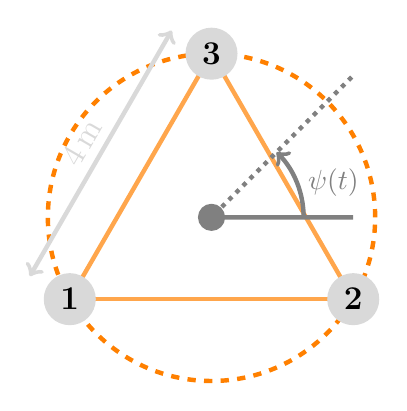
\begin{tikzpicture}[thick, scale=0.9]
    \node at (2,0) (LowerRight) {};
    \node at (-2,0) (LowerLeft) {};
    \node at (0,3.464) (Top) {};
    \node at (0,1.1547) (Center) {};
    \draw[orange,dashed,ultra thick] (Center) circle (1.1547*2);
    \draw[orange,ultra thick, opacity=0.7] (LowerRight) -- (LowerLeft);
    \draw[orange,ultra thick, opacity=0.7] (LowerRight) -- (Top);
    \draw[orange,ultra thick, opacity=0.7] (LowerLeft) -- (Top);
    \filldraw[textcolor] (LowerLeft) circle (10pt) {};
    \node[black,font=\large] at (LowerLeft) {\textbf{1}};
    \filldraw[textcolor] (LowerRight) circle (10pt)  {};
    \node[black,font=\large] at (LowerRight) {\textbf{2}};
    \filldraw[textcolor] (Top) circle (10pt)  {};
    \node[black,font=\large] at (Top) {\textbf{3}};

    % \draw[textcolor,ultra thick, <->] (-0.2,1.1547) -- (-2*1.1547+0.05,1.1547) node[midway,above,textcolor] {\large $r$\,m};
    \draw[black,ultra thick, <->,yshift=0.65*0.5cm,,xshift=-0.65*0.866cm,textcolor] (-2,0) -- (0,3.464) node[midway,above,black,rotate=60,textcolor] {\large $4$\,m};

    % \draw[black,ultra thick, <->,yshift=0.65*0.5cm,,xshift=-0.65*0.866cm] (-2,0) -- (0,3.464) node[midway,above,black,rotate=60] {$d$\,m};

    \filldraw[gray] (Center) circle (5pt) {};
    \draw[gray,ultra thick] (Center) -- (2,1.1547);
    \draw[gray,dotted,ultra thick] (Center) -- (2,1.1547+2);
    \draw[->, gray,ultra thick] (1.3,1.1547) arc
        [
            start angle=0,
            end angle= 45,
            x radius= 1.3cm,
            y radius =1.3cm
        ] node[midway,right,gray] {\normalsize $\psi(t)$};
    % \node[gray,xshift=1.45cm,yshift=0.5cm] at (Center) {$\psi(t)$};
\end{tikzpicture}
% \begin{tikzpicture}
    % Define the center and radius
    \def\radius{0.4} % Half of the diameter
    
    % Draw the circle
    \fill[fill=gray!80] (0,0) circle (0.6);
    \draw[thick,textcolor] (0,0) circle (0.6);
    
    \draw [thick,textcolor] plot [rounded corners=5pt] coordinates { (0,0) (0,1.6) (2,1.6)};
    \draw [thick,textcolor] plot [rounded corners=5pt] coordinates {(3,1.9) (3,2.2) (-6,2.2) (-6, 0) (-5.5,0)};
    
    \draw [thick,textcolor] plot [rounded corners=5pt] coordinates { (4,-0.2) (4.5, -0.2) (4.5,1.6) (4, 1.6)};
    
    \foreach \i in {0,1,2,3,4,5,6,7} {
        \pgfmathsetmacro{\angle}{\i*45+22.5} % 360 degrees / 8 vertices = 45 degrees per vertex
        \coordinate (A\i) at ({\radius*cos(\angle)}, {\radius*sin(\angle)});
    }
    \draw[ultra thick,fill=textcolor,draw=black] (A0) -- (A1) -- (A2) -- (A3) -- (A4) -- (A5) -- (A6) -- (A7) -- cycle;
  
      % Draw a partial circular arrow with an arrowhead
      \draw[thick, ->, >=stealth,textcolor] ({1*cos(-125)}, {1*sin(-125)}) arc[start angle=-125, end angle=-55, radius=1cm];
  
    % Draw dashed arrow
    \draw[dashed, thick, <->, >=stealth,textcolor] (0, 1) -- (-5, 1);
    % Label on the arrow
    \node[textcolor] at (-2.5, 1.3) {5\,m};
  
    % Draw the large dashed rectangle
    \draw[dashed, thick, rounded corners=5pt,textcolor] (1.5, 2.5) rectangle (-7, -1.5);
  
    % Draw the first filled rectangle
    \fill[fill=textcolor, rounded corners=5pt, text=black] (2, 1.2) rectangle (4, 2) node[midway] {UMC1820};
  
    % Draw loudspeaker symbol at the source
    \pic[rotate = 90] at (-5, 0) {Speaker};
  
    % Draw the second filled rectangle
    \fill[fill=textcolor, text=black] (2, 0) rectangle (4, -.8) node[midway] {Computer};
    \draw[fill=gray] (2,0) -- (2.2,0.8) -- (4.2,0.8) -- (4,0) -- cycle;
  
  
  
  \end{tikzpicture}
% \begin{tikzpicture}
    % Define the spacing and the number of elements
    \def\DOA{30}
    \coordinate (O) at (0,0);
    \def\SensOX{-2}
    \def\SensOY{0.5}
    \def\SensTX{1.8}
    \def\SensTY{-0.5}

    % Draw the coordinate axes
    \draw[thick,->,textcolor] (0,0) -- (3.3,0) node[anchor=north east]{$x$};
    \draw[thick,->,textcolor] (0,0) -- (0,2.5) node[anchor=north east]{$y$};

    \tdplotdrawarc[->,textcolor]{(O)}{2}{0}{\DOA}{anchor=north west, shift={(0,0.3)}}{$\psi$};

    % Draw the sensor element
    \draw[fill=textcolor] (\SensOX,\SensOY) circle (2pt) node[anchor=south east,textcolor] {Sensor 1};

    \draw[fill=textcolor] (\SensTX,\SensTY) circle (2pt) node[anchor=north west,textcolor] {Sensor 2};

    % Draw source element towards DOA angle
    \draw[thick,->,textcolor]  ({2.7*cos(\DOA)},{2.7*sin(\DOA)}) -- ({1.6*cos(\DOA)},{1.6*sin(\DOA)})  node[anchor=south west, shift={(-0.1,0.4)}] {$\bm{v(\psi)}$};

    % Draw loudspeaker symbol at the source
    \pic[rotate=\DOA-90,textcolor] at ({4*cos(\DOA)},{4*sin(\DOA)}) {Speaker};
    \node[anchor=center, shift={(0.8,0.2)},textcolor] at ({4.4*cos(\DOA)},{4.4*sin(\DOA)}) {Source};

    % Find the intersection point
    \path[name path=line1] ({0.8*cos(\DOA)},{0.8*sin(\DOA)}) -- ({-2.5*cos(\DOA)},{-2.5*sin(\DOA)});
    \path[name path=line2] (\SensOX,\SensOY) -- ({\SensOX+2.5*cos(\DOA-90)},{\SensOY+2.5*sin(\DOA-90)});
    \path[name intersections={of=line1 and line2, by=intersection1}];

    \path[name path=line12] ({1.8*cos(\DOA)},{1.8*sin(\DOA)}) -- ({-2.5*cos(\DOA)},{-2.5*sin(\DOA)});
    \path[name path=line22] (\SensTX,\SensTY) -- ({\SensTX-2.5*cos(\DOA-90)},{\SensTY-2.5*sin(\DOA-90)});
    \path[name intersections={of=line12 and line22, by=intersection2}];

    % Draw the lines using the intersection point
    \draw[thick,dotted, color=textcolor] ({1.6*cos(\DOA)},{1.6*sin(\DOA)}) -- (intersection1);
    \draw[thick,dashed, color=textcolor] (intersection1) -- (\SensOX,\SensOY);
    \draw[thick,dashed, color=textcolor] (intersection2) -- (\SensTX,\SensTY);


    % Add a 90-degree marker
    % \draw[thick, rotate=\DOA] (intersection1)++(0.2,0) -- ++(0,0.2) -- ++(-0.2,0);
    % \draw[thick, rotate=\DOA] (intersection2)++(+0.2,0) -- ++(0,-0.2) -- ++(-0.2,0);

    % Draw the curly brace with label \tau
    \draw[decorate,decoration={brace,amplitude=5pt},textcolor] (O) -- (intersection1) node[midway,below=4pt,shift={(0.2,0)}] {$\tau_1$};

    \draw[decorate,decoration={brace,amplitude=5pt},textcolor] (O) -- (intersection2) node[midway,above=4pt,shift={(-0.2,0)}] {$-\tau_2$};
\end{tikzpicture}
% \begin{tikzpicture}[tdplot_main_coords]
    % Define the spacing and the number of elements
    \def\spacing{1.2}
    \def\DOA{65}
    \def\numElements{5}
    \coordinate (O) at (0,0,0);

    % Draw the coordinate axes
    \draw[thick,->,textcolor] (0,0,0) -- (3,0,0) node[anchor=north east]{$x$};
    \draw[thick,->,textcolor] (0,0,0) -- (0,3,0) node[anchor=north west]{$y$};
    \draw[thick,->,textcolor] (0,0,0) -- (0,0,3) node[anchor=south]{$z$};

    \draw[thick,dotted,textcolor] (O) -- ({2.5*cos(\DOA)},{2.5*sin(\DOA)},0);
    \tdplotdrawarc[->,textcolor]{(O)}{2.5}{0}{\DOA}{anchor=north}{$\psi$}

    % Draw the elements in the xy-plane
    \foreach \i in {0,...,\the\numexpr\numElements-1\relax} {
      \draw (\numElements*\spacing/2-\i*\spacing-\spacing/2,0) node[circle,fill,inner sep=2pt,textcolor] (node\i) {};
      \ifnum\i=0
          \node[above, xshift=-3, yshift=1,textcolor] at (node\i) {$0$};
      \fi
      \ifnum\i=1
          \node[above, xshift=-3, yshift=1,textcolor] at (node\i) {$1$};
      \fi
      \ifnum\i=\the\numexpr\numElements-1\relax
          \node[above, xshift=-3, yshift=1,textcolor] at (node\i) {$M-1$};
      \fi
      }
  \end{tikzpicture}
% \begin{tikzpicture}[tdplot_main_coords]
    % Define the radius and the number of elements
    \def\radius{1.5}
    \def\DOA{65}
    \def\numElements{8}
    \coordinate (O) at (0,0,0);

    % Draw the coordinate axes
    \draw[thick,->,textcolor] (0,0,0) -- (3,0,0) node[anchor=north east]{$x$};
    \draw[thick,->,textcolor] (0,0,0) -- (0,3,0) node[anchor=north west]{$y$};
    \draw[thick,->,textcolor] (0,0,0) -- (0,0,3) node[anchor=south]{$z$};

    % Draw the dotted circle in the xy-plane (z=0)
    \tdplotdrawarc[dotted,textcolor]{(O)}{\radius}{0}{360}{anchor=north}{}

    \draw[thick,dotted,textcolor] (O) -- ({2.5*cos(\DOA)},{2.5*sin(\DOA)},0);
    \tdplotdrawarc[->,textcolor]{(O)}{2.5}{0}{\DOA}{anchor=north}{$\psi$}

    % Draw the elements in the xy-plane
    \foreach \i in {1,...,\numElements} {
      \draw ({360/\numElements * (\i-1)}:\radius) node[circle,fill,inner sep=2pt,textcolor] (node\i) {};
      \ifnum\i=1
          \node[below, xshift=.5, yshift=-2,textcolor] at (node\i) {$0$};
      \fi
      \ifnum\i=2
          \node[below, xshift=.5, yshift=-1,textcolor] at (node\i) {$1$};
      \fi
      \ifnum\i=\numElements
          \node[above, xshift=10, yshift=-2,textcolor] at (node\i)[anchor=north east] {$M-1$};
      \fi
      }
\end{tikzpicture}
% % This file was created by matlab2tikz.
%
%The latest updates can be retrieved from
%  http://www.mathworks.com/matlabcentral/fileexchange/22022-matlab2tikz-matlab2tikz
%where you can also make suggestions and rate matlab2tikz.
%
\definecolor{mycolor1}{rgb}{0.00000,0.44700,0.74100}%
\definecolor{mycolor2}{rgb}{0.85000,0.32500,0.09800}%
\colorlet{mycolor1}{mycolor1!80!white}%


\begin{tikzpicture}

\begin{axis}[%
  DarkMode,
  DOA_sim,
  name=plot1,
  yticklabels={0,0.5,1},
title={Delay-and-sum},
legend style={at={(0.03,0.97)}, anchor=north west, legend cell align=left, align=left, fill=background, draw=textcolor,font=\color{textcolor}\small, line width=1.1pt},
]
\addplot [color=mycolor1]
  table[row sep=crcr]{%
-180	0.163572735099531\\
-179	0.16400299391754\\
-178	0.164459678887806\\
-177	0.164912788618992\\
-176	0.165230838212555\\
-175	0.165434084651115\\
-174	0.165695975737189\\
-173	0.166016069706737\\
-172	0.166236292474923\\
-171	0.16639271162758\\
-170	0.166561292180667\\
-169	0.166686900493248\\
-168	0.166757369561116\\
-167	0.166855422624949\\
-166	0.166966807284539\\
-165	0.166899461431627\\
-164	0.166829415979465\\
-163	0.166794863839336\\
-162	0.166695404193676\\
-161	0.166550127658213\\
-160	0.166415183164134\\
-159	0.166312789735077\\
-158	0.166115915626247\\
-157	0.165901457924874\\
-156	0.165665433233199\\
-155	0.165324014049188\\
-154	0.165019089925223\\
-153	0.164748344811672\\
-152	0.164453323941538\\
-151	0.164108982710991\\
-150	0.163801646093296\\
-149	0.163504786979385\\
-148	0.163071950856186\\
-147	0.162697821004412\\
-146	0.162375168838663\\
-145	0.162028585193047\\
-144	0.161675354385814\\
-143	0.161364666385992\\
-142	0.161029765151802\\
-141	0.160640534254579\\
-140	0.160347285584646\\
-139	0.160159599055536\\
-138	0.159925455778717\\
-137	0.159615430980236\\
-136	0.159331996229571\\
-135	0.159099363668357\\
-134	0.15887243128196\\
-133	0.158704403231049\\
-132	0.15857678710415\\
-131	0.158390065894193\\
-130	0.158169854661337\\
-129	0.158058985836207\\
-128	0.158038909592033\\
-127	0.157955777951172\\
-126	0.157845517195888\\
-125	0.157781735570435\\
-124	0.15771639066715\\
-123	0.157630557982982\\
-122	0.15759322723092\\
-121	0.157607831554401\\
-120	0.157464372522095\\
-119	0.15733605748543\\
-118	0.15727389240539\\
-117	0.157184826195152\\
-116	0.157063551182251\\
-115	0.156944005166319\\
-114	0.156821073544678\\
-113	0.15659110013703\\
-112	0.156336841229766\\
-111	0.156053584381899\\
-110	0.155639483571063\\
-109	0.155208210505157\\
-108	0.154757659809686\\
-107	0.15423878440916\\
-106	0.153637413070395\\
-105	0.15303047100482\\
-104	0.152363248746811\\
-103	0.151481133717198\\
-102	0.150545885598973\\
-101	0.149572335781283\\
-100	0.14849213859797\\
-99	0.147321278411442\\
-98	0.146095728377914\\
-97	0.14472986295869\\
-96	0.143179690015042\\
-95	0.141592205559161\\
-94	0.139984177594341\\
-93	0.13821011387956\\
-92	0.136232540648523\\
-91	0.134146165496754\\
-90	0.131982778455568\\
-89	0.129709382060631\\
-88	0.127372843664853\\
-87	0.124938837137744\\
-86	0.122295313195847\\
-85	0.11947484235513\\
-84	0.116635793491467\\
-83	0.113767333613848\\
-82	0.110715857164484\\
-81	0.107523794641249\\
-80	0.104279782580533\\
-79	0.100944750159736\\
-78	0.0974962807438103\\
-77	0.0940065126402686\\
-76	0.0904541882309418\\
-75	0.0867272861564233\\
-74	0.0829673474723194\\
-73	0.079214611515639\\
-72	0.0753775617798235\\
-71	0.0714858964278367\\
-70	0.0676059533262659\\
-69	0.0637120805962259\\
-68	0.0597375750508371\\
-67	0.0557879282080787\\
-66	0.0518721258504771\\
-65	0.0479521073753013\\
-64	0.0440771144926864\\
-63	0.0402965037134076\\
-62	0.0365808592946357\\
-61	0.032921738153684\\
-60	0.029416309659265\\
-59	0.0260398350268973\\
-58	0.0227018771260286\\
-57	0.0195025779586812\\
-56	0.0165184072554974\\
-55	0.0137053651083464\\
-54	0.0111017293009263\\
-53	0.00876501016277529\\
-52	0.00662755037983854\\
-51	0.00467263461197288\\
-50	0.00308013750085412\\
-49	0.00188334502701151\\
-48	0.000947951349138413\\
-47	0.000274887891530755\\
-46	0\\
-45	0.000163036296833476\\
-44	0.000722500791989258\\
-43	0.0017441824695856\\
-42	0.00322719751179685\\
-41	0.00508896263810147\\
-40	0.0073819698748548\\
-39	0.0102827022360389\\
-38	0.0137955000819029\\
-37	0.0177791383364216\\
-36	0.0222885730320982\\
-35	0.0274162329729617\\
-34	0.0331277124239011\\
-33	0.0394245489316081\\
-32	0.0463999764006574\\
-31	0.0540217236846959\\
-30	0.0621715363573477\\
-29	0.0709816511607734\\
-28	0.0805058927873539\\
-27	0.0906679351330595\\
-26	0.101489032353937\\
-25	0.113012562400946\\
-24	0.125249448339065\\
-23	0.138070437480934\\
-22	0.151567091836004\\
-21	0.165726074273499\\
-20	0.180438574885265\\
-19	0.195835143510556\\
-18	0.211884587553264\\
-17	0.228530717699369\\
-16	0.245726930649486\\
-15	0.263537768258419\\
-14	0.281909540483958\\
-13	0.300613123569441\\
-12	0.319887343704653\\
-11	0.339666226028796\\
-10	0.359845545634497\\
-9	0.380412750495813\\
-8	0.401384308682733\\
-7	0.422643172925542\\
-6	0.444108195235064\\
-5	0.465890318836833\\
-4	0.48794977813328\\
-3	0.510078740772852\\
-2	0.532214746604477\\
-1	0.554430687752828\\
0	0.57669947258298\\
1	0.59891062355843\\
2	0.621058419259547\\
3	0.643064903248715\\
4	0.664769743296005\\
5	0.686150746874676\\
6	0.707317385228553\\
7	0.728206458823229\\
8	0.748605072788125\\
9	0.768497987915998\\
10	0.787913981144711\\
11	0.806752933666529\\
12	0.824942709142148\\
13	0.842514104118302\\
14	0.859694137322424\\
15	0.875702215193942\\
16	0.890905508410614\\
17	0.905301440479333\\
18	0.918776985120564\\
19	0.931326262359733\\
20	0.942960957860992\\
21	0.953954775882481\\
22	0.963524923365477\\
23	0.972042259118027\\
24	0.979491706301992\\
25	0.98542767659414\\
26	0.990616455071956\\
27	0.994702949342618\\
28	0.997618917626923\\
29	0.999356452723632\\
30	1\\
31	0.999486441824606\\
32	0.997353785127113\\
33	0.99442194675774\\
34	0.990405425293677\\
35	0.985229328178049\\
36	0.978918415401755\\
37	0.971545251083932\\
38	0.96306511428573\\
39	0.953461943858302\\
40	0.942903957909132\\
41	0.931427165276728\\
42	0.91891692785631\\
43	0.905392105863183\\
44	0.891002860679796\\
45	0.875811230832734\\
46	0.859801341356894\\
47	0.843058716629711\\
48	0.825607307496593\\
49	0.807396063504716\\
50	0.788504772273185\\
51	0.769133105787646\\
52	0.749315916143168\\
53	0.728948438654988\\
54	0.708116772796465\\
55	0.686950505167631\\
56	0.665461660453341\\
57	0.643694737894504\\
58	0.621778079728639\\
59	0.599913501521123\\
60	0.577653288290032\\
61	0.555363392840511\\
62	0.533127969169779\\
63	0.51091020801923\\
64	0.488776485705365\\
65	0.466823882417925\\
66	0.445233550408566\\
67	0.423676437288665\\
68	0.402399964601027\\
69	0.381446669394825\\
70	0.360687089677104\\
71	0.340450758017646\\
72	0.320670908580903\\
73	0.301330631302121\\
74	0.28245120933531\\
75	0.264154630478299\\
76	0.246430273547193\\
77	0.229109827922042\\
78	0.212446245311892\\
79	0.196420224744827\\
80	0.180979054048323\\
81	0.166159923665477\\
82	0.15202067350388\\
83	0.138493527460769\\
84	0.125553555707802\\
85	0.113364841052922\\
86	0.10194511922386\\
87	0.0911370558868342\\
88	0.0808980748831234\\
89	0.0713246798762071\\
90	0.0624444010219033\\
91	0.0542095965400616\\
92	0.0466527713752531\\
93	0.0397371418512402\\
94	0.0333536499785514\\
95	0.02752113348347\\
96	0.0223701859399237\\
97	0.0178770325843378\\
98	0.0138883461565071\\
99	0.0104205143679629\\
100	0.00751941549099337\\
101	0.00511936307171929\\
102	0.00318801138229869\\
103	0.00178027981725475\\
104	0.000814857543205594\\
105	0.000202633089387947\\
106	1.05817108345004e-05\\
107	0.000262513060697665\\
108	0.000862913089806122\\
109	0.00180743023377137\\
110	0.0031226861030619\\
111	0.00472793392960587\\
112	0.00658371336726179\\
113	0.00870786439557967\\
114	0.0110859225028652\\
115	0.0136603660437246\\
116	0.0164100118809653\\
117	0.0193729089877471\\
118	0.0224954101638453\\
119	0.025742575731227\\
120	0.0291807497189691\\
121	0.032753015104031\\
122	0.0363285099193091\\
123	0.0399712017804627\\
124	0.043723328094931\\
125	0.0475053448779761\\
126	0.0513265032713247\\
127	0.0552152262136519\\
128	0.0590711335815055\\
129	0.0628441421569584\\
130	0.0666827910541738\\
131	0.070587615603151\\
132	0.0743875503398435\\
133	0.0780449748656937\\
134	0.0816633669582515\\
135	0.0852604334964183\\
136	0.0887838350682709\\
137	0.0922872019096738\\
138	0.0957449835451425\\
139	0.0990354489617079\\
140	0.10216664735445\\
141	0.105286596954133\\
142	0.108383925705541\\
143	0.111305770296341\\
144	0.114095771119209\\
145	0.116838607783456\\
146	0.119490600252141\\
147	0.122029076810998\\
148	0.124521773976662\\
149	0.126938080707815\\
150	0.129109984110337\\
151	0.131200639950144\\
152	0.13328286111057\\
153	0.135265103887568\\
154	0.137142096312656\\
155	0.138966345928333\\
156	0.140753259579675\\
157	0.142357252824208\\
158	0.143901036848105\\
159	0.145390298172173\\
160	0.146714074162174\\
161	0.148019022368665\\
162	0.149301696974034\\
163	0.150517222709235\\
164	0.151651871844579\\
165	0.152789001489558\\
166	0.153877595508748\\
167	0.154770247797771\\
168	0.155669982315612\\
169	0.156579435215273\\
170	0.157410416316396\\
171	0.158182851236952\\
172	0.158955555506277\\
173	0.159655338014796\\
174	0.160243679608278\\
175	0.160878777505158\\
176	0.161573481979941\\
177	0.162172765821291\\
178	0.162648649657133\\
179	0.163107243420041\\
180	0.163572735099531\\
};
\addlegendentry{Time}

\addplot [color=mycolor2]
  table[row sep=crcr]{%
-180	0.0184837322394495\\
-179	0.017139914130869\\
-178	0.0158548855320893\\
-177	0.0146274920091161\\
-176	0.0134567656497813\\
-175	0.0123418946741724\\
-174	0.0112821855047143\\
-173	0.0102770197836257\\
-172	0.00932580914107082\\
-171	0.00842795064489187\\
-170	0.00758278579780571\\
-169	0.00678956569905754\\
-168	0.00604742457539999\\
-167	0.00535536334165785\\
-166	0.00471224421227174\\
-165	0.0041167966949076\\
-164	0.00356763459982789\\
-163	0.00306328303723663\\
-162	0.00260221378821257\\
-161	0.0021828869559771\\
-160	0.00180379645818949\\
-159	0.00146351672403433\\
-158	0.00116074791922152\\
-157	0.000894357135730657\\
-156	0.000663413240848726\\
-155	0.000467213463912937\\
-154	0.000305300285142607\\
-153	0.000177467750211778\\
-152	8.37569348525446e-05\\
-151	2.44408923466957e-05\\
-150	0\\
-149	1.10891471271383e-05\\
-148	5.84986485419904e-05\\
-147	0.000143111100607423\\
-146	0.000265856604010811\\
-145	0.000427668847934373\\
-144	0.000629444481027019\\
-143	0.000872007990181501\\
-142	0.0011560839808537\\
-141	0.00148227832184686\\
-140	0.00185106910846662\\
-139	0.00226280784064528\\
-138	0.00271773063973259\\
-137	0.00321597877261317\\
-136	0.00375762724673694\\
-135	0.00434271981319779\\
-134	0.00497130839056061\\
-133	0.00564349471634261\\
-132	0.00635947195476292\\
-131	0.00711956403929868\\
-130	0.00792426069944033\\
-129	0.00877424639836719\\
-128	0.00967042177170222\\
-127	0.0106139165824812\\
-126	0.0116060936671292\\
-125	0.0126485438143845\\
-124	0.0137430719681035\\
-123	0.0148916755531633\\
-122	0.0160965160730042\\
-121	0.0173598854044476\\
-120	0.0186841684122436\\
-119	0.0200718036192782\\
-118	0.0215252436998442\\
-117	0.0230469175176607\\
-116	0.0246391953148628\\
-115	0.0263043584819355\\
-114	0.0280445751113388\\
-113	0.0298618822693216\\
-112	0.0317581756210187\\
-111	0.0337352067230288\\
-110	0.0357945879649752\\
-109	0.0379378048070397\\
-108	0.0401662346347917\\
-107	0.0424811712473254\\
-106	0.0448838537222394\\
-105	0.0473754981744841\\
-104	0.0499573307588094\\
-103	0.0526306201699532\\
-102	0.0553967078813857\\
-101	0.0582570344397676\\
-100	0.0612131603012703\\
-99	0.0642667799550108\\
-98	0.0674197284193547\\
-97	0.0706739796035706\\
-96	0.0740316364790623\\
-95	0.0774949134749126\\
-94	0.0810661119720488\\
-93	0.084747590187994\\
-92	0.08854172908999\\
-91	0.0924508962220383\\
-90	0.0964774094608757\\
-89	0.100623502714914\\
-88	0.104891295445934\\
-87	0.109282767633056\\
-86	0.113799741429127\\
-85	0.11844387030663\\
-84	0.123216635985645\\
-83	0.128119352916276\\
-82	0.133153179589586\\
-81	0.13831913550955\\
-80	0.143618122304304\\
-79	0.149050947211134\\
-78	0.154618347050558\\
-77	0.160321010814868\\
-76	0.166159599130442\\
-75	0.172134759096808\\
-74	0.178247133337396\\
-73	0.184497362490747\\
-72	0.190886080797449\\
-71	0.197413904868042\\
-70	0.204081416123508\\
-69	0.210889137759715\\
-68	0.217837507382629\\
-67	0.224926846680542\\
-66	0.232157329637384\\
-65	0.239528950846965\\
-64	0.247041495466085\\
-63	0.254694512252144\\
-62	0.262487290977489\\
-61	0.270418845308474\\
-60	0.278487901991878\\
-59	0.286692896914589\\
-58	0.295031978302728\\
-57	0.303503017012198\\
-56	0.312103623542034\\
-55	0.320831171084058\\
-54	0.329682823617381\\
-53	0.338655567776143\\
-52	0.347746246976996\\
-51	0.356951596104241\\
-50	0.366268274930156\\
-49	0.375692898410579\\
-48	0.385222062053103\\
-47	0.394852360715317\\
-46	0.404580399455775\\
-45	0.41440279542619\\
-44	0.424316170247422\\
-43	0.434317132834027\\
-42	0.444402253194988\\
-41	0.454568028308346\\
-40	0.464810841707802\\
-39	0.475126918891363\\
-38	0.485512281029374\\
-37	0.495962699680061\\
-36	0.506473655291047\\
-35	0.517040302161441\\
-34	0.527657442259226\\
-33	0.538319509843506\\
-32	0.549020568254142\\
-31	0.559754319536966\\
-30	0.570514126814885\\
-29	0.581293048543639\\
-28	0.592083883058121\\
-27	0.602879221172214\\
-26	0.613671504087861\\
-25	0.624453083534816\\
-24	0.635216280926593\\
-23	0.645953442392243\\
-22	0.656656986824254\\
-21	0.66731944455206\\
-20	0.677933484876073\\
-19	0.688491931435686\\
-18	0.698987765184087\\
-17	0.709414115546888\\
-16	0.719764241093663\\
-15	0.730031501698766\\
-14	0.740209324665596\\
-13	0.750291167603365\\
-12	0.760270480958203\\
-11	0.770140673007038\\
-10	0.779895079835098\\
-9	0.789526942362544\\
-8	0.799029391901601\\
-7	0.808395445061138\\
-6	0.817618008124194\\
-5	0.826689890360324\\
-4	0.835603825149263\\
-3	0.844352497328617\\
-2	0.852928574867594\\
-1	0.86132474282925\\
0	0.869533737618137\\
1	0.877548379706532\\
2	0.885361603364704\\
3	0.892966482352296\\
4	0.900356251014286\\
5	0.907524320718769\\
6	0.914464292028203\\
7	0.921169963369749\\
8	0.92763533723174\\
9	0.933854625041922\\
10	0.93982225187215\\
11	0.945532861970809\\
12	0.950981325868279\\
13	0.956162749462939\\
14	0.961072485113673\\
15	0.965706144381288\\
16	0.970059611717329\\
17	0.974129058131031\\
18	0.977910953702895\\
19	0.981402077774367\\
20	0.984599525733498\\
21	0.987500711528923\\
22	0.990103365359985\\
23	0.992405526380043\\
24	0.994405530676189\\
25	0.996101995211522\\
26	0.997493798795226\\
27	0.998580061444605\\
28	0.999360123692713\\
29	0.999833527455877\\
30	1\\
31	0.999859442337482\\
32	0.999411923065018\\
33	0.998657678242976\\
34	0.997597117454417\\
35	0.996230835705097\\
36	0.994559630375019\\
37	0.99258452204475\\
38	0.990306777726763\\
39	0.987727934856372\\
40	0.984849824350042\\
41	0.981674591121579\\
42	0.978204710648341\\
43	0.974443000479418\\
44	0.970392625947595\\
45	0.966057099753658\\
46	0.961440275500404\\
47	0.9565463356315\\
48	0.951379774548454\\
49	0.945945377915837\\
50	0.940248199307729\\
51	0.934293535393498\\
52	0.928086900814129\\
53	0.92163400377487\\
54	0.914940723195633\\
55	0.908013088040591\\
56	0.900857259216873\\
57	0.893479514211834\\
58	0.885886234447615\\
59	0.878083895183498\\
60	0.870079057697383\\
61	0.861878363426984\\
62	0.853488529742555\\
63	0.844916347044859\\
64	0.836168676920403\\
65	0.827252451125906\\
66	0.818174671202038\\
67	0.808942408522868\\
68	0.799562804566898\\
69	0.790043071148708\\
70	0.780390490283467\\
71	0.770612413280862\\
72	0.760716258595462\\
73	0.750709507913262\\
74	0.740599699945248\\
75	0.730394421440808\\
76	0.72010129503487\\
77	0.709727963704189\\
78	0.699282071824352\\
79	0.688771243076729\\
80	0.678203055734279\\
81	0.667585016132192\\
82	0.656924531377219\\
83	0.646228882541179\\
84	0.635505199696082\\
85	0.62476044016248\\
86	0.614001371249068\\
87	0.6032345585595\\
88	0.592466360641228\\
89	0.581702930369811\\
90	0.570950223027697\\
91	0.560214010581922\\
92	0.549499901226769\\
93	0.53881336287091\\
94	0.528159748946574\\
95	0.517544324726593\\
96	0.506972292270931\\
97	0.496448812193902\\
98	0.485979020642174\\
99	0.475568040186388\\
100	0.465220983731232\\
101	0.454942951008508\\
102	0.444739017699215\\
103	0.434614217697566\\
104	0.424573519447623\\
105	0.414621797623084\\
106	0.404763801661207\\
107	0.395004122790794\\
108	0.385347161209295\\
109	0.375797094972614\\
110	0.366357851978709\\
111	0.35703308617453\\
112	0.347826158821054\\
113	0.338740125340292\\
114	0.329777727966544\\
115	0.320941394153611\\
116	0.312233240465832\\
117	0.303655081512627\\
118	0.295208443375363\\
119	0.286894580916753\\
120	0.278714498345959\\
121	0.270668972423044\\
122	0.262758577708587\\
123	0.254983713283428\\
124	0.247344630367713\\
125	0.239841460250682\\
126	0.232474241901551\\
127	0.225242948572301\\
128	0.218147512635771\\
129	0.211187847841956\\
130	0.204363868139627\\
131	0.197675502216837\\
132	0.191122702978373\\
133	0.184705451311588\\
134	0.178423753698909\\
135	0.172277633512099\\
136	0.166267116158374\\
137	0.160392208621897\\
138	0.154652874329488\\
139	0.149049004635631\\
140	0.143580388536143\\
141	0.13824668245067\\
142	0.13304738203438\\
143	0.127981797969106\\
144	0.123049037533704\\
145	0.118247993463799\\
146	0.113577341195351\\
147	0.109035545069049\\
148	0.104620873487388\\
149	0.100331422405055\\
150	0.0961651459412676\\
151	0.0921198923761192\\
152	0.0881934433743657\\
153	0.0843835540051747\\
154	0.0806879910207409\\
155	0.0771045669335518\\
156	0.0736311676908498\\
157	0.0702657721707164\\
158	0.0670064622892581\\
159	0.0638514231732569\\
160	0.0607989335695875\\
161	0.0578473473789921\\
162	0.0549950678638292\\
163	0.0522405166368026\\
164	0.0495820999471812\\
165	0.0470181750099732\\
166	0.0445470191524587\\
167	0.0421668043767973\\
168	0.0398755795678531\\
169	0.0376712620373502\\
170	0.0355516394272874\\
171	0.0335143822455408\\
172	0.0315570665295398\\
173	0.0296772053868685\\
174	0.0278722874996373\\
175	0.0261398201512713\\
176	0.0244773739788607\\
177	0.0228826264974107\\
178	0.0213534014955148\\
179	0.0198877016608797\\
180	0.0184837322394495\\
};
\addlegendentry{Freq.}

\addplot [color=white!15!textcolor, dashed, forget plot]
  table[row sep=crcr]{%
30	0\\
30	1\\
};
\end{axis}

\begin{axis}[%
  DarkMode,
  DOA_sim,
  name=plot2,
  at=(plot1.right of south east), anchor=left of south west,
title={MUSIC}
]
\addplot [color=mycolor1, forget plot]
  table[row sep=crcr]{%
-180	7.3379671493452e-07\\
-179	7.36203005434237e-07\\
-178	7.38439825508092e-07\\
-177	7.40507560066485e-07\\
-176	7.42406237919851e-07\\
-175	7.44135623147749e-07\\
-174	7.45695309879702e-07\\
-173	7.470848191237e-07\\
-172	7.4830369624656e-07\\
-171	7.49351607694597e-07\\
-170	7.50228435545147e-07\\
-169	7.50934368500436e-07\\
-168	7.51469987976427e-07\\
-167	7.51836348000889e-07\\
-166	7.52035047717166e-07\\
-165	7.52068295392463e-07\\
-164	7.51938962950628e-07\\
-163	7.51650630187835e-07\\
-162	7.51207617982738e-07\\
-161	7.50615009977916e-07\\
-160	7.49878662383291e-07\\
-159	7.49005201731143e-07\\
-158	7.48002010592498e-07\\
-157	7.46877201442001e-07\\
-156	7.45639579029179e-07\\
-155	7.44298591774317e-07\\
-154	7.42864272853888e-07\\
-153	7.41347171770546e-07\\
-152	7.3975827731372e-07\\
-151	7.38108932907229e-07\\
-150	7.3641074540886e-07\\
-149	7.34675488473227e-07\\
-148	7.32915001613809e-07\\
-147	7.3114108610369e-07\\
-146	7.29365398838911e-07\\
-145	7.27599345255411e-07\\
-144	7.25853972342982e-07\\
-143	7.24139862739878e-07\\
-142	7.22467030823172e-07\\
-141	7.20844821635278e-07\\
-140	7.19281813409304e-07\\
-139	7.17785724378111e-07\\
-138	7.16363324476445e-07\\
-137	7.15020352474593e-07\\
-136	7.13761439017708e-07\\
-135	7.12590035988402e-07\\
-134	7.115083525625e-07\\
-133	7.10517298289494e-07\\
-132	7.09616433499988e-07\\
-131	7.08803927321987e-07\\
-130	7.08076523575217e-07\\
-129	7.07429514806457e-07\\
-128	7.06856724727521e-07\\
-127	7.06350499319035e-07\\
-126	7.05901706865524e-07\\
-125	7.05499747188208e-07\\
-124	7.05132570339097e-07\\
-123	7.04786705011248e-07\\
-122	7.04447296903314e-07\\
-121	7.04098157249806e-07\\
-120	7.03721821690328e-07\\
-119	7.03299619600101e-07\\
-118	7.02811753939584e-07\\
-117	7.02237391602483e-07\\
-116	7.01554764149321e-07\\
-115	7.00741278708441e-07\\
-114	6.99773638709383e-07\\
-113	6.98627973986717e-07\\
-112	6.97279979658059e-07\\
-111	6.95705063041027e-07\\
-110	6.93878497733575e-07\\
-109	6.91775583844196e-07\\
-108	6.89371813226653e-07\\
-107	6.8664303845234e-07\\
-106	6.83565644145923e-07\\
-105	6.80116719220421e-07\\
-104	6.7627422847993e-07\\
-103	6.72017182014647e-07\\
-102	6.67325800796356e-07\\
-101	6.62181676894711e-07\\
-100	6.56567926776461e-07\\
-99	6.50469336221382e-07\\
-98	6.43872495489106e-07\\
-97	6.36765923498679e-07\\
-96	6.29140179934903e-07\\
-95	6.2098796436887e-07\\
-94	6.12304201670585e-07\\
-93	6.03086113194612e-07\\
-92	5.9333327343016e-07\\
-91	5.83047652020006e-07\\
-90	5.72233641262719e-07\\
-89	5.60898069415077e-07\\
-88	5.49050200301499e-07\\
-87	5.36701719910922e-07\\
-86	5.23866710815171e-07\\
-85	5.10561615374022e-07\\
-84	4.96805188798929e-07\\
-83	4.82618443228812e-07\\
-82	4.68024584027308e-07\\
-81	4.53048939542111e-07\\
-80	4.37718885575069e-07\\
-79	4.22063765798354e-07\\
-78	4.0611480932033e-07\\
-77	3.89905046557266e-07\\
-76	3.73469224507456e-07\\
-75	3.56843722455731e-07\\
-74	3.40066469062341e-07\\
-73	3.2317686171393e-07\\
-72	3.06215688938946e-07\\
-71	2.89225056617922e-07\\
-70	2.72248318653186e-07\\
-69	2.55330012704394e-07\\
-68	2.38515801547606e-07\\
-67	2.21852420577272e-07\\
-66	2.05387631943315e-07\\
-65	1.89170185799594e-07\\
-64	1.73249789135568e-07\\
-63	1.5767708266937e-07\\
-62	1.4250362629756e-07\\
-61	1.27781893623581e-07\\
-60	1.1356527612292e-07\\
-59	9.99080975474381e-08\\
-58	8.68656392235524e-08\\
-57	7.4494176958704e-08\\
-56	6.28510303372623e-08\\
-55	5.1994625261021e-08\\
-54	4.19845706707203e-08\\
-53	3.28817504743622e-08\\
-52	2.47484318064183e-08\\
-51	1.76483908506764e-08\\
-50	1.16470575802236e-08\\
-49	6.81168090313704e-09\\
-48	3.21151585452527e-09\\
-47	9.18034647741182e-10\\
-46	5.16359364269191e-12\\
-45	5.49548120963541e-10\\
-44	2.63084838806147e-09\\
-43	6.33206827232266e-09\\
-42	1.17399208647331e-08\\
-41	1.89452339911067e-08\\
-40	2.80433997369571e-08\\
-39	3.91348724798617e-08\\
-38	5.23257205432816e-08\\
-37	6.77282372926685e-08\\
-36	8.54616183143769e-08\\
-35	1.05652712269387e-07\\
-34	1.2843685411926e-07\\
-33	1.53958790707967e-07\\
-32	1.82373710181696e-07\\
-31	2.13848388477466e-07\\
-30	2.4856246815604e-07\\
-29	2.86709887249984e-07\\
-28	3.28500478610185e-07\\
-27	3.74161763544331e-07\\
-26	4.23940967446592e-07\\
-25	4.78107289738597e-07\\
-24	5.36954465924275e-07\\
-23	6.00803666085068e-07\\
-22	6.70006781929407e-07\\
-21	7.44950163835709e-07\\
-20	8.2605888053309e-07\\
-19	9.13801587573717e-07\\
-18	1.00869610709923e-06\\
-17	1.11131584126097e-06\\
-16	1.22229716586835e-06\\
-15	1.34234798048697e-06\\
-14	1.47225762766137e-06\\
-13	1.61290843895621e-06\\
-12	1.76528922136271e-06\\
-11	1.93051106724456e-06\\
-10	2.10982595823073e-06\\
-9	2.30464874332751e-06\\
-8	2.51658321064966e-06\\
-7	2.74745314936948e-06\\
-6	2.99933952553663e-06\\
-5	3.27462518820471e-06\\
-4	3.57604890236955e-06\\
-3	3.90677100207869e-06\\
-2	4.27045361143637e-06\\
-1	4.67135924982251e-06\\
0	5.11447280022199e-06\\
1	5.60565338939602e-06\\
2	6.15182486833175e-06\\
3	6.76121652707875e-06\\
4	7.44366977669419e-06\\
5	8.21103229910755e-06\\
6	9.07766938295161e-06\\
7	1.00611340242199e-05\\
8	1.11830547342669e-05\\
9	1.24703258085664e-05\\
10	1.39567238183546e-05\\
11	1.56851341151487e-05\\
12	1.77106653494896e-05\\
13	2.01050810989116e-05\\
14	2.29632258681734e-05\\
15	2.64125412536626e-05\\
16	3.06274950162127e-05\\
17	3.58520509430413e-05\\
18	4.24357399172633e-05\\
19	5.08936242344237e-05\\
20	6.20101152956034e-05\\
21	7.70275274990787e-05\\
22	9.80087159659006e-05\\
23	0.000128584995935856\\
24	0.000175639462238042\\
25	0.000253547538517503\\
26	0.000396612256321305\\
27	0.000704434693710497\\
28	0.00157682510641887\\
29	0.00617405244144958\\
30	1\\
31	0.00663902850362951\\
32	0.00163546201936382\\
33	0.000721841696134911\\
34	0.000403963032946405\\
35	0.000257314124168283\\
36	0.000177820916026863\\
37	0.000129959893585829\\
38	9.89306322682743e-05\\
39	7.7675663792443e-05\\
40	6.24831163092944e-05\\
41	5.12494085672641e-05\\
42	4.27101224259472e-05\\
43	3.6068141160704e-05\\
44	3.08007447286154e-05\\
45	2.65535990578058e-05\\
46	2.30796234612693e-05\\
47	2.02022673169071e-05\\
48	1.77926610787743e-05\\
49	1.57549589823436e-05\\
50	1.40166812138287e-05\\
51	1.25221975506268e-05\\
52	1.12282366870601e-05\\
53	1.01007322842692e-05\\
54	9.11256961238296e-06\\
55	8.24195044365736e-06\\
56	7.47118966876482e-06\\
57	6.78581811110693e-06\\
58	6.17390562894443e-06\\
59	5.62554479061405e-06\\
60	5.13245302024039e-06\\
61	4.6876631354485e-06\\
62	4.28528052480467e-06\\
63	3.92029105460783e-06\\
64	3.58840794392614e-06\\
65	3.28594882765738e-06\\
66	3.00973639185899e-06\\
67	2.75701755303761e-06\\
68	2.52539732831489e-06\\
69	2.31278442115772e-06\\
70	2.11734620844338e-06\\
71	1.9374713164454e-06\\
72	1.77173835708704e-06\\
73	1.61888969136242e-06\\
74	1.4778093159717e-06\\
75	1.34750414800716e-06\\
76	1.22708812287285e-06\\
77	1.11576863142296e-06\\
78	1.01283491026388e-06\\
79	9.17648069356908e-07\\
80	8.29632497353426e-07\\
81	7.48268430460212e-07\\
82	6.73085507359231e-07\\
83	6.03657162570003e-07\\
84	5.39595735029284e-07\\
85	4.8054818865743e-07\\
86	4.26192358139453e-07\\
87	3.76233646747489e-07\\
88	3.30402114308791e-07\\
89	2.884499028085e-07\\
90	2.50148954953969e-07\\
91	2.1528898759429e-07\\
92	1.83675687409093e-07\\
93	1.55129100935985e-07\\
94	1.29482194944354e-07\\
95	1.06579566505197e-07\\
96	8.62762849511353e-08\\
97	6.84368503491989e-08\\
98	5.29342551882453e-08\\
99	3.96491377683748e-08\\
100	2.84690173173189e-08\\
101	1.92876021864601e-08\\
102	1.20041636285669e-08\\
103	6.52296865666351e-09\\
104	2.7527663507284e-09\\
105	6.06322734118138e-10\\
106	0\\
107	8.53376442114875e-10\\
108	3.08890394423027e-09\\
109	6.63160031728085e-09\\
110	1.14087741493744e-08\\
111	1.7349780157402e-08\\
112	2.43858033045205e-08\\
113	3.24496701791959e-08\\
114	4.14756863218777e-08\\
115	5.13994983373858e-08\\
116	6.21579797469494e-08\\
117	7.36891396155389e-08\\
118	8.59320530395859e-08\\
119	9.88268125992651e-08\\
120	1.12314499870228e-07\\
121	1.26337176054263e-07\\
122	1.40837890729278e-07\\
123	1.55760707639201e-07\\
124	1.71050746346996e-07\\
125	1.86654238462791e-07\\
126	2.02518597038168e-07\\
127	2.18592497591359e-07\\
128	2.3482596910132e-07\\
129	2.51170493186366e-07\\
130	2.67579109570384e-07\\
131	2.84006525841757e-07\\
132	3.00409229431875e-07\\
133	3.16745599686241e-07\\
134	3.32976017875582e-07\\
135	3.49062973000638e-07\\
136	3.64971161284946e-07\\
137	3.80667577326423e-07\\
138	3.96121594991755e-07\\
139	4.11305036286509e-07\\
140	4.26192226617083e-07\\
141	4.40760035075062e-07\\
142	4.549878986163e-07\\
143	4.6885782927131e-07\\
144	4.82354403804585e-07\\
145	4.95464735532152e-07\\
146	5.08178428302279e-07\\
147	5.20487512937178e-07\\
148	5.32386366717282e-07\\
149	5.43871616757731e-07\\
150	5.54942028373786e-07\\
151	5.65598379752771e-07\\
152	5.75843324441e-07\\
153	5.85681243312013e-07\\
154	5.95118087805157e-07\\
155	6.04161216310562e-07\\
156	6.12819225627699e-07\\
157	6.21101779441402e-07\\
158	6.29019435743129e-07\\
159	6.36583475079386e-07\\
160	6.4380573143638e-07\\
161	6.50698427474247e-07\\
162	6.57274015708891e-07\\
163	6.63545027108961e-07\\
164	6.6952392843309e-07\\
165	6.75222989482204e-07\\
166	6.8065416128637e-07\\
167	6.8582896608838e-07\\
168	6.90758399829312e-07\\
169	6.95452847686517e-07\\
170	6.99922013063539e-07\\
171	7.0417486028497e-07\\
172	7.08219571108135e-07\\
173	7.1206351502774e-07\\
174	7.15713233219327e-07\\
175	7.19174435842314e-07\\
176	7.22452012303176e-07\\
177	7.25550053963829e-07\\
178	7.28471888668956e-07\\
179	7.31220126359204e-07\\
180	7.3379671493452e-07\\
};
\addplot [color=white!15!textcolor, dashed, forget plot]
  table[row sep=crcr]{%
30	0\\
30	1\\
};
\end{axis}

\begin{axis}[%
  DarkMode,
  DOA_sim,
  name=plot3,
  at=(plot2.right of south east), anchor=left of south west,
title={Bartlett}
]
\addplot [color=mycolor1, forget plot]
  table[row sep=crcr]{%
-180	0.163647906069821\\
-179	0.164096183867518\\
-178	0.164512515612936\\
-177	0.16489706780435\\
-176	0.165249932655891\\
-175	0.165571145418471\\
-174	0.165860702186365\\
-173	0.166118577961365\\
-172	0.166344744742697\\
-171	0.166539189409601\\
-170	0.166701931164848\\
-169	0.166833038311642\\
-168	0.166932644143403\\
-167	0.167000961735889\\
-166	0.167038297443951\\
-165	0.167045062920852\\
-164	0.167021785496397\\
-163	0.166969116770773\\
-162	0.166887839303882\\
-161	0.166778871304539\\
-160	0.166643269249974\\
-159	0.166482228393034\\
-158	0.166297081142005\\
-157	0.166089293325452\\
-156	0.165860458381542\\
-155	0.165612289537381\\
-154	0.165346610068592\\
-153	0.16506534175222\\
-152	0.164770491646716\\
-151	0.164464137350946\\
-150	0.164148410909554\\
-149	0.163825481544553\\
-148	0.163497537402508\\
-147	0.163166766513154\\
-146	0.162835337158813\\
-145	0.162505377854684\\
-144	0.162178957138116\\
-143	0.161858063360691\\
-142	0.161544584670542\\
-141	0.161240289364158\\
-140	0.160946806777411\\
-139	0.160665608874893\\
-138	0.160397992685328\\
-137	0.160145063719075\\
-136	0.159907720491934\\
-135	0.159686640267709\\
-134	0.159482266120647\\
-133	0.159294795407965\\
-132	0.15912416973234\\
-131	0.15897006646451\\
-130	0.158831891886969\\
-129	0.158708776011106\\
-128	0.158599569111846\\
-127	0.158502840015893\\
-126	0.158416876171754\\
-125	0.158339685521743\\
-124	0.158269000187968\\
-123	0.158202281975655\\
-122	0.158136729688052\\
-121	0.158069288237361\\
-120	0.157996659525708\\
-119	0.157915315059016\\
-118	0.157821510244874\\
-117	0.157711300313156\\
-116	0.157580557785422\\
-115	0.157424991406218\\
-114	0.157240166436486\\
-113	0.157021526196747\\
-112	0.156764414735745\\
-111	0.156464100489238\\
-110	0.156115800783824\\
-109	0.155714707032483\\
-108	0.155256010462157\\
-107	0.154734928209395\\
-106	0.154146729618151\\
-105	0.153486762574332\\
-104	0.152750479714785\\
-103	0.151933464354107\\
-102	0.151031455980907\\
-101	0.150040375185937\\
-100	0.148956347897458\\
-99	0.147775728814379\\
-98	0.146495123944463\\
-97	0.145111412173213\\
-96	0.143621765808269\\
-95	0.142023670064\\
-94	0.140314941470977\\
-93	0.13849374521464\\
-92	0.136558611426381\\
-91	0.13450845046788\\
-90	0.132342567265549\\
-89	0.130060674765903\\
-88	0.127662906594235\\
-87	0.125149829007911\\
-86	0.122522452241582\\
-85	0.119782241344545\\
-84	0.116931126610213\\
-83	0.113971513694195\\
-82	0.110906293510779\\
-81	0.107738851987843\\
-80	0.104473079747513\\
-79	0.101113381764394\\
-78	0.0976646870353381\\
-77	0.0941324582746009\\
-76	0.0905227016264512\\
-75	0.0868419763640172\\
-74	0.0830974045189581\\
-73	0.0792966803617844\\
-72	0.075448079627786\\
-71	0.0715604683590203\\
-70	0.0676433112090893\\
-69	0.0637066790349413\\
-68	0.0597612555790665\\
-67	0.055818343026621\\
-66	0.0518898662055506\\
-65	0.0479883751840294\\
-64	0.0441270460087471\\
-63	0.0403196793200229\\
-62	0.0365806965755731\\
-61	0.0329251336141575\\
-60	0.0293686312933722\\
-59	0.0259274229425777\\
-58	0.0226183183823384\\
-57	0.0194586842757489\\
-56	0.0164664205945142\\
-55	0.0136599330034887\\
-54	0.0110581009913562\\
-53	0.00868024160202082\\
-52	0.00654606865079954\\
-51	0.00467564734136615\\
-50	0.00308934423326521\\
-49	0.00180777254535569\\
-48	0.000851732817397762\\
-47	0.000242148989806963\\
-46	0\\
-45	0.000146247032392735\\
-44	0.000701756597632914\\
-43	0.001687219654722\\
-42	0.00312306702698997\\
-41	0.00502938139913457\\
-40	0.00742580621745067\\
-39	0.010331451848714\\
-38	0.0137647993847179\\
-37	0.017743602509006\\
-36	0.02228478786972\\
-35	0.0274043544275559\\
-34	0.033117272270457\\
-33	0.0394373814067806\\
-32	0.0463772910661572\\
-31	0.0539482800520575\\
-30	0.0621601987021165\\
-29	0.0710213730215033\\
-28	0.0805385115609966\\
-27	0.090716615614914\\
-26	0.101558893314568\\
-25	0.113066678190477\\
-24	0.12523935277106\\
-23	0.138074277776979\\
-22	0.151566727458562\\
-21	0.165709831608874\\
-20	0.180494524766844\\
-19	0.195909503103469\\
-18	0.211941189459386\\
-17	0.228573706974058\\
-16	0.245788861715387\\
-15	0.263566134683842\\
-14	0.281882683527092\\
-13	0.30071335425984\\
-12	0.320030703239013\\
-11	0.339805029596937\\
-10	0.360004418284655\\
-9	0.380594793824345\\
-8	0.401539984814166\\
-7	0.422801799170956\\
-6	0.444340110036432\\
-5	0.466112952211168\\
-4	0.488076628918107\\
-3	0.510185828634023\\
-2	0.532393751663738\\
-1	0.554652246068343\\
0	0.576911952495828\\
1	0.599122457400736\\
2	0.621232454079324\\
3	0.643189910888741\\
4	0.664942245963369\\
5	0.686436507689314\\
6	0.707619560149463\\
7	0.728438272707054\\
8	0.748839712855786\\
9	0.768771341429459\\
10	0.788181209234415\\
11	0.807018154143929\\
12	0.825231997675455\\
13	0.84277374005951\\
14	0.859595752803139\\
15	0.875651967751486\\
16	0.8908980616581\\
17	0.905291635288139\\
18	0.918792386098798\\
19	0.931362273567693\\
20	0.942965676272725\\
21	0.953569539865797\\
22	0.963143515127402\\
23	0.97166008533942\\
24	0.979094682268956\\
25	0.985425790116456\\
26	0.990635036846281\\
27	0.994707272386848\\
28	0.997630633259996\\
29	0.999396593274896\\
30	1\\
31	0.999439096806758\\
32	0.997715530360536\\
33	0.994834343516714\\
34	0.990803953662843\\
35	0.985636116630325\\
36	0.979345876380807\\
37	0.971951500752746\\
38	0.963474403631855\\
39	0.953939053984806\\
40	0.943372872268116\\
41	0.931806114793078\\
42	0.919271746692427\\
43	0.905805304194706\\
44	0.891444746967625\\
45	0.876230301341729\\
46	0.86020429527007\\
47	0.843410985918067\\
48	0.825896380810139\\
49	0.807708053485781\\
50	0.788894954637528\\
51	0.769507219716553\\
52	0.749595973998535\\
53	0.729213136102969\\
54	0.708411220953372\\
55	0.687243143153982\\
56	0.665762021740823\\
57	0.644020987241628\\
58	0.622072991950308\\
59	0.599970624287843\\
60	0.5777659280829\\
61	0.555510227562566\\
62	0.533253958796702\\
63	0.511046508289006\\
64	0.48893605935425\\
65	0.466969446864852\\
66	0.445192020891348\\
67	0.423647519700817\\
68	0.40237795251537\\
69	0.38142349236988\\
70	0.360822379344496\\
71	0.340610834383727\\
72	0.320822983850251\\
73	0.301490794898539\\
74	0.282644021691305\\
75	0.264310162420973\\
76	0.246514427039194\\
77	0.22927971554029\\
78	0.212626606589644\\
79	0.196573356235824\\
80	0.1811359063959\\
81	0.166327902757288\\
82	0.152160721696772\\
83	0.13864350577833\\
84	0.125783207356318\\
85	0.113584639779525\\
86	0.102050535664863\\
87	0.0911816116870632\\
88	0.0809766393128778\\
89	0.0714325208949124\\
90	0.0625443705314641\\
91	0.0543055990945239\\
92	0.0467080028284011\\
93	0.039741854926135\\
94	0.0333959994998329\\
95	0.0276579473741275\\
96	0.022513973148851\\
97	0.017949212997512\\
98	0.0139477626919185\\
99	0.0104927753699738\\
100	0.00756655859290388\\
101	0.00515067026955205\\
102	0.00322601305846756\\
103	0.00177292689288375\\
104	0.000771279308873365\\
105	0.000200553292532774\\
106	3.99323975338807e-05\\
107	0.000268382919360545\\
108	0.000864732946595926\\
109	0.0018077481423645\\
110	0.00307620414009963\\
111	0.00464895546689076\\
112	0.00650500093449319\\
113	0.0086235454624373\\
114	0.0109840583193851\\
115	0.0135663277878398\\
116	0.0163505122734616\\
117	0.0193171878935874\\
118	0.02244739259015\\
119	0.0257226668201571\\
120	0.0291250908823963\\
121	0.0326373189422773\\
122	0.0362426098179755\\
123	0.0399248545905867\\
124	0.0436686010991469\\
125	0.0474590753784756\\
126	0.0512822000941857\\
127	0.0551246100252463\\
128	0.0589736646405125\\
129	0.0628174578119938\\
130	0.0666448247046202\\
131	0.0704453458801678\\
132	0.0742093486520614\\
133	0.0779279057281767\\
134	0.0815928311806729\\
135	0.0851966737853892\\
136	0.0887327077784891\\
137	0.0921949210848052\\
138	0.0955780010806787\\
139	0.0988773179638655\\
140	0.102088905814144\\
141	0.105209441440383\\
142	0.108236221122771\\
143	0.111167135372419\\
144	0.114000641844252\\
145	0.116735736552827\\
146	0.119371923553965\\
147	0.121909183267726\\
148	0.124347939629865\\
149	0.126689026269293\\
150	0.12893365191791\\
151	0.131083365266369\\
152	0.133140019484579\\
153	0.135105736629052\\
154	0.136982872160377\\
155	0.138773979793157\\
156	0.140481776897748\\
157	0.142109110667958\\
158	0.143658925261859\\
159	0.14513423011388\\
160	0.146538069605722\\
161	0.147873494271472\\
162	0.149143533698718\\
163	0.15035117127278\\
164	0.151499320895441\\
165	0.152590805793054\\
166	0.15362833951173\\
167	0.15461450917967\\
168	0.155551761098684\\
169	0.156442388708715\\
170	0.157288522950802\\
171	0.158092125035499\\
172	0.158854981605362\\
173	0.159578702261787\\
174	0.160264719408304\\
175	0.160914290344443\\
176	0.161528501526525\\
177	0.162108274894347\\
178	0.162654376145695\\
179	0.163167424824152\\
180	0.163647906069821\\
};
\addplot [color=white!15!textcolor, dashed, forget plot]
  table[row sep=crcr]{%
30	0\\
30	1\\
};
\end{axis}

\begin{axis}[%
  DarkMode,
  DOA_sim,
  name=plot4,
  at=(plot3.right of south east), anchor=left of south west,
title={MVDR (Capon)},
tension=0.1
]
\addplot [color=mycolor1, forget plot]
  table[row sep=crcr]{%
-180	0.000275191865349664\\
-179	0.000275699215162396\\
-178	0.000276257994270715\\
-177	0.000276868324105435\\
-176	0.000277529515584928\\
-175	0.000278240098880286\\
-174	0.000278997858284455\\
-173	0.000279799871879418\\
-172	0.000280642555674522\\
-171	0.000281521711865628\\
-170	0.000282432580839075\\
-169	0.000283369896516898\\
-168	0.000284327944611037\\
-167	0.000285300623325151\\
-166	0.000286281506014022\\
-165	0.000287263905283493\\
-164	0.000288240937989409\\
-163	0.000289205590573295\\
-162	0.000290150784156534\\
-161	0.000291069438804551\\
-160	0.000291954536368945\\
-159	0.000292799181319198\\
-158	0.000293596658987206\\
-157	0.000294340490667661\\
-156	0.000295024485045311\\
-155	0.000295642785456374\\
-154	0.000296189912535238\\
-153	0.000296660801848692\\
-152	0.000297050836177387\\
-151	0.000297355872167008\\
-150	0.000297572261138837\\
-149	0.00029769686391954\\
-148	0.000297727059622147\\
-147	0.000297660748382829\\
-146	0.000297496348130103\\
-145	0.000297232785533334\\
-144	0.00029686948134475\\
-143	0.000296406330412704\\
-142	0.000295843676702828\\
-141	0.000295182283717385\\
-140	0.000294423300750879\\
-139	0.000293568225461757\\
-138	0.000292618863275261\\
-137	0.000291577284161347\\
-136	0.000290445777353913\\
-135	0.000289226804593518\\
-134	0.000287922952485409\\
-133	0.000286536884568274\\
-132	0.000285071293686822\\
-131	0.000283528855253289\\
-130	0.000281912181969512\\
-129	0.000280223780562423\\
-128	0.000278466011061919\\
-127	0.000276641049121129\\
-126	0.000274750851845326\\
-125	0.000272797127557174\\
-124	0.000270781309882744\\
-123	0.000268704536495043\\
-122	0.00026656763279961\\
-121	0.00026437110079045\\
-120	0.000262115113244334\\
-119	0.000259799513357719\\
-118	0.000257423819863591\\
-117	0.000254987237596087\\
-116	0.000252488673399418\\
-115	0.000249926757205206\\
-114	0.000247299868029915\\
-113	0.000244606164572598\\
-112	0.000241843620023929\\
-111	0.000239010060631852\\
-110	0.000236103207508346\\
-109	0.000233120721107471\\
-108	0.00023006024775817\\
-107	0.00022691946759786\\
-106	0.000223696143225775\\
-105	0.000220388168379532\\
-104	0.000216993615935268\\
-103	0.000213510784541728\\
-102	0.000209938243222014\\
-101	0.000206274873313506\\
-100	0.000202519907166141\\
-99	0.000198672963081197\\
-98	0.000194734076045694\\
-97	0.000190703723900038\\
-96	0.000186582848666753\\
-95	0.000182372872864011\\
-94	0.000178075710726798\\
-93	0.000173693774358647\\
-92	0.000169229974935299\\
-91	0.000164687719176221\\
-90	0.000160070901388044\\
-89	0.000155383891463857\\
-88	0.000150631519291912\\
-87	0.000145819056085265\\
-86	0.000140952193189073\\
-85	0.000136037018953976\\
-84	0.000131079994281994\\
-83	0.000126087927455636\\
-82	0.000121067948852175\\
-81	0.000116027486123941\\
-80	0.0001109742403933\\
-79	0.000105916163969131\\
-78	0.000100861440041635\\
-77	9.58184647560054e-05\\
-76	9.07958320046547e-05\\
-75	8.58023212141446e-05\\
-74	8.08468883384916e-05\\
-73	7.59386602069169e-05\\
-72	7.10869323127862e-05\\
-71	6.63011700731408e-05\\
-70	6.15910135358694e-05\\
-69	5.69662854654921e-05\\
-68	5.24370026995086e-05\\
-67	4.80133906360123e-05\\
-66	4.37059006902807e-05\\
-65	3.95252305436528e-05\\
-64	3.54823470022475e-05\\
-63	3.15885112860099e-05\\
-62	2.78553065799266e-05\\
-61	2.42946676987643e-05\\
-60	2.09189127438945e-05\\
-59	1.77407766652107e-05\\
-58	1.47734466821666e-05\\
-57	1.20305995650632e-05\\
-56	9.52644083017194e-06\\
-55	7.27574595957852e-06\\
-54	5.29390381814089e-06\\
-53	3.5969625052584e-06\\
-52	2.20167794778986e-06\\
-51	1.125565612234e-06\\
-50	3.86955789070057e-07\\
-49	5.05297999189946e-09\\
-48	0\\
-47	3.92947491386703e-07\\
-46	1.20612963638015e-06\\
-45	2.46294695060184e-06\\
-44	4.18805714196996e-06\\
-43	6.40747513086574e-06\\
-42	9.14868344941268e-06\\
-41	1.24407543730594e-05\\
-40	1.63144852892746e-05\\
-39	2.08025489795068e-05\\
-38	2.59396606857495e-05\\
-37	3.17627640568435e-05\\
-36	3.83112383275614e-05\\
-35	4.56271293822049e-05\\
-34	5.3755407701437e-05\\
-33	6.27442565955108e-05\\
-32	7.26453945995564e-05\\
-31	8.35144364598647e-05\\
-30	9.54112977892466e-05\\
-29	0.000108400649232705\\
-28	0.000122552426883528\\
-27	0.000137942406750883\\
-26	0.000154652852334823\\
-25	0.00017277324585226\\
-24	0.00019240111542516\\
-23	0.000213642972648346\\
-22	0.000236615377470368\\
-21	0.000261446150335569\\
-20	0.00028827575515883\\
-19	0.000317258881073369\\
-18	0.000348566256178327\\
-17	0.000382386732932016\\
-16	0.000418929692661272\\
-15	0.000458427826232515\\
-14	0.000501140359696276\\
-13	0.000547356808237841\\
-12	0.000597401359768482\\
-11	0.000651638011914231\\
-10	0.000710476614226118\\
-9	0.000774380002749774\\
-8	0.000843872458765335\\
-7	0.000919549780341806\\
-6	0.00100209132808471\\
-5	0.00109227450012359\\
-4	0.00119099221280597\\
-3	0.00129927412205123\\
-2	0.00141831252870072\\
-1	0.00154949418730636\\
0	0.0016944396066297\\
1	0.00185505192708642\\
2	0.00203357813614321\\
3	0.00223268631058024\\
4	0.00245556386193565\\
5	0.00270604356751243\\
6	0.00298876673320776\\
7	0.0033093965206253\\
8	0.00367489984362049\\
9	0.0040939241863283\\
10	0.00457730763776359\\
11	0.00513877869915638\\
12	0.00579593087076313\\
13	0.00657160226866599\\
14	0.00749586410641821\\
15	0.00860894455103717\\
16	0.0099656246489066\\
17	0.0116420142575169\\
18	0.0137462942730527\\
19	0.0164362991902942\\
20	0.019949366349854\\
21	0.0246551911432901\\
22	0.0311541241263583\\
23	0.0404708043231563\\
24	0.054462384988905\\
25	0.076750771349371\\
26	0.115055255578954\\
27	0.187583624319457\\
28	0.340782516538448\\
29	0.669977503898882\\
30	1\\
31	0.68728043730012\\
32	0.349680398082027\\
33	0.191564563050976\\
34	0.117013083838865\\
35	0.0778142925266977\\
36	0.0550870537539702\\
37	0.0408598690575334\\
38	0.0314072560248946\\
39	0.0248252717299216\\
40	0.0200663215677921\\
41	0.0165179865454974\\
42	0.0138038493768084\\
43	0.0116826425360811\\
44	0.00999413703880258\\
45	0.00862864081146197\\
46	0.00750906082712407\\
47	0.00657995923755263\\
48	0.00580065881287487\\
49	0.00514077497616397\\
50	0.00457724695317711\\
51	0.00409232047514814\\
52	0.0036721492883644\\
53	0.00330580795266349\\
54	0.00298458344678625\\
55	0.00270145918987446\\
56	0.00245073404624965\\
57	0.00222773745215979\\
58	0.00202861394019277\\
59	0.00185015840744592\\
60	0.00168968892622694\\
61	0.00154494763492428\\
62	0.00141402284575008\\
63	0.00129528733596121\\
64	0.0011873490929252\\
65	0.00108901172266643\\
66	0.000999242415280296\\
67	0.000917145863230822\\
68	0.000841942901437847\\
69	0.000772952917103447\\
70	0.000709579287754303\\
71	0.000651297266040737\\
72	0.000597643852422336\\
73	0.000548209291410581\\
74	0.000502629900429251\\
75	0.000460581997682289\\
76	0.000421776740468515\\
77	0.00038595572098435\\
78	0.000352887194943573\\
79	0.000322362840935848\\
80	0.000294194966579431\\
81	0.000268214092146897\\
82	0.000244266854189016\\
83	0.000222214181320255\\
84	0.000201929702204022\\
85	0.000183298352235378\\
86	0.000166215150738378\\
87	0.000150584124892039\\
88	0.000136317360246534\\
89	0.00012333416072787\\
90	0.000111560303566121\\
91	0.000100927376708841\\
92	9.13721880698185e-05\\
93	8.28362374728429e-05\\
94	7.5265243428369e-05\\
95	6.86087179672098e-05\\
96	6.28195836817696e-05\\
97	5.78538279183333e-05\\
98	5.36701897454411e-05\\
99	5.02298759114349e-05\\
100	4.74963025139582e-05\\
101	4.54348595478885e-05\\
102	4.40126958862947e-05\\
103	4.31985225901502e-05\\
104	4.29624327437065e-05\\
105	4.32757362797278e-05\\
106	4.41108084967409e-05\\
107	4.54409511832802e-05\\
108	4.72402654546476e-05\\
109	4.94835355786138e-05\\
110	5.21461232194581e-05\\
111	5.52038716661956e-05\\
112	5.86330197315807e-05\\
113	6.24101251139928e-05\\
114	6.65119971047599e-05\\
115	7.09156385987212e-05\\
116	7.55981974254905e-05\\
117	8.05369270625521e-05\\
118	8.5709156818345e-05\\
119	9.10922715833701e-05\\
120	9.66637012395912e-05\\
121	0.000102400919792611\\
122	0.00010828145424728\\
123	0.000114282903185694\\
124	0.000120382964927598\\
125	0.000126559475058134\\
126	0.000132790452998205\\
127	0.000139054157170687\\
128	0.000145329148183901\\
129	0.000151594359315526\\
130	0.000157829173439175\\
131	0.000164013505396424\\
132	0.000170127888683603\\
133	0.00017615356519999\\
134	0.000182072576696794\\
135	0.000187867856479121\\
136	0.000193523319850255\\
137	0.000199023951752643\\
138	0.000204355890055986\\
139	0.000209506502971773\\
140	0.000214464459136436\\
141	0.000219219789001895\\
142	0.000223763936301188\\
143	0.000228089798515622\\
144	0.000232191755454716\\
145	0.00023606568526646\\
146	0.000239708967417639\\
147	0.00024312047241598\\
148	0.000246300538281344\\
149	0.000249250934005508\\
150	0.000251974810462999\\
151	0.000254476639443055\\
152	0.000256762141659922\\
153	0.000258838204761115\\
154	0.00026071279248748\\
155	0.000262394846242993\\
156	0.000263894180404837\\
157	0.000265221372745724\\
158	0.000266387651351511\\
159	0.000267404779400085\\
160	0.000268284939124805\\
161	0.000269040616221039\\
162	0.000269684485871023\\
163	0.000270229301464643\\
164	0.000270687786985563\\
165	0.000271072533917481\\
166	0.000271395903407846\\
167	0.000271669934309288\\
168	0.000271906257605433\\
169	0.000272116017619808\\
170	0.000272309800306299\\
171	0.000272497568828285\\
172	0.000272688606552084\\
173	0.000272891467508985\\
174	0.000273113934318942\\
175	0.000273362983517484\\
176	0.000273644758184784\\
177	0.000273964547741297\\
178	0.000274326774746559\\
179	0.000274734988515622\\
180	0.000275191865349664\\
};
\addplot [color=white!15!textcolor, dashed, forget plot]
  table[row sep=crcr]{%
30	0\\
30	1\\
};
\end{axis}

\begin{axis}[%
  DarkMode,
  DOA_sim,
  name=plot5,
  at=(plot4.right of south east), anchor=left of south west,
title={MCCC}
]
\addplot [color=mycolor1, forget plot]
  table[row sep=crcr]{%
-180	0.631446316962476\\
-179	0.622843067999027\\
-178	0.381715287421826\\
-177	0.00899232686600515\\
-176	0.245029444905411\\
-175	0.924131863830659\\
-174	0.976288308479877\\
-173	0.495749258406318\\
-172	0.45048192385771\\
-171	0.661074206291978\\
-170	0.548266149271534\\
-169	0.492749178478278\\
-168	0.597844424518794\\
-167	0.373317411902539\\
-166	0.242026273490665\\
-165	0.643801085701171\\
-164	0.867993574066395\\
-163	0.709501329778278\\
-162	0.737812408942535\\
-161	0.770308951182003\\
-160	0.58894594282144\\
-159	0.551024326617005\\
-158	0.643998407867159\\
-157	0.620292788005253\\
-156	0.499246501814124\\
-155	0.550915603326713\\
-154	0.735833192377062\\
-153	0.693044203751695\\
-152	0.663885844849574\\
-151	0.793740492724647\\
-150	0.547147989154058\\
-149	0.191695550312723\\
-148	0.385550056478029\\
-147	0.623484071315038\\
-146	0.500167562786169\\
-145	0.546428907591178\\
-144	0.654184843574771\\
-143	0.451007753992704\\
-142	0.494136560453802\\
-141	0.9529550855692\\
-140	0.895908015491893\\
-139	0.23718613433229\\
-138	0\\
-137	0.35870222009017\\
-136	0.606960358971963\\
-135	0.606700344103464\\
-134	0.578565302861831\\
-133	0.333430813395898\\
-132	0.00234656838550318\\
-131	0.258882806036467\\
-130	0.913669281359311\\
-129	0.953460665867511\\
-128	0.486377218890243\\
-127	0.445909349048115\\
-126	0.65956672711164\\
-125	0.54850896117262\\
-124	0.46553790678365\\
-123	0.553809372454582\\
-122	0.342539685793185\\
-121	0.206611781694552\\
-120	0.594170982004897\\
-119	0.844075750558158\\
-118	0.703575396169281\\
-117	0.716827910989096\\
-116	0.760864345598745\\
-115	0.577073627026383\\
-114	0.49515739421712\\
-113	0.593782850500334\\
-112	0.597693091084411\\
-111	0.492394267990427\\
-110	0.553305952472348\\
-109	0.718110603086091\\
-108	0.665078377449598\\
-107	0.652986585143635\\
-106	0.800833963786291\\
-105	0.57104057424858\\
-104	0.211192342585233\\
-103	0.368827049065773\\
-102	0.581598936784022\\
-101	0.473494907038564\\
-100	0.526612348127314\\
-99	0.627711367385046\\
-98	0.431934669651552\\
-97	0.486718333330486\\
-96	0.947500530070646\\
-95	0.901815929190865\\
-94	0.266959420414993\\
-93	0.0333320358410815\\
-92	0.371229420111366\\
-91	0.607846039094841\\
-90	0.620326677959286\\
-89	0.619106776998872\\
-88	0.382910267975676\\
-87	0.0364629433222212\\
-86	0.271853339094588\\
-85	0.91008056095773\\
-84	0.945400715845804\\
-83	0.487302160526986\\
-82	0.463219600551329\\
-81	0.671480866104609\\
-80	0.543668032062918\\
-79	0.473275022502747\\
-78	0.587434209252286\\
-77	0.374042020194691\\
-76	0.211394944514216\\
-75	0.584370846972589\\
-74	0.816961625907385\\
-73	0.652115495570438\\
-72	0.661034514590939\\
-71	0.720794621347368\\
-70	0.547668285242092\\
-69	0.498433568541967\\
-68	0.616878683773036\\
-67	0.614064738261566\\
-66	0.506984601108944\\
-65	0.548318125837123\\
-64	0.728965295687287\\
-63	0.701548457173605\\
-62	0.693967213308865\\
-61	0.845622550894362\\
-60	0.611099361301626\\
-59	0.212898696212578\\
-58	0.349338789769665\\
-57	0.593691275040238\\
-56	0.509818916641608\\
-55	0.555348275666653\\
-54	0.646867874197055\\
-53	0.451674003964204\\
-52	0.513716777649745\\
-51	0.981462133850039\\
-50	0.926015675576765\\
-49	0.287172746539185\\
-48	0.0678088991067367\\
-47	0.424463497151803\\
-46	0.649698364533838\\
-45	0.641380119618254\\
-44	0.630869855172299\\
-43	0.381993424611691\\
-42	0.000641938499862049\\
-41	0.228409957626303\\
-40	0.89806308870045\\
-39	0.952309309912968\\
-38	0.477471542494631\\
-37	0.437735579646362\\
-36	0.651678577325884\\
-35	0.539502657466387\\
-34	0.499549583411066\\
-33	0.629959250699534\\
-32	0.391561449744388\\
-31	0.208638969327331\\
-30	0.575921338551982\\
-29	0.811976315033472\\
-28	0.66342942496795\\
-27	0.695103848114392\\
-26	0.740730805804329\\
-25	0.55929509123309\\
-24	0.499993035082822\\
-23	0.594158278898994\\
-22	0.594826115819542\\
-21	0.500625953610515\\
-20	0.549931853027349\\
-19	0.750616909648281\\
-18	0.725502383227089\\
-17	0.699060296439405\\
-16	0.849506978865313\\
-15	0.603699764355703\\
-14	0.210158448708075\\
-13	0.37736047567685\\
-12	0.613437496039226\\
-11	0.493560098459067\\
-10	0.544285528214073\\
-9	0.664036735561646\\
-8	0.45935026194683\\
-7	0.507121242425428\\
-6	0.981930058148098\\
-5	0.913003521373562\\
-4	0.234381357041138\\
-3	0.0142547862740359\\
-2	0.407133689671771\\
-1	0.665463957247019\\
0	0.664170355908273\\
1	0.654138547361603\\
2	0.421553108720166\\
3	0.0655105889460434\\
4	0.287324045454222\\
5	0.935024243248127\\
6	0.979420969581115\\
7	0.507336974810351\\
8	0.469253563866446\\
9	0.68963090472814\\
10	0.583926226961032\\
11	0.527335149007718\\
12	0.632439769003444\\
13	0.399711301222431\\
14	0.251084217421221\\
15	0.642514169493053\\
16	0.855591030904539\\
17	0.669121181276048\\
18	0.673412611300209\\
19	0.728093751054484\\
20	0.571544967282272\\
21	0.53486554890324\\
22	0.62558680380153\\
23	0.608347548618266\\
24	0.497471044973685\\
25	0.574361038714319\\
26	0.758156945156972\\
27	0.703042784383977\\
28	0.68835827359985\\
29	0.832319444964608\\
30	0.586371388455253\\
31	0.224349986391162\\
32	0.3881636793513\\
33	0.596531591052553\\
34	0.483746317605136\\
35	0.546976948915685\\
36	0.652856480503827\\
37	0.434988419630317\\
38	0.477214635745848\\
39	0.946321198763008\\
40	0.903900786454265\\
41	0.254002854023496\\
42	0.0134505853176692\\
43	0.356553545660511\\
44	0.601380014192474\\
45	0.620107156473507\\
46	0.614408075894067\\
47	0.36764185527813\\
48	0.0123631445876049\\
49	0.253427907834198\\
50	0.909487247611337\\
51	0.964241732910587\\
52	0.510476131029924\\
53	0.474465967244458\\
54	0.682583341435801\\
55	0.576466243711202\\
56	0.519647737894436\\
57	0.615731155537479\\
58	0.375750429368416\\
59	0.225652634065284\\
60	0.604049121032769\\
61	0.826971411004953\\
62	0.684728024523835\\
63	0.719913133314637\\
64	0.757920951540545\\
65	0.564383258715514\\
66	0.507359936252675\\
67	0.600069570899278\\
68	0.59432705142078\\
69	0.494198383079859\\
70	0.55287167164218\\
71	0.746402661119119\\
72	0.711155958471786\\
73	0.686846726243245\\
74	0.832011130938054\\
75	0.60187358425547\\
76	0.220156822688517\\
77	0.361056382678641\\
78	0.587930024747688\\
79	0.500040909370953\\
80	0.567669559320692\\
81	0.682831618114664\\
82	0.483572654858107\\
83	0.527236248544155\\
84	0.991734875845501\\
85	0.939392464298171\\
86	0.278202370924219\\
87	0.02714676874727\\
88	0.372342305977792\\
89	0.62635644478878\\
90	0.650929212958622\\
91	0.645496749533495\\
92	0.399294382505241\\
93	0.0475327952298962\\
94	0.267394005470143\\
95	0.8901026036895\\
96	0.92742917007407\\
97	0.465758613156739\\
98	0.415681295127619\\
99	0.621136176203655\\
100	0.528702338985373\\
101	0.481969387620675\\
102	0.587158118415143\\
103	0.359353439311071\\
104	0.188467770805235\\
105	0.552125559890676\\
106	0.813604048721186\\
107	0.692140268639323\\
108	0.707984535342406\\
109	0.746228870301066\\
110	0.546110226319575\\
111	0.472045038731359\\
112	0.593864388354354\\
113	0.615682386354117\\
114	0.531394326194167\\
115	0.583432447693597\\
116	0.757531705158163\\
117	0.709825351019926\\
118	0.683595309018471\\
119	0.855363102087392\\
120	0.643166596318491\\
121	0.262115108542586\\
122	0.409257202853115\\
123	0.621630978729309\\
124	0.497002078145189\\
125	0.553980943100148\\
126	0.678431975317548\\
127	0.464421919496738\\
128	0.493732644482533\\
129	0.959344605384033\\
130	0.914967359717265\\
131	0.266026358171909\\
132	0.0401529063547329\\
133	0.407264063421849\\
134	0.651054564790393\\
135	0.670125975013839\\
136	0.671229105659644\\
137	0.422674936443173\\
138	0.0509555461956294\\
139	0.278034727070361\\
140	0.941414433114176\\
141	1\\
142	0.524420110305078\\
143	0.466794660593998\\
144	0.661656117476067\\
145	0.544513097782674\\
146	0.494632805344314\\
147	0.612611536627584\\
148	0.385048617807957\\
149	0.207132535420666\\
150	0.581602447295533\\
151	0.839492172545883\\
152	0.682652868504771\\
153	0.682018132455871\\
154	0.734086515565285\\
155	0.556214316091392\\
156	0.499905156708685\\
157	0.625283096161129\\
158	0.640420591214086\\
159	0.538556597794224\\
160	0.5892496760502\\
161	0.756778855145437\\
162	0.70683051586639\\
163	0.705451527381761\\
164	0.870348018954759\\
165	0.61415832738025\\
166	0.211267129897883\\
167	0.369335680817003\\
168	0.603215423328633\\
169	0.503699850218214\\
170	0.563323912305509\\
171	0.674304973822411\\
172	0.456469551506457\\
173	0.492811405431215\\
174	0.958388842106903\\
175	0.90772113189839\\
176	0.254127105393306\\
177	0.0386130078208134\\
178	0.41799405596548\\
179	0.647793443041823\\
180	0.631446316962505\\
};
\addplot [color=white!15!textcolor, dashed, forget plot]
  table[row sep=crcr]{%
30	0\\
30	1\\
};
\addplot [color=white!15!textcolor, dashed, forget plot]
  table[row sep=crcr]{%
30	0\\
30	1\\
};
\addplot [color=white!15!textcolor, dashed, forget plot]
  table[row sep=crcr]{%
30	0\\
30	1\\
};
\addplot [color=white!15!textcolor, dashed, forget plot]
  table[row sep=crcr]{%
30	0\\
30	1\\
};
\addplot [color=white!15!textcolor, dashed, forget plot]
  table[row sep=crcr]{%
30	0\\
30	1\\
};
\end{axis}
\node[above,font=\color{textcolor}\normalsize\bfseries, xshift=8] at (current bounding box.north) {\shortstack{Simulated sinusoid}};
\node[font=\color{textcolor}\normalsize, rotate=90, yshift=10, xshift=-12] at (current bounding box.west) {\shortstack{Normalized Amplitude}};
\node[font=\color{textcolor}\normalsize, rotate=0, yshift=7, xshift=16] at (current bounding box.south) {\shortstack{Direction of Arrival [$^\circ$]}};

\end{tikzpicture}%
% % This file was created by matlab2tikz.
%
%The latest updates can be retrieved from
%  http://www.mathworks.com/matlabcentral/fileexchange/22022-matlab2tikz-matlab2tikz
%where you can also make suggestions and rate matlab2tikz.
%
\definecolor{mycolor1}{rgb}{0.00000,0.44700,0.74100}%
\definecolor{mycolor2}{rgb}{0.85000,0.32500,0.09800}%
\colorlet{mycolor1}{mycolor1!80!white}%
%


\begin{tikzpicture}

\begin{axis}[%
  DarkMode,
  DOA_sim,
  name=plot1,
  yticklabels={0,0.5,1},
title={Delay-and-sum},
legend style={at={(0.03,0.97)}, anchor=north west, legend cell align=left, align=left,fill=background, draw=textcolor,font=\color{textcolor}\small, line width=1.1pt},
]
\addplot [color=mycolor1]
  table[row sep=crcr]{%
-180	0.173482446039314\\
-179	0.184684587689784\\
-178	0.194837490048415\\
-177	0.204103757576781\\
-176	0.212651855317771\\
-175	0.220950401208627\\
-174	0.229620142352636\\
-173	0.238945310702296\\
-172	0.248813848720042\\
-171	0.259096993923441\\
-170	0.269535627733915\\
-169	0.279604398093414\\
-168	0.288667584455463\\
-167	0.296217193088907\\
-166	0.301832667490035\\
-165	0.305161855165046\\
-164	0.306256982166853\\
-163	0.305228943135806\\
-162	0.302208895299801\\
-161	0.297542200911679\\
-160	0.291504354699486\\
-159	0.284239440951471\\
-158	0.275869168005437\\
-157	0.266388040765375\\
-156	0.255593903429845\\
-155	0.243041116944755\\
-154	0.22874327390706\\
-153	0.212670488166482\\
-152	0.194642441462322\\
-151	0.174969771243514\\
-150	0.154466320233096\\
-149	0.133958903578894\\
-148	0.114479565932431\\
-147	0.0976301724212086\\
-146	0.0848897669334449\\
-145	0.0772806321682023\\
-144	0.07560474016819\\
-143	0.0800923475656341\\
-142	0.0900486651467238\\
-141	0.104081344031197\\
-140	0.120459900586516\\
-139	0.136830449953156\\
-138	0.150432615580556\\
-137	0.158958468800189\\
-136	0.161153519942985\\
-135	0.156714479736822\\
-134	0.146369726941699\\
-133	0.132384226148274\\
-132	0.117760915761569\\
-131	0.105908686150499\\
-130	0.100629026543898\\
-129	0.105384026191744\\
-128	0.122182030536184\\
-127	0.151287988239766\\
-126	0.191456680104006\\
-125	0.239796897324646\\
-124	0.291848301560548\\
-123	0.342441241014505\\
-122	0.386555603193596\\
-121	0.419386880741923\\
-120	0.437368666034583\\
-119	0.439251668441189\\
-118	0.425398196218024\\
-117	0.39735092779482\\
-116	0.358412444452828\\
-115	0.312842488528879\\
-114	0.26477145308945\\
-113	0.218031746448303\\
-112	0.175765593055758\\
-111	0.139912076359676\\
-110	0.111209357525419\\
-109	0.0895345600457001\\
-108	0.0741429949437981\\
-107	0.0639820400792533\\
-106	0.0580777214982278\\
-105	0.0558916415774395\\
-104	0.0571163926223568\\
-103	0.0617055272362751\\
-102	0.070075875981547\\
-101	0.0823348307360984\\
-100	0.0980315213642143\\
-99	0.116300407909726\\
-98	0.135707985759301\\
-97	0.154172801225728\\
-96	0.169449862968008\\
-95	0.179828060450808\\
-94	0.183855228744901\\
-93	0.180589299333041\\
-92	0.170435368804103\\
-91	0.155007934567105\\
-90	0.136384901485727\\
-89	0.116877007186926\\
-88	0.0989587938900642\\
-87	0.0844907072320006\\
-86	0.0744198246574088\\
-85	0.0689162793374954\\
-84	0.0674340984822302\\
-83	0.0686073466204878\\
-82	0.070602723474225\\
-81	0.0720431958119668\\
-80	0.0721026484432965\\
-79	0.0704710494804367\\
-78	0.0676540156113189\\
-77	0.0648791596376187\\
-76	0.0634083107879174\\
-75	0.0644416802374964\\
-74	0.0689298150138069\\
-73	0.0769845134409923\\
-72	0.0877751039366463\\
-71	0.0998300637903429\\
-70	0.111246800300874\\
-69	0.119866680035502\\
-68	0.123967503646169\\
-67	0.122700146504795\\
-66	0.115981694320666\\
-65	0.104709593013487\\
-64	0.0905480242661253\\
-63	0.0757120315725467\\
-62	0.062398684395324\\
-61	0.0525425021543782\\
-60	0.047541299924176\\
-59	0.0477591375908913\\
-58	0.0524372287934701\\
-57	0.0603731186112626\\
-56	0.0699629979899786\\
-55	0.0791763117507662\\
-54	0.0863059812529019\\
-53	0.0902436589532072\\
-52	0.090301158382586\\
-51	0.0864501155526442\\
-50	0.0795818271016654\\
-49	0.070690353347746\\
-48	0.0606265784105389\\
-47	0.0503205612897014\\
-46	0.0407732475108413\\
-45	0.0327075555940333\\
-44	0.0264307915708458\\
-43	0.021966685972898\\
-42	0.0191749903244299\\
-41	0.0178960113954511\\
-40	0.0181227804283685\\
-39	0.0198852965900653\\
-38	0.0230397161135713\\
-37	0.0272943382579625\\
-36	0.0325021021025682\\
-35	0.038487647419723\\
-34	0.0449030541807066\\
-33	0.051481097734581\\
-32	0.0581304706651637\\
-31	0.0646699500368123\\
-30	0.071079447416158\\
-29	0.0776823085752313\\
-28	0.0846417185087397\\
-27	0.0920190128826542\\
-26	0.0999600316308712\\
-25	0.108359958256045\\
-24	0.116947861466215\\
-23	0.125277109583494\\
-22	0.132983315754443\\
-21	0.139685751769641\\
-20	0.144973669892478\\
-19	0.148962171057617\\
-18	0.151719069704132\\
-17	0.153379617548198\\
-16	0.154195174934307\\
-15	0.154457832508263\\
-14	0.154236031224361\\
-13	0.15334082284663\\
-12	0.151927214954201\\
-11	0.149908410482999\\
-10	0.14716924273656\\
-9	0.143804110605224\\
-8	0.140179555155782\\
-7	0.136727227409017\\
-6	0.13404518483985\\
-5	0.13292708004949\\
-4	0.133888905852556\\
-3	0.137070707893146\\
-2	0.142483731333074\\
-1	0.149979301325617\\
0	0.159094312682468\\
1	0.169214558365449\\
2	0.179980080364932\\
3	0.191097588681761\\
4	0.202352787348687\\
5	0.213978091196521\\
6	0.226555518974254\\
7	0.240420032182704\\
8	0.255550249435138\\
9	0.271857984528643\\
10	0.288919806167\\
11	0.305851604653372\\
12	0.321737942223232\\
13	0.335954235007201\\
14	0.347952131025113\\
15	0.357895779716822\\
16	0.367180374733506\\
17	0.377899723341789\\
18	0.392532195356699\\
19	0.414018948052858\\
20	0.44509391635461\\
21	0.48758134326426\\
22	0.542067086829671\\
23	0.607524944173369\\
24	0.681129166530801\\
25	0.758308638697449\\
26	0.833517347275545\\
27	0.900776993605503\\
28	0.953904624958547\\
29	0.987929036760396\\
30	1\\
31	0.988701367487871\\
32	0.954672297885401\\
33	0.901503810209946\\
34	0.83442056607826\\
35	0.759125730631206\\
36	0.681835161395325\\
37	0.60830368305221\\
38	0.542833168888941\\
39	0.488159491454294\\
40	0.445565137255455\\
41	0.414541737684341\\
42	0.39297261628412\\
43	0.3780525324599\\
44	0.367020997045497\\
45	0.357250479019712\\
46	0.346535326259185\\
47	0.333745592295318\\
48	0.318527746234055\\
49	0.301246208035227\\
50	0.283093210587517\\
51	0.265667832976807\\
52	0.250258328063143\\
53	0.237692960144366\\
54	0.228661490216848\\
55	0.223378879322066\\
56	0.221378465073957\\
57	0.221948671918382\\
58	0.224337703798997\\
59	0.227515138997244\\
60	0.230136308991012\\
61	0.231887444996251\\
62	0.232437223059788\\
63	0.231345776458565\\
64	0.228649514831135\\
65	0.224824078872686\\
66	0.22011166028123\\
67	0.21434337930367\\
68	0.208190185509446\\
69	0.201885481942484\\
70	0.19529812001423\\
71	0.188506003301057\\
72	0.181305397860549\\
73	0.173445359326951\\
74	0.164551663266755\\
75	0.154512213426941\\
76	0.143222952369696\\
77	0.130591055625107\\
78	0.117200339100172\\
79	0.103696706227594\\
80	0.0908376616082721\\
81	0.0796312721368394\\
82	0.0711730694846165\\
83	0.0663275992464609\\
84	0.0657651396945844\\
85	0.0699637233418739\\
86	0.0787836572252287\\
87	0.0914068268945712\\
88	0.106674475224107\\
89	0.123256788560108\\
90	0.139469158140388\\
91	0.153448598428534\\
92	0.163755615262016\\
93	0.169174964202418\\
94	0.168760097526794\\
95	0.162326843306304\\
96	0.150580056029737\\
97	0.134395253060944\\
98	0.11474030961519\\
99	0.0931724392255135\\
100	0.0713482743502217\\
101	0.0506829192025308\\
102	0.0324425769479511\\
103	0.017798668114992\\
104	0.00738317336506037\\
105	0.00141439354935014\\
106	0\\
107	0.0028663318876901\\
108	0.00923638786827546\\
109	0.0182408392569243\\
110	0.0288852771745859\\
111	0.039969237603849\\
112	0.0504164590265432\\
113	0.0592810358341978\\
114	0.0657812496152622\\
115	0.0693334972112786\\
116	0.0697146309787544\\
117	0.0671842653025927\\
118	0.062180655457094\\
119	0.0553446238720554\\
120	0.0476569004923775\\
121	0.0400599622271933\\
122	0.0333625237911719\\
123	0.0285037901869732\\
124	0.026194390228332\\
125	0.0267338662057022\\
126	0.0302042402991847\\
127	0.0364266997357299\\
128	0.0448618022304914\\
129	0.0548621960697013\\
130	0.0659206044541621\\
131	0.0773970987879371\\
132	0.0885607167948602\\
133	0.0988939288997242\\
134	0.108160938737986\\
135	0.116272568235911\\
136	0.123222333071385\\
137	0.129054267883077\\
138	0.133665019694818\\
139	0.136986041576922\\
140	0.139320625373702\\
141	0.141228053929909\\
142	0.143108384871319\\
143	0.145243118227078\\
144	0.148305807490864\\
145	0.152999228575252\\
146	0.159689625591079\\
147	0.168528003106208\\
148	0.179314646408683\\
149	0.191303027000881\\
150	0.203025645612215\\
151	0.213201126145669\\
152	0.220263440086036\\
153	0.222629844405652\\
154	0.219221137547182\\
155	0.209694702031651\\
156	0.194413392535568\\
157	0.174437780849585\\
158	0.151567070049353\\
159	0.127881182177721\\
160	0.105367864868068\\
161	0.0860431173837522\\
162	0.0711893774734365\\
163	0.061327294890887\\
164	0.0562772631370471\\
165	0.05543329801015\\
166	0.0577513135006138\\
167	0.0618735383072951\\
168	0.066887964157727\\
169	0.0721586436769025\\
170	0.0773085414120466\\
171	0.0824878630888274\\
172	0.0881736797498696\\
173	0.0947745515427575\\
174	0.102669953457008\\
175	0.112283463303316\\
176	0.123521101622865\\
177	0.13575501645169\\
178	0.148453877744953\\
179	0.161218940582058\\
180	0.173482446039314\\
};
\addlegendentry{Time}

\addplot [color=mycolor2]
  table[row sep=crcr]{%
-180	0.139791032914229\\
-179	0.128527394599714\\
-178	0.117880556912624\\
-177	0.107860528425331\\
-176	0.0984755681882125\\
-175	0.0897321020714755\\
-174	0.0816346418879462\\
-173	0.0741857087903922\\
-172	0.0673857625126918\\
-171	0.0612331380552028\\
-170	0.0557239913999058\\
-169	0.0508522557821484\\
-168	0.0466096099474705\\
-167	0.0429854596901649\\
-166	0.0399669338122923\\
-165	0.0375388954653555\\
-164	0.0356839696489012\\
-163	0.034382587446908\\
-162	0.0336130473883815\\
-161	0.033351594125692\\
-160	0.0335725144337717\\
-159	0.0342482503446901\\
-158	0.035349529043771\\
-157	0.0368455089632395\\
-156	0.0387039413155938\\
-155	0.0408913461104551\\
-154	0.0433732014958611\\
-153	0.046114145059696\\
-152	0.0490781855228035\\
-151	0.052228923057464\\
-150	0.0555297762797439\\
-149	0.0589442137989585\\
-148	0.0624359880694131\\
-147	0.0659693691855964\\
-146	0.0695093761977873\\
-145	0.0730220035047634\\
-144	0.0764744399060285\\
-143	0.0798352779677153\\
-142	0.0830747114717655\\
-141	0.086164718872983\\
-140	0.0890792308772591\\
-139	0.0917942804697442\\
-138	0.0942881339565213\\
-137	0.0965414018298958\\
-136	0.0985371285189099\\
-135	0.100260860337158\\
-134	0.101700691184928\\
-133	0.102847285799119\\
-132	0.10369388057093\\
-131	0.104236262167962\\
-130	0.104472724405613\\
-129	0.104404004014426\\
-128	0.104033196148148\\
-127	0.10336565067406\\
-126	0.102408850484625\\
-125	0.101172273268561\\
-124	0.0996672383795857\\
-123	0.0979067406400307\\
-122	0.095905273110312\\
-121	0.0936786410379031\\
-120	0.0912437693635813\\
-119	0.0886185062994636\\
-118	0.0858214255932439\\
-117	0.0828716301464674\\
-116	0.0797885596526998\\
-115	0.0765918048565988\\
-114	0.0733009309019748\\
-113	0.069935312033682\\
-112	0.066513979645918\\
-111	0.0630554853334205\\
-110	0.0595777802113118\\
-109	0.0560981113369428\\
-108	0.0526329356093545\\
-107	0.049197851057684\\
-106	0.0458075449793571\\
-105	0.0424757579727585\\
-104	0.0392152625467721\\
-103	0.036037854698217\\
-102	0.0329543566412386\\
-101	0.0299746287589192\\
-100	0.0271075888302064\\
-99	0.0243612366623624\\
-98	0.021742682422573\\
-97	0.0192581771989271\\
-96	0.0169131446131936\\
-95	0.0147122126350791\\
-94	0.0126592450876035\\
-93	0.0107573726634203\\
-92	0.00900902357123604\\
-91	0.00741595418165384\\
-90	0.0059792802284468\\
-89	0.00469950923494957\\
-88	0.00357657487166467\\
-87	0.00260987391139293\\
-86	0.00179830633823997\\
-85	0.00114031899704168\\
-84	0.000633952953749364\\
-83	0.000276894490992894\\
-82	6.65294032940696e-05\\
-81	0\\
-80	7.42639865620072e-05\\
-79	0.000286154189918586\\
-78	0.000632437932456825\\
-77	0.00110987474940116\\
-76	0.00171527109147279\\
-75	0.00244553066028179\\
-74	0.00329769908736481\\
-73	0.00426900178586904\\
-72	0.00535687397133184\\
-71	0.00655898205787182\\
-70	0.00787323588007101\\
-69	0.00929779145953067\\
-68	0.0108310443183138\\
-67	0.0124716136284771\\
-66	0.0142183177664515\\
-65	0.016070142101932\\
-64	0.0180262000821331\\
-63	0.0200856888634298\\
-62	0.0222478408843527\\
-61	0.0245118728592319\\
-60	0.0268769336954296\\
-59	0.0293420527969479\\
-58	0.0319060901144933\\
-57	0.0345676891417834\\
-56	0.03732523384863\\
-55	0.0401768102952793\\
-54	0.04312017340464\\
-53	0.0461527190964865\\
-52	0.049271461728439\\
-51	0.0524730165601155\\
-50	0.0557535867750822\\
-49	0.0591089544728285\\
-48	0.0625344749883451\\
-47	0.0660250739132975\\
-46	0.0695752462779765\\
-45	0.0731790574993366\\
-44	0.0768301458945718\\
-43	0.0805217267848235\\
-42	0.0842465984499531\\
-41	0.0879971504218581\\
-40	0.0917653748001851\\
-39	0.0955428814222939\\
-38	0.0993209178046031\\
-37	0.103090394785548\\
-36	0.106841918737567\\
-35	0.11056583107904\\
-34	0.114252255614817\\
-33	0.117891153978834\\
-32	0.121472389160919\\
-31	0.12498579679142\\
-30	0.128421263551638\\
-29	0.131768811794268\\
-28	0.135018689213188\\
-27	0.138161462209371\\
-26	0.141188111468528\\
-25	0.144090128200827\\
-24	0.146859609492913\\
-23	0.14948935128252\\
-22	0.151972937577056\\
-21	0.154304824687617\\
-20	0.156480419424947\\
-19	0.158496150389096\\
-18	0.160349531665634\\
-17	0.162039218405364\\
-16	0.163565053901005\\
-15	0.164928107875944\\
-14	0.166130705762874\\
-13	0.167176448773825\\
-12	0.168070224550994\\
-11	0.168818208146611\\
-10	0.169427853019016\\
-9	0.169907871662484\\
-8	0.170268205422381\\
-7	0.170519982997539\\
-6	0.170675467109938\\
-5	0.170747988838077\\
-4	0.170751869172554\\
-3	0.170702327465015\\
-2	0.170615376606402\\
-1	0.170507704985122\\
0	0.170396545534985\\
1	0.170299532478068\\
2	0.170234546687853\\
3	0.170219550930307\\
4	0.170272416570952\\
5	0.170410743650344\\
6	0.170651676515156\\
7	0.171011717435253\\
8	0.171506540828491\\
9	0.172150810847089\\
10	0.17295800514729\\
11	0.173940247665829\\
12	0.175108153163103\\
13	0.176470686167285\\
14	0.178035036771211\\
15	0.179806515501787\\
16	0.181788469208095\\
17	0.183982219608053\\
18	0.18638702580357\\
19	0.189000071729156\\
20	0.191816479147276\\
21	0.194829346452616\\
22	0.198029813203106\\
23	0.201407149963448\\
24	0.204948872730832\\
25	0.208640880915679\\
26	0.212467617574486\\
27	0.21641225033821\\
28	0.220456871248486\\
29	0.224582713504978\\
30	0.228770382939709\\
31	0.233000101867398\\
32	0.237251962813695\\
33	0.241506189495018\\
34	0.24574340231389\\
35	0.249944885542085\\
36	0.254092853290889\\
37	0.258170711314058\\
38	0.262163311656058\\
39	0.266057197147497\\
40	0.269840832763682\\
41	0.273504820903278\\
42	0.2770420977151\\
43	0.280448107704657\\
44	0.283720953991449\\
45	0.286861521765373\\
46	0.289873572708675\\
47	0.292763808410072\\
48	0.295541901101273\\
49	0.298220490392953\\
50	0.30081514507621\\
51	0.303344289483897\\
52	0.305829094369614\\
53	0.308293332754282\\
54	0.310763201702935\\
55	0.31326711151736\\
56	0.315835444351575\\
57	0.318500284763367\\
58	0.321295125191503\\
59	0.324254549780035\\
60	0.327413900343421\\
61	0.330808928565691\\
62	0.334475438741958\\
63	0.338448925492674\\
64	0.342764210905174\\
65	0.347455085482151\\
66	0.352553957106647\\
67	0.358091511975518\\
68	0.364096391120589\\
69	0.370594885744337\\
70	0.377610654163183\\
71	0.385164462696044\\
72	0.393273952378617\\
73	0.401953432943462\\
74	0.41121370509876\\
75	0.421061911777094\\
76	0.431501418718143\\
77	0.442531724499013\\
78	0.454148399931475\\
79	0.466343056600266\\
80	0.479103344210617\\
81	0.492412976333168\\
82	0.506251784065755\\
83	0.520595797059547\\
84	0.53541735126828\\
85	0.550685222663486\\
86	0.566364786008646\\
87	0.582418197599324\\
88	0.598804600656774\\
89	0.615480351816985\\
90	0.63239926689662\\
91	0.649512883856275\\
92	0.66677074063581\\
93	0.684120665322095\\
94	0.701509075941069\\
95	0.718881287055244\\
96	0.736181820302388\\
97	0.753354716034327\\
98	0.770343843304445\\
99	0.787093205602014\\
100	0.803547239929865\\
101	0.819651107055426\\
102	0.835350971018077\\
103	0.850594266232503\\
104	0.865329950774089\\
105	0.879508744656586\\
106	0.893083352106864\\
107	0.906008667002965\\
108	0.918241960771134\\
109	0.929743052140527\\
110	0.940474458239323\\
111	0.95040152659417\\
112	0.959492547677492\\
113	0.967718847745364\\
114	0.975054861830462\\
115	0.981478186905598\\
116	0.986969615413989\\
117	0.991513149569273\\
118	0.995095997053129\\
119	0.997708548969395\\
120	0.999344341136562\\
121	1\\
122	0.999675174606435\\
123	0.998372456193477\\
124	0.996097286997519\\
125	0.992857859869911\\
126	0.988665010215473\\
127	0.983532101635987\\
128	0.977474906486349\\
129	0.970511482348763\\
130	0.962662045219246\\
131	0.953948840000546\\
132	0.944396008724713\\
133	0.934029456802837\\
134	0.922876717530022\\
135	0.910966815066345\\
136	0.898330126168896\\
137	0.88499824105944\\
138	0.871003823964576\\
139	0.856380474043954\\
140	0.841162587607453\\
141	0.825385222693674\\
142	0.809083967219678\\
143	0.792294811998393\\
144	0.775054029942264\\
145	0.757398062721764\\
146	0.739363416023305\\
147	0.72098656435694\\
148	0.702303866109794\\
149	0.683351489240678\\
150	0.664165347682754\\
151	0.644781048184064\\
152	0.62523384699037\\
153	0.605558615479959\\
154	0.585789813611839\\
155	0.565961469859918\\
156	0.546107166184052\\
157	0.526260026537513\\
158	0.506452707427826\\
159	0.48671738912788\\
160	0.46708576626683\\
161	0.447589036702933\\
162	0.428257887778676\\
163	0.409122479267271\\
164	0.39021242252452\\
165	0.371556755548166\\
166	0.353183913808007\\
167	0.335121696836791\\
168	0.317397230660696\\
169	0.300036926198982\\
170	0.283066433778468\\
171	0.266510593896652\\
172	0.250393384336248\\
173	0.234737863694383\\
174	0.21956611135276\\
175	0.204899163891655\\
176	0.190756947950001\\
177	0.177158209563421\\
178	0.16412044007631\\
179	0.151659798823959\\
180	0.139791032914229\\
};
\addlegendentry{Freq.}

\addplot [color=white!15!textcolor, dashed, forget plot]
  table[row sep=crcr]{%
30	0\\
30	1\\
};
\end{axis}

\begin{axis}[%
  DarkMode,
  DOA_sim,
  name=plot2,
  at=(plot1.right of south east), anchor=left of south west,
title={MUSIC}
]
\addplot [color=mycolor1, forget plot]
  table[row sep=crcr]{%
-180	0.20560535098283\\
-179	0.187991026371684\\
-178	0.169217618448169\\
-177	0.150286497736656\\
-176	0.132013877325159\\
-175	0.115011146093097\\
-174	0.0996925609857726\\
-173	0.0863000454715884\\
-172	0.0749366590687542\\
-171	0.0656028849906023\\
-170	0.0582321473083781\\
-169	0.0527234902972346\\
-168	0.0489701443975636\\
-167	0.0468829954654787\\
-166	0.0464080503114228\\
-165	0.0475370844285522\\
-164	0.050310889844684\\
-163	0.0548149094568194\\
-162	0.0611674503019277\\
-161	0.0695009825428876\\
-160	0.0799371714254918\\
-159	0.0925562836472067\\
-158	0.107361621381721\\
-157	0.12423995286382\\
-156	0.142919881694064\\
-155	0.162932041116384\\
-154	0.183577994294397\\
-153	0.203918311305631\\
-152	0.222793137815094\\
-151	0.23888831202801\\
-150	0.250853932440435\\
-149	0.257468728176823\\
-148	0.257824915860953\\
-147	0.251491849976978\\
-146	0.238612806482596\\
-145	0.219903958753269\\
-144	0.196554152707302\\
-143	0.170054922935395\\
-142	0.142007605016711\\
-141	0.113952223640773\\
-140	0.0872460586503667\\
-139	0.0629990726270934\\
-138	0.0420575781498027\\
-137	0.0250199861088205\\
-136	0.0122679377103402\\
-135	0.00399946648118197\\
-134	0.00025530887167254\\
-133	0.00093354856023644\\
-132	0.00579103178140262\\
-131	0.0144327094270472\\
-130	0.0262927807775152\\
-129	0.0406146542063126\\
-128	0.0564402474918988\\
-127	0.0726221220022454\\
-126	0.0878724256725716\\
-125	0.100858002528685\\
-124	0.110339530471556\\
-123	0.115335576564169\\
-122	0.115276213501751\\
-121	0.110104654159351\\
-120	0.100295928008278\\
-119	0.086786781994427\\
-118	0.0708392199726446\\
-117	0.053877730337616\\
-116	0.0373406093488996\\
-115	0.0225723382238253\\
-114	0.0107659122225645\\
-113	0.0029494826565219\\
-112	4.04783834444245e-06\\
-111	0.00269733647713299\\
-110	0.0117206885425301\\
-109	0.0277179654132364\\
-108	0.0512965478826617\\
-107	0.083009495213517\\
-106	0.123294947120214\\
-105	0.172354894642445\\
-104	0.229953514775203\\
-103	0.295121959136203\\
-102	0.365783485411155\\
-101	0.438374481051444\\
-100	0.507636349988545\\
-99	0.566850773331141\\
-98	0.608774888062302\\
-97	0.627266022939526\\
-96	0.619091096882434\\
-95	0.585049090590498\\
-94	0.529753787694224\\
-93	0.460194377155086\\
-92	0.383865695075613\\
-91	0.307297005728101\\
-90	0.235346000893375\\
-89	0.171157160864987\\
-88	0.11648901351036\\
-87	0.072149212393571\\
-86	0.0383895883656991\\
-85	0.0152088124670257\\
-84	0.00256301031547864\\
-83	0.000504117357139949\\
-82	0.00926713513382191\\
-81	0.0293209888131419\\
-80	0.0613879337217527\\
-79	0.106424079763106\\
-78	0.165537158541954\\
-77	0.239795325657891\\
-76	0.329853606373899\\
-75	0.435304143213899\\
-74	0.553679813956974\\
-73	0.679186856685543\\
-72	0.801608242560428\\
-71	0.906364968098811\\
-70	0.976957003851722\\
-69	1\\
-68	0.970699384533925\\
-67	0.895077771682961\\
-66	0.78720935840747\\
-65	0.663607356502134\\
-64	0.538424850896653\\
-63	0.421335112670936\\
-62	0.317672458769031\\
-61	0.229591447368389\\
-60	0.157317751541494\\
-59	0.100103480662733\\
-58	0.0568378341101045\\
-57	0.0263904340483464\\
-56	0.00777945890388406\\
-55	0.000233713165940649\\
-54	0.00319031223083741\\
-53	0.0162476254716927\\
-52	0.0390773313431695\\
-51	0.0712889331775276\\
-50	0.112235418926741\\
-49	0.160753794054684\\
-48	0.214856790674776\\
-47	0.27144092757642\\
-46	0.326149276524851\\
-45	0.373589663638113\\
-44	0.408077760781804\\
-43	0.424863224206399\\
-42	0.421447062129356\\
-41	0.398369794155405\\
-40	0.359033977120725\\
-39	0.308662983567409\\
-38	0.252949964368785\\
-37	0.196973336201034\\
-36	0.144645050933546\\
-35	0.0986376267836198\\
-34	0.0605924367590077\\
-33	0.0314244725189924\\
-32	0.0116116525107869\\
-31	0.00142284252023016\\
-30	0.00107733703455867\\
-29	0.0108434478504564\\
-28	0.0310843699484791\\
-27	0.0622525409697527\\
-26	0.104822853913655\\
-25	0.159142338146567\\
-24	0.225162685414331\\
-23	0.30202132313262\\
-22	0.38746651593633\\
-21	0.477213422472451\\
-20	0.564492606406125\\
-19	0.640256629378025\\
-18	0.694531938305263\\
-17	0.718938780426967\\
-16	0.709472534114104\\
-15	0.668002635927046\\
-14	0.601513643541679\\
-13	0.519604867935247\\
-12	0.431749584545249\\
-11	0.34551291384577\\
-10	0.265987763615472\\
-9	0.196060819476764\\
-8	0.137009016720945\\
-7	0.0890975375663801\\
-6	0.0520431426860764\\
-5	0.0253237928233272\\
-4	0.00836251925231788\\
-3	0.000621532568966472\\
-2	0.00163536133391771\\
-1	0.0110014467146123\\
0	0.0283377369583882\\
1	0.0532108479017316\\
2	0.0850359322822091\\
3	0.122951522127024\\
4	0.165680731219214\\
5	0.211405239684739\\
6	0.257698274592265\\
7	0.301578566463015\\
8	0.339742136646938\\
9	0.368984702832554\\
10	0.386743996185444\\
11	0.391604372225734\\
12	0.383578934460036\\
13	0.364057036545937\\
14	0.335445275901144\\
15	0.300649538148338\\
16	0.262575551094716\\
17	0.223769580198506\\
18	0.186234859785984\\
19	0.151394689588747\\
20	0.12014737684047\\
21	0.0929618985233549\\
22	0.0699794081183418\\
23	0.0511024332088138\\
24	0.0360657461986074\\
25	0.0244899364405522\\
26	0.0159219333768182\\
27	0.00986754657698028\\
28	0.00582050617195653\\
29	0.00329109138401551\\
30	0.00183558255474525\\
31	0.00108579187241963\\
32	0.000776227689667656\\
33	0.000765481056536453\\
34	0.00104853166634936\\
35	0.00175788582395964\\
36	0.00315341119359032\\
37	0.00560275406983248\\
38	0.00955562022717413\\
39	0.0155155361668006\\
40	0.0240119507244953\\
41	0.0355739912286401\\
42	0.0507053021354241\\
43	0.0698575765996882\\
44	0.0933989381487272\\
45	0.121572479966036\\
46	0.154440359522259\\
47	0.191810485085757\\
48	0.233146985812582\\
49	0.277473457365647\\
50	0.323289924288556\\
51	0.36853881565096\\
52	0.410665932487375\\
53	0.446818315890426\\
54	0.474190301511856\\
55	0.490470577645553\\
56	0.494278128432625\\
57	0.485444822287778\\
58	0.465040287417674\\
59	0.435131042986463\\
60	0.398366322457706\\
61	0.357530311494339\\
62	0.315178898204473\\
63	0.27341761320847\\
64	0.233817668380054\\
65	0.197432881849232\\
66	0.164872925835184\\
67	0.136396989249453\\
68	0.112005453337593\\
69	0.0915189490623741\\
70	0.0746419872967975\\
71	0.0610124686464777\\
72	0.0502398643601767\\
73	0.0419347880002566\\
74	0.0357318619334177\\
75	0.0313067770740682\\
76	0.0283876095792578\\
77	0.0267600057077042\\
78	0.0262658494485315\\
79	0.0267954297364506\\
80	0.0282737682810995\\
81	0.0306424607034154\\
82	0.0338389631459135\\
83	0.0377756478356128\\
84	0.0423211617230619\\
85	0.047286694371202\\
86	0.0524196993535014\\
87	0.0574073284270099\\
88	0.0618911446336881\\
89	0.0654933757073751\\
90	0.0678529836773163\\
91	0.0686673995763554\\
92	0.0677335338195927\\
93	0.0649805114268478\\
94	0.0604872630483788\\
95	0.0544808005744124\\
96	0.0473150451545185\\
97	0.0394341398930316\\
98	0.0313269216721825\\
99	0.0234799097777758\\
100	0.0163349427680206\\
101	0.0102552824071371\\
102	0.00550161295997933\\
103	0.00221765174058921\\
104	0.000424361156719963\\
105	2.19110075434504e-05\\
106	0.000799213564548483\\
107	0.00245155390881327\\
108	0.00460707037139517\\
109	0.00686222016655775\\
110	0.00882476320879677\\
111	0.0101604895718504\\
112	0.0106376416667888\\
113	0.0101617619571371\\
114	0.00879438792188971\\
115	0.00675178509820388\\
116	0.00438398276396779\\
117	0.0021383219116147\\
118	0.000514151870652981\\
119	1.55541535797219e-05\\
120	0.00110731763620897\\
121	0.00417678875721449\\
122	0.00950175903712589\\
123	0.0172230356936805\\
124	0.0273201583957267\\
125	0.0395899154539807\\
126	0.053629661951165\\
127	0.0688304705534275\\
128	0.0843879675828434\\
129	0.0993399055966528\\
130	0.112637332335497\\
131	0.123249314507651\\
132	0.130290064465762\\
133	0.13314545900699\\
134	0.131569206925343\\
135	0.125722565856665\\
136	0.116146097828105\\
137	0.103671751089168\\
138	0.0892995511843315\\
139	0.0740687889676309\\
140	0.0589483452392029\\
141	0.0447594203649543\\
142	0.0321324580816386\\
143	0.0214924047429322\\
144	0.0130635561752627\\
145	0.00688599062331735\\
146	0.00283819731571939\\
147	0.000663473870606896\\
148	0\\
149	0.000415666837166094\\
150	0.00144853775522417\\
151	0.00265232129259315\\
152	0.00364389823305432\\
153	0.00414760173263133\\
154	0.00402965232042221\\
155	0.00331673692818504\\
156	0.00219533084413549\\
157	0.000992219558179121\\
158	0.000140393886817586\\
159	0.000136741640606375\\
160	0.00149811844965291\\
161	0.00472072358245175\\
162	0.0102451165475794\\
163	0.0184266791449463\\
164	0.0295095801997348\\
165	0.0436016878125992\\
166	0.0606484752888252\\
167	0.080405734863258\\
168	0.102413726644558\\
169	0.125978940287134\\
170	0.150173181956746\\
171	0.173861774994177\\
172	0.195771213577449\\
173	0.214599727310167\\
174	0.229161736730984\\
175	0.238542319850981\\
176	0.242227167277502\\
177	0.240174073511563\\
178	0.232806256958373\\
179	0.220930640787761\\
180	0.20560535098283\\
};
\addplot [color=white!15!textcolor, dashed, forget plot]
  table[row sep=crcr]{%
30	0\\
30	1\\
};
\end{axis}

\begin{axis}[%
  DarkMode,
  DOA_sim,
  name=plot3,
  at=(plot2.right of south east), anchor=left of south west,
title={Bartlett}
]
\addplot [color=mycolor1, forget plot]
  table[row sep=crcr]{%
-180	0.346172529951015\\
-179	0.294250387957348\\
-178	0.24774512625567\\
-177	0.209422036480323\\
-176	0.18159475033948\\
-175	0.165996365489563\\
-174	0.163689408723485\\
-173	0.175019302267046\\
-172	0.199612851897598\\
-171	0.236420141315957\\
-170	0.283795328512569\\
-169	0.339609401169246\\
-168	0.401386120407881\\
-167	0.46645127209676\\
-166	0.532084998739089\\
-165	0.595667387715472\\
-164	0.65480857121071\\
-163	0.707456228872237\\
-162	0.751975419117491\\
-161	0.78719792026187\\
-160	0.812440553402246\\
-159	0.827494109638854\\
-158	0.83258636212978\\
-157	0.828324090072767\\
-156	0.815619999975086\\
-155	0.795610867520411\\
-154	0.769573153413551\\
-153	0.738841821213906\\
-152	0.704737189168001\\
-151	0.668503488711984\\
-150	0.631261498296955\\
-149	0.59397629132611\\
-148	0.557439890064988\\
-147	0.522267543766513\\
-146	0.488905515045296\\
-145	0.457647702541371\\
-144	0.428658161422738\\
-143	0.401996592391707\\
-142	0.377644119812747\\
-141	0.355527120345524\\
-140	0.335537435935332\\
-139	0.31754794700356\\
-138	0.301423133222285\\
-137	0.287024856745239\\
-136	0.274214121813146\\
-135	0.262849961654664\\
-134	0.252786856246269\\
-133	0.243872181455726\\
-132	0.235945130332326\\
-131	0.228838339197901\\
-130	0.222383111727714\\
-129	0.216418688326567\\
-128	0.210805488068235\\
-127	0.205441695121438\\
-126	0.200282015224961\\
-125	0.195356938364101\\
-124	0.190790460385947\\
-123	0.186813985534079\\
-122	0.183774093857199\\
-121	0.18213204100593\\
-120	0.182453276148809\\
-119	0.185385910005079\\
-118	0.191627910443119\\
-117	0.201883795934687\\
-116	0.216812664337312\\
-115	0.23697044592083\\
-114	0.262750204828402\\
-113	0.294325030203312\\
-112	0.331598463358498\\
-111	0.374167425742308\\
-110	0.421302197594919\\
-109	0.471947138741754\\
-108	0.524744571447406\\
-107	0.578082633042791\\
-106	0.63016606420671\\
-105	0.679106969673826\\
-104	0.723030734202926\\
-103	0.76019066637967\\
-102	0.789083735152146\\
-101	0.808559092447514\\
-100	0.817911033727586\\
-99	0.816948680047532\\
-98	0.806035955595959\\
-97	0.786097310128933\\
-96	0.758586967358791\\
-95	0.725422093843046\\
-94	0.688882972551692\\
-93	0.65148581178345\\
-92	0.615836010062577\\
-91	0.584471342998388\\
-90	0.559705493480252\\
-89	0.543482523081088\\
-88	0.537252256227062\\
-87	0.541875163249909\\
-86	0.557563291538748\\
-85	0.583861267765059\\
-84	0.619668580645196\\
-83	0.663301476957216\\
-82	0.712590089733383\\
-81	0.765004075399117\\
-80	0.81779823963164\\
-79	0.868168504090337\\
-78	0.913408173568916\\
-77	0.951054808827738\\
-76	0.979019037241341\\
-75	0.995688231094263\\
-74	1\\
-73	0.991482700967828\\
-72	0.970262478495215\\
-71	0.937038525772161\\
-70	0.893030146708351\\
-69	0.83990067176184\\
-68	0.779664256806051\\
-67	0.714582040102472\\
-66	0.64705406272639\\
-65	0.579512831388871\\
-64	0.514323514270111\\
-63	0.453694629869705\\
-62	0.399601847694552\\
-61	0.353726298216333\\
-60	0.317407704242791\\
-59	0.29161178799679\\
-58	0.276910836058449\\
-57	0.273476038542058\\
-56	0.281080241815916\\
-55	0.299110013120872\\
-54	0.326586329947028\\
-53	0.362193678158005\\
-52	0.404317765453722\\
-51	0.451092332004973\\
-50	0.500455587633644\\
-49	0.55021657330197\\
-48	0.598131218868019\\
-47	0.641987074151708\\
-46	0.679694690978005\\
-45	0.709382529209612\\
-44	0.729491174496298\\
-43	0.738861727261514\\
-42	0.736812587548563\\
-41	0.723198638246116\\
-40	0.698447108241378\\
-39	0.663565222383407\\
-38	0.620116110557729\\
-37	0.57016129263686\\
-36	0.51617026569619\\
-35	0.460900135372272\\
-34	0.407250662256825\\
-33	0.358102327704058\\
-32	0.316146854371378\\
-31	0.283720859749105\\
-30	0.262653830271344\\
-29	0.254141288964047\\
-28	0.258652866618235\\
-27	0.275883021914267\\
-26	0.30474950635008\\
-25	0.34344151405203\\
-24	0.389516022206817\\
-23	0.440037373357653\\
-22	0.491751944222993\\
-21	0.541287042423042\\
-20	0.585361193737544\\
-19	0.620991896417759\\
-18	0.645686826228344\\
-17	0.657605400418242\\
-16	0.655679495772223\\
-15	0.639684835202972\\
-14	0.610257913855495\\
-13	0.568857084460443\\
-12	0.517670287128743\\
-11	0.459475606237665\\
-10	0.397464094723211\\
-9	0.335036885866633\\
-8	0.275590328112137\\
-7	0.222303608603796\\
-6	0.177943029089619\\
-5	0.144695793682915\\
-4	0.12404396576051\\
-3	0.116686320547788\\
-2	0.122512382344898\\
-1	0.140629247537388\\
0	0.169438128582462\\
1	0.206754177019406\\
2	0.249960297063762\\
3	0.296183544322619\\
4	0.342481457862722\\
5	0.386025371915059\\
6	0.424268397138641\\
7	0.455087280223446\\
8	0.476889609088026\\
9	0.488680639624132\\
10	0.490087151264049\\
11	0.481338945325919\\
12	0.463211635125703\\
13	0.436937013224305\\
14	0.404089329762721\\
15	0.366457139862707\\
16	0.325910903078968\\
17	0.284276236249547\\
18	0.243221690745534\\
19	0.204168262731744\\
20	0.168225714224576\\
21	0.136158378459584\\
22	0.108380653856258\\
23	0.0849800602078895\\
24	0.0657637197915285\\
25	0.0503225790238392\\
26	0.0381066995339692\\
27	0.0285045640663656\\
28	0.0209195514335797\\
29	0.0148374752791002\\
30	0.00988025252235954\\
31	0.00584223936844315\\
32	0.00270740143489174\\
33	0.000647125320108685\\
34	0\\
35	0.00123618933963851\\
36	0.00491000391128206\\
37	0.0116049174367786\\
38	0.0218755504060895\\
39	0.0361910805682317\\
40	0.0548841804724103\\
41	0.0781089853098668\\
42	0.105810826897325\\
43	0.137709598894147\\
44	0.173297705716167\\
45	0.211852645066789\\
46	0.252463422485085\\
47	0.294069226246108\\
48	0.335508124376342\\
49	0.375572999053674\\
50	0.413071521376701\\
51	0.446886705364816\\
52	0.476034478842631\\
53	0.499714785492948\\
54	0.517352999683087\\
55	0.528628900943944\\
56	0.533491115697817\\
57	0.532155773633769\\
58	0.525089111717291\\
59	0.512974838599406\\
60	0.49666817725112\\
61	0.477139551366124\\
62	0.455411781230049\\
63	0.43249531773935\\
64	0.40932638954475\\
65	0.386712908161692\\
66	0.36529253813915\\
67	0.345506497971552\\
68	0.327591454978143\\
69	0.311590394733548\\
70	0.297381697429501\\
71	0.284723979603684\\
72	0.273312713091269\\
73	0.26284336595962\\
74	0.253074958489193\\
75	0.243887596046326\\
76	0.235327791784922\\
77	0.227636235305403\\
78	0.221254052430903\\
79	0.216805435249195\\
80	0.215056652008068\\
81	0.216853689326665\\
82	0.223042931187042\\
83	0.23438113652231\\
84	0.251442355294976\\
85	0.274530174731129\\
86	0.303603718767518\\
87	0.338225104286154\\
88	0.377534625141846\\
89	0.420257893551435\\
90	0.464746680422975\\
91	0.509052467961805\\
92	0.551028991154012\\
93	0.588457535539329\\
94	0.619186695673247\\
95	0.641276862965567\\
96	0.653139030297853\\
97	0.653657635809725\\
98	0.642288111036541\\
99	0.619121472034242\\
100	0.584910558425349\\
101	0.541055199405474\\
102	0.489546452824997\\
103	0.432872898447141\\
104	0.373894553851066\\
105	0.315692133206621\\
106	0.261400939465399\\
107	0.214039575728598\\
108	0.176343844886998\\
109	0.150615697504363\\
110	0.138595956336785\\
111	0.141367902802914\\
112	0.159296795682263\\
113	0.192008159778844\\
114	0.238405388114866\\
115	0.296724990639397\\
116	0.364625820432881\\
117	0.43930691319718\\
118	0.517647255745377\\
119	0.596359892569492\\
120	0.672152297300879\\
121	0.741884866000747\\
122	0.802719702302319\\
123	0.852252519224228\\
124	0.888621430906465\\
125	0.910587598475219\\
126	0.917584075895375\\
127	0.909730722286356\\
128	0.887814654655324\\
129	0.853237355587628\\
130	0.807931167201999\\
131	0.754249434391471\\
132	0.694835941293915\\
133	0.632480446014242\\
134	0.569967990254833\\
135	0.509930176890497\\
136	0.454706713228458\\
137	0.406225170044375\\
138	0.365906087942359\\
139	0.334599282382726\\
140	0.312555497908052\\
141	0.299435515277872\\
142	0.294356529399007\\
143	0.295973226197385\\
144	0.30258864860563\\
145	0.312287821643899\\
146	0.32308536806865\\
147	0.333077137531418\\
148	0.340585312729182\\
149	0.344286623339847\\
150	0.343314219259687\\
151	0.337325398394211\\
152	0.326529662110861\\
153	0.311674339613801\\
154	0.293988090759122\\
155	0.275085741795244\\
156	0.256840890391905\\
157	0.241235298069941\\
158	0.230196055355207\\
159	0.2254326847227\\
160	0.228286623267271\\
161	0.239604854847694\\
162	0.259647869333165\\
163	0.288039718758313\\
164	0.3237648892395\\
165	0.365213241523912\\
166	0.410270657753073\\
167	0.456449549264825\\
168	0.501050304766122\\
169	0.541342334698162\\
170	0.57475179022186\\
171	0.599042431166062\\
172	0.612476536036197\\
173	0.613944156542114\\
174	0.603051307908097\\
175	0.580160673888618\\
176	0.546381857208028\\
177	0.503511852892835\\
178	0.453929982353573\\
179	0.400454729626393\\
180	0.346172529951016\\
};
\addplot [color=white!15!textcolor, dashed, forget plot]
  table[row sep=crcr]{%
30	0\\
30	1\\
};
\end{axis}

\begin{axis}[%
  DarkMode,
  DOA_sim,
  name=plot4,
  at=(plot3.right of south east), anchor=left of south west,
title={MVDR (Capon)}
]
\addplot [color=mycolor1, forget plot]
  table[row sep=crcr]{%
-180	0.121743189964328\\
-179	0.0986134999254056\\
-178	0.0806389358627966\\
-177	0.0674598584380378\\
-176	0.0587178558709895\\
-175	0.0541413317033489\\
-174	0.0535873857598995\\
-173	0.0570634892238756\\
-172	0.0647420985328873\\
-171	0.0769742655643365\\
-170	0.0943028237430942\\
-169	0.117469654647005\\
-168	0.14740218094545\\
-167	0.18514831278451\\
-166	0.231703870370433\\
-165	0.28764539091784\\
-164	0.352469445114354\\
-163	0.423621886077942\\
-162	0.495503807002325\\
-161	0.559289144873766\\
-160	0.604688277299582\\
-159	0.623781965013129\\
-158	0.614751426369861\\
-157	0.582491270135085\\
-156	0.535714717309088\\
-155	0.483156789162651\\
-154	0.431287735591101\\
-153	0.383884909134383\\
-152	0.342609027584072\\
-151	0.30778207977082\\
-150	0.279002223712265\\
-149	0.255532527359095\\
-148	0.236514465146839\\
-147	0.221072836057677\\
-146	0.208363442509769\\
-145	0.197596615844699\\
-144	0.188055558276149\\
-143	0.17911819067623\\
-142	0.170283309001078\\
-141	0.161195936243419\\
-140	0.151663609369128\\
-139	0.141656020473286\\
-138	0.131284854672532\\
-137	0.120766896649025\\
-136	0.110378520019959\\
-135	0.100411289009307\\
-134	0.0911363965017485\\
-133	0.0827816450128512\\
-132	0.0755207255194485\\
-131	0.0694720092834136\\
-130	0.0647032095634744\\
-129	0.0612386456390978\\
-128	0.0590668129981325\\
-127	0.0581470390300069\\
-126	0.0584149249837733\\
-125	0.0597869589517187\\
-124	0.0621651266655234\\
-123	0.0654425489307888\\
-122	0.069511117051444\\
-121	0.0742717561415206\\
-120	0.0796473407992733\\
-119	0.0855975370303924\\
-118	0.092134181634959\\
-117	0.0993355211702345\\
-116	0.10735792175277\\
-115	0.116444516662255\\
-114	0.126931413661115\\
-113	0.13925311572099\\
-112	0.153949314932232\\
-111	0.17167493268278\\
-110	0.193214021600924\\
-109	0.219495610157752\\
-108	0.251605000808382\\
-107	0.290775880763792\\
-106	0.33833440888597\\
-105	0.3955436480972\\
-104	0.463266606064934\\
-103	0.541345441388296\\
-102	0.627638537349901\\
-101	0.716878777874254\\
-100	0.800010961448463\\
-99	0.865196235314738\\
-98	0.901317421334836\\
-97	0.902781919675738\\
-96	0.87227310277114\\
-95	0.819163093369236\\
-94	0.755094628387837\\
-93	0.690091634118618\\
-92	0.630934413648913\\
-91	0.581370417172055\\
-90	0.543057930239916\\
-89	0.516505353837194\\
-88	0.501748414821662\\
-87	0.498762779499538\\
-86	0.507680491248452\\
-85	0.528865218513409\\
-84	0.562859438926519\\
-83	0.610163992993978\\
-82	0.670751841082063\\
-81	0.743175974296012\\
-80	0.823193665286537\\
-79	0.902193542066619\\
-78	0.966562978133\\
-77	1\\
-76	0.989786118456747\\
-75	0.933891732972941\\
-74	0.842694113269826\\
-73	0.733318527170889\\
-72	0.621811835611385\\
-71	0.518772664435338\\
-70	0.429159195796606\\
-69	0.354051004420734\\
-68	0.292489981280903\\
-67	0.242727642422058\\
-66	0.202897666890914\\
-65	0.171315171242305\\
-64	0.146576335146166\\
-63	0.127565820884764\\
-62	0.113428828278551\\
-61	0.103534819508995\\
-60	0.0974445045550179\\
-59	0.0948843622075846\\
-58	0.0957298119546572\\
-57	0.0999969596139693\\
-56	0.107842463323877\\
-55	0.119570850385519\\
-54	0.135648032712466\\
-53	0.156718115368549\\
-52	0.183616621851643\\
-51	0.217364667977188\\
-50	0.259111473432981\\
-49	0.309961580136735\\
-48	0.370575931437066\\
-47	0.440391191431194\\
-46	0.516345642902202\\
-45	0.591346739032573\\
-44	0.653592540963622\\
-43	0.688785164626697\\
-42	0.686185228070229\\
-41	0.645076642023902\\
-40	0.575542618510587\\
-39	0.492577353475907\\
-38	0.409233262138153\\
-37	0.333517590737023\\
-36	0.268819790278788\\
-35	0.215616551366293\\
-34	0.172983973914279\\
-33	0.139534822320718\\
-32	0.113889472337595\\
-31	0.0948704279982918\\
-30	0.0815592439378857\\
-29	0.0732947942740708\\
-28	0.0696519166824402\\
-27	0.0704172597772666\\
-26	0.075567406749454\\
-25	0.0852473133778864\\
-24	0.0997409240182537\\
-23	0.119417753993638\\
-22	0.144627463221418\\
-21	0.175500053923122\\
-20	0.211602354683548\\
-19	0.251432792690638\\
-18	0.291864449218938\\
-17	0.327908822956703\\
-16	0.353413172145477\\
-15	0.363022558232693\\
-14	0.354605793933778\\
-13	0.330358894139789\\
-12	0.295621301679013\\
-11	0.256453888056907\\
-10	0.217737865453046\\
-9	0.182523560020287\\
-8	0.152272798125176\\
-7	0.12739806552309\\
-6	0.107745068866828\\
-5	0.0929163003975491\\
-4	0.0824529541331974\\
-3	0.0759208843530112\\
-2	0.0729388505908749\\
-1	0.073173083876882\\
0	0.0763109061025966\\
1	0.0820194656819592\\
2	0.0898934246222397\\
3	0.0993975770126942\\
4	0.109816865695605\\
5	0.120235542208198\\
6	0.129573818319584\\
7	0.136704148200003\\
8	0.140641097731252\\
9	0.140753834447381\\
10	0.136917029483295\\
11	0.129529011851975\\
12	0.119387979538797\\
13	0.107485331778194\\
14	0.0948011146620437\\
15	0.0821620712295917\\
16	0.0701782388396598\\
17	0.0592413217626674\\
18	0.0495573776641242\\
19	0.041190827186052\\
20	0.0341061828537159\\
21	0.0282019888961334\\
22	0.0233364383486661\\
23	0.0193464105584054\\
24	0.0160622213608182\\
25	0.0133199926077194\\
26	0.0109727318748484\\
27	0.0089002928312624\\
28	0.007017620086398\\
29	0.00528028788626629\\
30	0.00368644453847188\\
31	0.00227482971249763\\
32	0.00111931308777402\\
33	0.000321090065928433\\
34	0\\
35	0.000286313557926548\\
36	0.00131386095134472\\
37	0.00321473445428188\\
38	0.00611518089123165\\
39	0.0101318105436449\\
40	0.0153669165755749\\
41	0.021901515574224\\
42	0.0297847019692598\\
43	0.0390181567538994\\
44	0.0495353847899504\\
45	0.0611768015210965\\
46	0.0736644444504144\\
47	0.0865837613296397\\
48	0.0993835902709528\\
49	0.111406648510519\\
50	0.121958210946714\\
51	0.13040823478892\\
52	0.136305037040394\\
53	0.139466104251656\\
54	0.140014190495933\\
55	0.138346583819685\\
56	0.135051649180012\\
57	0.130803889472401\\
58	0.126268895245047\\
59	0.122036938295964\\
60	0.118588700226197\\
61	0.116286200785995\\
62	0.115378193872673\\
63	0.116010179014951\\
64	0.118232060959724\\
65	0.121999653487143\\
66	0.127169114865222\\
67	0.133486209448697\\
68	0.140575368688727\\
69	0.147936824365758\\
70	0.154962597189901\\
71	0.160981626491979\\
72	0.165338136905344\\
73	0.167494618678033\\
74	0.167135510218498\\
75	0.164238844587949\\
76	0.159089390952554\\
77	0.152228008601656\\
78	0.144356585262071\\
79	0.136231658334739\\
80	0.12857675227053\\
81	0.122029201442401\\
82	0.117121935261766\\
83	0.114291144605558\\
84	0.113897872712221\\
85	0.116252808926927\\
86	0.121635838503174\\
87	0.130303156873892\\
88	0.142474097694289\\
89	0.158287303521661\\
90	0.177712744420414\\
91	0.200406084086668\\
92	0.225503366449738\\
93	0.251390703533232\\
94	0.275556130184412\\
95	0.294716227516745\\
96	0.30541090195281\\
97	0.30503688862854\\
98	0.292876410435075\\
99	0.270462486166146\\
100	0.240994566048617\\
101	0.208201606464573\\
102	0.175335998006705\\
103	0.144685812974166\\
104	0.117563582314716\\
105	0.0945385055632166\\
106	0.0757138616623997\\
107	0.0609535932997829\\
108	0.0500370298698993\\
109	0.0427541603848422\\
110	0.0389615577771041\\
111	0.0386163830100926\\
112	0.0418010520704782\\
113	0.0487471310098436\\
114	0.0598643604205598\\
115	0.0757789655899869\\
116	0.0973836537955289\\
117	0.125898279270616\\
118	0.162931794315097\\
119	0.210516191757827\\
120	0.271039414153439\\
121	0.346919015165524\\
122	0.439725992508596\\
123	0.548370249810614\\
124	0.666245228629074\\
125	0.778594902449704\\
126	0.863758322933197\\
127	0.901766955945204\\
128	0.886219735664849\\
129	0.827983186214425\\
130	0.746978136695704\\
131	0.661428300101125\\
132	0.58288193648258\\
133	0.516679259779543\\
134	0.46427475223792\\
135	0.425252396516427\\
136	0.398544642687985\\
137	0.383029782748944\\
138	0.377758826903061\\
139	0.381975670922418\\
140	0.395004466878593\\
141	0.41601792938474\\
142	0.443672911740606\\
143	0.475619861805441\\
144	0.50799720085425\\
145	0.535233215740334\\
146	0.550683852016559\\
147	0.548457936077474\\
148	0.525873126717214\\
149	0.484933548629483\\
150	0.431535399951674\\
151	0.37295454515931\\
152	0.315430860001423\\
153	0.263044461440061\\
154	0.217794704563648\\
155	0.180221215541645\\
156	0.15005106636334\\
157	0.12666815444269\\
158	0.109393760844867\\
159	0.0976318630439559\\
160	0.0909339288438352\\
161	0.0890209830207144\\
162	0.0917839056999082\\
163	0.0992699607000003\\
164	0.111653048494231\\
165	0.129174580070165\\
166	0.152029351535794\\
167	0.180157936880575\\
168	0.212905188519628\\
169	0.248544945819975\\
170	0.283806749163505\\
171	0.313787003277792\\
172	0.332795833717997\\
173	0.336309253842243\\
174	0.323101457579431\\
175	0.295921801068828\\
176	0.260102562382246\\
177	0.221280599344345\\
178	0.183790017377064\\
179	0.150222805429787\\
180	0.121743189964328\\
};
\addplot [color=white!15!textcolor, dashed, forget plot]
  table[row sep=crcr]{%
30	0\\
30	1\\
};
\end{axis}

\begin{axis}[%
  DarkMode,
  DOA_sim,
  name=plot5,
  xticklabels = {-180,-90,0,90,180},
  at=(plot4.right of south east), anchor=left of south west,
title={MCCC}
]
\addplot [color=mycolor1, forget plot]
  table[row sep=crcr]{%
-180	0.0525474187587481\\
-179	0.0562387311127138\\
-178	0.0524021716359896\\
-177	0.0404839656897067\\
-176	0.0495334489108906\\
-175	0.0776646803058809\\
-174	0.0881009842572279\\
-173	0.0822227901420218\\
-172	0.0932785035355734\\
-171	0.115783728564488\\
-170	0.133409213286531\\
-169	0.157236675015109\\
-168	0.19219876892187\\
-167	0.231053411548863\\
-166	0.296918865630262\\
-165	0.377639356404619\\
-164	0.326195167137855\\
-163	0.252166786174866\\
-162	0.205116625710713\\
-161	0.174104980676681\\
-160	0.144071589202277\\
-159	0.120925352583706\\
-158	0.107916215726391\\
-157	0.0957943137053086\\
-156	0.080719732132585\\
-155	0.0728402156306999\\
-154	0.0754947848441792\\
-153	0.0731517886916012\\
-152	0.0700021533456008\\
-151	0.0750599732149178\\
-150	0.0677935424391758\\
-149	0.0548275767398223\\
-148	0.0650507759116512\\
-147	0.0788579140610615\\
-146	0.0733638913612138\\
-145	0.0733914306561908\\
-144	0.0765807063534448\\
-143	0.064568672280787\\
-142	0.0612817396473987\\
-141	0.0755729658378017\\
-140	0.0673115745704409\\
-139	0.035205612183994\\
-138	0.0230442928963115\\
-137	0.0344543685677486\\
-136	0.0389700226786068\\
-135	0.0341473374874303\\
-134	0.0349890711132614\\
-133	0.0289771996188627\\
-132	0.0167188274805921\\
-131	0.0266804494732791\\
-130	0.0566734689797762\\
-129	0.0660077564416506\\
-128	0.0546058301284321\\
-127	0.0598598506907404\\
-126	0.0746745970192614\\
-125	0.0792063542286762\\
-124	0.0876145331179936\\
-123	0.10228448660561\\
-122	0.0995913473615753\\
-121	0.0946358910489044\\
-120	0.106782099849512\\
-119	0.111575966116732\\
-118	0.0990755141575516\\
-117	0.0943935217463496\\
-116	0.0926231795582524\\
-115	0.0809778539113114\\
-114	0.0729175734558024\\
-113	0.0670183748476318\\
-112	0.0579523102437292\\
-111	0.0471617142362026\\
-110	0.0497545429557256\\
-109	0.0565491113462493\\
-108	0.0532889277973296\\
-107	0.0534433685413841\\
-106	0.0577292912791646\\
-105	0.0466589332778319\\
-104	0.0345044723484949\\
-103	0.0402326831198224\\
-102	0.0445960573265115\\
-101	0.0365766717878946\\
-100	0.0362975006010432\\
-99	0.0377072075865179\\
-98	0.0276857229945481\\
-97	0.0267199177742206\\
-96	0.0423138265595673\\
-95	0.0381810641485232\\
-94	0.0113733737432272\\
-93	0\\
-92	0.0114493298102236\\
-91	0.0211002546034752\\
-90	0.0225562443133307\\
-89	0.0252738978716026\\
-88	0.0201982407206411\\
-87	0.0114796132031519\\
-86	0.0255293812933568\\
-85	0.0581460075786345\\
-84	0.0709253046179282\\
-83	0.0657186460578572\\
-82	0.0793138036377663\\
-81	0.104565661792094\\
-80	0.120693399631121\\
-79	0.14269491475785\\
-78	0.173586768012049\\
-77	0.178265313564903\\
-76	0.16580664569663\\
-75	0.161249787388603\\
-74	0.1432659419749\\
-73	0.11255929869119\\
-72	0.089940488623561\\
-71	0.0763677086408472\\
-70	0.0557971167768972\\
-69	0.0374878050289251\\
-68	0.0362756512280501\\
-67	0.0368172173091825\\
-66	0.0338567789117955\\
-65	0.0290188759519843\\
-64	0.0378155421296531\\
-63	0.0429526939782355\\
-62	0.0450351694309133\\
-61	0.0583535529318338\\
-60	0.055353105026784\\
-59	0.0414084328479472\\
-58	0.0469743041368342\\
-57	0.0537828465223829\\
-56	0.046012184112333\\
-55	0.0451429086281097\\
-54	0.0460322420165324\\
-53	0.036060661060169\\
-52	0.034232420506296\\
-51	0.0487878073629082\\
-50	0.0428804364051321\\
-49	0.0153580490199592\\
-48	0.00532848843170508\\
-47	0.0168543814694153\\
-46	0.0232306950271601\\
-45	0.023009959692481\\
-44	0.0282146420505509\\
-43	0.0236952410758646\\
-42	0.0102578217165999\\
-41	0.0184396668216203\\
-40	0.0478273382203022\\
-39	0.0575268351025828\\
-38	0.0486193314164319\\
-37	0.0581127783041244\\
-36	0.0758058465732787\\
-35	0.082329199650205\\
-34	0.0940110499931085\\
-33	0.110088316553078\\
-32	0.113781263179338\\
-31	0.124968662208078\\
-30	0.15150960694451\\
-29	0.16370934279553\\
-28	0.157298061841546\\
-27	0.153062303776968\\
-26	0.139147243444748\\
-25	0.116586935985919\\
-24	0.105064391253363\\
-23	0.0989206290668401\\
-22	0.0893370308312466\\
-21	0.0798810324809216\\
-20	0.0732564379200623\\
-19	0.0702228059560657\\
-18	0.0614034277381658\\
-17	0.0530110201273859\\
-16	0.0563294386257368\\
-15	0.0453775609828035\\
-14	0.0217414271190067\\
-13	0.0203584529696755\\
-12	0.028227514922112\\
-11	0.0225739485364023\\
-10	0.02186595485262\\
-9	0.0243448239776219\\
-8	0.0168918355036646\\
-7	0.0203705057675774\\
-6	0.0403724932942529\\
-5	0.0415802161712162\\
-4	0.0210420465198379\\
-3	0.0159885220870397\\
-2	0.0340620811962029\\
-1	0.0530015852712412\\
0	0.0640682678968894\\
1	0.0744104481804648\\
2	0.0752289793610492\\
3	0.0766879344691412\\
4	0.103149739595137\\
5	0.145222118508471\\
6	0.164662823172251\\
7	0.166913548021095\\
8	0.188165766506406\\
9	0.220984260912601\\
10	0.240713981930856\\
11	0.263742970249282\\
12	0.294980869972425\\
13	0.313558825712364\\
14	0.336280730853924\\
15	0.380649948230897\\
16	0.417694747316585\\
17	0.43778519190936\\
18	0.467488905932699\\
19	0.499546292021986\\
20	0.522756517665523\\
21	0.554599240974914\\
22	0.592615114415449\\
23	0.626457329974063\\
24	0.658503602740363\\
25	0.701505148035347\\
26	0.748543867956482\\
27	0.788016936922152\\
28	0.840815224447395\\
29	0.925427331997024\\
30	1\\
31	0.892142048900016\\
32	0.822520663177353\\
33	0.780895275656831\\
34	0.736008926972701\\
35	0.703040357635059\\
36	0.67080719088094\\
37	0.624122289965898\\
38	0.590950754363073\\
39	0.576298202475416\\
40	0.541207187804636\\
41	0.481551989550306\\
42	0.437773620193925\\
43	0.423077738008525\\
44	0.413391687401027\\
45	0.391553663605676\\
46	0.358234952665704\\
47	0.314450419197456\\
48	0.27896492301294\\
49	0.268741870067877\\
50	0.267046731631329\\
51	0.243123644967811\\
52	0.204965693871771\\
53	0.182330400215856\\
54	0.170727562138379\\
55	0.150508594456297\\
56	0.128376859771326\\
57	0.115756171913289\\
58	0.100196498563165\\
59	0.0837422155342149\\
60	0.0813186707498335\\
61	0.0818214541663147\\
62	0.0694752620854097\\
63	0.0621840550560483\\
64	0.0622497446260045\\
65	0.0515375947564326\\
66	0.0395411705607678\\
67	0.0398490600789914\\
68	0.0399043560618357\\
69	0.0359359663166583\\
70	0.0344153992222942\\
71	0.040304628708456\\
72	0.0378906666217355\\
73	0.0355700696075923\\
74	0.0421635807421076\\
75	0.0336418087136713\\
76	0.0207391929600372\\
77	0.0301291148355596\\
78	0.0395775265453889\\
79	0.03011937857185\\
80	0.0279673993382785\\
81	0.0315775475170266\\
82	0.0232135029300861\\
83	0.0244115262048067\\
84	0.0430529371285728\\
85	0.0393830569455746\\
86	0.014607712960132\\
87	0.0120863419168518\\
88	0.0318328077864014\\
89	0.0418983878822391\\
90	0.0432553416430127\\
91	0.0527254205064326\\
92	0.0563351232301879\\
93	0.0549518031228134\\
94	0.0755670121694337\\
95	0.114682112362805\\
96	0.133392983483344\\
97	0.132919303290341\\
98	0.148722122029766\\
99	0.174035518264622\\
100	0.188411478645393\\
101	0.207204035136869\\
102	0.235381165906308\\
103	0.25925157458601\\
104	0.299439794325039\\
105	0.364092686155214\\
106	0.354271579877699\\
107	0.277213463571638\\
108	0.222366900285629\\
109	0.179163731118512\\
110	0.140449772595638\\
111	0.118354611783303\\
112	0.0992913432419559\\
113	0.0798301595301777\\
114	0.0639566007464696\\
115	0.0639160414291299\\
116	0.0629536178959573\\
117	0.0526120161745341\\
118	0.0509666860848582\\
119	0.0545348947254762\\
120	0.0449869228941938\\
121	0.0352200388176347\\
122	0.0431692282621129\\
123	0.0547998406352139\\
124	0.0534614236294679\\
125	0.0560748440389678\\
126	0.0579964355141316\\
127	0.046280597693215\\
128	0.0427670944948663\\
129	0.0563531908913707\\
130	0.0507847727287403\\
131	0.0246461990509398\\
132	0.0145340232731443\\
133	0.0262196638189497\\
134	0.0375502320238418\\
135	0.0412608897165234\\
136	0.0427004847116395\\
137	0.0359424571398944\\
138	0.0292108541930054\\
139	0.0441657244454257\\
140	0.0752283914224173\\
141	0.0838127864834426\\
142	0.0705973171311927\\
143	0.0739080693258827\\
144	0.0852634134044288\\
145	0.0834983566215355\\
146	0.0858875088038314\\
147	0.0937214502312417\\
148	0.0814174011910073\\
149	0.0653074841884154\\
150	0.0715257250207296\\
151	0.0786762508220966\\
152	0.0712688782267045\\
153	0.0675817868506512\\
154	0.0661326408748422\\
155	0.0563346213141559\\
156	0.0539002124297439\\
157	0.0584588716518237\\
158	0.0587067482479818\\
159	0.0542429932598381\\
160	0.0534391034883221\\
161	0.0587631504605031\\
162	0.0562073335469138\\
163	0.0525948383594523\\
164	0.0587028514683468\\
165	0.0504361913593472\\
166	0.0305789346472259\\
167	0.0322937102217061\\
168	0.0431580493428212\\
169	0.0390182380217519\\
170	0.0399393016987631\\
171	0.0461338688024283\\
172	0.0410041621776449\\
173	0.0440212098423908\\
174	0.0649645223006657\\
175	0.0649897593385713\\
176	0.0412732182666912\\
177	0.0368178358388996\\
178	0.0527377090529257\\
179	0.0573839610517202\\
180	0.0525474187587487\\
};
\addplot [color=white!15!textcolor, dashed, forget plot]
  table[row sep=crcr]{%
30	0\\
30	1\\
};
\end{axis}

\node[above,font=\color{textcolor}\normalsize\bfseries, xshift=8] at (current bounding box.north) {\shortstack{Simulated multisinusoid}};
\node[font=\color{textcolor}\normalsize, rotate=90, yshift=10, xshift=-12] at (current bounding box.west) {\shortstack{Normalized Amplitude}};
\node[font=\color{textcolor}\normalsize, rotate=0, yshift=7, xshift=16] at (current bounding box.south) {\shortstack{Direction of Arrival [$^\circ$]}};
\end{tikzpicture}%
% % \begin{tikzpicture}[node distance=3.5cm]
%     % Noder
%     \node (meas) [rectangle,text width=3cm, align=center,textcolor] {Measurement segment};
%     \node (filter) [rectangle, draw, rounded corners,fill=gray, fill opacity=0.4, text opacity=1,text width=2.7cm, align=center,right of=meas, minimum width=1cm, minimum height=0.5cm,textcolor] {Band-pass filter};
%     \node (window) [rectangle, draw, rounded corners,fill=gray, fill opacity=0.4, text opacity=1,text width=2.7cm, align=center, right of=filter, minimum width=1cm, minimum height=0.5cm,textcolor] {Window};
%     \node (fft) [rectangle, draw, rounded corners,fill=gray, fill opacity=0.4, text opacity=1,text width=2.7cm, align=center, right of=window, minimum width=1cm, minimum height=0.5cm,textcolor] {$|$FFT$|^2$};
%     % \node (periodogram) [rectangle, draw, rounded corners,fill=gray, fill opacity=0.4, text opacity=1,text width=2.7cm, align=center, right of=fft, minimum width=1cm, minimum height=0.5cm] {Periodogram};
%     \node (normalize) [rectangle, draw, rounded corners,fill=gray, fill opacity=0.4, text opacity=1,text width=2.7cm, align=center, right of=fft, minimum width=1cm, minimum height=0.5cm,textcolor] {Normalize};
%     \node (sum) [rectangle, draw, rounded corners,fill=gray, fill opacity=0.4, text opacity=1,text width=2.7cm, align=center, right of=normalize, minimum width=1cm, minimum height=0.5cm,textcolor] {Summation};
%     \node (detect) [rectangle, draw, rounded corners,fill=green, fill opacity=0.4, text opacity=1,text width=2.7cm, align=center, right of=sum,yshift=0.6cm,xshift=0cm, minimum width=1cm, minimum height=0.5cm,font=\color{white},draw=textcolor] {Detect};
%     \node (reject) [rectangle, draw, rounded corners,fill=red, fill opacity=0.4, text opacity=1,text width=2.7cm, align=center, right of=sum,yshift=-0.6cm,xshift=0cm, minimum width=1cm, minimum height=0.5cm,font=\color{white},draw=textcolor] {Reject};
%     % Pilarna
%     \draw [->,textcolor] (meas) -- (filter);
%     \draw [->,textcolor] (filter) -- (window);
%     \draw [->,textcolor] (window) -- (fft);
%     \draw [->,textcolor] (fft) -- (normalize);
%     \draw [->,textcolor] (normalize) -- (sum);
%     \draw [->,textcolor] (sum) -- (detect);
%     \draw [->,textcolor] (sum) -- (reject);

%     \node[rectangle, align=center,left of=detect,yshift=0cm,xshift=1.5cm,textcolor] {$>T$};
%     \node[rectangle, align=center,left of=reject,yshift=0cm,xshift=1.5cm,textcolor] {$\le T$};
%     \end{tikzpicture}
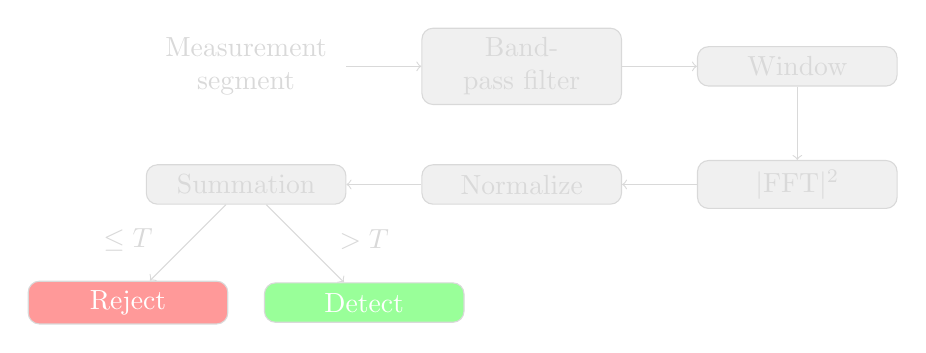
\begin{tikzpicture}[node distance=3.5cm]
    % Noder
    \node (meas) [rectangle,text width=2.3cm, align=center,textcolor] {Measurement segment};
    \node (filter) [rectangle, draw, rounded corners,fill=gray, fill opacity=0.4, text opacity=1,text width=2.3cm, align=center,right of=meas, minimum width=1cm, minimum height=0.5cm,textcolor] {Band-pass filter};
    \node (window) [rectangle, draw, rounded corners,fill=gray, fill opacity=0.4, text opacity=1,text width=2.3cm, align=center, right of=filter, minimum width=1cm, minimum height=0.5cm,textcolor] {Window};
    \node (fft) [rectangle, draw, rounded corners,fill=gray, fill opacity=0.4, text opacity=1,text width=2.3cm, align=center, below of=window, minimum width=1cm, minimum height=0.5cm,yshift=2cm,textcolor] {$|$FFT$|^2$};
    \node (normalize) [rectangle, draw, rounded corners,fill=gray, fill opacity=0.4, text opacity=1,text width=2.3cm, align=center, left of=fft, minimum width=1cm, minimum height=0.5cm,textcolor] {Normalize};
    \node (sum) [rectangle, draw, rounded corners,fill=gray, fill opacity=0.4, text opacity=1,text width=2.3cm, align=center, left of=normalize, minimum width=1cm, minimum height=0.5cm,textcolor] {Summation};
    \node (detect) [rectangle, draw, rounded corners,fill=green, fill opacity=0.4, text opacity=1,text width=2.3cm, align=center, below of=sum,yshift=0cm,xshift=1.5cm, minimum width=1cm, minimum height=0.5cm,yshift=2cm,font=\color{white},draw=textcolor] {Detect};
    \node (reject) [rectangle, draw, rounded corners,fill=red, fill opacity=0.4, text opacity=1,text width=2.3cm, align=center, below of=sum,yshift=0cm,xshift=-1.5cm, minimum width=1cm, minimum height=0.5cm,yshift=2cm,font=\color{white},draw=textcolor] {Reject};
    % Pilarna
    \draw [->,textcolor] (meas) -- (filter);
    \draw [->,textcolor] (filter) -- (window);
    \draw [->,textcolor] (window) -- (fft);
    \draw [->,textcolor] (fft) -- (normalize);
    \draw [->,textcolor] (normalize) -- (sum);
    \draw [->,textcolor] (sum) -- (detect);
    \draw [->,textcolor] (sum) -- (reject);

    \node[rectangle, align=center,above of=detect,yshift=-2.7cm,xshift=0cm,textcolor] {$>T$};
    \node[rectangle, align=center,above of=reject,yshift=-2.7cm,xshift=-0cm,textcolor] {$\le T$};
\end{tikzpicture}
% % This file was created by matlab2tikz.
%
%The latest updates can be retrieved from
%  http://www.mathworks.com/matlabcentral/fileexchange/22022-matlab2tikz-matlab2tikz
%where you can also make suggestions and rate matlab2tikz.
%
\definecolor{mycolor1}{rgb}{0.00000,0.44700,0.74100}%
\colorlet{mycolor1}{mycolor1!80!white}%

\begin{tikzpicture}

\begin{axis}[%
  DarkMode,
width=0.59\linewidth, % Width of the plot
height=0.3\linewidth, % Height of the plot
axis lines=left,
xmin=46.23,
xmax=49.6,
ymin=-1,
ymax=0.6,
% xlabel style={font=\color{white!15!black}},
xlabel={Time [s]},
% ylabel style={font=\color{white!15!black}},
ylabel={Amplitude},
xtick={46, 47, 48, 49},
ytick={-1 ,-0.5, 0, 0.5},
% title style={font=\bfseries\color{textcolor}},
title={Geophone signal},
line width=1pt,
axis line style={line width=1pt},
smooth,
tension=1,
% width=15.5in,
% height=9.126in,
% at={(2.6in,1.232in)},
% scale only axis,
% xmin=46.23,
% xmax=49.6,
% xlabel style={font=\color{white!15!black}},
% xlabel={Time [s]},
% ymin=-1,
% ymax=0.5,
% ylabel style={font=\color{white!15!black}},
% ylabel={Amplitude},
% axis background/.style={fill=white},
% title style={font=\bfseries},
% title={Geophone signal},
xmajorgrids,
ymajorgrids
]
\addplot [color=mycolor1, forget plot, smooth]
  table[row sep=crcr]{%
46.230141	-0.36656857\\
46.232254	-0.35405159\\
46.234372	-0.34928322\\
46.236482	-0.29742718\\
46.238597	-0.29981136\\
46.24071	-0.3027916\\
46.242825	-0.28729439\\
46.244938	-0.26464462\\
46.247053	-0.26464462\\
46.249166	-0.24437904\\
46.251281	-0.24080276\\
46.253399	-0.24735928\\
46.255514	-0.24616718\\
46.257627	-0.22768974\\
46.259742	-0.26166439\\
46.261854	-0.25689602\\
46.26397	-0.23901463\\
46.266089	-0.26345253\\
46.268204	-0.24080276\\
46.270317	-0.23245811\\
46.272432	-0.22172928\\
46.274545	-0.20742416\\
46.27666	-0.2104044\\
46.278773	-0.2104044\\
46.280888	-0.1937151\\
46.283001	-0.22470951\\
46.285116	-0.19848347\\
46.287229	-0.20503998\\
46.28935	-0.24199486\\
46.291457	-0.24795532\\
46.293572	-0.25987625\\
46.295685	-0.29981136\\
46.297805	-0.31292439\\
46.299917	-0.30577183\\
46.302033	-0.33438206\\
46.304146	-0.36180019\\
46.306261	-0.33915043\\
46.308382	-0.34749508\\
46.310496	-0.35405159\\
46.31261	-0.37252903\\
46.314725	-0.38087368\\
46.316838	-0.3606081\\
46.318953	-0.35524368\\
46.321066	-0.33557415\\
46.323181	-0.32663345\\
46.325294	-0.29027462\\
46.32741	-0.28014183\\
46.329525	-0.25868416\\
46.33164	-0.24735928\\
46.333753	-0.21696091\\
46.335868	-0.2104044\\
46.337981	-0.20682812\\
46.340102	-0.19073486\\
46.342215	-0.21457672\\
46.344337	-0.2270937\\
46.346443	-0.22172928\\
46.348558	-0.21696091\\
46.350671	-0.23782253\\
46.352794	-0.24080276\\
46.354908	-0.23841858\\
46.357023	-0.23663044\\
46.359136	-0.24318695\\
46.361255	-0.23901463\\
46.363372	-0.24676323\\
46.365483	-0.27000904\\
46.367596	-0.24139881\\
46.369711	-0.28192997\\
46.371824	-0.2771616\\
46.373939	-0.29623508\\
46.376051	-0.30875206\\
46.378167	-0.30934811\\
46.38028	-0.30815601\\
46.382399	-0.32782555\\
46.384512	-0.31292439\\
46.386627	-0.30994415\\
46.38874	-0.31709671\\
46.390855	-0.28669834\\
46.392969	-0.25749207\\
46.395091	-0.25749207\\
46.397204	-0.23961067\\
46.399319	-0.24557114\\
46.401432	-0.24318695\\
46.403547	-0.25212765\\
46.40566	-0.28133392\\
46.407775	-0.25570393\\
46.409888	-0.27239323\\
46.412003	-0.28252602\\
46.414115	-0.29623508\\
46.416231	-0.3027916\\
46.41835	-0.34511089\\
46.420459	-0.32186508\\
46.422572	-0.34332275\\
46.424688	-0.34749508\\
46.426809	-0.3272295\\
46.428923	-0.30636787\\
46.431038	-0.33140182\\
46.433153	-0.29265881\\
46.435266	-0.27000904\\
46.437387	-0.30815601\\
46.4395	-0.31173229\\
46.441616	-0.30100346\\
46.443728	-0.30934811\\
46.445844	-0.28848648\\
46.447957	-0.30577183\\
46.450073	-0.30457973\\
46.452187	-0.29861927\\
46.454302	-0.26524067\\
46.456415	-0.23543835\\
46.45853	-0.22292137\\
46.460643	-0.20980835\\
46.462758	-0.16391277\\
46.464871	-0.12278557\\
46.466986	-0.15199184\\
46.469107	-0.13530254\\
46.471222	-0.11086464\\
46.473338	-0.14066696\\
46.47545	-0.1335144\\
46.477563	-0.13113022\\
46.479678	-0.15735626\\
46.481797	-0.1680851\\
46.483913	-0.18179417\\
46.486026	-0.20027161\\
46.488141	-0.23722649\\
46.490254	-0.26404858\\
46.492372	-0.29087067\\
46.494482	-0.3105402\\
46.496597	-0.34570694\\
46.49871	-0.36656857\\
46.500825	-0.40233135\\
46.502938	-0.41127205\\
46.505052	-0.44465065\\
46.507166	-0.4440546\\
46.50928	-0.45001507\\
46.511399	-0.42438507\\
46.513513	-0.42259693\\
46.515627	-0.40411949\\
46.517742	-0.38444996\\
46.519855	-0.34213066\\
46.52197	-0.34153461\\
46.524089	-0.31173229\\
46.526204	-0.29802322\\
46.528317	-0.30040741\\
46.530432	-0.30696392\\
46.532545	-0.33020973\\
46.53466	-0.33915043\\
46.536772	-0.33080578\\
46.538888	-0.35762787\\
46.541001	-0.3349781\\
46.543116	-0.27954578\\
46.545229	-0.25570393\\
46.54735	-0.22113323\\
46.549457	-0.16450882\\
46.551572	-0.12159348\\
46.553685	-0.1180172\\
46.555805	-0.10073185\\
46.557918	-0.04827976\\
46.560033	-0.04887581\\
46.562146	-0.03218651\\
46.564261	-0.03576279\\
46.566382	-0.0590086\\
46.568496	-0.09953976\\
46.57061	-0.14901161\\
46.572725	-0.18298626\\
46.574838	-0.23722649\\
46.576953	-0.29504299\\
46.579066	-0.34689903\\
46.581181	-0.35881996\\
46.583294	-0.42617321\\
46.585411	-0.43690205\\
46.587524	-0.45359135\\
46.589638	-0.47147274\\
46.591752	-0.4452467\\
46.593866	-0.42021275\\
46.59598	-0.42259693\\
46.598102	-0.39279461\\
46.600214	-0.35226345\\
46.602338	-0.33915043\\
46.604443	-0.30040741\\
46.606558	-0.25272369\\
46.608671	-0.22828579\\
46.610794	-0.20563602\\
46.612908	-0.18000603\\
46.615023	-0.17225742\\
46.617136	-0.16212463\\
46.619251	-0.16212463\\
46.621371	-0.18954277\\
46.623479	-0.19729137\\
46.625592	-0.21994114\\
46.627707	-0.26702881\\
46.62982	-0.31113625\\
46.631936	-0.32961369\\
46.634048	-0.35226345\\
46.636164	-0.35941601\\
46.638277	-0.36716461\\
46.640399	-0.37670135\\
46.642511	-0.35405159\\
46.644627	-0.35345554\\
46.646877	-0.33915043\\
46.648992	-0.3528595\\
46.651112	-0.35941601\\
46.653227	-0.3272295\\
46.655344	-0.31888485\\
46.657459	-0.30636787\\
46.659576	-0.2771616\\
46.661692	-0.20742416\\
46.663811	-0.20623207\\
46.665926	-0.16927719\\
46.668041	-0.13291836\\
46.670156	-0.10967255\\
46.672269	-0.08106232\\
46.67439	-0.0500679\\
46.676503	-0.01549721\\
46.678618	-0.00119209\\
46.680731	-0.02145767\\
46.682846	-0.01847744\\
46.684963	-0.05245209\\
46.687078	-0.11622906\\
46.689195	-0.17046928\\
46.69131	-0.2259016\\
46.693423	-0.29504299\\
46.695538	-0.34093857\\
46.697651	-0.3683567\\
46.69977	-0.37014484\\
46.701883	-0.39339066\\
46.704003	-0.41306019\\
46.706116	-0.42259693\\
46.708235	-0.44047832\\
46.710358	-0.42915344\\
46.712463	-0.4440546\\
46.714576	-0.4452467\\
46.716692	-0.47445297\\
46.71881	-0.45180321\\
46.720925	-0.42557716\\
46.72304	-0.40829182\\
46.725155	-0.35941601\\
46.727272	-0.3015995\\
46.729396	-0.27894974\\
46.731509	-0.21934509\\
46.733624	-0.2104044\\
46.735737	-0.18298626\\
46.737856	-0.21994114\\
46.739969	-0.20980835\\
46.742095	-0.21398067\\
46.744208	-0.21517277\\
46.746325	-0.22828579\\
46.748438	-0.22947788\\
46.750557	-0.21576881\\
46.75267	-0.21219254\\
46.754791	-0.18537045\\
46.756906	-0.13530254\\
46.759021	-0.08523464\\
46.761138	-0.0411272\\
46.763254	0.01132488\\
46.765379	0.05543232\\
46.767495	0.11324883\\
46.769611	0.1513958\\
46.771732	0.13172626\\
46.773844	0.12159348\\
46.775965	0.09775162\\
46.778084	-0.00059605\\
46.7802	-0.08821487\\
46.782317	-0.21696091\\
46.784432	-0.32126904\\
46.786545	-0.43094158\\
46.78866	-0.53167343\\
46.790776	-0.59127808\\
46.792892	-0.65922737\\
46.795007	-0.69499016\\
46.797122	-0.69320202\\
46.799238	-0.70512295\\
46.801357	-0.69141388\\
46.803468	-0.67532063\\
46.805583	-0.65982342\\
46.807696	-0.63061714\\
46.809821	-0.59187412\\
46.811934	-0.5120039\\
46.814053	-0.42974949\\
46.816166	-0.35226345\\
46.818283	-0.22113323\\
46.820402	-0.15377998\\
46.822522	-0.06735325\\
46.824635	0.01549721\\
46.82675	0.04649162\\
46.828863	0.06258488\\
46.830978	0.07927418\\
46.833095	0.06198883\\
46.83521	0.04827976\\
46.837323	0.02622604\\
46.839438	0\\
46.841551	-0.01549721\\
46.843666	-0.02622604\\
46.84578	-0.05543232\\
46.847895	-0.05125999\\
46.850009	-0.04172325\\
46.852124	-0.05543232\\
46.854237	-0.07808208\\
46.856356	-0.08940697\\
46.858465	-0.1013279\\
46.86058	-0.12516975\\
46.862693	-0.15377998\\
46.864811	-0.23663044\\
46.866924	-0.26106834\\
46.869039	-0.31709671\\
46.871152	-0.43988228\\
46.873272	-0.48935413\\
46.875387	-0.55253506\\
46.877503	-0.65267086\\
46.879615	-0.68485737\\
46.881731	-0.73254108\\
46.883844	-0.76591969\\
46.885959	-0.77486038\\
46.888072	-0.73075294\\
46.890188	-0.70512295\\
46.892302	-0.65624714\\
46.894417	-0.56326389\\
46.89653	-0.48577785\\
46.898645	-0.4273653\\
46.900757	-0.32901764\\
46.902873	-0.20623207\\
46.904986	-0.13947487\\
46.907108	-0.05602837\\
46.909221	0.0089407\\
46.911344	0.11146069\\
46.913449	0.17464161\\
46.915564	0.2092123\\
46.917676	0.24437904\\
46.919801	0.27656555\\
46.921915	0.27477741\\
46.92403	0.24080276\\
46.926143	0.16391277\\
46.928258	0.12755394\\
46.930378	0.05364418\\
46.932494	-0.03933907\\
46.934606	-0.1513958\\
46.936722	-0.27418137\\
46.938836	-0.3695488\\
46.940951	-0.48041344\\
46.943065	-0.59366226\\
46.94518	-0.69737434\\
46.947293	-0.76472759\\
46.949411	-0.78678131\\
46.951525	-0.82194805\\
46.95364	-0.79214573\\
46.955753	-0.74863434\\
46.957868	-0.68843365\\
46.959981	-0.60379505\\
46.962102	-0.52750111\\
46.964214	-0.42557716\\
46.966337	-0.33855438\\
46.968443	-0.27775764\\
46.970568	-0.18775463\\
46.972681	-0.13172626\\
46.9748	-0.09119511\\
46.976914	-0.06914139\\
46.979029	-0.07390976\\
46.981142	-0.08523464\\
46.983258	-0.09536743\\
46.985378	-0.10728836\\
46.987493	-0.12218952\\
46.989606	-0.14662743\\
46.991721	-0.14781952\\
46.993834	-0.1680851\\
46.995949	-0.20027161\\
46.998061	-0.19073486\\
47.000177	-0.17523766\\
47.00229	-0.16689301\\
47.004411	-0.16868114\\
47.006524	-0.11563301\\
47.008639	-0.12695789\\
47.010752	-0.13947487\\
47.012868	-0.14066696\\
47.014981	-0.15377998\\
47.017102	-0.19431114\\
47.019216	-0.20265579\\
47.021338	-0.22351742\\
47.023444	-0.31530857\\
47.025559	-0.35524368\\
47.027672	-0.40590763\\
47.029794	-0.48041344\\
47.031907	-0.48935413\\
47.034022	-0.50902367\\
47.036135	-0.52511692\\
47.03825	-0.5030632\\
47.040366	-0.50663948\\
47.042478	-0.51319599\\
47.044591	-0.50127506\\
47.046705	-0.47087669\\
47.048819	-0.42498112\\
47.050934	-0.37491322\\
47.053047	-0.30934811\\
47.055162	-0.25570393\\
47.057275	-0.21636486\\
47.059393	-0.14662743\\
47.061506	-0.13172626\\
47.063621	-0.1168251\\
47.065734	-0.07212162\\
47.067848	-0.06318092\\
47.069962	-0.05483627\\
47.072077	-0.06318092\\
47.07419	-0.06854534\\
47.076305	-0.1013279\\
47.078418	-0.15616417\\
47.080534	-0.1680851\\
47.082647	-0.20027161\\
47.084762	-0.24735928\\
47.086875	-0.27179718\\
47.08899	-0.32544136\\
47.091107	-0.34689903\\
47.093222	-0.37491322\\
47.095338	-0.37431717\\
47.09745	-0.40054321\\
47.099562	-0.39756298\\
47.101678	-0.37670135\\
47.103797	-0.37968159\\
47.105913	-0.39696693\\
47.108026	-0.37550926\\
47.110141	-0.3606081\\
47.112254	-0.31769276\\
47.114372	-0.3194809\\
47.116482	-0.29325485\\
47.118596	-0.27179718\\
47.12071	-0.24557114\\
47.122825	-0.22530556\\
47.124939	-0.22768974\\
47.127054	-0.22292137\\
47.129167	-0.22351742\\
47.131282	-0.21874905\\
47.133399	-0.22053719\\
47.135514	-0.21636486\\
47.137627	-0.18239021\\
47.139743	-0.20325184\\
47.141856	-0.1758337\\
47.143971	-0.16152859\\
47.146088	-0.19848347\\
47.148204	-0.20802021\\
47.150317	-0.20563602\\
47.152433	-0.24616718\\
47.154546	-0.26106834\\
47.156661	-0.30338764\\
47.158774	-0.33915043\\
47.160889	-0.37610531\\
47.163002	-0.37193298\\
47.165117	-0.40948391\\
47.167229	-0.40709972\\
47.16935	-0.38027763\\
47.171458	-0.42438507\\
47.173573	-0.40888786\\
47.175686	-0.35345554\\
47.177805	-0.37312508\\
47.179918	-0.32067299\\
47.182033	-0.28371811\\
47.184146	-0.24437904\\
47.186261	-0.20444393\\
47.188382	-0.20980835\\
47.190497	-0.18000603\\
47.19261	-0.16689301\\
47.194725	-0.18298626\\
47.196838	-0.14960766\\
47.198953	-0.11742115\\
47.201066	-0.15974045\\
47.203181	-0.16450882\\
47.205294	-0.19788742\\
47.207411	-0.24616718\\
47.209525	-0.27298927\\
47.21164	-0.2849102\\
47.213753	-0.28312206\\
47.215868	-0.30994415\\
47.21798	-0.32901764\\
47.220102	-0.34809113\\
47.222215	-0.32782555\\
47.224337	-0.35405159\\
47.226443	-0.31769276\\
47.228558	-0.2938509\\
47.230671	-0.28669834\\
47.232794	-0.29861927\\
47.234907	-0.28550625\\
47.237022	-0.27358532\\
47.239135	-0.28669834\\
47.24125	-0.29146671\\
47.243366	-0.28133392\\
47.245478	-0.29742718\\
47.247591	-0.27835369\\
47.249707	-0.29623508\\
47.25182	-0.30040741\\
47.253935	-0.30994415\\
47.256048	-0.3105402\\
47.258163	-0.29802322\\
47.260277	-0.28252602\\
47.262399	-0.30636787\\
47.264511	-0.27477741\\
47.266627	-0.26643276\\
47.26874	-0.243783\\
47.270854	-0.23603439\\
47.272968	-0.21219254\\
47.275091	-0.23245811\\
47.277204	-0.22947788\\
47.279319	-0.22113323\\
47.281432	-0.21219254\\
47.283547	-0.2104044\\
47.28566	-0.19311905\\
47.287775	-0.2259016\\
47.289888	-0.20563602\\
47.292003	-0.19431114\\
47.294116	-0.218153\\
47.296231	-0.23901463\\
47.29835	-0.24974346\\
47.300459	-0.25808811\\
47.302572	-0.27060509\\
47.304687	-0.29087067\\
47.306803	-0.30696392\\
47.308917	-0.32305717\\
47.311031	-0.34511089\\
47.313146	-0.37610531\\
47.315259	-0.38206577\\
47.317382	-0.36776066\\
47.319495	-0.38087368\\
47.32161	-0.36001205\\
47.323723	-0.39219856\\
47.325839	-0.36299229\\
47.327952	-0.34034252\\
47.330067	-0.34093857\\
47.33218	-0.32663345\\
47.334295	-0.29802322\\
47.336409	-0.29325485\\
47.338524	-0.27537346\\
47.340636	-0.23901463\\
47.342752	-0.218153\\
47.344865	-0.16391277\\
47.34698	-0.16093254\\
47.349099	-0.15795231\\
47.351215	-0.16748905\\
47.353336	-0.15854836\\
47.355444	-0.17762184\\
47.357556	-0.16152859\\
47.359672	-0.18715858\\
47.361792	-0.23186207\\
47.363908	-0.22113323\\
47.366021	-0.23663044\\
47.368136	-0.25510788\\
47.370249	-0.29146671\\
47.372372	-0.30755997\\
47.374477	-0.35226345\\
47.376592	-0.38266182\\
47.378705	-0.37789345\\
47.38082	-0.37431717\\
47.382933	-0.37670135\\
47.385047	-0.38206577\\
47.387291	-0.32663345\\
47.389411	-0.31650066\\
47.391524	-0.32484531\\
47.393639	-0.31769276\\
47.395752	-0.28967857\\
47.397871	-0.26583672\\
47.399987	-0.2092123\\
47.40211	-0.19729137\\
47.404223	-0.17344952\\
47.406344	-0.1424551\\
47.408454	-0.1513958\\
47.410569	-0.15735626\\
47.412682	-0.15974045\\
47.4148	-0.17046928\\
47.416912	-0.15676022\\
47.419032	-0.16272068\\
47.421145	-0.19192696\\
47.423265	-0.18537045\\
47.425382	-0.18656254\\
47.427503	-0.20205975\\
47.429616	-0.21457672\\
47.431736	-0.23126602\\
47.433849	-0.26762486\\
47.435969	-0.27060509\\
47.438089	-0.27000904\\
47.440204	-0.29504299\\
47.442317	-0.30875206\\
47.444432	-0.31113625\\
47.446549	-0.32663345\\
47.448664	-0.31769276\\
47.45078	-0.3027916\\
47.452895	-0.31530857\\
47.455008	-0.33438206\\
47.457123	-0.31173229\\
47.459236	-0.3272295\\
47.461356	-0.36418438\\
47.463464	-0.3528595\\
47.465583	-0.42915344\\
47.467697	-0.41425228\\
47.46982	-0.39696693\\
47.471933	-0.40054321\\
47.474053	-0.39279461\\
47.476166	-0.34332275\\
47.478281	-0.32424927\\
47.480401	-0.30040741\\
47.482521	-0.25868416\\
47.484634	-0.24735928\\
47.486749	-0.19550323\\
47.488862	-0.16391277\\
47.490977	-0.13232231\\
47.493095	-0.09417534\\
47.495209	-0.07331371\\
47.497323	-0.03874302\\
47.499444	-0.03278255\\
47.501557	-0.0166893\\
47.503672	-0.03278255\\
47.505792	-0.04649162\\
47.507912	-0.04589558\\
47.510026	-0.08225441\\
47.512141	-0.10251999\\
47.514254	-0.14603138\\
47.516372	-0.18179417\\
47.518482	-0.24795532\\
47.520597	-0.27000904\\
47.522713	-0.30040741\\
47.524828	-0.33795834\\
47.526945	-0.36120415\\
47.52906	-0.37074089\\
47.531175	-0.41306019\\
47.53329	-0.36180019\\
47.535412	-0.37848949\\
47.537526	-0.39339066\\
47.539642	-0.36656857\\
47.541757	-0.35226345\\
47.54387	-0.31888485\\
47.545991	-0.33199787\\
47.548113	-0.32424927\\
47.550233	-0.32961369\\
47.552352	-0.3194809\\
47.554466	-0.31411648\\
47.55658	-0.33020973\\
47.558699	-0.34093857\\
47.560816	-0.31888485\\
47.562933	-0.3015995\\
47.565046	-0.31471252\\
47.567161	-0.2938509\\
47.569274	-0.2771616\\
47.571393	-0.25093555\\
47.573506	-0.22470951\\
47.575621	-0.17166138\\
47.577734	-0.1513958\\
47.579849	-0.13887882\\
47.581961	-0.11503696\\
47.584077	-0.13947487\\
47.586189	-0.13291836\\
47.588305	-0.13649464\\
47.590421	-0.1424551\\
47.592536	-0.12814999\\
47.594649	-0.11920929\\
47.596764	-0.15795231\\
47.598877	-0.15735626\\
47.600992	-0.16152859\\
47.603112	-0.17344952\\
47.605226	-0.17821789\\
47.607344	-0.18775463\\
47.609455	-0.23901463\\
47.611567	-0.25629997\\
47.613683	-0.25331974\\
47.615806	-0.3015995\\
47.61792	-0.33378601\\
47.620034	-0.36537647\\
47.622149	-0.4440546\\
47.624262	-0.44047832\\
47.626382	-0.45239925\\
47.628495	-0.49591064\\
47.63061	-0.48458576\\
47.632723	-0.45835972\\
47.634838	-0.45657158\\
47.636951	-0.39994717\\
47.639066	-0.38444996\\
47.641179	-0.35941601\\
47.643294	-0.33020973\\
47.645408	-0.31888485\\
47.647524	-0.28610229\\
47.649637	-0.24735928\\
47.651752	-0.20563602\\
47.653865	-0.19550323\\
47.65598	-0.1591444\\
47.658099	-0.12218952\\
47.660215	-0.1168251\\
47.662335	-0.11861324\\
47.664443	-0.15795231\\
47.666556	-0.14662743\\
47.668671	-0.18894672\\
47.670792	-0.24080276\\
47.672907	-0.27835369\\
47.67502	-0.3027916\\
47.677135	-0.30636787\\
47.679248	-0.31352043\\
47.681366	-0.29742718\\
47.683476	-0.26583672\\
47.685591	-0.25391579\\
47.687704	-0.19669533\\
47.689818	-0.1424551\\
47.691932	-0.12159348\\
47.694047	-0.07867813\\
47.69616	-0.08642673\\
47.698275	-0.07152557\\
47.700393	-0.0667572\\
47.702508	-0.14901161\\
47.704621	-0.2014637\\
47.706736	-0.21994114\\
47.708849	-0.32007694\\
47.710964	-0.38862228\\
47.713085	-0.45001507\\
47.715199	-0.49471855\\
47.717313	-0.54895878\\
47.719428	-0.57458878\\
47.721541	-0.55849552\\
47.723656	-0.55372715\\
47.725769	-0.54836273\\
47.727884	-0.50008297\\
47.729997	-0.45835972\\
47.732114	-0.47266483\\
47.734228	-0.41782856\\
47.73635	-0.36358833\\
47.738456	-0.34809113\\
47.740571	-0.25868416\\
47.742684	-0.17940998\\
47.744805	-0.09715557\\
47.746917	-0.02145767\\
47.749033	0.04589558\\
47.751146	0.07987022\\
47.753261	0.08940697\\
47.755382	0.06437302\\
47.757497	-0.00178814\\
47.75961	-0.05304813\\
47.761725	-0.13709068\\
47.763838	-0.23782253\\
47.765953	-0.33259392\\
47.768066	-0.41723251\\
47.770181	-0.46312809\\
47.772294	-0.50365925\\
47.774411	-0.49173832\\
47.776525	-0.49293041\\
47.77864	-0.44107437\\
47.780753	-0.39577484\\
47.782868	-0.34451485\\
47.784981	-0.27894974\\
47.787102	-0.24855137\\
47.789215	-0.24974346\\
47.791337	-0.20205975\\
47.793443	-0.22768974\\
47.795558	-0.24974346\\
47.797671	-0.28252602\\
47.799794	-0.31530857\\
47.801907	-0.33855438\\
47.804022	-0.36537647\\
47.806135	-0.38146973\\
47.80825	-0.39994717\\
47.810366	-0.39696693\\
47.812478	-0.36716461\\
47.814591	-0.34153461\\
47.816706	-0.32007694\\
47.818819	-0.29921532\\
47.820934	-0.2348423\\
47.823048	-0.18060207\\
47.825163	-0.12755394\\
47.827276	-0.02384186\\
47.829399	0.01847744\\
47.831512	0.06735325\\
47.833627	0.10430813\\
47.83574	0.10669231\\
47.837854	0.11920929\\
47.839968	0.11026859\\
47.842091	0.03099442\\
47.844204	-0.02026558\\
47.846319	-0.1168251\\
47.848432	-0.18715858\\
47.850547	-0.30398369\\
47.85266	-0.40769577\\
47.854775	-0.48816204\\
47.856888	-0.58114529\\
47.859003	-0.64253807\\
47.861115	-0.70929527\\
47.863231	-0.78201294\\
47.86535	-0.78737736\\
47.867459	-0.83446503\\
47.869572	-0.82969666\\
47.871686	-0.83208084\\
47.873803	-0.80227852\\
47.875919	-0.74923038\\
47.878032	-0.63955784\\
47.880148	-0.56624413\\
47.882261	-0.4285574\\
47.884382	-0.31709671\\
47.886495	-0.18417835\\
47.88861	-0.03218651\\
47.890723	0.08761883\\
47.892838	0.21100044\\
47.89495	0.33199787\\
47.897066	0.39100647\\
47.899179	0.42617321\\
47.901294	0.41842461\\
47.903408	0.36001205\\
47.905524	0.3182888\\
47.907637	0.23066998\\
47.909752	0.12338161\\
47.911865	0.02384186\\
47.91398	-0.08821487\\
47.9161	-0.21517277\\
47.918215	-0.33199787\\
47.920336	-0.4285574\\
47.922444	-0.51558018\\
47.924557	-0.58948994\\
47.926672	-0.62167645\\
47.928792	-0.67353249\\
47.930907	-0.68664551\\
47.93302	-0.67353249\\
47.935135	-0.68306923\\
47.937247	-0.64849854\\
47.939366	-0.60617924\\
47.941476	-0.56684017\\
47.943591	-0.53703785\\
47.945704	-0.47028065\\
47.947819	-0.4273653\\
47.949932	-0.35941601\\
47.952047	-0.30457973\\
47.95416	-0.26583672\\
47.956275	-0.23305416\\
47.958393	-0.22172928\\
47.960508	-0.17464161\\
47.962621	-0.18596649\\
47.964736	-0.21159649\\
47.966849	-0.17106533\\
47.968964	-0.16629696\\
47.971084	-0.16033649\\
47.973199	-0.1680851\\
47.975312	-0.15735626\\
47.977427	-0.15318394\\
47.97954	-0.10609627\\
47.981655	-0.0679493\\
47.983768	-0.05543232\\
47.985883	-0.05304813\\
47.987995	-0.0089407\\
47.990114	-0.01311302\\
47.992226	-0.02682209\\
47.994352	-0.04351139\\
47.996456	-0.0756979\\
47.99857	-0.12814999\\
48.000684	-0.20265579\\
48.002805	-0.26524067\\
48.004918	-0.32782555\\
48.007033	-0.41782856\\
48.009146	-0.47624111\\
48.011261	-0.52273273\\
48.013382	-0.54001808\\
48.015497	-0.56266785\\
48.01761	-0.57220459\\
48.019725	-0.58829784\\
48.021838	-0.56445599\\
48.023953	-0.52392483\\
48.026066	-0.5030632\\
48.028181	-0.4863739\\
48.030295	-0.40829182\\
48.032411	-0.37491322\\
48.034525	-0.30934811\\
48.036641	-0.26643276\\
48.038754	-0.20980835\\
48.040869	-0.17523766\\
48.042982	-0.09894371\\
48.045102	-0.08046627\\
48.047215	-0.06079674\\
48.049338	-0.05245209\\
48.051443	-0.04410744\\
48.053558	-0.05722046\\
48.055671	-0.06854534\\
48.057794	-0.09119511\\
48.059907	-0.13589859\\
48.062022	-0.16152859\\
48.064135	-0.17940998\\
48.06625	-0.18894672\\
48.068366	-0.24199486\\
48.070478	-0.27835369\\
48.072591	-0.27775764\\
48.074706	-0.33378601\\
48.076819	-0.31173229\\
48.078934	-0.31411648\\
48.081047	-0.32901764\\
48.083162	-0.3528595\\
48.085275	-0.3606081\\
48.087393	-0.41007996\\
48.089506	-0.39756298\\
48.091621	-0.40709972\\
48.093734	-0.42974949\\
48.095849	-0.40888786\\
48.097963	-0.36537647\\
48.100078	-0.38862228\\
48.102191	-0.35345554\\
48.104306	-0.33557415\\
48.106419	-0.32067299\\
48.108534	-0.29981136\\
48.110647	-0.29623508\\
48.112762	-0.27596951\\
48.114875	-0.26941299\\
48.11699	-0.23722649\\
48.119107	-0.24497509\\
48.121222	-0.23603439\\
48.123338	-0.23245811\\
48.12545	-0.2104044\\
48.1277	-0.18537045\\
48.129818	-0.17523766\\
48.131931	-0.20563602\\
48.134047	-0.16510487\\
48.13616	-0.17881393\\
48.13828	-0.17940998\\
48.1404	-0.16331673\\
48.142515	-0.19669533\\
48.144631	-0.17642975\\
48.146746	-0.19192696\\
48.148861	-0.23126602\\
48.150976	-0.23603439\\
48.153096	-0.25510788\\
48.155212	-0.28371811\\
48.157325	-0.28312206\\
48.15944	-0.28014183\\
48.161554	-0.30577183\\
48.163676	-0.30755997\\
48.165792	-0.28431416\\
48.167907	-0.30100346\\
48.17002	-0.30696392\\
48.17214	-0.31411648\\
48.174253	-0.29861927\\
48.176374	-0.27835369\\
48.178481	-0.29027462\\
48.180596	-0.28848648\\
48.182714	-0.27954578\\
48.184829	-0.28252602\\
48.186946	-0.26166439\\
48.189061	-0.25868416\\
48.191177	-0.26702881\\
48.193292	-0.23841858\\
48.195409	-0.23603439\\
48.197528	-0.25451183\\
48.199641	-0.24914742\\
48.201762	-0.24080276\\
48.203876	-0.23305416\\
48.205991	-0.22053719\\
48.208114	-0.18715858\\
48.210229	-0.20265579\\
48.212351	-0.20384789\\
48.214457	-0.18417835\\
48.216571	-0.16391277\\
48.218686	-0.1758337\\
48.220806	-0.1758337\\
48.222921	-0.17225742\\
48.225034	-0.20980835\\
48.227154	-0.22172928\\
48.229267	-0.20444393\\
48.231394	-0.2259016\\
48.233509	-0.28014183\\
48.235629	-0.27239323\\
48.237741	-0.3027916\\
48.239862	-0.31232834\\
48.241975	-0.32782555\\
48.244099	-0.3182888\\
48.246211	-0.34511089\\
48.248335	-0.31352043\\
48.250439	-0.28729439\\
48.252555	-0.29623508\\
48.254672	-0.2849102\\
48.256796	-0.25987625\\
48.258909	-0.25093555\\
48.261024	-0.22172928\\
48.263139	-0.23245811\\
48.265254	-0.2270937\\
48.267373	-0.22470951\\
48.269483	-0.21874905\\
48.271596	-0.20980835\\
48.273711	-0.21576881\\
48.275824	-0.21934509\\
48.277939	-0.21874905\\
48.280052	-0.23007393\\
48.282169	-0.24974346\\
48.284282	-0.25212765\\
48.286408	-0.25987625\\
48.288521	-0.25749207\\
48.29064	-0.24855137\\
48.292754	-0.23066998\\
48.294874	-0.22113323\\
48.296988	-0.24318695\\
48.299109	-0.25093555\\
48.301226	-0.26702881\\
48.303352	-0.29563904\\
48.305456	-0.32246113\\
48.307571	-0.31292439\\
48.309684	-0.3272295\\
48.311805	-0.30219555\\
48.313918	-0.31352043\\
48.316033	-0.27656555\\
48.318146	-0.29504299\\
48.320261	-0.28967857\\
48.322382	-0.24139881\\
48.324497	-0.26702881\\
48.32661	-0.24676323\\
48.328725	-0.2515316\\
48.330838	-0.23066998\\
48.332954	-0.20980835\\
48.335067	-0.1937151\\
48.337181	-0.17523766\\
48.339295	-0.13887882\\
48.341411	-0.13411045\\
48.343525	-0.13589859\\
48.34564	-0.12099743\\
48.347753	-0.14841557\\
48.349868	-0.15735626\\
48.351981	-0.19133091\\
48.354102	-0.21576881\\
48.356215	-0.23424625\\
48.358338	-0.2348423\\
48.360443	-0.28014183\\
48.362558	-0.30219555\\
48.364671	-0.33378601\\
48.366794	-0.35941601\\
48.368908	-0.36180019\\
48.371023	-0.37789345\\
48.373136	-0.41484833\\
48.375251	-0.40948391\\
48.377372	-0.4118681\\
48.379478	-0.40233135\\
48.381592	-0.39756298\\
48.383706	-0.37372112\\
48.38582	-0.3528595\\
48.387935	-0.32782555\\
48.390049	-0.32067299\\
48.392164	-0.30636787\\
48.394277	-0.28192997\\
48.396399	-0.28133392\\
48.398512	-0.28610229\\
48.400627	-0.28192997\\
48.40274	-0.2682209\\
48.404858	-0.26285648\\
48.40697	-0.21636486\\
48.409093	-0.21576881\\
48.411206	-0.22351742\\
48.413321	-0.19311905\\
48.415434	-0.18417835\\
48.417549	-0.16212463\\
48.419661	-0.15079975\\
48.421777	-0.1347065\\
48.42389	-0.13113022\\
48.426004	-0.11861324\\
48.428118	-0.14603138\\
48.430232	-0.13232231\\
48.43235	-0.15974045\\
48.434461	-0.19967556\\
48.436574	-0.2270937\\
48.438689	-0.23126602\\
48.440809	-0.26702881\\
48.442924	-0.27358532\\
48.445037	-0.3182888\\
48.447152	-0.36537647\\
48.449265	-0.37968159\\
48.451387	-0.38444996\\
48.453501	-0.42080879\\
48.455615	-0.43451786\\
48.457729	-0.436306\\
48.459844	-0.43451786\\
48.461956	-0.42974949\\
48.464072	-0.41723251\\
48.466185	-0.43392181\\
48.4683	-0.40352345\\
48.470413	-0.34213066\\
48.472528	-0.33140182\\
48.474641	-0.26941299\\
48.476756	-0.21398067\\
48.478869	-0.20444393\\
48.480984	-0.16450882\\
48.4831	-0.1424551\\
48.485215	-0.1502037\\
48.487335	-0.16331673\\
48.489443	-0.16629696\\
48.491556	-0.17821789\\
48.493671	-0.17821789\\
48.495792	-0.20682812\\
48.497907	-0.20682812\\
48.500019	-0.23305416\\
48.502135	-0.24974346\\
48.504248	-0.27179718\\
48.506366	-0.26941299\\
48.508476	-0.30219555\\
48.510591	-0.27894974\\
48.512704	-0.29623508\\
48.514819	-0.28967857\\
48.516932	-0.27835369\\
48.519047	-0.27358532\\
48.521159	-0.27835369\\
48.523275	-0.25391579\\
48.525393	-0.25331974\\
48.527509	-0.26464462\\
48.529622	-0.28729439\\
48.531737	-0.28908253\\
48.53385	-0.30934811\\
48.535965	-0.29981136\\
48.538085	-0.32246113\\
48.5402	-0.32007694\\
48.542313	-0.33557415\\
48.544428	-0.32484531\\
48.546541	-0.30338764\\
48.548656	-0.29504299\\
48.550769	-0.30040741\\
48.552884	-0.29742718\\
48.554998	-0.28610229\\
48.557114	-0.27298927\\
48.559228	-0.28133392\\
48.56135	-0.27477741\\
48.563457	-0.26881695\\
48.565572	-0.26166439\\
48.567685	-0.25570393\\
48.569805	-0.24318695\\
48.571918	-0.26881695\\
48.574033	-0.24437904\\
48.576146	-0.26583672\\
48.578261	-0.27656555\\
48.580382	-0.26404858\\
48.582497	-0.2771616\\
48.58461	-0.26464462\\
48.586725	-0.24914742\\
48.588838	-0.23663044\\
48.590953	-0.22649765\\
48.593066	-0.24318695\\
48.595181	-0.23424625\\
48.597294	-0.23841858\\
48.599411	-0.23603439\\
48.601525	-0.23305416\\
48.60364	-0.25510788\\
48.605752	-0.27954578\\
48.607868	-0.25033951\\
48.609982	-0.24497509\\
48.612102	-0.28192997\\
48.614217	-0.27775764\\
48.616338	-0.30100346\\
48.618445	-0.34332275\\
48.62056	-0.35583973\\
48.622673	-0.32544136\\
48.624794	-0.37431717\\
48.626907	-0.32126904\\
48.629022	-0.26583672\\
48.631135	-0.22470951\\
48.63325	-0.17285347\\
48.635366	-0.13172626\\
48.637478	-0.10490417\\
48.639591	-0.10430813\\
48.641705	-0.1168251\\
48.643819	-0.16272068\\
48.645934	-0.20623207\\
48.648047	-0.24974346\\
48.650162	-0.3027916\\
48.652275	-0.35881996\\
48.654393	-0.41723251\\
48.656506	-0.48995018\\
48.658621	-0.49889088\\
48.660734	-0.54657459\\
48.662849	-0.55968761\\
48.664962	-0.53822994\\
48.667077	-0.52034855\\
48.66919	-0.46312809\\
48.671305	-0.4273653\\
48.673418	-0.37252903\\
48.675532	-0.31590462\\
48.677646	-0.25451183\\
48.679761	-0.2270937\\
48.681874	-0.19431114\\
48.683989	-0.12874603\\
48.686107	-0.08225441\\
48.688222	-0.07331371\\
48.690343	-0.03039837\\
48.692451	-0.0166893\\
48.694564	0.00178814\\
48.696679	-0.02861023\\
48.698798	-0.03159046\\
48.700913	-0.04053116\\
48.703026	-0.08702278\\
48.705141	-0.08523464\\
48.707254	-0.08225441\\
48.709372	-0.11444092\\
48.711482	-0.1502037\\
48.713597	-0.16987324\\
48.71571	-0.22649765\\
48.717825	-0.28967857\\
48.719938	-0.36776066\\
48.722053	-0.37968159\\
48.724166	-0.47624111\\
48.726281	-0.49114227\\
48.728399	-0.4953146\\
48.730514	-0.56028366\\
48.732627	-0.55670738\\
48.734743	-0.5531311\\
48.736856	-0.58114529\\
48.738971	-0.59127808\\
48.741089	-0.60915947\\
48.743204	-0.58531761\\
48.745317	-0.57995319\\
48.747432	-0.56684017\\
48.749545	-0.50902367\\
48.75166	-0.46133995\\
48.753772	-0.4118681\\
48.755888	-0.35345554\\
48.758	-0.2682209\\
48.760116	-0.21338463\\
48.762229	-0.1347065\\
48.76435	-0.06258488\\
48.766457	0.05185604\\
48.768572	0.1335144\\
48.770685	0.20325184\\
48.772806	0.26285648\\
48.774919	0.2938509\\
48.777035	0.31113625\\
48.779147	0.2592802\\
48.781263	0.22292137\\
48.783382	0.1502037\\
48.785497	0.04649162\\
48.78761	-0.05066395\\
48.789725	-0.15079975\\
48.791838	-0.22768974\\
48.793953	-0.3606081\\
48.796066	-0.43988228\\
48.798181	-0.50008297\\
48.800294	-0.59604645\\
48.802411	-0.66459179\\
48.804525	-0.72300434\\
48.806639	-0.74446201\\
48.808753	-0.77426434\\
48.810868	-0.77605247\\
48.812981	-0.77664852\\
48.815102	-0.72956085\\
48.817215	-0.70393085\\
48.819338	-0.65743923\\
48.821443	-0.61571598\\
48.823558	-0.52809715\\
48.825671	-0.4273653\\
48.827794	-0.31411648\\
48.829907	-0.2259016\\
48.832022	-0.10251999\\
48.834135	-0.04947186\\
48.83625	0.0166893\\
48.838366	0.07748604\\
48.840478	0.09059906\\
48.842591	0.11146069\\
48.844705	0.10609627\\
48.846819	0.11563301\\
48.848934	0.1257658\\
48.851046	0.09357929\\
48.853162	0.05960464\\
48.855275	0.04649162\\
48.857393	-0.04172325\\
48.859506	-0.06318092\\
48.861622	-0.13232231\\
48.863734	-0.21934509\\
48.86585	-0.28371811\\
48.868101	-0.34570694\\
48.870216	-0.39875507\\
48.872337	-0.44643879\\
48.874444	-0.46372414\\
48.876557	-0.49948692\\
48.878678	-0.49948692\\
48.880801	-0.47564507\\
48.882916	-0.38444996\\
48.885029	-0.47802925\\
48.887144	-0.4285574\\
48.889259	-0.46133995\\
48.891382	-0.39577484\\
48.893498	-0.3862381\\
48.895613	-0.410676\\
48.897726	-0.37133694\\
48.899844	-0.31590462\\
48.90196	-0.40352345\\
48.904074	-0.30517578\\
48.90619	-0.37491322\\
48.908304	-0.25212765\\
48.910421	-0.29623508\\
48.912537	-0.17344952\\
48.91465	-0.16212463\\
48.916765	-0.03159046\\
48.918883	-0.08881092\\
48.920998	-0.06020069\\
48.923113	0.07629395\\
48.925234	0.0333786\\
48.927352	0.06616116\\
48.929466	0.11563301\\
48.931579	0.07390976\\
48.9337	0.15079975\\
48.935815	0.03516674\\
48.937934	0.00357628\\
48.940047	-0.03576279\\
48.942162	-0.08761883\\
48.944276	-0.10311604\\
48.946399	-0.22947788\\
48.948512	-0.25331974\\
48.950628	-0.29623508\\
48.952741	-0.43451786\\
48.954861	-0.49710274\\
48.956974	-0.54001808\\
48.959101	-0.54419041\\
48.961214	-0.57458878\\
48.963337	-0.52928925\\
48.965442	-0.56087971\\
48.967561	-0.54180622\\
48.969673	-0.46551228\\
48.971798	-0.33438206\\
48.973912	-0.36656857\\
48.976029	-0.34809113\\
48.978142	-0.28192997\\
48.980259	-0.23305416\\
48.982381	-0.19967556\\
48.984501	-0.16629696\\
48.986614	-0.10311604\\
48.98873	-0.11742115\\
48.990843	-0.09357929\\
48.992961	-0.06735325\\
48.995074	-0.05960464\\
48.997189	-0.05125999\\
48.999301	-0.06139278\\
49.001417	-0.02026558\\
49.00353	-0.01966953\\
49.005647	-0.04351139\\
49.00776	-0.03755093\\
49.00988	-0.1513958\\
49.011993	-0.04887581\\
49.014116	-0.13649464\\
49.016229	-0.17940998\\
49.018357	-0.19073486\\
49.020462	-0.21517277\\
49.022578	-0.26702881\\
49.024691	-0.18179417\\
49.026814	-0.33855438\\
49.028927	-0.33080578\\
49.031042	-0.2515316\\
49.033159	-0.38325787\\
49.035274	-0.3695488\\
49.037393	-0.38325787\\
49.039508	-0.3695488\\
49.041623	-0.30696392\\
49.043738	-0.32961369\\
49.045855	-0.38981438\\
49.04797	-0.35226345\\
49.050093	-0.31471252\\
49.052208	-0.31888485\\
49.054323	-0.28014183\\
49.056438	-0.28252602\\
49.058554	-0.23066998\\
49.060673	-0.17046928\\
49.062791	-0.16927719\\
49.064907	-0.18239021\\
49.06702	-0.15735626\\
49.069135	-0.14841557\\
49.071248	-0.12993813\\
49.073366	-0.08642673\\
49.075475	-0.11444092\\
49.077591	-0.11086464\\
49.079704	-0.13589859\\
49.08182	-0.13113022\\
49.083933	-0.14483929\\
49.086048	-0.21278858\\
49.088161	-0.218153\\
49.090276	-0.23007393\\
49.092393	-0.27477741\\
49.094507	-0.29623508\\
49.096621	-0.29325485\\
49.098736	-0.33378601\\
49.100849	-0.32782555\\
49.102964	-0.30755997\\
49.105085	-0.36120415\\
49.1072	-0.3606081\\
49.109313	-0.32246113\\
49.111428	-0.35762787\\
49.113541	-0.34987926\\
49.115656	-0.29802322\\
49.117769	-0.32663345\\
49.119884	-0.34034252\\
49.121997	-0.33140182\\
49.124114	-0.33259392\\
49.126227	-0.30398369\\
49.128349	-0.29802322\\
49.130454	-0.3015995\\
49.132571	-0.2771616\\
49.134684	-0.26226044\\
49.136806	-0.25749207\\
49.138919	-0.23305416\\
49.141034	-0.23782253\\
49.143146	-0.22053719\\
49.145262	-0.19609928\\
49.147382	-0.20444393\\
49.149497	-0.18060207\\
49.15161	-0.19550323\\
49.153725	-0.19431114\\
49.155838	-0.17881393\\
49.157953	-0.16510487\\
49.160066	-0.15735626\\
49.162181	-0.18596649\\
49.164294	-0.18000603\\
49.166411	-0.20742416\\
49.168525	-0.2425909\\
49.170639	-0.25749207\\
49.172753	-0.29325485\\
49.174868	-0.2938509\\
49.176981	-0.32603741\\
49.179102	-0.3528595\\
49.181215	-0.37193298\\
49.183338	-0.37312508\\
49.185442	-0.39517879\\
49.187557	-0.410676\\
49.189671	-0.40829182\\
49.191794	-0.39279461\\
49.193907	-0.38385391\\
49.196022	-0.35643578\\
49.198135	-0.33557415\\
49.20025	-0.30934811\\
49.202366	-0.29444695\\
49.204478	-0.24020672\\
49.206591	-0.21219254\\
49.208706	-0.22351742\\
49.210818	-0.21338463\\
49.212934	-0.22172928\\
49.215047	-0.218153\\
49.217162	-0.17702579\\
49.219275	-0.17166138\\
49.221393	-0.18775463\\
49.223507	-0.17940998\\
49.225622	-0.17464161\\
49.227736	-0.19669533\\
49.229851	-0.21755695\\
49.231964	-0.23126602\\
49.234087	-0.2592802\\
49.2362	-0.28848648\\
49.238314	-0.28848648\\
49.240428	-0.28848648\\
49.242543	-0.30219555\\
49.244656	-0.31352043\\
49.246771	-0.30040741\\
49.248885	-0.29623508\\
49.251	-0.29325485\\
49.253113	-0.30219555\\
49.255228	-0.31888485\\
49.257344	-0.33915043\\
49.259456	-0.33199787\\
49.261569	-0.32424927\\
49.263684	-0.32365322\\
49.265803	-0.31769276\\
49.267918	-0.29742718\\
49.27003	-0.31352043\\
49.272146	-0.28252602\\
49.274259	-0.27656555\\
49.276378	-0.3015995\\
49.278492	-0.29325485\\
49.280607	-0.25868416\\
49.28272	-0.28908253\\
49.284835	-0.29623508\\
49.286947	-0.27358532\\
49.289063	-0.28967857\\
49.291176	-0.25451183\\
49.293291	-0.24080276\\
49.295408	-0.243783\\
49.297524	-0.21517277\\
49.299637	-0.20980835\\
49.301752	-0.16450882\\
49.303865	-0.14007092\\
49.30598	-0.1001358\\
49.3081	-0.13768673\\
49.310215	-0.14126301\\
49.312335	-0.15974045\\
49.314443	-0.18239021\\
49.316556	-0.23245811\\
49.31867	-0.28669834\\
49.320792	-0.31173229\\
49.322908	-0.36001205\\
49.325021	-0.40173531\\
49.327136	-0.40948391\\
49.329249	-0.42557716\\
49.331372	-0.44107437\\
49.333477	-0.4285574\\
49.335593	-0.42080879\\
49.337706	-0.43272972\\
49.339821	-0.41127205\\
49.341934	-0.36358833\\
49.344049	-0.35762787\\
49.346162	-0.34332275\\
49.348277	-0.30755997\\
49.350393	-0.29802322\\
49.352508	-0.27120113\\
49.354621	-0.24318695\\
49.356736	-0.25510788\\
49.358849	-0.23663044\\
49.360964	-0.19550323\\
49.363085	-0.20563602\\
49.365199	-0.19133091\\
49.367313	-0.17106533\\
49.369428	-0.16689301\\
49.371541	-0.192523\\
49.373656	-0.19788742\\
49.375769	-0.22113323\\
49.377884	-0.18358231\\
49.379997	-0.21755695\\
49.382114	-0.23186207\\
49.384227	-0.23365021\\
49.386349	-0.2515316\\
49.388455	-0.22947788\\
49.39057	-0.23365021\\
49.392683	-0.2682209\\
49.394806	-0.27298927\\
49.396919	-0.28729439\\
49.399034	-0.29087067\\
49.401147	-0.30338764\\
49.403262	-0.31411648\\
49.405382	-0.33855438\\
49.407497	-0.33140182\\
49.40961	-0.33259392\\
49.411725	-0.3361702\\
49.413838	-0.30875206\\
49.415953	-0.32603741\\
49.418066	-0.32484531\\
49.420181	-0.32603741\\
49.422294	-0.33259392\\
49.424411	-0.34868717\\
49.426525	-0.32603741\\
49.428641	-0.29683113\\
49.430753	-0.29802322\\
49.432874	-0.28848648\\
49.434986	-0.28371811\\
49.437108	-0.27775764\\
49.439221	-0.24974346\\
49.441338	-0.25987625\\
49.443449	-0.21994114\\
49.445564	-0.20802021\\
49.447677	-0.21636486\\
49.4498	-0.21576881\\
49.451914	-0.2104044\\
49.454029	-0.21696091\\
49.456141	-0.22530556\\
49.458257	-0.2259016\\
49.460378	-0.23961067\\
49.462493	-0.22053719\\
49.464606	-0.22351742\\
49.466721	-0.26285648\\
49.468834	-0.29027462\\
49.470949	-0.28610229\\
49.473062	-0.31352043\\
49.475177	-0.30696392\\
49.47729	-0.31173229\\
49.47941	-0.30040741\\
49.481525	-0.31650066\\
49.48364	-0.3027916\\
49.485753	-0.30517578\\
49.487868	-0.29444695\\
49.489981	-0.29265881\\
49.492102	-0.28133392\\
49.494215	-0.28073788\\
49.496337	-0.29861927\\
49.498443	-0.27239323\\
49.500558	-0.27835369\\
49.502671	-0.26702881\\
49.504794	-0.25570393\\
49.506907	-0.23663044\\
49.509022	-0.25451183\\
49.511135	-0.25033951\\
49.51325	-0.24616718\\
49.515366	-0.25212765\\
49.517477	-0.23841858\\
49.51959	-0.25391579\\
49.521706	-0.26881695\\
49.523819	-0.25331974\\
49.525934	-0.26881695\\
49.528047	-0.28014183\\
49.530162	-0.28431416\\
49.532275	-0.30994415\\
49.534393	-0.3361702\\
49.536506	-0.32007694\\
49.538621	-0.31888485\\
49.540734	-0.32305717\\
49.542848	-0.3361702\\
49.544962	-0.32305717\\
49.547077	-0.33438206\\
49.54919	-0.34570694\\
49.551306	-0.34034252\\
49.553419	-0.3105402\\
49.555534	-0.32663345\\
49.557647	-0.29742718\\
49.559762	-0.29265881\\
49.561875	-0.2771616\\
49.56399	-0.26106834\\
49.566107	-0.25689602\\
49.568222	-0.22292137\\
49.570338	-0.2104044\\
49.57245	-0.19311905\\
49.574563	-0.19431114\\
49.576678	-0.20444393\\
49.578797	-0.19073486\\
49.580913	-0.2014637\\
49.583026	-0.21278858\\
49.585141	-0.21934509\\
49.587254	-0.22351742\\
49.589372	-0.25510788\\
49.591482	-0.23841858\\
49.593597	-0.23663044\\
49.59571	-0.25331974\\
49.597824	-0.27477741\\
49.599939	-0.27060509\\
};
\end{axis}
\end{tikzpicture}%
% % This file was created by matlab2tikz.
%
%The latest updates can be retrieved from
%  http://www.mathworks.com/matlabcentral/fileexchange/22022-matlab2tikz-matlab2tikz
%where you can also make suggestions and rate matlab2tikz.
%
\definecolor{mycolor1}{rgb}{0.00000,0.44700,0.74100}%
\colorlet{mycolor1}{mycolor1!80!white}%

\begin{tikzpicture}

\begin{axis}[%
  DarkMode,
  width=0.4\linewidth, % Width of the plot
  height=0.3\linewidth, % Height of the plot
  axis lines=left,
  xmin=5,
  xmax=85,
  ymin=1e-07,
  ymax=0.02,
  % xlabel style={font=\color{white!15!black}},
  xlabel={Frequency [Hz]},
  % ylabel style={font=\color{white!15!black}},
  ylabel={$\hat{\Phi}(f)$},
  ymode=log,
  xtick={0, 10, 20, 30, 40, 50, 60, 70, 80},
  xticklabels={0, 10, , 30, , 50, , 70, },
  ytick={1e-07,1e-06,1e-05,0.0001,0.001,0.01},
  yticklabels={,{$10^{-6}$},,{$10^{-4}$},,{$10^{-2}$},{}},
  % title style={font=\bfseries\color{textcolor}},
  title={Spectral estimate},
  line width=1pt,
  axis line style={line width=1pt},
  smooth,
  tension=1,
% width=15.5in,
% height=9.126in,
% at={(2.6in,1.232in)},
% scale only axis,
% xmin=5,
% xmax=80,
% xlabel style={font=\color{white!15!black}},
% xlabel={Frequency [Hz]},
% ymode=log,
% ymin=1e-07,
% ymax=0.01,
% ytick={1e-07,1e-06,1e-05,0.0001,0.001,0.01,0.1},
% yticklabels={{$\text{10}^{\text{-7}}$},{$\text{10}^{\text{-6}}$},{$\text{10}^{\text{-5}}$},{$\text{10}^{\text{-4}}$},{$\text{10}^{\text{-3}}$},{$\text{10}^{\text{-2}}$},{}},
% yminorticks=true,
% ylabel style={font=\color{white!15!black}},
% ylabel={$\hat{\Phi}(f)$},
% axis background/.style={fill=white},
% title style={font=\bfseries},
% title={$\text{Spectral estimate, BT method, }\gamma\text{ = 140}$},
xmajorgrids,
ymajorgrids
]
\addplot [color=mycolor1, forget plot]
  table[row sep=crcr]{%
0	0.0645294419356433\\
0.537173049246535	0.0299827805109201\\
1.07434609849307	0.0020171809753873\\
1.6115191477396	0.000582779161858886\\
2.14869219698614	0.000251204084976135\\
2.68586524623267	0.000182290750341069\\
3.22303829547921	0.00012527765621657\\
3.76021134472574	8.65991065172357e-05\\
4.29738439397228	5.93827348320123e-05\\
4.83455744321881	5.61377297557558e-05\\
5.37173049246535	3.61127889866365e-05\\
5.90890354171188	3.18486404709531e-05\\
6.44607659095842	2.18963929991087e-05\\
6.98324964020495	3.23939523448108e-05\\
7.52042268945149	3.5398798323595e-05\\
8.05759573869802	4.34266221837535e-05\\
8.59476878794456	4.02333300685511e-05\\
9.13194183719109	7.50602160507781e-05\\
9.66911488643763	0.000146530660854732\\
10.2062879356842	0.000291304820826208\\
10.7434609849307	0.000563804823490555\\
11.2806340341772	0.000990980363484233\\
11.8178070834238	0.00160197995674502\\
12.3549801326703	0.00230881816300672\\
12.8921531819168	0.0032480344553875\\
13.4293262311634	0.00414571133723259\\
13.9664992804099	0.00349486052034915\\
14.5036723296564	0.00146067808568286\\
15.040845378903	0.00055426784882264\\
15.5780184281495	0.000345681163169314\\
16.115191477396	0.000234999302072512\\
16.6523645266426	0.000169152258381303\\
17.1895375758891	0.000194318378337354\\
17.7267106251356	0.000169589370007857\\
18.2638836743822	0.000210010888613608\\
18.8010567236287	0.000355835734816254\\
19.3382297728753	0.000620896121195293\\
19.8754028221218	0.000760556497135521\\
20.4125758713683	0.000891080442384033\\
20.9497489206149	0.000529438087500637\\
21.4869219698614	0.00023999849307897\\
22.0240950191079	0.000128849051087698\\
22.5612680683545	5.57954655305154e-05\\
23.098441117601	0.000103245799756298\\
23.6356141668475	0.000153536965599492\\
24.1727872160941	0.000117653409873222\\
24.7099602653406	8.71489626781579e-05\\
25.2471333145871	4.0581104586654e-05\\
25.7843063638337	1.92075646513324e-05\\
26.3214794130802	3.17711491598057e-05\\
26.8586524623267	3.48539785836574e-05\\
27.3958255115733	1.8955191251854e-05\\
27.9329985608198	2.21677380468588e-05\\
28.4701716100663	2.2269393124066e-05\\
29.0073446593129	1.76804207227408e-05\\
29.5445177085594	1.99850399138883e-05\\
30.0816907578059	1.87825392923458e-05\\
30.6188638070525	1.57191027960358e-05\\
31.156036856299	9.5015743278227e-06\\
31.6932099055456	1.19691582869786e-05\\
32.2303829547921	2.11515966321737e-05\\
32.7675560040386	2.51220087668105e-05\\
33.3047290532852	2.60968172467878e-05\\
33.8419021025317	2.20980332975042e-05\\
34.3790751517782	1.70448595122893e-05\\
34.9162482010248	1.24791562322239e-05\\
35.4534212502713	6.60016793020529e-06\\
35.9905942995178	9.50318906817393e-06\\
36.5277673487644	1.0178947400813e-05\\
37.0649403980109	7.16986325598519e-06\\
37.6021134472574	4.00609478501648e-06\\
38.139286496504	2.2613373310236e-06\\
38.6764595457505	1.13393445974458e-06\\
39.213632594997	1.92065330915576e-06\\
39.7508056442436	2.12009050934866e-06\\
40.2879786934901	2.02646746831453e-06\\
40.8251517427366	1.95616871478317e-06\\
41.3623247919832	2.83888042624687e-06\\
41.8994978412297	2.05828723941918e-06\\
42.4366708904762	3.45743858749296e-06\\
42.9738439397228	5.25628752433696e-06\\
43.5110169889693	4.42501782163298e-06\\
44.0481900382158	3.38221516616445e-06\\
44.5853630874624	2.78884492565767e-06\\
45.1225361367089	2.43178210894706e-06\\
45.6597091859555	2.29664432033313e-06\\
46.196882235202	1.29495428321154e-06\\
46.7340552844485	2.11535424036691e-06\\
47.2712283336951	2.98639379451569e-06\\
47.8084013829416	3.12105490525355e-06\\
48.3455744321881	2.03571556965278e-06\\
48.8827474814347	2.10524462767261e-06\\
49.4199205306812	1.81515823233874e-06\\
49.9570935799277	1.97254150114462e-06\\
50.4942666291743	2.05504303908183e-06\\
51.0314396784208	1.65421369101501e-06\\
51.5686127276673	1.67946878328861e-06\\
52.1057857769139	1.751480173424e-06\\
52.6429588261604	1.26647167605549e-06\\
53.1801318754069	1.36131509132226e-06\\
53.7173049246535	7.97569478981611e-07\\
54.2544779739	7.18157950371264e-07\\
54.7916510231465	1.03869360473001e-06\\
55.3288240723931	1.09505960895122e-06\\
55.8659971216396	5.38158429861847e-07\\
56.4031701708861	1.19597195438322e-06\\
56.9403432201327	1.49149397691065e-06\\
57.4775162693792	1.29296049495437e-06\\
58.0146893186258	9.83466128135039e-07\\
58.5518623678723	1.33841424972581e-06\\
59.0890354171188	1.62209093226486e-06\\
59.6262084663654	1.31473847780435e-06\\
60.1633815156119	8.11577666527314e-07\\
60.7005545648584	1.15135696272946e-06\\
61.237727614105	1.48841116593645e-06\\
61.7749006633515	1.58058602687772e-06\\
62.312073712598	1.49602405887288e-06\\
62.8492467618446	1.48260142911347e-06\\
63.3864198110911	1.30452868425353e-06\\
63.9235928603376	1.33250000076664e-06\\
64.4607659095842	6.41649794202072e-07\\
64.9979389588307	8.33019702313256e-07\\
65.5351120080772	8.06550892998717e-07\\
66.0722850573238	5.7648681923484e-07\\
66.6094581065703	2.41185781326929e-07\\
67.1466311558168	4.84402656986487e-07\\
67.6838042050634	8.66449832751287e-07\\
68.2209772543099	1.09273830977139e-06\\
68.7581503035564	1.00378476669381e-06\\
69.295323352803	1.12068048731325e-06\\
69.8324964020495	8.97172652049228e-07\\
70.369669451296	7.83234220804341e-07\\
70.9068425005426	6.65461927485434e-07\\
71.4440155497891	6.94011518114834e-07\\
71.9811885990357	4.41317909658057e-07\\
72.5183616482822	4.22147777899658e-07\\
73.0555346975287	4.7309038578531e-07\\
73.5927077467753	4.72512367908151e-07\\
74.1298807960218	2.73133398659668e-07\\
74.6670538452683	3.7151943204082e-07\\
75.2042268945149	3.08960737811465e-07\\
75.7413999437614	4.44239806094326e-07\\
76.2785729930079	4.52552166344945e-07\\
76.8157460422545	5.32934033372485e-07\\
77.352919091501	5.51042708104555e-07\\
77.8900921407475	6.509438835268e-07\\
78.4272651899941	4.05196460758646e-07\\
78.9644382392406	5.49715426947808e-07\\
79.5016112884871	7.54872708556016e-07\\
80.0387843377337	8.252236875954e-07\\
80.5759573869802	7.40041450672128e-07\\
81.1131304362268	7.0595845029498e-07\\
81.6503034854733	4.27788286193308e-07\\
82.1874765347198	4.43831356339851e-07\\
82.7246495839664	4.77599102050331e-07\\
83.2618226332129	6.190477360721e-07\\
83.7989956824594	6.29646455482006e-07\\
84.336168731706	6.83366519601373e-07\\
84.8733417809525	6.78908561588322e-07\\
85.410514830199	6.01245604803291e-07\\
85.9476878794456	3.8019981337541e-07\\
86.4848609286921	5.18414518196271e-07\\
87.0220339779386	4.94066773736435e-07\\
87.5592070271852	4.10274558026573e-07\\
88.0963800764317	4.24887580329711e-07\\
88.6335531256782	7.36439594159483e-07\\
89.1707261749248	5.51905803185956e-07\\
89.7078992241713	7.60436083154251e-07\\
90.2450722734178	9.99620357971631e-07\\
90.7822453226644	6.83305611573722e-07\\
91.3194183719109	3.69600671024464e-07\\
91.8565914211574	4.9483608574546e-07\\
92.393764470404	5.81560937432257e-07\\
92.9309375196505	7.58203477922577e-07\\
93.468110568897	6.48054397392509e-07\\
94.0052836181436	6.30097642358971e-07\\
94.5424566673901	8.60664940230515e-07\\
95.0796297166367	1.11026029983132e-06\\
95.6168027658832	1.19274696170714e-06\\
96.1539758151297	1.1900777292182e-06\\
96.6911488643763	8.2308315828278e-07\\
97.2283219136228	6.48938179322018e-07\\
97.7654949628693	8.86756113916633e-07\\
98.3026680121159	1.19108015414588e-06\\
98.8398410613624	6.64528971109627e-07\\
99.3770141106089	8.40612940184552e-07\\
99.9141871598555	1.00050542002346e-06\\
100.451360209102	8.58389155166558e-07\\
100.988533258349	7.9420608528074e-07\\
101.525706307595	8.83881335906806e-07\\
102.062879356842	6.23521247119203e-07\\
102.600052406088	7.11439187596878e-07\\
103.137225455335	9.16982831007831e-07\\
103.674398504581	6.86318950859298e-07\\
104.211571553828	4.03883858093209e-07\\
104.748744603074	5.62380914326728e-07\\
105.285917652321	5.07326764811706e-07\\
105.823090701567	3.6398902197666e-07\\
106.360263750814	3.89924767504845e-07\\
106.89743680006	7.30697049617725e-07\\
107.434609849307	8.75531697657654e-07\\
107.971782898553	6.53739561916685e-07\\
108.5089559478	3.7257904420388e-07\\
109.046128997047	4.84282250447178e-07\\
109.583302046293	6.65619456997808e-07\\
110.12047509554	6.89112010843906e-07\\
110.657648144786	8.29854035067844e-07\\
111.194821194033	9.49345774013844e-07\\
111.731994243279	6.86649068523346e-07\\
112.269167292526	7.36936916680553e-07\\
112.806340341772	6.57546099358933e-07\\
113.343513391019	7.66572045626918e-07\\
113.880686440265	6.97492120485175e-07\\
114.417859489512	3.75253757764493e-07\\
114.955032538758	5.74067177408748e-07\\
115.492205588005	9.32138005806438e-07\\
116.029378637252	5.04320014795696e-07\\
116.566551686498	2.57907385734012e-07\\
117.103724735745	1.82154058905752e-07\\
117.640897784991	1.98078335668561e-07\\
118.178070834238	2.01889339237019e-07\\
118.715243883484	2.73202591334427e-07\\
119.252416932731	4.64668755569048e-07\\
119.789589981977	7.69799934258594e-07\\
120.326763031224	9.79184054477646e-07\\
120.86393608047	9.82185263836557e-07\\
121.401109129717	5.21797321329823e-07\\
121.938282178963	4.71448900079765e-07\\
122.47545522821	5.66313470711209e-07\\
123.012628277456	5.7750183914031e-07\\
123.549801326703	7.07627740454782e-07\\
124.08697437595	5.28954205566175e-07\\
124.624147425196	2.48368853705956e-07\\
125.161320474443	2.74236542200662e-07\\
125.698493523689	4.02255051979997e-07\\
126.235666572936	5.77281928447584e-07\\
126.772839622182	7.31051930666353e-07\\
127.310012671429	4.96376911958502e-07\\
127.847185720675	4.53590424015404e-07\\
128.384358769922	7.2519692785919e-07\\
128.921531819168	3.80062757212023e-07\\
129.458704868415	4.3778708483206e-07\\
129.995877917661	6.35858167966713e-07\\
130.533050966908	3.67331785497357e-07\\
131.070224016154	3.58478580890617e-07\\
131.607397065401	5.09443127865478e-07\\
132.144570114648	4.4424790485533e-07\\
132.681743163894	4.16165021302421e-07\\
133.218916213141	4.100564001968e-07\\
133.756089262387	3.56552716143112e-07\\
134.293262311634	3.21741323794124e-07\\
134.83043536088	3.4559427800705e-07\\
135.367608410127	4.25034194803633e-07\\
135.904781459373	9.33652714093285e-07\\
136.44195450862	1.01904523215629e-06\\
136.979127557866	4.63493417381835e-07\\
137.516300607113	5.73000446920081e-07\\
138.053473656359	8.30197242562619e-07\\
138.590646705606	7.09643104646865e-07\\
139.127819754853	4.84965824014831e-07\\
139.664992804099	4.7835673410159e-07\\
140.202165853346	6.23983393004508e-07\\
140.739338902592	5.78791263081641e-07\\
141.276511951839	4.61687633704921e-07\\
141.813685001085	3.82421375403899e-07\\
142.350858050332	5.4490110904034e-07\\
142.888031099578	5.98173220709308e-07\\
143.425204148825	7.97542128869381e-07\\
143.962377198071	9.68777335209935e-07\\
144.499550247318	8.57951216941992e-07\\
145.036723296564	7.35422375921417e-07\\
145.573896345811	1.56337249240308e-06\\
146.111069395057	1.55930793638318e-06\\
146.648242444304	9.37076649298983e-07\\
147.185415493551	5.42685845838179e-07\\
147.722588542797	3.92430545937838e-07\\
148.259761592044	3.50475575300588e-07\\
148.79693464129	4.22399735726197e-07\\
149.334107690537	3.64639401103195e-07\\
149.871280739783	4.78668065813237e-07\\
150.40845378903	3.73706998716331e-07\\
150.945626838276	3.77352481957004e-07\\
151.482799887523	6.64088511813567e-07\\
152.019972936769	6.8985853133583e-07\\
152.557145986016	5.47367811991251e-07\\
153.094319035262	6.69901590626844e-07\\
153.631492084509	7.17200972319687e-07\\
154.168665133755	5.87021369253021e-07\\
154.705838183002	4.03741404449641e-07\\
155.243011232249	4.75575754854807e-07\\
155.780184281495	5.41051222416194e-07\\
156.317357330742	5.07229808795415e-07\\
156.854530379988	3.00241081583041e-07\\
157.391703429235	2.80141350948656e-07\\
157.928876478481	3.87273381550761e-07\\
158.466049527728	5.73814295039351e-07\\
159.003222576974	6.03348092893097e-07\\
159.540395626221	4.33043416117853e-07\\
160.077568675467	3.67240820951394e-07\\
160.614741724714	4.69133734293371e-07\\
161.15191477396	5.17010967079229e-07\\
161.689087823207	4.82665025698649e-07\\
162.226260872454	8.53397033403438e-07\\
162.7634339217	8.78801934602987e-07\\
163.300606970947	1.3093056044588e-06\\
163.837780020193	2.82876392552943e-06\\
164.37495306944	2.31464703718893e-06\\
164.912126118686	1.34216364647346e-06\\
165.449299167933	8.53499215583873e-07\\
165.986472217179	1.14608335701884e-06\\
166.523645266426	1.58121163631244e-06\\
167.060818315672	1.18431908141088e-06\\
167.597991364919	9.14909353966475e-07\\
168.135164414165	8.13421589762668e-07\\
168.672337463412	7.46398806704435e-07\\
169.209510512658	8.15231542353776e-07\\
169.746683561905	5.74342538429139e-07\\
170.283856611152	3.07785713982407e-07\\
170.821029660398	2.81943311791597e-07\\
171.358202709645	2.56717529707165e-07\\
171.895375758891	2.25141337085101e-07\\
172.432548808138	3.16770062169796e-07\\
172.969721857384	5.72468548448841e-07\\
173.506894906631	6.48116417586459e-07\\
174.044067955877	4.1233822163202e-07\\
174.581241005124	5.05373723040119e-07\\
175.11841405437	1.28104053852737e-06\\
175.655587103617	1.44670029114035e-06\\
176.192760152863	1.09959146925534e-06\\
176.72993320211	1.13761141221496e-06\\
177.267106251356	7.73001702863867e-07\\
177.804279300603	5.99469449578076e-07\\
178.34145234985	5.98174942832344e-07\\
178.878625399096	3.70003625637037e-07\\
179.415798448343	3.50889633525809e-07\\
179.952971497589	3.54204567063019e-07\\
180.490144546836	2.26444030022072e-07\\
181.027317596082	2.29077717145649e-07\\
181.564490645329	3.33897551759886e-07\\
182.101663694575	5.69182250487811e-07\\
182.638836743822	5.11020616367182e-07\\
183.176009793068	3.28011380930328e-07\\
183.713182842315	3.12698651519709e-07\\
184.250355891561	3.19048747554941e-07\\
184.787528940808	2.93402836591513e-07\\
185.324701990054	3.09455546000172e-07\\
185.861875039301	3.11370950008561e-07\\
186.399048088548	4.68318461235829e-07\\
186.936221137794	5.3949879345112e-07\\
187.473394187041	4.04593320753176e-07\\
188.010567236287	4.54813599563576e-07\\
188.547740285534	7.43478298908182e-07\\
189.08491333478	9.17904200938943e-07\\
189.622086384027	8.11139864397902e-07\\
190.159259433273	8.44320007687256e-07\\
190.69643248252	5.94828833688047e-07\\
191.233605531766	5.61540519631348e-07\\
191.770778581013	5.73742549750924e-07\\
192.307951630259	4.15580962947828e-07\\
192.845124679506	5.04513255990646e-07\\
193.382297728753	5.35373075692087e-07\\
193.919470777999	4.63506334583135e-07\\
194.456643827246	4.1059201177855e-07\\
194.993816876492	3.13343442478177e-07\\
195.530989925739	3.69664817069586e-07\\
196.068162974985	5.79269772388178e-07\\
196.605336024232	4.68399671562304e-07\\
197.142509073478	2.54471919215691e-07\\
197.679682122725	3.00950482127266e-07\\
198.216855171971	4.00513740059992e-07\\
198.754028221218	4.22870582769147e-07\\
199.291201270464	3.53949257947936e-07\\
199.828374319711	3.46205357594808e-07\\
200.365547368957	4.28228423730717e-07\\
200.902720418204	3.93199046330056e-07\\
201.439893467451	5.13767208138018e-07\\
201.977066516697	4.60908526873605e-07\\
202.514239565944	2.77211677620424e-07\\
203.05141261519	4.27060703388677e-07\\
203.588585664437	6.03220846606535e-07\\
204.125758713683	4.87185500402012e-07\\
204.66293176293	4.80908897116082e-07\\
205.200104812176	4.10803990875583e-07\\
205.737277861423	4.36825500092629e-07\\
206.274450910669	7.22905605671916e-07\\
206.811623959916	6.67242983624297e-07\\
207.348797009162	3.90123926223758e-07\\
207.885970058409	2.39607833688481e-07\\
208.423143107655	2.34720096194931e-07\\
208.960316156902	2.47947142133866e-07\\
209.497489206149	2.74897195515266e-07\\
210.034662255395	3.9255957285992e-07\\
210.571835304642	3.71994882055529e-07\\
211.109008353888	2.44560905308135e-07\\
211.646181403135	3.87823362219511e-07\\
212.183354452381	5.3034274416909e-07\\
212.720527501628	3.41240300537308e-07\\
213.257700550874	2.83519166122433e-07\\
213.794873600121	3.06324787937089e-07\\
214.332046649367	2.00251511785815e-07\\
214.869219698614	2.01982522953623e-07\\
215.40639274786	1.88121094991925e-07\\
215.943565797107	1.54006568218369e-07\\
216.480738846354	1.21760207991406e-07\\
217.0179118956	1.05937495485821e-07\\
217.555084944847	1.26831675088341e-07\\
218.092257994093	2.1835596063432e-07\\
218.62943104334	2.17436620146242e-07\\
219.166604092586	2.31192284588932e-07\\
219.703777141833	3.00421213983416e-07\\
220.240950191079	2.87976137373987e-07\\
220.778123240326	3.06000383174992e-07\\
221.315296289572	5.30891210390027e-07\\
221.852469338819	6.11836026668278e-07\\
222.389642388065	5.11324994537964e-07\\
222.926815437312	4.68151025126223e-07\\
223.463988486558	6.62993033881543e-07\\
224.001161535805	8.32178103706028e-07\\
224.538334585052	6.34706840322915e-07\\
225.075507634298	3.97262040743479e-07\\
225.612680683545	3.32198992957544e-07\\
226.149853732791	3.78210723865536e-07\\
226.687026782038	3.10637079441425e-07\\
227.224199831284	2.22052709575729e-07\\
227.761372880531	2.88476024683456e-07\\
228.298545929777	4.94935797268268e-07\\
228.835718979024	6.5451687450876e-07\\
229.37289202827	5.39638678283482e-07\\
229.910065077517	4.17636855920181e-07\\
230.447238126763	5.25919377491961e-07\\
230.98441117601	7.22559406425745e-07\\
231.521584225256	7.6068379442763e-07\\
232.058757274503	7.02703161483377e-07\\
232.59593032375	6.20177348673032e-07\\
233.133103372996	5.2462021939749e-07\\
233.670276422243	8.06191236044777e-07\\
234.207449471489	8.79664984511686e-07\\
234.744622520736	6.60450511764446e-07\\
235.281795569982	4.78653654547781e-07\\
235.818968619229	5.61378879920713e-07\\
};
\end{axis}
\end{tikzpicture}%
% % This file was created by matlab2tikz.
%
%The latest updates can be retrieved from
%  http://www.mathworks.com/matlabcentral/fileexchange/22022-matlab2tikz-matlab2tikz
%where you can also make suggestions and rate matlab2tikz.
%
\definecolor{mycolor1}{rgb}{0.00000,0.44700,0.74100}%
\colorlet{mycolor1}{mycolor1!80!white}%

\begin{tikzpicture}

\begin{axis}[%
  DarkMode,
  width=0.8\linewidth, % Width of the plot
  height=0.4\linewidth, % Height of the plot
  axis lines=left,
  xmin=5,
  xmax=83,
  % xlabel style={font=\color{white!15!textcolor}},
  xlabel={Frequency [Hz]},
  ymode=log,
  ymin=1e-07,
  ymax=0.05,
  ytick={1e-07,1e-06,1e-05,0.0001,0.001,0.01,0.1},
  yticklabels={,{$10^{-6}$},{$10^{-5}$},{$10^{-4}$},{$10^{-3}$},{$10^{-2}$},{$10^{-1}$}},
  % ylabel style={font=\color{white!15!textcolor}},
  ylabel={$\hat{\Phi}(f)$},
  % title style={font=\bfseries},
  title={Spectral estimate of 30 elephant footsteps},
  xmajorgrids,
  ymajorgrids,
  yminorticks=true,
  % legend style={legend cell align=left, align=left, draw=white!15!textcolor},
  line width=1pt,
  smooth,
  tension = 0.1
]
\addplot[color=mycolor1, forget plot, draw opacity=0.4]
  table[row sep=crcr]{%
0	0.0320881131131933\\
1.07434609849307	0.0179652427145255\\
2.14869219698614	0.00317377228783983\\
3.22303829547921	0.000753968810152244\\
4.29738439397228	0.000501817992615129\\
5.37173049246535	0.000345471085436248\\
6.44607659095842	0.000230223217746152\\
7.52042268945149	0.000241549729995378\\
8.59476878794456	0.000795382224138437\\
9.66911488643763	0.00109172147780019\\
10.7434609849307	0.00131238876444582\\
11.8178070834238	0.00223371562023458\\
12.8921531819168	0.00245359012918373\\
13.9664992804099	0.00208724672796507\\
15.040845378903	0.00212862630297263\\
16.115191477396	0.00349584755969693\\
17.1895375758891	0.0045519949096921\\
18.2638836743822	0.0028370277505869\\
19.3382297728753	0.000805636491555834\\
20.4125758713683	0.000433252787578498\\
21.4869219698614	0.000577545917617538\\
22.5612680683545	0.000605558075321506\\
23.6356141668475	0.000360334635246018\\
24.7099602653406	0.000196395540986294\\
25.7843063638337	0.000190434030140513\\
26.8586524623267	0.000153954499029255\\
27.9329985608198	0.000104825907772682\\
29.0073446593129	4.91577491859871e-05\\
30.0816907578059	6.79219369690656e-06\\
31.156036856299	2.58489214004256e-05\\
32.2303829547921	7.49319277623791e-05\\
33.3047290532852	8.11198356867473e-05\\
34.3790751517782	2.60582286095368e-05\\
35.4534212502713	1.27787081850711e-05\\
36.5277673487644	9.90294602570965e-06\\
37.6021134472574	1.01444693687332e-05\\
38.6764595457505	6.07122740349179e-06\\
39.7508056442436	7.296266821227e-06\\
40.8251517427366	4.0056180883632e-06\\
41.8994978412297	7.15614503126999e-06\\
42.9738439397228	6.49854800055431e-06\\
44.0481900382158	5.70538287033243e-06\\
45.1225361367089	5.21341708486895e-06\\
46.196882235202	1.33581395521507e-05\\
47.2712283336951	1.07668916069147e-05\\
48.3455744321881	5.6307769810384e-06\\
49.4199205306812	3.22015337908627e-06\\
50.4942666291743	5.76471773689709e-06\\
51.5686127276673	5.13772078396363e-06\\
52.6429588261604	3.48441646214099e-06\\
53.7173049246535	2.37447822929109e-06\\
54.7916510231465	6.01676411751977e-06\\
55.8659971216396	8.37051599833807e-06\\
56.9403432201327	8.6344995056508e-06\\
58.0146893186258	3.90968589509838e-06\\
59.0890354171188	2.90315143036138e-06\\
60.1633815156119	2.91765657793611e-06\\
61.237727614105	4.2276545522405e-06\\
62.312073712598	3.92138582171054e-06\\
63.3864198110911	4.77140097127502e-06\\
64.4607659095842	2.51662190779638e-06\\
65.5351120080772	2.30133971759018e-06\\
66.6094581065703	1.13356030644448e-06\\
67.6838042050634	3.28872469562234e-06\\
68.7581503035564	3.97075011425403e-06\\
69.8324964020495	4.30881022576746e-06\\
70.9068425005426	1.57211228156879e-06\\
71.9811885990357	1.34727066048346e-06\\
73.0555346975287	9.43591003816249e-07\\
74.1298807960218	1.06412341244472e-06\\
75.2042268945149	7.09953784256978e-07\\
76.2785729930079	2.03974133267861e-06\\
77.352919091501	2.48844532814381e-06\\
78.4272651899941	3.25192071098049e-06\\
79.5016112884871	1.56227777936222e-06\\
80.5759573869802	1.17359545817219e-06\\
81.6503034854733	5.47682179848608e-07\\
82.7246495839664	1.01344057667797e-06\\
83.7989956824594	8.68375682566582e-07\\
84.8733417809525	1.64427674064844e-06\\
85.9476878794456	1.31639993971911e-06\\
87.0220339779386	1.64960098704773e-06\\
88.0963800764317	1.2297634332314e-06\\
89.1707261749248	1.39213139420674e-06\\
90.2450722734178	6.05723227976036e-07\\
91.3194183719109	1.09726513297344e-06\\
92.393764470404	1.23050683958295e-06\\
93.468110568897	1.61897809605185e-06\\
94.5424566673901	8.3731063096505e-07\\
95.6168027658832	9.18770058362673e-07\\
96.6911488643763	4.58942214156763e-07\\
97.7654949628693	1.01719865713054e-06\\
98.8398410613624	8.67567490815103e-07\\
99.9141871598555	1.08458760786737e-06\\
100.988533258349	5.91506612677609e-07\\
102.062879356842	1.0877326212532e-06\\
103.137225455335	1.39600745178922e-06\\
104.211571553828	1.59706069211078e-06\\
105.285917652321	1.08961563722019e-06\\
106.360263750814	1.44329184072805e-06\\
107.434609849307	1.13925726170976e-06\\
108.5089559478	1.20706158759954e-06\\
109.583302046293	9.80717420446865e-07\\
110.657648144786	1.25538013889374e-06\\
111.731994243279	8.44873485080875e-07\\
112.806340341772	7.17844301433801e-07\\
113.880686440265	5.59365247421627e-07\\
114.955032538758	1.22000518437508e-06\\
116.029378637252	1.16838954049026e-06\\
117.103724735745	1.54038598263478e-06\\
118.178070834238	9.08461961244541e-07\\
119.252416932731	6.17768549009023e-07\\
120.326763031224	4.20244190202918e-07\\
121.401109129717	1.12474497970872e-06\\
122.47545522821	9.50716416902744e-07\\
123.549801326703	7.97210771978304e-07\\
124.624147425196	7.34568954184708e-07\\
125.698493523689	8.87339121016575e-07\\
126.772839622182	5.46418428589934e-07\\
127.847185720675	5.58617013656367e-07\\
128.921531819168	3.58184274697337e-07\\
129.995877917661	8.31585825722256e-07\\
131.070224016154	8.4444588079584e-07\\
132.144570114648	1.08033247622071e-06\\
133.218916213141	6.51978234394993e-07\\
134.293262311634	5.21535110412917e-07\\
135.367608410127	2.75289689947804e-07\\
136.44195450862	5.85531536509668e-07\\
137.516300607113	4.81949823613767e-07\\
138.590646705606	6.75944424095773e-07\\
139.664992804099	6.54939487953289e-07\\
140.739338902592	8.45325174444414e-07\\
141.813685001085	6.41980404233572e-07\\
142.888031099578	1.11938646407428e-06\\
143.962377198071	1.26396691559741e-06\\
145.036723296564	1.33633887471332e-06\\
146.111069395057	1.38922733277157e-06\\
147.185415493551	1.43790655787515e-06\\
148.259761592044	7.23302281703699e-07\\
149.334107690537	7.32556799995335e-07\\
150.40845378903	8.94560487284381e-07\\
151.482799887523	1.03061143056159e-06\\
152.557145986016	7.43019561476131e-07\\
153.631492084509	5.85698974550629e-07\\
154.705838183002	8.95966058982069e-07\\
155.780184281495	1.63127272298691e-06\\
156.854530379988	1.58414902758415e-06\\
157.928876478481	1.6051373270541e-06\\
159.003222576974	1.57940724482482e-06\\
160.077568675467	1.00859802409967e-06\\
161.15191477396	5.93965727432205e-07\\
162.226260872454	9.45230609353191e-07\\
163.300606970947	1.02159922998728e-06\\
164.37495306944	7.16735684269932e-07\\
165.449299167933	2.8495701742809e-07\\
166.523645266426	5.97997317091163e-07\\
167.597991364919	7.85602876919131e-07\\
168.672337463412	4.03396923626454e-07\\
169.746683561905	1.2628015680145e-07\\
170.821029660398	3.55737829909183e-07\\
171.895375758891	4.67063172525393e-07\\
172.969721857384	3.89901477867936e-07\\
174.044067955877	1.61229651352596e-07\\
175.11841405437	3.05432478737277e-07\\
176.192760152863	5.50161063208336e-07\\
177.267106251356	7.84933236382594e-07\\
178.34145234985	4.71259004829893e-07\\
179.415798448343	4.88994417742201e-07\\
180.490144546836	5.97601715535611e-07\\
181.564490645329	7.71984935680109e-07\\
182.638836743822	5.77508039756258e-07\\
183.713182842315	3.13951790294157e-07\\
184.787528940808	1.4255736256223e-07\\
185.861875039301	4.42729609522693e-07\\
186.936221137794	9.30431574194383e-07\\
188.010567236287	7.62713787906333e-07\\
189.08491333478	3.81156076775861e-07\\
190.159259433273	1.0663020215629e-06\\
191.233605531766	1.02667932181796e-06\\
192.307951630259	4.36182116138615e-07\\
193.382297728753	3.53486796080681e-07\\
194.456643827246	5.17889941990387e-07\\
195.530989925739	5.13999641600698e-07\\
196.605336024232	6.13468982976619e-07\\
197.679682122725	5.46933356580442e-07\\
198.754028221218	3.97154743622882e-07\\
199.828374319711	2.11317053032166e-07\\
200.902720418204	2.81839457010618e-07\\
201.977066516697	4.37827062775669e-07\\
203.05141261519	5.4035415990916e-07\\
204.125758713683	6.98270352200634e-07\\
205.200104812176	8.54451946970638e-07\\
206.274450910669	6.41129762668327e-07\\
207.348797009162	4.19068446463525e-07\\
208.423143107655	2.90248244181209e-07\\
209.497489206149	2.90294590915774e-07\\
210.571835304642	1.62866128499257e-07\\
211.646181403135	2.08644032628234e-07\\
212.720527501628	2.34467562498187e-07\\
213.794873600121	4.04083826707707e-07\\
214.869219698614	4.05654771920577e-07\\
215.943565797107	2.28905548981777e-07\\
217.0179118956	1.69573051408399e-07\\
218.092257994093	2.7037714531273e-07\\
219.166604092586	3.5215220958077e-07\\
220.240950191079	5.4322121519322e-07\\
221.315296289572	6.50865336414171e-07\\
222.389642388065	6.07363463468576e-07\\
223.463988486558	3.96896280449324e-07\\
224.538334585052	2.83729888525961e-07\\
225.612680683545	3.84784196597066e-07\\
226.687026782038	6.36980211980062e-07\\
227.761372880531	7.5088175988011e-07\\
228.835718979024	5.28247078250595e-07\\
229.910065077517	4.0291176247462e-07\\
230.98441117601	4.4602650952686e-07\\
232.058757274503	4.41326397073707e-07\\
233.133103372996	4.00065032512581e-07\\
234.207449471489	2.19439616583235e-07\\
235.281795569982	1.74874171356967e-07\\
};
\addplot [color=mycolor1, forget plot, draw opacity=0.4]
  table[row sep=crcr]{%
0	0.031699032087429\\
1.07434609849307	0.0177486698414838\\
2.14869219698614	0.00310538985150138\\
3.22303829547921	0.000730883901008187\\
4.29738439397228	0.000438534865460838\\
5.37173049246535	0.000248041649720049\\
6.44607659095842	0.000178106394301916\\
7.52042268945149	0.000266552133308935\\
8.59476878794456	0.000239141321421192\\
9.66911488643763	0.000380167269948368\\
10.7434609849307	0.00188676159939443\\
11.8178070834238	0.00528165664131455\\
12.8921531819168	0.00580637946454564\\
13.9664992804099	0.0028518062702626\\
15.040845378903	0.00174349859060892\\
16.115191477396	0.00300959206792249\\
17.1895375758891	0.00345998464637674\\
18.2638836743822	0.0022602670824654\\
19.3382297728753	0.000886175519181535\\
20.4125758713683	0.000468112545401342\\
21.4869219698614	0.000328311909609339\\
22.5612680683545	0.000118697373121261\\
23.6356141668475	0.000151744031933996\\
24.7099602653406	0.00015939707600529\\
25.7843063638337	7.4720128849491e-05\\
26.8586524623267	3.6018890632597e-05\\
27.9329985608198	4.62114385544074e-05\\
29.0073446593129	5.56359306886802e-05\\
30.0816907578059	4.45469896738588e-05\\
31.156036856299	2.896430961126e-05\\
32.2303829547921	1.90505325021871e-05\\
33.3047290532852	1.90462564978396e-05\\
34.3790751517782	2.70026706054313e-05\\
35.4534212502713	1.77350363326947e-05\\
36.5277673487644	1.35303957780002e-05\\
37.6021134472574	1.19621277898403e-05\\
38.6764595457505	1.3292698388872e-05\\
39.7508056442436	1.28648569530817e-05\\
40.8251517427366	1.57962340706823e-05\\
41.8994978412297	1.21518958959281e-05\\
42.9738439397228	7.48786651083958e-06\\
44.0481900382158	3.72245014840955e-06\\
45.1225361367089	7.07469521489694e-06\\
46.196882235202	1.07438854052009e-05\\
47.2712283336951	1.13583822701435e-05\\
48.3455744321881	9.74279032328658e-06\\
49.4199205306812	8.08773634744049e-06\\
50.4942666291743	7.41424804582662e-06\\
51.5686127276673	6.8268649564517e-06\\
52.6429588261604	4.77736756208125e-06\\
53.7173049246535	5.49228766367678e-06\\
54.7916510231465	6.47452227294191e-06\\
55.8659971216396	8.35410294036653e-06\\
56.9403432201327	6.07428442666041e-06\\
58.0146893186258	3.02454217210725e-06\\
59.0890354171188	5.34498894485483e-06\\
60.1633815156119	5.82073400709755e-06\\
61.237727614105	3.60219331865431e-06\\
62.312073712598	6.49253569355411e-06\\
63.3864198110911	7.91415654539478e-06\\
64.4607659095842	7.79397377798092e-06\\
65.5351120080772	5.54866301384448e-06\\
66.6094581065703	3.44008899136754e-06\\
67.6838042050634	3.61173518568038e-06\\
68.7581503035564	3.87711800681112e-06\\
69.8324964020495	3.50866045083134e-06\\
70.9068425005426	2.80383159978332e-06\\
71.9811885990357	3.1304369543664e-06\\
73.0555346975287	4.50909945891081e-06\\
74.1298807960218	4.08970928797037e-06\\
75.2042268945149	3.52323717139608e-06\\
76.2785729930079	3.14460468870115e-06\\
77.352919091501	4.4474195063414e-06\\
78.4272651899941	4.36937043712546e-06\\
79.5016112884871	2.22601676228033e-06\\
80.5759573869802	2.12985493204844e-06\\
81.6503034854733	3.08216755383864e-06\\
82.7246495839664	2.42026746018862e-06\\
83.7989956824594	2.42813437433773e-06\\
84.8733417809525	2.58100930957988e-06\\
85.9476878794456	2.18890753575026e-06\\
87.0220339779386	1.77249028629482e-06\\
88.0963800764317	1.90293143546298e-06\\
89.1707261749248	2.1817774814865e-06\\
90.2450722734178	2.60448325656888e-06\\
91.3194183719109	2.58688949682385e-06\\
92.393764470404	2.55870749082431e-06\\
93.468110568897	1.98726283641804e-06\\
94.5424566673901	1.91057948975012e-06\\
95.6168027658832	1.80609887200038e-06\\
96.6911488643763	1.78758204265103e-06\\
97.7654949628693	1.11535521023918e-06\\
98.8398410613624	1.22226720882915e-06\\
99.9141871598555	1.7256117837151e-06\\
100.988533258349	1.37495222726808e-06\\
102.062879356842	1.14169845842081e-06\\
103.137225455335	1.7584173391693e-06\\
104.211571553828	1.52728487706501e-06\\
105.285917652321	1.818494954761e-06\\
106.360263750814	2.67019137067004e-06\\
107.434609849307	2.60332665989227e-06\\
108.5089559478	2.62506290401711e-06\\
109.583302046293	2.92710828374581e-06\\
110.657648144786	2.50448748720337e-06\\
111.731994243279	2.55885712966882e-06\\
112.806340341772	2.69979406020271e-06\\
113.880686440265	2.00415266418686e-06\\
114.955032538758	1.07531092077812e-06\\
116.029378637252	1.04488211160684e-06\\
117.103724735745	1.07861208617473e-06\\
118.178070834238	1.28974274425398e-06\\
119.252416932731	1.0765659896977e-06\\
120.326763031224	1.32211764143709e-06\\
121.401109129717	2.70259855937933e-06\\
122.47545522821	2.6997885088264e-06\\
123.549801326703	1.53191530213811e-06\\
124.624147425196	1.14654512004555e-06\\
125.698493523689	1.48666880409212e-06\\
126.772839622182	2.18401483979209e-06\\
127.847185720675	1.54882079193561e-06\\
128.921531819168	1.10634180658874e-06\\
129.995877917661	1.35807859488226e-06\\
131.070224016154	1.74689257787337e-06\\
132.144570114648	1.93443561720196e-06\\
133.218916213141	1.82689667559171e-06\\
134.293262311634	1.62691110059306e-06\\
135.367608410127	1.61505063108764e-06\\
136.44195450862	1.74959773126378e-06\\
137.516300607113	1.61398787074683e-06\\
138.590646705606	1.05092000370276e-06\\
139.664992804099	1.15246116823456e-06\\
140.739338902592	1.2153161952055e-06\\
141.813685001085	9.12968842518811e-07\\
142.888031099578	1.31044415025585e-06\\
143.962377198071	1.80979387847202e-06\\
145.036723296564	1.73470831584122e-06\\
146.111069395057	2.00360342144869e-06\\
147.185415493551	1.98164007164184e-06\\
148.259761592044	1.3840888956581e-06\\
149.334107690537	9.14187699369842e-07\\
150.40845378903	1.48432559764759e-06\\
151.482799887523	1.80227630763214e-06\\
152.557145986016	1.71770762008531e-06\\
153.631492084509	8.83163040075094e-07\\
154.705838183002	7.69480719592852e-07\\
155.780184281495	8.7508822153237e-07\\
156.854530379988	9.03647912100204e-07\\
157.928876478481	7.63932702340788e-07\\
159.003222576974	1.03945199545333e-06\\
160.077568675467	1.05158318509574e-06\\
161.15191477396	1.11400614471818e-06\\
162.226260872454	1.30828225976473e-06\\
163.300606970947	1.65552611042247e-06\\
164.37495306944	1.5383355951235e-06\\
165.449299167933	8.58981097788835e-07\\
166.523645266426	7.69718700649529e-07\\
167.597991364919	1.0559295105381e-06\\
168.672337463412	1.46461532300028e-06\\
169.746683561905	1.02190347613319e-06\\
170.821029660398	5.81764953052032e-07\\
171.895375758891	1.31881957579423e-06\\
172.969721857384	1.17311664128426e-06\\
174.044067955877	6.60539052364337e-07\\
175.11841405437	3.94712246690771e-07\\
176.192760152863	4.89728275556323e-07\\
177.267106251356	7.17557945871383e-07\\
178.34145234985	9.06058746566379e-07\\
179.415798448343	8.79344199049219e-07\\
180.490144546836	5.80777985247666e-07\\
181.564490645329	4.96608958232005e-07\\
182.638836743822	6.79867312741588e-07\\
183.713182842315	1.08346295062414e-06\\
184.787528940808	1.02393250702119e-06\\
185.861875039301	9.50214945364913e-07\\
186.936221137794	1.18734644454169e-06\\
188.010567236287	1.079976876765e-06\\
189.08491333478	6.23826574147083e-07\\
190.159259433273	1.09998182531015e-06\\
191.233605531766	1.2413051694837e-06\\
192.307951630259	6.68059797442904e-07\\
193.382297728753	5.28612082852034e-07\\
194.456643827246	8.27016457789336e-07\\
195.530989925739	1.32998788489485e-06\\
196.605336024232	1.01926738588319e-06\\
197.679682122725	6.69130879133521e-07\\
198.754028221218	7.89967646090004e-07\\
199.828374319711	8.66857047502525e-07\\
200.902720418204	7.68901581899406e-07\\
201.977066516697	7.46714771782834e-07\\
203.05141261519	8.28045747547371e-07\\
204.125758713683	7.83266895138038e-07\\
205.200104812176	6.25479244253883e-07\\
206.274450910669	6.46773395753331e-07\\
207.348797009162	1.09002395114418e-06\\
208.423143107655	1.24052948738616e-06\\
209.497489206149	1.00890625787509e-06\\
210.571835304642	5.97763119516263e-07\\
211.646181403135	8.47272834873907e-07\\
212.720527501628	1.16144684279524e-06\\
213.794873600121	8.91842765884823e-07\\
214.869219698614	7.271196315013e-07\\
215.943565797107	6.44757087142014e-07\\
217.0179118956	4.90700048937224e-07\\
218.092257994093	4.15184429634991e-07\\
219.166604092586	5.78006275942756e-07\\
220.240950191079	1.00856733527299e-06\\
221.315296289572	1.06521671540264e-06\\
222.389642388065	8.41690647890873e-07\\
223.463988486558	6.72313185653747e-07\\
224.538334585052	5.23432364895963e-07\\
225.612680683545	5.2865057680794e-07\\
226.687026782038	5.75034066671838e-07\\
227.761372880531	7.1441848507318e-07\\
228.835718979024	5.39145886863804e-07\\
229.910065077517	6.79284358216242e-07\\
230.98441117601	1.12749271894609e-06\\
232.058757274503	7.81330593144713e-07\\
233.133103372996	5.2849941888308e-07\\
234.207449471489	5.21631771316577e-07\\
235.281795569982	6.04078676159734e-07\\
};
\addplot [color=mycolor1, forget plot, draw opacity=0.4]
  table[row sep=crcr]{%
0	0.0326061335185256\\
1.07434609849307	0.0182863727839562\\
2.14869219698614	0.00318111573388296\\
3.22303829547921	0.000689156930873037\\
4.29738439397228	0.000428777458883503\\
5.37173049246535	0.000296324265526491\\
6.44607659095842	0.000321161240571782\\
7.52042268945149	0.000514923558900539\\
8.59476878794456	0.000909323700317469\\
9.66911488643763	0.00108853287338726\\
10.7434609849307	0.000824473918177446\\
11.8178070834238	0.00125388781737072\\
12.8921531819168	0.00121365355786988\\
13.9664992804099	0.000684488647402709\\
15.040845378903	0.000354157319570959\\
16.115191477396	0.000331720499349956\\
17.1895375758891	0.000613154261658678\\
18.2638836743822	0.000674617757139998\\
19.3382297728753	0.00046802881419149\\
20.4125758713683	0.000411981047455546\\
21.4869219698614	0.000341158253420464\\
22.5612680683545	0.000296912304250076\\
23.6356141668475	0.000200942336199445\\
24.7099602653406	6.15315365347635e-05\\
25.7843063638337	1.22004836500338e-05\\
26.8586524623267	2.70505033217052e-05\\
27.9329985608198	5.07554831396426e-05\\
29.0073446593129	4.32665708139849e-05\\
30.0816907578059	2.10329804659581e-05\\
31.156036856299	9.60580372556017e-06\\
32.2303829547921	1.70347482966759e-05\\
33.3047290532852	2.63858612789655e-05\\
34.3790751517782	1.50085444098755e-05\\
35.4534212502713	8.09945452618379e-06\\
36.5277673487644	5.2796531060492e-06\\
37.6021134472574	3.69103675735747e-06\\
38.6764595457505	2.01302303567681e-06\\
39.7508056442436	1.96570484987218e-06\\
40.8251517427366	8.40399478589828e-07\\
41.8994978412297	1.43388881671827e-06\\
42.9738439397228	1.26523954593634e-06\\
44.0481900382158	1.55334768998885e-06\\
45.1225361367089	1.43227227273532e-06\\
46.196882235202	3.09299215213886e-06\\
47.2712283336951	6.42647629031976e-06\\
48.3455744321881	6.94665512998312e-06\\
49.4199205306812	4.38196016545277e-06\\
50.4942666291743	3.41084710602289e-06\\
51.5686127276673	1.64880279625648e-06\\
52.6429588261604	3.25967723414245e-06\\
53.7173049246535	2.71746140848e-06\\
54.7916510231465	1.17132077895708e-06\\
55.8659971216396	5.66806564411428e-07\\
56.9403432201327	9.85813592155615e-07\\
58.0146893186258	7.17249232665071e-07\\
59.0890354171188	1.22709764534471e-06\\
60.1633815156119	1.00745036152043e-06\\
61.237727614105	1.00446953636331e-06\\
62.312073712598	6.08803068504061e-07\\
63.3864198110911	6.19670637270257e-07\\
64.4607659095842	7.51788897606919e-07\\
65.5351120080772	1.116590049476e-06\\
66.6094581065703	1.21140806169256e-06\\
67.6838042050634	2.20354194542319e-06\\
68.7581503035564	1.62931454084429e-06\\
69.8324964020495	1.41360580711127e-06\\
70.9068425005426	9.03165045492804e-07\\
71.9811885990357	9.37905087065159e-07\\
73.0555346975287	9.50495114381169e-07\\
74.1298807960218	7.63232293635681e-07\\
75.2042268945149	5.56988730494844e-07\\
76.2785729930079	1.08807407085245e-06\\
77.352919091501	8.3290604454052e-07\\
78.4272651899941	1.04647601859624e-06\\
79.5016112884871	1.26185037730995e-06\\
80.5759573869802	1.35086465952163e-06\\
81.6503034854733	9.94208986405171e-07\\
82.7246495839664	7.20426039705661e-07\\
83.7989956824594	6.19055986230952e-07\\
84.8733417809525	9.74169227073979e-07\\
85.9476878794456	7.88781470249952e-07\\
87.0220339779386	8.3428428232263e-07\\
88.0963800764317	2.81111632767939e-07\\
89.1707261749248	2.97901112365227e-07\\
90.2450722734178	4.21197868517387e-07\\
91.3194183719109	9.99749947844213e-07\\
92.393764470404	7.44589385038918e-07\\
93.468110568897	5.8468972639666e-07\\
94.5424566673901	3.88497906342853e-07\\
95.6168027658832	6.75092621672455e-07\\
96.6911488643763	7.15837004194035e-07\\
97.7654949628693	4.83588471658853e-07\\
98.8398410613624	5.48881053064731e-07\\
99.9141871598555	1.18950177996042e-06\\
100.988533258349	7.08803515900573e-07\\
102.062879356842	4.10912164195704e-07\\
103.137225455335	3.27114509303215e-07\\
104.211571553828	3.58549270312052e-07\\
105.285917652321	3.40662376146639e-07\\
106.360263750814	7.59942906471695e-07\\
107.434609849307	1.04006110212775e-06\\
108.5089559478	1.50249763439453e-06\\
109.583302046293	8.88930387963788e-07\\
110.657648144786	4.56557995931835e-07\\
111.731994243279	1.14586300802573e-07\\
112.806340341772	1.31837525311368e-07\\
113.880686440265	5.04640675172429e-07\\
114.955032538758	1.11317244747609e-06\\
116.029378637252	6.11480978783222e-07\\
117.103724735745	3.07966178183584e-07\\
118.178070834238	4.47037861351788e-07\\
119.252416932731	4.62263633777624e-07\\
120.326763031224	3.59698931555434e-07\\
121.401109129717	4.44687115119242e-07\\
122.47545522821	2.7040930165117e-07\\
123.549801326703	2.78773639247927e-07\\
124.624147425196	2.27571830145972e-07\\
125.698493523689	4.80634945321469e-07\\
126.772839622182	6.9317166652672e-07\\
127.847185720675	4.78878877633058e-07\\
128.921531819168	1.00301432693653e-07\\
129.995877917661	2.19087746713722e-07\\
131.070224016154	5.69933540204771e-07\\
132.144570114648	7.30132017074332e-07\\
133.218916213141	3.74771994115224e-07\\
134.293262311634	5.76473672693646e-07\\
135.367608410127	7.40691676589565e-07\\
136.44195450862	5.34067579702228e-07\\
137.516300607113	2.54288957948462e-07\\
138.590646705606	2.7895357525352e-07\\
139.664992804099	1.50655129150409e-07\\
140.739338902592	3.89053621545333e-07\\
141.813685001085	7.64809582551051e-07\\
142.888031099578	5.52967524630869e-07\\
143.962377198071	3.25772094009082e-07\\
145.036723296564	6.51938287673648e-07\\
146.111069395057	5.512030021665e-07\\
147.185415493551	4.65227750929076e-07\\
148.259761592044	5.79352301459608e-07\\
149.334107690537	6.74943862379352e-07\\
150.40845378903	6.00860951283608e-07\\
151.482799887523	7.61484747357905e-07\\
152.557145986016	4.31403446709203e-07\\
153.631492084509	2.88569758312921e-07\\
154.705838183002	6.92550514674385e-07\\
155.780184281495	8.74788322226046e-07\\
156.854530379988	3.4512523982867e-07\\
157.928876478481	1.3506219585562e-07\\
159.003222576974	1.06590624967645e-07\\
160.077568675467	1.79684036551749e-07\\
161.15191477396	1.02585271869718e-07\\
162.226260872454	3.45331757443533e-07\\
163.300606970947	1.15012878904669e-06\\
164.37495306944	1.27150864699548e-06\\
165.449299167933	4.79643956321461e-07\\
166.523645266426	2.57937218439206e-07\\
167.597991364919	2.15898341412386e-07\\
168.672337463412	2.41826253294327e-07\\
169.746683561905	2.0726678074586e-07\\
170.821029660398	2.16189819649277e-07\\
171.895375758891	1.55817104226249e-07\\
172.969721857384	3.86584108776854e-07\\
174.044067955877	5.16622227949279e-07\\
175.11841405437	6.24200876119074e-07\\
176.192760152863	5.77387413659131e-07\\
177.267106251356	3.82070912995401e-07\\
178.34145234985	2.96719267710338e-07\\
179.415798448343	3.77119616088024e-07\\
180.490144546836	2.59735120122868e-07\\
181.564490645329	1.36679691844923e-07\\
182.638836743822	1.15754082457477e-07\\
183.713182842315	1.29898445928148e-07\\
184.787528940808	1.85582710614984e-07\\
185.861875039301	2.82482292591867e-07\\
186.936221137794	3.13322791941954e-07\\
188.010567236287	3.22037754324439e-07\\
189.08491333478	3.33008126206323e-07\\
190.159259433273	2.98939193071433e-07\\
191.233605531766	1.6178337257872e-07\\
192.307951630259	1.52228694189201e-07\\
193.382297728753	1.73767833421203e-07\\
194.456643827246	2.89604079102979e-07\\
195.530989925739	2.46743796518506e-07\\
196.605336024232	3.28065568243774e-07\\
197.679682122725	3.00332989278868e-07\\
198.754028221218	1.89329077720815e-07\\
199.828374319711	1.73911427815222e-07\\
200.902720418204	1.95916996505811e-07\\
201.977066516697	2.42285972804026e-07\\
203.05141261519	3.22419133161704e-07\\
204.125758713683	2.24238765254216e-07\\
205.200104812176	2.29677494412986e-07\\
206.274450910669	2.21332043171791e-07\\
207.348797009162	2.86018503271871e-07\\
208.423143107655	2.43263016001117e-07\\
209.497489206149	1.70062619931266e-07\\
210.571835304642	1.76031400938699e-07\\
211.646181403135	1.99346723612982e-07\\
212.720527501628	2.5049510958029e-07\\
213.794873600121	4.04214211969085e-07\\
214.869219698614	3.76817322785697e-07\\
215.943565797107	3.24467898922614e-07\\
217.0179118956	3.60592644450096e-07\\
218.092257994093	4.02009275694067e-07\\
219.166604092586	4.36338475790034e-07\\
220.240950191079	5.6518674506252e-07\\
221.315296289572	6.44877016119425e-07\\
222.389642388065	6.12809587808701e-07\\
223.463988486558	4.79148701274507e-07\\
224.538334585052	1.96326938989264e-07\\
225.612680683545	1.29582110491659e-07\\
226.687026782038	3.37398887267551e-07\\
227.761372880531	3.68539151213681e-07\\
228.835718979024	2.18479548059263e-07\\
229.910065077517	1.53072523240989e-07\\
230.98441117601	1.16812842153491e-07\\
232.058757274503	1.75576758302526e-07\\
233.133103372996	2.36372506265783e-07\\
234.207449471489	3.16011806197771e-07\\
235.281795569982	3.81500452647961e-07\\
};
\addplot [color=mycolor1, forget plot, draw opacity=0.4]
  table[row sep=crcr]{%
0	0.0317969654672027\\
1.07434609849307	0.0178068767158721\\
2.14869219698614	0.00315991786786176\\
3.22303829547921	0.000774391272317832\\
4.29738439397228	0.000495770558189864\\
5.37173049246535	0.000293611751359838\\
6.44607659095842	0.000234285556441887\\
7.52042268945149	0.000319962255197198\\
8.59476878794456	0.000514171345087184\\
9.66911488643763	0.000823617429244557\\
10.7434609849307	0.00188071716007661\\
11.8178070834238	0.00385893572037682\\
12.8921531819168	0.00353919099470482\\
13.9664992804099	0.00130513835835781\\
15.040845378903	0.000259136266880122\\
16.115191477396	0.000368460538073504\\
17.1895375758891	0.000413314407289851\\
18.2638836743822	0.000332001783345212\\
19.3382297728753	0.000215131301882974\\
20.4125758713683	7.68418503534353e-05\\
21.4869219698614	6.15681605149015e-05\\
22.5612680683545	8.98251279738638e-05\\
23.6356141668475	9.03668389914683e-05\\
24.7099602653406	8.07254667305534e-05\\
25.7843063638337	4.77386358444817e-05\\
26.8586524623267	1.53016339459173e-05\\
27.9329985608198	5.36318529241531e-06\\
29.0073446593129	9.57436322028533e-06\\
30.0816907578059	7.72890890658053e-06\\
31.156036856299	6.07213952765632e-06\\
32.2303829547921	9.65960024289313e-06\\
33.3047290532852	1.00251502765713e-05\\
34.3790751517782	5.77116669638263e-06\\
35.4534212502713	6.24494592222542e-06\\
36.5277673487644	4.62247178348863e-06\\
37.6021134472574	4.48585914014758e-06\\
38.6764595457505	7.85420644657363e-06\\
39.7508056442436	1.27577178435268e-05\\
40.8251517427366	1.02684656113994e-05\\
41.8994978412297	6.02630271217776e-06\\
42.9738439397228	3.97957833301884e-06\\
44.0481900382158	7.06709648499591e-06\\
45.1225361367089	1.07655463393006e-05\\
46.196882235202	1.04652663537487e-05\\
47.2712283336951	6.64975942944521e-06\\
48.3455744321881	8.4790807231682e-06\\
49.4199205306812	7.3225605211184e-06\\
50.4942666291743	3.58188014539458e-06\\
51.5686127276673	2.49536393382731e-06\\
52.6429588261604	4.64792909636568e-06\\
53.7173049246535	3.56755683920386e-06\\
54.7916510231465	2.59744410481438e-06\\
55.8659971216396	1.44839050148491e-06\\
56.9403432201327	1.22092018194516e-06\\
58.0146893186258	7.771525178748e-07\\
59.0890354171188	1.46382303666656e-06\\
60.1633815156119	1.86996440140995e-06\\
61.237727614105	2.50024312938738e-06\\
62.312073712598	1.67702198247085e-06\\
63.3864198110911	1.26834671750612e-06\\
64.4607659095842	4.74965669252676e-07\\
65.5351120080772	7.48899578865207e-07\\
66.6094581065703	1.27871867727798e-06\\
67.6838042050634	2.58019492884215e-06\\
68.7581503035564	1.98069387664565e-06\\
69.8324964020495	1.03308479296823e-06\\
70.9068425005426	1.08977647865892e-06\\
71.9811885990357	1.38746640328143e-06\\
73.0555346975287	1.17459727233702e-06\\
74.1298807960218	1.25685124478383e-06\\
75.2042268945149	9.61017017221813e-07\\
76.2785729930079	1.01272225571301e-06\\
77.352919091501	1.62407436924334e-06\\
78.4272651899941	1.95124722191197e-06\\
79.5016112884871	7.25889934328918e-07\\
80.5759573869802	1.08103588154787e-06\\
81.6503034854733	1.47205720982418e-06\\
82.7246495839664	1.39539778777089e-06\\
83.7989956824594	1.19727856680097e-06\\
84.8733417809525	1.20009421916637e-06\\
85.9476878794456	1.00723487096779e-06\\
87.0220339779386	8.52699803614525e-07\\
88.0963800764317	3.06889585344448e-07\\
89.1707261749248	4.0346778970219e-07\\
90.2450722734178	1.2006995664963e-06\\
91.3194183719109	2.83656746655014e-06\\
92.393764470404	2.19105289575865e-06\\
93.468110568897	7.75002834468545e-07\\
94.5424566673901	9.18646532282549e-07\\
95.6168027658832	1.38879581431954e-06\\
96.6911488643763	1.19260535531573e-06\\
97.7654949628693	7.81546926894703e-07\\
98.8398410613624	5.91143064796976e-07\\
99.9141871598555	6.59805918726928e-07\\
100.988533258349	6.98058704845538e-07\\
102.062879356842	9.42414587493771e-07\\
103.137225455335	1.62037146084638e-06\\
104.211571553828	1.30212815378051e-06\\
105.285917652321	4.22798422516123e-07\\
106.360263750814	5.41415751407225e-07\\
107.434609849307	7.34191062833331e-07\\
108.5089559478	8.10408453681512e-07\\
109.583302046293	4.49027318042729e-07\\
110.657648144786	7.94448282731618e-07\\
111.731994243279	1.53259833647733e-06\\
112.806340341772	1.17889708884481e-06\\
113.880686440265	4.41215571450307e-07\\
114.955032538758	6.60035400360122e-07\\
116.029378637252	8.38987699274593e-07\\
117.103724735745	7.99701914291734e-07\\
118.178070834238	7.71462442895359e-07\\
119.252416932731	7.85006297384844e-07\\
120.326763031224	7.09566521741632e-07\\
121.401109129717	4.9167170638717e-07\\
122.47545522821	4.38651845521155e-07\\
123.549801326703	7.46807479701823e-07\\
124.624147425196	5.88974440319838e-07\\
125.698493523689	4.79125189478433e-07\\
126.772839622182	2.68367871973559e-07\\
127.847185720675	5.9788826956448e-07\\
128.921531819168	6.71517689875071e-07\\
129.995877917661	4.02304283949902e-07\\
131.070224016154	3.65531177257499e-07\\
132.144570114648	5.021999974801e-07\\
133.218916213141	2.6621115335634e-07\\
134.293262311634	2.47803627332665e-07\\
135.367608410127	3.63955457254417e-07\\
136.44195450862	5.75572611816593e-07\\
137.516300607113	4.99074776607926e-07\\
138.590646705606	5.84484071629872e-07\\
139.664992804099	7.39795974833831e-07\\
140.739338902592	6.97276580080455e-07\\
141.813685001085	4.69713046051204e-07\\
142.888031099578	6.49235285023843e-07\\
143.962377198071	7.58878206814519e-07\\
145.036723296564	7.62907765355425e-07\\
146.111069395057	7.96911790446941e-07\\
147.185415493551	9.07748769214222e-07\\
148.259761592044	5.89171953240129e-07\\
149.334107690537	6.41400338414086e-07\\
150.40845378903	6.56668031413698e-07\\
151.482799887523	4.65518543171697e-07\\
152.557145986016	8.01342988810465e-07\\
153.631492084509	1.0723543742502e-06\\
154.705838183002	5.26764459196163e-07\\
155.780184281495	2.7139753959928e-07\\
156.854530379988	4.27987095817088e-07\\
157.928876478481	3.82903782129728e-07\\
159.003222576974	2.11687885198509e-07\\
160.077568675467	2.68725730275188e-07\\
161.15191477396	3.25001187049067e-07\\
162.226260872454	5.00779744928735e-07\\
163.300606970947	1.03610550714001e-06\\
164.37495306944	1.31512492808605e-06\\
165.449299167933	8.14731745682466e-07\\
166.523645266426	4.60328230229961e-07\\
167.597991364919	4.41350313002874e-07\\
168.672337463412	7.39252225875081e-07\\
169.746683561905	6.91937940322636e-07\\
170.821029660398	7.27753238284809e-07\\
171.895375758891	3.96808195283923e-07\\
172.969721857384	1.79620751772362e-07\\
174.044067955877	1.96283739532612e-07\\
175.11841405437	2.92161523758497e-07\\
176.192760152863	3.78165184223704e-07\\
177.267106251356	4.01602869397896e-07\\
178.34145234985	3.7086562815065e-07\\
179.415798448343	3.95863798037612e-07\\
180.490144546836	1.3497047414714e-07\\
181.564490645329	1.48967312025424e-07\\
182.638836743822	1.61598442247213e-07\\
183.713182842315	1.22804457326372e-07\\
184.787528940808	7.1854143502609e-08\\
185.861875039301	2.4804908319829e-07\\
186.936221137794	5.47179378626784e-07\\
188.010567236287	4.27125996231112e-07\\
189.08491333478	1.76503373944506e-07\\
190.159259433273	4.00237159486187e-07\\
191.233605531766	4.86551686857411e-07\\
192.307951630259	5.72448483745892e-07\\
193.382297728753	3.67145342886357e-07\\
194.456643827246	2.95704564382737e-07\\
195.530989925739	4.41230894175413e-07\\
196.605336024232	2.69887358361673e-07\\
197.679682122725	1.13838732329903e-07\\
198.754028221218	2.62768146625847e-07\\
199.828374319711	3.39710221490251e-07\\
200.902720418204	3.76659021611772e-07\\
201.977066516697	2.00113136187456e-07\\
203.05141261519	1.41645606466269e-07\\
204.125758713683	1.77571212003017e-07\\
205.200104812176	2.84041204898226e-07\\
206.274450910669	3.55318254005922e-07\\
207.348797009162	2.35921456128473e-07\\
208.423143107655	1.08261432486713e-07\\
209.497489206149	1.92207867123177e-07\\
210.571835304642	2.47599105888411e-07\\
211.646181403135	2.71761429362764e-07\\
212.720527501628	5.03329245358856e-07\\
213.794873600121	9.70393423894882e-07\\
214.869219698614	7.86971773206767e-07\\
215.943565797107	4.19769440158559e-07\\
217.0179118956	5.35793422166204e-07\\
218.092257994093	6.45154611691324e-07\\
219.166604092586	3.0315980194248e-07\\
220.240950191079	9.58958797558015e-08\\
221.315296289572	1.92318397493761e-07\\
222.389642388065	4.83623435257103e-07\\
223.463988486558	4.31480545331148e-07\\
224.538334585052	3.13693546514123e-07\\
225.612680683545	3.24633735620648e-07\\
226.687026782038	4.22253279049046e-07\\
227.761372880531	5.63330157873324e-07\\
228.835718979024	5.0924530223121e-07\\
229.910065077517	6.10883861870238e-07\\
230.98441117601	7.1382186819145e-07\\
232.058757274503	4.46132331199932e-07\\
233.133103372996	2.12959535560016e-07\\
234.207449471489	1.52850682939308e-07\\
235.281795569982	2.51390760390209e-07\\
};
\addplot [color=mycolor1, forget plot, draw opacity=0.4]
  table[row sep=crcr]{%
0	0.031601521599674\\
1.07434609849307	0.0177733014979449\\
2.14869219698614	0.00317110142353332\\
3.22303829547921	0.000759797402549196\\
4.29738439397228	0.000489531796870867\\
5.37173049246535	0.000371118837484436\\
6.44607659095842	0.000277918764630364\\
7.52042268945149	0.000247862191333372\\
8.59476878794456	0.000232277009127209\\
9.66911488643763	0.000170076845823889\\
10.7434609849307	0.000122974954008625\\
11.8178070834238	0.000294856775830956\\
12.8921531819168	0.000617119580433177\\
13.9664992804099	0.00149090405881611\\
15.040845378903	0.00270596738751823\\
16.115191477396	0.00238377988900778\\
17.1895375758891	0.00187017333082963\\
18.2638836743822	0.00410311528858253\\
19.3382297728753	0.0048597579627372\\
20.4125758713683	0.00217139166531325\\
21.4869219698614	0.000341999584024265\\
22.5612680683545	7.91174339452135e-05\\
23.6356141668475	8.13296421434287e-05\\
24.7099602653406	7.79167370059077e-05\\
25.7843063638337	5.38982205728452e-05\\
26.8586524623267	3.35193970931105e-05\\
27.9329985608198	3.41861842002041e-05\\
29.0073446593129	2.93362458097814e-05\\
30.0816907578059	2.1836097507378e-05\\
31.156036856299	1.38495823347759e-05\\
32.2303829547921	1.54841477766841e-05\\
33.3047290532852	1.83728384498263e-05\\
34.3790751517782	2.85258503997367e-05\\
35.4534212502713	2.18177548905559e-05\\
36.5277673487644	1.76490770126276e-05\\
37.6021134472574	8.27282616595257e-06\\
38.6764595457505	4.72578419967623e-06\\
39.7508056442436	5.11865316972434e-06\\
40.8251517427366	5.21129049529972e-06\\
41.8994978412297	4.76604269164527e-06\\
42.9738439397228	5.11285311042072e-06\\
44.0481900382158	2.55943926755948e-06\\
45.1225361367089	2.89608307942881e-06\\
46.196882235202	7.31922964610057e-06\\
47.2712283336951	1.05815830876297e-05\\
48.3455744321881	8.72397549791132e-06\\
49.4199205306812	8.31103167402591e-06\\
50.4942666291743	9.54707010068727e-06\\
51.5686127276673	9.51664702852823e-06\\
52.6429588261604	5.37242386825361e-06\\
53.7173049246535	4.74369732372207e-06\\
54.7916510231465	4.17715759861592e-06\\
55.8659971216396	4.60815372145204e-06\\
56.9403432201327	5.90033273544832e-06\\
58.0146893186258	7.17566930769199e-06\\
59.0890354171188	5.6856560195334e-06\\
60.1633815156119	5.6075387842666e-06\\
61.237727614105	5.78735053215228e-06\\
62.312073712598	4.74296635284436e-06\\
63.3864198110911	2.82500160644801e-06\\
64.4607659095842	2.22406837913628e-06\\
65.5351120080772	2.67534825951884e-06\\
66.6094581065703	3.50939736104334e-06\\
67.6838042050634	2.58458930475379e-06\\
68.7581503035564	3.45318393119853e-06\\
69.8324964020495	3.41720935230619e-06\\
70.9068425005426	3.30257690234035e-06\\
71.9811885990357	2.87118359944007e-06\\
73.0555346975287	2.3494177139132e-06\\
74.1298807960218	2.20280959448934e-06\\
75.2042268945149	2.55941817548319e-06\\
76.2785729930079	2.65504470286003e-06\\
77.352919091501	2.62289556629475e-06\\
78.4272651899941	1.97081706784656e-06\\
79.5016112884871	1.39910370648157e-06\\
80.5759573869802	1.13887523827429e-06\\
81.6503034854733	1.27572518712418e-06\\
82.7246495839664	8.05486639791598e-07\\
83.7989956824594	1.28350870725886e-06\\
84.8733417809525	1.77014554008448e-06\\
85.9476878794456	1.59895071642062e-06\\
87.0220339779386	1.31336846363884e-06\\
88.0963800764317	1.3641357706461e-06\\
89.1707261749248	1.30489070549635e-06\\
90.2450722734178	2.85186039752485e-06\\
91.3194183719109	7.2425894477448e-06\\
92.393764470404	1.35062394500841e-05\\
93.468110568897	1.13793268206109e-05\\
94.5424566673901	4.47346221868613e-06\\
95.6168027658832	3.66138623638213e-06\\
96.6911488643763	3.64765932916396e-06\\
97.7654949628693	3.4458090673321e-06\\
98.8398410613624	3.07088996033569e-06\\
99.9141871598555	1.61571650702339e-06\\
100.988533258349	1.66358142591362e-06\\
102.062879356842	2.17764216260449e-06\\
103.137225455335	1.79555714695246e-06\\
104.211571553828	1.67074644443618e-06\\
105.285917652321	1.95733212379954e-06\\
106.360263750814	1.65354235071282e-06\\
107.434609849307	1.39962243249723e-06\\
108.5089559478	9.95616047367827e-07\\
109.583302046293	7.3739190214449e-07\\
110.657648144786	1.30911338600192e-06\\
111.731994243279	2.62424749371792e-06\\
112.806340341772	1.8922253039193e-06\\
113.880686440265	1.19157774457027e-06\\
114.955032538758	1.0955940896258e-06\\
116.029378637252	1.25687001619358e-06\\
117.103724735745	1.3083637359577e-06\\
118.178070834238	1.00850719480495e-06\\
119.252416932731	1.00916731769566e-06\\
120.326763031224	1.18168552923461e-06\\
121.401109129717	9.84626280553092e-07\\
122.47545522821	1.29963574996082e-06\\
123.549801326703	2.04843704084219e-06\\
124.624147425196	1.52030167995793e-06\\
125.698493523689	4.31773042718436e-07\\
126.772839622182	3.09393093722838e-07\\
127.847185720675	2.12936114204534e-07\\
128.921531819168	3.93791664074365e-07\\
129.995877917661	6.27849052581245e-07\\
131.070224016154	9.65402414560157e-07\\
132.144570114648	1.11447393461296e-06\\
133.218916213141	1.1347752816298e-06\\
134.293262311634	1.09110763206077e-06\\
135.367608410127	1.54765900722447e-06\\
136.44195450862	1.82951315308407e-06\\
137.516300607113	1.10964732291056e-06\\
138.590646705606	5.91669340725973e-07\\
139.664992804099	7.56730359390875e-07\\
140.739338902592	7.57417783134195e-07\\
141.813685001085	7.35420021755094e-07\\
142.888031099578	7.94111020320177e-07\\
143.962377198071	8.51246723091904e-07\\
145.036723296564	1.23889466438123e-06\\
146.111069395057	8.72207620072052e-07\\
147.185415493551	6.21818988044353e-07\\
148.259761592044	8.0059461285233e-07\\
149.334107690537	1.20174142347172e-06\\
150.40845378903	1.51030194563728e-06\\
151.482799887523	9.30680575723869e-07\\
152.557145986016	7.81572606712066e-07\\
153.631492084509	1.08723330364228e-06\\
154.705838183002	1.44593291147848e-06\\
155.780184281495	1.54560060299704e-06\\
156.854530379988	7.90900357493292e-07\\
157.928876478481	4.41766864293468e-07\\
159.003222576974	4.12593437207493e-07\\
160.077568675467	5.58144838606541e-07\\
161.15191477396	5.24253092457273e-07\\
162.226260872454	3.22213790824164e-07\\
163.300606970947	3.09299149799633e-07\\
164.37495306944	6.92186653498486e-07\\
165.449299167933	8.40965126488581e-07\\
166.523645266426	8.82161306361013e-07\\
167.597991364919	8.19475670201134e-07\\
168.672337463412	6.8513319576643e-07\\
169.746683561905	8.15957556214072e-07\\
170.821029660398	7.89534335627123e-07\\
171.895375758891	5.90678562816776e-07\\
172.969721857384	6.76568602000544e-07\\
174.044067955877	8.61118079460394e-07\\
175.11841405437	1.11540825325339e-06\\
176.192760152863	1.15189609689552e-06\\
177.267106251356	1.10981681932956e-06\\
178.34145234985	9.76792500075064e-07\\
179.415798448343	7.87756947409988e-07\\
180.490144546836	5.56955353374974e-07\\
181.564490645329	7.79570746203708e-07\\
182.638836743822	8.76402415256239e-07\\
183.713182842315	7.92932320327343e-07\\
184.787528940808	7.20102911053296e-07\\
185.861875039301	5.08456644604957e-07\\
186.936221137794	4.63034706639921e-07\\
188.010567236287	6.59109970094524e-07\\
189.08491333478	8.21116911495134e-07\\
190.159259433273	7.51560399303027e-07\\
191.233605531766	7.59290290372476e-07\\
192.307951630259	6.53463013338333e-07\\
193.382297728753	5.88486315916189e-07\\
194.456643827246	5.22207734262533e-07\\
195.530989925739	5.75082114202516e-07\\
196.605336024232	8.2274608798132e-07\\
197.679682122725	8.47857600054183e-07\\
198.754028221218	5.34467580519758e-07\\
199.828374319711	3.92638193104812e-07\\
200.902720418204	3.64814299140279e-07\\
201.977066516697	4.11732499088583e-07\\
203.05141261519	4.93056083465471e-07\\
204.125758713683	7.58883805945198e-07\\
205.200104812176	8.45987563701724e-07\\
206.274450910669	7.18606340457882e-07\\
207.348797009162	3.84196952770528e-07\\
208.423143107655	4.09390688581886e-07\\
209.497489206149	5.47930391244269e-07\\
210.571835304642	8.56822083522118e-07\\
211.646181403135	7.82328819333044e-07\\
212.720527501628	5.79656463977371e-07\\
213.794873600121	3.74757121562564e-07\\
214.869219698614	6.66953823201607e-07\\
215.943565797107	9.51044434948334e-07\\
217.0179118956	9.16851854173957e-07\\
218.092257994093	1.05265827920933e-06\\
219.166604092586	1.2325752893574e-06\\
220.240950191079	1.33941384183643e-06\\
221.315296289572	1.11009153863096e-06\\
222.389642388065	6.31632778321401e-07\\
223.463988486558	7.22703990581831e-07\\
224.538334585052	9.81709318550544e-07\\
225.612680683545	5.61627802833911e-07\\
226.687026782038	4.33085783266504e-07\\
227.761372880531	6.16161077872506e-07\\
228.835718979024	6.3615440386914e-07\\
229.910065077517	5.36323112677081e-07\\
230.98441117601	5.0864708383551e-07\\
232.058757274503	6.20077162375677e-07\\
233.133103372996	5.96267727055186e-07\\
234.207449471489	5.2684927223535e-07\\
235.281795569982	8.03971452934075e-07\\
};
\addplot [color=mycolor1, forget plot, draw opacity=0.4]
  table[row sep=crcr]{%
0	0.0325076069624641\\
1.07434609849307	0.0183050785759103\\
2.14869219698614	0.00324407404541606\\
3.22303829547921	0.000688954784790042\\
4.29738439397228	0.000357977617622309\\
5.37173049246535	0.000212071769167019\\
6.44607659095842	0.00014607257335033\\
7.52042268945149	0.000175086584238785\\
8.59476878794456	0.000110994084133365\\
9.66911488643763	0.000184798357632149\\
10.7434609849307	0.00145116525408328\\
11.8178070834238	0.00426947582664277\\
12.8921531819168	0.00530226299187669\\
13.9664992804099	0.0031601964583697\\
15.040845378903	0.00142354666328009\\
16.115191477396	0.000873905297599281\\
17.1895375758891	0.000737633975417923\\
18.2638836743822	0.0027985948843186\\
19.3382297728753	0.00482083349526988\\
20.4125758713683	0.00307461007934498\\
21.4869219698614	0.00086835893106216\\
22.5612680683545	0.000185502697973048\\
23.6356141668475	4.63034647986807e-05\\
24.7099602653406	4.51202432105333e-05\\
25.7843063638337	3.7548168499032e-05\\
26.8586524623267	2.46644778744162e-05\\
27.9329985608198	1.67134564467594e-05\\
29.0073446593129	2.78208869329606e-05\\
30.0816907578059	3.71328082824656e-05\\
31.156036856299	4.82247663503827e-05\\
32.2303829547921	2.04376594380972e-05\\
33.3047290532852	1.2382636305258e-05\\
34.3790751517782	1.83661567503432e-05\\
35.4534212502713	2.24129114415134e-05\\
36.5277673487644	2.38732745067161e-05\\
37.6021134472574	2.53927671764223e-05\\
38.6764595457505	1.74099124052437e-05\\
39.7508056442436	1.30245135890994e-05\\
40.8251517427366	1.09583286086474e-05\\
41.8994978412297	7.88498138852e-06\\
42.9738439397228	5.21269364534571e-06\\
44.0481900382158	5.58854169798484e-06\\
45.1225361367089	6.68447318368969e-06\\
46.196882235202	1.23387551259126e-05\\
47.2712283336951	1.32127411970458e-05\\
48.3455744321881	9.5995852802017e-06\\
49.4199205306812	6.32218310184618e-06\\
50.4942666291743	6.75412856039589e-06\\
51.5686127276673	5.80535074570665e-06\\
52.6429588261604	5.31178070064224e-06\\
53.7173049246535	3.6565514862959e-06\\
54.7916510231465	3.26814299642829e-06\\
55.8659971216396	3.33385961424204e-06\\
56.9403432201327	5.50859288679791e-06\\
58.0146893186258	6.22267083622615e-06\\
59.0890354171188	5.71579510108658e-06\\
60.1633815156119	4.42024033987652e-06\\
61.237727614105	3.71415412726587e-06\\
62.312073712598	3.97222675778412e-06\\
63.3864198110911	4.71488469292514e-06\\
64.4607659095842	3.34937658638235e-06\\
65.5351120080772	2.47523514130346e-06\\
66.6094581065703	2.07480524057852e-06\\
67.6838042050634	3.82190107604594e-06\\
68.7581503035564	3.17627305654413e-06\\
69.8324964020495	2.54246604842756e-06\\
70.9068425005426	2.13384531889e-06\\
71.9811885990357	2.95572079782185e-06\\
73.0555346975287	3.45803121964363e-06\\
74.1298807960218	3.12055366638251e-06\\
75.2042268945149	2.38551733233112e-06\\
76.2785729930079	2.51526942586987e-06\\
77.352919091501	2.93454710065101e-06\\
78.4272651899941	3.21460876244604e-06\\
79.5016112884871	1.90567329977954e-06\\
80.5759573869802	1.55242455423547e-06\\
81.6503034854733	1.12847741488271e-06\\
82.7246495839664	1.4243343633123e-06\\
83.7989956824594	2.00076187094853e-06\\
84.8733417809525	2.82988915244608e-06\\
85.9476878794456	1.82116147353763e-06\\
87.0220339779386	1.71436074758725e-06\\
88.0963800764317	1.62787130934754e-06\\
89.1707261749248	1.41892664565316e-06\\
90.2450722734178	1.22919923758013e-06\\
91.3194183719109	1.78025518330572e-06\\
92.393764470404	2.75724145035159e-06\\
93.468110568897	3.50145587120427e-06\\
94.5424566673901	3.60765318809264e-06\\
95.6168027658832	4.0213252832697e-06\\
96.6911488643763	2.72969404810291e-06\\
97.7654949628693	2.26185885924415e-06\\
98.8398410613624	2.04451881652514e-06\\
99.9141871598555	2.16279069201977e-06\\
100.988533258349	2.38382415319808e-06\\
102.062879356842	2.46006815987221e-06\\
103.137225455335	1.67459826080593e-06\\
104.211571553828	1.69607531702671e-06\\
105.285917652321	1.49191564940975e-06\\
106.360263750814	1.42201453768076e-06\\
107.434609849307	1.31450111254899e-06\\
108.5089559478	1.54782902202308e-06\\
109.583302046293	1.56062044761204e-06\\
110.657648144786	1.62648553974457e-06\\
111.731994243279	1.41313405179105e-06\\
112.806340341772	1.85308677336555e-06\\
113.880686440265	1.88100281313909e-06\\
114.955032538758	1.7388344858297e-06\\
116.029378637252	1.77306006810565e-06\\
117.103724735745	2.21062242006442e-06\\
118.178070834238	2.51534548623093e-06\\
119.252416932731	2.40017504179111e-06\\
120.326763031224	2.09663780790571e-06\\
121.401109129717	2.79622482048082e-06\\
122.47545522821	2.19572301344238e-06\\
123.549801326703	1.19205794878116e-06\\
124.624147425196	1.2193083870445e-06\\
125.698493523689	1.58587626391435e-06\\
126.772839622182	1.53751550464721e-06\\
127.847185720675	1.95616545474438e-06\\
128.921531819168	1.79050011300228e-06\\
129.995877917661	1.1361283006511e-06\\
131.070224016154	2.1613224336172e-06\\
132.144570114648	2.7827051429879e-06\\
133.218916213141	1.41487184474933e-06\\
134.293262311634	1.23574018223334e-06\\
135.367608410127	1.28653210963972e-06\\
136.44195450862	8.9192334377692e-07\\
137.516300607113	6.53301143454521e-07\\
138.590646705606	1.02911369093404e-06\\
139.664992804099	1.43523756063499e-06\\
140.739338902592	1.78906122732438e-06\\
141.813685001085	1.77111212578045e-06\\
142.888031099578	1.61585244157635e-06\\
143.962377198071	1.34066137764488e-06\\
145.036723296564	1.54925920413459e-06\\
146.111069395057	1.47813502357318e-06\\
147.185415493551	1.54433541776698e-06\\
148.259761592044	1.57807965702629e-06\\
149.334107690537	1.67866281803657e-06\\
150.40845378903	1.79396192530084e-06\\
151.482799887523	3.02829845524587e-06\\
152.557145986016	2.95902094989728e-06\\
153.631492084509	1.5833485230401e-06\\
154.705838183002	1.04467994053585e-06\\
155.780184281495	1.79566017337689e-06\\
156.854530379988	3.02152497455591e-06\\
157.928876478481	2.42164786187298e-06\\
159.003222576974	1.80365045629818e-06\\
160.077568675467	2.33099815515422e-06\\
161.15191477396	2.47098669410841e-06\\
162.226260872454	2.55127703079392e-06\\
163.300606970947	1.68984926019915e-06\\
164.37495306944	1.22465034618379e-06\\
165.449299167933	1.68306958701172e-06\\
166.523645266426	1.7184385443731e-06\\
167.597991364919	1.40215690007452e-06\\
168.672337463412	1.15289353936932e-06\\
169.746683561905	2.06424283509194e-06\\
170.821029660398	3.00906989437711e-06\\
171.895375758891	2.02936149487927e-06\\
172.969721857384	1.16738633171e-06\\
174.044067955877	1.05340283958011e-06\\
175.11841405437	1.9449519063912e-06\\
176.192760152863	1.76113614613939e-06\\
177.267106251356	1.3359154369142e-06\\
178.34145234985	7.79777709607871e-07\\
179.415798448343	5.11321693707745e-07\\
180.490144546836	8.88491295940585e-07\\
181.564490645329	1.01899905565416e-06\\
182.638836743822	1.27112765884563e-06\\
183.713182842315	1.46750151703749e-06\\
184.787528940808	1.17032232147468e-06\\
185.861875039301	1.0602587018545e-06\\
186.936221137794	9.55529773987763e-07\\
188.010567236287	8.15299768290536e-07\\
189.08491333478	7.6958423018935e-07\\
190.159259433273	1.06723075641723e-06\\
191.233605531766	1.22693691927211e-06\\
192.307951630259	1.22812768774033e-06\\
193.382297728753	9.60689556845506e-07\\
194.456643827246	6.66155754780211e-07\\
195.530989925739	6.0548693315604e-07\\
196.605336024232	5.36010801250979e-07\\
197.679682122725	5.86235187955827e-07\\
198.754028221218	8.46207353941743e-07\\
199.828374319711	8.51955737551597e-07\\
200.902720418204	6.66285231030802e-07\\
201.977066516697	8.95088129921063e-07\\
203.05141261519	1.18134566815265e-06\\
204.125758713683	8.6971510967471e-07\\
205.200104812176	5.91618363200113e-07\\
206.274450910669	5.41587496849371e-07\\
207.348797009162	4.70231941675153e-07\\
208.423143107655	6.17939632227276e-07\\
209.497489206149	5.98562923285746e-07\\
210.571835304642	5.54264441521465e-07\\
211.646181403135	5.33445206405386e-07\\
212.720527501628	5.23316488296417e-07\\
213.794873600121	4.04507208238615e-07\\
214.869219698614	6.50336738036705e-07\\
215.943565797107	8.95475907081777e-07\\
217.0179118956	1.06925876953626e-06\\
218.092257994093	1.10758631019741e-06\\
219.166604092586	7.83629053292847e-07\\
220.240950191079	5.49766607077261e-07\\
221.315296289572	3.78182482890531e-07\\
222.389642388065	6.91595465523625e-07\\
223.463988486558	5.75280666316368e-07\\
224.538334585052	3.96281272729778e-07\\
225.612680683545	5.98643014139815e-07\\
226.687026782038	5.36907356280376e-07\\
227.761372880531	4.57207175292451e-07\\
228.835718979024	5.3285456693851e-07\\
229.910065077517	6.02948320078865e-07\\
230.98441117601	5.09108349286481e-07\\
232.058757274503	6.26295237944607e-07\\
233.133103372996	6.38903003024688e-07\\
234.207449471489	5.51108062110836e-07\\
235.281795569982	5.14714516998201e-07\\
};
\addplot [color=mycolor1, forget plot, draw opacity=0.4]
  table[row sep=crcr]{%
0	0.0306570298765755\\
1.07434609849307	0.0172808801200484\\
2.14869219698614	0.00330642825733176\\
3.22303829547921	0.000922926384835351\\
4.29738439397228	0.000484640808269678\\
5.37173049246535	0.000328464642467778\\
6.44607659095842	0.000305094117277051\\
7.52042268945149	0.000597701711776926\\
8.59476878794456	0.00116473128377151\\
9.66911488643763	0.00185030289490537\\
10.7434609849307	0.00175528170822004\\
11.8178070834238	0.00147350470271006\\
12.8921531819168	0.00163782218105022\\
13.9664992804099	0.00130075916549096\\
15.040845378903	0.000722695888417961\\
16.115191477396	0.000373973565902674\\
17.1895375758891	0.000432577911556286\\
18.2638836743822	0.000985982233113817\\
19.3382297728753	0.00139950722254067\\
20.4125758713683	0.00084878840488339\\
21.4869219698614	0.000223445589665708\\
22.5612680683545	8.79647195241266e-05\\
23.6356141668475	8.52012984739362e-05\\
24.7099602653406	6.91818409779141e-05\\
25.7843063638337	3.08341131871637e-05\\
26.8586524623267	2.08156821818488e-05\\
27.9329985608198	1.20900501500997e-05\\
29.0073446593129	1.38094075090482e-05\\
30.0816907578059	1.46776917729558e-05\\
31.156036856299	1.78362055970194e-05\\
32.2303829547921	6.16500703429249e-06\\
33.3047290532852	5.11702464052194e-06\\
34.3790751517782	7.30300998063265e-06\\
35.4534212502713	1.49353241682282e-05\\
36.5277673487644	1.23368013855373e-05\\
37.6021134472574	8.35973651214942e-06\\
38.6764595457505	8.02784976912756e-06\\
39.7508056442436	9.55875456319825e-06\\
40.8251517427366	3.62823666551885e-06\\
41.8994978412297	2.6165150284118e-06\\
42.9738439397228	2.49556022029279e-06\\
44.0481900382158	5.19783523795163e-06\\
45.1225361367089	6.11905296474547e-06\\
46.196882235202	7.45133091284591e-06\\
47.2712283336951	4.13643824521089e-06\\
48.3455744321881	1.92171557384426e-06\\
49.4199205306812	1.96714723676611e-06\\
50.4942666291743	6.30153999545023e-06\\
51.5686127276673	6.56778086019916e-06\\
52.6429588261604	5.93620659693028e-06\\
53.7173049246535	5.88157139810359e-06\\
54.7916510231465	5.60006650077316e-06\\
55.8659971216396	4.1288807577314e-06\\
56.9403432201327	3.2910399203059e-06\\
58.0146893186258	1.73591888924166e-06\\
59.0890354171188	1.72822408340259e-06\\
60.1633815156119	1.35372229027177e-06\\
61.237727614105	2.32450113516797e-06\\
62.312073712598	3.52695370500264e-06\\
63.3864198110911	4.24826229252901e-06\\
64.4607659095842	2.46780693580184e-06\\
65.5351120080772	2.39264446785613e-06\\
66.6094581065703	2.18020428540274e-06\\
67.6838042050634	3.03079742827042e-06\\
68.7581503035564	2.25696318055015e-06\\
69.8324964020495	1.6422024205974e-06\\
70.9068425005426	1.38431703453059e-06\\
71.9811885990357	1.70099734273589e-06\\
73.0555346975287	1.34167763101959e-06\\
74.1298807960218	1.32204479212382e-06\\
75.2042268945149	1.5125948733388e-06\\
76.2785729930079	2.45832095786269e-06\\
77.352919091501	1.47886876396795e-06\\
78.4272651899941	1.24344910790945e-06\\
79.5016112884871	1.43734165657378e-06\\
80.5759573869802	1.60152653119281e-06\\
81.6503034854733	1.34912055821326e-06\\
82.7246495839664	1.75628299532721e-06\\
83.7989956824594	1.82699984883743e-06\\
84.8733417809525	2.06244322720196e-06\\
85.9476878794456	1.8109733518593e-06\\
87.0220339779386	1.71623366286589e-06\\
88.0963800764317	7.90759209292571e-07\\
89.1707261749248	1.01526367778956e-06\\
90.2450722734178	1.17257545864399e-06\\
91.3194183719109	1.34570540264952e-06\\
92.393764470404	1.31817892669394e-06\\
93.468110568897	1.82228090006543e-06\\
94.5424566673901	3.24888263245212e-06\\
95.6168027658832	5.70780356689245e-06\\
96.6911488643763	4.29235703151614e-06\\
97.7654949628693	1.81025038742613e-06\\
98.8398410613624	5.30930269216357e-07\\
99.9141871598555	5.04662035611034e-07\\
100.988533258349	5.35731265973212e-07\\
102.062879356842	8.69366386835355e-07\\
103.137225455335	9.17374094717607e-07\\
104.211571553828	7.12146135674594e-07\\
105.285917652321	3.62212153038441e-07\\
106.360263750814	5.55497005839154e-07\\
107.434609849307	9.27887741919427e-07\\
108.5089559478	1.31683616674512e-06\\
109.583302046293	8.95429627695653e-07\\
110.657648144786	1.20992745465237e-06\\
111.731994243279	1.49560741250098e-06\\
112.806340341772	1.26459613753301e-06\\
113.880686440265	7.92360831414955e-07\\
114.955032538758	4.70224244476952e-07\\
116.029378637252	3.75333182939661e-07\\
117.103724735745	5.91497490221873e-07\\
118.178070834238	4.98520104351115e-07\\
119.252416932731	7.11208978438549e-07\\
120.326763031224	7.10111123996192e-07\\
121.401109129717	4.54253589689827e-07\\
122.47545522821	2.94104795287183e-07\\
123.549801326703	7.00972942118527e-07\\
124.624147425196	1.2845080231179e-06\\
125.698493523689	1.2121993398761e-06\\
126.772839622182	4.98028478470961e-07\\
127.847185720675	7.59121124574231e-07\\
128.921531819168	7.83388344885525e-07\\
129.995877917661	4.70431416432787e-07\\
131.070224016154	1.56663148230963e-07\\
132.144570114648	3.64932194674346e-07\\
133.218916213141	7.98122182319448e-07\\
134.293262311634	1.06197014379525e-06\\
135.367608410127	8.72672539358746e-07\\
136.44195450862	4.56329218531895e-07\\
137.516300607113	1.69998889800122e-07\\
138.590646705606	2.74563576099757e-07\\
139.664992804099	2.4759824422455e-07\\
140.739338902592	5.79532386945464e-07\\
141.813685001085	8.88709501997659e-07\\
142.888031099578	1.30488488199875e-06\\
143.962377198071	1.41019886077762e-06\\
145.036723296564	6.4037491495214e-07\\
146.111069395057	2.35864195617618e-07\\
147.185415493551	3.45594875520106e-07\\
148.259761592044	3.34228699066776e-07\\
149.334107690537	6.60199702774518e-07\\
150.40845378903	1.02448100702283e-06\\
151.482799887523	1.40374098348807e-06\\
152.557145986016	1.0976273509865e-06\\
153.631492084509	6.40415458418605e-07\\
154.705838183002	6.0337429988681e-07\\
155.780184281495	5.87357736471572e-07\\
156.854530379988	3.26145274484992e-07\\
157.928876478481	3.01853150408539e-07\\
159.003222576974	2.91495352366305e-07\\
160.077568675467	5.27945917888579e-07\\
161.15191477396	4.51085987881436e-07\\
162.226260872454	2.58223755818727e-07\\
163.300606970947	3.15913774878829e-07\\
164.37495306944	7.86936558545836e-07\\
165.449299167933	8.38369116678279e-07\\
166.523645266426	7.45197647701058e-07\\
167.597991364919	7.13819986054626e-07\\
168.672337463412	4.93759435824068e-07\\
169.746683561905	6.012552841638e-07\\
170.821029660398	7.66270233424307e-07\\
171.895375758891	7.53413554527628e-07\\
172.969721857384	6.69421694495596e-07\\
174.044067955877	5.25010380316647e-07\\
175.11841405437	4.87403954104806e-07\\
176.192760152863	4.23902003718399e-07\\
177.267106251356	4.33324641314294e-07\\
178.34145234985	5.60596578955667e-07\\
179.415798448343	6.16528160810973e-07\\
180.490144546836	6.70951564444189e-07\\
181.564490645329	4.78124373435523e-07\\
182.638836743822	3.53668602138569e-07\\
183.713182842315	7.25924863832889e-07\\
184.787528940808	1.42661517958765e-06\\
185.861875039301	1.6054162930716e-06\\
186.936221137794	7.78746823552952e-07\\
188.010567236287	5.55949641677237e-07\\
189.08491333478	5.44594661530836e-07\\
190.159259433273	2.96445591125996e-07\\
191.233605531766	3.18229666510805e-07\\
192.307951630259	5.77219146482666e-07\\
193.382297728753	4.11704171395421e-07\\
194.456643827246	4.08009362130749e-07\\
195.530989925739	4.89553447094958e-07\\
196.605336024232	4.64820241958647e-07\\
197.679682122725	3.58731064185391e-07\\
198.754028221218	2.97670629376558e-07\\
199.828374319711	3.02799794070413e-07\\
200.902720418204	5.15777103281878e-07\\
201.977066516697	9.58926454398153e-07\\
203.05141261519	9.92182744721526e-07\\
204.125758713683	5.58017238966664e-07\\
205.200104812176	8.38312261217403e-07\\
206.274450910669	1.01058121707088e-06\\
207.348797009162	4.86858891158057e-07\\
208.423143107655	4.68224133348897e-07\\
209.497489206149	5.66949496984226e-07\\
210.571835304642	3.54967877438842e-07\\
211.646181403135	5.69575717158288e-07\\
212.720527501628	7.75214488921098e-07\\
213.794873600121	8.54201294170471e-07\\
214.869219698614	9.58942130818157e-07\\
215.943565797107	8.07751039342974e-07\\
217.0179118956	4.86225272453556e-07\\
218.092257994093	2.28184469819448e-07\\
219.166604092586	1.30811766122016e-07\\
220.240950191079	3.2870962625132e-07\\
221.315296289572	5.2215806528222e-07\\
222.389642388065	4.969953985055e-07\\
223.463988486558	4.63636091488733e-07\\
224.538334585052	4.98943721194057e-07\\
225.612680683545	8.16004486389537e-07\\
226.687026782038	8.30777167658775e-07\\
227.761372880531	8.02595692186051e-07\\
228.835718979024	8.22250342211775e-07\\
229.910065077517	7.44742241878051e-07\\
230.98441117601	8.33127768693154e-07\\
232.058757274503	6.74804875096374e-07\\
233.133103372996	4.5929590512529e-07\\
234.207449471489	3.90966837810057e-07\\
235.281795569982	3.37537912143996e-07\\
};
\addplot [color=mycolor1, forget plot, draw opacity=0.4]
  table[row sep=crcr]{%
0	0.0319557935486601\\
1.07434609849307	0.0178429127910547\\
2.14869219698614	0.00317768802644707\\
3.22303829547921	0.000799282696386833\\
4.29738439397228	0.000486594744942857\\
5.37173049246535	0.000351465913642896\\
6.44607659095842	0.000239552087280959\\
7.52042268945149	0.000164572186232569\\
8.59476878794456	0.000169514559181812\\
9.66911488643763	0.000215264950541805\\
10.7434609849307	0.0009190838327621\\
11.8178070834238	0.00322334217438091\\
12.8921531819168	0.00479868405588133\\
13.9664992804099	0.00333647735916443\\
15.040845378903	0.00110704262924436\\
16.115191477396	0.000477986754229354\\
17.1895375758891	0.00117326211156357\\
18.2638836743822	0.00196263293917542\\
19.3382297728753	0.002848545962946\\
20.4125758713683	0.00315087735728646\\
21.4869219698614	0.0017458491387749\\
22.5612680683545	0.000457872456861203\\
23.6356141668475	0.000112973390888867\\
24.7099602653406	5.91285102571342e-05\\
25.7843063638337	4.7075726176013e-05\\
26.8586524623267	3.78879503165273e-05\\
27.9329985608198	3.73019506763553e-05\\
29.0073446593129	5.96143362824693e-05\\
30.0816907578059	6.76786243355354e-05\\
31.156036856299	8.96013681401872e-05\\
32.2303829547921	6.62519752140095e-05\\
33.3047290532852	4.69297739797806e-05\\
34.3790751517782	3.69907896338817e-05\\
35.4534212502713	1.75160248359638e-05\\
36.5277673487644	1.22624340873431e-05\\
37.6021134472574	8.89717374965358e-06\\
38.6764595457505	9.89810478560454e-06\\
39.7508056442436	1.0008139207406e-05\\
40.8251517427366	8.0194018902178e-06\\
41.8994978412297	8.87520945655701e-06\\
42.9738439397228	7.68453848250661e-06\\
44.0481900382158	5.59764896930909e-06\\
45.1225361367089	4.25967358373461e-06\\
46.196882235202	5.51103646603059e-06\\
47.2712283336951	9.03557329167587e-06\\
48.3455744321881	1.07459345043875e-05\\
49.4199205306812	8.38451198034254e-06\\
50.4942666291743	7.66885105370473e-06\\
51.5686127276673	6.61286019690874e-06\\
52.6429588261604	4.82024060141904e-06\\
53.7173049246535	7.07030932716773e-06\\
54.7916510231465	1.03681503064222e-05\\
55.8659971216396	7.14234742818494e-06\\
56.9403432201327	4.75144416034351e-06\\
58.0146893186258	2.30902948438554e-06\\
59.0890354171188	3.21669126347557e-06\\
60.1633815156119	4.19847493220913e-06\\
61.237727614105	6.33216007268942e-06\\
62.312073712598	4.54901622186088e-06\\
63.3864198110911	3.18188243456245e-06\\
64.4607659095842	2.63440003260469e-06\\
65.5351120080772	3.83602991948965e-06\\
66.6094581065703	4.76451979595358e-06\\
67.6838042050634	4.68032612655674e-06\\
68.7581503035564	3.29604743403844e-06\\
69.8324964020495	1.98762144412726e-06\\
70.9068425005426	1.95681027857986e-06\\
71.9811885990357	2.67564756957903e-06\\
73.0555346975287	2.73511994673031e-06\\
74.1298807960218	3.1289692263028e-06\\
75.2042268945149	2.97846616710051e-06\\
76.2785729930079	1.94073065543996e-06\\
77.352919091501	1.11790469645735e-06\\
78.4272651899941	1.4408727074613e-06\\
79.5016112884871	1.27851178335846e-06\\
80.5759573869802	1.90395587732018e-06\\
81.6503034854733	2.5117462538866e-06\\
82.7246495839664	3.72953132952566e-06\\
83.7989956824594	3.61293850925165e-06\\
84.8733417809525	2.80411612424972e-06\\
85.9476878794456	2.01597662789969e-06\\
87.0220339779386	1.62517593707574e-06\\
88.0963800764317	1.37842774754607e-06\\
89.1707261749248	1.18084541112142e-06\\
90.2450722734178	1.15830253348871e-06\\
91.3194183719109	1.97945012924148e-06\\
92.393764470404	1.36658494558292e-06\\
93.468110568897	1.04017826023211e-06\\
94.5424566673901	2.96968190360074e-06\\
95.6168027658832	5.52325852475875e-06\\
96.6911488643763	4.16688974079761e-06\\
97.7654949628693	2.88409966443005e-06\\
98.8398410613624	2.71374046891704e-06\\
99.9141871598555	2.14067155466218e-06\\
100.988533258349	2.63778330052922e-06\\
102.062879356842	2.57117684716166e-06\\
103.137225455335	1.50004135012936e-06\\
104.211571553828	1.457837666976e-06\\
105.285917652321	1.36818820754785e-06\\
106.360263750814	1.03857959040431e-06\\
107.434609849307	1.33504771709081e-06\\
108.5089559478	2.03422691666434e-06\\
109.583302046293	1.58307247844886e-06\\
110.657648144786	1.10683271973249e-06\\
111.731994243279	8.04581101054001e-07\\
112.806340341772	7.45297559376067e-07\\
113.880686440265	7.31808850299611e-07\\
114.955032538758	1.17496375882319e-06\\
116.029378637252	1.21245646140369e-06\\
117.103724735745	1.37780168392953e-06\\
118.178070834238	1.46869143963181e-06\\
119.252416932731	1.48461022463231e-06\\
120.326763031224	1.28192955457474e-06\\
121.401109129717	7.29216852648989e-07\\
122.47545522821	5.22320967000168e-07\\
123.549801326703	9.39890252931456e-07\\
124.624147425196	1.2124948926021e-06\\
125.698493523689	1.46772451045677e-06\\
126.772839622182	1.54689676811083e-06\\
127.847185720675	1.59528036494225e-06\\
128.921531819168	1.43539558583924e-06\\
129.995877917661	1.31204251778083e-06\\
131.070224016154	1.00732941514447e-06\\
132.144570114648	9.22478825679761e-07\\
133.218916213141	1.1506847320825e-06\\
134.293262311634	2.00969263256315e-06\\
135.367608410127	2.33462173014456e-06\\
136.44195450862	2.82250194786258e-06\\
137.516300607113	2.82983045844032e-06\\
138.590646705606	1.62495415626106e-06\\
139.664992804099	1.08157073217024e-06\\
140.739338902592	8.62709662054353e-07\\
141.813685001085	9.96894733637271e-07\\
142.888031099578	2.03387870741616e-06\\
143.962377198071	2.44490757094796e-06\\
145.036723296564	2.32282913325998e-06\\
146.111069395057	1.8023756332612e-06\\
147.185415493551	1.12536848029127e-06\\
148.259761592044	1.17823040394738e-06\\
149.334107690537	9.86444155519416e-07\\
150.40845378903	7.498506869742e-07\\
151.482799887523	1.07413330492438e-06\\
152.557145986016	1.41663686341863e-06\\
153.631492084509	1.37802920285842e-06\\
154.705838183002	1.18470519664987e-06\\
155.780184281495	1.08167275705581e-06\\
156.854530379988	9.27558247270458e-07\\
157.928876478481	1.04099291336757e-06\\
159.003222576974	1.07227450164895e-06\\
160.077568675467	8.60686875135025e-07\\
161.15191477396	6.00081539870246e-07\\
162.226260872454	5.48829924765105e-07\\
163.300606970947	5.4054964640713e-07\\
164.37495306944	1.1038738588176e-06\\
165.449299167933	1.22578274797005e-06\\
166.523645266426	8.72481445826126e-07\\
167.597991364919	8.99512508711832e-07\\
168.672337463412	7.20926270912843e-07\\
169.746683561905	1.35262966348942e-06\\
170.821029660398	1.79586971348095e-06\\
171.895375758891	9.95601059783296e-07\\
172.969721857384	5.83607551618475e-07\\
174.044067955877	6.05366127977887e-07\\
175.11841405437	1.2067551780368e-06\\
176.192760152863	1.20007432591508e-06\\
177.267106251356	5.99061463635625e-07\\
178.34145234985	5.02716903660909e-07\\
179.415798448343	7.01422152481692e-07\\
180.490144546836	6.10810866460578e-07\\
181.564490645329	3.25546216721807e-07\\
182.638836743822	6.35462871073093e-07\\
183.713182842315	1.2487975149864e-06\\
184.787528940808	9.9915100104443e-07\\
185.861875039301	8.04167169546969e-07\\
186.936221137794	1.3372118984766e-06\\
188.010567236287	1.2107737556819e-06\\
189.08491333478	7.90937456350747e-07\\
190.159259433273	7.22752799391231e-07\\
191.233605531766	8.39149205293231e-07\\
192.307951630259	7.34639757393532e-07\\
193.382297728753	3.95021585140726e-07\\
194.456643827246	5.28975528872601e-07\\
195.530989925739	9.80234666080299e-07\\
196.605336024232	1.0253428711701e-06\\
197.679682122725	8.49758931076435e-07\\
198.754028221218	5.47999638862429e-07\\
199.828374319711	4.47258959376806e-07\\
200.902720418204	6.27920753982397e-07\\
201.977066516697	7.70724669315352e-07\\
203.05141261519	6.68566107710065e-07\\
204.125758713683	3.5193178655094e-07\\
205.200104812176	2.59908852759041e-07\\
206.274450910669	6.3174079486912e-07\\
207.348797009162	1.06192884161206e-06\\
208.423143107655	6.07287599079074e-07\\
209.497489206149	4.99495486861412e-07\\
210.571835304642	1.13841685512931e-06\\
211.646181403135	1.17347987062099e-06\\
212.720527501628	7.28912822795007e-07\\
213.794873600121	1.22933914166765e-06\\
214.869219698614	1.10368772778892e-06\\
215.943565797107	4.52151614936199e-07\\
217.0179118956	3.33694783760221e-07\\
218.092257994093	3.97084444574382e-07\\
219.166604092586	2.80615912584665e-07\\
220.240950191079	4.77488540562325e-07\\
221.315296289572	6.03506255634195e-07\\
222.389642388065	6.9496688251978e-07\\
223.463988486558	6.3276276651521e-07\\
224.538334585052	5.25096028082122e-07\\
225.612680683545	5.25077226409704e-07\\
226.687026782038	5.95305733295245e-07\\
227.761372880531	8.48349482664328e-07\\
228.835718979024	1.52320639331829e-06\\
229.910065077517	1.25319746296544e-06\\
230.98441117601	5.06966636248592e-07\\
232.058757274503	5.03315949934553e-07\\
233.133103372996	7.27674872758895e-07\\
234.207449471489	9.78209170194489e-07\\
235.281795569982	7.33963788067413e-07\\
};
\addplot [color=mycolor1, forget plot, draw opacity=0.4]
  table[row sep=crcr]{%
0	0.0321557356985003\\
1.07434609849307	0.018153189397144\\
2.14869219698614	0.00328229791628878\\
3.22303829547921	0.000757939447753071\\
4.29738439397228	0.000449543775507275\\
5.37173049246535	0.000341368689584122\\
6.44607659095842	0.000288348617817125\\
7.52042268945149	0.00028227776039754\\
8.59476878794456	0.000343432107459569\\
9.66911488643763	0.000903875226178945\\
10.7434609849307	0.00286192111222155\\
11.8178070834238	0.00708617874813875\\
12.8921531819168	0.00917360848106764\\
13.9664992804099	0.00530917590773616\\
15.040845378903	0.00218461569928976\\
16.115191477396	0.00251848124697447\\
17.1895375758891	0.00245841820795379\\
18.2638836743822	0.00186323965109695\\
19.3382297728753	0.00212466117177349\\
20.4125758713683	0.00225426550739777\\
21.4869219698614	0.00138827235509957\\
22.5612680683545	0.000564701677660681\\
23.6356141668475	0.000223096584385394\\
24.7099602653406	0.000124514099782932\\
25.7843063638337	7.07383846060003e-05\\
26.8586524623267	3.76093829262302e-05\\
27.9329985608198	1.81450838191601e-05\\
29.0073446593129	1.14120498700033e-05\\
30.0816907578059	1.50580791774294e-05\\
31.156036856299	2.11534700092158e-05\\
32.2303829547921	1.00512140058482e-05\\
33.3047290532852	7.16913591288338e-06\\
34.3790751517782	7.41040182644703e-06\\
35.4534212502713	1.15262202653334e-05\\
36.5277673487644	1.44392295317966e-05\\
37.6021134472574	1.39071186159833e-05\\
38.6764595457505	8.31761749125333e-06\\
39.7508056442436	6.08203040124241e-06\\
40.8251517427366	2.81032564603747e-06\\
41.8994978412297	6.96081331943216e-06\\
42.9738439397228	5.63773090318262e-06\\
44.0481900382158	4.67376693215531e-06\\
45.1225361367089	3.68993068921728e-06\\
46.196882235202	3.34245305475901e-06\\
47.2712283336951	2.49500765216294e-06\\
48.3455744321881	5.36424066186195e-06\\
49.4199205306812	3.30073475095514e-06\\
50.4942666291743	3.5924961239055e-06\\
51.5686127276673	2.50825251624745e-06\\
52.6429588261604	2.36955425192357e-06\\
53.7173049246535	1.33732784301888e-06\\
54.7916510231465	2.18870238396853e-06\\
55.8659971216396	1.47664519682552e-06\\
56.9403432201327	1.66088954014035e-06\\
58.0146893186258	8.29874459590083e-07\\
59.0890354171188	1.40394821648498e-06\\
60.1633815156119	8.35173937992939e-07\\
61.237727614105	1.19322133030442e-06\\
62.312073712598	1.33163316061581e-07\\
63.3864198110911	7.70088708814166e-07\\
64.4607659095842	4.30277849609395e-07\\
65.5351120080772	8.66800515355425e-07\\
66.6094581065703	4.17159848973435e-07\\
67.6838042050634	8.37116896967379e-07\\
68.7581503035564	3.24063038803214e-07\\
69.8324964020495	1.57384879073893e-06\\
70.9068425005426	1.5637926825219e-06\\
71.9811885990357	1.75386325973867e-06\\
73.0555346975287	1.0769436270943e-06\\
74.1298807960218	8.0320163279781e-07\\
75.2042268945149	4.61549073729178e-07\\
76.2785729930079	8.23758486437583e-07\\
77.352919091501	2.9760425951161e-07\\
78.4272651899941	4.6138923100607e-07\\
79.5016112884871	1.13438743053221e-07\\
80.5759573869802	5.25739641389102e-07\\
81.6503034854733	4.26611579220539e-07\\
82.7246495839664	9.28743843859507e-07\\
83.7989956824594	8.41724349761131e-07\\
84.8733417809525	1.15601072421355e-06\\
85.9476878794456	7.92988801773677e-07\\
87.0220339779386	1.13273613414737e-06\\
88.0963800764317	4.89721635561827e-07\\
89.1707261749248	3.84273897295673e-07\\
90.2450722734178	7.65297614594e-08\\
91.3194183719109	4.91163975926515e-07\\
92.393764470404	4.8803477806972e-07\\
93.468110568897	1.01059732605901e-06\\
94.5424566673901	3.57802108721998e-06\\
95.6168027658832	7.6179804980715e-06\\
96.6911488643763	4.72903463696017e-06\\
97.7654949628693	1.53836472976633e-06\\
98.8398410613624	6.23559360622485e-07\\
99.9141871598555	5.3663628540219e-07\\
100.988533258349	6.16025132358528e-07\\
102.062879356842	9.88433077836084e-07\\
103.137225455335	1.21851068003625e-06\\
104.211571553828	1.19333354516008e-06\\
105.285917652321	2.93778127271069e-07\\
106.360263750814	2.73646070650582e-07\\
107.434609849307	2.67828744288703e-07\\
108.5089559478	3.81431404301527e-07\\
109.583302046293	3.26100743957352e-07\\
110.657648144786	1.53136730368189e-06\\
111.731994243279	3.00906455375025e-06\\
112.806340341772	2.23941396380304e-06\\
113.880686440265	7.65547468405432e-07\\
114.955032538758	6.05421542082672e-07\\
116.029378637252	3.07055370760595e-07\\
117.103724735745	3.5135151818751e-07\\
118.178070834238	2.40004513355825e-07\\
119.252416932731	4.37308947118134e-07\\
120.326763031224	3.94120279648023e-07\\
121.401109129717	7.01094372347154e-07\\
122.47545522821	4.80787603211568e-07\\
123.549801326703	5.84610973208521e-07\\
124.624147425196	7.30310112476966e-07\\
125.698493523689	1.40356641051639e-06\\
126.772839622182	1.41037090073616e-06\\
127.847185720675	7.55799403429494e-07\\
128.921531819168	2.66489708249772e-07\\
129.995877917661	4.25249614541363e-07\\
131.070224016154	5.01520043525785e-07\\
132.144570114648	7.42046095248181e-07\\
133.218916213141	3.59756323261803e-07\\
134.293262311634	4.900249374796e-07\\
135.367608410127	5.28540813457255e-07\\
136.44195450862	7.52878853914061e-07\\
137.516300607113	8.2112447446522e-07\\
138.590646705606	8.47100413292887e-07\\
139.664992804099	4.8965410303428e-07\\
140.739338902592	4.98551488280208e-07\\
141.813685001085	4.63705244516393e-07\\
142.888031099578	4.59397777495664e-07\\
143.962377198071	4.39961046844305e-07\\
145.036723296564	5.71678022119525e-07\\
146.111069395057	2.42399762370223e-07\\
147.185415493551	2.2321159524922e-07\\
148.259761592044	1.16491758777133e-07\\
149.334107690537	1.76998868175426e-07\\
150.40845378903	1.74518028042976e-07\\
151.482799887523	3.98059376702541e-07\\
152.557145986016	6.28796278564412e-07\\
153.631492084509	6.61813160943099e-07\\
154.705838183002	4.25214618226849e-07\\
155.780184281495	4.28815834688887e-07\\
156.854530379988	3.00322698006905e-07\\
157.928876478481	5.37208085303066e-07\\
159.003222576974	5.3150732455942e-07\\
160.077568675467	4.94254997727769e-07\\
161.15191477396	3.47976577096644e-07\\
162.226260872454	4.47277216980691e-07\\
163.300606970947	3.45888875160395e-07\\
164.37495306944	4.03126189042611e-07\\
165.449299167933	3.09937131233659e-07\\
166.523645266426	2.06971730810056e-07\\
167.597991364919	8.32141861585261e-08\\
168.672337463412	1.23142248837091e-07\\
169.746683561905	1.80988340233814e-07\\
170.821029660398	4.63267930028994e-07\\
171.895375758891	5.00066615831927e-07\\
172.969721857384	3.04367235931691e-07\\
174.044067955877	9.83616410596417e-08\\
175.11841405437	2.9761135403836e-07\\
176.192760152863	4.72383789002371e-07\\
177.267106251356	3.85076084336844e-07\\
178.34145234985	4.15460473407253e-07\\
179.415798448343	5.09033057002807e-07\\
180.490144546836	2.01662310412852e-07\\
181.564490645329	1.77869656208901e-07\\
182.638836743822	2.31490028424092e-07\\
183.713182842315	5.44680258520137e-07\\
184.787528940808	6.63717900296757e-07\\
185.861875039301	3.54993405179631e-07\\
186.936221137794	1.40284110330741e-07\\
188.010567236287	3.0831120676322e-07\\
189.08491333478	7.22303239427211e-07\\
190.159259433273	8.84712948051164e-07\\
191.233605531766	5.95580897263615e-07\\
192.307951630259	4.3028190035025e-07\\
193.382297728753	2.16152875537797e-07\\
194.456643827246	3.68152163743089e-07\\
195.530989925739	5.26115521737537e-07\\
196.605336024232	4.80879333245543e-07\\
197.679682122725	2.47537028914927e-07\\
198.754028221218	2.45247936276298e-07\\
199.828374319711	1.949548673937e-07\\
200.902720418204	1.48703476734719e-07\\
201.977066516697	1.73708751543332e-07\\
203.05141261519	3.13254232486749e-07\\
204.125758713683	2.45852873362097e-07\\
205.200104812176	2.38778872101178e-07\\
206.274450910669	3.96716623276795e-07\\
207.348797009162	4.61082571199356e-07\\
208.423143107655	3.14696741016525e-07\\
209.497489206149	2.96920533213494e-07\\
210.571835304642	1.73426455550894e-07\\
211.646181403135	2.53160263760923e-07\\
212.720527501628	2.41831226883631e-07\\
213.794873600121	2.63033483713292e-07\\
214.869219698614	2.18390629266187e-07\\
215.943565797107	1.82210134837547e-07\\
217.0179118956	1.5755645681082e-07\\
218.092257994093	1.67901318980659e-07\\
219.166604092586	2.20277724363292e-07\\
220.240950191079	2.44157977205186e-07\\
221.315296289572	1.79072490202136e-07\\
222.389642388065	1.21675301859864e-07\\
223.463988486558	1.55504377483984e-07\\
224.538334585052	2.05920320831231e-07\\
225.612680683545	2.71775456373401e-07\\
226.687026782038	1.65159571159836e-07\\
227.761372880531	1.17827814993399e-07\\
228.835718979024	2.66800636598372e-07\\
229.910065077517	5.54890364037849e-07\\
230.98441117601	8.81118671430831e-07\\
232.058757274503	6.44242998871003e-07\\
233.133103372996	3.14753986264642e-07\\
234.207449471489	1.381866081311e-07\\
235.281795569982	6.10214459036921e-08\\
};
\addplot [color=mycolor1, forget plot, draw opacity=0.4]
  table[row sep=crcr]{%
0	0.0322450737559574\\
1.07434609849307	0.0180009445166848\\
2.14869219698614	0.00314997709054661\\
3.22303829547921	0.000771507825850349\\
4.29738439397228	0.00056371727178398\\
5.37173049246535	0.000363564063273981\\
6.44607659095842	0.000304961028002969\\
7.52042268945149	0.00026566963970843\\
8.59476878794456	0.000268431413652651\\
9.66911488643763	0.00115331435715556\\
10.7434609849307	0.00330122467346305\\
11.8178070834238	0.00798399920860245\\
12.8921531819168	0.0140234994623977\\
13.9664992804099	0.0103673543784415\\
15.040845378903	0.00261483371746959\\
16.115191477396	0.000672851770368385\\
17.1895375758891	0.00113988694611968\\
18.2638836743822	0.00186511269651277\\
19.3382297728753	0.00312449142236077\\
20.4125758713683	0.00372477994161176\\
21.4869219698614	0.00273166507768755\\
22.5612680683545	0.00107102969966302\\
23.6356141668475	0.000305304342860933\\
24.7099602653406	0.000159221316880515\\
25.7843063638337	3.82871413158083e-05\\
26.8586524623267	2.63626099912484e-05\\
27.9329985608198	7.63995164591401e-05\\
29.0073446593129	0.000164465703418791\\
30.0816907578059	0.000196345270683056\\
31.156036856299	0.000230981095392853\\
32.2303829547921	0.00019415419910061\\
33.3047290532852	0.00016774972764538\\
34.3790751517782	7.52086163843113e-05\\
35.4534212502713	1.87086619389257e-05\\
36.5277673487644	3.67837247441157e-06\\
37.6021134472574	6.78006209680406e-06\\
38.6764595457505	4.14998388874149e-06\\
39.7508056442436	9.18439742158335e-06\\
40.8251517427366	4.44066282794287e-06\\
41.8994978412297	1.00410916953952e-05\\
42.9738439397228	9.6211873621534e-06\\
44.0481900382158	9.26633945762713e-06\\
45.1225361367089	2.9155458928059e-06\\
46.196882235202	7.43000008273436e-06\\
47.2712283336951	4.9214964530328e-06\\
48.3455744321881	7.51985363763889e-06\\
49.4199205306812	3.60955573655215e-06\\
50.4942666291743	7.63544817173473e-06\\
51.5686127276673	5.29283506895003e-06\\
52.6429588261604	4.37231974276114e-06\\
53.7173049246535	7.04441702589326e-07\\
54.7916510231465	2.50154030755439e-06\\
55.8659971216396	2.68509599053381e-07\\
56.9403432201327	2.25982780909533e-06\\
58.0146893186258	6.98227253963255e-07\\
59.0890354171188	2.1765377333579e-06\\
60.1633815156119	6.87299489977592e-07\\
61.237727614105	2.82307773716164e-06\\
62.312073712598	1.21344618231053e-06\\
63.3864198110911	2.9241546483648e-06\\
64.4607659095842	1.32741997186178e-06\\
65.5351120080772	2.09299819486512e-06\\
66.6094581065703	3.28664883802559e-07\\
67.6838042050634	1.75707594783603e-06\\
68.7581503035564	2.45278119752131e-07\\
69.8324964020495	1.58731088421604e-06\\
70.9068425005426	1.343125658654e-06\\
71.9811885990357	2.88580135727831e-06\\
73.0555346975287	1.06032466660977e-06\\
74.1298807960218	1.84674118364494e-06\\
75.2042268945149	9.04579573798515e-07\\
76.2785729930079	2.11822823791753e-06\\
77.352919091501	9.34178356424205e-07\\
78.4272651899941	1.74081258097912e-06\\
79.5016112884871	3.35653957316379e-07\\
80.5759573869802	9.17440842566323e-07\\
81.6503034854733	2.35735116859008e-07\\
82.7246495839664	1.46943601070246e-06\\
83.7989956824594	6.47557347024838e-07\\
84.8733417809525	1.04297548379231e-06\\
85.9476878794456	1.87914828995738e-07\\
87.0220339779386	9.19356036384087e-07\\
88.0963800764317	2.84496822037362e-07\\
89.1707261749248	9.87148124846837e-07\\
90.2450722734178	4.71826944582635e-07\\
91.3194183719109	1.54397157137149e-06\\
92.393764470404	1.610793379233e-06\\
93.468110568897	3.10735425549529e-06\\
94.5424566673901	4.36171504381074e-06\\
95.6168027658832	4.80313754527318e-06\\
96.6911488643763	1.60192873934759e-06\\
97.7654949628693	1.04618499211682e-06\\
98.8398410613624	1.41798556214274e-07\\
99.9141871598555	9.46871615427743e-07\\
100.988533258349	1.11073234644589e-06\\
102.062879356842	1.47828475899883e-06\\
103.137225455335	3.08285314619952e-07\\
104.211571553828	7.34251651161835e-07\\
105.285917652321	2.47553953051219e-07\\
106.360263750814	8.35663170275014e-07\\
107.434609849307	1.98621705178639e-07\\
108.5089559478	6.70956559289104e-07\\
109.583302046293	7.36760541570232e-07\\
110.657648144786	1.55651992464728e-06\\
111.731994243279	9.8818726632189e-07\\
112.806340341772	1.18453496285473e-06\\
113.880686440265	6.35514640649129e-07\\
114.955032538758	1.06944623470771e-06\\
116.029378637252	5.24037351129926e-07\\
117.103724735745	6.19344588635808e-07\\
118.178070834238	4.27578519549699e-07\\
119.252416932731	1.08626038077115e-06\\
120.326763031224	7.53640380818482e-07\\
121.401109129717	1.01495639514203e-06\\
122.47545522821	6.92585146590976e-07\\
123.549801326703	1.02556736093686e-06\\
124.624147425196	3.64955066593258e-07\\
125.698493523689	6.00179525937418e-07\\
126.772839622182	4.22445887411487e-07\\
127.847185720675	6.11488040650793e-07\\
128.921531819168	2.94277716039589e-07\\
129.995877917661	5.5320028874794e-07\\
131.070224016154	7.45030446852778e-08\\
132.144570114648	3.16500997349065e-07\\
133.218916213141	1.83848348985784e-07\\
134.293262311634	7.97159869399454e-07\\
135.367608410127	5.29496490171905e-07\\
136.44195450862	6.68607359220644e-07\\
137.516300607113	4.24730246294202e-07\\
138.590646705606	8.03722112719045e-07\\
139.664992804099	2.97425337647426e-07\\
140.739338902592	2.4433238123681e-07\\
141.813685001085	7.3914787802172e-08\\
142.888031099578	2.92005289819652e-07\\
143.962377198071	1.54297039050882e-07\\
145.036723296564	6.33683703746707e-07\\
146.111069395057	3.90466207216212e-07\\
147.185415493551	1.08304065240919e-06\\
148.259761592044	1.3143538769153e-06\\
149.334107690537	8.18924976019326e-07\\
150.40845378903	6.72774377293766e-07\\
151.482799887523	1.80655238124628e-06\\
152.557145986016	1.25351005372273e-06\\
153.631492084509	8.74181288174244e-07\\
154.705838183002	3.18377336573863e-07\\
155.780184281495	6.20251117120659e-07\\
156.854530379988	1.18367119170668e-06\\
157.928876478481	1.06111384228591e-06\\
159.003222576974	3.58296997931509e-07\\
160.077568675467	6.13118303825805e-07\\
161.15191477396	5.37823438739973e-07\\
162.226260872454	6.76608555799665e-07\\
163.300606970947	6.52030175777425e-07\\
164.37495306944	8.44597946829898e-07\\
165.449299167933	7.34789561162803e-07\\
166.523645266426	7.93170753332448e-07\\
167.597991364919	3.04647215456915e-07\\
168.672337463412	2.79259760567705e-07\\
169.746683561905	5.48146807143346e-07\\
170.821029660398	1.41318223064345e-06\\
171.895375758891	1.37885212755657e-06\\
172.969721857384	1.07455744915395e-06\\
174.044067955877	7.2406758800513e-07\\
175.11841405437	9.86779199416964e-07\\
176.192760152863	7.77308097186723e-07\\
177.267106251356	5.51741550752504e-07\\
178.34145234985	2.92323642541352e-07\\
179.415798448343	4.0369449244879e-07\\
180.490144546836	4.7498359069614e-07\\
181.564490645329	6.79067034290436e-07\\
182.638836743822	3.65001786140992e-07\\
183.713182842315	2.19616940043567e-07\\
184.787528940808	7.92444080952846e-08\\
185.861875039301	2.8796272733617e-07\\
186.936221137794	4.25388213847886e-07\\
188.010567236287	5.32298959023962e-07\\
189.08491333478	3.69583268788331e-07\\
190.159259433273	4.08117724742463e-07\\
191.233605531766	3.69092129810345e-07\\
192.307951630259	4.88757497242601e-07\\
193.382297728753	2.51380352498164e-07\\
194.456643827246	2.75944302996448e-07\\
195.530989925739	3.74439014588352e-07\\
196.605336024232	9.51978854245094e-07\\
197.679682122725	8.72647024913978e-07\\
198.754028221218	5.41583392871769e-07\\
199.828374319711	3.4012142707024e-07\\
200.902720418204	5.14260557772759e-07\\
201.977066516697	4.66224421285684e-07\\
203.05141261519	3.41392645309253e-07\\
204.125758713683	9.02752737078646e-08\\
205.200104812176	1.3892238560436e-07\\
206.274450910669	1.90041264336172e-07\\
207.348797009162	4.31989402023581e-07\\
208.423143107655	2.58030958162885e-07\\
209.497489206149	1.49822763542099e-07\\
210.571835304642	1.50764180339694e-07\\
211.646181403135	3.98029361034735e-07\\
212.720527501628	6.84960108643758e-07\\
213.794873600121	1.25495559701636e-06\\
214.869219698614	1.03859940760438e-06\\
215.943565797107	6.17025401249748e-07\\
217.0179118956	2.91387984735566e-07\\
218.092257994093	1.24403392101909e-07\\
219.166604092586	6.56301352447634e-08\\
220.240950191079	1.69750942426717e-07\\
221.315296289572	4.15404613667355e-07\\
222.389642388065	6.62329242204924e-07\\
223.463988486558	6.00011163217225e-07\\
224.538334585052	5.3810087953903e-07\\
225.612680683545	5.96907959797705e-07\\
226.687026782038	7.90465217572136e-07\\
227.761372880531	9.85994987397731e-07\\
228.835718979024	1.3241073668928e-06\\
229.910065077517	8.48520482037687e-07\\
230.98441117601	4.3960293739643e-07\\
232.058757274503	5.94809206068067e-07\\
233.133103372996	5.90385176737399e-07\\
234.207449471489	2.86164123747946e-07\\
235.281795569982	2.79091054347062e-07\\
};
\addplot [color=mycolor1, forget plot, draw opacity=0.4]
  table[row sep=crcr]{%
0	0.0319703688335856\\
1.07434609849307	0.0178388113124018\\
2.14869219698614	0.00322657547900409\\
3.22303829547921	0.000851281152595945\\
4.29738439397228	0.000490472715123539\\
5.37173049246535	0.000351349281571185\\
6.44607659095842	0.000216993897350782\\
7.52042268945149	0.000119349340813853\\
8.59476878794456	0.000203187104951207\\
9.66911488643763	0.000920433298437851\\
10.7434609849307	0.00135060667624409\\
11.8178070834238	0.00182923302237215\\
12.8921531819168	0.00314134160378319\\
13.9664992804099	0.0025077362466145\\
15.040845378903	0.00123772419034379\\
16.115191477396	0.000724765584069605\\
17.1895375758891	0.000534739912404345\\
18.2638836743822	0.000558132247123526\\
19.3382297728753	0.00114920661082676\\
20.4125758713683	0.00194479798403883\\
21.4869219698614	0.00177086592799994\\
22.5612680683545	0.000933364854849071\\
23.6356141668475	0.000272054279739433\\
24.7099602653406	5.36886935484537e-05\\
25.7843063638337	5.47196342896257e-05\\
26.8586524623267	6.51872968690038e-05\\
27.9329985608198	4.85596041344459e-05\\
29.0073446593129	2.30144890989877e-05\\
30.0816907578059	9.33966396125876e-06\\
31.156036856299	1.49973371825216e-05\\
32.2303829547921	1.66259930435325e-05\\
33.3047290532852	5.21467345489446e-05\\
34.3790751517782	6.93651948757614e-05\\
35.4534212502713	3.57583808696897e-05\\
36.5277673487644	1.79418002726498e-05\\
37.6021134472574	1.47350859564118e-05\\
38.6764595457505	1.32383510037571e-05\\
39.7508056442436	1.44571264518706e-05\\
40.8251517427366	7.78445308175e-06\\
41.8994978412297	7.59049460461984e-06\\
42.9738439397228	9.51047093635259e-06\\
44.0481900382158	6.72680397461182e-06\\
45.1225361367089	5.64939041526511e-06\\
46.196882235202	1.0134476548598e-05\\
47.2712283336951	1.31246730881979e-05\\
48.3455744321881	1.18487922390158e-05\\
49.4199205306812	5.99929954583869e-06\\
50.4942666291743	4.13309144184981e-06\\
51.5686127276673	3.76748061120966e-06\\
52.6429588261604	4.9148032853828e-06\\
53.7173049246535	4.38605850406389e-06\\
54.7916510231465	5.33364008866009e-06\\
55.8659971216396	3.90302077371453e-06\\
56.9403432201327	4.87923449491315e-06\\
58.0146893186258	4.2815717246978e-06\\
59.0890354171188	4.19769597826199e-06\\
60.1633815156119	4.38270412410131e-06\\
61.237727614105	5.61592635922506e-06\\
62.312073712598	5.93939487445242e-06\\
63.3864198110911	5.94214992915901e-06\\
64.4607659095842	5.0594170463921e-06\\
65.5351120080772	4.32899286944968e-06\\
66.6094581065703	2.85095710277535e-06\\
67.6838042050634	2.41201494145308e-06\\
68.7581503035564	1.76205873264156e-06\\
69.8324964020495	2.4108321513252e-06\\
70.9068425005426	2.09252104846888e-06\\
71.9811885990357	2.68740471960154e-06\\
73.0555346975287	2.92683539708939e-06\\
74.1298807960218	3.17367604147476e-06\\
75.2042268945149	2.41478557673782e-06\\
76.2785729930079	1.81646132279165e-06\\
77.352919091501	1.31463903165752e-06\\
78.4272651899941	1.56999277982139e-06\\
79.5016112884871	1.40409580911988e-06\\
80.5759573869802	1.94101943228848e-06\\
81.6503034854733	2.09023757721158e-06\\
82.7246495839664	2.42210691978723e-06\\
83.7989956824594	2.15091195538034e-06\\
84.8733417809525	1.93209154189842e-06\\
85.9476878794456	1.74826539812564e-06\\
87.0220339779386	1.80754449434979e-06\\
88.0963800764317	1.12875293201342e-06\\
89.1707261749248	1.31804168240107e-06\\
90.2450722734178	1.63248682758326e-06\\
91.3194183719109	2.07161144201262e-06\\
92.393764470404	2.22508430152717e-06\\
93.468110568897	2.9966324663641e-06\\
94.5424566673901	2.21650462504242e-06\\
95.6168027658832	1.81064473266621e-06\\
96.6911488643763	1.61564871344628e-06\\
97.7654949628693	2.28968143022124e-06\\
98.8398410613624	2.14234316984915e-06\\
99.9141871598555	1.01498424220131e-06\\
100.988533258349	7.92706677612872e-07\\
102.062879356842	1.4904572408068e-06\\
103.137225455335	1.81045662434535e-06\\
104.211571553828	1.4530272285604e-06\\
105.285917652321	1.00359714684842e-06\\
106.360263750814	9.92006909357098e-07\\
107.434609849307	1.10116165008757e-06\\
108.5089559478	1.24882988792549e-06\\
109.583302046293	1.30833207501505e-06\\
110.657648144786	1.19884037272967e-06\\
111.731994243279	1.15753142607859e-06\\
112.806340341772	1.29943471305797e-06\\
113.880686440265	1.03828730499885e-06\\
114.955032538758	9.04353601595448e-07\\
116.029378637252	8.463033974706e-07\\
117.103724735745	8.97260747269496e-07\\
118.178070834238	7.86972934758583e-07\\
119.252416932731	6.14486028592051e-07\\
120.326763031224	2.17452482375803e-07\\
121.401109129717	3.00109416037263e-07\\
122.47545522821	3.2474173452231e-07\\
123.549801326703	6.72658486813516e-07\\
124.624147425196	1.36731313102661e-06\\
125.698493523689	1.5299457206271e-06\\
126.772839622182	1.53571484303074e-06\\
127.847185720675	1.75634451993796e-06\\
128.921531819168	1.13422705301783e-06\\
129.995877917661	6.76411239087863e-07\\
131.070224016154	9.85562160097292e-07\\
132.144570114648	1.35738612692685e-06\\
133.218916213141	1.06932425377613e-06\\
134.293262311634	9.6598279204811e-07\\
135.367608410127	6.7242277120902e-07\\
136.44195450862	1.26704004939446e-06\\
137.516300607113	1.1578826267167e-06\\
138.590646705606	7.54168698325445e-07\\
139.664992804099	4.82897475869145e-07\\
140.739338902592	5.38684513351424e-07\\
141.813685001085	6.13481352349527e-07\\
142.888031099578	5.39702585591004e-07\\
143.962377198071	2.82127125890259e-07\\
145.036723296564	4.14112320362134e-07\\
146.111069395057	6.15133790460256e-07\\
147.185415493551	7.0614075297261e-07\\
148.259761592044	5.69903122880359e-07\\
149.334107690537	1.07377218974526e-06\\
150.40845378903	1.34309494859975e-06\\
151.482799887523	1.83769720762749e-06\\
152.557145986016	1.59012471706368e-06\\
153.631492084509	7.76155017447461e-07\\
154.705838183002	4.36361244877186e-07\\
155.780184281495	6.35387448517454e-07\\
156.854530379988	1.11977552636204e-06\\
157.928876478481	1.63683991551165e-06\\
159.003222576974	1.72136228067771e-06\\
160.077568675467	1.62219232306325e-06\\
161.15191477396	1.67917669079365e-06\\
162.226260872454	1.82748899678223e-06\\
163.300606970947	1.91820980046707e-06\\
164.37495306944	2.22696987564323e-06\\
165.449299167933	1.46810061364432e-06\\
166.523645266426	1.05520957372454e-06\\
167.597991364919	1.01877403595116e-06\\
168.672337463412	9.15565826883393e-07\\
169.746683561905	8.68010881422917e-07\\
170.821029660398	8.64950048506937e-07\\
171.895375758891	7.8240162588854e-07\\
172.969721857384	1.10530415087141e-06\\
174.044067955877	1.47056343237625e-06\\
175.11841405437	1.13306500720837e-06\\
176.192760152863	9.25416358605797e-07\\
177.267106251356	9.541291466102e-07\\
178.34145234985	8.9039029012859e-07\\
179.415798448343	7.20650459809976e-07\\
180.490144546836	7.39069487694136e-07\\
181.564490645329	7.82034628973485e-07\\
182.638836743822	5.54397575207574e-07\\
183.713182842315	4.73808443296127e-07\\
184.787528940808	4.03678407180961e-07\\
185.861875039301	4.57126100572934e-07\\
186.936221137794	5.00457694545957e-07\\
188.010567236287	7.78756511363418e-07\\
189.08491333478	1.10072296058313e-06\\
190.159259433273	7.66354129905195e-07\\
191.233605531766	5.84766150960139e-07\\
192.307951630259	5.13596196510977e-07\\
193.382297728753	7.52555141750242e-07\\
194.456643827246	1.2018475326931e-06\\
195.530989925739	1.26813379616421e-06\\
196.605336024232	9.44462571914266e-07\\
197.679682122725	6.55937385111568e-07\\
198.754028221218	5.69423838106687e-07\\
199.828374319711	7.95316939502372e-07\\
200.902720418204	9.99508347426821e-07\\
201.977066516697	6.587188322138e-07\\
203.05141261519	4.21315279361982e-07\\
204.125758713683	4.80041110722151e-07\\
205.200104812176	8.05953337334143e-07\\
206.274450910669	8.23404403333248e-07\\
207.348797009162	7.48466041024759e-07\\
208.423143107655	5.08784015315207e-07\\
209.497489206149	3.30905553482352e-07\\
210.571835304642	5.03663174036264e-07\\
211.646181403135	7.64435081088354e-07\\
212.720527501628	7.46742335013033e-07\\
213.794873600121	6.10967425864153e-07\\
214.869219698614	5.65311812841774e-07\\
215.943565797107	3.57948368364734e-07\\
217.0179118956	3.44518622537805e-07\\
218.092257994093	4.17967528357453e-07\\
219.166604092586	6.36825389737866e-07\\
220.240950191079	8.13445434567484e-07\\
221.315296289572	6.30053912614894e-07\\
222.389642388065	3.41288997491891e-07\\
223.463988486558	1.16641719073348e-06\\
224.538334585052	1.59957162571675e-06\\
225.612680683545	1.58862276228964e-06\\
226.687026782038	1.69670856348789e-06\\
227.761372880531	1.10026950442887e-06\\
228.835718979024	4.85153304743481e-07\\
229.910065077517	2.30934922367051e-07\\
230.98441117601	3.19743572554631e-07\\
232.058757274503	5.11478737737186e-07\\
233.133103372996	6.29261400145566e-07\\
234.207449471489	5.09370088045243e-07\\
235.281795569982	3.67977996953104e-07\\
};
\addplot [color=mycolor1, forget plot, draw opacity=0.4]
  table[row sep=crcr]{%
0	0.0320949782686446\\
1.07434609849307	0.0179144641979572\\
2.14869219698614	0.00318270190085744\\
3.22303829547921	0.000783528310194688\\
4.29738439397228	0.00049936312257495\\
5.37173049246535	0.000310547032776955\\
6.44607659095842	0.000208786220912363\\
7.52042268945149	0.000154326791260845\\
8.59476878794456	0.00020290371478018\\
9.66911488643763	0.000648344920755092\\
10.7434609849307	0.0016545144078939\\
11.8178070834238	0.0023101993529593\\
12.8921531819168	0.0031481124033379\\
13.9664992804099	0.00264560272034508\\
15.040845378903	0.000875815863182473\\
16.115191477396	0.000220135816229196\\
17.1895375758891	0.000250954602529176\\
18.2638836743822	0.000475447823960025\\
19.3382297728753	0.00111420477197734\\
20.4125758713683	0.00165528172752637\\
21.4869219698614	0.00113203649336242\\
22.5612680683545	0.000386815547285453\\
23.6356141668475	0.000302015851444481\\
24.7099602653406	0.000317416969100342\\
25.7843063638337	0.000152580296784716\\
26.8586524623267	6.24719481500191e-05\\
27.9329985608198	2.5655982850536e-05\\
29.0073446593129	1.40586253863533e-05\\
30.0816907578059	3.145611470793e-05\\
31.156036856299	5.32183496880034e-05\\
32.2303829547921	2.61988202896287e-05\\
33.3047290532852	1.65348118299354e-05\\
34.3790751517782	9.02995764704237e-06\\
35.4534212502713	1.15868266009673e-05\\
36.5277673487644	2.66929817386084e-05\\
37.6021134472574	4.66265688192363e-05\\
38.6764595457505	2.77289043927723e-05\\
39.7508056442436	1.96512531842236e-05\\
40.8251517427366	1.38897773265894e-05\\
41.8994978412297	1.82993516117612e-05\\
42.9738439397228	1.87467785571594e-05\\
44.0481900382158	1.13279177062765e-05\\
45.1225361367089	2.81007655554201e-06\\
46.196882235202	5.99487520456658e-06\\
47.2712283336951	6.25693220629168e-06\\
48.3455744321881	7.15006913709697e-06\\
49.4199205306812	1.70500921130616e-06\\
50.4942666291743	1.98170707738242e-06\\
51.5686127276673	1.71832187386157e-06\\
52.6429588261604	4.64179326823275e-06\\
53.7173049246535	2.52229912722194e-06\\
54.7916510231465	3.032301087365e-06\\
55.8659971216396	1.52406372211865e-06\\
56.9403432201327	2.79845212713404e-06\\
58.0146893186258	2.26772777499654e-06\\
59.0890354171188	4.41156885228339e-06\\
60.1633815156119	2.95091535364609e-06\\
61.237727614105	2.92962830867164e-06\\
62.312073712598	2.9183196169568e-06\\
63.3864198110911	3.8495669852032e-06\\
64.4607659095842	1.62107420970539e-06\\
65.5351120080772	2.37178721282736e-06\\
66.6094581065703	2.2165875950133e-06\\
67.6838042050634	4.22372943041669e-06\\
68.7581503035564	3.15342967815919e-06\\
69.8324964020495	2.86044823124504e-06\\
70.9068425005426	1.62781835669672e-06\\
71.9811885990357	1.7487612235905e-06\\
73.0555346975287	7.42707626271721e-07\\
74.1298807960218	1.98609433348634e-06\\
75.2042268945149	1.42962127069614e-06\\
76.2785729930079	1.23228132684212e-06\\
77.352919091501	1.02367888330986e-06\\
78.4272651899941	2.25556651965567e-06\\
79.5016112884871	2.16358193518671e-06\\
80.5759573869802	2.51554909418815e-06\\
81.6503034854733	1.78005125540562e-06\\
82.7246495839664	2.25000530332078e-06\\
83.7989956824594	1.39475222015588e-06\\
84.8733417809525	1.04135564886638e-06\\
85.9476878794456	4.5476807486105e-07\\
87.0220339779386	1.06679505043536e-06\\
88.0963800764317	8.960162138236e-07\\
89.1707261749248	1.06133939468338e-06\\
90.2450722734178	7.88008875991168e-07\\
91.3194183719109	1.521994764675e-06\\
92.393764470404	1.23441650421109e-06\\
93.468110568897	4.19935878460964e-06\\
94.5424566673901	9.22746018402787e-06\\
95.6168027658832	7.76543889463965e-06\\
96.6911488643763	2.11423877277974e-06\\
97.7654949628693	1.89872355893483e-06\\
98.8398410613624	2.22672697263699e-06\\
99.9141871598555	3.37702707340574e-06\\
100.988533258349	1.98103286485059e-06\\
102.062879356842	1.48536657555536e-06\\
103.137225455335	8.95767074529503e-07\\
104.211571553828	1.02114773908253e-06\\
105.285917652321	7.58328893740384e-07\\
106.360263750814	1.8141249693319e-06\\
107.434609849307	1.2996708606082e-06\\
108.5089559478	8.61650879900295e-07\\
109.583302046293	4.4820328078531e-07\\
110.657648144786	1.41071857068245e-06\\
111.731994243279	1.81141200030448e-06\\
112.806340341772	1.74311676970139e-06\\
113.880686440265	1.16720216168314e-06\\
114.955032538758	1.00353532980545e-06\\
116.029378637252	6.72628666561404e-07\\
117.103724735745	1.04491532274815e-06\\
118.178070834238	1.12105631703231e-06\\
119.252416932731	1.40771376419624e-06\\
120.326763031224	1.05511886518516e-06\\
121.401109129717	6.98368978363199e-07\\
122.47545522821	1.81591529784365e-07\\
123.549801326703	5.70288009218989e-07\\
124.624147425196	5.69909876961238e-07\\
125.698493523689	1.04497066749896e-06\\
126.772839622182	1.16228653969244e-06\\
127.847185720675	1.18838735963133e-06\\
128.921531819168	7.94149475440711e-07\\
129.995877917661	7.24835556563366e-07\\
131.070224016154	8.1881682283416e-07\\
132.144570114648	1.2816106151245e-06\\
133.218916213141	8.58754886870842e-07\\
134.293262311634	1.11436953721852e-06\\
135.367608410127	1.07727333411828e-06\\
136.44195450862	8.59930722818381e-07\\
137.516300607113	6.48720169123899e-07\\
138.590646705606	9.54088493804186e-07\\
139.664992804099	6.74980786528188e-07\\
140.739338902592	7.51965555668535e-07\\
141.813685001085	7.31114299733756e-07\\
142.888031099578	7.58874842869176e-07\\
143.962377198071	4.89563510050733e-07\\
145.036723296564	4.98613892620215e-07\\
146.111069395057	7.35393093117066e-07\\
147.185415493551	1.31174902640589e-06\\
148.259761592044	1.237457211296e-06\\
149.334107690537	1.43106718345009e-06\\
150.40845378903	1.3900106075983e-06\\
151.482799887523	1.04208228409278e-06\\
152.557145986016	4.80134997929426e-07\\
153.631492084509	3.95825760509518e-07\\
154.705838183002	4.45149793408068e-07\\
155.780184281495	8.45611716734324e-07\\
156.854530379988	9.60701930044969e-07\\
157.928876478481	8.00960544099724e-07\\
159.003222576974	3.98844324035487e-07\\
160.077568675467	1.10940801873954e-06\\
161.15191477396	1.21486492295685e-06\\
162.226260872454	9.04186070861921e-07\\
163.300606970947	5.59328357817702e-07\\
164.37495306944	1.14050168322507e-06\\
165.449299167933	1.71633825459794e-06\\
166.523645266426	1.5393390133573e-06\\
167.597991364919	8.38432337320476e-07\\
168.672337463412	4.12639820952563e-07\\
169.746683561905	3.17009826484007e-07\\
170.821029660398	5.72642690700365e-07\\
171.895375758891	4.7135941462508e-07\\
172.969721857384	9.76820053251857e-07\\
174.044067955877	1.18694289364367e-06\\
175.11841405437	6.49557087292426e-07\\
176.192760152863	5.84144268745657e-07\\
177.267106251356	1.0292434685451e-06\\
178.34145234985	6.38854849763068e-07\\
179.415798448343	5.35237558565886e-07\\
180.490144546836	7.03866407168499e-07\\
181.564490645329	6.98622977939092e-07\\
182.638836743822	5.66813905921968e-07\\
183.713182842315	9.8538886008096e-07\\
184.787528940808	7.32781205769701e-07\\
185.861875039301	4.61529279444155e-07\\
186.936221137794	3.5992080645344e-07\\
188.010567236287	1.06930470553485e-06\\
189.08491333478	1.63150946030277e-06\\
190.159259433273	8.29785653431771e-07\\
191.233605531766	3.50838989472097e-07\\
192.307951630259	6.29860519748689e-07\\
193.382297728753	4.00054041865463e-07\\
194.456643827246	6.3469712502014e-07\\
195.530989925739	1.13350724139377e-06\\
196.605336024232	1.07678504797727e-06\\
197.679682122725	8.34453213453115e-07\\
198.754028221218	4.57122879747467e-07\\
199.828374319711	7.57866114240592e-07\\
200.902720418204	1.14132015905952e-06\\
201.977066516697	5.81724304830228e-07\\
203.05141261519	1.25596705729363e-06\\
204.125758713683	2.10668113281954e-06\\
205.200104812176	1.2855699657867e-06\\
206.274450910669	6.47339530542028e-07\\
207.348797009162	8.73760753678702e-07\\
208.423143107655	8.6256990090043e-07\\
209.497489206149	5.52144203107725e-07\\
210.571835304642	4.06329692740483e-07\\
211.646181403135	6.51223436295079e-07\\
212.720527501628	1.12110226334203e-06\\
213.794873600121	1.17094569087609e-06\\
214.869219698614	8.13966508241387e-07\\
215.943565797107	6.57073904500478e-07\\
217.0179118956	5.9232438425842e-07\\
218.092257994093	7.62456563467035e-07\\
219.166604092586	1.10190277590281e-06\\
220.240950191079	1.30671761585343e-06\\
221.315296289572	1.46470171423051e-06\\
222.389642388065	8.83186808252448e-07\\
223.463988486558	3.77915337683705e-07\\
224.538334585052	4.16134462551362e-07\\
225.612680683545	4.40011321959585e-07\\
226.687026782038	3.74077466377024e-07\\
227.761372880531	2.82323146846885e-07\\
228.835718979024	3.39164527901789e-07\\
229.910065077517	5.35760801232597e-07\\
230.98441117601	8.41558470665324e-07\\
232.058757274503	9.49899901162028e-07\\
233.133103372996	7.55134766698201e-07\\
234.207449471489	4.36742287489199e-07\\
235.281795569982	3.68459605385734e-07\\
};
\addplot [color=mycolor1, forget plot, draw opacity=0.4]
  table[row sep=crcr]{%
0	0.0335008063647384\\
1.07434609849307	0.0187927845830909\\
2.14869219698614	0.00336010596334016\\
3.22303829547921	0.000794438882332481\\
4.29738439397228	0.000448845660382191\\
5.37173049246535	0.000262525713517375\\
6.44607659095842	0.000190401258713269\\
7.52042268945149	0.000246176443815854\\
8.59476878794456	0.000315456921472575\\
9.66911488643763	0.000335966381290364\\
10.7434609849307	0.000245205588790822\\
11.8178070834238	0.000810747785685773\\
12.8921531819168	0.00154419384822985\\
13.9664992804099	0.00139470834602862\\
15.040845378903	0.000977999127533461\\
16.115191477396	0.000613393401266393\\
17.1895375758891	0.000294923665949208\\
18.2638836743822	0.000504985015069453\\
19.3382297728753	0.00104746780316652\\
20.4125758713683	0.00108630505499316\\
21.4869219698614	0.000615656081756251\\
22.5612680683545	0.000313960297456222\\
23.6356141668475	0.000309727808611446\\
24.7099602653406	0.000221413276347644\\
25.7843063638337	0.000108022191759095\\
26.8586524623267	5.55279077630917e-05\\
27.9329985608198	1.77468661463252e-05\\
29.0073446593129	1.46488766690813e-05\\
30.0816907578059	3.79435102490849e-05\\
31.156036856299	7.628597927344e-05\\
32.2303829547921	0.000109200572719943\\
33.3047290532852	0.00012515372695357\\
34.3790751517782	6.31036273728581e-05\\
35.4534212502713	1.75164730492475e-05\\
36.5277673487644	8.37202162748647e-06\\
37.6021134472574	8.17091899859841e-06\\
38.6764595457505	8.66794926318997e-06\\
39.7508056442436	9.27219497768113e-06\\
40.8251517427366	5.94809287628076e-06\\
41.8994978412297	7.26032506385044e-06\\
42.9738439397228	7.52507722723901e-06\\
44.0481900382158	6.29397997725447e-06\\
45.1225361367089	3.90288561621664e-06\\
46.196882235202	5.04683308643937e-06\\
47.2712283336951	4.30758293332617e-06\\
48.3455744321881	4.27033032924416e-06\\
49.4199205306812	3.81327132789576e-06\\
50.4942666291743	4.21904492907983e-06\\
51.5686127276673	3.33762938563836e-06\\
52.6429588261604	4.24471043026123e-06\\
53.7173049246535	2.84816276296139e-06\\
54.7916510231465	3.00287325442017e-06\\
55.8659971216396	1.77988587364761e-06\\
56.9403432201327	2.02476343988889e-06\\
58.0146893186258	1.693653698838e-06\\
59.0890354171188	1.62467046653479e-06\\
60.1633815156119	1.4372337847272e-06\\
61.237727614105	1.47415024532794e-06\\
62.312073712598	1.0687472216373e-06\\
63.3864198110911	2.14252920793789e-06\\
64.4607659095842	1.44834928834505e-06\\
65.5351120080772	1.08053028431849e-06\\
66.6094581065703	6.47757385920935e-07\\
67.6838042050634	1.46768561085254e-06\\
68.7581503035564	1.61701624339387e-06\\
69.8324964020495	1.92503077876549e-06\\
70.9068425005426	1.55755639865264e-06\\
71.9811885990357	1.28320129015926e-06\\
73.0555346975287	7.21466955125983e-07\\
74.1298807960218	1.11018615654059e-06\\
75.2042268945149	6.9123618428292e-07\\
76.2785729930079	9.08090964759577e-07\\
77.352919091501	8.37271117564754e-07\\
78.4272651899941	1.70707817469646e-06\\
79.5016112884871	1.79546256105288e-06\\
80.5759573869802	1.81806118604108e-06\\
81.6503034854733	1.65231335458751e-06\\
82.7246495839664	1.74516448812888e-06\\
83.7989956824594	1.39949233151705e-06\\
84.8733417809525	1.50292588482496e-06\\
85.9476878794456	1.06513371136027e-06\\
87.0220339779386	1.3125756408639e-06\\
88.0963800764317	1.30062351280036e-06\\
89.1707261749248	1.25159943726973e-06\\
90.2450722734178	7.0639527413895e-07\\
91.3194183719109	6.89182579377926e-07\\
92.393764470404	5.39173576301084e-07\\
93.468110568897	9.96552434827677e-07\\
94.5424566673901	2.34057507355824e-06\\
95.6168027658832	8.66168593225974e-06\\
96.6911488643763	1.27760522665761e-05\\
97.7654949628693	6.26442248763099e-06\\
98.8398410613624	1.18994250886976e-06\\
99.9141871598555	9.48579546277155e-07\\
100.988533258349	7.49549554267869e-07\\
102.062879356842	6.68544323150428e-07\\
103.137225455335	6.41394739337029e-07\\
104.211571553828	1.49005923035305e-06\\
105.285917652321	1.30321300530744e-06\\
106.360263750814	7.06131850576827e-07\\
107.434609849307	5.23299453103514e-07\\
108.5089559478	6.24158152864591e-07\\
109.583302046293	6.69851560544363e-07\\
110.657648144786	6.15420998902331e-07\\
111.731994243279	3.91808127658639e-07\\
112.806340341772	9.76049575906814e-07\\
113.880686440265	8.87628244199107e-07\\
114.955032538758	7.86329583180369e-07\\
116.029378637252	1.00093004734831e-06\\
117.103724735745	1.2934988958854e-06\\
118.178070834238	1.69875845970516e-06\\
119.252416932731	1.37112568735251e-06\\
120.326763031224	9.2079802888188e-07\\
121.401109129717	9.10585751836983e-07\\
122.47545522821	1.25967606525941e-06\\
123.549801326703	1.75523596477567e-06\\
124.624147425196	1.57128902333506e-06\\
125.698493523689	1.69219480309571e-06\\
126.772839622182	1.18502238925243e-06\\
127.847185720675	9.58756081541864e-07\\
128.921531819168	1.21261275923636e-06\\
129.995877917661	1.14664129388956e-06\\
131.070224016154	7.35675069764992e-07\\
132.144570114648	7.64895461903155e-07\\
133.218916213141	3.72072547711731e-07\\
134.293262311634	5.8162500630485e-07\\
135.367608410127	8.37619187215333e-07\\
136.44195450862	5.8763183062057e-07\\
137.516300607113	2.47659982228265e-07\\
138.590646705606	2.01863497524357e-07\\
139.664992804099	2.16696785013298e-07\\
140.739338902592	3.79272024493448e-07\\
141.813685001085	3.62802940514197e-07\\
142.888031099578	4.28522129359487e-07\\
143.962377198071	4.36074483347492e-07\\
145.036723296564	5.87518402832825e-07\\
146.111069395057	8.86412688405544e-07\\
147.185415493551	1.45228033205203e-06\\
148.259761592044	1.52641643953318e-06\\
149.334107690537	1.31773851265862e-06\\
150.40845378903	7.65760266636081e-07\\
151.482799887523	6.66800764060817e-07\\
152.557145986016	6.18199327045373e-07\\
153.631492084509	4.36291081883194e-07\\
154.705838183002	3.08398616948776e-07\\
155.780184281495	4.53020730672137e-07\\
156.854530379988	6.1865122870896e-07\\
157.928876478481	6.6598305563273e-07\\
159.003222576974	7.25572089998488e-07\\
160.077568675467	8.75328889525285e-07\\
161.15191477396	5.43636900099188e-07\\
162.226260872454	6.03388257678928e-07\\
163.300606970947	5.38487600891325e-07\\
164.37495306944	3.85784858647938e-07\\
165.449299167933	4.23891725007848e-07\\
166.523645266426	6.02662765894597e-07\\
167.597991364919	4.3088584764393e-07\\
168.672337463412	3.88286238188266e-07\\
169.746683561905	2.86424920556023e-07\\
170.821029660398	4.23630184878333e-07\\
171.895375758891	5.8792689061662e-07\\
172.969721857384	4.73067767975029e-07\\
174.044067955877	3.08205683634593e-07\\
175.11841405437	5.14173711313083e-07\\
176.192760152863	4.43098641311986e-07\\
177.267106251356	2.39654387262628e-07\\
178.34145234985	2.71704560299635e-07\\
179.415798448343	5.71071750060462e-07\\
180.490144546836	5.33652275148371e-07\\
181.564490645329	3.23851999268026e-07\\
182.638836743822	2.83979351392749e-07\\
183.713182842315	3.5988944745195e-07\\
184.787528940808	4.0551221698985e-07\\
185.861875039301	4.66733136979503e-07\\
186.936221137794	2.9830793483876e-07\\
188.010567236287	3.82175691857261e-07\\
189.08491333478	4.18385573954298e-07\\
190.159259433273	2.41020881284235e-07\\
191.233605531766	1.22555157815497e-07\\
192.307951630259	1.90036957183813e-07\\
193.382297728753	2.2363187175407e-07\\
194.456643827246	3.14692666286141e-07\\
195.530989925739	3.22059098886649e-07\\
196.605336024232	4.78076653637063e-07\\
197.679682122725	5.57991656242531e-07\\
198.754028221218	6.09386696823382e-07\\
199.828374319711	5.99413187089912e-07\\
200.902720418204	6.55803651377482e-07\\
201.977066516697	6.8756401744638e-07\\
203.05141261519	7.3225980492471e-07\\
204.125758713683	7.91129020307746e-07\\
205.200104812176	5.76755008755338e-07\\
206.274450910669	1.82480017843872e-07\\
207.348797009162	2.55435295776444e-07\\
208.423143107655	5.47371357763352e-07\\
209.497489206149	7.26451993387608e-07\\
210.571835304642	4.80539815700964e-07\\
211.646181403135	2.85425470364205e-07\\
212.720527501628	3.02631257697047e-07\\
213.794873600121	5.89632482398172e-07\\
214.869219698614	5.41396306925742e-07\\
215.943565797107	2.87974559130224e-07\\
217.0179118956	2.56289155071785e-07\\
218.092257994093	4.75649112404382e-07\\
219.166604092586	7.28620771939408e-07\\
220.240950191079	1.22399644389846e-06\\
221.315296289572	1.33244257306518e-06\\
222.389642388065	4.93728932739329e-07\\
223.463988486558	2.15201312238292e-07\\
224.538334585052	5.04569697800859e-07\\
225.612680683545	7.3599622587525e-07\\
226.687026782038	6.93033157311321e-07\\
227.761372880531	8.00536230324394e-07\\
228.835718979024	5.31063121137614e-07\\
229.910065077517	3.85264504677753e-07\\
230.98441117601	4.74427403737714e-07\\
232.058757274503	3.5129443476656e-07\\
233.133103372996	2.84628761931209e-07\\
234.207449471489	2.42756791495486e-07\\
235.281795569982	2.98417064253725e-07\\
};
\addplot [color=mycolor1, forget plot, draw opacity=0.4]
  table[row sep=crcr]{%
0	0.0294832339607123\\
1.07434609849307	0.016490822215881\\
2.14869219698614	0.00312151680057501\\
3.22303829547921	0.000896067490741808\\
4.29738439397228	0.000536252337405996\\
5.37173049246535	0.000320554048261336\\
6.44607659095842	0.000208215091053794\\
7.52042268945149	0.000144196186066689\\
8.59476878794456	0.000186156688451217\\
9.66911488643763	0.000450358630252326\\
10.7434609849307	0.00079477498803863\\
11.8178070834238	0.00119409483434528\\
12.8921531819168	0.00230568376227519\\
13.9664992804099	0.00206469906775553\\
15.040845378903	0.00111664353641186\\
16.115191477396	0.000723521404940588\\
17.1895375758891	0.000296570469883674\\
18.2638836743822	0.000264911839562208\\
19.3382297728753	0.000313386741490603\\
20.4125758713683	0.000428575959829905\\
21.4869219698614	0.000342318983048701\\
22.5612680683545	0.000162985910966217\\
23.6356141668475	0.000186809329960048\\
24.7099602653406	0.00019903079181965\\
25.7843063638337	0.000133903742273269\\
26.8586524623267	9.31463928255537e-05\\
27.9329985608198	3.15848986200482e-05\\
29.0073446593129	3.47794960609467e-05\\
30.0816907578059	4.6146437875627e-05\\
31.156036856299	3.25278630910903e-05\\
32.2303829547921	9.81450334610085e-06\\
33.3047290532852	1.74126153331839e-05\\
34.3790751517782	2.27591775224838e-05\\
35.4534212502713	1.79338067537178e-05\\
36.5277673487644	4.95697244133262e-06\\
37.6021134472574	8.5895406423691e-06\\
38.6764595457505	5.85095706820627e-06\\
39.7508056442436	8.34778409851501e-06\\
40.8251517427366	7.6286577852595e-06\\
41.8994978412297	1.02455177626512e-05\\
42.9738439397228	9.00880421380527e-06\\
44.0481900382158	8.63382829867587e-06\\
45.1225361367089	4.77220922134028e-06\\
46.196882235202	6.71971519404861e-06\\
47.2712283336951	4.23822609872512e-06\\
48.3455744321881	5.64752517715788e-06\\
49.4199205306812	2.77850270694754e-06\\
50.4942666291743	5.07275748800373e-06\\
51.5686127276673	4.1514669611012e-06\\
52.6429588261604	6.31402271555751e-06\\
53.7173049246535	5.25656618037702e-06\\
54.7916510231465	4.88278843639282e-06\\
55.8659971216396	1.91432523595409e-06\\
56.9403432201327	2.9889697538561e-06\\
58.0146893186258	3.13108937365432e-06\\
59.0890354171188	8.42879343725476e-06\\
60.1633815156119	6.83520473936379e-06\\
61.237727614105	3.9168285898121e-06\\
62.312073712598	2.15628956697651e-06\\
63.3864198110911	2.96972045236449e-06\\
64.4607659095842	2.60378712063741e-06\\
65.5351120080772	6.36665848874633e-06\\
66.6094581065703	5.55493614370257e-06\\
67.6838042050634	2.59775631221586e-06\\
68.7581503035564	1.71269710482361e-06\\
69.8324964020495	3.86627555717989e-06\\
70.9068425005426	1.82887148213961e-06\\
71.9811885990357	2.91906655501014e-06\\
73.0555346975287	4.56479314995865e-06\\
74.1298807960218	4.62146993158156e-06\\
75.2042268945149	2.26896192991601e-06\\
76.2785729930079	1.92343741681432e-06\\
77.352919091501	1.1820825838717e-06\\
78.4272651899941	2.91808410528522e-06\\
79.5016112884871	3.71949185090475e-06\\
80.5759573869802	2.73411804602301e-06\\
81.6503034854733	1.04826026517294e-06\\
82.7246495839664	3.50162330539374e-06\\
83.7989956824594	3.08147562672691e-06\\
84.8733417809525	1.68263105281451e-06\\
85.9476878794456	5.65918870395765e-07\\
87.0220339779386	9.41897528762892e-07\\
88.0963800764317	1.23110865929608e-06\\
89.1707261749248	4.34271048937376e-06\\
90.2450722734178	5.30926874204594e-06\\
91.3194183719109	2.80325783456866e-06\\
92.393764470404	1.00275397565267e-06\\
93.468110568897	7.18988479253785e-06\\
94.5424566673901	1.91955243677779e-05\\
95.6168027658832	1.58653276688393e-05\\
96.6911488643763	4.22191933801294e-06\\
97.7654949628693	1.78084008009104e-06\\
98.8398410613624	9.97297924605599e-07\\
99.9141871598555	1.55625307018516e-06\\
100.988533258349	1.13958243924207e-06\\
102.062879356842	1.58779688773533e-06\\
103.137225455335	1.46025783045602e-06\\
104.211571553828	1.9426252290573e-06\\
105.285917652321	1.25886913383625e-06\\
106.360263750814	1.3798034784478e-06\\
107.434609849307	9.70196220538945e-07\\
108.5089559478	1.36329087920746e-06\\
109.583302046293	1.16409000487218e-06\\
110.657648144786	1.20326544306628e-06\\
111.731994243279	4.81883602200579e-07\\
112.806340341772	1.55931764614486e-06\\
113.880686440265	2.11492562897607e-06\\
114.955032538758	3.0519017998162e-06\\
116.029378637252	2.2504966842495e-06\\
117.103724735745	1.73848926243863e-06\\
118.178070834238	7.77693459184323e-07\\
119.252416932731	9.11083087238868e-07\\
120.326763031224	1.73469797530106e-06\\
121.401109129717	3.67981602140235e-06\\
122.47545522821	2.5503882298411e-06\\
123.549801326703	1.48621896556567e-06\\
124.624147425196	1.12376160690682e-06\\
125.698493523689	1.00109893030278e-06\\
126.772839622182	5.60656464492432e-07\\
127.847185720675	9.0803115156138e-07\\
128.921531819168	6.94350118764747e-07\\
129.995877917661	1.04702464138079e-06\\
131.070224016154	1.11997562949587e-06\\
132.144570114648	1.07781365385017e-06\\
133.218916213141	6.75900728184816e-07\\
134.293262311634	2.46012966287209e-06\\
135.367608410127	3.77102197306078e-06\\
136.44195450862	2.19676264799565e-06\\
137.516300607113	1.01435185625094e-06\\
138.590646705606	1.6603520309845e-06\\
139.664992804099	1.97278760348589e-06\\
140.739338902592	2.23811309132358e-06\\
141.813685001085	2.65104895986475e-06\\
142.888031099578	2.0993630227729e-06\\
143.962377198071	1.04883019004602e-06\\
145.036723296564	6.75901339091315e-07\\
146.111069395057	5.03226445804123e-07\\
147.185415493551	1.03989131624285e-06\\
148.259761592044	1.15714244496467e-06\\
149.334107690537	1.15131300005367e-06\\
150.40845378903	3.21801722998446e-07\\
151.482799887523	5.22921894792911e-07\\
152.557145986016	7.46109652069774e-07\\
153.631492084509	1.16842199961734e-06\\
154.705838183002	7.2073116045629e-07\\
155.780184281495	6.52243487559786e-07\\
156.854530379988	9.70926771843033e-07\\
157.928876478481	1.39523831607648e-06\\
159.003222576974	9.27392614942977e-07\\
160.077568675467	6.53915244756528e-07\\
161.15191477396	7.85176381104275e-07\\
162.226260872454	1.67370681577366e-06\\
163.300606970947	1.25059203680628e-06\\
164.37495306944	5.87716110818505e-07\\
165.449299167933	5.5455827217886e-07\\
166.523645266426	1.77230366810946e-06\\
167.597991364919	2.75100873042772e-06\\
168.672337463412	2.80538548783563e-06\\
169.746683561905	1.63393492123992e-06\\
170.821029660398	9.81465023321271e-07\\
171.895375758891	1.47609173410032e-06\\
172.969721857384	1.8511433862839e-06\\
174.044067955877	1.23622519985308e-06\\
175.11841405437	6.26709299566666e-07\\
176.192760152863	3.41593849417048e-07\\
177.267106251356	7.85980212192109e-07\\
178.34145234985	1.65331930392776e-06\\
179.415798448343	1.49227890737508e-06\\
180.490144546836	5.87530741501545e-07\\
181.564490645329	1.48691570450505e-06\\
182.638836743822	1.87930300026595e-06\\
183.713182842315	1.29820883289389e-06\\
184.787528940808	7.01679901988491e-07\\
185.861875039301	5.17972136950846e-07\\
186.936221137794	6.42633888627237e-07\\
188.010567236287	8.42621367493892e-07\\
189.08491333478	7.79784950362131e-07\\
190.159259433273	1.18532537417211e-06\\
191.233605531766	1.1145510304149e-06\\
192.307951630259	5.22899831577755e-07\\
193.382297728753	1.01114754694603e-06\\
194.456643827246	1.81718446302896e-06\\
195.530989925739	1.88705756818536e-06\\
196.605336024232	2.3767724568713e-06\\
197.679682122725	3.34747502533354e-06\\
198.754028221218	4.4093541310321e-06\\
199.828374319711	3.22327368531132e-06\\
200.902720418204	1.51299079010541e-06\\
201.977066516697	9.14588383333417e-07\\
203.05141261519	1.00445943324561e-06\\
204.125758713683	9.02437937480588e-07\\
205.200104812176	8.77893355926176e-07\\
206.274450910669	1.30095962372916e-06\\
207.348797009162	1.80265213969702e-06\\
208.423143107655	1.3693216885229e-06\\
209.497489206149	1.10457736231792e-06\\
210.571835304642	8.9673792506218e-07\\
211.646181403135	7.48142987890368e-07\\
212.720527501628	1.29988789871345e-06\\
213.794873600121	3.47555342057028e-06\\
214.869219698614	6.57601984118261e-06\\
215.943565797107	8.62760353048296e-06\\
217.0179118956	5.42332929503446e-06\\
218.092257994093	2.74038037995872e-06\\
219.166604092586	2.11393246772621e-06\\
220.240950191079	2.15286320461983e-06\\
221.315296289572	1.93876115394073e-06\\
222.389642388065	1.14422081143593e-06\\
223.463988486558	7.3970890880205e-07\\
224.538334585052	4.60744338751475e-07\\
225.612680683545	2.7435507907307e-07\\
226.687026782038	3.22350066991981e-07\\
227.761372880531	9.95340877931113e-07\\
228.835718979024	2.65455169238443e-06\\
229.910065077517	2.85534555335028e-06\\
230.98441117601	1.70247279922926e-06\\
232.058757274503	1.41338432374337e-06\\
233.133103372996	1.92340809703146e-06\\
234.207449471489	2.29082533842342e-06\\
235.281795569982	1.23426275366664e-06\\
};
\addplot [color=mycolor1, forget plot, draw opacity=0.4]
  table[row sep=crcr]{%
0	0.0310228682537065\\
1.07434609849307	0.0174251257422174\\
2.14869219698614	0.00303608708414191\\
3.22303829547921	0.000659692604101506\\
4.29738439397228	0.000423761159788332\\
5.37173049246535	0.000292385884047723\\
6.44607659095842	0.000213810979893845\\
7.52042268945149	0.000200946677126687\\
8.59476878794456	0.000198383928447913\\
9.66911488643763	0.000229115876512319\\
10.7434609849307	0.000179062891354732\\
11.8178070834238	0.000247282850676923\\
12.8921531819168	0.000240959534012795\\
13.9664992804099	0.000236722269374885\\
15.040845378903	0.000403293180395107\\
16.115191477396	0.00037919143843253\\
17.1895375758891	0.000302531055804772\\
18.2638836743822	0.000223693214001002\\
19.3382297728753	0.000202878945547073\\
20.4125758713683	0.000379797712539517\\
21.4869219698614	0.000385344585845512\\
22.5612680683545	0.000224204314736222\\
23.6356141668475	0.000127061988531777\\
24.7099602653406	0.000103057421751066\\
25.7843063638337	9.15018778148736e-05\\
26.8586524623267	5.21329627583753e-05\\
27.9329985608198	2.93480681304727e-05\\
29.0073446593129	7.36525905895977e-05\\
30.0816907578059	7.63656369501556e-05\\
31.156036856299	3.33968416909213e-05\\
32.2303829547921	4.65334210482227e-05\\
33.3047290532852	8.44147638132497e-05\\
34.3790751517782	6.62083324986229e-05\\
35.4534212502713	2.27422401044367e-05\\
36.5277673487644	1.42888609341285e-05\\
37.6021134472574	2.62178683259422e-05\\
38.6764595457505	2.52615651723305e-05\\
39.7508056442436	1.81414681520388e-05\\
40.8251517427366	1.32073872699648e-05\\
41.8994978412297	1.09044720858854e-05\\
42.9738439397228	6.76154438327759e-06\\
44.0481900382158	6.67842762229986e-06\\
45.1225361367089	7.3473147594815e-06\\
46.196882235202	7.68247031385436e-06\\
47.2712283336951	7.02348454809891e-06\\
48.3455744321881	7.17882202431425e-06\\
49.4199205306812	6.15564926070319e-06\\
50.4942666291743	7.50309262849014e-06\\
51.5686127276673	7.19488728112063e-06\\
52.6429588261604	6.00566131365505e-06\\
53.7173049246535	6.05422006691214e-06\\
54.7916510231465	6.98428348367935e-06\\
55.8659971216396	5.46117201136571e-06\\
56.9403432201327	4.68922529544989e-06\\
58.0146893186258	3.66043948638467e-06\\
59.0890354171188	4.83241133753735e-06\\
60.1633815156119	4.36874787651319e-06\\
61.237727614105	2.69128819879392e-06\\
62.312073712598	2.60099264738615e-06\\
63.3864198110911	3.03850993903204e-06\\
64.4607659095842	2.01302455667695e-06\\
65.5351120080772	3.23165702892598e-06\\
66.6094581065703	4.4457914665397e-06\\
67.6838042050634	5.30561915397146e-06\\
68.7581503035564	5.06578701030128e-06\\
69.8324964020495	4.52682637621714e-06\\
70.9068425005426	2.70911273615134e-06\\
71.9811885990357	1.94310090578585e-06\\
73.0555346975287	2.02386183884288e-06\\
74.1298807960218	1.78780425543466e-06\\
75.2042268945149	1.4081268943157e-06\\
76.2785729930079	1.71810593721126e-06\\
77.352919091501	1.63342428799808e-06\\
78.4272651899941	1.76432908037082e-06\\
79.5016112884871	1.73091301691536e-06\\
80.5759573869802	2.38738616401556e-06\\
81.6503034854733	2.59861607392624e-06\\
82.7246495839664	2.21719090605459e-06\\
83.7989956824594	1.78338456341751e-06\\
84.8733417809525	1.66707655346456e-06\\
85.9476878794456	1.22689601520777e-06\\
87.0220339779386	1.90608993270524e-06\\
88.0963800764317	3.08242394089377e-06\\
89.1707261749248	2.27067552289318e-06\\
90.2450722734178	1.27954024374532e-06\\
91.3194183719109	1.62972374881292e-06\\
92.393764470404	1.49575682575307e-06\\
93.468110568897	2.96691876624892e-06\\
94.5424566673901	8.63143464594825e-06\\
95.6168027658832	1.13803092983397e-05\\
96.6911488643763	5.67242769695966e-06\\
97.7654949628693	1.9497693108443e-06\\
98.8398410613624	1.51654609204962e-06\\
99.9141871598555	1.71028751743172e-06\\
100.988533258349	2.01535170377472e-06\\
102.062879356842	2.22311932681267e-06\\
103.137225455335	2.13171291591498e-06\\
104.211571553828	1.70883228447719e-06\\
105.285917652321	9.78817317098331e-07\\
106.360263750814	8.76064049235709e-07\\
107.434609849307	9.8698161107743e-07\\
108.5089559478	1.30487634209391e-06\\
109.583302046293	9.54672701979929e-07\\
110.657648144786	7.9624127197146e-07\\
111.731994243279	7.02298677526565e-07\\
112.806340341772	1.15474129870971e-06\\
113.880686440265	1.23637253265425e-06\\
114.955032538758	1.26852607077753e-06\\
116.029378637252	1.64592662022278e-06\\
117.103724735745	1.8362220169099e-06\\
118.178070834238	1.2936435484931e-06\\
119.252416932731	1.28953984202566e-06\\
120.326763031224	1.25334410799146e-06\\
121.401109129717	8.58629716583671e-07\\
122.47545522821	7.19369250642511e-07\\
123.549801326703	9.41889898592459e-07\\
124.624147425196	4.12738784008679e-07\\
125.698493523689	9.55759351340421e-07\\
126.772839622182	1.64145030076625e-06\\
127.847185720675	1.49606777662002e-06\\
128.921531819168	1.35825431952109e-06\\
129.995877917661	1.50293040076254e-06\\
131.070224016154	1.04097604247154e-06\\
132.144570114648	7.72473672981531e-07\\
133.218916213141	8.83814382993958e-07\\
134.293262311634	1.0267995485134e-06\\
135.367608410127	1.01665366680415e-06\\
136.44195450862	8.72045479388439e-07\\
137.516300607113	4.44212702377088e-07\\
138.590646705606	3.45099573885503e-07\\
139.664992804099	3.76873580003252e-07\\
140.739338902592	9.93997572863774e-07\\
141.813685001085	1.60899122196982e-06\\
142.888031099578	2.84212533956005e-06\\
143.962377198071	3.80870068416195e-06\\
145.036723296564	2.85435628782396e-06\\
146.111069395057	1.78759635452684e-06\\
147.185415493551	1.35292475743572e-06\\
148.259761592044	8.03314169715248e-07\\
149.334107690537	5.22732042165424e-07\\
150.40845378903	6.940862031663e-07\\
151.482799887523	4.74692054739645e-07\\
152.557145986016	4.11431893355819e-07\\
153.631492084509	8.70882012043551e-07\\
154.705838183002	9.16699281720051e-07\\
155.780184281495	8.82161431268507e-07\\
156.854530379988	8.37049068087615e-07\\
157.928876478481	7.79546674937389e-07\\
159.003222576974	5.04163983089077e-07\\
160.077568675467	4.86434260173047e-07\\
161.15191477396	3.36102848171032e-07\\
162.226260872454	5.48858630489954e-07\\
163.300606970947	1.01003800049995e-06\\
164.37495306944	1.25422073717466e-06\\
165.449299167933	1.10370779200946e-06\\
166.523645266426	1.23395008706878e-06\\
167.597991364919	1.21838128506205e-06\\
168.672337463412	1.0663987935507e-06\\
169.746683561905	9.19592479407782e-07\\
170.821029660398	8.3719778255368e-07\\
171.895375758891	5.38465342914396e-07\\
172.969721857384	2.31036191961579e-07\\
174.044067955877	2.72789863201575e-07\\
175.11841405437	6.25385542551963e-07\\
176.192760152863	7.78966917303349e-07\\
177.267106251356	8.4977892588079e-07\\
178.34145234985	4.75745383400478e-07\\
179.415798448343	4.12084024139156e-07\\
180.490144546836	6.33007250165379e-07\\
181.564490645329	6.85070176048696e-07\\
182.638836743822	8.15039088944686e-07\\
183.713182842315	1.07772080663481e-06\\
184.787528940808	8.90782919728812e-07\\
185.861875039301	7.18424618013659e-07\\
186.936221137794	7.78133399092311e-07\\
188.010567236287	8.01493218291662e-07\\
189.08491333478	8.91593259348838e-07\\
190.159259433273	9.45304824218647e-07\\
191.233605531766	1.15091235836662e-06\\
192.307951630259	1.1612328702761e-06\\
193.382297728753	8.55242186967472e-07\\
194.456643827246	4.72062923091434e-07\\
195.530989925739	2.44686749483315e-07\\
196.605336024232	2.32449683833491e-07\\
197.679682122725	2.81998007945229e-07\\
198.754028221218	3.24458580817545e-07\\
199.828374319711	5.43146402313778e-07\\
200.902720418204	7.77993330733011e-07\\
201.977066516697	7.58494219593458e-07\\
203.05141261519	9.78822853960359e-07\\
204.125758713683	1.35031010425022e-06\\
205.200104812176	9.88055924540176e-07\\
206.274450910669	6.08983488740249e-07\\
207.348797009162	3.38058635107044e-07\\
208.423143107655	2.31829140443601e-07\\
209.497489206149	3.26132550580827e-07\\
210.571835304642	4.67628036007456e-07\\
211.646181403135	6.17602547450763e-07\\
212.720527501628	1.51283845345442e-06\\
213.794873600121	3.19780262974864e-06\\
214.869219698614	2.99849467089098e-06\\
215.943565797107	1.8413709612897e-06\\
217.0179118956	1.20432831442997e-06\\
218.092257994093	9.79895963145117e-07\\
219.166604092586	8.66331996976286e-07\\
220.240950191079	7.27926293931159e-07\\
221.315296289572	6.73683852145215e-07\\
222.389642388065	1.09289250592141e-06\\
223.463988486558	2.27691161186266e-06\\
224.538334585052	3.01342447780359e-06\\
225.612680683545	2.37015897038117e-06\\
226.687026782038	1.71498368810649e-06\\
227.761372880531	1.30294988020021e-06\\
228.835718979024	1.1610551148777e-06\\
229.910065077517	9.64938101650648e-07\\
230.98441117601	5.38348757787693e-07\\
232.058757274503	3.26386990972614e-07\\
233.133103372996	5.16284762162439e-07\\
234.207449471489	8.8019810162925e-07\\
235.281795569982	1.2854732311807e-06\\
};
\addplot [color=mycolor1, forget plot, draw opacity=0.4]
  table[row sep=crcr]{%
0	0.0311132588559134\\
1.07434609849307	0.0174330570808374\\
2.14869219698614	0.0033072946787861\\
3.22303829547921	0.000920251908137645\\
4.29738439397228	0.000459709667925204\\
5.37173049246535	0.00031029082478228\\
6.44607659095842	0.000223464678087404\\
7.52042268945149	0.000190594732627501\\
8.59476878794456	0.000191574621399439\\
9.66911488643763	0.000276754412304794\\
10.7434609849307	0.000262561723444309\\
11.8178070834238	0.000279023191932404\\
12.8921531819168	0.000191399536890496\\
13.9664992804099	6.64162964104626e-05\\
15.040845378903	8.49700696324084e-05\\
16.115191477396	0.000148954030676909\\
17.1895375758891	0.000122477998832688\\
18.2638836743822	6.50055559567591e-05\\
19.3382297728753	2.97390420805995e-05\\
20.4125758713683	6.81181407869874e-05\\
21.4869219698614	7.29967958350577e-05\\
22.5612680683545	3.66496046129146e-05\\
23.6356141668475	1.92472943330168e-05\\
24.7099602653406	9.50139224331472e-06\\
25.7843063638337	1.11535083182995e-05\\
26.8586524623267	2.35649256427339e-05\\
27.9329985608198	2.19470364786241e-05\\
29.0073446593129	1.49253342068427e-05\\
30.0816907578059	1.58387002001659e-05\\
31.156036856299	1.41054644473147e-05\\
32.2303829547921	1.01961453020971e-05\\
33.3047290532852	1.34765951842061e-05\\
34.3790751517782	1.2627651554824e-05\\
35.4534212502713	1.05267384697608e-05\\
36.5277673487644	1.10595006151926e-05\\
37.6021134472574	1.13316994663165e-05\\
38.6764595457505	1.42462340112547e-05\\
39.7508056442436	1.79903902154942e-05\\
40.8251517427366	2.03374655153885e-05\\
41.8994978412297	1.6780065175962e-05\\
42.9738439397228	8.67466174152029e-06\\
44.0481900382158	1.33451486912781e-05\\
45.1225361367089	2.07963587863615e-05\\
46.196882235202	1.72647054366251e-05\\
47.2712283336951	2.87297729225411e-05\\
48.3455744321881	0.000113457004418567\\
49.4199205306812	0.00021010804050466\\
50.4942666291743	0.000133143060384527\\
51.5686127276673	2.96402433413453e-05\\
52.6429588261604	1.03322364708869e-05\\
53.7173049246535	6.56542955588505e-06\\
54.7916510231465	4.81200344702351e-06\\
55.8659971216396	2.1261806074125e-06\\
56.9403432201327	2.3903283990278e-06\\
58.0146893186258	1.91452101435287e-06\\
59.0890354171188	3.24258064635408e-06\\
60.1633815156119	2.22833131484994e-06\\
61.237727614105	2.67113968396958e-06\\
62.312073712598	1.48897923217753e-06\\
63.3864198110911	1.82797071894629e-06\\
64.4607659095842	2.12505846809168e-06\\
65.5351120080772	2.49089528642199e-06\\
66.6094581065703	2.05906378305836e-06\\
67.6838042050634	3.8019619305571e-06\\
68.7581503035564	2.44679369364674e-06\\
69.8324964020495	1.66285149851166e-06\\
70.9068425005426	1.42874321241116e-06\\
71.9811885990357	2.03771706053766e-06\\
73.0555346975287	1.88946706048544e-06\\
74.1298807960218	1.59468448064905e-06\\
75.2042268945149	7.68493729724251e-07\\
76.2785729930079	1.04208506739725e-06\\
77.352919091501	9.26317161495263e-07\\
78.4272651899941	1.18320303607082e-06\\
79.5016112884871	6.8493738809197e-07\\
80.5759573869802	1.12024338933767e-06\\
81.6503034854733	1.00529696625735e-06\\
82.7246495839664	1.00019086128343e-06\\
83.7989956824594	7.39755334089193e-07\\
84.8733417809525	1.09534496422673e-06\\
85.9476878794456	8.01575279563866e-07\\
87.0220339779386	9.58367104591578e-07\\
88.0963800764317	7.43039147000488e-07\\
89.1707261749248	1.58739135617869e-06\\
90.2450722734178	1.5630950588404e-06\\
91.3194183719109	8.60548585719091e-07\\
92.393764470404	3.99895066748079e-07\\
93.468110568897	6.0871048307379e-07\\
94.5424566673901	2.28396776819939e-06\\
95.6168027658832	8.98637178320014e-06\\
96.6911488643763	9.32687803422928e-06\\
97.7654949628693	3.18181403835531e-06\\
98.8398410613624	2.16702478568353e-06\\
99.9141871598555	3.47787303573948e-06\\
100.988533258349	2.06792212795194e-06\\
102.062879356842	1.55906691259666e-06\\
103.137225455335	2.18721227231566e-06\\
104.211571553828	1.60950668811792e-06\\
105.285917652321	9.70814106628677e-07\\
106.360263750814	1.7613490799599e-06\\
107.434609849307	2.0529164113195e-06\\
108.5089559478	2.34288903976314e-06\\
109.583302046293	1.6646919920486e-06\\
110.657648144786	1.51645595799383e-06\\
111.731994243279	1.75814591199252e-06\\
112.806340341772	1.72951332051629e-06\\
113.880686440265	1.28071787242713e-06\\
114.955032538758	8.75077114212789e-07\\
116.029378637252	3.8372149316736e-07\\
117.103724735745	4.5337634146734e-07\\
118.178070834238	9.16215360136684e-07\\
119.252416932731	1.00269827746576e-06\\
120.326763031224	6.35456393548236e-07\\
121.401109129717	6.22237367348275e-07\\
122.47545522821	6.18162400201544e-07\\
123.549801326703	7.69266919446044e-07\\
124.624147425196	4.00212423673565e-07\\
125.698493523689	3.72878968302467e-07\\
126.772839622182	5.43086113545932e-07\\
127.847185720675	9.66331668223663e-07\\
128.921531819168	9.54649525414165e-07\\
129.995877917661	6.64476415868926e-07\\
131.070224016154	1.36646370632783e-06\\
132.144570114648	1.9355943339713e-06\\
133.218916213141	8.49078376877464e-07\\
134.293262311634	3.20340629282723e-07\\
135.367608410127	4.66987575314586e-07\\
136.44195450862	1.03438466262421e-06\\
137.516300607113	6.91535787972181e-07\\
138.590646705606	4.3794191826389e-07\\
139.664992804099	8.57565848462586e-07\\
140.739338902592	1.3572563729632e-06\\
141.813685001085	1.83005015127431e-06\\
142.888031099578	1.56730628224124e-06\\
143.962377198071	1.59560275452888e-06\\
145.036723296564	1.7802362300461e-06\\
146.111069395057	1.62277444309714e-06\\
147.185415493551	2.30662590197765e-06\\
148.259761592044	1.42531222027216e-06\\
149.334107690537	9.35809230145529e-07\\
150.40845378903	1.10971189692507e-06\\
151.482799887523	7.10443164651917e-07\\
152.557145986016	3.95592155344867e-07\\
153.631492084509	2.35088015242485e-07\\
154.705838183002	3.77878072679013e-07\\
155.780184281495	5.78468375084091e-07\\
156.854530379988	4.32160062540312e-07\\
157.928876478481	4.46111191412399e-07\\
159.003222576974	5.09664360687762e-07\\
160.077568675467	7.69270007954636e-07\\
161.15191477396	7.27781480780627e-07\\
162.226260872454	7.52075833446416e-07\\
163.300606970947	1.01040135571517e-06\\
164.37495306944	1.20245624021954e-06\\
165.449299167933	7.91151499003912e-07\\
166.523645266426	4.43738542238941e-07\\
167.597991364919	3.81014625842553e-07\\
168.672337463412	5.32518109682637e-07\\
169.746683561905	4.82861790263138e-07\\
170.821029660398	5.26401612765819e-07\\
171.895375758891	3.00211712800679e-07\\
172.969721857384	3.43883881920407e-07\\
174.044067955877	4.14697616386004e-07\\
175.11841405437	3.72692504929022e-07\\
176.192760152863	3.31167876047866e-07\\
177.267106251356	4.65795394525821e-07\\
178.34145234985	7.49384321245716e-07\\
179.415798448343	7.33214957003586e-07\\
180.490144546836	4.8635499203438e-07\\
181.564490645329	6.37459803616807e-07\\
182.638836743822	6.70459725191086e-07\\
183.713182842315	8.89364390966575e-07\\
184.787528940808	9.45848901855854e-07\\
185.861875039301	9.95807379020693e-07\\
186.936221137794	5.42484286991299e-07\\
188.010567236287	2.67096100329446e-07\\
189.08491333478	3.66417581325839e-07\\
190.159259433273	4.09422915883521e-07\\
191.233605531766	2.87718438874423e-07\\
192.307951630259	2.4805299349909e-07\\
193.382297728753	6.20643902832092e-07\\
194.456643827246	1.10783770714115e-06\\
195.530989925739	1.023732031712e-06\\
196.605336024232	6.22921074682955e-07\\
197.679682122725	4.62797454718344e-07\\
198.754028221218	4.42611738543763e-07\\
199.828374319711	3.93147557248397e-07\\
200.902720418204	3.25013044548223e-07\\
201.977066516697	2.98720862692736e-07\\
203.05141261519	2.8176663698806e-07\\
204.125758713683	2.81499572464997e-07\\
205.200104812176	4.25727989938995e-07\\
206.274450910669	8.75801330936482e-07\\
207.348797009162	1.38270949222408e-06\\
208.423143107655	9.67601602028592e-07\\
209.497489206149	5.96821845631876e-07\\
210.571835304642	9.12618913920207e-07\\
211.646181403135	9.70168750142884e-07\\
212.720527501628	5.23789916590369e-07\\
213.794873600121	1.57370600659462e-07\\
214.869219698614	1.52760903879129e-07\\
215.943565797107	3.36295855403408e-07\\
217.0179118956	7.06198844451602e-07\\
218.092257994093	8.36493657653457e-07\\
219.166604092586	4.49116502571586e-07\\
220.240950191079	1.83701813824397e-07\\
221.315296289572	2.20314159035734e-07\\
222.389642388065	4.51442308436989e-07\\
223.463988486558	3.50378648835878e-07\\
224.538334585052	3.56389074120306e-07\\
225.612680683545	6.28446487519259e-07\\
226.687026782038	6.81804326980326e-07\\
227.761372880531	7.63072015412126e-07\\
228.835718979024	7.45804964676291e-07\\
229.910065077517	3.85177429903707e-07\\
230.98441117601	1.53932787200386e-07\\
232.058757274503	1.92658341543162e-07\\
233.133103372996	2.65019006369871e-07\\
234.207449471489	2.00776803090138e-07\\
235.281795569982	2.46147459142576e-07\\
};
\addplot [color=mycolor1, forget plot, draw opacity=0.4]
  table[row sep=crcr]{%
0	0.0316837995431155\\
1.07434609849307	0.0177232479493482\\
2.14869219698614	0.00336472901694174\\
3.22303829547921	0.000941862236546916\\
4.29738439397228	0.000461186667891361\\
5.37173049246535	0.000271278693308344\\
6.44607659095842	0.00018058003443595\\
7.52042268945149	0.000158008520322163\\
8.59476878794456	0.000121085173668875\\
9.66911488643763	0.000150434363418033\\
10.7434609849307	0.000212056056615424\\
11.8178070834238	0.000309718771478489\\
12.8921531819168	0.000367166770673767\\
13.9664992804099	0.000186987735013834\\
15.040845378903	2.3902788633524e-05\\
16.115191477396	5.74620931643611e-05\\
17.1895375758891	0.000118640421105125\\
18.2638836743822	9.20501019103845e-05\\
19.3382297728753	4.30361335455739e-05\\
20.4125758713683	2.54904242589173e-05\\
21.4869219698614	2.34284184788844e-05\\
22.5612680683545	4.68162273638563e-05\\
23.6356141668475	4.75967706539855e-05\\
24.7099602653406	4.07452862057525e-05\\
25.7843063638337	2.76343632831612e-05\\
26.8586524623267	2.51242080584243e-05\\
27.9329985608198	1.4044272517797e-05\\
29.0073446593129	8.58358604563912e-06\\
30.0816907578059	7.28953190794073e-06\\
31.156036856299	1.18230481059811e-05\\
32.2303829547921	5.13055117935372e-06\\
33.3047290532852	6.50440724285846e-06\\
34.3790751517782	1.013927247008e-05\\
35.4534212502713	1.29851495071654e-05\\
36.5277673487644	1.1160744061947e-05\\
37.6021134472574	1.56242728390277e-05\\
38.6764595457505	1.15064067588741e-05\\
39.7508056442436	4.24950927460519e-06\\
40.8251517427366	3.60706189887683e-06\\
41.8994978412297	3.5865340698982e-06\\
42.9738439397228	3.04382879100668e-06\\
44.0481900382158	5.72900685659929e-06\\
45.1225361367089	1.07321750252065e-05\\
46.196882235202	3.66078060549607e-05\\
47.2712283336951	6.03848754436769e-05\\
48.3455744321881	0.000139803371910752\\
49.4199205306812	0.000275778017438022\\
50.4942666291743	0.000186207810998301\\
51.5686127276673	3.75719772268463e-05\\
52.6429588261604	8.30528643120723e-06\\
53.7173049246535	4.30807293893442e-06\\
54.7916510231465	3.51229177632737e-06\\
55.8659971216396	2.16078538514368e-06\\
56.9403432201327	3.43588640326456e-06\\
58.0146893186258	1.44348850895775e-06\\
59.0890354171188	2.08583680142185e-06\\
60.1633815156119	1.48897975769302e-06\\
61.237727614105	2.55244264331336e-06\\
62.312073712598	2.528087576342e-06\\
63.3864198110911	3.7065804908825e-06\\
64.4607659095842	2.26392550869889e-06\\
65.5351120080772	2.31658101640201e-06\\
66.6094581065703	1.72353267909934e-06\\
67.6838042050634	3.3133416562036e-06\\
68.7581503035564	2.93959150821367e-06\\
69.8324964020495	3.12326198653315e-06\\
70.9068425005426	1.69455462107476e-06\\
71.9811885990357	1.4735741012077e-06\\
73.0555346975287	1.6817440630634e-06\\
74.1298807960218	1.41465690593607e-06\\
75.2042268945149	7.39177111320495e-07\\
76.2785729930079	1.99673365258406e-06\\
77.352919091501	1.78635593365226e-06\\
78.4272651899941	1.91929185839184e-06\\
79.5016112884871	1.03691688736363e-06\\
80.5759573869802	1.64737292995235e-06\\
81.6503034854733	1.83722693361374e-06\\
82.7246495839664	1.36766499346417e-06\\
83.7989956824594	5.40338689753726e-07\\
84.8733417809525	9.56106864506681e-07\\
85.9476878794456	1.76773253702723e-06\\
87.0220339779386	2.48296948816785e-06\\
88.0963800764317	2.23300604807148e-06\\
89.1707261749248	1.87242254059409e-06\\
90.2450722734178	1.24879312028819e-06\\
91.3194183719109	1.9502814591346e-06\\
92.393764470404	2.03686938719668e-06\\
93.468110568897	3.19624839852192e-06\\
94.5424566673901	7.18539197759442e-06\\
95.6168027658832	8.75450971553845e-06\\
96.6911488643763	2.99962858115365e-06\\
97.7654949628693	5.78553181268438e-07\\
98.8398410613624	4.0631029198593e-07\\
99.9141871598555	9.72374129357196e-07\\
100.988533258349	6.63347462922052e-07\\
102.062879356842	6.3858534875336e-07\\
103.137225455335	1.44379714834084e-07\\
104.211571553828	2.97068270403941e-07\\
105.285917652321	4.88492640529911e-07\\
106.360263750814	1.4968288184771e-06\\
107.434609849307	1.1385054108481e-06\\
108.5089559478	5.72775787736807e-07\\
109.583302046293	4.17960324714669e-07\\
110.657648144786	1.12419549584621e-06\\
111.731994243279	1.80587544826058e-06\\
112.806340341772	1.30737738496117e-06\\
113.880686440265	5.18999438865634e-07\\
114.955032538758	9.32490491400116e-07\\
116.029378637252	6.07866695616973e-07\\
117.103724735745	5.17985908219897e-07\\
118.178070834238	2.77199632504265e-07\\
119.252416932731	4.33392247374596e-07\\
120.326763031224	3.18297051689985e-07\\
121.401109129717	4.19516723660562e-07\\
122.47545522821	4.43338810387337e-07\\
123.549801326703	7.79300762435012e-07\\
124.624147425196	4.88416891968702e-07\\
125.698493523689	4.75181608938406e-07\\
126.772839622182	4.11813334709299e-07\\
127.847185720675	5.64424146497125e-07\\
128.921531819168	5.31196294258635e-07\\
129.995877917661	5.38373615217671e-07\\
131.070224016154	4.4056414990311e-07\\
132.144570114648	8.41458548252805e-07\\
133.218916213141	6.2986968549115e-07\\
134.293262311634	4.95561936926758e-07\\
135.367608410127	3.82161445482818e-07\\
136.44195450862	6.56090869655532e-07\\
137.516300607113	5.42289373596086e-07\\
138.590646705606	5.60276733041879e-07\\
139.664992804099	4.78344802909055e-07\\
140.739338902592	4.42128256059484e-07\\
141.813685001085	2.16742922658224e-07\\
142.888031099578	5.6722952887987e-07\\
143.962377198071	6.18408762656655e-07\\
145.036723296564	6.1909361620214e-07\\
146.111069395057	6.433745952101e-07\\
147.185415493551	8.25066430293062e-07\\
148.259761592044	8.08726243011963e-07\\
149.334107690537	8.19498123717073e-07\\
150.40845378903	8.07766706868269e-07\\
151.482799887523	1.23897390084207e-06\\
152.557145986016	1.20011838894771e-06\\
153.631492084509	5.09482768539514e-07\\
154.705838183002	1.95042169165964e-07\\
155.780184281495	2.56444858720371e-07\\
156.854530379988	2.55679934460534e-07\\
157.928876478481	6.91303231535948e-07\\
159.003222576974	7.70130336780624e-07\\
160.077568675467	6.969128355459e-07\\
161.15191477396	9.76569995023622e-07\\
162.226260872454	1.21138954481582e-06\\
163.300606970947	1.82444707574381e-06\\
164.37495306944	2.17401117254413e-06\\
165.449299167933	9.03473200814223e-07\\
166.523645266426	3.90127497058067e-07\\
167.597991364919	4.25127525829353e-07\\
168.672337463412	6.43055100575858e-07\\
169.746683561905	7.14777412411808e-07\\
170.821029660398	5.55403206070102e-07\\
171.895375758891	7.78817898007606e-07\\
172.969721857384	9.17499263632359e-07\\
174.044067955877	4.62537521445091e-07\\
175.11841405437	2.49079500335504e-07\\
176.192760152863	3.24120882729926e-07\\
177.267106251356	6.79838908987914e-07\\
178.34145234985	5.70674079018234e-07\\
179.415798448343	4.30413222812348e-07\\
180.490144546836	3.86342432924992e-07\\
181.564490645329	5.59171993270986e-07\\
182.638836743822	5.60575870205317e-07\\
183.713182842315	2.99375324603574e-07\\
184.787528940808	1.31419678623748e-07\\
185.861875039301	2.61513457734439e-07\\
186.936221137794	2.63811569912757e-07\\
188.010567236287	3.47961927778817e-07\\
189.08491333478	3.65024752819172e-07\\
190.159259433273	3.34049015453392e-07\\
191.233605531766	3.16163471887565e-07\\
192.307951630259	4.7123129361295e-07\\
193.382297728753	6.10003324185728e-07\\
194.456643827246	7.7730596015379e-07\\
195.530989925739	4.9955927628308e-07\\
196.605336024232	4.82231886638108e-07\\
197.679682122725	3.59660452481558e-07\\
198.754028221218	2.05802026008724e-07\\
199.828374319711	6.39139054261629e-07\\
200.902720418204	9.42758852861005e-07\\
201.977066516697	4.77948478064857e-07\\
203.05141261519	4.14226994653716e-07\\
204.125758713683	4.74911650510898e-07\\
205.200104812176	3.42160804798074e-07\\
206.274450910669	2.21798517849026e-07\\
207.348797009162	2.59712316266458e-07\\
208.423143107655	3.60851077300077e-07\\
209.497489206149	4.74807715474258e-07\\
210.571835304642	2.21178345615447e-07\\
211.646181403135	1.195175857774e-07\\
212.720527501628	2.10713253593174e-07\\
213.794873600121	4.27939319531335e-07\\
214.869219698614	4.00838777686685e-07\\
215.943565797107	2.55808951709416e-07\\
217.0179118956	2.57337867382681e-07\\
218.092257994093	3.10891458095077e-07\\
219.166604092586	3.72874575589038e-07\\
220.240950191079	3.32366035308409e-07\\
221.315296289572	2.74558903128997e-07\\
222.389642388065	3.14046948268729e-07\\
223.463988486558	4.10627791202727e-07\\
224.538334585052	5.26893439393796e-07\\
225.612680683545	5.46634281561138e-07\\
226.687026782038	6.44580883428314e-07\\
227.761372880531	5.81004684502134e-07\\
228.835718979024	4.57680113557149e-07\\
229.910065077517	7.83215162265893e-07\\
230.98441117601	9.17572276740589e-07\\
232.058757274503	4.98571751333635e-07\\
233.133103372996	2.06792447464816e-07\\
234.207449471489	1.06741421942726e-07\\
235.281795569982	7.93404703123978e-08\\
};
\addplot [color=mycolor1, forget plot, draw opacity=0.4]
  table[row sep=crcr]{%
0	0.0327320483993871\\
1.07434609849307	0.0184316021692139\\
2.14869219698614	0.00327686678354216\\
3.22303829547921	0.000713512314931239\\
4.29738439397228	0.000395210997907521\\
5.37173049246535	0.000259140537151868\\
6.44607659095842	0.000171722480933633\\
7.52042268945149	0.000142111700077751\\
8.59476878794456	0.000180614950631559\\
9.66911488643763	0.000222295454572182\\
10.7434609849307	0.000126760111084445\\
11.8178070834238	0.000175526910748221\\
12.8921531819168	0.000259195711066281\\
13.9664992804099	0.000373152954334438\\
15.040845378903	0.000375862932229349\\
16.115191477396	0.000225107335338326\\
17.1895375758891	7.51778493203066e-05\\
18.2638836743822	6.21126089579538e-05\\
19.3382297728753	0.000154973182669275\\
20.4125758713683	0.000335593578808237\\
21.4869219698614	0.000303292491584946\\
22.5612680683545	0.000113231526443484\\
23.6356141668475	2.58473526150964e-05\\
24.7099602653406	6.55396017688458e-06\\
25.7843063638337	6.71694815671507e-06\\
26.8586524623267	1.45424762381031e-05\\
27.9329985608198	1.39567817105569e-05\\
29.0073446593129	1.1249574704477e-05\\
30.0816907578059	1.13027830352697e-05\\
31.156036856299	1.22111733873755e-05\\
32.2303829547921	6.89095672420521e-06\\
33.3047290532852	2.87263203601724e-06\\
34.3790751517782	2.40897875422249e-06\\
35.4534212502713	3.65517868562965e-06\\
36.5277673487644	3.08379730921045e-06\\
37.6021134472574	1.57140475648666e-06\\
38.6764595457505	1.99410405888894e-06\\
39.7508056442436	4.89617521322945e-06\\
40.8251517427366	8.02974498471127e-06\\
41.8994978412297	7.58168340386157e-06\\
42.9738439397228	6.41268510546772e-06\\
44.0481900382158	6.92719159770092e-06\\
45.1225361367089	6.55738365636773e-06\\
46.196882235202	6.67123883801574e-06\\
47.2712283336951	2.01651324736039e-05\\
48.3455744321881	0.000117044972426807\\
49.4199205306812	0.000250346240470809\\
50.4942666291743	0.000167111852993246\\
51.5686127276673	3.62230919176794e-05\\
52.6429588261604	7.04665619455147e-06\\
53.7173049246535	2.54381393215686e-06\\
54.7916510231465	5.62870027073065e-06\\
55.8659971216396	6.26600057727079e-06\\
56.9403432201327	4.70443651362151e-06\\
58.0146893186258	2.73972932061991e-06\\
59.0890354171188	2.92918045894438e-06\\
60.1633815156119	2.39887177135489e-06\\
61.237727614105	2.01085194792026e-06\\
62.312073712598	9.79859087900708e-07\\
63.3864198110911	1.78109305778612e-06\\
64.4607659095842	2.53839060429575e-06\\
65.5351120080772	3.03191974230708e-06\\
66.6094581065703	2.23865174202656e-06\\
67.6838042050634	1.49699271318399e-06\\
68.7581503035564	1.46056602404286e-06\\
69.8324964020495	2.77627667606782e-06\\
70.9068425005426	2.32042914812687e-06\\
71.9811885990357	2.03484845043313e-06\\
73.0555346975287	1.15143765546829e-06\\
74.1298807960218	1.35077530842347e-06\\
75.2042268945149	1.10803925080576e-06\\
76.2785729930079	1.18374160763723e-06\\
77.352919091501	1.09818711114481e-06\\
78.4272651899941	1.38825271302515e-06\\
79.5016112884871	1.01075145296215e-06\\
80.5759573869802	1.43599194026119e-06\\
81.6503034854733	1.6858626678331e-06\\
82.7246495839664	1.17898942192358e-06\\
83.7989956824594	6.61638643039429e-07\\
84.8733417809525	1.07919218375458e-06\\
85.9476878794456	1.22291043708582e-06\\
87.0220339779386	1.43760086340482e-06\\
88.0963800764317	6.49163433754045e-07\\
89.1707261749248	1.0686684185795e-06\\
90.2450722734178	1.38447307443036e-06\\
91.3194183719109	1.42433327575245e-06\\
92.393764470404	1.42848649141372e-06\\
93.468110568897	1.85889279477386e-06\\
94.5424566673901	1.74879504608195e-06\\
95.6168027658832	3.27951773170807e-06\\
96.6911488643763	5.4892870090885e-06\\
97.7654949628693	4.0730083118296e-06\\
98.8398410613624	1.78999318408089e-06\\
99.9141871598555	9.9914722776739e-07\\
100.988533258349	1.06971850967429e-06\\
102.062879356842	1.66894373287211e-06\\
103.137225455335	1.53730876952638e-06\\
104.211571553828	1.65294190295123e-06\\
105.285917652321	1.78752298898129e-06\\
106.360263750814	1.4328366853395e-06\\
107.434609849307	7.93462914398773e-07\\
108.5089559478	8.17354364400101e-07\\
109.583302046293	8.90192289889504e-07\\
110.657648144786	1.12977191620749e-06\\
111.731994243279	6.23673093584472e-07\\
112.806340341772	3.78992700053814e-07\\
113.880686440265	1.74222930487018e-07\\
114.955032538758	2.88216204426339e-07\\
116.029378637252	2.30464886385638e-07\\
117.103724735745	2.72458634054251e-07\\
118.178070834238	1.18131449649794e-07\\
119.252416932731	1.88269661587688e-07\\
120.326763031224	2.48533871929884e-07\\
121.401109129717	7.04951188285678e-07\\
122.47545522821	9.2548842505586e-07\\
123.549801326703	1.48438898400735e-06\\
124.624147425196	1.03082827951362e-06\\
125.698493523689	5.5097058320705e-07\\
126.772839622182	5.51434810411633e-07\\
127.847185720675	6.85028918606291e-07\\
128.921531819168	5.09412273192012e-07\\
129.995877917661	4.78416401039942e-07\\
131.070224016154	7.82207620577703e-07\\
132.144570114648	1.19510061161678e-06\\
133.218916213141	9.532940640641e-07\\
134.293262311634	7.09404919197685e-07\\
135.367608410127	5.33696354261922e-07\\
136.44195450862	5.84755059190043e-07\\
137.516300607113	5.58077251605097e-07\\
138.590646705606	6.77471161091534e-07\\
139.664992804099	6.71338383270179e-07\\
140.739338902592	7.56345679577454e-07\\
141.813685001085	5.78943772863555e-07\\
142.888031099578	7.91583557985796e-07\\
143.962377198071	7.94882294429599e-07\\
145.036723296564	6.83548467899907e-07\\
146.111069395057	5.21358026652469e-07\\
147.185415493551	5.07346050962631e-07\\
148.259761592044	8.40519021079355e-07\\
149.334107690537	6.73261466758279e-07\\
150.40845378903	3.63644309872062e-07\\
151.482799887523	5.33079197897055e-07\\
152.557145986016	4.51174376789074e-07\\
153.631492084509	3.67876880453476e-07\\
154.705838183002	2.95728597134296e-07\\
155.780184281495	3.46870336431209e-07\\
156.854530379988	4.5027321638785e-07\\
157.928876478481	8.03304333215871e-07\\
159.003222576974	9.00094010562466e-07\\
160.077568675467	6.22978834000121e-07\\
161.15191477396	6.83234363295072e-07\\
162.226260872454	1.72363235741677e-06\\
163.300606970947	2.97211750021828e-06\\
164.37495306944	2.13222743370111e-06\\
165.449299167933	6.6487519390154e-07\\
166.523645266426	6.48587581432605e-07\\
167.597991364919	5.96044333689332e-07\\
168.672337463412	3.86123035983577e-07\\
169.746683561905	7.25510481556651e-07\\
170.821029660398	8.7659499820194e-07\\
171.895375758891	5.99742904073684e-07\\
172.969721857384	6.50894248487971e-07\\
174.044067955877	7.81026155972015e-07\\
175.11841405437	1.25918821722157e-06\\
176.192760152863	1.26869028498714e-06\\
177.267106251356	1.07536082991779e-06\\
178.34145234985	7.01757961068923e-07\\
179.415798448343	2.90789503960304e-07\\
180.490144546836	2.06145136246764e-07\\
181.564490645329	4.03774922454048e-07\\
182.638836743822	6.26431232608609e-07\\
183.713182842315	9.64386330859536e-07\\
184.787528940808	1.06617880472389e-06\\
185.861875039301	9.13047576742144e-07\\
186.936221137794	4.15297594687754e-07\\
188.010567236287	4.2245513449814e-07\\
189.08491333478	7.01859320024676e-07\\
190.159259433273	4.03982689942886e-07\\
191.233605531766	3.48499953939262e-07\\
192.307951630259	5.83671407161885e-07\\
193.382297728753	7.46031260675619e-07\\
194.456643827246	8.81284462693881e-07\\
195.530989925739	6.21829935282544e-07\\
196.605336024232	4.77918082736618e-07\\
197.679682122725	4.62357501115364e-07\\
198.754028221218	5.81662642179862e-07\\
199.828374319711	5.29888091697928e-07\\
200.902720418204	3.43437902921075e-07\\
201.977066516697	4.0492250746673e-07\\
203.05141261519	5.8344967163733e-07\\
204.125758713683	6.12402296440025e-07\\
205.200104812176	3.93196772412043e-07\\
206.274450910669	5.18999756130821e-07\\
207.348797009162	1.11423138579414e-06\\
208.423143107655	8.02357341620733e-07\\
209.497489206149	2.62583901402658e-07\\
210.571835304642	2.48487968051133e-07\\
211.646181403135	3.65620140863037e-07\\
212.720527501628	4.88299113186368e-07\\
213.794873600121	5.78020740442466e-07\\
214.869219698614	5.52623445274422e-07\\
215.943565797107	3.77147349647998e-07\\
217.0179118956	7.00383446635875e-07\\
218.092257994093	8.00249082543895e-07\\
219.166604092586	6.78821259203206e-07\\
220.240950191079	6.2374077611341e-07\\
221.315296289572	6.14823063859605e-07\\
222.389642388065	4.38446343427942e-07\\
223.463988486558	3.13981300186389e-07\\
224.538334585052	2.78690005582746e-07\\
225.612680683545	4.66662603777047e-07\\
226.687026782038	5.81055915295873e-07\\
227.761372880531	4.42312243236928e-07\\
228.835718979024	2.33705745934529e-07\\
229.910065077517	1.57153719439173e-07\\
230.98441117601	2.03088623433441e-07\\
232.058757274503	2.56985778055788e-07\\
233.133103372996	3.49511303795559e-07\\
234.207449471489	5.03310698665882e-07\\
235.281795569982	5.31187736401379e-07\\
};
\addplot [color=mycolor1, forget plot, draw opacity=0.4]
  table[row sep=crcr]{%
0	0.0331690315623639\\
1.07434609849307	0.018631894696219\\
2.14869219698614	0.00333034671130469\\
3.22303829547921	0.000771346845422087\\
4.29738439397228	0.000429255356752972\\
5.37173049246535	0.000266729253014289\\
6.44607659095842	0.000160269600729689\\
7.52042268945149	0.000117755018982931\\
8.59476878794456	5.86771419525078e-05\\
9.66911488643763	0.000122726944028782\\
10.7434609849307	0.000290337332360966\\
11.8178070834238	0.000503432919861133\\
12.8921531819168	0.00050183576332964\\
13.9664992804099	0.000211936408058603\\
15.040845378903	7.20582678016817e-05\\
16.115191477396	5.85579094934502e-05\\
17.1895375758891	7.85110204749941e-05\\
18.2638836743822	0.000112319152316\\
19.3382297728753	0.000167542374629251\\
20.4125758713683	0.000182422462401593\\
21.4869219698614	0.00015179777609317\\
22.5612680683545	0.000133674458045916\\
23.6356141668475	0.00010564754645443\\
24.7099602653406	7.09826692053839e-05\\
25.7843063638337	2.3228253615449e-05\\
26.8586524623267	6.45354192707086e-06\\
27.9329985608198	4.1820525290384e-06\\
29.0073446593129	1.14759720354074e-05\\
30.0816907578059	1.40201366288285e-05\\
31.156036856299	1.63506066432643e-05\\
32.2303829547921	1.05811795466286e-05\\
33.3047290532852	9.00088495647175e-06\\
34.3790751517782	6.4019255181272e-06\\
35.4534212502713	5.16954852231397e-06\\
36.5277673487644	3.95632410136782e-06\\
37.6021134472574	7.18805313649397e-06\\
38.6764595457505	1.17829444390633e-05\\
39.7508056442436	1.89557429068031e-05\\
40.8251517427366	1.0575501762535e-05\\
41.8994978412297	3.84132847328774e-06\\
42.9738439397228	6.36458574297737e-06\\
44.0481900382158	1.35004264945934e-05\\
45.1225361367089	1.56112516981893e-05\\
46.196882235202	1.54884585990507e-05\\
47.2712283336951	2.17777753858742e-05\\
48.3455744321881	7.72884024670295e-05\\
49.4199205306812	0.000151484045676499\\
50.4942666291743	0.000105170047604117\\
51.5686127276673	2.45962164226147e-05\\
52.6429588261604	7.08022116987448e-06\\
53.7173049246535	4.30681535474926e-06\\
54.7916510231465	2.9598608356226e-06\\
55.8659971216396	1.4571540355719e-06\\
56.9403432201327	5.78291050359483e-06\\
58.0146893186258	6.28948695483885e-06\\
59.0890354171188	4.42436835855131e-06\\
60.1633815156119	2.71900438334563e-06\\
61.237727614105	2.53695073984842e-06\\
62.312073712598	1.71383245590856e-06\\
63.3864198110911	2.06382616235194e-06\\
64.4607659095842	1.16085401408272e-06\\
65.5351120080772	2.00723815795513e-06\\
66.6094581065703	2.21589420278438e-06\\
67.6838042050634	3.05287393719035e-06\\
68.7581503035564	2.58226850747543e-06\\
69.8324964020495	2.16324072632356e-06\\
70.9068425005426	1.66518233086079e-06\\
71.9811885990357	2.18124447247113e-06\\
73.0555346975287	1.62032705102013e-06\\
74.1298807960218	1.66205165121005e-06\\
75.2042268945149	1.3595137546744e-06\\
76.2785729930079	1.36195920207382e-06\\
77.352919091501	8.7649902499727e-07\\
78.4272651899941	9.64708702440582e-07\\
79.5016112884871	5.93948899896943e-07\\
80.5759573869802	8.758520196931e-07\\
81.6503034854733	9.00189967372063e-07\\
82.7246495839664	9.03261139820045e-07\\
83.7989956824594	5.55835059053124e-07\\
84.8733417809525	1.14794995667068e-06\\
85.9476878794456	1.20049748783533e-06\\
87.0220339779386	1.02127405273755e-06\\
88.0963800764317	3.77253165357006e-07\\
89.1707261749248	7.28223225515965e-07\\
90.2450722734178	8.47176104076957e-07\\
91.3194183719109	1.37079854024784e-06\\
92.393764470404	9.88122257378705e-07\\
93.468110568897	8.91375901774597e-07\\
94.5424566673901	2.69363519785153e-06\\
95.6168027658832	5.41604868082665e-06\\
96.6911488643763	3.72471964294908e-06\\
97.7654949628693	1.32801486665013e-06\\
98.8398410613624	1.18930006139999e-06\\
99.9141871598555	1.69550882753213e-06\\
100.988533258349	1.14107403118434e-06\\
102.062879356842	1.52747383954949e-06\\
103.137225455335	1.40248416667641e-06\\
104.211571553828	1.46665133282965e-06\\
105.285917652321	1.13982521549753e-06\\
106.360263750814	7.84457733261477e-07\\
107.434609849307	6.26796692018913e-07\\
108.5089559478	8.93614859239469e-07\\
109.583302046293	5.01547394776437e-07\\
110.657648144786	7.32471489711787e-07\\
111.731994243279	1.04260873054379e-06\\
112.806340341772	1.02587603138878e-06\\
113.880686440265	6.05721896354631e-07\\
114.955032538758	4.3010916223651e-07\\
116.029378637252	3.4026809656909e-07\\
117.103724735745	4.80123676576209e-07\\
118.178070834238	3.69611371933025e-07\\
119.252416932731	3.20187187182222e-07\\
120.326763031224	5.0868384872466e-07\\
121.401109129717	1.22871022906845e-06\\
122.47545522821	7.38649451201418e-07\\
123.549801326703	3.04046329485937e-07\\
124.624147425196	4.21168151618674e-07\\
125.698493523689	8.58618324614169e-07\\
126.772839622182	1.14219161161128e-06\\
127.847185720675	1.17819473409317e-06\\
128.921531819168	9.95382220584145e-07\\
129.995877917661	1.10413952041043e-06\\
131.070224016154	7.41976525384444e-07\\
132.144570114648	5.92875288049025e-07\\
133.218916213141	9.09110610453239e-07\\
134.293262311634	1.03514595160504e-06\\
135.367608410127	7.18608118204066e-07\\
136.44195450862	5.3729392102561e-07\\
137.516300607113	5.53528386369599e-07\\
138.590646705606	8.85075148883556e-07\\
139.664992804099	7.80746936450126e-07\\
140.739338902592	6.63063915480521e-07\\
141.813685001085	5.22907760674317e-07\\
142.888031099578	6.61651207581382e-07\\
143.962377198071	6.40496091463387e-07\\
145.036723296564	6.54937864283313e-07\\
146.111069395057	1.32880703995259e-06\\
147.185415493551	1.6082513081205e-06\\
148.259761592044	6.09573861456443e-07\\
149.334107690537	3.86200042490149e-07\\
150.40845378903	7.73754504715555e-07\\
151.482799887523	1.00364313363082e-06\\
152.557145986016	6.23905621932496e-07\\
153.631492084509	4.36903128275026e-07\\
154.705838183002	6.02538522993931e-07\\
155.780184281495	5.28698140269093e-07\\
156.854530379988	2.55725966181583e-07\\
157.928876478481	7.13585505595675e-07\\
159.003222576974	8.96948006960014e-07\\
160.077568675467	5.05461646912253e-07\\
161.15191477396	4.74780108018481e-07\\
162.226260872454	6.5426874357583e-07\\
163.300606970947	4.11859260076867e-07\\
164.37495306944	4.03747666204778e-07\\
165.449299167933	4.94805919566671e-07\\
166.523645266426	3.80407655438804e-07\\
167.597991364919	4.85479218382728e-07\\
168.672337463412	9.75893267052121e-07\\
169.746683561905	7.16662265477495e-07\\
170.821029660398	4.00757736764496e-07\\
171.895375758891	2.91145565461357e-07\\
172.969721857384	3.37495103759842e-07\\
174.044067955877	3.66384960557484e-07\\
175.11841405437	3.40215974626458e-07\\
176.192760152863	2.47628434207854e-07\\
177.267106251356	1.93687181514849e-07\\
178.34145234985	2.39129573950339e-07\\
179.415798448343	2.66776854898321e-07\\
180.490144546836	2.23929339076199e-07\\
181.564490645329	4.48338735114193e-07\\
182.638836743822	4.32939145785913e-07\\
183.713182842315	1.95688106072584e-07\\
184.787528940808	2.8191465911651e-07\\
185.861875039301	5.27052950301433e-07\\
186.936221137794	8.49769033682505e-07\\
188.010567236287	8.00167934740199e-07\\
189.08491333478	5.07445471418126e-07\\
190.159259433273	4.76372685533097e-07\\
191.233605531766	2.87991918724587e-07\\
192.307951630259	1.50255059321423e-07\\
193.382297728753	2.09698094167944e-07\\
194.456643827246	2.86505104623233e-07\\
195.530989925739	2.62102367296201e-07\\
196.605336024232	3.24358346390201e-07\\
197.679682122725	3.60417965074725e-07\\
198.754028221218	5.57028923910367e-07\\
199.828374319711	4.42487027505513e-07\\
200.902720418204	6.60742684408232e-07\\
201.977066516697	1.12490116795821e-06\\
203.05141261519	1.00135441731448e-06\\
204.125758713683	7.76256391261912e-07\\
205.200104812176	8.25160247793791e-07\\
206.274450910669	7.61516482559735e-07\\
207.348797009162	4.25961187260652e-07\\
208.423143107655	1.89526428426458e-07\\
209.497489206149	1.44798431911512e-07\\
210.571835304642	2.38702947019454e-07\\
211.646181403135	3.31415923366266e-07\\
212.720527501628	3.81846619575365e-07\\
213.794873600121	3.56771764140209e-07\\
214.869219698614	3.12814137425906e-07\\
215.943565797107	2.70374645701008e-07\\
217.0179118956	1.69076489752491e-07\\
218.092257994093	1.59553853214559e-07\\
219.166604092586	3.07860124933424e-07\\
220.240950191079	3.05570439385288e-07\\
221.315296289572	6.0288768759848e-07\\
222.389642388065	7.89493564337319e-07\\
223.463988486558	3.99077111804678e-07\\
224.538334585052	2.78143358574001e-07\\
225.612680683545	3.80841010480944e-07\\
226.687026782038	3.56037984230386e-07\\
227.761372880531	3.30736254761531e-07\\
228.835718979024	4.07121192478427e-07\\
229.910065077517	5.19995979582654e-07\\
230.98441117601	6.5667302265133e-07\\
232.058757274503	3.96985076249844e-07\\
233.133103372996	3.44036772044029e-07\\
234.207449471489	5.92309347619862e-07\\
235.281795569982	4.72489704796477e-07\\
};
\addplot [color=mycolor1, forget plot, draw opacity=0.4]
  table[row sep=crcr]{%
0	0.0316540526393358\\
1.07434609849307	0.0176801794574544\\
2.14869219698614	0.00330638757716873\\
3.22303829547921	0.000910436937837369\\
4.29738439397228	0.000468502759902954\\
5.37173049246535	0.000274943983477537\\
6.44607659095842	0.000192429810206723\\
7.52042268945149	0.000194089890280044\\
8.59476878794456	0.000177644663478679\\
9.66911488643763	0.000254569257375938\\
10.7434609849307	0.000659813769584717\\
11.8178070834238	0.00118312323804428\\
12.8921531819168	0.00098897533747532\\
13.9664992804099	0.000379058996204647\\
15.040845378903	0.000208210815287201\\
16.115191477396	0.000299421718791544\\
17.1895375758891	0.000168127124630521\\
18.2638836743822	8.81477749939263e-05\\
19.3382297728753	0.000148703521078759\\
20.4125758713683	0.00027116743675467\\
21.4869219698614	0.000330291953998695\\
22.5612680683545	0.000177765947774507\\
23.6356141668475	5.41756563834676e-05\\
24.7099602653406	5.69715480814718e-05\\
25.7843063638337	5.72731810927382e-05\\
26.8586524623267	3.80249544022144e-05\\
27.9329985608198	2.21212731859656e-05\\
29.0073446593129	2.06511248023183e-05\\
30.0816907578059	1.64201465656476e-05\\
31.156036856299	1.68518202107302e-05\\
32.2303829547921	9.2569034231786e-06\\
33.3047290532852	7.73045566471893e-06\\
34.3790751517782	1.02470677336932e-05\\
35.4534212502713	8.32196674170005e-06\\
36.5277673487644	1.15510913126156e-05\\
37.6021134472574	3.15269428470519e-05\\
38.6764595457505	2.54403338005438e-05\\
39.7508056442436	9.42739760619486e-06\\
40.8251517427366	5.1178639052472e-06\\
41.8994978412297	8.82011718278037e-06\\
42.9738439397228	1.20612176759761e-05\\
44.0481900382158	2.98357011835449e-05\\
45.1225361367089	3.49354516884184e-05\\
46.196882235202	1.69226891975441e-05\\
47.2712283336951	2.05776817421264e-05\\
48.3455744321881	0.00011289140260057\\
49.4199205306812	0.000223222916682987\\
50.4942666291743	0.000143461110565181\\
51.5686127276673	3.22256892123616e-05\\
52.6429588261604	1.11793206758635e-05\\
53.7173049246535	8.96924688976589e-06\\
54.7916510231465	7.67791060143069e-06\\
55.8659971216396	5.56621429070119e-06\\
56.9403432201327	4.7277143081252e-06\\
58.0146893186258	6.63638108201804e-06\\
59.0890354171188	5.26332252178776e-06\\
60.1633815156119	1.03926127728408e-06\\
61.237727614105	6.58752252502804e-07\\
62.312073712598	5.5431322802112e-07\\
63.3864198110911	2.07383162104701e-06\\
64.4607659095842	3.95183050890147e-06\\
65.5351120080772	4.85459410326227e-06\\
66.6094581065703	3.00911038807156e-06\\
67.6838042050634	2.7564749656468e-06\\
68.7581503035564	1.90329075416261e-06\\
69.8324964020495	8.96573695189589e-07\\
70.9068425005426	4.28829400451913e-07\\
71.9811885990357	1.00264717001589e-06\\
73.0555346975287	1.35834207661829e-06\\
74.1298807960218	1.6075716527135e-06\\
75.2042268945149	9.51087116771566e-07\\
76.2785729930079	1.4111556972676e-06\\
77.352919091501	1.98225992849599e-06\\
78.4272651899941	2.51910551879626e-06\\
79.5016112884871	1.31190938112058e-06\\
80.5759573869802	9.27751983018552e-07\\
81.6503034854733	4.57133199640789e-07\\
82.7246495839664	7.14467997978459e-07\\
83.7989956824594	1.09933811930783e-06\\
84.8733417809525	1.85551297053535e-06\\
85.9476878794456	1.06119963189015e-06\\
87.0220339779386	1.25426307805468e-06\\
88.0963800764317	1.87688629509295e-06\\
89.1707261749248	1.99845297633854e-06\\
90.2450722734178	1.29801447256245e-06\\
91.3194183719109	7.99115939263265e-07\\
92.393764470404	9.26801711795562e-07\\
93.468110568897	1.57240200632852e-06\\
94.5424566673901	8.34286137666501e-07\\
95.6168027658832	1.71892973319643e-06\\
96.6911488643763	2.12983170552821e-06\\
97.7654949628693	1.35902452399815e-06\\
98.8398410613624	9.94471409625361e-07\\
99.9141871598555	1.58372467797899e-06\\
100.988533258349	1.4925020023656e-06\\
102.062879356842	1.64612861731203e-06\\
103.137225455335	1.05076162207757e-06\\
104.211571553828	1.01575566603401e-06\\
105.285917652321	1.08483129414009e-06\\
106.360263750814	1.25814686390093e-06\\
107.434609849307	1.06952715951835e-06\\
108.5089559478	1.14897739659272e-06\\
109.583302046293	5.97694620437229e-07\\
110.657648144786	5.16247781146885e-07\\
111.731994243279	7.7813285461942e-07\\
112.806340341772	6.65848080543594e-07\\
113.880686440265	2.1046530974148e-07\\
114.955032538758	2.26514858933268e-07\\
116.029378637252	1.55700850448532e-07\\
117.103724735745	5.23753971558917e-07\\
118.178070834238	9.29982507677251e-07\\
119.252416932731	7.74891379677651e-07\\
120.326763031224	4.02507794137754e-07\\
121.401109129717	7.31987303674736e-07\\
122.47545522821	8.88251514303644e-07\\
123.549801326703	1.19463764595377e-06\\
124.624147425196	6.81545109736086e-07\\
125.698493523689	3.19302128403048e-07\\
126.772839622182	1.42660464228486e-07\\
127.847185720675	3.25122160288105e-07\\
128.921531819168	4.7963674438765e-07\\
129.995877917661	7.58001658599384e-07\\
131.070224016154	6.5716918380571e-07\\
132.144570114648	9.94802599639122e-07\\
133.218916213141	1.22522003190831e-06\\
134.293262311634	9.17638587008301e-07\\
135.367608410127	3.27987740420443e-07\\
136.44195450862	3.87255354632053e-07\\
137.516300607113	6.2877078050782e-07\\
138.590646705606	7.54441096334601e-07\\
139.664992804099	3.02299315911788e-07\\
140.739338902592	4.58074675639852e-07\\
141.813685001085	8.04278641146385e-07\\
142.888031099578	7.34345853044972e-07\\
143.962377198071	4.35919292296146e-07\\
145.036723296564	4.4152098033194e-07\\
146.111069395057	2.64313706721097e-07\\
147.185415493551	3.57212094694398e-07\\
148.259761592044	5.11372912893925e-07\\
149.334107690537	7.71133508774985e-07\\
150.40845378903	8.21275285088205e-07\\
151.482799887523	9.94748589594055e-07\\
152.557145986016	8.01977212451819e-07\\
153.631492084509	5.45132974900537e-07\\
154.705838183002	6.72372927668779e-07\\
155.780184281495	9.08283569254137e-07\\
156.854530379988	1.20156337646527e-06\\
157.928876478481	1.03143046499514e-06\\
159.003222576974	8.43645151251163e-07\\
160.077568675467	8.77392802590128e-07\\
161.15191477396	1.26371175624392e-06\\
162.226260872454	1.76741226647643e-06\\
163.300606970947	1.47123438821976e-06\\
164.37495306944	1.28294665214103e-06\\
165.449299167933	5.61531720080506e-07\\
166.523645266426	5.94427078329857e-07\\
167.597991364919	6.88266689793131e-07\\
168.672337463412	7.74283866537323e-07\\
169.746683561905	5.35358692207474e-07\\
170.821029660398	2.95209163588032e-07\\
171.895375758891	3.84792434205384e-07\\
172.969721857384	5.33272958911799e-07\\
174.044067955877	5.43574209720422e-07\\
175.11841405437	5.37870312924568e-07\\
176.192760152863	5.24564142674695e-07\\
177.267106251356	6.37023479580684e-07\\
178.34145234985	4.4108142874563e-07\\
179.415798448343	2.66841903090125e-07\\
180.490144546836	1.86150117249253e-07\\
181.564490645329	3.9953606350292e-07\\
182.638836743822	4.63055077740268e-07\\
183.713182842315	3.39913493678333e-07\\
184.787528940808	3.41024792005911e-07\\
185.861875039301	4.06023662556191e-07\\
186.936221137794	3.39324222798217e-07\\
188.010567236287	3.73049756073562e-07\\
189.08491333478	3.96274468475336e-07\\
190.159259433273	6.18909439958921e-07\\
191.233605531766	5.98932869448366e-07\\
192.307951630259	3.61833048522521e-07\\
193.382297728753	4.48444521180189e-07\\
194.456643827246	6.07236364677526e-07\\
195.530989925739	3.18654490789495e-07\\
196.605336024232	2.6388926644063e-07\\
197.679682122725	2.78495859945453e-07\\
198.754028221218	2.29939251355439e-07\\
199.828374319711	3.82118485691689e-07\\
200.902720418204	4.37802979388309e-07\\
201.977066516697	3.15581378344601e-07\\
203.05141261519	2.54360397776102e-07\\
204.125758713683	1.85760569508435e-07\\
205.200104812176	2.31209842578334e-07\\
206.274450910669	2.8575845862051e-07\\
207.348797009162	3.95364096931348e-07\\
208.423143107655	5.82016547448873e-07\\
209.497489206149	8.43730665154507e-07\\
210.571835304642	7.57248089147921e-07\\
211.646181403135	5.01071259067105e-07\\
212.720527501628	3.43416369009393e-07\\
213.794873600121	2.65568170499413e-07\\
214.869219698614	2.41438314341531e-07\\
215.943565797107	3.68137676581451e-07\\
217.0179118956	2.72388383577447e-07\\
218.092257994093	5.18558163002053e-07\\
219.166604092586	8.05547629940784e-07\\
220.240950191079	9.57867373323865e-07\\
221.315296289572	8.42895296629378e-07\\
222.389642388065	4.00320437671638e-07\\
223.463988486558	3.49247211084271e-07\\
224.538334585052	5.31270364817292e-07\\
225.612680683545	5.62033410918729e-07\\
226.687026782038	6.8751766036597e-07\\
227.761372880531	8.8525351334111e-07\\
228.835718979024	7.35690913187875e-07\\
229.910065077517	4.91723072196379e-07\\
230.98441117601	3.62255774132818e-07\\
232.058757274503	3.47578353647276e-07\\
233.133103372996	3.32126187237995e-07\\
234.207449471489	1.83936157828705e-07\\
235.281795569982	1.31115579230421e-07\\
};
\addplot [color=mycolor1, forget plot, draw opacity=0.4]
  table[row sep=crcr]{%
0	0.0318635737228869\\
1.07434609849307	0.017832210129972\\
2.14869219698614	0.00315009696568571\\
3.22303829547921	0.000770635063080814\\
4.29738439397228	0.000476922669333708\\
5.37173049246535	0.00029000756756397\\
6.44607659095842	0.000218257490887135\\
7.52042268945149	0.000283803727881492\\
8.59476878794456	0.000312444062291202\\
9.66911488643763	0.000514850884388621\\
10.7434609849307	0.000978727193965047\\
11.8178070834238	0.00230498618443921\\
12.8921531819168	0.0029462037668541\\
13.9664992804099	0.00150815640423562\\
15.040845378903	0.000325514599617347\\
16.115191477396	0.000256293822741786\\
17.1895375758891	0.000352106026899193\\
18.2638836743822	0.000474307075969384\\
19.3382297728753	0.000690889096591868\\
20.4125758713683	0.000989667029468478\\
21.4869219698614	0.00086081644895897\\
22.5612680683545	0.000312049045581877\\
23.6356141668475	5.50961796605089e-05\\
24.7099602653406	5.43320727578633e-05\\
25.7843063638337	7.59784406343476e-05\\
26.8586524623267	7.79130167267045e-05\\
27.9329985608198	4.09205335024707e-05\\
29.0073446593129	1.07680379850379e-05\\
30.0816907578059	1.66768919550686e-05\\
31.156036856299	1.48355329079325e-05\\
32.2303829547921	9.36299167856602e-06\\
33.3047290532852	4.82729239564139e-06\\
34.3790751517782	2.88311030646978e-06\\
35.4534212502713	3.52996807378251e-06\\
36.5277673487644	4.83032786254074e-06\\
37.6021134472574	3.97826016947341e-06\\
38.6764595457505	4.69661985646821e-06\\
39.7508056442436	4.44787559629888e-06\\
40.8251517427366	5.8633748953565e-06\\
41.8994978412297	4.88116512100264e-06\\
42.9738439397228	3.93962822274415e-06\\
44.0481900382158	2.82698926995728e-06\\
45.1225361367089	6.32907722897482e-06\\
46.196882235202	1.39935343087958e-05\\
47.2712283336951	3.1350605223411e-05\\
48.3455744321881	0.000108072593067737\\
49.4199205306812	0.000225942518181834\\
50.4942666291743	0.00015021398911021\\
51.5686127276673	3.12691690434144e-05\\
52.6429588261604	9.81585942814822e-06\\
53.7173049246535	6.98438212473205e-06\\
54.7916510231465	3.41297547982298e-06\\
55.8659971216396	1.01722502313518e-06\\
56.9403432201327	2.57798774773478e-06\\
58.0146893186258	3.26948075985554e-06\\
59.0890354171188	2.90455961548884e-06\\
60.1633815156119	1.8377861159183e-06\\
61.237727614105	2.42416763213412e-06\\
62.312073712598	1.83194592728598e-06\\
63.3864198110911	1.76586299307369e-06\\
64.4607659095842	1.34672416931177e-06\\
65.5351120080772	2.41526353095419e-06\\
66.6094581065703	2.64822820277373e-06\\
67.6838042050634	2.90485799518765e-06\\
68.7581503035564	2.48771632410433e-06\\
69.8324964020495	2.01702696059188e-06\\
70.9068425005426	2.63003669502667e-06\\
71.9811885990357	3.42368780121865e-06\\
73.0555346975287	3.50454463397692e-06\\
74.1298807960218	3.45187197180617e-06\\
75.2042268945149	2.30688494666088e-06\\
76.2785729930079	2.25880024065493e-06\\
77.352919091501	1.53760628174804e-06\\
78.4272651899941	8.44415912432514e-07\\
79.5016112884871	7.98620643860249e-07\\
80.5759573869802	1.15485498294797e-06\\
81.6503034854733	1.39944242716644e-06\\
82.7246495839664	1.90311411145591e-06\\
83.7989956824594	1.91634552575121e-06\\
84.8733417809525	1.45570784947062e-06\\
85.9476878794456	1.27174749995958e-06\\
87.0220339779386	1.17049006712153e-06\\
88.0963800764317	6.99758334077956e-07\\
89.1707261749248	5.96030930754518e-07\\
90.2450722734178	1.20246787906451e-06\\
91.3194183719109	2.70943884420487e-06\\
92.393764470404	2.23633590279101e-06\\
93.468110568897	1.14896767654787e-06\\
94.5424566673901	1.81073174663158e-06\\
95.6168027658832	3.39493532882281e-06\\
96.6911488643763	3.37622716744879e-06\\
97.7654949628693	2.05919731905358e-06\\
98.8398410613624	1.89574304978753e-06\\
99.9141871598555	2.30684060109066e-06\\
100.988533258349	1.94196350369567e-06\\
102.062879356842	1.66296129102709e-06\\
103.137225455335	9.82704586590749e-07\\
104.211571553828	1.10413192667441e-06\\
105.285917652321	1.00747565487127e-06\\
106.360263750814	8.28249512514704e-07\\
107.434609849307	7.45199916893379e-07\\
108.5089559478	7.91726600441514e-07\\
109.583302046293	8.43697430952765e-07\\
110.657648144786	6.92693287231191e-07\\
111.731994243279	5.08915869274741e-07\\
112.806340341772	1.46798096343893e-06\\
113.880686440265	1.49410200411719e-06\\
114.955032538758	6.59098432725973e-07\\
116.029378637252	4.48053455308044e-07\\
117.103724735745	8.7999047313408e-07\\
118.178070834238	1.50189967258925e-06\\
119.252416932731	1.41459974597611e-06\\
120.326763031224	1.23334292184363e-06\\
121.401109129717	1.20066753810726e-06\\
122.47545522821	9.84711465134023e-07\\
123.549801326703	4.4992428623585e-07\\
124.624147425196	3.24800697352204e-07\\
125.698493523689	2.5224520742405e-07\\
126.772839622182	1.92528768172731e-07\\
127.847185720675	2.98103642123531e-07\\
128.921531819168	6.59844422608054e-07\\
129.995877917661	8.37399125061186e-07\\
131.070224016154	1.30006503030967e-06\\
132.144570114648	1.57457676749376e-06\\
133.218916213141	1.84307131880995e-06\\
134.293262311634	1.82675777923413e-06\\
135.367608410127	1.56712570795894e-06\\
136.44195450862	8.39365710859122e-07\\
137.516300607113	4.55513151060653e-07\\
138.590646705606	7.04390656683475e-07\\
139.664992804099	9.66936884711527e-07\\
140.739338902592	1.11442503073425e-06\\
141.813685001085	8.45463255891176e-07\\
142.888031099578	6.4545516871805e-07\\
143.962377198071	5.2172025216259e-07\\
145.036723296564	6.35800463657157e-07\\
146.111069395057	6.60192612913424e-07\\
147.185415493551	9.18862823505402e-07\\
148.259761592044	1.57656806886603e-06\\
149.334107690537	1.93057013597989e-06\\
150.40845378903	1.9930299791877e-06\\
151.482799887523	1.16186409802451e-06\\
152.557145986016	4.18661315667747e-07\\
153.631492084509	5.54750368222378e-07\\
154.705838183002	6.16651899646787e-07\\
155.780184281495	6.55939537944385e-07\\
156.854530379988	3.64350136789959e-07\\
157.928876478481	3.41789230005092e-07\\
159.003222576974	4.06172930939224e-07\\
160.077568675467	3.35557313595366e-07\\
161.15191477396	2.75727673641246e-07\\
162.226260872454	3.22068803425218e-07\\
163.300606970947	2.84285205609594e-07\\
164.37495306944	4.69474048992113e-07\\
165.449299167933	4.70656642684891e-07\\
166.523645266426	5.3898898660205e-07\\
167.597991364919	4.93581752950594e-07\\
168.672337463412	5.23298280275509e-07\\
169.746683561905	8.41514765813628e-07\\
170.821029660398	8.0350380077106e-07\\
171.895375758891	4.17309342094262e-07\\
172.969721857384	2.9469484191968e-07\\
174.044067955877	4.69531823781128e-07\\
175.11841405437	1.10020411698166e-06\\
176.192760152863	1.25214246249499e-06\\
177.267106251356	1.10760302992755e-06\\
178.34145234985	7.97067750907343e-07\\
179.415798448343	1.81061834707932e-06\\
180.490144546836	2.97208042886954e-06\\
181.564490645329	1.7062746163967e-06\\
182.638836743822	8.83246398942325e-07\\
183.713182842315	1.83093703243688e-06\\
184.787528940808	1.61929762880279e-06\\
185.861875039301	6.00441764556645e-07\\
186.936221137794	2.88419608387183e-07\\
188.010567236287	1.77125845270568e-07\\
189.08491333478	1.96079141311546e-07\\
190.159259433273	3.05353542900128e-07\\
191.233605531766	3.34319593589718e-07\\
192.307951630259	3.68749958657021e-07\\
193.382297728753	8.76762672915717e-07\\
194.456643827246	9.78059865074079e-07\\
195.530989925739	7.10329305484108e-07\\
196.605336024232	4.38146033379337e-07\\
197.679682122725	2.59645369335763e-07\\
198.754028221218	2.9230565771167e-07\\
199.828374319711	6.010183388275e-07\\
200.902720418204	8.73098130414595e-07\\
201.977066516697	7.23709365749054e-07\\
203.05141261519	5.35266800108936e-07\\
204.125758713683	2.8232171556225e-07\\
205.200104812176	2.1691826573307e-07\\
206.274450910669	3.86819620918997e-07\\
207.348797009162	5.96296514448918e-07\\
208.423143107655	6.91074471556134e-07\\
209.497489206149	7.90702011711017e-07\\
210.571835304642	7.19518836359347e-07\\
211.646181403135	4.97188322157003e-07\\
212.720527501628	2.65959947974934e-07\\
213.794873600121	2.37461287833037e-07\\
214.869219698614	4.75873380129954e-07\\
215.943565797107	5.93473089202137e-07\\
217.0179118956	3.79823587802363e-07\\
218.092257994093	5.68302472916569e-07\\
219.166604092586	1.08778728195029e-06\\
220.240950191079	8.47709684829813e-07\\
221.315296289572	3.86125860446141e-07\\
222.389642388065	5.94590559337533e-07\\
223.463988486558	1.03797232846394e-06\\
224.538334585052	1.11646705880532e-06\\
225.612680683545	8.4580282381509e-07\\
226.687026782038	1.02419614676571e-06\\
227.761372880531	9.77934865487624e-07\\
228.835718979024	4.99686952661727e-07\\
229.910065077517	2.46881039872993e-07\\
230.98441117601	3.59663678168239e-07\\
232.058757274503	2.67111075374251e-07\\
233.133103372996	2.12163085284037e-07\\
234.207449471489	3.26089787989846e-07\\
235.281795569982	2.57014711150207e-07\\
};
\addplot [color=mycolor1, forget plot, draw opacity=0.4]
  table[row sep=crcr]{%
0	0.0316547054952286\\
1.07434609849307	0.0177256595655473\\
2.14869219698614	0.00319467464351097\\
3.22303829547921	0.000813194057945033\\
4.29738439397228	0.00050684061278683\\
5.37173049246535	0.000325761398508603\\
6.44607659095842	0.000253210817380934\\
7.52042268945149	0.00025897357602033\\
8.59476878794456	0.000160696306928357\\
9.66911488643763	0.000159944802698295\\
10.7434609849307	0.000358113995848142\\
11.8178070834238	0.000516093929751049\\
12.8921531819168	0.000645133195482882\\
13.9664992804099	0.00050130253508731\\
15.040845378903	0.000418403510255726\\
16.115191477396	0.000587076441696041\\
17.1895375758891	0.000465244461881931\\
18.2638836743822	0.000401647999009351\\
19.3382297728753	0.000372030276685769\\
20.4125758713683	0.000242631421666553\\
21.4869219698614	0.000210476115726175\\
22.5612680683545	0.000228367439612983\\
23.6356141668475	0.000270236040142056\\
24.7099602653406	0.00028589463108864\\
25.7843063638337	0.000233090644199825\\
26.8586524623267	0.000121699320892824\\
27.9329985608198	4.18779575716991e-05\\
29.0073446593129	3.04642514747133e-05\\
30.0816907578059	2.45624077038364e-05\\
31.156036856299	3.00327785567636e-05\\
32.2303829547921	3.6913187703128e-05\\
33.3047290532852	5.46791103340588e-05\\
34.3790751517782	4.03868226417426e-05\\
35.4534212502713	1.66828294406175e-05\\
36.5277673487644	6.97427295026152e-06\\
37.6021134472574	1.66056751295147e-05\\
38.6764595457505	1.72904779326844e-05\\
39.7508056442436	2.41854431988601e-05\\
40.8251517427366	2.01931607208933e-05\\
41.8994978412297	1.26758076513006e-05\\
42.9738439397228	4.35759402166526e-06\\
44.0481900382158	1.33263896819692e-05\\
45.1225361367089	2.19663518369402e-05\\
46.196882235202	3.85565197093035e-05\\
47.2712283336951	5.11502954888606e-05\\
48.3455744321881	0.00013787386506048\\
49.4199205306812	0.000245116741813894\\
50.4942666291743	0.000149881673132287\\
51.5686127276673	2.68088679637215e-05\\
52.6429588261604	4.94331557648151e-06\\
53.7173049246535	4.15192269428871e-06\\
54.7916510231465	6.08384900487058e-06\\
55.8659971216396	9.0083334066829e-06\\
56.9403432201327	6.62817888156743e-06\\
58.0146893186258	2.43285076699259e-06\\
59.0890354171188	1.93971991309123e-06\\
60.1633815156119	8.36361855263104e-07\\
61.237727614105	1.15558648918445e-06\\
62.312073712598	3.47010157078015e-07\\
63.3864198110911	8.99779765327245e-07\\
64.4607659095842	8.62004609903063e-07\\
65.5351120080772	2.21946889641953e-06\\
66.6094581065703	1.99112835963705e-06\\
67.6838042050634	1.73115813447166e-06\\
68.7581503035564	1.50487806767851e-06\\
69.8324964020495	2.22037622907185e-06\\
70.9068425005426	1.02317038979453e-06\\
71.9811885990357	1.40044185000821e-06\\
73.0555346975287	1.72628523852276e-06\\
74.1298807960218	1.79588197324125e-06\\
75.2042268945149	1.36734984696811e-06\\
76.2785729930079	1.59050705411363e-06\\
77.352919091501	1.22047741359126e-06\\
78.4272651899941	1.72911268448968e-06\\
79.5016112884871	1.08342113384246e-06\\
80.5759573869802	1.06118526736369e-06\\
81.6503034854733	6.84996553887038e-07\\
82.7246495839664	1.04037205983078e-06\\
83.7989956824594	1.41703064183541e-06\\
84.8733417809525	2.59431465832336e-06\\
85.9476878794456	1.55090292449209e-06\\
87.0220339779386	1.04093227226085e-06\\
88.0963800764317	5.63672626697174e-07\\
89.1707261749248	1.18869505794559e-06\\
90.2450722734178	1.67185842703131e-06\\
91.3194183719109	2.44009724059086e-06\\
92.393764470404	1.90611114229396e-06\\
93.468110568897	1.9085918983226e-06\\
94.5424566673901	2.4808638704932e-06\\
95.6168027658832	3.47584916924166e-06\\
96.6911488643763	2.60523899213612e-06\\
97.7654949628693	1.63944974659276e-06\\
98.8398410613624	6.68805690276608e-07\\
99.9141871598555	8.36133074026661e-07\\
100.988533258349	9.09531970132098e-07\\
102.062879356842	8.95056046485407e-07\\
103.137225455335	3.75355345673048e-07\\
104.211571553828	8.42480563496489e-07\\
105.285917652321	8.76148394547944e-07\\
106.360263750814	7.65376469831737e-07\\
107.434609849307	6.16983871238478e-07\\
108.5089559478	9.00690941427969e-07\\
109.583302046293	1.16012164244979e-06\\
110.657648144786	1.33652638781385e-06\\
111.731994243279	3.62633628213928e-07\\
112.806340341772	2.20400421485815e-07\\
113.880686440265	6.02385217142533e-07\\
114.955032538758	1.32761043690625e-06\\
116.029378637252	8.99103964624282e-07\\
117.103724735745	8.03450164736717e-07\\
118.178070834238	9.06655756744891e-07\\
119.252416932731	1.18697667945566e-06\\
120.326763031224	7.90801053854127e-07\\
121.401109129717	6.60059568485016e-07\\
122.47545522821	5.08425750389499e-07\\
123.549801326703	6.38815283191275e-07\\
124.624147425196	2.66717020023621e-07\\
125.698493523689	2.51819228464301e-07\\
126.772839622182	2.81509465842047e-07\\
127.847185720675	3.70016344239917e-07\\
128.921531819168	1.94073926396098e-07\\
129.995877917661	2.95167323460481e-07\\
131.070224016154	7.0411206312811e-07\\
132.144570114648	9.83730044172008e-07\\
133.218916213141	4.60307553703066e-07\\
134.293262311634	4.10025953554064e-07\\
135.367608410127	6.81771653576848e-07\\
136.44195450862	1.34149072142923e-06\\
137.516300607113	7.8495019593336e-07\\
138.590646705606	4.51839223623838e-07\\
139.664992804099	4.68551788540675e-07\\
140.739338902592	5.21234975274837e-07\\
141.813685001085	2.9985350053345e-07\\
142.888031099578	8.71169245970372e-07\\
143.962377198071	1.20489552297238e-06\\
145.036723296564	1.59570634519054e-06\\
146.111069395057	1.31939322057324e-06\\
147.185415493551	1.28756627977292e-06\\
148.259761592044	7.51282520860853e-07\\
149.334107690537	5.00841896327659e-07\\
150.40845378903	6.09539363198416e-07\\
151.482799887523	6.61189931257075e-07\\
152.557145986016	5.74897881594662e-07\\
153.631492084509	6.14467585578597e-07\\
154.705838183002	5.00743397201656e-07\\
155.780184281495	5.05907292006572e-07\\
156.854530379988	7.54644287501938e-07\\
157.928876478481	5.40489634057558e-07\\
159.003222576974	2.38419552786973e-07\\
160.077568675467	4.59080539242583e-07\\
161.15191477396	8.78538466563268e-07\\
162.226260872454	1.37147071203373e-06\\
163.300606970947	1.69770473576135e-06\\
164.37495306944	1.99874965104841e-06\\
165.449299167933	1.49163867028087e-06\\
166.523645266426	8.01305909219774e-07\\
167.597991364919	1.90042084587213e-07\\
168.672337463412	2.94118754160627e-07\\
169.746683561905	2.15802391419086e-07\\
170.821029660398	2.47222244839484e-07\\
171.895375758891	3.53654989687495e-07\\
172.969721857384	4.18277711726734e-07\\
174.044067955877	2.56541828071335e-07\\
175.11841405437	2.22274393669835e-07\\
176.192760152863	2.6273838198935e-07\\
177.267106251356	6.01622077161576e-07\\
178.34145234985	5.58975501326082e-07\\
179.415798448343	4.19527056954101e-07\\
180.490144546836	1.48814059723172e-07\\
181.564490645329	1.13686099892594e-07\\
182.638836743822	2.45362515896301e-07\\
183.713182842315	4.20596219548975e-07\\
184.787528940808	3.08719046284807e-07\\
185.861875039301	3.55625881400023e-07\\
186.936221137794	4.16831797371519e-07\\
188.010567236287	6.45048015291397e-07\\
189.08491333478	6.70809656478163e-07\\
190.159259433273	3.85644683020891e-07\\
191.233605531766	2.33377190488684e-07\\
192.307951630259	3.45898480206086e-07\\
193.382297728753	4.26822087493879e-07\\
194.456643827246	4.90544907607389e-07\\
195.530989925739	1.77324767132875e-07\\
196.605336024232	2.37196159039555e-07\\
197.679682122725	4.36896105433341e-07\\
198.754028221218	9.8488363123342e-07\\
199.828374319711	9.01196855440192e-07\\
200.902720418204	3.57529919800061e-07\\
201.977066516697	2.7138126345732e-07\\
203.05141261519	4.55048051946961e-07\\
204.125758713683	3.48748921448638e-07\\
205.200104812176	3.45842301536331e-07\\
206.274450910669	3.86232380465967e-07\\
207.348797009162	2.77319322837872e-07\\
208.423143107655	2.7878817503075e-07\\
209.497489206149	2.98394555142221e-07\\
210.571835304642	2.17545137262475e-07\\
211.646181403135	5.88922244081831e-07\\
212.720527501628	6.57078327740051e-07\\
213.794873600121	3.40682020915104e-07\\
214.869219698614	3.5877979049736e-07\\
215.943565797107	5.07815580941458e-07\\
217.0179118956	7.97276406656528e-07\\
218.092257994093	8.26259827232265e-07\\
219.166604092586	4.2430264506697e-07\\
220.240950191079	1.99222068074925e-07\\
221.315296289572	1.8927780688189e-07\\
222.389642388065	3.61172262233697e-07\\
223.463988486558	3.42305387492311e-07\\
224.538334585052	3.10302470694139e-07\\
225.612680683545	1.92390375106323e-07\\
226.687026782038	2.51817830319819e-07\\
227.761372880531	3.22961658131619e-07\\
228.835718979024	4.47640501388712e-07\\
229.910065077517	4.28642988116988e-07\\
230.98441117601	3.37474417216451e-07\\
232.058757274503	9.25357982206509e-07\\
233.133103372996	1.02464576045775e-06\\
234.207449471489	4.24696716290894e-07\\
235.281795569982	6.17773557264276e-07\\
};
\addplot [color=mycolor1, forget plot, draw opacity=0.4]
  table[row sep=crcr]{%
0	0.0319875545620806\\
1.07434609849307	0.0180355195665643\\
2.14869219698614	0.0032009117157295\\
3.22303829547921	0.000686891675016331\\
4.29738439397228	0.000398797004448708\\
5.37173049246535	0.000259578814970944\\
6.44607659095842	0.000190289372042694\\
7.52042268945149	0.000192397688804174\\
8.59476878794456	0.000140581725830875\\
9.66911488643763	0.00011535490906575\\
10.7434609849307	0.000364678430096694\\
11.8178070834238	0.00110337955828496\\
12.8921531819168	0.00176564042402712\\
13.9664992804099	0.00132959267174989\\
15.040845378903	0.000486683945794506\\
16.115191477396	0.00017353156308138\\
17.1895375758891	0.000144994840319756\\
18.2638836743822	0.000207196603304099\\
19.3382297728753	0.000266481954393378\\
20.4125758713683	0.000416830755085802\\
21.4869219698614	0.000434474383428912\\
22.5612680683545	0.000271621847409901\\
23.6356141668475	0.000134249192304008\\
24.7099602653406	7.27702520644252e-05\\
25.7843063638337	2.37105530772159e-05\\
26.8586524623267	6.6038495616213e-06\\
27.9329985608198	1.21002139037008e-05\\
29.0073446593129	2.60257925487033e-05\\
30.0816907578059	1.79304204815848e-05\\
31.156036856299	1.29714017712523e-05\\
32.2303829547921	3.90104653391398e-05\\
33.3047290532852	4.61754622665405e-05\\
34.3790751517782	1.89572070474878e-05\\
35.4534212502713	6.44028902845275e-06\\
36.5277673487644	3.27049024359831e-06\\
37.6021134472574	5.41597561226566e-06\\
38.6764595457505	8.41116654514742e-06\\
39.7508056442436	1.13393019075559e-05\\
40.8251517427366	1.10870448297982e-05\\
41.8994978412297	1.03004378903232e-05\\
42.9738439397228	6.30931451168484e-06\\
44.0481900382158	8.66486583339331e-06\\
45.1225361367089	9.35091880390967e-06\\
46.196882235202	8.16553817124313e-06\\
47.2712283336951	2.26726282384653e-05\\
48.3455744321881	0.00011791343715916\\
49.4199205306812	0.000229691030748632\\
50.4942666291743	0.000166226852485635\\
51.5686127276673	4.63658548384986e-05\\
52.6429588261604	1.52671229289411e-05\\
53.7173049246535	1.25747257027847e-05\\
54.7916510231465	9.62015497553755e-06\\
55.8659971216396	4.68945552516918e-06\\
56.9403432201327	4.28196478895708e-06\\
58.0146893186258	2.95400971972601e-06\\
59.0890354171188	3.77054926695864e-06\\
60.1633815156119	3.40465046920219e-06\\
61.237727614105	4.36888339158854e-06\\
62.312073712598	5.45402435785972e-06\\
63.3864198110911	6.72086683897377e-06\\
64.4607659095842	6.05152825319093e-06\\
65.5351120080772	4.42412318348586e-06\\
66.6094581065703	1.16387284578546e-06\\
67.6838042050634	1.52204426822286e-06\\
68.7581503035564	2.38509045520003e-06\\
69.8324964020495	4.10701364232423e-06\\
70.9068425005426	3.52356224165515e-06\\
71.9811885990357	2.98489089782003e-06\\
73.0555346975287	1.68899533555311e-06\\
74.1298807960218	1.92431957972959e-06\\
75.2042268945149	1.55275210963435e-06\\
76.2785729930079	2.17580400799191e-06\\
77.352919091501	1.86502807486416e-06\\
78.4272651899941	2.80826162918513e-06\\
79.5016112884871	4.0497890843404e-06\\
80.5759573869802	3.75021979256101e-06\\
81.6503034854733	1.37860801394293e-06\\
82.7246495839664	1.16520293065483e-06\\
83.7989956824594	1.01847156055393e-06\\
84.8733417809525	1.94165000131738e-06\\
85.9476878794456	1.44801425888952e-06\\
87.0220339779386	1.78127434993949e-06\\
88.0963800764317	1.65415243509388e-06\\
89.1707261749248	2.82787230378236e-06\\
90.2450722734178	2.82177176341814e-06\\
91.3194183719109	1.82378577908368e-06\\
92.393764470404	1.21194243618715e-06\\
93.468110568897	1.94307068162685e-06\\
94.5424566673901	1.75462245827717e-06\\
95.6168027658832	3.18041886744147e-06\\
96.6911488643763	4.10323642512189e-06\\
97.7654949628693	3.35397957089459e-06\\
98.8398410613624	2.13803863570667e-06\\
99.9141871598555	1.89532542571619e-06\\
100.988533258349	1.31908333314561e-06\\
102.062879356842	8.68004479481133e-07\\
103.137225455335	7.40381594463108e-07\\
104.211571553828	1.75492897128007e-06\\
105.285917652321	2.03450479103479e-06\\
106.360263750814	1.32453871542732e-06\\
107.434609849307	1.23554658248737e-06\\
108.5089559478	1.71032233106604e-06\\
109.583302046293	1.62952529215036e-06\\
110.657648144786	1.5025871313272e-06\\
111.731994243279	8.76887386365739e-07\\
112.806340341772	6.8170228510183e-07\\
113.880686440265	9.0660626482327e-07\\
114.955032538758	1.83363632819964e-06\\
116.029378637252	1.04371403012296e-06\\
117.103724735745	8.78397123501264e-07\\
118.178070834238	1.26655212849816e-06\\
119.252416932731	1.16494025858282e-06\\
120.326763031224	6.12472778033013e-07\\
121.401109129717	8.37255642565986e-07\\
122.47545522821	6.40018426795294e-07\\
123.549801326703	6.36135377129788e-07\\
124.624147425196	5.28687752356834e-07\\
125.698493523689	8.1981477032735e-07\\
126.772839622182	8.83946918716563e-07\\
127.847185720675	1.13621683175464e-06\\
128.921531819168	1.00105867999144e-06\\
129.995877917661	7.66983650601349e-07\\
131.070224016154	5.87902504946893e-07\\
132.144570114648	1.08855772880981e-06\\
133.218916213141	1.50721186344548e-06\\
134.293262311634	9.78343813444615e-07\\
135.367608410127	5.04098685577052e-07\\
136.44195450862	1.00963948364768e-06\\
137.516300607113	1.25560577615103e-06\\
138.590646705606	1.49138556395238e-06\\
139.664992804099	1.15929327826179e-06\\
140.739338902592	8.75181087223737e-07\\
141.813685001085	5.82574167254718e-07\\
142.888031099578	7.69554858863219e-07\\
143.962377198071	6.98946876996689e-07\\
145.036723296564	7.44057511905161e-07\\
146.111069395057	1.26517242663399e-06\\
147.185415493551	1.58212687569714e-06\\
148.259761592044	9.59103887060695e-07\\
149.334107690537	7.35023866263126e-07\\
150.40845378903	8.5941059056342e-07\\
151.482799887523	1.47035234456435e-06\\
152.557145986016	1.30648648440679e-06\\
153.631492084509	8.60564636150175e-07\\
154.705838183002	5.76091396566027e-07\\
155.780184281495	7.87222418887688e-07\\
156.854530379988	1.44057320783626e-06\\
157.928876478481	1.18016780251419e-06\\
159.003222576974	6.60410658432383e-07\\
160.077568675467	1.07210459308702e-06\\
161.15191477396	9.68194875681006e-07\\
162.226260872454	1.2632625784719e-06\\
163.300606970947	1.80557042990842e-06\\
164.37495306944	1.66323844129916e-06\\
165.449299167933	8.12544442240887e-07\\
166.523645266426	9.40387383804307e-07\\
167.597991364919	9.22993145832763e-07\\
168.672337463412	8.1575747348209e-07\\
169.746683561905	6.42730795403291e-07\\
170.821029660398	5.22549185799373e-07\\
171.895375758891	7.16201967418772e-07\\
172.969721857384	6.70898512926332e-07\\
174.044067955877	3.51915202854965e-07\\
175.11841405437	4.59080087421114e-07\\
176.192760152863	5.71171609128099e-07\\
177.267106251356	5.65281456796468e-07\\
178.34145234985	2.82478672683185e-07\\
179.415798448343	6.8537500056462e-07\\
180.490144546836	1.23685769892066e-06\\
181.564490645329	1.09450656253771e-06\\
182.638836743822	7.97350941029703e-07\\
183.713182842315	5.53204356337116e-07\\
184.787528940808	6.69872565060811e-07\\
185.861875039301	9.02217756009736e-07\\
186.936221137794	7.64902936638275e-07\\
188.010567236287	6.89973761949081e-07\\
189.08491333478	4.84295138444981e-07\\
190.159259433273	4.09783695168881e-07\\
191.233605531766	5.67388638293798e-07\\
192.307951630259	9.07577853548257e-07\\
193.382297728753	8.2326866578928e-07\\
194.456643827246	7.83411612518768e-07\\
195.530989925739	5.09034720849966e-07\\
196.605336024232	4.4623068030954e-07\\
197.679682122725	4.08821648871572e-07\\
198.754028221218	2.4321308963135e-07\\
199.828374319711	1.49728653943371e-07\\
200.902720418204	2.51191988328714e-07\\
201.977066516697	3.57100335281662e-07\\
203.05141261519	6.47977428023047e-07\\
204.125758713683	8.00823188080952e-07\\
205.200104812176	4.827642347197e-07\\
206.274450910669	5.24282115191847e-07\\
207.348797009162	1.04178136819734e-06\\
208.423143107655	9.47171771294869e-07\\
209.497489206149	1.03547025520825e-06\\
210.571835304642	1.19720279236681e-06\\
211.646181403135	1.07024531436024e-06\\
212.720527501628	8.57465038992482e-07\\
213.794873600121	6.75039167697548e-07\\
214.869219698614	4.6452127588261e-07\\
215.943565797107	3.01465536892898e-07\\
217.0179118956	1.94621973668211e-07\\
218.092257994093	2.7033061404044e-07\\
219.166604092586	3.69337461511054e-07\\
220.240950191079	8.26678020047509e-07\\
221.315296289572	9.46420669925025e-07\\
222.389642388065	4.88579135034834e-07\\
223.463988486558	4.49705057185397e-07\\
224.538334585052	6.46202726911121e-07\\
225.612680683545	3.92103579444508e-07\\
226.687026782038	4.52385920676654e-07\\
227.761372880531	6.02257285395555e-07\\
228.835718979024	8.2918549728412e-07\\
229.910065077517	8.8826295278441e-07\\
230.98441117601	8.2516335921209e-07\\
232.058757274503	6.37741625261699e-07\\
233.133103372996	4.29403088058332e-07\\
234.207449471489	4.63896991435237e-07\\
235.281795569982	8.85369063664347e-07\\
};
\addplot [color=mycolor1, forget plot, draw opacity=0.4]
  table[row sep=crcr]{%
0	0.0319111254009968\\
1.07434609849307	0.0178029048505453\\
2.14869219698614	0.00314184171654899\\
3.22303829547921	0.000777674700461724\\
4.29738439397228	0.000463167282267289\\
5.37173049246535	0.000306497469094451\\
6.44607659095842	0.000230133212951963\\
7.52042268945149	0.000191641302509332\\
8.59476878794456	0.000155647309582884\\
9.66911488643763	0.000973751227091124\\
10.7434609849307	0.0024284982179163\\
11.8178070834238	0.00311488523103468\\
12.8921531819168	0.00292206560421445\\
13.9664992804099	0.00229757099414373\\
15.040845378903	0.0020237843828126\\
16.115191477396	0.00228985954224006\\
17.1895375758891	0.00249938578272865\\
18.2638836743822	0.00187760116901384\\
19.3382297728753	0.000993968910722451\\
20.4125758713683	0.000470063308485354\\
21.4869219698614	0.000224976141219765\\
22.5612680683545	0.000221825353483047\\
23.6356141668475	0.000147248109237481\\
24.7099602653406	0.000103817248447853\\
25.7843063638337	6.91458726963416e-05\\
26.8586524623267	4.53754209519198e-05\\
27.9329985608198	4.56593117262749e-05\\
29.0073446593129	6.07335035090369e-05\\
30.0816907578059	5.3354758575781e-05\\
31.156036856299	3.10392214469087e-05\\
32.2303829547921	3.39582702927245e-05\\
33.3047290532852	2.80633694086293e-05\\
34.3790751517782	1.50634121219739e-05\\
35.4534212502713	1.46952906548797e-05\\
36.5277673487644	1.54071692626589e-05\\
37.6021134472574	1.4468756952758e-05\\
38.6764595457505	1.26277637475044e-05\\
39.7508056442436	1.21672704452927e-05\\
40.8251517427366	1.30832867507615e-05\\
41.8994978412297	1.32511692040119e-05\\
42.9738439397228	1.22001988708714e-05\\
44.0481900382158	9.09924463237826e-06\\
45.1225361367089	1.58519736664366e-05\\
46.196882235202	3.28504332044426e-05\\
47.2712283336951	3.86146340715667e-05\\
48.3455744321881	0.000103155127418562\\
49.4199205306812	0.000187461979528871\\
50.4942666291743	0.000130452146808604\\
51.5686127276673	4.2032132347193e-05\\
52.6429588261604	1.57564670048256e-05\\
53.7173049246535	1.19649016421803e-05\\
54.7916510231465	1.23439115286019e-05\\
55.8659971216396	7.47504578068912e-06\\
56.9403432201327	8.35171419595219e-06\\
58.0146893186258	7.42128252691385e-06\\
59.0890354171188	5.16815026610342e-06\\
60.1633815156119	7.12499791175473e-06\\
61.237727614105	8.23529283060593e-06\\
62.312073712598	4.5912105741853e-06\\
63.3864198110911	4.20086150281225e-06\\
64.4607659095842	5.20783680315909e-06\\
65.5351120080772	4.35305861300761e-06\\
66.6094581065703	3.40419926683843e-06\\
67.6838042050634	3.7184795359788e-06\\
68.7581503035564	4.46476883356303e-06\\
69.8324964020495	4.42359515843809e-06\\
70.9068425005426	4.50373024074631e-06\\
71.9811885990357	4.52216558288632e-06\\
73.0555346975287	3.61734353064747e-06\\
74.1298807960218	3.48334555059827e-06\\
75.2042268945149	3.35747162337358e-06\\
76.2785729930079	4.08316401921252e-06\\
77.352919091501	2.42007637807757e-06\\
78.4272651899941	1.81862607479449e-06\\
79.5016112884871	2.69146674205986e-06\\
80.5759573869802	2.33888442959271e-06\\
81.6503034854733	2.0103892388822e-06\\
82.7246495839664	3.84303807160057e-06\\
83.7989956824594	3.77973411053738e-06\\
84.8733417809525	2.87852238794672e-06\\
85.9476878794456	2.43882598690582e-06\\
87.0220339779386	2.41215927352567e-06\\
88.0963800764317	2.09153837009507e-06\\
89.1707261749248	2.52309774044669e-06\\
90.2450722734178	2.18099726468152e-06\\
91.3194183719109	1.16048389622392e-06\\
92.393764470404	8.22132613715372e-07\\
93.468110568897	1.41156008027707e-06\\
94.5424566673901	2.87753042414706e-06\\
95.6168027658832	9.70390790089222e-06\\
96.6911488643763	1.21797214439324e-05\\
97.7654949628693	5.89351606359402e-06\\
98.8398410613624	3.04593717167829e-06\\
99.9141871598555	2.61265871014625e-06\\
100.988533258349	3.1119575062355e-06\\
102.062879356842	2.86601950161072e-06\\
103.137225455335	1.64459492923814e-06\\
104.211571553828	1.66222559131715e-06\\
105.285917652321	2.57657607417109e-06\\
106.360263750814	2.21963610307405e-06\\
107.434609849307	1.57498109996327e-06\\
108.5089559478	1.8539735855397e-06\\
109.583302046293	2.73925044631302e-06\\
110.657648144786	2.80668315237581e-06\\
111.731994243279	2.28778304387638e-06\\
112.806340341772	2.16182403286608e-06\\
113.880686440265	1.70094803879035e-06\\
114.955032538758	1.93795617430553e-06\\
116.029378637252	1.55917660268162e-06\\
117.103724735745	1.23518344851744e-06\\
118.178070834238	1.20165782054905e-06\\
119.252416932731	1.5912943177351e-06\\
120.326763031224	1.9182943541487e-06\\
121.401109129717	2.20098301417942e-06\\
122.47545522821	1.94781974651488e-06\\
123.549801326703	1.16927762534162e-06\\
124.624147425196	9.30481046151468e-07\\
125.698493523689	1.0380060298205e-06\\
126.772839622182	1.38131610005246e-06\\
127.847185720675	1.20553819610334e-06\\
128.921531819168	1.07726091963041e-06\\
129.995877917661	1.40698682257618e-06\\
131.070224016154	1.43670712396154e-06\\
132.144570114648	1.52283726899363e-06\\
133.218916213141	2.20000210371563e-06\\
134.293262311634	1.82980947134659e-06\\
135.367608410127	8.57940796984775e-07\\
136.44195450862	8.77985591204386e-07\\
137.516300607113	1.2246388741155e-06\\
138.590646705606	1.63373965071589e-06\\
139.664992804099	1.51031969705234e-06\\
140.739338902592	1.24314481719011e-06\\
141.813685001085	9.25440513812125e-07\\
142.888031099578	1.10566638930774e-06\\
143.962377198071	1.23577231758125e-06\\
145.036723296564	1.25002206120166e-06\\
146.111069395057	1.4514133250384e-06\\
147.185415493551	1.34281313307859e-06\\
148.259761592044	7.86751944530807e-07\\
149.334107690537	6.91632545217365e-07\\
150.40845378903	9.01889062429638e-07\\
151.482799887523	1.34998657805701e-06\\
152.557145986016	1.47423305794742e-06\\
153.631492084509	1.13400409078593e-06\\
154.705838183002	9.33851175592889e-07\\
155.780184281495	9.24122944546768e-07\\
156.854530379988	1.31013569978409e-06\\
157.928876478481	1.45338308645377e-06\\
159.003222576974	1.77848747194634e-06\\
160.077568675467	1.57146819982099e-06\\
161.15191477396	8.06259045213305e-07\\
162.226260872454	7.16694461853669e-07\\
163.300606970947	1.71092154018803e-06\\
164.37495306944	2.12376413456372e-06\\
165.449299167933	1.28937028581903e-06\\
166.523645266426	7.41068137621728e-07\\
167.597991364919	7.09299864743745e-07\\
168.672337463412	7.28524703382835e-07\\
169.746683561905	4.65479330480056e-07\\
170.821029660398	5.48616787891202e-07\\
171.895375758891	9.41428760617704e-07\\
172.969721857384	9.35424110177834e-07\\
174.044067955877	7.32083662821053e-07\\
175.11841405437	1.12811548113379e-06\\
176.192760152863	1.03952344226927e-06\\
177.267106251356	5.12744105180636e-07\\
178.34145234985	8.05138963059644e-07\\
179.415798448343	8.50592416172026e-07\\
180.490144546836	3.84173967465045e-07\\
181.564490645329	4.1839057460797e-07\\
182.638836743822	6.7411727809278e-07\\
183.713182842315	1.075821828186e-06\\
184.787528940808	7.74685564620818e-07\\
185.861875039301	4.81083873593657e-07\\
186.936221137794	6.32886649956415e-07\\
188.010567236287	6.09746680351773e-07\\
189.08491333478	7.29569890561446e-07\\
190.159259433273	1.06581516325179e-06\\
191.233605531766	1.07547152004133e-06\\
192.307951630259	1.05987063131827e-06\\
193.382297728753	9.65942693279934e-07\\
194.456643827246	9.0633265585776e-07\\
195.530989925739	1.30263164150337e-06\\
196.605336024232	1.41713435632763e-06\\
197.679682122725	8.54451998251097e-07\\
198.754028221218	9.0915001036675e-07\\
199.828374319711	1.12752946355576e-06\\
200.902720418204	8.37362579052665e-07\\
201.977066516697	4.92385788207141e-07\\
203.05141261519	5.87580124778257e-07\\
204.125758713683	9.35045218921553e-07\\
205.200104812176	1.08813349984342e-06\\
206.274450910669	9.57334155131217e-07\\
207.348797009162	9.51459930258504e-07\\
208.423143107655	1.1590712066781e-06\\
209.497489206149	1.17802210172952e-06\\
210.571835304642	6.98480223361092e-07\\
211.646181403135	3.98687673561656e-07\\
212.720527501628	3.97287664011749e-07\\
213.794873600121	6.54547422748785e-07\\
214.869219698614	5.46185426843368e-07\\
215.943565797107	4.12228344713373e-07\\
217.0179118956	6.50718513096026e-07\\
218.092257994093	6.58808101168188e-07\\
219.166604092586	6.27665852452306e-07\\
220.240950191079	1.17060180077778e-06\\
221.315296289572	1.28453432024472e-06\\
222.389642388065	6.90670587110255e-07\\
223.463988486558	9.67373802760657e-07\\
224.538334585052	1.25105972345397e-06\\
225.612680683545	5.97160310473838e-07\\
226.687026782038	3.08535330651802e-07\\
227.761372880531	3.80630689408579e-07\\
228.835718979024	3.85662311984531e-07\\
229.910065077517	5.72270649237115e-07\\
230.98441117601	1.13662649381235e-06\\
232.058757274503	1.14141321043213e-06\\
233.133103372996	9.5745177740349e-07\\
234.207449471489	1.17702807869622e-06\\
235.281795569982	9.27271795145712e-07\\
};
\addplot [color=mycolor1, forget plot, draw opacity=0.4]
  table[row sep=crcr]{%
0	0.0310410884803046\\
1.07434609849307	0.017412860687077\\
2.14869219698614	0.00323429885150621\\
3.22303829547921	0.0008658849973405\\
4.29738439397228	0.000483464870500944\\
5.37173049246535	0.000335848606641588\\
6.44607659095842	0.00026459952372675\\
7.52042268945149	0.000279182993552886\\
8.59476878794456	0.000196537326581393\\
9.66911488643763	0.000143690717653265\\
10.7434609849307	0.000326799269898074\\
11.8178070834238	0.000747746339824624\\
12.8921531819168	0.00100754646496595\\
13.9664992804099	0.000775675193173643\\
15.040845378903	0.000257132205193498\\
16.115191477396	0.000102202170067962\\
17.1895375758891	0.000268653361313493\\
18.2638836743822	0.000262124888022902\\
19.3382297728753	0.000136776898927095\\
20.4125758713683	0.000211656040930577\\
21.4869219698614	0.00024744172513364\\
22.5612680683545	9.849434103648e-05\\
23.6356141668475	1.78939166055724e-05\\
24.7099602653406	2.2953266757952e-05\\
25.7843063638337	1.19951062551921e-05\\
26.8586524623267	1.16609286408376e-05\\
27.9329985608198	1.64166952787908e-05\\
29.0073446593129	1.0233905480457e-05\\
30.0816907578059	2.62563849732069e-06\\
31.156036856299	6.66860517742785e-06\\
32.2303829547921	6.12834640738728e-06\\
33.3047290532852	3.58903200451424e-06\\
34.3790751517782	1.61472935444062e-06\\
35.4534212502713	3.23107354918004e-06\\
36.5277673487644	1.11502880339078e-05\\
37.6021134472574	2.79195090155443e-05\\
38.6764595457505	2.62525734905277e-05\\
39.7508056442436	1.31505322929383e-05\\
40.8251517427366	5.56822313498121e-06\\
41.8994978412297	6.96356066598103e-06\\
42.9738439397228	6.65639276194933e-06\\
44.0481900382158	8.1833728224402e-06\\
45.1225361367089	1.81504623182899e-05\\
46.196882235202	2.05631003364444e-05\\
47.2712283336951	2.7236731878554e-05\\
48.3455744321881	8.35530439623277e-05\\
49.4199205306812	0.000173807840975902\\
50.4942666291743	0.000124767288875711\\
51.5686127276673	2.79776019907962e-05\\
52.6429588261604	1.12031043730103e-05\\
53.7173049246535	1.0793124648199e-05\\
54.7916510231465	6.88106405136939e-06\\
55.8659971216396	6.39557396613898e-06\\
56.9403432201327	9.58505632614306e-06\\
58.0146893186258	4.60760128340584e-06\\
59.0890354171188	3.62071617073385e-06\\
60.1633815156119	3.36918640685835e-06\\
61.237727614105	2.55913909037785e-06\\
62.312073712598	8.08552286674659e-07\\
63.3864198110911	2.92414277431392e-06\\
64.4607659095842	3.52220764874034e-06\\
65.5351120080772	4.35535505765992e-06\\
66.6094581065703	3.82228694619366e-06\\
67.6838042050634	2.84542179775406e-06\\
68.7581503035564	1.57607207988193e-06\\
69.8324964020495	1.71762052630522e-06\\
70.9068425005426	1.9426557382074e-06\\
71.9811885990357	2.29036260859514e-06\\
73.0555346975287	1.05574590491919e-06\\
74.1298807960218	1.2053342060833e-06\\
75.2042268945149	1.10511545650482e-06\\
76.2785729930079	1.90715566656894e-06\\
77.352919091501	1.31961673589571e-06\\
78.4272651899941	1.13716828696039e-06\\
79.5016112884871	8.22752967284121e-07\\
80.5759573869802	1.39593714751049e-06\\
81.6503034854733	1.04399025983537e-06\\
82.7246495839664	9.03890610568048e-07\\
83.7989956824594	6.8078038844552e-07\\
84.8733417809525	1.10431577313877e-06\\
85.9476878794456	9.54427973680255e-07\\
87.0220339779386	1.77663963612302e-06\\
88.0963800764317	2.7351115212689e-06\\
89.1707261749248	2.50568559038964e-06\\
90.2450722734178	9.70862198506194e-07\\
91.3194183719109	7.02345668919666e-07\\
92.393764470404	6.48080379084771e-07\\
93.468110568897	1.26343170058511e-06\\
94.5424566673901	2.08313438110707e-06\\
95.6168027658832	5.01455840183183e-06\\
96.6911488643763	6.22853313581097e-06\\
97.7654949628693	4.17827159235261e-06\\
98.8398410613624	1.86686824111999e-06\\
99.9141871598555	1.32032780943879e-06\\
100.988533258349	7.29378620341937e-07\\
102.062879356842	1.00603500939799e-06\\
103.137225455335	1.55532608286787e-06\\
104.211571553828	2.42793972630838e-06\\
105.285917652321	1.86983382115986e-06\\
106.360263750814	2.9322795179266e-06\\
107.434609849307	3.00786091108084e-06\\
108.5089559478	1.49919492466206e-06\\
109.583302046293	9.38311626732786e-07\\
110.657648144786	1.02239705479855e-06\\
111.731994243279	1.3206425821747e-06\\
112.806340341772	1.28138389919621e-06\\
113.880686440265	9.38680348885759e-07\\
114.955032538758	1.40076757947636e-06\\
116.029378637252	1.00844493655092e-06\\
117.103724735745	8.77512078233554e-07\\
118.178070834238	4.5923444616373e-07\\
119.252416932731	5.96712186551606e-07\\
120.326763031224	5.70414036293683e-07\\
121.401109129717	5.01407445507433e-07\\
122.47545522821	4.42566376114717e-07\\
123.549801326703	7.71180075409432e-07\\
124.624147425196	7.50549270685561e-07\\
125.698493523689	6.23630462817747e-07\\
126.772839622182	1.98204518789378e-07\\
127.847185720675	2.64975328940799e-07\\
128.921531819168	2.38931363465365e-07\\
129.995877917661	8.13910805279427e-07\\
131.070224016154	1.22967525201748e-06\\
132.144570114648	1.14811304041183e-06\\
133.218916213141	8.89637019294593e-07\\
134.293262311634	6.61011134181596e-07\\
135.367608410127	5.64943174091281e-07\\
136.44195450862	7.74458655462593e-07\\
137.516300607113	5.79782560268403e-07\\
138.590646705606	6.74051922041905e-07\\
139.664992804099	9.76714354308649e-07\\
140.739338902592	1.11016855833049e-06\\
141.813685001085	9.91944265849007e-07\\
142.888031099578	1.54124221536566e-06\\
143.962377198071	1.92173770429898e-06\\
145.036723296564	1.13501831524411e-06\\
146.111069395057	4.13585642203119e-07\\
147.185415493551	5.65118960393381e-07\\
148.259761592044	7.8623480339389e-07\\
149.334107690537	6.90572139394827e-07\\
150.40845378903	3.3601866583639e-07\\
151.482799887523	9.33248904350561e-07\\
152.557145986016	1.19594455966754e-06\\
153.631492084509	1.21041999161498e-06\\
154.705838183002	7.93346691477876e-07\\
155.780184281495	6.35611687351187e-07\\
156.854530379988	8.48976997346378e-07\\
157.928876478481	9.8647575406988e-07\\
159.003222576974	6.54091251774519e-07\\
160.077568675467	1.07951412665808e-06\\
161.15191477396	8.46028111587129e-07\\
162.226260872454	4.02796962297646e-07\\
163.300606970947	4.25455475264747e-07\\
164.37495306944	1.17317919774688e-06\\
165.449299167933	1.67219664753714e-06\\
166.523645266426	9.17242817565197e-07\\
167.597991364919	6.26720451522129e-07\\
168.672337463412	1.20677336852504e-06\\
169.746683561905	9.96566731438356e-07\\
170.821029660398	6.17187630704539e-07\\
171.895375758891	6.74332444102792e-07\\
172.969721857384	6.97670084065997e-07\\
174.044067955877	5.93044696595146e-07\\
175.11841405437	6.20022830925636e-07\\
176.192760152863	5.51824029421257e-07\\
177.267106251356	5.51611127386245e-07\\
178.34145234985	4.27477658582472e-07\\
179.415798448343	6.69544082363834e-07\\
180.490144546836	1.13991214331857e-06\\
181.564490645329	1.14237708148977e-06\\
182.638836743822	1.19673004416055e-06\\
183.713182842315	1.3452252775883e-06\\
184.787528940808	9.74913294766747e-07\\
185.861875039301	6.38780396532336e-07\\
186.936221137794	4.43263492482031e-07\\
188.010567236287	3.96554001700548e-07\\
189.08491333478	3.53208445215092e-07\\
190.159259433273	5.92274499748801e-07\\
191.233605531766	6.39850364978579e-07\\
192.307951630259	5.70772631517328e-07\\
193.382297728753	5.37650720269113e-07\\
194.456643827246	5.3222934263402e-07\\
195.530989925739	2.25445658301794e-07\\
196.605336024232	1.34065290440926e-07\\
197.679682122725	2.65858399029609e-07\\
198.754028221218	5.71527477446755e-07\\
199.828374319711	8.11793712051743e-07\\
200.902720418204	7.06973475610599e-07\\
201.977066516697	4.64758870708916e-07\\
203.05141261519	5.98157181460131e-07\\
204.125758713683	7.3900010558306e-07\\
205.200104812176	3.95864246052804e-07\\
206.274450910669	1.70081149328508e-07\\
207.348797009162	3.17411186890758e-07\\
208.423143107655	3.06889106484391e-07\\
209.497489206149	4.47085565905673e-07\\
210.571835304642	5.6943496134835e-07\\
211.646181403135	3.55055932535299e-07\\
212.720527501628	2.8339245963909e-07\\
213.794873600121	6.63142425221006e-07\\
214.869219698614	6.4644395058875e-07\\
215.943565797107	3.70898520511527e-07\\
217.0179118956	5.79099111552469e-07\\
218.092257994093	7.55237931126959e-07\\
219.166604092586	5.92034670609414e-07\\
220.240950191079	4.87207436171398e-07\\
221.315296289572	4.28553556194805e-07\\
222.389642388065	3.47063560312781e-07\\
223.463988486558	2.86779256414475e-07\\
224.538334585052	3.88971840151727e-07\\
225.612680683545	5.28819313709237e-07\\
226.687026782038	5.61810480224365e-07\\
227.761372880531	5.92994142170871e-07\\
228.835718979024	8.10926389408145e-07\\
229.910065077517	8.16720057408269e-07\\
230.98441117601	6.76300227868473e-07\\
232.058757274503	5.00642461726814e-07\\
233.133103372996	9.34690805077654e-07\\
234.207449471489	1.59329133022368e-06\\
235.281795569982	1.01908598405088e-06\\
};
\addplot [color=mycolor1, forget plot, draw opacity=0.4]
  table[row sep=crcr]{%
0	0.0310794346842964\\
1.07434609849307	0.0174169668740557\\
2.14869219698614	0.00330921315036111\\
3.22303829547921	0.000905822644692537\\
4.29738439397228	0.000443625104608554\\
5.37173049246535	0.000276519537632228\\
6.44607659095842	0.000182433924681077\\
7.52042268945149	0.000123460578111438\\
8.59476878794456	0.000193324493942291\\
9.66911488643763	0.000514289693336281\\
10.7434609849307	0.00108373226672227\\
11.8178070834238	0.00109769961169305\\
12.8921531819168	0.000743457954781592\\
13.9664992804099	0.000563727457671074\\
15.040845378903	0.00037372315494565\\
16.115191477396	0.000464049493836506\\
17.1895375758891	0.000693135757274876\\
18.2638836743822	0.000877162448673592\\
19.3382297728753	0.00116522973434298\\
20.4125758713683	0.00111767632591142\\
21.4869219698614	0.000504485410519439\\
22.5612680683545	8.30050300093635e-05\\
23.6356141668475	6.39646117181717e-06\\
24.7099602653406	1.1222262122991e-05\\
25.7843063638337	8.78180097190133e-06\\
26.8586524623267	2.01291854350158e-05\\
27.9329985608198	2.03826470334052e-05\\
29.0073446593129	1.28534008362401e-05\\
30.0816907578059	9.30019170161027e-06\\
31.156036856299	1.19567474147444e-05\\
32.2303829547921	1.01031209326525e-05\\
33.3047290532852	1.652868928392e-05\\
34.3790751517782	2.46122782607386e-05\\
35.4534212502713	1.47363374154354e-05\\
36.5277673487644	9.35379758812034e-06\\
37.6021134472574	2.40966057545943e-05\\
38.6764595457505	2.77233556892448e-05\\
39.7508056442436	2.34885075418318e-05\\
40.8251517427366	1.42861151969132e-05\\
41.8994978412297	1.38026396018308e-05\\
42.9738439397228	1.95119134969219e-05\\
44.0481900382158	2.10337957817616e-05\\
45.1225361367089	2.15466935853039e-05\\
46.196882235202	1.79162777375883e-05\\
47.2712283336951	1.80525806616408e-05\\
48.3455744321881	9.15690868443972e-05\\
49.4199205306812	0.000190854342712596\\
50.4942666291743	0.000137262698528998\\
51.5686127276673	4.04201216040191e-05\\
52.6429588261604	1.86721239358907e-05\\
53.7173049246535	1.06899611691897e-05\\
54.7916510231465	1.0050179395984e-05\\
55.8659971216396	9.13590950748301e-06\\
56.9403432201327	6.96124248470768e-06\\
58.0146893186258	3.75778815589923e-06\\
59.0890354171188	5.51287190190553e-06\\
60.1633815156119	4.54914198121506e-06\\
61.237727614105	5.33994480563892e-06\\
62.312073712598	5.92796610661039e-06\\
63.3864198110911	6.34904818379538e-06\\
64.4607659095842	3.1652699963914e-06\\
65.5351120080772	2.6825598571523e-06\\
66.6094581065703	1.51298717111779e-06\\
67.6838042050634	3.23955680877374e-06\\
68.7581503035564	2.17391386521489e-06\\
69.8324964020495	1.9118209860609e-06\\
70.9068425005426	8.66090243693636e-07\\
71.9811885990357	1.6505644449473e-06\\
73.0555346975287	1.40393636825347e-06\\
74.1298807960218	1.93063532944653e-06\\
75.2042268945149	1.2303458656161e-06\\
76.2785729930079	1.41193763819588e-06\\
77.352919091501	1.33638169091646e-06\\
78.4272651899941	1.69297019466704e-06\\
79.5016112884871	1.26453589638094e-06\\
80.5759573869802	3.83840339511811e-06\\
81.6503034854733	3.82031386926208e-06\\
82.7246495839664	3.27100337694632e-06\\
83.7989956824594	2.25557467784505e-06\\
84.8733417809525	2.43056573461256e-06\\
85.9476878794456	3.2893136045964e-06\\
87.0220339779386	3.39684463162399e-06\\
88.0963800764317	2.07982688150498e-06\\
89.1707261749248	3.06086179637904e-06\\
90.2450722734178	2.96961355987301e-06\\
91.3194183719109	2.11525223674582e-06\\
92.393764470404	1.52845895186322e-06\\
93.468110568897	1.88946954469736e-06\\
94.5424566673901	1.67307765939478e-06\\
95.6168027658832	2.81646301674694e-06\\
96.6911488643763	3.69915993165721e-06\\
97.7654949628693	3.5866782610235e-06\\
98.8398410613624	2.7875007541083e-06\\
99.9141871598555	1.5367915070168e-06\\
100.988533258349	3.72799657991588e-07\\
102.062879356842	9.25282459109451e-07\\
103.137225455335	1.50553020887203e-06\\
104.211571553828	1.43793876813858e-06\\
105.285917652321	7.69080681579286e-07\\
106.360263750814	7.54722083541487e-07\\
107.434609849307	3.91778460219808e-07\\
108.5089559478	7.40833593166437e-07\\
109.583302046293	1.03308449021663e-06\\
110.657648144786	1.3176764665907e-06\\
111.731994243279	8.74556093804046e-07\\
112.806340341772	1.60772203867676e-06\\
113.880686440265	1.47930413656665e-06\\
114.955032538758	9.43327952635765e-07\\
116.029378637252	8.50976093082644e-07\\
117.103724735745	1.14932460615594e-06\\
118.178070834238	6.11519504050139e-07\\
119.252416932731	1.01225293012846e-06\\
120.326763031224	1.11228039489531e-06\\
121.401109129717	1.06744320738578e-06\\
122.47545522821	1.01750563987037e-06\\
123.549801326703	1.50682110400488e-06\\
124.624147425196	1.12380692409322e-06\\
125.698493523689	9.67653828805342e-07\\
126.772839622182	8.18001806175988e-07\\
127.847185720675	9.9830230441232e-07\\
128.921531819168	1.0817489707714e-06\\
129.995877917661	8.71377885718563e-07\\
131.070224016154	4.05362042066203e-07\\
132.144570114648	5.67704261225029e-07\\
133.218916213141	8.6535084099274e-07\\
134.293262311634	9.84560768001004e-07\\
135.367608410127	4.64740493217211e-07\\
136.44195450862	4.6644938562121e-07\\
137.516300607113	3.04554461589805e-07\\
138.590646705606	5.16485165096937e-07\\
139.664992804099	1.00589549141697e-06\\
140.739338902592	1.05419178349634e-06\\
141.813685001085	5.09231668566919e-07\\
142.888031099578	8.11339916127379e-07\\
143.962377198071	1.37334119761813e-06\\
145.036723296564	2.19518911726259e-06\\
146.111069395057	1.68551517561321e-06\\
147.185415493551	1.13522696685871e-06\\
148.259761592044	8.99874869136918e-07\\
149.334107690537	6.45030071920244e-07\\
150.40845378903	2.45183432502127e-07\\
151.482799887523	4.2005477154031e-07\\
152.557145986016	4.87356113967818e-07\\
153.631492084509	6.04734254727255e-07\\
154.705838183002	7.33241148529713e-07\\
155.780184281495	1.15910791390626e-06\\
156.854530379988	2.01869073749936e-06\\
157.928876478481	2.1556479769935e-06\\
159.003222576974	7.54131723947087e-07\\
160.077568675467	2.62932842126217e-07\\
161.15191477396	1.56198823645114e-07\\
162.226260872454	4.42631890123463e-07\\
163.300606970947	9.59774691360564e-07\\
164.37495306944	1.53117975039449e-06\\
165.449299167933	1.17029837250881e-06\\
166.523645266426	6.59977746101904e-07\\
167.597991364919	6.31016254266344e-07\\
168.672337463412	1.05382621703974e-06\\
169.746683561905	8.01589495085721e-07\\
170.821029660398	6.26755170853465e-07\\
171.895375758891	4.20099323656534e-07\\
172.969721857384	6.37473340374561e-07\\
174.044067955877	7.68844940391204e-07\\
175.11841405437	1.08185384045919e-06\\
176.192760152863	9.79750506543917e-07\\
177.267106251356	7.61159380721388e-07\\
178.34145234985	4.26619108221428e-07\\
179.415798448343	3.04425673121702e-07\\
180.490144546836	3.47528292848025e-07\\
181.564490645329	6.15753666847317e-07\\
182.638836743822	7.48270572845546e-07\\
183.713182842315	8.72043659091751e-07\\
184.787528940808	7.64103576349175e-07\\
185.861875039301	4.87798440078018e-07\\
186.936221137794	3.52054475893485e-07\\
188.010567236287	3.66261668454693e-07\\
189.08491333478	5.73049974875987e-07\\
190.159259433273	8.94368028010523e-07\\
191.233605531766	7.45925211486639e-07\\
192.307951630259	8.57374238802179e-07\\
193.382297728753	6.4451571442263e-07\\
194.456643827246	5.94795273758732e-07\\
195.530989925739	6.73541195073655e-07\\
196.605336024232	3.9180880161946e-07\\
197.679682122725	2.59615211502636e-07\\
198.754028221218	3.29350691761614e-07\\
199.828374319711	2.36899308197325e-07\\
200.902720418204	2.50015224592085e-07\\
201.977066516697	2.47492530724492e-07\\
203.05141261519	3.80584952642189e-07\\
204.125758713683	5.26235535243422e-07\\
205.200104812176	6.10385584333969e-07\\
206.274450910669	7.83914795113281e-07\\
207.348797009162	8.98455000843984e-07\\
208.423143107655	6.56901356063647e-07\\
209.497489206149	4.4600597725785e-07\\
210.571835304642	4.69155910645812e-07\\
211.646181403135	4.49453299807752e-07\\
212.720527501628	3.3491046500574e-07\\
213.794873600121	1.93585073946657e-07\\
214.869219698614	2.36500114293693e-07\\
215.943565797107	6.75348323664428e-07\\
217.0179118956	1.07283851044116e-06\\
218.092257994093	9.5594549294526e-07\\
219.166604092586	9.39355062518622e-07\\
220.240950191079	7.93324618288983e-07\\
221.315296289572	7.2169269718611e-07\\
222.389642388065	6.67251218633749e-07\\
223.463988486558	4.49703652058258e-07\\
224.538334585052	3.44670237662207e-07\\
225.612680683545	1.63187351152683e-07\\
226.687026782038	3.09177638555189e-07\\
227.761372880531	6.10797293837566e-07\\
228.835718979024	4.74879272487481e-07\\
229.910065077517	5.70193121403318e-07\\
230.98441117601	6.47897934478964e-07\\
232.058757274503	3.90659431037642e-07\\
233.133103372996	4.11932107361832e-07\\
234.207449471489	4.56428544262319e-07\\
235.281795569982	4.19374340659557e-07\\
};
\addplot [color=mycolor1, forget plot, draw opacity=0.4]
  table[row sep=crcr]{%
0	0.032514490012436\\
1.07434609849307	0.0183189294139376\\
2.14869219698614	0.00324739711739701\\
3.22303829547921	0.000714619121776722\\
4.29738439397228	0.000390648668037914\\
5.37173049246535	0.000267501018237794\\
6.44607659095842	0.000168173381836265\\
7.52042268945149	0.000157912708345056\\
8.59476878794456	0.000290508618558068\\
9.66911488643763	0.00142333564762246\\
10.7434609849307	0.00393658185971738\\
11.8178070834238	0.00549177894688673\\
12.8921531819168	0.00335790525898603\\
13.9664992804099	0.000950060782642084\\
15.040845378903	0.00072880019217175\\
16.115191477396	0.00103934521466613\\
17.1895375758891	0.001225457052002\\
18.2638836743822	0.00282411866510876\\
19.3382297728753	0.00364103867419792\\
20.4125758713683	0.0016629303417393\\
21.4869219698614	0.000298878989632374\\
22.5612680683545	6.85734577120634e-05\\
23.6356141668475	6.81264028746279e-05\\
24.7099602653406	6.09158863059792e-05\\
25.7843063638337	4.27961448872041e-05\\
26.8586524623267	2.45626391407436e-05\\
27.9329985608198	2.03750863101432e-05\\
29.0073446593129	1.17113736116472e-05\\
30.0816907578059	1.96024232162797e-05\\
31.156036856299	2.74978157922484e-05\\
32.2303829547921	1.89917891379818e-05\\
33.3047290532852	6.09521606773051e-06\\
34.3790751517782	1.55491493474611e-05\\
35.4534212502713	1.16769442518992e-05\\
36.5277673487644	7.85611518068944e-06\\
37.6021134472574	9.56970784199038e-06\\
38.6764595457505	1.35202912683943e-05\\
39.7508056442436	8.78689899850611e-06\\
40.8251517427366	6.63909665115256e-06\\
41.8994978412297	4.4433846152847e-06\\
42.9738439397228	5.94173524978119e-06\\
44.0481900382158	3.31638737373426e-06\\
45.1225361367089	3.66473510743275e-06\\
46.196882235202	3.7092834501546e-06\\
47.2712283336951	2.77769049985765e-05\\
48.3455744321881	0.000135964043373023\\
49.4199205306812	0.000229920935520659\\
50.4942666291743	0.000131104936930061\\
51.5686127276673	2.45846738128775e-05\\
52.6429588261604	4.14182811392646e-06\\
53.7173049246535	5.46742119005932e-06\\
54.7916510231465	6.50195465032673e-06\\
55.8659971216396	6.74215676330828e-06\\
56.9403432201327	5.21233501875187e-06\\
58.0146893186258	6.23640352951392e-06\\
59.0890354171188	6.29900160560734e-06\\
60.1633815156119	6.55390065521623e-06\\
61.237727614105	6.67475801785851e-06\\
62.312073712598	5.50472692226832e-06\\
63.3864198110911	3.14444405748999e-06\\
64.4607659095842	2.69115732517943e-06\\
65.5351120080772	2.31458262599616e-06\\
66.6094581065703	3.06436437560531e-06\\
67.6838042050634	1.49663602419762e-06\\
68.7581503035564	2.06015572587955e-06\\
69.8324964020495	2.06579946391289e-06\\
70.9068425005426	1.79982026409005e-06\\
71.9811885990357	1.13511285624538e-06\\
73.0555346975287	1.63085935522484e-06\\
74.1298807960218	1.30077864010231e-06\\
75.2042268945149	1.58452841028293e-06\\
76.2785729930079	1.21318539877603e-06\\
77.352919091501	1.89122552348423e-06\\
78.4272651899941	1.70512289521206e-06\\
79.5016112884871	1.84500900967583e-06\\
80.5759573869802	1.24337015041449e-06\\
81.6503034854733	1.42688783583132e-06\\
82.7246495839664	1.51185845472869e-06\\
83.7989956824594	1.57149028428146e-06\\
84.8733417809525	1.2402223744175e-06\\
85.9476878794456	3.03979121617889e-06\\
87.0220339779386	2.88953676290329e-06\\
88.0963800764317	1.82282272236855e-06\\
89.1707261749248	1.41759905090747e-06\\
90.2450722734178	1.55227234196285e-06\\
91.3194183719109	2.09380175848083e-06\\
92.393764470404	3.12732222328956e-06\\
93.468110568897	2.30325932309163e-06\\
94.5424566673901	1.80262006643119e-06\\
95.6168027658832	3.08486514260525e-06\\
96.6911488643763	4.57377958344717e-06\\
97.7654949628693	2.6500786628602e-06\\
98.8398410613624	2.16792059525694e-06\\
99.9141871598555	2.17096753992912e-06\\
100.988533258349	1.57498796587785e-06\\
102.062879356842	1.0920228828898e-06\\
103.137225455335	1.54579464492028e-06\\
104.211571553828	1.48862489905288e-06\\
105.285917652321	1.61654719829986e-06\\
106.360263750814	1.65551556974287e-06\\
107.434609849307	1.83427429013397e-06\\
108.5089559478	1.0850182773394e-06\\
109.583302046293	1.43606252198296e-06\\
110.657648144786	1.33224243921861e-06\\
111.731994243279	9.43165811816686e-07\\
112.806340341772	9.33992022197525e-07\\
113.880686440265	1.08348747853489e-06\\
114.955032538758	1.14172842403925e-06\\
116.029378637252	1.01095500281922e-06\\
117.103724735745	5.09358084546049e-07\\
118.178070834238	4.45001420152079e-07\\
119.252416932731	5.8809261165549e-07\\
120.326763031224	1.1083064651869e-06\\
121.401109129717	1.57893751101077e-06\\
122.47545522821	1.85198806082063e-06\\
123.549801326703	1.5283386109032e-06\\
124.624147425196	1.06204089366865e-06\\
125.698493523689	4.10985595721735e-07\\
126.772839622182	3.81924285099319e-07\\
127.847185720675	2.80480160970057e-07\\
128.921531819168	5.02995680293826e-07\\
129.995877917661	5.97643567195037e-07\\
131.070224016154	7.120446261936e-07\\
132.144570114648	5.83928530956482e-07\\
133.218916213141	5.80930197616982e-07\\
134.293262311634	3.58841039599755e-07\\
135.367608410127	4.26072993038922e-07\\
136.44195450862	1.75549943954968e-07\\
137.516300607113	3.84400886265698e-07\\
138.590646705606	4.63396854278706e-07\\
139.664992804099	6.73138502612536e-07\\
140.739338902592	6.52641504703606e-07\\
141.813685001085	7.05850528517212e-07\\
142.888031099578	4.20288698464498e-07\\
143.962377198071	3.00633576169431e-07\\
145.036723296564	2.19664709827488e-07\\
146.111069395057	3.99238473287573e-07\\
147.185415493551	5.48831866240751e-07\\
148.259761592044	5.8037004603137e-07\\
149.334107690537	7.05086077898945e-07\\
150.40845378903	1.00422774324894e-06\\
151.482799887523	4.85535237699447e-07\\
152.557145986016	3.91353875775979e-07\\
153.631492084509	4.61515438367252e-07\\
154.705838183002	5.99061681676634e-07\\
155.780184281495	6.18909115735814e-07\\
156.854530379988	7.62837555197414e-07\\
157.928876478481	6.36750602739192e-07\\
159.003222576974	6.59126754421995e-07\\
160.077568675467	6.47433235383969e-07\\
161.15191477396	7.00469473439788e-07\\
162.226260872454	6.779407099189e-07\\
163.300606970947	7.85077225272232e-07\\
164.37495306944	7.62183372575369e-07\\
165.449299167933	8.03297584904784e-07\\
166.523645266426	6.98059524704908e-07\\
167.597991364919	7.3146591134941e-07\\
168.672337463412	5.1735648724675e-07\\
169.746683561905	6.53371042946739e-07\\
170.821029660398	7.09822214945249e-07\\
171.895375758891	5.54098136115351e-07\\
172.969721857384	5.53461174300756e-07\\
174.044067955877	7.63484106564589e-07\\
175.11841405437	3.63168777059906e-07\\
176.192760152863	2.3544194898831e-07\\
177.267106251356	3.17923697170868e-07\\
178.34145234985	4.66386167315693e-07\\
179.415798448343	4.38159326779557e-07\\
180.490144546836	3.19698158418248e-07\\
181.564490645329	1.29789290743923e-07\\
182.638836743822	4.65870259317025e-07\\
183.713182842315	9.54812158642488e-07\\
184.787528940808	7.19262922647776e-07\\
185.861875039301	4.01793107858342e-07\\
186.936221137794	6.55131659072678e-07\\
188.010567236287	6.50201775788706e-07\\
189.08491333478	5.65745255946972e-07\\
190.159259433273	3.59860433402697e-07\\
191.233605531766	5.60935312687016e-07\\
192.307951630259	7.50143713375333e-07\\
193.382297728753	5.97306435837497e-07\\
194.456643827246	4.7397818647568e-07\\
195.530989925739	4.83900367880789e-07\\
196.605336024232	9.15929490058915e-07\\
197.679682122725	1.64141959544647e-06\\
198.754028221218	1.55940402115902e-06\\
199.828374319711	9.30680114532825e-07\\
200.902720418204	5.88840661570856e-07\\
201.977066516697	3.40041252652893e-07\\
203.05141261519	2.96295114896095e-07\\
204.125758713683	4.80401076546582e-07\\
205.200104812176	5.52648550247454e-07\\
206.274450910669	7.69034501219669e-07\\
207.348797009162	9.23543724198951e-07\\
208.423143107655	7.49754925491539e-07\\
209.497489206149	6.22472015656021e-07\\
210.571835304642	9.10326003907653e-07\\
211.646181403135	7.15740789358122e-07\\
212.720527501628	3.04831195336613e-07\\
213.794873600121	1.76968094288651e-07\\
214.869219698614	7.54239582295536e-07\\
215.943565797107	1.31827525879257e-06\\
217.0179118956	7.94675468001427e-07\\
218.092257994093	4.31636902723544e-07\\
219.166604092586	5.10900050856593e-07\\
220.240950191079	4.40432694747835e-07\\
221.315296289572	3.22628069027013e-07\\
222.389642388065	2.42382504234931e-07\\
223.463988486558	1.48272851846258e-07\\
224.538334585052	2.70123119800961e-07\\
225.612680683545	6.31847236751675e-07\\
226.687026782038	7.78986078053458e-07\\
227.761372880531	9.11341579871107e-07\\
228.835718979024	7.9011997145522e-07\\
229.910065077517	5.39090870927448e-07\\
230.98441117601	3.22727992870827e-07\\
232.058757274503	3.63831214020984e-07\\
233.133103372996	5.08951901695125e-07\\
234.207449471489	4.68548919016499e-07\\
235.281795569982	4.90348097331704e-07\\
};
\addplot [color=mycolor1, forget plot, draw opacity=0.4]
  table[row sep=crcr]{%
0	0.0317011718123148\\
1.07434609849307	0.0177838799672317\\
2.14869219698614	0.00313860702919695\\
3.22303829547921	0.000737676855786444\\
4.29738439397228	0.000473728704690661\\
5.37173049246535	0.000307058741587609\\
6.44607659095842	0.000188741090230879\\
7.52042268945149	0.000143674892515212\\
8.59476878794456	0.000241790362334505\\
9.66911488643763	0.000473409028779127\\
10.7434609849307	0.000699981819472929\\
11.8178070834238	0.00119196081985652\\
12.8921531819168	0.00145626276673706\\
13.9664992804099	0.000746359566122156\\
15.040845378903	0.000172510612398486\\
16.115191477396	0.000191651796846142\\
17.1895375758891	0.000815583518142356\\
18.2638836743822	0.00223020775902983\\
19.3382297728753	0.00253693948476567\\
20.4125758713683	0.00133051338709832\\
21.4869219698614	0.00039158596646805\\
22.5612680683545	0.000144180786858641\\
23.6356141668475	8.86919872943236e-05\\
24.7099602653406	7.39955687133946e-05\\
25.7843063638337	6.27908657895656e-05\\
26.8586524623267	3.64444290374728e-05\\
27.9329985608198	1.53639629849634e-05\\
29.0073446593129	8.98857591184559e-06\\
30.0816907578059	6.43488898541986e-06\\
31.156036856299	1.43628848625891e-05\\
32.2303829547921	2.63567232567848e-05\\
33.3047290532852	2.14524797292831e-05\\
34.3790751517782	6.77194160847358e-06\\
35.4534212502713	4.48021556567868e-06\\
36.5277673487644	5.33265868253687e-06\\
37.6021134472574	6.79156713244869e-06\\
38.6764595457505	1.6295596465429e-05\\
39.7508056442436	2.28690945537012e-05\\
40.8251517427366	1.48836073627781e-05\\
41.8994978412297	8.99452950023061e-06\\
42.9738439397228	7.27171517685842e-06\\
44.0481900382158	1.83614145296297e-05\\
45.1225361367089	3.57922138455679e-05\\
46.196882235202	2.4263589697512e-05\\
47.2712283336951	1.24969190353467e-05\\
48.3455744321881	8.43993241674717e-05\\
49.4199205306812	0.000193847324287907\\
50.4942666291743	0.000140095221687432\\
51.5686127276673	3.35595252004396e-05\\
52.6429588261604	8.07714893807866e-06\\
53.7173049246535	4.01132723386832e-06\\
54.7916510231465	7.10411792385241e-06\\
55.8659971216396	6.49979748998942e-06\\
56.9403432201327	4.62432138707539e-06\\
58.0146893186258	4.17810129823619e-06\\
59.0890354171188	4.87494826246557e-06\\
60.1633815156119	3.01934572033232e-06\\
61.237727614105	2.79567005039638e-06\\
62.312073712598	2.02654052254936e-06\\
63.3864198110911	3.70349527876872e-06\\
64.4607659095842	3.36379450051217e-06\\
65.5351120080772	2.61138181914479e-06\\
66.6094581065703	1.33695328041918e-06\\
67.6838042050634	2.04048025070284e-06\\
68.7581503035564	1.37611748698269e-06\\
69.8324964020495	2.02276424622612e-06\\
70.9068425005426	2.03210972854334e-06\\
71.9811885990357	1.82607429022945e-06\\
73.0555346975287	1.31551898580632e-06\\
74.1298807960218	1.9043094112409e-06\\
75.2042268945149	1.49108810120958e-06\\
76.2785729930079	1.22475562354412e-06\\
77.352919091501	1.72230154785574e-06\\
78.4272651899941	2.96521948671096e-06\\
79.5016112884871	1.83385532624044e-06\\
80.5759573869802	1.20457583936478e-06\\
81.6503034854733	1.2967852742105e-06\\
82.7246495839664	1.77315244490505e-06\\
83.7989956824594	1.53864098318934e-06\\
84.8733417809525	2.70512798913755e-06\\
85.9476878794456	1.80338437771977e-06\\
87.0220339779386	9.91509751358291e-07\\
88.0963800764317	1.30779992856931e-06\\
89.1707261749248	1.87899053663409e-06\\
90.2450722734178	1.49933282911907e-06\\
91.3194183719109	1.82406477919143e-06\\
92.393764470404	2.0030793146953e-06\\
93.468110568897	1.54935022593726e-06\\
94.5424566673901	1.60646402577006e-06\\
95.6168027658832	4.07737394444475e-06\\
96.6911488643763	4.21678591608543e-06\\
97.7654949628693	1.65658347972196e-06\\
98.8398410613624	5.00201107801508e-07\\
99.9141871598555	8.24939130472777e-07\\
100.988533258349	1.11232310796233e-06\\
102.062879356842	8.8105865055538e-07\\
103.137225455335	3.3820160472851e-07\\
104.211571553828	9.30407029207911e-07\\
105.285917652321	9.65055432232424e-07\\
106.360263750814	7.96795529795059e-07\\
107.434609849307	8.14626445892066e-07\\
108.5089559478	9.3234580115951e-07\\
109.583302046293	1.01996049762055e-06\\
110.657648144786	7.9434482764098e-07\\
111.731994243279	3.84790144792871e-07\\
112.806340341772	1.10848343221232e-06\\
113.880686440265	1.48118004979669e-06\\
114.955032538758	1.2967612316987e-06\\
116.029378637252	8.13612409494973e-07\\
117.103724735745	6.57397276168277e-07\\
118.178070834238	5.62649593355573e-07\\
119.252416932731	8.96684696420271e-07\\
120.326763031224	1.24847907823596e-06\\
121.401109129717	8.56377097301481e-07\\
122.47545522821	4.57930260762507e-07\\
123.549801326703	6.28887756899886e-07\\
124.624147425196	1.01157471851233e-06\\
125.698493523689	9.90252032711389e-07\\
126.772839622182	1.14607080453167e-06\\
127.847185720675	2.25715311258881e-06\\
128.921531819168	1.46834220138967e-06\\
129.995877917661	6.39716876305505e-07\\
131.070224016154	8.18661314067446e-07\\
132.144570114648	7.66887839480563e-07\\
133.218916213141	3.56113628269041e-07\\
134.293262311634	3.88039074558258e-07\\
135.367608410127	5.77159899592286e-07\\
136.44195450862	6.97029583984336e-07\\
137.516300607113	8.14657806086909e-07\\
138.590646705606	1.07733385864096e-06\\
139.664992804099	1.03456559318706e-06\\
140.739338902592	7.29223613542285e-07\\
141.813685001085	3.60858307863263e-07\\
142.888031099578	4.95634074182144e-07\\
143.962377198071	6.14904373582394e-07\\
145.036723296564	1.06171992225184e-06\\
146.111069395057	2.36369185343539e-06\\
147.185415493551	3.07857644314028e-06\\
148.259761592044	1.50463446531644e-06\\
149.334107690537	6.92558839389851e-07\\
150.40845378903	5.03525123232168e-07\\
151.482799887523	5.68553400219095e-07\\
152.557145986016	1.25765011408718e-06\\
153.631492084509	1.49766025377548e-06\\
154.705838183002	6.36342577187374e-07\\
155.780184281495	7.2981230660377e-07\\
156.854530379988	1.06311915793163e-06\\
157.928876478481	7.24701641129502e-07\\
159.003222576974	5.30318086450135e-07\\
160.077568675467	8.76953683663582e-07\\
161.15191477396	1.07240866847771e-06\\
162.226260872454	1.71472831400738e-06\\
163.300606970947	2.1348134053712e-06\\
164.37495306944	1.51400820088587e-06\\
165.449299167933	4.64700960514768e-07\\
166.523645266426	6.30649605961448e-07\\
167.597991364919	6.48762206649758e-07\\
168.672337463412	4.1826735791579e-07\\
169.746683561905	6.04726175526113e-07\\
170.821029660398	6.6349156011059e-07\\
171.895375758891	2.52999504790951e-07\\
172.969721857384	2.773990281732e-07\\
174.044067955877	2.81846332050763e-07\\
175.11841405437	3.50426293099066e-07\\
176.192760152863	4.43428404739131e-07\\
177.267106251356	7.60146967518199e-07\\
178.34145234985	6.413404345763e-07\\
179.415798448343	5.8437800334774e-07\\
180.490144546836	5.66879860286581e-07\\
181.564490645329	8.44605080514284e-07\\
182.638836743822	8.89597465840895e-07\\
183.713182842315	7.29291057813198e-07\\
184.787528940808	6.01245253143273e-07\\
185.861875039301	5.97312820302215e-07\\
186.936221137794	9.86206773533924e-07\\
188.010567236287	1.04669791928556e-06\\
189.08491333478	4.77944739289815e-07\\
190.159259433273	3.36253808434405e-07\\
191.233605531766	3.30958422594521e-07\\
192.307951630259	4.27819399872823e-07\\
193.382297728753	2.41987309229759e-07\\
194.456643827246	3.57495328386417e-07\\
195.530989925739	6.29736778541288e-07\\
196.605336024232	4.17460488954665e-07\\
197.679682122725	2.57749099758386e-07\\
198.754028221218	5.28904950598849e-07\\
199.828374319711	5.61918567910454e-07\\
200.902720418204	5.72922962215355e-07\\
201.977066516697	4.69124695587738e-07\\
203.05141261519	4.21917026569003e-07\\
204.125758713683	5.47527804909868e-07\\
205.200104812176	5.19354114854443e-07\\
206.274450910669	3.604308082662e-07\\
207.348797009162	3.24738348924487e-07\\
208.423143107655	4.45613028135332e-07\\
209.497489206149	3.85652954878155e-07\\
210.571835304642	3.87223292504074e-07\\
211.646181403135	3.46300737440382e-07\\
212.720527501628	1.68922736520723e-07\\
213.794873600121	1.98391927763688e-07\\
214.869219698614	2.9546930498124e-07\\
215.943565797107	3.92672376537194e-07\\
217.0179118956	2.22487072528826e-07\\
218.092257994093	2.68367899176689e-07\\
219.166604092586	3.91615266923027e-07\\
220.240950191079	5.63826211620152e-07\\
221.315296289572	4.96969342165852e-07\\
222.389642388065	2.46171392516441e-07\\
223.463988486558	1.69641637312223e-07\\
224.538334585052	2.02134514580412e-07\\
225.612680683545	3.26462463821877e-07\\
226.687026782038	5.43844512635889e-07\\
227.761372880531	8.42888349013966e-07\\
228.835718979024	8.54484705391268e-07\\
229.910065077517	8.63739780736313e-07\\
230.98441117601	6.82148657094286e-07\\
232.058757274503	3.48786069878208e-07\\
233.133103372996	2.99759094187086e-07\\
234.207449471489	3.60890894675483e-07\\
235.281795569982	5.10681750326709e-07\\
};
\addplot [color=mycolor1, forget plot, draw opacity=0.4]
  table[row sep=crcr]{%
0	0.0321262773873505\\
1.07434609849307	0.0179522300664783\\
2.14869219698614	0.00310501634507128\\
3.22303829547921	0.000706908800341783\\
4.29738439397228	0.000448094362303323\\
5.37173049246535	0.000256791304705876\\
6.44607659095842	0.000168620878620359\\
7.52042268945149	0.00014502077922133\\
8.59476878794456	0.00033553330395733\\
9.66911488643763	0.00230055624372869\\
10.7434609849307	0.00489631760270854\\
11.8178070834238	0.00409657443822943\\
12.8921531819168	0.00203382062286027\\
13.9664992804099	0.00103278287731246\\
15.040845378903	0.000546895819706375\\
16.115191477396	0.000622530379634855\\
17.1895375758891	0.00180720794002499\\
18.2638836743822	0.00413026723607228\\
19.3382297728753	0.00450559145385594\\
20.4125758713683	0.00285601155445537\\
21.4869219698614	0.00148773967979473\\
22.5612680683545	0.000566824334606158\\
23.6356141668475	0.000140720568280307\\
24.7099602653406	4.10652500736568e-05\\
25.7843063638337	6.92317323407665e-05\\
26.8586524623267	8.70016328693529e-05\\
27.9329985608198	0.000106742477696407\\
29.0073446593129	0.000102809988174951\\
30.0816907578059	0.000115527182772413\\
31.156036856299	0.000128817357004141\\
32.2303829547921	0.0001577693950205\\
33.3047290532852	0.000157293431946308\\
34.3790751517782	0.000101825116616349\\
35.4534212502713	4.26545295229344e-05\\
36.5277673487644	1.32716490981784e-05\\
37.6021134472574	9.166350643411e-06\\
38.6764595457505	6.11896899129989e-06\\
39.7508056442436	6.53878177509046e-06\\
40.8251517427366	7.62516532560778e-06\\
41.8994978412297	9.62994423238247e-06\\
42.9738439397228	8.61865362797013e-06\\
44.0481900382158	1.04438051706895e-05\\
45.1225361367089	1.93148879745133e-05\\
46.196882235202	2.21423732477782e-05\\
47.2712283336951	2.11568951265508e-05\\
48.3455744321881	0.000106777091432925\\
49.4199205306812	0.000229234925374151\\
50.4942666291743	0.000154204363224445\\
51.5686127276673	3.12546996211723e-05\\
52.6429588261604	6.79712858880578e-06\\
53.7173049246535	4.08024556717425e-06\\
54.7916510231465	4.39401703489618e-06\\
55.8659971216396	5.08742615397798e-06\\
56.9403432201327	5.40034089518395e-06\\
58.0146893186258	3.21780501503621e-06\\
59.0890354171188	2.83211069190765e-06\\
60.1633815156119	2.46741876570053e-06\\
61.237727614105	4.07677448812943e-06\\
62.312073712598	3.13976890011973e-06\\
63.3864198110911	4.67264888310588e-06\\
64.4607659095842	4.28634851986572e-06\\
65.5351120080772	4.13576356540138e-06\\
66.6094581065703	4.96983749909022e-06\\
67.6838042050634	6.1018079741484e-06\\
68.7581503035564	4.2977025035313e-06\\
69.8324964020495	3.14688450044904e-06\\
70.9068425005426	3.95023278095316e-06\\
71.9811885990357	4.80893037186312e-06\\
73.0555346975287	4.2006609868314e-06\\
74.1298807960218	4.87221368001769e-06\\
75.2042268945149	4.4451565783139e-06\\
76.2785729930079	3.15366853603735e-06\\
77.352919091501	1.72244818793704e-06\\
78.4272651899941	1.42028900292965e-06\\
79.5016112884871	9.50079133420476e-07\\
80.5759573869802	1.31655667899423e-06\\
81.6503034854733	1.54431010129338e-06\\
82.7246495839664	1.91783568357281e-06\\
83.7989956824594	2.22281575567236e-06\\
84.8733417809525	2.7946096130429e-06\\
85.9476878794456	2.04379194436577e-06\\
87.0220339779386	2.17072317311061e-06\\
88.0963800764317	2.25497061059468e-06\\
89.1707261749248	1.8727551082707e-06\\
90.2450722734178	1.92802340476716e-06\\
91.3194183719109	2.35922452979842e-06\\
92.393764470404	1.74494272118119e-06\\
93.468110568897	1.84620134373077e-06\\
94.5424566673901	2.36016497659506e-06\\
95.6168027658832	3.84286388375936e-06\\
96.6911488643763	5.01976792589984e-06\\
97.7654949628693	2.71891558295674e-06\\
98.8398410613624	1.43115796566966e-06\\
99.9141871598555	2.49413567945911e-06\\
100.988533258349	3.21060516589395e-06\\
102.062879356842	3.50869981759538e-06\\
103.137225455335	1.59861571149298e-06\\
104.211571553828	2.10719472608519e-06\\
105.285917652321	3.13369230466798e-06\\
106.360263750814	1.7754161487134e-06\\
107.434609849307	1.19713691097766e-06\\
108.5089559478	2.06462602422133e-06\\
109.583302046293	1.75397157308068e-06\\
110.657648144786	1.52340398779454e-06\\
111.731994243279	1.06831945396998e-06\\
112.806340341772	1.44788355489992e-06\\
113.880686440265	1.755996857965e-06\\
114.955032538758	1.36286308931712e-06\\
116.029378637252	7.50912580831174e-07\\
117.103724735745	1.15540039707545e-06\\
118.178070834238	1.95289105507728e-06\\
119.252416932731	1.74611845053564e-06\\
120.326763031224	7.34343029318048e-07\\
121.401109129717	7.92283003574188e-07\\
122.47545522821	7.02425603145213e-07\\
123.549801326703	7.95170243465051e-07\\
124.624147425196	4.72740747589035e-07\\
125.698493523689	4.60889331928552e-07\\
126.772839622182	4.40112633337904e-07\\
127.847185720675	9.0306716893754e-07\\
128.921531819168	1.02137982445771e-06\\
129.995877917661	6.1631929032225e-07\\
131.070224016154	2.40362388382167e-07\\
132.144570114648	3.5918455185826e-07\\
133.218916213141	6.62684989689911e-07\\
134.293262311634	1.09703702425215e-06\\
135.367608410127	1.19587105676873e-06\\
136.44195450862	1.38174867837654e-06\\
137.516300607113	1.23262450282781e-06\\
138.590646705606	7.13234838532768e-07\\
139.664992804099	5.40478136038413e-07\\
140.739338902592	1.29929531076272e-06\\
141.813685001085	1.98496796093855e-06\\
142.888031099578	1.19983302804096e-06\\
143.962377198071	4.91551029561793e-07\\
145.036723296564	9.1492850746566e-07\\
146.111069395057	8.2867188329738e-07\\
147.185415493551	5.70227634000519e-07\\
148.259761592044	7.43016299311003e-07\\
149.334107690537	9.15530998326473e-07\\
150.40845378903	9.30512984245474e-07\\
151.482799887523	1.47945937983762e-06\\
152.557145986016	1.69699593449984e-06\\
153.631492084509	8.22496805534399e-07\\
154.705838183002	3.92357415527635e-07\\
155.780184281495	4.71317710573325e-07\\
156.854530379988	3.38292123884385e-07\\
157.928876478481	3.99493000240352e-07\\
159.003222576974	5.10855732764364e-07\\
160.077568675467	5.17811468748333e-07\\
161.15191477396	6.62714672516659e-07\\
162.226260872454	9.72217432096997e-07\\
163.300606970947	6.62716798596665e-07\\
164.37495306944	6.77719676161488e-07\\
165.449299167933	1.19502102104653e-06\\
166.523645266426	1.41827483626971e-06\\
167.597991364919	1.34626878662761e-06\\
168.672337463412	7.55698284258557e-07\\
169.746683561905	3.06156341311453e-07\\
170.821029660398	3.83178455796748e-07\\
171.895375758891	5.55991591774226e-07\\
172.969721857384	4.81060910194704e-07\\
174.044067955877	2.37880335706099e-07\\
175.11841405437	2.23383232646683e-07\\
176.192760152863	6.47537176714388e-07\\
177.267106251356	9.58387191380085e-07\\
178.34145234985	6.65338163463718e-07\\
179.415798448343	5.64555380249107e-07\\
180.490144546836	3.87933201077784e-07\\
181.564490645329	5.64509271756234e-07\\
182.638836743822	8.81166724294574e-07\\
183.713182842315	8.87295770958273e-07\\
184.787528940808	9.50473089801054e-07\\
185.861875039301	1.14465854676124e-06\\
186.936221137794	7.07916223745471e-07\\
188.010567236287	6.76947225276934e-07\\
189.08491333478	6.72512841522627e-07\\
190.159259433273	5.72520618636775e-07\\
191.233605531766	4.50391526205394e-07\\
192.307951630259	2.66917079175197e-07\\
193.382297728753	3.28378220218372e-07\\
194.456643827246	4.17905777117775e-07\\
195.530989925739	3.84532332630107e-07\\
196.605336024232	3.4241637916316e-07\\
197.679682122725	2.80568677834522e-07\\
198.754028221218	4.3083490210036e-07\\
199.828374319711	4.97100179439742e-07\\
200.902720418204	4.94544573855021e-07\\
201.977066516697	4.49535303315561e-07\\
203.05141261519	5.68996157218047e-07\\
204.125758713683	7.15550467097879e-07\\
205.200104812176	4.78673640606778e-07\\
206.274450910669	3.28370461795361e-07\\
207.348797009162	6.443238451012e-07\\
208.423143107655	1.19511387253006e-06\\
209.497489206149	1.5498693363855e-06\\
210.571835304642	1.65375753875722e-06\\
211.646181403135	1.61581217191183e-06\\
212.720527501628	1.26686466003557e-06\\
213.794873600121	9.42908377185676e-07\\
214.869219698614	6.16406609377056e-07\\
215.943565797107	3.07531780414101e-07\\
217.0179118956	2.08767134097616e-07\\
218.092257994093	2.74495677977574e-07\\
219.166604092586	2.86952752084645e-07\\
220.240950191079	5.34601832275663e-07\\
221.315296289572	1.02816350962528e-06\\
222.389642388065	1.15636562955298e-06\\
223.463988486558	5.26469210181526e-07\\
224.538334585052	2.42805637650839e-07\\
225.612680683545	5.44008144240266e-07\\
226.687026782038	1.30830751927949e-06\\
227.761372880531	1.6876469201927e-06\\
228.835718979024	1.17981155523284e-06\\
229.910065077517	1.05389600632866e-06\\
230.98441117601	1.43897790776202e-06\\
232.058757274503	1.02504508964191e-06\\
233.133103372996	8.8377040846675e-07\\
234.207449471489	1.37053492274102e-06\\
235.281795569982	1.03812055898939e-06\\
};
\addplot [color=mycolor1, draw opacity=0.4]
  table[row sep=crcr]{%
0	0.032550783675612\\
1.07434609849307	0.0183439727054585\\
2.14869219698614	0.0032748539394263\\
3.22303829547921	0.000720695447965624\\
4.29738439397228	0.000411970604973984\\
5.37173049246535	0.00021412325462717\\
6.44607659095842	0.000190675311622734\\
7.52042268945149	0.000354923284461802\\
8.59476878794456	0.000486982112928227\\
9.66911488643763	0.00177421882487328\\
10.7434609849307	0.00349354947344451\\
11.8178070834238	0.00266616601693794\\
12.8921531819168	0.00114573556012492\\
13.9664992804099	0.00072876723905721\\
15.040845378903	0.000984897704888948\\
16.115191477396	0.000924932490100523\\
17.1895375758891	0.000538128517320202\\
18.2638836743822	0.00101804161157247\\
19.3382297728753	0.00118164006255208\\
20.4125758713683	0.000717453011476774\\
21.4869219698614	0.000841977596977525\\
22.5612680683545	0.000868976683132969\\
23.6356141668475	0.000536437719989083\\
24.7099602653406	0.000269690334785272\\
25.7843063638337	7.47943888151554e-05\\
26.8586524623267	1.92127849301408e-05\\
27.9329985608198	2.11879959875874e-05\\
29.0073446593129	4.18548859643123e-05\\
30.0816907578059	5.21729648078652e-05\\
31.156036856299	5.33340676651545e-05\\
32.2303829547921	8.72184519086499e-05\\
33.3047290532852	8.7284916620632e-05\\
34.3790751517782	2.51585446387488e-05\\
35.4534212502713	1.16937536375283e-05\\
36.5277673487644	1.31575095894301e-05\\
37.6021134472574	1.89501057789284e-05\\
38.6764595457505	1.80838864674518e-05\\
39.7508056442436	1.99070089320644e-05\\
40.8251517427366	2.17272101372749e-05\\
41.8994978412297	2.17253252461769e-05\\
42.9738439397228	1.19828698411723e-05\\
44.0481900382158	2.57580157257703e-05\\
45.1225361367089	4.06230409919488e-05\\
46.196882235202	2.49702990083988e-05\\
47.2712283336951	2.01830841586311e-05\\
48.3455744321881	0.000106531967216842\\
49.4199205306812	0.000221473561179069\\
50.4942666291743	0.000159726762514752\\
51.5686127276673	4.92123705642156e-05\\
52.6429588261604	2.68527620687455e-05\\
53.7173049246535	1.27363010800454e-05\\
54.7916510231465	6.2802864077953e-06\\
55.8659971216396	1.84788007292557e-06\\
56.9403432201327	4.59248075803971e-06\\
58.0146893186258	5.29216943434016e-06\\
59.0890354171188	4.74031651310378e-06\\
60.1633815156119	3.30408785167943e-06\\
61.237727614105	5.03551487002011e-06\\
62.312073712598	3.04657598777621e-06\\
63.3864198110911	3.63535060294287e-06\\
64.4607659095842	3.23497800331605e-06\\
65.5351120080772	2.91181236353691e-06\\
66.6094581065703	1.62073003125347e-06\\
67.6838042050634	3.61293029600687e-06\\
68.7581503035564	2.86443334209264e-06\\
69.8324964020495	3.25360297010904e-06\\
70.9068425005426	1.43577666145446e-06\\
71.9811885990357	2.43248860903729e-06\\
73.0555346975287	2.67086403994556e-06\\
74.1298807960218	2.98477464233595e-06\\
75.2042268945149	2.17208925906366e-06\\
76.2785729930079	3.02229984531168e-06\\
77.352919091501	3.14947585740045e-06\\
78.4272651899941	3.3778847708331e-06\\
79.5016112884871	2.25031931131292e-06\\
80.5759573869802	2.93779549975131e-06\\
81.6503034854733	3.30656596766343e-06\\
82.7246495839664	4.04896365416138e-06\\
83.7989956824594	2.99930843752335e-06\\
84.8733417809525	3.08106845018063e-06\\
85.9476878794456	2.44947285438851e-06\\
87.0220339779386	2.37862998438586e-06\\
88.0963800764317	1.28703293336854e-06\\
89.1707261749248	1.79430875978541e-06\\
90.2450722734178	1.37574932103702e-06\\
91.3194183719109	1.6974894111685e-06\\
92.393764470404	1.44670102537866e-06\\
93.468110568897	2.24821966557485e-06\\
94.5424566673901	2.35743925915857e-06\\
95.6168027658832	3.68588481014682e-06\\
96.6911488643763	5.60703436250666e-06\\
97.7654949628693	6.62730649582203e-06\\
98.8398410613624	3.73367347026647e-06\\
99.9141871598555	1.57474722106044e-06\\
100.988533258349	1.56070117654426e-06\\
102.062879356842	2.36270642745931e-06\\
103.137225455335	2.18196644242555e-06\\
104.211571553828	2.35768143472362e-06\\
105.285917652321	2.06790707067241e-06\\
106.360263750814	2.15112588465156e-06\\
107.434609849307	1.71041906831245e-06\\
108.5089559478	1.55957697969167e-06\\
109.583302046293	9.01275322346259e-07\\
110.657648144786	1.06157711258397e-06\\
111.731994243279	1.13944001278374e-06\\
112.806340341772	1.47525352440077e-06\\
113.880686440265	1.17285898169475e-06\\
114.955032538758	1.23118406704745e-06\\
116.029378637252	1.70510289626576e-06\\
117.103724735745	2.41402835823104e-06\\
118.178070834238	1.58648570087216e-06\\
119.252416932731	1.23923437142973e-06\\
120.326763031224	1.08937097888041e-06\\
121.401109129717	1.2397956792078e-06\\
122.47545522821	8.65833115398597e-07\\
123.549801326703	1.0764483742348e-06\\
124.624147425196	2.34824598975285e-06\\
125.698493523689	2.52472957057025e-06\\
126.772839622182	1.35170509543589e-06\\
127.847185720675	1.10737922459454e-06\\
128.921531819168	6.32597352076474e-07\\
129.995877917661	9.28765455492349e-07\\
131.070224016154	1.07492614002936e-06\\
132.144570114648	1.48833926929912e-06\\
133.218916213141	7.72491010029036e-07\\
134.293262311634	5.4969808749e-07\\
135.367608410127	5.08789485170423e-07\\
136.44195450862	1.04473127221319e-06\\
137.516300607113	8.24916834354254e-07\\
138.590646705606	5.65418968493215e-07\\
139.664992804099	4.57299213433249e-07\\
140.739338902592	8.341995034434e-07\\
141.813685001085	9.61583867264092e-07\\
142.888031099578	1.07433221442278e-06\\
143.962377198071	8.07752035895927e-07\\
145.036723296564	6.83857510247418e-07\\
146.111069395057	5.68248087648081e-07\\
147.185415493551	8.1782286722654e-07\\
148.259761592044	7.76000477026182e-07\\
149.334107690537	1.38978950810427e-06\\
150.40845378903	1.82238391359407e-06\\
151.482799887523	1.56779782784212e-06\\
152.557145986016	1.74411003860159e-06\\
153.631492084509	1.57088823336754e-06\\
154.705838183002	8.54404945170003e-07\\
155.780184281495	7.52722869626037e-07\\
156.854530379988	7.17481901429435e-07\\
157.928876478481	8.10212388651258e-07\\
159.003222576974	5.67182400039998e-07\\
160.077568675467	6.48044790781948e-07\\
161.15191477396	8.29661732932852e-07\\
162.226260872454	1.1781489988441e-06\\
163.300606970947	1.32788580095165e-06\\
164.37495306944	1.31436012548663e-06\\
165.449299167933	9.87774376040814e-07\\
166.523645266426	8.08439055569233e-07\\
167.597991364919	8.0924745637268e-07\\
168.672337463412	1.3325653853022e-06\\
169.746683561905	1.42941467249514e-06\\
170.821029660398	1.50986865538497e-06\\
171.895375758891	9.02752539912006e-07\\
172.969721857384	1.24655294156906e-06\\
174.044067955877	1.33015487766686e-06\\
175.11841405437	1.03301259981658e-06\\
176.192760152863	9.03745703450654e-07\\
177.267106251356	9.71385631473513e-07\\
178.34145234985	8.12973659815571e-07\\
179.415798448343	1.1124623861242e-06\\
180.490144546836	1.30873341916198e-06\\
181.564490645329	1.01653097340428e-06\\
182.638836743822	7.0319874076439e-07\\
183.713182842315	5.44225926242583e-07\\
184.787528940808	4.79149587760017e-07\\
185.861875039301	8.44660409620565e-07\\
186.936221137794	1.21955378738644e-06\\
188.010567236287	1.0279571580291e-06\\
189.08491333478	5.70178144036748e-07\\
190.159259433273	7.53342350600153e-07\\
191.233605531766	7.45849925286784e-07\\
192.307951630259	6.45747825322599e-07\\
193.382297728753	6.3945292605278e-07\\
194.456643827246	7.46380424686762e-07\\
195.530989925739	6.57124681583038e-07\\
196.605336024232	1.17404720910739e-06\\
197.679682122725	1.71202624737989e-06\\
198.754028221218	9.54098685836913e-07\\
199.828374319711	3.84109389431407e-07\\
200.902720418204	6.09897897728273e-07\\
201.977066516697	7.62947988789536e-07\\
203.05141261519	8.88072079852219e-07\\
204.125758713683	9.10353073158544e-07\\
205.200104812176	8.60114677963527e-07\\
206.274450910669	7.33990576923755e-07\\
207.348797009162	4.62864662226155e-07\\
208.423143107655	5.48533052664446e-07\\
209.497489206149	7.00176368590716e-07\\
210.571835304642	3.33015644551772e-07\\
211.646181403135	5.26245225448927e-07\\
212.720527501628	8.8108201618877e-07\\
213.794873600121	1.22533866260892e-06\\
214.869219698614	9.93899156304847e-07\\
215.943565797107	5.93765900495065e-07\\
217.0179118956	3.63640308923197e-07\\
218.092257994093	5.08007333812769e-07\\
219.166604092586	7.34452929014661e-07\\
220.240950191079	6.73941761847367e-07\\
221.315296289572	6.73235068627508e-07\\
222.389642388065	6.05655686557359e-07\\
223.463988486558	3.79525108465955e-07\\
224.538334585052	2.4334653313045e-07\\
225.612680683545	4.74633298037641e-07\\
226.687026782038	4.24820299267762e-07\\
227.761372880531	2.85292784684969e-07\\
228.835718979024	5.40272532479536e-07\\
229.910065077517	9.10175392733571e-07\\
230.98441117601	1.19073045509188e-06\\
232.058757274503	7.73040191389067e-07\\
233.133103372996	6.13308677523721e-07\\
234.207449471489	7.69877276384614e-07\\
235.281795569982	7.55766132413179e-07\\
};
\addlegendentry{Elephant footsteps}

\addplot [color=textcolor, forget plot]
  table[row sep=crcr]{%
20.4125758713683	0.015\\
21.4869219698614	0.015\\
};
\addplot [color=textcolor, forget plot]
  table[row sep=crcr]{%
12.8921531819168	0.025\\
15.040845378903	0.025\\
};
\addplot [color=textcolor, forget plot]
  table[row sep=crcr]{%
16.115191477396	0.015\\
17.1895375758891	0.015\\
};
\addplot [color=textcolor, forget plot]
  table[row sep=crcr]{%
10.7434609849307	0.025\\
11.8178070834238	0.025\\
};
\addplot [color=textcolor, forget plot]
  table[row sep=crcr]{%
21.4869219698614	0.01325\\
21.4869219698614	0.01675\\
};
\addplot [color=textcolor, forget plot]
  table[row sep=crcr]{%
15.040845378903	0.022\\
15.040845378903	0.028\\
};
\addplot [color=textcolor, forget plot]
  table[row sep=crcr]{%
16.115191477396	0.01325\\
16.115191477396	0.01675\\
};
\addplot [color=textcolor, forget plot]
  table[row sep=crcr]{%
10.7434609849307	0.022\\
10.7434609849307	0.028\\
};
\addplot [color=blue!60!white, forget plot, tension = 0.05]
  table[row sep=crcr]{%
17.1895375758891	0.0115\\
20.4125758713683	0.0115\\
20.4125758713683	0.0185\\
17.1895375758891	0.0185\\
17.1895375758891	0.0115\\
20.4125758713683	0.0115\\
};
\addplot [color=blue!60!white, forget plot, tension = 0.05]
  table[row sep=crcr]{%
11.8178070834238	0.019\\
12.8921531819168	0.019\\
12.8921531819168	0.031\\
11.8178070834238	0.031\\
11.8178070834238	0.019\\
12.8921531819168	0.019\\
};
\addplot [color=red!80!white, forget plot]
  table[row sep=crcr]{%
19.3382297728753	0.0115\\
19.3382297728753	0.0185\\
};
\addplot [color=red!80!white, forget plot]
  table[row sep=crcr]{%
12.8921531819168	0.019\\
12.8921531819168	0.031\\
};

\end{axis}
\end{tikzpicture}%
% % This file was created by matlab2tikz.
%
%The latest updates can be retrieved from
%  http://www.mathworks.com/matlabcentral/fileexchange/22022-matlab2tikz-matlab2tikz
%where you can also make suggestions and rate matlab2tikz.
%
\definecolor{mycolor1}{rgb}{0.00000,0.44700,0.74100}%
\definecolor{mycolor2}{rgb}{0.85000,0.32500,0.09800}%
\colorlet{mycolor1}{mycolor1!80!white}%

\begin{tikzpicture}

\begin{axis}[%
  DarkMode,
  width=0.8\linewidth, % Width of the plot
  height=0.45\linewidth, % Height of the plot
  axis lines=left,
  xmin=5,
  xmax=83,
  % xlabel style={font=\color{white!15!black}},
  xlabel={Frequency [Hz]},
  ymode=log,
  ymin=1e-07,
  ymax=0.02,
  ytick={1e-07,1e-06,1e-05,0.0001,0.001,0.01,0.1},
  yticklabels={,{$10^{-6}$},{$10^{-5}$},{$10^{-4}$},{$10^{-3}$},{$10^{-2}$},{$10^{-1}$}},
  % ylabel style={font=\color{white!15!black}},
  ylabel={$\hat{\Phi}(f)$},
  % title style={font=\bfseries},
  title={Spectral estimate of noise},
  xmajorgrids,
  ymajorgrids,
  yminorticks=true,
  % legend style={legend cell align=left, align=left, draw=white!15!black, font=\small},
  line width=1pt
  ]
\addplot [smooth, tension=0.1, color=mycolor1, forget plot]
  table[row sep=crcr]{%
0	0.0321538423202663\\
1.07434609849307	0.0180612932705943\\
2.14869219698614	0.00316651224094101\\
3.22303829547921	0.000694696634452442\\
4.29738439397228	0.000423387932064989\\
5.37173049246535	0.000270733026123406\\
6.44607659095842	0.000178447399062557\\
7.52042268945149	0.000145381467353419\\
8.59476878794456	0.000112234074313576\\
9.66911488643763	0.00010199409999643\\
10.7434609849307	5.31323852055575e-05\\
11.8178070834238	3.94759818246116e-05\\
12.8921531819168	2.78620799012971e-05\\
13.9664992804099	3.9859838160855e-05\\
15.040845378903	3.6365097269188e-05\\
16.115191477396	3.72381733385378e-05\\
17.1895375758891	3.16033529461058e-05\\
18.2638836743822	2.91685541296878e-05\\
19.3382297728753	1.60135979885668e-05\\
20.4125758713683	1.63405130466866e-05\\
21.4869219698614	1.80746519471115e-05\\
22.5612680683545	2.89278882105699e-05\\
23.6356141668475	1.8470885391552e-05\\
24.7099602653406	1.19438359778037e-05\\
25.7843063638337	1.13230426087079e-05\\
26.8586524623267	1.14622020071992e-05\\
27.9329985608198	7.15940205214274e-06\\
29.0073446593129	8.00717029333511e-06\\
30.0816907578059	6.66519212576717e-06\\
31.156036856299	7.86751576800605e-06\\
32.2303829547921	5.78376313524888e-06\\
33.3047290532852	7.57150015040417e-06\\
34.3790751517782	7.90143212019445e-06\\
35.4534212502713	6.9543051108739e-06\\
36.5277673487644	4.3991612535202e-06\\
37.6021134472574	5.36385584095988e-06\\
38.6764595457505	4.14757236189471e-06\\
39.7508056442436	5.14882888838611e-06\\
40.8251517427366	5.41145604987103e-06\\
41.8994978412297	7.31577909565817e-06\\
42.9738439397228	7.43321787503528e-06\\
44.0481900382158	6.83114122782106e-06\\
45.1225361367089	4.90386234747224e-06\\
46.196882235202	4.72152877279717e-06\\
47.2712283336951	5.17999686831867e-06\\
48.3455744321881	6.35853015540702e-06\\
49.4199205306812	4.5987930653207e-06\\
50.4942666291743	3.23018591440107e-06\\
51.5686127276673	2.94645799525133e-06\\
52.6429588261604	4.3903330263879e-06\\
53.7173049246535	2.96062550850803e-06\\
54.7916510231465	2.2008142037688e-06\\
55.8659971216396	2.83609386231927e-06\\
56.9403432201327	3.20674310360235e-06\\
58.0146893186258	2.44894698568278e-06\\
59.0890354171188	2.03751041121439e-06\\
60.1633815156119	1.58584263500302e-06\\
61.237727614105	2.68412795007966e-06\\
62.312073712598	2.77640904148577e-06\\
63.3864198110911	3.25531814546922e-06\\
64.4607659095842	2.91998774817031e-06\\
65.5351120080772	2.56200340523958e-06\\
66.6094581065703	1.52394859343691e-06\\
67.6838042050634	1.7429964659169e-06\\
68.7581503035564	1.93282529549387e-06\\
69.8324964020495	2.78453785531902e-06\\
70.9068425005426	1.85159975255687e-06\\
71.9811885990357	1.4674127993898e-06\\
73.0555346975287	8.83983205261421e-07\\
74.1298807960218	1.13761741189781e-06\\
75.2042268945149	8.04643835342927e-07\\
76.2785729930079	7.88325496259788e-07\\
77.352919091501	1.10249137964555e-06\\
78.4272651899941	1.54804389999405e-06\\
79.5016112884871	1.01138997744759e-06\\
80.5759573869802	1.55533145938523e-06\\
81.6503034854733	1.75768494750079e-06\\
82.7246495839664	2.14349099366428e-06\\
83.7989956824594	1.92147930399604e-06\\
84.8733417809525	2.00111536731853e-06\\
85.9476878794456	1.11335725420709e-06\\
87.0220339779386	7.1217061216164e-07\\
88.0963800764317	9.65324494824456e-07\\
89.1707261749248	1.37467816000123e-06\\
90.2450722734178	1.25711850524446e-06\\
91.3194183719109	1.34097919422501e-06\\
92.393764470404	1.34649086947419e-06\\
93.468110568897	1.644561056305e-06\\
94.5424566673901	2.15766039335014e-06\\
95.6168027658832	3.70769128517839e-06\\
96.6911488643763	3.87806598530717e-06\\
97.7654949628693	1.91806429345356e-06\\
98.8398410613624	4.90046238151245e-07\\
99.9141871598555	4.90547890875555e-07\\
100.988533258349	1.26726058711347e-06\\
102.062879356842	1.72685558386518e-06\\
103.137225455335	1.49882339367329e-06\\
104.211571553828	1.22851369346692e-06\\
105.285917652321	6.36986599013877e-07\\
106.360263750814	4.9411873688537e-07\\
107.434609849307	5.17794453662193e-07\\
108.5089559478	8.95207737205007e-07\\
109.583302046293	1.02203432926057e-06\\
110.657648144786	1.48211283647835e-06\\
111.731994243279	1.81054428853565e-06\\
112.806340341772	1.28820467560446e-06\\
113.880686440265	5.89241325796185e-07\\
114.955032538758	6.52361741539376e-07\\
116.029378637252	9.00117629791943e-07\\
117.103724735745	1.35015884077965e-06\\
118.178070834238	1.97511860403734e-06\\
119.252416932731	2.2253965598365e-06\\
120.326763031224	1.34700444235806e-06\\
121.401109129717	9.87683520558489e-07\\
122.47545522821	7.61243739616704e-07\\
123.549801326703	6.21497923012568e-07\\
124.624147425196	3.3716643544533e-07\\
125.698493523689	6.27840117668865e-07\\
126.772839622182	1.07079256424467e-06\\
127.847185720675	8.23370465502391e-07\\
128.921531819168	4.06391880157353e-07\\
129.995877917661	7.86142069137787e-07\\
131.070224016154	6.13738878550154e-07\\
132.144570114648	3.76889523812177e-07\\
133.218916213141	4.49018550610166e-07\\
134.293262311634	4.36899277638523e-07\\
135.367608410127	6.64172891344289e-07\\
136.44195450862	1.35069877984872e-06\\
137.516300607113	1.38305629154279e-06\\
138.590646705606	1.82129517120079e-06\\
139.664992804099	2.09922438594893e-06\\
140.739338902592	2.11068196148766e-06\\
141.813685001085	2.07709798736549e-06\\
142.888031099578	1.90023248071827e-06\\
143.962377198071	1.73471743750437e-06\\
145.036723296564	1.83656171867199e-06\\
146.111069395057	1.69403004350038e-06\\
147.185415493551	1.1807786378532e-06\\
148.259761592044	1.22458200405563e-06\\
149.334107690537	1.73032942078677e-06\\
150.40845378903	1.37485080746842e-06\\
151.482799887523	9.02526916166545e-07\\
152.557145986016	5.21393768911288e-07\\
153.631492084509	5.96708599060778e-07\\
154.705838183002	1.09414023169348e-06\\
155.780184281495	1.4545086516296e-06\\
156.854530379988	1.90696382594451e-06\\
157.928876478481	2.32748482304607e-06\\
159.003222576974	2.06611841416565e-06\\
160.077568675467	1.90330438923623e-06\\
161.15191477396	1.29192836663208e-06\\
162.226260872454	8.56107935281777e-07\\
163.300606970947	1.4210660555793e-06\\
164.37495306944	1.5541509132143e-06\\
165.449299167933	1.34288617041025e-06\\
166.523645266426	1.02597515277439e-06\\
167.597991364919	5.29245548619975e-07\\
168.672337463412	5.40603455798947e-07\\
169.746683561905	4.84148904554019e-07\\
170.821029660398	7.13880488428528e-07\\
171.895375758891	8.2860421619958e-07\\
172.969721857384	8.44097770917583e-07\\
174.044067955877	9.11347811573894e-07\\
175.11841405437	7.24111319001072e-07\\
176.192760152863	4.84507885160344e-07\\
177.267106251356	2.97438422963448e-07\\
178.34145234985	1.39317674402331e-07\\
179.415798448343	2.82576862411035e-07\\
180.490144546836	5.11837919852599e-07\\
181.564490645329	1.33741091700619e-06\\
182.638836743822	1.62925259009002e-06\\
183.713182842315	1.29575532774787e-06\\
184.787528940808	8.91523743758168e-07\\
185.861875039301	6.0803529698633e-07\\
186.936221137794	5.725900541588e-07\\
188.010567236287	6.27440611065101e-07\\
189.08491333478	5.41679676172633e-07\\
190.159259433273	3.90993462773779e-07\\
191.233605531766	1.82453396795307e-07\\
192.307951630259	1.40195543200214e-07\\
193.382297728753	9.27918258715908e-08\\
194.456643827246	4.15301012075416e-07\\
195.530989925739	8.85910581997313e-07\\
196.605336024232	1.571450094095e-06\\
197.679682122725	1.90911939494879e-06\\
198.754028221218	1.69046640444629e-06\\
199.828374319711	1.18589641844231e-06\\
200.902720418204	5.86291509380097e-07\\
201.977066516697	5.18853934485878e-07\\
203.05141261519	9.9188185316092e-07\\
204.125758713683	1.61287676904971e-06\\
205.200104812176	1.8658092024572e-06\\
206.274450910669	1.81246376301276e-06\\
207.348797009162	1.91208777198987e-06\\
208.423143107655	1.51261028926983e-06\\
209.497489206149	6.40213936155638e-07\\
210.571835304642	5.74540907947089e-07\\
211.646181403135	6.51378126629349e-07\\
212.720527501628	4.31608956862669e-07\\
213.794873600121	4.19788284246358e-07\\
214.869219698614	1.02365388086935e-06\\
215.943565797107	1.31195460413661e-06\\
217.0179118956	1.24737362686874e-06\\
218.092257994093	1.04208823958941e-06\\
219.166604092586	8.42092207363056e-07\\
220.240950191079	5.77065168813466e-07\\
221.315296289572	5.65833122951888e-07\\
222.389642388065	6.32838712445208e-07\\
223.463988486558	8.29599209278377e-07\\
224.538334585052	9.33264810063736e-07\\
225.612680683545	9.5208833067708e-07\\
226.687026782038	7.89389492414537e-07\\
227.761372880531	3.5519356362603e-07\\
228.835718979024	3.60609383769776e-07\\
229.910065077517	3.20566910758422e-07\\
230.98441117601	2.04900407257477e-07\\
232.058757274503	2.66851905753985e-07\\
233.133103372996	3.26912031581922e-07\\
234.207449471489	4.20951044822428e-07\\
235.281795569982	6.8741670341286e-07\\
};
\addplot [smooth, tension=0.1, color=mycolor1, forget plot]
  table[row sep=crcr]{%
0	0.0314068802842379\\
1.07434609849307	0.0175901810159611\\
2.14869219698614	0.00325961757002416\\
3.22303829547921	0.000876949331692527\\
4.29738439397228	0.000483576041672072\\
5.37173049246535	0.00030788319826751\\
6.44607659095842	0.000200294770534507\\
7.52042268945149	0.000153952517065028\\
8.59476878794456	0.000102271134989508\\
9.66911488643763	8.74998096606738e-05\\
10.7434609849307	5.51969222751235e-05\\
11.8178070834238	4.80966832388633e-05\\
12.8921531819168	3.50701440436642e-05\\
13.9664992804099	5.02367486575907e-05\\
15.040845378903	3.39437332102654e-05\\
16.115191477396	1.89394369117794e-05\\
17.1895375758891	7.83716332047483e-06\\
18.2638836743822	1.88048455017409e-05\\
19.3382297728753	2.61456266074502e-05\\
20.4125758713683	3.71661486798821e-05\\
21.4869219698614	3.60784136061862e-05\\
22.5612680683545	2.98594012708012e-05\\
23.6356141668475	1.54505097178915e-05\\
24.7099602653406	8.27089688384002e-06\\
25.7843063638337	1.09312535614679e-05\\
26.8586524623267	1.13836913249681e-05\\
27.9329985608198	7.74229930920294e-06\\
29.0073446593129	8.59013772896671e-06\\
30.0816907578059	7.06452633094974e-06\\
31.156036856299	7.0105440236302e-06\\
32.2303829547921	6.00310614048579e-06\\
33.3047290532852	6.68276462895491e-06\\
34.3790751517782	5.77172403208752e-06\\
35.4534212502713	6.36029462613124e-06\\
36.5277673487644	5.22826643125911e-06\\
37.6021134472574	4.78042254163868e-06\\
38.6764595457505	3.1740947480796e-06\\
39.7508056442436	4.14834297211998e-06\\
40.8251517427366	6.53973539023135e-06\\
41.8994978412297	5.91095860778153e-06\\
42.9738439397228	3.20321829799055e-06\\
44.0481900382158	3.38164875858109e-06\\
45.1225361367089	4.59170772136336e-06\\
46.196882235202	6.93166268960486e-06\\
47.2712283336951	4.6837093589617e-06\\
48.3455744321881	4.20910785252879e-06\\
49.4199205306812	4.35583217463116e-06\\
50.4942666291743	3.4675725312531e-06\\
51.5686127276673	2.03809359474201e-06\\
52.6429588261604	3.17758997322277e-06\\
53.7173049246535	3.6071502736957e-06\\
54.7916510231465	4.28673362173649e-06\\
55.8659971216396	2.40705788438662e-06\\
56.9403432201327	2.42610714125072e-06\\
58.0146893186258	2.79569050841289e-06\\
59.0890354171188	2.84220749128031e-06\\
60.1633815156119	2.15205719980011e-06\\
61.237727614105	1.96018348946557e-06\\
62.312073712598	1.65476153595488e-06\\
63.3864198110911	2.11456369368191e-06\\
64.4607659095842	2.12897115173471e-06\\
65.5351120080772	2.12872444128029e-06\\
66.6094581065703	1.57777660817355e-06\\
67.6838042050634	1.44306909903488e-06\\
68.7581503035564	1.25279988436837e-06\\
69.8324964020495	1.56097618202643e-06\\
70.9068425005426	1.05914800242815e-06\\
71.9811885990357	1.43373370313738e-06\\
73.0555346975287	1.72333932796838e-06\\
74.1298807960218	1.47521857367951e-06\\
75.2042268945149	1.43784146501924e-06\\
76.2785729930079	2.41223733546487e-06\\
77.352919091501	2.10511766862388e-06\\
78.4272651899941	2.02540651327855e-06\\
79.5016112884871	1.74213573654375e-06\\
80.5759573869802	1.96074611551483e-06\\
81.6503034854733	1.86994004469439e-06\\
82.7246495839664	1.79233187762634e-06\\
83.7989956824594	2.30317750295897e-06\\
84.8733417809525	2.98884555879418e-06\\
85.9476878794456	1.68199020535075e-06\\
87.0220339779386	1.33524796698976e-06\\
88.0963800764317	1.4543270582473e-06\\
89.1707261749248	1.2644299361091e-06\\
90.2450722734178	1.2434526916285e-06\\
91.3194183719109	3.02316500178434e-06\\
92.393764470404	2.49962672956017e-06\\
93.468110568897	8.43481558576305e-07\\
94.5424566673901	4.99981962289578e-07\\
95.6168027658832	9.02296888522124e-07\\
96.6911488643763	1.20852657132155e-06\\
97.7654949628693	1.65886414567803e-06\\
98.8398410613624	1.21284650989996e-06\\
99.9141871598555	1.01632174742074e-06\\
100.988533258349	6.36434570047139e-07\\
102.062879356842	6.39689701647321e-07\\
103.137225455335	6.94749191822069e-07\\
104.211571553828	1.00047237345358e-06\\
105.285917652321	1.19479131488447e-06\\
106.360263750814	1.66927963340124e-06\\
107.434609849307	1.62539064084858e-06\\
108.5089559478	1.38337831707096e-06\\
109.583302046293	9.28983316266478e-07\\
110.657648144786	1.17740710755657e-06\\
111.731994243279	1.62502820755135e-06\\
112.806340341772	9.30992021785449e-07\\
113.880686440265	3.24813829977413e-07\\
114.955032538758	6.36455867766453e-07\\
116.029378637252	9.03047551999198e-07\\
117.103724735745	1.12333407347532e-06\\
118.178070834238	1.21028756725035e-06\\
119.252416932731	1.81940370677676e-06\\
120.326763031224	2.22921602866581e-06\\
121.401109129717	1.41044424539173e-06\\
122.47545522821	6.59638291174437e-07\\
123.549801326703	7.19601375380387e-07\\
124.624147425196	8.99529697948906e-07\\
125.698493523689	1.01757546833466e-06\\
126.772839622182	9.55491049756907e-07\\
127.847185720675	1.55820575812957e-06\\
128.921531819168	1.56109570141937e-06\\
129.995877917661	6.79964313811813e-07\\
131.070224016154	3.57073009377282e-07\\
132.144570114648	6.07692407085375e-07\\
133.218916213141	8.82318464627163e-07\\
134.293262311634	8.61147281893564e-07\\
135.367608410127	6.29340296024274e-07\\
136.44195450862	7.21223704195964e-07\\
137.516300607113	5.60536819528904e-07\\
138.590646705606	5.11961210958677e-07\\
139.664992804099	1.11652349106902e-06\\
140.739338902592	1.42308114126086e-06\\
141.813685001085	8.66484695354776e-07\\
142.888031099578	8.06425524797817e-07\\
143.962377198071	9.47853223319121e-07\\
145.036723296564	1.45570903947032e-06\\
146.111069395057	1.21638621131243e-06\\
147.185415493551	1.21849337206877e-06\\
148.259761592044	8.02116588822566e-07\\
149.334107690537	9.54649345170389e-07\\
150.40845378903	1.05381465763763e-06\\
151.482799887523	7.84828657713401e-07\\
152.557145986016	6.39322516605473e-07\\
153.631492084509	6.08661884226294e-07\\
154.705838183002	5.61209664272082e-07\\
155.780184281495	5.80725238536787e-07\\
156.854530379988	3.36416560363266e-07\\
157.928876478481	4.49168071831562e-07\\
159.003222576974	7.32353132881376e-07\\
160.077568675467	7.15636832538121e-07\\
161.15191477396	5.36647355678454e-07\\
162.226260872454	6.37710919777322e-07\\
163.300606970947	1.27006828429515e-06\\
164.37495306944	2.07901017166659e-06\\
165.449299167933	1.57070587323462e-06\\
166.523645266426	1.03855521262546e-06\\
167.597991364919	7.96798659334364e-07\\
168.672337463412	5.1190391796461e-07\\
169.746683561905	7.10305745343821e-07\\
170.821029660398	1.01184663927404e-06\\
171.895375758891	6.98303014566366e-07\\
172.969721857384	4.00855083555112e-07\\
174.044067955877	3.3965386617966e-07\\
175.11841405437	1.07795009203954e-06\\
176.192760152863	1.13638145267326e-06\\
177.267106251356	6.23081965316183e-07\\
178.34145234985	4.19900549829546e-07\\
179.415798448343	6.0529373909327e-07\\
180.490144546836	7.7243793624648e-07\\
181.564490645329	5.36948150435615e-07\\
182.638836743822	4.34962394863672e-07\\
183.713182842315	4.35518366426431e-07\\
184.787528940808	4.03386212379063e-07\\
185.861875039301	3.72159202242186e-07\\
186.936221137794	4.66212391610921e-07\\
188.010567236287	6.00796184956887e-07\\
189.08491333478	5.1042366496795e-07\\
190.159259433273	3.84019191658071e-07\\
191.233605531766	5.66737881364297e-07\\
192.307951630259	8.95814689123047e-07\\
193.382297728753	5.34207502282297e-07\\
194.456643827246	1.76914486304476e-07\\
195.530989925739	2.80674111926776e-07\\
196.605336024232	3.44743956538038e-07\\
197.679682122725	3.24153299267046e-07\\
198.754028221218	1.7963945303617e-07\\
199.828374319711	1.33930916949265e-07\\
200.902720418204	2.63618256776404e-07\\
201.977066516697	4.1278781636113e-07\\
203.05141261519	4.36500273528125e-07\\
204.125758713683	4.40236638865178e-07\\
205.200104812176	5.86148864832345e-07\\
206.274450910669	4.92095046663472e-07\\
207.348797009162	2.99226403080021e-07\\
208.423143107655	4.89209122531954e-07\\
209.497489206149	5.35837008887002e-07\\
210.571835304642	5.56051128741606e-07\\
211.646181403135	5.83463820208691e-07\\
212.720527501628	4.85612040022126e-07\\
213.794873600121	5.52012030664658e-07\\
214.869219698614	4.35496826233105e-07\\
215.943565797107	3.10982062244447e-07\\
217.0179118956	6.90191313963239e-07\\
218.092257994093	6.82060524349156e-07\\
219.166604092586	4.26281765540016e-07\\
220.240950191079	9.0582680093767e-07\\
221.315296289572	1.00114392726773e-06\\
222.389642388065	4.54563939995781e-07\\
223.463988486558	3.61032983293115e-07\\
224.538334585052	5.17806978600995e-07\\
225.612680683545	9.09388708671267e-07\\
226.687026782038	8.47570103844579e-07\\
227.761372880531	3.17808030179534e-07\\
228.835718979024	3.39934438207861e-07\\
229.910065077517	5.18494515151697e-07\\
230.98441117601	4.7866945967243e-07\\
232.058757274503	4.12313763362908e-07\\
233.133103372996	3.76045351696942e-07\\
234.207449471489	4.53008098716165e-07\\
235.281795569982	4.64825275302834e-07\\
};
\addplot [smooth, tension=0.1, color=mycolor1, forget plot]
  table[row sep=crcr]{%
0	0.0314186112612194\\
1.07434609849307	0.017590192274519\\
2.14869219698614	0.00325400992786587\\
3.22303829547921	0.000865709542019136\\
4.29738439397228	0.000471356762103863\\
5.37173049246535	0.000306600655063707\\
6.44607659095842	0.000200269847917693\\
7.52042268945149	0.000145309874556301\\
8.59476878794456	0.000125341616368463\\
9.66911488643763	0.000122510905553797\\
10.7434609849307	6.36905866366474e-05\\
11.8178070834238	4.30438683455232e-05\\
12.8921531819168	2.38336438841935e-05\\
13.9664992804099	2.85473497973435e-05\\
15.040845378903	4.19093255531077e-05\\
16.115191477396	5.99744484418063e-05\\
17.1895375758891	2.56993486789587e-05\\
18.2638836743822	1.46991227593479e-05\\
19.3382297728753	1.34768418757406e-05\\
20.4125758713683	1.57021096391547e-05\\
21.4869219698614	1.22869127482252e-05\\
22.5612680683545	1.60354842578298e-05\\
23.6356141668475	1.8089729728459e-05\\
24.7099602653406	2.10112204379852e-05\\
25.7843063638337	1.53001993329591e-05\\
26.8586524623267	1.38006869893883e-05\\
27.9329985608198	8.87617365755575e-06\\
29.0073446593129	7.10673146169563e-06\\
30.0816907578059	4.51242067960292e-06\\
31.156036856299	7.50287503302041e-06\\
32.2303829547921	8.805331971628e-06\\
33.3047290532852	1.25192742929966e-05\\
34.3790751517782	1.18391844657549e-05\\
35.4534212502713	1.13604701729072e-05\\
36.5277673487644	9.10690644057731e-06\\
37.6021134472574	9.19070005356868e-06\\
38.6764595457505	8.30519544023629e-06\\
39.7508056442436	9.27195751218725e-06\\
40.8251517427366	7.74214512658592e-06\\
41.8994978412297	7.56824538289092e-06\\
42.9738439397228	5.20619772739368e-06\\
44.0481900382158	7.73583331132351e-06\\
45.1225361367089	6.81552374746421e-06\\
46.196882235202	5.16383780229812e-06\\
47.2712283336951	3.04672760364639e-06\\
48.3455744321881	2.81236280419695e-06\\
49.4199205306812	2.06662516730355e-06\\
50.4942666291743	4.22208749462003e-06\\
51.5686127276673	4.29106704741308e-06\\
52.6429588261604	2.83419645643259e-06\\
53.7173049246535	3.23169502851155e-06\\
54.7916510231465	4.53973269470367e-06\\
55.8659971216396	2.35136212709223e-06\\
56.9403432201327	2.39950133898608e-06\\
58.0146893186258	2.71133129050052e-06\\
59.0890354171188	3.3370378503595e-06\\
60.1633815156119	2.54431496809188e-06\\
61.237727614105	1.3253948472656e-06\\
62.312073712598	1.03245180279262e-06\\
63.3864198110911	2.18756612336108e-06\\
64.4607659095842	2.82626183341396e-06\\
65.5351120080772	2.60823159532523e-06\\
66.6094581065703	1.61959340701531e-06\\
67.6838042050634	1.62173682668519e-06\\
68.7581503035564	1.53040595431785e-06\\
69.8324964020495	2.02497718349298e-06\\
70.9068425005426	1.06620454383508e-06\\
71.9811885990357	1.13291975534912e-06\\
73.0555346975287	1.19685490303598e-06\\
74.1298807960218	1.92070036293453e-06\\
75.2042268945149	2.06254480677552e-06\\
76.2785729930079	2.79266629771354e-06\\
77.352919091501	1.64760781742067e-06\\
78.4272651899941	1.13622610461565e-06\\
79.5016112884871	1.33910467269571e-06\\
80.5759573869802	1.68546550363104e-06\\
81.6503034854733	1.59047681138938e-06\\
82.7246495839664	2.35472933164628e-06\\
83.7989956824594	1.77531039188445e-06\\
84.8733417809525	9.11747456359511e-07\\
85.9476878794456	7.47505346752036e-07\\
87.0220339779386	1.19411393833644e-06\\
88.0963800764317	1.23168275455949e-06\\
89.1707261749248	1.00784566426029e-06\\
90.2450722734178	1.02719428012446e-06\\
91.3194183719109	1.8997343546629e-06\\
92.393764470404	1.0962024124029e-06\\
93.468110568897	1.07501790088951e-06\\
94.5424566673901	1.98189838890075e-06\\
95.6168027658832	4.90019881258329e-06\\
96.6911488643763	6.52400596606176e-06\\
97.7654949628693	3.25472633091857e-06\\
98.8398410613624	1.46058038656263e-06\\
99.9141871598555	1.90866218117067e-06\\
100.988533258349	1.73283429127654e-06\\
102.062879356842	1.45573142821577e-06\\
103.137225455335	8.76724253303381e-07\\
104.211571553828	1.0250458754121e-06\\
105.285917652321	1.38508636251469e-06\\
106.360263750814	2.09303066022637e-06\\
107.434609849307	1.95696773167034e-06\\
108.5089559478	1.72956225067644e-06\\
109.583302046293	1.16995182055095e-06\\
110.657648144786	9.90945336247523e-07\\
111.731994243279	1.08442506939144e-06\\
112.806340341772	1.6946513650263e-06\\
113.880686440265	1.60839833325305e-06\\
114.955032538758	1.04187518983519e-06\\
116.029378637252	1.72119564915284e-06\\
117.103724735745	2.16537710769041e-06\\
118.178070834238	1.32018653735796e-06\\
119.252416932731	1.77467856016564e-06\\
120.326763031224	2.37575782132299e-06\\
121.401109129717	1.34163935015556e-06\\
122.47545522821	8.15105260723371e-07\\
123.549801326703	1.32147189037313e-06\\
124.624147425196	8.91195905467355e-07\\
125.698493523689	4.82045305770878e-07\\
126.772839622182	3.06035321088052e-07\\
127.847185720675	6.2076799052065e-07\\
128.921531819168	8.05076963504368e-07\\
129.995877917661	9.72871641729567e-07\\
131.070224016154	1.20683009688772e-06\\
132.144570114648	1.22281488366979e-06\\
133.218916213141	8.95632351794928e-07\\
134.293262311634	1.03321870146995e-06\\
135.367608410127	1.07097366753076e-06\\
136.44195450862	7.2954818178357e-07\\
137.516300607113	6.04334288400539e-07\\
138.590646705606	9.02239260698163e-07\\
139.664992804099	6.10823335369775e-07\\
140.739338902592	9.39420440864021e-07\\
141.813685001085	2.01921290057417e-06\\
142.888031099578	1.81988130518778e-06\\
143.962377198071	1.22750205916997e-06\\
145.036723296564	1.15830046251699e-06\\
146.111069395057	8.58668925038e-07\\
147.185415493551	6.71743623510994e-07\\
148.259761592044	8.07796578977194e-07\\
149.334107690537	6.79433694530768e-07\\
150.40845378903	2.94892971970978e-07\\
151.482799887523	6.86534015430398e-07\\
152.557145986016	7.56821726607618e-07\\
153.631492084509	7.7399654148377e-07\\
154.705838183002	1.02303737221548e-06\\
155.780184281495	1.12427488766042e-06\\
156.854530379988	6.95581702556561e-07\\
157.928876478481	7.74117803662943e-07\\
159.003222576974	8.54423785849527e-07\\
160.077568675467	8.38234017636083e-07\\
161.15191477396	7.51841413772655e-07\\
162.226260872454	5.04291877113331e-07\\
163.300606970947	3.99122591086166e-07\\
164.37495306944	7.695611484176e-07\\
165.449299167933	8.3786420757119e-07\\
166.523645266426	7.34037264080911e-07\\
167.597991364919	5.98571890969182e-07\\
168.672337463412	3.76386965753037e-07\\
169.746683561905	3.12842550304555e-07\\
170.821029660398	4.71077032713751e-07\\
171.895375758891	4.86468678358374e-07\\
172.969721857384	4.73698613630835e-07\\
174.044067955877	4.42514714216599e-07\\
175.11841405437	4.81102119796091e-07\\
176.192760152863	3.67499514047797e-07\\
177.267106251356	3.86372688372908e-07\\
178.34145234985	6.55932323163258e-07\\
179.415798448343	6.79031217907413e-07\\
180.490144546836	4.94344371800467e-07\\
181.564490645329	7.38791629499412e-07\\
182.638836743822	8.9736463478988e-07\\
183.713182842315	9.2433547304501e-07\\
184.787528940808	6.21117313740708e-07\\
185.861875039301	3.83281769286722e-07\\
186.936221137794	6.78218107516781e-07\\
188.010567236287	7.79349235001853e-07\\
189.08491333478	7.77500857252743e-07\\
190.159259433273	6.30693037355007e-07\\
191.233605531766	4.07774884294245e-07\\
192.307951630259	4.64440383708089e-07\\
193.382297728753	5.57882218541041e-07\\
194.456643827246	5.67860044599321e-07\\
195.530989925739	3.31398639034286e-07\\
196.605336024232	3.51276765852845e-07\\
197.679682122725	4.18625064991978e-07\\
198.754028221218	4.6609991490069e-07\\
199.828374319711	4.14639038780077e-07\\
200.902720418204	4.0614017238981e-07\\
201.977066516697	5.96627113811641e-07\\
203.05141261519	5.54104889811792e-07\\
204.125758713683	4.25657099387799e-07\\
205.200104812176	5.48759069315746e-07\\
206.274450910669	5.58016347762034e-07\\
207.348797009162	5.40308817915716e-07\\
208.423143107655	4.99378918508954e-07\\
209.497489206149	5.07373329125225e-07\\
210.571835304642	6.13781467514412e-07\\
211.646181403135	7.02588669499873e-07\\
212.720527501628	7.0086308663659e-07\\
213.794873600121	4.93711168985156e-07\\
214.869219698614	3.51611114629877e-07\\
215.943565797107	4.40103432216066e-07\\
217.0179118956	6.74084440450502e-07\\
218.092257994093	7.39026673835054e-07\\
219.166604092586	6.49767953861151e-07\\
220.240950191079	5.90735890025426e-07\\
221.315296289572	6.65787404024946e-07\\
222.389642388065	7.89824344616707e-07\\
223.463988486558	5.77355575405264e-07\\
224.538334585052	4.18945066520152e-07\\
225.612680683545	7.21449397950224e-07\\
226.687026782038	5.47644900425676e-07\\
227.761372880531	2.74200786626947e-07\\
228.835718979024	5.50150051394227e-07\\
229.910065077517	6.14348047006594e-07\\
230.98441117601	5.31799618742556e-07\\
232.058757274503	6.28316664843089e-07\\
233.133103372996	6.42930716599251e-07\\
234.207449471489	6.52870949124752e-07\\
235.281795569982	5.12985555312721e-07\\
};
\addplot [smooth, tension=0.1, color=mycolor1, forget plot]
  table[row sep=crcr]{%
0	0.0321523630565315\\
1.07434609849307	0.0180699018372735\\
2.14869219698614	0.00315074018243153\\
3.22303829547921	0.000672888867327698\\
4.29738439397228	0.000412790087132375\\
5.37173049246535	0.000271798512652922\\
6.44607659095842	0.000175743877470261\\
7.52042268945149	0.000128074287473373\\
8.59476878794456	7.83753033875868e-05\\
9.66911488643763	8.05142675252026e-05\\
10.7434609849307	8.64692103681055e-05\\
11.8178070834238	6.72445550672002e-05\\
12.8921531819168	3.40338683060999e-05\\
13.9664992804099	3.9814992451537e-05\\
15.040845378903	4.16706507159075e-05\\
16.115191477396	4.62196892926602e-05\\
17.1895375758891	2.84916247992076e-05\\
18.2638836743822	2.32297023753593e-05\\
19.3382297728753	1.46063850327124e-05\\
20.4125758713683	1.44752473347837e-05\\
21.4869219698614	8.41042359113188e-06\\
22.5612680683545	8.30669178657308e-06\\
23.6356141668475	1.19341114166264e-05\\
24.7099602653406	1.51854382234914e-05\\
25.7843063638337	1.12590157728597e-05\\
26.8586524623267	1.55158237277779e-05\\
27.9329985608198	1.56218345992511e-05\\
29.0073446593129	1.41682325564617e-05\\
30.0816907578059	9.60449041720735e-06\\
31.156036856299	8.39788111144636e-06\\
32.2303829547921	6.58980524050034e-06\\
33.3047290532852	7.90777624013723e-06\\
34.3790751517782	7.50879724002715e-06\\
35.4534212502713	6.75373290526202e-06\\
36.5277673487644	4.82015879130376e-06\\
37.6021134472574	5.98431424256522e-06\\
38.6764595457505	5.8210314516225e-06\\
39.7508056442436	7.10140975829828e-06\\
40.8251517427366	6.61162762181228e-06\\
41.8994978412297	7.20146711662823e-06\\
42.9738439397228	6.05482242042846e-06\\
44.0481900382158	6.34025858076462e-06\\
45.1225361367089	7.13561108503268e-06\\
46.196882235202	9.79279137312738e-06\\
47.2712283336951	7.64792452462376e-06\\
48.3455744321881	5.89495230099315e-06\\
49.4199205306812	2.93542188133008e-06\\
50.4942666291743	4.57938196316512e-06\\
51.5686127276673	5.62893131966013e-06\\
52.6429588261604	4.82113282088867e-06\\
53.7173049246535	3.18940135637628e-06\\
54.7916510231465	2.51523275252544e-06\\
55.8659971216396	2.46081562959023e-06\\
56.9403432201327	2.52030669361695e-06\\
58.0146893186258	1.14237267038008e-06\\
59.0890354171188	1.91664899430745e-06\\
60.1633815156119	2.09354485475342e-06\\
61.237727614105	2.42942219695007e-06\\
62.312073712598	2.68297880855939e-06\\
63.3864198110911	3.04705908820028e-06\\
64.4607659095842	1.25878459406797e-06\\
65.5351120080772	1.43028081021886e-06\\
66.6094581065703	1.58790026695339e-06\\
67.6838042050634	1.27239861463975e-06\\
68.7581503035564	1.36103325012162e-06\\
69.8324964020495	2.14418687631889e-06\\
70.9068425005426	1.28485949707891e-06\\
71.9811885990357	1.12475226883088e-06\\
73.0555346975287	1.09440506927659e-06\\
74.1298807960218	1.60991837307681e-06\\
75.2042268945149	1.8113373932034e-06\\
76.2785729930079	2.66448754676502e-06\\
77.352919091501	2.19216769759665e-06\\
78.4272651899941	1.81767407571579e-06\\
79.5016112884871	9.71343547289155e-07\\
80.5759573869802	7.483120350716e-07\\
81.6503034854733	5.69471648272987e-07\\
82.7246495839664	8.93120512748447e-07\\
83.7989956824594	1.24232534901945e-06\\
84.8733417809525	1.66307215388306e-06\\
85.9476878794456	1.0387944589148e-06\\
87.0220339779386	1.14869540571602e-06\\
88.0963800764317	1.59056077242705e-06\\
89.1707261749248	1.73187200477108e-06\\
90.2450722734178	1.38395683524271e-06\\
91.3194183719109	1.04479960310683e-06\\
92.393764470404	8.82549105651473e-07\\
93.468110568897	1.40859389102838e-06\\
94.5424566673901	2.74770392655204e-06\\
95.6168027658832	3.80571301532674e-06\\
96.6911488643763	2.4640434008979e-06\\
97.7654949628693	1.65751816424486e-06\\
98.8398410613624	1.0315781249929e-06\\
99.9141871598555	1.03180082137794e-06\\
100.988533258349	5.89984069082512e-07\\
102.062879356842	5.83159953633968e-07\\
103.137225455335	6.97938509428414e-07\\
104.211571553828	5.93891043581287e-07\\
105.285917652321	4.15278636706408e-07\\
106.360263750814	9.63202623134222e-07\\
107.434609849307	7.63441494513468e-07\\
108.5089559478	6.16711241678465e-07\\
109.583302046293	8.76208373195862e-07\\
110.657648144786	1.0967066707337e-06\\
111.731994243279	8.29469249112818e-07\\
112.806340341772	7.74543112112445e-07\\
113.880686440265	6.15912682815516e-07\\
114.955032538758	5.96974345043358e-07\\
116.029378637252	6.53237234370441e-07\\
117.103724735745	8.07897741228739e-07\\
118.178070834238	6.87542007238652e-07\\
119.252416932731	9.87901882336688e-07\\
120.326763031224	7.96990388284311e-07\\
121.401109129717	7.6569065897174e-07\\
122.47545522821	6.89869793487467e-07\\
123.549801326703	6.86817776014053e-07\\
124.624147425196	4.27544787972526e-07\\
125.698493523689	4.19421485948445e-07\\
126.772839622182	5.08084997658739e-07\\
127.847185720675	3.82439903816077e-07\\
128.921531819168	2.07823478015584e-07\\
129.995877917661	4.08687844197162e-07\\
131.070224016154	5.872317830933e-07\\
132.144570114648	7.32453922433999e-07\\
133.218916213141	5.80336161064695e-07\\
134.293262311634	4.58531911186938e-07\\
135.367608410127	1.48170806289134e-07\\
136.44195450862	2.65355979766194e-07\\
137.516300607113	3.73945440208665e-07\\
138.590646705606	4.91364229147973e-07\\
139.664992804099	6.5945839067433e-07\\
140.739338902592	7.10981600391821e-07\\
141.813685001085	4.91732948836512e-07\\
142.888031099578	5.86890660030376e-07\\
143.962377198071	4.31875339007542e-07\\
145.036723296564	5.70047961695523e-07\\
146.111069395057	1.65461832677773e-06\\
147.185415493551	2.10128941213082e-06\\
148.259761592044	9.78978523935781e-07\\
149.334107690537	7.46054519588981e-07\\
150.40845378903	7.35628626176959e-07\\
151.482799887523	7.01357164036677e-07\\
152.557145986016	5.40958128249969e-07\\
153.631492084509	4.74863354002615e-07\\
154.705838183002	4.43829347123044e-07\\
155.780184281495	6.24036415056989e-07\\
156.854530379988	7.95945618437489e-07\\
157.928876478481	7.53435664337177e-07\\
159.003222576974	6.03209949349789e-07\\
160.077568675467	3.89075375809677e-07\\
161.15191477396	2.10747745024806e-07\\
162.226260872454	9.17769185606309e-07\\
163.300606970947	2.12707567664838e-06\\
164.37495306944	1.6459268865434e-06\\
165.449299167933	6.31853821637847e-07\\
166.523645266426	9.11220687915726e-07\\
167.597991364919	1.24941283018543e-06\\
168.672337463412	1.56084883566019e-06\\
169.746683561905	1.00412993660402e-06\\
170.821029660398	4.67110579386296e-07\\
171.895375758891	3.79045810856589e-07\\
172.969721857384	4.78286508685094e-07\\
174.044067955877	5.91047227538681e-07\\
175.11841405437	8.74890904304695e-07\\
176.192760152863	6.65345263493389e-07\\
177.267106251356	3.15382466117347e-07\\
178.34145234985	5.08270857470092e-07\\
179.415798448343	7.4369894686447e-07\\
180.490144546836	7.39538054011483e-07\\
181.564490645329	5.96322896408979e-07\\
182.638836743822	5.08868515426771e-07\\
183.713182842315	6.73419351178876e-07\\
184.787528940808	5.89291884916199e-07\\
185.861875039301	5.27528144238991e-07\\
186.936221137794	5.43607830740004e-07\\
188.010567236287	7.90727500280948e-07\\
189.08491333478	9.44181676898855e-07\\
190.159259433273	5.54617811405938e-07\\
191.233605531766	4.76936122567458e-07\\
192.307951630259	8.37294431762109e-07\\
193.382297728753	1.02431749182541e-06\\
194.456643827246	1.02146461228349e-06\\
195.530989925739	8.68437694326935e-07\\
196.605336024232	8.7299684637009e-07\\
197.679682122725	8.5389341558497e-07\\
198.754028221218	1.20913974919309e-06\\
199.828374319711	9.95972290131018e-07\\
200.902720418204	5.51612750959761e-07\\
201.977066516697	5.81535908604042e-07\\
203.05141261519	6.07379555715923e-07\\
204.125758713683	3.94887502968397e-07\\
205.200104812176	5.33375687009207e-07\\
206.274450910669	6.46248023944221e-07\\
207.348797009162	7.18532633596965e-07\\
208.423143107655	7.79740465827023e-07\\
209.497489206149	7.70169572671718e-07\\
210.571835304642	6.9719003056886e-07\\
211.646181403135	6.66836030037627e-07\\
212.720527501628	6.58406270974008e-07\\
213.794873600121	1.167032549338e-06\\
214.869219698614	1.23712145515867e-06\\
215.943565797107	5.36268474392663e-07\\
217.0179118956	2.71837372207165e-07\\
218.092257994093	2.46697271680892e-07\\
219.166604092586	1.70263353373171e-07\\
220.240950191079	4.94879046706682e-07\\
221.315296289572	8.45043489976155e-07\\
222.389642388065	1.03157166748744e-06\\
223.463988486558	6.68798945215825e-07\\
224.538334585052	2.33872352074854e-07\\
225.612680683545	3.09263719693752e-07\\
226.687026782038	6.02685456589047e-07\\
227.761372880531	7.2492149450402e-07\\
228.835718979024	8.59808886561231e-07\\
229.910065077517	8.43103512478766e-07\\
230.98441117601	4.43245491786267e-07\\
232.058757274503	3.50870666508153e-07\\
233.133103372996	5.17302153345952e-07\\
234.207449471489	7.99194890829749e-07\\
235.281795569982	5.50768068485214e-07\\
};
\addplot [smooth, tension=0.1, color=mycolor1, forget plot]
  table[row sep=crcr]{%
0	0.0332945176102382\\
1.07434609849307	0.0187145486526231\\
2.14869219698614	0.00334880414967946\\
3.22303829547921	0.000768539654452028\\
4.29738439397228	0.000427495407926044\\
5.37173049246535	0.000266120823876458\\
6.44607659095842	0.000163924448237711\\
7.52042268945149	0.000118056978557431\\
8.59476878794456	6.8653072146117e-05\\
9.66911488643763	6.81166445727103e-05\\
10.7434609849307	6.46952900446896e-05\\
11.8178070834238	5.96322535707432e-05\\
12.8921531819168	3.77029802817624e-05\\
13.9664992804099	4.19176846582501e-05\\
15.040845378903	2.71828850764678e-05\\
16.115191477396	2.18129416744263e-05\\
17.1895375758891	1.72751904047192e-05\\
18.2638836743822	2.28776417184798e-05\\
19.3382297728753	2.07645237328609e-05\\
20.4125758713683	2.03047408004128e-05\\
21.4869219698614	1.93974185894933e-05\\
22.5612680683545	2.80294028719808e-05\\
23.6356141668475	2.02880790649836e-05\\
24.7099602653406	1.67970255976923e-05\\
25.7843063638337	1.5385515101636e-05\\
26.8586524623267	1.4567994191286e-05\\
27.9329985608198	1.00299290022688e-05\\
29.0073446593129	7.71095186598889e-06\\
30.0816907578059	5.59623204033255e-06\\
31.156036856299	7.86079014208996e-06\\
32.2303829547921	4.63518312875188e-06\\
33.3047290532852	4.60374407014265e-06\\
34.3790751517782	5.20863544720859e-06\\
35.4534212502713	4.20454445082753e-06\\
36.5277673487644	1.83725039302162e-06\\
37.6021134472574	3.582667112017e-06\\
38.6764595457505	4.092179432399e-06\\
39.7508056442436	5.30299602038921e-06\\
40.8251517427366	4.31192314207469e-06\\
41.8994978412297	4.66550914498223e-06\\
42.9738439397228	3.70347030258034e-06\\
44.0481900382158	4.59444015827882e-06\\
45.1225361367089	9.46131109105876e-06\\
46.196882235202	1.27920833784763e-05\\
47.2712283336951	1.45136204988449e-05\\
48.3455744321881	1.47540613140929e-05\\
49.4199205306812	7.08234742005507e-06\\
50.4942666291743	4.13309275934521e-06\\
51.5686127276673	2.05603392931562e-06\\
52.6429588261604	2.35433553357371e-06\\
53.7173049246535	1.53984553314225e-06\\
54.7916510231465	1.77883573593298e-06\\
55.8659971216396	1.07161678553337e-06\\
56.9403432201327	2.60761698878112e-06\\
58.0146893186258	3.58393358129771e-06\\
59.0890354171188	2.91456459882292e-06\\
60.1633815156119	1.44664368454017e-06\\
61.237727614105	1.9760964061107e-06\\
62.312073712598	1.91520845368789e-06\\
63.3864198110911	2.40145829247291e-06\\
64.4607659095842	2.11977260547644e-06\\
65.5351120080772	2.1758887001812e-06\\
66.6094581065703	1.37734852956842e-06\\
67.6838042050634	1.70157564608302e-06\\
68.7581503035564	1.12857986092808e-06\\
69.8324964020495	9.86930439477555e-07\\
70.9068425005426	9.99063085755172e-07\\
71.9811885990357	1.39153589594998e-06\\
73.0555346975287	1.00995986586494e-06\\
74.1298807960218	1.04963686167835e-06\\
75.2042268945149	6.30631007544415e-07\\
76.2785729930079	1.12726900598251e-06\\
77.352919091501	1.66810045646179e-06\\
78.4272651899941	2.12130321696932e-06\\
79.5016112884871	1.2430826946021e-06\\
80.5759573869802	1.27028026707054e-06\\
81.6503034854733	9.7059629832994e-07\\
82.7246495839664	9.58008325908024e-07\\
83.7989956824594	8.64137519109452e-07\\
84.8733417809525	1.48244468157546e-06\\
85.9476878794456	9.33362836940897e-07\\
87.0220339779386	7.14778753575054e-07\\
88.0963800764317	2.91338375617511e-07\\
89.1707261749248	6.26909451192344e-07\\
90.2450722734178	5.06803023097714e-07\\
91.3194183719109	6.90045735085393e-07\\
92.393764470404	5.83059661899979e-07\\
93.468110568897	1.04667317588089e-06\\
94.5424566673901	2.99680444908624e-06\\
95.6168027658832	7.54748385856776e-06\\
96.6911488643763	7.1306555251612e-06\\
97.7654949628693	2.99678812724189e-06\\
98.8398410613624	1.30777475501212e-06\\
99.9141871598555	1.5028635172213e-06\\
100.988533258349	1.86481734853893e-06\\
102.062879356842	1.98874303767399e-06\\
103.137225455335	8.38316242632213e-07\\
104.211571553828	1.08502708280622e-06\\
105.285917652321	1.48961726687113e-06\\
106.360263750814	1.10091827596308e-06\\
107.434609849307	5.57345091778638e-07\\
108.5089559478	5.17234086443619e-07\\
109.583302046293	2.94907579718093e-07\\
110.657648144786	4.29856938077102e-07\\
111.731994243279	5.96089516267856e-07\\
112.806340341772	9.94378163525738e-07\\
113.880686440265	8.65688778272955e-07\\
114.955032538758	5.7004215291659e-07\\
116.029378637252	6.01310431556694e-07\\
117.103724735745	8.72640232731627e-07\\
118.178070834238	9.63878739079451e-07\\
119.252416932731	1.22380847315149e-06\\
120.326763031224	1.33508592360566e-06\\
121.401109129717	1.15815855162563e-06\\
122.47545522821	7.61963197885147e-07\\
123.549801326703	6.67941905769898e-07\\
124.624147425196	5.41556096049912e-07\\
125.698493523689	5.43947317932017e-07\\
126.772839622182	6.38701884746077e-07\\
127.847185720675	9.25329226854595e-07\\
128.921531819168	8.33604706458549e-07\\
129.995877917661	3.91687502347251e-07\\
131.070224016154	4.12107320255278e-07\\
132.144570114648	7.65918424170954e-07\\
133.218916213141	8.36261742502969e-07\\
134.293262311634	8.23779791851958e-07\\
135.367608410127	7.3516454648627e-07\\
136.44195450862	8.21189184056025e-07\\
137.516300607113	5.70376706149407e-07\\
138.590646705606	2.66266553586981e-07\\
139.664992804099	2.24322168868386e-07\\
140.739338902592	2.97613962931159e-07\\
141.813685001085	1.28691057288802e-07\\
142.888031099578	2.71236208182408e-07\\
143.962377198071	3.07833674990302e-07\\
145.036723296564	5.77831963259681e-07\\
146.111069395057	1.46801986604348e-06\\
147.185415493551	1.56551672501522e-06\\
148.259761592044	7.34012660324451e-07\\
149.334107690537	6.88565084984434e-07\\
150.40845378903	7.47475962505498e-07\\
151.482799887523	6.24003727747866e-07\\
152.557145986016	4.00249273624183e-07\\
153.631492084509	4.15107120666744e-07\\
154.705838183002	3.27991009031673e-07\\
155.780184281495	3.74052722635287e-07\\
156.854530379988	3.74572499768651e-07\\
157.928876478481	4.75752522594175e-07\\
159.003222576974	5.3764592763255e-07\\
160.077568675467	9.80859009629881e-07\\
161.15191477396	9.6363023394575e-07\\
162.226260872454	1.03454601192915e-06\\
163.300606970947	8.06472635189336e-07\\
164.37495306944	5.74062931550195e-07\\
165.449299167933	5.76719843743236e-07\\
166.523645266426	4.45143832381821e-07\\
167.597991364919	3.58645011231999e-07\\
168.672337463412	3.62758320007474e-07\\
169.746683561905	3.63138497457017e-07\\
170.821029660398	3.5548230729989e-07\\
171.895375758891	2.64361284006704e-07\\
172.969721857384	2.76330493037448e-07\\
174.044067955877	3.61486313631697e-07\\
175.11841405437	5.80949364913339e-07\\
176.192760152863	7.52977124690496e-07\\
177.267106251356	7.77192122598256e-07\\
178.34145234985	6.47657690897431e-07\\
179.415798448343	5.69634342652304e-07\\
180.490144546836	3.51353667599164e-07\\
181.564490645329	2.64693033246566e-07\\
182.638836743822	2.31412364873387e-07\\
183.713182842315	2.92521331064236e-07\\
184.787528940808	4.71285786452262e-07\\
185.861875039301	6.49062847933533e-07\\
186.936221137794	7.83891077045074e-07\\
188.010567236287	8.04913576080508e-07\\
189.08491333478	6.01115082030129e-07\\
190.159259433273	3.59639545426513e-07\\
191.233605531766	3.16364350102022e-07\\
192.307951630259	4.53863643027411e-07\\
193.382297728753	3.17415223354906e-07\\
194.456643827246	3.65445144316788e-07\\
195.530989925739	5.89988762726126e-07\\
196.605336024232	5.50105618679147e-07\\
197.679682122725	4.80493339832025e-07\\
198.754028221218	4.57679565800947e-07\\
199.828374319711	9.81274735850825e-07\\
200.902720418204	1.56454585370818e-06\\
201.977066516697	1.09449957041754e-06\\
203.05141261519	6.88058826270739e-07\\
204.125758713683	5.47629449760062e-07\\
205.200104812176	7.12095328384736e-07\\
206.274450910669	7.816148087398e-07\\
207.348797009162	7.34452649646902e-07\\
208.423143107655	7.45930908730383e-07\\
209.497489206149	8.13303532484438e-07\\
210.571835304642	4.43765896112782e-07\\
211.646181403135	2.94173027377023e-07\\
212.720527501628	4.82151399044529e-07\\
213.794873600121	3.77704594491712e-07\\
214.869219698614	2.25211465494351e-07\\
215.943565797107	1.39537325106759e-07\\
217.0179118956	1.05935695343316e-07\\
218.092257994093	1.23295714653989e-07\\
219.166604092586	1.79055475926527e-07\\
220.240950191079	1.68819000430132e-07\\
221.315296289572	8.83369250986528e-08\\
222.389642388065	8.50267941045958e-08\\
223.463988486558	1.24850017369529e-07\\
224.538334585052	2.30284794619211e-07\\
225.612680683545	4.13112631296253e-07\\
226.687026782038	3.25687823856202e-07\\
227.761372880531	1.7235334881704e-07\\
228.835718979024	1.52729800931174e-07\\
229.910065077517	3.79628700953587e-07\\
230.98441117601	6.30352901059237e-07\\
232.058757274503	5.03991417830757e-07\\
233.133103372996	3.73801530855064e-07\\
234.207449471489	2.78925780789435e-07\\
235.281795569982	4.52501610937151e-07\\
};
\addplot [smooth, tension=0.1, color=mycolor1, forget plot]
  table[row sep=crcr]{%
0	0.0323299632489413\\
1.07434609849307	0.0181595028853701\\
2.14869219698614	0.0031614398931131\\
3.22303829547921	0.000675971295118493\\
4.29738439397228	0.000411304555311984\\
5.37173049246535	0.000275576239750631\\
6.44607659095842	0.000205946798994664\\
7.52042268945149	0.000199563838812917\\
8.59476878794456	0.000110152369643724\\
9.66911488643763	6.86071846879908e-05\\
10.7434609849307	4.71502000090807e-05\\
11.8178070834238	6.18584558491416e-05\\
12.8921531819168	6.35808047504994e-05\\
13.9664992804099	6.19173075338126e-05\\
15.040845378903	4.65038511942504e-05\\
16.115191477396	3.92140810768207e-05\\
17.1895375758891	2.50226196348527e-05\\
18.2638836743822	1.98413947902106e-05\\
19.3382297728753	1.30069665235532e-05\\
20.4125758713683	1.78265016791814e-05\\
21.4869219698614	1.74218866904837e-05\\
22.5612680683545	1.96030699839691e-05\\
23.6356141668475	1.77533304107321e-05\\
24.7099602653406	1.51921319743121e-05\\
25.7843063638337	5.70977691326488e-06\\
26.8586524623267	5.13035953341878e-06\\
27.9329985608198	5.67871618491701e-06\\
29.0073446593129	8.48177085102065e-06\\
30.0816907578059	6.54972085464646e-06\\
31.156036856299	6.46498350638851e-06\\
32.2303829547921	6.9671933113669e-06\\
33.3047290532852	1.10645600016309e-05\\
34.3790751517782	1.37340177193971e-05\\
35.4534212502713	1.05200277845871e-05\\
36.5277673487644	6.42535434068518e-06\\
37.6021134472574	7.03881619707796e-06\\
38.6764595457505	4.91393009276413e-06\\
39.7508056442436	3.94877475632191e-06\\
40.8251517427366	3.18033372409552e-06\\
41.8994978412297	4.08295994959343e-06\\
42.9738439397228	4.09016439533473e-06\\
44.0481900382158	5.2097765259115e-06\\
45.1225361367089	5.69508630324512e-06\\
46.196882235202	6.73685031919016e-06\\
47.2712283336951	4.49830542069925e-06\\
48.3455744321881	6.18506319064933e-06\\
49.4199205306812	1.00128591611758e-05\\
50.4942666291743	8.07345098289058e-06\\
51.5686127276673	4.52323006422069e-06\\
52.6429588261604	4.17066666480767e-06\\
53.7173049246535	2.80345817763481e-06\\
54.7916510231465	2.46362121259087e-06\\
55.8659971216396	3.19317635654175e-06\\
56.9403432201327	3.53098936528004e-06\\
58.0146893186258	2.48510793320063e-06\\
59.0890354171188	2.67088795580815e-06\\
60.1633815156119	2.76815104553753e-06\\
61.237727614105	3.49282278930594e-06\\
62.312073712598	2.45047254905872e-06\\
63.3864198110911	2.1543399848838e-06\\
64.4607659095842	2.52646045258204e-06\\
65.5351120080772	2.32430193905201e-06\\
66.6094581065703	1.22547789751699e-06\\
67.6838042050634	1.46999617584504e-06\\
68.7581503035564	1.40739805877557e-06\\
69.8324964020495	1.89957318628895e-06\\
70.9068425005426	1.60253564981099e-06\\
71.9811885990357	1.51957304781316e-06\\
73.0555346975287	1.05685346231138e-06\\
74.1298807960218	1.29568939593634e-06\\
75.2042268945149	9.68479698125368e-07\\
76.2785729930079	1.01756653758279e-06\\
77.352919091501	8.31290308626176e-07\\
78.4272651899941	1.33590418225893e-06\\
79.5016112884871	1.52750643156526e-06\\
80.5759573869802	1.32874335776107e-06\\
81.6503034854733	7.8793537251498e-07\\
82.7246495839664	8.20948602775855e-07\\
83.7989956824594	8.89728811410306e-07\\
84.8733417809525	1.33804620377002e-06\\
85.9476878794456	1.09123620148346e-06\\
87.0220339779386	1.3028042665193e-06\\
88.0963800764317	1.02539107085358e-06\\
89.1707261749248	9.37387575281023e-07\\
90.2450722734178	9.17560470181648e-07\\
91.3194183719109	1.44542017350121e-06\\
92.393764470404	1.05064978908383e-06\\
93.468110568897	8.38469738829148e-07\\
94.5424566673901	1.95184004014834e-06\\
95.6168027658832	8.13198380875378e-06\\
96.6911488643763	9.38522142924272e-06\\
97.7654949628693	3.8847336979519e-06\\
98.8398410613624	1.5629069491317e-06\\
99.9141871598555	1.27142292994999e-06\\
100.988533258349	1.25489824025866e-06\\
102.062879356842	1.55491884832407e-06\\
103.137225455335	1.96142593173353e-06\\
104.211571553828	1.47033449367419e-06\\
105.285917652321	9.24926587516162e-07\\
106.360263750814	1.3732157326401e-06\\
107.434609849307	1.30510919576376e-06\\
108.5089559478	1.09944040587788e-06\\
109.583302046293	7.59344940834951e-07\\
110.657648144786	1.1197988065983e-06\\
111.731994243279	1.72812724795995e-06\\
112.806340341772	1.28985717850645e-06\\
113.880686440265	7.34066174461169e-07\\
114.955032538758	6.35658455162886e-07\\
116.029378637252	1.13280982462521e-06\\
117.103724735745	1.54680128632662e-06\\
118.178070834238	7.76883442072322e-07\\
119.252416932731	4.98442058763172e-07\\
120.326763031224	4.25350523820963e-07\\
121.401109129717	3.30186205850735e-07\\
122.47545522821	3.44288175092117e-07\\
123.549801326703	6.31515341859207e-07\\
124.624147425196	6.84781624252079e-07\\
125.698493523689	7.34090931470832e-07\\
126.772839622182	6.87479836676228e-07\\
127.847185720675	9.73150676385041e-07\\
128.921531819168	9.65642234215874e-07\\
129.995877917661	7.30159666073607e-07\\
131.070224016154	4.50338410682208e-07\\
132.144570114648	4.85690214104357e-07\\
133.218916213141	7.17786818994274e-07\\
134.293262311634	1.22014457220952e-06\\
135.367608410127	1.26891159722626e-06\\
136.44195450862	8.49776909829417e-07\\
137.516300607113	6.05135201631477e-07\\
138.590646705606	6.6643109863579e-07\\
139.664992804099	5.07250912040925e-07\\
140.739338902592	8.11522085340538e-07\\
141.813685001085	1.4646895930969e-06\\
142.888031099578	2.68573397634151e-06\\
143.962377198071	3.08337790122949e-06\\
145.036723296564	2.89326431471264e-06\\
146.111069395057	2.60544847186869e-06\\
147.185415493551	1.13850729446918e-06\\
148.259761592044	7.29756836725019e-07\\
149.334107690537	5.91997908583877e-07\\
150.40845378903	5.21369538078809e-07\\
151.482799887523	5.91818274831378e-07\\
152.557145986016	6.67180276684296e-07\\
153.631492084509	6.37823289821882e-07\\
154.705838183002	7.93153546849801e-07\\
155.780184281495	9.47163079260165e-07\\
156.854530379988	1.29367826643745e-06\\
157.928876478481	1.20648490211322e-06\\
159.003222576974	9.33022621771158e-07\\
160.077568675467	9.06884865477925e-07\\
161.15191477396	8.4259524154501e-07\\
162.226260872454	1.28273356707762e-06\\
163.300606970947	2.78881509457623e-06\\
164.37495306944	2.70626122778403e-06\\
165.449299167933	1.30753667340969e-06\\
166.523645266426	6.46503859687281e-07\\
167.597991364919	2.87412159917689e-07\\
168.672337463412	4.17681452875961e-07\\
169.746683561905	9.44323059291142e-07\\
170.821029660398	1.46486499966003e-06\\
171.895375758891	8.26618655689632e-07\\
172.969721857384	5.33311684168219e-07\\
174.044067955877	4.01628387923756e-07\\
175.11841405437	3.37466434049374e-07\\
176.192760152863	2.49101095383099e-07\\
177.267106251356	2.01283064734554e-07\\
178.34145234985	3.81535256126473e-07\\
179.415798448343	4.76716711900696e-07\\
180.490144546836	3.99523250342176e-07\\
181.564490645329	5.7674531411803e-07\\
182.638836743822	6.09530712761507e-07\\
183.713182842315	3.7151898837446e-07\\
184.787528940808	4.20382558572863e-07\\
185.861875039301	7.63794020075337e-07\\
186.936221137794	9.39229176623642e-07\\
188.010567236287	5.8524065785428e-07\\
189.08491333478	2.32767938868987e-07\\
190.159259433273	4.0435016798422e-07\\
191.233605531766	4.65632223588882e-07\\
192.307951630259	5.08395258217772e-07\\
193.382297728753	6.99826429563226e-07\\
194.456643827246	7.26035461625042e-07\\
195.530989925739	3.08667859045897e-07\\
196.605336024232	4.4816793284326e-07\\
197.679682122725	6.81010484939777e-07\\
198.754028221218	6.13014200556305e-07\\
199.828374319711	4.00079744192254e-07\\
200.902720418204	3.1749247429802e-07\\
201.977066516697	5.82021634321962e-07\\
203.05141261519	6.42289448266399e-07\\
204.125758713683	5.06179987237157e-07\\
205.200104812176	4.44964915801447e-07\\
206.274450910669	5.84037838531566e-07\\
207.348797009162	9.72857719898664e-07\\
208.423143107655	1.24084581259103e-06\\
209.497489206149	9.07908005625794e-07\\
210.571835304642	4.83085632060429e-07\\
211.646181403135	3.05158331631709e-07\\
212.720527501628	2.12123712146362e-07\\
213.794873600121	1.84935368453228e-07\\
214.869219698614	2.21965961991001e-07\\
215.943565797107	2.50118152111042e-07\\
217.0179118956	3.00104291667023e-07\\
218.092257994093	3.73011983187825e-07\\
219.166604092586	5.03047174635839e-07\\
220.240950191079	5.56493816111173e-07\\
221.315296289572	5.15546357214887e-07\\
222.389642388065	2.94564055640653e-07\\
223.463988486558	3.42936665246163e-07\\
224.538334585052	5.03347822257078e-07\\
225.612680683545	6.76843269914446e-07\\
226.687026782038	7.79013494989397e-07\\
227.761372880531	7.17874383582893e-07\\
228.835718979024	3.5052488746959e-07\\
229.910065077517	1.89599841453543e-07\\
230.98441117601	3.05897468030362e-07\\
232.058757274503	7.21625328411194e-07\\
233.133103372996	7.89581169118773e-07\\
234.207449471489	5.75493506570482e-07\\
235.281795569982	6.25058041141709e-07\\
};
\addplot [smooth, tension=0.1, color=mycolor1, forget plot]
  table[row sep=crcr]{%
0	0.0317080630882756\\
1.07434609849307	0.0177439545669664\\
2.14869219698614	0.00324771726497599\\
3.22303829547921	0.000871560573448218\\
4.29738439397228	0.000519605077027469\\
5.37173049246535	0.0003305057866694\\
6.44607659095842	0.000205419605158452\\
7.52042268945149	0.000144449476112324\\
8.59476878794456	0.000116245903924195\\
9.66911488643763	0.000110391567886903\\
10.7434609849307	6.2151775205504e-05\\
11.8178070834238	5.69727918464874e-05\\
12.8921531819168	4.81372416611681e-05\\
13.9664992804099	5.42737517077227e-05\\
15.040845378903	3.95386681637099e-05\\
16.115191477396	3.3478149059867e-05\\
17.1895375758891	2.53714070696965e-05\\
18.2638836743822	2.39204796619824e-05\\
19.3382297728753	1.61055786699919e-05\\
20.4125758713683	1.88884227729728e-05\\
21.4869219698614	1.35905232591902e-05\\
22.5612680683545	1.05481978529274e-05\\
23.6356141668475	1.96375793910836e-05\\
24.7099602653406	2.79702098813643e-05\\
25.7843063638337	1.38531035407666e-05\\
26.8586524623267	1.74313578680242e-05\\
27.9329985608198	2.06885381295544e-05\\
29.0073446593129	1.85373616539692e-05\\
30.0816907578059	1.14666920380119e-05\\
31.156036856299	6.60387573067997e-06\\
32.2303829547921	8.02332209478761e-06\\
33.3047290532852	9.75262021781735e-06\\
34.3790751517782	6.41522697553882e-06\\
35.4534212502713	4.75504687852844e-06\\
36.5277673487644	3.72797968206876e-06\\
37.6021134472574	7.14059620313569e-06\\
38.6764595457505	5.49607760986245e-06\\
39.7508056442436	5.11965970860926e-06\\
40.8251517427366	4.63830559161061e-06\\
41.8994978412297	4.77251360950892e-06\\
42.9738439397228	3.03337755220565e-06\\
44.0481900382158	3.61249201227773e-06\\
45.1225361367089	4.88710284813162e-06\\
46.196882235202	5.97744176167119e-06\\
47.2712283336951	5.46146607167618e-06\\
48.3455744321881	6.1568261449635e-06\\
49.4199205306812	5.41576182360092e-06\\
50.4942666291743	6.82069549486047e-06\\
51.5686127276673	7.23105273847398e-06\\
52.6429588261604	5.23670789403785e-06\\
53.7173049246535	2.78585718681648e-06\\
54.7916510231465	2.92478523445867e-06\\
55.8659971216396	2.19372318627789e-06\\
56.9403432201327	2.97945606231261e-06\\
58.0146893186258	3.31255299965564e-06\\
59.0890354171188	3.02926129256761e-06\\
60.1633815156119	2.51130872731185e-06\\
61.237727614105	3.39381906972717e-06\\
62.312073712598	3.13578476649754e-06\\
63.3864198110911	3.1188094336183e-06\\
64.4607659095842	2.10554800778925e-06\\
65.5351120080772	2.01323270970002e-06\\
66.6094581065703	1.57901478302263e-06\\
67.6838042050634	1.81218368167114e-06\\
68.7581503035564	1.5229045308935e-06\\
69.8324964020495	1.67594136834679e-06\\
70.9068425005426	1.34990581996714e-06\\
71.9811885990357	1.71425960298309e-06\\
73.0555346975287	1.73795566825062e-06\\
74.1298807960218	1.46198397599187e-06\\
75.2042268945149	9.36426699820172e-07\\
76.2785729930079	1.23865869954665e-06\\
77.352919091501	1.08468936498199e-06\\
78.4272651899941	1.44825460735067e-06\\
79.5016112884871	1.51895322178621e-06\\
80.5759573869802	1.40425988555102e-06\\
81.6503034854733	7.60592716208307e-07\\
82.7246495839664	1.00219661971863e-06\\
83.7989956824594	1.04640192422108e-06\\
84.8733417809525	1.64400817722525e-06\\
85.9476878794456	1.52897460970859e-06\\
87.0220339779386	2.30696237281649e-06\\
88.0963800764317	3.01871741609483e-06\\
89.1707261749248	2.20176744128205e-06\\
90.2450722734178	1.36541930938854e-06\\
91.3194183719109	1.8631744402914e-06\\
92.393764470404	1.35514834368231e-06\\
93.468110568897	1.14825449800403e-06\\
94.5424566673901	2.47483916976284e-06\\
95.6168027658832	5.44377135521545e-06\\
96.6911488643763	5.21907190025216e-06\\
97.7654949628693	2.45647769693067e-06\\
98.8398410613624	8.84730726441089e-07\\
99.9141871598555	6.17347863518274e-07\\
100.988533258349	4.76759098753093e-07\\
102.062879356842	6.79272390970167e-07\\
103.137225455335	9.08956396177022e-07\\
104.211571553828	1.08908920087453e-06\\
105.285917652321	7.29203058512056e-07\\
106.360263750814	9.15626316336383e-07\\
107.434609849307	1.25502040314472e-06\\
108.5089559478	1.929664181384e-06\\
109.583302046293	1.96975486069702e-06\\
110.657648144786	1.54414820634178e-06\\
111.731994243279	9.93899169061025e-07\\
112.806340341772	1.66323614057625e-06\\
113.880686440265	1.6597817934973e-06\\
114.955032538758	1.02064270073322e-06\\
116.029378637252	7.44476570340555e-07\\
117.103724735745	9.56219987626333e-07\\
118.178070834238	1.10815150885949e-06\\
119.252416932731	1.17341266393203e-06\\
120.326763031224	8.82871927415181e-07\\
121.401109129717	1.15789676700248e-06\\
122.47545522821	9.65885905080173e-07\\
123.549801326703	8.3493352574556e-07\\
124.624147425196	9.54696902665375e-07\\
125.698493523689	1.05181362018891e-06\\
126.772839622182	5.67985663555997e-07\\
127.847185720675	5.52259253094475e-07\\
128.921531819168	4.98650933318039e-07\\
129.995877917661	5.50014538601988e-07\\
131.070224016154	3.58833580622441e-07\\
132.144570114648	3.74206221761747e-07\\
133.218916213141	5.47932931602743e-07\\
134.293262311634	1.04834779339886e-06\\
135.367608410127	1.14595980438818e-06\\
136.44195450862	7.50423988310575e-07\\
137.516300607113	1.04070328073957e-06\\
138.590646705606	2.07488534783912e-06\\
139.664992804099	1.6750179826022e-06\\
140.739338902592	8.94383108748931e-07\\
141.813685001085	4.33916114137961e-07\\
142.888031099578	1.27926508616695e-06\\
143.962377198071	2.09635702004273e-06\\
145.036723296564	2.76458707806345e-06\\
146.111069395057	3.1285351991695e-06\\
147.185415493551	2.96969614883323e-06\\
148.259761592044	1.44682223273521e-06\\
149.334107690537	5.68750332963553e-07\\
150.40845378903	3.13068534664018e-07\\
151.482799887523	3.86446622655283e-07\\
152.557145986016	4.6671417804083e-07\\
153.631492084509	6.05605470163617e-07\\
154.705838183002	4.91067865713817e-07\\
155.780184281495	4.62909042627202e-07\\
156.854530379988	5.67116615285423e-07\\
157.928876478481	4.45871358562568e-07\\
159.003222576974	4.10421956867448e-07\\
160.077568675467	1.02147016689531e-06\\
161.15191477396	1.1158352322822e-06\\
162.226260872454	8.26875000203108e-07\\
163.300606970947	1.09526172439996e-06\\
164.37495306944	1.33978389018238e-06\\
165.449299167933	9.2803081915839e-07\\
166.523645266426	7.41111786596483e-07\\
167.597991364919	9.23554853611217e-07\\
168.672337463412	1.25065910804844e-06\\
169.746683561905	8.64598873010116e-07\\
170.821029660398	3.63766863054202e-07\\
171.895375758891	4.43700265880846e-07\\
172.969721857384	9.15911894551724e-07\\
174.044067955877	1.03219771481859e-06\\
175.11841405437	4.42123628409868e-07\\
176.192760152863	4.61289649821261e-07\\
177.267106251356	7.46344402764044e-07\\
178.34145234985	6.6982160398486e-07\\
179.415798448343	5.92780448237778e-07\\
180.490144546836	4.7849662117791e-07\\
181.564490645329	5.06562814348375e-07\\
182.638836743822	6.63343762120689e-07\\
183.713182842315	9.10279509465931e-07\\
184.787528940808	9.54352326878814e-07\\
185.861875039301	9.10713154460608e-07\\
186.936221137794	4.49102291892458e-07\\
188.010567236287	5.52112845870651e-07\\
189.08491333478	8.75898009576384e-07\\
190.159259433273	6.94571285209993e-07\\
191.233605531766	5.62700510394677e-07\\
192.307951630259	6.02440696924974e-07\\
193.382297728753	8.06694080419108e-07\\
194.456643827246	9.52037465633031e-07\\
195.530989925739	9.24532712307519e-07\\
196.605336024232	1.37449211694778e-06\\
197.679682122725	1.34277070574525e-06\\
198.754028221218	1.12671764438759e-06\\
199.828374319711	9.24412706590521e-07\\
200.902720418204	6.797699612866e-07\\
201.977066516697	5.80884987404207e-07\\
203.05141261519	6.16130328652106e-07\\
204.125758713683	5.29483011166103e-07\\
205.200104812176	4.6169895553427e-07\\
206.274450910669	5.20231161991559e-07\\
207.348797009162	6.90067382721881e-07\\
208.423143107655	5.7018891623977e-07\\
209.497489206149	4.1391268025732e-07\\
210.571835304642	3.0898673398587e-07\\
211.646181403135	2.95125277460349e-07\\
212.720527501628	4.09015215979835e-07\\
213.794873600121	5.779727188019e-07\\
214.869219698614	8.25769852931116e-07\\
215.943565797107	9.48627723113381e-07\\
217.0179118956	6.31260357632043e-07\\
218.092257994093	5.20597775480226e-07\\
219.166604092586	8.95298382584902e-07\\
220.240950191079	1.18209452259038e-06\\
221.315296289572	9.35528075545352e-07\\
222.389642388065	5.10893328402129e-07\\
223.463988486558	9.95463988591156e-07\\
224.538334585052	1.33386896931095e-06\\
225.612680683545	5.34104811251095e-07\\
226.687026782038	1.9370366997915e-07\\
227.761372880531	3.82265315433536e-07\\
228.835718979024	7.896865160048e-07\\
229.910065077517	6.55050439435975e-07\\
230.98441117601	2.70291469703709e-07\\
232.058757274503	2.5126606152789e-07\\
233.133103372996	3.72457522048569e-07\\
234.207449471489	4.39382320667238e-07\\
235.281795569982	6.47544633821152e-07\\
};
\addplot [smooth, tension=0.1, color=mycolor1, forget plot]
  table[row sep=crcr]{%
0	0.0312212654246829\\
1.07434609849307	0.0174834806052251\\
2.14869219698614	0.00327609662969912\\
3.22303829547921	0.000889276819206598\\
4.29738439397228	0.000455597583879817\\
5.37173049246535	0.000293726628378882\\
6.44607659095842	0.000189115081137632\\
7.52042268945149	0.000132431734909428\\
8.59476878794456	9.91392366425317e-05\\
9.66911488643763	9.50210115805097e-05\\
10.7434609849307	6.14311838533005e-05\\
11.8178070834238	7.03993525238235e-05\\
12.8921531819168	6.33982092339388e-05\\
13.9664992804099	5.25207596621656e-05\\
15.040845378903	2.81616503293734e-05\\
16.115191477396	2.42739596704872e-05\\
17.1895375758891	4.09254951896874e-05\\
18.2638836743822	4.12220678320361e-05\\
19.3382297728753	2.30212761449058e-05\\
20.4125758713683	2.51659529185146e-05\\
21.4869219698614	2.15606519046118e-05\\
22.5612680683545	1.75732350602737e-05\\
23.6356141668475	1.47687697723988e-05\\
24.7099602653406	1.49476236133399e-05\\
25.7843063638337	1.0194227286187e-05\\
26.8586524623267	1.0116725893713e-05\\
27.9329985608198	7.02418206974114e-06\\
29.0073446593129	8.02557153266574e-06\\
30.0816907578059	5.76925273679055e-06\\
31.156036856299	6.02725274325122e-06\\
32.2303829547921	4.93299670580277e-06\\
33.3047290532852	5.70663574958647e-06\\
34.3790751517782	3.75377473469861e-06\\
35.4534212502713	5.14386917075373e-06\\
36.5277673487644	6.09897076600021e-06\\
37.6021134472574	9.18696973357883e-06\\
38.6764595457505	6.70039649446221e-06\\
39.7508056442436	5.50415971011828e-06\\
40.8251517427366	4.22289174405096e-06\\
41.8994978412297	4.49276766035769e-06\\
42.9738439397228	4.1579240250971e-06\\
44.0481900382158	6.94329128787146e-06\\
45.1225361367089	1.13378714672424e-05\\
46.196882235202	1.29939338837851e-05\\
47.2712283336951	7.02051903568814e-06\\
48.3455744321881	4.9777600915418e-06\\
49.4199205306812	4.52210432646817e-06\\
50.4942666291743	4.24145655372276e-06\\
51.5686127276673	3.37613481979326e-06\\
52.6429588261604	4.71448140411446e-06\\
53.7173049246535	3.88919462580438e-06\\
54.7916510231465	3.52414232160918e-06\\
55.8659971216396	2.58878357495514e-06\\
56.9403432201327	2.35531169013875e-06\\
58.0146893186258	1.57336529936628e-06\\
59.0890354171188	3.0342306835612e-06\\
60.1633815156119	2.70466202871842e-06\\
61.237727614105	1.91998828241714e-06\\
62.312073712598	2.33679920572529e-06\\
63.3864198110911	3.08087401688353e-06\\
64.4607659095842	2.60977290915299e-06\\
65.5351120080772	2.5341713065606e-06\\
66.6094581065703	2.1391583302484e-06\\
67.6838042050634	2.83664269669397e-06\\
68.7581503035564	2.23659661813068e-06\\
69.8324964020495	2.00683509942711e-06\\
70.9068425005426	2.53334675025434e-06\\
71.9811885990357	2.51571794335891e-06\\
73.0555346975287	1.35284322007845e-06\\
74.1298807960218	1.45012358767445e-06\\
75.2042268945149	1.27143483984233e-06\\
76.2785729930079	1.44731372947171e-06\\
77.352919091501	1.8718130939576e-06\\
78.4272651899941	2.3396809907395e-06\\
79.5016112884871	1.43860535253782e-06\\
80.5759573869802	2.28753629842913e-06\\
81.6503034854733	2.8742842446272e-06\\
82.7246495839664	1.71031800960446e-06\\
83.7989956824594	1.75804299526768e-06\\
84.8733417809525	3.07201672550603e-06\\
85.9476878794456	1.75925446722034e-06\\
87.0220339779386	1.3828199933028e-06\\
88.0963800764317	1.74528055322577e-06\\
89.1707261749248	2.06673382532309e-06\\
90.2450722734178	2.01205140739555e-06\\
91.3194183719109	1.93518539242306e-06\\
92.393764470404	2.12161244488853e-06\\
93.468110568897	3.14423069448688e-06\\
94.5424566673901	3.90565131896451e-06\\
95.6168027658832	4.98398770554804e-06\\
96.6911488643763	2.95899090794686e-06\\
97.7654949628693	1.51780369304615e-06\\
98.8398410613624	8.72998415050063e-07\\
99.9141871598555	4.71137712435994e-07\\
100.988533258349	7.8760080725246e-07\\
102.062879356842	9.84301589350392e-07\\
103.137225455335	3.40465500613539e-07\\
104.211571553828	5.56985532690386e-07\\
105.285917652321	6.60025174339399e-07\\
106.360263750814	6.33852303471783e-07\\
107.434609849307	3.35935288054863e-07\\
108.5089559478	1.90207881053001e-07\\
109.583302046293	1.29131163089092e-07\\
110.657648144786	4.58143470843327e-07\\
111.731994243279	1.01057873522246e-06\\
112.806340341772	1.75378327268127e-06\\
113.880686440265	1.50848657400871e-06\\
114.955032538758	1.51009285813948e-06\\
116.029378637252	1.2445021861081e-06\\
117.103724735745	9.37271198038519e-07\\
118.178070834238	5.47118217899377e-07\\
119.252416932731	5.05404995503909e-07\\
120.326763031224	6.42863202901815e-07\\
121.401109129717	1.12544883587075e-06\\
122.47545522821	8.40065979007611e-07\\
123.549801326703	5.02220670800632e-07\\
124.624147425196	8.03276412799534e-07\\
125.698493523689	9.73791644245966e-07\\
126.772839622182	8.35661649751443e-07\\
127.847185720675	6.91672439906099e-07\\
128.921531819168	5.36573077369967e-07\\
129.995877917661	7.63720662782241e-07\\
131.070224016154	8.90568070579147e-07\\
132.144570114648	1.21010462092701e-06\\
133.218916213141	1.43589193784512e-06\\
134.293262311634	1.3719301726609e-06\\
135.367608410127	1.08542065950832e-06\\
136.44195450862	7.59508159228521e-07\\
137.516300607113	5.35837256014456e-07\\
138.590646705606	7.25555492439491e-07\\
139.664992804099	4.5424933693489e-07\\
140.739338902592	2.71425291395949e-07\\
141.813685001085	2.65173304024667e-07\\
142.888031099578	3.89555412143991e-07\\
143.962377198071	6.63233855967073e-07\\
145.036723296564	1.36695271626658e-06\\
146.111069395057	1.31348218256587e-06\\
147.185415493551	7.96981352785927e-07\\
148.259761592044	8.25543248222439e-07\\
149.334107690537	1.19384778318015e-06\\
150.40845378903	1.17538695310751e-06\\
151.482799887523	6.04572275375346e-07\\
152.557145986016	4.06339433625673e-07\\
153.631492084509	6.77561351591412e-07\\
154.705838183002	4.28581359289823e-07\\
155.780184281495	4.00262935111149e-07\\
156.854530379988	5.88303287388819e-07\\
157.928876478481	5.44569938540861e-07\\
159.003222576974	4.32922120159866e-07\\
160.077568675467	4.68690627941823e-07\\
161.15191477396	2.92157056250785e-07\\
162.226260872454	5.82309196300065e-07\\
163.300606970947	1.94013976544589e-06\\
164.37495306944	3.0306186543152e-06\\
165.449299167933	2.10350857254384e-06\\
166.523645266426	7.49123276310656e-07\\
167.597991364919	4.98841310628267e-07\\
168.672337463412	7.90352934800905e-07\\
169.746683561905	6.46735318228652e-07\\
170.821029660398	5.14836495171982e-07\\
171.895375758891	3.87959585492334e-07\\
172.969721857384	6.3956956160907e-07\\
174.044067955877	8.46047004551865e-07\\
175.11841405437	5.63080822644033e-07\\
176.192760152863	3.43034006086371e-07\\
177.267106251356	4.69938842218141e-07\\
178.34145234985	5.83868462662385e-07\\
179.415798448343	5.07615876977872e-07\\
180.490144546836	4.82258865534843e-07\\
181.564490645329	9.70907040396426e-07\\
182.638836743822	1.04556844219396e-06\\
183.713182842315	7.05057819165535e-07\\
184.787528940808	7.26390337076866e-07\\
185.861875039301	7.49470530679543e-07\\
186.936221137794	4.3533014773829e-07\\
188.010567236287	3.71572357642095e-07\\
189.08491333478	5.25066087885101e-07\\
190.159259433273	5.91622804395948e-07\\
191.233605531766	4.04523439572264e-07\\
192.307951630259	3.59137797692125e-07\\
193.382297728753	1.03354375011609e-06\\
194.456643827246	1.0920861439674e-06\\
195.530989925739	5.79002335089435e-07\\
196.605336024232	6.90799885922388e-07\\
197.679682122725	7.30121911667242e-07\\
198.754028221218	4.42792359245898e-07\\
199.828374319711	8.84631339061431e-07\\
200.902720418204	1.31036215614235e-06\\
201.977066516697	7.50397018010345e-07\\
203.05141261519	5.83135209172624e-07\\
204.125758713683	7.06140641409852e-07\\
205.200104812176	4.59973329266497e-07\\
206.274450910669	2.45526082667267e-07\\
207.348797009162	2.78153252259341e-07\\
208.423143107655	2.56303518470584e-07\\
209.497489206149	5.44021461074912e-07\\
210.571835304642	1.02594970806234e-06\\
211.646181403135	9.73487613562345e-07\\
212.720527501628	8.23192801360624e-07\\
213.794873600121	4.4866411841326e-07\\
214.869219698614	3.02741687101966e-07\\
215.943565797107	4.55088460481401e-07\\
217.0179118956	3.48379432864713e-07\\
218.092257994093	6.47412801603125e-07\\
219.166604092586	1.20918266260024e-06\\
220.240950191079	9.05246711232948e-07\\
221.315296289572	7.85577646567873e-07\\
222.389642388065	1.26318109827464e-06\\
223.463988486558	9.20748737529829e-07\\
224.538334585052	6.17128853058621e-07\\
225.612680683545	5.32138362999377e-07\\
226.687026782038	3.49479090825981e-07\\
227.761372880531	4.85598045319477e-07\\
228.835718979024	1.59524078615165e-06\\
229.910065077517	1.52742748588151e-06\\
230.98441117601	5.11812259583233e-07\\
232.058757274503	5.16692038050336e-07\\
233.133103372996	6.6821831278707e-07\\
234.207449471489	4.25144647094784e-07\\
235.281795569982	6.5116248989867e-07\\
};
\addplot [smooth, tension=0.1, color=mycolor1, forget plot]
  table[row sep=crcr]{%
0	0.0310569720259818\\
1.07434609849307	0.0174621690146248\\
2.14869219698614	0.00298418947877052\\
3.22303829547921	0.000597097244307818\\
4.29738439397228	0.00040094661325335\\
5.37173049246535	0.00025797375812938\\
6.44607659095842	0.000171071159107161\\
7.52042268945149	0.000143436095495907\\
8.59476878794456	0.000110997239051138\\
9.66911488643763	0.000103132117660384\\
10.7434609849307	7.09388957446157e-05\\
11.8178070834238	6.93904975067348e-05\\
12.8921531819168	5.41064816849725e-05\\
13.9664992804099	3.3112205413501e-05\\
15.040845378903	3.21934674314453e-05\\
16.115191477396	4.63468801622374e-05\\
17.1895375758891	3.13902682732399e-05\\
18.2638836743822	2.99393864015161e-05\\
19.3382297728753	2.47569548052019e-05\\
20.4125758713683	3.14027244105246e-05\\
21.4869219698614	3.24670358823196e-05\\
22.5612680683545	3.71681316569295e-05\\
23.6356141668475	2.29901296184321e-05\\
24.7099602653406	1.09217728219661e-05\\
25.7843063638337	9.35333535839184e-06\\
26.8586524623267	1.01070943166322e-05\\
27.9329985608198	7.43324955867171e-06\\
29.0073446593129	6.79422496708318e-06\\
30.0816907578059	7.45840150788979e-06\\
31.156036856299	1.04262837215369e-05\\
32.2303829547921	9.46099318798878e-06\\
33.3047290532852	1.02671233879044e-05\\
34.3790751517782	9.10781652867787e-06\\
35.4534212502713	6.7129496163465e-06\\
36.5277673487644	3.80425867693102e-06\\
37.6021134472574	5.25171822586784e-06\\
38.6764595457505	5.46199030801213e-06\\
39.7508056442436	6.33837772732071e-06\\
40.8251517427366	4.63755447633542e-06\\
41.8994978412297	4.34171357749686e-06\\
42.9738439397228	2.85190292026658e-06\\
44.0481900382158	4.79498925175142e-06\\
45.1225361367089	1.00968128595938e-05\\
46.196882235202	1.16019124316577e-05\\
47.2712283336951	6.81931129908022e-06\\
48.3455744321881	6.63878971714944e-06\\
49.4199205306812	5.50826556064952e-06\\
50.4942666291743	4.58864525870335e-06\\
51.5686127276673	3.97021903899549e-06\\
52.6429588261604	4.9144619731922e-06\\
53.7173049246535	3.72193917244088e-06\\
54.7916510231465	4.22853945581395e-06\\
55.8659971216396	3.82577591451877e-06\\
56.9403432201327	3.30340220569002e-06\\
58.0146893186258	2.99895932954185e-06\\
59.0890354171188	5.85340773617559e-06\\
60.1633815156119	6.59150764273774e-06\\
61.237727614105	6.93024794336402e-06\\
62.312073712598	4.70721599388786e-06\\
63.3864198110911	2.53901577588977e-06\\
64.4607659095842	1.45172107238088e-06\\
65.5351120080772	1.73587785152057e-06\\
66.6094581065703	1.95076008358392e-06\\
67.6838042050634	2.48255986903517e-06\\
68.7581503035564	2.34065217619488e-06\\
69.8324964020495	2.02730424590679e-06\\
70.9068425005426	1.11541290099206e-06\\
71.9811885990357	1.0777967465334e-06\\
73.0555346975287	1.47657233598893e-06\\
74.1298807960218	1.47265558438828e-06\\
75.2042268945149	1.78664748347134e-06\\
76.2785729930079	3.1536251351013e-06\\
77.352919091501	4.21050919887805e-06\\
78.4272651899941	4.50355787669599e-06\\
79.5016112884871	5.22794835145257e-06\\
80.5759573869802	3.82142550811393e-06\\
81.6503034854733	1.08188190740398e-06\\
82.7246495839664	8.12959635825742e-07\\
83.7989956824594	1.45663601183341e-06\\
84.8733417809525	2.18482565090309e-06\\
85.9476878794456	2.24951787460259e-06\\
87.0220339779386	2.44854505455891e-06\\
88.0963800764317	2.52851469499972e-06\\
89.1707261749248	2.29253078924613e-06\\
90.2450722734178	1.7477838225684e-06\\
91.3194183719109	1.19837612335002e-06\\
92.393764470404	2.00198941362144e-06\\
93.468110568897	4.56142872419967e-06\\
94.5424566673901	1.21463424159388e-05\\
95.6168027658832	1.42618534348298e-05\\
96.6911488643763	5.01313224426168e-06\\
97.7654949628693	9.52782636492859e-07\\
98.8398410613624	3.33176928819595e-07\\
99.9141871598555	4.84643428411734e-07\\
100.988533258349	2.71358714158838e-07\\
102.062879356842	5.35464900503957e-07\\
103.137225455335	6.02187641566671e-07\\
104.211571553828	8.44867285362262e-07\\
105.285917652321	1.01706175961757e-06\\
106.360263750814	1.88396880489359e-06\\
107.434609849307	2.52358995861675e-06\\
108.5089559478	2.86287634252468e-06\\
109.583302046293	1.57680218128709e-06\\
110.657648144786	1.20519301357756e-06\\
111.731994243279	1.06439154420676e-06\\
112.806340341772	1.69198513721111e-06\\
113.880686440265	1.9502638864206e-06\\
114.955032538758	2.24413003128736e-06\\
116.029378637252	1.72065127715065e-06\\
117.103724735745	1.22581967897155e-06\\
118.178070834238	8.37657863160084e-07\\
119.252416932731	8.17451437020014e-07\\
120.326763031224	9.01584629734968e-07\\
121.401109129717	9.21436067749244e-07\\
122.47545522821	1.50078120479181e-06\\
123.549801326703	2.24292940931485e-06\\
124.624147425196	2.47273667313147e-06\\
125.698493523689	2.0629638773584e-06\\
126.772839622182	9.76075029313521e-07\\
127.847185720675	1.24672369039757e-06\\
128.921531819168	1.76802913050129e-06\\
129.995877917661	1.63188805884627e-06\\
131.070224016154	9.24567812919431e-07\\
132.144570114648	7.08777694302233e-07\\
133.218916213141	1.1836943587873e-06\\
134.293262311634	1.47976252538567e-06\\
135.367608410127	8.81025507835318e-07\\
136.44195450862	5.07648430401021e-07\\
137.516300607113	2.7187769084895e-07\\
138.590646705606	2.34563888552074e-07\\
139.664992804099	2.7713075879348e-07\\
140.739338902592	3.59477632462901e-07\\
141.813685001085	3.69037291744634e-07\\
142.888031099578	3.44500898799063e-07\\
143.962377198071	3.38790481827977e-07\\
145.036723296564	8.14426014051713e-07\\
146.111069395057	2.81012492896904e-06\\
147.185415493551	3.86039787839816e-06\\
148.259761592044	2.7383665381125e-06\\
149.334107690537	2.40248346776933e-06\\
150.40845378903	1.35763635856389e-06\\
151.482799887523	1.08112892204519e-06\\
152.557145986016	2.0874363369072e-06\\
153.631492084509	2.89342121313313e-06\\
154.705838183002	2.29045889264724e-06\\
155.780184281495	2.55312569813579e-06\\
156.854530379988	3.48258573586221e-06\\
157.928876478481	3.30736467206982e-06\\
159.003222576974	2.47807774845781e-06\\
160.077568675467	2.14242272039101e-06\\
161.15191477396	1.76274226217887e-06\\
162.226260872454	1.39054324765879e-06\\
163.300606970947	2.39519351381864e-06\\
164.37495306944	2.62782916483164e-06\\
165.449299167933	1.94628967791524e-06\\
166.523645266426	1.31517012217048e-06\\
167.597991364919	3.4991388938087e-07\\
168.672337463412	2.58699382209345e-07\\
169.746683561905	2.40188058699837e-07\\
170.821029660398	4.42353997450506e-07\\
171.895375758891	2.97750285595109e-07\\
172.969721857384	6.02787447531481e-07\\
174.044067955877	7.93326951639216e-07\\
175.11841405437	1.19821941825539e-06\\
176.192760152863	9.99082190047331e-07\\
177.267106251356	7.78432537734108e-07\\
178.34145234985	7.28405649083058e-07\\
179.415798448343	7.7312578699019e-07\\
180.490144546836	1.15572020861353e-06\\
181.564490645329	2.00935798073987e-06\\
182.638836743822	1.8983979957176e-06\\
183.713182842315	9.66972749201394e-07\\
184.787528940808	4.11980183010005e-07\\
185.861875039301	3.34667269861693e-07\\
186.936221137794	2.16496172509644e-07\\
188.010567236287	6.63583316611239e-07\\
189.08491333478	1.29908499427533e-06\\
190.159259433273	8.27338108805354e-07\\
191.233605531766	2.30296254411917e-07\\
192.307951630259	3.73264734893733e-07\\
193.382297728753	4.00709846908981e-07\\
194.456643827246	5.65296505107225e-07\\
195.530989925739	5.59390265087727e-07\\
196.605336024232	1.25485225604635e-06\\
197.679682122725	1.4233740337497e-06\\
198.754028221218	1.30278818651232e-06\\
199.828374319711	1.11850045027626e-06\\
200.902720418204	5.34201672782624e-07\\
201.977066516697	3.86668017857712e-07\\
203.05141261519	1.18429001453652e-06\\
204.125758713683	1.5669021575211e-06\\
205.200104812176	1.10445906509092e-06\\
206.274450910669	9.20601575528654e-07\\
207.348797009162	7.35096746066395e-07\\
208.423143107655	8.19250558456058e-07\\
209.497489206149	1.42804432526633e-06\\
210.571835304642	2.09961105345682e-06\\
211.646181403135	1.88029975807532e-06\\
212.720527501628	1.52840295103899e-06\\
213.794873600121	8.7806141872868e-07\\
214.869219698614	4.35924134235636e-07\\
215.943565797107	4.43161234007202e-07\\
217.0179118956	7.30121700366318e-07\\
218.092257994093	7.46972883594446e-07\\
219.166604092586	2.56318038683474e-07\\
220.240950191079	2.90351498011333e-07\\
221.315296289572	7.53296668059376e-07\\
222.389642388065	1.31451642264959e-06\\
223.463988486558	1.71603053497776e-06\\
224.538334585052	1.68111709540172e-06\\
225.612680683545	1.39629058038121e-06\\
226.687026782038	1.67056100906263e-06\\
227.761372880531	2.55994023743708e-06\\
228.835718979024	3.84461773874009e-06\\
229.910065077517	3.75649000600735e-06\\
230.98441117601	2.63623884224834e-06\\
232.058757274503	1.59340284981579e-06\\
233.133103372996	9.59312876237039e-07\\
234.207449471489	7.91919182842795e-07\\
235.281795569982	5.16121257102132e-07\\
};
\addplot [smooth, tension=0.1, color=mycolor1, forget plot]
  table[row sep=crcr]{%
0	0.033115997531179\\
1.07434609849307	0.0186110628919916\\
2.14869219698614	0.0033187863058322\\
3.22303829547921	0.000752456488465107\\
4.29738439397228	0.000415862077323365\\
5.37173049246535	0.000249027474420977\\
6.44607659095842	0.000146385525482489\\
7.52042268945149	0.000107899687293101\\
8.59476878794456	6.02677759350296e-05\\
9.66911488643763	6.33915767690121e-05\\
10.7434609849307	6.454308605531e-05\\
11.8178070834238	7.10889725930066e-05\\
12.8921531819168	5.38550447753345e-05\\
13.9664992804099	4.51114359781557e-05\\
15.040845378903	3.43156339356486e-05\\
16.115191477396	3.64210360950801e-05\\
17.1895375758891	2.77184070337297e-05\\
18.2638836743822	2.81837839153702e-05\\
19.3382297728753	2.35376518015876e-05\\
20.4125758713683	2.10606246426571e-05\\
21.4869219698614	1.62440408798067e-05\\
22.5612680683545	2.05984328526275e-05\\
23.6356141668475	2.12014450306262e-05\\
24.7099602653406	2.08852608973707e-05\\
25.7843063638337	1.15637144264935e-05\\
26.8586524623267	1.32224431132534e-05\\
27.9329985608198	1.28885959939436e-05\\
29.0073446593129	1.13986509760308e-05\\
30.0816907578059	8.31943226584133e-06\\
31.156036856299	8.73949903586817e-06\\
32.2303829547921	8.24504101902724e-06\\
33.3047290532852	8.87202251273981e-06\\
34.3790751517782	6.06658669007322e-06\\
35.4534212502713	5.98396816938233e-06\\
36.5277673487644	4.47760477175788e-06\\
37.6021134472574	4.3648810130414e-06\\
38.6764595457505	2.31196627271171e-06\\
39.7508056442436	2.51907677504495e-06\\
40.8251517427366	2.62521821418625e-06\\
41.8994978412297	3.12381737199574e-06\\
42.9738439397228	2.04067094577856e-06\\
44.0481900382158	2.35962250243002e-06\\
45.1225361367089	2.80067113716241e-06\\
46.196882235202	5.01328328899826e-06\\
47.2712283336951	7.11853200916132e-06\\
48.3455744321881	9.03519867269046e-06\\
49.4199205306812	8.68658055166243e-06\\
50.4942666291743	6.50303731411318e-06\\
51.5686127276673	3.61054914987155e-06\\
52.6429588261604	4.12235413320535e-06\\
53.7173049246535	2.83920267466648e-06\\
54.7916510231465	2.39319436339288e-06\\
55.8659971216396	2.46170167273227e-06\\
56.9403432201327	3.09179374645761e-06\\
58.0146893186258	2.47291477428167e-06\\
59.0890354171188	2.39992955270878e-06\\
60.1633815156119	1.88858001777676e-06\\
61.237727614105	2.32449205793683e-06\\
62.312073712598	1.85682291734325e-06\\
63.3864198110911	2.16562669037786e-06\\
64.4607659095842	1.93866417067197e-06\\
65.5351120080772	2.6200989617153e-06\\
66.6094581065703	2.78067766369637e-06\\
67.6838042050634	3.38194848415527e-06\\
68.7581503035564	3.50024332117011e-06\\
69.8324964020495	4.23825919699807e-06\\
70.9068425005426	3.73464071248927e-06\\
71.9811885990357	3.40432099127501e-06\\
73.0555346975287	2.32603480339893e-06\\
74.1298807960218	1.93255524689926e-06\\
75.2042268945149	1.27994488442963e-06\\
76.2785729930079	9.34631560115619e-07\\
77.352919091501	3.29390729888463e-07\\
78.4272651899941	7.78382316738009e-07\\
79.5016112884871	8.12387672569775e-07\\
80.5759573869802	1.47439821051263e-06\\
81.6503034854733	1.642887031043e-06\\
82.7246495839664	2.07855864913715e-06\\
83.7989956824594	1.48889063875945e-06\\
84.8733417809525	1.437235676653e-06\\
85.9476878794456	2.09121932609168e-06\\
87.0220339779386	2.11146832495747e-06\\
88.0963800764317	1.5231553966637e-06\\
89.1707261749248	2.79272894702353e-06\\
90.2450722734178	3.22061892691992e-06\\
91.3194183719109	3.12731359995464e-06\\
92.393764470404	3.18630285340744e-06\\
93.468110568897	4.63405673762654e-06\\
94.5424566673901	7.8897835182459e-06\\
95.6168027658832	9.34033834544603e-06\\
96.6911488643763	5.02533500251885e-06\\
97.7654949628693	2.85215497980679e-06\\
98.8398410613624	1.95492244289121e-06\\
99.9141871598555	1.41900402569813e-06\\
100.988533258349	7.89381443730313e-07\\
102.062879356842	9.5794408382696e-07\\
103.137225455335	1.58711647875956e-06\\
104.211571553828	1.28684849541563e-06\\
105.285917652321	7.36547361162324e-07\\
106.360263750814	8.10899755509696e-07\\
107.434609849307	7.64878469652031e-07\\
108.5089559478	1.02386822473808e-06\\
109.583302046293	9.69069549617756e-07\\
110.657648144786	8.87430134509695e-07\\
111.731994243279	4.60277770919448e-07\\
112.806340341772	5.40235068678976e-07\\
113.880686440265	5.4108786483227e-07\\
114.955032538758	7.67006173180934e-07\\
116.029378637252	5.81998041587437e-07\\
117.103724735745	8.26361611832573e-07\\
118.178070834238	1.08019158349294e-06\\
119.252416932731	9.64512591855119e-07\\
120.326763031224	8.26444951929643e-07\\
121.401109129717	1.52184870483531e-06\\
122.47545522821	1.43365038781975e-06\\
123.549801326703	9.87628360804636e-07\\
124.624147425196	8.0586750806523e-07\\
125.698493523689	9.61636860528866e-07\\
126.772839622182	1.1272775687015e-06\\
127.847185720675	1.56294290571423e-06\\
128.921531819168	1.48519796657066e-06\\
129.995877917661	9.20515233318603e-07\\
131.070224016154	5.248151318022e-07\\
132.144570114648	3.18347650669539e-07\\
133.218916213141	2.39521315011956e-07\\
134.293262311634	7.3469282132172e-07\\
135.367608410127	9.11972084747884e-07\\
136.44195450862	8.92326888751747e-07\\
137.516300607113	8.98497399948084e-07\\
138.590646705606	9.94944451454368e-07\\
139.664992804099	1.21260687323406e-06\\
140.739338902592	1.52096798779881e-06\\
141.813685001085	1.64708289127949e-06\\
142.888031099578	1.96555983689226e-06\\
143.962377198071	2.38009121298416e-06\\
145.036723296564	2.18600860970529e-06\\
146.111069395057	2.23798231729114e-06\\
147.185415493551	1.56564912785718e-06\\
148.259761592044	8.73958772009898e-07\\
149.334107690537	8.4902873047953e-07\\
150.40845378903	6.8937952907748e-07\\
151.482799887523	4.75911843889379e-07\\
152.557145986016	4.15980595081782e-07\\
153.631492084509	6.57860094034351e-07\\
154.705838183002	8.77404491637787e-07\\
155.780184281495	1.1002200553655e-06\\
156.854530379988	1.09683051688235e-06\\
157.928876478481	1.01568978361776e-06\\
159.003222576974	8.91011104956979e-07\\
160.077568675467	1.3884279909284e-06\\
161.15191477396	1.61353174920057e-06\\
162.226260872454	1.72040369843031e-06\\
163.300606970947	2.42623973350489e-06\\
164.37495306944	1.93418371444126e-06\\
165.449299167933	5.34714626594132e-07\\
166.523645266426	3.10510434534201e-07\\
167.597991364919	3.08551687545173e-07\\
168.672337463412	2.80257825527752e-07\\
169.746683561905	4.86266578000397e-07\\
170.821029660398	8.37648241649814e-07\\
171.895375758891	6.67850575970115e-07\\
172.969721857384	1.31189259290714e-06\\
174.044067955877	1.78910439069052e-06\\
175.11841405437	9.03057252828282e-07\\
176.192760152863	7.36277653848204e-07\\
177.267106251356	1.20932122941596e-06\\
178.34145234985	8.41341446837768e-07\\
179.415798448343	5.04919026859365e-07\\
180.490144546836	2.40696812527596e-07\\
181.564490645329	1.22562592200478e-07\\
182.638836743822	3.59535515501509e-08\\
183.713182842315	1.34033984956044e-07\\
184.787528940808	5.01045044199284e-07\\
185.861875039301	9.66121148048535e-07\\
186.936221137794	1.04210208580512e-06\\
188.010567236287	7.09110982669712e-07\\
189.08491333478	5.74443615662391e-07\\
190.159259433273	9.45163446026103e-07\\
191.233605531766	8.47399028706397e-07\\
192.307951630259	5.96967365323805e-07\\
193.382297728753	3.32273584505193e-07\\
194.456643827246	1.68563515070871e-07\\
195.530989925739	1.8000817323657e-07\\
196.605336024232	3.97522680417214e-07\\
197.679682122725	5.06708252703526e-07\\
198.754028221218	5.04388812694258e-07\\
199.828374319711	4.90912808013172e-07\\
200.902720418204	6.06422697527119e-07\\
201.977066516697	8.28393491437789e-07\\
203.05141261519	8.00459100829352e-07\\
204.125758713683	6.84816277476581e-07\\
205.200104812176	8.54912534109993e-07\\
206.274450910669	8.14106533139476e-07\\
207.348797009162	5.99192619386582e-07\\
208.423143107655	6.42493905767302e-07\\
209.497489206149	6.87740485938178e-07\\
210.571835304642	7.03827575203066e-07\\
211.646181403135	6.31598491563159e-07\\
212.720527501628	5.41135634219463e-07\\
213.794873600121	6.84136086440841e-07\\
214.869219698614	7.75552991681742e-07\\
215.943565797107	6.62335881354621e-07\\
217.0179118956	9.59742950729149e-07\\
218.092257994093	9.9980101887009e-07\\
219.166604092586	7.17935911743432e-07\\
220.240950191079	6.64918983329558e-07\\
221.315296289572	6.77186295219255e-07\\
222.389642388065	7.90468435214314e-07\\
223.463988486558	6.86695933625054e-07\\
224.538334585052	6.03984356601182e-07\\
225.612680683545	3.21385542210264e-07\\
226.687026782038	4.59394292084647e-07\\
227.761372880531	6.79887708375067e-07\\
228.835718979024	3.96751454697399e-07\\
229.910065077517	1.79594649624218e-07\\
230.98441117601	2.26242377963452e-07\\
232.058757274503	1.54645892228796e-07\\
233.133103372996	4.18646356374161e-07\\
234.207449471489	7.27387499527689e-07\\
235.281795569982	9.80448705790467e-07\\
};
\addplot [smooth, tension=0.1, color=mycolor1, forget plot]
  table[row sep=crcr]{%
0	0.0325108973951945\\
1.07434609849307	0.0182660273145231\\
2.14869219698614	0.00317961474810244\\
3.22303829547921	0.000675387252333219\\
4.29738439397228	0.000409430914843784\\
5.37173049246535	0.000266057875721802\\
6.44607659095842	0.000172148850673801\\
7.52042268945149	0.000131966219923319\\
8.59476878794456	7.26034262629973e-05\\
9.66911488643763	6.86286558457411e-05\\
10.7434609849307	7.29212758312292e-05\\
11.8178070834238	7.38941495755738e-05\\
12.8921531819168	5.59050367935533e-05\\
13.9664992804099	5.33732470534499e-05\\
15.040845378903	3.91721666482759e-05\\
16.115191477396	3.32576245101875e-05\\
17.1895375758891	2.40492228517578e-05\\
18.2638836743822	2.49218519021357e-05\\
19.3382297728753	2.17545152685494e-05\\
20.4125758713683	1.86666428783942e-05\\
21.4869219698614	1.08010859612833e-05\\
22.5612680683545	9.83863245027577e-06\\
23.6356141668475	1.20595217130787e-05\\
24.7099602653406	1.65324012189642e-05\\
25.7843063638337	1.3859289879817e-05\\
26.8586524623267	1.29991733859053e-05\\
27.9329985608198	9.1270004913981e-06\\
29.0073446593129	1.10911183581563e-05\\
30.0816907578059	9.03491639792084e-06\\
31.156036856299	8.59079670789443e-06\\
32.2303829547921	5.71722715361675e-06\\
33.3047290532852	6.5272550456799e-06\\
34.3790751517782	6.40746377582199e-06\\
35.4534212502713	7.37203002332126e-06\\
36.5277673487644	7.22623610480705e-06\\
37.6021134472574	9.59812848790005e-06\\
38.6764595457505	6.2338398815357e-06\\
39.7508056442436	3.25796283991477e-06\\
40.8251517427366	3.15673885985766e-06\\
41.8994978412297	5.19489953700538e-06\\
42.9738439397228	5.20927563061486e-06\\
44.0481900382158	3.24027198253715e-06\\
45.1225361367089	3.30701717604476e-06\\
46.196882235202	6.85248916385589e-06\\
47.2712283336951	1.16780287064016e-05\\
48.3455744321881	1.30072306930615e-05\\
49.4199205306812	9.68407899565326e-06\\
50.4942666291743	7.59234875982448e-06\\
51.5686127276673	5.11673496550114e-06\\
52.6429588261604	3.72019201419418e-06\\
53.7173049246535	3.09535684461443e-06\\
54.7916510231465	3.85678440934288e-06\\
55.8659971216396	2.75188827145781e-06\\
56.9403432201327	3.0487762602288e-06\\
58.0146893186258	2.95504333726315e-06\\
59.0890354171188	3.41575614982917e-06\\
60.1633815156119	3.06930128842794e-06\\
61.237727614105	3.257711193032e-06\\
62.312073712598	2.65944634971998e-06\\
63.3864198110911	2.69521077738994e-06\\
64.4607659095842	2.05282707258895e-06\\
65.5351120080772	1.96090068582794e-06\\
66.6094581065703	1.53052624938887e-06\\
67.6838042050634	1.73695418071159e-06\\
68.7581503035564	1.82948215481022e-06\\
69.8324964020495	2.24671386442224e-06\\
70.9068425005426	1.44403808177916e-06\\
71.9811885990357	1.92402979420414e-06\\
73.0555346975287	2.53899811609727e-06\\
74.1298807960218	2.17323929410241e-06\\
75.2042268945149	1.30771399270254e-06\\
76.2785729930079	1.19360645220098e-06\\
77.352919091501	1.30030315532264e-06\\
78.4272651899941	1.85626015498033e-06\\
79.5016112884871	1.63384434844678e-06\\
80.5759573869802	1.47845640856364e-06\\
81.6503034854733	6.89213271519685e-07\\
82.7246495839664	9.33761874867828e-07\\
83.7989956824594	8.55790314389322e-07\\
84.8733417809525	1.03624613251637e-06\\
85.9476878794456	5.62873000167657e-07\\
87.0220339779386	4.87706566602935e-07\\
88.0963800764317	2.38748897701807e-07\\
89.1707261749248	3.35530971755599e-07\\
90.2450722734178	1.19670652423577e-07\\
91.3194183719109	4.27426335608667e-07\\
92.393764470404	1.12255476856669e-06\\
93.468110568897	2.02881533094259e-06\\
94.5424566673901	4.64037327658341e-06\\
95.6168027658832	1.0555554056694e-05\\
96.6911488643763	8.64850936647195e-06\\
97.7654949628693	4.13766169342888e-06\\
98.8398410613624	3.01032076764036e-06\\
99.9141871598555	2.68230949614297e-06\\
100.988533258349	2.06213927706735e-06\\
102.062879356842	2.31751277053991e-06\\
103.137225455335	3.3990135870507e-06\\
104.211571553828	2.71066387653912e-06\\
105.285917652321	1.59963309878976e-06\\
106.360263750814	1.35900324994672e-06\\
107.434609849307	1.30123089859776e-06\\
108.5089559478	1.63957260639078e-06\\
109.583302046293	1.97579238852014e-06\\
110.657648144786	1.82381170913085e-06\\
111.731994243279	8.60691732595942e-07\\
112.806340341772	5.95171387751003e-07\\
113.880686440265	6.39448544735956e-07\\
114.955032538758	8.69709910282247e-07\\
116.029378637252	1.02333516091722e-06\\
117.103724735745	1.14292413431733e-06\\
118.178070834238	6.19801505252217e-07\\
119.252416932731	5.88910655361956e-07\\
120.326763031224	6.99829625362061e-07\\
121.401109129717	9.90227351773121e-07\\
122.47545522821	1.00856844282213e-06\\
123.549801326703	9.94689766802212e-07\\
124.624147425196	9.80884697790721e-07\\
125.698493523689	9.25336611096763e-07\\
126.772839622182	6.96279740016575e-07\\
127.847185720675	6.66755136566394e-07\\
128.921531819168	5.9059634941617e-07\\
129.995877917661	6.68179513702284e-07\\
131.070224016154	4.96123646627143e-07\\
132.144570114648	5.08070452372582e-07\\
133.218916213141	7.84662584729e-07\\
134.293262311634	8.9873137513807e-07\\
135.367608410127	7.54985560886458e-07\\
136.44195450862	6.7444964806979e-07\\
137.516300607113	6.66793521487464e-07\\
138.590646705606	7.94916608173273e-07\\
139.664992804099	1.38483648347839e-06\\
140.739338902592	1.72238836781622e-06\\
141.813685001085	6.35180084738968e-07\\
142.888031099578	1.61883431834616e-07\\
143.962377198071	1.86914548594964e-07\\
145.036723296564	7.94910176525545e-07\\
146.111069395057	2.93763163881824e-06\\
147.185415493551	3.2835672699681e-06\\
148.259761592044	1.46652848899258e-06\\
149.334107690537	1.24433385619034e-06\\
150.40845378903	1.19465688173402e-06\\
151.482799887523	9.63534599358008e-07\\
152.557145986016	6.46945373792905e-07\\
153.631492084509	4.21274150315405e-07\\
154.705838183002	5.47051716692107e-07\\
155.780184281495	5.89720382729806e-07\\
156.854530379988	2.78413683329763e-07\\
157.928876478481	7.22428069578807e-07\\
159.003222576974	7.87759973071553e-07\\
160.077568675467	5.54419446186916e-07\\
161.15191477396	6.68944976163479e-07\\
162.226260872454	8.94762368073981e-07\\
163.300606970947	6.93104382493141e-07\\
164.37495306944	1.10207680666584e-06\\
165.449299167933	1.30533976196029e-06\\
166.523645266426	1.00944604170655e-06\\
167.597991364919	1.00598700100409e-06\\
168.672337463412	1.25333268906289e-06\\
169.746683561905	8.55101080027213e-07\\
170.821029660398	6.03852395475245e-07\\
171.895375758891	6.0568189738107e-07\\
172.969721857384	5.0587993314718e-07\\
174.044067955877	5.22232972559038e-07\\
175.11841405437	7.53723795612704e-07\\
176.192760152863	1.10876478418171e-06\\
177.267106251356	1.43563447207059e-06\\
178.34145234985	1.23439422503186e-06\\
179.415798448343	9.51764721885659e-07\\
180.490144546836	5.53621959439018e-07\\
181.564490645329	1.34907234698297e-06\\
182.638836743822	1.69661423854853e-06\\
183.713182842315	7.48007397979383e-07\\
184.787528940808	4.81058255204015e-07\\
185.861875039301	7.01585991142797e-07\\
186.936221137794	8.42997081317911e-07\\
188.010567236287	1.00712222190439e-06\\
189.08491333478	1.18549728659484e-06\\
190.159259433273	8.40973796404264e-07\\
191.233605531766	4.47789697933059e-07\\
192.307951630259	2.24295557685808e-07\\
193.382297728753	1.83915557515565e-07\\
194.456643827246	3.77129338758076e-07\\
195.530989925739	6.18803813050933e-07\\
196.605336024232	6.59440062520064e-07\\
197.679682122725	6.5828474127552e-07\\
198.754028221218	6.12173884472135e-07\\
199.828374319711	7.18939306950156e-07\\
200.902720418204	8.96787363751583e-07\\
201.977066516697	6.30970306916979e-07\\
203.05141261519	4.27154146128384e-07\\
204.125758713683	4.75446718961496e-07\\
205.200104812176	5.60535851892989e-07\\
206.274450910669	5.54974040693154e-07\\
207.348797009162	6.79808476349987e-07\\
208.423143107655	7.96940099207342e-07\\
209.497489206149	7.78798285037802e-07\\
210.571835304642	4.27008088031602e-07\\
211.646181403135	4.22377854928646e-07\\
212.720527501628	6.15544051240088e-07\\
213.794873600121	3.94320592269312e-07\\
214.869219698614	2.23647077628624e-07\\
215.943565797107	2.75108207729538e-07\\
217.0179118956	3.29422487810309e-07\\
218.092257994093	3.27615790155413e-07\\
219.166604092586	3.28587437537247e-07\\
220.240950191079	3.46609670925295e-07\\
221.315296289572	5.13904914434606e-07\\
222.389642388065	8.23841126088138e-07\\
223.463988486558	5.49984672392326e-07\\
224.538334585052	7.72137002027986e-07\\
225.612680683545	2.0801027672086e-06\\
226.687026782038	1.90330541689647e-06\\
227.761372880531	7.38994791226963e-07\\
228.835718979024	4.99045139480022e-07\\
229.910065077517	6.79109360939171e-07\\
230.98441117601	1.01514090627811e-06\\
232.058757274503	5.76801791294227e-07\\
233.133103372996	4.34546577162824e-07\\
234.207449471489	8.99614284925611e-07\\
235.281795569982	7.78066294945251e-07\\
};
\addplot [smooth, tension=0.1, color=mycolor1, forget plot]
  table[row sep=crcr]{%
0	0.03183110464196\\
1.07434609849307	0.0178267111227742\\
2.14869219698614	0.00319205456069006\\
3.22303829547921	0.000791216050085691\\
4.29738439397228	0.000482641304669448\\
5.37173049246535	0.000317121399565834\\
6.44607659095842	0.000210732676428194\\
7.52042268945149	0.000164727822300424\\
8.59476878794456	0.000118364607157238\\
9.66911488643763	0.000102040953321152\\
10.7434609849307	6.44770437133754e-05\\
11.8178070834238	6.31047065075437e-05\\
12.8921531819168	5.13465412515421e-05\\
13.9664992804099	4.14728546838903e-05\\
15.040845378903	4.20415410698892e-05\\
16.115191477396	5.53549659529122e-05\\
17.1895375758891	2.75262818467258e-05\\
18.2638836743822	1.83793165534066e-05\\
19.3382297728753	1.70151137753656e-05\\
20.4125758713683	1.85722024642352e-05\\
21.4869219698614	1.60867807087923e-05\\
22.5612680683545	1.99965102381633e-05\\
23.6356141668475	1.51766177648258e-05\\
24.7099602653406	1.36341291695542e-05\\
25.7843063638337	1.06321429162347e-05\\
26.8586524623267	1.04055128553005e-05\\
27.9329985608198	7.23696685364919e-06\\
29.0073446593129	6.99759367494593e-06\\
30.0816907578059	6.31131654565588e-06\\
31.156036856299	9.32434075031583e-06\\
32.2303829547921	5.78823406905543e-06\\
33.3047290532852	4.59466526687102e-06\\
34.3790751517782	2.82602119330932e-06\\
35.4534212502713	5.10751182623888e-06\\
36.5277673487644	4.77791587494298e-06\\
37.6021134472574	5.44418127202137e-06\\
38.6764595457505	6.95028753694212e-06\\
39.7508056442436	8.38027034060643e-06\\
40.8251517427366	5.33331305987227e-06\\
41.8994978412297	4.59830142911966e-06\\
42.9738439397228	3.11749895657559e-06\\
44.0481900382158	4.18384566545753e-06\\
45.1225361367089	4.16338446483393e-06\\
46.196882235202	4.46505925369448e-06\\
47.2712283336951	2.05581430508425e-06\\
48.3455744321881	4.15160125536768e-06\\
49.4199205306812	6.60991087234611e-06\\
50.4942666291743	5.97804937850188e-06\\
51.5686127276673	3.96004507917917e-06\\
52.6429588261604	2.88123596144172e-06\\
53.7173049246535	2.92216431163792e-06\\
54.7916510231465	3.87465864843663e-06\\
55.8659971216396	2.18210374391643e-06\\
56.9403432201327	1.99206863876502e-06\\
58.0146893186258	1.70533282869221e-06\\
59.0890354171188	1.85148364209273e-06\\
60.1633815156119	1.71020568267519e-06\\
61.237727614105	2.42527245919196e-06\\
62.312073712598	1.69333117070197e-06\\
63.3864198110911	2.19659477016688e-06\\
64.4607659095842	2.76359679576261e-06\\
65.5351120080772	3.08099772203999e-06\\
66.6094581065703	3.13882002690761e-06\\
67.6838042050634	4.57171918949814e-06\\
68.7581503035564	3.32237443525245e-06\\
69.8324964020495	1.51843594485631e-06\\
70.9068425005426	1.97809798819523e-06\\
71.9811885990357	2.16476560386783e-06\\
73.0555346975287	1.00620934805777e-06\\
74.1298807960218	1.02935355154568e-06\\
75.2042268945149	1.40536196664753e-06\\
76.2785729930079	2.46148042166377e-06\\
77.352919091501	1.56262373439055e-06\\
78.4272651899941	1.16201289204529e-06\\
79.5016112884871	1.52473315436813e-06\\
80.5759573869802	1.88324685167063e-06\\
81.6503034854733	1.62812858674546e-06\\
82.7246495839664	1.17926288472049e-06\\
83.7989956824594	9.45310705864623e-07\\
84.8733417809525	1.3737390570746e-06\\
85.9476878794456	1.16438904516109e-06\\
87.0220339779386	1.6454125824528e-06\\
88.0963800764317	2.22717342808933e-06\\
89.1707261749248	1.75147056325507e-06\\
90.2450722734178	1.20645436331996e-06\\
91.3194183719109	1.98433171575975e-06\\
92.393764470404	2.1524223874236e-06\\
93.468110568897	1.90858703129021e-06\\
94.5424566673901	1.37661118364094e-06\\
95.6168027658832	2.07794437509127e-06\\
96.6911488643763	3.29158709497645e-06\\
97.7654949628693	2.84297128424258e-06\\
98.8398410613624	1.39033967569553e-06\\
99.9141871598555	7.99883318340648e-07\\
100.988533258349	4.71295211936779e-07\\
102.062879356842	8.19385263804281e-07\\
103.137225455335	1.42652551521409e-06\\
104.211571553828	1.06705297931592e-06\\
105.285917652321	4.08049737777905e-07\\
106.360263750814	7.31727565115034e-07\\
107.434609849307	6.90362721025086e-07\\
108.5089559478	9.26909273100385e-07\\
109.583302046293	1.37531351864989e-06\\
110.657648144786	1.63290842006261e-06\\
111.731994243279	1.731238769996e-06\\
112.806340341772	1.6003638288797e-06\\
113.880686440265	1.05956561533465e-06\\
114.955032538758	1.11597812526917e-06\\
116.029378637252	6.32495516676614e-07\\
117.103724735745	4.90978061951106e-07\\
118.178070834238	5.09392468202956e-07\\
119.252416932731	8.49093458549233e-07\\
120.326763031224	1.0618737020968e-06\\
121.401109129717	1.64115390451115e-06\\
122.47545522821	1.41145172469721e-06\\
123.549801326703	8.59250766760819e-07\\
124.624147425196	5.30349955245794e-07\\
125.698493523689	7.17607670761903e-07\\
126.772839622182	7.39025269141124e-07\\
127.847185720675	5.58505059377436e-07\\
128.921531819168	3.98955326534692e-07\\
129.995877917661	3.4500037280938e-07\\
131.070224016154	6.10118569399199e-07\\
132.144570114648	9.17982909504009e-07\\
133.218916213141	6.73222381149971e-07\\
134.293262311634	7.41714000908767e-07\\
135.367608410127	8.93821477773796e-07\\
136.44195450862	1.22767480378269e-06\\
137.516300607113	1.18037134668896e-06\\
138.590646705606	1.06739995789586e-06\\
139.664992804099	5.93406083149436e-07\\
140.739338902592	4.24610763275875e-07\\
141.813685001085	7.37967862864632e-07\\
142.888031099578	6.31936629340877e-07\\
143.962377198071	5.65426184150826e-07\\
145.036723296564	1.017027185668e-06\\
146.111069395057	1.46317837792992e-06\\
147.185415493551	1.38583339416523e-06\\
148.259761592044	1.17832513100067e-06\\
149.334107690537	8.92480154786329e-07\\
150.40845378903	6.44873737246381e-07\\
151.482799887523	9.66184558612161e-07\\
152.557145986016	1.53058553346873e-06\\
153.631492084509	2.08841345757975e-06\\
154.705838183002	1.55007659757526e-06\\
155.780184281495	8.78579278029879e-07\\
156.854530379988	6.04322767195458e-07\\
157.928876478481	1.37474562505961e-06\\
159.003222576974	1.68299816154049e-06\\
160.077568675467	1.10347758041962e-06\\
161.15191477396	8.02138259829616e-07\\
162.226260872454	9.5880555858526e-07\\
163.300606970947	1.79388965242884e-06\\
164.37495306944	1.76616894138677e-06\\
165.449299167933	8.92558097812672e-07\\
166.523645266426	5.12696781990334e-07\\
167.597991364919	4.51917469377072e-07\\
168.672337463412	6.96004170075133e-07\\
169.746683561905	6.78739100278482e-07\\
170.821029660398	6.90306712112508e-07\\
171.895375758891	4.19156004644942e-07\\
172.969721857384	3.90506228660423e-07\\
174.044067955877	4.9160072216961e-07\\
175.11841405437	7.14557079415678e-07\\
176.192760152863	8.36367980721778e-07\\
177.267106251356	8.55234466301487e-07\\
178.34145234985	6.68698902947704e-07\\
179.415798448343	7.29403176865917e-07\\
180.490144546836	1.01571953188377e-06\\
181.564490645329	1.29872496732994e-06\\
182.638836743822	1.39066696665554e-06\\
183.713182842315	7.21212949254472e-07\\
184.787528940808	4.83422779794443e-07\\
185.861875039301	7.46509917305746e-07\\
186.936221137794	6.16192042982415e-07\\
188.010567236287	4.67699602263606e-07\\
189.08491333478	6.03811230441573e-07\\
190.159259433273	7.14128361786545e-07\\
191.233605531766	7.71904661269372e-07\\
192.307951630259	7.05069592252882e-07\\
193.382297728753	5.03062657878793e-07\\
194.456643827246	4.62860134227479e-07\\
195.530989925739	4.68290353875213e-07\\
196.605336024232	4.81586229765598e-07\\
197.679682122725	4.49178933740588e-07\\
198.754028221218	3.41683651099946e-07\\
199.828374319711	2.55187985679052e-07\\
200.902720418204	2.60499969114602e-07\\
201.977066516697	4.81071977676255e-07\\
203.05141261519	5.33204397005741e-07\\
204.125758713683	4.14150572350757e-07\\
205.200104812176	5.44635826598544e-07\\
206.274450910669	5.12859828775089e-07\\
207.348797009162	4.83758521984024e-07\\
208.423143107655	4.16677257356837e-07\\
209.497489206149	4.7723489236484e-07\\
210.571835304642	8.21101361129602e-07\\
211.646181403135	6.36006713343944e-07\\
212.720527501628	2.55010772517768e-07\\
213.794873600121	3.45280410330875e-07\\
214.869219698614	5.33309102783189e-07\\
215.943565797107	7.41325316785238e-07\\
217.0179118956	8.94576134622681e-07\\
218.092257994093	9.1421121897498e-07\\
219.166604092586	3.5574496785534e-07\\
220.240950191079	2.32379153889956e-07\\
221.315296289572	5.47284489789561e-07\\
222.389642388065	7.85544866126781e-07\\
223.463988486558	5.55682387837328e-07\\
224.538334585052	4.48965647242906e-07\\
225.612680683545	9.68458655398809e-07\\
226.687026782038	9.59490868455302e-07\\
227.761372880531	6.00306870563448e-07\\
228.835718979024	3.73306880673027e-07\\
229.910065077517	1.98712227629667e-07\\
230.98441117601	1.75789422370372e-07\\
232.058757274503	1.58026030157736e-07\\
233.133103372996	1.56331868796943e-07\\
234.207449471489	1.17427804127524e-07\\
235.281795569982	1.83983255177508e-07\\
};
\addplot [smooth, tension=0.1, color=mycolor1, forget plot]
  table[row sep=crcr]{%
0	0.0312919350645905\\
1.07434609849307	0.0175269787537288\\
2.14869219698614	0.00329225671252602\\
3.22303829547921	0.000888418811302597\\
4.29738439397228	0.000439363889829752\\
5.37173049246535	0.00027988905161236\\
6.44607659095842	0.000187233169756244\\
7.52042268945149	0.000144256159178359\\
8.59476878794456	9.832251737939e-05\\
9.66911488643763	9.28739898180287e-05\\
10.7434609849307	7.94791189792857e-05\\
11.8178070834238	6.32386164488984e-05\\
12.8921531819168	3.37177377312755e-05\\
13.9664992804099	4.71574517625547e-05\\
15.040845378903	3.84546837774973e-05\\
16.115191477396	3.45527797654992e-05\\
17.1895375758891	2.74185717115709e-05\\
18.2638836743822	2.8713952032331e-05\\
19.3382297728753	2.1175789864902e-05\\
20.4125758713683	2.11943666615892e-05\\
21.4869219698614	1.96566940340067e-05\\
22.5612680683545	2.98209005174368e-05\\
23.6356141668475	2.10001939376683e-05\\
24.7099602653406	1.22170077188739e-05\\
25.7843063638337	5.24143305802516e-06\\
26.8586524623267	5.68512656527368e-06\\
27.9329985608198	4.84317589848636e-06\\
29.0073446593129	7.1036756356179e-06\\
30.0816907578059	5.56270319376509e-06\\
31.156036856299	5.8084774913246e-06\\
32.2303829547921	4.10909339117678e-06\\
33.3047290532852	4.25233557222688e-06\\
34.3790751517782	2.34085243829937e-06\\
35.4534212502713	3.27653631711048e-06\\
36.5277673487644	3.15918856743177e-06\\
37.6021134472574	5.4290990362668e-06\\
38.6764595457505	5.11779613722945e-06\\
39.7508056442436	6.75819187283823e-06\\
40.8251517427366	7.52492929789563e-06\\
41.8994978412297	8.82169737085813e-06\\
42.9738439397228	8.01393926308257e-06\\
44.0481900382158	1.08094681619806e-05\\
45.1225361367089	9.94777552234072e-06\\
46.196882235202	7.46128179645049e-06\\
47.2712283336951	5.34598495612287e-06\\
48.3455744321881	5.58239678462104e-06\\
49.4199205306812	5.86287144545528e-06\\
50.4942666291743	6.23087811478462e-06\\
51.5686127276673	5.08322851397046e-06\\
52.6429588261604	3.99470613501643e-06\\
53.7173049246535	2.62448969358128e-06\\
54.7916510231465	2.52991979350227e-06\\
55.8659971216396	1.56193607459618e-06\\
56.9403432201327	1.36220348072512e-06\\
58.0146893186258	8.44842889573883e-07\\
59.0890354171188	7.89725639304777e-07\\
60.1633815156119	7.03641583488477e-07\\
61.237727614105	1.24515968355584e-06\\
62.312073712598	6.37830106318179e-07\\
63.3864198110911	1.2330044213982e-06\\
64.4607659095842	1.6597128145765e-06\\
65.5351120080772	2.10825772951466e-06\\
66.6094581065703	2.64100376195269e-06\\
67.6838042050634	4.44223655096813e-06\\
68.7581503035564	5.93027994830577e-06\\
69.8324964020495	6.53639189877883e-06\\
70.9068425005426	5.23023772847059e-06\\
71.9811885990357	4.51466266980093e-06\\
73.0555346975287	3.4457529664581e-06\\
74.1298807960218	2.56488879506861e-06\\
75.2042268945149	1.97898468650373e-06\\
76.2785729930079	3.31188124960739e-06\\
77.352919091501	3.8435421682416e-06\\
78.4272651899941	4.28759792358583e-06\\
79.5016112884871	4.09326033751945e-06\\
80.5759573869802	3.77668911296628e-06\\
81.6503034854733	2.63253343751756e-06\\
82.7246495839664	2.02331771186684e-06\\
83.7989956824594	1.02758224167916e-06\\
84.8733417809525	9.98934851715169e-07\\
85.9476878794456	8.81814790926268e-07\\
87.0220339779386	1.70546422234274e-06\\
88.0963800764317	3.04166542261831e-06\\
89.1707261749248	4.60682577024603e-06\\
90.2450722734178	6.47007886764624e-06\\
91.3194183719109	7.35310487209451e-06\\
92.393764470404	7.31080425519599e-06\\
93.468110568897	7.30640090953389e-06\\
94.5424566673901	6.64531446090231e-06\\
95.6168027658832	7.31672255269765e-06\\
96.6911488643763	6.0228300581544e-06\\
97.7654949628693	3.92733609800118e-06\\
98.8398410613624	2.94513549045298e-06\\
99.9141871598555	3.18412530454898e-06\\
100.988533258349	2.02670634758935e-06\\
102.062879356842	8.45456997795155e-07\\
103.137225455335	7.38983769150081e-07\\
104.211571553828	5.83183408952495e-07\\
105.285917652321	5.23926820620752e-07\\
106.360263750814	1.38241152445738e-06\\
107.434609849307	1.93602070339655e-06\\
108.5089559478	2.02715827787437e-06\\
109.583302046293	2.03168432069984e-06\\
110.657648144786	3.05485038875248e-06\\
111.731994243279	2.96946512113422e-06\\
112.806340341772	2.59846452656738e-06\\
113.880686440265	2.29587202299973e-06\\
114.955032538758	1.82885455922318e-06\\
116.029378637252	1.13323409162954e-06\\
117.103724735745	8.3275613058909e-07\\
118.178070834238	1.33089486976143e-06\\
119.252416932731	2.4119571787902e-06\\
120.326763031224	3.24044041157603e-06\\
121.401109129717	4.31991922843864e-06\\
122.47545522821	4.26970455224876e-06\\
123.549801326703	2.74358773064433e-06\\
124.624147425196	1.40312201903733e-06\\
125.698493523689	9.43339380372578e-07\\
126.772839622182	9.28542104183718e-07\\
127.847185720675	8.85772050729163e-07\\
128.921531819168	9.6047193722689e-07\\
129.995877917661	1.37866630471544e-06\\
131.070224016154	1.88280192667169e-06\\
132.144570114648	2.53418640221678e-06\\
133.218916213141	3.97971912074825e-06\\
134.293262311634	4.60578949044297e-06\\
135.367608410127	3.03291657317796e-06\\
136.44195450862	2.31774698420645e-06\\
137.516300607113	2.89307639327502e-06\\
138.590646705606	2.94595380369804e-06\\
139.664992804099	1.76477018055434e-06\\
140.739338902592	1.01173403440789e-06\\
141.813685001085	4.93332417784957e-07\\
142.888031099578	6.35929311709798e-07\\
143.962377198071	8.3210211472166e-07\\
145.036723296564	7.71282532978133e-07\\
146.111069395057	1.49424180138559e-06\\
147.185415493551	1.92966753810306e-06\\
148.259761592044	9.34839400026054e-07\\
149.334107690537	1.10778982262502e-06\\
150.40845378903	1.57316632237229e-06\\
151.482799887523	1.07739358492008e-06\\
152.557145986016	5.63472757669984e-07\\
153.631492084509	5.66696029045804e-07\\
154.705838183002	4.21953813552214e-07\\
155.780184281495	2.63397440772298e-07\\
156.854530379988	2.60829672535782e-07\\
157.928876478481	9.89045376066898e-07\\
159.003222576974	1.31742593046934e-06\\
160.077568675467	1.08226901055296e-06\\
161.15191477396	8.56609668785981e-07\\
162.226260872454	7.98520005370943e-07\\
163.300606970947	4.47970050661665e-07\\
164.37495306944	6.04796852549932e-07\\
165.449299167933	1.06783162249049e-06\\
166.523645266426	7.51152804647926e-07\\
167.597991364919	4.67845304161074e-07\\
168.672337463412	6.77808726555535e-07\\
169.746683561905	8.7429895533411e-07\\
170.821029660398	1.14498325563863e-06\\
171.895375758891	1.34779962399269e-06\\
172.969721857384	1.86487308963644e-06\\
174.044067955877	1.87893840649504e-06\\
175.11841405437	1.06986385861026e-06\\
176.192760152863	6.78515821956716e-07\\
177.267106251356	1.00580002255535e-06\\
178.34145234985	8.24424834568962e-07\\
179.415798448343	3.68880671433456e-07\\
180.490144546836	3.38438568688764e-07\\
181.564490645329	1.0295279480628e-06\\
182.638836743822	1.1512567317259e-06\\
183.713182842315	4.516075259208e-07\\
184.787528940808	2.96848174142372e-07\\
185.861875039301	4.91626121991547e-07\\
186.936221137794	7.68282709845024e-07\\
188.010567236287	7.16008418406086e-07\\
189.08491333478	5.16723202953433e-07\\
190.159259433273	3.05864074365344e-07\\
191.233605531766	3.97020329250319e-07\\
192.307951630259	7.29031537106504e-07\\
193.382297728753	3.91490201071201e-07\\
194.456643827246	1.47831027285103e-07\\
195.530989925739	3.38717260568128e-07\\
196.605336024232	1.07038307921499e-06\\
197.679682122725	1.1741981489875e-06\\
198.754028221218	1.02154345386153e-06\\
199.828374319711	7.0561462677102e-07\\
200.902720418204	4.30927315828233e-07\\
201.977066516697	8.28841091290541e-07\\
203.05141261519	1.03677724299625e-06\\
204.125758713683	1.05451861557419e-06\\
205.200104812176	7.21240046111447e-07\\
206.274450910669	4.50061719399834e-07\\
207.348797009162	3.58207314788441e-07\\
208.423143107655	2.72543207791098e-07\\
209.497489206149	3.97708783609358e-07\\
210.571835304642	8.06029705209519e-07\\
211.646181403135	1.01758565106501e-06\\
212.720527501628	1.00103871196223e-06\\
213.794873600121	5.50850850152473e-07\\
214.869219698614	2.53826157114547e-07\\
215.943565797107	2.40444640161063e-07\\
217.0179118956	1.51085286180448e-07\\
218.092257994093	5.15374379945689e-07\\
219.166604092586	8.98879054688499e-07\\
220.240950191079	6.82242663445596e-07\\
221.315296289572	5.06644125897051e-07\\
222.389642388065	5.85672720539344e-07\\
223.463988486558	1.01647774344378e-06\\
224.538334585052	1.07081430371306e-06\\
225.612680683545	1.04793687447476e-06\\
226.687026782038	7.77795398503908e-07\\
227.761372880531	3.50232362330135e-07\\
228.835718979024	7.26653267747151e-07\\
229.910065077517	7.62738125562232e-07\\
230.98441117601	5.51248191552329e-07\\
232.058757274503	6.96399014455483e-07\\
233.133103372996	8.13159414427002e-07\\
234.207449471489	5.63569488488776e-07\\
235.281795569982	5.79323828324158e-07\\
};
\addplot [smooth, tension=0.1, color=mycolor1, forget plot]
  table[row sep=crcr]{%
0	0.0318246568814947\\
1.07434609849307	0.017857272912321\\
2.14869219698614	0.00311340217815129\\
3.22303829547921	0.000697265403979044\\
4.29738439397228	0.000451707011442294\\
5.37173049246535	0.000283417819159969\\
6.44607659095842	0.000177746062960395\\
7.52042268945149	0.00014252184570807\\
8.59476878794456	8.36319190803653e-05\\
9.66911488643763	0.000101798507944391\\
10.7434609849307	0.000150302122586606\\
11.8178070834238	0.000115436612634832\\
12.8921531819168	5.84482510784691e-05\\
13.9664992804099	5.89128346184312e-05\\
15.040845378903	3.81551921915664e-05\\
16.115191477396	2.16579148188945e-05\\
17.1895375758891	2.95202703868751e-05\\
18.2638836743822	3.33870319299756e-05\\
19.3382297728753	2.28353045777867e-05\\
20.4125758713683	1.99984351381784e-05\\
21.4869219698614	1.31414698719024e-05\\
22.5612680683545	1.36129645928456e-05\\
23.6356141668475	1.42251567151862e-05\\
24.7099602653406	1.54294134194964e-05\\
25.7843063638337	9.54283011933119e-06\\
26.8586524623267	1.38160114836623e-05\\
27.9329985608198	1.58227859385937e-05\\
29.0073446593129	1.09588000580319e-05\\
30.0816907578059	7.9897856447443e-06\\
31.156036856299	1.08727948798047e-05\\
32.2303829547921	1.04991745529612e-05\\
33.3047290532852	9.62453050467095e-06\\
34.3790751517782	4.3068740936133e-06\\
35.4534212502713	6.47181437798349e-06\\
36.5277673487644	6.10051216203664e-06\\
37.6021134472574	5.7119007066472e-06\\
38.6764595457505	4.64815255967006e-06\\
39.7508056442436	5.7046350698254e-06\\
40.8251517427366	6.28168213403766e-06\\
41.8994978412297	6.58155311705269e-06\\
42.9738439397228	5.13687456280769e-06\\
44.0481900382158	7.54181078739576e-06\\
45.1225361367089	6.56654455309465e-06\\
46.196882235202	3.36475327130225e-06\\
47.2712283336951	1.17881977541871e-06\\
48.3455744321881	4.32101984430897e-06\\
49.4199205306812	7.35475381831162e-06\\
50.4942666291743	4.6376435465218e-06\\
51.5686127276673	2.86655354261755e-06\\
52.6429588261604	4.67532053917598e-06\\
53.7173049246535	3.72103162025102e-06\\
54.7916510231465	3.28741100653122e-06\\
55.8659971216396	1.81894360454885e-06\\
56.9403432201327	2.97077876213492e-06\\
58.0146893186258	3.71525218084994e-06\\
59.0890354171188	4.29540969306634e-06\\
60.1633815156119	3.91872416189809e-06\\
61.237727614105	3.94193006870964e-06\\
62.312073712598	6.05239027878221e-06\\
63.3864198110911	6.22108757381382e-06\\
64.4607659095842	2.02275145491388e-06\\
65.5351120080772	2.29796747458357e-06\\
66.6094581065703	3.07766314626212e-06\\
67.6838042050634	2.77614330727281e-06\\
68.7581503035564	1.68237478096628e-06\\
69.8324964020495	1.31289117379262e-06\\
70.9068425005426	1.51084783185738e-06\\
71.9811885990357	2.15529384573601e-06\\
73.0555346975287	2.02622961740109e-06\\
74.1298807960218	1.50382502018169e-06\\
75.2042268945149	1.1696700415244e-06\\
76.2785729930079	2.2888873003918e-06\\
77.352919091501	1.28465050611369e-06\\
78.4272651899941	1.02981263926814e-06\\
79.5016112884871	1.58484525386293e-06\\
80.5759573869802	1.84118163883935e-06\\
81.6503034854733	2.10326953343046e-06\\
82.7246495839664	3.77137686657609e-06\\
83.7989956824594	3.41957920983255e-06\\
84.8733417809525	3.13761485128852e-06\\
85.9476878794456	3.70289505799408e-06\\
87.0220339779386	3.37932918270927e-06\\
88.0963800764317	1.61501432068427e-06\\
89.1707261749248	3.22657874873458e-06\\
90.2450722734178	6.63791841727036e-06\\
91.3194183719109	1.4531111903826e-05\\
92.393764470404	1.44712164844875e-05\\
93.468110568897	7.16362852695269e-06\\
94.5424566673901	5.68881084175262e-06\\
95.6168027658832	5.46777470476253e-06\\
96.6911488643763	2.30591765217035e-06\\
97.7654949628693	4.66618454311005e-07\\
98.8398410613624	3.2446866836817e-07\\
99.9141871598555	3.24193833182398e-07\\
100.988533258349	3.13459774697524e-07\\
102.062879356842	5.41740612233801e-07\\
103.137225455335	1.1161765209968e-06\\
104.211571553828	1.45716501137646e-06\\
105.285917652321	1.20507092228458e-06\\
106.360263750814	1.07006919133953e-06\\
107.434609849307	7.74193328518015e-07\\
108.5089559478	5.93174288068716e-07\\
109.583302046293	6.71088872726163e-07\\
110.657648144786	1.68502638540433e-06\\
111.731994243279	2.3795843025448e-06\\
112.806340341772	1.53757480883802e-06\\
113.880686440265	1.14806422638845e-06\\
114.955032538758	1.42289326254694e-06\\
116.029378637252	1.70511501126691e-06\\
117.103724735745	1.66055326275562e-06\\
118.178070834238	1.34038603188039e-06\\
119.252416932731	2.64955098856412e-06\\
120.326763031224	3.20096653898293e-06\\
121.401109129717	1.29211226914575e-06\\
122.47545522821	7.21022457817902e-07\\
123.549801326703	1.71333059942172e-06\\
124.624147425196	2.41174410992789e-06\\
125.698493523689	2.29715101144515e-06\\
126.772839622182	2.01640847017179e-06\\
127.847185720675	1.87853364470369e-06\\
128.921531819168	1.21674007745493e-06\\
129.995877917661	1.05784005683741e-06\\
131.070224016154	3.78650389538322e-06\\
132.144570114648	5.31668130352885e-06\\
133.218916213141	3.04466898875515e-06\\
134.293262311634	3.30645498124448e-06\\
135.367608410127	3.80400949159626e-06\\
136.44195450862	1.83350729351173e-06\\
137.516300607113	1.13494726454213e-06\\
138.590646705606	2.27915936515852e-06\\
139.664992804099	3.63779720907748e-06\\
140.739338902592	3.1174396351641e-06\\
141.813685001085	1.88468795290285e-06\\
142.888031099578	4.07250149376871e-06\\
143.962377198071	4.77251029219677e-06\\
145.036723296564	2.92471132115536e-06\\
146.111069395057	3.38087731412228e-06\\
147.185415493551	3.45189883335659e-06\\
148.259761592044	1.73653122402233e-06\\
149.334107690537	9.37990770582255e-07\\
150.40845378903	1.3868279618158e-06\\
151.482799887523	2.19864504930089e-06\\
152.557145986016	1.70653281626027e-06\\
153.631492084509	7.78066876301022e-07\\
154.705838183002	6.10817145820529e-07\\
155.780184281495	5.94040066245063e-07\\
156.854530379988	4.31119964233254e-07\\
157.928876478481	3.71616281015601e-07\\
159.003222576974	2.93621693842628e-07\\
160.077568675467	4.5816878220142e-07\\
161.15191477396	1.02326710096816e-06\\
162.226260872454	2.09038364585777e-06\\
163.300606970947	4.27557420473047e-06\\
164.37495306944	4.02907924528738e-06\\
165.449299167933	1.9275187909799e-06\\
166.523645266426	1.26314087116889e-06\\
167.597991364919	1.24425554506862e-06\\
168.672337463412	1.61435740120176e-06\\
169.746683561905	1.17949480250737e-06\\
170.821029660398	4.17932451750391e-07\\
171.895375758891	5.68971619761385e-07\\
172.969721857384	1.22067743071988e-06\\
174.044067955877	1.24336364444155e-06\\
175.11841405437	1.09090192642222e-06\\
176.192760152863	1.75132950884876e-06\\
177.267106251356	1.95605509430734e-06\\
178.34145234985	8.09066383436288e-07\\
179.415798448343	4.88882556243473e-07\\
180.490144546836	9.79947100679697e-07\\
181.564490645329	6.80666997670485e-07\\
182.638836743822	3.71515975568885e-07\\
183.713182842315	7.45384368502481e-07\\
184.787528940808	6.97533849826075e-07\\
185.861875039301	8.43248326423757e-07\\
186.936221137794	1.19946670168885e-06\\
188.010567236287	1.08064016269205e-06\\
189.08491333478	8.55887169012152e-07\\
190.159259433273	8.09962034479729e-07\\
191.233605531766	5.77123240357911e-07\\
192.307951630259	2.95091429290143e-07\\
193.382297728753	3.66345817408586e-07\\
194.456643827246	4.22506000324662e-07\\
195.530989925739	3.94130486781272e-07\\
196.605336024232	6.99359055228662e-07\\
197.679682122725	7.9272252994899e-07\\
198.754028221218	5.74055220232476e-07\\
199.828374319711	6.49557176878398e-07\\
200.902720418204	8.40852818207524e-07\\
201.977066516697	5.30708214325714e-07\\
203.05141261519	3.37693922402522e-07\\
204.125758713683	3.1072093279972e-07\\
205.200104812176	2.3228901072071e-07\\
206.274450910669	4.66726978399913e-07\\
207.348797009162	1.08135432170536e-06\\
208.423143107655	1.22179738102782e-06\\
209.497489206149	8.86978560781572e-07\\
210.571835304642	7.24283284842677e-07\\
211.646181403135	7.30097500516819e-07\\
212.720527501628	6.69859582668768e-07\\
213.794873600121	5.25535810211264e-07\\
214.869219698614	5.33662007038901e-07\\
215.943565797107	7.67712369497806e-07\\
217.0179118956	5.89624390139887e-07\\
218.092257994093	3.52981206898688e-07\\
219.166604092586	4.2054863592307e-07\\
220.240950191079	8.70570457789164e-07\\
221.315296289572	1.08650786557373e-06\\
222.389642388065	6.39421196519277e-07\\
223.463988486558	6.33475760752356e-07\\
224.538334585052	5.67325171524392e-07\\
225.612680683545	4.94964278487558e-07\\
226.687026782038	3.68569500762764e-07\\
227.761372880531	1.68000472209135e-07\\
228.835718979024	3.26434783840277e-07\\
229.910065077517	3.61973247261294e-07\\
230.98441117601	2.67753157795151e-07\\
232.058757274503	3.05856740398503e-07\\
233.133103372996	3.12984198802776e-07\\
234.207449471489	2.3743067120452e-07\\
235.281795569982	3.78626686711616e-07\\
};
\addplot [smooth, tension=0.1, color=mycolor1]
  table[row sep=crcr]{%
0	0.0331683034349784\\
1.07434609849307	0.0186221512741632\\
2.14869219698614	0.00329251816368262\\
3.22303829547921	0.000731076060319538\\
4.29738439397228	0.000408960626085972\\
5.37173049246535	0.000248857339837957\\
6.44607659095842	0.000149586809686141\\
7.52042268945149	0.000115225054530649\\
8.59476878794456	0.000102185513085366\\
9.66911488643763	0.000110054475648675\\
10.7434609849307	7.25869457196095e-05\\
11.8178070834238	6.25995900378123e-05\\
12.8921531819168	5.09584266088796e-05\\
13.9664992804099	6.55761137703096e-05\\
15.040845378903	5.31560026385802e-05\\
16.115191477396	4.59263801828319e-05\\
17.1895375758891	2.71611635848404e-05\\
18.2638836743822	2.04252717290049e-05\\
19.3382297728753	1.29082096604543e-05\\
20.4125758713683	2.06759957182885e-05\\
21.4869219698614	1.60862151448179e-05\\
22.5612680683545	1.04184289446833e-05\\
23.6356141668475	1.53970800671576e-05\\
24.7099602653406	2.09447997695315e-05\\
25.7843063638337	1.53017059895106e-05\\
26.8586524623267	1.39773215976215e-05\\
27.9329985608198	1.01794857447534e-05\\
29.0073446593129	1.31116463629843e-05\\
30.0816907578059	9.51744384149699e-06\\
31.156036856299	7.53952962326851e-06\\
32.2303829547921	6.63085143879003e-06\\
33.3047290532852	8.39721746442125e-06\\
34.3790751517782	7.53329472025733e-06\\
35.4534212502713	1.02733530511489e-05\\
36.5277673487644	9.46060619738276e-06\\
37.6021134472574	8.25980419309225e-06\\
38.6764595457505	7.44343333545424e-06\\
39.7508056442436	8.21218768275661e-06\\
40.8251517427366	5.30370329404352e-06\\
41.8994978412297	5.19574534016615e-06\\
42.9738439397228	4.82818366393721e-06\\
44.0481900382158	6.25522955450407e-06\\
45.1225361367089	6.47964249835407e-06\\
46.196882235202	7.89260461479247e-06\\
47.2712283336951	6.13480048783196e-06\\
48.3455744321881	4.57135121911077e-06\\
49.4199205306812	3.27005502963134e-06\\
50.4942666291743	4.33259416274481e-06\\
51.5686127276673	4.29145113856643e-06\\
52.6429588261604	3.63576281351286e-06\\
53.7173049246535	2.90833991449216e-06\\
54.7916510231465	3.29500659909917e-06\\
55.8659971216396	3.29199597453473e-06\\
56.9403432201327	3.5893906969076e-06\\
58.0146893186258	2.48974996783494e-06\\
59.0890354171188	2.56929537972605e-06\\
60.1633815156119	2.3866274724149e-06\\
61.237727614105	2.80533160257075e-06\\
62.312073712598	2.71719236897245e-06\\
63.3864198110911	3.03288756969638e-06\\
64.4607659095842	2.47632574688632e-06\\
65.5351120080772	2.75398857045823e-06\\
66.6094581065703	2.45605377514349e-06\\
67.6838042050634	1.93569176069377e-06\\
68.7581503035564	1.8027004030792e-06\\
69.8324964020495	2.36303808012518e-06\\
70.9068425005426	1.67059745405946e-06\\
71.9811885990357	1.64762317183234e-06\\
73.0555346975287	1.45014841497437e-06\\
74.1298807960218	2.61414686513081e-06\\
75.2042268945149	2.54712089690861e-06\\
76.2785729930079	1.40944148371592e-06\\
77.352919091501	1.10520304205804e-06\\
78.4272651899941	1.53141655897068e-06\\
79.5016112884871	1.59473476518662e-06\\
80.5759573869802	1.90270933692032e-06\\
81.6503034854733	1.76663659820069e-06\\
82.7246495839664	1.34254852693096e-06\\
83.7989956824594	1.20360421298969e-06\\
84.8733417809525	1.5047786943906e-06\\
85.9476878794456	1.63011289426613e-06\\
87.0220339779386	2.13232502056364e-06\\
88.0963800764317	2.4551225741449e-06\\
89.1707261749248	2.45567415369642e-06\\
90.2450722734178	2.1907453026013e-06\\
91.3194183719109	2.16210036020899e-06\\
92.393764470404	2.2269165622218e-06\\
93.468110568897	3.72709071256497e-06\\
94.5424566673901	1.04795408761332e-05\\
95.6168027658832	1.34412792149898e-05\\
96.6911488643763	5.07002663109381e-06\\
97.7654949628693	8.5946377139671e-07\\
98.8398410613624	6.5929783329615e-07\\
99.9141871598555	1.25697300953302e-06\\
100.988533258349	9.8103220774021e-07\\
102.062879356842	8.77118795497825e-07\\
103.137225455335	6.78982485045678e-07\\
104.211571553828	6.31730105774589e-07\\
105.285917652321	3.17529138864283e-07\\
106.360263750814	7.02682156966116e-07\\
107.434609849307	6.44399877124626e-07\\
108.5089559478	8.65241988339435e-07\\
109.583302046293	1.03030428200891e-06\\
110.657648144786	1.11429363479622e-06\\
111.731994243279	8.49565332796561e-07\\
112.806340341772	1.23335616601833e-06\\
113.880686440265	1.15970005280597e-06\\
114.955032538758	8.85167028748547e-07\\
116.029378637252	7.63169851642221e-07\\
117.103724735745	9.66144596662551e-07\\
118.178070834238	9.41254710348335e-07\\
119.252416932731	9.35431644102111e-07\\
120.326763031224	6.28624868160949e-07\\
121.401109129717	4.62072643708745e-07\\
122.47545522821	4.42482297589636e-07\\
123.549801326703	7.69706982007706e-07\\
124.624147425196	7.19815262362354e-07\\
125.698493523689	9.61365614196933e-07\\
126.772839622182	9.58472429986126e-07\\
127.847185720675	9.8989714374258e-07\\
128.921531819168	7.58381244240758e-07\\
129.995877917661	6.22534236552071e-07\\
131.070224016154	1.21894553506261e-06\\
132.144570114648	2.08648643648301e-06\\
133.218916213141	1.18108275400643e-06\\
134.293262311634	1.15498789340976e-06\\
135.367608410127	1.60934885969024e-06\\
136.44195450862	9.14593623771102e-07\\
137.516300607113	4.09813858180815e-07\\
138.590646705606	7.58147923355758e-07\\
139.664992804099	5.88570895458352e-07\\
140.739338902592	4.61237633478167e-07\\
141.813685001085	3.93154274643218e-07\\
142.888031099578	6.05293986791419e-07\\
143.962377198071	7.23035970547629e-07\\
145.036723296564	1.25238246237722e-06\\
146.111069395057	2.30962611625045e-06\\
147.185415493551	1.99856034559685e-06\\
148.259761592044	7.17594881799206e-07\\
149.334107690537	5.60587040539241e-07\\
150.40845378903	5.73523360627347e-07\\
151.482799887523	7.70839312598418e-07\\
152.557145986016	7.6321143475125e-07\\
153.631492084509	7.73191871767748e-07\\
154.705838183002	5.75914902885268e-07\\
155.780184281495	4.97518334787906e-07\\
156.854530379988	4.27653116099515e-07\\
157.928876478481	4.46436050689238e-07\\
159.003222576974	3.89758073428749e-07\\
160.077568675467	4.45240946930946e-07\\
161.15191477396	6.47023070581698e-07\\
162.226260872454	1.30605861291563e-06\\
163.300606970947	1.10132096567719e-06\\
164.37495306944	4.69903200088698e-07\\
165.449299167933	2.25406678264088e-07\\
166.523645266426	2.1636384742027e-07\\
167.597991364919	2.59185721835991e-07\\
168.672337463412	2.96736818653191e-07\\
169.746683561905	3.24483367203293e-07\\
170.821029660398	3.72717760835918e-07\\
171.895375758891	3.44655330568739e-07\\
172.969721857384	3.91586565405227e-07\\
174.044067955877	6.0912809255284e-07\\
175.11841405437	1.15751130919327e-06\\
176.192760152863	1.24523841624058e-06\\
177.267106251356	1.16014831441054e-06\\
178.34145234985	6.7032337981292e-07\\
179.415798448343	6.25516248504518e-07\\
180.490144546836	8.15127091228933e-07\\
181.564490645329	6.70238674796512e-07\\
182.638836743822	5.11754948163153e-07\\
183.713182842315	3.77929116575385e-07\\
184.787528940808	4.41043773647034e-07\\
185.861875039301	6.45877917880473e-07\\
186.936221137794	8.47811537657197e-07\\
188.010567236287	8.45030928990071e-07\\
189.08491333478	5.71955902362814e-07\\
190.159259433273	6.76517321775171e-07\\
191.233605531766	6.26839353994381e-07\\
192.307951630259	3.65752034661083e-07\\
193.382297728753	2.20001537909968e-07\\
194.456643827246	2.69864491535739e-07\\
195.530989925739	3.53461993132884e-07\\
196.605336024232	3.92354433106444e-07\\
197.679682122725	3.30810908929916e-07\\
198.754028221218	2.03188137106428e-07\\
199.828374319711	1.00193812983813e-07\\
200.902720418204	2.0703494625234e-07\\
201.977066516697	4.1573161316253e-07\\
203.05141261519	5.13700474554189e-07\\
204.125758713683	5.51647437228442e-07\\
205.200104812176	8.42003340741825e-07\\
206.274450910669	8.85462456383129e-07\\
207.348797009162	5.51452956557949e-07\\
208.423143107655	4.3706178136854e-07\\
209.497489206149	4.29430927882592e-07\\
210.571835304642	6.44163453633914e-07\\
211.646181403135	6.24086902071482e-07\\
212.720527501628	2.03967494772652e-07\\
213.794873600121	1.93563379339256e-07\\
214.869219698614	2.80286814971383e-07\\
215.943565797107	3.36953389820258e-07\\
217.0179118956	2.21586626224954e-07\\
218.092257994093	3.00819052017189e-07\\
219.166604092586	5.21025875184918e-07\\
220.240950191079	4.62818145398764e-07\\
221.315296289572	3.320226915502e-07\\
222.389642388065	3.47207700514584e-07\\
223.463988486558	3.47807189216591e-07\\
224.538334585052	4.32358952920315e-07\\
225.612680683545	4.64215704035917e-07\\
226.687026782038	3.26380535479112e-07\\
227.761372880531	4.71785608288806e-07\\
228.835718979024	1.10002990151845e-06\\
229.910065077517	9.56695925576393e-07\\
230.98441117601	5.45157188210154e-07\\
232.058757274503	3.47179751146799e-07\\
233.133103372996	3.36640276203376e-07\\
234.207449471489	4.77474539112658e-07\\
235.281795569982	4.04176370393168e-07\\
};
\addlegendentry{Without disturbance}

\addplot [smooth, tension=0.1, color=mycolor2, dotted, forget plot]
  table[row sep=crcr]{%
0	0.0325203940607705\\
1.07434609849307	0.0182767857606697\\
2.14869219698614	0.00324816691552041\\
3.22303829547921	0.000726068848003384\\
4.29738439397228	0.000404643460175685\\
5.37173049246535	0.000264011046483192\\
6.44607659095842	0.000177443072270329\\
7.52042268945149	0.000138789740415486\\
8.59476878794456	7.71842354180601e-05\\
9.66911488643763	6.46740933654411e-05\\
10.7434609849307	5.93481853154185e-05\\
11.8178070834238	5.52146567291295e-05\\
12.8921531819168	3.95322986872421e-05\\
13.9664992804099	4.31438241161963e-05\\
15.040845378903	3.03901137764236e-05\\
16.115191477396	2.90379488070028e-05\\
17.1895375758891	3.80873668182426e-05\\
18.2638836743822	3.80900778728647e-05\\
19.3382297728753	1.73810131359593e-05\\
20.4125758713683	1.61401206645088e-05\\
21.4869219698614	1.29320175204181e-05\\
22.5612680683545	1.51999439637873e-05\\
23.6356141668475	2.08124950779008e-05\\
24.7099602653406	2.32204947980807e-05\\
25.7843063638337	1.7812044528233e-05\\
26.8586524623267	1.47736403658551e-05\\
27.9329985608198	8.78109065081902e-06\\
29.0073446593129	8.5200154762347e-06\\
30.0816907578059	4.63065904461594e-06\\
31.156036856299	6.56405269616497e-06\\
32.2303829547921	1.50871070564304e-05\\
33.3047290532852	1.57667299545899e-05\\
34.3790751517782	7.31678059935048e-06\\
35.4534212502713	6.48760121569732e-06\\
36.5277673487644	6.22446584172808e-06\\
37.6021134472574	6.49827387795338e-06\\
38.6764595457505	6.68105564437152e-06\\
39.7508056442436	1.06629901847803e-05\\
40.8251517427366	1.14992981418981e-05\\
41.8994978412297	1.01248881439778e-05\\
42.9738439397228	4.91045706848928e-06\\
44.0481900382158	6.89153494733104e-06\\
45.1225361367089	1.6199173824765e-05\\
46.196882235202	1.49662233125888e-05\\
47.2712283336951	2.25544195446515e-05\\
48.3455744321881	0.00012889743649487\\
49.4199205306812	0.000237281237511359\\
50.4942666291743	0.000145432024212375\\
51.5686127276673	3.09467140528327e-05\\
52.6429588261604	8.86132816668586e-06\\
53.7173049246535	5.8859291311777e-06\\
54.7916510231465	6.16779188292826e-06\\
55.8659971216396	3.2945064141549e-06\\
56.9403432201327	4.61254959524498e-06\\
58.0146893186258	3.91000320844793e-06\\
59.0890354171188	3.83035557962865e-06\\
60.1633815156119	3.79106923329906e-06\\
61.237727614105	4.81447724674441e-06\\
62.312073712598	2.68277041730778e-06\\
63.3864198110911	2.91740479873596e-06\\
64.4607659095842	4.16958866864653e-06\\
65.5351120080772	3.33767123808218e-06\\
66.6094581065703	1.62272135297226e-06\\
67.6838042050634	1.68906311179815e-06\\
68.7581503035564	1.48911478440528e-06\\
69.8324964020495	2.17426417022924e-06\\
70.9068425005426	2.05517923094224e-06\\
71.9811885990357	2.21480209080617e-06\\
73.0555346975287	1.05211733959747e-06\\
74.1298807960218	8.45548468838994e-07\\
75.2042268945149	4.00542494457935e-07\\
76.2785729930079	1.02281601126771e-06\\
77.352919091501	1.94553888081439e-06\\
78.4272651899941	2.70025637770887e-06\\
79.5016112884871	1.40565017969539e-06\\
80.5759573869802	1.47025349066698e-06\\
81.6503034854733	1.16278471060363e-06\\
82.7246495839664	1.46849801724545e-06\\
83.7989956824594	1.34417993303397e-06\\
84.8733417809525	1.23745151404747e-06\\
85.9476878794456	6.44582100013051e-07\\
87.0220339779386	1.00590512736939e-06\\
88.0963800764317	1.1551888095988e-06\\
89.1707261749248	1.39304977200412e-06\\
90.2450722734178	1.19039062649199e-06\\
91.3194183719109	1.76306887496755e-06\\
92.393764470404	1.37045079909387e-06\\
93.468110568897	1.96201125519088e-06\\
94.5424566673901	5.14695219517376e-06\\
95.6168027658832	6.58517613368629e-06\\
96.6911488643763	2.59822113585328e-06\\
97.7654949628693	1.11835732282493e-06\\
98.8398410613624	6.5741201895539e-07\\
99.9141871598555	3.68613515753166e-07\\
100.988533258349	2.85595303583744e-07\\
102.062879356842	4.95954288467842e-07\\
103.137225455335	1.87640449662452e-07\\
104.211571553828	6.16536577204066e-07\\
105.285917652321	6.0220147389482e-07\\
106.360263750814	6.32539911350925e-07\\
107.434609849307	4.94950721897932e-07\\
108.5089559478	9.34861597330155e-07\\
109.583302046293	1.53886379588326e-06\\
110.657648144786	1.48881712107327e-06\\
111.731994243279	6.48783043186638e-07\\
112.806340341772	7.27411751705204e-07\\
113.880686440265	5.93107164953416e-07\\
114.955032538758	5.66423423568671e-07\\
116.029378637252	6.74957619846843e-07\\
117.103724735745	1.03149187653696e-06\\
118.178070834238	1.15286508982139e-06\\
119.252416932731	1.63212922439183e-06\\
120.326763031224	1.47448565014198e-06\\
121.401109129717	8.71070046060179e-07\\
122.47545522821	4.71754038908974e-07\\
123.549801326703	5.79019179841013e-07\\
124.624147425196	5.11509405137014e-07\\
125.698493523689	6.26522489801418e-07\\
126.772839622182	3.93551903130373e-07\\
127.847185720675	6.71153922064216e-07\\
128.921531819168	6.64529001789285e-07\\
129.995877917661	6.14309852104264e-07\\
131.070224016154	3.7264078352563e-07\\
132.144570114648	4.78440083577361e-07\\
133.218916213141	4.68061386096285e-07\\
134.293262311634	5.47543612814533e-07\\
135.367608410127	5.59779513487379e-07\\
136.44195450862	8.65809528123749e-07\\
137.516300607113	7.42323694947053e-07\\
138.590646705606	7.92343793012838e-07\\
139.664992804099	7.39264114838675e-07\\
140.739338902592	8.38210355663435e-07\\
141.813685001085	7.26793713995638e-07\\
142.888031099578	1.35365341653781e-06\\
143.962377198071	1.66281004013437e-06\\
145.036723296564	1.92554214937447e-06\\
146.111069395057	1.67885538802664e-06\\
147.185415493551	5.60819215533918e-07\\
148.259761592044	7.22618451834623e-08\\
149.334107690537	2.04571974961062e-07\\
150.40845378903	2.68639774377791e-07\\
151.482799887523	3.65190695460152e-07\\
152.557145986016	6.41773673640623e-07\\
153.631492084509	1.04911820308978e-06\\
154.705838183002	8.54104115252645e-07\\
155.780184281495	7.8296851176899e-07\\
156.854530379988	4.85108994671166e-07\\
157.928876478481	4.9416115085005e-07\\
159.003222576974	4.77776773747451e-07\\
160.077568675467	5.84257010853705e-07\\
161.15191477396	4.58660918835507e-07\\
162.226260872454	4.52954183906814e-07\\
163.300606970947	8.23247588768842e-07\\
164.37495306944	1.24589253944441e-06\\
165.449299167933	1.02231342800641e-06\\
166.523645266426	7.1237663145114e-07\\
167.597991364919	5.61965661489204e-07\\
168.672337463412	5.70632469043208e-07\\
169.746683561905	9.1480200191635e-07\\
170.821029660398	1.11324984926867e-06\\
171.895375758891	5.49701535099294e-07\\
172.969721857384	5.12911018510383e-07\\
174.044067955877	6.54170944553518e-07\\
175.11841405437	5.14575935061205e-07\\
176.192760152863	3.84695377554291e-07\\
177.267106251356	4.77353786937279e-07\\
178.34145234985	4.88954477721653e-07\\
179.415798448343	5.3001880433273e-07\\
180.490144546836	3.24583752595356e-07\\
181.564490645329	7.22226361964184e-07\\
182.638836743822	9.44151087934135e-07\\
183.713182842315	7.51553589444371e-07\\
184.787528940808	5.09038810247739e-07\\
185.861875039301	3.08131628295366e-07\\
186.936221137794	2.12468346869188e-07\\
188.010567236287	1.94722549885017e-07\\
189.08491333478	9.91251282145212e-08\\
190.159259433273	1.41001839772276e-07\\
191.233605531766	1.30868982270735e-07\\
192.307951630259	2.04056856663251e-07\\
193.382297728753	3.12646375148908e-07\\
194.456643827246	3.73704205590683e-07\\
195.530989925739	2.15140397499802e-07\\
196.605336024232	2.33104020958488e-07\\
197.679682122725	2.89157415852818e-07\\
198.754028221218	4.36377627014143e-07\\
199.828374319711	3.19030114697544e-07\\
200.902720418204	1.98406760447911e-07\\
201.977066516697	1.85308175350092e-07\\
203.05141261519	5.80680841780327e-07\\
204.125758713683	8.40783613708387e-07\\
205.200104812176	5.69438809057347e-07\\
206.274450910669	3.39359145185118e-07\\
207.348797009162	3.18283131088128e-07\\
208.423143107655	3.18280092617804e-07\\
209.497489206149	5.32121392676693e-07\\
210.571835304642	6.4900386717319e-07\\
211.646181403135	5.18285893736472e-07\\
212.720527501628	4.01571588858685e-07\\
213.794873600121	2.93756939716285e-07\\
214.869219698614	2.15067848748681e-07\\
215.943565797107	1.90978140010073e-07\\
217.0179118956	1.89818692327077e-07\\
218.092257994093	6.77776804922935e-07\\
219.166604092586	1.11045429572422e-06\\
220.240950191079	8.08286294791564e-07\\
221.315296289572	5.22455161115893e-07\\
222.389642388065	4.92127176568102e-07\\
223.463988486558	4.36312272075036e-07\\
224.538334585052	4.14819563637573e-07\\
225.612680683545	3.09124530910542e-07\\
226.687026782038	5.72644655197583e-07\\
227.761372880531	8.49518068218134e-07\\
228.835718979024	1.29680230841415e-06\\
229.910065077517	1.17250891335774e-06\\
230.98441117601	4.67619496969535e-07\\
232.058757274503	3.28303277624012e-07\\
233.133103372996	3.61247529397759e-07\\
234.207449471489	2.78539224260199e-07\\
235.281795569982	2.21674713815487e-07\\
};
\addplot [smooth, tension=0.1, color=mycolor2, dotted, forget plot]
  table[row sep=crcr]{%
0	0.0325495454291985\\
1.07434609849307	0.0182970138625538\\
2.14869219698614	0.00322531451831056\\
3.22303829547921	0.000693550277888156\\
4.29738439397228	0.000386154266025249\\
5.37173049246535	0.000258667899826841\\
6.44607659095842	0.000177552232441395\\
7.52042268945149	0.000139600078908801\\
8.59476878794456	0.000104133861404468\\
9.66911488643763	0.000106816072040844\\
10.7434609849307	9.03489167348313e-05\\
11.8178070834238	6.24533262339749e-05\\
12.8921531819168	3.88693243425982e-05\\
13.9664992804099	6.80739968344784e-05\\
15.040845378903	4.21156515151157e-05\\
16.115191477396	1.9006489363296e-05\\
17.1895375758891	2.08279393142437e-05\\
18.2638836743822	2.48612518212706e-05\\
19.3382297728753	1.68778361517085e-05\\
20.4125758713683	2.03440617932253e-05\\
21.4869219698614	1.92049934342499e-05\\
22.5612680683545	2.21757742776737e-05\\
23.6356141668475	1.37668774479465e-05\\
24.7099602653406	1.32755216263543e-05\\
25.7843063638337	2.05516026103052e-05\\
26.8586524623267	2.10482851065011e-05\\
27.9329985608198	1.60598202551659e-05\\
29.0073446593129	1.07374503892202e-05\\
30.0816907578059	7.1204999542451e-06\\
31.156036856299	8.85172531748209e-06\\
32.2303829547921	8.5499321821973e-06\\
33.3047290532852	9.10056441153896e-06\\
34.3790751517782	5.66686531118303e-06\\
35.4534212502713	6.0166744270908e-06\\
36.5277673487644	5.5779751252238e-06\\
37.6021134472574	5.81614605531922e-06\\
38.6764595457505	7.21035236433715e-06\\
39.7508056442436	8.48466548973175e-06\\
40.8251517427366	5.31390681236525e-06\\
41.8994978412297	5.38670625828648e-06\\
42.9738439397228	5.51577873061084e-06\\
44.0481900382158	5.29144201189343e-06\\
45.1225361367089	5.44394140510419e-06\\
46.196882235202	5.21455421817228e-06\\
47.2712283336951	2.36546604256871e-05\\
48.3455744321881	0.000152882345074008\\
49.4199205306812	0.000300618951795134\\
50.4942666291743	0.000188158832962107\\
51.5686127276673	3.56062392610713e-05\\
52.6429588261604	1.0879366429336e-05\\
53.7173049246535	1.12941387277202e-05\\
54.7916510231465	5.89940210839576e-06\\
55.8659971216396	1.18091678422414e-06\\
56.9403432201327	2.08774565937489e-06\\
58.0146893186258	2.09261595126796e-06\\
59.0890354171188	3.6502703324728e-06\\
60.1633815156119	6.13204998721686e-06\\
61.237727614105	6.55132648124456e-06\\
62.312073712598	2.96451685481806e-06\\
63.3864198110911	4.10503141762789e-06\\
64.4607659095842	4.66987141622377e-06\\
65.5351120080772	5.04534050033084e-06\\
66.6094581065703	3.56481375746535e-06\\
67.6838042050634	3.43940459884876e-06\\
68.7581503035564	2.80286644580829e-06\\
69.8324964020495	2.4386647044869e-06\\
70.9068425005426	2.03736776775247e-06\\
71.9811885990357	2.74910602544939e-06\\
73.0555346975287	2.76986438590899e-06\\
74.1298807960218	1.98547330158071e-06\\
75.2042268945149	9.56180518546406e-07\\
76.2785729930079	1.88623530041171e-06\\
77.352919091501	1.97308190350334e-06\\
78.4272651899941	2.38949707072864e-06\\
79.5016112884871	1.52354737129008e-06\\
80.5759573869802	1.60476448095129e-06\\
81.6503034854733	1.3842115149212e-06\\
82.7246495839664	1.29590154359955e-06\\
83.7989956824594	6.6597675807644e-07\\
84.8733417809525	6.91741739961484e-07\\
85.9476878794456	7.78224884689091e-07\\
87.0220339779386	1.17521509943971e-06\\
88.0963800764317	9.96822079074125e-07\\
89.1707261749248	1.1381460797065e-06\\
90.2450722734178	5.33442554604747e-07\\
91.3194183719109	8.81009414793514e-07\\
92.393764470404	1.21246057223788e-06\\
93.468110568897	1.58967680339642e-06\\
94.5424566673901	1.32632291929149e-06\\
95.6168027658832	2.93702164937093e-06\\
96.6911488643763	4.44820852219845e-06\\
97.7654949628693	2.54425498520247e-06\\
98.8398410613624	5.61946347103418e-07\\
99.9141871598555	5.73284484499077e-07\\
100.988533258349	7.09303919083166e-07\\
102.062879356842	1.06575368071763e-06\\
103.137225455335	6.08983109417814e-07\\
104.211571553828	7.41364844126654e-07\\
105.285917652321	6.72813959053381e-07\\
106.360263750814	8.65181305190042e-07\\
107.434609849307	7.11662155787396e-07\\
108.5089559478	8.1396571208624e-07\\
109.583302046293	5.90506464238442e-07\\
110.657648144786	7.21036277925433e-07\\
111.731994243279	6.83352428941485e-07\\
112.806340341772	6.20764440768443e-07\\
113.880686440265	4.29117898799564e-07\\
114.955032538758	7.83637100111888e-07\\
116.029378637252	6.93608971088135e-07\\
117.103724735745	8.32091554964391e-07\\
118.178070834238	7.06172660201148e-07\\
119.252416932731	6.14246287137998e-07\\
120.326763031224	2.6488907306844e-07\\
121.401109129717	2.74170742996253e-07\\
122.47545522821	3.84395484867694e-07\\
123.549801326703	8.85697626618241e-07\\
124.624147425196	7.71585360322831e-07\\
125.698493523689	6.35294815581169e-07\\
126.772839622182	3.88208407713698e-07\\
127.847185720675	5.45583137387956e-07\\
128.921531819168	5.16067203750989e-07\\
129.995877917661	5.80429005770638e-07\\
131.070224016154	5.64798877377186e-07\\
132.144570114648	7.24474659611011e-07\\
133.218916213141	3.51061744092016e-07\\
134.293262311634	3.37578312243574e-07\\
135.367608410127	5.09932913327417e-07\\
136.44195450862	1.07671809575477e-06\\
137.516300607113	1.13209772443584e-06\\
138.590646705606	1.29592738475575e-06\\
139.664992804099	1.31518978868419e-06\\
140.739338902592	1.31218849435058e-06\\
141.813685001085	8.64536275064087e-07\\
142.888031099578	6.78171279298636e-07\\
143.962377198071	3.82921751602476e-07\\
145.036723296564	9.23791867279081e-07\\
146.111069395057	1.84724726103274e-06\\
147.185415493551	2.13127074528579e-06\\
148.259761592044	1.30676848413314e-06\\
149.334107690537	7.93016758321904e-07\\
150.40845378903	4.27191319804793e-07\\
151.482799887523	4.60925137951306e-07\\
152.557145986016	3.88027420732124e-07\\
153.631492084509	2.9776746863432e-07\\
154.705838183002	4.32994014390786e-07\\
155.780184281495	1.1003512479823e-06\\
156.854530379988	9.5886512771101e-07\\
157.928876478481	7.43586506562577e-07\\
159.003222576974	5.64034951396786e-07\\
160.077568675467	5.45602282569636e-07\\
161.15191477396	5.3174575995112e-07\\
162.226260872454	9.86728192040691e-07\\
163.300606970947	1.67898739869713e-06\\
164.37495306944	1.91657966667053e-06\\
165.449299167933	1.3179155799574e-06\\
166.523645266426	1.03635724010364e-06\\
167.597991364919	9.0035619817082e-07\\
168.672337463412	4.81848441448891e-07\\
169.746683561905	4.73579887252442e-07\\
170.821029660398	6.63925790922833e-07\\
171.895375758891	6.46535335841167e-07\\
172.969721857384	9.86679617057214e-07\\
174.044067955877	1.42186167079339e-06\\
175.11841405437	9.42153566327716e-07\\
176.192760152863	6.12197205151598e-07\\
177.267106251356	4.72853945520586e-07\\
178.34145234985	3.76942479840345e-07\\
179.415798448343	4.29976308865484e-07\\
180.490144546836	2.78956794885728e-07\\
181.564490645329	1.82675033538171e-07\\
182.638836743822	1.05865357904264e-07\\
183.713182842315	1.85114993286452e-07\\
184.787528940808	2.0069665994699e-07\\
185.861875039301	4.93510253776199e-07\\
186.936221137794	8.0427356845435e-07\\
188.010567236287	5.70074954058261e-07\\
189.08491333478	3.93849633608362e-07\\
190.159259433273	5.33589340099908e-07\\
191.233605531766	8.09155412315325e-07\\
192.307951630259	1.03278360489386e-06\\
193.382297728753	8.69704214900997e-07\\
194.456643827246	8.2098067059655e-07\\
195.530989925739	8.00950531224018e-07\\
196.605336024232	6.98005004723784e-07\\
197.679682122725	6.12189348034146e-07\\
198.754028221218	9.47577685934451e-07\\
199.828374319711	8.10883806746021e-07\\
200.902720418204	6.71865039760987e-07\\
201.977066516697	4.85615274865012e-07\\
203.05141261519	3.43223427207651e-07\\
204.125758713683	2.39585103065667e-07\\
205.200104812176	3.16031057681372e-07\\
206.274450910669	3.83776286758057e-07\\
207.348797009162	2.98118892770997e-07\\
208.423143107655	4.7935174225013e-07\\
209.497489206149	4.37958084616428e-07\\
210.571835304642	1.98173460170451e-07\\
211.646181403135	1.99815829010066e-07\\
212.720527501628	2.74911405003326e-07\\
213.794873600121	3.59514903069228e-07\\
214.869219698614	5.5655829626189e-07\\
215.943565797107	7.81901665871654e-07\\
217.0179118956	1.16117233412789e-06\\
218.092257994093	9.82677749936715e-07\\
219.166604092586	3.4552715596767e-07\\
220.240950191079	4.63649027056055e-07\\
221.315296289572	6.14010276794186e-07\\
222.389642388065	6.11229552524868e-07\\
223.463988486558	7.57009082149971e-07\\
224.538334585052	1.01165833315448e-06\\
225.612680683545	1.28186213942074e-06\\
226.687026782038	1.14004440801515e-06\\
227.761372880531	6.47412089275699e-07\\
228.835718979024	4.94137211679962e-07\\
229.910065077517	4.04640902031316e-07\\
230.98441117601	5.28887870288128e-07\\
232.058757274503	4.60502339504002e-07\\
233.133103372996	1.81479728007237e-07\\
234.207449471489	1.06201674090938e-07\\
235.281795569982	1.13436373675407e-07\\
};
\addplot [smooth, tension=0.1, color=mycolor2, dotted, forget plot]
  table[row sep=crcr]{%
0	0.0313808360134559\\
1.07434609849307	0.0175845033507344\\
2.14869219698614	0.00315378382491039\\
3.22303829547921	0.000785196891357288\\
4.29738439397228	0.000484302579972362\\
5.37173049246535	0.000307923280939348\\
6.44607659095842	0.000202524360207212\\
7.52042268945149	0.000166555039733095\\
8.59476878794456	0.000135188583129972\\
9.66911488643763	0.000123738314900234\\
10.7434609849307	6.18682097756694e-05\\
11.8178070834238	4.82302888962556e-05\\
12.8921531819168	3.09469053581521e-05\\
13.9664992804099	2.66961304259481e-05\\
15.040845378903	2.4584746002845e-05\\
16.115191477396	3.27673976981041e-05\\
17.1895375758891	2.21576159509639e-05\\
18.2638836743822	2.58993349959861e-05\\
19.3382297728753	2.50097980111155e-05\\
20.4125758713683	3.00422668041871e-05\\
21.4869219698614	2.86542789579489e-05\\
22.5612680683545	3.21252303955394e-05\\
23.6356141668475	2.2248259633392e-05\\
24.7099602653406	1.7356281506346e-05\\
25.7843063638337	1.50572995940594e-05\\
26.8586524623267	1.57182648673775e-05\\
27.9329985608198	1.46622589618362e-05\\
29.0073446593129	1.27061642409262e-05\\
30.0816907578059	9.96930243790287e-06\\
31.156036856299	1.06192170799196e-05\\
32.2303829547921	1.01731376353186e-05\\
33.3047290532852	1.19495816719134e-05\\
34.3790751517782	1.02253402021063e-05\\
35.4534212502713	1.04514265767271e-05\\
36.5277673487644	1.08062249704432e-05\\
37.6021134472574	1.6297134556007e-05\\
38.6764595457505	1.33532233185439e-05\\
39.7508056442436	6.68928030117751e-06\\
40.8251517427366	7.53265333488657e-06\\
41.8994978412297	1.27958475136824e-05\\
42.9738439397228	2.13469928127815e-05\\
44.0481900382158	2.14552060013939e-05\\
45.1225361367089	1.11496004369827e-05\\
46.196882235202	8.98313927550001e-06\\
47.2712283336951	1.57667182853034e-05\\
48.3455744321881	7.9557743542076e-05\\
49.4199205306812	0.000156782345536205\\
50.4942666291743	0.000106409770137148\\
51.5686127276673	2.57383607907469e-05\\
52.6429588261604	8.04024118887696e-06\\
53.7173049246535	3.49259332447662e-06\\
54.7916510231465	2.70691166555244e-06\\
55.8659971216396	4.3407024282586e-06\\
56.9403432201327	8.05139934467458e-06\\
58.0146893186258	6.24068123484389e-06\\
59.0890354171188	3.7575746737718e-06\\
60.1633815156119	2.25868625948944e-06\\
61.237727614105	2.27916097327877e-06\\
62.312073712598	1.81261933671977e-06\\
63.3864198110911	2.15050005057942e-06\\
64.4607659095842	1.34981610051312e-06\\
65.5351120080772	1.65432017971071e-06\\
66.6094581065703	1.9160385398016e-06\\
67.6838042050634	3.1692919312371e-06\\
68.7581503035564	2.64694749183743e-06\\
69.8324964020495	2.45926469919608e-06\\
70.9068425005426	1.29622474031026e-06\\
71.9811885990357	1.40688689980265e-06\\
73.0555346975287	1.50740662667812e-06\\
74.1298807960218	2.15798134143713e-06\\
75.2042268945149	1.81601072767872e-06\\
76.2785729930079	1.46707746875664e-06\\
77.352919091501	1.49320175246059e-06\\
78.4272651899941	1.92334579149148e-06\\
79.5016112884871	1.52412520339245e-06\\
80.5759573869802	1.59473254985861e-06\\
81.6503034854733	1.4010657269285e-06\\
82.7246495839664	1.42321035532359e-06\\
83.7989956824594	9.71600868385088e-07\\
84.8733417809525	7.75012532115271e-07\\
85.9476878794456	6.42343042395202e-07\\
87.0220339779386	1.77920111916372e-06\\
88.0963800764317	2.6662000356961e-06\\
89.1707261749248	2.149389189189e-06\\
90.2450722734178	1.58481846377763e-06\\
91.3194183719109	1.89971416607304e-06\\
92.393764470404	1.94880201143699e-06\\
93.468110568897	2.97209982467727e-06\\
94.5424566673901	6.42593597112754e-06\\
95.6168027658832	7.96530000980917e-06\\
96.6911488643763	3.60671839721271e-06\\
97.7654949628693	1.01399434529282e-06\\
98.8398410613624	5.20252776784593e-07\\
99.9141871598555	5.71926024805122e-07\\
100.988533258349	7.00484491677606e-07\\
102.062879356842	9.01424885971323e-07\\
103.137225455335	3.41599865549213e-07\\
104.211571553828	2.45190895912337e-07\\
105.285917652321	4.40878142490944e-07\\
106.360263750814	1.06706722977952e-06\\
107.434609849307	1.0847840148123e-06\\
108.5089559478	1.45807922017019e-06\\
109.583302046293	1.71361785733424e-06\\
110.657648144786	1.51629768402786e-06\\
111.731994243279	6.49498077613911e-07\\
112.806340341772	1.40407808369256e-06\\
113.880686440265	1.96202758676026e-06\\
114.955032538758	1.85987592547476e-06\\
116.029378637252	1.08529068030059e-06\\
117.103724735745	1.04510536564196e-06\\
118.178070834238	8.76686219407173e-07\\
119.252416932731	1.00424907781932e-06\\
120.326763031224	1.05234331646076e-06\\
121.401109129717	8.97949575978206e-07\\
122.47545522821	5.95152021301395e-07\\
123.549801326703	8.03164155604176e-07\\
124.624147425196	7.89264150990052e-07\\
125.698493523689	1.41120609392053e-06\\
126.772839622182	1.68486191316126e-06\\
127.847185720675	1.4155951037846e-06\\
128.921531819168	1.19662054741534e-06\\
129.995877917661	1.11074462399075e-06\\
131.070224016154	8.63476144996225e-07\\
132.144570114648	9.31334824874975e-07\\
133.218916213141	1.03534664500013e-06\\
134.293262311634	1.1128399586441e-06\\
135.367608410127	1.23086060607748e-06\\
136.44195450862	8.18285182941318e-07\\
137.516300607113	4.39943911016337e-07\\
138.590646705606	5.74925874588806e-07\\
139.664992804099	7.56894456114069e-07\\
140.739338902592	1.14996505462681e-06\\
141.813685001085	1.32212495639036e-06\\
142.888031099578	1.24980798592949e-06\\
143.962377198071	9.57267370641545e-07\\
145.036723296564	1.40341315853704e-06\\
146.111069395057	1.21520704327361e-06\\
147.185415493551	6.74790332114088e-07\\
148.259761592044	4.89397501222212e-07\\
149.334107690537	6.17973730473025e-07\\
150.40845378903	6.79054555320091e-07\\
151.482799887523	5.63704645345512e-07\\
152.557145986016	9.16684357356507e-07\\
153.631492084509	1.31078149008163e-06\\
154.705838183002	8.70050719570162e-07\\
155.780184281495	5.96173747058376e-07\\
156.854530379988	4.80680096014902e-07\\
157.928876478481	6.65035199882915e-07\\
159.003222576974	9.51054620359384e-07\\
160.077568675467	1.30224557136829e-06\\
161.15191477396	1.48432609797121e-06\\
162.226260872454	1.41547631055126e-06\\
163.300606970947	2.24833758122843e-06\\
164.37495306944	2.69844768980778e-06\\
165.449299167933	9.91375369751503e-07\\
166.523645266426	2.88351786792042e-07\\
167.597991364919	3.1996967630233e-07\\
168.672337463412	2.29131089364228e-07\\
169.746683561905	1.59980752055863e-07\\
170.821029660398	2.27696225536784e-07\\
171.895375758891	2.57702349504576e-07\\
172.969721857384	4.98635985785585e-07\\
174.044067955877	5.6510849919497e-07\\
175.11841405437	7.58613150599419e-07\\
176.192760152863	7.87477334748461e-07\\
177.267106251356	7.88538713157853e-07\\
178.34145234985	6.01554823727376e-07\\
179.415798448343	5.30406644625832e-07\\
180.490144546836	5.34290763253805e-07\\
181.564490645329	3.77528274173122e-07\\
182.638836743822	1.85920663320585e-07\\
183.713182842315	3.98876794641684e-07\\
184.787528940808	6.08106857496414e-07\\
185.861875039301	5.66673939898827e-07\\
186.936221137794	3.11134045770554e-07\\
188.010567236287	2.5907505913946e-07\\
189.08491333478	2.51660968892736e-07\\
190.159259433273	4.86046954212333e-07\\
191.233605531766	5.61168317015977e-07\\
192.307951630259	4.47929800653131e-07\\
193.382297728753	3.34627945428485e-07\\
194.456643827246	6.62842583680273e-07\\
195.530989925739	1.14774672788979e-06\\
196.605336024232	8.34300345245501e-07\\
197.679682122725	5.78927725237042e-07\\
198.754028221218	1.28037167032388e-06\\
199.828374319711	1.14547732822659e-06\\
200.902720418204	5.56313229153804e-07\\
201.977066516697	2.63257455676895e-07\\
203.05141261519	1.52250065833603e-07\\
204.125758713683	2.24653124888355e-07\\
205.200104812176	2.61272256382361e-07\\
206.274450910669	2.59487526954901e-07\\
207.348797009162	2.10935367642142e-07\\
208.423143107655	1.96508766167901e-07\\
209.497489206149	2.41458347356376e-07\\
210.571835304642	2.65319830827973e-07\\
211.646181403135	2.24037424055026e-07\\
212.720527501628	3.73080021600436e-07\\
213.794873600121	7.62629285042065e-07\\
214.869219698614	6.0121647857885e-07\\
215.943565797107	3.3594770617103e-07\\
217.0179118956	7.58735084877881e-07\\
218.092257994093	9.28756285905132e-07\\
219.166604092586	9.21488010663842e-07\\
220.240950191079	7.13648066399893e-07\\
221.315296289572	2.88726384281194e-07\\
222.389642388065	1.76731322218913e-07\\
223.463988486558	2.50977098203306e-07\\
224.538334585052	3.57997939844616e-07\\
225.612680683545	3.64660959581302e-07\\
226.687026782038	5.37105369160025e-07\\
227.761372880531	6.97425930570075e-07\\
228.835718979024	7.16242910658357e-07\\
229.910065077517	7.02417380883485e-07\\
230.98441117601	7.96003570853877e-07\\
232.058757274503	5.81939765997842e-07\\
233.133103372996	4.62290667954857e-07\\
234.207449471489	5.59860750453648e-07\\
235.281795569982	4.9136356046598e-07\\
};
\addplot [smooth, tension=0.1, color=mycolor2, dotted, forget plot]
  table[row sep=crcr]{%
0	0.0311953315917633\\
1.07434609849307	0.0174645355165322\\
2.14869219698614	0.00332452672504436\\
3.22303829547921	0.000927402317569386\\
4.29738439397228	0.000445969314323001\\
5.37173049246535	0.0002850604702792\\
6.44607659095842	0.000195410256705337\\
7.52042268945149	0.000153232264728973\\
8.59476878794456	0.000100443201353365\\
9.66911488643763	8.20525810509119e-05\\
10.7434609849307	5.21748087921056e-05\\
11.8178070834238	6.50592742093402e-05\\
12.8921531819168	5.58404293292685e-05\\
13.9664992804099	3.50431265751915e-05\\
15.040845378903	1.98748743414847e-05\\
16.115191477396	2.81323599634073e-05\\
17.1895375758891	3.31083795239487e-05\\
18.2638836743822	2.96688072402082e-05\\
19.3382297728753	1.59976030126592e-05\\
20.4125758713683	2.0370479977899e-05\\
21.4869219698614	1.53997435937112e-05\\
22.5612680683545	1.5512988625501e-05\\
23.6356141668475	4.0964793656599e-05\\
24.7099602653406	5.07536745950046e-05\\
25.7843063638337	2.44536300169945e-05\\
26.8586524623267	1.32573839250623e-05\\
27.9329985608198	7.16557050400384e-06\\
29.0073446593129	7.88990031324413e-06\\
30.0816907578059	9.95237642014227e-06\\
31.156036856299	1.38785214994171e-05\\
32.2303829547921	7.63558368981461e-06\\
33.3047290532852	7.23152923336702e-06\\
34.3790751517782	9.49691692574957e-06\\
35.4534212502713	1.28798779476266e-05\\
36.5277673487644	1.06377017363375e-05\\
37.6021134472574	6.06166002258288e-06\\
38.6764595457505	6.43730931003862e-06\\
39.7508056442436	1.14724481197023e-05\\
40.8251517427366	9.89692006551182e-06\\
41.8994978412297	5.91249447958776e-06\\
42.9738439397228	5.49809725632546e-06\\
44.0481900382158	7.84678457051487e-06\\
45.1225361367089	8.95471273217466e-06\\
46.196882235202	1.68819418349898e-05\\
47.2712283336951	2.54945209863965e-05\\
48.3455744321881	8.98902799197594e-05\\
49.4199205306812	0.000187051975007464\\
50.4942666291743	0.000123772969743667\\
51.5686127276673	2.68178171519325e-05\\
52.6429588261604	6.77411442757889e-06\\
53.7173049246535	2.6702003043885e-06\\
54.7916510231465	5.33385562373179e-06\\
55.8659971216396	5.34177585480978e-06\\
56.9403432201327	5.43818163314787e-06\\
58.0146893186258	4.68827990071646e-06\\
59.0890354171188	6.01593515103796e-06\\
60.1633815156119	4.58844338733295e-06\\
61.237727614105	3.74098208199943e-06\\
62.312073712598	3.20505566461501e-06\\
63.3864198110911	3.76725547848098e-06\\
64.4607659095842	1.5940386549423e-06\\
65.5351120080772	1.94722141433254e-06\\
66.6094581065703	2.10112525147151e-06\\
67.6838042050634	2.47648033474104e-06\\
68.7581503035564	2.34248608359639e-06\\
69.8324964020495	3.08810274273943e-06\\
70.9068425005426	2.82668622879618e-06\\
71.9811885990357	3.03336456718057e-06\\
73.0555346975287	2.25564285940309e-06\\
74.1298807960218	2.49754693404458e-06\\
75.2042268945149	1.44632437186862e-06\\
76.2785729930079	1.65392856450644e-06\\
77.352919091501	1.14771259457921e-06\\
78.4272651899941	1.38193426309209e-06\\
79.5016112884871	1.76644532325805e-06\\
80.5759573869802	2.2286117969031e-06\\
81.6503034854733	1.45214245019246e-06\\
82.7246495839664	1.80303740836579e-06\\
83.7989956824594	2.36994016537288e-06\\
84.8733417809525	2.4670608834964e-06\\
85.9476878794456	1.22077459566998e-06\\
87.0220339779386	1.48015342935779e-06\\
88.0963800764317	1.92203686605916e-06\\
89.1707261749248	1.95873569787444e-06\\
90.2450722734178	1.53669703974668e-06\\
91.3194183719109	2.42784745101315e-06\\
92.393764470404	1.79194718398042e-06\\
93.468110568897	1.49113209427099e-06\\
94.5424566673901	6.33538645921445e-06\\
95.6168027658832	1.07956617991554e-05\\
96.6911488643763	5.52800263722887e-06\\
97.7654949628693	1.49696932494733e-06\\
98.8398410613624	1.94764154782358e-06\\
99.9141871598555	2.64721691796104e-06\\
100.988533258349	1.70653214041226e-06\\
102.062879356842	1.07935780706427e-06\\
103.137225455335	4.1003227383864e-07\\
104.211571553828	1.09907142880647e-06\\
105.285917652321	1.08433067182524e-06\\
106.360263750814	8.16429413834389e-07\\
107.434609849307	9.30150885176048e-07\\
108.5089559478	1.46836372334036e-06\\
109.583302046293	1.16548724521429e-06\\
110.657648144786	8.42220256851836e-07\\
111.731994243279	6.7327422546349e-07\\
112.806340341772	1.21647101543581e-06\\
113.880686440265	9.2997497235143e-07\\
114.955032538758	9.86574543258519e-07\\
116.029378637252	1.95264160224247e-06\\
117.103724735745	2.36067302349062e-06\\
118.178070834238	9.45562154746004e-07\\
119.252416932731	9.24123140920961e-07\\
120.326763031224	1.08101070771877e-06\\
121.401109129717	6.78027611316928e-07\\
122.47545522821	4.52385045867885e-07\\
123.549801326703	7.84056175652478e-07\\
124.624147425196	4.87428712688159e-07\\
125.698493523689	1.05431981202936e-06\\
126.772839622182	1.42806302117355e-06\\
127.847185720675	1.06458408511596e-06\\
128.921531819168	7.34303290065995e-07\\
129.995877917661	8.93292161171682e-07\\
131.070224016154	5.11976900708465e-07\\
132.144570114648	5.21219337013656e-07\\
133.218916213141	6.8172111376892e-07\\
134.293262311634	6.91669609128741e-07\\
135.367608410127	7.57080179429465e-07\\
136.44195450862	1.76531238144097e-06\\
137.516300607113	1.59164980658546e-06\\
138.590646705606	1.17979356344e-06\\
139.664992804099	7.94453387821071e-07\\
140.739338902592	8.12252641567542e-07\\
141.813685001085	8.70706186513165e-07\\
142.888031099578	7.32562909265111e-07\\
143.962377198071	1.96460872691556e-06\\
145.036723296564	4.56179064319942e-06\\
146.111069395057	3.29547185599466e-06\\
147.185415493551	1.67335143462204e-06\\
148.259761592044	2.17474377701448e-06\\
149.334107690537	1.98169292706636e-06\\
150.40845378903	7.05167783604617e-07\\
151.482799887523	7.65516692739745e-07\\
152.557145986016	7.06316710576173e-07\\
153.631492084509	4.58660401461016e-07\\
154.705838183002	8.94949344505891e-07\\
155.780184281495	1.2793439551637e-06\\
156.854530379988	7.93940690964494e-07\\
157.928876478481	6.09165983410299e-07\\
159.003222576974	5.91873190726321e-07\\
160.077568675467	1.02225799112958e-06\\
161.15191477396	8.61805479328671e-07\\
162.226260872454	6.73114895181496e-07\\
163.300606970947	6.56165664690843e-07\\
164.37495306944	1.39076850789203e-06\\
165.449299167933	1.58328070304674e-06\\
166.523645266426	8.27058035949209e-07\\
167.597991364919	9.59353767810404e-07\\
168.672337463412	1.43431947874427e-06\\
169.746683561905	1.04164342208488e-06\\
170.821029660398	8.00838364085778e-07\\
171.895375758891	1.01062388648563e-06\\
172.969721857384	7.53827318773778e-07\\
174.044067955877	2.77932494190739e-07\\
175.11841405437	4.56368651037016e-07\\
176.192760152863	5.52936435947582e-07\\
177.267106251356	5.06415871599012e-07\\
178.34145234985	4.25392418565138e-07\\
179.415798448343	4.98005993640442e-07\\
180.490144546836	4.77859926166196e-07\\
181.564490645329	9.65999396411e-07\\
182.638836743822	1.01318278998195e-06\\
183.713182842315	4.62644996144066e-07\\
184.787528940808	2.86267885059665e-07\\
185.861875039301	3.62497854817622e-07\\
186.936221137794	5.6427857703182e-07\\
188.010567236287	4.76027109783501e-07\\
189.08491333478	3.48616927053001e-07\\
190.159259433273	5.00436791220087e-07\\
191.233605531766	6.51033902282618e-07\\
192.307951630259	7.78023322416614e-07\\
193.382297728753	7.57599363790627e-07\\
194.456643827246	7.40474037598839e-07\\
195.530989925739	7.45910609637575e-07\\
196.605336024232	9.42281103402384e-07\\
197.679682122725	8.39544918213133e-07\\
198.754028221218	6.26212863717105e-07\\
199.828374319711	1.01504044888965e-06\\
200.902720418204	1.43034278670476e-06\\
201.977066516697	1.1284449199531e-06\\
203.05141261519	1.05185090246698e-06\\
204.125758713683	1.34938129041074e-06\\
205.200104812176	8.67010599764078e-07\\
206.274450910669	3.77857174037857e-07\\
207.348797009162	4.96675232463587e-07\\
208.423143107655	4.86289140991458e-07\\
209.497489206149	7.89609117591139e-07\\
210.571835304642	1.40228103765615e-06\\
211.646181403135	1.14704901239901e-06\\
212.720527501628	6.78018276399929e-07\\
213.794873600121	6.8150385775496e-07\\
214.869219698614	4.94458259917947e-07\\
215.943565797107	4.59545070878555e-07\\
217.0179118956	4.62465792104296e-07\\
218.092257994093	4.54690303619277e-07\\
219.166604092586	2.93544702859182e-07\\
220.240950191079	2.1547437171587e-07\\
221.315296289572	2.28743603708394e-07\\
222.389642388065	4.28319823721488e-07\\
223.463988486558	3.54212079875819e-07\\
224.538334585052	5.57567918602722e-07\\
225.612680683545	1.07042929589853e-06\\
226.687026782038	7.78483239867365e-07\\
227.761372880531	5.57033372950774e-07\\
228.835718979024	1.37582134757876e-06\\
229.910065077517	1.26151836548742e-06\\
230.98441117601	5.18955469423458e-07\\
232.058757274503	6.05980510823911e-07\\
233.133103372996	6.58417382703918e-07\\
234.207449471489	6.31983424136142e-07\\
235.281795569982	6.25823690664521e-07\\
};
\addplot [smooth, tension=0.1, color=mycolor2, dotted, forget plot]
  table[row sep=crcr]{%
0	0.0316261389841734\\
1.07434609849307	0.0177311786204181\\
2.14869219698614	0.00309945440367547\\
3.22303829547921	0.000716034355495413\\
4.29738439397228	0.000470706774829641\\
5.37173049246535	0.000273608711939628\\
6.44607659095842	0.000164332475024559\\
7.52042268945149	0.000146629329135154\\
8.59476878794456	0.000101421416186175\\
9.66911488643763	7.87012925806664e-05\\
10.7434609849307	4.20157127165298e-05\\
11.8178070834238	8.92670778648892e-05\\
12.8921531819168	0.000102200541997562\\
13.9664992804099	6.15776933422994e-05\\
15.040845378903	4.90649841389663e-05\\
16.115191477396	5.34849022270146e-05\\
17.1895375758891	3.77364008373288e-05\\
18.2638836743822	3.73589485925641e-05\\
19.3382297728753	3.5402150057921e-05\\
20.4125758713683	3.95749613941045e-05\\
21.4869219698614	3.36657375529384e-05\\
22.5612680683545	2.24652292631389e-05\\
23.6356141668475	2.75045019406942e-05\\
24.7099602653406	3.17005928619101e-05\\
25.7843063638337	1.65713506036562e-05\\
26.8586524623267	1.748214495795e-05\\
27.9329985608198	2.06816243420923e-05\\
29.0073446593129	1.38427533082585e-05\\
30.0816907578059	6.63895819284031e-06\\
31.156036856299	7.33730404807083e-06\\
32.2303829547921	8.82224484302202e-06\\
33.3047290532852	9.49503604600076e-06\\
34.3790751517782	8.17756700021814e-06\\
35.4534212502713	7.8259939012018e-06\\
36.5277673487644	7.16635626746874e-06\\
37.6021134472574	9.47414080287054e-06\\
38.6764595457505	5.9097345210968e-06\\
39.7508056442436	6.74475303502878e-06\\
40.8251517427366	1.59835448206453e-05\\
41.8994978412297	1.44375992938401e-05\\
42.9738439397228	9.78942941221356e-06\\
44.0481900382158	2.02436890135958e-05\\
45.1225361367089	2.24152173865307e-05\\
46.196882235202	1.98310522807497e-05\\
47.2712283336951	2.68648199660624e-05\\
48.3455744321881	6.68944655928047e-05\\
49.4199205306812	0.000154260853559809\\
50.4942666291743	0.000130970970236792\\
51.5686127276673	4.0665156507037e-05\\
52.6429588261604	1.17063407426025e-05\\
53.7173049246535	8.025173809866e-06\\
54.7916510231465	7.665259551284e-06\\
55.8659971216396	5.82936581375185e-06\\
56.9403432201327	6.34729863869281e-06\\
58.0146893186258	5.507580513325e-06\\
59.0890354171188	3.71759343289744e-06\\
60.1633815156119	1.69640415949467e-06\\
61.237727614105	3.12094053766636e-06\\
62.312073712598	4.96582549911867e-06\\
63.3864198110911	6.10988501525252e-06\\
64.4607659095842	3.69689855657572e-06\\
65.5351120080772	3.28159707485798e-06\\
66.6094581065703	1.42652763109938e-06\\
67.6838042050634	1.51749315915105e-06\\
68.7581503035564	1.62601104456873e-06\\
69.8324964020495	2.43313500789173e-06\\
70.9068425005426	1.50978786331612e-06\\
71.9811885990357	1.8744262336959e-06\\
73.0555346975287	1.79431718583542e-06\\
74.1298807960218	2.15295476288608e-06\\
75.2042268945149	1.63709008140614e-06\\
76.2785729930079	1.71164867783873e-06\\
77.352919091501	1.4857453589666e-06\\
78.4272651899941	1.9955500372447e-06\\
79.5016112884871	1.07611870531113e-06\\
80.5759573869802	1.46260963257863e-06\\
81.6503034854733	1.51638481576366e-06\\
82.7246495839664	1.78045469997215e-06\\
83.7989956824594	1.33139768624618e-06\\
84.8733417809525	1.2959602765845e-06\\
85.9476878794456	1.92960410931716e-06\\
87.0220339779386	2.17516025218105e-06\\
88.0963800764317	9.29271468222072e-07\\
89.1707261749248	1.07290683490134e-06\\
90.2450722734178	1.04467660821149e-06\\
91.3194183719109	1.62984107485264e-06\\
92.393764470404	1.5267824050435e-06\\
93.468110568897	2.24961690011279e-06\\
94.5424566673901	2.74628774906089e-06\\
95.6168027658832	2.47843663870534e-06\\
96.6911488643763	1.91805201436394e-06\\
97.7654949628693	3.2139660368352e-06\\
98.8398410613624	1.92620663713191e-06\\
99.9141871598555	7.59807125048018e-07\\
100.988533258349	8.85276739945743e-07\\
102.062879356842	1.09994750146018e-06\\
103.137225455335	8.07344682395076e-07\\
104.211571553828	2.13702029612489e-06\\
105.285917652321	2.46731430286321e-06\\
106.360263750814	2.59066440279386e-06\\
107.434609849307	1.76978576749508e-06\\
108.5089559478	7.3136007250956e-07\\
109.583302046293	5.27481491967227e-07\\
110.657648144786	6.36995957334648e-07\\
111.731994243279	1.52725462901041e-06\\
112.806340341772	4.01458537573099e-06\\
113.880686440265	3.38555925572439e-06\\
114.955032538758	1.95441103955834e-06\\
116.029378637252	1.64785388654427e-06\\
117.103724735745	1.5778811509382e-06\\
118.178070834238	9.66824899753183e-07\\
119.252416932731	1.10951993467501e-06\\
120.326763031224	1.30601570798106e-06\\
121.401109129717	1.02132580992536e-06\\
122.47545522821	1.02575154460637e-06\\
123.549801326703	1.47079855305688e-06\\
124.624147425196	8.39924670763601e-07\\
125.698493523689	9.53943522185188e-07\\
126.772839622182	1.39330643264053e-06\\
127.847185720675	1.34410021305447e-06\\
128.921531819168	1.06754425966619e-06\\
129.995877917661	5.81239415095474e-07\\
131.070224016154	4.84854105662961e-07\\
132.144570114648	7.4941712008366e-07\\
133.218916213141	7.86456639189036e-07\\
134.293262311634	6.988327719959e-07\\
135.367608410127	4.36954077329673e-07\\
136.44195450862	6.92467815314025e-07\\
137.516300607113	5.65654227664743e-07\\
138.590646705606	5.35707616970366e-07\\
139.664992804099	6.94310434863489e-07\\
140.739338902592	7.83936031140835e-07\\
141.813685001085	6.36438598831669e-07\\
142.888031099578	1.2428503980645e-06\\
143.962377198071	1.6216537595813e-06\\
145.036723296564	2.26040197042052e-06\\
146.111069395057	1.78521751489291e-06\\
147.185415493551	5.66916817806906e-07\\
148.259761592044	2.0698212843457e-07\\
149.334107690537	5.14895766989409e-07\\
150.40845378903	9.27259898275104e-07\\
151.482799887523	1.52514887507907e-06\\
152.557145986016	1.5604161299935e-06\\
153.631492084509	6.77864382090556e-07\\
154.705838183002	5.28463812153233e-07\\
155.780184281495	7.24822200665755e-07\\
156.854530379988	5.28254065691897e-07\\
157.928876478481	2.72174893888523e-07\\
159.003222576974	5.01737135172066e-07\\
160.077568675467	1.13291101417458e-06\\
161.15191477396	9.15415815193757e-07\\
162.226260872454	7.22149492354929e-07\\
163.300606970947	1.36494663874472e-06\\
164.37495306944	1.5348684251896e-06\\
165.449299167933	1.00913674952891e-06\\
166.523645266426	5.58108201421994e-07\\
167.597991364919	6.89137543474943e-07\\
168.672337463412	1.21166284095426e-06\\
169.746683561905	9.53164696330565e-07\\
170.821029660398	7.58740908422994e-07\\
171.895375758891	3.78247492100987e-07\\
172.969721857384	6.75581918551229e-07\\
174.044067955877	8.47646321306862e-07\\
175.11841405437	4.81620060909499e-07\\
176.192760152863	4.44718056357193e-07\\
177.267106251356	6.45408695673106e-07\\
178.34145234985	7.50355525441784e-07\\
179.415798448343	8.71475306992267e-07\\
180.490144546836	9.23178316917212e-07\\
181.564490645329	7.96027423688468e-07\\
182.638836743822	6.39316575580462e-07\\
183.713182842315	5.4618637334713e-07\\
184.787528940808	3.43698691619239e-07\\
185.861875039301	4.72410423704733e-07\\
186.936221137794	8.48464834506786e-07\\
188.010567236287	8.90420910355197e-07\\
189.08491333478	7.08246335578753e-07\\
190.159259433273	6.11494876948737e-07\\
191.233605531766	7.13916331647786e-07\\
192.307951630259	9.58113075744906e-07\\
193.382297728753	8.52672708426731e-07\\
194.456643827246	6.78261904079665e-07\\
195.530989925739	3.39688057343455e-07\\
196.605336024232	5.90427040263735e-07\\
197.679682122725	8.26607197135643e-07\\
198.754028221218	6.64484577252337e-07\\
199.828374319711	4.65133506125382e-07\\
200.902720418204	4.71950533601344e-07\\
201.977066516697	5.66478584894026e-07\\
203.05141261519	6.14328588805698e-07\\
204.125758713683	5.4576717708158e-07\\
205.200104812176	5.62123851351416e-07\\
206.274450910669	5.72859466848103e-07\\
207.348797009162	6.93351012121966e-07\\
208.423143107655	4.68576619092943e-07\\
209.497489206149	2.63381715944032e-07\\
210.571835304642	4.84550254570212e-07\\
211.646181403135	6.25353230492843e-07\\
212.720527501628	6.61003442851432e-07\\
213.794873600121	4.20894162683091e-07\\
214.869219698614	7.66688894258568e-07\\
215.943565797107	1.62967495445454e-06\\
217.0179118956	1.23251083674906e-06\\
218.092257994093	4.97264358364191e-07\\
219.166604092586	3.70772135434961e-07\\
220.240950191079	8.89913444747826e-07\\
221.315296289572	1.08150415992898e-06\\
222.389642388065	4.35475500714706e-07\\
223.463988486558	2.21288568004615e-07\\
224.538334585052	3.59800077917446e-07\\
225.612680683545	2.12952469119934e-07\\
226.687026782038	3.40426931502307e-07\\
227.761372880531	5.30136380638404e-07\\
228.835718979024	7.38936583786431e-07\\
229.910065077517	8.37893351192362e-07\\
230.98441117601	9.72370557671591e-07\\
232.058757274503	7.17959277527547e-07\\
233.133103372996	4.42572380953021e-07\\
234.207449471489	5.74960373831198e-07\\
235.281795569982	6.00345910372408e-07\\
};
\addplot [smooth, tension=0.1, color=mycolor2, dotted, forget plot]
  table[row sep=crcr]{%
0	0.0329865584326982\\
1.07434609849307	0.0185334640210659\\
2.14869219698614	0.00327030249149593\\
3.22303829547921	0.000715293513886833\\
4.29738439397228	0.000402495868462974\\
5.37173049246535	0.000235287669383012\\
6.44607659095842	0.000142686135896133\\
7.52042268945149	0.000121480961993052\\
8.59476878794456	8.72259478837821e-05\\
9.66911488643763	8.27291527940357e-05\\
10.7434609849307	5.95088646457372e-05\\
11.8178070834238	6.4782151536473e-05\\
12.8921531819168	5.66776300889145e-05\\
13.9664992804099	4.94297023997829e-05\\
15.040845378903	3.22919392262748e-05\\
16.115191477396	3.87140606497866e-05\\
17.1895375758891	3.70220795105142e-05\\
18.2638836743822	3.85770821879951e-05\\
19.3382297728753	3.22094749323955e-05\\
20.4125758713683	3.58019357294757e-05\\
21.4869219698614	3.14877821716645e-05\\
22.5612680683545	3.18864359873512e-05\\
23.6356141668475	1.90817962060297e-05\\
24.7099602653406	1.16761961545307e-05\\
25.7843063638337	1.25498357357838e-05\\
26.8586524623267	1.23060821209688e-05\\
27.9329985608198	8.1182867379485e-06\\
29.0073446593129	8.84209823226206e-06\\
30.0816907578059	8.66365158107975e-06\\
31.156036856299	1.06565932298623e-05\\
32.2303829547921	9.2801115006572e-06\\
33.3047290532852	1.15950175299633e-05\\
34.3790751517782	1.1353043907829e-05\\
35.4534212502713	9.81012119281982e-06\\
36.5277673487644	6.73301588292729e-06\\
37.6021134472574	5.34621018400242e-06\\
38.6764595457505	4.09517669077984e-06\\
39.7508056442436	5.86238778665714e-06\\
40.8251517427366	7.80884100425009e-06\\
41.8994978412297	1.18456827090191e-05\\
42.9738439397228	1.56669898265741e-05\\
44.0481900382158	2.65424113446899e-05\\
45.1225361367089	2.59458673386706e-05\\
46.196882235202	9.51381048605828e-06\\
47.2712283336951	1.26693674104316e-05\\
48.3455744321881	8.19989636616941e-05\\
49.4199205306812	0.000181958227539307\\
50.4942666291743	0.000124816661327045\\
51.5686127276673	2.58391487714295e-05\\
52.6429588261604	5.72702709460894e-06\\
53.7173049246535	3.68120400265218e-06\\
54.7916510231465	4.70854529207093e-06\\
55.8659971216396	2.12415858302243e-06\\
56.9403432201327	1.88573840436926e-06\\
58.0146893186258	2.44992369809975e-06\\
59.0890354171188	2.51036596573586e-06\\
60.1633815156119	1.40057138057445e-06\\
61.237727614105	2.34754320608065e-06\\
62.312073712598	1.6859593790512e-06\\
63.3864198110911	1.85098144765319e-06\\
64.4607659095842	1.60021418507449e-06\\
65.5351120080772	1.90555016237191e-06\\
66.6094581065703	1.05170970848028e-06\\
67.6838042050634	1.15256558770039e-06\\
68.7581503035564	8.67977100296972e-07\\
69.8324964020495	1.33401718032851e-06\\
70.9068425005426	7.30558213584809e-07\\
71.9811885990357	9.08369441703505e-07\\
73.0555346975287	6.66883783956023e-07\\
74.1298807960218	7.41264205581435e-07\\
75.2042268945149	4.59789943535977e-07\\
76.2785729930079	1.07453107524125e-06\\
77.352919091501	2.26353861051391e-06\\
78.4272651899941	3.13966983260084e-06\\
79.5016112884871	1.3449742949376e-06\\
80.5759573869802	1.17854505206463e-06\\
81.6503034854733	1.45792781439159e-06\\
82.7246495839664	2.19648982338697e-06\\
83.7989956824594	1.80279059346691e-06\\
84.8733417809525	1.59962962965069e-06\\
85.9476878794456	1.14080707296733e-06\\
87.0220339779386	1.04790342221324e-06\\
88.0963800764317	8.00327626053484e-07\\
89.1707261749248	6.36812537167828e-07\\
90.2450722734178	2.91430199610705e-07\\
91.3194183719109	8.38675291885656e-07\\
92.393764470404	1.85495713765389e-06\\
93.468110568897	2.52999125039049e-06\\
94.5424566673901	1.98139955331688e-06\\
95.6168027658832	4.47138347555445e-06\\
96.6911488643763	6.46917144863964e-06\\
97.7654949628693	3.60028930605188e-06\\
98.8398410613624	1.31272547899675e-06\\
99.9141871598555	6.84174290688983e-07\\
100.988533258349	7.67766831460706e-07\\
102.062879356842	1.2331945972251e-06\\
103.137225455335	1.32973294081819e-06\\
104.211571553828	1.06193988903981e-06\\
105.285917652321	4.75975797603013e-07\\
106.360263750814	9.5959492820164e-07\\
107.434609849307	1.37687918456841e-06\\
108.5089559478	1.71468882231227e-06\\
109.583302046293	8.32411430703788e-07\\
110.657648144786	5.2913615915341e-07\\
111.731994243279	1.20807773551106e-06\\
112.806340341772	2.58794162674104e-06\\
113.880686440265	2.34733737898918e-06\\
114.955032538758	1.85794834199623e-06\\
116.029378637252	1.60596735087475e-06\\
117.103724735745	1.62732003011055e-06\\
118.178070834238	9.52402333893126e-07\\
119.252416932731	8.68100087275924e-07\\
120.326763031224	8.42967535261702e-07\\
121.401109129717	7.40840767818435e-07\\
122.47545522821	4.51204022484928e-07\\
123.549801326703	4.79249698715749e-07\\
124.624147425196	6.62094962649079e-07\\
125.698493523689	1.22394641449234e-06\\
126.772839622182	1.64408925635336e-06\\
127.847185720675	1.44427376738231e-06\\
128.921531819168	1.06478539132771e-06\\
129.995877917661	7.43210456594919e-07\\
131.070224016154	7.93298114205219e-07\\
132.144570114648	9.6913279166769e-07\\
133.218916213141	4.54524899474332e-07\\
134.293262311634	3.94048284094487e-07\\
135.367608410127	5.17242972284323e-07\\
136.44195450862	7.97053761929144e-07\\
137.516300607113	7.44566640075291e-07\\
138.590646705606	7.80896060971397e-07\\
139.664992804099	7.05145390816414e-07\\
140.739338902592	7.13138972599329e-07\\
141.813685001085	8.06509758445161e-07\\
142.888031099578	6.05477153688929e-07\\
143.962377198071	2.87465347265517e-07\\
145.036723296564	6.26468563618397e-07\\
146.111069395057	1.93256482684753e-06\\
147.185415493551	2.50221710395746e-06\\
148.259761592044	1.73477635651527e-06\\
149.334107690537	1.17304431759471e-06\\
150.40845378903	8.92877382633615e-07\\
151.482799887523	1.44947961637461e-06\\
152.557145986016	1.4857119798131e-06\\
153.631492084509	1.65986159122819e-06\\
154.705838183002	1.25383299640325e-06\\
155.780184281495	6.35824786074132e-07\\
156.854530379988	5.87868209237104e-07\\
157.928876478481	5.0050635733569e-07\\
159.003222576974	3.85102574606923e-07\\
160.077568675467	5.97316423280834e-07\\
161.15191477396	5.57291369484222e-07\\
162.226260872454	9.26138545453411e-07\\
163.300606970947	2.34038019689937e-06\\
164.37495306944	2.4059058587971e-06\\
165.449299167933	1.41336761399735e-06\\
166.523645266426	9.44706256932296e-07\\
167.597991364919	6.40989765411052e-07\\
168.672337463412	1.1939870956865e-06\\
169.746683561905	1.00789375278182e-06\\
170.821029660398	9.59305469787287e-07\\
171.895375758891	1.44066017422748e-06\\
172.969721857384	1.45000730370046e-06\\
174.044067955877	9.52902547024602e-07\\
175.11841405437	9.35115519805074e-07\\
176.192760152863	1.04746259414065e-06\\
177.267106251356	1.27501442946721e-06\\
178.34145234985	8.33245993541178e-07\\
179.415798448343	4.82259130878704e-07\\
180.490144546836	3.89384717579225e-07\\
181.564490645329	1.0546055765943e-06\\
182.638836743822	1.43309610383709e-06\\
183.713182842315	1.36255277717703e-06\\
184.787528940808	1.07957517242897e-06\\
185.861875039301	4.39351070944662e-07\\
186.936221137794	2.01089206472087e-07\\
188.010567236287	2.49896710338713e-07\\
189.08491333478	3.42188347901327e-07\\
190.159259433273	5.15610389893253e-07\\
191.233605531766	6.09823635714102e-07\\
192.307951630259	6.6520868514361e-07\\
193.382297728753	7.35278497859205e-07\\
194.456643827246	5.84047304026603e-07\\
195.530989925739	3.64754443866301e-07\\
196.605336024232	4.01096695800953e-07\\
197.679682122725	4.92343295553218e-07\\
198.754028221218	3.28407113035027e-07\\
199.828374319711	1.82946809635674e-07\\
200.902720418204	3.21413733884686e-07\\
201.977066516697	7.61444679056527e-07\\
203.05141261519	7.5827729373601e-07\\
204.125758713683	3.37850247456776e-07\\
205.200104812176	3.38700095623914e-07\\
206.274450910669	3.83166646481175e-07\\
207.348797009162	3.15012925893143e-07\\
208.423143107655	2.08511885708711e-07\\
209.497489206149	2.82978558979117e-07\\
210.571835304642	6.17888664600059e-07\\
211.646181403135	6.36420108239692e-07\\
212.720527501628	5.61184392202385e-07\\
213.794873600121	4.01535899266533e-07\\
214.869219698614	3.59507930674223e-07\\
215.943565797107	4.97857078654013e-07\\
217.0179118956	3.76328996620742e-07\\
218.092257994093	3.76070826977411e-07\\
219.166604092586	3.70812455060114e-07\\
220.240950191079	2.57618675935982e-07\\
221.315296289572	1.46576313524589e-07\\
222.389642388065	1.81789652568914e-07\\
223.463988486558	1.57954591534861e-07\\
224.538334585052	1.91449234724236e-07\\
225.612680683545	2.95106990247358e-07\\
226.687026782038	5.93453893641462e-07\\
227.761372880531	5.89521221835635e-07\\
228.835718979024	3.12522314107753e-07\\
229.910065077517	2.28583384850583e-07\\
230.98441117601	2.31876391310588e-07\\
232.058757274503	4.07523630046996e-07\\
233.133103372996	5.45731731403052e-07\\
234.207449471489	4.20430934764118e-07\\
235.281795569982	2.76420945952302e-07\\
};
\addplot [smooth, tension=0.1, color=mycolor2, dotted, forget plot]
  table[row sep=crcr]{%
0	0.0326557512752722\\
1.07434609849307	0.0183455671961134\\
2.14869219698614	0.00323527745956393\\
3.22303829547921	0.000705010395979525\\
4.29738439397228	0.000395110504792007\\
5.37173049246535	0.000259538943345396\\
6.44607659095842	0.000176142010572831\\
7.52042268945149	0.000143601570456688\\
8.59476878794456	9.32437153614265e-05\\
9.66911488643763	8.58825682314746e-05\\
10.7434609849307	7.3948182933569e-05\\
11.8178070834238	7.19590003609282e-05\\
12.8921531819168	5.24631503668589e-05\\
13.9664992804099	4.23498772414533e-05\\
15.040845378903	3.54491336243566e-05\\
16.115191477396	4.34939606087251e-05\\
17.1895375758891	2.18651311404997e-05\\
18.2638836743822	2.76410077364922e-05\\
19.3382297728753	3.85279756410443e-05\\
20.4125758713683	3.07191315823291e-05\\
21.4869219698614	1.79293431560389e-05\\
22.5612680683545	2.1443344758035e-05\\
23.6356141668475	1.82889536031771e-05\\
24.7099602653406	1.67343604756159e-05\\
25.7843063638337	1.44102671317397e-05\\
26.8586524623267	1.31609450755583e-05\\
27.9329985608198	8.54248816003615e-06\\
29.0073446593129	1.13565996476725e-05\\
30.0816907578059	8.89060492430262e-06\\
31.156036856299	8.88320849697015e-06\\
32.2303829547921	1.22705061416543e-05\\
33.3047290532852	1.4009371064321e-05\\
34.3790751517782	5.42366443991213e-06\\
35.4534212502713	5.15474923052952e-06\\
36.5277673487644	8.63813213658752e-06\\
37.6021134472574	1.90112952488181e-05\\
38.6764595457505	1.64956482686086e-05\\
39.7508056442436	1.34887837901011e-05\\
40.8251517427366	8.50354026068469e-06\\
41.8994978412297	6.51915716643492e-06\\
42.9738439397228	4.93774810736017e-06\\
44.0481900382158	6.57636214786307e-06\\
45.1225361367089	1.00611895211705e-05\\
46.196882235202	2.33689526630195e-05\\
47.2712283336951	4.40881703773705e-05\\
48.3455744321881	0.000147402285242394\\
49.4199205306812	0.000232865831130369\\
50.4942666291743	0.000128694604649703\\
51.5686127276673	2.38758341371578e-05\\
52.6429588261604	6.48225106141364e-06\\
53.7173049246535	4.01345410087692e-06\\
54.7916510231465	3.84249662404092e-06\\
55.8659971216396	6.10425152197464e-06\\
56.9403432201327	4.81464647244475e-06\\
58.0146893186258	2.9506480147078e-06\\
59.0890354171188	4.07465201236888e-06\\
60.1633815156119	3.21032358310245e-06\\
61.237727614105	1.79113440333871e-06\\
62.312073712598	1.39268630115512e-06\\
63.3864198110911	1.45409620248121e-06\\
64.4607659095842	1.03302453426568e-06\\
65.5351120080772	1.81592967069623e-06\\
66.6094581065703	1.74289196943512e-06\\
67.6838042050634	1.35791270905857e-06\\
68.7581503035564	1.84915786725707e-06\\
69.8324964020495	2.86282684938522e-06\\
70.9068425005426	2.06435344081684e-06\\
71.9811885990357	1.40746471194668e-06\\
73.0555346975287	8.76435051974927e-07\\
74.1298807960218	1.53629166835718e-06\\
75.2042268945149	1.57723260293553e-06\\
76.2785729930079	1.38819592638022e-06\\
77.352919091501	8.4148751562539e-07\\
78.4272651899941	1.05657597377254e-06\\
79.5016112884871	2.03765964689845e-06\\
80.5759573869802	1.98288710553006e-06\\
81.6503034854733	1.11963020466255e-06\\
82.7246495839664	8.01277812100593e-07\\
83.7989956824594	6.72054781045958e-07\\
84.8733417809525	1.20357037781823e-06\\
85.9476878794456	9.39703497672728e-07\\
87.0220339779386	7.40416972473576e-07\\
88.0963800764317	5.55511472132675e-07\\
89.1707261749248	8.45732059833837e-07\\
90.2450722734178	9.97384459073363e-07\\
91.3194183719109	1.30037887439237e-06\\
92.393764470404	9.06141683266752e-07\\
93.468110568897	7.6165461221298e-07\\
94.5424566673901	1.0238144185065e-06\\
95.6168027658832	1.48189379710759e-06\\
96.6911488643763	1.7156882102649e-06\\
97.7654949628693	1.59798734288162e-06\\
98.8398410613624	1.25265958274529e-06\\
99.9141871598555	1.48418616033717e-06\\
100.988533258349	8.41672593256927e-07\\
102.062879356842	3.90617748416535e-07\\
103.137225455335	3.66981827493366e-07\\
104.211571553828	6.31846378556972e-07\\
105.285917652321	7.50025145109482e-07\\
106.360263750814	1.09656695308102e-06\\
107.434609849307	6.61883151348754e-07\\
108.5089559478	4.73446675155602e-07\\
109.583302046293	6.12794369810295e-07\\
110.657648144786	6.77747937650914e-07\\
111.731994243279	7.67368889884961e-07\\
112.806340341772	1.7964655464954e-06\\
113.880686440265	1.83349961286483e-06\\
114.955032538758	1.27176217513493e-06\\
116.029378637252	8.2295441148429e-07\\
117.103724735745	7.28204099923674e-07\\
118.178070834238	1.06859416804716e-06\\
119.252416932731	9.77093105578781e-07\\
120.326763031224	4.62567180724841e-07\\
121.401109129717	5.64147164156712e-07\\
122.47545522821	4.69359155804656e-07\\
123.549801326703	2.63482416421994e-07\\
124.624147425196	3.57324350075294e-07\\
125.698493523689	4.81029566896165e-07\\
126.772839622182	4.45922448274626e-07\\
127.847185720675	4.79704741552934e-07\\
128.921531819168	4.98158335946696e-07\\
129.995877917661	7.42566244547524e-07\\
131.070224016154	6.27373280020581e-07\\
132.144570114648	5.93536237132717e-07\\
133.218916213141	4.12245285890608e-07\\
134.293262311634	3.91552576594089e-07\\
135.367608410127	5.19881654506043e-07\\
136.44195450862	1.10458143268395e-06\\
137.516300607113	1.23773999416145e-06\\
138.590646705606	7.1292906738443e-07\\
139.664992804099	6.97496135894406e-07\\
140.739338902592	1.10281813010174e-06\\
141.813685001085	1.52475210828183e-06\\
142.888031099578	1.31883715151726e-06\\
143.962377198071	1.05180096062513e-06\\
145.036723296564	1.66526756229773e-06\\
146.111069395057	1.95959728392548e-06\\
147.185415493551	9.21289412364221e-07\\
148.259761592044	3.73058958776365e-07\\
149.334107690537	4.01065547838641e-07\\
150.40845378903	4.68746994815917e-07\\
151.482799887523	6.97787013740781e-07\\
152.557145986016	7.47331218102148e-07\\
153.631492084509	7.66239186831652e-07\\
154.705838183002	4.66537812862964e-07\\
155.780184281495	2.48348941376849e-07\\
156.854530379988	2.3278773706532e-07\\
157.928876478481	3.25589441808652e-07\\
159.003222576974	5.69130978754291e-07\\
160.077568675467	9.3044441777047e-07\\
161.15191477396	1.02582163099086e-06\\
162.226260872454	1.22451925740712e-06\\
163.300606970947	1.22057585426744e-06\\
164.37495306944	8.15985170300102e-07\\
165.449299167933	7.02633476413554e-07\\
166.523645266426	9.08586841458699e-07\\
167.597991364919	6.38524475721276e-07\\
168.672337463412	2.86344179728952e-07\\
169.746683561905	3.46614417105644e-07\\
170.821029660398	4.352238549743e-07\\
171.895375758891	3.70186155658781e-07\\
172.969721857384	3.14161729984522e-07\\
174.044067955877	3.14061680202899e-07\\
175.11841405437	3.82068329900659e-07\\
176.192760152863	3.79776898295293e-07\\
177.267106251356	3.54531973081423e-07\\
178.34145234985	3.80293965744272e-07\\
179.415798448343	5.9685444415635e-07\\
180.490144546836	9.49441113037344e-07\\
181.564490645329	6.98634867661361e-07\\
182.638836743822	4.30558555718312e-07\\
183.713182842315	3.55029159264334e-07\\
184.787528940808	6.21205463495002e-07\\
185.861875039301	8.86506390350867e-07\\
186.936221137794	9.55867967344352e-07\\
188.010567236287	9.85076901458287e-07\\
189.08491333478	4.44314833304756e-07\\
190.159259433273	2.77500284559595e-07\\
191.233605531766	3.10242512976016e-07\\
192.307951630259	3.21318750051633e-07\\
193.382297728753	3.92496991925826e-07\\
194.456643827246	6.34129541778614e-07\\
195.530989925739	9.45528723034381e-07\\
196.605336024232	9.38170790603378e-07\\
197.679682122725	7.85017359824052e-07\\
198.754028221218	4.37227252643137e-07\\
199.828374319711	3.07076562180088e-07\\
200.902720418204	4.77604441906868e-07\\
201.977066516697	3.04630055451755e-07\\
203.05141261519	2.02786036023281e-07\\
204.125758713683	2.09576562666657e-07\\
205.200104812176	1.55756662175914e-07\\
206.274450910669	1.16360772937479e-07\\
207.348797009162	1.70663799433939e-07\\
208.423143107655	5.31271635247229e-07\\
209.497489206149	6.65726768342884e-07\\
210.571835304642	2.87054766347817e-07\\
211.646181403135	1.64463348036212e-07\\
212.720527501628	4.01370974961613e-07\\
213.794873600121	7.46380145573054e-07\\
214.869219698614	7.41998135188983e-07\\
215.943565797107	7.44613415249881e-07\\
217.0179118956	5.72369290716086e-07\\
218.092257994093	4.318937729493e-07\\
219.166604092586	2.78010342129575e-07\\
220.240950191079	2.73889585290482e-07\\
221.315296289572	2.92670250701875e-07\\
222.389642388065	4.50920131982401e-07\\
223.463988486558	6.6664434654573e-07\\
224.538334585052	7.91192150723078e-07\\
225.612680683545	4.2991589273852e-07\\
226.687026782038	2.41067253380932e-07\\
227.761372880531	1.54299764779773e-07\\
228.835718979024	2.00268261479412e-07\\
229.910065077517	1.78794674956917e-07\\
230.98441117601	1.35364891289143e-07\\
232.058757274503	1.62786568360684e-07\\
233.133103372996	7.49451533847746e-07\\
234.207449471489	1.22516088852684e-06\\
235.281795569982	8.60461851860786e-07\\
};
\addplot [smooth, tension=0.1, color=mycolor2, dotted, forget plot]
  table[row sep=crcr]{%
0	0.0316200619705474\\
1.07434609849307	0.0177377302647044\\
2.14869219698614	0.00313779835212558\\
3.22303829547921	0.000737707774904199\\
4.29738439397228	0.000464303165642817\\
5.37173049246535	0.000289996551377097\\
6.44607659095842	0.000184758786486022\\
7.52042268945149	0.000151118562926034\\
8.59476878794456	0.000103381000603845\\
9.66911488643763	8.592215317763e-05\\
10.7434609849307	5.44324477848701e-05\\
11.8178070834238	5.64779083686131e-05\\
12.8921531819168	4.67419021213663e-05\\
13.9664992804099	3.48131874266248e-05\\
15.040845378903	1.87407743734541e-05\\
16.115191477396	2.09389891908067e-05\\
17.1895375758891	2.5619942045052e-05\\
18.2638836743822	2.51412816327905e-05\\
19.3382297728753	1.1012163423235e-05\\
20.4125758713683	1.24453962867037e-05\\
21.4869219698614	8.57864522081409e-06\\
22.5612680683545	1.0029663073946e-05\\
23.6356141668475	2.23987838689768e-05\\
24.7099602653406	2.62473091914983e-05\\
25.7843063638337	1.27241416155392e-05\\
26.8586524623267	9.78640531764571e-06\\
27.9329985608198	7.84167803364589e-06\\
29.0073446593129	1.24570416572427e-05\\
30.0816907578059	8.9692128285092e-06\\
31.156036856299	6.81253910571245e-06\\
32.2303829547921	8.50114317592754e-06\\
33.3047290532852	9.96234904587447e-06\\
34.3790751517782	7.16182375402351e-06\\
35.4534212502713	7.56067606001727e-06\\
36.5277673487644	6.23581881691829e-06\\
37.6021134472574	5.31766886984931e-06\\
38.6764595457505	3.35815492533954e-06\\
39.7508056442436	4.91498764317609e-06\\
40.8251517427366	7.60412629093469e-06\\
41.8994978412297	7.66325203957789e-06\\
42.9738439397228	5.65259638480825e-06\\
44.0481900382158	3.3778577848686e-06\\
45.1225361367089	3.32403286004592e-06\\
46.196882235202	7.3267212648253e-06\\
47.2712283336951	1.73876511088956e-05\\
48.3455744321881	9.59972177853819e-05\\
49.4199205306812	0.000205606699536163\\
50.4942666291743	0.00013454736881533\\
51.5686127276673	2.51407024223452e-05\\
52.6429588261604	5.63871514193852e-06\\
53.7173049246535	5.12364887523113e-06\\
54.7916510231465	6.44238474329897e-06\\
55.8659971216396	3.38014904751647e-06\\
56.9403432201327	2.42313832833543e-06\\
58.0146893186258	2.43071603976153e-06\\
59.0890354171188	2.90632335941273e-06\\
60.1633815156119	1.59239072803059e-06\\
61.237727614105	2.09933211967251e-06\\
62.312073712598	1.91098609443099e-06\\
63.3864198110911	2.59286148894366e-06\\
64.4607659095842	1.77562081847848e-06\\
65.5351120080772	2.4251399853351e-06\\
66.6094581065703	2.08001152638518e-06\\
67.6838042050634	1.71371301157796e-06\\
68.7581503035564	1.00462698691393e-06\\
69.8324964020495	1.43344375942441e-06\\
70.9068425005426	1.15545231140618e-06\\
71.9811885990357	1.5728354480022e-06\\
73.0555346975287	1.14238635706937e-06\\
74.1298807960218	1.32845639983466e-06\\
75.2042268945149	9.25758496171468e-07\\
76.2785729930079	1.25100017347698e-06\\
77.352919091501	6.65874964887233e-07\\
78.4272651899941	9.09650984092179e-07\\
79.5016112884871	9.92579101051678e-07\\
80.5759573869802	1.70058595851065e-06\\
81.6503034854733	1.79463531316921e-06\\
82.7246495839664	1.46796384770001e-06\\
83.7989956824594	1.05975222958705e-06\\
84.8733417809525	1.55402916572556e-06\\
85.9476878794456	1.33803831322955e-06\\
87.0220339779386	2.16535878687801e-06\\
88.0963800764317	3.03597717128186e-06\\
89.1707261749248	2.58793529745674e-06\\
90.2450722734178	1.37846797638324e-06\\
91.3194183719109	1.75074265829473e-06\\
92.393764470404	1.80758930476328e-06\\
93.468110568897	1.79165791073537e-06\\
94.5424566673901	1.31918402944947e-06\\
95.6168027658832	1.13862772784037e-06\\
96.6911488643763	1.61208481854863e-06\\
97.7654949628693	4.3219049749603e-06\\
98.8398410613624	3.44503048799558e-06\\
99.9141871598555	1.66426558128104e-06\\
100.988533258349	9.51035186338628e-07\\
102.062879356842	8.24386544528398e-07\\
103.137225455335	6.4646949373996e-07\\
104.211571553828	1.46783901481679e-06\\
105.285917652321	1.89760089007075e-06\\
106.360263750814	1.68231478864776e-06\\
107.434609849307	1.04738331629193e-06\\
108.5089559478	7.65800291716618e-07\\
109.583302046293	1.47389962822793e-06\\
110.657648144786	1.75911707108975e-06\\
111.731994243279	1.1169595919785e-06\\
112.806340341772	7.83342451804794e-07\\
113.880686440265	5.46585669271204e-07\\
114.955032538758	8.23685997823839e-07\\
116.029378637252	4.61827116168932e-07\\
117.103724735745	3.87111571189241e-07\\
118.178070834238	4.70864519146561e-07\\
119.252416932731	6.92611095431252e-07\\
120.326763031224	5.96282676104868e-07\\
121.401109129717	3.88562034292772e-07\\
122.47545522821	3.36596862510675e-07\\
123.549801326703	6.41123703899359e-07\\
124.624147425196	6.58037348973843e-07\\
125.698493523689	9.90334620135968e-07\\
126.772839622182	1.12918480677106e-06\\
127.847185720675	1.40213765733582e-06\\
128.921531819168	1.41879859131888e-06\\
129.995877917661	1.56407913999187e-06\\
131.070224016154	1.07346269099966e-06\\
132.144570114648	6.55728219350566e-07\\
133.218916213141	7.31155133735078e-07\\
134.293262311634	8.73478997347186e-07\\
135.367608410127	9.1042619066219e-07\\
136.44195450862	7.03070720676843e-07\\
137.516300607113	2.44213881479443e-07\\
138.590646705606	2.67855135067471e-07\\
139.664992804099	8.12026272680928e-07\\
140.739338902592	1.42316434758369e-06\\
141.813685001085	1.10729700207334e-06\\
142.888031099578	1.28320216965552e-06\\
143.962377198071	1.99292218316595e-06\\
145.036723296564	2.93780114702642e-06\\
146.111069395057	2.57415483769525e-06\\
147.185415493551	2.02210914297247e-06\\
148.259761592044	2.08398478197729e-06\\
149.334107690537	2.08170252250333e-06\\
150.40845378903	1.28534140335917e-06\\
151.482799887523	6.01960020335448e-07\\
152.557145986016	5.04965717379019e-07\\
153.631492084509	8.30891450148063e-07\\
154.705838183002	6.21570866129442e-07\\
155.780184281495	4.92373223074514e-07\\
156.854530379988	6.82407637378061e-07\\
157.928876478481	6.28074203330534e-07\\
159.003222576974	4.63236633935488e-07\\
160.077568675467	6.46668020600514e-07\\
161.15191477396	7.40523488855987e-07\\
162.226260872454	1.26392391118695e-06\\
163.300606970947	3.01347566293045e-06\\
164.37495306944	3.58527235881768e-06\\
165.449299167933	1.3029287175198e-06\\
166.523645266426	4.27252449362768e-07\\
167.597991364919	3.85619329834461e-07\\
168.672337463412	3.96504378227682e-07\\
169.746683561905	4.40838544742561e-07\\
170.821029660398	6.03236734464909e-07\\
171.895375758891	3.16868788091034e-07\\
172.969721857384	4.25793052287685e-07\\
174.044067955877	5.47444503450843e-07\\
175.11841405437	5.39381882487128e-07\\
176.192760152863	8.6669136741653e-07\\
177.267106251356	1.6967653922273e-06\\
178.34145234985	1.0754087805988e-06\\
179.415798448343	4.04840512166631e-07\\
180.490144546836	5.76406293645497e-07\\
181.564490645329	7.71541340121164e-07\\
182.638836743822	6.83951751106972e-07\\
183.713182842315	3.88994045948011e-07\\
184.787528940808	1.17644959355039e-07\\
185.861875039301	1.54672671296033e-07\\
186.936221137794	2.14399124916121e-07\\
188.010567236287	4.50769120505954e-07\\
189.08491333478	5.96912401365152e-07\\
190.159259433273	4.51736349062803e-07\\
191.233605531766	3.46222465632921e-07\\
192.307951630259	5.34490322309032e-07\\
193.382297728753	3.8055181819713e-07\\
194.456643827246	2.38086203917776e-07\\
195.530989925739	9.34708898854744e-08\\
196.605336024232	1.90776971875651e-07\\
197.679682122725	4.09429800395548e-07\\
198.754028221218	1.00525560650148e-06\\
199.828374319711	9.39315390105172e-07\\
200.902720418204	4.34562696392307e-07\\
201.977066516697	3.59526845295189e-07\\
203.05141261519	3.36874998266705e-07\\
204.125758713683	1.94943864260521e-07\\
205.200104812176	2.95725449418066e-07\\
206.274450910669	3.88064519459846e-07\\
207.348797009162	4.96364722534305e-07\\
208.423143107655	3.49691858754556e-07\\
209.497489206149	1.77874483901394e-07\\
210.571835304642	2.03527031783257e-07\\
211.646181403135	3.96417882426805e-07\\
212.720527501628	6.93692806795318e-07\\
213.794873600121	1.06462170835198e-06\\
214.869219698614	9.79613810584658e-07\\
215.943565797107	7.92889952748397e-07\\
217.0179118956	6.39132008937576e-07\\
218.092257994093	4.84000918325308e-07\\
219.166604092586	3.2889275356232e-07\\
220.240950191079	4.15619151457612e-07\\
221.315296289572	5.18661106790127e-07\\
222.389642388065	5.38886945642783e-07\\
223.463988486558	4.96526968880708e-07\\
224.538334585052	2.79037146290615e-07\\
225.612680683545	1.74356020690333e-07\\
226.687026782038	5.13137707272459e-07\\
227.761372880531	8.03706918757871e-07\\
228.835718979024	4.71917349694808e-07\\
229.910065077517	2.87219260729342e-07\\
230.98441117601	2.12437674099106e-07\\
232.058757274503	4.65169458122149e-07\\
233.133103372996	6.25162907821081e-07\\
234.207449471489	6.48286123234644e-07\\
235.281795569982	7.95282475327998e-07\\
};
\addplot [smooth, tension=0.1, color=mycolor2, dotted, forget plot]
  table[row sep=crcr]{%
0	0.0313317826977876\\
1.07434609849307	0.0175264240988301\\
2.14869219698614	0.003318457375103\\
3.22303829547921	0.000912621655695748\\
4.29738439397228	0.000431375519143244\\
5.37173049246535	0.000255403499177777\\
6.44607659095842	0.000173337456762265\\
7.52042268945149	0.000154224315376529\\
8.59476878794456	0.000107541811805259\\
9.66911488643763	0.00010740741866117\\
10.7434609849307	0.000109998049799452\\
11.8178070834238	8.29087825240917e-05\\
12.8921531819168	3.87544771500207e-05\\
13.9664992804099	4.14185985619393e-05\\
15.040845378903	6.71053974975706e-05\\
16.115191477396	9.26269466916272e-05\\
17.1895375758891	5.07632480675718e-05\\
18.2638836743822	3.5440705299937e-05\\
19.3382297728753	2.98044700100545e-05\\
20.4125758713683	2.49926738672621e-05\\
21.4869219698614	1.86319489119814e-05\\
22.5612680683545	2.58131811121054e-05\\
23.6356141668475	2.22444558154838e-05\\
24.7099602653406	2.22607334955777e-05\\
25.7843063638337	1.59241538170412e-05\\
26.8586524623267	1.4924147397679e-05\\
27.9329985608198	1.1536558139815e-05\\
29.0073446593129	1.29116739723344e-05\\
30.0816907578059	9.22149880777869e-06\\
31.156036856299	8.95355238100102e-06\\
32.2303829547921	8.71634766213387e-06\\
33.3047290532852	1.02976952238261e-05\\
34.3790751517782	7.30984695668879e-06\\
35.4534212502713	7.93138709355544e-06\\
36.5277673487644	6.43311792574316e-06\\
37.6021134472574	6.45485225284551e-06\\
38.6764595457505	4.80037047187921e-06\\
39.7508056442436	5.31245300153197e-06\\
40.8251517427366	6.71130398078726e-06\\
41.8994978412297	9.07610336546606e-06\\
42.9738439397228	9.99396717790788e-06\\
44.0481900382158	1.39621092273175e-05\\
45.1225361367089	1.53837237494175e-05\\
46.196882235202	7.65898652934843e-06\\
47.2712283336951	1.77408769431187e-05\\
48.3455744321881	9.89611479108637e-05\\
49.4199205306812	0.000188518320652444\\
50.4942666291743	0.000135445145117945\\
51.5686127276673	3.56491869275923e-05\\
52.6429588261604	9.14194912677507e-06\\
53.7173049246535	7.19888192194964e-06\\
54.7916510231465	6.24024320417945e-06\\
55.8659971216396	2.65406182053717e-06\\
56.9403432201327	4.18395059941957e-06\\
58.0146893186258	4.9524406950778e-06\\
59.0890354171188	7.09570073716943e-06\\
60.1633815156119	4.96973948255317e-06\\
61.237727614105	2.94808795030635e-06\\
62.312073712598	2.29137850510868e-06\\
63.3864198110911	4.55693685540255e-06\\
64.4607659095842	6.53873388270589e-06\\
65.5351120080772	4.64472718346737e-06\\
66.6094581065703	1.52922453604099e-06\\
67.6838042050634	1.31673788182169e-06\\
68.7581503035564	1.35278869425117e-06\\
69.8324964020495	2.3856139988928e-06\\
70.9068425005426	2.33150173106027e-06\\
71.9811885990357	2.47603134970937e-06\\
73.0555346975287	1.55929375316998e-06\\
74.1298807960218	2.06960190186981e-06\\
75.2042268945149	1.62666025096095e-06\\
76.2785729930079	1.93099645433858e-06\\
77.352919091501	1.09560018430999e-06\\
78.4272651899941	1.62884312497295e-06\\
79.5016112884871	2.33990342513992e-06\\
80.5759573869802	2.06611942259533e-06\\
81.6503034854733	1.23755523036661e-06\\
82.7246495839664	2.14416772179154e-06\\
83.7989956824594	1.6001430664878e-06\\
84.8733417809525	1.28161194407458e-06\\
85.9476878794456	1.19367567130256e-06\\
87.0220339779386	1.77220534705826e-06\\
88.0963800764317	1.7963268513189e-06\\
89.1707261749248	1.74875866883276e-06\\
90.2450722734178	1.17063019032537e-06\\
91.3194183719109	1.21039142974625e-06\\
92.393764470404	1.54373960780876e-06\\
93.468110568897	1.986162010752e-06\\
94.5424566673901	1.7031956781841e-06\\
95.6168027658832	6.26894917499243e-06\\
96.6911488643763	8.36729124973155e-06\\
97.7654949628693	4.2069319443003e-06\\
98.8398410613624	1.76508761906256e-06\\
99.9141871598555	1.51219872257333e-06\\
100.988533258349	9.17760416889998e-07\\
102.062879356842	7.66063412538593e-07\\
103.137225455335	1.05106563669282e-06\\
104.211571553828	2.55525214137994e-06\\
105.285917652321	2.99299786869537e-06\\
106.360263750814	1.80090514737924e-06\\
107.434609849307	1.07652056543926e-06\\
108.5089559478	1.16680481059861e-06\\
109.583302046293	1.03799733251911e-06\\
110.657648144786	1.25810489251433e-06\\
111.731994243279	1.29976967331352e-06\\
112.806340341772	9.44951723335751e-07\\
113.880686440265	5.32242988939656e-07\\
114.955032538758	5.12119312047018e-07\\
116.029378637252	5.91891421047702e-07\\
117.103724735745	1.24143077853185e-06\\
118.178070834238	1.89090383741909e-06\\
119.252416932731	1.35542827218741e-06\\
120.326763031224	5.48257779378863e-07\\
121.401109129717	1.18628418709994e-06\\
122.47545522821	9.7457871274634e-07\\
123.549801326703	7.14620443743433e-07\\
124.624147425196	7.65301173984941e-07\\
125.698493523689	9.71624474579037e-07\\
126.772839622182	8.73159065785518e-07\\
127.847185720675	1.06416551290261e-06\\
128.921531819168	9.04083785974489e-07\\
129.995877917661	6.93920786096166e-07\\
131.070224016154	1.01931723604346e-06\\
132.144570114648	1.37310314583587e-06\\
133.218916213141	8.66160423123456e-07\\
134.293262311634	1.05980505197965e-06\\
135.367608410127	1.25801624671112e-06\\
136.44195450862	8.03935658487576e-07\\
137.516300607113	5.25477703369337e-07\\
138.590646705606	7.80910574121166e-07\\
139.664992804099	4.5973620251715e-07\\
140.739338902592	9.41955383338999e-07\\
141.813685001085	2.15640558378653e-06\\
142.888031099578	1.72196127757743e-06\\
143.962377198071	1.0587219879142e-06\\
145.036723296564	1.47929553083329e-06\\
146.111069395057	8.81008324665734e-07\\
147.185415493551	8.11319272819655e-07\\
148.259761592044	1.28939375306558e-06\\
149.334107690537	1.19561959606939e-06\\
150.40845378903	6.67533854538588e-07\\
151.482799887523	8.36953125102098e-07\\
152.557145986016	7.20126667354593e-07\\
153.631492084509	5.05005013405225e-07\\
154.705838183002	7.20779557986476e-07\\
155.780184281495	7.79653730035949e-07\\
156.854530379988	5.80728314649951e-07\\
157.928876478481	5.63568593287691e-07\\
159.003222576974	5.35923924602087e-07\\
160.077568675467	6.4580309334245e-07\\
161.15191477396	7.94183554558273e-07\\
162.226260872454	1.15396179307688e-06\\
163.300606970947	1.92435452464682e-06\\
164.37495306944	2.96742338450492e-06\\
165.449299167933	2.13736143135888e-06\\
166.523645266426	7.11634431937349e-07\\
167.597991364919	3.3187136871831e-07\\
168.672337463412	7.83259993785134e-07\\
169.746683561905	7.02819456747308e-07\\
170.821029660398	6.78449805970003e-07\\
171.895375758891	8.60685020042982e-07\\
172.969721857384	6.83716740055612e-07\\
174.044067955877	5.40825431180329e-07\\
175.11841405437	1.23878906818552e-06\\
176.192760152863	9.91180700080035e-07\\
177.267106251356	5.42848601412915e-07\\
178.34145234985	1.16552816594688e-06\\
179.415798448343	1.23951935909607e-06\\
180.490144546836	7.31350919732624e-07\\
181.564490645329	1.15342812674839e-06\\
182.638836743822	1.36290849730313e-06\\
183.713182842315	7.8341659500143e-07\\
184.787528940808	4.61428311276947e-07\\
185.861875039301	6.94953764113045e-07\\
186.936221137794	8.50455944862612e-07\\
188.010567236287	7.70152467189605e-07\\
189.08491333478	5.90501528074625e-07\\
190.159259433273	9.0230962541052e-07\\
191.233605531766	8.89557742809085e-07\\
192.307951630259	6.01574684936137e-07\\
193.382297728753	4.90512641404329e-07\\
194.456643827246	5.17045492679162e-07\\
195.530989925739	3.96912460637282e-07\\
196.605336024232	7.52156025556588e-07\\
197.679682122725	9.17991172864773e-07\\
198.754028221218	7.09191921072946e-07\\
199.828374319711	5.17134994607339e-07\\
200.902720418204	4.20721323982496e-07\\
201.977066516697	4.87704730399567e-07\\
203.05141261519	4.86382376781725e-07\\
204.125758713683	4.24941424967114e-07\\
205.200104812176	6.14004942583926e-07\\
206.274450910669	5.79050629145579e-07\\
207.348797009162	3.14030403491505e-07\\
208.423143107655	5.43776969270682e-07\\
209.497489206149	8.33089213212651e-07\\
210.571835304642	5.5958316131581e-07\\
211.646181403135	6.9691603895598e-07\\
212.720527501628	8.57543227436808e-07\\
213.794873600121	5.97699424708121e-07\\
214.869219698614	6.47018755609397e-07\\
215.943565797107	8.68283294152856e-07\\
217.0179118956	8.38414483809812e-07\\
218.092257994093	8.66679085157174e-07\\
219.166604092586	9.08241209811064e-07\\
220.240950191079	5.78633034262517e-07\\
221.315296289572	4.30666467813757e-07\\
222.389642388065	6.53385384411507e-07\\
223.463988486558	5.24306977131105e-07\\
224.538334585052	4.68156786786643e-07\\
225.612680683545	6.39059472439913e-07\\
226.687026782038	6.2514276422091e-07\\
227.761372880531	6.00979959075498e-07\\
228.835718979024	4.5548101455529e-07\\
229.910065077517	3.89833179286981e-07\\
230.98441117601	3.57788416882763e-07\\
232.058757274503	4.60836711006182e-07\\
233.133103372996	5.22249479502991e-07\\
234.207449471489	4.35045402874181e-07\\
235.281795569982	6.67319746351219e-07\\
};
\addplot [smooth, tension=0.1, color=mycolor2, dotted, forget plot]
  table[row sep=crcr]{%
0	0.0315412139437986\\
1.07434609849307	0.0176796847833166\\
2.14869219698614	0.00310611953106021\\
3.22303829547921	0.000731333984775659\\
4.29738439397228	0.00047609266019678\\
5.37173049246535	0.000285752920095125\\
6.44607659095842	0.000179452266944075\\
7.52042268945149	0.000158400409923819\\
8.59476878794456	9.98816876624292e-05\\
9.66911488643763	8.13273989328471e-05\\
10.7434609849307	5.69834512872954e-05\\
11.8178070834238	4.81583508621609e-05\\
12.8921531819168	3.44722116585331e-05\\
13.9664992804099	3.87687758757741e-05\\
15.040845378903	2.60940757043315e-05\\
16.115191477396	2.64979487141662e-05\\
17.1895375758891	2.82012870830655e-05\\
18.2638836743822	3.50105503209623e-05\\
19.3382297728753	3.43487434818192e-05\\
20.4125758713683	2.42697619654756e-05\\
21.4869219698614	2.29799770293898e-05\\
22.5612680683545	3.65272082033704e-05\\
23.6356141668475	2.00112196786236e-05\\
24.7099602653406	1.02634154709197e-05\\
25.7843063638337	1.43087313091376e-05\\
26.8586524623267	1.28780595796377e-05\\
27.9329985608198	8.19497818599679e-06\\
29.0073446593129	9.94682446687427e-06\\
30.0816907578059	9.28604540476778e-06\\
31.156036856299	8.5815662065794e-06\\
32.2303829547921	5.77966227515946e-06\\
33.3047290532852	6.06754292481529e-06\\
34.3790751517782	6.19445249229813e-06\\
35.4534212502713	5.43731781201107e-06\\
36.5277673487644	7.46923941737014e-06\\
37.6021134472574	1.14402977540139e-05\\
38.6764595457505	9.37878309114768e-06\\
39.7508056442436	6.87956807884951e-06\\
40.8251517427366	4.40516793765118e-06\\
41.8994978412297	8.52841119713654e-06\\
42.9738439397228	1.17485472041059e-05\\
44.0481900382158	1.3119299257074e-05\\
45.1225361367089	1.05138905470481e-05\\
46.196882235202	1.18214508312194e-05\\
47.2712283336951	3.50535953399793e-05\\
48.3455744321881	0.000149631528829166\\
49.4199205306812	0.000295294398830559\\
50.4942666291743	0.00019037906242788\\
51.5686127276673	4.42186632004919e-05\\
52.6429588261604	1.2082335600668e-05\\
53.7173049246535	4.05569246445449e-06\\
54.7916510231465	6.20245547885118e-06\\
55.8659971216396	5.15817859316258e-06\\
56.9403432201327	6.66451534911906e-06\\
58.0146893186258	7.00148686928122e-06\\
59.0890354171188	5.63637656985317e-06\\
60.1633815156119	2.15841873700875e-06\\
61.237727614105	2.43146220135045e-06\\
62.312073712598	1.76593283080017e-06\\
63.3864198110911	2.54046489295203e-06\\
64.4607659095842	1.50337024842174e-06\\
65.5351120080772	2.11604283758777e-06\\
66.6094581065703	1.92035805717581e-06\\
67.6838042050634	2.5788390036789e-06\\
68.7581503035564	2.02001488954112e-06\\
69.8324964020495	2.43488016724557e-06\\
70.9068425005426	2.68834488123221e-06\\
71.9811885990357	3.37795343432298e-06\\
73.0555346975287	2.41387526098288e-06\\
74.1298807960218	1.76756214389509e-06\\
75.2042268945149	7.33373296562163e-07\\
76.2785729930079	1.90870015463073e-06\\
77.352919091501	1.335955230909e-06\\
78.4272651899941	1.14210259632966e-06\\
79.5016112884871	9.34595923044569e-07\\
80.5759573869802	1.90961481929039e-06\\
81.6503034854733	1.93043071912676e-06\\
82.7246495839664	1.38156050999622e-06\\
83.7989956824594	8.45998762190946e-07\\
84.8733417809525	1.69673669410773e-06\\
85.9476878794456	7.43383499871818e-07\\
87.0220339779386	7.51058143774193e-07\\
88.0963800764317	9.69153817282239e-07\\
89.1707261749248	1.34781744911104e-06\\
90.2450722734178	8.35821790093603e-07\\
91.3194183719109	6.7862279989887e-07\\
92.393764470404	1.76097444312101e-07\\
93.468110568897	7.25457658612239e-07\\
94.5424566673901	3.97879340658071e-06\\
95.6168027658832	1.24189373990063e-05\\
96.6911488643763	1.1982930955832e-05\\
97.7654949628693	4.81080373096362e-06\\
98.8398410613624	2.12976966024687e-06\\
99.9141871598555	1.49744138480217e-06\\
100.988533258349	1.39085149655369e-06\\
102.062879356842	1.6130290155516e-06\\
103.137225455335	1.82244025929466e-06\\
104.211571553828	2.99003492030299e-06\\
105.285917652321	3.45721772084231e-06\\
106.360263750814	1.99537338780199e-06\\
107.434609849307	8.67631666385797e-07\\
108.5089559478	7.06431219027701e-07\\
109.583302046293	5.2583167794824e-07\\
110.657648144786	1.18051726793446e-06\\
111.731994243279	1.82331101783776e-06\\
112.806340341772	1.2918205062429e-06\\
113.880686440265	6.47250930182231e-07\\
114.955032538758	6.3211471489266e-07\\
116.029378637252	6.99412076046689e-07\\
117.103724735745	1.06481051086472e-06\\
118.178070834238	1.22259664402186e-06\\
119.252416932731	1.60740904463934e-06\\
120.326763031224	1.67751758772533e-06\\
121.401109129717	1.58695047253006e-06\\
122.47545522821	1.30626817800915e-06\\
123.549801326703	1.1895238114731e-06\\
124.624147425196	6.82392095958337e-07\\
125.698493523689	3.02099832983839e-07\\
126.772839622182	3.99831659865737e-07\\
127.847185720675	1.08866220577198e-06\\
128.921531819168	1.15991259292828e-06\\
129.995877917661	9.59706077230275e-07\\
131.070224016154	7.20781934160649e-07\\
132.144570114648	5.34873313374644e-07\\
133.218916213141	3.44070429130605e-07\\
134.293262311634	6.4863002791512e-07\\
135.367608410127	9.02673531224808e-07\\
136.44195450862	6.44905207335451e-07\\
137.516300607113	4.99254125566527e-07\\
138.590646705606	6.38666720865298e-07\\
139.664992804099	9.91715123561604e-07\\
140.739338902592	1.39861351390821e-06\\
141.813685001085	1.87319518094084e-06\\
142.888031099578	1.50644169260805e-06\\
143.962377198071	8.07291402918092e-07\\
145.036723296564	6.83773334584709e-07\\
146.111069395057	1.62820259745859e-06\\
147.185415493551	2.27735496741603e-06\\
148.259761592044	1.2574626901623e-06\\
149.334107690537	7.76052394636765e-07\\
150.40845378903	4.61865585786444e-07\\
151.482799887523	4.45097187622309e-07\\
152.557145986016	7.66229698287293e-07\\
153.631492084509	1.6246198344096e-06\\
154.705838183002	1.06106550451123e-06\\
155.780184281495	5.56651739211335e-07\\
156.854530379988	6.59965820066133e-07\\
157.928876478481	9.02509377932332e-07\\
159.003222576974	8.97639478480296e-07\\
160.077568675467	5.00268408974241e-07\\
161.15191477396	5.19951615328479e-07\\
162.226260872454	1.2783833630235e-06\\
163.300606970947	1.51441190401228e-06\\
164.37495306944	1.21429914708886e-06\\
165.449299167933	7.17229557517243e-07\\
166.523645266426	8.98131612445318e-07\\
167.597991364919	9.53556332092093e-07\\
168.672337463412	7.81257917524839e-07\\
169.746683561905	7.32590076685346e-07\\
170.821029660398	8.69093222615449e-07\\
171.895375758891	1.05561422117526e-06\\
172.969721857384	8.20510752891743e-07\\
174.044067955877	3.60331660595033e-07\\
175.11841405437	6.36646573689707e-07\\
176.192760152863	7.53079557489166e-07\\
177.267106251356	8.51670813470283e-07\\
178.34145234985	5.80465547099308e-07\\
179.415798448343	4.52039278572762e-07\\
180.490144546836	4.15552978498596e-07\\
181.564490645329	6.68972143957087e-07\\
182.638836743822	1.00804427710662e-06\\
183.713182842315	1.26572865680357e-06\\
184.787528940808	1.09957849353132e-06\\
185.861875039301	1.05361139181957e-06\\
186.936221137794	9.23815242753596e-07\\
188.010567236287	6.63725018756017e-07\\
189.08491333478	3.73439687138179e-07\\
190.159259433273	4.13614044262158e-07\\
191.233605531766	3.14726739959214e-07\\
192.307951630259	2.54199356774753e-07\\
193.382297728753	2.35765672416735e-07\\
194.456643827246	3.13391966665269e-07\\
195.530989925739	4.32027928785406e-07\\
196.605336024232	7.86312343736753e-07\\
197.679682122725	7.87813385863309e-07\\
198.754028221218	3.87623607412222e-07\\
199.828374319711	6.25446619557932e-07\\
200.902720418204	9.9267450469319e-07\\
201.977066516697	4.85253184007148e-07\\
203.05141261519	3.15615848631603e-07\\
204.125758713683	4.42528831114481e-07\\
205.200104812176	4.10061714787298e-07\\
206.274450910669	3.5864579443745e-07\\
207.348797009162	5.14808634823186e-07\\
208.423143107655	8.38131902945359e-07\\
209.497489206149	8.56259901570045e-07\\
210.571835304642	5.93398446302775e-07\\
211.646181403135	5.38244089513559e-07\\
212.720527501628	5.45845547541398e-07\\
213.794873600121	7.53779164621834e-07\\
214.869219698614	6.62552410629415e-07\\
215.943565797107	3.84744560160842e-07\\
217.0179118956	1.85922900104339e-07\\
218.092257994093	3.85554220300833e-07\\
219.166604092586	7.14711981110424e-07\\
220.240950191079	8.42385144121367e-07\\
221.315296289572	8.29122522869321e-07\\
222.389642388065	5.07324979963084e-07\\
223.463988486558	4.53502108501804e-07\\
224.538334585052	4.27697488372456e-07\\
225.612680683545	2.29628118529871e-07\\
226.687026782038	4.43546440710709e-07\\
227.761372880531	7.57676184781684e-07\\
228.835718979024	9.16651413896013e-07\\
229.910065077517	7.12120419909109e-07\\
230.98441117601	2.96887948043144e-07\\
232.058757274503	4.84580743351851e-07\\
233.133103372996	5.50039432834692e-07\\
234.207449471489	3.49592413961139e-07\\
235.281795569982	4.33762487575663e-07\\
};
\addplot [smooth, tension=0.1, color=mycolor2, dotted, forget plot]
  table[row sep=crcr]{%
0	0.0326297988762704\\
1.07434609849307	0.0183511350700402\\
2.14869219698614	0.00323072462582849\\
3.22303829547921	0.000687609733324199\\
4.29738439397228	0.000386806018343864\\
5.37173049246535	0.000249730683590733\\
6.44607659095842	0.000175799928189977\\
7.52042268945149	0.000159674538314999\\
8.59476878794456	0.000133056279050136\\
9.66911488643763	0.000121069233383428\\
10.7434609849307	5.83369774683095e-05\\
11.8178070834238	4.1432274647147e-05\\
12.8921531819168	2.314462451152e-05\\
13.9664992804099	2.22738814766983e-05\\
15.040845378903	1.88101932229323e-05\\
16.115191477396	2.7546914812783e-05\\
17.1895375758891	2.18295197336177e-05\\
18.2638836743822	3.01583948756689e-05\\
19.3382297728753	3.24323270204846e-05\\
20.4125758713683	2.73216595658999e-05\\
21.4869219698614	1.63129990616252e-05\\
22.5612680683545	1.49835600696861e-05\\
23.6356141668475	1.32066491319399e-05\\
24.7099602653406	1.40651351387096e-05\\
25.7843063638337	1.00243460193647e-05\\
26.8586524623267	1.28221485763961e-05\\
27.9329985608198	1.13924220913299e-05\\
29.0073446593129	8.81811536898482e-06\\
30.0816907578059	4.96975964945957e-06\\
31.156036856299	6.80591136111029e-06\\
32.2303829547921	9.37664299795299e-06\\
33.3047290532852	1.11923788932764e-05\\
34.3790751517782	5.89897279216112e-06\\
35.4534212502713	6.45626296791701e-06\\
36.5277673487644	5.07123771438004e-06\\
37.6021134472574	5.22503984287427e-06\\
38.6764595457505	4.86673659055972e-06\\
39.7508056442436	7.3258947533508e-06\\
40.8251517427366	3.64078743530737e-06\\
41.8994978412297	4.54528120761732e-06\\
42.9738439397228	5.04379967500465e-06\\
44.0481900382158	6.12852956266146e-06\\
45.1225361367089	1.57338688051987e-05\\
46.196882235202	4.21872011155537e-05\\
47.2712283336951	5.31710480798295e-05\\
48.3455744321881	0.000136401759956137\\
49.4199205306812	0.000241014672879174\\
50.4942666291743	0.000149435921935931\\
51.5686127276673	3.10504346863997e-05\\
52.6429588261604	7.40521282550552e-06\\
53.7173049246535	5.57548387927132e-06\\
54.7916510231465	6.28934620569873e-06\\
55.8659971216396	7.05463077506056e-06\\
56.9403432201327	6.08686114035135e-06\\
58.0146893186258	3.90919796904631e-06\\
59.0890354171188	2.20489751202731e-06\\
60.1633815156119	1.53138840034667e-06\\
61.237727614105	2.55124309666154e-06\\
62.312073712598	3.49787706795199e-06\\
63.3864198110911	3.80306185986652e-06\\
64.4607659095842	2.88985050373412e-06\\
65.5351120080772	3.20780934229405e-06\\
66.6094581065703	2.70735132859188e-06\\
67.6838042050634	2.58269425130326e-06\\
68.7581503035564	2.30771522274867e-06\\
69.8324964020495	2.98993232838275e-06\\
70.9068425005426	2.68306422128605e-06\\
71.9811885990357	2.04699024556553e-06\\
73.0555346975287	8.88401104095731e-07\\
74.1298807960218	1.74543648098511e-06\\
75.2042268945149	1.69011536075486e-06\\
76.2785729930079	1.68654486300658e-06\\
77.352919091501	1.73735741789928e-06\\
78.4272651899941	1.89480632746692e-06\\
79.5016112884871	9.09431471716662e-07\\
80.5759573869802	1.24231816140586e-06\\
81.6503034854733	1.33535815693013e-06\\
82.7246495839664	1.32891106655347e-06\\
83.7989956824594	9.71667739491575e-07\\
84.8733417809525	1.0781127596558e-06\\
85.9476878794456	5.71879686320243e-07\\
87.0220339779386	7.09162576697837e-07\\
88.0963800764317	5.77287374928299e-07\\
89.1707261749248	9.1560049017841e-07\\
90.2450722734178	9.60180644031957e-07\\
91.3194183719109	8.71129917744698e-07\\
92.393764470404	2.80745901842522e-07\\
93.468110568897	3.67707830653267e-07\\
94.5424566673901	2.42649299422501e-06\\
95.6168027658832	8.66631695498099e-06\\
96.6911488643763	8.41996928055076e-06\\
97.7654949628693	4.14142253723888e-06\\
98.8398410613624	2.22603959067953e-06\\
99.9141871598555	1.00617967683241e-06\\
100.988533258349	9.6486166508016e-07\\
102.062879356842	1.22399097568272e-06\\
103.137225455335	1.42331654929087e-06\\
104.211571553828	1.43928591421853e-06\\
105.285917652321	1.27249509619406e-06\\
106.360263750814	1.16880454214328e-06\\
107.434609849307	1.7564346915121e-06\\
108.5089559478	2.12322232443638e-06\\
109.583302046293	9.27799771343915e-07\\
110.657648144786	1.20359413581887e-06\\
111.731994243279	1.9840761065967e-06\\
112.806340341772	1.68300105271442e-06\\
113.880686440265	1.38480211306095e-06\\
114.955032538758	1.4031256055758e-06\\
116.029378637252	1.40055415591402e-06\\
117.103724735745	1.43491341385553e-06\\
118.178070834238	1.35097912687108e-06\\
119.252416932731	1.18691492585072e-06\\
120.326763031224	9.7380186288152e-07\\
121.401109129717	1.2226259779336e-06\\
122.47545522821	1.06287852242688e-06\\
123.549801326703	5.6096278130942e-07\\
124.624147425196	3.306303273982e-07\\
125.698493523689	4.50978131292944e-07\\
126.772839622182	6.54229745393471e-07\\
127.847185720675	6.52656917407718e-07\\
128.921531819168	8.86893210073073e-07\\
129.995877917661	9.65176758948208e-07\\
131.070224016154	5.31278958553292e-07\\
132.144570114648	4.37798616284181e-07\\
133.218916213141	3.64471909120555e-07\\
134.293262311634	4.41503875668084e-07\\
135.367608410127	6.40946722682773e-07\\
136.44195450862	1.00565611366208e-06\\
137.516300607113	1.02175302824577e-06\\
138.590646705606	9.63324074854897e-07\\
139.664992804099	6.85082386814971e-07\\
140.739338902592	4.43683031383559e-07\\
141.813685001085	4.78935220630402e-07\\
142.888031099578	9.11525587965917e-07\\
143.962377198071	9.8624430700466e-07\\
145.036723296564	1.43507567234048e-06\\
146.111069395057	3.75331876976573e-06\\
147.185415493551	4.07464015389415e-06\\
148.259761592044	2.30339287761223e-06\\
149.334107690537	1.41438700908513e-06\\
150.40845378903	5.70350788549378e-07\\
151.482799887523	4.74786883882243e-07\\
152.557145986016	5.08525013036465e-07\\
153.631492084509	6.2564971448872e-07\\
154.705838183002	8.5793985484221e-07\\
155.780184281495	8.40462138713897e-07\\
156.854530379988	3.60285755192173e-07\\
157.928876478481	5.27269035354544e-07\\
159.003222576974	7.58944581990641e-07\\
160.077568675467	8.98584239695651e-07\\
161.15191477396	1.08413561562884e-06\\
162.226260872454	1.53067638820082e-06\\
163.300606970947	3.07535101193305e-06\\
164.37495306944	3.37269756541591e-06\\
165.449299167933	1.36030243199961e-06\\
166.523645266426	6.25926074761803e-07\\
167.597991364919	4.63133172943444e-07\\
168.672337463412	3.11894006600155e-07\\
169.746683561905	2.53983507250958e-07\\
170.821029660398	3.6455803541007e-07\\
171.895375758891	3.26141282219249e-07\\
172.969721857384	3.51588287493559e-07\\
174.044067955877	3.98725280171173e-07\\
175.11841405437	5.68977793096479e-07\\
176.192760152863	7.69163479600214e-07\\
177.267106251356	8.44616944441075e-07\\
178.34145234985	4.22669309649367e-07\\
179.415798448343	4.1938371403359e-07\\
180.490144546836	4.43230220051352e-07\\
181.564490645329	5.62659553971271e-07\\
182.638836743822	4.91194028710182e-07\\
183.713182842315	4.552581434223e-07\\
184.787528940808	6.76926734478327e-07\\
185.861875039301	8.94644255998913e-07\\
186.936221137794	9.74027093506187e-07\\
188.010567236287	1.60496694085874e-06\\
189.08491333478	1.95147447689105e-06\\
190.159259433273	1.00169447666677e-06\\
191.233605531766	7.05441833053266e-07\\
192.307951630259	1.08299695106704e-06\\
193.382297728753	8.22153582721448e-07\\
194.456643827246	8.7149483828029e-07\\
195.530989925739	1.28589057195991e-06\\
196.605336024232	1.12614170038551e-06\\
197.679682122725	8.2979007666311e-07\\
198.754028221218	8.28911108682833e-07\\
199.828374319711	6.0598574012525e-07\\
200.902720418204	3.95257984642282e-07\\
201.977066516697	7.59884069392301e-07\\
203.05141261519	8.64221442828068e-07\\
204.125758713683	7.60560470587666e-07\\
205.200104812176	1.03614135134418e-06\\
206.274450910669	9.62277063075118e-07\\
207.348797009162	4.98766617861456e-07\\
208.423143107655	5.19714271286658e-07\\
209.497489206149	7.4385687629576e-07\\
210.571835304642	6.41920973099018e-07\\
211.646181403135	5.95454303283738e-07\\
212.720527501628	5.71117644776556e-07\\
213.794873600121	3.30196898947185e-07\\
214.869219698614	2.60875314612127e-07\\
215.943565797107	5.50053188119067e-07\\
217.0179118956	4.46217748912768e-07\\
218.092257994093	4.09609338148063e-07\\
219.166604092586	5.09454058545272e-07\\
220.240950191079	7.27576731516547e-07\\
221.315296289572	8.64919771103012e-07\\
222.389642388065	9.12372822126794e-07\\
223.463988486558	8.45206286258607e-07\\
224.538334585052	8.2940088996837e-07\\
225.612680683545	5.87944608721533e-07\\
226.687026782038	4.65118345795467e-07\\
227.761372880531	4.2769593362349e-07\\
228.835718979024	6.77092865277059e-07\\
229.910065077517	7.51241069248034e-07\\
230.98441117601	7.16811645724572e-07\\
232.058757274503	4.72824304524469e-07\\
233.133103372996	5.69218897848642e-07\\
234.207449471489	9.60667087967851e-07\\
235.281795569982	9.48544002303054e-07\\
};
\addplot [smooth, tension=0.1, color=mycolor2, dotted, forget plot]
  table[row sep=crcr]{%
0	0.0328537354687729\\
1.07434609849307	0.0184796097326745\\
2.14869219698614	0.00328168504231383\\
3.22303829547921	0.000716393462472633\\
4.29738439397228	0.000389384223806653\\
5.37173049246535	0.000246284806374637\\
6.44607659095842	0.000166180286797579\\
7.52042268945149	0.000139937307516856\\
8.59476878794456	9.43638966270223e-05\\
9.66911488643763	7.45814167339304e-05\\
10.7434609849307	2.96727555013949e-05\\
11.8178070834238	3.18768226687794e-05\\
12.8921531819168	2.8974251680784e-05\\
13.9664992804099	3.73433891970425e-05\\
15.040845378903	6.25477138932436e-05\\
16.115191477396	8.03840806586147e-05\\
17.1895375758891	4.03861037950877e-05\\
18.2638836743822	2.5241351529116e-05\\
19.3382297728753	1.62642600309497e-05\\
20.4125758713683	1.6920989045967e-05\\
21.4869219698614	1.17342761993949e-05\\
22.5612680683545	1.07707558694138e-05\\
23.6356141668475	1.88590255318754e-05\\
24.7099602653406	2.33789282926938e-05\\
25.7843063638337	1.12282562641432e-05\\
26.8586524623267	8.02269208808788e-06\\
27.9329985608198	5.66545155373157e-06\\
29.0073446593129	7.98600807980324e-06\\
30.0816907578059	8.54569817659723e-06\\
31.156036856299	1.05589370371848e-05\\
32.2303829547921	6.07914403495193e-06\\
33.3047290532852	3.95410857426738e-06\\
34.3790751517782	2.40287098633705e-06\\
35.4534212502713	4.15661669039239e-06\\
36.5277673487644	4.83476415092048e-06\\
37.6021134472574	6.39483286204655e-06\\
38.6764595457505	5.66143924192691e-06\\
39.7508056442436	7.02883164612668e-06\\
40.8251517427366	1.32264755714092e-05\\
41.8994978412297	1.31002156506086e-05\\
42.9738439397228	6.71221957861564e-06\\
44.0481900382158	9.28912632924003e-06\\
45.1225361367089	3.46606674105471e-05\\
46.196882235202	3.81263746163266e-05\\
47.2712283336951	2.11672134399943e-05\\
48.3455744321881	7.4528258779227e-05\\
49.4199205306812	0.000171416343988578\\
50.4942666291743	0.000119393418695529\\
51.5686127276673	2.59691738000661e-05\\
52.6429588261604	8.262733520416e-06\\
53.7173049246535	4.28986122140102e-06\\
54.7916510231465	5.2164650873595e-06\\
55.8659971216396	3.2774084050505e-06\\
56.9403432201327	3.50148756526423e-06\\
58.0146893186258	2.18232014323055e-06\\
59.0890354171188	4.81934476633526e-06\\
60.1633815156119	3.74809908786154e-06\\
61.237727614105	4.45796853003329e-06\\
62.312073712598	3.83238495151463e-06\\
63.3864198110911	3.82527884304523e-06\\
64.4607659095842	3.074155581137e-06\\
65.5351120080772	3.48879501504121e-06\\
66.6094581065703	2.5783030205475e-06\\
67.6838042050634	2.69507831146912e-06\\
68.7581503035564	2.14814113309617e-06\\
69.8324964020495	2.95246633281482e-06\\
70.9068425005426	2.62277794462922e-06\\
71.9811885990357	2.95231211272889e-06\\
73.0555346975287	1.4841967224416e-06\\
74.1298807960218	1.40876183914267e-06\\
75.2042268945149	8.16510445694866e-07\\
76.2785729930079	1.21954643439272e-06\\
77.352919091501	1.25893698142648e-06\\
78.4272651899941	2.28518205659508e-06\\
79.5016112884871	2.31717605027525e-06\\
80.5759573869802	2.12371178009383e-06\\
81.6503034854733	6.00388492945128e-07\\
82.7246495839664	1.21019467929697e-06\\
83.7989956824594	1.07990923839507e-06\\
84.8733417809525	1.37861128446601e-06\\
85.9476878794456	1.03497818537201e-06\\
87.0220339779386	1.03016751422105e-06\\
88.0963800764317	3.19933660934356e-07\\
89.1707261749248	1.090906813034e-06\\
90.2450722734178	1.12844146549178e-06\\
91.3194183719109	1.05887563081976e-06\\
92.393764470404	1.12764818303019e-06\\
93.468110568897	1.5686139495546e-06\\
94.5424566673901	7.77498539944267e-07\\
95.6168027658832	1.30956544302451e-06\\
96.6911488643763	2.69231257617044e-06\\
97.7654949628693	4.31947067227195e-06\\
98.8398410613624	2.74898641873064e-06\\
99.9141871598555	1.45846173773106e-06\\
100.988533258349	9.74834565807509e-07\\
102.062879356842	1.21424257039999e-06\\
103.137225455335	7.94528761319834e-07\\
104.211571553828	8.86313282584659e-07\\
105.285917652321	9.54505597162389e-07\\
106.360263750814	1.50750156884531e-06\\
107.434609849307	1.09084259398405e-06\\
108.5089559478	8.73124366738647e-07\\
109.583302046293	9.04796473360886e-07\\
110.657648144786	1.31731316897036e-06\\
111.731994243279	1.12520933146465e-06\\
112.806340341772	1.06144243307086e-06\\
113.880686440265	1.63055566315631e-06\\
114.955032538758	2.58085181946112e-06\\
116.029378637252	1.46962780205765e-06\\
117.103724735745	1.13458256187035e-06\\
118.178070834238	1.54200338169277e-06\\
119.252416932731	1.3441602252192e-06\\
120.326763031224	8.67526288542832e-07\\
121.401109129717	1.67790010350275e-06\\
122.47545522821	1.52607714671571e-06\\
123.549801326703	1.16195974514717e-06\\
124.624147425196	9.50948119686178e-07\\
125.698493523689	1.02406165033693e-06\\
126.772839622182	8.16485373410081e-07\\
127.847185720675	6.34959308100319e-07\\
128.921531819168	3.93363828814686e-07\\
129.995877917661	1.01969563518077e-06\\
131.070224016154	9.11871790697911e-07\\
132.144570114648	8.32765422900486e-07\\
133.218916213141	5.53532565494818e-07\\
134.293262311634	1.01014773847793e-06\\
135.367608410127	1.4689523251022e-06\\
136.44195450862	1.51725691787088e-06\\
137.516300607113	1.07530831434107e-06\\
138.590646705606	5.24561038118575e-07\\
139.664992804099	2.46667963165497e-07\\
140.739338902592	6.0744624413093e-07\\
141.813685001085	9.31283401517578e-07\\
142.888031099578	1.30131066396122e-06\\
143.962377198071	1.47709567638589e-06\\
145.036723296564	2.10352124231107e-06\\
146.111069395057	2.55610831856098e-06\\
147.185415493551	1.28321533431493e-06\\
148.259761592044	4.24792227380509e-07\\
149.334107690537	1.00434462616656e-06\\
150.40845378903	1.3429585543486e-06\\
151.482799887523	9.06080143463918e-07\\
152.557145986016	6.30311282169786e-07\\
153.631492084509	7.99508339228801e-07\\
154.705838183002	6.24338737393931e-07\\
155.780184281495	4.35913178886385e-07\\
156.854530379988	3.77149380753737e-07\\
157.928876478481	7.46430292897698e-07\\
159.003222576974	9.93529665658975e-07\\
160.077568675467	6.25880129071565e-07\\
161.15191477396	4.4447199868699e-07\\
162.226260872454	9.69375628443317e-07\\
163.300606970947	1.51268970987219e-06\\
164.37495306944	1.57602781105617e-06\\
165.449299167933	1.15037359985658e-06\\
166.523645266426	6.29788694501591e-07\\
167.597991364919	3.51140078241178e-07\\
168.672337463412	2.30730541916201e-07\\
169.746683561905	1.80501010585671e-07\\
170.821029660398	3.32370378551386e-07\\
171.895375758891	3.72934459321861e-07\\
172.969721857384	2.89644573250652e-07\\
174.044067955877	4.32892135310278e-07\\
175.11841405437	1.05118614717054e-06\\
176.192760152863	8.61818070587274e-07\\
177.267106251356	3.9637249251927e-07\\
178.34145234985	5.00843784188694e-07\\
179.415798448343	4.32928603523537e-07\\
180.490144546836	2.36705203156107e-07\\
181.564490645329	3.36694975473821e-07\\
182.638836743822	5.47854125256941e-07\\
183.713182842315	8.82838127465958e-07\\
184.787528940808	1.04512573923595e-06\\
185.861875039301	1.06681584912018e-06\\
186.936221137794	5.70070014078237e-07\\
188.010567236287	8.18399411167413e-07\\
189.08491333478	1.15882222950412e-06\\
190.159259433273	7.50863660745542e-07\\
191.233605531766	4.18923335888828e-07\\
192.307951630259	4.8536152116714e-07\\
193.382297728753	7.73195258197066e-07\\
194.456643827246	9.19153711867321e-07\\
195.530989925739	5.94129417272961e-07\\
196.605336024232	4.50476811356833e-07\\
197.679682122725	3.82696154735652e-07\\
198.754028221218	5.03475212573188e-07\\
199.828374319711	4.44208169035997e-07\\
200.902720418204	3.40630318713431e-07\\
201.977066516697	5.68087539214144e-07\\
203.05141261519	6.8733184920023e-07\\
204.125758713683	3.66593403541605e-07\\
205.200104812176	1.94943345135855e-07\\
206.274450910669	2.7955391341387e-07\\
207.348797009162	6.37225539664754e-07\\
208.423143107655	3.96288274750965e-07\\
209.497489206149	1.63594927655914e-07\\
210.571835304642	1.83549045812397e-07\\
211.646181403135	2.38900161819614e-07\\
212.720527501628	2.46130528708548e-07\\
213.794873600121	2.806602103333e-07\\
214.869219698614	3.98090709867882e-07\\
215.943565797107	6.18026858269032e-07\\
217.0179118956	6.41149375589348e-07\\
218.092257994093	5.52583602198801e-07\\
219.166604092586	2.72938177100404e-07\\
220.240950191079	3.17246365559398e-07\\
221.315296289572	4.84144308418531e-07\\
222.389642388065	5.62669759052764e-07\\
223.463988486558	3.97391841542017e-07\\
224.538334585052	2.78650134090249e-07\\
225.612680683545	2.8356630074994e-07\\
226.687026782038	3.00340237056966e-07\\
227.761372880531	4.25121273566351e-07\\
228.835718979024	4.53442331796996e-07\\
229.910065077517	3.56847113555055e-07\\
230.98441117601	4.00921586664445e-07\\
232.058757274503	5.09404517494379e-07\\
233.133103372996	4.82219038411911e-07\\
234.207449471489	5.62767072217114e-07\\
235.281795569982	5.26982113146527e-07\\
};
\addplot [smooth, tension=0.1, color=mycolor2, dotted, forget plot]
  table[row sep=crcr]{%
0	0.0319343001382028\\
1.07434609849307	0.0178888044569732\\
2.14869219698614	0.00312622866322546\\
3.22303829547921	0.000716510015742949\\
4.29738439397228	0.000454105974033199\\
5.37173049246535	0.000276204509571417\\
6.44607659095842	0.000171287256114678\\
7.52042268945149	0.000140434620385728\\
8.59476878794456	9.26284175044575e-05\\
9.66911488643763	0.000114246614681033\\
10.7434609849307	0.00014635745450176\\
11.8178070834238	0.000117611468877585\\
12.8921531819168	7.49988908419573e-05\\
13.9664992804099	6.23614161571465e-05\\
15.040845378903	4.55339397115124e-05\\
16.115191477396	4.87370718026306e-05\\
17.1895375758891	3.75518728727277e-05\\
18.2638836743822	3.14242092724803e-05\\
19.3382297728753	2.09599528235205e-05\\
20.4125758713683	2.38721474973627e-05\\
21.4869219698614	2.26593713273328e-05\\
22.5612680683545	2.60705206854543e-05\\
23.6356141668475	1.84248891116122e-05\\
24.7099602653406	1.65616627434208e-05\\
25.7843063638337	1.87400458335826e-05\\
26.8586524623267	1.95492705744139e-05\\
27.9329985608198	1.48136711894947e-05\\
29.0073446593129	1.21938082743665e-05\\
30.0816907578059	8.90915967636834e-06\\
31.156036856299	1.03744626874164e-05\\
32.2303829547921	9.10438481976294e-06\\
33.3047290532852	1.00461893992602e-05\\
34.3790751517782	7.12138262646634e-06\\
35.4534212502713	6.21658338837997e-06\\
36.5277673487644	4.3908024002915e-06\\
37.6021134472574	6.23780433997799e-06\\
38.6764595457505	6.40863604092553e-06\\
39.7508056442436	8.19251058673079e-06\\
40.8251517427366	6.72976349756589e-06\\
41.8994978412297	7.67437207510537e-06\\
42.9738439397228	6.58472910634256e-06\\
44.0481900382158	1.05451758632982e-05\\
45.1225361367089	3.3730032457604e-05\\
46.196882235202	5.78997766234505e-05\\
47.2712283336951	6.43361851490396e-05\\
48.3455744321881	0.000148811281861173\\
49.4199205306812	0.000200984201665688\\
50.4942666291743	0.000107089574035697\\
51.5686127276673	2.37654139648852e-05\\
52.6429588261604	8.10902543386275e-06\\
53.7173049246535	6.35934883767604e-06\\
54.7916510231465	5.31410298423641e-06\\
55.8659971216396	5.75436836602556e-06\\
56.9403432201327	5.15709182662824e-06\\
58.0146893186258	3.76241435506049e-06\\
59.0890354171188	5.3372623751516e-06\\
60.1633815156119	4.75114570485298e-06\\
61.237727614105	3.19364512055665e-06\\
62.312073712598	3.30506696415702e-06\\
63.3864198110911	3.29706461641076e-06\\
64.4607659095842	1.83322633099703e-06\\
65.5351120080772	2.52815769761457e-06\\
66.6094581065703	2.55970763262561e-06\\
67.6838042050634	2.59284202799756e-06\\
68.7581503035564	2.55869911493961e-06\\
69.8324964020495	2.51592499716453e-06\\
70.9068425005426	2.35131916982016e-06\\
71.9811885990357	2.36938829759e-06\\
73.0555346975287	1.87978168999543e-06\\
74.1298807960218	2.19338698209874e-06\\
75.2042268945149	1.87841472184504e-06\\
76.2785729930079	1.21803888744143e-06\\
77.352919091501	1.13148836509657e-06\\
78.4272651899941	1.54346314007261e-06\\
79.5016112884871	1.37037013474063e-06\\
80.5759573869802	1.17249819348661e-06\\
81.6503034854733	7.32794285461474e-07\\
82.7246495839664	8.62035883707345e-07\\
83.7989956824594	1.27193382462072e-06\\
84.8733417809525	2.02379702324932e-06\\
85.9476878794456	1.8589576472347e-06\\
87.0220339779386	1.68773531364901e-06\\
88.0963800764317	1.06251905889766e-06\\
89.1707261749248	9.76587766482947e-07\\
90.2450722734178	1.1597347560124e-06\\
91.3194183719109	1.74745608155357e-06\\
92.393764470404	1.45611108141008e-06\\
93.468110568897	1.39147872620473e-06\\
94.5424566673901	1.22623222569189e-06\\
95.6168027658832	2.4229366362721e-06\\
96.6911488643763	3.62832970737327e-06\\
97.7654949628693	2.24342664661503e-06\\
98.8398410613624	8.31767237459412e-07\\
99.9141871598555	6.90252184643304e-07\\
100.988533258349	5.2640400109941e-07\\
102.062879356842	6.8111168611657e-07\\
103.137225455335	7.20054940277465e-07\\
104.211571553828	1.07252043954709e-06\\
105.285917652321	1.0045450470925e-06\\
106.360263750814	7.55439854358924e-07\\
107.434609849307	1.07616524495965e-06\\
108.5089559478	1.53241287883375e-06\\
109.583302046293	1.32272220733227e-06\\
110.657648144786	1.34723082944543e-06\\
111.731994243279	7.91962279022005e-07\\
112.806340341772	9.76553048458999e-07\\
113.880686440265	1.50130796441628e-06\\
114.955032538758	2.12297214997539e-06\\
116.029378637252	1.2852287221456e-06\\
117.103724735745	4.59409002648153e-07\\
118.178070834238	4.13013410375986e-07\\
119.252416932731	1.38385536530161e-06\\
120.326763031224	2.06620238532316e-06\\
121.401109129717	1.44014942183078e-06\\
122.47545522821	6.40510141804533e-07\\
123.549801326703	5.44799825422607e-07\\
124.624147425196	9.85794920353601e-07\\
125.698493523689	9.72661869638038e-07\\
126.772839622182	7.05725641769466e-07\\
127.847185720675	8.55578412777025e-07\\
128.921531819168	8.18819639337845e-07\\
129.995877917661	7.25686740969449e-07\\
131.070224016154	9.69033155504411e-07\\
132.144570114648	1.25688498890519e-06\\
133.218916213141	1.45460281703211e-06\\
134.293262311634	1.34005370912262e-06\\
135.367608410127	6.89094072520815e-07\\
136.44195450862	5.57766998718195e-07\\
137.516300607113	5.40377867433974e-07\\
138.590646705606	6.50281019495737e-07\\
139.664992804099	6.86966964845962e-07\\
140.739338902592	8.7023231012407e-07\\
141.813685001085	1.00391568154793e-06\\
142.888031099578	1.53744002174622e-06\\
143.962377198071	1.87814393392625e-06\\
145.036723296564	1.8593592815035e-06\\
146.111069395057	1.53412866574338e-06\\
147.185415493551	1.08890632841645e-06\\
148.259761592044	6.6130716866489e-07\\
149.334107690537	6.00651677265106e-07\\
150.40845378903	5.50072788483108e-07\\
151.482799887523	5.91889076703137e-07\\
152.557145986016	1.01065503073833e-06\\
153.631492084509	1.76359199056458e-06\\
154.705838183002	1.12376002644922e-06\\
155.780184281495	4.59139747914662e-07\\
156.854530379988	3.79952937255055e-07\\
157.928876478481	5.19582826513425e-07\\
159.003222576974	6.19288309052389e-07\\
160.077568675467	5.54452264261603e-07\\
161.15191477396	7.40882555426349e-07\\
162.226260872454	1.14505553549103e-06\\
163.300606970947	1.11367876093934e-06\\
164.37495306944	9.25383694240854e-07\\
165.449299167933	5.44175831322632e-07\\
166.523645266426	4.58380850113485e-07\\
167.597991364919	4.24272844303636e-07\\
168.672337463412	2.78794726916193e-07\\
169.746683561905	1.3192337206237e-07\\
170.821029660398	1.44083917003569e-07\\
171.895375758891	2.65703998267653e-07\\
172.969721857384	5.81623642340687e-07\\
174.044067955877	7.17640557482651e-07\\
175.11841405437	4.8324299225532e-07\\
176.192760152863	4.55039477526324e-07\\
177.267106251356	5.86850442525987e-07\\
178.34145234985	7.26762163484744e-07\\
179.415798448343	6.27837504394077e-07\\
180.490144546836	3.88317175652134e-07\\
181.564490645329	7.64268127444186e-07\\
182.638836743822	8.36335303701843e-07\\
183.713182842315	5.27933283313295e-07\\
184.787528940808	7.01187698597641e-07\\
185.861875039301	9.00594688486654e-07\\
186.936221137794	7.64964631871788e-07\\
188.010567236287	9.53750926925344e-07\\
189.08491333478	1.28462283856274e-06\\
190.159259433273	9.96704430665005e-07\\
191.233605531766	7.17272993759146e-07\\
192.307951630259	7.97427623279285e-07\\
193.382297728753	6.31802230257225e-07\\
194.456643827246	4.7429493518101e-07\\
195.530989925739	5.16157610000887e-07\\
196.605336024232	1.09217508657596e-06\\
197.679682122725	1.40089155159878e-06\\
198.754028221218	7.08756159050727e-07\\
199.828374319711	3.57260959488531e-07\\
200.902720418204	3.62144165983954e-07\\
201.977066516697	4.19502483865903e-07\\
203.05141261519	3.99185220467052e-07\\
204.125758713683	3.21727376622038e-07\\
205.200104812176	2.72920909679957e-07\\
206.274450910669	1.67418080347669e-07\\
207.348797009162	2.6537478510609e-07\\
208.423143107655	7.24180915571483e-07\\
209.497489206149	6.67584926256524e-07\\
210.571835304642	2.13969734433279e-07\\
211.646181403135	1.07492925955661e-07\\
212.720527501628	1.38726301492226e-07\\
213.794873600121	1.48355080553054e-07\\
214.869219698614	4.12283435064508e-07\\
215.943565797107	9.60196540498942e-07\\
217.0179118956	2.035408034459e-06\\
218.092257994093	1.738408158924e-06\\
219.166604092586	9.26991127301391e-07\\
220.240950191079	9.20212950185573e-07\\
221.315296289572	1.10955230522172e-06\\
222.389642388065	7.45574383527314e-07\\
223.463988486558	4.36926427322624e-07\\
224.538334585052	5.25633524742529e-07\\
225.612680683545	8.22790714748804e-07\\
226.687026782038	9.73336627717331e-07\\
227.761372880531	8.64495144406704e-07\\
228.835718979024	4.52470272586862e-07\\
229.910065077517	3.66462903297948e-07\\
230.98441117601	6.15706918093514e-07\\
232.058757274503	4.25003715620921e-07\\
233.133103372996	3.50927338353315e-07\\
234.207449471489	4.64771249905933e-07\\
235.281795569982	4.78364455701351e-07\\
};
\addplot [smooth, tension=0.1, color=mycolor2, dotted, forget plot]
  table[row sep=crcr]{%
0	0.0312345577677429\\
1.07434609849307	0.0174884933170065\\
2.14869219698614	0.00330423587192875\\
3.22303829547921	0.000907637164821799\\
4.29738439397228	0.000443494106055548\\
5.37173049246535	0.00027170418351628\\
6.44607659095842	0.000178226590579671\\
7.52042268945149	0.000144307566994131\\
8.59476878794456	0.000100368197855908\\
9.66911488643763	8.93123336397258e-05\\
10.7434609849307	6.30923776060121e-05\\
11.8178070834238	6.67391827730885e-05\\
12.8921531819168	5.03078676912137e-05\\
13.9664992804099	3.52624703160322e-05\\
15.040845378903	1.88836924677024e-05\\
16.115191477396	2.18323888407412e-05\\
17.1895375758891	2.2142211372631e-05\\
18.2638836743822	2.83073675831895e-05\\
19.3382297728753	2.43882712089895e-05\\
20.4125758713683	2.16256155428655e-05\\
21.4869219698614	2.05206191263605e-05\\
22.5612680683545	2.99767272227013e-05\\
23.6356141668475	1.73283270394999e-05\\
24.7099602653406	1.04412688650412e-05\\
25.7843063638337	1.41814128557541e-05\\
26.8586524623267	1.52889323575009e-05\\
27.9329985608198	1.2356115819711e-05\\
29.0073446593129	9.92911956127161e-06\\
30.0816907578059	6.81051105581641e-06\\
31.156036856299	8.14790607370473e-06\\
32.2303829547921	9.11450476229811e-06\\
33.3047290532852	8.74430900492036e-06\\
34.3790751517782	5.16790418627611e-06\\
35.4534212502713	6.7747414223706e-06\\
36.5277673487644	1.01607431621233e-05\\
37.6021134472574	1.77377747806621e-05\\
38.6764595457505	1.33802608517852e-05\\
39.7508056442436	8.74448065446328e-06\\
40.8251517427366	1.41236295829418e-05\\
41.8994978412297	1.07768101245649e-05\\
42.9738439397228	3.2490624338537e-06\\
44.0481900382158	4.51524234641591e-06\\
45.1225361367089	1.51040466538283e-05\\
46.196882235202	1.9462077340361e-05\\
47.2712283336951	1.89298570293822e-05\\
48.3455744321881	9.48924646084663e-05\\
49.4199205306812	0.000210009280037465\\
50.4942666291743	0.000142186960434591\\
51.5686127276673	2.68690031997966e-05\\
52.6429588261604	4.2170612337929e-06\\
53.7173049246535	2.10922523050303e-06\\
54.7916510231465	3.30958885653574e-06\\
55.8659971216396	2.27030016416515e-06\\
56.9403432201327	3.2860508332144e-06\\
58.0146893186258	2.58286984408458e-06\\
59.0890354171188	4.63313522637869e-06\\
60.1633815156119	4.05180466544618e-06\\
61.237727614105	3.28137462496462e-06\\
62.312073712598	2.30285022161312e-06\\
63.3864198110911	3.02442089816552e-06\\
64.4607659095842	1.21513325133462e-06\\
65.5351120080772	1.33851230330497e-06\\
66.6094581065703	1.42063472220167e-06\\
67.6838042050634	2.58662685408113e-06\\
68.7581503035564	2.7451804553339e-06\\
69.8324964020495	3.69834837828461e-06\\
70.9068425005426	1.97876275276256e-06\\
71.9811885990357	1.22039060893874e-06\\
73.0555346975287	9.62034459803236e-07\\
74.1298807960218	1.59275559549135e-06\\
75.2042268945149	1.7028063019746e-06\\
76.2785729930079	2.2954104039905e-06\\
77.352919091501	1.94507663408573e-06\\
78.4272651899941	2.46012488823644e-06\\
79.5016112884871	2.6222839362668e-06\\
80.5759573869802	2.43357331990436e-06\\
81.6503034854733	1.17086542005651e-06\\
82.7246495839664	1.32338976647148e-06\\
83.7989956824594	1.07851369807064e-06\\
84.8733417809525	1.08011008870164e-06\\
85.9476878794456	3.81979639710307e-07\\
87.0220339779386	7.17485563971309e-07\\
88.0963800764317	1.06784297278019e-06\\
89.1707261749248	2.0120206644086e-06\\
90.2450722734178	2.08853883640356e-06\\
91.3194183719109	1.81809131617986e-06\\
92.393764470404	1.1473689081144e-06\\
93.468110568897	9.57948135444429e-07\\
94.5424566673901	1.28463352987292e-06\\
95.6168027658832	2.33500287907546e-06\\
96.6911488643763	4.49308744547062e-06\\
97.7654949628693	5.25453706068868e-06\\
98.8398410613624	2.55154826173679e-06\\
99.9141871598555	9.64816291629671e-07\\
100.988533258349	8.91342587146474e-07\\
102.062879356842	9.46540598836455e-07\\
103.137225455335	3.10659182911706e-07\\
104.211571553828	3.52155357566319e-07\\
105.285917652321	6.44176140665224e-07\\
106.360263750814	1.48730302384181e-06\\
107.434609849307	1.5790491722931e-06\\
108.5089559478	1.78667569487184e-06\\
109.583302046293	1.06022079981024e-06\\
110.657648144786	7.60052687961e-07\\
111.731994243279	6.38140050466203e-07\\
112.806340341772	1.42695311377445e-06\\
113.880686440265	1.4420000114011e-06\\
114.955032538758	1.12509905878922e-06\\
116.029378637252	8.3185643582774e-07\\
117.103724735745	8.0289163441562e-07\\
118.178070834238	4.11909876909622e-07\\
119.252416932731	8.44195426615993e-07\\
120.326763031224	1.11326879105474e-06\\
121.401109129717	8.43536506298438e-07\\
122.47545522821	6.09282932008149e-07\\
123.549801326703	7.76084686490067e-07\\
124.624147425196	7.78217848792368e-07\\
125.698493523689	8.1731578506647e-07\\
126.772839622182	5.8679456204927e-07\\
127.847185720675	7.06258891287589e-07\\
128.921531819168	6.81688459068397e-07\\
129.995877917661	6.54495555748314e-07\\
131.070224016154	3.84655484713357e-07\\
132.144570114648	2.92427561649184e-07\\
133.218916213141	4.21529755463498e-07\\
134.293262311634	5.04293189680264e-07\\
135.367608410127	2.9420824826966e-07\\
136.44195450862	3.93188868669379e-07\\
137.516300607113	1.12829723669719e-06\\
138.590646705606	1.68980560550298e-06\\
139.664992804099	1.16498410586393e-06\\
140.739338902592	9.65020656359501e-07\\
141.813685001085	5.42518408904446e-07\\
142.888031099578	1.01945500493822e-06\\
143.962377198071	1.50927746051512e-06\\
145.036723296564	8.33515731517032e-07\\
146.111069395057	9.92254124876805e-08\\
147.185415493551	1.87341730101679e-07\\
148.259761592044	3.11764340013299e-07\\
149.334107690537	8.2140239195009e-07\\
150.40845378903	8.88664031456511e-07\\
151.482799887523	5.83006238766096e-07\\
152.557145986016	7.86351766885993e-07\\
153.631492084509	1.15213200593488e-06\\
154.705838183002	9.21627709957721e-07\\
155.780184281495	8.99792735416083e-07\\
156.854530379988	8.99206094096769e-07\\
157.928876478481	9.11492593839318e-07\\
159.003222576974	7.95470217027031e-07\\
160.077568675467	6.74712785723934e-07\\
161.15191477396	4.59665941492492e-07\\
162.226260872454	7.74680319857853e-07\\
163.300606970947	2.29304175252575e-06\\
164.37495306944	2.8104992028915e-06\\
165.449299167933	1.11979624374952e-06\\
166.523645266426	7.77446837567727e-07\\
167.597991364919	8.09997356409162e-07\\
168.672337463412	4.02171722338914e-07\\
169.746683561905	4.57806796706711e-07\\
170.821029660398	6.95893050585211e-07\\
171.895375758891	3.80544185461424e-07\\
172.969721857384	4.83302591299213e-07\\
174.044067955877	5.65140435958753e-07\\
175.11841405437	5.04733604299479e-07\\
176.192760152863	4.34297834095837e-07\\
177.267106251356	6.83342627050673e-07\\
178.34145234985	6.60519616202155e-07\\
179.415798448343	5.78426272615686e-07\\
180.490144546836	3.31332358863117e-07\\
181.564490645329	9.61149318015765e-07\\
182.638836743822	1.17606781777709e-06\\
183.713182842315	5.67031735653138e-07\\
184.787528940808	3.57795740402164e-07\\
185.861875039301	6.12549743348657e-07\\
186.936221137794	6.72266175632187e-07\\
188.010567236287	5.05417159090477e-07\\
189.08491333478	3.39923457951462e-07\\
190.159259433273	6.43426556626373e-07\\
191.233605531766	6.55246110082209e-07\\
192.307951630259	5.4892974389765e-07\\
193.382297728753	3.70899167617286e-07\\
194.456643827246	3.36218800741502e-07\\
195.530989925739	3.60472056770003e-07\\
196.605336024232	5.49181419358655e-07\\
197.679682122725	6.35112370124445e-07\\
198.754028221218	5.47660976797213e-07\\
199.828374319711	4.09476946116126e-07\\
200.902720418204	4.43645889484975e-07\\
201.977066516697	4.37733248021418e-07\\
203.05141261519	3.71502856759705e-07\\
204.125758713683	3.56628501492724e-07\\
205.200104812176	3.94123442336054e-07\\
206.274450910669	3.64643403634541e-07\\
207.348797009162	4.55631423747729e-07\\
208.423143107655	4.37794016088081e-07\\
209.497489206149	2.74870558160787e-07\\
210.571835304642	2.558543830541e-07\\
211.646181403135	8.25077195349768e-07\\
212.720527501628	1.05267957558573e-06\\
213.794873600121	6.28703986784654e-07\\
214.869219698614	4.10558657440336e-07\\
215.943565797107	3.21512297112332e-07\\
217.0179118956	2.5245903930176e-07\\
218.092257994093	4.15825514799477e-07\\
219.166604092586	6.49675769649068e-07\\
220.240950191079	6.41237464254952e-07\\
221.315296289572	6.14583630546656e-07\\
222.389642388065	5.23499023950067e-07\\
223.463988486558	4.06267674129829e-07\\
224.538334585052	3.5933672235576e-07\\
225.612680683545	4.43958161666538e-07\\
226.687026782038	8.63928896024546e-07\\
227.761372880531	8.85101390237587e-07\\
228.835718979024	4.30133946699774e-07\\
229.910065077517	4.39024035254144e-07\\
230.98441117601	6.22218785180624e-07\\
232.058757274503	3.87853569221834e-07\\
233.133103372996	1.98064483604305e-07\\
234.207449471489	1.84444536566681e-07\\
235.281795569982	3.35534077489063e-07\\
};
\addplot [smooth, tension=0.1, color=mycolor2, dotted]
  table[row sep=crcr]{%
0	0.0310953714399503\\
1.07434609849307	0.0174156416416615\\
2.14869219698614	0.00315299314472254\\
3.22303829547921	0.000804881853522004\\
4.29738439397228	0.000476715369294181\\
5.37173049246535	0.000286638244187161\\
6.44607659095842	0.000182187818753185\\
7.52042268945149	0.000157699101210405\\
8.59476878794456	0.000107209391708394\\
9.66911488643763	0.000113511763452949\\
10.7434609849307	0.000111448056712311\\
11.8178070834238	9.19540710462822e-05\\
12.8921531819168	6.25007908079869e-05\\
13.9664992804099	6.20243269210109e-05\\
15.040845378903	4.7638226248725e-05\\
16.115191477396	4.05912560974681e-05\\
17.1895375758891	2.66258445373201e-05\\
18.2638836743822	2.30074894428224e-05\\
19.3382297728753	1.79571204039811e-05\\
20.4125758713683	2.15454770395222e-05\\
21.4869219698614	1.94108913028593e-05\\
22.5612680683545	2.34456833840382e-05\\
23.6356141668475	2.0035164744417e-05\\
24.7099602653406	1.77177338711355e-05\\
25.7843063638337	1.37784242961063e-05\\
26.8586524623267	1.556493755357e-05\\
27.9329985608198	1.5034644342005e-05\\
29.0073446593129	9.77069343190064e-06\\
30.0816907578059	6.23311503125902e-06\\
31.156036856299	9.80635903383713e-06\\
32.2303829547921	9.52792875869464e-06\\
33.3047290532852	9.2702087397295e-06\\
34.3790751517782	5.64270608313963e-06\\
35.4534212502713	7.43040904425909e-06\\
36.5277673487644	6.5366039289794e-06\\
37.6021134472574	4.37181011357803e-06\\
38.6764595457505	8.57906898899916e-06\\
39.7508056442436	1.67074544265191e-05\\
40.8251517427366	9.04616853743301e-06\\
41.8994978412297	3.64888040791775e-06\\
42.9738439397228	4.62799287863736e-06\\
44.0481900382158	8.79446227542376e-06\\
45.1225361367089	2.16527400137885e-05\\
46.196882235202	3.50047422159378e-05\\
47.2712283336951	3.60570914854078e-05\\
48.3455744321881	7.80028946519579e-05\\
49.4199205306812	0.000127008022346275\\
50.4942666291743	8.58544847471811e-05\\
51.5686127276673	2.47037383146898e-05\\
52.6429588261604	1.00685127741042e-05\\
53.7173049246535	7.37069989458451e-06\\
54.7916510231465	7.56700286964482e-06\\
55.8659971216396	6.16617016630665e-06\\
56.9403432201327	3.89365468431353e-06\\
58.0146893186258	1.56732323188591e-06\\
59.0890354171188	2.12869061521648e-06\\
60.1633815156119	2.11692318304937e-06\\
61.237727614105	3.20496364425612e-06\\
62.312073712598	3.31499255134728e-06\\
63.3864198110911	4.40915551838196e-06\\
64.4607659095842	4.45223232680674e-06\\
65.5351120080772	3.72345286067118e-06\\
66.6094581065703	2.66732522895467e-06\\
67.6838042050634	2.15932586912785e-06\\
68.7581503035564	1.8073317574376e-06\\
69.8324964020495	2.53501180087695e-06\\
70.9068425005426	2.22872191411566e-06\\
71.9811885990357	2.25884782486189e-06\\
73.0555346975287	1.94174920035174e-06\\
74.1298807960218	4.02248166473389e-06\\
75.2042268945149	4.10024051879976e-06\\
76.2785729930079	1.77204199545844e-06\\
77.352919091501	2.23154703152877e-06\\
78.4272651899941	3.11182188238887e-06\\
79.5016112884871	1.69986768501534e-06\\
80.5759573869802	1.75223866405977e-06\\
81.6503034854733	2.06874127852527e-06\\
82.7246495839664	1.97700145218196e-06\\
83.7989956824594	1.15030457826198e-06\\
84.8733417809525	1.77687753734225e-06\\
85.9476878794456	4.06322396767494e-06\\
87.0220339779386	3.68726814036872e-06\\
88.0963800764317	1.11141362828246e-06\\
89.1707261749248	1.83430964917423e-06\\
90.2450722734178	2.6367636461074e-06\\
91.3194183719109	2.40346768119379e-06\\
92.393764470404	1.56597647463062e-06\\
93.468110568897	1.29037736591243e-06\\
94.5424566673901	2.08934914750451e-06\\
95.6168027658832	3.32072129079853e-06\\
96.6911488643763	3.84097927315312e-06\\
97.7654949628693	4.02267849549458e-06\\
98.8398410613624	1.98011444217196e-06\\
99.9141871598555	7.80654752485106e-07\\
100.988533258349	9.60277972983015e-07\\
102.062879356842	1.57020055074062e-06\\
103.137225455335	2.30160015170543e-06\\
104.211571553828	2.09534289591177e-06\\
105.285917652321	1.12806758368965e-06\\
106.360263750814	1.72120604520274e-06\\
107.434609849307	1.67725730557613e-06\\
108.5089559478	1.16360360249315e-06\\
109.583302046293	1.19263135996253e-06\\
110.657648144786	1.31952872380887e-06\\
111.731994243279	1.01562105745021e-06\\
112.806340341772	8.20675456861722e-07\\
113.880686440265	1.18280199417149e-06\\
114.955032538758	1.81099510574603e-06\\
116.029378637252	8.47012978717889e-07\\
117.103724735745	1.00764263244351e-06\\
118.178070834238	1.770511769346e-06\\
119.252416932731	1.38594291465931e-06\\
120.326763031224	7.03813886861715e-07\\
121.401109129717	8.97647614663307e-07\\
122.47545522821	9.95297874242053e-07\\
123.549801326703	1.16123797397819e-06\\
124.624147425196	5.22941818948479e-07\\
125.698493523689	3.43305587336751e-07\\
126.772839622182	4.20907030961543e-07\\
127.847185720675	4.23840896402317e-07\\
128.921531819168	4.43558187493256e-07\\
129.995877917661	7.97021371359172e-07\\
131.070224016154	5.20449483480928e-07\\
132.144570114648	3.31708129094984e-07\\
133.218916213141	3.22761868263794e-07\\
134.293262311634	1.02314094910872e-06\\
135.367608410127	1.33453824979215e-06\\
136.44195450862	8.38169159413239e-07\\
137.516300607113	7.55925781579236e-07\\
138.590646705606	1.10353167573727e-06\\
139.664992804099	5.41048534565939e-07\\
140.739338902592	5.79653263434264e-07\\
141.813685001085	1.2737479410462e-06\\
142.888031099578	2.28753454373246e-06\\
143.962377198071	2.23686333572649e-06\\
145.036723296564	1.7413411882216e-06\\
146.111069395057	1.54580704850412e-06\\
147.185415493551	1.58000139127908e-06\\
148.259761592044	1.06462889409883e-06\\
149.334107690537	9.6625913652779e-07\\
150.40845378903	1.30405592398047e-06\\
151.482799887523	8.92239429653131e-07\\
152.557145986016	5.10558716355337e-07\\
153.631492084509	7.5824183189329e-07\\
154.705838183002	5.27894160981986e-07\\
155.780184281495	7.05775008739446e-07\\
156.854530379988	1.44793007323667e-06\\
157.928876478481	1.39356299964821e-06\\
159.003222576974	1.3884474723056e-06\\
160.077568675467	1.02069386204458e-06\\
161.15191477396	5.13619450349278e-07\\
162.226260872454	9.93068120539378e-07\\
163.300606970947	1.19883204691044e-06\\
164.37495306944	1.87693729668142e-06\\
165.449299167933	2.08845781100765e-06\\
166.523645266426	1.23763865675358e-06\\
167.597991364919	8.55739685589599e-07\\
168.672337463412	7.57454265661249e-07\\
169.746683561905	8.63106194233588e-07\\
170.821029660398	1.03916045522654e-06\\
171.895375758891	6.40417281362302e-07\\
172.969721857384	3.81370908350748e-07\\
174.044067955877	2.41242419641544e-07\\
175.11841405437	3.30675097698352e-07\\
176.192760152863	5.19061260946872e-07\\
177.267106251356	8.83289637247888e-07\\
178.34145234985	5.22263938736863e-07\\
179.415798448343	5.03777382931983e-07\\
180.490144546836	1.10412397888052e-06\\
181.564490645329	1.81437709040328e-06\\
182.638836743822	1.44915124243245e-06\\
183.713182842315	6.53770329799616e-07\\
184.787528940808	5.45223418362678e-07\\
185.861875039301	7.8106033953224e-07\\
186.936221137794	8.65346524440677e-07\\
188.010567236287	5.8997552794579e-07\\
189.08491333478	3.73883162240468e-07\\
190.159259433273	7.12270077885797e-07\\
191.233605531766	6.84335751088303e-07\\
192.307951630259	5.5328733473038e-07\\
193.382297728753	8.73298747385763e-07\\
194.456643827246	9.11963975247203e-07\\
195.530989925739	4.95556747311946e-07\\
196.605336024232	7.5227156165847e-07\\
197.679682122725	1.08232561350182e-06\\
198.754028221218	1.14106511602543e-06\\
199.828374319711	8.2500053349485e-07\\
200.902720418204	3.11316265235621e-07\\
201.977066516697	3.47142774434756e-07\\
203.05141261519	4.32642647862603e-07\\
204.125758713683	4.86409787352221e-07\\
205.200104812176	7.73449586346705e-07\\
206.274450910669	8.78522637876191e-07\\
207.348797009162	7.7104567170009e-07\\
208.423143107655	5.40043994368934e-07\\
209.497489206149	6.35446119314984e-07\\
210.571835304642	1.03901810335807e-06\\
211.646181403135	1.01317783011944e-06\\
212.720527501628	9.07074005816386e-07\\
213.794873600121	6.13091001302862e-07\\
214.869219698614	7.58823651705962e-07\\
215.943565797107	1.21374848607616e-06\\
217.0179118956	8.08824769529386e-07\\
218.092257994093	5.55433434714852e-07\\
219.166604092586	7.05789475683933e-07\\
220.240950191079	6.04123154308475e-07\\
221.315296289572	4.31126703562059e-07\\
222.389642388065	3.39371768454943e-07\\
223.463988486558	1.04139722728691e-06\\
224.538334585052	1.77434025705623e-06\\
225.612680683545	9.80329377341635e-07\\
226.687026782038	3.34253602890272e-07\\
227.761372880531	3.2377562222024e-07\\
228.835718979024	5.97783430075759e-07\\
229.910065077517	6.64916401378843e-07\\
230.98441117601	6.64177331241849e-07\\
232.058757274503	4.32159355588463e-07\\
233.133103372996	2.27953954064188e-07\\
234.207449471489	2.64621867262995e-07\\
235.281795569982	2.09190266674432e-07\\
};
\addlegendentry{With disturbance}

\end{axis}
\end{tikzpicture}%
% % This file was created by matlab2tikz.
%
%The latest updates can be retrieved from
%  http://www.mathworks.com/matlabcentral/fileexchange/22022-matlab2tikz-matlab2tikz
%where you can also make suggestions and rate matlab2tikz.
%
\definecolor{mycolor1}{rgb}{0.00000,0.44700,0.74100}%
\definecolor{mycolor2}{rgb}{0.85000,0.32500,0.09800}%
\colorlet{mycolor1}{mycolor1!80!white}%
\colorlet{mycolor2}{mycolor2!90!white}%

\begin{tikzpicture}

\begin{axis}[%
  DarkMode,
  name=plot1,
width=0.49\linewidth, % Width of the plot
height=0.27\linewidth, % Height of the plot
axis lines=left,
xmin=0,
xmax=150,
ymin=0,
ymax=150,
xticklabels={\empty},
title style={font=\small\bfseries\color{textcolor}},
title={T = 93\%},
xmajorgrids,
ymajorgrids,
line width = 1pt,
legend style={at={(-0.01,1.45)}, anchor=south west}, 
legend columns=-1,
clip mode=individual,
]
\addplot [color=mycolor1, dashed]
  table[row sep=crcr]{%
21.784	145\\
21.884	144.940837141167\\
21.984	144.867809333697\\
22.084	144.781238558794\\
22.184	144.681446797661\\
22.284	144.568756031502\\
22.384	144.44348824152\\
22.484	144.305965408918\\
22.584	144.156509514901\\
22.684	143.995442540671\\
22.784	143.823086467432\\
22.884	143.639763276387\\
22.984	143.445794948739\\
23.084	143.241503465693\\
23.184	143.027210808451\\
23.284	142.803238958218\\
23.384	142.569909896195\\
23.484	142.327545603588\\
23.584	142.076468061599\\
23.684	141.816999251431\\
23.784	141.549461154289\\
23.884	141.274175751375\\
23.984	140.991465023894\\
24.084	140.701650953047\\
24.184	140.40505552004\\
24.284	140.102000706074\\
24.384	139.792808492355\\
24.484	139.477800860084\\
24.584	139.157299790466\\
24.684	138.831627264705\\
24.784	138.501105264002\\
24.884	138.166055769562\\
24.984	137.826800762589\\
25.084	137.483662224285\\
25.184	137.136962135855\\
25.284	136.787022478501\\
25.384	136.434165233427\\
25.484	136.078712381837\\
25.584	135.720985904933\\
25.684	135.36130778392\\
25.784	135\\
25.884	134.637384534378\\
25.984	134.273783368256\\
26.084	133.909518482838\\
26.184	133.544911859327\\
26.284	133.180285478928\\
26.384	132.815961322842\\
26.484	132.452261372275\\
26.584	132.089507608428\\
26.684	131.728022012506\\
26.784	131.368126565713\\
26.884	131.01014324925\\
26.984	130.654394044323\\
27.084	130.301200932133\\
27.184	129.950885893886\\
27.284	129.603770910784\\
27.384	129.26017796403\\
27.484	128.920429034828\\
27.584	128.584846104382\\
27.684	128.253751153894\\
27.784	127.927466164569\\
27.884	127.60631311761\\
27.984	127.29061399422\\
28.084	126.980690775602\\
28.184	126.676865442961\\
28.284	126.379459977499\\
28.384	126.088796360419\\
28.484	125.805196572927\\
28.584	125.528982596223\\
28.684	125.260476411513\\
28.784	125\\
28.884	124.747596951073\\
28.984	124.50219728687\\
29.084	124.262452637714\\
29.184	124.027014633928\\
29.284	123.794534905835\\
29.384	123.56366508376\\
29.484	123.333056798026\\
29.584	123.101361678955\\
29.684	122.867231356872\\
29.784	122.6293174621\\
29.884	122.386271624961\\
29.984	122.136745475781\\
30.084	121.879390644882\\
30.184	121.612858762587\\
30.284	121.33580145922\\
30.384	121.046870365105\\
30.484	120.744717110564\\
30.584	120.427993325922\\
30.684	120.095350641501\\
30.784	119.745440687625\\
30.884	119.376915094618\\
30.984	118.988425492803\\
31.084	118.578623512503\\
31.184	118.146160784042\\
31.284	117.689688937743\\
31.384	117.207859603929\\
31.484	116.699324412925\\
31.584	116.162734995053\\
31.684	115.596742980637\\
31.784	115\\
31.884	114.371841314944\\
31.984	113.714336713179\\
32.084	113.030239613896\\
32.184	112.322303436282\\
32.284	111.593281599529\\
32.384	110.845927522824\\
32.484	110.082994625356\\
32.584	109.307236326316\\
32.684	108.521406044892\\
32.784	107.728257200273\\
32.884	106.930543211649\\
32.984	106.131017498208\\
33.084	105.332433479141\\
33.184	104.537544573635\\
33.284	103.749104200881\\
33.384	102.969865780067\\
33.484	102.202582730383\\
33.584	101.450008471018\\
33.684	100.71489642116\\
33.784	100\\
33.884	99.3075491743318\\
33.984	98.6376801013733\\
34.084	97.9900054859476\\
34.184	97.3641380328782\\
34.284	96.7596904469882\\
34.384	96.1762754331009\\
34.484	95.6135056960396\\
34.584	95.0709939406277\\
34.684	94.5483528716883\\
34.784	94.0451951940447\\
34.884	93.5611336125202\\
34.984	93.0957808319381\\
35.084	92.6487495571216\\
35.184	92.2196524928941\\
35.284	91.8081023440788\\
35.384	91.413711815499\\
35.484	91.0360936119779\\
35.584	90.6748604383389\\
35.684	90.3296249994052\\
35.784	90\\
35.884	89.6853963256755\\
35.984	89.384417584899\\
36.084	89.0954655668667\\
36.184	88.8169420607747\\
36.284	88.5472488558191\\
36.384	88.2847877411961\\
36.484	88.0279605061018\\
36.584	87.7751689397325\\
36.684	87.5248148312841\\
36.784	87.2752999699529\\
36.884	87.025026144935\\
36.984	86.7723951454266\\
37.084	86.5158087606238\\
37.184	86.2536687797228\\
37.284	85.9843769919197\\
37.384	85.7063351864106\\
37.484	85.4179451523917\\
37.584	85.1176086790591\\
37.684	84.803727555609\\
37.784	84.4747035712376\\
37.884	84.1289385151409\\
37.984	83.7648341765152\\
38.084	83.3807923445565\\
38.184	82.975214808461\\
38.284	82.546503357425\\
38.384	82.0930597806444\\
38.484	81.6132858673155\\
38.584	81.1055834066343\\
38.684	80.5683541877971\\
38.784	80\\
38.884	79.3995932039236\\
38.984	78.7688884461861\\
39.084	78.1103109448904\\
39.184	77.4262859181391\\
39.284	76.719238584035\\
39.384	75.9915941606808\\
39.484	75.2457778661794\\
39.584	74.4842149186333\\
39.684	73.7093305361454\\
39.784	72.9235499368184\\
39.884	72.129298338755\\
39.984	71.329000960058\\
40.084	70.5250830188301\\
40.184	69.7199697331741\\
40.284	68.9160863211926\\
40.384	68.1158580009884\\
40.484	67.3217099906644\\
40.584	66.5360675083231\\
40.684	65.7613557720674\\
40.784	65\\
40.884	64.2539826107928\\
40.984	63.5235148253946\\
41.084	62.8083650653233\\
41.184	62.1083017520968\\
41.284	61.4230933072332\\
41.384	60.7525081522503\\
41.484	60.0963147086661\\
41.584	59.4542813979985\\
41.684	58.8261766417656\\
41.784	58.2117688614851\\
41.884	57.6108264786751\\
41.984	57.0231179148535\\
42.084	56.4484115915383\\
42.184	55.8864759302474\\
42.284	55.3370793524988\\
42.384	54.7999902798103\\
42.484	54.2749771336999\\
42.584	53.7618083356857\\
42.684	53.2602523072855\\
42.784	52.7700774700172\\
42.884	52.2910522453989\\
42.984	51.8229450549484\\
43.084	51.3655243201837\\
43.184	50.9185584626228\\
43.284	50.4818159037835\\
43.384	50.0550650651839\\
43.484	49.6380743683419\\
43.584	49.2306122347754\\
43.684	48.8324470860024\\
43.784	48.4433473435407\\
43.884	48.0630814289085\\
43.984	47.6914177636235\\
44.084	47.3281247692038\\
44.184	46.9729708671673\\
44.284	46.6257244790319\\
44.384	46.2861540263156\\
44.484	45.9540279305363\\
44.584	45.6291146132119\\
44.684	45.3111824958606\\
44.784	45\\
44.884	44.695352117083\\
44.984	44.3970901183014\\
45.084	44.1050818447816\\
45.184	43.8191951376502\\
45.284	43.5392978380338\\
45.384	43.2652577870588\\
45.484	42.9969428258518\\
45.584	42.7342207955394\\
45.684	42.476959537248\\
45.784	42.2250268921043\\
45.884	41.9782907012347\\
45.984	41.7366188057657\\
46.084	41.499879046824\\
46.184	41.267939265536\\
46.284	41.0406673030283\\
46.384	40.8179310004274\\
46.484	40.5995981988598\\
46.584	40.3855367394521\\
46.684	40.1756144633309\\
46.784	39.9696992116225\\
46.884	39.7676588254537\\
46.984	39.5693611459508\\
47.084	39.3746740142405\\
47.184	39.1834652714494\\
47.284	38.9956027587037\\
47.384	38.8109543171303\\
47.484	38.6293877878555\\
47.584	38.450771012006\\
47.684	38.2749718307082\\
47.784	38.1018580850887\\
47.884	37.931297616274\\
47.984	37.7631582653906\\
48.084	37.5973078735651\\
48.184	37.4336142819241\\
48.284	37.271945331594\\
48.384	37.1121688637014\\
48.484	36.9541527193728\\
48.584	36.7977647397348\\
48.684	36.6428727659138\\
48.784	36.4893446390365\\
48.884	36.3370482002293\\
48.984	36.1858512906189\\
49.084	36.0356217513316\\
49.184	35.8862274234941\\
49.284	35.7375361482329\\
49.384	35.5894157666746\\
49.484	35.4417341199455\\
49.584	35.2943590491724\\
49.684	35.1471583954817\\
49.784	35\\
49.884	34.8528939311476\\
49.984	34.7064191665204\\
50.084	34.5612969110082\\
50.184	34.4182483695005\\
50.284	34.2779947468871\\
50.384	34.1412572480577\\
50.484	34.0087570779021\\
50.584	33.8812154413098\\
50.684	33.7593535431707\\
50.784	33.6438925883743\\
50.884	33.5355537818105\\
50.984	33.4350583283689\\
51.084	33.3431274329392\\
51.184	33.2604823004111\\
51.284	33.1878441356744\\
51.384	33.1259341436186\\
51.484	33.0754735291336\\
51.584	33.0371834971091\\
51.684	33.0117852524346\\
51.784	33\\
51.884	33\\
51.984	33.0021919772276\\
52.084	33.0041546852926\\
52.184	33.0058971211825\\
52.284	33.0074282818849\\
52.384	33.0087571643874\\
52.484	33.0098927656776\\
52.584	33.0108440827431\\
52.684	33.0116201125715\\
52.784	33.0122298521503\\
52.884	33.0126822984672\\
52.984	33.0129864485098\\
53.084	33.0131512992656\\
53.184	33.0131858477222\\
53.284	33.0130990908672\\
53.384	33.0129000256883\\
53.484	33.012597649173\\
53.584	33.0122009583089\\
53.684	33.0117189500835\\
53.784	33.0111606214846\\
53.884	33.0105349694996\\
53.984	33.0098509911162\\
54.084	33.009117683322\\
54.184	33.0083440431045\\
54.284	33.0075390674513\\
54.384	33.0067117533501\\
54.484	33.0058710977884\\
54.584	33.0050260977537\\
54.684	33.0041857502339\\
54.784	33.0033590522163\\
54.884	33.0025550006885\\
54.984	33.0017825926383\\
55.084	33.0010508250531\\
55.184	33.0003686949206\\
55.284	32.999745057304\\
55.384	32.9991838789156\\
55.484	32.9986831179676\\
55.584	32.9982403637244\\
55.684	32.9978532054506\\
55.784	32.9975192324105\\
55.884	32.9972360338686\\
55.984	32.9970011990894\\
56.084	32.9968123173372\\
56.184	32.9966669778766\\
56.284	32.9965627699719\\
56.384	32.9964972828876\\
56.484	32.9964681058882\\
56.584	32.996472828238\\
56.684	32.9965090392016\\
56.784	32.9965743280434\\
56.884	32.9966662840277\\
56.984	32.9967824964191\\
57.084	32.996920554482\\
57.184	32.9970780474809\\
57.284	32.9972525646801\\
57.384	32.9974416953441\\
57.484	32.9976430287374\\
57.584	32.9978541541244\\
57.684	32.9980726607695\\
57.784	32.9982961379372\\
57.884	32.9985221748919\\
57.984	32.9987483608981\\
58.084	32.9989722852202\\
58.184	32.9991915371226\\
58.284	32.9994037058698\\
58.384	32.9996063807263\\
58.484	32.9997971509564\\
58.584	32.9999736058247\\
58.684	33.0001336388235\\
58.784	33.0002771110497\\
58.884	33.0004046664525\\
58.984	33.0005169509864\\
59.084	33.0006146106062\\
59.184	33.0006982912664\\
59.284	33.0007686389218\\
59.384	33.0008262995269\\
59.484	33.0008719190364\\
59.584	33.000906143405\\
59.684	33.0009296185872\\
59.784	33.0009429905378\\
59.884	33.0009469052114\\
59.984	33.0009420085626\\
60.084	33.0009289465461\\
60.184	33.0009083651165\\
60.284	33.0008809102284\\
60.384	33.0008472278366\\
60.484	33.0008079638955\\
60.584	33.00076376436\\
60.684	33.0007152751846\\
60.784	33.000663142324\\
60.884	33.0006080117328\\
60.984	33.0005505293656\\
61.084	33.0004913411771\\
61.184	33.000431093122\\
61.284	33.0003704311549\\
61.384	33.0003100012304\\
61.484	33.0002504493032\\
61.584	33.0001924213279\\
61.684	33.0001365632592\\
61.784	33.0000835210517\\
61.884	33.0000339406601\\
61.984	32.9999884655512\\
62.084	32.9999474740207\\
62.184	32.9999108475962\\
62.284	32.9998784131945\\
62.384	32.9998499977327\\
62.484	32.9998254281277\\
62.584	32.9998045312966\\
62.684	32.9997871341563\\
62.784	32.9997730636238\\
62.884	32.9997621466161\\
62.984	32.9997542100502\\
63.084	32.999749080843\\
63.184	32.9997465859116\\
63.284	32.9997465521729\\
63.384	32.9997488065439\\
63.484	32.9997531759416\\
63.584	32.999759487283\\
63.684	32.999767567485\\
63.784	32.9997772434647\\
63.884	32.999788342139\\
63.984	32.999800690425\\
64.084	32.9998141152395\\
64.184	32.9998284434997\\
64.284	32.9998435021224\\
64.384	32.9998591180246\\
64.484	32.9998751181234\\
64.584	32.9998913293357\\
64.684	32.9999075785785\\
64.784	32.9999236927689\\
64.884	32.9999394988237\\
64.984	32.9999548236599\\
65.084	32.9999694941946\\
65.184	32.9999833373448\\
65.284	32.9999961800273\\
65.384	33.0000078608751\\
65.484	33.0000183463983\\
65.584	33.0000276818224\\
65.684	33.0000359135249\\
65.784	33.0000430878832\\
65.884	33.0000492512746\\
65.984	33.0000544500767\\
66.084	33.0000587306668\\
66.184	33.0000621394224\\
66.284	33.0000647227209\\
66.384	33.0000665269396\\
66.484	33.000067598456\\
66.584	33.0000679836476\\
66.684	33.0000677288917\\
66.784	33.0000668805658\\
66.884	33.0000654850473\\
66.984	33.0000635887136\\
67.084	33.000061237942\\
67.184	33.0000584791102\\
67.284	33.0000553585954\\
67.384	33.0000519227751\\
67.484	33.0000482180266\\
67.584	33.0000442907275\\
67.684	33.0000401872551\\
67.784	33.0000359539869\\
67.884	33.0000316373002\\
67.984	33.0000272835725\\
68.084	33.0000229391813\\
68.184	33.0000186505038\\
68.284	33.0000144639177\\
68.384	33.0000104258001\\
68.484	33.0000065825287\\
68.584	33.0000029804808\\
68.684	32.9999996660223\\
68.784	32.9999966723322\\
68.884	32.9999939940039\\
68.984	32.9999916186107\\
69.084	32.9999895337259\\
69.184	32.999987726923\\
69.284	32.9999861857752\\
69.384	32.9999848978559\\
69.484	32.9999838507384\\
69.584	32.999983031996\\
69.684	32.9999824292022\\
69.784	32.9999820299302\\
69.884	32.9999818217534\\
69.984	32.9999817922451\\
70.084	32.9999819289787\\
70.184	32.9999822195275\\
70.284	32.9999826514649\\
70.384	32.9999832123641\\
70.484	32.9999838897986\\
70.584	32.9999846713416\\
70.684	32.9999855445666\\
70.784	32.9999864970468\\
70.884	32.9999875163556\\
70.984	32.9999885900663\\
71.084	32.9999897057524\\
71.184	32.999990850987\\
71.284	32.9999920133436\\
71.384	32.9999931803955\\
71.484	32.999994339716\\
71.584	32.9999954788785\\
71.684	32.9999965854564\\
71.784	32.9999976470229\\
71.884	32.9999986511514\\
71.984	32.9999995854152\\
72.084	33.0000004377706\\
72.184	33.0000012039797\\
72.284	33.0000018870926\\
72.384	33.0000024904385\\
72.484	33.0000030173466\\
72.584	33.0000034711463\\
72.684	33.0000038551666\\
72.784	33.0000041727368\\
72.884	33.0000044271861\\
72.984	33.0000046218438\\
73.084	33.000004760039\\
73.184	33.000004845101\\
73.284	33.000004880359\\
73.384	33.0000048691421\\
73.484	33.0000048147797\\
73.584	33.000004720601\\
73.684	33.0000045899351\\
73.784	33.0000044261113\\
73.884	33.0000042324588\\
73.984	33.0000040123068\\
74.084	33.0000037689845\\
74.184	33.0000035058211\\
74.284	33.000003226146\\
74.384	33.0000029332882\\
74.484	33.000002630577\\
74.584	33.0000023213417\\
74.684	33.0000020089113\\
74.784	33.0000016966153\\
74.884	33.0000013877827\\
74.984	33.0000010857428\\
75.084	33.0000007938248\\
75.184	33.0000005153579\\
75.284	33.0000002536714\\
75.384	33.0000000120944\\
75.484	32.9999997933583\\
75.584	32.9999995973927\\
75.684	32.9999994233076\\
75.784	32.9999992702126\\
75.884	32.9999991372177\\
75.984	32.9999990234326\\
76.084	32.999998927967\\
76.184	32.9999988499308\\
76.284	32.9999987884338\\
76.384	32.9999987425857\\
76.484	32.9999987114964\\
76.584	32.9999986942756\\
76.684	32.9999986900331\\
76.784	32.9999986978786\\
76.884	32.9999987169221\\
76.984	32.9999987462733\\
77.084	32.9999987850419\\
77.184	32.9999988323378\\
77.284	32.9999988872707\\
77.384	32.9999989489504\\
77.484	32.9999990164868\\
77.584	32.9999990889895\\
77.684	32.9999991655685\\
77.784	32.9999992453334\\
77.884	32.9999993273941\\
77.984	32.9999994108604\\
78.084	32.999999494842\\
78.184	32.9999995784487\\
78.284	32.9999996607904\\
78.384	32.9999997409767\\
78.484	32.9999998181176\\
78.584	32.9999998913227\\
78.684	32.999999959702\\
78.784	33.0000000223744\\
78.884	33.0000000789009\\
78.984	33.000000129466\\
79.084	33.0000001743013\\
79.184	33.0000002136384\\
79.284	33.000000247709\\
79.384	33.0000002767448\\
79.484	33.0000003009773\\
79.584	33.0000003206381\\
79.684	33.0000003359589\\
79.784	33.0000003471714\\
79.884	33.0000003545071\\
79.984	33.0000003581978\\
80.084	33.0000003584749\\
80.184	33.0000003555702\\
80.284	33.0000003497153\\
80.384	33.0000003411417\\
80.484	33.0000003300812\\
80.584	33.0000003167654\\
80.684	33.0000003014259\\
80.784	33.0000002842943\\
80.884	33.0000002656023\\
80.984	33.0000002455814\\
81.084	33.0000002244634\\
81.184	33.0000002024798\\
81.284	33.0000001798623\\
81.384	33.0000001568425\\
81.484	33.000000133652\\
81.584	33.0000001105225\\
81.684	33.0000000876856\\
81.784	33.000000065373\\
81.884	33.0000000438162\\
81.984	33.0000000232468\\
82.084	33.0000000038966\\
82.184	32.9999999859752\\
82.284	32.9999999695242\\
82.384	32.9999999545077\\
82.484	32.9999999408895\\
82.584	32.9999999286332\\
82.684	32.9999999177025\\
82.784	32.9999999080611\\
82.884	32.9999998996727\\
82.984	32.999999892501\\
83.084	32.9999998865097\\
83.184	32.9999998816625\\
83.284	32.999999877923\\
83.384	32.999999875255\\
83.484	32.9999998736222\\
83.584	32.9999998729882\\
83.684	32.9999998733167\\
83.784	32.9999998745715\\
83.884	32.9999998767162\\
83.984	32.9999998797145\\
84.084	32.9999998835301\\
84.184	32.9999998881267\\
84.284	32.999999893468\\
84.384	32.9999998995177\\
84.484	32.9999999062395\\
84.584	32.999999913597\\
84.684	32.999999921554\\
84.784	32.9999999300741\\
84.884	32.9999999391211\\
84.984	32.9999999486586\\
85.084	32.9999999586504\\
85.184	32.99999996906\\
85.284	32.9999999798513\\
85.384	32.9999999909879\\
85.484	33.0000000024334\\
85.584	33.0000000141369\\
85.684	33.0000000260162\\
85.784	33.0000000379849\\
85.884	33.0000000499564\\
85.984	33.0000000618446\\
86.084	33.0000000735629\\
86.184	33.0000000850249\\
86.284	33.0000000961443\\
86.384	33.0000001068346\\
86.484	33.0000001170095\\
86.584	33.0000001265826\\
86.684	33.0000001354674\\
86.784	33.0000001435775\\
86.884	33.0000001508267\\
86.984	33.0000001571284\\
87.084	33.0000001623962\\
87.184	33.0000001665438\\
87.284	33.0000001694848\\
87.384	33.0000001711328\\
87.484	33.0000001714013\\
87.584	33.000000170204\\
87.684	33.0000001674545\\
87.784	33.0000001630663\\
87.884	33.0000001569531\\
87.984	33.0000001490285\\
88.084	33.0000001392061\\
88.184	33.0000001273994\\
88.284	33.0000001135222\\
88.384	33.0000000974879\\
88.484	33.0000000792101\\
88.584	33.0000000586026\\
88.684	33.0000000355789\\
88.784	33.0000000100525\\
88.884	32.9999999819568\\
88.984	32.9999999514853\\
89.084	32.9999999190161\\
89.184	32.9999998849311\\
89.284	32.9999998496122\\
89.384	32.9999998134412\\
89.484	32.9999997768\\
89.584	32.9999997400707\\
89.684	32.999999703635\\
89.784	32.9999996678749\\
89.884	32.9999996331723\\
89.984	32.9999995999091\\
90.084	32.9999995684671\\
90.184	32.9999995392283\\
90.284	32.9999995125747\\
90.384	32.999999488888\\
90.484	32.9999994685502\\
90.584	32.9999994519433\\
90.684	32.999999439449\\
90.784	32.9999994314493\\
90.884	32.9999994283261\\
90.984	32.9999994304614\\
91.084	32.9999994382369\\
91.184	32.9999994520347\\
91.284	32.9999994722366\\
91.384	32.9999994992245\\
91.484	32.9999995333803\\
91.584	32.999999575086\\
91.684	32.9999996247234\\
91.784	32.9999996826744\\
91.884	32.999999749321\\
91.984	32.9999998250449\\
92.084	32.9999999102283\\
92.184	33.0000000052528\\
92.284	33.0000001101461\\
92.384	33.0000002237255\\
92.484	33.0000003445496\\
92.584	33.0000004711772\\
92.684	33.0000006021672\\
92.784	33.0000007360783\\
92.884	33.0000008714694\\
92.984	33.0000010068991\\
93.084	33.0000011409264\\
93.184	33.0000012721099\\
93.284	33.0000013990085\\
93.384	33.000001520181\\
93.484	33.0000016341861\\
93.584	33.0000017395827\\
93.684	33.0000018349294\\
93.784	33.0000019187852\\
93.884	33.0000019897088\\
93.984	33.000002046259\\
94.084	33.0000020869946\\
94.184	33.0000021104743\\
94.284	33.000002115257\\
94.384	33.0000020999015\\
94.484	33.0000020629664\\
94.584	33.0000020030107\\
94.684	33.0000019185931\\
94.784	33.0000018082724\\
94.884	33.0000016706074\\
94.984	33.0000015041569\\
95.084	33.0000013074796\\
95.184	33.0000010791344\\
95.284	33.00000081768\\
95.384	33.0000005216752\\
95.484	33.0000001896789\\
95.584	32.9999998203706\\
95.684	32.9999994155866\\
95.784	32.9999989805441\\
95.884	32.999998520626\\
95.984	32.9999980412151\\
96.084	32.9999975476946\\
96.184	32.9999970454472\\
96.284	32.999996539856\\
96.384	32.9999960363039\\
96.484	32.9999955401738\\
96.584	32.9999950568488\\
96.684	32.9999945917116\\
96.784	32.9999941501453\\
96.884	32.9999937375329\\
96.984	32.9999933592572\\
97.084	32.9999930207012\\
97.184	32.9999927272478\\
97.284	32.9999924842801\\
97.384	32.9999922971809\\
97.484	32.9999921713331\\
97.584	32.9999921121198\\
97.684	32.9999921249239\\
97.784	32.9999922151283\\
97.884	32.9999923881159\\
97.984	32.9999926492698\\
98.084	32.9999930039728\\
98.184	32.9999934576078\\
98.284	32.999994015558\\
98.384	32.9999946832061\\
98.484	32.9999954659351\\
98.584	32.999996369128\\
98.684	32.9999973981677\\
98.784	32.9999985584372\\
98.884	32.9999998553193\\
98.984	33.0000012911561\\
99.084	33.0000028515744\\
99.184	33.0000045164887\\
99.284	33.0000062658083\\
99.384	33.0000080794427\\
99.484	33.0000099373014\\
99.584	33.0000118192938\\
99.684	33.0000137053292\\
99.784	33.0000155753172\\
99.884	33.0000174091672\\
99.984	33.0000191867886\\
100.084	33.0000208880909\\
100.184	33.0000224929835\\
100.284	33.0000239813757\\
100.384	33.0000253331771\\
100.484	33.0000265282972\\
100.584	33.0000275466452\\
100.684	33.0000283681307\\
100.784	33.0000289726631\\
100.884	33.0000293401518\\
100.984	33.0000294505063\\
101.084	33.000029283636\\
101.184	33.0000288194504\\
101.284	33.0000280378588\\
101.384	33.0000269187707\\
101.484	33.0000254420955\\
101.584	33.0000235877427\\
101.684	33.0000213356218\\
101.784	33.000018665642\\
101.884	33.000015557713\\
101.984	33.0000119917441\\
102.084	33.0000079476447\\
102.184	33.0000034053243\\
102.284	32.9999983451913\\
102.384	32.9999927817535\\
102.484	32.999986784915\\
102.584	32.999980429655\\
102.684	32.9999737909529\\
102.784	32.9999669437879\\
102.884	32.9999599631395\\
102.984	32.9999529239869\\
103.084	32.9999459013094\\
103.184	32.9999389700864\\
103.284	32.9999322052971\\
103.384	32.999925681921\\
103.484	32.9999194749372\\
103.584	32.9999136593251\\
103.684	32.9999083100641\\
103.784	32.9999035021334\\
103.884	32.9998993105124\\
103.984	32.9998958101804\\
104.084	32.9998930761167\\
104.184	32.9998911833006\\
104.284	32.9998902067114\\
104.384	32.9998902213284\\
104.484	32.9998913021311\\
104.584	32.9998935240986\\
104.684	32.9998969622103\\
104.784	32.9999016914455\\
104.884	32.9999077867835\\
104.984	32.9999153232037\\
105.084	32.9999243756853\\
105.184	32.9999350192078\\
105.284	32.9999473287503\\
105.384	32.9999613792922\\
105.484	32.9999772458128\\
105.584	32.9999950032915\\
105.684	33.0000147030504\\
105.784	33.0000361812122\\
105.884	33.000059159028\\
105.984	33.0000833566711\\
106.084	33.0001084943147\\
106.184	33.0001342921322\\
106.284	33.0001604702969\\
106.384	33.000186748982\\
106.484	33.0002128483609\\
106.584	33.0002384886068\\
106.684	33.0002633898931\\
106.784	33.0002872723931\\
106.884	33.0003098562801\\
106.984	33.0003308617273\\
107.084	33.000350008908\\
107.184	33.0003670179957\\
107.284	33.0003816091634\\
107.384	33.0003935025847\\
107.484	33.0004024184327\\
107.584	33.0004080768808\\
107.684	33.0004101981023\\
107.784	33.0004085022704\\
107.884	33.0004027095585\\
107.984	33.0003925401398\\
108.084	33.0003777141877\\
108.184	33.0003579518755\\
108.284	33.0003329733765\\
108.384	33.0003024988639\\
108.484	33.0002662485111\\
108.584	33.0002239424914\\
108.684	33.000175300978\\
108.784	33.0001200441443\\
108.884	33.0000578921635\\
108.984	32.9999885660778\\
109.084	32.9999121260598\\
109.184	32.9998294846459\\
109.284	32.9997416861634\\
109.384	32.99964977494\\
109.484	32.999554795303\\
109.584	32.99945779158\\
109.684	32.9993598080984\\
109.784	32.9992618891858\\
109.884	32.9991650791695\\
109.984	32.9990704223772\\
110.084	32.9989789631362\\
110.184	32.9988917457741\\
110.284	32.9988098146183\\
110.384	32.9987342139964\\
110.484	32.9986659882358\\
110.584	32.9986061816639\\
110.684	32.9985558386083\\
110.784	32.9985160033965\\
110.884	32.9984877203559\\
110.984	32.998472033814\\
111.084	32.9984699880984\\
111.184	32.9984826275364\\
111.284	32.9985109964556\\
111.384	32.9985561391835\\
111.484	32.9986191000474\\
111.584	32.998700923375\\
111.684	32.9988026534938\\
111.784	32.998925334731\\
111.884	32.9990700114144\\
111.984	32.9992377278713\\
112.084	32.9994295284293\\
112.184	32.9996464574157\\
112.284	32.9998895591582\\
112.384	33.0001597181564\\
112.484	33.0004552160359\\
112.584	33.0007722167948\\
112.684	33.0011068229498\\
112.784	33.0014551370178\\
112.884	33.0018132615156\\
112.984	33.0021772989599\\
113.084	33.0025433518674\\
113.184	33.0029075227549\\
113.284	33.0032659141393\\
113.384	33.0036146285372\\
113.484	33.0039497684654\\
113.584	33.0042674364408\\
113.684	33.00456373498\\
113.784	33.0048347665999\\
113.884	33.0050766338172\\
113.984	33.0052854391486\\
114.084	33.005457285111\\
114.184	33.0055882742211\\
114.284	33.0056745089957\\
114.384	33.0057120919515\\
114.484	33.0056971256053\\
114.584	33.005625712474\\
114.684	33.0054939550741\\
114.784	33.0052979559226\\
114.884	33.0050338175362\\
114.984	33.0046976424316\\
115.084	33.0042855331257\\
115.184	33.0037935921351\\
115.284	33.0032179219767\\
115.384	33.0025546251672\\
115.484	33.0017998042234\\
115.584	33.0009495616621\\
115.684	33\\
115.784	33\\
115.884	33.0051257275066\\
115.984	33.0162708149992\\
116.084	33.0332450670543\\
116.184	33.0558582882486\\
116.284	33.0839202831586\\
116.384	33.1172408563608\\
116.484	33.155629812432\\
116.584	33.1988969559485\\
116.684	33.2468520914871\\
116.784	33.2993050236243\\
116.884	33.3560655569367\\
116.984	33.4169434960008\\
117.084	33.4817486453932\\
117.184	33.5502908096905\\
117.284	33.6223797934693\\
117.384	33.6978254013061\\
117.484	33.7764374377776\\
117.584	33.8580257074602\\
117.684	33.9424000149307\\
117.784	34.0293701647655\\
117.884	34.1187459615412\\
117.984	34.2103372098345\\
118.084	34.3039537142218\\
118.184	34.3994052792798\\
118.284	34.4965017095851\\
118.384	34.5950528097141\\
118.484	34.6948683842436\\
118.584	34.79575823775\\
118.684	34.8975321748099\\
118.784	35\\
118.884	35.1030078041804\\
118.984	35.2065468233459\\
119.084	35.3106445797748\\
119.184	35.4153285957456\\
119.284	35.5206263935365\\
119.384	35.6265654954261\\
119.484	35.7331734236926\\
119.584	35.8404777006145\\
119.684	35.9485058484701\\
119.784	36.0572853895378\\
119.884	36.1668438460959\\
119.984	36.277208740423\\
120.084	36.3884075947972\\
120.184	36.5004679314971\\
120.284	36.6134172728009\\
120.384	36.7272831409872\\
120.484	36.8420930583341\\
120.584	36.9578745471202\\
120.684	37.0746551296238\\
120.784	37.1924623281233\\
120.884	37.311323664897\\
120.984	37.4312666622234\\
121.084	37.5523188423808\\
121.184	37.6745077276476\\
121.284	37.7978608403021\\
121.384	37.9224057026228\\
121.484	38.0481698368881\\
121.584	38.1751807653762\\
121.684	38.3034660103656\\
121.784	38.4330530941347\\
121.884	38.5639695389618\\
121.984	38.6962428671253\\
122.084	38.8299006009036\\
122.184	38.9649702625752\\
122.284	39.1014793744182\\
122.384	39.2394554587112\\
122.484	39.3789260377325\\
122.584	39.5199186337604\\
122.684	39.6624607690735\\
122.784	39.80657996595\\
122.884	39.9523037466682\\
122.984	40.0996596335068\\
123.084	40.2486751487438\\
123.184	40.3993778146579\\
123.284	40.5517951535272\\
123.384	40.7059546876303\\
123.484	40.8618839392454\\
123.584	41.019610430651\\
123.684	41.1791616841255\\
123.784	41.3405652219472\\
123.884	41.5038485663945\\
123.984	41.6690392397458\\
124.084	41.8361647642794\\
124.184	42.0052526622738\\
124.284	42.1763304560072\\
124.384	42.3494256677582\\
124.484	42.524565819805\\
124.584	42.7017784344261\\
124.684	42.8810910338998\\
124.784	43.0625311405045\\
124.884	43.2461262765186\\
124.984	43.4319039642205\\
125.084	43.6198917258885\\
125.184	43.810117083801\\
125.284	44.0026075602364\\
125.384	44.197390677473\\
125.484	44.3944939577893\\
125.584	44.5939449234637\\
125.684	44.7957710967744\\
125.784	45\\
125.884	45.2067080900734\\
125.984	45.416167562547\\
126.084	45.6286995476276\\
126.184	45.8446251755223\\
126.284	46.0642655764379\\
126.384	46.2879418805813\\
126.484	46.5159752181597\\
126.584	46.7486867193798\\
126.684	46.9863975144488\\
126.784	47.2294287335734\\
126.884	47.4781015069606\\
126.984	47.7327369648175\\
127.084	47.9936562373508\\
127.184	48.2611804547677\\
127.284	48.5356307472751\\
127.384	48.8173282450798\\
127.484	49.1065940783888\\
127.584	49.4037493774092\\
127.684	49.7091152723478\\
127.784	50.0230128934115\\
127.884	50.3457633708074\\
127.984	50.6776878347424\\
128.084	51.0191074154234\\
128.184	51.3703432430574\\
128.284	51.7317164478513\\
128.384	52.1035481600121\\
128.484	52.4861595097466\\
128.584	52.8798716272621\\
128.684	53.2850056427652\\
128.784	53.701882686463\\
128.884	54.1308238885623\\
128.984	54.5721503792703\\
129.084	55.0261832887939\\
129.184	55.4932437473398\\
129.284	55.9736528851151\\
129.384	56.4677318323268\\
129.484	56.9758017191818\\
129.584	57.4981836758872\\
129.684	58.0351988326497\\
129.784	58.5871683196763\\
129.884	59.154413267174\\
129.984	59.7372548053498\\
130.084	60.3360140644107\\
130.184	60.9510121745634\\
130.284	61.582570266015\\
130.384	62.2310094689725\\
130.484	62.8966509136428\\
130.584	63.579815730233\\
130.684	64.2808250489497\\
130.784	65\\
130.884	65.7372001107997\\
130.984	66.4904384975996\\
131.084	67.2572666738596\\
131.184	68.0352361530387\\
131.284	68.821898448597\\
131.384	69.6148050739939\\
131.484	70.4115075426892\\
131.584	71.2095573681425\\
131.684	72.0065060638132\\
131.784	72.7999051431611\\
131.884	73.5873061196457\\
131.984	74.3662605067267\\
132.084	75.134319817864\\
132.184	75.8890355665167\\
132.284	76.6279592661446\\
132.384	77.3486424302074\\
132.484	78.0486365721648\\
132.584	78.7254932054764\\
132.684	79.3767638436015\\
132.784	80\\
132.884	80.593318304604\\
132.984	81.157095853236\\
133.084	81.6922748581909\\
133.184	82.1997975317635\\
133.284	82.6806060862489\\
133.384	83.1356427339419\\
133.484	83.5658496871376\\
133.584	83.972169158131\\
133.684	84.3555433592168\\
133.784	84.7169145026901\\
133.884	85.0572248008459\\
133.984	85.377416465979\\
134.084	85.6784317103845\\
134.184	85.9612127463571\\
134.284	86.2267017861921\\
134.384	86.4758410421841\\
134.484	86.7095727266283\\
134.584	86.9288390518195\\
134.684	87.1345822300527\\
134.784	87.3277444736229\\
134.884	87.5092679948249\\
134.984	87.6800950059538\\
135.084	87.8411677193045\\
135.184	87.9934283471718\\
135.284	88.1378191018508\\
135.384	88.2752821956365\\
135.484	88.4067598408237\\
135.584	88.5331942497074\\
135.684	88.6555276345826\\
135.784	88.7747022077442\\
135.884	88.8916601814871\\
135.984	89.0073437681063\\
136.084	89.1226951798968\\
136.184	89.2386566291534\\
136.284	89.3561703281712\\
136.384	89.476178489245\\
136.484	89.5996233246698\\
136.584	89.7274470467407\\
136.684	89.8605918677524\\
136.784	90\\
136.884	90.147169347661\\
136.984	90.3058205824438\\
137.084	90.4802300679393\\
137.184	90.6746741677383\\
137.284	90.8934292454318\\
137.384	91.1407716646107\\
137.484	91.4209777888659\\
137.584	91.7383239817885\\
137.684	92.0970866069691\\
137.784	92.5015420279989\\
137.884	92.9559666084687\\
137.984	93.4646367119694\\
138.084	94.0318287020921\\
138.184	94.6618189424275\\
138.284	95.3588837965666\\
138.384	96.1272996281002\\
138.484	96.9713428006195\\
138.584	97.8952896777155\\
138.684	98.9034166229786\\
138.784	100\\
138.884	101.185544434864\\
138.984	102.445467603626\\
139.084	103.761415444837\\
139.184	105.115033897044\\
139.284	106.487968898799\\
139.384	107.861866388649\\
139.484	109.218372305145\\
139.584	110.539132586836\\
139.684	111.805793172271\\
139.784	113\\
139.884	114.107348559471\\
139.984	115.129232543733\\
140.084	116.070995196734\\
140.184	116.93797976242\\
140.284	117.73552948474\\
140.384	118.468987607641\\
140.484	119.143697375071\\
140.584	119.765002030978\\
140.684	120.33824481931\\
140.784	120.868768984013\\
140.884	121.361917769036\\
140.984	121.823034418327\\
141.084	122.257462175833\\
141.184	122.670544285501\\
141.284	123.06762399128\\
141.384	123.454044537117\\
141.484	123.83514916696\\
141.584	124.216281124756\\
141.684	124.602783654454\\
141.784	125\\
141.884	125.412220552353\\
141.984	125.839524290511\\
142.084	126.280937340484\\
142.184	126.735485828279\\
142.284	127.202195879905\\
142.384	127.680093621372\\
142.484	128.168205178687\\
142.584	128.66555667786\\
142.684	129.171174244899\\
142.784	129.684084005813\\
142.884	130.203312086611\\
142.984	130.727884613302\\
143.084	131.256827711894\\
143.184	131.789167508395\\
143.284	132.323930128815\\
143.384	132.860141699162\\
143.484	133.396828345446\\
143.584	133.933016193674\\
143.684	134.467731369856\\
143.784	135\\
143.884	135.528848210115\\
143.984	136.053302126209\\
144.084	136.572387874292\\
144.184	137.085131580372\\
144.284	137.590559370458\\
144.384	138.087697370559\\
144.484	138.575571706682\\
144.584	139.053208504838\\
144.684	139.519633891034\\
144.784	139.97387399128\\
144.884	140.414954931584\\
144.984	140.841902837954\\
145.084	141.253743836401\\
145.184	141.649504052931\\
145.284	142.028209613555\\
145.384	142.38888664428\\
145.484	142.730561271116\\
145.584	143.052259620071\\
145.684	143.353007817154\\
145.784	143.631831988373\\
145.884	143.887758259738\\
145.984	144.119812757257\\
146.084	144.327021606938\\
146.184	144.508410934791\\
146.284	144.663006866825\\
146.384	144.789835529047\\
146.484	144.887923047467\\
146.584	144.956295548093\\
146.684	144.993979156935\\
146.784	145\\
};
\addlegendentry{Estimate from video \hspace{3pt}}
\addplot [error bar legend small, color=mycolor2,  only marks, mark=asterisk, mark size=1.4pt, line width=0.6pt, mark options={solid, mycolor2}]
 plot [error bars/.cd, y dir=both, y explicit, error bar style={line width=0.6pt}, error mark options={ mark size=0.8pt, rotate=90}]
 table[row sep=crcr, y error plus index=2, y error minus index=3]{%
20.361794	120.203840545264	6.33850089788551	6.33850089788551\\
20.732003	125.148977493864	7.33868406845248	7.33868406845248\\
21.102204	124.637417351938	7.12199743770741	7.12199743770741\\
21.472417	-0.0246531468475837	5.43486603485511	5.43486603485511\\
21.842615	121.496907038484	6.45243233341425	6.45243233341425\\
22.212821	133.29449464284	6.94997118384191	6.94997118384191\\
22.583022	-3.03767095116615	6.79987688821502	6.79987688821502\\
22.95323	8.83703661288422	7.11347769308708	7.11347769308708\\
23.323432	-0.263162355316183	6.50584199981895	6.50584199981895\\
23.693644	-3.62356819827767	6.44628963668466	6.44628963668466\\
24.063849	-1.87607261976916	7.18436549563096	7.18436549563096\\
25.174501	118.914632866674	6.36194188212215	6.36194188212215\\
25.544725	115.024410179242	6.86142676824695	6.86142676824695\\
26.285201	121.057830244639	7.16011557691347	7.16011557691347\\
27.395815	-93.6955004925672	6.87862640786242	6.87862640786242\\
27.766022	-93.0815449621169	7.54938564544159	7.54938564544159\\
28.136243	106.086242926624	7.12911940565456	7.12911940565456\\
28.506443	118.682973842449	7.27120532450905	7.27120532450905\\
28.876696	120.189597436516	6.72275659764952	6.72275659764952\\
29.246907	102.369069321434	8.67214621583563	8.67214621583563\\
29.987262	107.307377830969	8.28412247378559	8.28412247378559\\
30.357474	108.831341576719	8.79143005466124	8.79143005466124\\
30.727656	129.146829095822	9.35704753099342	9.35704753099342\\
31.097878	92.2433196576857	6.71380843013597	6.71380843013597\\
31.468052	92.1587428235215	6.49012388512929	6.49012388512929\\
31.838265	102.10175079772	9.77462850845821	9.77462850845821\\
32.208478	85.9042006298397	7.9458014627272	7.9458014627272\\
32.578695	68.5505808737836	10.4813478441844	10.4813478441844\\
32.948884	84.3288047039996	7.48923186313744	7.48923186313744\\
33.319106	76.8874984485528	8.08074739009493	8.08074739009493\\
33.689639	66.3808395474856	8.08265013883707	8.08265013883707\\
34.059859	85.1007310310136	8.09686552270739	8.09686552270739\\
34.430033	80.5371874123604	10.303824924502	10.303824924502\\
34.800242	-5.31996389754948	10.7106896563422	10.7106896563422\\
35.170415	90.3496708942868	5.65903989362542	5.65903989362542\\
35.540639	91.1148608220079	5.19879486008921	5.19879486008921\\
35.910838	116.150110575421	14.35430927699	14.35430927699\\
36.281056	79.1898387529506	6.84162441455518	6.84162441455518\\
36.651277	77.070301257076	6.99817676224287	6.99817676224287\\
37.021501	49.3590329409276	8.85935432113858	8.85935432113858\\
37.761917	90.5206808030996	7.62190476191761	7.62190476191761\\
38.132114	104.205770903367	10.952977127835	10.952977127835\\
38.502322	75.6151539892174	7.57323560915973	7.57323560915973\\
38.872508	70.9158115481835	7.73767081491354	7.73767081491354\\
39.612924	71.4113039617303	5.6955222341291	5.6955222341291\\
39.983135	72.7054100114482	6.00172512225663	6.00172512225663\\
40.353337	85.2107758851068	11.1124746189718	11.1124746189718\\
40.723549	66.8869879044076	6.11907884287291	6.11907884287291\\
41.093736	66.1070245154817	6.40994933703496	6.40994933703496\\
41.834162	60.7557571367403	7.09987114021299	7.09987114021299\\
42.204382	62.9547526940387	7.35286441540185	7.35286441540185\\
42.57457	63.4028602257715	6.18376316329696	6.18376316329696\\
42.944797	60.6858849377891	6.13272744763565	6.13272744763565\\
43.315028	56.4349270207093	6.50325388767372	6.50325388767372\\
43.685236	62.5097946736787	6.61894236504978	6.61894236504978\\
44.05541	63.7586702463556	7.36576781019452	7.36576781019452\\
44.425649	50.3610232910059	6.99129910652803	6.99129910652803\\
44.795855	50.1517351936934	7.76892250960144	7.76892250960144\\
45.16607	49.1966841146095	8.27813210935366	8.27813210935366\\
45.536261	51.6651671430401	6.95789770715425	6.95789770715425\\
45.906473	51.2017862740274	7.96474206585708	7.96474206585708\\
46.27666	49.6200773398563	7.4461497581874	7.4461497581874\\
46.646877	49.3253704588298	7.5569762712998	7.5569762712998\\
47.017102	50.3279937865086	7.50579324769485	7.50579324769485\\
47.387291	45.6557849664204	6.20324128616123	6.20324128616123\\
47.757497	50.9241411540999	7.94902610624201	7.94902610624201\\
48.1277	50.0157983615155	6.99337097714209	6.99337097714209\\
48.497907	49.6495560613032	7.13774113567659	7.13774113567659\\
48.868101	52.4314065269519	6.88456006484346	6.88456006484346\\
49.238314	52.9401547085281	6.69034408121094	6.69034408121094\\
49.608537	54.2586999311817	6.90341986885499	6.90341986885499\\
49.978736	41.7819590532466	7.59278959086396	7.59278959086396\\
50.348964	42.7608639423223	6.29147626158804	6.29147626158804\\
50.719162	44.9731968346755	6.52434085760759	6.52434085760759\\
51.089382	53.0984687630982	7.77138770229139	7.77138770229139\\
51.459564	55.5601215401657	8.01520131908316	8.01520131908316\\
51.829761	58.1169858127183	10.780078296579	10.780078296579\\
52.199953	43.7062306971804	7.68371950972963	7.68371950972963\\
52.570165	44.1991932664108	7.73544053407996	7.73544053407996\\
52.94041	50.6093998799078	8.97794100106176	8.97794100106176\\
53.31061	78.3195686990822	9.08322138147077	9.08322138147077\\
67.748533	-84.9090279903904	8.2591394635457	8.2591394635457\\
79.224986	58.7634158753176	12.8944997416858	12.8944997416858\\
83.667463	54.6396560882037	8.67861224762013	8.67861224762013\\
84.778067	48.5200817070643	8.12707012211136	8.12707012211136\\
85.148272	44.3891303865152	6.86112908743623	6.86112908743623\\
117.725999	39.4754609368141	5.51523600857042	5.51523600857042\\
118.466454	-155.249408485055	6.72604611326059	6.72604611326059\\
118.83667	49.1046498490865	7.8673461295468	7.8673461295468\\
119.206886	49.9081176730184	7.84493936013714	7.84493936013714\\
120.317454	53.7477548368994	7.85144607663228	7.85144607663228\\
121.428065	50.1901176032812	7.28428352718643	7.28428352718643\\
121.798277	51.4875296282002	7.11897290693256	7.11897290693256\\
122.168499	-173.162559096934	9.08463925153927	9.08463925153927\\
122.538687	55.5234742237376	7.91481535756777	7.91481535756777\\
122.908886	52.4330848850078	7.77042566545362	7.77042566545362\\
123.649272	51.5198701954068	7.65860680094708	7.65860680094708\\
124.019459	54.3435702070893	7.61218436251331	7.61218436251331\\
124.389678	55.2366828693273	7.77651261011127	7.77651261011127\\
125.500282	50.1986982722021	7.93777652327519	7.93777652327519\\
125.870501	44.3693405106888	8.30921510672998	8.30921510672998\\
126.610887	54.4384940594218	6.50151368486566	6.50151368486566\\
127.721497	46.9251602367873	8.08177755705639	8.08177755705639\\
128.461934	54.9450782969554	6.89478815386069	6.89478815386069\\
128.832136	58.4463563888065	7.41121568956761	7.41121568956761\\
129.202393	86.6700616700407	8.77069326436237	8.77069326436237\\
129.57261	62.8784161072865	6.61565120727307	6.61565120727307\\
129.942855	59.4631491735542	7.55022337630879	7.55022337630879\\
130.313065	51.6943048461498	9.44323070227248	9.44323070227248\\
130.683262	62.2172997744472	6.51993770831206	6.51993770831206\\
131.053473	64.465479870454	6.82828380811822	6.82828380811822\\
131.423689	59.9057180615148	8.16420558026722	8.16420558026722\\
131.793887	65.2999654477969	7.3170036198797	7.3170036198797\\
132.164101	65.2568756786156	7.56329091749855	7.56329091749855\\
132.904514	68.7581567425622	6.7679985772534	6.7679985772534\\
133.274722	81.2798098462632	9.2992706703569	9.2992706703569\\
133.644924	77.8417921403039	7.17840521115676	7.17840521115676\\
134.015135	73.7482138837795	7.27929434661284	7.27929434661284\\
134.385337	63.1798014997757	8.34544458187947	8.34544458187947\\
135.125724	79.1535683153117	8.28690575728561	8.28690575728561\\
135.49595	82.9228317281713	7.18756658575847	7.18756658575847\\
135.866167	80.4214181204132	7.17921019258916	7.17921019258916\\
136.236356	77.5621105919001	8.0180170756336	8.0180170756336\\
136.606597	80.3678776391361	6.10690346601506	6.10690346601506\\
136.976805	83.8388680238229	6.68367532216255	6.68367532216255\\
137.347022	119.563939603441	12.7212671159701	12.7212671159701\\
137.717215	81.4304834406786	6.8291874254418	6.8291874254418\\
138.087427	71.3396971293556	7.9082137175517	7.9082137175517\\
138.457645	31.6279816760284	7.12524345342593	7.12524345342593\\
138.828411	91.4005047649137	7.64706455817119	7.64706455817119\\
139.198616	88.6059568933089	10.2835905517282	10.2835905517282\\
139.568827	82.2071469440767	11.2169397353884	11.2169397353884\\
139.939008	91.8916688145426	7.03593692621144	7.03593692621144\\
140.309182	90.4920698676883	7.87567077147945	7.87567077147945\\
141.049591	99.1503579280859	7.42610366319945	7.42610366319945\\
141.41982	98.8282098368899	8.01161720913475	8.01161720913475\\
141.79003	111.988638117364	6.44443252564303	6.44443252564303\\
142.160232	109.02081372201	8.10341400747441	8.10341400747441\\
142.53048	101.560274178932	8.78332477257938	8.78332477257938\\
142.90069	116.141737778964	6.57461931812309	6.57461931812309\\
143.270867	115.112200404868	6.8712756275406	6.8712756275406\\
144.011262	115.48287186918	6.71707214696941	6.71707214696941\\
144.381477	113.899454342539	6.95215967721614	6.95215967721614\\
144.751688	131.877419725391	7.59587745259369	7.59587745259369\\
145.121887	123.032566583565	9.9863287627244	9.9863287627244\\
145.492114	70.594512109984	10.3204086416214	10.3204086416214\\
145.86229	124.00225223781	7.50235896212237	7.50235896212237\\
146.23245	124.142390989962	7.29052419468535	7.29052419468535\\
};
\addlegendentry{Estimate and detection from algorithm}
\end{axis}

\begin{axis}[%
  DarkMode,
  name=plot3,
  width=0.49\linewidth, % Width of the plot
  height=0.27\linewidth, % Height of the plot
  axis lines=left,
  at=(plot1.below south west), anchor=above north west,
xmin=0,
xmax=150,
ymin=0,
ymax=150,
title style={font=\small\bfseries\color{textcolor}},
title={T = 97\%},
xmajorgrids,
ymajorgrids,
line width = 1pt
]
\addplot [color=mycolor1, dashed, forget plot]
  table[row sep=crcr]{%
21.784	145\\
21.884	144.940837141167\\
21.984	144.867809333697\\
22.084	144.781238558794\\
22.184	144.681446797661\\
22.284	144.568756031502\\
22.384	144.44348824152\\
22.484	144.305965408918\\
22.584	144.156509514901\\
22.684	143.995442540671\\
22.784	143.823086467432\\
22.884	143.639763276387\\
22.984	143.445794948739\\
23.084	143.241503465693\\
23.184	143.027210808451\\
23.284	142.803238958218\\
23.384	142.569909896195\\
23.484	142.327545603588\\
23.584	142.076468061599\\
23.684	141.816999251431\\
23.784	141.549461154289\\
23.884	141.274175751375\\
23.984	140.991465023894\\
24.084	140.701650953047\\
24.184	140.40505552004\\
24.284	140.102000706074\\
24.384	139.792808492355\\
24.484	139.477800860084\\
24.584	139.157299790466\\
24.684	138.831627264705\\
24.784	138.501105264002\\
24.884	138.166055769562\\
24.984	137.826800762589\\
25.084	137.483662224285\\
25.184	137.136962135855\\
25.284	136.787022478501\\
25.384	136.434165233427\\
25.484	136.078712381837\\
25.584	135.720985904933\\
25.684	135.36130778392\\
25.784	135\\
25.884	134.637384534378\\
25.984	134.273783368256\\
26.084	133.909518482838\\
26.184	133.544911859327\\
26.284	133.180285478928\\
26.384	132.815961322842\\
26.484	132.452261372275\\
26.584	132.089507608428\\
26.684	131.728022012506\\
26.784	131.368126565713\\
26.884	131.01014324925\\
26.984	130.654394044323\\
27.084	130.301200932133\\
27.184	129.950885893886\\
27.284	129.603770910784\\
27.384	129.26017796403\\
27.484	128.920429034828\\
27.584	128.584846104382\\
27.684	128.253751153894\\
27.784	127.927466164569\\
27.884	127.60631311761\\
27.984	127.29061399422\\
28.084	126.980690775602\\
28.184	126.676865442961\\
28.284	126.379459977499\\
28.384	126.088796360419\\
28.484	125.805196572927\\
28.584	125.528982596223\\
28.684	125.260476411513\\
28.784	125\\
28.884	124.747596951073\\
28.984	124.50219728687\\
29.084	124.262452637714\\
29.184	124.027014633928\\
29.284	123.794534905835\\
29.384	123.56366508376\\
29.484	123.333056798026\\
29.584	123.101361678955\\
29.684	122.867231356872\\
29.784	122.6293174621\\
29.884	122.386271624961\\
29.984	122.136745475781\\
30.084	121.879390644882\\
30.184	121.612858762587\\
30.284	121.33580145922\\
30.384	121.046870365105\\
30.484	120.744717110564\\
30.584	120.427993325922\\
30.684	120.095350641501\\
30.784	119.745440687625\\
30.884	119.376915094618\\
30.984	118.988425492803\\
31.084	118.578623512503\\
31.184	118.146160784042\\
31.284	117.689688937743\\
31.384	117.207859603929\\
31.484	116.699324412925\\
31.584	116.162734995053\\
31.684	115.596742980637\\
31.784	115\\
31.884	114.371841314944\\
31.984	113.714336713179\\
32.084	113.030239613896\\
32.184	112.322303436282\\
32.284	111.593281599529\\
32.384	110.845927522824\\
32.484	110.082994625356\\
32.584	109.307236326316\\
32.684	108.521406044892\\
32.784	107.728257200273\\
32.884	106.930543211649\\
32.984	106.131017498208\\
33.084	105.332433479141\\
33.184	104.537544573635\\
33.284	103.749104200881\\
33.384	102.969865780067\\
33.484	102.202582730383\\
33.584	101.450008471018\\
33.684	100.71489642116\\
33.784	100\\
33.884	99.3075491743318\\
33.984	98.6376801013733\\
34.084	97.9900054859476\\
34.184	97.3641380328782\\
34.284	96.7596904469882\\
34.384	96.1762754331009\\
34.484	95.6135056960396\\
34.584	95.0709939406277\\
34.684	94.5483528716883\\
34.784	94.0451951940447\\
34.884	93.5611336125202\\
34.984	93.0957808319381\\
35.084	92.6487495571216\\
35.184	92.2196524928941\\
35.284	91.8081023440788\\
35.384	91.413711815499\\
35.484	91.0360936119779\\
35.584	90.6748604383389\\
35.684	90.3296249994052\\
35.784	90\\
35.884	89.6853963256755\\
35.984	89.384417584899\\
36.084	89.0954655668667\\
36.184	88.8169420607747\\
36.284	88.5472488558191\\
36.384	88.2847877411961\\
36.484	88.0279605061018\\
36.584	87.7751689397325\\
36.684	87.5248148312841\\
36.784	87.2752999699529\\
36.884	87.025026144935\\
36.984	86.7723951454266\\
37.084	86.5158087606238\\
37.184	86.2536687797228\\
37.284	85.9843769919197\\
37.384	85.7063351864106\\
37.484	85.4179451523917\\
37.584	85.1176086790591\\
37.684	84.803727555609\\
37.784	84.4747035712376\\
37.884	84.1289385151409\\
37.984	83.7648341765152\\
38.084	83.3807923445565\\
38.184	82.975214808461\\
38.284	82.546503357425\\
38.384	82.0930597806444\\
38.484	81.6132858673155\\
38.584	81.1055834066343\\
38.684	80.5683541877971\\
38.784	80\\
38.884	79.3995932039236\\
38.984	78.7688884461861\\
39.084	78.1103109448904\\
39.184	77.4262859181391\\
39.284	76.719238584035\\
39.384	75.9915941606808\\
39.484	75.2457778661794\\
39.584	74.4842149186333\\
39.684	73.7093305361454\\
39.784	72.9235499368184\\
39.884	72.129298338755\\
39.984	71.329000960058\\
40.084	70.5250830188301\\
40.184	69.7199697331741\\
40.284	68.9160863211926\\
40.384	68.1158580009884\\
40.484	67.3217099906644\\
40.584	66.5360675083231\\
40.684	65.7613557720674\\
40.784	65\\
40.884	64.2539826107928\\
40.984	63.5235148253946\\
41.084	62.8083650653233\\
41.184	62.1083017520968\\
41.284	61.4230933072332\\
41.384	60.7525081522503\\
41.484	60.0963147086661\\
41.584	59.4542813979985\\
41.684	58.8261766417656\\
41.784	58.2117688614851\\
41.884	57.6108264786751\\
41.984	57.0231179148535\\
42.084	56.4484115915383\\
42.184	55.8864759302474\\
42.284	55.3370793524988\\
42.384	54.7999902798103\\
42.484	54.2749771336999\\
42.584	53.7618083356857\\
42.684	53.2602523072855\\
42.784	52.7700774700172\\
42.884	52.2910522453989\\
42.984	51.8229450549484\\
43.084	51.3655243201837\\
43.184	50.9185584626228\\
43.284	50.4818159037835\\
43.384	50.0550650651839\\
43.484	49.6380743683419\\
43.584	49.2306122347754\\
43.684	48.8324470860024\\
43.784	48.4433473435407\\
43.884	48.0630814289085\\
43.984	47.6914177636235\\
44.084	47.3281247692038\\
44.184	46.9729708671673\\
44.284	46.6257244790319\\
44.384	46.2861540263156\\
44.484	45.9540279305363\\
44.584	45.6291146132119\\
44.684	45.3111824958606\\
44.784	45\\
44.884	44.695352117083\\
44.984	44.3970901183014\\
45.084	44.1050818447816\\
45.184	43.8191951376502\\
45.284	43.5392978380338\\
45.384	43.2652577870588\\
45.484	42.9969428258518\\
45.584	42.7342207955394\\
45.684	42.476959537248\\
45.784	42.2250268921043\\
45.884	41.9782907012347\\
45.984	41.7366188057657\\
46.084	41.499879046824\\
46.184	41.267939265536\\
46.284	41.0406673030283\\
46.384	40.8179310004274\\
46.484	40.5995981988598\\
46.584	40.3855367394521\\
46.684	40.1756144633309\\
46.784	39.9696992116225\\
46.884	39.7676588254537\\
46.984	39.5693611459508\\
47.084	39.3746740142405\\
47.184	39.1834652714494\\
47.284	38.9956027587037\\
47.384	38.8109543171303\\
47.484	38.6293877878555\\
47.584	38.450771012006\\
47.684	38.2749718307082\\
47.784	38.1018580850887\\
47.884	37.931297616274\\
47.984	37.7631582653906\\
48.084	37.5973078735651\\
48.184	37.4336142819241\\
48.284	37.271945331594\\
48.384	37.1121688637014\\
48.484	36.9541527193728\\
48.584	36.7977647397348\\
48.684	36.6428727659138\\
48.784	36.4893446390365\\
48.884	36.3370482002293\\
48.984	36.1858512906189\\
49.084	36.0356217513316\\
49.184	35.8862274234941\\
49.284	35.7375361482329\\
49.384	35.5894157666746\\
49.484	35.4417341199455\\
49.584	35.2943590491724\\
49.684	35.1471583954817\\
49.784	35\\
49.884	34.8528939311476\\
49.984	34.7064191665204\\
50.084	34.5612969110082\\
50.184	34.4182483695005\\
50.284	34.2779947468871\\
50.384	34.1412572480577\\
50.484	34.0087570779021\\
50.584	33.8812154413098\\
50.684	33.7593535431707\\
50.784	33.6438925883743\\
50.884	33.5355537818105\\
50.984	33.4350583283689\\
51.084	33.3431274329392\\
51.184	33.2604823004111\\
51.284	33.1878441356744\\
51.384	33.1259341436186\\
51.484	33.0754735291336\\
51.584	33.0371834971091\\
51.684	33.0117852524346\\
51.784	33\\
51.884	33\\
51.984	33.0021919772276\\
52.084	33.0041546852926\\
52.184	33.0058971211825\\
52.284	33.0074282818849\\
52.384	33.0087571643874\\
52.484	33.0098927656776\\
52.584	33.0108440827431\\
52.684	33.0116201125715\\
52.784	33.0122298521503\\
52.884	33.0126822984672\\
52.984	33.0129864485098\\
53.084	33.0131512992656\\
53.184	33.0131858477222\\
53.284	33.0130990908672\\
53.384	33.0129000256883\\
53.484	33.012597649173\\
53.584	33.0122009583089\\
53.684	33.0117189500835\\
53.784	33.0111606214846\\
53.884	33.0105349694996\\
53.984	33.0098509911162\\
54.084	33.009117683322\\
54.184	33.0083440431045\\
54.284	33.0075390674513\\
54.384	33.0067117533501\\
54.484	33.0058710977884\\
54.584	33.0050260977537\\
54.684	33.0041857502339\\
54.784	33.0033590522163\\
54.884	33.0025550006885\\
54.984	33.0017825926383\\
55.084	33.0010508250531\\
55.184	33.0003686949206\\
55.284	32.999745057304\\
55.384	32.9991838789156\\
55.484	32.9986831179676\\
55.584	32.9982403637244\\
55.684	32.9978532054506\\
55.784	32.9975192324105\\
55.884	32.9972360338686\\
55.984	32.9970011990894\\
56.084	32.9968123173372\\
56.184	32.9966669778766\\
56.284	32.9965627699719\\
56.384	32.9964972828876\\
56.484	32.9964681058882\\
56.584	32.996472828238\\
56.684	32.9965090392016\\
56.784	32.9965743280434\\
56.884	32.9966662840277\\
56.984	32.9967824964191\\
57.084	32.996920554482\\
57.184	32.9970780474809\\
57.284	32.9972525646801\\
57.384	32.9974416953441\\
57.484	32.9976430287374\\
57.584	32.9978541541244\\
57.684	32.9980726607695\\
57.784	32.9982961379372\\
57.884	32.9985221748919\\
57.984	32.9987483608981\\
58.084	32.9989722852202\\
58.184	32.9991915371226\\
58.284	32.9994037058698\\
58.384	32.9996063807263\\
58.484	32.9997971509564\\
58.584	32.9999736058247\\
58.684	33.0001336388235\\
58.784	33.0002771110497\\
58.884	33.0004046664525\\
58.984	33.0005169509864\\
59.084	33.0006146106062\\
59.184	33.0006982912664\\
59.284	33.0007686389218\\
59.384	33.0008262995269\\
59.484	33.0008719190364\\
59.584	33.000906143405\\
59.684	33.0009296185872\\
59.784	33.0009429905378\\
59.884	33.0009469052114\\
59.984	33.0009420085626\\
60.084	33.0009289465461\\
60.184	33.0009083651165\\
60.284	33.0008809102284\\
60.384	33.0008472278366\\
60.484	33.0008079638955\\
60.584	33.00076376436\\
60.684	33.0007152751846\\
60.784	33.000663142324\\
60.884	33.0006080117328\\
60.984	33.0005505293656\\
61.084	33.0004913411771\\
61.184	33.000431093122\\
61.284	33.0003704311549\\
61.384	33.0003100012304\\
61.484	33.0002504493032\\
61.584	33.0001924213279\\
61.684	33.0001365632592\\
61.784	33.0000835210517\\
61.884	33.0000339406601\\
61.984	32.9999884655512\\
62.084	32.9999474740207\\
62.184	32.9999108475962\\
62.284	32.9998784131945\\
62.384	32.9998499977327\\
62.484	32.9998254281277\\
62.584	32.9998045312966\\
62.684	32.9997871341563\\
62.784	32.9997730636238\\
62.884	32.9997621466161\\
62.984	32.9997542100502\\
63.084	32.999749080843\\
63.184	32.9997465859116\\
63.284	32.9997465521729\\
63.384	32.9997488065439\\
63.484	32.9997531759416\\
63.584	32.999759487283\\
63.684	32.999767567485\\
63.784	32.9997772434647\\
63.884	32.999788342139\\
63.984	32.999800690425\\
64.084	32.9998141152395\\
64.184	32.9998284434997\\
64.284	32.9998435021224\\
64.384	32.9998591180246\\
64.484	32.9998751181234\\
64.584	32.9998913293357\\
64.684	32.9999075785785\\
64.784	32.9999236927689\\
64.884	32.9999394988237\\
64.984	32.9999548236599\\
65.084	32.9999694941946\\
65.184	32.9999833373448\\
65.284	32.9999961800273\\
65.384	33.0000078608751\\
65.484	33.0000183463983\\
65.584	33.0000276818224\\
65.684	33.0000359135249\\
65.784	33.0000430878832\\
65.884	33.0000492512746\\
65.984	33.0000544500767\\
66.084	33.0000587306668\\
66.184	33.0000621394224\\
66.284	33.0000647227209\\
66.384	33.0000665269396\\
66.484	33.000067598456\\
66.584	33.0000679836476\\
66.684	33.0000677288917\\
66.784	33.0000668805658\\
66.884	33.0000654850473\\
66.984	33.0000635887136\\
67.084	33.000061237942\\
67.184	33.0000584791102\\
67.284	33.0000553585954\\
67.384	33.0000519227751\\
67.484	33.0000482180266\\
67.584	33.0000442907275\\
67.684	33.0000401872551\\
67.784	33.0000359539869\\
67.884	33.0000316373002\\
67.984	33.0000272835725\\
68.084	33.0000229391813\\
68.184	33.0000186505038\\
68.284	33.0000144639177\\
68.384	33.0000104258001\\
68.484	33.0000065825287\\
68.584	33.0000029804808\\
68.684	32.9999996660223\\
68.784	32.9999966723322\\
68.884	32.9999939940039\\
68.984	32.9999916186107\\
69.084	32.9999895337259\\
69.184	32.999987726923\\
69.284	32.9999861857752\\
69.384	32.9999848978559\\
69.484	32.9999838507384\\
69.584	32.999983031996\\
69.684	32.9999824292022\\
69.784	32.9999820299302\\
69.884	32.9999818217534\\
69.984	32.9999817922451\\
70.084	32.9999819289787\\
70.184	32.9999822195275\\
70.284	32.9999826514649\\
70.384	32.9999832123641\\
70.484	32.9999838897986\\
70.584	32.9999846713416\\
70.684	32.9999855445666\\
70.784	32.9999864970468\\
70.884	32.9999875163556\\
70.984	32.9999885900663\\
71.084	32.9999897057524\\
71.184	32.999990850987\\
71.284	32.9999920133436\\
71.384	32.9999931803955\\
71.484	32.999994339716\\
71.584	32.9999954788785\\
71.684	32.9999965854564\\
71.784	32.9999976470229\\
71.884	32.9999986511514\\
71.984	32.9999995854152\\
72.084	33.0000004377706\\
72.184	33.0000012039797\\
72.284	33.0000018870926\\
72.384	33.0000024904385\\
72.484	33.0000030173466\\
72.584	33.0000034711463\\
72.684	33.0000038551666\\
72.784	33.0000041727368\\
72.884	33.0000044271861\\
72.984	33.0000046218438\\
73.084	33.000004760039\\
73.184	33.000004845101\\
73.284	33.000004880359\\
73.384	33.0000048691421\\
73.484	33.0000048147797\\
73.584	33.000004720601\\
73.684	33.0000045899351\\
73.784	33.0000044261113\\
73.884	33.0000042324588\\
73.984	33.0000040123068\\
74.084	33.0000037689845\\
74.184	33.0000035058211\\
74.284	33.000003226146\\
74.384	33.0000029332882\\
74.484	33.000002630577\\
74.584	33.0000023213417\\
74.684	33.0000020089113\\
74.784	33.0000016966153\\
74.884	33.0000013877827\\
74.984	33.0000010857428\\
75.084	33.0000007938248\\
75.184	33.0000005153579\\
75.284	33.0000002536714\\
75.384	33.0000000120944\\
75.484	32.9999997933583\\
75.584	32.9999995973927\\
75.684	32.9999994233076\\
75.784	32.9999992702126\\
75.884	32.9999991372177\\
75.984	32.9999990234326\\
76.084	32.999998927967\\
76.184	32.9999988499308\\
76.284	32.9999987884338\\
76.384	32.9999987425857\\
76.484	32.9999987114964\\
76.584	32.9999986942756\\
76.684	32.9999986900331\\
76.784	32.9999986978786\\
76.884	32.9999987169221\\
76.984	32.9999987462733\\
77.084	32.9999987850419\\
77.184	32.9999988323378\\
77.284	32.9999988872707\\
77.384	32.9999989489504\\
77.484	32.9999990164868\\
77.584	32.9999990889895\\
77.684	32.9999991655685\\
77.784	32.9999992453334\\
77.884	32.9999993273941\\
77.984	32.9999994108604\\
78.084	32.999999494842\\
78.184	32.9999995784487\\
78.284	32.9999996607904\\
78.384	32.9999997409767\\
78.484	32.9999998181176\\
78.584	32.9999998913227\\
78.684	32.999999959702\\
78.784	33.0000000223744\\
78.884	33.0000000789009\\
78.984	33.000000129466\\
79.084	33.0000001743013\\
79.184	33.0000002136384\\
79.284	33.000000247709\\
79.384	33.0000002767448\\
79.484	33.0000003009773\\
79.584	33.0000003206381\\
79.684	33.0000003359589\\
79.784	33.0000003471714\\
79.884	33.0000003545071\\
79.984	33.0000003581978\\
80.084	33.0000003584749\\
80.184	33.0000003555702\\
80.284	33.0000003497153\\
80.384	33.0000003411417\\
80.484	33.0000003300812\\
80.584	33.0000003167654\\
80.684	33.0000003014259\\
80.784	33.0000002842943\\
80.884	33.0000002656023\\
80.984	33.0000002455814\\
81.084	33.0000002244634\\
81.184	33.0000002024798\\
81.284	33.0000001798623\\
81.384	33.0000001568425\\
81.484	33.000000133652\\
81.584	33.0000001105225\\
81.684	33.0000000876856\\
81.784	33.000000065373\\
81.884	33.0000000438162\\
81.984	33.0000000232468\\
82.084	33.0000000038966\\
82.184	32.9999999859752\\
82.284	32.9999999695242\\
82.384	32.9999999545077\\
82.484	32.9999999408895\\
82.584	32.9999999286332\\
82.684	32.9999999177025\\
82.784	32.9999999080611\\
82.884	32.9999998996727\\
82.984	32.999999892501\\
83.084	32.9999998865097\\
83.184	32.9999998816625\\
83.284	32.999999877923\\
83.384	32.999999875255\\
83.484	32.9999998736222\\
83.584	32.9999998729882\\
83.684	32.9999998733167\\
83.784	32.9999998745715\\
83.884	32.9999998767162\\
83.984	32.9999998797145\\
84.084	32.9999998835301\\
84.184	32.9999998881267\\
84.284	32.999999893468\\
84.384	32.9999998995177\\
84.484	32.9999999062395\\
84.584	32.999999913597\\
84.684	32.999999921554\\
84.784	32.9999999300741\\
84.884	32.9999999391211\\
84.984	32.9999999486586\\
85.084	32.9999999586504\\
85.184	32.99999996906\\
85.284	32.9999999798513\\
85.384	32.9999999909879\\
85.484	33.0000000024334\\
85.584	33.0000000141369\\
85.684	33.0000000260162\\
85.784	33.0000000379849\\
85.884	33.0000000499564\\
85.984	33.0000000618446\\
86.084	33.0000000735629\\
86.184	33.0000000850249\\
86.284	33.0000000961443\\
86.384	33.0000001068346\\
86.484	33.0000001170095\\
86.584	33.0000001265826\\
86.684	33.0000001354674\\
86.784	33.0000001435775\\
86.884	33.0000001508267\\
86.984	33.0000001571284\\
87.084	33.0000001623962\\
87.184	33.0000001665438\\
87.284	33.0000001694848\\
87.384	33.0000001711328\\
87.484	33.0000001714013\\
87.584	33.000000170204\\
87.684	33.0000001674545\\
87.784	33.0000001630663\\
87.884	33.0000001569531\\
87.984	33.0000001490285\\
88.084	33.0000001392061\\
88.184	33.0000001273994\\
88.284	33.0000001135222\\
88.384	33.0000000974879\\
88.484	33.0000000792101\\
88.584	33.0000000586026\\
88.684	33.0000000355789\\
88.784	33.0000000100525\\
88.884	32.9999999819568\\
88.984	32.9999999514853\\
89.084	32.9999999190161\\
89.184	32.9999998849311\\
89.284	32.9999998496122\\
89.384	32.9999998134412\\
89.484	32.9999997768\\
89.584	32.9999997400707\\
89.684	32.999999703635\\
89.784	32.9999996678749\\
89.884	32.9999996331723\\
89.984	32.9999995999091\\
90.084	32.9999995684671\\
90.184	32.9999995392283\\
90.284	32.9999995125747\\
90.384	32.999999488888\\
90.484	32.9999994685502\\
90.584	32.9999994519433\\
90.684	32.999999439449\\
90.784	32.9999994314493\\
90.884	32.9999994283261\\
90.984	32.9999994304614\\
91.084	32.9999994382369\\
91.184	32.9999994520347\\
91.284	32.9999994722366\\
91.384	32.9999994992245\\
91.484	32.9999995333803\\
91.584	32.999999575086\\
91.684	32.9999996247234\\
91.784	32.9999996826744\\
91.884	32.999999749321\\
91.984	32.9999998250449\\
92.084	32.9999999102283\\
92.184	33.0000000052528\\
92.284	33.0000001101461\\
92.384	33.0000002237255\\
92.484	33.0000003445496\\
92.584	33.0000004711772\\
92.684	33.0000006021672\\
92.784	33.0000007360783\\
92.884	33.0000008714694\\
92.984	33.0000010068991\\
93.084	33.0000011409264\\
93.184	33.0000012721099\\
93.284	33.0000013990085\\
93.384	33.000001520181\\
93.484	33.0000016341861\\
93.584	33.0000017395827\\
93.684	33.0000018349294\\
93.784	33.0000019187852\\
93.884	33.0000019897088\\
93.984	33.000002046259\\
94.084	33.0000020869946\\
94.184	33.0000021104743\\
94.284	33.000002115257\\
94.384	33.0000020999015\\
94.484	33.0000020629664\\
94.584	33.0000020030107\\
94.684	33.0000019185931\\
94.784	33.0000018082724\\
94.884	33.0000016706074\\
94.984	33.0000015041569\\
95.084	33.0000013074796\\
95.184	33.0000010791344\\
95.284	33.00000081768\\
95.384	33.0000005216752\\
95.484	33.0000001896789\\
95.584	32.9999998203706\\
95.684	32.9999994155866\\
95.784	32.9999989805441\\
95.884	32.999998520626\\
95.984	32.9999980412151\\
96.084	32.9999975476946\\
96.184	32.9999970454472\\
96.284	32.999996539856\\
96.384	32.9999960363039\\
96.484	32.9999955401738\\
96.584	32.9999950568488\\
96.684	32.9999945917116\\
96.784	32.9999941501453\\
96.884	32.9999937375329\\
96.984	32.9999933592572\\
97.084	32.9999930207012\\
97.184	32.9999927272478\\
97.284	32.9999924842801\\
97.384	32.9999922971809\\
97.484	32.9999921713331\\
97.584	32.9999921121198\\
97.684	32.9999921249239\\
97.784	32.9999922151283\\
97.884	32.9999923881159\\
97.984	32.9999926492698\\
98.084	32.9999930039728\\
98.184	32.9999934576078\\
98.284	32.999994015558\\
98.384	32.9999946832061\\
98.484	32.9999954659351\\
98.584	32.999996369128\\
98.684	32.9999973981677\\
98.784	32.9999985584372\\
98.884	32.9999998553193\\
98.984	33.0000012911561\\
99.084	33.0000028515744\\
99.184	33.0000045164887\\
99.284	33.0000062658083\\
99.384	33.0000080794427\\
99.484	33.0000099373014\\
99.584	33.0000118192938\\
99.684	33.0000137053292\\
99.784	33.0000155753172\\
99.884	33.0000174091672\\
99.984	33.0000191867886\\
100.084	33.0000208880909\\
100.184	33.0000224929835\\
100.284	33.0000239813757\\
100.384	33.0000253331771\\
100.484	33.0000265282972\\
100.584	33.0000275466452\\
100.684	33.0000283681307\\
100.784	33.0000289726631\\
100.884	33.0000293401518\\
100.984	33.0000294505063\\
101.084	33.000029283636\\
101.184	33.0000288194504\\
101.284	33.0000280378588\\
101.384	33.0000269187707\\
101.484	33.0000254420955\\
101.584	33.0000235877427\\
101.684	33.0000213356218\\
101.784	33.000018665642\\
101.884	33.000015557713\\
101.984	33.0000119917441\\
102.084	33.0000079476447\\
102.184	33.0000034053243\\
102.284	32.9999983451913\\
102.384	32.9999927817535\\
102.484	32.999986784915\\
102.584	32.999980429655\\
102.684	32.9999737909529\\
102.784	32.9999669437879\\
102.884	32.9999599631395\\
102.984	32.9999529239869\\
103.084	32.9999459013094\\
103.184	32.9999389700864\\
103.284	32.9999322052971\\
103.384	32.999925681921\\
103.484	32.9999194749372\\
103.584	32.9999136593251\\
103.684	32.9999083100641\\
103.784	32.9999035021334\\
103.884	32.9998993105124\\
103.984	32.9998958101804\\
104.084	32.9998930761167\\
104.184	32.9998911833006\\
104.284	32.9998902067114\\
104.384	32.9998902213284\\
104.484	32.9998913021311\\
104.584	32.9998935240986\\
104.684	32.9998969622103\\
104.784	32.9999016914455\\
104.884	32.9999077867835\\
104.984	32.9999153232037\\
105.084	32.9999243756853\\
105.184	32.9999350192078\\
105.284	32.9999473287503\\
105.384	32.9999613792922\\
105.484	32.9999772458128\\
105.584	32.9999950032915\\
105.684	33.0000147030504\\
105.784	33.0000361812122\\
105.884	33.000059159028\\
105.984	33.0000833566711\\
106.084	33.0001084943147\\
106.184	33.0001342921322\\
106.284	33.0001604702969\\
106.384	33.000186748982\\
106.484	33.0002128483609\\
106.584	33.0002384886068\\
106.684	33.0002633898931\\
106.784	33.0002872723931\\
106.884	33.0003098562801\\
106.984	33.0003308617273\\
107.084	33.000350008908\\
107.184	33.0003670179957\\
107.284	33.0003816091634\\
107.384	33.0003935025847\\
107.484	33.0004024184327\\
107.584	33.0004080768808\\
107.684	33.0004101981023\\
107.784	33.0004085022704\\
107.884	33.0004027095585\\
107.984	33.0003925401398\\
108.084	33.0003777141877\\
108.184	33.0003579518755\\
108.284	33.0003329733765\\
108.384	33.0003024988639\\
108.484	33.0002662485111\\
108.584	33.0002239424914\\
108.684	33.000175300978\\
108.784	33.0001200441443\\
108.884	33.0000578921635\\
108.984	32.9999885660778\\
109.084	32.9999121260598\\
109.184	32.9998294846459\\
109.284	32.9997416861634\\
109.384	32.99964977494\\
109.484	32.999554795303\\
109.584	32.99945779158\\
109.684	32.9993598080984\\
109.784	32.9992618891858\\
109.884	32.9991650791695\\
109.984	32.9990704223772\\
110.084	32.9989789631362\\
110.184	32.9988917457741\\
110.284	32.9988098146183\\
110.384	32.9987342139964\\
110.484	32.9986659882358\\
110.584	32.9986061816639\\
110.684	32.9985558386083\\
110.784	32.9985160033965\\
110.884	32.9984877203559\\
110.984	32.998472033814\\
111.084	32.9984699880984\\
111.184	32.9984826275364\\
111.284	32.9985109964556\\
111.384	32.9985561391835\\
111.484	32.9986191000474\\
111.584	32.998700923375\\
111.684	32.9988026534938\\
111.784	32.998925334731\\
111.884	32.9990700114144\\
111.984	32.9992377278713\\
112.084	32.9994295284293\\
112.184	32.9996464574157\\
112.284	32.9998895591582\\
112.384	33.0001597181564\\
112.484	33.0004552160359\\
112.584	33.0007722167948\\
112.684	33.0011068229498\\
112.784	33.0014551370178\\
112.884	33.0018132615156\\
112.984	33.0021772989599\\
113.084	33.0025433518674\\
113.184	33.0029075227549\\
113.284	33.0032659141393\\
113.384	33.0036146285372\\
113.484	33.0039497684654\\
113.584	33.0042674364408\\
113.684	33.00456373498\\
113.784	33.0048347665999\\
113.884	33.0050766338172\\
113.984	33.0052854391486\\
114.084	33.005457285111\\
114.184	33.0055882742211\\
114.284	33.0056745089957\\
114.384	33.0057120919515\\
114.484	33.0056971256053\\
114.584	33.005625712474\\
114.684	33.0054939550741\\
114.784	33.0052979559226\\
114.884	33.0050338175362\\
114.984	33.0046976424316\\
115.084	33.0042855331257\\
115.184	33.0037935921351\\
115.284	33.0032179219767\\
115.384	33.0025546251672\\
115.484	33.0017998042234\\
115.584	33.0009495616621\\
115.684	33\\
115.784	33\\
115.884	33.0051257275066\\
115.984	33.0162708149992\\
116.084	33.0332450670543\\
116.184	33.0558582882486\\
116.284	33.0839202831586\\
116.384	33.1172408563608\\
116.484	33.155629812432\\
116.584	33.1988969559485\\
116.684	33.2468520914871\\
116.784	33.2993050236243\\
116.884	33.3560655569367\\
116.984	33.4169434960008\\
117.084	33.4817486453932\\
117.184	33.5502908096905\\
117.284	33.6223797934693\\
117.384	33.6978254013061\\
117.484	33.7764374377776\\
117.584	33.8580257074602\\
117.684	33.9424000149307\\
117.784	34.0293701647655\\
117.884	34.1187459615412\\
117.984	34.2103372098345\\
118.084	34.3039537142218\\
118.184	34.3994052792798\\
118.284	34.4965017095851\\
118.384	34.5950528097141\\
118.484	34.6948683842436\\
118.584	34.79575823775\\
118.684	34.8975321748099\\
118.784	35\\
118.884	35.1030078041804\\
118.984	35.2065468233459\\
119.084	35.3106445797748\\
119.184	35.4153285957456\\
119.284	35.5206263935365\\
119.384	35.6265654954261\\
119.484	35.7331734236926\\
119.584	35.8404777006145\\
119.684	35.9485058484701\\
119.784	36.0572853895378\\
119.884	36.1668438460959\\
119.984	36.277208740423\\
120.084	36.3884075947972\\
120.184	36.5004679314971\\
120.284	36.6134172728009\\
120.384	36.7272831409872\\
120.484	36.8420930583341\\
120.584	36.9578745471202\\
120.684	37.0746551296238\\
120.784	37.1924623281233\\
120.884	37.311323664897\\
120.984	37.4312666622234\\
121.084	37.5523188423808\\
121.184	37.6745077276476\\
121.284	37.7978608403021\\
121.384	37.9224057026228\\
121.484	38.0481698368881\\
121.584	38.1751807653762\\
121.684	38.3034660103656\\
121.784	38.4330530941347\\
121.884	38.5639695389618\\
121.984	38.6962428671253\\
122.084	38.8299006009036\\
122.184	38.9649702625752\\
122.284	39.1014793744182\\
122.384	39.2394554587112\\
122.484	39.3789260377325\\
122.584	39.5199186337604\\
122.684	39.6624607690735\\
122.784	39.80657996595\\
122.884	39.9523037466682\\
122.984	40.0996596335068\\
123.084	40.2486751487438\\
123.184	40.3993778146579\\
123.284	40.5517951535272\\
123.384	40.7059546876303\\
123.484	40.8618839392454\\
123.584	41.019610430651\\
123.684	41.1791616841255\\
123.784	41.3405652219472\\
123.884	41.5038485663945\\
123.984	41.6690392397458\\
124.084	41.8361647642794\\
124.184	42.0052526622738\\
124.284	42.1763304560072\\
124.384	42.3494256677582\\
124.484	42.524565819805\\
124.584	42.7017784344261\\
124.684	42.8810910338998\\
124.784	43.0625311405045\\
124.884	43.2461262765186\\
124.984	43.4319039642205\\
125.084	43.6198917258885\\
125.184	43.810117083801\\
125.284	44.0026075602364\\
125.384	44.197390677473\\
125.484	44.3944939577893\\
125.584	44.5939449234637\\
125.684	44.7957710967744\\
125.784	45\\
125.884	45.2067080900734\\
125.984	45.416167562547\\
126.084	45.6286995476276\\
126.184	45.8446251755223\\
126.284	46.0642655764379\\
126.384	46.2879418805813\\
126.484	46.5159752181597\\
126.584	46.7486867193798\\
126.684	46.9863975144488\\
126.784	47.2294287335734\\
126.884	47.4781015069606\\
126.984	47.7327369648175\\
127.084	47.9936562373508\\
127.184	48.2611804547677\\
127.284	48.5356307472751\\
127.384	48.8173282450798\\
127.484	49.1065940783888\\
127.584	49.4037493774092\\
127.684	49.7091152723478\\
127.784	50.0230128934115\\
127.884	50.3457633708074\\
127.984	50.6776878347424\\
128.084	51.0191074154234\\
128.184	51.3703432430574\\
128.284	51.7317164478513\\
128.384	52.1035481600121\\
128.484	52.4861595097466\\
128.584	52.8798716272621\\
128.684	53.2850056427652\\
128.784	53.701882686463\\
128.884	54.1308238885623\\
128.984	54.5721503792703\\
129.084	55.0261832887939\\
129.184	55.4932437473398\\
129.284	55.9736528851151\\
129.384	56.4677318323268\\
129.484	56.9758017191818\\
129.584	57.4981836758872\\
129.684	58.0351988326497\\
129.784	58.5871683196763\\
129.884	59.154413267174\\
129.984	59.7372548053498\\
130.084	60.3360140644107\\
130.184	60.9510121745634\\
130.284	61.582570266015\\
130.384	62.2310094689725\\
130.484	62.8966509136428\\
130.584	63.579815730233\\
130.684	64.2808250489497\\
130.784	65\\
130.884	65.7372001107997\\
130.984	66.4904384975996\\
131.084	67.2572666738596\\
131.184	68.0352361530387\\
131.284	68.821898448597\\
131.384	69.6148050739939\\
131.484	70.4115075426892\\
131.584	71.2095573681425\\
131.684	72.0065060638132\\
131.784	72.7999051431611\\
131.884	73.5873061196457\\
131.984	74.3662605067267\\
132.084	75.134319817864\\
132.184	75.8890355665167\\
132.284	76.6279592661446\\
132.384	77.3486424302074\\
132.484	78.0486365721648\\
132.584	78.7254932054764\\
132.684	79.3767638436015\\
132.784	80\\
132.884	80.593318304604\\
132.984	81.157095853236\\
133.084	81.6922748581909\\
133.184	82.1997975317635\\
133.284	82.6806060862489\\
133.384	83.1356427339419\\
133.484	83.5658496871376\\
133.584	83.972169158131\\
133.684	84.3555433592168\\
133.784	84.7169145026901\\
133.884	85.0572248008459\\
133.984	85.377416465979\\
134.084	85.6784317103845\\
134.184	85.9612127463571\\
134.284	86.2267017861921\\
134.384	86.4758410421841\\
134.484	86.7095727266283\\
134.584	86.9288390518195\\
134.684	87.1345822300527\\
134.784	87.3277444736229\\
134.884	87.5092679948249\\
134.984	87.6800950059538\\
135.084	87.8411677193045\\
135.184	87.9934283471718\\
135.284	88.1378191018508\\
135.384	88.2752821956365\\
135.484	88.4067598408237\\
135.584	88.5331942497074\\
135.684	88.6555276345826\\
135.784	88.7747022077442\\
135.884	88.8916601814871\\
135.984	89.0073437681063\\
136.084	89.1226951798968\\
136.184	89.2386566291534\\
136.284	89.3561703281712\\
136.384	89.476178489245\\
136.484	89.5996233246698\\
136.584	89.7274470467407\\
136.684	89.8605918677524\\
136.784	90\\
136.884	90.147169347661\\
136.984	90.3058205824438\\
137.084	90.4802300679393\\
137.184	90.6746741677383\\
137.284	90.8934292454318\\
137.384	91.1407716646107\\
137.484	91.4209777888659\\
137.584	91.7383239817885\\
137.684	92.0970866069691\\
137.784	92.5015420279989\\
137.884	92.9559666084687\\
137.984	93.4646367119694\\
138.084	94.0318287020921\\
138.184	94.6618189424275\\
138.284	95.3588837965666\\
138.384	96.1272996281002\\
138.484	96.9713428006195\\
138.584	97.8952896777155\\
138.684	98.9034166229786\\
138.784	100\\
138.884	101.185544434864\\
138.984	102.445467603626\\
139.084	103.761415444837\\
139.184	105.115033897044\\
139.284	106.487968898799\\
139.384	107.861866388649\\
139.484	109.218372305145\\
139.584	110.539132586836\\
139.684	111.805793172271\\
139.784	113\\
139.884	114.107348559471\\
139.984	115.129232543733\\
140.084	116.070995196734\\
140.184	116.93797976242\\
140.284	117.73552948474\\
140.384	118.468987607641\\
140.484	119.143697375071\\
140.584	119.765002030978\\
140.684	120.33824481931\\
140.784	120.868768984013\\
140.884	121.361917769036\\
140.984	121.823034418327\\
141.084	122.257462175833\\
141.184	122.670544285501\\
141.284	123.06762399128\\
141.384	123.454044537117\\
141.484	123.83514916696\\
141.584	124.216281124756\\
141.684	124.602783654454\\
141.784	125\\
141.884	125.412220552353\\
141.984	125.839524290511\\
142.084	126.280937340484\\
142.184	126.735485828279\\
142.284	127.202195879905\\
142.384	127.680093621372\\
142.484	128.168205178687\\
142.584	128.66555667786\\
142.684	129.171174244899\\
142.784	129.684084005813\\
142.884	130.203312086611\\
142.984	130.727884613302\\
143.084	131.256827711894\\
143.184	131.789167508395\\
143.284	132.323930128815\\
143.384	132.860141699162\\
143.484	133.396828345446\\
143.584	133.933016193674\\
143.684	134.467731369856\\
143.784	135\\
143.884	135.528848210115\\
143.984	136.053302126209\\
144.084	136.572387874292\\
144.184	137.085131580372\\
144.284	137.590559370458\\
144.384	138.087697370559\\
144.484	138.575571706682\\
144.584	139.053208504838\\
144.684	139.519633891034\\
144.784	139.97387399128\\
144.884	140.414954931584\\
144.984	140.841902837954\\
145.084	141.253743836401\\
145.184	141.649504052931\\
145.284	142.028209613555\\
145.384	142.38888664428\\
145.484	142.730561271116\\
145.584	143.052259620071\\
145.684	143.353007817154\\
145.784	143.631831988373\\
145.884	143.887758259738\\
145.984	144.119812757257\\
146.084	144.327021606938\\
146.184	144.508410934791\\
146.284	144.663006866825\\
146.384	144.789835529047\\
146.484	144.887923047467\\
146.584	144.956295548093\\
146.684	144.993979156935\\
146.784	145\\
}; 
\addplot [color=mycolor2,  only marks, mark=asterisk, mark size=1.4pt, line width=0.6pt, mark options={solid, mycolor2}, forget plot]
 plot [error bars/.cd, y dir=both, y explicit, error bar style={line width=0.6pt}, error mark options={ mark size=0.8pt, rotate=90}]
 table[row sep=crcr, y error plus index=2, y error minus index=3]{%
20.361794	120.203840545264	6.33850089788551	6.33850089788551\\
20.732003	125.148977493864	7.33868406845248	7.33868406845248\\
21.102204	124.637417351938	7.12199743770741	7.12199743770741\\
21.472417	-0.0246531468475837	5.43486603485511	5.43486603485511\\
22.212821	133.29449464284	6.94997118384191	6.94997118384191\\
22.583022	-3.03767095116615	6.79987688821502	6.79987688821502\\
23.323432	-0.263162355316183	6.50584199981895	6.50584199981895\\
24.063849	-1.87607261976916	7.18436549563096	7.18436549563096\\
25.174501	118.914632866674	6.36194188212215	6.36194188212215\\
28.136243	106.086242926624	7.12911940565456	7.12911940565456\\
28.876696	120.189597436516	6.72275659764952	6.72275659764952\\
29.246907	102.369069321434	8.67214621583563	8.67214621583563\\
30.357474	108.831341576719	8.79143005466124	8.79143005466124\\
31.468052	92.1587428235215	6.49012388512929	6.49012388512929\\
32.578695	68.5505808737836	10.4813478441844	10.4813478441844\\
33.319106	76.8874984485528	8.08074739009493	8.08074739009493\\
33.689639	66.3808395474856	8.08265013883707	8.08265013883707\\
35.540639	91.1148608220079	5.19879486008921	5.19879486008921\\
35.910838	116.150110575421	14.35430927699	14.35430927699\\
36.281056	79.1898387529506	6.84162441455518	6.84162441455518\\
36.651277	77.070301257076	6.99817676224287	6.99817676224287\\
37.021501	49.3590329409276	8.85935432113858	8.85935432113858\\
38.872508	70.9158115481835	7.73767081491354	7.73767081491354\\
39.983135	72.7054100114482	6.00172512225663	6.00172512225663\\
40.723549	66.8869879044076	6.11907884287291	6.11907884287291\\
41.093736	66.1070245154817	6.40994933703496	6.40994933703496\\
41.834162	60.7557571367403	7.09987114021299	7.09987114021299\\
42.204382	62.9547526940387	7.35286441540185	7.35286441540185\\
42.944797	60.6858849377891	6.13272744763565	6.13272744763565\\
43.685236	62.5097946736787	6.61894236504978	6.61894236504978\\
44.05541	63.7586702463556	7.36576781019452	7.36576781019452\\
44.795855	50.1517351936934	7.76892250960144	7.76892250960144\\
45.16607	49.1966841146095	8.27813210935366	8.27813210935366\\
45.906473	51.2017862740274	7.96474206585708	7.96474206585708\\
46.646877	49.3253704588298	7.5569762712998	7.5569762712998\\
47.757497	50.9241411540999	7.94902610624201	7.94902610624201\\
48.497907	49.6495560613032	7.13774113567659	7.13774113567659\\
50.719162	44.9731968346755	6.52434085760759	6.52434085760759\\
51.459564	55.5601215401657	8.01520131908316	8.01520131908316\\
51.829761	58.1169858127183	10.780078296579	10.780078296579\\
52.199953	43.7062306971804	7.68371950972963	7.68371950972963\\
52.570165	44.1991932664108	7.73544053407996	7.73544053407996\\
85.148272	44.3891303865152	6.86112908743623	6.86112908743623\\
117.725999	39.4754609368141	5.51523600857042	5.51523600857042\\
118.83667	49.1046498490865	7.8673461295468	7.8673461295468\\
121.428065	50.1901176032812	7.28428352718643	7.28428352718643\\
122.908886	52.4330848850078	7.77042566545362	7.77042566545362\\
124.389678	55.2366828693273	7.77651261011127	7.77651261011127\\
125.500282	50.1986982722021	7.93777652327519	7.93777652327519\\
125.870501	44.3693405106888	8.30921510672998	8.30921510672998\\
127.721497	46.9251602367873	8.08177755705639	8.08177755705639\\
128.461934	54.9450782969554	6.89478815386069	6.89478815386069\\
128.832136	58.4463563888065	7.41121568956761	7.41121568956761\\
129.202393	86.6700616700407	8.77069326436237	8.77069326436237\\
129.942855	59.4631491735542	7.55022337630879	7.55022337630879\\
131.053473	64.465479870454	6.82828380811822	6.82828380811822\\
131.793887	65.2999654477969	7.3170036198797	7.3170036198797\\
132.164101	65.2568756786156	7.56329091749855	7.56329091749855\\
132.904514	68.7581567425622	6.7679985772534	6.7679985772534\\
133.274722	81.2798098462632	9.2992706703569	9.2992706703569\\
134.015135	73.7482138837795	7.27929434661284	7.27929434661284\\
135.125724	79.1535683153117	8.28690575728561	8.28690575728561\\
136.236356	77.5621105919001	8.0180170756336	8.0180170756336\\
136.976805	83.8388680238229	6.68367532216255	6.68367532216255\\
138.087427	71.3396971293556	7.9082137175517	7.9082137175517\\
139.198616	88.6059568933089	10.2835905517282	10.2835905517282\\
139.568827	82.2071469440767	11.2169397353884	11.2169397353884\\
139.939008	91.8916688145426	7.03593692621144	7.03593692621144\\
140.309182	90.4920698676883	7.87567077147945	7.87567077147945\\
141.049591	99.1503579280859	7.42610366319945	7.42610366319945\\
141.41982	98.8282098368899	8.01161720913475	8.01161720913475\\
142.160232	109.02081372201	8.10341400747441	8.10341400747441\\
142.53048	101.560274178932	8.78332477257938	8.78332477257938\\
142.90069	116.141737778964	6.57461931812309	6.57461931812309\\
143.270867	115.112200404868	6.8712756275406	6.8712756275406\\
144.011262	115.48287186918	6.71707214696941	6.71707214696941\\
144.381477	113.899454342539	6.95215967721614	6.95215967721614\\
145.121887	123.032566583565	9.9863287627244	9.9863287627244\\
145.86229	124.00225223781	7.50235896212237	7.50235896212237\\
146.23245	124.142390989962	7.29052419468535	7.29052419468535\\
}; 
\end{axis}

\begin{axis}[%
  DarkMode,
  name=plot4,
  width=0.49\linewidth, % Width of the plot
  height=0.27\linewidth, % Height of the plot
  axis lines=left,
  at=(plot3.right of south east), anchor=left of south west,
xmin=0,
xmax=150,
yticklabels={\empty},
ymin=0,
ymax=150,
title style={font=\small\bfseries\color{textcolor}},
title={T = 99\%},
xmajorgrids,
ymajorgrids,
line width = 1pt,
legend columns=-1,
clip mode=individual,
legend style={
                % (it is better to use `anchor=south' because then the gap
                % between the top axis line and the lower border of the
                % legend is independent of the height of the legend box)
                at={([yshift=10pt]0.5,1)},
                anchor=south,
            },
]
\addplot [color=mycolor1, dashed]
  table[row sep=crcr]{%
21.784	145\\
21.884	144.940837141167\\
21.984	144.867809333697\\
22.084	144.781238558794\\
22.184	144.681446797661\\
22.284	144.568756031502\\
22.384	144.44348824152\\
22.484	144.305965408918\\
22.584	144.156509514901\\
22.684	143.995442540671\\
22.784	143.823086467432\\
22.884	143.639763276387\\
22.984	143.445794948739\\
23.084	143.241503465693\\
23.184	143.027210808451\\
23.284	142.803238958218\\
23.384	142.569909896195\\
23.484	142.327545603588\\
23.584	142.076468061599\\
23.684	141.816999251431\\
23.784	141.549461154289\\
23.884	141.274175751375\\
23.984	140.991465023894\\
24.084	140.701650953047\\
24.184	140.40505552004\\
24.284	140.102000706074\\
24.384	139.792808492355\\
24.484	139.477800860084\\
24.584	139.157299790466\\
24.684	138.831627264705\\
24.784	138.501105264002\\
24.884	138.166055769562\\
24.984	137.826800762589\\
25.084	137.483662224285\\
25.184	137.136962135855\\
25.284	136.787022478501\\
25.384	136.434165233427\\
25.484	136.078712381837\\
25.584	135.720985904933\\
25.684	135.36130778392\\
25.784	135\\
25.884	134.637384534378\\
25.984	134.273783368256\\
26.084	133.909518482838\\
26.184	133.544911859327\\
26.284	133.180285478928\\
26.384	132.815961322842\\
26.484	132.452261372275\\
26.584	132.089507608428\\
26.684	131.728022012506\\
26.784	131.368126565713\\
26.884	131.01014324925\\
26.984	130.654394044323\\
27.084	130.301200932133\\
27.184	129.950885893886\\
27.284	129.603770910784\\
27.384	129.26017796403\\
27.484	128.920429034828\\
27.584	128.584846104382\\
27.684	128.253751153894\\
27.784	127.927466164569\\
27.884	127.60631311761\\
27.984	127.29061399422\\
28.084	126.980690775602\\
28.184	126.676865442961\\
28.284	126.379459977499\\
28.384	126.088796360419\\
28.484	125.805196572927\\
28.584	125.528982596223\\
28.684	125.260476411513\\
28.784	125\\
28.884	124.747596951073\\
28.984	124.50219728687\\
29.084	124.262452637714\\
29.184	124.027014633928\\
29.284	123.794534905835\\
29.384	123.56366508376\\
29.484	123.333056798026\\
29.584	123.101361678955\\
29.684	122.867231356872\\
29.784	122.6293174621\\
29.884	122.386271624961\\
29.984	122.136745475781\\
30.084	121.879390644882\\
30.184	121.612858762587\\
30.284	121.33580145922\\
30.384	121.046870365105\\
30.484	120.744717110564\\
30.584	120.427993325922\\
30.684	120.095350641501\\
30.784	119.745440687625\\
30.884	119.376915094618\\
30.984	118.988425492803\\
31.084	118.578623512503\\
31.184	118.146160784042\\
31.284	117.689688937743\\
31.384	117.207859603929\\
31.484	116.699324412925\\
31.584	116.162734995053\\
31.684	115.596742980637\\
31.784	115\\
31.884	114.371841314944\\
31.984	113.714336713179\\
32.084	113.030239613896\\
32.184	112.322303436282\\
32.284	111.593281599529\\
32.384	110.845927522824\\
32.484	110.082994625356\\
32.584	109.307236326316\\
32.684	108.521406044892\\
32.784	107.728257200273\\
32.884	106.930543211649\\
32.984	106.131017498208\\
33.084	105.332433479141\\
33.184	104.537544573635\\
33.284	103.749104200881\\
33.384	102.969865780067\\
33.484	102.202582730383\\
33.584	101.450008471018\\
33.684	100.71489642116\\
33.784	100\\
33.884	99.3075491743318\\
33.984	98.6376801013733\\
34.084	97.9900054859476\\
34.184	97.3641380328782\\
34.284	96.7596904469882\\
34.384	96.1762754331009\\
34.484	95.6135056960396\\
34.584	95.0709939406277\\
34.684	94.5483528716883\\
34.784	94.0451951940447\\
34.884	93.5611336125202\\
34.984	93.0957808319381\\
35.084	92.6487495571216\\
35.184	92.2196524928941\\
35.284	91.8081023440788\\
35.384	91.413711815499\\
35.484	91.0360936119779\\
35.584	90.6748604383389\\
35.684	90.3296249994052\\
35.784	90\\
35.884	89.6853963256755\\
35.984	89.384417584899\\
36.084	89.0954655668667\\
36.184	88.8169420607747\\
36.284	88.5472488558191\\
36.384	88.2847877411961\\
36.484	88.0279605061018\\
36.584	87.7751689397325\\
36.684	87.5248148312841\\
36.784	87.2752999699529\\
36.884	87.025026144935\\
36.984	86.7723951454266\\
37.084	86.5158087606238\\
37.184	86.2536687797228\\
37.284	85.9843769919197\\
37.384	85.7063351864106\\
37.484	85.4179451523917\\
37.584	85.1176086790591\\
37.684	84.803727555609\\
37.784	84.4747035712376\\
37.884	84.1289385151409\\
37.984	83.7648341765152\\
38.084	83.3807923445565\\
38.184	82.975214808461\\
38.284	82.546503357425\\
38.384	82.0930597806444\\
38.484	81.6132858673155\\
38.584	81.1055834066343\\
38.684	80.5683541877971\\
38.784	80\\
38.884	79.3995932039236\\
38.984	78.7688884461861\\
39.084	78.1103109448904\\
39.184	77.4262859181391\\
39.284	76.719238584035\\
39.384	75.9915941606808\\
39.484	75.2457778661794\\
39.584	74.4842149186333\\
39.684	73.7093305361454\\
39.784	72.9235499368184\\
39.884	72.129298338755\\
39.984	71.329000960058\\
40.084	70.5250830188301\\
40.184	69.7199697331741\\
40.284	68.9160863211926\\
40.384	68.1158580009884\\
40.484	67.3217099906644\\
40.584	66.5360675083231\\
40.684	65.7613557720674\\
40.784	65\\
40.884	64.2539826107928\\
40.984	63.5235148253946\\
41.084	62.8083650653233\\
41.184	62.1083017520968\\
41.284	61.4230933072332\\
41.384	60.7525081522503\\
41.484	60.0963147086661\\
41.584	59.4542813979985\\
41.684	58.8261766417656\\
41.784	58.2117688614851\\
41.884	57.6108264786751\\
41.984	57.0231179148535\\
42.084	56.4484115915383\\
42.184	55.8864759302474\\
42.284	55.3370793524988\\
42.384	54.7999902798103\\
42.484	54.2749771336999\\
42.584	53.7618083356857\\
42.684	53.2602523072855\\
42.784	52.7700774700172\\
42.884	52.2910522453989\\
42.984	51.8229450549484\\
43.084	51.3655243201837\\
43.184	50.9185584626228\\
43.284	50.4818159037835\\
43.384	50.0550650651839\\
43.484	49.6380743683419\\
43.584	49.2306122347754\\
43.684	48.8324470860024\\
43.784	48.4433473435407\\
43.884	48.0630814289085\\
43.984	47.6914177636235\\
44.084	47.3281247692038\\
44.184	46.9729708671673\\
44.284	46.6257244790319\\
44.384	46.2861540263156\\
44.484	45.9540279305363\\
44.584	45.6291146132119\\
44.684	45.3111824958606\\
44.784	45\\
44.884	44.695352117083\\
44.984	44.3970901183014\\
45.084	44.1050818447816\\
45.184	43.8191951376502\\
45.284	43.5392978380338\\
45.384	43.2652577870588\\
45.484	42.9969428258518\\
45.584	42.7342207955394\\
45.684	42.476959537248\\
45.784	42.2250268921043\\
45.884	41.9782907012347\\
45.984	41.7366188057657\\
46.084	41.499879046824\\
46.184	41.267939265536\\
46.284	41.0406673030283\\
46.384	40.8179310004274\\
46.484	40.5995981988598\\
46.584	40.3855367394521\\
46.684	40.1756144633309\\
46.784	39.9696992116225\\
46.884	39.7676588254537\\
46.984	39.5693611459508\\
47.084	39.3746740142405\\
47.184	39.1834652714494\\
47.284	38.9956027587037\\
47.384	38.8109543171303\\
47.484	38.6293877878555\\
47.584	38.450771012006\\
47.684	38.2749718307082\\
47.784	38.1018580850887\\
47.884	37.931297616274\\
47.984	37.7631582653906\\
48.084	37.5973078735651\\
48.184	37.4336142819241\\
48.284	37.271945331594\\
48.384	37.1121688637014\\
48.484	36.9541527193728\\
48.584	36.7977647397348\\
48.684	36.6428727659138\\
48.784	36.4893446390365\\
48.884	36.3370482002293\\
48.984	36.1858512906189\\
49.084	36.0356217513316\\
49.184	35.8862274234941\\
49.284	35.7375361482329\\
49.384	35.5894157666746\\
49.484	35.4417341199455\\
49.584	35.2943590491724\\
49.684	35.1471583954817\\
49.784	35\\
49.884	34.8528939311476\\
49.984	34.7064191665204\\
50.084	34.5612969110082\\
50.184	34.4182483695005\\
50.284	34.2779947468871\\
50.384	34.1412572480577\\
50.484	34.0087570779021\\
50.584	33.8812154413098\\
50.684	33.7593535431707\\
50.784	33.6438925883743\\
50.884	33.5355537818105\\
50.984	33.4350583283689\\
51.084	33.3431274329392\\
51.184	33.2604823004111\\
51.284	33.1878441356744\\
51.384	33.1259341436186\\
51.484	33.0754735291336\\
51.584	33.0371834971091\\
51.684	33.0117852524346\\
51.784	33\\
51.884	33\\
51.984	33.0021919772276\\
52.084	33.0041546852926\\
52.184	33.0058971211825\\
52.284	33.0074282818849\\
52.384	33.0087571643874\\
52.484	33.0098927656776\\
52.584	33.0108440827431\\
52.684	33.0116201125715\\
52.784	33.0122298521503\\
52.884	33.0126822984672\\
52.984	33.0129864485098\\
53.084	33.0131512992656\\
53.184	33.0131858477222\\
53.284	33.0130990908672\\
53.384	33.0129000256883\\
53.484	33.012597649173\\
53.584	33.0122009583089\\
53.684	33.0117189500835\\
53.784	33.0111606214846\\
53.884	33.0105349694996\\
53.984	33.0098509911162\\
54.084	33.009117683322\\
54.184	33.0083440431045\\
54.284	33.0075390674513\\
54.384	33.0067117533501\\
54.484	33.0058710977884\\
54.584	33.0050260977537\\
54.684	33.0041857502339\\
54.784	33.0033590522163\\
54.884	33.0025550006885\\
54.984	33.0017825926383\\
55.084	33.0010508250531\\
55.184	33.0003686949206\\
55.284	32.999745057304\\
55.384	32.9991838789156\\
55.484	32.9986831179676\\
55.584	32.9982403637244\\
55.684	32.9978532054506\\
55.784	32.9975192324105\\
55.884	32.9972360338686\\
55.984	32.9970011990894\\
56.084	32.9968123173372\\
56.184	32.9966669778766\\
56.284	32.9965627699719\\
56.384	32.9964972828876\\
56.484	32.9964681058882\\
56.584	32.996472828238\\
56.684	32.9965090392016\\
56.784	32.9965743280434\\
56.884	32.9966662840277\\
56.984	32.9967824964191\\
57.084	32.996920554482\\
57.184	32.9970780474809\\
57.284	32.9972525646801\\
57.384	32.9974416953441\\
57.484	32.9976430287374\\
57.584	32.9978541541244\\
57.684	32.9980726607695\\
57.784	32.9982961379372\\
57.884	32.9985221748919\\
57.984	32.9987483608981\\
58.084	32.9989722852202\\
58.184	32.9991915371226\\
58.284	32.9994037058698\\
58.384	32.9996063807263\\
58.484	32.9997971509564\\
58.584	32.9999736058247\\
58.684	33.0001336388235\\
58.784	33.0002771110497\\
58.884	33.0004046664525\\
58.984	33.0005169509864\\
59.084	33.0006146106062\\
59.184	33.0006982912664\\
59.284	33.0007686389218\\
59.384	33.0008262995269\\
59.484	33.0008719190364\\
59.584	33.000906143405\\
59.684	33.0009296185872\\
59.784	33.0009429905378\\
59.884	33.0009469052114\\
59.984	33.0009420085626\\
60.084	33.0009289465461\\
60.184	33.0009083651165\\
60.284	33.0008809102284\\
60.384	33.0008472278366\\
60.484	33.0008079638955\\
60.584	33.00076376436\\
60.684	33.0007152751846\\
60.784	33.000663142324\\
60.884	33.0006080117328\\
60.984	33.0005505293656\\
61.084	33.0004913411771\\
61.184	33.000431093122\\
61.284	33.0003704311549\\
61.384	33.0003100012304\\
61.484	33.0002504493032\\
61.584	33.0001924213279\\
61.684	33.0001365632592\\
61.784	33.0000835210517\\
61.884	33.0000339406601\\
61.984	32.9999884655512\\
62.084	32.9999474740207\\
62.184	32.9999108475962\\
62.284	32.9998784131945\\
62.384	32.9998499977327\\
62.484	32.9998254281277\\
62.584	32.9998045312966\\
62.684	32.9997871341563\\
62.784	32.9997730636238\\
62.884	32.9997621466161\\
62.984	32.9997542100502\\
63.084	32.999749080843\\
63.184	32.9997465859116\\
63.284	32.9997465521729\\
63.384	32.9997488065439\\
63.484	32.9997531759416\\
63.584	32.999759487283\\
63.684	32.999767567485\\
63.784	32.9997772434647\\
63.884	32.999788342139\\
63.984	32.999800690425\\
64.084	32.9998141152395\\
64.184	32.9998284434997\\
64.284	32.9998435021224\\
64.384	32.9998591180246\\
64.484	32.9998751181234\\
64.584	32.9998913293357\\
64.684	32.9999075785785\\
64.784	32.9999236927689\\
64.884	32.9999394988237\\
64.984	32.9999548236599\\
65.084	32.9999694941946\\
65.184	32.9999833373448\\
65.284	32.9999961800273\\
65.384	33.0000078608751\\
65.484	33.0000183463983\\
65.584	33.0000276818224\\
65.684	33.0000359135249\\
65.784	33.0000430878832\\
65.884	33.0000492512746\\
65.984	33.0000544500767\\
66.084	33.0000587306668\\
66.184	33.0000621394224\\
66.284	33.0000647227209\\
66.384	33.0000665269396\\
66.484	33.000067598456\\
66.584	33.0000679836476\\
66.684	33.0000677288917\\
66.784	33.0000668805658\\
66.884	33.0000654850473\\
66.984	33.0000635887136\\
67.084	33.000061237942\\
67.184	33.0000584791102\\
67.284	33.0000553585954\\
67.384	33.0000519227751\\
67.484	33.0000482180266\\
67.584	33.0000442907275\\
67.684	33.0000401872551\\
67.784	33.0000359539869\\
67.884	33.0000316373002\\
67.984	33.0000272835725\\
68.084	33.0000229391813\\
68.184	33.0000186505038\\
68.284	33.0000144639177\\
68.384	33.0000104258001\\
68.484	33.0000065825287\\
68.584	33.0000029804808\\
68.684	32.9999996660223\\
68.784	32.9999966723322\\
68.884	32.9999939940039\\
68.984	32.9999916186107\\
69.084	32.9999895337259\\
69.184	32.999987726923\\
69.284	32.9999861857752\\
69.384	32.9999848978559\\
69.484	32.9999838507384\\
69.584	32.999983031996\\
69.684	32.9999824292022\\
69.784	32.9999820299302\\
69.884	32.9999818217534\\
69.984	32.9999817922451\\
70.084	32.9999819289787\\
70.184	32.9999822195275\\
70.284	32.9999826514649\\
70.384	32.9999832123641\\
70.484	32.9999838897986\\
70.584	32.9999846713416\\
70.684	32.9999855445666\\
70.784	32.9999864970468\\
70.884	32.9999875163556\\
70.984	32.9999885900663\\
71.084	32.9999897057524\\
71.184	32.999990850987\\
71.284	32.9999920133436\\
71.384	32.9999931803955\\
71.484	32.999994339716\\
71.584	32.9999954788785\\
71.684	32.9999965854564\\
71.784	32.9999976470229\\
71.884	32.9999986511514\\
71.984	32.9999995854152\\
72.084	33.0000004377706\\
72.184	33.0000012039797\\
72.284	33.0000018870926\\
72.384	33.0000024904385\\
72.484	33.0000030173466\\
72.584	33.0000034711463\\
72.684	33.0000038551666\\
72.784	33.0000041727368\\
72.884	33.0000044271861\\
72.984	33.0000046218438\\
73.084	33.000004760039\\
73.184	33.000004845101\\
73.284	33.000004880359\\
73.384	33.0000048691421\\
73.484	33.0000048147797\\
73.584	33.000004720601\\
73.684	33.0000045899351\\
73.784	33.0000044261113\\
73.884	33.0000042324588\\
73.984	33.0000040123068\\
74.084	33.0000037689845\\
74.184	33.0000035058211\\
74.284	33.000003226146\\
74.384	33.0000029332882\\
74.484	33.000002630577\\
74.584	33.0000023213417\\
74.684	33.0000020089113\\
74.784	33.0000016966153\\
74.884	33.0000013877827\\
74.984	33.0000010857428\\
75.084	33.0000007938248\\
75.184	33.0000005153579\\
75.284	33.0000002536714\\
75.384	33.0000000120944\\
75.484	32.9999997933583\\
75.584	32.9999995973927\\
75.684	32.9999994233076\\
75.784	32.9999992702126\\
75.884	32.9999991372177\\
75.984	32.9999990234326\\
76.084	32.999998927967\\
76.184	32.9999988499308\\
76.284	32.9999987884338\\
76.384	32.9999987425857\\
76.484	32.9999987114964\\
76.584	32.9999986942756\\
76.684	32.9999986900331\\
76.784	32.9999986978786\\
76.884	32.9999987169221\\
76.984	32.9999987462733\\
77.084	32.9999987850419\\
77.184	32.9999988323378\\
77.284	32.9999988872707\\
77.384	32.9999989489504\\
77.484	32.9999990164868\\
77.584	32.9999990889895\\
77.684	32.9999991655685\\
77.784	32.9999992453334\\
77.884	32.9999993273941\\
77.984	32.9999994108604\\
78.084	32.999999494842\\
78.184	32.9999995784487\\
78.284	32.9999996607904\\
78.384	32.9999997409767\\
78.484	32.9999998181176\\
78.584	32.9999998913227\\
78.684	32.999999959702\\
78.784	33.0000000223744\\
78.884	33.0000000789009\\
78.984	33.000000129466\\
79.084	33.0000001743013\\
79.184	33.0000002136384\\
79.284	33.000000247709\\
79.384	33.0000002767448\\
79.484	33.0000003009773\\
79.584	33.0000003206381\\
79.684	33.0000003359589\\
79.784	33.0000003471714\\
79.884	33.0000003545071\\
79.984	33.0000003581978\\
80.084	33.0000003584749\\
80.184	33.0000003555702\\
80.284	33.0000003497153\\
80.384	33.0000003411417\\
80.484	33.0000003300812\\
80.584	33.0000003167654\\
80.684	33.0000003014259\\
80.784	33.0000002842943\\
80.884	33.0000002656023\\
80.984	33.0000002455814\\
81.084	33.0000002244634\\
81.184	33.0000002024798\\
81.284	33.0000001798623\\
81.384	33.0000001568425\\
81.484	33.000000133652\\
81.584	33.0000001105225\\
81.684	33.0000000876856\\
81.784	33.000000065373\\
81.884	33.0000000438162\\
81.984	33.0000000232468\\
82.084	33.0000000038966\\
82.184	32.9999999859752\\
82.284	32.9999999695242\\
82.384	32.9999999545077\\
82.484	32.9999999408895\\
82.584	32.9999999286332\\
82.684	32.9999999177025\\
82.784	32.9999999080611\\
82.884	32.9999998996727\\
82.984	32.999999892501\\
83.084	32.9999998865097\\
83.184	32.9999998816625\\
83.284	32.999999877923\\
83.384	32.999999875255\\
83.484	32.9999998736222\\
83.584	32.9999998729882\\
83.684	32.9999998733167\\
83.784	32.9999998745715\\
83.884	32.9999998767162\\
83.984	32.9999998797145\\
84.084	32.9999998835301\\
84.184	32.9999998881267\\
84.284	32.999999893468\\
84.384	32.9999998995177\\
84.484	32.9999999062395\\
84.584	32.999999913597\\
84.684	32.999999921554\\
84.784	32.9999999300741\\
84.884	32.9999999391211\\
84.984	32.9999999486586\\
85.084	32.9999999586504\\
85.184	32.99999996906\\
85.284	32.9999999798513\\
85.384	32.9999999909879\\
85.484	33.0000000024334\\
85.584	33.0000000141369\\
85.684	33.0000000260162\\
85.784	33.0000000379849\\
85.884	33.0000000499564\\
85.984	33.0000000618446\\
86.084	33.0000000735629\\
86.184	33.0000000850249\\
86.284	33.0000000961443\\
86.384	33.0000001068346\\
86.484	33.0000001170095\\
86.584	33.0000001265826\\
86.684	33.0000001354674\\
86.784	33.0000001435775\\
86.884	33.0000001508267\\
86.984	33.0000001571284\\
87.084	33.0000001623962\\
87.184	33.0000001665438\\
87.284	33.0000001694848\\
87.384	33.0000001711328\\
87.484	33.0000001714013\\
87.584	33.000000170204\\
87.684	33.0000001674545\\
87.784	33.0000001630663\\
87.884	33.0000001569531\\
87.984	33.0000001490285\\
88.084	33.0000001392061\\
88.184	33.0000001273994\\
88.284	33.0000001135222\\
88.384	33.0000000974879\\
88.484	33.0000000792101\\
88.584	33.0000000586026\\
88.684	33.0000000355789\\
88.784	33.0000000100525\\
88.884	32.9999999819568\\
88.984	32.9999999514853\\
89.084	32.9999999190161\\
89.184	32.9999998849311\\
89.284	32.9999998496122\\
89.384	32.9999998134412\\
89.484	32.9999997768\\
89.584	32.9999997400707\\
89.684	32.999999703635\\
89.784	32.9999996678749\\
89.884	32.9999996331723\\
89.984	32.9999995999091\\
90.084	32.9999995684671\\
90.184	32.9999995392283\\
90.284	32.9999995125747\\
90.384	32.999999488888\\
90.484	32.9999994685502\\
90.584	32.9999994519433\\
90.684	32.999999439449\\
90.784	32.9999994314493\\
90.884	32.9999994283261\\
90.984	32.9999994304614\\
91.084	32.9999994382369\\
91.184	32.9999994520347\\
91.284	32.9999994722366\\
91.384	32.9999994992245\\
91.484	32.9999995333803\\
91.584	32.999999575086\\
91.684	32.9999996247234\\
91.784	32.9999996826744\\
91.884	32.999999749321\\
91.984	32.9999998250449\\
92.084	32.9999999102283\\
92.184	33.0000000052528\\
92.284	33.0000001101461\\
92.384	33.0000002237255\\
92.484	33.0000003445496\\
92.584	33.0000004711772\\
92.684	33.0000006021672\\
92.784	33.0000007360783\\
92.884	33.0000008714694\\
92.984	33.0000010068991\\
93.084	33.0000011409264\\
93.184	33.0000012721099\\
93.284	33.0000013990085\\
93.384	33.000001520181\\
93.484	33.0000016341861\\
93.584	33.0000017395827\\
93.684	33.0000018349294\\
93.784	33.0000019187852\\
93.884	33.0000019897088\\
93.984	33.000002046259\\
94.084	33.0000020869946\\
94.184	33.0000021104743\\
94.284	33.000002115257\\
94.384	33.0000020999015\\
94.484	33.0000020629664\\
94.584	33.0000020030107\\
94.684	33.0000019185931\\
94.784	33.0000018082724\\
94.884	33.0000016706074\\
94.984	33.0000015041569\\
95.084	33.0000013074796\\
95.184	33.0000010791344\\
95.284	33.00000081768\\
95.384	33.0000005216752\\
95.484	33.0000001896789\\
95.584	32.9999998203706\\
95.684	32.9999994155866\\
95.784	32.9999989805441\\
95.884	32.999998520626\\
95.984	32.9999980412151\\
96.084	32.9999975476946\\
96.184	32.9999970454472\\
96.284	32.999996539856\\
96.384	32.9999960363039\\
96.484	32.9999955401738\\
96.584	32.9999950568488\\
96.684	32.9999945917116\\
96.784	32.9999941501453\\
96.884	32.9999937375329\\
96.984	32.9999933592572\\
97.084	32.9999930207012\\
97.184	32.9999927272478\\
97.284	32.9999924842801\\
97.384	32.9999922971809\\
97.484	32.9999921713331\\
97.584	32.9999921121198\\
97.684	32.9999921249239\\
97.784	32.9999922151283\\
97.884	32.9999923881159\\
97.984	32.9999926492698\\
98.084	32.9999930039728\\
98.184	32.9999934576078\\
98.284	32.999994015558\\
98.384	32.9999946832061\\
98.484	32.9999954659351\\
98.584	32.999996369128\\
98.684	32.9999973981677\\
98.784	32.9999985584372\\
98.884	32.9999998553193\\
98.984	33.0000012911561\\
99.084	33.0000028515744\\
99.184	33.0000045164887\\
99.284	33.0000062658083\\
99.384	33.0000080794427\\
99.484	33.0000099373014\\
99.584	33.0000118192938\\
99.684	33.0000137053292\\
99.784	33.0000155753172\\
99.884	33.0000174091672\\
99.984	33.0000191867886\\
100.084	33.0000208880909\\
100.184	33.0000224929835\\
100.284	33.0000239813757\\
100.384	33.0000253331771\\
100.484	33.0000265282972\\
100.584	33.0000275466452\\
100.684	33.0000283681307\\
100.784	33.0000289726631\\
100.884	33.0000293401518\\
100.984	33.0000294505063\\
101.084	33.000029283636\\
101.184	33.0000288194504\\
101.284	33.0000280378588\\
101.384	33.0000269187707\\
101.484	33.0000254420955\\
101.584	33.0000235877427\\
101.684	33.0000213356218\\
101.784	33.000018665642\\
101.884	33.000015557713\\
101.984	33.0000119917441\\
102.084	33.0000079476447\\
102.184	33.0000034053243\\
102.284	32.9999983451913\\
102.384	32.9999927817535\\
102.484	32.999986784915\\
102.584	32.999980429655\\
102.684	32.9999737909529\\
102.784	32.9999669437879\\
102.884	32.9999599631395\\
102.984	32.9999529239869\\
103.084	32.9999459013094\\
103.184	32.9999389700864\\
103.284	32.9999322052971\\
103.384	32.999925681921\\
103.484	32.9999194749372\\
103.584	32.9999136593251\\
103.684	32.9999083100641\\
103.784	32.9999035021334\\
103.884	32.9998993105124\\
103.984	32.9998958101804\\
104.084	32.9998930761167\\
104.184	32.9998911833006\\
104.284	32.9998902067114\\
104.384	32.9998902213284\\
104.484	32.9998913021311\\
104.584	32.9998935240986\\
104.684	32.9998969622103\\
104.784	32.9999016914455\\
104.884	32.9999077867835\\
104.984	32.9999153232037\\
105.084	32.9999243756853\\
105.184	32.9999350192078\\
105.284	32.9999473287503\\
105.384	32.9999613792922\\
105.484	32.9999772458128\\
105.584	32.9999950032915\\
105.684	33.0000147030504\\
105.784	33.0000361812122\\
105.884	33.000059159028\\
105.984	33.0000833566711\\
106.084	33.0001084943147\\
106.184	33.0001342921322\\
106.284	33.0001604702969\\
106.384	33.000186748982\\
106.484	33.0002128483609\\
106.584	33.0002384886068\\
106.684	33.0002633898931\\
106.784	33.0002872723931\\
106.884	33.0003098562801\\
106.984	33.0003308617273\\
107.084	33.000350008908\\
107.184	33.0003670179957\\
107.284	33.0003816091634\\
107.384	33.0003935025847\\
107.484	33.0004024184327\\
107.584	33.0004080768808\\
107.684	33.0004101981023\\
107.784	33.0004085022704\\
107.884	33.0004027095585\\
107.984	33.0003925401398\\
108.084	33.0003777141877\\
108.184	33.0003579518755\\
108.284	33.0003329733765\\
108.384	33.0003024988639\\
108.484	33.0002662485111\\
108.584	33.0002239424914\\
108.684	33.000175300978\\
108.784	33.0001200441443\\
108.884	33.0000578921635\\
108.984	32.9999885660778\\
109.084	32.9999121260598\\
109.184	32.9998294846459\\
109.284	32.9997416861634\\
109.384	32.99964977494\\
109.484	32.999554795303\\
109.584	32.99945779158\\
109.684	32.9993598080984\\
109.784	32.9992618891858\\
109.884	32.9991650791695\\
109.984	32.9990704223772\\
110.084	32.9989789631362\\
110.184	32.9988917457741\\
110.284	32.9988098146183\\
110.384	32.9987342139964\\
110.484	32.9986659882358\\
110.584	32.9986061816639\\
110.684	32.9985558386083\\
110.784	32.9985160033965\\
110.884	32.9984877203559\\
110.984	32.998472033814\\
111.084	32.9984699880984\\
111.184	32.9984826275364\\
111.284	32.9985109964556\\
111.384	32.9985561391835\\
111.484	32.9986191000474\\
111.584	32.998700923375\\
111.684	32.9988026534938\\
111.784	32.998925334731\\
111.884	32.9990700114144\\
111.984	32.9992377278713\\
112.084	32.9994295284293\\
112.184	32.9996464574157\\
112.284	32.9998895591582\\
112.384	33.0001597181564\\
112.484	33.0004552160359\\
112.584	33.0007722167948\\
112.684	33.0011068229498\\
112.784	33.0014551370178\\
112.884	33.0018132615156\\
112.984	33.0021772989599\\
113.084	33.0025433518674\\
113.184	33.0029075227549\\
113.284	33.0032659141393\\
113.384	33.0036146285372\\
113.484	33.0039497684654\\
113.584	33.0042674364408\\
113.684	33.00456373498\\
113.784	33.0048347665999\\
113.884	33.0050766338172\\
113.984	33.0052854391486\\
114.084	33.005457285111\\
114.184	33.0055882742211\\
114.284	33.0056745089957\\
114.384	33.0057120919515\\
114.484	33.0056971256053\\
114.584	33.005625712474\\
114.684	33.0054939550741\\
114.784	33.0052979559226\\
114.884	33.0050338175362\\
114.984	33.0046976424316\\
115.084	33.0042855331257\\
115.184	33.0037935921351\\
115.284	33.0032179219767\\
115.384	33.0025546251672\\
115.484	33.0017998042234\\
115.584	33.0009495616621\\
115.684	33\\
115.784	33\\
115.884	33.0051257275066\\
115.984	33.0162708149992\\
116.084	33.0332450670543\\
116.184	33.0558582882486\\
116.284	33.0839202831586\\
116.384	33.1172408563608\\
116.484	33.155629812432\\
116.584	33.1988969559485\\
116.684	33.2468520914871\\
116.784	33.2993050236243\\
116.884	33.3560655569367\\
116.984	33.4169434960008\\
117.084	33.4817486453932\\
117.184	33.5502908096905\\
117.284	33.6223797934693\\
117.384	33.6978254013061\\
117.484	33.7764374377776\\
117.584	33.8580257074602\\
117.684	33.9424000149307\\
117.784	34.0293701647655\\
117.884	34.1187459615412\\
117.984	34.2103372098345\\
118.084	34.3039537142218\\
118.184	34.3994052792798\\
118.284	34.4965017095851\\
118.384	34.5950528097141\\
118.484	34.6948683842436\\
118.584	34.79575823775\\
118.684	34.8975321748099\\
118.784	35\\
118.884	35.1030078041804\\
118.984	35.2065468233459\\
119.084	35.3106445797748\\
119.184	35.4153285957456\\
119.284	35.5206263935365\\
119.384	35.6265654954261\\
119.484	35.7331734236926\\
119.584	35.8404777006145\\
119.684	35.9485058484701\\
119.784	36.0572853895378\\
119.884	36.1668438460959\\
119.984	36.277208740423\\
120.084	36.3884075947972\\
120.184	36.5004679314971\\
120.284	36.6134172728009\\
120.384	36.7272831409872\\
120.484	36.8420930583341\\
120.584	36.9578745471202\\
120.684	37.0746551296238\\
120.784	37.1924623281233\\
120.884	37.311323664897\\
120.984	37.4312666622234\\
121.084	37.5523188423808\\
121.184	37.6745077276476\\
121.284	37.7978608403021\\
121.384	37.9224057026228\\
121.484	38.0481698368881\\
121.584	38.1751807653762\\
121.684	38.3034660103656\\
121.784	38.4330530941347\\
121.884	38.5639695389618\\
121.984	38.6962428671253\\
122.084	38.8299006009036\\
122.184	38.9649702625752\\
122.284	39.1014793744182\\
122.384	39.2394554587112\\
122.484	39.3789260377325\\
122.584	39.5199186337604\\
122.684	39.6624607690735\\
122.784	39.80657996595\\
122.884	39.9523037466682\\
122.984	40.0996596335068\\
123.084	40.2486751487438\\
123.184	40.3993778146579\\
123.284	40.5517951535272\\
123.384	40.7059546876303\\
123.484	40.8618839392454\\
123.584	41.019610430651\\
123.684	41.1791616841255\\
123.784	41.3405652219472\\
123.884	41.5038485663945\\
123.984	41.6690392397458\\
124.084	41.8361647642794\\
124.184	42.0052526622738\\
124.284	42.1763304560072\\
124.384	42.3494256677582\\
124.484	42.524565819805\\
124.584	42.7017784344261\\
124.684	42.8810910338998\\
124.784	43.0625311405045\\
124.884	43.2461262765186\\
124.984	43.4319039642205\\
125.084	43.6198917258885\\
125.184	43.810117083801\\
125.284	44.0026075602364\\
125.384	44.197390677473\\
125.484	44.3944939577893\\
125.584	44.5939449234637\\
125.684	44.7957710967744\\
125.784	45\\
125.884	45.2067080900734\\
125.984	45.416167562547\\
126.084	45.6286995476276\\
126.184	45.8446251755223\\
126.284	46.0642655764379\\
126.384	46.2879418805813\\
126.484	46.5159752181597\\
126.584	46.7486867193798\\
126.684	46.9863975144488\\
126.784	47.2294287335734\\
126.884	47.4781015069606\\
126.984	47.7327369648175\\
127.084	47.9936562373508\\
127.184	48.2611804547677\\
127.284	48.5356307472751\\
127.384	48.8173282450798\\
127.484	49.1065940783888\\
127.584	49.4037493774092\\
127.684	49.7091152723478\\
127.784	50.0230128934115\\
127.884	50.3457633708074\\
127.984	50.6776878347424\\
128.084	51.0191074154234\\
128.184	51.3703432430574\\
128.284	51.7317164478513\\
128.384	52.1035481600121\\
128.484	52.4861595097466\\
128.584	52.8798716272621\\
128.684	53.2850056427652\\
128.784	53.701882686463\\
128.884	54.1308238885623\\
128.984	54.5721503792703\\
129.084	55.0261832887939\\
129.184	55.4932437473398\\
129.284	55.9736528851151\\
129.384	56.4677318323268\\
129.484	56.9758017191818\\
129.584	57.4981836758872\\
129.684	58.0351988326497\\
129.784	58.5871683196763\\
129.884	59.154413267174\\
129.984	59.7372548053498\\
130.084	60.3360140644107\\
130.184	60.9510121745634\\
130.284	61.582570266015\\
130.384	62.2310094689725\\
130.484	62.8966509136428\\
130.584	63.579815730233\\
130.684	64.2808250489497\\
130.784	65\\
130.884	65.7372001107997\\
130.984	66.4904384975996\\
131.084	67.2572666738596\\
131.184	68.0352361530387\\
131.284	68.821898448597\\
131.384	69.6148050739939\\
131.484	70.4115075426892\\
131.584	71.2095573681425\\
131.684	72.0065060638132\\
131.784	72.7999051431611\\
131.884	73.5873061196457\\
131.984	74.3662605067267\\
132.084	75.134319817864\\
132.184	75.8890355665167\\
132.284	76.6279592661446\\
132.384	77.3486424302074\\
132.484	78.0486365721648\\
132.584	78.7254932054764\\
132.684	79.3767638436015\\
132.784	80\\
132.884	80.593318304604\\
132.984	81.157095853236\\
133.084	81.6922748581909\\
133.184	82.1997975317635\\
133.284	82.6806060862489\\
133.384	83.1356427339419\\
133.484	83.5658496871376\\
133.584	83.972169158131\\
133.684	84.3555433592168\\
133.784	84.7169145026901\\
133.884	85.0572248008459\\
133.984	85.377416465979\\
134.084	85.6784317103845\\
134.184	85.9612127463571\\
134.284	86.2267017861921\\
134.384	86.4758410421841\\
134.484	86.7095727266283\\
134.584	86.9288390518195\\
134.684	87.1345822300527\\
134.784	87.3277444736229\\
134.884	87.5092679948249\\
134.984	87.6800950059538\\
135.084	87.8411677193045\\
135.184	87.9934283471718\\
135.284	88.1378191018508\\
135.384	88.2752821956365\\
135.484	88.4067598408237\\
135.584	88.5331942497074\\
135.684	88.6555276345826\\
135.784	88.7747022077442\\
135.884	88.8916601814871\\
135.984	89.0073437681063\\
136.084	89.1226951798968\\
136.184	89.2386566291534\\
136.284	89.3561703281712\\
136.384	89.476178489245\\
136.484	89.5996233246698\\
136.584	89.7274470467407\\
136.684	89.8605918677524\\
136.784	90\\
136.884	90.147169347661\\
136.984	90.3058205824438\\
137.084	90.4802300679393\\
137.184	90.6746741677383\\
137.284	90.8934292454318\\
137.384	91.1407716646107\\
137.484	91.4209777888659\\
137.584	91.7383239817885\\
137.684	92.0970866069691\\
137.784	92.5015420279989\\
137.884	92.9559666084687\\
137.984	93.4646367119694\\
138.084	94.0318287020921\\
138.184	94.6618189424275\\
138.284	95.3588837965666\\
138.384	96.1272996281002\\
138.484	96.9713428006195\\
138.584	97.8952896777155\\
138.684	98.9034166229786\\
138.784	100\\
138.884	101.185544434864\\
138.984	102.445467603626\\
139.084	103.761415444837\\
139.184	105.115033897044\\
139.284	106.487968898799\\
139.384	107.861866388649\\
139.484	109.218372305145\\
139.584	110.539132586836\\
139.684	111.805793172271\\
139.784	113\\
139.884	114.107348559471\\
139.984	115.129232543733\\
140.084	116.070995196734\\
140.184	116.93797976242\\
140.284	117.73552948474\\
140.384	118.468987607641\\
140.484	119.143697375071\\
140.584	119.765002030978\\
140.684	120.33824481931\\
140.784	120.868768984013\\
140.884	121.361917769036\\
140.984	121.823034418327\\
141.084	122.257462175833\\
141.184	122.670544285501\\
141.284	123.06762399128\\
141.384	123.454044537117\\
141.484	123.83514916696\\
141.584	124.216281124756\\
141.684	124.602783654454\\
141.784	125\\
141.884	125.412220552353\\
141.984	125.839524290511\\
142.084	126.280937340484\\
142.184	126.735485828279\\
142.284	127.202195879905\\
142.384	127.680093621372\\
142.484	128.168205178687\\
142.584	128.66555667786\\
142.684	129.171174244899\\
142.784	129.684084005813\\
142.884	130.203312086611\\
142.984	130.727884613302\\
143.084	131.256827711894\\
143.184	131.789167508395\\
143.284	132.323930128815\\
143.384	132.860141699162\\
143.484	133.396828345446\\
143.584	133.933016193674\\
143.684	134.467731369856\\
143.784	135\\
143.884	135.528848210115\\
143.984	136.053302126209\\
144.084	136.572387874292\\
144.184	137.085131580372\\
144.284	137.590559370458\\
144.384	138.087697370559\\
144.484	138.575571706682\\
144.584	139.053208504838\\
144.684	139.519633891034\\
144.784	139.97387399128\\
144.884	140.414954931584\\
144.984	140.841902837954\\
145.084	141.253743836401\\
145.184	141.649504052931\\
145.284	142.028209613555\\
145.384	142.38888664428\\
145.484	142.730561271116\\
145.584	143.052259620071\\
145.684	143.353007817154\\
145.784	143.631831988373\\
145.884	143.887758259738\\
145.984	144.119812757257\\
146.084	144.327021606938\\
146.184	144.508410934791\\
146.284	144.663006866825\\
146.384	144.789835529047\\
146.484	144.887923047467\\
146.584	144.956295548093\\
146.684	144.993979156935\\
146.784	145\\
};

\addplot [color=mycolor2,  only marks, mark=asterisk, mark size=1.4pt, line width=0.6pt, mark options={solid, mycolor2}]
 plot [error bars/.cd, y dir=both, y explicit, error bar style={line width=0.6pt}, error mark options={ mark size=0.8pt, rotate=90}] 
 table[row sep=crcr, y error plus index=2, y error minus index=3]{%
20.732003	125.148977493864	7.33868406845248	7.33868406845248\\
25.174501	118.914632866674	6.36194188212215	6.36194188212215\\
31.468052	92.1587428235215	6.49012388512929	6.49012388512929\\
44.05541	63.7586702463556	7.36576781019452	7.36576781019452\\
44.795855	50.1517351936934	7.76892250960144	7.76892250960144\\
48.497907	49.6495560613032	7.13774113567659	7.13774113567659\\
128.832136	58.4463563888065	7.41121568956761	7.41121568956761\\
131.053473	64.465479870454	6.82828380811822	6.82828380811822\\
131.793887	65.2999654477969	7.3170036198797	7.3170036198797\\
132.164101	65.2568756786156	7.56329091749855	7.56329091749855\\
138.087427	71.3396971293556	7.9082137175517	7.9082137175517\\
140.309182	90.4920698676883	7.87567077147945	7.87567077147945\\
141.049591	99.1503579280859	7.42610366319945	7.42610366319945\\
141.41982	98.8282098368899	8.01161720913475	8.01161720913475\\
142.160232	109.02081372201	8.10341400747441	8.10341400747441\\
142.90069	116.141737778964	6.57461931812309	6.57461931812309\\
143.270867	115.112200404868	6.8712756275406	6.8712756275406\\
144.381477	113.899454342539	6.95215967721614	6.95215967721614\\
146.23245	124.142390989962	7.29052419468535	7.29052419468535\\
};
\end{axis}


\begin{axis}[%
  DarkMode,
  name=plot2,
  width=0.49\linewidth, % Width of the plot
  height=0.27\linewidth, % Height of the plot
  axis lines=left,
  at=(plot4.above north west),
  anchor=below south west,
  xmin=0,
  xticklabels={\empty},
  yticklabels={\empty},
xmax=150,
ymin=0,
ymax=150,
title style={font=\small\bfseries\color{textcolor}},
title={T = 95\%},
xmajorgrids,
ymajorgrids,
line width = 1pt
]
\addplot [color=mycolor1, dashed, forget plot]
  table[row sep=crcr]{%
21.784	145\\
21.884	144.940837141167\\
21.984	144.867809333697\\
22.084	144.781238558794\\
22.184	144.681446797661\\
22.284	144.568756031502\\
22.384	144.44348824152\\
22.484	144.305965408918\\
22.584	144.156509514901\\
22.684	143.995442540671\\
22.784	143.823086467432\\
22.884	143.639763276387\\
22.984	143.445794948739\\
23.084	143.241503465693\\
23.184	143.027210808451\\
23.284	142.803238958218\\
23.384	142.569909896195\\
23.484	142.327545603588\\
23.584	142.076468061599\\
23.684	141.816999251431\\
23.784	141.549461154289\\
23.884	141.274175751375\\
23.984	140.991465023894\\
24.084	140.701650953047\\
24.184	140.40505552004\\
24.284	140.102000706074\\
24.384	139.792808492355\\
24.484	139.477800860084\\
24.584	139.157299790466\\
24.684	138.831627264705\\
24.784	138.501105264002\\
24.884	138.166055769562\\
24.984	137.826800762589\\
25.084	137.483662224285\\
25.184	137.136962135855\\
25.284	136.787022478501\\
25.384	136.434165233427\\
25.484	136.078712381837\\
25.584	135.720985904933\\
25.684	135.36130778392\\
25.784	135\\
25.884	134.637384534378\\
25.984	134.273783368256\\
26.084	133.909518482838\\
26.184	133.544911859327\\
26.284	133.180285478928\\
26.384	132.815961322842\\
26.484	132.452261372275\\
26.584	132.089507608428\\
26.684	131.728022012506\\
26.784	131.368126565713\\
26.884	131.01014324925\\
26.984	130.654394044323\\
27.084	130.301200932133\\
27.184	129.950885893886\\
27.284	129.603770910784\\
27.384	129.26017796403\\
27.484	128.920429034828\\
27.584	128.584846104382\\
27.684	128.253751153894\\
27.784	127.927466164569\\
27.884	127.60631311761\\
27.984	127.29061399422\\
28.084	126.980690775602\\
28.184	126.676865442961\\
28.284	126.379459977499\\
28.384	126.088796360419\\
28.484	125.805196572927\\
28.584	125.528982596223\\
28.684	125.260476411513\\
28.784	125\\
28.884	124.747596951073\\
28.984	124.50219728687\\
29.084	124.262452637714\\
29.184	124.027014633928\\
29.284	123.794534905835\\
29.384	123.56366508376\\
29.484	123.333056798026\\
29.584	123.101361678955\\
29.684	122.867231356872\\
29.784	122.6293174621\\
29.884	122.386271624961\\
29.984	122.136745475781\\
30.084	121.879390644882\\
30.184	121.612858762587\\
30.284	121.33580145922\\
30.384	121.046870365105\\
30.484	120.744717110564\\
30.584	120.427993325922\\
30.684	120.095350641501\\
30.784	119.745440687625\\
30.884	119.376915094618\\
30.984	118.988425492803\\
31.084	118.578623512503\\
31.184	118.146160784042\\
31.284	117.689688937743\\
31.384	117.207859603929\\
31.484	116.699324412925\\
31.584	116.162734995053\\
31.684	115.596742980637\\
31.784	115\\
31.884	114.371841314944\\
31.984	113.714336713179\\
32.084	113.030239613896\\
32.184	112.322303436282\\
32.284	111.593281599529\\
32.384	110.845927522824\\
32.484	110.082994625356\\
32.584	109.307236326316\\
32.684	108.521406044892\\
32.784	107.728257200273\\
32.884	106.930543211649\\
32.984	106.131017498208\\
33.084	105.332433479141\\
33.184	104.537544573635\\
33.284	103.749104200881\\
33.384	102.969865780067\\
33.484	102.202582730383\\
33.584	101.450008471018\\
33.684	100.71489642116\\
33.784	100\\
33.884	99.3075491743318\\
33.984	98.6376801013733\\
34.084	97.9900054859476\\
34.184	97.3641380328782\\
34.284	96.7596904469882\\
34.384	96.1762754331009\\
34.484	95.6135056960396\\
34.584	95.0709939406277\\
34.684	94.5483528716883\\
34.784	94.0451951940447\\
34.884	93.5611336125202\\
34.984	93.0957808319381\\
35.084	92.6487495571216\\
35.184	92.2196524928941\\
35.284	91.8081023440788\\
35.384	91.413711815499\\
35.484	91.0360936119779\\
35.584	90.6748604383389\\
35.684	90.3296249994052\\
35.784	90\\
35.884	89.6853963256755\\
35.984	89.384417584899\\
36.084	89.0954655668667\\
36.184	88.8169420607747\\
36.284	88.5472488558191\\
36.384	88.2847877411961\\
36.484	88.0279605061018\\
36.584	87.7751689397325\\
36.684	87.5248148312841\\
36.784	87.2752999699529\\
36.884	87.025026144935\\
36.984	86.7723951454266\\
37.084	86.5158087606238\\
37.184	86.2536687797228\\
37.284	85.9843769919197\\
37.384	85.7063351864106\\
37.484	85.4179451523917\\
37.584	85.1176086790591\\
37.684	84.803727555609\\
37.784	84.4747035712376\\
37.884	84.1289385151409\\
37.984	83.7648341765152\\
38.084	83.3807923445565\\
38.184	82.975214808461\\
38.284	82.546503357425\\
38.384	82.0930597806444\\
38.484	81.6132858673155\\
38.584	81.1055834066343\\
38.684	80.5683541877971\\
38.784	80\\
38.884	79.3995932039236\\
38.984	78.7688884461861\\
39.084	78.1103109448904\\
39.184	77.4262859181391\\
39.284	76.719238584035\\
39.384	75.9915941606808\\
39.484	75.2457778661794\\
39.584	74.4842149186333\\
39.684	73.7093305361454\\
39.784	72.9235499368184\\
39.884	72.129298338755\\
39.984	71.329000960058\\
40.084	70.5250830188301\\
40.184	69.7199697331741\\
40.284	68.9160863211926\\
40.384	68.1158580009884\\
40.484	67.3217099906644\\
40.584	66.5360675083231\\
40.684	65.7613557720674\\
40.784	65\\
40.884	64.2539826107928\\
40.984	63.5235148253946\\
41.084	62.8083650653233\\
41.184	62.1083017520968\\
41.284	61.4230933072332\\
41.384	60.7525081522503\\
41.484	60.0963147086661\\
41.584	59.4542813979985\\
41.684	58.8261766417656\\
41.784	58.2117688614851\\
41.884	57.6108264786751\\
41.984	57.0231179148535\\
42.084	56.4484115915383\\
42.184	55.8864759302474\\
42.284	55.3370793524988\\
42.384	54.7999902798103\\
42.484	54.2749771336999\\
42.584	53.7618083356857\\
42.684	53.2602523072855\\
42.784	52.7700774700172\\
42.884	52.2910522453989\\
42.984	51.8229450549484\\
43.084	51.3655243201837\\
43.184	50.9185584626228\\
43.284	50.4818159037835\\
43.384	50.0550650651839\\
43.484	49.6380743683419\\
43.584	49.2306122347754\\
43.684	48.8324470860024\\
43.784	48.4433473435407\\
43.884	48.0630814289085\\
43.984	47.6914177636235\\
44.084	47.3281247692038\\
44.184	46.9729708671673\\
44.284	46.6257244790319\\
44.384	46.2861540263156\\
44.484	45.9540279305363\\
44.584	45.6291146132119\\
44.684	45.3111824958606\\
44.784	45\\
44.884	44.695352117083\\
44.984	44.3970901183014\\
45.084	44.1050818447816\\
45.184	43.8191951376502\\
45.284	43.5392978380338\\
45.384	43.2652577870588\\
45.484	42.9969428258518\\
45.584	42.7342207955394\\
45.684	42.476959537248\\
45.784	42.2250268921043\\
45.884	41.9782907012347\\
45.984	41.7366188057657\\
46.084	41.499879046824\\
46.184	41.267939265536\\
46.284	41.0406673030283\\
46.384	40.8179310004274\\
46.484	40.5995981988598\\
46.584	40.3855367394521\\
46.684	40.1756144633309\\
46.784	39.9696992116225\\
46.884	39.7676588254537\\
46.984	39.5693611459508\\
47.084	39.3746740142405\\
47.184	39.1834652714494\\
47.284	38.9956027587037\\
47.384	38.8109543171303\\
47.484	38.6293877878555\\
47.584	38.450771012006\\
47.684	38.2749718307082\\
47.784	38.1018580850887\\
47.884	37.931297616274\\
47.984	37.7631582653906\\
48.084	37.5973078735651\\
48.184	37.4336142819241\\
48.284	37.271945331594\\
48.384	37.1121688637014\\
48.484	36.9541527193728\\
48.584	36.7977647397348\\
48.684	36.6428727659138\\
48.784	36.4893446390365\\
48.884	36.3370482002293\\
48.984	36.1858512906189\\
49.084	36.0356217513316\\
49.184	35.8862274234941\\
49.284	35.7375361482329\\
49.384	35.5894157666746\\
49.484	35.4417341199455\\
49.584	35.2943590491724\\
49.684	35.1471583954817\\
49.784	35\\
49.884	34.8528939311476\\
49.984	34.7064191665204\\
50.084	34.5612969110082\\
50.184	34.4182483695005\\
50.284	34.2779947468871\\
50.384	34.1412572480577\\
50.484	34.0087570779021\\
50.584	33.8812154413098\\
50.684	33.7593535431707\\
50.784	33.6438925883743\\
50.884	33.5355537818105\\
50.984	33.4350583283689\\
51.084	33.3431274329392\\
51.184	33.2604823004111\\
51.284	33.1878441356744\\
51.384	33.1259341436186\\
51.484	33.0754735291336\\
51.584	33.0371834971091\\
51.684	33.0117852524346\\
51.784	33\\
51.884	33\\
51.984	33.0021919772276\\
52.084	33.0041546852926\\
52.184	33.0058971211825\\
52.284	33.0074282818849\\
52.384	33.0087571643874\\
52.484	33.0098927656776\\
52.584	33.0108440827431\\
52.684	33.0116201125715\\
52.784	33.0122298521503\\
52.884	33.0126822984672\\
52.984	33.0129864485098\\
53.084	33.0131512992656\\
53.184	33.0131858477222\\
53.284	33.0130990908672\\
53.384	33.0129000256883\\
53.484	33.012597649173\\
53.584	33.0122009583089\\
53.684	33.0117189500835\\
53.784	33.0111606214846\\
53.884	33.0105349694996\\
53.984	33.0098509911162\\
54.084	33.009117683322\\
54.184	33.0083440431045\\
54.284	33.0075390674513\\
54.384	33.0067117533501\\
54.484	33.0058710977884\\
54.584	33.0050260977537\\
54.684	33.0041857502339\\
54.784	33.0033590522163\\
54.884	33.0025550006885\\
54.984	33.0017825926383\\
55.084	33.0010508250531\\
55.184	33.0003686949206\\
55.284	32.999745057304\\
55.384	32.9991838789156\\
55.484	32.9986831179676\\
55.584	32.9982403637244\\
55.684	32.9978532054506\\
55.784	32.9975192324105\\
55.884	32.9972360338686\\
55.984	32.9970011990894\\
56.084	32.9968123173372\\
56.184	32.9966669778766\\
56.284	32.9965627699719\\
56.384	32.9964972828876\\
56.484	32.9964681058882\\
56.584	32.996472828238\\
56.684	32.9965090392016\\
56.784	32.9965743280434\\
56.884	32.9966662840277\\
56.984	32.9967824964191\\
57.084	32.996920554482\\
57.184	32.9970780474809\\
57.284	32.9972525646801\\
57.384	32.9974416953441\\
57.484	32.9976430287374\\
57.584	32.9978541541244\\
57.684	32.9980726607695\\
57.784	32.9982961379372\\
57.884	32.9985221748919\\
57.984	32.9987483608981\\
58.084	32.9989722852202\\
58.184	32.9991915371226\\
58.284	32.9994037058698\\
58.384	32.9996063807263\\
58.484	32.9997971509564\\
58.584	32.9999736058247\\
58.684	33.0001336388235\\
58.784	33.0002771110497\\
58.884	33.0004046664525\\
58.984	33.0005169509864\\
59.084	33.0006146106062\\
59.184	33.0006982912664\\
59.284	33.0007686389218\\
59.384	33.0008262995269\\
59.484	33.0008719190364\\
59.584	33.000906143405\\
59.684	33.0009296185872\\
59.784	33.0009429905378\\
59.884	33.0009469052114\\
59.984	33.0009420085626\\
60.084	33.0009289465461\\
60.184	33.0009083651165\\
60.284	33.0008809102284\\
60.384	33.0008472278366\\
60.484	33.0008079638955\\
60.584	33.00076376436\\
60.684	33.0007152751846\\
60.784	33.000663142324\\
60.884	33.0006080117328\\
60.984	33.0005505293656\\
61.084	33.0004913411771\\
61.184	33.000431093122\\
61.284	33.0003704311549\\
61.384	33.0003100012304\\
61.484	33.0002504493032\\
61.584	33.0001924213279\\
61.684	33.0001365632592\\
61.784	33.0000835210517\\
61.884	33.0000339406601\\
61.984	32.9999884655512\\
62.084	32.9999474740207\\
62.184	32.9999108475962\\
62.284	32.9998784131945\\
62.384	32.9998499977327\\
62.484	32.9998254281277\\
62.584	32.9998045312966\\
62.684	32.9997871341563\\
62.784	32.9997730636238\\
62.884	32.9997621466161\\
62.984	32.9997542100502\\
63.084	32.999749080843\\
63.184	32.9997465859116\\
63.284	32.9997465521729\\
63.384	32.9997488065439\\
63.484	32.9997531759416\\
63.584	32.999759487283\\
63.684	32.999767567485\\
63.784	32.9997772434647\\
63.884	32.999788342139\\
63.984	32.999800690425\\
64.084	32.9998141152395\\
64.184	32.9998284434997\\
64.284	32.9998435021224\\
64.384	32.9998591180246\\
64.484	32.9998751181234\\
64.584	32.9998913293357\\
64.684	32.9999075785785\\
64.784	32.9999236927689\\
64.884	32.9999394988237\\
64.984	32.9999548236599\\
65.084	32.9999694941946\\
65.184	32.9999833373448\\
65.284	32.9999961800273\\
65.384	33.0000078608751\\
65.484	33.0000183463983\\
65.584	33.0000276818224\\
65.684	33.0000359135249\\
65.784	33.0000430878832\\
65.884	33.0000492512746\\
65.984	33.0000544500767\\
66.084	33.0000587306668\\
66.184	33.0000621394224\\
66.284	33.0000647227209\\
66.384	33.0000665269396\\
66.484	33.000067598456\\
66.584	33.0000679836476\\
66.684	33.0000677288917\\
66.784	33.0000668805658\\
66.884	33.0000654850473\\
66.984	33.0000635887136\\
67.084	33.000061237942\\
67.184	33.0000584791102\\
67.284	33.0000553585954\\
67.384	33.0000519227751\\
67.484	33.0000482180266\\
67.584	33.0000442907275\\
67.684	33.0000401872551\\
67.784	33.0000359539869\\
67.884	33.0000316373002\\
67.984	33.0000272835725\\
68.084	33.0000229391813\\
68.184	33.0000186505038\\
68.284	33.0000144639177\\
68.384	33.0000104258001\\
68.484	33.0000065825287\\
68.584	33.0000029804808\\
68.684	32.9999996660223\\
68.784	32.9999966723322\\
68.884	32.9999939940039\\
68.984	32.9999916186107\\
69.084	32.9999895337259\\
69.184	32.999987726923\\
69.284	32.9999861857752\\
69.384	32.9999848978559\\
69.484	32.9999838507384\\
69.584	32.999983031996\\
69.684	32.9999824292022\\
69.784	32.9999820299302\\
69.884	32.9999818217534\\
69.984	32.9999817922451\\
70.084	32.9999819289787\\
70.184	32.9999822195275\\
70.284	32.9999826514649\\
70.384	32.9999832123641\\
70.484	32.9999838897986\\
70.584	32.9999846713416\\
70.684	32.9999855445666\\
70.784	32.9999864970468\\
70.884	32.9999875163556\\
70.984	32.9999885900663\\
71.084	32.9999897057524\\
71.184	32.999990850987\\
71.284	32.9999920133436\\
71.384	32.9999931803955\\
71.484	32.999994339716\\
71.584	32.9999954788785\\
71.684	32.9999965854564\\
71.784	32.9999976470229\\
71.884	32.9999986511514\\
71.984	32.9999995854152\\
72.084	33.0000004377706\\
72.184	33.0000012039797\\
72.284	33.0000018870926\\
72.384	33.0000024904385\\
72.484	33.0000030173466\\
72.584	33.0000034711463\\
72.684	33.0000038551666\\
72.784	33.0000041727368\\
72.884	33.0000044271861\\
72.984	33.0000046218438\\
73.084	33.000004760039\\
73.184	33.000004845101\\
73.284	33.000004880359\\
73.384	33.0000048691421\\
73.484	33.0000048147797\\
73.584	33.000004720601\\
73.684	33.0000045899351\\
73.784	33.0000044261113\\
73.884	33.0000042324588\\
73.984	33.0000040123068\\
74.084	33.0000037689845\\
74.184	33.0000035058211\\
74.284	33.000003226146\\
74.384	33.0000029332882\\
74.484	33.000002630577\\
74.584	33.0000023213417\\
74.684	33.0000020089113\\
74.784	33.0000016966153\\
74.884	33.0000013877827\\
74.984	33.0000010857428\\
75.084	33.0000007938248\\
75.184	33.0000005153579\\
75.284	33.0000002536714\\
75.384	33.0000000120944\\
75.484	32.9999997933583\\
75.584	32.9999995973927\\
75.684	32.9999994233076\\
75.784	32.9999992702126\\
75.884	32.9999991372177\\
75.984	32.9999990234326\\
76.084	32.999998927967\\
76.184	32.9999988499308\\
76.284	32.9999987884338\\
76.384	32.9999987425857\\
76.484	32.9999987114964\\
76.584	32.9999986942756\\
76.684	32.9999986900331\\
76.784	32.9999986978786\\
76.884	32.9999987169221\\
76.984	32.9999987462733\\
77.084	32.9999987850419\\
77.184	32.9999988323378\\
77.284	32.9999988872707\\
77.384	32.9999989489504\\
77.484	32.9999990164868\\
77.584	32.9999990889895\\
77.684	32.9999991655685\\
77.784	32.9999992453334\\
77.884	32.9999993273941\\
77.984	32.9999994108604\\
78.084	32.999999494842\\
78.184	32.9999995784487\\
78.284	32.9999996607904\\
78.384	32.9999997409767\\
78.484	32.9999998181176\\
78.584	32.9999998913227\\
78.684	32.999999959702\\
78.784	33.0000000223744\\
78.884	33.0000000789009\\
78.984	33.000000129466\\
79.084	33.0000001743013\\
79.184	33.0000002136384\\
79.284	33.000000247709\\
79.384	33.0000002767448\\
79.484	33.0000003009773\\
79.584	33.0000003206381\\
79.684	33.0000003359589\\
79.784	33.0000003471714\\
79.884	33.0000003545071\\
79.984	33.0000003581978\\
80.084	33.0000003584749\\
80.184	33.0000003555702\\
80.284	33.0000003497153\\
80.384	33.0000003411417\\
80.484	33.0000003300812\\
80.584	33.0000003167654\\
80.684	33.0000003014259\\
80.784	33.0000002842943\\
80.884	33.0000002656023\\
80.984	33.0000002455814\\
81.084	33.0000002244634\\
81.184	33.0000002024798\\
81.284	33.0000001798623\\
81.384	33.0000001568425\\
81.484	33.000000133652\\
81.584	33.0000001105225\\
81.684	33.0000000876856\\
81.784	33.000000065373\\
81.884	33.0000000438162\\
81.984	33.0000000232468\\
82.084	33.0000000038966\\
82.184	32.9999999859752\\
82.284	32.9999999695242\\
82.384	32.9999999545077\\
82.484	32.9999999408895\\
82.584	32.9999999286332\\
82.684	32.9999999177025\\
82.784	32.9999999080611\\
82.884	32.9999998996727\\
82.984	32.999999892501\\
83.084	32.9999998865097\\
83.184	32.9999998816625\\
83.284	32.999999877923\\
83.384	32.999999875255\\
83.484	32.9999998736222\\
83.584	32.9999998729882\\
83.684	32.9999998733167\\
83.784	32.9999998745715\\
83.884	32.9999998767162\\
83.984	32.9999998797145\\
84.084	32.9999998835301\\
84.184	32.9999998881267\\
84.284	32.999999893468\\
84.384	32.9999998995177\\
84.484	32.9999999062395\\
84.584	32.999999913597\\
84.684	32.999999921554\\
84.784	32.9999999300741\\
84.884	32.9999999391211\\
84.984	32.9999999486586\\
85.084	32.9999999586504\\
85.184	32.99999996906\\
85.284	32.9999999798513\\
85.384	32.9999999909879\\
85.484	33.0000000024334\\
85.584	33.0000000141369\\
85.684	33.0000000260162\\
85.784	33.0000000379849\\
85.884	33.0000000499564\\
85.984	33.0000000618446\\
86.084	33.0000000735629\\
86.184	33.0000000850249\\
86.284	33.0000000961443\\
86.384	33.0000001068346\\
86.484	33.0000001170095\\
86.584	33.0000001265826\\
86.684	33.0000001354674\\
86.784	33.0000001435775\\
86.884	33.0000001508267\\
86.984	33.0000001571284\\
87.084	33.0000001623962\\
87.184	33.0000001665438\\
87.284	33.0000001694848\\
87.384	33.0000001711328\\
87.484	33.0000001714013\\
87.584	33.000000170204\\
87.684	33.0000001674545\\
87.784	33.0000001630663\\
87.884	33.0000001569531\\
87.984	33.0000001490285\\
88.084	33.0000001392061\\
88.184	33.0000001273994\\
88.284	33.0000001135222\\
88.384	33.0000000974879\\
88.484	33.0000000792101\\
88.584	33.0000000586026\\
88.684	33.0000000355789\\
88.784	33.0000000100525\\
88.884	32.9999999819568\\
88.984	32.9999999514853\\
89.084	32.9999999190161\\
89.184	32.9999998849311\\
89.284	32.9999998496122\\
89.384	32.9999998134412\\
89.484	32.9999997768\\
89.584	32.9999997400707\\
89.684	32.999999703635\\
89.784	32.9999996678749\\
89.884	32.9999996331723\\
89.984	32.9999995999091\\
90.084	32.9999995684671\\
90.184	32.9999995392283\\
90.284	32.9999995125747\\
90.384	32.999999488888\\
90.484	32.9999994685502\\
90.584	32.9999994519433\\
90.684	32.999999439449\\
90.784	32.9999994314493\\
90.884	32.9999994283261\\
90.984	32.9999994304614\\
91.084	32.9999994382369\\
91.184	32.9999994520347\\
91.284	32.9999994722366\\
91.384	32.9999994992245\\
91.484	32.9999995333803\\
91.584	32.999999575086\\
91.684	32.9999996247234\\
91.784	32.9999996826744\\
91.884	32.999999749321\\
91.984	32.9999998250449\\
92.084	32.9999999102283\\
92.184	33.0000000052528\\
92.284	33.0000001101461\\
92.384	33.0000002237255\\
92.484	33.0000003445496\\
92.584	33.0000004711772\\
92.684	33.0000006021672\\
92.784	33.0000007360783\\
92.884	33.0000008714694\\
92.984	33.0000010068991\\
93.084	33.0000011409264\\
93.184	33.0000012721099\\
93.284	33.0000013990085\\
93.384	33.000001520181\\
93.484	33.0000016341861\\
93.584	33.0000017395827\\
93.684	33.0000018349294\\
93.784	33.0000019187852\\
93.884	33.0000019897088\\
93.984	33.000002046259\\
94.084	33.0000020869946\\
94.184	33.0000021104743\\
94.284	33.000002115257\\
94.384	33.0000020999015\\
94.484	33.0000020629664\\
94.584	33.0000020030107\\
94.684	33.0000019185931\\
94.784	33.0000018082724\\
94.884	33.0000016706074\\
94.984	33.0000015041569\\
95.084	33.0000013074796\\
95.184	33.0000010791344\\
95.284	33.00000081768\\
95.384	33.0000005216752\\
95.484	33.0000001896789\\
95.584	32.9999998203706\\
95.684	32.9999994155866\\
95.784	32.9999989805441\\
95.884	32.999998520626\\
95.984	32.9999980412151\\
96.084	32.9999975476946\\
96.184	32.9999970454472\\
96.284	32.999996539856\\
96.384	32.9999960363039\\
96.484	32.9999955401738\\
96.584	32.9999950568488\\
96.684	32.9999945917116\\
96.784	32.9999941501453\\
96.884	32.9999937375329\\
96.984	32.9999933592572\\
97.084	32.9999930207012\\
97.184	32.9999927272478\\
97.284	32.9999924842801\\
97.384	32.9999922971809\\
97.484	32.9999921713331\\
97.584	32.9999921121198\\
97.684	32.9999921249239\\
97.784	32.9999922151283\\
97.884	32.9999923881159\\
97.984	32.9999926492698\\
98.084	32.9999930039728\\
98.184	32.9999934576078\\
98.284	32.999994015558\\
98.384	32.9999946832061\\
98.484	32.9999954659351\\
98.584	32.999996369128\\
98.684	32.9999973981677\\
98.784	32.9999985584372\\
98.884	32.9999998553193\\
98.984	33.0000012911561\\
99.084	33.0000028515744\\
99.184	33.0000045164887\\
99.284	33.0000062658083\\
99.384	33.0000080794427\\
99.484	33.0000099373014\\
99.584	33.0000118192938\\
99.684	33.0000137053292\\
99.784	33.0000155753172\\
99.884	33.0000174091672\\
99.984	33.0000191867886\\
100.084	33.0000208880909\\
100.184	33.0000224929835\\
100.284	33.0000239813757\\
100.384	33.0000253331771\\
100.484	33.0000265282972\\
100.584	33.0000275466452\\
100.684	33.0000283681307\\
100.784	33.0000289726631\\
100.884	33.0000293401518\\
100.984	33.0000294505063\\
101.084	33.000029283636\\
101.184	33.0000288194504\\
101.284	33.0000280378588\\
101.384	33.0000269187707\\
101.484	33.0000254420955\\
101.584	33.0000235877427\\
101.684	33.0000213356218\\
101.784	33.000018665642\\
101.884	33.000015557713\\
101.984	33.0000119917441\\
102.084	33.0000079476447\\
102.184	33.0000034053243\\
102.284	32.9999983451913\\
102.384	32.9999927817535\\
102.484	32.999986784915\\
102.584	32.999980429655\\
102.684	32.9999737909529\\
102.784	32.9999669437879\\
102.884	32.9999599631395\\
102.984	32.9999529239869\\
103.084	32.9999459013094\\
103.184	32.9999389700864\\
103.284	32.9999322052971\\
103.384	32.999925681921\\
103.484	32.9999194749372\\
103.584	32.9999136593251\\
103.684	32.9999083100641\\
103.784	32.9999035021334\\
103.884	32.9998993105124\\
103.984	32.9998958101804\\
104.084	32.9998930761167\\
104.184	32.9998911833006\\
104.284	32.9998902067114\\
104.384	32.9998902213284\\
104.484	32.9998913021311\\
104.584	32.9998935240986\\
104.684	32.9998969622103\\
104.784	32.9999016914455\\
104.884	32.9999077867835\\
104.984	32.9999153232037\\
105.084	32.9999243756853\\
105.184	32.9999350192078\\
105.284	32.9999473287503\\
105.384	32.9999613792922\\
105.484	32.9999772458128\\
105.584	32.9999950032915\\
105.684	33.0000147030504\\
105.784	33.0000361812122\\
105.884	33.000059159028\\
105.984	33.0000833566711\\
106.084	33.0001084943147\\
106.184	33.0001342921322\\
106.284	33.0001604702969\\
106.384	33.000186748982\\
106.484	33.0002128483609\\
106.584	33.0002384886068\\
106.684	33.0002633898931\\
106.784	33.0002872723931\\
106.884	33.0003098562801\\
106.984	33.0003308617273\\
107.084	33.000350008908\\
107.184	33.0003670179957\\
107.284	33.0003816091634\\
107.384	33.0003935025847\\
107.484	33.0004024184327\\
107.584	33.0004080768808\\
107.684	33.0004101981023\\
107.784	33.0004085022704\\
107.884	33.0004027095585\\
107.984	33.0003925401398\\
108.084	33.0003777141877\\
108.184	33.0003579518755\\
108.284	33.0003329733765\\
108.384	33.0003024988639\\
108.484	33.0002662485111\\
108.584	33.0002239424914\\
108.684	33.000175300978\\
108.784	33.0001200441443\\
108.884	33.0000578921635\\
108.984	32.9999885660778\\
109.084	32.9999121260598\\
109.184	32.9998294846459\\
109.284	32.9997416861634\\
109.384	32.99964977494\\
109.484	32.999554795303\\
109.584	32.99945779158\\
109.684	32.9993598080984\\
109.784	32.9992618891858\\
109.884	32.9991650791695\\
109.984	32.9990704223772\\
110.084	32.9989789631362\\
110.184	32.9988917457741\\
110.284	32.9988098146183\\
110.384	32.9987342139964\\
110.484	32.9986659882358\\
110.584	32.9986061816639\\
110.684	32.9985558386083\\
110.784	32.9985160033965\\
110.884	32.9984877203559\\
110.984	32.998472033814\\
111.084	32.9984699880984\\
111.184	32.9984826275364\\
111.284	32.9985109964556\\
111.384	32.9985561391835\\
111.484	32.9986191000474\\
111.584	32.998700923375\\
111.684	32.9988026534938\\
111.784	32.998925334731\\
111.884	32.9990700114144\\
111.984	32.9992377278713\\
112.084	32.9994295284293\\
112.184	32.9996464574157\\
112.284	32.9998895591582\\
112.384	33.0001597181564\\
112.484	33.0004552160359\\
112.584	33.0007722167948\\
112.684	33.0011068229498\\
112.784	33.0014551370178\\
112.884	33.0018132615156\\
112.984	33.0021772989599\\
113.084	33.0025433518674\\
113.184	33.0029075227549\\
113.284	33.0032659141393\\
113.384	33.0036146285372\\
113.484	33.0039497684654\\
113.584	33.0042674364408\\
113.684	33.00456373498\\
113.784	33.0048347665999\\
113.884	33.0050766338172\\
113.984	33.0052854391486\\
114.084	33.005457285111\\
114.184	33.0055882742211\\
114.284	33.0056745089957\\
114.384	33.0057120919515\\
114.484	33.0056971256053\\
114.584	33.005625712474\\
114.684	33.0054939550741\\
114.784	33.0052979559226\\
114.884	33.0050338175362\\
114.984	33.0046976424316\\
115.084	33.0042855331257\\
115.184	33.0037935921351\\
115.284	33.0032179219767\\
115.384	33.0025546251672\\
115.484	33.0017998042234\\
115.584	33.0009495616621\\
115.684	33\\
115.784	33\\
115.884	33.0051257275066\\
115.984	33.0162708149992\\
116.084	33.0332450670543\\
116.184	33.0558582882486\\
116.284	33.0839202831586\\
116.384	33.1172408563608\\
116.484	33.155629812432\\
116.584	33.1988969559485\\
116.684	33.2468520914871\\
116.784	33.2993050236243\\
116.884	33.3560655569367\\
116.984	33.4169434960008\\
117.084	33.4817486453932\\
117.184	33.5502908096905\\
117.284	33.6223797934693\\
117.384	33.6978254013061\\
117.484	33.7764374377776\\
117.584	33.8580257074602\\
117.684	33.9424000149307\\
117.784	34.0293701647655\\
117.884	34.1187459615412\\
117.984	34.2103372098345\\
118.084	34.3039537142218\\
118.184	34.3994052792798\\
118.284	34.4965017095851\\
118.384	34.5950528097141\\
118.484	34.6948683842436\\
118.584	34.79575823775\\
118.684	34.8975321748099\\
118.784	35\\
118.884	35.1030078041804\\
118.984	35.2065468233459\\
119.084	35.3106445797748\\
119.184	35.4153285957456\\
119.284	35.5206263935365\\
119.384	35.6265654954261\\
119.484	35.7331734236926\\
119.584	35.8404777006145\\
119.684	35.9485058484701\\
119.784	36.0572853895378\\
119.884	36.1668438460959\\
119.984	36.277208740423\\
120.084	36.3884075947972\\
120.184	36.5004679314971\\
120.284	36.6134172728009\\
120.384	36.7272831409872\\
120.484	36.8420930583341\\
120.584	36.9578745471202\\
120.684	37.0746551296238\\
120.784	37.1924623281233\\
120.884	37.311323664897\\
120.984	37.4312666622234\\
121.084	37.5523188423808\\
121.184	37.6745077276476\\
121.284	37.7978608403021\\
121.384	37.9224057026228\\
121.484	38.0481698368881\\
121.584	38.1751807653762\\
121.684	38.3034660103656\\
121.784	38.4330530941347\\
121.884	38.5639695389618\\
121.984	38.6962428671253\\
122.084	38.8299006009036\\
122.184	38.9649702625752\\
122.284	39.1014793744182\\
122.384	39.2394554587112\\
122.484	39.3789260377325\\
122.584	39.5199186337604\\
122.684	39.6624607690735\\
122.784	39.80657996595\\
122.884	39.9523037466682\\
122.984	40.0996596335068\\
123.084	40.2486751487438\\
123.184	40.3993778146579\\
123.284	40.5517951535272\\
123.384	40.7059546876303\\
123.484	40.8618839392454\\
123.584	41.019610430651\\
123.684	41.1791616841255\\
123.784	41.3405652219472\\
123.884	41.5038485663945\\
123.984	41.6690392397458\\
124.084	41.8361647642794\\
124.184	42.0052526622738\\
124.284	42.1763304560072\\
124.384	42.3494256677582\\
124.484	42.524565819805\\
124.584	42.7017784344261\\
124.684	42.8810910338998\\
124.784	43.0625311405045\\
124.884	43.2461262765186\\
124.984	43.4319039642205\\
125.084	43.6198917258885\\
125.184	43.810117083801\\
125.284	44.0026075602364\\
125.384	44.197390677473\\
125.484	44.3944939577893\\
125.584	44.5939449234637\\
125.684	44.7957710967744\\
125.784	45\\
125.884	45.2067080900734\\
125.984	45.416167562547\\
126.084	45.6286995476276\\
126.184	45.8446251755223\\
126.284	46.0642655764379\\
126.384	46.2879418805813\\
126.484	46.5159752181597\\
126.584	46.7486867193798\\
126.684	46.9863975144488\\
126.784	47.2294287335734\\
126.884	47.4781015069606\\
126.984	47.7327369648175\\
127.084	47.9936562373508\\
127.184	48.2611804547677\\
127.284	48.5356307472751\\
127.384	48.8173282450798\\
127.484	49.1065940783888\\
127.584	49.4037493774092\\
127.684	49.7091152723478\\
127.784	50.0230128934115\\
127.884	50.3457633708074\\
127.984	50.6776878347424\\
128.084	51.0191074154234\\
128.184	51.3703432430574\\
128.284	51.7317164478513\\
128.384	52.1035481600121\\
128.484	52.4861595097466\\
128.584	52.8798716272621\\
128.684	53.2850056427652\\
128.784	53.701882686463\\
128.884	54.1308238885623\\
128.984	54.5721503792703\\
129.084	55.0261832887939\\
129.184	55.4932437473398\\
129.284	55.9736528851151\\
129.384	56.4677318323268\\
129.484	56.9758017191818\\
129.584	57.4981836758872\\
129.684	58.0351988326497\\
129.784	58.5871683196763\\
129.884	59.154413267174\\
129.984	59.7372548053498\\
130.084	60.3360140644107\\
130.184	60.9510121745634\\
130.284	61.582570266015\\
130.384	62.2310094689725\\
130.484	62.8966509136428\\
130.584	63.579815730233\\
130.684	64.2808250489497\\
130.784	65\\
130.884	65.7372001107997\\
130.984	66.4904384975996\\
131.084	67.2572666738596\\
131.184	68.0352361530387\\
131.284	68.821898448597\\
131.384	69.6148050739939\\
131.484	70.4115075426892\\
131.584	71.2095573681425\\
131.684	72.0065060638132\\
131.784	72.7999051431611\\
131.884	73.5873061196457\\
131.984	74.3662605067267\\
132.084	75.134319817864\\
132.184	75.8890355665167\\
132.284	76.6279592661446\\
132.384	77.3486424302074\\
132.484	78.0486365721648\\
132.584	78.7254932054764\\
132.684	79.3767638436015\\
132.784	80\\
132.884	80.593318304604\\
132.984	81.157095853236\\
133.084	81.6922748581909\\
133.184	82.1997975317635\\
133.284	82.6806060862489\\
133.384	83.1356427339419\\
133.484	83.5658496871376\\
133.584	83.972169158131\\
133.684	84.3555433592168\\
133.784	84.7169145026901\\
133.884	85.0572248008459\\
133.984	85.377416465979\\
134.084	85.6784317103845\\
134.184	85.9612127463571\\
134.284	86.2267017861921\\
134.384	86.4758410421841\\
134.484	86.7095727266283\\
134.584	86.9288390518195\\
134.684	87.1345822300527\\
134.784	87.3277444736229\\
134.884	87.5092679948249\\
134.984	87.6800950059538\\
135.084	87.8411677193045\\
135.184	87.9934283471718\\
135.284	88.1378191018508\\
135.384	88.2752821956365\\
135.484	88.4067598408237\\
135.584	88.5331942497074\\
135.684	88.6555276345826\\
135.784	88.7747022077442\\
135.884	88.8916601814871\\
135.984	89.0073437681063\\
136.084	89.1226951798968\\
136.184	89.2386566291534\\
136.284	89.3561703281712\\
136.384	89.476178489245\\
136.484	89.5996233246698\\
136.584	89.7274470467407\\
136.684	89.8605918677524\\
136.784	90\\
136.884	90.147169347661\\
136.984	90.3058205824438\\
137.084	90.4802300679393\\
137.184	90.6746741677383\\
137.284	90.8934292454318\\
137.384	91.1407716646107\\
137.484	91.4209777888659\\
137.584	91.7383239817885\\
137.684	92.0970866069691\\
137.784	92.5015420279989\\
137.884	92.9559666084687\\
137.984	93.4646367119694\\
138.084	94.0318287020921\\
138.184	94.6618189424275\\
138.284	95.3588837965666\\
138.384	96.1272996281002\\
138.484	96.9713428006195\\
138.584	97.8952896777155\\
138.684	98.9034166229786\\
138.784	100\\
138.884	101.185544434864\\
138.984	102.445467603626\\
139.084	103.761415444837\\
139.184	105.115033897044\\
139.284	106.487968898799\\
139.384	107.861866388649\\
139.484	109.218372305145\\
139.584	110.539132586836\\
139.684	111.805793172271\\
139.784	113\\
139.884	114.107348559471\\
139.984	115.129232543733\\
140.084	116.070995196734\\
140.184	116.93797976242\\
140.284	117.73552948474\\
140.384	118.468987607641\\
140.484	119.143697375071\\
140.584	119.765002030978\\
140.684	120.33824481931\\
140.784	120.868768984013\\
140.884	121.361917769036\\
140.984	121.823034418327\\
141.084	122.257462175833\\
141.184	122.670544285501\\
141.284	123.06762399128\\
141.384	123.454044537117\\
141.484	123.83514916696\\
141.584	124.216281124756\\
141.684	124.602783654454\\
141.784	125\\
141.884	125.412220552353\\
141.984	125.839524290511\\
142.084	126.280937340484\\
142.184	126.735485828279\\
142.284	127.202195879905\\
142.384	127.680093621372\\
142.484	128.168205178687\\
142.584	128.66555667786\\
142.684	129.171174244899\\
142.784	129.684084005813\\
142.884	130.203312086611\\
142.984	130.727884613302\\
143.084	131.256827711894\\
143.184	131.789167508395\\
143.284	132.323930128815\\
143.384	132.860141699162\\
143.484	133.396828345446\\
143.584	133.933016193674\\
143.684	134.467731369856\\
143.784	135\\
143.884	135.528848210115\\
143.984	136.053302126209\\
144.084	136.572387874292\\
144.184	137.085131580372\\
144.284	137.590559370458\\
144.384	138.087697370559\\
144.484	138.575571706682\\
144.584	139.053208504838\\
144.684	139.519633891034\\
144.784	139.97387399128\\
144.884	140.414954931584\\
144.984	140.841902837954\\
145.084	141.253743836401\\
145.184	141.649504052931\\
145.284	142.028209613555\\
145.384	142.38888664428\\
145.484	142.730561271116\\
145.584	143.052259620071\\
145.684	143.353007817154\\
145.784	143.631831988373\\
145.884	143.887758259738\\
145.984	144.119812757257\\
146.084	144.327021606938\\
146.184	144.508410934791\\
146.284	144.663006866825\\
146.384	144.789835529047\\
146.484	144.887923047467\\
146.584	144.956295548093\\
146.684	144.993979156935\\
146.784	145\\
};
\addplot [color=mycolor2,  only marks, mark=asterisk, mark size=1.4pt, line width=0.6pt, mark options={solid, mycolor2}, forget plot]
 plot [error bars/.cd, y dir=both, y explicit, error bar style={line width=0.6pt}, error mark options={ mark size=0.8pt, rotate=90}]
 table[row sep=crcr, y error plus index=2, y error minus index=3]{%
20.361794	120.203840545264	6.33850089788551	6.33850089788551\\
20.732003	125.148977493864	7.33868406845248	7.33868406845248\\
21.102204	124.637417351938	7.12199743770741	7.12199743770741\\
21.472417	-0.0246531468475837	5.43486603485511	5.43486603485511\\
22.212821	133.29449464284	6.94997118384191	6.94997118384191\\
22.583022	-3.03767095116615	6.79987688821502	6.79987688821502\\
22.95323	8.83703661288422	7.11347769308708	7.11347769308708\\
23.323432	-0.263162355316183	6.50584199981895	6.50584199981895\\
23.693644	-3.62356819827767	6.44628963668466	6.44628963668466\\
24.063849	-1.87607261976916	7.18436549563096	7.18436549563096\\
25.174501	118.914632866674	6.36194188212215	6.36194188212215\\
25.544725	115.024410179242	6.86142676824695	6.86142676824695\\
28.136243	106.086242926624	7.12911940565456	7.12911940565456\\
28.876696	120.189597436516	6.72275659764952	6.72275659764952\\
29.246907	102.369069321434	8.67214621583563	8.67214621583563\\
30.357474	108.831341576719	8.79143005466124	8.79143005466124\\
30.727656	129.146829095822	9.35704753099342	9.35704753099342\\
31.097878	92.2433196576857	6.71380843013597	6.71380843013597\\
31.468052	92.1587428235215	6.49012388512929	6.49012388512929\\
32.208478	85.9042006298397	7.9458014627272	7.9458014627272\\
32.578695	68.5505808737836	10.4813478441844	10.4813478441844\\
32.948884	84.3288047039996	7.48923186313744	7.48923186313744\\
33.319106	76.8874984485528	8.08074739009493	8.08074739009493\\
33.689639	66.3808395474856	8.08265013883707	8.08265013883707\\
34.059859	85.1007310310136	8.09686552270739	8.09686552270739\\
34.430033	80.5371874123604	10.303824924502	10.303824924502\\
34.800242	-5.31996389754948	10.7106896563422	10.7106896563422\\
35.540639	91.1148608220079	5.19879486008921	5.19879486008921\\
35.910838	116.150110575421	14.35430927699	14.35430927699\\
36.281056	79.1898387529506	6.84162441455518	6.84162441455518\\
36.651277	77.070301257076	6.99817676224287	6.99817676224287\\
37.021501	49.3590329409276	8.85935432113858	8.85935432113858\\
37.761917	90.5206808030996	7.62190476191761	7.62190476191761\\
38.872508	70.9158115481835	7.73767081491354	7.73767081491354\\
39.983135	72.7054100114482	6.00172512225663	6.00172512225663\\
40.353337	85.2107758851068	11.1124746189718	11.1124746189718\\
40.723549	66.8869879044076	6.11907884287291	6.11907884287291\\
41.093736	66.1070245154817	6.40994933703496	6.40994933703496\\
41.834162	60.7557571367403	7.09987114021299	7.09987114021299\\
42.204382	62.9547526940387	7.35286441540185	7.35286441540185\\
42.57457	63.4028602257715	6.18376316329696	6.18376316329696\\
42.944797	60.6858849377891	6.13272744763565	6.13272744763565\\
43.315028	56.4349270207093	6.50325388767372	6.50325388767372\\
43.685236	62.5097946736787	6.61894236504978	6.61894236504978\\
44.05541	63.7586702463556	7.36576781019452	7.36576781019452\\
44.425649	50.3610232910059	6.99129910652803	6.99129910652803\\
44.795855	50.1517351936934	7.76892250960144	7.76892250960144\\
45.16607	49.1966841146095	8.27813210935366	8.27813210935366\\
45.536261	51.6651671430401	6.95789770715425	6.95789770715425\\
45.906473	51.2017862740274	7.96474206585708	7.96474206585708\\
46.646877	49.3253704588298	7.5569762712998	7.5569762712998\\
47.017102	50.3279937865086	7.50579324769485	7.50579324769485\\
47.387291	45.6557849664204	6.20324128616123	6.20324128616123\\
47.757497	50.9241411540999	7.94902610624201	7.94902610624201\\
48.497907	49.6495560613032	7.13774113567659	7.13774113567659\\
49.238314	52.9401547085281	6.69034408121094	6.69034408121094\\
49.608537	54.2586999311817	6.90341986885499	6.90341986885499\\
49.978736	41.7819590532466	7.59278959086396	7.59278959086396\\
50.719162	44.9731968346755	6.52434085760759	6.52434085760759\\
51.089382	53.0984687630982	7.77138770229139	7.77138770229139\\
51.459564	55.5601215401657	8.01520131908316	8.01520131908316\\
51.829761	58.1169858127183	10.780078296579	10.780078296579\\
52.199953	43.7062306971804	7.68371950972963	7.68371950972963\\
52.570165	44.1991932664108	7.73544053407996	7.73544053407996\\
52.94041	50.6093998799078	8.97794100106176	8.97794100106176\\
85.148272	44.3891303865152	6.86112908743623	6.86112908743623\\
117.725999	39.4754609368141	5.51523600857042	5.51523600857042\\
118.466454	-155.249408485055	6.72604611326059	6.72604611326059\\
118.83667	49.1046498490865	7.8673461295468	7.8673461295468\\
119.206886	49.9081176730184	7.84493936013714	7.84493936013714\\
120.317454	53.7477548368994	7.85144607663228	7.85144607663228\\
121.428065	50.1901176032812	7.28428352718643	7.28428352718643\\
121.798277	51.4875296282002	7.11897290693256	7.11897290693256\\
122.168499	-173.162559096934	9.08463925153927	9.08463925153927\\
122.908886	52.4330848850078	7.77042566545362	7.77042566545362\\
124.019459	54.3435702070893	7.61218436251331	7.61218436251331\\
124.389678	55.2366828693273	7.77651261011127	7.77651261011127\\
125.500282	50.1986982722021	7.93777652327519	7.93777652327519\\
125.870501	44.3693405106888	8.30921510672998	8.30921510672998\\
126.610887	54.4384940594218	6.50151368486566	6.50151368486566\\
127.721497	46.9251602367873	8.08177755705639	8.08177755705639\\
128.461934	54.9450782969554	6.89478815386069	6.89478815386069\\
128.832136	58.4463563888065	7.41121568956761	7.41121568956761\\
129.202393	86.6700616700407	8.77069326436237	8.77069326436237\\
129.942855	59.4631491735542	7.55022337630879	7.55022337630879\\
130.313065	51.6943048461498	9.44323070227248	9.44323070227248\\
130.683262	62.2172997744472	6.51993770831206	6.51993770831206\\
131.053473	64.465479870454	6.82828380811822	6.82828380811822\\
131.423689	59.9057180615148	8.16420558026722	8.16420558026722\\
131.793887	65.2999654477969	7.3170036198797	7.3170036198797\\
132.164101	65.2568756786156	7.56329091749855	7.56329091749855\\
132.904514	68.7581567425622	6.7679985772534	6.7679985772534\\
133.274722	81.2798098462632	9.2992706703569	9.2992706703569\\
133.644924	77.8417921403039	7.17840521115676	7.17840521115676\\
134.015135	73.7482138837795	7.27929434661284	7.27929434661284\\
135.125724	79.1535683153117	8.28690575728561	8.28690575728561\\
135.49595	82.9228317281713	7.18756658575847	7.18756658575847\\
135.866167	80.4214181204132	7.17921019258916	7.17921019258916\\
136.236356	77.5621105919001	8.0180170756336	8.0180170756336\\
136.976805	83.8388680238229	6.68367532216255	6.68367532216255\\
137.717215	81.4304834406786	6.8291874254418	6.8291874254418\\
138.087427	71.3396971293556	7.9082137175517	7.9082137175517\\
139.198616	88.6059568933089	10.2835905517282	10.2835905517282\\
139.568827	82.2071469440767	11.2169397353884	11.2169397353884\\
139.939008	91.8916688145426	7.03593692621144	7.03593692621144\\
140.309182	90.4920698676883	7.87567077147945	7.87567077147945\\
141.049591	99.1503579280859	7.42610366319945	7.42610366319945\\
141.41982	98.8282098368899	8.01161720913475	8.01161720913475\\
142.160232	109.02081372201	8.10341400747441	8.10341400747441\\
142.53048	101.560274178932	8.78332477257938	8.78332477257938\\
142.90069	116.141737778964	6.57461931812309	6.57461931812309\\
143.270867	115.112200404868	6.8712756275406	6.8712756275406\\
144.011262	115.48287186918	6.71707214696941	6.71707214696941\\
144.381477	113.899454342539	6.95215967721614	6.95215967721614\\
145.121887	123.032566583565	9.9863287627244	9.9863287627244\\
145.492114	70.594512109984	10.3204086416214	10.3204086416214\\
145.86229	124.00225223781	7.50235896212237	7.50235896212237\\
146.23245	124.142390989962	7.29052419468535	7.29052419468535\\
};
\end{axis}
\node[above,font=\normalsize\bfseries\color{textcolor},xshift=7] at (current bounding box.north) {\shortstack{Detection and DOA estimation using training data}};
\node[font=\normalsize\color{textcolor}, rotate=90, yshift=10, xshift=-20] at (current bounding box.west) {\shortstack{Direction of Arrival [$^\circ$]}};
\node[font=\normalsize\color{textcolor}, rotate=0, yshift=-10, xshift=15] at (current bounding box.south) {\shortstack{Time [s]}};
\end{tikzpicture}%
% % This file was created by matlab2tikz.
%
%The latest updates can be retrieved from
%  http://www.mathworks.com/matlabcentral/fileexchange/22022-matlab2tikz-matlab2tikz
%where you can also make suggestions and rate matlab2tikz.
%


\definecolor{mycolor1}{rgb}{0.00000,0.44700,0.74100}% Medium to dark blue (steel blue)
\definecolor{mycolor2}{rgb}{0.46600,0.67400,0.18800}% Earthy green (grass green)
% \definecolor{mycolor2}{RGB}{0, 158, 115} % Green
\colorlet{mycolor2}{mycolor2!80!black}
\definecolor{mycolor3}{rgb}{0.85000,0.32500,0.09800}% Bright orange (burnt orange)
% \definecolor{mycolor4}{HTML}{DAA520} % Goldenrod
\definecolor{mycolor4}{rgb}{0.92900,0.69400,0.12500}%
\colorlet{mycolor1}{mycolor1!80!white}%

\begin{tikzpicture}

\begin{axis}[%
  DarkMode,
  name=plot1,
  width=0.9\linewidth, % Width of the plot
  height=0.5\linewidth, % Height of the plot
  axis lines=left,
  xmin=220,
  xmax=309,
  ymin=0,
  ymax=160,
  ylabel={Direction of Arrival [$^\circ$]},
  xlabel={Time [s]},
  % title style={font=\bfseries},
  title={Tracking of elephant footsteps},
  xmajorgrids,
  ymajorgrids,
  legend style={legend cell align=left, align=center,
  at={(0.53,0.55)}, % Place legend at the top center
  anchor=south,    % Anchor the bottom of the legend box to the top center of the plot
  clip mode=individual,
  line width=1.1pt,
  axis line style={line width=1.1pt},
  }
]
\addplot [color=mycolor1, dashed, line width=1pt]
  table[row sep=crcr]{%
221.784	145\\
221.884	144.854131019432\\
221.984	144.701292337366\\
222.084	144.541612610321\\
222.184	144.375220494812\\
222.284	144.202244647357\\
222.384	144.022813724474\\
222.484	143.837056382681\\
222.584	143.645101278493\\
222.684	143.447077068428\\
222.784	143.243112409005\\
222.884	143.03333595674\\
222.984	142.817876368149\\
223.084	142.596862299752\\
223.184	142.370422408064\\
223.284	142.138685349604\\
223.384	141.901779780888\\
223.484	141.659834358434\\
223.584	141.412977738759\\
223.684	141.16133857838\\
223.784	140.905045533815\\
223.884	140.644227261581\\
223.984	140.379012418195\\
224.084	140.109529660175\\
224.184	139.835907644037\\
224.284	139.558275026299\\
224.384	139.276760463479\\
224.484	138.991492612094\\
224.584	138.70260012866\\
224.684	138.410211669695\\
224.784	138.114455891718\\
224.884	137.815461451244\\
224.984	137.513357004791\\
225.084	137.208271208876\\
225.184	136.900332720017\\
225.284	136.589670194731\\
225.384	136.276412289535\\
225.484	135.960687660947\\
225.584	135.642624965483\\
225.684	135.322352859662\\
225.784	135\\
225.884	134.675695043015\\
225.984	134.349566645223\\
226.084	134.021743463143\\
226.184	133.692354153292\\
226.284	133.361527372186\\
226.384	133.029391776343\\
226.484	132.696076022281\\
226.584	132.361708766516\\
226.684	132.026418665567\\
226.784	131.69033437595\\
226.884	131.353584554182\\
226.984	131.016297856781\\
227.084	130.678602940264\\
227.184	130.340628461149\\
227.284	130.002503075952\\
227.384	129.664355441191\\
227.484	129.326314213384\\
227.584	128.988508049047\\
227.684	128.651065604698\\
227.784	128.314115536854\\
227.884	127.977786502032\\
227.984	127.642207156751\\
228.084	127.307506157526\\
228.184	126.973812160875\\
228.284	126.641253823316\\
228.384	126.309959801366\\
228.484	125.980058751542\\
228.584	125.651679330362\\
228.684	125.324950194342\\
228.784	125\\
228.884	124.676819743173\\
228.984	124.354849776975\\
229.084	124.03339279384\\
229.184	123.711751486201\\
229.284	123.389228546493\\
229.384	123.065126667149\\
229.484	122.738748540603\\
229.584	122.409396859289\\
229.684	122.076374315641\\
229.784	121.738983602092\\
229.884	121.396527411076\\
229.984	121.048308435027\\
230.084	120.693629366378\\
230.184	120.331792897564\\
230.284	119.962101721019\\
230.384	119.583858529175\\
230.484	119.196366014467\\
230.584	118.798926869329\\
230.684	118.390843786194\\
230.784	117.971419457497\\
230.884	117.53995657567\\
230.984	117.095757833149\\
231.084	116.638125922365\\
231.184	116.166363535754\\
231.284	115.67977336575\\
231.384	115.177658104785\\
231.484	114.659320445294\\
231.584	114.12406307971\\
231.684	113.571188700467\\
231.784	113\\
231.884	112.410217625131\\
231.984	111.803234040244\\
232.084	111.180859664111\\
232.184	110.544904915505\\
232.284	109.897180213198\\
232.384	109.239495975964\\
232.484	108.573662622575\\
232.584	107.901490571804\\
232.684	107.224790242423\\
232.784	106.545372053206\\
232.884	105.865046422924\\
232.984	105.185623770351\\
233.084	104.508914514259\\
233.184	103.836729073421\\
233.284	103.17087786661\\
233.384	102.513171312598\\
233.484	101.865419830159\\
233.584	101.229433838064\\
233.684	100.607023755087\\
233.784	100\\
233.884	99.4096881542429\\
233.984	98.8354744499226\\
234.084	98.2762602818128\\
234.184	97.7309470446875\\
234.284	97.1984361333205\\
234.384	96.6776289424855\\
234.484	96.1674268669563\\
234.584	95.6667313015068\\
234.684	95.1744436409109\\
234.784	94.6894652799423\\
234.884	94.2106976133749\\
234.984	93.7370420359824\\
235.084	93.2673999425386\\
235.184	92.8006727278176\\
235.284	92.335761786593\\
235.384	91.8715685136386\\
235.484	91.4069943037284\\
235.584	90.9409405516358\\
235.684	90.4723086521352\\
235.784	90\\
235.884	89.5231547578972\\
235.984	89.0418681600658\\
236.084	88.5564742086377\\
236.184	88.0673069057451\\
236.284	87.5747002535198\\
236.384	87.0789882540941\\
236.484	86.5805049095997\\
236.584	86.0795842221686\\
236.684	85.5765601939332\\
236.784	85.0717668270253\\
236.884	84.5655381235768\\
236.984	84.0582080857198\\
237.084	83.5501107155863\\
237.184	83.0415800153084\\
237.284	82.532949987018\\
237.384	82.0245546328473\\
237.484	81.5167279549281\\
237.584	81.0098039553923\\
237.684	80.5041166363724\\
237.784	80\\
237.884	79.4977042143734\\
237.984	78.9971441114552\\
238.084	78.4981506891739\\
238.184	78.0005549454586\\
238.284	77.5041878782379\\
238.384	77.0088804854405\\
238.484	76.5144637649951\\
238.584	76.0207687148304\\
238.684	75.5276263328753\\
238.784	75.0348676170584\\
238.884	74.5423235653085\\
238.984	74.0498251755543\\
239.084	73.5572034457245\\
239.184	73.0642893737479\\
239.284	72.5709139575532\\
239.384	72.0769081950692\\
239.484	71.5821030842245\\
239.584	71.0863296229478\\
239.684	70.5894188091681\\
239.784	70.091201640814\\
239.884	69.5915091158141\\
239.984	69.0901722320973\\
240.084	68.5870219875922\\
240.184	68.0818893802276\\
240.284	67.5746054079324\\
240.384	67.065001068635\\
240.484	66.5529073602644\\
240.584	66.0381552807491\\
240.684	65.5205758280181\\
240.784	65\\
240.884	64.4763403603209\\
240.984	63.9498357353967\\
241.084	63.4208065173404\\
241.184	62.8895730982654\\
241.284	62.3564558702849\\
241.384	61.821775225512\\
241.484	61.2858515560599\\
241.584	60.7490052540417\\
241.684	60.2115567115709\\
241.784	59.6738263207605\\
241.884	59.1361344737237\\
241.984	58.5988015625737\\
242.084	58.0621479794235\\
242.184	57.5264941163867\\
242.284	56.9921603655764\\
242.384	56.4594671191056\\
242.484	55.9287347690876\\
242.584	55.4002837076355\\
242.684	54.8744343268627\\
242.784	54.3515070188823\\
242.884	53.8318221758075\\
242.984	53.3157001897514\\
243.084	52.8034614528272\\
243.184	52.2954263571484\\
243.284	51.7919152948279\\
243.384	51.293248657979\\
243.484	50.7997468387148\\
243.584	50.3117302291485\\
243.684	49.8295192213936\\
243.784	49.3534342075629\\
243.884	48.8837955797699\\
243.984	48.4209237301276\\
244.084	47.9651390507491\\
244.184	47.5167619337479\\
244.284	47.0761127712371\\
244.384	46.6435119553298\\
244.484	46.2192798781392\\
244.584	45.8037369317785\\
244.684	45.3972035083611\\
244.784	45\\
244.884	44.6123617911292\\
244.984	44.2341842354657\\
245.084	43.8652776790472\\
245.184	43.5054524679116\\
245.284	43.1545189480966\\
245.384	42.81228746564\\
245.484	42.4785683665796\\
245.584	42.1531719969529\\
245.684	41.835908702798\\
245.784	41.5265888301526\\
245.884	41.2250227250543\\
245.984	40.931020733541\\
246.084	40.6443932016504\\
246.184	40.3649504754204\\
246.284	40.0925029008886\\
246.384	39.8268608240929\\
246.484	39.567834591071\\
246.584	39.3152345478606\\
246.684	39.0688710404996\\
246.784	38.8285544150257\\
246.884	38.5940950174767\\
246.984	38.3653031938903\\
247.084	38.1419892903042\\
247.184	37.9239636527564\\
247.284	37.7110366272845\\
247.384	37.5030185599264\\
247.484	37.2997197967197\\
247.584	37.1009506837021\\
247.684	36.9065215669117\\
247.784	36.716242792386\\
247.884	36.5299247061628\\
247.984	36.34737765428\\
248.084	36.1684119827751\\
248.184	35.9928380376862\\
248.284	35.8204661650509\\
248.384	35.6511067109069\\
248.484	35.4845700212921\\
248.584	35.3206664422441\\
248.684	35.1592063198008\\
248.784	35\\
248.884	34.8429831907472\\
248.984	34.6885930474197\\
249.084	34.5373920872622\\
249.184	34.3899428275199\\
249.284	34.2468077854377\\
249.384	34.1085494782606\\
249.484	33.9757304232335\\
249.584	33.8489131376015\\
249.684	33.7286601386094\\
249.784	33.6155339435024\\
249.884	33.5100970695253\\
249.984	33.4129120339231\\
250.084	33.3245413539408\\
250.184	33.2455475468234\\
250.284	33.1764931298159\\
250.384	33.1179406201631\\
250.484	33.0704525351102\\
250.584	33.0345913919021\\
250.684	33.0109197077837\\
250.784	33\\
250.884	33\\
250.984	33.0018165055467\\
251.084	33.0031843666001\\
251.184	33.0041466426182\\
251.284	33.0047463930593\\
251.384	33.0050266773815\\
251.484	33.0050305550429\\
251.584	33.0048010855016\\
251.684	33.0043813282159\\
251.784	33.0038143426438\\
251.884	33.0031431882436\\
251.984	33.0024109244733\\
252.084	33.0016606107911\\
252.184	33.0009353066551\\
252.284	33.0002780715235\\
252.384	32.9997306776014\\
252.484	32.999308023853\\
252.584	32.9989995722607\\
252.684	32.9987937850777\\
252.784	32.9986791245568\\
252.884	32.9986440529511\\
252.984	32.9986770325134\\
253.084	32.9987665254968\\
253.184	32.9989009941543\\
253.284	32.9990689007387\\
253.384	32.9992587075032\\
253.484	32.9994588767006\\
253.584	32.9996578705839\\
253.684	32.9998441514061\\
253.784	33.0000061816022\\
253.884	33.0001351822264\\
253.984	33.0002321017951\\
254.084	33.0003000318381\\
254.184	33.0003420638854\\
254.284	33.000361289467\\
254.384	33.0003608001128\\
254.484	33.0003436873528\\
254.584	33.0003130427171\\
254.684	33.0002719577355\\
254.784	33.0002235239381\\
254.884	33.0001708328548\\
254.984	33.0001169760156\\
255.084	33.0000650449505\\
255.184	33.0000181311894\\
255.284	32.9999792095774\\
255.384	32.9999492263427\\
255.484	32.999927407575\\
255.584	32.9999129249012\\
255.684	32.9999049499486\\
255.784	32.9999026543443\\
255.884	32.9999052097154\\
255.984	32.9999117876892\\
256.084	32.9999215598926\\
256.184	32.9999336979529\\
256.284	32.9999473734972\\
256.384	32.9999617581526\\
256.484	32.9999760235463\\
256.584	32.9999893413054\\
256.684	33.0000008831616\\
256.784	33.0000100435374\\
256.884	33.0000169099436\\
256.984	33.0000217043417\\
257.084	33.000024648693\\
257.184	33.0000259649592\\
257.284	33.0000258751016\\
257.384	33.0000246010818\\
257.484	33.0000223648612\\
257.584	33.0000193884013\\
257.684	33.0000158936636\\
257.784	33.0000121026096\\
257.884	33.0000082372007\\
257.984	33.0000045193984\\
258.084	33.0000011711643\\
258.184	32.9999984040591\\
258.284	32.9999962772179\\
258.384	32.9999947340529\\
258.484	32.9999937150908\\
258.584	32.9999931608587\\
258.684	32.9999930118835\\
258.784	32.9999932086922\\
258.884	32.9999936918117\\
258.984	32.999994401769\\
259.084	32.9999952790909\\
259.184	32.9999962643046\\
259.284	32.9999972979368\\
259.384	32.9999983205146\\
259.484	32.999999272565\\
259.584	33.0000000946401\\
259.684	33.0000007451476\\
259.784	33.0000012316368\\
259.884	33.0000015700386\\
259.984	33.0000017762837\\
260.084	33.0000018663028\\
260.184	33.0000018560265\\
260.284	33.0000017613856\\
260.384	33.0000015983109\\
260.484	33.000001382733\\
260.584	33.0000011305827\\
260.684	33.0000008577906\\
260.784	33.0000005802875\\
260.884	33.0000003140042\\
260.984	33.0000000748712\\
261.084	32.9999998779069\\
261.184	32.9999997267428\\
261.284	32.9999996172764\\
261.384	32.999999545258\\
261.484	32.9999995064378\\
261.584	32.9999994965659\\
261.684	32.9999995113925\\
261.784	32.9999995466679\\
261.884	32.9999995981422\\
261.984	32.9999996615655\\
262.084	32.9999997326881\\
262.184	32.9999998072602\\
262.284	32.9999998810319\\
262.384	32.9999999497534\\
262.484	33.0000000091791\\
262.584	33.0000000564605\\
262.684	33.0000000921563\\
262.784	33.0000001173352\\
262.884	33.0000001330656\\
262.984	33.0000001404161\\
263.084	33.0000001404552\\
263.184	33.0000001342516\\
263.284	33.0000001228738\\
263.384	33.0000001073902\\
263.484	33.0000000888695\\
263.584	33.0000000683802\\
263.684	33.0000000469909\\
263.784	33.0000000257701\\
263.884	33.0000000057863\\
263.984	32.9999999880485\\
264.084	32.9999999729258\\
264.184	32.9999999603993\\
264.284	32.9999999504447\\
264.384	32.9999999430375\\
264.484	32.9999999381534\\
264.584	32.999999935768\\
264.684	32.9999999358569\\
264.784	32.9999999383958\\
264.884	32.9999999433601\\
264.984	32.9999999507257\\
265.084	32.9999999604679\\
265.184	32.9999999725626\\
265.284	32.9999999869853\\
265.384	33.0000000037101\\
265.484	33.0000000224372\\
265.584	33.0000000422732\\
265.684	33.0000000622472\\
265.784	33.000000081388\\
265.884	33.0000000987248\\
265.984	33.0000001132864\\
266.084	33.0000001241019\\
266.184	33.0000001302002\\
266.284	33.0000001306104\\
266.384	33.0000001243614\\
266.484	33.0000001104822\\
266.584	33.0000000880019\\
266.684	33.0000000559493\\
266.784	33.0000000133534\\
266.884	32.9999999595618\\
266.984	32.9999998968703\\
267.084	32.9999998291718\\
267.184	32.9999997603745\\
267.284	32.999999694387\\
267.384	32.9999996351177\\
267.484	32.9999995864751\\
267.584	32.9999995523674\\
267.684	32.9999995367033\\
267.784	32.9999995433911\\
267.884	32.9999995763393\\
267.984	32.9999996394563\\
268.084	32.9999997366505\\
268.184	32.9999998718304\\
268.284	33.0000000488545\\
268.384	33.0000002656974\\
268.484	33.0000005089884\\
268.584	33.0000007640648\\
268.684	33.000001016264\\
268.784	33.0000012509231\\
268.884	33.0000014533795\\
268.984	33.0000016089703\\
269.084	33.000001703033\\
269.184	33.0000017209047\\
269.284	33.0000016479228\\
269.384	33.0000014694245\\
269.484	33.000001170747\\
269.584	33.0000007372277\\
269.684	33.0000001542038\\
269.784	32.9999994123698\\
269.884	32.9999985455375\\
269.984	32.9999976083154\\
270.084	32.9999966554458\\
270.184	32.9999957416714\\
270.284	32.9999949217346\\
270.384	32.9999942503778\\
270.484	32.9999937823436\\
270.584	32.9999935723743\\
270.684	32.9999936752125\\
270.784	32.9999941456006\\
270.884	32.9999950382812\\
270.984	32.9999964079967\\
271.084	32.9999983094895\\
271.184	33.0000007963967\\
271.284	33.0000038330692\\
271.384	33.0000072303454\\
271.484	33.000010783918\\
271.584	33.00001428948\\
271.684	33.0000175427242\\
271.784	33.0000203393434\\
271.884	33.0000224750304\\
271.984	33.0000237454781\\
272.084	33.0000239463792\\
272.184	33.0000228734267\\
272.284	33.0000203223133\\
272.384	33.000016088732\\
272.484	33.0000099683754\\
272.584	33.0000017569365\\
272.684	32.9999913375897\\
272.784	32.9999792082533\\
272.884	32.9999661304062\\
272.984	32.9999528665347\\
273.084	32.999940179125\\
273.184	32.9999288306632\\
273.284	32.9999195836356\\
273.384	32.9999132005284\\
273.484	32.9999104438277\\
273.584	32.9999120760198\\
273.684	32.9999188595909\\
273.784	32.9999315570271\\
273.884	32.9999509308146\\
273.984	32.9999777434397\\
274.084	33.0000127344055\\
274.184	33.0000552984328\\
274.284	33.0001027652643\\
274.384	33.0001522892626\\
274.484	33.0002010247899\\
274.584	33.0002461262086\\
274.684	33.0002847478811\\
274.784	33.0003140441698\\
274.884	33.000331169437\\
274.984	33.0003332780451\\
275.084	33.0003175243565\\
275.184	33.0002810627335\\
275.284	33.0002210475386\\
275.384	33.000134633134\\
275.484	33.0000189738822\\
275.584	32.9998726411779\\
275.684	32.9997029309463\\
275.784	32.9995204568113\\
275.884	32.9993358388372\\
275.984	32.9991596970884\\
276.084	32.9990026516292\\
276.184	32.9988753225239\\
276.284	32.9987883298368\\
276.384	32.9987522936323\\
276.484	32.9987778339745\\
276.584	32.9988755709279\\
276.684	32.9990561245568\\
276.784	32.9993301149254\\
276.884	32.9997081620981\\
276.984	33.0002004303522\\
277.084	33.0007969452911\\
277.184	33.0014600786628\\
277.284	33.0021501958478\\
277.384	33.0028276622264\\
277.484	33.003452843179\\
277.584	33.003986104086\\
277.684	33.0043878103277\\
277.784	33.0046183272846\\
277.884	33.0046380203369\\
277.984	33.0044072548651\\
278.084	33.0038863962496\\
278.184	33.0030358098708\\
278.284	33.0018158611089\\
278.384	33.0001869153444\\
278.484	32.999658186268\\
278.584	33.0085238192159\\
278.684	33.029284137815\\
278.784	33.0615428565623\\
278.884	33.1049015055281\\
278.984	33.1589616147831\\
279.084	33.2233247143978\\
279.184	33.2975923344427\\
279.284	33.3813660049883\\
279.384	33.4742472561052\\
279.484	33.5758376178638\\
279.584	33.6857386203347\\
279.684	33.8035517935884\\
279.784	33.9288786676955\\
279.884	34.0613207727264\\
279.984	34.2004796387518\\
280.084	34.3459567958421\\
280.184	34.4973537740677\\
280.284	34.6542721034994\\
280.384	34.8163133142075\\
280.484	34.9830789362627\\
280.584	35.1541965836967\\
280.684	35.3294349529274\\
280.784	35.508610221054\\
280.884	35.691538600956\\
280.984	35.8780363055132\\
281.084	36.0679195476051\\
281.184	36.2610045401112\\
281.284	36.4571074959114\\
281.384	36.6560446278851\\
281.484	36.8576321489121\\
281.584	37.0616862718718\\
281.684	37.2680232096439\\
281.784	37.4764591751082\\
281.884	37.686810381144\\
281.984	37.8988930406312\\
282.084	38.1125233664493\\
282.184	38.3275175714778\\
282.284	38.5436918685966\\
282.384	38.760862470685\\
282.484	38.978845590623\\
282.584	39.1974574412899\\
282.684	39.4165142355653\\
282.784	39.635832186329\\
282.884	39.8552275064605\\
282.984	40.0745164088396\\
283.084	40.2935151063458\\
283.184	40.5120398118585\\
283.284	40.7299067382577\\
283.384	40.9469320984227\\
283.484	41.1629321052334\\
283.584	41.3777229715693\\
283.684	41.5911209103099\\
283.784	41.8029421343349\\
283.884	42.013002856524\\
283.984	42.2211192897567\\
284.084	42.4271076469128\\
284.184	42.6307841408716\\
284.284	42.8319649845131\\
284.384	43.0304663907166\\
284.484	43.2261045723619\\
284.584	43.4186957423286\\
284.684	43.6080561134962\\
284.784	43.7940018987444\\
284.884	43.9763493109528\\
284.984	44.1549145630012\\
285.084	44.329513867769\\
285.184	44.4999634381357\\
285.284	44.6660794869813\\
285.384	44.8276782271851\\
285.484	44.9845758716269\\
285.584	45.1366560916966\\
285.684	45.2841674269683\\
285.784	45.4274812118632\\
285.884	45.5669688733377\\
285.984	45.7030018383485\\
286.084	45.8359515338522\\
286.184	45.9661893868052\\
286.284	46.0940868241644\\
286.384	46.2200152728862\\
286.484	46.3443461599273\\
286.584	46.4674509122443\\
286.684	46.5897009567936\\
286.784	46.7114677205322\\
286.884	46.8331226304163\\
286.984	46.9550371134028\\
287.084	47.0775825964481\\
287.184	47.2011305065088\\
287.284	47.3260522705417\\
287.384	47.4527193155032\\
287.484	47.5815030683501\\
287.584	47.7127749560388\\
287.684	47.846906405526\\
287.784	47.9842688437683\\
287.884	48.1252336977222\\
287.984	48.2701723943445\\
288.084	48.4194563605917\\
288.184	48.5734570234203\\
288.284	48.7325458097871\\
288.384	48.8970941466484\\
288.484	49.0674734609612\\
288.584	49.2440551796819\\
288.684	49.4272107297669\\
288.784	49.6173115381732\\
288.884	49.8147290318571\\
288.984	50.0198346377753\\
289.084	50.2329997828845\\
289.184	50.4545958941411\\
289.284	50.6849943985019\\
289.384	50.9245667229233\\
289.484	51.1736842943622\\
289.584	51.4327185397749\\
289.684	51.7020408861181\\
289.784	51.9820227603485\\
289.884	52.2730355894224\\
289.984	52.5754508002969\\
290.084	52.8896398199282\\
290.184	53.2159740752729\\
290.284	53.554824993288\\
290.384	53.9065640009295\\
290.484	54.2715625251546\\
290.584	54.6501919929196\\
290.684	55.0428238311809\\
290.784	55.4498294668956\\
290.884	55.8715803270198\\
290.984	56.3084478385106\\
291.084	56.7608034283243\\
291.184	57.2290185234173\\
291.284	57.7134645507467\\
291.384	58.2145129372686\\
291.484	58.73253510994\\
291.584	59.2679024957175\\
291.684	59.8209865215572\\
291.784	60.3921586144163\\
291.884	60.9817902012509\\
291.984	61.5902527090181\\
292.084	62.2179175646744\\
292.184	62.8651561951758\\
292.284	63.5323400274797\\
292.384	64.219840488542\\
292.484	64.9280290053201\\
292.584	65.6569006727178\\
292.684	66.4044150886807\\
292.784	67.1678468132497\\
292.884	67.9444698902335\\
292.984	68.7315583634424\\
293.084	69.5263862766856\\
293.184	70.326227673772\\
293.284	71.1283565985121\\
293.384	71.9300470947146\\
293.484	72.7285732061897\\
293.584	73.5212089767466\\
293.684	74.3052284501944\\
293.784	75.0779056703434\\
293.884	75.8365146810023\\
293.984	76.5783295259814\\
294.084	77.3006242490898\\
294.184	78.0006728941366\\
294.284	78.6757495049322\\
294.384	79.3231281252853\\
294.484	79.9400827990061\\
294.584	80.5244108775401\\
294.684	81.0767401677648\\
294.784	81.5986510543824\\
294.884	82.0917246399369\\
294.984	82.5575420269733\\
295.084	82.9976843180361\\
295.184	83.4137326156694\\
295.284	83.8072680224186\\
295.384	84.1798716408276\\
295.484	84.5331245734414\\
295.584	84.8686079228046\\
295.684	85.1879027914613\\
295.784	85.4925902819567\\
295.884	85.784251496835\\
295.984	86.064467538641\\
296.084	86.3348195099192\\
296.184	86.5968885132141\\
296.284	86.8522556510705\\
296.384	87.1025020260327\\
296.484	87.3492087406457\\
296.584	87.5939568974537\\
296.684	87.8383275990014\\
296.784	88.0839019478336\\
296.884	88.3322610464945\\
296.984	88.584985997529\\
297.084	88.8436579034817\\
297.184	89.1098578668968\\
297.284	89.3851669903194\\
297.384	89.6711663762938\\
297.484	89.9694371273647\\
297.584	90.2814658690702\\
297.684	90.6082282216861\\
297.784	90.9505278288252\\
297.884	91.3091682045017\\
297.984	91.6849528627305\\
298.084	92.0786853175259\\
298.184	92.4911690829022\\
298.284	92.9232076728744\\
298.384	93.3756046014565\\
298.484	93.8491633826636\\
298.584	94.3446875305098\\
298.684	94.8629805590095\\
298.784	95.4048459821776\\
298.884	95.9710873140282\\
298.984	96.5625080685763\\
299.084	97.1799117598362\\
299.184	97.824101901822\\
299.284	98.495882008549\\
299.384	99.1960555940309\\
299.484	99.925426172283\\
299.584	100.684355604735\\
299.684	101.470816951523\\
299.784	102.2819793318\\
299.884	103.115011258882\\
299.984	103.967081246085\\
300.084	104.835357806727\\
300.184	105.717009454124\\
300.284	106.609204701594\\
300.384	107.509112062452\\
300.484	108.413900050017\\
300.584	109.320737177605\\
300.684	110.226791958532\\
300.784	111.129232906116\\
300.884	112.025228533673\\
300.984	112.911947354522\\
301.084	113.786944106061\\
301.184	114.649862526467\\
301.284	115.501049398302\\
301.384	116.340852033931\\
301.484	117.169617745716\\
301.584	117.987693846021\\
301.684	118.79542764721\\
301.784	119.593166461646\\
301.884	120.381257601693\\
301.984	121.160048379714\\
302.084	121.929886108072\\
302.184	122.691118099131\\
302.284	123.444091665256\\
302.384	124.189154118807\\
302.484	124.926652772151\\
302.584	125.656851971021\\
302.684	126.37956731298\\
302.784	127.094463371287\\
302.884	127.801204605395\\
302.984	128.499455474755\\
303.084	129.188880438818\\
303.184	129.869143957036\\
303.284	130.539910488859\\
303.384	131.20084449374\\
303.484	131.851610431129\\
303.584	132.491872760478\\
303.684	133.121295941239\\
303.784	133.739544432863\\
303.884	134.3462826948\\
303.984	134.941175186504\\
304.084	135.523886367424\\
304.184	136.094080697012\\
304.284	136.651422634721\\
304.384	137.19557664\\
304.484	137.726207172302\\
304.584	138.242978691078\\
304.684	138.745555655778\\
304.784	139.233602525856\\
304.884	139.706783760761\\
304.984	140.164763819946\\
305.084	140.607207162861\\
305.184	141.033778248958\\
305.284	141.444141537689\\
305.384	141.837961488505\\
305.484	142.214902560857\\
305.584	142.574629214197\\
305.684	142.916805907976\\
305.784	143.241097101645\\
305.884	143.547167254656\\
305.984	143.83468082646\\
306.084	144.103302276508\\
306.184	144.352696064252\\
306.284	144.582526649144\\
306.384	144.792458490634\\
306.484	144.982156048174\\
};
\addlegendentry{Estimate from video}
\addplot [color=mycolor4, line width=1pt, forget plot]
  table[row sep=crcr]{%
-225.086471	123.949747202006\\
-325.086471	123.949747202006\\};

\addplot [color=mycolor2, line width=0.8pt, only marks, mark size=2.0pt, mark=asterisk, mark options={solid, mycolor2}, forget plot]
 plot [error bars/.cd, y dir=both, y explicit, error bar style={line width=0.8pt}, error mark options={line width=0.8pt, mark size=1.5pt, rotate=90}]
 table[row sep=crcr, y error plus index=2, y error minus index=2]{%
225.086471	123.949747202006	8.25283632357407	8.25283632357407\\
};
\addplot [color=mycolor2, line width=0.8pt, only marks, mark size=2.0pt, mark=asterisk, mark options={solid, mycolor2}, forget plot]
 plot [error bars/.cd, y dir=both, y explicit, error bar style={line width=0.8pt}, error mark options={line width=0.8pt, mark size=1.5pt, rotate=90}]
 table[row sep=crcr, y error plus index=2, y error minus index=3]{%
225.456671	121.696094298107	8.57107910926115	8.57107910926115\\
};
\addplot [color=mycolor2, line width=0.8pt, only marks, mark size=2.0pt, mark=asterisk, mark options={solid, mycolor2}, forget plot]
 plot [error bars/.cd, y dir=both, y explicit, error bar style={line width=0.8pt}, error mark options={line width=0.8pt, mark size=1.5pt, rotate=90}]
 table[row sep=crcr, y error plus index=2, y error minus index=3]{%
225.826886	136.278786765633	11.3809047793591	11.3809047793591\\
};
\addplot [color=mycolor2, line width=0.8pt, only marks, mark size=2.0pt, mark=asterisk, mark options={solid, mycolor2}, forget plot]
 plot [error bars/.cd, y dir=both, y explicit, error bar style={line width=0.8pt}, error mark options={line width=0.8pt, mark size=1.5pt, rotate=90}]
 table[row sep=crcr, y error plus index=2, y error minus index=3]{%
226.567261	118.611260054172	6.9860572886095	6.9860572886095\\
};
\addplot [color=mycolor2, line width=0.8pt, only marks, mark size=2.0pt, mark=asterisk, mark options={solid, mycolor2}, forget plot]
 plot [error bars/.cd, y dir=both, y explicit, error bar style={line width=0.8pt}, error mark options={line width=0.8pt, mark size=1.5pt, rotate=90}]
 table[row sep=crcr, y error plus index=2, y error minus index=3]{%
226.937443	116.629268421045	7.49030883183527	7.49030883183527\\
};
\addplot [color=mycolor2, line width=0.8pt, only marks, mark size=2.0pt, mark=asterisk, mark options={solid, mycolor2}, forget plot]
 plot [error bars/.cd, y dir=both, y explicit, error bar style={line width=0.8pt}, error mark options={line width=0.8pt, mark size=1.5pt, rotate=90}]
 table[row sep=crcr, y error plus index=2, y error minus index=3]{%
228.048081	107.519388820662	8.20578130268546	8.20578130268546\\
};
\addplot [color=mycolor2, line width=0.8pt, only marks, mark size=2.0pt, mark=asterisk, mark options={solid, mycolor2}, forget plot]
 plot [error bars/.cd, y dir=both, y explicit, error bar style={line width=0.8pt}, error mark options={line width=0.8pt, mark size=1.5pt, rotate=90}]
 table[row sep=crcr, y error plus index=2, y error minus index=3]{%
229.158658	106.473586257332	7.53942679009292	7.53942679009292\\
};
\addplot [color=mycolor2, line width=0.8pt, only marks, mark size=2.0pt, mark=asterisk, mark options={solid, mycolor2}, forget plot]
 plot [error bars/.cd, y dir=both, y explicit, error bar style={line width=0.8pt}, error mark options={line width=0.8pt, mark size=1.5pt, rotate=90}]
 table[row sep=crcr, y error plus index=2, y error minus index=3]{%
230.269286	98.0014537534138	8.5190544226373	8.5190544226373\\
};
\addplot [color=mycolor2, line width=0.8pt, only marks, mark size=2.0pt, mark=asterisk, mark options={solid, mycolor2}, forget plot]
 plot [error bars/.cd, y dir=both, y explicit, error bar style={line width=0.8pt}, error mark options={line width=0.8pt, mark size=1.5pt, rotate=90}]
 table[row sep=crcr, y error plus index=2, y error minus index=3]{%
230.639459	76.3039383492075	9.89248330738064	9.89248330738064\\
};
\addplot [color=mycolor2, line width=0.8pt, only marks, mark size=2.0pt, mark=asterisk, mark options={solid, mycolor2}, forget plot]
 plot [error bars/.cd, y dir=both, y explicit, error bar style={line width=0.8pt}, error mark options={line width=0.8pt, mark size=1.5pt, rotate=90}]
 table[row sep=crcr, y error plus index=2, y error minus index=3]{%
231.379889	98.4041584720541	7.81228747535467	7.81228747535467\\
};
\addplot [color=mycolor2, line width=0.8pt, only marks, mark size=2.0pt, mark=asterisk, mark options={solid, mycolor2}, forget plot]
 plot [error bars/.cd, y dir=both, y explicit, error bar style={line width=0.8pt}, error mark options={line width=0.8pt, mark size=1.5pt, rotate=90}]
 table[row sep=crcr, y error plus index=2, y error minus index=3]{%
232.120264	93.2668947169502	5.69870833331153	5.69870833331153\\
};
\addplot [color=mycolor2, line width=0.8pt, only marks, mark size=2.0pt, mark=asterisk, mark options={solid, mycolor2}, forget plot]
 plot [error bars/.cd, y dir=both, y explicit, error bar style={line width=0.8pt}, error mark options={line width=0.8pt, mark size=1.5pt, rotate=90}]
 table[row sep=crcr, y error plus index=2, y error minus index=3]{%
232.490477	89.4437705920569	7.70103441185774	7.70103441185774\\
};
\addplot [color=mycolor2, line width=0.8pt, only marks, mark size=2.0pt, mark=asterisk, mark options={solid, mycolor2}, forget plot]
 plot [error bars/.cd, y dir=both, y explicit, error bar style={line width=0.8pt}, error mark options={line width=0.8pt, mark size=1.5pt, rotate=90}]
 table[row sep=crcr, y error plus index=2, y error minus index=3]{%
233.601066	77.2694747409574	8.31978248810758	8.31978248810758\\
};
\addplot [color=mycolor2, line width=0.8pt, only marks, mark size=2.0pt, mark=asterisk, mark options={solid, mycolor2}, forget plot]
 plot [error bars/.cd, y dir=both, y explicit, error bar style={line width=0.8pt}, error mark options={line width=0.8pt, mark size=1.5pt, rotate=90}]
 table[row sep=crcr, y error plus index=2, y error minus index=3]{%
233.971272	93.0824550018847	10.8023258242588	10.8023258242588\\
};
\addplot [color=mycolor2, line width=0.8pt, only marks, mark size=2.0pt, mark=asterisk, mark options={solid, mycolor2}, forget plot]
 plot [error bars/.cd, y dir=both, y explicit, error bar style={line width=0.8pt}, error mark options={line width=0.8pt, mark size=1.5pt, rotate=90}]
 table[row sep=crcr, y error plus index=2, y error minus index=3]{%
234.341478	96.8720951670535	7.22878359281369	7.22878359281369\\
};
\addplot [color=mycolor2, line width=0.8pt, only marks, mark size=2.0pt, mark=asterisk, mark options={solid, mycolor2}, forget plot]
 plot [error bars/.cd, y dir=both, y explicit, error bar style={line width=0.8pt}, error mark options={line width=0.8pt, mark size=1.5pt, rotate=90}]
 table[row sep=crcr, y error plus index=2, y error minus index=3]{%
234.71168	97.0576621248699	7.03393570487807	7.03393570487807\\
};
\addplot [color=mycolor2, line width=0.8pt, only marks, mark size=2.0pt, mark=asterisk, mark options={solid, mycolor2}, forget plot]
 plot [error bars/.cd, y dir=both, y explicit, error bar style={line width=0.8pt}, error mark options={line width=0.8pt, mark size=1.5pt, rotate=90}]
 table[row sep=crcr, y error plus index=2, y error minus index=3]{%
235.822267	96.0328046285857	5.82281892015058	5.82281892015058\\
};
\addplot [color=mycolor2, line width=0.8pt, only marks, mark size=2.0pt, mark=asterisk, mark options={solid, mycolor2}, forget plot]
 plot [error bars/.cd, y dir=both, y explicit, error bar style={line width=0.8pt}, error mark options={line width=0.8pt, mark size=1.5pt, rotate=90}]
 table[row sep=crcr, y error plus index=2, y error minus index=3]{%
236.192454	73.6050155479212	8.59376562901481	8.59376562901481\\
};
\addplot [color=mycolor2, line width=0.8pt, only marks, mark size=2.0pt, mark=asterisk, mark options={solid, mycolor2}, forget plot]
 plot [error bars/.cd, y dir=both, y explicit, error bar style={line width=0.8pt}, error mark options={line width=0.8pt, mark size=1.5pt, rotate=90}]
 table[row sep=crcr, y error plus index=2, y error minus index=3]{%
236.562643	77.0602790866851	7.40022456929646	7.40022456929646\\
};
\addplot [color=mycolor2, line width=0.8pt, only marks, mark size=2.0pt, mark=asterisk, mark options={solid, mycolor2}, forget plot]
 plot [error bars/.cd, y dir=both, y explicit, error bar style={line width=0.8pt}, error mark options={line width=0.8pt, mark size=1.5pt, rotate=90}]
 table[row sep=crcr, y error plus index=2, y error minus index=3]{%
236.932854	77.1223439383505	7.50458620643867	7.50458620643867\\
};
\addplot [color=mycolor2, line width=0.8pt, only marks, mark size=2.0pt, mark=asterisk, mark options={solid, mycolor2}, forget plot]
 plot [error bars/.cd, y dir=both, y explicit, error bar style={line width=0.8pt}, error mark options={line width=0.8pt, mark size=1.5pt, rotate=90}]
 table[row sep=crcr, y error plus index=2, y error minus index=3]{%
238.413609	67.4713743981126	8.3133636455549	8.3133636455549\\
};
\addplot [color=mycolor2, line width=0.8pt, only marks, mark size=2.0pt, mark=asterisk, mark options={solid, mycolor2}, forget plot]
 plot [error bars/.cd, y dir=both, y explicit, error bar style={line width=0.8pt}, error mark options={line width=0.8pt, mark size=1.5pt, rotate=90}]
 table[row sep=crcr, y error plus index=2, y error minus index=3]{%
239.894356	66.3868000169647	5.56404494250513	5.56404494250513\\
};
\addplot [color=mycolor2, line width=0.8pt, only marks, mark size=2.0pt, mark=asterisk, mark options={solid, mycolor2}, forget plot]
 plot [error bars/.cd, y dir=both, y explicit, error bar style={line width=0.8pt}, error mark options={line width=0.8pt, mark size=1.5pt, rotate=90}]
 table[row sep=crcr, y error plus index=2, y error minus index=3]{%
241.005021	63.537985272046	6.26038499408084	6.26038499408084\\
};
\addplot [color=mycolor2, line width=0.8pt, only marks, mark size=2.0pt, mark=asterisk, mark options={solid, mycolor2}, forget plot]
 plot [error bars/.cd, y dir=both, y explicit, error bar style={line width=0.8pt}, error mark options={line width=0.8pt, mark size=1.5pt, rotate=90}]
 table[row sep=crcr, y error plus index=2, y error minus index=3]{%
242.115616	53.4436630168286	7.4360479213997	7.4360479213997\\
};
\addplot [color=mycolor2, line width=0.8pt, only marks, mark size=2.0pt, mark=asterisk, mark options={solid, mycolor2}, forget plot]
 plot [error bars/.cd, y dir=both, y explicit, error bar style={line width=0.8pt}, error mark options={line width=0.8pt, mark size=1.5pt, rotate=90}]
 table[row sep=crcr, y error plus index=2, y error minus index=3]{%
242.855976	60.0206890870882	7.06464908349762	7.06464908349762\\
};
\addplot [color=mycolor2, line width=0.8pt, only marks, mark size=2.0pt, mark=asterisk, mark options={solid, mycolor2}, forget plot]
 plot [error bars/.cd, y dir=both, y explicit, error bar style={line width=0.8pt}, error mark options={line width=0.8pt, mark size=1.5pt, rotate=90}]
 table[row sep=crcr, y error plus index=2, y error minus index=3]{%
244.706984	50.3756542250368	7.60062365663154	7.60062365663154\\
};
\addplot [color=mycolor2, line width=0.8pt, only marks, mark size=2.0pt, mark=asterisk, mark options={solid, mycolor2}, forget plot]
 plot [error bars/.cd, y dir=both, y explicit, error bar style={line width=0.8pt}, error mark options={line width=0.8pt, mark size=1.5pt, rotate=90}]
 table[row sep=crcr, y error plus index=2, y error minus index=3]{%
246.558009	48.8059182651727	7.70337524781191	7.70337524781191\\
};
\addplot [color=mycolor2, line width=0.8pt, only marks, mark size=2.0pt, mark=asterisk, mark options={solid, mycolor2}, forget plot]
 plot [error bars/.cd, y dir=both, y explicit, error bar style={line width=0.8pt}, error mark options={line width=0.8pt, mark size=1.5pt, rotate=90}]
 table[row sep=crcr, y error plus index=2, y error minus index=3]{%
247.298356	44.7952278309065	6.31263180613382	6.31263180613382\\
};
\addplot [color=mycolor2, line width=0.8pt, only marks, mark size=2.0pt, mark=asterisk, mark options={solid, mycolor2}, forget plot]
 plot [error bars/.cd, y dir=both, y explicit, error bar style={line width=0.8pt}, error mark options={line width=0.8pt, mark size=1.5pt, rotate=90}]
 table[row sep=crcr, y error plus index=2, y error minus index=3]{%
248.038817	35.5888865461995	5.18419507499779	5.18419507499779\\
};
\addplot [color=mycolor2, line width=0.8pt, only marks, mark size=2.0pt, mark=asterisk, mark options={solid, mycolor2}, forget plot]
 plot [error bars/.cd, y dir=both, y explicit, error bar style={line width=0.8pt}, error mark options={line width=0.8pt, mark size=1.5pt, rotate=90}]
 table[row sep=crcr, y error plus index=2, y error minus index=3]{%
249.14945	41.3497646816685	7.36293151995796	7.36293151995796\\
};
\addplot [color=mycolor2, line width=0.8pt, only marks, mark size=2.0pt, mark=asterisk, mark options={solid, mycolor2}, forget plot]
 plot [error bars/.cd, y dir=both, y explicit, error bar style={line width=0.8pt}, error mark options={line width=0.8pt, mark size=1.5pt, rotate=90}]
 table[row sep=crcr, y error plus index=2, y error minus index=3]{%
249.519658	42.081569260267	7.7888810201657	7.7888810201657\\
};
\addplot [color=mycolor2, line width=0.8pt, only marks, mark size=2.0pt, mark=asterisk, mark options={solid, mycolor2}, forget plot]
 plot [error bars/.cd, y dir=both, y explicit, error bar style={line width=0.8pt}, error mark options={line width=0.8pt, mark size=1.5pt, rotate=90}]
 table[row sep=crcr, y error plus index=2, y error minus index=3]{%
250.260065	42.4837758501445	6.92760217505292	6.92760217505292\\
};
\addplot [color=mycolor2, line width=0.8pt, only marks, mark size=2.0pt, mark=asterisk, mark options={solid, mycolor2}, forget plot]
 plot [error bars/.cd, y dir=both, y explicit, error bar style={line width=0.8pt}, error mark options={line width=0.8pt, mark size=1.5pt, rotate=90}]
 table[row sep=crcr, y error plus index=2, y error minus index=3]{%
282.251845	51.0803237115438	8.18162887621959	8.18162887621959\\
};
\addplot [color=mycolor2, line width=0.8pt, only marks, mark size=2.0pt, mark=asterisk, mark options={solid, mycolor2}, forget plot]
 plot [error bars/.cd, y dir=both, y explicit, error bar style={line width=0.8pt}, error mark options={line width=0.8pt, mark size=1.5pt, rotate=90}]
 table[row sep=crcr, y error plus index=2, y error minus index=3]{%
283.732696	38.2391944412579	5.64317542684294	5.64317542684294\\
};
\addplot [color=mycolor2, line width=0.8pt, only marks, mark size=2.0pt, mark=asterisk, mark options={solid, mycolor2}, forget plot]
 plot [error bars/.cd, y dir=both, y explicit, error bar style={line width=0.8pt}, error mark options={line width=0.8pt, mark size=1.5pt, rotate=90}]
 table[row sep=crcr, y error plus index=2, y error minus index=3]{%
284.473142	53.5425243421041	8.98685862276411	8.98685862276411\\
};
\addplot [color=mycolor2, line width=0.8pt, only marks, mark size=2.0pt, mark=asterisk, mark options={solid, mycolor2}, forget plot]
 plot [error bars/.cd, y dir=both, y explicit, error bar style={line width=0.8pt}, error mark options={line width=0.8pt, mark size=1.5pt, rotate=90}]
 table[row sep=crcr, y error plus index=2, y error minus index=3]{%
284.843357	54.0136265946406	8.66180208318558	8.66180208318558\\
};
\addplot [color=mycolor2, line width=0.8pt, only marks, mark size=2.0pt, mark=asterisk, mark options={solid, mycolor2}, forget plot]
 plot [error bars/.cd, y dir=both, y explicit, error bar style={line width=0.8pt}, error mark options={line width=0.8pt, mark size=1.5pt, rotate=90}]
 table[row sep=crcr, y error plus index=2, y error minus index=3]{%
285.953997	43.0085006774619	6.79844114923196	6.79844114923196\\
};
\addplot [color=mycolor2, line width=0.8pt, only marks, mark size=2.0pt, mark=asterisk, mark options={solid, mycolor2}, forget plot]
 plot [error bars/.cd, y dir=both, y explicit, error bar style={line width=0.8pt}, error mark options={line width=0.8pt, mark size=1.5pt, rotate=90}]
 table[row sep=crcr, y error plus index=2, y error minus index=3]{%
287.06463	56.0831406788215	7.95425728017621	7.95425728017621\\
};
\addplot [color=mycolor2, line width=0.8pt, only marks, mark size=2.0pt, mark=asterisk, mark options={solid, mycolor2}, forget plot]
 plot [error bars/.cd, y dir=both, y explicit, error bar style={line width=0.8pt}, error mark options={line width=0.8pt, mark size=1.5pt, rotate=90}]
 table[row sep=crcr, y error plus index=2, y error minus index=3]{%
288.175265	48.7856322459265	8.11926071648608	8.11926071648608\\
};
\addplot [color=mycolor2, line width=0.8pt, only marks, mark size=2.0pt, mark=asterisk, mark options={solid, mycolor2}, forget plot]
 plot [error bars/.cd, y dir=both, y explicit, error bar style={line width=0.8pt}, error mark options={line width=0.8pt, mark size=1.5pt, rotate=90}]
 table[row sep=crcr, y error plus index=2, y error minus index=3]{%
288.915696	58.9142622130897	7.68801298208124	7.68801298208124\\
};
\addplot [color=mycolor2, line width=0.8pt, only marks, mark size=2.0pt, mark=asterisk, mark options={solid, mycolor2}, forget plot]
 plot [error bars/.cd, y dir=both, y explicit, error bar style={line width=0.8pt}, error mark options={line width=0.8pt, mark size=1.5pt, rotate=90}]
 table[row sep=crcr, y error plus index=2, y error minus index=3]{%
289.285911	61.0164650713634	7.99449249729455	7.99449249729455\\
};
\addplot [color=mycolor2, line width=0.8pt, only marks, mark size=2.0pt, mark=asterisk, mark options={solid, mycolor2}, forget plot]
 plot [error bars/.cd, y dir=both, y explicit, error bar style={line width=0.8pt}, error mark options={line width=0.8pt, mark size=1.5pt, rotate=90}]
 table[row sep=crcr, y error plus index=2, y error minus index=3]{%
290.026335	55.5645641499713	6.55791083200717	6.55791083200717\\
};
\addplot [color=mycolor2, line width=0.8pt, only marks, mark size=2.0pt, mark=asterisk, mark options={solid, mycolor2}, forget plot]
 plot [error bars/.cd, y dir=both, y explicit, error bar style={line width=0.8pt}, error mark options={line width=0.8pt, mark size=1.5pt, rotate=90}]
 table[row sep=crcr, y error plus index=2, y error minus index=3]{%
290.396548	55.1721816744773	6.87432439139824	6.87432439139824\\
};
\addplot [color=mycolor2, line width=0.8pt, only marks, mark size=2.0pt, mark=asterisk, mark options={solid, mycolor2}, forget plot]
 plot [error bars/.cd, y dir=both, y explicit, error bar style={line width=0.8pt}, error mark options={line width=0.8pt, mark size=1.5pt, rotate=90}]
 table[row sep=crcr, y error plus index=2, y error minus index=3]{%
291.136954	62.7988649795801	7.23151538583967	7.23151538583967\\
};
\addplot [color=mycolor2, line width=0.8pt, only marks, mark size=2.0pt, mark=asterisk, mark options={solid, mycolor2}, forget plot]
 plot [error bars/.cd, y dir=both, y explicit, error bar style={line width=0.8pt}, error mark options={line width=0.8pt, mark size=1.5pt, rotate=90}]
 table[row sep=crcr, y error plus index=2, y error minus index=3]{%
291.507157	59.3143860721303	7.9944158931253	7.9944158931253\\
};
\addplot [color=mycolor2, line width=0.8pt, only marks, mark size=2.0pt, mark=asterisk, mark options={solid, mycolor2}, forget plot]
 plot [error bars/.cd, y dir=both, y explicit, error bar style={line width=0.8pt}, error mark options={line width=0.8pt, mark size=1.5pt, rotate=90}]
 table[row sep=crcr, y error plus index=2, y error minus index=3]{%
292.247559	63.1596864723315	7.29210980384952	7.29210980384952\\
};
\addplot [color=mycolor2, line width=0.8pt, only marks, mark size=2.0pt, mark=asterisk, mark options={solid, mycolor2}, forget plot]
 plot [error bars/.cd, y dir=both, y explicit, error bar style={line width=0.8pt}, error mark options={line width=0.8pt, mark size=1.5pt, rotate=90}]
 table[row sep=crcr, y error plus index=2, y error minus index=3]{%
292.617727	53.0873422116444	8.29441508677234	8.29441508677234\\
};
\addplot [color=mycolor2, line width=0.8pt, only marks, mark size=2.0pt, mark=asterisk, mark options={solid, mycolor2}, forget plot]
 plot [error bars/.cd, y dir=both, y explicit, error bar style={line width=0.8pt}, error mark options={line width=0.8pt, mark size=1.5pt, rotate=90}]
 table[row sep=crcr, y error plus index=2, y error minus index=3]{%
293.358137	75.5364751982089	7.95388077064608	7.95388077064608\\
};
\addplot [color=mycolor2, line width=0.8pt, only marks, mark size=2.0pt, mark=asterisk, mark options={solid, mycolor2}, forget plot]
 plot [error bars/.cd, y dir=both, y explicit, error bar style={line width=0.8pt}, error mark options={line width=0.8pt, mark size=1.5pt, rotate=90}]
 table[row sep=crcr, y error plus index=2, y error minus index=3]{%
295.209163	68.496383481848	7.64797922788018	7.64797922788018\\
};
\addplot [color=mycolor2, line width=0.8pt, only marks, mark size=2.0pt, mark=asterisk, mark options={solid, mycolor2}, forget plot]
 plot [error bars/.cd, y dir=both, y explicit, error bar style={line width=0.8pt}, error mark options={line width=0.8pt, mark size=1.5pt, rotate=90}]
 table[row sep=crcr, y error plus index=2, y error minus index=3]{%
295.57937	83.8600994489242	6.96477640086078	6.96477640086078\\
};
\addplot [color=mycolor2, line width=0.8pt, only marks, mark size=2.0pt, mark=asterisk, mark options={solid, mycolor2}, forget plot]
 plot [error bars/.cd, y dir=both, y explicit, error bar style={line width=0.8pt}, error mark options={line width=0.8pt, mark size=1.5pt, rotate=90}]
 table[row sep=crcr, y error plus index=2, y error minus index=3]{%
296.319764	84.1030283250234	8.39754120838287	8.39754120838287\\
};
\addplot [color=mycolor2, line width=0.8pt, only marks, mark size=2.0pt, mark=asterisk, mark options={solid, mycolor2}, forget plot]
 plot [error bars/.cd, y dir=both, y explicit, error bar style={line width=0.8pt}, error mark options={line width=0.8pt, mark size=1.5pt, rotate=90}]
 table[row sep=crcr, y error plus index=2, y error minus index=3]{%
297.060198	80.5878182056469	6.21835214692434	6.21835214692434\\
};
\addplot [color=mycolor2, line width=0.8pt, only marks, mark size=2.0pt, mark=asterisk, mark options={solid, mycolor2}, forget plot]
 plot [error bars/.cd, y dir=both, y explicit, error bar style={line width=0.8pt}, error mark options={line width=0.8pt, mark size=1.5pt, rotate=90}]
 table[row sep=crcr, y error plus index=2, y error minus index=3]{%
298.170861	84.4696185540514	7.44709140503398	7.44709140503398\\
};
\addplot [color=mycolor2, line width=0.8pt, only marks, mark size=2.0pt, mark=asterisk, mark options={solid, mycolor2}, forget plot]
 plot [error bars/.cd, y dir=both, y explicit, error bar style={line width=0.8pt}, error mark options={line width=0.8pt, mark size=1.5pt, rotate=90}]
 table[row sep=crcr, y error plus index=2, y error minus index=3]{%
298.541082	87.1925283634299	9.10544606197539	9.10544606197539\\
};
\addplot [color=mycolor2, line width=0.8pt, only marks, mark size=2.0pt, mark=asterisk, mark options={solid, mycolor2}, forget plot]
 plot [error bars/.cd, y dir=both, y explicit, error bar style={line width=0.8pt}, error mark options={line width=0.8pt, mark size=1.5pt, rotate=90}]
 table[row sep=crcr, y error plus index=2, y error minus index=3]{%
299.28148	77.7045492141443	8.375794125403	8.375794125403\\
};
\addplot [color=mycolor2, line width=0.8pt, only marks, mark size=2.0pt, mark=asterisk, mark options={solid, mycolor2}, forget plot]
 plot [error bars/.cd, y dir=both, y explicit, error bar style={line width=0.8pt}, error mark options={line width=0.8pt, mark size=1.5pt, rotate=90}]
 table[row sep=crcr, y error plus index=2, y error minus index=3]{%
300.0219	90.4322886213617	6.70294140418241	6.70294140418241\\
};
\addplot [color=mycolor2, line width=0.8pt, only marks, mark size=2.0pt, mark=asterisk, mark options={solid, mycolor2}, forget plot]
 plot [error bars/.cd, y dir=both, y explicit, error bar style={line width=0.8pt}, error mark options={line width=0.8pt, mark size=1.5pt, rotate=90}]
 table[row sep=crcr, y error plus index=2, y error minus index=3]{%
300.392124	81.0416249116215	8.4263941285113	8.4263941285113\\
};
\addplot [color=mycolor2, line width=0.8pt, only marks, mark size=2.0pt, mark=asterisk, mark options={solid, mycolor2}, forget plot]
 plot [error bars/.cd, y dir=both, y explicit, error bar style={line width=0.8pt}, error mark options={line width=0.8pt, mark size=1.5pt, rotate=90}]
 table[row sep=crcr, y error plus index=2, y error minus index=3]{%
301.13257	95.9932444879592	6.12130326901466	6.12130326901466\\
};
\addplot [color=mycolor2, line width=0.8pt, only marks, mark size=2.0pt, mark=asterisk, mark options={solid, mycolor2}, forget plot]
 plot [error bars/.cd, y dir=both, y explicit, error bar style={line width=0.8pt}, error mark options={line width=0.8pt, mark size=1.5pt, rotate=90}]
 table[row sep=crcr, y error plus index=2, y error minus index=3]{%
301.50279	95.3362548003761	7.82463686489731	7.82463686489731\\
};
\addplot [color=mycolor2, line width=0.8pt, only marks, mark size=2.0pt, mark=asterisk, mark options={solid, mycolor2}, forget plot]
 plot [error bars/.cd, y dir=both, y explicit, error bar style={line width=0.8pt}, error mark options={line width=0.8pt, mark size=1.5pt, rotate=90}]
 table[row sep=crcr, y error plus index=2, y error minus index=3]{%
301.872992	110.809649478215	7.97838273268464	7.97838273268464\\
};
\addplot [color=mycolor2, line width=0.8pt, only marks, mark size=2.0pt, mark=asterisk, mark options={solid, mycolor2}, forget plot]
 plot [error bars/.cd, y dir=both, y explicit, error bar style={line width=0.8pt}, error mark options={line width=0.8pt, mark size=1.5pt, rotate=90}]
 table[row sep=crcr, y error plus index=2, y error minus index=3]{%
302.243183	108.597266907098	8.15465316660385	8.15465316660385\\
};
\addplot [color=mycolor2, line width=0.8pt, only marks, mark size=2.0pt, mark=asterisk, mark options={solid, mycolor2}, forget plot]
 plot [error bars/.cd, y dir=both, y explicit, error bar style={line width=0.8pt}, error mark options={line width=0.8pt, mark size=1.5pt, rotate=90}]
 table[row sep=crcr, y error plus index=2, y error minus index=3]{%
302.983594	116.122988839346	7.173034497553	7.173034497553\\
};
\addplot [color=mycolor2, line width=0.8pt, only marks, mark size=2.0pt, mark=asterisk, mark options={solid, mycolor2}, forget plot]
 plot [error bars/.cd, y dir=both, y explicit, error bar style={line width=0.8pt}, error mark options={line width=0.8pt, mark size=1.5pt, rotate=90}]
 table[row sep=crcr, y error plus index=2, y error minus index=3]{%
303.353809	118.449100549861	7.23180559686227	7.23180559686227\\
};
\addplot [color=mycolor2, line width=0.8pt, only marks, mark size=2.0pt, mark=asterisk, mark options={solid, mycolor2}, forget plot]
 plot [error bars/.cd, y dir=both, y explicit, error bar style={line width=0.8pt}, error mark options={line width=0.8pt, mark size=1.5pt, rotate=90}]
 table[row sep=crcr, y error plus index=2, y error minus index=3]{%
304.094235	119.76297281544	6.73793469253309	6.73793469253309\\
};
\addplot [color=mycolor2, line width=0.8pt, only marks, mark size=2.0pt, mark=asterisk, mark options={solid, mycolor2}, forget plot]
 plot [error bars/.cd, y dir=both, y explicit, error bar style={line width=0.8pt}, error mark options={line width=0.8pt, mark size=1.5pt, rotate=90}]
 table[row sep=crcr, y error plus index=2, y error minus index=3]{%
304.464429	116.469834396623	8.29113911781474	8.29113911781474\\
};
\addplot [color=mycolor2, line width=0.8pt, only marks, mark size=2.0pt, mark=asterisk, mark options={solid, mycolor2}, forget plot]
 plot [error bars/.cd, y dir=both, y explicit, error bar style={line width=0.8pt}, error mark options={line width=0.8pt, mark size=1.5pt, rotate=90}]
 table[row sep=crcr, y error plus index=2, y error minus index=3]{%
304.83465	121.197950667847	7.16757881571536	7.16757881571536\\
};
\addplot [color=mycolor2, line width=0.8pt, only marks, mark size=2.0pt, mark=asterisk, mark options={solid, mycolor2}, forget plot]
 plot [error bars/.cd, y dir=both, y explicit, error bar style={line width=0.8pt}, error mark options={line width=0.8pt, mark size=1.5pt, rotate=90}]
 table[row sep=crcr, y error plus index=2, y error minus index=3]{%
305.204856	119.230265170181	7.11947223073436	7.11947223073436\\
};
\addplot [color=mycolor2, line width=0.8pt, only marks, mark size=2.0pt, mark=asterisk, mark options={solid, mycolor2}, forget plot]
 plot [error bars/.cd, y dir=both, y explicit, error bar style={line width=0.8pt}, error mark options={line width=0.8pt, mark size=1.5pt, rotate=90}]
 table[row sep=crcr, y error plus index=2, y error minus index=3]{%
305.575079	130.098448402765	6.88826748095892	6.88826748095892\\
};
\addplot [color=mycolor2, line width=0.8pt, only marks, mark size=2.0pt, mark=asterisk, mark options={solid, mycolor2}, forget plot]
 plot [error bars/.cd, y dir=both, y explicit, error bar style={line width=0.8pt}, error mark options={line width=0.8pt, mark size=1.5pt, rotate=90}]
 table[row sep=crcr, y error plus index=2, y error minus index=3]{%
305.945265	122.545473787238	6.81388732678085	6.81388732678085\\
};
\addplot [color=mycolor2, line width=0.8pt, only marks, mark size=2.0pt, mark=asterisk, mark options={solid, mycolor2}, forget plot]
 plot [error bars/.cd, y dir=both, y explicit, error bar style={line width=0.8pt}, error mark options={line width=0.8pt, mark size=1.5pt, rotate=90}]
 table[row sep=crcr, y error plus index=2, y error minus index=3]{%
306.315499	114.355058768333	7.56570811217047	7.56570811217047\\
};
\addplot [color=mycolor2, line width=0.8pt, only marks, mark size=2.0pt, mark=asterisk, mark options={solid, mycolor2}, forget plot]
 plot [error bars/.cd, y dir=both, y explicit, error bar style={line width=0.8pt}, error mark options={line width=0.8pt, mark size=1.5pt, rotate=90}]
 table[row sep=crcr, y error plus index=2, y error minus index=3]{%
306.685726	108.031167352533	9.33965672352607	9.33965672352607\\
};
\addplot [color=mycolor2, line width=0.8pt, only marks, mark size=2.0pt, mark=asterisk, mark options={solid, mycolor2}, forget plot]
 plot [error bars/.cd, y dir=both, y explicit, error bar style={line width=0.8pt}, error mark options={line width=0.8pt, mark size=1.5pt, rotate=90}]
 table[row sep=crcr, y error plus index=2, y error minus index=3]{%
307.055933	114.527471772315	8.30480179656929	8.30480179656929\\
};

\addplot [color=mycolor3, line width=0.8pt, only marks, mark size=2.0pt, mark=asterisk, mark options={solid, mycolor3}, forget plot]
 plot [error bars/.cd, y dir=both, y explicit, error bar style={line width=0.8pt}, error mark options={line width=0.8pt, mark size=1.5pt, rotate=90}]
 table[row sep=crcr, y error plus index=2, y error minus index=3]{%
238.043393	115.228390646179	10.8360700131858	10.8360700131858\\
};
\addplot [color=mycolor3, line width=0.8pt, only marks, mark size=2.0pt, mark=asterisk, mark options={solid, mycolor3}, forget plot]
 plot [error bars/.cd, y dir=both, y explicit, error bar style={line width=0.8pt}, error mark options={line width=0.8pt, mark size=1.5pt, rotate=90}]
 table[row sep=crcr, y error plus index=2, y error minus index=3]{%
307.426136	26.4661379214819	11.0755168883866	11.0755168883866\\
};

\addplot [color=mycolor4, line width=1pt]
  table[row sep=crcr]{%
225.086471	123.949747202006\\
225.456639	122.682110934627\\
225.826807	128.474404721119\\
226.196975	128.474404721119\\
226.567143	120.864834954214\\
226.937311	118.228770685284\\
227.307479	118.228770685284\\
227.677647	118.228770685284\\
228.047815	110.223416808148\\
228.417983	110.223416808148\\
228.788151	110.223416808148\\
229.158319	107.258369407021\\
229.528487	107.258369407021\\
229.898655	107.258369407021\\
230.268823	100.384194874557\\
230.638991	87.7121082403795\\
231.009159	87.7121082403795\\
231.379327	95.4667066645074\\
231.749495	95.4667066645074\\
232.119663	93.6502378094011\\
232.489831	91.2139072555023\\
232.859999	91.2139072555023\\
233.230167	91.2139072555023\\
233.600334999999	80.8710667076277\\
233.970502999999	86.6879807536159\\
234.340670999999	93.6002107003722\\
234.710838999999	95.8336336061413\\
235.081006999999	95.8336336061413\\
235.451174999999	95.8336336061413\\
235.821342999999	96.0034816155776\\
236.191510999999	84.102737068283\\
236.561678999999	79.6519187866003\\
236.931846999999	78.0998640008981\\
237.302014999999	78.0998640008981\\
237.672182999999	78.0998640008981\\
238.042350999999	78.0998640008981\\
238.412518999999	69.7462036482688\\
238.782686999999	69.7462036482688\\
239.152854999999	69.7462036482688\\
239.523022999999	69.7462036482688\\
239.893190999999	66.7283319235257\\
240.263358999999	66.7283319235257\\
240.633526999999	66.7283319235257\\
241.003694999999	64.0782603845602\\
241.373862999999	64.0782603845602\\
241.744030999999	64.0782603845602\\
242.114198999999	55.7745635173617\\
242.484366999999	55.7745635173617\\
242.854534999999	58.9752187201361\\
243.224702999999	58.9752187201361\\
243.594870999999	58.9752187201361\\
243.965038999999	58.9752187201361\\
244.335206999999	58.9752187201361\\
244.705374999999	51.7203755224212\\
245.075542999999	51.7203755224212\\
245.445710999999	51.7203755224212\\
245.815878999999	51.7203755224212\\
246.186046999999	51.7203755224212\\
246.556214999999	49.2585160357723\\
246.926382999999	49.2585160357723\\
247.296550999999	45.6863258267429\\
247.666718999999	45.6863258267429\\
248.036886999999	37.2004999757368\\
248.407054999999	37.2004999757368\\
248.777222999999	37.2004999757368\\
249.147390999999	40.4172742040441\\
249.517558999999	41.4405302079639\\
249.887726999999	41.4405302079639\\
250.257894999999	42.2269039039307\\
250.628062999998	42.2269039039307\\
250.998230999998	42.2269039039307\\
251.368398999998	42.2269039039307\\
251.738566999998	42.2269039039307\\
252.108734999998	42.2269039039307\\
252.478902999998	42.2269039039307\\
252.849070999998	42.2269039039307\\
253.219238999998	42.2269039039307\\
253.589406999998	42.2269039039307\\
253.959574999998	42.2269039039307\\
254.329742999998	42.2269039039307\\
254.699910999998	42.2269039039307\\
255.070078999998	42.2269039039307\\
255.440246999998	42.2269039039307\\
255.810414999998	42.2269039039307\\
256.180582999998	42.2269039039307\\
256.550750999998	42.2269039039307\\
256.920918999998	42.2269039039307\\
257.291086999998	42.2269039039307\\
257.661254999998	42.2269039039307\\
258.031422999998	42.2269039039307\\
258.401590999998	42.2269039039307\\
258.771758999998	42.2269039039307\\
259.141926999998	42.2269039039307\\
259.512094999998	42.2269039039307\\
259.882262999998	42.2269039039307\\
260.252430999998	42.2269039039307\\
260.622598999998	42.2269039039307\\
260.992766999998	42.2269039039307\\
261.362934999998	42.2269039039307\\
261.733102999998	42.2269039039307\\
262.103270999998	42.2269039039307\\
262.473438999998	42.2269039039307\\
262.843606999998	42.2269039039307\\
263.213774999998	42.2269039039307\\
263.583942999998	42.2269039039307\\
263.954110999998	42.2269039039307\\
264.324278999998	42.2269039039307\\
264.694446999998	42.2269039039307\\
265.064614999998	42.2269039039307\\
265.434782999998	42.2269039039307\\
265.804950999998	42.2269039039307\\
266.175118999998	42.2269039039307\\
266.545286999998	42.2269039039307\\
266.915454999998	42.2269039039307\\
267.285622999997	42.2269039039307\\
267.655790999997	42.2269039039307\\
268.025958999997	42.2269039039307\\
268.396126999997	42.2269039039307\\
268.766294999997	42.2269039039307\\
269.136462999997	42.2269039039307\\
269.506630999997	42.2269039039307\\
269.876798999997	42.2269039039307\\
270.246966999997	42.2269039039307\\
270.617134999997	42.2269039039307\\
270.987302999997	42.2269039039307\\
271.357470999997	42.2269039039307\\
271.727638999997	42.2269039039307\\
272.097806999997	42.2269039039307\\
272.467974999997	42.2269039039307\\
272.838142999997	42.2269039039307\\
273.208310999997	42.2269039039307\\
273.578478999997	42.2269039039307\\
273.948646999997	42.2269039039307\\
274.318814999997	42.2269039039307\\
274.688982999997	42.2269039039307\\
275.059150999997	42.2269039039307\\
275.429318999997	42.2269039039307\\
275.799486999997	42.2269039039307\\
276.169654999997	42.2269039039307\\
276.539822999997	42.2269039039307\\
276.909990999997	42.2269039039307\\
277.280158999997	42.2269039039307\\
277.650326999997	42.2269039039307\\
278.020494999997	42.2269039039307\\
278.390662999997	42.2269039039307\\
278.760830999997	42.2269039039307\\
279.130998999997	42.2269039039307\\
279.501166999997	42.2269039039307\\
279.871334999997	42.2269039039307\\
280.241502999997	42.2269039039307\\
280.611670999997	42.2269039039307\\
280.981838999997	42.2269039039307\\
281.352006999997	42.2269039039307\\
281.722174999997	42.2269039039307\\
282.092342999997	50.9572865344514\\
282.462510999997	50.9572865344514\\
282.832678999997	50.9572865344514\\
283.202846999997	50.9572865344514\\
283.573014999997	39.5164628534226\\
283.943182999997	39.5164628534226\\
284.313350999996	48.3706577445677\\
284.683518999996	51.6722153115876\\
285.053686999996	51.6722153115876\\
285.423854999996	51.6722153115876\\
285.794022999996	44.5816119564125\\
286.164190999996	44.5816119564125\\
286.534358999996	44.5816119564125\\
286.904526999996	53.3425279004464\\
287.274694999996	53.3425279004464\\
287.644862999996	53.3425279004464\\
288.015030999996	49.8640963510478\\
288.385198999996	49.8640963510478\\
288.755366999996	56.4722388041125\\
289.125534999996	59.2223420462591\\
289.495702999996	59.2223420462591\\
289.865870999996	56.3868515852241\\
290.236038999996	55.5961037263245\\
290.606206999996	55.5961037263245\\
290.976374999996	60.8439614173254\\
291.346542999996	59.9377442639995\\
291.716710999996	59.9377442639995\\
292.086878999996	62.3058684080747\\
292.457046999996	56.9856017290533\\
292.827214999996	56.9856017290533\\
293.197382999996	70.0159210559054\\
293.567550999996	70.0159210559054\\
293.937718999996	70.0159210559054\\
294.307886999996	70.0159210559054\\
294.678054999996	70.0159210559054\\
295.048222999996	68.7321538262449\\
295.418390999996	79.0554821358623\\
295.788558999996	79.0554821358623\\
296.158726999996	82.4338006771079\\
296.528894999996	82.4338006771079\\
296.899062999996	80.9529617885229\\
297.269230999996	80.9529617885229\\
297.639398999996	80.9529617885229\\
298.009566999996	83.6923170259549\\
298.379734999996	85.588504214614\\
298.749902999996	85.588504214614\\
299.120070999996	80.1661400353173\\
299.490238999996	80.1661400353173\\
299.860406999996	88.1578565082629\\
300.230574999996	84.1841332173275\\
300.600742999996	84.1841332173275\\
300.970910999996	93.6236686459544\\
301.341078999995	94.6180165585536\\
301.711246999995	104.117508429907\\
302.081414999995	106.719613804593\\
302.451582999995	106.719613804593\\
302.821750999995	113.700198703862\\
303.191918999995	116.739841404795\\
303.562086999995	116.739841404795\\
303.932254999995	119.034837438013\\
304.302422999995	117.585696244438\\
304.672590999995	119.918300881655\\
305.042758999995	119.481754601197\\
305.412926999995	126.350856937119\\
305.783094999995	123.884587764928\\
306.153262999995	118.192601268344\\
306.523430999995	113.060855814037\\
306.893598999995	113.924773577497\\
307.263766999995	113.924773577497\\
};
\addlegendentry{KF estimate}

\addplot [error bar legend, color=mycolor2, line width=0.8pt, only marks, mark size=2.0pt, mark=asterisk, mark options={solid, mycolor2}]
 plot [error bars/.cd, y dir=both, y explicit, error bar style={line width=0.8pt}, error mark options={line width=0.8pt, mark size=1.5pt, rotate=90}]
 table[row sep=crcr, y error plus index=2, y error minus index=3]{%
-307.055933	114.527471772315	8.30480179656929	8.30480179656929\\
};
\addlegendentry{Gated meas. with 95\% CI}


\addplot [error bar legend, color=mycolor3, line width=0.8pt, only marks, mark size=2.0pt, mark=asterisk, mark options={solid, mycolor3}]
 plot [error bars/.cd, y dir=both, y explicit, error bar style={line width=0.8pt}, error mark options={line width=0.8pt, mark size=1.5pt, rotate=90}]
 table[row sep=crcr, y error plus index=2, y error minus index=3]{%
-307.426136	26.4661379214819	11.0755168883866	11.0755168883866\\
};
\addlegendentry{Rejected meas. with 95\% CI}

\end{axis}

\end{tikzpicture}%
% % This file was created by matlab2tikz.
%
%The latest updates can be retrieved from
%  http://www.mathworks.com/matlabcentral/fileexchange/22022-matlab2tikz-matlab2tikz
%where you can also make suggestions and rate matlab2tikz.
%
% Define colors that are colorblind-friendly and distinguishable in greyscale
\definecolor{mycolor1}{RGB}{0, 114, 178} % Blue
\definecolor{mycolor2}{RGB}{213, 94, 0} % Vermillion
\definecolor{mycolor3}{RGB}{0, 158, 115} % Green
\definecolor{mycolor4}{RGB}{230, 159, 0} % Orange

%MATLAB Colors
%\definecolor{mycolor1}{rgb}{0.00000,0.44700,0.74100}%
%\definecolor{mycolor2}{rgb}{0.85000,0.32500,0.09800}%
%\definecolor{mycolor3}{rgb}{0.92900,0.69400,0.12500}%
%\definecolor{mycolor4}{rgb}{0.49400,0.18400,0.55600}%
%\definecolor{mycolor5}{rgb}{0.46600,0.67400,0.18800}%
%\definecolor{mycolor6}{rgb}{0.30100,0.74500,0.93300}%
%\definecolor{mycolor7}{rgb}{0.63500,0.07800,0.18400}%
%
\begin{tikzpicture}

\def\DOA{10}
\coordinate (O) at (0,0);
\def\SpeakD{4}
\def\LineD{2.95}
\def\OffSet{2.22}

\begin{scope}[scale=0.75]
\begin{axis}[
        width=0.6\linewidth, % Width of the plot
        height=0.6\linewidth, % Height of the plot
        axis lines=none,
        line width=1pt,
        clip mode=individual,
    ]

\addplot [color=mycolor1, area legend, draw=black, fill=mycolor1,draw=mycolor1, fill opacity=0.15, forget plot]
  table[row sep=crcr]{%
-0.171181220831614	0.00298797932410733\\
-0.171217248396913	-2.09680655208097e-17\\
-0.171027911301458	-0.00298530329630437\\
-0.170614565840352	-0.00595799192564559\\
-0.169979808603016	-0.00890826429184043\\
-0.169127449548721	-0.011826543359079\\
-0.168062472589626	-0.0147035611157286\\
-0.166790984306625	-0.0175304388547573\\
-0.165320151619331	-0.0202987622249812\\
-0.163658129411222	-0.0230006501132851\\
-0.1618139792709	-0.0256288165435077\\
-0.159797580647199	-0.0281766249200381\\
-0.157619535826703	-0.0306381341001382\\
-0.155291070225032	-0.0330081359450908\\
-0.152823929536192	-0.0352821841727213\\
-0.150230275306464	-0.0374566145087419\\
-0.147522580490364	-0.0395285563077482\\
-0.144713526506345	-0.0414959359825793\\
-0.141815903240177	-0.0433574727392946\\
-0.138842513345832	-0.045112667260541\\
-0.135806082069467	-0.0467617841092001\\
-0.132719173674395	-0.0483058287338862\\
-0.129594115377061	-0.049746520045484\\
-0.126442929519663	-0.0510862595973703\\
-0.123277274508085	-0.0523280984396403\\
-0.120108394838751	-0.0534757027285759\\
-0.116947080329074	-0.054533319156315\\
-0.113803634458097	-0.0555057412224508\\
-0.110687851521217	-0.0563982772999208\\
-0.107609002109856	-0.0572167213534905\\
-0.104575826248	-0.0579673270524185\\
-0.101596533356436	-0.058656785882071\\
-0.0986788080759297	-0.059292209705405\\
-0.0958298208655275	-0.0598811180578291\\
-0.0930562422042221	-0.0604314302818485\\
-0.0903642591653771	-0.0609514624252032\\
-0.0877595931048705	-0.0614499286422472\\
-0.0852475172066168	-0.0619359466574759\\
-0.0828328726629457	-0.0624190466768117\\
-0.0805200823315733	-0.0629091829707958\\
-0.0783131608042665	-0.063416747208328\\
-0.0762157199427529	-0.0639525824938749\\
-0.0742309690823855	-0.064527996958564\\
-0.0723617092703448	-0.065154775679323\\
-0.0706103210891267	-0.0658451896526349\\
-0.068978745813615	-0.0666120005324784\\
-0.0674684598568089	-0.0674684598568089\\
-0.0660804426705776	-0.0684283015340829\\
-0.0648151384789029	-0.0695057264406923\\
-0.0636724124270772	-0.0707153780908778\\
-0.0626515019265099	-0.0720723084812033\\
-0.0617509641565425	-0.0735919333797158\\
-0.0609686208476441	-0.0752899765226194\\
-0.0603015016105899	-0.077182402395152\\
-0.0597457871901687	-0.0792853375043484\\
-0.0592967541066479	-0.081614980295015\\
-0.0589487222012193	-0.084187500111666\\
-0.0586950066212422	-0.0870189258632505\\
-0.058527875766227	-0.0901250252989055\\
-0.0584385166658702	-0.093521176046333\\
-0.0584170091774852	-0.0972222297943705\\
-0.0584523102730612	-0.101242371212722\\
-0.0585322495378362	-0.10559497338972\\
-0.0586435368252954	-0.110292451728845\\
-0.0587717828111656	-0.115346118372461\\
-0.0589015329651308	-0.120766039313317\\
-0.0590163152179944	-0.126560896407963\\
-0.0590987013486795	-0.132737856519117\\
-0.0591303818549172	-0.139302449984969\\
-0.0590922538090963	-0.146258460541633\\
-0.0589645209420328	-0.153607828710998\\
-0.0587268049478643	-0.161350570510973\\
-0.0583582667682864	-0.169484713150765\\
-0.0578377363991046	-0.178006249143006\\
-0.0571438495714232	-0.186909110000953\\
-0.0562551894981501	-0.196185160396856\\
-0.0551504317477435	-0.205824213341938\\
-0.0538084902145185	-0.215814066614741\\
-0.0522086621009283	-0.226140560318824\\
-0.0503307698138353	-0.236787655099399\\
-0.0481552977048735	-0.247737530197853\\
-0.0456635216547191	-0.258970700180128\\
-0.0428376296117167	-0.270466148846065\\
-0.0396608313452737	-0.282201478518747\\
-0.0361174558613284	-0.29415307263174\\
-0.0321930351477991	-0.306296269283758\\
-0.0278743731682715	-0.31860554322003\\
-0.0231495992976361	-0.331054693532107\\
-0.0180082056887083	-0.343617034246967\\
-0.0124410683683166	-0.356265584905185\\
-0.00644045217880924	-0.368973258208723\\
2.33731827448999e-17	-0.381713041852937\\
0.00688529299927087	-0.394458171744763\\
0.0142191190281184	-0.407182293949121\\
0.0220039099225381	-0.419859612896408\\
0.0302409003790229	-0.43246502362288\\
0.0389302003448737	-0.444974226098884\\
0.0480708745416728	-0.457363820022685\\
0.0576610269427546	-0.46961137881457\\
0.0676978879137295	-0.481695501930711\\
0.0781779016603531	-0.493595845022171\\
0.0890968116125278	-0.505293127884033\\
0.100449741408286	-0.516769120565179\\
0.112231269227543	-0.528006608432882\\
0.124435493361497	-0.538989337399969\\
0.137056087088084	-0.549701940917915\\
0.150086341154087	-0.56012985070917\\
0.163519192436664	-0.570259193548823\\
0.17734723766655	-0.580076676702564\\
0.191562731436564	-0.589569464878639\\
0.20615756808602	-0.598725051750613\\
0.221123247437421	-0.607531129250792\\
0.236450824759003	-0.615975457917509\\
0.252130845727447	-0.624045741600736\\
0.268153267561556	-0.631729509788261\\
0.284507367881616	-0.639014010708804\\
0.301181643212658	-0.645886118199986\\
0.318163699385012	-0.65233225510017\\
0.335440136385018	-0.658338335637316\\
0.352996430465628	-0.663889728949492\\
0.370816816534649	-0.668971245486229\\
0.38888417399217	-0.673567147613893\\
0.407179919283703	-0.677661185289007\\
0.425683908468384	-0.681236657179106\\
0.444374353069701	-0.684276497109804\\
0.463227752378628	-0.686763385208438\\
0.482218845215606	-0.688679882608151\\
0.501320583929891	-0.690008588081153\\
0.520504133124857	-0.690732314495362\\
0.539738895249622	-0.690834282543891\\
0.558992564795739	-0.690298328790494\\
0.57823121238869	-0.689109124714327\\
0.597419399574484	-0.687252403131431\\
0.616520324579753	-0.68471518812483\\
0.635495998777957	-0.681486024435365\\
0.654307453034017	-0.677555202155824\\
0.672914972534603	-0.672914972534603\\
0.691278358151431	-0.667559750733901\\
0.709357211840535	-0.661486301501848\\
0.72711124306155	-0.654693903907049\\
0.744500592717492	-0.647184491545635\\
0.761486170676797	-0.6389627649615\\
0.778030002554164	-0.630036273415033\\
0.794095581103203	-0.620415463588432\\
0.809648217319072	-0.610113693319294\\
0.824655386169165	-0.599147209000582\\
0.839087061769413	-0.587535085865179\\
0.852916036806327	-0.575299130977356\\
0.866118221072771	-0.562463749371378\\
0.878672914139227	-0.549055774398459\\
0.890563047421296	-0.53510426395663\\
0.901775391226134	-0.520640264872988\\
0.912300722761671	-0.505696548273697\\
0.92213395156775	-0.490307319303842\\
0.931274199371278	-0.474507905037215\\
0.939724831970332	-0.458334424836509\\
0.947493441406131	-0.441823447779313\\
0.954591777376981	-0.425011642047892\\
0.961035627574087	-0.407935421385393\\
0.966844647364111	-0.390630593843445\\
0.972042139995857	-0.37313201808327\\
0.976654789256221	-0.355473272442795\\
0.980712347231612	-0.337686341845967\\
0.984247280533257	-0.31980132740893\\
0.987294379006556	-0.301846183293979\\
0.989890331554829	-0.283846484980604\\
0.992073274255979	-0.265825232669389\\
0.993882316427334	-0.247802693015981\\
0.995357050690858	-0.229796281817074\\
0.996537053400892	-0.211820489647669\\
0.997461382013771	-0.193886851788773\\
0.998168076098922	-0.1760039630981\\
0.998693668711401	-0.158177537774513\\
0.99907271476538	-0.140410513261511\\
0.999337342867176	-0.122703196837822\\
0.999516836787282	-0.105053452765695\\
0.99963725237719	-0.0874569272212072\\
0.999721075273963	-0.0699073076266464\\
0.999786924190257	-0.0523966124530337\\
0.999849303967968	-0.0349155070703498\\
0.999918411889272	-0.0174536408024475\\
1	0\\
0.999918411889272	0.0174536408024475\\
0.999849303967968	0.0349155070703498\\
0.999786924190257	0.0523966124530337\\
0.999721075273963	0.0699073076266464\\
0.99963725237719	0.0874569272212072\\
0.999516836787282	0.105053452765695\\
0.999337342867176	0.122703196837822\\
0.99907271476538	0.140410513261511\\
0.998693668711401	0.158177537774513\\
0.998168076098922	0.1760039630981\\
0.997461382013771	0.193886851788773\\
0.996537053400892	0.211820489647669\\
0.995357050690858	0.229796281817074\\
0.993882316427334	0.247802693015981\\
0.992073274255979	0.265825232669389\\
0.989890331554829	0.283846484980604\\
0.987294379006556	0.301846183293979\\
0.984247280533257	0.31980132740893\\
0.980712347231612	0.337686341845967\\
0.976654789256221	0.355473272442795\\
0.972042139995857	0.37313201808327\\
0.966844647364111	0.390630593843445\\
0.961035627574087	0.407935421385393\\
0.954591777376981	0.425011642047892\\
0.947493441406131	0.441823447779313\\
0.939724831970332	0.458334424836509\\
0.931274199371278	0.474507905037215\\
0.92213395156775	0.490307319303842\\
0.912300722761671	0.505696548273697\\
0.901775391226134	0.520640264872988\\
0.890563047421296	0.53510426395663\\
0.878672914139227	0.549055774398459\\
0.866118221072771	0.562463749371378\\
0.852916036806327	0.575299130977356\\
0.839087061769413	0.587535085865179\\
0.824655386169165	0.599147209000582\\
0.809648217319072	0.610113693319294\\
0.794095581103203	0.620415463588432\\
0.778030002554164	0.630036273415033\\
0.761486170676797	0.6389627649615\\
0.744500592717492	0.647184491545635\\
0.72711124306155	0.654693903907049\\
0.709357211840535	0.661486301501848\\
0.691278358151431	0.667559750733901\\
0.672914972534603	0.672914972534603\\
0.654307453034017	0.677555202155824\\
0.635495998777957	0.681486024435365\\
0.616520324579753	0.68471518812483\\
0.597419399574484	0.687252403131431\\
0.57823121238869	0.689109124714327\\
0.558992564795739	0.690298328790494\\
0.539738895249622	0.690834282543891\\
0.520504133124857	0.690732314495362\\
0.501320583929891	0.690008588081153\\
0.482218845215606	0.688679882608151\\
0.463227752378628	0.686763385208438\\
0.444374353069701	0.684276497109804\\
0.425683908468384	0.681236657179106\\
0.407179919283703	0.677661185289007\\
0.38888417399217	0.673567147613893\\
0.370816816534649	0.668971245486229\\
0.352996430465628	0.663889728949492\\
0.335440136385018	0.658338335637316\\
0.318163699385012	0.65233225510017\\
0.301181643212658	0.645886118199986\\
0.284507367881616	0.639014010708804\\
0.268153267561556	0.631729509788261\\
0.252130845727447	0.624045741600736\\
0.236450824759003	0.615975457917509\\
0.221123247437421	0.607531129250792\\
0.20615756808602	0.598725051750613\\
0.191562731436564	0.589569464878639\\
0.17734723766655	0.580076676702564\\
0.163519192436664	0.570259193548823\\
0.150086341154087	0.56012985070917\\
0.137056087088084	0.549701940917915\\
0.124435493361497	0.538989337399969\\
0.112231269227543	0.528006608432882\\
0.100449741408286	0.516769120565179\\
0.0890968116125278	0.505293127884033\\
0.0781779016603531	0.493595845022171\\
0.0676978879137295	0.481695501930711\\
0.0576610269427546	0.46961137881457\\
0.0480708745416728	0.457363820022685\\
0.0389302003448737	0.444974226098884\\
0.0302409003790229	0.43246502362288\\
0.0220039099225381	0.419859612896408\\
0.0142191190281184	0.407182293949121\\
0.00688529299927087	0.394458171744763\\
2.33731827448999e-17	0.381713041852937\\
-0.00644045217880924	0.368973258208723\\
-0.0124410683683166	0.356265584905185\\
-0.0180082056887083	0.343617034246967\\
-0.0231495992976361	0.331054693532107\\
-0.0278743731682715	0.31860554322003\\
-0.0321930351477991	0.306296269283758\\
-0.0361174558613284	0.29415307263174\\
-0.0396608313452737	0.282201478518747\\
-0.0428376296117167	0.270466148846065\\
-0.0456635216547191	0.258970700180128\\
-0.0481552977048735	0.247737530197853\\
-0.0503307698138353	0.236787655099399\\
-0.0522086621009283	0.226140560318824\\
-0.0538084902145185	0.215814066614741\\
-0.0551504317477435	0.205824213341938\\
-0.0562551894981501	0.196185160396856\\
-0.0571438495714232	0.186909110000953\\
-0.0578377363991046	0.178006249143006\\
-0.0583582667682864	0.169484713150765\\
-0.0587268049478643	0.161350570510973\\
-0.0589645209420328	0.153607828710998\\
-0.0590922538090963	0.146258460541633\\
-0.0591303818549172	0.139302449984969\\
-0.0590987013486795	0.132737856519117\\
-0.0590163152179944	0.126560896407963\\
-0.0589015329651308	0.120766039313317\\
-0.0587717828111656	0.115346118372461\\
-0.0586435368252954	0.110292451728845\\
-0.0585322495378362	0.10559497338972\\
-0.0584523102730612	0.101242371212722\\
-0.0584170091774852	0.0972222297943705\\
-0.0584385166658702	0.093521176046333\\
-0.058527875766227	0.0901250252989055\\
-0.0586950066212422	0.0870189258632505\\
-0.0589487222012193	0.084187500111666\\
-0.0592967541066479	0.081614980295015\\
-0.0597457871901687	0.0792853375043484\\
-0.0603015016105899	0.077182402395152\\
-0.0609686208476441	0.0752899765226194\\
-0.0617509641565425	0.0735919333797158\\
-0.0626515019265099	0.0720723084812033\\
-0.0636724124270772	0.0707153780908778\\
-0.0648151384789029	0.0695057264406923\\
-0.0660804426705776	0.0684283015340829\\
-0.0674684598568089	0.0674684598568089\\
-0.068978745813615	0.0666120005324784\\
-0.0706103210891267	0.0658451896526349\\
-0.0723617092703448	0.065154775679323\\
-0.0742309690823855	0.064527996958564\\
-0.0762157199427529	0.0639525824938749\\
-0.0783131608042665	0.063416747208328\\
-0.0805200823315733	0.0629091829707958\\
-0.0828328726629457	0.0624190466768117\\
-0.0852475172066168	0.0619359466574759\\
-0.0877595931048705	0.0614499286422472\\
-0.0903642591653771	0.0609514624252032\\
-0.0930562422042221	0.0604314302818485\\
-0.0958298208655275	0.0598811180578291\\
-0.0986788080759297	0.059292209705405\\
-0.101596533356436	0.058656785882071\\
-0.104575826248	0.0579673270524185\\
-0.107609002109856	0.0572167213534905\\
-0.110687851521217	0.0563982772999208\\
-0.113803634458097	0.0555057412224508\\
-0.116947080329074	0.054533319156315\\
-0.120108394838751	0.0534757027285759\\
-0.123277274508085	0.0523280984396403\\
-0.126442929519663	0.0510862595973703\\
-0.129594115377061	0.049746520045484\\
-0.132719173674395	0.0483058287338862\\
-0.135806082069467	0.0467617841092001\\
-0.138842513345832	0.045112667260541\\
-0.141815903240177	0.0433574727392946\\
-0.144713526506345	0.0414959359825793\\
-0.147522580490364	0.0395285563077482\\
-0.150230275306464	0.0374566145087419\\
-0.152823929536192	0.0352821841727213\\
-0.155291070225032	0.0330081359450908\\
-0.157619535826703	0.0306381341001382\\
-0.159797580647199	0.0281766249200381\\
-0.1618139792709	0.0256288165435077\\
-0.163658129411222	0.0230006501132851\\
-0.165320151619331	0.0202987622249812\\
-0.166790984306625	0.0175304388547573\\
-0.168062472589626	0.0147035611157286\\
-0.169127449548721	0.011826543359079\\
-0.169979808603016	0.00890826429184043\\
-0.170614565840352	0.00595799192564559\\
-0.171027911301458	0.00298530329630437\\
-0.171217248396913	2.09680655208097e-17\\
-0.171181220831614	-0.00298797932410733\\
};
\addplot [color=mycolor2, area legend, draw=black, fill=mycolor2,draw=mycolor2, fill opacity=0.15, forget plot]
  table[row sep=crcr]{%
-0.00298797932410734	-0.171181220831614\\
1.04840327604048e-17	-0.171217248396913\\
0.00298530329630436	-0.171027911301458\\
0.00595799192564558	-0.170614565840352\\
0.00890826429184042	-0.169979808603016\\
0.011826543359079	-0.169127449548721\\
0.0147035611157286	-0.168062472589626\\
0.0175304388547573	-0.166790984306625\\
0.0202987622249812	-0.165320151619331\\
0.0230006501132851	-0.163658129411222\\
0.0256288165435077	-0.1618139792709\\
0.0281766249200381	-0.159797580647199\\
0.0306381341001382	-0.157619535826703\\
0.0330081359450908	-0.155291070225032\\
0.0352821841727213	-0.152823929536192\\
0.0374566145087419	-0.150230275306464\\
0.0395285563077482	-0.147522580490364\\
0.0414959359825793	-0.144713526506345\\
0.0433574727392946	-0.141815903240177\\
0.045112667260541	-0.138842513345832\\
0.0467617841092001	-0.135806082069467\\
0.0483058287338862	-0.132719173674395\\
0.049746520045484	-0.129594115377061\\
0.0510862595973702	-0.126442929519663\\
0.0523280984396402	-0.123277274508085\\
0.0534757027285759	-0.120108394838751\\
0.054533319156315	-0.116947080329074\\
0.0555057412224508	-0.113803634458097\\
0.0563982772999208	-0.110687851521217\\
0.0572167213534905	-0.107609002109856\\
0.0579673270524185	-0.104575826248\\
0.058656785882071	-0.101596533356436\\
0.059292209705405	-0.0986788080759297\\
0.0598811180578291	-0.0958298208655276\\
0.0604314302818485	-0.0930562422042221\\
0.0609514624252032	-0.0903642591653772\\
0.0614499286422472	-0.0877595931048705\\
0.0619359466574759	-0.0852475172066168\\
0.0624190466768117	-0.0828328726629457\\
0.0629091829707958	-0.0805200823315733\\
0.063416747208328	-0.0783131608042665\\
0.0639525824938749	-0.0762157199427529\\
0.064527996958564	-0.0742309690823855\\
0.065154775679323	-0.0723617092703448\\
0.0658451896526349	-0.0706103210891267\\
0.0666120005324784	-0.068978745813615\\
0.0674684598568089	-0.0674684598568089\\
0.0684283015340829	-0.0660804426705776\\
0.0695057264406923	-0.0648151384789029\\
0.0707153780908777	-0.0636724124270772\\
0.0720723084812032	-0.0626515019265099\\
0.0735919333797158	-0.0617509641565425\\
0.0752899765226194	-0.0609686208476441\\
0.077182402395152	-0.0603015016105899\\
0.0792853375043484	-0.0597457871901687\\
0.081614980295015	-0.0592967541066479\\
0.084187500111666	-0.0589487222012193\\
0.0870189258632505	-0.0586950066212422\\
0.0901250252989055	-0.058527875766227\\
0.093521176046333	-0.0584385166658702\\
0.0972222297943705	-0.0584170091774852\\
0.101242371212722	-0.0584523102730612\\
0.10559497338972	-0.0585322495378363\\
0.110292451728845	-0.0586435368252954\\
0.115346118372461	-0.0587717828111656\\
0.120766039313317	-0.0589015329651308\\
0.126560896407963	-0.0590163152179944\\
0.132737856519117	-0.0590987013486796\\
0.139302449984969	-0.0591303818549172\\
0.146258460541633	-0.0590922538090963\\
0.153607828710998	-0.0589645209420328\\
0.161350570510973	-0.0587268049478643\\
0.169484713150765	-0.0583582667682864\\
0.178006249143006	-0.0578377363991046\\
0.186909110000953	-0.0571438495714232\\
0.196185160396856	-0.0562551894981501\\
0.205824213341938	-0.0551504317477435\\
0.215814066614741	-0.0538084902145185\\
0.226140560318824	-0.0522086621009283\\
0.236787655099399	-0.0503307698138353\\
0.247737530197853	-0.0481552977048735\\
0.258970700180128	-0.0456635216547191\\
0.270466148846065	-0.0428376296117167\\
0.282201478518747	-0.0396608313452737\\
0.29415307263174	-0.0361174558613284\\
0.306296269283758	-0.0321930351477991\\
0.31860554322003	-0.0278743731682715\\
0.331054693532107	-0.0231495992976362\\
0.343617034246967	-0.0180082056887083\\
0.356265584905185	-0.0124410683683167\\
0.368973258208723	-0.00644045217880926\\
0.381713041852937	0\\
0.394458171744763	0.00688529299927085\\
0.407182293949121	0.0142191190281183\\
0.419859612896408	0.0220039099225381\\
0.43246502362288	0.0302409003790229\\
0.444974226098884	0.0389302003448736\\
0.457363820022685	0.0480708745416728\\
0.46961137881457	0.0576610269427546\\
0.481695501930711	0.0676978879137295\\
0.493595845022171	0.078177901660353\\
0.505293127884033	0.0890968116125278\\
0.516769120565179	0.100449741408286\\
0.528006608432882	0.112231269227543\\
0.538989337399969	0.124435493361497\\
0.549701940917915	0.137056087088084\\
0.56012985070917	0.150086341154087\\
0.570259193548823	0.163519192436664\\
0.580076676702565	0.17734723766655\\
0.589569464878639	0.191562731436564\\
0.598725051750613	0.20615756808602\\
0.607531129250792	0.221123247437421\\
0.615975457917509	0.236450824759003\\
0.624045741600736	0.252130845727447\\
0.631729509788261	0.268153267561556\\
0.639014010708804	0.284507367881616\\
0.645886118199986	0.301181643212658\\
0.65233225510017	0.318163699385012\\
0.658338335637316	0.335440136385018\\
0.663889728949492	0.352996430465628\\
0.668971245486229	0.370816816534649\\
0.673567147613893	0.38888417399217\\
0.677661185289007	0.407179919283703\\
0.681236657179106	0.425683908468384\\
0.684276497109804	0.444374353069701\\
0.686763385208438	0.463227752378628\\
0.688679882608151	0.482218845215606\\
0.690008588081153	0.501320583929891\\
0.690732314495362	0.520504133124857\\
0.690834282543891	0.539738895249622\\
0.690298328790494	0.558992564795739\\
0.689109124714327	0.57823121238869\\
0.687252403131431	0.597419399574484\\
0.68471518812483	0.616520324579753\\
0.681486024435365	0.635495998777957\\
0.677555202155824	0.654307453034017\\
0.672914972534603	0.672914972534603\\
0.667559750733901	0.691278358151431\\
0.661486301501849	0.709357211840535\\
0.654693903907049	0.72711124306155\\
0.647184491545635	0.744500592717492\\
0.6389627649615	0.761486170676797\\
0.630036273415033	0.778030002554164\\
0.620415463588432	0.794095581103203\\
0.610113693319294	0.809648217319072\\
0.599147209000582	0.824655386169165\\
0.587535085865179	0.839087061769413\\
0.575299130977356	0.852916036806327\\
0.562463749371378	0.866118221072771\\
0.549055774398459	0.878672914139227\\
0.535104263956631	0.890563047421296\\
0.520640264872988	0.901775391226134\\
0.505696548273697	0.912300722761671\\
0.490307319303842	0.92213395156775\\
0.474507905037215	0.931274199371278\\
0.458334424836509	0.939724831970332\\
0.441823447779313	0.947493441406131\\
0.425011642047892	0.954591777376981\\
0.407935421385393	0.961035627574087\\
0.390630593843445	0.966844647364111\\
0.37313201808327	0.972042139995857\\
0.355473272442795	0.976654789256221\\
0.337686341845967	0.980712347231612\\
0.31980132740893	0.984247280533257\\
0.301846183293979	0.987294379006556\\
0.283846484980604	0.989890331554829\\
0.265825232669389	0.992073274255979\\
0.247802693015981	0.993882316427334\\
0.229796281817074	0.995357050690858\\
0.211820489647669	0.996537053400892\\
0.193886851788773	0.997461382013771\\
0.1760039630981	0.998168076098922\\
0.158177537774513	0.998693668711401\\
0.140410513261511	0.99907271476538\\
0.122703196837822	0.999337342867176\\
0.105053452765695	0.999516836787282\\
0.0874569272212071	0.99963725237719\\
0.0699073076266466	0.999721075273963\\
0.0523966124530338	0.999786924190257\\
0.0349155070703499	0.999849303967968\\
0.0174536408024475	0.999918411889272\\
6.12323399573677e-17	1\\
-0.0174536408024474	0.999918411889272\\
-0.0349155070703498	0.999849303967968\\
-0.0523966124530337	0.999786924190257\\
-0.0699073076266465	0.999721075273963\\
-0.087456927221207	0.99963725237719\\
-0.105053452765695	0.999516836787282\\
-0.122703196837822	0.999337342867176\\
-0.140410513261511	0.99907271476538\\
-0.158177537774513	0.998693668711401\\
-0.1760039630981	0.998168076098922\\
-0.193886851788773	0.997461382013771\\
-0.211820489647669	0.996537053400892\\
-0.229796281817074	0.995357050690858\\
-0.247802693015981	0.993882316427334\\
-0.265825232669389	0.992073274255979\\
-0.283846484980604	0.989890331554829\\
-0.301846183293979	0.987294379006556\\
-0.31980132740893	0.984247280533257\\
-0.337686341845967	0.980712347231612\\
-0.355473272442795	0.976654789256221\\
-0.37313201808327	0.972042139995857\\
-0.390630593843445	0.966844647364111\\
-0.407935421385392	0.961035627574087\\
-0.425011642047892	0.954591777376981\\
-0.441823447779313	0.947493441406131\\
-0.458334424836509	0.939724831970332\\
-0.474507905037215	0.931274199371278\\
-0.490307319303842	0.92213395156775\\
-0.505696548273697	0.912300722761671\\
-0.520640264872988	0.901775391226134\\
-0.535104263956631	0.890563047421296\\
-0.549055774398459	0.878672914139227\\
-0.562463749371378	0.866118221072771\\
-0.575299130977356	0.852916036806327\\
-0.587535085865179	0.839087061769413\\
-0.599147209000582	0.824655386169165\\
-0.610113693319293	0.809648217319072\\
-0.620415463588432	0.794095581103203\\
-0.630036273415033	0.778030002554164\\
-0.6389627649615	0.761486170676797\\
-0.647184491545635	0.744500592717492\\
-0.654693903907049	0.72711124306155\\
-0.661486301501848	0.709357211840536\\
-0.667559750733901	0.691278358151431\\
-0.672914972534603	0.672914972534603\\
-0.677555202155824	0.654307453034017\\
-0.681486024435365	0.635495998777957\\
-0.68471518812483	0.616520324579753\\
-0.687252403131431	0.597419399574484\\
-0.689109124714327	0.57823121238869\\
-0.690298328790494	0.558992564795739\\
-0.690834282543891	0.539738895249623\\
-0.690732314495362	0.520504133124857\\
-0.690008588081153	0.501320583929891\\
-0.688679882608151	0.482218845215606\\
-0.686763385208438	0.463227752378628\\
-0.684276497109804	0.444374353069701\\
-0.681236657179106	0.425683908468384\\
-0.677661185289007	0.407179919283703\\
-0.673567147613893	0.38888417399217\\
-0.668971245486229	0.370816816534649\\
-0.663889728949492	0.352996430465628\\
-0.658338335637316	0.335440136385018\\
-0.65233225510017	0.318163699385012\\
-0.645886118199986	0.301181643212658\\
-0.639014010708804	0.284507367881616\\
-0.631729509788261	0.268153267561556\\
-0.624045741600736	0.252130845727447\\
-0.615975457917509	0.236450824759003\\
-0.607531129250792	0.221123247437421\\
-0.598725051750613	0.20615756808602\\
-0.589569464878639	0.191562731436564\\
-0.580076676702564	0.17734723766655\\
-0.570259193548823	0.163519192436664\\
-0.56012985070917	0.150086341154087\\
-0.549701940917915	0.137056087088084\\
-0.538989337399969	0.124435493361497\\
-0.528006608432882	0.112231269227543\\
-0.516769120565179	0.100449741408286\\
-0.505293127884033	0.0890968116125277\\
-0.493595845022171	0.0781779016603531\\
-0.48169550193071	0.0676978879137296\\
-0.46961137881457	0.0576610269427546\\
-0.457363820022685	0.0480708745416727\\
-0.444974226098884	0.0389302003448737\\
-0.43246502362288	0.030240900379023\\
-0.419859612896408	0.0220039099225382\\
-0.407182293949121	0.0142191190281184\\
-0.394458171744763	0.00688529299927081\\
-0.381713041852937	4.67463654897998e-17\\
-0.368973258208723	-0.00644045217880914\\
-0.356265584905185	-0.0124410683683166\\
-0.343617034246967	-0.0180082056887083\\
-0.331054693532107	-0.0231495992976361\\
-0.31860554322003	-0.0278743731682714\\
-0.306296269283758	-0.0321930351477991\\
-0.29415307263174	-0.0361174558613284\\
-0.282201478518747	-0.0396608313452737\\
-0.270466148846065	-0.0428376296117167\\
-0.258970700180128	-0.045663521654719\\
-0.247737530197853	-0.0481552977048735\\
-0.236787655099399	-0.0503307698138354\\
-0.226140560318824	-0.0522086621009283\\
-0.215814066614741	-0.0538084902145184\\
-0.205824213341938	-0.0551504317477435\\
-0.196185160396856	-0.0562551894981501\\
-0.186909110000953	-0.0571438495714232\\
-0.178006249143006	-0.0578377363991046\\
-0.169484713150765	-0.0583582667682863\\
-0.161350570510973	-0.0587268049478643\\
-0.153607828710998	-0.0589645209420328\\
-0.146258460541633	-0.0590922538090962\\
-0.139302449984969	-0.0591303818549171\\
-0.132737856519117	-0.0590987013486795\\
-0.126560896407963	-0.0590163152179944\\
-0.120766039313317	-0.0589015329651308\\
-0.115346118372461	-0.0587717828111656\\
-0.110292451728845	-0.0586435368252954\\
-0.10559497338972	-0.0585322495378362\\
-0.101242371212722	-0.0584523102730611\\
-0.0972222297943705	-0.0584170091774852\\
-0.093521176046333	-0.0584385166658702\\
-0.0901250252989055	-0.058527875766227\\
-0.0870189258632506	-0.0586950066212422\\
-0.084187500111666	-0.0589487222012193\\
-0.081614980295015	-0.0592967541066479\\
-0.0792853375043484	-0.0597457871901687\\
-0.077182402395152	-0.0603015016105898\\
-0.0752899765226194	-0.0609686208476441\\
-0.0735919333797158	-0.0617509641565424\\
-0.0720723084812033	-0.0626515019265099\\
-0.0707153780908778	-0.0636724124270772\\
-0.0695057264406923	-0.0648151384789029\\
-0.0684283015340829	-0.0660804426705776\\
-0.0674684598568089	-0.0674684598568089\\
-0.0666120005324785	-0.068978745813615\\
-0.0658451896526349	-0.0706103210891267\\
-0.065154775679323	-0.0723617092703448\\
-0.064527996958564	-0.0742309690823855\\
-0.0639525824938749	-0.0762157199427529\\
-0.0634167472083281	-0.0783131608042664\\
-0.0629091829707957	-0.0805200823315734\\
-0.0624190466768117	-0.0828328726629457\\
-0.0619359466574759	-0.0852475172066168\\
-0.0614499286422471	-0.0877595931048705\\
-0.0609514624252032	-0.0903642591653771\\
-0.0604314302818485	-0.0930562422042221\\
-0.0598811180578292	-0.0958298208655275\\
-0.059292209705405	-0.0986788080759297\\
-0.058656785882071	-0.101596533356436\\
-0.0579673270524185	-0.104575826248\\
-0.0572167213534905	-0.107609002109856\\
-0.0563982772999208	-0.110687851521217\\
-0.0555057412224508	-0.113803634458097\\
-0.054533319156315	-0.116947080329074\\
-0.053475702728576	-0.120108394838751\\
-0.0523280984396403	-0.123277274508085\\
-0.0510862595973703	-0.126442929519663\\
-0.0497465200454841	-0.129594115377061\\
-0.0483058287338861	-0.132719173674395\\
-0.0467617841092001	-0.135806082069467\\
-0.045112667260541	-0.138842513345832\\
-0.0433574727392946	-0.141815903240177\\
-0.0414959359825794	-0.144713526506345\\
-0.0395285563077482	-0.147522580490364\\
-0.0374566145087419	-0.150230275306464\\
-0.0352821841727213	-0.152823929536192\\
-0.0330081359450908	-0.155291070225032\\
-0.0306381341001383	-0.157619535826703\\
-0.0281766249200381	-0.159797580647199\\
-0.0256288165435077	-0.1618139792709\\
-0.0230006501132852	-0.163658129411222\\
-0.0202987622249812	-0.165320151619331\\
-0.0175304388547574	-0.166790984306625\\
-0.0147035611157286	-0.168062472589626\\
-0.011826543359079	-0.169127449548721\\
-0.00890826429184052	-0.169979808603016\\
-0.00595799192564552	-0.170614565840352\\
-0.00298530329630438	-0.171027911301458\\
-3.14520982812145e-17	-0.171217248396913\\
0.00298797932410732	-0.171181220831614\\
};
\addplot [color=mycolor3, area legend, draw=black, fill=mycolor3,draw=mycolor3, fill opacity=0.15, forget plot]
  table[row sep=crcr]{%
0.171181220831614	-0.00298797932410735\\
0.171217248396913	0\\
0.171027911301458	0.00298530329630435\\
0.170614565840352	0.00595799192564557\\
0.169979808603016	0.00890826429184041\\
0.169127449548721	0.011826543359079\\
0.168062472589626	0.0147035611157286\\
0.166790984306625	0.0175304388547573\\
0.165320151619331	0.0202987622249812\\
0.163658129411222	0.0230006501132851\\
0.1618139792709	0.0256288165435077\\
0.159797580647199	0.028176624920038\\
0.157619535826703	0.0306381341001382\\
0.155291070225032	0.0330081359450908\\
0.152823929536192	0.0352821841727213\\
0.150230275306464	0.0374566145087419\\
0.147522580490364	0.0395285563077482\\
0.144713526506345	0.0414959359825793\\
0.141815903240177	0.0433574727392946\\
0.138842513345832	0.0451126672605409\\
0.135806082069467	0.0467617841092001\\
0.132719173674395	0.0483058287338862\\
0.129594115377062	0.049746520045484\\
0.126442929519663	0.0510862595973702\\
0.123277274508085	0.0523280984396402\\
0.120108394838751	0.0534757027285759\\
0.116947080329074	0.054533319156315\\
0.113803634458097	0.0555057412224508\\
0.110687851521217	0.0563982772999207\\
0.107609002109856	0.0572167213534905\\
0.104575826248	0.0579673270524185\\
0.101596533356436	0.058656785882071\\
0.0986788080759297	0.059292209705405\\
0.0958298208655276	0.0598811180578291\\
0.0930562422042221	0.0604314302818485\\
0.0903642591653772	0.0609514624252032\\
0.0877595931048705	0.0614499286422472\\
0.0852475172066168	0.0619359466574759\\
0.0828328726629457	0.0624190466768117\\
0.0805200823315733	0.0629091829707958\\
0.0783131608042665	0.063416747208328\\
0.0762157199427529	0.0639525824938749\\
0.0742309690823855	0.064527996958564\\
0.0723617092703448	0.065154775679323\\
0.0706103210891267	0.0658451896526349\\
0.068978745813615	0.0666120005324784\\
0.0674684598568089	0.0674684598568089\\
0.0660804426705776	0.0684283015340829\\
0.0648151384789029	0.0695057264406923\\
0.0636724124270772	0.0707153780908777\\
0.0626515019265099	0.0720723084812032\\
0.0617509641565425	0.0735919333797157\\
0.0609686208476441	0.0752899765226194\\
0.0603015016105899	0.077182402395152\\
0.0597457871901687	0.0792853375043484\\
0.0592967541066479	0.081614980295015\\
0.0589487222012193	0.084187500111666\\
0.0586950066212422	0.0870189258632505\\
0.058527875766227	0.0901250252989055\\
0.0584385166658702	0.093521176046333\\
0.0584170091774852	0.0972222297943705\\
0.0584523102730612	0.101242371212722\\
0.0585322495378363	0.10559497338972\\
0.0586435368252954	0.110292451728845\\
0.0587717828111656	0.115346118372461\\
0.0589015329651308	0.120766039313317\\
0.0590163152179944	0.126560896407963\\
0.0590987013486796	0.132737856519117\\
0.0591303818549172	0.139302449984969\\
0.0590922538090963	0.146258460541633\\
0.0589645209420328	0.153607828710998\\
0.0587268049478643	0.161350570510973\\
0.0583582667682864	0.169484713150765\\
0.0578377363991046	0.178006249143006\\
0.0571438495714232	0.186909110000953\\
0.0562551894981501	0.196185160396856\\
0.0551504317477435	0.205824213341938\\
0.0538084902145185	0.215814066614741\\
0.0522086621009283	0.226140560318824\\
0.0503307698138353	0.236787655099399\\
0.0481552977048736	0.247737530197853\\
0.0456635216547191	0.258970700180128\\
0.0428376296117167	0.270466148846065\\
0.0396608313452737	0.282201478518747\\
0.0361174558613285	0.29415307263174\\
0.0321930351477992	0.306296269283758\\
0.0278743731682715	0.31860554322003\\
0.0231495992976362	0.331054693532107\\
0.0180082056887083	0.343617034246967\\
0.0124410683683167	0.356265584905185\\
0.00644045217880929	0.368973258208723\\
2.33731827448999e-17	0.381713041852937\\
-0.00688529299927083	0.394458171744763\\
-0.0142191190281183	0.407182293949121\\
-0.0220039099225381	0.419859612896408\\
-0.0302409003790228	0.43246502362288\\
-0.0389302003448736	0.444974226098884\\
-0.0480708745416727	0.457363820022685\\
-0.0576610269427546	0.46961137881457\\
-0.0676978879137294	0.481695501930711\\
-0.078177901660353	0.493595845022171\\
-0.0890968116125278	0.505293127884033\\
-0.100449741408286	0.516769120565179\\
-0.112231269227543	0.528006608432882\\
-0.124435493361497	0.538989337399969\\
-0.137056087088084	0.549701940917915\\
-0.150086341154087	0.56012985070917\\
-0.163519192436664	0.570259193548823\\
-0.17734723766655	0.580076676702565\\
-0.191562731436564	0.589569464878639\\
-0.20615756808602	0.598725051750613\\
-0.221123247437421	0.607531129250792\\
-0.236450824759003	0.615975457917509\\
-0.252130845727447	0.624045741600736\\
-0.268153267561556	0.631729509788261\\
-0.284507367881616	0.639014010708804\\
-0.301181643212658	0.645886118199986\\
-0.318163699385012	0.65233225510017\\
-0.335440136385018	0.658338335637316\\
-0.352996430465627	0.663889728949492\\
-0.370816816534649	0.668971245486229\\
-0.38888417399217	0.673567147613893\\
-0.407179919283703	0.677661185289007\\
-0.425683908468384	0.681236657179106\\
-0.444374353069701	0.684276497109804\\
-0.463227752378628	0.686763385208438\\
-0.482218845215606	0.688679882608151\\
-0.501320583929891	0.690008588081153\\
-0.520504133124857	0.690732314495363\\
-0.539738895249622	0.690834282543891\\
-0.558992564795739	0.690298328790494\\
-0.57823121238869	0.689109124714327\\
-0.597419399574484	0.687252403131431\\
-0.616520324579753	0.68471518812483\\
-0.635495998777957	0.681486024435365\\
-0.654307453034017	0.677555202155824\\
-0.672914972534603	0.672914972534603\\
-0.691278358151431	0.667559750733901\\
-0.709357211840535	0.661486301501849\\
-0.72711124306155	0.654693903907049\\
-0.744500592717492	0.647184491545635\\
-0.761486170676797	0.6389627649615\\
-0.778030002554164	0.630036273415033\\
-0.794095581103203	0.620415463588432\\
-0.809648217319072	0.610113693319294\\
-0.824655386169165	0.599147209000582\\
-0.839087061769413	0.58753508586518\\
-0.852916036806327	0.575299130977356\\
-0.866118221072771	0.562463749371378\\
-0.878672914139227	0.549055774398459\\
-0.890563047421296	0.535104263956631\\
-0.901775391226134	0.520640264872988\\
-0.912300722761671	0.505696548273697\\
-0.92213395156775	0.490307319303842\\
-0.931274199371278	0.474507905037215\\
-0.939724831970332	0.45833442483651\\
-0.947493441406131	0.441823447779313\\
-0.954591777376981	0.425011642047892\\
-0.961035627574087	0.407935421385393\\
-0.966844647364111	0.390630593843445\\
-0.972042139995857	0.37313201808327\\
-0.976654789256221	0.355473272442796\\
-0.980712347231612	0.337686341845966\\
-0.984247280533257	0.31980132740893\\
-0.987294379006556	0.30184618329398\\
-0.989890331554829	0.283846484980604\\
-0.992073274255979	0.26582523266939\\
-0.993882316427334	0.247802693015981\\
-0.995357050690858	0.229796281817074\\
-0.996537053400892	0.211820489647669\\
-0.997461382013771	0.193886851788773\\
-0.998168076098922	0.1760039630981\\
-0.998693668711401	0.158177537774513\\
-0.99907271476538	0.140410513261511\\
-0.999337342867176	0.122703196837822\\
-0.999516836787282	0.105053452765696\\
-0.99963725237719	0.0874569272212072\\
-0.999721075273963	0.0699073076266467\\
-0.999786924190257	0.0523966124530336\\
-0.999849303967968	0.03491550707035\\
-0.999918411889272	0.0174536408024474\\
-1	1.22464679914735e-16\\
-0.999918411889272	-0.0174536408024471\\
-0.999849303967968	-0.0349155070703497\\
-0.999786924190257	-0.0523966124530334\\
-0.999721075273963	-0.0699073076266464\\
-0.99963725237719	-0.0874569272212069\\
-0.999516836787282	-0.105053452765695\\
-0.999337342867176	-0.122703196837821\\
-0.99907271476538	-0.140410513261511\\
-0.998693668711401	-0.158177537774513\\
-0.998168076098922	-0.1760039630981\\
-0.997461382013771	-0.193886851788773\\
-0.996537053400892	-0.211820489647669\\
-0.995357050690858	-0.229796281817074\\
-0.993882316427334	-0.247802693015981\\
-0.992073274255979	-0.265825232669389\\
-0.989890331554829	-0.283846484980604\\
-0.987294379006556	-0.301846183293979\\
-0.984247280533257	-0.31980132740893\\
-0.980712347231613	-0.337686341845966\\
-0.976654789256221	-0.355473272442795\\
-0.972042139995858	-0.37313201808327\\
-0.966844647364111	-0.390630593843445\\
-0.961035627574087	-0.407935421385392\\
-0.954591777376981	-0.425011642047892\\
-0.947493441406131	-0.441823447779313\\
-0.939724831970332	-0.458334424836509\\
-0.931274199371278	-0.474507905037215\\
-0.92213395156775	-0.490307319303842\\
-0.912300722761671	-0.505696548273697\\
-0.901775391226134	-0.520640264872988\\
-0.890563047421296	-0.53510426395663\\
-0.878672914139227	-0.549055774398459\\
-0.866118221072771	-0.562463749371378\\
-0.852916036806327	-0.575299130977356\\
-0.839087061769413	-0.587535085865179\\
-0.824655386169165	-0.599147209000582\\
-0.809648217319072	-0.610113693319293\\
-0.794095581103203	-0.620415463588432\\
-0.778030002554164	-0.630036273415033\\
-0.761486170676797	-0.6389627649615\\
-0.744500592717492	-0.647184491545635\\
-0.72711124306155	-0.654693903907049\\
-0.709357211840536	-0.661486301501848\\
-0.691278358151431	-0.667559750733901\\
-0.672914972534603	-0.672914972534603\\
-0.654307453034017	-0.677555202155824\\
-0.635495998777957	-0.681486024435365\\
-0.616520324579753	-0.68471518812483\\
-0.597419399574484	-0.687252403131431\\
-0.57823121238869	-0.689109124714327\\
-0.55899256479574	-0.690298328790494\\
-0.539738895249622	-0.690834282543891\\
-0.520504133124857	-0.690732314495362\\
-0.501320583929891	-0.690008588081153\\
-0.482218845215606	-0.688679882608151\\
-0.463227752378628	-0.686763385208438\\
-0.444374353069701	-0.684276497109804\\
-0.425683908468384	-0.681236657179106\\
-0.407179919283704	-0.677661185289007\\
-0.38888417399217	-0.673567147613893\\
-0.370816816534649	-0.668971245486229\\
-0.352996430465628	-0.663889728949492\\
-0.335440136385018	-0.658338335637316\\
-0.318163699385012	-0.65233225510017\\
-0.301181643212658	-0.645886118199986\\
-0.284507367881616	-0.639014010708804\\
-0.268153267561556	-0.631729509788261\\
-0.252130845727447	-0.624045741600736\\
-0.236450824759003	-0.615975457917509\\
-0.221123247437421	-0.607531129250792\\
-0.20615756808602	-0.598725051750613\\
-0.191562731436565	-0.589569464878639\\
-0.17734723766655	-0.580076676702564\\
-0.163519192436664	-0.570259193548823\\
-0.150086341154087	-0.56012985070917\\
-0.137056087088084	-0.549701940917915\\
-0.124435493361497	-0.538989337399969\\
-0.112231269227543	-0.528006608432882\\
-0.100449741408287	-0.516769120565179\\
-0.0890968116125278	-0.505293127884033\\
-0.0781779016603531	-0.493595845022171\\
-0.0676978879137296	-0.48169550193071\\
-0.0576610269427545	-0.46961137881457\\
-0.0480708745416728	-0.457363820022685\\
-0.0389302003448737	-0.444974226098884\\
-0.030240900379023	-0.43246502362288\\
-0.0220039099225383	-0.419859612896408\\
-0.0142191190281182	-0.407182293949121\\
-0.00688529299927083	-0.394458171744763\\
-7.01195482346998e-17	-0.381713041852937\\
0.00644045217880911	-0.368973258208723\\
0.0124410683683164	-0.356265584905185\\
0.0180082056887083	-0.343617034246967\\
0.0231495992976361	-0.331054693532107\\
0.0278743731682714	-0.31860554322003\\
0.0321930351477992	-0.306296269283758\\
0.0361174558613283	-0.29415307263174\\
0.0396608313452737	-0.282201478518747\\
0.0428376296117166	-0.270466148846065\\
0.045663521654719	-0.258970700180128\\
0.0481552977048736	-0.247737530197853\\
0.0503307698138353	-0.236787655099399\\
0.0522086621009283	-0.226140560318824\\
0.0538084902145184	-0.215814066614741\\
0.0551504317477434	-0.205824213341938\\
0.0562551894981501	-0.196185160396856\\
0.0571438495714232	-0.186909110000953\\
0.0578377363991046	-0.178006249143006\\
0.0583582667682863	-0.169484713150765\\
0.0587268049478642	-0.161350570510973\\
0.0589645209420328	-0.153607828710998\\
0.0590922538090962	-0.146258460541633\\
0.0591303818549171	-0.139302449984969\\
0.0590987013486796	-0.132737856519117\\
0.0590163152179944	-0.126560896407963\\
0.0589015329651308	-0.120766039313317\\
0.0587717828111656	-0.115346118372461\\
0.0586435368252954	-0.110292451728845\\
0.0585322495378363	-0.10559497338972\\
0.0584523102730611	-0.101242371212722\\
0.0584170091774852	-0.0972222297943705\\
0.0584385166658702	-0.093521176046333\\
0.0585278757662269	-0.0901250252989056\\
0.0586950066212422	-0.0870189258632505\\
0.0589487222012193	-0.084187500111666\\
0.0592967541066479	-0.081614980295015\\
0.0597457871901687	-0.0792853375043484\\
0.0603015016105898	-0.077182402395152\\
0.0609686208476442	-0.0752899765226194\\
0.0617509641565424	-0.0735919333797158\\
0.0626515019265099	-0.0720723084812033\\
0.0636724124270772	-0.0707153780908777\\
0.0648151384789029	-0.0695057264406923\\
0.0660804426705776	-0.0684283015340829\\
0.0674684598568088	-0.0674684598568089\\
0.068978745813615	-0.0666120005324785\\
0.0706103210891267	-0.0658451896526349\\
0.0723617092703448	-0.065154775679323\\
0.0742309690823854	-0.064527996958564\\
0.0762157199427529	-0.0639525824938749\\
0.0783131608042664	-0.0634167472083281\\
0.0805200823315734	-0.0629091829707957\\
0.0828328726629457	-0.0624190466768117\\
0.0852475172066168	-0.0619359466574759\\
0.0877595931048705	-0.0614499286422471\\
0.0903642591653771	-0.0609514624252033\\
0.0930562422042221	-0.0604314302818485\\
0.0958298208655275	-0.0598811180578292\\
0.0986788080759297	-0.059292209705405\\
0.101596533356436	-0.058656785882071\\
0.104575826248	-0.0579673270524185\\
0.107609002109856	-0.0572167213534905\\
0.110687851521217	-0.0563982772999208\\
0.113803634458097	-0.0555057412224509\\
0.116947080329074	-0.054533319156315\\
0.120108394838751	-0.053475702728576\\
0.123277274508085	-0.0523280984396403\\
0.126442929519663	-0.0510862595973703\\
0.129594115377061	-0.0497465200454841\\
0.132719173674395	-0.0483058287338862\\
0.135806082069467	-0.0467617841092001\\
0.138842513345832	-0.045112667260541\\
0.141815903240177	-0.0433574727392946\\
0.144713526506345	-0.0414959359825794\\
0.147522580490364	-0.0395285563077482\\
0.150230275306464	-0.0374566145087419\\
0.152823929536192	-0.0352821841727213\\
0.155291070225032	-0.0330081359450908\\
0.157619535826703	-0.0306381341001383\\
0.159797580647199	-0.0281766249200381\\
0.1618139792709	-0.0256288165435077\\
0.163658129411222	-0.0230006501132852\\
0.165320151619331	-0.0202987622249812\\
0.166790984306625	-0.0175304388547574\\
0.168062472589626	-0.0147035611157286\\
0.169127449548721	-0.011826543359079\\
0.169979808603016	-0.00890826429184053\\
0.170614565840352	-0.00595799192564553\\
0.171027911301458	-0.00298530329630439\\
0.171217248396913	-4.19361310416194e-17\\
0.171181220831614	0.00298797932410731\\
};
\addplot [color=mycolor4, area legend, draw=black, fill=mycolor4,draw=mycolor4, fill opacity=0.15, forget plot]
  table[row sep=crcr]{%
0.00298797932410736	0.171181220831614\\
1.04840327604048e-17	0.171217248396913\\
-0.00298530329630434	0.171027911301458\\
-0.00595799192564556	0.170614565840352\\
-0.0089082642918404	0.169979808603016\\
-0.011826543359079	0.169127449548721\\
-0.0147035611157286	0.168062472589626\\
-0.0175304388547572	0.166790984306625\\
-0.0202987622249812	0.165320151619331\\
-0.0230006501132851	0.163658129411222\\
-0.0256288165435077	0.1618139792709\\
-0.028176624920038	0.159797580647199\\
-0.0306381341001382	0.157619535826703\\
-0.0330081359450908	0.155291070225032\\
-0.0352821841727213	0.152823929536192\\
-0.0374566145087419	0.150230275306464\\
-0.0395285563077482	0.147522580490364\\
-0.0414959359825793	0.144713526506345\\
-0.0433574727392946	0.141815903240177\\
-0.0451126672605409	0.138842513345832\\
-0.0467617841092001	0.135806082069467\\
-0.0483058287338862	0.132719173674395\\
-0.049746520045484	0.129594115377062\\
-0.0510862595973702	0.126442929519663\\
-0.0523280984396402	0.123277274508085\\
-0.0534757027285759	0.120108394838751\\
-0.054533319156315	0.116947080329074\\
-0.0555057412224508	0.113803634458097\\
-0.0563982772999207	0.110687851521217\\
-0.0572167213534905	0.107609002109856\\
-0.0579673270524185	0.104575826248\\
-0.058656785882071	0.101596533356436\\
-0.059292209705405	0.0986788080759297\\
-0.0598811180578291	0.0958298208655276\\
-0.0604314302818485	0.0930562422042221\\
-0.0609514624252032	0.0903642591653772\\
-0.0614499286422472	0.0877595931048705\\
-0.0619359466574758	0.0852475172066168\\
-0.0624190466768117	0.0828328726629457\\
-0.0629091829707958	0.0805200823315734\\
-0.063416747208328	0.0783131608042665\\
-0.0639525824938749	0.0762157199427529\\
-0.064527996958564	0.0742309690823855\\
-0.065154775679323	0.0723617092703448\\
-0.0658451896526349	0.0706103210891267\\
-0.0666120005324784	0.068978745813615\\
-0.0674684598568089	0.0674684598568089\\
-0.0684283015340829	0.0660804426705776\\
-0.0695057264406923	0.0648151384789029\\
-0.0707153780908777	0.0636724124270772\\
-0.0720723084812032	0.0626515019265099\\
-0.0735919333797157	0.0617509641565425\\
-0.0752899765226194	0.0609686208476441\\
-0.077182402395152	0.0603015016105899\\
-0.0792853375043484	0.0597457871901687\\
-0.081614980295015	0.0592967541066479\\
-0.084187500111666	0.0589487222012193\\
-0.0870189258632505	0.0586950066212422\\
-0.0901250252989055	0.058527875766227\\
-0.093521176046333	0.0584385166658702\\
-0.0972222297943705	0.0584170091774852\\
-0.101242371212722	0.0584523102730612\\
-0.10559497338972	0.0585322495378363\\
-0.110292451728845	0.0586435368252954\\
-0.115346118372461	0.0587717828111656\\
-0.120766039313317	0.0589015329651308\\
-0.126560896407963	0.0590163152179944\\
-0.132737856519117	0.0590987013486796\\
-0.139302449984969	0.0591303818549172\\
-0.146258460541633	0.0590922538090963\\
-0.153607828710998	0.0589645209420329\\
-0.161350570510973	0.0587268049478643\\
-0.169484713150765	0.0583582667682864\\
-0.178006249143006	0.0578377363991046\\
-0.186909110000953	0.0571438495714233\\
-0.196185160396856	0.0562551894981501\\
-0.205824213341938	0.0551504317477435\\
-0.215814066614741	0.0538084902145185\\
-0.226140560318824	0.0522086621009283\\
-0.236787655099399	0.0503307698138354\\
-0.247737530197853	0.0481552977048736\\
-0.258970700180128	0.0456635216547191\\
-0.270466148846065	0.0428376296117167\\
-0.282201478518747	0.0396608313452738\\
-0.29415307263174	0.0361174558613285\\
-0.306296269283758	0.0321930351477992\\
-0.31860554322003	0.0278743731682715\\
-0.331054693532107	0.0231495992976362\\
-0.343617034246967	0.0180082056887084\\
-0.356265584905185	0.0124410683683167\\
-0.368973258208723	0.00644045217880923\\
-0.381713041852937	4.67463654897998e-17\\
-0.394458171744763	-0.00688529299927071\\
-0.407182293949121	-0.0142191190281183\\
-0.419859612896408	-0.0220039099225381\\
-0.43246502362288	-0.0302409003790229\\
-0.444974226098884	-0.0389302003448736\\
-0.457363820022685	-0.0480708745416726\\
-0.46961137881457	-0.0576610269427545\\
-0.48169550193071	-0.0676978879137295\\
-0.493595845022171	-0.078177901660353\\
-0.505293127884033	-0.0890968116125276\\
-0.516769120565179	-0.100449741408286\\
-0.528006608432882	-0.112231269227543\\
-0.538989337399969	-0.124435493361497\\
-0.549701940917915	-0.137056087088084\\
-0.56012985070917	-0.150086341154087\\
-0.570259193548823	-0.163519192436664\\
-0.580076676702564	-0.17734723766655\\
-0.589569464878639	-0.191562731436564\\
-0.598725051750613	-0.20615756808602\\
-0.607531129250792	-0.221123247437421\\
-0.615975457917509	-0.236450824759003\\
-0.624045741600736	-0.252130845727447\\
-0.631729509788261	-0.268153267561556\\
-0.639014010708804	-0.284507367881615\\
-0.645886118199986	-0.301181643212658\\
-0.65233225510017	-0.318163699385012\\
-0.658338335637316	-0.335440136385018\\
-0.663889728949492	-0.352996430465627\\
-0.668971245486229	-0.370816816534649\\
-0.673567147613893	-0.38888417399217\\
-0.677661185289007	-0.407179919283703\\
-0.681236657179106	-0.425683908468384\\
-0.684276497109804	-0.444374353069701\\
-0.686763385208438	-0.463227752378628\\
-0.688679882608151	-0.482218845215606\\
-0.690008588081153	-0.501320583929891\\
-0.690732314495363	-0.520504133124857\\
-0.690834282543891	-0.539738895249622\\
-0.690298328790494	-0.558992564795739\\
-0.689109124714327	-0.57823121238869\\
-0.687252403131431	-0.597419399574483\\
-0.68471518812483	-0.616520324579753\\
-0.681486024435365	-0.635495998777957\\
-0.677555202155824	-0.654307453034017\\
-0.672914972534603	-0.672914972534603\\
-0.667559750733901	-0.69127835815143\\
-0.661486301501849	-0.709357211840535\\
-0.654693903907049	-0.72711124306155\\
-0.647184491545635	-0.744500592717492\\
-0.6389627649615	-0.761486170676797\\
-0.630036273415033	-0.778030002554164\\
-0.620415463588431	-0.794095581103203\\
-0.610113693319294	-0.809648217319072\\
-0.599147209000582	-0.824655386169165\\
-0.58753508586518	-0.839087061769413\\
-0.575299130977356	-0.852916036806326\\
-0.562463749371378	-0.866118221072771\\
-0.549055774398459	-0.878672914139227\\
-0.535104263956631	-0.890563047421296\\
-0.520640264872989	-0.901775391226134\\
-0.505696548273698	-0.912300722761671\\
-0.490307319303842	-0.92213395156775\\
-0.474507905037215	-0.931274199371278\\
-0.45833442483651	-0.939724831970332\\
-0.441823447779314	-0.94749344140613\\
-0.425011642047892	-0.954591777376981\\
-0.407935421385393	-0.961035627574087\\
-0.390630593843445	-0.966844647364111\\
-0.373132018083271	-0.972042139995857\\
-0.355473272442795	-0.976654789256221\\
-0.337686341845967	-0.980712347231612\\
-0.31980132740893	-0.984247280533257\\
-0.30184618329398	-0.987294379006556\\
-0.283846484980604	-0.989890331554829\\
-0.265825232669389	-0.992073274255979\\
-0.247802693015981	-0.993882316427334\\
-0.229796281817074	-0.995357050690858\\
-0.211820489647669	-0.996537053400892\\
-0.193886851788772	-0.997461382013771\\
-0.1760039630981	-0.998168076098922\\
-0.158177537774513	-0.998693668711401\\
-0.140410513261511	-0.99907271476538\\
-0.122703196837822	-0.999337342867176\\
-0.105053452765695	-0.999516836787282\\
-0.0874569272212073	-0.99963725237719\\
-0.0699073076266467	-0.999721075273963\\
-0.0523966124530341	-0.999786924190257\\
-0.0349155070703496	-0.999849303967968\\
-0.0174536408024474	-0.999918411889272\\
-1.83697019872103e-16	-1\\
0.0174536408024471	-0.999918411889272\\
0.0349155070703492	-0.999849303967968\\
0.0523966124530338	-0.999786924190257\\
0.0699073076266463	-0.999721075273963\\
0.0874569272212069	-0.99963725237719\\
0.105053452765695	-0.999516836787282\\
0.122703196837822	-0.999337342867176\\
0.140410513261511	-0.99907271476538\\
0.158177537774513	-0.998693668711401\\
0.1760039630981	-0.998168076098922\\
0.193886851788772	-0.997461382013771\\
0.211820489647669	-0.996537053400892\\
0.229796281817074	-0.995357050690858\\
0.247802693015981	-0.993882316427334\\
0.265825232669389	-0.992073274255979\\
0.283846484980604	-0.989890331554829\\
0.301846183293979	-0.987294379006556\\
0.31980132740893	-0.984247280533257\\
0.337686341845966	-0.980712347231613\\
0.355473272442795	-0.976654789256221\\
0.37313201808327	-0.972042139995857\\
0.390630593843445	-0.966844647364111\\
0.407935421385392	-0.961035627574087\\
0.425011642047892	-0.954591777376981\\
0.441823447779313	-0.947493441406131\\
0.458334424836509	-0.939724831970332\\
0.474507905037215	-0.931274199371279\\
0.490307319303842	-0.92213395156775\\
0.505696548273697	-0.912300722761671\\
0.520640264872989	-0.901775391226134\\
0.53510426395663	-0.890563047421296\\
0.549055774398459	-0.878672914139227\\
0.562463749371377	-0.866118221072772\\
0.575299130977356	-0.852916036806327\\
0.587535085865179	-0.839087061769413\\
0.599147209000582	-0.824655386169165\\
0.610113693319293	-0.809648217319072\\
0.620415463588431	-0.794095581103203\\
0.630036273415033	-0.778030002554164\\
0.6389627649615	-0.761486170676797\\
0.647184491545635	-0.744500592717492\\
0.654693903907049	-0.72711124306155\\
0.661486301501849	-0.709357211840535\\
0.667559750733901	-0.691278358151431\\
0.672914972534603	-0.672914972534603\\
0.677555202155824	-0.654307453034017\\
0.681486024435365	-0.635495998777956\\
0.68471518812483	-0.616520324579753\\
0.687252403131431	-0.597419399574484\\
0.689109124714326	-0.57823121238869\\
0.690298328790494	-0.55899256479574\\
0.690834282543891	-0.539738895249622\\
0.690732314495362	-0.520504133124857\\
0.690008588081153	-0.501320583929891\\
0.688679882608151	-0.482218845215606\\
0.686763385208438	-0.463227752378628\\
0.684276497109804	-0.444374353069701\\
0.681236657179106	-0.425683908468384\\
0.677661185289007	-0.407179919283704\\
0.673567147613893	-0.38888417399217\\
0.668971245486229	-0.37081681653465\\
0.663889728949492	-0.352996430465628\\
0.658338335637316	-0.335440136385018\\
0.65233225510017	-0.318163699385012\\
0.645886118199986	-0.301181643212658\\
0.639014010708804	-0.284507367881616\\
0.631729509788261	-0.268153267561556\\
0.624045741600736	-0.252130845727447\\
0.615975457917509	-0.236450824759003\\
0.607531129250792	-0.221123247437421\\
0.598725051750613	-0.20615756808602\\
0.589569464878639	-0.191562731436565\\
0.580076676702564	-0.17734723766655\\
0.570259193548823	-0.163519192436664\\
0.56012985070917	-0.150086341154087\\
0.549701940917915	-0.137056087088084\\
0.538989337399969	-0.124435493361497\\
0.528006608432882	-0.112231269227543\\
0.516769120565179	-0.100449741408287\\
0.505293127884033	-0.0890968116125278\\
0.493595845022171	-0.0781779016603532\\
0.48169550193071	-0.0676978879137297\\
0.46961137881457	-0.0576610269427545\\
0.457363820022685	-0.0480708745416728\\
0.444974226098884	-0.0389302003448737\\
0.43246502362288	-0.0302409003790231\\
0.419859612896408	-0.0220039099225383\\
0.407182293949121	-0.0142191190281183\\
0.394458171744763	-0.00688529299927086\\
0.381713041852937	-9.34927309795997e-17\\
0.368973258208723	0.00644045217880909\\
0.356265584905185	0.0124410683683164\\
0.343617034246967	0.0180082056887083\\
0.331054693532107	0.0231495992976361\\
0.31860554322003	0.0278743731682714\\
0.306296269283758	0.0321930351477992\\
0.29415307263174	0.0361174558613282\\
0.282201478518747	0.0396608313452737\\
0.270466148846065	0.0428376296117166\\
0.258970700180128	0.045663521654719\\
0.247737530197853	0.0481552977048736\\
0.236787655099399	0.0503307698138353\\
0.226140560318824	0.0522086621009282\\
0.215814066614741	0.0538084902145184\\
0.205824213341938	0.0551504317477434\\
0.196185160396856	0.0562551894981501\\
0.186909110000953	0.0571438495714232\\
0.178006249143006	0.0578377363991046\\
0.169484713150765	0.0583582667682863\\
0.161350570510973	0.0587268049478642\\
0.153607828710998	0.0589645209420328\\
0.146258460541633	0.0590922538090962\\
0.139302449984969	0.0591303818549171\\
0.132737856519117	0.0590987013486796\\
0.126560896407963	0.0590163152179944\\
0.120766039313317	0.0589015329651308\\
0.115346118372461	0.0587717828111656\\
0.110292451728845	0.0586435368252953\\
0.10559497338972	0.0585322495378363\\
0.101242371212722	0.0584523102730611\\
0.0972222297943705	0.0584170091774852\\
0.093521176046333	0.0584385166658702\\
0.0901250252989056	0.0585278757662269\\
0.0870189258632505	0.0586950066212422\\
0.084187500111666	0.0589487222012193\\
0.081614980295015	0.0592967541066479\\
0.0792853375043484	0.0597457871901687\\
0.077182402395152	0.0603015016105898\\
0.0752899765226194	0.0609686208476442\\
0.0735919333797158	0.0617509641565424\\
0.0720723084812033	0.0626515019265099\\
0.0707153780908777	0.0636724124270772\\
0.0695057264406923	0.0648151384789029\\
0.0684283015340829	0.0660804426705776\\
0.0674684598568089	0.0674684598568088\\
0.0666120005324785	0.068978745813615\\
0.0658451896526349	0.0706103210891267\\
0.065154775679323	0.0723617092703448\\
0.064527996958564	0.0742309690823854\\
0.0639525824938749	0.0762157199427529\\
0.0634167472083281	0.0783131608042664\\
0.0629091829707957	0.0805200823315734\\
0.0624190466768118	0.0828328726629457\\
0.0619359466574759	0.0852475172066167\\
0.0614499286422471	0.0877595931048705\\
0.0609514624252033	0.0903642591653771\\
0.0604314302818485	0.0930562422042221\\
0.0598811180578292	0.0958298208655275\\
0.059292209705405	0.0986788080759297\\
0.058656785882071	0.101596533356436\\
0.0579673270524185	0.104575826248\\
0.0572167213534905	0.107609002109856\\
0.0563982772999208	0.110687851521217\\
0.0555057412224509	0.113803634458097\\
0.054533319156315	0.116947080329074\\
0.053475702728576	0.120108394838751\\
0.0523280984396403	0.123277274508085\\
0.0510862595973703	0.126442929519663\\
0.0497465200454841	0.129594115377061\\
0.0483058287338862	0.132719173674395\\
0.0467617841092001	0.135806082069467\\
0.045112667260541	0.138842513345832\\
0.0433574727392946	0.141815903240177\\
0.0414959359825794	0.144713526506345\\
0.0395285563077482	0.147522580490364\\
0.0374566145087419	0.150230275306464\\
0.0352821841727213	0.152823929536192\\
0.0330081359450908	0.155291070225032\\
0.0306381341001383	0.157619535826703\\
0.0281766249200381	0.159797580647199\\
0.0256288165435077	0.1618139792709\\
0.0230006501132852	0.163658129411222\\
0.0202987622249812	0.165320151619331\\
0.0175304388547574	0.166790984306625\\
0.0147035611157286	0.168062472589626\\
0.0118265433590791	0.169127449548721\\
0.00890826429184054	0.169979808603016\\
0.00595799192564554	0.170614565840352\\
0.0029853032963044	0.171027911301458\\
5.24201638020242e-17	0.171217248396913\\
-0.00298797932410729	0.171181220831614\\
};
\addplot [color=black!30!mycolor1,draw=mycolor1, only marks, mark=*, fill opacity=1,draw opacity=0, forget plot, mark size=3]
  table[row sep=crcr]{%
0.998168076098922	0.1760039630981\\
};
\addplot [color=black!30!mycolor2,draw=mycolor2, only marks, mark=*, fill opacity=1,draw opacity=0, forget plot, mark size=3]
  table[row sep=crcr]{%
0.505293127884033	0.0890968116125278\\
};
\addplot [color=black!30!mycolor3,draw=mycolor3, only marks, mark=*, fill opacity=1,draw opacity=0, forget plot, mark size=3]
  table[row sep=crcr]{%
0.159797580647199	0.0281766249200381\\
};
\addplot [color=black!30!mycolor4,draw=mycolor4, only marks, mark=*, fill opacity=1,draw opacity=0, forget plot, mark size=3]
  table[row sep=crcr]{%
0.258970700180128	0.0456635216547191\\
};
\end{axis}
\end{scope}


\draw[thick,<-,dashed,opacity=0.5,color=textcolor] (\OffSet,\OffSet) -- ({\LineD*cos(\DOA)+\OffSet},{\LineD*sin(\DOA)+\OffSet}) node[anchor=north east]{};
\pic[rotate=\DOA-90] at ({\SpeakD*cos(\DOA)+\OffSet},{\SpeakD*sin(\DOA)+\OffSet}) {Speaker};
\node[anchor=center, shift={(0.9,0.8)},font=\color{textcolor}] at ({\SpeakD*cos(\DOA)+\OffSet},{\SpeakD*sin(\DOA)+\OffSet})  {Source};
\end{tikzpicture}%
% % This file was created by matlab2tikz.
%
%The latest updates can be retrieved from
%  http://www.mathworks.com/matlabcentral/fileexchange/22022-matlab2tikz-matlab2tikz
%where you can also make suggestions and rate matlab2tikz.
%
%\definecolor{mycolor1}{rgb}{0.00000,0.44700,0.74100}%
%\definecolor{mycolor2}{rgb}{0.85000,0.32500,0.09800}%
%\definecolor{mycolor3}{rgb}{0.92900,0.69400,0.12500}%
%\definecolor{mycolor4}{rgb}{0.49400,0.18400,0.55600}%
\definecolor{mycolor5}{rgb}{0.46600,0.67400,0.18800}%
\definecolor{mycolor6}{rgb}{0.30100,0.74500,0.93300}%
\definecolor{mycolor7}{rgb}{0.63500,0.07800,0.18400}%
%
% Define colors that are colorblind-friendly and distinguishable in greyscale
\definecolor{mycolor1}{RGB}{0, 114, 178} % Blue
\definecolor{mycolor2}{RGB}{213, 94, 0} % Vermillion
\definecolor{mycolor3}{RGB}{0, 158, 115} % Green
\definecolor{mycolor4}{RGB}{230, 159, 0} % Orange

\begin{tikzpicture}

\begin{axis}[%
  DarkMode,
  width=0.9\linewidth, % Width of the plot
  height=0.5\linewidth, % Height of the plot
  axis x line=middle,
  axis y line=none,
  domain=-180:180,
  xmin=-180,
  xmax=190,
  xtick={-180, -90, ..., 180},
  xticklabel style={font=\large\color{textcolor}},
  samples=361,
  line width=1pt,
  clip mode=individual,
  ]
\addplot [color=mycolor1, area legend, fill=mycolor1,draw=mycolor1, fill opacity=0.15, forget plot, draw opacity=0]
  table[row sep=crcr]{%
-180	0.171217248396913\\
-179	0.17105396364864\\
-178	0.170718562976256\\
-177	0.17021307971308\\
-176	0.169540441543248\\
-175	0.168704443932051\\
-174	0.16770971567686\\
-173	0.166561677102823\\
-172	0.165266491546272\\
-171	0.16383101087677\\
-170	0.162262715904125\\
-169	0.160569652597754\\
-168	0.158760365111087\\
-167	0.156843826652122\\
-166	0.154829369271829\\
-165	0.152726613654303\\
-164	0.150545399986093\\
-163	0.148295720957032\\
-162	0.14598765790144\\
-161	0.143631321027603\\
-160	0.141236794605661\\
-159	0.138814087890959\\
-158	0.13637309245289\\
-157	0.133923546460099\\
-156	0.131475006343626\\
-155	0.129036826122233\\
-154	0.126618144531208\\
-153	0.124227879949638\\
-152	0.121874732974157\\
-151	0.119567196341864\\
-150	0.117313571764142\\
-149	0.115121993098782\\
-148	0.113000455162689\\
-147	0.110956847373566\\
-146	0.108998991308536\\
-145	0.107134681182471\\
-144	0.105371726180461\\
-143	0.103717993528788\\
-142	0.10218145115791\\
-141	0.10077020880022\\
-140	0.0994925563749772\\
-139	0.0983569985430346\\
-138	0.0973722843644371\\
-137	0.0965474310621521\\
-136	0.0958917409840817\\
-135	0.0954148109619238\\
-134	0.0951265333877929\\
-133	0.0950370884659653\\
-132	0.0951569272455748\\
-131	0.095496745198238\\
-130	0.0960674462699364\\
-129	0.0968800975063525\\
-128	0.0979458745225093\\
-127	0.0992759982581457\\
-126	0.100881663626944\\
-125	0.102773960827674\\
-124	0.104963790235783\\
-123	0.107461771932326\\
-122	0.110278151050861\\
-121	0.113422700229856\\
-120	0.116904620546122\\
-119	0.120732442372112\\
-118	0.124913927645157\\
-117	0.129455975058691\\
-116	0.1343645296835\\
-115	0.139644498500645\\
-114	0.145299673276956\\
-113	0.151332662139153\\
-112	0.15774483110469\\
-111	0.16453625670724\\
-110	0.171705690714085\\
-109	0.179250537773239\\
-108	0.187166846652216\\
-107	0.195449315540347\\
-106	0.204091311685267\\
-105	0.213084905424552\\
-104	0.222420918458579\\
-103	0.232088985993909\\
-102	0.242077632171015\\
-101	0.252374357979524\\
-100	0.262965740661587\\
-99	0.273837543412828\\
-98	0.284974834013751\\
-97	0.296362110865389\\
-96	0.307983434764235\\
-95	0.319822564635541\\
-94	0.331863095353006\\
-93	0.344088595708734\\
-92	0.356482744561331\\
-91	0.3690294631834\\
-90	0.381713041852937\\
-89	0.394518258786468\\
-88	0.407430489594979\\
-87	0.420435805555855\\
-86	0.433521059134239\\
-85	0.446673955353558\\
-84	0.459883107805608\\
-83	0.473138078302957\\
-82	0.486429399407827\\
-81	0.499748579318808\\
-80	0.513088088856434\\
-79	0.526441330557071\\
-78	0.53980259015794\\
-77	0.553166971030427\\
-76	0.566530312390096\\
-75	0.57988909237586\\
-74	0.593240317343733\\
-73	0.606581398958332\\
-72	0.619910020884259\\
-71	0.633223997076008\\
-70	0.646521123835883\\
-69	0.659799027951617\\
-68	0.673055013336392\\
-67	0.686285908671638\\
-66	0.699487918595509\\
-65	0.712656480986262\\
-64	0.725786132859005\\
-63	0.738870387326296\\
-62	0.751901623968259\\
-61	0.764870994816961\\
-60	0.777768347984339\\
-59	0.790582170754682\\
-58	0.80329955372419\\
-57	0.815906177304094\\
-56	0.82838632161372\\
-55	0.840722900479254\\
-54	0.852897519926956\\
-53	0.864890561220424\\
-52	0.876681288144794\\
-51	0.888247977891235\\
-50	0.899568074547468\\
-49	0.910618363859341\\
-48	0.921375167599358\\
-47	0.931814555565383\\
-46	0.941912572940972\\
-45	0.951645480482354\\
-44	0.960990004759907\\
-43	0.969923595477898\\
-42	0.978424686728398\\
-41	0.986472958906568\\
-40	0.994049597927215\\
-39	1.00113754833846\\
-38	1.00772175692861\\
-37	1.01378940346783\\
-36	1.01933011531643\\
-35	1.02433616276661\\
-34	1.02880263216261\\
-33	1.03272757406354\\
-32	1.03611212397221\\
-31	1.03896059344754\\
-30	1.04128052974598\\
-29	1.04308274249333\\
-28	1.04438129626917\\
-27	1.04519346838632\\
-26	1.04553967156291\\
-25	1.04544334160931\\
-24	1.04493079068041\\
-23	1.04403102707132\\
-22	1.04277554295405\\
-21	1.04119807186079\\
-20	1.03933431810862\\
-19	1.03722166072728\\
-18	1.03489883478996\\
-17	1.03240559335325\\
-16	1.02978235348134\\
-15	1.02706983005865\\
-14	1.02430866127986\\
-13	1.02153902984514\\
-12	1.01880028397891\\
-11	1.01613056243053\\
-10	1.01356642760564\\
-9	1.01114251091557\\
-8	1.00889117432111\\
-7	1.00684219188662\\
-6	1.00502245495275\\
-5	1.00345570428355\\
-4	1.00216229224938\\
-3	1.00115897777444\\
-2	1.00045875641088\\
-1	1.00007072750502\\
0	1\\
1	1.00007072750502\\
2	1.00045875641088\\
3	1.00115897777444\\
4	1.00216229224938\\
5	1.00345570428355\\
6	1.00502245495275\\
7	1.00684219188662\\
8	1.00889117432111\\
9	1.01114251091557\\
10	1.01356642760564\\
11	1.01613056243053\\
12	1.01880028397891\\
13	1.02153902984514\\
14	1.02430866127986\\
15	1.02706983005865\\
16	1.02978235348134\\
17	1.03240559335325\\
18	1.03489883478996\\
19	1.03722166072728\\
20	1.03933431810862\\
21	1.04119807186079\\
22	1.04277554295405\\
23	1.04403102707132\\
24	1.04493079068041\\
25	1.04544334160931\\
26	1.04553967156291\\
27	1.04519346838632\\
28	1.04438129626917\\
29	1.04308274249333\\
30	1.04128052974598\\
31	1.03896059344754\\
32	1.03611212397221\\
33	1.03272757406354\\
34	1.02880263216261\\
35	1.02433616276661\\
36	1.01933011531643\\
37	1.01378940346783\\
38	1.00772175692861\\
39	1.00113754833846\\
40	0.994049597927215\\
41	0.986472958906568\\
42	0.978424686728398\\
43	0.969923595477898\\
44	0.960990004759907\\
45	0.951645480482354\\
46	0.941912572940972\\
47	0.931814555565383\\
48	0.921375167599358\\
49	0.910618363859341\\
50	0.899568074547468\\
51	0.888247977891235\\
52	0.876681288144794\\
53	0.864890561220424\\
54	0.852897519926956\\
55	0.840722900479254\\
56	0.82838632161372\\
57	0.815906177304094\\
58	0.80329955372419\\
59	0.790582170754682\\
60	0.777768347984339\\
61	0.764870994816961\\
62	0.751901623968259\\
63	0.738870387326296\\
64	0.725786132859005\\
65	0.712656480986262\\
66	0.699487918595509\\
67	0.686285908671638\\
68	0.673055013336392\\
69	0.659799027951617\\
70	0.646521123835883\\
71	0.633223997076008\\
72	0.619910020884259\\
73	0.606581398958332\\
74	0.593240317343733\\
75	0.57988909237586\\
76	0.566530312390096\\
77	0.553166971030427\\
78	0.53980259015794\\
79	0.526441330557071\\
80	0.513088088856434\\
81	0.499748579318808\\
82	0.486429399407827\\
83	0.473138078302957\\
84	0.459883107805608\\
85	0.446673955353558\\
86	0.433521059134239\\
87	0.420435805555855\\
88	0.407430489594979\\
89	0.394518258786468\\
90	0.381713041852937\\
91	0.3690294631834\\
92	0.356482744561331\\
93	0.344088595708734\\
94	0.331863095353006\\
95	0.319822564635541\\
96	0.307983434764235\\
97	0.296362110865389\\
98	0.284974834013751\\
99	0.273837543412828\\
100	0.262965740661587\\
101	0.252374357979524\\
102	0.242077632171015\\
103	0.232088985993909\\
104	0.222420918458579\\
105	0.213084905424552\\
106	0.204091311685267\\
107	0.195449315540347\\
108	0.187166846652216\\
109	0.179250537773239\\
110	0.171705690714085\\
111	0.16453625670724\\
112	0.15774483110469\\
113	0.151332662139153\\
114	0.145299673276956\\
115	0.139644498500645\\
116	0.1343645296835\\
117	0.129455975058691\\
118	0.124913927645157\\
119	0.120732442372112\\
120	0.116904620546122\\
121	0.113422700229856\\
122	0.110278151050861\\
123	0.107461771932326\\
124	0.104963790235783\\
125	0.102773960827674\\
126	0.100881663626944\\
127	0.0992759982581457\\
128	0.0979458745225093\\
129	0.0968800975063525\\
130	0.0960674462699364\\
131	0.095496745198238\\
132	0.0951569272455748\\
133	0.0950370884659653\\
134	0.0951265333877929\\
135	0.0954148109619238\\
136	0.0958917409840817\\
137	0.0965474310621521\\
138	0.0973722843644371\\
139	0.0983569985430346\\
140	0.0994925563749772\\
141	0.10077020880022\\
142	0.10218145115791\\
143	0.103717993528788\\
144	0.105371726180461\\
145	0.107134681182471\\
146	0.108998991308536\\
147	0.110956847373566\\
148	0.113000455162689\\
149	0.115121993098782\\
150	0.117313571764142\\
151	0.119567196341864\\
152	0.121874732974157\\
153	0.124227879949638\\
154	0.126618144531208\\
155	0.129036826122233\\
156	0.131475006343626\\
157	0.133923546460099\\
158	0.13637309245289\\
159	0.138814087890959\\
160	0.141236794605661\\
161	0.143631321027603\\
162	0.14598765790144\\
163	0.148295720957032\\
164	0.150545399986093\\
165	0.152726613654303\\
166	0.154829369271829\\
167	0.156843826652122\\
168	0.158760365111087\\
169	0.160569652597754\\
170	0.162262715904125\\
171	0.16383101087677\\
172	0.165266491546272\\
173	0.166561677102823\\
174	0.16770971567686\\
175	0.168704443932051\\
176	0.169540441543248\\
177	0.17021307971308\\
178	0.170718562976256\\
179	0.17105396364864\\
180	0.171217248396913\\
}
\closedcycle;
\addplot [color=mycolor1, area legend, draw=mycolor1, forget plot]
  table[row sep=crcr]{%
-180	0.171217248396913\\
-179	0.17105396364864\\
-178	0.170718562976256\\
-177	0.17021307971308\\
-176	0.169540441543248\\
-175	0.168704443932051\\
-174	0.16770971567686\\
-173	0.166561677102823\\
-172	0.165266491546272\\
-171	0.16383101087677\\
-170	0.162262715904125\\
-169	0.160569652597754\\
-168	0.158760365111087\\
-167	0.156843826652122\\
-166	0.154829369271829\\
-165	0.152726613654303\\
-164	0.150545399986093\\
-163	0.148295720957032\\
-162	0.14598765790144\\
-161	0.143631321027603\\
-160	0.141236794605661\\
-159	0.138814087890959\\
-158	0.13637309245289\\
-157	0.133923546460099\\
-156	0.131475006343626\\
-155	0.129036826122233\\
-154	0.126618144531208\\
-153	0.124227879949638\\
-152	0.121874732974157\\
-151	0.119567196341864\\
-150	0.117313571764142\\
-149	0.115121993098782\\
-148	0.113000455162689\\
-147	0.110956847373566\\
-146	0.108998991308536\\
-145	0.107134681182471\\
-144	0.105371726180461\\
-143	0.103717993528788\\
-142	0.10218145115791\\
-141	0.10077020880022\\
-140	0.0994925563749772\\
-139	0.0983569985430346\\
-138	0.0973722843644371\\
-137	0.0965474310621521\\
-136	0.0958917409840817\\
-135	0.0954148109619238\\
-134	0.0951265333877929\\
-133	0.0950370884659653\\
-132	0.0951569272455748\\
-131	0.095496745198238\\
-130	0.0960674462699364\\
-129	0.0968800975063525\\
-128	0.0979458745225093\\
-127	0.0992759982581457\\
-126	0.100881663626944\\
-125	0.102773960827674\\
-124	0.104963790235783\\
-123	0.107461771932326\\
-122	0.110278151050861\\
-121	0.113422700229856\\
-120	0.116904620546122\\
-119	0.120732442372112\\
-118	0.124913927645157\\
-117	0.129455975058691\\
-116	0.1343645296835\\
-115	0.139644498500645\\
-114	0.145299673276956\\
-113	0.151332662139153\\
-112	0.15774483110469\\
-111	0.16453625670724\\
-110	0.171705690714085\\
-109	0.179250537773239\\
-108	0.187166846652216\\
-107	0.195449315540347\\
-106	0.204091311685267\\
-105	0.213084905424552\\
-104	0.222420918458579\\
-103	0.232088985993909\\
-102	0.242077632171015\\
-101	0.252374357979524\\
-100	0.262965740661587\\
-99	0.273837543412828\\
-98	0.284974834013751\\
-97	0.296362110865389\\
-96	0.307983434764235\\
-95	0.319822564635541\\
-94	0.331863095353006\\
-93	0.344088595708734\\
-92	0.356482744561331\\
-91	0.3690294631834\\
-90	0.381713041852937\\
-89	0.394518258786468\\
-88	0.407430489594979\\
-87	0.420435805555855\\
-86	0.433521059134239\\
-85	0.446673955353558\\
-84	0.459883107805608\\
-83	0.473138078302957\\
-82	0.486429399407827\\
-81	0.499748579318808\\
-80	0.513088088856434\\
-79	0.526441330557071\\
-78	0.53980259015794\\
-77	0.553166971030427\\
-76	0.566530312390096\\
-75	0.57988909237586\\
-74	0.593240317343733\\
-73	0.606581398958332\\
-72	0.619910020884259\\
-71	0.633223997076008\\
-70	0.646521123835883\\
-69	0.659799027951617\\
-68	0.673055013336392\\
-67	0.686285908671638\\
-66	0.699487918595509\\
-65	0.712656480986262\\
-64	0.725786132859005\\
-63	0.738870387326296\\
-62	0.751901623968259\\
-61	0.764870994816961\\
-60	0.777768347984339\\
-59	0.790582170754682\\
-58	0.80329955372419\\
-57	0.815906177304094\\
-56	0.82838632161372\\
-55	0.840722900479254\\
-54	0.852897519926956\\
-53	0.864890561220424\\
-52	0.876681288144794\\
-51	0.888247977891235\\
-50	0.899568074547468\\
-49	0.910618363859341\\
-48	0.921375167599358\\
-47	0.931814555565383\\
-46	0.941912572940972\\
-45	0.951645480482354\\
-44	0.960990004759907\\
-43	0.969923595477898\\
-42	0.978424686728398\\
-41	0.986472958906568\\
-40	0.994049597927215\\
-39	1.00113754833846\\
-38	1.00772175692861\\
-37	1.01378940346783\\
-36	1.01933011531643\\
-35	1.02433616276661\\
-34	1.02880263216261\\
-33	1.03272757406354\\
-32	1.03611212397221\\
-31	1.03896059344754\\
-30	1.04128052974598\\
-29	1.04308274249333\\
-28	1.04438129626917\\
-27	1.04519346838632\\
-26	1.04553967156291\\
-25	1.04544334160931\\
-24	1.04493079068041\\
-23	1.04403102707132\\
-22	1.04277554295405\\
-21	1.04119807186079\\
-20	1.03933431810862\\
-19	1.03722166072728\\
-18	1.03489883478996\\
-17	1.03240559335325\\
-16	1.02978235348134\\
-15	1.02706983005865\\
-14	1.02430866127986\\
-13	1.02153902984514\\
-12	1.01880028397891\\
-11	1.01613056243053\\
-10	1.01356642760564\\
-9	1.01114251091557\\
-8	1.00889117432111\\
-7	1.00684219188662\\
-6	1.00502245495275\\
-5	1.00345570428355\\
-4	1.00216229224938\\
-3	1.00115897777444\\
-2	1.00045875641088\\
-1	1.00007072750502\\
0	1\\
1	1.00007072750502\\
2	1.00045875641088\\
3	1.00115897777444\\
4	1.00216229224938\\
5	1.00345570428355\\
6	1.00502245495275\\
7	1.00684219188662\\
8	1.00889117432111\\
9	1.01114251091557\\
10	1.01356642760564\\
11	1.01613056243053\\
12	1.01880028397891\\
13	1.02153902984514\\
14	1.02430866127986\\
15	1.02706983005865\\
16	1.02978235348134\\
17	1.03240559335325\\
18	1.03489883478996\\
19	1.03722166072728\\
20	1.03933431810862\\
21	1.04119807186079\\
22	1.04277554295405\\
23	1.04403102707132\\
24	1.04493079068041\\
25	1.04544334160931\\
26	1.04553967156291\\
27	1.04519346838632\\
28	1.04438129626917\\
29	1.04308274249333\\
30	1.04128052974598\\
31	1.03896059344754\\
32	1.03611212397221\\
33	1.03272757406354\\
34	1.02880263216261\\
35	1.02433616276661\\
36	1.01933011531643\\
37	1.01378940346783\\
38	1.00772175692861\\
39	1.00113754833846\\
40	0.994049597927215\\
41	0.986472958906568\\
42	0.978424686728398\\
43	0.969923595477898\\
44	0.960990004759907\\
45	0.951645480482354\\
46	0.941912572940972\\
47	0.931814555565383\\
48	0.921375167599358\\
49	0.910618363859341\\
50	0.899568074547468\\
51	0.888247977891235\\
52	0.876681288144794\\
53	0.864890561220424\\
54	0.852897519926956\\
55	0.840722900479254\\
56	0.82838632161372\\
57	0.815906177304094\\
58	0.80329955372419\\
59	0.790582170754682\\
60	0.777768347984339\\
61	0.764870994816961\\
62	0.751901623968259\\
63	0.738870387326296\\
64	0.725786132859005\\
65	0.712656480986262\\
66	0.699487918595509\\
67	0.686285908671638\\
68	0.673055013336392\\
69	0.659799027951617\\
70	0.646521123835883\\
71	0.633223997076008\\
72	0.619910020884259\\
73	0.606581398958332\\
74	0.593240317343733\\
75	0.57988909237586\\
76	0.566530312390096\\
77	0.553166971030427\\
78	0.53980259015794\\
79	0.526441330557071\\
80	0.513088088856434\\
81	0.499748579318808\\
82	0.486429399407827\\
83	0.473138078302957\\
84	0.459883107805608\\
85	0.446673955353558\\
86	0.433521059134239\\
87	0.420435805555855\\
88	0.407430489594979\\
89	0.394518258786468\\
90	0.381713041852937\\
91	0.3690294631834\\
92	0.356482744561331\\
93	0.344088595708734\\
94	0.331863095353006\\
95	0.319822564635541\\
96	0.307983434764235\\
97	0.296362110865389\\
98	0.284974834013751\\
99	0.273837543412828\\
100	0.262965740661587\\
101	0.252374357979524\\
102	0.242077632171015\\
103	0.232088985993909\\
104	0.222420918458579\\
105	0.213084905424552\\
106	0.204091311685267\\
107	0.195449315540347\\
108	0.187166846652216\\
109	0.179250537773239\\
110	0.171705690714085\\
111	0.16453625670724\\
112	0.15774483110469\\
113	0.151332662139153\\
114	0.145299673276956\\
115	0.139644498500645\\
116	0.1343645296835\\
117	0.129455975058691\\
118	0.124913927645157\\
119	0.120732442372112\\
120	0.116904620546122\\
121	0.113422700229856\\
122	0.110278151050861\\
123	0.107461771932326\\
124	0.104963790235783\\
125	0.102773960827674\\
126	0.100881663626944\\
127	0.0992759982581457\\
128	0.0979458745225093\\
129	0.0968800975063525\\
130	0.0960674462699364\\
131	0.095496745198238\\
132	0.0951569272455748\\
133	0.0950370884659653\\
134	0.0951265333877929\\
135	0.0954148109619238\\
136	0.0958917409840817\\
137	0.0965474310621521\\
138	0.0973722843644371\\
139	0.0983569985430346\\
140	0.0994925563749772\\
141	0.10077020880022\\
142	0.10218145115791\\
143	0.103717993528788\\
144	0.105371726180461\\
145	0.107134681182471\\
146	0.108998991308536\\
147	0.110956847373566\\
148	0.113000455162689\\
149	0.115121993098782\\
150	0.117313571764142\\
151	0.119567196341864\\
152	0.121874732974157\\
153	0.124227879949638\\
154	0.126618144531208\\
155	0.129036826122233\\
156	0.131475006343626\\
157	0.133923546460099\\
158	0.13637309245289\\
159	0.138814087890959\\
160	0.141236794605661\\
161	0.143631321027603\\
162	0.14598765790144\\
163	0.148295720957032\\
164	0.150545399986093\\
165	0.152726613654303\\
166	0.154829369271829\\
167	0.156843826652122\\
168	0.158760365111087\\
169	0.160569652597754\\
170	0.162262715904125\\
171	0.16383101087677\\
172	0.165266491546272\\
173	0.166561677102823\\
174	0.16770971567686\\
175	0.168704443932051\\
176	0.169540441543248\\
177	0.17021307971308\\
178	0.170718562976256\\
179	0.17105396364864\\
180	0.171217248396913\\
};
\addplot [color=mycolor2, area legend,  fill=mycolor2,draw=mycolor2, fill opacity=0.15, forget plot, draw=none]
  table[row sep=crcr]{%
-180	0.3690294631834\\
-179	0.356482744561331\\
-178	0.344088595708734\\
-177	0.331863095353006\\
-176	0.319822564635541\\
-175	0.307983434764235\\
-174	0.296362110865389\\
-173	0.284974834013751\\
-172	0.273837543412828\\
-171	0.262965740661587\\
-170	0.252374357979524\\
-169	0.242077632171015\\
-168	0.232088985993909\\
-167	0.222420918458579\\
-166	0.213084905424552\\
-165	0.204091311685267\\
-164	0.195449315540347\\
-163	0.187166846652216\\
-162	0.179250537773239\\
-161	0.171705690714085\\
-160	0.16453625670724\\
-159	0.15774483110469\\
-158	0.151332662139153\\
-157	0.145299673276956\\
-156	0.139644498500645\\
-155	0.1343645296835\\
-154	0.129455975058691\\
-153	0.124913927645157\\
-152	0.120732442372112\\
-151	0.116904620546122\\
-150	0.113422700229856\\
-149	0.110278151050861\\
-148	0.107461771932326\\
-147	0.104963790235783\\
-146	0.102773960827674\\
-145	0.100881663626944\\
-144	0.0992759982581457\\
-143	0.0979458745225093\\
-142	0.0968800975063525\\
-141	0.0960674462699364\\
-140	0.095496745198238\\
-139	0.0951569272455748\\
-138	0.0950370884659653\\
-137	0.0951265333877929\\
-136	0.0954148109619238\\
-135	0.0958917409840817\\
-134	0.0965474310621521\\
-133	0.0973722843644371\\
-132	0.0983569985430346\\
-131	0.0994925563749772\\
-130	0.10077020880022\\
-129	0.10218145115791\\
-128	0.103717993528788\\
-127	0.105371726180461\\
-126	0.107134681182471\\
-125	0.108998991308536\\
-124	0.110956847373566\\
-123	0.113000455162689\\
-122	0.115121993098782\\
-121	0.117313571764142\\
-120	0.119567196341864\\
-119	0.121874732974157\\
-118	0.124227879949638\\
-117	0.126618144531208\\
-116	0.129036826122233\\
-115	0.131475006343626\\
-114	0.133923546460099\\
-113	0.13637309245289\\
-112	0.138814087890959\\
-111	0.141236794605661\\
-110	0.143631321027603\\
-109	0.14598765790144\\
-108	0.148295720957032\\
-107	0.150545399986093\\
-106	0.152726613654303\\
-105	0.154829369271829\\
-104	0.156843826652122\\
-103	0.158760365111087\\
-102	0.160569652597754\\
-101	0.162262715904125\\
-100	0.16383101087677\\
-99	0.165266491546272\\
-98	0.166561677102823\\
-97	0.16770971567686\\
-96	0.168704443932051\\
-95	0.169540441543248\\
-94	0.17021307971308\\
-93	0.170718562976256\\
-92	0.17105396364864\\
-91	0.171217248396913\\
-90	0.171217248396913\\
-89	0.17105396364864\\
-88	0.170718562976256\\
-87	0.17021307971308\\
-86	0.169540441543248\\
-85	0.168704443932051\\
-84	0.16770971567686\\
-83	0.166561677102823\\
-82	0.165266491546272\\
-81	0.16383101087677\\
-80	0.162262715904125\\
-79	0.160569652597754\\
-78	0.158760365111087\\
-77	0.156843826652122\\
-76	0.154829369271829\\
-75	0.152726613654303\\
-74	0.150545399986093\\
-73	0.148295720957032\\
-72	0.14598765790144\\
-71	0.143631321027603\\
-70	0.141236794605661\\
-69	0.138814087890959\\
-68	0.13637309245289\\
-67	0.133923546460099\\
-66	0.131475006343626\\
-65	0.129036826122233\\
-64	0.126618144531208\\
-63	0.124227879949638\\
-62	0.121874732974157\\
-61	0.119567196341864\\
-60	0.117313571764142\\
-59	0.115121993098782\\
-58	0.113000455162689\\
-57	0.110956847373566\\
-56	0.108998991308536\\
-55	0.107134681182471\\
-54	0.105371726180461\\
-53	0.103717993528788\\
-52	0.10218145115791\\
-51	0.10077020880022\\
-50	0.0994925563749772\\
-49	0.0983569985430346\\
-48	0.0973722843644371\\
-47	0.0965474310621521\\
-46	0.0958917409840817\\
-45	0.0954148109619238\\
-44	0.0951265333877929\\
-43	0.0950370884659653\\
-42	0.0951569272455748\\
-41	0.095496745198238\\
-40	0.0960674462699364\\
-39	0.0968800975063525\\
-38	0.0979458745225093\\
-37	0.0992759982581457\\
-36	0.100881663626944\\
-35	0.102773960827674\\
-34	0.104963790235783\\
-33	0.107461771932326\\
-32	0.110278151050861\\
-31	0.113422700229856\\
-30	0.116904620546122\\
-29	0.120732442372112\\
-28	0.124913927645157\\
-27	0.129455975058691\\
-26	0.1343645296835\\
-25	0.139644498500645\\
-24	0.145299673276956\\
-23	0.151332662139153\\
-22	0.15774483110469\\
-21	0.16453625670724\\
-20	0.171705690714085\\
-19	0.179250537773239\\
-18	0.187166846652216\\
-17	0.195449315540347\\
-16	0.204091311685267\\
-15	0.213084905424552\\
-14	0.222420918458579\\
-13	0.232088985993909\\
-12	0.242077632171015\\
-11	0.252374357979524\\
-10	0.262965740661587\\
-9	0.273837543412828\\
-8	0.284974834013751\\
-7	0.296362110865389\\
-6	0.307983434764235\\
-5	0.319822564635541\\
-4	0.331863095353006\\
-3	0.344088595708734\\
-2	0.356482744561331\\
-1	0.3690294631834\\
0	0.381713041852937\\
1	0.394518258786468\\
2	0.407430489594979\\
3	0.420435805555855\\
4	0.433521059134239\\
5	0.446673955353558\\
6	0.459883107805608\\
7	0.473138078302957\\
8	0.486429399407827\\
9	0.499748579318808\\
10	0.513088088856434\\
11	0.526441330557071\\
12	0.53980259015794\\
13	0.553166971030427\\
14	0.566530312390096\\
15	0.57988909237586\\
16	0.593240317343733\\
17	0.606581398958332\\
18	0.619910020884259\\
19	0.633223997076008\\
20	0.646521123835883\\
21	0.659799027951617\\
22	0.673055013336392\\
23	0.686285908671638\\
24	0.699487918595509\\
25	0.712656480986262\\
26	0.725786132859005\\
27	0.738870387326296\\
28	0.751901623968259\\
29	0.764870994816961\\
30	0.777768347984339\\
31	0.790582170754682\\
32	0.80329955372419\\
33	0.815906177304094\\
34	0.82838632161372\\
35	0.840722900479254\\
36	0.852897519926956\\
37	0.864890561220424\\
38	0.876681288144794\\
39	0.888247977891235\\
40	0.899568074547468\\
41	0.910618363859341\\
42	0.921375167599358\\
43	0.931814555565383\\
44	0.941912572940972\\
45	0.951645480482354\\
46	0.960990004759907\\
47	0.969923595477898\\
48	0.978424686728398\\
49	0.986472958906568\\
50	0.994049597927215\\
51	1.00113754833846\\
52	1.00772175692861\\
53	1.01378940346783\\
54	1.01933011531643\\
55	1.02433616276661\\
56	1.02880263216261\\
57	1.03272757406354\\
58	1.03611212397221\\
59	1.03896059344754\\
60	1.04128052974598\\
61	1.04308274249333\\
62	1.04438129626917\\
63	1.04519346838632\\
64	1.04553967156291\\
65	1.04544334160931\\
66	1.04493079068041\\
67	1.04403102707132\\
68	1.04277554295405\\
69	1.04119807186079\\
70	1.03933431810862\\
71	1.03722166072728\\
72	1.03489883478996\\
73	1.03240559335325\\
74	1.02978235348134\\
75	1.02706983005865\\
76	1.02430866127986\\
77	1.02153902984514\\
78	1.01880028397891\\
79	1.01613056243053\\
80	1.01356642760564\\
81	1.01114251091557\\
82	1.00889117432111\\
83	1.00684219188662\\
84	1.00502245495275\\
85	1.00345570428355\\
86	1.00216229224938\\
87	1.00115897777444\\
88	1.00045875641088\\
89	1.00007072750502\\
90	1\\
91	1.00007072750502\\
92	1.00045875641088\\
93	1.00115897777444\\
94	1.00216229224938\\
95	1.00345570428355\\
96	1.00502245495275\\
97	1.00684219188662\\
98	1.00889117432111\\
99	1.01114251091557\\
100	1.01356642760564\\
101	1.01613056243053\\
102	1.01880028397891\\
103	1.02153902984514\\
104	1.02430866127986\\
105	1.02706983005865\\
106	1.02978235348134\\
107	1.03240559335325\\
108	1.03489883478996\\
109	1.03722166072728\\
110	1.03933431810862\\
111	1.04119807186079\\
112	1.04277554295405\\
113	1.04403102707132\\
114	1.04493079068041\\
115	1.04544334160931\\
116	1.04553967156291\\
117	1.04519346838632\\
118	1.04438129626917\\
119	1.04308274249333\\
120	1.04128052974598\\
121	1.03896059344754\\
122	1.03611212397221\\
123	1.03272757406354\\
124	1.02880263216261\\
125	1.02433616276661\\
126	1.01933011531643\\
127	1.01378940346783\\
128	1.00772175692861\\
129	1.00113754833846\\
130	0.994049597927215\\
131	0.986472958906568\\
132	0.978424686728398\\
133	0.969923595477898\\
134	0.960990004759907\\
135	0.951645480482354\\
136	0.941912572940972\\
137	0.931814555565383\\
138	0.921375167599358\\
139	0.910618363859341\\
140	0.899568074547468\\
141	0.888247977891235\\
142	0.876681288144794\\
143	0.864890561220424\\
144	0.852897519926956\\
145	0.840722900479254\\
146	0.82838632161372\\
147	0.815906177304094\\
148	0.80329955372419\\
149	0.790582170754682\\
150	0.777768347984339\\
151	0.764870994816961\\
152	0.751901623968259\\
153	0.738870387326296\\
154	0.725786132859005\\
155	0.712656480986262\\
156	0.699487918595509\\
157	0.686285908671638\\
158	0.673055013336392\\
159	0.659799027951617\\
160	0.646521123835883\\
161	0.633223997076008\\
162	0.619910020884259\\
163	0.606581398958332\\
164	0.593240317343733\\
165	0.57988909237586\\
166	0.566530312390096\\
167	0.553166971030427\\
168	0.53980259015794\\
169	0.526441330557071\\
170	0.513088088856434\\
171	0.499748579318808\\
172	0.486429399407827\\
173	0.473138078302957\\
174	0.459883107805608\\
175	0.446673955353558\\
176	0.433521059134239\\
177	0.420435805555855\\
178	0.407430489594979\\
179	0.394518258786468\\
180	0.381713041852937\\
}
\closedcycle;
\addplot [color=mycolor2, area legend,  draw=mycolor2, forget plot]
  table[row sep=crcr]{%
-180	0.3690294631834\\
-179	0.356482744561331\\
-178	0.344088595708734\\
-177	0.331863095353006\\
-176	0.319822564635541\\
-175	0.307983434764235\\
-174	0.296362110865389\\
-173	0.284974834013751\\
-172	0.273837543412828\\
-171	0.262965740661587\\
-170	0.252374357979524\\
-169	0.242077632171015\\
-168	0.232088985993909\\
-167	0.222420918458579\\
-166	0.213084905424552\\
-165	0.204091311685267\\
-164	0.195449315540347\\
-163	0.187166846652216\\
-162	0.179250537773239\\
-161	0.171705690714085\\
-160	0.16453625670724\\
-159	0.15774483110469\\
-158	0.151332662139153\\
-157	0.145299673276956\\
-156	0.139644498500645\\
-155	0.1343645296835\\
-154	0.129455975058691\\
-153	0.124913927645157\\
-152	0.120732442372112\\
-151	0.116904620546122\\
-150	0.113422700229856\\
-149	0.110278151050861\\
-148	0.107461771932326\\
-147	0.104963790235783\\
-146	0.102773960827674\\
-145	0.100881663626944\\
-144	0.0992759982581457\\
-143	0.0979458745225093\\
-142	0.0968800975063525\\
-141	0.0960674462699364\\
-140	0.095496745198238\\
-139	0.0951569272455748\\
-138	0.0950370884659653\\
-137	0.0951265333877929\\
-136	0.0954148109619238\\
-135	0.0958917409840817\\
-134	0.0965474310621521\\
-133	0.0973722843644371\\
-132	0.0983569985430346\\
-131	0.0994925563749772\\
-130	0.10077020880022\\
-129	0.10218145115791\\
-128	0.103717993528788\\
-127	0.105371726180461\\
-126	0.107134681182471\\
-125	0.108998991308536\\
-124	0.110956847373566\\
-123	0.113000455162689\\
-122	0.115121993098782\\
-121	0.117313571764142\\
-120	0.119567196341864\\
-119	0.121874732974157\\
-118	0.124227879949638\\
-117	0.126618144531208\\
-116	0.129036826122233\\
-115	0.131475006343626\\
-114	0.133923546460099\\
-113	0.13637309245289\\
-112	0.138814087890959\\
-111	0.141236794605661\\
-110	0.143631321027603\\
-109	0.14598765790144\\
-108	0.148295720957032\\
-107	0.150545399986093\\
-106	0.152726613654303\\
-105	0.154829369271829\\
-104	0.156843826652122\\
-103	0.158760365111087\\
-102	0.160569652597754\\
-101	0.162262715904125\\
-100	0.16383101087677\\
-99	0.165266491546272\\
-98	0.166561677102823\\
-97	0.16770971567686\\
-96	0.168704443932051\\
-95	0.169540441543248\\
-94	0.17021307971308\\
-93	0.170718562976256\\
-92	0.17105396364864\\
-91	0.171217248396913\\
-90	0.171217248396913\\
-89	0.17105396364864\\
-88	0.170718562976256\\
-87	0.17021307971308\\
-86	0.169540441543248\\
-85	0.168704443932051\\
-84	0.16770971567686\\
-83	0.166561677102823\\
-82	0.165266491546272\\
-81	0.16383101087677\\
-80	0.162262715904125\\
-79	0.160569652597754\\
-78	0.158760365111087\\
-77	0.156843826652122\\
-76	0.154829369271829\\
-75	0.152726613654303\\
-74	0.150545399986093\\
-73	0.148295720957032\\
-72	0.14598765790144\\
-71	0.143631321027603\\
-70	0.141236794605661\\
-69	0.138814087890959\\
-68	0.13637309245289\\
-67	0.133923546460099\\
-66	0.131475006343626\\
-65	0.129036826122233\\
-64	0.126618144531208\\
-63	0.124227879949638\\
-62	0.121874732974157\\
-61	0.119567196341864\\
-60	0.117313571764142\\
-59	0.115121993098782\\
-58	0.113000455162689\\
-57	0.110956847373566\\
-56	0.108998991308536\\
-55	0.107134681182471\\
-54	0.105371726180461\\
-53	0.103717993528788\\
-52	0.10218145115791\\
-51	0.10077020880022\\
-50	0.0994925563749772\\
-49	0.0983569985430346\\
-48	0.0973722843644371\\
-47	0.0965474310621521\\
-46	0.0958917409840817\\
-45	0.0954148109619238\\
-44	0.0951265333877929\\
-43	0.0950370884659653\\
-42	0.0951569272455748\\
-41	0.095496745198238\\
-40	0.0960674462699364\\
-39	0.0968800975063525\\
-38	0.0979458745225093\\
-37	0.0992759982581457\\
-36	0.100881663626944\\
-35	0.102773960827674\\
-34	0.104963790235783\\
-33	0.107461771932326\\
-32	0.110278151050861\\
-31	0.113422700229856\\
-30	0.116904620546122\\
-29	0.120732442372112\\
-28	0.124913927645157\\
-27	0.129455975058691\\
-26	0.1343645296835\\
-25	0.139644498500645\\
-24	0.145299673276956\\
-23	0.151332662139153\\
-22	0.15774483110469\\
-21	0.16453625670724\\
-20	0.171705690714085\\
-19	0.179250537773239\\
-18	0.187166846652216\\
-17	0.195449315540347\\
-16	0.204091311685267\\
-15	0.213084905424552\\
-14	0.222420918458579\\
-13	0.232088985993909\\
-12	0.242077632171015\\
-11	0.252374357979524\\
-10	0.262965740661587\\
-9	0.273837543412828\\
-8	0.284974834013751\\
-7	0.296362110865389\\
-6	0.307983434764235\\
-5	0.319822564635541\\
-4	0.331863095353006\\
-3	0.344088595708734\\
-2	0.356482744561331\\
-1	0.3690294631834\\
0	0.381713041852937\\
1	0.394518258786468\\
2	0.407430489594979\\
3	0.420435805555855\\
4	0.433521059134239\\
5	0.446673955353558\\
6	0.459883107805608\\
7	0.473138078302957\\
8	0.486429399407827\\
9	0.499748579318808\\
10	0.513088088856434\\
11	0.526441330557071\\
12	0.53980259015794\\
13	0.553166971030427\\
14	0.566530312390096\\
15	0.57988909237586\\
16	0.593240317343733\\
17	0.606581398958332\\
18	0.619910020884259\\
19	0.633223997076008\\
20	0.646521123835883\\
21	0.659799027951617\\
22	0.673055013336392\\
23	0.686285908671638\\
24	0.699487918595509\\
25	0.712656480986262\\
26	0.725786132859005\\
27	0.738870387326296\\
28	0.751901623968259\\
29	0.764870994816961\\
30	0.777768347984339\\
31	0.790582170754682\\
32	0.80329955372419\\
33	0.815906177304094\\
34	0.82838632161372\\
35	0.840722900479254\\
36	0.852897519926956\\
37	0.864890561220424\\
38	0.876681288144794\\
39	0.888247977891235\\
40	0.899568074547468\\
41	0.910618363859341\\
42	0.921375167599358\\
43	0.931814555565383\\
44	0.941912572940972\\
45	0.951645480482354\\
46	0.960990004759907\\
47	0.969923595477898\\
48	0.978424686728398\\
49	0.986472958906568\\
50	0.994049597927215\\
51	1.00113754833846\\
52	1.00772175692861\\
53	1.01378940346783\\
54	1.01933011531643\\
55	1.02433616276661\\
56	1.02880263216261\\
57	1.03272757406354\\
58	1.03611212397221\\
59	1.03896059344754\\
60	1.04128052974598\\
61	1.04308274249333\\
62	1.04438129626917\\
63	1.04519346838632\\
64	1.04553967156291\\
65	1.04544334160931\\
66	1.04493079068041\\
67	1.04403102707132\\
68	1.04277554295405\\
69	1.04119807186079\\
70	1.03933431810862\\
71	1.03722166072728\\
72	1.03489883478996\\
73	1.03240559335325\\
74	1.02978235348134\\
75	1.02706983005865\\
76	1.02430866127986\\
77	1.02153902984514\\
78	1.01880028397891\\
79	1.01613056243053\\
80	1.01356642760564\\
81	1.01114251091557\\
82	1.00889117432111\\
83	1.00684219188662\\
84	1.00502245495275\\
85	1.00345570428355\\
86	1.00216229224938\\
87	1.00115897777444\\
88	1.00045875641088\\
89	1.00007072750502\\
90	1\\
91	1.00007072750502\\
92	1.00045875641088\\
93	1.00115897777444\\
94	1.00216229224938\\
95	1.00345570428355\\
96	1.00502245495275\\
97	1.00684219188662\\
98	1.00889117432111\\
99	1.01114251091557\\
100	1.01356642760564\\
101	1.01613056243053\\
102	1.01880028397891\\
103	1.02153902984514\\
104	1.02430866127986\\
105	1.02706983005865\\
106	1.02978235348134\\
107	1.03240559335325\\
108	1.03489883478996\\
109	1.03722166072728\\
110	1.03933431810862\\
111	1.04119807186079\\
112	1.04277554295405\\
113	1.04403102707132\\
114	1.04493079068041\\
115	1.04544334160931\\
116	1.04553967156291\\
117	1.04519346838632\\
118	1.04438129626917\\
119	1.04308274249333\\
120	1.04128052974598\\
121	1.03896059344754\\
122	1.03611212397221\\
123	1.03272757406354\\
124	1.02880263216261\\
125	1.02433616276661\\
126	1.01933011531643\\
127	1.01378940346783\\
128	1.00772175692861\\
129	1.00113754833846\\
130	0.994049597927215\\
131	0.986472958906568\\
132	0.978424686728398\\
133	0.969923595477898\\
134	0.960990004759907\\
135	0.951645480482354\\
136	0.941912572940972\\
137	0.931814555565383\\
138	0.921375167599358\\
139	0.910618363859341\\
140	0.899568074547468\\
141	0.888247977891235\\
142	0.876681288144794\\
143	0.864890561220424\\
144	0.852897519926956\\
145	0.840722900479254\\
146	0.82838632161372\\
147	0.815906177304094\\
148	0.80329955372419\\
149	0.790582170754682\\
150	0.777768347984339\\
151	0.764870994816961\\
152	0.751901623968259\\
153	0.738870387326296\\
154	0.725786132859005\\
155	0.712656480986262\\
156	0.699487918595509\\
157	0.686285908671638\\
158	0.673055013336392\\
159	0.659799027951617\\
160	0.646521123835883\\
161	0.633223997076008\\
162	0.619910020884259\\
163	0.606581398958332\\
164	0.593240317343733\\
165	0.57988909237586\\
166	0.566530312390096\\
167	0.553166971030427\\
168	0.53980259015794\\
169	0.526441330557071\\
170	0.513088088856434\\
171	0.499748579318808\\
172	0.486429399407827\\
173	0.473138078302957\\
174	0.459883107805608\\
175	0.446673955353558\\
176	0.433521059134239\\
177	0.420435805555855\\
178	0.407430489594979\\
179	0.394518258786468\\
180	0.381713041852937\\
};
\addplot [color=mycolor3, area legend,  fill=mycolor3,draw=mycolor3, fill opacity=0.15, forget plot, draw=none]
  table[row sep=crcr]{%
-180	1.00007072750502\\
-179	1.00045875641088\\
-178	1.00115897777444\\
-177	1.00216229224938\\
-176	1.00345570428355\\
-175	1.00502245495275\\
-174	1.00684219188662\\
-173	1.00889117432111\\
-172	1.01114251091557\\
-171	1.01356642760564\\
-170	1.01613056243053\\
-169	1.01880028397891\\
-168	1.02153902984514\\
-167	1.02430866127986\\
-166	1.02706983005865\\
-165	1.02978235348134\\
-164	1.03240559335325\\
-163	1.03489883478996\\
-162	1.03722166072728\\
-161	1.03933431810862\\
-160	1.04119807186079\\
-159	1.04277554295405\\
-158	1.04403102707132\\
-157	1.04493079068041\\
-156	1.04544334160931\\
-155	1.04553967156291\\
-154	1.04519346838632\\
-153	1.04438129626917\\
-152	1.04308274249333\\
-151	1.04128052974598\\
-150	1.03896059344754\\
-149	1.03611212397221\\
-148	1.03272757406354\\
-147	1.02880263216261\\
-146	1.02433616276661\\
-145	1.01933011531643\\
-144	1.01378940346783\\
-143	1.00772175692861\\
-142	1.00113754833846\\
-141	0.994049597927215\\
-140	0.986472958906568\\
-139	0.978424686728398\\
-138	0.969923595477898\\
-137	0.960990004759907\\
-136	0.951645480482354\\
-135	0.941912572940972\\
-134	0.931814555565383\\
-133	0.921375167599358\\
-132	0.910618363859341\\
-131	0.899568074547468\\
-130	0.888247977891235\\
-129	0.876681288144794\\
-128	0.864890561220424\\
-127	0.852897519926956\\
-126	0.840722900479254\\
-125	0.82838632161372\\
-124	0.815906177304094\\
-123	0.80329955372419\\
-122	0.790582170754682\\
-121	0.777768347984339\\
-120	0.764870994816961\\
-119	0.751901623968259\\
-118	0.738870387326296\\
-117	0.725786132859005\\
-116	0.712656480986262\\
-115	0.699487918595509\\
-114	0.686285908671638\\
-113	0.673055013336392\\
-112	0.659799027951617\\
-111	0.646521123835883\\
-110	0.633223997076008\\
-109	0.619910020884259\\
-108	0.606581398958332\\
-107	0.593240317343733\\
-106	0.57988909237586\\
-105	0.566530312390096\\
-104	0.553166971030427\\
-103	0.53980259015794\\
-102	0.526441330557071\\
-101	0.513088088856434\\
-100	0.499748579318808\\
-99	0.486429399407827\\
-98	0.473138078302957\\
-97	0.459883107805608\\
-96	0.446673955353558\\
-95	0.433521059134239\\
-94	0.420435805555855\\
-93	0.407430489594979\\
-92	0.394518258786468\\
-91	0.381713041852937\\
-90	0.3690294631834\\
-89	0.356482744561331\\
-88	0.344088595708734\\
-87	0.331863095353006\\
-86	0.319822564635541\\
-85	0.307983434764235\\
-84	0.296362110865389\\
-83	0.284974834013751\\
-82	0.273837543412828\\
-81	0.262965740661587\\
-80	0.252374357979524\\
-79	0.242077632171015\\
-78	0.232088985993909\\
-77	0.222420918458579\\
-76	0.213084905424552\\
-75	0.204091311685267\\
-74	0.195449315540347\\
-73	0.187166846652216\\
-72	0.179250537773239\\
-71	0.171705690714085\\
-70	0.16453625670724\\
-69	0.15774483110469\\
-68	0.151332662139153\\
-67	0.145299673276956\\
-66	0.139644498500645\\
-65	0.1343645296835\\
-64	0.129455975058691\\
-63	0.124913927645157\\
-62	0.120732442372112\\
-61	0.116904620546122\\
-60	0.113422700229856\\
-59	0.110278151050861\\
-58	0.107461771932326\\
-57	0.104963790235783\\
-56	0.102773960827674\\
-55	0.100881663626944\\
-54	0.0992759982581457\\
-53	0.0979458745225093\\
-52	0.0968800975063525\\
-51	0.0960674462699364\\
-50	0.095496745198238\\
-49	0.0951569272455748\\
-48	0.0950370884659653\\
-47	0.0951265333877929\\
-46	0.0954148109619238\\
-45	0.0958917409840817\\
-44	0.0965474310621521\\
-43	0.0973722843644371\\
-42	0.0983569985430346\\
-41	0.0994925563749772\\
-40	0.10077020880022\\
-39	0.10218145115791\\
-38	0.103717993528788\\
-37	0.105371726180461\\
-36	0.107134681182471\\
-35	0.108998991308536\\
-34	0.110956847373566\\
-33	0.113000455162689\\
-32	0.115121993098782\\
-31	0.117313571764142\\
-30	0.119567196341864\\
-29	0.121874732974157\\
-28	0.124227879949638\\
-27	0.126618144531208\\
-26	0.129036826122233\\
-25	0.131475006343626\\
-24	0.133923546460099\\
-23	0.13637309245289\\
-22	0.138814087890959\\
-21	0.141236794605661\\
-20	0.143631321027603\\
-19	0.14598765790144\\
-18	0.148295720957032\\
-17	0.150545399986093\\
-16	0.152726613654303\\
-15	0.154829369271829\\
-14	0.156843826652122\\
-13	0.158760365111087\\
-12	0.160569652597754\\
-11	0.162262715904125\\
-10	0.16383101087677\\
-9	0.165266491546272\\
-8	0.166561677102823\\
-7	0.16770971567686\\
-6	0.168704443932051\\
-5	0.169540441543248\\
-4	0.17021307971308\\
-3	0.170718562976256\\
-2	0.17105396364864\\
-1	0.171217248396913\\
0	0.171217248396913\\
1	0.17105396364864\\
2	0.170718562976256\\
3	0.17021307971308\\
4	0.169540441543248\\
5	0.168704443932051\\
6	0.16770971567686\\
7	0.166561677102823\\
8	0.165266491546272\\
9	0.16383101087677\\
10	0.162262715904125\\
11	0.160569652597754\\
12	0.158760365111087\\
13	0.156843826652122\\
14	0.154829369271829\\
15	0.152726613654303\\
16	0.150545399986093\\
17	0.148295720957032\\
18	0.14598765790144\\
19	0.143631321027603\\
20	0.141236794605661\\
21	0.138814087890959\\
22	0.13637309245289\\
23	0.133923546460099\\
24	0.131475006343626\\
25	0.129036826122233\\
26	0.126618144531208\\
27	0.124227879949638\\
28	0.121874732974157\\
29	0.119567196341864\\
30	0.117313571764142\\
31	0.115121993098782\\
32	0.113000455162689\\
33	0.110956847373566\\
34	0.108998991308536\\
35	0.107134681182471\\
36	0.105371726180461\\
37	0.103717993528788\\
38	0.10218145115791\\
39	0.10077020880022\\
40	0.0994925563749772\\
41	0.0983569985430346\\
42	0.0973722843644371\\
43	0.0965474310621521\\
44	0.0958917409840817\\
45	0.0954148109619238\\
46	0.0951265333877929\\
47	0.0950370884659653\\
48	0.0951569272455748\\
49	0.095496745198238\\
50	0.0960674462699364\\
51	0.0968800975063525\\
52	0.0979458745225093\\
53	0.0992759982581457\\
54	0.100881663626944\\
55	0.102773960827674\\
56	0.104963790235783\\
57	0.107461771932326\\
58	0.110278151050861\\
59	0.113422700229856\\
60	0.116904620546122\\
61	0.120732442372112\\
62	0.124913927645157\\
63	0.129455975058691\\
64	0.1343645296835\\
65	0.139644498500645\\
66	0.145299673276956\\
67	0.151332662139153\\
68	0.15774483110469\\
69	0.16453625670724\\
70	0.171705690714085\\
71	0.179250537773239\\
72	0.187166846652216\\
73	0.195449315540347\\
74	0.204091311685267\\
75	0.213084905424552\\
76	0.222420918458579\\
77	0.232088985993909\\
78	0.242077632171015\\
79	0.252374357979524\\
80	0.262965740661587\\
81	0.273837543412828\\
82	0.284974834013751\\
83	0.296362110865389\\
84	0.307983434764235\\
85	0.319822564635541\\
86	0.331863095353006\\
87	0.344088595708734\\
88	0.356482744561331\\
89	0.3690294631834\\
90	0.381713041852937\\
91	0.394518258786468\\
92	0.407430489594979\\
93	0.420435805555855\\
94	0.433521059134239\\
95	0.446673955353558\\
96	0.459883107805608\\
97	0.473138078302957\\
98	0.486429399407827\\
99	0.499748579318808\\
100	0.513088088856434\\
101	0.526441330557071\\
102	0.53980259015794\\
103	0.553166971030427\\
104	0.566530312390096\\
105	0.57988909237586\\
106	0.593240317343733\\
107	0.606581398958332\\
108	0.619910020884259\\
109	0.633223997076008\\
110	0.646521123835883\\
111	0.659799027951617\\
112	0.673055013336392\\
113	0.686285908671638\\
114	0.699487918595509\\
115	0.712656480986262\\
116	0.725786132859005\\
117	0.738870387326296\\
118	0.751901623968259\\
119	0.764870994816961\\
120	0.777768347984339\\
121	0.790582170754682\\
122	0.80329955372419\\
123	0.815906177304094\\
124	0.82838632161372\\
125	0.840722900479254\\
126	0.852897519926956\\
127	0.864890561220424\\
128	0.876681288144794\\
129	0.888247977891235\\
130	0.899568074547468\\
131	0.910618363859341\\
132	0.921375167599358\\
133	0.931814555565383\\
134	0.941912572940972\\
135	0.951645480482354\\
136	0.960990004759907\\
137	0.969923595477898\\
138	0.978424686728398\\
139	0.986472958906568\\
140	0.994049597927215\\
141	1.00113754833846\\
142	1.00772175692861\\
143	1.01378940346783\\
144	1.01933011531643\\
145	1.02433616276661\\
146	1.02880263216261\\
147	1.03272757406354\\
148	1.03611212397221\\
149	1.03896059344754\\
150	1.04128052974598\\
151	1.04308274249333\\
152	1.04438129626917\\
153	1.04519346838632\\
154	1.04553967156291\\
155	1.04544334160931\\
156	1.04493079068041\\
157	1.04403102707132\\
158	1.04277554295405\\
159	1.04119807186079\\
160	1.03933431810862\\
161	1.03722166072728\\
162	1.03489883478996\\
163	1.03240559335325\\
164	1.02978235348134\\
165	1.02706983005865\\
166	1.02430866127986\\
167	1.02153902984514\\
168	1.01880028397891\\
169	1.01613056243053\\
170	1.01356642760564\\
171	1.01114251091557\\
172	1.00889117432111\\
173	1.00684219188662\\
174	1.00502245495275\\
175	1.00345570428355\\
176	1.00216229224938\\
177	1.00115897777444\\
178	1.00045875641088\\
179	1.00007072750502\\
180	1\\
}
\closedcycle;
\addplot [color=mycolor3, area legend,  draw=mycolor3, forget plot]
  table[row sep=crcr]{%
-180	1.00007072750502\\
-179	1.00045875641088\\
-178	1.00115897777444\\
-177	1.00216229224938\\
-176	1.00345570428355\\
-175	1.00502245495275\\
-174	1.00684219188662\\
-173	1.00889117432111\\
-172	1.01114251091557\\
-171	1.01356642760564\\
-170	1.01613056243053\\
-169	1.01880028397891\\
-168	1.02153902984514\\
-167	1.02430866127986\\
-166	1.02706983005865\\
-165	1.02978235348134\\
-164	1.03240559335325\\
-163	1.03489883478996\\
-162	1.03722166072728\\
-161	1.03933431810862\\
-160	1.04119807186079\\
-159	1.04277554295405\\
-158	1.04403102707132\\
-157	1.04493079068041\\
-156	1.04544334160931\\
-155	1.04553967156291\\
-154	1.04519346838632\\
-153	1.04438129626917\\
-152	1.04308274249333\\
-151	1.04128052974598\\
-150	1.03896059344754\\
-149	1.03611212397221\\
-148	1.03272757406354\\
-147	1.02880263216261\\
-146	1.02433616276661\\
-145	1.01933011531643\\
-144	1.01378940346783\\
-143	1.00772175692861\\
-142	1.00113754833846\\
-141	0.994049597927215\\
-140	0.986472958906568\\
-139	0.978424686728398\\
-138	0.969923595477898\\
-137	0.960990004759907\\
-136	0.951645480482354\\
-135	0.941912572940972\\
-134	0.931814555565383\\
-133	0.921375167599358\\
-132	0.910618363859341\\
-131	0.899568074547468\\
-130	0.888247977891235\\
-129	0.876681288144794\\
-128	0.864890561220424\\
-127	0.852897519926956\\
-126	0.840722900479254\\
-125	0.82838632161372\\
-124	0.815906177304094\\
-123	0.80329955372419\\
-122	0.790582170754682\\
-121	0.777768347984339\\
-120	0.764870994816961\\
-119	0.751901623968259\\
-118	0.738870387326296\\
-117	0.725786132859005\\
-116	0.712656480986262\\
-115	0.699487918595509\\
-114	0.686285908671638\\
-113	0.673055013336392\\
-112	0.659799027951617\\
-111	0.646521123835883\\
-110	0.633223997076008\\
-109	0.619910020884259\\
-108	0.606581398958332\\
-107	0.593240317343733\\
-106	0.57988909237586\\
-105	0.566530312390096\\
-104	0.553166971030427\\
-103	0.53980259015794\\
-102	0.526441330557071\\
-101	0.513088088856434\\
-100	0.499748579318808\\
-99	0.486429399407827\\
-98	0.473138078302957\\
-97	0.459883107805608\\
-96	0.446673955353558\\
-95	0.433521059134239\\
-94	0.420435805555855\\
-93	0.407430489594979\\
-92	0.394518258786468\\
-91	0.381713041852937\\
-90	0.3690294631834\\
-89	0.356482744561331\\
-88	0.344088595708734\\
-87	0.331863095353006\\
-86	0.319822564635541\\
-85	0.307983434764235\\
-84	0.296362110865389\\
-83	0.284974834013751\\
-82	0.273837543412828\\
-81	0.262965740661587\\
-80	0.252374357979524\\
-79	0.242077632171015\\
-78	0.232088985993909\\
-77	0.222420918458579\\
-76	0.213084905424552\\
-75	0.204091311685267\\
-74	0.195449315540347\\
-73	0.187166846652216\\
-72	0.179250537773239\\
-71	0.171705690714085\\
-70	0.16453625670724\\
-69	0.15774483110469\\
-68	0.151332662139153\\
-67	0.145299673276956\\
-66	0.139644498500645\\
-65	0.1343645296835\\
-64	0.129455975058691\\
-63	0.124913927645157\\
-62	0.120732442372112\\
-61	0.116904620546122\\
-60	0.113422700229856\\
-59	0.110278151050861\\
-58	0.107461771932326\\
-57	0.104963790235783\\
-56	0.102773960827674\\
-55	0.100881663626944\\
-54	0.0992759982581457\\
-53	0.0979458745225093\\
-52	0.0968800975063525\\
-51	0.0960674462699364\\
-50	0.095496745198238\\
-49	0.0951569272455748\\
-48	0.0950370884659653\\
-47	0.0951265333877929\\
-46	0.0954148109619238\\
-45	0.0958917409840817\\
-44	0.0965474310621521\\
-43	0.0973722843644371\\
-42	0.0983569985430346\\
-41	0.0994925563749772\\
-40	0.10077020880022\\
-39	0.10218145115791\\
-38	0.103717993528788\\
-37	0.105371726180461\\
-36	0.107134681182471\\
-35	0.108998991308536\\
-34	0.110956847373566\\
-33	0.113000455162689\\
-32	0.115121993098782\\
-31	0.117313571764142\\
-30	0.119567196341864\\
-29	0.121874732974157\\
-28	0.124227879949638\\
-27	0.126618144531208\\
-26	0.129036826122233\\
-25	0.131475006343626\\
-24	0.133923546460099\\
-23	0.13637309245289\\
-22	0.138814087890959\\
-21	0.141236794605661\\
-20	0.143631321027603\\
-19	0.14598765790144\\
-18	0.148295720957032\\
-17	0.150545399986093\\
-16	0.152726613654303\\
-15	0.154829369271829\\
-14	0.156843826652122\\
-13	0.158760365111087\\
-12	0.160569652597754\\
-11	0.162262715904125\\
-10	0.16383101087677\\
-9	0.165266491546272\\
-8	0.166561677102823\\
-7	0.16770971567686\\
-6	0.168704443932051\\
-5	0.169540441543248\\
-4	0.17021307971308\\
-3	0.170718562976256\\
-2	0.17105396364864\\
-1	0.171217248396913\\
0	0.171217248396913\\
1	0.17105396364864\\
2	0.170718562976256\\
3	0.17021307971308\\
4	0.169540441543248\\
5	0.168704443932051\\
6	0.16770971567686\\
7	0.166561677102823\\
8	0.165266491546272\\
9	0.16383101087677\\
10	0.162262715904125\\
11	0.160569652597754\\
12	0.158760365111087\\
13	0.156843826652122\\
14	0.154829369271829\\
15	0.152726613654303\\
16	0.150545399986093\\
17	0.148295720957032\\
18	0.14598765790144\\
19	0.143631321027603\\
20	0.141236794605661\\
21	0.138814087890959\\
22	0.13637309245289\\
23	0.133923546460099\\
24	0.131475006343626\\
25	0.129036826122233\\
26	0.126618144531208\\
27	0.124227879949638\\
28	0.121874732974157\\
29	0.119567196341864\\
30	0.117313571764142\\
31	0.115121993098782\\
32	0.113000455162689\\
33	0.110956847373566\\
34	0.108998991308536\\
35	0.107134681182471\\
36	0.105371726180461\\
37	0.103717993528788\\
38	0.10218145115791\\
39	0.10077020880022\\
40	0.0994925563749772\\
41	0.0983569985430346\\
42	0.0973722843644371\\
43	0.0965474310621521\\
44	0.0958917409840817\\
45	0.0954148109619238\\
46	0.0951265333877929\\
47	0.0950370884659653\\
48	0.0951569272455748\\
49	0.095496745198238\\
50	0.0960674462699364\\
51	0.0968800975063525\\
52	0.0979458745225093\\
53	0.0992759982581457\\
54	0.100881663626944\\
55	0.102773960827674\\
56	0.104963790235783\\
57	0.107461771932326\\
58	0.110278151050861\\
59	0.113422700229856\\
60	0.116904620546122\\
61	0.120732442372112\\
62	0.124913927645157\\
63	0.129455975058691\\
64	0.1343645296835\\
65	0.139644498500645\\
66	0.145299673276956\\
67	0.151332662139153\\
68	0.15774483110469\\
69	0.16453625670724\\
70	0.171705690714085\\
71	0.179250537773239\\
72	0.187166846652216\\
73	0.195449315540347\\
74	0.204091311685267\\
75	0.213084905424552\\
76	0.222420918458579\\
77	0.232088985993909\\
78	0.242077632171015\\
79	0.252374357979524\\
80	0.262965740661587\\
81	0.273837543412828\\
82	0.284974834013751\\
83	0.296362110865389\\
84	0.307983434764235\\
85	0.319822564635541\\
86	0.331863095353006\\
87	0.344088595708734\\
88	0.356482744561331\\
89	0.3690294631834\\
90	0.381713041852937\\
91	0.394518258786468\\
92	0.407430489594979\\
93	0.420435805555855\\
94	0.433521059134239\\
95	0.446673955353558\\
96	0.459883107805608\\
97	0.473138078302957\\
98	0.486429399407827\\
99	0.499748579318808\\
100	0.513088088856434\\
101	0.526441330557071\\
102	0.53980259015794\\
103	0.553166971030427\\
104	0.566530312390096\\
105	0.57988909237586\\
106	0.593240317343733\\
107	0.606581398958332\\
108	0.619910020884259\\
109	0.633223997076008\\
110	0.646521123835883\\
111	0.659799027951617\\
112	0.673055013336392\\
113	0.686285908671638\\
114	0.699487918595509\\
115	0.712656480986262\\
116	0.725786132859005\\
117	0.738870387326296\\
118	0.751901623968259\\
119	0.764870994816961\\
120	0.777768347984339\\
121	0.790582170754682\\
122	0.80329955372419\\
123	0.815906177304094\\
124	0.82838632161372\\
125	0.840722900479254\\
126	0.852897519926956\\
127	0.864890561220424\\
128	0.876681288144794\\
129	0.888247977891235\\
130	0.899568074547468\\
131	0.910618363859341\\
132	0.921375167599358\\
133	0.931814555565383\\
134	0.941912572940972\\
135	0.951645480482354\\
136	0.960990004759907\\
137	0.969923595477898\\
138	0.978424686728398\\
139	0.986472958906568\\
140	0.994049597927215\\
141	1.00113754833846\\
142	1.00772175692861\\
143	1.01378940346783\\
144	1.01933011531643\\
145	1.02433616276661\\
146	1.02880263216261\\
147	1.03272757406354\\
148	1.03611212397221\\
149	1.03896059344754\\
150	1.04128052974598\\
151	1.04308274249333\\
152	1.04438129626917\\
153	1.04519346838632\\
154	1.04553967156291\\
155	1.04544334160931\\
156	1.04493079068041\\
157	1.04403102707132\\
158	1.04277554295405\\
159	1.04119807186079\\
160	1.03933431810862\\
161	1.03722166072728\\
162	1.03489883478996\\
163	1.03240559335325\\
164	1.02978235348134\\
165	1.02706983005865\\
166	1.02430866127986\\
167	1.02153902984514\\
168	1.01880028397891\\
169	1.01613056243053\\
170	1.01356642760564\\
171	1.01114251091557\\
172	1.00889117432111\\
173	1.00684219188662\\
174	1.00502245495275\\
175	1.00345570428355\\
176	1.00216229224938\\
177	1.00115897777444\\
178	1.00045875641088\\
179	1.00007072750502\\
180	1\\
};
\addplot [color=mycolor4, area legend,  fill=mycolor4, draw=mycolor4, fill opacity=0.15, forget plot, draw=none]
  table[row sep=crcr]{%
-180	0.394518258786468\\
-179	0.407430489594979\\
-178	0.420435805555855\\
-177	0.433521059134239\\
-176	0.446673955353558\\
-175	0.459883107805608\\
-174	0.473138078302957\\
-173	0.486429399407827\\
-172	0.499748579318808\\
-171	0.513088088856434\\
-170	0.526441330557071\\
-169	0.53980259015794\\
-168	0.553166971030427\\
-167	0.566530312390096\\
-166	0.57988909237586\\
-165	0.593240317343733\\
-164	0.606581398958332\\
-163	0.619910020884259\\
-162	0.633223997076008\\
-161	0.646521123835883\\
-160	0.659799027951617\\
-159	0.673055013336392\\
-158	0.686285908671638\\
-157	0.699487918595509\\
-156	0.712656480986262\\
-155	0.725786132859005\\
-154	0.738870387326296\\
-153	0.751901623968259\\
-152	0.764870994816961\\
-151	0.777768347984339\\
-150	0.790582170754682\\
-149	0.80329955372419\\
-148	0.815906177304094\\
-147	0.82838632161372\\
-146	0.840722900479254\\
-145	0.852897519926956\\
-144	0.864890561220424\\
-143	0.876681288144794\\
-142	0.888247977891235\\
-141	0.899568074547468\\
-140	0.910618363859341\\
-139	0.921375167599358\\
-138	0.931814555565383\\
-137	0.941912572940972\\
-136	0.951645480482354\\
-135	0.960990004759907\\
-134	0.969923595477898\\
-133	0.978424686728398\\
-132	0.986472958906568\\
-131	0.994049597927215\\
-130	1.00113754833846\\
-129	1.00772175692861\\
-128	1.01378940346783\\
-127	1.01933011531643\\
-126	1.02433616276661\\
-125	1.02880263216261\\
-124	1.03272757406354\\
-123	1.03611212397221\\
-122	1.03896059344754\\
-121	1.04128052974598\\
-120	1.04308274249333\\
-119	1.04438129626917\\
-118	1.04519346838632\\
-117	1.04553967156291\\
-116	1.04544334160931\\
-115	1.04493079068041\\
-114	1.04403102707132\\
-113	1.04277554295405\\
-112	1.04119807186079\\
-111	1.03933431810862\\
-110	1.03722166072728\\
-109	1.03489883478996\\
-108	1.03240559335325\\
-107	1.02978235348134\\
-106	1.02706983005865\\
-105	1.02430866127986\\
-104	1.02153902984514\\
-103	1.01880028397891\\
-102	1.01613056243053\\
-101	1.01356642760564\\
-100	1.01114251091557\\
-99	1.00889117432111\\
-98	1.00684219188662\\
-97	1.00502245495275\\
-96	1.00345570428355\\
-95	1.00216229224938\\
-94	1.00115897777444\\
-93	1.00045875641088\\
-92	1.00007072750502\\
-91	1\\
-90	1.00007072750502\\
-89	1.00045875641088\\
-88	1.00115897777444\\
-87	1.00216229224938\\
-86	1.00345570428355\\
-85	1.00502245495275\\
-84	1.00684219188662\\
-83	1.00889117432111\\
-82	1.01114251091557\\
-81	1.01356642760564\\
-80	1.01613056243053\\
-79	1.01880028397891\\
-78	1.02153902984514\\
-77	1.02430866127986\\
-76	1.02706983005865\\
-75	1.02978235348134\\
-74	1.03240559335325\\
-73	1.03489883478996\\
-72	1.03722166072728\\
-71	1.03933431810862\\
-70	1.04119807186079\\
-69	1.04277554295405\\
-68	1.04403102707132\\
-67	1.04493079068041\\
-66	1.04544334160931\\
-65	1.04553967156291\\
-64	1.04519346838632\\
-63	1.04438129626917\\
-62	1.04308274249333\\
-61	1.04128052974598\\
-60	1.03896059344754\\
-59	1.03611212397221\\
-58	1.03272757406354\\
-57	1.02880263216261\\
-56	1.02433616276661\\
-55	1.01933011531643\\
-54	1.01378940346783\\
-53	1.00772175692861\\
-52	1.00113754833846\\
-51	0.994049597927215\\
-50	0.986472958906568\\
-49	0.978424686728398\\
-48	0.969923595477898\\
-47	0.960990004759907\\
-46	0.951645480482354\\
-45	0.941912572940972\\
-44	0.931814555565383\\
-43	0.921375167599358\\
-42	0.910618363859341\\
-41	0.899568074547468\\
-40	0.888247977891235\\
-39	0.876681288144794\\
-38	0.864890561220424\\
-37	0.852897519926956\\
-36	0.840722900479254\\
-35	0.82838632161372\\
-34	0.815906177304094\\
-33	0.80329955372419\\
-32	0.790582170754682\\
-31	0.777768347984339\\
-30	0.764870994816961\\
-29	0.751901623968259\\
-28	0.738870387326296\\
-27	0.725786132859005\\
-26	0.712656480986262\\
-25	0.699487918595509\\
-24	0.686285908671638\\
-23	0.673055013336392\\
-22	0.659799027951617\\
-21	0.646521123835883\\
-20	0.633223997076008\\
-19	0.619910020884259\\
-18	0.606581398958332\\
-17	0.593240317343733\\
-16	0.57988909237586\\
-15	0.566530312390096\\
-14	0.553166971030427\\
-13	0.53980259015794\\
-12	0.526441330557071\\
-11	0.513088088856434\\
-10	0.499748579318808\\
-9	0.486429399407827\\
-8	0.473138078302957\\
-7	0.459883107805608\\
-6	0.446673955353558\\
-5	0.433521059134239\\
-4	0.420435805555855\\
-3	0.407430489594979\\
-2	0.394518258786468\\
-1	0.381713041852937\\
0	0.3690294631834\\
1	0.356482744561331\\
2	0.344088595708734\\
3	0.331863095353006\\
4	0.319822564635541\\
5	0.307983434764235\\
6	0.296362110865389\\
7	0.284974834013751\\
8	0.273837543412828\\
9	0.262965740661587\\
10	0.252374357979524\\
11	0.242077632171015\\
12	0.232088985993909\\
13	0.222420918458579\\
14	0.213084905424552\\
15	0.204091311685267\\
16	0.195449315540347\\
17	0.187166846652216\\
18	0.179250537773239\\
19	0.171705690714085\\
20	0.16453625670724\\
21	0.15774483110469\\
22	0.151332662139153\\
23	0.145299673276956\\
24	0.139644498500645\\
25	0.1343645296835\\
26	0.129455975058691\\
27	0.124913927645157\\
28	0.120732442372112\\
29	0.116904620546122\\
30	0.113422700229856\\
31	0.110278151050861\\
32	0.107461771932326\\
33	0.104963790235783\\
34	0.102773960827674\\
35	0.100881663626944\\
36	0.0992759982581457\\
37	0.0979458745225093\\
38	0.0968800975063525\\
39	0.0960674462699364\\
40	0.095496745198238\\
41	0.0951569272455748\\
42	0.0950370884659653\\
43	0.0951265333877929\\
44	0.0954148109619238\\
45	0.0958917409840817\\
46	0.0965474310621521\\
47	0.0973722843644371\\
48	0.0983569985430346\\
49	0.0994925563749772\\
50	0.10077020880022\\
51	0.10218145115791\\
52	0.103717993528788\\
53	0.105371726180461\\
54	0.107134681182471\\
55	0.108998991308536\\
56	0.110956847373566\\
57	0.113000455162689\\
58	0.115121993098782\\
59	0.117313571764142\\
60	0.119567196341864\\
61	0.121874732974157\\
62	0.124227879949638\\
63	0.126618144531208\\
64	0.129036826122233\\
65	0.131475006343626\\
66	0.133923546460099\\
67	0.13637309245289\\
68	0.138814087890959\\
69	0.141236794605661\\
70	0.143631321027603\\
71	0.14598765790144\\
72	0.148295720957032\\
73	0.150545399986093\\
74	0.152726613654303\\
75	0.154829369271829\\
76	0.156843826652122\\
77	0.158760365111087\\
78	0.160569652597754\\
79	0.162262715904125\\
80	0.16383101087677\\
81	0.165266491546272\\
82	0.166561677102823\\
83	0.16770971567686\\
84	0.168704443932051\\
85	0.169540441543248\\
86	0.17021307971308\\
87	0.170718562976256\\
88	0.17105396364864\\
89	0.171217248396913\\
90	0.171217248396913\\
91	0.17105396364864\\
92	0.170718562976256\\
93	0.17021307971308\\
94	0.169540441543248\\
95	0.168704443932051\\
96	0.16770971567686\\
97	0.166561677102823\\
98	0.165266491546272\\
99	0.16383101087677\\
100	0.162262715904125\\
101	0.160569652597754\\
102	0.158760365111087\\
103	0.156843826652122\\
104	0.154829369271829\\
105	0.152726613654303\\
106	0.150545399986093\\
107	0.148295720957032\\
108	0.14598765790144\\
109	0.143631321027603\\
110	0.141236794605661\\
111	0.138814087890959\\
112	0.13637309245289\\
113	0.133923546460099\\
114	0.131475006343626\\
115	0.129036826122233\\
116	0.126618144531208\\
117	0.124227879949638\\
118	0.121874732974157\\
119	0.119567196341864\\
120	0.117313571764142\\
121	0.115121993098782\\
122	0.113000455162689\\
123	0.110956847373566\\
124	0.108998991308536\\
125	0.107134681182471\\
126	0.105371726180461\\
127	0.103717993528788\\
128	0.10218145115791\\
129	0.10077020880022\\
130	0.0994925563749772\\
131	0.0983569985430346\\
132	0.0973722843644371\\
133	0.0965474310621521\\
134	0.0958917409840817\\
135	0.0954148109619238\\
136	0.0951265333877929\\
137	0.0950370884659653\\
138	0.0951569272455748\\
139	0.095496745198238\\
140	0.0960674462699364\\
141	0.0968800975063525\\
142	0.0979458745225093\\
143	0.0992759982581457\\
144	0.100881663626944\\
145	0.102773960827674\\
146	0.104963790235783\\
147	0.107461771932326\\
148	0.110278151050861\\
149	0.113422700229856\\
150	0.116904620546122\\
151	0.120732442372112\\
152	0.124913927645157\\
153	0.129455975058691\\
154	0.1343645296835\\
155	0.139644498500645\\
156	0.145299673276956\\
157	0.151332662139153\\
158	0.15774483110469\\
159	0.16453625670724\\
160	0.171705690714085\\
161	0.179250537773239\\
162	0.187166846652216\\
163	0.195449315540347\\
164	0.204091311685267\\
165	0.213084905424552\\
166	0.222420918458579\\
167	0.232088985993909\\
168	0.242077632171015\\
169	0.252374357979524\\
170	0.262965740661587\\
171	0.273837543412828\\
172	0.284974834013751\\
173	0.296362110865389\\
174	0.307983434764235\\
175	0.319822564635541\\
176	0.331863095353006\\
177	0.344088595708734\\
178	0.356482744561331\\
179	0.3690294631834\\
180	0.381713041852937\\
}
\closedcycle;
\addplot [color=mycolor4, area legend,  draw=mycolor4, forget plot]
  table[row sep=crcr]{%
-180	0.394518258786468\\
-179	0.407430489594979\\
-178	0.420435805555855\\
-177	0.433521059134239\\
-176	0.446673955353558\\
-175	0.459883107805608\\
-174	0.473138078302957\\
-173	0.486429399407827\\
-172	0.499748579318808\\
-171	0.513088088856434\\
-170	0.526441330557071\\
-169	0.53980259015794\\
-168	0.553166971030427\\
-167	0.566530312390096\\
-166	0.57988909237586\\
-165	0.593240317343733\\
-164	0.606581398958332\\
-163	0.619910020884259\\
-162	0.633223997076008\\
-161	0.646521123835883\\
-160	0.659799027951617\\
-159	0.673055013336392\\
-158	0.686285908671638\\
-157	0.699487918595509\\
-156	0.712656480986262\\
-155	0.725786132859005\\
-154	0.738870387326296\\
-153	0.751901623968259\\
-152	0.764870994816961\\
-151	0.777768347984339\\
-150	0.790582170754682\\
-149	0.80329955372419\\
-148	0.815906177304094\\
-147	0.82838632161372\\
-146	0.840722900479254\\
-145	0.852897519926956\\
-144	0.864890561220424\\
-143	0.876681288144794\\
-142	0.888247977891235\\
-141	0.899568074547468\\
-140	0.910618363859341\\
-139	0.921375167599358\\
-138	0.931814555565383\\
-137	0.941912572940972\\
-136	0.951645480482354\\
-135	0.960990004759907\\
-134	0.969923595477898\\
-133	0.978424686728398\\
-132	0.986472958906568\\
-131	0.994049597927215\\
-130	1.00113754833846\\
-129	1.00772175692861\\
-128	1.01378940346783\\
-127	1.01933011531643\\
-126	1.02433616276661\\
-125	1.02880263216261\\
-124	1.03272757406354\\
-123	1.03611212397221\\
-122	1.03896059344754\\
-121	1.04128052974598\\
-120	1.04308274249333\\
-119	1.04438129626917\\
-118	1.04519346838632\\
-117	1.04553967156291\\
-116	1.04544334160931\\
-115	1.04493079068041\\
-114	1.04403102707132\\
-113	1.04277554295405\\
-112	1.04119807186079\\
-111	1.03933431810862\\
-110	1.03722166072728\\
-109	1.03489883478996\\
-108	1.03240559335325\\
-107	1.02978235348134\\
-106	1.02706983005865\\
-105	1.02430866127986\\
-104	1.02153902984514\\
-103	1.01880028397891\\
-102	1.01613056243053\\
-101	1.01356642760564\\
-100	1.01114251091557\\
-99	1.00889117432111\\
-98	1.00684219188662\\
-97	1.00502245495275\\
-96	1.00345570428355\\
-95	1.00216229224938\\
-94	1.00115897777444\\
-93	1.00045875641088\\
-92	1.00007072750502\\
-91	1\\
-90	1.00007072750502\\
-89	1.00045875641088\\
-88	1.00115897777444\\
-87	1.00216229224938\\
-86	1.00345570428355\\
-85	1.00502245495275\\
-84	1.00684219188662\\
-83	1.00889117432111\\
-82	1.01114251091557\\
-81	1.01356642760564\\
-80	1.01613056243053\\
-79	1.01880028397891\\
-78	1.02153902984514\\
-77	1.02430866127986\\
-76	1.02706983005865\\
-75	1.02978235348134\\
-74	1.03240559335325\\
-73	1.03489883478996\\
-72	1.03722166072728\\
-71	1.03933431810862\\
-70	1.04119807186079\\
-69	1.04277554295405\\
-68	1.04403102707132\\
-67	1.04493079068041\\
-66	1.04544334160931\\
-65	1.04553967156291\\
-64	1.04519346838632\\
-63	1.04438129626917\\
-62	1.04308274249333\\
-61	1.04128052974598\\
-60	1.03896059344754\\
-59	1.03611212397221\\
-58	1.03272757406354\\
-57	1.02880263216261\\
-56	1.02433616276661\\
-55	1.01933011531643\\
-54	1.01378940346783\\
-53	1.00772175692861\\
-52	1.00113754833846\\
-51	0.994049597927215\\
-50	0.986472958906568\\
-49	0.978424686728398\\
-48	0.969923595477898\\
-47	0.960990004759907\\
-46	0.951645480482354\\
-45	0.941912572940972\\
-44	0.931814555565383\\
-43	0.921375167599358\\
-42	0.910618363859341\\
-41	0.899568074547468\\
-40	0.888247977891235\\
-39	0.876681288144794\\
-38	0.864890561220424\\
-37	0.852897519926956\\
-36	0.840722900479254\\
-35	0.82838632161372\\
-34	0.815906177304094\\
-33	0.80329955372419\\
-32	0.790582170754682\\
-31	0.777768347984339\\
-30	0.764870994816961\\
-29	0.751901623968259\\
-28	0.738870387326296\\
-27	0.725786132859005\\
-26	0.712656480986262\\
-25	0.699487918595509\\
-24	0.686285908671638\\
-23	0.673055013336392\\
-22	0.659799027951617\\
-21	0.646521123835883\\
-20	0.633223997076008\\
-19	0.619910020884259\\
-18	0.606581398958332\\
-17	0.593240317343733\\
-16	0.57988909237586\\
-15	0.566530312390096\\
-14	0.553166971030427\\
-13	0.53980259015794\\
-12	0.526441330557071\\
-11	0.513088088856434\\
-10	0.499748579318808\\
-9	0.486429399407827\\
-8	0.473138078302957\\
-7	0.459883107805608\\
-6	0.446673955353558\\
-5	0.433521059134239\\
-4	0.420435805555855\\
-3	0.407430489594979\\
-2	0.394518258786468\\
-1	0.381713041852937\\
0	0.3690294631834\\
1	0.356482744561331\\
2	0.344088595708734\\
3	0.331863095353006\\
4	0.319822564635541\\
5	0.307983434764235\\
6	0.296362110865389\\
7	0.284974834013751\\
8	0.273837543412828\\
9	0.262965740661587\\
10	0.252374357979524\\
11	0.242077632171015\\
12	0.232088985993909\\
13	0.222420918458579\\
14	0.213084905424552\\
15	0.204091311685267\\
16	0.195449315540347\\
17	0.187166846652216\\
18	0.179250537773239\\
19	0.171705690714085\\
20	0.16453625670724\\
21	0.15774483110469\\
22	0.151332662139153\\
23	0.145299673276956\\
24	0.139644498500645\\
25	0.1343645296835\\
26	0.129455975058691\\
27	0.124913927645157\\
28	0.120732442372112\\
29	0.116904620546122\\
30	0.113422700229856\\
31	0.110278151050861\\
32	0.107461771932326\\
33	0.104963790235783\\
34	0.102773960827674\\
35	0.100881663626944\\
36	0.0992759982581457\\
37	0.0979458745225093\\
38	0.0968800975063525\\
39	0.0960674462699364\\
40	0.095496745198238\\
41	0.0951569272455748\\
42	0.0950370884659653\\
43	0.0951265333877929\\
44	0.0954148109619238\\
45	0.0958917409840817\\
46	0.0965474310621521\\
47	0.0973722843644371\\
48	0.0983569985430346\\
49	0.0994925563749772\\
50	0.10077020880022\\
51	0.10218145115791\\
52	0.103717993528788\\
53	0.105371726180461\\
54	0.107134681182471\\
55	0.108998991308536\\
56	0.110956847373566\\
57	0.113000455162689\\
58	0.115121993098782\\
59	0.117313571764142\\
60	0.119567196341864\\
61	0.121874732974157\\
62	0.124227879949638\\
63	0.126618144531208\\
64	0.129036826122233\\
65	0.131475006343626\\
66	0.133923546460099\\
67	0.13637309245289\\
68	0.138814087890959\\
69	0.141236794605661\\
70	0.143631321027603\\
71	0.14598765790144\\
72	0.148295720957032\\
73	0.150545399986093\\
74	0.152726613654303\\
75	0.154829369271829\\
76	0.156843826652122\\
77	0.158760365111087\\
78	0.160569652597754\\
79	0.162262715904125\\
80	0.16383101087677\\
81	0.165266491546272\\
82	0.166561677102823\\
83	0.16770971567686\\
84	0.168704443932051\\
85	0.169540441543248\\
86	0.17021307971308\\
87	0.170718562976256\\
88	0.17105396364864\\
89	0.171217248396913\\
90	0.171217248396913\\
91	0.17105396364864\\
92	0.170718562976256\\
93	0.17021307971308\\
94	0.169540441543248\\
95	0.168704443932051\\
96	0.16770971567686\\
97	0.166561677102823\\
98	0.165266491546272\\
99	0.16383101087677\\
100	0.162262715904125\\
101	0.160569652597754\\
102	0.158760365111087\\
103	0.156843826652122\\
104	0.154829369271829\\
105	0.152726613654303\\
106	0.150545399986093\\
107	0.148295720957032\\
108	0.14598765790144\\
109	0.143631321027603\\
110	0.141236794605661\\
111	0.138814087890959\\
112	0.13637309245289\\
113	0.133923546460099\\
114	0.131475006343626\\
115	0.129036826122233\\
116	0.126618144531208\\
117	0.124227879949638\\
118	0.121874732974157\\
119	0.119567196341864\\
120	0.117313571764142\\
121	0.115121993098782\\
122	0.113000455162689\\
123	0.110956847373566\\
124	0.108998991308536\\
125	0.107134681182471\\
126	0.105371726180461\\
127	0.103717993528788\\
128	0.10218145115791\\
129	0.10077020880022\\
130	0.0994925563749772\\
131	0.0983569985430346\\
132	0.0973722843644371\\
133	0.0965474310621521\\
134	0.0958917409840817\\
135	0.0954148109619238\\
136	0.0951265333877929\\
137	0.0950370884659653\\
138	0.0951569272455748\\
139	0.095496745198238\\
140	0.0960674462699364\\
141	0.0968800975063525\\
142	0.0979458745225093\\
143	0.0992759982581457\\
144	0.100881663626944\\
145	0.102773960827674\\
146	0.104963790235783\\
147	0.107461771932326\\
148	0.110278151050861\\
149	0.113422700229856\\
150	0.116904620546122\\
151	0.120732442372112\\
152	0.124913927645157\\
153	0.129455975058691\\
154	0.1343645296835\\
155	0.139644498500645\\
156	0.145299673276956\\
157	0.151332662139153\\
158	0.15774483110469\\
159	0.16453625670724\\
160	0.171705690714085\\
161	0.179250537773239\\
162	0.187166846652216\\
163	0.195449315540347\\
164	0.204091311685267\\
165	0.213084905424552\\
166	0.222420918458579\\
167	0.232088985993909\\
168	0.242077632171015\\
169	0.252374357979524\\
170	0.262965740661587\\
171	0.273837543412828\\
172	0.284974834013751\\
173	0.296362110865389\\
174	0.307983434764235\\
175	0.319822564635541\\
176	0.331863095353006\\
177	0.344088595708734\\
178	0.356482744561331\\
179	0.3690294631834\\
180	0.381713041852937\\
};
\addplot [color=black!30!mycolor1,draw=mycolor1, only marks, mark=*, fill opacity=1,draw opacity=0, forget plot, mark size=3]
  table[row sep=crcr]{%
10	1.01356642760564\\
};
\addplot [color=black!30!mycolor4,draw=mycolor4, only marks, mark=*, fill opacity=1,draw opacity=0, forget plot, mark size=3]
  table[row sep=crcr]{%
10	0.252374357979524\\
};
\addplot [color=black!30!mycolor3,draw=mycolor3, only marks, mark=*, fill opacity=1,draw opacity=0, forget plot, mark size=3]
  table[row sep=crcr]{%
10	0.162262715904125\\
};
\addplot [color=black!30!mycolor2,draw=mycolor2, only marks, mark=*, fill opacity=1,draw opacity=0, forget plot, mark size=3]
  table[row sep=crcr]{%
10	0.513088088856434\\
};
\addplot [color=textcolor,draw=textcolor,opacity=0.5, dashed, forget plot]
  table[row sep=crcr]{%
10	1.08\\
10	0\\
};
\end{axis}
\node[font=\Large\color{textcolor}, rotate=0, yshift=-10, xshift=4] at (current bounding box.south) {\shortstack{Direction of Arrival [$^\circ$]}};
\end{tikzpicture}%
% % This file was created by matlab2tikz.
%
%The latest updates can be retrieved from
%  http://www.mathworks.com/matlabcentral/fileexchange/22022-matlab2tikz-matlab2tikz
%where you can also make suggestions and rate matlab2tikz.
%
% Define colors that are colorblind-friendly and distinguishable in greyscale
\definecolor{mycolor1}{RGB}{0, 114, 178} % Blue
\definecolor{mycolor2}{RGB}{213, 94, 0} % Vermillion
\definecolor{mycolor3}{RGB}{0, 158, 115} % Green
\definecolor{mycolor4}{RGB}{230, 159, 0} % Orange
\colorlet{mycolor1}{mycolor1!80!white}%
\colorlet{mycolor2}{mycolor2!90!white}%


%\definecolor{mycolor1}{rgb}{0.00000,0.44700,0.74100}%
%\definecolor{mycolor2}{rgb}{0.85000,0.32500,0.09800}%
%\definecolor{mycolor3}{rgb}{0.92900,0.69400,0.12500}%
%\definecolor{mycolor4}{rgb}{0.49400,0.18400,0.55600}%
%\definecolor{mycolor5}{rgb}{0.46600,0.67400,0.18800}%
%\definecolor{mycolor6}{rgb}{0.30100,0.74500,0.93300}%
%\definecolor{mycolor7}{rgb}{0.63500,0.07800,0.18400}%
%
\begin{tikzpicture}
\def\RowOne{7.715}
\def\RowTwo{1.8}

\def\xshiftOne{-0.9cm}
\def\xshiftTwo{-1.3cm}
\def\xshiftThree{-1.7cm}

\def\xshiftSum{-1.8cm}

\def\yshiftRow{-0.05cm}

\def\XshiftRowTwo{0.1}



\node[anchor=center,textcolor] at (1.90,\RowOne)  {$+\;\ldots\;+$};
\node[anchor=center,textcolor] at (4.68,\RowOne)  {$+\;\ldots\;+$};
\node[anchor=center,textcolor] at (7.38,\RowOne)  {$=$};

\draw[thick,->,textcolor] (8.285,\RowOne-0.75) -- (8.285,\RowOne-1.2) node[anchor=north east]{};
\node[anchor=center,textcolor] at (8.285,\RowOne-1.55)  {$V(\psi)$};

\draw[thick,-,dotted,textcolor] (-0.78,\RowOne-2.05) -- (8.5,\RowOne-2.05) node[anchor=north east]{};


\draw[thick,->,textcolor] (0.15+\XshiftRowTwo,\RowTwo+0.8) -- (0.15+\XshiftRowTwo,\RowTwo+0.3) node[anchor=north east]{};

\draw[thick,->,textcolor] (3.2+\XshiftRowTwo,\RowTwo+0.8) -- (3.2+\XshiftRowTwo,\RowTwo+0.3) node[anchor=north east]{};

\draw[thick,->,textcolor] (6.4+\XshiftRowTwo,\RowTwo+0.8) -- (6.4+\XshiftRowTwo,\RowTwo+0.3) node[anchor=north east]{};

\node[anchor=center,textcolor] at (4+\XshiftRowTwo,\RowTwo)  {$w_1 V_1(\psi) \;+\;\ldots\;+\;w_n V_n(\psi)\;+\;\ldots\;+\;w_F V_F(\psi)\;=\;V(\psi)$};

\def\AxisSize{12.38cm}


\begin{axis}[%
        clip=false,
        width=\AxisSize, % Width of the plot
        height=\AxisSize, % Height of the plot
        xmin=-4,
        xmax=10,
        ymin=-10,
        ymax=4,
        axis lines=none,
        line width=1pt
]


\addplot [color=mycolor1, area legend, draw=textcolor, fill=mycolor1,draw=mycolor1, fill opacity=0.2, forget plot, xshift=\xshiftOne]
  table[row sep=crcr]{%
-3.65807250840955	0.0182747791671813\\
-3.65785423085132	-1.28189061111937e-16\\
-3.65684275789958	-0.0182533137921845\\
-3.65503993201298	-0.0364547977205063\\
-3.65244995949651	-0.0545742565250381\\
-3.649079369727	-0.0725818112235662\\
-3.64493695254103	-0.0904480411852673\\
-3.64003367494136	-0.108144119218978\\
-3.63438257861015	-0.12564193782134\\
-3.62799866002051	-0.142914224922196\\
-3.62089873520706	-0.159934647689081\\
-3.61310129148604	-0.176677903205042\\
-3.60462632860281	-0.193119795109063\\
-3.59549519192492	-0.209237295580489\\
-3.58573040039131	-0.225008592352202\\
-3.57535547196945	-0.24041312074561\\
-3.56439474936392	-0.255431581027644\\
-3.5528732286601	-0.270045941689617\\
-3.54081639347871	-0.284239429533962\\
-3.5282500570617	-0.297996507721635\\
-3.51520021451134	-0.311302843174995\\
-3.50169290716564	-0.324145264943181\\
-3.48775410081973	-0.336511715315062\\
-3.4734095791991	-0.348391195605028\\
-3.45868485376267	-0.359773708636107\\
-3.44360509056854	-0.370650200001104\\
-3.42819505457794	-0.381012500194066\\
-3.41247907141164	-0.390853269671122\\
-3.39648100621421	-0.400165948821798\\
-3.38022425893092	-0.408944714710641\\
-3.36373177496832	-0.417184446286444\\
-3.34702606989654	-0.424880699555441\\
-3.33012926656711	-0.432029693979349\\
-3.31306314276848	-0.438628311093177\\
-3.2958491873279	-0.44467410604664\\
-3.27850866239678	-0.450165332461962\\
-3.26106266952999	-0.455100980676047\\
-3.24353221709087	-0.459480829102481\\
-3.22593828648353	-0.463305508115145\\
-3.20830189473398	-0.466576575526832\\
-3.19064415101069	-0.46929660241964\\
-3.17298630479205	-0.471469267785343\\
-3.15534978355183	-0.473099460159427\\
-3.13775621803912	-0.474193384187646\\
-3.12022745347528	-0.474758669853817\\
-3.1027855452699	-0.47480448192676\\
-3.08545273816757	-0.474341627056459\\
-3.06825142807101	-0.473382655867804\\
-3.05120410613705	-0.471941957366868\\
-3.03433328510506	-0.470035842990903\\
-3.01766140818455	-0.467682617699599\\
-3.00121074119416	-0.464902635621143\\
-2.98500324900092	-0.461718337930931\\
-2.96906045764978	-0.458154270851147\\
-2.95340330389336	-0.454237081912774\\
-2.93805197412389	-0.449995492914035\\
-2.92302573496889	-0.445460248336198\\
-2.90834275803347	-0.440664038333854\\
-2.89401994145244	-0.435641395796382\\
-2.88007273104942	-0.430428567374092\\
-2.86651494398751	-0.425063358769866\\
-2.85335859783303	-0.419584955008227\\
-2.84061374794087	-0.414033716801598\\
-2.82828833600654	-0.408450954531303\\
-2.81638805251726	-0.402878681741673\\
-2.80491621567403	-0.397359350403024\\
-2.79387366915124	-0.39193557052708\\
-2.78325870081368	-0.386649817010939\\
-2.77306698422645	-0.381544126837832\\
-2.76329154447666	-0.376659789970275\\
-2.75392274948164	-0.372037037430078\\
-2.74494832759319	-0.367714730167183\\
-2.73635341192656	-0.363730052373371\\
-2.72812061145339	-0.360118212896542\\
-2.72023010850619	-0.356912158356045\\
-2.71265978195403	-0.354142301450444\\
-2.70538535493272	-0.351836267787388\\
-2.69838056565226	-0.350018664353695\\
-2.69161735946762	-0.348710872485365\\
-2.68506610009001	-0.347930867896254\\
-2.67869579753987	-0.347693069985176\\
-2.67247435020564	-0.348008222269668\\
-2.66636879817489	-0.34888330539636\\
-2.66034558485281	-0.350321483759171\\
-2.65437082377678	-0.352322086323869\\
-2.64841056747788	-0.354880621817804\\
-2.64243107523035	-0.357988828003465\\
-2.63639907656875	-0.361634754320976\\
-2.63028202753766	-0.36580287676409\\
-2.62404835676937	-0.370474243453243\\
-2.61766769865806	-0.375626648993677\\
-2.61111111111111	-0.381234835362019\\
-2.60435127560534	-0.387270716756089\\
-2.59736267755437	-0.393703625574265\\
-2.59012176529694	-0.400500576466212\\
-2.5826070863404	-0.407626545218929\\
-2.57479939983287	-0.415044759113032\\
-2.56668176458576	-0.422716995305117\\
-2.55823960232013	-0.430603883763465\\
-2.54946073615931	-0.438665211305682\\
-2.5403354047314	-0.446860223357072\\
-2.53085625257261	-0.455147920165417\\
-2.52101829783127	-0.463487344368864\\
-2.51081887855821	-0.471837857015205\\
-2.50025757912683	-0.480159399369121\\
-2.48933613855389	-0.488412738114349\\
-2.47805834268464	-0.496559691855288\\
-2.46642990236259	-0.504563337141966\\
-2.45445831982286	-0.512388192578041\\
-2.44215274562721	-0.520000379917838\\
-2.42952382849901	-0.527367761409666\\
-2.41658356041729	-0.534460052993091\\
-2.4033451192925	-0.541248913301921\\
-2.38982271147327	-0.547708008757154\\
-2.37603141622693	-0.553813055350026\\
-2.36198703419876	-0.559541838010085\\
-2.34770594168942	-0.564874208722802\\
-2.33320495240088	-0.569792064802138\\
-2.31850118809184	-0.574279308932677\\
-2.30361195935925	-0.578321792771279\\
-2.28855465752641	-0.581907246037788\\
-2.27334665837628	-0.585025193127431\\
-2.25800523822394	-0.587666859343597\\
-2.24254750258073	-0.58982506887913\\
-2.22699032742707	-0.591494136668059\\
-2.21135031288654	-0.592669756189243\\
-2.19564374888404	-0.593348885230994\\
-2.17988659217775	-0.593529631523751\\
-2.16409445398334	-0.593211140019472\\
-2.14828259725938	-0.592393483444884\\
-2.13246594259905	-0.591077557584781\\
-2.11665908157506	-0.589264982565088\\
-2.10087629631355	-0.586958011207382\\
-2.08513158402919	-0.584159445321127\\
-2.06943868523654	-0.580872560591049\\
-2.05381111436229	-0.577101040508789\\
-2.03826219151701	-0.572848919594101\\
-2.02280507424292	-0.56812053595485\\
-2.00745278813235	-0.562920493050256\\
-1.99221825530917	-0.557253630351106\\
-1.97711431987853	-0.551125002436528\\
-1.96215376957651	-0.544539865931476\\
-1.94734935298743	-0.537503673574003\\
-1.93271379183926	-0.530022074607789\\
-1.91825978803377	-0.522100920624014\\
-1.90400002521482	-0.513746275927707\\
-1.88994716482166	-0.504964431476936\\
-1.8761138367123	-0.495761921437967\\
-1.86251262457188	-0.486145541414743\\
-1.84915604643968	-0.476122367445268\\
-1.8360565307949	-0.465699774908945\\
-1.82322638873264	-0.454885456555606\\
-1.81067778283739	-0.443687438946589\\
-1.79842269342008	-0.432114096688364\\
-1.78647288282591	-0.420174163937306\\
-1.77483985854407	-0.40787674275774\\
-1.7635348358565	-0.395231308021716\\
-1.75256870075246	-0.382247708645604\\
-1.74195197380904	-0.368936165063195\\
-1.7316947756968	-0.35530726293523\\
-1.72180679491556	-0.341371943189236\\
-1.71229725829993	-0.327141488569393\\
-1.7031749047593	-0.312627506952392\\
-1.69444796263515	-0.297841911750708\\
-1.68612413097147	-0.282796899778481\\
-1.67821056490417	-0.267504926996713\\
-1.67071386528502	-0.251978682583552\\
-1.66364007256681	-0.236231061792004\\
-1.65699466489086	-0.220275138062019\\
-1.65078256023844	-0.20412413484705\\
-1.6450081224345	-0.187791397597833\\
-1.63967517072802	-0.171290366319439\\
-1.63478699261836	-0.154634549082821\\
-1.63034635955308	-0.137837496830649\\
-1.62635554508939	-0.120912779770668\\
-1.62281634508996	-0.103873965599723\\
-1.61973009951319	-0.0867345997496803\\
-1.61709771535906	-0.0695081877940839\\
-1.61491969034247	-0.0522081801033021\\
-1.61319613688692	-0.0348479587872463\\
-1.61192680606031	-0.0174408269199177\\
-1.61111111111111	0\\
-1.61192680606031	0.0174408269199177\\
-1.61319613688692	0.0348479587872463\\
-1.61491969034247	0.0522081801033021\\
-1.61709771535906	0.0695081877940839\\
-1.61973009951319	0.0867345997496803\\
-1.62281634508996	0.103873965599723\\
-1.62635554508939	0.120912779770668\\
-1.63034635955308	0.137837496830649\\
-1.63478699261836	0.154634549082821\\
-1.63967517072802	0.171290366319439\\
-1.6450081224345	0.187791397597833\\
-1.65078256023844	0.20412413484705\\
-1.65699466489086	0.220275138062019\\
-1.66364007256681	0.236231061792004\\
-1.67071386528502	0.251978682583552\\
-1.67821056490417	0.267504926996713\\
-1.68612413097147	0.282796899778481\\
-1.69444796263515	0.297841911750708\\
-1.7031749047593	0.312627506952392\\
-1.71229725829993	0.327141488569393\\
-1.72180679491556	0.341371943189236\\
-1.7316947756968	0.35530726293523\\
-1.74195197380904	0.368936165063195\\
-1.75256870075246	0.382247708645604\\
-1.7635348358565	0.395231308021716\\
-1.77483985854407	0.40787674275774\\
-1.78647288282591	0.420174163937306\\
-1.79842269342008	0.432114096688364\\
-1.81067778283739	0.443687438946589\\
-1.82322638873264	0.454885456555606\\
-1.8360565307949	0.465699774908945\\
-1.84915604643968	0.476122367445268\\
-1.86251262457188	0.486145541414743\\
-1.8761138367123	0.495761921437967\\
-1.88994716482166	0.504964431476936\\
-1.90400002521482	0.513746275927707\\
-1.91825978803377	0.522100920624014\\
-1.93271379183926	0.530022074607789\\
-1.94734935298743	0.537503673574003\\
-1.96215376957651	0.544539865931476\\
-1.97711431987853	0.551125002436528\\
-1.99221825530917	0.557253630351106\\
-2.00745278813235	0.562920493050256\\
-2.02280507424292	0.56812053595485\\
-2.03826219151701	0.572848919594101\\
-2.05381111436229	0.577101040508789\\
-2.06943868523654	0.580872560591049\\
-2.08513158402919	0.584159445321127\\
-2.10087629631355	0.586958011207382\\
-2.11665908157506	0.589264982565088\\
-2.13246594259905	0.591077557584781\\
-2.14828259725938	0.592393483444884\\
-2.16409445398334	0.593211140019472\\
-2.17988659217775	0.593529631523751\\
-2.19564374888404	0.593348885230994\\
-2.21135031288654	0.592669756189243\\
-2.22699032742707	0.591494136668059\\
-2.24254750258073	0.58982506887913\\
-2.25800523822394	0.587666859343597\\
-2.27334665837628	0.585025193127431\\
-2.28855465752641	0.581907246037788\\
-2.30361195935925	0.578321792771279\\
-2.31850118809184	0.574279308932677\\
-2.33320495240088	0.569792064802138\\
-2.34770594168942	0.564874208722802\\
-2.36198703419876	0.559541838010085\\
-2.37603141622693	0.553813055350026\\
-2.38982271147327	0.547708008757154\\
-2.4033451192925	0.541248913301921\\
-2.41658356041729	0.534460052993091\\
-2.42952382849901	0.527367761409666\\
-2.44215274562721	0.520000379917838\\
-2.45445831982286	0.512388192578041\\
-2.46642990236259	0.504563337141966\\
-2.47805834268464	0.496559691855288\\
-2.48933613855389	0.488412738114349\\
-2.50025757912683	0.480159399369121\\
-2.51081887855821	0.471837857015205\\
-2.52101829783127	0.463487344368864\\
-2.53085625257261	0.455147920165417\\
-2.5403354047314	0.446860223357072\\
-2.54946073615931	0.438665211305682\\
-2.55823960232013	0.430603883763465\\
-2.56668176458576	0.422716995305117\\
-2.57479939983287	0.415044759113032\\
-2.5826070863404	0.407626545218929\\
-2.59012176529694	0.400500576466212\\
-2.59736267755437	0.393703625574265\\
-2.60435127560534	0.387270716756089\\
-2.61111111111111	0.381234835362019\\
-2.61766769865806	0.375626648993677\\
-2.62404835676937	0.370474243453243\\
-2.63028202753766	0.36580287676409\\
-2.63639907656875	0.361634754320976\\
-2.64243107523035	0.357988828003465\\
-2.64841056747788	0.354880621817804\\
-2.65437082377678	0.352322086323869\\
-2.66034558485281	0.350321483759171\\
-2.66636879817489	0.34888330539636\\
-2.67247435020564	0.348008222269668\\
-2.67869579753987	0.347693069985176\\
-2.68506610009001	0.347930867896254\\
-2.69161735946762	0.348710872485365\\
-2.69838056565226	0.350018664353695\\
-2.70538535493272	0.351836267787388\\
-2.71265978195403	0.354142301450444\\
-2.72023010850619	0.356912158356045\\
-2.72812061145339	0.360118212896542\\
-2.73635341192656	0.363730052373371\\
-2.74494832759319	0.367714730167183\\
-2.75392274948164	0.372037037430078\\
-2.76329154447666	0.376659789970275\\
-2.77306698422645	0.381544126837832\\
-2.78325870081368	0.386649817010939\\
-2.79387366915124	0.39193557052708\\
-2.80491621567403	0.397359350403024\\
-2.81638805251726	0.402878681741673\\
-2.82828833600654	0.408450954531303\\
-2.84061374794087	0.414033716801598\\
-2.85335859783303	0.419584955008227\\
-2.86651494398751	0.425063358769866\\
-2.88007273104942	0.430428567374092\\
-2.89401994145244	0.435641395796382\\
-2.90834275803347	0.440664038333854\\
-2.92302573496889	0.445460248336198\\
-2.93805197412389	0.449995492914035\\
-2.95340330389336	0.454237081912774\\
-2.96906045764978	0.458154270851147\\
-2.98500324900092	0.461718337930931\\
-3.00121074119416	0.464902635621143\\
-3.01766140818455	0.467682617699599\\
-3.03433328510506	0.470035842990903\\
-3.05120410613705	0.471941957366868\\
-3.06825142807101	0.473382655867804\\
-3.08545273816757	0.474341627056459\\
-3.1027855452699	0.47480448192676\\
-3.12022745347528	0.474758669853817\\
-3.13775621803912	0.474193384187646\\
-3.15534978355183	0.473099460159427\\
-3.17298630479205	0.471469267785343\\
-3.19064415101069	0.46929660241964\\
-3.20830189473398	0.466576575526832\\
-3.22593828648353	0.463305508115145\\
-3.24353221709087	0.459480829102481\\
-3.26106266952999	0.455100980676047\\
-3.27850866239678	0.450165332461962\\
-3.2958491873279	0.44467410604664\\
-3.31306314276848	0.438628311093177\\
-3.33012926656711	0.432029693979349\\
-3.34702606989654	0.424880699555441\\
-3.36373177496832	0.417184446286444\\
-3.38022425893092	0.408944714710641\\
-3.39648100621421	0.400165948821798\\
-3.41247907141164	0.390853269671122\\
-3.42819505457794	0.381012500194066\\
-3.44360509056854	0.370650200001104\\
-3.45868485376267	0.359773708636107\\
-3.4734095791991	0.348391195605028\\
-3.48775410081973	0.336511715315062\\
-3.50169290716564	0.324145264943181\\
-3.51520021451134	0.311302843174995\\
-3.5282500570617	0.297996507721635\\
-3.54081639347871	0.284239429533962\\
-3.5528732286601	0.270045941689617\\
-3.56439474936392	0.255431581027644\\
-3.57535547196945	0.24041312074561\\
-3.58573040039131	0.225008592352202\\
-3.59549519192492	0.209237295580489\\
-3.60462632860281	0.193119795109063\\
-3.61310129148604	0.176677903205042\\
-3.62089873520706	0.159934647689081\\
-3.62799866002051	0.142914224922196\\
-3.63438257861015	0.12564193782134\\
-3.64003367494136	0.108144119218978\\
-3.64493695254103	0.0904480411852673\\
-3.649079369727	0.0725818112235662\\
-3.65244995949651	0.0545742565250381\\
-3.65503993201298	0.0364547977205063\\
-3.65684275789958	0.0182533137921845\\
-3.65785423085132	1.28189061111937e-16\\
-3.65807250840955	-0.0182747791671813\\
};
\addplot [color=textcolor, only marks, mark=*, mark size=0.5, mark options={solid, textcolor}, forget plot, xshift=\xshiftOne]
  table[row sep=crcr]{%
-2.61111111111111	0\\
};
\addplot [color=mycolor1, area legend, draw=textcolor, fill=mycolor1,draw=mycolor1, fill opacity=0.7, forget plot, xshift=\xshiftTwo]
  table[row sep=crcr]{%
1.44560777003872	0.00191914573491005\\
1.44533437249205	-1.34982019036956e-17\\
1.44520853824919	-0.00192611435171779\\
1.44523078834999	-0.00385262576481636\\
1.4454015143729	-0.00577292867743573\\
1.44572095752039	-0.00768038328169626\\
1.44618917835175	-0.00956831817623268\\
1.4468060179029	-0.011430036990478\\
1.44757105115432	-0.013258829957224\\
1.44848353401077	-0.0150479912811772\\
1.44954234513549	-0.0167908429993894\\
1.45074592413393	-0.0184807658577421\\
1.45209220770471	-0.020111237539671\\
1.4535785654658	-0.0216758783829368\\
1.45520173721998	-0.0231685045116773\\
1.45695777344433	-0.0245831880985597\\
1.45884198077314	-0.0259143242600746\\
1.46084887419264	-0.0271567038813469\\
1.46297213757913	-0.028305591469704\\
1.46520459409263	-0.0293568069528858\\
1.4675381877857	-0.0303068101722327\\
1.46996397760703	-0.0311527866771389\\
1.47247214477214	-0.0318927333078282\\
1.47505201424529	-0.0325255419619496\\
1.47769209082968	-0.0330510798789601\\
1.48038011010252	-0.0334702647465388\\
1.48310310416276	-0.0337851329365622\\
1.48584748188548	-0.0339988992150434\\
1.48859912310517	-0.0341160063408276\\
1.49134348588366	-0.0341421630710488\\
1.49406572576343	-0.0340843692260653\\
1.49675082566687	-0.033950926630857\\
1.49938373488305	-0.0337514349411836\\
1.50194951538768	-0.0334967715781233\\
1.50443349357451	-0.033199055230404\\
1.50682141534017	-0.0328715926362727\\
1.50909960236147	-0.0325288086212185\\
1.5112551073375	-0.032186159640114\\
1.51327586593918	-0.0318600313475097\\
1.51515084321727	-0.0315676209930445\\
1.5168701722667	-0.0313268057053437\\
1.51842528302899	-0.0311559979825508\\
1.51980901923523	-0.031073989946129\\
1.52101574164722	-0.0310997881323591\\
1.52204141594158	-0.0312524407889595\\
1.52288368379742	-0.0315508598087653\\
1.52354191599036	-0.0320136395651999\\
1.52401724655802	-0.0326588750126372\\
1.52431258738298	-0.0335039814765659\\
1.5244326228309	-0.0345655185821946\\
1.52438378438223	-0.0358590207549193\\
1.52417420549788	-0.0373988366716942\\
1.52381365725915	-0.0391979799492608\\
1.52331346561446	-0.0412679932245262\\
1.52268641134485	-0.0436188276159119\\
1.52194661412253	-0.0462587393545958\\
1.52110940227733	-0.0491942051442348\\
1.52019117010093	-0.0524298575504605\\
1.51920922470423	-0.0559684414411757\\
1.51818162459647	-0.0598107921998172\\
1.51712701227347	-0.063955836120996\\
1.51606444318325	-0.0684006130762522\\
1.51501321348148	-0.0731403212121811\\
1.51399268899338	-0.0781683831191357\\
1.51302213776476	-0.0834765325912554\\
1.51212056851272	-0.089054920792863\\
1.51130657717751	-0.0948922403572013\\
1.51059820363286	-0.100975865675734\\
1.51001280043617	-0.107292007394134\\
1.50956691529374	-0.113825878918504\\
1.50927618868486	-0.120561872555808\\
1.50915526783487	-0.12748374276877\\
1.50921773795616	-0.134574793919929\\
1.50947607139128	-0.141818069813919\\
1.5099415950001	-0.149196542322246\\
1.51062447583599	-0.156693296391388\\
1.51153372486145	-0.164291708792599\\
1.51267721816459	-0.171975618069416\\
1.51406173485993	-0.179729483274979\\
1.51569301059462	-0.187538529263677\\
1.51757580533794	-0.195388876507562\\
1.51971398391279	-0.203267653644134\\
1.52211060753473	-0.211163091224724\\
1.52476803446181	-0.219064595417678\\
1.52768802772745	-0.226962800723275\\
1.53087186783231	-0.23484960107315\\
1.53432046821021	-0.242718159010961\\
1.53803449125826	-0.250562892978087\\
1.54201446273274	-0.25837944305328\\
1.54626088235988	-0.266164615813393\\
1.55077432859202	-0.273916309288814\\
1.55555555555556	-0.281633419277356\\
1.56060558038215	-0.289315728549838\\
1.56592575928967	-0.296963780725541\\
1.57151785097836	-0.304578740812482\\
1.57738406612908	-0.312162244593115\\
1.58352710202965	-0.31971623918804\\
1.58995016160844	-0.327242817246583\\
1.59665695641721	-0.33474404729237\\
1.6036516933735	-0.342221802793393\\
1.61093904534235	-0.349677592529353\\
1.61852410590327	-0.357112394794675\\
1.62641232890711	-0.364526497904433\\
1.63460945367493	-0.371919349364054\\
1.64312141692302	-0.379289415924092\\
1.65195425271158	-0.386634056571096\\
1.66111398190619	-0.393949410307585\\
1.67060649280803	-0.401230300351713\\
1.68043741474898	-0.408470156143989\\
1.6906119865588	-0.415660954288318\\
1.70113492189279	-0.422793179281746\\
1.71201027345861	-0.429855804605792\\
1.72324129819937	-0.436836294466457\\
1.73483032547793	-0.443720626184102\\
1.74677863026426	-0.45049333295259\\
1.75908631325493	-0.457137566413391\\
1.77175218975359	-0.463635178228563\\
1.78477368901436	-0.469966819590228\\
1.79814676560008	-0.476112057376582\\
1.81186582413559	-0.482049505458504\\
1.82592365864693	-0.487756969478994\\
1.84031140747211	-0.493211603272028\\
1.85501852451299	-0.498390074959632\\
1.87003276737251	-0.503268740667229\\
1.88534020269138	-0.507823823728409\\
1.90092522876701	-0.512031597211309\\
1.91677061530742	-0.515868567589865\\
1.93285755994811	-0.519311657403448\\
1.94916576094346	-0.522338384796967\\
1.9656735052386	-0.524927037908991\\
1.98235777093586	-0.527056842175994\\
1.99919434299453	-0.528708118744531\\
2.01615794084495	-0.529862432327556\\
2.03322235646078	-0.530502727003768\\
2.0503606013171	-0.53061344863701\\
2.06754506056852	-0.530180652783552\\
2.08474765271115	-0.529192097155596\\
2.10193999294536	-0.527637317916612\\
2.11909355843306	-0.525507689295162\\
2.13617985364332	-0.52279646621582\\
2.15317057400263	-0.519498809855839\\
2.17003776611052	-0.515611796241669\\
2.18675398284623	-0.511134408197784\\
2.20329243177585	-0.506067511149274\\
2.21962711537113	-0.500413813457109\\
2.23573296166814	-0.494177812129167\\
2.25158594412492	-0.4873657248993\\
2.26716318958018	-0.479985409799699\\
2.2824430733673	-0.472046273467438\\
2.29740530079778	-0.463559169523611\\
2.31203097439389	-0.454536288442333\\
2.32630264641857	-0.444991040386881\\
2.34020435642097	-0.43493793253126\\
2.35372165368492	-0.424392442407827\\
2.36684160463463	-0.413370888825574\\
2.37955278541423	-0.401890301890071\\
2.39184526001458	-0.389968293625422\\
2.40371054446976	-0.377622930652148\\
2.41514155778674	-0.364872610313433\\
2.42613256040225	-0.351735941567087\\
2.43667908108143	-0.338231631872993\\
2.44677783328123	-0.324378381207072\\
2.45642662209814	-0.310194784224322\\
2.46562424300326	-0.295699241476587\\
2.47437037363859	-0.280909880466843\\
2.48266546000525	-0.265844487192239\\
2.49051059841816	-0.250520448694441\\
2.49790741463189	-0.234954706999061\\
2.50485794155878	-0.219163724687746\\
2.51136449700398	-0.20316346220774\\
2.51742956283216	-0.186969366885962\\
2.52305566695821	-0.170596373478733\\
2.52824526951917	-0.154058915955561\\
2.53300065453772	-0.137370950086715\\
2.53732382832896	-0.120545986280885\\
2.54121642583267	-0.103597132001777\\
2.54467962597295	-0.0865371429821395\\
2.54771407705707	-0.0693784823511875\\
2.55031983312595	-0.0521333866975631\\
2.55249630206034	-0.0348139380056246\\
2.55424220613074	-0.0174321403287341\\
2.55555555555556	0\\
2.55424220613074	0.0174321403287341\\
2.55249630206034	0.0348139380056246\\
2.55031983312595	0.0521333866975631\\
2.54771407705707	0.0693784823511875\\
2.54467962597295	0.0865371429821395\\
2.54121642583267	0.103597132001777\\
2.53732382832896	0.120545986280885\\
2.53300065453772	0.137370950086715\\
2.52824526951917	0.154058915955561\\
2.52305566695821	0.170596373478733\\
2.51742956283216	0.186969366885962\\
2.51136449700398	0.20316346220774\\
2.50485794155878	0.219163724687746\\
2.49790741463189	0.234954706999061\\
2.49051059841816	0.250520448694441\\
2.48266546000525	0.265844487192239\\
2.47437037363859	0.280909880466843\\
2.46562424300326	0.295699241476587\\
2.45642662209814	0.310194784224322\\
2.44677783328123	0.324378381207072\\
2.43667908108143	0.338231631872993\\
2.42613256040225	0.351735941567087\\
2.41514155778674	0.364872610313433\\
2.40371054446976	0.377622930652148\\
2.39184526001458	0.389968293625422\\
2.37955278541423	0.401890301890071\\
2.36684160463463	0.413370888825574\\
2.35372165368492	0.424392442407827\\
2.34020435642097	0.43493793253126\\
2.32630264641857	0.444991040386881\\
2.31203097439389	0.454536288442333\\
2.29740530079778	0.463559169523611\\
2.2824430733673	0.472046273467438\\
2.26716318958018	0.479985409799699\\
2.25158594412492	0.4873657248993\\
2.23573296166814	0.494177812129167\\
2.21962711537113	0.500413813457109\\
2.20329243177585	0.506067511149274\\
2.18675398284623	0.511134408197784\\
2.17003776611052	0.515611796241669\\
2.15317057400263	0.519498809855839\\
2.13617985364332	0.52279646621582\\
2.11909355843306	0.525507689295162\\
2.10193999294536	0.527637317916612\\
2.08474765271115	0.529192097155596\\
2.06754506056852	0.530180652783552\\
2.0503606013171	0.53061344863701\\
2.03322235646078	0.530502727003768\\
2.01615794084495	0.529862432327556\\
1.99919434299453	0.528708118744531\\
1.98235777093586	0.527056842175994\\
1.9656735052386	0.524927037908991\\
1.94916576094346	0.522338384796967\\
1.93285755994811	0.519311657403448\\
1.91677061530742	0.515868567589865\\
1.90092522876701	0.512031597211309\\
1.88534020269138	0.507823823728409\\
1.87003276737251	0.503268740667229\\
1.85501852451299	0.498390074959632\\
1.84031140747211	0.493211603272028\\
1.82592365864693	0.487756969478994\\
1.81186582413559	0.482049505458504\\
1.79814676560008	0.476112057376582\\
1.78477368901436	0.469966819590228\\
1.77175218975359	0.463635178228563\\
1.75908631325493	0.457137566413391\\
1.74677863026426	0.45049333295259\\
1.73483032547793	0.443720626184102\\
1.72324129819937	0.436836294466457\\
1.71201027345861	0.429855804605792\\
1.70113492189279	0.422793179281746\\
1.6906119865588	0.415660954288318\\
1.68043741474898	0.408470156143989\\
1.67060649280803	0.401230300351713\\
1.66111398190619	0.393949410307585\\
1.65195425271158	0.386634056571096\\
1.64312141692302	0.379289415924092\\
1.63460945367493	0.371919349364054\\
1.62641232890711	0.364526497904433\\
1.61852410590327	0.357112394794675\\
1.61093904534235	0.349677592529353\\
1.6036516933735	0.342221802793393\\
1.59665695641721	0.33474404729237\\
1.58995016160844	0.327242817246583\\
1.58352710202965	0.31971623918804\\
1.57738406612908	0.312162244593115\\
1.57151785097836	0.304578740812482\\
1.56592575928967	0.296963780725541\\
1.56060558038215	0.289315728549838\\
1.55555555555556	0.281633419277356\\
1.55077432859202	0.273916309288814\\
1.54626088235988	0.266164615813393\\
1.54201446273274	0.25837944305328\\
1.53803449125826	0.250562892978087\\
1.53432046821021	0.242718159010961\\
1.53087186783231	0.23484960107315\\
1.52768802772745	0.226962800723275\\
1.52476803446181	0.219064595417678\\
1.52211060753473	0.211163091224724\\
1.51971398391279	0.203267653644134\\
1.51757580533794	0.195388876507562\\
1.51569301059462	0.187538529263677\\
1.51406173485993	0.179729483274979\\
1.51267721816459	0.171975618069416\\
1.51153372486145	0.164291708792599\\
1.51062447583599	0.156693296391388\\
1.5099415950001	0.149196542322246\\
1.50947607139128	0.141818069813919\\
1.50921773795616	0.134574793919929\\
1.50915526783487	0.12748374276877\\
1.50927618868486	0.120561872555808\\
1.50956691529374	0.113825878918504\\
1.51001280043617	0.107292007394134\\
1.51059820363286	0.100975865675734\\
1.51130657717751	0.0948922403572013\\
1.51212056851272	0.089054920792863\\
1.51302213776476	0.0834765325912554\\
1.51399268899338	0.0781683831191357\\
1.51501321348148	0.0731403212121811\\
1.51606444318325	0.0684006130762522\\
1.51712701227347	0.063955836120996\\
1.51818162459647	0.0598107921998172\\
1.51920922470423	0.0559684414411757\\
1.52019117010093	0.0524298575504605\\
1.52110940227733	0.0491942051442348\\
1.52194661412253	0.0462587393545958\\
1.52268641134485	0.0436188276159119\\
1.52331346561446	0.0412679932245262\\
1.52381365725915	0.0391979799492608\\
1.52417420549788	0.0373988366716942\\
1.52438378438223	0.0358590207549193\\
1.5244326228309	0.0345655185821946\\
1.52431258738298	0.0335039814765659\\
1.52401724655802	0.0326588750126372\\
1.52354191599036	0.0320136395651999\\
1.52288368379742	0.0315508598087653\\
1.52204141594158	0.0312524407889595\\
1.52101574164722	0.0310997881323591\\
1.51980901923523	0.031073989946129\\
1.51842528302899	0.0311559979825508\\
1.5168701722667	0.0313268057053437\\
1.51515084321727	0.0315676209930445\\
1.51327586593918	0.0318600313475097\\
1.5112551073375	0.032186159640114\\
1.50909960236147	0.0325288086212185\\
1.50682141534017	0.0328715926362727\\
1.50443349357451	0.033199055230404\\
1.50194951538768	0.0334967715781233\\
1.49938373488305	0.0337514349411836\\
1.49675082566687	0.033950926630857\\
1.49406572576343	0.0340843692260653\\
1.49134348588366	0.0341421630710488\\
1.48859912310517	0.0341160063408276\\
1.48584748188548	0.0339988992150434\\
1.48310310416276	0.0337851329365622\\
1.48038011010252	0.0334702647465388\\
1.47769209082968	0.0330510798789601\\
1.47505201424529	0.0325255419619496\\
1.47247214477214	0.0318927333078282\\
1.46996397760703	0.0311527866771389\\
1.4675381877857	0.0303068101722327\\
1.46520459409263	0.0293568069528858\\
1.46297213757913	0.028305591469704\\
1.46084887419264	0.0271567038813469\\
1.45884198077314	0.0259143242600746\\
1.45695777344433	0.0245831880985597\\
1.45520173721998	0.0231685045116773\\
1.4535785654658	0.0216758783829368\\
1.45209220770471	0.020111237539671\\
1.45074592413393	0.0184807658577421\\
1.44954234513549	0.0167908429993894\\
1.44848353401077	0.0150479912811772\\
1.44757105115432	0.013258829957224\\
1.4468060179029	0.011430036990478\\
1.44618917835175	0.00956831817623268\\
1.44572095752039	0.00768038328169626\\
1.4454015143729	0.00577292867743573\\
1.44523078834999	0.00385262576481636\\
1.44520853824919	0.00192611435171779\\
1.44533437249205	1.34982019036956e-17\\
1.44560777003872	-0.00191914573491005\\
};
\addplot [color=textcolor, only marks, mark=*, mark size=0.5, mark options={solid, textcolor}, forget plot, xshift=\xshiftTwo]
  table[row sep=crcr]{%
1.55555555555556	0\\
};
\addplot [color=mycolor1, area legend, draw=textcolor, fill=mycolor1,draw=mycolor1, fill opacity=0.4, forget plot, xshift=\xshiftThree]
  table[row sep=crcr]{%
5.63547561811899	0.00151416760692426\\
5.63535209872975	-1.06385218676596e-17\\
5.63553334507511	-0.00151315997915709\\
5.63601804666004	-0.00301031614403314\\
5.63679962033886	-0.00447680886528636\\
5.63786632404243	-0.00589873902834387\\
5.63920147138233	-0.00726337453590048\\
5.64078374276652	-0.00855952910439062\\
5.64258758666909	-0.00977790375905434\\
5.64458370283745	-0.0109113823193941\\
5.64673959753348	-0.0119552732655536\\
5.64902019942513	-0.0129074916615642\\
5.65138852350346	-0.0137686762543215\\
5.65380636942283	-0.0145422384347601\\
5.65623503996922	-0.0152343414042243\\
5.65863606496835	-0.0158538095965794\\
5.66097191585994	-0.0164119701259318\\
5.66320669638756	-0.016922429721218\\
5.6653067953829	-0.0174007922330954\\
5.66724148844524	-0.0178643233174787\\
5.66898347641645	-0.018331570277836\\
5.67050934990474	-0.0188219462519733\\
5.67179997068878	-0.0193552889291962\\
5.67284076260489	-0.0199514047554211\\
5.67362190644575	-0.0206296101069456\\
5.67413843544059	-0.0214082811734395\\
5.67439022999937	-0.022304424278324\\
5.67438191254418	-0.0233332780770626\\
5.674122645374	-0.0245079585140822\\
5.67362583656943	-0.025839156596249\\
5.67290876089863	-0.0273348979701317\\
5.67199210449293	-0.0290003719924341\\
5.67089944368188	-0.0308378364839662\\
5.66965666977879	-0.032846602688082\\
5.66829137275826	-0.0350231031494859\\
5.66683219764276	-0.0373610433269567\\
5.66530818799656	-0.0398516357947312\\
5.66374813119924	-0.0424839139146553\\
5.66217992013111	-0.0452451199182517\\
5.66062994554978	-0.0481211604680023\\
5.65912253277632	-0.0510971210128526\\
5.65767943535583	-0.0541578286547382\\
5.65631939712854	-0.0572884518385628\\
5.65505779267018	-0.0604751240016109\\
5.65390635436488	-0.0637055773995598\\
5.6528729924944	-0.0669697726896738\\
5.65196171270586	-0.0702605095163584\\
5.65117263309577	-0.0735740033228031\\
5.65050210096886	-0.076910413911278\\
5.64994290714024	-0.080274311893327\\
5.64948459349629	-0.0836750701024809\\
5.64911384745947	-0.0871271682722329\\
5.64881497505935	-0.0906504007904977\\
5.64857044253876	-0.094269979101971\\
5.64836147485896	-0.0980165223094339\\
5.64816869814529	-0.101925931686671\\
5.64797281206522	-0.106039147117494\\
5.64775527737697	-0.110401785871962\\
5.64749900344781	-0.115063666574171\\
5.64718902042782	-0.120078223656085\\
5.646813120981	-0.12550181997826\\
5.64636245701994	-0.131392967580599\\
5.64583207775243	-0.137811468655596\\
5.64522139651226	-0.144817490766245\\
5.64453457528978	-0.152470592017594\\
5.64378081757067	-0.160828713295948\\
5.64297456200083	-0.169947155778955\\
5.64213557148019	-0.179877562665417\\
5.6412889145073	-0.19066692445413\\
5.64046483790145	-0.202356627102049\\
5.63969853237212	-0.214981562006679\\
5.63902979473649	-0.228569315986653\\
5.6385025928539	-0.243139458286467\\
5.63816454150298	-0.258702940122737\\
5.6380662994245	-0.27526162044386\\
5.6382608995464	-0.292807929423645\\
5.63880302595661	-0.311324678789825\\
5.63974825245784	-0.330785025443999\\
5.64115225849603	-0.351152592009107\\
5.64307003887697	-0.372381744997021\\
5.64555512395596	-0.394418028278468\\
5.64865882689322	-0.417198746518722\\
5.6524295341111	-0.440653690274833\\
5.65691205427255	-0.46470599159291\\
5.66214703993689	-0.489273096255443\\
5.66817049455942	-0.514267836364278\\
5.67501337571269	-0.53959958475695\\
5.68270130335422	-0.565175470889908\\
5.69125437968778	-0.590901636323661\\
5.70068712470948	-0.616684506847067\\
5.71100852894469	-0.642432057609019\\
5.72222222222222	-0.668055047405299\\
5.73432675465283	-0.693468198508002\\
5.74731598333782	-0.718591299127189\\
5.76117955578773	-0.743350206752921\\
5.77590347863676	-0.767677732225283\\
5.79147075804956	-0.791514386396141\\
5.80786209628496	-0.814808973646634\\
5.82505662725091	-0.837519019268277\\
5.84303267259852	-0.859611020755097\\
5.86176849899405	-0.88106051633539\\
5.8812430567036	-0.901851967534683\\
5.90143667954548	-0.921978456142308\\
5.9223317266206	-0.94144119958542\\
5.94391314702411	-0.960248892327105\\
5.96616894996512	-0.978416884429659\\
5.98909056436031	-0.995966211791019\\
6.01267307399684	-1.01292249570469\\
6.0369153167477	-1.02931473224755\\
6.06181983902782	-1.04517399450654\\
6.08739269965324	-1.06053207276124\\
6.1136431204553	-1.07542007939803\\
6.14058298434572	-1.08986704650489\\
6.16822618496381	-1.10389854475328\\
6.19658783549554	-1.11753535229538\\
6.22568334766689	-1.13079220197993\\
6.25552739521102	-1.14367663421803\\
6.28613277922082	-1.15618798132135\\
6.31750921565885	-1.1683165071093\\
6.34966206784184	-1.18004272306964\\
6.38259104888803	-1.19133689939768\\
6.41628892086	-1.20215878588223\\
6.45074021860815	-1.21245755390821\\
6.48592002708229	-1.22217196687042\\
6.52179284110325	-1.23123078211044\\
6.55831153625398	-1.23955338317409\\
6.59541647865141	-1.24705063681801\\
6.63303479989901	-1.25362596485208\\
6.67107986150794	-1.25917661666908\\
6.70945093053487	-1.26359512426556\\
6.74803308515222	-1.26677091777503\\
6.78669736538337	-1.26859207608954\\
6.8253011803568	-1.26894718410828\\
6.86368897921841	-1.26772726558146\\
6.90169318836141	-1.26482775847024\\
6.93913541296194	-1.26015049826258\\
6.97582789602781	-1.25360567380559\\
7.01157522335988	-1.24511371996245\\
7.04617625807839	-1.23460711178872\\
7.07942628376546	-1.22203202595099\\
7.11111933090633	-1.2073498367704\\
7.14105065725916	-1.19053841654334\\
7.16901934912479	-1.17159321263811\\
7.1948310072976	-1.15052807724691\\
7.2183004788233	-1.12737582953247\\
7.23925459362642	-1.10218853418597\\
7.25753486364883	-1.07503748503557\\
7.27300010139868	-1.04601288723535\\
7.28552891477313	-1.01522323663905\\
7.29502203570379	-0.98279440013334\\
7.30140444158228	-0.948868405882\\
7.30462723054579	-0.913601957522626\\
7.30466921451501	-0.877164691272105\\
7.30153819734506	-0.83973719954646\\
7.29527190952712	-0.801508849001098\\
7.28593857550558	-0.762675424769663\\
7.27363709478504	-0.723436636051603\\
7.25849682351517	-0.683993521006556\\
7.24067694907445	-0.644545791103204\\
7.22036545623293	-0.605289156597823\\
7.19777768966382	-0.566412675650702\\
7.17315452379166	-0.528096169706631\\
7.14676015711085	-0.490507747160789\\
7.11887955407866	-0.453801476008255\\
7.08981556338288	-0.418115244151375\\
7.05988574670813	-0.383568843344199\\
7.02941895698667	-0.350262309428736\\
6.99875170943404	-0.318274547616952\\
6.96822439236154	-0.287662267158591\\
6.93817736776078	-0.258459244880648\\
6.90894701391437	-0.230675931870514\\
6.88086176375912	-0.204299412088641\\
6.85423819338316	-0.179293716030761\\
6.82937721485928	-0.155600486810132\\
6.80656042660074	-0.133139990294861\\
6.78604667258354	-0.111812455312155\\
6.76806885913488	-0.0914997245165708\\
6.75283107458002	-0.0720671914061406\\
6.74050605291857	-0.0533659942466239\\
6.73123301793061	-0.0352354334116177\\
6.72511593876505	-0.0175055749383565\\
6.72222222222222	0\\
6.72511593876505	0.0175055749383565\\
6.73123301793061	0.0352354334116177\\
6.74050605291857	0.0533659942466239\\
6.75283107458002	0.0720671914061406\\
6.76806885913488	0.0914997245165708\\
6.78604667258354	0.111812455312155\\
6.80656042660074	0.133139990294861\\
6.82937721485928	0.155600486810132\\
6.85423819338316	0.179293716030761\\
6.88086176375912	0.204299412088641\\
6.90894701391437	0.230675931870514\\
6.93817736776078	0.258459244880648\\
6.96822439236154	0.287662267158591\\
6.99875170943404	0.318274547616952\\
7.02941895698667	0.350262309428736\\
7.05988574670813	0.383568843344199\\
7.08981556338288	0.418115244151375\\
7.11887955407866	0.453801476008255\\
7.14676015711085	0.490507747160789\\
7.17315452379166	0.528096169706631\\
7.19777768966382	0.566412675650702\\
7.22036545623293	0.605289156597823\\
7.24067694907445	0.644545791103204\\
7.25849682351517	0.683993521006556\\
7.27363709478504	0.723436636051603\\
7.28593857550558	0.762675424769663\\
7.29527190952712	0.801508849001098\\
7.30153819734506	0.83973719954646\\
7.30466921451501	0.877164691272105\\
7.30462723054579	0.913601957522626\\
7.30140444158228	0.948868405882\\
7.29502203570379	0.98279440013334\\
7.28552891477313	1.01522323663905\\
7.27300010139868	1.04601288723535\\
7.25753486364883	1.07503748503557\\
7.23925459362642	1.10218853418597\\
7.2183004788233	1.12737582953247\\
7.1948310072976	1.15052807724691\\
7.16901934912479	1.17159321263811\\
7.14105065725916	1.19053841654334\\
7.11111933090633	1.2073498367704\\
7.07942628376546	1.22203202595099\\
7.04617625807839	1.23460711178872\\
7.01157522335988	1.24511371996245\\
6.97582789602781	1.25360567380559\\
6.93913541296194	1.26015049826258\\
6.90169318836141	1.26482775847024\\
6.86368897921841	1.26772726558146\\
6.8253011803568	1.26894718410828\\
6.78669736538337	1.26859207608954\\
6.74803308515222	1.26677091777503\\
6.70945093053487	1.26359512426556\\
6.67107986150794	1.25917661666908\\
6.63303479989901	1.25362596485208\\
6.59541647865141	1.24705063681801\\
6.55831153625398	1.23955338317409\\
6.52179284110325	1.23123078211044\\
6.48592002708229	1.22217196687042\\
6.45074021860815	1.21245755390821\\
6.41628892086	1.20215878588223\\
6.38259104888803	1.19133689939768\\
6.34966206784184	1.18004272306964\\
6.31750921565885	1.1683165071093\\
6.28613277922082	1.15618798132135\\
6.25552739521102	1.14367663421803\\
6.22568334766689	1.13079220197993\\
6.19658783549554	1.11753535229538\\
6.16822618496381	1.10389854475328\\
6.14058298434572	1.08986704650489\\
6.1136431204553	1.07542007939803\\
6.08739269965324	1.06053207276124\\
6.06181983902782	1.04517399450654\\
6.0369153167477	1.02931473224755\\
6.01267307399684	1.01292249570469\\
5.98909056436031	0.995966211791019\\
5.96616894996512	0.978416884429659\\
5.94391314702411	0.960248892327105\\
5.9223317266206	0.94144119958542\\
5.90143667954548	0.921978456142308\\
5.8812430567036	0.901851967534683\\
5.86176849899405	0.88106051633539\\
5.84303267259852	0.859611020755097\\
5.82505662725091	0.837519019268277\\
5.80786209628496	0.814808973646634\\
5.79147075804956	0.791514386396141\\
5.77590347863676	0.767677732225283\\
5.76117955578773	0.743350206752921\\
5.74731598333782	0.718591299127189\\
5.73432675465283	0.693468198508002\\
5.72222222222222	0.668055047405299\\
5.71100852894469	0.642432057609019\\
5.70068712470948	0.616684506847067\\
5.69125437968778	0.590901636323661\\
5.68270130335422	0.565175470889908\\
5.67501337571269	0.53959958475695\\
5.66817049455942	0.514267836364278\\
5.66214703993689	0.489273096255443\\
5.65691205427255	0.46470599159291\\
5.6524295341111	0.440653690274833\\
5.64865882689322	0.417198746518722\\
5.64555512395596	0.394418028278468\\
5.64307003887697	0.372381744997021\\
5.64115225849603	0.351152592009107\\
5.63974825245784	0.330785025443999\\
5.63880302595661	0.311324678789825\\
5.6382608995464	0.292807929423645\\
5.6380662994245	0.27526162044386\\
5.63816454150298	0.258702940122737\\
5.6385025928539	0.243139458286467\\
5.63902979473649	0.228569315986653\\
5.63969853237212	0.214981562006679\\
5.64046483790145	0.202356627102049\\
5.6412889145073	0.19066692445413\\
5.64213557148019	0.179877562665417\\
5.64297456200083	0.169947155778955\\
5.64378081757067	0.160828713295948\\
5.64453457528978	0.152470592017594\\
5.64522139651226	0.144817490766245\\
5.64583207775243	0.137811468655596\\
5.64636245701994	0.131392967580599\\
5.646813120981	0.12550181997826\\
5.64718902042782	0.120078223656085\\
5.64749900344781	0.115063666574171\\
5.64775527737697	0.110401785871962\\
5.64797281206522	0.106039147117494\\
5.64816869814529	0.101925931686671\\
5.64836147485896	0.0980165223094339\\
5.64857044253876	0.094269979101971\\
5.64881497505935	0.0906504007904977\\
5.64911384745947	0.0871271682722329\\
5.64948459349629	0.0836750701024809\\
5.64994290714024	0.080274311893327\\
5.65050210096886	0.076910413911278\\
5.65117263309577	0.0735740033228031\\
5.65196171270586	0.0702605095163584\\
5.6528729924944	0.0669697726896738\\
5.65390635436488	0.0637055773995598\\
5.65505779267018	0.0604751240016109\\
5.65631939712854	0.0572884518385628\\
5.65767943535583	0.0541578286547382\\
5.65912253277632	0.0510971210128526\\
5.66062994554978	0.0481211604680023\\
5.66217992013111	0.0452451199182517\\
5.66374813119924	0.0424839139146553\\
5.66530818799656	0.0398516357947312\\
5.66683219764276	0.0373610433269567\\
5.66829137275826	0.0350231031494859\\
5.66965666977879	0.032846602688082\\
5.67089944368188	0.0308378364839662\\
5.67199210449293	0.0290003719924341\\
5.67290876089863	0.0273348979701317\\
5.67362583656943	0.025839156596249\\
5.674122645374	0.0245079585140822\\
5.67438191254418	0.0233332780770626\\
5.67439022999937	0.022304424278324\\
5.67413843544059	0.0214082811734395\\
5.67362190644575	0.0206296101069456\\
5.67284076260489	0.0199514047554211\\
5.67179997068878	0.0193552889291962\\
5.67050934990474	0.0188219462519733\\
5.66898347641645	0.018331570277836\\
5.66724148844524	0.0178643233174787\\
5.6653067953829	0.0174007922330954\\
5.66320669638756	0.016922429721218\\
5.66097191585994	0.0164119701259318\\
5.65863606496835	0.0158538095965794\\
5.65623503996922	0.0152343414042243\\
5.65380636942283	0.0145422384347601\\
5.65138852350346	0.0137686762543215\\
5.64902019942513	0.0129074916615642\\
5.64673959753348	0.0119552732655536\\
5.64458370283745	0.0109113823193941\\
5.64258758666909	0.00977790375905434\\
5.64078374276652	0.00855952910439062\\
5.63920147138233	0.00726337453590048\\
5.63786632404243	0.00589873902834387\\
5.63679962033886	0.00447680886528636\\
5.63601804666004	0.00301031614403314\\
5.63553334507511	0.00151315997915709\\
5.63535209872975	1.06385218676596e-17\\
5.63547561811899	-0.00151416760692426\\
};
\addplot [color=textcolor, only marks, mark=*, mark size=0.5, mark options={solid, textcolor}, forget plot,xshift=\xshiftThree]
  table[row sep=crcr]{%
5.72222222222222	0\\
};
\addplot [color=mycolor1, area legend, draw=textcolor, fill=mycolor1,draw=mycolor1, fill opacity=0.2, forget plot, xshift=\xshiftOne, yshift=\yshiftRow]
  table[row sep=crcr]{%
-3.65807250840955	-4.98172522083282\\
-3.65785423085132	-5\\
-3.65684275789958	-5.01825331379218\\
-3.65503993201298	-5.03645479772051\\
-3.65244995949651	-5.05457425652504\\
-3.649079369727	-5.07258181122357\\
-3.64493695254103	-5.09044804118527\\
-3.64003367494136	-5.10814411921898\\
-3.63438257861015	-5.12564193782134\\
-3.62799866002051	-5.1429142249222\\
-3.62089873520706	-5.15993464768908\\
-3.61310129148604	-5.17667790320504\\
-3.60462632860281	-5.19311979510906\\
-3.59549519192492	-5.20923729558049\\
-3.58573040039131	-5.2250085923522\\
-3.57535547196945	-5.24041312074561\\
-3.56439474936392	-5.25543158102764\\
-3.5528732286601	-5.27004594168962\\
-3.54081639347871	-5.28423942953396\\
-3.5282500570617	-5.29799650772163\\
-3.51520021451134	-5.31130284317499\\
-3.50169290716564	-5.32414526494318\\
-3.48775410081973	-5.33651171531506\\
-3.4734095791991	-5.34839119560503\\
-3.45868485376267	-5.35977370863611\\
-3.44360509056854	-5.3706502000011\\
-3.42819505457794	-5.38101250019407\\
-3.41247907141164	-5.39085326967112\\
-3.39648100621421	-5.4001659488218\\
-3.38022425893092	-5.40894471471064\\
-3.36373177496832	-5.41718444628644\\
-3.34702606989654	-5.42488069955544\\
-3.33012926656711	-5.43202969397935\\
-3.31306314276848	-5.43862831109318\\
-3.2958491873279	-5.44467410604664\\
-3.27850866239678	-5.45016533246196\\
-3.26106266952999	-5.45510098067605\\
-3.24353221709087	-5.45948082910248\\
-3.22593828648353	-5.46330550811514\\
-3.20830189473398	-5.46657657552683\\
-3.19064415101069	-5.46929660241964\\
-3.17298630479205	-5.47146926778534\\
-3.15534978355183	-5.47309946015943\\
-3.13775621803912	-5.47419338418765\\
-3.12022745347528	-5.47475866985382\\
-3.1027855452699	-5.47480448192676\\
-3.08545273816757	-5.47434162705646\\
-3.06825142807101	-5.4733826558678\\
-3.05120410613705	-5.47194195736687\\
-3.03433328510506	-5.4700358429909\\
-3.01766140818455	-5.4676826176996\\
-3.00121074119416	-5.46490263562114\\
-2.98500324900092	-5.46171833793093\\
-2.96906045764978	-5.45815427085115\\
-2.95340330389336	-5.45423708191277\\
-2.93805197412389	-5.44999549291404\\
-2.92302573496889	-5.4454602483362\\
-2.90834275803347	-5.44066403833385\\
-2.89401994145244	-5.43564139579638\\
-2.88007273104942	-5.43042856737409\\
-2.86651494398751	-5.42506335876987\\
-2.85335859783303	-5.41958495500823\\
-2.84061374794087	-5.4140337168016\\
-2.82828833600654	-5.4084509545313\\
-2.81638805251726	-5.40287868174167\\
-2.80491621567403	-5.39735935040302\\
-2.79387366915124	-5.39193557052708\\
-2.78325870081368	-5.38664981701094\\
-2.77306698422645	-5.38154412683783\\
-2.76329154447666	-5.37665978997028\\
-2.75392274948164	-5.37203703743008\\
-2.74494832759319	-5.36771473016718\\
-2.73635341192656	-5.36373005237337\\
-2.72812061145339	-5.36011821289654\\
-2.72023010850619	-5.35691215835605\\
-2.71265978195403	-5.35414230145044\\
-2.70538535493272	-5.35183626778739\\
-2.69838056565226	-5.3500186643537\\
-2.69161735946762	-5.34871087248537\\
-2.68506610009001	-5.34793086789625\\
-2.67869579753987	-5.34769306998518\\
-2.67247435020564	-5.34800822226967\\
-2.66636879817489	-5.34888330539636\\
-2.66034558485281	-5.35032148375917\\
-2.65437082377678	-5.35232208632387\\
-2.64841056747788	-5.3548806218178\\
-2.64243107523035	-5.35798882800346\\
-2.63639907656875	-5.36163475432098\\
-2.63028202753766	-5.36580287676409\\
-2.62404835676937	-5.37047424345324\\
-2.61766769865806	-5.37562664899368\\
-2.61111111111111	-5.38123483536202\\
-2.60435127560534	-5.38727071675609\\
-2.59736267755437	-5.39370362557426\\
-2.59012176529694	-5.40050057646621\\
-2.5826070863404	-5.40762654521893\\
-2.57479939983287	-5.41504475911303\\
-2.56668176458576	-5.42271699530512\\
-2.55823960232013	-5.43060388376346\\
-2.54946073615931	-5.43866521130568\\
-2.5403354047314	-5.44686022335707\\
-2.53085625257261	-5.45514792016542\\
-2.52101829783127	-5.46348734436886\\
-2.51081887855821	-5.47183785701521\\
-2.50025757912683	-5.48015939936912\\
-2.48933613855389	-5.48841273811435\\
-2.47805834268464	-5.49655969185529\\
-2.46642990236259	-5.50456333714197\\
-2.45445831982286	-5.51238819257804\\
-2.44215274562721	-5.52000037991784\\
-2.42952382849901	-5.52736776140967\\
-2.41658356041729	-5.53446005299309\\
-2.4033451192925	-5.54124891330192\\
-2.38982271147327	-5.54770800875715\\
-2.37603141622693	-5.55381305535003\\
-2.36198703419876	-5.55954183801008\\
-2.34770594168942	-5.5648742087228\\
-2.33320495240088	-5.56979206480214\\
-2.31850118809184	-5.57427930893268\\
-2.30361195935925	-5.57832179277128\\
-2.28855465752641	-5.58190724603779\\
-2.27334665837628	-5.58502519312743\\
-2.25800523822394	-5.5876668593436\\
-2.24254750258073	-5.58982506887913\\
-2.22699032742707	-5.59149413666806\\
-2.21135031288654	-5.59266975618924\\
-2.19564374888404	-5.59334888523099\\
-2.17988659217775	-5.59352963152375\\
-2.16409445398334	-5.59321114001947\\
-2.14828259725938	-5.59239348344488\\
-2.13246594259905	-5.59107755758478\\
-2.11665908157506	-5.58926498256509\\
-2.10087629631355	-5.58695801120738\\
-2.08513158402919	-5.58415944532113\\
-2.06943868523654	-5.58087256059105\\
-2.05381111436229	-5.57710104050879\\
-2.03826219151701	-5.5728489195941\\
-2.02280507424292	-5.56812053595485\\
-2.00745278813235	-5.56292049305026\\
-1.99221825530917	-5.55725363035111\\
-1.97711431987853	-5.55112500243653\\
-1.96215376957651	-5.54453986593148\\
-1.94734935298743	-5.537503673574\\
-1.93271379183926	-5.53002207460779\\
-1.91825978803377	-5.52210092062401\\
-1.90400002521482	-5.51374627592771\\
-1.88994716482166	-5.50496443147694\\
-1.8761138367123	-5.49576192143797\\
-1.86251262457188	-5.48614554141474\\
-1.84915604643968	-5.47612236744527\\
-1.8360565307949	-5.46569977490894\\
-1.82322638873264	-5.45488545655561\\
-1.81067778283739	-5.44368743894659\\
-1.79842269342008	-5.43211409668836\\
-1.78647288282591	-5.42017416393731\\
-1.77483985854407	-5.40787674275774\\
-1.7635348358565	-5.39523130802172\\
-1.75256870075246	-5.3822477086456\\
-1.74195197380904	-5.36893616506319\\
-1.7316947756968	-5.35530726293523\\
-1.72180679491556	-5.34137194318924\\
-1.71229725829993	-5.32714148856939\\
-1.7031749047593	-5.31262750695239\\
-1.69444796263515	-5.29784191175071\\
-1.68612413097147	-5.28279689977848\\
-1.67821056490417	-5.26750492699671\\
-1.67071386528502	-5.25197868258355\\
-1.66364007256681	-5.236231061792\\
-1.65699466489086	-5.22027513806202\\
-1.65078256023844	-5.20412413484705\\
-1.6450081224345	-5.18779139759783\\
-1.63967517072802	-5.17129036631944\\
-1.63478699261836	-5.15463454908282\\
-1.63034635955308	-5.13783749683065\\
-1.62635554508939	-5.12091277977067\\
-1.62281634508996	-5.10387396559972\\
-1.61973009951319	-5.08673459974968\\
-1.61709771535906	-5.06950818779408\\
-1.61491969034247	-5.0522081801033\\
-1.61319613688692	-5.03484795878725\\
-1.61192680606031	-5.01744082691992\\
-1.61111111111111	-5\\
-1.61192680606031	-4.98255917308008\\
-1.61319613688692	-4.96515204121275\\
-1.61491969034247	-4.9477918198967\\
-1.61709771535906	-4.93049181220592\\
-1.61973009951319	-4.91326540025032\\
-1.62281634508996	-4.89612603440028\\
-1.62635554508939	-4.87908722022933\\
-1.63034635955308	-4.86216250316935\\
-1.63478699261836	-4.84536545091718\\
-1.63967517072802	-4.82870963368056\\
-1.6450081224345	-4.81220860240217\\
-1.65078256023844	-4.79587586515295\\
-1.65699466489086	-4.77972486193798\\
-1.66364007256681	-4.763768938208\\
-1.67071386528502	-4.74802131741645\\
-1.67821056490417	-4.73249507300329\\
-1.68612413097147	-4.71720310022152\\
-1.69444796263515	-4.70215808824929\\
-1.7031749047593	-4.68737249304761\\
-1.71229725829993	-4.67285851143061\\
-1.72180679491556	-4.65862805681076\\
-1.7316947756968	-4.64469273706477\\
-1.74195197380904	-4.63106383493681\\
-1.75256870075246	-4.6177522913544\\
-1.7635348358565	-4.60476869197828\\
-1.77483985854407	-4.59212325724226\\
-1.78647288282591	-4.57982583606269\\
-1.79842269342008	-4.56788590331164\\
-1.81067778283739	-4.55631256105341\\
-1.82322638873264	-4.54511454344439\\
-1.8360565307949	-4.53430022509106\\
-1.84915604643968	-4.52387763255473\\
-1.86251262457188	-4.51385445858526\\
-1.8761138367123	-4.50423807856203\\
-1.88994716482166	-4.49503556852306\\
-1.90400002521482	-4.48625372407229\\
-1.91825978803377	-4.47789907937599\\
-1.93271379183926	-4.46997792539221\\
-1.94734935298743	-4.462496326426\\
-1.96215376957651	-4.45546013406852\\
-1.97711431987853	-4.44887499756347\\
-1.99221825530917	-4.44274636964889\\
-2.00745278813235	-4.43707950694974\\
-2.02280507424292	-4.43187946404515\\
-2.03826219151701	-4.4271510804059\\
-2.05381111436229	-4.42289895949121\\
-2.06943868523654	-4.41912743940895\\
-2.08513158402919	-4.41584055467887\\
-2.10087629631355	-4.41304198879262\\
-2.11665908157506	-4.41073501743491\\
-2.13246594259905	-4.40892244241522\\
-2.14828259725938	-4.40760651655512\\
-2.16409445398334	-4.40678885998053\\
-2.17988659217775	-4.40647036847625\\
-2.19564374888404	-4.40665111476901\\
-2.21135031288654	-4.40733024381076\\
-2.22699032742707	-4.40850586333194\\
-2.24254750258073	-4.41017493112087\\
-2.25800523822394	-4.4123331406564\\
-2.27334665837628	-4.41497480687257\\
-2.28855465752641	-4.41809275396221\\
-2.30361195935925	-4.42167820722872\\
-2.31850118809184	-4.42572069106732\\
-2.33320495240088	-4.43020793519786\\
-2.34770594168942	-4.4351257912772\\
-2.36198703419876	-4.44045816198992\\
-2.37603141622693	-4.44618694464997\\
-2.38982271147327	-4.45229199124285\\
-2.4033451192925	-4.45875108669808\\
-2.41658356041729	-4.46553994700691\\
-2.42952382849901	-4.47263223859033\\
-2.44215274562721	-4.47999962008216\\
-2.45445831982286	-4.48761180742196\\
-2.46642990236259	-4.49543666285803\\
-2.47805834268464	-4.50344030814471\\
-2.48933613855389	-4.51158726188565\\
-2.50025757912683	-4.51984060063088\\
-2.51081887855821	-4.52816214298479\\
-2.52101829783127	-4.53651265563114\\
-2.53085625257261	-4.54485207983458\\
-2.5403354047314	-4.55313977664293\\
-2.54946073615931	-4.56133478869432\\
-2.55823960232013	-4.56939611623654\\
-2.56668176458576	-4.57728300469488\\
-2.57479939983287	-4.58495524088697\\
-2.5826070863404	-4.59237345478107\\
-2.59012176529694	-4.59949942353379\\
-2.59736267755437	-4.60629637442574\\
-2.60435127560534	-4.61272928324391\\
-2.61111111111111	-4.61876516463798\\
-2.61766769865806	-4.62437335100632\\
-2.62404835676937	-4.62952575654676\\
-2.63028202753766	-4.63419712323591\\
-2.63639907656875	-4.63836524567902\\
-2.64243107523035	-4.64201117199654\\
-2.64841056747788	-4.6451193781822\\
-2.65437082377678	-4.64767791367613\\
-2.66034558485281	-4.64967851624083\\
-2.66636879817489	-4.65111669460364\\
-2.67247435020564	-4.65199177773033\\
-2.67869579753987	-4.65230693001482\\
-2.68506610009001	-4.65206913210375\\
-2.69161735946762	-4.65128912751463\\
-2.69838056565226	-4.6499813356463\\
-2.70538535493272	-4.64816373221261\\
-2.71265978195403	-4.64585769854956\\
-2.72023010850619	-4.64308784164395\\
-2.72812061145339	-4.63988178710346\\
-2.73635341192656	-4.63626994762663\\
-2.74494832759319	-4.63228526983282\\
-2.75392274948164	-4.62796296256992\\
-2.76329154447666	-4.62334021002972\\
-2.77306698422645	-4.61845587316217\\
-2.78325870081368	-4.61335018298906\\
-2.79387366915124	-4.60806442947292\\
-2.80491621567403	-4.60264064959698\\
-2.81638805251726	-4.59712131825833\\
-2.82828833600654	-4.5915490454687\\
-2.84061374794087	-4.5859662831984\\
-2.85335859783303	-4.58041504499177\\
-2.86651494398751	-4.57493664123013\\
-2.88007273104942	-4.56957143262591\\
-2.89401994145244	-4.56435860420362\\
-2.90834275803347	-4.55933596166615\\
-2.92302573496889	-4.5545397516638\\
-2.93805197412389	-4.55000450708596\\
-2.95340330389336	-4.54576291808723\\
-2.96906045764978	-4.54184572914885\\
-2.98500324900092	-4.53828166206907\\
-3.00121074119416	-4.53509736437886\\
-3.01766140818455	-4.5323173823004\\
-3.03433328510506	-4.5299641570091\\
-3.05120410613705	-4.52805804263313\\
-3.06825142807101	-4.5266173441322\\
-3.08545273816757	-4.52565837294354\\
-3.1027855452699	-4.52519551807324\\
-3.12022745347528	-4.52524133014618\\
-3.13775621803912	-4.52580661581235\\
-3.15534978355183	-4.52690053984057\\
-3.17298630479205	-4.52853073221466\\
-3.19064415101069	-4.53070339758036\\
-3.20830189473398	-4.53342342447317\\
-3.22593828648353	-4.53669449188486\\
-3.24353221709087	-4.54051917089752\\
-3.26106266952999	-4.54489901932395\\
-3.27850866239678	-4.54983466753804\\
-3.2958491873279	-4.55532589395336\\
-3.31306314276848	-4.56137168890682\\
-3.33012926656711	-4.56797030602065\\
-3.34702606989654	-4.57511930044456\\
-3.36373177496832	-4.58281555371356\\
-3.38022425893092	-4.59105528528936\\
-3.39648100621421	-4.5998340511782\\
-3.41247907141164	-4.60914673032888\\
-3.42819505457794	-4.61898749980593\\
-3.44360509056854	-4.6293497999989\\
-3.45868485376267	-4.64022629136389\\
-3.4734095791991	-4.65160880439497\\
-3.48775410081973	-4.66348828468494\\
-3.50169290716564	-4.67585473505682\\
-3.51520021451134	-4.68869715682501\\
-3.5282500570617	-4.70200349227837\\
-3.54081639347871	-4.71576057046604\\
-3.5528732286601	-4.72995405831038\\
-3.56439474936392	-4.74456841897236\\
-3.57535547196945	-4.75958687925439\\
-3.58573040039131	-4.7749914076478\\
-3.59549519192492	-4.79076270441951\\
-3.60462632860281	-4.80688020489094\\
-3.61310129148604	-4.82332209679496\\
-3.62089873520706	-4.84006535231092\\
-3.62799866002051	-4.8570857750778\\
-3.63438257861015	-4.87435806217866\\
-3.64003367494136	-4.89185588078102\\
-3.64493695254103	-4.90955195881473\\
-3.649079369727	-4.92741818877643\\
-3.65244995949651	-4.94542574347496\\
-3.65503993201298	-4.96354520227949\\
-3.65684275789958	-4.98174668620782\\
-3.65785423085132	-5\\
-3.65807250840955	-5.01827477916718\\
};
\addplot [color=textcolor, only marks, mark=*, mark size=0.5, mark options={solid, textcolor}, forget plot, xshift=\xshiftOne, yshift=\yshiftRow]
  table[row sep=crcr]{%
-2.61111111111111	-5\\
};
\addplot [color=mycolor1, area legend, draw=textcolor, fill=mycolor1,draw=mycolor1, fill opacity=0.7, forget plot, xshift=\xshiftTwo, yshift=\yshiftRow]
  table[row sep=crcr]{%
1.44560777003872	-4.99808085426509\\
1.44533437249205	-5\\
1.44520853824919	-5.00192611435172\\
1.44523078834999	-5.00385262576482\\
1.4454015143729	-5.00577292867744\\
1.44572095752039	-5.0076803832817\\
1.44618917835175	-5.00956831817623\\
1.4468060179029	-5.01143003699048\\
1.44757105115432	-5.01325882995722\\
1.44848353401077	-5.01504799128118\\
1.44954234513549	-5.01679084299939\\
1.45074592413393	-5.01848076585774\\
1.45209220770471	-5.02011123753967\\
1.4535785654658	-5.02167587838294\\
1.45520173721998	-5.02316850451168\\
1.45695777344433	-5.02458318809856\\
1.45884198077314	-5.02591432426007\\
1.46084887419264	-5.02715670388135\\
1.46297213757913	-5.0283055914697\\
1.46520459409263	-5.02935680695289\\
1.4675381877857	-5.03030681017223\\
1.46996397760703	-5.03115278667714\\
1.47247214477214	-5.03189273330783\\
1.47505201424529	-5.03252554196195\\
1.47769209082968	-5.03305107987896\\
1.48038011010252	-5.03347026474654\\
1.48310310416276	-5.03378513293656\\
1.48584748188548	-5.03399889921504\\
1.48859912310517	-5.03411600634083\\
1.49134348588366	-5.03414216307105\\
1.49406572576343	-5.03408436922607\\
1.49675082566687	-5.03395092663086\\
1.49938373488305	-5.03375143494118\\
1.50194951538768	-5.03349677157812\\
1.50443349357451	-5.0331990552304\\
1.50682141534017	-5.03287159263627\\
1.50909960236147	-5.03252880862122\\
1.5112551073375	-5.03218615964011\\
1.51327586593918	-5.03186003134751\\
1.51515084321727	-5.03156762099304\\
1.5168701722667	-5.03132680570534\\
1.51842528302899	-5.03115599798255\\
1.51980901923523	-5.03107398994613\\
1.52101574164722	-5.03109978813236\\
1.52204141594158	-5.03125244078896\\
1.52288368379742	-5.03155085980877\\
1.52354191599036	-5.0320136395652\\
1.52401724655802	-5.03265887501264\\
1.52431258738298	-5.03350398147657\\
1.5244326228309	-5.03456551858219\\
1.52438378438223	-5.03585902075492\\
1.52417420549788	-5.03739883667169\\
1.52381365725915	-5.03919797994926\\
1.52331346561446	-5.04126799322453\\
1.52268641134485	-5.04361882761591\\
1.52194661412253	-5.0462587393546\\
1.52110940227733	-5.04919420514423\\
1.52019117010093	-5.05242985755046\\
1.51920922470423	-5.05596844144118\\
1.51818162459647	-5.05981079219982\\
1.51712701227347	-5.063955836121\\
1.51606444318325	-5.06840061307625\\
1.51501321348148	-5.07314032121218\\
1.51399268899338	-5.07816838311914\\
1.51302213776476	-5.08347653259126\\
1.51212056851272	-5.08905492079286\\
1.51130657717751	-5.0948922403572\\
1.51059820363286	-5.10097586567573\\
1.51001280043617	-5.10729200739413\\
1.50956691529374	-5.1138258789185\\
1.50927618868486	-5.12056187255581\\
1.50915526783487	-5.12748374276877\\
1.50921773795616	-5.13457479391993\\
1.50947607139128	-5.14181806981392\\
1.5099415950001	-5.14919654232225\\
1.51062447583599	-5.15669329639139\\
1.51153372486145	-5.1642917087926\\
1.51267721816459	-5.17197561806942\\
1.51406173485993	-5.17972948327498\\
1.51569301059462	-5.18753852926368\\
1.51757580533794	-5.19538887650756\\
1.51971398391279	-5.20326765364413\\
1.52211060753473	-5.21116309122472\\
1.52476803446181	-5.21906459541768\\
1.52768802772745	-5.22696280072328\\
1.53087186783231	-5.23484960107315\\
1.53432046821021	-5.24271815901096\\
1.53803449125826	-5.25056289297809\\
1.54201446273274	-5.25837944305328\\
1.54626088235988	-5.26616461581339\\
1.55077432859202	-5.27391630928881\\
1.55555555555556	-5.28163341927736\\
1.56060558038215	-5.28931572854984\\
1.56592575928967	-5.29696378072554\\
1.57151785097836	-5.30457874081248\\
1.57738406612908	-5.31216224459311\\
1.58352710202965	-5.31971623918804\\
1.58995016160844	-5.32724281724658\\
1.59665695641721	-5.33474404729237\\
1.6036516933735	-5.34222180279339\\
1.61093904534235	-5.34967759252935\\
1.61852410590327	-5.35711239479468\\
1.62641232890711	-5.36452649790443\\
1.63460945367493	-5.37191934936405\\
1.64312141692302	-5.37928941592409\\
1.65195425271158	-5.3866340565711\\
1.66111398190619	-5.39394941030758\\
1.67060649280803	-5.40123030035171\\
1.68043741474898	-5.40847015614399\\
1.6906119865588	-5.41566095428832\\
1.70113492189279	-5.42279317928175\\
1.71201027345861	-5.42985580460579\\
1.72324129819937	-5.43683629446646\\
1.73483032547793	-5.4437206261841\\
1.74677863026426	-5.45049333295259\\
1.75908631325493	-5.45713756641339\\
1.77175218975359	-5.46363517822856\\
1.78477368901436	-5.46996681959023\\
1.79814676560008	-5.47611205737658\\
1.81186582413559	-5.4820495054585\\
1.82592365864693	-5.48775696947899\\
1.84031140747211	-5.49321160327203\\
1.85501852451299	-5.49839007495963\\
1.87003276737251	-5.50326874066723\\
1.88534020269138	-5.50782382372841\\
1.90092522876701	-5.51203159721131\\
1.91677061530742	-5.51586856758987\\
1.93285755994811	-5.51931165740345\\
1.94916576094346	-5.52233838479697\\
1.9656735052386	-5.52492703790899\\
1.98235777093586	-5.52705684217599\\
1.99919434299453	-5.52870811874453\\
2.01615794084495	-5.52986243232756\\
2.03322235646078	-5.53050272700377\\
2.0503606013171	-5.53061344863701\\
2.06754506056852	-5.53018065278355\\
2.08474765271115	-5.5291920971556\\
2.10193999294536	-5.52763731791661\\
2.11909355843306	-5.52550768929516\\
2.13617985364332	-5.52279646621582\\
2.15317057400263	-5.51949880985584\\
2.17003776611052	-5.51561179624167\\
2.18675398284623	-5.51113440819778\\
2.20329243177585	-5.50606751114927\\
2.21962711537113	-5.50041381345711\\
2.23573296166814	-5.49417781212917\\
2.25158594412492	-5.4873657248993\\
2.26716318958018	-5.4799854097997\\
2.2824430733673	-5.47204627346744\\
2.29740530079778	-5.46355916952361\\
2.31203097439389	-5.45453628844233\\
2.32630264641857	-5.44499104038688\\
2.34020435642097	-5.43493793253126\\
2.35372165368492	-5.42439244240783\\
2.36684160463463	-5.41337088882557\\
2.37955278541423	-5.40189030189007\\
2.39184526001458	-5.38996829362542\\
2.40371054446976	-5.37762293065215\\
2.41514155778674	-5.36487261031343\\
2.42613256040225	-5.35173594156709\\
2.43667908108143	-5.33823163187299\\
2.44677783328123	-5.32437838120707\\
2.45642662209814	-5.31019478422432\\
2.46562424300326	-5.29569924147659\\
2.47437037363859	-5.28090988046684\\
2.48266546000525	-5.26584448719224\\
2.49051059841816	-5.25052044869444\\
2.49790741463189	-5.23495470699906\\
2.50485794155878	-5.21916372468775\\
2.51136449700398	-5.20316346220774\\
2.51742956283216	-5.18696936688596\\
2.52305566695821	-5.17059637347873\\
2.52824526951917	-5.15405891595556\\
2.53300065453772	-5.13737095008671\\
2.53732382832896	-5.12054598628089\\
2.54121642583267	-5.10359713200178\\
2.54467962597295	-5.08653714298214\\
2.54771407705707	-5.06937848235119\\
2.55031983312595	-5.05213338669756\\
2.55249630206034	-5.03481393800562\\
2.55424220613074	-5.01743214032873\\
2.55555555555556	-5\\
2.55424220613074	-4.98256785967127\\
2.55249630206034	-4.96518606199438\\
2.55031983312595	-4.94786661330244\\
2.54771407705707	-4.93062151764881\\
2.54467962597295	-4.91346285701786\\
2.54121642583267	-4.89640286799822\\
2.53732382832896	-4.87945401371911\\
2.53300065453772	-4.86262904991329\\
2.52824526951917	-4.84594108404444\\
2.52305566695821	-4.82940362652127\\
2.51742956283216	-4.81303063311404\\
2.51136449700398	-4.79683653779226\\
2.50485794155878	-4.78083627531225\\
2.49790741463189	-4.76504529300094\\
2.49051059841816	-4.74947955130556\\
2.48266546000525	-4.73415551280776\\
2.47437037363859	-4.71909011953316\\
2.46562424300326	-4.70430075852341\\
2.45642662209814	-4.68980521577568\\
2.44677783328123	-4.67562161879293\\
2.43667908108143	-4.66176836812701\\
2.42613256040225	-4.64826405843291\\
2.41514155778674	-4.63512738968657\\
2.40371054446976	-4.62237706934785\\
2.39184526001458	-4.61003170637458\\
2.37955278541423	-4.59810969810993\\
2.36684160463463	-4.58662911117443\\
2.35372165368492	-4.57560755759217\\
2.34020435642097	-4.56506206746874\\
2.32630264641857	-4.55500895961312\\
2.31203097439389	-4.54546371155767\\
2.29740530079778	-4.53644083047639\\
2.2824430733673	-4.52795372653256\\
2.26716318958018	-4.5200145902003\\
2.25158594412492	-4.5126342751007\\
2.23573296166814	-4.50582218787083\\
2.21962711537113	-4.49958618654289\\
2.20329243177585	-4.49393248885073\\
2.18675398284623	-4.48886559180222\\
2.17003776611052	-4.48438820375833\\
2.15317057400263	-4.48050119014416\\
2.13617985364332	-4.47720353378418\\
2.11909355843306	-4.47449231070484\\
2.10193999294536	-4.47236268208339\\
2.08474765271115	-4.4708079028444\\
2.06754506056852	-4.46981934721645\\
2.0503606013171	-4.46938655136299\\
2.03322235646078	-4.46949727299623\\
2.01615794084495	-4.47013756767244\\
1.99919434299453	-4.47129188125547\\
1.98235777093586	-4.47294315782401\\
1.9656735052386	-4.47507296209101\\
1.94916576094346	-4.47766161520303\\
1.93285755994811	-4.48068834259655\\
1.91677061530742	-4.48413143241013\\
1.90092522876701	-4.48796840278869\\
1.88534020269138	-4.49217617627159\\
1.87003276737251	-4.49673125933277\\
1.85501852451299	-4.50160992504037\\
1.84031140747211	-4.50678839672797\\
1.82592365864693	-4.51224303052101\\
1.81186582413559	-4.5179504945415\\
1.79814676560008	-4.52388794262342\\
1.78477368901436	-4.53003318040977\\
1.77175218975359	-4.53636482177144\\
1.75908631325493	-4.54286243358661\\
1.74677863026426	-4.54950666704741\\
1.73483032547793	-4.5562793738159\\
1.72324129819937	-4.56316370553354\\
1.71201027345861	-4.57014419539421\\
1.70113492189279	-4.57720682071825\\
1.6906119865588	-4.58433904571168\\
1.68043741474898	-4.59152984385601\\
1.67060649280803	-4.59876969964829\\
1.66111398190619	-4.60605058969242\\
1.65195425271158	-4.6133659434289\\
1.64312141692302	-4.62071058407591\\
1.63460945367493	-4.62808065063595\\
1.62641232890711	-4.63547350209557\\
1.61852410590327	-4.64288760520532\\
1.61093904534235	-4.65032240747065\\
1.6036516933735	-4.65777819720661\\
1.59665695641721	-4.66525595270763\\
1.58995016160844	-4.67275718275342\\
1.58352710202965	-4.68028376081196\\
1.57738406612908	-4.68783775540689\\
1.57151785097836	-4.69542125918752\\
1.56592575928967	-4.70303621927446\\
1.56060558038215	-4.71068427145016\\
1.55555555555556	-4.71836658072264\\
1.55077432859202	-4.72608369071119\\
1.54626088235988	-4.73383538418661\\
1.54201446273274	-4.74162055694672\\
1.53803449125826	-4.74943710702191\\
1.53432046821021	-4.75728184098904\\
1.53087186783231	-4.76515039892685\\
1.52768802772745	-4.77303719927672\\
1.52476803446181	-4.78093540458232\\
1.52211060753473	-4.78883690877528\\
1.51971398391279	-4.79673234635587\\
1.51757580533794	-4.80461112349244\\
1.51569301059462	-4.81246147073632\\
1.51406173485993	-4.82027051672502\\
1.51267721816459	-4.82802438193058\\
1.51153372486145	-4.8357082912074\\
1.51062447583599	-4.84330670360861\\
1.5099415950001	-4.85080345767775\\
1.50947607139128	-4.85818193018608\\
1.50921773795616	-4.86542520608007\\
1.50915526783487	-4.87251625723123\\
1.50927618868486	-4.87943812744419\\
1.50956691529374	-4.8861741210815\\
1.51001280043617	-4.89270799260587\\
1.51059820363286	-4.89902413432427\\
1.51130657717751	-4.9051077596428\\
1.51212056851272	-4.91094507920714\\
1.51302213776476	-4.91652346740874\\
1.51399268899338	-4.92183161688086\\
1.51501321348148	-4.92685967878782\\
1.51606444318325	-4.93159938692375\\
1.51712701227347	-4.936044163879\\
1.51818162459647	-4.94018920780018\\
1.51920922470423	-4.94403155855882\\
1.52019117010093	-4.94757014244954\\
1.52110940227733	-4.95080579485577\\
1.52194661412253	-4.9537412606454\\
1.52268641134485	-4.95638117238409\\
1.52331346561446	-4.95873200677547\\
1.52381365725915	-4.96080202005074\\
1.52417420549788	-4.96260116332831\\
1.52438378438223	-4.96414097924508\\
1.5244326228309	-4.96543448141781\\
1.52431258738298	-4.96649601852343\\
1.52401724655802	-4.96734112498736\\
1.52354191599036	-4.9679863604348\\
1.52288368379742	-4.96844914019123\\
1.52204141594158	-4.96874755921104\\
1.52101574164722	-4.96890021186764\\
1.51980901923523	-4.96892601005387\\
1.51842528302899	-4.96884400201745\\
1.5168701722667	-4.96867319429466\\
1.51515084321727	-4.96843237900696\\
1.51327586593918	-4.96813996865249\\
1.5112551073375	-4.96781384035989\\
1.50909960236147	-4.96747119137878\\
1.50682141534017	-4.96712840736373\\
1.50443349357451	-4.9668009447696\\
1.50194951538768	-4.96650322842188\\
1.49938373488305	-4.96624856505882\\
1.49675082566687	-4.96604907336914\\
1.49406572576343	-4.96591563077393\\
1.49134348588366	-4.96585783692895\\
1.48859912310517	-4.96588399365917\\
1.48584748188548	-4.96600110078496\\
1.48310310416276	-4.96621486706344\\
1.48038011010252	-4.96652973525346\\
1.47769209082968	-4.96694892012104\\
1.47505201424529	-4.96747445803805\\
1.47247214477214	-4.96810726669217\\
1.46996397760703	-4.96884721332286\\
1.4675381877857	-4.96969318982777\\
1.46520459409263	-4.97064319304711\\
1.46297213757913	-4.9716944085303\\
1.46084887419264	-4.97284329611865\\
1.45884198077314	-4.97408567573993\\
1.45695777344433	-4.97541681190144\\
1.45520173721998	-4.97683149548832\\
1.4535785654658	-4.97832412161706\\
1.45209220770471	-4.97988876246033\\
1.45074592413393	-4.98151923414226\\
1.44954234513549	-4.98320915700061\\
1.44848353401077	-4.98495200871882\\
1.44757105115432	-4.98674117004278\\
1.4468060179029	-4.98856996300952\\
1.44618917835175	-4.99043168182377\\
1.44572095752039	-4.9923196167183\\
1.4454015143729	-4.99422707132256\\
1.44523078834999	-4.99614737423518\\
1.44520853824919	-4.99807388564828\\
1.44533437249205	-5\\
1.44560777003872	-5.00191914573491\\
};
\addplot [color=textcolor, only marks, mark=*, mark size=0.5, mark options={solid, textcolor}, forget plot, xshift=\xshiftTwo, yshift=\yshiftRow]
  table[row sep=crcr]{%
1.55555555555556	-5\\
};
\addplot [color=mycolor1, area legend, draw=textcolor, fill=mycolor1,draw=mycolor1, fill opacity=0.4, forget plot, xshift=\xshiftThree, yshift=\yshiftRow]
  table[row sep=crcr]{%
5.63547561811899	-4.99848583239308\\
5.63535209872975	-5\\
5.63553334507511	-5.00151315997916\\
5.63601804666004	-5.00301031614403\\
5.63679962033886	-5.00447680886529\\
5.63786632404243	-5.00589873902834\\
5.63920147138233	-5.0072633745359\\
5.64078374276652	-5.00855952910439\\
5.64258758666909	-5.00977790375905\\
5.64458370283745	-5.01091138231939\\
5.64673959753348	-5.01195527326555\\
5.64902019942513	-5.01290749166156\\
5.65138852350346	-5.01376867625432\\
5.65380636942283	-5.01454223843476\\
5.65623503996922	-5.01523434140422\\
5.65863606496835	-5.01585380959658\\
5.66097191585994	-5.01641197012593\\
5.66320669638756	-5.01692242972122\\
5.6653067953829	-5.0174007922331\\
5.66724148844524	-5.01786432331748\\
5.66898347641645	-5.01833157027784\\
5.67050934990474	-5.01882194625197\\
5.67179997068878	-5.0193552889292\\
5.67284076260489	-5.01995140475542\\
5.67362190644575	-5.02062961010695\\
5.67413843544059	-5.02140828117344\\
5.67439022999937	-5.02230442427832\\
5.67438191254418	-5.02333327807706\\
5.674122645374	-5.02450795851408\\
5.67362583656943	-5.02583915659625\\
5.67290876089863	-5.02733489797013\\
5.67199210449293	-5.02900037199243\\
5.67089944368188	-5.03083783648397\\
5.66965666977879	-5.03284660268808\\
5.66829137275826	-5.03502310314949\\
5.66683219764276	-5.03736104332696\\
5.66530818799656	-5.03985163579473\\
5.66374813119924	-5.04248391391465\\
5.66217992013111	-5.04524511991825\\
5.66062994554978	-5.048121160468\\
5.65912253277632	-5.05109712101285\\
5.65767943535583	-5.05415782865474\\
5.65631939712854	-5.05728845183856\\
5.65505779267018	-5.06047512400161\\
5.65390635436488	-5.06370557739956\\
5.6528729924944	-5.06696977268967\\
5.65196171270586	-5.07026050951636\\
5.65117263309577	-5.0735740033228\\
5.65050210096886	-5.07691041391128\\
5.64994290714024	-5.08027431189333\\
5.64948459349629	-5.08367507010248\\
5.64911384745947	-5.08712716827223\\
5.64881497505935	-5.0906504007905\\
5.64857044253876	-5.09426997910197\\
5.64836147485896	-5.09801652230943\\
5.64816869814529	-5.10192593168667\\
5.64797281206522	-5.10603914711749\\
5.64775527737697	-5.11040178587196\\
5.64749900344781	-5.11506366657417\\
5.64718902042782	-5.12007822365609\\
5.646813120981	-5.12550181997826\\
5.64636245701994	-5.1313929675806\\
5.64583207775243	-5.1378114686556\\
5.64522139651226	-5.14481749076625\\
5.64453457528978	-5.15247059201759\\
5.64378081757067	-5.16082871329595\\
5.64297456200083	-5.16994715577895\\
5.64213557148019	-5.17987756266542\\
5.6412889145073	-5.19066692445413\\
5.64046483790145	-5.20235662710205\\
5.63969853237212	-5.21498156200668\\
5.63902979473649	-5.22856931598665\\
5.6385025928539	-5.24313945828647\\
5.63816454150298	-5.25870294012274\\
5.6380662994245	-5.27526162044386\\
5.6382608995464	-5.29280792942365\\
5.63880302595661	-5.31132467878983\\
5.63974825245784	-5.330785025444\\
5.64115225849603	-5.35115259200911\\
5.64307003887697	-5.37238174499702\\
5.64555512395596	-5.39441802827847\\
5.64865882689322	-5.41719874651872\\
5.6524295341111	-5.44065369027483\\
5.65691205427255	-5.46470599159291\\
5.66214703993689	-5.48927309625544\\
5.66817049455942	-5.51426783636428\\
5.67501337571269	-5.53959958475695\\
5.68270130335422	-5.56517547088991\\
5.69125437968778	-5.59090163632366\\
5.70068712470948	-5.61668450684707\\
5.71100852894469	-5.64243205760902\\
5.72222222222222	-5.6680550474053\\
5.73432675465283	-5.693468198508\\
5.74731598333782	-5.71859129912719\\
5.76117955578773	-5.74335020675292\\
5.77590347863676	-5.76767773222528\\
5.79147075804956	-5.79151438639614\\
5.80786209628496	-5.81480897364663\\
5.82505662725091	-5.83751901926828\\
5.84303267259852	-5.8596110207551\\
5.86176849899405	-5.88106051633539\\
5.8812430567036	-5.90185196753468\\
5.90143667954548	-5.92197845614231\\
5.9223317266206	-5.94144119958542\\
5.94391314702411	-5.9602488923271\\
5.96616894996512	-5.97841688442966\\
5.98909056436031	-5.99596621179102\\
6.01267307399684	-6.01292249570469\\
6.0369153167477	-6.02931473224755\\
6.06181983902782	-6.04517399450654\\
6.08739269965324	-6.06053207276124\\
6.1136431204553	-6.07542007939803\\
6.14058298434572	-6.08986704650489\\
6.16822618496381	-6.10389854475328\\
6.19658783549554	-6.11753535229538\\
6.22568334766689	-6.13079220197993\\
6.25552739521102	-6.14367663421803\\
6.28613277922082	-6.15618798132135\\
6.31750921565885	-6.1683165071093\\
6.34966206784184	-6.18004272306964\\
6.38259104888803	-6.19133689939768\\
6.41628892086	-6.20215878588223\\
6.45074021860815	-6.21245755390821\\
6.48592002708229	-6.22217196687042\\
6.52179284110325	-6.23123078211044\\
6.55831153625398	-6.23955338317409\\
6.59541647865141	-6.24705063681801\\
6.63303479989901	-6.25362596485208\\
6.67107986150794	-6.25917661666907\\
6.70945093053487	-6.26359512426556\\
6.74803308515222	-6.26677091777503\\
6.78669736538337	-6.26859207608954\\
6.8253011803568	-6.26894718410828\\
6.86368897921841	-6.26772726558146\\
6.90169318836141	-6.26482775847024\\
6.93913541296194	-6.26015049826258\\
6.97582789602781	-6.25360567380559\\
7.01157522335988	-6.24511371996245\\
7.04617625807839	-6.23460711178872\\
7.07942628376546	-6.22203202595099\\
7.11111933090633	-6.2073498367704\\
7.14105065725916	-6.19053841654334\\
7.16901934912479	-6.17159321263811\\
7.1948310072976	-6.15052807724691\\
7.2183004788233	-6.12737582953247\\
7.23925459362642	-6.10218853418597\\
7.25753486364883	-6.07503748503557\\
7.27300010139868	-6.04601288723535\\
7.28552891477313	-6.01522323663905\\
7.29502203570379	-5.98279440013334\\
7.30140444158228	-5.948868405882\\
7.30462723054579	-5.91360195752263\\
7.30466921451501	-5.8771646912721\\
7.30153819734506	-5.83973719954646\\
7.29527190952712	-5.8015088490011\\
7.28593857550558	-5.76267542476966\\
7.27363709478504	-5.7234366360516\\
7.25849682351517	-5.68399352100656\\
7.24067694907445	-5.6445457911032\\
7.22036545623293	-5.60528915659782\\
7.19777768966382	-5.5664126756507\\
7.17315452379166	-5.52809616970663\\
7.14676015711085	-5.49050774716079\\
7.11887955407866	-5.45380147600826\\
7.08981556338288	-5.41811524415137\\
7.05988574670813	-5.3835688433442\\
7.02941895698667	-5.35026230942874\\
6.99875170943404	-5.31827454761695\\
6.96822439236154	-5.28766226715859\\
6.93817736776078	-5.25845924488065\\
6.90894701391437	-5.23067593187051\\
6.88086176375912	-5.20429941208864\\
6.85423819338316	-5.17929371603076\\
6.82937721485928	-5.15560048681013\\
6.80656042660074	-5.13313999029486\\
6.78604667258354	-5.11181245531215\\
6.76806885913488	-5.09149972451657\\
6.75283107458002	-5.07206719140614\\
6.74050605291857	-5.05336599424662\\
6.73123301793061	-5.03523543341162\\
6.72511593876505	-5.01750557493836\\
6.72222222222222	-5\\
6.72511593876505	-4.98249442506164\\
6.73123301793061	-4.96476456658838\\
6.74050605291857	-4.94663400575338\\
6.75283107458002	-4.92793280859386\\
6.76806885913488	-4.90850027548343\\
6.78604667258354	-4.88818754468785\\
6.80656042660074	-4.86686000970514\\
6.82937721485928	-4.84439951318987\\
6.85423819338316	-4.82070628396924\\
6.88086176375912	-4.79570058791136\\
6.90894701391437	-4.76932406812949\\
6.93817736776078	-4.74154075511935\\
6.96822439236154	-4.71233773284141\\
6.99875170943404	-4.68172545238305\\
7.02941895698667	-4.64973769057126\\
7.05988574670813	-4.6164311566558\\
7.08981556338288	-4.58188475584863\\
7.11887955407866	-4.54619852399174\\
7.14676015711085	-4.50949225283921\\
7.17315452379166	-4.47190383029337\\
7.19777768966382	-4.4335873243493\\
7.22036545623293	-4.39471084340218\\
7.24067694907445	-4.3554542088968\\
7.25849682351517	-4.31600647899344\\
7.27363709478504	-4.2765633639484\\
7.28593857550558	-4.23732457523034\\
7.29527190952712	-4.1984911509989\\
7.30153819734506	-4.16026280045354\\
7.30466921451501	-4.1228353087279\\
7.30462723054579	-4.08639804247737\\
7.30140444158228	-4.051131594118\\
7.29502203570379	-4.01720559986666\\
7.28552891477313	-3.98477676336095\\
7.27300010139868	-3.95398711276465\\
7.25753486364883	-3.92496251496443\\
7.23925459362642	-3.89781146581403\\
7.2183004788233	-3.87262417046753\\
7.1948310072976	-3.84947192275309\\
7.16901934912479	-3.82840678736189\\
7.14105065725916	-3.80946158345666\\
7.11111933090633	-3.7926501632296\\
7.07942628376546	-3.77796797404901\\
7.04617625807839	-3.76539288821128\\
7.01157522335988	-3.75488628003755\\
6.97582789602781	-3.74639432619441\\
6.93913541296194	-3.73984950173742\\
6.90169318836141	-3.73517224152976\\
6.86368897921841	-3.73227273441854\\
6.8253011803568	-3.73105281589172\\
6.78669736538337	-3.73140792391046\\
6.74803308515222	-3.73322908222497\\
6.70945093053487	-3.73640487573444\\
6.67107986150794	-3.74082338333092\\
6.63303479989901	-3.74637403514792\\
6.59541647865141	-3.75294936318199\\
6.55831153625398	-3.76044661682591\\
6.52179284110325	-3.76876921788956\\
6.48592002708229	-3.77782803312958\\
6.45074021860815	-3.78754244609179\\
6.41628892086	-3.79784121411777\\
6.38259104888803	-3.80866310060232\\
6.34966206784184	-3.81995727693036\\
6.31750921565885	-3.8316834928907\\
6.28613277922082	-3.84381201867865\\
6.25552739521102	-3.85632336578197\\
6.22568334766689	-3.86920779802007\\
6.19658783549554	-3.88246464770462\\
6.16822618496381	-3.89610145524672\\
6.14058298434572	-3.91013295349511\\
6.1136431204553	-3.92457992060197\\
6.08739269965324	-3.93946792723876\\
6.06181983902782	-3.95482600549346\\
6.0369153167477	-3.97068526775245\\
6.01267307399684	-3.98707750429531\\
5.98909056436031	-4.00403378820898\\
5.96616894996512	-4.02158311557034\\
5.94391314702411	-4.0397511076729\\
5.9223317266206	-4.05855880041458\\
5.90143667954548	-4.07802154385769\\
5.8812430567036	-4.09814803246532\\
5.86176849899405	-4.11893948366461\\
5.84303267259852	-4.1403889792449\\
5.82505662725091	-4.16248098073172\\
5.80786209628496	-4.18519102635337\\
5.79147075804956	-4.20848561360386\\
5.77590347863676	-4.23232226777472\\
5.76117955578773	-4.25664979324708\\
5.74731598333782	-4.28140870087281\\
5.73432675465283	-4.306531801492\\
5.72222222222222	-4.3319449525947\\
5.71100852894469	-4.35756794239098\\
5.70068712470948	-4.38331549315293\\
5.69125437968778	-4.40909836367634\\
5.68270130335422	-4.43482452911009\\
5.67501337571269	-4.46040041524305\\
5.66817049455942	-4.48573216363572\\
5.66214703993689	-4.51072690374456\\
5.65691205427255	-4.53529400840709\\
5.6524295341111	-4.55934630972517\\
5.64865882689322	-4.58280125348128\\
5.64555512395596	-4.60558197172153\\
5.64307003887697	-4.62761825500298\\
5.64115225849603	-4.64884740799089\\
5.63974825245784	-4.669214974556\\
5.63880302595661	-4.68867532121017\\
5.6382608995464	-4.70719207057635\\
5.6380662994245	-4.72473837955614\\
5.63816454150298	-4.74129705987726\\
5.6385025928539	-4.75686054171353\\
5.63902979473649	-4.77143068401335\\
5.63969853237212	-4.78501843799332\\
5.64046483790145	-4.79764337289795\\
5.6412889145073	-4.80933307554587\\
5.64213557148019	-4.82012243733458\\
5.64297456200083	-4.83005284422105\\
5.64378081757067	-4.83917128670405\\
5.64453457528978	-4.84752940798241\\
5.64522139651226	-4.85518250923375\\
5.64583207775243	-4.8621885313444\\
5.64636245701994	-4.8686070324194\\
5.646813120981	-4.87449818002174\\
5.64718902042782	-4.87992177634391\\
5.64749900344781	-4.88493633342583\\
5.64775527737697	-4.88959821412804\\
5.64797281206522	-4.89396085288251\\
5.64816869814529	-4.89807406831333\\
5.64836147485896	-4.90198347769057\\
5.64857044253876	-4.90573002089803\\
5.64881497505935	-4.9093495992095\\
5.64911384745947	-4.91287283172777\\
5.64948459349629	-4.91632492989752\\
5.64994290714024	-4.91972568810667\\
5.65050210096886	-4.92308958608872\\
5.65117263309577	-4.9264259966772\\
5.65196171270586	-4.92973949048364\\
5.6528729924944	-4.93303022731033\\
5.65390635436488	-4.93629442260044\\
5.65505779267018	-4.93952487599839\\
5.65631939712854	-4.94271154816144\\
5.65767943535583	-4.94584217134526\\
5.65912253277632	-4.94890287898715\\
5.66062994554978	-4.951878839532\\
5.66217992013111	-4.95475488008175\\
5.66374813119924	-4.95751608608535\\
5.66530818799656	-4.96014836420527\\
5.66683219764276	-4.96263895667304\\
5.66829137275826	-4.96497689685051\\
5.66965666977879	-4.96715339731192\\
5.67089944368188	-4.96916216351603\\
5.67199210449293	-4.97099962800757\\
5.67290876089863	-4.97266510202987\\
5.67362583656943	-4.97416084340375\\
5.674122645374	-4.97549204148592\\
5.67438191254418	-4.97666672192294\\
5.67439022999937	-4.97769557572168\\
5.67413843544059	-4.97859171882656\\
5.67362190644575	-4.97937038989305\\
5.67284076260489	-4.98004859524458\\
5.67179997068878	-4.9806447110708\\
5.67050934990474	-4.98117805374803\\
5.66898347641645	-4.98166842972216\\
5.66724148844524	-4.98213567668252\\
5.6653067953829	-4.9825992077669\\
5.66320669638756	-4.98307757027878\\
5.66097191585994	-4.98358802987407\\
5.65863606496835	-4.98414619040342\\
5.65623503996922	-4.98476565859578\\
5.65380636942283	-4.98545776156524\\
5.65138852350346	-4.98623132374568\\
5.64902019942513	-4.98709250833844\\
5.64673959753348	-4.98804472673445\\
5.64458370283745	-4.98908861768061\\
5.64258758666909	-4.99022209624095\\
5.64078374276652	-4.99144047089561\\
5.63920147138233	-4.9927366254641\\
5.63786632404243	-4.99410126097166\\
5.63679962033886	-4.99552319113471\\
5.63601804666004	-4.99698968385597\\
5.63553334507511	-4.99848684002084\\
5.63535209872975	-5\\
5.63547561811899	-5.00151416760692\\
};
\addplot [color=textcolor, only marks, mark=*, mark size=0.5, mark options={solid, textcolor}, forget plot, xshift=\xshiftThree, yshift=\yshiftRow]
  table[row sep=crcr]{%
5.72222222222222	-5\\
};
\addplot [color=mycolor2, area legend, draw=textcolor, fill=mycolor2,draw=mycolor2, fill opacity=0.15, forget plot, xshift=\xshiftSum]
  table[row sep=crcr]{%
8.40024735059696	0.00298797932410733\\
8.40021132303166	-2.09680655208097e-17\\
8.40040066012711	-0.00298530329630437\\
8.40081400558822	-0.00595799192564559\\
8.40144876282556	-0.00890826429184043\\
8.40230112187985	-0.011826543359079\\
8.40336609883895	-0.0147035611157286\\
8.40463758712195	-0.0175304388547573\\
8.40610841980924	-0.0202987622249812\\
8.40777044201735	-0.0230006501132851\\
8.40961459215767	-0.0256288165435077\\
8.41163099078137	-0.0281766249200381\\
8.41380903560187	-0.0306381341001382\\
8.41613750120354	-0.0330081359450908\\
8.41860464189238	-0.0352821841727213\\
8.42119829612211	-0.0374566145087419\\
8.42390599093821	-0.0395285563077482\\
8.42671504492223	-0.0414959359825793\\
8.42961266818839	-0.0433574727392946\\
8.43258605808274	-0.045112667260541\\
8.4356224893591	-0.0467617841092001\\
8.43870939775418	-0.0483058287338862\\
8.44183445605151	-0.049746520045484\\
8.44498564190891	-0.0510862595973703\\
8.44815129692049	-0.0523280984396403\\
8.45132017658982	-0.0534757027285759\\
8.4544814910995	-0.054533319156315\\
8.45762493697047	-0.0555057412224508\\
8.46074071990735	-0.0563982772999207\\
8.46381956931872	-0.0572167213534905\\
8.46685274518057	-0.0579673270524185\\
8.46983203807214	-0.058656785882071\\
8.47274976335264	-0.059292209705405\\
8.47559875056304	-0.0598811180578291\\
8.47837232922435	-0.0604314302818485\\
8.48106431226319	-0.0609514624252032\\
8.4836689783237	-0.0614499286422472\\
8.48618105422196	-0.0619359466574759\\
8.48859569876563	-0.0624190466768117\\
8.490908489097	-0.0629091829707958\\
8.4931154106243	-0.063416747208328\\
8.49521285148582	-0.0639525824938749\\
8.49719760234619	-0.064527996958564\\
8.49906686215823	-0.065154775679323\\
8.50081825033944	-0.0658451896526349\\
8.50244982561496	-0.0666120005324784\\
8.50396011157176	-0.0674684598568089\\
8.50534812875799	-0.0684283015340829\\
8.50661343294967	-0.0695057264406923\\
8.50775615900149	-0.0707153780908778\\
8.50877706950206	-0.0720723084812032\\
8.50967760727203	-0.0735919333797158\\
8.51045995058093	-0.0752899765226194\\
8.51112706981798	-0.077182402395152\\
8.5116827842384	-0.0792853375043484\\
8.51213181732192	-0.081614980295015\\
8.51247984922735	-0.084187500111666\\
8.51273356480733	-0.0870189258632505\\
8.51290069566234	-0.0901250252989055\\
8.5129900547627	-0.093521176046333\\
8.51301156225109	-0.0972222297943705\\
8.51297626115551	-0.101242371212722\\
8.51289632189073	-0.10559497338972\\
8.51278503460328	-0.110292451728845\\
8.51265678861741	-0.115346118372461\\
8.51252703846344	-0.120766039313317\\
8.51241225621058	-0.126560896407963\\
8.51232987007989	-0.132737856519117\\
8.51229818957365	-0.139302449984969\\
8.51233631761948	-0.146258460541633\\
8.51246405048654	-0.153607828710998\\
8.51270176648071	-0.161350570510973\\
8.51307030466029	-0.169484713150765\\
8.51359083502947	-0.178006249143006\\
8.51428472185715	-0.186909110000953\\
8.51517338193042	-0.196185160396856\\
8.51627813968083	-0.205824213341938\\
8.51762008121405	-0.215814066614741\\
8.51921990932764	-0.226140560318824\\
8.52109780161474	-0.236787655099399\\
8.5232732737237	-0.247737530197853\\
8.52576504977385	-0.258970700180128\\
8.52859094181686	-0.270466148846065\\
8.5317677400833	-0.282201478518747\\
8.53531111556724	-0.29415307263174\\
8.53923553628077	-0.306296269283758\\
8.5435541982603	-0.31860554322003\\
8.54827897213094	-0.331054693532107\\
8.55342036573986	-0.343617034246967\\
8.55898750306025	-0.356265584905185\\
8.56498811924976	-0.368973258208723\\
8.57142857142857	-0.381713041852937\\
8.57831386442784	-0.394458171744763\\
8.58564769045669	-0.407182293949121\\
8.59343248135111	-0.419859612896408\\
8.60166947180759	-0.43246502362288\\
8.61035877177344	-0.444974226098884\\
8.61949944597024	-0.457363820022685\\
8.62908959837133	-0.46961137881457\\
8.6391264593423	-0.48169550193071\\
8.64960647308892	-0.493595845022171\\
8.6605253830411	-0.505293127884033\\
8.67187831283686	-0.516769120565179\\
8.68365984065611	-0.528006608432882\\
8.69586406479007	-0.538989337399969\\
8.70848465851665	-0.549701940917915\\
8.72151491258266	-0.56012985070917\\
8.73494776386524	-0.570259193548823\\
8.74877580909512	-0.580076676702564\\
8.76299130286514	-0.589569464878639\\
8.77758613951459	-0.598725051750613\\
8.79255181886599	-0.607531129250792\\
8.80787939618757	-0.615975457917509\\
8.82355941715602	-0.624045741600736\\
8.83958183899013	-0.631729509788261\\
8.85593593931019	-0.639014010708804\\
8.87261021464123	-0.645886118199986\\
8.88959227081358	-0.65233225510017\\
8.90686870781359	-0.658338335637316\\
8.9244250018942	-0.663889728949492\\
8.94224538796322	-0.668971245486229\\
8.96031274542074	-0.673567147613893\\
8.97860849071227	-0.677661185289007\\
8.99711247989696	-0.681236657179106\\
9.01580292449827	-0.684276497109804\\
9.0346563238072	-0.686763385208438\\
9.05364741664418	-0.688679882608151\\
9.07274915535846	-0.690008588081153\\
9.09193270455343	-0.690732314495362\\
9.11116746667819	-0.690834282543891\\
9.13042113622431	-0.690298328790494\\
9.14965978381726	-0.689109124714327\\
9.16884797100306	-0.687252403131431\\
9.18794889600832	-0.68471518812483\\
9.20692457020653	-0.681486024435365\\
9.22573602446259	-0.677555202155824\\
9.24434354396317	-0.672914972534603\\
9.26270692958	-0.667559750733901\\
9.28078578326911	-0.661486301501848\\
9.29853981449012	-0.654693903907049\\
9.31592916414606	-0.647184491545635\\
9.33291474210537	-0.6389627649615\\
9.34945857398274	-0.630036273415033\\
9.36552415253177	-0.620415463588432\\
9.38107678874764	-0.610113693319294\\
9.39608395759774	-0.599147209000582\\
9.41051563319798	-0.587535085865179\\
9.4243446082349	-0.575299130977356\\
9.43754679250134	-0.562463749371378\\
9.4501014855678	-0.549055774398459\\
9.46199161884987	-0.53510426395663\\
9.47320396265471	-0.520640264872988\\
9.48372929419024	-0.505696548273697\\
9.49356252299632	-0.490307319303842\\
9.50270277079985	-0.474507905037215\\
9.5111534033989	-0.458334424836509\\
9.5189220128347	-0.441823447779313\\
9.52602034880555	-0.425011642047892\\
9.53246419900266	-0.407935421385392\\
9.53827321879268	-0.390630593843445\\
9.54347071142443	-0.37313201808327\\
9.54808336068479	-0.355473272442795\\
9.55214091866018	-0.337686341845967\\
9.55567585196183	-0.31980132740893\\
9.55872295043513	-0.301846183293979\\
9.5613189029834	-0.283846484980604\\
9.56350184568455	-0.265825232669389\\
9.5653108878559	-0.247802693015981\\
9.56678562211943	-0.229796281817074\\
9.56796562482946	-0.211820489647669\\
9.56888995344234	-0.193886851788773\\
9.56959664752749	-0.1760039630981\\
9.57012224013997	-0.158177537774513\\
9.57050128619395	-0.140410513261511\\
9.57076591429575	-0.122703196837822\\
9.57094540821585	-0.105053452765695\\
9.57106582380576	-0.0874569272212072\\
9.57114964670253	-0.0699073076266464\\
9.57121549561883	-0.0523966124530336\\
9.57127787539654	-0.0349155070703498\\
9.57134698331784	-0.0174536408024475\\
9.57142857142857	0\\
9.57134698331784	0.0174536408024475\\
9.57127787539654	0.0349155070703498\\
9.57121549561883	0.0523966124530336\\
9.57114964670253	0.0699073076266464\\
9.57106582380576	0.0874569272212072\\
9.57094540821585	0.105053452765695\\
9.57076591429575	0.122703196837822\\
9.57050128619395	0.140410513261511\\
9.57012224013997	0.158177537774513\\
9.56959664752749	0.1760039630981\\
9.56888995344234	0.193886851788773\\
9.56796562482946	0.211820489647669\\
9.56678562211943	0.229796281817074\\
9.5653108878559	0.247802693015981\\
9.56350184568455	0.265825232669389\\
9.5613189029834	0.283846484980604\\
9.55872295043513	0.301846183293979\\
9.55567585196183	0.31980132740893\\
9.55214091866018	0.337686341845967\\
9.54808336068479	0.355473272442795\\
9.54347071142443	0.37313201808327\\
9.53827321879268	0.390630593843445\\
9.53246419900266	0.407935421385392\\
9.52602034880555	0.425011642047892\\
9.5189220128347	0.441823447779313\\
9.5111534033989	0.458334424836509\\
9.50270277079985	0.474507905037215\\
9.49356252299632	0.490307319303842\\
9.48372929419024	0.505696548273697\\
9.47320396265471	0.520640264872988\\
9.46199161884987	0.53510426395663\\
9.4501014855678	0.549055774398459\\
9.43754679250134	0.562463749371378\\
9.4243446082349	0.575299130977356\\
9.41051563319798	0.587535085865179\\
9.39608395759774	0.599147209000582\\
9.38107678874764	0.610113693319294\\
9.36552415253177	0.620415463588432\\
9.34945857398274	0.630036273415033\\
9.33291474210537	0.6389627649615\\
9.31592916414606	0.647184491545635\\
9.29853981449012	0.654693903907049\\
9.28078578326911	0.661486301501848\\
9.26270692958	0.667559750733901\\
9.24434354396317	0.672914972534603\\
9.22573602446259	0.677555202155824\\
9.20692457020653	0.681486024435365\\
9.18794889600832	0.68471518812483\\
9.16884797100306	0.687252403131431\\
9.14965978381726	0.689109124714327\\
9.13042113622431	0.690298328790494\\
9.11116746667819	0.690834282543891\\
9.09193270455343	0.690732314495362\\
9.07274915535846	0.690008588081153\\
9.05364741664418	0.688679882608151\\
9.0346563238072	0.686763385208438\\
9.01580292449827	0.684276497109804\\
8.99711247989696	0.681236657179106\\
8.97860849071227	0.677661185289007\\
8.96031274542074	0.673567147613893\\
8.94224538796322	0.668971245486229\\
8.9244250018942	0.663889728949492\\
8.90686870781359	0.658338335637316\\
8.88959227081358	0.65233225510017\\
8.87261021464123	0.645886118199986\\
8.85593593931019	0.639014010708804\\
8.83958183899013	0.631729509788261\\
8.82355941715602	0.624045741600736\\
8.80787939618757	0.615975457917509\\
8.79255181886599	0.607531129250792\\
8.77758613951459	0.598725051750613\\
8.76299130286514	0.589569464878639\\
8.74877580909512	0.580076676702564\\
8.73494776386524	0.570259193548823\\
8.72151491258266	0.56012985070917\\
8.70848465851665	0.549701940917915\\
8.69586406479007	0.538989337399969\\
8.68365984065611	0.528006608432882\\
8.67187831283686	0.516769120565179\\
8.6605253830411	0.505293127884033\\
8.64960647308892	0.493595845022171\\
8.6391264593423	0.48169550193071\\
8.62908959837133	0.46961137881457\\
8.61949944597024	0.457363820022685\\
8.61035877177344	0.444974226098884\\
8.60166947180759	0.43246502362288\\
8.59343248135111	0.419859612896408\\
8.58564769045669	0.407182293949121\\
8.57831386442784	0.394458171744763\\
8.57142857142857	0.381713041852937\\
8.56498811924976	0.368973258208723\\
8.55898750306025	0.356265584905185\\
8.55342036573986	0.343617034246967\\
8.54827897213094	0.331054693532107\\
8.5435541982603	0.31860554322003\\
8.53923553628077	0.306296269283758\\
8.53531111556724	0.29415307263174\\
8.5317677400833	0.282201478518747\\
8.52859094181686	0.270466148846065\\
8.52576504977385	0.258970700180128\\
8.5232732737237	0.247737530197853\\
8.52109780161474	0.236787655099399\\
8.51921990932764	0.226140560318824\\
8.51762008121405	0.215814066614741\\
8.51627813968083	0.205824213341938\\
8.51517338193042	0.196185160396856\\
8.51428472185715	0.186909110000953\\
8.51359083502947	0.178006249143006\\
8.51307030466029	0.169484713150765\\
8.51270176648071	0.161350570510973\\
8.51246405048654	0.153607828710998\\
8.51233631761948	0.146258460541633\\
8.51229818957365	0.139302449984969\\
8.51232987007989	0.132737856519117\\
8.51241225621058	0.126560896407963\\
8.51252703846344	0.120766039313317\\
8.51265678861741	0.115346118372461\\
8.51278503460328	0.110292451728845\\
8.51289632189073	0.10559497338972\\
8.51297626115551	0.101242371212722\\
8.51301156225109	0.0972222297943705\\
8.5129900547627	0.093521176046333\\
8.51290069566234	0.0901250252989055\\
8.51273356480733	0.0870189258632505\\
8.51247984922735	0.084187500111666\\
8.51213181732192	0.081614980295015\\
8.5116827842384	0.0792853375043484\\
8.51112706981798	0.077182402395152\\
8.51045995058093	0.0752899765226194\\
8.50967760727203	0.0735919333797158\\
8.50877706950206	0.0720723084812032\\
8.50775615900149	0.0707153780908778\\
8.50661343294967	0.0695057264406923\\
8.50534812875799	0.0684283015340829\\
8.50396011157176	0.0674684598568089\\
8.50244982561496	0.0666120005324784\\
8.50081825033944	0.0658451896526349\\
8.49906686215823	0.065154775679323\\
8.49719760234619	0.064527996958564\\
8.49521285148582	0.0639525824938749\\
8.4931154106243	0.063416747208328\\
8.490908489097	0.0629091829707958\\
8.48859569876563	0.0624190466768117\\
8.48618105422196	0.0619359466574759\\
8.4836689783237	0.0614499286422472\\
8.48106431226319	0.0609514624252032\\
8.47837232922435	0.0604314302818485\\
8.47559875056304	0.0598811180578291\\
8.47274976335264	0.059292209705405\\
8.46983203807214	0.058656785882071\\
8.46685274518057	0.0579673270524185\\
8.46381956931872	0.0572167213534905\\
8.46074071990735	0.0563982772999207\\
8.45762493697047	0.0555057412224508\\
8.4544814910995	0.054533319156315\\
8.45132017658982	0.0534757027285759\\
8.44815129692049	0.0523280984396403\\
8.44498564190891	0.0510862595973703\\
8.44183445605151	0.049746520045484\\
8.43870939775418	0.0483058287338862\\
8.4356224893591	0.0467617841092001\\
8.43258605808274	0.045112667260541\\
8.42961266818839	0.0433574727392946\\
8.42671504492223	0.0414959359825793\\
8.42390599093821	0.0395285563077482\\
8.42119829612211	0.0374566145087419\\
8.41860464189238	0.0352821841727213\\
8.41613750120354	0.0330081359450908\\
8.41380903560187	0.0306381341001382\\
8.41163099078137	0.0281766249200381\\
8.40961459215767	0.0256288165435077\\
8.40777044201735	0.0230006501132851\\
8.40610841980924	0.0202987622249812\\
8.40463758712195	0.0175304388547573\\
8.40336609883895	0.0147035611157286\\
8.40230112187985	0.011826543359079\\
8.40144876282556	0.00890826429184043\\
8.40081400558822	0.00595799192564559\\
8.40040066012711	0.00298530329630437\\
8.40021132303166	2.09680655208097e-17\\
8.40024735059696	-0.00298797932410733\\
};
\addplot [color=textcolor, only marks, mark=*, mark size=0.5, mark options={solid, textcolor}, forget plot, xshift=\xshiftSum]
  table[row sep=crcr]{%
8.57142857142857	0\\
};

\end{axis}
\end{tikzpicture}%
% This file was created by matlab2tikz.
%
%The latest updates can be retrieved from
%  http://www.mathworks.com/matlabcentral/fileexchange/22022-matlab2tikz-matlab2tikz
%where you can also make suggestions and rate matlab2tikz.
%
\colorlet{mycolor2}{textcolor!35!black}
% \definecolor{mycolor2}{rgb}{0.12941,0.12941,0.12941}%
% \definecolor{mycolor1}{rgb}{0.85098,0.85098,0.85098}%
\definecolor{mycolor3}{rgb}{0.00000,0.44700,0.74100}%
\definecolor{mycolor4}{rgb}{0.85000,0.32500,0.09800}%
\colorlet{mycolor3}{mycolor3!80!white}%
\colorlet{mycolor4}{mycolor4!80!white}%

\pgfplotsset{DirSensWn/.style={
  DarkMode,
    width=0.4\columnwidth, % Width of the plot
    height=0.4\columnwidth, % Height of the plot
    xmin=-1.1,
    xmax=1.1,
    ymin=-1.1,
    ymax=1.1,
    axis line style={draw=none},
    ticks=none,
    title style={font=\small\bfseries\color{textcolor},yshift=0.1cm},
    line width=1pt,
    axis line style={line width=1.3pt},
    axis x line*=bottom,
    axis y line*=left,
    clip mode=individual,
    legend columns=-1,
    clip = true,
  }}

\begin{tikzpicture}

\begin{axis}[%
  DirSensWn,
title={Order 3},
name = plot1
]
\addplot [color=mycolor2, line width=1pt, forget plot]
  table[row sep=crcr]{%
0.5	0\\
0.499923422750691	0.00875050771291439\\
0.499693714459065	0.0174983350665859\\
0.499310945486838	0.02624080252279\\
0.49877523307959	0.0349752321850866\\
0.498086741330852	0.0436989486190845\\
0.49724568113184	0.0524092796719506\\
0.496252310106861	0.0611035572909146\\
0.495106932534397	0.0697791183405173\\
0.493809899253905	0.0784333054183531\\
0.492361607558346	0.0870634676690564\\
0.4907625010725	0.0956669615962821\\
0.489013069617069	0.104241151872433\\
0.487113849058649	0.112783412145883\\
0.485065421145584	0.121291125845453\\
0.482868413329774	0.129761686981892\\
0.48052349857448	0.138192500946113\\
0.47803139514819	0.146580985303943\\
0.475392866404605	0.154924570587151\\
0.472608720548819	0.163220701080495\\
0.469679810389757	0.171466835604563\\
0.466607033078952	0.179660448294158\\
0.463391329835742	0.187799029371993\\
0.460033685658962	0.195880085917459\\
0.456535129025234	0.20390114263023\\
0.452896731573931	0.211859742588466\\
0.449119607778928	0.219753448001395\\
0.445204914607228	0.227579840956028\\
0.44115385116457	0.235336524157787\\
0.436967658328135	0.243021121664818\\
0.432647618366453	0.250631279615765\\
0.428195054546634	0.258164666950777\\
0.423611330729034	0.265618976125533\\
0.418897850949502	0.272991923818066\\
0.414056058989301	0.280281251628161\\
0.409087437932872	0.287484726769125\\
0.403993509713548	0.294600142751713\\
0.398775834647374	0.301625320059988\\
0.393436010955167	0.308558106818936\\
0.387975674272968	0.315396379453594\\
0.382396497151031	0.322138043339531\\
0.376700188541505	0.32878103344444\\
0.370888493274969	0.335323314960686\\
0.364963191525971	0.341762883928576\\
0.35892609826775	0.348097767850197\\
0.352779062716286	0.354326026293609\\
0.346523967763875	0.360445751487211\\
0.340162729402381	0.366455068904118\\
0.333697296136347	0.372352137836338\\
0.327129648386153	0.378135151958598\\
0.320461797881396	0.383802339881642\\
0.313695787044678	0.38935196569482\\
0.306833688365993	0.394782329497815\\
0.299877603767906	0.400091767921334\\
0.292829663961716	0.40527865463662\\
0.285692027794797	0.410341400853603\\
0.278466881589326	0.415278455807566\\
0.271156438472592	0.420088307234157\\
0.263762937699095	0.424769481832609\\
0.256288643964644	0.429320545717025\\
0.248735846712657	0.433740104855589\\
0.241106859432887	0.438026805497574\\
0.233404018952778	0.442179334588005\\
0.225629684721673	0.44619642016986\\
0.217786238088094	0.450076831773683\\
0.209876081570314	0.453819380794486\\
0.201901638120445	0.457422920855832\\
0.193865350382263	0.460886348160978\\
0.185769679943006	0.46420860183098\\
0.17761710657937	0.467388664229646\\
0.169410127497925	0.470425561275253\\
0.161151256570205	0.473318362738912\\
0.152843023562682	0.476066182529507\\
0.144487973361877	0.478668178965113\\
0.136088665194838	0.481123555030812\\
0.127647671845229	0.483431558622824\\
0.119167578865257	0.485591482778881\\
0.1106509837837	0.487602665894783\\
0.102100495310258	0.489464491927045\\
0.0935187325364791	0.491176390581602\\
0.0849083241335145	0.492737837488495\\
0.0762719075469277	0.494148354362486\\
0.0676121281888231	0.495407509149567\\
0.0589316386275317	0.496514916159297\\
0.050233097775107	0.497470236182946\\
0.0415191700728748	0.498273176597396\\
0.0327925246752917	0.498923491454772\\
0.0240558346323583	0.499420981557784\\
0.015311776070841	0.499765494520737\\
0.00656302737454941	0.499956924816209\\
-0.00218773163607586	0.499995213807381\\
-0.0109378205248176	0.499880349765988\\
-0.0196845590607224	0.499612367875921\\
-0.0284252680390802	0.499191350222444\\
-0.037157270102089	0.498617425767051\\
-0.0458778905589527	0.497890770307967\\
-0.054584458205164	0.497011606426297\\
-0.0632743061407178	0.495980203417849\\
-0.0719447725870069	0.494796877210643\\
-0.0805932017021486	0.493461990268143\\
-0.0892169443944929	0.49197595147823\\
-0.0978133591340631	0.490339216027956\\
-0.106379812761681	0.488552285264116\\
-0.114913681295526	0.486615706539678\\
-0.123412350734884	0.484530073046132\\
-0.131873217860842	0.48229602363178\\
-0.140293691033675	0.479914242606059\\
-0.148671190986689	0.477385459529927\\
-0.157003151616274	0.474710448992391\\
-0.165287020767925	0.471890030373246\\
-0.173520261017989	0.468925067592093\\
-0.181700350450899	0.465816468843707\\
-0.189824783431666	0.462565186319854\\
-0.19789107137337	0.459172215917623\\
-0.205896743499439	0.455638596934376\\
-0.213839347600473	0.4519654117494\\
-0.221716450785373	0.448153785492365\\
-0.229525640226563	0.44420488569869\\
-0.237264523899056	0.440119921951909\\
-0.244930731313153	0.435900145513171\\
-0.25252191424055	0.431546848937967\\
-0.260035747433616	0.427061365680204\\
-0.26746992933764	0.422445069683762\\
-0.274822182795817	0.417699374961637\\
-0.282090255746765	0.412825735162823\\
-0.289271921914345	0.407825643127037\\
-0.296364981489595	0.402700630427458\\
-0.303367261804548	0.397452266901587\\
-0.310276617997745	0.392082160170393\\
-0.317090933671217	0.386591955145882\\
-0.323808121538764	0.380983333527252\\
-0.330426124065305	0.375258013285765\\
-0.336942914097124	0.369417748138524\\
-0.3433564954828	0.36346432701129\\
-0.34966490368465	0.357399573490518\\
-0.355866206380484	0.351225345264778\\
-0.361958504055492	0.344943533555726\\
-0.367939930584082	0.338556062538808\\
-0.373808653801491	0.332064888753866\\
-0.379562876064996	0.325472000505832\\
-0.385200834804547	0.318779417255695\\
-0.390720803062654	0.311989189001919\\
-0.396121090023376	0.305103395652511\\
-0.401400041530228	0.298124146387928\\
-0.40655604059287	0.291053579015013\\
-0.411587507882397	0.283893859312169\\
-0.41649290221511	0.276647180365957\\
-0.421270721024591	0.269315761899339\\
-0.425919500821949	0.261901849591754\\
-0.430437817644107	0.254407714391247\\
-0.434824287489971	0.246835651818855\\
-0.43907756674436	0.239187981265473\\
-0.443196352589571	0.231467045281398\\
-0.447179383404441	0.22367520885879\\
-0.451025439150797	0.215814858707251\\
-0.454733341747159	0.207888402522752\\
-0.4583019554296	0.199898268250139\\
-0.461730187099643	0.19184690333943\\
-0.465016986659082	0.183736773996136\\
-0.46816134733164	0.175570364425844\\
-0.471162305971352	0.16735017607328\\
-0.474018943357587	0.159078726856097\\
-0.476730384476612	0.150758550393608\\
-0.479295798789615	0.142392195230724\\
-0.481714400487113	0.133982224057304\\
-0.483985448729643	0.125531212923186\\
-0.486108247874696	0.117041750449116\\
-0.488082147689795	0.108516437033831\\
-0.489906543551666	0.0999578840575342\\
-0.491580876631443	0.0913687130820064\\
-0.493104634065839	0.0827515550475955\\
-0.494477349114242	0.0741090494673386\\
-0.495698601301682	0.0654438436184532\\
-0.496768016547626	0.0567585917314536\\
-0.497685267280563	0.0480559541771364\\
-0.49845007253834	0.0393385966516841\\
-0.499062198054226	0.0306091893601385\\
-0.499521456328668	0.0218704061984938\\
-0.499827706686724	0.0131249239346573\\
-0.499980855321154	0.00437542138853181\\
-0.499980855321154	-0.00437542138853168\\
-0.499827706686724	-0.0131249239346574\\
-0.499521456328668	-0.0218704061984937\\
-0.499062198054226	-0.0306091893601381\\
-0.49845007253834	-0.0393385966516837\\
-0.497685267280563	-0.0480559541771361\\
-0.496768016547626	-0.0567585917314532\\
-0.495698601301682	-0.0654438436184531\\
-0.494477349114242	-0.0741090494673384\\
-0.493104634065839	-0.0827515550475956\\
-0.491580876631443	-0.0913687130820063\\
-0.489906543551666	-0.0999578840575341\\
-0.488082147689795	-0.108516437033831\\
-0.486108247874696	-0.117041750449116\\
-0.483985448729643	-0.125531212923186\\
-0.481714400487113	-0.133982224057304\\
-0.479295798789615	-0.142392195230723\\
-0.476730384476612	-0.150758550393608\\
-0.474018943357587	-0.159078726856097\\
-0.471162305971352	-0.16735017607328\\
-0.46816134733164	-0.175570364425844\\
-0.465016986659082	-0.183736773996136\\
-0.461730187099643	-0.19184690333943\\
-0.4583019554296	-0.199898268250139\\
-0.454733341747159	-0.207888402522752\\
-0.451025439150797	-0.215814858707251\\
-0.447179383404442	-0.22367520885879\\
-0.443196352589571	-0.231467045281398\\
-0.43907756674436	-0.239187981265473\\
-0.434824287489971	-0.246835651818855\\
-0.430437817644107	-0.254407714391247\\
-0.425919500821949	-0.261901849591754\\
-0.421270721024591	-0.269315761899339\\
-0.416492902215111	-0.276647180365957\\
-0.411587507882397	-0.283893859312169\\
-0.40655604059287	-0.291053579015013\\
-0.401400041530229	-0.298124146387928\\
-0.396121090023376	-0.305103395652511\\
-0.390720803062654	-0.311989189001918\\
-0.385200834804547	-0.318779417255695\\
-0.379562876064997	-0.325472000505832\\
-0.373808653801491	-0.332064888753865\\
-0.367939930584081	-0.338556062538808\\
-0.361958504055492	-0.344943533555726\\
-0.355866206380484	-0.351225345264778\\
-0.34966490368465	-0.357399573490518\\
-0.3433564954828	-0.36346432701129\\
-0.336942914097124	-0.369417748138524\\
-0.330426124065305	-0.375258013285765\\
-0.323808121538764	-0.380983333527252\\
-0.317090933671217	-0.386591955145882\\
-0.310276617997745	-0.392082160170393\\
-0.303367261804549	-0.397452266901587\\
-0.296364981489595	-0.402700630427458\\
-0.289271921914345	-0.407825643127037\\
-0.282090255746765	-0.412825735162823\\
-0.274822182795817	-0.417699374961637\\
-0.26746992933764	-0.422445069683761\\
-0.260035747433616	-0.427061365680204\\
-0.25252191424055	-0.431546848937967\\
-0.244930731313154	-0.435900145513171\\
-0.237264523899056	-0.440119921951909\\
-0.229525640226564	-0.44420488569869\\
-0.221716450785373	-0.448153785492366\\
-0.213839347600473	-0.4519654117494\\
-0.205896743499439	-0.455638596934376\\
-0.19789107137337	-0.459172215917623\\
-0.189824783431666	-0.462565186319854\\
-0.1817003504509	-0.465816468843707\\
-0.173520261017989	-0.468925067592093\\
-0.165287020767925	-0.471890030373246\\
-0.157003151616274	-0.474710448992391\\
-0.148671190986689	-0.477385459529927\\
-0.140293691033675	-0.479914242606059\\
-0.131873217860842	-0.48229602363178\\
-0.123412350734884	-0.484530073046132\\
-0.114913681295526	-0.486615706539678\\
-0.106379812761681	-0.488552285264116\\
-0.0978133591340633	-0.490339216027956\\
-0.089216944394493	-0.49197595147823\\
-0.0805932017021489	-0.493461990268143\\
-0.0719447725870073	-0.494796877210643\\
-0.0632743061407179	-0.495980203417849\\
-0.0545844582051641	-0.497011606426297\\
-0.0458778905589529	-0.497890770307967\\
-0.0371572701020889	-0.498617425767051\\
-0.0284252680390803	-0.499191350222444\\
-0.0196845590607225	-0.499612367875921\\
-0.0109378205248178	-0.499880349765988\\
-0.0021877316360762	-0.499995213807381\\
0.00656302737454906	-0.499956924816209\\
0.0153117760708408	-0.499765494520737\\
0.024055834632358	-0.499420981557784\\
0.0327925246752918	-0.498923491454772\\
0.0415191700728749	-0.498273176597396\\
0.050233097775107	-0.497470236182946\\
0.0589316386275316	-0.496514916159297\\
0.0676121281888227	-0.495407509149567\\
0.0762719075469274	-0.494148354362486\\
0.0849083241335145	-0.492737837488495\\
0.0935187325364789	-0.491176390581602\\
0.102100495310257	-0.489464491927045\\
0.1106509837837	-0.487602665894783\\
0.119167578865257	-0.485591482778881\\
0.127647671845229	-0.483431558622824\\
0.136088665194838	-0.481123555030812\\
0.144487973361876	-0.478668178965113\\
0.152843023562682	-0.476066182529507\\
0.161151256570205	-0.473318362738912\\
0.169410127497925	-0.470425561275253\\
0.17761710657937	-0.467388664229646\\
0.185769679943006	-0.46420860183098\\
0.193865350382262	-0.460886348160978\\
0.201901638120445	-0.457422920855832\\
0.209876081570314	-0.453819380794486\\
0.217786238088094	-0.450076831773683\\
0.225629684721673	-0.44619642016986\\
0.233404018952778	-0.442179334588005\\
0.241106859432887	-0.438026805497574\\
0.248735846712657	-0.433740104855589\\
0.256288643964644	-0.429320545717025\\
0.263762937699095	-0.424769481832609\\
0.271156438472591	-0.420088307234157\\
0.278466881589325	-0.415278455807566\\
0.285692027794796	-0.410341400853603\\
0.292829663961716	-0.40527865463662\\
0.299877603767906	-0.400091767921334\\
0.306833688365992	-0.394782329497815\\
0.313695787044677	-0.38935196569482\\
0.320461797881396	-0.383802339881642\\
0.327129648386153	-0.378135151958598\\
0.333697296136347	-0.372352137836338\\
0.340162729402381	-0.366455068904119\\
0.346523967763875	-0.360445751487212\\
0.352779062716285	-0.354326026293609\\
0.35892609826775	-0.348097767850197\\
0.364963191525971	-0.341762883928576\\
0.370888493274969	-0.335323314960686\\
0.376700188541505	-0.32878103344444\\
0.382396497151031	-0.322138043339531\\
0.387975674272968	-0.315396379453594\\
0.393436010955167	-0.308558106818936\\
0.398775834647373	-0.301625320059989\\
0.403993509713548	-0.294600142751713\\
0.409087437932872	-0.287484726769125\\
0.414056058989301	-0.280281251628161\\
0.418897850949502	-0.272991923818066\\
0.423611330729034	-0.265618976125533\\
0.428195054546633	-0.258164666950777\\
0.432647618366453	-0.250631279615765\\
0.436967658328135	-0.243021121664818\\
0.44115385116457	-0.235336524157787\\
0.445204914607228	-0.227579840956028\\
0.449119607778928	-0.219753448001395\\
0.452896731573931	-0.211859742588466\\
0.456535129025234	-0.20390114263023\\
0.460033685658962	-0.195880085917459\\
0.463391329835742	-0.187799029371993\\
0.466607033078952	-0.179660448294158\\
0.469679810389757	-0.171466835604563\\
0.472608720548819	-0.163220701080495\\
0.475392866404605	-0.154924570587151\\
0.47803139514819	-0.146580985303943\\
0.48052349857448	-0.138192500946113\\
0.482868413329774	-0.129761686981893\\
0.485065421145584	-0.121291125845453\\
0.487113849058649	-0.112783412145883\\
0.489013069617069	-0.104241151872432\\
0.4907625010725	-0.0956669615962824\\
0.492361607558346	-0.0870634676690564\\
0.493809899253904	-0.0784333054183537\\
0.495106932534397	-0.0697791183405175\\
0.496252310106861	-0.0611035572909149\\
0.49724568113184	-0.0524092796719506\\
0.498086741330852	-0.0436989486190845\\
0.49877523307959	-0.0349752321850867\\
0.499310945486838	-0.0262408025227898\\
0.499693714459065	-0.0174983350665863\\
0.499923422750691	-0.00875050771291441\\
0.5	-1.22464679914735e-16\\
};
\addplot [color=mycolor2, line width=1pt, forget plot]
  table[row sep=crcr]{%
1	0\\
0.998026728428272	0.0627905195293134\\
0.992114701314478	0.125333233564304\\
0.982287250728689	0.187381314585725\\
0.968583161128631	0.248689887164855\\
0.951056516295154	0.309016994374947\\
0.929776485888251	0.368124552684678\\
0.904827052466019	0.425779291565073\\
0.876306680043864	0.481753674101715\\
0.844327925502015	0.535826794978997\\
0.809016994374947	0.587785252292473\\
0.770513242775789	0.63742398974869\\
0.728968627421412	0.684547105928689\\
0.684547105928689	0.728968627421412\\
0.63742398974869	0.770513242775789\\
0.587785252292473	0.809016994374947\\
0.535826794978997	0.844327925502015\\
0.481753674101715	0.876306680043864\\
0.425779291565073	0.90482705246602\\
0.368124552684678	0.929776485888251\\
0.309016994374947	0.951056516295154\\
0.248689887164855	0.968583161128631\\
0.187381314585725	0.982287250728689\\
0.125333233564304	0.992114701314478\\
0.0627905195293133	0.998026728428272\\
0	1\\
-0.0627905195293134	0.998026728428272\\
-0.125333233564304	0.992114701314478\\
-0.187381314585725	0.982287250728689\\
-0.248689887164855	0.968583161128631\\
-0.309016994374948	0.951056516295154\\
-0.368124552684678	0.929776485888251\\
-0.425779291565073	0.904827052466019\\
-0.481753674101715	0.876306680043863\\
-0.535826794978997	0.844327925502015\\
-0.587785252292473	0.809016994374947\\
-0.63742398974869	0.770513242775789\\
-0.684547105928689	0.728968627421411\\
-0.728968627421412	0.684547105928689\\
-0.770513242775789	0.63742398974869\\
-0.809016994374947	0.587785252292473\\
-0.844327925502015	0.535826794978997\\
-0.876306680043864	0.481753674101715\\
-0.90482705246602	0.425779291565072\\
-0.929776485888251	0.368124552684678\\
-0.951056516295154	0.309016994374947\\
-0.968583161128631	0.248689887164855\\
-0.982287250728689	0.187381314585725\\
-0.992114701314478	0.125333233564304\\
-0.998026728428272	0.0627905195293131\\
-1	0\\
-0.998026728428272	-0.0627905195293129\\
-0.992114701314478	-0.125333233564304\\
-0.982287250728689	-0.187381314585724\\
-0.968583161128631	-0.248689887164855\\
-0.951056516295154	-0.309016994374947\\
-0.929776485888252	-0.368124552684677\\
-0.90482705246602	-0.425779291565072\\
-0.876306680043864	-0.481753674101715\\
-0.844327925502015	-0.535826794978996\\
-0.809016994374947	-0.587785252292473\\
-0.77051324277579	-0.637423989748689\\
-0.728968627421412	-0.684547105928688\\
-0.684547105928689	-0.728968627421411\\
-0.63742398974869	-0.770513242775789\\
-0.587785252292473	-0.809016994374947\\
-0.535826794978997	-0.844327925502015\\
-0.481753674101716	-0.876306680043863\\
-0.425779291565073	-0.904827052466019\\
-0.368124552684678	-0.929776485888251\\
-0.309016994374948	-0.951056516295154\\
-0.248689887164855	-0.968583161128631\\
-0.187381314585725	-0.982287250728688\\
-0.125333233564305	-0.992114701314478\\
-0.0627905195293132	-0.998026728428272\\
0	-1\\
0.0627905195293128	-0.998026728428272\\
0.125333233564304	-0.992114701314478\\
0.187381314585724	-0.982287250728689\\
0.248689887164855	-0.968583161128631\\
0.309016994374947	-0.951056516295154\\
0.368124552684677	-0.929776485888252\\
0.425779291565073	-0.90482705246602\\
0.481753674101715	-0.876306680043864\\
0.535826794978997	-0.844327925502015\\
0.587785252292473	-0.809016994374948\\
0.637423989748689	-0.77051324277579\\
0.684547105928689	-0.728968627421412\\
0.728968627421411	-0.684547105928689\\
0.770513242775789	-0.63742398974869\\
0.809016994374947	-0.587785252292473\\
0.844327925502015	-0.535826794978997\\
0.876306680043864	-0.481753674101715\\
0.904827052466019	-0.425779291565073\\
0.929776485888251	-0.368124552684678\\
0.951056516295154	-0.309016994374948\\
0.968583161128631	-0.248689887164855\\
0.982287250728689	-0.187381314585725\\
0.992114701314478	-0.125333233564305\\
0.998026728428272	-0.0627905195293133\\
1	0\\
};
\addplot [color=mycolor2, line width=1pt, forget plot]
  table[row sep=crcr]{%
-0.866025403784439	-0.5\\
0.866025403784439	0.5\\
};
\addplot [color=mycolor2, line width=1pt, forget plot]
  table[row sep=crcr]{%
-0.5	-0.866025403784439\\
0.5	0.866025403784439\\
};
\addplot [color=mycolor2, line width=1pt, forget plot]
  table[row sep=crcr]{%
-6.12323399573677e-17	-1\\
6.12323399573677e-17	1\\
};
\addplot [color=mycolor2, line width=1pt, forget plot]
  table[row sep=crcr]{%
0.5	-0.866025403784439\\
-0.5	0.866025403784439\\
};
\addplot [color=mycolor2, line width=1pt, forget plot]
  table[row sep=crcr]{%
0.866025403784439	-0.5\\
-0.866025403784439	0.5\\
};
\addplot [color=mycolor2, line width=1pt, forget plot]
  table[row sep=crcr]{%
1	-1.22464679914735e-16\\
-1	1.22464679914735e-16\\
};
\addplot [color=mycolor3, line width=1.6pt]
  table[row sep=crcr]{%
1.00563591308341e-17	-0.164232807987344\\
0.00515564070961869	-0.164055147452349\\
0.0102628994755324	-0.163124115941932\\
0.0152617362027866	-0.161452304706337\\
0.0200942896408831	-0.15906268112809\\
0.0247061075861391	-0.155988224193711\\
0.029047323152898	-0.152271400507411\\
0.0330737582257901	-0.147963488697705\\
0.0367479363036393	-0.143123762352017\\
0.0400399883139954	-0.137818543746344\\
0.0429284365949027	-0.132120142584804\\
0.0454008440828434	-0.126105695698031\\
0.047454317784885	-0.119855925144031\\
0.0490958578179845	-0.113453833387759\\
0.0503425456357246	-0.106983355188018\\
0.0512215674970692	-0.100527986478189\\
0.0517700717261397	-0.0941694108811046\\
0.0520348608287977	-0.0879861445431218\\
0.0520719220328964	-0.0820522197077909\\
0.0519458022666739	-0.0764359268798304\\
0.051728835946976	-0.0711986345644371\\
0.0515002361803084	-0.0663937044187498\\
0.0513450620516123	-0.0620655182392957\\
0.0513530765570432	-0.0582486315532329\\
0.0516175113998141	-0.054967066707534\\
0.0522337562875809	-0.0522337562875809\\
0.0532979915249072	-0.0500501454764188\\
0.0549057835680975	-0.048405959621904\\
0.0571506637895085	-0.0472791408467654\\
0.0601227109762084	-0.0466359550530025\\
0.0639071580600186	-0.0464312681745641\\
0.0685830432436996	-0.0466089880585206\\
0.0742219250570755	-0.0471026659420957\\
0.0808866799575401	-0.0478362491770659\\
0.0886303998962948	-0.0487249746686937\\
0.097495405823613	-0.0496763904759182\\
0.107512391426011	-0.050591491192791\\
0.118699709501491	-0.051365951124839\\
0.131062811315137	-0.0518914379114336\\
0.144593847067995	-0.0520569881458181\\
0.159271433291187	-0.0517504257235522\\
0.175060590579993	-0.0508598031188382\\
0.191912852645565	-0.0492748455530633\\
0.209766545221981	-0.0468883780829552\\
0.228547230960104	-0.043597715994443\\
0.248168314103522	-0.0393059995355702\\
0.268531796510237	-0.0339234549461551\\
0.289529174490167	-0.0273685649276834\\
0.311042464003459	-0.019569133124533\\
0.332945340036326	-0.0104632288338756\\
0.355104374464443	-7.88490105351077e-17\\
0.37738035545028	0.0118596554499149\\
0.399629670417574	0.0251425677390074\\
0.421705733916907	0.0398629284230326\\
0.443460441250132	0.056022081908566\\
0.464745628562866	0.0736084762732043\\
0.485414520243639	0.092597772041505\\
0.505323144881315	0.112953105301847\\
0.524331701720465	0.134625499359163\\
0.542305860504577	0.157554417039692\\
0.559117978792573	0.181668443827639\\
0.574648222254475	0.206886090248705\\
0.588785575073312	0.233116700347597\\
0.601428729375563	0.260261451758576\\
0.61248684455225	0.28821443175869\\
0.621880169385543	0.316863772837841\\
0.629540522028598	0.346092830729086\\
0.635411625064976	0.375781387523485\\
0.639449295064057	0.405806862448652\\
0.641621488215665	0.436045513117142\\
0.641908205736906	0.466373610543477\\
0.640301264764223	0.496668571976761\\
0.636803942342715	0.526810036584802\\
0.631430501874139	0.55668087023746\\
0.62420561295812	0.586168087049796\\
0.615163676934916	0.615163676934915\\
0.60434807159237	0.643565330154738\\
0.591810329418478	0.67127705171476\\
0.577609264451614	0.698209660394831\\
0.561810063194927	0.724281169209577\\
0.544483355215461	0.749417046116044\\
0.525704278942451	0.773550355799173\\
0.505551557817479	0.796621785334711\\
0.484106601340162	0.818579558422142\\
0.46145264470949	0.839379244666551\\
0.437673939699073	0.858983472039228\\
0.412855008144179	0.877361552136078\\
0.387079967982554	0.894489029156851\\
0.360431940205303	0.910347164626707\\
0.332992543366571	0.924922370757567\\
0.304841480501404	0.938205605987303\\
0.276056221441205	0.950191746630625\\
0.246711781627783	0.960878948721823\\
0.216880596642648	0.970268014025171\\
0.186632489820127	0.978361773837341\\
0.156034728532642	0.985164503614876\\
0.125152163054392	0.990681380640063\\
0.0940474403542035	0.994917995905699\\
0.0627812837658504	0.99787993017174\\
0.0314128282583147	0.999572402746861\\
6.12323399573676e-17	1\\
-0.0314000719029795	0.999166488938408\\
-0.0627306241998793	0.997074719428642\\
-0.0939348218727464	0.993726616816048\\
-0.124955327254854	0.989123264848163\\
-0.155733888905036	0.983265076960406\\
-0.18621096286808	0.976152052170325\\
-0.216325378330191	0.967784110081167\\
-0.246014058831666	0.958161497846924\\
-0.275211809140652	0.947285260428104\\
-0.303851176640224	0.935157764096946\\
-0.331862394657333	0.921783261956846\\
-0.359173413590635	0.907168489244559\\
-0.385710024001567	0.891323275403334\\
-0.411396074048286	0.874261159364799\\
-0.436153781795588	0.855999994167822\\
-0.459904141057469	0.836562526980136\\
-0.482567417554792	0.815976940775799\\
-0.504063730330887	0.794277344356712\\
-0.524313711594905	0.771504198083621\\
-0.543239236487047	0.747704663591336\\
-0.560764212711188	0.722932866890333\\
-0.576815418586019	0.697250065585096\\
-0.591323376851029	0.67072471244734\\
-0.604223250550426	0.64343240924567\\
-0.615455746525507	0.615455746525507\\
-0.624968011489525	0.586884026925129\\
-0.632714505350291	0.557812871574695\\
-0.638657836392307	0.528343711122835\\
-0.642769543135582	0.498583164936992\\
-0.645030808151625	0.468642313995823\\
-0.645433089833544	0.438635874901764\\
-0.643978659077433	0.408681284257143\\
-0.640681029023166	0.378897704337217\\
-0.635565267407213	0.349404962529257\\
-0.628668182677579	0.320322438361639\\
-0.620038376787437	0.291767913096991\\
-0.60973615949273	0.263856397788044\\
-0.59783332100058	0.236698956376689\\
-0.584412761918486	0.210401540842531\\
-0.569567981606105	0.185063855567445\\
-0.55340242819801	0.160778267972178\\
-0.536028715712865	0.137628782099022\\
-0.517567715757603	0.115690091164408\\
-0.498147533340845	0.0950267241947798\\
-0.477902378195297	0.075692300700227\\
-0.456971344743528	0.0577289059491322\\
-0.435497115396532	0.0411665978032677\\
-0.413624603223927	0.0260230542797562\\
-0.391499551155472	0.0123033690504644\\
-0.369267105746385	4.52221779082717e-17\\
-0.347070384147889	-0.0109071262279995\\
-0.325049053257878	-0.0204503530268332\\
-0.303337940077082	-0.0286738775898776\\
-0.282065692060586	-0.0356331835589852\\
-0.261353505734331	-0.0413943287325874\\
-0.24131394104722	-0.0460330961923271\\
-0.222049837861807	-0.0496340192851319\\
-0.203653349664668	-0.0522892928365963\\
-0.186205108020077	-0.0540975847405\\
-0.169773529519519	-0.0551627636398705\\
-0.154414275020792	-0.0555925597617058\\
-0.140169868852477	-0.0554971770681988\\
-0.127069483413818	-0.0549878757235776\\
-0.11512889225997	-0.0541755444330754\\
-0.104350592363146	-0.0531692824788418\\
-0.0947240938177065	-0.0520750112510285\\
-0.0862263728481383	-0.0509941347495451\\
-0.078822481620013	-0.0500222679163792\\
-0.0724663060812286	-0.0492480507577267\\
-0.0671014609090431	-0.0487520650417091\\
-0.0626623086407034	-0.0486058689276608\\
-0.0590750882527278	-0.0488711632173298\\
-0.056259136854292	-0.049599101041049\\
-0.0541281867986889	-0.0508297507305341\\
-0.052591719414917	-0.052591719414917\\
-0.0515563557366515	-0.0549019425408425\\
-0.0509272640715037	-0.0577656420958552\\
-0.0506095640185492	-0.0611764538431876\\
-0.0505097066109973	-0.0651167213926406\\
-0.0505368106333619	-0.0695579524740346\\
-0.050603935833712	-0.0744614303839281\\
-0.0506292747120982	-0.0797789712793536\\
-0.0505372458021752	-0.0854538158291871\\
-0.0502594728562837	-0.0914216417374862\\
-0.0497356360727092	-0.0976116818542802\\
-0.048914183441815	-0.103947931015512\\
-0.0477528924062682	-0.110350423429403\\
-0.046219274297891	-0.116736561371955\\
-0.0442908163956673	-0.123022475186095\\
-0.0419550589102346	-0.129124394109247\\
-0.039209506702618	-0.134960007290474\\
-0.0360613780511961	-0.14044979450382\\
-0.0325271952529475	-0.145518306517238\\
-0.0286322242454605	-0.150095375830304\\
-0.0244097727285282	-0.154117239537619\\
-0.0199003584136093	-0.157527557393143\\
-0.0151507610032886	-0.160278309723976\\
-0.0102129732711128	-0.162330561646901\\
-0.00514306814785816	-0.163655082050267\\
-3.01690773925024e-17	-0.164232807987344\\
};
% \addlegendentry{Fourier series \hspace{2pt}}

\addplot [color=mycolor4, line width=0.9pt, only marks, mark size=2.0pt, opacity=0.8, mark=asterisk, mark options={solid, mycolor4}]
  table[row sep=crcr]{%
9.72701386288262e-18	-0.158854191586586\\
0.0402778878786578	-0.150319123984713\\
0.0539422450761098	-0.0934307091461542\\
0.0704462209559573	-0.0704462209559573\\
0.0946041456964226	-0.0546197289842841\\
0.19299086594182	-0.0517117466756938\\
0.369757679500094	0\\
0.536557915039691	0.143770260027412\\
0.661537429909667	0.381938813237359\\
0.666916023515011	0.666916023515011\\
0.52414250791806	0.907841454120652\\
0.269683715732074	1.00647332908606\\
6.12323399573677e-17	1\\
-0.264320849890345	0.986458841290555\\
-0.523724109795679	0.907116767314897\\
-0.671484661689843	0.671484661689843\\
-0.669503287600391	0.386537903319426\\
-0.546706575206231	0.146489585323294\\
-0.386092999048668	4.72827555458153e-17\\
-0.201400663660836	-0.0539651451830131\\
-0.101104991286923	-0.0583729939359194\\
-0.0701261865254813	-0.0701261865254812\\
-0.0528677044470603	-0.0915695501818436\\
-0.0404592909218176	-0.150996129358434\\
-2.91810415886479e-17	-0.158854191586586\\
};
% \addlegendentry{Measurements}

\end{axis}

\begin{axis}[%
  DirSensWn,
title={Order 5},
name=plot2,
at=(plot1.right of south east),
xshift=0cm,
anchor=left of south west, 
]
\addplot [color=mycolor2, line width=1pt, forget plot]
  table[row sep=crcr]{%
0.5	0\\
0.499923422750691	0.00875050771291439\\
0.499693714459065	0.0174983350665859\\
0.499310945486838	0.02624080252279\\
0.49877523307959	0.0349752321850866\\
0.498086741330852	0.0436989486190845\\
0.49724568113184	0.0524092796719506\\
0.496252310106861	0.0611035572909146\\
0.495106932534397	0.0697791183405173\\
0.493809899253905	0.0784333054183531\\
0.492361607558346	0.0870634676690564\\
0.4907625010725	0.0956669615962821\\
0.489013069617069	0.104241151872433\\
0.487113849058649	0.112783412145883\\
0.485065421145584	0.121291125845453\\
0.482868413329774	0.129761686981892\\
0.48052349857448	0.138192500946113\\
0.47803139514819	0.146580985303943\\
0.475392866404605	0.154924570587151\\
0.472608720548819	0.163220701080495\\
0.469679810389757	0.171466835604563\\
0.466607033078952	0.179660448294158\\
0.463391329835742	0.187799029371993\\
0.460033685658962	0.195880085917459\\
0.456535129025234	0.20390114263023\\
0.452896731573931	0.211859742588466\\
0.449119607778928	0.219753448001395\\
0.445204914607228	0.227579840956028\\
0.44115385116457	0.235336524157787\\
0.436967658328135	0.243021121664818\\
0.432647618366453	0.250631279615765\\
0.428195054546634	0.258164666950777\\
0.423611330729034	0.265618976125533\\
0.418897850949502	0.272991923818066\\
0.414056058989301	0.280281251628161\\
0.409087437932872	0.287484726769125\\
0.403993509713548	0.294600142751713\\
0.398775834647374	0.301625320059988\\
0.393436010955167	0.308558106818936\\
0.387975674272968	0.315396379453594\\
0.382396497151031	0.322138043339531\\
0.376700188541505	0.32878103344444\\
0.370888493274969	0.335323314960686\\
0.364963191525971	0.341762883928576\\
0.35892609826775	0.348097767850197\\
0.352779062716286	0.354326026293609\\
0.346523967763875	0.360445751487211\\
0.340162729402381	0.366455068904118\\
0.333697296136347	0.372352137836338\\
0.327129648386153	0.378135151958598\\
0.320461797881396	0.383802339881642\\
0.313695787044678	0.38935196569482\\
0.306833688365993	0.394782329497815\\
0.299877603767906	0.400091767921334\\
0.292829663961716	0.40527865463662\\
0.285692027794797	0.410341400853603\\
0.278466881589326	0.415278455807566\\
0.271156438472592	0.420088307234157\\
0.263762937699095	0.424769481832609\\
0.256288643964644	0.429320545717025\\
0.248735846712657	0.433740104855589\\
0.241106859432887	0.438026805497574\\
0.233404018952778	0.442179334588005\\
0.225629684721673	0.44619642016986\\
0.217786238088094	0.450076831773683\\
0.209876081570314	0.453819380794486\\
0.201901638120445	0.457422920855832\\
0.193865350382263	0.460886348160978\\
0.185769679943006	0.46420860183098\\
0.17761710657937	0.467388664229646\\
0.169410127497925	0.470425561275253\\
0.161151256570205	0.473318362738912\\
0.152843023562682	0.476066182529507\\
0.144487973361877	0.478668178965113\\
0.136088665194838	0.481123555030812\\
0.127647671845229	0.483431558622824\\
0.119167578865257	0.485591482778881\\
0.1106509837837	0.487602665894783\\
0.102100495310258	0.489464491927045\\
0.0935187325364791	0.491176390581602\\
0.0849083241335145	0.492737837488495\\
0.0762719075469277	0.494148354362486\\
0.0676121281888231	0.495407509149567\\
0.0589316386275317	0.496514916159297\\
0.050233097775107	0.497470236182946\\
0.0415191700728748	0.498273176597396\\
0.0327925246752917	0.498923491454772\\
0.0240558346323583	0.499420981557784\\
0.015311776070841	0.499765494520737\\
0.00656302737454941	0.499956924816209\\
-0.00218773163607586	0.499995213807381\\
-0.0109378205248176	0.499880349765988\\
-0.0196845590607224	0.499612367875921\\
-0.0284252680390802	0.499191350222444\\
-0.037157270102089	0.498617425767051\\
-0.0458778905589527	0.497890770307967\\
-0.054584458205164	0.497011606426297\\
-0.0632743061407178	0.495980203417849\\
-0.0719447725870069	0.494796877210643\\
-0.0805932017021486	0.493461990268143\\
-0.0892169443944929	0.49197595147823\\
-0.0978133591340631	0.490339216027956\\
-0.106379812761681	0.488552285264116\\
-0.114913681295526	0.486615706539678\\
-0.123412350734884	0.484530073046132\\
-0.131873217860842	0.48229602363178\\
-0.140293691033675	0.479914242606059\\
-0.148671190986689	0.477385459529927\\
-0.157003151616274	0.474710448992391\\
-0.165287020767925	0.471890030373246\\
-0.173520261017989	0.468925067592093\\
-0.181700350450899	0.465816468843707\\
-0.189824783431666	0.462565186319854\\
-0.19789107137337	0.459172215917623\\
-0.205896743499439	0.455638596934376\\
-0.213839347600473	0.4519654117494\\
-0.221716450785373	0.448153785492365\\
-0.229525640226563	0.44420488569869\\
-0.237264523899056	0.440119921951909\\
-0.244930731313153	0.435900145513171\\
-0.25252191424055	0.431546848937967\\
-0.260035747433616	0.427061365680204\\
-0.26746992933764	0.422445069683762\\
-0.274822182795817	0.417699374961637\\
-0.282090255746765	0.412825735162823\\
-0.289271921914345	0.407825643127037\\
-0.296364981489595	0.402700630427458\\
-0.303367261804548	0.397452266901587\\
-0.310276617997745	0.392082160170393\\
-0.317090933671217	0.386591955145882\\
-0.323808121538764	0.380983333527252\\
-0.330426124065305	0.375258013285765\\
-0.336942914097124	0.369417748138524\\
-0.3433564954828	0.36346432701129\\
-0.34966490368465	0.357399573490518\\
-0.355866206380484	0.351225345264778\\
-0.361958504055492	0.344943533555726\\
-0.367939930584082	0.338556062538808\\
-0.373808653801491	0.332064888753866\\
-0.379562876064996	0.325472000505832\\
-0.385200834804547	0.318779417255695\\
-0.390720803062654	0.311989189001919\\
-0.396121090023376	0.305103395652511\\
-0.401400041530228	0.298124146387928\\
-0.40655604059287	0.291053579015013\\
-0.411587507882397	0.283893859312169\\
-0.41649290221511	0.276647180365957\\
-0.421270721024591	0.269315761899339\\
-0.425919500821949	0.261901849591754\\
-0.430437817644107	0.254407714391247\\
-0.434824287489971	0.246835651818855\\
-0.43907756674436	0.239187981265473\\
-0.443196352589571	0.231467045281398\\
-0.447179383404441	0.22367520885879\\
-0.451025439150797	0.215814858707251\\
-0.454733341747159	0.207888402522752\\
-0.4583019554296	0.199898268250139\\
-0.461730187099643	0.19184690333943\\
-0.465016986659082	0.183736773996136\\
-0.46816134733164	0.175570364425844\\
-0.471162305971352	0.16735017607328\\
-0.474018943357587	0.159078726856097\\
-0.476730384476612	0.150758550393608\\
-0.479295798789615	0.142392195230724\\
-0.481714400487113	0.133982224057304\\
-0.483985448729643	0.125531212923186\\
-0.486108247874696	0.117041750449116\\
-0.488082147689795	0.108516437033831\\
-0.489906543551666	0.0999578840575342\\
-0.491580876631443	0.0913687130820064\\
-0.493104634065839	0.0827515550475955\\
-0.494477349114242	0.0741090494673386\\
-0.495698601301682	0.0654438436184532\\
-0.496768016547626	0.0567585917314536\\
-0.497685267280563	0.0480559541771364\\
-0.49845007253834	0.0393385966516841\\
-0.499062198054226	0.0306091893601385\\
-0.499521456328668	0.0218704061984938\\
-0.499827706686724	0.0131249239346573\\
-0.499980855321154	0.00437542138853181\\
-0.499980855321154	-0.00437542138853168\\
-0.499827706686724	-0.0131249239346574\\
-0.499521456328668	-0.0218704061984937\\
-0.499062198054226	-0.0306091893601381\\
-0.49845007253834	-0.0393385966516837\\
-0.497685267280563	-0.0480559541771361\\
-0.496768016547626	-0.0567585917314532\\
-0.495698601301682	-0.0654438436184531\\
-0.494477349114242	-0.0741090494673384\\
-0.493104634065839	-0.0827515550475956\\
-0.491580876631443	-0.0913687130820063\\
-0.489906543551666	-0.0999578840575341\\
-0.488082147689795	-0.108516437033831\\
-0.486108247874696	-0.117041750449116\\
-0.483985448729643	-0.125531212923186\\
-0.481714400487113	-0.133982224057304\\
-0.479295798789615	-0.142392195230723\\
-0.476730384476612	-0.150758550393608\\
-0.474018943357587	-0.159078726856097\\
-0.471162305971352	-0.16735017607328\\
-0.46816134733164	-0.175570364425844\\
-0.465016986659082	-0.183736773996136\\
-0.461730187099643	-0.19184690333943\\
-0.4583019554296	-0.199898268250139\\
-0.454733341747159	-0.207888402522752\\
-0.451025439150797	-0.215814858707251\\
-0.447179383404442	-0.22367520885879\\
-0.443196352589571	-0.231467045281398\\
-0.43907756674436	-0.239187981265473\\
-0.434824287489971	-0.246835651818855\\
-0.430437817644107	-0.254407714391247\\
-0.425919500821949	-0.261901849591754\\
-0.421270721024591	-0.269315761899339\\
-0.416492902215111	-0.276647180365957\\
-0.411587507882397	-0.283893859312169\\
-0.40655604059287	-0.291053579015013\\
-0.401400041530229	-0.298124146387928\\
-0.396121090023376	-0.305103395652511\\
-0.390720803062654	-0.311989189001918\\
-0.385200834804547	-0.318779417255695\\
-0.379562876064997	-0.325472000505832\\
-0.373808653801491	-0.332064888753865\\
-0.367939930584081	-0.338556062538808\\
-0.361958504055492	-0.344943533555726\\
-0.355866206380484	-0.351225345264778\\
-0.34966490368465	-0.357399573490518\\
-0.3433564954828	-0.36346432701129\\
-0.336942914097124	-0.369417748138524\\
-0.330426124065305	-0.375258013285765\\
-0.323808121538764	-0.380983333527252\\
-0.317090933671217	-0.386591955145882\\
-0.310276617997745	-0.392082160170393\\
-0.303367261804549	-0.397452266901587\\
-0.296364981489595	-0.402700630427458\\
-0.289271921914345	-0.407825643127037\\
-0.282090255746765	-0.412825735162823\\
-0.274822182795817	-0.417699374961637\\
-0.26746992933764	-0.422445069683761\\
-0.260035747433616	-0.427061365680204\\
-0.25252191424055	-0.431546848937967\\
-0.244930731313154	-0.435900145513171\\
-0.237264523899056	-0.440119921951909\\
-0.229525640226564	-0.44420488569869\\
-0.221716450785373	-0.448153785492366\\
-0.213839347600473	-0.4519654117494\\
-0.205896743499439	-0.455638596934376\\
-0.19789107137337	-0.459172215917623\\
-0.189824783431666	-0.462565186319854\\
-0.1817003504509	-0.465816468843707\\
-0.173520261017989	-0.468925067592093\\
-0.165287020767925	-0.471890030373246\\
-0.157003151616274	-0.474710448992391\\
-0.148671190986689	-0.477385459529927\\
-0.140293691033675	-0.479914242606059\\
-0.131873217860842	-0.48229602363178\\
-0.123412350734884	-0.484530073046132\\
-0.114913681295526	-0.486615706539678\\
-0.106379812761681	-0.488552285264116\\
-0.0978133591340633	-0.490339216027956\\
-0.089216944394493	-0.49197595147823\\
-0.0805932017021489	-0.493461990268143\\
-0.0719447725870073	-0.494796877210643\\
-0.0632743061407179	-0.495980203417849\\
-0.0545844582051641	-0.497011606426297\\
-0.0458778905589529	-0.497890770307967\\
-0.0371572701020889	-0.498617425767051\\
-0.0284252680390803	-0.499191350222444\\
-0.0196845590607225	-0.499612367875921\\
-0.0109378205248178	-0.499880349765988\\
-0.0021877316360762	-0.499995213807381\\
0.00656302737454906	-0.499956924816209\\
0.0153117760708408	-0.499765494520737\\
0.024055834632358	-0.499420981557784\\
0.0327925246752918	-0.498923491454772\\
0.0415191700728749	-0.498273176597396\\
0.050233097775107	-0.497470236182946\\
0.0589316386275316	-0.496514916159297\\
0.0676121281888227	-0.495407509149567\\
0.0762719075469274	-0.494148354362486\\
0.0849083241335145	-0.492737837488495\\
0.0935187325364789	-0.491176390581602\\
0.102100495310257	-0.489464491927045\\
0.1106509837837	-0.487602665894783\\
0.119167578865257	-0.485591482778881\\
0.127647671845229	-0.483431558622824\\
0.136088665194838	-0.481123555030812\\
0.144487973361876	-0.478668178965113\\
0.152843023562682	-0.476066182529507\\
0.161151256570205	-0.473318362738912\\
0.169410127497925	-0.470425561275253\\
0.17761710657937	-0.467388664229646\\
0.185769679943006	-0.46420860183098\\
0.193865350382262	-0.460886348160978\\
0.201901638120445	-0.457422920855832\\
0.209876081570314	-0.453819380794486\\
0.217786238088094	-0.450076831773683\\
0.225629684721673	-0.44619642016986\\
0.233404018952778	-0.442179334588005\\
0.241106859432887	-0.438026805497574\\
0.248735846712657	-0.433740104855589\\
0.256288643964644	-0.429320545717025\\
0.263762937699095	-0.424769481832609\\
0.271156438472591	-0.420088307234157\\
0.278466881589325	-0.415278455807566\\
0.285692027794796	-0.410341400853603\\
0.292829663961716	-0.40527865463662\\
0.299877603767906	-0.400091767921334\\
0.306833688365992	-0.394782329497815\\
0.313695787044677	-0.38935196569482\\
0.320461797881396	-0.383802339881642\\
0.327129648386153	-0.378135151958598\\
0.333697296136347	-0.372352137836338\\
0.340162729402381	-0.366455068904119\\
0.346523967763875	-0.360445751487212\\
0.352779062716285	-0.354326026293609\\
0.35892609826775	-0.348097767850197\\
0.364963191525971	-0.341762883928576\\
0.370888493274969	-0.335323314960686\\
0.376700188541505	-0.32878103344444\\
0.382396497151031	-0.322138043339531\\
0.387975674272968	-0.315396379453594\\
0.393436010955167	-0.308558106818936\\
0.398775834647373	-0.301625320059989\\
0.403993509713548	-0.294600142751713\\
0.409087437932872	-0.287484726769125\\
0.414056058989301	-0.280281251628161\\
0.418897850949502	-0.272991923818066\\
0.423611330729034	-0.265618976125533\\
0.428195054546633	-0.258164666950777\\
0.432647618366453	-0.250631279615765\\
0.436967658328135	-0.243021121664818\\
0.44115385116457	-0.235336524157787\\
0.445204914607228	-0.227579840956028\\
0.449119607778928	-0.219753448001395\\
0.452896731573931	-0.211859742588466\\
0.456535129025234	-0.20390114263023\\
0.460033685658962	-0.195880085917459\\
0.463391329835742	-0.187799029371993\\
0.466607033078952	-0.179660448294158\\
0.469679810389757	-0.171466835604563\\
0.472608720548819	-0.163220701080495\\
0.475392866404605	-0.154924570587151\\
0.47803139514819	-0.146580985303943\\
0.48052349857448	-0.138192500946113\\
0.482868413329774	-0.129761686981893\\
0.485065421145584	-0.121291125845453\\
0.487113849058649	-0.112783412145883\\
0.489013069617069	-0.104241151872432\\
0.4907625010725	-0.0956669615962824\\
0.492361607558346	-0.0870634676690564\\
0.493809899253904	-0.0784333054183537\\
0.495106932534397	-0.0697791183405175\\
0.496252310106861	-0.0611035572909149\\
0.49724568113184	-0.0524092796719506\\
0.498086741330852	-0.0436989486190845\\
0.49877523307959	-0.0349752321850867\\
0.499310945486838	-0.0262408025227898\\
0.499693714459065	-0.0174983350665863\\
0.499923422750691	-0.00875050771291441\\
0.5	-1.22464679914735e-16\\
};
\addplot [color=mycolor2, line width=1pt, forget plot]
  table[row sep=crcr]{%
1	0\\
0.998026728428272	0.0627905195293134\\
0.992114701314478	0.125333233564304\\
0.982287250728689	0.187381314585725\\
0.968583161128631	0.248689887164855\\
0.951056516295154	0.309016994374947\\
0.929776485888251	0.368124552684678\\
0.904827052466019	0.425779291565073\\
0.876306680043864	0.481753674101715\\
0.844327925502015	0.535826794978997\\
0.809016994374947	0.587785252292473\\
0.770513242775789	0.63742398974869\\
0.728968627421412	0.684547105928689\\
0.684547105928689	0.728968627421412\\
0.63742398974869	0.770513242775789\\
0.587785252292473	0.809016994374947\\
0.535826794978997	0.844327925502015\\
0.481753674101715	0.876306680043864\\
0.425779291565073	0.90482705246602\\
0.368124552684678	0.929776485888251\\
0.309016994374947	0.951056516295154\\
0.248689887164855	0.968583161128631\\
0.187381314585725	0.982287250728689\\
0.125333233564304	0.992114701314478\\
0.0627905195293133	0.998026728428272\\
0	1\\
-0.0627905195293134	0.998026728428272\\
-0.125333233564304	0.992114701314478\\
-0.187381314585725	0.982287250728689\\
-0.248689887164855	0.968583161128631\\
-0.309016994374948	0.951056516295154\\
-0.368124552684678	0.929776485888251\\
-0.425779291565073	0.904827052466019\\
-0.481753674101715	0.876306680043863\\
-0.535826794978997	0.844327925502015\\
-0.587785252292473	0.809016994374947\\
-0.63742398974869	0.770513242775789\\
-0.684547105928689	0.728968627421411\\
-0.728968627421412	0.684547105928689\\
-0.770513242775789	0.63742398974869\\
-0.809016994374947	0.587785252292473\\
-0.844327925502015	0.535826794978997\\
-0.876306680043864	0.481753674101715\\
-0.90482705246602	0.425779291565072\\
-0.929776485888251	0.368124552684678\\
-0.951056516295154	0.309016994374947\\
-0.968583161128631	0.248689887164855\\
-0.982287250728689	0.187381314585725\\
-0.992114701314478	0.125333233564304\\
-0.998026728428272	0.0627905195293131\\
-1	0\\
-0.998026728428272	-0.0627905195293129\\
-0.992114701314478	-0.125333233564304\\
-0.982287250728689	-0.187381314585724\\
-0.968583161128631	-0.248689887164855\\
-0.951056516295154	-0.309016994374947\\
-0.929776485888252	-0.368124552684677\\
-0.90482705246602	-0.425779291565072\\
-0.876306680043864	-0.481753674101715\\
-0.844327925502015	-0.535826794978996\\
-0.809016994374947	-0.587785252292473\\
-0.77051324277579	-0.637423989748689\\
-0.728968627421412	-0.684547105928688\\
-0.684547105928689	-0.728968627421411\\
-0.63742398974869	-0.770513242775789\\
-0.587785252292473	-0.809016994374947\\
-0.535826794978997	-0.844327925502015\\
-0.481753674101716	-0.876306680043863\\
-0.425779291565073	-0.904827052466019\\
-0.368124552684678	-0.929776485888251\\
-0.309016994374948	-0.951056516295154\\
-0.248689887164855	-0.968583161128631\\
-0.187381314585725	-0.982287250728688\\
-0.125333233564305	-0.992114701314478\\
-0.0627905195293132	-0.998026728428272\\
0	-1\\
0.0627905195293128	-0.998026728428272\\
0.125333233564304	-0.992114701314478\\
0.187381314585724	-0.982287250728689\\
0.248689887164855	-0.968583161128631\\
0.309016994374947	-0.951056516295154\\
0.368124552684677	-0.929776485888252\\
0.425779291565073	-0.90482705246602\\
0.481753674101715	-0.876306680043864\\
0.535826794978997	-0.844327925502015\\
0.587785252292473	-0.809016994374948\\
0.637423989748689	-0.77051324277579\\
0.684547105928689	-0.728968627421412\\
0.728968627421411	-0.684547105928689\\
0.770513242775789	-0.63742398974869\\
0.809016994374947	-0.587785252292473\\
0.844327925502015	-0.535826794978997\\
0.876306680043864	-0.481753674101715\\
0.904827052466019	-0.425779291565073\\
0.929776485888251	-0.368124552684678\\
0.951056516295154	-0.309016994374948\\
0.968583161128631	-0.248689887164855\\
0.982287250728689	-0.187381314585725\\
0.992114701314478	-0.125333233564305\\
0.998026728428272	-0.0627905195293133\\
1	0\\
};
\addplot [color=mycolor2, line width=1pt, forget plot]
  table[row sep=crcr]{%
-0.866025403784439	-0.5\\
0.866025403784439	0.5\\
};
\addplot [color=mycolor2, line width=1pt, forget plot]
  table[row sep=crcr]{%
-0.5	-0.866025403784439\\
0.5	0.866025403784439\\
};
\addplot [color=mycolor2, line width=1pt, forget plot]
  table[row sep=crcr]{%
-6.12323399573677e-17	-1\\
6.12323399573677e-17	1\\
};
\addplot [color=mycolor2, line width=1pt, forget plot]
  table[row sep=crcr]{%
0.5	-0.866025403784439\\
-0.5	0.866025403784439\\
};
\addplot [color=mycolor2, line width=1pt, forget plot]
  table[row sep=crcr]{%
0.866025403784439	-0.5\\
-0.866025403784439	0.5\\
};
\addplot [color=mycolor2, line width=1pt, forget plot]
  table[row sep=crcr]{%
1	-1.22464679914735e-16\\
-1	1.22464679914735e-16\\
};
\addplot [color=mycolor3, line width=1.6pt]
  table[row sep=crcr]{%
1.00823570330499e-17	-0.164657385951111\\
0.0051692711862987	-0.164488876253002\\
0.0102879451927058	-0.163522206216692\\
0.0152920856701753	-0.161773368534948\\
0.020120806871263	-0.159272586620432\\
0.0247180447488337	-0.156063592472754\\
0.0290341941041156	-0.152202575623448\\
0.0330275652999207	-0.147756833426837\\
0.0366656199985039	-0.142803161510747\\
0.0399259526592987	-0.137426030448333\\
0.0427969928783866	-0.131715600422417\\
0.0452784127694891	-0.125765629642924\\
0.0473812331486278	-0.119671334423918\\
0.0491276319492101	-0.113527259072742\\
0.05055046771625	-0.107425212100722\\
0.0516925398727625	-0.101452321810528\\
0.0526056154053884	-0.0956892591914664\\
0.0533492584010863	-0.0902086694608497\\
0.0539895042473968	-0.085073845778604\\
0.0545974241031409	-0.080337669926644\\
0.0552476273316555	-0.0760418354082197\\
0.0560167499059112	-0.0722163588285475\\
0.0569819753512592	-0.0688793759158311\\
0.0582196316600931	-0.0660372094740365\\
0.0598039029293662	-0.0636846882490581\\
0.0618056884306923	-0.0618056884306923\\
0.0642916346683788	-0.0603738635547906\\
0.0673233579995605	-0.0593535241127356\\
0.0709568668998139	-0.058700625360319\\
0.0752421842935018	-0.0583638207230884\\
0.0802231618731784	-0.0582855388319223\\
0.0859374703427283	-0.0584030445361092\\
0.0924167423512438	-0.0586494481122649\\
0.0996868388243349	-0.0589546321369364\\
0.1077682046897	-0.0592460718866251\\
0.116676276825673	-0.0594495323949373\\
0.126421905567154	-0.0594896331226911\\
0.137011751350174	-0.0592902792512161\\
0.148448620064025	-0.0587749665507191\\
0.160731704339946	-0.057866974267218\\
0.173856703203026	-0.0564894671927819\\
0.187815799053234	-0.0545655337435294\\
0.20259747857101	-0.052018191217571\\
0.218186192566076	-0.0487703922410151\\
0.234561858672946	-0.0447450675932141\\
0.251699219788257	-0.0398652400562857\\
0.269567079878864	-0.0340542416506294\\
0.288127446904639	-0.0272360626591193\\
0.30733461975278	-0.0193358553372732\\
0.327134261958061	-0.0102806083481894\\
0.347462509315728	-7.71521756072708e-17\\
0.368245161063788	0.0115725704007672\\
0.389397004964723	0.0244987829969233\\
0.410821325267819	0.0388340488797653\\
0.432409639170066	0.0546260409504603\\
0.454041702079025	0.071913140867786\\
0.475585814851845	0.0907228462134198\\
0.496899457448029	0.11107018807686\\
0.517830263360517	0.132956213708708\\
0.53821733810657	0.156366591478721\\
0.557892913337378	0.181270395932072\\
0.57668431616593	0.207619129162612\\
0.594416221537042	0.235346030990226\\
0.61091314429525	0.264365724593432\\
0.626002117457933	0.29457423643894\\
0.639515494457889	0.325849419772308\\
0.651293806126842	0.358051799862567\\
0.661188598240509	0.391025846963564\\
0.669065172763936	0.424601669950703\\
0.674805155676255	0.458597110235875\\
0.678308816490166	0.49282020230109\\
0.679497069302501	0.527071954476209\\
0.678313092322702	0.561149391864409\\
0.674723512147076	0.594848793013452\\
0.668719110321551	0.627969043426599\\
0.660315022636846	0.660315022636845\\
0.649550415739711	0.691700937600794\\
0.636487640586088	0.721953513797814\\
0.621210877536796	0.750914956757719\\
0.603824303014991	0.778445600809958\\
0.584449822116228	0.80442616858337\\
0.563224424909643	0.828759574032939\\
0.540297235945914	0.851372213288751\\
0.515826336293311	0.872214701093893\\
0.489975444915662	0.891262025635124\\
0.462910551115371	0.908513110728207\\
0.434796591901908	0.923989791111641\\
0.405794267410603	0.937735223513003\\
0.376057083880145	0.949811772655548\\
0.345728707284776	0.960298426949357\\
0.314940701685857	0.969287812764986\\
0.283810714979921	0.97688288846152\\
0.252441161318024	0.983193409333572\\
0.22091843446312	0.988332262020026\\
0.189312670201646	0.992411771427763\\
0.157678059136133	0.995540084701784\\
0.126053694283866	0.997817735148912\\
0.0944649214257256	0.999334484323065\\
0.0629251446112605	1.00016653283039\\
0.0314380251245359	1.00037418003044\\
6.12323399573676e-17	1\\
-0.0313969637614494	0.999067586271263\\
-0.0627624704704399	0.997580901404179\\
-0.0941047482296281	0.995524249902112\\
-0.125427749863938	0.992862874865214\\
-0.156728398060814	0.989544160649056\\
-0.187994066014901	0.985499406210022\\
-0.219200377568845	0.980646117309083\\
-0.250309400934901	0.974890750812979\\
-0.281268297886655	0.968131831427191\\
-0.312008476214428	0.960263350704283\\
-0.342445277690262	0.951178350403288\\
-0.3724782172818	0.940772587453135\\
-0.401991772411234	0.928948176024892\\
-0.430856704209726	0.915617103575663\\
-0.458931876497847	0.900704522125867\\
-0.486066523134377	0.884151723310818\\
-0.512102900885694	0.865918715657332\\
-0.53687925348872	0.845986334746418\\
-0.560233003456998	0.824357831034586\\
-0.582004081679253	0.801059895663752\\
-0.602038301163723	0.776143101097351\\
-0.620190680478804	0.749681750358109\\
-0.636328624527026	0.721773145483853\\
-0.650334875167667	0.692536302044691\\
-0.662110151687468	0.662110151687468\\
-0.671575410940976	0.630651288243645\\
-0.678673668801817	0.598331324563019\\
-0.683371337983022	0.565333936595029\\
-0.685659051851311	0.531851678086766\\
-0.685551959098623	0.498082653442542\\
-0.6830894895507	0.464227137723206\\
-0.678334606495291	0.430484231473928\\
-0.671372575227275	0.397048634164228\\
-0.66230929059395	0.364107613694517\\
-0.651269217787524	0.331838240935073\\
-0.638393010140341	0.300404947947615\\
-0.623834874968665	0.269957456780533\\
-0.607759763398286	0.240629112949657\\
-0.590340462488345	0.212535644364599\\
-0.571754667832566	0.185774352991904\\
-0.552182112227917	0.160423733409167\\
-0.531801821109202	0.136543500024928\\
-0.510789558477896	0.114174993507152\\
-0.489315518294362	0.0933419272185152\\
-0.467542306098366	0.0740514264794327\\
-0.445623244359457	0.0562953074810685\\
-0.423701023149818	0.0400515387867951\\
-0.401906705604143	0.0252858266500951\\
-0.380359085708183	0.0119532658194711\\
-0.359164384647144	4.39849514025854e-17\\
-0.338416261623459	-0.010635159471175\\
-0.318196106053153	-0.0200192021337412\\
-0.298573570649088	-0.0282235120809125\\
-0.279607299312016	-0.0353226163310819\\
-0.261345800120932	-0.0413931082833219\\
-0.243828412112564	-0.0465127572012247\\
-0.227086314960945	-0.0507598052972942\\
-0.211143533032562	-0.0542124450566235\\
-0.196017889451743	-0.0569484612856393\\
-0.181721871552533	-0.0590450153037243\\
-0.16826337615072	-0.0605785429689435\\
-0.155646311132417	-0.0616247340433683\\
-0.143871038581386	-0.0622585578944363\\
-0.132934653695281	-0.0625542997643194\\
-0.122831102705034	-0.0625855728176785\\
-0.113551151554576	-0.0624252738289745\\
-0.105082224884149	-0.062145454557874\\
-0.0974081415883486	-0.0618170863898787\\
-0.090508778633149	-0.0615097024422471\\
-0.0843596987119919	-0.0612909087639811\\
-0.0789317795584511	-0.0612257641741752\\
-0.0741908832364522	-0.0613760363484366\\
-0.0700976024913598	-0.0617993496364671\\
-0.0666071183270008	-0.0625482474414356\\
-0.0636691985004931	-0.0636691985004931\\
-0.0612283607841318	-0.0652015817954844\\
-0.0592242178695073	-0.0671766888567494\\
-0.0575920129647064	-0.0696167847164282\\
-0.0562633467743954	-0.07253426959578\\
-0.0551670879887357	-0.0759309825127383\\
-0.0542304509820072	-0.0797976853767887\\
-0.0533802164718674	-0.0841137618702084\\
-0.0525440637337685	-0.0888471596334847\\
-0.0516519768907212	-0.0939545971729395\\
-0.0506376830541628	-0.0993820487365402\\
-0.0494400768749986	-0.10506551144858\\
-0.048004584515406	-0.110932049576378\\
-0.0462844202495642	-0.116901101263616\\
-0.0442416908573929	-0.122886023754282\\
-0.0418483066359286	-0.128795844392059\\
-0.0390866631003548	-0.134537176838085\\
-0.035950064103425	-0.140016255301085\\
-0.0324428649374027	-0.145141034372784\\
-0.0285803227213195	-0.149823298512617\\
-0.0243881507084427	-0.153980723475554\\
-0.019901782741351	-0.157538832108172\\
-0.0151653635910915	-0.160432788966974\\
-0.0102304900005208	-0.162608982087993\\
-0.00515473558250229	-0.1640263458405\\
-3.02470710991498e-17	-0.164657385951111\\
};
% \addlegendentry{Fourier series \hspace{2pt}}

\addplot [color=mycolor4, line width=0.9pt, only marks, mark size=2.0pt, opacity=0.8, mark=asterisk, mark options={solid, mycolor4}]
  table[row sep=crcr]{%
9.72701386288262e-18	-0.158854191586586\\
0.0402778878786578	-0.150319123984713\\
0.0539422450761098	-0.0934307091461542\\
0.0704462209559573	-0.0704462209559573\\
0.0946041456964226	-0.0546197289842841\\
0.19299086594182	-0.0517117466756938\\
0.369757679500094	0\\
0.536557915039691	0.143770260027412\\
0.661537429909667	0.381938813237359\\
0.666916023515011	0.666916023515011\\
0.52414250791806	0.907841454120652\\
0.269683715732074	1.00647332908606\\
6.12323399573677e-17	1\\
-0.264320849890345	0.986458841290555\\
-0.523724109795679	0.907116767314897\\
-0.671484661689843	0.671484661689843\\
-0.669503287600391	0.386537903319426\\
-0.546706575206231	0.146489585323294\\
-0.386092999048668	4.72827555458153e-17\\
-0.201400663660836	-0.0539651451830131\\
-0.101104991286923	-0.0583729939359194\\
-0.0701261865254813	-0.0701261865254812\\
-0.0528677044470603	-0.0915695501818436\\
-0.0404592909218176	-0.150996129358434\\
-2.91810415886479e-17	-0.158854191586586\\
};
% \addlegendentry{Measurements}
\newcommand{\xcenter}{111}  % x-coordinate of the center
\newcommand{\ycenter}{111}  % y-coordinate of the center
\newcommand{\radius}{132}  % radius of the circle
\newcommand{\offset}{90}  % angle offset in degrees

\node[anchor=center,align=center,font=\footnotesize,textcolor] at ({\xcenter+(\radius-6)*cos(30+\offset)}, {\ycenter+(\radius-6)*sin(30+\offset)}) {-30$^\circ$};
\node[anchor=center,align=center,font=\footnotesize,textcolor] at ({\xcenter+(\radius-6)*cos(60+\offset)}, {\ycenter+(\radius-6)*sin(60+\offset)}) {-60$^\circ$};
\node[anchor=center,align=center,font=\footnotesize,textcolor] at ({\xcenter+(\radius-6)*cos(-60+\offset)}, {\ycenter+(\radius-6)*sin(-60+\offset)}) {60$^\circ$};
\node[anchor=center,align=center,font=\footnotesize,textcolor] at ({\xcenter+(\radius-6)*cos(-30+\offset)}, {\ycenter+(\radius-6)*sin(-30+\offset)}) {30$^\circ$};

\node[anchor=center,align=center,font=\footnotesize,textcolor] at ({\xcenter+(\radius-10)*cos(0+\offset)}, {\ycenter+(\radius-10)*sin(0+\offset)}) {0$^\circ$};
\node[anchor=center,align=center,font=\footnotesize,textcolor] at ({\xcenter+(\radius-6)*cos(-90+\offset)}, {\ycenter+(\radius-6)*sin(-90+\offset)}) {90$^\circ$};
\node[anchor=center,align=center,font=\footnotesize,textcolor] at ({\xcenter+(\radius-6)*cos(90+\offset)}, {\ycenter+(\radius-6)*sin(90+\offset)}) {-90$^\circ$};
\end{axis}

\begin{axis}[%
  DirSensWn,
title={Order 7},
name=plot3,
at=(plot2.right of south east),
anchor=left of south west, 
xshift=-141,
legend style={at={(-1.45,0.02)}, anchor=south west},
]
\addplot [color=mycolor2, line width=1pt, forget plot]
  table[row sep=crcr]{%
0.5	0\\
0.499923422750691	0.00875050771291439\\
0.499693714459065	0.0174983350665859\\
0.499310945486838	0.02624080252279\\
0.49877523307959	0.0349752321850866\\
0.498086741330852	0.0436989486190845\\
0.49724568113184	0.0524092796719506\\
0.496252310106861	0.0611035572909146\\
0.495106932534397	0.0697791183405173\\
0.493809899253905	0.0784333054183531\\
0.492361607558346	0.0870634676690564\\
0.4907625010725	0.0956669615962821\\
0.489013069617069	0.104241151872433\\
0.487113849058649	0.112783412145883\\
0.485065421145584	0.121291125845453\\
0.482868413329774	0.129761686981892\\
0.48052349857448	0.138192500946113\\
0.47803139514819	0.146580985303943\\
0.475392866404605	0.154924570587151\\
0.472608720548819	0.163220701080495\\
0.469679810389757	0.171466835604563\\
0.466607033078952	0.179660448294158\\
0.463391329835742	0.187799029371993\\
0.460033685658962	0.195880085917459\\
0.456535129025234	0.20390114263023\\
0.452896731573931	0.211859742588466\\
0.449119607778928	0.219753448001395\\
0.445204914607228	0.227579840956028\\
0.44115385116457	0.235336524157787\\
0.436967658328135	0.243021121664818\\
0.432647618366453	0.250631279615765\\
0.428195054546634	0.258164666950777\\
0.423611330729034	0.265618976125533\\
0.418897850949502	0.272991923818066\\
0.414056058989301	0.280281251628161\\
0.409087437932872	0.287484726769125\\
0.403993509713548	0.294600142751713\\
0.398775834647374	0.301625320059988\\
0.393436010955167	0.308558106818936\\
0.387975674272968	0.315396379453594\\
0.382396497151031	0.322138043339531\\
0.376700188541505	0.32878103344444\\
0.370888493274969	0.335323314960686\\
0.364963191525971	0.341762883928576\\
0.35892609826775	0.348097767850197\\
0.352779062716286	0.354326026293609\\
0.346523967763875	0.360445751487211\\
0.340162729402381	0.366455068904118\\
0.333697296136347	0.372352137836338\\
0.327129648386153	0.378135151958598\\
0.320461797881396	0.383802339881642\\
0.313695787044678	0.38935196569482\\
0.306833688365993	0.394782329497815\\
0.299877603767906	0.400091767921334\\
0.292829663961716	0.40527865463662\\
0.285692027794797	0.410341400853603\\
0.278466881589326	0.415278455807566\\
0.271156438472592	0.420088307234157\\
0.263762937699095	0.424769481832609\\
0.256288643964644	0.429320545717025\\
0.248735846712657	0.433740104855589\\
0.241106859432887	0.438026805497574\\
0.233404018952778	0.442179334588005\\
0.225629684721673	0.44619642016986\\
0.217786238088094	0.450076831773683\\
0.209876081570314	0.453819380794486\\
0.201901638120445	0.457422920855832\\
0.193865350382263	0.460886348160978\\
0.185769679943006	0.46420860183098\\
0.17761710657937	0.467388664229646\\
0.169410127497925	0.470425561275253\\
0.161151256570205	0.473318362738912\\
0.152843023562682	0.476066182529507\\
0.144487973361877	0.478668178965113\\
0.136088665194838	0.481123555030812\\
0.127647671845229	0.483431558622824\\
0.119167578865257	0.485591482778881\\
0.1106509837837	0.487602665894783\\
0.102100495310258	0.489464491927045\\
0.0935187325364791	0.491176390581602\\
0.0849083241335145	0.492737837488495\\
0.0762719075469277	0.494148354362486\\
0.0676121281888231	0.495407509149567\\
0.0589316386275317	0.496514916159297\\
0.050233097775107	0.497470236182946\\
0.0415191700728748	0.498273176597396\\
0.0327925246752917	0.498923491454772\\
0.0240558346323583	0.499420981557784\\
0.015311776070841	0.499765494520737\\
0.00656302737454941	0.499956924816209\\
-0.00218773163607586	0.499995213807381\\
-0.0109378205248176	0.499880349765988\\
-0.0196845590607224	0.499612367875921\\
-0.0284252680390802	0.499191350222444\\
-0.037157270102089	0.498617425767051\\
-0.0458778905589527	0.497890770307967\\
-0.054584458205164	0.497011606426297\\
-0.0632743061407178	0.495980203417849\\
-0.0719447725870069	0.494796877210643\\
-0.0805932017021486	0.493461990268143\\
-0.0892169443944929	0.49197595147823\\
-0.0978133591340631	0.490339216027956\\
-0.106379812761681	0.488552285264116\\
-0.114913681295526	0.486615706539678\\
-0.123412350734884	0.484530073046132\\
-0.131873217860842	0.48229602363178\\
-0.140293691033675	0.479914242606059\\
-0.148671190986689	0.477385459529927\\
-0.157003151616274	0.474710448992391\\
-0.165287020767925	0.471890030373246\\
-0.173520261017989	0.468925067592093\\
-0.181700350450899	0.465816468843707\\
-0.189824783431666	0.462565186319854\\
-0.19789107137337	0.459172215917623\\
-0.205896743499439	0.455638596934376\\
-0.213839347600473	0.4519654117494\\
-0.221716450785373	0.448153785492365\\
-0.229525640226563	0.44420488569869\\
-0.237264523899056	0.440119921951909\\
-0.244930731313153	0.435900145513171\\
-0.25252191424055	0.431546848937967\\
-0.260035747433616	0.427061365680204\\
-0.26746992933764	0.422445069683762\\
-0.274822182795817	0.417699374961637\\
-0.282090255746765	0.412825735162823\\
-0.289271921914345	0.407825643127037\\
-0.296364981489595	0.402700630427458\\
-0.303367261804548	0.397452266901587\\
-0.310276617997745	0.392082160170393\\
-0.317090933671217	0.386591955145882\\
-0.323808121538764	0.380983333527252\\
-0.330426124065305	0.375258013285765\\
-0.336942914097124	0.369417748138524\\
-0.3433564954828	0.36346432701129\\
-0.34966490368465	0.357399573490518\\
-0.355866206380484	0.351225345264778\\
-0.361958504055492	0.344943533555726\\
-0.367939930584082	0.338556062538808\\
-0.373808653801491	0.332064888753866\\
-0.379562876064996	0.325472000505832\\
-0.385200834804547	0.318779417255695\\
-0.390720803062654	0.311989189001919\\
-0.396121090023376	0.305103395652511\\
-0.401400041530228	0.298124146387928\\
-0.40655604059287	0.291053579015013\\
-0.411587507882397	0.283893859312169\\
-0.41649290221511	0.276647180365957\\
-0.421270721024591	0.269315761899339\\
-0.425919500821949	0.261901849591754\\
-0.430437817644107	0.254407714391247\\
-0.434824287489971	0.246835651818855\\
-0.43907756674436	0.239187981265473\\
-0.443196352589571	0.231467045281398\\
-0.447179383404441	0.22367520885879\\
-0.451025439150797	0.215814858707251\\
-0.454733341747159	0.207888402522752\\
-0.4583019554296	0.199898268250139\\
-0.461730187099643	0.19184690333943\\
-0.465016986659082	0.183736773996136\\
-0.46816134733164	0.175570364425844\\
-0.471162305971352	0.16735017607328\\
-0.474018943357587	0.159078726856097\\
-0.476730384476612	0.150758550393608\\
-0.479295798789615	0.142392195230724\\
-0.481714400487113	0.133982224057304\\
-0.483985448729643	0.125531212923186\\
-0.486108247874696	0.117041750449116\\
-0.488082147689795	0.108516437033831\\
-0.489906543551666	0.0999578840575342\\
-0.491580876631443	0.0913687130820064\\
-0.493104634065839	0.0827515550475955\\
-0.494477349114242	0.0741090494673386\\
-0.495698601301682	0.0654438436184532\\
-0.496768016547626	0.0567585917314536\\
-0.497685267280563	0.0480559541771364\\
-0.49845007253834	0.0393385966516841\\
-0.499062198054226	0.0306091893601385\\
-0.499521456328668	0.0218704061984938\\
-0.499827706686724	0.0131249239346573\\
-0.499980855321154	0.00437542138853181\\
-0.499980855321154	-0.00437542138853168\\
-0.499827706686724	-0.0131249239346574\\
-0.499521456328668	-0.0218704061984937\\
-0.499062198054226	-0.0306091893601381\\
-0.49845007253834	-0.0393385966516837\\
-0.497685267280563	-0.0480559541771361\\
-0.496768016547626	-0.0567585917314532\\
-0.495698601301682	-0.0654438436184531\\
-0.494477349114242	-0.0741090494673384\\
-0.493104634065839	-0.0827515550475956\\
-0.491580876631443	-0.0913687130820063\\
-0.489906543551666	-0.0999578840575341\\
-0.488082147689795	-0.108516437033831\\
-0.486108247874696	-0.117041750449116\\
-0.483985448729643	-0.125531212923186\\
-0.481714400487113	-0.133982224057304\\
-0.479295798789615	-0.142392195230723\\
-0.476730384476612	-0.150758550393608\\
-0.474018943357587	-0.159078726856097\\
-0.471162305971352	-0.16735017607328\\
-0.46816134733164	-0.175570364425844\\
-0.465016986659082	-0.183736773996136\\
-0.461730187099643	-0.19184690333943\\
-0.4583019554296	-0.199898268250139\\
-0.454733341747159	-0.207888402522752\\
-0.451025439150797	-0.215814858707251\\
-0.447179383404442	-0.22367520885879\\
-0.443196352589571	-0.231467045281398\\
-0.43907756674436	-0.239187981265473\\
-0.434824287489971	-0.246835651818855\\
-0.430437817644107	-0.254407714391247\\
-0.425919500821949	-0.261901849591754\\
-0.421270721024591	-0.269315761899339\\
-0.416492902215111	-0.276647180365957\\
-0.411587507882397	-0.283893859312169\\
-0.40655604059287	-0.291053579015013\\
-0.401400041530229	-0.298124146387928\\
-0.396121090023376	-0.305103395652511\\
-0.390720803062654	-0.311989189001918\\
-0.385200834804547	-0.318779417255695\\
-0.379562876064997	-0.325472000505832\\
-0.373808653801491	-0.332064888753865\\
-0.367939930584081	-0.338556062538808\\
-0.361958504055492	-0.344943533555726\\
-0.355866206380484	-0.351225345264778\\
-0.34966490368465	-0.357399573490518\\
-0.3433564954828	-0.36346432701129\\
-0.336942914097124	-0.369417748138524\\
-0.330426124065305	-0.375258013285765\\
-0.323808121538764	-0.380983333527252\\
-0.317090933671217	-0.386591955145882\\
-0.310276617997745	-0.392082160170393\\
-0.303367261804549	-0.397452266901587\\
-0.296364981489595	-0.402700630427458\\
-0.289271921914345	-0.407825643127037\\
-0.282090255746765	-0.412825735162823\\
-0.274822182795817	-0.417699374961637\\
-0.26746992933764	-0.422445069683761\\
-0.260035747433616	-0.427061365680204\\
-0.25252191424055	-0.431546848937967\\
-0.244930731313154	-0.435900145513171\\
-0.237264523899056	-0.440119921951909\\
-0.229525640226564	-0.44420488569869\\
-0.221716450785373	-0.448153785492366\\
-0.213839347600473	-0.4519654117494\\
-0.205896743499439	-0.455638596934376\\
-0.19789107137337	-0.459172215917623\\
-0.189824783431666	-0.462565186319854\\
-0.1817003504509	-0.465816468843707\\
-0.173520261017989	-0.468925067592093\\
-0.165287020767925	-0.471890030373246\\
-0.157003151616274	-0.474710448992391\\
-0.148671190986689	-0.477385459529927\\
-0.140293691033675	-0.479914242606059\\
-0.131873217860842	-0.48229602363178\\
-0.123412350734884	-0.484530073046132\\
-0.114913681295526	-0.486615706539678\\
-0.106379812761681	-0.488552285264116\\
-0.0978133591340633	-0.490339216027956\\
-0.089216944394493	-0.49197595147823\\
-0.0805932017021489	-0.493461990268143\\
-0.0719447725870073	-0.494796877210643\\
-0.0632743061407179	-0.495980203417849\\
-0.0545844582051641	-0.497011606426297\\
-0.0458778905589529	-0.497890770307967\\
-0.0371572701020889	-0.498617425767051\\
-0.0284252680390803	-0.499191350222444\\
-0.0196845590607225	-0.499612367875921\\
-0.0109378205248178	-0.499880349765988\\
-0.0021877316360762	-0.499995213807381\\
0.00656302737454906	-0.499956924816209\\
0.0153117760708408	-0.499765494520737\\
0.024055834632358	-0.499420981557784\\
0.0327925246752918	-0.498923491454772\\
0.0415191700728749	-0.498273176597396\\
0.050233097775107	-0.497470236182946\\
0.0589316386275316	-0.496514916159297\\
0.0676121281888227	-0.495407509149567\\
0.0762719075469274	-0.494148354362486\\
0.0849083241335145	-0.492737837488495\\
0.0935187325364789	-0.491176390581602\\
0.102100495310257	-0.489464491927045\\
0.1106509837837	-0.487602665894783\\
0.119167578865257	-0.485591482778881\\
0.127647671845229	-0.483431558622824\\
0.136088665194838	-0.481123555030812\\
0.144487973361876	-0.478668178965113\\
0.152843023562682	-0.476066182529507\\
0.161151256570205	-0.473318362738912\\
0.169410127497925	-0.470425561275253\\
0.17761710657937	-0.467388664229646\\
0.185769679943006	-0.46420860183098\\
0.193865350382262	-0.460886348160978\\
0.201901638120445	-0.457422920855832\\
0.209876081570314	-0.453819380794486\\
0.217786238088094	-0.450076831773683\\
0.225629684721673	-0.44619642016986\\
0.233404018952778	-0.442179334588005\\
0.241106859432887	-0.438026805497574\\
0.248735846712657	-0.433740104855589\\
0.256288643964644	-0.429320545717025\\
0.263762937699095	-0.424769481832609\\
0.271156438472591	-0.420088307234157\\
0.278466881589325	-0.415278455807566\\
0.285692027794796	-0.410341400853603\\
0.292829663961716	-0.40527865463662\\
0.299877603767906	-0.400091767921334\\
0.306833688365992	-0.394782329497815\\
0.313695787044677	-0.38935196569482\\
0.320461797881396	-0.383802339881642\\
0.327129648386153	-0.378135151958598\\
0.333697296136347	-0.372352137836338\\
0.340162729402381	-0.366455068904119\\
0.346523967763875	-0.360445751487212\\
0.352779062716285	-0.354326026293609\\
0.35892609826775	-0.348097767850197\\
0.364963191525971	-0.341762883928576\\
0.370888493274969	-0.335323314960686\\
0.376700188541505	-0.32878103344444\\
0.382396497151031	-0.322138043339531\\
0.387975674272968	-0.315396379453594\\
0.393436010955167	-0.308558106818936\\
0.398775834647373	-0.301625320059989\\
0.403993509713548	-0.294600142751713\\
0.409087437932872	-0.287484726769125\\
0.414056058989301	-0.280281251628161\\
0.418897850949502	-0.272991923818066\\
0.423611330729034	-0.265618976125533\\
0.428195054546633	-0.258164666950777\\
0.432647618366453	-0.250631279615765\\
0.436967658328135	-0.243021121664818\\
0.44115385116457	-0.235336524157787\\
0.445204914607228	-0.227579840956028\\
0.449119607778928	-0.219753448001395\\
0.452896731573931	-0.211859742588466\\
0.456535129025234	-0.20390114263023\\
0.460033685658962	-0.195880085917459\\
0.463391329835742	-0.187799029371993\\
0.466607033078952	-0.179660448294158\\
0.469679810389757	-0.171466835604563\\
0.472608720548819	-0.163220701080495\\
0.475392866404605	-0.154924570587151\\
0.47803139514819	-0.146580985303943\\
0.48052349857448	-0.138192500946113\\
0.482868413329774	-0.129761686981893\\
0.485065421145584	-0.121291125845453\\
0.487113849058649	-0.112783412145883\\
0.489013069617069	-0.104241151872432\\
0.4907625010725	-0.0956669615962824\\
0.492361607558346	-0.0870634676690564\\
0.493809899253904	-0.0784333054183537\\
0.495106932534397	-0.0697791183405175\\
0.496252310106861	-0.0611035572909149\\
0.49724568113184	-0.0524092796719506\\
0.498086741330852	-0.0436989486190845\\
0.49877523307959	-0.0349752321850867\\
0.499310945486838	-0.0262408025227898\\
0.499693714459065	-0.0174983350665863\\
0.499923422750691	-0.00875050771291441\\
0.5	-1.22464679914735e-16\\
};
\addplot [color=mycolor2, line width=1pt, forget plot]
  table[row sep=crcr]{%
1	0\\
0.998026728428272	0.0627905195293134\\
0.992114701314478	0.125333233564304\\
0.982287250728689	0.187381314585725\\
0.968583161128631	0.248689887164855\\
0.951056516295154	0.309016994374947\\
0.929776485888251	0.368124552684678\\
0.904827052466019	0.425779291565073\\
0.876306680043864	0.481753674101715\\
0.844327925502015	0.535826794978997\\
0.809016994374947	0.587785252292473\\
0.770513242775789	0.63742398974869\\
0.728968627421412	0.684547105928689\\
0.684547105928689	0.728968627421412\\
0.63742398974869	0.770513242775789\\
0.587785252292473	0.809016994374947\\
0.535826794978997	0.844327925502015\\
0.481753674101715	0.876306680043864\\
0.425779291565073	0.90482705246602\\
0.368124552684678	0.929776485888251\\
0.309016994374947	0.951056516295154\\
0.248689887164855	0.968583161128631\\
0.187381314585725	0.982287250728689\\
0.125333233564304	0.992114701314478\\
0.0627905195293133	0.998026728428272\\
0	1\\
-0.0627905195293134	0.998026728428272\\
-0.125333233564304	0.992114701314478\\
-0.187381314585725	0.982287250728689\\
-0.248689887164855	0.968583161128631\\
-0.309016994374948	0.951056516295154\\
-0.368124552684678	0.929776485888251\\
-0.425779291565073	0.904827052466019\\
-0.481753674101715	0.876306680043863\\
-0.535826794978997	0.844327925502015\\
-0.587785252292473	0.809016994374947\\
-0.63742398974869	0.770513242775789\\
-0.684547105928689	0.728968627421411\\
-0.728968627421412	0.684547105928689\\
-0.770513242775789	0.63742398974869\\
-0.809016994374947	0.587785252292473\\
-0.844327925502015	0.535826794978997\\
-0.876306680043864	0.481753674101715\\
-0.90482705246602	0.425779291565072\\
-0.929776485888251	0.368124552684678\\
-0.951056516295154	0.309016994374947\\
-0.968583161128631	0.248689887164855\\
-0.982287250728689	0.187381314585725\\
-0.992114701314478	0.125333233564304\\
-0.998026728428272	0.0627905195293131\\
-1	0\\
-0.998026728428272	-0.0627905195293129\\
-0.992114701314478	-0.125333233564304\\
-0.982287250728689	-0.187381314585724\\
-0.968583161128631	-0.248689887164855\\
-0.951056516295154	-0.309016994374947\\
-0.929776485888252	-0.368124552684677\\
-0.90482705246602	-0.425779291565072\\
-0.876306680043864	-0.481753674101715\\
-0.844327925502015	-0.535826794978996\\
-0.809016994374947	-0.587785252292473\\
-0.77051324277579	-0.637423989748689\\
-0.728968627421412	-0.684547105928688\\
-0.684547105928689	-0.728968627421411\\
-0.63742398974869	-0.770513242775789\\
-0.587785252292473	-0.809016994374947\\
-0.535826794978997	-0.844327925502015\\
-0.481753674101716	-0.876306680043863\\
-0.425779291565073	-0.904827052466019\\
-0.368124552684678	-0.929776485888251\\
-0.309016994374948	-0.951056516295154\\
-0.248689887164855	-0.968583161128631\\
-0.187381314585725	-0.982287250728688\\
-0.125333233564305	-0.992114701314478\\
-0.0627905195293132	-0.998026728428272\\
0	-1\\
0.0627905195293128	-0.998026728428272\\
0.125333233564304	-0.992114701314478\\
0.187381314585724	-0.982287250728689\\
0.248689887164855	-0.968583161128631\\
0.309016994374947	-0.951056516295154\\
0.368124552684677	-0.929776485888252\\
0.425779291565073	-0.90482705246602\\
0.481753674101715	-0.876306680043864\\
0.535826794978997	-0.844327925502015\\
0.587785252292473	-0.809016994374948\\
0.637423989748689	-0.77051324277579\\
0.684547105928689	-0.728968627421412\\
0.728968627421411	-0.684547105928689\\
0.770513242775789	-0.63742398974869\\
0.809016994374947	-0.587785252292473\\
0.844327925502015	-0.535826794978997\\
0.876306680043864	-0.481753674101715\\
0.904827052466019	-0.425779291565073\\
0.929776485888251	-0.368124552684678\\
0.951056516295154	-0.309016994374948\\
0.968583161128631	-0.248689887164855\\
0.982287250728689	-0.187381314585725\\
0.992114701314478	-0.125333233564305\\
0.998026728428272	-0.0627905195293133\\
1	0\\
};
\addplot [color=mycolor2, line width=1pt, forget plot]
  table[row sep=crcr]{%
-0.866025403784439	-0.5\\
0.866025403784439	0.5\\
};
\addplot [color=mycolor2, line width=1pt, forget plot]
  table[row sep=crcr]{%
-0.5	-0.866025403784439\\
0.5	0.866025403784439\\
};
\addplot [color=mycolor2, line width=1pt, forget plot]
  table[row sep=crcr]{%
-6.12323399573677e-17	-1\\
6.12323399573677e-17	1\\
};
\addplot [color=mycolor2, line width=1pt, forget plot]
  table[row sep=crcr]{%
0.5	-0.866025403784439\\
-0.5	0.866025403784439\\
};
\addplot [color=mycolor2, line width=1pt, forget plot]
  table[row sep=crcr]{%
0.866025403784439	-0.5\\
-0.866025403784439	0.5\\
};
\addplot [color=mycolor2, line width=1pt, forget plot]
  table[row sep=crcr]{%
1	-1.22464679914735e-16\\
-1	1.22464679914735e-16\\
};
\addplot [color=mycolor3, line width=1.6pt]
  table[row sep=crcr]{%
1.00075876146752e-17	-0.163436308683334\\
0.00513064594218163	-0.163259801056357\\
0.0102171042686889	-0.162396221973123\\
0.0152055320901863	-0.160857727300941\\
0.0200446256679497	-0.158669550301799\\
0.0246872603390771	-0.155869227359026\\
0.0290919552023135	-0.152505369904048\\
0.0332240931142327	-0.148636048326856\\
0.037056843129598	-0.144326875005259\\
0.0405717528127421	-0.139648889156501\\
0.0437590003511145	-0.134676354983871\\
0.0466173194484883	-0.129484586011265\\
0.0491536318433885	-0.124147902525636\\
0.0513824413415482	-0.118737816143929\\
0.053325058017392	-0.113321516626842\\
0.0550087305784241	-0.107960712527718\\
0.056465768036872	-0.102710850761609\\
0.0577327284834471	-0.0976207125820182\\
0.0588497430757206	-0.0927323567112717\\
0.0598600279795771	-0.0880813563756808\\
0.0608096170135137	-0.0836972574481766\\
0.0617473245852738	-0.079604171188846\\
0.0627249238907619	-0.075821408179178\\
0.0637975011304002	-0.0723640604713091\\
0.0650239245733699	-0.0692434467040764\\
0.0664673494376925	-0.0664673494376924\\
0.0681956672835375	-0.0640399942051747\\
0.0702818031106301	-0.0619617443271405\\
0.0728037653299517	-0.0602285126186326\\
0.0758443634529335	-0.0588309187590406\\
0.0794905253723192	-0.0577532472564791\\
0.0838321696258135	-0.0569722836463423\\
0.088960616672416	-0.0564561240617429\\
0.0949665551948286	-0.0561630641803085\\
0.101937612688608	-0.0560406768089868\\
0.109955611857989	-0.0560251825563769\\
0.119093623334674	-0.0560412052614433\\
0.129412948824966	-0.0560019837637514\\
0.140960185107552	-0.0558100854093913\\
0.153764526897614	-0.0553586360434295\\
0.167835464535962	-0.0545330481541335\\
0.183161020430314	-0.0532131955414294\\
0.199706646489943	-0.051275951694002\\
0.217414874418488	-0.0485979822082899\\
0.236205773228441	-0.0450586610662504\\
0.255978225798648	-0.0405429680283868\\
0.276611991197006	-0.0349442209186581\\
0.297970474569632	-0.0281665027165287\\
0.319904084473668	-0.0201266590277443\\
0.342254021326606	-0.0107557659286167\\
0.364856312611655	-8.10143757882587e-17\\
0.387545892630503	0.0121791203258141\\
0.410160518368867	0.0258051125337617\\
0.432544319188657	0.0408874763818229\\
0.454550796583204	0.0574231196045395\\
0.47604512035583	0.0753981399567846\\
0.496905607787736	0.0947898142251283\\
0.517024320458267	0.115568627924325\\
0.536306766626073	0.137700173439494\\
0.554670752334137	0.161146750196764\\
0.572044478314332	0.185868518125604\\
0.588364028978412	0.211824084516902\\
0.603570441130967	0.238970442926146\\
0.617606570764117	0.267262228875553\\
0.630413994211103	0.296650308052092\\
0.64193018359201	0.32707976533876\\
0.652086185260527	0.358487413977611\\
0.660805004130354	0.390798990039212\\
0.668000857496254	0.423926234943161\\
0.673579411288838	0.457764095210384\\
0.677439052380219	0.49218828168588\\
0.679473185950958	0.527053428649761\\
0.679573480803547	0.562192075895639\\
0.677633921817514	0.597414664290304\\
0.673555471392427	0.632510688772855\\
0.667251094341632	0.667251094341632\\
0.65865086639926	0.701391933251426\\
0.647706867700783	0.734679228990166\\
0.634397560846056	0.766854918669226\\
0.618731369034128	0.797663674520537\\
0.600749202825811	0.826860341506916\\
0.580525732877176	0.854217675612404\\
0.558169268075483	0.879534029670211\\
0.533820170649573	0.902640613363825\\
0.507647818116397	0.923407953150692\\
0.479846202023518	0.941751197118103\\
0.450628330821587	0.957633948885141\\
0.420219674387066	0.971070372187371\\
0.388850946579114	0.982125381227518\\
0.35675056619391	0.990912817798251\\
0.324137163001333	0.997591610355895\\
0.291212502397878	1.00236000786183\\
0.258155188847328	1.0054480772262\\
0.225115475100989	1.0071087424776\\
0.192211452709432	1.00760772149529\\
0.159526832125229	1.00721277796198\\
0.127110441232767	1.00618274859155\\
0.0949774836345382	1.00475682610768\\
0.0631125071738749	1.00314457548392\\
0.0314739439132945	1.00151713442117\\
6.12323399573677e-17	1\\
-0.0313843979030596	0.998667734173898\\
-0.0627599496822823	0.997540834623765\\
-0.0942050109549977	0.99658491874555\\
-0.125787711188531	0.99571226214963\\
-0.157558564361814	0.994785624389427\\
-0.189543951263832	0.993624189214577\\
-0.221740808014712	0.992011349799393\\
-0.254112793289963	0.989703986012354\\
-0.286588130396175	0.986442815029056\\
-0.319059233936362	0.981963351669688\\
-0.351384139009466	0.976006992869705\\
-0.383389658686008	0.968331742556462\\
-0.414876107866128	0.958722118532035\\
-0.4456233532544	0.946997830150644\\
-0.475397884234384	0.933020881893324\\
-0.503960551281094	0.916700839676355\\
-0.531074589641423	0.897998089417565\\
-0.556513537686552	0.876925016053169\\
-0.580068671789437	0.853545130645196\\
-0.601555611845353	0.827970268301919\\
-0.620819801587723	0.80035606554524\\
-0.637740632647515	0.770895998289701\\
-0.652234057075243	0.739814317353406\\
-0.664253615445707	0.707358254994375\\
-0.673789892048691	0.673789892048691\\
-0.680868490349217	0.639378070679509\\
-0.685546696423317	0.60439071349996\\
-0.687909061464311	0.56908786792968\\
-0.688062183433473	0.533715738017406\\
-0.686129000095513	0.498501898267185\\
-0.68224291962877	0.463651809398364\\
-0.676542110388636	0.429346678853872\\
-0.669164248948729	0.395742633643744\\
-0.660241986967655	0.362971103908467\\
-0.649899345333794	0.331140256057337\\
-0.63824918174726	0.300337267443207\\
-0.625391809238897	0.270631202402702\\
-0.611414772211542	0.242076233311228\\
-0.596393717563796	0.2147149502901\\
-0.580394235259155	0.188581518615735\\
-0.563474488838426	0.163704472090851\\
-0.545688414718537	0.140108971257966\\
-0.527089241770717	0.117818404385933\\
-0.507733070832638	0.0968552632650879\\
-0.487682257750958	0.0772412814500918\\
-0.467008362608455	0.058996876177461\\
-0.445794460428077	0.0421399834960044\\
-0.424136652568918	0.0266844163664502\\
-0.402144670335537	0.0126379053978803\\
-0.379941519692635	4.65294165954766e-17\\
-0.357662174882244	-0.0112399866614929\\
-0.335451385655927	-0.0211048123083184\\
-0.313460714451551	-0.0296307614970134\\
-0.291844963262779	-0.0368685928116141\\
-0.270758182840842	-0.0428838832525351\\
-0.250349477599877	-0.0477567169722652\\
-0.23075882731211	-0.0515807090665465\\
-0.21211314132635	-0.054461398153119\\
-0.194522743357669	-0.0565140811905729\\
-0.178078456331935	-0.057861197936997\\
-0.162849419390051	-0.0586293985992\\
-0.148881725492861	-0.0589464451207574\\
-0.136197920945239	-0.0589381033867651\\
-0.124797360517672	-0.0587251802491847\\
-0.114657366555803	-0.0584208462321931\\
-0.105735100157327	-0.0581283632115591\\
-0.0979700193847056	-0.0579393079506891\\
-0.091286775268093	-0.0579323491957077\\
-0.0855983821166236	-0.0581726004156122\\
-0.0808094948152349	-0.0587115346498969\\
-0.0768196320880778	-0.0595874146570914\\
-0.0735262002780949	-0.0608261627840215\\
-0.0708271955929139	-0.0624425724796571\\
-0.0686234921250989	-0.0644417484729423\\
-0.0668206560890132	-0.0668206560890132\\
-0.0653302612913948	-0.0695696621754929\\
-0.0640707145351892	-0.0726739602478742\\
-0.0629676302686647	-0.0761147897921825\\
-0.0619538194504946	-0.0798703827649922\\
-0.0609689768313321	-0.0839165974202714\\
-0.0599591626722535	-0.0882272286462016\\
-0.0588761788928043	-0.0927740128934677\\
-0.0576769358847235	-0.0975263724497002\\
-0.0563228953908678	-0.102450966383306\\
-0.0547796580518369	-0.107511132380515\\
-0.0530167429642949	-0.112666313787598\\
-0.0510075826392583	-0.117871568793466\\
-0.0487297319954568	-0.12307725372456\\
-0.0461652663713764	-0.128228960285945\\
-0.0433013227550534	-0.13326776818114\\
-0.0401307220232394	-0.138130851222026\\
-0.0366525991050382	-0.142752448478956\\
-0.03287296336237	-0.147065184117337\\
-0.0288051133592858	-0.151001692304152\\
-0.0244698383392271	-0.154496478878149\\
-0.0198953524498385	-0.157487931109595\\
-0.0151169259525379	-0.159920372274988\\
-0.0101761989143239	-0.161746049983815\\
-0.00512018557551107	-0.162926946791833\\
-3.00227628440256e-17	-0.163436308683334\\
};
\addlegendentry{Fourier series \hspace{2pt}}

\addplot [color=mycolor4, line width=0.9pt, only marks, mark size=2.0pt, opacity=0.8, mark=asterisk, mark options={solid, mycolor4}]
  table[row sep=crcr]{%
9.72701386288262e-18	-0.158854191586586\\
0.0402778878786578	-0.150319123984713\\
0.0539422450761098	-0.0934307091461542\\
0.0704462209559573	-0.0704462209559573\\
0.0946041456964226	-0.0546197289842841\\
0.19299086594182	-0.0517117466756938\\
0.369757679500094	0\\
0.536557915039691	0.143770260027412\\
0.661537429909667	0.381938813237359\\
0.666916023515011	0.666916023515011\\
0.52414250791806	0.907841454120652\\
0.269683715732074	1.00647332908606\\
6.12323399573677e-17	1\\
-0.264320849890345	0.986458841290555\\
-0.523724109795679	0.907116767314897\\
-0.671484661689843	0.671484661689843\\
-0.669503287600391	0.386537903319426\\
-0.546706575206231	0.146489585323294\\
-0.386092999048668	4.72827555458153e-17\\
-0.201400663660836	-0.0539651451830131\\
-0.101104991286923	-0.0583729939359194\\
-0.0701261865254813	-0.0701261865254812\\
-0.0528677044470603	-0.0915695501818436\\
-0.0404592909218176	-0.150996129358434\\
-2.91810415886479e-17	-0.158854191586586\\
};
\addlegendentry{Measurements}
\end{axis}
\node[above,font=\normalsize\bfseries\color{textcolor}] at (current bounding box.north) {\shortstack{Directional sensitivity of microphone 1}};
\end{tikzpicture}%
% % This file was created by matlab2tikz.
%
%The latest updates can be retrieved from
%  http://www.mathworks.com/matlabcentral/fileexchange/22022-matlab2tikz-matlab2tikz
%where you can also make suggestions and rate matlab2tikz.
%
\definecolor{mycolor1}{rgb}{0.00000,0.44700,0.74100}%
\definecolor{mycolor2}{rgb}{0.85098,0.32549,0.09804}%
\colorlet{mycolor1}{mycolor1}%

\pgfplotsset{myaxis_hist_wn/.style={
  DarkMode,
width=0.45\linewidth, % Width of the plot
height=0.3\linewidth, % Height of the plot
axis lines=left,
xmin=-2.5,
xmax=2.5,
ymin=0,
ymax=16.6,
xmajorgrids,
ymajorgrids,
line width=0.7pt,
title style={font=\small\bfseries\color{textcolor}},
% legend style={legend cell align=left,xshift=0, align=left, draw=white!15!textcolor}}
}}

\begin{tikzpicture}

% \node[anchor=center,align=center, font={\bfseries\large}] at (0.32\linewidth,0.25\linewidth) {Histogram of the estimation error, wn-model};

\begin{axis}[%
  name=plot1,
  myaxis_hist_wn,
  % ylabel style={font=\color{white!15!textcolor}},
  % ylabel={\# of meas},
  title={Wideband noise},
  xticklabels={\empty},
]
\addplot[ybar interval, fill=mycolor1, fill opacity=0.8, draw=textcolor!60!black, forget plot] 
table[row sep=crcr] {%
x	y\\
-0.8	1\\
-0.6	1\\
-0.4	2\\
-0.2	11\\
0	6\\
0.2	2\\
0.4	1\\
0.6	1\\
};
\addplot [color=mycolor2, line width=2.0pt]
  table[row sep=crcr]{%
-0.735117588405012	0.0583751228352625\\
-0.721866104465262	0.0698863765810819\\
-0.708614620525513	0.0833608335199566\\
-0.695363136585763	0.0990686809499911\\
-0.682111652646014	0.117304729000555\\
-0.668860168706264	0.138388329903518\\
-0.655608684766515	0.162662792465786\\
-0.642357200826766	0.190494213007961\\
-0.629105716887016	0.222269645997572\\
-0.615854232947266	0.258394542360709\\
-0.602602749007517	0.299289391327699\\
-0.589351265067768	0.345385512914325\\
-0.576099781128018	0.397119962928664\\
-0.562848297188269	0.454929530781397\\
-0.549596813248519	0.519243832288677\\
-0.53634532930877	0.590477524864974\\
-0.52309384536902	0.669021700618264\\
-0.509842361429271	0.755234543319127\\
-0.496590877489521	0.849431367282821\\
-0.483339393549772	0.951874188977221\\
-0.470087909610022	1.06276101459643\\
-0.456836425670273	1.18221505774086\\
-0.443584941730523	1.31027412944808\\
-0.430333457790774	1.44688046680368\\
-0.417081973851024	1.59187128490669\\
-0.403830489911275	1.74497034880589\\
-0.390579005971525	1.90578086601278\\
-0.377327522031776	2.07377999536544\\
-0.364076038092026	2.24831525363044\\
-0.350824554152277	2.42860307684998\\
-0.337573070212528	2.61372975896623\\
-0.324321586272778	2.80265494596163\\
-0.311070102333029	2.99421781031657\\
-0.297818618393279	3.18714596908143\\
-0.28456713445353	3.38006714075993\\
-0.27131565051378	3.57152346333586\\
-0.258064166574031	3.75998832028952\\
-0.244812682634281	3.94388544573256\\
-0.231561198694532	4.12161000639084\\
-0.218309714754782	4.29155128970197\\
-0.205058230815033	4.45211656634818\\
-0.191806746875283	4.60175564454974\\
-0.178555262935534	4.7389855945811\\
-0.165303778995784	4.86241509706745\\
-0.152052295056035	4.9707678590559\\
-0.138800811116285	5.06290454849481\\
-0.125549327176536	5.13784272088945\\
-0.112297843236786	5.19477425121898\\
-0.099046359297037	5.23307983878243\\
-0.0857948753572875	5.25234022098714\\
-0.0725433914175379	5.25234381216724\\
-0.0592919074777886	5.2330905728234\\
-0.0460404235380391	5.19479201034602\\
-0.0327889395982895	5.13786731120336\\
-0.0195374556585401	5.06293570349608\\
-0.00628597171879064	4.97080524445213\\
0.00696551222095887	4.86245831674293\\
0.0202169961607084	4.73903419757952\\
0.0334684801004579	4.60180913289802\\
0.0467199640402073	4.45217440353174\\
0.0599714479799568	4.29161290959043\\
0.0732229319197063	4.12167482240706\\
0.0864744158594557	3.9439528600591\\
0.0997258997992052	3.76005773291262\\
0.112977383738955	3.5715942807393\\
0.126228867678704	3.38013878409779\\
0.139480351618454	3.18721788167989\\
0.152731835558203	2.99428946437905\\
0.165983319497953	2.8027258483782\\
0.179234803437702	2.61379945615608\\
0.192486287377452	2.42867115859408\\
0.205737771317201	2.24838135587928\\
0.218989255256951	2.07384380203306\\
0.2322407391967	1.90584210979258\\
0.24549222313645	1.74502881106516\\
0.258743707076199	1.59192679473509\\
0.271995191015948	1.44693289930544\\
0.285246674955698	1.31032340337892\\
0.298498158895447	1.18226113259755\\
0.311749642835197	1.06280388727068\\
0.325001126774946	0.951913890085481\\
0.338252610714696	0.849467957280787\\
0.351504094654445	0.755268108503793\\
0.364755578594195	0.669052349112547\\
0.378007062533944	0.590505382670034\\
0.391258546473694	0.519269039478082\\
0.404510030413443	0.454952237899326\\
0.417761514353193	0.397140327642226\\
0.431012998292942	0.345403696957867\\
0.444264482232692	0.299305557765342\\
0.457515966172441	0.258408853182365\\
0.470767450112191	0.222282260053761\\
0.48401893405194	0.190505284279957\\
0.49727041799169	0.162672468660101\\
0.510521901931439	0.138396751353561\\
0.523773385871188	0.117312027853465\\
0.537024869810938	0.0990749806130983\\
0.550276353750687	0.0833662483389853\\
0.563527837690437	0.0698910117209947\\
0.576779321630187	0.0583790743343737\\
};
\addlegendentry{$\mu = -0.08, \sigma = 0.22$}

\end{axis}

\begin{axis}[%
  name=plot2,
  myaxis_hist_wn,
  xticklabels={\empty},
  yticklabels={\empty},
  at=(plot1.right of south east), anchor=left of south west,
title={Wideband noise low},
]
\addplot[ybar interval, fill=mycolor1, fill opacity=0.8, draw=textcolor!60!black, forget plot] table[row sep=crcr] {%
x	y\\
-0.6	1\\
-0.4	4\\
-0.2	7\\
0	9\\
0.2	3\\
0.4	3\\
};
\addplot [color=mycolor2, line width=2.0pt]
  table[row sep=crcr]{%
-0.579172906567881	0.0516480168437252\\
-0.568314235485157	0.0618327222195798\\
-0.557455564402434	0.0737543927041629\\
-0.54659689331971	0.0876520794111279\\
-0.535738222236987	0.103786618768526\\
-0.524879551154263	0.122440561093164\\
-0.514020880071539	0.143917652538889\\
-0.503162208988816	0.168541800757019\\
-0.492303537906092	0.196655456344442\\
-0.481444866823369	0.228617346362326\\
-0.470586195740645	0.264799503173015\\
-0.459727524657922	0.305583541792602\\
-0.448868853575198	0.351356152041011\\
-0.438010182492474	0.402503788040207\\
-0.427151511409751	0.459406556997361\\
-0.416292840327027	0.522431331513105\\
-0.405434169244304	0.591924134530078\\
-0.39457549816158	0.668201872985985\\
-0.383716827078857	0.751543524607546\\
-0.372858155996133	0.84218091127862\\
-0.361999484913409	0.940289221105912\\
-0.351140813830686	1.04597746864563\\
-0.340282142747962	1.15927910761933\\
-0.329423471665239	1.28014303166815\\
-0.318564800582515	1.40842521510274\\
-0.307706129499792	1.54388125608339\\
-0.296847458417068	1.68616008819461\\
-0.285988787334344	1.83479912210335\\
-0.275130116251621	1.98922106626154\\
-0.264271445168897	2.1487326540425\\
-0.253412774086174	2.31252547419889\\
-0.24255410300345	2.47967906234086\\
-0.231695431920727	2.64916636385382\\
-0.220836760838003	2.81986162425842\\
-0.209978089755279	2.99055070276334\\
-0.199119418672556	3.15994374029313\\
-0.188260747589832	3.32669004648699\\
-0.177402076507109	3.48939500317202\\
-0.166543405424385	3.64663871687394\\
-0.155684734341662	3.79699609235505\\
-0.144826063258938	3.93905794524646\\
-0.133967392176214	4.07145272672288\\
-0.123108721093491	4.19286839878382\\
-0.112250050010767	4.30207397667045\\
-0.101391378928044	4.39794024648604\\
-0.0905327078453201	4.47945917196214\\
-0.0796740367625966	4.54576152478114\\
-0.068815365679873	4.59613230765207\\
-0.0579566945971495	4.63002358762879\\
-0.0470980235144259	4.64706441762983\\
-0.0362393524317023	4.647067594965\\
-0.0253806813489788	4.63003308468682\\
-0.0145220102662551	4.59614802023043\\
-0.00366333918353157	4.54578328132546\\
0.00719533189919197	4.4794867366841\\
0.0180540029819155	4.39797332361684\\
0.028912674064639	4.30211221574248\\
0.0397713451473626	4.19291140080864\\
0.0506300162300862	4.07150005111345\\
0.0614886873128098	3.93910911731576\\
0.0723473583955333	3.79705061121313\\
0.0832060294782569	3.64669606354038\\
0.0940647005609806	3.48945464872141\\
0.104923371643704	3.32675146005073\\
0.115782042726428	3.16000639675136\\
0.126640713809151	2.99061408997593\\
0.137499384891875	2.81992524970221\\
0.148358055974598	2.64922976055512\\
0.159216727057322	2.47974179401537\\
0.170075398140045	2.31258713953611\\
0.180934069222769	2.14879289009675\\
0.191792740305493	1.9892795509361\\
0.202651411388216	1.83485557573777\\
0.21351008247094	1.68621427428651\\
0.224368753553663	1.54393298119514\\
0.235227424636387	1.40847432801956\\
0.24608609571911	1.28018942188717\\
0.256944766801834	1.15932270325881\\
0.267803437884558	1.0460182338699\\
0.278662108967281	0.940327153164879\\
0.289520780050005	0.842216037260522\\
0.300379451132728	0.751575898001203\\
0.311238122215452	0.668231570143591\\
0.322096793298175	0.591951251114542\\
0.332955464380899	0.522455979005311\\
0.343814135463622	0.459428859328899\\
0.354672806546346	0.402523878406657\\
0.36553147762907	0.35137416994004\\
0.376390148711793	0.305599630320412\\
0.387248819794517	0.264813806602338\\
0.398107490877241	0.228630008015476\\
0.408966161959964	0.196666616766123\\
0.419824833042688	0.168551596183817\\
0.430683504125411	0.143926213655726\\
0.441542175208135	0.122448012061531\\
0.452400846290858	0.103793076507024\\
0.463259517373582	0.0876576531057166\\
0.474118188456305	0.0737591835234503\\
0.484976859539029	0.0618368232093963\\
0.495835530621753	0.0516515129750006\\
};
\addlegendentry{$\mu = -0.04, \sigma = 0.18$}

\end{axis}

\begin{axis}[%
  name=plot3,
  myaxis_hist_wn,
  at=(plot1.below south west), anchor=above north west,
% xlabel style={font=\color{white!15!textcolor}},
% xlabel={Error [$^\circ$]},
% ylabel style={font=\color{white!15!textcolor}},
% ylabel={\# of meas},
title={Wideband noise high},
]
\addplot[ybar interval, fill=mycolor1, fill opacity=0.8, draw=textcolor!60!black, forget plot] table[row sep=crcr] {%
x	y\\
-0.8	1\\
-0.6	0\\
-0.4	1\\
-0.2	10\\
0	11\\
0.2	1\\
0.4	1\\
};
\addplot [color=mycolor2, line width=2.0pt]
  table[row sep=crcr]{%
-0.606483837775087	0.0577735910230928\\
-0.595325957086094	0.0691662259979399\\
-0.584168076397102	0.0825018341583152\\
-0.573010195708109	0.0980478186325056\\
-0.561852315019117	0.116095951651839\\
-0.550694434330124	0.136962294653795\\
-0.539536553641132	0.160986618788162\\
-0.528378672952139	0.188531247902399\\
-0.517220792263147	0.219979248025742\\
-0.506062911574154	0.255731892077992\\
-0.494905030885162	0.2962053363196\\
-0.483747150196169	0.341826456189651\\
-0.472589269507177	0.393027803814527\\
-0.461431388818184	0.450241667668326\\
-0.450273508129191	0.513893236551585\\
-0.439115627440199	0.584392895003382\\
-0.427957746751206	0.662127705087164\\
-0.416799866062214	0.747452159635962\\
-0.405641985373221	0.840678323779728\\
-0.394484104684229	0.942065514013592\\
-0.383326223995236	1.05180969615865\\
-0.372168343306244	1.17003281414946\\
-0.361010462617251	1.29677228939628\\
-0.349852581928259	1.43197095420795\\
-0.338694701239266	1.57546770111547\\
-0.327536820550273	1.72698914165602\\
-0.316378939861281	1.88614257212574\\
-0.305221059172288	2.05241053902744\\
-0.294063178483296	2.22514728270108\\
-0.282905297794303	2.4035773134956\\
-0.271747417105311	2.5867963407211\\
-0.260589536416318	2.77377473078353\\
-0.249431655727326	2.963363618017\\
-0.238273775038333	3.1543037308588\\
-0.227115894349341	3.34523692861332\\
-0.215958013660348	3.53472037193732\\
-0.204800132971356	3.72124317547118\\
-0.193642252282363	3.90324531610309\\
-0.18248437159337	4.07913849771072\\
-0.171326490904378	4.24732860546713\\
-0.160168610215385	4.40623932248003\\
-0.149010729526393	4.55433643106321\\
-0.1378528488374	4.69015228247657\\
-0.126694968148408	4.81230989432356\\
-0.115537087459415	4.91954612532918\\
-0.104379206770423	5.01073338379349\\
-0.0932213260814302	5.08489934891126\\
-0.0820634453924376	5.14124422306013\\
-0.0709055647034451	5.17915508718002\\
-0.0597476840144526	5.19821699900818\\
-0.04858980332546	5.19822055318263\\
-0.0374319226364674	5.17916571061108\\
-0.026274041947475	5.14126179918661\\
-0.0151161612584824	5.08492368583203\\
-0.00395828056948977	5.01076421775519\\
0.00719960011950271	4.91958312548415\\
0.0183574808084952	4.81235266863792\\
0.0295153614974878	4.69020038464093\\
0.0406732421864804	4.55438936823588\\
0.0518311228754728	4.40629656367503\\
0.0629890035644654	4.24738959038779\\
0.0741468842534579	4.07920264582435\\
0.0853047649424505	3.90331203575251\\
0.0964626456314429	3.72131187282553\\
0.107620526320436	3.53479045959633\\
0.118778407009428	3.34530783369583\\
0.129936287698421	3.15437490242729\\
0.141094168387413	2.96343453371361\\
0.152252049076406	2.77384490257963\\
0.163409929765398	2.58686531970986\\
0.174567810454391	2.40364469368511\\
0.185725691143383	2.22521270379323\\
0.196883571832376	2.05247368819339\\
0.208041452521368	1.88620318481339\\
0.219199333210361	1.72704700148558\\
0.230357213899353	1.57552263893775\\
0.241515094588346	1.43202284641418\\
0.252672975277338	1.29682105557937\\
0.263830855966331	1.17007841422356\\
0.274988736655324	1.05185212704749\\
0.286146617344316	0.942104806018137\\
0.297304498033309	0.840714536732702\\
0.308462378722301	0.747485378945103\\
0.319620259411294	0.662158037761223\\
0.330778140100286	0.584420465745134\\
0.341936020789279	0.513918183991193\\
0.353093901478271	0.450264140798673\\
0.364251782167264	0.393047958678027\\
0.375409662856256	0.341844452854047\\
0.386567543545249	0.296221336168702\\
0.397725424234242	0.255746055432471\\
0.408883304923234	0.21999173209923\\
0.420041185612227	0.188542205089457\\
0.431199066301219	0.160996195273244\\
0.442356946990212	0.136970629324233\\
0.453514827679204	0.116103175293049\\
0.464672708368197	0.098054053380156\\
0.475830589057189	0.0825071931798438\\
0.486988469746182	0.0691708133746283\\
0.498146350435174	0.0577775018036187\\
};
\addlegendentry{$\mu = -0.05, \sigma = 0.18$}

\end{axis}

\begin{axis}[%
  name=plot4,
  myaxis_hist_wn,
  yticklabels={\empty},
  at=(plot3.right of south east), anchor=left of south west,
  % xlabel style={font=\color{white!15!textcolor}},
  % xlabel={Error [$^\circ$]},
  title={Drone},
]
\addplot[ybar interval, fill=mycolor1, fill opacity=0.8, draw=textcolor!60!black, forget plot] table[row sep=crcr] {%
x	y\\
-1.8	2\\
-1.6	0\\
-1.4	1\\
-1.2	1\\
-1	1\\
-0.8	0\\
-0.6	3\\
-0.4	6\\
-0.2	1\\
0	3\\
0.2	3\\
0.4	0\\
0.6	0\\
0.8	3\\
1	3\\
};
\addplot [color=mycolor2, line width=2.0pt]
  table[row sep=crcr]{%
-2.43773260889334	0.040995778426723\\
-2.39370450626968	0.049079920867145\\
-2.34967640364601	0.0585427849136227\\
-2.30564830102234	0.0695741181515798\\
-2.26162019839867	0.0823809603293644\\
-2.217592095775	0.0971875866639169\\
-2.17356399315134	0.114235096635568\\
-2.12953589052767	0.133780592977697\\
-2.085507787904	0.156095896945989\\
-2.04147968528033	0.181465749291669\\
-1.99745158265667	0.210185451891288\\
-1.953423480033	0.24255791288344\\
-1.90939537740933	0.278890068548474\\
-1.86536727478566	0.319488668080733\\
-1.821339172162	0.364655422790655\\
-1.77731106953833	0.414681538977448\\
-1.73328296691466	0.469841673457652\\
-1.68925486429099	0.530387372125844\\
-1.64522676166733	0.596540074444165\\
-1.60119865904366	0.668483789773789\\
-1.55717055641999	0.746357574234278\\
-1.51314245379632	0.83024795847801\\
-1.46911435117266	0.920181496503386\\
-1.42508624854899	1.01611762247473\\
-1.38105814592532	1.11794201554084\\
-1.33703004330165	1.22546068096039\\
-1.29300194067798	1.33839495864415\\
-1.24897383805432	1.45637766683065\\
-1.20494573543065	1.57895057850871\\
-1.16091763280698	1.70556341107786\\
-1.11688953018331	1.83557448552698\\
-1.07286142755965	1.96825318030503\\
-1.02883332493598	2.10278426752939\\
-0.984805222312311	2.2382741759844\\
-0.940777119688643	2.37375917753678\\
-0.896749017064976	2.50821544242324\\
-0.852720914441308	2.64057085585338\\
-0.808692811817641	2.76971843519552\\
-0.764664709193973	2.89453113546674\\
-0.720636606570305	3.0138777827678\\
-0.676608503946638	3.1266398325024\\
-0.63258040132297	3.23172861340729\\
-0.588552298699303	3.32810269112653\\
-0.544524196075635	3.41478496757382\\
-0.500496093451967	3.4908791256099\\
-0.4564679908283	3.55558503322518\\
-0.412439888204632	3.60821273766469\\
-0.368411785580964	3.64819470754371\\
-0.324383682957297	3.67509601933518\\
-0.280355580333629	3.68862223260768\\
-0.236327477709962	3.68862475462762\\
-0.192299375086294	3.67510355765534\\
-0.148271272462627	3.64820717945301\\
-0.104243169838959	3.60823000699127\\
-0.060215067215291	3.55560691281133\\
-0.0161869645916233	3.49090538068819\\
0.0278411380320445	3.41481531995945\\
0.0718692406557118	3.32813682412115\\
0.11589734327938	3.23176617729354\\
0.159925445903047	3.12668045049595\\
0.203953548526715	3.01392105728563\\
0.247981651150382	2.8945766545665\\
0.29200975377405	2.76976577904097\\
0.336037856397717	2.64061960306586\\
0.380065959021385	2.5082651761872\\
0.424094061645053	2.37380949133934\\
0.468122164268721	2.23832467888374\\
0.512150266892388	2.10283458886365\\
0.556178369516056	1.96830297377215\\
0.600206472139723	1.83562343258548\\
0.644234574763391	1.70561122363843\\
0.688262677387058	1.57899700090605\\
0.732290780010726	1.45642247708338\\
0.776318882634394	1.33843796902776\\
0.820346985258061	1.22550173793315\\
0.864375087881729	1.11798099907552\\
0.908403190505397	1.01615444485933\\
0.952431293129064	0.920216100681545\\
0.996459395752732	0.830280316005053\\
1.0404874983764	0.746387682927305\\
1.08451560100007	0.668511671134179\\
1.12854370362373	0.59656577092884\\
1.1725718062474	0.530410944339599\\
1.21659990887107	0.469863197333229\\
1.26062801149474	0.414701103003154\\
1.30465611411841	0.364673125337586\\
1.34868421674207	0.319504614873307\\
1.39271231936574	0.27890437031341\\
1.43674042198941	0.242570683203805\\
1.48076852461308	0.210196805284024\\
1.52479662723674	0.18147579951932\\
1.56882472986041	0.156104755566365\\
1.61285283248408	0.133788368129022\\
1.65688093510775	0.114241892049417\\
1.70090903773141	0.0971935008938699\\
1.74493714035508	0.0823860861799347\\
1.78896524297875	0.0695785422894722\\
1.83299334560242	0.0585465876417428\\
1.87702144822608	0.0490831760409177\\
1.92104955084975	0.0409985534920958\\
};
\addlegendentry{$\mu = -0.26, \sigma = 0.73$}

\end{axis}
\node[above,font=\normalsize\bfseries\color{textcolor},xshift=12] at (current bounding box.north) {\shortstack{Histogram of the estimation error, wn-model}};
\node[font=\normalsize\color{textcolor}, rotate=90, yshift=10, xshift=-10] at (current bounding box.west) {\shortstack{\# of measurements}};
\node[font=\normalsize\color{textcolor}, rotate=0, yshift=-10, xshift=20] at (current bounding box.south) {\shortstack{Error [$^\circ$]}};
\end{tikzpicture}%
% \definecolor{mycolor1}{rgb}{0.00000,0.44706,0.74118}%
\definecolor{mycolor2}{rgb}{0.85098,0.32549,0.09804}%
\colorlet{mycolor1}{mycolor1!80!white}%

% \pgfplotsset{myaxis_CRLB_wn/.style={
%   width=0.8\linewidth, % Width of the plot
%   height=0.33\linewidth, % Height of the plot
%   xmin=-180,
%   xmax=180, 
%   axis y line* = left, % the '*' avoids arrow heads
%   title style={font=\bfseries},
%   title={CRLB vs MSE of 100 wideband noise signals},
%   every outer y axis line/.append style={mycolor1},
%   every y tick label/.append style={font=\color{mycolor1}},
%   every y tick/.append style={mycolor1},
%   xmajorgrids,
%   ymajorgrids,
%   line width=1.5pt,
%   mark size=3pt, 
%   x label style={font=\large},
% }}

\begin{tikzpicture}
  \begin{axis}[
    DarkMode,
  width=0.7\linewidth, % Width of the plot
  height=0.4\linewidth, % Height of the plot
  xmin=-180,
  xmax=180,      ymin = 1.98e-11, ymax = 4.3e-11,
  xtick={-180,-135,...,180},
  xticklabels = {-180,,-90,,0,,90,,180},
  axis y line* = left, % the '*' avoids arrow heads
  title style={yshift=1ex},
  title={CRLB vs MSE of 100 wideband noise signals},
  xlabel = {Direction of Arrival [$\bm{^\circ}$]},
  ylabel = {CRLB [$\bm{^\circ}$]},
  ylabel style={font=\bfseries\color{mycolor1}, yshift=-11pt},
  % ylabel style={font=\bfseries\color{textcolor}},
  every outer y axis line/.append style={mycolor1},
  every y tick label/.append style={font=\color{mycolor1}},
  every y tick/.append style={mycolor1},
  xmajorgrids,
  ymajorgrids,
  line width=1.5pt,
  axis line style={line width=1.1pt},
  mark size=3pt, 
  ]
    \addplot [color=mycolor1 ]
    table[row sep=crcr]{%
  -180	2.5007431550414e-11\\
  -178.2	2.47982897849426e-11\\
  -176.4	2.47256705151078e-11\\
  -174.6	2.4788538653399e-11\\
  -172.8	2.49835374286853e-11\\
  -171	2.53041620972581e-11\\
  -169.2	2.57396588980364e-11\\
  -167.4	2.62737780069053e-11\\
  -165.6	2.68836355845701e-11\\
  -163.8	2.75391008574031e-11\\
  -162	2.82032631460581e-11\\
  -160.2	2.88345410305998e-11\\
  -158.4	2.93907359762353e-11\\
  -156.6	2.98347389668811e-11\\
  -154.8	3.01408060269177e-11\\
  -153	3.02997122850951e-11\\
  -151.2	3.03211295202874e-11\\
  -149.4	3.02324072223017e-11\\
  -147.6	3.00742035668822e-11\\
  -145.8	2.98944234772546e-11\\
  -144	2.97421802896536e-11\\
  -142.2	2.96630252937873e-11\\
  -140.4	2.96958936164331e-11\\
  -138.6	2.98715263074219e-11\\
  -136.8	3.02117566256106e-11\\
  -135	3.07289810762712e-11\\
  -133.2	3.14252659795073e-11\\
  -131.4	3.22907799653167e-11\\
  -129.6	3.33015645344034e-11\\
  -127.8	3.44170737743116e-11\\
  -126	3.55784276992104e-11\\
  -124.2	3.67088241099749e-11\\
  -122.4	3.77177545800727e-11\\
  -120.6	3.85101412181265e-11\\
  -118.8	3.89999520973183e-11\\
  -117	3.91255690150409e-11\\
  -115.2	3.88623389303604e-11\\
  -113.4	3.82278185494234e-11\\
  -111.6	3.72777260516749e-11\\
  -109.8	3.60942832870453e-11\\
  -108	3.47712690624746e-11\\
  -106.2	3.34003731418641e-11\\
  -104.4	3.2061751599791e-11\\
  -102.6	3.08194600643111e-11\\
  -100.8	2.97208545397758e-11\\
  -99	2.8798444973769e-11\\
  -97.2	2.80728026752206e-11\\
  -95.4	2.75555437167561e-11\\
  -93.6	2.72518413144837e-11\\
  -91.8	2.71622351347178e-11\\
  -90	2.72836915229127e-11\\
  -88.2	2.76099599321782e-11\\
  -86.4	2.81313090641659e-11\\
  -84.6	2.883374537893e-11\\
  -82.8	2.96978407392893e-11\\
  -81	3.06973413919981e-11\\
  -79.2	3.17978071952919e-11\\
  -77.4	3.2955638524889e-11\\
  -75.6	3.4117970523072e-11\\
  -73.8	3.52239995536828e-11\\
  -72	3.62082630074334e-11\\
  -70.2	3.70061070510839e-11\\
  -68.4	3.75609816903054e-11\\
  -66.6	3.78323921838505e-11\\
  -64.8	3.78026342984866e-11\\
  -63	3.74803047876002e-11\\
  -61.2	3.68992961359595e-11\\
  -59.4	3.61133698445564e-11\\
  -57.6	3.51878073153051e-11\\
  -55.8	3.41903666441267e-11\\
  -54	3.3183563088493e-11\\
  -52.2	3.22194235858586e-11\\
  -50.4	3.13368797417567e-11\\
  -48.6	3.05612761701831e-11\\
  -46.8	2.99052113522226e-11\\
  -45	2.93700038984935e-11\\
  -43.2	2.8947321489029e-11\\
  -41.4	2.8620784311836e-11\\
  -39.6	2.83675779054461e-11\\
  -37.8	2.81602419646782e-11\\
  -36	2.79688218933667e-11\\
  -34.2	2.77634721052957e-11\\
  -32.4	2.75174029457599e-11\\
  -30.6	2.72098275096262e-11\\
  -28.8	2.68283918174144e-11\\
  -27	2.63705647872397e-11\\
  -25.2	2.58436644134102e-11\\
  -23.4	2.52635404670705e-11\\
  -21.6	2.46522777128847e-11\\
  -19.8	2.40354843169263e-11\\
  -18	2.34397272410343e-11\\
  -16.2	2.28905114082199e-11\\
  -14.4	2.24109708916023e-11\\
  -12.6	2.20212402212716e-11\\
  -10.8	2.17383493422016e-11\\
  -9	2.15764385355872e-11\\
  -7.2	2.15470962009906e-11\\
  -5.4	2.16596551076031e-11\\
  -3.6	2.19213218757599e-11\\
  -1.8	2.23370515340423e-11\\
  0	2.29091148221821e-11\\
  1.8	2.36363469932528e-11\\
  3.6	2.45131212637633e-11\\
  5.4	2.55281624023886e-11\\
  7.2	2.66634015690338e-11\\
  9	2.78931532251467e-11\\
  10.8	2.91839347710125e-11\\
  12.6	3.04952110135213e-11\\
  14.4	3.1781207557755e-11\\
  16.2	3.29937201756439e-11\\
  18	3.4085618764163e-11\\
  19.8	3.50145908783932e-11\\
  21.6	3.57466434219414e-11\\
  23.4	3.62589641205559e-11\\
  25.2	3.65418651957682e-11\\
  27	3.65996258850772e-11\\
  28.8	3.64501143842449e-11\\
  30.6	3.61231551121408e-11\\
  32.4	3.56577608347388e-11\\
  34.2	3.50985539786076e-11\\
  36	3.44918740546227e-11\\
  37.8	3.38821170481425e-11\\
  39.6	3.33087452815893e-11\\
  41.4	3.28041895056614e-11\\
  43.2	3.23926305552383e-11\\
  45	3.20894781000853e-11\\
  46.8	3.19012979510313e-11\\
  48.6	3.18259722613578e-11\\
  50.4	3.18529784456889e-11\\
  52.2	3.19638047003634e-11\\
  54	3.21326445050043e-11\\
  55.8	3.23275906641904e-11\\
  57.6	3.25125426003432e-11\\
  59.4	3.26499208687286e-11\\
  61.2	3.27040555018627e-11\\
  63	3.26448393855807e-11\\
  64.8	3.24510245606558e-11\\
  66.6	3.21125037244634e-11\\
  68.4	3.16311119557457e-11\\
  70.2	3.10198450412843e-11\\
  72	3.03007742826016e-11\\
  73.8	2.95021936684144e-11\\
  75.6	2.86555923168317e-11\\
  77.4	2.7792931478376e-11\\
  79.2	2.6944508782455e-11\\
  81	2.61374999278521e-11\\
  82.8	2.5395129443189e-11\\
  84.6	2.47363470308968e-11\\
  86.4	2.41758603799285e-11\\
  88.2	2.37243795952822e-11\\
  90	2.33889473358874e-11\\
  91.8	2.31732538111279e-11\\
  93.6	2.30778634911483e-11\\
  95.4	2.31003102347031e-11\\
  97.2	2.32350504969311e-11\\
  99	2.3473301698634e-11\\
  100.8	2.38028351090872e-11\\
  102.6	2.42078371207521e-11\\
  104.4	2.46689915497564e-11\\
  106.2	2.51639535558163e-11\\
  108	2.56683626172764e-11\\
  109.8	2.61574596186229e-11\\
  111.6	2.6608229125321e-11\\
  113.4	2.70018096268664e-11\\
  115.2	2.73257616588065e-11\\
  117	2.75757290932935e-11\\
  118.8	2.77561194979996e-11\\
  120.6	2.78796505282359e-11\\
  122.4	2.79658810377016e-11\\
  124.2	2.8039062007178e-11\\
  126	2.81257278825066e-11\\
  127.8	2.82523929858625e-11\\
  129.6	2.84435680205984e-11\\
  131.4	2.8720138882946e-11\\
  133.2	2.90980126592669e-11\\
  135	2.95868655783494e-11\\
  136.8	3.01888343961783e-11\\
  138.6	3.08970761197397e-11\\
  140.4	3.16942788258394e-11\\
  142.2	3.25514285998797e-11\\
  144	3.34273865517519e-11\\
  145.8	3.42700138476763e-11\\
  147.6	3.5019549348795e-11\\
  149.4	3.56145326973487e-11\\
  151.2	3.59997381400252e-11\\
  153	3.61345789243183e-11\\
  154.8	3.59997773589462e-11\\
  156.6	3.56002927064575e-11\\
  158.4	3.49636470256845e-11\\
  160.2	3.41343580581668e-11\\
  162	3.31663591862307e-11\\
  163.8	3.21155398714481e-11\\
  165.6	3.10339592044117e-11\\
  167.4	2.99663597037875e-11\\
  169.2	2.89488218472389e-11\\
  171	2.80089773471824e-11\\
  172.8	2.71671158794111e-11\\
  174.6	2.64376365095145e-11\\
  176.4	2.58304760560174e-11\\
  178.2	2.53523095766747e-11\\
  180	2.52972589070816e-11\\
  };    \end{axis}
  \pgfplotsset{every axis y label/.append style={rotate=0,yshift=-10.5cm}}
  \begin{axis}[
      width=0.7\linewidth, % Width of the plot
      height=0.4\linewidth, % Height of the plot
      xmin=-180,
      xmax=180,          
      ymin=0, ymax=0.77,
      hide x axis,
      axis y line*=right,
      every outer y axis line/.append style={mycolor2},
      every y tick label/.append style={font=\color{mycolor2}},
      every y tick/.append style={mycolor2},
      ylabel style={font=\bfseries\color{mycolor2}, yshift=25pt},
      ylabel={MSE [$^\circ$]},
      legend style={legend cell align=left, align=left, xshift=-0.6cm,fill=background, draw=textcolor,font=\color{textcolor}\small},
      line width=1.5pt,
      axis line style={line width=1.1pt},
      mark size=3pt, 
    ]
    \addplot [color=mycolor1 ]
    table[row sep=crcr]{%
  -180	-2.5007431550414\\
  -178.2	-2.47982897849426\\
    };\addlegendentry{CRLB}

    \addplot [color=mycolor2, dotted, mark=x, mark options={solid, mycolor2}]
      table[row sep=crcr]{%
      -172	0.0912999999999929\\
      -157	0.132500000000002\\
      -142	0.655099999999995\\
      -127	0.638200000000001\\
      -112	0.0944000000000001\\
      -97	0.106100000000005\\
      -82	0.0842999999999988\\
      -67	0.0524000000000007\\
      -52	0.112700000000002\\
      -37	0.2584\\
      -22	0.106900000000003\\
      -7	0.253899999999999\\
      8	0.1119\\
      23	0.0653999999999997\\
      38	0.268000000000003\\
      53	0.4751\\
      68	0.0548999999999994\\
      83	0.0786999999999999\\
      98	0.100300000000001\\
      113	0.0661999999999984\\
      128	0.2003\\
      143	0.154899999999997\\
      158	0.0708999999999954\\
      173	0.0851000000000007\\
      };\addlegendentry{MSE}

  \end{axis}
\end{tikzpicture}
% % This file was created by matlab2tikz.
%
%The latest updates can be retrieved from
%  http://www.mathworks.com/matlabcentral/fileexchange/22022-matlab2tikz-matlab2tikz
%where you can also make suggestions and rate matlab2tikz.
%
\definecolor{mycolor1}{rgb}{0.00000,0.44700,0.74100}%
\definecolor{mycolor2}{rgb}{0.85000,0.32500,0.09800}%
\colorlet{mycolor1}{mycolor1!80!white}%
\colorlet{mycolor2}{mycolor2!80!white}%

\pgfplotsset{myaxis_dir_sens_freq/.style={
  DarkMode,
width=0.33\linewidth, % Width of the plot
height=0.22\linewidth, % Height of the plot
axis lines=left,
xmin=-180,
xmax=180,
ymin=-50,
ymax=-30,
xmajorgrids,
ymajorgrids,
line width=1pt,
xtick={-180,-90,0,90,180},
ytick={-50,-40,-30},
xticklabel style={rotate=45},
title style={font=\bfseries\small\color{textcolor}},
% compat=1.3
% legend style={legend cell align=left, align=left, draw=white!15!black , nodes={scale=1, transform shape}}
}}
%
\begin{tikzpicture}

\begin{axis}[%
  name=plot1,
  myaxis_dir_sens_freq,
clip mode=individual,
xticklabels={\empty},
title={500±125 Hz},
legend style={at={(0.46,1.62)}, anchor=south west,fill=background, draw=textcolor,font=\color{textcolor}\small},
legend columns=-1,
]
\addplot [color=mycolor1, line width=1.7pt]
  table[row sep=crcr]{%
-180	-47.0095087420338\\
-179.9	-47.0094254579945\\
-179.8	-47.0093450245806\\
-179.7	-47.0092674535791\\
-179.6	-47.0091927566473\\
-179.5	-47.009120945311\\
-179.4	-47.0090520309634\\
-179.3	-47.0089860248635\\
-179.2	-47.0089229381346\\
-179.1	-47.008862781763\\
-179	-47.0088055665968\\
-178.9	-47.008751303344\\
-178.8	-47.0087000025718\\
-178.7	-47.0086516747048\\
-178.6	-47.0086063300236\\
-178.5	-47.008563978664\\
-178.4	-47.0085246306152\\
-178.3	-47.0084882957189\\
-178.2	-47.0084549836676\\
-178.1	-47.0084247040037\\
-178	-47.0083974661183\\
-177.9	-47.0083732792497\\
-177.8	-47.0083521524825\\
-177.7	-47.0083340947462\\
-177.6	-47.008319114814\\
-177.5	-47.0083072213022\\
-177.4	-47.0082984226681\\
-177.3	-47.00829272721\\
-177.2	-47.0082901430651\\
-177.1	-47.0082906782092\\
-177	-47.0082943404552\\
-176.9	-47.0083011374522\\
-176.8	-47.0083110766846\\
-176.7	-47.0083241654708\\
-176.6	-47.0083404109625\\
-176.5	-47.0083598201437\\
-176.4	-47.0083823998296\\
-176.3	-47.008408156666\\
-176.2	-47.0084370971279\\
-176.1	-47.0084692275191\\
-176	-47.008504553971\\
-175.9	-47.008543082442\\
-175.8	-47.0085848187166\\
-175.7	-47.0086297684045\\
-175.6	-47.0086779369398\\
-175.5	-47.0087293295806\\
-175.4	-47.0087839514076\\
-175.3	-47.0088418073241\\
-175.2	-47.0089029020547\\
-175.1	-47.0089672401451\\
-175	-47.009034825961\\
-174.9	-47.0091056636878\\
-174.8	-47.0091797573298\\
-174.7	-47.0092571107097\\
-174.6	-47.0093377274679\\
-174.5	-47.0094216110622\\
-174.4	-47.0095087647667\\
-174.3	-47.0095991916722\\
-174.2	-47.0096928946846\\
-174.1	-47.0097898765255\\
-174	-47.009890139731\\
-173.9	-47.0099936866515\\
-173.8	-47.0101005194514\\
-173.7	-47.0102106401087\\
-173.6	-47.0103240504144\\
-173.5	-47.0104407519725\\
-173.4	-47.0105607461993\\
-173.3	-47.0106840343234\\
-173.2	-47.0108106173853\\
-173.1	-47.0109404962374\\
-173	-47.0110736715431\\
-172.9	-47.0112101437773\\
-172.8	-47.011349913226\\
-172.7	-47.0114929799858\\
-172.6	-47.0116393439642\\
-172.5	-47.0117890048793\\
-172.4	-47.0119419622596\\
-172.3	-47.0120982154441\\
-172.2	-47.0122577635819\\
-172.1	-47.0124206056328\\
-172	-47.0125867403666\\
-171.9	-47.0127561663636\\
-171.8	-47.0129288820141\\
-171.7	-47.0131048855192\\
-171.6	-47.0132841748902\\
-171.5	-47.013466747949\\
-171.4	-47.0136526023281\\
-171.3	-47.013841735471\\
-171.2	-47.014034144632\\
-171.1	-47.0142298268765\\
-171	-47.0144287790814\\
-170.9	-47.014630997935\\
-170.8	-47.0148364799377\\
-170.7	-47.0150452214016\\
-170.6	-47.0152572184515\\
-170.5	-47.0154724670247\\
-170.4	-47.0156909628717\\
-170.3	-47.0159127015561\\
-170.2	-47.0161376784556\\
-170.1	-47.0163658887618\\
-170	-47.016597327481\\
-169.9	-47.0168319894343\\
-169.8	-47.0170698692586\\
-169.7	-47.0173109614066\\
-169.6	-47.0175552601473\\
-169.5	-47.0178027595669\\
-169.4	-47.018053453569\\
-169.3	-47.0183073358754\\
-169.2	-47.0185644000266\\
-169.1	-47.0188246393822\\
-169	-47.0190880471219\\
-168.9	-47.0193546162458\\
-168.8	-47.0196243395754\\
-168.7	-47.019897209754\\
-168.6	-47.0201732192476\\
-168.5	-47.0204523603456\\
-168.4	-47.0207346251613\\
-168.3	-47.0210200056331\\
-168.2	-47.021308493525\\
-168.1	-47.0216000804275\\
-168	-47.0218947577582\\
-167.9	-47.0221925167631\\
-167.8	-47.0224933485172\\
-167.7	-47.0227972439252\\
-167.6	-47.0231041937228\\
-167.5	-47.0234141884774\\
-167.4	-47.0237272185889\\
-167.3	-47.024043274291\\
-167.2	-47.0243623456519\\
-167.1	-47.0246844225756\\
-167	-47.0250094948026\\
-166.9	-47.0253375519109\\
-166.8	-47.0256685833174\\
-166.7	-47.0260025782788\\
-166.6	-47.0263395258925\\
-166.5	-47.026679415098\\
-166.4	-47.0270222346778\\
-166.3	-47.0273679732587\\
-166.2	-47.0277166193128\\
-166.1	-47.0280681611588\\
-166	-47.0284225869632\\
-165.9	-47.0287798847413\\
-165.8	-47.0291400423587\\
-165.7	-47.0295030475324\\
-165.6	-47.0298688878318\\
-165.5	-47.0302375506807\\
-165.4	-47.0306090233576\\
-165.3	-47.0309832929979\\
-165.2	-47.0313603465947\\
-165.1	-47.0317401710002\\
-165	-47.0321227529271\\
-164.9	-47.03250807895\\
-164.8	-47.0328961355068\\
-164.7	-47.0332869088998\\
-164.6	-47.0336803852977\\
-164.5	-47.0340765507362\\
-164.4	-47.0344753911202\\
-164.3	-47.0348768922248\\
-164.2	-47.0352810396968\\
-164.1	-47.0356878190564\\
-164	-47.0360972156983\\
-163.9	-47.0365092148935\\
-163.8	-47.0369238017909\\
-163.7	-47.0373409614184\\
-163.6	-47.0377606786848\\
-163.5	-47.0381829383812\\
-163.4	-47.0386077251825\\
-163.3	-47.039035023649\\
-163.2	-47.0394648182282\\
-163.1	-47.0398970932561\\
-163	-47.0403318329588\\
-162.9	-47.0407690214543\\
-162.8	-47.0412086427541\\
-162.7	-47.0416506807646\\
-162.6	-47.0420951192889\\
-162.5	-47.0425419420285\\
-162.4	-47.042991132585\\
-162.3	-47.0434426744614\\
-162.2	-47.0438965510643\\
-162.1	-47.0443527457051\\
-162	-47.0448112416022\\
-161.9	-47.0452720218821\\
-161.8	-47.0457350695815\\
-161.7	-47.0462003676492\\
-161.6	-47.0466678989472\\
-161.5	-47.0471376462529\\
-161.4	-47.047609592261\\
-161.3	-47.0480837195845\\
-161.2	-47.0485600107573\\
-161.1	-47.0490384482354\\
-161	-47.049519014399\\
-160.9	-47.0500016915538\\
-160.8	-47.0504864619335\\
-160.7	-47.0509733077007\\
-160.6	-47.0514622109496\\
-160.5	-47.0519531537069\\
-160.4	-47.0524461179345\\
-160.3	-47.0529410855303\\
-160.2	-47.053438038331\\
-160.1	-47.053936958113\\
-160	-47.0544378265951\\
-159.9	-47.0549406254394\\
-159.8	-47.0554453362539\\
-159.7	-47.0559519405937\\
-159.6	-47.0564604199633\\
-159.5	-47.0569707558182\\
-159.4	-47.0574829295666\\
-159.3	-47.0579969225715\\
-159.2	-47.0585127161524\\
-159.1	-47.0590302915871\\
-159	-47.0595496301134\\
-158.9	-47.0600707129314\\
-158.8	-47.0605935212047\\
-158.7	-47.0611180360627\\
-158.6	-47.0616442386022\\
-158.5	-47.0621721098894\\
-158.4	-47.0627016309616\\
-158.3	-47.0632327828289\\
-158.2	-47.0637655464765\\
-158.1	-47.0642999028658\\
-158	-47.0648358329371\\
-157.9	-47.0653733176106\\
-157.8	-47.0659123377886\\
-157.7	-47.0664528743577\\
-157.6	-47.0669949081896\\
-157.5	-47.0675384201441\\
-157.4	-47.0680833910699\\
-157.3	-47.0686298018071\\
-157.2	-47.0691776331887\\
-157.1	-47.0697268660424\\
-157	-47.0702774811924\\
-156.9	-47.0708294594614\\
-156.8	-47.0713827816721\\
-156.7	-47.071937428649\\
-156.6	-47.0724933812205\\
-156.5	-47.0730506202203\\
-156.4	-47.0736091264894\\
-156.3	-47.0741688808777\\
-156.2	-47.0747298642458\\
-156.1	-47.0752920574669\\
-156	-47.0758554414284\\
-155.9	-47.0764199970336\\
-155.8	-47.0769857052034\\
-155.7	-47.0775525468783\\
-155.6	-47.0781205030197\\
-155.5	-47.0786895546122\\
-155.4	-47.0792596826644\\
-155.3	-47.0798308682114\\
-155.2	-47.0804030923164\\
-155.1	-47.0809763360717\\
-155	-47.0815505806012\\
-154.9	-47.0821258070615\\
-154.8	-47.0827019966438\\
-154.7	-47.0832791305755\\
-154.6	-47.0838571901218\\
-154.5	-47.0844361565872\\
-154.4	-47.0850160113175\\
-154.3	-47.0855967357007\\
-154.2	-47.0861783111695\\
-154.1	-47.086760719202\\
-154	-47.0873439413238\\
-153.9	-47.0879279591095\\
-153.8	-47.0885127541839\\
-153.7	-47.0890983082242\\
-153.6	-47.0896846029606\\
-153.5	-47.0902716201787\\
-153.4	-47.0908593417205\\
-153.3	-47.091447749486\\
-153.2	-47.0920368254345\\
-153.1	-47.0926265515865\\
-153	-47.0932169100247\\
-152.9	-47.0938078828957\\
-152.8	-47.0943994524112\\
-152.7	-47.0949916008497\\
-152.6	-47.0955843105575\\
-152.5	-47.0961775639505\\
-152.4	-47.0967713435154\\
-152.3	-47.0973656318109\\
-152.2	-47.0979604114691\\
-152.1	-47.0985556651971\\
-152	-47.099151375778\\
-151.9	-47.0997475260721\\
-151.8	-47.1003440990186\\
-151.7	-47.1009410776367\\
-151.6	-47.1015384450264\\
-151.5	-47.1021361843704\\
-151.4	-47.102734278935\\
-151.3	-47.1033327120714\\
-151.2	-47.1039314672165\\
-151.1	-47.1045305278947\\
-151	-47.1051298777186\\
-150.9	-47.1057295003903\\
-150.8	-47.1063293797025\\
-150.7	-47.1069294995396\\
-150.6	-47.1075298438788\\
-150.5	-47.1081303967911\\
-150.4	-47.1087311424425\\
-150.3	-47.1093320650949\\
-150.2	-47.1099331491072\\
-150.1	-47.1105343789362\\
-150	-47.1111357391378\\
-149.9	-47.1117372143677\\
-149.8	-47.1123387893824\\
-149.7	-47.1129404490404\\
-149.6	-47.1135421783029\\
-149.5	-47.1141439622346\\
-149.4	-47.1147457860047\\
-149.3	-47.115347634888\\
-149.2	-47.115949494265\\
-149.1	-47.1165513496238\\
-149	-47.11715318656\\
-148.9	-47.1177549907778\\
-148.8	-47.1183567480908\\
-148.7	-47.1189584444229\\
-148.6	-47.1195600658087\\
-148.5	-47.1201615983944\\
-148.4	-47.1207630284384\\
-148.3	-47.1213643423122\\
-148.2	-47.1219655265008\\
-148.1	-47.1225665676034\\
-148	-47.123167452334\\
-147.9	-47.1237681675221\\
-147.8	-47.1243687001134\\
-147.7	-47.1249690371698\\
-147.6	-47.1255691658706\\
-147.5	-47.1261690735126\\
-147.4	-47.1267687475108\\
-147.3	-47.1273681753988\\
-147.2	-47.1279673448291\\
-147.1	-47.1285662435741\\
-147	-47.1291648595257\\
-146.9	-47.1297631806963\\
-146.8	-47.1303611952193\\
-146.7	-47.1309588913486\\
-146.6	-47.1315562574601\\
-146.5	-47.1321532820511\\
-146.4	-47.132749953741\\
-146.3	-47.1333462612715\\
-146.2	-47.1339421935071\\
-146.1	-47.1345377394348\\
-146	-47.135132888165\\
-145.9	-47.1357276289311\\
-145.8	-47.1363219510901\\
-145.7	-47.1369158441224\\
-145.6	-47.1375092976324\\
-145.5	-47.1381023013483\\
-145.4	-47.1386948451221\\
-145.3	-47.1392869189302\\
-145.2	-47.1398785128728\\
-145.1	-47.1404696171744\\
-145	-47.1410602221837\\
-144.9	-47.1416503183737\\
-144.8	-47.1422398963414\\
-144.7	-47.1428289468081\\
-144.6	-47.143417460619\\
-144.5	-47.1440054287437\\
-144.4	-47.1445928422753\\
-144.3	-47.1451796924311\\
-144.2	-47.1457659705518\\
-144.1	-47.1463516681018\\
-144	-47.1469367766689\\
-143.9	-47.1475212879639\\
-143.8	-47.1481051938207\\
-143.7	-47.1486884861961\\
-143.6	-47.149271157169\\
-143.5	-47.1498531989409\\
-143.4	-47.1504346038352\\
-143.3	-47.1510153642967\\
-143.2	-47.1515954728918\\
-143.1	-47.1521749223077\\
-143	-47.1527537053523\\
-142.9	-47.1533318149538\\
-142.8	-47.1539092441601\\
-142.7	-47.1544859861387\\
-142.6	-47.155062034176\\
-142.5	-47.155637381677\\
-142.4	-47.1562120221647\\
-142.3	-47.1567859492799\\
-142.2	-47.1573591567801\\
-142.1	-47.1579316385399\\
-142	-47.1585033885494\\
-141.9	-47.1590744009146\\
-141.8	-47.159644669856\\
-141.7	-47.1602141897088\\
-141.6	-47.1607829549217\\
-141.5	-47.1613509600563\\
-141.4	-47.1619181997869\\
-141.3	-47.1624846688995\\
-141.2	-47.163050362291\\
-141.1	-47.163615274969\\
-141	-47.1641794020505\\
-140.9	-47.1647427387616\\
-140.8	-47.1653052804366\\
-140.7	-47.1658670225173\\
-140.6	-47.166427960552\\
-140.5	-47.1669880901952\\
-140.4	-47.1675474072061\\
-140.3	-47.1681059074485\\
-140.2	-47.1686635868896\\
-140.1	-47.1692204415989\\
-140	-47.1697764677479\\
-139.9	-47.1703316616088\\
-139.8	-47.1708860195539\\
-139.7	-47.1714395380542\\
-139.6	-47.1719922136793\\
-139.5	-47.1725440430954\\
-139.4	-47.1730950230654\\
-139.3	-47.1736451504473\\
-139.2	-47.1741944221931\\
-139.1	-47.1747428353485\\
-139	-47.1752903870512\\
-138.9	-47.1758370745303\\
-138.8	-47.176382895105\\
-138.7	-47.1769278461838\\
-138.6	-47.1774719252632\\
-138.5	-47.1780151299269\\
-138.4	-47.1785574578445\\
-138.3	-47.1790989067704\\
-138.2	-47.1796394745429\\
-138.1	-47.1801791590829\\
-138	-47.1807179583928\\
-137.9	-47.1812558705555\\
-137.8	-47.181792893733\\
-137.7	-47.1823290261655\\
-137.6	-47.1828642661701\\
-137.5	-47.1833986121395\\
-137.4	-47.183932062541\\
-137.3	-47.1844646159154\\
-137.2	-47.1849962708753\\
-137.1	-47.1855270261046\\
-137	-47.1860568803565\\
-136.9	-47.1865858324528\\
-136.8	-47.1871138812826\\
-136.7	-47.1876410258007\\
-136.6	-47.1881672650266\\
-136.5	-47.1886925980435\\
-136.4	-47.1892170239962\\
-136.3	-47.1897405420907\\
-136.2	-47.1902631515924\\
-136.1	-47.1907848518249\\
-136	-47.1913056421687\\
-135.9	-47.19182552206\\
-135.8	-47.1923444909891\\
-135.7	-47.1928625484992\\
-135.6	-47.1933796941854\\
-135.5	-47.1938959276927\\
-135.4	-47.1944112487152\\
-135.3	-47.1949256569944\\
-135.2	-47.1954391523182\\
-135.1	-47.195951734519\\
-135	-47.1964634034729\\
-134.9	-47.196974159098\\
-134.8	-47.1974840013531\\
-134.7	-47.1979929302363\\
-134.6	-47.1985009457835\\
-134.5	-47.1990080480673\\
-134.4	-47.1995142371954\\
-134.3	-47.2000195133092\\
-134.2	-47.2005238765824\\
-134.1	-47.2010273272195\\
-134	-47.201529865455\\
-133.9	-47.2020314915509\\
-133.8	-47.2025322057963\\
-133.7	-47.2030320085055\\
-133.6	-47.2035309000166\\
-133.5	-47.2040288806902\\
-133.4	-47.2045259509079\\
-133.3	-47.205022111071\\
-133.2	-47.205517361599\\
-133.1	-47.2060117029281\\
-133	-47.2065051355099\\
-132.9	-47.20699765981\\
-132.8	-47.2074892763064\\
-132.7	-47.2079799854883\\
-132.6	-47.2084697878545\\
-132.5	-47.2089586839122\\
-132.4	-47.2094466741753\\
-132.3	-47.2099337591634\\
-132.2	-47.2104199393997\\
-132.1	-47.2109052154104\\
-132	-47.2113895877228\\
-131.9	-47.2118730568639\\
-131.8	-47.2123556233591\\
-131.7	-47.212837287731\\
-131.6	-47.2133180504974\\
-131.5	-47.2137979121708\\
-131.4	-47.2142768732562\\
-131.3	-47.21475493425\\
-131.2	-47.2152320956387\\
-131.1	-47.2157083578976\\
-131	-47.216183721489\\
-130.9	-47.2166581868614\\
-130.8	-47.2171317544477\\
-130.7	-47.2176044246639\\
-130.6	-47.218076197908\\
-130.5	-47.2185470745585\\
-130.4	-47.2190170549728\\
-130.3	-47.2194861394864\\
-130.2	-47.2199543284111\\
-130.1	-47.2204216220338\\
-130	-47.2208880206154\\
-129.9	-47.2213535243891\\
-129.8	-47.2218181335595\\
-129.7	-47.222281848301\\
-129.6	-47.2227446687566\\
-129.5	-47.2232065950368\\
-129.4	-47.2236676272179\\
-129.3	-47.2241277653414\\
-129.2	-47.2245870094118\\
-129.1	-47.2250453593965\\
-129	-47.2255028152234\\
-128.9	-47.2259593767805\\
-128.8	-47.2264150439144\\
-128.7	-47.226869816429\\
-128.6	-47.2273236940845\\
-128.5	-47.2277766765959\\
-128.4	-47.2282287636322\\
-128.3	-47.2286799548148\\
-128.2	-47.2291302497169\\
-128.1	-47.2295796478617\\
-128	-47.2300281487216\\
-127.9	-47.2304757517173\\
-127.8	-47.2309224562161\\
-127.7	-47.2313682615313\\
-127.6	-47.2318131669208\\
-127.5	-47.2322571715863\\
-127.4	-47.2327002746719\\
-127.3	-47.2331424752632\\
-127.2	-47.2335837723863\\
-127.1	-47.2340241650066\\
-127	-47.234463652028\\
-126.9	-47.2349022322918\\
-126.8	-47.2353399045754\\
-126.7	-47.2357766675918\\
-126.6	-47.2362125199884\\
-126.5	-47.2366474603459\\
-126.4	-47.2370814871778\\
-126.3	-47.2375145989287\\
-126.2	-47.2379467939743\\
-126.1	-47.2383780706198\\
-126	-47.2388084270993\\
-125.9	-47.2392378615747\\
-125.8	-47.2396663721354\\
-125.7	-47.2400939567967\\
-125.6	-47.2405206134995\\
-125.5	-47.2409463401092\\
-125.4	-47.2413711344151\\
-125.3	-47.2417949941294\\
-125.2	-47.2422179168868\\
-125.1	-47.2426399002432\\
-125	-47.2430609416754\\
-124.9	-47.24348103858\\
-124.8	-47.2439001882732\\
-124.7	-47.2443183879897\\
-124.6	-47.2447356348819\\
-124.5	-47.2451519260199\\
-124.4	-47.2455672583899\\
-124.3	-47.2459816288946\\
-124.2	-47.2463950343517\\
-124.1	-47.2468074714938\\
-124	-47.2472189369677\\
-123.9	-47.2476294273338\\
-123.8	-47.2480389390656\\
-123.7	-47.2484474685491\\
-123.6	-47.2488550120824\\
-123.5	-47.249261565875\\
-123.4	-47.2496671260477\\
-123.3	-47.2500716886315\\
-123.2	-47.250475249568\\
-123.1	-47.2508778047081\\
-123	-47.2512793498124\\
-122.9	-47.25167988055\\
-122.8	-47.2520793924989\\
-122.7	-47.252477881145\\
-122.6	-47.2528753418822\\
-122.5	-47.2532717700118\\
-122.4	-47.2536671607426\\
-122.3	-47.2540615091898\\
-122.2	-47.2544548103757\\
-122.1	-47.2548470592289\\
-122	-47.2552382505841\\
-121.9	-47.2556283791819\\
-121.8	-47.2560174396688\\
-121.7	-47.2564054265968\\
-121.6	-47.2567923344233\\
-121.5	-47.2571781575111\\
-121.4	-47.2575628901281\\
-121.3	-47.2579465264471\\
-121.2	-47.258329060546\\
-121.1	-47.2587104864076\\
-121	-47.2590907979195\\
-120.9	-47.2594699888742\\
-120.8	-47.2598480529689\\
-120.7	-47.2602249838056\\
-120.6	-47.2606007748911\\
-120.5	-47.2609754196372\\
-120.4	-47.2613489113606\\
-120.3	-47.2617212432828\\
-120.2	-47.2620924085307\\
-120.1	-47.2624624001362\\
-120	-47.2628312110366\\
-119.9	-47.2631988340749\\
-119.8	-47.2635652619994\\
-119.7	-47.2639304874646\\
-119.6	-47.264294503031\\
-119.5	-47.2646573011652\\
-119.4	-47.2650188742405\\
-119.3	-47.2653792145371\\
-119.2	-47.2657383142422\\
-119.1	-47.2660961654502\\
-119	-47.2664527601634\\
-118.9	-47.2668080902922\\
-118.8	-47.2671621476552\\
-118.7	-47.2675149239798\\
-118.6	-47.2678664109027\\
-118.5	-47.2682165999699\\
-118.4	-47.2685654826376\\
-118.3	-47.2689130502724\\
-118.2	-47.2692592941516\\
-118.1	-47.2696042054641\\
-118	-47.2699477753105\\
-117.9	-47.2702899947038\\
-117.8	-47.2706308545699\\
-117.7	-47.2709703457482\\
-117.6	-47.271308458992\\
-117.5	-47.2716451849694\\
-117.4	-47.2719805142635\\
-117.3	-47.2723144373733\\
-117.2	-47.2726469447142\\
-117.1	-47.2729780266188\\
-117	-47.2733076733374\\
-116.9	-47.2736358750386\\
-116.8	-47.2739626218105\\
-116.7	-47.2742879036608\\
-116.6	-47.274611710518\\
-116.5	-47.2749340322316\\
-116.4	-47.2752548585737\\
-116.3	-47.2755741792389\\
-116.2	-47.2758919838458\\
-116.1	-47.2762082619373\\
-116	-47.2765230029818\\
-115.9	-47.2768361963739\\
-115.8	-47.2771478314351\\
-115.7	-47.277457897415\\
-115.6	-47.277766383492\\
-115.5	-47.2780732787741\\
-115.4	-47.2783785723002\\
-115.3	-47.2786822530406\\
-115.2	-47.2789843098981\\
-115.1	-47.2792847317093\\
-115	-47.279583507245\\
-114.9	-47.2798806252118\\
-114.8	-47.2801760742524\\
-114.7	-47.2804698429473\\
-114.6	-47.2807619198157\\
-114.5	-47.281052293316\\
-114.4	-47.2813409518476\\
-114.3	-47.2816278837517\\
-114.2	-47.2819130773121\\
-114.1	-47.2821965207567\\
-114	-47.2824782022584\\
-113.9	-47.2827581099366\\
-113.8	-47.2830362318577\\
-113.7	-47.2833125560366\\
-113.6	-47.2835870704383\\
-113.5	-47.2838597629781\\
-113.4	-47.2841306215238\\
-113.3	-47.2843996338961\\
-113.2	-47.2846667878705\\
-113.1	-47.284932071178\\
-113	-47.2851954715065\\
-112.9	-47.2854569765021\\
-112.8	-47.2857165737706\\
-112.7	-47.2859742508781\\
-112.6	-47.2862299953531\\
-112.5	-47.286483794687\\
-112.4	-47.2867356363362\\
-112.3	-47.2869855077226\\
-112.2	-47.2872333962355\\
-112.1	-47.287479289233\\
-112	-47.2877231740426\\
-111.9	-47.2879650379635\\
-111.8	-47.2882048682673\\
-111.7	-47.2884426521994\\
-111.6	-47.2886783769809\\
-111.5	-47.2889120298095\\
-111.4	-47.2891435978609\\
-111.3	-47.2893730682904\\
-111.2	-47.2896004282343\\
-111.1	-47.2898256648112\\
-111	-47.2900487651235\\
-110.9	-47.2902697162587\\
-110.8	-47.2904885052911\\
-110.7	-47.2907051192829\\
-110.6	-47.2909195452859\\
-110.5	-47.2911317703431\\
-110.4	-47.2913417814896\\
-110.3	-47.2915495657547\\
-110.2	-47.291755110163\\
-110.1	-47.2919584017358\\
-110	-47.292159427493\\
-109.9	-47.2923581744543\\
-109.8	-47.2925546296407\\
-109.7	-47.292748780076\\
-109.6	-47.2929406127884\\
-109.5	-47.293130114812\\
-109.4	-47.2933172731881\\
-109.3	-47.293502074967\\
-109.2	-47.2936845072094\\
-109.1	-47.2938645569878\\
-109	-47.2940422113884\\
-108.9	-47.2942174575119\\
-108.8	-47.294390282476\\
-108.7	-47.2945606734162\\
-108.6	-47.2947286174874\\
-108.5	-47.2948941018659\\
-108.4	-47.2950571137504\\
-108.3	-47.2952176403638\\
-108.2	-47.2953756689549\\
-108.1	-47.2955311867996\\
-108	-47.2956841812024\\
-107.9	-47.2958346394985\\
-107.8	-47.2959825490548\\
-107.7	-47.2961278972716\\
-107.6	-47.296270671584\\
-107.5	-47.296410859464\\
-107.4	-47.2965484484213\\
-107.3	-47.2966834260052\\
-107.2	-47.2968157798063\\
-107.1	-47.2969454974576\\
-107	-47.2970725666366\\
-106.9	-47.2971969750662\\
-106.8	-47.2973187105167\\
-106.7	-47.2974377608071\\
-106.6	-47.2975541138069\\
-106.5	-47.2976677574372\\
-106.4	-47.2977786796725\\
-106.3	-47.2978868685423\\
-106.2	-47.2979923121323\\
-106.1	-47.2980949985862\\
-106	-47.2981949161071\\
-105.9	-47.2982920529589\\
-105.8	-47.2983863974679\\
-105.7	-47.2984779380244\\
-105.6	-47.298566663084\\
-105.5	-47.2986525611692\\
-105.4	-47.2987356208708\\
-105.3	-47.2988158308494\\
-105.2	-47.2988931798369\\
-105.1	-47.298967656638\\
-105	-47.2990392501315\\
-104.9	-47.2991079492718\\
-104.8	-47.2991737430906\\
-104.7	-47.2992366206978\\
-104.6	-47.2992965712837\\
-104.5	-47.2993535841195\\
-104.4	-47.2994076485594\\
-104.3	-47.2994587540419\\
-104.2	-47.2995068900908\\
-104.1	-47.2995520463173\\
-104	-47.2995942124206\\
-103.9	-47.2996333781896\\
-103.8	-47.2996695335048\\
-103.7	-47.2997026683385\\
-103.6	-47.2997327727574\\
-103.5	-47.2997598369229\\
-103.4	-47.2997838510932\\
-103.3	-47.299804805624\\
-103.2	-47.2998226909703\\
-103.1	-47.2998374976876\\
-103	-47.2998492164328\\
-102.9	-47.299857837966\\
-102.8	-47.2998633531514\\
-102.7	-47.2998657529589\\
-102.6	-47.2998650284649\\
-102.5	-47.299861170854\\
-102.4	-47.2998541714198\\
-102.3	-47.2998440215664\\
-102.2	-47.2998307128096\\
-102.1	-47.299814236778\\
-102	-47.299794585214\\
-101.9	-47.2997717499754\\
-101.8	-47.299745723036\\
-101.7	-47.2997164964874\\
-101.6	-47.2996840625395\\
-101.5	-47.299648413522\\
-101.4	-47.2996095418854\\
-101.3	-47.2995674402018\\
-101.2	-47.2995221011667\\
-101.1	-47.2994735175993\\
-101	-47.2994216824439\\
-100.9	-47.299366588771\\
-100.8	-47.2993082297779\\
-100.7	-47.2992465987905\\
-100.6	-47.2991816892633\\
-100.5	-47.2991134947812\\
-100.4	-47.2990420090601\\
-100.3	-47.2989672259477\\
-100.2	-47.2988891394248\\
-100.1	-47.298807743606\\
-100	-47.2987230327405\\
-99.9	-47.2986350012134\\
-99.8	-47.298543643546\\
-99.7	-47.298448954397\\
-99.6	-47.2983509285635\\
-99.5	-47.2982495609814\\
-99.4	-47.2981448467265\\
-99.3	-47.2980367810152\\
-99.2	-47.2979253592052\\
-99.1	-47.2978105767964\\
-99	-47.2976924294317\\
-98.9	-47.2975709128975\\
-98.8	-47.2974460231244\\
-98.7	-47.2973177561883\\
-98.6	-47.2971861083106\\
-98.5	-47.297051075859\\
-98.4	-47.2969126553483\\
-98.3	-47.296770843441\\
-98.2	-47.2966256369475\\
-98.1	-47.2964770328274\\
-98	-47.2963250281894\\
-97.9	-47.2961696202923\\
-97.8	-47.2960108065452\\
-97.7	-47.2958485845084\\
-97.6	-47.2956829518937\\
-97.5	-47.2955139065646\\
-97.4	-47.2953414465373\\
-97.3	-47.2951655699809\\
-97.2	-47.2949862752177\\
-97.1	-47.2948035607238\\
-97	-47.2946174251294\\
-96.9	-47.2944278672193\\
-96.8	-47.2942348859331\\
-96.7	-47.2940384803656\\
-96.6	-47.2938386497671\\
-96.5	-47.2936353935437\\
-96.4	-47.2934287112577\\
-96.3	-47.2932186026279\\
-96.2	-47.2930050675293\\
-96.1	-47.2927881059942\\
-96	-47.2925677182117\\
-95.9	-47.2923439045282\\
-95.8	-47.2921166654476\\
-95.7	-47.2918860016313\\
-95.6	-47.2916519138984\\
-95.5	-47.2914144032259\\
-95.4	-47.2911734707486\\
-95.3	-47.2909291177593\\
-95.2	-47.2906813457092\\
-95.1	-47.290430156207\\
-95	-47.2901755510201\\
-94.9	-47.2899175320737\\
-94.8	-47.2896561014511\\
-94.7	-47.2893912613938\\
-94.6	-47.2891230143013\\
-94.5	-47.2888513627309\\
-94.4	-47.288576309398\\
-94.3	-47.2882978571755\\
-94.2	-47.288016009094\\
-94.1	-47.2877307683417\\
-94	-47.287442138264\\
-93.9	-47.2871501223632\\
-93.8	-47.2868547242989\\
-93.7	-47.2865559478871\\
-93.6	-47.2862537971004\\
-93.5	-47.2859482760674\\
-93.4	-47.2856393890729\\
-93.3	-47.2853271405569\\
-93.2	-47.2850115351151\\
-93.1	-47.284692577498\\
-93	-47.2843702726106\\
-92.9	-47.2840446255122\\
-92.8	-47.283715641416\\
-92.7	-47.2833833256886\\
-92.6	-47.2830476838497\\
-92.5	-47.2827087215714\\
-92.4	-47.2823664446779\\
-92.3	-47.2820208591453\\
-92.2	-47.2816719711005\\
-92.1	-47.2813197868212\\
-92	-47.2809643127351\\
-91.9	-47.2806055554194\\
-91.8	-47.2802435216005\\
-91.7	-47.2798782181528\\
-91.6	-47.2795096520987\\
-91.5	-47.2791378306077\\
-91.4	-47.2787627609957\\
-91.3	-47.2783844507248\\
-91.2	-47.2780029074018\\
-91.1	-47.2776181387783\\
-91	-47.2772301527496\\
-90.9	-47.2768389573541\\
-90.8	-47.2764445607724\\
-90.7	-47.2760469713267\\
-90.6	-47.2756461974801\\
-90.5	-47.2752422478356\\
-90.4	-47.2748351311354\\
-90.3	-47.2744248562601\\
-90.2	-47.2740114322279\\
-90.1	-47.2735948681933\\
-90	-47.2731751734472\\
-89.9	-47.272752357415\\
-89.8	-47.2723264296563\\
-89.7	-47.2718973998636\\
-89.6	-47.2714652778618\\
-89.5	-47.271030073607\\
-89.4	-47.2705917971854\\
-89.3	-47.2701504588128\\
-89.2	-47.2697060688328\\
-89.1	-47.2692586377168\\
-89	-47.2688081760622\\
-88.9	-47.2683546945917\\
-88.8	-47.2678982041522\\
-88.7	-47.2674387157137\\
-88.6	-47.2669762403682\\
-88.5	-47.2665107893287\\
-88.4	-47.2660423739283\\
-88.3	-47.2655710056184\\
-88.2	-47.2650966959682\\
-88.1	-47.2646194566636\\
-88	-47.2641392995054\\
-87.9	-47.2636562364088\\
-87.8	-47.263170279402\\
-87.7	-47.2626814406247\\
-87.6	-47.2621897323276\\
-87.5	-47.2616951668702\\
-87.4	-47.2611977567206\\
-87.3	-47.2606975144535\\
-87.2	-47.2601944527492\\
-87.1	-47.2596885843927\\
-87	-47.2591799222717\\
-86.9	-47.2586684793758\\
-86.8	-47.2581542687952\\
-86.7	-47.2576373037193\\
-86.6	-47.2571175974353\\
-86.5	-47.2565951633269\\
-86.4	-47.2560700148732\\
-86.3	-47.2555421656469\\
-86.2	-47.2550116293136\\
-86.1	-47.2544784196297\\
-86	-47.2539425504414\\
-85.9	-47.2534040356835\\
-85.8	-47.2528628893777\\
-85.7	-47.2523191256312\\
-85.6	-47.2517727586354\\
-85.5	-47.2512238026646\\
-85.4	-47.2506722720744\\
-85.3	-47.2501181813001\\
-85.2	-47.2495615448557\\
-85.1	-47.2490023773321\\
-85	-47.2484406933959\\
-84.9	-47.2478765077876\\
-84.8	-47.2473098353204\\
-84.7	-47.2467406908788\\
-84.6	-47.2461690894168\\
-84.5	-47.2455950459565\\
-84.4	-47.245018575587\\
-84.3	-47.2444396934624\\
-84.2	-47.2438584148003\\
-84.1	-47.2432747548809\\
-84	-47.2426887290446\\
-83.9	-47.2421003526914\\
-83.8	-47.2415096412785\\
-83.7	-47.2409166103193\\
-83.6	-47.2403212753821\\
-83.5	-47.2397236520876\\
-83.4	-47.2391237561085\\
-83.3	-47.2385216031672\\
-83.2	-47.2379172090344\\
-83.1	-47.2373105895279\\
-83	-47.2367017605105\\
-82.9	-47.236090737889\\
-82.8	-47.235477537612\\
-82.7	-47.2348621756691\\
-82.6	-47.2342446680886\\
-82.5	-47.2336250309366\\
-82.4	-47.2330032803148\\
-82.3	-47.2323794323595\\
-82.2	-47.2317535032397\\
-82.1	-47.2311255091555\\
-82	-47.2304954663368\\
-81.9	-47.2298633910416\\
-81.8	-47.2292292995541\\
-81.7	-47.2285932081838\\
-81.6	-47.2279551332633\\
-81.5	-47.2273150911473\\
-81.4	-47.2266730982104\\
-81.3	-47.2260291708461\\
-81.2	-47.2253833254648\\
-81.1	-47.2247355784927\\
-81	-47.2240859463697\\
-80.9	-47.2234344455483\\
-80.8	-47.2227810924919\\
-80.7	-47.2221259036729\\
-80.6	-47.2214688955717\\
-80.5	-47.2208100846749\\
-80.4	-47.2201494874736\\
-80.3	-47.2194871204622\\
-80.2	-47.2188230001365\\
-80.1	-47.2181571429925\\
-80	-47.2174895655244\\
-79.9	-47.2168202842237\\
-79.8	-47.2161493155771\\
-79.7	-47.2154766760654\\
-79.6	-47.2148023821617\\
-79.5	-47.2141264503299\\
-79.4	-47.2134488970236\\
-79.3	-47.212769738684\\
-79.2	-47.2120889917388\\
-79.1	-47.2114066726005\\
-79	-47.2107227976654\\
-78.9	-47.2100373833112\\
-78.8	-47.2093504458965\\
-78.7	-47.2086620017587\\
-78.6	-47.2079720672129\\
-78.5	-47.2072806585502\\
-78.4	-47.2065877920365\\
-78.3	-47.2058934839107\\
-78.2	-47.2051977503837\\
-78.1	-47.2045006076368\\
-78	-47.2038020718201\\
-77.9	-47.2031021590516\\
-77.8	-47.202400885415\\
-77.7	-47.2016982669592\\
-77.6	-47.2009943196964\\
-77.5	-47.2002890596008\\
-77.4	-47.1995825026072\\
-77.3	-47.1988746646101\\
-77.2	-47.1981655614615\\
-77.1	-47.1974552089705\\
-77	-47.1967436229013\\
-76.9	-47.1960308189722\\
-76.8	-47.1953168128543\\
-76.7	-47.1946016201701\\
-76.6	-47.1938852564923\\
-76.5	-47.1931677373425\\
-76.4	-47.1924490781898\\
-76.3	-47.19172929445\\
-76.2	-47.1910084014838\\
-76.1	-47.1902864145961\\
-76	-47.1895633490342\\
-75.9	-47.1888392199872\\
-75.8	-47.1881140425846\\
-75.7	-47.1873878318948\\
-75.6	-47.1866606029244\\
-75.5	-47.1859323706169\\
-75.4	-47.1852031498513\\
-75.3	-47.1844729554416\\
-75.2	-47.1837418021348\\
-75.1	-47.1830097046106\\
-75	-47.18227667748\\
-74.9	-47.1815427352842\\
-74.8	-47.1808078924934\\
-74.7	-47.1800721635062\\
-74.6	-47.1793355626481\\
-74.5	-47.1785981041708\\
-74.4	-47.1778598022511\\
-74.3	-47.1771206709897\\
-74.2	-47.1763807244107\\
-74.1	-47.17563997646\\
-74	-47.1748984410052\\
-73.9	-47.1741561318337\\
-73.8	-47.1734130626525\\
-73.7	-47.1726692470871\\
-73.6	-47.1719246986804\\
-73.5	-47.1711794308922\\
-73.4	-47.1704334570982\\
-73.3	-47.1696867905888\\
-73.2	-47.1689394445689\\
-73.1	-47.1681914321566\\
-73	-47.1674427663828\\
-72.9	-47.1666934601899\\
-72.8	-47.1659435264317\\
-72.7	-47.1651929778721\\
-72.6	-47.1644418271846\\
-72.5	-47.1636900869515\\
-72.4	-47.1629377696636\\
-72.3	-47.1621848877187\\
-72.2	-47.1614314534218\\
-72.1	-47.1606774789839\\
-72	-47.1599229765217\\
-71.9	-47.1591679580567\\
-71.8	-47.1584124355148\\
-71.7	-47.1576564207256\\
-71.6	-47.1568999254221\\
-71.5	-47.1561429612396\\
-71.4	-47.1553855397158\\
-71.3	-47.15462767229\\
-71.2	-47.1538693703024\\
-71.1	-47.1531106449941\\
-71	-47.1523515075063\\
-70.9	-47.1515919688797\\
-70.8	-47.1508320400547\\
-70.7	-47.1500717318704\\
-70.6	-47.1493110550642\\
-70.5	-47.1485500202721\\
-70.4	-47.1477886380275\\
-70.3	-47.1470269187613\\
-70.2	-47.1462648728018\\
-70.1	-47.1455025103737\\
-70	-47.1447398415985\\
-69.9	-47.1439768764939\\
-69.8	-47.1432136249737\\
-69.7	-47.1424500968473\\
-69.6	-47.1416863018197\\
-69.5	-47.1409222494914\\
-69.4	-47.140157949358\\
-69.3	-47.1393934108101\\
-69.2	-47.1386286431333\\
-69.1	-47.1378636555078\\
-69	-47.1370984570085\\
-68.9	-47.1363330566049\\
-68.8	-47.1355674631609\\
-68.7	-47.134801685435\\
-68.6	-47.1340357320798\\
-68.5	-47.1332696116425\\
-68.4	-47.1325033325646\\
-68.3	-47.131736903182\\
-68.2	-47.1309703317249\\
-68.1	-47.1302036263181\\
-68	-47.1294367949808\\
-67.9	-47.128669845627\\
-67.8	-47.1279027860651\\
-67.7	-47.1271356239987\\
-67.6	-47.1263683670261\\
-67.5	-47.1256010226409\\
-67.4	-47.1248335982318\\
-67.3	-47.1240661010833\\
-67.2	-47.1232985383752\\
-67.1	-47.1225309171835\\
-67	-47.1217632444803\\
-66.9	-47.1209955271341\\
-66.8	-47.12022777191\\
-66.7	-47.1194599854703\\
-66.6	-47.1186921743742\\
-66.5	-47.1179243450791\\
-66.4	-47.1171565039397\\
-66.3	-47.1163886572095\\
-66.2	-47.1156208110405\\
-66.1	-47.1148529714838\\
-66	-47.1140851444899\\
-65.9	-47.1133173359094\\
-65.8	-47.1125495514931\\
-65.7	-47.1117817968927\\
-65.6	-47.1110140776611\\
-65.5	-47.110246399253\\
-65.4	-47.1094787670253\\
-65.3	-47.108711186238\\
-65.2	-47.1079436620539\\
-65.1	-47.1071761995403\\
-65	-47.1064088036683\\
-64.9	-47.1056414793146\\
-64.8	-47.1048742312612\\
-64.7	-47.1041070641964\\
-64.6	-47.1033399827153\\
-64.5	-47.1025729913208\\
-64.4	-47.1018060944235\\
-64.3	-47.1010392963433\\
-64.2	-47.1002726013092\\
-64.1	-47.0995060134609\\
-64	-47.0987395368485\\
-63.9	-47.0979731754341\\
-63.8	-47.0972069330923\\
-63.7	-47.0964408136105\\
-63.6	-47.0956748206903\\
-63.5	-47.094908957948\\
-63.4	-47.0941432289153\\
-63.3	-47.0933776370404\\
-63.2	-47.0926121856885\\
-63.1	-47.0918468781428\\
-63	-47.0910817176054\\
-62.9	-47.0903167071982\\
-62.8	-47.0895518499633\\
-62.7	-47.0887871488648\\
-62.6	-47.0880226067886\\
-62.5	-47.0872582265444\\
-62.4	-47.0864940108657\\
-62.3	-47.0857299624114\\
-62.2	-47.0849660837663\\
-62.1	-47.0842023774423\\
-62	-47.0834388458793\\
-61.9	-47.0826754914463\\
-61.8	-47.0819123164421\\
-61.7	-47.0811493230967\\
-61.6	-47.0803865135718\\
-61.5	-47.0796238899624\\
-61.4	-47.0788614542975\\
-61.3	-47.0780992085411\\
-61.2	-47.0773371545935\\
-61.1	-47.076575294292\\
-61	-47.0758136294124\\
-60.9	-47.0750521616698\\
-60.8	-47.0742908927197\\
-60.7	-47.0735298241594\\
-60.6	-47.0727689575286\\
-60.5	-47.0720082943109\\
-60.4	-47.0712478359348\\
-60.3	-47.070487583775\\
-60.2	-47.0697275391532\\
-60.1	-47.0689677033396\\
-60	-47.0682080775538\\
-59.9	-47.0674486629661\\
-59.8	-47.0666894606987\\
-59.7	-47.0659304718268\\
-59.6	-47.0651716973798\\
-59.5	-47.0644131383426\\
-59.4	-47.0636547956565\\
-59.3	-47.0628966702207\\
-59.2	-47.0621387628937\\
-59.1	-47.0613810744938\\
-59	-47.0606236058011\\
-58.9	-47.0598663575582\\
-58.8	-47.0591093304717\\
-58.7	-47.0583525252135\\
-58.6	-47.0575959424217\\
-58.5	-47.0568395827022\\
-58.4	-47.0560834466298\\
-58.3	-47.0553275347495\\
-58.2	-47.0545718475776\\
-58.1	-47.0538163856033\\
-58	-47.0530611492896\\
-57.9	-47.0523061390748\\
-57.8	-47.0515513553739\\
-57.7	-47.0507967985793\\
-57.6	-47.050042469063\\
-57.5	-47.0492883671768\\
-57.4	-47.0485344932546\\
-57.3	-47.0477808476131\\
-57.2	-47.0470274305531\\
-57.1	-47.0462742423609\\
-57	-47.04552128331\\
-56.9	-47.0447685536615\\
-56.8	-47.0440160536662\\
-56.7	-47.0432637835655\\
-56.6	-47.0425117435928\\
-56.5	-47.0417599339749\\
-56.4	-47.0410083549329\\
-56.3	-47.0402570066841\\
-56.2	-47.0395058894429\\
-56.1	-47.038755003422\\
-56	-47.038004348834\\
-55.9	-47.0372539258925\\
-55.8	-47.0365037348137\\
-55.7	-47.0357537758172\\
-55.6	-47.0350040491275\\
-55.5	-47.0342545549755\\
-55.4	-47.0335052935995\\
-55.3	-47.0327562652467\\
-55.2	-47.0320074701744\\
-55.1	-47.0312589086511\\
-55	-47.0305105809581\\
-54.9	-47.0297624873904\\
-54.8	-47.0290146282585\\
-54.7	-47.0282670038891\\
-54.6	-47.0275196146266\\
-54.5	-47.0267724608347\\
-54.4	-47.0260255428968\\
-54.3	-47.0252788612183\\
-54.2	-47.024532416227\\
-54.1	-47.0237862083747\\
-54	-47.0230402381386\\
-53.9	-47.022294506022\\
-53.8	-47.0215490125562\\
-53.7	-47.0208037583013\\
-53.6	-47.0200587438472\\
-53.5	-47.0193139698156\\
-53.4	-47.0185694368603\\
-53.3	-47.017825145669\\
-53.2	-47.0170810969642\\
-53.1	-47.0163372915046\\
-53	-47.0155937300861\\
-52.9	-47.014850413543\\
-52.8	-47.0141073427492\\
-52.7	-47.0133645186194\\
-52.6	-47.0126219421102\\
-52.5	-47.011879614221\\
-52.4	-47.0111375359957\\
-52.3	-47.0103957085233\\
-52.2	-47.0096541329392\\
-52.1	-47.0089128104263\\
-52	-47.0081717422163\\
-51.9	-47.0074309295903\\
-51.8	-47.0066903738804\\
-51.7	-47.0059500764704\\
-51.6	-47.0052100387971\\
-51.5	-47.0044702623511\\
-51.4	-47.0037307486783\\
-51.3	-47.0029914993802\\
-51.2	-47.0022525161158\\
-51.1	-47.0015138006019\\
-51	-47.0007753546143\\
-50.9	-47.000037179989\\
-50.8	-46.999299278623\\
-50.7	-46.9985616524753\\
-50.6	-46.9978243035678\\
-50.5	-46.9970872339862\\
-50.4	-46.9963504458813\\
-50.3	-46.9956139414695\\
-50.2	-46.9948777230338\\
-50.1	-46.9941417929248\\
-50	-46.9934061535616\\
-49.9	-46.9926708074326\\
-49.8	-46.9919357570964\\
-49.7	-46.9912010051826\\
-49.6	-46.9904665543927\\
-49.5	-46.9897324075007\\
-49.4	-46.9889985673545\\
-49.3	-46.988265036876\\
-49.2	-46.9875318190622\\
-49.1	-46.9867989169861\\
-49	-46.9860663337973\\
-48.9	-46.9853340727225\\
-48.8	-46.9846021370668\\
-48.7	-46.9838705302141\\
-48.6	-46.9831392556275\\
-48.5	-46.9824083168507\\
-48.4	-46.981677717508\\
-48.3	-46.9809474613053\\
-48.2	-46.9802175520307\\
-48.1	-46.9794879935553\\
-48	-46.9787587898332\\
-47.9	-46.9780299449029\\
-47.8	-46.9773014628874\\
-47.7	-46.9765733479949\\
-47.6	-46.9758456045193\\
-47.5	-46.9751182368409\\
-47.4	-46.9743912494267\\
-47.3	-46.9736646468311\\
-47.2	-46.9729384336964\\
-47.1	-46.9722126147531\\
-47	-46.9714871948205\\
-46.9	-46.9707621788072\\
-46.8	-46.9700375717112\\
-46.7	-46.9693133786211\\
-46.6	-46.9685896047153\\
-46.5	-46.9678662552638\\
-46.4	-46.9671433356272\\
-46.3	-46.9664208512581\\
-46.2	-46.9656988077009\\
-46.1	-46.9649772105923\\
-46	-46.9642560656614\\
-45.9	-46.9635353787304\\
-45.8	-46.9628151557146\\
-45.7	-46.9620954026224\\
-45.6	-46.9613761255561\\
-45.5	-46.9606573307119\\
-45.4	-46.9599390243798\\
-45.3	-46.9592212129443\\
-45.2	-46.9585039028842\\
-45.1	-46.957787100773\\
-45	-46.9570708132786\\
-44.9	-46.9563550471642\\
-44.8	-46.9556398092877\\
-44.7	-46.9549251066022\\
-44.6	-46.9542109461557\\
-44.5	-46.9534973350916\\
-44.4	-46.9527842806485\\
-44.3	-46.9520717901602\\
-44.2	-46.9513598710557\\
-44.1	-46.9506485308594\\
-44	-46.9499377771909\\
-43.9	-46.9492276177649\\
-43.8	-46.9485180603912\\
-43.7	-46.9478091129749\\
-43.6	-46.9471007835158\\
-43.5	-46.9463930801085\\
-43.4	-46.9456860109427\\
-43.3	-46.9449795843022\\
-43.2	-46.9442738085656\\
-43.1	-46.9435686922056\\
-43	-46.9428642437889\\
-42.9	-46.942160471976\\
-42.8	-46.9414573855213\\
-42.7	-46.9407549932722\\
-42.6	-46.9400533041695\\
-42.5	-46.9393523272466\\
-42.4	-46.9386520716296\\
-42.3	-46.9379525465368\\
-42.2	-46.9372537612783\\
-42.1	-46.936555725256\\
-42	-46.9358584479629\\
-41.9	-46.9351619389826\\
-41.8	-46.9344662079894\\
-41.7	-46.9337712647476\\
-41.6	-46.9330771191111\\
-41.5	-46.9323837810229\\
-41.4	-46.9316912605148\\
-41.3	-46.9309995677067\\
-41.2	-46.9303087128064\\
-41.1	-46.9296187061089\\
-41	-46.928929557996\\
-40.9	-46.9282412789356\\
-40.8	-46.9275538794813\\
-40.7	-46.9268673702718\\
-40.6	-46.9261817620301\\
-40.5	-46.9254970655635\\
-40.4	-46.9248132917623\\
-40.3	-46.9241304515996\\
-40.2	-46.9234485561303\\
-40.1	-46.9227676164911\\
-40	-46.9220876438989\\
-39.9	-46.9214086496509\\
-39.8	-46.9207306451237\\
-39.7	-46.9200536417723\\
-39.6	-46.9193776511295\\
-39.5	-46.9187026848056\\
-39.4	-46.9180287544868\\
-39.3	-46.9173558719352\\
-39.2	-46.9166840489875\\
-39.1	-46.9160132975547\\
-39	-46.9153436296206\\
-38.9	-46.9146750572417\\
-38.8	-46.9140075925458\\
-38.7	-46.9133412477316\\
-38.6	-46.9126760350672\\
-38.5	-46.91201196689\\
-38.4	-46.9113490556053\\
-38.3	-46.9106873136854\\
-38.2	-46.910026753669\\
-38.1	-46.9093673881599\\
-38	-46.9087092298262\\
-37.9	-46.9080522913995\\
-37.8	-46.9073965856736\\
-37.7	-46.906742125504\\
-37.6	-46.9060889238064\\
-37.5	-46.9054369935558\\
-37.4	-46.9047863477858\\
-37.3	-46.9041369995874\\
-37.2	-46.9034889621078\\
-37.1	-46.9028422485494\\
-37	-46.902196872169\\
-36.9	-46.9015528462765\\
-36.8	-46.9009101842337\\
-36.7	-46.9002688994536\\
-36.6	-46.8996290053989\\
-36.5	-46.898990515581\\
-36.4	-46.8983534435592\\
-36.3	-46.897717802939\\
-36.2	-46.8970836073714\\
-36.1	-46.8964508705515\\
-36	-46.8958196062175\\
-35.9	-46.8951898281494\\
-35.8	-46.8945615501681\\
-35.7	-46.8939347861336\\
-35.6	-46.8933095499446\\
-35.5	-46.8926858555367\\
-35.4	-46.8920637168813\\
-35.3	-46.8914431479845\\
-35.2	-46.890824162886\\
-35.1	-46.8902067756575\\
-35	-46.8895910004017\\
-34.9	-46.888976851251\\
-34.8	-46.8883643423663\\
-34.7	-46.8877534879354\\
-34.6	-46.8871443021724\\
-34.5	-46.8865367993158\\
-34.4	-46.8859309936273\\
-34.3	-46.8853268993908\\
-34.2	-46.884724530911\\
-34.1	-46.8841239025119\\
-34	-46.8835250285358\\
-33.9	-46.8829279233415\\
-33.8	-46.8823326013036\\
-33.7	-46.8817390768109\\
-33.6	-46.8811473642647\\
-33.5	-46.8805574780782\\
-33.4	-46.8799694326745\\
-33.3	-46.8793832424857\\
-33.2	-46.8787989219513\\
-33.1	-46.8782164855169\\
-33	-46.8776359476331\\
-32.9	-46.8770573227537\\
-32.8	-46.8764806253346\\
-32.7	-46.8759058698325\\
-32.6	-46.8753330707034\\
-32.5	-46.8747622424014\\
-32.4	-46.8741933993769\\
-32.3	-46.8736265560758\\
-32.2	-46.8730617269378\\
-32.1	-46.8724989263952\\
-32	-46.8719381688711\\
-31.9	-46.8713794687786\\
-31.8	-46.8708228405192\\
-31.7	-46.8702682984813\\
-31.6	-46.8697158570387\\
-31.5	-46.8691655305497\\
-31.4	-46.8686173333553\\
-31.3	-46.8680712797781\\
-31.2	-46.8675273841205\\
-31.1	-46.8669856606641\\
-31	-46.8664461236672\\
-30.9	-46.8659087873646\\
-30.8	-46.8653736659652\\
-30.7	-46.8648407736516\\
-30.6	-46.8643101245777\\
-30.5	-46.8637817328683\\
-30.4	-46.863255612617\\
-30.3	-46.8627317778852\\
-30.2	-46.8622102427007\\
-30.1	-46.8616910210562\\
-30	-46.8611741269081\\
-29.9	-46.860659574175\\
-29.8	-46.8601473767365\\
-29.7	-46.8596375484317\\
-29.6	-46.8591301030579\\
-29.5	-46.8586250543694\\
-29.4	-46.8581224160759\\
-29.3	-46.8576222018415\\
-29.2	-46.8571244252829\\
-29.1	-46.8566290999686\\
-29	-46.8561362394172\\
-28.9	-46.8556458570962\\
-28.8	-46.8551579664208\\
-28.7	-46.8546725807525\\
-28.6	-46.8541897133977\\
-28.5	-46.8537093776066\\
-28.4	-46.8532315865717\\
-28.3	-46.8527563534269\\
-28.2	-46.8522836912458\\
-28.1	-46.8518136130405\\
-28	-46.8513461317606\\
-27.9	-46.8508812602917\\
-27.8	-46.8504190114543\\
-27.7	-46.8499593980025\\
-27.6	-46.8495024326228\\
-27.5	-46.8490481279328\\
-27.4	-46.8485964964799\\
-27.3	-46.8481475507405\\
-27.2	-46.8477013031183\\
-27.1	-46.8472577659435\\
-27	-46.8468169514713\\
-26.9	-46.846378871881\\
-26.8	-46.8459435392747\\
-26.7	-46.845510965676\\
-26.6	-46.8450811630293\\
-26.5	-46.8446541431982\\
-26.4	-46.8442299179646\\
-26.3	-46.8438084990274\\
-26.2	-46.8433898980018\\
-26.1	-46.8429741264178\\
-26	-46.8425611957193\\
-25.9	-46.8421511172628\\
-25.8	-46.8417439023167\\
-25.7	-46.8413395620601\\
-25.6	-46.8409381075817\\
-25.5	-46.8405395498786\\
-25.4	-46.8401438998556\\
-25.3	-46.8397511683242\\
-25.2	-46.8393613660013\\
-25.1	-46.8389745035084\\
-25	-46.8385905913708\\
-24.9	-46.8382096400162\\
-24.8	-46.8378316597741\\
-24.7	-46.8374566608749\\
-24.6	-46.8370846534487\\
-24.5	-46.8367156475246\\
-24.4	-46.8363496530298\\
-24.3	-46.8359866797886\\
-24.2	-46.8356267375216\\
-24.1	-46.8352698358448\\
-24	-46.834915984269\\
-23.9	-46.8345651921985\\
-23.8	-46.8342174689307\\
-23.7	-46.8338728236551\\
-23.6	-46.8335312654526\\
-23.5	-46.8331928032947\\
-23.4	-46.8328574460426\\
-23.3	-46.8325252024467\\
-23.2	-46.8321960811457\\
-23.1	-46.8318700906659\\
-23	-46.8315472394207\\
-22.9	-46.8312275357095\\
-22.8	-46.8309109877174\\
-22.7	-46.8305976035144\\
-22.6	-46.8302873910548\\
-22.5	-46.8299803581764\\
-22.4	-46.8296765126002\\
-22.3	-46.8293758619296\\
-22.2	-46.8290784136497\\
-22.1	-46.828784175127\\
-22	-46.8284931536087\\
-21.9	-46.8282053562222\\
-21.8	-46.8279207899747\\
-21.7	-46.8276394617523\\
-21.6	-46.82736137832\\
-21.5	-46.827086546321\\
-21.4	-46.8268149722762\\
-21.3	-46.8265466625837\\
-21.2	-46.8262816235188\\
-21.1	-46.8260198612329\\
-21	-46.8257613817539\\
-20.9	-46.8255061909851\\
-20.8	-46.8252542947052\\
-20.7	-46.8250056985682\\
-20.6	-46.8247604081025\\
-20.5	-46.8245184287109\\
-20.4	-46.8242797656704\\
-20.3	-46.8240444241319\\
-20.2	-46.8238124091196\\
-20.1	-46.8235837255312\\
-20	-46.8233583781375\\
-19.9	-46.8231363715821\\
-19.8	-46.8229177103812\\
-19.7	-46.8227023989239\\
-19.6	-46.8224904414711\\
-19.5	-46.8222818421563\\
-19.4	-46.822076604985\\
-19.3	-46.8218747338347\\
-19.2	-46.8216762324547\\
-19.1	-46.8214811044661\\
-19	-46.821289353362\\
-18.9	-46.8211009825069\\
-18.8	-46.8209159951371\\
-18.7	-46.8207343943608\\
-18.6	-46.8205561831576\\
-18.5	-46.820381364379\\
-18.4	-46.8202099407482\\
-18.3	-46.8200419148602\\
-18.2	-46.8198772891821\\
-18.1	-46.8197160660527\\
-18	-46.8195582476832\\
-17.9	-46.8194038361569\\
-17.8	-46.8192528334295\\
-17.7	-46.8191052413293\\
-17.6	-46.8189610615572\\
-17.5	-46.8188202956873\\
-17.4	-46.8186829451666\\
-17.3	-46.8185490113154\\
-17.2	-46.818418495328\\
-17.1	-46.8182913982722\\
-17	-46.8181677210901\\
-16.9	-46.8180474645983\\
-16.8	-46.817930629488\\
-16.7	-46.8178172163256\\
-16.6	-46.8177072255531\\
-16.5	-46.8176006574879\\
-16.4	-46.8174975123239\\
-16.3	-46.8173977901314\\
-16.2	-46.8173014908579\\
-16.1	-46.8172086143279\\
-16	-46.8171191602442\\
-15.9	-46.8170331281875\\
-15.8	-46.8169505176175\\
-15.7	-46.816871327873\\
-15.6	-46.8167955581728\\
-15.5	-46.8167232076157\\
-15.4	-46.8166542751815\\
-15.3	-46.8165887597313\\
-15.2	-46.8165266600081\\
-15.1	-46.8164679746374\\
-15	-46.816412702128\\
-14.9	-46.8163608408721\\
-14.8	-46.8163123891465\\
-14.7	-46.8162673451128\\
-14.6	-46.8162257068183\\
-14.5	-46.8161874721967\\
-14.4	-46.8161526390686\\
-14.3	-46.8161212051421\\
-14.2	-46.8160931680141\\
-14.1	-46.8160685251702\\
-14	-46.8160472739863\\
-13.9	-46.8160294117285\\
-13.8	-46.8160149355544\\
-13.7	-46.816003842514\\
-13.6	-46.8159961295501\\
-13.5	-46.8159917934991\\
-13.4	-46.8159908310923\\
-13.3	-46.8159932389562\\
-13.2	-46.8159990136136\\
-13.1	-46.8160081514845\\
-13	-46.8160206488869\\
-12.9	-46.8160365020377\\
-12.8	-46.8160557070535\\
-12.7	-46.8160782599517\\
-12.6	-46.8161041566512\\
-12.5	-46.8161333929736\\
-12.4	-46.8161659646439\\
-12.3	-46.8162018672916\\
-12.2	-46.8162410964515\\
-12.1	-46.816283647565\\
-12	-46.8163295159808\\
-11.9	-46.816378696956\\
-11.8	-46.8164311856571\\
-11.7	-46.816486977161\\
-11.6	-46.8165460664562\\
-11.5	-46.8166084484436\\
-11.4	-46.8166741179377\\
-11.3	-46.8167430696676\\
-11.2	-46.8168152982781\\
-11.1	-46.8168907983309\\
-11	-46.8169695643054\\
-10.9	-46.8170515906003\\
-10.8	-46.8171368715339\\
-10.7	-46.8172254013463\\
-10.6	-46.8173171741994\\
-10.5	-46.817412184179\\
-10.4	-46.8175104252953\\
-10.3	-46.8176118914844\\
-10.2	-46.8177165766093\\
-10.1	-46.8178244744611\\
-10	-46.8179355787602\\
-9.89999999999998	-46.8180498831575\\
-9.79999999999998	-46.8181673812356\\
-9.69999999999999	-46.81828806651\\
-9.59999999999999	-46.8184119324301\\
-9.5	-46.8185389723807\\
-9.39999999999998	-46.8186691796833\\
-9.29999999999998	-46.8188025475968\\
-9.19999999999999	-46.8189390693192\\
-9.09999999999999	-46.8190787379889\\
-9	-46.8192215466855\\
-8.89999999999998	-46.8193674884312\\
-8.79999999999998	-46.8195165561926\\
-8.69999999999999	-46.819668742881\\
-8.59999999999999	-46.8198240413545\\
-8.5	-46.8199824444188\\
-8.39999999999998	-46.8201439448287\\
-8.29999999999998	-46.8203085352891\\
-8.19999999999999	-46.8204762084568\\
-8.09999999999999	-46.820646956941\\
-8	-46.8208207733054\\
-7.89999999999998	-46.820997650069\\
-7.79999999999998	-46.8211775797075\\
-7.69999999999999	-46.8213605546547\\
-7.59999999999999	-46.8215465673036\\
-7.5	-46.8217356100079\\
-7.39999999999998	-46.8219276750833\\
-7.29999999999998	-46.8221227548086\\
-7.19999999999999	-46.8223208414272\\
-7.09999999999999	-46.8225219271482\\
-7	-46.8227260041481\\
-6.89999999999998	-46.8229330645718\\
-6.79999999999998	-46.8231431005339\\
-6.69999999999999	-46.8233561041201\\
-6.59999999999999	-46.8235720673887\\
-6.5	-46.8237909823714\\
-6.39999999999998	-46.8240128410754\\
-6.29999999999998	-46.8242376354837\\
-6.19999999999999	-46.8244653575575\\
-6.09999999999999	-46.8246959992367\\
-6	-46.8249295524415\\
-5.89999999999998	-46.8251660090738\\
-5.79999999999998	-46.8254053610185\\
-5.69999999999999	-46.8256476001445\\
-5.59999999999999	-46.8258927183064\\
-5.5	-46.8261407073456\\
-5.39999999999998	-46.8263915590918\\
-5.29999999999998	-46.8266452653639\\
-5.19999999999999	-46.8269018179717\\
-5.09999999999999	-46.827161208717\\
-5	-46.8274234293951\\
-4.89999999999998	-46.8276884717958\\
-4.79999999999998	-46.8279563277046\\
-4.69999999999999	-46.8282269889047\\
-4.59999999999999	-46.8285004471774\\
-4.5	-46.8287766943039\\
-4.39999999999998	-46.8290557220663\\
-4.29999999999998	-46.8293375222493\\
-4.19999999999999	-46.8296220866408\\
-4.09999999999999	-46.8299094070338\\
-4	-46.8301994752272\\
-3.89999999999998	-46.8304922830272\\
-3.79999999999998	-46.8307878222488\\
-3.69999999999999	-46.8310860847165\\
-3.59999999999999	-46.8313870622659\\
-3.5	-46.8316907467451\\
-3.39999999999998	-46.8319971300154\\
-3.29999999999998	-46.8323062039528\\
-3.19999999999999	-46.8326179604492\\
-3.09999999999999	-46.8329323914137\\
-3	-46.8332494887736\\
-2.89999999999998	-46.8335692444756\\
-2.79999999999998	-46.833891650487\\
-2.69999999999999	-46.8342166987972\\
-2.59999999999999	-46.8345443814181\\
-2.5	-46.834874690386\\
-2.39999999999998	-46.8352076177624\\
-2.29999999999998	-46.8355431556353\\
-2.19999999999999	-46.83588129612\\
-2.09999999999999	-46.8362220313605\\
-2	-46.8365653535306\\
-1.89999999999998	-46.836911254835\\
-1.79999999999998	-46.8372597275102\\
-1.69999999999999	-46.8376107638257\\
-1.59999999999999	-46.8379643560851\\
-1.5	-46.8383204966274\\
-1.39999999999998	-46.8386791778273\\
-1.29999999999998	-46.8390403920972\\
-1.19999999999999	-46.8394041318875\\
-1.09999999999999	-46.8397703896879\\
-1	-46.8401391580285\\
-0.899999999999977	-46.8405104294805\\
-0.799999999999983	-46.8408841966576\\
-0.699999999999989	-46.8412604522166\\
-0.599999999999994	-46.8416391888584\\
-0.5	-46.8420203993293\\
-0.399999999999977	-46.8424040764216\\
-0.299999999999983	-46.8427902129745\\
-0.199999999999989	-46.8431788018752\\
-0.0999999999999943	-46.8435698360599\\
0	-46.8439633085142\\
0.0999999999999943	-46.8443592122747\\
0.199999999999989	-46.8447575404291\\
0.299999999999983	-46.8451582861176\\
0.399999999999977	-46.8455614425335\\
0.5	-46.8459670029242\\
0.599999999999994	-46.8463749605918\\
0.699999999999989	-46.8467853088938\\
0.799999999999983	-46.8471980412445\\
0.899999999999977	-46.8476131511149\\
1	-46.8480306320341\\
1.09999999999999	-46.8484504775899\\
1.19999999999999	-46.8488726814294\\
1.29999999999998	-46.8492972372596\\
1.39999999999998	-46.8497241388487\\
1.5	-46.8501533800258\\
1.59999999999999	-46.8505849546826\\
1.69999999999999	-46.8510188567735\\
1.79999999999998	-46.851455080316\\
1.89999999999998	-46.8518936193919\\
2	-46.8523344681477\\
2.09999999999999	-46.8527776207951\\
2.19999999999999	-46.8532230716115\\
2.29999999999998	-46.8536708149408\\
2.39999999999998	-46.8541208451938\\
2.5	-46.8545731568487\\
2.59999999999999	-46.8550277444518\\
2.69999999999999	-46.8554846026178\\
2.79999999999998	-46.8559437260303\\
2.89999999999998	-46.8564051094424\\
3	-46.8568687476771\\
3.09999999999999	-46.8573346356277\\
3.19999999999999	-46.857802768258\\
3.29999999999998	-46.8582731406033\\
3.39999999999998	-46.8587457477701\\
3.5	-46.8592205849369\\
3.59999999999999	-46.8596976473543\\
3.69999999999999	-46.8601769303457\\
3.79999999999998	-46.8606584293072\\
3.89999999999998	-46.8611421397081\\
4	-46.8616280570911\\
4.09999999999999	-46.8621161770727\\
4.19999999999999	-46.8626064953433\\
4.29999999999998	-46.8630990076677\\
4.39999999999998	-46.8635937098848\\
4.5	-46.8640905979083\\
4.59999999999999	-46.8645896677267\\
4.69999999999999	-46.8650909154034\\
4.79999999999998	-46.8655943370768\\
4.89999999999998	-46.8660999289607\\
5	-46.8666076873441\\
5.09999999999999	-46.8671176085915\\
5.19999999999999	-46.8676296891428\\
5.29999999999998	-46.8681439255136\\
5.39999999999998	-46.8686603142948\\
5.5	-46.8691788521533\\
5.59999999999999	-46.8696995358314\\
5.69999999999999	-46.8702223621468\\
5.79999999999998	-46.8707473279932\\
5.89999999999998	-46.8712744303395\\
6	-46.87180366623\\
6.09999999999999	-46.8723350327847\\
6.19999999999999	-46.8728685271985\\
6.29999999999998	-46.8734041467417\\
6.39999999999998	-46.8739418887593\\
6.5	-46.8744817506714\\
6.59999999999999	-46.8750237299726\\
6.69999999999999	-46.8755678242322\\
6.79999999999998	-46.8761140310934\\
6.89999999999998	-46.8766623482737\\
7	-46.8772127735644\\
7.09999999999999	-46.87776530483\\
7.19999999999999	-46.8783199400088\\
7.29999999999998	-46.8788766771114\\
7.39999999999998	-46.8794355142215\\
7.5	-46.8799964494949\\
7.59999999999999	-46.8805594811593\\
7.69999999999999	-46.8811246075141\\
7.79999999999998	-46.8816918269298\\
7.89999999999998	-46.8822611378476\\
8	-46.8828325387793\\
8.09999999999999	-46.8834060283063\\
8.19999999999999	-46.8839816050797\\
8.29999999999998	-46.8845592678196\\
8.39999999999998	-46.8851390153143\\
8.5	-46.8857208464204\\
8.59999999999999	-46.8863047600619\\
8.69999999999999	-46.8868907552297\\
8.79999999999998	-46.8874788309809\\
8.89999999999998	-46.8880689864386\\
9	-46.888661220791\\
9.09999999999999	-46.889255533291\\
9.19999999999999	-46.8898519232553\\
9.29999999999998	-46.8904503900639\\
9.39999999999998	-46.8910509331598\\
9.5	-46.8916535520475\\
9.59999999999999	-46.8922582462931\\
9.69999999999999	-46.8928650155232\\
9.79999999999998	-46.8934738594243\\
9.89999999999998	-46.894084777742\\
10	-46.8946977702802\\
10.1	-46.8953128369005\\
10.2	-46.8959299775214\\
10.3	-46.896549192117\\
10.4	-46.8971704807171\\
10.5	-46.8977938434055\\
10.6	-46.8984192803197\\
10.7	-46.8990467916497\\
10.8	-46.8996763776374\\
10.9	-46.9003080385754\\
11	-46.9009417748065\\
11.1	-46.9015775867224\\
11.2	-46.9022154747628\\
11.3	-46.9028554394148\\
11.4	-46.9034974812114\\
11.5	-46.9041416007311\\
11.6	-46.9047877985964\\
11.7	-46.9054360754732\\
11.8	-46.9060864320693\\
11.9	-46.9067388691338\\
12	-46.9073933874561\\
12.1	-46.9080499878643\\
12.2	-46.9087086712246\\
12.3	-46.9093694384402\\
12.4	-46.9100322904499\\
12.5	-46.9106972282273\\
12.6	-46.9113642527794\\
12.7	-46.9120333651458\\
12.8	-46.9127045663972\\
12.9	-46.9133778576345\\
13	-46.9140532399873\\
13.1	-46.9147307146132\\
13.2	-46.9154102826963\\
13.3	-46.9160919454459\\
13.4	-46.9167757040956\\
13.5	-46.9174615599016\\
13.6	-46.9181495141422\\
13.7	-46.9188395681156\\
13.8	-46.9195317231395\\
13.9	-46.9202259805494\\
14	-46.9209223416973\\
14.1	-46.9216208079505\\
14.2	-46.9223213806904\\
14.3	-46.9230240613111\\
14.4	-46.9237288512179\\
14.5	-46.9244357518263\\
14.6	-46.9251447645606\\
14.7	-46.9258558908522\\
14.8	-46.9265691321388\\
14.9	-46.9272844898626\\
15	-46.9280019654692\\
15.1	-46.9287215604059\\
15.2	-46.9294432761207\\
15.3	-46.9301671140609\\
15.4	-46.9308930756712\\
15.5	-46.9316211623929\\
15.6	-46.932351375662\\
15.7	-46.9330837169084\\
15.8	-46.9338181875536\\
15.9	-46.9345547890101\\
16	-46.9352935226796\\
16.1	-46.9360343899514\\
16.2	-46.9367773922013\\
16.3	-46.93752253079\\
16.4	-46.9382698070615\\
16.5	-46.9390192223418\\
16.6	-46.9397707779376\\
16.7	-46.9405244751344\\
16.8	-46.9412803151954\\
16.9	-46.9420382993598\\
17	-46.9427984288414\\
17.1	-46.9435607048274\\
17.2	-46.9443251284762\\
17.3	-46.9450917009166\\
17.4	-46.9458604232461\\
17.5	-46.9466312965293\\
17.6	-46.9474043217964\\
17.7	-46.9481795000419\\
17.8	-46.9489568322229\\
17.9	-46.9497363192576\\
18	-46.950517962024\\
18.1	-46.9513017613582\\
18.2	-46.9520877180529\\
18.3	-46.9528758328562\\
18.4	-46.9536661064696\\
18.5	-46.9544585395468\\
18.6	-46.9552531326923\\
18.7	-46.9560498864595\\
18.8	-46.9568488013497\\
18.9	-46.9576498778101\\
19	-46.9584531162327\\
19.1	-46.9592585169527\\
19.2	-46.9600660802467\\
19.3	-46.9608758063317\\
19.4	-46.9616876953633\\
19.5	-46.9625017474341\\
19.6	-46.9633179625726\\
19.7	-46.9641363407414\\
19.8	-46.9649568818359\\
19.9	-46.9657795856826\\
20	-46.9666044520379\\
20.1	-46.9674314805864\\
20.2	-46.9682606709396\\
20.3	-46.9690920226344\\
20.4	-46.9699255351315\\
20.5	-46.9707612078141\\
20.6	-46.9715990399866\\
20.7	-46.9724390308726\\
20.8	-46.9732811796142\\
20.9	-46.9741254852701\\
21	-46.9749719468142\\
21.1	-46.9758205631344\\
21.2	-46.9766713330309\\
21.3	-46.9775242552151\\
21.4	-46.978379328308\\
21.5	-46.979236550839\\
21.6	-46.9800959212441\\
21.7	-46.980957437865\\
21.8	-46.9818210989477\\
21.9	-46.9826869026407\\
22	-46.983554846994\\
22.1	-46.984424929958\\
22.2	-46.9852971493814\\
22.3	-46.9861715030107\\
22.4	-46.9870479884885\\
22.5	-46.9879266033519\\
22.6	-46.988807345032\\
22.7	-46.9896902108519\\
22.8	-46.9905751980256\\
22.9	-46.991462303657\\
23	-46.9923515247384\\
23.1	-46.9932428581493\\
23.2	-46.9941363006551\\
23.3	-46.9950318489061\\
23.4	-46.9959294994361\\
23.5	-46.9968292486613\\
23.6	-46.9977310928791\\
23.7	-46.9986350282669\\
23.8	-46.9995410508808\\
23.9	-47.0004491566547\\
24	-47.0013593413993\\
24.1	-47.0022716008003\\
24.2	-47.0031859304182\\
24.3	-47.0041023256863\\
24.4	-47.0050207819105\\
24.5	-47.0059412942674\\
24.6	-47.0068638578039\\
24.7	-47.0077884674359\\
24.8	-47.008715117947\\
24.9	-47.0096438039882\\
25	-47.0105745200762\\
25.1	-47.0115072605927\\
25.2	-47.0124420197835\\
25.3	-47.0133787917574\\
25.4	-47.0143175704855\\
25.5	-47.0152583498\\
25.6	-47.0162011233934\\
25.7	-47.0171458848178\\
25.8	-47.0180926274836\\
25.9	-47.0190413446591\\
26	-47.0199920294695\\
26.1	-47.020944674896\\
26.2	-47.021899273775\\
26.3	-47.0228558187974\\
26.4	-47.0238143025078\\
26.5	-47.0247747173037\\
26.6	-47.0257370554349\\
26.7	-47.0267013090025\\
26.8	-47.0276674699586\\
26.9	-47.0286355301053\\
27	-47.0296054810941\\
27.1	-47.0305773144254\\
27.2	-47.0315510214476\\
27.3	-47.0325265933568\\
27.4	-47.033504021196\\
27.5	-47.0344832958548\\
27.6	-47.0354644080682\\
27.7	-47.036447348417\\
27.8	-47.0374321073265\\
27.9	-47.0384186750663\\
28	-47.03940704175\\
28.1	-47.0403971973344\\
28.2	-47.0413891316193\\
28.3	-47.0423828342471\\
28.4	-47.0433782947021\\
28.5	-47.0443755023105\\
28.6	-47.0453744462399\\
28.7	-47.0463751154989\\
28.8	-47.0473774989368\\
28.9	-47.0483815852434\\
29	-47.0493873629486\\
29.1	-47.0503948204221\\
29.2	-47.0514039458736\\
29.3	-47.0524147273519\\
29.4	-47.0534271527452\\
29.5	-47.0544412097809\\
29.6	-47.0554568860251\\
29.7	-47.0564741688829\\
29.8	-47.0574930455979\\
29.9	-47.0585135032526\\
30	-47.0595355287677\\
30.1	-47.0605591089027\\
30.2	-47.0615842302553\\
30.3	-47.0626108792619\\
30.4	-47.0636390421971\\
30.5	-47.0646687051744\\
30.6	-47.0656998541456\\
30.7	-47.0667324749012\\
30.8	-47.0677665530705\\
30.9	-47.0688020741218\\
31	-47.0698390233623\\
31.1	-47.0708773859384\\
31.2	-47.0719171468361\\
31.3	-47.0729582908807\\
31.4	-47.0740008027377\\
31.5	-47.0750446669124\\
31.6	-47.0760898677507\\
31.7	-47.0771363894391\\
31.8	-47.0781842160051\\
31.9	-47.0792333313175\\
32	-47.0802837190869\\
32.1	-47.0813353628659\\
32.2	-47.0823882460498\\
32.3	-47.0834423518766\\
32.4	-47.0844976634279\\
32.5	-47.085554163629\\
32.6	-47.0866118352496\\
32.7	-47.0876706609044\\
32.8	-47.0887306230533\\
32.9	-47.0897917040025\\
33	-47.0908538859044\\
33.1	-47.0919171507588\\
33.2	-47.0929814804132\\
33.3	-47.0940468565636\\
33.4	-47.0951132607551\\
33.5	-47.0961806743825\\
33.6	-47.0972490786912\\
33.7	-47.0983184547779\\
33.8	-47.0993887835913\\
33.9	-47.1004600459326\\
34	-47.101532222457\\
34.1	-47.1026052936737\\
34.2	-47.1036792399475\\
34.3	-47.104754041499\\
34.4	-47.1058296784058\\
34.5	-47.1069061306036\\
34.6	-47.1079833778867\\
34.7	-47.1090613999092\\
34.8	-47.1101401761859\\
34.9	-47.1112196860933\\
35	-47.1122999088706\\
35.1	-47.1133808236208\\
35.2	-47.1144624093115\\
35.3	-47.1155446447762\\
35.4	-47.1166275087155\\
35.5	-47.1177109796978\\
35.6	-47.1187950361608\\
35.7	-47.1198796564124\\
35.8	-47.120964818632\\
35.9	-47.1220505008717\\
36	-47.1231366810576\\
36.1	-47.1242233369904\\
36.2	-47.1253104463478\\
36.3	-47.1263979866845\\
36.4	-47.1274859354343\\
36.5	-47.1285742699113\\
36.6	-47.1296629673109\\
36.7	-47.1307520047114\\
36.8	-47.1318413590753\\
36.9	-47.1329310072506\\
37	-47.1340209259723\\
37.1	-47.1351110918637\\
37.2	-47.136201481438\\
37.3	-47.1372920710994\\
37.4	-47.138382837145\\
37.5	-47.139473755766\\
37.6	-47.1405648030493\\
37.7	-47.1416559549789\\
37.8	-47.1427471874377\\
37.9	-47.1438384762086\\
38	-47.1449297969765\\
38.1	-47.1460211253297\\
38.2	-47.1471124367614\\
38.3	-47.1482037066714\\
38.4	-47.149294910368\\
38.5	-47.1503860230691\\
38.6	-47.1514770199041\\
38.7	-47.152567875916\\
38.8	-47.1536585660624\\
38.9	-47.1547490652174\\
39	-47.1558393481738\\
39.1	-47.1569293896442\\
39.2	-47.1580191642631\\
39.3	-47.1591086465884\\
39.4	-47.1601978111037\\
39.5	-47.1612866322194\\
39.6	-47.162375084275\\
39.7	-47.1634631415406\\
39.8	-47.1645507782192\\
39.9	-47.1656379684478\\
40	-47.1667246863001\\
40.1	-47.1678109057875\\
40.2	-47.1688966008617\\
40.3	-47.1699817454164\\
40.4	-47.1710663132888\\
40.5	-47.172150278262\\
40.6	-47.1732336140668\\
40.7	-47.1743162943834\\
40.8	-47.1753982928438\\
40.9	-47.1764795830331\\
41	-47.1775601384923\\
41.1	-47.1786399327194\\
41.2	-47.1797189391721\\
41.3	-47.1807971312694\\
41.4	-47.1818744823937\\
41.5	-47.1829509658929\\
41.6	-47.1840265550824\\
41.7	-47.1851012232468\\
41.8	-47.1861749436426\\
41.9	-47.1872476894996\\
42	-47.1883194340234\\
42.1	-47.1893901503971\\
42.2	-47.1904598117838\\
42.3	-47.1915283913283\\
42.4	-47.1925958621593\\
42.5	-47.1936621973916\\
42.6	-47.1947273701282\\
42.7	-47.195791353462\\
42.8	-47.1968541204786\\
42.9	-47.1979156442578\\
43	-47.1989758978762\\
43.1	-47.2000348544088\\
43.2	-47.2010924869317\\
43.3	-47.2021487685237\\
43.4	-47.2032036722689\\
43.5	-47.2042571712586\\
43.6	-47.2053092385935\\
43.7	-47.2063598473857\\
43.8	-47.2074089707612\\
43.9	-47.2084565818617\\
44	-47.2095026538469\\
44.1	-47.2105471598968\\
44.2	-47.2115900732137\\
44.3	-47.2126313670243\\
44.4	-47.2136710145819\\
44.5	-47.214708989169\\
44.6	-47.2157452640988\\
44.7	-47.2167798127176\\
44.8	-47.2178126084074\\
44.9	-47.2188436245873\\
45	-47.2198728347164\\
45.1	-47.2209002122955\\
45.2	-47.2219257308695\\
45.3	-47.2229493640295\\
45.4	-47.2239710854149\\
45.5	-47.2249908687156\\
45.6	-47.2260086876744\\
45.7	-47.2270245160887\\
45.8	-47.2280383278131\\
45.9	-47.2290500967612\\
46	-47.2300597969082\\
46.1	-47.2310674022925\\
46.2	-47.2320728870182\\
46.3	-47.2330762252575\\
46.4	-47.2340773912519\\
46.5	-47.2350763593156\\
46.6	-47.2360731038365\\
46.7	-47.2370675992791\\
46.8	-47.2380598201862\\
46.9	-47.2390497411813\\
47	-47.2400373369703\\
47.1	-47.2410225823441\\
47.2	-47.2420054521805\\
47.3	-47.2429859214461\\
47.4	-47.2439639651988\\
47.5	-47.2449395585893\\
47.6	-47.2459126768637\\
47.7	-47.2468832953655\\
47.8	-47.2478513895373\\
47.9	-47.2488169349233\\
48	-47.2497799071709\\
48.1	-47.2507402820332\\
48.2	-47.2516980353706\\
48.3	-47.2526531431531\\
48.4	-47.2536055814621\\
48.5	-47.2545553264928\\
48.6	-47.2555023545556\\
48.7	-47.2564466420785\\
48.8	-47.2573881656089\\
48.9	-47.2583269018156\\
49	-47.2592628274908\\
49.1	-47.2601959195519\\
49.2	-47.2611261550437\\
49.3	-47.2620535111399\\
49.4	-47.2629779651453\\
49.5	-47.2638994944977\\
49.6	-47.2648180767696\\
49.7	-47.2657336896701\\
49.8	-47.2666463110469\\
49.9	-47.2675559188881\\
50	-47.2684624913238\\
50.1	-47.2693660066283\\
50.2	-47.2702664432215\\
50.3	-47.2711637796709\\
50.4	-47.2720579946935\\
50.5	-47.2729490671571\\
50.6	-47.2738369760827\\
50.7	-47.2747217006456\\
50.8	-47.2756032201775\\
50.9	-47.276481514168\\
51	-47.2773565622664\\
51.1	-47.2782283442833\\
51.2	-47.2790968401925\\
51.3	-47.279962030132\\
51.4	-47.2808238944063\\
51.5	-47.2816824134877\\
51.6	-47.2825375680179\\
51.7	-47.2833893388096\\
51.8	-47.284237706848\\
51.9	-47.2850826532923\\
52	-47.2859241594775\\
52.1	-47.2867622069154\\
52.2	-47.2875967772967\\
52.3	-47.2884278524918\\
52.4	-47.2892554145527\\
52.5	-47.2900794457144\\
52.6	-47.2908999283961\\
52.7	-47.2917168452027\\
52.8	-47.2925301789261\\
52.9	-47.2933399125467\\
53	-47.2941460292348\\
53.1	-47.2949485123514\\
53.2	-47.29574734545\\
53.3	-47.2965425122779\\
53.4	-47.2973339967771\\
53.5	-47.2981217830856\\
53.6	-47.298905855539\\
53.7	-47.2996861986711\\
53.8	-47.3004627972156\\
53.9	-47.301235636107\\
54	-47.3020047004816\\
54.1	-47.3027699756789\\
54.2	-47.3035314472426\\
54.3	-47.3042891009214\\
54.4	-47.3050429226705\\
54.5	-47.3057928986521\\
54.6	-47.3065390152371\\
54.7	-47.3072812590052\\
54.8	-47.3080196167467\\
54.9	-47.3087540754627\\
55	-47.3094846223665\\
55.1	-47.3102112448846\\
55.2	-47.3109339306569\\
55.3	-47.3116526675383\\
55.4	-47.312367443599\\
55.5	-47.3130782471254\\
55.6	-47.3137850666213\\
55.7	-47.3144878908079\\
55.8	-47.3151867086253\\
55.9	-47.3158815092326\\
56	-47.316572282009\\
56.1	-47.3172590165542\\
56.2	-47.3179417026891\\
56.3	-47.3186203304564\\
56.4	-47.3192948901216\\
56.5	-47.3199653721727\\
56.6	-47.3206317673215\\
56.7	-47.3212940665038\\
56.8	-47.3219522608801\\
56.9	-47.3226063418357\\
57	-47.3232563009815\\
57.1	-47.3239021301543\\
57.2	-47.3245438214172\\
57.3	-47.3251813670598\\
57.4	-47.3258147595989\\
57.5	-47.3264439917786\\
57.6	-47.3270690565706\\
57.7	-47.3276899471747\\
57.8	-47.3283066570185\\
57.9	-47.3289191797585\\
58	-47.3295275092793\\
58.1	-47.3301316396946\\
58.2	-47.3307315653471\\
58.3	-47.3313272808083\\
58.4	-47.3319187808791\\
58.5	-47.3325060605896\\
58.6	-47.3330891151992\\
58.7	-47.3336679401966\\
58.8	-47.3342425313001\\
58.9	-47.3348128844569\\
59	-47.335378995844\\
59.1	-47.3359408618674\\
59.2	-47.3364984791622\\
59.3	-47.3370518445926\\
59.4	-47.3376009552517\\
59.5	-47.3381458084614\\
59.6	-47.3386864017721\\
59.7	-47.3392227329624\\
59.8	-47.3397548000393\\
59.9	-47.3402826012374\\
60	-47.340806135019\\
60.1	-47.3413254000735\\
60.2	-47.3418403953173\\
60.3	-47.3423511198934\\
60.4	-47.3428575731709\\
60.5	-47.3433597547448\\
60.6	-47.3438576644354\\
60.7	-47.3443513022877\\
60.8	-47.3448406685715\\
60.9	-47.3453257637801\\
61	-47.3458065886305\\
61.1	-47.3462831440625\\
61.2	-47.3467554312381\\
61.3	-47.347223451541\\
61.4	-47.347687206576\\
61.5	-47.3481466981682\\
61.6	-47.3486019283628\\
61.7	-47.3490528994237\\
61.8	-47.3494996138333\\
61.9	-47.3499420742917\\
62	-47.3503802837158\\
62.1	-47.3508142452387\\
62.2	-47.3512439622087\\
62.3	-47.3516694381885\\
62.4	-47.3520906769546\\
62.5	-47.3525076824963\\
62.6	-47.3529204590146\\
62.7	-47.3533290109214\\
62.8	-47.353733342839\\
62.9	-47.3541334595983\\
63	-47.3545293662387\\
63.1	-47.3549210680064\\
63.2	-47.3553085703539\\
63.3	-47.3556918789385\\
63.4	-47.3560709996218\\
63.5	-47.3564459384679\\
63.6	-47.356816701743\\
63.7	-47.3571832959139\\
63.8	-47.3575457276467\\
63.9	-47.3579040038062\\
64	-47.358258131454\\
64.1	-47.358608117848\\
64.2	-47.3589539704406\\
64.3	-47.3592956968778\\
64.4	-47.3596333049979\\
64.5	-47.3599668028299\\
64.6	-47.3602961985928\\
64.7	-47.3606215006935\\
64.8	-47.3609427177262\\
64.9	-47.3612598584707\\
65	-47.3615729318908\\
65.1	-47.3618819471335\\
65.2	-47.3621869135269\\
65.3	-47.3624878405795\\
65.4	-47.3627847379778\\
65.5	-47.363077615586\\
65.6	-47.3633664834435\\
65.7	-47.3636513517639\\
65.8	-47.3639322309335\\
65.9	-47.3642091315095\\
66	-47.3644820642187\\
66.1	-47.3647510399558\\
66.2	-47.365016069782\\
66.3	-47.3652771649229\\
66.4	-47.3655343367677\\
66.5	-47.3657875968667\\
66.6	-47.3660369569304\\
66.7	-47.3662824288273\\
66.8	-47.3665240245825\\
66.9	-47.3667617563759\\
67	-47.3669956365407\\
67.1	-47.3672256775613\\
67.2	-47.367451892072\\
67.3	-47.3676742928549\\
67.4	-47.3678928928383\\
67.5	-47.3681077050951\\
67.6	-47.3683187428407\\
67.7	-47.3685260194314\\
67.8	-47.3687295483623\\
67.9	-47.3689293432661\\
68	-47.3691254179107\\
68.1	-47.3693177861974\\
68.2	-47.3695064621594\\
68.3	-47.3696914599595\\
68.4	-47.3698727938888\\
68.5	-47.370050478364\\
68.6	-47.3702245279262\\
68.7	-47.3703949572388\\
68.8	-47.3705617810853\\
68.9	-47.3707250143679\\
69	-47.3708846721048\\
69.1	-47.3710407694293\\
69.2	-47.3711933215867\\
69.3	-47.3713423439332\\
69.4	-47.3714878519335\\
69.5	-47.3716298611591\\
69.6	-47.3717683872859\\
69.7	-47.3719034460927\\
69.8	-47.3720350534587\\
69.9	-47.372163225362\\
70	-47.3722879778771\\
70.1	-47.3724093271731\\
70.2	-47.3725272895119\\
70.3	-47.3726418812457\\
70.4	-47.3727531188153\\
70.5	-47.3728610187479\\
70.6	-47.3729655976551\\
70.7	-47.3730668722307\\
70.8	-47.3731648592491\\
70.9	-47.3732595755626\\
71	-47.3733510380998\\
71.1	-47.3734392638632\\
71.2	-47.3735242699274\\
71.3	-47.3736060734371\\
71.4	-47.3736846916043\\
71.5	-47.3737601417073\\
71.6	-47.3738324410876\\
71.7	-47.3739016071485\\
71.8	-47.3739676573528\\
71.9	-47.3740306092205\\
72	-47.3740904803269\\
72.1	-47.3741472883006\\
72.2	-47.3742010508212\\
72.3	-47.3742517856171\\
72.4	-47.374299510464\\
72.5	-47.374344243182\\
72.6	-47.374386001634\\
72.7	-47.3744248037236\\
72.8	-47.3744606673927\\
72.9	-47.3744936106198\\
73	-47.3745236514176\\
73.1	-47.374550807831\\
73.2	-47.3745750979349\\
73.3	-47.3745965398326\\
73.4	-47.3746151516529\\
73.5	-47.3746309515488\\
73.6	-47.3746439576949\\
73.7	-47.3746541882855\\
73.8	-47.3746616615327\\
73.9	-47.3746663956641\\
74	-47.3746684089207\\
74.1	-47.3746677195549\\
74.2	-47.3746643458288\\
74.3	-47.3746583060114\\
74.4	-47.3746496183774\\
74.5	-47.3746383012044\\
74.6	-47.3746243727715\\
74.7	-47.3746078513567\\
74.8	-47.3745887552353\\
74.9	-47.3745671026779\\
75	-47.3745429119479\\
75.1	-47.3745162013001\\
75.2	-47.3744869889784\\
75.3	-47.3744552932136\\
75.4	-47.3744211322221\\
75.5	-47.374384524203\\
75.6	-47.374345487337\\
75.7	-47.374304039784\\
75.8	-47.3742601996811\\
75.9	-47.3742139851409\\
76	-47.3741654142495\\
76.1	-47.3741145050643\\
76.2	-47.3740612756127\\
76.3	-47.3740057438895\\
76.4	-47.3739479278555\\
76.5	-47.3738878454355\\
76.6	-47.3738255145164\\
76.7	-47.3737609529451\\
76.8	-47.3736941785272\\
76.9	-47.3736252090248\\
77	-47.3735540621545\\
77.1	-47.373480755586\\
77.2	-47.3734053069403\\
77.3	-47.3733277337873\\
77.4	-47.3732480536448\\
77.5	-47.3731662839763\\
77.6	-47.3730824421894\\
77.7	-47.3729965456338\\
77.8	-47.3729086116001\\
77.9	-47.3728186573176\\
78	-47.3727266999527\\
78.1	-47.3726327566075\\
78.2	-47.3725368443178\\
78.3	-47.3724389800516\\
78.4	-47.3723391807076\\
78.5	-47.372237463113\\
78.6	-47.3721338440228\\
78.7	-47.3720283401175\\
78.8	-47.3719209680016\\
78.9	-47.3718117442024\\
79	-47.3717006851681\\
79.1	-47.3715878072664\\
79.2	-47.371473126783\\
79.3	-47.3713566599201\\
79.4	-47.3712384227948\\
79.5	-47.3711184314379\\
79.6	-47.3709967017921\\
79.7	-47.3708732497108\\
79.8	-47.3707480909567\\
79.9	-47.3706212412003\\
80	-47.3704927160185\\
80.1	-47.3703625308933\\
80.2	-47.3702307012105\\
80.3	-47.3700972422583\\
80.4	-47.3699621692259\\
80.5	-47.3698254972024\\
80.6	-47.3696872411756\\
80.7	-47.3695474160302\\
80.8	-47.3694060365474\\
80.9	-47.3692631174028\\
81	-47.3691186731659\\
81.1	-47.3689727182987\\
81.2	-47.3688252671543\\
81.3	-47.368676333976\\
81.4	-47.3685259328962\\
81.5	-47.3683740779352\\
81.6	-47.3682207830003\\
81.7	-47.3680660618842\\
81.8	-47.3679099282647\\
81.9	-47.3677523957032\\
82	-47.3675934776438\\
82.1	-47.3674331874122\\
82.2	-47.3672715382153\\
82.3	-47.3671085431393\\
82.4	-47.3669442151496\\
82.5	-47.3667785670896\\
82.6	-47.3666116116798\\
82.7	-47.3664433615169\\
82.8	-47.3662738290731\\
82.9	-47.3661030266951\\
83	-47.3659309666036\\
83.1	-47.3657576608922\\
83.2	-47.3655831215268\\
83.3	-47.3654073603448\\
83.4	-47.3652303890546\\
83.5	-47.3650522192345\\
83.6	-47.3648728623326\\
83.7	-47.3646923296655\\
83.8	-47.3645106324181\\
83.9	-47.364327781643\\
84	-47.3641437882597\\
84.1	-47.3639586630542\\
84.2	-47.3637724166784\\
84.3	-47.3635850596495\\
84.4	-47.3633966023497\\
84.5	-47.3632070550256\\
84.6	-47.3630164277877\\
84.7	-47.3628247306101\\
84.8	-47.3626319733298\\
84.9	-47.3624381656469\\
85	-47.3622433171236\\
85.1	-47.3620474371841\\
85.2	-47.3618505351144\\
85.3	-47.361652620062\\
85.4	-47.3614537010351\\
85.5	-47.3612537869032\\
85.6	-47.3610528863962\\
85.7	-47.3608510081045\\
85.8	-47.3606481604785\\
85.9	-47.3604443518289\\
86	-47.3602395903262\\
86.1	-47.3600338840006\\
86.2	-47.3598272407421\\
86.3	-47.3596196683\\
86.4	-47.3594111742834\\
86.5	-47.3592017661608\\
86.6	-47.3589914512601\\
86.7	-47.3587802367687\\
86.8	-47.3585681297334\\
86.9	-47.3583551370606\\
87	-47.3581412655164\\
87.1	-47.3579265217264\\
87.2	-47.357710912176\\
87.3	-47.3574944432107\\
87.4	-47.3572771210359\\
87.5	-47.3570589517174\\
87.6	-47.3568399411812\\
87.7	-47.3566200952143\\
87.8	-47.3563994194644\\
87.9	-47.3561779194402\\
88	-47.3559556005122\\
88.1	-47.3557324679124\\
88.2	-47.3555085267348\\
88.3	-47.355283781936\\
88.4	-47.3550582383351\\
88.5	-47.3548319006146\\
88.6	-47.3546047733203\\
88.7	-47.3543768608621\\
88.8	-47.3541481675141\\
88.9	-47.3539186974156\\
89	-47.3536884545709\\
89.1	-47.3534574428503\\
89.2	-47.3532256659905\\
89.3	-47.3529931275948\\
89.4	-47.3527598311343\\
89.5	-47.352525779948\\
89.6	-47.3522909772435\\
89.7	-47.3520554260976\\
89.8	-47.3518191294572\\
89.9	-47.3515820901395\\
90	-47.3513443108329\\
90.1	-47.3511057940979\\
90.2	-47.3508665423674\\
90.3	-47.3506265579477\\
90.4	-47.3503858430193\\
90.5	-47.3501443996373\\
90.6	-47.3499022297326\\
90.7	-47.3496593351124\\
90.8	-47.3494157174613\\
90.9	-47.3491713783418\\
91	-47.3489263191954\\
91.1	-47.3486805413434\\
91.2	-47.3484340459876\\
91.3	-47.3481868342115\\
91.4	-47.3479389069813\\
91.5	-47.3476902651461\\
91.6	-47.3474409094398\\
91.7	-47.3471908404816\\
91.8	-47.3469400587767\\
91.9	-47.3466885647178\\
92	-47.3464363585861\\
92.1	-47.3461834405519\\
92.2	-47.3459298106759\\
92.3	-47.3456754689103\\
92.4	-47.3454204150999\\
92.5	-47.345164648983\\
92.6	-47.3449081701926\\
92.7	-47.3446509782576\\
92.8	-47.3443930726036\\
92.9	-47.3441344525547\\
93	-47.3438751173338\\
93.1	-47.3436150660646\\
93.2	-47.343354297772\\
93.3	-47.3430928113841\\
93.4	-47.3428306057326\\
93.5	-47.3425676795546\\
93.6	-47.3423040314938\\
93.7	-47.3420396601012\\
93.8	-47.3417745638371\\
93.9	-47.3415087410718\\
94	-47.3412421900871\\
94.1	-47.3409749090776\\
94.2	-47.3407068961521\\
94.3	-47.3404381493347\\
94.4	-47.340168666566\\
94.5	-47.3398984457049\\
94.6	-47.3396274845296\\
94.7	-47.339355780739\\
94.8	-47.3390833319542\\
94.9	-47.3388101357195\\
95	-47.3385361895045\\
95.1	-47.3382614907045\\
95.2	-47.3379860366427\\
95.3	-47.3377098245715\\
95.4	-47.3374328516733\\
95.5	-47.3371551150628\\
95.6	-47.3368766117878\\
95.7	-47.3365973388307\\
95.8	-47.3363172931103\\
95.9	-47.3360364714831\\
96	-47.3357548707443\\
96.1	-47.33547248763\\
96.2	-47.3351893188182\\
96.3	-47.3349053609303\\
96.4	-47.334620610533\\
96.5	-47.334335064139\\
96.6	-47.3340487182093\\
96.7	-47.3337615691543\\
96.8	-47.3334736133352\\
96.9	-47.3331848470659\\
97	-47.3328952666141\\
97.1	-47.3326048682031\\
97.2	-47.332313648013\\
97.3	-47.3320216021829\\
97.4	-47.3317287268114\\
97.5	-47.3314350179592\\
97.6	-47.3311404716496\\
97.7	-47.3308450838712\\
97.8	-47.3305488505782\\
97.9	-47.3302517676928\\
98	-47.3299538311066\\
98.1	-47.3296550366818\\
98.2	-47.3293553802532\\
98.3	-47.3290548576292\\
98.4	-47.3287534645939\\
98.5	-47.3284511969083\\
98.6	-47.3281480503122\\
98.7	-47.327844020525\\
98.8	-47.3275391032482\\
98.9	-47.3272332941664\\
99	-47.3269265889488\\
99.1	-47.3266189832509\\
99.2	-47.3263104727163\\
99.3	-47.3260010529776\\
99.4	-47.3256907196585\\
99.5	-47.3253794683753\\
99.6	-47.3250672947381\\
99.7	-47.3247541943524\\
99.8	-47.3244401628212\\
99.9	-47.3241251957456\\
100	-47.3238092887272\\
100.1	-47.323492437369\\
100.2	-47.3231746372773\\
100.3	-47.322855884063\\
100.4	-47.3225361733432\\
100.5	-47.3222155007427\\
100.6	-47.3218938618956\\
100.7	-47.3215712524466\\
100.8	-47.3212476680525\\
100.9	-47.320923104384\\
101	-47.3205975571269\\
101.1	-47.3202710219834\\
101.2	-47.3199434946742\\
101.3	-47.3196149709394\\
101.4	-47.31928544654\\
101.5	-47.3189549172597\\
101.6	-47.3186233789062\\
101.7	-47.3182908273122\\
101.8	-47.3179572583376\\
101.9	-47.3176226678704\\
102	-47.3172870518282\\
102.1	-47.3169504061598\\
102.2	-47.3166127268461\\
102.3	-47.3162740099024\\
102.4	-47.3159342513787\\
102.5	-47.315593447362\\
102.6	-47.3152515939771\\
102.7	-47.3149086873882\\
102.8	-47.3145647238001\\
102.9	-47.3142196994596\\
103	-47.313873610657\\
103.1	-47.3135264537271\\
103.2	-47.3131782250509\\
103.3	-47.3128289210563\\
103.4	-47.3124785382202\\
103.5	-47.3121270730689\\
103.6	-47.3117745221801\\
103.7	-47.3114208821838\\
103.8	-47.3110661497635\\
103.9	-47.3107103216575\\
104	-47.3103533946605\\
104.1	-47.3099953656239\\
104.2	-47.3096362314579\\
104.3	-47.3092759891324\\
104.4	-47.3089146356779\\
104.5	-47.3085521681868\\
104.6	-47.3081885838149\\
104.7	-47.3078238797821\\
104.8	-47.3074580533735\\
104.9	-47.3070911019408\\
105	-47.3067230229034\\
105.1	-47.3063538137491\\
105.2	-47.3059834720355\\
105.3	-47.3056119953909\\
105.4	-47.3052393815156\\
105.5	-47.3048656281824\\
105.6	-47.3044907332381\\
105.7	-47.3041146946043\\
105.8	-47.3037375102783\\
105.9	-47.3033591783344\\
106	-47.3029796969242\\
106.1	-47.3025990642784\\
106.2	-47.302217278707\\
106.3	-47.3018343386004\\
106.4	-47.3014502424305\\
106.5	-47.3010649887514\\
106.6	-47.3006785762002\\
106.7	-47.3002910034981\\
106.8	-47.2999022694508\\
106.9	-47.2995123729496\\
107	-47.2991213129724\\
107.1	-47.298729088584\\
107.2	-47.2983356989371\\
107.3	-47.2979411432729\\
107.4	-47.2975454209223\\
107.5	-47.297148531306\\
107.6	-47.2967504739354\\
107.7	-47.2963512484135\\
107.8	-47.2959508544353\\
107.9	-47.2955492917886\\
108	-47.2951465603544\\
108.1	-47.2947426601078\\
108.2	-47.2943375911183\\
108.3	-47.2939313535507\\
108.4	-47.2935239476654\\
108.5	-47.2931153738188\\
108.6	-47.2927056324644\\
108.7	-47.2922947241526\\
108.8	-47.2918826495317\\
108.9	-47.2914694093482\\
109	-47.2910550044469\\
109.1	-47.2906394357721\\
109.2	-47.2902227043672\\
109.3	-47.2898048113756\\
109.4	-47.2893857580411\\
109.5	-47.2889655457077\\
109.6	-47.2885441758206\\
109.7	-47.2881216499262\\
109.8	-47.2876979696723\\
109.9	-47.2872731368087\\
110	-47.2868471531873\\
110.1	-47.2864200207622\\
110.2	-47.28599174159\\
110.3	-47.2855623178303\\
110.4	-47.2851317517456\\
110.5	-47.2847000457014\\
110.6	-47.2842672021665\\
110.7	-47.2838332237133\\
110.8	-47.2833981130176\\
110.9	-47.2829618728589\\
111	-47.2825245061203\\
111.1	-47.2820860157887\\
111.2	-47.281646404955\\
111.3	-47.2812056768137\\
111.4	-47.2807638346633\\
111.5	-47.280320881906\\
111.6	-47.279876822048\\
111.7	-47.279431658699\\
111.8	-47.2789853955725\\
111.9	-47.2785380364856\\
112	-47.2780895853589\\
112.1	-47.2776400462163\\
112.2	-47.277189423185\\
112.3	-47.276737720495\\
112.4	-47.2762849424795\\
112.5	-47.2758310935743\\
112.6	-47.2753761783175\\
112.7	-47.2749202013495\\
112.8	-47.2744631674127\\
112.9	-47.2740050813513\\
113	-47.2735459481108\\
113.1	-47.2730857727377\\
113.2	-47.2726245603795\\
113.3	-47.2721623162841\\
113.4	-47.2716990457993\\
113.5	-47.2712347543728\\
113.6	-47.2707694475515\\
113.7	-47.2703031309812\\
113.8	-47.2698358104064\\
113.9	-47.2693674916692\\
114	-47.2688981807096\\
114.1	-47.2684278835645\\
114.2	-47.2679566063675\\
114.3	-47.267484355348\\
114.4	-47.2670111368314\\
114.5	-47.2665369572375\\
114.6	-47.266061823081\\
114.7	-47.26558574097\\
114.8	-47.2651087176063\\
114.9	-47.2646307597839\\
115	-47.264151874389\\
115.1	-47.263672068399\\
115.2	-47.2631913488821\\
115.3	-47.2627097229964\\
115.4	-47.2622271979893\\
115.5	-47.2617437811968\\
115.6	-47.2612594800428\\
115.7	-47.2607743020382\\
115.8	-47.2602882547803\\
115.9	-47.259801345952\\
116	-47.259313583321\\
116.1	-47.2588249747389\\
116.2	-47.2583355281405\\
116.3	-47.2578452515431\\
116.4	-47.2573541530452\\
116.5	-47.2568622408262\\
116.6	-47.2563695231452\\
116.7	-47.2558760083399\\
116.8	-47.2553817048263\\
116.9	-47.2548866210972\\
117	-47.2543907657218\\
117.1	-47.2538941473441\\
117.2	-47.2533967746826\\
117.3	-47.252898656529\\
117.4	-47.2523998017471\\
117.5	-47.2519002192721\\
117.6	-47.2513999181095\\
117.7	-47.2508989073338\\
117.8	-47.250397196088\\
117.9	-47.2498947935821\\
118	-47.2493917090922\\
118.1	-47.2488879519594\\
118.2	-47.2483835315889\\
118.3	-47.2478784574486\\
118.4	-47.2473727390683\\
118.5	-47.2468663860383\\
118.6	-47.2463594080085\\
118.7	-47.2458518146872\\
118.8	-47.24534361584\\
118.9	-47.2448348212883\\
119	-47.2443254409088\\
119.1	-47.2438154846318\\
119.2	-47.24330496244\\
119.3	-47.2427938843677\\
119.4	-47.2422822604992\\
119.5	-47.241770100968\\
119.6	-47.241257415955\\
119.7	-47.2407442156879\\
119.8	-47.2402305104394\\
119.9	-47.2397163105264\\
120	-47.2392016263086\\
120.1	-47.238686468187\\
120.2	-47.2381708466031\\
120.3	-47.2376547720372\\
120.4	-47.2371382550072\\
120.5	-47.2366213060676\\
120.6	-47.2361039358078\\
120.7	-47.2355861548512\\
120.8	-47.2350679738534\\
120.9	-47.2345494035013\\
121	-47.2340304545118\\
121.1	-47.2335111376301\\
121.2	-47.2329914636286\\
121.3	-47.2324714433056\\
121.4	-47.2319510874838\\
121.5	-47.2314304070094\\
121.6	-47.2309094127499\\
121.7	-47.2303881155936\\
121.8	-47.2298665264478\\
121.9	-47.2293446562374\\
122	-47.2288225159039\\
122.1	-47.2283001164037\\
122.2	-47.2277774687065\\
122.3	-47.2272545837948\\
122.4	-47.2267314726615\\
122.5	-47.2262081463092\\
122.6	-47.2256846157485\\
122.7	-47.2251608919969\\
122.8	-47.2246369860769\\
122.9	-47.2241129090151\\
123	-47.2235886718408\\
123.1	-47.2230642855843\\
123.2	-47.2225397612755\\
123.3	-47.222015109943\\
123.4	-47.2214903426122\\
123.5	-47.2209654703041\\
123.6	-47.2204405040339\\
123.7	-47.2199154548096\\
123.8	-47.2193903336305\\
123.9	-47.2188651514863\\
124	-47.2183399193548\\
124.1	-47.2178146482015\\
124.2	-47.2172893489774\\
124.3	-47.2167640326183\\
124.4	-47.2162387100428\\
124.5	-47.2157133921514\\
124.6	-47.2151880898249\\
124.7	-47.214662813923\\
124.8	-47.2141375752829\\
124.9	-47.2136123847183\\
125	-47.2130872530174\\
125.1	-47.2125621909422\\
125.2	-47.2120372092265\\
125.3	-47.2115123185752\\
125.4	-47.2109875296625\\
125.5	-47.2104628531305\\
125.6	-47.2099382995883\\
125.7	-47.2094138796102\\
125.8	-47.2088896037348\\
125.9	-47.2083654824631\\
126	-47.2078415262579\\
126.1	-47.2073177455419\\
126.2	-47.2067941506966\\
126.3	-47.206270752061\\
126.4	-47.2057475599305\\
126.5	-47.2052245845551\\
126.6	-47.2047018361386\\
126.7	-47.2041793248373\\
126.8	-47.2036570607584\\
126.9	-47.2031350539589\\
127	-47.2026133144445\\
127.1	-47.2020918521684\\
127.2	-47.2015706770295\\
127.3	-47.2010497988719\\
127.4	-47.2005292274833\\
127.5	-47.2000089725937\\
127.6	-47.1994890438745\\
127.7	-47.1989694509372\\
127.8	-47.1984502033321\\
127.9	-47.197931310547\\
128	-47.1974127820067\\
128.1	-47.1968946270711\\
128.2	-47.1963768550342\\
128.3	-47.1958594751234\\
128.4	-47.1953424964981\\
128.5	-47.1948259282484\\
128.6	-47.1943097793942\\
128.7	-47.1937940588842\\
128.8	-47.1932787755947\\
128.9	-47.1927639383286\\
129	-47.1922495558141\\
129.1	-47.1917356367041\\
129.2	-47.1912221895748\\
129.3	-47.1907092229248\\
129.4	-47.1901967451741\\
129.5	-47.1896847646633\\
129.6	-47.1891732896521\\
129.7	-47.1886623283191\\
129.8	-47.1881518887599\\
129.9	-47.1876419789871\\
130	-47.1871326069288\\
130.1	-47.1866237804277\\
130.2	-47.1861155072406\\
130.3	-47.1856077950369\\
130.4	-47.1851006513985\\
130.5	-47.1845940838181\\
130.6	-47.184088099699\\
130.7	-47.183582706354\\
130.8	-47.1830779110046\\
130.9	-47.1825737207804\\
131	-47.1820701427178\\
131.1	-47.18156718376\\
131.2	-47.1810648507553\\
131.3	-47.1805631504574\\
131.4	-47.1800620895239\\
131.5	-47.1795616745159\\
131.6	-47.1790619118971\\
131.7	-47.1785628080335\\
131.8	-47.1780643691924\\
131.9	-47.177566601542\\
132	-47.1770695111504\\
132.1	-47.1765731039855\\
132.2	-47.176077385914\\
132.3	-47.1755823627009\\
132.4	-47.1750880400092\\
132.5	-47.1745944233988\\
132.6	-47.1741015183267\\
132.7	-47.173609330146\\
132.8	-47.1731178641052\\
132.9	-47.1726271253485\\
133	-47.1721371189145\\
133.1	-47.1716478497363\\
133.2	-47.171159322641\\
133.3	-47.1706715423488\\
133.4	-47.1701845134735\\
133.5	-47.1696982405212\\
133.6	-47.1692127278907\\
133.7	-47.1687279798725\\
133.8	-47.168244000649\\
133.9	-47.1677607942941\\
134	-47.1672783647725\\
134.1	-47.1667967159401\\
134.2	-47.1663158515432\\
134.3	-47.1658357752185\\
134.4	-47.1653564904928\\
134.5	-47.164878000783\\
134.6	-47.1644003093956\\
134.7	-47.1639234195269\\
134.8	-47.1634473342626\\
134.9	-47.1629720565778\\
135	-47.1624975893368\\
135.1	-47.1620239352931\\
135.2	-47.1615510970892\\
135.3	-47.1610790772569\\
135.4	-47.1606078782169\\
135.5	-47.1601375022787\\
135.6	-47.1596679516413\\
135.7	-47.1591992283923\\
135.8	-47.1587313345086\\
135.9	-47.1582642718561\\
136	-47.1577980421903\\
136.1	-47.1573326471556\\
136.2	-47.1568680882861\\
136.3	-47.1564043670054\\
136.4	-47.1559414846269\\
136.5	-47.1554794423539\\
136.6	-47.1550182412797\\
136.7	-47.1545578823882\\
136.8	-47.1540983665536\\
136.9	-47.1536396945408\\
137	-47.1531818670062\\
137.1	-47.1527248844971\\
137.2	-47.1522687474528\\
137.3	-47.1518134562042\\
137.4	-47.1513590109748\\
137.5	-47.1509054118807\\
137.6	-47.1504526589311\\
137.7	-47.1500007520284\\
137.8	-47.1495496909692\\
137.9	-47.149099475444\\
138	-47.1486501050384\\
138.1	-47.1482015792329\\
138.2	-47.1477538974039\\
138.3	-47.1473070588237\\
138.4	-47.1468610626617\\
138.5	-47.1464159079842\\
138.6	-47.1459715937554\\
138.7	-47.1455281188378\\
138.8	-47.1450854819931\\
138.9	-47.1446436818822\\
139	-47.1442027170665\\
139.1	-47.143762586008\\
139.2	-47.1433232870704\\
139.3	-47.1428848185193\\
139.4	-47.1424471785233\\
139.5	-47.1420103651547\\
139.6	-47.1415743763898\\
139.7	-47.1411392101102\\
139.8	-47.1407048641032\\
139.9	-47.1402713360625\\
140	-47.1398386235893\\
140.1	-47.1394067241932\\
140.2	-47.1389756352924\\
140.3	-47.1385453542151\\
140.4	-47.1381158782004\\
140.5	-47.1376872043985\\
140.6	-47.1372593298725\\
140.7	-47.1368322515987\\
140.8	-47.1364059664675\\
140.9	-47.1359804712849\\
141	-47.1355557627726\\
141.1	-47.1351318375698\\
141.2	-47.1347086922336\\
141.3	-47.1342863232403\\
141.4	-47.1338647269862\\
141.5	-47.1334438997888\\
141.6	-47.1330238378878\\
141.7	-47.132604537446\\
141.8	-47.1321859945506\\
141.9	-47.1317682052141\\
142	-47.1313511653755\\
142.1	-47.1309348709013\\
142.2	-47.1305193175867\\
142.3	-47.1301045011566\\
142.4	-47.1296904172672\\
142.5	-47.1292770615064\\
142.6	-47.1288644293956\\
142.7	-47.1284525163907\\
142.8	-47.1280413178831\\
142.9	-47.1276308292013\\
143	-47.1272210456116\\
143.1	-47.12681196232\\
143.2	-47.1264035744727\\
143.3	-47.1259958771579\\
143.4	-47.1255888654069\\
143.5	-47.1251825341953\\
143.6	-47.1247768784443\\
143.7	-47.1243718930223\\
143.8	-47.1239675727457\\
143.9	-47.1235639123804\\
144	-47.1231609066437\\
144.1	-47.1227585502045\\
144.2	-47.1223568376857\\
144.3	-47.1219557636651\\
144.4	-47.1215553226768\\
144.5	-47.1211555092125\\
144.6	-47.120756317723\\
144.7	-47.1203577426197\\
144.8	-47.1199597782757\\
144.9	-47.1195624190276\\
145	-47.1191656591765\\
145.1	-47.1187694929897\\
145.2	-47.118373914702\\
145.3	-47.1179789185175\\
145.4	-47.1175844986103\\
145.5	-47.1171906491268\\
145.6	-47.1167973641864\\
145.7	-47.1164046378838\\
145.8	-47.1160124642895\\
145.9	-47.1156208374522\\
146	-47.1152297513997\\
146.1	-47.1148392001405\\
146.2	-47.1144491776656\\
146.3	-47.1140596779495\\
146.4	-47.1136706949522\\
146.5	-47.1132822226203\\
146.6	-47.1128942548888\\
146.7	-47.1125067856826\\
146.8	-47.1121198089178\\
146.9	-47.1117333185035\\
147	-47.1113473083431\\
147.1	-47.1109617723361\\
147.2	-47.1105767043793\\
147.3	-47.1101920983686\\
147.4	-47.1098079482005\\
147.5	-47.1094242477736\\
147.6	-47.1090409909901\\
147.7	-47.1086581717575\\
147.8	-47.10827578399\\
147.9	-47.1078938216101\\
148	-47.1075122785502\\
148.1	-47.1071311487542\\
148.2	-47.1067504261787\\
148.3	-47.1063701047953\\
148.4	-47.1059901785911\\
148.5	-47.1056106415714\\
148.6	-47.1052314877604\\
148.7	-47.104852711203\\
148.8	-47.1044743059666\\
148.9	-47.1040962661424\\
149	-47.1037185858469\\
149.1	-47.1033412592237\\
149.2	-47.1029642804449\\
149.3	-47.1025876437125\\
149.4	-47.1022113432603\\
149.5	-47.1018353733552\\
149.6	-47.1014597282987\\
149.7	-47.1010844024286\\
149.8	-47.1007093901203\\
149.9	-47.1003346857888\\
150	-47.0999602838895\\
150.1	-47.0995861789204\\
150.2	-47.0992123654233\\
150.3	-47.0988388379853\\
150.4	-47.0984655912405\\
150.5	-47.0980926198712\\
150.6	-47.0977199186096\\
150.7	-47.0973474822393\\
150.8	-47.0969753055969\\
150.9	-47.0966033835731\\
151	-47.0962317111145\\
151.1	-47.0958602832249\\
151.2	-47.0954890949671\\
151.3	-47.0951181414637\\
151.4	-47.0947474178993\\
151.5	-47.0943769195215\\
151.6	-47.0940066416422\\
151.7	-47.0936365796395\\
151.8	-47.0932667289589\\
151.9	-47.0928970851144\\
152	-47.0925276436905\\
152.1	-47.092158400343\\
152.2	-47.0917893508009\\
152.3	-47.0914204908674\\
152.4	-47.0910518164215\\
152.5	-47.090683323419\\
152.6	-47.0903150078945\\
152.7	-47.0899468659621\\
152.8	-47.0895788938171\\
152.9	-47.089211087737\\
153	-47.0888434440832\\
153.1	-47.088475959302\\
153.2	-47.0881086299261\\
153.3	-47.0877414525756\\
153.4	-47.0873744239596\\
153.5	-47.0870075408769\\
153.6	-47.0866408002181\\
153.7	-47.0862741989661\\
153.8	-47.0859077341974\\
153.9	-47.0855414030837\\
154	-47.0851752028929\\
154.1	-47.0848091309899\\
154.2	-47.0844431848383\\
154.3	-47.0840773620014\\
154.4	-47.0837116601431\\
154.5	-47.0833460770294\\
154.6	-47.0829806105292\\
154.7	-47.0826152586154\\
154.8	-47.0822500193663\\
154.9	-47.0818848909664\\
155	-47.0815198717074\\
155.1	-47.0811549599895\\
155.2	-47.0807901543222\\
155.3	-47.0804254533255\\
155.4	-47.0800608557306\\
155.5	-47.0796963603812\\
155.6	-47.0793319662343\\
155.7	-47.0789676723611\\
155.8	-47.0786034779482\\
155.9	-47.078239382298\\
156	-47.0778753848303\\
156.1	-47.0775114850825\\
156.2	-47.077147682711\\
156.3	-47.0767839774917\\
156.4	-47.0764203693209\\
156.5	-47.0760568582164\\
156.6	-47.0756934443178\\
156.7	-47.0753301278878\\
156.8	-47.0749669093126\\
156.9	-47.0746037891028\\
157	-47.0742407678942\\
157.1	-47.0738778464481\\
157.2	-47.0735150256528\\
157.3	-47.0731523065234\\
157.4	-47.0727896902029\\
157.5	-47.0724271779631\\
157.6	-47.0720647712045\\
157.7	-47.0717024714576\\
157.8	-47.0713402803831\\
157.9	-47.0709781997725\\
158	-47.0706162315489\\
158.1	-47.0702543777672\\
158.2	-47.0698926406149\\
158.3	-47.0695310224122\\
158.4	-47.069169525613\\
158.5	-47.0688081528049\\
158.6	-47.0684469067099\\
158.7	-47.0680857901846\\
158.8	-47.067724806221\\
158.9	-47.0673639579462\\
159	-47.0670032486234\\
159.1	-47.066642681652\\
159.2	-47.0662822605677\\
159.3	-47.0659219890433\\
159.4	-47.0655618708883\\
159.5	-47.0652019100498\\
159.6	-47.0648421106123\\
159.7	-47.0644824767982\\
159.8	-47.0641230129679\\
159.9	-47.0637637236198\\
160	-47.0634046133906\\
160.1	-47.0630456870556\\
160.2	-47.0626869495284\\
160.3	-47.0623284058616\\
160.4	-47.0619700612461\\
160.5	-47.0616119210118\\
160.6	-47.0612539906275\\
160.7	-47.0608962757005\\
160.8	-47.0605387819771\\
160.9	-47.0601815153423\\
161	-47.05982448182\\
161.1	-47.0594676875724\\
161.2	-47.0591111389005\\
161.3	-47.0587548422437\\
161.4	-47.0583988041795\\
161.5	-47.058043031424\\
161.6	-47.0576875308308\\
161.7	-47.0573323093914\\
161.8	-47.0569773742351\\
161.9	-47.0566227326282\\
162	-47.0562683919742\\
162.1	-47.0559143598135\\
162.2	-47.0555606438226\\
162.3	-47.0552072518147\\
162.4	-47.0548541917383\\
162.5	-47.0545014716777\\
162.6	-47.0541490998521\\
162.7	-47.0537970846155\\
162.8	-47.0534454344559\\
162.9	-47.0530941579953\\
163	-47.0527432639891\\
163.1	-47.0523927613252\\
163.2	-47.0520426590243\\
163.3	-47.0516929662385\\
163.4	-47.0513436922515\\
163.5	-47.0509948464774\\
163.6	-47.0506464384606\\
163.7	-47.0502984778749\\
163.8	-47.0499509745232\\
163.9	-47.0496039383362\\
164	-47.0492573793726\\
164.1	-47.0489113078176\\
164.2	-47.0485657339829\\
164.3	-47.0482206683055\\
164.4	-47.0478761213468\\
164.5	-47.0475321037927\\
164.6	-47.0471886264516\\
164.7	-47.0468457002548\\
164.8	-47.0465033362548\\
164.9	-47.0461615456247\\
165	-47.0458203396576\\
165.1	-47.0454797297653\\
165.2	-47.0451397274779\\
165.3	-47.0448003444423\\
165.4	-47.0444615924217\\
165.5	-47.0441234832945\\
165.6	-47.0437860290532\\
165.7	-47.0434492418038\\
165.8	-47.0431131337642\\
165.9	-47.0427777172636\\
166	-47.0424430047414\\
166.1	-47.042109008746\\
166.2	-47.0417757419338\\
166.3	-47.0414432170681\\
166.4	-47.0411114470179\\
166.5	-47.0407804447569\\
166.6	-47.0404502233621\\
166.7	-47.0401207960131\\
166.8	-47.0397921759904\\
166.9	-47.0394643766744\\
167	-47.0391374115443\\
167.1	-47.0388112941766\\
167.2	-47.0384860382441\\
167.3	-47.0381616575144\\
167.4	-47.0378381658489\\
167.5	-47.0375155772013\\
167.6	-47.0371939056162\\
167.7	-47.0368731652279\\
167.8	-47.0365533702592\\
167.9	-47.0362345350196\\
168	-47.0359166739045\\
168.1	-47.0355998013931\\
168.2	-47.0352839320477\\
168.3	-47.034969080512\\
168.4	-47.0346552615093\\
168.5	-47.0343424898416\\
168.6	-47.0340307803879\\
168.7	-47.0337201481028\\
168.8	-47.0334106080146\\
168.9	-47.0331021752245\\
169	-47.0327948649046\\
169.1	-47.0324886922964\\
169.2	-47.0321836727093\\
169.3	-47.0318798215192\\
169.4	-47.0315771541668\\
169.5	-47.0312756861559\\
169.6	-47.0309754330521\\
169.7	-47.0306764104808\\
169.8	-47.030378634126\\
169.9	-47.0300821197284\\
170	-47.0297868830838\\
170.1	-47.0294929400416\\
170.2	-47.0292003065029\\
170.3	-47.028908998419\\
170.4	-47.0286190317898\\
170.5	-47.0283304226616\\
170.6	-47.0280431871263\\
170.7	-47.0277573413187\\
170.8	-47.0274729014155\\
170.9	-47.0271898836333\\
171	-47.0269083042268\\
171.1	-47.0266281794872\\
171.2	-47.0263495257402\\
171.3	-47.0260723593447\\
171.4	-47.0257966966905\\
171.5	-47.0255225541968\\
171.6	-47.0252499483105\\
171.7	-47.0249788955041\\
171.8	-47.0247094122742\\
171.9	-47.0244415151395\\
172	-47.0241752206391\\
172.1	-47.0239105453305\\
172.2	-47.0236475057881\\
172.3	-47.0233861186011\\
172.4	-47.0231264003716\\
172.5	-47.022868367713\\
172.6	-47.0226120372481\\
172.7	-47.0223574256071\\
172.8	-47.0221045494258\\
172.9	-47.0218534253438\\
173	-47.0216040700027\\
173.1	-47.0213565000438\\
173.2	-47.021110732107\\
173.3	-47.0208667828282\\
173.4	-47.0206246688377\\
173.5	-47.0203844067583\\
173.6	-47.0201460132036\\
173.7	-47.0199095047758\\
173.8	-47.019674898064\\
173.9	-47.0194422096421\\
174	-47.0192114560672\\
174.1	-47.0189826538776\\
174.2	-47.0187558195908\\
174.3	-47.0185309697017\\
174.4	-47.0183081206807\\
174.5	-47.0180872889717\\
174.6	-47.0178684909902\\
174.7	-47.0176517431218\\
174.8	-47.0174370617197\\
174.9	-47.0172244631032\\
175	-47.0170139635557\\
175.1	-47.0168055793227\\
175.2	-47.0165993266101\\
175.3	-47.0163952215822\\
175.4	-47.0161932803599\\
175.5	-47.0159935190186\\
175.6	-47.0157959535866\\
175.7	-47.0156006000429\\
175.8	-47.0154074743157\\
175.9	-47.0152165922802\\
176	-47.0150279697569\\
176.1	-47.0148416225096\\
176.2	-47.0146575662439\\
176.3	-47.0144758166046\\
176.4	-47.0142963891747\\
176.5	-47.0141192994731\\
176.6	-47.0139445629526\\
176.7	-47.0137721949985\\
176.8	-47.0136022109264\\
176.9	-47.0134346259808\\
177	-47.0132694553325\\
177.1	-47.0131067140777\\
177.2	-47.0129464172356\\
177.3	-47.0127885797467\\
177.4	-47.0126332164713\\
177.5	-47.0124803421873\\
177.6	-47.0123299715886\\
177.7	-47.0121821192835\\
177.8	-47.0120367997924\\
177.9	-47.0118940275469\\
178	-47.0117538168872\\
178.1	-47.0116161820609\\
178.2	-47.0114811372209\\
178.3	-47.0113486964242\\
178.4	-47.0112188736295\\
178.5	-47.0110916826961\\
178.6	-47.0109671373819\\
178.7	-47.0108452513418\\
178.8	-47.0107260381259\\
178.9	-47.0106095111781\\
179	-47.0104956838342\\
179.1	-47.0103845693205\\
179.2	-47.0102761807519\\
179.3	-47.0101705311304\\
179.4	-47.0100676333437\\
179.5	-47.0099675001633\\
179.6	-47.0098701442429\\
179.7	-47.0097755781173\\
179.8	-47.0096838142002\\
179.9	-47.0095948647831\\
180	-47.0095087420338\\
};
\addlegendentry{Fourier series of order 7 \hspace{3pt}}

\addplot [color=mycolor2, line width=0.8pt, only marks, mark size=1.5pt, opacity=1, mark=asterisk, mark options={solid, mycolor2}]
  table[row sep=crcr]{%
-180	-47.0077620125054\\
-165	-47.0314215006248\\
-150	-47.1187727558759\\
-135	-47.1822859174359\\
-120	-47.2794856599425\\
-105	-47.2857368119903\\
-90	-47.2789424402664\\
-75	-47.1839603725031\\
-60	-47.0633105396311\\
-45	-46.9596271521063\\
-30	-46.8643210007555\\
-15	-46.8081041474754\\
0	-46.8540647773765\\
15	-46.9195791972297\\
30	-47.0649147121154\\
45	-47.2165089771862\\
60	-47.3442034280144\\
75	-47.3697055162454\\
90	-47.3575952561331\\
105	-47.3002769670115\\
120	-47.2441505458444\\
135	-47.1604939715747\\
150	-47.0984901311568\\
165	-47.0497214654263\\
180	-47.0077620125054\\
};
\addlegendentry{Measurements}

\end{axis}

\begin{axis}[%
  name=plot4,
  myaxis_dir_sens_freq,
clip mode=individual,  
  at=(plot1.below south west), anchor=above north west,
title={5750±125 Hz},
]
\addplot [color=mycolor1, line width=1.7pt, forget plot]
  table[row sep=crcr]{%
-180	-43.1250916493295\\
-179.9	-43.1252849735159\\
-179.8	-43.1254866040971\\
-179.7	-43.1256966633284\\
-179.6	-43.1259152733227\\
-179.5	-43.1261425560264\\
-179.4	-43.126378633195\\
-179.3	-43.1266236263692\\
-179.2	-43.1268776568506\\
-179.1	-43.127140845677\\
-179	-43.1274133135978\\
-178.9	-43.1276951810498\\
-178.8	-43.1279865681318\\
-178.7	-43.1282875945804\\
-178.6	-43.1285983797443\\
-178.5	-43.12891904256\\
-178.4	-43.1292497015262\\
-178.3	-43.1295904746787\\
-178.2	-43.1299414795652\\
-178.1	-43.13030283322\\
-178	-43.1306746521383\\
-177.9	-43.131057052251\\
-177.8	-43.131450148899\\
-177.7	-43.1318540568077\\
-177.6	-43.1322688900614\\
-177.5	-43.1326947620773\\
-177.4	-43.1331317855803\\
-177.3	-43.1335800725765\\
-177.2	-43.1340397343283\\
-177.1	-43.1345108813277\\
-177	-43.1349936232708\\
-176.9	-43.1354880690322\\
-176.8	-43.1359943266385\\
-176.7	-43.136512503243\\
-176.6	-43.1370427050993\\
-176.5	-43.1375850375356\\
-176.4	-43.1381396049288\\
-176.3	-43.1387065106784\\
-176.2	-43.1392858571808\\
-176.1	-43.1398777458032\\
-176	-43.140482276858\\
-175.9	-43.1410995495767\\
-175.8	-43.1417296620839\\
-175.7	-43.1423727113722\\
-175.6	-43.1430287932756\\
-175.5	-43.1436980024441\\
-175.4	-43.1443804323184\\
-175.3	-43.1450761751036\\
-175.2	-43.1457853217441\\
-175.1	-43.1465079618978\\
-175	-43.1472441839107\\
-174.9	-43.1479940747917\\
-174.8	-43.1487577201869\\
-174.7	-43.1495352043548\\
-174.6	-43.1503266101405\\
-174.5	-43.1511320189511\\
-174.4	-43.1519515107308\\
-174.3	-43.1527851639352\\
-174.2	-43.1536330555074\\
-174.1	-43.1544952608527\\
-174	-43.155371853814\\
-173.9	-43.1562629066477\\
-173.8	-43.1571684899987\\
-173.7	-43.1580886728766\\
-173.6	-43.1590235226312\\
-173.5	-43.1599731049286\\
-173.4	-43.1609374837273\\
-173.3	-43.1619167212544\\
-173.2	-43.1629108779818\\
-173.1	-43.163920012603\\
-173	-43.1649441820094\\
-172.9	-43.1659834412672\\
-172.8	-43.1670378435945\\
-172.7	-43.1681074403381\\
-172.6	-43.1691922809511\\
-172.5	-43.1702924129698\\
-172.4	-43.171407881992\\
-172.3	-43.1725387316542\\
-172.2	-43.1736850036096\\
-172.1	-43.1748467375064\\
-172	-43.1760239709662\\
-171.9	-43.1772167395621\\
-171.8	-43.1784250767976\\
-171.7	-43.1796490140855\\
-171.6	-43.1808885807272\\
-171.5	-43.1821438038913\\
-171.4	-43.1834147085938\\
-171.3	-43.1847013176776\\
-171.2	-43.186003651792\\
-171.1	-43.1873217293735\\
-171	-43.1886555666256\\
-170.9	-43.1900051774997\\
-170.8	-43.1913705736758\\
-170.7	-43.1927517645435\\
-170.6	-43.1941487571834\\
-170.5	-43.1955615563484\\
-170.4	-43.1969901644458\\
-170.3	-43.1984345815188\\
-170.2	-43.1998948052294\\
-170.1	-43.2013708308404\\
-170	-43.2028626511983\\
-169.9	-43.2043702567163\\
-169.8	-43.2058936353579\\
-169.7	-43.2074327726199\\
-169.6	-43.2089876515166\\
-169.5	-43.210558252564\\
-169.4	-43.2121445537636\\
-169.3	-43.2137465305878\\
-169.2	-43.2153641559643\\
-169.1	-43.2169974002613\\
-169	-43.2186462312734\\
-168.9	-43.2203106142072\\
-168.8	-43.221990511667\\
-168.7	-43.2236858836419\\
-168.6	-43.2253966874918\\
-168.5	-43.227122877935\\
-168.4	-43.2288644070349\\
-168.3	-43.2306212241878\\
-168.2	-43.2323932761112\\
-168.1	-43.2341805068313\\
-168	-43.2359828576722\\
-167.9	-43.237800267244\\
-167.8	-43.239632671433\\
-167.7	-43.2414800033899\\
-167.6	-43.2433421935209\\
-167.5	-43.2452191694769\\
-167.4	-43.2471108561442\\
-167.3	-43.2490171756356\\
-167.2	-43.2509380472811\\
-167.1	-43.2528733876198\\
-167	-43.2548231103913\\
-166.9	-43.256787126528\\
-166.8	-43.2587653441475\\
-166.7	-43.2607576685457\\
-166.6	-43.2627640021895\\
-166.5	-43.2647842447109\\
-166.4	-43.2668182929002\\
-166.3	-43.2688660407008\\
-166.2	-43.2709273792032\\
-166.1	-43.2730021966406\\
-166	-43.2750903783835\\
-165.9	-43.2771918069358\\
-165.8	-43.2793063619305\\
-165.7	-43.2814339201261\\
-165.6	-43.2835743554035\\
-165.5	-43.2857275387627\\
-165.4	-43.2878933383208\\
-165.3	-43.2900716193092\\
-165.2	-43.2922622440719\\
-165.1	-43.2944650720644\\
-165	-43.2966799598523\\
-164.9	-43.2989067611103\\
-164.8	-43.3011453266225\\
-164.7	-43.3033955042819\\
-164.6	-43.3056571390908\\
-164.5	-43.3079300731617\\
-164.4	-43.3102141457186\\
-164.3	-43.3125091930981\\
-164.2	-43.3148150487514\\
-164.1	-43.3171315432466\\
-164	-43.3194585042716\\
-163.9	-43.3217957566364\\
-163.8	-43.3241431222773\\
-163.7	-43.3265004202599\\
-163.6	-43.3288674667837\\
-163.5	-43.3312440751865\\
-163.4	-43.3336300559493\\
-163.3	-43.3360252167015\\
-163.2	-43.3384293622264\\
-163.1	-43.3408422944675\\
-163	-43.3432638125349\\
-162.9	-43.3456937127117\\
-162.8	-43.3481317884615\\
-162.7	-43.3505778304358\\
-162.6	-43.3530316264821\\
-162.5	-43.3554929616517\\
-162.4	-43.3579616182088\\
-162.3	-43.3604373756395\\
-162.2	-43.3629200106611\\
-162.1	-43.3654092972316\\
-162	-43.3679050065606\\
-161.9	-43.3704069071192\\
-161.8	-43.3729147646509\\
-161.7	-43.3754283421834\\
-161.6	-43.3779474000398\\
-161.5	-43.3804716958507\\
-161.4	-43.3830009845668\\
-161.3	-43.3855350184715\\
-161.2	-43.388073547194\\
-161.1	-43.3906163177228\\
-161	-43.3931630744197\\
-160.9	-43.395713559034\\
-160.8	-43.3982675107169\\
-160.7	-43.4008246660369\\
-160.6	-43.4033847589944\\
-160.5	-43.4059475210383\\
-160.4	-43.408512681081\\
-160.3	-43.4110799655159\\
-160.2	-43.4136490982332\\
-160.1	-43.4162198006375\\
-160	-43.4187917916652\\
-159.9	-43.4213647878023\\
-159.8	-43.4239385031024\\
-159.7	-43.4265126492054\\
-159.6	-43.4290869353563\\
-159.5	-43.4316610684243\\
-159.4	-43.4342347529225\\
-159.3	-43.4368076910275\\
-159.2	-43.4393795825999\\
-159.1	-43.4419501252049\\
-159	-43.4445190141327\\
-158.9	-43.4470859424203\\
-158.8	-43.4496506008727\\
-158.7	-43.4522126780847\\
-158.6	-43.4547718604635\\
-158.5	-43.4573278322507\\
-158.4	-43.4598802755456\\
-158.3	-43.4624288703279\\
-158.2	-43.4649732944817\\
-158.1	-43.4675132238186\\
-158	-43.4700483321027\\
-157.9	-43.4725782910739\\
-157.8	-43.4751027704736\\
-157.7	-43.4776214380691\\
-157.6	-43.480133959679\\
-157.5	-43.482639999199\\
-157.4	-43.4851392186277\\
-157.3	-43.4876312780925\\
-157.2	-43.4901158358765\\
-157.1	-43.4925925484449\\
-157	-43.4950610704725\\
-156.9	-43.4975210548703\\
-156.8	-43.4999721528138\\
-156.7	-43.5024140137702\\
-156.6	-43.5048462855272\\
-156.5	-43.5072686142209\\
-156.4	-43.5096806443646\\
-156.3	-43.5120820188777\\
-156.2	-43.5144723791149\\
-156.1	-43.5168513648957\\
-156	-43.5192186145338\\
-155.9	-43.5215737648674\\
-155.8	-43.523916451289\\
-155.7	-43.5262463077758\\
-155.6	-43.5285629669207\\
-155.5	-43.5308660599629\\
-155.4	-43.5331552168188\\
-155.3	-43.5354300661137\\
-155.2	-43.5376902352131\\
-155.1	-43.5399353502544\\
-155	-43.5421650361791\\
-154.9	-43.5443789167646\\
-154.8	-43.5465766146569\\
-154.7	-43.5487577514031\\
-154.6	-43.550921947484\\
-154.5	-43.5530688223473\\
-154.4	-43.5551979944404\\
-154.3	-43.5573090812443\\
-154.2	-43.5594016993064\\
-154.1	-43.561475464275\\
-154	-43.5635299909323\\
-153.9	-43.5655648932291\\
-153.8	-43.5675797843188\\
-153.7	-43.5695742765916\\
-153.6	-43.5715479817092\\
-153.5	-43.5735005106395\\
-153.4	-43.5754314736911\\
-153.3	-43.5773404805488\\
-153.2	-43.579227140308\\
-153.1	-43.5810910615107\\
-153	-43.5829318521803\\
-152.9	-43.5847491198571\\
-152.8	-43.5865424716344\\
-152.7	-43.5883115141937\\
-152.6	-43.5900558538408\\
-152.5	-43.5917750965418\\
-152.4	-43.593468847959\\
-152.3	-43.595136713487\\
-152.2	-43.5967782982893\\
-152.1	-43.5983932073342\\
-152	-43.5999810454316\\
-151.9	-43.6015414172692\\
-151.8	-43.6030739274495\\
-151.7	-43.6045781805258\\
-151.6	-43.6060537810398\\
-151.5	-43.6075003335577\\
-151.4	-43.6089174427071\\
-151.3	-43.6103047132144\\
-151.2	-43.6116617499412\\
-151.1	-43.6129881579219\\
-151	-43.6142835423999\\
-150.9	-43.6155475088656\\
-150.8	-43.6167796630929\\
-150.7	-43.6179796111766\\
-150.6	-43.6191469595693\\
-150.5	-43.6202813151191\\
-150.4	-43.6213822851061\\
-150.3	-43.6224494772802\\
-150.2	-43.623482499898\\
-150.1	-43.62448096176\\
-150	-43.6254444722481\\
-149.9	-43.6263726413622\\
-149.8	-43.627265079758\\
-149.7	-43.6281213987838\\
-149.6	-43.6289412105178\\
-149.5	-43.6297241278048\\
-149.4	-43.630469764294\\
-149.3	-43.6311777344754\\
-149.2	-43.6318476537169\\
-149.1	-43.6324791383015\\
-149	-43.633071805464\\
-148.9	-43.6336252734279\\
-148.8	-43.6341391614418\\
-148.7	-43.6346130898169\\
-148.6	-43.6350466799629\\
-148.5	-43.6354395544247\\
-148.4	-43.6357913369193\\
-148.3	-43.6361016523715\\
-148.2	-43.6363701269511\\
-148.1	-43.6365963881081\\
-148	-43.6367800646096\\
-147.9	-43.6369207865754\\
-147.8	-43.6370181855141\\
-147.7	-43.6370718943588\\
-147.6	-43.6370815475029\\
-147.5	-43.6370467808352\\
-147.4	-43.6369672317761\\
-147.3	-43.6368425393122\\
-147.2	-43.636672344032\\
-147.1	-43.6364562881602\\
-147	-43.6361940155937\\
-146.9	-43.6358851719351\\
-146.8	-43.6355294045283\\
-146.7	-43.6351263624923\\
-146.6	-43.6346756967557\\
-146.5	-43.6341770600908\\
-146.4	-43.6336301071476\\
-146.3	-43.6330344944873\\
-146.2	-43.6323898806162\\
-146.1	-43.6316959260191\\
-146	-43.630952293192\\
-145.9	-43.6301586466758\\
-145.8	-43.6293146530889\\
-145.7	-43.6284199811597\\
-145.6	-43.6274743017589\\
-145.5	-43.6264772879322\\
-145.4	-43.6254286149321\\
-145.3	-43.6243279602494\\
-145.2	-43.6231750036453\\
-145.1	-43.6219694271823\\
-145	-43.6207109152557\\
-144.9	-43.6193991546241\\
-144.8	-43.6180338344406\\
-144.7	-43.6166146462828\\
-144.6	-43.615141284183\\
-144.5	-43.6136134446584\\
-144.4	-43.6120308267407\\
-144.3	-43.6103931320053\\
-144.2	-43.608700064601\\
-144.1	-43.6069513312783\\
-144	-43.6051466414185\\
-143.9	-43.6032857070619\\
-143.8	-43.6013682429361\\
-143.7	-43.5993939664835\\
-143.6	-43.5973625978894\\
-143.5	-43.5952738601086\\
-143.4	-43.5931274788931\\
-143.3	-43.5909231828183\\
-143.2	-43.5886607033096\\
-143.1	-43.5863397746686\\
-143	-43.583960134099\\
-142.9	-43.5815215217316\\
-142.8	-43.5790236806502\\
-142.7	-43.5764663569162\\
-142.6	-43.5738492995931\\
-142.5	-43.571172260771\\
-142.4	-43.5684349955905\\
-142.3	-43.5656372622663\\
-142.2	-43.5627788221105\\
-142.1	-43.5598594395557\\
-142	-43.5568788821777\\
-141.9	-43.5538369207179\\
-141.8	-43.5507333291049\\
-141.7	-43.5475678844767\\
-141.6	-43.5443403672018\\
-141.5	-43.5410505609001\\
-141.4	-43.5376982524638\\
-141.3	-43.5342832320775\\
-141.2	-43.5308052932381\\
-141.1	-43.5272642327746\\
-141	-43.5236598508674\\
-140.9	-43.5199919510669\\
-140.8	-43.5162603403123\\
-140.7	-43.5124648289493\\
-140.6	-43.5086052307489\\
-140.5	-43.5046813629237\\
-140.4	-43.5006930461457\\
-140.3	-43.4966401045628\\
-140.2	-43.492522365815\\
-140.1	-43.4883396610507\\
-140	-43.484091824942\\
-139.9	-43.4797786957\\
-139.8	-43.4754001150896\\
-139.7	-43.4709559284441\\
-139.6	-43.466445984679\\
-139.5	-43.461870136306\\
-139.4	-43.4572282394461\\
-139.3	-43.4525201538425\\
-139.2	-43.4477457428734\\
-139.1	-43.4429048735636\\
-139	-43.4379974165969\\
-138.9	-43.433023246327\\
-138.8	-43.4279822407886\\
-138.7	-43.4228742817079\\
-138.6	-43.4176992545131\\
-138.5	-43.4124570483436\\
-138.4	-43.40714755606\\
-138.3	-43.4017706742524\\
-138.2	-43.3963263032496\\
-138.1	-43.3908143471271\\
-138	-43.3852347137146\\
-137.9	-43.3795873146036\\
-137.8	-43.3738720651546\\
-137.7	-43.368088884503\\
-137.6	-43.3622376955661\\
-137.5	-43.3563184250482\\
-137.4	-43.3503310034462\\
-137.3	-43.3442753650546\\
-137.2	-43.33815144797\\
-137.1	-43.3319591940951\\
-137	-43.3256985491427\\
-136.9	-43.3193694626387\\
-136.8	-43.3129718879254\\
-136.7	-43.3065057821635\\
-136.6	-43.2999711063347\\
-136.5	-43.2933678252431\\
-136.4	-43.2866959075166\\
-136.3	-43.2799553256077\\
-136.2	-43.273146055794\\
-136.1	-43.2662680781783\\
-136	-43.2593213766883\\
-135.9	-43.2523059390756\\
-135.8	-43.2452217569148\\
-135.7	-43.2380688256021\\
-135.6	-43.2308471443527\\
-135.5	-43.2235567161991\\
-135.4	-43.216197547988\\
-135.3	-43.2087696503771\\
-135.2	-43.2012730378318\\
-135.1	-43.1937077286207\\
-135	-43.1860737448118\\
-134.9	-43.1783711122675\\
-134.8	-43.170599860639\\
-134.7	-43.1627600233616\\
-134.6	-43.1548516376477\\
-134.5	-43.1468747444814\\
-134.4	-43.1388293886109\\
-134.3	-43.130715618542\\
-134.2	-43.1225334865301\\
-134.1	-43.1142830485725\\
-134	-43.1059643643999\\
-133.9	-43.0975774974677\\
-133.8	-43.0891225149471\\
-133.7	-43.0805994877153\\
-133.6	-43.0720084903459\\
-133.5	-43.0633496010984\\
-133.4	-43.0546229019075\\
-133.3	-43.0458284783726\\
-133.2	-43.0369664197456\\
-133.1	-43.0280368189199\\
-133	-43.0190397724177\\
-132.9	-43.0099753803777\\
-132.8	-43.0008437465421\\
-132.7	-42.9916449782435\\
-132.6	-42.9823791863912\\
-132.5	-42.9730464854571\\
-132.4	-42.9636469934615\\
-132.3	-42.9541808319584\\
-132.2	-42.94464812602\\
-132.1	-42.9350490042221\\
-132	-42.9253835986274\\
-131.9	-42.9156520447701\\
-131.8	-42.905854481639\\
-131.7	-42.8959910516609\\
-131.6	-42.886061900683\\
-131.5	-42.8760671779563\\
-131.4	-42.8660070361165\\
-131.3	-42.8558816311672\\
-131.2	-42.84569112246\\
-131.1	-42.8354356726768\\
-131	-42.82511544781\\
-130.9	-42.814730617143\\
-130.8	-42.8042813532309\\
-130.7	-42.7937678318796\\
-130.6	-42.783190232126\\
-130.5	-42.7725487362168\\
-130.4	-42.7618435295879\\
-130.3	-42.7510748008422\\
-130.2	-42.7402427417289\\
-130.1	-42.7293475471208\\
-130	-42.7183894149922\\
-129.9	-42.7073685463965\\
-129.8	-42.696285145443\\
-129.7	-42.6851394192742\\
-129.6	-42.6739315780417\\
-129.5	-42.6626618348831\\
-129.4	-42.6513304058978\\
-129.3	-42.6399375101224\\
-129.2	-42.6284833695065\\
-129.1	-42.616968208888\\
-129	-42.6053922559674\\
-128.9	-42.5937557412831\\
-128.8	-42.5820588981856\\
-128.7	-42.5703019628115\\
-128.6	-42.5584851740574\\
-128.5	-42.5466087735538\\
-128.4	-42.5346730056382\\
-128.3	-42.5226781173286\\
-128.2	-42.5106243582959\\
-128.1	-42.4985119808374\\
-128	-42.4863412398484\\
-127.9	-42.474112392795\\
-127.8	-42.4618256996861\\
-127.7	-42.449481423045\\
-127.6	-42.437079827881\\
-127.5	-42.4246211816611\\
-127.4	-42.4121057542809\\
-127.3	-42.3995338180355\\
-127.2	-42.3869056475908\\
-127.1	-42.3742215199535\\
-127	-42.3614817144417\\
-126.9	-42.3486865126556\\
-126.8	-42.3358361984468\\
-126.7	-42.3229310578885\\
-126.6	-42.3099713792456\\
-126.5	-42.2969574529433\\
-126.4	-42.2838895715376\\
-126.3	-42.2707680296834\\
-126.2	-42.2575931241046\\
-126.1	-42.244365153562\\
-126	-42.231084418823\\
-125.9	-42.2177512226294\\
-125.8	-42.2043658696664\\
-125.7	-42.190928666531\\
-125.6	-42.1774399216996\\
-125.5	-42.1638999454968\\
-125.4	-42.1503090500628\\
-125.3	-42.1366675493219\\
-125.2	-42.1229757589495\\
-125.1	-42.1092339963401\\
-125	-42.0954425805751\\
-124.9	-42.0816018323897\\
-124.8	-42.0677120741405\\
-124.7	-42.0537736297729\\
-124.6	-42.0397868247878\\
-124.5	-42.0257519862093\\
-124.4	-42.011669442551\\
-124.3	-41.9975395237835\\
-124.2	-41.9833625613011\\
-124.1	-41.9691388878884\\
-124	-41.9548688376873\\
-123.9	-41.9405527461633\\
-123.8	-41.9261909500729\\
-123.7	-41.9117837874291\\
-123.6	-41.8973315974688\\
-123.5	-41.8828347206192\\
-123.4	-41.8682934984637\\
-123.3	-41.8537082737091\\
-123.2	-41.8390793901514\\
-123.1	-41.8244071926425\\
-123	-41.8096920270568\\
-122.9	-41.7949342402569\\
-122.8	-41.7801341800608\\
-122.7	-41.7652921952077\\
-122.6	-41.7504086353243\\
-122.5	-41.7354838508917\\
-122.4	-41.7205181932114\\
-122.3	-41.7055120143718\\
-122.2	-41.6904656672146\\
-122.1	-41.6753795053012\\
-122	-41.6602538828793\\
-121.9	-41.6450891548493\\
-121.8	-41.629885676731\\
-121.7	-41.6146438046299\\
-121.6	-41.5993638952043\\
-121.5	-41.5840463056314\\
-121.4	-41.5686913935745\\
-121.3	-41.5532995171496\\
-121.2	-41.5378710348924\\
-121.1	-41.5224063057248\\
-121	-41.5069056889227\\
-120.9	-41.4913695440822\\
-120.8	-41.4757982310875\\
-120.7	-41.4601921100775\\
-120.6	-41.4445515414137\\
-120.5	-41.4288768856472\\
-120.4	-41.4131685034863\\
-120.3	-41.3974267557645\\
-120.2	-41.3816520034076\\
-120.1	-41.365844607402\\
-120	-41.3500049287625\\
-119.9	-41.3341333285004\\
-119.8	-41.3182301675916\\
-119.7	-41.3022958069448\\
-119.6	-41.2863306073705\\
-119.5	-41.2703349295487\\
-119.4	-41.2543091339985\\
-119.3	-41.2382535810462\\
-119.2	-41.2221686307948\\
-119.1	-41.206054643093\\
-119	-41.1899119775042\\
-118.9	-41.1737409932766\\
-118.8	-41.157542049312\\
-118.7	-41.1413155041363\\
-118.6	-41.1250617158689\\
-118.5	-41.1087810421934\\
-118.4	-41.0924738403271\\
-118.3	-41.0761404669921\\
-118.2	-41.0597812783857\\
-118.1	-41.0433966301513\\
-118	-41.0269868773495\\
-117.9	-41.0105523744288\\
-117.8	-40.9940934751979\\
-117.7	-40.9776105327964\\
-117.6	-40.9611038996672\\
-117.5	-40.9445739275284\\
-117.4	-40.9280209673452\\
-117.3	-40.9114453693028\\
-117.2	-40.8948474827788\\
-117.1	-40.878227656316\\
-117	-40.8615862375957\\
-116.9	-40.8449235734107\\
-116.8	-40.8282400096394\\
-116.7	-40.8115358912188\\
-116.6	-40.7948115621194\\
-116.5	-40.7780673653185\\
-116.4	-40.7613036427754\\
-116.3	-40.7445207354059\\
-116.2	-40.7277189830572\\
-116.1	-40.7108987244833\\
-116	-40.69406029732\\
-115.9	-40.6772040380614\\
-115.8	-40.6603302820353\\
-115.7	-40.6434393633795\\
-115.6	-40.6265316150186\\
-115.5	-40.6096073686404\\
-115.4	-40.5926669546733\\
-115.3	-40.5757107022633\\
-115.2	-40.5587389392517\\
-115.1	-40.541751992153\\
-115	-40.524750186133\\
-114.9	-40.5077338449872\\
-114.8	-40.4907032911195\\
-114.7	-40.473658845521\\
-114.6	-40.4566008277497\\
-114.5	-40.4395295559094\\
-114.4	-40.4224453466303\\
-114.3	-40.4053485150485\\
-114.2	-40.3882393747866\\
-114.1	-40.3711182379346\\
-114	-40.3539854150307\\
-113.9	-40.3368412150429\\
-113.8	-40.3196859453502\\
-113.7	-40.3025199117249\\
-113.6	-40.2853434183144\\
-113.5	-40.2681567676244\\
-113.4	-40.250960260501\\
-113.3	-40.2337541961144\\
-113.2	-40.216538871942\\
-113.1	-40.1993145837526\\
-113	-40.1820816255898\\
-112.9	-40.1648402897571\\
-112.8	-40.1475908668024\\
-112.7	-40.1303336455029\\
-112.6	-40.1130689128503\\
-112.5	-40.095796954037\\
-112.4	-40.0785180524419\\
-112.3	-40.0612324896163\\
-112.2	-40.0439405452712\\
-112.1	-40.0266424972637\\
-112	-40.0093386215848\\
-111.9	-39.9920291923467\\
-111.8	-39.9747144817707\\
-111.7	-39.9573947601758\\
-111.6	-39.9400702959669\\
-111.5	-39.9227413556243\\
-111.4	-39.9054082036923\\
-111.3	-39.8880711027693\\
-111.2	-39.8707303134976\\
-111.1	-39.8533860945533\\
-111	-39.8360387026376\\
-110.9	-39.8186883924672\\
-110.8	-39.8013354167656\\
-110.7	-39.783980026255\\
-110.6	-39.7666224696477\\
-110.5	-39.7492629936391\\
-110.4	-39.7319018428995\\
-110.3	-39.7145392600676\\
-110.2	-39.6971754857435\\
-110.1	-39.6798107584824\\
-110	-39.6624453147885\\
-109.9	-39.6450793891091\\
-109.8	-39.6277132138295\\
-109.7	-39.6103470192677\\
-109.6	-39.5929810336698\\
-109.5	-39.5756154832056\\
-109.4	-39.5582505919641\\
-109.3	-39.5408865819506\\
-109.2	-39.5235236730824\\
-109.1	-39.5061620831865\\
-109	-39.4888020279961\\
-108.9	-39.4714437211487\\
-108.8	-39.4540873741841\\
-108.7	-39.4367331965421\\
-108.6	-39.4193813955615\\
-108.5	-39.4020321764788\\
-108.4	-39.3846857424276\\
-108.3	-39.3673422944379\\
-108.2	-39.3500020314361\\
-108.1	-39.3326651502453\\
-108	-39.3153318455855\\
-107.9	-39.2980023100748\\
-107.8	-39.2806767342303\\
-107.7	-39.2633553064697\\
-107.6	-39.2460382131128\\
-107.5	-39.228725638384\\
-107.4	-39.2114177644148\\
-107.3	-39.1941147712458\\
-107.2	-39.1768168368305\\
-107.1	-39.1595241370384\\
-107	-39.1422368456585\\
-106.9	-39.1249551344035\\
-106.8	-39.1076791729139\\
-106.7	-39.0904091287628\\
-106.6	-39.0731451674604\\
-106.5	-39.0558874524597\\
-106.4	-39.0386361451616\\
-106.3	-39.0213914049205\\
-106.2	-39.0041533890511\\
-106.1	-38.986922252834\\
-106	-38.9696981495228\\
-105.9	-38.9524812303507\\
-105.8	-38.9352716445383\\
-105.7	-38.9180695393005\\
-105.6	-38.9008750598546\\
-105.5	-38.8836883494284\\
-105.4	-38.8665095492684\\
-105.3	-38.8493387986487\\
-105.2	-38.8321762348795\\
-105.1	-38.8150219933168\\
-105	-38.7978762073714\\
-104.9	-38.7807390085188\\
-104.8	-38.7636105263093\\
-104.7	-38.7464908883781\\
-104.6	-38.7293802204556\\
-104.5	-38.7122786463787\\
-104.4	-38.6951862881014\\
-104.3	-38.6781032657061\\
-104.2	-38.6610296974152\\
-104.1	-38.643965699603\\
-104	-38.6269113868075\\
-103.9	-38.6098668717426\\
-103.8	-38.5928322653109\\
-103.7	-38.575807676616\\
-103.6	-38.5587932129759\\
-103.5	-38.5417889799359\\
-103.4	-38.524795081282\\
-103.3	-38.5078116190547\\
-103.2	-38.4908386935628\\
-103.1	-38.4738764033974\\
-103	-38.4569248454463\\
-102.9	-38.4399841149084\\
-102.8	-38.4230543053085\\
-102.7	-38.4061355085122\\
-102.6	-38.3892278147409\\
-102.5	-38.3723313125874\\
-102.4	-38.355446089031\\
-102.3	-38.3385722294538\\
-102.2	-38.3217098176559\\
-102.1	-38.304858935872\\
-102	-38.2880196647875\\
-101.9	-38.2711920835549\\
-101.8	-38.2543762698106\\
-101.7	-38.2375722996916\\
-101.6	-38.2207802478522\\
-101.5	-38.2040001874816\\
-101.4	-38.187232190321\\
-101.3	-38.1704763266811\\
-101.2	-38.1537326654593\\
-101.1	-38.1370012741583\\
-101	-38.1202822189033\\
-100.9	-38.1035755644604\\
-100.8	-38.0868813742545\\
-100.7	-38.0701997103882\\
-100.6	-38.0535306336598\\
-100.5	-38.0368742035819\\
-100.4	-38.0202304784004\\
-100.3	-38.0035995151134\\
-100.2	-37.9869813694898\\
-100.1	-37.9703760960887\\
-100	-37.9537837482786\\
-99.9	-37.9372043782567\\
-99.8	-37.9206380370682\\
-99.7	-37.9040847746258\\
-99.6	-37.8875446397298\\
-99.5	-37.8710176800873\\
-99.4	-37.854503942332\\
-99.3	-37.8380034720447\\
-99.2	-37.8215163137724\\
-99.1	-37.8050425110494\\
-99	-37.7885821064164\\
-98.9	-37.7721351414415\\
-98.8	-37.7557016567401\\
-98.7	-37.7392816919952\\
-98.6	-37.7228752859782\\
-98.5	-37.7064824765689\\
-98.4	-37.6901033007763\\
-98.3	-37.6737377947592\\
-98.2	-37.6573859938465\\
-98.1	-37.6410479325582\\
-98	-37.624723644626\\
-97.9	-37.6084131630138\\
-97.8	-37.592116519939\\
-97.7	-37.5758337468925\\
-97.6	-37.5595648746603\\
-97.5	-37.5433099333438\\
-97.4	-37.5270689523809\\
-97.3	-37.5108419605667\\
-97.2	-37.4946289860746\\
-97.1	-37.4784300564768\\
-97	-37.4622451987655\\
-96.9	-37.4460744393737\\
-96.8	-37.4299178041959\\
-96.7	-37.413775318609\\
-96.6	-37.3976470074934\\
-96.5	-37.3815328952534\\
-96.4	-37.3654330058383\\
-96.3	-37.3493473627629\\
-96.2	-37.3332759891287\\
-96.1	-37.3172189076439\\
-96	-37.3011761406447\\
-95.9	-37.2851477101158\\
-95.8	-37.2691336377105\\
-95.7	-37.2531339447719\\
-95.6	-37.237148652353\\
-95.5	-37.2211777812372\\
-95.4	-37.2052213519586\\
-95.3	-37.1892793848226\\
-95.2	-37.1733518999256\\
-95.1	-37.1574389171757\\
-95	-37.1415404563125\\
-94.9	-37.1256565369272\\
-94.8	-37.1097871784826\\
-94.7	-37.0939324003329\\
-94.6	-37.0780922217433\\
-94.5	-37.06226666191\\
-94.4	-37.0464557399794\\
-94.3	-37.0306594750681\\
-94.2	-37.0148778862817\\
-94.1	-36.9991109927346\\
-94	-36.9833588135686\\
-93.9	-36.9676213679726\\
-93.8	-36.9518986752012\\
-93.7	-36.9361907545932\\
-93.6	-36.9204976255912\\
-93.5	-36.9048193077593\\
-93.4	-36.8891558208018\\
-93.3	-36.873507184582\\
-93.2	-36.8578734191397\\
-93.1	-36.8422545447097\\
-93	-36.8266505817394\\
-92.9	-36.8110615509069\\
-92.8	-36.7954874731385\\
-92.7	-36.779928369626\\
-92.6	-36.7643842618441\\
-92.5	-36.7488551715677\\
-92.4	-36.733341120889\\
-92.3	-36.7178421322338\\
-92.2	-36.7023582283788\\
-92.1	-36.6868894324677\\
-92	-36.6714357680278\\
-91.9	-36.655997258986\\
-91.8	-36.6405739296849\\
-91.7	-36.6251658048986\\
-91.6	-36.6097729098482\\
-91.5	-36.5943952702174\\
-91.4	-36.5790329121678\\
-91.3	-36.5636858623538\\
-91.2	-36.5483541479376\\
-91.1	-36.533037796604\\
-91	-36.5177368365745\\
-90.9	-36.5024512966221\\
-90.8	-36.4871812060851\\
-90.7	-36.4719265948809\\
-90.6	-36.45668749352\\
-90.5	-36.4414639331192\\
-90.4	-36.4262559454151\\
-90.3	-36.4110635627767\\
-90.2	-36.3958868182188\\
-90.1	-36.3807257454145\\
-90	-36.365580378707\\
-89.9	-36.3504507531227\\
-89.8	-36.3353369043824\\
-89.7	-36.3202388689134\\
-89.6	-36.3051566838611\\
-89.5	-36.2900903870997\\
-89.4	-36.2750400172439\\
-89.3	-36.2600056136595\\
-89.2	-36.2449872164736\\
-89.1	-36.2299848665855\\
-89	-36.2149986056763\\
-88.9	-36.2000284762193\\
-88.8	-36.1850745214889\\
-88.7	-36.1701367855706\\
-88.6	-36.1552153133698\\
-88.5	-36.1403101506209\\
-88.4	-36.1254213438954\\
-88.3	-36.1105489406111\\
-88.2	-36.0956929890395\\
-88.1	-36.0808535383141\\
-88	-36.0660306384378\\
-87.9	-36.0512243402904\\
-87.8	-36.0364346956355\\
-87.7	-36.0216617571279\\
-87.6	-36.0069055783193\\
-87.5	-35.9921662136654\\
-87.4	-35.9774437185317\\
-87.3	-35.9627381491994\\
-87.2	-35.9480495628706\\
-87.1	-35.9333780176741\\
-87	-35.9187235726701\\
-86.9	-35.904086287855\\
-86.8	-35.889466224166\\
-86.7	-35.8748634434852\\
-86.6	-35.8602780086436\\
-86.5	-35.8457099834247\\
-86.4	-35.8311594325683\\
-86.3	-35.8166264217732\\
-86.2	-35.8021110177\\
-86.1	-35.7876132879745\\
-86	-35.773133301189\\
-85.9	-35.7586711269052\\
-85.8	-35.7442268356556\\
-85.7	-35.729800498945\\
-85.6	-35.7153921892519\\
-85.5	-35.7010019800296\\
-85.4	-35.6866299457066\\
-85.3	-35.6722761616872\\
-85.2	-35.6579407043519\\
-85.1	-35.6436236510567\\
-85	-35.6293250801336\\
-84.9	-35.6150450708889\\
-84.8	-35.6007837036033\\
-84.7	-35.5865410595301\\
-84.6	-35.5723172208938\\
-84.5	-35.5581122708886\\
-84.4	-35.5439262936762\\
-84.3	-35.5297593743836\\
-84.2	-35.5156115991007\\
-84.1	-35.5014830548771\\
-84	-35.4873738297195\\
-83.9	-35.473284012588\\
-83.8	-35.4592136933927\\
-83.7	-35.4451629629897\\
-83.6	-35.431131913177\\
-83.5	-35.41712063669\\
-83.4	-35.4031292271971\\
-83.3	-35.3891577792945\\
-83.2	-35.3752063885008\\
-83.1	-35.3612751512523\\
-83	-35.3473641648963\\
-82.9	-35.333473527686\\
-82.8	-35.3196033387735\\
-82.7	-35.3057536982039\\
-82.6	-35.2919247069082\\
-82.5	-35.2781164666964\\
-82.4	-35.2643290802502\\
-82.3	-35.2505626511154\\
-82.2	-35.2368172836945\\
-82.1	-35.2230930832381\\
-82	-35.209390155837\\
-81.9	-35.1957086084139\\
-81.8	-35.1820485487139\\
-81.7	-35.1684100852962\\
-81.6	-35.1547933275245\\
-81.5	-35.1411983855578\\
-81.4	-35.1276253703402\\
-81.3	-35.1140743935913\\
-81.2	-35.100545567796\\
-81.1	-35.0870390061937\\
-81	-35.073554822768\\
-80.9	-35.0600931322359\\
-80.8	-35.0466540500361\\
-80.7	-35.0332376923181\\
-80.6	-35.0198441759305\\
-80.5	-35.0064736184094\\
-80.4	-34.9931261379658\\
-80.3	-34.9798018534739\\
-80.2	-34.9665008844586\\
-80.1	-34.9532233510824\\
-80	-34.9399693741329\\
-79.9	-34.9267390750098\\
-79.8	-34.913532575711\\
-79.7	-34.9003499988197\\
-79.6	-34.8871914674904\\
-79.5	-34.8740571054352\\
-79.4	-34.8609470369091\\
-79.3	-34.8478613866966\\
-79.2	-34.8348002800963\\
-79.1	-34.8217638429069\\
-79	-34.8087522014118\\
-78.9	-34.7957654823644\\
-78.8	-34.7828038129726\\
-78.7	-34.7698673208835\\
-78.6	-34.7569561341677\\
-78.5	-34.7440703813037\\
-78.4	-34.7312101911615\\
-78.3	-34.7183756929872\\
-78.2	-34.7055670163858\\
-78.1	-34.6927842913055\\
-78	-34.6800276480208\\
-77.9	-34.6672972171154\\
-77.8	-34.654593129466\\
-77.7	-34.6419155162243\\
-77.6	-34.6292645088006\\
-77.5	-34.6166402388459\\
-77.4	-34.6040428382343\\
-77.3	-34.5914724390459\\
-77.2	-34.5789291735484\\
-77.1	-34.5664131741794\\
-77	-34.5539245735283\\
-76.9	-34.5414635043181\\
-76.8	-34.5290300993871\\
-76.7	-34.5166244916703\\
-76.6	-34.504246814181\\
-76.5	-34.4918971999921\\
-76.4	-34.4795757822171\\
-76.3	-34.4672826939914\\
-76.2	-34.4550180684532\\
-76.1	-34.4427820387243\\
-76	-34.4305747378913\\
-75.9	-34.4183962989854\\
-75.8	-34.4062468549641\\
-75.7	-34.3941265386907\\
-75.6	-34.3820354829154\\
-75.5	-34.3699738202552\\
-75.4	-34.3579416831747\\
-75.3	-34.3459392039654\\
-75.2	-34.3339665147266\\
-75.1	-34.3220237473452\\
-75	-34.3101110334755\\
-74.9	-34.2982285045192\\
-74.8	-34.2863762916053\\
-74.7	-34.2745545255698\\
-74.6	-34.2627633369355\\
-74.5	-34.2510028558918\\
-74.4	-34.2392732122741\\
-74.3	-34.2275745355435\\
-74.2	-34.2159069547664\\
-74.1	-34.2042705985942\\
-74	-34.1926655952423\\
-73.9	-34.1810920724703\\
-73.8	-34.1695501575606\\
-73.7	-34.1580399772986\\
-73.6	-34.1465616579517\\
-73.5	-34.1351153252486\\
-73.4	-34.1237011043591\\
-73.3	-34.1123191198733\\
-73.2	-34.1009694957806\\
-73.1	-34.0896523554498\\
-73	-34.0783678216079\\
-72.9	-34.0671160163198\\
-72.8	-34.0558970609675\\
-72.7	-34.0447110762296\\
-72.6	-34.0335581820611\\
-72.5	-34.0224384976722\\
-72.4	-34.0113521415082\\
-72.3	-34.0002992312292\\
-72.2	-33.9892798836891\\
-72.1	-33.9782942149157\\
-72	-33.9673423400902\\
-71.9	-33.9564243735265\\
-71.8	-33.9455404286516\\
-71.7	-33.9346906179849\\
-71.6	-33.9238750531181\\
-71.5	-33.9130938446952\\
-71.4	-33.9023471023924\\
-71.3	-33.8916349348982\\
-71.2	-33.8809574498932\\
-71.1	-33.8703147540307\\
-71	-33.8597069529166\\
-70.9	-33.8491341510897\\
-70.8	-33.8385964520025\\
-70.7	-33.8280939580011\\
-70.6	-33.8176267703062\\
-70.5	-33.8071949889938\\
-70.4	-33.7967987129756\\
-70.3	-33.7864380399802\\
-70.2	-33.7761130665339\\
-70.1	-33.7658238879417\\
-70	-33.7555705982689\\
-69.9	-33.7453532903219\\
-69.8	-33.7351720556298\\
-69.7	-33.7250269844262\\
-69.6	-33.7149181656303\\
-69.5	-33.7048456868294\\
-69.4	-33.69480963426\\
-69.3	-33.6848100927907\\
-69.2	-33.6748471459037\\
-69.1	-33.6649208756776\\
-69	-33.6550313627695\\
-68.9	-33.6451786863979\\
-68.8	-33.6353629243254\\
-68.7	-33.6255841528415\\
-68.6	-33.6158424467459\\
-68.5	-33.6061378793314\\
-68.4	-33.5964705223677\\
-68.3	-33.5868404460846\\
-68.2	-33.577247719156\\
-68.1	-33.5676924086836\\
-68	-33.5581745801813\\
-67.9	-33.5486942975588\\
-67.8	-33.5392516231068\\
-67.7	-33.5298466174811\\
-67.6	-33.5204793396877\\
-67.5	-33.5111498470674\\
-67.4	-33.5018581952816\\
-67.3	-33.4926044382969\\
-67.2	-33.4833886283713\\
-67.1	-33.4742108160396\\
-67	-33.4650710500998\\
-66.9	-33.4559693775985\\
-66.8	-33.4469058438183\\
-66.7	-33.4378804922633\\
-66.6	-33.4288933646468\\
-66.5	-33.419944500878\\
-66.4	-33.411033939049\\
-66.3	-33.4021617154226\\
-66.2	-33.3933278644197\\
-66.1	-33.3845324186076\\
-66	-33.3757754086876\\
-65.9	-33.3670568634837\\
-65.8	-33.3583768099312\\
-65.7	-33.3497352730654\\
-65.6	-33.3411322760106\\
-65.5	-33.3325678399697\\
-65.4	-33.3240419842133\\
-65.3	-33.3155547260698\\
-65.2	-33.3071060809155\\
-65.1	-33.2986960621644\\
-65	-33.2903246812593\\
-64.9	-33.2819919476622\\
-64.8	-33.2736978688453\\
-64.7	-33.2654424502826\\
-64.6	-33.2572256954411\\
-64.5	-33.2490476057728\\
-64.4	-33.2409081807065\\
-64.3	-33.2328074176404\\
-64.2	-33.2247453119347\\
-64.1	-33.2167218569041\\
-64	-33.2087370438111\\
-63.9	-33.2007908618595\\
-63.8	-33.1928832981877\\
-63.7	-33.1850143378631\\
-63.6	-33.1771839638759\\
-63.5	-33.1693921571335\\
-63.4	-33.1616388964558\\
-63.3	-33.1539241585694\\
-63.2	-33.1462479181036\\
-63.1	-33.1386101475855\\
-63	-33.1310108174363\\
-62.9	-33.1234498959668\\
-62.8	-33.1159273493743\\
-62.7	-33.1084431417394\\
-62.6	-33.1009972350223\\
-62.5	-33.0935895890608\\
-62.4	-33.0862201615676\\
-62.3	-33.0788889081279\\
-62.2	-33.0715957821977\\
-62.1	-33.0643407351025\\
-62	-33.0571237160354\\
-61.9	-33.0499446720566\\
-61.8	-33.0428035480926\\
-61.7	-33.0357002869356\\
-61.6	-33.0286348292433\\
-61.5	-33.0216071135393\\
-61.4	-33.0146170762138\\
-61.3	-33.0076646515235\\
-61.2	-33.0007497715934\\
-61.1	-32.993872366418\\
-61	-32.9870323638626\\
-60.9	-32.9802296896656\\
-60.8	-32.9734642674405\\
-60.7	-32.9667360186784\\
-60.6	-32.9600448627511\\
-60.5	-32.9533907169138\\
-60.4	-32.9467734963087\\
-60.3	-32.9401931139687\\
-60.2	-32.9336494808214\\
-60.1	-32.9271425056934\\
-60	-32.9206720953148\\
-59.9	-32.914238154324\\
-59.8	-32.9078405852731\\
-59.7	-32.9014792886331\\
-59.6	-32.8951541628001\\
-59.5	-32.8888651041007\\
-59.4	-32.8826120067988\\
-59.3	-32.8763947631022\\
-59.2	-32.8702132631694\\
-59.1	-32.8640673951167\\
-59	-32.8579570450263\\
-58.9	-32.8518820969531\\
-58.8	-32.8458424329338\\
-58.7	-32.8398379329946\\
-58.6	-32.8338684751603\\
-58.5	-32.8279339354628\\
-58.4	-32.8220341879508\\
-58.3	-32.8161691046989\\
-58.2	-32.8103385558179\\
-58.1	-32.8045424094642\\
-58	-32.7987805318509\\
-57.9	-32.793052787258\\
-57.8	-32.7873590380434\\
-57.7	-32.7816991446543\\
-57.6	-32.7760729656385\\
-57.5	-32.770480357656\\
-57.4	-32.7649211754917\\
-57.3	-32.7593952720667\\
-57.2	-32.7539024984518\\
-57.1	-32.7484427038801\\
-57	-32.7430157357595\\
-56.9	-32.7376214396872\\
-56.8	-32.7322596594624\\
-56.7	-32.7269302371006\\
-56.6	-32.7216330128478\\
-56.5	-32.7163678251949\\
-56.4	-32.7111345108925\\
-56.3	-32.7059329049657\\
-56.2	-32.7007628407291\\
-56.1	-32.6956241498029\\
-56	-32.690516662128\\
-55.9	-32.6854402059825\\
-55.8	-32.6803946079973\\
-55.7	-32.6753796931731\\
-55.6	-32.6703952848968\\
-55.5	-32.6654412049586\\
-55.4	-32.6605172735691\\
-55.3	-32.6556233093768\\
-55.2	-32.6507591294855\\
-55.1	-32.6459245494727\\
-55	-32.6411193834071\\
-54.9	-32.6363434438675\\
-54.8	-32.631596541961\\
-54.7	-32.6268784873419\\
-54.6	-32.6221890882309\\
-54.5	-32.6175281514339\\
-54.4	-32.6128954823619\\
-54.3	-32.6082908850505\\
-54.2	-32.6037141621796\\
-54.1	-32.5991651150938\\
-54	-32.5946435438225\\
-53.9	-32.5901492471002\\
-53.8	-32.5856820223878\\
-53.7	-32.5812416658926\\
-53.6	-32.5768279725902\\
-53.5	-32.5724407362453\\
-53.4	-32.5680797494333\\
-53.3	-32.5637448035621\\
-53.2	-32.5594356888934\\
-53.1	-32.5551521945654\\
-53	-32.5508941086146\\
-52.9	-32.546661217998\\
-52.8	-32.5424533086162\\
-52.7	-32.5382701653355\\
-52.6	-32.534111572011\\
-52.5	-32.5299773115098\\
-52.4	-32.5258671657338\\
-52.3	-32.5217809156434\\
-52.2	-32.5177183412809\\
-52.1	-32.5136792217939\\
-52	-32.5096633354594\\
-51.9	-32.5056704597076\\
-51.8	-32.5017003711459\\
-51.7	-32.4977528455831\\
-51.6	-32.4938276580541\\
-51.5	-32.4899245828438\\
-51.4	-32.486043393512\\
-51.3	-32.4821838629181\\
-51.2	-32.4783457632461\\
-51.1	-32.474528866029\\
-51	-32.4707329421746\\
-50.9	-32.46695776199\\
-50.8	-32.4632030952073\\
-50.7	-32.4594687110089\\
-50.6	-32.4557543780528\\
-50.5	-32.4520598644983\\
-50.4	-32.4483849380318\\
-50.3	-32.4447293658923\\
-50.2	-32.4410929148973\\
-50.1	-32.4374753514689\\
-50	-32.4338764416595\\
-49.9	-32.430295951178\\
-49.8	-32.4267336454162\\
-49.7	-32.4231892894744\\
-49.6	-32.4196626481882\\
-49.5	-32.4161534861547\\
-49.4	-32.4126615677587\\
-49.3	-32.4091866571991\\
-49.2	-32.4057285185158\\
-49.1	-32.4022869156158\\
-49	-32.3988616122997\\
-48.9	-32.3954523722889\\
-48.8	-32.3920589592514\\
-48.7	-32.3886811368291\\
-48.6	-32.3853186686643\\
-48.5	-32.3819713184261\\
-48.4	-32.3786388498376\\
-48.3	-32.3753210267023\\
-48.2	-32.3720176129311\\
-48.1	-32.3687283725687\\
-48	-32.3654530698208\\
-47.9	-32.3621914690804\\
-47.8	-32.3589433349548\\
-47.7	-32.3557084322926\\
-47.6	-32.3524865262097\\
-47.5	-32.3492773821167\\
-47.4	-32.3460807657452\\
-47.3	-32.3428964431748\\
-47.2	-32.3397241808594\\
-47.1	-32.3365637456538\\
-47	-32.3334149048406\\
-46.9	-32.3302774261566\\
-46.8	-32.3271510778191\\
-46.7	-32.3240356285526\\
-46.6	-32.3209308476148\\
-46.5	-32.3178365048235\\
-46.4	-32.3147523705826\\
-46.3	-32.311678215908\\
-46.2	-32.3086138124545\\
-46.1	-32.305558932541\\
-46	-32.3025133491773\\
-45.9	-32.2994768360895\\
-45.8	-32.2964491677463\\
-45.7	-32.2934301193841\\
-45.6	-32.2904194670334\\
-45.5	-32.2874169875442\\
-45.4	-32.2844224586111\\
-45.3	-32.2814356587991\\
-45.2	-32.2784563675689\\
-45.1	-32.2754843653019\\
-45	-32.2725194333254\\
-44.9	-32.2695613539373\\
-44.8	-32.2666099104316\\
-44.7	-32.2636648871223\\
-44.6	-32.2607260693687\\
-44.5	-32.2577932435995\\
-44.4	-32.2548661973373\\
-44.3	-32.2519447192226\\
-44.2	-32.2490285990382\\
-44.1	-32.2461176277331\\
-44	-32.2432115974459\\
-43.9	-32.2403103015288\\
-43.8	-32.2374135345712\\
-43.7	-32.2345210924227\\
-43.6	-32.2316327722163\\
-43.5	-32.2287483723917\\
-43.4	-32.2258676927182\\
-43.3	-32.2229905343167\\
-43.2	-32.2201166996832\\
-43.1	-32.2172459927103\\
-43	-32.2143782187099\\
-42.9	-32.2115131844349\\
-42.8	-32.208650698101\\
-42.7	-32.2057905694086\\
-42.6	-32.2029326095639\\
-42.5	-32.2000766313003\\
-42.4	-32.1972224488992\\
-42.3	-32.1943698782111\\
-42.2	-32.1915187366762\\
-42.1	-32.1886688433447\\
-42	-32.1858200188969\\
-41.9	-32.1829720856638\\
-41.8	-32.1801248676459\\
-41.7	-32.1772781905336\\
-41.6	-32.1744318817265\\
-41.5	-32.1715857703518\\
-41.4	-32.168739687284\\
-41.3	-32.1658934651634\\
-41.2	-32.1630469384141\\
-41.1	-32.1601999432627\\
-41	-32.1573523177563\\
-40.9	-32.1545039017796\\
-40.8	-32.1516545370732\\
-40.7	-32.1488040672504\\
-40.6	-32.1459523378142\\
-40.5	-32.1430991961742\\
-40.4	-32.140244491663\\
-40.3	-32.1373880755526\\
-40.2	-32.1345298010703\\
-40.1	-32.1316695234142\\
-40	-32.1288070997692\\
-39.9	-32.1259423893217\\
-39.8	-32.1230752532749\\
-39.7	-32.1202055548631\\
-39.6	-32.1173331593668\\
-39.5	-32.1144579341259\\
-39.4	-32.1115797485544\\
-39.3	-32.1086984741534\\
-39.2	-32.1058139845249\\
-39.1	-32.1029261553845\\
-39	-32.1000348645742\\
-38.9	-32.0971399920749\\
-38.8	-32.0942414200188\\
-38.7	-32.0913390327008\\
-38.6	-32.0884327165906\\
-38.5	-32.085522360344\\
-38.4	-32.0826078548133\\
-38.3	-32.079689093059\\
-38.2	-32.0767659703595\\
-38.1	-32.0738383842213\\
-38	-32.0709062343895\\
-37.9	-32.0679694228564\\
-37.8	-32.0650278538715\\
-37.7	-32.0620814339502\\
-37.6	-32.0591300718823\\
-37.5	-32.0561736787403\\
-37.4	-32.053212167888\\
-37.3	-32.0502454549876\\
-37.2	-32.0472734580071\\
-37.1	-32.0442960972279\\
-37	-32.0413132952514\\
-36.9	-32.0383249770053\\
-36.8	-32.0353310697499\\
-36.7	-32.0323315030839\\
-36.6	-32.0293262089501\\
-36.5	-32.0263151216407\\
-36.4	-32.0232981778018\\
-36.3	-32.0202753164384\\
-36.2	-32.0172464789187\\
-36.1	-32.0142116089776\\
-36	-32.0111706527211\\
-35.9	-32.0081235586289\\
-35.8	-32.005070277558\\
-35.7	-32.0020107627448\\
-35.6	-31.9989449698082\\
-35.5	-31.9958728567511\\
-35.4	-31.9927943839622\\
-35.3	-31.9897095142178\\
-35.2	-31.9866182126824\\
-35.1	-31.9835204469099\\
-35	-31.9804161868437\\
-34.9	-31.9773054048171\\
-34.8	-31.974188075553\\
-34.7	-31.9710641761633\\
-34.6	-31.9679336861485\\
-34.5	-31.9647965873958\\
-34.4	-31.9616528641784\\
-34.3	-31.9585025031532\\
-34.2	-31.9553454933591\\
-34.1	-31.9521818262141\\
-34	-31.9490114955129\\
-33.9	-31.9458344974237\\
-33.8	-31.942650830485\\
-33.7	-31.9394604956015\\
-33.6	-31.9362634960407\\
-33.5	-31.9330598374277\\
-33.4	-31.9298495277416\\
-33.3	-31.9266325773095\\
-33.2	-31.9234089988021\\
-33.1	-31.9201788072274\\
-33	-31.9169420199253\\
-32.9	-31.9136986565611\\
-32.8	-31.9104487391191\\
-32.7	-31.9071922918956\\
-32.6	-31.9039293414921\\
-32.5	-31.9006599168074\\
-32.4	-31.89738404903\\
-32.3	-31.8941017716303\\
-32.2	-31.8908131203519\\
-32.1	-31.887518133203\\
-32	-31.8842168504473\\
-31.9	-31.8809093145952\\
-31.8	-31.8775955703935\\
-31.7	-31.8742756648162\\
-31.6	-31.870949647054\\
-31.5	-31.8676175685036\\
-31.4	-31.8642794827575\\
-31.3	-31.8609354455925\\
-31.2	-31.8575855149585\\
-31.1	-31.8542297509668\\
-31	-31.8508682158785\\
-30.9	-31.8475009740917\\
-30.8	-31.8441280921296\\
-30.7	-31.8407496386274\\
-30.6	-31.8373656843192\\
-30.5	-31.833976302025\\
-30.4	-31.8305815666368\\
-30.3	-31.827181555105\\
-30.2	-31.8237763464236\\
-30.1	-31.8203660216169\\
-30	-31.8169506637237\\
-29.9	-31.813530357783\\
-29.8	-31.8101051908185\\
-29.7	-31.8066752518234\\
-29.6	-31.8032406317445\\
-29.5	-31.799801423466\\
-29.4	-31.7963577217936\\
-29.3	-31.792909623438\\
-29.2	-31.7894572269978\\
-29.1	-31.7860006329429\\
-29	-31.7825399435971\\
-28.9	-31.7790752631206\\
-28.8	-31.7756066974923\\
-28.7	-31.7721343544919\\
-28.6	-31.7686583436818\\
-28.5	-31.7651787763882\\
-28.4	-31.7616957656833\\
-28.3	-31.7582094263656\\
-28.2	-31.7547198749415\\
-28.1	-31.7512272296052\\
-28	-31.74773161022\\
-27.9	-31.7442331382981\\
-27.8	-31.7407319369807\\
-27.7	-31.7372281310177\\
-27.6	-31.7337218467478\\
-27.5	-31.7302132120773\\
-27.4	-31.7267023564599\\
-27.3	-31.7231894108753\\
-27.2	-31.7196745078085\\
-27.1	-31.7161577812277\\
-27	-31.7126393665637\\
-26.9	-31.7091194006874\\
-26.8	-31.7055980218884\\
-26.7	-31.7020753698526\\
-26.6	-31.69855158564\\
-26.5	-31.6950268116625\\
-26.4	-31.6915011916611\\
-26.3	-31.6879748706831\\
-26.2	-31.6844479950594\\
-26.1	-31.6809207123812\\
-26	-31.6773931714768\\
-25.9	-31.6738655223885\\
-25.8	-31.6703379163486\\
-25.7	-31.666810505756\\
-25.6	-31.6632834441524\\
-25.5	-31.6597568861984\\
-25.4	-31.6562309876491\\
-25.3	-31.6527059053302\\
-25.2	-31.6491817971136\\
-25.1	-31.6456588218928\\
-25	-31.6421371395585\\
-24.9	-31.6386169109735\\
-24.8	-31.6350982979485\\
-24.7	-31.6315814632168\\
-24.6	-31.6280665704092\\
-24.5	-31.6245537840291\\
-24.4	-31.6210432694271\\
-24.3	-31.6175351927757\\
-24.2	-31.6140297210442\\
-24.1	-31.6105270219726\\
-24	-31.6070272640466\\
-23.9	-31.6035306164715\\
-23.8	-31.6000372491468\\
-23.7	-31.5965473326403\\
-23.6	-31.593061038162\\
-23.5	-31.5895785375384\\
-23.4	-31.5861000031866\\
-23.3	-31.5826256080878\\
-23.2	-31.5791555257616\\
-23.1	-31.5756899302399\\
-23	-31.5722289960403\\
-22.9	-31.5687728981399\\
-22.8	-31.5653218119497\\
-22.7	-31.5618759132872\\
-22.6	-31.558435378351\\
-22.5	-31.555000383694\\
-22.4	-31.5515711061969\\
-22.3	-31.548147723042\\
-22.2	-31.5447304116869\\
-22.1	-31.5413193498376\\
-22	-31.5379147154226\\
-21.9	-31.534516686566\\
-21.8	-31.5311254415614\\
-21.7	-31.5277411588451\\
-21.6	-31.5243640169702\\
-21.5	-31.5209941945794\\
-21.4	-31.5176318703795\\
-21.3	-31.5142772231143\\
-21.2	-31.5109304315386\\
-21.1	-31.5075916743917\\
-21	-31.5042611303712\\
-20.9	-31.5009389781068\\
-20.8	-31.4976253961339\\
-20.7	-31.4943205628675\\
-20.6	-31.4910246565761\\
-20.5	-31.4877378553555\\
-20.4	-31.4844603371029\\
-20.3	-31.4811922794908\\
-20.2	-31.4779338599413\\
-20.1	-31.4746852556001\\
-20	-31.4714466433106\\
-19.9	-31.4682181995883\\
-19.8	-31.4650001005955\\
-19.7	-31.4617925221152\\
-19.6	-31.4585956395259\\
-19.5	-31.4554096277764\\
-19.4	-31.4522346613602\\
-19.3	-31.4490709142905\\
-19.2	-31.445918560075\\
-19.1	-31.4427777716911\\
-19	-31.4396487215607\\
-18.9	-31.4365315815259\\
-18.8	-31.4334265228238\\
-18.7	-31.4303337160623\\
-18.6	-31.4272533311957\\
-18.5	-31.4241855375003\\
-18.4	-31.42113050355\\
-18.3	-31.4180883971928\\
-18.2	-31.4150593855264\\
-18.1	-31.4120436348746\\
-18	-31.4090413107638\\
-17.9	-31.4060525778993\\
-17.8	-31.4030776001423\\
-17.7	-31.400116540486\\
-17.6	-31.3971695610337\\
-17.5	-31.3942368229747\\
-17.4	-31.3913184865624\\
-17.3	-31.3884147110917\\
-17.2	-31.385525654876\\
-17.1	-31.382651475226\\
-17	-31.3797923284265\\
-16.9	-31.3769483697154\\
-16.8	-31.374119753262\\
-16.7	-31.3713066321447\\
-16.6	-31.3685091583307\\
-16.5	-31.3657274826542\\
-16.4	-31.3629617547956\\
-16.3	-31.3602121232612\\
-16.2	-31.3574787353619\\
-16.1	-31.3547617371935\\
-16	-31.3520612736164\\
-15.9	-31.3493774882352\\
-15.8	-31.34671052338\\
-15.7	-31.3440605200857\\
-15.6	-31.3414276180738\\
-15.5	-31.3388119557324\\
-15.4	-31.336213670098\\
-15.3	-31.3336328968366\\
-15.2	-31.3310697702252\\
-15.1	-31.328524423134\\
-15	-31.325996987008\\
-14.9	-31.3234875918496\\
-14.8	-31.3209963662008\\
-14.7	-31.3185234371265\\
-14.6	-31.3160689301968\\
-14.5	-31.313632969471\\
-14.4	-31.3112156774804\\
-14.3	-31.3088171752125\\
-14.2	-31.3064375820946\\
-14.1	-31.3040770159785\\
-14	-31.3017355931247\\
-13.9	-31.299413428187\\
-13.8	-31.2971106341979\\
-13.7	-31.2948273225535\\
-13.6	-31.2925636029993\\
-13.5	-31.2903195836157\\
-13.4	-31.2880953708044\\
-13.3	-31.2858910692744\\
-13.2	-31.2837067820288\\
-13.1	-31.2815426103517\\
-13	-31.2793986537951\\
-12.9	-31.2772750101664\\
-12.8	-31.2751717755164\\
-12.7	-31.2730890441267\\
-12.6	-31.2710269084984\\
-12.5	-31.2689854593405\\
-12.4	-31.2669647855587\\
-12.3	-31.2649649742445\\
-12.2	-31.2629861106645\\
-12.1	-31.2610282782502\\
-12	-31.2590915585879\\
-11.9	-31.2571760314089\\
-11.8	-31.2552817745802\\
-11.7	-31.253408864095\\
-11.6	-31.2515573740644\\
-11.5	-31.2497273767082\\
-11.4	-31.2479189423468\\
-11.3	-31.2461321393936\\
-11.2	-31.2443670343468\\
-11.1	-31.2426236917822\\
-11	-31.2409021743462\\
-10.9	-31.2392025427487\\
-10.8	-31.2375248557573\\
-10.7	-31.2358691701901\\
-10.6	-31.2342355409106\\
-10.5	-31.232624020822\\
-10.4	-31.2310346608616\\
-10.3	-31.229467509996\\
-10.2	-31.2279226152166\\
-10.1	-31.2264000215349\\
-10	-31.2248997719787\\
-9.89999999999998	-31.2234219075883\\
-9.79999999999998	-31.2219664674128\\
-9.69999999999999	-31.2205334885076\\
-9.59999999999999	-31.2191230059306\\
-9.5	-31.2177350527407\\
-9.39999999999998	-31.2163696599948\\
-9.29999999999998	-31.2150268567462\\
-9.19999999999999	-31.2137066700431\\
-9.09999999999999	-31.2124091249271\\
-9	-31.2111342444322\\
-8.89999999999998	-31.2098820495844\\
-8.79999999999998	-31.2086525594011\\
-8.69999999999999	-31.2074457908908\\
-8.59999999999999	-31.206261759054\\
-8.5	-31.2051004768831\\
-8.39999999999998	-31.2039619553634\\
-8.29999999999998	-31.2028462034747\\
-8.19999999999999	-31.2017532281922\\
-8.09999999999999	-31.2006830344884\\
-8	-31.1996356253354\\
-7.89999999999998	-31.1986110017072\\
-7.79999999999998	-31.1976091625821\\
-7.69999999999999	-31.1966301049462\\
-7.59999999999999	-31.1956738237961\\
-7.5	-31.1947403121428\\
-7.39999999999998	-31.1938295610157\\
-7.29999999999998	-31.1929415594666\\
-7.19999999999999	-31.1920762945741\\
-7.09999999999999	-31.1912337514487\\
-7	-31.1904139132375\\
-6.89999999999998	-31.1896167611299\\
-6.79999999999998	-31.1888422743631\\
-6.69999999999999	-31.1880904302279\\
-6.59999999999999	-31.1873612040754\\
-6.5	-31.1866545693233\\
-6.39999999999998	-31.1859704974626\\
-6.29999999999998	-31.1853089580648\\
-6.19999999999999	-31.1846699187896\\
-6.09999999999999	-31.1840533453923\\
-6	-31.1834592017317\\
-5.89999999999998	-31.1828874497788\\
-5.79999999999998	-31.1823380496248\\
-5.69999999999999	-31.1818109594905\\
-5.59999999999999	-31.1813061357349\\
-5.5	-31.1808235328649\\
-5.39999999999998	-31.1803631035449\\
-5.29999999999998	-31.1799247986066\\
-5.19999999999999	-31.1795085670596\\
-5.09999999999999	-31.1791143561013\\
-5	-31.178742111128\\
-4.89999999999998	-31.178391775746\\
-4.79999999999998	-31.1780632917826\\
-4.69999999999999	-31.177756599298\\
-4.59999999999999	-31.1774716365966\\
-4.5	-31.1772083402395\\
-4.39999999999998	-31.1769666450568\\
-4.29999999999998	-31.1767464841598\\
-4.19999999999999	-31.1765477889543\\
-4.09999999999999	-31.1763704891532\\
-4	-31.1762145127902\\
-3.89999999999998	-31.1760797862334\\
-3.79999999999998	-31.1759662341987\\
-3.69999999999999	-31.1758737797642\\
-3.59999999999999	-31.1758023443846\\
-3.5	-31.1757518479052\\
-3.39999999999998	-31.1757222085773\\
-3.29999999999998	-31.1757133430727\\
-3.19999999999999	-31.1757251664993\\
-3.09999999999999	-31.1757575924163\\
-3	-31.1758105328499\\
-2.89999999999998	-31.1758838983095\\
-2.79999999999998	-31.1759775978034\\
-2.69999999999999	-31.1760915388552\\
-2.59999999999999	-31.1762256275207\\
-2.5	-31.1763797684045\\
-2.39999999999998	-31.1765538646765\\
-2.29999999999998	-31.1767478180898\\
-2.19999999999999	-31.1769615289977\\
-2.09999999999999	-31.1771948963712\\
-2	-31.177447817817\\
-1.89999999999998	-31.1777201895953\\
-1.79999999999998	-31.1780119066381\\
-1.69999999999999	-31.1783228625673\\
-1.59999999999999	-31.1786529497136\\
-1.5	-31.1790020591347\\
-1.39999999999998	-31.1793700806349\\
-1.29999999999998	-31.1797569027835\\
-1.19999999999999	-31.1801624129342\\
-1.09999999999999	-31.180586497245\\
-1	-31.1810290406969\\
-0.899999999999977	-31.1814899271146\\
-0.799999999999983	-31.1819690391856\\
-0.699999999999989	-31.1824662584808\\
-0.599999999999994	-31.1829814654743\\
-0.5	-31.1835145395641\\
-0.399999999999977	-31.1840653590924\\
-0.299999999999983	-31.1846338013665\\
-0.199999999999989	-31.1852197426791\\
-0.0999999999999943	-31.1858230583298\\
0	-31.1864436226458\\
0.0999999999999943	-31.1870813090034\\
0.199999999999989	-31.1877359898487\\
0.299999999999983	-31.18840753672\\
0.399999999999977	-31.1890958202686\\
0.5	-31.1898007102805\\
0.599999999999994	-31.1905220756989\\
0.699999999999989	-31.1912597846453\\
0.799999999999983	-31.1920137044418\\
0.899999999999977	-31.1927837016337\\
1	-31.1935696420107\\
1.09999999999999	-31.1943713906302\\
1.19999999999999	-31.1951888118392\\
1.29999999999998	-31.1960217692968\\
1.39999999999998	-31.1968701259968\\
1.5	-31.1977337442908\\
1.59999999999999	-31.1986124859101\\
1.69999999999999	-31.1995062119892\\
1.79999999999998	-31.2004147830885\\
1.89999999999998	-31.2013380592171\\
2	-31.2022758998559\\
2.09999999999999	-31.2032281639808\\
2.19999999999999	-31.2041947100857\\
2.29999999999998	-31.2051753962056\\
2.39999999999998	-31.20617007994\\
2.5	-31.207178618476\\
2.59999999999999	-31.208200868612\\
2.69999999999999	-31.2092366867805\\
2.79999999999998	-31.2102859290719\\
2.89999999999998	-31.2113484512577\\
3	-31.212424108814\\
3.09999999999999	-31.2135127569452\\
3.19999999999999	-31.214614250607\\
3.29999999999998	-31.2157284445304\\
3.39999999999998	-31.2168551932449\\
3.5	-31.2179943511023\\
3.59999999999999	-31.2191457722997\\
3.69999999999999	-31.2203093109037\\
3.79999999999998	-31.2214848208734\\
3.89999999999998	-31.2226721560844\\
4	-31.2238711703517\\
4.09999999999999	-31.2250817174538\\
4.19999999999999	-31.2263036511556\\
4.29999999999998	-31.2275368252325\\
4.39999999999998	-31.2287810934932\\
4.5	-31.2300363098037\\
4.59999999999999	-31.23130232811\\
4.69999999999999	-31.232579002462\\
4.79999999999998	-31.2338661870367\\
4.89999999999998	-31.235163736161\\
5	-31.2364715043355\\
5.09999999999999	-31.2377893462573\\
5.19999999999999	-31.2391171168433\\
5.29999999999998	-31.2404546712529\\
5.39999999999998	-31.2418018649113\\
5.5	-31.2431585535325\\
5.59999999999999	-31.2445245931417\\
5.69999999999999	-31.2458998400985\\
5.79999999999998	-31.2472841511194\\
5.89999999999998	-31.2486773833003\\
6	-31.2500793941394\\
6.09999999999999	-31.2514900415593\\
6.19999999999999	-31.2529091839296\\
6.29999999999998	-31.2543366800889\\
6.39999999999998	-31.2557723893672\\
6.5	-31.257216171608\\
6.59999999999999	-31.25866788719\\
6.69999999999999	-31.2601273970491\\
6.79999999999998	-31.2615945627004\\
6.89999999999998	-31.2630692462592\\
7	-31.2645513104632\\
7.09999999999999	-31.2660406186936\\
7.19999999999999	-31.2675370349963\\
7.29999999999998	-31.2690404241031\\
7.39999999999998	-31.2705506514528\\
7.5	-31.2720675832119\\
7.59999999999999	-31.2735910862956\\
7.69999999999999	-31.2751210283882\\
7.79999999999998	-31.2766572779637\\
7.89999999999998	-31.2781997043059\\
8	-31.2797481775287\\
8.09999999999999	-31.2813025685964\\
8.19999999999999	-31.2828627493429\\
8.29999999999998	-31.284428592492\\
8.39999999999998	-31.2859999716767\\
8.5	-31.2875767614584\\
8.59999999999999	-31.2891588373466\\
8.69999999999999	-31.2907460758172\\
8.79999999999998	-31.2923383543321\\
8.89999999999998	-31.2939355513575\\
9	-31.2955375463823\\
9.09999999999999	-31.2971442199368\\
9.19999999999999	-31.2987554536105\\
9.29999999999998	-31.3003711300701\\
9.39999999999998	-31.3019911330776\\
9.5	-31.3036153475071\\
9.59999999999999	-31.3052436593632\\
9.69999999999999	-31.3068759557973\\
9.79999999999998	-31.308512125125\\
9.89999999999998	-31.3101520568427\\
10	-31.3117956416444\\
10.1	-31.3134427714375\\
10.2	-31.3150933393598\\
10.3	-31.3167472397946\\
10.4	-31.3184043683868\\
10.5	-31.3200646220585\\
10.6	-31.3217278990238\\
10.7	-31.3233940988046\\
10.8	-31.3250631222445\\
10.9	-31.3267348715243\\
11	-31.3284092501756\\
11.1	-31.3300861630955\\
11.2	-31.3317655165601\\
11.3	-31.3334472182384\\
11.4	-31.3351311772058\\
11.5	-31.3368173039568\\
11.6	-31.3385055104187\\
11.7	-31.3401957099634\\
11.8	-31.3418878174209\\
11.9	-31.3435817490904\\
12	-31.345277422753\\
12.1	-31.3469747576833\\
12.2	-31.3486736746606\\
12.3	-31.3503740959803\\
12.4	-31.3520759454648\\
12.5	-31.353779148474\\
12.6	-31.355483631916\\
12.7	-31.3571893242571\\
12.8	-31.3588961555318\\
12.9	-31.3606040573523\\
13	-31.362312962918\\
13.1	-31.3640228070244\\
13.2	-31.3657335260723\\
13.3	-31.3674450580758\\
13.4	-31.3691573426713\\
13.5	-31.3708703211249\\
13.6	-31.3725839363405\\
13.7	-31.3742981328671\\
13.8	-31.3760128569063\\
13.9	-31.3777280563186\\
14	-31.3794436806308\\
14.1	-31.3811596810419\\
14.2	-31.3828760104293\\
14.3	-31.3845926233546\\
14.4	-31.3863094760693\\
14.5	-31.3880265265197\\
14.6	-31.3897437343522\\
14.7	-31.3914610609178\\
14.8	-31.3931784692767\\
14.9	-31.3948959242021\\
15	-31.3966133921844\\
15.1	-31.3983308414344\\
15.2	-31.400048241887\\
15.3	-31.4017655652037\\
15.4	-31.4034827847757\\
15.5	-31.4051998757259\\
15.6	-31.4069168149115\\
15.7	-31.4086335809257\\
15.8	-31.4103501540987\\
15.9	-31.4120665165\\
16	-31.4137826519385\\
16.1	-31.4154985459635\\
16.2	-31.4172141858651\\
16.3	-31.4189295606747\\
16.4	-31.4206446611639\\
16.5	-31.4223594798452\\
16.6	-31.4240740109703\\
16.7	-31.4257882505297\\
16.8	-31.427502196251\\
16.9	-31.4292158475977\\
17	-31.430929205767\\
17.1	-31.4326422736877\\
17.2	-31.4343550560179\\
17.3	-31.4360675591422\\
17.4	-31.4377797911688\\
17.5	-31.4394917619258\\
17.6	-31.4412034829583\\
17.7	-31.442914967524\\
17.8	-31.4446262305893\\
17.9	-31.446337288825\\
18	-31.4480481606012\\
18.1	-31.449758865983\\
18.2	-31.4514694267248\\
18.3	-31.4531798662647\\
18.4	-31.4548902097191\\
18.5	-31.4566004838765\\
18.6	-31.458310717191\\
18.7	-31.4600209397761\\
18.8	-31.4617311833974\\
18.9	-31.4634414814657\\
19	-31.4651518690296\\
19.1	-31.4668623827678\\
19.2	-31.4685730609812\\
19.3	-31.4702839435848\\
19.4	-31.4719950720989\\
19.5	-31.473706489641\\
19.6	-31.4754182409164\\
19.7	-31.4771303722088\\
19.8	-31.4788429313715\\
19.9	-31.480555967817\\
20	-31.4822695325077\\
20.1	-31.4839836779448\\
20.2	-31.4856984581586\\
20.3	-31.4874139286976\\
20.4	-31.4891301466174\\
20.5	-31.4908471704693\\
20.6	-31.4925650602895\\
20.7	-31.4942838775869\\
20.8	-31.4960036853311\\
20.9	-31.497724547941\\
21	-31.4994465312715\\
21.1	-31.5011697026014\\
21.2	-31.5028941306207\\
21.3	-31.5046198854172\\
21.4	-31.5063470384632\\
21.5	-31.5080756626024\\
21.6	-31.5098058320359\\
21.7	-31.5115376223083\\
21.8	-31.5132711102936\\
21.9	-31.5150063741808\\
22	-31.5167434934596\\
22.1	-31.518482548905\\
22.2	-31.5202236225632\\
22.3	-31.5219667977357\\
22.4	-31.5237121589643\\
22.5	-31.5254597920156\\
22.6	-31.5272097838649\\
22.7	-31.5289622226807\\
22.8	-31.5307171978082\\
22.9	-31.5324747997532\\
23	-31.5342351201657\\
23.1	-31.535998251823\\
23.2	-31.5377642886128\\
23.3	-31.5395333255166\\
23.4	-31.5413054585921\\
23.5	-31.5430807849561\\
23.6	-31.5448594027668\\
23.7	-31.5466414112064\\
23.8	-31.5484269104629\\
23.9	-31.5502160017125\\
24	-31.552008787101\\
24.1	-31.553805369726\\
24.2	-31.5556058536183\\
24.3	-31.5574103437232\\
24.4	-31.5592189458818\\
24.5	-31.5610317668124\\
24.6	-31.5628489140913\\
24.7	-31.5646704961336\\
24.8	-31.5664966221745\\
24.9	-31.5683274022491\\
25	-31.5701629471738\\
25.1	-31.5720033685261\\
25.2	-31.5738487786251\\
25.3	-31.5756992905118\\
25.4	-31.5775550179291\\
25.5	-31.5794160753017\\
25.6	-31.5812825777161\\
25.7	-31.5831546409002\\
25.8	-31.5850323812033\\
25.9	-31.5869159155756\\
26	-31.5888053615476\\
26.1	-31.5907008372095\\
26.2	-31.5926024611909\\
26.3	-31.5945103526397\\
26.4	-31.5964246312017\\
26.5	-31.5983454169993\\
26.6	-31.6002728306111\\
26.7	-31.6022069930504\\
26.8	-31.6041480257448\\
26.9	-31.6060960505145\\
27	-31.6080511895514\\
27.1	-31.6100135653982\\
27.2	-31.6119833009268\\
27.3	-31.6139605193172\\
27.4	-31.6159453440362\\
27.5	-31.6179378988163\\
27.6	-31.6199383076339\\
27.7	-31.6219466946881\\
27.8	-31.6239631843798\\
27.9	-31.6259879012894\\
28	-31.6280209701561\\
28.1	-31.6300625158563\\
28.2	-31.6321126633819\\
28.3	-31.6341715378193\\
28.4	-31.6362392643274\\
28.5	-31.6383159681167\\
28.6	-31.6404017744278\\
28.7	-31.6424968085097\\
28.8	-31.6446011955987\\
28.9	-31.6467150608967\\
29	-31.6488385295503\\
29.1	-31.6509717266293\\
29.2	-31.6531147771052\\
29.3	-31.6552678058303\\
29.4	-31.6574309375161\\
29.5	-31.6596042967127\\
29.6	-31.6617880077869\\
29.7	-31.6639821949019\\
29.8	-31.6661869819959\\
29.9	-31.6684024927609\\
30	-31.6706288506226\\
30.1	-31.6728661787185\\
30.2	-31.675114599878\\
30.3	-31.6773742366012\\
30.4	-31.6796452110388\\
30.5	-31.6819276449707\\
30.6	-31.6842216597865\\
30.7	-31.6865273764645\\
30.8	-31.6888449155515\\
30.9	-31.6911743971429\\
31	-31.6935159408623\\
31.1	-31.6958696658415\\
31.2	-31.698235690701\\
31.3	-31.7006141335297\\
31.4	-31.7030051118654\\
31.5	-31.7054087426755\\
31.6	-31.7078251423372\\
31.7	-31.7102544266184\\
31.8	-31.7126967106584\\
31.9	-31.7151521089486\\
32	-31.7176207353143\\
32.1	-31.7201027028948\\
32.2	-31.7225981241258\\
32.3	-31.7251071107201\\
32.4	-31.7276297736495\\
32.5	-31.7301662231268\\
32.6	-31.7327165685872\\
32.7	-31.7352809186706\\
32.8	-31.737859381204\\
32.9	-31.7404520631837\\
33	-31.7430590707577\\
33.1	-31.7456805092087\\
33.2	-31.7483164829368\\
33.3	-31.7509670954425\\
33.4	-31.7536324493101\\
33.5	-31.7563126461911\\
33.6	-31.7590077867873\\
33.7	-31.7617179708354\\
33.8	-31.7644432970902\\
33.9	-31.7671838633091\\
34	-31.7699397662364\\
34.1	-31.7727111015879\\
34.2	-31.7754979640352\\
34.3	-31.7783004471913\\
34.4	-31.7811186435952\\
34.5	-31.7839526446974\\
34.6	-31.7868025408456\\
34.7	-31.78966842127\\
34.8	-31.79255037407\\
34.9	-31.7954484861996\\
35	-31.7983628434545\\
35.1	-31.801293530458\\
35.2	-31.8042406306487\\
35.3	-31.8072042262668\\
35.4	-31.8101843983418\\
35.5	-31.81318122668\\
35.6	-31.8161947898524\\
35.7	-31.8192251651822\\
35.8	-31.8222724287337\\
35.9	-31.8253366553004\\
36	-31.8284179183936\\
36.1	-31.8315162902317\\
36.2	-31.8346318417295\\
36.3	-31.837764642487\\
36.4	-31.84091476078\\
36.5	-31.8440822635494\\
36.6	-31.8472672163917\\
36.7	-31.8504696835493\\
36.8	-31.8536897279017\\
36.9	-31.8569274109557\\
37	-31.8601827928376\\
37.1	-31.8634559322839\\
37.2	-31.8667468866336\\
37.3	-31.8700557118199\\
37.4	-31.8733824623629\\
37.5	-31.8767271913618\\
37.6	-31.8800899504882\\
37.7	-31.8834707899786\\
37.8	-31.8868697586285\\
37.9	-31.8902869037856\\
38	-31.8937222713441\\
38.1	-31.8971759057385\\
38.2	-31.9006478499387\\
38.3	-31.9041381454441\\
38.4	-31.9076468322794\\
38.5	-31.9111739489893\\
38.6	-31.9147195326348\\
38.7	-31.9182836187884\\
38.8	-31.9218662415311\\
38.9	-31.9254674334481\\
39	-31.9290872256262\\
39.1	-31.9327256476508\\
39.2	-31.9363827276027\\
39.3	-31.9400584920566\\
39.4	-31.9437529660783\\
39.5	-31.9474661732236\\
39.6	-31.9511981355361\\
39.7	-31.9549488735467\\
39.8	-31.9587184062722\\
39.9	-31.9625067512152\\
40	-31.9663139243632\\
40.1	-31.970139940189\\
40.2	-31.9739848116509\\
40.3	-31.9778485501935\\
40.4	-31.9817311657479\\
40.5	-31.9856326667336\\
40.6	-31.9895530600596\\
40.7	-31.9934923511263\\
40.8	-31.9974505438274\\
40.9	-32.0014276405523\\
41	-32.0054236421887\\
41.1	-32.0094385481259\\
41.2	-32.0134723562574\\
41.3	-32.017525062985\\
41.4	-32.021596663222\\
41.5	-32.0256871503982\\
41.6	-32.0297965164634\\
41.7	-32.0339247518925\\
41.8	-32.0380718456907\\
41.9	-32.0422377853983\\
42	-32.0464225570966\\
42.1	-32.0506261454136\\
42.2	-32.0548485335304\\
42.3	-32.0590897031873\\
42.4	-32.0633496346907\\
42.5	-32.06762830692\\
42.6	-32.0719256973354\\
42.7	-32.0762417819845\\
42.8	-32.0805765355111\\
42.9	-32.084929931163\\
43	-32.0893019408003\\
43.1	-32.0936925349044\\
43.2	-32.0981016825866\\
43.3	-32.1025293515979\\
43.4	-32.1069755083381\\
43.5	-32.1114401178659\\
43.6	-32.1159231439087\\
43.7	-32.1204245488735\\
43.8	-32.1249442938569\\
43.9	-32.1294823386566\\
44	-32.1340386417823\\
44.1	-32.138613160467\\
44.2	-32.143205850679\\
44.3	-32.1478166671341\\
44.4	-32.1524455633071\\
44.5	-32.157092491445\\
44.6	-32.1617574025794\\
44.7	-32.1664402465399\\
44.8	-32.171140971967\\
44.9	-32.1758595263255\\
45	-32.1805958559189\\
45.1	-32.1853499059031\\
45.2	-32.1901216203003\\
45.3	-32.1949109420143\\
45.4	-32.1997178128446\\
45.5	-32.2045421735018\\
45.6	-32.2093839636227\\
45.7	-32.2142431217856\\
45.8	-32.2191195855266\\
45.9	-32.2240132913549\\
46	-32.2289241747692\\
46.1	-32.2338521702744\\
46.2	-32.2387972113978\\
46.3	-32.2437592307061\\
46.4	-32.2487381598227\\
46.5	-32.2537339294445\\
46.6	-32.25874646936\\
46.7	-32.2637757084664\\
46.8	-32.2688215747881\\
46.9	-32.2738839954943\\
47	-32.2789628969176\\
47.1	-32.2840582045727\\
47.2	-32.2891698431747\\
47.3	-32.2942977366583\\
47.4	-32.2994418081969\\
47.5	-32.3046019802218\\
47.6	-32.3097781744418\\
47.7	-32.3149703118626\\
47.8	-32.320178312807\\
47.9	-32.3254020969348\\
48	-32.3306415832629\\
48.1	-32.3358966901856\\
48.2	-32.3411673354955\\
48.3	-32.3464534364037\\
48.4	-32.3517549095609\\
48.5	-32.3570716710787\\
48.6	-32.3624036365501\\
48.7	-32.3677507210713\\
48.8	-32.3731128392633\\
48.9	-32.3784899052928\\
49	-32.3838818328948\\
49.1	-32.3892885353937\\
49.2	-32.3947099257259\\
49.3	-32.4001459164617\\
49.4	-32.4055964198276\\
49.5	-32.4110613477285\\
49.6	-32.4165406117706\\
49.7	-32.4220341232837\\
49.8	-32.4275417933441\\
49.9	-32.4330635327972\\
50	-32.4385992522809\\
50.1	-32.4441488622481\\
50.2	-32.4497122729902\\
50.3	-32.4552893946605\\
50.4	-32.4608801372968\\
50.5	-32.4664844108456\\
50.6	-32.4721021251852\\
50.7	-32.4777331901493\\
50.8	-32.4833775155507\\
50.9	-32.4890350112049\\
51	-32.494705586954\\
51.1	-32.5003891526906\\
51.2	-32.5060856183815\\
51.3	-32.5117948940916\\
51.4	-32.5175168900083\\
51.5	-32.5232515164651\\
51.6	-32.5289986839659\\
51.7	-32.5347583032091\\
51.8	-32.5405302851119\\
51.9	-32.546314540834\\
52	-32.5521109818024\\
52.1	-32.5579195197355\\
52.2	-32.563740066667\\
52.3	-32.5695725349705\\
52.4	-32.5754168373838\\
52.5	-32.5812728870329\\
52.6	-32.5871405974566\\
52.7	-32.5930198826306\\
52.8	-32.5989106569919\\
52.9	-32.6048128354628\\
53	-32.6107263334755\\
53.1	-32.6166510669961\\
53.2	-32.622586952549\\
53.3	-32.6285339072409\\
53.4	-32.6344918487848\\
53.5	-32.6404606955246\\
53.6	-32.6464403664589\\
53.7	-32.6524307812649\\
53.8	-32.6584318603224\\
53.9	-32.6644435247382\\
54	-32.6704656963693\\
54.1	-32.6764982978472\\
54.2	-32.6825412526015\\
54.3	-32.6885944848833\\
54.4	-32.6946579197896\\
54.5	-32.7007314832857\\
54.6	-32.7068151022297\\
54.7	-32.7129087043952\\
54.8	-32.719012218495\\
54.9	-32.7251255742039\\
55	-32.731248702182\\
55.1	-32.7373815340978\\
55.2	-32.7435240026507\\
55.3	-32.7496760415943\\
55.4	-32.7558375857586\\
55.5	-32.7620085710726\\
55.6	-32.7681889345871\\
55.7	-32.7743786144966\\
55.8	-32.7805775501614\\
55.9	-32.7867856821302\\
56	-32.7930029521611\\
56.1	-32.7992293032444\\
56.2	-32.8054646796233\\
56.3	-32.8117090268159\\
56.4	-32.8179622916361\\
56.5	-32.8242244222151\\
56.6	-32.8304953680224\\
56.7	-32.8367750798862\\
56.8	-32.8430635100146\\
56.9	-32.8493606120156\\
57	-32.8556663409175\\
57.1	-32.8619806531896\\
57.2	-32.8683035067611\\
57.3	-32.8746348610417\\
57.4	-32.880974676941\\
57.5	-32.8873229168875\\
57.6	-32.8936795448481\\
57.7	-32.900044526347\\
57.8	-32.9064178284845\\
57.9	-32.9127994199552\\
58	-32.919189271067\\
58.1	-32.9255873537585\\
58.2	-32.9319936416175\\
58.3	-32.9384081098983\\
58.4	-32.9448307355391\\
58.5	-32.9512614971798\\
58.6	-32.957700375178\\
58.7	-32.9641473516269\\
58.8	-32.9706024103707\\
58.9	-32.9770655370218\\
59	-32.9835367189761\\
59.1	-32.9900159454292\\
59.2	-32.9965032073917\\
59.3	-33.0029984977048\\
59.4	-33.0095018110546\\
59.5	-33.0160131439876\\
59.6	-33.0225324949246\\
59.7	-33.0290598641753\\
59.8	-33.0355952539521\\
59.9	-33.0421386683834\\
60	-33.0486901135275\\
60.1	-33.0552495973856\\
60.2	-33.0618171299141\\
60.3	-33.0683927230378\\
60.4	-33.0749763906618\\
60.5	-33.0815681486834\\
60.6	-33.0881680150037\\
60.7	-33.0947760095394\\
60.8	-33.1013921542331\\
60.9	-33.1080164730649\\
61	-33.114648992062\\
61.1	-33.1212897393096\\
61.2	-33.12793874496\\
61.3	-33.1345960412428\\
61.4	-33.1412616624735\\
61.5	-33.1479356450628\\
61.6	-33.1546180275251\\
61.7	-33.1613088504863\\
61.8	-33.1680081566925\\
61.9	-33.1747159910168\\
62	-33.1814324004671\\
62.1	-33.1881574341927\\
62.2	-33.1948911434912\\
62.3	-33.2016335818145\\
62.4	-33.2083848047748\\
62.5	-33.2151448701502\\
62.6	-33.2219138378902\\
62.7	-33.2286917701202\\
62.8	-33.2354787311462\\
62.9	-33.2422747874591\\
63	-33.2490800077386\\
63.1	-33.2558944628567\\
63.2	-33.2627182258808\\
63.3	-33.2695513720764\\
63.4	-33.2763939789101\\
63.5	-33.2832461260512\\
63.6	-33.2901078953734\\
63.7	-33.2969793709568\\
63.8	-33.3038606390883\\
63.9	-33.310751788263\\
64	-33.3176529091835\\
64.1	-33.3245640947611\\
64.2	-33.3314854401143\\
64.3	-33.338417042569\\
64.4	-33.3453590016564\\
64.5	-33.3523114191125\\
64.6	-33.3592743988756\\
64.7	-33.3662480470843\\
64.8	-33.3732324720748\\
64.9	-33.3802277843782\\
65	-33.3872340967169\\
65.1	-33.3942515240012\\
65.2	-33.4012801833248\\
65.3	-33.4083201939611\\
65.4	-33.4153716773576\\
65.5	-33.4224347571311\\
65.6	-33.4295095590625\\
65.7	-33.4365962110901\\
65.8	-33.4436948433042\\
65.9	-33.4508055879398\\
66	-33.4579285793698\\
66.1	-33.4650639540977\\
66.2	-33.4722118507496\\
66.3	-33.4793724100665\\
66.4	-33.4865457748952\\
66.5	-33.4937320901799\\
66.6	-33.5009315029528\\
66.7	-33.5081441623244\\
66.8	-33.5153702194737\\
66.9	-33.5226098276376\\
67	-33.5298631421003\\
67.1	-33.5371303201823\\
67.2	-33.544411521229\\
67.3	-33.5517069065983\\
67.4	-33.5590166396493\\
67.5	-33.5663408857289\\
67.6	-33.5736798121596\\
67.7	-33.5810335882257\\
67.8	-33.5884023851597\\
67.9	-33.5957863761286\\
68	-33.6031857362192\\
68.1	-33.6106006424237\\
68.2	-33.6180312736243\\
68.3	-33.6254778105778\\
68.4	-33.6329404358999\\
68.5	-33.6404193340492\\
68.6	-33.6479146913102\\
68.7	-33.655426695777\\
68.8	-33.6629555373358\\
68.9	-33.670501407647\\
69	-33.6780645001283\\
69.1	-33.6856450099352\\
69.2	-33.6932431339433\\
69.3	-33.7008590707292\\
69.4	-33.7084930205506\\
69.5	-33.7161451853278\\
69.6	-33.7238157686226\\
69.7	-33.7315049756188\\
69.8	-33.7392130131011\\
69.9	-33.7469400894346\\
70	-33.754686414543\\
70.1	-33.7624521998875\\
70.2	-33.7702376584444\\
70.3	-33.7780430046833\\
70.4	-33.7858684545441\\
70.5	-33.7937142254145\\
70.6	-33.8015805361064\\
70.7	-33.8094676068329\\
70.8	-33.8173756591837\\
70.9	-33.8253049161019\\
71	-33.8332556018589\\
71.1	-33.8412279420298\\
71.2	-33.8492221634685\\
71.3	-33.8572384942823\\
71.4	-33.8652771638062\\
71.5	-33.8733384025772\\
71.6	-33.8814224423077\\
71.7	-33.8895295158593\\
71.8	-33.8976598572161\\
71.9	-33.9058137014575\\
72	-33.9139912847308\\
72.1	-33.9221928442238\\
72.2	-33.9304186181366\\
72.3	-33.9386688456541\\
72.4	-33.9469437669168\\
72.5	-33.9552436229927\\
72.6	-33.9635686558482\\
72.7	-33.9719191083191\\
72.8	-33.9802952240809\\
72.9	-33.9886972476193\\
73	-33.9971254242003\\
73.1	-34.00557999984\\
73.2	-34.0140612212743\\
73.3	-34.0225693359282\\
73.4	-34.0311045918853\\
73.5	-34.039667237856\\
73.6	-34.048257523147\\
73.7	-34.0568756976293\\
73.8	-34.0655220117069\\
73.9	-34.0741967162843\\
74	-34.0829000627351\\
74.1	-34.0916323028691\\
74.2	-34.1003936889\\
74.3	-34.1091844734126\\
74.4	-34.1180049093301\\
74.5	-34.1268552498807\\
74.6	-34.1357357485647\\
74.7	-34.1446466591207\\
74.8	-34.1535882354923\\
74.9	-34.1625607317938\\
75	-34.171564402277\\
75.1	-34.1805995012965\\
75.2	-34.1896662832756\\
75.3	-34.198765002672\\
75.4	-34.2078959139429\\
75.5	-34.2170592715108\\
75.6	-34.2262553297283\\
75.7	-34.2354843428431\\
75.8	-34.2447465649632\\
75.9	-34.2540422500213\\
76	-34.2633716517396\\
76.1	-34.2727350235944\\
76.2	-34.2821326187806\\
76.3	-34.2915646901756\\
76.4	-34.3010314903041\\
76.5	-34.3105332713016\\
76.6	-34.320070284879\\
76.7	-34.3296427822861\\
76.8	-34.3392510142757\\
76.9	-34.3488952310673\\
77	-34.3585756823108\\
77.1	-34.36829261705\\
77.2	-34.3780462836865\\
77.3	-34.3878369299427\\
77.4	-34.397664802826\\
77.5	-34.4075301485914\\
77.6	-34.4174332127053\\
77.7	-34.4273742398089\\
77.8	-34.437353473681\\
77.9	-34.4473711572018\\
78	-34.4574275323159\\
78.1	-34.4675228399954\\
78.2	-34.4776573202034\\
78.3	-34.4878312118567\\
78.4	-34.4980447527894\\
78.5	-34.508298179716\\
78.6	-34.5185917281943\\
78.7	-34.5289256325889\\
78.8	-34.5393001260344\\
78.9	-34.5497154403983\\
79	-34.5601718062447\\
79.1	-34.570669452797\\
79.2	-34.5812086079018\\
79.3	-34.5917894979919\\
79.4	-34.6024123480497\\
79.5	-34.6130773815708\\
79.6	-34.6237848205273\\
79.7	-34.6345348853315\\
79.8	-34.6453277947995\\
79.9	-34.6561637661147\\
80	-34.6670430147919\\
80.1	-34.6779657546406\\
80.2	-34.6889321977295\\
80.3	-34.6999425543504\\
80.4	-34.7109970329817\\
80.5	-34.7220958402534\\
80.6	-34.733239180911\\
80.7	-34.7444272577799\\
80.8	-34.75566027173\\
80.9	-34.7669384216403\\
81	-34.7782619043637\\
81.1	-34.7896309146921\\
81.2	-34.801045645321\\
81.3	-34.8125062868148\\
81.4	-34.8240130275724\\
81.5	-34.8355660537924\\
81.6	-34.8471655494387\\
81.7	-34.8588116962064\\
81.8	-34.8705046734875\\
81.9	-34.8822446583372\\
82	-34.8940318254403\\
82.1	-34.9058663470771\\
82.2	-34.9177483930907\\
82.3	-34.9296781308534\\
82.4	-34.9416557252336\\
82.5	-34.9536813385635\\
82.6	-34.9657551306059\\
82.7	-34.9778772585222\\
82.8	-34.9900478768403\\
82.9	-35.002267137422\\
83	-35.0145351894321\\
83.1	-35.0268521793062\\
83.2	-35.0392182507198\\
83.3	-35.0516335445568\\
83.4	-35.0640981988792\\
83.5	-35.0766123488962\\
83.6	-35.0891761269339\\
83.7	-35.101789662405\\
83.8	-35.1144530817795\\
83.9	-35.1271665085546\\
84	-35.1399300632256\\
84.1	-35.1527438632567\\
84.2	-35.1656080230526\\
84.3	-35.1785226539295\\
84.4	-35.1914878640873\\
84.5	-35.2045037585813\\
84.6	-35.217570439295\\
84.7	-35.2306880049123\\
84.8	-35.2438565508906\\
84.9	-35.2570761694343\\
85	-35.2703469494679\\
85.1	-35.2836689766102\\
85.2	-35.2970423331484\\
85.3	-35.3104670980124\\
85.4	-35.32394334675\\
85.5	-35.3374711515017\\
85.6	-35.3510505809762\\
85.7	-35.3646817004264\\
85.8	-35.3783645716253\\
85.9	-35.3920992528427\\
86	-35.4058857988219\\
86.1	-35.4197242607567\\
86.2	-35.4336146862693\\
86.3	-35.4475571193878\\
86.4	-35.4615516005247\\
86.5	-35.4755981664554\\
86.6	-35.4896968502969\\
86.7	-35.5038476814875\\
86.8	-35.5180506857666\\
86.9	-35.5323058851541\\
87	-35.5466132979315\\
87.1	-35.5609729386224\\
87.2	-35.5753848179739\\
87.3	-35.589848942938\\
87.4	-35.6043653166538\\
87.5	-35.6189339384296\\
87.6	-35.633554803726\\
87.7	-35.6482279041389\\
87.8	-35.662953227383\\
87.9	-35.677730757276\\
88	-35.6925604737229\\
88.1	-35.7074423527007\\
88.2	-35.7223763662435\\
88.3	-35.7373624824288\\
88.4	-35.7524006653625\\
88.5	-35.7674908751664\\
88.6	-35.7826330679643\\
88.7	-35.7978271958697\\
88.8	-35.8130732069736\\
88.9	-35.8283710453324\\
89	-35.8437206509565\\
89.1	-35.8591219597999\\
89.2	-35.8745749037488\\
89.3	-35.8900794106121\\
89.4	-35.9056354041116\\
89.5	-35.921242803873\\
89.6	-35.9369015254165\\
89.7	-35.9526114801492\\
89.8	-35.9683725753569\\
89.9	-35.9841847141966\\
90	-36.0000477956897\\
90.1	-36.0159617147154\\
90.2	-36.0319263620047\\
90.3	-36.0479416241346\\
90.4	-36.0640073835232\\
90.5	-36.0801235184248\\
90.6	-36.0962899029257\\
90.7	-36.1125064069407\\
90.8	-36.1287728962093\\
90.9	-36.1450892322932\\
91	-36.1614552725737\\
91.1	-36.1778708702501\\
91.2	-36.1943358743378\\
91.3	-36.2108501296677\\
91.4	-36.2274134768855\\
91.5	-36.2440257524515\\
91.6	-36.2606867886412\\
91.7	-36.2773964135465\\
91.8	-36.2941544510762\\
91.9	-36.3109607209587\\
92	-36.3278150387437\\
92.1	-36.3447172158054\\
92.2	-36.3616670593455\\
92.3	-36.3786643723967\\
92.4	-36.3957089538274\\
92.5	-36.4128005983461\\
92.6	-36.4299390965064\\
92.7	-36.4471242347127\\
92.8	-36.4643557952264\\
92.9	-36.4816335561723\\
93	-36.4989572915457\\
93.1	-36.5163267712198\\
93.2	-36.5337417609538\\
93.3	-36.5512020224012\\
93.4	-36.5687073131188\\
93.5	-36.586257386576\\
93.6	-36.6038519921647\\
93.7	-36.6214908752098\\
93.8	-36.6391737769794\\
93.9	-36.656900434697\\
94	-36.6746705815521\\
94.1	-36.6924839467134\\
94.2	-36.7103402553408\\
94.3	-36.728239228599\\
94.4	-36.7461805836703\\
94.5	-36.7641640337699\\
94.6	-36.782189288159\\
94.7	-36.8002560521609\\
94.8	-36.8183640271758\\
94.9	-36.8365129106969\\
95	-36.8547023963267\\
95.1	-36.8729321737938\\
95.2	-36.8912019289702\\
95.3	-36.909511343889\\
95.4	-36.9278600967623\\
95.5	-36.9462478620002\\
95.6	-36.9646743102296\\
95.7	-36.9831391083138\\
95.8	-37.0016419193723\\
95.9	-37.0201824028015\\
96	-37.0387602142949\\
96.1	-37.0573750058651\\
96.2	-37.076026425865\\
96.3	-37.0947141190099\\
96.4	-37.1134377264006\\
96.5	-37.1321968855455\\
96.6	-37.1509912303849\\
96.7	-37.1698203913143\\
96.8	-37.1886839952088\\
96.9	-37.2075816654476\\
97	-37.2265130219395\\
97.1	-37.245477681148\\
97.2	-37.2644752561175\\
97.3	-37.2835053564994\\
97.4	-37.3025675885788\\
97.5	-37.3216615553021\\
97.6	-37.3407868563038\\
97.7	-37.3599430879352\\
97.8	-37.3791298432919\\
97.9	-37.3983467122433\\
98	-37.4175932814613\\
98.1	-37.4368691344497\\
98.2	-37.4561738515744\\
98.3	-37.4755070100933\\
98.4	-37.4948681841872\\
98.5	-37.5142569449906\\
98.6	-37.5336728606232\\
98.7	-37.5531154962215\\
98.8	-37.572584413971\\
98.9	-37.5920791731386\\
99	-37.6115993301054\\
99.1	-37.6311444383999\\
99.2	-37.6507140487315\\
99.3	-37.6703077090241\\
99.4	-37.6899249644507\\
99.5	-37.7095653574677\\
99.6	-37.7292284278495\\
99.7	-37.7489137127243\\
99.8	-37.768620746609\\
99.9	-37.7883490614454\\
100	-37.8080981866359\\
100.1	-37.8278676490807\\
100.2	-37.8476569732137\\
100.3	-37.8674656810403\\
100.4	-37.8872932921743\\
100.5	-37.9071393238755\\
100.6	-37.9270032910882\\
100.7	-37.9468847064789\\
100.8	-37.9667830804748\\
100.9	-37.9866979213032\\
101	-38.0066287350298\\
101.1	-38.0265750255985\\
101.2	-38.0465362948711\\
101.3	-38.0665120426666\\
101.4	-38.086501766802\\
101.5	-38.1065049631321\\
101.6	-38.1265211255905\\
101.7	-38.1465497462304\\
101.8	-38.1665903152654\\
101.9	-38.186642321111\\
102	-38.2067052504266\\
102.1	-38.2267785881563\\
102.2	-38.246861817572\\
102.3	-38.2669544203145\\
102.4	-38.287055876437\\
102.5	-38.3071656644467\\
102.6	-38.3272832613486\\
102.7	-38.3474081426876\\
102.8	-38.3675397825922\\
102.9	-38.3876776538179\\
103	-38.4078212277906\\
103.1	-38.4279699746501\\
103.2	-38.4481233632947\\
103.3	-38.4682808614245\\
103.4	-38.4884419355859\\
103.5	-38.5086060512163\\
103.6	-38.5287726726879\\
103.7	-38.5489412633531\\
103.8	-38.5691112855889\\
103.9	-38.5892822008417\\
104	-38.6094534696727\\
104.1	-38.6296245518029\\
104.2	-38.6497949061584\\
104.3	-38.6699639909158\\
104.4	-38.6901312635475\\
104.5	-38.7102961808677\\
104.6	-38.730458199078\\
104.7	-38.7506167738127\\
104.8	-38.7707713601855\\
104.9	-38.7909214128346\\
105	-38.8110663859694\\
105.1	-38.8312057334161\\
105.2	-38.8513389086642\\
105.3	-38.8714653649124\\
105.4	-38.8915845551151\\
105.5	-38.9116959320285\\
105.6	-38.9317989482573\\
105.7	-38.9518930563006\\
105.8	-38.9719777085985\\
105.9	-38.9920523575788\\
106	-39.0121164557028\\
106.1	-39.0321694555126\\
106.2	-39.0522108096768\\
106.3	-39.0722399710374\\
106.4	-39.0922563926562\\
106.5	-39.1122595278613\\
106.6	-39.1322488302931\\
106.7	-39.1522237539514\\
106.8	-39.1721837532413\\
106.9	-39.1921282830199\\
107	-39.2120567986423\\
107.1	-39.2319687560079\\
107.2	-39.2518636116071\\
107.3	-39.2717408225669\\
107.4	-39.2915998466974\\
107.5	-39.3114401425377\\
107.6	-39.3312611694019\\
107.7	-39.3510623874251\\
107.8	-39.3708432576092\\
107.9	-39.3906032418685\\
108	-39.4103418030756\\
108.1	-39.4300584051068\\
108.2	-39.4497525128878\\
108.3	-39.4694235924385\\
108.4	-39.489071110919\\
108.5	-39.5086945366742\\
108.6	-39.5282933392787\\
108.7	-39.5478669895823\\
108.8	-39.5674149597541\\
108.9	-39.5869367233274\\
109	-39.6064317552441\\
109.1	-39.625899531899\\
109.2	-39.6453395311841\\
109.3	-39.6647512325323\\
109.4	-39.6841341169614\\
109.5	-39.7034876671178\\
109.6	-39.7228113673197\\
109.7	-39.7421047036011\\
109.8	-39.7613671637539\\
109.9	-39.7805982373717\\
110	-39.7997974158921\\
110.1	-39.8189641926393\\
110.2	-39.8380980628665\\
110.3	-39.8571985237978\\
110.4	-39.8762650746706\\
110.5	-39.8952972167765\\
110.6	-39.9142944535036\\
110.7	-39.933256290377\\
110.8	-39.9521822351002\\
110.9	-39.971071797596\\
111	-39.9899244900463\\
111.1	-40.0087398269333\\
111.2	-40.0275173250786\\
111.3	-40.0462565036835\\
111.4	-40.0649568843686\\
111.5	-40.0836179912124\\
111.6	-40.1022393507909\\
111.7	-40.1208204922156\\
111.8	-40.1393609471726\\
111.9	-40.1578602499603\\
112	-40.1763179375271\\
112.1	-40.1947335495092\\
112.2	-40.2131066282676\\
112.3	-40.2314367189254\\
112.4	-40.2497233694038\\
112.5	-40.2679661304589\\
112.6	-40.2861645557175\\
112.7	-40.3043182017126\\
112.8	-40.3224266279192\\
112.9	-40.3404893967887\\
113	-40.3585060737843\\
113.1	-40.3764762274145\\
113.2	-40.394399429268\\
113.3	-40.4122752540466\\
113.4	-40.4301032795991\\
113.5	-40.4478830869537\\
113.6	-40.4656142603512\\
113.7	-40.483296387277\\
113.8	-40.5009290584926\\
113.9	-40.518511868068\\
114	-40.5360444134121\\
114.1	-40.5535262953037\\
114.2	-40.5709571179221\\
114.3	-40.5883364888769\\
114.4	-40.6056640192378\\
114.5	-40.6229393235639\\
114.6	-40.6401620199323\\
114.7	-40.6573317299669\\
114.8	-40.6744480788664\\
114.9	-40.691510695432\\
115	-40.7085192120944\\
115.1	-40.7254732649413\\
115.2	-40.7423724937433\\
115.3	-40.7592165419801\\
115.4	-40.7760050568667\\
115.5	-40.7927376893776\\
115.6	-40.8094140942728\\
115.7	-40.8260339301212\\
115.8	-40.8425968593253\\
115.9	-40.8591025481443\\
116	-40.8755506667175\\
116.1	-40.8919408890868\\
116.2	-40.9082728932192\\
116.3	-40.9245463610284\\
116.4	-40.9407609783962\\
116.5	-40.9569164351939\\
116.6	-40.973012425302\\
116.7	-40.989048646631\\
116.8	-41.0050248011408\\
116.9	-41.0209405948594\\
117	-41.0367957379026\\
117.1	-41.0525899444913\\
117.2	-41.06832293297\\
117.3	-41.0839944258237\\
117.4	-41.0996041496952\\
117.5	-41.1151518354011\\
117.6	-41.1306372179484\\
117.7	-41.1460600365495\\
117.8	-41.1614200346373\\
117.9	-41.1767169598803\\
118	-41.191950564196\\
118.1	-41.2071206037654\\
118.2	-41.2222268390454\\
118.3	-41.237269034782\\
118.4	-41.2522469600227\\
118.5	-41.2671603881278\\
118.6	-41.2820090967821\\
118.7	-41.2967928680056\\
118.8	-41.311511488164\\
118.9	-41.3261647479784\\
119	-41.3407524425351\\
119.1	-41.355274371294\\
119.2	-41.3697303380976\\
119.3	-41.3841201511788\\
119.4	-41.3984436231683\\
119.5	-41.4127005711018\\
119.6	-41.4268908164266\\
119.7	-41.4410141850076\\
119.8	-41.4550705071329\\
119.9	-41.4690596175192\\
120	-41.4829813553159\\
120.1	-41.4968355641099\\
120.2	-41.5106220919289\\
120.3	-41.5243407912449\\
120.4	-41.5379915189767\\
120.5	-41.5515741364922\\
120.6	-41.5650885096105\\
120.7	-41.5785345086029\\
120.8	-41.5919120081937\\
120.9	-41.605220887561\\
121	-41.6184610303359\\
121.1	-41.6316323246027\\
121.2	-41.6447346628972\\
121.3	-41.6577679422056\\
121.4	-41.6707320639623\\
121.5	-41.6836269340472\\
121.6	-41.6964524627835\\
121.7	-41.7092085649333\\
121.8	-41.7218951596945\\
121.9	-41.7345121706961\\
122	-41.7470595259935\\
122.1	-41.7595371580631\\
122.2	-41.7719450037968\\
122.3	-41.7842830044954\\
122.4	-41.7965511058623\\
122.5	-41.8087492579963\\
122.6	-41.8208774153838\\
122.7	-41.832935536891\\
122.8	-41.8449235857555\\
122.9	-41.8568415295769\\
123	-41.8686893403079\\
123.1	-41.8804669942441\\
123.2	-41.892174472014\\
123.3	-41.9038117585681\\
123.4	-41.9153788431675\\
123.5	-41.9268757193729\\
123.6	-41.9383023850318\\
123.7	-41.9496588422666\\
123.8	-41.9609450974613\\
123.9	-41.9721611612482\\
124	-41.9833070484944\\
124.1	-41.994382778287\\
124.2	-42.0053883739191\\
124.3	-42.0163238628741\\
124.4	-42.0271892768109\\
124.5	-42.0379846515472\\
124.6	-42.0487100270439\\
124.7	-42.0593654473878\\
124.8	-42.069950960775\\
124.9	-42.0804666194928\\
125	-42.090912479902\\
125.1	-42.1012886024186\\
125.2	-42.111595051495\\
125.3	-42.1218318956007\\
125.4	-42.1319992072029\\
125.5	-42.1420970627466\\
125.6	-42.1521255426341\\
125.7	-42.1620847312046\\
125.8	-42.1719747167127\\
125.9	-42.1817955913072\\
126	-42.1915474510095\\
126.1	-42.2012303956907\\
126.2	-42.2108445290499\\
126.3	-42.2203899585905\\
126.4	-42.2298667955975\\
126.5	-42.2392751551133\\
126.6	-42.2486151559144\\
126.7	-42.2578869204862\\
126.8	-42.2670905749992\\
126.9	-42.2762262492833\\
127	-42.2852940768027\\
127.1	-42.2942941946302\\
127.2	-42.3032267434211\\
127.3	-42.3120918673869\\
127.4	-42.3208897142687\\
127.5	-42.3296204353099\\
127.6	-42.3382841852293\\
127.7	-42.3468811221931\\
127.8	-42.3554114077874\\
127.9	-42.3638752069894\\
128	-42.3722726881395\\
128.1	-42.3806040229121\\
128.2	-42.3888693862864\\
128.3	-42.3970689565175\\
128.4	-42.4052029151061\\
128.5	-42.4132714467691\\
128.6	-42.4212747394091\\
128.7	-42.4292129840838\\
128.8	-42.4370863749758\\
128.9	-42.4448951093607\\
129	-42.4526393875767\\
129.1	-42.4603194129926\\
129.2	-42.4679353919763\\
129.3	-42.4754875338624\\
129.4	-42.4829760509206\\
129.5	-42.4904011583225\\
129.6	-42.4977630741095\\
129.7	-42.5050620191598\\
129.8	-42.5122982171547\\
129.9	-42.5194718945461\\
130	-42.5265832805223\\
130.1	-42.5336326069747\\
130.2	-42.5406201084633\\
130.3	-42.5475460221831\\
130.4	-42.5544105879295\\
130.5	-42.5612140480637\\
130.6	-42.5679566474783\\
130.7	-42.5746386335621\\
130.8	-42.5812602561651\\
130.9	-42.5878217675635\\
131	-42.5943234224242\\
131.1	-42.6007654777693\\
131.2	-42.6071481929402\\
131.3	-42.6134718295621\\
131.4	-42.6197366515081\\
131.5	-42.6259429248625\\
131.6	-42.6320909178853\\
131.7	-42.6381809009754\\
131.8	-42.6442131466344\\
131.9	-42.6501879294296\\
132	-42.6561055259579\\
132.1	-42.6619662148084\\
132.2	-42.6677702765259\\
132.3	-42.6735179935737\\
132.4	-42.6792096502965\\
132.5	-42.6848455328836\\
132.6	-42.6904259293309\\
132.7	-42.6959511294043\\
132.8	-42.7014214246019\\
132.9	-42.7068371081167\\
133	-42.7121984747991\\
133.1	-42.717505821119\\
133.2	-42.7227594451285\\
133.3	-42.7279596464243\\
133.4	-42.7331067261096\\
133.5	-42.7382009867567\\
133.6	-42.743242732369\\
133.7	-42.7482322683434\\
133.8	-42.7531699014322\\
133.9	-42.7580559397056\\
134	-42.7628906925136\\
134.1	-42.7676744704483\\
134.2	-42.7724075853057\\
134.3	-42.7770903500486\\
134.4	-42.781723078768\\
134.5	-42.7863060866455\\
134.6	-42.7908396899159\\
134.7	-42.7953242058289\\
134.8	-42.7997599526116\\
134.9	-42.8041472494308\\
135	-42.8084864163554\\
135.1	-42.8127777743183\\
135.2	-42.8170216450798\\
135.3	-42.821218351189\\
135.4	-42.8253682159471\\
135.5	-42.8294715633696\\
135.6	-42.8335287181493\\
135.7	-42.8375400056187\\
135.8	-42.8415057517133\\
135.9	-42.8454262829339\\
136	-42.8493019263101\\
136.1	-42.8531330093633\\
136.2	-42.8569198600698\\
136.3	-42.8606628068241\\
136.4	-42.8643621784023\\
136.5	-42.8680183039259\\
136.6	-42.8716315128251\\
136.7	-42.8752021348024\\
136.8	-42.8787304997973\\
136.9	-42.8822169379493\\
137	-42.8856617795627\\
137.1	-42.8890653550708\\
137.2	-42.8924279950002\\
137.3	-42.8957500299354\\
137.4	-42.8990317904836\\
137.5	-42.9022736072396\\
137.6	-42.9054758107507\\
137.7	-42.9086387314824\\
137.8	-42.9117626997832\\
137.9	-42.9148480458503\\
138	-42.9178950996957\\
138.1	-42.9209041911119\\
138.2	-42.9238756496379\\
138.3	-42.9268098045256\\
138.4	-42.9297069847066\\
138.5	-42.9325675187583\\
138.6	-42.9353917348715\\
138.7	-42.9381799608168\\
138.8	-42.9409325239126\\
138.9	-42.9436497509922\\
139	-42.9463319683718\\
139.1	-42.9489795018183\\
139.2	-42.9515926765176\\
139.3	-42.9541718170433\\
139.4	-42.9567172473249\\
139.5	-42.9592292906169\\
139.6	-42.9617082694682\\
139.7	-42.9641545056913\\
139.8	-42.966568320332\\
139.9	-42.9689500336391\\
140	-42.9712999650349\\
140.1	-42.9736184330856\\
140.2	-42.9759057554717\\
140.3	-42.9781622489591\\
140.4	-42.9803882293705\\
140.5	-42.9825840115565\\
140.6	-42.9847499093679\\
140.7	-42.9868862356273\\
140.8	-42.9889933021016\\
140.9	-42.9910714194747\\
141	-42.9931208973202\\
141.1	-42.9951420440748\\
141.2	-42.9971351670117\\
141.3	-42.9991005722146\\
141.4	-43.0010385645513\\
141.5	-43.0029494476486\\
141.6	-43.0048335238668\\
141.7	-43.0066910942746\\
141.8	-43.0085224586246\\
141.9	-43.0103279153288\\
142	-43.0121077614348\\
142.1	-43.0138622926018\\
142.2	-43.0155918030771\\
142.3	-43.0172965856733\\
142.4	-43.0189769317456\\
142.5	-43.020633131169\\
142.6	-43.0222654723164\\
142.7	-43.0238742420369\\
142.8	-43.0254597256342\\
142.9	-43.0270222068458\\
143	-43.0285619678217\\
143.1	-43.0300792891045\\
143.2	-43.0315744496092\\
143.3	-43.0330477266033\\
143.4	-43.0344993956875\\
143.5	-43.0359297307768\\
143.6	-43.0373390040816\\
143.7	-43.0387274860894\\
143.8	-43.040095445547\\
143.9	-43.0414431494426\\
144	-43.0427708629889\\
144.1	-43.0440788496058\\
144.2	-43.0453673709039\\
144.3	-43.0466366866686\\
144.4	-43.047887054844\\
144.5	-43.0491187315175\\
144.6	-43.0503319709046\\
144.7	-43.0515270253343\\
144.8	-43.0527041452346\\
144.9	-43.0538635791188\\
145	-43.0550055735713\\
145.1	-43.0561303732347\\
145.2	-43.057238220797\\
145.3	-43.0583293569786\\
145.4	-43.0594040205206\\
145.5	-43.0604624481728\\
145.6	-43.0615048746823\\
145.7	-43.0625315327824\\
145.8	-43.063542653182\\
145.9	-43.0645384645553\\
146	-43.0655191935317\\
146.1	-43.0664850646866\\
146.2	-43.0674363005317\\
146.3	-43.0683731215068\\
146.4	-43.0692957459708\\
146.5	-43.070204390194\\
146.6	-43.0710992683503\\
146.7	-43.0719805925099\\
146.8	-43.0728485726323\\
146.9	-43.0737034165599\\
147	-43.0745453300115\\
147.1	-43.0753745165769\\
147.2	-43.0761911777111\\
147.3	-43.0769955127295\\
147.4	-43.0777877188029\\
147.5	-43.0785679909536\\
147.6	-43.079336522051\\
147.7	-43.0800935028083\\
147.8	-43.0808391217791\\
147.9	-43.0815735653548\\
148	-43.0822970177619\\
148.1	-43.08300966106\\
148.2	-43.08371167514\\
148.3	-43.0844032377229\\
148.4	-43.0850845243584\\
148.5	-43.0857557084246\\
148.6	-43.0864169611278\\
148.7	-43.0870684515022\\
148.8	-43.0877103464105\\
148.9	-43.088342810545\\
149	-43.0889660064281\\
149.1	-43.0895800944144\\
149.2	-43.0901852326925\\
149.3	-43.0907815772868\\
149.4	-43.0913692820606\\
149.5	-43.0919484987185\\
149.6	-43.0925193768102\\
149.7	-43.0930820637338\\
149.8	-43.0936367047396\\
149.9	-43.0941834429349\\
150	-43.0947224192883\\
150.1	-43.0952537726346\\
150.2	-43.0957776396804\\
150.3	-43.0962941550098\\
150.4	-43.0968034510898\\
150.5	-43.0973056582776\\
150.6	-43.0978009048262\\
150.7	-43.0982893168923\\
150.8	-43.0987710185428\\
150.9	-43.0992461317632\\
151	-43.099714776465\\
151.1	-43.1001770704941\\
151.2	-43.1006331296395\\
151.3	-43.1010830676421\\
151.4	-43.1015269962039\\
151.5	-43.1019650249976\\
151.6	-43.1023972616763\\
151.7	-43.1028238118838\\
151.8	-43.1032447792646\\
151.9	-43.1036602654752\\
152	-43.1040703701949\\
152.1	-43.1044751911369\\
152.2	-43.1048748240599\\
152.3	-43.1052693627804\\
152.4	-43.1056588991845\\
152.5	-43.1060435232403\\
152.6	-43.106423323011\\
152.7	-43.1067983846674\\
152.8	-43.1071687925015\\
152.9	-43.10753462894\\
153	-43.107895974558\\
153.1	-43.1082529080932\\
153.2	-43.1086055064601\\
153.3	-43.1089538447644\\
153.4	-43.1092979963182\\
153.5	-43.109638032655\\
153.6	-43.1099740235448\\
153.7	-43.1103060370097\\
153.8	-43.11063413934\\
153.9	-43.1109583951097\\
154	-43.1112788671933\\
154.1	-43.1115956167821\\
154.2	-43.1119087034007\\
154.3	-43.1122181849241\\
154.4	-43.1125241175952\\
154.5	-43.1128265560414\\
154.6	-43.1131255532928\\
154.7	-43.1134211607998\\
154.8	-43.1137134284511\\
154.9	-43.1140024045916\\
155	-43.1142881360414\\
155.1	-43.1145706681135\\
155.2	-43.1148500446334\\
155.3	-43.1151263079576\\
155.4	-43.1153994989926\\
155.5	-43.1156696572145\\
155.6	-43.1159368206882\\
155.7	-43.1162010260873\\
155.8	-43.1164623087136\\
155.9	-43.1167207025172\\
156	-43.1169762401165\\
156.1	-43.1172289528186\\
156.2	-43.1174788706396\\
156.3	-43.117726022325\\
156.4	-43.1179704353709\\
156.5	-43.118212136044\\
156.6	-43.1184511494033\\
156.7	-43.1186874993207\\
156.8	-43.1189212085024\\
156.9	-43.1191522985102\\
157	-43.1193807897828\\
157.1	-43.1196067016573\\
157.2	-43.1198300523913\\
157.3	-43.120050859184\\
157.4	-43.1202691381982\\
157.5	-43.1204849045827\\
157.6	-43.1206981724936\\
157.7	-43.120908955117\\
157.8	-43.1211172646908\\
157.9	-43.1213231125272\\
158	-43.1215265090347\\
158.1	-43.1217274637408\\
158.2	-43.1219259853144\\
158.3	-43.1221220815883\\
158.4	-43.1223157595814\\
158.5	-43.122507025522\\
158.6	-43.1226958848699\\
158.7	-43.1228823423393\\
158.8	-43.1230664019215\\
158.9	-43.1232480669078\\
159	-43.123427339912\\
159.1	-43.1236042228935\\
159.2	-43.1237787171801\\
159.3	-43.1239508234907\\
159.4	-43.1241205419582\\
159.5	-43.1242878721524\\
159.6	-43.124452813103\\
159.7	-43.1246153633223\\
159.8	-43.1247755208281\\
159.9	-43.1249332831666\\
160	-43.1250886474349\\
160.1	-43.1252416103046\\
160.2	-43.1253921680436\\
160.3	-43.1255403165397\\
160.4	-43.1256860513228\\
160.5	-43.1258293675877\\
160.6	-43.1259702602171\\
160.7	-43.1261087238036\\
160.8	-43.1262447526727\\
160.9	-43.1263783409051\\
161	-43.1265094823595\\
161.1	-43.1266381706944\\
161.2	-43.1267643993907\\
161.3	-43.1268881617741\\
161.4	-43.1270094510372\\
161.5	-43.1271282602611\\
161.6	-43.1272445824384\\
161.7	-43.127358410494\\
161.8	-43.1274697373078\\
161.9	-43.1275785557361\\
162	-43.127684858633\\
162.1	-43.1277886388723\\
162.2	-43.1278898893689\\
162.3	-43.1279886030999\\
162.4	-43.1280847731259\\
162.5	-43.1281783926121\\
162.6	-43.1282694548493\\
162.7	-43.1283579532746\\
162.8	-43.1284438814921\\
162.9	-43.1285272332937\\
163	-43.1286080026793\\
163.1	-43.1286861838772\\
163.2	-43.1287617713641\\
163.3	-43.1288347598852\\
163.4	-43.1289051444741\\
163.5	-43.1289729204722\\
163.6	-43.1290380835487\\
163.7	-43.1291006297194\\
163.8	-43.1291605553664\\
163.9	-43.1292178572567\\
164	-43.1292725325614\\
164.1	-43.1293245788739\\
164.2	-43.129373994229\\
164.3	-43.1294207771206\\
164.4	-43.1294649265203\\
164.5	-43.1295064418948\\
164.6	-43.1295453232243\\
164.7	-43.1295815710193\\
164.8	-43.1296151863384\\
164.9	-43.1296461708054\\
165	-43.1296745266258\\
165.1	-43.1297002566042\\
165.2	-43.1297233641599\\
165.3	-43.1297438533441\\
165.4	-43.129761728855\\
165.5	-43.1297769960547\\
165.6	-43.1297896609837\\
165.7	-43.129799730377\\
165.8	-43.1298072116791\\
165.9	-43.1298121130587\\
166	-43.1298144434234\\
166.1	-43.1298142124344\\
166.2	-43.1298114305204\\
166.3	-43.1298061088916\\
166.4	-43.1297982595535\\
166.5	-43.1297878953201\\
166.6	-43.1297750298275\\
166.7	-43.1297596775462\\
166.8	-43.1297418537945\\
166.9	-43.1297215747502\\
167	-43.1296988574633\\
167.1	-43.1296737198675\\
167.2	-43.1296461807922\\
167.3	-43.1296162599734\\
167.4	-43.1295839780651\\
167.5	-43.12954935665\\
167.6	-43.1295124182498\\
167.7	-43.1294731863359\\
167.8	-43.129431685339\\
167.9	-43.1293879406588\\
168	-43.1293419786736\\
168.1	-43.1292938267493\\
168.2	-43.129243513248\\
168.3	-43.1291910675369\\
168.4	-43.1291365199965\\
168.5	-43.1290799020282\\
168.6	-43.1290212460622\\
168.7	-43.1289605855651\\
168.8	-43.1288979550463\\
168.9	-43.1288333900655\\
169	-43.1287669272386\\
169.1	-43.1286986042443\\
169.2	-43.1286284598295\\
169.3	-43.1285565338153\\
169.4	-43.1284828671018\\
169.5	-43.1284075016735\\
169.6	-43.1283304806037\\
169.7	-43.1282518480586\\
169.8	-43.1281716493019\\
169.9	-43.1280899306979\\
170	-43.1280067397152\\
170.1	-43.1279221249298\\
170.2	-43.1278361360277\\
170.3	-43.1277488238077\\
170.4	-43.1276602401829\\
170.5	-43.1275704381833\\
170.6	-43.1274794719567\\
170.7	-43.1273873967702\\
170.8	-43.1272942690111\\
170.9	-43.1272001461872\\
171	-43.1271050869273\\
171.1	-43.1270091509809\\
171.2	-43.1269123992183\\
171.3	-43.1268148936291\\
171.4	-43.1267166973219\\
171.5	-43.1266178745226\\
171.6	-43.1265184905727\\
171.7	-43.1264186119274\\
171.8	-43.1263183061536\\
171.9	-43.1262176419267\\
172	-43.1261166890281\\
172.1	-43.1260155183417\\
172.2	-43.1259142018506\\
172.3	-43.125812812633\\
172.4	-43.125711424858\\
172.5	-43.125610113781\\
172.6	-43.1255089557394\\
172.7	-43.1254080281467\\
172.8	-43.1253074094874\\
172.9	-43.1252071793114\\
173	-43.1251074182276\\
173.1	-43.1250082078976\\
173.2	-43.1249096310291\\
173.3	-43.1248117713685\\
173.4	-43.1247147136942\\
173.5	-43.1246185438083\\
173.6	-43.1245233485292\\
173.7	-43.1244292156829\\
173.8	-43.1243362340948\\
173.9	-43.1242444935804\\
174	-43.1241540849366\\
174.1	-43.124065099932\\
174.2	-43.1239776312972\\
174.3	-43.1238917727145\\
174.4	-43.1238076188079\\
174.5	-43.1237252651322\\
174.6	-43.123644808162\\
174.7	-43.1235663452806\\
174.8	-43.1234899747686\\
174.9	-43.1234157957915\\
175	-43.1233439083883\\
175.1	-43.1232744134586\\
175.2	-43.12320741275\\
175.3	-43.1231430088453\\
175.4	-43.1230813051491\\
175.5	-43.1230224058744\\
175.6	-43.1229664160285\\
175.7	-43.1229134413993\\
175.8	-43.1228635885407\\
175.9	-43.122816964758\\
176	-43.1227736780933\\
176.1	-43.1227338373098\\
176.2	-43.1226975518769\\
176.3	-43.1226649319541\\
176.4	-43.1226360883756\\
176.5	-43.1226111326334\\
176.6	-43.1225901768615\\
176.7	-43.1225733338188\\
176.8	-43.1225607168723\\
176.9	-43.1225524399799\\
177	-43.122548617673\\
177.1	-43.1225493650388\\
177.2	-43.1225547977022\\
177.3	-43.1225650318079\\
177.4	-43.122580184002\\
177.5	-43.1226003714133\\
177.6	-43.1226257116345\\
177.7	-43.122656322703\\
177.8	-43.1226923230818\\
177.9	-43.1227338316401\\
178	-43.1227809676332\\
178.1	-43.1228338506829\\
178.2	-43.1228926007574\\
178.3	-43.1229573381507\\
178.4	-43.1230281834622\\
178.5	-43.1231052575759\\
178.6	-43.1231886816397\\
178.7	-43.1232785770441\\
178.8	-43.1233750654006\\
178.9	-43.1234782685208\\
179	-43.1235883083942\\
179.1	-43.1237053071667\\
179.2	-43.1238293871183\\
179.3	-43.123960670641\\
179.4	-43.1240992802166\\
179.5	-43.1242453383936\\
179.6	-43.1243989677652\\
179.7	-43.1245602909461\\
179.8	-43.1247294305495\\
179.9	-43.1249065091638\\
180	-43.1250916493295\\
};
\addplot [color=mycolor2, line width=0.8pt, only marks, mark size=1.5pt, opacity=1, mark=asterisk, mark options={solid, mycolor2}, forget plot]
  table[row sep=crcr]{%
-180	-44.4085715758145\\
-165	-40.8565756063193\\
-150	-45.4637623286203\\
-135	-42.1700197900246\\
-120	-41.6563170478886\\
-105	-38.8688580520994\\
-90	-36.2512323019914\\
-75	-34.3034085763763\\
-60	-33.0210347035701\\
-45	-32.1909223228438\\
-30	-31.81035734479\\
-15	-31.3964619229598\\
0	-31.1279868970688\\
15	-31.3907579474996\\
30	-31.7298181604923\\
45	-32.1266632565481\\
60	-33.0348690880965\\
75	-34.2797567228135\\
90	-35.8358850920526\\
105	-38.9040300808476\\
120	-41.6812043307067\\
135	-42.0572893550567\\
150	-44.5818991570662\\
165	-40.9433551023196\\
180	-44.4085715758145\\
};
\end{axis}

\begin{axis}[%
  name=plot5,
  myaxis_dir_sens_freq,
clip mode=individual,  
  at=(plot4.right of south east), anchor=left of south west,
yticklabels={\empty},
title={7500±125 Hz},
]
\addplot [color=mycolor1, line width=1.7pt, forget plot]
  table[row sep=crcr]{%
-180	-47.3351721447369\\
-179.9	-47.3339363071007\\
-179.8	-47.3325145710275\\
-179.7	-47.3309069744312\\
-179.6	-47.3291135742567\\
-179.5	-47.3271344464803\\
-179.4	-47.3249696861063\\
-179.3	-47.322619407162\\
-179.2	-47.3200837426899\\
-179.1	-47.3173628447379\\
-179	-47.314456884346\\
-178.9	-47.3113660515323\\
-178.8	-47.308090555275\\
-178.7	-47.3046306234926\\
-178.6	-47.3009865030219\\
-178.5	-47.2971584595935\\
-178.4	-47.2931467778043\\
-178.3	-47.2889517610883\\
-178.2	-47.2845737316848\\
-178.1	-47.280013030604\\
-178	-47.2752700175903\\
-177.9	-47.2703450710834\\
-177.8	-47.2652385881767\\
-177.7	-47.2599509845736\\
-177.6	-47.2544826945412\\
-177.5	-47.2488341708617\\
-177.4	-47.2430058847814\\
-177.3	-47.2369983259576\\
-177.2	-47.2308120024026\\
-177.1	-47.2244474404262\\
-177	-47.2179051845748\\
-176.9	-47.2111857975688\\
-176.8	-47.204289860238\\
-176.7	-47.1972179714539\\
-176.6	-47.1899707480601\\
-176.5	-47.1825488248005\\
-176.4	-47.174952854245\\
-176.3	-47.167183506713\\
-176.2	-47.1592414701945\\
-176.1	-47.1511274502693\\
-176	-47.1428421700237\\
-175.9	-47.1343863699646\\
-175.8	-47.1257608079323\\
-175.7	-47.11696625901\\
-175.6	-47.1080035154322\\
-175.5	-47.0988733864895\\
-175.4	-47.089576698433\\
-175.3	-47.0801142943749\\
-175.2	-47.0704870341879\\
-175.1	-47.0606957944019\\
-175	-47.0507414680992\\
-174.9	-47.0406249648072\\
-174.8	-47.0303472103887\\
-174.7	-47.0199091469306\\
-174.6	-47.0093117326304\\
-174.5	-46.9985559416806\\
-174.4	-46.9876427641511\\
-174.3	-46.9765732058692\\
-174.2	-46.9653482882983\\
-174.1	-46.953969048414\\
-174	-46.9424365385784\\
-173.9	-46.9307518264126\\
-173.8	-46.9189159946669\\
-173.7	-46.9069301410895\\
-173.6	-46.8947953782928\\
-173.5	-46.8825128336181\\
-173.4	-46.8700836489988\\
-173.3	-46.8575089808205\\
-173.2	-46.8447899997808\\
-173.1	-46.831927890746\\
-173	-46.8189238526071\\
-172.9	-46.8057790981326\\
-172.8	-46.7924948538213\\
-172.7	-46.7790723597516\\
-172.6	-46.7655128694303\\
-172.5	-46.7518176496393\\
-172.4	-46.7379879802802\\
-172.3	-46.7240251542179\\
-172.2	-46.7099304771223\\
-172.1	-46.6957052673079\\
-172	-46.6813508555726\\
-171.9	-46.6668685850344\\
-171.8	-46.6522598109662\\
-171.7	-46.6375259006304\\
-171.6	-46.6226682331101\\
-171.5	-46.6076881991404\\
-171.4	-46.5925872009371\\
-171.3	-46.5773666520248\\
-171.2	-46.562027977063\\
-171.1	-46.5465726116709\\
-171	-46.531002002251\\
-170.9	-46.515317605811\\
-170.8	-46.4995208897846\\
-170.7	-46.4836133318513\\
-170.6	-46.4675964197538\\
-170.5	-46.4514716511154\\
-170.4	-46.4352405332555\\
-170.3	-46.4189045830039\\
-170.2	-46.4024653265137\\
-170.1	-46.3859242990739\\
-170	-46.3692830449196\\
-169.9	-46.352543117042\\
-169.8	-46.335706076997\\
-169.7	-46.3187734947126\\
-169.6	-46.3017469482955\\
-169.5	-46.2846280238361\\
-169.4	-46.2674183152137\\
-169.3	-46.250119423899\\
-169.2	-46.2327329587575\\
-169.1	-46.2152605358501\\
-169	-46.1977037782347\\
-168.9	-46.1800643157652\\
-168.8	-46.1623437848908\\
-168.7	-46.1445438284542\\
-168.6	-46.1266660954886\\
-168.5	-46.1087122410143\\
-168.4	-46.0906839258346\\
-168.3	-46.0725828163309\\
-168.2	-46.0544105842567\\
-168.1	-46.0361689065318\\
-168	-46.0178594650351\\
-167.9	-45.999483946397\\
-167.8	-45.9810440417915\\
-167.7	-45.9625414467272\\
-167.6	-45.9439778608384\\
-167.5	-45.9253549876751\\
-167.4	-45.906674534493\\
-167.3	-45.887938212043\\
-167.2	-45.8691477343594\\
-167.1	-45.8503048185495\\
-167	-45.831411184581\\
-166.9	-45.8124685550699\\
-166.8	-45.7934786550686\\
-166.7	-45.7744432118524\\
-166.6	-45.755363954707\\
-166.5	-45.7362426147149\\
-166.4	-45.7170809245424\\
-166.3	-45.6978806182255\\
-166.2	-45.6786434309564\\
-166.1	-45.6593710988697\\
-166	-45.6400653588283\\
-165.9	-45.6207279482092\\
-165.8	-45.6013606046898\\
-165.7	-45.5819650660338\\
-165.6	-45.5625430698767\\
-165.5	-45.5430963535124\\
-165.4	-45.523626653679\\
-165.3	-45.5041357063448\\
-165.2	-45.4846252464951\\
-165.1	-45.4650970079182\\
-165	-45.4455527229924\\
-164.9	-45.4259941224727\\
-164.8	-45.4064229352782\\
-164.7	-45.3868408882792\\
-164.6	-45.3672497060849\\
-164.5	-45.3476511108317\\
-164.4	-45.3280468219715\\
-164.3	-45.3084385560603\\
-164.2	-45.2888280265474\\
-164.1	-45.2692169435653\\
-164	-45.2496070137196\\
-163.9	-45.2299999398792\\
-163.8	-45.2103974209681\\
-163.7	-45.1908011517565\\
-163.6	-45.1712128226532\\
-163.5	-45.1516341194984\\
-163.4	-45.1320667233569\\
-163.3	-45.1125123103125\\
-163.2	-45.0929725512628\\
-163.1	-45.0734491117142\\
-163	-45.0539436515785\\
-162.9	-45.0344578249699\\
-162.8	-45.0149932800022\\
-162.7	-44.9955516585881\\
-162.6	-44.976134596238\\
-162.5	-44.9567437218605\\
-162.4	-44.9373806575636\\
-162.3	-44.9180470184565\\
-162.2	-44.8987444124528\\
-162.1	-44.8794744400744\\
-162	-44.8602386942563\\
-161.9	-44.8410387601528\\
-161.8	-44.8218762149445\\
-161.7	-44.802752627646\\
-161.6	-44.7836695589154\\
-161.5	-44.7646285608645\\
-161.4	-44.7456311768701\\
-161.3	-44.7266789413868\\
-161.2	-44.7077733797604\\
-161.1	-44.6889160080431\\
-161	-44.6701083328098\\
-160.9	-44.6513518509751\\
-160.8	-44.6326480496127\\
-160.7	-44.6139984057748\\
-160.6	-44.595404386314\\
-160.5	-44.5768674477057\\
-160.4	-44.5583890358722\\
-160.3	-44.5399705860082\\
-160.2	-44.5216135224081\\
-160.1	-44.5033192582937\\
-160	-44.4850891956443\\
-159.9	-44.4669247250284\\
-159.8	-44.4488272254356\\
-159.7	-44.4307980641118\\
-159.6	-44.4128385963946\\
-159.5	-44.3949501655508\\
-159.4	-44.3771341026156\\
-159.3	-44.3593917262329\\
-159.2	-44.3417243424979\\
-159.1	-44.3241332448009\\
-159	-44.3066197136729\\
-158.9	-44.2891850166328\\
-158.8	-44.2718304080364\\
-158.7	-44.2545571289272\\
-158.6	-44.2373664068888\\
-158.5	-44.2202594558991\\
-158.4	-44.2032374761862\\
-158.3	-44.1863016540866\\
-158.2	-44.1694531619043\\
-158.1	-44.1526931577727\\
-158	-44.1360227855176\\
-157.9	-44.1194431745226\\
-157.8	-44.1029554395961\\
-157.7	-44.08656068084\\
-157.6	-44.0702599835214\\
-157.5	-44.0540544179445\\
-157.4	-44.0379450393259\\
-157.3	-44.0219328876713\\
-157.2	-44.0060189876543\\
-157.1	-43.990204348497\\
-157	-43.9744899638527\\
-156.9	-43.958876811691\\
-156.8	-43.9433658541843\\
-156.7	-43.927958037597\\
-156.6	-43.912654292176\\
-156.5	-43.8974555320445\\
-156.4	-43.8823626550961\\
-156.3	-43.8673765428932\\
-156.2	-43.8524980605654\\
-156.1	-43.8377280567114\\
-156	-43.8230673633031\\
-155.9	-43.8085167955904\\
-155.8	-43.7940771520102\\
-155.7	-43.7797492140959\\
-155.6	-43.76553374639\\
-155.5	-43.7514314963589\\
-155.4	-43.737443194309\\
-155.3	-43.7235695533065\\
-155.2	-43.709811269098\\
-155.1	-43.6961690200342\\
-155	-43.6826434669959\\
-154.9	-43.6692352533215\\
-154.8	-43.6559450047374\\
-154.7	-43.6427733292909\\
-154.6	-43.6297208172843\\
-154.5	-43.6167880412126\\
-154.4	-43.6039755557029\\
-154.3	-43.5912838974555\\
-154.2	-43.5787135851887\\
-154.1	-43.5662651195846\\
-154	-43.5539389832378\\
-153.9	-43.5417356406067\\
-153.8	-43.5296555379667\\
-153.7	-43.5176991033655\\
-153.6	-43.5058667465819\\
-153.5	-43.4941588590852\\
-153.4	-43.4825758139988\\
-153.3	-43.4711179660647\\
-153.2	-43.4597856516112\\
-153.1	-43.4485791885225\\
-153	-43.4374988762113\\
-152.9	-43.4265449955927\\
-152.8	-43.4157178090617\\
-152.7	-43.4050175604721\\
-152.6	-43.3944444751185\\
-152.5	-43.38399875972\\
-152.4	-43.3736806024068\\
-152.3	-43.3634901727089\\
-152.2	-43.3534276215476\\
-152.1	-43.3434930812285\\
-152	-43.333686665438\\
-151.9	-43.3240084692412\\
-151.8	-43.3144585690828\\
-151.7	-43.3050370227901\\
-151.6	-43.2957438695784\\
-151.5	-43.2865791300591\\
-151.4	-43.2775428062494\\
-151.3	-43.2686348815853\\
-151.2	-43.2598553209362\\
-151.1	-43.2512040706225\\
-151	-43.2426810584348\\
-150.9	-43.2342861936564\\
-150.8	-43.2260193670874\\
-150.7	-43.2178804510711\\
-150.6	-43.2098692995237\\
-150.5	-43.2019857479653\\
-150.4	-43.1942296135532\\
-150.3	-43.1866006951188\\
-150.2	-43.1790987732054\\
-150.1	-43.1717236101088\\
-150	-43.1644749499206\\
-149.9	-43.1573525185733\\
-149.8	-43.1503560238879\\
-149.7	-43.1434851556237\\
-149.6	-43.1367395855304\\
-149.5	-43.1301189674029\\
-149.4	-43.1236229371372\\
-149.3	-43.1172511127903\\
-149.2	-43.1110030946403\\
-149.1	-43.1048784652508\\
-149	-43.0988767895359\\
-148.9	-43.0929976148281\\
-148.8	-43.0872404709487\\
-148.7	-43.0816048702798\\
-148.6	-43.0760903078385\\
-148.5	-43.0706962613541\\
-148.4	-43.0654221913463\\
-148.3	-43.0602675412066\\
-148.2	-43.0552317372809\\
-148.1	-43.0503141889551\\
-148	-43.0455142887421\\
-147.9	-43.0408314123714\\
-147.8	-43.0362649188806\\
-147.7	-43.0318141507089\\
-147.6	-43.0274784337928\\
-147.5	-43.0232570776636\\
-147.4	-43.0191493755477\\
-147.3	-43.0151546044675\\
-147.2	-43.0112720253458\\
-147.1	-43.0075008831116\\
-147	-43.0038404068073\\
-146.9	-43.0002898096987\\
-146.8	-42.996848289387\\
-146.7	-42.9935150279216\\
-146.6	-42.9902891919162\\
-146.5	-42.9871699326661\\
-146.4	-42.9841563862672\\
-146.3	-42.9812476737375\\
-146.2	-42.9784429011398\\
-146.1	-42.9757411597065\\
-146	-42.9731415259666\\
-145.9	-42.9706430618739\\
-145.8	-42.9682448149371\\
-145.7	-42.9659458183519\\
-145.6	-42.9637450911348\\
-145.5	-42.9616416382584\\
-145.4	-42.9596344507885\\
-145.3	-42.9577225060234\\
-145.2	-42.9559047676337\\
-145.1	-42.9541801858049\\
-145	-42.9525476973812\\
-144.9	-42.9510062260106\\
-144.8	-42.9495546822921\\
-144.7	-42.9481919639243\\
-144.6	-42.9469169558553\\
-144.5	-42.9457285304346\\
-144.4	-42.9446255475657\\
-144.3	-42.9436068548614\\
-144.2	-42.9426712877995\\
-144.1	-42.9418176698803\\
-144	-42.9410448127855\\
-143.9	-42.9403515165391\\
-143.8	-42.9397365696682\\
-143.7	-42.939198749367\\
-143.6	-42.9387368216606\\
-143.5	-42.9383495415709\\
-143.4	-42.9380356532839\\
-143.3	-42.9377938903174\\
-143.2	-42.9376229756913\\
-143.1	-42.9375216220975\\
-143	-42.9374885320726\\
-142.9	-42.9375223981705\\
-142.8	-42.937621903137\\
-142.7	-42.937785720085\\
-142.6	-42.9380125126712\\
-142.5	-42.9383009352735\\
-142.4	-42.9386496331697\\
-142.3	-42.9390572427173\\
-142.2	-42.9395223915339\\
-142.1	-42.9400436986793\\
-142	-42.9406197748377\\
-141.9	-42.9412492225015\\
-141.8	-42.9419306361557\\
-141.7	-42.9426626024633\\
-141.6	-42.9434437004515\\
-141.5	-42.9442725016987\\
-141.4	-42.9451475705224\\
-141.3	-42.946067464168\\
-141.2	-42.9470307329979\\
-141.1	-42.9480359206819\\
-141	-42.9490815643881\\
-140.9	-42.950166194974\\
-140.8	-42.9512883371793\\
-140.7	-42.9524465098183\\
-140.6	-42.9536392259737\\
-140.5	-42.9548649931901\\
-140.4	-42.9561223136691\\
-140.3	-42.9574096844642\\
-140.2	-42.9587255976762\\
-140.1	-42.9600685406498\\
-140	-42.9614369961696\\
-139.9	-42.9628294426573\\
-139.8	-42.9642443543693\\
-139.7	-42.9656802015941\\
-139.6	-42.9671354508504\\
-139.5	-42.9686085650858\\
-139.4	-42.9700980038752\\
-139.3	-42.9716022236201\\
-139.2	-42.9731196777474\\
-139.1	-42.9746488169092\\
-139	-42.9761880891824\\
-138.9	-42.9777359402682\\
-138.8	-42.9792908136924\\
-138.7	-42.9808511510052\\
-138.6	-42.9824153919814\\
-138.5	-42.9839819748207\\
-138.4	-42.9855493363478\\
-138.3	-42.9871159122126\\
-138.2	-42.9886801370905\\
-138.1	-42.9902404448826\\
-138	-42.9917952689157\\
-137.9	-42.9933430421423\\
-137.8	-42.9948821973407\\
-137.7	-42.9964111673143\\
-137.6	-42.9979283850916\\
-137.5	-42.9994322841252\\
-137.4	-43.0009212984914\\
-137.3	-43.0023938630882\\
-137.2	-43.003848413835\\
-137.1	-43.0052833878701\\
-137	-43.0066972237488\\
-136.9	-43.0080883616411\\
-136.8	-43.0094552435293\\
-136.7	-43.0107963134038\\
-136.6	-43.0121100174608\\
-136.5	-43.0133948042969\\
-136.4	-43.0146491251056\\
-136.3	-43.0158714338718\\
-136.2	-43.017060187566\\
-136.1	-43.0182138463385\\
-136	-43.0193308737126\\
-135.9	-43.020409736777\\
-135.8	-43.0214489063782\\
-135.7	-43.0224468573115\\
-135.6	-43.0234020685119\\
-135.5	-43.0243130232442\\
-135.4	-43.0251782092918\\
-135.3	-43.0259961191458\\
-135.2	-43.0267652501921\\
-135.1	-43.0274841048987\\
-135	-43.0281511910019\\
-134.9	-43.0287650216911\\
-134.8	-43.0293241157935\\
-134.7	-43.0298269979575\\
-134.6	-43.0302721988353\\
-134.5	-43.0306582552644\\
-134.4	-43.0309837104483\\
-134.3	-43.0312471141361\\
-134.2	-43.0314470228013\\
-134.1	-43.0315819998194\\
-134	-43.0316506156443\\
-133.9	-43.0316514479839\\
-133.8	-43.0315830819744\\
-133.7	-43.0314441103537\\
-133.6	-43.0312331336336\\
-133.5	-43.0309487602702\\
-133.4	-43.0305896068345\\
-133.3	-43.0301542981803\\
-133.2	-43.029641467612\\
-133.1	-43.0290497570503\\
-133	-43.0283778171972\\
-132.9	-43.0276243076996\\
-132.8	-43.0267878973116\\
-132.7	-43.025867264055\\
-132.6	-43.0248610953792\\
-132.5	-43.0237680883193\\
-132.4	-43.0225869496529\\
-132.3	-43.0213163960555\\
-132.2	-43.0199551542542\\
-132.1	-43.0185019611806\\
-132	-43.0169555641216\\
-131.9	-43.0153147208691\\
-131.8	-43.013578199868\\
-131.7	-43.0117447803626\\
-131.6	-43.009813252542\\
-131.5	-43.0077824176832\\
-131.4	-43.005651088293\\
-131.3	-43.0034180882488\\
-131.2	-43.0010822529364\\
-131.1	-42.9986424293881\\
-131	-42.9960974764173\\
-130.9	-42.9934462647528\\
-130.8	-42.9906876771708\\
-130.7	-42.9878206086251\\
-130.6	-42.9848439663762\\
-130.5	-42.9817566701181\\
-130.4	-42.9785576521036\\
-130.3	-42.9752458572679\\
-130.2	-42.9718202433505\\
-130.1	-42.9682797810149\\
-130	-42.9646234539672\\
-129.9	-42.9608502590724\\
-129.8	-42.9569592064687\\
-129.7	-42.9529493196809\\
-129.6	-42.9488196357308\\
-129.5	-42.9445692052465\\
-129.4	-42.9401970925698\\
-129.3	-42.9357023758614\\
-129.2	-42.9310841472041\\
-129.1	-42.926341512705\\
-129	-42.9214735925945\\
-128.9	-42.9164795213246\\
-128.8	-42.9113584476641\\
-128.7	-42.9061095347932\\
-128.6	-42.9007319603947\\
-128.5	-42.8952249167443\\
-128.4	-42.8895876107986\\
-128.3	-42.8838192642809\\
-128.2	-42.8779191137652\\
-128.1	-42.8718864107585\\
-128	-42.8657204217806\\
-127.9	-42.8594204284416\\
-127.8	-42.8529857275188\\
-127.7	-42.8464156310298\\
-127.6	-42.8397094663047\\
-127.5	-42.8328665760559\\
-127.4	-42.8258863184459\\
-127.3	-42.8187680671529\\
-127.2	-42.8115112114346\\
-127.1	-42.8041151561894\\
-127	-42.7965793220165\\
-126.9	-42.7889031452727\\
-126.8	-42.7810860781282\\
-126.7	-42.7731275886193\\
-126.6	-42.7650271607001\\
-126.5	-42.7567842942911\\
-126.4	-42.7483985053264\\
-126.3	-42.7398693257982\\
-126.2	-42.7311963037997\\
-126.1	-42.7223790035657\\
-126	-42.7134170055108\\
-125.9	-42.7043099062662\\
-125.8	-42.6950573187133\\
-125.7	-42.6856588720162\\
-125.6	-42.6761142116517\\
-125.5	-42.6664229994368\\
-125.4	-42.6565849135545\\
-125.3	-42.6465996485777\\
-125.2	-42.6364669154901\\
-125.1	-42.6261864417057\\
-125	-42.6157579710862\\
-124.9	-42.6051812639558\\
-124.8	-42.594456097114\\
-124.7	-42.5835822638467\\
-124.6	-42.5725595739345\\
-124.5	-42.5613878536594\\
-124.4	-42.5500669458093\\
-124.3	-42.53859670968\\
-124.2	-42.5269770210755\\
-124.1	-42.5152077723059\\
-124	-42.5032888721837\\
-123.9	-42.4912202460169\\
-123.8	-42.4790018356016\\
-123.7	-42.4666335992106\\
-123.6	-42.4541155115817\\
-123.5	-42.4414475639027\\
-123.4	-42.4286297637947\\
-123.3	-42.4156621352934\\
-123.2	-42.4025447188283\\
-123.1	-42.3892775711995\\
-123	-42.3758607655529\\
-122.9	-42.3622943913532\\
-122.8	-42.3485785543545\\
-122.7	-42.3347133765691\\
-122.6	-42.3206989962346\\
-122.5	-42.3065355677784\\
-122.4	-42.2922232617803\\
-122.3	-42.2777622649333\\
-122.2	-42.2631527800023\\
-122.1	-42.2483950257809\\
-122	-42.2334892370454\\
-121.9	-42.2184356645083\\
-121.8	-42.2032345747684\\
-121.7	-42.1878862502599\\
-121.6	-42.1723909891988\\
-121.5	-42.1567491055279\\
-121.4	-42.1409609288596\\
-121.3	-42.1250268044171\\
-121.2	-42.1089470929727\\
-121.1	-42.0927221707858\\
-121	-42.0763524295374\\
-120.9	-42.0598382762637\\
-120.8	-42.0431801332874\\
-120.7	-42.0263784381475\\
-120.6	-42.0094336435267\\
-120.5	-41.9923462171776\\
-120.4	-41.9751166418464\\
-120.3	-41.9577454151953\\
-120.2	-41.940233049723\\
-120.1	-41.9225800726832\\
-120	-41.9047870260015\\
-119.9	-41.8868544661904\\
-119.8	-41.8687829642629\\
-119.7	-41.8505731056439\\
-119.6	-41.83222549008\\
-119.5	-41.8137407315479\\
-119.4	-41.7951194581609\\
-119.3	-41.7763623120734\\
-119.2	-41.7574699493845\\
-119.1	-41.738443040039\\
-119	-41.7192822677277\\
-118.9	-41.6999883297856\\
-118.8	-41.6805619370882\\
-118.7	-41.661003813947\\
-118.6	-41.6413146980029\\
-118.5	-41.6214953401178\\
-118.4	-41.6015465042658\\
-118.3	-41.5814689674211\\
-118.2	-41.5612635194463\\
-118.1	-41.5409309629779\\
-118	-41.5204721133107\\
-117.9	-41.499887798281\\
-117.8	-41.4791788581482\\
-117.7	-41.4583461454748\\
-117.6	-41.4373905250053\\
-117.5	-41.4163128735436\\
-117.4	-41.3951140798289\\
-117.3	-41.3737950444107\\
-117.2	-41.3523566795219\\
-117.1	-41.330799908951\\
-117	-41.309125667913\\
-116.9	-41.2873349029188\\
-116.8	-41.2654285716435\\
-116.7	-41.2434076427937\\
-116.6	-41.2212730959731\\
-116.5	-41.1990259215472\\
-116.4	-41.1766671205072\\
-116.3	-41.154197704332\\
-116.2	-41.1316186948494\\
-116.1	-41.1089311240968\\
-116	-41.0861360341796\\
-115.9	-41.0632344771297\\
-115.8	-41.0402275147624\\
-115.7	-41.017116218532\\
-115.6	-40.9939016693871\\
-115.5	-40.9705849576247\\
-115.4	-40.9471671827429\\
-115.3	-40.9236494532928\\
-115.2	-40.9000328867305\\
-115.1	-40.8763186092664\\
-115	-40.8525077557153\\
-114.9	-40.8286014693445\\
-114.8	-40.8046009017219\\
-114.7	-40.7805072125627\\
-114.6	-40.7563215695755\\
-114.5	-40.7320451483077\\
-114.4	-40.7076791319905\\
-114.3	-40.6832247113822\\
-114.2	-40.6586830846118\\
-114.1	-40.6340554570215\\
-114	-40.6093430410086\\
-113.9	-40.5845470558665\\
-113.8	-40.5596687276259\\
-113.7	-40.5347092888944\\
-113.6	-40.5096699786962\\
-113.5	-40.4845520423109\\
-113.4	-40.4593567311124\\
-113.3	-40.4340853024064\\
-113.2	-40.4087390192679\\
-113.1	-40.3833191503787\\
-113	-40.3578269698636\\
-112.9	-40.3322637571268\\
-112.8	-40.3066307966875\\
-112.7	-40.2809293780158\\
-112.6	-40.2551607953676\\
-112.5	-40.2293263476191\\
-112.4	-40.2034273381022\\
-112.3	-40.177465074438\\
-112.2	-40.1514408683711\\
-112.1	-40.1253560356035\\
-112	-40.0992118956283\\
-111.9	-40.0730097715627\\
-111.8	-40.0467509899819\\
-111.7	-40.0204368807519\\
-111.6	-39.9940687768625\\
-111.5	-39.9676480142608\\
-111.4	-39.9411759316835\\
-111.3	-39.91465387049\\
-111.2	-39.8880831744955\\
-111.1	-39.8614651898036\\
-111	-39.8348012646395\\
-110.9	-39.8080927491825\\
-110.8	-39.7813409953997\\
-110.7	-39.7545473568785\\
-110.6	-39.7277131886602\\
-110.5	-39.7008398470737\\
-110.4	-39.6739286895683\\
-110.3	-39.6469810745482\\
-110.2	-39.6199983612062\\
-110.1	-39.5929819093578\\
-110	-39.5659330792759\\
-109.9	-39.5388532315254\\
-109.8	-39.5117437267984\\
-109.7	-39.4846059257492\\
-109.6	-39.4574411888306\\
-109.5	-39.4302508761296\\
-109.4	-39.4030363472038\\
-109.3	-39.3757989609185\\
-109.2	-39.3485400752841\\
-109.1	-39.3212610472935\\
-109	-39.2939632327605\\
-108.9	-39.2666479861589\\
-108.8	-39.2393166604611\\
-108.7	-39.2119706069783\\
-108.6	-39.184611175201\\
-108.5	-39.1572397126394\\
-108.4	-39.1298575646653\\
-108.3	-39.1024660743543\\
-108.2	-39.0750665823283\\
-108.1	-39.0476604265992\\
-108	-39.020248942413\\
-107.9	-38.9928334620945\\
-107.8	-38.9654153148928\\
-107.7	-38.9379958268281\\
-107.6	-38.9105763205382\\
-107.5	-38.8831581151264\\
-107.4	-38.8557425260106\\
-107.3	-38.8283308647722\\
-107.2	-38.8009244390069\\
-107.1	-38.7735245521753\\
-107	-38.7461325034557\\
-106.9	-38.7187495875963\\
-106.8	-38.6913770947694\\
-106.7	-38.6640163104263\\
-106.6	-38.6366685151526\\
-106.5	-38.6093349845257\\
-106.4	-38.5820169889713\\
-106.3	-38.5547157936235\\
-106.2	-38.5274326581833\\
-106.1	-38.5001688367801\\
-106	-38.4729255778334\\
-105.9	-38.4457041239153\\
-105.8	-38.4185057116152\\
-105.7	-38.3913315714042\\
-105.6	-38.3641829275016\\
-105.5	-38.3370609977426\\
-105.4	-38.3099669934462\\
-105.3	-38.2829021192854\\
-105.2	-38.2558675731579\\
-105.1	-38.2288645460579\\
-105	-38.2018942219503\\
-104.9	-38.1749577776441\\
-104.8	-38.148056382669\\
-104.7	-38.1211911991524\\
-104.6	-38.0943633816972\\
-104.5	-38.0675740772623\\
-104.4	-38.0408244250426\\
-104.3	-38.0141155563522\\
-104.2	-37.9874485945073\\
-104.1	-37.9608246547116\\
-104	-37.9342448439424\\
-103.9	-37.9077102608383\\
-103.8	-37.8812219955885\\
-103.7	-37.8547811298233\\
-103.6	-37.8283887365057\\
-103.5	-37.802045879825\\
-103.4	-37.7757536150916\\
-103.3	-37.749512988633\\
-103.2	-37.7233250376918\\
-103.1	-37.6971907903249\\
-103	-37.6711112653037\\
-102.9	-37.6450874720168\\
-102.8	-37.6191204103733\\
-102.7	-37.5932110707082\\
-102.6	-37.567360433689\\
-102.5	-37.5415694702241\\
-102.4	-37.5158391413723\\
-102.3	-37.4901703982545\\
-102.2	-37.4645641819666\\
-102.1	-37.4390214234936\\
-102	-37.4135430436263\\
-101.9	-37.3881299528784\\
-101.8	-37.3627830514062\\
-101.7	-37.3375032289293\\
-101.6	-37.3122913646533\\
-101.5	-37.2871483271938\\
-101.4	-37.262074974502\\
-101.3	-37.2370721537925\\
-101.2	-37.2121407014721\\
-101.1	-37.1872814430707\\
-101	-37.1624951931736\\
-100.9	-37.1377827553553\\
-100.8	-37.1131449221158\\
-100.7	-37.0885824748174\\
-100.6	-37.0640961836242\\
-100.5	-37.0396868074426\\
-100.4	-37.0153550938639\\
-100.3	-36.9911017791087\\
-100.2	-36.9669275879722\\
-100.1	-36.9428332337723\\
-100	-36.9188194182987\\
-99.9	-36.8948868317639\\
-99.8	-36.8710361527558\\
-99.7	-36.8472680481925\\
-99.6	-36.8235831732781\\
-99.5	-36.7999821714609\\
-99.4	-36.7764656743928\\
-99.3	-36.7530343018908\\
-99.2	-36.7296886619\\
-99.1	-36.7064293504585\\
-99	-36.683256951664\\
-98.9	-36.6601720376422\\
-98.8	-36.6371751685164\\
-98.7	-36.6142668923799\\
-98.6	-36.5914477452691\\
-98.5	-36.5687182511389\\
-98.4	-36.5460789218399\\
-98.3	-36.5235302570969\\
-98.2	-36.5010727444893\\
-98.1	-36.4787068594338\\
-98	-36.4564330651679\\
-97.9	-36.4342518127358\\
-97.8	-36.4121635409759\\
-97.7	-36.3901686765099\\
-97.6	-36.3682676337336\\
-97.5	-36.3464608148099\\
-97.4	-36.3247486096627\\
-97.3	-36.3031313959734\\
-97.2	-36.2816095391782\\
-97.1	-36.2601833924684\\
-97	-36.2388532967908\\
-96.9	-36.2176195808512\\
-96.8	-36.196482561119\\
-96.7	-36.1754425418333\\
-96.6	-36.1544998150112\\
-96.5	-36.1336546604573\\
-96.4	-36.1129073457757\\
-96.3	-36.0922581263823\\
-96.2	-36.0717072455203\\
-96.1	-36.0512549342763\\
-96	-36.0309014115986\\
-95.9	-36.010646884317\\
-95.8	-35.990491547164\\
-95.7	-35.9704355827983\\
-95.6	-35.9504791618292\\
-95.5	-35.9306224428432\\
-95.4	-35.9108655724318\\
-95.3	-35.8912086852215\\
-95.2	-35.8716519039043\\
-95.1	-35.8521953392714\\
-95	-35.8328390902471\\
-94.9	-35.8135832439249\\
-94.8	-35.7944278756051\\
-94.7	-35.775373048834\\
-94.6	-35.7564188154446\\
-94.5	-35.7375652155991\\
-94.4	-35.7188122778323\\
-94.3	-35.700160019097\\
-94.2	-35.6816084448115\\
-94.1	-35.663157548907\\
-94	-35.6448073138783\\
-93.9	-35.6265577108348\\
-93.8	-35.6084086995535\\
-93.7	-35.5903602285331\\
-93.6	-35.5724122350502\\
-93.5	-35.554564645216\\
-93.4	-35.5368173740356\\
-93.3	-35.5191703254675\\
-93.2	-35.5016233924855\\
-93.1	-35.4841764571416\\
-93	-35.4668293906301\\
-92.9	-35.4495820533534\\
-92.8	-35.4324342949891\\
-92.7	-35.4153859545583\\
-92.6	-35.3984368604955\\
-92.5	-35.3815868307195\\
-92.4	-35.3648356727057\\
-92.3	-35.3481831835602\\
-92.2	-35.3316291500943\\
-92.1	-35.315173348901\\
-92	-35.2988155464323\\
-91.9	-35.2825554990784\\
-91.8	-35.2663929532469\\
-91.7	-35.2503276454449\\
-91.6	-35.2343593023607\\
-91.5	-35.2184876409475\\
-91.4	-35.2027123685086\\
-91.3	-35.1870331827827\\
-91.2	-35.1714497720313\\
-91.1	-35.1559618151269\\
-91	-35.1405689816423\\
-90.9	-35.1252709319406\\
-90.8	-35.1100673172673\\
-90.7	-35.0949577798422\\
-90.6	-35.0799419529538\\
-90.5	-35.0650194610528\\
-90.4	-35.0501899198488\\
-90.3	-35.0354529364063\\
-90.2	-35.0208081092427\\
-90.1	-35.0062550284266\\
-90	-34.9917932756775\\
-89.9	-34.9774224244662\\
-89.8	-34.9631420401162\\
-89.7	-34.9489516799062\\
-89.6	-34.9348508931731\\
-89.5	-34.9208392214159\\
-89.4	-34.906916198401\\
-89.3	-34.8930813502676\\
-89.2	-34.8793341956344\\
-89.1	-34.865674245707\\
-89	-34.8521010043858\\
-88.9	-34.8386139683751\\
-88.8	-34.8252126272928\\
-88.7	-34.8118964637804\\
-88.6	-34.7986649536145\\
-88.5	-34.7855175658183\\
-88.4	-34.7724537627743\\
-88.3	-34.7594730003371\\
-88.2	-34.746574727947\\
-88.1	-34.7337583887451\\
-88	-34.7210234196874\\
-87.9	-34.7083692516608\\
-87.8	-34.6957953095991\\
-87.7	-34.6833010125996\\
-87.6	-34.6708857740403\\
-87.5	-34.6585490016977\\
-87.4	-34.6462900978646\\
-87.3	-34.6341084594694\\
-87.2	-34.6220034781944\\
-87.1	-34.6099745405959\\
-87	-34.598021028224\\
-86.9	-34.5861423177429\\
-86.8	-34.5743377810514\\
-86.7	-34.5626067854045\\
-86.6	-34.5509486935344\\
-86.5	-34.5393628637724\\
-86.4	-34.5278486501708\\
-86.3	-34.5164054026253\\
-86.2	-34.5050324669979\\
-86.1	-34.4937291852391\\
-86	-34.4824948955116\\
-85.9	-34.4713289323131\\
-85.8	-34.4602306266\\
-85.7	-34.4491993059111\\
-85.6	-34.438234294491\\
-85.5	-34.4273349134146\\
-85.4	-34.4165004807105\\
-85.3	-34.4057303114858\\
-85.2	-34.3950237180496\\
-85.1	-34.3843800100378\\
-85	-34.3737984945371\\
-84.9	-34.3632784762094\\
-84.8	-34.3528192574163\\
-84.7	-34.3424201383431\\
-84.6	-34.3320804171232\\
-84.5	-34.3217993899623\\
-84.4	-34.3115763512627\\
-84.3	-34.3014105937471\\
-84.2	-34.2913014085826\\
-84.1	-34.2812480855046\\
-84	-34.2712499129405\\
-83.9	-34.261306178133\\
-83.8	-34.2514161672635\\
-83.7	-34.2415791655754\\
-83.6	-34.2317944574967\\
-83.5	-34.2220613267628\\
-83.4	-34.2123790565389\\
-83.3	-34.2027469295423\\
-83.2	-34.1931642281636\\
-83.1	-34.1836302345893\\
-83	-34.1741442309218\\
-82.9	-34.1647054993011\\
-82.8	-34.1553133220252\\
-82.7	-34.1459669816696\\
-82.6	-34.1366657612079\\
-82.5	-34.1274089441304\\
-82.4	-34.1181958145633\\
-82.3	-34.109025657387\\
-82.2	-34.0998977583542\\
-82.1	-34.0908114042074\\
-82	-34.0817658827954\\
-81.9	-34.0727604831904\\
-81.8	-34.0637944958037\\
-81.7	-34.0548672125009\\
-81.6	-34.0459779267169\\
-81.5	-34.03712593357\\
-81.4	-34.0283105299758\\
-81.3	-34.0195310147599\\
-81.2	-34.0107866887706\\
-81.1	-34.0020768549902\\
-81	-33.9934008186467\\
-80.9	-33.9847578873237\\
-80.8	-33.9761473710703\\
-80.7	-33.9675685825103\\
-80.6	-33.9590208369501\\
-80.5	-33.9505034524867\\
-80.4	-33.9420157501141\\
-80.3	-33.9335570538295\\
-80.2	-33.9251266907387\\
-80.1	-33.9167239911604\\
-80	-33.9083482887299\\
-79.9	-33.8999989205017\\
-79.8	-33.891675227052\\
-79.7	-33.8833765525795\\
-79.6	-33.8751022450054\\
-79.5	-33.8668516560736\\
-79.4	-33.8586241414482\\
-79.3	-33.850419060812\\
-79.2	-33.8422357779627\\
-79.1	-33.8340736609085\\
-79	-33.8259320819635\\
-78.9	-33.817810417841\\
-78.8	-33.8097080497464\\
-78.7	-33.8016243634696\\
-78.6	-33.7935587494754\\
-78.5	-33.7855106029935\\
-78.4	-33.7774793241077\\
-78.3	-33.7694643178431\\
-78.2	-33.7614649942538\\
-78.1	-33.7534807685078\\
-78	-33.7455110609722\\
-77.9	-33.737555297297\\
-77.8	-33.7296129084969\\
-77.7	-33.7216833310335\\
-77.6	-33.7137660068955\\
-77.5	-33.7058603836774\\
-77.4	-33.6979659146585\\
-77.3	-33.6900820588791\\
-77.2	-33.6822082812166\\
-77.1	-33.6743440524604\\
-77	-33.6664888493853\\
-76.9	-33.6586421548236\\
-76.8	-33.6508034577366\\
-76.7	-33.6429722532843\\
-76.6	-33.6351480428946\\
-76.5	-33.6273303343305\\
-76.4	-33.6195186417565\\
-76.3	-33.6117124858042\\
-76.2	-33.6039113936354\\
-76.1	-33.5961148990058\\
-76	-33.5883225423255\\
-75.9	-33.58053387072\\
-75.8	-33.5727484380884\\
-75.7	-33.5649658051618\\
-75.6	-33.5571855395592\\
-75.5	-33.5494072158429\\
-75.4	-33.5416304155722\\
-75.3	-33.533854727356\\
-75.2	-33.5260797469044\\
-75.1	-33.5183050770781\\
-75	-33.5105303279376\\
-74.9	-33.5027551167903\\
-74.8	-33.4949790682367\\
-74.7	-33.487201814215\\
-74.6	-33.4794229940446\\
-74.5	-33.4716422544685\\
-74.4	-33.4638592496933\\
-74.3	-33.4560736414296\\
-74.2	-33.4482850989293\\
-74.1	-33.4404932990229\\
-74	-33.4326979261548\\
-73.9	-33.424898672417\\
-73.8	-33.4170952375825\\
-73.7	-33.409287329136\\
-73.6	-33.4014746623046\\
-73.5	-33.3936569600859\\
-73.4	-33.3858339532756\\
-73.3	-33.3780053804936\\
-73.2	-33.3701709882083\\
-73.1	-33.36233053076\\
-73	-33.3544837703829\\
-72.9	-33.3466304772252\\
-72.8	-33.338770429369\\
-72.7	-33.3309034128474\\
-72.6	-33.3230292216614\\
-72.5	-33.3151476577946\\
-72.4	-33.3072585312274\\
-72.3	-33.2993616599488\\
-72.2	-33.2914568699679\\
-72.1	-33.2835439953233\\
-72	-33.2756228780914\\
-71.9	-33.2676933683933\\
-71.8	-33.2597553244005\\
-71.7	-33.251808612339\\
-71.6	-33.2438531064922\\
-71.5	-33.2358886892025\\
-71.4	-33.2279152508713\\
-71.3	-33.219932689958\\
-71.2	-33.2119409129775\\
-71.1	-33.2039398344961\\
-71	-33.1959293771267\\
-70.9	-33.187909471522\\
-70.8	-33.1798800563668\\
-70.7	-33.1718410783686\\
-70.6	-33.1637924922476\\
-70.5	-33.1557342607244\\
-70.4	-33.1476663545071\\
-70.3	-33.1395887522771\\
-70.2	-33.131501440673\\
-70.1	-33.1234044142737\\
-70	-33.1152976755804\\
-69.9	-33.1071812349965\\
-69.8	-33.0990551108072\\
-69.7	-33.090919329157\\
-69.6	-33.0827739240267\\
-69.5	-33.0746189372081\\
-69.4	-33.0664544182789\\
-69.3	-33.0582804245748\\
-69.2	-33.0500970211612\\
-69.1	-33.0419042808041\\
-69	-33.0337022839385\\
-68.9	-33.0254911186367\\
-68.8	-33.0172708805749\\
-68.7	-33.0090416729987\\
-68.6	-33.0008036066871\\
-68.5	-32.9925567999161\\
-68.4	-32.9843013784201\\
-68.3	-32.9760374753531\\
-68.2	-32.9677652312477\\
-68.1	-32.9594847939741\\
-68	-32.9511963186967\\
-67.9	-32.942899967831\\
-67.8	-32.9345959109979\\
-67.7	-32.9262843249779\\
-67.6	-32.9179653936637\\
-67.5	-32.9096393080122\\
-67.4	-32.9013062659945\\
-67.3	-32.8929664725458\\
-67.2	-32.8846201395137\\
-67.1	-32.8762674856056\\
-67	-32.8679087363346\\
-66.9	-32.8595441239654\\
-66.8	-32.851173887458\\
-66.7	-32.8427982724111\\
-66.6	-32.8344175310044\\
-66.5	-32.8260319219396\\
-66.4	-32.8176417103804\\
-66.3	-32.8092471678925\\
-66.2	-32.8008485723809\\
-66.1	-32.7924462080279\\
-66	-32.7840403652294\\
-65.9	-32.7756313405298\\
-65.8	-32.7672194365573\\
-65.7	-32.758804961957\\
-65.6	-32.7503882313238\\
-65.5	-32.7419695651341\\
-65.4	-32.7335492896773\\
-65.3	-32.7251277369853\\
-65.2	-32.7167052447618\\
-65.1	-32.7082821563116\\
-65	-32.699858820467\\
-64.9	-32.6914355915159\\
-64.8	-32.6830128291267\\
-64.7	-32.6745908982744\\
-64.6	-32.6661701691647\\
-64.5	-32.657751017158\\
-64.4	-32.6493338226922\\
-64.3	-32.640918971205\\
-64.2	-32.6325068530558\\
-64.1	-32.6240978634461\\
-64	-32.6156924023402\\
-63.9	-32.6072908743845\\
-63.8	-32.5988936888263\\
-63.7	-32.5905012594323\\
-63.6	-32.582114004406\\
-63.5	-32.5737323463049\\
-63.4	-32.5653567119567\\
-63.3	-32.5569875323754\\
-63.2	-32.5486252426763\\
-63.1	-32.540270281991\\
-63	-32.5319230933812\\
-62.9	-32.5235841237529\\
-62.8	-32.5152538237688\\
-62.7	-32.5069326477617\\
-62.6	-32.4986210536461\\
-62.5	-32.4903195028304\\
-62.4	-32.4820284601277\\
-62.3	-32.4737483936668\\
-62.2	-32.4654797748028\\
-62.1	-32.4572230780266\\
-62	-32.4489787808752\\
-61.9	-32.4407473638402\\
-61.8	-32.4325293102772\\
-61.7	-32.4243251063143\\
-61.6	-32.4161352407599\\
-61.5	-32.4079602050109\\
-61.4	-32.3998004929603\\
-61.3	-32.3916566009045\\
-61.2	-32.3835290274502\\
-61.1	-32.3754182734213\\
-61	-32.3673248417655\\
-60.9	-32.3592492374604\\
-60.8	-32.35119196742\\
-60.7	-32.3431535404002\\
-60.6	-32.335134466905\\
-60.5	-32.3271352590919\\
-60.4	-32.3191564306771\\
-60.3	-32.3111984968414\\
-60.2	-32.3032619741348\\
-60.1	-32.2953473803822\\
-60	-32.287455234588\\
-59.9	-32.2795860568413\\
-59.8	-32.2717403682206\\
-59.7	-32.2639186906992\\
-59.6	-32.2561215470492\\
-59.5	-32.2483494607472\\
-59.4	-32.2406029558788\\
-59.3	-32.2328825570434\\
-59.2	-32.2251887892594\\
-59.1	-32.2175221778689\\
-59	-32.209883248443\\
-58.9	-32.2022725266867\\
-58.8	-32.1946905383446\\
-58.7	-32.1871378091057\\
-58.6	-32.1796148645093\\
-58.5	-32.1721222298504\\
-58.4	-32.1646604300857\\
-58.3	-32.1572299897395\\
-58.2	-32.1498314328097\\
-58.1	-32.1424652826745\\
-58	-32.1351320619989\\
-57.9	-32.1278322926412\\
-57.8	-32.1205664955607\\
-57.7	-32.1133351907243\\
-57.6	-32.1061388970149\\
-57.5	-32.0989781321388\\
-57.4	-32.091853412534\\
-57.3	-32.0847652532789\\
-57.2	-32.0777141680011\\
-57.1	-32.0707006687866\\
-57	-32.0637252660896\\
-56.9	-32.0567884686423\\
-56.8	-32.049890783365\\
-56.7	-32.0430327152776\\
-56.6	-32.03621476741\\
-56.5	-32.0294374407145\\
-56.4	-32.0227012339773\\
-56.3	-32.016006643731\\
-56.2	-32.0093541641682\\
-56.1	-32.0027442870544\\
-56	-31.9961775016425\\
-55.9	-31.9896542945867\\
-55.8	-31.9831751498583\\
-55.7	-31.9767405486605\\
-55.6	-31.9703509693452\\
-55.5	-31.9640068873293\\
-55.4	-31.957708775012\\
-55.3	-31.9514571016928\\
-55.2	-31.9452523334901\\
-55.1	-31.9390949332599\\
-55	-31.9329853605156\\
-54.9	-31.9269240713487\\
-54.8	-31.9209115183495\\
-54.7	-31.9149481505286\\
-54.6	-31.9090344132397\\
-54.5	-31.9031707481021\\
-54.4	-31.8973575929249\\
-54.3	-31.891595381631\\
-54.2	-31.8858845441826\\
-54.1	-31.8802255065066\\
-54	-31.8746186904218\\
-53.9	-31.8690645135658\\
-53.8	-31.8635633893234\\
-53.7	-31.8581157267552\\
-53.6	-31.8527219305277\\
-53.5	-31.8473824008433\\
-53.4	-31.842097533372\\
-53.3	-31.836867719183\\
-53.2	-31.8316933446783\\
-53.1	-31.8265747915256\\
-53	-31.8215124365937\\
-52.9	-31.8165066518872\\
-52.8	-31.8115578044835\\
-52.7	-31.8066662564692\\
-52.6	-31.8018323648789\\
-52.5	-31.7970564816335\\
-52.4	-31.7923389534805\\
-52.3	-31.7876801219342\\
-52.2	-31.7830803232179\\
-52.1	-31.7785398882062\\
-52	-31.7740591423682\\
-51.9	-31.7696384057124\\
-51.8	-31.7652779927317\\
-51.7	-31.76097821235\\
-51.6	-31.7567393678693\\
-51.5	-31.7525617569177\\
-51.4	-31.7484456713991\\
-51.3	-31.7443913974429\\
-51.2	-31.7403992153556\\
-51.1	-31.7364693995725\\
-51	-31.7326022186113\\
-50.9	-31.7287979350258\\
-50.8	-31.7250568053615\\
-50.7	-31.7213790801114\\
-50.6	-31.7177650036736\\
-50.5	-31.7142148143089\\
-50.4	-31.7107287441009\\
-50.3	-31.7073070189156\\
-50.2	-31.7039498583629\\
-50.1	-31.7006574757591\\
-50	-31.6974300780905\\
-49.9	-31.6942678659774\\
-49.8	-31.6911710336399\\
-49.7	-31.6881397688646\\
-49.6	-31.6851742529722\\
-49.5	-31.6822746607862\\
-49.4	-31.6794411606025\\
-49.3	-31.6766739141608\\
-49.2	-31.6739730766162\\
-49.1	-31.6713387965123\\
-49	-31.6687712157554\\
-48.9	-31.6662704695898\\
-48.8	-31.6638366865738\\
-48.7	-31.6614699885576\\
-48.6	-31.6591704906614\\
-48.5	-31.6569383012551\\
-48.4	-31.6547735219393\\
-48.3	-31.6526762475265\\
-48.2	-31.6506465660247\\
-48.1	-31.6486845586208\\
-48	-31.646790299666\\
-47.9	-31.6449638566623\\
-47.8	-31.6432052902491\\
-47.7	-31.6415146541922\\
-47.6	-31.6398919953731\\
-47.5	-31.6383373537798\\
-47.4	-31.6368507624984\\
-47.3	-31.6354322477059\\
-47.2	-31.6340818286642\\
-47.1	-31.6327995177154\\
-47	-31.6315853202773\\
-46.9	-31.6304392348417\\
-46.8	-31.6293612529715\\
-46.7	-31.6283513593014\\
-46.6	-31.6274095315375\\
-46.5	-31.6265357404594\\
-46.4	-31.6257299499229\\
-46.3	-31.624992116864\\
-46.2	-31.6243221913033\\
-46.1	-31.6237201163527\\
-46	-31.6231858282219\\
-45.9	-31.6227192562271\\
-45.8	-31.6223203227998\\
-45.7	-31.6219889434976\\
-45.6	-31.6217250270153\\
-45.5	-31.6215284751974\\
-45.4	-31.6213991830519\\
-45.3	-31.6213370387646\\
-45.2	-31.621341923715\\
-45.1	-31.621413712493\\
-45	-31.6215522729166\\
-44.9	-31.6217574660506\\
-44.8	-31.6220291462269\\
-44.7	-31.6223671610651\\
-44.6	-31.6227713514942\\
-44.5	-31.6232415517761\\
-44.4	-31.6237775895293\\
-44.3	-31.6243792857538\\
-44.2	-31.6250464548573\\
-44.1	-31.6257789046822\\
-44	-31.6265764365333\\
-43.9	-31.6274388452074\\
-43.8	-31.6283659190228\\
-43.7	-31.6293574398503\\
-43.6	-31.6304131831456\\
-43.5	-31.6315329179817\\
-43.4	-31.6327164070828\\
-43.3	-31.6339634068597\\
-43.2	-31.6352736674448\\
-43.1	-31.6366469327295\\
-43	-31.6380829404013\\
-42.9	-31.6395814219828\\
-42.8	-31.6411421028708\\
-42.7	-31.6427647023772\\
-42.6	-31.6444489337697\\
-42.5	-31.6461945043145\\
-42.4	-31.6480011153191\\
-42.3	-31.6498684621763\\
-42.2	-31.6517962344091\\
-42.1	-31.6537841157165\\
-42	-31.6558317840197\\
-41.9	-31.6579389115095\\
-41.8	-31.6601051646951\\
-41.7	-31.6623302044524\\
-41.6	-31.6646136860742\\
-41.5	-31.666955259321\\
-41.4	-31.6693545684719\\
-41.3	-31.6718112523777\\
-41.2	-31.674324944513\\
-41.1	-31.6768952730307\\
-41	-31.6795218608162\\
-40.9	-31.6822043255426\\
-40.8	-31.6849422797271\\
-40.7	-31.6877353307875\\
-40.6	-31.6905830810996\\
-40.5	-31.6934851280557\\
-40.4	-31.6964410641231\\
-40.3	-31.6994504769039\\
-40.2	-31.7025129491951\\
-40.1	-31.7056280590499\\
-40	-31.7087953798386\\
-39.9	-31.7120144803112\\
-39.8	-31.7152849246602\\
-39.7	-31.7186062725842\\
-39.6	-31.7219780793516\\
-39.5	-31.7253998958653\\
-39.4	-31.7288712687283\\
-39.3	-31.7323917403092\\
-39.2	-31.7359608488088\\
-39.1	-31.7395781283266\\
-39	-31.7432431089289\\
-38.9	-31.7469553167163\\
-38.8	-31.7507142738923\\
-38.7	-31.7545194988327\\
-38.6	-31.7583705061545\\
-38.5	-31.7622668067865\\
-38.4	-31.766207908039\\
-38.3	-31.7701933136758\\
-38.2	-31.7742225239843\\
-38.1	-31.7782950358485\\
-38	-31.7824103428202\\
-37.9	-31.7865679351922\\
-37.8	-31.7907673000713\\
-37.7	-31.7950079214512\\
-37.6	-31.7992892802869\\
-37.5	-31.8036108545684\\
-37.4	-31.8079721193952\\
-37.3	-31.8123725470512\\
-37.2	-31.81681160708\\
-37.1	-31.8212887663596\\
-37	-31.825803489179\\
-36.9	-31.8303552373136\\
-36.8	-31.8349434701016\\
-36.7	-31.8395676445205\\
-36.6	-31.844227215264\\
-36.5	-31.8489216348188\\
-36.4	-31.8536503535417\\
-36.3	-31.8584128197373\\
-36.2	-31.8632084797353\\
-36.1	-31.8680367779684\\
-36	-31.8728971570504\\
-35.9	-31.8777890578537\\
-35.8	-31.8827119195881\\
-35.7	-31.8876651798789\\
-35.6	-31.8926482748454\\
-35.5	-31.8976606391794\\
-35.4	-31.9027017062236\\
-35.3	-31.9077709080509\\
-35.2	-31.9128676755426\\
-35.1	-31.9179914384675\\
-35	-31.9231416255606\\
-34.9	-31.928317664602\\
-34.8	-31.9335189824959\\
-34.7	-31.9387450053492\\
-34.6	-31.9439951585508\\
-34.5	-31.9492688668497\\
-34.4	-31.9545655544346\\
-34.3	-31.9598846450118\\
-34.2	-31.9652255618847\\
-34.1	-31.9705877280315\\
-34	-31.9759705661843\\
-33.9	-31.9813734989073\\
-33.8	-31.9867959486747\\
-33.7	-31.9922373379493\\
-33.6	-31.9976970892602\\
-33.5	-32.0031746252806\\
-33.4	-32.0086693689055\\
-33.3	-32.0141807433289\\
-33.2	-32.0197081721215\\
-33.1	-32.0252510793073\\
-33	-32.0308088894409\\
-32.9	-32.0363810276833\\
-32.8	-32.0419669198792\\
-32.7	-32.0475659926322\\
-32.6	-32.0531776733813\\
-32.5	-32.058801390476\\
-32.4	-32.0644365732517\\
-32.3	-32.0700826521046\\
-32.2	-32.0757390585662\\
-32.1	-32.0814052253779\\
-32	-32.0870805865644\\
-31.9	-32.092764577508\\
-31.8	-32.098456635021\\
-31.7	-32.1041561974193\\
-31.6	-32.1098627045943\\
-31.5	-32.1155755980853\\
-31.4	-32.121294321151\\
-31.3	-32.1270183188407\\
-31.2	-32.1327470380652\\
-31.1	-32.1384799276669\\
-31	-32.1442164384901\\
-30.9	-32.1499560234501\\
-30.8	-32.1556981376022\\
-30.7	-32.1614422382104\\
-30.6	-32.1671877848148\\
-30.5	-32.1729342392999\\
-30.4	-32.1786810659608\\
-30.3	-32.1844277315698\\
-30.2	-32.1901737054426\\
-30.1	-32.1959184595032\\
-30	-32.2016614683489\\
-29.9	-32.2074022093145\\
-29.8	-32.2131401625357\\
-29.7	-32.2188748110123\\
-29.6	-32.2246056406708\\
-29.5	-32.2303321404259\\
-29.4	-32.2360538022416\\
-29.3	-32.2417701211925\\
-29.2	-32.2474805955227\\
-29.1	-32.2531847267062\\
-29	-32.2588820195047\\
-28.9	-32.2645719820258\\
-28.8	-32.2702541257807\\
-28.7	-32.2759279657404\\
-28.6	-32.2815930203917\\
-28.5	-32.2872488117928\\
-28.4	-32.2928948656275\\
-28.3	-32.298530711259\\
-28.2	-32.3041558817834\\
-28.1	-32.3097699140818\\
-28	-32.3153723488721\\
-27.9	-32.3209627307597\\
-27.8	-32.326540608288\\
-27.7	-32.3321055339875\\
-27.6	-32.3376570644248\\
-27.5	-32.34319476025\\
-27.4	-32.3487181862445\\
-27.3	-32.3542269113665\\
-27.2	-32.3597205087971\\
-27.1	-32.365198555985\\
-27	-32.3706606346901\\
-26.9	-32.3761063310271\\
-26.8	-32.3815352355073\\
-26.7	-32.3869469430804\\
-26.6	-32.3923410531752\\
-26.5	-32.3977171697393\\
-26.4	-32.403074901278\\
-26.3	-32.4084138608927\\
-26.2	-32.4137336663181\\
-26.1	-32.4190339399586\\
-26	-32.4243143089239\\
-25.9	-32.4295744050639\\
-25.8	-32.4348138650023\\
-25.7	-32.4400323301699\\
-25.6	-32.4452294468364\\
-25.5	-32.450404866142\\
-25.4	-32.4555582441274\\
-25.3	-32.4606892417636\\
-25.2	-32.4657975249804\\
-25.1	-32.4708827646938\\
-25	-32.4759446368335\\
-24.9	-32.480982822368\\
-24.8	-32.48599700733\\
-24.7	-32.4909868828407\\
-24.6	-32.4959521451325\\
-24.5	-32.5008924955717\\
-24.4	-32.5058076406796\\
-24.3	-32.5106972921532\\
-24.2	-32.5155611668845\\
-24.1	-32.5203989869793\\
-24	-32.5252104797748\\
-23.9	-32.5299953778563\\
-23.8	-32.5347534190734\\
-23.7	-32.5394843465545\\
-23.6	-32.5441879087212\\
-23.5	-32.5488638593011\\
-23.4	-32.5535119573401\\
-23.3	-32.5581319672136\\
-23.2	-32.5627236586368\\
-23.1	-32.5672868066743\\
-23	-32.5718211917479\\
-22.9	-32.5763265996452\\
-22.8	-32.580802821525\\
-22.7	-32.5852496539239\\
-22.6	-32.5896668987606\\
-22.5	-32.5940543633398\\
-22.4	-32.5984118603553\\
-22.3	-32.6027392078915\\
-22.2	-32.6070362294251\\
-22.1	-32.6113027538247\\
-22	-32.6155386153501\\
-21.9	-32.6197436536511\\
-21.8	-32.6239177137641\\
-21.7	-32.6280606461091\\
-21.6	-32.6321723064853\\
-21.5	-32.6362525560651\\
-21.4	-32.6403012613888\\
-21.3	-32.6443182943568\\
-21.2	-32.6483035322214\\
-21.1	-32.6522568575786\\
-21	-32.6561781583573\\
-20.9	-32.6600673278093\\
-20.8	-32.6639242644973\\
-20.7	-32.6677488722824\\
-20.6	-32.6715410603108\\
-20.5	-32.6753007429994\\
-20.4	-32.6790278400207\\
-20.3	-32.6827222762868\\
-20.2	-32.6863839819325\\
-20.1	-32.6900128922975\\
-20	-32.6936089479076\\
-19.9	-32.6971720944558\\
-19.8	-32.7007022827814\\
-19.7	-32.704199468849\\
-19.6	-32.7076636137268\\
-19.5	-32.7110946835634\\
-19.4	-32.7144926495643\\
-19.3	-32.7178574879675\\
-19.2	-32.721189180018\\
-19.1	-32.7244877119421\\
-19	-32.7277530749199\\
-18.9	-32.7309852650582\\
-18.8	-32.7341842833616\\
-18.7	-32.7373501357033\\
-18.6	-32.7404828327953\\
-18.5	-32.7435823901571\\
-18.4	-32.7466488280846\\
-18.3	-32.7496821716174\\
-18.2	-32.7526824505059\\
-18.1	-32.7556496991771\\
-18	-32.7585839567005\\
-17.9	-32.7614852667525\\
-17.8	-32.7643536775803\\
-17.7	-32.7671892419652\\
-17.6	-32.7699920171851\\
-17.5	-32.7727620649767\\
-17.4	-32.7754994514958\\
-17.3	-32.7782042472787\\
-17.2	-32.7808765272013\\
-17.1	-32.7835163704385\\
-17	-32.7861238604225\\
-16.9	-32.7886990848008\\
-16.8	-32.7912421353932\\
-16.7	-32.7937531081481\\
-16.6	-32.796232103099\\
-16.5	-32.7986792243192\\
-16.4	-32.8010945798766\\
-16.3	-32.803478281788\\
-16.2	-32.8058304459723\\
-16.1	-32.8081511922034\\
-16	-32.8104406440628\\
-15.9	-32.8126989288912\\
-15.8	-32.8149261777394\\
-15.7	-32.8171225253195\\
-15.6	-32.8192881099548\\
-15.5	-32.8214230735293\\
-15.4	-32.8235275614368\\
-15.3	-32.8256017225297\\
-15.2	-32.8276457090671\\
-15.1	-32.8296596766619\\
-15	-32.8316437842288\\
-14.9	-32.83359819393\\
-14.8	-32.8355230711223\\
-14.7	-32.8374185843023\\
-14.6	-32.8392849050521\\
-14.5	-32.8411222079838\\
-14.4	-32.8429306706847\\
-14.3	-32.8447104736605\\
-14.2	-32.8464618002799\\
-14.1	-32.8481848367173\\
-14	-32.8498797718963\\
-13.9	-32.8515467974318\\
-13.8	-32.8531861075725\\
-13.7	-32.8547978991432\\
-13.6	-32.8563823714856\\
-13.5	-32.8579397264004\\
-13.4	-32.8594701680877\\
-13.3	-32.8609739030882\\
-13.2	-32.862451140223\\
-13.1	-32.8639020905344\\
-13	-32.8653269672256\\
-12.9	-32.8667259855998\\
-12.8	-32.8680993630005\\
-12.7	-32.8694473187501\\
-12.6	-32.870770074089\\
-12.5	-32.8720678521143\\
-12.4	-32.8733408777186\\
-12.3	-32.8745893775284\\
-12.2	-32.8758135798418\\
-12.1	-32.8770137145675\\
-12	-32.878190013162\\
-11.9	-32.8793427085675\\
-11.8	-32.88047203515\\
-11.7	-32.8815782286365\\
-11.6	-32.8826615260526\\
-11.5	-32.8837221656598\\
-11.4	-32.884760386893\\
-11.3	-32.8857764302976\\
-11.2	-32.8867705374668\\
-11.1	-32.8877429509788\\
-11	-32.8886939143338\\
-10.9	-32.8896236718911\\
-10.8	-32.8905324688065\\
-10.7	-32.8914205509691\\
-10.6	-32.8922881649387\\
-10.5	-32.8931355578828\\
-10.4	-32.8939629775138\\
-10.3	-32.8947706720265\\
-10.2	-32.8955588900351\\
-10.1	-32.896327880511\\
-10	-32.8970778927199\\
-9.89999999999998	-32.8978091761598\\
-9.79999999999998	-32.8985219804983\\
-9.69999999999999	-32.8992165555107\\
-9.59999999999999	-32.8998931510179\\
-9.5	-32.9005520168246\\
-9.39999999999998	-32.9011934026574\\
-9.29999999999998	-32.9018175581032\\
-9.19999999999999	-32.9024247325482\\
-9.09999999999999	-32.9030151751161\\
-9	-32.9035891346078\\
-8.89999999999998	-32.9041468594399\\
-8.79999999999998	-32.9046885975847\\
-8.69999999999999	-32.9052145965097\\
-8.59999999999999	-32.9057251031174\\
-8.5	-32.9062203636855\\
-8.39999999999998	-32.9067006238077\\
-8.29999999999998	-32.9071661283339\\
-8.19999999999999	-32.9076171213115\\
-8.09999999999999	-32.9080538459267\\
-8	-32.9084765444461\\
-7.89999999999998	-32.9088854581587\\
-7.79999999999998	-32.9092808273181\\
-7.69999999999999	-32.909662891085\\
-7.59999999999999	-32.9100318874704\\
-7.5	-32.910388053279\\
-7.39999999999998	-32.9107316240526\\
-7.29999999999998	-32.9110628340144\\
-7.19999999999999	-32.9113819160134\\
-7.09999999999999	-32.9116891014693\\
-7	-32.9119846203179\\
-6.89999999999998	-32.9122687009568\\
-6.79999999999998	-32.9125415701915\\
-6.69999999999999	-32.9128034531819\\
-6.59999999999999	-32.9130545733897\\
-6.5	-32.9132951525255\\
-6.39999999999998	-32.9135254104971\\
-6.29999999999998	-32.9137455653579\\
-6.19999999999999	-32.9139558332558\\
-6.09999999999999	-32.9141564283827\\
-6	-32.9143475629245\\
-5.89999999999998	-32.9145294470115\\
-5.79999999999998	-32.9147022886695\\
-5.69999999999999	-32.9148662937716\\
-5.59999999999999	-32.9150216659896\\
-5.5	-32.9151686067475\\
-5.39999999999998	-32.9153073151741\\
-5.29999999999998	-32.9154379880572\\
-5.19999999999999	-32.9155608197974\\
-5.09999999999999	-32.9156760023639\\
-5	-32.9157837252493\\
-4.89999999999998	-32.915884175426\\
-4.79999999999998	-32.9159775373032\\
-4.69999999999999	-32.9160639926838\\
-4.59999999999999	-32.916143720723\\
-4.5	-32.9162168978863\\
-4.39999999999998	-32.9162836979094\\
-4.29999999999998	-32.9163442917577\\
-4.19999999999999	-32.916398847587\\
-4.09999999999999	-32.9164475307049\\
-4	-32.9164905035326\\
-3.89999999999998	-32.9165279255675\\
-3.79999999999998	-32.9165599533465\\
-3.69999999999999	-32.9165867404101\\
-3.59999999999999	-32.9166084372667\\
-3.5	-32.9166251913586\\
-3.39999999999998	-32.9166371470274\\
-3.29999999999998	-32.9166444454813\\
-3.19999999999999	-32.9166472247625\\
-3.09999999999999	-32.9166456197154\\
-3	-32.9166397619555\\
-2.89999999999998	-32.9166297798393\\
-2.79999999999998	-32.9166157984348\\
-2.69999999999999	-32.9165979394925\\
-2.59999999999999	-32.9165763214176\\
-2.5	-32.9165510592426\\
-2.39999999999998	-32.9165222646009\\
-2.29999999999998	-32.9164900457009\\
-2.19999999999999	-32.9164545073013\\
-2.09999999999999	-32.9164157506869\\
-2	-32.9163738736448\\
-1.89999999999998	-32.9163289704425\\
-1.79999999999998	-32.9162811318054\\
-1.69999999999999	-32.9162304448963\\
-1.59999999999999	-32.9161769932949\\
-1.5	-32.9161208569785\\
-1.39999999999998	-32.9160621123033\\
-1.29999999999998	-32.9160008319867\\
-1.19999999999999	-32.9159370850905\\
-1.09999999999999	-32.9158709370044\\
-1	-32.9158024494307\\
-0.899999999999977	-32.91573168037\\
-0.799999999999983	-32.9156586841075\\
-0.699999999999989	-32.9155835111998\\
-0.599999999999994	-32.9155062084633\\
-0.5	-32.9154268189627\\
-0.399999999999977	-32.9153453820006\\
-0.299999999999983	-32.9152619331083\\
-0.199999999999989	-32.9151765040368\\
-0.0999999999999943	-32.915089122749\\
0	-32.9149998134128\\
0.0999999999999943	-32.9149085963948\\
0.199999999999989	-32.914815488255\\
0.299999999999983	-32.9147205017424\\
0.399999999999977	-32.9146236457914\\
0.5	-32.9145249255186\\
0.599999999999994	-32.9144243422215\\
0.699999999999989	-32.9143218933768\\
0.799999999999983	-32.9142175726407\\
0.899999999999977	-32.914111369849\\
1	-32.9140032710188\\
1.09999999999999	-32.9138932583508\\
1.19999999999999	-32.9137813102325\\
1.29999999999998	-32.9136674012418\\
1.39999999999998	-32.9135515021523\\
1.5	-32.9134335799387\\
1.59999999999999	-32.9133135977837\\
1.69999999999999	-32.9131915150846\\
1.79999999999998	-32.9130672874624\\
1.89999999999998	-32.9129408667701\\
2	-32.9128122011033\\
2.09999999999999	-32.91268123481\\
2.19999999999999	-32.9125479085033\\
2.29999999999998	-32.9124121590727\\
2.39999999999998	-32.9122739196981\\
2.5	-32.9121331198634\\
2.59999999999999	-32.9119896853717\\
2.69999999999999	-32.9118435383607\\
2.79999999999998	-32.9116945973194\\
2.89999999999998	-32.9115427771055\\
3	-32.9113879889634\\
3.09999999999999	-32.9112301405432\\
3.19999999999999	-32.9110691359206\\
3.29999999999998	-32.9109048756174\\
3.39999999999998	-32.9107372566228\\
3.5	-32.9105661724158\\
3.59999999999999	-32.910391512988\\
3.69999999999999	-32.9102131648673\\
3.79999999999998	-32.9100310111429\\
3.89999999999998	-32.90984493149\\
4	-32.9096548021964\\
4.09999999999999	-32.9094604961891\\
4.19999999999999	-32.9092618830622\\
4.29999999999998	-32.9090588291051\\
4.39999999999998	-32.9088511973318\\
4.5	-32.9086388475109\\
4.59999999999999	-32.9084216361959\\
4.69999999999999	-32.9081994167572\\
4.79999999999998	-32.9079720394138\\
4.89999999999998	-32.9077393512664\\
5	-32.9075011963308\\
5.09999999999999	-32.9072574155727\\
5.19999999999999	-32.907007846942\\
5.29999999999998	-32.9067523254093\\
5.39999999999998	-32.906490683002\\
5.5	-32.9062227488414\\
5.59999999999999	-32.9059483491807\\
5.69999999999999	-32.9056673074434\\
5.79999999999998	-32.9053794442625\\
5.89999999999998	-32.9050845775204\\
6	-32.9047825223894\\
6.09999999999999	-32.9044730913729\\
6.19999999999999	-32.9041560943473\\
6.29999999999998	-32.9038313386042\\
6.39999999999998	-32.9034986288937\\
6.5	-32.903157767468\\
6.59999999999999	-32.9028085541259\\
6.69999999999999	-32.9024507862576\\
6.79999999999998	-32.90208425889\\
6.89999999999998	-32.9017087647334\\
7	-32.9013240942276\\
7.09999999999999	-32.9009300355898\\
7.19999999999999	-32.9005263748618\\
7.29999999999998	-32.9001128959588\\
7.39999999999998	-32.8996893807183\\
7.5	-32.8992556089496\\
7.59999999999999	-32.8988113584839\\
7.69999999999999	-32.8983564052245\\
7.79999999999998	-32.8978905231984\\
7.89999999999998	-32.8974134846073\\
8	-32.8969250598803\\
8.09999999999999	-32.8964250177258\\
8.19999999999999	-32.8959131251852\\
8.29999999999998	-32.8953891476857\\
8.39999999999998	-32.8948528490949\\
8.5	-32.8943039917746\\
8.59999999999999	-32.8937423366363\\
8.69999999999999	-32.8931676431958\\
8.79999999999998	-32.8925796696296\\
8.89999999999998	-32.8919781728302\\
9	-32.8913629084633\\
9.09999999999999	-32.8907336310242\\
9.19999999999999	-32.8900900938956\\
9.29999999999998	-32.8894320494046\\
9.39999999999998	-32.888759248881\\
9.5	-32.8880714427159\\
9.59999999999999	-32.8873683804198\\
9.69999999999999	-32.8866498106822\\
9.79999999999998	-32.8859154814304\\
9.89999999999998	-32.8851651398895\\
10	-32.8843985326421\\
10.1	-32.8836154056888\\
10.2	-32.8828155045081\\
10.3	-32.8819985741177\\
10.4	-32.8811643591354\\
10.5	-32.8803126038399\\
10.6	-32.8794430522329\\
10.7	-32.8785554481001\\
10.8	-32.8776495350737\\
10.9	-32.8767250566942\\
11	-32.8757817564723\\
11.1	-32.8748193779522\\
11.2	-32.8738376647733\\
11.3	-32.8728363607335\\
11.4	-32.8718152098518\\
11.5	-32.8707739564317\\
11.6	-32.8697123451237\\
11.7	-32.8686301209891\\
11.8	-32.867527029563\\
11.9	-32.866402816918\\
12	-32.8652572297274\\
12.1	-32.8640900153287\\
12.2	-32.8629009217874\\
12.3	-32.8616896979607\\
12.4	-32.8604560935607\\
12.5	-32.8591998592185\\
12.6	-32.8579207465476\\
12.7	-32.8566185082076\\
12.8	-32.8552928979679\\
12.9	-32.8539436707712\\
13	-32.852570582797\\
13.1	-32.8511733915253\\
13.2	-32.8497518557996\\
13.3	-32.8483057358907\\
13.4	-32.8468347935596\\
13.5	-32.8453387921207\\
13.6	-32.843817496505\\
13.7	-32.8422706733227\\
13.8	-32.8406980909262\\
13.9	-32.8390995194725\\
14	-32.8374747309858\\
14.1	-32.8358234994197\\
14.2	-32.8341456007192\\
14.3	-32.8324408128827\\
14.4	-32.8307089160234\\
14.5	-32.8289496924313\\
14.6	-32.8271629266337\\
14.7	-32.8253484054569\\
14.8	-32.8235059180863\\
14.9	-32.8216352561272\\
15	-32.819736213665\\
15.1	-32.8178085873247\\
15.2	-32.8158521763311\\
15.3	-32.8138667825675\\
15.4	-32.8118522106351\\
15.5	-32.8098082679112\\
15.6	-32.807734764608\\
15.7	-32.8056315138299\\
15.8	-32.8034983316317\\
15.9	-32.8013350370752\\
16	-32.7991414522866\\
16.1	-32.7969174025121\\
16.2	-32.7946627161748\\
16.3	-32.7923772249296\\
16.4	-32.7900607637185\\
16.5	-32.7877131708255\\
16.6	-32.7853342879307\\
16.7	-32.7829239601638\\
16.8	-32.7804820361581\\
16.9	-32.7780083681025\\
17	-32.7755028117947\\
17.1	-32.7729652266922\\
17.2	-32.7703954759642\\
17.3	-32.7677934265423\\
17.4	-32.7651589491704\\
17.5	-32.7624919184549\\
17.6	-32.7597922129138\\
17.7	-32.7570597150248\\
17.8	-32.754294311274\\
17.9	-32.7514958922032\\
18	-32.7486643524564\\
18.1	-32.7457995908264\\
18.2	-32.7429015103006\\
18.3	-32.7399700181056\\
18.4	-32.737005025752\\
18.5	-32.7340064490781\\
18.6	-32.7309742082927\\
18.7	-32.7279082280183\\
18.8	-32.7248084373323\\
18.9	-32.7216747698083\\
19	-32.718507163557\\
19.1	-32.7153055612653\\
19.2	-32.7120699102359\\
19.3	-32.7088001624256\\
19.4	-32.705496274483\\
19.5	-32.7021582077853\\
19.6	-32.6987859284748\\
19.7	-32.6953794074942\\
19.8	-32.6919386206217\\
19.9	-32.6884635485045\\
20	-32.6849541766925\\
20.1	-32.6814104956709\\
20.2	-32.6778325008913\\
20.3	-32.6742201928036\\
20.4	-32.6705735768854\\
20.5	-32.6668926636716\\
20.6	-32.6631774687833\\
20.7	-32.6594280129554\\
20.8	-32.6556443220634\\
20.9	-32.6518264271499\\
21	-32.6479743644498\\
21.1	-32.6440881754147\\
21.2	-32.6401679067371\\
21.3	-32.6362136103726\\
21.4	-32.6322253435624\\
21.5	-32.6282031688543\\
21.6	-32.624147154123\\
21.7	-32.6200573725896\\
21.8	-32.6159339028403\\
21.9	-32.6117768288441\\
22	-32.6075862399695\\
22.1	-32.6033622310007\\
22.2	-32.5991049021526\\
22.3	-32.594814359085\\
22.4	-32.5904907129161\\
22.5	-32.5861340802349\\
22.6	-32.5817445831124\\
22.7	-32.577322349113\\
22.8	-32.5728675113033\\
22.9	-32.5683802082619\\
23	-32.5638605840866\\
23.1	-32.5593087884018\\
23.2	-32.5547249763646\\
23.3	-32.5501093086697\\
23.4	-32.5454619515543\\
23.5	-32.5407830768005\\
23.6	-32.5360728617388\\
23.7	-32.5313314892487\\
23.8	-32.52655914776\\
23.9	-32.5217560312517\\
24	-32.5169223392516\\
24.1	-32.5120582768331\\
24.2	-32.5071640546131\\
24.3	-32.5022398887469\\
24.4	-32.4972860009241\\
24.5	-32.4923026183618\\
24.6	-32.4872899737985\\
24.7	-32.4822483054856\\
24.8	-32.477177857179\\
24.9	-32.4720788781295\\
25	-32.4669516230719\\
25.1	-32.4617963522133\\
25.2	-32.4566133312212\\
25.3	-32.4514028312092\\
25.4	-32.4461651287236\\
25.5	-32.440900505727\\
25.6	-32.4356092495829\\
25.7	-32.4302916530383\\
25.8	-32.4249480142052\\
25.9	-32.4195786365422\\
26	-32.4141838288338\\
26.1	-32.40876390517\\
26.2	-32.4033191849246\\
26.3	-32.3978499927319\\
26.4	-32.3923566584635\\
26.5	-32.3868395172033\\
26.6	-32.3812989092226\\
26.7	-32.3757351799531\\
26.8	-32.3701486799598\\
26.9	-32.364539764913\\
27	-32.3589087955587\\
27.1	-32.3532561376889\\
27.2	-32.3475821621107\\
27.3	-32.3418872446143\\
27.4	-32.3361717659404\\
27.5	-32.3304361117464\\
27.6	-32.3246806725724\\
27.7	-32.3189058438053\\
27.8	-32.3131120256429\\
27.9	-32.3072996230568\\
28	-32.3014690457544\\
28.1	-32.2956207081398\\
28.2	-32.2897550292749\\
28.3	-32.283872432838\\
28.4	-32.2779733470829\\
28.5	-32.2720582047968\\
28.6	-32.2661274432572\\
28.7	-32.2601815041877\\
28.8	-32.2542208337139\\
28.9	-32.2482458823175\\
29	-32.2422571047903\\
29.1	-32.2362549601869\\
29.2	-32.2302399117768\\
29.3	-32.2242124269961\\
29.4	-32.2181729773976\\
29.5	-32.2121220386006\\
29.6	-32.2060600902405\\
29.7	-32.1999876159163\\
29.8	-32.1939051031386\\
29.9	-32.1878130432759\\
30	-32.1817119315011\\
30.1	-32.1756022667367\\
30.2	-32.169484551599\\
30.3	-32.1633592923422\\
30.4	-32.1572269988018\\
30.5	-32.1510881843364\\
30.6	-32.1449433657702\\
30.7	-32.1387930633335\\
30.8	-32.1326378006033\\
30.9	-32.1264781044432\\
31	-32.1203145049422\\
31.1	-32.1141475353536\\
31.2	-32.107977732032\\
31.3	-32.1018056343714\\
31.4	-32.0956317847412\\
31.5	-32.0894567284222\\
31.6	-32.0832810135421\\
31.7	-32.0771051910102\\
31.8	-32.0709298144516\\
31.9	-32.0647554401408\\
32	-32.0585826269347\\
32.1	-32.0524119362051\\
32.2	-32.046243931771\\
32.3	-32.0400791798294\\
32.4	-32.0339182488867\\
32.5	-32.027761709689\\
32.6	-32.0216101351521\\
32.7	-32.0154641002906\\
32.8	-32.0093241821471\\
32.9	-32.0031909597208\\
33	-31.9970650138953\\
33.1	-31.9909469273661\\
33.2	-31.9848372845681\\
33.3	-31.978736671602\\
33.4	-31.9726456761608\\
33.5	-31.9665648874557\\
33.6	-31.9604948961417\\
33.7	-31.9544362942424\\
33.8	-31.9483896750753\\
33.9	-31.9423556331761\\
34	-31.9363347642224\\
34.1	-31.930327664958\\
34.2	-31.9243349331161\\
34.3	-31.9183571673426\\
34.4	-31.9123949671188\\
34.5	-31.906448932684\\
34.6	-31.900519664958\\
34.7	-31.8946077654628\\
34.8	-31.8887138362448\\
34.9	-31.8828384797963\\
35	-31.8769822989765\\
35.1	-31.8711458969332\\
35.2	-31.8653298770233\\
35.3	-31.859534842734\\
35.4	-31.8537613976029\\
35.5	-31.848010145139\\
35.6	-31.8422816887426\\
35.7	-31.8365766316257\\
35.8	-31.830895576732\\
35.9	-31.8252391266568\\
36	-31.8196078835669\\
36.1	-31.8140024491205\\
36.2	-31.8084234243868\\
36.3	-31.8028714097654\\
36.4	-31.7973470049066\\
36.5	-31.7918508086304\\
36.6	-31.7863834188462\\
36.7	-31.7809454324725\\
36.8	-31.7755374453565\\
36.9	-31.7701600521936\\
37	-31.7648138464469\\
37.1	-31.7594994202674\\
37.2	-31.7542173644132\\
37.3	-31.7489682681696\\
37.4	-31.7437527192691\\
37.5	-31.7385713038113\\
37.6	-31.7334246061828\\
37.7	-31.7283132089782\\
37.8	-31.7232376929196\\
37.9	-31.7181986367779\\
38	-31.713196617293\\
38.1	-31.7082322090952\\
38.2	-31.7033059846259\\
38.3	-31.698418514059\\
38.4	-31.6935703652226\\
38.5	-31.6887621035207\\
38.6	-31.683994291855\\
38.7	-31.6792674905475\\
38.8	-31.6745822572628\\
38.9	-31.669939146931\\
39	-31.6653387116706\\
39.1	-31.6607815007125\\
39.2	-31.6562680603232\\
39.3	-31.651798933729\\
39.4	-31.6473746610407\\
39.5	-31.6429957791778\\
39.6	-31.6386628217946\\
39.7	-31.6343763192048\\
39.8	-31.6301367983079\\
39.9	-31.6259447825158\\
40	-31.6218007916789\\
40.1	-31.6177053420141\\
40.2	-31.6136589460317\\
40.3	-31.6096621124643\\
40.4	-31.6057153461946\\
40.5	-31.6018191481853\\
40.6	-31.597974015408\\
40.7	-31.5941804407735\\
40.8	-31.5904389130627\\
40.9	-31.5867499168574\\
41	-31.5831139324719\\
41.1	-31.5795314358856\\
41.2	-31.5760028986756\\
41.3	-31.57252878795\\
41.4	-31.5691095662823\\
41.5	-31.5657456916451\\
41.6	-31.5624376173464\\
41.7	-31.5591857919645\\
41.8	-31.5559906592849\\
41.9	-31.5528526582374\\
42	-31.5497722228337\\
42.1	-31.5467497821058\\
42.2	-31.5437857600452\\
42.3	-31.5408805755428\\
42.4	-31.538034642329\\
42.5	-31.5352483689155\\
42.6	-31.5325221585366\\
42.7	-31.5298564090923\\
42.8	-31.5272515130914\\
42.9	-31.524707857596\\
43	-31.5222258241659\\
43.1	-31.5198057888048\\
43.2	-31.5174481219065\\
43.3	-31.5151531882021\\
43.4	-31.5129213467083\\
43.5	-31.510752950676\\
43.6	-31.5086483475402\\
43.7	-31.5066078788703\\
43.8	-31.5046318803217\\
43.9	-31.5027206815878\\
44	-31.5008746063531\\
44.1	-31.4990939722472\\
44.2	-31.4973790907994\\
44.3	-31.4957302673947\\
44.4	-31.4941478012299\\
44.5	-31.4926319852717\\
44.6	-31.4911831062142\\
44.7	-31.4898014444389\\
44.8	-31.4884872739748\\
44.9	-31.4872408624591\\
45	-31.4860624710996\\
45.1	-31.4849523546378\\
45.2	-31.4839107613125\\
45.3	-31.482937932825\\
45.4	-31.4820341043048\\
45.5	-31.4811995042766\\
45.6	-31.4804343546282\\
45.7	-31.4797388705788\\
45.8	-31.4791132606494\\
45.9	-31.4785577266334\\
46	-31.4780724635683\\
46.1	-31.4776576597085\\
46.2	-31.4773134964992\\
46.3	-31.4770401485514\\
46.4	-31.4768377836173\\
46.5	-31.4767065625677\\
46.6	-31.4766466393697\\
46.7	-31.4766581610656\\
46.8	-31.4767412677532\\
46.9	-31.4768960925664\\
47	-31.4771227616579\\
47.1	-31.4774213941817\\
47.2	-31.4777921022781\\
47.3	-31.4782349910584\\
47.4	-31.4787501585915\\
47.5	-31.4793376958914\\
47.6	-31.4799976869055\\
47.7	-31.4807302085047\\
47.8	-31.4815353304735\\
47.9	-31.4824131155021\\
48	-31.4833636191792\\
48.1	-31.4843868899858\\
48.2	-31.4854829692908\\
48.3	-31.4866518913464\\
48.4	-31.4878936832857\\
48.5	-31.4892083651211\\
48.6	-31.4905959497437\\
48.7	-31.4920564429239\\
48.8	-31.4935898433127\\
48.9	-31.495196142445\\
49	-31.4968753247429\\
49.1	-31.4986273675212\\
49.2	-31.5004522409931\\
49.3	-31.5023499082776\\
49.4	-31.5043203254076\\
49.5	-31.5063634413395\\
49.6	-31.5084791979637\\
49.7	-31.5106675301158\\
49.8	-31.5129283655902\\
49.9	-31.515261625153\\
50	-31.5176672225575\\
50.1	-31.52014506456\\
50.2	-31.5226950509373\\
50.3	-31.5253170745044\\
50.4	-31.5280110211345\\
50.5	-31.5307767697788\\
50.6	-31.5336141924885\\
50.7	-31.5365231544376\\
50.8	-31.539503513946\\
50.9	-31.5425551225049\\
51	-31.5456778248026\\
51.1	-31.5488714587513\\
51.2	-31.5521358555156\\
51.3	-31.5554708395412\\
51.4	-31.5588762285856\\
51.5	-31.562351833749\\
51.6	-31.5658974595072\\
51.7	-31.5695129037446\\
51.8	-31.5731979577889\\
51.9	-31.5769524064469\\
52	-31.5807760280408\\
52.1	-31.5846685944459\\
52.2	-31.5886298711298\\
52.3	-31.5926596171916\\
52.4	-31.5967575854029\\
52.5	-31.60092352225\\
52.6	-31.605157167976\\
52.7	-31.6094582566256\\
52.8	-31.6138265160891\\
52.9	-31.618261668149\\
53	-31.6227634285266\\
53.1	-31.6273315069298\\
53.2	-31.6319656071022\\
53.3	-31.6366654268729\\
53.4	-31.6414306582073\\
53.5	-31.6462609872589\\
53.6	-31.651156094422\\
53.7	-31.6561156543859\\
53.8	-31.6611393361889\\
53.9	-31.6662268032742\\
54	-31.6713777135467\\
54.1	-31.6765917194302\\
54.2	-31.6818684679256\\
54.3	-31.6872076006707\\
54.4	-31.6926087539999\\
54.5	-31.6980715590057\\
54.6	-31.7035956416004\\
54.7	-31.7091806225789\\
54.8	-31.7148261176826\\
54.9	-31.720531737664\\
55	-31.7262970883519\\
55.1	-31.7321217707175\\
55.2	-31.7380053809421\\
55.3	-31.7439475104844\\
55.4	-31.7499477461494\\
55.5	-31.7560056701579\\
55.6	-31.7621208602168\\
55.7	-31.7682928895902\\
55.8	-31.774521327171\\
55.9	-31.7808057375539\\
56	-31.7871456811085\\
56.1	-31.7935407140531\\
56.2	-31.7999903885301\\
56.3	-31.806494252681\\
56.4	-31.8130518507229\\
56.5	-31.8196627230253\\
56.6	-31.8263264061876\\
56.7	-31.8330424331176\\
56.8	-31.8398103331101\\
56.9	-31.8466296319269\\
57	-31.8534998518764\\
57.1	-31.860420511895\\
57.2	-31.867391127628\\
57.3	-31.8744112115121\\
57.4	-31.8814802728576\\
57.5	-31.888597817932\\
57.6	-31.8957633500432\\
57.7	-31.9029763696244\\
57.8	-31.9102363743182\\
57.9	-31.9175428590628\\
58	-31.9248953161771\\
58.1	-31.9322932354474\\
58.2	-31.9397361042142\\
58.3	-31.9472234074595\\
58.4	-31.9547546278945\\
58.5	-31.9623292460477\\
58.6	-31.9699467403539\\
58.7	-31.9776065872428\\
58.8	-31.9853082612287\\
58.9	-31.9930512350003\\
59	-32.0008349795108\\
59.1	-32.0086589640686\\
59.2	-32.0165226564281\\
59.3	-32.024425522881\\
59.4	-32.032367028348\\
59.5	-32.0403466364705\\
59.6	-32.0483638097026\\
59.7	-32.0564180094038\\
59.8	-32.0645086959319\\
59.9	-32.0726353287352\\
60	-32.0807973664465\\
60.1	-32.0889942669759\\
60.2	-32.0972254876048\\
60.3	-32.1054904850793\\
60.4	-32.1137887157045\\
60.5	-32.1221196354383\\
60.6	-32.1304826999861\\
60.7	-32.1388773648945\\
60.8	-32.1473030856466\\
60.9	-32.1557593177559\\
61	-32.1642455168615\\
61.1	-32.1727611388225\\
61.2	-32.181305639813\\
61.3	-32.1898784764168\\
61.4	-32.1984791057224\\
61.5	-32.2071069854179\\
61.6	-32.2157615738857\\
61.7	-32.2244423302975\\
61.8	-32.233148714709\\
61.9	-32.2418801881547\\
62	-32.2506362127427\\
62.1	-32.2594162517491\\
62.2	-32.2682197697128\\
62.3	-32.2770462325296\\
62.4	-32.2858951075465\\
62.5	-32.2947658636562\\
62.6	-32.3036579713905\\
62.7	-32.3125709030145\\
62.8	-32.3215041326201\\
62.9	-32.3304571362195\\
63	-32.339429391838\\
63.1	-32.3484203796075\\
63.2	-32.3574295818587\\
63.3	-32.3664564832138\\
63.4	-32.3755005706786\\
63.5	-32.3845613337344\\
63.6	-32.3936382644294\\
63.7	-32.40273085747\\
63.8	-32.4118386103118\\
63.9	-32.4209610232499\\
64	-32.4300975995091\\
64.1	-32.4392478453339\\
64.2	-32.4484112700776\\
64.3	-32.4575873862911\\
64.4	-32.4667757098121\\
64.5	-32.4759757598524\\
64.6	-32.4851870590859\\
64.7	-32.4944091337358\\
64.8	-32.5036415136609\\
64.9	-32.5128837324422\\
65	-32.5221353274682\\
65.1	-32.5313958400201\\
65.2	-32.5406648153565\\
65.3	-32.5499418027969\\
65.4	-32.5592263558059\\
65.5	-32.5685180320752\\
65.6	-32.5778163936064\\
65.7	-32.5871210067924\\
65.8	-32.5964314424983\\
65.9	-32.6057472761419\\
66	-32.615068087773\\
66.1	-32.6243934621531\\
66.2	-32.633722988833\\
66.3	-32.6430562622305\\
66.4	-32.6523928817079\\
66.5	-32.6617324516474\\
66.6	-32.671074581527\\
66.7	-32.680418885995\\
66.8	-32.689764984944\\
66.9	-32.6991125035839\\
67	-32.7084610725142\\
67.1	-32.717810327796\\
67.2	-32.727159911022\\
67.3	-32.7365094693869\\
67.4	-32.7458586557561\\
67.5	-32.7552071287345\\
67.6	-32.7645545527328\\
67.7	-32.773900598035\\
67.8	-32.7832449408633\\
67.9	-32.7925872634429\\
68	-32.8019272540657\\
68.1	-32.8112646071534\\
68.2	-32.820599023319\\
68.3	-32.8299302094277\\
68.4	-32.8392578786574\\
68.5	-32.848581750557\\
68.6	-32.8579015511048\\
68.7	-32.8672170127655\\
68.8	-32.8765278745462\\
68.9	-32.8858338820512\\
69	-32.8951347875362\\
69.1	-32.9044303499614\\
69.2	-32.9137203350428\\
69.3	-32.9230045153036\\
69.4	-32.9322826701238\\
69.5	-32.941554585789\\
69.6	-32.9508200555378\\
69.7	-32.9600788796084\\
69.8	-32.9693308652843\\
69.9	-32.9785758269383\\
70	-32.9878135860758\\
70.1	-32.9970439713769\\
70.2	-33.0062668187373\\
70.3	-33.0154819713082\\
70.4	-33.0246892795348\\
70.5	-33.0338886011939\\
70.6	-33.0430798014299\\
70.7	-33.0522627527906\\
70.8	-33.0614373352604\\
70.9	-33.0706034362936\\
71	-33.0797609508454\\
71.1	-33.0889097814031\\
71.2	-33.0980498380144\\
71.3	-33.1071810383158\\
71.4	-33.1163033075592\\
71.5	-33.1254165786373\\
71.6	-33.1345207921078\\
71.7	-33.1436158962167\\
71.8	-33.1527018469195\\
71.9	-33.1617786079024\\
72	-33.1708461506008\\
72.1	-33.1799044542176\\
72.2	-33.1889535057401\\
72.3	-33.197993299955\\
72.4	-33.2070238394628\\
72.5	-33.2160451346905\\
72.6	-33.2250572039036\\
72.7	-33.2340600732155\\
72.8	-33.2430537765974\\
72.9	-33.2520383558856\\
73	-33.2610138607878\\
73.1	-33.269980348888\\
73.2	-33.278937885651\\
73.3	-33.2878865444241\\
73.4	-33.2968264064385\\
73.5	-33.3057575608092\\
73.6	-33.3146801045336\\
73.7	-33.3235941424881\\
73.8	-33.332499787425\\
73.9	-33.3413971599659\\
74	-33.3502863885958\\
74.1	-33.3591676096545\\
74.2	-33.3680409673273\\
74.3	-33.3769066136343\\
74.4	-33.3857647084182\\
74.5	-33.3946154193309\\
74.6	-33.4034589218188\\
74.7	-33.4122953991066\\
74.8	-33.4211250421801\\
74.9	-33.4299480497673\\
75	-33.4387646283181\\
75.1	-33.4475749919834\\
75.2	-33.4563793625922\\
75.3	-33.4651779696272\\
75.4	-33.4739710502001\\
75.5	-33.482758849024\\
75.6	-33.4915416183864\\
75.7	-33.5003196181192\\
75.8	-33.5090931155682\\
75.9	-33.5178623855612\\
76	-33.5266277103746\\
76.1	-33.5353893796992\\
76.2	-33.5441476906039\\
76.3	-33.5529029474986\\
76.4	-33.561655462096\\
76.5	-33.5704055533714\\
76.6	-33.5791535475221\\
76.7	-33.5878997779247\\
76.8	-33.5966445850917\\
76.9	-33.6053883166263\\
77	-33.6141313271766\\
77.1	-33.622873978388\\
77.2	-33.6316166388545\\
77.3	-33.6403596840687\\
77.4	-33.6491034963704\\
77.5	-33.6578484648949\\
77.6	-33.6665949855182\\
77.7	-33.6753434608031\\
77.8	-33.6840942999425\\
77.9	-33.692847918702\\
78	-33.7016047393616\\
78.1	-33.7103651906557\\
78.2	-33.7191297077124\\
78.3	-33.7278987319909\\
78.4	-33.7366727112184\\
78.5	-33.7454520993256\\
78.6	-33.7542373563809\\
78.7	-33.7630289485235\\
78.8	-33.7718273478955\\
78.9	-33.7806330325727\\
79	-33.7894464864943\\
79.1	-33.7982681993914\\
79.2	-33.8070986667146\\
79.3	-33.8159383895604\\
79.4	-33.8247878745962\\
79.5	-33.8336476339848\\
79.6	-33.8425181853073\\
79.7	-33.8514000514851\\
79.8	-33.860293760701\\
79.9	-33.869199846319\\
80	-33.8781188468035\\
80.1	-33.8870513056366\\
80.2	-33.8959977712355\\
80.3	-33.9049587968679\\
80.4	-33.9139349405672\\
80.5	-33.9229267650462\\
80.6	-33.9319348376099\\
80.7	-33.9409597300678\\
80.8	-33.9500020186444\\
80.9	-33.9590622838896\\
81	-33.9681411105878\\
81.1	-33.9772390876658\\
81.2	-33.9863568081007\\
81.3	-33.995494868826\\
81.4	-34.0046538706369\\
81.5	-34.0138344180957\\
81.6	-34.0230371194351\\
81.7	-34.0322625864613\\
81.8	-34.0415114344566\\
81.9	-34.0507842820805\\
82	-34.0600817512701\\
82.1	-34.0694044671405\\
82.2	-34.0787530578834\\
82.3	-34.0881281546658\\
82.4	-34.0975303915273\\
82.5	-34.1069604052771\\
82.6	-34.1164188353901\\
82.7	-34.1259063239025\\
82.8	-34.1354235153066\\
82.9	-34.1449710564446\\
83	-34.1545495964026\\
83.1	-34.1641597864031\\
83.2	-34.1738022796975\\
83.3	-34.1834777314574\\
83.4	-34.193186798666\\
83.5	-34.2029301400085\\
83.6	-34.2127084157618\\
83.7	-34.2225222876842\\
83.8	-34.2323724189042\\
83.9	-34.2422594738087\\
84	-34.2521841179312\\
84.1	-34.2621470178388\\
84.2	-34.2721488410196\\
84.3	-34.2821902557687\\
84.4	-34.2922719310749\\
84.5	-34.3023945365058\\
84.6	-34.3125587420935\\
84.7	-34.3227652182192\\
84.8	-34.333014635498\\
84.9	-34.3433076646632\\
85	-34.3536449764498\\
85.1	-34.3640272414784\\
85.2	-34.3744551301386\\
85.3	-34.3849293124716\\
85.4	-34.3954504580534\\
85.5	-34.4060192358774\\
85.6	-34.4166363142362\\
85.7	-34.4273023606043\\
85.8	-34.4380180415197\\
85.9	-34.4487840224659\\
86	-34.4596009677533\\
86.1	-34.4704695404008\\
86.2	-34.4813904020175\\
86.3	-34.4923642126833\\
86.4	-34.5033916308309\\
86.5	-34.5144733131264\\
86.6	-34.5256099143506\\
86.7	-34.5368020872804\\
86.8	-34.5480504825692\\
86.9	-34.5593557486288\\
87	-34.57071853151\\
87.1	-34.582139474784\\
87.2	-34.5936192194235\\
87.3	-34.6051584036845\\
87.4	-34.6167576629872\\
87.5	-34.6284176297977\\
87.6	-34.6401389335102\\
87.7	-34.6519222003281\\
87.8	-34.6637680531467\\
87.9	-34.6756771114353\\
88	-34.6876499911194\\
88.1	-34.6996873044636\\
88.2	-34.7117896599546\\
88.3	-34.7239576621843\\
88.4	-34.7361919117335\\
88.5	-34.7484930050553\\
88.6	-34.7608615343599\\
88.7	-34.7732980874984\\
88.8	-34.7858032478479\\
88.9	-34.798377594197\\
89	-34.811021700631\\
89.1	-34.823736136418\\
89.2	-34.8365214658956\\
89.3	-34.8493782483576\\
89.4	-34.8623070379415\\
89.5	-34.8753083835163\\
89.6	-34.8883828285706\\
89.7	-34.9015309111023\\
89.8	-34.9147531635069\\
89.9	-34.9280501124686\\
90	-34.94142227885\\
90.1	-34.9548701775837\\
90.2	-34.9683943175641\\
90.3	-34.9819952015395\\
90.4	-34.9956733260055\\
90.5	-35.0094291810982\\
90.6	-35.0232632504893\\
90.7	-35.0371760112803\\
90.8	-35.0511679338993\\
90.9	-35.0652394819967\\
91	-35.0793911123426\\
91.1	-35.0936232747254\\
91.2	-35.10793641185\\
91.3	-35.1223309592376\\
91.4	-35.1368073451264\\
91.5	-35.1513659903725\\
91.6	-35.1660073083522\\
91.7	-35.1807317048648\\
91.8	-35.1955395780369\\
91.9	-35.2104313182267\\
92	-35.2254073079299\\
92.1	-35.240467921686\\
92.2	-35.2556135259864\\
92.3	-35.2708444791825\\
92.4	-35.2861611313951\\
92.5	-35.3015638244251\\
92.6	-35.3170528916651\\
92.7	-35.3326286580115\\
92.8	-35.3482914397784\\
92.9	-35.3640415446118\\
93	-35.3798792714057\\
93.1	-35.3958049102187\\
93.2	-35.4118187421915\\
93.3	-35.4279210394662\\
93.4	-35.4441120651065\\
93.5	-35.4603920730184\\
93.6	-35.4767613078728\\
93.7	-35.4932200050293\\
93.8	-35.5097683904604\\
93.9	-35.526406680678\\
94	-35.5431350826598\\
94.1	-35.5599537937781\\
94.2	-35.5768630017294\\
94.3	-35.5938628844647\\
94.4	-35.6109536101224\\
94.5	-35.6281353369607\\
94.6	-35.6454082132928\\
94.7	-35.6627723774228\\
94.8	-35.6802279575825\\
94.9	-35.6977750718705\\
95	-35.7154138281916\\
95.1	-35.7331443241984\\
95.2	-35.7509666472335\\
95.3	-35.7688808742736\\
95.4	-35.7868870718749\\
95.5	-35.8049852961198\\
95.6	-35.8231755925647\\
95.7	-35.8414579961899\\
95.8	-35.85983253135\\
95.9	-35.878299211727\\
96	-35.8968580402833\\
96.1	-35.9155090092174\\
96.2	-35.9342520999206\\
96.3	-35.953087282935\\
96.4	-35.9720145179128\\
96.5	-35.9910337535784\\
96.6	-36.0101449276898\\
96.7	-36.0293479670036\\
96.8	-36.0486427872403\\
96.9	-36.0680292930514\\
97	-36.087507377988\\
97.1	-36.1070769244713\\
97.2	-36.126737803764\\
97.3	-36.1464898759437\\
97.4	-36.1663329898778\\
97.5	-36.1862669831999\\
97.6	-36.2062916822874\\
97.7	-36.2264069022418\\
97.8	-36.2466124468689\\
97.9	-36.2669081086622\\
98	-36.287293668787\\
98.1	-36.3077688970659\\
98.2	-36.3283335519671\\
98.3	-36.3489873805925\\
98.4	-36.3697301186693\\
98.5	-36.3905614905417\\
98.6	-36.4114812091652\\
98.7	-36.4324889761021\\
98.8	-36.4535844815184\\
98.9	-36.4747674041832\\
99	-36.4960374114685\\
99.1	-36.5173941593518\\
99.2	-36.5388372924197\\
99.3	-36.560366443873\\
99.4	-36.5819812355342\\
99.5	-36.6036812778558\\
99.6	-36.6254661699308\\
99.7	-36.6473354995047\\
99.8	-36.6692888429888\\
99.9	-36.6913257654759\\
100	-36.7134458207572\\
100.1	-36.7356485513405\\
100.2	-36.7579334884709\\
100.3	-36.7803001521523\\
100.4	-36.8027480511713\\
100.5	-36.8252766831223\\
100.6	-36.8478855344342\\
100.7	-36.8705740803991\\
100.8	-36.8933417852025\\
100.9	-36.916188101955\\
101	-36.9391124727259\\
101.1	-36.9621143285781\\
101.2	-36.9851930896054\\
101.3	-37.0083481649701\\
101.4	-37.031578952944\\
101.5	-37.0548848409492\\
101.6	-37.0782652056022\\
101.7	-37.1017194127583\\
101.8	-37.1252468175587\\
101.9	-37.1488467644782\\
102	-37.1725185873756\\
102.1	-37.1962616095446\\
102.2	-37.2200751437675\\
102.3	-37.2439584923694\\
102.4	-37.2679109472747\\
102.5	-37.291931790065\\
102.6	-37.3160202920387\\
102.7	-37.3401757142718\\
102.8	-37.3643973076807\\
102.9	-37.3886843130867\\
103	-37.4130359612813\\
103.1	-37.4374514730942\\
103.2	-37.4619300594615\\
103.3	-37.486470921497\\
103.4	-37.5110732505636\\
103.5	-37.535736228347\\
103.6	-37.5604590269311\\
103.7	-37.5852408088743\\
103.8	-37.6100807272875\\
103.9	-37.6349779259143\\
104	-37.6599315392116\\
104.1	-37.6849406924322\\
104.2	-37.7100045017095\\
104.3	-37.7351220741421\\
104.4	-37.7602925078817\\
104.5	-37.785514892221\\
104.6	-37.8107883076839\\
104.7	-37.8361118261166\\
104.8	-37.8614845107805\\
104.9	-37.8869054164463\\
105	-37.9123735894897\\
105.1	-37.9378880679879\\
105.2	-37.9634478818184\\
105.3	-37.9890520527583\\
105.4	-38.0146995945857\\
105.5	-38.0403895131817\\
105.6	-38.0661208066341\\
105.7	-38.0918924653428\\
105.8	-38.1177034721255\\
105.9	-38.1435528023259\\
106	-38.169439423922\\
106.1	-38.1953622976368\\
106.2	-38.221320377049\\
106.3	-38.2473126087062\\
106.4	-38.2733379322385\\
106.5	-38.2993952804736\\
106.6	-38.3254835795528\\
106.7	-38.3516017490487\\
106.8	-38.3777487020837\\
106.9	-38.4039233454498\\
107	-38.4301245797291\\
107.1	-38.4563512994162\\
107.2	-38.4826023930413\\
107.3	-38.5088767432938\\
107.4	-38.5351732271484\\
107.5	-38.5614907159907\\
107.6	-38.5878280757449\\
107.7	-38.6141841670021\\
107.8	-38.6405578451497\\
107.9	-38.6669479605015\\
108	-38.6933533584298\\
108.1	-38.7197728794967\\
108.2	-38.7462053595882\\
108.3	-38.772649630048\\
108.4	-38.7991045178124\\
108.5	-38.8255688455468\\
108.6	-38.852041431782\\
108.7	-38.8785210910524\\
108.8	-38.905006634034\\
108.9	-38.9314968676844\\
109	-38.9579905953823\\
109.1	-38.9844866170689\\
109.2	-39.0109837293893\\
109.3	-39.0374807258353\\
109.4	-39.0639763968883\\
109.5	-39.090469530163\\
109.6	-39.1169589105526\\
109.7	-39.1434433203734\\
109.8	-39.1699215395109\\
109.9	-39.1963923455667\\
110	-39.2228545140048\\
110.1	-39.2493068183001\\
110.2	-39.2757480300863\\
110.3	-39.302176919305\\
110.4	-39.3285922543546\\
110.5	-39.3549928022406\\
110.6	-39.381377328726\\
110.7	-39.4077445984818\\
110.8	-39.4340933752386\\
110.9	-39.4604224219383\\
111	-39.486730500886\\
111.1	-39.5130163739029\\
111.2	-39.5392788024786\\
111.3	-39.5655165479251\\
111.4	-39.5917283715299\\
111.5	-39.6179130347099\\
111.6	-39.6440692991654\\
111.7	-39.6701959270352\\
111.8	-39.6962916810504\\
111.9	-39.7223553246898\\
112	-39.7483856223349\\
112.1	-39.7743813394251\\
112.2	-39.8003412426132\\
112.3	-39.8262640999206\\
112.4	-39.8521486808936\\
112.5	-39.8779937567586\\
112.6	-39.9037981005782\\
112.7	-39.9295604874072\\
112.8	-39.9552796944479\\
112.9	-39.9809545012069\\
113	-40.0065836896502\\
113.1	-40.0321660443595\\
113.2	-40.057700352688\\
113.3	-40.0831854049158\\
113.4	-40.1086199944059\\
113.5	-40.1340029177593\\
113.6	-40.1593329749708\\
113.7	-40.1846089695837\\
113.8	-40.209829708845\\
113.9	-40.2349940038603\\
114	-40.2601006697482\\
114.1	-40.2851485257944\\
114.2	-40.3101363956061\\
114.3	-40.3350631072652\\
114.4	-40.3599274934822\\
114.5	-40.3847283917489\\
114.6	-40.409464644491\\
114.7	-40.4341350992207\\
114.8	-40.4587386086883\\
114.9	-40.4832740310339\\
115	-40.507740229938\\
115.1	-40.5321360747723\\
115.2	-40.5564604407497\\
115.3	-40.5807122090737\\
115.4	-40.6048902670874\\
115.5	-40.6289935084219\\
115.6	-40.6530208331441\\
115.7	-40.6769711479039\\
115.8	-40.7008433660809\\
115.9	-40.7246364079301\\
116	-40.7483492007275\\
116.1	-40.7719806789144\\
116.2	-40.7955297842413\\
116.3	-40.8189954659112\\
116.4	-40.842376680722\\
116.5	-40.8656723932079\\
116.6	-40.8888815757803\\
116.7	-40.912003208868\\
116.8	-40.9350362810562\\
116.9	-40.9579797892249\\
117	-40.9808327386861\\
117.1	-41.0035941433207\\
117.2	-41.026263025714\\
117.3	-41.0488384172903\\
117.4	-41.0713193584467\\
117.5	-41.093704898686\\
117.6	-41.1159940967483\\
117.7	-41.1381860207416\\
117.8	-41.1602797482719\\
117.9	-41.1822743665716\\
118	-41.2041689726271\\
118.1	-41.2259626733054\\
118.2	-41.2476545854793\\
118.3	-41.269243836152\\
118.4	-41.2907295625797\\
118.5	-41.3121109123937\\
118.6	-41.3333870437216\\
118.7	-41.3545571253061\\
118.8	-41.3756203366237\\
118.9	-41.3965758680019\\
119	-41.4174229207346\\
119.1	-41.438160707197\\
119.2	-41.4587884509586\\
119.3	-41.4793053868951\\
119.4	-41.4997107612992\\
119.5	-41.5200038319898\\
119.6	-41.5401838684194\\
119.7	-41.5602501517814\\
119.8	-41.5802019751146\\
119.9	-41.6000386434069\\
120	-41.6197594736978\\
120.1	-41.6393637951791\\
120.2	-41.6588509492941\\
120.3	-41.6782202898356\\
120.4	-41.6974711830424\\
120.5	-41.7166030076937\\
120.6	-41.7356151552027\\
120.7	-41.7545070297087\\
120.8	-41.7732780481665\\
120.9	-41.7919276404361\\
121	-41.8104552493687\\
121.1	-41.828860330893\\
121.2	-41.8471423540988\\
121.3	-41.8653008013192\\
121.4	-41.8833351682108\\
121.5	-41.9012449638336\\
121.6	-41.9190297107274\\
121.7	-41.9366889449876\\
121.8	-41.9542222163396\\
121.9	-41.9716290882102\\
122	-41.9889091377988\\
122.1	-42.0060619561456\\
122.2	-42.0230871481991\\
122.3	-42.0399843328808\\
122.4	-42.0567531431493\\
122.5	-42.0733932260616\\
122.6	-42.0899042428332\\
122.7	-42.1062858688962\\
122.8	-42.1225377939556\\
122.9	-42.1386597220439\\
123	-42.1546513715738\\
123.1	-42.1705124753887\\
123.2	-42.1862427808124\\
123.3	-42.2018420496955\\
123.4	-42.2173100584612\\
123.5	-42.2326465981484\\
123.6	-42.2478514744535\\
123.7	-42.2629245077698\\
123.8	-42.2778655332253\\
123.9	-42.2926744007187\\
124	-42.307350974953\\
124.1	-42.3218951354678\\
124.2	-42.3363067766693\\
124.3	-42.3505858078584\\
124.4	-42.3647321532566\\
124.5	-42.378745752031\\
124.6	-42.3926265583159\\
124.7	-42.4063745412332\\
124.8	-42.4199896849113\\
124.9	-42.433471988501\\
125	-42.44682146619\\
125.1	-42.4600381472157\\
125.2	-42.4731220758752\\
125.3	-42.4860733115341\\
125.4	-42.4988919286328\\
125.5	-42.5115780166913\\
125.6	-42.5241316803114\\
125.7	-42.5365530391772\\
125.8	-42.5488422280538\\
125.9	-42.5609993967838\\
126	-42.5730247102816\\
126.1	-42.5849183485259\\
126.2	-42.5966805065505\\
126.3	-42.6083113944321\\
126.4	-42.6198112372775\\
126.5	-42.6311802752074\\
126.6	-42.6424187633394\\
126.7	-42.6535269717677\\
126.8	-42.6645051855421\\
126.9	-42.6753537046441\\
127	-42.6860728439612\\
127.1	-42.6966629332596\\
127.2	-42.7071243171539\\
127.3	-42.717457355076\\
127.4	-42.7276624212413\\
127.5	-42.7377399046128\\
127.6	-42.7476902088634\\
127.7	-42.7575137523365\\
127.8	-42.7672109680042\\
127.9	-42.7767823034232\\
128	-42.78622822069\\
128.1	-42.7955491963921\\
128.2	-42.8047457215594\\
128.3	-42.8138183016119\\
128.4	-42.8227674563062\\
128.5	-42.8315937196802\\
128.6	-42.8402976399953\\
128.7	-42.848879779677\\
128.8	-42.8573407152534\\
128.9	-42.8656810372916\\
129	-42.8739013503329\\
129.1	-42.8820022728248\\
129.2	-42.8899844370525\\
129.3	-42.8978484890671\\
129.4	-42.9055950886131\\
129.5	-42.9132249090531\\
129.6	-42.920738637291\\
129.7	-42.9281369736934\\
129.8	-42.9354206320087\\
129.9	-42.9425903392849\\
130	-42.9496468357852\\
130.1	-42.9565908749013\\
130.2	-42.9634232230661\\
130.3	-42.9701446596631\\
130.4	-42.9767559769351\\
130.5	-42.9832579798904\\
130.6	-42.9896514862075\\
130.7	-42.9959373261381\\
130.8	-43.002116342408\\
130.9	-43.0081893901163\\
131	-43.0141573366332\\
131.1	-43.0200210614957\\
131.2	-43.0257814563013\\
131.3	-43.0314394246008\\
131.4	-43.0369958817886\\
131.5	-43.0424517549917\\
131.6	-43.0478079829569\\
131.7	-43.0530655159363\\
131.8	-43.0582253155713\\
131.9	-43.0632883547748\\
132	-43.0682556176115\\
132.1	-43.0731280991775\\
132.2	-43.0779068054769\\
132.3	-43.0825927532984\\
132.4	-43.0871869700888\\
132.5	-43.0916904938262\\
132.6	-43.0961043728909\\
132.7	-43.1004296659349\\
132.8	-43.1046674417499\\
132.9	-43.1088187791344\\
133	-43.1128847667581\\
133.1	-43.1168665030261\\
133.2	-43.1207650959408\\
133.3	-43.1245816629626\\
133.4	-43.1283173308696\\
133.5	-43.1319732356152\\
133.6	-43.1355505221847\\
133.7	-43.1390503444509\\
133.8	-43.1424738650275\\
133.9	-43.1458222551219\\
134	-43.1490966943865\\
134.1	-43.1522983707684\\
134.2	-43.1554284803585\\
134.3	-43.1584882272385\\
134.4	-43.1614788233275\\
134.5	-43.1644014882267\\
134.6	-43.1672574490637\\
134.7	-43.1700479403344\\
134.8	-43.1727742037453\\
134.9	-43.1754374880532\\
135	-43.1780390489049\\
135.1	-43.1805801486754\\
135.2	-43.1830620563044\\
135.3	-43.1854860471333\\
135.4	-43.1878534027393\\
135.5	-43.19016541077\\
135.6	-43.1924233647765\\
135.7	-43.1946285640447\\
135.8	-43.1967823134277\\
135.9	-43.1988859231746\\
136	-43.2009407087609\\
136.1	-43.2029479907166\\
136.2	-43.2049090944536\\
136.3	-43.2068253500924\\
136.4	-43.2086980922886\\
136.5	-43.2105286600575\\
136.6	-43.2123183965987\\
136.7	-43.2140686491197\\
136.8	-43.2157807686589\\
136.9	-43.217456109908\\
137	-43.219096031033\\
137.1	-43.2207018934958\\
137.2	-43.2222750618741\\
137.3	-43.2238169036812\\
137.4	-43.2253287891851\\
137.5	-43.2268120912271\\
137.6	-43.2282681850398\\
137.7	-43.2296984480645\\
137.8	-43.2311042597685\\
137.9	-43.2324870014615\\
138	-43.2338480561118\\
138.1	-43.2351888081621\\
138.2	-43.2365106433448\\
138.3	-43.2378149484967\\
138.4	-43.2391031113744\\
138.5	-43.2403765204679\\
138.6	-43.2416365648149\\
138.7	-43.2428846338149\\
138.8	-43.2441221170423\\
138.9	-43.2453504040599\\
139	-43.2465708842323\\
139.1	-43.2477849465386\\
139.2	-43.2489939793852\\
139.3	-43.250199370419\\
139.4	-43.2514025063393\\
139.5	-43.2526047727111\\
139.6	-43.2538075537775\\
139.7	-43.2550122322718\\
139.8	-43.2562201892305\\
139.9	-43.2574328038058\\
140	-43.2586514530781\\
140.1	-43.2598775118689\\
140.2	-43.2611123525535\\
140.3	-43.2623573448741\\
140.4	-43.2636138557529\\
140.5	-43.2648832491054\\
140.6	-43.2661668856542\\
140.7	-43.2674661227424\\
140.8	-43.2687823141479\\
140.9	-43.2701168098978\\
141	-43.2714709560827\\
141.1	-43.2728460946721\\
141.2	-43.2742435633297\\
141.3	-43.2756646952289\\
141.4	-43.2771108188693\\
141.5	-43.278583257893\\
141.6	-43.2800833309019\\
141.7	-43.281612351275\\
141.8	-43.2831716269869\\
141.9	-43.2847624604261\\
142	-43.2863861482141\\
142.1	-43.2880439810255\\
142.2	-43.289737243408\\
142.3	-43.2914672136039\\
142.4	-43.2932351633713\\
142.5	-43.2950423578067\\
142.6	-43.2968900551682\\
142.7	-43.2987795066992\\
142.8	-43.3007119564527\\
142.9	-43.3026886411173\\
143	-43.3047107898428\\
143.1	-43.3067796240675\\
143.2	-43.308896357346\\
143.3	-43.3110621951779\\
143.4	-43.3132783348376\\
143.5	-43.3155459652047\\
143.6	-43.3178662665956\\
143.7	-43.3202404105961\\
143.8	-43.3226695598947\\
143.9	-43.3251548681173\\
144	-43.3276974796628\\
144.1	-43.3302985295394\\
144.2	-43.332959143203\\
144.3	-43.3356804363952\\
144.4	-43.338463514984\\
144.5	-43.3413094748045\\
144.6	-43.3442194015014\\
144.7	-43.3471943703725\\
144.8	-43.3502354462133\\
144.9	-43.3533436831633\\
145	-43.3565201245528\\
145.1	-43.3597658027519\\
145.2	-43.3630817390201\\
145.3	-43.3664689433577\\
145.4	-43.3699284143579\\
145.5	-43.3734611390612\\
145.6	-43.3770680928105\\
145.7	-43.3807502391079\\
145.8	-43.3845085294726\\
145.9	-43.388343903301\\
146	-43.3922572877273\\
146.1	-43.3962495974864\\
146.2	-43.4003217347779\\
146.3	-43.4044745891318\\
146.4	-43.4087090372755\\
146.5	-43.4130259430028\\
146.6	-43.4174261570443\\
146.7	-43.4219105169389\\
146.8	-43.4264798469081\\
146.9	-43.4311349577306\\
147	-43.4358766466196\\
147.1	-43.4407056971014\\
147.2	-43.4456228788952\\
147.3	-43.450628947796\\
147.4	-43.4557246455574\\
147.5	-43.4609106997777\\
147.6	-43.4661878237871\\
147.7	-43.4715567165366\\
147.8	-43.4770180624888\\
147.9	-43.4825725315108\\
148	-43.4882207787686\\
148.1	-43.4939634446235\\
148.2	-43.4998011545302\\
148.3	-43.505734518937\\
148.4	-43.5117641331878\\
148.5	-43.5178905774261\\
148.6	-43.5241144165005\\
148.7	-43.5304361998729\\
148.8	-43.536856461528\\
148.9	-43.5433757198848\\
149	-43.5499944777106\\
149.1	-43.5567132220367\\
149.2	-43.5635324240755\\
149.3	-43.5704525391409\\
149.4	-43.5774740065695\\
149.5	-43.5845972496445\\
149.6	-43.5918226755217\\
149.7	-43.5991506751569\\
149.8	-43.6065816232365\\
149.9	-43.6141158781088\\
150	-43.6217537817187\\
150.1	-43.6294956595438\\
150.2	-43.6373418205324\\
150.3	-43.6452925570447\\
150.4	-43.6533481447945\\
150.5	-43.661508842795\\
150.6	-43.6697748933047\\
150.7	-43.6781465217773\\
150.8	-43.6866239368125\\
150.9	-43.6952073301096\\
151	-43.7038968764233\\
151.1	-43.7126927335212\\
151.2	-43.7215950421439\\
151.3	-43.7306039259677\\
151.4	-43.7397194915683\\
151.5	-43.7489418283882\\
151.6	-43.7582710087053\\
151.7	-43.7677070876039\\
151.8	-43.7772501029486\\
151.9	-43.7869000753592\\
152	-43.7966570081896\\
152.1	-43.8065208875068\\
152.2	-43.8164916820744\\
152.3	-43.8265693433366\\
152.4	-43.8367538054053\\
152.5	-43.8470449850495\\
152.6	-43.8574427816866\\
152.7	-43.8679470773764\\
152.8	-43.8785577368167\\
152.9	-43.8892746073423\\
153	-43.9000975189252\\
153.1	-43.9110262841775\\
153.2	-43.9220606983568\\
153.3	-43.9332005393737\\
153.4	-43.9444455678013\\
153.5	-43.9557955268875\\
153.6	-43.9672501425695\\
153.7	-43.97880912349\\
153.8	-43.9904721610167\\
153.9	-44.0022389292629\\
154	-44.0141090851117\\
154.1	-44.0260822682413\\
154.2	-44.0381581011533\\
154.3	-44.0503361892028\\
154.4	-44.0626161206317\\
154.5	-44.0749974666027\\
154.6	-44.0874797812373\\
154.7	-44.100062601655\\
154.8	-44.1127454480147\\
154.9	-44.1255278235592\\
155	-44.1384092146611\\
155.1	-44.1513890908717\\
155.2	-44.1644669049713\\
155.3	-44.1776420930224\\
155.4	-44.1909140744252\\
155.5	-44.2042822519744\\
155.6	-44.2177460119198\\
155.7	-44.2313047240275\\
155.8	-44.2449577416444\\
155.9	-44.2587044017642\\
156	-44.2725440250965\\
156.1	-44.2864759161371\\
156.2	-44.3004993632408\\
156.3	-44.314613638697\\
156.4	-44.3288179988066\\
156.5	-44.3431116839615\\
156.6	-44.3574939187259\\
156.7	-44.3719639119207\\
156.8	-44.3865208567087\\
156.9	-44.4011639306826\\
157	-44.4158922959555\\
157.1	-44.4307050992527\\
157.2	-44.445601472006\\
157.3	-44.4605805304501\\
157.4	-44.475641375721\\
157.5	-44.4907830939566\\
157.6	-44.5060047563988\\
157.7	-44.5213054194983\\
157.8	-44.5366841250213\\
157.9	-44.5521399001578\\
158	-44.567671757632\\
158.1	-44.5832786958153\\
158.2	-44.5989596988404\\
158.3	-44.6147137367178\\
158.4	-44.6305397654543\\
158.5	-44.6464367271733\\
158.6	-44.6624035502369\\
158.7	-44.6784391493698\\
158.8	-44.6945424257859\\
158.9	-44.7107122673153\\
159	-44.7269475485349\\
159.1	-44.7432471308992\\
159.2	-44.7596098628738\\
159.3	-44.7760345800707\\
159.4	-44.7925201053852\\
159.5	-44.8090652491343\\
159.6	-44.8256688091975\\
159.7	-44.8423295711587\\
159.8	-44.8590463084499\\
159.9	-44.8758177824973\\
160	-44.892642742868\\
160.1	-44.9095199274191\\
160.2	-44.9264480624482\\
160.3	-44.9434258628456\\
160.4	-44.960452032248\\
160.5	-44.9775252631939\\
160.6	-44.9946442372801\\
160.7	-45.0118076253208\\
160.8	-45.029014087507\\
160.9	-45.0462622735681\\
161	-45.063550822935\\
161.1	-45.0808783649043\\
161.2	-45.0982435188042\\
161.3	-45.1156448941617\\
161.4	-45.1330810908713\\
161.5	-45.1505506993651\\
161.6	-45.168052300784\\
161.7	-45.1855844671506\\
161.8	-45.2031457615429\\
161.9	-45.2207347382701\\
162	-45.2383499430486\\
162.1	-45.2559899131805\\
162.2	-45.2736531777318\\
162.3	-45.2913382577135\\
162.4	-45.3090436662624\\
162.5	-45.3267679088237\\
162.6	-45.344509483335\\
162.7	-45.3622668804111\\
162.8	-45.3800385835294\\
162.9	-45.3978230692172\\
163	-45.4156188072395\\
163.1	-45.4334242607884\\
163.2	-45.4512378866723\\
163.3	-45.4690581355073\\
163.4	-45.4868834519092\\
163.5	-45.5047122746855\\
163.6	-45.5225430370301\\
163.7	-45.5403741667169\\
163.8	-45.5582040862956\\
163.9	-45.5760312132875\\
164	-45.5938539603829\\
164.1	-45.6116707356385\\
164.2	-45.6294799426756\\
164.3	-45.6472799808797\\
164.4	-45.6650692456\\
164.5	-45.6828461283499\\
164.6	-45.7006090170081\\
164.7	-45.7183562960204\\
164.8	-45.7360863466017\\
164.9	-45.7537975469392\\
165	-45.7714882723955\\
165.1	-45.7891568957123\\
165.2	-45.806801787215\\
165.3	-45.8244213150175\\
165.4	-45.842013845227\\
165.5	-45.8595777421498\\
165.6	-45.8771113684974\\
165.7	-45.8946130855924\\
165.8	-45.9120812535752\\
165.9	-45.9295142316111\\
166	-45.9469103780972\\
166.1	-45.9642680508695\\
166.2	-45.9815856074109\\
166.3	-45.9988614050589\\
166.4	-46.016093801213\\
166.5	-46.033281153543\\
166.6	-46.0504218201972\\
166.7	-46.0675141600104\\
166.8	-46.0845565327118\\
166.9	-46.1015472991339\\
167	-46.1184848214198\\
167.1	-46.1353674632321\\
167.2	-46.1521935899605\\
167.3	-46.1689615689298\\
167.4	-46.1856697696081\\
167.5	-46.2023165638139\\
167.6	-46.2189003259241\\
167.7	-46.2354194330811\\
167.8	-46.2518722653996\\
167.9	-46.268257206174\\
168	-46.2845726420843\\
168.1	-46.3008169634027\\
168.2	-46.3169885641991\\
168.3	-46.3330858425468\\
168.4	-46.3491072007276\\
168.5	-46.3650510454362\\
168.6	-46.3809157879847\\
168.7	-46.396699844506\\
168.8	-46.4124016361572\\
168.9	-46.4280195893223\\
169	-46.4435521358141\\
169.1	-46.4589977130759\\
169.2	-46.4743547643824\\
169.3	-46.4896217390398\\
169.4	-46.5047970925855\\
169.5	-46.5198792869872\\
169.6	-46.5348667908407\\
169.7	-46.5497580795676\\
169.8	-46.5645516356119\\
169.9	-46.5792459486357\\
170	-46.5938395157147\\
170.1	-46.6083308415317\\
170.2	-46.6227184385705\\
170.3	-46.6370008273082\\
170.4	-46.6511765364062\\
170.5	-46.6652441029014\\
170.6	-46.6792020723954\\
170.7	-46.693048999243\\
170.8	-46.7067834467397\\
170.9	-46.7204039873085\\
171	-46.7339092026848\\
171.1	-46.747297684101\\
171.2	-46.7605680324695\\
171.3	-46.7737188585649\\
171.4	-46.7867487832045\\
171.5	-46.799656437428\\
171.6	-46.8124404626761\\
171.7	-46.8250995109674\\
171.8	-46.8376322450746\\
171.9	-46.8500373386985\\
172	-46.8623134766417\\
172.1	-46.8744593549805\\
172.2	-46.8864736812353\\
172.3	-46.8983551745396\\
172.4	-46.9101025658082\\
172.5	-46.921714597903\\
172.6	-46.9331900257983\\
172.7	-46.9445276167437\\
172.8	-46.9557261504264\\
172.9	-46.9667844191313\\
173	-46.9777012279\\
173.1	-46.9884753946878\\
173.2	-46.9991057505194\\
173.3	-47.0095911396433\\
173.4	-47.0199304196836\\
173.5	-47.0301224617915\\
173.6	-47.0401661507937\\
173.7	-47.0500603853402\\
173.8	-47.0598040780502\\
173.9	-47.0693961556554\\
174	-47.0788355591431\\
174.1	-47.0881212438958\\
174.2	-47.0972521798306\\
174.3	-47.1062273515357\\
174.4	-47.1150457584054\\
174.5	-47.1237064147737\\
174.6	-47.1322083500451\\
174.7	-47.1405506088245\\
174.8	-47.1487322510447\\
174.9	-47.1567523520919\\
175	-47.1646100029298\\
175.1	-47.1723043102207\\
175.2	-47.1798343964463\\
175.3	-47.1871994000247\\
175.4	-47.1943984754267\\
175.5	-47.2014307932897\\
175.6	-47.2082955405291\\
175.7	-47.2149919204486\\
175.8	-47.2215191528477\\
175.9	-47.2278764741272\\
176	-47.2340631373931\\
176.1	-47.2400784125578\\
176.2	-47.2459215864396\\
176.3	-47.2515919628601\\
176.4	-47.2570888627388\\
176.5	-47.2624116241866\\
176.6	-47.2675596025963\\
176.7	-47.2725321707311\\
176.8	-47.2773287188115\\
176.9	-47.2819486545987\\
177	-47.2863914034776\\
177.1	-47.2906564085356\\
177.2	-47.2947431306408\\
177.3	-47.2986510485172\\
177.4	-47.3023796588173\\
177.5	-47.3059284761935\\
177.6	-47.309297033366\\
177.7	-47.3124848811897\\
177.8	-47.3154915887172\\
177.9	-47.3183167432612\\
178	-47.3209599504536\\
178.1	-47.3234208343021\\
178.2	-47.3256990372452\\
178.3	-47.3277942202047\\
178.4	-47.329706062635\\
178.5	-47.3314342625714\\
178.6	-47.3329785366749\\
178.7	-47.3343386202753\\
178.8	-47.3355142674118\\
178.9	-47.3365052508708\\
179	-47.3373113622221\\
179.1	-47.3379324118519\\
179.2	-47.3383682289939\\
179.3	-47.3386186617582\\
179.4	-47.3386835771569\\
179.5	-47.3385628611285\\
179.6	-47.3382564185586\\
179.7	-47.3377641732995\\
179.8	-47.3370860681865\\
179.9	-47.3362220650519\\
180	-47.3351721447369\\
};
\addplot [color=mycolor2, line width=0.8pt, only marks, mark size=1.5pt, opacity=1, mark=asterisk, mark options={solid, mycolor2}, forget plot]
  table[row sep=crcr]{%
-180	-48.2268479655512\\
-165	-43.9638006622048\\
-150	-44.0480195151288\\
-135	-42.6558090281602\\
-120	-42.075981919384\\
-105	-38.0065938199533\\
-90	-35.1872319090255\\
-75	-33.4787655629276\\
-60	-32.0920017375553\\
-45	-31.8959826583543\\
-30	-32.0791331969338\\
-15	-32.7175382112637\\
0	-33.1176874645255\\
15	-32.761762769964\\
30	-32.0074706156762\\
45	-31.7557786097326\\
60	-31.92572772996\\
75	-33.4125560408935\\
90	-35.0243859378701\\
105	-37.9064504587224\\
120	-41.6305477673223\\
135	-42.8473438111459\\
150	-44.5740758576141\\
165	-44.208408419115\\
180	-48.2268479655512\\
};
\end{axis}

\begin{axis}[%
  name=plot6,
  myaxis_dir_sens_freq,
clip mode=individual,  
  at=(plot5.right of south east), anchor=left of south west,
yticklabels={\empty},
title={9250±125 Hz},
]
\addplot [color=mycolor1, line width=1.7pt, forget plot]
  table[row sep=crcr]{%
-180	-45.4841655333249\\
-179.9	-45.4828748905953\\
-179.8	-45.4816326608847\\
-179.7	-45.4804388790513\\
-179.6	-45.4792935722524\\
-179.5	-45.4781967599489\\
-179.4	-45.4771484539093\\
-179.3	-45.4761486582159\\
-179.2	-45.4751973692714\\
-179.1	-45.4742945758072\\
-179	-45.4734402588918\\
-178.9	-45.472634391941\\
-178.8	-45.4718769407288\\
-178.7	-45.4711678633996\\
-178.6	-45.4705071104811\\
-178.5	-45.4698946248983\\
-178.4	-45.4693303419888\\
-178.3	-45.4688141895188\\
-178.2	-45.4683460877004\\
-178.1	-45.4679259492096\\
-178	-45.4675536792055\\
-177.9	-45.4672291753506\\
-177.8	-45.466952327832\\
-177.7	-45.4667230193835\\
-177.6	-45.4665411253089\\
-177.5	-45.4664065135061\\
-177.4	-45.4663190444925\\
-177.3	-45.4662785714309\\
-177.2	-45.466284940157\\
-177.1	-45.4663379892071\\
-177	-45.4664375498478\\
-176.9	-45.4665834461055\\
-176.8	-45.466775494798\\
-176.7	-45.4670135055658\\
-176.6	-45.4672972809061\\
-176.5	-45.4676266162055\\
-176.4	-45.468001299776\\
-176.3	-45.4684211128899\\
-176.2	-45.4688858298171\\
-176.1	-45.4693952178624\\
-176	-45.4699490374042\\
-175.9	-45.4705470419343\\
-175.8	-45.4711889780975\\
-175.7	-45.4718745857337\\
-175.6	-45.4726035979196\\
-175.5	-45.4733757410119\\
-175.4	-45.4741907346914\\
-175.3	-45.4750482920075\\
-175.2	-45.4759481194241\\
-175.1	-45.4768899168661\\
-175	-45.4778733777668\\
-174.9	-45.4788981891161\\
-174.8	-45.4799640315096\\
-174.7	-45.4810705791983\\
-174.6	-45.4822175001398\\
-174.5	-45.4834044560493\\
-174.4	-45.4846311024521\\
-174.3	-45.4858970887368\\
-174.2	-45.4872020582093\\
-174.1	-45.4885456481471\\
-174	-45.4899274898553\\
-173.9	-45.4913472087221\\
-173.8	-45.4928044242767\\
-173.7	-45.494298750246\\
-173.6	-45.4958297946137\\
-173.5	-45.4973971596794\\
-173.4	-45.4990004421182\\
-173.3	-45.5006392330415\\
-173.2	-45.5023131180582\\
-173.1	-45.5040216773367\\
-173	-45.5057644856674\\
-172.9	-45.5075411125264\\
-172.8	-45.509351122139\\
-172.7	-45.5111940735444\\
-172.6	-45.5130695206612\\
-172.5	-45.514977012353\\
-172.4	-45.516916092495\\
-172.3	-45.5188863000413\\
-172.2	-45.520887169092\\
-172.1	-45.5229182289621\\
-172	-45.5249790042499\\
-171.9	-45.5270690149069\\
-171.8	-45.529187776307\\
-171.7	-45.5313347993177\\
-171.6	-45.5335095903709\\
-171.5	-45.5357116515343\\
-171.4	-45.5379404805837\\
-171.3	-45.5401955710753\\
-171.2	-45.5424764124189\\
-171.1	-45.5447824899514\\
-171	-45.5471132850108\\
-170.9	-45.5494682750104\\
-170.8	-45.5518469335141\\
-170.7	-45.5542487303112\\
-170.6	-45.5566731314925\\
-170.5	-45.5591195995263\\
-170.4	-45.5615875933347\\
-170.3	-45.5640765683709\\
-170.2	-45.566585976696\\
-170.1	-45.569115267057\\
-170	-45.5716638849646\\
-169.9	-45.5742312727714\\
-169.8	-45.5768168697508\\
-169.7	-45.5794201121756\\
-169.6	-45.5820404333974\\
-169.5	-45.5846772639261\\
-169.4	-45.5873300315098\\
-169.3	-45.5899981612146\\
-169.2	-45.592681075505\\
-169.1	-45.5953781943245\\
-169	-45.5980889351762\\
-168.9	-45.600812713204\\
-168.8	-45.6035489412736\\
-168.7	-45.6062970300536\\
-168.6	-45.6090563880978\\
-168.5	-45.6118264219259\\
-168.4	-45.6146065361061\\
-168.3	-45.6173961333366\\
-168.2	-45.620194614528\\
-168.1	-45.6230013788855\\
-168	-45.6258158239908\\
-167.9	-45.6286373458851\\
-167.8	-45.631465339151\\
-167.7	-45.6342991969956\\
-167.6	-45.6371383113324\\
-167.5	-45.6399820728644\\
-167.4	-45.642829871167\\
-167.3	-45.6456810947697\\
-167.2	-45.6485351312396\\
-167.1	-45.6513913672638\\
-167	-45.654249188732\\
-166.9	-45.6571079808189\\
-166.8	-45.6599671280668\\
-166.7	-45.6628260144683\\
-166.6	-45.6656840235485\\
-166.5	-45.6685405384472\\
-166.4	-45.6713949420012\\
-166.3	-45.6742466168263\\
-166.2	-45.6770949453994\\
-166.1	-45.6799393101403\\
-166	-45.6827790934931\\
-165.9	-45.685613678008\\
-165.8	-45.6884424464226\\
-165.7	-45.6912647817429\\
-165.6	-45.6940800673241\\
-165.5	-45.6968876869519\\
-165.4	-45.6996870249224\\
-165.3	-45.7024774661226\\
-165.2	-45.7052583961106\\
-165.1	-45.7080292011951\\
-165	-45.7107892685149\\
-164.9	-45.7135379861184\\
-164.8	-45.7162747430422\\
-164.7	-45.7189989293898\\
-164.6	-45.72170993641\\
-164.5	-45.7244071565748\\
-164.4	-45.7270899836568\\
-164.3	-45.7297578128069\\
-164.2	-45.7324100406308\\
-164.1	-45.7350460652657\\
-164	-45.7376652864567\\
-163.9	-45.7402671056318\\
-163.8	-45.742850925978\\
-163.7	-45.7454161525159\\
-163.6	-45.7479621921741\\
-163.5	-45.7504884538632\\
-163.4	-45.7529943485498\\
-163.3	-45.7554792893291\\
-163.2	-45.7579426914977\\
-163.1	-45.760383972626\\
-163	-45.7628025526295\\
-162.9	-45.7651978538402\\
-162.8	-45.7675693010771\\
-162.7	-45.7699163217165\\
-162.6	-45.7722383457611\\
-162.5	-45.7745348059098\\
-162.4	-45.7768051376254\\
-162.3	-45.7790487792028\\
-162.2	-45.7812651718364\\
-162.1	-45.7834537596869\\
-162	-45.785613989947\\
-161.9	-45.7877453129074\\
-161.8	-45.7898471820215\\
-161.7	-45.7919190539696\\
-161.6	-45.7939603887229\\
-161.5	-45.7959706496059\\
-161.4	-45.7979493033595\\
-161.3	-45.799895820202\\
-161.2	-45.8018096738906\\
-161.1	-45.8036903417815\\
-161	-45.8055373048898\\
-160.9	-45.8073500479479\\
-160.8	-45.8091280594646\\
-160.7	-45.8108708317818\\
-160.6	-45.812577861132\\
-160.5	-45.8142486476938\\
-160.4	-45.8158826956479\\
-160.3	-45.817479513231\\
-160.2	-45.8190386127903\\
-160.1	-45.8205595108361\\
-160	-45.8220417280945\\
-159.9	-45.8234847895588\\
-159.8	-45.8248882245403\\
-159.7	-45.8262515667181\\
-159.6	-45.8275743541887\\
-159.5	-45.828856129514\\
-159.4	-45.8300964397691\\
-159.3	-45.8312948365892\\
-159.2	-45.832450876215\\
-159.1	-45.8335641195385\\
-159	-45.834634132147\\
-158.9	-45.8356604843662\\
-158.8	-45.8366427513034\\
-158.7	-45.837580512889\\
-158.6	-45.8384733539174\\
-158.5	-45.8393208640867\\
-158.4	-45.8401226380387\\
-158.3	-45.8408782753963\\
-158.2	-45.8415873808016\\
-158.1	-45.8422495639519\\
-158	-45.8428644396357\\
-157.9	-45.8434316277676\\
-157.8	-45.8439507534217\\
-157.7	-45.8444214468648\\
-157.6	-45.8448433435887\\
-157.5	-45.8452160843411\\
-157.4	-45.8455393151558\\
-157.3	-45.8458126873821\\
-157.2	-45.8460358577136\\
-157.1	-45.846208488215\\
-157	-45.8463302463493\\
-156.9	-45.8464008050029\\
-156.8	-45.8464198425109\\
-156.7	-45.8463870426804\\
-156.6	-45.8463020948137\\
-156.5	-45.8461646937299\\
-156.4	-45.8459745397862\\
-156.3	-45.8457313388976\\
-156.2	-45.8454348025563\\
-156.1	-45.8450846478496\\
-156	-45.8446805974771\\
-155.9	-45.8442223797674\\
-155.8	-45.8437097286926\\
-155.7	-45.8431423838833\\
-155.6	-45.8425200906418\\
-155.5	-45.8418425999545\\
-155.4	-45.8411096685034\\
-155.3	-45.8403210586766\\
-155.2	-45.8394765385779\\
-155.1	-45.8385758820356\\
-155	-45.8376188686099\\
-154.9	-45.8366052835997\\
-154.8	-45.8355349180486\\
-154.7	-45.8344075687493\\
-154.6	-45.8332230382477\\
-154.5	-45.8319811348458\\
-154.4	-45.8306816726037\\
-154.3	-45.8293244713403\\
-154.2	-45.8279093566338\\
-154.1	-45.8264361598204\\
-154	-45.8249047179926\\
-153.9	-45.8233148739966\\
-153.8	-45.8216664764283\\
-153.7	-45.8199593796287\\
-153.6	-45.8181934436782\\
-153.5	-45.8163685343904\\
-153.4	-45.8144845233042\\
-153.3	-45.8125412876756\\
-153.2	-45.8105387104683\\
-153.1	-45.8084766803434\\
-153	-45.8063550916482\\
-152.9	-45.8041738444043\\
-152.8	-45.8019328442941\\
-152.7	-45.7996320026473\\
-152.6	-45.7972712364258\\
-152.5	-45.7948504682082\\
-152.4	-45.7923696261725\\
-152.3	-45.7898286440794\\
-152.2	-45.7872274612532\\
-152.1	-45.7845660225628\\
-152	-45.7818442784011\\
-151.9	-45.7790621846642\\
-151.8	-45.7762197027295\\
-151.7	-45.7733167994324\\
-151.6	-45.770353447043\\
-151.5	-45.7673296232412\\
-151.4	-45.7642453110914\\
-151.3	-45.7611004990163\\
-151.2	-45.7578951807695\\
-151.1	-45.7546293554079\\
-151	-45.7513030272624\\
-150.9	-45.7479162059087\\
-150.8	-45.7444689061365\\
-150.7	-45.7409611479186\\
-150.6	-45.7373929563784\\
-150.5	-45.7337643617574\\
-150.4	-45.7300753993811\\
-150.3	-45.7263261096252\\
-150.2	-45.7225165378794\\
-150.1	-45.7186467345124\\
-150	-45.7147167548342\\
-149.9	-45.7107266590593\\
-149.8	-45.7066765122679\\
-149.7	-45.702566384367\\
-149.6	-45.6983963500507\\
-149.5	-45.6941664887598\\
-149.4	-45.6898768846401\\
-149.3	-45.6855276265009\\
-149.2	-45.6811188077722\\
-149.1	-45.6766505264614\\
-149	-45.672122885109\\
-148.9	-45.6675359907444\\
-148.8	-45.6628899548401\\
-148.7	-45.6581848932655\\
-148.6	-45.6534209262408\\
-148.5	-45.6485981782893\\
-148.4	-45.643716778189\\
-148.3	-45.6387768589248\\
-148.2	-45.6337785576388\\
-148.1	-45.6287220155804\\
-148	-45.6236073780559\\
-147.9	-45.6184347943778\\
-147.8	-45.6132044178129\\
-147.7	-45.6079164055299\\
-147.6	-45.6025709185471\\
-147.5	-45.5971681216789\\
-147.4	-45.591708183482\\
-147.3	-45.586191276201\\
-147.2	-45.5806175757135\\
-147.1	-45.5749872614747\\
-147	-45.5693005164618\\
-146.9	-45.5635575271168\\
-146.8	-45.5577584832908\\
-146.7	-45.5519035781856\\
-146.6	-45.5459930082966\\
-146.5	-45.5400269733542\\
-146.4	-45.5340056762652\\
-146.3	-45.5279293230537\\
-146.2	-45.5217981228018\\
-146.1	-45.5156122875892\\
-146	-45.5093720324334\\
-145.9	-45.5030775752286\\
-145.8	-45.4967291366847\\
-145.7	-45.4903269402662\\
-145.6	-45.48387121213\\
-145.5	-45.4773621810634\\
-145.4	-45.4708000784219\\
-145.3	-45.4641851380659\\
-145.2	-45.4575175962984\\
-145.1	-45.4507976918008\\
-145	-45.44402566557\\
-144.9	-45.4372017608541\\
-144.8	-45.4303262230881\\
-144.7	-45.42339929983\\
-144.6	-45.4164212406957\\
-144.5	-45.4093922972944\\
-144.4	-45.4023127231635\\
-144.3	-45.3951827737029\\
-144.2	-45.3880027061104\\
-144.1	-45.3807727793151\\
-144	-45.3734932539125\\
-143.9	-45.3661643920979\\
-143.8	-45.3587864576006\\
-143.7	-45.3513597156175\\
-143.6	-45.3438844327472\\
-143.5	-45.336360876923\\
-143.4	-45.3287893173468\\
-143.3	-45.3211700244223\\
-143.2	-45.3135032696885\\
-143.1	-45.3057893257528\\
-143	-45.2980284662242\\
-142.9	-45.2902209656469\\
-142.8	-45.282367099433\\
-142.7	-45.2744671437959\\
-142.6	-45.2665213756834\\
-142.5	-45.2585300727113\\
-142.4	-45.2504935130959\\
-142.3	-45.242411975588\\
-142.2	-45.2342857394057\\
-142.1	-45.2261150841682\\
-142	-45.217900289829\\
-141.9	-45.2096416366095\\
-141.8	-45.2013394049328\\
-141.7	-45.1929938753573\\
-141.6	-45.1846053285109\\
-141.5	-45.1761740450246\\
-141.4	-45.167700305467\\
-141.3	-45.1591843902788\\
-141.2	-45.1506265797068\\
-141.1	-45.142027153739\\
-141	-45.1333863920397\\
-140.9	-45.124704573884\\
-140.8	-45.1159819780937\\
-140.7	-45.1072188829727\\
-140.6	-45.0984155662425\\
-140.5	-45.0895723049788\\
-140.4	-45.0806893755476\\
-140.3	-45.0717670535416\\
-140.2	-45.0628056137174\\
-140.1	-45.0538053299326\\
-140	-45.0447664750834\\
-139.9	-45.0356893210421\\
-139.8	-45.026574138596\\
-139.7	-45.0174211973849\\
-139.6	-45.008230765841\\
-139.5	-44.9990031111275\\
-139.4	-44.9897384990784\\
-139.3	-44.9804371941385\\
-139.2	-44.9710994593041\\
-139.1	-44.9617255560633\\
-139	-44.9523157443377\\
-138.9	-44.9428702824239\\
-138.8	-44.9333894269356\\
-138.7	-44.9238734327465\\
-138.6	-44.9143225529328\\
-138.5	-44.9047370387171\\
-138.4	-44.8951171394126\\
-138.3	-44.8854631023669\\
-138.2	-44.875775172908\\
-138.1	-44.8660535942888\\
-138	-44.8562986076341\\
-137.9	-44.8465104518864\\
-137.8	-44.8366893637535\\
-137.7	-44.8268355776563\\
-137.6	-44.8169493256765\\
-137.5	-44.807030837506\\
-137.4	-44.797080340396\\
-137.3	-44.7870980591071\\
-137.2	-44.77708421586\\
-137.1	-44.7670390302866\\
-137	-44.7569627193816\\
-136.9	-44.7468554974558\\
-136.8	-44.7367175760882\\
-136.7	-44.7265491640804\\
-136.6	-44.7163504674107\\
-136.5	-44.7061216891895\\
-136.4	-44.6958630296146\\
-136.3	-44.6855746859281\\
-136.2	-44.6752568523732\\
-136.1	-44.6649097201521\\
-136	-44.6545334773843\\
-135.9	-44.6441283090665\\
-135.8	-44.6336943970315\\
-135.7	-44.62323191991\\
-135.6	-44.6127410530911\\
-135.5	-44.6022219686849\\
-135.4	-44.5916748354853\\
-135.3	-44.5810998189337\\
-135.2	-44.5704970810833\\
-135.1	-44.5598667805644\\
-135	-44.5492090725502\\
-134.9	-44.5385241087238\\
-134.8	-44.5278120372455\\
-134.7	-44.5170730027211\\
-134.6	-44.5063071461714\\
-134.5	-44.4955146050014\\
-134.4	-44.484695512972\\
-134.3	-44.4738500001706\\
-134.2	-44.4629781929845\\
-134.1	-44.4520802140729\\
-134	-44.4411561823422\\
-133.9	-44.4302062129199\\
-133.8	-44.419230417131\\
-133.7	-44.4082289024741\\
-133.6	-44.3972017725993\\
-133.5	-44.386149127286\\
-133.4	-44.3750710624225\\
-133.3	-44.3639676699857\\
-133.2	-44.3528390380223\\
-133.1	-44.3416852506302\\
-133	-44.3305063879416\\
-132.9	-44.319302526106\\
-132.8	-44.3080737372752\\
-132.7	-44.2968200895881\\
-132.6	-44.2855416471572\\
-132.5	-44.2742384700558\\
-132.4	-44.2629106143055\\
-132.3	-44.2515581318657\\
-132.2	-44.2401810706229\\
-132.1	-44.2287794743817\\
-132	-44.2173533828564\\
-131.9	-44.2059028316635\\
-131.8	-44.194427852315\\
-131.7	-44.1829284722129\\
-131.6	-44.1714047146444\\
-131.5	-44.1598565987783\\
-131.4	-44.1482841396616\\
-131.3	-44.1366873482183\\
-131.2	-44.1250662312476\\
-131.1	-44.113420791424\\
-131	-44.1017510272985\\
-130.9	-44.0900569332997\\
-130.8	-44.078338499737\\
-130.7	-44.0665957128034\\
-130.6	-44.0548285545811\\
-130.5	-44.0430370030459\\
-130.4	-44.031221032074\\
-130.3	-44.0193806114491\\
-130.2	-44.0075157068709\\
-130.1	-43.9956262799638\\
-130	-43.983712288287\\
-129.9	-43.9717736853457\\
-129.8	-43.9598104206027\\
-129.7	-43.9478224394913\\
-129.6	-43.935809683429\\
-129.5	-43.923772089832\\
-129.4	-43.9117095921307\\
-129.3	-43.8996221197866\\
-129.2	-43.8875095983087\\
-129.1	-43.8753719492728\\
-129	-43.8632090903399\\
-128.9	-43.8510209352765\\
-128.8	-43.8388073939757\\
-128.7	-43.8265683724788\\
-128.6	-43.814303772998\\
-128.5	-43.8020134939402\\
-128.4	-43.7896974299317\\
-128.3	-43.7773554718429\\
-128.2	-43.7649875068154\\
-128.1	-43.7525934182885\\
-128	-43.7401730860274\\
-127.9	-43.7277263861523\\
-127.8	-43.7152531911678\\
-127.7	-43.7027533699937\\
-127.6	-43.6902267879965\\
-127.5	-43.6776733070214\\
-127.4	-43.6650927854256\\
-127.3	-43.6524850781125\\
-127.2	-43.6398500365661\\
-127.1	-43.6271875088868\\
-127	-43.614497339828\\
-126.9	-43.6017793708332\\
-126.8	-43.5890334400739\\
-126.7	-43.576259382489\\
-126.6	-43.5634570298239\\
-126.5	-43.5506262106714\\
-126.4	-43.5377667505126\\
-126.3	-43.5248784717594\\
-126.2	-43.5119611937968\\
-126.1	-43.4990147330266\\
-126	-43.486038902912\\
-125.9	-43.4730335140223\\
-125.8	-43.4599983740792\\
-125.7	-43.4469332880027\\
-125.6	-43.4338380579589\\
-125.5	-43.4207124834078\\
-125.4	-43.4075563611522\\
-125.3	-43.3943694853868\\
-125.2	-43.3811516477485\\
-125.1	-43.3679026373674\\
-125	-43.3546222409178\\
-124.9	-43.341310242671\\
-124.8	-43.3279664245476\\
-124.7	-43.3145905661711\\
-124.6	-43.3011824449224\\
-124.5	-43.2877418359938\\
-124.4	-43.2742685124452\\
-124.3	-43.2607622452598\\
-124.2	-43.2472228034004\\
-124.1	-43.2336499538673\\
-124	-43.2200434617554\\
-123.9	-43.2064030903131\\
-123.8	-43.1927286010011\\
-123.7	-43.1790197535519\\
-123.6	-43.16527630603\\
-123.5	-43.1514980148923\\
-123.4	-43.1376846350494\\
-123.3	-43.1238359199276\\
-123.2	-43.1099516215305\\
-123.1	-43.0960314905019\\
-123	-43.0820752761894\\
-122.9	-43.0680827267075\\
-122.8	-43.0540535890019\\
-122.7	-43.0399876089143\\
-122.6	-43.0258845312472\\
-122.5	-43.0117440998297\\
-122.4	-42.9975660575829\\
-122.3	-42.9833501465867\\
-122.2	-42.9690961081461\\
-122.1	-42.9548036828588\\
-122	-42.9404726106823\\
-121.9	-42.9261026310019\\
-121.8	-42.9116934826989\\
-121.7	-42.8972449042192\\
-121.6	-42.8827566336422\\
-121.5	-42.8682284087501\\
-121.4	-42.8536599670972\\
-121.3	-42.83905104608\\
-121.2	-42.8244013830071\\
-121.1	-42.8097107151697\\
-121	-42.7949787799123\\
-120.9	-42.7802053147036\\
-120.8	-42.7653900572076\\
-120.7	-42.7505327453549\\
-120.6	-42.7356331174145\\
-120.5	-42.7206909120654\\
-120.4	-42.7057058684685\\
-120.3	-42.690677726339\\
-120.2	-42.6756062260187\\
-120.1	-42.6604911085483\\
-120	-42.64533211574\\
-119.9	-42.6301289902503\\
-119.8	-42.614881475653\\
-119.7	-42.599589316512\\
-119.6	-42.5842522584541\\
-119.5	-42.5688700482426\\
-119.4	-42.55344243385\\
-119.3	-42.5379691645317\\
-119.2	-42.5224499908987\\
-119.1	-42.5068846649915\\
-119	-42.4912729403526\\
-118.9	-42.4756145721007\\
-118.8	-42.4599093170033\\
-118.7	-42.4441569335503\\
-118.6	-42.4283571820268\\
-118.5	-42.4125098245867\\
-118.4	-42.3966146253258\\
-118.3	-42.3806713503542\\
-118.2	-42.3646797678698\\
-118.1	-42.3486396482311\\
-118	-42.3325507640292\\
-117.9	-42.3164128901614\\
-117.8	-42.3002258039026\\
-117.7	-42.2839892849782\\
-117.6	-42.267703115636\\
-117.5	-42.2513670807178\\
-117.4	-42.2349809677316\\
-117.3	-42.2185445669227\\
-117.2	-42.2020576713451\\
-117.1	-42.1855200769325\\
-117	-42.168931582569\\
-116.9	-42.1522919901597\\
-116.8	-42.1356011047009\\
-116.7	-42.1188587343501\\
-116.6	-42.1020646904956\\
-116.5	-42.0852187878257\\
-116.4	-42.068320844398\\
-116.3	-42.0513706817078\\
-116.2	-42.0343681247563\\
-116.1	-42.0173130021192\\
-116	-42.0002051460135\\
-115.9	-41.983044392365\\
-115.8	-41.9658305808752\\
-115.7	-41.9485635550875\\
-115.6	-41.9312431624531\\
-115.5	-41.9138692543968\\
-115.4	-41.8964416863816\\
-115.3	-41.8789603179736\\
-115.2	-41.8614250129059\\
-115.1	-41.8438356391425\\
-115	-41.8261920689412\\
-114.9	-41.8084941789161\\
-114.8	-41.7907418500999\\
-114.7	-41.7729349680055\\
-114.6	-41.7550734226867\\
-114.5	-41.7371571087988\\
-114.4	-41.7191859256585\\
-114.3	-41.701159777303\\
-114.2	-41.6830785725492\\
-114.1	-41.6649422250509\\
-114	-41.646750653357\\
-113.9	-41.6285037809681\\
-113.8	-41.6102015363927\\
-113.7	-41.5918438532026\\
-113.6	-41.5734306700879\\
-113.5	-41.5549619309113\\
-113.4	-41.5364375847614\\
-113.3	-41.5178575860058\\
-113.2	-41.4992218943429\\
-113.1	-41.4805304748536\\
-113	-41.4617832980517\\
-112.9	-41.4429803399341\\
-112.8	-41.4241215820299\\
-112.7	-41.4052070114488\\
-112.6	-41.3862366209287\\
-112.5	-41.3672104088828\\
-112.4	-41.3481283794456\\
-112.3	-41.3289905425181\\
-112.2	-41.3097969138125\\
-112.1	-41.2905475148958\\
-112	-41.2712423732327\\
-111.9	-41.2518815222274\\
-111.8	-41.2324650012651\\
-111.7	-41.2129928557524\\
-111.6	-41.1934651371562\\
-111.5	-41.1738819030432\\
-111.4	-41.1542432171166\\
-111.3	-41.1345491492538\\
-111.2	-41.1147997755419\\
-111.1	-41.0949951783128\\
-111	-41.0751354461776\\
-110.9	-41.0552206740593\\
-110.8	-41.0352509632255\\
-110.7	-41.0152264213196\\
-110.6	-40.9951471623913\\
-110.5	-40.9750133069259\\
-110.4	-40.9548249818729\\
-110.3	-40.9345823206734\\
-110.2	-40.9142854632871\\
-110.1	-40.8939345562173\\
-110	-40.8735297525357\\
-109.9	-40.8530712119064\\
-109.8	-40.8325591006079\\
-109.7	-40.811993591555\\
-109.6	-40.7913748643197\\
-109.5	-40.7707031051502\\
-109.4	-40.7499785069898\\
-109.3	-40.7292012694944\\
-109.2	-40.7083715990491\\
-109.1	-40.6874897087834\\
-109	-40.6665558185858\\
-108.9	-40.6455701551171\\
-108.8	-40.624532951823\\
-108.7	-40.6034444489449\\
-108.6	-40.5823048935303\\
-108.5	-40.5611145394422\\
-108.4	-40.5398736473668\\
-108.3	-40.5185824848205\\
-108.2	-40.4972413261562\\
-108.1	-40.4758504525678\\
-108	-40.4544101520938\\
-107.9	-40.4329207196205\\
-107.8	-40.4113824568829\\
-107.7	-40.3897956724658\\
-107.6	-40.3681606818027\\
-107.5	-40.3464778071744\\
-107.4	-40.3247473777058\\
-107.3	-40.3029697293625\\
-107.2	-40.2811452049451\\
-107.1	-40.2592741540835\\
-107	-40.2373569332298\\
-106.9	-40.2153939056492\\
-106.8	-40.1933854414113\\
-106.7	-40.171331917379\\
-106.6	-40.149233717197\\
-106.5	-40.1270912312787\\
-106.4	-40.1049048567926\\
-106.3	-40.0826749976471\\
-106.2	-40.0604020644742\\
-106.1	-40.0380864746121\\
-106	-40.015728652087\\
-105.9	-39.9933290275936\\
-105.8	-39.9708880384741\\
-105.7	-39.9484061286965\\
-105.6	-39.9258837488321\\
-105.5	-39.9033213560308\\
-105.4	-39.8807194139965\\
-105.3	-39.8580783929607\\
-105.2	-39.8353987696549\\
-105.1	-39.8126810272824\\
-105	-39.7899256554887\\
-104.9	-39.7671331503305\\
-104.8	-39.7443040142443\\
-104.7	-39.7214387560131\\
-104.6	-39.698537890733\\
-104.5	-39.6756019397771\\
-104.4	-39.6526314307604\\
-104.3	-39.6296268975016\\
-104.2	-39.6065888799853\\
-104.1	-39.5835179243224\\
-104	-39.5604145827092\\
-103.9	-39.5372794133863\\
-103.8	-39.5141129805956\\
-103.7	-39.4909158545365\\
-103.6	-39.4676886113211\\
-103.5	-39.4444318329283\\
-103.4	-39.4211461071569\\
-103.3	-39.3978320275776\\
-103.2	-39.3744901934837\\
-103.1	-39.3511212098413\\
-103	-39.3277256872379\\
-102.9	-39.3043042418306\\
-102.8	-39.2808574952923\\
-102.7	-39.257386074758\\
-102.6	-39.2338906127695\\
-102.5	-39.2103717472188\\
-102.4	-39.1868301212912\\
-102.3	-39.163266383407\\
-102.2	-39.1396811871622\\
-102.1	-39.1160751912682\\
-102	-39.092449059491\\
-101.9	-39.0688034605885\\
-101.8	-39.0451390682477\\
-101.7	-39.0214565610207\\
-101.6	-38.9977566222596\\
-101.5	-38.9740399400502\\
-101.4	-38.9503072071459\\
-101.3	-38.9265591208991\\
-101.2	-38.902796383193\\
-101.1	-38.8790197003717\\
-101	-38.8552297831698\\
-100.9	-38.8314273466412\\
-100.8	-38.8076131100862\\
-100.7	-38.7837877969791\\
-100.6	-38.7599521348938\\
-100.5	-38.7361068554288\\
-100.4	-38.7122526941319\\
-100.3	-38.6883903904232\\
-100.2	-38.6645206875182\\
-100.1	-38.6406443323495\\
-100	-38.6167620754873\\
-99.9	-38.5928746710607\\
-99.8	-38.5689828766761\\
-99.7	-38.5450874533365\\
-99.6	-38.5211891653593\\
-99.5	-38.4972887802934\\
-99.4	-38.4733870688356\\
-99.3	-38.4494848047467\\
-99.2	-38.4255827647658\\
-99.1	-38.4016817285252\\
-99	-38.3777824784639\\
-98.9	-38.3538857997401\\
-98.8	-38.3299924801441\\
-98.7	-38.3061033100093\\
-98.6	-38.2822190821235\\
-98.5	-38.2583405916392\\
-98.4	-38.2344686359829\\
-98.3	-38.2106040147649\\
-98.2	-38.1867475296869\\
-98.1	-38.1628999844508\\
-98	-38.1390621846653\\
-97.9	-38.1152349377531\\
-97.8	-38.0914190528568\\
-97.7	-38.067615340745\\
-97.6	-38.0438246137172\\
-97.5	-38.0200476855084\\
-97.4	-37.9962853711933\\
-97.3	-37.9725384870904\\
-97.2	-37.9488078506646\\
-97.1	-37.9250942804303\\
-97	-37.9013985958538\\
-96.9	-37.8777216172551\\
-96.8	-37.8540641657093\\
-96.7	-37.8304270629477\\
-96.6	-37.806811131259\\
-96.5	-37.7832171933888\\
-96.4	-37.7596460724404\\
-96.3	-37.7360985917738\\
-96.2	-37.7125755749056\\
-96.1	-37.6890778454075\\
-96	-37.6656062268053\\
-95.9	-37.6421615424774\\
-95.8	-37.6187446155526\\
-95.7	-37.5953562688085\\
-95.6	-37.5719973245688\\
-95.5	-37.5486686046008\\
-95.4	-37.5253709300128\\
-95.3	-37.502105121151\\
-95.2	-37.4788719974963\\
-95.1	-37.4556723775613\\
-95	-37.4325070787867\\
-94.9	-37.4093769174373\\
-94.8	-37.3862827084992\\
-94.7	-37.363225265575\\
-94.6	-37.3402054007808\\
-94.5	-37.3172239246417\\
-94.4	-37.2942816459877\\
-94.3	-37.2713793718501\\
-94.2	-37.2485179073571\\
-94.1	-37.2256980556298\\
-94	-37.2029206176781\\
-93.9	-37.1801863922965\\
-93.8	-37.1574961759603\\
-93.7	-37.1348507627214\\
-93.6	-37.1122509441047\\
-93.5	-37.0896975090038\\
-93.4	-37.0671912435776\\
-93.3	-37.0447329311469\\
-93.2	-37.0223233520901\\
-93.1	-36.9999632837409\\
-93	-36.9776535002842\\
-92.9	-36.9553947726539\\
-92.8	-36.9331878684293\\
-92.7	-36.9110335517332\\
-92.6	-36.8889325831292\\
-92.5	-36.8668857195193\\
-92.4	-36.8448937140428\\
-92.3	-36.8229573159738\\
-92.2	-36.8010772706205\\
-92.1	-36.7792543192239\\
-92	-36.7574891988572\\
-91.9	-36.7357826423254\\
-91.8	-36.7141353780654\\
-91.7	-36.6925481300461\\
-91.6	-36.6710216176694\\
-91.5	-36.6495565556712\\
-91.4	-36.6281536540229\\
-91.3	-36.6068136178334\\
-91.2	-36.5855371472518\\
-91.1	-36.5643249373696\\
-91	-36.5431776781247\\
-90.9	-36.5220960542051\\
-90.8	-36.5010807449527\\
-90.7	-36.480132424269\\
-90.6	-36.4592517605199\\
-90.5	-36.4384394164416\\
-90.4	-36.4176960490476\\
-90.3	-36.3970223095354\\
-90.2	-36.3764188431941\\
-90.1	-36.3558862893129\\
-90	-36.3354252810901\\
-89.9	-36.3150364455424\\
-89.8	-36.294720403415\\
-89.7	-36.274477769093\\
-89.6	-36.2543091505123\\
-89.5	-36.2342151490724\\
-89.4	-36.214196359549\\
-89.3	-36.1942533700077\\
-89.2	-36.1743867617186\\
-89.1	-36.1545971090715\\
-89	-36.1348849794915\\
-88.9	-36.1152509333562\\
-88.8	-36.0956955239127\\
-88.7	-36.0762192971965\\
-88.6	-36.0568227919501\\
-88.5	-36.0375065395433\\
-88.4	-36.018271063894\\
-88.3	-35.9991168813899\\
-88.2	-35.9800445008109\\
-88.1	-35.9610544232529\\
-88	-35.9421471420518\\
-87.9	-35.9233231427089\\
-87.8	-35.9045829028174\\
-87.7	-35.8859268919891\\
-87.6	-35.8673555717827\\
-87.5	-35.8488693956329\\
-87.4	-35.8304688087804\\
-87.3	-35.8121542482029\\
-87.2	-35.7939261425473\\
-87.1	-35.7757849120624\\
-87	-35.7577309685333\\
-86.9	-35.7397647152165\\
-86.8	-35.7218865467757\\
-86.7	-35.7040968492196\\
-86.6	-35.6863959998395\\
-86.5	-35.6687843671493\\
-86.4	-35.6512623108256\\
-86.3	-35.6338301816493\\
-86.2	-35.6164883214485\\
-86.1	-35.5992370630422\\
-86	-35.5820767301848\\
-85.9	-35.565007637513\\
-85.8	-35.5480300904925\\
-85.7	-35.5311443853666\\
-85.6	-35.5143508091056\\
-85.5	-35.4976496393578\\
-85.4	-35.4810411444013\\
-85.3	-35.4645255830974\\
-85.2	-35.4481032048446\\
-85.1	-35.4317742495347\\
-85	-35.4155389475091\\
-84.9	-35.3993975195173\\
-84.8	-35.3833501766761\\
-84.7	-35.3673971204299\\
-84.6	-35.3515385425131\\
-84.5	-35.3357746249127\\
-84.4	-35.320105539833\\
-84.3	-35.3045314496612\\
-84.2	-35.2890525069342\\
-84.1	-35.2736688543073\\
-84	-35.2583806245233\\
-83.9	-35.2431879403838\\
-83.8	-35.2280909147211\\
-83.7	-35.2130896503721\\
-83.6	-35.198184240153\\
-83.5	-35.1833747668355\\
-83.4	-35.1686613031244\\
-83.3	-35.1540439116367\\
-83.2	-35.1395226448817\\
-83.1	-35.1250975452428\\
-83	-35.1107686449603\\
-82.9	-35.0965359661162\\
-82.8	-35.0823995206197\\
-82.7	-35.0683593101942\\
-82.6	-35.0544153263664\\
-82.5	-35.0405675504559\\
-82.4	-35.0268159535663\\
-82.3	-35.0131604965786\\
-82.2	-34.9996011301447\\
-82.1	-34.9861377946834\\
-82	-34.9727704203773\\
-81.9	-34.9594989271708\\
-81.8	-34.9463232247705\\
-81.7	-34.933243212646\\
-81.6	-34.9202587800327\\
-81.5	-34.9073698059358\\
-81.4	-34.8945761591359\\
-81.3	-34.8818776981959\\
-81.2	-34.8692742714692\\
-81.1	-34.8567657171095\\
-81	-34.8443518630824\\
-80.9	-34.8320325271775\\
-80.8	-34.8198075170228\\
-80.7	-34.8076766301002\\
-80.6	-34.7956396537624\\
-80.5	-34.7836963652513\\
-80.4	-34.7718465317176\\
-80.3	-34.7600899102426\\
-80.2	-34.7484262478603\\
-80.1	-34.7368552815818\\
-80	-34.7253767384211\\
-79.9	-34.7139903354214\\
-79.8	-34.7026957796843\\
-79.7	-34.691492768399\\
-79.6	-34.6803809888742\\
-79.5	-34.6693601185701\\
-79.4	-34.658429825133\\
-79.3	-34.6475897664309\\
-79.2	-34.63683959059\\
-79.1	-34.6261789360336\\
-79	-34.6156074315214\\
-78.9	-34.6051246961911\\
-78.8	-34.5947303396009\\
-78.7	-34.5844239617731\\
-78.6	-34.5742051532403\\
-78.5	-34.5640734950914\\
-78.4	-34.5540285590202\\
-78.3	-34.544069907375\\
-78.2	-34.5341970932093\\
-78.1	-34.5244096603344\\
-78	-34.5147071433728\\
-77.9	-34.5050890678135\\
-77.8	-34.4955549500685\\
-77.7	-34.4861042975302\\
-77.6	-34.4767366086308\\
-77.5	-34.4674513729029\\
-77.4	-34.4582480710408\\
-77.3	-34.4491261749643\\
-77.2	-34.4400851478826\\
-77.1	-34.4311244443603\\
-77	-34.4222435103845\\
-76.9	-34.4134417834331\\
-76.8	-34.4047186925445\\
-76.7	-34.3960736583886\\
-76.6	-34.3875060933391\\
-76.5	-34.3790154015468\\
-76.4	-34.3706009790144\\
-76.3	-34.3622622136729\\
-76.2	-34.3539984854583\\
-76.1	-34.3458091663906\\
-76	-34.3376936206531\\
-75.9	-34.3296512046737\\
-75.8	-34.3216812672069\\
-75.7	-34.3137831494172\\
-75.6	-34.3059561849636\\
-75.5	-34.2981997000851\\
-75.4	-34.2905130136882\\
-75.3	-34.2828954374344\\
-75.2	-34.2753462758293\\
-75.1	-34.2678648263136\\
-75	-34.260450379354\\
-74.9	-34.2531022185357\\
-74.8	-34.2458196206566\\
-74.7	-34.2386018558214\\
-74.6	-34.2314481875382\\
-74.5	-34.2243578728146\\
-74.4	-34.2173301622562\\
-74.3	-34.2103643001656\\
-74.2	-34.2034595246422\\
-74.1	-34.1966150676834\\
-74	-34.1898301552867\\
-73.9	-34.1831040075526\\
-73.8	-34.1764358387887\\
-73.7	-34.1698248576151\\
-73.6	-34.1632702670696\\
-73.5	-34.1567712647153\\
-73.4	-34.1503270427482\\
-73.3	-34.1439367881056\\
-73.2	-34.1375996825765\\
-73.1	-34.1313149029113\\
-73	-34.1250816209337\\
-72.9	-34.1188990036531\\
-72.8	-34.112766213377\\
-72.7	-34.1066824078257\\
-72.6	-34.1006467402466\\
-72.5	-34.09465835953\\
-72.4	-34.088716410325\\
-72.3	-34.0828200331571\\
-72.2	-34.0769683645459\\
-72.1	-34.0711605371233\\
-72	-34.0653956797532\\
-71.9	-34.0596729176515\\
-71.8	-34.0539913725067\\
-71.7	-34.0483501626012\\
-71.6	-34.0427484029333\\
-71.5	-34.0371852053402\\
-71.4	-34.0316596786209\\
-71.3	-34.0261709286602\\
-71.2	-34.0207180585534\\
-71.1	-34.0153001687314\\
-71	-34.0099163570856\\
-70.9	-34.0045657190953\\
-70.8	-33.9992473479534\\
-70.7	-33.9939603346938\\
-70.6	-33.9887037683196\\
-70.5	-33.9834767359306\\
-70.4	-33.9782783228524\\
-70.3	-33.9731076127653\\
-70.2	-33.9679636878338\\
-70.1	-33.9628456288364\\
-70	-33.957752515296\\
-69.9	-33.9526834256105\\
-69.8	-33.9476374371839\\
-69.7	-33.9426136265574\\
-69.6	-33.9376110695412\\
-69.5	-33.9326288413466\\
-69.4	-33.9276660167177\\
-69.3	-33.9227216700645\\
-69.2	-33.9177948755952\\
-69.1	-33.9128847074494\\
-69	-33.907990239831\\
-68.9	-33.9031105471418\\
-68.8	-33.8982447041148\\
-68.7	-33.8933917859479\\
-68.6	-33.8885508684377\\
-68.5	-33.8837210281136\\
-68.4	-33.8789013423714\\
-68.3	-33.8740908896078\\
-68.2	-33.8692887493541\\
-68.1	-33.8644940024107\\
-68	-33.859705730981\\
-67.9	-33.8549230188059\\
-67.8	-33.8501449512978\\
-67.7	-33.8453706156747\\
-67.6	-33.8405991010941\\
-67.5	-33.8358294987875\\
-67.4	-33.8310609021938\\
-67.3	-33.8262924070933\\
-67.2	-33.8215231117414\\
-67.1	-33.816752117002\\
-67	-33.8119785264808\\
-66.9	-33.8072014466587\\
-66.8	-33.8024199870243\\
-66.7	-33.7976332602071\\
-66.6	-33.7928403821095\\
-66.5	-33.7880404720393\\
-66.4	-33.7832326528416\\
-66.3	-33.7784160510304\\
-66.2	-33.7735897969195\\
-66.1	-33.7687530247542\\
-66	-33.7639048728411\\
-65.9	-33.7590444836789\\
-65.8	-33.7541710040879\\
-65.7	-33.7492835853396\\
-65.6	-33.7443813832854\\
-65.5	-33.7394635584853\\
-65.4	-33.7345292763359\\
-65.3	-33.7295777071979\\
-65.2	-33.7246080265233\\
-65.1	-33.7196194149815\\
-65	-33.7146110585859\\
-64.9	-33.7095821488186\\
-64.8	-33.7045318827557\\
-64.7	-33.6994594631914\\
-64.6	-33.6943640987614\\
-64.5	-33.6892450040662\\
-64.4	-33.6841013997929\\
-64.3	-33.6789325128374\\
-64.2	-33.6737375764248\\
-64.1	-33.6685158302302\\
-64	-33.6632665204974\\
-63.9	-33.6579889001584\\
-63.8	-33.652682228951\\
-63.7	-33.647345773536\\
-63.6	-33.6419788076138\\
-63.5	-33.6365806120398\\
-63.4	-33.6311504749392\\
-63.3	-33.6256876918208\\
-63.2	-33.6201915656903\\
-63.1	-33.6146614071622\\
-63	-33.6090965345711\\
-62.9	-33.603496274082\\
-62.8	-33.5978599598\\
-62.7	-33.5921869338781\\
-62.6	-33.5864765466253\\
-62.5	-33.5807281566128\\
-62.4	-33.5749411307792\\
-62.3	-33.5691148445358\\
-62.2	-33.5632486818689\\
-62.1	-33.5573420354433\\
-62	-33.5513943067027\\
-61.9	-33.5454049059705\\
-61.8	-33.5393732525487\\
-61.7	-33.5332987748159\\
-61.6	-33.5271809103246\\
-61.5	-33.5210191058962\\
-61.4	-33.5148128177162\\
-61.3	-33.5085615114275\\
-61.2	-33.5022646622225\\
-61.1	-33.4959217549342\\
-61	-33.4895322841261\\
-60.9	-33.4830957541808\\
-60.8	-33.476611679387\\
-60.7	-33.4700795840261\\
-60.6	-33.4634990024566\\
-60.5	-33.4568694791979\\
-60.4	-33.4501905690124\\
-60.3	-33.4434618369864\\
-60.2	-33.4366828586098\\
-60.1	-33.4298532198541\\
-60	-33.4229725172497\\
-59.9	-33.4160403579611\\
-59.8	-33.4090563598612\\
-59.7	-33.4020201516039\\
-59.6	-33.3949313726959\\
-59.5	-33.3877896735661\\
-59.4	-33.3805947156346\\
-59.3	-33.3733461713794\\
-59.2	-33.3660437244025\\
-59.1	-33.3586870694936\\
-59	-33.3512759126933\\
-58.9	-33.3438099713538\\
-58.8	-33.3362889741993\\
-58.7	-33.3287126613835\\
-58.6	-33.3210807845472\\
-58.5	-33.3133931068728\\
-58.4	-33.3056494031381\\
-58.3	-33.2978494597689\\
-58.2	-33.2899930748891\\
-58.1	-33.2820800583699\\
-58	-33.2741102318774\\
-57.9	-33.2660834289182\\
-57.8	-33.257999494884\\
-57.7	-33.2498582870941\\
-57.6	-33.2416596748367\\
-57.5	-33.2334035394082\\
-57.4	-33.2250897741511\\
-57.3	-33.2167182844904\\
-57.2	-33.2082889879681\\
-57.1	-33.1998018142762\\
-57	-33.1912567052881\\
-56.9	-33.1826536150882\\
-56.8	-33.1739925099998\\
-56.7	-33.1652733686118\\
-56.6	-33.1564961818032\\
-56.5	-33.1476609527659\\
-56.4	-33.1387676970262\\
-56.3	-33.1298164424648\\
-56.2	-33.1208072293338\\
-56.1	-33.1117401102741\\
-56	-33.1026151503291\\
-55.9	-33.0934324269576\\
-55.8	-33.0841920300455\\
-55.7	-33.0748940619145\\
-55.6	-33.0655386373304\\
-55.5	-33.0561258835085\\
-55.4	-33.0466559401182\\
-55.3	-33.0371289592854\\
-55.2	-33.0275451055935\\
-55.1	-33.017904556082\\
-55	-33.008207500244\\
-54.9	-32.9984541400221\\
-54.8	-32.9886446898018\\
-54.7	-32.9787793764036\\
-54.6	-32.9688584390737\\
-54.5	-32.9588821294725\\
-54.4	-32.948850711661\\
-54.3	-32.9387644620865\\
-54.2	-32.9286236695657\\
-54.1	-32.9184286352665\\
-54	-32.9081796726874\\
-53.9	-32.8978771076364\\
-53.8	-32.8875212782066\\
-53.7	-32.8771125347516\\
-53.6	-32.8666512398575\\
-53.5	-32.8561377683152\\
-53.4	-32.8455725070887\\
-53.3	-32.8349558552836\\
-53.2	-32.8242882241126\\
-53.1	-32.81357003686\\
-53	-32.8028017288439\\
-52.9	-32.7919837473772\\
-52.8	-32.7811165517266\\
-52.7	-32.7702006130699\\
-52.6	-32.7592364144515\\
-52.5	-32.7482244507362\\
-52.4	-32.7371652285619\\
-52.3	-32.7260592662895\\
-52.2	-32.7149070939517\\
-52.1	-32.7037092532006\\
-52	-32.6924662972526\\
-51.9	-32.681178790832\\
-51.8	-32.6698473101134\\
-51.7	-32.6584724426621\\
-51.6	-32.6470547873722\\
-51.5	-32.635594954404\\
-51.4	-32.6240935651196\\
-51.3	-32.612551252016\\
-51.2	-32.6009686586575\\
-51.1	-32.5893464396063\\
-51	-32.5776852603509\\
-50.9	-32.5659857972336\\
-50.8	-32.5542487373757\\
-50.7	-32.5424747786021\\
-50.6	-32.5306646293628\\
-50.5	-32.5188190086544\\
-50.4	-32.5069386459389\\
-50.3	-32.4950242810614\\
-50.2	-32.4830766641665\\
-50.1	-32.4710965556122\\
-50	-32.4590847258832\\
-49.9	-32.4470419555025\\
-49.8	-32.434969034941\\
-49.7	-32.4228667645262\\
-49.6	-32.4107359543486\\
-49.5	-32.3985774241679\\
-49.4	-32.3863920033162\\
-49.3	-32.3741805306009\\
-49.2	-32.3619438542054\\
-49.1	-32.3496828315889\\
-49	-32.3373983293846\\
-48.9	-32.325091223296\\
-48.8	-32.3127623979927\\
-48.7	-32.3004127470039\\
-48.6	-32.288043172611\\
-48.5	-32.2756545857392\\
-48.4	-32.2632479058464\\
-48.3	-32.2508240608126\\
-48.2	-32.2383839868263\\
-48.1	-32.2259286282706\\
-48	-32.2134589376078\\
-47.9	-32.2009758752622\\
-47.8	-32.1884804095024\\
-47.7	-32.175973516322\\
-47.6	-32.1634561793186\\
-47.5	-32.1509293895724\\
-47.4	-32.1383941455228\\
-47.3	-32.1258514528446\\
-47.2	-32.1133023243222\\
-47.1	-32.1007477797233\\
-47	-32.0881888456709\\
-46.9	-32.0756265555145\\
-46.8	-32.0630619492002\\
-46.7	-32.0504960731395\\
-46.6	-32.0379299800771\\
-46.5	-32.0253647289575\\
-46.4	-32.0128013847909\\
-46.3	-32.0002410185178\\
-46.2	-31.9876847068721\\
-46.1	-31.9751335322446\\
-46	-31.9625885825438\\
-45.9	-31.9500509510567\\
-45.8	-31.9375217363091\\
-45.7	-31.9250020419233\\
-45.6	-31.9124929764767\\
-45.5	-31.8999956533588\\
-45.4	-31.8875111906263\\
-45.3	-31.8750407108596\\
-45.2	-31.862585341016\\
-45.1	-31.8501462122838\\
-45	-31.837724459935\\
-44.9	-31.825321223177\\
-44.8	-31.8129376450037\\
-44.7	-31.8005748720464\\
-44.6	-31.7882340544227\\
-44.5	-31.7759163455861\\
-44.4	-31.7636229021739\\
-44.3	-31.751354883855\\
-44.2	-31.7391134531768\\
-44.1	-31.7268997754111\\
-44	-31.7147150184007\\
-43.9	-31.7025603524034\\
-43.8	-31.6904369499374\\
-43.7	-31.6783459856248\\
-43.6	-31.6662886360354\\
-43.5	-31.6542660795292\\
-43.4	-31.6422794960991\\
-43.3	-31.6303300672129\\
-43.2	-31.6184189756549\\
-43.1	-31.6065474053666\\
-43	-31.5947165412877\\
-42.9	-31.5829275691965\\
-42.8	-31.5711816755496\\
-42.7	-31.5594800473215\\
-42.6	-31.5478238718441\\
-42.5	-31.5362143366454\\
-42.4	-31.5246526292882\\
-42.3	-31.5131399372088\\
-42.2	-31.501677447555\\
-42.1	-31.4902663470238\\
-42	-31.4789078216998\\
-41.9	-31.4676030568923\\
-41.8	-31.4563532369729\\
-41.7	-31.4451595452127\\
-41.6	-31.4340231636198\\
-41.5	-31.4229452727763\\
-41.4	-31.4119270516752\\
-41.3	-31.4009696775574\\
-41.2	-31.3900743257492\\
-41.1	-31.3792421694986\\
-41	-31.3684743798129\\
-40.9	-31.3577721252951\\
-40.8	-31.3471365719819\\
-40.7	-31.3365688831801\\
-40.6	-31.3260702193046\\
-40.5	-31.3156417377152\\
-40.4	-31.3052845925547\\
-40.3	-31.2949999345865\\
-40.2	-31.2847889110328\\
-40.1	-31.2746526654123\\
-40	-31.2645923373791\\
-39.9	-31.2546090625614\\
-39.8	-31.2447039724001\\
-39.7	-31.2348781939887\\
-39.6	-31.2251328499124\\
-39.5	-31.2154690580883\\
-39.4	-31.2058879316056\\
-39.3	-31.1963905785668\\
-39.2	-31.1869781019283\\
-39.1	-31.1776515993423\\
-39	-31.1684121629988\\
-38.9	-31.1592608794681\\
-38.8	-31.150198829544\\
-38.7	-31.1412270880873\\
-38.6	-31.1323467238696\\
-38.5	-31.1235587994184\\
-38.4	-31.1148643708624\\
-38.3	-31.1062644877768\\
-38.2	-31.0977601930307\\
-38.1	-31.0893525226332\\
-38	-31.0810425055822\\
-37.9	-31.0728311637125\\
-37.8	-31.0647195115447\\
-37.7	-31.0567085561361\\
-37.6	-31.0487992969303\\
-37.5	-31.0409927256097\\
-37.4	-31.0332898259472\\
-37.3	-31.0256915736596\\
-37.2	-31.0181989362615\\
-37.1	-31.01081287292\\
-37	-31.0035343343106\\
-36.9	-30.9963642624737\\
-36.8	-30.9893035906722\\
-36.7	-30.9823532432498\\
-36.6	-30.9755141354908\\
-36.5	-30.9687871734798\\
-36.4	-30.9621732539639\\
-36.3	-30.9556732642146\\
-36.2	-30.9492880818916\\
-36.1	-30.9430185749068\\
-36	-30.9368656012904\\
-35.9	-30.9308300090576\\
-35.8	-30.9249126360758\\
-35.7	-30.9191143099342\\
-35.6	-30.9134358478135\\
-35.5	-30.9078780563574\\
-35.4	-30.9024417315448\\
-35.3	-30.8971276585634\\
-35.2	-30.8919366116849\\
-35.1	-30.886869354141\\
-35	-30.8819266380005\\
-34.9	-30.8771092040482\\
-34.8	-30.8724177816649\\
-34.7	-30.8678530887082\\
-34.6	-30.8634158313959\\
-34.5	-30.859106704189\\
-34.4	-30.8549263896777\\
-34.3	-30.8508755584677\\
-34.2	-30.8469548690684\\
-34.1	-30.8431649677823\\
-34	-30.8395064885959\\
-33.9	-30.8359800530722\\
-33.8	-30.8325862702444\\
-33.7	-30.829325736511\\
-33.6	-30.8261990355329\\
-33.5	-30.8232067381315\\
-33.4	-30.8203494021886\\
-33.3	-30.8176275725474\\
-33.2	-30.8150417809158\\
-33.1	-30.8125925457707\\
-33	-30.810280372264\\
-32.9	-30.8081057521301\\
-32.8	-30.8060691635953\\
-32.7	-30.8041710712886\\
-32.6	-30.802411926154\\
-32.5	-30.800792165365\\
-32.4	-30.7993122122399\\
-32.3	-30.7979724761597\\
-32.2	-30.7967733524867\\
-32.1	-30.7957152224861\\
-32	-30.7947984532476\\
-31.9	-30.7940233976106\\
-31.8	-30.7933903940894\\
-31.7	-30.7928997668013\\
-31.6	-30.7925518253962\\
-31.5	-30.7923468649876\\
-31.4	-30.7922851660857\\
-31.3	-30.7923669945323\\
-31.2	-30.7925926014375\\
-31.1	-30.7929622231176\\
-31	-30.793476081036\\
-30.9	-30.794134381745\\
-30.8	-30.7949373168296\\
-30.7	-30.7958850628532\\
-30.6	-30.7969777813054\\
-30.5	-30.7982156185516\\
-30.4	-30.7995987057836\\
-30.3	-30.8011271589739\\
-30.2	-30.8028010788298\\
-30.1	-30.8046205507508\\
-30	-30.8065856447879\\
-29.9	-30.8086964156035\\
-29.8	-30.8109529024349\\
-29.7	-30.8133551290586\\
-29.6	-30.8159031037568\\
-29.5	-30.8185968192862\\
-29.4	-30.8214362528482\\
-29.3	-30.8244213660614\\
-29.2	-30.8275521049357\\
-29.1	-30.8308283998491\\
-29	-30.8342501655255\\
-28.9	-30.8378173010151\\
-28.8	-30.8415296896766\\
-28.7	-30.8453871991614\\
-28.6	-30.8493896813998\\
-28.5	-30.8535369725889\\
-28.4	-30.857828893183\\
-28.3	-30.8622652478856\\
-28.2	-30.8668458256434\\
-28.1	-30.8715703996427\\
-28	-30.876438727307\\
-27.9	-30.8814505502977\\
-27.8	-30.8866055945155\\
-27.7	-30.8919035701054\\
-27.6	-30.8973441714617\\
-27.5	-30.902927077237\\
-27.4	-30.908651950352\\
-27.3	-30.9145184380074\\
-27.2	-30.9205261716983\\
-27.1	-30.9266747672302\\
-27	-30.9329638247371\\
-26.9	-30.9393929287018\\
-26.8	-30.9459616479778\\
-26.7	-30.9526695358135\\
-26.6	-30.9595161298785\\
-26.5	-30.9665009522915\\
-26.4	-30.9736235096506\\
-26.3	-30.9808832930652\\
-26.2	-30.9882797781904\\
-26.1	-30.995812425263\\
-26	-31.0034806791394\\
-25.9	-31.0112839693361\\
-25.8	-31.0192217100711\\
-25.7	-31.0272933003087\\
-25.6	-31.0354981238048\\
-25.5	-31.0438355491553\\
-25.4	-31.052304929846\\
-25.3	-31.0609056043041\\
-25.2	-31.0696368959527\\
-25.1	-31.0784981132657\\
-25	-31.0874885498265\\
-24.9	-31.0966074843869\\
-24.8	-31.105854180929\\
-24.7	-31.1152278887288\\
-24.6	-31.1247278424212\\
-24.5	-31.1343532620681\\
-24.4	-31.1441033532266\\
-24.3	-31.1539773070212\\
-24.2	-31.163974300216\\
-24.1	-31.1740934952899\\
-24	-31.1843340405135\\
-23.9	-31.1946950700275\\
-23.8	-31.2051757039232\\
-23.7	-31.2157750483251\\
-23.6	-31.2264921954746\\
-23.5	-31.2373262238162\\
-23.4	-31.2482761980855\\
-23.3	-31.2593411693983\\
-23.2	-31.2705201753427\\
-23.1	-31.2818122400716\\
-23	-31.2932163743978\\
-22.9	-31.3047315758911\\
-22.8	-31.3163568289764\\
-22.7	-31.3280911050341\\
-22.6	-31.3399333625016\\
-22.5	-31.3518825469778\\
-22.4	-31.3639375913275\\
-22.3	-31.376097415789\\
-22.2	-31.388360928083\\
-22.1	-31.4007270235223\\
-22	-31.4131945851244\\
-21.9	-31.4257624837252\\
-21.8	-31.4384295780939\\
-21.7	-31.4511947150503\\
-21.6	-31.4640567295832\\
-21.5	-31.4770144449703\\
-21.4	-31.4900666729004\\
-21.3	-31.5032122135961\\
-21.2	-31.5164498559388\\
-21.1	-31.5297783775951\\
-21	-31.5431965451443\\
-20.9	-31.5567031142082\\
-20.8	-31.5702968295812\\
-20.7	-31.5839764253632\\
-20.6	-31.5977406250931\\
-20.5	-31.6115881418837\\
-20.4	-31.6255176785584\\
-20.3	-31.6395279277892\\
-20.2	-31.653617572236\\
-20.1	-31.6677852846874\\
-20	-31.6820297282022\\
-19.9	-31.6963495562535\\
-19.8	-31.710743412873\\
-19.7	-31.7252099327969\\
-19.6	-31.7397477416134\\
-19.5	-31.7543554559108\\
-19.4	-31.7690316834279\\
-19.3	-31.7837750232042\\
-19.2	-31.7985840657328\\
-19.1	-31.8134573931132\\
-19	-31.8283935792062\\
-18.9	-31.8433911897891\\
-18.8	-31.8584487827132\\
-18.7	-31.873564908061\\
-18.6	-31.8887381083056\\
-18.5	-31.9039669184709\\
-18.4	-31.9192498662919\\
-18.3	-31.934585472378\\
-18.2	-31.9499722503753\\
-18.1	-31.9654087071308\\
-18	-31.980893342858\\
-17.9	-31.9964246513024\\
-17.8	-32.0120011199088\\
-17.7	-32.0276212299892\\
-17.6	-32.0432834568912\\
-17.5	-32.058986270168\\
-17.4	-32.0747281337489\\
-17.3	-32.0905075061101\\
-17.2	-32.1063228404473\\
-17.1	-32.1221725848484\\
-17	-32.1380551824672\\
-16.9	-32.1539690716974\\
-16.8	-32.1699126863482\\
-16.7	-32.1858844558196\\
-16.6	-32.2018828052791\\
-16.5	-32.2179061558387\\
-16.4	-32.2339529247327\\
-16.3	-32.2500215254956\\
-16.2	-32.2661103681416\\
-16.1	-32.2822178593434\\
-16	-32.2983424026128\\
-15.9	-32.3144823984805\\
-15.8	-32.3306362446776\\
-15.7	-32.3468023363168\\
-15.6	-32.3629790660745\\
-15.5	-32.3791648243726\\
-15.4	-32.3953579995618\\
-15.3	-32.4115569781042\\
-15.2	-32.4277601447569\\
-15.1	-32.4439658827559\\
-15	-32.4601725739996\\
-14.9	-32.476378599234\\
-14.8	-32.4925823382365\\
-14.7	-32.5087821700009\\
-14.6	-32.5249764729227\\
-14.5	-32.5411636249842\\
-14.4	-32.5573420039398\\
-14.3	-32.5735099875013\\
-14.2	-32.589665953524\\
-14.1	-32.6058082801923\\
-14	-32.6219353462051\\
-13.9	-32.6380455309622\\
-13.8	-32.6541372147497\\
-13.7	-32.6702087789262\\
-13.6	-32.6862586061085\\
-13.5	-32.7022850803573\\
-13.4	-32.7182865873631\\
-13.3	-32.7342615146315\\
-13.2	-32.7502082516693\\
-13.1	-32.7661251901691\\
-13	-32.782010724195\\
-12.9	-32.7978632503676\\
-12.8	-32.8136811680484\\
-12.7	-32.8294628795247\\
-12.6	-32.8452067901938\\
-12.5	-32.8609113087468\\
-12.4	-32.8765748473527\\
-12.3	-32.8921958218413\\
-12.2	-32.9077726518866\\
-12.1	-32.923303761189\\
-12	-32.938787577658\\
-11.9	-32.9542225335937\\
-11.8	-32.9696070658681\\
-11.7	-32.9849396161063\\
-11.6	-33.0002186308664\\
-11.5	-33.0154425618198\\
-11.4	-33.0306098659305\\
-11.3	-33.0457190056335\\
-11.2	-33.0607684490133\\
-11.1	-33.0757566699813\\
-11	-33.0906821484529\\
-10.9	-33.1055433705238\\
-10.8	-33.1203388286451\\
-10.7	-33.1350670217991\\
-10.6	-33.1497264556726\\
-10.5	-33.1643156428309\\
-10.4	-33.1788331028903\\
-10.3	-33.1932773626898\\
-10.2	-33.2076469564627\\
-10.1	-33.2219404260061\\
-10	-33.236156320851\\
-9.89999999999998	-33.2502931984303\\
-9.79999999999998	-33.2643496242468\\
-9.69999999999999	-33.2783241720396\\
-9.59999999999999	-33.2922154239499\\
-9.5	-33.3060219706862\\
-9.39999999999998	-33.3197424116873\\
-9.29999999999998	-33.3333753552861\\
-9.19999999999999	-33.3469194188705\\
-9.09999999999999	-33.3603732290449\\
-9	-33.3737354217891\\
-8.89999999999998	-33.3870046426177\\
-8.79999999999998	-33.400179546737\\
-8.69999999999999	-33.4132587992016\\
-8.59999999999999	-33.4262410750696\\
-8.5	-33.4391250595566\\
-8.39999999999998	-33.4519094481886\\
-8.29999999999998	-33.4645929469537\\
-8.19999999999999	-33.4771742724524\\
-8.09999999999999	-33.489652152047\\
-8	-33.5020253240093\\
-7.89999999999998	-33.5142925376675\\
-7.79999999999998	-33.5264525535513\\
-7.69999999999999	-33.538504143536\\
-7.59999999999999	-33.5504460909855\\
-7.5	-33.562277190893\\
-7.39999999999998	-33.5739962500215\\
-7.29999999999998	-33.5856020870423\\
-7.19999999999999	-33.597093532672\\
-7.09999999999999	-33.6084694298081\\
-7	-33.6197286336639\\
-6.89999999999998	-33.6308700119005\\
-6.79999999999998	-33.6418924447587\\
-6.69999999999999	-33.652794825189\\
-6.59999999999999	-33.6635760589793\\
-6.5	-33.6742350648823\\
-6.39999999999998	-33.6847707747405\\
-6.29999999999998	-33.69518213361\\
-6.19999999999999	-33.7054680998826\\
-6.09999999999999	-33.7156276454064\\
-6	-33.7256597556047\\
-5.89999999999998	-33.7355634295933\\
-5.79999999999998	-33.7453376802963\\
-5.69999999999999	-33.7549815345598\\
-5.59999999999999	-33.7644940332648\\
-5.5	-33.7738742314375\\
-5.39999999999998	-33.7831211983581\\
-5.29999999999998	-33.7922340176689\\
-5.19999999999999	-33.8012117874788\\
-5.09999999999999	-33.8100536204679\\
-5	-33.8187586439893\\
-4.89999999999998	-33.8273260001694\\
-4.79999999999998	-33.8357548460066\\
-4.69999999999999	-33.8440443534677\\
-4.59999999999999	-33.8521937095834\\
-4.5	-33.8602021165408\\
-4.39999999999998	-33.8680687917754\\
-4.29999999999998	-33.87579296806\\
-4.19999999999999	-33.8833738935928\\
-4.09999999999999	-33.8908108320827\\
-4	-33.8981030628338\\
-3.89999999999998	-33.905249880827\\
-3.79999999999998	-33.9122505968004\\
-3.69999999999999	-33.9191045373273\\
-3.59999999999999	-33.925811044893\\
-3.5	-33.9323694779685\\
-3.39999999999998	-33.9387792110839\\
-3.29999999999998	-33.9450396348983\\
-3.19999999999999	-33.9511501562685\\
-3.09999999999999	-33.9571101983162\\
-3	-33.9629192004919\\
-2.89999999999998	-33.9685766186384\\
-2.79999999999998	-33.9740819250509\\
-2.69999999999999	-33.9794346085364\\
-2.59999999999999	-33.98463417447\\
-2.5	-33.9896801448499\\
-2.39999999999998	-33.9945720583502\\
-2.29999999999998	-33.9993094703715\\
-2.19999999999999	-34.0038919530899\\
-2.09999999999999	-34.0083190955034\\
-2	-34.0125905034769\\
-1.89999999999998	-34.0167057997848\\
-1.79999999999998	-34.0206646241513\\
-1.69999999999999	-34.0244666332895\\
-1.59999999999999	-34.0281115009374\\
-1.5	-34.0315989178928\\
-1.39999999999998	-34.0349285920452\\
-1.29999999999998	-34.0381002484067\\
-1.19999999999999	-34.0411136291399\\
-1.09999999999999	-34.0439684935844\\
-1	-34.0466646182804\\
-0.899999999999977	-34.0492017969915\\
-0.799999999999983	-34.0515798407239\\
-0.699999999999989	-34.0537985777451\\
-0.599999999999994	-34.0558578535989\\
-0.5	-34.0577575311197\\
-0.399999999999977	-34.0594974904442\\
-0.299999999999983	-34.0610776290203\\
-0.199999999999989	-34.0624978616154\\
-0.0999999999999943	-34.0637581203211\\
0	-34.0648583545571\\
0.0999999999999943	-34.0657985310718\\
0.199999999999989	-34.066578633942\\
0.299999999999983	-34.0671986645694\\
0.399999999999977	-34.0676586416761\\
0.5	-34.0679586012969\\
0.599999999999994	-34.0680985967706\\
0.699999999999989	-34.0680786987281\\
0.799999999999983	-34.0678989950798\\
0.899999999999977	-34.0675595909994\\
1	-34.0670606089067\\
1.09999999999999	-34.0664021884481\\
1.19999999999999	-34.0655844864746\\
1.29999999999998	-34.0646076770182\\
1.39999999999998	-34.0634719512663\\
1.5	-34.0621775175335\\
1.59999999999999	-34.0607246012317\\
1.69999999999999	-34.0591134448384\\
1.79999999999998	-34.0573443078625\\
1.89999999999998	-34.055417466808\\
2	-34.0533332151363\\
2.09999999999999	-34.0510918632259\\
2.19999999999999	-34.0486937383301\\
2.29999999999998	-34.046139184533\\
2.39999999999998	-34.0434285627032\\
2.5	-34.0405622504457\\
2.59999999999999	-34.0375406420516\\
2.69999999999999	-34.0343641484458\\
2.79999999999998	-34.031033197133\\
2.89999999999998	-34.0275482321416\\
3	-34.0239097139653\\
3.09999999999999	-34.0201181195032\\
3.19999999999999	-34.0161739419975\\
3.29999999999998	-34.0120776909701\\
3.39999999999998	-34.0078298921557\\
3.5	-34.0034310874348\\
3.59999999999999	-33.9988818347636\\
3.69999999999999	-33.9941827081022\\
3.79999999999998	-33.9893342973409\\
3.89999999999998	-33.9843372082252\\
4	-33.979192062278\\
4.09999999999999	-33.9738994967205\\
4.19999999999999	-33.9684601643909\\
4.29999999999998	-33.9628747336619\\
4.39999999999998	-33.9571438883556\\
4.5	-33.9512683276568\\
4.59999999999999	-33.9452487660249\\
4.69999999999999	-33.9390859331033\\
4.79999999999998	-33.9327805736278\\
4.89999999999998	-33.9263334473325\\
5	-33.9197453288541\\
5.09999999999999	-33.9130170076353\\
5.19999999999999	-33.9061492878248\\
5.29999999999998	-33.8991429881774\\
5.39999999999998	-33.8919989419507\\
5.5	-33.8847179968017\\
5.59999999999999	-33.8773010146804\\
5.69999999999999	-33.8697488717225\\
5.79999999999998	-33.8620624581399\\
5.89999999999998	-33.8542426781103\\
6	-33.8462904496644\\
6.09999999999999	-33.8382067045722\\
6.19999999999999	-33.8299923882267\\
6.29999999999998	-33.8216484595273\\
6.39999999999998	-33.8131758907606\\
6.5	-33.80457566748\\
6.59999999999999	-33.7958487883842\\
6.69999999999999	-33.7869962651934\\
6.79999999999998	-33.7780191225242\\
6.89999999999998	-33.768918397764\\
7	-33.7596951409422\\
7.09999999999999	-33.7503504146014\\
7.19999999999999	-33.7408852936665\\
7.29999999999998	-33.7313008653126\\
7.39999999999998	-33.7215982288313\\
7.5	-33.7117784954959\\
7.59999999999999	-33.7018427884248\\
7.69999999999999	-33.6917922424443\\
7.79999999999998	-33.681628003949\\
7.89999999999998	-33.671351230762\\
8	-33.6609630919933\\
8.09999999999999	-33.6504647678965\\
8.19999999999999	-33.639857449725\\
8.29999999999998	-33.6291423395867\\
8.39999999999998	-33.6183206502973\\
8.5	-33.6073936052325\\
8.59999999999999	-33.5963624381793\\
8.69999999999999	-33.5852283931855\\
8.79999999999998	-33.573992724409\\
8.89999999999998	-33.5626566959648\\
9	-33.5512215817722\\
9.09999999999999	-33.5396886653999\\
9.19999999999999	-33.5280592399105\\
9.29999999999998	-33.516334607704\\
9.39999999999998	-33.5045160803598\\
9.5	-33.4926049784786\\
9.59999999999999	-33.4806026315225\\
9.69999999999999	-33.4685103776543\\
9.79999999999998	-33.4563295635766\\
9.89999999999998	-33.4440615443685\\
10	-33.4317076833232\\
10.1	-33.4192693517834\\
10.2	-33.4067479289762\\
10.3	-33.3941448018476\\
10.4	-33.3814613648956\\
10.5	-33.3686990200031\\
10.6	-33.3558591762693\\
10.7	-33.342943249841\\
10.8	-33.3299526637431\\
10.9	-33.3168888477082\\
11	-33.3037532380054\\
11.1	-33.290547277269\\
11.2	-33.2772724143259\\
11.3	-33.2639301040229\\
11.4	-33.2505218070533\\
11.5	-33.2370489897826\\
11.6	-33.2235131240744\\
11.7	-33.2099156871149\\
11.8	-33.1962581612374\\
11.9	-33.1825420337466\\
12	-33.1687687967416\\
12.1	-33.1549399469396\\
12.2	-33.141056985498\\
12.3	-33.1271214178371\\
12.4	-33.1131347534619\\
12.5	-33.0990985057839\\
12.6	-33.0850141919421\\
12.7	-33.0708833326244\\
12.8	-33.0567074518881\\
12.9	-33.0424880769806\\
13	-33.0282267381597\\
13.1	-33.0139249685134\\
13.2	-32.9995843037805\\
13.3	-32.9852062821698\\
13.4	-32.9707924441801\\
13.5	-32.9563443324195\\
13.6	-32.9418634914255\\
13.7	-32.9273514674836\\
13.8	-32.9128098084473\\
13.9	-32.8982400635576\\
14	-32.883643783262\\
14.1	-32.869022519034\\
14.2	-32.854377823193\\
14.3	-32.8397112487237\\
14.4	-32.8250243490956\\
14.5	-32.8103186780834\\
14.6	-32.7955957895862\\
14.7	-32.7808572374484\\
14.8	-32.7661045752799\\
14.9	-32.7513393562762\\
15	-32.7365631330401\\
15.1	-32.7217774574021\\
15.2	-32.706983880242\\
15.3	-32.6921839513108\\
15.4	-32.6773792190527\\
15.5	-32.6625712304272\\
15.6	-32.6477615307323\\
15.7	-32.6329516634274\\
15.8	-32.6181431699572\\
15.9	-32.6033375895755\\
16	-32.5885364591698\\
16.1	-32.5737413130865\\
16.2	-32.5589536829562\\
16.3	-32.5441750975202\\
16.4	-32.5294070824564\\
16.5	-32.5146511602073\\
16.6	-32.4999088498076\\
16.7	-32.4851816667122\\
16.8	-32.4704711226261\\
16.9	-32.4557787253332\\
17	-32.4411059785277\\
17.1	-32.4264543816448\\
17.2	-32.4118254296923\\
17.3	-32.3972206130838\\
17.4	-32.382641417472\\
17.5	-32.3680893235826\\
17.6	-32.3535658070496\\
17.7	-32.3390723382509\\
17.8	-32.3246103821455\\
17.9	-32.3101813981106\\
18	-32.2957868397802\\
18.1	-32.2814281548848\\
18.2	-32.2671067850912\\
18.3	-32.2528241658443\\
18.4	-32.2385817262091\\
18.5	-32.224380888714\\
18.6	-32.2102230691952\\
18.7	-32.1961096766417\\
18.8	-32.182042113042\\
18.9	-32.1680217732313\\
19	-32.1540500447403\\
19.1	-32.1401283076443\\
19.2	-32.1262579344146\\
19.3	-32.11244028977\\
19.4	-32.0986767305298\\
19.5	-32.0849686054683\\
19.6	-32.0713172551701\\
19.7	-32.0577240118868\\
19.8	-32.044190199395\\
19.9	-32.030717132855\\
20	-32.0173061186717\\
20.1	-32.0039584543562\\
20.2	-31.9906754283885\\
20.3	-31.9774583200821\\
20.4	-31.9643083994497\\
20.5	-31.9512269270697\\
20.6	-31.9382151539552\\
20.7	-31.9252743214233\\
20.8	-31.9124056609665\\
20.9	-31.8996103941251\\
21	-31.8868897323611\\
21.1	-31.8742448769338\\
21.2	-31.8616770187767\\
21.3	-31.8491873383756\\
21.4	-31.8367770056488\\
21.5	-31.8244471798279\\
21.6	-31.8121990093413\\
21.7	-31.8000336316981\\
21.8	-31.7879521733742\\
21.9	-31.7759557496997\\
22	-31.7640454647479\\
22.1	-31.7522224112263\\
22.2	-31.7404876703681\\
22.3	-31.7288423118267\\
22.4	-31.7172873935707\\
22.5	-31.7058239617813\\
22.6	-31.6944530507506\\
22.7	-31.6831756827822\\
22.8	-31.6719928680933\\
22.9	-31.6609056047183\\
23	-31.6499148784139\\
23.1	-31.6390216625668\\
23.2	-31.6282269181017\\
23.3	-31.6175315933924\\
23.4	-31.606936624174\\
23.5	-31.5964429334563\\
23.6	-31.58605143144\\
23.7	-31.5757630154342\\
23.8	-31.5655785697752\\
23.9	-31.5554989657478\\
24	-31.545525061508\\
24.1	-31.5356577020075\\
24.2	-31.5258977189201\\
24.3	-31.5162459305698\\
24.4	-31.5067031418609\\
24.5	-31.4972701442095\\
24.6	-31.4879477154775\\
24.7	-31.4787366199074\\
24.8	-31.4696376080605\\
24.9	-31.4606514167551\\
25	-31.4517787690081\\
25.1	-31.4430203739772\\
25.2	-31.4343769269064\\
25.3	-31.4258491090718\\
25.4	-31.4174375877304\\
25.5	-31.4091430160702\\
25.6	-31.4009660331626\\
25.7	-31.3929072639162\\
25.8	-31.3849673190328\\
25.9	-31.3771467949654\\
26	-31.3694462738777\\
26.1	-31.3618663236058\\
26.2	-31.3544074976218\\
26.3	-31.3470703349991\\
26.4	-31.3398553603796\\
26.5	-31.3327630839434\\
26.6	-31.3257940013794\\
26.7	-31.3189485938586\\
26.8	-31.3122273280092\\
26.9	-31.3056306558932\\
27	-31.2991590149852\\
27.1	-31.2928128281533\\
27.2	-31.2865925036416\\
27.3	-31.2804984350547\\
27.4	-31.2745310013441\\
27.5	-31.2686905667967\\
27.6	-31.2629774810248\\
27.7	-31.2573920789587\\
27.8	-31.2519346808401\\
27.9	-31.2466055922189\\
28	-31.2414051039505\\
28.1	-31.2363334921958\\
28.2	-31.2313910184228\\
28.3	-31.2265779294103\\
28.4	-31.2218944572536\\
28.5	-31.2173408193713\\
28.6	-31.2129172185151\\
28.7	-31.2086238427808\\
28.8	-31.2044608656212\\
28.9	-31.2004284458612\\
29	-31.1965267277145\\
29.1	-31.1927558408024\\
29.2	-31.189115900174\\
29.3	-31.1856070063288\\
29.4	-31.1822292452413\\
29.5	-31.1789826883861\\
29.6	-31.175867392767\\
29.7	-31.1728834009458\\
29.8	-31.1700307410744\\
29.9	-31.1673094269281\\
30	-31.1647194579409\\
30.1	-31.1622608192423\\
30.2	-31.1599334816964\\
30.3	-31.1577374019423\\
30.4	-31.1556725224368\\
30.5	-31.1537387714984\\
30.6	-31.1519360633533\\
30.7	-31.150264298183\\
30.8	-31.148723362174\\
30.9	-31.1473131275692\\
31	-31.1460334527201\\
31.1	-31.1448841821425\\
31.2	-31.1438651465721\\
31.3	-31.1429761630229\\
31.4	-31.1422170348471\\
31.5	-31.1415875517965\\
31.6	-31.1410874900855\\
31.7	-31.1407166124563\\
31.8	-31.1404746682451\\
31.9	-31.1403613934502\\
32	-31.140376510802\\
32.1	-31.140519729834\\
32.2	-31.1407907469563\\
32.3	-31.1411892455297\\
32.4	-31.1417148959421\\
32.5	-31.1423673556862\\
32.6	-31.1431462694388\\
32.7	-31.1440512691416\\
32.8	-31.1450819740836\\
32.9	-31.146237990985\\
33	-31.1475189140825\\
33.1	-31.1489243252164\\
33.2	-31.1504537939189\\
33.3	-31.1521068775037\\
33.4	-31.1538831211576\\
33.5	-31.1557820580331\\
33.6	-31.1578032093425\\
33.7	-31.1599460844536\\
33.8	-31.1622101809864\\
33.9	-31.1645949849117\\
34	-31.1670999706506\\
34.1	-31.1697246011757\\
34.2	-31.1724683281133\\
34.3	-31.1753305918471\\
34.4	-31.1783108216234\\
34.5	-31.1814084356571\\
34.6	-31.1846228412393\\
34.7	-31.1879534348465\\
34.8	-31.1913996022497\\
34.9	-31.1949607186267\\
35	-31.1986361486738\\
35.1	-31.2024252467199\\
35.2	-31.2063273568409\\
35.3	-31.2103418129759\\
35.4	-31.2144679390443\\
35.5	-31.218705049064\\
35.6	-31.2230524472705\\
35.7	-31.2275094282375\\
35.8	-31.2320752769983\\
35.9	-31.2367492691681\\
36	-31.241530671068\\
36.1	-31.2464187398488\\
36.2	-31.2514127236174\\
36.3	-31.2565118615624\\
36.4	-31.2617153840822\\
36.5	-31.267022512913\\
36.6	-31.2724324612584\\
36.7	-31.2779444339194\\
36.8	-31.2835576274253\\
36.9	-31.2892712301661\\
37	-31.2950844225248\\
37.1	-31.3009963770112\\
37.2	-31.3070062583966\\
37.3	-31.3131132238482\\
37.4	-31.3193164230658\\
37.5	-31.325614998418\\
37.6	-31.33200808508\\
37.7	-31.3384948111713\\
37.8	-31.3450742978946\\
37.9	-31.3517456596756\\
38	-31.3585080043026\\
38.1	-31.3653604330676\\
38.2	-31.3723020409073\\
38.3	-31.3793319165452\\
38.4	-31.3864491426343\\
38.5	-31.3936527958995\\
38.6	-31.4009419472817\\
38.7	-31.4083156620817\\
38.8	-31.4157730001044\\
38.9	-31.4233130158043\\
39	-31.4309347584305\\
39.1	-31.4386372721727\\
39.2	-31.4464195963075\\
39.3	-31.454280765345\\
39.4	-31.4622198091755\\
39.5	-31.4702357532175\\
39.6	-31.4783276185643\\
39.7	-31.4864944221331\\
39.8	-31.4947351768122\\
39.9	-31.5030488916101\\
40	-31.5114345718039\\
40.1	-31.5198912190882\\
40.2	-31.5284178317246\\
40.3	-31.5370134046902\\
40.4	-31.545676929828\\
40.5	-31.5544073959955\\
40.6	-31.5632037892149\\
40.7	-31.572065092823\\
40.8	-31.5809902876205\\
40.9	-31.5899783520223\\
41	-31.5990282622071\\
41.1	-31.6081389922676\\
41.2	-31.6173095143602\\
41.3	-31.6265387988547\\
41.4	-31.6358258144846\\
41.5	-31.6451695284962\\
41.6	-31.6545689067986\\
41.7	-31.6640229141134\\
41.8	-31.6735305141234\\
41.9	-31.6830906696224\\
42	-31.6927023426642\\
42.1	-31.702364494711\\
42.2	-31.7120760867825\\
42.3	-31.721836079604\\
42.4	-31.7316434337546\\
42.5	-31.7414971098152\\
42.6	-31.7513960685155\\
42.7	-31.7613392708819\\
42.8	-31.7713256783841\\
42.9	-31.7813542530815\\
43	-31.7914239577695\\
43.1	-31.801533756125\\
43.2	-31.8116826128523\\
43.3	-31.8218694938274\\
43.4	-31.8320933662427\\
43.5	-31.8423531987508\\
43.6	-31.8526479616084\\
43.7	-31.8629766268186\\
43.8	-31.8733381682739\\
43.9	-31.8837315618978\\
44	-31.894155785786\\
44.1	-31.9046098203473\\
44.2	-31.9150926484437\\
44.3	-31.9256032555297\\
44.4	-31.9361406297915\\
44.5	-31.9467037622845\\
44.6	-31.9572916470714\\
44.7	-31.9679032813589\\
44.8	-31.9785376656335\\
44.9	-31.9891938037968\\
45	-31.9998707033007\\
45.1	-32.0105673752802\\
45.2	-32.0212828346875\\
45.3	-32.0320161004233\\
45.4	-32.0427661954689\\
45.5	-32.0535321470163\\
45.6	-32.0643129865979\\
45.7	-32.0751077502158\\
45.8	-32.0859154784693\\
45.9	-32.0967352166818\\
46	-32.1075660150274\\
46.1	-32.1184069286558\\
46.2	-32.1292570178165\\
46.3	-32.1401153479821\\
46.4	-32.1509809899705\\
46.5	-32.1618530200664\\
46.6	-32.172730520141\\
46.7	-32.1836125777719\\
46.8	-32.1944982863607\\
46.9	-32.2053867452506\\
47	-32.216277059842\\
47.1	-32.2271683417075\\
47.2	-32.238059708706\\
47.3	-32.2489502850952\\
47.4	-32.2598392016433\\
47.5	-32.2707255957391\\
47.6	-32.2816086115019\\
47.7	-32.2924873998888\\
47.8	-32.3033611188025\\
47.9	-32.3142289331962\\
48	-32.3250900151785\\
48.1	-32.3359435441168\\
48.2	-32.3467887067389\\
48.3	-32.3576246972341\\
48.4	-32.3684507173527\\
48.5	-32.3792659765042\\
48.6	-32.390069691854\\
48.7	-32.4008610884195\\
48.8	-32.4116393991643\\
48.9	-32.4224038650909\\
49	-32.4331537353328\\
49.1	-32.4438882672447\\
49.2	-32.4546067264915\\
49.3	-32.4653083871359\\
49.4	-32.4759925317246\\
49.5	-32.4866584513734\\
49.6	-32.4973054458506\\
49.7	-32.5079328236587\\
49.8	-32.5185399021158\\
49.9	-32.5291260074341\\
50	-32.5396904747982\\
50.1	-32.5502326484414\\
50.2	-32.5607518817204\\
50.3	-32.5712475371891\\
50.4	-32.5817189866701\\
50.5	-32.592165611326\\
50.6	-32.6025868017278\\
50.7	-32.6129819579227\\
50.8	-32.6233504895003\\
50.9	-32.6336918156569\\
51	-32.6440053652589\\
51.1	-32.654290576904\\
51.2	-32.6645468989817\\
51.3	-32.6747737897314\\
51.4	-32.6849707172994\\
51.5	-32.6951371597946\\
51.6	-32.7052726053423\\
51.7	-32.7153765521365\\
51.8	-32.7254485084906\\
51.9	-32.735487992887\\
52	-32.7454945340242\\
52.1	-32.7554676708637\\
52.2	-32.7654069526736\\
52.3	-32.7753119390726\\
52.4	-32.7851822000704\\
52.5	-32.7950173161084\\
52.6	-32.8048168780971\\
52.7	-32.8145804874534\\
52.8	-32.8243077561355\\
52.9	-32.833998306676\\
53	-32.8436517722143\\
53.1	-32.8532677965264\\
53.2	-32.862846034054\\
53.3	-32.8723861499311\\
53.4	-32.88188782001\\
53.5	-32.8913507308849\\
53.6	-32.9007745799139\\
53.7	-32.9101590752404\\
53.8	-32.9195039358114\\
53.9	-32.9288088913955\\
54	-32.9380736825984\\
54.1	-32.9472980608774\\
54.2	-32.9564817885541\\
54.3	-32.9656246388253\\
54.4	-32.9747263957723\\
54.5	-32.9837868543692\\
54.6	-32.9928058204889\\
54.7	-33.0017831109077\\
54.8	-33.0107185533086\\
54.9	-33.0196119862825\\
55	-33.0284632593284\\
55.1	-33.0372722328514\\
55.2	-33.0460387781599\\
55.3	-33.0547627774601\\
55.4	-33.06344412385\\
55.5	-33.0720827213114\\
55.6	-33.0806784847001\\
55.7	-33.089231339735\\
55.8	-33.0977412229851\\
55.9	-33.1062080818555\\
56	-33.1146318745717\\
56.1	-33.1230125701618\\
56.2	-33.1313501484379\\
56.3	-33.1396445999756\\
56.4	-33.1478959260922\\
56.5	-33.1561041388228\\
56.6	-33.1642692608956\\
56.7	-33.1723913257054\\
56.8	-33.1804703772854\\
56.9	-33.1885064702775\\
57	-33.1964996699017\\
57.1	-33.2044500519232\\
57.2	-33.2123577026186\\
57.3	-33.2202227187405\\
57.4	-33.22804520748\\
57.5	-33.235825286429\\
57.6	-33.2435630835401\\
57.7	-33.2512587370851\\
57.8	-33.2589123956125\\
57.9	-33.2665242179032\\
58	-33.274094372925\\
58.1	-33.2816230397857\\
58.2	-33.2891104076846\\
58.3	-33.2965566758628\\
58.4	-33.3039620535518\\
58.5	-33.3113267599216\\
58.6	-33.3186510240262\\
58.7	-33.3259350847485\\
58.8	-33.333179190744\\
58.9	-33.3403836003826\\
59	-33.3475485816898\\
59.1	-33.3546744122855\\
59.2	-33.3617613793229\\
59.3	-33.3688097794248\\
59.4	-33.3758199186196\\
59.5	-33.3827921122756\\
59.6	-33.3897266850337\\
59.7	-33.3966239707401\\
59.8	-33.4034843123759\\
59.9	-33.4103080619872\\
60	-33.4170955806133\\
60.1	-33.4238472382134\\
60.2	-33.4305634135924\\
60.3	-33.4372444943262\\
60.4	-33.4438908766842\\
60.5	-33.4505029655527\\
60.6	-33.4570811743556\\
60.7	-33.4636259249744\\
60.8	-33.4701376476677\\
60.9	-33.4766167809887\\
61	-33.4830637717025\\
61.1	-33.4894790747014\\
61.2	-33.4958631529201\\
61.3	-33.5022164772494\\
61.4	-33.5085395264485\\
61.5	-33.5148327870571\\
61.6	-33.5210967533061\\
61.7	-33.5273319270273\\
61.8	-33.5335388175619\\
61.9	-33.5397179416689\\
62	-33.5458698234315\\
62.1	-33.5519949941633\\
62.2	-33.5580939923136\\
62.3	-33.5641673633711\\
62.4	-33.570215659768\\
62.5	-33.5762394407816\\
62.6	-33.5822392724366\\
62.7	-33.5882157274058\\
62.8	-33.5941693849101\\
62.9	-33.6001008306174\\
63	-33.6060106565416\\
63.1	-33.6118994609402\\
63.2	-33.6177678482106\\
63.3	-33.6236164287875\\
63.4	-33.6294458190372\\
63.5	-33.6352566411534\\
63.6	-33.6410495230507\\
63.7	-33.6468250982585\\
63.8	-33.6525840058137\\
63.9	-33.6583268901528\\
64	-33.6640544010037\\
64.1	-33.6697671932766\\
64.2	-33.6754659269546\\
64.3	-33.6811512669834\\
64.4	-33.6868238831607\\
64.5	-33.6924844500251\\
64.6	-33.6981336467441\\
64.7	-33.7037721570025\\
64.8	-33.7094006688891\\
64.9	-33.715019874784\\
65	-33.7206304712449\\
65.1	-33.7262331588931\\
65.2	-33.731828642299\\
65.3	-33.7374176298678\\
65.4	-33.7430008337239\\
65.5	-33.7485789695953\\
65.6	-33.7541527566985\\
65.7	-33.7597229176213\\
65.8	-33.7652901782075\\
65.9	-33.7708552674391\\
66	-33.77641891732\\
66.1	-33.7819818627586\\
66.2	-33.7875448414503\\
66.3	-33.7931085937597\\
66.4	-33.7986738626028\\
66.5	-33.804241393329\\
66.6	-33.8098119336031\\
66.7	-33.8153862332862\\
66.8	-33.8209650443181\\
66.9	-33.8265491205983\\
67	-33.8321392178672\\
67.1	-33.8377360935875\\
67.2	-33.8433405068256\\
67.3	-33.8489532181323\\
67.4	-33.8545749894245\\
67.5	-33.8602065838657\\
67.6	-33.8658487657478\\
67.7	-33.8715023003718\\
67.8	-33.8771679539293\\
67.9	-33.8828464933839\\
68	-33.888538686352\\
68.1	-33.8942453009852\\
68.2	-33.8999671058513\\
68.3	-33.905704869816\\
68.4	-33.9114593619253\\
68.5	-33.9172313512871\\
68.6	-33.9230216069537\\
68.7	-33.9288308978044\\
68.8	-33.9346599924277\\
68.9	-33.9405096590048\\
69	-33.9463806651927\\
69.1	-33.9522737780071\\
69.2	-33.9581897637069\\
69.3	-33.964129387678\\
69.4	-33.9700934143172\\
69.5	-33.9760826069179\\
69.6	-33.9820977275541\\
69.7	-33.9881395369669\\
69.8	-33.9942087944493\\
69.9	-34.0003062577333\\
70	-34.0064326828761\\
70.1	-34.0125888241474\\
70.2	-34.0187754339167\\
70.3	-34.0249932625418\\
70.4	-34.0312430582567\\
70.5	-34.0375255670611\\
70.6	-34.0438415326097\\
70.7	-34.0501916961022\\
70.8	-34.0565767961742\\
70.9	-34.0629975687878\\
71	-34.0694547471239\\
71.1	-34.0759490614744\\
71.2	-34.0824812391349\\
71.3	-34.0890520042983\\
71.4	-34.0956620779494\\
71.5	-34.102312177759\\
71.6	-34.1090030179803\\
71.7	-34.1157353093442\\
71.8	-34.1225097589569\\
71.9	-34.129327070197\\
72	-34.1361879426141\\
72.1	-34.1430930718278\\
72.2	-34.1500431494272\\
72.3	-34.1570388628719\\
72.4	-34.164080895393\\
72.5	-34.1711699258955\\
72.6	-34.1783066288607\\
72.7	-34.1854916742507\\
72.8	-34.1927257274124\\
72.9	-34.2000094489831\\
73	-34.2073434947966\\
73.1	-34.2147285157906\\
73.2	-34.2221651579145\\
73.3	-34.2296540620386\\
73.4	-34.2371958638633\\
73.5	-34.2447911938303\\
73.6	-34.2524406770344\\
73.7	-34.2601449331354\\
73.8	-34.2679045762722\\
73.9	-34.2757202149772\\
74	-34.2835924520915\\
74.1	-34.2915218846816\\
74.2	-34.2995091039568\\
74.3	-34.3075546951875\\
74.4	-34.3156592376248\\
74.5	-34.3238233044207\\
74.6	-34.3320474625502\\
74.7	-34.3403322727333\\
74.8	-34.3486782893585\\
74.9	-34.3570860604083\\
75	-34.3655561273839\\
75.1	-34.3740890252329\\
75.2	-34.3826852822766\\
75.3	-34.3913454201394\\
75.4	-34.4000699536788\\
75.5	-34.4088593909164\\
75.6	-34.4177142329707\\
75.7	-34.4266349739906\\
75.8	-34.4356221010894\\
75.9	-34.4446760942814\\
76	-34.4537974264183\\
76.1	-34.4629865631276\\
76.2	-34.4722439627518\\
76.3	-34.4815700762887\\
76.4	-34.4909653473335\\
76.5	-34.500430212021\\
76.6	-34.5099650989703\\
76.7	-34.5195704292295\\
76.8	-34.5292466162225\\
76.9	-34.5389940656967\\
77	-34.5488131756715\\
77.1	-34.5587043363888\\
77.2	-34.5686679302643\\
77.3	-34.5787043318398\\
77.4	-34.5888139077377\\
77.5	-34.5989970166153\\
77.6	-34.6092540091215\\
77.7	-34.6195852278546\\
77.8	-34.6299910073209\\
77.9	-34.6404716738948\\
78	-34.6510275457802\\
78.1	-34.6616589329733\\
78.2	-34.6723661372266\\
78.3	-34.6831494520139\\
78.4	-34.6940091624967\\
78.5	-34.7049455454924\\
78.6	-34.7159588694431\\
78.7	-34.7270493943859\\
78.8	-34.7382173719247\\
78.9	-34.7494630452032\\
79	-34.7607866488789\\
79.1	-34.7721884090989\\
79.2	-34.7836685434764\\
79.3	-34.7952272610694\\
79.4	-34.8068647623596\\
79.5	-34.8185812392332\\
79.6	-34.8303768749634\\
79.7	-34.842251844193\\
79.8	-34.8542063129199\\
79.9	-34.8662404384823\\
80	-34.8783543695465\\
80.1	-34.8905482460948\\
80.2	-34.9028221994163\\
80.3	-34.9151763520972\\
80.4	-34.9276108180137\\
80.5	-34.9401257023254\\
80.6	-34.9527211014709\\
80.7	-34.9653971031637\\
80.8	-34.9781537863898\\
80.9	-34.9909912214071\\
81	-35.003909469745\\
81.1	-35.0169085842064\\
81.2	-35.0299886088703\\
81.3	-35.0431495790958\\
81.4	-35.0563915215276\\
81.5	-35.0697144541026\\
81.6	-35.0831183860575\\
81.7	-35.0966033179387\\
81.8	-35.1101692416119\\
81.9	-35.1238161402743\\
82	-35.1375439884673\\
82.1	-35.151352752091\\
82.2	-35.1652423884193\\
82.3	-35.179212846117\\
82.4	-35.1932640652573\\
82.5	-35.2073959773413\\
82.6	-35.2216085053183\\
82.7	-35.2359015636075\\
82.8	-35.2502750581206\\
82.9	-35.2647288862862\\
83	-35.2792629370746\\
83.1	-35.2938770910251\\
83.2	-35.3085712202725\\
83.3	-35.3233451885771\\
83.4	-35.3381988513538\\
83.5	-35.353132055704\\
83.6	-35.3681446404476\\
83.7	-35.3832364361564\\
83.8	-35.3984072651895\\
83.9	-35.4136569417281\\
84	-35.4289852718133\\
84.1	-35.444392053384\\
84.2	-35.4598770763158\\
84.3	-35.4754401224618\\
84.4	-35.4910809656938\\
84.5	-35.5067993719449\\
84.6	-35.5225950992531\\
84.7	-35.538467897806\\
84.8	-35.5544175099868\\
84.9	-35.570443670421\\
85	-35.5865461060242\\
85.1	-35.6027245360511\\
85.2	-35.618978672146\\
85.3	-35.6353082183929\\
85.4	-35.6517128713682\\
85.5	-35.6681923201937\\
85.6	-35.6847462465905\\
85.7	-35.7013743249337\\
85.8	-35.7180762223092\\
85.9	-35.7348515985699\\
86	-35.7517001063941\\
86.1	-35.768621391344\\
86.2	-35.7856150919259\\
86.3	-35.8026808396507\\
86.4	-35.8198182590954\\
86.5	-35.8370269679661\\
86.6	-35.8543065771608\\
86.7	-35.8716566908343\\
86.8	-35.8890769064629\\
86.9	-35.9065668149109\\
87	-35.9241260004971\\
87.1	-35.9417540410623\\
87.2	-35.9594505080387\\
87.3	-35.9772149665183\\
87.4	-35.9950469753235\\
87.5	-36.0129460870779\\
87.6	-36.0309118482778\\
87.7	-36.0489437993651\\
87.8	-36.0670414748001\\
87.9	-36.0852044031354\\
88	-36.1034321070908\\
88.1	-36.1217241036283\\
88.2	-36.1400799040284\\
88.3	-36.1584990139668\\
88.4	-36.1769809335917\\
88.5	-36.1955251576018\\
88.6	-36.214131175325\\
88.7	-36.2327984707978\\
88.8	-36.2515265228452\\
88.9	-36.2703148051611\\
89	-36.2891627863895\\
89.1	-36.3080699302063\\
89.2	-36.3270356954012\\
89.3	-36.346059535961\\
89.4	-36.3651409011524\\
89.5	-36.384279235606\\
89.6	-36.403473979401\\
89.7	-36.4227245681496\\
89.8	-36.4420304330823\\
89.9	-36.4613910011341\\
90	-36.4808056950303\\
90.1	-36.5002739333733\\
90.2	-36.5197951307296\\
90.3	-36.5393686977175\\
90.4	-36.5589940410948\\
90.5	-36.5786705638468\\
90.6	-36.5983976652755\\
90.7	-36.618174741088\\
90.8	-36.638001183486\\
90.9	-36.6578763812554\\
91	-36.6777997198563\\
91.1	-36.6977705815128\\
91.2	-36.7177883453041\\
91.3	-36.7378523872545\\
91.4	-36.7579620804251\\
91.5	-36.7781167950044\\
91.6	-36.7983158984\\
91.7	-36.8185587553302\\
91.8	-36.8388447279157\\
91.9	-36.8591731757718\\
92	-36.8795434561\\
92.1	-36.899954923781\\
92.2	-36.9204069314665\\
92.3	-36.9408988296721\\
92.4	-36.9614299668695\\
92.5	-36.9819996895796\\
92.6	-37.002607342465\\
92.7	-37.0232522684228\\
92.8	-37.0439338086776\\
92.9	-37.0646513028743\\
93	-37.0854040891708\\
93.1	-37.1061915043313\\
93.2	-37.1270128838186\\
93.3	-37.1478675618873\\
93.4	-37.1687548716764\\
93.5	-37.1896741453021\\
93.6	-37.2106247139505\\
93.7	-37.2316059079697\\
93.8	-37.2526170569627\\
93.9	-37.2736574898795\\
94	-37.2947265351093\\
94.1	-37.3158235205724\\
94.2	-37.3369477738123\\
94.3	-37.3580986220869\\
94.4	-37.3792753924606\\
94.5	-37.4004774118949\\
94.6	-37.4217040073402\\
94.7	-37.4429545058257\\
94.8	-37.4642282345507\\
94.9	-37.4855245209748\\
95	-37.5068426929073\\
95.1	-37.5281820785977\\
95.2	-37.5495420068247\\
95.3	-37.5709218069854\\
95.4	-37.5923208091839\\
95.5	-37.6137383443202\\
95.6	-37.6351737441777\\
95.7	-37.6566263415111\\
95.8	-37.6780954701338\\
95.9	-37.6995804650049\\
96	-37.7210806623151\\
96.1	-37.7425953995737\\
96.2	-37.7641240156934\\
96.3	-37.7856658510758\\
96.4	-37.8072202476963\\
96.5	-37.8287865491881\\
96.6	-37.8503641009258\\
96.7	-37.871952250109\\
96.8	-37.893550345845\\
96.9	-37.9151577392307\\
97	-37.9367737834344\\
97.1	-37.9583978337772\\
97.2	-37.980029247813\\
97.3	-38.0016673854092\\
97.4	-38.0233116088254\\
97.5	-38.0449612827925\\
97.6	-38.066615774591\\
97.7	-38.0882744541284\\
97.8	-38.1099366940161\\
97.9	-38.1316018696458\\
98	-38.1532693592652\\
98.1	-38.1749385440526\\
98.2	-38.1966088081918\\
98.3	-38.2182795389451\\
98.4	-38.2399501267265\\
98.5	-38.2616199651741\\
98.6	-38.283288451221\\
98.7	-38.3049549851667\\
98.8	-38.3266189707467\\
98.9	-38.3482798152018\\
99	-38.3699369293469\\
99.1	-38.3915897276383\\
99.2	-38.413237628241\\
99.3	-38.4348800530949\\
99.4	-38.4565164279797\\
99.5	-38.4781461825801\\
99.6	-38.4997687505493\\
99.7	-38.5213835695715\\
99.8	-38.5429900814249\\
99.9	-38.5645877320422\\
100	-38.5861759715713\\
100.1	-38.6077542544348\\
100.2	-38.6293220393888\\
100.3	-38.6508787895806\\
100.4	-38.6724239726056\\
100.5	-38.6939570605634\\
100.6	-38.7154775301132\\
100.7	-38.7369848625276\\
100.8	-38.758478543746\\
100.9	-38.7799580644275\\
101	-38.8014229200016\\
101.1	-38.8228726107197\\
101.2	-38.8443066417039\\
101.3	-38.865724522996\\
101.4	-38.8871257696053\\
101.5	-38.9085099015553\\
101.6	-38.9298764439295\\
101.7	-38.9512249269162\\
101.8	-38.9725548858523\\
101.9	-38.9938658612665\\
102	-39.0151573989209\\
102.1	-39.0364290498517\\
102.2	-39.0576803704098\\
102.3	-39.0789109222991\\
102.4	-39.1001202726146\\
102.5	-39.1213079938794\\
102.6	-39.1424736640805\\
102.7	-39.1636168667035\\
102.8	-39.1847371907668\\
102.9	-39.2058342308542\\
103	-39.2269075871467\\
103.1	-39.2479568654534\\
103.2	-39.2689816772409\\
103.3	-39.2899816396624\\
103.4	-39.3109563755851\\
103.5	-39.331905513617\\
103.6	-39.3528286881321\\
103.7	-39.3737255392953\\
103.8	-39.3945957130856\\
103.9	-39.4154388613186\\
104	-39.436254641668\\
104.1	-39.4570427176855\\
104.2	-39.4778027588205\\
104.3	-39.4985344404379\\
104.4	-39.5192374438355\\
104.5	-39.5399114562598\\
104.6	-39.5605561709211\\
104.7	-39.5811712870077\\
104.8	-39.6017565096983\\
104.9	-39.6223115501739\\
105	-39.6428361256289\\
105.1	-39.6633299592803\\
105.2	-39.6837927803768\\
105.3	-39.7042243242059\\
105.4	-39.7246243321005\\
105.5	-39.7449925514446\\
105.6	-39.7653287356772\\
105.7	-39.785632644296\\
105.8	-39.8059040428595\\
105.9	-39.8261427029881\\
106	-39.8463484023642\\
106.1	-39.8665209247317\\
106.2	-39.8866600598935\\
106.3	-39.9067656037085\\
106.4	-39.9268373580879\\
106.5	-39.94687513099\\
106.6	-39.9668787364136\\
106.7	-39.9868479943914\\
106.8	-40.0067827309812\\
106.9	-40.0266827782571\\
107	-40.046547974299\\
107.1	-40.066378163181\\
107.2	-40.0861731949597\\
107.3	-40.1059329256601\\
107.4	-40.1256572172618\\
107.5	-40.1453459376831\\
107.6	-40.164998960765\\
107.7	-40.1846161662536\\
107.8	-40.2041974397817\\
107.9	-40.2237426728493\\
108	-40.2432517628035\\
108.1	-40.2627246128167\\
108.2	-40.2821611318648\\
108.3	-40.3015612347033\\
108.4	-40.3209248418432\\
108.5	-40.340251879526\\
108.6	-40.3595422796973\\
108.7	-40.3787959799794\\
108.8	-40.3980129236435\\
108.9	-40.4171930595806\\
109	-40.4363363422714\\
109.1	-40.4554427317557\\
109.2	-40.4745121935999\\
109.3	-40.4935446988653\\
109.4	-40.5125402240733\\
109.5	-40.5314987511719\\
109.6	-40.5504202674995\\
109.7	-40.5693047657491\\
109.8	-40.5881522439309\\
109.9	-40.6069627053341\\
110	-40.6257361584885\\
110.1	-40.6444726171241\\
110.2	-40.6631721001309\\
110.3	-40.6818346315173\\
110.4	-40.700460240368\\
110.5	-40.7190489608008\\
110.6	-40.7376008319226\\
110.7	-40.7561158977847\\
110.8	-40.7745942073377\\
110.9	-40.7930358143848\\
111	-40.8114407775348\\
111.1	-40.8298091601545\\
111.2	-40.84814103032\\
111.3	-40.8664364607672\\
111.4	-40.8846955288423\\
111.5	-40.9029183164502\\
111.6	-40.9211049100039\\
111.7	-40.9392554003716\\
111.8	-40.957369882824\\
111.9	-40.9754484569809\\
112	-40.9934912267568\\
112.1	-41.0114983003059\\
112.2	-41.0294697899666\\
112.3	-41.047405812205\\
112.4	-41.0653064875587\\
112.5	-41.0831719405785\\
112.6	-41.1010022997707\\
112.7	-41.1187976975384\\
112.8	-41.1365582701221\\
112.9	-41.1542841575399\\
113	-41.1719755035268\\
113.1	-41.1896324554739\\
113.2	-41.207255164367\\
113.3	-41.2248437847241\\
113.4	-41.242398474533\\
113.5	-41.259919395188\\
113.6	-41.2774067114267\\
113.7	-41.2948605912652\\
113.8	-41.3122812059342\\
113.9	-41.3296687298132\\
114	-41.3470233403656\\
114.1	-41.3643452180724\\
114.2	-41.381634546366\\
114.3	-41.3988915115629\\
114.4	-41.4161163027972\\
114.5	-41.4333091119525\\
114.6	-41.4504701335939\\
114.7	-41.4675995648998\\
114.8	-41.4846976055932\\
114.9	-41.5017644578724\\
115	-41.5188003263417\\
115.1	-41.535805417942\\
115.2	-41.5527799418801\\
115.3	-41.569724109559\\
115.4	-41.5866381345071\\
115.5	-41.6035222323069\\
115.6	-41.6203766205247\\
115.7	-41.6372015186385\\
115.8	-41.6539971479667\\
115.9	-41.6707637315962\\
116	-41.6875014943105\\
116.1	-41.7042106625174\\
116.2	-41.7208914641763\\
116.3	-41.7375441287262\\
116.4	-41.7541688870126\\
116.5	-41.7707659712146\\
116.6	-41.7873356147723\\
116.7	-41.803878052313\\
116.8	-41.8203935195788\\
116.9	-41.8368822533526\\
117	-41.8533444913854\\
117.1	-41.869780472322\\
117.2	-41.8861904356284\\
117.3	-41.9025746215178\\
117.4	-41.9189332708769\\
117.5	-41.9352666251929\\
117.6	-41.9515749264793\\
117.7	-41.967858417203\\
117.8	-41.98411734021\\
117.9	-42.0003519386528\\
118	-42.0165624559161\\
118.1	-42.0327491355443\\
118.2	-42.0489122211676\\
118.3	-42.065051956429\\
118.4	-42.0811685849111\\
118.5	-42.0972623500636\\
118.6	-42.1133334951298\\
118.7	-42.1293822630744\\
118.8	-42.1454088965108\\
118.9	-42.1614136376286\\
119	-42.1773967281216\\
119.1	-42.1933584091159\\
119.2	-42.2092989210977\\
119.3	-42.2252185038422\\
119.4	-42.2411173963418\\
119.5	-42.2569958367355\\
119.6	-42.2728540622378\\
119.7	-42.288692309068\\
119.8	-42.3045108123801\\
119.9	-42.3203098061928\\
120	-42.3360895233198\\
120.1	-42.3518501953003\\
120.2	-42.3675920523301\\
120.3	-42.3833153231927\\
120.4	-42.3990202351915\\
120.5	-42.4147070140808\\
120.6	-42.4303758839993\\
120.7	-42.4460270674021\\
120.8	-42.4616607849943\\
120.9	-42.4772772556642\\
121	-42.4928766964178\\
121.1	-42.5084593223129\\
121.2	-42.524025346394\\
121.3	-42.539574979628\\
121.4	-42.5551084308394\\
121.5	-42.5706259066472\\
121.6	-42.5861276114013\\
121.7	-42.6016137471201\\
121.8	-42.6170845134281\\
121.9	-42.6325401074941\\
122	-42.6479807239703\\
122.1	-42.6634065549318\\
122.2	-42.678817789816\\
122.3	-42.6942146153639\\
122.4	-42.7095972155605\\
122.5	-42.7249657715771\\
122.6	-42.7403204617128\\
122.7	-42.7556614613383\\
122.8	-42.7709889428387\\
122.9	-42.7863030755579\\
123	-42.8016040257435\\
123.1	-42.8168919564917\\
123.2	-42.8321670276941\\
123.3	-42.8474293959837\\
123.4	-42.8626792146826\\
123.5	-42.8779166337504\\
123.6	-42.8931417997324\\
123.7	-42.9083548557093\\
123.8	-42.9235559412474\\
123.9	-42.9387451923497\\
124	-42.9539227414069\\
124.1	-42.9690887171504\\
124.2	-42.984243244605\\
124.3	-42.9993864450431\\
124.4	-43.0145184359387\\
124.5	-43.0296393309233\\
124.6	-43.0447492397419\\
124.7	-43.0598482682097\\
124.8	-43.0749365181702\\
124.9	-43.0900140874533\\
125	-43.1050810698347\\
125.1	-43.1201375549964\\
125.2	-43.1351836284869\\
125.3	-43.1502193716837\\
125.4	-43.1652448617554\\
125.5	-43.1802601716253\\
125.6	-43.1952653699355\\
125.7	-43.2102605210124\\
125.8	-43.2252456848321\\
125.9	-43.2402209169878\\
126	-43.255186268657\\
126.1	-43.2701417865706\\
126.2	-43.2850875129816\\
126.3	-43.3000234856363\\
126.4	-43.3149497377448\\
126.5	-43.3298662979535\\
126.6	-43.3447731903181\\
126.7	-43.3596704342772\\
126.8	-43.3745580446275\\
126.9	-43.3894360314994\\
127	-43.4043044003335\\
127.1	-43.4191631518583\\
127.2	-43.4340122820689\\
127.3	-43.4488517822059\\
127.4	-43.4636816387364\\
127.5	-43.4785018333347\\
127.6	-43.4933123428649\\
127.7	-43.508113139364\\
127.8	-43.5229041900259\\
127.9	-43.5376854571865\\
128	-43.5524568983101\\
128.1	-43.5672184659757\\
128.2	-43.5819701078654\\
128.3	-43.5967117667532\\
128.4	-43.6114433804946\\
128.5	-43.6261648820179\\
128.6	-43.6408761993154\\
128.7	-43.6555772554367\\
128.8	-43.670267968482\\
128.9	-43.6849482515968\\
129	-43.6996180129677\\
129.1	-43.714277155819\\
129.2	-43.7289255784103\\
129.3	-43.7435631740349\\
129.4	-43.7581898310193\\
129.5	-43.7728054327241\\
129.6	-43.787409857545\\
129.7	-43.8020029789155\\
129.8	-43.8165846653102\\
129.9	-43.8311547802493\\
130	-43.8457131823041\\
130.1	-43.8602597251028\\
130.2	-43.8747942573384\\
130.3	-43.8893166227766\\
130.4	-43.9038266602654\\
130.5	-43.9183242037447\\
130.6	-43.9328090822582\\
130.7	-43.9472811199651\\
130.8	-43.9617401361532\\
130.9	-43.9761859452531\\
131	-43.9906183568533\\
131.1	-44.0050371757159\\
131.2	-44.0194422017938\\
131.3	-44.0338332302484\\
131.4	-44.0482100514683\\
131.5	-44.0625724510897\\
131.6	-44.0769202100164\\
131.7	-44.0912531044417\\
131.8	-44.1055709058711\\
131.9	-44.1198733811458\\
132	-44.134160292467\\
132.1	-44.1484313974214\\
132.2	-44.1626864490075\\
132.3	-44.1769251956628\\
132.4	-44.1911473812919\\
132.5	-44.2053527452955\\
132.6	-44.2195410226005\\
132.7	-44.2337119436905\\
132.8	-44.247865234638\\
132.9	-44.2620006171366\\
133	-44.2761178085347\\
133.1	-44.29021652187\\
133.2	-44.3042964659044\\
133.3	-44.3183573451605\\
133.4	-44.3323988599582\\
133.5	-44.3464207064531\\
133.6	-44.3604225766746\\
133.7	-44.3744041585657\\
133.8	-44.3883651360232\\
133.9	-44.4023051889395\\
134	-44.4162239932437\\
134.1	-44.4301212209453\\
134.2	-44.443996540177\\
134.3	-44.4578496152401\\
134.4	-44.4716801066491\\
134.5	-44.4854876711779\\
134.6	-44.4992719619066\\
134.7	-44.5130326282692\\
134.8	-44.5267693161021\\
134.9	-44.5404816676928\\
135	-44.5541693218301\\
135.1	-44.5678319138547\\
135.2	-44.5814690757104\\
135.3	-44.5950804359963\\
135.4	-44.6086656200198\\
135.5	-44.6222242498495\\
135.6	-44.6357559443702\\
135.7	-44.6492603193372\\
135.8	-44.662736987432\\
135.9	-44.676185558319\\
136	-44.6896056387018\\
136.1	-44.7029968323812\\
136.2	-44.7163587403133\\
136.3	-44.7296909606685\\
136.4	-44.7429930888906\\
136.5	-44.7562647177574\\
136.6	-44.7695054374414\\
136.7	-44.7827148355706\\
136.8	-44.795892497291\\
136.9	-44.8090380053288\\
137	-44.8221509400536\\
137.1	-44.835230879542\\
137.2	-44.8482773996416\\
137.3	-44.8612900740359\\
137.4	-44.8742684743094\\
137.5	-44.8872121700138\\
137.6	-44.9001207287334\\
137.7	-44.9129937161527\\
137.8	-44.9258306961232\\
137.9	-44.9386312307313\\
138	-44.9513948803664\\
138.1	-44.9641212037893\\
138.2	-44.9768097582019\\
138.3	-44.9894600993161\\
138.4	-45.0020717814239\\
138.5	-45.014644357468\\
138.6	-45.027177379112\\
138.7	-45.0396703968121\\
138.8	-45.0521229598881\\
138.9	-45.0645346165956\\
139	-45.0769049141979\\
139.1	-45.0892333990386\\
139.2	-45.1015196166148\\
139.3	-45.1137631116498\\
139.4	-45.1259634281667\\
139.5	-45.1381201095624\\
139.6	-45.1502326986814\\
139.7	-45.1623007378901\\
139.8	-45.1743237691517\\
139.9	-45.1863013341003\\
140	-45.1982329741168\\
140.1	-45.2101182304036\\
140.2	-45.22195664406\\
140.3	-45.2337477561583\\
140.4	-45.2454911078193\\
140.5	-45.2571862402881\\
140.6	-45.268832695011\\
140.7	-45.2804300137107\\
140.8	-45.2919777384639\\
140.9	-45.3034754117769\\
141	-45.3149225766627\\
141.1	-45.3263187767179\\
141.2	-45.337663556199\\
141.3	-45.3489564600998\\
141.4	-45.3601970342279\\
141.5	-45.3713848252822\\
141.6	-45.3825193809295\\
141.7	-45.3936002498816\\
141.8	-45.4046269819726\\
141.9	-45.4155991282357\\
142	-45.4265162409802\\
142.1	-45.4373778738688\\
142.2	-45.4481835819941\\
142.3	-45.4589329219556\\
142.4	-45.4696254519368\\
142.5	-45.4802607317817\\
142.6	-45.4908383230713\\
142.7	-45.5013577892003\\
142.8	-45.5118186954535\\
142.9	-45.5222206090822\\
143	-45.5325630993798\\
143.1	-45.5428457377584\\
143.2	-45.5530680978242\\
143.3	-45.5632297554531\\
143.4	-45.5733302888663\\
143.5	-45.5833692787056\\
143.6	-45.5933463081079\\
143.7	-45.6032609627805\\
143.8	-45.6131128310749\\
143.9	-45.6229015040621\\
144	-45.6326265756054\\
144.1	-45.642287642435\\
144.2	-45.6518843042209\\
144.3	-45.661416163646\\
144.4	-45.6708828264793\\
144.5	-45.6802839016476\\
144.6	-45.6896190013085\\
144.7	-45.6988877409212\\
144.8	-45.7080897393186\\
144.9	-45.717224618778\\
145	-45.7262920050915\\
145.1	-45.7352915276367\\
145.2	-45.744222819446\\
145.3	-45.7530855172762\\
145.4	-45.7618792616774\\
145.5	-45.7706036970615\\
145.6	-45.77925847177\\
145.7	-45.7878432381419\\
145.8	-45.7963576525803\\
145.9	-45.8048013756196\\
146	-45.8131740719907\\
146.1	-45.8214754106874\\
146.2	-45.8297050650308\\
146.3	-45.8378627127342\\
146.4	-45.8459480359667\\
146.5	-45.8539607214166\\
146.6	-45.8619004603546\\
146.7	-45.8697669486953\\
146.8	-45.8775598870597\\
146.9	-45.8852789808353\\
147	-45.8929239402372\\
147.1	-45.9004944803677\\
147.2	-45.9079903212752\\
147.3	-45.9154111880132\\
147.4	-45.9227568106975\\
147.5	-45.930026924564\\
147.6	-45.9372212700251\\
147.7	-45.9443395927251\\
147.8	-45.9513816435959\\
147.9	-45.9583471789113\\
148	-45.9652359603406\\
148.1	-45.9720477550015\\
148.2	-45.9787823355129\\
148.3	-45.985439480046\\
148.4	-45.9920189723753\\
148.5	-45.9985206019286\\
148.6	-46.0049441638362\\
148.7	-46.0112894589796\\
148.8	-46.0175562940393\\
148.9	-46.0237444815415\\
149	-46.0298538399042\\
149.1	-46.035884193483\\
149.2	-46.0418353726153\\
149.3	-46.0477072136638\\
149.4	-46.05349955906\\
149.5	-46.0592122573458\\
149.6	-46.0648451632147\\
149.7	-46.0703981375523\\
149.8	-46.075871047476\\
149.9	-46.0812637663732\\
150	-46.0865761739393\\
150.1	-46.0918081562147\\
150.2	-46.0969596056204\\
150.3	-46.1020304209937\\
150.4	-46.1070205076219\\
150.5	-46.1119297772757\\
150.6	-46.1167581482421\\
150.7	-46.121505545355\\
150.8	-46.1261719000265\\
150.9	-46.1307571502764\\
151	-46.1352612407604\\
151.1	-46.1396841227987\\
151.2	-46.1440257544019\\
151.3	-46.1482861002978\\
151.4	-46.1524651319555\\
151.5	-46.1565628276098\\
151.6	-46.1605791722842\\
151.7	-46.164514157813\\
151.8	-46.1683677828617\\
151.9	-46.1721400529482\\
152	-46.1758309804608\\
152.1	-46.179440584677\\
152.2	-46.1829688917806\\
152.3	-46.1864159348776\\
152.4	-46.1897817540112\\
152.5	-46.1930663961765\\
152.6	-46.1962699153332\\
152.7	-46.199392372418\\
152.8	-46.2024338353554\\
152.9	-46.2053943790683\\
153	-46.2082740854868\\
153.1	-46.2110730435563\\
153.2	-46.2137913492449\\
153.3	-46.2164291055489\\
153.4	-46.2189864224986\\
153.5	-46.2214634171616\\
153.6	-46.2238602136463\\
153.7	-46.2261769431038\\
153.8	-46.2284137437285\\
153.9	-46.2305707607587\\
154	-46.2326481464748\\
154.1	-46.2346460601975\\
154.2	-46.236564668285\\
154.3	-46.238404144128\\
154.4	-46.2401646681452\\
154.5	-46.2418464277767\\
154.6	-46.2434496174769\\
154.7	-46.244974438706\\
154.8	-46.2464210999208\\
154.9	-46.2477898165645\\
155	-46.2490808110551\\
155.1	-46.2502943127728\\
155.2	-46.2514305580469\\
155.3	-46.2524897901414\\
155.4	-46.253472259239\\
155.5	-46.2543782224252\\
155.6	-46.2552079436703\\
155.7	-46.2559616938112\\
155.8	-46.2566397505313\\
155.9	-46.2572423983408\\
156	-46.257769928554\\
156.1	-46.2582226392678\\
156.2	-46.2586008353373\\
156.3	-46.2589048283513\\
156.4	-46.2591349366071\\
156.5	-46.2592914850834\\
156.6	-46.2593748054131\\
156.7	-46.2593852358542\\
156.8	-46.2593231212608\\
156.9	-46.2591888130519\\
157	-46.2589826691803\\
157.1	-46.2587050541\\
157.2	-46.2583563387324\\
157.3	-46.2579369004321\\
157.4	-46.2574471229514\\
157.5	-46.2568873964038\\
157.6	-46.2562581172268\\
157.7	-46.2555596881435\\
157.8	-46.2547925181231\\
157.9	-46.2539570223412\\
158	-46.2530536221385\\
158.1	-46.2520827449783\\
158.2	-46.2510448244042\\
158.3	-46.2499402999957\\
158.4	-46.2487696173236\\
158.5	-46.2475332279043\\
158.6	-46.2462315891531\\
158.7	-46.2448651643367\\
158.8	-46.2434344225249\\
158.9	-46.2419398385409\\
159	-46.240381892912\\
159.1	-46.2387610718177\\
159.2	-46.2370778670383\\
159.3	-46.235332775902\\
159.4	-46.2335263012314\\
159.5	-46.2316589512891\\
159.6	-46.2297312397224\\
159.7	-46.2277436855071\\
159.8	-46.2256968128911\\
159.9	-46.2235911513359\\
160	-46.2214272354589\\
160.1	-46.2192056049736\\
160.2	-46.21692680463\\
160.3	-46.2145913841532\\
160.4	-46.2121998981821\\
160.5	-46.2097529062072\\
160.6	-46.2072509725072\\
160.7	-46.2046946660852\\
160.8	-46.2020845606042\\
160.9	-46.1994212343219\\
161	-46.1967052700243\\
161.1	-46.1939372549595\\
161.2	-46.19111778077\\
161.3	-46.1882474434243\\
161.4	-46.1853268431489\\
161.5	-46.1823565843581\\
161.6	-46.1793372755844\\
161.7	-46.1762695294076\\
161.8	-46.1731539623834\\
161.9	-46.1699911949715\\
162	-46.1667818514627\\
162.1	-46.1635265599062\\
162.2	-46.1602259520354\\
162.3	-46.1568806631936\\
162.4	-46.1534913322593\\
162.5	-46.15005860157\\
162.6	-46.1465831168471\\
162.7	-46.1430655271183\\
162.8	-46.1395064846414\\
162.9	-46.1359066448256\\
163	-46.1322666661545\\
163.1	-46.1285872101064\\
163.2	-46.1248689410758\\
163.3	-46.1211125262935\\
163.4	-46.1173186357468\\
163.5	-46.1134879420984\\
163.6	-46.1096211206062\\
163.7	-46.1057188490413\\
163.8	-46.1017818076064\\
163.9	-46.0978106788538\\
164	-46.0938061476024\\
164.1	-46.089768900855\\
164.2	-46.0856996277148\\
164.3	-46.0815990193019\\
164.4	-46.077467768669\\
164.5	-46.0733065707173\\
164.6	-46.0691161221114\\
164.7	-46.0648971211948\\
164.8	-46.0606502679043\\
164.9	-46.0563762636844\\
165	-46.0520758114015\\
165.1	-46.0477496152579\\
165.2	-46.0433983807056\\
165.3	-46.039022814359\\
165.4	-46.034623623909\\
165.5	-46.0302015180355\\
165.6	-46.0257572063203\\
165.7	-46.0212913991596\\
165.8	-46.0168048076767\\
165.9	-46.012298143634\\
166	-46.0077721193456\\
166.1	-46.0032274475886\\
166.2	-45.9986648415158\\
166.3	-45.994085014567\\
166.4	-45.9894886803808\\
166.5	-45.9848765527062\\
166.6	-45.9802493453142\\
166.7	-45.9756077719096\\
166.8	-45.9709525460418\\
166.9	-45.9662843810167\\
167	-45.9616039898083\\
167.1	-45.9569120849696\\
167.2	-45.9522093785443\\
167.3	-45.9474965819782\\
167.4	-45.942774406031\\
167.5	-45.9380435606872\\
167.6	-45.9333047550683\\
167.7	-45.9285586973442\\
167.8	-45.9238060946449\\
167.9	-45.9190476529726\\
168	-45.9142840771134\\
168.1	-45.9095160705497\\
168.2	-45.9047443353723\\
168.3	-45.8999695721927\\
168.4	-45.8951924800557\\
168.5	-45.8904137563523\\
168.6	-45.8856340967325\\
168.7	-45.8808541950186\\
168.8	-45.876074743118\\
168.9	-45.8712964309375\\
169	-45.8665199462968\\
169.1	-45.8617459748424\\
169.2	-45.8569751999621\\
169.3	-45.8522083026998\\
169.4	-45.8474459616699\\
169.5	-45.8426888529732\\
169.6	-45.8379376501116\\
169.7	-45.8331930239048\\
169.8	-45.8284556424057\\
169.9	-45.8237261708178\\
170	-45.819005271411\\
170.1	-45.8142936034401\\
170.2	-45.8095918230616\\
170.3	-45.8049005832519\\
170.4	-45.8002205337263\\
170.5	-45.7955523208572\\
170.6	-45.7908965875941\\
170.7	-45.7862539733827\\
170.8	-45.7816251140858\\
170.9	-45.7770106419037\\
171	-45.7724111852955\\
171.1	-45.7678273689004\\
171.2	-45.7632598134608\\
171.3	-45.7587091357439\\
171.4	-45.754175948466\\
171.5	-45.7496608602154\\
171.6	-45.7451644753773\\
171.7	-45.7406873940586\\
171.8	-45.7362302120132\\
171.9	-45.7317935205681\\
172	-45.7273779065502\\
172.1	-45.7229839522132\\
172.2	-45.7186122351659\\
172.3	-45.7142633283004\\
172.4	-45.7099377997214\\
172.5	-45.7056362126756\\
172.6	-45.7013591254825\\
172.7	-45.6971070914655\\
172.8	-45.6928806588833\\
172.9	-45.6886803708628\\
173	-45.6845067653317\\
173.1	-45.680360374953\\
173.2	-45.676241727059\\
173.3	-45.6721513435868\\
173.4	-45.6680897410144\\
173.5	-45.6640574302973\\
173.6	-45.6600549168062\\
173.7	-45.656082700265\\
173.8	-45.6521412746901\\
173.9	-45.6482311283301\\
174	-45.6443527436064\\
174.1	-45.6405065970545\\
174.2	-45.6366931592664\\
174.3	-45.6329128948336\\
174.4	-45.6291662622908\\
174.5	-45.6254537140604\\
174.6	-45.6217756963986\\
174.7	-45.6181326493409\\
174.8	-45.6145250066502\\
174.9	-45.610953195764\\
175	-45.6074176377438\\
175.1	-45.6039187472249\\
175.2	-45.6004569323667\\
175.3	-45.5970325948048\\
175.4	-45.593646129603\\
175.5	-45.5902979252066\\
175.6	-45.5869883633971\\
175.7	-45.583717819247\\
175.8	-45.5804866610761\\
175.9	-45.5772952504083\\
176	-45.5741439419297\\
176.1	-45.5710330834474\\
176.2	-45.5679630158495\\
176.3	-45.5649340730655\\
176.4	-45.5619465820286\\
176.5	-45.5590008626378\\
176.6	-45.556097227722\\
176.7	-45.5532359830044\\
176.8	-45.5504174270681\\
176.9	-45.5476418513228\\
177	-45.5449095399722\\
177.1	-45.5422207699829\\
177.2	-45.5395758110534\\
177.3	-45.5369749255852\\
177.4	-45.534418368654\\
177.5	-45.5319063879822\\
177.6	-45.5294392239128\\
177.7	-45.5270171093838\\
177.8	-45.5246402699036\\
177.9	-45.5223089235278\\
178	-45.5200232808368\\
178.1	-45.5177835449146\\
178.2	-45.5155899113281\\
178.3	-45.5134425681082\\
178.4	-45.5113416957311\\
178.5	-45.5092874671017\\
178.6	-45.5072800475368\\
178.7	-45.5053195947503\\
178.8	-45.503406258839\\
178.9	-45.5015401822694\\
179	-45.4997214998659\\
179.1	-45.4979503387999\\
179.2	-45.4962268185792\\
179.3	-45.4945510510402\\
179.4	-45.4929231403389\\
179.5	-45.4913431829451\\
179.6	-45.489811267636\\
179.7	-45.4883274754917\\
179.8	-45.4868918798918\\
179.9	-45.4855045465124\\
180	-45.4841655333249\\
};
\addplot [color=mycolor2, line width=0.8pt, only marks, mark size=1.5pt, opacity=1, mark=asterisk, mark options={solid, mycolor2}, forget plot]
  table[row sep=crcr]{%
-180	-44.513915753964\\
-165	-47.4301279169176\\
-150	-44.7115999433281\\
-135	-44.7836876126594\\
-120	-42.8115705822765\\
-105	-39.6892293470167\\
-90	-36.1469244883842\\
-75	-34.6273330015121\\
-60	-33.1378388446275\\
-45	-31.886643794008\\
-30	-30.9458992153855\\
-15	-32.2795414154678\\
0	-34.1946168151494\\
15	-32.6551189647156\\
30	-31.2122543217638\\
45	-32.0330057133253\\
60	-33.2405842441264\\
75	-34.649724619254\\
90	-36.2494885705743\\
105	-39.679991920237\\
120	-42.4118194581734\\
135	-44.7143010301297\\
150	-45.2922447623378\\
165	-47.5914727088821\\
180	-44.513915753964\\
};
\end{axis}


\begin{axis}[%
  name=plot2,
  at=(plot5.above north west),
  anchor=below south west,
  myaxis_dir_sens_freq,
clip mode=individual,
xticklabels={\empty},
yticklabels={\empty},
title={2250±125 Hz},
]
\addplot [color=mycolor1, line width=1.7pt, forget plot]
  table[row sep=crcr]{%
-180	-39.8023738796752\\
-179.9	-39.8029767196895\\
-179.8	-39.8038341716342\\
-179.7	-39.8049462111976\\
-179.6	-39.8063127896081\\
-179.5	-39.8079338336401\\
-179.4	-39.8098092456235\\
-179.3	-39.8119389034561\\
-179.2	-39.8143226606191\\
-179.1	-39.8169603461958\\
-179	-39.8198517648931\\
-178.9	-39.8229966970662\\
-178.8	-39.8263948987466\\
-178.7	-39.8300461016727\\
-178.6	-39.8339500133238\\
-178.5	-39.8381063169571\\
-178.4	-39.8425146716476\\
-178.3	-39.8471747123312\\
-178.2	-39.8520860498508\\
-178.1	-39.8572482710053\\
-178	-39.8626609386018\\
-177.9	-39.8683235915109\\
-177.8	-39.8742357447244\\
-177.7	-39.8803968894168\\
-177.6	-39.8868064930095\\
-177.5	-39.8934639992376\\
-177.4	-39.9003688282201\\
-177.3	-39.9075203765332\\
-177.2	-39.9149180172859\\
-177.1	-39.9225611001991\\
-177	-39.9304489516876\\
-176.9	-39.9385808749448\\
-176.8	-39.9469561500302\\
-176.7	-39.9555740339603\\
-176.6	-39.964433760802\\
-176.5	-39.9735345417687\\
-176.4	-39.9828755653197\\
-176.3	-39.9924559972622\\
-176.2	-40.0022749808563\\
-176.1	-40.0123316369223\\
-176	-40.0226250639516\\
-175.9	-40.0331543382197\\
-175.8	-40.0439185139023\\
-175.7	-40.0549166231942\\
-175.6	-40.0661476764304\\
-175.5	-40.0776106622111\\
-175.4	-40.0893045475276\\
-175.3	-40.1012282778929\\
-175.2	-40.1133807774733\\
-175.1	-40.1257609492236\\
-175	-40.1383676750249\\
-174.9	-40.1511998158241\\
-174.8	-40.1642562117773\\
-174.7	-40.1775356823948\\
-174.6	-40.191037026689\\
-174.5	-40.204759023325\\
-174.4	-40.2187004307731\\
-174.3	-40.2328599874649\\
-174.2	-40.2472364119502\\
-174.1	-40.2618284030584\\
-174	-40.2766346400602\\
-173.9	-40.2916537828334\\
-173.8	-40.3068844720305\\
-173.7	-40.3223253292479\\
-173.6	-40.3379749571986\\
-173.5	-40.3538319398868\\
-173.4	-40.3698948427843\\
-173.3	-40.3861622130097\\
-173.2	-40.4026325795099\\
-173.1	-40.4193044532433\\
-173	-40.4361763273655\\
-172.9	-40.4532466774173\\
-172.8	-40.4705139615146\\
-172.7	-40.4879766205403\\
-172.6	-40.5056330783388\\
-172.5	-40.5234817419118\\
-172.4	-40.5415210016169\\
-172.3	-40.5597492313673\\
-172.2	-40.5781647888349\\
-172.1	-40.5967660156532\\
-172	-40.6155512376247\\
-171.9	-40.6345187649278\\
-171.8	-40.653666892327\\
-171.7	-40.6729938993846\\
-171.6	-40.6924980506741\\
-171.5	-40.7121775959952\\
-171.4	-40.732030770591\\
-171.3	-40.7520557953665\\
-171.2	-40.7722508771091\\
-171.1	-40.7926142087102\\
-171	-40.8131439693895\\
-170.9	-40.8338383249195\\
-170.8	-40.8546954278525\\
-170.7	-40.8757134177492\\
-170.6	-40.8968904214079\\
-170.5	-40.9182245530965\\
-170.4	-40.9397139147842\\
-170.3	-40.9613565963766\\
-170.2	-40.9831506759507\\
-170.1	-41.0050942199913\\
-170	-41.0271852836299\\
-169.9	-41.0494219108835\\
-169.8	-41.0718021348954\\
-169.7	-41.094323978177\\
-169.6	-41.1169854528508\\
-169.5	-41.1397845608946\\
-169.4	-41.1627192943866\\
-169.3	-41.1857876357518\\
-169.2	-41.2089875580093\\
-169.1	-41.2323170250208\\
-169	-41.2557739917398\\
-168.9	-41.2793564044618\\
-168.8	-41.3030622010757\\
-168.7	-41.3268893113158\\
-168.6	-41.3508356570144\\
-168.5	-41.3748991523559\\
-168.4	-41.3990777041309\\
-168.3	-41.4233692119915\\
-168.2	-41.4477715687074\\
-168.1	-41.472282660422\\
-168	-41.4969003669099\\
-167.9	-41.5216225618346\\
-167.8	-41.5464471130066\\
-167.7	-41.5713718826427\\
-167.6	-41.5963947276246\\
-167.5	-41.6215134997595\\
-167.4	-41.6467260460397\\
-167.3	-41.6720302089033\\
-167.2	-41.6974238264952\\
-167.1	-41.7229047329284\\
-167	-41.7484707585453\\
-166.9	-41.7741197301795\\
-166.8	-41.7998494714177\\
-166.7	-41.825657802862\\
-166.6	-41.8515425423919\\
-166.5	-41.8775015054267\\
-166.4	-41.9035325051881\\
-166.3	-41.9296333529622\\
-166.2	-41.9558018583623\\
-166.1	-41.982035829591\\
-166	-42.0083330737027\\
-165.9	-42.0346913968656\\
-165.8	-42.0611086046238\\
-165.7	-42.087582502159\\
-165.6	-42.1141108945522\\
-165.5	-42.1406915870451\\
-165.4	-42.1673223853009\\
-165.3	-42.1940010956654\\
-165.2	-42.2207255254269\\
-165.1	-42.2474934830766\\
-165	-42.2743027785678\\
-164.9	-42.3011512235749\\
-164.8	-42.3280366317524\\
-164.7	-42.3549568189923\\
-164.6	-42.3819096036819\\
-164.5	-42.4088928069608\\
-164.4	-42.4359042529763\\
-164.3	-42.4629417691399\\
-164.2	-42.4900031863814\\
-164.1	-42.517086339403\\
-164	-42.544189066933\\
-163.9	-42.5713092119776\\
-163.8	-42.5984446220731\\
-163.7	-42.6255931495363\\
-163.6	-42.6527526517143\\
-163.5	-42.6799209912333\\
-163.4	-42.7070960362467\\
-163.3	-42.7342756606819\\
-163.2	-42.7614577444857\\
-163.1	-42.7886401738696\\
-163	-42.8158208415532\\
-162.9	-42.8429976470063\\
-162.8	-42.8701684966907\\
-162.7	-42.8973313043001\\
-162.6	-42.9244839909986\\
-162.5	-42.9516244856589\\
-162.4	-42.9787507250979\\
-162.3	-43.005860654312\\
-162.2	-43.0329522267105\\
-162.1	-43.0600234043478\\
-162	-43.087072158154\\
-161.9	-43.1140964681643\\
-161.8	-43.1410943237465\\
-161.7	-43.1680637238277\\
-161.6	-43.1950026771185\\
-161.5	-43.2219092023362\\
-161.4	-43.2487813284265\\
-161.3	-43.2756170947833\\
-161.2	-43.3024145514666\\
-161.1	-43.3291717594194\\
-161	-43.3558867906822\\
-160.9	-43.3825577286059\\
-160.8	-43.4091826680632\\
-160.7	-43.4357597156583\\
-160.6	-43.4622869899337\\
-160.5	-43.4887626215766\\
-160.4	-43.5151847536225\\
-160.3	-43.5415515416571\\
-160.2	-43.5678611540159\\
-160.1	-43.594111771983\\
-160	-43.6203015899863\\
-159.9	-43.6464288157919\\
-159.8	-43.6724916706958\\
-159.7	-43.6984883897138\\
-159.6	-43.7244172217696\\
-159.5	-43.7502764298797\\
-159.4	-43.7760642913377\\
-159.3	-43.801779097895\\
-159.2	-43.8274191559402\\
-159.1	-43.8529827866761\\
-159	-43.8784683262941\\
-158.9	-43.9038741261469\\
-158.8	-43.9291985529185\\
-158.7	-43.954439988792\\
-158.6	-43.9795968316152\\
-158.5	-44.0046674950637\\
-158.4	-44.0296504088019\\
-158.3	-44.054544018641\\
-158.2	-44.0793467866954\\
-158.1	-44.1040571915361\\
-158	-44.1286737283418\\
-157.9	-44.1531949090477\\
-157.8	-44.1776192624918\\
-157.7	-44.2019453345581\\
-157.6	-44.2261716883184\\
-157.5	-44.2502969041704\\
-157.4	-44.274319579974\\
-157.3	-44.2982383311851\\
-157.2	-44.3220517909859\\
-157.1	-44.3457586104137\\
-157	-44.3693574584866\\
-156.9	-44.3928470223261\\
-156.8	-44.4162260072782\\
-156.7	-44.4394931370307\\
-156.6	-44.4626471537283\\
-156.5	-44.485686818085\\
-156.4	-44.5086109094943\\
-156.3	-44.5314182261352\\
-156.2	-44.5541075850774\\
-156.1	-44.576677822382\\
-156	-44.599127793201\\
-155.9	-44.6214563718727\\
-155.8	-44.6436624520151\\
-155.7	-44.6657449466163\\
-155.6	-44.6877027881223\\
-155.5	-44.7095349285213\\
-155.4	-44.7312403394264\\
-155.3	-44.7528180121543\\
-155.2	-44.7742669578017\\
-155.1	-44.7955862073188\\
-155	-44.8167748115802\\
-154.9	-44.8378318414523\\
-154.8	-44.8587563878585\\
-154.7	-44.8795475618411\\
-154.6	-44.9002044946205\\
-154.5	-44.9207263376517\\
-154.4	-44.9411122626774\\
-154.3	-44.9613614617786\\
-154.2	-44.9814731474225\\
-154.1	-45.0014465525067\\
-154	-45.0212809304016\\
-153.9	-45.0409755549887\\
-153.8	-45.060529720697\\
-153.7	-45.0799427425361\\
-153.6	-45.099213956126\\
-153.5	-45.1183427177247\\
-153.4	-45.1373284042524\\
-153.3	-45.1561704133127\\
-153.2	-45.1748681632116\\
-153.1	-45.1934210929725\\
-153	-45.2118286623492\\
-152.9	-45.2300903518355\\
-152.8	-45.248205662672\\
-152.7	-45.2661741168501\\
-152.6	-45.2839952571127\\
-152.5	-45.3016686469528\\
-152.4	-45.3191938706081\\
-152.3	-45.3365705330535\\
-152.2	-45.3537982599907\\
-152.1	-45.3708766978341\\
-152	-45.3878055136949\\
-151.9	-45.4045843953615\\
-151.8	-45.4212130512773\\
-151.7	-45.4376912105158\\
-151.6	-45.4540186227524\\
-151.5	-45.4701950582339\\
-151.4	-45.4862203077446\\
-151.3	-45.5020941825697\\
-151.2	-45.5178165144563\\
-151.1	-45.5333871555709\\
-151	-45.5488059784546\\
-150.9	-45.5640728759748\\
-150.8	-45.5791877612755\\
-150.7	-45.5941505677227\\
-150.6	-45.6089612488492\\
-150.5	-45.6236197782951\\
-150.4	-45.6381261497458\\
-150.3	-45.6524803768683\\
-150.2	-45.6666824932432\\
-150.1	-45.6807325522949\\
-150	-45.6946306272192\\
-149.9	-45.7083768109074\\
-149.8	-45.7219712158688\\
-149.7	-45.7354139741495\\
-149.6	-45.7487052372489\\
-149.5	-45.7618451760341\\
-149.4	-45.7748339806507\\
-149.3	-45.7876718604316\\
-149.2	-45.8003590438033\\
-149.1	-45.812895778189\\
-149	-45.8252823299098\\
-148.9	-45.837518984083\\
-148.8	-45.8496060445177\\
-148.7	-45.8615438336082\\
-148.6	-45.8733326922251\\
-148.5	-45.884972979603\\
-148.4	-45.8964650732268\\
-148.3	-45.907809368715\\
-148.2	-45.9190062797006\\
-148.1	-45.9300562377094\\
-148	-45.9409596920367\\
-147.9	-45.9517171096207\\
-147.8	-45.9623289749139\\
-147.7	-45.9727957897525\\
-147.6	-45.9831180732229\\
-147.5	-45.9932963615265\\
-147.4	-46.0033312078416\\
-147.3	-46.0132231821838\\
-147.2	-46.0229728712632\\
-147.1	-46.0325808783408\\
-147	-46.0420478230812\\
-146.9	-46.0513743414042\\
-146.8	-46.0605610853337\\
-146.7	-46.0696087228449\\
-146.6	-46.0785179377093\\
-146.5	-46.0872894293373\\
-146.4	-46.0959239126194\\
-146.3	-46.1044221177645\\
-146.2	-46.1127847901375\\
-146.1	-46.1210126900935\\
-146	-46.1291065928111\\
-145.9	-46.1370672881234\\
-145.8	-46.1448955803472\\
-145.7	-46.1525922881104\\
-145.6	-46.1601582441773\\
-145.5	-46.1675942952722\\
-145.4	-46.1749013019017\\
-145.3	-46.1820801381748\\
-145.2	-46.189131691621\\
-145.1	-46.1960568630074\\
-145	-46.2028565661537\\
-144.9	-46.2095317277457\\
-144.8	-46.2160832871472\\
-144.7	-46.22251219621\\
-144.6	-46.2288194190831\\
-144.5	-46.2350059320196\\
-144.4	-46.2410727231826\\
-144.3	-46.2470207924494\\
-144.2	-46.2528511512141\\
-144.1	-46.2585648221897\\
-144	-46.2641628392074\\
-143.9	-46.2696462470158\\
-143.8	-46.2750161010784\\
-143.7	-46.2802734673693\\
-143.6	-46.2854194221684\\
-143.5	-46.2904550518552\\
-143.4	-46.295381452701\\
-143.3	-46.3001997306604\\
-143.2	-46.3049110011615\\
-143.1	-46.3095163888951\\
-143	-46.3140170276025\\
-142.9	-46.3184140598628\\
-142.8	-46.322708636879\\
-142.7	-46.3269019182627\\
-142.6	-46.3309950718187\\
-142.5	-46.334989273328\\
-142.4	-46.33888570633\\
-142.3	-46.3426855619045\\
-142.2	-46.3463900384522\\
-142.1	-46.3500003414745\\
-142	-46.3535176833531\\
-141.9	-46.3569432831282\\
-141.8	-46.3602783662766\\
-141.7	-46.3635241644889\\
-141.6	-46.3666819154458\\
-141.5	-46.3697528625949\\
-141.4	-46.3727382549252\\
-141.3	-46.375639346743\\
-141.2	-46.3784573974458\\
-141.1	-46.3811936712971\\
-141	-46.3838494371992\\
-140.9	-46.3864259684674\\
-140.8	-46.3889245426023\\
-140.7	-46.3913464410629\\
-140.6	-46.393692949039\\
-140.5	-46.395965355223\\
-140.4	-46.3981649515825\\
-140.3	-46.4002930331316\\
-140.2	-46.4023508977027\\
-140.1	-46.4043398457181\\
-140	-46.4062611799617\\
-139.9	-46.40811620535\\
-139.8	-46.4099062287041\\
-139.7	-46.4116325585208\\
-139.6	-46.4132965047445\\
-139.5	-46.4148993785385\\
-139.4	-46.4164424920571\\
-139.3	-46.4179271582174\\
-139.2	-46.4193546904716\\
-139.1	-46.4207264025793\\
-139	-46.4220436083803\\
-138.9	-46.4233076215673\\
-138.8	-46.4245197554596\\
-138.7	-46.4256813227763\\
-138.6	-46.4267936354108\\
-138.5	-46.4278580042051\\
-138.4	-46.4288757387248\\
-138.3	-46.4298481470346\\
-138.2	-46.4307765354742\\
-138.1	-46.4316622084349\\
-138	-46.4325064681369\\
-137.9	-46.433310614407\\
-137.8	-46.4340759444568\\
-137.7	-46.4348037526624\\
-137.6	-46.4354953303437\\
-137.5	-46.4361519655454\\
-137.4	-46.4367749428182\\
-137.3	-46.4373655430011\\
-137.2	-46.4379250430048\\
-137.1	-46.4384547155949\\
-137	-46.4389558291778\\
-136.9	-46.4394296475856\\
-136.8	-46.4398774298636\\
-136.7	-46.4403004300576\\
-136.6	-46.4406998970033\\
-136.5	-46.4410770741157\\
-136.4	-46.4414331991805\\
-136.3	-46.4417695041461\\
-136.2	-46.4420872149169\\
-136.1	-46.4423875511479\\
-136	-46.4426717260403\\
-135.9	-46.4429409461388\\
-135.8	-46.4431964111292\\
-135.7	-46.4434393136389\\
-135.6	-46.4436708390367\\
-135.5	-46.4438921652361\\
-135.4	-46.4441044624983\\
-135.3	-46.4443088932373\\
-135.2	-46.4445066118268\\
-135.1	-46.4446987644079\\
-135	-46.4448864886987\\
-134.9	-46.4450709138052\\
-134.8	-46.445253160034\\
-134.7	-46.4454343387066\\
-134.6	-46.445615551975\\
-134.5	-46.445797892639\\
-134.4	-46.4459824439658\\
-134.3	-46.44617027951\\
-134.2	-46.4463624629369\\
-134.1	-46.446560047846\\
-134	-46.4467640775978\\
-133.9	-46.4469755851405\\
-133.8	-46.4471955928408\\
-133.7	-46.4474251123144\\
-133.6	-46.4476651442598\\
-133.5	-46.447916678293\\
-133.4	-46.4481806927854\\
-133.3	-46.448458154702\\
-133.2	-46.4487500194427\\
-133.1	-46.4490572306854\\
-133	-46.4493807202306\\
-132.9	-46.4497214078487\\
-132.8	-46.4500802011289\\
-132.7	-46.4504579953301\\
-132.6	-46.4508556732342\\
-132.5	-46.4512741050016\\
-132.4	-46.4517141480281\\
-132.3	-46.4521766468047\\
-132.2	-46.4526624327794\\
-132.1	-46.4531723242208\\
-132	-46.4537071260844\\
-131.9	-46.4542676298807\\
-131.8	-46.4548546135461\\
-131.7	-46.4554688413153\\
-131.6	-46.4561110635965\\
-131.5	-46.4567820168488\\
-131.4	-46.4574824234619\\
-131.3	-46.4582129916381\\
-131.2	-46.4589744152764\\
-131.1	-46.4597673738596\\
-131	-46.460592532343\\
-130.9	-46.4614505410461\\
-130.8	-46.4623420355462\\
-130.7	-46.463267636575\\
-130.6	-46.464227949917\\
-130.5	-46.465223566311\\
-130.4	-46.4662550613533\\
-130.3	-46.4673229954038\\
-130.2	-46.4684279134953\\
-130.1	-46.4695703452433\\
-130	-46.4707508047608\\
-129.9	-46.4719697905736\\
-129.8	-46.4732277855391\\
-129.7	-46.4745252567676\\
-129.6	-46.475862655546\\
-129.5	-46.4772404172639\\
-129.4	-46.4786589613423\\
-129.3	-46.4801186911657\\
-129.2	-46.4816199940154\\
-129.1	-46.4831632410062\\
-129	-46.4847487870262\\
-128.9	-46.4863769706777\\
-128.8	-46.4880481142226\\
-128.7	-46.4897625235286\\
-128.6	-46.4915204880197\\
-128.5	-46.493322280628\\
-128.4	-46.4951681577487\\
-128.3	-46.4970583591981\\
-128.2	-46.4989931081738\\
-128.1	-46.5009726112173\\
-128	-46.5029970581801\\
-127.9	-46.5050666221917\\
-127.8	-46.5071814596306\\
-127.7	-46.5093417100981\\
-127.6	-46.5115474963944\\
-127.5	-46.5137989244977\\
-127.4	-46.5160960835462\\
-127.3	-46.5184390458216\\
-127.2	-46.5208278667371\\
-127.1	-46.5232625848267\\
-127	-46.5257432217375\\
-126.9	-46.5282697822251\\
-126.8	-46.530842254151\\
-126.7	-46.5334606084834\\
-126.6	-46.5361247993005\\
-126.5	-46.5388347637958\\
-126.4	-46.5415904222868\\
-126.3	-46.5443916782266\\
-126.2	-46.5472384182173\\
-126.1	-46.5501305120265\\
-126	-46.5530678126069\\
-125.9	-46.5560501561176\\
-125.8	-46.5590773619493\\
-125.7	-46.5621492327507\\
-125.6	-46.565265554459\\
-125.5	-46.5684260963318\\
-125.4	-46.5716306109827\\
-125.3	-46.5748788344183\\
-125.2	-46.5781704860795\\
-125.1	-46.5815052688836\\
-125	-46.5848828692704\\
-124.9	-46.5883029572499\\
-124.8	-46.5917651864535\\
-124.7	-46.5952691941872\\
-124.6	-46.5988146014873\\
-124.5	-46.6024010131791\\
-124.4	-46.606028017938\\
-124.3	-46.6096951883526\\
-124.2	-46.6134020809913\\
-124.1	-46.617148236471\\
-124	-46.6209331795277\\
-123.9	-46.6247564190904\\
-123.8	-46.6286174483575\\
-123.7	-46.6325157448752\\
-123.6	-46.6364507706182\\
-123.5	-46.6404219720739\\
-123.4	-46.6444287803279\\
-123.3	-46.6484706111525\\
-123.2	-46.6525468650974\\
-123.1	-46.6566569275831\\
-123	-46.6608001689961\\
-122.9	-46.6649759447872\\
-122.8	-46.6691835955716\\
-122.7	-46.6734224472314\\
-122.6	-46.6776918110207\\
-122.5	-46.6819909836728\\
-122.4	-46.6863192475096\\
-122.3	-46.6906758705533\\
-122.2	-46.6950601066407\\
-122.1	-46.6994711955393\\
-122	-46.7039083630657\\
-121.9	-46.7083708212063\\
-121.8	-46.7128577682401\\
-121.7	-46.7173683888639\\
-121.6	-46.7219018543191\\
-121.5	-46.7264573225211\\
-121.4	-46.7310339381908\\
-121.3	-46.7356308329878\\
-121.2	-46.7402471256458\\
-121.1	-46.7448819221104\\
-121	-46.7495343156784\\
-120.9	-46.7542033871396\\
-120.8	-46.7588882049197\\
-120.7	-46.7635878252265\\
-120.6	-46.7683012921967\\
-120.5	-46.7730276380453\\
-120.4	-46.777765883217\\
-120.3	-46.782515036539\\
-120.2	-46.7872740953757\\
-120.1	-46.7920420457857\\
-120	-46.7968178626801\\
-119.9	-46.8016005099825\\
-119.8	-46.8063889407913\\
-119.7	-46.8111820975431\\
-119.6	-46.8159789121783\\
-119.5	-46.8207783063078\\
-119.4	-46.8255791913819\\
-119.3	-46.8303804688606\\
-119.2	-46.8351810303851\\
-119.1	-46.8399797579518\\
-119	-46.8447755240867\\
-118.9	-46.8495671920221\\
-118.8	-46.8543536158747\\
-118.7	-46.8591336408247\\
-118.6	-46.8639061032968\\
-118.5	-46.8686698311425\\
-118.4	-46.8734236438236\\
-118.3	-46.878166352597\\
-118.2	-46.8828967607013\\
-118.1	-46.8876136635443\\
-118	-46.8923158488914\\
-117.9	-46.8970020970563\\
-117.8	-46.9016711810917\\
-117.7	-46.9063218669822\\
-117.6	-46.9109529138374\\
-117.5	-46.9155630740871\\
-117.4	-46.9201510936768\\
-117.3	-46.9247157122645\\
-117.2	-46.9292556634188\\
-117.1	-46.9337696748175\\
-117	-46.938256468448\\
-116.9	-46.9427147608073\\
-116.8	-46.9471432631044\\
-116.7	-46.9515406814624\\
-116.6	-46.9559057171225\\
-116.5	-46.9602370666475\\
-116.4	-46.9645334221275\\
-116.3	-46.9687934713854\\
-116.2	-46.9730158981835\\
-116.1	-46.9771993824308\\
-116	-46.9813426003906\\
-115.9	-46.9854442248896\\
-115.8	-46.9895029255263\\
-115.7	-46.9935173688815\\
-115.6	-46.997486218728\\
-115.5	-47.0014081362415\\
-115.4	-47.0052817802118\\
-115.3	-47.0091058072548\\
-115.2	-47.0128788720244\\
-115.1	-47.0165996274246\\
-115	-47.0202667248232\\
-114.9	-47.0238788142642\\
-114.8	-47.0274345446817\\
-114.7	-47.0309325641135\\
-114.6	-47.0343715199151\\
-114.5	-47.0377500589735\\
-114.4	-47.0410668279221\\
-114.3	-47.0443204733548\\
-114.2	-47.0475096420406\\
-114.1	-47.0506329811379\\
-114	-47.0536891384099\\
-113.9	-47.0566767624385\\
-113.8	-47.0595945028393\\
-113.7	-47.0624410104761\\
-113.6	-47.0652149376753\\
-113.5	-47.0679149384406\\
-113.4	-47.0705396686666\\
-113.3	-47.0730877863533\\
-113.2	-47.0755579518199\\
-113.1	-47.0779488279179\\
-113	-47.080259080245\\
-112.9	-47.0824873773575\\
-112.8	-47.0846323909835\\
-112.7	-47.0866927962346\\
-112.6	-47.088667271818\\
-112.5	-47.0905545002479\\
-112.4	-47.0923531680564\\
-112.3	-47.0940619660042\\
-112.2	-47.09567958929\\
-112.1	-47.0972047377604\\
-112	-47.0986361161181\\
-111.9	-47.0999724341307\\
-111.8	-47.1012124068376\\
-111.7	-47.1023547547573\\
-111.6	-47.103398204093\\
-111.5	-47.1043414869385\\
-111.4	-47.1051833414822\\
-111.3	-47.1059225122115\\
-111.2	-47.1065577501151\\
-111.1	-47.1070878128858\\
-111	-47.1075114651209\\
-110.9	-47.1078274785231\\
-110.8	-47.1080346320997\\
-110.7	-47.1081317123607\\
-110.6	-47.1081175135161\\
-110.5	-47.1079908376728\\
-110.4	-47.1077504950291\\
-110.3	-47.1073953040691\\
-110.2	-47.1069240917559\\
-110.1	-47.1063356937232\\
-110	-47.1056289544662\\
-109.9	-47.1048027275307\\
-109.8	-47.1038558757018\\
-109.7	-47.1027872711907\\
-109.6	-47.1015957958201\\
-109.5	-47.1002803412089\\
-109.4	-47.0988398089553\\
-109.3	-47.0972731108182\\
-109.2	-47.0955791688973\\
-109.1	-47.0937569158126\\
-109	-47.0918052948811\\
-108.9	-47.0897232602929\\
-108.8	-47.0875097772859\\
-108.7	-47.0851638223184\\
-108.6	-47.0826843832403\\
-108.5	-47.0800704594635\\
-108.4	-47.0773210621291\\
-108.3	-47.0744352142748\\
-108.2	-47.0714119509994\\
-108.1	-47.0682503196258\\
-108	-47.0649493798631\\
-107.9	-47.0615082039658\\
-107.8	-47.0579258768922\\
-107.7	-47.0542014964607\\
-107.6	-47.0503341735039\\
-107.5	-47.0463230320219\\
-107.4	-47.0421672093327\\
-107.3	-47.0378658562213\\
-107.2	-47.0334181370869\\
-107.1	-47.0288232300881\\
-107	-47.0240803272861\\
-106.9	-47.0191886347863\\
-106.8	-47.0141473728774\\
-106.7	-47.0089557761693\\
-106.6	-47.0036130937278\\
-106.5	-46.9981185892088\\
-106.4	-46.9924715409891\\
-106.3	-46.9866712422961\\
-106.2	-46.9807170013348\\
-106.1	-46.9746081414129\\
-106	-46.9683440010641\\
-105.9	-46.9619239341688\\
-105.8	-46.955347310073\\
-105.7	-46.9486135137046\\
-105.6	-46.9417219456884\\
-105.5	-46.9346720224575\\
-105.4	-46.9274631763641\\
-105.3	-46.9200948557867\\
-105.2	-46.912566525236\\
-105.1	-46.9048776654579\\
-105	-46.8970277735348\\
-104.9	-46.8890163629839\\
-104.8	-46.8808429638541\\
-104.7	-46.8725071228196\\
-104.6	-46.864008403272\\
-104.5	-46.8553463854096\\
-104.4	-46.8465206663246\\
-104.3	-46.8375308600873\\
-104.2	-46.8283765978293\\
-104.1	-46.8190575278224\\
-104	-46.809573315557\\
-103.9	-46.7999236438167\\
-103.8	-46.7901082127512\\
-103.7	-46.7801267399462\\
-103.6	-46.7699789604918\\
-103.5	-46.7596646270473\\
-103.4	-46.7491835099046\\
-103.3	-46.738535397048\\
-103.2	-46.7277200942126\\
-103.1	-46.7167374249397\\
-103	-46.7055872306295\\
-102.9	-46.6942693705917\\
-102.8	-46.6827837220937\\
-102.7	-46.6711301804054\\
-102.6	-46.6593086588428\\
-102.5	-46.6473190888078\\
-102.4	-46.6351614198262\\
-102.3	-46.6228356195834\\
-102.2	-46.6103416739563\\
-102.1	-46.5976795870444\\
-102	-46.5848493811969\\
-101.9	-46.5718510970377\\
-101.8	-46.5586847934885\\
-101.7	-46.5453505477882\\
-101.6	-46.5318484555106\\
-101.5	-46.518178630579\\
-101.4	-46.5043412052787\\
-101.3	-46.4903363302666\\
-101.2	-46.4761641745782\\
-101.1	-46.4618249256324\\
-101	-46.4473187892331\\
-100.9	-46.432645989569\\
-100.8	-46.4178067692101\\
-100.7	-46.4028013891022\\
-100.6	-46.3876301285583\\
-100.5	-46.3722932852481\\
-100.4	-46.356791175184\\
-100.3	-46.3411241327058\\
-100.2	-46.3252925104614\\
-100.1	-46.309296679386\\
-100	-46.2931370286785\\
-99.9	-46.276813965775\\
-99.8	-46.2603279163203\\
-99.7	-46.2436793241361\\
-99.6	-46.2268686511875\\
-99.5	-46.2098963775466\\
-99.4	-46.1927630013532\\
-99.3	-46.1754690387738\\
-99.2	-46.1580150239572\\
-99.1	-46.1404015089882\\
-99	-46.1226290638386\\
-98.9	-46.1046982763158\\
-98.8	-46.0866097520085\\
-98.7	-46.0683641142307\\
-98.6	-46.0499620039625\\
-98.5	-46.0314040797885\\
-98.4	-46.0126910178346\\
-98.3	-45.993823511701\\
-98.2	-45.9748022723939\\
-98.1	-45.9556280282545\\
-98	-45.9363015248848\\
-97.9	-45.9168235250724\\
-97.8	-45.8971948087118\\
-97.7	-45.8774161727234\\
-97.6	-45.8574884309711\\
-97.5	-45.8374124141761\\
-97.4	-45.8171889698299\\
-97.3	-45.7968189621033\\
-97.2	-45.7763032717548\\
-97.1	-45.7556427960352\\
-97	-45.7348384485913\\
-96.9	-45.7138911593657\\
-96.8	-45.692801874496\\
-96.7	-45.6715715562107\\
-96.6	-45.6502011827232\\
-96.5	-45.6286917481236\\
-96.4	-45.607044262268\\
-96.3	-45.5852597506663\\
-96.2	-45.5633392543673\\
-96.1	-45.5412838298414\\
-96	-45.5190945488619\\
-95.9	-45.4967724983839\\
-95.8	-45.4743187804206\\
-95.7	-45.4517345119182\\
-95.6	-45.4290208246287\\
-95.5	-45.4061788649799\\
-95.4	-45.3832097939443\\
-95.3	-45.3601147869057\\
-95.2	-45.3368950335233\\
-95.1	-45.3135517375948\\
-95	-45.2900861169163\\
-94.9	-45.2664994031419\\
-94.8	-45.2427928416397\\
-94.7	-45.218967691347\\
-94.6	-45.1950252246236\\
-94.5	-45.1709667271026\\
-94.4	-45.1467934975397\\
-94.3	-45.1225068476615\\
-94.2	-45.0981081020103\\
-94.1	-45.0735985977889\\
-94	-45.0489796847028\\
-93.9	-45.0242527248004\\
-93.8	-44.9994190923124\\
-93.7	-44.9744801734888\\
-93.6	-44.9494373664347\\
-93.5	-44.9242920809438\\
-93.4	-44.8990457383318\\
-93.3	-44.8736997712662\\
-93.2	-44.8482556235962\\
-93.1	-44.8227147501803\\
-93	-44.7970786167127\\
-92.9	-44.7713486995481\\
-92.8	-44.7455264855248\\
-92.7	-44.7196134717871\\
-92.6	-44.6936111656056\\
-92.5	-44.6675210841962\\
-92.4	-44.6413447545387\\
-92.3	-44.6150837131923\\
-92.2	-44.5887395061118\\
-92.1	-44.5623136884609\\
-92	-44.5358078244254\\
-91.9	-44.5092234870245\\
-91.8	-44.4825622579213\\
-91.7	-44.4558257272319\\
-91.6	-44.4290154933335\\
-91.5	-44.4021331626713\\
-91.4	-44.3751803495647\\
-91.3	-44.3481586760117\\
-91.2	-44.3210697714933\\
-91.1	-44.2939152727757\\
-91	-44.2666968237127\\
-90.9	-44.2394160750465\\
-90.8	-44.2120746842076\\
-90.7	-44.1846743151142\\
-90.6	-44.1572166379703\\
-90.5	-44.1297033290634\\
-90.4	-44.1021360705612\\
-90.3	-44.0745165503072\\
-90.2	-44.0468464616166\\
-90.1	-44.01912750307\\
-90	-43.9913613783078\\
-89.9	-43.9635497958233\\
-89.8	-43.9356944687551\\
-89.7	-43.9077971146793\\
-89.6	-43.8798594554006\\
-89.5	-43.8518832167437\\
-89.4	-43.8238701283432\\
-89.3	-43.7958219234338\\
-89.2	-43.7677403386398\\
-89.1	-43.7396271137641\\
-89	-43.7114839915768\\
-88.9	-43.6833127176038\\
-88.8	-43.6551150399148\\
-88.7	-43.6268927089108\\
-88.6	-43.5986474771117\\
-88.5	-43.5703810989436\\
-88.4	-43.542095330526\\
-88.3	-43.5137919294583\\
-88.2	-43.4854726546067\\
-88.1	-43.4571392658911\\
-88	-43.4287935240711\\
-87.9	-43.4004371905331\\
-87.8	-43.3720720270762\\
-87.7	-43.3436997956991\\
-87.6	-43.3153222583863\\
-87.5	-43.286941176895\\
-87.4	-43.2585583125416\\
-87.3	-43.2301754259884\\
-87.2	-43.2017942770309\\
-87.1	-43.1734166243845\\
-87	-43.1450442254724\\
-86.9	-43.1166788362127\\
-86.8	-43.0883222108068\\
-86.7	-43.059976101527\\
-86.6	-43.0316422585058\\
-86.5	-43.003322429524\\
-86.4	-42.9750183598006\\
-86.3	-42.9467317917823\\
-86.2	-42.9184644649334\\
-86.1	-42.8902181155271\\
-86	-42.8619944764359\\
-85.9	-42.833795276924\\
-85.8	-42.8056222424391\\
-85.7	-42.7774770944054\\
-85.6	-42.7493615500171\\
-85.5	-42.7212773220328\\
-85.4	-42.6932261185697\\
-85.3	-42.6652096428998\\
-85.2	-42.637229593246\\
-85.1	-42.6092876625787\\
-85	-42.5813855384144\\
-84.9	-42.5535249026136\\
-84.8	-42.5257074311811\\
-84.7	-42.4979347940657\\
-84.6	-42.4702086549619\\
-84.5	-42.4425306711119\\
-84.4	-42.414902493109\\
-84.3	-42.3873257647017\\
-84.2	-42.359802122599\\
-84.1	-42.3323331962762\\
-84	-42.3049206077828\\
-83.9	-42.2775659715506\\
-83.8	-42.250270894203\\
-83.7	-42.2230369743662\\
-83.6	-42.1958658024805\\
-83.5	-42.1687589606136\\
-83.4	-42.1417180222748\\
-83.3	-42.1147445522305\\
-83.2	-42.0878401063208\\
-83.1	-42.0610062312779\\
-83	-42.0342444645452\\
-82.9	-42.007556334098\\
-82.8	-41.980943358266\\
-82.7	-41.9544070455562\\
-82.6	-41.9279488944783\\
-82.5	-41.9015703933708\\
-82.4	-41.8752730202289\\
-82.3	-41.8490582425338\\
-82.2	-41.8229275170835\\
-82.1	-41.796882289825\\
-82	-41.7709239956885\\
-81.9	-41.7450540584227\\
-81.8	-41.7192738904318\\
-81.7	-41.6935848926144\\
-81.6	-41.6679884542036\\
-81.5	-41.6424859526093\\
-81.4	-41.6170787532615\\
-81.3	-41.5917682094562\\
-81.2	-41.566555662202\\
-81.1	-41.5414424400694\\
-81	-41.5164298590409\\
-80.9	-41.491519222364\\
-80.8	-41.4667118204052\\
-80.7	-41.4420089305059\\
-80.6	-41.4174118168403\\
-80.5	-41.3929217302753\\
-80.4	-41.3685399082322\\
-80.3	-41.3442675745499\\
-80.2	-41.3201059393505\\
-80.1	-41.2960561989068\\
-80	-41.2721195355115\\
-79.9	-41.2482971173483\\
-79.8	-41.2245900983654\\
-79.7	-41.200999618151\\
-79.6	-41.1775268018098\\
-79.5	-41.1541727598431\\
-79.4	-41.1309385880297\\
-79.3	-41.1078253673097\\
-79.2	-41.0848341636693\\
-79.1	-41.0619660280293\\
-79	-41.0392219961339\\
-78.9	-41.0166030884431\\
-78.8	-40.9941103100264\\
-78.7	-40.9717446504589\\
-78.6	-40.9495070837194\\
-78.5	-40.927398568091\\
-78.4	-40.9054200460637\\
-78.3	-40.8835724442388\\
-78.2	-40.8618566732364\\
-78.1	-40.8402736276043\\
-78	-40.8188241857292\\
-77.9	-40.7975092097508\\
-77.8	-40.7763295454776\\
-77.7	-40.7552860223047\\
-77.6	-40.7343794531347\\
-77.5	-40.7136106343001\\
-77.4	-40.6929803454884\\
-77.3	-40.6724893496692\\
-77.2	-40.6521383930242\\
-77.1	-40.6319282048787\\
-77	-40.6118594976358\\
-76.9	-40.5919329667132\\
-76.8	-40.572149290482\\
-76.7	-40.5525091302076\\
-76.6	-40.5330131299936\\
-76.5	-40.5136619167276\\
-76.4	-40.4944561000293\\
-76.3	-40.4753962722013\\
-76.2	-40.4564830081819\\
-76.1	-40.4377168655005\\
-76	-40.4190983842355\\
-75.9	-40.4006280869741\\
-75.8	-40.3823064787748\\
-75.7	-40.3641340471326\\
-75.6	-40.3461112619459\\
-75.5	-40.3282385754862\\
-75.4	-40.3105164223702\\
-75.3	-40.292945219534\\
-75.2	-40.2755253662104\\
-75.1	-40.2582572439075\\
-75	-40.2411412163906\\
-74.9	-40.2241776296664\\
-74.8	-40.2073668119689\\
-74.7	-40.1907090737486\\
-74.6	-40.1742047076635\\
-74.5	-40.1578539885726\\
-74.4	-40.1416571735321\\
-74.3	-40.1256145017936\\
-74.2	-40.1097261948049\\
-74.1	-40.0939924562128\\
-74	-40.0784134718694\\
-73.9	-40.0629894098391\\
-73.8	-40.0477204204095\\
-73.7	-40.0326066361037\\
-73.6	-40.0176481716955\\
-73.5	-40.0028451242266\\
-73.4	-39.9881975730265\\
-73.3	-39.9737055797346\\
-73.2	-39.9593691883245\\
-73.1	-39.9451884251307\\
-73	-39.931163298878\\
-72.9	-39.9172938007128\\
-72.8	-39.9035799042369\\
-72.7	-39.8900215655434\\
-72.6	-39.8766187232555\\
-72.5	-39.8633712985666\\
-72.4	-39.8502791952838\\
-72.3	-39.8373422998732\\
-72.2	-39.824560481507\\
-72.1	-39.8119335921135\\
-72	-39.7994614664296\\
-71.9	-39.7871439220543\\
-71.8	-39.774980759506\\
-71.7	-39.7629717622808\\
-71.6	-39.751116696914\\
-71.5	-39.7394153130426\\
-71.4	-39.7278673434713\\
-71.3	-39.7164725042398\\
-71.2	-39.7052304946927\\
-71.1	-39.6941409975512\\
-71	-39.6832036789873\\
-70.9	-39.6724181887001\\
-70.8	-39.6617841599937\\
-70.7	-39.6513012098582\\
-70.6	-39.6409689390515\\
-70.5	-39.6307869321847\\
-70.4	-39.6207547578079\\
-70.3	-39.6108719684997\\
-70.2	-39.6011381009572\\
-70.1	-39.5915526760893\\
-70	-39.5821151991113\\
-69.9	-39.5728251596414\\
-69.8	-39.5636820317997\\
-69.7	-39.554685274309\\
-69.6	-39.545834330597\\
-69.5	-39.537128628901\\
-69.4	-39.5285675823746\\
-69.3	-39.5201505891958\\
-69.2	-39.5118770326771\\
-69.1	-39.5037462813778\\
-69	-39.4957576892179\\
-68.9	-39.4879105955936\\
-68.8	-39.480204325495\\
-68.7	-39.4726381896252\\
-68.6	-39.4652114845217\\
-68.5	-39.4579234926788\\
-68.4	-39.4507734826724\\
-68.3	-39.443760709286\\
-68.2	-39.4368844136391\\
-68.1	-39.4301438233159\\
-68	-39.4235381524974\\
-67.9	-39.4170666020938\\
-67.8	-39.4107283598787\\
-67.7	-39.4045226006259\\
-67.6	-39.398448486246\\
-67.5	-39.3925051659262\\
-67.4	-39.3866917762709\\
-67.3	-39.3810074414434\\
-67.2	-39.3754512733097\\
-67.1	-39.3700223715838\\
-67	-39.3647198239739\\
-66.9	-39.3595427063301\\
-66.8	-39.3544900827943\\
-66.7	-39.3495610059499\\
-66.6	-39.3447545169748\\
-66.5	-39.3400696457937\\
-66.4	-39.3355054112333\\
-66.3	-39.3310608211778\\
-66.2	-39.3267348727261\\
-66.1	-39.3225265523501\\
-66	-39.318434836054\\
-65.9	-39.3144586895352\\
-65.8	-39.3105970683457\\
-65.7	-39.3068489180556\\
-65.6	-39.3032131744166\\
-65.5	-39.2996887635272\\
-65.4	-39.2962746019988\\
-65.3	-39.2929695971231\\
-65.2	-39.2897726470401\\
-65.1	-39.2866826409068\\
-65	-39.2836984590679\\
-64.9	-39.2808189732265\\
-64.8	-39.2780430466158\\
-64.7	-39.2753695341722\\
-64.6	-39.2727972827086\\
-64.5	-39.2703251310888\\
-64.4	-39.2679519104028\\
-64.3	-39.2656764441428\\
-64.2	-39.2634975483799\\
-64.1	-39.2614140319411\\
-64	-39.2594246965882\\
-63.9	-39.2575283371955\\
-63.8	-39.2557237419303\\
-63.7	-39.2540096924319\\
-63.6	-39.2523849639929\\
-63.5	-39.25084832574\\
-63.4	-39.2493985408154\\
-63.3	-39.2480343665595\\
-63.2	-39.2467545546934\\
-63.1	-39.2455578515014\\
-63	-39.2444429980152\\
-62.9	-39.2434087301975\\
-62.8	-39.2424537791261\\
-62.7	-39.2415768711787\\
-62.6	-39.2407767282178\\
-62.5	-39.2400520677757\\
-62.4	-39.23940160324\\
-62.3	-39.2388240440395\\
-62.2	-39.2383180958297\\
-62.1	-39.2378824606792\\
-62	-39.2375158372556\\
-61.9	-39.237216921012\\
-61.8	-39.2369844043734\\
-61.7	-39.2368169769233\\
-61.6	-39.2367133255898\\
-61.5	-39.2366721348327\\
-61.4	-39.2366920868297\\
-61.3	-39.236771861663\\
-61.2	-39.2369101375055\\
-61.1	-39.2371055908077\\
-61	-39.2373568964832\\
-60.9	-39.2376627280953\\
-60.8	-39.2380217580426\\
-60.7	-39.2384326577452\\
-60.6	-39.2388940978292\\
-60.5	-39.239404748313\\
-60.4	-39.2399632787915\\
-60.3	-39.2405683586212\\
-60.2	-39.2412186571041\\
-60.1	-39.2419128436721\\
-60	-39.2426495880701\\
-59.9	-39.2434275605396\\
-59.8	-39.2442454320011\\
-59.7	-39.2451018742366\\
-59.6	-39.2459955600711\\
-59.5	-39.2469251635542\\
-59.4	-39.2478893601406\\
-59.3	-39.2488868268703\\
-59.2	-39.2499162425482\\
-59.1	-39.2509762879233\\
-59	-39.2520656458665\\
-58.9	-39.2531830015487\\
-58.8	-39.2543270426178\\
-58.7	-39.2554964593745\\
-58.6	-39.2566899449485\\
-58.5	-39.2579061954727\\
-58.4	-39.2591439102573\\
-58.3	-39.2604017919634\\
-58.2	-39.2616785467747\\
-58.1	-39.2629728845695\\
-58	-39.2642835190908\\
-57.9	-39.2656091681167\\
-57.8	-39.2669485536284\\
-57.7	-39.2683004019786\\
-57.6	-39.2696634440579\\
-57.5	-39.2710364154611\\
-57.4	-39.2724180566517\\
-57.3	-39.2738071131257\\
-57.2	-39.2752023355746\\
-57.1	-39.2766024800467\\
-57	-39.2780063081078\\
-56.9	-39.2794125870006\\
-56.8	-39.2808200898029\\
-56.7	-39.2822275955849\\
-56.6	-39.2836338895646\\
-56.5	-39.285037763263\\
-56.4	-39.2864380146573\\
-56.3	-39.2878334483329\\
-56.2	-39.2892228756347\\
-56.1	-39.2906051148164\\
-56	-39.291978991189\\
-55.9	-39.2933433372675\\
-55.8	-39.294696992917\\
-55.7	-39.2960388054962\\
-55.6	-39.2973676300009\\
-55.5	-39.2986823292052\\
-55.4	-39.2999817738014\\
-55.3	-39.3012648425386\\
-55.2	-39.3025304223599\\
-55.1	-39.303777408538\\
-55	-39.3050047048091\\
-54.9	-39.3062112235056\\
-54.8	-39.3073958856874\\
-54.7	-39.3085576212709\\
-54.6	-39.3096953691573\\
-54.5	-39.310808077359\\
-54.4	-39.311894703124\\
-54.3	-39.3129542130593\\
-54.2	-39.3139855832523\\
-54.1	-39.3149877993908\\
-54	-39.3159598568808\\
-53.9	-39.3169007609635\\
-53.8	-39.3178095268299\\
-53.7	-39.3186851797338\\
-53.6	-39.3195267551034\\
-53.5	-39.3203332986509\\
-53.4	-39.3211038664802\\
-53.3	-39.3218375251935\\
-53.2	-39.3225333519955\\
-53.1	-39.3231904347957\\
-53	-39.3238078723096\\
-52.9	-39.3243847741577\\
-52.8	-39.3249202609624\\
-52.7	-39.3254134644435\\
-52.6	-39.3258635275119\\
-52.5	-39.3262696043608\\
-52.4	-39.3266308605561\\
-52.3	-39.3269464731238\\
-52.2	-39.3272156306362\\
-52.1	-39.3274375332962\\
-52	-39.3276113930195\\
-51.9	-39.3277364335146\\
-51.8	-39.3278118903618\\
-51.7	-39.327837011089\\
-51.6	-39.3278110552471\\
-51.5	-39.3277332944816\\
-51.4	-39.3276030126043\\
-51.3	-39.3274195056611\\
-51.2	-39.3271820819993\\
-51.1	-39.3268900623321\\
-51	-39.3265427798016\\
-50.9	-39.3261395800395\\
-50.8	-39.3256798212255\\
-50.7	-39.3251628741451\\
-50.6	-39.3245881222435\\
-50.5	-39.3239549616786\\
-50.4	-39.3232628013723\\
-50.3	-39.3225110630587\\
-50.2	-39.3216991813313\\
-50.1	-39.3208266036875\\
-50	-39.3198927905713\\
-49.9	-39.3188972154144\\
-49.8	-39.3178393646744\\
-49.7	-39.3167187378717\\
-49.6	-39.3155348476242\\
-49.5	-39.3142872196797\\
-49.4	-39.3129753929466\\
-49.3	-39.3115989195221\\
-49.2	-39.3101573647192\\
-49.1	-39.3086503070907\\
-49	-39.3070773384519\\
-48.9	-39.3054380639006\\
-48.8	-39.3037321018359\\
-48.7	-39.3019590839742\\
-48.6	-39.3001186553635\\
-48.5	-39.2982104743955\\
-48.4	-39.2962342128162\\
-48.3	-39.2941895557337\\
-48.2	-39.2920762016244\\
-48.1	-39.2898938623373\\
-48	-39.2876422630959\\
-47.9	-39.2853211424984\\
-47.8	-39.2829302525158\\
-47.7	-39.2804693584878\\
-47.6	-39.2779382391169\\
-47.5	-39.2753366864606\\
-47.4	-39.2726645059213\\
-47.3	-39.2699215162346\\
-47.2	-39.267107549455\\
-47.1	-39.2642224509403\\
-47	-39.2612660793335\\
-46.9	-39.2582383065435\\
-46.8	-39.2551390177224\\
-46.7	-39.2519681112426\\
-46.6	-39.2487254986707\\
-46.5	-39.2454111047398\\
-46.4	-39.2420248673201\\
-46.3	-39.2385667373874\\
-46.2	-39.2350366789897\\
-46.1	-39.2314346692116\\
-46	-39.2277606981377\\
-45.9	-39.2240147688129\\
-45.8	-39.2201968972015\\
-45.7	-39.2163071121449\\
-45.6	-39.2123454553163\\
-45.5	-39.2083119811742\\
-45.4	-39.2042067569144\\
-45.3	-39.2000298624195\\
-45.2	-39.1957813902069\\
-45.1	-39.1914614453748\\
-45	-39.1870701455471\\
-44.9	-39.1826076208152\\
-44.8	-39.1780740136795\\
-44.7	-39.1734694789882\\
-44.6	-39.1687941838747\\
-44.5	-39.1640483076927\\
-44.4	-39.1592320419509\\
-44.3	-39.1543455902446\\
-44.2	-39.1493891681863\\
-44.1	-39.1443630033344\\
-44	-39.1392673351206\\
-43.9	-39.134102414775\\
-43.8	-39.1288685052503\\
-43.7	-39.1235658811438\\
-43.6	-39.1181948286183\\
-43.5	-39.1127556453207\\
-43.4	-39.1072486402997\\
-43.3	-39.1016741339218\\
-43.2	-39.0960324577856\\
-43.1	-39.0903239546345\\
-43	-39.0845489782681\\
-42.9	-39.078707893452\\
-42.8	-39.0728010758264\\
-42.7	-39.0668289118125\\
-42.6	-39.0607917985185\\
-42.5	-39.0546901436432\\
-42.4	-39.0485243653789\\
-42.3	-39.0422948923124\\
-42.2	-39.0360021633251\\
-42.1	-39.0296466274913\\
-42	-39.0232287439755\\
-41.9	-39.0167489819282\\
-41.8	-39.0102078203805\\
-41.7	-39.0036057481372\\
-41.6	-38.9969432636691\\
-41.5	-38.9902208750036\\
-41.4	-38.9834390996143\\
-41.3	-38.9765984643094\\
-41.2	-38.9696995051185\\
-41.1	-38.9627427671794\\
-41	-38.9557288046221\\
-40.9	-38.9486581804531\\
-40.8	-38.9415314664379\\
-40.7	-38.9343492429825\\
-40.6	-38.9271120990138\\
-40.5	-38.9198206318595\\
-40.4	-38.9124754471259\\
-40.3	-38.9050771585758\\
-40.2	-38.897626388005\\
-40.1	-38.8901237651174\\
-40	-38.8825699274\\
-39.9	-38.8749655199962\\
-39.8	-38.867311195579\\
-39.7	-38.8596076142224\\
-39.6	-38.8518554432728\\
-39.5	-38.8440553572193\\
-39.4	-38.8362080375627\\
-39.3	-38.8283141726845\\
-39.2	-38.8203744577145\\
-39.1	-38.8123895943984\\
-39	-38.8043602909638\\
-38.9	-38.7962872619859\\
-38.8	-38.7881712282528\\
-38.7	-38.7800129166301\\
-38.6	-38.7718130599241\\
-38.5	-38.7635723967455\\
-38.4	-38.7552916713716\\
-38.3	-38.7469716336088\\
-38.2	-38.7386130386538\\
-38.1	-38.7302166469547\\
-38	-38.7217832240714\\
-37.9	-38.7133135405359\\
-37.8	-38.7048083717116\\
-37.7	-38.6962684976529\\
-37.6	-38.6876947029635\\
-37.5	-38.6790877766552\\
-37.4	-38.6704485120059\\
-37.3	-38.661777706417\\
-37.2	-38.6530761612715\\
-37.1	-38.6443446817905\\
-37	-38.6355840768907\\
-36.9	-38.6267951590405\\
-36.8	-38.6179787441169\\
-36.7	-38.6091356512617\\
-36.6	-38.6002667027372\\
-36.5	-38.5913727237829\\
-36.4	-38.5824545424708\\
-36.3	-38.5735129895614\\
-36.2	-38.5645488983592\\
-36.1	-38.5555631045686\\
-36	-38.5465564461495\\
-35.9	-38.5375297631726\\
-35.8	-38.5284838976754\\
-35.7	-38.5194196935178\\
-35.6	-38.5103379962379\\
-35.5	-38.5012396529076\\
-35.4	-38.4921255119888\\
-35.3	-38.4829964231895\\
-35.2	-38.4738532373201\\
-35.1	-38.4646968061496\\
-35	-38.4555279822625\\
-34.9	-38.4463476189156\\
-34.8	-38.4371565698952\\
-34.7	-38.4279556893744\\
-34.6	-38.4187458317708\\
-34.5	-38.4095278516046\\
-34.4	-38.4003026033569\\
-34.3	-38.3910709413286\\
-34.2	-38.3818337194992\\
-34.1	-38.3725917913865\\
-34	-38.3633460099067\\
-33.9	-38.3540972272344\\
-33.8	-38.344846294664\\
-33.7	-38.3355940624704\\
-33.6	-38.3263413797715\\
-33.5	-38.3170890943904\\
-33.4	-38.3078380527182\\
-33.3	-38.2985890995777\\
-33.2	-38.2893430780876\\
-33.1	-38.2801008295274\\
-33	-38.2708631932024\\
-32.9	-38.2616310063102\\
-32.8	-38.2524051038072\\
-32.7	-38.2431863182763\\
-32.6	-38.2339754797949\\
-32.5	-38.2247734158041\\
-32.4	-38.2155809509778\\
-32.3	-38.2063989070941\\
-32.2	-38.1972281029059\\
-32.1	-38.1880693540132\\
-32	-38.178923472736\\
-31.9	-38.1697912679886\\
-31.8	-38.1606735451534\\
-31.7	-38.1515711059574\\
-31.6	-38.1424847483481\\
-31.5	-38.1334152663714\\
-31.4	-38.1243634500496\\
-31.3	-38.1153300852611\\
-31.2	-38.1063159536207\\
-31.1	-38.0973218323608\\
-31	-38.0883484942142\\
-30.9	-38.0793967072971\\
-30.8	-38.070467234994\\
-30.7	-38.0615608358431\\
-30.6	-38.0526782634231\\
-30.5	-38.0438202662408\\
-30.4	-38.0349875876202\\
-30.3	-38.0261809655928\\
-30.2	-38.0174011327882\\
-30.1	-38.0086488163273\\
-30	-37.9999247377152\\
-29.9	-37.9912296127364\\
-29.8	-37.982564151351\\
-29.7	-37.9739290575914\\
-29.6	-37.9653250294614\\
-29.5	-37.9567527588357\\
-29.4	-37.9482129313609\\
-29.3	-37.9397062263583\\
-29.2	-37.9312333167268\\
-29.1	-37.9227948688489\\
-29	-37.9143915424962\\
-28.9	-37.9060239907374\\
-28.8	-37.8976928598474\\
-28.7	-37.8893987892179\\
-28.6	-37.8811424112684\\
-28.5	-37.8729243513606\\
-28.4	-37.8647452277119\\
-28.3	-37.8566056513123\\
-28.2	-37.8485062258413\\
-28.1	-37.840447547587\\
-28	-37.8324302053667\\
-27.9	-37.8244547804483\\
-27.8	-37.8165218464741\\
-27.7	-37.8086319693851\\
-27.6	-37.8007857073478\\
-27.5	-37.7929836106818\\
-27.4	-37.7852262217888\\
-27.3	-37.7775140750841\\
-27.2	-37.7698476969284\\
-27.1	-37.7622276055623\\
-27	-37.7546543110411\\
-26.9	-37.7471283151725\\
-26.8	-37.7396501114546\\
-26.7	-37.7322201850166\\
-26.6	-37.7248390125604\\
-26.5	-37.7175070623038\\
-26.4	-37.7102247939256\\
-26.3	-37.702992658512\\
-26.2	-37.6958110985052\\
-26.1	-37.6886805476524\\
-26	-37.6816014309579\\
-25.9	-37.674574164636\\
-25.8	-37.6675991560653\\
-25.7	-37.6606768037451\\
-25.6	-37.6538074972538\\
-25.5	-37.6469916172079\\
-25.4	-37.6402295352233\\
-25.3	-37.6335216138785\\
-25.2	-37.6268682066789\\
-25.1	-37.620269658023\\
-25	-37.6137263031701\\
-24.9	-37.6072384682102\\
-24.8	-37.6008064700348\\
-24.7	-37.5944306163101\\
-24.6	-37.5881112054511\\
-24.5	-37.5818485265982\\
-24.4	-37.5756428595947\\
-24.3	-37.5694944749666\\
-24.2	-37.5634036339038\\
-24.1	-37.5573705882429\\
-24	-37.5513955804517\\
-23.9	-37.5454788436156\\
-23.8	-37.5396206014254\\
-23.7	-37.533821068167\\
-23.6	-37.5280804487125\\
-23.5	-37.5223989385134\\
-23.4	-37.5167767235948\\
-23.3	-37.5112139805521\\
-23.2	-37.5057108765487\\
-23.1	-37.5002675693157\\
-23	-37.494884207153\\
-22.9	-37.4895609289324\\
-22.8	-37.4842978641023\\
-22.7	-37.4790951326935\\
-22.6	-37.4739528453276\\
-22.5	-37.4688711032262\\
-22.4	-37.4638499982219\\
-22.3	-37.4588896127718\\
-22.2	-37.4539900199712\\
-22.1	-37.4491512835699\\
-22	-37.44437345799\\
-21.9	-37.4396565883453\\
-21.8	-37.4350007104618\\
-21.7	-37.4304058509004\\
-21.6	-37.4258720269813\\
-21.5	-37.4213992468093\\
-21.4	-37.416987509301\\
-21.3	-37.4126368042142\\
-21.2	-37.4083471121778\\
-21.1	-37.4041184047241\\
-21	-37.3999506443221\\
-20.9	-37.3958437844128\\
-20.8	-37.3917977694457\\
-20.7	-37.3878125349168\\
-20.6	-37.3838880074088\\
-20.5	-37.3800241046314\\
-20.4	-37.3762207354651\\
-20.3	-37.3724778000042\\
-20.2	-37.3687951896033\\
-20.1	-37.3651727869241\\
-20	-37.361610465984\\
-19.9	-37.3581080922061\\
-19.8	-37.3546655224709\\
-19.7	-37.3512826051687\\
-19.6	-37.3479591802544\\
-19.5	-37.3446950793032\\
-19.4	-37.3414901255674\\
-19.3	-37.3383441340351\\
-19.2	-37.3352569114901\\
-19.1	-37.3322282565731\\
-19	-37.329257959844\\
-18.9	-37.3263458038465\\
-18.8	-37.3234915631724\\
-18.7	-37.3206950045289\\
-18.6	-37.3179558868061\\
-18.5	-37.315273961146\\
-18.4	-37.3126489710131\\
-18.3	-37.3100806522658\\
-18.2	-37.3075687332296\\
-18.1	-37.3051129347708\\
-18	-37.3027129703717\\
-17.9	-37.3003685462078\\
-17.8	-37.2980793612246\\
-17.7	-37.2958451072169\\
-17.6	-37.2936654689086\\
-17.5	-37.2915401240339\\
-17.4	-37.2894687434196\\
-17.3	-37.2874509910681\\
-17.2	-37.2854865242421\\
-17.1	-37.2835749935498\\
-17	-37.2817160430318\\
-16.9	-37.2799093102484\\
-16.8	-37.2781544263682\\
-16.7	-37.2764510162575\\
-16.6	-37.2747986985714\\
-16.5	-37.2731970858447\\
-16.4	-37.271645784585\\
-16.3	-37.2701443953655\\
-16.2	-37.2686925129197\\
-16.1	-37.2672897262367\\
-16	-37.265935618657\\
-15.9	-37.2646297679697\\
-15.8	-37.2633717465102\\
-15.7	-37.2621611212591\\
-15.6	-37.2609974539411\\
-15.5	-37.2598803011258\\
-15.4	-37.2588092143284\\
-15.3	-37.2577837401116\\
-15.2	-37.2568034201881\\
-15.1	-37.2558677915235\\
-15	-37.2549763864406\\
-14.9	-37.2541287327237\\
-14.8	-37.2533243537242\\
-14.7	-37.2525627684659\\
-14.6	-37.2518434917519\\
-14.5	-37.2511660342715\\
-14.4	-37.2505299027082\\
-14.3	-37.2499345998473\\
-14.2	-37.2493796246852\\
-14.1	-37.2488644725384\\
-14	-37.2483886351535\\
-13.9	-37.2479516008173\\
-13.8	-37.2475528544672\\
-13.7	-37.2471918778032\\
-13.6	-37.2468681493985\\
-13.5	-37.2465811448122\\
-13.4	-37.2463303367013\\
-13.3	-37.2461151949335\\
-13.2	-37.2459351867001\\
-13.1	-37.2457897766296\\
-13	-37.2456784269013\\
-12.9	-37.2456005973589\\
-12.8	-37.2455557456252\\
-12.7	-37.2455433272164\\
-12.6	-37.2455627956562\\
-12.5	-37.2456136025915\\
-12.4	-37.2456951979067\\
-12.3	-37.2458070298391\\
-12.2	-37.2459485450944\\
-12.1	-37.2461191889619\\
-12	-37.2463184054297\\
-11.9	-37.2465456373008\\
-11.8	-37.2468003263087\\
-11.7	-37.2470819132323\\
-11.6	-37.2473898380124\\
-11.5	-37.2477235398671\\
-11.4	-37.248082457407\\
-11.3	-37.2484660287513\\
-11.2	-37.2488736916429\\
-11.1	-37.249304883564\\
-11	-37.2497590418511\\
-10.9	-37.2502356038106\\
-10.8	-37.2507340068332\\
-10.7	-37.2512536885092\\
-10.6	-37.2517940867427\\
-10.5	-37.2523546398663\\
-10.4	-37.2529347867551\\
-10.3	-37.2535339669404\\
-10.2	-37.2541516207237\\
-10.1	-37.2547871892898\\
-10	-37.2554401148198\\
-9.89999999999998	-37.2561098406038\\
-9.79999999999998	-37.2567958111529\\
-9.69999999999999	-37.2574974723118\\
-9.59999999999999	-37.2582142713696\\
-9.5	-37.2589456571714\\
-9.39999999999998	-37.2596910802287\\
-9.29999999999998	-37.2604499928297\\
-9.19999999999999	-37.2612218491492\\
-9.09999999999999	-37.2620061053575\\
-9	-37.2628022197293\\
-8.89999999999998	-37.2636096527522\\
-8.79999999999998	-37.2644278672337\\
-8.69999999999999	-37.2652563284089\\
-8.59999999999999	-37.2660945040466\\
-8.5	-37.2669418645553\\
-8.39999999999998	-37.2677978830887\\
-8.29999999999998	-37.2686620356497\\
-8.19999999999999	-37.2695338011949\\
-8.09999999999999	-37.2704126617377\\
-8	-37.2712981024507\\
-7.89999999999998	-37.2721896117677\\
-7.79999999999998	-37.2730866814848\\
-7.69999999999999	-37.2739888068608\\
-7.59999999999999	-37.2748954867165\\
-7.5	-37.275806223534\\
-7.39999999999998	-37.276720523554\\
-7.29999999999998	-37.2776378968738\\
-7.19999999999999	-37.2785578575428\\
-7.09999999999999	-37.2794799236587\\
-7	-37.2804036174614\\
-6.89999999999998	-37.2813284654273\\
-6.79999999999998	-37.2822539983619\\
-6.69999999999999	-37.2831797514915\\
-6.59999999999999	-37.2841052645542\\
-6.5	-37.2850300818903\\
-6.39999999999998	-37.2859537525307\\
-6.29999999999998	-37.2868758302854\\
-6.19999999999999	-37.2877958738303\\
-6.09999999999999	-37.2887134467932\\
-6	-37.2896281178391\\
-5.89999999999998	-37.2905394607536\\
-5.79999999999998	-37.2914470545264\\
-5.69999999999999	-37.2923504834327\\
-5.59999999999999	-37.293249337114\\
-5.5	-37.2941432106577\\
-5.39999999999998	-37.2950317046758\\
-5.29999999999998	-37.295914425382\\
-5.19999999999999	-37.2967909846681\\
-5.09999999999999	-37.2976610001792\\
-5	-37.2985240953871\\
-4.89999999999998	-37.2993798996636\\
-4.79999999999998	-37.3002280483519\\
-4.69999999999999	-37.3010681828365\\
-4.59999999999999	-37.3018999506128\\
-4.5	-37.3027230053549\\
-4.39999999999998	-37.3035370069818\\
-4.29999999999998	-37.3043416217235\\
-4.19999999999999	-37.3051365221844\\
-4.09999999999999	-37.3059213874066\\
-4	-37.3066959029311\\
-3.89999999999998	-37.3074597608585\\
-3.79999999999998	-37.3082126599073\\
-3.69999999999999	-37.3089543054723\\
-3.59999999999999	-37.3096844096802\\
-3.5	-37.310402691445\\
-3.39999999999998	-37.3111088765212\\
-3.29999999999998	-37.3118026975565\\
-3.19999999999999	-37.3124838941423\\
-3.09999999999999	-37.3131522128637\\
-3	-37.3138074073468\\
-2.89999999999998	-37.3144492383064\\
-2.79999999999998	-37.3150774735905\\
-2.69999999999999	-37.3156918882248\\
-2.59999999999999	-37.316292264455\\
-2.5	-37.3168783917876\\
-2.39999999999998	-37.3174500670303\\
-2.29999999999998	-37.3180070943295\\
-2.19999999999999	-37.3185492852072\\
-2.09999999999999	-37.3190764585968\\
-2	-37.3195884408764\\
-1.89999999999998	-37.3200850659017\\
-1.79999999999998	-37.3205661750365\\
-1.69999999999999	-37.3210316171826\\
-1.59999999999999	-37.3214812488073\\
-1.5	-37.3219149339706\\
-1.39999999999998	-37.3223325443495\\
-1.29999999999998	-37.3227339592622\\
-1.19999999999999	-37.3231190656897\\
-1.09999999999999	-37.3234877582964\\
-1	-37.3238399394493\\
-0.899999999999977	-37.3241755192358\\
-0.799999999999983	-37.3244944154789\\
-0.699999999999989	-37.3247965537528\\
-0.599999999999994	-37.325081867395\\
-0.5	-37.3253502975183\\
-0.399999999999977	-37.3256017930206\\
-0.299999999999983	-37.3258363105937\\
-0.199999999999989	-37.3260538147297\\
-0.0999999999999943	-37.3262542777268\\
0	-37.3264376796931\\
0.0999999999999943	-37.326604008549\\
0.199999999999989	-37.3267532600281\\
0.299999999999983	-37.3268854376763\\
0.399999999999977	-37.32700055285\\
0.5	-37.3270986247123\\
0.599999999999994	-37.3271796802273\\
0.699999999999989	-37.327243754154\\
0.799999999999983	-37.3272908890377\\
0.899999999999977	-37.3273211352002\\
1	-37.3273345507287\\
1.09999999999999	-37.3273312014627\\
1.19999999999999	-37.3273111609799\\
1.29999999999998	-37.3272745105803\\
1.39999999999998	-37.3272213392688\\
1.5	-37.3271517437365\\
1.59999999999999	-37.3270658283402\\
1.69999999999999	-37.3269637050807\\
1.79999999999998	-37.3268454935793\\
1.89999999999998	-37.3267113210532\\
2	-37.3265613222889\\
2.09999999999999	-37.3263956396149\\
2.19999999999999	-37.3262144228719\\
2.29999999999998	-37.3260178293823\\
2.39999999999998	-37.3258060239184\\
2.5	-37.3255791786679\\
2.59999999999999	-37.3253374731997\\
2.69999999999999	-37.3250810944269\\
2.79999999999998	-37.3248102365687\\
2.89999999999998	-37.3245251011114\\
3	-37.3242258967672\\
3.09999999999999	-37.3239128394322\\
3.19999999999999	-37.3235861521426\\
3.29999999999998	-37.3232460650295\\
3.39999999999998	-37.3228928152728\\
3.5	-37.3225266470532\\
3.59999999999999	-37.3221478115026\\
3.69999999999999	-37.3217565666541\\
3.79999999999998	-37.3213531773897\\
3.89999999999998	-37.3209379153869\\
4	-37.3205110590645\\
4.09999999999999	-37.3200728935259\\
4.19999999999999	-37.3196237105026\\
4.29999999999998	-37.3191638082949\\
4.39999999999998	-37.3186934917124\\
4.5	-37.3182130720125\\
4.59999999999999	-37.317722866838\\
4.69999999999999	-37.3172232001537\\
4.79999999999998	-37.3167144021806\\
4.89999999999998	-37.3161968093302\\
5	-37.315670764137\\
5.09999999999999	-37.3151366151894\\
5.19999999999999	-37.31459471706\\
5.29999999999998	-37.3140454302344\\
5.39999999999998	-37.3134891210388\\
5.5	-37.3129261615667\\
5.59999999999999	-37.3123569296038\\
5.69999999999999	-37.3117818085527\\
5.79999999999998	-37.3112011873555\\
5.89999999999998	-37.310615460416\\
6	-37.3100250275203\\
6.09999999999999	-37.3094302937567\\
6.19999999999999	-37.3088316694341\\
6.29999999999998	-37.3082295699999\\
6.39999999999998	-37.3076244159562\\
6.5	-37.3070166327754\\
6.59999999999999	-37.3064066508147\\
6.69999999999999	-37.3057949052295\\
6.79999999999998	-37.3051818358857\\
6.89999999999998	-37.3045678872717\\
7	-37.3039535084081\\
7.09999999999999	-37.3033391527581\\
7.19999999999999	-37.3027252781355\\
7.29999999999998	-37.3021123466129\\
7.39999999999998	-37.3015008244281\\
7.5	-37.3008911818905\\
7.59999999999999	-37.3002838932859\\
7.69999999999999	-37.2996794367807\\
7.79999999999998	-37.2990782943256\\
7.89999999999998	-37.2984809515577\\
8	-37.297887897703\\
8.09999999999999	-37.2972996254767\\
8.19999999999999	-37.2967166309839\\
8.29999999999998	-37.296139413619\\
8.39999999999998	-37.2955684759646\\
8.5	-37.2950043236891\\
8.59999999999999	-37.2944474654448\\
8.69999999999999	-37.2938984127641\\
8.79999999999998	-37.2933576799557\\
8.89999999999998	-37.2928257840002\\
9	-37.2923032444445\\
9.09999999999999	-37.2917905832964\\
9.19999999999999	-37.291288324918\\
9.29999999999998	-37.290796995919\\
9.39999999999998	-37.290317125049\\
9.5	-37.2898492430894\\
9.59999999999999	-37.2893938827453\\
9.69999999999999	-37.2889515785361\\
9.79999999999998	-37.2885228666863\\
9.89999999999998	-37.2881082850156\\
10	-37.2877083728283\\
10.1	-37.2873236708028\\
10.2	-37.2869547208806\\
10.3	-37.2866020661543\\
10.4	-37.2862662507563\\
10.5	-37.2859478197465\\
10.6	-37.2856473189996\\
10.7	-37.2853652950925\\
10.8	-37.2851022951912\\
10.9	-37.2848588669377\\
11	-37.2846355583361\\
11.1	-37.2844329176394\\
11.2	-37.2842514932351\\
11.3	-37.2840918335316\\
11.4	-37.2839544868434\\
11.5	-37.2838400012773\\
11.6	-37.2837489246177\\
11.7	-37.2836818042121\\
11.8	-37.2836391868563\\
11.9	-37.2836216186801\\
12	-37.2836296450325\\
12.1	-37.2836638103669\\
12.2	-37.2837246581265\\
12.3	-37.2838127306297\\
12.4	-37.2839285689557\\
12.5	-37.2840727128296\\
12.6	-37.2842457005084\\
12.7	-37.2844480686666\\
12.8	-37.2846803522821\\
12.9	-37.2849430845222\\
13	-37.2852367966299\\
13.1	-37.2855620178099\\
13.2	-37.2859192751161\\
13.3	-37.2863090933376\\
13.4	-37.2867319948864\\
13.5	-37.2871884996847\\
13.6	-37.2876791250523\\
13.7	-37.2882043855954\\
13.8	-37.2887647930943\\
13.9	-37.2893608563923\\
14	-37.2899930812854\\
14.1	-37.2906619704111\\
14.2	-37.2913680231389\\
14.3	-37.2921117354607\\
14.4	-37.2928935998813\\
14.5	-37.2937141053104\\
14.6	-37.2945737369539\\
14.7	-37.2954729762068\\
14.8	-37.2964123005458\\
14.9	-37.2973921834232\\
15	-37.2984130941604\\
15.1	-37.2994754978435\\
15.2	-37.3005798552179\\
15.3	-37.3017266225844\\
15.4	-37.3029162516964\\
15.5	-37.3041491896564\\
15.6	-37.3054258788147\\
15.7	-37.3067467566678\\
15.8	-37.308112255758\\
15.9	-37.3095228035736\\
16	-37.3109788224499\\
16.1	-37.3124807294711\\
16.2	-37.3140289363728\\
16.3	-37.3156238494454\\
16.4	-37.3172658694389\\
16.5	-37.3189553914671\\
16.6	-37.3206928049148\\
16.7	-37.3224784933437\\
16.8	-37.3243128344009\\
16.9	-37.3261961997276\\
17	-37.3281289548689\\
17.1	-37.330111459184\\
17.2	-37.3321440657589\\
17.3	-37.3342271213181\\
17.4	-37.3363609661392\\
17.5	-37.338545933967\\
17.6	-37.3407823519297\\
17.7	-37.3430705404558\\
17.8	-37.345410813192\\
17.9	-37.3478034769225\\
18	-37.3502488314886\\
18.1	-37.3527471697109\\
18.2	-37.3552987773111\\
18.3	-37.3579039328363\\
18.4	-37.360562907583\\
18.5	-37.3632759655239\\
18.6	-37.3660433632348\\
18.7	-37.3688653498231\\
18.8	-37.3717421668576\\
18.9	-37.374674048299\\
19	-37.3776612204329\\
19.1	-37.3807039018026\\
19.2	-37.3838023031443\\
19.3	-37.3869566273228\\
19.4	-37.3901670692694\\
19.5	-37.3934338159203\\
19.6	-37.3967570461566\\
19.7	-37.400136930746\\
19.8	-37.4035736322856\\
19.9	-37.4070673051458\\
20	-37.410618095416\\
20.1	-37.414226140852\\
20.2	-37.4178915708235\\
20.3	-37.4216145062648\\
20.4	-37.4253950596255\\
20.5	-37.4292333348235\\
20.6	-37.4331294271988\\
20.7	-37.4370834234696\\
20.8	-37.441095401689\\
20.9	-37.4451654312038\\
21	-37.4492935726144\\
21.1	-37.4534798777366\\
21.2	-37.4577243895645\\
21.3	-37.4620271422352\\
21.4	-37.4663881609951\\
21.5	-37.4708074621672\\
21.6	-37.4752850531207\\
21.7	-37.4798209322416\\
21.8	-37.4844150889053\\
21.9	-37.48906750345\\
22	-37.4937781471528\\
22.1	-37.4985469822065\\
22.2	-37.503373961698\\
22.3	-37.508259029589\\
22.4	-37.5132021206978\\
22.5	-37.5182031606825\\
22.6	-37.5232620660263\\
22.7	-37.528378744024\\
22.8	-37.5335530927707\\
22.9	-37.5387850011513\\
23	-37.5440743488323\\
23.1	-37.549421006255\\
23.2	-37.5548248346303\\
23.3	-37.5602856859352\\
23.4	-37.565803402911\\
23.5	-37.571377819063\\
23.6	-37.5770087586618\\
23.7	-37.5826960367469\\
23.8	-37.5884394591306\\
23.9	-37.5942388224053\\
24	-37.6000939139508\\
24.1	-37.6060045119444\\
24.2	-37.6119703853724\\
24.3	-37.6179912940426\\
24.4	-37.6240669885996\\
24.5	-37.6301972105408\\
24.6	-37.6363816922344\\
24.7	-37.6426201569393\\
24.8	-37.6489123188264\\
24.9	-37.6552578830012\\
25	-37.6616565455292\\
25.1	-37.6681079934614\\
25.2	-37.6746119048629\\
25.3	-37.6811679488422\\
25.4	-37.6877757855826\\
25.5	-37.6944350663751\\
25.6	-37.7011454336529\\
25.7	-37.7079065210276\\
25.8	-37.7147179533272\\
25.9	-37.7215793466356\\
26	-37.7284903083333\\
26.1	-37.7354504371408\\
26.2	-37.7424593231623\\
26.3	-37.7495165479323\\
26.4	-37.7566216844626\\
26.5	-37.763774297292\\
26.6	-37.7709739425369\\
26.7	-37.7782201679436\\
26.8	-37.7855125129424\\
26.9	-37.7928505087032\\
27	-37.8002336781926\\
27.1	-37.8076615362327\\
27.2	-37.8151335895611\\
27.3	-37.8226493368932\\
27.4	-37.8302082689851\\
27.5	-37.8378098686989\\
27.6	-37.845453611069\\
27.7	-37.85313896337\\
27.8	-37.8608653851863\\
27.9	-37.868632328483\\
28	-37.8764392376784\\
28.1	-37.8842855497183\\
28.2	-37.8921706941507\\
28.3	-37.9000940932036\\
28.4	-37.9080551618627\\
28.5	-37.9160533079515\\
28.6	-37.9240879322124\\
28.7	-37.9321584283896\\
28.8	-37.9402641833131\\
28.9	-37.9484045769839\\
29	-37.9565789826612\\
29.1	-37.9647867669506\\
29.2	-37.9730272898935\\
29.3	-37.9812999050581\\
29.4	-37.9896039596321\\
29.5	-37.9979387945157\\
29.6	-38.006303744417\\
29.7	-38.0146981379478\\
29.8	-38.0231212977217\\
29.9	-38.0315725404522\\
30	-38.0400511770534\\
30.1	-38.0485565127406\\
30.2	-38.0570878471335\\
30.3	-38.0656444743594\\
30.4	-38.0742256831583\\
30.5	-38.0828307569888\\
30.6	-38.091458974136\\
30.7	-38.1001096078191\\
30.8	-38.1087819263014\\
30.9	-38.1174751930008\\
31	-38.1261886666018\\
31.1	-38.1349216011681\\
31.2	-38.1436732462565\\
31.3	-38.1524428470322\\
31.4	-38.1612296443844\\
31.5	-38.1700328750436\\
31.6	-38.1788517716995\\
31.7	-38.1876855631202\\
31.8	-38.1965334742719\\
31.9	-38.2053947264398\\
32	-38.2142685373503\\
32.1	-38.2231541212934\\
32.2	-38.2320506892466\\
32.3	-38.2409574489993\\
32.4	-38.2498736052779\\
32.5	-38.2587983598726\\
32.6	-38.267730911764\\
32.7	-38.276670457251\\
32.8	-38.2856161900793\\
32.9	-38.294567301571\\
33	-38.3035229807544\\
33.1	-38.3124824144952\\
33.2	-38.3214447876274\\
33.3	-38.3304092830859\\
33.4	-38.3393750820395\\
33.5	-38.3483413640238\\
33.6	-38.3573073070756\\
33.7	-38.3662720878676\\
33.8	-38.3752348818437\\
33.9	-38.3841948633545\\
34	-38.3931512057939\\
34.1	-38.4021030817358\\
34.2	-38.4110496630716\\
34.3	-38.4199901211476\\
34.4	-38.4289236269037\\
34.5	-38.4378493510118\\
34.6	-38.4467664640148\\
34.7	-38.4556741364661\\
34.8	-38.4645715390695\\
34.9	-38.4734578428192\\
35	-38.4823322191404\\
35.1	-38.4911938400297\\
35.2	-38.5000418781963\\
35.3	-38.5088755072035\\
35.4	-38.5176939016095\\
35.5	-38.5264962371099\\
35.6	-38.5352816906787\\
35.7	-38.544049440711\\
35.8	-38.5527986671647\\
35.9	-38.5615285517028\\
36	-38.570238277836\\
36.1	-38.5789270310648\\
36.2	-38.5875939990218\\
36.3	-38.5962383716147\\
36.4	-38.6048593411683\\
36.5	-38.6134561025668\\
36.6	-38.6220278533967\\
36.7	-38.6305737940885\\
36.8	-38.6390931280594\\
36.9	-38.647585061855\\
37	-38.6560488052914\\
37.1	-38.6644835715968\\
37.2	-38.6728885775535\\
37.3	-38.6812630436386\\
37.4	-38.6896061941657\\
37.5	-38.6979172574255\\
37.6	-38.7061954658262\\
37.7	-38.7144400560343\\
37.8	-38.7226502691141\\
37.9	-38.7308253506673\\
38	-38.7389645509724\\
38.1	-38.7470671251236\\
38.2	-38.7551323331688\\
38.3	-38.7631594402481\\
38.4	-38.7711477167307\\
38.5	-38.7790964383523\\
38.6	-38.7870048863515\\
38.7	-38.7948723476057\\
38.8	-38.8026981147665\\
38.9	-38.8104814863945\\
39	-38.8182217670934\\
39.1	-38.8259182676438\\
39.2	-38.8335703051362\\
39.3	-38.8411772031026\\
39.4	-38.848738291649\\
39.5	-38.8562529075855\\
39.6	-38.8637203945567\\
39.7	-38.8711401031712\\
39.8	-38.8785113911298\\
39.9	-38.8858336233537\\
40	-38.8931061721108\\
40.1	-38.9003284171426\\
40.2	-38.9074997457887\\
40.3	-38.9146195531114\\
40.4	-38.9216872420195\\
40.5	-38.9287022233898\\
40.6	-38.9356639161897\\
40.7	-38.9425717475971\\
40.8	-38.9494251531201\\
40.9	-38.9562235767155\\
41	-38.9629664709065\\
41.1	-38.9696532968987\\
41.2	-38.9762835246958\\
41.3	-38.982856633214\\
41.4	-38.9893721103946\\
41.5	-38.9958294533163\\
41.6	-39.0022281683061\\
41.7	-39.0085677710488\\
41.8	-39.0148477866956\\
41.9	-39.0210677499711\\
42	-39.0272272052794\\
42.1	-39.0333257068089\\
42.2	-39.0393628186358\\
42.3	-39.0453381148259\\
42.4	-39.0512511795361\\
42.5	-39.0571016071132\\
42.6	-39.0628890021926\\
42.7	-39.0686129797947\\
42.8	-39.0742731654207\\
42.9	-39.0798691951462\\
43	-39.0854007157143\\
43.1	-39.090867384626\\
43.2	-39.0962688702308\\
43.3	-39.1016048518142\\
43.4	-39.1068750196848\\
43.5	-39.1120790752592\\
43.6	-39.1172167311461\\
43.7	-39.1222877112283\\
43.8	-39.1272917507433\\
43.9	-39.1322285963621\\
44	-39.1370980062673\\
44.1	-39.1418997502282\\
44.2	-39.1466336096756\\
44.3	-39.1512993777742\\
44.4	-39.1558968594935\\
44.5	-39.1604258716774\\
44.6	-39.1648862431114\\
44.7	-39.1692778145891\\
44.8	-39.173600438976\\
44.9	-39.1778539812722\\
45	-39.1820383186735\\
45.1	-39.1861533406299\\
45.2	-39.1901989489034\\
45.3	-39.1941750576236\\
45.4	-39.1980815933412\\
45.5	-39.2019184950802\\
45.6	-39.2056857143879\\
45.7	-39.2093832153837\\
45.8	-39.2130109748055\\
45.9	-39.2165689820541\\
46	-39.2200572392367\\
46.1	-39.2234757612076\\
46.2	-39.2268245756076\\
46.3	-39.2301037229011\\
46.4	-39.2333132564117\\
46.5	-39.2364532423557\\
46.6	-39.239523759874\\
46.7	-39.2425249010614\\
46.8	-39.245456770995\\
46.9	-39.2483194877595\\
47	-39.2511131824717\\
47.1	-39.2538379993026\\
47.2	-39.2564940954968\\
47.3	-39.2590816413915\\
47.4	-39.2616008204322\\
47.5	-39.2640518291873\\
47.6	-39.2664348773598\\
47.7	-39.2687501877982\\
47.8	-39.2709979965046\\
47.9	-39.2731785526407\\
48	-39.2752921185327\\
48.1	-39.2773389696732\\
48.2	-39.2793193947218\\
48.3	-39.2812336955032\\
48.4	-39.2830821870039\\
48.5	-39.2848651973661\\
48.6	-39.2865830678801\\
48.7	-39.2882361529751\\
48.8	-39.2898248202066\\
48.9	-39.2913494502435\\
49	-39.2928104368518\\
49.1	-39.294208186877\\
49.2	-39.2955431202244\\
49.3	-39.2968156698369\\
49.4	-39.2980262816717\\
49.5	-39.2991754146737\\
49.6	-39.3002635407485\\
49.7	-39.3012911447315\\
49.8	-39.3022587243567\\
49.9	-39.3031667902223\\
50	-39.3040158657548\\
50.1	-39.3048064871712\\
50.2	-39.3055392034387\\
50.3	-39.3062145762325\\
50.4	-39.3068331798922\\
50.5	-39.3073956013756\\
50.6	-39.3079024402101\\
50.7	-39.3083543084435\\
50.8	-39.308751830591\\
50.9	-39.309095643582\\
51	-39.3093863967032\\
51.1	-39.3096247515414\\
51.2	-39.3098113819225\\
51.3	-39.3099469738505\\
51.4	-39.3100322254428\\
51.5	-39.3100678468645\\
51.6	-39.3100545602606\\
51.7	-39.3099930996859\\
51.8	-39.3098842110337\\
51.9	-39.3097286519614\\
52	-39.3095271918155\\
52.1	-39.3092806115534\\
52.2	-39.3089897036645\\
52.3	-39.3086552720886\\
52.4	-39.3082781321322\\
52.5	-39.3078591103841\\
52.6	-39.3073990446279\\
52.7	-39.3068987837528\\
52.8	-39.3063591876635\\
52.9	-39.3057811271871\\
53	-39.3051654839789\\
53.1	-39.304513150426\\
53.2	-39.303825029549\\
53.3	-39.3031020349026\\
53.4	-39.3023450904735\\
53.5	-39.3015551305771\\
53.6	-39.3007330997522\\
53.7	-39.299879952654\\
53.8	-39.2989966539455\\
53.9	-39.2980841781868\\
54	-39.2971435097233\\
54.1	-39.2961756425715\\
54.2	-39.2951815803033\\
54.3	-39.2941623359294\\
54.4	-39.2931189317796\\
54.5	-39.2920523993829\\
54.6	-39.290963779345\\
54.7	-39.2898541212247\\
54.8	-39.2887244834083\\
54.9	-39.2875759329828\\
55	-39.2864095456072\\
55.1	-39.2852264053828\\
55.2	-39.2840276047212\\
55.3	-39.2828142442111\\
55.4	-39.2815874324842\\
55.5	-39.2803482860786\\
55.6	-39.2790979293012\\
55.7	-39.2778374940892\\
55.8	-39.276568119869\\
55.9	-39.2752909534149\\
56	-39.2740071487052\\
56.1	-39.2727178667784\\
56.2	-39.2714242755863\\
56.3	-39.2701275498475\\
56.4	-39.2688288708983\\
56.5	-39.2675294265427\\
56.6	-39.2662304109018\\
56.7	-39.2649330242605\\
56.8	-39.2636384729144\\
56.9	-39.2623479690146\\
57	-39.2610627304118\\
57.1	-39.259783980499\\
57.2	-39.2585129480527\\
57.3	-39.2572508670739\\
57.4	-39.255998976627\\
57.5	-39.2547585206783\\
57.6	-39.253530747933\\
57.7	-39.2523169116713\\
57.8	-39.2511182695838\\
57.9	-39.2499360836053\\
58	-39.2487716197481\\
58.1	-39.2476261479341\\
58.2	-39.2465009418262\\
58.3	-39.2453972786584\\
58.4	-39.2443164390654\\
58.5	-39.2432597069113\\
58.6	-39.2422283691173\\
58.7	-39.2412237154884\\
58.8	-39.2402470385401\\
58.9	-39.2392996333232\\
59	-39.2383827972488\\
59.1	-39.2374978299124\\
59.2	-39.2366460329166\\
59.3	-39.2358287096944\\
59.4	-39.2350471653305\\
59.5	-39.2343027063829\\
59.6	-39.2335966407038\\
59.7	-39.2329302772594\\
59.8	-39.23230492595\\
59.9	-39.2317218974285\\
60	-39.2311825029197\\
60.1	-39.2306880540378\\
60.2	-39.2302398626047\\
60.3	-39.2298392404668\\
60.4	-39.2294874993124\\
60.5	-39.2291859504879\\
60.6	-39.228935904814\\
60.7	-39.228738672402\\
60.8	-39.2285955624689\\
60.9	-39.2285078831532\\
61	-39.22847694133\\
61.1	-39.2285040424254\\
61.2	-39.2285904902322\\
61.3	-39.2287375867237\\
61.4	-39.2289466318684\\
61.5	-39.2292189234447\\
61.6	-39.2295557568549\\
61.7	-39.2299584249395\\
61.8	-39.2304282177915\\
61.9	-39.2309664225709\\
62	-39.2315743233185\\
62.1	-39.2322532007709\\
62.2	-39.2330043321742\\
62.3	-39.2338289910993\\
62.4	-39.2347284472564\\
62.5	-39.2357039663095\\
62.6	-39.236756809692\\
62.7	-39.237888234422\\
62.8	-39.2390994929173\\
62.9	-39.2403918328119\\
63	-39.2417664967719\\
63.1	-39.243224722312\\
63.2	-39.2447677416123\\
63.3	-39.2463967813356\\
63.4	-39.248113062445\\
63.5	-39.2499178000221\\
63.6	-39.2518122030856\\
63.7	-39.25379747441\\
63.8	-39.2558748103457\\
63.9	-39.2580454006387\\
64	-39.2603104282515\\
64.1	-39.2626710691845\\
64.2	-39.2651284922977\\
64.3	-39.2676838591334\\
64.4	-39.2703383237394\\
64.5	-39.2730930324932\\
64.6	-39.2759491239265\\
64.7	-39.2789077285507\\
64.8	-39.2819699686832\\
64.9	-39.2851369582746\\
65	-39.2884098027361\\
65.1	-39.2917895987691\\
65.2	-39.295277434194\\
65.3	-39.2988743877815\\
65.4	-39.3025815290837\\
65.5	-39.3063999182665\\
65.6	-39.3103306059435\\
65.7	-39.3143746330103\\
65.8	-39.3185330304798\\
65.9	-39.3228068193191\\
66	-39.3271970102873\\
66.1	-39.3317046037738\\
66.2	-39.3363305896388\\
66.3	-39.3410759470542\\
66.4	-39.3459416443459\\
66.5	-39.3509286388373\\
66.6	-39.3560378766942\\
66.7	-39.3612702927706\\
66.8	-39.3666268104566\\
66.9	-39.372108341526\\
67	-39.3777157859873\\
67.1	-39.3834500319344\\
67.2	-39.3893119553994\\
67.3	-39.3953024202071\\
67.4	-39.4014222778298\\
67.5	-39.4076723672449\\
67.6	-39.414053514793\\
67.7	-39.420566534038\\
67.8	-39.4272122256285\\
67.9	-39.4339913771606\\
68	-39.4409047630429\\
68.1	-39.4479531443622\\
68.2	-39.4551372687512\\
68.3	-39.4624578702581\\
68.4	-39.4699156692177\\
68.5	-39.4775113721234\\
68.6	-39.4852456715021\\
68.7	-39.4931192457903\\
68.8	-39.5011327592113\\
68.9	-39.5092868616551\\
69	-39.5175821885596\\
69.1	-39.5260193607936\\
69.2	-39.5345989845416\\
69.3	-39.5433216511904\\
69.4	-39.5521879372178\\
69.5	-39.5611984040827\\
69.6	-39.5703535981174\\
69.7	-39.5796540504218\\
69.8	-39.5891002767592\\
69.9	-39.5986927774545\\
70	-39.6084320372938\\
70.1	-39.6183185254265\\
70.2	-39.6283526952688\\
70.3	-39.6385349844098\\
70.4	-39.6488658145191\\
70.5	-39.6593455912569\\
70.6	-39.6699747041853\\
70.7	-39.6807535266829\\
70.8	-39.6916824158603\\
70.9	-39.7027617124784\\
71	-39.7139917408685\\
71.1	-39.7253728088545\\
71.2	-39.7369052076772\\
71.3	-39.7485892119212\\
71.4	-39.7604250794433\\
71.5	-39.7724130513033\\
71.6	-39.7845533516971\\
71.7	-39.796846187892\\
71.8	-39.8092917501636\\
71.9	-39.8218902117364\\
72	-39.8346417287244\\
72.1	-39.8475464400762\\
72.2	-39.8606044675205\\
72.3	-39.8738159155153\\
72.4	-39.8871808711983\\
72.5	-39.9006994043399\\
72.6	-39.9143715672992\\
72.7	-39.9281973949807\\
72.8	-39.9421769047951\\
72.9	-39.9563100966211\\
73	-39.9705969527701\\
73.1	-39.9850374379529\\
73.2	-39.9996314992494\\
73.3	-40.0143790660796\\
73.4	-40.0292800501779\\
73.5	-40.044334345569\\
73.6	-40.059541828547\\
73.7	-40.0749023576558\\
73.8	-40.0904157736728\\
73.9	-40.1060818995945\\
74	-40.1219005406247\\
74.1	-40.1378714841645\\
74.2	-40.1539944998059\\
74.3	-40.1702693393263\\
74.4	-40.1866957366866\\
74.5	-40.203273408031\\
74.6	-40.2200020516894\\
74.7	-40.2368813481823\\
74.8	-40.253910960228\\
74.9	-40.2710905327522\\
75	-40.2884196929\\
75.1	-40.3058980500504\\
75.2	-40.3235251958328\\
75.3	-40.3413007041468\\
75.4	-40.3592241311833\\
75.5	-40.3772950154489\\
75.6	-40.3955128777921\\
75.7	-40.4138772214322\\
75.8	-40.4323875319908\\
75.9	-40.451043277525\\
76	-40.4698439085639\\
76.1	-40.4887888581465\\
76.2	-40.5078775418632\\
76.3	-40.5271093578985\\
76.4	-40.5464836870765\\
76.5	-40.5659998929096\\
76.6	-40.585657321648\\
76.7	-40.605455302333\\
76.8	-40.6253931468517\\
76.9	-40.6454701499949\\
77	-40.6656855895165\\
77.1	-40.6860387261958\\
77.2	-40.7065288039021\\
77.3	-40.7271550496612\\
77.4	-40.7479166737252\\
77.5	-40.7688128696431\\
77.6	-40.7898428143356\\
77.7	-40.8110056681702\\
77.8	-40.8323005750404\\
77.9	-40.8537266624459\\
78	-40.8752830415759\\
78.1	-40.8969688073941\\
78.2	-40.918783038726\\
78.3	-40.9407247983495\\
78.4	-40.9627931330857\\
78.5	-40.9849870738941\\
78.6	-41.0073056359686\\
78.7	-41.0297478188359\\
78.8	-41.052312606457\\
78.9	-41.0749989673296\\
79	-41.0978058545936\\
79.1	-41.1207322061383\\
79.2	-41.143776944712\\
79.3	-41.1669389780335\\
79.4	-41.1902171989059\\
79.5	-41.2136104853324\\
79.6	-41.2371177006343\\
79.7	-41.260737693571\\
79.8	-41.2844692984618\\
79.9	-41.3083113353104\\
80	-41.3322626099307\\
80.1	-41.3563219140752\\
80.2	-41.3804880255649\\
80.3	-41.4047597084215\\
80.4	-41.4291357130016\\
80.5	-41.4536147761326\\
80.6	-41.4781956212506\\
80.7	-41.5028769585406\\
80.8	-41.5276574850777\\
80.9	-41.5525358849712\\
81	-41.57751082951\\
81.1	-41.6025809773097\\
81.2	-41.6277449744621\\
81.3	-41.6530014546857\\
81.4	-41.678349039479\\
81.5	-41.7037863382744\\
81.6	-41.7293119485948\\
81.7	-41.7549244562114\\
81.8	-41.7806224353035\\
81.9	-41.8064044486194\\
82	-41.8322690476401\\
82.1	-41.8582147727431\\
82.2	-41.8842401533692\\
82.3	-41.9103437081902\\
82.4	-41.936523945278\\
82.5	-41.9627793622759\\
82.6	-41.9891084465709\\
82.7	-42.0155096754676\\
82.8	-42.0419815163637\\
82.9	-42.068522426927\\
83	-42.0951308552736\\
83.1	-42.1218052401474\\
83.2	-42.1485440111019\\
83.3	-42.1753455886818\\
83.4	-42.2022083846075\\
83.5	-42.22913080196\\
83.6	-42.256111235367\\
83.7	-42.283148071191\\
83.8	-42.3102396877182\\
83.9	-42.3373844553482\\
84	-42.3645807367855\\
84.1	-42.3918268872321\\
84.2	-42.419121254581\\
84.3	-42.4464621796108\\
84.4	-42.4738479961815\\
84.5	-42.5012770314313\\
84.6	-42.5287476059746\\
84.7	-42.5562580341007\\
84.8	-42.5838066239736\\
84.9	-42.6113916778329\\
85	-42.6390114921953\\
85.1	-42.6666643580574\\
85.2	-42.6943485610988\\
85.3	-42.7220623818869\\
85.4	-42.7498040960813\\
85.5	-42.7775719746402\\
85.6	-42.8053642840268\\
85.7	-42.8331792864166\\
85.8	-42.8610152399055\\
85.9	-42.8888703987184\\
86	-42.9167430134186\\
86.1	-42.9446313311176\\
86.2	-42.972533595686\\
86.3	-43.0004480479638\\
86.4	-43.028372925973\\
86.5	-43.0563064651286\\
86.6	-43.0842468984519\\
86.7	-43.1121924567833\\
86.8	-43.1401413689955\\
86.9	-43.1680918622072\\
87	-43.1960421619976\\
87.1	-43.2239904926203\\
87.2	-43.2519350772183\\
87.3	-43.2798741380388\\
87.4	-43.3078058966485\\
87.5	-43.3357285741488\\
87.6	-43.3636403913916\\
87.7	-43.3915395691945\\
87.8	-43.419424328557\\
87.9	-43.4472928908763\\
88	-43.4751434781629\\
88.1	-43.5029743132567\\
88.2	-43.5307836200431\\
88.3	-43.5585696236683\\
88.4	-43.5863305507556\\
88.5	-43.6140646296208\\
88.6	-43.6417700904879\\
88.7	-43.6694451657042\\
88.8	-43.6970880899556\\
88.9	-43.7246971004817\\
89	-43.7522704372903\\
89.1	-43.7798063433717\\
89.2	-43.807303064913\\
89.3	-43.8347588515118\\
89.4	-43.8621719563895\\
89.5	-43.8895406366043\\
89.6	-43.9168631532634\\
89.7	-43.9441377717358\\
89.8	-43.9713627618629\\
89.9	-43.9985363981702\\
90	-44.0256569600777\\
90.1	-44.0527227321093\\
90.2	-44.0797320041028\\
90.3	-44.1066830714178\\
90.4	-44.1335742351443\\
90.5	-44.1604038023092\\
90.6	-44.1871700860838\\
90.7	-44.2138714059884\\
90.8	-44.2405060880982\\
90.9	-44.267072465247\\
91	-44.2935688772306\\
91.1	-44.3199936710089\\
91.2	-44.346345200908\\
91.3	-44.3726218288203\\
91.4	-44.3988219244041\\
91.5	-44.4249438652825\\
91.6	-44.4509860372409\\
91.7	-44.476946834423\\
91.8	-44.5028246595273\\
91.9	-44.5286179240005\\
92	-44.5543250482311\\
92.1	-44.5799444617416\\
92.2	-44.6054746033791\\
92.3	-44.6309139215051\\
92.4	-44.656260874184\\
92.5	-44.68151392937\\
92.6	-44.7066715650931\\
92.7	-44.7317322696437\\
92.8	-44.7566945417557\\
92.9	-44.7815568907882\\
93	-44.806317836906\\
93.1	-44.8309759112588\\
93.2	-44.8555296561583\\
93.3	-44.8799776252545\\
93.4	-44.9043183837103\\
93.5	-44.9285505083742\\
93.6	-44.9526725879521\\
93.7	-44.9766832231771\\
93.8	-45.0005810269776\\
93.9	-45.0243646246443\\
94	-45.0480326539947\\
94.1	-45.0715837655369\\
94.2	-45.0950166226309\\
94.3	-45.1183299016489\\
94.4	-45.141522292133\\
94.5	-45.1645924969519\\
94.6	-45.1875392324552\\
94.7	-45.2103612286267\\
94.8	-45.233057229235\\
94.9	-45.2556259919825\\
95	-45.2780662886529\\
95.1	-45.3003769052564\\
95.2	-45.3225566421731\\
95.3	-45.3446043142945\\
95.4	-45.366518751163\\
95.5	-45.3882987971093\\
95.6	-45.409943311388\\
95.7	-45.4314511683112\\
95.8	-45.4528212573798\\
95.9	-45.474052483413\\
96	-45.4951437666753\\
96.1	-45.5160940430024\\
96.2	-45.5369022639234\\
96.3	-45.5575673967825\\
96.4	-45.5780884248574\\
96.5	-45.5984643474761\\
96.6	-45.6186941801315\\
96.7	-45.6387769545931\\
96.8	-45.6587117190176\\
96.9	-45.6784975380566\\
97	-45.6981334929618\\
97.1	-45.7176186816887\\
97.2	-45.7369522189971\\
97.3	-45.7561332365503\\
97.4	-45.7751608830113\\
97.5	-45.7940343241367\\
97.6	-45.8127527428684\\
97.7	-45.8313153394232\\
97.8	-45.8497213313797\\
97.9	-45.8679699537627\\
98	-45.8860604591258\\
98.1	-45.9039921176308\\
98.2	-45.9217642171253\\
98.3	-45.9393760632177\\
98.4	-45.9568269793495\\
98.5	-45.9741163068657\\
98.6	-45.9912434050822\\
98.7	-46.0082076513509\\
98.8	-46.0250084411223\\
98.9	-46.0416451880061\\
99	-46.0581173238283\\
99.1	-46.0744242986866\\
99.2	-46.090565581003\\
99.3	-46.1065406575741\\
99.4	-46.1223490336183\\
99.5	-46.1379902328212\\
99.6	-46.1534637973778\\
99.7	-46.1687692880325\\
99.8	-46.1839062841166\\
99.9	-46.1988743835831\\
100	-46.2136732030387\\
100.1	-46.2283023777736\\
100.2	-46.2427615617887\\
100.3	-46.2570504278196\\
100.4	-46.2711686673593\\
100.5	-46.2851159906766\\
100.6	-46.2988921268336\\
100.7	-46.312496823699\\
100.8	-46.3259298479604\\
100.9	-46.3391909851326\\
101	-46.3522800395641\\
101.1	-46.3651968344406\\
101.2	-46.3779412117865\\
101.3	-46.3905130324628\\
101.4	-46.4029121761633\\
101.5	-46.4151385414078\\
101.6	-46.4271920455323\\
101.7	-46.4390726246776\\
101.8	-46.4507802337745\\
101.9	-46.4623148465263\\
102	-46.4736764553892\\
102.1	-46.48486507155\\
102.2	-46.4958807249009\\
102.3	-46.506723464012\\
102.4	-46.5173933561008\\
102.5	-46.5278904869999\\
102.6	-46.5382149611212\\
102.7	-46.5483669014181\\
102.8	-46.5583464493447\\
102.9	-46.5681537648133\\
103	-46.5777890261479\\
103.1	-46.5872524300367\\
103.2	-46.5965441914807\\
103.3	-46.6056645437408\\
103.4	-46.6146137382816\\
103.5	-46.6233920447134\\
103.6	-46.6319997507306\\
103.7	-46.640437162049\\
103.8	-46.6487046023391\\
103.9	-46.6568024131585\\
104	-46.6647309538799\\
104.1	-46.6724906016188\\
104.2	-46.6800817511565\\
104.3	-46.6875048148628\\
104.4	-46.6947602226143\\
104.5	-46.7018484217118\\
104.6	-46.7087698767942\\
104.7	-46.7155250697507\\
104.8	-46.7221144996301\\
104.9	-46.7285386825484\\
105	-46.7347981515928\\
105.1	-46.7408934567247\\
105.2	-46.7468251646796\\
105.3	-46.7525938588648\\
105.4	-46.7582001392546\\
105.5	-46.7636446222836\\
105.6	-46.7689279407376\\
105.7	-46.7740507436418\\
105.8	-46.7790136961472\\
105.9	-46.7838174794147\\
106	-46.7884627904969\\
106.1	-46.7929503422175\\
106.2	-46.7972808630487\\
106.3	-46.8014550969867\\
106.4	-46.8054738034243\\
106.5	-46.8093377570222\\
106.6	-46.8130477475775\\
106.7	-46.8166045798907\\
106.8	-46.8200090736299\\
106.9	-46.8232620631935\\
107	-46.8263643975708\\
107.1	-46.8293169402002\\
107.2	-46.8321205688259\\
107.3	-46.8347761753522\\
107.4	-46.8372846656961\\
107.5	-46.8396469596376\\
107.6	-46.8418639906687\\
107.7	-46.8439367058397\\
107.8	-46.8458660656044\\
107.9	-46.847653043663\\
108	-46.8492986268029\\
108.1	-46.8508038147385\\
108.2	-46.8521696199485\\
108.3	-46.8533970675118\\
108.4	-46.8544871949414\\
108.5	-46.8554410520165\\
108.6	-46.8562597006138\\
108.7	-46.8569442145357\\
108.8	-46.8574956793379\\
108.9	-46.8579151921551\\
109	-46.8582038615252\\
109.1	-46.8583628072114\\
109.2	-46.8583931600235\\
109.3	-46.8582960616371\\
109.4	-46.8580726644118\\
109.5	-46.8577241312074\\
109.6	-46.857251635199\\
109.7	-46.8566563596908\\
109.8	-46.8559394979279\\
109.9	-46.8551022529077\\
110	-46.8541458371888\\
110.1	-46.8530714726997\\
110.2	-46.8518803905457\\
110.3	-46.850573830814\\
110.4	-46.849153042379\\
110.5	-46.8476192827049\\
110.6	-46.8459738176481\\
110.7	-46.8442179212579\\
110.8	-46.8423528755768\\
110.9	-46.8403799704387\\
111	-46.8383005032669\\
111.1	-46.8361157788707\\
111.2	-46.8338271092412\\
111.3	-46.8314358133458\\
111.4	-46.8289432169221\\
111.5	-46.8263506522709\\
111.6	-46.823659458048\\
111.7	-46.8208709790553\\
111.8	-46.8179865660315\\
111.9	-46.8150075754412\\
112	-46.8119353692641\\
112.1	-46.8087713147828\\
112.2	-46.8055167843703\\
112.3	-46.8021731552767\\
112.4	-46.7987418094153\\
112.5	-46.7952241331482\\
112.6	-46.7916215170709\\
112.7	-46.787935355797\\
112.8	-46.7841670477421\\
112.9	-46.780317994907\\
113	-46.7763896026605\\
113.1	-46.7723832795226\\
113.2	-46.768300436946\\
113.3	-46.7641424890983\\
113.4	-46.7599108526433\\
113.5	-46.7556069465224\\
113.6	-46.7512321917353\\
113.7	-46.7467880111212\\
113.8	-46.7422758291389\\
113.9	-46.7376970716474\\
114	-46.7330531656861\\
114.1	-46.7283455392552\\
114.2	-46.7235756210955\\
114.3	-46.7187448404688\\
114.4	-46.7138546269378\\
114.5	-46.7089064101462\\
114.6	-46.7039016195992\\
114.7	-46.6988416844433\\
114.8	-46.6937280332474\\
114.9	-46.6885620937826\\
115	-46.6833452928039\\
115.1	-46.6780790558303\\
115.2	-46.6727648069269\\
115.3	-46.6674039684858\\
115.4	-46.6619979610086\\
115.5	-46.6565482028882\\
115.6	-46.6510561101918\\
115.7	-46.6455230964435\\
115.8	-46.6399505724085\\
115.9	-46.6343399458764\\
116	-46.6286926214463\\
116.1	-46.6230100003115\\
116.2	-46.6172934800454\\
116.3	-46.6115444543875\\
116.4	-46.6057643130306\\
116.5	-46.5999544414081\\
116.6	-46.5941162204826\\
116.7	-46.5882510265346\\
116.8	-46.5823602309525\\
116.9	-46.5764452000231\\
117	-46.5705072947232\\
117.1	-46.5645478705116\\
117.2	-46.5585682771225\\
117.3	-46.5525698583593\\
117.4	-46.5465539518901\\
117.5	-46.5405218890434\\
117.6	-46.5344749946052\\
117.7	-46.5284145866172\\
117.8	-46.5223419761758\\
117.9	-46.5162584672324\\
118	-46.510165356395\\
118.1	-46.5040639327303\\
118.2	-46.4979554775682\\
118.3	-46.4918412643059\\
118.4	-46.4857225582146\\
118.5	-46.4796006162472\\
118.6	-46.4734766868464\\
118.7	-46.4673520097558\\
118.8	-46.4612278158303\\
118.9	-46.45510532685\\
119	-46.4489857553338\\
119.1	-46.4428703043558\\
119.2	-46.4367601673617\\
119.3	-46.4306565279885\\
119.4	-46.4245605598839\\
119.5	-46.4184734265287\\
119.6	-46.4123962810602\\
119.7	-46.4063302660966\\
119.8	-46.4002765135645\\
119.9	-46.3942361445265\\
120	-46.3882102690118\\
120.1	-46.3821999858473\\
120.2	-46.3762063824917\\
120.3	-46.3702305348701\\
120.4	-46.3642735072116\\
120.5	-46.3583363518874\\
120.6	-46.3524201092523\\
120.7	-46.3465258074865\\
120.8	-46.3406544624404\\
120.9	-46.3348070774806\\
121	-46.3289846433386\\
121.1	-46.3231881379605\\
121.2	-46.3174185263594\\
121.3	-46.3116767604698\\
121.4	-46.3059637790032\\
121.5	-46.3002805073068\\
121.6	-46.2946278572238\\
121.7	-46.2890067269556\\
121.8	-46.2834180009263\\
121.9	-46.2778625496494\\
122	-46.2723412295966\\
122.1	-46.2668548830687\\
122.2	-46.2614043380686\\
122.3	-46.2559904081768\\
122.4	-46.2506138924291\\
122.5	-46.2452755751959\\
122.6	-46.2399762260648\\
122.7	-46.2347165997246\\
122.8	-46.2294974358523\\
122.9	-46.2243194590018\\
123	-46.219183378495\\
123.1	-46.2140898883161\\
123.2	-46.209039667007\\
123.3	-46.2040333775662\\
123.4	-46.199071667349\\
123.5	-46.1941551679716\\
123.6	-46.1892844952158\\
123.7	-46.1844602489378\\
123.8	-46.1796830129785\\
123.9	-46.1749533550765\\
124	-46.1702718267837\\
124.1	-46.1656389633834\\
124.2	-46.1610552838106\\
124.3	-46.1565212905753\\
124.4	-46.1520374696881\\
124.5	-46.1476042905882\\
124.6	-46.1432222060743\\
124.7	-46.1388916522375\\
124.8	-46.134613048398\\
124.9	-46.1303867970427\\
125	-46.1262132837667\\
125.1	-46.122092877217\\
125.2	-46.1180259290389\\
125.3	-46.1140127738246\\
125.4	-46.1100537290651\\
125.5	-46.1061490951044\\
125.6	-46.1022991550966\\
125.7	-46.0985041749647\\
125.8	-46.0947644033641\\
125.9	-46.0910800716462\\
126	-46.0874513938271\\
126.1	-46.0838785665572\\
126.2	-46.0803617690946\\
126.3	-46.0769011632805\\
126.4	-46.0734968935179\\
126.5	-46.0701490867524\\
126.6	-46.0668578524564\\
126.7	-46.0636232826154\\
126.8	-46.0604454517173\\
126.9	-46.0573244167446\\
127	-46.0542602171687\\
127.1	-46.051252874948\\
127.2	-46.0483023945274\\
127.3	-46.0454087628418\\
127.4	-46.0425719493213\\
127.5	-46.0397919058998\\
127.6	-46.0370685670263\\
127.7	-46.0344018496784\\
127.8	-46.031791653379\\
127.9	-46.0292378602157\\
128	-46.0267403348628\\
128.1	-46.0242989246061\\
128.2	-46.0219134593703\\
128.3	-46.0195837517491\\
128.4	-46.0173095970387\\
128.5	-46.0150907732727\\
128.6	-46.0129270412609\\
128.7	-46.0108181446303\\
128.8	-46.0087638098688\\
128.9	-46.0067637463718\\
129	-46.0048176464911\\
129.1	-46.002925185587\\
129.2	-46.0010860220826\\
129.3	-45.9992997975212\\
129.4	-45.9975661366259\\
129.5	-45.9958846473626\\
129.6	-45.9942549210044\\
129.7	-45.9926765322\\
129.8	-45.9911490390441\\
129.9	-45.9896719831499\\
130	-45.9882448897256\\
130.1	-45.9868672676519\\
130.2	-45.9855386095636\\
130.3	-45.9842583919322\\
130.4	-45.9830260751526\\
130.5	-45.9818411036316\\
130.6	-45.9807029058785\\
130.7	-45.9796108945996\\
130.8	-45.9785644667935\\
130.9	-45.9775630038505\\
131	-45.9766058716535\\
131.1	-45.9756924206816\\
131.2	-45.9748219861165\\
131.3	-45.9739938879508\\
131.4	-45.9732074310993\\
131.5	-45.9724619055125\\
131.6	-45.9717565862921\\
131.7	-45.9710907338098\\
131.8	-45.9704635938276\\
131.9	-45.9698743976209\\
132	-45.9693223621039\\
132.1	-45.9688066899573\\
132.2	-45.9683265697582\\
132.3	-45.9678811761126\\
132.4	-45.9674696697898\\
132.5	-45.9670911978591\\
132.6	-45.9667448938292\\
132.7	-45.9664298777893\\
132.8	-45.9661452565524\\
132.9	-45.9658901238013\\
133	-45.9656635602361\\
133.1	-45.9654646337244\\
133.2	-45.9652923994531\\
133.3	-45.9651459000828\\
133.4	-45.9650241659039\\
133.5	-45.9649262149949\\
133.6	-45.9648510533827\\
133.7	-45.964797675205\\
133.8	-45.9647650628745\\
133.9	-45.9647521872452\\
134	-45.9647580077805\\
134.1	-45.9647814727237\\
134.2	-45.9648215192694\\
134.3	-45.9648770737379\\
134.4	-45.9649470517507\\
134.5	-45.9650303584079\\
134.6	-45.9651258884678\\
134.7	-45.9652325265277\\
134.8	-45.965349147207\\
134.9	-45.9654746153317\\
135	-45.9656077861202\\
135.1	-45.9657475053719\\
135.2	-45.9658926096561\\
135.3	-45.9660419265037\\
135.4	-45.9661942745993\\
135.5	-45.9663484639759\\
135.6	-45.9665032962109\\
135.7	-45.9666575646226\\
135.8	-45.9668100544698\\
135.9	-45.9669595431516\\
136	-45.9671048004091\\
136.1	-45.9672445885284\\
136.2	-45.9673776625451\\
136.3	-45.9675027704498\\
136.4	-45.9676186533951\\
136.5	-45.967724045904\\
136.6	-45.9678176760794\\
136.7	-45.9678982658148\\
136.8	-45.9679645310058\\
136.9	-45.9680151817638\\
137	-45.9680489226298\\
137.1	-45.9680644527894\\
137.2	-45.9680604662897\\
137.3	-45.9680356522558\\
137.4	-45.9679886951101\\
137.5	-45.9679182747906\\
137.6	-45.9678230669719\\
137.7	-45.9677017432856\\
137.8	-45.967552971543\\
137.9	-45.9673754159573\\
138	-45.9671677373675\\
138.1	-45.9669285934626\\
138.2	-45.966656639007\\
138.3	-45.966350526066\\
138.4	-45.9660089042327\\
138.5	-45.9656304208546\\
138.6	-45.9652137212618\\
138.7	-45.964757448995\\
138.8	-45.9642602460347\\
138.9	-45.9637207530302\\
139	-45.9631376095297\\
139.1	-45.9625094542105\\
139.2	-45.9618349251098\\
139.3	-45.9611126598554\\
139.4	-45.9603412958977\\
139.5	-45.9595194707408\\
139.6	-45.9586458221751\\
139.7	-45.9577189885089\\
139.8	-45.9567376088015\\
139.9	-45.9557003230952\\
140	-45.9546057726484\\
140.1	-45.9534526001687\\
140.2	-45.952239450045\\
140.3	-45.9509649685813\\
140.4	-45.9496278042294\\
140.5	-45.9482266078217\\
140.6	-45.9467600328041\\
140.7	-45.9452267354691\\
140.8	-45.9436253751878\\
140.9	-45.9419546146431\\
141	-45.9402131200614\\
141.1	-45.9383995614452\\
141.2	-45.9365126128043\\
141.3	-45.9345509523875\\
141.4	-45.9325132629139\\
141.5	-45.9303982318033\\
141.6	-45.9282045514071\\
141.7	-45.9259309192376\\
141.8	-45.9235760381978\\
141.9	-45.9211386168103\\
142	-45.9186173694456\\
142.1	-45.9160110165502\\
142.2	-45.9133182848733\\
142.3	-45.910537907694\\
142.4	-45.9076686250466\\
142.5	-45.9047091839463\\
142.6	-45.9016583386133\\
142.7	-45.8985148506968\\
142.8	-45.8952774894976\\
142.9	-45.8919450321901\\
143	-45.888516264044\\
143.1	-45.8849899786437\\
143.2	-45.8813649781083\\
143.3	-45.8776400733098\\
143.4	-45.8738140840903\\
143.5	-45.8698858394782\\
143.6	-45.8658541779039\\
143.7	-45.8617179474135\\
143.8	-45.8574760058821\\
143.9	-45.8531272212253\\
144	-45.8486704716104\\
144.1	-45.8441046456651\\
144.2	-45.8394286426864\\
144.3	-45.8346413728471\\
144.4	-45.8297417574012\\
144.5	-45.8247287288886\\
144.6	-45.8196012313373\\
144.7	-45.8143582204656\\
144.8	-45.8089986638812\\
144.9	-45.8035215412804\\
145	-45.7979258446448\\
145.1	-45.7922105784367\\
145.2	-45.7863747597933\\
145.3	-45.7804174187187\\
145.4	-45.7743375982747\\
145.5	-45.76813435477\\
145.6	-45.7618067579475\\
145.7	-45.7553538911698\\
145.8	-45.7487748516033\\
145.9	-45.7420687504004\\
146	-45.7352347128798\\
146.1	-45.7282718787051\\
146.2	-45.7211794020616\\
146.3	-45.7139564518311\\
146.4	-45.7066022117647\\
146.5	-45.6991158806541\\
146.6	-45.6914966725007\\
146.7	-45.6837438166824\\
146.8	-45.6758565581191\\
146.9	-45.6678341574354\\
147	-45.659675891122\\
147.1	-45.6513810516945\\
147.2	-45.64294894785\\
147.3	-45.6343789046224\\
147.4	-45.6256702635346\\
147.5	-45.6168223827488\\
147.6	-45.6078346372152\\
147.7	-45.5987064188173\\
147.8	-45.5894371365165\\
147.9	-45.5800262164928\\
148	-45.5704731022845\\
148.1	-45.5607772549249\\
148.2	-45.550938153077\\
148.3	-45.5409552931656\\
148.4	-45.530828189507\\
148.5	-45.5205563744369\\
148.6	-45.5101393984351\\
148.7	-45.499576830248\\
148.8	-45.4888682570091\\
148.9	-45.4780132843566\\
149	-45.4670115365483\\
149.1	-45.4558626565746\\
149.2	-45.4445663062688\\
149.3	-45.433122166414\\
149.4	-45.4215299368492\\
149.5	-45.4097893365707\\
149.6	-45.397900103833\\
149.7	-45.3858619962451\\
149.8	-45.373674790866\\
149.9	-45.3613382842961\\
150	-45.3488522927667\\
150.1	-45.336216652227\\
150.2	-45.3234312184275\\
150.3	-45.3104958670018\\
150.4	-45.2974104935447\\
150.5	-45.2841750136884\\
150.6	-45.2707893631755\\
150.7	-45.2572534979292\\
150.8	-45.2435673941209\\
150.9	-45.2297310482351\\
151	-45.2157444771312\\
151.1	-45.201607718103\\
151.2	-45.1873208289348\\
151.3	-45.1728838879549\\
151.4	-45.1582969940867\\
151.5	-45.1435602668962\\
151.6	-45.1286738466372\\
151.7	-45.1136378942935\\
151.8	-45.0984525916181\\
151.9	-45.0831181411695\\
152	-45.0676347663457\\
152.1	-45.0520027114144\\
152.2	-45.0362222415408\\
152.3	-45.0202936428127\\
152.4	-45.0042172222622\\
152.5	-44.9879933078848\\
152.6	-44.9716222486555\\
152.7	-44.955104414542\\
152.8	-44.9384401965148\\
152.9	-44.9216300065547\\
153	-44.9046742776572\\
153.1	-44.8875734638336\\
153.2	-44.8703280401098\\
153.3	-44.8529385025219\\
153.4	-44.8354053681086\\
153.5	-44.8177291749006\\
153.6	-44.7999104819082\\
153.7	-44.7819498691039\\
153.8	-44.7638479374041\\
153.9	-44.7456053086466\\
154	-44.7272226255655\\
154.1	-44.7087005517631\\
154.2	-44.6900397716792\\
154.3	-44.6712409905568\\
154.4	-44.6523049344056\\
154.5	-44.6332323499617\\
154.6	-44.6140240046456\\
154.7	-44.5946806865156\\
154.8	-44.5752032042201\\
154.9	-44.5555923869453\\
155	-44.5358490843614\\
155.1	-44.5159741665648\\
155.2	-44.495968524018\\
155.3	-44.4758330674864\\
155.4	-44.4555687279723\\
155.5	-44.435176456646\\
155.6	-44.4146572247737\\
155.7	-44.3940120236432\\
155.8	-44.373241864486\\
155.9	-44.3523477783969\\
156	-44.3313308162511\\
156.1	-44.3101920486176\\
156.2	-44.2889325656706\\
156.3	-44.2675534770978\\
156.4	-44.2460559120054\\
156.5	-44.2244410188214\\
156.6	-44.2027099651948\\
156.7	-44.1808639378932\\
156.8	-44.1589041426969\\
156.9	-44.1368318042905\\
157	-44.1146481661519\\
157.1	-44.0923544904381\\
157.2	-44.0699520578692\\
157.3	-44.0474421676083\\
157.4	-44.0248261371403\\
157.5	-44.002105302147\\
157.6	-43.9792810163797\\
157.7	-43.9563546515297\\
157.8	-43.9333275970951\\
157.9	-43.9102012602466\\
158	-43.8869770656889\\
158.1	-43.8636564555212\\
158.2	-43.8402408890938\\
158.3	-43.8167318428632\\
158.4	-43.7931308102438\\
158.5	-43.769439301458\\
158.6	-43.7456588433831\\
158.7	-43.7217909793961\\
158.8	-43.697837269216\\
158.9	-43.6737992887434\\
159	-43.6496786298987\\
159.1	-43.6254769004561\\
159.2	-43.6011957238775\\
159.3	-43.5768367391419\\
159.4	-43.5524016005742\\
159.5	-43.5278919776708\\
159.6	-43.5033095549229\\
159.7	-43.4786560316381\\
159.8	-43.4539331217593\\
159.9	-43.4291425536819\\
160	-43.4042860700681\\
160.1	-43.3793654276594\\
160.2	-43.3543823970876\\
160.3	-43.3293387626828\\
160.4	-43.3042363222793\\
160.5	-43.2790768870204\\
160.6	-43.2538622811604\\
160.7	-43.2285943418645\\
160.8	-43.2032749190073\\
160.9	-43.1779058749692\\
161	-43.1524890844302\\
161.1	-43.1270264341629\\
161.2	-43.1015198228227\\
161.3	-43.0759711607369\\
161.4	-43.0503823696913\\
161.5	-43.0247553827156\\
161.6	-42.9990921438667\\
161.7	-42.9733946080102\\
161.8	-42.9476647406007\\
161.9	-42.92190451746\\
162	-42.8961159245536\\
162.1	-42.8703009577661\\
162.2	-42.8444616226742\\
162.3	-42.8185999343191\\
162.4	-42.7927179169767\\
162.5	-42.7668176039266\\
162.6	-42.7409010372193\\
162.7	-42.7149702674428\\
162.8	-42.6890273534866\\
162.9	-42.6630743623055\\
163	-42.6371133686813\\
163.1	-42.6111464549835\\
163.2	-42.5851757109285\\
163.3	-42.5592032333383\\
163.4	-42.5332311258966\\
163.5	-42.5072614989054\\
163.6	-42.481296469039\\
163.7	-42.4553381590978\\
163.8	-42.4293886977607\\
163.9	-42.4034502193367\\
164	-42.3775248635147\\
164.1	-42.3516147751138\\
164.2	-42.3257221038308\\
164.3	-42.2998490039887\\
164.4	-42.2739976342827\\
164.5	-42.2481701575265\\
164.6	-42.2223687403969\\
164.7	-42.1965955531787\\
164.8	-42.1708527695077\\
164.9	-42.1451425661139\\
165	-42.1194671225634\\
165.1	-42.0938286210002\\
165.2	-42.0682292458868\\
165.3	-42.0426711837452\\
165.4	-42.0171566228961\\
165.5	-41.9916877531985\\
165.6	-41.9662667657888\\
165.7	-41.9408958528189\\
165.8	-41.9155772071947\\
165.9	-41.8903130223137\\
166	-41.8651054918021\\
166.1	-41.8399568092524\\
166.2	-41.8148691679603\\
166.3	-41.7898447606607\\
166.4	-41.7648857792653\\
166.5	-41.739994414598\\
166.6	-41.7151728561318\\
166.7	-41.6904232917244\\
166.8	-41.6657479073553\\
166.9	-41.6411488868609\\
167	-41.6166284116716\\
167.1	-41.5921886605473\\
167.2	-41.5678318093147\\
167.3	-41.543560030603\\
167.4	-41.5193754935812\\
167.5	-41.4952803636947\\
167.6	-41.4712768024026\\
167.7	-41.4473669669154\\
167.8	-41.4235530099326\\
167.9	-41.3998370793807\\
168	-41.3762213181523\\
168.1	-41.3527078638446\\
168.2	-41.329298848499\\
168.3	-41.3059963983413\\
168.4	-41.282802633522\\
168.5	-41.2597196678573\\
168.6	-41.2367496085709\\
168.7	-41.2138945560366\\
168.8	-41.1911566035207\\
168.9	-41.1685378369264\\
169	-41.1460403345378\\
169.1	-41.1236661667652\\
169.2	-41.1014173958915\\
169.3	-41.0792960758188\\
169.4	-41.0573042518163\\
169.5	-41.035443960269\\
169.6	-41.0137172284277\\
169.7	-40.992126074159\\
169.8	-40.9706725056979\\
169.9	-40.9493585213996\\
170	-40.9281861094942\\
170.1	-40.9071572478411\\
170.2	-40.8862739036854\\
170.3	-40.865538033415\\
170.4	-40.8449515823195\\
170.5	-40.8245164843497\\
170.6	-40.8042346618788\\
170.7	-40.7841080254646\\
170.8	-40.7641384736139\\
170.9	-40.7443278925468\\
171	-40.724678155964\\
171.1	-40.7051911248142\\
171.2	-40.6858686470642\\
171.3	-40.6667125574695\\
171.4	-40.6477246773472\\
171.5	-40.6289068143497\\
171.6	-40.6102607622409\\
171.7	-40.5917883006733\\
171.8	-40.5734911949671\\
171.9	-40.5553711958913\\
172	-40.5374300394454\\
172.1	-40.5196694466446\\
172.2	-40.5020911233051\\
172.3	-40.4846967598322\\
172.4	-40.46748803101\\
172.5	-40.4504665957931\\
172.6	-40.4336340970998\\
172.7	-40.4169921616075\\
172.8	-40.4005423995504\\
172.9	-40.3842864045186\\
173	-40.3682257532592\\
173.1	-40.3523620054803\\
173.2	-40.336696703656\\
173.3	-40.3212313728341\\
173.4	-40.305967520446\\
173.5	-40.2909066361179\\
173.6	-40.2760501914857\\
173.7	-40.2613996400104\\
173.8	-40.246956416797\\
173.9	-40.232721938415\\
174	-40.2186976027214\\
174.1	-40.2048847886859\\
174.2	-40.1912848562186\\
174.3	-40.1778991459996\\
174.4	-40.1647289793117\\
174.5	-40.1517756578747\\
174.6	-40.1390404636825\\
174.7	-40.1265246588432\\
174.8	-40.1142294854202\\
174.9	-40.1021561652772\\
175	-40.0903058999251\\
175.1	-40.0786798703714\\
175.2	-40.0672792369722\\
175.3	-40.0561051392867\\
175.4	-40.0451586959347\\
175.5	-40.034441004456\\
175.6	-40.023953141173\\
175.7	-40.0136961610555\\
175.8	-40.0036710975886\\
175.9	-39.9938789626432\\
176	-39.9843207463486\\
176.1	-39.9749974169685\\
176.2	-39.9659099207796\\
176.3	-39.9570591819529\\
176.4	-39.9484461024372\\
176.5	-39.9400715618465\\
176.6	-39.9319364173491\\
176.7	-39.9240415035603\\
176.8	-39.9163876324374\\
176.9	-39.9089755931778\\
177	-39.9018061521199\\
177.1	-39.8948800526468\\
177.2	-39.888198015093\\
177.3	-39.8817607366537\\
177.4	-39.8755688912977\\
177.5	-39.8696231296822\\
177.6	-39.8639240790713\\
177.7	-39.8584723432572\\
177.8	-39.8532685024844\\
177.9	-39.8483131133766\\
178	-39.8436067088668\\
178.1	-39.8391497981308\\
178.2	-39.8349428665224\\
178.3	-39.8309863755132\\
178.4	-39.8272807626342\\
178.5	-39.823826441421\\
178.6	-39.8206238013617\\
178.7	-39.8176732078482\\
178.8	-39.8149750021303\\
178.9	-39.8125295012726\\
179	-39.810336998115\\
179.1	-39.8083977612358\\
179.2	-39.8067120349179\\
179.3	-39.8052800391185\\
179.4	-39.8041019694412\\
179.5	-39.8031779971116\\
179.6	-39.802508268956\\
179.7	-39.8020929073828\\
179.8	-39.8019320103672\\
179.9	-39.8020256514395\\
180	-39.8023738796752\\
};
\addplot [color=mycolor2, line width=0.8pt, only marks, mark size=1.5pt, opacity=1, mark=asterisk, mark options={solid, mycolor2}, forget plot]
  table[row sep=crcr]{%
-180	-40.2100368961757\\
-165	-41.6868075174919\\
-150	-45.7046215553313\\
-135	-46.9800730767794\\
-120	-46.0693235657034\\
-105	-47.4257446029684\\
-90	-43.8288066869949\\
-75	-40.1408814292809\\
-60	-39.3900079960555\\
-45	-39.1314828590427\\
-30	-37.9619872988734\\
-15	-37.3258463900369\\
0	-37.2556755282084\\
15	-37.3689851502306\\
30	-37.9920216848794\\
45	-39.1497398754455\\
60	-39.3612377313639\\
75	-40.1691606788434\\
90	-43.9301661180523\\
105	-47.1744613588748\\
120	-45.7222214891415\\
135	-46.5001660211501\\
150	-45.3113682701123\\
165	-41.5778111128388\\
180	-40.2100368961757\\
};
\end{axis}

\begin{axis}[%
  name=plot3,
  at=(plot6.above north west),
  anchor=below south west,
  myaxis_dir_sens_freq,
clip mode=individual,
xticklabels={\empty},
yticklabels={\empty},
title={4000±125 Hz},
]
\addplot [color=mycolor1, line width=1.7pt, forget plot]
  table[row sep=crcr]{%
-180	-42.8875927970507\\
-179.9	-42.8858112470593\\
-179.8	-42.883985029163\\
-179.7	-42.882114241735\\
-179.6	-42.8801989987113\\
-179.5	-42.8782394295843\\
-179.4	-42.8762356793946\\
-179.3	-42.8741879087197\\
-179.2	-42.8720962936601\\
-179.1	-42.8699610258229\\
-179	-42.8677823123025\\
-178.9	-42.8655603756589\\
-178.8	-42.8632954538928\\
-178.7	-42.860987800419\\
-178.6	-42.8586376840362\\
-178.5	-42.8562453888946\\
-178.4	-42.8538112144608\\
-178.3	-42.8513354754801\\
-178.2	-42.8488185019361\\
-178.1	-42.8462606390076\\
-178	-42.8436622470232\\
-177.9	-42.8410237014126\\
-177.8	-42.8383453926561\\
-177.7	-42.8356277262313\\
-177.6	-42.8328711225563\\
-177.5	-42.8300760169319\\
-177.4	-42.8272428594798\\
-177.3	-42.824372115079\\
-177.2	-42.8214642632994\\
-177.1	-42.8185197983329\\
-177	-42.8155392289219\\
-176.9	-42.8125230782852\\
-176.8	-42.8094718840417\\
-176.7	-42.8063861981313\\
-176.6	-42.8032665867332\\
-176.5	-42.8001136301821\\
-176.4	-42.7969279228814\\
-176.3	-42.7937100732145\\
-176.2	-42.7904607034535\\
-176.1	-42.7871804496647\\
-176	-42.7838699616132\\
-175.9	-42.7805299026635\\
-175.8	-42.7771609496786\\
-175.7	-42.7737637929169\\
-175.6	-42.7703391359258\\
-175.5	-42.7668876954336\\
-175.4	-42.7634102012396\\
-175.3	-42.7599073961003\\
-175.2	-42.756380035615\\
-175.1	-42.7528288881078\\
-175	-42.7492547345084\\
-174.9	-42.7456583682298\\
-174.8	-42.7420405950441\\
-174.7	-42.7384022329562\\
-174.6	-42.7347441120753\\
-174.5	-42.7310670744838\\
-174.4	-42.7273719741045\\
-174.3	-42.7236596765655\\
-174.2	-42.719931059063\\
-174.1	-42.7161870102221\\
-174	-42.712428429955\\
-173.9	-42.708656229318\\
-173.8	-42.7048713303658\\
-173.7	-42.7010746660038\\
-173.6	-42.6972671798391\\
-173.5	-42.6934498260285\\
-173.4	-42.6896235691252\\
-173.3	-42.6857893839238\\
-173.2	-42.6819482553023\\
-173.1	-42.6781011780639\\
-173	-42.6742491567751\\
-172.9	-42.6703932056034\\
-172.8	-42.6665343481524\\
-172.7	-42.6626736172955\\
-172.6	-42.6588120550077\\
-172.5	-42.6549507121955\\
-172.4	-42.6510906485253\\
-172.3	-42.6472329322503\\
-172.2	-42.6433786400351\\
-172.1	-42.6395288567795\\
-172	-42.6356846754399\\
-171.9	-42.6318471968496\\
-171.8	-42.6280175295376\\
-171.7	-42.6241967895452\\
-171.6	-42.6203861002423\\
-171.5	-42.616586592141\\
-171.4	-42.6127994027083\\
-171.3	-42.6090256761777\\
-171.2	-42.6052665633585\\
-171.1	-42.601523221445\\
-171	-42.5977968138231\\
-170.9	-42.5940885098764\\
-170.8	-42.5903994847907\\
-170.7	-42.5867309193576\\
-170.6	-42.5830839997762\\
-170.5	-42.5794599174545\\
-170.4	-42.5758598688087\\
-170.3	-42.5722850550624\\
-170.2	-42.5687366820435\\
-170.1	-42.5652159599814\\
-170	-42.5617241033018\\
-169.9	-42.5582623304218\\
-169.8	-42.5548318635427\\
-169.7	-42.5514339284429\\
-169.6	-42.5480697542697\\
-169.5	-42.5447405733295\\
-169.4	-42.5414476208782\\
-169.3	-42.5381921349097\\
-169.2	-42.534975355945\\
-169.1	-42.5317985268187\\
-169	-42.5286628924667\\
-168.9	-42.5255696997117\\
-168.8	-42.5225201970489\\
-168.7	-42.5195156344309\\
-168.6	-42.5165572630516\\
-168.5	-42.5136463351302\\
-168.4	-42.510784103694\\
-168.3	-42.5079718223614\\
-168.2	-42.5052107451238\\
-168.1	-42.5025021261274\\
-168	-42.4998472194544\\
-167.9	-42.4972472789043\\
-167.8	-42.4947035577743\\
-167.7	-42.4922173086396\\
-167.6	-42.4897897831336\\
-167.5	-42.4874222317277\\
-167.4	-42.4851159035109\\
-167.3	-42.4828720459692\\
-167.2	-42.4806919047653\\
-167.1	-42.4785767235173\\
-167	-42.4765277435783\\
-166.9	-42.4745462038152\\
-166.8	-42.4726333403882\\
-166.7	-42.4707903865297\\
-166.6	-42.4690185723236\\
-166.5	-42.4673191244848\\
-166.4	-42.4656932661384\\
-166.3	-42.4641422165995\\
-166.2	-42.4626671911532\\
-166.1	-42.4612694008344\\
-166	-42.4599500522083\\
-165.9	-42.4587103471509\\
-165.8	-42.4575514826304\\
-165.7	-42.4564746504879\\
-165.6	-42.4554810372197\\
-165.5	-42.4545718237595\\
-165.4	-42.4537481852606\\
-165.3	-42.4530112908795\\
-165.2	-42.4523623035593\\
-165.1	-42.4518023798143\\
-165	-42.4513326695146\\
-164.9	-42.4509543156717\\
-164.8	-42.4506684542246\\
-164.7	-42.4504762138268\\
-164.6	-42.4503787156338\\
-164.5	-42.4503770730915\\
-164.4	-42.4504723917253\\
-164.3	-42.4506657689303\\
-164.2	-42.4509582937619\\
-164.1	-42.4513510467277\\
-164	-42.4518450995801\\
-163.9	-42.45244151511\\
-163.8	-42.4531413469414\\
-163.7	-42.4539456393272\\
-163.6	-42.4548554269455\\
-163.5	-42.4558717346978\\
-163.4	-42.4569955775077\\
-163.3	-42.4582279601211\\
-163.2	-42.459569876907\\
-163.1	-42.4610223116605\\
-163	-42.4625862374064\\
-162.9	-42.4642626162036\\
-162.8	-42.4660523989519\\
-162.7	-42.4679565251995\\
-162.6	-42.4699759229517\\
-162.5	-42.4721115084814\\
-162.4	-42.4743641861408\\
-162.3	-42.4767348481747\\
-162.2	-42.4792243745349\\
-162.1	-42.4818336326968\\
-162	-42.4845634774767\\
-161.9	-42.4874147508514\\
-161.8	-42.4903882817789\\
-161.7	-42.4934848860208\\
-161.6	-42.4967053659669\\
-161.5	-42.5000505104604\\
-161.4	-42.503521094626\\
-161.3	-42.5071178796986\\
-161.2	-42.510841612855\\
-161.1	-42.514693027046\\
-161	-42.5186728408314\\
-160.9	-42.5227817582165\\
-160.8	-42.5270204684903\\
-160.7	-42.5313896460655\\
-160.6	-42.5358899503211\\
-160.5	-42.5405220254459\\
-160.4	-42.5452865002851\\
-160.3	-42.5501839881878\\
-160.2	-42.5552150868574\\
-160.1	-42.5603803782033\\
-160	-42.5656804281956\\
-159.9	-42.5711157867207\\
-159.8	-42.57668698744\\
-159.7	-42.5823945476502\\
-159.6	-42.5882389681459\\
-159.5	-42.5942207330846\\
-159.4	-42.6003403098533\\
-159.3	-42.6065981489381\\
-159.2	-42.6129946837955\\
-159.1	-42.6195303307259\\
-159	-42.6262054887499\\
-158.9	-42.6330205394865\\
-158.8	-42.6399758470336\\
-158.7	-42.6470717578511\\
-158.6	-42.6543086006461\\
-158.5	-42.6616866862608\\
-158.4	-42.6692063075626\\
-158.3	-42.6768677393362\\
-158.2	-42.6846712381791\\
-158.1	-42.692617042399\\
-158	-42.7007053719132\\
-157.9	-42.7089364281515\\
-157.8	-42.7173103939608\\
-157.7	-42.7258274335127\\
-157.6	-42.7344876922134\\
-157.5	-42.743291296616\\
-157.4	-42.752238354336\\
-157.3	-42.7613289539685\\
-157.2	-42.7705631650088\\
-157.1	-42.7799410377753\\
-157	-42.7894626033346\\
-156.9	-42.7991278734301\\
-156.8	-42.8089368404126\\
-156.7	-42.8188894771737\\
-156.6	-42.8289857370822\\
-156.5	-42.8392255539226\\
-156.4	-42.8496088418369\\
-156.3	-42.8601354952686\\
-156.2	-42.8708053889101\\
-156.1	-42.8816183776518\\
-156	-42.8925742965352\\
-155.9	-42.9036729607077\\
-155.8	-42.9149141653806\\
-155.7	-42.9262976857899\\
-155.6	-42.93782327716\\
-155.5	-42.9494906746699\\
-155.4	-42.9612995934219\\
-155.3	-42.9732497284142\\
-155.2	-42.9853407545152\\
-155.1	-42.9975723264413\\
-155	-43.0099440787368\\
-154.9	-43.0224556257575\\
-154.8	-43.0351065616568\\
-154.7	-43.0478964603743\\
-154.6	-43.0608248756273\\
-154.5	-43.0738913409061\\
-154.4	-43.0870953694705\\
-154.3	-43.1004364543507\\
-154.2	-43.1139140683503\\
-154.1	-43.127527664052\\
-154	-43.1412766738266\\
-153.9	-43.1551605098447\\
-153.8	-43.1691785640914\\
-153.7	-43.1833302083833\\
-153.6	-43.1976147943893\\
-153.5	-43.2120316536533\\
-153.4	-43.2265800976205\\
-153.3	-43.2412594176661\\
-153.2	-43.2560688851271\\
-153.1	-43.271007751337\\
-153	-43.2860752476631\\
-152.9	-43.3012705855467\\
-152.8	-43.3165929565467\\
-152.7	-43.332041532385\\
-152.6	-43.3476154649959\\
-152.5	-43.3633138865774\\
-152.4	-43.3791359096458\\
-152.3	-43.3950806270933\\
-152.2	-43.411147112248\\
-152.1	-43.4273344189368\\
-152	-43.4436415815513\\
-151.9	-43.4600676151165\\
-151.8	-43.4766115153621\\
-151.7	-43.4932722587969\\
-151.6	-43.5100488027853\\
-151.5	-43.5269400856279\\
-151.4	-43.5439450266432\\
-151.3	-43.5610625262534\\
-151.2	-43.5782914660722\\
-151.1	-43.5956307089957\\
-151	-43.613079099296\\
-150.9	-43.6306354627171\\
-150.8	-43.6482986065742\\
-150.7	-43.6660673198551\\
-150.6	-43.6839403733245\\
-150.5	-43.7019165196314\\
-150.4	-43.7199944934179\\
-150.3	-43.7381730114324\\
-150.2	-43.7564507726439\\
-150.1	-43.7748264583598\\
-150	-43.793298732346\\
-149.9	-43.8118662409495\\
-149.8	-43.8305276132241\\
-149.7	-43.8492814610576\\
-149.6	-43.868126379303\\
-149.5	-43.8870609459108\\
-149.4	-43.9060837220646\\
-149.3	-43.9251932523193\\
-149.2	-43.9443880647415\\
-149.1	-43.9636666710517\\
-149	-43.9830275667707\\
-148.9	-44.0024692313666\\
-148.8	-44.021990128405\\
-148.7	-44.041588705702\\
-148.6	-44.0612633954785\\
-148.5	-44.0810126145181\\
-148.4	-44.100834764326\\
-148.3	-44.1207282312915\\
-148.2	-44.1406913868519\\
-148.1	-44.1607225876589\\
-148	-44.1808201757472\\
-147.9	-44.200982478706\\
-147.8	-44.2212078098514\\
-147.7	-44.2414944684021\\
-147.6	-44.2618407396567\\
-147.5	-44.2822448951734\\
-147.4	-44.3027051929517\\
-147.3	-44.323219877616\\
-147.2	-44.3437871806017\\
-147.1	-44.3644053203429\\
-147	-44.3850725024625\\
-146.9	-44.405786919964\\
-146.8	-44.4265467534252\\
-146.7	-44.4473501711943\\
-146.6	-44.4681953295875\\
-146.5	-44.4890803730884\\
-146.4	-44.51000343455\\
-146.3	-44.5309626353973\\
-146.2	-44.5519560858331\\
-146.1	-44.5729818850444\\
-146	-44.5940381214114\\
-145.9	-44.6151228727177\\
-145.8	-44.6362342063625\\
-145.7	-44.6573701795741\\
-145.6	-44.6785288396258\\
-145.5	-44.6997082240524\\
-145.4	-44.7209063608692\\
-145.3	-44.7421212687919\\
-145.2	-44.7633509574585\\
-145.1	-44.7845934276524\\
-145	-44.805846671527\\
-144.9	-44.8271086728323\\
-144.8	-44.8483774071415\\
-144.7	-44.8696508420807\\
-144.6	-44.890926937559\\
-144.5	-44.9122036459998\\
-144.4	-44.9334789125739\\
-144.3	-44.9547506754337\\
-144.2	-44.9760168659482\\
-144.1	-44.9972754089398\\
-144	-45.0185242229222\\
-143.9	-45.0397612203388\\
-143.8	-45.0609843078029\\
-143.7	-45.0821913863387\\
-143.6	-45.1033803516235\\
-143.5	-45.1245490942303\\
-143.4	-45.1456954998721\\
-143.3	-45.1668174496472\\
-143.2	-45.1879128202845\\
-143.1	-45.2089794843903\\
-143	-45.2300153106965\\
-142.9	-45.2510181643081\\
-142.8	-45.271985906953\\
-142.7	-45.2929163972317\\
-142.6	-45.3138074908679\\
-142.5	-45.3346570409597\\
-142.4	-45.3554628982317\\
-142.3	-45.3762229112873\\
-142.2	-45.3969349268621\\
-142.1	-45.417596790077\\
-142	-45.4382063446931\\
-141.9	-45.4587614333654\\
-141.8	-45.4792598978986\\
-141.7	-45.4996995795021\\
-141.6	-45.5200783190459\\
-141.5	-45.5403939573169\\
-141.4	-45.560644335275\\
-141.3	-45.5808272943099\\
-141.2	-45.6009406764982\\
-141.1	-45.6209823248603\\
-141	-45.6409500836176\\
-140.9	-45.6608417984502\\
-140.8	-45.6806553167539\\
-140.7	-45.7003884878981\\
-140.6	-45.7200391634833\\
-140.5	-45.7396051975984\\
-140.4	-45.7590844470782\\
-140.3	-45.7784747717611\\
-140.2	-45.7977740347459\\
-140.1	-45.8169801026493\\
-140	-45.8360908458626\\
-139.9	-45.8551041388081\\
-139.8	-45.8740178601964\\
-139.7	-45.8928298932814\\
-139.6	-45.9115381261171\\
-139.5	-45.9301404518121\\
-139.4	-45.9486347687856\\
-139.3	-45.967018981021\\
-139.2	-45.9852909983209\\
-139.1	-46.00344873656\\
-139	-46.0214901179387\\
-138.9	-46.0394130712354\\
-138.8	-46.0572155320582\\
-138.7	-46.0748954430965\\
-138.6	-46.0924507543715\\
-138.5	-46.1098794234858\\
-138.4	-46.1271794158727\\
-138.3	-46.1443487050448\\
-138.2	-46.1613852728411\\
-138.1	-46.1782871096738\\
-138	-46.1950522147744\\
-137.9	-46.2116785964383\\
-137.8	-46.2281642722688\\
-137.7	-46.2445072694199\\
-137.6	-46.2607056248389\\
-137.5	-46.2767573855065\\
-137.4	-46.2926606086771\\
-137.3	-46.3084133621174\\
-137.2	-46.3240137243441\\
-137.1	-46.33945978486\\
-137	-46.3547496443896\\
-136.9	-46.3698814151127\\
-136.8	-46.3848532208974\\
-136.7	-46.399663197531\\
-136.6	-46.4143094929506\\
-136.5	-46.4287902674714\\
-136.4	-46.4431036940143\\
-136.3	-46.4572479583312\\
-136.2	-46.4712212592299\\
-136.1	-46.485021808797\\
-136	-46.4986478326188\\
-135.9	-46.5120975700015\\
-135.8	-46.5253692741896\\
-135.7	-46.538461212582\\
-135.6	-46.5513716669473\\
-135.5	-46.5640989336374\\
-135.4	-46.5766413237984\\
-135.3	-46.5889971635814\\
-135.2	-46.6011647943497\\
-135.1	-46.6131425728858\\
-135	-46.6249288715959\\
-134.9	-46.6365220787121\\
-134.8	-46.6479205984938\\
-134.7	-46.6591228514263\\
-134.6	-46.670127274418\\
-134.5	-46.6809323209951\\
-134.4	-46.6915364614951\\
-134.3	-46.7019381832578\\
-134.2	-46.712135990814\\
-134.1	-46.7221284060728\\
-134	-46.7319139685066\\
-133.9	-46.7414912353335\\
-133.8	-46.7508587816983\\
-133.7	-46.760015200851\\
-133.6	-46.7689591043229\\
-133.5	-46.7776891221008\\
-133.4	-46.7862039027992\\
-133.3	-46.7945021138295\\
-133.2	-46.8025824415677\\
-133.1	-46.8104435915193\\
-133	-46.8180842884821\\
-132.9	-46.8255032767065\\
-132.8	-46.8326993200539\\
-132.7	-46.839671202152\\
-132.6	-46.8464177265479\\
-132.5	-46.8529377168595\\
-132.4	-46.8592300169234\\
-132.3	-46.8652934909411\\
-132.2	-46.8711270236219\\
-132.1	-46.8767295203245\\
-132	-46.8820999071949\\
-131.9	-46.8872371313024\\
-131.8	-46.8921401607727\\
-131.7	-46.8968079849188\\
-131.6	-46.901239614369\\
-131.5	-46.9054340811921\\
-131.4	-46.9093904390208\\
-131.3	-46.9131077631713\\
-131.2	-46.9165851507608\\
-131.1	-46.9198217208229\\
-131	-46.9228166144192\\
-130.9	-46.9255689947486\\
-130.8	-46.9280780472544\\
-130.7	-46.9303429797279\\
-130.6	-46.9323630224098\\
-130.5	-46.934137428088\\
-130.4	-46.9356654721942\\
-130.3	-46.9369464528956\\
-130.2	-46.9379796911856\\
-130.1	-46.9387645309708\\
-130	-46.9393003391552\\
-129.9	-46.9395865057216\\
-129.8	-46.9396224438105\\
-129.7	-46.9394075897956\\
-129.6	-46.9389414033567\\
-129.5	-46.9382233675497\\
-129.4	-46.9372529888736\\
-129.3	-46.9360297973349\\
-129.2	-46.9345533465084\\
-129.1	-46.9328232135959\\
-129	-46.9308389994815\\
-128.9	-46.9286003287838\\
-128.8	-46.9261068499056\\
-128.7	-46.9233582350805\\
-128.6	-46.9203541804162\\
-128.5	-46.9170944059355\\
-128.4	-46.9135786556135\\
-128.3	-46.9098066974124\\
-128.2	-46.9057783233134\\
-128.1	-46.9014933493451\\
-128	-46.8969516156091\\
-127.9	-46.8921529863033\\
-127.8	-46.8870973497407\\
-127.7	-46.8817846183669\\
-127.6	-46.8762147287733\\
-127.5	-46.8703876417082\\
-127.4	-46.8643033420838\\
-127.3	-46.8579618389819\\
-127.2	-46.8513631656545\\
-127.1	-46.8445073795232\\
-127	-46.8373945621748\\
-126.9	-46.8300248193534\\
-126.8	-46.8223982809507\\
-126.7	-46.8145151009925\\
-126.6	-46.8063754576218\\
-126.5	-46.7979795530804\\
-126.4	-46.7893276136856\\
-126.3	-46.7804198898056\\
-126.2	-46.7712566558307\\
-126.1	-46.7618382101421\\
-126	-46.7521648750778\\
-125.9	-46.742236996895\\
-125.8	-46.7320549457301\\
-125.7	-46.7216191155556\\
-125.6	-46.7109299241334\\
-125.5	-46.6999878129662\\
-125.4	-46.6887932472453\\
-125.3	-46.6773467157955\\
-125.2	-46.6656487310171\\
-125.1	-46.6536998288255\\
-125	-46.6415005685865\\
-124.9	-46.6290515330507\\
-124.8	-46.6163533282832\\
-124.7	-46.6034065835913\\
-124.6	-46.5902119514492\\
-124.5	-46.5767701074201\\
-124.4	-46.5630817500743\\
-124.3	-46.5491476009063\\
-124.2	-46.5349684042472\\
-124.1	-46.5205449271758\\
-124	-46.5058779594258\\
-123.9	-46.4909683132907\\
-123.8	-46.4758168235261\\
-123.7	-46.4604243472486\\
-123.6	-46.4447917638328\\
-123.5	-46.4289199748045\\
-123.4	-46.4128099037322\\
-123.3	-46.3964624961153\\
-123.2	-46.3798787192698\\
-123.1	-46.3630595622112\\
-123	-46.3460060355348\\
-122.9	-46.3287191712934\\
-122.8	-46.3112000228723\\
-122.7	-46.2934496648617\\
-122.6	-46.2754691929267\\
-122.5	-46.257259723674\\
-122.4	-46.2388223945174\\
-122.3	-46.2201583635392\\
-122.2	-46.2012688093502\\
-122.1	-46.1821549309466\\
-122	-46.1628179475648\\
-121.9	-46.1432590985335\\
-121.8	-46.1234796431233\\
-121.7	-46.1034808603942\\
-121.6	-46.0832640490403\\
-121.5	-46.0628305272324\\
-121.4	-46.0421816324583\\
-121.3	-46.0213187213601\\
-121.2	-46.0002431695704\\
-121.1	-45.978956371545\\
-121	-45.9574597403938\\
-120.9	-45.9357547077099\\
-120.8	-45.9138427233959\\
-120.7	-45.8917252554878\\
-120.6	-45.8694037899775\\
-120.5	-45.8468798306327\\
-120.4	-45.8241548988146\\
-120.3	-45.8012305332934\\
-120.2	-45.7781082900623\\
-120.1	-45.754789742149\\
-120	-45.7312764794251\\
-119.9	-45.7075701084136\\
-119.8	-45.6836722520947\\
-119.7	-45.6595845497095\\
-119.6	-45.6353086565611\\
-119.5	-45.6108462438152\\
-119.4	-45.5861989982977\\
-119.3	-45.5613686222904\\
-119.2	-45.5363568333263\\
-119.1	-45.511165363981\\
-119	-45.4857959616642\\
-118.9	-45.4602503884084\\
-118.8	-45.4345304206565\\
-118.7	-45.4086378490473\\
-118.6	-45.3825744781992\\
-118.5	-45.3563421264934\\
-118.4	-45.3299426258541\\
-118.3	-45.3033778215277\\
-118.2	-45.2766495718613\\
-118.1	-45.2497597480782\\
-118	-45.2227102340531\\
-117.9	-45.1955029260854\\
-117.8	-45.168139732671\\
-117.7	-45.1406225742733\\
-117.6	-45.1129533830923\\
-117.5	-45.0851341028323\\
-117.4	-45.0571666884688\\
-117.3	-45.0290531060143\\
-117.2	-45.0007953322819\\
-117.1	-44.9723953546486\\
-117	-44.9438551708176\\
-116.9	-44.9151767885784\\
-116.8	-44.8863622255672\\
-116.7	-44.8574135090248\\
-116.6	-44.8283326755551\\
-116.5	-44.7991217708811\\
-116.4	-44.7697828496009\\
-116.3	-44.7403179749422\\
-116.2	-44.7107292185166\\
-116.1	-44.6810186600725\\
-116	-44.651188387247\\
-115.9	-44.6212404953178\\
-115.8	-44.5911770869535\\
-115.7	-44.5610002719638\\
-115.6	-44.5307121670487\\
-115.5	-44.5003148955471\\
-115.4	-44.4698105871848\\
-115.3	-44.4392013778218\\
-115.2	-44.4084894091994\\
-115.1	-44.3776768286865\\
-115	-44.3467657890252\\
-114.9	-44.3157584480763\\
-114.8	-44.2846569685647\\
-114.7	-44.2534635178235\\
-114.6	-44.2221802675383\\
-114.5	-44.1908093934916\\
-114.4	-44.159353075306\\
-114.3	-44.1278134961878\\
-114.2	-44.0961928426703\\
-114.1	-44.0644933043566\\
-114	-44.032717073663\\
-113.9	-44.000866345561\\
-113.8	-43.9689433173208\\
-113.7	-43.9369501882535\\
-113.6	-43.9048891594539\\
-113.5	-43.8727624335434\\
-113.4	-43.8405722144123\\
-113.3	-43.8083207069634\\
-113.2	-43.776010116854\\
-113.1	-43.7436426502399\\
-113	-43.7112205135187\\
-112.9	-43.6787459130727\\
-112.8	-43.6462210550136\\
-112.7	-43.6136481449262\\
-112.6	-43.5810293876129\\
-112.5	-43.5483669868389\\
-112.4	-43.515663145077\\
-112.3	-43.4829200632539\\
-112.2	-43.4501399404956\\
-112.1	-43.4173249738751\\
-112	-43.3844773581586\\
-111.9	-43.351599285554\\
-111.8	-43.3186929454589\\
-111.7	-43.2857605242101\\
-111.6	-43.2528042048328\\
-111.5	-43.2198261667911\\
-111.4	-43.1868285857395\\
-111.3	-43.1538136332746\\
-111.2	-43.1207834766875\\
-111.1	-43.087740278718\\
-111	-43.0546861973084\\
-110.9	-43.0216233853591\\
-110.8	-42.9885539904851\\
-110.7	-42.9554801547725\\
-110.6	-42.9224040145374\\
-110.5	-42.8893277000846\\
-110.4	-42.8562533354684\\
-110.3	-42.8231830382534\\
-110.2	-42.7901189192774\\
-110.1	-42.7570630824148\\
-110	-42.7240176243415\\
-109.9	-42.6909846343009\\
-109.8	-42.6579661938713\\
-109.7	-42.624964376734\\
-109.6	-42.5919812484437\\
-109.5	-42.5590188661993\\
-109.4	-42.5260792786165\\
-109.3	-42.4931645255016\\
-109.2	-42.4602766376271\\
-109.1	-42.4274176365083\\
-109	-42.3945895341814\\
-108.9	-42.3617943329835\\
-108.8	-42.3290340253339\\
-108.7	-42.2963105935166\\
-108.6	-42.2636260094652\\
-108.5	-42.2309822345485\\
-108.4	-42.1983812193586\\
-108.3	-42.1658249034998\\
-108.2	-42.1333152153801\\
-108.1	-42.1008540720038\\
-108	-42.0684433787658\\
-107.9	-42.0360850292483\\
-107.8	-42.0037809050186\\
-107.7	-41.9715328754291\\
-107.6	-41.9393427974192\\
-107.5	-41.9072125153187\\
-107.4	-41.8751438606537\\
-107.3	-41.8431386519537\\
-107.2	-41.8111986945612\\
-107.1	-41.7793257804432\\
-107	-41.7475216880044\\
-106.9	-41.7157881819027\\
-106.8	-41.6841270128668\\
-106.7	-41.6525399175153\\
-106.6	-41.6210286181788\\
-106.5	-41.5895948227234\\
-106.4	-41.5582402243763\\
-106.3	-41.5269665015543\\
-106.2	-41.4957753176935\\
-106.1	-41.464668321082\\
-106	-41.4336471446942\\
-105.9	-41.4027134060279\\
-105.8	-41.3718687069431\\
-105.7	-41.3411146335034\\
-105.6	-41.3104527558199\\
-105.5	-41.2798846278966\\
-105.4	-41.2494117874792\\
-105.3	-41.2190357559054\\
-105.2	-41.1887580379581\\
-105.1	-41.1585801217206\\
-105	-41.1285034784341\\
-104.9	-41.0985295623587\\
-104.8	-41.0686598106351\\
-104.7	-41.0388956431502\\
-104.6	-41.0092384624044\\
-104.5	-40.9796896533819\\
-104.4	-40.9502505834226\\
-104.3	-40.9209226020977\\
-104.2	-40.8917070410872\\
-104.1	-40.8626052140593\\
-104	-40.8336184165539\\
-103.9	-40.8047479258672\\
-103.8	-40.7759950009395\\
-103.7	-40.7473608822459\\
-103.6	-40.718846791689\\
-103.5	-40.6904539324942\\
-103.4	-40.6621834891083\\
-103.3	-40.6340366271002\\
-103.2	-40.6060144930643\\
-103.1	-40.5781182145266\\
-103	-40.5503488998534\\
-102.9	-40.522707638163\\
-102.8	-40.4951954992395\\
-102.7	-40.4678135334501\\
-102.6	-40.4405627716641\\
-102.5	-40.4134442251754\\
-102.4	-40.3864588856273\\
-102.3	-40.3596077249405\\
-102.2	-40.3328916952432\\
-102.1	-40.3063117288041\\
-102	-40.2798687379688\\
-101.9	-40.2535636150977\\
-101.8	-40.2273972325082\\
-101.7	-40.201370442418\\
-101.6	-40.1754840768925\\
-101.5	-40.1497389477943\\
-101.4	-40.1241358467357\\
-101.3	-40.0986755450338\\
-101.2	-40.0733587936683\\
-101.1	-40.0481863232426\\
-101	-40.0231588439471\\
-100.9	-39.9982770455253\\
-100.8	-39.9735415972435\\
-100.7	-39.9489531478619\\
-100.6	-39.9245123256096\\
-100.5	-39.9002197381621\\
-100.4	-39.8760759726216\\
-100.3	-39.8520815954993\\
-100.2	-39.8282371527021\\
-100.1	-39.8045431695203\\
-100	-39.7810001506197\\
-99.9	-39.757608580035\\
-99.8	-39.734368921167\\
-99.7	-39.7112816167821\\
-99.6	-39.6883470890149\\
-99.5	-39.6655657393732\\
-99.4	-39.6429379487459\\
-99.3	-39.6204640774136\\
-99.2	-39.5981444650621\\
-99.1	-39.5759794307986\\
-99	-39.5539692731706\\
-98.9	-39.5321142701872\\
-98.8	-39.5104146793439\\
-98.7	-39.4888707376492\\
-98.6	-39.4674826616548\\
-98.5	-39.4462506474877\\
-98.4	-39.4251748708854\\
-98.3	-39.4042554872341\\
-98.2	-39.3834926316087\\
-98.1	-39.3628864188163\\
-98	-39.3424369434419\\
-97.9	-39.322144279897\\
-97.8	-39.3020084824707\\
-97.7	-39.2820295853832\\
-97.6	-39.2622076028427\\
-97.5	-39.2425425291037\\
-97.4	-39.2230343385289\\
-97.3	-39.2036829856536\\
-97.2	-39.1844884052519\\
-97.1	-39.1654505124062\\
-97	-39.146569202579\\
-96.9	-39.1278443516872\\
-96.8	-39.109275816179\\
-96.7	-39.0908634331131\\
-96.6	-39.0726070202407\\
-96.5	-39.0545063760897\\
-96.4	-39.0365612800515\\
-96.3	-39.0187714924702\\
-96.2	-39.0011367547341\\
-96.1	-38.9836567893699\\
-96	-38.966331300139\\
-95.9	-38.9491599721364\\
-95.8	-38.9321424718918\\
-95.7	-38.915278447473\\
-95.6	-38.898567528592\\
-95.5	-38.8820093267126\\
-95.4	-38.8656034351615\\
-95.3	-38.8493494292405\\
-95.2	-38.8332468663413\\
-95.1	-38.8172952860634\\
-95	-38.8014942103325\\
-94.9	-38.7858431435227\\
-94.8	-38.77034157258\\
-94.7	-38.7549889671484\\
-94.6	-38.7397847796975\\
-94.5	-38.7247284456529\\
-94.4	-38.7098193835283\\
-94.3	-38.6950569950599\\
-94.2	-38.6804406653426\\
-94.1	-38.6659697629681\\
-94	-38.6516436401657\\
-93.9	-38.6374616329443\\
-93.8	-38.6234230612365\\
-93.7	-38.6095272290453\\
-93.6	-38.5957734245917\\
-93.5	-38.5821609204649\\
-93.4	-38.568688973774\\
-93.3	-38.5553568263018\\
-93.2	-38.5421637046604\\
-93.1	-38.5291088204479\\
-93	-38.5161913704083\\
-92.9	-38.5034105365913\\
-92.8	-38.4907654865157\\
-92.7	-38.4782553733328\\
-92.6	-38.4658793359926\\
-92.5	-38.4536364994112\\
-92.4	-38.4415259746399\\
-92.3	-38.4295468590356\\
-92.2	-38.4176982364334\\
-92.1	-38.4059791773199\\
-92	-38.3943887390086\\
-91.9	-38.3829259658168\\
-91.8	-38.3715898892434\\
-91.7	-38.3603795281486\\
-91.6	-38.3492938889351\\
-91.5	-38.33833196573\\
-91.4	-38.3274927405686\\
-91.3	-38.3167751835795\\
-91.2	-38.3061782531709\\
-91.1	-38.2957008962177\\
-91	-38.2853420482507\\
-90.9	-38.2751006336461\\
-90.8	-38.2649755658169\\
-90.7	-38.2549657474049\\
-90.6	-38.2450700704741\\
-90.5	-38.2352874167052\\
-90.4	-38.2256166575907\\
-90.3	-38.2160566546319\\
-90.2	-38.2066062595359\\
-90.1	-38.1972643144141\\
-90	-38.1880296519818\\
-89.9	-38.1789010957581\\
-89.8	-38.1698774602673\\
-89.7	-38.1609575512407\\
-89.6	-38.1521401658194\\
-89.5	-38.1434240927578\\
-89.4	-38.134808112628\\
-89.3	-38.1262909980246\\
-89.2	-38.1178715137706\\
-89.1	-38.109548417124\\
-89	-38.101320457984\\
-88.9	-38.0931863790993\\
-88.8	-38.0851449162761\\
-88.7	-38.0771947985865\\
-88.6	-38.069334748578\\
-88.5	-38.061563482483\\
-88.4	-38.0538797104288\\
-88.3	-38.0462821366485\\
-88.2	-38.0387694596915\\
-88.1	-38.0313403726347\\
-88	-38.0239935632946\\
-87.9	-38.0167277144384\\
-87.8	-38.0095415039969\\
-87.7	-38.0024336052759\\
-87.6	-37.9954026871698\\
-87.5	-37.9884474143732\\
-87.4	-37.9815664475947\\
-87.3	-37.974758443769\\
-87.2	-37.9680220562706\\
-87.1	-37.9613559351261\\
-87	-37.954758727228\\
-86.9	-37.9482290765472\\
-86.8	-37.9417656243461\\
-86.7	-37.9353670093915\\
-86.6	-37.9290318681675\\
-86.5	-37.9227588350878\\
-86.4	-37.9165465427086\\
-86.3	-37.9103936219403\\
-86.2	-37.9042987022601\\
-86.1	-37.8982604119232\\
-86	-37.8922773781746\\
-85.9	-37.8863482274601\\
-85.8	-37.8804715856371\\
-85.7	-37.8746460781848\\
-85.6	-37.8688703304144\\
-85.5	-37.8631429676786\\
-85.4	-37.8574626155801\\
-85.3	-37.8518279001811\\
-85.2	-37.8462374482104\\
-85.1	-37.8406898872712\\
-85	-37.8351838460478\\
-84.9	-37.8297179545122\\
-84.8	-37.8242908441289\\
-84.7	-37.8189011480605\\
-84.6	-37.8135475013715\\
-84.5	-37.8082285412316\\
-84.4	-37.8029429071186\\
-84.3	-37.7976892410201\\
-84.2	-37.7924661876348\\
-84.1	-37.7872723945722\\
-84	-37.7821065125522\\
-83.9	-37.7769671956034\\
-83.8	-37.7718531012605\\
-83.7	-37.766762890761\\
-83.6	-37.7616952292404\\
-83.5	-37.7566487859268\\
-83.4	-37.7516222343343\\
-83.3	-37.7466142524554\\
-83.2	-37.7416235229522\\
-83.1	-37.7366487333465\\
-83	-37.731688576209\\
-82.9	-37.7267417493466\\
-82.8	-37.7218069559896\\
-82.7	-37.7168829049766\\
-82.6	-37.7119683109391\\
-82.5	-37.7070618944836\\
-82.4	-37.7021623823739\\
-82.3	-37.6972685077109\\
-82.2	-37.6923790101115\\
-82.1	-37.6874926358861\\
-82	-37.6826081382147\\
-81.9	-37.6777242773215\\
-81.8	-37.6728398206482\\
-81.7	-37.6679535430256\\
-81.6	-37.6630642268439\\
-81.5	-37.6581706622215\\
-81.4	-37.653271647172\\
-81.3	-37.6483659877699\\
-81.2	-37.6434524983147\\
-81.1	-37.6385300014934\\
-81	-37.6335973285409\\
-80.9	-37.6286533193997\\
-80.8	-37.6236968228769\\
-80.7	-37.6187266968003\\
-80.6	-37.6137418081724\\
-80.5	-37.6087410333227\\
-80.4	-37.6037232580584\\
-80.3	-37.5986873778132\\
-80.2	-37.5936322977942\\
-80.1	-37.5885569331272\\
-80	-37.5834602090004\\
-79.9	-37.5783410608055\\
-79.8	-37.5731984342778\\
-79.7	-37.5680312856337\\
-79.6	-37.5628385817067\\
-79.5	-37.5576193000817\\
-79.4	-37.5523724292267\\
-79.3	-37.5470969686229\\
-79.2	-37.5417919288932\\
-79.1	-37.5364563319281\\
-79	-37.5310892110101\\
-78.9	-37.5256896109355\\
-78.8	-37.520256588135\\
-78.7	-37.5147892107912\\
-78.6	-37.5092865589553\\
-78.5	-37.5037477246607\\
-78.4	-37.4981718120348\\
-78.3	-37.492557937409\\
-78.2	-37.4869052294264\\
-78.1	-37.481212829147\\
-78	-37.4754798901516\\
-77.9	-37.4697055786427\\
-77.8	-37.4638890735436\\
-77.7	-37.4580295665958\\
-77.6	-37.4521262624529\\
-77.5	-37.4461783787742\\
-77.4	-37.4401851463142\\
-77.3	-37.434145809011\\
-77.2	-37.4280596240726\\
-77.1	-37.4219258620598\\
-77	-37.4157438069685\\
-76.9	-37.4095127563082\\
-76.8	-37.4032320211795\\
-76.7	-37.3969009263483\\
-76.6	-37.3905188103183\\
-76.5	-37.3840850254014\\
-76.4	-37.3775989377851\\
-76.3	-37.3710599275985\\
-76.2	-37.3644673889749\\
-76.1	-37.3578207301134\\
-76	-37.3511193733369\\
-75.9	-37.344362755149\\
-75.8	-37.3375503262872\\
-75.7	-37.3306815517753\\
-75.6	-37.3237559109723\\
-75.5	-37.3167728976192\\
-75.4	-37.3097320198842\\
-75.3	-37.3026328004044\\
-75.2	-37.2954747763262\\
-75.1	-37.2882574993424\\
-75	-37.2809805357281\\
-74.9	-37.2736434663729\\
-74.8	-37.266245886812\\
-74.7	-37.2587874072541\\
-74.6	-37.2512676526074\\
-74.5	-37.2436862625028\\
-74.4	-37.2360428913155\\
-74.3	-37.2283372081833\\
-74.2	-37.2205688970235\\
-74.1	-37.2127376565465\\
-74	-37.2048432002677\\
-73.9	-37.1968852565174\\
-73.8	-37.1888635684468\\
-73.7	-37.1807778940336\\
-73.6	-37.1726280060841\\
-73.5	-37.1644136922329\\
-73.4	-37.1561347549411\\
-73.3	-37.1477910114912\\
-73.2	-37.1393822939804\\
-73.1	-37.1309084493113\\
-73	-37.1223693391802\\
-72.9	-37.1137648400634\\
-72.8	-37.1050948432006\\
-72.7	-37.0963592545768\\
-72.6	-37.0875579949012\\
-72.5	-37.0786909995844\\
-72.4	-37.0697582187129\\
-72.3	-37.0607596170213\\
-72.2	-37.0516951738627\\
-72.1	-37.0425648831763\\
-72	-37.0333687534535\\
-71.9	-37.0241068077004\\
-71.8	-37.0147790833999\\
-71.7	-37.00538563247\\
-71.6	-36.9959265212208\\
-71.5	-36.9864018303088\\
-71.4	-36.9768116546895\\
-71.3	-36.9671561035674\\
-71.2	-36.957435300344\\
-71.1	-36.9476493825638\\
-71	-36.9377985018577\\
-70.9	-36.9278828238848\\
-70.8	-36.9179025282717\\
-70.7	-36.90785780855\\
-70.6	-36.8977488720914\\
-70.5	-36.8875759400408\\
-70.4	-36.8773392472478\\
-70.3	-36.8670390421952\\
-70.2	-36.8566755869263\\
-70.1	-36.8462491569698\\
-70	-36.8357600412631\\
-69.9	-36.8252085420726\\
-69.8	-36.8145949749132\\
-69.7	-36.8039196684653\\
-69.6	-36.7931829644898\\
-69.5	-36.7823852177411\\
-69.4	-36.7715267958786\\
-69.3	-36.7606080793758\\
-69.2	-36.749629461428\\
-69.1	-36.7385913478576\\
-69	-36.7274941570181\\
-68.9	-36.7163383196959\\
-68.8	-36.7051242790101\\
-68.7	-36.6938524903116\\
-68.6	-36.6825234210786\\
-68.5	-36.6711375508123\\
-68.4	-36.6596953709291\\
-68.3	-36.6481973846527\\
-68.2	-36.6366441069031\\
-68.1	-36.6250360641849\\
-68	-36.6133737944732\\
-67.9	-36.6016578470988\\
-67.8	-36.5898887826306\\
-67.7	-36.5780671727575\\
-67.6	-36.5661936001678\\
-67.5	-36.5542686584278\\
-67.4	-36.5422929518586\\
-67.3	-36.5302670954109\\
-67.2	-36.5181917145392\\
-67.1	-36.5060674450738\\
-67	-36.4938949330916\\
-66.9	-36.4816748347858\\
-66.8	-36.4694078163335\\
-66.7	-36.4570945537623\\
-66.6	-36.4447357328161\\
-66.5	-36.4323320488183\\
-66.4	-36.4198842065347\\
-66.3	-36.4073929200351\\
-66.2	-36.3948589125526\\
-66.1	-36.3822829163433\\
-66	-36.3696656725432\\
-65.9	-36.3570079310248\\
-65.8	-36.3443104502524\\
-65.7	-36.331573997136\\
-65.6	-36.3187993468846\\
-65.5	-36.3059872828577\\
-65.4	-36.2931385964159\\
-65.3	-36.2802540867713\\
-65.2	-36.2673345608357\\
-65.1	-36.2543808330685\\
-65	-36.2413937253233\\
-64.9	-36.2283740666939\\
-64.8	-36.2153226933589\\
-64.7	-36.2022404484262\\
-64.6	-36.1891281817754\\
-64.5	-36.1759867499006\\
-64.4	-36.1628170157519\\
-64.3	-36.1496198485755\\
-64.2	-36.1363961237543\\
-64.1	-36.1231467226464\\
-64	-36.1098725324242\\
-63.9	-36.0965744459116\\
-63.8	-36.0832533614214\\
-63.7	-36.0699101825917\\
-63.6	-36.0565458182218\\
-63.5	-36.0431611821075\\
-63.4	-36.0297571928755\\
-63.3	-36.0163347738182\\
-63.2	-36.002894852727\\
-63.1	-35.9894383617255\\
-63	-35.9759662371025\\
-62.9	-35.9624794191442\\
-62.8	-35.9489788519662\\
-62.7	-35.9354654833454\\
-62.6	-35.9219402645508\\
-62.5	-35.9084041501747\\
-62.4	-35.8948580979634\\
-62.3	-35.8813030686477\\
-62.2	-35.8677400257729\\
-62.1	-35.8541699355287\\
-62	-35.8405937665796\\
-61.9	-35.8270124898939\\
-61.8	-35.8134270785735\\
-61.7	-35.7998385076836\\
-61.6	-35.7862477540816\\
-61.5	-35.7726557962469\\
-61.4	-35.7590636141101\\
-61.3	-35.7454721888822\\
-61.2	-35.7318825028841\\
-61.1	-35.7182955393762\\
-61	-35.7047122823878\\
-60.9	-35.6911337165469\\
-60.8	-35.6775608269098\\
-60.7	-35.6639945987915\\
-60.6	-35.6504360175955\\
-60.5	-35.6368860686446\\
-60.4	-35.6233457370112\\
-60.3	-35.609816007349\\
-60.2	-35.5962978637232\\
-60.1	-35.5827922894433\\
-60	-35.5693002668943\\
-59.9	-35.5558227773694\\
-59.8	-35.5423608009025\\
-59.7	-35.528915316102\\
-59.6	-35.5154872999841\\
-59.5	-35.5020777278068\\
-59.4	-35.4886875729051\\
-59.3	-35.4753178065262\\
-59.2	-35.4619693976647\\
-59.1	-35.4486433129\\
-59	-35.4353405162324\\
-58.9	-35.4220619689216\\
-58.8	-35.4088086293244\\
-58.7	-35.3955814527341\\
-58.6	-35.3823813912204\\
-58.5	-35.3692093934695\\
-58.4	-35.3560664046258\\
-58.3	-35.3429533661337\\
-58.2	-35.3298712155807\\
-58.1	-35.3168208865409\\
-58	-35.30380330842\\
-57.9	-35.2908194063003\\
-57.8	-35.2778701007877\\
-57.7	-35.2649563078584\\
-57.6	-35.2520789387077\\
-57.5	-35.2392388995993\\
-57.4	-35.2264370917151\\
-57.3	-35.213674411007\\
-57.2	-35.2009517480493\\
-57.1	-35.1882699878918\\
-57	-35.1756300099146\\
-56.9	-35.1630326876836\\
-56.8	-35.1504788888077\\
-56.7	-35.1379694747963\\
-56.6	-35.1255053009185\\
-56.5	-35.1130872160638\\
-56.4	-35.1007160626034\\
-56.3	-35.0883926762531\\
-56.2	-35.0761178859374\\
-56.1	-35.0638925136547\\
-56	-35.0517173743444\\
-55.9	-35.0395932757544\\
-55.8	-35.0275210183108\\
-55.7	-35.0155013949886\\
-55.6	-35.0035351911836\\
-55.5	-34.991623184586\\
-55.4	-34.9797661450556\\
-55.3	-34.9679648344976\\
-55.2	-34.956220006741\\
-55.1	-34.9445324074176\\
-55	-34.9329027738428\\
-54.9	-34.9213318348981\\
-54.8	-34.9098203109147\\
-54.7	-34.8983689135591\\
-54.6	-34.8869783457198\\
-54.5	-34.8756493013962\\
-54.4	-34.8643824655883\\
-54.3	-34.8531785141888\\
-54.2	-34.8420381138762\\
-54.1	-34.8309619220101\\
-54	-34.8199505865274\\
-53.9	-34.809004745841\\
-53.8	-34.79812502874\\
-53.7	-34.7873120542907\\
-53.6	-34.7765664317408\\
-53.5	-34.7658887604243\\
-53.4	-34.7552796296681\\
-53.3	-34.7447396187013\\
-53.2	-34.7342692965648\\
-53.1	-34.7238692220245\\
-53	-34.7135399434844\\
-52.9	-34.703281998903\\
-52.8	-34.6930959157106\\
-52.7	-34.6829822107291\\
-52.6	-34.6729413900928\\
-52.5	-34.662973949172\\
-52.4	-34.6530803724979\\
-52.3	-34.6432611336892\\
-52.2	-34.6335166953813\\
-52.1	-34.6238475091566\\
-52	-34.6142540154772\\
-51.9	-34.6047366436193\\
-51.8	-34.5952958116096\\
-51.7	-34.5859319261636\\
-51.6	-34.5766453826258\\
-51.5	-34.567436564912\\
-51.4	-34.5583058454533\\
-51.3	-34.549253585142\\
-51.2	-34.5402801332802\\
-51.1	-34.531385827529\\
-51	-34.5225709938614\\
-50.9	-34.5138359465154\\
-50.8	-34.5051809879506\\
-50.7	-34.4966064088058\\
-50.6	-34.488112487859\\
-50.5	-34.4796994919894\\
-50.4	-34.4713676761412\\
-50.3	-34.46311728329\\
-50.2	-34.4549485444099\\
-50.1	-34.4468616784446\\
-50	-34.4388568922783\\
-49.9	-34.4309343807105\\
-49.8	-34.4230943264319\\
-49.7	-34.415336900002\\
-49.6	-34.40766225983\\
-49.5	-34.4000705521561\\
-49.4	-34.3925619110362\\
-49.3	-34.385136458328\\
-49.2	-34.3777943036791\\
-49.1	-34.3705355445174\\
-49	-34.3633602660431\\
-48.9	-34.3562685412234\\
-48.8	-34.3492604307885\\
-48.7	-34.3423359832303\\
-48.6	-34.3354952348025\\
-48.5	-34.3287382095232\\
-48.4	-34.3220649191792\\
-48.3	-34.3154753633326\\
-48.2	-34.3089695293293\\
-48.1	-34.3025473923094\\
-48	-34.2962089152196\\
-47.9	-34.2899540488281\\
-47.8	-34.2837827317407\\
-47.7	-34.2776948904194\\
-47.6	-34.2716904392033\\
-47.5	-34.2657692803305\\
-47.4	-34.2599313039629\\
-47.3	-34.2541763882128\\
-47.2	-34.248504399171\\
-47.1	-34.2429151909374\\
-47	-34.2374086056532\\
-46.9	-34.2319844735356\\
-46.8	-34.2266426129134\\
-46.7	-34.2213828302659\\
-46.6	-34.2162049202623\\
-46.5	-34.2111086658044\\
-46.4	-34.2060938380701\\
-46.3	-34.2011601965596\\
-46.2	-34.1963074891428\\
-46.1	-34.1915354521091\\
-46	-34.1868438102189\\
-45.9	-34.1822322767573\\
-45.8	-34.1777005535887\\
-45.7	-34.1732483312145\\
-45.6	-34.1688752888314\\
-45.5	-34.1645810943929\\
-45.4	-34.1603654046712\\
-45.3	-34.1562278653219\\
-45.2	-34.1521681109501\\
-45.1	-34.1481857651781\\
-45	-34.1442804407157\\
-44.9	-34.1404517394308\\
-44.8	-34.1366992524233\\
-44.7	-34.1330225600997\\
-44.6	-34.1294212322495\\
-44.5	-34.1258948281242\\
-44.4	-34.1224428965167\\
-44.3	-34.1190649758431\\
-44.2	-34.1157605942263\\
-44.1	-34.1125292695807\\
-44	-34.1093705096989\\
-43.9	-34.1062838123401\\
-43.8	-34.1032686653195\\
-43.7	-34.1003245466003\\
-43.6	-34.0974509243859\\
-43.5	-34.0946472572152\\
-43.4	-34.091912994058\\
-43.3	-34.0892475744131\\
-43.2	-34.0866504284069\\
-43.1	-34.0841209768941\\
-43	-34.0816586315599\\
-42.9	-34.0792627950232\\
-42.8	-34.0769328609416\\
-42.7	-34.0746682141176\\
-42.6	-34.0724682306063\\
-42.5	-34.0703322778246\\
-42.4	-34.0682597146615\\
-42.3	-34.0662498915898\\
-42.2	-34.0643021507792\\
-42.1	-34.0624158262107\\
-42	-34.0605902437923\\
-41.9	-34.0588247214758\\
-41.8	-34.0571185693749\\
-41.7	-34.0554710898846\\
-41.6	-34.0538815778021\\
-41.5	-34.0523493204479\\
-41.4	-34.0508735977891\\
-41.3	-34.0494536825636\\
-41.2	-34.0480888404047\\
-41.1	-34.046778329968\\
-41	-34.0455214030581\\
-40.9	-34.0443173047576\\
-40.8	-34.0431652735559\\
-40.7	-34.0420645414802\\
-40.6	-34.0410143342263\\
-40.5	-34.0400138712915\\
-40.4	-34.0390623661079\\
-40.3	-34.0381590261761\\
-40.2	-34.0373030532009\\
-40.1	-34.0364936432272\\
-40	-34.0357299867767\\
-39.9	-34.0350112689857\\
-39.8	-34.0343366697437\\
-39.7	-34.0337053638327\\
-39.6	-34.033116521067\\
-39.5	-34.0325693064345\\
-39.4	-34.0320628802378\\
-39.3	-34.0315963982365\\
-39.2	-34.0311690117902\\
-39.1	-34.0307798680021\\
-39	-34.0304281098629\\
-38.9	-34.0301128763957\\
-38.8	-34.0298333028016\\
-38.7	-34.029588520605\\
-38.6	-34.0293776578005\\
-38.5	-34.0291998389996\\
-38.4	-34.0290541855782\\
-38.3	-34.0289398158245\\
-38.2	-34.0288558450869\\
-38.1	-34.0288013859233\\
-38	-34.0287755482496\\
-37.9	-34.0287774394895\\
-37.8	-34.0288061647241\\
-37.7	-34.0288608268421\\
-37.6	-34.02894052669\\
-37.5	-34.0290443632227\\
-37.4	-34.0291714336546\\
-37.3	-34.0293208336105\\
-37.2	-34.0294916572768\\
-37.1	-34.029682997553\\
-37	-34.0298939462031\\
-36.9	-34.0301235940075\\
-36.8	-34.0303710309148\\
-36.7	-34.0306353461931\\
-36.6	-34.0309156285826\\
-36.5	-34.0312109664467\\
-36.4	-34.0315204479245\\
-36.3	-34.0318431610822\\
-36.2	-34.0321781940652\\
-36.1	-34.0325246352493\\
-36	-34.032881573393\\
-35.9	-34.033248097788\\
-35.8	-34.0336232984114\\
-35.7	-34.0340062660763\\
-35.6	-34.0343960925825\\
-35.5	-34.0347918708677\\
-35.4	-34.0351926951576\\
-35.3	-34.0355976611161\\
-35.2	-34.036005865995\\
-35.1	-34.0364164087836\\
-35	-34.0368283903578\\
-34.9	-34.0372409136291\\
-34.8	-34.0376530836925\\
-34.7	-34.0380640079748\\
-34.6	-34.0384727963821\\
-34.5	-34.0388785614467\\
-34.4	-34.0392804184736\\
-34.3	-34.0396774856867\\
-34.2	-34.0400688843742\\
-34.1	-34.0404537390332\\
-34	-34.0408311775147\\
-33.9	-34.0412003311666\\
-33.8	-34.0415603349773\\
-33.7	-34.0419103277178\\
-33.6	-34.0422494520836\\
-33.5	-34.0425768548357\\
-33.4	-34.0428916869409\\
-33.3	-34.0431931037115\\
-33.2	-34.0434802649439\\
-33.1	-34.0437523350567\\
-33	-34.044008483228\\
-32.9	-34.0442478835315\\
-32.8	-34.0444697150725\\
-32.7	-34.0446731621218\\
-32.6	-34.0448574142502\\
-32.5	-34.0450216664606\\
-32.4	-34.0451651193207\\
-32.3	-34.0452869790928\\
-32.2	-34.0453864578649\\
-32.1	-34.0454627736787\\
-32	-34.0455151506581\\
-31.9	-34.0455428191355\\
-31.8	-34.0455450157783\\
-31.7	-34.0455209837128\\
-31.6	-34.0454699726483\\
-31.5	-34.0453912389997\\
-31.4	-34.0452840460081\\
-31.3	-34.0451476638619\\
-31.2	-34.0449813698151\\
-31.1	-34.0447844483053\\
-31	-34.0445561910705\\
-30.9	-34.0442958972639\\
-30.8	-34.0440028735685\\
-30.7	-34.0436764343096\\
-30.6	-34.0433159015665\\
-30.5	-34.0429206052826\\
-30.4	-34.0424898833741\\
-30.3	-34.0420230818379\\
-30.2	-34.0415195548575\\
-30.1	-34.0409786649081\\
-30	-34.0403997828594\\
-29.9	-34.0397822880784\\
-29.8	-34.0391255685294\\
-29.7	-34.0384290208733\\
-29.6	-34.0376920505654\\
-29.5	-34.0369140719514\\
-29.4	-34.0360945083623\\
-29.3	-34.0352327922074\\
-29.2	-34.0343283650664\\
-29.1	-34.0333806777792\\
-29	-34.0323891905347\\
-28.9	-34.0313533729579\\
-28.8	-34.0302727041951\\
-28.7	-34.0291466729986\\
-28.6	-34.0279747778079\\
-28.5	-34.0267565268316\\
-28.4	-34.0254914381256\\
-28.3	-34.0241790396711\\
-28.2	-34.0228188694499\\
-28.1	-34.0214104755193\\
-28	-34.0199534160838\\
-27.9	-34.0184472595665\\
-27.8	-34.0168915846781\\
-27.7	-34.0152859804839\\
-27.6	-34.0136300464702\\
-27.5	-34.0119233926075\\
-27.4	-34.0101656394137\\
-27.3	-34.0083564180136\\
-27.2	-34.0064953701986\\
-27.1	-34.0045821484828\\
-27	-34.0026164161593\\
-26.9	-34.0005978473525\\
-26.8	-33.9985261270707\\
-26.7	-33.9964009512555\\
-26.6	-33.9942220268301\\
-26.5	-33.9919890717456\\
-26.4	-33.9897018150253\\
-26.3	-33.9873599968074\\
-26.2	-33.9849633683859\\
-26.1	-33.9825116922497\\
-26	-33.9800047421195\\
-25.9	-33.9774423029832\\
-25.8	-33.9748241711296\\
-25.7	-33.9721501541798\\
-25.6	-33.9694200711168\\
-25.5	-33.9666337523137\\
-25.4	-33.9637910395598\\
-25.3	-33.9608917860842\\
-25.2	-33.9579358565788\\
-25.1	-33.9549231272183\\
-25	-33.9518534856788\\
-24.9	-33.9487268311546\\
-24.8	-33.9455430743727\\
-24.7	-33.9423021376059\\
-24.6	-33.939003954684\\
-24.5	-33.9356484710025\\
-24.4	-33.9322356435299\\
-24.3	-33.9287654408135\\
-24.2	-33.9252378429822\\
-24.1	-33.9216528417487\\
-24	-33.9180104404088\\
-23.9	-33.9143106538391\\
-23.8	-33.9105535084933\\
-23.7	-33.9067390423959\\
-23.6	-33.9028673051345\\
-23.5	-33.89893835785\\
-23.4	-33.8949522732249\\
-23.3	-33.8909091354701\\
-23.2	-33.8868090403091\\
-23.1	-33.882652094961\\
-23	-33.8784384181214\\
-22.9	-33.8741681399414\\
-22.8	-33.8698414020048\\
-22.7	-33.8654583573031\\
-22.6	-33.8610191702094\\
-22.5	-33.8565240164498\\
-22.4	-33.8519730830731\\
-22.3	-33.8473665684187\\
-22.2	-33.842704682083\\
-22.1	-33.8379876448834\\
-22	-33.8332156888208\\
-21.9	-33.8283890570401\\
-21.8	-33.8235080037896\\
-21.7	-33.8185727943772\\
-21.6	-33.8135837051263\\
-21.5	-33.8085410233291\\
-21.4	-33.8034450471981\\
-21.3	-33.7982960858163\\
-21.2	-33.7930944590852\\
-21.1	-33.7878404976711\\
-21	-33.7825345429502\\
-20.9	-33.7771769469511\\
-20.8	-33.7717680722962\\
-20.7	-33.7663082921412\\
-20.6	-33.7607979901131\\
-20.5	-33.755237560246\\
-20.4	-33.7496274069156\\
-20.3	-33.7439679447722\\
-20.2	-33.7382595986718\\
-20.1	-33.7325028036053\\
-20	-33.7266980046265\\
-19.9	-33.7208456567784\\
-19.8	-33.7149462250175\\
-19.7	-33.7090001841373\\
-19.6	-33.7030080186893\\
-19.5	-33.6969702229031\\
-19.4	-33.6908873006044\\
-19.3	-33.6847597651322\\
-19.2	-33.6785881392535\\
-19.1	-33.6723729550776\\
-19	-33.6661147539676\\
-18.9	-33.6598140864518\\
-18.8	-33.6534715121324\\
-18.7	-33.6470875995937\\
-18.6	-33.640662926308\\
-18.5	-33.634198078541\\
-18.4	-33.627693651255\\
-18.3	-33.621150248011\\
-18.2	-33.6145684808695\\
-18.1	-33.6079489702898\\
-18	-33.6012923450282\\
-17.9	-33.5945992420345\\
-17.8	-33.5878703063474\\
-17.7	-33.5811061909885\\
-17.6	-33.5743075568553\\
-17.5	-33.5674750726128\\
-17.4	-33.5606094145832\\
-17.3	-33.5537112666357\\
-17.2	-33.546781320074\\
-17.1	-33.539820273523\\
-17	-33.5328288328142\\
-16.9	-33.5258077108704\\
-16.8	-33.5187576275884\\
-16.7	-33.5116793097216\\
-16.6	-33.5045734907609\\
-16.5	-33.4974409108141\\
-16.4	-33.4902823164856\\
-16.3	-33.4830984607537\\
-16.2	-33.4758901028476\\
-16.1	-33.4686580081232\\
-16	-33.461402947938\\
-15.9	-33.4541256995248\\
-15.8	-33.446827045865\\
-15.7	-33.4395077755604\\
-15.6	-33.4321686827046\\
-15.5	-33.4248105667528\\
-15.4	-33.4174342323918\\
-15.3	-33.4100404894083\\
-15.2	-33.4026301525568\\
-15.1	-33.3952040414265\\
-15	-33.3877629803076\\
-14.9	-33.380307798057\\
-14.8	-33.3728393279626\\
-14.7	-33.3653584076079\\
-14.6	-33.3578658787351\\
-14.5	-33.350362587108\\
-14.4	-33.3428493823737\\
-14.3	-33.3353271179248\\
-14.2	-33.3277966507599\\
-14.1	-33.3202588413437\\
-14	-33.3127145534673\\
-13.9	-33.3051646541073\\
-13.8	-33.2976100132845\\
-13.7	-33.290051503922\\
-13.6	-33.2824900017037\\
-13.5	-33.2749263849311\\
-13.4	-33.2673615343806\\
-13.3	-33.25979633316\\
-13.2	-33.2522316665649\\
-13.1	-33.2446684219347\\
-13	-33.2371074885078\\
-12.9	-33.2295497572777\\
-12.8	-33.2219961208472\\
-12.7	-33.2144474732838\\
-12.6	-33.2069047099741\\
-12.5	-33.1993687274784\\
-12.4	-33.1918404233844\\
-12.3	-33.1843206961621\\
-12.2	-33.176810445017\\
-12.1	-33.1693105697443\\
-12	-33.1618219705828\\
-11.9	-33.1543455480683\\
-11.8	-33.1468822028875\\
-11.7	-33.1394328357315\\
-11.6	-33.13199834715\\
-11.5	-33.1245796374041\\
-11.4	-33.1171776063211\\
-11.3	-33.1097931531476\\
-11.2	-33.1024271764042\\
-11.1	-33.0950805737389\\
-11	-33.0877542417818\\
-10.9	-33.0804490759996\\
-10.8	-33.0731659705501\\
-10.7	-33.065905818137\\
-10.6	-33.0586695098653\\
-10.5	-33.0514579350967\\
-10.4	-33.044271981305\\
-10.3	-33.0371125339325\\
-10.2	-33.0299804762461\\
-10.1	-33.0228766891942\\
-10	-33.0158020512637\\
-9.89999999999998	-33.0087574383378\\
-9.79999999999998	-33.0017437235536\\
-9.69999999999999	-32.9947617771608\\
-9.59999999999999	-32.9878124663806\\
-9.5	-32.9808966552651\\
-9.39999999999998	-32.974015204557\\
-9.29999999999998	-32.9671689715505\\
-9.19999999999999	-32.9603588099522\\
-9.09999999999999	-32.9535855697425\\
-9	-32.9468500970383\\
-8.89999999999998	-32.9401532339556\\
-8.79999999999998	-32.9334958184732\\
-8.69999999999999	-32.926878684297\\
-8.59999999999999	-32.9203026607246\\
-8.5	-32.9137685725117\\
-8.39999999999998	-32.9072772397378\\
-8.29999999999998	-32.9008294776736\\
-8.19999999999999	-32.8944260966493\\
-8.09999999999999	-32.8880679019229\\
-8	-32.8817556935503\\
-7.89999999999998	-32.8754902662555\\
-7.79999999999998	-32.8692724093018\\
-7.69999999999999	-32.8631029063644\\
-7.59999999999999	-32.8569825354035\\
-7.5	-32.8509120685381\\
-7.39999999999998	-32.8448922719213\\
-7.29999999999998	-32.8389239056163\\
-7.19999999999999	-32.8330077234734\\
-7.09999999999999	-32.8271444730078\\
-7	-32.8213348952793\\
-6.89999999999998	-32.8155797247714\\
-6.79999999999998	-32.8098796892737\\
-6.69999999999999	-32.804235509763\\
-6.59999999999999	-32.7986479002877\\
-6.5	-32.7931175678516\\
-6.39999999999998	-32.7876452123\\
-6.29999999999998	-32.7822315262063\\
-6.19999999999999	-32.77687719476\\
-6.09999999999999	-32.7715828956564\\
-6	-32.7663492989862\\
-5.89999999999998	-32.761177067128\\
-5.79999999999998	-32.7560668546406\\
-5.69999999999999	-32.7510193081578\\
-5.59999999999999	-32.7460350662833\\
-5.5	-32.7411147594879\\
-5.39999999999998	-32.7362590100075\\
-5.29999999999998	-32.7314684317426\\
-5.19999999999999	-32.7267436301589\\
-5.09999999999999	-32.72208520219\\
-5	-32.7174937361402\\
-4.89999999999998	-32.7129698115903\\
-4.79999999999998	-32.7085139993034\\
-4.69999999999999	-32.7041268611329\\
-4.59999999999999	-32.699808949932\\
-4.5	-32.6955608094639\\
-4.39999999999998	-32.6913829743145\\
-4.29999999999998	-32.687275969806\\
-4.19999999999999	-32.6832403119119\\
-4.09999999999999	-32.6792765071737\\
-4	-32.6753850526196\\
-3.89999999999998	-32.6715664356836\\
-3.79999999999998	-32.6678211341274\\
-3.69999999999999	-32.664149615963\\
-3.59999999999999	-32.6605523393775\\
-3.5	-32.6570297526587\\
-3.39999999999998	-32.6535822941234\\
-3.29999999999998	-32.650210392046\\
-3.19999999999999	-32.64691446459\\
-3.09999999999999	-32.6436949197406\\
-3	-32.6405521552383\\
-2.89999999999998	-32.6374865585154\\
-2.79999999999998	-32.6344985066334\\
-2.69999999999999	-32.631588366222\\
-2.59999999999999	-32.6287564934204\\
-2.5	-32.6260032338194\\
-2.39999999999998	-32.6233289224064\\
-2.29999999999998	-32.6207338835109\\
-2.19999999999999	-32.6182184307523\\
-2.09999999999999	-32.61578286699\\
-2	-32.6134274842739\\
-1.89999999999998	-32.6111525637977\\
-1.79999999999998	-32.6089583758538\\
-1.69999999999999	-32.6068451797898\\
-1.59999999999999	-32.6048132239665\\
-1.5	-32.6028627457181\\
-1.39999999999998	-32.6009939713145\\
-1.29999999999998	-32.5992071159243\\
-1.19999999999999	-32.5975023835804\\
-1.09999999999999	-32.5958799671478\\
-1	-32.5943400482919\\
-0.899999999999977	-32.5928827974498\\
-0.799999999999983	-32.5915083738028\\
-0.699999999999989	-32.5902169252512\\
-0.599999999999994	-32.5890085883903\\
-0.5	-32.5878834884887\\
-0.399999999999977	-32.5868417394683\\
-0.299999999999983	-32.5858834438862\\
-0.199999999999989	-32.5850086929183\\
-0.0999999999999943	-32.5842175663445\\
0	-32.5835101325369\\
0.0999999999999943	-32.5828864484481\\
0.199999999999989	-32.5823465596027\\
0.299999999999983	-32.5818905000902\\
0.399999999999977	-32.5815182925597\\
0.5	-32.5812299482163\\
0.599999999999994	-32.58102546682\\
0.699999999999989	-32.5809048366854\\
0.799999999999983	-32.5808680346846\\
0.899999999999977	-32.5809150262506\\
1	-32.5810457653832\\
1.09999999999999	-32.5812601946572\\
1.19999999999999	-32.5815582452314\\
1.29999999999998	-32.5819398368605\\
1.39999999999998	-32.5824048779077\\
1.5	-32.5829532653605\\
1.59999999999999	-32.5835848848472\\
1.69999999999999	-32.5842996106559\\
1.79999999999998	-32.5850973057548\\
1.89999999999998	-32.5859778218151\\
2	-32.5869409992348\\
2.09999999999999	-32.5879866671651\\
2.19999999999999	-32.5891146435382\\
2.29999999999998	-32.590324735097\\
2.39999999999998	-32.5916167374266\\
2.5	-32.5929904349881\\
2.59999999999999	-32.5944456011528\\
2.69999999999999	-32.5959819982403\\
2.79999999999998	-32.5975993775561\\
2.89999999999998	-32.599297479433\\
3	-32.6010760332728\\
3.09999999999999	-32.6029347575909\\
3.19999999999999	-32.6048733600616\\
3.29999999999998	-32.6068915375657\\
3.39999999999998	-32.6089889762404\\
3.5	-32.6111653515298\\
3.59999999999999	-32.6134203282377\\
3.69999999999999	-32.6157535605825\\
3.79999999999998	-32.618164692253\\
3.89999999999998	-32.6206533564669\\
4	-32.6232191760296\\
4.09999999999999	-32.6258617633963\\
4.19999999999999	-32.6285807207345\\
4.29999999999998	-32.6313756399891\\
4.39999999999998	-32.6342461029482\\
4.5	-32.6371916813115\\
4.59999999999999	-32.6402119367594\\
4.69999999999999	-32.643306421025\\
4.79999999999998	-32.6464746759661\\
4.89999999999998	-32.6497162336401\\
5	-32.6530306163801\\
5.09999999999999	-32.656417336872\\
5.19999999999999	-32.6598758982342\\
5.29999999999998	-32.6634057940981\\
5.39999999999998	-32.6670065086902\\
5.5	-32.6706775169161\\
5.59999999999999	-32.6744182844457\\
5.69999999999999	-32.6782282678\\
5.79999999999998	-32.6821069144394\\
5.89999999999998	-32.6860536628532\\
6	-32.6900679426513\\
6.09999999999999	-32.6941491746562\\
6.19999999999999	-32.6982967709977\\
6.29999999999998	-32.7025101352079\\
6.39999999999998	-32.7067886623182\\
6.5	-32.7111317389578\\
6.59999999999999	-32.7155387434528\\
6.69999999999999	-32.7200090459277\\
6.79999999999998	-32.7245420084073\\
6.89999999999998	-32.7291369849207\\
7	-32.7337933216058\\
7.09999999999999	-32.7385103568156\\
7.19999999999999	-32.7432874212259\\
7.29999999999998	-32.7481238379437\\
7.39999999999998	-32.7530189226176\\
7.5	-32.7579719835482\\
7.59999999999999	-32.7629823218012\\
7.69999999999999	-32.7680492313205\\
7.79999999999998	-32.7731719990429\\
7.89999999999998	-32.7783499050142\\
8	-32.7835822225057\\
8.09999999999999	-32.7888682181329\\
8.19999999999999	-32.794207151974\\
8.29999999999998	-32.7995982776903\\
8.39999999999998	-32.8050408426477\\
8.5	-32.8105340880386\\
8.59999999999999	-32.8160772490055\\
8.69999999999999	-32.8216695547651\\
8.79999999999998	-32.8273102287335\\
8.89999999999998	-32.8329984886525\\
9	-32.8387335467168\\
9.09999999999999	-32.8445146097016\\
9.19999999999999	-32.850340879092\\
9.29999999999998	-32.8562115512125\\
9.39999999999998	-32.8621258173577\\
9.5	-32.8680828639238\\
9.59999999999999	-32.8740818725406\\
9.69999999999999	-32.8801220202049\\
9.79999999999998	-32.8862024794137\\
9.89999999999998	-32.8923224182995\\
10	-32.898481000765\\
10.1	-32.904677386619\\
10.2	-32.9109107317135\\
10.3	-32.9171801880803\\
10.4	-32.9234849040695\\
10.5	-32.9298240244876\\
10.6	-32.9361966907367\\
10.7	-32.9426020409542\\
10.8	-32.949039210153\\
10.9	-32.9555073303621\\
11	-32.9620055307678\\
11.1	-32.9685329378554\\
11.2	-32.9750886755515\\
11.3	-32.9816718653663\\
11.4	-32.9882816265365\\
11.5	-32.994917076169\\
11.6	-33.0015773293844\\
11.7	-33.0082614994606\\
11.8	-33.0149686979781\\
11.9	-33.0216980349636\\
12	-33.0284486190356\\
12.1	-33.0352195575491\\
12.2	-33.0420099567414\\
12.3	-33.0488189218772\\
12.4	-33.0556455573945\\
12.5	-33.0624889670506\\
12.6	-33.0693482540677\\
12.7	-33.0762225212797\\
12.8	-33.0831108712776\\
12.9	-33.090012406556\\
13	-33.0969262296598\\
13.1	-33.1038514433296\\
13.2	-33.1107871506488\\
13.3	-33.1177324551892\\
13.4	-33.1246864611575\\
13.5	-33.1316482735412\\
13.6	-33.1386169982546\\
13.7	-33.1455917422845\\
13.8	-33.152571613836\\
13.9	-33.1595557224779\\
14	-33.166543179288\\
14.1	-33.1735330969981\\
14.2	-33.1805245901389\\
14.3	-33.1875167751841\\
14.4	-33.1945087706954\\
14.5	-33.2014996974654\\
14.6	-33.2084886786622\\
14.7	-33.2154748399717\\
14.8	-33.2224573097408\\
14.9	-33.2294352191197\\
15	-33.2364077022039\\
15.1	-33.2433738961757\\
15.2	-33.2503329414449\\
15.3	-33.2572839817896\\
15.4	-33.2642261644962\\
15.5	-33.2711586404985\\
15.6	-33.2780805645166\\
15.7	-33.2849910951955\\
15.8	-33.2918893952424\\
15.9	-33.2987746315634\\
16	-33.3056459754006\\
16.1	-33.312502602467\\
16.2	-33.3193436930817\\
16.3	-33.3261684323042\\
16.4	-33.3329760100677\\
16.5	-33.3397656213115\\
16.6	-33.3465364661137\\
16.7	-33.3532877498212\\
16.8	-33.3600186831807\\
16.9	-33.3667284824677\\
17	-33.3734163696153\\
17.1	-33.3800815723413\\
17.2	-33.3867233242752\\
17.3	-33.393340865084\\
17.4	-33.3999334405966\\
17.5	-33.406500302928\\
17.6	-33.4130407106016\\
17.7	-33.4195539286715\\
17.8	-33.4260392288428\\
17.9	-33.4324958895913\\
18	-33.4389231962823\\
18.1	-33.4453204412878\\
18.2	-33.4516869241031\\
18.3	-33.4580219514617\\
18.4	-33.4643248374495\\
18.5	-33.470594903618\\
18.6	-33.4768314790954\\
18.7	-33.4830339006974\\
18.8	-33.4892015130364\\
18.9	-33.4953336686295\\
19	-33.5014297280052\\
19.1	-33.5074890598087\\
19.2	-33.5135110409064\\
19.3	-33.5194950564882\\
19.4	-33.5254405001696\\
19.5	-33.5313467740911\\
19.6	-33.5372132890177\\
19.7	-33.5430394644357\\
19.8	-33.5488247286491\\
19.9	-33.5545685188738\\
20	-33.5602702813309\\
20.1	-33.5659294713386\\
20.2	-33.571545553402\\
20.3	-33.577118001302\\
20.4	-33.5826462981827\\
20.5	-33.5881299366369\\
20.6	-33.5935684187906\\
20.7	-33.5989612563855\\
20.8	-33.6043079708601\\
20.9	-33.6096080934292\\
21	-33.6148611651624\\
21.1	-33.6200667370599\\
21.2	-33.6252243701277\\
21.3	-33.6303336354505\\
21.4	-33.6353941142636\\
21.5	-33.6404053980226\\
21.6	-33.6453670884718\\
21.7	-33.6502787977108\\
21.8	-33.6551401482594\\
21.9	-33.6599507731209\\
22	-33.6647103158438\\
22.1	-33.6694184305814\\
22.2	-33.6740747821503\\
22.3	-33.6786790460865\\
22.4	-33.6832309087004\\
22.5	-33.6877300671297\\
22.6	-33.6921762293902\\
22.7	-33.6965691144261\\
22.8	-33.7009084521566\\
22.9	-33.7051939835229\\
23	-33.7094254605314\\
23.1	-33.7136026462966\\
23.2	-33.7177253150816\\
23.3	-33.7217932523364\\
23.4	-33.7258062547351\\
23.5	-33.7297641302111\\
23.6	-33.7336666979902\\
23.7	-33.7375137886221\\
23.8	-33.7413052440097\\
23.9	-33.7450409174374\\
24	-33.7487206735966\\
24.1	-33.7523443886096\\
24.2	-33.7559119500524\\
24.3	-33.7594232569745\\
24.4	-33.7628782199175\\
24.5	-33.7662767609318\\
24.6	-33.7696188135911\\
24.7	-33.7729043230055\\
24.8	-33.7761332458325\\
24.9	-33.7793055502856\\
25	-33.7824212161423\\
25.1	-33.7854802347488\\
25.2	-33.7884826090234\\
25.3	-33.7914283534588\\
25.4	-33.7943174941208\\
25.5	-33.7971500686468\\
25.6	-33.7999261262414\\
25.7	-33.8026457276704\\
25.8	-33.8053089452529\\
25.9	-33.8079158628518\\
26	-33.8104665758618\\
26.1	-33.812961191196\\
26.2	-33.8153998272704\\
26.3	-33.817782613987\\
26.4	-33.8201096927139\\
26.5	-33.8223812162649\\
26.6	-33.8245973488762\\
26.7	-33.8267582661819\\
26.8	-33.8288641551868\\
26.9	-33.8309152142386\\
27	-33.8329116529968\\
27.1	-33.834853692401\\
27.2	-33.8367415646366\\
27.3	-33.8385755130985\\
27.4	-33.8403557923541\\
27.5	-33.842082668103\\
27.6	-33.8437564171358\\
27.7	-33.845377327291\\
27.8	-33.8469456974094\\
27.9	-33.8484618372879\\
28	-33.8499260676303\\
28.1	-33.851338719997\\
28.2	-33.8527001367524\\
28.3	-33.8540106710115\\
28.4	-33.8552706865834\\
28.5	-33.8564805579141\\
28.6	-33.8576406700268\\
28.7	-33.8587514184612\\
28.8	-33.8598132092104\\
28.9	-33.8608264586563\\
29	-33.8617915935036\\
29.1	-33.8627090507113\\
29.2	-33.8635792774236\\
29.3	-33.8644027308981\\
29.4	-33.8651798784328\\
29.5	-33.8659111972915\\
29.6	-33.8665971746274\\
29.7	-33.8672383074052\\
29.8	-33.8678351023209\\
29.9	-33.8683880757214\\
30	-33.8688977535209\\
30.1	-33.8693646711168\\
30.2	-33.8697893733035\\
30.3	-33.8701724141849\\
30.4	-33.8705143570852\\
30.5	-33.8708157744582\\
30.6	-33.871077247795\\
30.7	-33.8712993675305\\
30.8	-33.8714827329479\\
30.9	-33.871627952082\\
31	-33.8717356416212\\
31.1	-33.8718064268079\\
31.2	-33.8718409413371\\
31.3	-33.8718398272543\\
31.4	-33.8718037348513\\
31.5	-33.8717333225613\\
31.6	-33.8716292568517\\
31.7	-33.8714922121167\\
31.8	-33.8713228705675\\
31.9	-33.8711219221219\\
32	-33.8708900642923\\
32.1	-33.8706280020724\\
32.2	-33.8703364478225\\
32.3	-33.8700161211541\\
32.4	-33.8696677488128\\
32.5	-33.8692920645598\\
32.6	-33.868889809053\\
32.7	-33.8684617297257\\
32.8	-33.8680085806658\\
32.9	-33.867531122492\\
33	-33.8670301222304\\
33.1	-33.8665063531893\\
33.2	-33.8659605948327\\
33.3	-33.8653936326535\\
33.4	-33.864806258045\\
33.5	-33.8641992681716\\
33.6	-33.8635734658387\\
33.7	-33.8629296593612\\
33.8	-33.8622686624312\\
33.9	-33.8615912939853\\
34	-33.8608983780701\\
34.1	-33.8601907437072\\
34.2	-33.8594692247577\\
34.3	-33.8587346597853\\
34.4	-33.8579878919187\\
34.5	-33.8572297687134\\
34.6	-33.8564611420125\\
34.7	-33.855682867807\\
34.8	-33.8548958060948\\
34.9	-33.8541008207399\\
35	-33.8532987793297\\
35.1	-33.8524905530329\\
35.2	-33.8516770164557\\
35.3	-33.8508590474983\\
35.4	-33.8500375272096\\
35.5	-33.8492133396427\\
35.6	-33.8483873717087\\
35.7	-33.8475605130307\\
35.8	-33.8467336557969\\
35.9	-33.8459076946134\\
36	-33.8450835263563\\
36.1	-33.8442620500237\\
36.2	-33.843444166587\\
36.3	-33.8426307788419\\
36.4	-33.8418227912592\\
36.5	-33.8410211098347\\
36.6	-33.8402266419397\\
36.7	-33.8394402961703\\
36.8	-33.8386629821968\\
36.9	-33.837895610613\\
37	-33.8371390927852\\
37.1	-33.8363943407005\\
37.2	-33.8356622668158\\
37.3	-33.834943783906\\
37.4	-33.8342398049122\\
37.5	-33.8335512427899\\
37.6	-33.8328790103573\\
37.7	-33.8322240201429\\
37.8	-33.8315871842338\\
37.9	-33.8309694141236\\
38	-33.8303716205604\\
38.1	-33.8297947133948\\
38.2	-33.8292396014283\\
38.3	-33.8287071922611\\
38.4	-33.8281983921407\\
38.5	-33.82771410581\\
38.6	-33.8272552363568\\
38.7	-33.8268226850614\\
38.8	-33.8264173512468\\
38.9	-33.8260401321273\\
39	-33.825691922658\\
39.1	-33.8253736153851\\
39.2	-33.8250861002959\\
39.3	-33.8248302646689\\
39.4	-33.8246069929251\\
39.5	-33.8244171664791\\
39.6	-33.8242616635906\\
39.7	-33.8241413592167\\
39.8	-33.8240571248645\\
39.9	-33.8240098284435\\
40	-33.8240003341201\\
40.1	-33.8240295021709\\
40.2	-33.8240981888377\\
40.3	-33.8242072461824\\
40.4	-33.8243575219431\\
40.5	-33.8245498593904\\
40.6	-33.8247850971845\\
40.7	-33.8250640692328\\
40.8	-33.8253876045486\\
40.9	-33.8257565271102\\
41	-33.8261716557204\\
41.1	-33.826633803868\\
41.2	-33.8271437795884\\
41.3	-33.8277023853265\\
41.4	-33.8283104177994\\
41.5	-33.8289686678608\\
41.6	-33.8296779203653\\
41.7	-33.8304389540347\\
41.8	-33.8312525413243\\
41.9	-33.8321194482907\\
42	-33.8330404344603\\
42.1	-33.8340162526991\\
42.2	-33.8350476490831\\
42.3	-33.8361353627697\\
42.4	-33.837280125871\\
42.5	-33.8384826633271\\
42.6	-33.8397436927811\\
42.7	-33.8410639244551\\
42.8	-33.8424440610272\\
42.9	-33.84388479751\\
43	-33.8453868211299\\
43.1	-33.8469508112077\\
43.2	-33.8485774390409\\
43.3	-33.8502673677861\\
43.4	-33.8520212523441\\
43.5	-33.8538397392452\\
43.6	-33.8557234665363\\
43.7	-33.857673063669\\
43.8	-33.8596891513895\\
43.9	-33.8617723416293\\
44	-33.8639232373979\\
44.1	-33.866142432676\\
44.2	-33.8684305123114\\
44.3	-33.8707880519148\\
44.4	-33.8732156177586\\
44.5	-33.8757137666758\\
44.6	-33.8782830459612\\
44.7	-33.8809239932741\\
44.8	-33.883637136542\\
44.9	-33.8864229938661\\
45	-33.8892820734286\\
45.1	-33.8922148734014\\
45.2	-33.895221881856\\
45.3	-33.8983035766756\\
45.4	-33.9014604254684\\
45.5	-33.9046928854827\\
45.6	-33.9080014035236\\
45.7	-33.9113864158714\\
45.8	-33.9148483482016\\
45.9	-33.9183876155066\\
46	-33.9220046220191\\
46.1	-33.9256997611372\\
46.2	-33.9294734153515\\
46.3	-33.9333259561734\\
46.4	-33.9372577440654\\
46.5	-33.9412691283737\\
46.6	-33.9453604472614\\
46.7	-33.9495320276447\\
46.8	-33.9537841851302\\
46.9	-33.9581172239541\\
47	-33.9625314369236\\
47.1	-33.9670271053594\\
47.2	-33.9716044990409\\
47.3	-33.9762638761525\\
47.4	-33.9810054832327\\
47.5	-33.9858295551236\\
47.6	-33.9907363149241\\
47.7	-33.9957259739432\\
47.8	-34.0007987316569\\
47.9	-34.0059547756656\\
48	-34.0111942816541\\
48.1	-34.0165174133537\\
48.2	-34.0219243225055\\
48.3	-34.0274151488268\\
48.4	-34.0329900199779\\
48.5	-34.0386490515324\\
48.6	-34.0443923469486\\
48.7	-34.0502199975428\\
48.8	-34.056132082465\\
48.9	-34.0621286686766\\
49	-34.0682098109295\\
49.1	-34.0743755517479\\
49.2	-34.0806259214117\\
49.3	-34.0869609379417\\
49.4	-34.0933806070876\\
49.5	-34.0998849223172\\
49.6	-34.1064738648076\\
49.7	-34.1131474034394\\
49.8	-34.1199054947918\\
49.9	-34.12674808314\\
50	-34.1336751004553\\
50.1	-34.1406864664062\\
50.2	-34.1477820883623\\
50.3	-34.1549618614\\
50.4	-34.1622256683098\\
50.5	-34.1695733796066\\
50.6	-34.1770048535409\\
50.7	-34.1845199361129\\
50.8	-34.1921184610881\\
50.9	-34.1998002500153\\
51	-34.2075651122461\\
51.1	-34.2154128449574\\
51.2	-34.2233432331745\\
51.3	-34.2313560497979\\
51.4	-34.2394510556304\\
51.5	-34.2476279994075\\
51.6	-34.2558866178294\\
51.7	-34.2642266355947\\
51.8	-34.2726477654367\\
51.9	-34.2811497081611\\
52	-34.2897321526862\\
52.1	-34.2983947760846\\
52.2	-34.3071372436276\\
52.3	-34.3159592088308\\
52.4	-34.3248603135019\\
52.5	-34.3338401877912\\
52.6	-34.3428984502427\\
52.7	-34.3520347078485\\
52.8	-34.3612485561044\\
52.9	-34.3705395790676\\
53	-34.3799073494162\\
53.1	-34.389351428511\\
53.2	-34.3988713664592\\
53.3	-34.4084667021792\\
53.4	-34.4181369634687\\
53.5	-34.4278816670733\\
53.6	-34.4377003187579\\
53.7	-34.4475924133797\\
53.8	-34.4575574349632\\
53.9	-34.4675948567765\\
54	-34.4777041414102\\
54.1	-34.4878847408578\\
54.2	-34.4981360965978\\
54.3	-34.5084576396778\\
54.4	-34.5188487908004\\
54.5	-34.5293089604107\\
54.6	-34.5398375487859\\
54.7	-34.5504339461265\\
54.8	-34.5610975326488\\
54.9	-34.5718276786803\\
55	-34.5826237447554\\
55.1	-34.5934850817141\\
55.2	-34.6044110308014\\
55.3	-34.615400923769\\
55.4	-34.6264540829784\\
55.5	-34.6375698215057\\
55.6	-34.6487474432484\\
55.7	-34.6599862430328\\
55.8	-34.6712855067244\\
55.9	-34.6826445113389\\
56	-34.6940625251552\\
56.1	-34.7055388078293\\
56.2	-34.7170726105113\\
56.3	-34.7286631759619\\
56.4	-34.740309738672\\
56.5	-34.7520115249832\\
56.6	-34.7637677532094\\
56.7	-34.7755776337607\\
56.8	-34.787440369268\\
56.9	-34.7993551547094\\
57	-34.811321177538\\
57.1	-34.8233376178109\\
57.2	-34.8354036483196\\
57.3	-34.847518434722\\
57.4	-34.8596811356751\\
57.5	-34.8718909029703\\
57.6	-34.8841468816681\\
57.7	-34.8964482102359\\
57.8	-34.9087940206856\\
57.9	-34.9211834387136\\
58	-34.9336155838413\\
58.1	-34.9460895695566\\
58.2	-34.9586045034576\\
58.3	-34.9711594873959\\
58.4	-34.9837536176227\\
58.5	-34.9963859849346\\
58.6	-35.0090556748214\\
58.7	-35.0217617676143\\
58.8	-35.0345033386355\\
58.9	-35.047279458349\\
59	-35.0600891925118\\
59.1	-35.0729316023263\\
59.2	-35.0858057445943\\
59.3	-35.0987106718706\\
59.4	-35.1116454326189\\
59.5	-35.1246090713671\\
59.6	-35.1376006288652\\
59.7	-35.1506191422422\\
59.8	-35.1636636451652\\
59.9	-35.1767331679985\\
60	-35.1898267379637\\
60.1	-35.2029433793006\\
60.2	-35.2160821134286\\
60.3	-35.2292419591088\\
60.4	-35.242421932607\\
60.5	-35.255621047857\\
60.6	-35.2688383166248\\
60.7	-35.2820727486732\\
60.8	-35.2953233519266\\
60.9	-35.3085891326373\\
61	-35.3218690955511\\
61.1	-35.3351622440746\\
61.2	-35.3484675804415\\
61.3	-35.3617841058809\\
61.4	-35.3751108207846\\
61.5	-35.388446724876\\
61.6	-35.401790817378\\
61.7	-35.4151420971827\\
61.8	-35.42849956302\\
61.9	-35.4418622136275\\
62	-35.4552290479199\\
62.1	-35.4685990651595\\
62.2	-35.4819712651255\\
62.3	-35.495344648285\\
62.4	-35.5087182159632\\
62.5	-35.5220909705137\\
62.6	-35.5354619154892\\
62.7	-35.5488300558122\\
62.8	-35.5621943979459\\
62.9	-35.5755539500643\\
63	-35.5889077222231\\
63.1	-35.6022547265306\\
63.2	-35.6155939773176\\
63.3	-35.6289244913081\\
63.4	-35.6422452877894\\
63.5	-35.6555553887826\\
63.6	-35.6688538192115\\
63.7	-35.6821396070735\\
63.8	-35.695411783608\\
63.9	-35.708669383466\\
64	-35.7219114448788\\
64.1	-35.7351370098266\\
64.2	-35.7483451242065\\
64.3	-35.7615348380006\\
64.4	-35.7747052054429\\
64.5	-35.7878552851865\\
64.6	-35.80098414047\\
64.7	-35.8140908392836\\
64.8	-35.8271744545344\\
64.9	-35.8402340642112\\
65	-35.8532687515494\\
65.1	-35.8662776051941\\
65.2	-35.8792597193635\\
65.3	-35.8922141940116\\
65.4	-35.9051401349897\\
65.5	-35.9180366542076\\
65.6	-35.9309028697942\\
65.7	-35.9437379062567\\
65.8	-35.95654089464\\
65.9	-35.9693109726843\\
66	-35.9820472849826\\
66.1	-35.9947489831367\\
66.2	-36.0074152259134\\
66.3	-36.0200451793984\\
66.4	-36.03263801715\\
66.5	-36.0451929203524\\
66.6	-36.0577090779666\\
66.7	-36.0701856868818\\
66.8	-36.0826219520645\\
66.9	-36.0950170867077\\
67	-36.1073703123777\\
67.1	-36.1196808591614\\
67.2	-36.1319479658109\\
67.3	-36.1441708798877\\
67.4	-36.1563488579063\\
67.5	-36.1684811654752\\
67.6	-36.1805670774379\\
67.7	-36.1926058780118\\
67.8	-36.2045968609268\\
67.9	-36.2165393295615\\
68	-36.2284325970788\\
68.1	-36.2402759865599\\
68.2	-36.2520688311372\\
68.3	-36.2638104741252\\
68.4	-36.2755002691509\\
68.5	-36.2871375802818\\
68.6	-36.2987217821533\\
68.7	-36.310252260094\\
68.8	-36.3217284102499\\
68.9	-36.3331496397066\\
69	-36.3445153666109\\
69.1	-36.3558250202896\\
69.2	-36.3670780413677\\
69.3	-36.3782738818845\\
69.4	-36.3894120054085\\
69.5	-36.40049188715\\
69.6	-36.4115130140726\\
69.7	-36.4224748850029\\
69.8	-36.4333770107384\\
69.9	-36.4442189141538\\
70	-36.4550001303054\\
70.1	-36.4657202065337\\
70.2	-36.4763787025648\\
70.3	-36.4869751906091\\
70.4	-36.4975092554589\\
70.5	-36.5079804945839\\
70.6	-36.518388518225\\
70.7	-36.5287329494857\\
70.8	-36.5390134244227\\
70.9	-36.5492295921334\\
71	-36.5593811148424\\
71.1	-36.5694676679853\\
71.2	-36.5794889402916\\
71.3	-36.5894446338645\\
71.4	-36.5993344642592\\
71.5	-36.6091581605597\\
71.6	-36.6189154654529\\
71.7	-36.6286061353007\\
71.8	-36.6382299402108\\
71.9	-36.6477866641044\\
72	-36.657276104783\\
72.1	-36.6666980739919\\
72.2	-36.6760523974829\\
72.3	-36.6853389150735\\
72.4	-36.6945574807056\\
72.5	-36.7037079625003\\
72.6	-36.7127902428122\\
72.7	-36.7218042182806\\
72.8	-36.7307497998787\\
72.9	-36.7396269129609\\
73	-36.7484354973074\\
73.1	-36.7571755071674\\
73.2	-36.7658469112996\\
73.3	-36.7744496930101\\
73.4	-36.7829838501892\\
73.5	-36.7914493953448\\
73.6	-36.7998463556345\\
73.7	-36.8081747728947\\
73.8	-36.8164347036681\\
73.9	-36.8246262192286\\
74	-36.8327494056038\\
74.1	-36.8408043635957\\
74.2	-36.8487912087986\\
74.3	-36.8567100716152\\
74.4	-36.8645610972702\\
74.5	-36.8723444458215\\
74.6	-36.8800602921689\\
74.7	-36.8877088260616\\
74.8	-36.8952902521018\\
74.9	-36.9028047897472\\
75	-36.9102526733107\\
75.1	-36.9176341519579\\
75.2	-36.9249494897021\\
75.3	-36.9321989653974\\
75.4	-36.9393828727288\\
75.5	-36.9465015202008\\
75.6	-36.9535552311229\\
75.7	-36.9605443435934\\
75.8	-36.9674692104802\\
75.9	-36.9743301994003\\
76	-36.9811276926955\\
76.1	-36.9878620874074\\
76.2	-36.9945337952486\\
76.3	-37.0011432425728\\
76.4	-37.0076908703415\\
76.5	-37.0141771340894\\
76.6	-37.0206025038863\\
76.7	-37.0269674642983\\
76.8	-37.0332725143446\\
76.9	-37.0395181674539\\
77	-37.0457049514176\\
77.1	-37.0518334083404\\
77.2	-37.0579040945893\\
77.3	-37.0639175807398\\
77.4	-37.0698744515202\\
77.5	-37.0757753057532\\
77.6	-37.0816207562954\\
77.7	-37.0874114299746\\
77.8	-37.0931479675248\\
77.9	-37.0988310235188\\
78	-37.1044612662984\\
78.1	-37.1100393779031\\
78.2	-37.1155660539956\\
78.3	-37.1210420037855\\
78.4	-37.126467949951\\
78.5	-37.131844628558\\
78.6	-37.1371727889769\\
78.7	-37.1424531937978\\
78.8	-37.147686618743\\
78.9	-37.1528738525772\\
79	-37.158015697016\\
79.1	-37.1631129666321\\
79.2	-37.1681664887588\\
79.3	-37.1731771033923\\
79.4	-37.1781456630912\\
79.5	-37.183073032874\\
79.6	-37.1879600901146\\
79.7	-37.1928077244355\\
79.8	-37.1976168375996\\
79.9	-37.2023883433987\\
80	-37.2071231675412\\
80.1	-37.211822247537\\
80.2	-37.2164865325806\\
80.3	-37.2211169834323\\
80.4	-37.2257145722971\\
80.5	-37.2302802827021\\
80.6	-37.2348151093713\\
80.7	-37.2393200580989\\
80.8	-37.2437961456208\\
80.9	-37.2482443994838\\
81	-37.2526658579126\\
81.1	-37.2570615696763\\
81.2	-37.261432593951\\
81.3	-37.2657800001827\\
81.4	-37.2701048679464\\
81.5	-37.2744082868047\\
81.6	-37.2786913561645\\
81.7	-37.2829551851311\\
81.8	-37.2872008923612\\
81.9	-37.2914296059142\\
82	-37.2956424631015\\
82.1	-37.2998406103343\\
82.2	-37.3040252029694\\
82.3	-37.3081974051539\\
82.4	-37.3123583896676\\
82.5	-37.3165093377643\\
82.6	-37.3206514390115\\
82.7	-37.324785891128\\
82.8	-37.3289138998204\\
82.9	-37.3330366786181\\
83	-37.3371554487066\\
83.1	-37.3412714387593\\
83.2	-37.345385884768\\
83.3	-37.3495000298717\\
83.4	-37.3536151241843\\
83.5	-37.3577324246209\\
83.6	-37.3618531947222\\
83.7	-37.3659787044782\\
83.8	-37.3701102301503\\
83.9	-37.3742490540919\\
84	-37.3783964645683\\
84.1	-37.3825537555748\\
84.2	-37.3867222266536\\
84.3	-37.39090318271\\
84.4	-37.3950979338269\\
84.5	-37.3993077950784\\
84.6	-37.403534086342\\
84.7	-37.4077781321105\\
84.8	-37.4120412613014\\
84.9	-37.4163248070671\\
85	-37.4206301066023\\
85.1	-37.4249585009515\\
85.2	-37.4293113348152\\
85.3	-37.4336899563555\\
85.4	-37.4380957169998\\
85.5	-37.4425299712451\\
85.6	-37.4469940764599\\
85.7	-37.4514893926868\\
85.8	-37.4560172824429\\
85.9	-37.4605791105202\\
86	-37.4651762437852\\
86.1	-37.4698100509779\\
86.2	-37.4744819025094\\
86.3	-37.4791931702596\\
86.4	-37.4839452273743\\
86.5	-37.4887394480608\\
86.6	-37.4935772073842\\
86.7	-37.4984598810618\\
86.8	-37.5033888452583\\
86.9	-37.5083654763796\\
87	-37.5133911508664\\
87.1	-37.5184672449875\\
87.2	-37.5235951346328\\
87.3	-37.5287761951052\\
87.4	-37.5340118009133\\
87.5	-37.5393033255627\\
87.6	-37.5446521413482\\
87.7	-37.5500596191442\\
87.8	-37.5555271281963\\
87.9	-37.5610560359121\\
88	-37.5666477076519\\
88.1	-37.5723035065191\\
88.2	-37.5780247931508\\
88.3	-37.5838129255084\\
88.4	-37.5896692586675\\
88.5	-37.5955951446086\\
88.6	-37.6015919320076\\
88.7	-37.6076609660258\\
88.8	-37.6138035881008\\
88.9	-37.620021135737\\
89	-37.6263149422964\\
89.1	-37.6326863367894\\
89.2	-37.6391366436663\\
89.3	-37.6456671826081\\
89.4	-37.652279268319\\
89.5	-37.6589742103176\\
89.6	-37.6657533127296\\
89.7	-37.67261787408\\
89.8	-37.6795691870869\\
89.9	-37.6866085384541\\
90	-37.6937372086655\\
90.1	-37.7009564717793\\
90.2	-37.708267595223\\
90.3	-37.7156718395885\\
90.4	-37.7231704584285\\
90.5	-37.7307646980528\\
90.6	-37.7384557973256\\
90.7	-37.7462449874634\\
90.8	-37.7541334918336\\
90.9	-37.7621225257535\\
91	-37.7702132962908\\
91.1	-37.7784070020639\\
91.2	-37.786704833044\\
91.3	-37.7951079703571\\
91.4	-37.8036175860877\\
91.5	-37.8122348430828\\
91.6	-37.820960894757\\
91.7	-37.8297968848988\\
91.8	-37.8387439474776\\
91.9	-37.8478032064516\\
92	-37.8569757755773\\
92.1	-37.8662627582193\\
92.2	-37.8756652471619\\
92.3	-37.8851843244216\\
92.4	-37.8948210610602\\
92.5	-37.9045765170001\\
92.6	-37.9144517408399\\
92.7	-37.9244477696721\\
92.8	-37.9345656289011\\
92.9	-37.944806332063\\
93	-37.9551708806472\\
93.1	-37.9656602639182\\
93.2	-37.9762754587401\\
93.3	-37.9870174294011\\
93.4	-37.9978871274409\\
93.5	-38.0088854914783\\
93.6	-38.0200134470411\\
93.7	-38.0312719063969\\
93.8	-38.042661768386\\
93.9	-38.0541839182559\\
94	-38.0658392274962\\
94.1	-38.0776285536769\\
94.2	-38.0895527402871\\
94.3	-38.1016126165757\\
94.4	-38.1138089973935\\
94.5	-38.1261426830381\\
94.6	-38.1386144590989\\
94.7	-38.1512250963052\\
94.8	-38.1639753503755\\
94.9	-38.1768659618684\\
95	-38.1898976560362\\
95.1	-38.203071142679\\
95.2	-38.2163871160022\\
95.3	-38.2298462544748\\
95.4	-38.2434492206899\\
95.5	-38.2571966612275\\
95.6	-38.2710892065185\\
95.7	-38.2851274707118\\
95.8	-38.2993120515422\\
95.9	-38.3136435302015\\
96	-38.3281224712104\\
96.1	-38.3427494222936\\
96.2	-38.3575249142563\\
96.3	-38.3724494608633\\
96.4	-38.3875235587195\\
96.5	-38.4027476871535\\
96.6	-38.4181223081027\\
96.7	-38.4336478660005\\
96.8	-38.4493247876666\\
96.9	-38.4651534821981\\
97	-38.4811343408645\\
97.1	-38.4972677370034\\
97.2	-38.5135540259195\\
97.3	-38.5299935447858\\
97.4	-38.5465866125465\\
97.5	-38.5633335298227\\
97.6	-38.5802345788204\\
97.7	-38.5972900232413\\
97.8	-38.6145001081945\\
97.9	-38.6318650601125\\
98	-38.6493850866683\\
98.1	-38.6670603766955\\
98.2	-38.6848911001103\\
98.3	-38.7028774078368\\
98.4	-38.7210194317337\\
98.5	-38.7393172845246\\
98.6	-38.7577710597298\\
98.7	-38.7763808316014\\
98.8	-38.79514665506\\
98.9	-38.814068565635\\
99	-38.8331465794066\\
99.1	-38.8523806929506\\
99.2	-38.8717708832862\\
99.3	-38.8913171078254\\
99.4	-38.9110193043258\\
99.5	-38.9308773908458\\
99.6	-38.9508912657022\\
99.7	-38.9710608074307\\
99.8	-38.9913858747486\\
99.9	-39.0118663065203\\
100	-39.032501921726\\
100.1	-39.0532925194318\\
100.2	-39.0742378787639\\
100.3	-39.0953377588841\\
100.4	-39.116591898969\\
100.5	-39.1380000181912\\
100.6	-39.1595618157033\\
100.7	-39.1812769706253\\
100.8	-39.2031451420331\\
100.9	-39.2251659689516\\
101	-39.2473390703487\\
101.1	-39.2696640451335\\
101.2	-39.292140472156\\
101.3	-39.3147679102103\\
101.4	-39.33754589804\\
101.5	-39.3604739543469\\
101.6	-39.3835515778014\\
101.7	-39.4067782470566\\
101.8	-39.430153420765\\
101.9	-39.4536765375968\\
102	-39.4773470162627\\
102.1	-39.5011642555376\\
102.2	-39.5251276342883\\
102.3	-39.5492365115035\\
102.4	-39.5734902263263\\
102.5	-39.5978880980893\\
102.6	-39.6224294263534\\
102.7	-39.6471134909476\\
102.8	-39.6719395520133\\
102.9	-39.6969068500498\\
103	-39.7220146059638\\
103.1	-39.74726202112\\
103.2	-39.7726482773963\\
103.3	-39.7981725372399\\
103.4	-39.8238339437273\\
103.5	-39.8496316206262\\
103.6	-39.8755646724606\\
103.7	-39.9016321845781\\
103.8	-39.9278332232204\\
103.9	-39.9541668355958\\
104	-39.9806320499545\\
104.1	-40.0072278756671\\
104.2	-40.0339533033052\\
104.3	-40.0608073047241\\
104.4	-40.0877888331496\\
104.5	-40.1148968232656\\
104.6	-40.1421301913058\\
104.7	-40.169487835147\\
104.8	-40.1969686344052\\
104.9	-40.2245714505346\\
105	-40.2522951269288\\
105.1	-40.2801384890245\\
105.2	-40.3081003444076\\
105.3	-40.3361794829226\\
105.4	-40.3643746767834\\
105.5	-40.3926846806871\\
105.6	-40.4211082319305\\
105.7	-40.4496440505288\\
105.8	-40.4782908393363\\
105.9	-40.5070472841705\\
106	-40.5359120539374\\
106.1	-40.5648838007608\\
106.2	-40.593961160112\\
106.3	-40.6231427509436\\
106.4	-40.6524271758245\\
106.5	-40.6818130210781\\
106.6	-40.7112988569219\\
106.7	-40.7408832376101\\
106.8	-40.7705647015783\\
106.9	-40.8003417715905\\
107	-40.8302129548877\\
107.1	-40.86017674334\\
107.2	-40.8902316135997\\
107.3	-40.9203760272571\\
107.4	-40.9506084309986\\
107.5	-40.9809272567669\\
107.6	-41.0113309219227\\
107.7	-41.0418178294093\\
107.8	-41.0723863679193\\
107.9	-41.1030349120625\\
108	-41.1337618225367\\
108.1	-41.1645654463003\\
108.2	-41.1954441167465\\
108.3	-41.2263961538803\\
108.4	-41.2574198644964\\
108.5	-41.2885135423601\\
108.6	-41.3196754683892\\
108.7	-41.3509039108385\\
108.8	-41.3821971254856\\
108.9	-41.4135533558191\\
109	-41.444970833228\\
109.1	-41.4764477771932\\
109.2	-41.5079823954811\\
109.3	-41.5395728843385\\
109.4	-41.571217428689\\
109.5	-41.6029142023318\\
109.6	-41.6346613681417\\
109.7	-41.6664570782705\\
109.8	-41.698299474351\\
109.9	-41.7301866877012\\
110	-41.7621168395314\\
110.1	-41.7940880411519\\
110.2	-41.8260983941825\\
110.3	-41.8581459907635\\
110.4	-41.8902289137685\\
110.5	-41.922345237018\\
110.6	-41.9544930254946\\
110.7	-41.9866703355599\\
110.8	-42.0188752151723\\
110.9	-42.0511057041064\\
111	-42.0833598341736\\
111.1	-42.1156356294439\\
111.2	-42.1479311064689\\
111.3	-42.1802442745063\\
111.4	-42.2125731357449\\
111.5	-42.2449156855317\\
111.6	-42.2772699125991\\
111.7	-42.3096337992938\\
111.8	-42.3420053218069\\
111.9	-42.3743824504041\\
112	-42.406763149658\\
112.1	-42.4391453786807\\
112.2	-42.4715270913573\\
112.3	-42.5039062365808\\
112.4	-42.536280758487\\
112.5	-42.5686485966914\\
112.6	-42.6010076865259\\
112.7	-42.6333559592763\\
112.8	-42.6656913424217\\
112.9	-42.6980117598729\\
113	-42.7303151322128\\
113.1	-42.7625993769368\\
113.2	-42.7948624086943\\
113.3	-42.8271021395299\\
113.4	-42.8593164791261\\
113.5	-42.891503335046\\
113.6	-42.9236606129766\\
113.7	-42.9557862169726\\
113.8	-42.9878780497002\\
113.9	-43.0199340126823\\
114	-43.0519520065427\\
114.1	-43.0839299312515\\
114.2	-43.1158656863708\\
114.3	-43.1477571713004\\
114.4	-43.1796022855232\\
114.5	-43.211398928852\\
114.6	-43.2431450016755\\
114.7	-43.2748384052045\\
114.8	-43.3064770417187\\
114.9	-43.3380588148129\\
115	-43.3695816296441\\
115.1	-43.4010433931772\\
115.2	-43.4324420144321\\
115.3	-43.4637754047299\\
115.4	-43.4950414779393\\
115.5	-43.5262381507224\\
115.6	-43.5573633427811\\
115.7	-43.5884149771023\\
115.8	-43.619390980204\\
115.9	-43.65028928238\\
116	-43.681107817945\\
116.1	-43.7118445254792\\
116.2	-43.7424973480722\\
116.3	-43.7730642335672\\
116.4	-43.8035431348037\\
116.5	-43.8339320098609\\
116.6	-43.8642288222996\\
116.7	-43.8944315414042\\
116.8	-43.9245381424237\\
116.9	-43.9545466068123\\
117	-43.9844549224697\\
117.1	-44.0142610839797\\
117.2	-44.0439630928493\\
117.3	-44.0735589577461\\
117.4	-44.1030466947356\\
117.5	-44.1324243275175\\
117.6	-44.1616898876606\\
117.7	-44.1908414148379\\
117.8	-44.2198769570599\\
117.9	-44.2487945709071\\
118	-44.2775923217622\\
118.1	-44.3062682840405\\
118.2	-44.3348205414196\\
118.3	-44.3632471870681\\
118.4	-44.3915463238731\\
118.5	-44.4197160646666\\
118.6	-44.4477545324508\\
118.7	-44.4756598606224\\
118.8	-44.5034301931949\\
118.9	-44.5310636850209\\
119	-44.5585585020118\\
119.1	-44.5859128213575\\
119.2	-44.6131248317436\\
119.3	-44.6401927335679\\
119.4	-44.6671147391554\\
119.5	-44.693889072972\\
119.6	-44.7205139718362\\
119.7	-44.7469876851299\\
119.8	-44.7733084750076\\
119.9	-44.7994746166037\\
120	-44.8254843982388\\
120.1	-44.8513361216237\\
120.2	-44.8770281020625\\
120.3	-44.9025586686536\\
120.4	-44.927926164489\\
120.5	-44.9531289468523\\
120.6	-44.9781653874145\\
120.7	-45.0030338724283\\
120.8	-45.0277328029205\\
120.9	-45.0522605948828\\
121	-45.0766156794605\\
121.1	-45.1007965031393\\
121.2	-45.1248015279306\\
121.3	-45.1486292315547\\
121.4	-45.1722781076215\\
121.5	-45.1957466658102\\
121.6	-45.2190334320465\\
121.7	-45.2421369486777\\
121.8	-45.2650557746458\\
121.9	-45.2877884856588\\
122	-45.3103336743597\\
122.1	-45.3326899504937\\
122.2	-45.3548559410722\\
122.3	-45.3768302905365\\
122.4	-45.3986116609176\\
122.5	-45.4201987319944\\
122.6	-45.4415902014505\\
122.7	-45.4627847850271\\
122.8	-45.4837812166752\\
122.9	-45.5045782487047\\
123	-45.5251746519313\\
123.1	-45.545569215821\\
123.2	-45.5657607486328\\
123.3	-45.5857480775585\\
123.4	-45.60553004886\\
123.5	-45.6251055280049\\
123.6	-45.6444733997986\\
123.7	-45.6636325685155\\
123.8	-45.6825819580261\\
123.9	-45.7013205119227\\
124	-45.7198471936422\\
124.1	-45.7381609865866\\
124.2	-45.7562608942405\\
124.3	-45.7741459402872\\
124.4	-45.7918151687205\\
124.5	-45.8092676439556\\
124.6	-45.8265024509364\\
124.7	-45.8435186952405\\
124.8	-45.8603155031819\\
124.9	-45.8768920219103\\
125	-45.8932474195085\\
125.1	-45.9093808850871\\
125.2	-45.9252916288758\\
125.3	-45.9409788823127\\
125.4	-45.956441898131\\
125.5	-45.9716799504425\\
125.6	-45.9866923348185\\
125.7	-46.0014783683682\\
125.8	-46.0160373898145\\
125.9	-46.0303687595663\\
126	-46.0444718597889\\
126.1	-46.058346094471\\
126.2	-46.0719908894897\\
126.3	-46.0854056926716\\
126.4	-46.098589973852\\
126.5	-46.111543224931\\
126.6	-46.124264959927\\
126.7	-46.1367547150268\\
126.8	-46.1490120486334\\
126.9	-46.1610365414112\\
127	-46.1728277963273\\
127.1	-46.1843854386915\\
127.2	-46.1957091161918\\
127.3	-46.2067984989285\\
127.4	-46.2176532794444\\
127.5	-46.2282731727528\\
127.6	-46.2386579163624\\
127.7	-46.2488072702988\\
127.8	-46.2587210171246\\
127.9	-46.2683989619547\\
128	-46.2778409324705\\
128.1	-46.2870467789298\\
128.2	-46.2960163741749\\
128.3	-46.3047496136371\\
128.4	-46.313246415339\\
128.5	-46.3215067198928\\
128.6	-46.3295304904972\\
128.7	-46.3373177129304\\
128.8	-46.3448683955401\\
128.9	-46.3521825692318\\
129	-46.3592602874527\\
129.1	-46.366101626174\\
129.2	-46.3727066838695\\
129.3	-46.3790755814917\\
129.4	-46.3852084624453\\
129.5	-46.3911054925571\\
129.6	-46.3967668600436\\
129.7	-46.402192775476\\
129.8	-46.4073834717413\\
129.9	-46.412339204002\\
130	-46.4170602496519\\
130.1	-46.4215469082691\\
130.2	-46.425799501567\\
130.3	-46.4298183733417\\
130.4	-46.4336038894172\\
130.5	-46.4371564375868\\
130.6	-46.4404764275532\\
130.7	-46.4435642908645\\
130.8	-46.446420480848\\
130.9	-46.4490454725416\\
131	-46.4514397626215\\
131.1	-46.453603869328\\
131.2	-46.4555383323883\\
131.3	-46.4572437129367\\
131.4	-46.4587205934313\\
131.5	-46.4599695775695\\
131.6	-46.4609912901996\\
131.7	-46.46178637723\\
131.8	-46.4623555055361\\
131.9	-46.4626993628642\\
132	-46.4628186577329\\
132.1	-46.4627141193319\\
132.2	-46.4623864974181\\
132.3	-46.4618365622094\\
132.4	-46.4610651042753\\
132.5	-46.4600729344261\\
132.6	-46.4588608835978\\
132.7	-46.4574298027365\\
132.8	-46.4557805626786\\
132.9	-46.4539140540296\\
133	-46.4518311870399\\
133.1	-46.4495328914782\\
133.2	-46.4470201165027\\
133.3	-46.4442938305296\\
133.4	-46.4413550210992\\
133.5	-46.4382046947403\\
133.6	-46.434843876831\\
133.7	-46.4312736114582\\
133.8	-46.4274949612742\\
133.9	-46.4235090073517\\
134	-46.4193168490353\\
134.1	-46.4149196037922\\
134.2	-46.4103184070594\\
134.3	-46.4055144120893\\
134.4	-46.4005087897934\\
134.5	-46.3953027285831\\
134.6	-46.3898974342085\\
134.7	-46.3842941295959\\
134.8	-46.378494054682\\
134.9	-46.3724984662467\\
135	-46.3663086377438\\
135.1	-46.3599258591298\\
135.2	-46.3533514366898\\
135.3	-46.3465866928628\\
135.4	-46.3396329660641\\
135.5	-46.3324916105057\\
135.6	-46.3251639960153\\
135.7	-46.3176515078535\\
135.8	-46.309955546528\\
135.9	-46.3020775276078\\
136	-46.2940188815338\\
136.1	-46.2857810534288\\
136.2	-46.2773655029052\\
136.3	-46.2687737038712\\
136.4	-46.2600071443352\\
136.5	-46.2510673262085\\
136.6	-46.2419557651066\\
136.7	-46.2326739901484\\
136.8	-46.2232235437542\\
136.9	-46.2136059814424\\
137	-46.2038228716235\\
137.1	-46.1938757953944\\
137.2	-46.1837663463294\\
137.3	-46.1734961302711\\
137.4	-46.1630667651192\\
137.5	-46.1524798806179\\
137.6	-46.1417371181426\\
137.7	-46.1308401304844\\
137.8	-46.1197905816337\\
137.9	-46.1085901465631\\
138	-46.0972405110077\\
138.1	-46.0857433712456\\
138.2	-46.0741004338764\\
138.3	-46.0623134155991\\
138.4	-46.0503840429879\\
138.5	-46.0383140522685\\
138.6	-46.0261051890917\\
138.7	-46.0137592083072\\
138.8	-46.0012778737358\\
138.9	-45.9886629579408\\
139	-45.9759162419986\\
139.1	-45.9630395152681\\
139.2	-45.9500345751595\\
139.3	-45.9369032269026\\
139.4	-45.9236472833133\\
139.5	-45.9102685645605\\
139.6	-45.8967688979312\\
139.7	-45.8831501175962\\
139.8	-45.8694140643737\\
139.9	-45.8555625854933\\
140	-45.8415975343593\\
140.1	-45.8275207703125\\
140.2	-45.813334158393\\
140.3	-45.799039569101\\
140.4	-45.7846388781584\\
140.5	-45.7701339662692\\
140.6	-45.7555267188793\\
140.7	-45.7408190259372\\
140.8	-45.7260127816527\\
140.9	-45.7111098842566\\
141	-45.6961122357596\\
141.1	-45.6810217417109\\
141.2	-45.665840310957\\
141.3	-45.6505698553996\\
141.4	-45.6352122897546\\
141.5	-45.6197695313097\\
141.6	-45.6042434996828\\
141.7	-45.5886361165799\\
141.8	-45.5729493055534\\
141.9	-45.5571849917602\\
142	-45.5413451017197\\
142.1	-45.5254315630727\\
142.2	-45.5094463043392\\
142.3	-45.4933912546774\\
142.4	-45.4772683436428\\
142.5	-45.461079500947\\
142.6	-45.4448266562169\\
142.7	-45.4285117387551\\
142.8	-45.4121366772992\\
142.9	-45.3957033997829\\
143	-45.3792138330963\\
143.1	-45.3626699028474\\
143.2	-45.3460735331242\\
143.3	-45.3294266462562\\
143.4	-45.3127311625782\\
143.5	-45.2959890001929\\
143.6	-45.2792020747353\\
143.7	-45.2623722991373\\
143.8	-45.2455015833931\\
143.9	-45.2285918343251\\
144	-45.2116449553506\\
144.1	-45.1946628462499\\
144.2	-45.1776474029338\\
144.3	-45.1606005172136\\
144.4	-45.1435240765706\\
144.5	-45.1264199639275\\
144.6	-45.10929005742\\
144.7	-45.0921362301697\\
144.8	-45.0749603500581\\
144.9	-45.0577642795012\\
145	-45.040549875226\\
145.1	-45.0233189880469\\
145.2	-45.006073462644\\
145.3	-44.9888151373429\\
145.4	-44.9715458438943\\
145.5	-44.9542674072565\\
145.6	-44.9369816453778\\
145.7	-44.9196903689811\\
145.8	-44.9023953813488\\
145.9	-44.8850984781104\\
146	-44.86780144703\\
146.1	-44.8505060677961\\
146.2	-44.8332141118129\\
146.3	-44.815927341992\\
146.4	-44.7986475125471\\
146.5	-44.7813763687889\\
146.6	-44.764115646922\\
146.7	-44.7468670738437\\
146.8	-44.729632366944\\
146.9	-44.7124132339068\\
147	-44.6952113725138\\
147.1	-44.6780284704494\\
147.2	-44.6608662051069\\
147.3	-44.6437262433974\\
147.4	-44.6266102415596\\
147.5	-44.6095198449721\\
147.6	-44.5924566879665\\
147.7	-44.5754223936434\\
147.8	-44.5584185736895\\
147.9	-44.541446828197\\
148	-44.5245087454845\\
148.1	-44.5076059019203\\
148.2	-44.490739861747\\
148.3	-44.473912176909\\
148.4	-44.4571243868809\\
148.5	-44.4403780184986\\
148.6	-44.4236745857924\\
148.7	-44.407015589822\\
148.8	-44.3904025185133\\
148.9	-44.3738368464981\\
149	-44.3573200349552\\
149.1	-44.3408535314536\\
149.2	-44.3244387697987\\
149.3	-44.3080771698795\\
149.4	-44.2917701375191\\
149.5	-44.2755190643267\\
149.6	-44.2593253275522\\
149.7	-44.2431902899429\\
149.8	-44.2271152996025\\
149.9	-44.2111016898523\\
150	-44.1951507790952\\
150.1	-44.1792638706815\\
150.2	-44.1634422527771\\
150.3	-44.1476871982342\\
150.4	-44.1319999644647\\
150.5	-44.1163817933155\\
150.6	-44.1008339109462\\
150.7	-44.0853575277099\\
150.8	-44.0699538380355\\
150.9	-44.0546240203134\\
151	-44.039369236783\\
151.1	-44.0241906334229\\
151.2	-44.0090893398438\\
151.3	-43.9940664691836\\
151.4	-43.9791231180053\\
151.5	-43.9642603661975\\
151.6	-43.9494792768769\\
151.7	-43.934780896294\\
151.8	-43.9201662537414\\
151.9	-43.9056363614639\\
152	-43.8911922145724\\
152.1	-43.8768347909593\\
152.2	-43.8625650512169\\
152.3	-43.8483839385592\\
152.4	-43.834292378745\\
152.5	-43.8202912800047\\
152.6	-43.8063815329692\\
152.7	-43.7925640106019\\
152.8	-43.7788395681329\\
152.9	-43.7652090429962\\
153	-43.7516732547697\\
153.1	-43.7382330051174\\
153.2	-43.7248890777351\\
153.3	-43.7116422382978\\
153.4	-43.6984932344106\\
153.5	-43.6854427955624\\
153.6	-43.6724916330812\\
153.7	-43.659640440094\\
153.8	-43.6468898914874\\
153.9	-43.6342406438724\\
154	-43.6216933355515\\
154.1	-43.6092485864882\\
154.2	-43.5969069982797\\
154.3	-43.5846691541324\\
154.4	-43.5725356188395\\
154.5	-43.5605069387619\\
154.6	-43.5485836418121\\
154.7	-43.5367662374402\\
154.8	-43.5250552166227\\
154.9	-43.5134510518547\\
155	-43.5019541971444\\
155.1	-43.4905650880101\\
155.2	-43.4792841414804\\
155.3	-43.468111756097\\
155.4	-43.45704831192\\
155.5	-43.4460941705367\\
155.6	-43.4352496750717\\
155.7	-43.4245151502016\\
155.8	-43.4138909021706\\
155.9	-43.40337721881\\
156	-43.3929743695605\\
156.1	-43.3826826054959\\
156.2	-43.3725021593511\\
156.3	-43.3624332455518\\
156.4	-43.3524760602473\\
156.5	-43.3426307813458\\
156.6	-43.3328975685525\\
156.7	-43.3232765634102\\
156.8	-43.3137678893429\\
156.9	-43.3043716517015\\
157	-43.2950879378129\\
157.1	-43.2859168170309\\
157.2	-43.2768583407906\\
157.3	-43.2679125426644\\
157.4	-43.2590794384216\\
157.5	-43.2503590260901\\
157.6	-43.2417512860203\\
157.7	-43.2332561809528\\
157.8	-43.2248736560871\\
157.9	-43.2166036391541\\
158	-43.2084460404904\\
158.1	-43.2004007531155\\
158.2	-43.1924676528113\\
158.3	-43.1846465982041\\
158.4	-43.1769374308494\\
158.5	-43.1693399753189\\
158.6	-43.1618540392895\\
158.7	-43.1544794136356\\
158.8	-43.1472158725237\\
158.9	-43.1400631735083\\
159	-43.1330210576318\\
159.1	-43.1260892495256\\
159.2	-43.1192674575138\\
159.3	-43.1125553737198\\
159.4	-43.1059526741745\\
159.5	-43.0994590189271\\
159.6	-43.0930740521581\\
159.7	-43.086797402295\\
159.8	-43.0806286821292\\
159.9	-43.0745674889366\\
160	-43.068613404599\\
160.1	-43.0627659957286\\
160.2	-43.0570248137941\\
160.3	-43.0513893952494\\
160.4	-43.0458592616642\\
160.5	-43.0404339198567\\
160.6	-43.0351128620282\\
160.7	-43.0298955659005\\
160.8	-43.024781494854\\
160.9	-43.0197700980694\\
161	-43.01486081067\\
161.1	-43.0100530538668\\
161.2	-43.0053462351055\\
161.3	-43.000739748215\\
161.4	-42.9962329735578\\
161.5	-42.9918252781831\\
161.6	-42.9875160159806\\
161.7	-42.9833045278371\\
161.8	-42.979190141794\\
161.9	-42.9751721732075\\
162	-42.9712499249099\\
162.1	-42.9674226873726\\
162.2	-42.9636897388714\\
162.3	-42.9600503456528\\
162.4	-42.9565037621024\\
162.5	-42.9530492309147\\
162.6	-42.9496859832642\\
162.7	-42.946413238979\\
162.8	-42.9432302067149\\
162.9	-42.9401360841314\\
163	-42.9371300580695\\
163.1	-42.9342113047306\\
163.2	-42.9313789898565\\
163.3	-42.9286322689119\\
163.4	-42.9259702872667\\
163.5	-42.9233921803812\\
163.6	-42.9208970739916\\
163.7	-42.9184840842971\\
163.8	-42.9161523181481\\
163.9	-42.9139008732359\\
164	-42.9117288382837\\
164.1	-42.9096352932377\\
164.2	-42.9076193094611\\
164.3	-42.9056799499273\\
164.4	-42.903816269416\\
164.5	-42.9020273147087\\
164.6	-42.9003121247863\\
164.7	-42.8986697310272\\
164.8	-42.8970991574066\\
164.9	-42.8955994206964\\
165	-42.8941695306665\\
165.1	-42.892808490286\\
165.2	-42.8915152959265\\
165.3	-42.8902889375653\\
165.4	-42.8891283989893\\
165.5	-42.8880326580003\\
165.6	-42.8870006866205\\
165.7	-42.8860314512987\\
165.8	-42.8851239131171\\
165.9	-42.8842770279992\\
166	-42.8834897469174\\
166.1	-42.8827610161017\\
166.2	-42.8820897772492\\
166.3	-42.8814749677331\\
166.4	-42.880915520813\\
166.5	-42.8804103658452\\
166.6	-42.8799584284937\\
166.7	-42.8795586309408\\
166.8	-42.8792098920993\\
166.9	-42.8789111278233\\
167	-42.8786612511208\\
167.1	-42.8784591723655\\
167.2	-42.8783037995091\\
167.3	-42.878194038294\\
167.4	-42.8781287924656\\
167.5	-42.878106963985\\
167.6	-42.8781274532415\\
167.7	-42.8781891592658\\
167.8	-42.8782909799419\\
167.9	-42.8784318122203\\
168	-42.8786105523302\\
168.1	-42.8788260959919\\
168.2	-42.8790773386293\\
168.3	-42.8793631755814\\
168.4	-42.8796825023145\\
168.5	-42.8800342146339\\
168.6	-42.8804172088945\\
168.7	-42.8808303822125\\
168.8	-42.8812726326755\\
168.9	-42.881742859553\\
169	-42.8822399635059\\
169.1	-42.882762846796\\
169.2	-42.883310413495\\
169.3	-42.8838815696926\\
169.4	-42.8844752237043\\
169.5	-42.8850902862787\\
169.6	-42.8857256708041\\
169.7	-42.8863802935146\\
169.8	-42.887053073695\\
169.9	-42.8877429338856\\
170	-42.8884488000862\\
170.1	-42.8891696019588\\
170.2	-42.8899042730302\\
170.3	-42.890651750893\\
170.4	-42.8914109774069\\
170.5	-42.8921808988974\\
170.6	-42.8929604663554\\
170.7	-42.8937486356345\\
170.8	-42.894544367648\\
170.9	-42.8953466285644\\
171	-42.8961543900026\\
171.1	-42.8969666292253\\
171.2	-42.8977823293312\\
171.3	-42.8986004794471\\
171.4	-42.8994200749176\\
171.5	-42.9002401174945\\
171.6	-42.9010596155241\\
171.7	-42.9018775841345\\
171.8	-42.9026930454202\\
171.9	-42.9035050286265\\
172	-42.9043125703318\\
172.1	-42.9051147146292\\
172.2	-42.9059105133059\\
172.3	-42.9066990260222\\
172.4	-42.907479320488\\
172.5	-42.9082504726385\\
172.6	-42.909011566808\\
172.7	-42.9097616959028\\
172.8	-42.9104999615715\\
172.9	-42.9112254743749\\
173	-42.911937353953\\
173.1	-42.9126347291917\\
173.2	-42.913316738387\\
173.3	-42.9139825294073\\
173.4	-42.9146312598549\\
173.5	-42.9152620972249\\
173.6	-42.9158742190629\\
173.7	-42.9164668131205\\
173.8	-42.9170390775092\\
173.9	-42.9175902208524\\
174	-42.9181194624357\\
174.1	-42.918626032355\\
174.2	-42.919109171663\\
174.3	-42.9195681325135\\
174.4	-42.920002178304\\
174.5	-42.9204105838161\\
174.6	-42.9207926353542\\
174.7	-42.9211476308817\\
174.8	-42.9214748801556\\
174.9	-42.921773704859\\
175	-42.9220434387312\\
175.1	-42.9222834276959\\
175.2	-42.9224930299874\\
175.3	-42.9226716162745\\
175.4	-42.9228185697824\\
175.5	-42.9229332864117\\
175.6	-42.9230151748567\\
175.7	-42.9230636567199\\
175.8	-42.9230781666249\\
175.9	-42.9230581523278\\
176	-42.9230030748247\\
176.1	-42.9229124084585\\
176.2	-42.9227856410222\\
176.3	-42.922622273861\\
176.4	-42.9224218219707\\
176.5	-42.9221838140952\\
176.6	-42.9219077928206\\
176.7	-42.9215933146673\\
176.8	-42.9212399501795\\
176.9	-42.9208472840128\\
177	-42.9204149150187\\
177.1	-42.9199424563272\\
177.2	-42.9194295354265\\
177.3	-42.9188757942405\\
177.4	-42.9182808892041\\
177.5	-42.9176444913354\\
177.6	-42.9169662863055\\
177.7	-42.9162459745065\\
177.8	-42.9154832711161\\
177.9	-42.91467790616\\
178	-42.913829624572\\
178.1	-42.9129381862511\\
178.2	-42.9120033661165\\
178.3	-42.9110249541596\\
178.4	-42.9100027554937\\
178.5	-42.9089365904008\\
178.6	-42.9078262943765\\
178.7	-42.9066717181714\\
178.8	-42.9054727278303\\
178.9	-42.9042292047293\\
179	-42.902941045609\\
179.1	-42.9016081626065\\
179.2	-42.9002304832839\\
179.3	-42.8988079506541\\
179.4	-42.8973405232047\\
179.5	-42.8958281749183\\
179.6	-42.8942708952909\\
179.7	-42.8926686893474\\
179.8	-42.8910215776542\\
179.9	-42.8893295963295\\
180	-42.8875927970507\\
};
\addplot [color=mycolor2, line width=0.8pt, only marks, mark size=1.5pt, opacity=1, mark=asterisk, mark options={solid, mycolor2}, forget plot]
  table[row sep=crcr]{%
-180	-43.121018641125\\
-165	-42.6305417796524\\
-150	-42.43893368207\\
-135	-48.6028271047588\\
-120	-44.2537380604665\\
-105	-41.422919329428\\
-90	-38.7630160940221\\
-75	-36.7539419230807\\
-60	-35.433161231643\\
-45	-34.7385659764158\\
-30	-33.6762585166758\\
-15	-33.1378613092095\\
0	-33.122461754554\\
15	-33.060160539581\\
30	-33.4438638204899\\
45	-34.4476510521004\\
60	-35.1817636510619\\
75	-36.2508465347389\\
90	-38.3271486422992\\
105	-40.5458657598956\\
120	-43.3891385310036\\
135	-48.1863345402915\\
150	-43.0780100547271\\
165	-42.8935550677952\\
180	-43.121018641125\\
};
\end{axis}
\node[above,font=\normalsize\bfseries\color{textcolor}] at (current bounding box.north) {\shortstack{Directional sensitivity of microphone 1}};
\node[font=\bfseries\normalsize\color{textcolor}, rotate=90, yshift=10, xshift=-10] at (current bounding box.west) {\shortstack{Amplitude [dB]}};
\node[font=\bfseries\normalsize\color{textcolor}, rotate=0, yshift=-5, xshift=15] at (current bounding box.south) {\shortstack{Direction of Arrival [$^\circ$]}};

\end{tikzpicture}%
% % This file was created by matlab2tikz.
%
%The latest updates can be retrieved from
%  http://www.mathworks.com/matlabcentral/fileexchange/22022-matlab2tikz-matlab2tikz
%where you can also make suggestions and rate matlab2tikz.
%
\definecolor{mycolor1}{rgb}{0.00000,0.44700,0.74100}%
\definecolor{mycolor2}{rgb}{0.85000,0.32500,0.09800}%
\definecolor{mycolor3}{rgb}{0.92900,0.69400,0.12500}%
%
\pgfplotsset{myaxis_dir_sens_freq/.style={
    DarkMode,
width=0.8\linewidth, % Width of the plot
height=0.38\linewidth, % Height of the plot
axis lines=left,
xmin=0.5,
xmax=8.6,
ymin=0.1,
ymax=20,
xmajorgrids,
ymajorgrids,
line width=0.5pt,
axis line style={line width=1.1pt},
xtick={-180,-90,0,90,180},
ytick={-50,-40,-30},
xticklabel style={rotate=45},
% title style={font=\bfseries},
legend style={at={(0.03,1.02)},anchor=north west, legend cell align=left, align=left, line width=0.9, fill=background, draw=textcolor,font=\color{textcolor}\small},
xmajorgrids,
ymajorgrids,
yminorgrids,
yminorticks=true,
log origin=infty,
bar width=5,
legend columns=-1,
% legend style={legend cell align=left, align=left, draw=white!15!black , nodes={scale=1, transform shape}}
}}

\begin{tikzpicture}

\begin{axis}[%
myaxis_dir_sens_freq,
bar shift auto,
xtick={1,2,3,4,5,6,7,8},
xticklabels={{Noise},{Drone},{Elephant},{Siren},{Scream},{Noise low},{Noise high},{Shot}},
% ylabel style={font=\color{white!15!black}},
ylabel={RMSE [$^\circ$]},
title={RMSE of estimation error for the different methods},
ymode=log,
minor grid style={dashed}
]
\addplot[ybar, fill=mycolor1, draw=textcolor, area legend] table[row sep=crcr] {%
1	0.716472842006826\\
2	0.779422863405993\\
3	2.29646467423299\\
4	0.999166319154789\\
5	5.50715443763837\\
6	0.744703520424968\\
7	0.756086414814252\\
8	1.20830459735945\\
};
\addlegendentry{Comb, abs \hspace{2pt}}

\addplot[ybar, fill=mycolor2, draw=textcolor, area legend] table[row sep=crcr] {%
1	0.347011046894288\\
2	0.517204021639426\\
3	2.3508863576674\\
4	1.11317863196644\\
5	6.72442686529244\\
6	0.334788490443337\\
7	0.355316760088796\\
8	6.63764516476539\\
};
\addlegendentry{Sep, abs \hspace{2pt}}

\addplot[ybar, fill=mycolor3, draw=textcolor, area legend] table[row sep=crcr] {%
1	0.286501890627849\\
2	0.234520787991169\\
3	0.546961302714064\\
4	0.601387285088952\\
5	0.807258735887488\\
6	0.237170824512629\\
7	0.243241991988773\\
8	0.807000619578448\\
};
\addlegendentry{Sep, dB}
\end{axis}

\end{tikzpicture}%
% % This file was created by matlab2tikz.
%
%The latest updates can be retrieved from
%  http://www.mathworks.com/matlabcentral/fileexchange/22022-matlab2tikz-matlab2tikz
%where you can also make suggestions and rate matlab2tikz.
%
\definecolor{mycolor1}{rgb}{0.00000,0.44706,0.74118}%
\definecolor{mycolor2}{rgb}{0.85098,0.32549,0.09804}%
\colorlet{mycolor1}{mycolor1!80!white}%

\pgfplotsset{myaxis_CRLB_out_left/.style={
  DarkMode,
  width=0.8\linewidth, % Width of the plot
  height=0.45\linewidth, % Height of the plot
  xmin=-180,
  xmax=180, 
  axis y line* = left, % the '*' avoids arrow heads
  title style={font=\bfseries\color{textcolor}, yshift=1ex},
  title={CRLB vs MSE of 100 wideband noise signals},
  every outer y axis line/.append style={mycolor1},
  every y tick label/.append style={font=\color{mycolor1}},
  every y tick/.append style={mycolor1},
  ylabel style={font=\bfseries\color{mycolor1}},
  ylabel = {CRLB [$^\circ$]},
  xlabel = {Direction of Arrival [$^\circ$]},
  xtick={-180,-135,...,180},
  xticklabels = {-180,,-90,,0,,90,,180},
  xmajorgrids,
  ymajorgrids,
  line width=2pt,
  axis line style={line width=1.1pt},
  mark size=3pt, 
  % x label style={font=\bfseries},
  xlabel={Direction of Arrival [$^\circ$]},
}}

\pgfplotsset{myaxis_CRLB_out_right/.style={
  width=0.8\linewidth, % Width of the plot
  height=0.45\linewidth, % Height of the plot
  xmin=-180,
  xmax=180, 
  hide x axis,
  axis y line*=right,
  every outer y axis line/.append style={mycolor2},
  every y tick label/.append style={font=\color{mycolor2}},
  every axis y label/.append style={rotate=0,yshift=-10.5cm},
  ylabel style={font=\bfseries\color{mycolor2}},
  every y tick/.append style={mycolor2},
  ylabel={MSE [$^\circ$]},
  title style={font=\bfseries\color{textcolor}, opacity=0},
  title={Hz},
  % legend style={legend cell align=left, align=left, draw=white!15!black, xshift=-0.8cm},
  line width=2pt,
  axis line style={line width=1.1pt},
  mark size=3pt, 
}}

\begin{tikzpicture}

\begin{axis}[%
  name=plot1,
myaxis_CRLB_out_left,
ymin=0.014,
ymax=0.022,
title={CRLB vs MSE for wideband noise signal},
]
\addplot [color=mycolor1, forget plot]
  table[row sep=crcr]{%
-180	0.0212384369667304\\
-179.427042204869	0.0212751525617062\\
-178.854084409738	0.0212782057637736\\
-178.281126614608	0.0212476736659394\\
-177.708168819477	0.021184197464408\\
-177.135211024346	0.0210889570045035\\
-176.562253229215	0.0209636260155573\\
-175.989295434084	0.0208103111186911\\
-175.416337638953	0.0206314786254071\\
-174.843379843823	0.0204298736679334\\
-174.270422048692	0.0202084362959646\\
-173.697464253561	0.0199702188763579\\
-173.12450645843	0.019718308523326\\
-172.551548663299	0.019455757472558\\
-171.978590868168	0.0191855234052289\\
-171.405633073038	0.0189104208282764\\
-170.832675277907	0.0186330838052109\\
-170.259717482776	0.0183559396597674\\
-169.686759687645	0.0180811927686798\\
-169.113801892514	0.0178108172225293\\
-168.540844097384	0.0175465569506099\\
-167.967886302253	0.0172899318520989\\
-167.394928507122	0.0170422485216972\\
-166.821970711991	0.0168046142733236\\
-166.24901291686	0.0165779533233036\\
-165.676055121729	0.0163630241723159\\
-165.103097326599	0.01616043740596\\
-164.530139531468	0.0159706733050741\\
-163.957181736337	0.0157940988112395\\
-163.384223941206	0.0156309835262217\\
-162.811266146075	0.0154815145351011\\
-162.238308350944	0.0153458099321045\\
-161.665350555814	0.0152239309974107\\
-161.092392760683	0.0151158930248744\\
-160.519434965552	0.0150216748373396\\
-159.946477170421	0.0149412270506341\\
-159.37351937529	0.0148744791618857\\
-158.80056158016	0.014821345544654\\
-158.227603785029	0.014781730434363\\
-157.654645989898	0.0147555319841947\\
-157.081688194767	0.0147426454651883\\
-156.508730399636	0.0147429656757657\\
-155.935772604505	0.0147563886160387\\
-155.362814809375	0.0147828124716143\\
-154.789857014244	0.0148221379406689\\
-154.216899219113	0.0148742679271369\\
-153.643941423982	0.0149391066122533\\
-153.070983628851	0.015016557906634\\
-152.49802583372	0.015106523275822\\
-151.92506803859	0.0152088989240173\\
-151.352110243459	0.0153235723138471\\
-150.779152448328	0.0154504179948761\\
-150.206194653197	0.0155892927105435\\
-149.633236858066	0.0157400297528886\\
-149.060279062936	0.0159024325374436\\
-148.487321267805	0.0160762673777962\\
-147.914363472674	0.0162612554514636\\
-147.341405677543	0.0164570639668528\\
-146.768447882412	0.0166632965662885\\
-146.195490087281	0.0168794830334367\\
-145.622532292151	0.017105068415939\\
-145.04957449702	0.0173394017264792\\
-144.476616701889	0.0175817244482165\\
-143.903658906758	0.017831159143312\\
-143.330701111627	0.0180866985450062\\
-142.757743316496	0.0183471956020476\\
-142.184785521366	0.0186113550353344\\
-141.611827726235	0.0188777270547054\\
-141.038869931104	0.0191447039611467\\
-140.465912135973	0.0194105204164368\\
-139.892954340842	0.0196732581867481\\
-139.319996545712	0.0199308561460491\\
-138.747038750581	0.0201811262462059\\
-138.17408095545	0.020421776011756\\
-137.601123160319	0.0206504378901456\\
-137.028165365188	0.0208647054802727\\
-136.455207570057	0.0210621762791229\\
-135.882249774927	0.0212405001439123\\
-135.309291979796	0.0213974321924385\\
-134.736334184665	0.0215308883949712\\
-134.163376389534	0.0216390016930518\\
-133.590418594403	0.0217201761639671\\
-133.017460799272	0.0217731365820523\\
-132.444503004142	0.0217969707473485\\
-131.871545209011	0.0217911621797088\\
-131.29858741388	0.0217556112111141\\
-130.725629618749	0.0216906431247338\\
-130.152671823618	0.021597002736615\\
-129.579714028488	0.0214758356271313\\
-129.006756233357	0.0213286570274151\\
-128.433798438226	0.0211573100750889\\
-127.860840643095	0.0209639157095186\\
-127.287882847964	0.020750816835325\\
-126.714925052833	0.0205205195246043\\
-126.141967257703	0.0202756339591548\\
-125.569009462572	0.0200188175619553\\
-124.996051667441	0.0197527223759754\\
-124.42309387231	0.0194799482700379\\
-123.850136077179	0.0192030030384513\\
-123.277178282048	0.0189242699603016\\
-122.704220486918	0.0186459829325508\\
-122.131262691787	0.0183702089133189\\
-121.558304896656	0.0180988371208495\\
-120.985347101525	0.0178335742320147\\
-120.412389306394	0.0175759447060196\\
-119.839431511264	0.0173272953129103\\
-119.266473716133	0.0170888029583615\\
-118.693515921002	0.0168614849510004\\
-118.120558125871	0.0166462109419755\\
-117.54760033074	0.0164437158661793\\
-116.974642535609	0.0162546133203554\\
-116.401684740479	0.0160794089175999\\
-115.828726945348	0.0159185132551196\\
-115.255769150217	0.0157722542191634\\
-114.682811355086	0.0156408884260358\\
-114.109853559955	0.0155246116605022\\
-113.536895764825	0.0154235682230548\\
-112.963937969694	0.0153378591363526\\
-112.390980174563	0.0152675491899354\\
-111.818022379432	0.0152126728224615\\
-111.245064584301	0.0151732388536791\\
-110.67210678917	0.0151492340855176\\
-110.09914899404	0.0151406257943884\\
-109.526191198909	0.015147363136214\\
-108.953233403778	0.0151693774829795\\
-108.380275608647	0.0152065817057112\\
-107.807317813516	0.0152588684147094\\
-107.234360018385	0.0153261071644987\\
-106.661402223255	0.0154081406292303\\
-106.088444428124	0.0155047797551017\\
-105.515486632993	0.0156157979007217\\
-104.942528837862	0.0157409239852599\\
-104.369571042731	0.0158798346787286\\
-103.796613247601	0.0160321456899358\\
-103.22365545247	0.0161974022365372\\
-102.650697657339	0.0163750688191483\\
-102.077739862208	0.0165645184683098\\
-101.504782067077	0.016765021689538\\
-100.931824271946	0.0169757353974072\\
-100.358866476816	0.017195692203444\\
-99.7859086816847	0.0174237905022877\\
-99.2129508865539	0.017658785882419\\
-98.6399930914231	0.0178992844664902\\
-98.0670352962923	0.0181437388548453\\
-97.4940775011615	0.018390447395377\\
-96.9211197060306	0.0186375575231167\\
-96.3481619108998	0.0188830738926539\\
-95.775204115769	0.0191248719544355\\
-95.2022463206382	0.0193607174924253\\
-94.6292885255073	0.019588292438868\\
-94.0563307303765	0.0198052270104493\\
-93.4833729352457	0.0200091378744367\\
-92.9104151401149	0.0201976716673829\\
-92.337457344984	0.0203685527758819\\
-91.7644995498532	0.0205196338805482\\
-91.1915417547224	0.0206489473993191\\
-90.6185839595916	0.0207547556857529\\
-90.0456261644608	0.0208355976814333\\
-89.4726683693299	0.0208903297202023\\
-88.8997105741991	0.0209181583534747\\
-88.3267527790683	0.0209186634102714\\
-87.7537949839375	0.0208918100029621\\
-87.1808371888066	0.0208379488013743\\
-86.6078793936758	0.020757804570592\\
-86.034921598545	0.0206524536401113\\
-85.4619638034142	0.0205232915828577\\
-84.8890060082833	0.0203719928788661\\
-84.3160482131525	0.020200464681937\\
-83.7430904180217	0.0200107969788426\\
-83.1701326228909	0.0198052114299307\\
-82.5971748277601	0.0195860110251603\\
-82.0242170326292	0.0193555324119815\\
-81.4512592374984	0.019116102390039\\
-80.8783014423676	0.0188699996634922\\
-80.3053436472368	0.0186194225328544\\
-79.7323858521059	0.0183664628261466\\
-79.1594280569751	0.0181130860367048\\
-78.5864702618443	0.0178611173659349\\
-78.0135124667135	0.0176122331690386\\
-77.4405546715826	0.0173679571687209\\
-76.8675968764518	0.0171296607296026\\
-76.294639081321	0.0168985664649023\\
-75.7216812861902	0.0166757544659194\\
-75.1487234910593	0.016462170492919\\
-74.5757656959285	0.0162586355330525\\
-74.0028079007977	0.0160658562082867\\
-73.4298501056669	0.0158844355970113\\
-72.8568923105361	0.0157148841118433\\
-72.2839345154052	0.0155576301495252\\
-71.7109767202744	0.0154130302944603\\
-71.1380189251436	0.0152813789141832\\
-70.5650611300128	0.0151629170325745\\
-69.9921033348819	0.0150578404051574\\
-69.4191455397511	0.0149663067509871\\
-68.8461877446203	0.0148884421183239\\
-68.2732299494895	0.0148243463774389\\
-67.7002721543586	0.0147740978445129\\
-67.1273143592278	0.0147377570466179\\
-66.554356564097	0.0147153696400949\\
-65.9813987689662	0.014706968494066\\
-65.4084409738354	0.0147125749480796\\
-64.8354831787045	0.0147321992486331\\
-64.2625253835737	0.0147658401641655\\
-63.6895675884429	0.014813483772629\\
-63.1166097933121	0.0148751014105148\\
-62.5436519981813	0.0149506467677913\\
-61.9706942030504	0.0150400521102613\\
-61.3977364079196	0.0151432236100187\\
-60.8247786127888	0.0152600357667746\\
-60.251820817658	0.0153903249086706\\
-59.6788630225271	0.0155338817717625\\
-59.1059052273963	0.0156904431736637\\
-58.5329474322655	0.0158596828199821\\
-57.9599896371347	0.0160412013132275\\
-57.3870318420038	0.0162345154738016\\
-56.814074046873	0.0164390471322682\\
-56.2411162517422	0.0166541116117129\\
-55.6681584566114	0.0168789061883912\\
-55.0952006614805	0.0171124988969422\\
-54.5222428663497	0.0173538181309417\\
-53.9492850712189	0.0176016435767657\\
-53.3763272760881	0.0178545991032186\\
-52.8033694809572	0.0181111483038105\\
-52.2304116858264	0.0183695934437601\\
-51.6574538906956	0.0186280785888837\\
-51.0844960955648	0.0188845976766071\\
-50.5115383004339	0.0191370082184456\\
-49.9385805053031	0.0193830511878568\\
-49.3656227101723	0.019620377440034\\
-48.7926649150415	0.0198465807289343\\
-48.2197071199106	0.0200592370369483\\
-47.6467493247798	0.0202559495284922\\
-47.073791529649	0.0204343980046541\\
-46.5008337345182	0.0205923913053897\\
-45.9278759393874	0.0207279207193616\\
-45.3549181442565	0.0208392121633146\\
-44.7819603491257	0.0209247747247098\\
-44.2090025539949	0.0209834431566871\\
-43.6360447588641	0.0210144120924059\\
-43.0630869637332	0.0210172601065458\\
-42.4901291686024	0.0209919622742323\\
-41.9171713734716	0.0209388905208189\\
-41.3442135783408	0.0208588017631588\\
-40.77125578321	0.0207528145490968\\
-40.1982979880791	0.0206223755420526\\
-39.6253401929483	0.0204692177157377\\
-39.0523823978175	0.02029531248014\\
-38.4794246026866	0.0201028181339233\\
-37.9064668075558	0.0198940270312925\\
-37.333509012425	0.0196713136828383\\
-36.7605512172942	0.0194370857135345\\
-36.1875934221634	0.0191937392185117\\
-35.6146356270325	0.0189436196319264\\
-35.0416778319017	0.018688988796188\\
-34.4687200367709	0.0184319985208142\\
-33.8957622416401	0.0181746705758169\\
-33.3228044465093	0.0179188827876674\\
-32.7498466513784	0.0176663607015908\\
-32.1768888562476	0.017418674140072\\
-31.6039310611168	0.0171772379167463\\
-31.030973265986	0.0169433159469202\\
-30.4580154708551	0.016718028019128\\
-29.8850576757243	0.0165023585447455\\
-29.3120998805935	0.0162971666741842\\
-28.7391420854627	0.0161031972495764\\
-28.1661842903318	0.0159210921480058\\
-27.593226495201	0.015751401650913\\
-27.0202687000702	0.0155945955506628\\
-26.4473109049394	0.0154510737721544\\
-25.8743531098086	0.0153211763446525\\
-25.3013953146777	0.0152051926064427\\
-24.7284375195469	0.0151033695627591\\
-24.1554797244161	0.0150159193463861\\
-23.5825219292853	0.0149430257512991\\
-23.0095641341544	0.0148848498236726\\
-22.4366063390236	0.014841534502554\\
-21.8636485438928	0.014813208305451\\
-21.290690748762	0.0147999880528998\\
-20.7177329536311	0.0148019806216073\\
-20.1447751585003	0.0148192837087595\\
-19.5718173633695	0.0148519855812857\\
-18.9988595682387	0.0149001637739905\\
-18.4259017731079	0.0149638826902573\\
-17.852943977977	0.0150431900493249\\
-17.2799861828462	0.0151381121158879\\
-16.7070283877154	0.0152486476421018\\
-16.1340705925846	0.0153747604503472\\
-15.5611127974537	0.0155163705889428\\
-14.9881550023229	0.0156733440043374\\
-14.4151972071921	0.0158454806943991\\
-13.8422394120613	0.0160325013408107\\
-13.2692816169304	0.0162340324670195\\
-12.6963238217996	0.0164495902345008\\
-12.1233660266688	0.0166785630768951\\
-11.550408231538	0.0169201934808943\\
-10.9774504364071	0.0171735593555095\\
-10.4044926412763	0.0174375555866487\\
-9.83153484614549	0.0177108765482338\\
-9.25857705101468	0.0179920005272851\\
-8.68561925588384	0.0182791772069176\\
-8.11266146075303	0.0185704195212574\\
-7.53970366562219	0.0188635013276796\\
-6.96674587049138	0.0191559624072933\\
-6.39378807536055	0.0194451222736826\\
-5.82083028022974	0.0197281041115311\\
-5.2478724850989	0.0200018698539515\\
-4.67491468996809	0.0202632669229668\\
-4.10195689483725	0.0205090865009511\\
-3.52899909970644	0.020736132393835\\
-2.95604130457563	0.0209412986384448\\
-2.38308350944479	0.0211216530730734\\
-1.81012571431398	0.0212745232321669\\
-1.23716791918315	0.0213975802555324\\
-0.664210124052335	0.0214889161293913\\
-0.0912523289214983	0.0215471095884058\\
0.481705466209338	0.0215712764510256\\
1.05466326134015	0.0215611010267889\\
1.62762105647099	0.0215168464552496\\
2.2005788516018	0.0214393432898673\\
2.77353664673263	0.0213299571677723\\
3.34649444186344	0.021190537837408\\
3.91945223699426	0.0210233529961437\\
4.49241003212509	0.0208310112043431\\
5.0653678272559	0.0206163785316545\\
5.63832562238674	0.0203824935555717\\
6.21128341751755	0.0201324849245806\\
6.78424121264839	0.019869495009334\\
7.3571990077792	0.0195966123052061\\
7.93015680291003	0.019316814328554\\
8.50311459804085	0.0190329218628436\\
9.07607239317168	0.0187475646313738\\
9.64903018830249	0.0184631578451439\\
10.2219879834333	0.0181818886158835\\
10.7949457785641	0.0179057109323926\\
11.367903573695	0.017636347754947\\
11.9408613688258	0.0173752987605752\\
12.5138191639566	0.0171238523411816\\
13.0867769590874	0.0168831005872717\\
13.6597347542183	0.0166539561564687\\
14.2326925493491	0.0164371701070499\\
14.8056503444799	0.0162333499566134\\
15.3786081396107	0.0160429773939065\\
15.9515659347416	0.0158664252212462\\
16.5245237298724	0.0157039732326277\\
17.0974815250032	0.0155558228378272\\
17.670439320134	0.0154221103264898\\
18.2433971152649	0.0153029187303464\\
18.8163549103957	0.015198288288812\\
19.3893127055265	0.0151082255559655\\
19.9622705006573	0.0150327112078945\\
20.5352282957881	0.0149717066209894\\
21.108186090919	0.0149251592960919\\
21.6811438860498	0.0148930072022153\\
22.2541016811806	0.0148751821083407\\
22.8270594763114	0.0148716119637459\\
23.4000172714423	0.0148822223774095\\
23.9729750665731	0.0149069372360216\\
24.5459328617039	0.0149456784886434\\
25.1188906568347	0.0149983651146254\\
25.6918484519656	0.0150649112804722\\
26.2648062470964	0.015145223681378\\
26.8377640422272	0.0152391980546232\\
27.410721837358	0.0153467148454073\\
27.9836796324889	0.0154676340016175\\
28.5566374276197	0.0156017888731656\\
29.1295952227505	0.0157489791947059\\
29.7025530178813	0.0159089631387237\\
30.2755108130121	0.016081448440244\\
30.848468608143	0.0162660826159456\\
31.4214264032738	0.016462442330549\\
31.9943841984046	0.0166700220031917\\
32.5673419935354	0.0168882217972377\\
33.1402997886663	0.0171163351993317\\
33.7132575837971	0.0173535364677505\\
34.2862153789279	0.0175988683155745\\
34.8591731740587	0.0178512302890838\\
35.4321309691896	0.0181093684026663\\
36.0050887643204	0.0183718666930367\\
36.5780465594512	0.0186371414500908\\
37.151004354582	0.0189034389591779\\
37.7239621497128	0.019168837637604\\
38.2969199448437	0.019431255452543\\
38.8698777399745	0.0196884634531609\\
39.4428355351053	0.019938106122297\\
40.0157933302361	0.0201777290409873\\
40.5887511253669	0.0204048140564738\\
41.1617089204978	0.0206168217533962\\
41.7346667156286	0.0208112405617744\\
42.3076245107594	0.0209856413198347\\
42.8805823058902	0.021137735583114\\
43.4535401010211	0.0212654354827503\\
44.0264978961519	0.0213669125410363\\
44.5994556912827	0.0214406526065672\\
45.1724134864135	0.0214855040216996\\
45.7453712815444	0.0215007163118158\\
46.3183290766752	0.0214859670954569\\
46.891286871806	0.0214413755353327\\
47.4642446669368	0.0213675014336098\\
48.0372024620676	0.0212653299493846\\
48.6101602571985	0.0211362427973771\\
49.1831180523293	0.0209819775887647\\
49.7560758474601	0.0208045776226254\\
50.3290336425909	0.020606334875453\\
50.9019914377218	0.0203897291395667\\
51.4749492328526	0.0201573662305471\\
52.0479070279834	0.0199119179462167\\
52.6208648231142	0.0196560660611924\\
53.1938226182451	0.0193924521381288\\
53.7667804133759	0.0191236343876772\\
54.3397382085067	0.0188520522665917\\
54.9126960036375	0.0185799990093925\\
55.4856537987684	0.0183096018724549\\
56.0586115938992	0.0180428095458412\\
56.63156938903	0.0177813859612837\\
57.2045271841608	0.0175269095888335\\
57.7774849792917	0.0172807772579021\\
58.3504427744225	0.0170442115454269\\
58.9234005695533	0.0168182708283522\\
59.4963583646841	0.0166038611839971\\
60.069316159815	0.0164017494265817\\
60.6422739549458	0.0162125766800998\\
61.2152317500766	0.016036871998478\\
61.7881895452074	0.0158750656476334\\
62.3611473403382	0.0157275017569409\\
62.9341051354691	0.0155944501278171\\
63.5070629305999	0.0154761170540063\\
64.0800207257307	0.0153726550621048\\
64.6529785208615	0.0152841715228342\\
65.2259363159924	0.015210736114934\\
65.7988941111232	0.01515238714578\\
66.371851906254	0.0151091367474712\\
66.9448097013848	0.0150809749756406\\
67.5177674965157	0.0150678728419703\\
68.0907252916465	0.0150697843115599\\
68.6636830867773	0.0150866472939986\\
69.2366408819081	0.0151183836531844\\
69.8095986770389	0.0151648982565148\\
70.3825564721698	0.0152260770798324\\
70.9555142673006	0.0153017843812228\\
71.5284720624314	0.0153918589551812\\
72.1014298575622	0.0154961094795416\\
72.6743876526931	0.0156143089716758\\
73.2473454478239	0.0157461883786279\\
73.8203032429547	0.0158914293388586\\
74.3932610380855	0.0160496561719679\\
74.9662188332163	0.0162204271778924\\
75.5391766283472	0.0164032253593008\\
76.112134423478	0.0165974487206775\\
76.6850922186088	0.0168024003449846\\
77.2580500137396	0.0170172785034664\\
77.8310078088705	0.0172411671150249\\
78.4039656040013	0.0174730269367487\\
78.9769233991321	0.0177116879336147\\
79.5498811942629	0.0179558433389009\\
80.1228389893938	0.0182040459718972\\
80.6957967845246	0.0184547074192603\\
81.2687545796554	0.0187061007028786\\
81.8417123747862	0.0189563670417954\\
82.4146701699171	0.0192035272599946\\
82.9876279650479	0.0194454982881063\\
83.5605857601787	0.0196801150499918\\
84.1335435553095	0.019905157813036\\
84.7065013504403	0.020118384817115\\
85.2794591455712	0.020317569691152\\
85.852416940702	0.0205005428342124\\
86.4253747358328	0.02066523560317\\
86.9983325309636	0.0208097258393916\\
87.5712903260945	0.0209322830139572\\
88.1442481212253	0.0210314111055951\\
88.7172059163561	0.021105887274237\\
89.2901637114869	0.0211547944737583\\
89.8631215066178	0.0211775463657854\\
90.4360793017486	0.0211739032438577\\
91.0090370968794	0.0211439781306165\\
91.5819948920102	0.0210882327343955\\
92.154952687141	0.0210074635013563\\
92.7279104822719	0.0209027785277093\\
93.3008682774027	0.0207755665589091\\
93.8738260725335	0.020627459662555\\
94.4467838676643	0.0204602913948894\\
95.0197416627952	0.0202760523774709\\
95.592699457926	0.0200768451653068\\
96.1656572530568	0.0198648401371973\\
96.7386150481876	0.0196422338988494\\
97.3115728433185	0.0194112113897643\\
97.8845306384493	0.019173912556979\\
98.4574884335801	0.0189324041307243\\
99.0304462287109	0.0186886567320855\\
99.6034040238417	0.0184445272775313\\
100.176361818973	0.0182017464297327\\
100.749319614103	0.0179619106823119\\
101.322277409234	0.0177264785568996\\
101.895235204365	0.0174967703292844\\
102.468192999496	0.0172739706803538\\
103.041150794627	0.0170591336786821\\
103.614108589758	0.0168531895366344\\
104.187066384888	0.0166569526329273\\
104.760024180019	0.0164711303549462\\
105.33298197515	0.0162963323782286\\
105.905939770281	0.0161330800641403\\
106.478897565412	0.0159818157168315\\
107.051855360542	0.0158429114950845\\
107.624813155673	0.0157166778224953\\
108.197770950804	0.0156033711801317\\
108.770728745935	0.0155032011994061\\
109.343686541066	0.0154163369997827\\
109.916644336197	0.0153429127367134\\
110.489602131327	0.0152830323405849\\
111.062559926458	0.0152367734382529\\
111.635517721589	0.0152041904557177\\
112.20847551672	0.0151853169044179\\
112.781433311851	0.015180166855225\\
113.354391106982	0.0151887356041744\\
113.927348902112	0.0152109995329339\\
114.500306697243	0.0152469151655996\\
115.073264492374	0.0152964174222306\\
115.646222287505	0.0153594170691984\\
116.219180082636	0.0154357973675542\\
116.792137877766	0.0155254099238449\\
117.365095672897	0.0156280697538199\\
117.938053468028	0.015743549578942\\
118.511011263159	0.0158715733892671\\
119.08396905829	0.0160118093247671\\
119.656926853421	0.0161638619511764\\
120.229884648551	0.0163272640364367\\
120.802842443682	0.0165014679701161\\
121.375800238813	0.0166858370107421\\
121.948758033944	0.0168796365943656\\
122.521715829075	0.0170820259907799\\
123.094673624205	0.017292050649836\\
123.667631419336	0.0175086356364909\\
124.240589214467	0.0177305806058529\\
124.813547009598	0.017956556813728\\
125.386504804729	0.0181851066882097\\
125.95946259986	0.0184146464970624\\
126.53242039499	0.0186434726269893\\
127.105378190121	0.018869771937525\\
127.678335985252	0.0190916365584167\\
128.251293780383	0.0193070833611793\\
128.824251575514	0.019514078152335\\
129.397209370645	0.0197105644111934\\
129.970167165775	0.0198944961373793\\
130.543124960906	0.0200638740965592\\
131.116082756037	0.0202167844759295\\
131.689040551168	0.0203514387069974\\
132.261998346299	0.02046621300706\\
132.834956141429	0.0205596860570051\\
133.40791393656	0.0206306731922478\\
133.980871731691	0.0206782555495197\\
134.553829526822	0.0207018027889716\\
135.126787321953	0.0207009882916586\\
135.699745117084	0.020675796098743\\
136.272702912214	0.0206265192827509\\
136.845660707345	0.0205537498883818\\
137.418618502476	0.0204583610135312\\
137.991576297607	0.0203414819850652\\
138.564534092738	0.020204467889277\\
139.137491887869	0.0200488649238169\\
139.710449682999	0.0198763731371106\\
140.28340747813	0.0196888081147371\\
140.856365273261	0.0194880630714377\\
141.429323068392	0.0192760726311016\\
142.002280863523	0.0190547793481041\\
142.575238658653	0.0188261037658025\\
143.148196453784	0.0185919185443315\\
143.721154248915	0.0183540269390916\\
144.294112044046	0.0181141456878493\\
144.867069839177	0.0178738921774712\\
145.440027634308	0.0176347756155196\\
146.012985429438	0.0173981918276621\\
146.585943224569	0.0171654212364033\\
147.1589010197	0.0169376295451815\\
147.731858814831	0.0167158706484011\\
148.304816609962	0.0165010913060863\\
148.877774405093	0.0162941371553855\\
149.450732200223	0.0160957596745802\\
150.023689995354	0.0159066237638652\\
150.596647790485	0.015727315657214\\
151.169605585616	0.015558350928309\\
151.742563380747	0.015400182398796\\
152.315521175877	0.0152532077977657\\
152.888478971008	0.0151177770566545\\
153.461436766139	0.0149941991534684\\
154.03439456127	0.0148827484444161\\
154.607352356401	0.0147836704399923\\
155.180310151532	0.0146971869966894\\
155.753267946662	0.0146235009053207\\
156.326225741793	0.0145627998629182\\
156.899183536924	0.0145152598178107\\
157.472141332055	0.0144810476772564\\
158.045099127186	0.0144603233643276\\
158.618056922317	0.0144532412060059\\
159.191014717447	0.0144599506280135\\
159.763972512578	0.014480596124122\\
160.336930307709	0.0145153164589055\\
160.90988810284	0.0145642430535254\\
161.482845897971	0.014627497494598\\
162.055803693101	0.0147051880970528\\
162.628761488232	0.0147974054438218\\
163.201719283363	0.0149042168190636\\
163.774677078494	0.0150256594485147\\
164.347634873625	0.0151617324618216\\
164.920592668756	0.0153123874989956\\
165.493550463886	0.0154775178984495\\
166.066508259017	0.0156569464297106\\
166.639466054148	0.0158504115724892\\
167.212423849279	0.0160575523980698\\
167.78538164441	0.0162778921817918\\
168.358339439541	0.0165108209691657\\
168.931297234671	0.0167555774347061\\
169.504255029802	0.0170112305122957\\
170.077212824933	0.0172766614372252\\
170.650170620064	0.0175505470184706\\
171.223128415195	0.01783134514687\\
171.796086210325	0.0181172837275574\\
172.369044005456	0.0184063543848331\\
172.942001800587	0.0186963124007728\\
173.514959595718	0.0189846843868389\\
174.087917390849	0.0192687851195188\\
174.66087518598	0.0195457447663748\\
175.23383298111	0.0198125473634498\\
175.806790776241	0.0200660808662985\\
176.379748571372	0.0203031983911279\\
176.952706366503	0.0205207894201519\\
177.525664161634	0.0207158588244993\\
178.098621956765	0.020885610643959\\
178.671579751895	0.0210275327609472\\
179.244537547026	0.021139478029773\\
179.817495342157	0.0212197371756064\\
};
\end{axis}

\begin{axis}[%
  myaxis_CRLB_out_right,
  ymin=0,
  ymax=25,
  ]
\addplot [color=mycolor2, only marks, mark=asterisk, mark options={solid, mycolor2}, forget plot, line width=1.5pt]
  table[row sep=crcr]{%
-0	4.24840725806452\\
-36	9.23320564516128\\
-72	6.70473790322578\\
-108	22.6621370967742\\
-144	18.6269556451612\\
-180	4.42981854838706\\
144	2.7491733870968\\
108	8.50979838709683\\
72	20.6243548387097\\
36	11.443125\\
};
\end{axis}
\end{tikzpicture}%
% % This file was created by matlab2tikz.
%
%The latest updates can be retrieved from
%  http://www.mathworks.com/matlabcentral/fileexchange/22022-matlab2tikz-matlab2tikz
%where you can also make suggestions and rate matlab2tikz.
%
\definecolor{mycolor1}{rgb}{0.00000,0.44706,0.74118}%
\definecolor{mycolor2}{rgb}{0.85098,0.32549,0.09804}%
\colorlet{mycolor1}{mycolor1!80!white}%

\pgfplotsset{myaxis_CRLB_out_left/.style={
  DarkMode,
  width=0.8\linewidth, % Width of the plot
  height=0.33\linewidth, % Height of the plot
  xmin=-180,
  xmax=180, 
  xtick={-180,-135,...,180},
  xticklabels = {-180,,-90,,0,,90,,180},
  axis y line* = left, % the '*' avoids arrow heads
  title style={font=\small\bfseries\color{textcolor}},
  title={CRLB vs MSE of 100 wideband noise signals},
  every outer y axis line/.append style={mycolor1},
  every y tick label/.append style={font=\color{mycolor1}},
  every y tick/.append style={mycolor1},
  xmajorgrids,
  ymajorgrids,
  line width=1.5pt,
  axis line style={line width=1.1pt},
  mark size=3pt, 
  x label style={font=\normalsize\color{textcolor}},
}}

\pgfplotsset{myaxis_CRLB_out_right/.style={
  width=0.8\linewidth, % Width of the plot
  height=0.33\linewidth, % Height of the plot
  xmin=-180,
  xmax=180, 
  hide x axis,
  axis y line*=right,
  every outer y axis line/.append style={mycolor2},
  every y tick label/.append style={font=\color{mycolor2}},
  every y tick/.append style={mycolor2},
  title style={font=\small\bfseries\color{textcolor}, opacity=0},
  title={Hz},
  % legend style={legend cell align=left, align=left, draw=white!15!black, xshift=-0.8cm},
  line width=1.5pt,
  axis line style={line width=1.1pt},
  mark size=3pt, 
}}

\begin{tikzpicture}

\begin{axis}[%
  name=plot1,
myaxis_CRLB_out_left,
ymin=10,
ymax=20,
title={500 Hz},
xticklabels={\empty},
]
\addplot [color=mycolor1, forget plot]
  table[row sep=crcr]{%
-180	18.1382993915616\\
-179.427042204869	18.2643724824296\\
-178.854084409738	18.3899020218761\\
-178.281126614608	18.5143406544016\\
-177.708168819477	18.6370989966854\\
-177.135211024346	18.7575484381683\\
-176.562253229215	18.8750247484441\\
-175.989295434084	18.9888325374133\\
-175.416337638953	19.0982505977203\\
-174.843379843823	19.2025381382675\\
-174.270422048692	19.3009418927329\\
-173.697464253561	19.3927040584425\\
-173.12450645843	19.4770709894163\\
-172.551548663299	19.5533025339727\\
-171.978590868168	19.6206818733342\\
-171.405633073038	19.6785256848765\\
-170.832675277907	19.7261944238722\\
-170.259717482776	19.763102492755\\
-169.686759687645	19.7887280490034\\
-169.113801892514	19.802622193451\\
-168.540844097384	19.8044172815728\\
-167.967886302253	19.7938341119674\\
-167.394928507122	19.7706877691319\\
-166.821970711991	19.7348919312742\\
-166.24901291686	19.6864614971757\\
-165.676055121729	19.6255134371431\\
-165.103097326599	19.5522658294529\\
-164.530139531468	19.4670351025228\\
-163.957181736337	19.3702315612958\\
-163.384223941206	19.262353330931\\
-162.811266146075	19.1439788990851\\
-162.238308350944	19.0157584775015\\
-161.665350555814	18.8784044325911\\
-161.092392760683	18.7326810522105\\
-160.519434965552	18.5793939216834\\
-159.946477170421	18.4193791767634\\
-159.37351937529	18.2534928858269\\
-158.80056158016	18.0826007897181\\
-158.227603785029	17.9075685972994\\
-157.654645989898	17.7292529999801\\
-157.081688194767	17.54849353142\\
-156.508730399636	17.366105361173\\
-155.935772604505	17.1828730749784\\
-155.362814809375	16.9995454610962\\
-154.789857014244	16.8168312925645\\
-154.216899219113	16.6353960701982\\
-153.643941423982	16.4558596708859\\
-153.070983628851	16.2787948303282\\
-152.49802583372	16.1047263785817\\
-151.92506803859	15.9341311402656\\
-151.352110243459	15.7674384085376\\
-150.779152448328	15.6050309023806\\
-150.206194653197	15.4472461197649\\
-149.633236858066	15.2943780042728\\
-149.060279062936	15.1466788492391\\
-148.487321267805	15.0043613708933\\
-147.914363472674	14.8676008899491\\
-147.341405677543	14.7365375692294\\
-146.768447882412	14.6112786629619\\
-146.195490087281	14.4919007411095\\
-145.622532292151	14.3784518593624\\
-145.04957449702	14.2709536521104\\
-144.476616701889	14.1694033317738\\
-143.903658906758	14.0737755832689\\
-143.330701111627	13.9840243471292\\
-142.757743316496	13.9000844889029\\
-142.184785521366	13.8218733559398\\
-141.611827726235	13.7492922256062\\
-141.038869931104	13.6822276513593\\
-140.465912135973	13.6205527150273\\
-139.892954340842	13.5641281951086\\
-139.319996545712	13.5128036619687\\
-138.747038750581	13.4664185115016\\
-138.17408095545	13.424802949175\\
-137.601123160319	13.3877789364025\\
-137.028165365188	13.3551611109205\\
-136.455207570057	13.3267576922963\\
-135.882249774927	13.3023713828817\\
-135.309291979796	13.2818002734655\\
-134.736334184665	13.264838761587\\
-134.163376389534	13.251278488973\\
-133.590418594403	13.2409093028699\\
-133.017460799272	13.2335202441999\\
-132.444503004142	13.2289005634938\\
-131.871545209011	13.2268407635034\\
-131.29858741388	13.2271336653002\\
-130.725629618749	13.2295754925897\\
-130.152671823618	13.2339669669644\\
-129.579714028488	13.2401144049422\\
-129.006756233357	13.2478308059552\\
-128.433798438226	13.2569369190229\\
-127.860840643095	13.2672622747239\\
-127.287882847964	13.2786461683175\\
-126.714925052833	13.2909385795039\\
-126.141967257703	13.3040010143739\\
-125.569009462572	13.3177072556013\\
-124.996051667441	13.3319440078752\\
-124.42309387231	13.3466114269262\\
-123.850136077179	13.3616235222459\\
-123.277178282048	13.3769084256758\\
-122.704220486918	13.3924085203857\\
-122.131262691787	13.4080804273004\\
-121.558304896656	13.4238948486799\\
-120.985347101525	13.4398362712272\\
-120.412389306394	13.4559025337061\\
-119.839431511264	13.4721042665068\\
-119.266473716133	13.4884642128375\\
-118.693515921002	13.5050164431694\\
-118.120558125871	13.5218054761828\\
-117.54760033074	13.5388853207034\\
-116.974642535609	13.5563184539766\\
-116.401684740479	13.5741747520863\\
-115.828726945348	13.592530388404\\
-115.255769150217	13.6114667156716\\
-114.682811355086	13.631069146714\\
-114.109853559955	13.6514260478904\\
-113.536895764825	13.6726276582737\\
-112.963937969694	13.6947650462418\\
-112.390980174563	13.7179291137398\\
-111.818022379432	13.7422096569588\\
-111.245064584301	13.767694490641\\
-110.67210678917	13.7944686416884\\
-110.09914899404	13.8226136162703\\
-109.526191198909	13.8522067432161\\
-108.953233403778	13.883320595165\\
-108.380275608647	13.9160224877461\\
-107.807317813516	13.950374055981\\
-107.234360018385	13.9864309061467\\
-106.661402223255	14.024242340506\\
-106.088444428124	14.0638511515996\\
-105.515486632993	14.1052934821949\\
-104.942528837862	14.1485987464903\\
-104.369571042731	14.1937896077677\\
-103.796613247601	14.2408820073676\\
-103.22365545247	14.2898852396093\\
-102.650697657339	14.3408020671006\\
-102.077739862208	14.3936288707496\\
-101.504782067077	14.4483558287235\\
-100.931824271946	14.5049671185682\\
-100.358866476816	14.5634411367286\\
-99.7859086816847	14.6237507297736\\
-99.2129508865539	14.6858634317454\\
-98.6399930914231	14.7497417022158\\
-98.0670352962923	14.8153431598524\\
-97.4940775011615	14.8826208065668\\
-96.9211197060306	14.9515232376528\\
-96.3481619108998	15.0219948337208\\
-95.775204115769	15.093975930693\\
-95.2022463206382	15.1674029646593\\
-94.6292885255073	15.2422085889875\\
-94.0563307303765	15.3183217617463\\
-93.4833729352457	15.395667802225\\
-92.9104151401149	15.4741684161153\\
-92.337457344984	15.5537416897534\\
-91.7644995498532	15.6343020546895\\
-91.1915417547224	15.7157602247528\\
-90.6185839595916	15.7980231086914\\
-90.0456261644608	15.8809937023797\\
-89.4726683693299	15.9645709654789\\
-88.8997105741991	16.048649688296\\
-88.3267527790683	16.1331203553876\\
-87.7537949839375	16.2178690131836\\
-87.1808371888066	16.3027771495369\\
-86.6078793936758	16.387721593622\\
-86.034921598545	16.4725744449816\\
-85.4619638034142	16.5572030407465\\
-84.8890060082833	16.6414699700997\\
-84.3160482131525	16.7252331449148\\
-83.7430904180217	16.8083459351471\\
-83.1701326228909	16.8906573769957\\
-82.5971748277601	16.972012461058\\
-82.0242170326292	17.0522525066849\\
-81.4512592374984	17.1312156274954\\
-80.8783014423676	17.208737291548\\
-80.3053436472368	17.2846509779939\\
-79.7323858521059	17.3587889301833\\
-79.1594280569751	17.4309830031893\\
-78.5864702618443	17.5010656015784\\
-78.0135124667135	17.5688707010573\\
-77.4405546715826	17.6342349453879\\
-76.8675968764518	17.6969988077644\\
-76.294639081321	17.757007803733\\
-75.7216812861902	17.8141137407808\\
-75.1487234910593	17.8681759879812\\
-74.5757656959285	17.9190627476359\\
-74.0028079007977	17.9666523097344\\
-73.4298501056669	18.0108342693443\\
-72.8568923105361	18.0515106867588\\
-72.2839345154052	18.0885971704205\\
-71.7109767202744	18.122023863309\\
-71.1380189251436	18.1517363146377\\
-70.5650611300128	18.177696220327\\
-69.9921033348819	18.1998820177787\\
-69.4191455397511	18.2182893229208\\
-68.8461877446203	18.2329312002525\\
-68.2732299494895	18.243838259627\\
-67.7002721543586	18.251058576673\\
-67.1273143592278	18.2546574369852\\
-66.554356564097	18.2547169074088\\
-65.9813987689662	18.2513352408248\\
-65.4084409738354	18.2446261237006\\
-64.8354831787045	18.2347177782552\\
-64.2625253835737	18.2217519333051\\
-63.6895675884429	18.2058826796799\\
-63.1166097933121	18.1872752274695\\
-62.5436519981813	18.1661045832846\\
-61.9706942030504	18.1425541661679\\
-61.3977364079196	18.1168143808015\\
-60.8247786127888	18.0890811662442\\
-60.251820817658	18.0595545376449\\
-59.6788630225271	18.0284371372543\\
-59.1059052273963	17.9959328096663\\
-58.5329474322655	17.9622452146147\\
-57.9599896371347	17.9275764888954\\
-57.3870318420038	17.8921259671398\\
-56.814074046873	17.8560889692933\\
-56.2411162517422	17.8196556608026\\
-55.6681584566114	17.783009989737\\
-55.0952006614805	17.7463287034055\\
-54.5222428663497	17.7097804455107\\
-53.9492850712189	17.6735249335341\\
-53.3763272760881	17.6377122148902\\
-52.8033694809572	17.6024819994321\\
-52.2304116858264	17.5679630651429\\
-51.6574538906956	17.53427273331\\
-51.0844960955648	17.5015164091358\\
-50.5115383004339	17.4697871836006\\
-49.9385805053031	17.4391654924239\\
-49.3656227101723	17.4097188281786\\
-48.7926649150415	17.3815015019636\\
-48.2197071199106	17.3545544515293\\
-47.6467493247798	17.3289050933506\\
-47.073791529649	17.3045672168382\\
-46.5008337345182	17.2815409196506\\
-45.9278759393874	17.2598125838954\\
-45.3549181442565	17.239354893867\\
-44.7819603491257	17.2201268968416\\
-44.2090025539949	17.202074109314\\
-43.6360447588641	17.1851286718885\\
-43.0630869637332	17.1692095568158\\
-42.4901291686024	17.1542228328587\\
-41.9171713734716	17.1400619927604\\
-41.3442135783408	17.1266083490462\\
-40.77125578321	17.113731504188\\
-40.1982979880791	17.1012899012771\\
-39.6253401929483	17.0891314612541\\
-39.0523823978175	17.077094312418\\
-38.4794246026866	17.065007617352\\
-37.9064668075558	17.0526925015469\\
-37.333509012425	17.0399630868667\\
-36.7605512172942	17.026627631567\\
-36.1875934221634	17.012489776867\\
-35.6146356270325	16.9973498980827\\
-35.0416778319017	16.9810065560932\\
-34.4687200367709	16.9632580424591\\
-33.8957622416401	16.9439040088941\\
-33.3228044465093	16.9227471690709\\
-32.7498466513784	16.8995950579884\\
-32.1768888562476	16.8742618314326\\
-31.6039310611168	16.8465700855078\\
-31.030973265986	16.816352673917\\
-30.4580154708551	16.7834544987047\\
-29.8850576757243	16.7477342486739\\
-29.3120998805935	16.7090660587082\\
-28.7391420854627	16.6673410628856\\
-28.1661842903318	16.6224688145903\\
-27.593226495201	16.5743785478891\\
-27.0202687000702	16.5230202562192\\
-26.4473109049394	16.4683655669585\\
-25.8743531098086	16.4104083936384\\
-25.3013953146777	16.3491653513724\\
-24.7284375195469	16.2846759253861\\
-24.1554797244161	16.2170023872359\\
-23.5825219292853	16.1462294582429\\
-23.0095641341544	16.0724637246893\\
-22.4366063390236	15.9958328142654\\
-21.8636485438928	15.9164843479503\\
-21.290690748762	15.8345846858146\\
-20.7177329536311	15.7503174890012\\
-20.1447751585003	15.6638821232749\\
-19.5718173633695	15.5754919319312\\
-18.9988595682387	15.4853724074803\\
-18.4259017731079	15.3937592923426\\
-17.852943977977	15.3008966388194\\
-17.2799861828462	15.207034857883\\
-16.7070283877154	15.1124287849147\\
-16.1340705925846	15.0173357885123\\
-15.5611127974537	14.9220139459753\\
-14.9881550023229	14.8267203061837\\
-14.4151972071921	14.7317092574192\\
-13.8422394120613	14.6372310143594\\
-13.2692816169304	14.5435302351128\\
-12.6963238217996	14.4508447758559\\
-12.1233660266688	14.3594045874666\\
-11.550408231538	14.2694307556013\\
-10.9774504364071	14.1811346829841\\
-10.4044926412763	14.0947174103115\\
-9.83153484614549	14.0103690701503\\
-9.25857705101468	13.9282684665292\\
-8.68561925588384	13.8485827715977\\
-8.11266146075303	13.7714673297384\\
-7.53970366562219	13.6970655588457\\
-6.96674587049138	13.6255089381103\\
-6.39378807536055	13.5569170715307\\
-5.82083028022974	13.491397816492\\
-5.2478724850989	13.4290474670602\\
-4.67491468996809	13.3699509821169\\
-4.10195689483725	13.3141822490652\\
-3.52899909970644	13.2618043745416\\
-2.95604130457563	13.2128699943514\\
-2.38308350944479	13.1674215956734\\
-1.81012571431398	13.1254918454422\\
-1.23716791918315	13.0871039196817\\
-0.664210124052335	13.0522718294364\\
-0.0912523289214983	13.0210007397946\\
0.481705466209338	12.9932872793277\\
1.05466326134015	12.9691198380629\\
1.62762105647099	12.9484788528659\\
2.2005788516018	12.9313370798249\\
2.77353664673263	12.9176598539005\\
3.34649444186344	12.9074053367271\\
3.91945223699426	12.9005247540304\\
4.49241003212509	12.8969626246462\\
5.0653678272559	12.8966569835981\\
5.63832562238674	12.8995396021072\\
6.21128341751755	12.9055362077626\\
6.78424121264839	12.9145667083782\\
7.3571990077792	12.9265454232901\\
7.93015680291003	12.9413813260079\\
8.50311459804085	12.9589783022192\\
9.07607239317168	12.9792354271502\\
9.64903018830249	13.002047266204\\
10.2219879834333	13.0273042026296\\
10.7949457785641	13.0548927957062\\
11.367903573695	13.0846961725662\\
11.9408613688258	13.1165944563161\\
12.5138191639566	13.15046523255\\
13.0867769590874	13.186184055688\\
13.6597347542183	13.2236249958148\\
14.2326925493491	13.2626612258492\\
14.8056503444799	13.3031656479537\\
15.3786081396107	13.3450115571109\\
15.9515659347416	13.3880733387614\\
16.5245237298724	13.4322271963443\\
17.0974815250032	13.4773519035227\\
17.670439320134	13.5233295748433\\
18.2433971152649	13.5700464475963\\
18.8163549103957	13.6173936667391\\
19.3893127055265	13.6652680639559\\
19.9622705006573	13.7135729212649\\
20.5352282957881	13.7622187090949\\
21.108186090919	13.8111237884387\\
21.6811438860498	13.860215066588\\
22.2541016811806	13.9094285960577\\
22.8270594763114	13.9587101066356\\
23.4000172714423	14.0080154610429\\
23.9729750665731	14.0573110254418\\
24.5459328617039	14.1065739469851\\
25.1188906568347	14.1557923317218\\
25.6918484519656	14.2049653174411\\
26.2648062470964	14.2541030374159\\
26.8377640422272	14.3032264724526\\
27.410721837358	14.3523671901329\\
27.9836796324889	14.4015669716056\\
28.5566374276197	14.4508773277035\\
29.1295952227505	14.5003589074948\\
29.7025530178813	14.5500808035922\\
30.2755108130121	14.600119759611\\
30.848468608143	14.6505592860625\\
31.4214264032738	14.7014886916928\\
31.9943841984046	14.7530020378058\\
32.5673419935354	14.8051970234572\\
33.1402997886663	14.8581738095834\\
33.7132575837971	14.9120337901454\\
34.2862153789279	14.9668783182529\\
34.8591731740587	15.0228073950168\\
35.4321309691896	15.0799183285877\\
36.0050887643204	15.1383043705138\\
36.5780465594512	15.1980533362319\\
37.151004354582	15.2592462162235\\
37.7239621497128	15.3219557841716\\
38.2969199448437	15.3862452083637\\
38.8698777399745	15.4521666726516\\
39.4428355351053	15.5197600135146\\
40.0157933302361	15.5890513802084\\
40.5887511253669	15.6600519256341\\
41.1617089204978	15.7327565364372\\
41.7346667156286	15.807142611949\\
42.3076245107594	15.8831689029033\\
42.8805823058902	15.9607744223748\\
43.4535401010211	16.0398774430753\\
44.0264978961519	16.1203745969456\\
44.5994556912827	16.2021400948581\\
45.1724134864135	16.2850250861061\\
45.7453712815444	16.3688571791311\\
46.3183290766752	16.4534401465145\\
46.891286871806	16.5385538385248\\
47.4642446669368	16.6239543303432\\
48.0372024620676	16.7093743283459\\
48.6101602571985	16.7945238603676\\
49.1831180523293	16.8790912735675\\
49.7560758474601	16.9627445612359\\
50.3290336425909	17.045133036508\\
50.9019914377218	17.125889366399\\
51.4749492328526	17.2046319738051\\
52.0479070279834	17.2809678081169\\
52.6208648231142	17.3544954769286\\
53.1938226182451	17.4248087221288\\
53.7667804133759	17.4915002136117\\
54.3397382085067	17.55416562324\\
54.9126960036375	17.6124079308549\\
55.4856537987684	17.6658419034869\\
56.0586115938992	17.7140986789302\\
56.63156938903	17.7568303760011\\
57.2045271841608	17.7937146466029\\
57.7774849792917	17.824459079658\\
58.3504427744225	17.848805364438\\
58.9234005695533	17.8665331211929\\
59.4963583646841	17.8774633104307\\
60.069316159815	17.8814611388298\\
60.6422739549458	17.8784383894779\\
61.2152317500766	17.8683551166721\\
61.7881895452074	17.8512206604786\\
62.3611473403382	17.8270939530802\\
62.9341051354691	17.7960831069684\\
63.5070629305999	17.7583442935239\\
64.0800207257307	17.7140799386974\\
64.6529785208615	17.6635362796034\\
65.2259363159924	17.6070003411671\\
65.7988941111232	17.5447964049417\\
66.371851906254	17.4772820523707\\
66.9448097013848	17.4048438718255\\
67.5177674965157	17.3278929225617\\
68.0907252916465	17.2468600493503\\
68.6636830867773	17.162191139141\\
69.2366408819081	17.0743424060194\\
69.8095986770389	16.9837757833487\\
70.3825564721698	16.8909544928227\\
70.9555142673006	16.7963388497219\\
71.5284720624314	16.7003823524767\\
72.1014298575622	16.6035280931994\\
72.6743876526931	16.5062055145901\\
73.2473454478239	16.4088275279427\\
73.8203032429547	16.311787997169\\
74.3932610380855	16.2154595850653\\
74.9662188332163	16.1201919506049\\
75.5391766283472	16.0263102799397\\
76.112134423478	15.9341141290463\\
76.6850922186088	15.8438765525268\\
77.2580500137396	15.7558434908821\\
77.8310078088705	15.6702333875239\\
78.4039656040013	15.5872370067386\\
78.9769233991321	15.5070174246318\\
79.5498811942629	15.4297101666213\\
80.1228389893938	15.3554234671743\\
80.6957967845246	15.2842386300616\\
81.2687545796554	15.2162104703205\\
81.8417123747862	15.1513678222584\\
82.4146701699171	15.0897141010973\\
82.9876279650479	15.0312279091765\\
83.5605857601787	14.9758636809114\\
84.1335435553095	14.9235523638932\\
84.7065013504403	14.874202136542\\
85.2794591455712	14.8276991655454\\
85.852416940702	14.7839084088648\\
86.4253747358328	14.7426744723348\\
86.9983325309636	14.7038225297538\\
87.5712903260945	14.6671593178268\\
88.1442481212253	14.6324742183138\\
88.7172059163561	14.5995404402215\\
89.2901637114869	14.5681163147868\\
89.8631215066178	14.5379467153153\\
90.4360793017486	14.5087646126027\\
91.0090370968794	14.4802927746672\\
91.5819948920102	14.4522456168463\\
92.154952687141	14.4243312049679\\
92.7279104822719	14.3962534103353\\
93.3008682774027	14.3677142107244\\
93.8738260725335	14.3384161265792\\
94.4467838676643	14.3080647762297\\
95.0197416627952	14.2763715284142\\
95.592699457926	14.2430562248386\\
96.1656572530568	14.2078499401877\\
96.7386150481876	14.1704977421318\\
97.3115728433185	14.1307614097023\\
97.8845306384493	14.0884220651766\\
98.4574884335801	14.0432826725441\\
99.0304462287109	13.9951703549021\\
99.6034040238417	13.9439384839124\\
100.176361818973	13.8894684968095\\
100.749319614103	13.8316714004123\\
101.322277409234	13.7704889270904\\
101.895235204365	13.7058943145394\\
102.468192999496	13.6378926893012\\
103.041150794627	13.5665210429626\\
103.614108589758	13.4918477995215\\
104.187066384888	13.4139719821783\\
104.760024180019	13.3330219973826\\
105.33298197515	13.2491540629808\\
105.905939770281	13.1625503154077\\
106.478897565412	13.0734166377494\\
107.051855360542	12.9819802559327\\
107.624813155673	12.8884871541096\\
108.197770950804	12.793199362424\\
108.770728745935	12.6963921707683\\
109.343686541066	12.5983513209504\\
109.916644336197	12.4993702270278\\
110.489602131327	12.3997472696416\\
111.062559926458	12.2997832052296\\
111.635517721589	12.1997787252822\\
112.20847551672	12.1000321945968\\
112.781433311851	12.0008375910478\\
113.354391106982	11.9024826629654\\
113.927348902112	11.8052473140183\\
114.500306697243	11.7094022197002\\
115.073264492374	11.6152076742694\\
115.646222287505	11.5229126623791\\
116.219180082636	11.4327541457198\\
116.792137877766	11.3449565518104\\
117.365095672897	11.2597314495919\\
117.938053468028	11.1772773946922\\
118.511011263159	11.0977799260668\\
119.08396905829	11.0214116951249\\
119.656926853421	10.9483327083506\\
120.229884648551	10.8786906647387\\
120.802842443682	10.8126213700105\\
121.375800238813	10.7502492104866\\
121.948758033944	10.6916876705906\\
122.521715829075	10.6370398791881\\
123.094673624205	10.5863991712692\\
123.667631419336	10.5398496528152\\
124.240589214467	10.4974667580154\\
124.813547009598	10.4593177892834\\
125.386504804729	10.4254624317536\\
125.95946259986	10.3959532350862\\
126.53242039499	10.3708360564793\\
127.105378190121	10.350150459768\\
127.678335985252	10.3339300663851\\
128.251293780383	10.3222028547689\\
128.824251575514	10.3149914055431\\
129.397209370645	10.3123130904673\\
129.970167165775	10.3141802037711\\
130.543124960906	10.32060003507\\
131.116082756037	10.3315748836054\\
131.689040551168	10.3471020140943\\
132.261998346299	10.3671735550086\\
132.834956141429	10.3917763406614\\
133.40791393656	10.4208916990577\\
133.980871731691	10.4544951880879\\
134.553829526822	10.4925562833203\\
135.126787321953	10.5350380213793\\
135.699745117084	10.581896603702\\
136.272702912214	10.6330809663359\\
136.845660707345	10.6885323223892\\
137.418618502476	10.7481836847592\\
137.991576297607	10.8119593778378\\
138.564534092738	10.8797745480161\\
139.137491887869	10.9515346839575\\
139.710449682999	11.0271351587598\\
140.28340747813	11.1064608072387\\
140.856365273261	11.1893855526136\\
141.429323068392	11.2757720977941\\
142.002280863523	11.3654716972169\\
142.575238658653	11.4583240256938\\
143.148196453784	11.5541571609491\\
143.721154248915	11.6527876963774\\
144.294112044046	11.7540209999786\\
144.867069839177	11.8576516343658\\
145.440027634308	11.9634639511393\\
146.012985429438	12.0712328707424\\
146.585943224569	12.1807248561319\\
147.1589010197	12.2916990852126\\
147.731858814831	12.4039088230268\\
148.304816609962	12.5171029902051\\
148.877774405093	12.6310279192677\\
149.450732200223	12.7454292851258\\
150.023689995354	12.8600541907268\\
150.596647790485	12.9746533833874\\
151.169605585616	13.0889835721648\\
151.742563380747	13.2028098118431\\
152.315521175877	13.3159079149715\\
152.888478971008	13.4280668500973\\
153.461436766139	13.5390910820705\\
154.03439456127	13.6488028092251\\
154.607352356401	13.7570440524604\\
155.180310151532	13.8636785528271\\
155.753267946662	13.9685934371515\\
156.326225741793	14.0717006154449\\
156.899183536924	14.1729378792145\\
157.472141332055	14.2722696761245\\
158.045099127186	14.3696875435166\\
158.618056922317	14.4652101908189\\
159.191014717447	14.558883228546\\
159.763972512578	14.6507785491367\\
160.336930307709	14.7409933719911\\
160.90988810284	14.8296489715003\\
161.482845897971	14.9168891123964\\
162.055803693101	15.00287822121\\
162.628761488232	15.0877993259058\\
163.201719283363	15.171851797822\\
163.774677078494	15.2552489308688\\
164.347634873625	15.3382153926157\\
164.920592668756	15.4209845805215\\
165.493550463886	15.5037959142819\\
166.066508259017	15.5868920922634\\
166.639466054148	15.670516336449\\
167.212423849279	15.7549096464397\\
167.78538164441	15.8403080790311\\
168.358339439541	15.9269400659057\\
168.931297234671	16.015023778217\\
169.504255029802	16.1047645434525\\
170.077212824933	16.1963523170683\\
170.650170620064	16.2899592091131\\
171.223128415195	16.3857370644873\\
171.796086210325	16.4838150946751\\
172.369044005456	16.584297558814\\
172.942001800587	16.6872614928348\\
173.514959595718	16.7927544871575\\
174.087917390849	16.9007925160435\\
174.66087518598	17.0113578251858\\
175.23383298111	17.1243968884136\\
175.806790776241	17.2398184494599\\
176.379748571372	17.3574916704977\\
176.952706366503	17.4772444154856\\
177.525664161634	17.5988617031419\\
178.098621956765	17.7220843713881\\
178.671579751895	17.8466080021466\\
179.244537547026	17.9720821621538\\
179.817495342157	18.0981100216202\\
};
\end{axis}

\begin{axis}[%
  name=plot1r,
  myaxis_CRLB_out_right,
  ymin=0,
  ymax=2000,
  ]
\addplot [color=mycolor2, line width=1.2pt,  only marks,  mark=asterisk, mark options={solid, mycolor2}, forget plot]
  table[row sep=crcr]{%
-0	1840.30152173913\\
-36	30.6280434782609\\
-72	151.123260869565\\
-108	16.8341304347826\\
-144	170.967826086957\\
-180	697.739565217391\\
144	273.14\\
108	505.860652173913\\
72	609.906521739131\\
36	777.519347826087\\
};
\end{axis}

\begin{axis}[%
  name=plot2,
  at=(plot1r.right of south east), anchor=left of south west,
  % at=(plot1.below south west), anchor=above north west,
  myaxis_CRLB_out_left,
  ymin=0.02,
  ymax=0.06,
  title={2500 Hz},
  xticklabels={\empty},
  ]
\addplot [color=mycolor1, forget plot]
  table[row sep=crcr]{%
-180	0.0227150756074428\\
-179.427042204869	0.0227362130367642\\
-178.854084409738	0.0227990809474687\\
-178.281126614608	0.0229039922339679\\
-177.708168819477	0.0230514537066365\\
-177.135211024346	0.0232421654582643\\
-176.562253229215	0.0234770194048384\\
-175.989295434084	0.0237570966117301\\
-175.416337638953	0.0240836628678346\\
-174.843379843823	0.0244581617957975\\
-174.270422048692	0.0248822045798936\\
-173.697464253561	0.0253575551483402\\
-173.12450645843	0.0258861093585979\\
-172.551548663299	0.0264698663991544\\
-171.978590868168	0.0271108902395304\\
-171.405633073038	0.0278112585378755\\
-170.832675277907	0.0285729959681979\\
-170.259717482776	0.0293979884872368\\
-169.686759687645	0.0302878746756519\\
-169.113801892514	0.0312439100405285\\
-168.540844097384	0.0322668001762183\\
-167.967886302253	0.0333564991170796\\
-167.394928507122	0.0345119703035223\\
-166.821970711991	0.0357309096026576\\
-166.24901291686	0.0370094330991191\\
-165.676055121729	0.0383417372246822\\
-165.103097326599	0.0397197454768506\\
-164.530139531468	0.0411327645350783\\
-163.957181736337	0.0425671826862251\\
-163.384223941206	0.0440062541859893\\
-162.811266146075	0.0454300227702602\\
-162.238308350944	0.0468154433402856\\
-161.665350555814	0.0481367594694648\\
-161.092392760683	0.0493661822088759\\
-160.519434965552	0.0504748899584875\\
-159.946477170421	0.051434329513716\\
-159.37351937529	0.0522177482068304\\
-158.80056158016	0.0528018343607681\\
-158.227603785029	0.053168299961387\\
-157.654645989898	0.0533052186233701\\
-157.081688194767	0.0532079436031262\\
-156.508730399636	0.0528794774242977\\
-155.935772604505	0.0523302394721908\\
-155.362814809375	0.0515772648966699\\
-154.789857014244	0.0506429476043887\\
-154.216899219113	0.0495534947263108\\
-153.643941423982	0.0483372801933077\\
-153.070983628851	0.0470232712873022\\
-152.49802583372	0.045639662860324\\
-151.92506803859	0.0442128021295263\\
-151.352110243459	0.0427664351074555\\
-150.779152448328	0.0413212629403765\\
-150.206194653197	0.0398947672180377\\
-149.633236858066	0.0385012480767319\\
-149.060279062936	0.0371520153055194\\
-148.487321267805	0.0358556771479867\\
-147.914363472674	0.0346184805245464\\
-147.341405677543	0.0334446671105208\\
-146.768447882412	0.0323368201283904\\
-146.195490087281	0.0312961857358329\\
-145.622532292151	0.0303229600588694\\
-145.04957449702	0.0294165382092919\\
-144.476616701889	0.0285757252557535\\
-143.903658906758	0.0277989114069281\\
-143.330701111627	0.0270842149433881\\
-142.757743316496	0.0264295969972625\\
-142.184785521366	0.0258329523654251\\
-141.611827726235	0.0252921803356805\\
-141.038869931104	0.0248052391376046\\
-140.465912135973	0.0243701871900558\\
-139.892954340842	0.0239852138636553\\
-139.319996545712	0.0236486620433615\\
-138.747038750581	0.023359044382182\\
-138.17408095545	0.0231150547899861\\
-137.601123160319	0.0229155764024849\\
-137.028165365188	0.0227596870219358\\
-136.455207570057	0.0226466628080266\\
-135.882249774927	0.0225759808187346\\
-135.309291979796	0.0225473208504218\\
-134.736334184665	0.0225605668977816\\
-134.163376389534	0.022615808441432\\
-133.590418594403	0.022713341668115\\
-133.017460799272	0.0228536706299124\\
-132.444503004142	0.0230375082489212\\
-131.871545209011	0.0232657769665994\\
-131.29858741388	0.0235396087163243\\
-130.725629618749	0.0238603437569525\\
-130.152671823618	0.0242295277370898\\
-129.579714028488	0.024648906156495\\
-129.006756233357	0.0251204151441352\\
-128.433798438226	0.02564616717325\\
-127.860840643095	0.0262284299742041\\
-127.287882847964	0.0268695964794437\\
-126.714925052833	0.0275721431388121\\
-126.141967257703	0.0283385733820873\\
-125.569009462572	0.0291713423949598\\
-124.996051667441	0.0300727587496074\\
-124.42309387231	0.0310448578547114\\
-123.850136077179	0.0320892417660476\\
-123.277178282048	0.0332068797872062\\
-122.704220486918	0.0343978647217554\\
-122.131262691787	0.0356611209297092\\
-121.558304896656	0.0369940628983531\\
-120.985347101525	0.0383922073389286\\
-120.412389306394	0.039848748363056\\
-119.839431511264	0.0413541144766062\\
-119.266473716133	0.042895538062869\\
-118.693515921002	0.0444566822420295\\
-118.120558125871	0.0460173850874967\\
-117.54760033074	0.0475535944743168\\
-116.974642535609	0.0490375742207233\\
-116.401684740479	0.0504384583972467\\
-115.828726945348	0.0517232102952663\\
-115.255769150217	0.0528580018353646\\
-114.682811355086	0.05380996858989\\
-114.109853559955	0.0545492219963044\\
-113.536895764825	0.0550509279085618\\
-112.963937969694	0.0552972087142381\\
-112.390980174563	0.0552786139645459\\
-111.818022379432	0.0549949433591726\\
-111.245064584301	0.0544552936836756\\
-110.67210678917	0.0536773201448656\\
-110.09914899404	0.0526858240667778\\
-109.526191198909	0.0515108736655565\\
-108.953233403778	0.0501857123164146\\
-108.380275608647	0.048744704174145\\
-107.807317813516	0.0472215197157379\\
-107.234360018385	0.0456476922712194\\
-106.661402223255	0.044051600931845\\
-106.088444428124	0.0424578709068906\\
-105.515486632993	0.040887137729559\\
-104.942528837862	0.0393560980903941\\
-104.369571042731	0.0378777641968794\\
-103.796613247601	0.0364618449858446\\
-103.22365545247	0.0351151907274275\\
-102.650697657339	0.0338422531110536\\
-102.077739862208	0.0326455278208221\\
-101.504782067077	0.0315259592755439\\
-100.931824271946	0.0304832970357423\\
-100.358866476816	0.0295164004232522\\
-99.7859086816847	0.0286234925534596\\
-99.2129508865539	0.0278023677614342\\
-98.6399930914231	0.0270505578183498\\
-98.0670352962923	0.0263654628183826\\
-97.4940775011615	0.0257444525098983\\
-96.9211197060306	0.0251849433984387\\
-96.3481619108998	0.024684456335894\\
-95.775204115769	0.0242406586431003\\
-95.2022463206382	0.0238513941605392\\
-94.6292885255073	0.0235147040216163\\
-94.0563307303765	0.0232288404125257\\
-93.4833729352457	0.0229922751264488\\
-92.9104151401149	0.0228037043346957\\
-92.337457344984	0.0226620506761895\\
-91.7644995498532	0.0225664635003865\\
-91.1915417547224	0.0225163178777685\\
-90.6185839595916	0.0225112128071132\\
-90.0456261644608	0.0225509688910924\\
-89.4726683693299	0.0226356256132837\\
-88.8997105741991	0.0227654382229679\\
-88.3267527790683	0.0229408741122125\\
-87.7537949839375	0.0231626084461843\\
-87.1808371888066	0.0234315186761383\\
-86.6078793936758	0.0237486774190155\\
-86.034921598545	0.0241153430221434\\
-85.4619638034142	0.0245329469405463\\
-84.8890060082833	0.0250030768327906\\
-84.3160482131525	0.0255274540251846\\
-83.7430904180217	0.0261079037016605\\
-83.1701326228909	0.0267463158493639\\
-82.5971748277601	0.0274445946350654\\
-82.0242170326292	0.0282045935206936\\
-81.4512592374984	0.0290280330758991\\
-80.8783014423676	0.0299163981576598\\
-80.3053436472368	0.030870810971671\\
-79.7323858521059	0.0318918766087849\\
-79.1594280569751	0.0329794981007958\\
-78.5864702618443	0.0341326590437876\\
-78.0135124667135	0.0353491736141156\\
-77.4405546715826	0.036625406598229\\
-76.8675968764518	0.0379559701134159\\
-76.294639081321	0.0393334091874173\\
-75.7216812861902	0.040747895306779\\
-75.1487234910593	0.0421869551636144\\
-74.5757656959285	0.0436352704111229\\
-74.0028079007977	0.0450745919742475\\
-73.4298501056669	0.0464838173894944\\
-72.8568923105361	0.0478392792452683\\
-72.2839345154052	0.0491152843556594\\
-71.7109767202744	0.0502849246520552\\
-71.1380189251436	0.0513211512809775\\
-70.5650611300128	0.0521980650137701\\
-69.9921033348819	0.0528923340370205\\
-69.4191455397511	0.0533846127579779\\
-68.8461877446203	0.0536608121593365\\
-68.2732299494895	0.0537130719484075\\
-67.7002721543586	0.0535403113502491\\
-67.1273143592278	0.0531482863309229\\
-66.554356564097	0.0525491469410037\\
-65.9813987689662	0.0517605555334735\\
-65.4084409738354	0.0508044807103612\\
-64.8354831787045	0.0497058127933027\\
-64.2625253835737	0.0484909507852762\\
-63.6895675884429	0.0471864913527405\\
-63.1166097933121	0.0458181152248391\\
-62.5436519981813	0.0444097251885301\\
-61.9706942030504	0.0429828510445006\\
-61.3977364079196	0.0415563061379867\\
-60.8247786127888	0.0401460598079856\\
-60.251820817658	0.0387652800422616\\
-59.6788630225271	0.0374244988476208\\
-59.1059052273963	0.0361318567470103\\
-58.5329474322655	0.0348933898836724\\
-57.9599896371347	0.0337133314335986\\
-57.3870318420038	0.0325944070200987\\
-56.814074046873	0.0315381107949641\\
-56.2411162517422	0.0305449544612697\\
-55.6681584566114	0.0296146857306547\\
-55.0952006614805	0.0287464756752399\\
-54.5222428663497	0.0279390763718937\\
-53.9492850712189	0.0271909513805819\\
-53.3763272760881	0.0265003821655092\\
-52.8033694809572	0.0258655537384125\\
-52.2304116858264	0.0252846227189328\\
-51.6574538906956	0.0247557707719744\\
-51.0844960955648	0.0242772460700696\\
-50.5115383004339	0.0238473950893499\\
-49.9385805053031	0.0234646867120075\\
-49.3656227101723	0.0231277302942526\\
-48.7926649150415	0.0228352890759343\\
-48.2197071199106	0.0225862900594567\\
-47.6467493247798	0.0223798312709011\\
-47.073791529649	0.0222151871326828\\
-46.5008337345182	0.0220918125206994\\
-45.9278759393874	0.0220093459452971\\
-45.3549181442565	0.0219676121797724\\
-44.7819603491257	0.0219666245578294\\
-44.2090025539949	0.0220065870677121\\
-43.6360447588641	0.0220878962809566\\
-43.0630869637332	0.0222111430630915\\
-42.4901291686024	0.0223771139172459\\
-41.9171713734716	0.0225867917042708\\
-41.3442135783408	0.0228413553590359\\
-40.77125578321	0.0231421780759137\\
-40.1982979880791	0.023490823260509\\
-39.6253401929483	0.023889037332407\\
-39.0523823978175	0.0243387382079586\\
-38.4794246026866	0.0248419979861828\\
-37.9064668075558	0.0254010179994947\\
-37.333509012425	0.0260180939720124\\
-36.7605512172942	0.0266955685552349\\
-36.1875934221634	0.0274357679969816\\
-35.6146356270325	0.0282409191727481\\
-35.0416778319017	0.0291130427195672\\
-34.4687200367709	0.0300538176435583\\
-33.8957622416401	0.0310644126495669\\
-33.3228044465093	0.0321452797461509\\
-32.7498466513784	0.0332959066591076\\
-32.1768888562476	0.0345145265582634\\
-31.6039310611168	0.0357977869389765\\
-31.030973265986	0.0371403845926629\\
-30.4580154708551	0.0385346807751137\\
-29.8850576757243	0.0399703200559563\\
-29.3120998805935	0.0414338876110223\\
-28.7391420854627	0.0429086519301443\\
-28.1661842903318	0.0443744511506686\\
-27.593226495201	0.0458077885087064\\
-27.0202687000702	0.0471822018095908\\
-26.4473109049394	0.0484689591373364\\
-25.8743531098086	0.0496381049693572\\
-25.3013953146777	0.0506598368420215\\
-24.7284375195469	0.0515061365892606\\
-24.1554797244161	0.0521525212077375\\
-23.5825219292853	0.0525797303423059\\
-23.0095641341544	0.0527751452272212\\
-22.4366063390236	0.0527337488246486\\
-21.8636485438928	0.0524584911712774\\
-21.290690748762	0.0519600084986718\\
-20.7177329536311	0.0512557408528787\\
-20.1447751585003	0.0503685782470762\\
-19.5718173633695	0.0493252210829361\\
-18.9988595682387	0.0481544574243263\\
-18.4259017731079	0.0468855397256022\\
-17.852943977977	0.0455467976282732\\
-17.2799861828462	0.0441645661123609\\
-16.7070283877154	0.0427624531577128\\
-16.1340705925846	0.0413609273321499\\
-15.5611127974537	0.0399771773329697\\
-14.9881550023229	0.0386251820615039\\
-14.4151972071921	0.0373159282480439\\
-13.8422394120613	0.0360577189424822\\
-13.2692816169304	0.0348565265640424\\
-12.6963238217996	0.033716355748862\\
-12.1233660266688	0.0326395920575008\\
-11.550408231538	0.0316273217137948\\
-10.9774504364071	0.0306796146068423\\
-10.4044926412763	0.0297957678744677\\
-9.83153484614549	0.0289745107852368\\
-9.25857705101468	0.0282141737063078\\
-8.68561925588384	0.0275128250368159\\
-8.11266146075303	0.0268683804026667\\
-7.53970366562219	0.0262786883872556\\
-6.96674587049138	0.025741596791124\\
-6.39378807536055	0.0252550029966863\\
-5.82083028022974	0.0248168915450737\\
-5.2478724850989	0.0244253615629942\\
-4.67491468996809	0.0240786462384003\\
-4.10195689483725	0.0237751261498673\\
-3.52899909970644	0.0235133379114113\\
-2.95604130457563	0.0232919793016003\\
-2.38308350944479	0.0231099117994615\\
-1.81012571431398	0.0229661612444126\\
-1.23716791918315	0.0228599171671733\\
-0.664210124052335	0.0227905311972717\\
-0.0912523289214983	0.0227575148345899\\
0.481705466209338	0.0227605367721172\\
1.05466326134015	0.0227994198699072\\
1.62762105647099	0.0228741378018567\\
2.2005788516018	0.0229848113234107\\
2.77353664673263	0.0231317040360507\\
3.34649444186344	0.023315217450096\\
3.91945223699426	0.0235358850677797\\
4.49241003212509	0.0237943651207798\\
5.0653678272559	0.0240914314976338\\
5.63832562238674	0.0244279622842897\\
6.21128341751755	0.0248049252135299\\
6.78424121264839	0.0252233591750785\\
7.3571990077792	0.0256843507781974\\
7.93015680291003	0.0261890047849794\\
8.50311459804085	0.0267384070510966\\
9.07607239317168	0.0273335784319075\\
9.64903018830249	0.0279754179526293\\
10.2219879834333	0.0286646334277934\\
10.7949457785641	0.0294016576851224\\
11.367903573695	0.0301865486545992\\
11.9408613688258	0.0310188718941022\\
12.5138191639566	0.0318975647260493\\
13.0867769590874	0.0328207821590858\\
13.6597347542183	0.0337857262790845\\
14.2326925493491	0.034788462924522\\
14.8056503444799	0.0358237322931103\\
15.3786081396107	0.0368847636713963\\
15.9515659347416	0.0379631086268742\\
16.5245237298724	0.03904851145635\\
17.0974815250032	0.0401288398975091\\
17.670439320134	0.0411901022431875\\
18.2433971152649	0.0422165779324378\\
18.8163549103957	0.043191086146193\\
19.3893127055265	0.0440954097037577\\
19.9622705006573	0.044910878895336\\
20.5352282957881	0.0456191019783374\\
21.108186090919	0.046202807442923\\
21.6811438860498	0.0466467408732465\\
22.2541016811806	0.0469385406071699\\
22.8270594763114	0.0470695061644448\\
23.4000172714423	0.0470351754468402\\
23.9729750665731	0.0468356426551754\\
24.5459328617039	0.0464755771954789\\
25.1188906568347	0.0459639398622482\\
25.6918484519656	0.0453134294829002\\
26.2648062470964	0.0445397239018825\\
26.8377640422272	0.0436605982662856\\
27.410721837358	0.0426950086494709\\
27.9836796324889	0.0416622210252506\\
28.5566374276197	0.0405810479784053\\
29.1295952227505	0.0394692330605187\\
29.7025530178813	0.0383430000000919\\
30.2755108130121	0.0372167645550529\\
30.848468608143	0.0361029926023553\\
31.4214264032738	0.0350121795679077\\
31.9943841984046	0.0339529229051007\\
32.5673419935354	0.032932059836443\\
33.1402997886663	0.0319548456241069\\
33.7132575837971	0.0310251520061975\\
34.2862153789279	0.0301456701793871\\
34.8591731740587	0.0293181071912426\\
35.4321309691896	0.0285433684713572\\
36.0050887643204	0.0278217223358264\\
36.5780465594512	0.0271529446432841\\
37.151004354582	0.0265364434429883\\
37.7239621497128	0.0259713645536333\\
38.2969199448437	0.0254566796703341\\
38.8698777399745	0.0249912589315706\\
39.4428355351053	0.0245739299850341\\
40.0157933302361	0.0242035255484856\\
40.5887511253669	0.0238789213271836\\
41.1617089204978	0.0235990659650929\\
41.7346667156286	0.0233630045017616\\
42.3076245107594	0.0231698965991244\\
42.8805823058902	0.0230190306038263\\
43.4535401010211	0.0229098343268875\\
44.0264978961519	0.0228418832559555\\
44.5994556912827	0.0228149067658609\\
45.1724134864135	0.0228287927590158\\
45.7453712815444	0.0228835910456567\\
46.3183290766752	0.0229795156617654\\
46.891286871806	0.0231169462160045\\
47.4642446669368	0.0232964282522875\\
48.0372024620676	0.0235186725075264\\
48.6101602571985	0.023784552830406\\
49.1831180523293	0.0240951024022919\\
49.7560758474601	0.0244515077610526\\
50.3290336425909	0.0248550999681646\\
50.9019914377218	0.0253073420746543\\
51.4749492328526	0.0258098118285173\\
52.0479070279834	0.0263641783227747\\
52.6208648231142	0.0269721710089917\\
53.1938226182451	0.0276355391992885\\
53.7667804133759	0.0283559998597336\\
54.3397382085067	0.0291351711772577\\
54.9126960036375	0.0299744890910315\\
55.4856537987684	0.0308751037649962\\
56.0586115938992	0.0318377529111886\\
56.63156938903	0.0328626090528262\\
57.2045271841608	0.0339490983750672\\
57.7774849792917	0.0350956899196779\\
58.3504427744225	0.0362996557397842\\
58.9234005695533	0.0375568054619506\\
59.4963583646841	0.0388612027084755\\
60.069316159815	0.0402048761419092\\
60.6422739549458	0.0415775444711417\\
61.2152317500766	0.0429663822844709\\
61.7881895452074	0.0443558613083789\\
62.3611473403382	0.0457277083471761\\
62.9341051354691	0.0470610248687407\\
63.5070629305999	0.0483326116325007\\
64.0800207257307	0.0495175324879307\\
64.6529785208615	0.0505899326785608\\
65.2259363159924	0.0515240983571729\\
65.7988941111232	0.0522957076932235\\
66.371851906254	0.0528831850663784\\
66.9448097013848	0.0532690361851651\\
67.5177674965157	0.0534410224949509\\
68.0907252916465	0.0533930355004695\\
68.6636830867773	0.0531255589516825\\
69.2366408819081	0.0526456563670959\\
69.8095986770389	0.0519664840376939\\
70.3825564721698	0.0511063924867596\\
70.9555142673006	0.0500877292875963\\
71.5284720624314	0.0489354838876399\\
72.1014298575622	0.0476759175583912\\
72.6743876526931	0.0463353019720064\\
73.2473454478239	0.0449388557598676\\
73.8203032429547	0.0435099288173552\\
74.3932610380855	0.0420694470668678\\
74.9662188332163	0.0406356011796064\\
75.5391766283472	0.0392237436253025\\
76.112134423478	0.0378464490749336\\
76.6850922186088	0.0365136917528648\\
77.2580500137396	0.0352330973253365\\
77.8310078088705	0.0340102339089223\\
78.4039656040013	0.0328489148513615\\
78.9769233991321	0.0317514937519288\\
79.5498811942629	0.0307191389879261\\
80.1228389893938	0.0297520804754556\\
80.6957967845246	0.0288498254887202\\
81.2687545796554	0.0280113432342568\\
81.8417123747862	0.0272352197419556\\
82.4146701699171	0.0265197857254298\\
82.9876279650479	0.0258632205926512\\
83.5605857601787	0.0252636359309657\\
84.1335435553095	0.0247191416870427\\
84.7065013504403	0.0242278980142894\\
85.2794591455712	0.0237881554398039\\
85.852416940702	0.0233982856581298\\
86.4253747358328	0.0230568049201799\\
86.9983325309636	0.0227623916701295\\
87.5712903260945	0.0225138997994731\\
88.1442481212253	0.0223103686385786\\
88.7172059163561	0.0221510305910887\\
89.2901637114869	0.022035317132324\\
89.8631215066178	0.0219628637351391\\
90.4360793017486	0.0219335141505399\\
91.0090370968794	0.021947324350557\\
91.5819948920102	0.0220045663320112\\
92.154952687141	0.0221057318763903\\
92.7279104822719	0.0222515362573382\\
93.3008682774027	0.0224429217771745\\
93.8738260725335	0.0226810608907792\\
94.4467838676643	0.0229673585317789\\
95.0197416627952	0.0233034530839951\\
95.592699457926	0.0236912152312719\\
96.1656572530568	0.0241327436606866\\
96.7386150481876	0.0246303562764261\\
97.3115728433185	0.0251865751924416\\
97.8845306384493	0.0258041033000815\\
98.4574884335801	0.0264857896432679\\
99.0304462287109	0.0272345801748721\\
99.6034040238417	0.0280534497204873\\
100.176361818973	0.0289453101641458\\
100.749319614103	0.0299128890473393\\
101.322277409234	0.030958572033518\\
101.895235204365	0.0320842021924244\\
102.468192999496	0.0332908290437444\\
103.041150794627	0.0345784011164431\\
103.614108589758	0.0359453979018054\\
104.187066384888	0.0373884011002022\\
104.760024180019	0.0389016116614899\\
105.33298197515	0.0404763289477525\\
105.905939770281	0.0421004218188377\\
106.478897565412	0.0437578383928722\\
107.051855360542	0.045428220459765\\
107.624813155673	0.0470867072584641\\
108.197770950804	0.0487040268590631\\
108.770728745935	0.050246975152619\\
109.343686541066	0.0516793649920728\\
109.916644336197	0.0529634851859536\\
110.489602131327	0.0540620392330387\\
111.062559926458	0.0549404433662931\\
111.635517721589	0.0555692690765059\\
112.20847551672	0.0559265414340088\\
112.781433311851	0.0559995774827973\\
113.354391106982	0.055786086624396\\
113.927348902112	0.0552943573913248\\
114.500306697243	0.0545425013431645\\
115.073264492374	0.0535568784691345\\
115.646222287505	0.0523699502880163\\
116.219180082636	0.0510178691883944\\
116.792137877766	0.049538108006997\\
117.365095672897	0.0479673747433194\\
117.938053468028	0.0463399679977369\\
118.511011263159	0.0446866352275352\\
119.08396905829	0.0430339179212805\\
119.656926853421	0.0414039152166644\\
120.229884648551	0.0398143713044204\\
120.802842443682	0.0382789873270258\\
121.375800238813	0.0368078681970035\\
121.948758033944	0.0354080318608789\\
122.521715829075	0.0340839276557519\\
123.094673624205	0.0328379281340012\\
123.667631419336	0.0316707733590616\\
124.240589214467	0.0305819577082747\\
124.813547009598	0.0295700568903111\\
125.386504804729	0.0286329977710385\\
125.95946259986	0.0277682763713887\\
126.53242039499	0.0269731306739768\\
127.105378190121	0.0262446751625448\\
127.678335985252	0.025580003707054\\
128.251293780383	0.0249762667726784\\
128.824251575514	0.024430728157258\\
129.397209370645	0.0239408056645768\\
129.970167165775	0.0235040993670664\\
130.543124960906	0.0231184104352828\\
131.116082756037	0.0227817529258385\\
131.689040551168	0.0224923604247904\\
132.261998346299	0.0222486890331675\\
132.834956141429	0.0220494178453343\\
133.40791393656	0.021893447798052\\
133.980871731691	0.0217798995473032\\
134.553829526822	0.0217081108508668\\
135.126787321953	0.0216776337879308\\
135.699745117084	0.0216882320244225\\
136.272702912214	0.0217398782268668\\
136.845660707345	0.0218327516318519\\
137.418618502476	0.0219672356865332\\
137.991576297607	0.0221439155823484\\
138.564534092738	0.0223635754036787\\
139.137491887869	0.0226271945000202\\
139.710449682999	0.0229359425586172\\
140.28340747813	0.023291172698591\\
140.856365273261	0.0236944117214088\\
141.429323068392	0.0241473464302548\\
142.002280863523	0.0246518046673081\\
142.575238658653	0.0252097294094594\\
143.148196453784	0.0258231439088734\\
143.721154248915	0.026494105469417\\
144.294112044046	0.0272246450259316\\
144.867069839177	0.0280166892659151\\
145.440027634308	0.0288719616462484\\
146.012985429438	0.0297918583810615\\
146.585943224569	0.0307772954154854\\
147.1589010197	0.0318285227027293\\
147.731858814831	0.0329449029690456\\
148.304816609962	0.0341246538365284\\
148.877774405093	0.0353645549746849\\
149.450732200223	0.0366596261783335\\
150.023689995354	0.0380027881812091\\
150.596647790485	0.0393845257139892\\
151.169605585616	0.0407925815906999\\
151.742563380747	0.0422117207355443\\
152.315521175877	0.0436236126070843\\
152.888478971008	0.0450068871623426\\
153.461436766139	0.0463374202846608\\
154.03439456127	0.0475888960779748\\
154.607352356401	0.0487336727255835\\
155.180310151532	0.049743944649076\\
155.753267946662	0.0505931486330368\\
156.326225741793	0.0512575117362698\\
156.899183536924	0.0517175944566015\\
157.472141332055	0.0519596559516476\\
158.045099127186	0.0519766696542594\\
158.618056922317	0.0517688520466324\\
159.191014717447	0.0513436306786387\\
159.763972512578	0.0507150571361849\\
160.336930307709	0.049902748848811\\
160.90988810284	0.0489305031316962\\
161.482845897971	0.0478247563496804\\
162.055803693101	0.0466130580631088\\
162.628761488232	0.0453227002952426\\
163.201719283363	0.0439795966240942\\
163.774677078494	0.0426074566365043\\
164.347634873625	0.0412272580234594\\
164.920592668756	0.0398569868432533\\
165.493550463886	0.0385115977950458\\
166.066508259017	0.037203139320021\\
166.639466054148	0.0359409900066852\\
167.212423849279	0.0347321597964025\\
167.78538164441	0.0335816189725034\\
168.358339439541	0.0324926277582695\\
168.931297234671	0.0314670482443998\\
169.504255029802	0.0305056276843857\\
170.077212824933	0.0296082477770023\\
170.650170620064	0.02877413852247\\
171.223128415195	0.0280020578537609\\
171.796086210325	0.0272904398077827\\
172.369044005456	0.0266375147966543\\
172.942001800587	0.0260414058071142\\
173.514959595718	0.0255002042847102\\
174.087917390849	0.0250120291882121\\
174.66087518598	0.0245750723264909\\
175.23383298111	0.0241876326800301\\
175.806790776241	0.023848142002996\\
176.379748571372	0.0235551836227808\\
176.952706366503	0.0233075060137251\\
177.525664161634	0.0231040324242063\\
178.098621956765	0.0229438675805724\\
178.671579751895	0.0228263022738834\\
179.244537547026	0.0227508164510186\\
179.817495342157	0.0227170812747277\\
};
\end{axis}




\begin{axis}[%left
  name=plot3,
  at=(plot1r.below south west), anchor=above north west,
  myaxis_CRLB_out_left,
  ymin=0,
  ymax=0.6,
  title={4500 Hz},
  xticklabels={\empty},
  ]
\addplot [color=mycolor1, forget plot, smooth]
  table[row sep=crcr]{%
-180	0.356306943246618\\
-179.427042204869	0.367398999956904\\
-178.854084409738	0.354901570641974\\
-178.281126614608	0.323255620211815\\
-177.708168819477	0.281890217079773\\
-177.135211024346	0.239443106927357\\
-176.562253229215	0.200976670670389\\
-175.989295434084	0.168355226283245\\
-175.416337638953	0.141606251824422\\
-174.843379843823	0.119994301997626\\
-174.270422048692	0.102601730463368\\
-173.697464253561	0.0885751201261254\\
-173.12450645843	0.0772019688204105\\
-172.551548663299	0.0679154432581922\\
-171.978590868168	0.0602743393522754\\
-171.405633073038	0.0539381105595379\\
-170.832675277907	0.0486441870396946\\
-170.259717482776	0.044189508687955\\
-169.686759687645	0.040416202134312\\
-169.113801892514	0.0372007216243373\\
-168.540844097384	0.0344456959678191\\
-167.967886302253	0.0320738231471848\\
-167.394928507122	0.0300232913921162\\
-166.821970711991	0.0282443315517134\\
-166.24901291686	0.0266966073792336\\
-165.676055121729	0.0253472279946619\\
-165.103097326599	0.0241692243916029\\
-164.530139531468	0.0231403740024632\\
-163.957181736337	0.0222422879984489\\
-163.384223941206	0.021459698284687\\
-162.811266146075	0.0207798973758819\\
-162.238308350944	0.0201922961964225\\
-161.665350555814	0.0196880735600627\\
-161.092392760683	0.0192598975222629\\
-160.519434965552	0.0189017035889879\\
-159.946477170421	0.0186085183583432\\
-159.37351937529	0.0183763198894745\\
-158.80056158016	0.0182019281711178\\
-158.227603785029	0.0180829206712963\\
-157.654645989898	0.0180175692163313\\
-157.081688194767	0.0180047954661917\\
-156.508730399636	0.0180441430966631\\
-155.935772604505	0.0181357655238828\\
-155.362814809375	0.0182804286604442\\
-154.789857014244	0.0184795288155177\\
-154.216899219113	0.0187351264829002\\
-153.643941423982	0.0190499974400918\\
-153.070983628851	0.0194277033522524\\
-152.49802583372	0.0198726849893196\\
-151.92506803859	0.020390382288011\\
-151.352110243459	0.0209873869079888\\
-150.779152448328	0.0216716347570427\\
-150.206194653197	0.022452648349235\\
-149.633236858066	0.023341842028013\\
-149.060279062936	0.0243529073355708\\
-148.487321267805	0.025502301568867\\
-147.914363472674	0.0268098704455813\\
-147.341405677543	0.028299646697671\\
-146.768447882412	0.0300008816116357\\
-146.195490087281	0.0319493879508376\\
-145.622532292151	0.034189303159123\\
-145.04957449702	0.0367754254955707\\
-144.476616701889	0.0397763391708065\\
-143.903658906758	0.0432786372974992\\
-143.330701111627	0.0473926881276638\\
-142.757743316496	0.052260592558938\\
-142.184785521366	0.0580672815902002\\
-141.611827726235	0.0650561469343615\\
-141.038869931104	0.073551244395612\\
-140.465912135973	0.0839890116020072\\
-139.892954340842	0.0969635793096619\\
-139.319996545712	0.113290805723556\\
-138.747038750581	0.134095805568776\\
-138.17408095545	0.160922674110982\\
-137.601123160319	0.195840689899533\\
-137.028165365188	0.241444896849212\\
-136.455207570057	0.300445217290771\\
-135.882249774927	0.374107755921858\\
-135.309291979796	0.458367576826148\\
-134.736334184665	0.537803530296861\\
-134.163376389534	0.584627532331556\\
-133.590418594403	0.575355158636807\\
-133.017460799272	0.514343931069495\\
-132.444503004142	0.429186077920732\\
-131.871545209011	0.345398953372739\\
-131.29858741388	0.274837663740478\\
-130.725629618749	0.219425522237535\\
-130.152671823618	0.177055859703257\\
-129.579714028488	0.144818195768665\\
-129.006756233357	0.120150513565956\\
-128.433798438226	0.101076733739278\\
-127.860840643095	0.0861458038717643\\
-127.287882847964	0.0743093393632126\\
-126.714925052833	0.0648107021201684\\
-126.141967257703	0.0571003926786323\\
-125.569009462572	0.0507754308234694\\
-124.996051667441	0.0455369315940936\\
-124.42309387231	0.0411605929309032\\
-123.850136077179	0.0374761109214935\\
-123.277178282048	0.0343527197237287\\
-122.704220486918	0.0316889383064375\\
-122.131262691787	0.0294052239852201\\
-121.558304896656	0.02743865161332\\
-120.985347101525	0.0257390182858137\\
-120.412389306394	0.0242659616968644\\
-119.839431511264	0.0229868069472537\\
-119.266473716133	0.0218749423859922\\
-118.693515921002	0.0209085836660946\\
-118.120558125871	0.0200698255926213\\
-117.54760033074	0.0193439094651697\\
-116.974642535609	0.0187186533917245\\
-116.401684740479	0.0181840070948976\\
-115.828726945348	0.0177317028072502\\
-115.255769150217	0.0173549811560931\\
-114.682811355086	0.0170483762901642\\
-114.109853559955	0.0168075484689622\\
-113.536895764825	0.0166291553180177\\
-112.963937969694	0.0165107552320167\\
-112.390980174563	0.0164507381854366\\
-111.818022379432	0.0164482806362635\\
-111.245064584301	0.0165033223949225\\
-110.67210678917	0.0166165643661745\\
-110.09914899404	0.0167894870298489\\
-109.526191198909	0.017024390472708\\
-108.953233403778	0.0173244577828628\\
-108.380275608647	0.0176938447390152\\
-107.807317813516	0.018137800049618\\
-107.234360018385	0.018662822021124\\
-106.661402223255	0.0192768595883704\\
-106.088444428124	0.0199895682954133\\
-105.515486632993	0.0208126353057081\\
-104.942528837862	0.021760192170035\\
-104.369571042731	0.0228493403417218\\
-103.796613247601	0.0241008229401596\\
-103.22365545247	0.0255398879323374\\
-102.650697657339	0.0271974040224246\\
-102.077739862208	0.0291113129633102\\
-101.504782067077	0.0313285333806618\\
-100.931824271946	0.0339074753002185\\
-100.358866476816	0.0369213866917471\\
-99.7859086816847	0.0404628407388889\\
-99.2129508865539	0.044649794604341\\
-98.6399930914231	0.0496338179309565\\
-98.0670352962923	0.0556113105432118\\
-97.4940775011615	0.0628387978397357\\
-96.9211197060306	0.0716536560107214\\
-96.3481619108998	0.0825016913438494\\
-95.775204115769	0.0959723454309452\\
-95.2022463206382	0.112839528460673\\
-94.6292885255073	0.134097792670359\\
-94.0563307303765	0.160962075093696\\
-93.4833729352457	0.194749668565514\\
-92.9104151401149	0.236466425299913\\
-92.337457344984	0.285793362360028\\
-91.7644995498532	0.339229753895121\\
-91.1915417547224	0.388058725265853\\
-90.6185839595916	0.419009046697179\\
-90.0456261644608	0.420881241315374\\
-89.4726683693299	0.393222235968589\\
-88.8997105741991	0.346636630807916\\
-88.3267527790683	0.294364767140498\\
-87.7537949839375	0.24541167629588\\
-87.1808371888066	0.203595838011589\\
-86.6078793936758	0.169466204801021\\
-86.034921598545	0.142155585069491\\
-85.4619638034142	0.120422256617871\\
-84.8890060082833	0.103089470379631\\
-84.3160482131525	0.089180280698334\\
-83.7430904180217	0.0779275317236004\\
-83.1701326228909	0.0687430244092985\\
-82.5971748277601	0.0611795377244749\\
-82.0242170326292	0.0548971225465163\\
-81.4512592374984	0.0496362942314456\\
-80.8783014423676	0.0451976919602905\\
-80.3053436472368	0.0414269628937398\\
-79.7323858521059	0.0382036166259331\\
-79.1594280569751	0.0354328137561909\\
-78.5864702618443	0.0330392971113756\\
-78.0135124667135	0.030962882271219\\
-77.4405546715826	0.0291550844273153\\
-76.8675968764518	0.0275765768205435\\
-76.294639081321	0.0261952613167009\\
-75.7216812861902	0.0249847926870095\\
-75.1487234910593	0.023923441673014\\
-74.5757656959285	0.0229932129934102\\
-74.0028079007977	0.0221791567314446\\
-73.4298501056669	0.0214688276010141\\
-72.8568923105361	0.0208518582380942\\
-72.2839345154052	0.0203196211726869\\
-71.7109767202744	0.0198649603987897\\
-71.1380189251436	0.0194819781067601\\
-70.5650611300128	0.0191658656215157\\
-69.9921033348819	0.0189127702210463\\
-69.4191455397511	0.0187196915230099\\
-68.8461877446203	0.0185844026901939\\
-68.2732299494895	0.0185053929416804\\
-67.7002721543586	0.0184818288579607\\
-67.1273143592278	0.0185135328057807\\
-66.554356564097	0.0186009775381974\\
-65.9813987689662	0.0187452966937178\\
-65.4084409738354	0.0189483115665319\\
-64.8354831787045	0.0192125751868186\\
-64.2625253835737	0.0195414354761674\\
-63.6895675884429	0.0199391200731004\\
-63.1166097933121	0.0204108464104647\\
-62.5436519981813	0.0209629618357625\\
-61.9706942030504	0.0216031200814052\\
-61.3977364079196	0.0223405023245664\\
-60.8247786127888	0.0231860935721569\\
-60.251820817658	0.0241530283619059\\
-59.6788630225271	0.0252570240508902\\
-59.1059052273963	0.0265169256274558\\
-58.5329474322655	0.0279553935182487\\
-57.9599896371347	0.029599775926561\\
-57.3870318420038	0.0314832207119239\\
-56.814074046873	0.0336460998636102\\
-56.2411162517422	0.0361378437141328\\
-55.6681584566114	0.0390193139691593\\
-55.0952006614805	0.0423658862991792\\
-54.5222428663497	0.046271466046454\\
-53.9492850712189	0.0508537238339832\\
-53.3763272760881	0.0562609048308575\\
-52.8033694809572	0.0626806146581571\\
-52.2304116858264	0.0703509606895437\\
-51.6574538906956	0.0795741979244362\\
-51.0844960955648	0.0907322982231836\\
-50.5115383004339	0.104301998137949\\
-49.9385805053031	0.120862602963531\\
-49.3656227101723	0.141080761888864\\
-48.7926649150415	0.16563895529827\\
-48.2197071199106	0.195045718841095\\
-47.6467493247798	0.229233971982413\\
-47.073791529649	0.266868721501235\\
-46.5008337345182	0.304481269454284\\
-45.9278759393874	0.336075180214131\\
-45.3549181442565	0.354393531261089\\
-44.7819603491257	0.354274297799769\\
-44.2090025539949	0.335886293052152\\
-43.6360447588641	0.304583255685627\\
-43.0630869637332	0.267554132791944\\
-42.4901291686024	0.230603426038579\\
-41.9171713734716	0.197040152101028\\
-41.3442135783408	0.168122556411252\\
-40.77125578321	0.143904610221075\\
-40.1982979880791	0.123896163086853\\
-39.6253401929483	0.107442658768562\\
-39.0523823978175	0.093904283545207\\
-38.4794246026866	0.0827237667623281\\
-37.9064668075558	0.0734411367042715\\
-37.333509012425	0.0656866470262664\\
-36.7605512172942	0.0591667276692041\\
-36.1875934221634	0.0536493281658645\\
-35.6146356270325	0.0489510004409111\\
-35.0416778319017	0.0449263041072255\\
-34.4687200367709	0.0414594174570059\\
-33.8957622416401	0.0384576113559275\\
-33.3228044465093	0.0358462137123961\\
-32.7498466513784	0.0335647343907258\\
-32.1768888562476	0.0315638811197062\\
-31.6039310611168	0.0298032552468587\\
-31.030973265986	0.0282495653462974\\
-30.4580154708551	0.0268752357371057\\
-29.8850576757243	0.0256573170485846\\
-29.3120998805935	0.0245766287640459\\
-28.7391420854627	0.0236170808088148\\
-28.1661842903318	0.0227651340842771\\
-27.593226495201	0.0220093694643669\\
-27.0202687000702	0.0213401419859406\\
-26.4473109049394	0.0207493023968427\\
-25.8743531098086	0.0202299723335989\\
-25.3013953146777	0.0197763625238105\\
-24.7284375195469	0.0193836257972965\\
-24.1554797244161	0.0190477385305344\\
-23.5825219292853	0.0187654055790088\\
-23.0095641341544	0.0185339848747862\\
-22.4366063390236	0.0183514287596748\\
-21.8636485438928	0.0182162398468263\\
-21.290690748762	0.0181274398013517\\
-20.7177329536311	0.0180845499396499\\
-20.1447751585003	0.0180875829972618\\
-19.5718173633695	0.0181370458314366\\
-18.9988595682387	0.0182339532300903\\
-18.4259017731079	0.0183798534156152\\
-17.852943977977	0.018576866283132\\
-17.2799861828462	0.018827735923999\\
-16.7070283877154	0.01913589958701\\
-16.1340705925846	0.0195055759590585\\
-15.5611127974537	0.0199418765514789\\
-14.9881550023229	0.020450945119186\\
-14.4151972071921	0.021040131497896\\
-13.8422394120613	0.0217182081273229\\
-13.2692816169304	0.0224956399785663\\
-12.6963238217996	0.0233849218138997\\
-12.1233660266688	0.0244010009341908\\
-11.550408231538	0.0255618091571572\\
-10.9774504364071	0.026888935174628\\
-10.4044926412763	0.0284084782544586\\
-9.83153484614549	0.030152137239286\\
-9.25857705101468	0.0321586058627405\\
-8.68561925588384	0.0344753675450793\\
-8.11266146075303	0.0371610108557406\\
-7.53970366562219	0.0402882207018553\\
-6.96674587049138	0.0439476375518372\\
-6.39378807536055	0.0482528091891668\\
-5.82083028022974	0.053346464477301\\
-5.2478724850989	0.0594082641700978\\
-4.67491468996809	0.0666639136130109\\
-4.10195689483725	0.0753948079959425\\
-3.52899909970644	0.0859457154121353\\
-2.95604130457563	0.0987244126170059\\
-2.38308350944479	0.114180005175998\\
-1.81012571431398	0.132733717701353\\
-1.23716791918315	0.154616849700963\\
-0.664210124052335	0.179555607916943\\
-0.0912523289214983	0.206273838919896\\
0.481705466209338	0.231955561322683\\
1.05466326134015	0.252178255032937\\
1.62762105647099	0.262069792253125\\
2.2005788516018	0.258684164806473\\
2.77353664673263	0.242876423716478\\
3.34649444186344	0.218766685515139\\
3.91945223699426	0.191354228530777\\
4.49241003212509	0.164497276466902\\
5.0653678272559	0.140322191181316\\
5.63832562238674	0.119588018767177\\
6.21128341751755	0.102265334582224\\
6.78424121264839	0.087974816972581\\
7.3571990077792	0.0762373826079889\\
7.93015680291003	0.0665916342933772\\
8.50311459804085	0.0586377461820647\\
9.07607239317168	0.052046246623085\\
9.64903018830249	0.0465523650639207\\
10.2219879834333	0.0419458300041663\\
10.7949457785641	0.0380603752659325\\
11.367903573695	0.0347645242017797\\
11.9408613688258	0.0319540341063735\\
12.5138191639566	0.0295459095687682\\
13.0867769590874	0.0274737403847358\\
13.6597347542183	0.0256841003821438\\
14.2326925493491	0.0241337734563858\\
14.8056503444799	0.0227876158229161\\
15.3786081396107	0.0216169045608372\\
15.9515659347416	0.0205980572264931\\
16.5245237298724	0.019711634953945\\
17.0974815250032	0.0189415628026693\\
17.670439320134	0.0182745173280478\\
18.2433971152649	0.0176994435688037\\
18.8163549103957	0.0172071728233218\\
19.3893127055265	0.0167901194815188\\
19.9622705006573	0.0164420403717537\\
20.5352282957881	0.0161578440110192\\
21.108186090919	0.0159334401382415\\
21.6811438860498	0.0157656222082934\\
22.2541016811806	0.0156519773097149\\
22.8270594763114	0.0155908193782326\\
23.4000172714423	0.0155811427142102\\
23.9729750665731	0.0156225937549653\\
24.5459328617039	0.0157154598659499\\
25.1188906568347	0.0158606746508982\\
25.6918484519656	0.0160598399866926\\
26.2648062470964	0.0163152657081047\\
26.8377640422272	0.0166300286462915\\
27.410721837358	0.0170080536138618\\
27.9836796324889	0.0174542199891699\\
28.5566374276197	0.0179744988594256\\
29.1295952227505	0.018576127335347\\
29.7025530178813	0.0192678287816128\\
30.2755108130121	0.0200600904967136\\
30.848468608143	0.0209655140695935\\
31.4214264032738	0.0219992585809758\\
31.9943841984046	0.0231796034830434\\
32.5673419935354	0.0245286670551694\\
33.1402997886663	0.026073328745825\\
33.7132575837971	0.0278464208156238\\
34.2862153789279	0.0298882783923684\\
34.8591731740587	0.0322487700020017\\
35.4321309691896	0.0349899765409235\\
36.0050887643204	0.0381897504732794\\
36.5780465594512	0.0419464750856383\\
37.151004354582	0.0463854629656753\\
37.7239621497128	0.0516675887279748\\
38.2969199448437	0.0580009391049067\\
38.8698777399745	0.0656564494274007\\
39.4428355351053	0.0749885625684732\\
40.0157933302361	0.0864615689423263\\
40.5887511253669	0.100680632275373\\
41.1617089204978	0.118421577779931\\
41.7346667156286	0.140640839303739\\
42.3076245107594	0.168417607218542\\
42.8805823058902	0.202720815786994\\
43.4535401010211	0.243802138907584\\
44.0264978961519	0.289976318900642\\
44.5994556912827	0.335905108376609\\
45.1724134864135	0.371803216637757\\
45.7453712815444	0.386445580282979\\
46.3183290766752	0.374294718240443\\
46.891286871806	0.34002717771862\\
47.4642446669368	0.294662083356911\\
48.0372024620676	0.248307743640084\\
48.6101602571985	0.206706432401517\\
49.1831180523293	0.171807487052979\\
49.7560758474601	0.143481674822819\\
50.3290336425909	0.120799166574404\\
50.9019914377218	0.102682263123809\\
51.4749492328526	0.0881627600752589\\
52.0479070279834	0.0764504657225588\\
52.6208648231142	0.0669271757825334\\
53.1938226182451	0.0591179227176726\\
53.7667804133759	0.0526599016483003\\
54.3397382085067	0.047275752991917\\
54.9126960036375	0.0427524866322332\\
55.4856537987684	0.0389254839372383\\
56.0586115938992	0.0356665610495681\\
56.63156938903	0.0328751178699509\\
57.2045271841608	0.0304715763557851\\
57.7774849792917	0.0283925000859208\\
58.3504427744225	0.0265869451627459\\
58.9234005695533	0.025013714336119\\
59.4963583646841	0.023639276401098\\
60.069316159815	0.02243617838895\\
60.6422739549458	0.0213818252017077\\
61.2152317500766	0.0204575351897867\\
61.7881895452074	0.019647804514444\\
62.3611473403382	0.0189397307055639\\
62.9341051354691	0.0183225585700165\\
63.5070629305999	0.0177873209077431\\
64.0800207257307	0.0173265533285417\\
64.6529785208615	0.0169340675239984\\
65.2259363159924	0.0166047711279068\\
65.7988941111232	0.0163345251462765\\
66.371851906254	0.0161200321075952\\
66.9448097013848	0.0159587497590105\\
67.5177674965157	0.0158488264493885\\
68.0907252916465	0.0157890553963854\\
68.6636830867773	0.0157788459083847\\
69.2366408819081	0.015818210383779\\
69.8095986770389	0.0159077665893001\\
70.3825564721698	0.0160487553695158\\
70.9555142673006	0.0162430746025056\\
71.5284720624314	0.0164933309347199\\
72.1014298575622	0.0168029116488622\\
72.6743876526931	0.0171760799995495\\
73.2473454478239	0.0176180985648733\\
73.8203032429547	0.0181353867026154\\
74.3932610380855	0.0187357201953839\\
74.9662188332163	0.019428483794199\\
75.5391766283472	0.0202249908681414\\
76.112134423478	0.0211388890803136\\
76.6850922186088	0.0221866774226004\\
77.2580500137396	0.0233883687481346\\
77.8310078088705	0.024768344143296\\
78.4039656040013	0.0263564625370872\\
78.9769233991321	0.0281895129838773\\
79.5498811942629	0.0303131312004049\\
80.1228389893938	0.0327843507816558\\
80.6957967845246	0.0356750297904343\\
81.2687545796554	0.0390764948629725\\
81.8417123747862	0.0431058913839118\\
82.4146701699171	0.0479149381335607\\
82.9876279650479	0.053702079941842\\
83.5605857601787	0.0607294294587698\\
84.1335435553095	0.0693463736683919\\
84.7065013504403	0.0800221606331859\\
85.2794591455712	0.0933896975446618\\
85.852416940702	0.110300739563896\\
86.4253747358328	0.131884674908419\\
86.9983325309636	0.159579197372327\\
87.5712903260945	0.195038792857643\\
88.1442481212253	0.239688116285356\\
88.7172059163561	0.293464847647655\\
89.2901637114869	0.352271381625342\\
89.8631215066178	0.404960282364915\\
90.4360793017486	0.434398088978451\\
91.0090370968794	0.42774111869421\\
91.5819948920102	0.388095083713044\\
92.154952687141	0.331454455339454\\
92.7279104822719	0.273524229769311\\
93.3008682774027	0.222742870774843\\
93.8738260725335	0.181419656049694\\
94.4467838676643	0.148873297653412\\
95.0197416627952	0.123506568526134\\
95.592699457926	0.103713903720317\\
96.1656572530568	0.0881637257832912\\
96.7386150481876	0.075829542446117\\
97.3115728433185	0.0659429112151438\\
97.8845306384493	0.0579339387434072\\
98.4574884335801	0.0513797422743637\\
99.0304462287109	0.0459647407909264\\
99.6034040238417	0.0414514752298987\\
100.176361818973	0.0376595721238821\\
100.749319614103	0.0344506621312577\\
101.322277409234	0.0317175511842069\\
101.895235204365	0.0293764031948751\\
102.468192999496	0.0273610545810302\\
103.041150794627	0.0256188439201945\\
103.614108589758	0.0241075254453872\\
104.187066384888	0.0227929639874765\\
104.760024180019	0.0216473982055352\\
105.33298197515	0.0206481208066862\\
105.905939770281	0.0197764675289069\\
106.478897565412	0.0190170368392403\\
107.051855360542	0.0183570836019549\\
107.624813155673	0.0177860451290835\\
108.197770950804	0.017295168903442\\
108.770728745935	0.0168772191392896\\
109.343686541066	0.0165262450994368\\
109.916644336197	0.0162373983321173\\
110.489602131327	0.0160067891552572\\
111.062559926458	0.0158313751031547\\
111.635517721589	0.0157088758777223\\
112.20847551672	0.0156377107701428\\
112.781433311851	0.0156169556543908\\
113.354391106982	0.0156463175883543\\
113.927348902112	0.015726125858632\\
114.500306697243	0.0158573390262526\\
115.073264492374	0.0160415682198946\\
115.646222287505	0.0162811176249081\\
116.219180082636	0.0165790438755516\\
116.792137877766	0.0169392369240922\\
117.365095672897	0.0173665259927004\\
117.938053468028	0.0178668154859297\\
118.511011263159	0.0184472573482504\\
119.08396905829	0.0191164684190868\\
119.656926853421	0.0198848040380101\\
120.229884648551	0.0207647027189637\\
120.802842443682	0.0217711214673708\\
121.375800238813	0.0229220877060668\\
121.948758033944	0.024239402431119\\
122.521715829075	0.0257495410126615\\
123.094673624205	0.0274848142145697\\
123.667631419336	0.0294848742383358\\
124.240589214467	0.0317986812574369\\
124.813547009598	0.0344870881830617\\
125.386504804729	0.0376262594222604\\
125.95946259986	0.0413122180869849\\
126.53242039499	0.0456669202624746\\
127.105378190121	0.0508463860733421\\
127.678335985252	0.0570515652670938\\
128.251293780383	0.0645427368977793\\
128.824251575514	0.0736582115053631\\
129.397209370645	0.0848375897697159\\
129.970167165775	0.098648032812222\\
130.543124960906	0.115807080327777\\
131.116082756037	0.137183605583431\\
131.689040551168	0.163732255308747\\
132.261998346299	0.19626673332852\\
132.834956141429	0.234907408040166\\
133.40791393656	0.278027426751354\\
133.980871731691	0.320843968555306\\
134.553829526822	0.354837423329448\\
135.126787321953	0.370236518397652\\
135.699745117084	0.361802298846907\\
136.272702912214	0.332805246963268\\
136.845660707345	0.292396272562905\\
137.418618502476	0.249673042854971\\
137.991576297607	0.210306882835417\\
138.564534092738	0.176592460833783\\
139.137491887869	0.148779870580062\\
139.710449682999	0.126221372986251\\
140.28340747813	0.10801897425169\\
140.856365273261	0.0933104022360098\\
141.429323068392	0.0813651021730818\\
142.002280863523	0.0715972509285868\\
142.575238658653	0.0635487334268953\\
143.148196453784	0.0568649243177574\\
143.721154248915	0.0512718820747594\\
144.294112044046	0.0465574786665585\\
144.867069839177	0.0425566364693571\\
145.440027634308	0.0391400779876725\\
146.012985429438	0.0362058519033484\\
146.585943224569	0.0336729740258628\\
147.1589010197	0.0314766513596006\\
147.731858814831	0.0295646825896672\\
148.304816609962	0.0278947314457555\\
148.877774405093	0.0264322489811482\\
149.450732200223	0.0251488802270077\\
150.023689995354	0.024021234346418\\
150.596647790485	0.0230299292677528\\
151.169605585616	0.0221588449714379\\
151.742563380747	0.0213945365143031\\
152.315521175877	0.0207257702456074\\
152.888478971008	0.0201431557605365\\
153.461436766139	0.0196388528577895\\
154.03439456127	0.0192063377687768\\
154.607352356401	0.0188402166746178\\
155.180310151532	0.0185360773606893\\
155.753267946662	0.0182903720212192\\
156.326225741793	0.0181003258966435\\
156.899183536924	0.0179638677354805\\
157.472141332055	0.0178795791183138\\
158.045099127186	0.017846660538545\\
158.618056922317	0.0178649128608566\\
159.191014717447	0.0179347334206965\\
159.763972512578	0.0180571266264382\\
160.336930307709	0.018233729516471\\
160.90988810284	0.018466853341996\\
161.482845897971	0.0187595429307633\\
162.055803693101	0.0191156563809204\\
162.628761488232	0.0195399685903852\\
163.201719283363	0.020038303312665\\
163.774677078494	0.0206176999321663\\
164.347634873625	0.0212866230872275\\
164.920592668756	0.0220552257947955\\
165.493550463886	0.0229356800620802\\
166.066508259017	0.0239425934041953\\
166.639466054148	0.0250935356338385\\
167.212423849279	0.0264097083218964\\
167.78538164441	0.0279168002453811\\
168.358339439541	0.0296460870561401\\
168.931297234671	0.0316358538697491\\
169.504255029802	0.0339332476208989\\
170.077212824933	0.0365967047342447\\
170.650170620064	0.0396991526447418\\
171.223128415195	0.0433322554251411\\
171.796086210325	0.0476120686084757\\
172.369044005456	0.0526865878605262\\
172.942001800587	0.0587458121657408\\
173.514959595718	0.0660350583606928\\
174.087917390849	0.0748722524766907\\
174.66087518598	0.085669504129353\\
175.23383298111	0.0989577629547167\\
175.806790776241	0.115409199168496\\
176.379748571372	0.135841793640504\\
176.952706366503	0.161168094107225\\
177.525664161634	0.192206183525597\\
178.098621956765	0.229205171302971\\
178.671579751895	0.270906785648519\\
179.244537547026	0.313194798267098\\
179.817495342157	0.348262496990772\\
};
\end{axis}
\begin{axis}[%right
  name=plot3r,
  myaxis_CRLB_out_right,
  at=(plot1r.below south west), anchor=above north west,
  % at=(plot2.below south west), anchor=above north west,
  ymin=0,
  ymax=300,
  ]

\addplot [color=mycolor2, line width=1.2pt,  only marks,  mark=asterisk, mark options={solid, mycolor2}, forget plot]
  table[row sep=crcr]{%
-0	8.02586956521739\\
-36	1.34413043478261\\
-72	0.119347826086957\\
-108	213.391956521739\\
-144	55.3928260869565\\
-180	8.89760869565217\\
144	27.6689130434782\\
108	21.1304347826087\\
72	295.379347826087\\
36	13.9058695652174\\
};
\end{axis}
\begin{axis}[%left
  name=plot4,
  % at=(plot3r.right of south east), anchor=left of south west,
  at=(plot2.below south west), anchor=above north west,
  myaxis_CRLB_out_left,
  ymin=0,
  ymax=0.065,
  title={6500 Hz},
  xticklabels={\empty},
  ]
\addplot [color=mycolor1, forget plot]
  table[row sep=crcr]{%
-180	0.0545247446281953\\
-179.427042204869	0.0544891541467055\\
-178.854084409738	0.053970884427434\\
-178.281126614608	0.053002164982098\\
-177.708168819477	0.051639524415835\\
-177.135211024346	0.049956144871801\\
-176.562253229215	0.0480330767496054\\
-175.989295434084	0.0459510730309649\\
-175.416337638953	0.0437842597348606\\
-174.843379843823	0.0415961406170518\\
-174.270422048692	0.0394378222489838\\
-173.697464253561	0.0373479802795026\\
-173.12450645843	0.0353539694483508\\
-172.551548663299	0.0334735322065916\\
-171.978590868168	0.0317166937374273\\
-171.405633073038	0.0300875773984655\\
-170.832675277907	0.0285859976734065\\
-170.259717482776	0.0272087755513498\\
-169.686759687645	0.0259507758248562\\
-169.113801892514	0.024805694793378\\
-168.540844097384	0.023766638690119\\
-167.967886302253	0.0228265347578594\\
-167.394928507122	0.0219784132009926\\
-166.821970711991	0.0212155923569959\\
-166.24901291686	0.020531793146554\\
-165.676055121729	0.0199212030797903\\
-165.103097326599	0.0193785051843547\\
-164.530139531468	0.0188988832521045\\
-163.957181736337	0.0184780117021957\\
-163.384223941206	0.018112035999015\\
-162.811266146075	0.0177975478017082\\
-162.238308350944	0.0175315577273901\\
-161.665350555814	0.0173114676715791\\
-161.092392760683	0.0171350439574403\\
-160.519434965552	0.0170003921100538\\
-159.946477170421	0.0169059337196233\\
-159.37351937529	0.0168503856280482\\
-158.80056158016	0.0168327415165903\\
-158.227603785029	0.0168522558662951\\
-157.654645989898	0.0169084301909622\\
-157.081688194767	0.0170010013926279\\
-156.508730399636	0.0171299320525332\\
-155.935772604505	0.0172954024393177\\
-155.362814809375	0.0174978039849526\\
-154.789857014244	0.0177377339427876\\
-154.216899219113	0.0180159908964815\\
-153.643941423982	0.0183335707290109\\
-153.070983628851	0.018691662582648\\
-152.49802583372	0.019091644238564\\
-151.92506803859	0.0195350762127512\\
-151.352110243459	0.020023693696805\\
-150.779152448328	0.0205593952607476\\
-150.206194653197	0.0211442269731962\\
-149.633236858066	0.0217803602748197\\
-149.060279062936	0.0224700615586614\\
-148.487321267805	0.0232156509633025\\
-147.914363472674	0.0240194473759709\\
-147.341405677543	0.0248836960870385\\
-146.768447882412	0.0258104749662082\\
-146.195490087281	0.0268015745007853\\
-145.622532292151	0.0278583466412314\\
-145.04957449702	0.0289815172826981\\
-144.476616701889	0.0301709575830308\\
-143.903658906758	0.0314254104664388\\
-143.330701111627	0.0327421709610621\\
-142.757743316496	0.0341167229142849\\
-142.184785521366	0.0355423405957493\\
-141.611827726235	0.0370096721375829\\
-141.038869931104	0.0385063328330298\\
-140.465912135973	0.0400165496716036\\
-139.892954340842	0.0415209129435434\\
-139.319996545712	0.0429963039280031\\
-138.747038750581	0.0444160758313873\\
-138.17408095545	0.045750563293996\\
-137.601123160319	0.0469679785740889\\
-137.028165365188	0.0480357158579077\\
-136.455207570057	0.0489220285754333\\
-135.882249774927	0.0495979736971774\\
-135.309291979796	0.0500394445317865\\
-134.736334184665	0.0502290580903342\\
-134.163376389534	0.0501576441623461\\
-133.590418594403	0.0498251141697348\\
-133.017460799272	0.0492405689387794\\
-132.444503004142	0.0484216203719038\\
-131.871545209011	0.0473930252070669\\
-131.29858741388	0.0461848293553667\\
-130.725629618749	0.0448302761617159\\
-130.152671823618	0.043363733601504\\
-129.579714028488	0.041818851654043\\
-129.006756233357	0.0402270899776234\\
-128.433798438226	0.0386166783034745\\
-127.860840643095	0.0370120044713369\\
-127.287882847964	0.0354333772382195\\
-126.714925052833	0.0338970850684389\\
-126.141967257703	0.0324156650051755\\
-125.569009462572	0.0309983018742924\\
-124.996051667441	0.0296512916522499\\
-124.42309387231	0.0283785190717899\\
-123.850136077179	0.0271819152121717\\
-123.277178282048	0.0260618741536611\\
-122.704220486918	0.0250176181068539\\
-122.131262691787	0.0240475078035042\\
-121.558304896656	0.0231492997752862\\
-120.985347101525	0.0223203550026001\\
-120.412389306394	0.0215578048310485\\
-119.839431511264	0.0208586804941404\\
-119.266473716133	0.0202200124111846\\
-118.693515921002	0.019638904914929\\
-118.120558125871	0.0191125913867492\\
-117.54760033074	0.0186384740558908\\
-116.974642535609	0.0182141520241271\\
-116.401684740479	0.0178374404463169\\
-115.828726945348	0.0175063832475261\\
-115.255769150217	0.017219261292147\\
-114.682811355086	0.0169745975357286\\
-114.109853559955	0.0167711603780168\\
-113.536895764825	0.0166079661863918\\
-112.963937969694	0.0164842817626339\\
-112.390980174563	0.0163996273734149\\
-111.818022379432	0.016353780847523\\
-111.245064584301	0.0163467831528752\\
-110.67210678917	0.01637894579679\\
-110.09914899404	0.016450860337159\\
-109.526191198909	0.0165634102434841\\
-108.953233403778	0.0167177852982345\\
-108.380275608647	0.0169154986726223\\
-107.807317813516	0.0171584067369537\\
-107.234360018385	0.0174487315617437\\
-106.661402223255	0.0177890859154724\\
-106.088444428124	0.0181825003463949\\
-105.515486632993	0.0186324516199808\\
-104.942528837862	0.0191428913311784\\
-104.369571042731	0.0197182728697452\\
-103.796613247601	0.0203635740190892\\
-103.22365545247	0.0210843112266469\\
-102.650697657339	0.0218865398870771\\
-102.077739862208	0.0227768326972517\\
-101.504782067077	0.0237622251278921\\
-100.931824271946	0.0248501131678692\\
-100.358866476816	0.0260480836343216\\
-99.7859086816847	0.0273636515257371\\
-99.2129508865539	0.0288038724014808\\
-98.6399930914231	0.0303747913485286\\
-98.0670352962923	0.0320806852928975\\
-97.4940775011615	0.0339230550162068\\
-96.9211197060306	0.0358993317607468\\
-96.3481619108998	0.0380012873283212\\
-95.775204115769	0.0402131844797353\\
-95.2022463206382	0.0425097847415829\\
-94.6292885255073	0.0448544479225367\\
-94.0563307303765	0.0471977046656501\\
-93.4833729352457	0.0494768312829093\\
-92.9104151401149	0.0516170453893999\\
-92.337457344984	0.0535348839097175\\
-91.7644995498532	0.0551440333202112\\
-91.1915417547224	0.0563633235318597\\
-90.6185839595916	0.0571258655469784\\
-90.0456261644608	0.0573876573172084\\
-89.4726683693299	0.0571337317322337\\
-88.8997105741991	0.056380307483932\\
-88.3267527790683	0.0551723793727928\\
-87.7537949839375	0.053577388876427\\
-87.1808371888066	0.0516765582530018\\
-86.6078793936758	0.049555811033049\\
-86.034921598545	0.0472979145247361\\
-85.4619638034142	0.0449768114973296\\
-84.8890060082833	0.0426543860379281\\
-84.3160482131525	0.0403793697973326\\
-83.7430904180217	0.0381878221695267\\
-83.1701326228909	0.0361045733869518\\
-82.5971748277601	0.0341451137805661\\
-82.0242170326292	0.0323175601243472\\
-81.4512592374984	0.0306244741983226\\
-80.8783014423676	0.0290644225293961\\
-80.3053436472368	0.0276332437003833\\
-79.7323858521059	0.0263250354999023\\
-79.1594280569751	0.0251328969903063\\
-78.5864702618443	0.0240494684803964\\
-78.0135124667135	0.0230673117712003\\
-77.4405546715826	0.0221791682409692\\
-76.8675968764518	0.0213781260207613\\
-76.294639081321	0.0206577211629514\\
-75.7216812861902	0.02001199203259\\
-75.1487234910593	0.0194355014140546\\
-74.5757656959285	0.0189233370383086\\
-74.0028079007977	0.0184710983005737\\
-73.4298501056669	0.018074874714648\\
-72.8568923105361	0.0177312199961322\\
-72.2839345154052	0.0174371244550169\\
-71.7109767202744	0.0171899875019776\\
-71.1380189251436	0.0169875914471667\\
-70.5650611300128	0.0168280773290708\\
-69.9921033348819	0.016709923203651\\
-69.4191455397511	0.0166319251125491\\
-68.8461877446203	0.0165931808053208\\
-68.2732299494895	0.0165930761933852\\
-67.7002721543586	0.0166312744469569\\
-67.1273143592278	0.016707707598736\\
-66.554356564097	0.0168225704803305\\
-65.9813987689662	0.0169763167817214\\
-65.4084409738354	0.0171696569839836\\
-64.8354831787045	0.0174035578647491\\
-64.2625253835737	0.0176792432081761\\
-63.6895675884429	0.0179981952595387\\
-63.1166097933121	0.0183621563409919\\
-62.5436519981813	0.0187731298802648\\
-61.9706942030504	0.0192333798869631\\
-61.3977364079196	0.0197454276289433\\
-60.8247786127888	0.0203120438991466\\
-60.251820817658	0.0209362348052731\\
-59.6788630225271	0.0216212184443467\\
-59.1059052273963	0.0223703891270765\\
-58.5329474322655	0.0231872649841586\\
-57.9599896371347	0.0240754138215551\\
-57.3870318420038	0.0250383510195473\\
-56.814074046873	0.0260794021529488\\
-56.2411162517422	0.0272015219668398\\
-55.6681584566114	0.0284070605785722\\
-55.0952006614805	0.0296974676170453\\
-54.5222428663497	0.0310729259346568\\
-53.9492850712189	0.0325319092008685\\
-53.3763272760881	0.0340706629606978\\
-52.8033694809572	0.0356826175977681\\
-52.2304116858264	0.0373577550260052\\
-51.6574538906956	0.0390819694301104\\
-51.0844960955648	0.0408364856662818\\
-50.5115383004339	0.0425974250691891\\
-49.9385805053031	0.0443356330025021\\
-49.3656227101723	0.0460168981994473\\
-48.7926649150415	0.0476026908179734\\
-48.2197071199106	0.049051513519629\\
-47.6467493247798	0.0503208902699749\\
-47.073791529649	0.0513699119811291\\
-46.5008337345182	0.0521621310537852\\
-45.9278759393874	0.0526684774385618\\
-45.3549181442565	0.052869795072701\\
-44.7819603491257	0.0527586034562894\\
-44.2090025539949	0.0523397887436628\\
-43.6360447588641	0.0516301054927347\\
-43.0630869637332	0.0506565791843851\\
-42.4901291686024	0.049454083411276\\
-41.9171713734716	0.0480624767860633\\
-41.3442135783408	0.0465237027867839\\
-40.77125578321	0.0448791915442887\\
-40.1982979880791	0.0431677881283356\\
-39.6253401929483	0.0414243052381865\\
-39.0523823978175	0.0396786897420959\\
-38.4794246026866	0.0379557184458405\\
-37.9064668075558	0.0362751013204515\\
-37.333509012425	0.0346518636012343\\
-36.7605512172942	0.0330968913697322\\
-36.1875934221634	0.0316175484437541\\
-35.6146356270325	0.0302182980322203\\
-35.0416778319017	0.0289012859710005\\
-34.4687200367709	0.0276668612278115\\
-33.8957622416401	0.0265140232423936\\
-33.3228044465093	0.0254407950184763\\
-32.7498466513784	0.0244445265917395\\
-32.1768888562476	0.0235221365212692\\
-31.6039310611168	0.0226703002419516\\
-31.030973265986	0.0218855941471464\\
-30.4580154708551	0.0211646036393149\\
-29.8850576757243	0.0205040024297295\\
-29.3120998805935	0.0199006093043099\\
-28.7391420854627	0.0193514275305288\\
-28.1661842903318	0.0188536711296856\\
-27.593226495201	0.0184047814103885\\
-27.0202687000702	0.0180024364599435\\
-26.4473109049394	0.0176445557143782\\
-25.8743531098086	0.0173293012622726\\
-25.3013953146777	0.0170550771671892\\
-24.7284375195469	0.0168205278029075\\
-24.1554797244161	0.0166245359706179\\
-23.5825219292853	0.0164662213951323\\
-23.0095641341544	0.0163449400672198\\
-22.4366063390236	0.0162602848022699\\
-21.8636485438928	0.0162120873139453\\
-21.290690748762	0.0162004220488076\\
-20.7177329536311	0.0162256119883567\\
-20.1447751585003	0.0162882365932786\\
-19.5718173633695	0.0163891420357458\\
-18.9988595682387	0.0165294538338115\\
-18.4259017731079	0.0167105919608257\\
-17.852943977977	0.0169342884444548\\
-17.2799861828462	0.0172026073840828\\
-16.7070283877154	0.017517967188646\\
-16.1340705925846	0.0178831646513583\\
-15.5611127974537	0.0183014002092846\\
-14.9881550023229	0.0187763033523155\\
-14.4151972071921	0.0193119566055023\\
-13.8422394120613	0.0199129157558241\\
-13.2692816169304	0.0205842229589346\\
-12.6963238217996	0.0213314079559807\\
-12.1233660266688	0.0221604707515055\\
-11.550408231538	0.0230778366358174\\
-10.9774504364071	0.0240902712671946\\
-10.4044926412763	0.0252047395824184\\
-9.83153484614549	0.0264281875905575\\
-9.25857705101468	0.0277672208265296\\
-8.68561925588384	0.0292276479492664\\
-8.11266146075303	0.0308138538035502\\
-7.53970366562219	0.0325279652720632\\
-6.96674587049138	0.0343687787443886\\
-6.39378807536055	0.0363304348931258\\
-5.82083028022974	0.0384008609942222\\
-5.2478724850989	0.0405600600179093\\
-4.67491468996809	0.042778413668795\\
-4.10195689483725	0.0450152806987663\\
-3.52899909970644	0.0472182947756485\\
-2.95604130457563	0.0493238587061315\\
-2.38308350944479	0.0512593314655069\\
-1.81012571431398	0.0529472395184828\\
-1.23716791918315	0.0543114690666702\\
-0.664210124052335	0.0552848438392661\\
-0.0912523289214983	0.0558169118857559\\
0.481705466209338	0.0558803958355909\\
1.05466326134015	0.0554748333737417\\
1.62762105647099	0.0546265180842511\\
2.2005788516018	0.0533847714404124\\
2.77353664673263	0.0518154815863954\\
3.34649444186344	0.0499933906804328\\
3.91945223699426	0.0479946481848777\\
4.49241003212509	0.0458907605628665\\
5.0653678272559	0.0437444913521244\\
5.63832562238674	0.0416077322760277\\
6.21128341751755	0.0395210118159776\\
6.78424121264839	0.0375141569513227\\
7.3571990077792	0.0356076290626483\\
7.93015680291003	0.0338141464510559\\
8.50311459804085	0.0321403244079174\\
9.07607239317168	0.0305881727521103\\
9.64903018830249	0.0291563744084372\\
10.2219879834333	0.0278413246864378\\
10.7949457785641	0.0266379438643687\\
11.367903573695	0.0255402919101509\\
11.9408613688258	0.0245420196376482\\
12.5138191639566	0.0236366898843788\\
13.0867769590874	0.0228179985312404\\
13.6597347542183	0.0220799203004134\\
14.2326925493491	0.0214167993481543\\
14.8056503444799	0.0208234002463044\\
15.3786081396107	0.0202949312215396\\
15.9515659347416	0.0198270485154095\\
16.5245237298724	0.0194158483741739\\
17.0974815250032	0.0190578513748469\\
17.670439320134	0.01874998243759\\
18.2433971152649	0.0184895488687936\\
18.8163549103957	0.0182742180425266\\
19.3893127055265	0.0181019957945256\\
19.9622705006573	0.0179712062205416\\
20.5352282957881	0.017880473299497\\
21.108186090919	0.0178287045709325\\
21.6811438860498	0.0178150769624976\\
22.2541016811806	0.0178390247693246\\
22.8270594763114	0.0179002297197988\\
23.4000172714423	0.0179986130113458\\
23.9729750665731	0.0181343291573843\\
24.5459328617039	0.0183077614459259\\
25.1188906568347	0.018519518765648\\
25.6918484519656	0.0187704335011598\\
26.2648062470964	0.0190615601300896\\
26.8377640422272	0.0193941740646028\\
27.410721837358	0.0197697701623429\\
27.9836796324889	0.0201900601789731\\
28.5566374276197	0.0206569682377534\\
29.1295952227505	0.0211726231410927\\
29.7025530178813	0.0217393460340003\\
30.2755108130121	0.0223596315387707\\
30.848468608143	0.0230361200038625\\
31.4214264032738	0.0237715579405987\\
31.9943841984046	0.0245687430583425\\
32.5673419935354	0.0254304495636105\\
33.1402997886663	0.0263593285928615\\
33.7132575837971	0.0273577778663599\\
34.2862153789279	0.0284277739936532\\
34.8591731740587	0.029570660510596\\
35.4321309691896	0.0307868849564386\\
36.0050887643204	0.0320756794952039\\
36.5780465594512	0.0334346822650458\\
37.151004354582	0.0348595014373763\\
37.7239621497128	0.0363432315787924\\
38.2969199448437	0.0378759429478715\\
38.8698777399745	0.039444179104413\\
39.4428355351053	0.0410305162067824\\
40.0157933302361	0.0426132569207797\\
40.5887511253669	0.0441663494821734\\
41.1617089204978	0.0456596326003746\\
41.7346667156286	0.0470595022933254\\
42.3076245107594	0.0483300698288414\\
42.8805823058902	0.049434825579916\\
43.4535401010211	0.0503387427985528\\
44.0264978961519	0.05101065861908\\
44.5994556912827	0.0514256779568651\\
45.1724134864135	0.0515672869620585\\
45.7453712815444	0.0514288617910394\\
46.3183290766752	0.0510143278710942\\
46.891286871806	0.0503378553096676\\
47.4642446669368	0.0494226370517741\\
48.0372024620676	0.0482989457955861\\
48.6101602571985	0.047001765658028\\
49.1831180523293	0.0455683249820142\\
49.7560758474601	0.0440358201937287\\
50.3290336425909	0.0424395381456138\\
50.9019914377218	0.0408114844012063\\
51.4749492328526	0.0391795328372396\\
52.0479070279834	0.0375670436409856\\
52.6208648231142	0.0359928574492731\\
53.1938226182451	0.0344715600468185\\
53.7667804133759	0.0330139175211805\\
54.3397382085067	0.0316273980601207\\
54.9126960036375	0.0303167169841525\\
55.4856537987684	0.0290843615680547\\
56.0586115938992	0.0279310692134862\\
56.63156938903	0.026856245652387\\
57.2045271841608	0.0258583191427893\\
57.7774849792917	0.0249350326299524\\
58.3504427744225	0.0240836793266141\\
58.9234005695533	0.0233012888363935\\
59.4963583646841	0.0225847714108863\\
60.069316159815	0.0219310276604493\\
60.6422739549458	0.0213370303653633\\
61.2152317500766	0.0207998841827356\\
61.7881895452074	0.0203168681566789\\
62.3611473403382	0.019885465097103\\
62.9341051354691	0.0195033811379841\\
63.5070629305999	0.0191685581357333\\
64.0800207257307	0.0188791810234219\\
64.6529785208615	0.0186336817898589\\
65.2259363159924	0.0184307413925189\\
65.7988941111232	0.018269290627462\\
66.371851906254	0.0181485107552345\\
66.9448097013848	0.0180678345078173\\
67.5177674965157	0.0180269479678188\\
68.0907252916465	0.0180257937083439\\
68.6636830867773	0.0180645755024844\\
69.2366408819081	0.0181437648481386\\
69.8095986770389	0.0182641095003397\\
70.3825564721698	0.0184266441529611\\
70.9555142673006	0.0186327033576868\\
71.5284720624314	0.0188839367026407\\
72.1014298575622	0.0191823261865757\\
72.6743876526931	0.0195302056051063\\
73.2473454478239	0.0199302815977153\\
73.8203032429547	0.0203856557680382\\
74.3932610380855	0.0208998469587924\\
74.9662188332163	0.0214768123021512\\
75.5391766283472	0.0221209650316642\\
76.112134423478	0.0228371861761109\\
76.6850922186088	0.0236308260882048\\
77.2580500137396	0.0245076902070244\\
77.8310078088705	0.0254740014162332\\
78.4039656040013	0.026536328741623\\
78.9769233991321	0.0277014688487195\\
79.5498811942629	0.0289762628249805\\
80.1228389893938	0.0303673261512017\\
80.6957967845246	0.0318806648995206\\
81.2687545796554	0.0335211467498127\\
81.8417123747862	0.0352917927286811\\
82.4146701699171	0.0371928569052765\\
82.9876279650479	0.0392206701095752\\
83.5605857601787	0.0413662449336237\\
84.1335435553095	0.0436136787740789\\
84.7065013504403	0.0459384552225128\\
85.2794591455712	0.0483058343655989\\
85.852416940702	0.0506696340685652\\
86.4253747358328	0.0529718168291768\\
86.9983325309636	0.0551433694956749\\
87.5712903260945	0.0571069356369836\\
88.1442481212253	0.0587814682899858\\
88.7172059163561	0.0600887809899514\\
89.2901637114869	0.0609613316420544\\
89.8631215066178	0.061350027490228\\
90.4360793017486	0.0612305193181231\\
91.0090370968794	0.0606065654653496\\
91.5819948920102	0.0595096422231021\\
92.154952687141	0.0579948816898238\\
92.7279104822719	0.0561342951455653\\
93.3008682774027	0.0540087669093032\\
93.8738260725335	0.0517003371929347\\
94.4467838676643	0.0492859141990952\\
95.0197416627952	0.0468329865028172\\
95.592699457926	0.0443973720485411\\
96.1656572530568	0.0420226765547535\\
96.7386150481876	0.039740971614633\\
97.3115728433185	0.0375741989758522\\
97.8845306384493	0.0355358948836662\\
98.4574884335801	0.033632947462031\\
99.0304462287109	0.031867212614885\\
99.6034040238417	0.0302369021668741\\
100.176361818973	0.0287377183654457\\
100.749319614103	0.0273637452056595\\
101.322277409234	0.0261081255786343\\
101.895235204365	0.0249635600681373\\
102.468192999496	0.0239226631443444\\
103.041150794627	0.0229782088948262\\
103.614108589758	0.0221232934216882\\
104.187066384888	0.0213514358461016\\
104.760024180019	0.020656635120875\\
105.33298197515	0.0200333958136677\\
105.905939770281	0.0194767327363348\\
106.478897565412	0.0189821617038521\\
107.051855360542	0.0185456817102102\\
107.624813155673	0.0181637522998822\\
108.197770950804	0.01783326879039\\
108.770728745935	0.0175515371766116\\
109.343686541066	0.0173162499490021\\
109.916644336197	0.0171254636287887\\
110.489602131327	0.0169775785191129\\
111.062559926458	0.0168713209580316\\
111.635517721589	0.0168057282114776\\
112.20847551672	0.0167801360421732\\
112.781433311851	0.016794168919233\\
113.354391106982	0.0168477327813237\\
113.927348902112	0.0169410102246257\\
114.500306697243	0.0170744579478537\\
115.073264492374	0.0172488062434056\\
115.646222287505	0.0174650602697067\\
116.219180082636	0.0177245027680479\\
116.792137877766	0.0180286977899043\\
117.365095672897	0.0183794948687752\\
117.938053468028	0.0187790328931553\\
118.511011263159	0.0192297427012802\\
119.08396905829	0.0197343471082408\\
119.656926853421	0.0202958566737425\\
120.229884648551	0.0209175590036859\\
120.802842443682	0.0216029987289934\\
121.375800238813	0.022355944499693\\
121.948758033944	0.0231803383551715\\
122.521715829075	0.0240802216787834\\
123.094673624205	0.0250596306363097\\
123.667631419336	0.0261224525939836\\
124.240589214467	0.0272722336407229\\
124.813547009598	0.0285119262306679\\
125.386504804729	0.0298435654925756\\
125.95946259986	0.0312678634949275\\
126.53242039499	0.0327837135228201\\
127.105378190121	0.0343876022814218\\
127.678335985252	0.0360729381518448\\
128.251293780383	0.0378293194477551\\
128.824251575514	0.0396417888996077\\
129.397209370645	0.0414901490611026\\
129.970167165775	0.0433484456322055\\
130.543124960906	0.0451847562962886\\
131.116082756037	0.0469614421604275\\
131.689040551168	0.0486360144263655\\
132.261998346299	0.0501627268429623\\
132.834956141429	0.0514949156279464\\
133.40791393656	0.0525879754638848\\
133.980871731691	0.0534027034638209\\
134.553829526822	0.0539086019572211\\
135.126787321953	0.0540866545282164\\
135.699745117084	0.0539311181480833\\
136.272702912214	0.0534500182504018\\
136.845660707345	0.0526642633667376\\
137.418618502476	0.0516055483493938\\
137.991576297607	0.0503134182631154\\
138.564534092738	0.048831966946902\\
139.137491887869	0.0472066316309256\\
139.710449682999	0.045481441931772\\
140.28340747813	0.0436969333176804\\
140.856365273261	0.0418887875673441\\
141.429323068392	0.0400871475343252\\
142.002280863523	0.0383164835529292\\
142.575238658653	0.0365958615421621\\
143.148196453784	0.0349394672108814\\
143.721154248915	0.033357263563487\\
144.294112044046	0.0318556889457211\\
144.867069839177	0.0304383325291991\\
145.440027634308	0.0291065492902207\\
146.012985429438	0.0278599957109237\\
146.585943224569	0.0266970807645106\\
147.1589010197	0.0256153351844584\\
147.731858814831	0.0246117067463429\\
148.304816609962	0.0236827914293555\\
148.877774405093	0.0228250107903248\\
149.450732200223	0.0220347453619563\\
150.023689995354	0.0213084328558884\\
150.596647790485	0.0206426387201988\\
151.169605585616	0.0200341053578613\\
151.742563380747	0.0194797851606717\\
152.315521175877	0.0189768615006851\\
152.888478971008	0.0185227609629461\\
153.461436766139	0.0181151593947635\\
154.03439456127	0.0177519837737375\\
154.607352356401	0.017431411441005\\
155.180310151532	0.0171518678889342\\
155.753267946662	0.0169120240162088\\
156.326225741793	0.0167107935523479\\
156.899183536924	0.0165473311949093\\
157.472141332055	0.0164210318848022\\
158.045099127186	0.016331531559047\\
158.618056922317	0.0162787096583\\
159.191014717447	0.0162626936219952\\
159.763972512578	0.0162838655713429\\
160.336930307709	0.016342871354302\\
160.90988810284	0.0164406321016019\\
161.482845897971	0.0165783584129125\\
162.055803693101	0.0167575672501638\\
162.628761488232	0.0169801015516818\\
163.201719283363	0.0172481524842215\\
163.774677078494	0.0175642841040331\\
164.347634873625	0.0179314599810022\\
164.920592668756	0.0183530710221404\\
165.493550463886	0.0188329632725831\\
166.066508259017	0.0193754638208475\\
166.639466054148	0.0199854020209724\\
167.212423849279	0.0206681219780886\\
167.78538164441	0.0214294805148229\\
168.358339439541	0.0222758225117314\\
168.931297234671	0.0232139224505006\\
169.504255029802	0.0242508770465593\\
170.077212824933	0.0253939289528256\\
170.650170620064	0.0266501956995579\\
171.223128415195	0.0280262716395746\\
171.796086210325	0.0295276645424594\\
172.369044005456	0.031158024336416\\
172.942001800587	0.0329181223566107\\
173.514959595718	0.0348045501413635\\
174.087917390849	0.0368081341981685\\
174.66087518598	0.0389121157134675\\
175.23383298111	0.0410902299129459\\
175.806790776241	0.0433049414614464\\
176.379748571372	0.0455062392401056\\
176.952706366503	0.0476315314884037\\
177.525664161634	0.0496072449821456\\
178.098621956765	0.0513526297950356\\
178.671579751895	0.052785924130568\\
179.244537547026	0.0538324340783815\\
179.817495342157	0.0544333607376938\\
};
\end{axis}
\begin{axis}[%right
  name=plot4r,
  myaxis_CRLB_out_right,
  % at=(plot3r.right of south east), anchor=left of south west,
  at=(plot2.below south west), anchor=above north west,
  ymin=0,
  ymax=150,
  ]
\addplot [color=mycolor2, line width=1.2pt,  only marks,  mark=asterisk, mark options={solid, mycolor2}, forget plot]
  table[row sep=crcr]{%
-0	0.132391304347826\\
-36	20.8471739130435\\
-72	104.218695652174\\
-108	20.7684782608695\\
-144	34.133260869565\\
-180	5.93304347826083\\
144	27.663695652174\\
108	105.774130434783\\
72	120.916304347826\\
36	0.539347826086959\\
};
\end{axis}

% \begin{axis}[%left
%   name=plot5,
%   at=(plot4.below south west), anchor=above north west,
%   myaxis_CRLB_out_left,
%   ymin=0.008,
%   ymax=0.0125,
%   title={8500 Hz},
%   xlabel={Direction of Arrival [$^\circ$]},
%   ]
% \addplot [color=mycolor1, forget plot]
%   table[row sep=crcr]{%
% -180	0.0109570763844492\\
% -179.427042204869	0.0109935011584081\\
% -178.854084409738	0.0110250554370242\\
% -178.281126614608	0.0110515600231385\\
% -177.708168819477	0.0110728844666192\\
% -177.135211024346	0.0110889481593043\\
% -176.562253229215	0.0110997205199631\\
% -175.989295434084	0.0111052202728303\\
% -175.416337638953	0.011105513853813\\
% -174.843379843823	0.0111007130069625\\
% -174.270422048692	0.0110909716587693\\
% -173.697464253561	0.0110764821781215\\
% -173.12450645843	0.011057471144537\\
% -172.551548663299	0.0110341947561355\\
% -171.978590868168	0.0110069340117264\\
% -171.405633073038	0.0109759897987127\\
% -170.832675277907	0.0109416780108901\\
% -170.259717482776	0.0109043248085351\\
% -169.686759687645	0.0108642621184289\\
% -169.113801892514	0.0108218234547102\\
% -168.540844097384	0.0107773401237137\\
% -167.967886302253	0.0107311378581534\\
% -167.394928507122	0.0106835339089416\\
% -166.821970711991	0.0106348346072116\\
% -166.24901291686	0.0105853333951799\\
% -165.676055121729	0.0105353093126084\\
% -165.103097326599	0.0104850259159427\\
% -164.530139531468	0.010434730599676\\
% -163.957181736337	0.0103846542840343\\
% -163.384223941206	0.0103350114294913\\
% -162.811266146075	0.0102860003366805\\
% -162.238308350944	0.0102378036897257\\
% -161.665350555814	0.0101905893015898\\
% -161.092392760683	0.0101445110215174\\
% -160.519434965552	0.010099709766776\\
% -159.946477170421	0.0100563146434981\\
% -159.37351937529	0.0100144441243209\\
% -158.80056158016	0.00997420725357497\\
% -158.227603785029	0.00993570485387755\\
% -157.654645989898	0.00989903071106746\\
% -157.081688194767	0.00986427271740231\\
% -156.508730399636	0.0098315139557963\\
% -155.935772604505	0.00980083371057023\\
% -155.362814809375	0.00977230839270089\\
% -154.789857014244	0.0097460123698808\\
% -154.216899219113	0.00972201869382542\\
% -153.643941423982	0.00970039971918877\\
% -153.070983628851	0.00968122761016607\\
% -152.49802583372	0.00966457473237196\\
% -151.92506803859	0.00965051392888269\\
% -151.352110243459	0.00963911868041943\\
% -150.779152448328	0.00963046315052772\\
% -150.206194653197	0.00962462211727771\\
% -149.633236858066	0.00962167079347608\\
% -149.060279062936	0.00962168453765234\\
% -148.487321267805	0.00962473845817416\\
% -147.914363472674	0.00963090691277462\\
% -147.341405677543	0.0096402629055664\\
% -146.768447882412	0.00965287738330117\\
% -146.195490087281	0.0096688184322452\\
% -145.622532292151	0.0096881503766271\\
% -145.04957449702	0.00971093277921877\\
% -144.476616701889	0.00973721934429317\\
% -143.903658906758	0.00976705672302144\\
% -143.330701111627	0.00980048322139573\\
% -142.757743316496	0.00983752741106211\\
% -142.184785521366	0.00987820664409745\\
% -141.611827726235	0.00992252547384\\
% -141.038869931104	0.00997047398546738\\
% -140.465912135973	0.0100220260421813\\
% -139.892954340842	0.0100771374556794\\
% -139.319996545712	0.0101357440931339\\
% -138.747038750581	0.010197759937197\\
% -138.17408095545	0.0102630751206476\\
% -137.601123160319	0.0103315539631663\\
% -137.028165365188	0.0104030330443429\\
% -136.455207570057	0.0104773193542671\\
% -135.882249774927	0.0105541885707894\\
% -135.309291979796	0.0106333835205069\\
% -134.736334184665	0.0107146128884197\\
% -134.163376389534	0.0107975502485982\\
% -133.590418594403	0.010881833494584\\
% -133.017460799272	0.0109670647530224\\
% -132.444503004142	0.0110528108664966\\
% -131.871545209011	0.0111386045309899\\
% -131.29858741388	0.0112239461690646\\
% -130.725629618749	0.0113083066110444\\
% -130.152671823618	0.0113911306425877\\
% -129.579714028488	0.0114718414576703\\
% -129.006756233357	0.0115498460310022\\
% -128.433798438226	0.0116245413935372\\
% -127.860840643095	0.0116953217596658\\
% -127.287882847964	0.0117615864160695\\
% -126.714925052833	0.0118227482417312\\
% -126.141967257703	0.0118782426883668\\
% -125.569009462572	0.011927537013072\\
% -124.996051667441	0.0119701395229864\\
% -124.42309387231	0.0120056085679904\\
% -123.850136077179	0.012033561004362\\
% -123.277178282048	0.0120536798519099\\
% -122.704220486918	0.0120657208806079\\
% -122.131262691787	0.0120695178904499\\
% -121.558304896656	0.0120649864893476\\
% -120.985347101525	0.0120521262265154\\
% -120.412389306394	0.0120310210000828\\
% -119.839431511264	0.0120018377240116\\
% -119.266473716133	0.0119648233067083\\
% -118.693515921002	0.0119203000578336\\
% -118.120558125871	0.0118686596968362\\
% -117.54760033074	0.0118103561834217\\
% -116.974642535609	0.011745897624129\\
% -116.401684740479	0.0116758375291172\\
% -115.828726945348	0.011600765698933\\
% -115.255769150217	0.0115212990132441\\
% -114.682811355086	0.0114380723739504\\
% -114.109853559955	0.0113517300260183\\
% -113.536895764825	0.0112629174434981\\
% -112.963937969694	0.0111722739282496\\
% -112.390980174563	0.0110804260275695\\
% -111.818022379432	0.0109879818365291\\
% -111.245064584301	0.0108955262133025\\
% -110.67210678917	0.0108036169025028\\
% -110.09914899404	0.0107127815334579\\
% -109.526191198909	0.0106235154378812\\
% -108.953233403778	0.0105362802145578\\
% -108.380275608647	0.0104515029571767\\
% -107.807317813516	0.010369576054773\\
% -107.234360018385	0.0102908574717264\\
% -106.661402223255	0.0102156714151524\\
% -106.088444428124	0.0101443093010659\\
% -105.515486632993	0.0100770309361898\\
% -104.942528837862	0.0100140658390781\\
% -104.369571042731	0.00995561463178192\\
% -103.796613247601	0.00990185044116453\\
% -103.22365545247	0.00985292025682137\\
% -102.650697657339	0.0098089462001399\\
% -102.077739862208	0.00977002666618422\\
% -101.504782067077	0.00973623730672703\\
% -100.931824271946	0.00970763182886158\\
% -100.358866476816	0.00968424258924657\\
% -99.7859086816847	0.0096660809692463\\
% -99.2129508865539	0.00965313752114398\\
% -98.6399930914231	0.00964538188036466\\
% -98.0670352962923	0.00964276244340625\\
% -97.4940775011615	0.00964520581610743\\
% -96.9211197060306	0.00965261604215295\\
% -96.3481619108998	0.00966487362749232\\
% -95.775204115769	0.00968183438277935\\
% -95.2022463206382	0.00970332811314959\\
% -94.6292885255073	0.0097291571927239\\
% -94.0563307303765	0.00975909507018768\\
% -93.4833729352457	0.00979288476159551\\
% -92.9104151401149	0.00983023739704872\\
% -92.337457344984	0.00987083089882192\\
% -91.7644995498532	0.00991430887947165\\
% -91.1915417547224	0.00996027985888274\\
% -90.6185839595916	0.0100083169083622\\
% -90.0456261644608	0.0100579578368729\\
% -89.4726683693299	0.0101087060382517\\
% -88.8997105741991	0.0101600321176054\\
% -88.3267527790683	0.0102113764087975\\
% -87.7537949839375	0.01026215248185\\
% -87.1808371888066	0.0103117517181776\\
% -86.6078793936758	0.0103595490021584\\
% -86.034921598545	0.0104049095394388\\
% -85.4619638034142	0.010447196766018\\
% -84.8890060082833	0.0104857812588527\\
% -84.3160482131525	0.0105200505006088\\
% -83.7430904180217	0.0105494192913559\\
% -83.1701326228909	0.01057334054233\\
% -82.5971748277601	0.0105913161358643\\
% -82.0242170326292	0.0106029074959143\\
% -81.4512592374984	0.0106077454897966\\
% -80.8783014423676	0.0106055392775733\\
% -80.3053436472368	0.0105960837434739\\
% -79.7323858521059	0.0105792651846596\\
% -79.1594280569751	0.0105550649953472\\
% -78.5864702618443	0.0105235611656098\\
% -78.0135124667135	0.0104849275089855\\
% -77.4405546715826	0.0104394306348532\\
% -76.8675968764518	0.0103874247831048\\
% -76.294639081321	0.0103293447326054\\
% -75.7216812861902	0.0102656970747347\\
% -75.1487234910593	0.0101970502037135\\
% -74.5757656959285	0.0101240234131577\\
% -74.0028079007977	0.0100472755021329\\
% -73.4298501056669	0.00996749328478699\\
% -72.8568923105361	0.00988538036806408\\
% -72.2839345154052	0.00980164651607755\\
% -71.7109767202744	0.00971699786225705\\
% -71.1380189251436	0.00963212816646605\\
% -70.5650611300128	0.0095477112487332\\
% -69.9921033348819	0.00946439466824338\\
% -69.4191455397511	0.00938279465908795\\
% -68.8461877446203	0.00930349228526941\\
% -68.2732299494895	0.00922703073788538\\
% -67.7002721543586	0.00915391366767913\\
% -67.1273143592278	0.00908460442590096\\
% -66.554356564097	0.00901952607480206\\
% -65.9813987689662	0.00895906202485405\\
% -65.4084409738354	0.00890355715755528\\
% -64.8354831787045	0.0088533192990253\\
% -64.2625253835737	0.0088086209191545\\
% -63.6895675884429	0.00876970094267785\\
% -63.1166097933121	0.00873676657118861\\
% -62.5436519981813	0.00870999502801919\\
% -61.9706942030504	0.00868953515053002\\
% -61.3977364079196	0.00867550876629226\\
% -60.8247786127888	0.00866801180073709\\
% -60.251820817658	0.0086671150740278\\
% -59.6788630225271	0.00867286475427291\\
% -59.1059052273963	0.00868528244291875\\
% -58.5329474322655	0.00870436487649169\\
% -57.9599896371347	0.00873008323711698\\
% -57.3870318420038	0.00876238207276699\\
% -56.814074046873	0.00880117783735194\\
% -56.2411162517422	0.00884635707092039\\
% -55.6681584566114	0.0088977742517183\\
% -55.0952006614805	0.00895524936494409\\
% -54.5222428663497	0.00901856524792379\\
% -53.9492850712189	0.00908746478818111\\
% -53.3763272760881	0.00916164806938248\\
% -52.8033694809572	0.00924076958006669\\
% -52.2304116858264	0.00932443562081621\\
% -51.6574538906956	0.0094122020661628\\
% -51.0844960955648	0.00950357265675582\\
% -50.5115383004339	0.0095979980134976\\
% -49.9385805053031	0.00969487557645262\\
% -49.3656227101723	0.00979355067507466\\
% -48.7926649150415	0.00989331893022059\\
% -48.2197071199106	0.00999343017013457\\
% -47.6467493247798	0.010093094010011\\
% -47.073791529649	0.0101914871964451\\
% -46.5008337345182	0.0102877627536326\\
% -45.9278759393874	0.0103810608885306\\
% -45.3549181442565	0.0104705215199457\\
% -44.7819603491257	0.0105552981960925\\
% -44.2090025539949	0.0106345730627755\\
% -43.6360447588641	0.0107075724476646\\
% -43.0630869637332	0.0107735825437673\\
% -42.4901291686024	0.0108319646158118\\
% -41.9171713734716	0.0108821691246044\\
% -41.3442135783408	0.0109237481722614\\
% -40.77125578321	0.010956365718354\\
% -40.1982979880791	0.0109798051026421\\
% -39.6253401929483	0.0109939735295584\\
% -39.0523823978175	0.0109989033147038\\
% -38.4794246026866	0.0109947498533187\\
% -37.9064668075558	0.0109817864324026\\
% -37.333509012425	0.0109603961591259\\
% -36.7605512172942	0.0109310614069961\\
% -36.1875934221634	0.0108943512790266\\
% -35.6146356270325	0.0108509076484375\\
% -35.0416778319017	0.010801430360468\\
% -34.4687200367709	0.0107466621655542\\
% -33.8957622416401	0.0106873739092742\\
% -33.3228044465093	0.0106243504350668\\
% -32.7498466513784	0.0105583775698532\\
% -32.1768888562476	0.0104902304685512\\
% -31.6039310611168	0.0104206634985943\\
% -31.030973265986	0.0103504017561914\\
% -30.4580154708551	0.0102801342268466\\
% -29.8850576757243	0.0102105085365593\\
% -29.3120998805935	0.0101421271885344\\
% -28.7391420854627	0.0100755451431957\\
% -28.1661842903318	0.0100112685758581\\
% -27.593226495201	0.00994975463490599\\
% -27.0202687000702	0.00989141202171454\\
% -26.4473109049394	0.00983660221966699\\
% -25.8743531098086	0.00978564121136466\\
% -25.3013953146777	0.00973880153860735\\
% -24.7284375195469	0.00969631457732165\\
% -24.1554797244161	0.00965837291803485\\
% -23.5825219292853	0.0096251327607432\\
% -23.0095641341544	0.00959671625040016\\
% -22.4366063390236	0.00957321369529898\\
% -21.8636485438928	0.00955468562509046\\
% -21.290690748762	0.00954116465796914\\
% -20.7177329536311	0.00953265715770252\\
% -20.1447751585003	0.00952914467077456\\
% -19.5718173633695	0.00953058514212106\\
% -18.9988595682387	0.00953691391493363\\
% -18.4259017731079	0.00954804452598776\\
% -17.852943977977	0.00956386931309119\\
% -17.2799861828462	0.00958425985571104\\
% -16.7070283877154	0.00960906727376056\\
% -16.1340705925846	0.00963812241301036\\
% -15.5611127974537	0.00967123594870612\\
% -14.9881550023229	0.00970819844175534\\
% -14.4151972071921	0.00974878038428595\\
% -13.8422394120613	0.00979273227343438\\
% -13.2692816169304	0.009839784753813\\
% -12.6963238217996	0.00988964887012408\\
% -12.1233660266688	0.0099420164716922\\
% -11.550408231538	0.00999656081011898\\
% -10.9774504364071	0.0100529373696543\\
% -10.4044926412763	0.0101107849670573\\
% -9.83153484614549	0.0101697271535352\\
% -9.25857705101468	0.0102293739456737\\
% -8.68561925588384	0.0102893239050407\\
% -8.11266146075303	0.01034916657734\\
% -7.53970366562219	0.0104084852917017\\
% -6.96674587049138	0.0104668603090849\\
% -6.39378807536055	0.0105238722961257\\
% -5.82083028022974	0.0105791060874792\\
% -5.2478724850989	0.010632154686271\\
% -4.67491468996809	0.0106826234392849\\
% -4.10195689483725	0.0107301343116085\\
% -3.52899909970644	0.0107743301753212\\
% -2.95604130457563	0.0108148790190972\\
% -2.38308350944479	0.0108514779809027\\
% -1.81012571431398	0.0108838571047833\\
% -1.23716791918315	0.0109117827253726\\
% -0.664210124052335	0.0109350603903365\\
% -0.0912523289214983	0.0109535372413917\\
% 0.481705466209338	0.0109671037884698\\
% 1.05466326134015	0.0109756950284746\\
% 1.62762105647099	0.0109792908791589\\
% 2.2005788516018	0.0109779159190302\\
% 2.77353664673263	0.0109716384448978\\
% 3.34649444186344	0.010960568878717\\
% 3.91945223699426	0.0109448575738068\\
% 4.49241003212509	0.0109246920865158\\
% 5.0653678272559	0.0109002939923012\\
% 5.63832562238674	0.010871915334551\\
% 6.21128341751755	0.0108398348000624\\
% 6.78424121264839	0.0108043537169117\\
% 7.3571990077792	0.0107657919687012\\
% 7.93015680291003	0.0107244839142356\\
% 8.50311459804085	0.0106807743940591\\
% 9.07607239317168	0.0106350148955931\\
% 9.64903018830249	0.0105875599374605\\
% 10.2219879834333	0.010538763721618\\
% 10.7949457785641	0.0104889770897136\\
% 11.367903573695	0.0104385448081664\\
% 11.9408613688258	0.0103878031952545\\
% 12.5138191639566	0.0103370780933189\\
% 13.0867769590874	0.0102866831802781\\
% 13.6597347542183	0.0102369186071267\\
% 14.2326925493491	0.0101880699420093\\
% 14.8056503444799	0.0101404073967963\\
% 15.3786081396107	0.0100941853087509\\
% 15.9515659347416	0.0100496418477595\\
% 16.5245237298724	0.0100069989185322\\
% 17.0974815250032	0.00996646222702532\\
% 17.670439320134	0.00992822148091253\\
% 18.2433971152649	0.00989245069508467\\
% 18.8163549103957	0.00985930857474049\\
% 19.3893127055265	0.00982893895051199\\
% 19.9622705006573	0.00980147124213375\\
% 20.5352282957881	0.0097770209293262\\
% 21.108186090919	0.00975569001074244\\
% 21.6811438860498	0.00973756743397484\\
% 22.2541016811806	0.00972272948169362\\
% 22.8270594763114	0.00971124010097351\\
% 23.4000172714423	0.00970315116475096\\
% 23.9729750665731	0.00969850265614576\\
% 24.5459328617039	0.00969732276809501\\
% 25.1188906568347	0.00969962791240533\\
% 25.6918484519656	0.00970542263396379\\
% 26.2648062470964	0.00971469942749395\\
% 26.8377640422272	0.00972743845594139\\
% 27.410721837358	0.00974360717136593\\
% 27.9836796324889	0.00976315984114883\\
% 28.5566374276197	0.00978603698443574\\
% 29.1295952227505	0.00981216472607035\\
% 29.7025530178813	0.00984145407786346\\
% 30.2755108130121	0.0098738001599153\\
% 30.848468608143	0.00990908137787863\\
% 31.4214264032738	0.0099471585755169\\
% 31.9943841984046	0.00998787418565304\\
% 32.5673419935354	0.0100310514065744\\
% 33.1402997886663	0.0100764934350814\\
% 33.7132575837971	0.0101239827915268\\
% 34.2862153789279	0.0101732807762445\\
% 34.8591731740587	0.0102241271005009\\
% 35.4321309691896	0.0102762397383011\\
% 36.0050887643204	0.0103293150477387\\
% 36.5780465594512	0.010383028211796\\
% 37.151004354582	0.0104370340482109\\
% 37.7239621497128	0.0104909682358933\\
% 38.2969199448437	0.0105444490010246\\
% 38.8698777399745	0.0105970792991208\\
% 39.4428355351053	0.0106484495197342\\
% 40.0157933302361	0.010698140727987\\
% 40.5887511253669	0.0107457284417998\\
% 41.1617089204978	0.0107907869257048\\
% 41.7346667156286	0.0108328939619491\\
% 42.3076245107594	0.0108716360378613\\
% 42.8805823058902	0.0109066138660686\\
% 43.4535401010211	0.0109374481322339\\
% 44.0264978961519	0.0109637853448051\\
% 44.5994556912827	0.0109853036442121\\
% 45.1724134864135	0.011001718416377\\
% 45.7453712815444	0.011012787548576\\
% 46.3183290766752	0.0110183161656195\\
% 46.891286871806	0.0110181606916553\\
% 47.4642446669368	0.0110122320978557\\
% 48.0372024620676	0.011000498218506\\
% 48.6101602571985	0.0109829850467247\\
% 49.1831180523293	0.0109597769548622\\
% 49.7560758474601	0.0109310158217801\\
% 50.3290336425909	0.0108968990876532\\
% 50.9019914377218	0.0108576767944904\\
% 51.4749492328526	0.0108136477051132\\
% 52.0479070279834	0.0107651546229849\\
% 52.6208648231142	0.0107125790585241\\
% 53.1938226182451	0.0106563354033656\\
% 53.7667804133759	0.0105968647819472\\
% 54.3397382085067	0.010534628749902\\
% 54.9126960036375	0.0104701030015824\\
% 55.4856537987684	0.0104037712356312\\
% 56.0586115938992	0.0103361193091342\\
% 56.63156938903	0.0102676297889881\\
% 57.2045271841608	0.0101987769852049\\
% 57.7774849792917	0.0101300225263533\\
% 58.3504427744225	0.0100618115134964\\
% 58.9234005695533	0.00999456926683789\\
% 59.4963583646841	0.00992869865963317\\
% 60.069316159815	0.00986457801726634\\
% 60.6422739549458	0.00980255954600882\\
% 61.2152317500766	0.00974296824591042\\
% 61.7881895452074	0.0096861012553985\\
% 62.3611473403382	0.00963222757121426\\
% 62.9341051354691	0.00958158808594486\\
% 63.5070629305999	0.00953439588621653\\
% 64.0800207257307	0.00949083675717975\\
% 64.6529785208615	0.0094510698428407\\
% 65.2259363159924	0.009415228416699\\
% 65.7988941111232	0.00938342072271106\\
% 66.371851906254	0.0093557308525298\\
% 66.9448097013848	0.00933221963104524\\
% 67.5177674965157	0.00931292548828415\\
% 68.0907252916465	0.009297865301581\\
% 68.6636830867773	0.00928703519750415\\
% 69.2366408819081	0.00928041130823668\\
% 69.8095986770389	0.00927795048191595\\
% 70.3825564721698	0.0092795909507931\\
% 70.9555142673006	0.00928525296495003\\
% 71.5284720624314	0.00929483940267957\\
% 72.1014298575622	0.00930823637146327\\
% 72.6743876526931	0.00932531381573723\\
% 73.2473454478239	0.00934592614927895\\
% 73.8203032429547	0.00936991293103429\\
% 74.3932610380855	0.00939709960348604\\
% 74.9662188332163	0.00942729831219871\\
% 75.5391766283472	0.00946030882391846\\
% 76.112134423478	0.00949591955853507\\
% 76.6850922186088	0.00953390874731504\\
% 77.2580500137396	0.00957404572610851\\
% 77.8310078088705	0.00961609236776778\\
% 78.4039656040013	0.00965980465287803\\
% 78.9769233991321	0.00970493437222296\\
% 79.5498811942629	0.00975123094836133\\
% 80.1228389893938	0.00979844335749069\\
% 80.6957967845246	0.00984632212667304\\
% 81.2687545796554	0.00989462137577057\\
% 81.8417123747862	0.00994310086838094\\
% 82.4146701699171	0.00999152803195859\\
% 82.9876279650479	0.0100396799044293\\
% 83.5605857601787	0.0100873449631775\\
% 84.1335435553095	0.0101343247924778\\
% 84.7065013504403	0.0101804355473514\\
% 85.2794591455712	0.01022550917546\\
% 85.852416940702	0.0102693943639249\\
% 86.4253747358328	0.0103119571847091\\
% 86.9983325309636	0.0103530814201625\\
% 87.5712903260945	0.0103926685591925\\
% 88.1442481212253	0.0104306374639111\\
% 88.7172059163561	0.0104669237161265\\
% 89.2901637114869	0.0105014786623064\\
% 89.8631215066178	0.0105342681842655\\
% 90.4360793017486	0.0105652712304958\\
% 91.0090370968794	0.0105944781495134\\
% 91.5819948920102	0.0106218888716354\\
% 92.154952687141	0.0106475109891285\\
% 92.7279104822719	0.0106713577866443\\
% 93.3008682774027	0.0106934462743101\\
% 93.8738260725335	0.0107137952748692\\
% 94.4467838676643	0.0107324236139942\\
% 95.0197416627952	0.0107493484594931\\
% 95.592699457926	0.010764583850759\\
% 96.1656572530568	0.0107781394546553\\
% 96.7386150481876	0.0107900195782413\\
% 97.3115728433185	0.0108002224624687\\
% 97.8845306384493	0.0108087398743426\\
% 98.4574884335801	0.0108155570081466\\
% 99.0304462287109	0.0108206526992661\\
% 99.6034040238417	0.0108239999469966\\
% 100.176361818973	0.0108255667355615\\
% 100.749319614103	0.0108253171354891\\
% 101.322277409234	0.0108232126606075\\
% 101.895235204365	0.0108192138493315\\
% 102.468192999496	0.0108132820327944\\
% 103.041150794627	0.0108053812468838\\
% 103.614108589758	0.0107954802405641\\
% 104.187066384888	0.0107835545292183\\
% 104.760024180019	0.0107695884392983\\
% 105.33298197515	0.0107535770895318\\
% 105.905939770281	0.0107355282544273\\
% 106.478897565412	0.0107154640579467\\
% 107.051855360542	0.0106934224490045\\
% 107.624813155673	0.0106694584158488\\
% 108.197770950804	0.0106436449032592\\
% 108.770728745935	0.0106160734046338\\
% 109.343686541066	0.0105868542101478\\
% 109.916644336197	0.0105561163018856\\
% 110.489602131327	0.0105240068967873\\
% 111.062559926458	0.0104906906479791\\
% 111.635517721589	0.0104563485241727\\
% 112.20847551672	0.0104211763949358\\
% 112.781433311851	0.0103853833564321\\
% 113.354391106982	0.0103491898374595\\
% 113.927348902112	0.0103128255291205\\
% 114.500306697243	0.0102765271831793\\
% 115.073264492374	0.0102405363241275\\
% 115.646222287505	0.0102050969183196\\
% 116.219180082636	0.0101704530404428\\
% 116.792137877766	0.0101368465733112\\
% 117.365095672897	0.0101045149718092\\
% 117.938053468028	0.0100736891160675\\
% 118.511011263159	0.0100445912729435\\
% 119.08396905829	0.0100174331788943\\
% 119.656926853421	0.00999241425162998\\
% 120.229884648551	0.00996971993276104\\
% 120.802842443682	0.00994952015916842\\
% 121.375800238813	0.00993196795718851\\
% 121.948758033944	0.00991719815099975\\
% 122.521715829075	0.00990532617488714\\
% 123.094673624205	0.00989644697836509\\
% 123.667631419336	0.00989063401345181\\
% 124.240589214467	0.00988793829467657\\
% 124.813547009598	0.00988838752461476\\
% 125.386504804729	0.00989198528081426\\
% 125.95946259986	0.00989871026381495\\
% 126.53242039499	0.00990851561047117\\
% 127.105378190121	0.00992132828184275\\
% 127.678335985252	0.00993704854038384\\
% 128.251293780383	0.00995554953686064\\
% 128.824251575514	0.00997667703317196\\
% 129.397209370645	0.0100002492927935\\
% 129.970167165775	0.0100260571756472\\
% 130.543124960906	0.0100538644784968\\
% 131.116082756037	0.0100834085651423\\
% 131.689040551168	0.0101144013323536\\
% 132.261998346299	0.010146530557256\\
% 132.834956141429	0.0101794616693744\\
% 133.40791393656	0.0102128399854091\\
% 133.980871731691	0.0102462934367771\\
% 134.553829526822	0.0102794358088356\\
% 135.126787321953	0.0103118704964886\\
% 135.699745117084	0.0103431947637425\\
% 136.272702912214	0.0103730044751137\\
% 136.845660707345	0.0104008992452558\\
% 137.418618502476	0.0104264879306658\\
% 137.991576297607	0.0104493943649823\\
% 138.564534092738	0.0104692632185304\\
% 139.137491887869	0.010485765844823\\
% 139.710449682999	0.010498605963145\\
% 140.28340747813	0.0105075250184435\\
% 140.856365273261	0.0105123070586204\\
% 141.429323068392	0.0105127829756706\\
% 142.002280863523	0.0105088339711918\\
% 142.575238658653	0.0105003941282995\\
% 143.148196453784	0.0104874520000652\\
% 143.721154248915	0.0104700511578751\\
% 144.294112044046	0.0104482896797738\\
% 144.867069839177	0.0104223185968156\\
% 145.440027634308	0.0103923393524761\\
% 146.012985429438	0.01035860036414\\
% 146.585943224569	0.0103213928046796\\
% 147.1589010197	0.0102810457446853\\
% 147.731858814831	0.0102379208110243\\
% 148.304816609962	0.0101924065246613\\
% 148.877774405093	0.0101449124802229\\
% 149.450732200223	0.0100958635222477\\
% 150.023689995354	0.0100456940594959\\
% 150.596647790485	0.00999484264038991\\
% 151.169605585616	0.00994374689110691\\
% 151.742563380747	0.00989283889450934\\
% 152.315521175877	0.00984254106437485\\
% 152.888478971008	0.00979326254648025\\
% 153.461436766139	0.00974539615697723\\
% 154.03439456127	0.00969931584988611\\
% 154.607352356401	0.00965537468987992\\
% 155.180310151532	0.00961390329404638\\
% 155.753267946662	0.00957520869700513\\
% 156.326225741793	0.00953957358746572\\
% 156.899183536924	0.00950725586076119\\
% 157.472141332055	0.00947848843073452\\
% 158.045099127186	0.00945347924520504\\
% 158.618056922317	0.00943241145171133\\
% 159.191014717447	0.00941544366394888\\
% 159.763972512578	0.0094027102839657\\
% 160.336930307709	0.00939432184046716\\
% 160.90988810284	0.00939036530928456\\
% 161.482845897971	0.00939090438800483\\
% 162.055803693101	0.00939597970281607\\
% 162.628761488232	0.00940560893171129\\
% 163.201719283363	0.00941978683426113\\
% 163.774677078494	0.00943848518419426\\
% 164.347634873625	0.00946165260700192\\
% 164.920592668756	0.00948921433071256\\
% 165.493550463886	0.00952107186385807\\
% 166.066508259017	0.00955710262045947\\
% 166.639466054148	0.00959715951756004\\
% 167.212423849279	0.00964107057635999\\
% 167.78538164441	0.00968863856325853\\
% 168.358339439541	0.00973964071194222\\
% 168.931297234671	0.00979382857188762\\
% 169.504255029802	0.00985092803204188\\
% 170.077212824933	0.0099106395707398\\
% 170.650170620064	0.00997263878381141\\
% 171.223128415195	0.0100365772420185\\
% 171.796086210325	0.010102083726121\\
% 172.369044005456	0.0101687658827347\\
% 172.942001800587	0.0102362123364818\\
% 173.514959595718	0.0103039952836215\\
% 174.087917390849	0.0103716735793869\\
% 174.66087518598	0.010438796315795\\
% 175.23383298111	0.0105049068690909\\
% 175.806790776241	0.0105695473767737\\
% 176.379748571372	0.0106322635840806\\
% 176.952706366503	0.0106926099798007\\
% 177.525664161634	0.0107501551224313\\
% 178.098621956765	0.0108044870411294\\
% 178.671579751895	0.0108552185828133\\
% 179.244537547026	0.0109019925682161\\
% 179.817495342157	0.010944486616572\\
% };
% \end{axis}
% \begin{axis}[%right
%   myaxis_CRLB_out_right,
%   at=(plot4.below south west), anchor=above north west,
%   ymin=0,
%   ymax=100,
%   ]
% \addplot [color=mycolor2, line width=1.2pt,  only marks,  mark=asterisk, mark options={solid, mycolor2}, forget plot]
%   table[row sep=crcr]{%
% -0	0.0982608695652174\\
% -36	35.6782608695652\\
% -72	6.96956521739127\\
% -108	4.39913043478264\\
% -144	82.2993478260868\\
% -180	1.45586956521736\\
% 144	12.2808695652174\\
% 108	14.7928260869566\\
% 72	3.30282608695653\\
% 36	2.5508695652174\\
% };
% \end{axis}

\begin{axis}[%
  myaxis_CRLB_out_right,
  name=plot2r,
  % at=(plot1r.right of south east), anchor=left of south west,
  % at=(plot1.below south west), anchor=above north west,
  % at=(plot4r.north west), anchor=south west,  % Positioned above plot1r
  at=(plot4r.above north west), anchor=below south west,
  yshift=0.9pt,
  ymin=0,
  ymax=50,
  ]
\addplot [color=mycolor2, line width=1.2pt,  only marks,  mark=asterisk, mark options={solid, mycolor2}, forget plot]
  table[row sep=crcr]{%
-0	2.42130434782609\\
-36	5.53586956521737\\
-72	4.72108695652172\\
-108	18.3884782608695\\
-144	14.5741304347825\\
-180	7.50913043478253\\
144	3.2797826086956\\
108	0.128043478260869\\
72	41.5663043478262\\
36	7.58826086956525\\
};
\end{axis}

\node[above,font=\normalsize\bfseries\color{textcolor}] at (current bounding box.north) {\shortstack{CRLB vs MSE for different frequencies}};
\node[font=\normalsize, rotate=90, yshift=10,xshift=-10, mycolor1] at (current bounding box.west) {\shortstack{CRLB [$^\circ$]}};
\node[font=\normalsize, rotate=90, yshift=-10,xshift=-10, mycolor2] at (current bounding box.east) {\shortstack{MSE [$^\circ$]}};
\end{tikzpicture}%
% 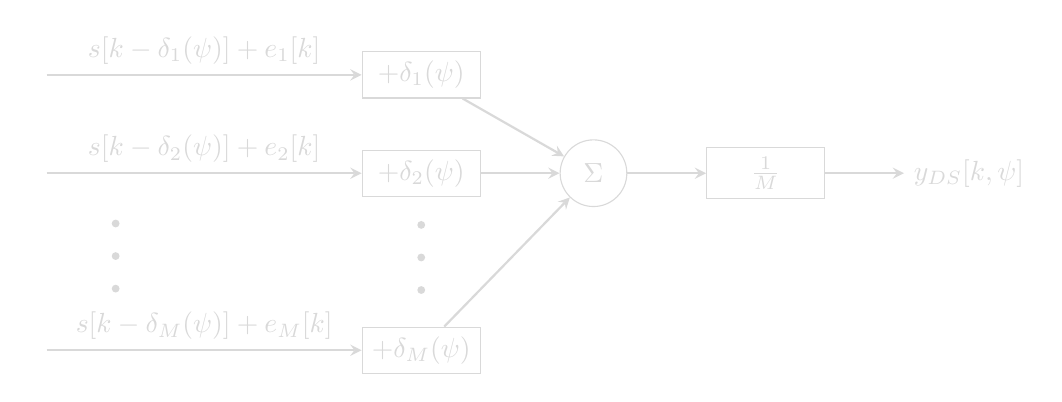
\begin{tikzpicture}[
    >=stealth,
    block/.style={draw, rectangle, minimum height=0.5cm, minimum width=1.5cm},
    sum/.style={draw, circle, inner sep=5pt},
    dot/.style={circle, fill, inner sep=1pt},
    every node/.style={text=textcolor}
]

% Microphones
\node (m1) at (0,-2) {};
\node[below=of m1] (m2) {};
\node[below=2 of m2] (mM) {};

% Delay blocks
\node[block, right=4cm of m1,textcolor] (delay1) {$+\delta_1(\psi)$};
\node[block, right=4cm of m2,textcolor] (delay2) {$+\delta_2(\psi)$};
\node[block, right=4cm of mM,textcolor] (delay3) {$+\delta_M(\psi)$};

% Summation
\node[sum, right=of delay2,textcolor] (sum) {$\Sigma$};

\node[block, right=of sum,textcolor] (scale) {$\frac{1}{M}$};

% Output
\node[right=of scale,textcolor] (output) {$y_{DS}[k,\psi]$};

% Connections
\draw[->, thick,textcolor] (m1) -- (delay1) node[midway, above] {$s[k-\delta_1(\psi)] + e_1[k]$};
\draw[->, thick,textcolor] (m2) -- (delay2) node[midway, above] {$s[k-\delta_2(\psi)] + e_2[k]$};
\draw[->, thick,textcolor] (mM) -- (delay3) node[midway, above] {$s[k-\delta_M(\psi)] + e_M[k]$};

\draw[->, thick,textcolor] (delay1) -- (sum);
\draw[->, thick,textcolor] (delay2) -- (sum);
\draw[->, thick,textcolor] (delay3) -- (sum);

% Vertical dots
\node[below=of m2, dot, xshift=1cm,yshift=0.542cm,textcolor] (mm1) {};
\node[below=of mm1, dot, yshift=0.7cm,textcolor] (mm2) {};
\node[below=of mm2, dot, yshift=0.7cm,textcolor] (mm3) {};

\node[below=of delay2, dot, xshift=0cm,yshift=0.7cm,textcolor] (delaym1) {};
\node[below=of delaym1, dot, yshift=0.7cm,textcolor] (delaym2) {};
\node[below=of delaym2, dot, yshift=0.7cm,textcolor] (delaym3) {};

\draw[->, thick,textcolor] (sum) -- (scale);
\draw[->, thick,textcolor] (scale) -- (output);


\end{tikzpicture}
% 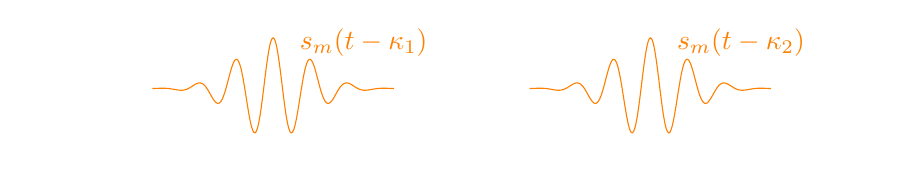
\begin{tikzpicture}[/pgfplots/.cd,width=\columnwidth,height=3cm]
    \begin{axis}[xmin=-0.5,xmax=5,ymin=-1,ymax=1.2,
        xticklabels=\empty,
        yticklabels=\empty,
        axis line style={draw=none},
        tick style={draw=none}]
        %\addplot[no markers,smooth,samples=201,domain=0:2.5, color=white] 
        {exp(-9*(x-1)*(x-1))*cos((x-1)*1440)};

        %\addplot[no markers,smooth,samples=401,domain=0:5, color=white] 
        %{exp(-9*(x-1)*(x-1))*cos((x-1)*1440) + exp(-9*(x-3.5)*(x-3.5))*cos((x-3.5)*1440)};
        %\addplot[no markers,smooth,samples=201,domain=0.2:1.8, color=orange] 
        {exp(-9*(x-1)*(x-1))*cos((x-1)*1440)};
        %\addplot[no markers,smooth,samples=201,domain=2.7:4.3, color=orange] 
        {exp(-9*(x-3.5)*(x-3.5))*cos((x-3.5)*1440)};
        % 

        \addplot[no markers,smooth,samples=2,domain=0:0.2, color=white]
        {exp(-9*(x-1)*(x-1))*cos((x-1)*1440) + exp(-9*(x-3.5)*(x-3.5))*cos((x-3.5)*1440)}; 
        \addplot[no markers,smooth,samples=201,domain=0.2:1.8, color=orange]
        {exp(-9*(x-1)*(x-1))*cos((x-1)*1440) + exp(-9*(x-3.5)*(x-3.5))*cos((x-3.5)*1440)};
        \addplot[no markers,smooth,samples=2,domain=1.8:2.7, color=white]
        {exp(-9*(x-1)*(x-1))*cos((x-1)*1440) + exp(-9*(x-3.5)*(x-3.5))*cos((x-3.5)*1440)};
        \addplot[no markers,smooth,samples=201,domain=2.7:4.3, color=orange]
        {exp(-9*(x-1)*(x-1))*cos((x-1)*1440) + exp(-9*(x-3.5)*(x-3.5))*cos((x-3.5)*1440)};
        \addplot[no markers,smooth,samples=2,domain=4.3:5, color=white]
        {exp(-9*(x-1)*(x-1))*cos((x-1)*1440) + exp(-9*(x-3.5)*(x-3.5))*cos((x-3.5)*1440)};

        {exp(-9*(x-1)*(x-1))*cos((x-1)*1440) + exp(-9*(x-3.5)*(x-3.5))*cos((x-3.5)*1440)};


        \node[text=orange] at (axis cs:1.6,0.9) {$s_m(t-\kappa_1)$};
        \node[text=orange] at (axis cs:4.1,0.9) {$s_m(t-\kappa_2)$};
        \node[color=white] at (axis cs:-0.1,0.4) {$y_m(t)$};

        %\node[color=white] at (axis cs:0.2,-0.3) {$ $};
        %\node[] at (axis cs:0.2,0) {$|$};
        %\node[] at (axis cs:1.8,0) {$|$};
        %\node[color=white] at (axis cs:2.7,-0.3) {$ $};
        %\node[] at (axis cs:2.7,0) {$|$};
        %\node[] at (axis cs:4.3,0) {$|$};

    \end{axis}
\end{tikzpicture}

\begin{tikzpicture}[/pgfplots/.cd,width=\columnwidth,height=3cm]
    \begin{axis}[xmin=-0.5,xmax=5,ymin=-1,ymax=1.2,
        xticklabels=\empty,
        yticklabels=\empty,
        axis line style={draw=none},
        tick style={draw=none}]
        \addplot[no markers,smooth,samples=201,domain=0:2.5, color=white] 
        {exp(-9*(x-1)*(x-1))*cos((x-1)*1440)};

        \addplot[no markers,smooth,samples=201,domain=2.5:5, color=white] 
        {exp(-9*(x-3.5)*(x-3.5))*cos((x-3.5)*1440)};
        \addplot[no markers,smooth,samples=201,domain=0.2:1.8, color=orange] 
        {exp(-9*(x-1)*(x-1))*cos((x-1)*1440)};
        %\addplot[no markers,smooth,samples=201,domain=2.7:4.3, color=orange] 
        {exp(-9*(x-3.5)*(x-3.5))*cos((x-3.5)*1440)};
        % 
        \node[text=orange] at (axis cs:1.6,0.9) {$s_m(t-\kappa_1)$};
        %\node[text=orange] at (axis cs:4.1,0.9) {$s_m(t-\kappa_2)$};
        \node[color=white] at (axis cs:-0.1,0.4) {$y_m(t)$};

        \node[color=white] at (axis cs:0.2,-0.3) {$ $};
        \node[color=white] at (axis cs:0.2,0) {$|$};
        \node[color=white] at (axis cs:2.7,-0.3) {$ $};
        %\node[] at (axis cs:2.7,0) {$|$};
    \end{axis}
\end{tikzpicture}

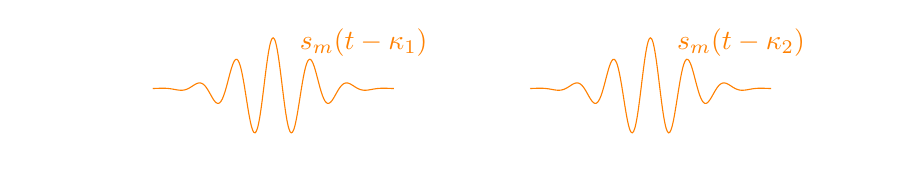
\begin{tikzpicture}[/pgfplots/.cd,width=\columnwidth,height=3cm]
    \begin{axis}[xmin=-0.5,xmax=5,ymin=-1,ymax=1.2,
        xticklabels=\empty,
        yticklabels=\empty,
        axis line style={draw=none},
        tick style={draw=none}]
        \addplot[no markers,smooth,samples=201,domain=0:2.5, color=white] 
        {exp(-9*(x-1)*(x-1))*cos((x-1)*1440)};

        \addplot[no markers,smooth,samples=201,domain=2.5:5, color=white] 
        {exp(-9*(x-3.5)*(x-3.5))*cos((x-3.5)*1440)};
        \addplot[no markers,smooth,samples=201,domain=0.2:1.8, color=orange] 
        {exp(-9*(x-1)*(x-1))*cos((x-1)*1440)};
        \addplot[no markers,smooth,samples=201,domain=2.7:4.3, color=orange] 
        {exp(-9*(x-3.5)*(x-3.5))*cos((x-3.5)*1440)};
        % 
        \node[text=orange] at (axis cs:1.6,0.9) {$s_m(t-\kappa_1)$};
        \node[text=orange] at (axis cs:4.1,0.9) {$s_m(t-\kappa_2)$};
        \node[color=white] at (axis cs:-0.1,0.4) {$y_m(t)$};

        \node[color=white] at (axis cs:0.2,-0.3) {$ $};
        \node[color=white] at (axis cs:0.2,0) {$|$};
        \node[color=white] at (axis cs:2.7,-0.3) {$ $};
        \node[color=white] at (axis cs:2.7,0) {$|$};
    \end{axis}
\end{tikzpicture}
% % This file was created by matlab2tikz.
%
%The latest updates can be retrieved from
%  http://www.mathworks.com/matlabcentral/fileexchange/22022-matlab2tikz-matlab2tikz
%where you can also make suggestions and rate matlab2tikz.
%
\definecolor{mycolor1}{rgb}{0.00000,0.44700,0.74100}%
\definecolor{mycolor2}{rgb}{0.85000,0.32500,0.09800}%
%
\begin{tikzpicture}

\begin{axis}[%
width=3.566in,
height=3.566in,
at={(1.236in,0.481in)},
scale only axis,
xmin=-1,
xmax=1,
ymin=-1,
ymax=1,
axis background/.style={fill=white},
axis x line*=bottom,
axis y line*=left
]
\addplot [color=mycolor1, forget plot]
  table[row sep=crcr]{%
1	0\\
0.999847695156391	0.0174524064372835\\
0.999390827019096	0.034899496702501\\
0.998629534754574	0.0523359562429438\\
0.997564050259824	0.0697564737441253\\
0.996194698091746	0.0871557427476582\\
0.994521895368273	0.104528463267653\\
0.992546151641322	0.121869343405147\\
0.99026806874157	0.139173100960065\\
0.987688340595138	0.156434465040231\\
0.984807753012208	0.17364817766693\\
0.981627183447664	0.190808995376545\\
0.978147600733806	0.207911690817759\\
0.974370064785235	0.224951054343865\\
0.970295726275996	0.241921895599668\\
0.965925826289068	0.258819045102521\\
0.961261695938319	0.275637355816999\\
0.956304755963035	0.292371704722737\\
0.951056516295154	0.309016994374947\\
0.945518575599317	0.325568154457157\\
0.939692620785908	0.342020143325669\\
0.933580426497202	0.3583679495453\\
0.927183854566787	0.374606593415912\\
0.92050485345244	0.390731128489274\\
0.913545457642601	0.4067366430758\\
0.90630778703665	0.422618261740699\\
0.898794046299167	0.438371146789077\\
0.891006524188368	0.453990499739547\\
0.882947592858927	0.469471562785891\\
0.874619707139396	0.484809620246337\\
0.866025403784439	0.5\\
0.857167300702112	0.515038074910054\\
0.848048096156426	0.529919264233205\\
0.838670567945424	0.544639035015027\\
0.829037572555042	0.559192903470747\\
0.819152044288992	0.573576436351046\\
0.809016994374947	0.587785252292473\\
0.798635510047293	0.601815023152048\\
0.788010753606722	0.615661475325658\\
0.777145961456971	0.629320391049837\\
0.766044443118978	0.642787609686539\\
0.754709580222772	0.656059028990507\\
0.743144825477394	0.669130606358858\\
0.731353701619171	0.681998360062498\\
0.719339800338651	0.694658370458997\\
0.707106781186548	0.707106781186547\\
0.694658370458997	0.719339800338651\\
0.681998360062498	0.73135370161917\\
0.669130606358858	0.743144825477394\\
0.656059028990507	0.754709580222772\\
0.642787609686539	0.766044443118978\\
0.629320391049838	0.777145961456971\\
0.615661475325658	0.788010753606722\\
0.601815023152048	0.798635510047293\\
0.587785252292473	0.809016994374947\\
0.573576436351046	0.819152044288992\\
0.559192903470747	0.829037572555042\\
0.544639035015027	0.838670567945424\\
0.529919264233205	0.848048096156426\\
0.515038074910054	0.857167300702112\\
0.5	0.866025403784439\\
0.484809620246337	0.874619707139396\\
0.469471562785891	0.882947592858927\\
0.453990499739547	0.891006524188368\\
0.438371146789077	0.898794046299167\\
0.422618261740699	0.90630778703665\\
0.4067366430758	0.913545457642601\\
0.390731128489274	0.92050485345244\\
0.374606593415912	0.927183854566787\\
0.3583679495453	0.933580426497202\\
0.342020143325669	0.939692620785908\\
0.325568154457157	0.945518575599317\\
0.309016994374947	0.951056516295154\\
0.292371704722737	0.956304755963035\\
0.275637355816999	0.961261695938319\\
0.258819045102521	0.965925826289068\\
0.241921895599668	0.970295726275996\\
0.224951054343865	0.974370064785235\\
0.207911690817759	0.978147600733806\\
0.190808995376545	0.981627183447664\\
0.17364817766693	0.984807753012208\\
0.156434465040231	0.987688340595138\\
0.139173100960066	0.99026806874157\\
0.121869343405147	0.992546151641322\\
0.104528463267653	0.994521895368273\\
0.0871557427476581	0.996194698091746\\
0.0697564737441255	0.997564050259824\\
0.052335956242944	0.998629534754574\\
0.0348994967025011	0.999390827019096\\
0.0174524064372834	0.999847695156391\\
6.12323399573677e-17	1\\
-0.0174524064372835	0.999847695156391\\
-0.0348994967025007	0.999390827019096\\
-0.0523359562429436	0.998629534754574\\
-0.0697564737441253	0.997564050259824\\
-0.0871557427476582	0.996194698091746\\
-0.104528463267653	0.994521895368273\\
-0.121869343405147	0.992546151641322\\
-0.139173100960065	0.99026806874157\\
-0.156434465040231	0.987688340595138\\
-0.17364817766693	0.984807753012208\\
-0.190808995376545	0.981627183447664\\
-0.207911690817759	0.978147600733806\\
-0.224951054343865	0.974370064785235\\
-0.241921895599668	0.970295726275996\\
-0.258819045102521	0.965925826289068\\
-0.275637355816999	0.961261695938319\\
-0.292371704722737	0.956304755963036\\
-0.309016994374947	0.951056516295154\\
-0.325568154457156	0.945518575599317\\
-0.342020143325669	0.939692620785908\\
-0.3583679495453	0.933580426497202\\
-0.374606593415912	0.927183854566787\\
-0.390731128489274	0.92050485345244\\
-0.4067366430758	0.913545457642601\\
-0.422618261740699	0.90630778703665\\
-0.438371146789078	0.898794046299167\\
-0.453990499739547	0.891006524188368\\
-0.469471562785891	0.882947592858927\\
-0.484809620246337	0.874619707139396\\
-0.5	0.866025403784439\\
-0.515038074910054	0.857167300702112\\
-0.529919264233205	0.848048096156426\\
-0.544639035015027	0.838670567945424\\
-0.559192903470747	0.829037572555042\\
-0.573576436351046	0.819152044288992\\
-0.587785252292473	0.809016994374947\\
-0.601815023152048	0.798635510047293\\
-0.615661475325658	0.788010753606722\\
-0.629320391049837	0.777145961456971\\
-0.642787609686539	0.766044443118978\\
-0.656059028990507	0.754709580222772\\
-0.669130606358858	0.743144825477394\\
-0.681998360062498	0.731353701619171\\
-0.694658370458997	0.719339800338651\\
-0.707106781186547	0.707106781186548\\
-0.719339800338651	0.694658370458997\\
-0.73135370161917	0.681998360062499\\
-0.743144825477394	0.669130606358858\\
-0.754709580222772	0.656059028990507\\
-0.766044443118978	0.642787609686539\\
-0.777145961456971	0.629320391049838\\
-0.788010753606722	0.615661475325658\\
-0.798635510047293	0.601815023152048\\
-0.809016994374947	0.587785252292473\\
-0.819152044288992	0.573576436351046\\
-0.829037572555042	0.559192903470747\\
-0.838670567945424	0.544639035015027\\
-0.848048096156426	0.529919264233205\\
-0.857167300702112	0.515038074910054\\
-0.866025403784439	0.5\\
-0.874619707139396	0.484809620246337\\
-0.882947592858927	0.469471562785891\\
-0.891006524188368	0.453990499739547\\
-0.898794046299167	0.438371146789077\\
-0.90630778703665	0.422618261740699\\
-0.913545457642601	0.4067366430758\\
-0.92050485345244	0.390731128489274\\
-0.927183854566787	0.374606593415912\\
-0.933580426497202	0.3583679495453\\
-0.939692620785908	0.342020143325669\\
-0.945518575599317	0.325568154457157\\
-0.951056516295154	0.309016994374948\\
-0.956304755963035	0.292371704722737\\
-0.961261695938319	0.275637355817\\
-0.965925826289068	0.258819045102521\\
-0.970295726275996	0.241921895599668\\
-0.974370064785235	0.224951054343865\\
-0.978147600733806	0.207911690817759\\
-0.981627183447664	0.190808995376545\\
-0.984807753012208	0.17364817766693\\
-0.987688340595138	0.156434465040231\\
-0.99026806874157	0.139173100960066\\
-0.992546151641322	0.121869343405148\\
-0.994521895368273	0.104528463267654\\
-0.996194698091746	0.0871557427476586\\
-0.997564050259824	0.0697564737441255\\
-0.998629534754574	0.0523359562429438\\
-0.999390827019096	0.0348994967025007\\
-0.999847695156391	0.0174524064372834\\
-1	1.22464679914735e-16\\
-0.999847695156391	-0.0174524064372832\\
-0.999390827019096	-0.0348994967025009\\
-0.998629534754574	-0.0523359562429436\\
-0.997564050259824	-0.0697564737441248\\
-0.996194698091746	-0.0871557427476579\\
-0.994521895368273	-0.104528463267653\\
-0.992546151641322	-0.121869343405148\\
-0.99026806874157	-0.139173100960066\\
-0.987688340595138	-0.156434465040231\\
-0.984807753012208	-0.17364817766693\\
-0.981627183447664	-0.190808995376545\\
-0.978147600733806	-0.207911690817759\\
-0.974370064785235	-0.224951054343865\\
-0.970295726275997	-0.241921895599668\\
-0.965925826289068	-0.25881904510252\\
-0.961261695938319	-0.275637355816999\\
-0.956304755963036	-0.292371704722736\\
-0.951056516295154	-0.309016994374948\\
-0.945518575599317	-0.325568154457157\\
-0.939692620785908	-0.342020143325669\\
-0.933580426497202	-0.3583679495453\\
-0.927183854566787	-0.374606593415912\\
-0.92050485345244	-0.390731128489274\\
-0.913545457642601	-0.4067366430758\\
-0.90630778703665	-0.422618261740699\\
-0.898794046299167	-0.438371146789077\\
-0.891006524188368	-0.453990499739546\\
-0.882947592858927	-0.469471562785891\\
-0.874619707139396	-0.484809620246337\\
-0.866025403784439	-0.5\\
-0.857167300702112	-0.515038074910054\\
-0.848048096156426	-0.529919264233205\\
-0.838670567945424	-0.544639035015027\\
-0.829037572555042	-0.559192903470747\\
-0.819152044288992	-0.573576436351046\\
-0.809016994374947	-0.587785252292473\\
-0.798635510047293	-0.601815023152048\\
-0.788010753606722	-0.615661475325658\\
-0.777145961456971	-0.629320391049838\\
-0.766044443118978	-0.642787609686539\\
-0.754709580222772	-0.656059028990507\\
-0.743144825477394	-0.669130606358858\\
-0.731353701619171	-0.681998360062498\\
-0.719339800338651	-0.694658370458997\\
-0.707106781186548	-0.707106781186547\\
-0.694658370458997	-0.719339800338651\\
-0.681998360062499	-0.73135370161917\\
-0.669130606358858	-0.743144825477394\\
-0.656059028990508	-0.754709580222772\\
-0.642787609686539	-0.766044443118978\\
-0.629320391049837	-0.777145961456971\\
-0.615661475325658	-0.788010753606722\\
-0.601815023152048	-0.798635510047293\\
-0.587785252292473	-0.809016994374947\\
-0.573576436351046	-0.819152044288992\\
-0.559192903470747	-0.829037572555041\\
-0.544639035015027	-0.838670567945424\\
-0.529919264233205	-0.848048096156426\\
-0.515038074910054	-0.857167300702112\\
-0.5	-0.866025403784438\\
-0.484809620246337	-0.874619707139396\\
-0.469471562785891	-0.882947592858927\\
-0.453990499739547	-0.891006524188368\\
-0.438371146789078	-0.898794046299167\\
-0.4226182617407	-0.90630778703665\\
-0.4067366430758	-0.913545457642601\\
-0.390731128489274	-0.92050485345244\\
-0.374606593415912	-0.927183854566787\\
-0.358367949545301	-0.933580426497202\\
-0.342020143325669	-0.939692620785908\\
-0.325568154457157	-0.945518575599317\\
-0.309016994374948	-0.951056516295154\\
-0.292371704722737	-0.956304755963035\\
-0.275637355816999	-0.961261695938319\\
-0.258819045102521	-0.965925826289068\\
-0.241921895599668	-0.970295726275996\\
-0.224951054343865	-0.974370064785235\\
-0.20791169081776	-0.978147600733806\\
-0.190808995376545	-0.981627183447664\\
-0.17364817766693	-0.984807753012208\\
-0.156434465040231	-0.987688340595138\\
-0.139173100960065	-0.99026806874157\\
-0.121869343405147	-0.992546151641322\\
-0.104528463267653	-0.994521895368273\\
-0.0871557427476582	-0.996194698091746\\
-0.0697564737441256	-0.997564050259824\\
-0.0523359562429443	-0.998629534754574\\
-0.0348994967025016	-0.999390827019096\\
-0.0174524064372835	-0.999847695156391\\
-1.83697019872103e-16	-1\\
0.0174524064372831	-0.999847695156391\\
0.0348994967025013	-0.999390827019096\\
0.0523359562429439	-0.998629534754574\\
0.0697564737441252	-0.997564050259824\\
0.0871557427476579	-0.996194698091746\\
0.104528463267653	-0.994521895368273\\
0.121869343405148	-0.992546151641322\\
0.139173100960065	-0.99026806874157\\
0.156434465040231	-0.987688340595138\\
0.17364817766693	-0.984807753012208\\
0.190808995376544	-0.981627183447664\\
0.207911690817759	-0.978147600733806\\
0.224951054343865	-0.974370064785235\\
0.241921895599667	-0.970295726275997\\
0.258819045102521	-0.965925826289068\\
0.275637355816999	-0.961261695938319\\
0.292371704722737	-0.956304755963035\\
0.309016994374947	-0.951056516295154\\
0.325568154457156	-0.945518575599317\\
0.342020143325668	-0.939692620785909\\
0.3583679495453	-0.933580426497202\\
0.374606593415912	-0.927183854566787\\
0.390731128489273	-0.92050485345244\\
0.406736643075801	-0.913545457642601\\
0.4226182617407	-0.90630778703665\\
0.438371146789077	-0.898794046299167\\
0.453990499739547	-0.891006524188368\\
0.46947156278589	-0.882947592858927\\
0.484809620246337	-0.874619707139396\\
0.5	-0.866025403784439\\
0.515038074910054	-0.857167300702112\\
0.529919264233205	-0.848048096156426\\
0.544639035015027	-0.838670567945424\\
0.559192903470746	-0.829037572555042\\
0.573576436351046	-0.819152044288992\\
0.587785252292473	-0.809016994374948\\
0.601815023152048	-0.798635510047293\\
0.615661475325659	-0.788010753606722\\
0.629320391049838	-0.777145961456971\\
0.642787609686539	-0.766044443118978\\
0.656059028990507	-0.754709580222772\\
0.669130606358858	-0.743144825477395\\
0.681998360062498	-0.731353701619171\\
0.694658370458997	-0.719339800338652\\
0.707106781186547	-0.707106781186548\\
0.719339800338651	-0.694658370458998\\
0.731353701619171	-0.681998360062498\\
0.743144825477394	-0.669130606358858\\
0.754709580222772	-0.656059028990507\\
0.766044443118978	-0.64278760968654\\
0.777145961456971	-0.629320391049838\\
0.788010753606722	-0.615661475325659\\
0.798635510047293	-0.601815023152048\\
0.809016994374947	-0.587785252292473\\
0.819152044288992	-0.573576436351046\\
0.829037572555041	-0.559192903470747\\
0.838670567945424	-0.544639035015027\\
0.848048096156425	-0.529919264233206\\
0.857167300702112	-0.515038074910054\\
0.866025403784438	-0.5\\
0.874619707139396	-0.484809620246337\\
0.882947592858927	-0.469471562785891\\
0.891006524188368	-0.453990499739547\\
0.898794046299167	-0.438371146789077\\
0.90630778703665	-0.4226182617407\\
0.913545457642601	-0.4067366430758\\
0.92050485345244	-0.390731128489275\\
0.927183854566787	-0.374606593415912\\
0.933580426497202	-0.358367949545301\\
0.939692620785908	-0.342020143325669\\
0.945518575599317	-0.325568154457158\\
0.951056516295154	-0.309016994374948\\
0.956304755963036	-0.292371704722736\\
0.961261695938319	-0.275637355817\\
0.965925826289068	-0.258819045102521\\
0.970295726275996	-0.241921895599668\\
0.974370064785235	-0.224951054343865\\
0.978147600733806	-0.20791169081776\\
0.981627183447664	-0.190808995376545\\
0.984807753012208	-0.173648177666931\\
0.987688340595138	-0.156434465040231\\
0.99026806874157	-0.139173100960066\\
0.992546151641322	-0.121869343405148\\
0.994521895368273	-0.104528463267653\\
0.996194698091746	-0.0871557427476583\\
0.997564050259824	-0.0697564737441248\\
0.998629534754574	-0.0523359562429444\\
0.999390827019096	-0.0348994967025008\\
0.999847695156391	-0.0174524064372844\\
1	-2.44929359829471e-16\\
};
\addplot [color=mycolor2, only marks, mark=*, mark options={solid, mycolor2}, forget plot]
  table[row sep=crcr]{%
0	0\\
};
\end{axis}
\end{tikzpicture}%
% % This file was created by matlab2tikz.
%
%The latest updates can be retrieved from
%  http://www.mathworks.com/matlabcentral/fileexchange/22022-matlab2tikz-matlab2tikz
%where you can also make suggestions and rate matlab2tikz.
%
\definecolor{mycolor1}{rgb}{0.00000,0.44700,0.74100}%
\definecolor{mycolor2}{rgb}{0.85000,0.32500,0.09800}%
%
\begin{tikzpicture}

\begin{axis}[%
width=3.566in,
height=3.566in,
at={(1.236in,0.481in)},
scale only axis,
xmin=-0.2,
xmax=1.2,
ymin=-0.8,
ymax=0.8,
axis background/.style={fill=white},
axis x line*=bottom,
axis y line*=left
]
\addplot [color=mycolor1, forget plot]
  table[row sep=crcr]{%
1	0\\
1.00009529541836	0.0174567283159324\\
1.00020097978911	0.0349277878606356\\
1.00030922821204	0.052423985246926\\
1.00040780713683	0.0699553285964765\\
1.00048022988695	0.0875306781969186\\
1.00050596766682	0.105157414610366\\
1.00046071312993	0.122841129362266\\
1.00031669285539	0.140585342980632\\
1.00004302440484	0.158391254720818\\
0.99960611302428	0.176257527807296\\
0.998970082522051	0.194180113459968\\
0.998097234406243	0.212152116357749\\
0.996948529005883	0.230163703536879\\
0.995484082037566	0.248202058036603\\
0.993663669915181	0.266251377901918\\
0.991447237037326	0.284292920443772\\
0.988795398325211	0.302305090953154\\
0.98566993042186	0.320263574378581\\
0.982034245198323	0.338141507817856\\
0.977853839539929	0.355909691055453\\
0.973096715799277	0.373536831806422\\
0.967733767795411	0.390989821815616\\
0.961739127801907	0.4082340395153\\
0.955090470590705	0.425233674571811\\
0.947769271273017	0.44195206935859\\
0.939761014392197	0.458352072182786\\
0.931055352464361	0.474396396968597\\
0.921646212918646	0.490047984063928\\
0.911531853148146	0.505270356887534\\
0.900714864132583	0.520027969270044\\
0.889202123822923	0.534286538560863\\
0.877004702175014	0.548013359869534\\
0.86413772037336	0.561177597178847\\
0.850620167387498	0.573750547500798\\
0.836474677543359	0.585705874737396\\
0.821727273262843	0.597019810447338\\
0.806407077520281	0.607671319296966\\
0.790546000879426	0.617642227579462\\
0.774178408205599	0.62691731380922\\
0.757340770292491	0.635484361027947\\
0.740071305701233	0.64333417108442\\
0.72240961808157	0.650460541760304\\
0.704396334133643	0.656860208199687\\
0.686072747177593	0.662532750650453\\
0.667480471032012	0.667480471032012\\
0.648661108567271	0.671708241298405\\
0.629655938903244	0.675223326961052\\
0.610505626771035	0.678035189465551\\
0.59124995706394	0.680155271377135\\
0.57192759707355	0.681596768516176\\
0.55257588835254	0.682374393296382\\
0.533230669576547	0.682504133553214\\
0.513926131203678	0.682003011109252\\
0.494694702161927	0.680888844208548\\
0.475566968241685	0.679180017766753\\
0.456571621342076	0.676895265132341\\
0.437735438224645	0.674053464742154\\
0.419083286973853	0.670673454688277\\
0.400638158957956	0.666773867800411\\
0.38242122373204	0.662372989396558\\
0.364451904032208	0.657488639373701\\
0.346747967779769	0.652138079808469\\
0.329325633849332	0.646337948724843\\
0.312199688256067	0.640104220171273\\
0.29538360738516	0.633452190242555\\
0.278889684919325	0.626396488191363\\
0.262729159215787	0.618951111309396\\
0.246912338038894	0.611129481826347\\
0.23144871776387	0.602944523684061\\
0.216347094425805	0.594408756699516\\
0.201615664289448	0.585534405339253\\
0.187262111952911	0.576333519094143\\
0.173293684364427	0.566818101270151\\
0.159717249518196	0.557000242900299\\
0.14653933899486	0.546892258436377\\
0.133766173916387	0.536506819895886\\
0.121403674285914	0.525857086218887\\
0.109457452072788	0.514956824728432\\
0.0979327887742071	0.503820521783519\\
0.0868345985306157	0.492463479960483\\
0.0761673781862289	0.48090189939213\\
0.0659351459631762	0.469152941227367\\
0.0561413706531992	0.45723477154098\\
0.0467888934208795	0.445166584416025\\
0.0378798444542435	0.432968603332468\\
0.0294155567905669	0.420662060417253\\
0.0213964796865314	0.408269153534905\\
0.0138220938928612	0.395812981616214\\
0.00669083113545006	0.383317459027827\\
2.27053931517951e-17	0.370807210170369\\
-0.00625427973157956	0.35830744585023\\
-0.0120771324334045	0.345843823294289\\
-0.0174749700407767	0.333442291962017\\
-0.0224555221264876	0.321128927551109\\
-0.0270278515447075	0.308929756787275\\
-0.0312023548353187	0.296870575733197\\
-0.0349907468898248	0.284976764444308\\
-0.0384060296936282	0.273273100839031\\
-0.0414624452720752	0.261783576638696\\
-0.0441754132729135	0.250531218168773\\
-0.0465614539096652	0.239537914700385\\
-0.0486380972632324	0.228824256852345\\
-0.0504237801876702	0.218409387373101\\
-0.051937732285908	0.208310866383409\\
-0.0531998526083718	0.198544552889619\\
-0.0542305788787942	0.189124504079761\\
-0.0550507511646131	0.180062893596294\\
-0.0556814719827018	0.171369949646847\\
-0.0561439648640267	0.163053913473956\\
-0.0564594333933257	0.155121018363365\\
-0.0566489226929808	0.147575489034169\\
-0.0567331852356876	0.140419560929282\\
-0.0567325527507691	0.13365351861712\\
-0.0566668158372253	0.127275752230466\\
-0.0565551127166195	0.121282830610989\\
-0.0564158283549722	0.115669589602078\\
-0.0562665049596647	0.110429233741896\\
-0.056123764619997	0.105553449455696\\
-0.0560032446136959	0.101032527733255\\
-0.0559195456517012	0.0968554942049139\\
-0.0558861930852475	0.0930102444984568\\
-0.0559156108578121	0.0894836827681794\\
-0.0560191077548604	0.0862618613358633\\
-0.0562068752910956	0.0833301194686415\\
-0.0564879963823172	0.0806732194382621\\
-0.0568704637806677	0.0782754781565217\\
-0.0573612071111235	0.0761208928587123\\
-0.057966127236004	0.0741932595063627\\
-0.0586901365948307	0.0724762827976102\\
-0.0595372041201277	0.0709536769031769\\
-0.0605104033160674	0.0696092562830053\\
-0.0616119621058538	0.0684270161779432\\
-0.062843313104326	0.0673912026073633\\
-0.0642051430526959	0.0664863719323266\\
-0.0656974402602303	0.0656974402602303\\
-0.0673195390300945	0.065009723166549\\
-0.0690701602000372	0.0644089663884798\\
-0.0709474470992438	0.0638813683007662\\
-0.0729489964063071	0.0634135951130063\\
-0.0750718835854126	0.0629927898283034\\
-0.0773126827739264	0.0626065760737963\\
-0.07966748118997	0.0622430579537179\\
-0.082131888318707	0.061890817085152\\
-0.0847010403165376	0.0615389079562612\\
-0.087369600239036	0.0611768526977419\\
-0.0901317548474648	0.0607946362825687\\
-0.0929812088766593	0.0603827030691863\\
-0.0959111777510893	0.0599319554821835\\
-0.0989143798136328	0.0594337554855466\\
-0.101983029181284	0.058879929350588\\
-0.105108830362552	0.058262776057576\\
-0.108282975762218	0.0575750795011428\\
-0.11149614716068	0.0568101244989424\\
-0.114738522188031	0.0559617164349901\\
-0.117999786719035	0.0550242042077424\\
-0.121269153996089	0.0539925060021572\\
-0.124535391146026	0.0528621372683007\\
-0.127786853596114	0.0516292401697878\\
-0.131011527718626	0.0502906136662258\\
-0.134197081845627	0.0488437433171936\\
-0.137330925600477	0.0472868298428727\\
-0.140400277294179	0.0456188154494403\\
-0.143392238937693	0.043839406926304\\
-0.146293878229921	0.0419490945471909\\
-0.149092316699674	0.0399491658573629\\
-0.151774823012552	0.0378417135035969\\
-0.154328910304124	0.0356296363602924\\
-0.156742436272468	0.0333166333218584\\
-0.159003704659037	0.0309071892656661\\
-0.161101566669309	0.0284065528382027\\
-0.163025520835753	0.0258207058761869\\
-0.164765809806448	0.0231563244406138\\
-0.166313512553999	0.0204207316111624\\
-0.167660630541083	0.0176218423571817\\
-0.168800166450455	0.0147681009657039\\
-0.169726194187198	0.011868411662816\\
-0.170433918987577	0.00893206320864466\\
-0.170919726619523	0.00596864837487287\\
-0.171181220831614	0.00298797932410737\\
-0.171217248396913	2.09680655208097e-17\\
-0.171181220831614	-0.00298797932410733\\
-0.170919726619523	-0.0059686483748729\\
-0.170433918987577	-0.00893206320864462\\
-0.169726194187198	-0.0118684116628159\\
-0.168800166450455	-0.0147681009657038\\
-0.167660630541083	-0.0176218423571815\\
-0.166313512553999	-0.0204207316111625\\
-0.164765809806448	-0.0231563244406137\\
-0.163025520835753	-0.0258207058761868\\
-0.161101566669309	-0.0284065528382028\\
-0.159003704659037	-0.030907189265666\\
-0.156742436272468	-0.0333166333218584\\
-0.154328910304124	-0.0356296363602924\\
-0.151774823012552	-0.0378417135035969\\
-0.149092316699674	-0.0399491658573628\\
-0.146293878229921	-0.0419490945471908\\
-0.143392238937693	-0.0438394069263039\\
-0.140400277294179	-0.0456188154494404\\
-0.137330925600477	-0.0472868298428727\\
-0.134197081845627	-0.0488437433171936\\
-0.131011527718626	-0.0502906136662258\\
-0.127786853596114	-0.0516292401697877\\
-0.124535391146026	-0.0528621372683006\\
-0.121269153996089	-0.0539925060021571\\
-0.117999786719035	-0.0550242042077424\\
-0.114738522188031	-0.05596171643499\\
-0.11149614716068	-0.0568101244989424\\
-0.108282975762218	-0.0575750795011428\\
-0.105108830362552	-0.0582627760575759\\
-0.101983029181284	-0.058879929350588\\
-0.0989143798136328	-0.0594337554855466\\
-0.0959111777510893	-0.0599319554821835\\
-0.0929812088766593	-0.0603827030691863\\
-0.0901317548474648	-0.0607946362825686\\
-0.087369600239036	-0.0611768526977418\\
-0.0847010403165376	-0.0615389079562612\\
-0.082131888318707	-0.061890817085152\\
-0.0796674811899701	-0.0622430579537178\\
-0.0773126827739264	-0.0626065760737963\\
-0.0750718835854126	-0.0629927898283034\\
-0.0729489964063071	-0.0634135951130063\\
-0.0709474470992438	-0.0638813683007662\\
-0.0690701602000372	-0.0644089663884798\\
-0.0673195390300945	-0.065009723166549\\
-0.0656974402602303	-0.0656974402602303\\
-0.0642051430526959	-0.0664863719323265\\
-0.062843313104326	-0.0673912026073632\\
-0.0616119621058538	-0.0684270161779432\\
-0.0605104033160674	-0.0696092562830053\\
-0.0595372041201277	-0.0709536769031769\\
-0.0586901365948306	-0.0724762827976102\\
-0.057966127236004	-0.0741932595063627\\
-0.0573612071111235	-0.0761208928587123\\
-0.0568704637806677	-0.0782754781565217\\
-0.0564879963823172	-0.0806732194382621\\
-0.0562068752910957	-0.0833301194686415\\
-0.0560191077548604	-0.0862618613358633\\
-0.0559156108578121	-0.0894836827681794\\
-0.0558861930852475	-0.0930102444984568\\
-0.0559195456517013	-0.0968554942049138\\
-0.0560032446136959	-0.101032527733255\\
-0.056123764619997	-0.105553449455696\\
-0.0562665049596647	-0.110429233741896\\
-0.0564158283549722	-0.115669589602078\\
-0.0565551127166196	-0.121282830610989\\
-0.0566668158372253	-0.127275752230466\\
-0.0567325527507691	-0.13365351861712\\
-0.0567331852356877	-0.140419560929282\\
-0.0566489226929809	-0.147575489034169\\
-0.0564594333933258	-0.155121018363365\\
-0.0561439648640268	-0.163053913473956\\
-0.0556814719827018	-0.171369949646847\\
-0.0550507511646132	-0.180062893596294\\
-0.0542305788787942	-0.189124504079761\\
-0.0531998526083718	-0.198544552889619\\
-0.051937732285908	-0.208310866383409\\
-0.0504237801876703	-0.218409387373101\\
-0.0486380972632325	-0.228824256852345\\
-0.0465614539096654	-0.239537914700385\\
-0.0441754132729135	-0.250531218168773\\
-0.0414624452720752	-0.261783576638696\\
-0.0384060296936281	-0.273273100839031\\
-0.0349907468898248	-0.284976764444308\\
-0.0312023548353187	-0.296870575733197\\
-0.0270278515447075	-0.308929756787275\\
-0.0224555221264877	-0.321128927551109\\
-0.0174749700407769	-0.333442291962017\\
-0.0120771324334048	-0.345843823294289\\
-0.00625427973157957	-0.35830744585023\\
-6.81161794553854e-17	-0.370807210170369\\
0.00669083113544996	-0.383317459027827\\
0.0138220938928613	-0.395812981616214\\
0.0213964796865314	-0.408269153534905\\
0.0294155567905668	-0.420662060417253\\
0.0378798444542434	-0.432968603332468\\
0.0467888934208793	-0.445166584416025\\
0.0561413706531993	-0.45723477154098\\
0.0659351459631761	-0.469152941227367\\
0.0761673781862288	-0.48090189939213\\
0.0868345985306154	-0.492463479960483\\
0.0979327887742068	-0.503820521783519\\
0.109457452072787	-0.514956824728433\\
0.121403674285914	-0.525857086218887\\
0.133766173916387	-0.536506819895886\\
0.14653933899486	-0.546892258436377\\
0.159717249518196	-0.557000242900299\\
0.173293684364427	-0.566818101270151\\
0.187262111952911	-0.576333519094143\\
0.201615664289448	-0.585534405339253\\
0.216347094425805	-0.594408756699516\\
0.23144871776387	-0.602944523684061\\
0.246912338038894	-0.611129481826347\\
0.262729159215786	-0.618951111309396\\
0.278889684919325	-0.626396488191363\\
0.29538360738516	-0.633452190242554\\
0.312199688256067	-0.640104220171273\\
0.329325633849332	-0.646337948724843\\
0.346747967779769	-0.652138079808469\\
0.364451904032207	-0.657488639373701\\
0.38242122373204	-0.662372989396558\\
0.400638158957956	-0.666773867800411\\
0.419083286973853	-0.670673454688277\\
0.437735438224645	-0.674053464742154\\
0.456571621342076	-0.676895265132341\\
0.475566968241685	-0.679180017766753\\
0.494694702161927	-0.680888844208549\\
0.513926131203678	-0.682003011109252\\
0.533230669576547	-0.682504133553214\\
0.55257588835254	-0.682374393296382\\
0.571927597073549	-0.681596768516177\\
0.59124995706394	-0.680155271377135\\
0.610505626771034	-0.678035189465552\\
0.629655938903243	-0.675223326961052\\
0.648661108567271	-0.671708241298406\\
0.667480471032012	-0.667480471032012\\
0.686072747177592	-0.662532750650453\\
0.704396334133643	-0.656860208199687\\
0.72240961808157	-0.650460541760304\\
0.740071305701233	-0.643334171084421\\
0.757340770292491	-0.635484361027947\\
0.774178408205599	-0.626917313809221\\
0.790546000879426	-0.617642227579463\\
0.806407077520281	-0.607671319296966\\
0.821727273262843	-0.597019810447338\\
0.836474677543359	-0.585705874737397\\
0.850620167387498	-0.573750547500799\\
0.86413772037336	-0.561177597178847\\
0.877004702175013	-0.548013359869535\\
0.889202123822923	-0.534286538560863\\
0.900714864132583	-0.520027969270045\\
0.911531853148146	-0.505270356887534\\
0.921646212918646	-0.490047984063928\\
0.931055352464361	-0.474396396968597\\
0.939761014392197	-0.458352072182786\\
0.947769271273017	-0.441952069358591\\
0.955090470590705	-0.425233674571811\\
0.961739127801906	-0.408234039515301\\
0.967733767795411	-0.390989821815616\\
0.973096715799276	-0.373536831806422\\
0.977853839539929	-0.355909691055453\\
0.982034245198322	-0.338141507817857\\
0.98566993042186	-0.320263574378581\\
0.988795398325212	-0.302305090953154\\
0.991447237037326	-0.284292920443773\\
0.993663669915181	-0.266251377901918\\
0.995484082037566	-0.248202058036604\\
0.996948529005883	-0.23016370353688\\
0.998097234406243	-0.21215211635775\\
0.998970082522051	-0.194180113459968\\
0.99960611302428	-0.176257527807297\\
1.00004302440484	-0.158391254720818\\
1.00031669285539	-0.140585342980632\\
1.00046071312993	-0.122841129362266\\
1.00050596766682	-0.105157414610366\\
1.00048022988695	-0.0875306781969188\\
1.00040780713683	-0.0699553285964759\\
1.00030922821204	-0.0524239852469265\\
1.00020097978911	-0.0349277878606354\\
1.00009529541836	-0.0174567283159333\\
1	-2.44929359829471e-16\\
};
\addplot [color=mycolor2, only marks, mark=*, mark options={solid, mycolor2}, forget plot]
  table[row sep=crcr]{%
0	0\\
};
\end{axis}
\end{tikzpicture}%
% % This file was created by matlab2tikz.
%
%The latest updates can be retrieved from
%  http://www.mathworks.com/matlabcentral/fileexchange/22022-matlab2tikz-matlab2tikz
%where you can also make suggestions and rate matlab2tikz.
%
\definecolor{mycolor1}{RGB}{0, 114, 178} % Blue
\definecolor{mycolor2}{RGB}{213, 94, 0} % Vermillion
\definecolor{mycolor3}{RGB}{0, 158, 115} % Green
\definecolor{mycolor4}{RGB}{230, 159, 0} % Orange
%
\begin{tikzpicture}

\begin{axis}[%
  width=0.6\linewidth, % Width of the plot
  height=0.6\linewidth, % Height of the plot
  axis lines=none,
  line width=1pt,
  clip mode=individual,
]
\addplot [color=mycolor1, area legend, draw=black, fill=mycolor1,draw=mycolor1, fill opacity=0.15, forget plot]
  table[row sep=crcr]{%
1	0\\
1.00009529541836	0.0174567283159324\\
1.00020097978911	0.0349277878606356\\
1.00030922821204	0.052423985246926\\
1.00040780713683	0.0699553285964765\\
1.00048022988695	0.0875306781969186\\
1.00050596766682	0.105157414610366\\
1.00046071312993	0.122841129362266\\
1.00031669285539	0.140585342980632\\
1.00004302440484	0.158391254720818\\
0.99960611302428	0.176257527807296\\
0.998970082522051	0.194180113459968\\
0.998097234406243	0.212152116357749\\
0.996948529005883	0.230163703536879\\
0.995484082037566	0.248202058036603\\
0.993663669915181	0.266251377901918\\
0.991447237037326	0.284292920443772\\
0.988795398325211	0.302305090953154\\
0.98566993042186	0.320263574378581\\
0.982034245198323	0.338141507817856\\
0.977853839539929	0.355909691055453\\
0.973096715799277	0.373536831806422\\
0.967733767795411	0.390989821815616\\
0.961739127801907	0.4082340395153\\
0.955090470590705	0.425233674571811\\
0.947769271273017	0.44195206935859\\
0.939761014392197	0.458352072182786\\
0.931055352464361	0.474396396968597\\
0.921646212918646	0.490047984063928\\
0.911531853148146	0.505270356887534\\
0.900714864132583	0.520027969270044\\
0.889202123822923	0.534286538560863\\
0.877004702175014	0.548013359869534\\
0.86413772037336	0.561177597178847\\
0.850620167387498	0.573750547500798\\
0.836474677543359	0.585705874737396\\
0.821727273262843	0.597019810447338\\
0.806407077520281	0.607671319296966\\
0.790546000879426	0.617642227579462\\
0.774178408205599	0.62691731380922\\
0.757340770292491	0.635484361027947\\
0.740071305701233	0.64333417108442\\
0.72240961808157	0.650460541760304\\
0.704396334133643	0.656860208199687\\
0.686072747177593	0.662532750650453\\
0.667480471032012	0.667480471032012\\
0.648661108567271	0.671708241298405\\
0.629655938903244	0.675223326961052\\
0.610505626771035	0.678035189465551\\
0.59124995706394	0.680155271377135\\
0.57192759707355	0.681596768516176\\
0.55257588835254	0.682374393296382\\
0.533230669576547	0.682504133553214\\
0.513926131203678	0.682003011109252\\
0.494694702161927	0.680888844208548\\
0.475566968241685	0.679180017766753\\
0.456571621342076	0.676895265132341\\
0.437735438224645	0.674053464742154\\
0.419083286973853	0.670673454688277\\
0.400638158957956	0.666773867800411\\
0.38242122373204	0.662372989396558\\
0.364451904032208	0.657488639373701\\
0.346747967779769	0.652138079808469\\
0.329325633849332	0.646337948724843\\
0.312199688256067	0.640104220171273\\
0.29538360738516	0.633452190242555\\
0.278889684919325	0.626396488191363\\
0.262729159215787	0.618951111309396\\
0.246912338038894	0.611129481826347\\
0.23144871776387	0.602944523684061\\
0.216347094425805	0.594408756699516\\
0.201615664289448	0.585534405339253\\
0.187262111952911	0.576333519094143\\
0.173293684364427	0.566818101270151\\
0.159717249518196	0.557000242900299\\
0.14653933899486	0.546892258436377\\
0.133766173916387	0.536506819895886\\
0.121403674285914	0.525857086218887\\
0.109457452072788	0.514956824728432\\
0.0979327887742071	0.503820521783519\\
0.0868345985306157	0.492463479960483\\
0.0761673781862289	0.48090189939213\\
0.0659351459631762	0.469152941227367\\
0.0561413706531992	0.45723477154098\\
0.0467888934208795	0.445166584416025\\
0.0378798444542435	0.432968603332468\\
0.0294155567905669	0.420662060417253\\
0.0213964796865314	0.408269153534905\\
0.0138220938928612	0.395812981616214\\
0.00669083113545006	0.383317459027827\\
2.27053931517951e-17	0.370807210170369\\
-0.00625427973157956	0.35830744585023\\
-0.0120771324334045	0.345843823294289\\
-0.0174749700407767	0.333442291962017\\
-0.0224555221264876	0.321128927551109\\
-0.0270278515447075	0.308929756787275\\
-0.0312023548353187	0.296870575733197\\
-0.0349907468898248	0.284976764444308\\
-0.0384060296936282	0.273273100839031\\
-0.0414624452720752	0.261783576638696\\
-0.0441754132729135	0.250531218168773\\
-0.0465614539096652	0.239537914700385\\
-0.0486380972632324	0.228824256852345\\
-0.0504237801876702	0.218409387373101\\
-0.051937732285908	0.208310866383409\\
-0.0531998526083718	0.198544552889619\\
-0.0542305788787942	0.189124504079761\\
-0.0550507511646131	0.180062893596294\\
-0.0556814719827018	0.171369949646847\\
-0.0561439648640267	0.163053913473956\\
-0.0564594333933257	0.155121018363365\\
-0.0566489226929808	0.147575489034169\\
-0.0567331852356876	0.140419560929282\\
-0.0567325527507691	0.13365351861712\\
-0.0566668158372253	0.127275752230466\\
-0.0565551127166195	0.121282830610989\\
-0.0564158283549722	0.115669589602078\\
-0.0562665049596647	0.110429233741896\\
-0.056123764619997	0.105553449455696\\
-0.0560032446136959	0.101032527733255\\
-0.0559195456517012	0.0968554942049139\\
-0.0558861930852475	0.0930102444984568\\
-0.0559156108578121	0.0894836827681794\\
-0.0560191077548604	0.0862618613358633\\
-0.0562068752910956	0.0833301194686415\\
-0.0564879963823172	0.0806732194382621\\
-0.0568704637806677	0.0782754781565217\\
-0.0573612071111235	0.0761208928587123\\
-0.057966127236004	0.0741932595063627\\
-0.0586901365948307	0.0724762827976102\\
-0.0595372041201277	0.0709536769031769\\
-0.0605104033160674	0.0696092562830053\\
-0.0616119621058538	0.0684270161779432\\
-0.062843313104326	0.0673912026073633\\
-0.0642051430526959	0.0664863719323266\\
-0.0656974402602303	0.0656974402602303\\
-0.0673195390300945	0.065009723166549\\
-0.0690701602000372	0.0644089663884798\\
-0.0709474470992438	0.0638813683007662\\
-0.0729489964063071	0.0634135951130063\\
-0.0750718835854126	0.0629927898283034\\
-0.0773126827739264	0.0626065760737963\\
-0.07966748118997	0.0622430579537179\\
-0.082131888318707	0.061890817085152\\
-0.0847010403165376	0.0615389079562612\\
-0.087369600239036	0.0611768526977419\\
-0.0901317548474648	0.0607946362825687\\
-0.0929812088766593	0.0603827030691863\\
-0.0959111777510893	0.0599319554821835\\
-0.0989143798136328	0.0594337554855466\\
-0.101983029181284	0.058879929350588\\
-0.105108830362552	0.058262776057576\\
-0.108282975762218	0.0575750795011428\\
-0.11149614716068	0.0568101244989424\\
-0.114738522188031	0.0559617164349901\\
-0.117999786719035	0.0550242042077424\\
-0.121269153996089	0.0539925060021572\\
-0.124535391146026	0.0528621372683007\\
-0.127786853596114	0.0516292401697878\\
-0.131011527718626	0.0502906136662258\\
-0.134197081845627	0.0488437433171936\\
-0.137330925600477	0.0472868298428727\\
-0.140400277294179	0.0456188154494403\\
-0.143392238937693	0.043839406926304\\
-0.146293878229921	0.0419490945471909\\
-0.149092316699674	0.0399491658573629\\
-0.151774823012552	0.0378417135035969\\
-0.154328910304124	0.0356296363602924\\
-0.156742436272468	0.0333166333218584\\
-0.159003704659037	0.0309071892656661\\
-0.161101566669309	0.0284065528382027\\
-0.163025520835753	0.0258207058761869\\
-0.164765809806448	0.0231563244406138\\
-0.166313512553999	0.0204207316111624\\
-0.167660630541083	0.0176218423571817\\
-0.168800166450455	0.0147681009657039\\
-0.169726194187198	0.011868411662816\\
-0.170433918987577	0.00893206320864466\\
-0.170919726619523	0.00596864837487287\\
-0.171181220831614	0.00298797932410737\\
-0.171217248396913	2.09680655208097e-17\\
-0.171181220831614	-0.00298797932410733\\
-0.170919726619523	-0.0059686483748729\\
-0.170433918987577	-0.00893206320864462\\
-0.169726194187198	-0.0118684116628159\\
-0.168800166450455	-0.0147681009657038\\
-0.167660630541083	-0.0176218423571815\\
-0.166313512553999	-0.0204207316111625\\
-0.164765809806448	-0.0231563244406137\\
-0.163025520835753	-0.0258207058761868\\
-0.161101566669309	-0.0284065528382028\\
-0.159003704659037	-0.030907189265666\\
-0.156742436272468	-0.0333166333218584\\
-0.154328910304124	-0.0356296363602924\\
-0.151774823012552	-0.0378417135035969\\
-0.149092316699674	-0.0399491658573628\\
-0.146293878229921	-0.0419490945471908\\
-0.143392238937693	-0.0438394069263039\\
-0.140400277294179	-0.0456188154494404\\
-0.137330925600477	-0.0472868298428727\\
-0.134197081845627	-0.0488437433171936\\
-0.131011527718626	-0.0502906136662258\\
-0.127786853596114	-0.0516292401697877\\
-0.124535391146026	-0.0528621372683006\\
-0.121269153996089	-0.0539925060021571\\
-0.117999786719035	-0.0550242042077424\\
-0.114738522188031	-0.05596171643499\\
-0.11149614716068	-0.0568101244989424\\
-0.108282975762218	-0.0575750795011428\\
-0.105108830362552	-0.0582627760575759\\
-0.101983029181284	-0.058879929350588\\
-0.0989143798136328	-0.0594337554855466\\
-0.0959111777510893	-0.0599319554821835\\
-0.0929812088766593	-0.0603827030691863\\
-0.0901317548474648	-0.0607946362825686\\
-0.087369600239036	-0.0611768526977418\\
-0.0847010403165376	-0.0615389079562612\\
-0.082131888318707	-0.061890817085152\\
-0.0796674811899701	-0.0622430579537178\\
-0.0773126827739264	-0.0626065760737963\\
-0.0750718835854126	-0.0629927898283034\\
-0.0729489964063071	-0.0634135951130063\\
-0.0709474470992438	-0.0638813683007662\\
-0.0690701602000372	-0.0644089663884798\\
-0.0673195390300945	-0.065009723166549\\
-0.0656974402602303	-0.0656974402602303\\
-0.0642051430526959	-0.0664863719323265\\
-0.062843313104326	-0.0673912026073632\\
-0.0616119621058538	-0.0684270161779432\\
-0.0605104033160674	-0.0696092562830053\\
-0.0595372041201277	-0.0709536769031769\\
-0.0586901365948306	-0.0724762827976102\\
-0.057966127236004	-0.0741932595063627\\
-0.0573612071111235	-0.0761208928587123\\
-0.0568704637806677	-0.0782754781565217\\
-0.0564879963823172	-0.0806732194382621\\
-0.0562068752910957	-0.0833301194686415\\
-0.0560191077548604	-0.0862618613358633\\
-0.0559156108578121	-0.0894836827681794\\
-0.0558861930852475	-0.0930102444984568\\
-0.0559195456517013	-0.0968554942049138\\
-0.0560032446136959	-0.101032527733255\\
-0.056123764619997	-0.105553449455696\\
-0.0562665049596647	-0.110429233741896\\
-0.0564158283549722	-0.115669589602078\\
-0.0565551127166196	-0.121282830610989\\
-0.0566668158372253	-0.127275752230466\\
-0.0567325527507691	-0.13365351861712\\
-0.0567331852356877	-0.140419560929282\\
-0.0566489226929809	-0.147575489034169\\
-0.0564594333933258	-0.155121018363365\\
-0.0561439648640268	-0.163053913473956\\
-0.0556814719827018	-0.171369949646847\\
-0.0550507511646132	-0.180062893596294\\
-0.0542305788787942	-0.189124504079761\\
-0.0531998526083718	-0.198544552889619\\
-0.051937732285908	-0.208310866383409\\
-0.0504237801876703	-0.218409387373101\\
-0.0486380972632325	-0.228824256852345\\
-0.0465614539096654	-0.239537914700385\\
-0.0441754132729135	-0.250531218168773\\
-0.0414624452720752	-0.261783576638696\\
-0.0384060296936281	-0.273273100839031\\
-0.0349907468898248	-0.284976764444308\\
-0.0312023548353187	-0.296870575733197\\
-0.0270278515447075	-0.308929756787275\\
-0.0224555221264877	-0.321128927551109\\
-0.0174749700407769	-0.333442291962017\\
-0.0120771324334048	-0.345843823294289\\
-0.00625427973157957	-0.35830744585023\\
-6.81161794553854e-17	-0.370807210170369\\
0.00669083113544996	-0.383317459027827\\
0.0138220938928613	-0.395812981616214\\
0.0213964796865314	-0.408269153534905\\
0.0294155567905668	-0.420662060417253\\
0.0378798444542434	-0.432968603332468\\
0.0467888934208793	-0.445166584416025\\
0.0561413706531993	-0.45723477154098\\
0.0659351459631761	-0.469152941227367\\
0.0761673781862288	-0.48090189939213\\
0.0868345985306154	-0.492463479960483\\
0.0979327887742068	-0.503820521783519\\
0.109457452072787	-0.514956824728433\\
0.121403674285914	-0.525857086218887\\
0.133766173916387	-0.536506819895886\\
0.14653933899486	-0.546892258436377\\
0.159717249518196	-0.557000242900299\\
0.173293684364427	-0.566818101270151\\
0.187262111952911	-0.576333519094143\\
0.201615664289448	-0.585534405339253\\
0.216347094425805	-0.594408756699516\\
0.23144871776387	-0.602944523684061\\
0.246912338038894	-0.611129481826347\\
0.262729159215786	-0.618951111309396\\
0.278889684919325	-0.626396488191363\\
0.29538360738516	-0.633452190242554\\
0.312199688256067	-0.640104220171273\\
0.329325633849332	-0.646337948724843\\
0.346747967779769	-0.652138079808469\\
0.364451904032207	-0.657488639373701\\
0.38242122373204	-0.662372989396558\\
0.400638158957956	-0.666773867800411\\
0.419083286973853	-0.670673454688277\\
0.437735438224645	-0.674053464742154\\
0.456571621342076	-0.676895265132341\\
0.475566968241685	-0.679180017766753\\
0.494694702161927	-0.680888844208549\\
0.513926131203678	-0.682003011109252\\
0.533230669576547	-0.682504133553214\\
0.55257588835254	-0.682374393296382\\
0.571927597073549	-0.681596768516177\\
0.59124995706394	-0.680155271377135\\
0.610505626771034	-0.678035189465552\\
0.629655938903243	-0.675223326961052\\
0.648661108567271	-0.671708241298406\\
0.667480471032012	-0.667480471032012\\
0.686072747177592	-0.662532750650453\\
0.704396334133643	-0.656860208199687\\
0.72240961808157	-0.650460541760304\\
0.740071305701233	-0.643334171084421\\
0.757340770292491	-0.635484361027947\\
0.774178408205599	-0.626917313809221\\
0.790546000879426	-0.617642227579463\\
0.806407077520281	-0.607671319296966\\
0.821727273262843	-0.597019810447338\\
0.836474677543359	-0.585705874737397\\
0.850620167387498	-0.573750547500799\\
0.86413772037336	-0.561177597178847\\
0.877004702175013	-0.548013359869535\\
0.889202123822923	-0.534286538560863\\
0.900714864132583	-0.520027969270045\\
0.911531853148146	-0.505270356887534\\
0.921646212918646	-0.490047984063928\\
0.931055352464361	-0.474396396968597\\
0.939761014392197	-0.458352072182786\\
0.947769271273017	-0.441952069358591\\
0.955090470590705	-0.425233674571811\\
0.961739127801906	-0.408234039515301\\
0.967733767795411	-0.390989821815616\\
0.973096715799276	-0.373536831806422\\
0.977853839539929	-0.355909691055453\\
0.982034245198322	-0.338141507817857\\
0.98566993042186	-0.320263574378581\\
0.988795398325212	-0.302305090953154\\
0.991447237037326	-0.284292920443773\\
0.993663669915181	-0.266251377901918\\
0.995484082037566	-0.248202058036604\\
0.996948529005883	-0.23016370353688\\
0.998097234406243	-0.21215211635775\\
0.998970082522051	-0.194180113459968\\
0.99960611302428	-0.176257527807297\\
1.00004302440484	-0.158391254720818\\
1.00031669285539	-0.140585342980632\\
1.00046071312993	-0.122841129362266\\
1.00050596766682	-0.105157414610366\\
1.00048022988695	-0.0875306781969188\\
1.00040780713683	-0.0699553285964759\\
1.00030922821204	-0.0524239852469265\\
1.00020097978911	-0.0349277878606354\\
1.00009529541836	-0.0174567283159333\\
1	-2.44929359829471e-16\\
};
\addplot [color=mycolor2, area legend, draw=black, fill=mycolor2,draw=mycolor2, fill opacity=0.15, forget plot]
  table[row sep=crcr]{%
6.12323399573677e-17	1\\
-0.0174567283159323	1.00009529541836\\
-0.0349277878606356	1.00020097978911\\
-0.052423985246926	1.00030922821204\\
-0.0699553285964765	1.00040780713683\\
-0.0875306781969185	1.00048022988695\\
-0.105157414610366	1.00050596766682\\
-0.122841129362266	1.00046071312993\\
-0.140585342980631	1.00031669285539\\
-0.158391254720818	1.00004302440484\\
-0.176257527807296	0.99960611302428\\
-0.194180113459968	0.998970082522051\\
-0.212152116357749	0.998097234406243\\
-0.230163703536879	0.996948529005883\\
-0.248202058036603	0.995484082037566\\
-0.266251377901918	0.993663669915181\\
-0.284292920443772	0.991447237037326\\
-0.302305090953154	0.988795398325211\\
-0.320263574378581	0.98566993042186\\
-0.338141507817856	0.982034245198323\\
-0.355909691055453	0.977853839539929\\
-0.373536831806422	0.973096715799277\\
-0.390989821815616	0.967733767795411\\
-0.4082340395153	0.961739127801907\\
-0.42523367457181	0.955090470590705\\
-0.44195206935859	0.947769271273017\\
-0.458352072182786	0.939761014392197\\
-0.474396396968597	0.931055352464361\\
-0.490047984063927	0.921646212918646\\
-0.505270356887534	0.911531853148146\\
-0.520027969270044	0.900714864132583\\
-0.534286538560863	0.889202123822923\\
-0.548013359869533	0.877004702175014\\
-0.561177597178847	0.86413772037336\\
-0.573750547500798	0.850620167387499\\
-0.585705874737396	0.836474677543359\\
-0.597019810447338	0.821727273262843\\
-0.607671319296966	0.806407077520281\\
-0.617642227579463	0.790546000879426\\
-0.62691731380922	0.774178408205599\\
-0.635484361027947	0.757340770292491\\
-0.64333417108442	0.740071305701234\\
-0.650460541760304	0.72240961808157\\
-0.656860208199687	0.704396334133643\\
-0.662532750650453	0.686072747177593\\
-0.667480471032012	0.667480471032012\\
-0.671708241298405	0.648661108567271\\
-0.675223326961052	0.629655938903244\\
-0.678035189465551	0.610505626771035\\
-0.680155271377135	0.59124995706394\\
-0.681596768516176	0.57192759707355\\
-0.682374393296382	0.55257588835254\\
-0.682504133553214	0.533230669576547\\
-0.682003011109252	0.513926131203678\\
-0.680888844208548	0.494694702161927\\
-0.679180017766753	0.475566968241685\\
-0.676895265132341	0.456571621342076\\
-0.674053464742154	0.437735438224646\\
-0.670673454688277	0.419083286973853\\
-0.666773867800411	0.400638158957956\\
-0.662372989396558	0.38242122373204\\
-0.657488639373701	0.364451904032208\\
-0.652138079808469	0.346747967779769\\
-0.646337948724843	0.329325633849332\\
-0.640104220171273	0.312199688256067\\
-0.633452190242555	0.29538360738516\\
-0.626396488191363	0.278889684919324\\
-0.618951111309396	0.262729159215786\\
-0.611129481826346	0.246912338038894\\
-0.602944523684061	0.231448717763871\\
-0.594408756699516	0.216347094425805\\
-0.585534405339253	0.201615664289448\\
-0.576333519094143	0.187262111952911\\
-0.566818101270151	0.173293684364427\\
-0.557000242900299	0.159717249518196\\
-0.546892258436377	0.14653933899486\\
-0.536506819895886	0.133766173916387\\
-0.525857086218887	0.121403674285914\\
-0.514956824728432	0.109457452072788\\
-0.503820521783519	0.0979327887742071\\
-0.492463479960483	0.0868345985306156\\
-0.48090189939213	0.076167378186229\\
-0.469152941227367	0.0659351459631763\\
-0.45723477154098	0.0561413706531992\\
-0.445166584416025	0.0467888934208794\\
-0.432968603332468	0.0378798444542435\\
-0.420662060417253	0.029415556790567\\
-0.408269153534905	0.0213964796865316\\
-0.395812981616214	0.0138220938928613\\
-0.383317459027827	0.00669083113545008\\
-0.370807210170369	4.54107863035902e-17\\
-0.35830744585023	-0.00625427973157946\\
-0.345843823294289	-0.0120771324334044\\
-0.333442291962017	-0.0174749700407767\\
-0.321128927551109	-0.0224555221264876\\
-0.308929756787275	-0.0270278515447074\\
-0.296870575733197	-0.0312023548353186\\
-0.284976764444308	-0.0349907468898248\\
-0.273273100839031	-0.0384060296936283\\
-0.261783576638696	-0.0414624452720751\\
-0.250531218168773	-0.0441754132729134\\
-0.239537914700385	-0.0465614539096652\\
-0.228824256852345	-0.0486380972632323\\
-0.218409387373101	-0.0504237801876702\\
-0.208310866383409	-0.0519377322859079\\
-0.198544552889619	-0.0531998526083718\\
-0.189124504079761	-0.0542305788787942\\
-0.180062893596294	-0.0550507511646132\\
-0.171369949646847	-0.0556814719827018\\
-0.163053913473956	-0.0561439648640267\\
-0.155121018363365	-0.0564594333933257\\
-0.147575489034169	-0.0566489226929809\\
-0.140419560929282	-0.0567331852356876\\
-0.13365351861712	-0.0567325527507691\\
-0.127275752230466	-0.0566668158372252\\
-0.121282830610989	-0.0565551127166195\\
-0.115669589602078	-0.0564158283549722\\
-0.110429233741896	-0.0562665049596647\\
-0.105553449455696	-0.0561237646199969\\
-0.101032527733255	-0.0560032446136959\\
-0.0968554942049139	-0.0559195456517012\\
-0.0930102444984568	-0.0558861930852475\\
-0.0894836827681794	-0.0559156108578121\\
-0.0862618613358633	-0.0560191077548604\\
-0.0833301194686416	-0.0562068752910956\\
-0.0806732194382621	-0.0564879963823172\\
-0.0782754781565217	-0.0568704637806677\\
-0.0761208928587123	-0.0573612071111235\\
-0.0741932595063627	-0.057966127236004\\
-0.0724762827976102	-0.0586901365948307\\
-0.070953676903177	-0.0595372041201277\\
-0.0696092562830053	-0.0605104033160674\\
-0.0684270161779432	-0.0616119621058538\\
-0.0673912026073633	-0.062843313104326\\
-0.0664863719323266	-0.0642051430526959\\
-0.0656974402602303	-0.0656974402602303\\
-0.065009723166549	-0.0673195390300945\\
-0.0644089663884798	-0.0690701602000372\\
-0.0638813683007662	-0.0709474470992438\\
-0.0634135951130063	-0.0729489964063071\\
-0.0629927898283034	-0.0750718835854126\\
-0.0626065760737963	-0.0773126827739264\\
-0.0622430579537178	-0.0796674811899701\\
-0.061890817085152	-0.082131888318707\\
-0.0615389079562612	-0.0847010403165376\\
-0.0611768526977419	-0.087369600239036\\
-0.0607946362825687	-0.0901317548474647\\
-0.0603827030691863	-0.0929812088766593\\
-0.0599319554821835	-0.0959111777510893\\
-0.0594337554855466	-0.0989143798136328\\
-0.058879929350588	-0.101983029181284\\
-0.058262776057576	-0.105108830362552\\
-0.0575750795011427	-0.108282975762218\\
-0.0568101244989424	-0.11149614716068\\
-0.0559617164349901	-0.114738522188031\\
-0.0550242042077424	-0.117999786719035\\
-0.0539925060021573	-0.121269153996089\\
-0.0528621372683006	-0.124535391146026\\
-0.0516292401697878	-0.127786853596114\\
-0.0502906136662259	-0.131011527718626\\
-0.0488437433171936	-0.134197081845627\\
-0.0472868298428728	-0.137330925600477\\
-0.0456188154494403	-0.140400277294179\\
-0.043839406926304	-0.143392238937693\\
-0.0419490945471909	-0.146293878229921\\
-0.0399491658573628	-0.149092316699674\\
-0.0378417135035969	-0.151774823012552\\
-0.0356296363602925	-0.154328910304124\\
-0.0333166333218584	-0.156742436272468\\
-0.0309071892656661	-0.159003704659037\\
-0.0284065528382027	-0.161101566669309\\
-0.0258207058761869	-0.163025520835753\\
-0.0231563244406138	-0.164765809806448\\
-0.0204207316111624	-0.166313512553999\\
-0.0176218423571817	-0.167660630541083\\
-0.0147681009657038	-0.168800166450455\\
-0.011868411662816	-0.169726194187198\\
-0.00893206320864475	-0.170433918987577\\
-0.00596864837487288	-0.170919726619523\\
-0.00298797932410738	-0.171181220831614\\
-3.14520982812145e-17	-0.171217248396913\\
0.00298797932410732	-0.171181220831614\\
0.00596864837487281	-0.170919726619523\\
0.00893206320864469	-0.170433918987577\\
0.0118684116628158	-0.169726194187198\\
0.0147681009657038	-0.168800166450455\\
0.0176218423571815	-0.167660630541083\\
0.0204207316111625	-0.166313512553999\\
0.0231563244406137	-0.164765809806448\\
0.0258207058761868	-0.163025520835753\\
0.0284065528382027	-0.161101566669309\\
0.0309071892656661	-0.159003704659037\\
0.0333166333218583	-0.156742436272468\\
0.0356296363602924	-0.154328910304124\\
0.0378417135035969	-0.151774823012552\\
0.0399491658573628	-0.149092316699674\\
0.0419490945471908	-0.146293878229921\\
0.0438394069263038	-0.143392238937693\\
0.0456188154494403	-0.140400277294179\\
0.0472868298428728	-0.137330925600477\\
0.0488437433171935	-0.134197081845627\\
0.0502906136662258	-0.131011527718626\\
0.0516292401697877	-0.127786853596114\\
0.0528621372683006	-0.124535391146026\\
0.0539925060021571	-0.121269153996089\\
0.0550242042077423	-0.117999786719035\\
0.0559617164349901	-0.114738522188031\\
0.0568101244989423	-0.11149614716068\\
0.0575750795011427	-0.108282975762218\\
0.058262776057576	-0.105108830362552\\
0.058879929350588	-0.101983029181284\\
0.0594337554855466	-0.0989143798136328\\
0.0599319554821834	-0.0959111777510893\\
0.0603827030691863	-0.0929812088766593\\
0.0607946362825687	-0.0901317548474648\\
0.0611768526977418	-0.087369600239036\\
0.0615389079562612	-0.0847010403165376\\
0.061890817085152	-0.082131888318707\\
0.0622430579537178	-0.0796674811899701\\
0.0626065760737963	-0.0773126827739264\\
0.0629927898283034	-0.0750718835854126\\
0.0634135951130063	-0.0729489964063071\\
0.0638813683007662	-0.0709474470992438\\
0.0644089663884797	-0.0690701602000373\\
0.065009723166549	-0.0673195390300945\\
0.0656974402602303	-0.0656974402602303\\
0.0664863719323265	-0.0642051430526959\\
0.0673912026073632	-0.062843313104326\\
0.0684270161779432	-0.0616119621058538\\
0.0696092562830053	-0.0605104033160674\\
0.0709536769031769	-0.0595372041201277\\
0.0724762827976102	-0.0586901365948306\\
0.0741932595063627	-0.057966127236004\\
0.0761208928587123	-0.0573612071111235\\
0.0782754781565217	-0.0568704637806677\\
0.0806732194382621	-0.0564879963823172\\
0.0833301194686415	-0.0562068752910957\\
0.0862618613358633	-0.0560191077548604\\
0.0894836827681794	-0.0559156108578121\\
0.0930102444984568	-0.0558861930852475\\
0.0968554942049138	-0.0559195456517013\\
0.101032527733255	-0.0560032446136959\\
0.105553449455696	-0.056123764619997\\
0.110429233741896	-0.0562665049596647\\
0.115669589602078	-0.0564158283549722\\
0.121282830610989	-0.0565551127166196\\
0.127275752230466	-0.0566668158372253\\
0.13365351861712	-0.0567325527507691\\
0.140419560929282	-0.0567331852356877\\
0.147575489034169	-0.0566489226929809\\
0.155121018363365	-0.0564594333933258\\
0.163053913473956	-0.0561439648640268\\
0.171369949646847	-0.0556814719827019\\
0.180062893596294	-0.0550507511646132\\
0.189124504079761	-0.0542305788787942\\
0.198544552889619	-0.0531998526083718\\
0.208310866383409	-0.051937732285908\\
0.218409387373101	-0.0504237801876703\\
0.228824256852345	-0.0486380972632325\\
0.239537914700385	-0.0465614539096654\\
0.250531218168773	-0.0441754132729135\\
0.261783576638696	-0.0414624452720752\\
0.273273100839031	-0.0384060296936281\\
0.284976764444308	-0.0349907468898248\\
0.296870575733197	-0.0312023548353187\\
0.308929756787275	-0.0270278515447075\\
0.321128927551109	-0.0224555221264877\\
0.333442291962017	-0.0174749700407769\\
0.345843823294289	-0.0120771324334049\\
0.35830744585023	-0.00625427973157959\\
0.370807210170369	-9.08215726071805e-17\\
0.383317459027827	0.00669083113544994\\
0.395812981616214	0.0138220938928613\\
0.408269153534905	0.0213964796865314\\
0.420662060417253	0.0294155567905668\\
0.432968603332468	0.0378798444542434\\
0.445166584416025	0.0467888934208792\\
0.45723477154098	0.0561413706531993\\
0.469152941227367	0.0659351459631761\\
0.48090189939213	0.0761673781862288\\
0.492463479960483	0.0868345985306154\\
0.503820521783519	0.0979327887742067\\
0.514956824728433	0.109457452072787\\
0.525857086218887	0.121403674285914\\
0.536506819895886	0.133766173916387\\
0.546892258436377	0.14653933899486\\
0.557000242900299	0.159717249518196\\
0.566818101270151	0.173293684364427\\
0.576333519094143	0.187262111952911\\
0.585534405339253	0.201615664289448\\
0.594408756699516	0.216347094425805\\
0.602944523684061	0.23144871776387\\
0.611129481826347	0.246912338038894\\
0.618951111309396	0.262729159215786\\
0.626396488191363	0.278889684919325\\
0.633452190242555	0.29538360738516\\
0.640104220171273	0.312199688256067\\
0.646337948724843	0.329325633849332\\
0.652138079808469	0.346747967779769\\
0.657488639373701	0.364451904032207\\
0.662372989396558	0.38242122373204\\
0.666773867800411	0.400638158957956\\
0.670673454688277	0.419083286973853\\
0.674053464742154	0.437735438224645\\
0.676895265132341	0.456571621342076\\
0.679180017766753	0.475566968241685\\
0.680888844208549	0.494694702161927\\
0.682003011109252	0.513926131203678\\
0.682504133553214	0.533230669576547\\
0.682374393296382	0.55257588835254\\
0.681596768516177	0.571927597073549\\
0.680155271377135	0.59124995706394\\
0.678035189465552	0.610505626771034\\
0.675223326961052	0.629655938903243\\
0.671708241298406	0.648661108567271\\
0.667480471032012	0.667480471032012\\
0.662532750650453	0.686072747177592\\
0.656860208199687	0.704396334133643\\
0.650460541760304	0.72240961808157\\
0.643334171084421	0.740071305701233\\
0.635484361027947	0.757340770292491\\
0.626917313809221	0.774178408205599\\
0.617642227579463	0.790546000879426\\
0.607671319296966	0.806407077520281\\
0.597019810447338	0.821727273262843\\
0.585705874737397	0.836474677543359\\
0.573750547500799	0.850620167387498\\
0.561177597178847	0.86413772037336\\
0.548013359869535	0.877004702175013\\
0.534286538560863	0.889202123822923\\
0.520027969270045	0.900714864132583\\
0.505270356887534	0.911531853148146\\
0.490047984063928	0.921646212918646\\
0.474396396968598	0.931055352464361\\
0.458352072182786	0.939761014392197\\
0.441952069358591	0.947769271273017\\
0.425233674571811	0.955090470590705\\
0.408234039515301	0.961739127801906\\
0.390989821815616	0.96773376779541\\
0.373536831806422	0.973096715799276\\
0.355909691055453	0.977853839539929\\
0.338141507817857	0.982034245198322\\
0.320263574378581	0.98566993042186\\
0.302305090953154	0.988795398325211\\
0.284292920443773	0.991447237037326\\
0.266251377901918	0.993663669915181\\
0.248202058036604	0.995484082037566\\
0.23016370353688	0.996948529005883\\
0.21215211635775	0.998097234406243\\
0.194180113459968	0.998970082522051\\
0.176257527807297	0.99960611302428\\
0.158391254720818	1.00004302440484\\
0.140585342980632	1.00031669285539\\
0.122841129362266	1.00046071312993\\
0.105157414610366	1.00050596766682\\
0.0875306781969188	1.00048022988695\\
0.069955328596476	1.00040780713683\\
0.0524239852469266	1.00030922821204\\
0.0349277878606355	1.00020097978911\\
0.0174567283159334	1.00009529541836\\
3.06161699786838e-16	1\\
};
\addplot [color=mycolor3, area legend, draw=black, fill=mycolor3,draw=mycolor3, fill opacity=0.15, forget plot]
  table[row sep=crcr]{%
-1	1.22464679914735e-16\\
-1.00009529541836	-0.0174567283159321\\
-1.00020097978911	-0.0349277878606355\\
-1.00030922821204	-0.0524239852469257\\
-1.00040780713683	-0.0699553285964764\\
-1.00048022988695	-0.0875306781969184\\
-1.00050596766682	-0.105157414610366\\
-1.00046071312993	-0.122841129362265\\
-1.00031669285539	-0.140585342980632\\
-1.00004302440484	-0.158391254720817\\
-0.999606113024281	-0.176257527807296\\
-0.998970082522051	-0.194180113459968\\
-0.998097234406243	-0.212152116357749\\
-0.996948529005883	-0.230163703536879\\
-0.995484082037566	-0.248202058036603\\
-0.993663669915181	-0.266251377901918\\
-0.991447237037326	-0.284292920443772\\
-0.988795398325211	-0.302305090953154\\
-0.98566993042186	-0.320263574378581\\
-0.982034245198323	-0.338141507817856\\
-0.977853839539929	-0.355909691055453\\
-0.973096715799277	-0.373536831806421\\
-0.967733767795411	-0.390989821815616\\
-0.961739127801907	-0.4082340395153\\
-0.955090470590705	-0.425233674571811\\
-0.947769271273017	-0.44195206935859\\
-0.939761014392197	-0.458352072182786\\
-0.931055352464361	-0.474396396968597\\
-0.921646212918646	-0.490047984063927\\
-0.911531853148146	-0.505270356887534\\
-0.900714864132583	-0.520027969270044\\
-0.889202123822923	-0.534286538560863\\
-0.877004702175014	-0.548013359869533\\
-0.86413772037336	-0.561177597178847\\
-0.850620167387499	-0.573750547500798\\
-0.836474677543359	-0.585705874737396\\
-0.821727273262843	-0.597019810447338\\
-0.806407077520281	-0.607671319296966\\
-0.790546000879426	-0.617642227579462\\
-0.774178408205599	-0.62691731380922\\
-0.757340770292491	-0.635484361027947\\
-0.740071305701234	-0.64333417108442\\
-0.72240961808157	-0.650460541760304\\
-0.704396334133643	-0.656860208199687\\
-0.686072747177593	-0.662532750650453\\
-0.667480471032012	-0.667480471032012\\
-0.648661108567271	-0.671708241298405\\
-0.629655938903244	-0.675223326961052\\
-0.610505626771035	-0.678035189465551\\
-0.59124995706394	-0.680155271377135\\
-0.57192759707355	-0.681596768516176\\
-0.55257588835254	-0.682374393296382\\
-0.533230669576547	-0.682504133553214\\
-0.513926131203678	-0.682003011109252\\
-0.494694702161927	-0.680888844208548\\
-0.475566968241685	-0.679180017766753\\
-0.456571621342077	-0.676895265132341\\
-0.437735438224645	-0.674053464742154\\
-0.419083286973853	-0.670673454688277\\
-0.400638158957956	-0.666773867800411\\
-0.38242122373204	-0.662372989396558\\
-0.364451904032208	-0.6574886393737\\
-0.346747967779769	-0.652138079808469\\
-0.329325633849333	-0.646337948724843\\
-0.312199688256068	-0.640104220171273\\
-0.29538360738516	-0.633452190242555\\
-0.278889684919324	-0.626396488191363\\
-0.262729159215787	-0.618951111309396\\
-0.246912338038894	-0.611129481826346\\
-0.231448717763871	-0.602944523684061\\
-0.216347094425805	-0.594408756699516\\
-0.201615664289448	-0.585534405339253\\
-0.187262111952911	-0.576333519094143\\
-0.173293684364427	-0.566818101270151\\
-0.159717249518196	-0.557000242900299\\
-0.14653933899486	-0.546892258436377\\
-0.133766173916387	-0.536506819895886\\
-0.121403674285914	-0.525857086218887\\
-0.109457452072788	-0.514956824728432\\
-0.0979327887742074	-0.503820521783519\\
-0.0868345985306156	-0.492463479960483\\
-0.076167378186229	-0.48090189939213\\
-0.0659351459631763	-0.469152941227367\\
-0.056141370653199	-0.457234771540981\\
-0.0467888934208794	-0.445166584416025\\
-0.0378798444542436	-0.432968603332468\\
-0.029415556790567	-0.420662060417253\\
-0.0213964796865316	-0.408269153534905\\
-0.0138220938928611	-0.395812981616214\\
-0.0066908311354501	-0.383317459027827\\
-6.81161794553854e-17	-0.370807210170369\\
0.00625427973157944	-0.35830744585023\\
0.0120771324334044	-0.345843823294289\\
0.0174749700407768	-0.333442291962017\\
0.0224555221264876	-0.321128927551109\\
0.0270278515447074	-0.308929756787275\\
0.0312023548353186	-0.296870575733197\\
0.0349907468898247	-0.284976764444308\\
0.0384060296936283	-0.273273100839031\\
0.0414624452720751	-0.261783576638696\\
0.0441754132729134	-0.250531218168773\\
0.0465614539096653	-0.239537914700385\\
0.0486380972632322	-0.228824256852345\\
0.0504237801876702	-0.218409387373101\\
0.0519377322859079	-0.208310866383409\\
0.0531998526083717	-0.198544552889619\\
0.0542305788787943	-0.189124504079761\\
0.0550507511646132	-0.180062893596294\\
0.0556814719827018	-0.171369949646847\\
0.0561439648640267	-0.163053913473956\\
0.0564594333933256	-0.155121018363365\\
0.0566489226929809	-0.147575489034169\\
0.0567331852356876	-0.140419560929282\\
0.0567325527507691	-0.13365351861712\\
0.0566668158372252	-0.127275752230466\\
0.0565551127166195	-0.121282830610989\\
0.0564158283549722	-0.115669589602078\\
0.0562665049596647	-0.110429233741896\\
0.0561237646199969	-0.105553449455696\\
0.056003244613696	-0.101032527733255\\
0.0559195456517012	-0.0968554942049139\\
0.0558861930852475	-0.0930102444984568\\
0.0559156108578121	-0.0894836827681794\\
0.0560191077548604	-0.0862618613358633\\
0.0562068752910956	-0.0833301194686415\\
0.0564879963823171	-0.0806732194382621\\
0.0568704637806677	-0.0782754781565217\\
0.0573612071111235	-0.0761208928587123\\
0.057966127236004	-0.0741932595063627\\
0.0586901365948307	-0.0724762827976101\\
0.0595372041201277	-0.070953676903177\\
0.0605104033160673	-0.0696092562830053\\
0.0616119621058538	-0.0684270161779432\\
0.0628433131043259	-0.0673912026073633\\
0.0642051430526959	-0.0664863719323266\\
0.0656974402602303	-0.0656974402602303\\
0.0673195390300945	-0.065009723166549\\
0.0690701602000372	-0.0644089663884798\\
0.0709474470992438	-0.0638813683007663\\
0.0729489964063071	-0.0634135951130063\\
0.0750718835854126	-0.0629927898283034\\
0.0773126827739264	-0.0626065760737963\\
0.07966748118997	-0.0622430579537178\\
0.082131888318707	-0.061890817085152\\
0.0847010403165376	-0.0615389079562612\\
0.087369600239036	-0.0611768526977419\\
0.0901317548474647	-0.0607946362825687\\
0.0929812088766593	-0.0603827030691863\\
0.0959111777510893	-0.0599319554821835\\
0.0989143798136328	-0.0594337554855466\\
0.101983029181284	-0.058879929350588\\
0.105108830362552	-0.058262776057576\\
0.108282975762218	-0.0575750795011428\\
0.11149614716068	-0.0568101244989425\\
0.114738522188031	-0.0559617164349901\\
0.117999786719035	-0.0550242042077424\\
0.121269153996089	-0.0539925060021573\\
0.124535391146026	-0.0528621372683006\\
0.127786853596114	-0.0516292401697878\\
0.131011527718625	-0.0502906136662259\\
0.134197081845627	-0.0488437433171936\\
0.137330925600477	-0.0472868298428728\\
0.140400277294179	-0.0456188154494404\\
0.143392238937693	-0.043839406926304\\
0.146293878229921	-0.0419490945471909\\
0.149092316699674	-0.0399491658573628\\
0.151774823012552	-0.0378417135035969\\
0.154328910304124	-0.0356296363602925\\
0.156742436272468	-0.0333166333218584\\
0.159003704659037	-0.0309071892656662\\
0.161101566669309	-0.0284065528382027\\
0.163025520835753	-0.0258207058761869\\
0.164765809806448	-0.0231563244406138\\
0.166313512553999	-0.0204207316111624\\
0.167660630541083	-0.0176218423571817\\
0.168800166450455	-0.0147681009657038\\
0.169726194187198	-0.011868411662816\\
0.170433918987577	-0.00893206320864476\\
0.170919726619523	-0.00596864837487289\\
0.171181220831614	-0.00298797932410739\\
0.171217248396913	-4.19361310416194e-17\\
0.171181220831614	0.0029879793241073\\
0.170919726619523	0.0059686483748728\\
0.170433918987577	0.00893206320864468\\
0.169726194187198	0.0118684116628158\\
0.168800166450455	0.0147681009657038\\
0.167660630541083	0.0176218423571815\\
0.166313512553999	0.0204207316111625\\
0.164765809806448	0.0231563244406137\\
0.163025520835753	0.0258207058761868\\
0.161101566669309	0.0284065528382027\\
0.159003704659037	0.0309071892656661\\
0.156742436272468	0.0333166333218583\\
0.154328910304124	0.0356296363602924\\
0.151774823012552	0.0378417135035968\\
0.149092316699674	0.0399491658573627\\
0.146293878229921	0.0419490945471908\\
0.143392238937693	0.0438394069263038\\
0.140400277294179	0.0456188154494403\\
0.137330925600477	0.0472868298428728\\
0.134197081845627	0.0488437433171935\\
0.131011527718626	0.0502906136662258\\
0.127786853596114	0.0516292401697877\\
0.124535391146026	0.0528621372683006\\
0.121269153996089	0.0539925060021571\\
0.117999786719035	0.0550242042077423\\
0.114738522188031	0.0559617164349901\\
0.11149614716068	0.0568101244989423\\
0.108282975762218	0.0575750795011427\\
0.105108830362552	0.058262776057576\\
0.101983029181284	0.058879929350588\\
0.0989143798136328	0.0594337554855466\\
0.0959111777510893	0.0599319554821834\\
0.0929812088766594	0.0603827030691863\\
0.0901317548474648	0.0607946362825687\\
0.087369600239036	0.0611768526977418\\
0.0847010403165376	0.0615389079562612\\
0.082131888318707	0.061890817085152\\
0.0796674811899701	0.0622430579537178\\
0.0773126827739264	0.0626065760737963\\
0.0750718835854126	0.0629927898283034\\
0.0729489964063071	0.0634135951130063\\
0.0709474470992438	0.0638813683007662\\
0.0690701602000373	0.0644089663884797\\
0.0673195390300945	0.065009723166549\\
0.0656974402602303	0.0656974402602303\\
0.0642051430526959	0.0664863719323265\\
0.062843313104326	0.0673912026073632\\
0.0616119621058538	0.0684270161779432\\
0.0605104033160674	0.0696092562830053\\
0.0595372041201277	0.0709536769031769\\
0.0586901365948306	0.0724762827976102\\
0.057966127236004	0.0741932595063627\\
0.0573612071111235	0.0761208928587123\\
0.0568704637806677	0.0782754781565217\\
0.0564879963823172	0.080673219438262\\
0.0562068752910957	0.0833301194686415\\
0.0560191077548604	0.0862618613358633\\
0.0559156108578121	0.0894836827681794\\
0.0558861930852475	0.0930102444984568\\
0.0559195456517013	0.0968554942049138\\
0.0560032446136959	0.101032527733255\\
0.056123764619997	0.105553449455696\\
0.0562665049596647	0.110429233741896\\
0.0564158283549722	0.115669589602078\\
0.0565551127166196	0.121282830610989\\
0.0566668158372253	0.127275752230466\\
0.0567325527507691	0.13365351861712\\
0.0567331852356877	0.140419560929282\\
0.0566489226929809	0.147575489034169\\
0.0564594333933258	0.155121018363365\\
0.0561439648640268	0.163053913473956\\
0.0556814719827019	0.171369949646847\\
0.0550507511646132	0.180062893596294\\
0.0542305788787942	0.189124504079761\\
0.0531998526083718	0.198544552889619\\
0.051937732285908	0.208310866383409\\
0.0504237801876703	0.218409387373101\\
0.0486380972632325	0.228824256852345\\
0.0465614539096654	0.239537914700385\\
0.0441754132729135	0.250531218168773\\
0.0414624452720752	0.261783576638696\\
0.0384060296936282	0.273273100839031\\
0.0349907468898248	0.284976764444308\\
0.0312023548353187	0.296870575733197\\
0.0270278515447075	0.308929756787275\\
0.0224555221264877	0.321128927551109\\
0.017474970040777	0.333442291962017\\
0.0120771324334049	0.345843823294289\\
0.00625427973157962	0.35830744585023\\
1.13526965758976e-16	0.370807210170369\\
-0.00669083113544992	0.383317459027827\\
-0.0138220938928613	0.395812981616214\\
-0.0213964796865314	0.408269153534905\\
-0.0294155567905668	0.420662060417253\\
-0.0378798444542433	0.432968603332468\\
-0.0467888934208792	0.445166584416025\\
-0.0561413706531992	0.45723477154098\\
-0.0659351459631761	0.469152941227367\\
-0.0761673781862283	0.48090189939213\\
-0.0868345985306154	0.492463479960483\\
-0.0979327887742072	0.503820521783519\\
-0.109457452072787	0.514956824728433\\
-0.121403674285914	0.525857086218887\\
-0.133766173916388	0.536506819895886\\
-0.14653933899486	0.546892258436377\\
-0.159717249518196	0.557000242900299\\
-0.173293684364428	0.566818101270151\\
-0.187262111952911	0.576333519094143\\
-0.201615664289447	0.585534405339253\\
-0.216347094425805	0.594408756699516\\
-0.23144871776387	0.602944523684061\\
-0.246912338038893	0.611129481826347\\
-0.262729159215786	0.618951111309396\\
-0.278889684919325	0.626396488191363\\
-0.29538360738516	0.633452190242555\\
-0.312199688256067	0.640104220171273\\
-0.329325633849333	0.646337948724842\\
-0.346747967779769	0.652138079808469\\
-0.364451904032207	0.657488639373701\\
-0.382421223732041	0.662372989396558\\
-0.400638158957956	0.666773867800411\\
-0.419083286973852	0.670673454688277\\
-0.437735438224645	0.674053464742154\\
-0.456571621342076	0.676895265132341\\
-0.475566968241684	0.679180017766753\\
-0.494694702161927	0.680888844208549\\
-0.513926131203678	0.682003011109252\\
-0.533230669576547	0.682504133553214\\
-0.55257588835254	0.682374393296382\\
-0.57192759707355	0.681596768516176\\
-0.59124995706394	0.680155271377135\\
-0.610505626771034	0.678035189465552\\
-0.629655938903243	0.675223326961052\\
-0.648661108567271	0.671708241298405\\
-0.667480471032011	0.667480471032013\\
-0.686072747177592	0.662532750650453\\
-0.704396334133643	0.656860208199687\\
-0.72240961808157	0.650460541760305\\
-0.740071305701233	0.643334171084421\\
-0.757340770292492	0.635484361027946\\
-0.774178408205599	0.626917313809221\\
-0.790546000879425	0.617642227579464\\
-0.806407077520282	0.607671319296965\\
-0.821727273262843	0.597019810447338\\
-0.836474677543358	0.585705874737397\\
-0.850620167387498	0.573750547500799\\
-0.86413772037336	0.561177597178847\\
-0.877004702175013	0.548013359869535\\
-0.889202123822923	0.534286538560864\\
-0.900714864132583	0.520027969270044\\
-0.911531853148146	0.505270356887534\\
-0.921646212918646	0.490047984063928\\
-0.931055352464361	0.474396396968597\\
-0.939761014392197	0.458352072182787\\
-0.947769271273016	0.441952069358592\\
-0.955090470590705	0.42523367457181\\
-0.961739127801907	0.4082340395153\\
-0.96773376779541	0.390989821815617\\
-0.973096715799276	0.373536831806422\\
-0.977853839539929	0.355909691055453\\
-0.982034245198322	0.338141507817857\\
-0.98566993042186	0.320263574378581\\
-0.988795398325211	0.302305090953154\\
-0.991447237037326	0.284292920443773\\
-0.993663669915181	0.266251377901918\\
-0.995484082037566	0.248202058036603\\
-0.996948529005883	0.23016370353688\\
-0.998097234406243	0.212152116357751\\
-0.998970082522051	0.194180113459967\\
-0.99960611302428	0.176257527807296\\
-1.00004302440484	0.158391254720819\\
-1.00031669285539	0.140585342980632\\
-1.00046071312993	0.122841129362266\\
-1.00050596766682	0.105157414610367\\
-1.00048022988695	0.0875306781969189\\
-1.00040780713683	0.069955328596476\\
-1.00030922821204	0.0524239852469266\\
-1.00020097978911	0.0349277878606355\\
-1.00009529541836	0.0174567283159334\\
-1	3.67394039744206e-16\\
};
\addplot [color=mycolor4, area legend, draw=black, fill=mycolor4,draw=mycolor4, fill opacity=0.15, forget plot]
  table[row sep=crcr]{%
-1.83697019872103e-16	-1\\
0.017456728315932	-1.00009529541836\\
0.034927787860635	-1.00020097978911\\
0.0524239852469261	-1.00030922821204\\
0.0699553285964764	-1.00040780713683\\
0.0875306781969183	-1.00048022988695\\
0.105157414610366	-1.00050596766682\\
0.122841129362266	-1.00046071312993\\
0.140585342980632	-1.00031669285539\\
0.158391254720817	-1.00004302440484\\
0.176257527807296	-0.999606113024281\\
0.194180113459968	-0.998970082522051\\
0.212152116357749	-0.998097234406243\\
0.230163703536879	-0.996948529005883\\
0.248202058036603	-0.995484082037566\\
0.266251377901918	-0.993663669915181\\
0.284292920443773	-0.991447237037326\\
0.302305090953154	-0.988795398325211\\
0.32026357437858	-0.98566993042186\\
0.338141507817856	-0.982034245198323\\
0.355909691055453	-0.977853839539929\\
0.373536831806422	-0.973096715799277\\
0.390989821815616	-0.967733767795411\\
0.4082340395153	-0.961739127801907\\
0.42523367457181	-0.955090470590705\\
0.44195206935859	-0.947769271273017\\
0.458352072182786	-0.939761014392197\\
0.474396396968597	-0.931055352464361\\
0.490047984063927	-0.921646212918646\\
0.505270356887534	-0.911531853148146\\
0.520027969270044	-0.900714864132583\\
0.534286538560863	-0.889202123822923\\
0.548013359869533	-0.877004702175014\\
0.561177597178847	-0.86413772037336\\
0.573750547500798	-0.850620167387498\\
0.585705874737396	-0.836474677543359\\
0.597019810447338	-0.821727273262843\\
0.607671319296965	-0.806407077520281\\
0.617642227579462	-0.790546000879427\\
0.626917313809221	-0.774178408205599\\
0.635484361027947	-0.757340770292491\\
0.64333417108442	-0.740071305701234\\
0.650460541760304	-0.722409618081571\\
0.656860208199687	-0.704396334133643\\
0.662532750650453	-0.686072747177593\\
0.667480471032012	-0.667480471032012\\
0.671708241298405	-0.648661108567272\\
0.675223326961052	-0.629655938903244\\
0.678035189465551	-0.610505626771035\\
0.680155271377135	-0.59124995706394\\
0.681596768516176	-0.57192759707355\\
0.682374393296382	-0.55257588835254\\
0.682504133553214	-0.533230669576547\\
0.682003011109252	-0.513926131203678\\
0.680888844208548	-0.494694702161927\\
0.679180017766753	-0.475566968241685\\
0.676895265132341	-0.456571621342077\\
0.674053464742154	-0.437735438224645\\
0.670673454688277	-0.419083286973853\\
0.666773867800411	-0.400638158957956\\
0.662372989396558	-0.38242122373204\\
0.6574886393737	-0.364451904032208\\
0.652138079808469	-0.346747967779769\\
0.646337948724843	-0.329325633849333\\
0.640104220171273	-0.312199688256068\\
0.633452190242555	-0.29538360738516\\
0.626396488191363	-0.278889684919324\\
0.618951111309396	-0.262729159215787\\
0.611129481826346	-0.246912338038894\\
0.602944523684061	-0.231448717763871\\
0.594408756699516	-0.216347094425805\\
0.585534405339253	-0.201615664289448\\
0.576333519094143	-0.187262111952911\\
0.566818101270151	-0.173293684364427\\
0.557000242900299	-0.159717249518196\\
0.546892258436377	-0.14653933899486\\
0.536506819895886	-0.133766173916387\\
0.525857086218887	-0.121403674285914\\
0.514956824728432	-0.109457452072788\\
0.503820521783519	-0.0979327887742074\\
0.492463479960483	-0.0868345985306156\\
0.48090189939213	-0.076167378186229\\
0.469152941227367	-0.0659351459631763\\
0.457234771540981	-0.0561413706531991\\
0.445166584416025	-0.0467888934208795\\
0.432968603332468	-0.0378798444542436\\
0.420662060417253	-0.029415556790567\\
0.408269153534905	-0.0213964796865316\\
0.395812981616214	-0.0138220938928611\\
0.383317459027827	-0.00669083113545013\\
0.370807210170369	-9.08215726071805e-17\\
0.35830744585023	0.00625427973157942\\
0.345843823294289	0.0120771324334044\\
0.333442291962017	0.0174749700407768\\
0.321128927551109	0.0224555221264875\\
0.308929756787275	0.0270278515447074\\
0.296870575733197	0.0312023548353186\\
0.284976764444308	0.0349907468898247\\
0.273273100839031	0.0384060296936283\\
0.261783576638696	0.0414624452720751\\
0.250531218168773	0.0441754132729134\\
0.239537914700385	0.0465614539096653\\
0.228824256852345	0.0486380972632322\\
0.218409387373101	0.0504237801876702\\
0.208310866383409	0.0519377322859079\\
0.198544552889619	0.0531998526083717\\
0.189124504079761	0.0542305788787943\\
0.180062893596294	0.0550507511646131\\
0.171369949646847	0.0556814719827018\\
0.163053913473956	0.0561439648640267\\
0.155121018363365	0.0564594333933256\\
0.147575489034169	0.0566489226929808\\
0.140419560929282	0.0567331852356876\\
0.13365351861712	0.056732552750769\\
0.127275752230466	0.0566668158372252\\
0.121282830610989	0.0565551127166195\\
0.115669589602078	0.0564158283549722\\
0.110429233741896	0.0562665049596647\\
0.105553449455696	0.0561237646199969\\
0.101032527733255	0.056003244613696\\
0.0968554942049139	0.0559195456517012\\
0.0930102444984568	0.0558861930852475\\
0.0894836827681794	0.0559156108578121\\
0.0862618613358634	0.0560191077548604\\
0.0833301194686415	0.0562068752910956\\
0.0806732194382621	0.0564879963823171\\
0.0782754781565217	0.0568704637806677\\
0.0761208928587123	0.0573612071111235\\
0.0741932595063627	0.057966127236004\\
0.0724762827976102	0.0586901365948307\\
0.070953676903177	0.0595372041201276\\
0.0696092562830053	0.0605104033160673\\
0.0684270161779432	0.0616119621058538\\
0.0673912026073633	0.0628433131043259\\
0.0664863719323266	0.0642051430526959\\
0.0656974402602303	0.0656974402602303\\
0.065009723166549	0.0673195390300945\\
0.0644089663884798	0.0690701602000372\\
0.0638813683007663	0.0709474470992438\\
0.0634135951130063	0.0729489964063071\\
0.0629927898283034	0.0750718835854126\\
0.0626065760737963	0.0773126827739264\\
0.0622430579537178	0.07966748118997\\
0.061890817085152	0.082131888318707\\
0.0615389079562612	0.0847010403165376\\
0.0611768526977419	0.0873696002390359\\
0.0607946362825687	0.0901317548474647\\
0.0603827030691863	0.0929812088766593\\
0.0599319554821835	0.0959111777510893\\
0.0594337554855466	0.0989143798136328\\
0.058879929350588	0.101983029181284\\
0.058262776057576	0.105108830362552\\
0.0575750795011428	0.108282975762218\\
0.0568101244989425	0.11149614716068\\
0.0559617164349901	0.114738522188031\\
0.0550242042077424	0.117999786719035\\
0.0539925060021573	0.121269153996089\\
0.0528621372683006	0.124535391146026\\
0.0516292401697878	0.127786853596114\\
0.0502906136662259	0.131011527718625\\
0.0488437433171936	0.134197081845627\\
0.0472868298428728	0.137330925600477\\
0.0456188154494404	0.140400277294179\\
0.043839406926304	0.143392238937693\\
0.0419490945471909	0.146293878229921\\
0.0399491658573628	0.149092316699674\\
0.0378417135035969	0.151774823012552\\
0.0356296363602925	0.154328910304124\\
0.0333166333218584	0.156742436272468\\
0.0309071892656662	0.159003704659037\\
0.0284065528382027	0.161101566669309\\
0.0258207058761869	0.163025520835753\\
0.0231563244406138	0.164765809806448\\
0.0204207316111624	0.166313512553999\\
0.0176218423571818	0.167660630541083\\
0.0147681009657038	0.168800166450455\\
0.011868411662816	0.169726194187198\\
0.00893206320864477	0.170433918987577\\
0.0059686483748729	0.170919726619523\\
0.0029879793241074	0.171181220831614\\
5.24201638020242e-17	0.171217248396913\\
-0.00298797932410729	0.171181220831614\\
-0.00596864837487279	0.170919726619523\\
-0.00893206320864466	0.170433918987577\\
-0.0118684116628158	0.169726194187198\\
-0.0147681009657037	0.168800166450455\\
-0.0176218423571815	0.167660630541083\\
-0.0204207316111624	0.166313512553999\\
-0.0231563244406137	0.164765809806448\\
-0.0258207058761866	0.163025520835753\\
-0.0284065528382027	0.161101566669309\\
-0.0309071892656661	0.159003704659037\\
-0.0333166333218583	0.156742436272468\\
-0.0356296363602924	0.154328910304124\\
-0.037841713503597	0.151774823012552\\
-0.0399491658573627	0.149092316699674\\
-0.0419490945471908	0.146293878229921\\
-0.0438394069263038	0.143392238937693\\
-0.0456188154494403	0.140400277294179\\
-0.0472868298428727	0.137330925600477\\
-0.0488437433171935	0.134197081845627\\
-0.0502906136662258	0.131011527718626\\
-0.0516292401697876	0.127786853596114\\
-0.0528621372683006	0.124535391146026\\
-0.0539925060021572	0.121269153996089\\
-0.0550242042077423	0.117999786719035\\
-0.0559617164349901	0.114738522188031\\
-0.0568101244989423	0.11149614716068\\
-0.0575750795011427	0.108282975762218\\
-0.058262776057576	0.105108830362552\\
-0.0588799293505881	0.101983029181284\\
-0.0594337554855466	0.0989143798136328\\
-0.0599319554821833	0.0959111777510894\\
-0.0603827030691863	0.0929812088766594\\
-0.0607946362825687	0.0901317548474648\\
-0.0611768526977418	0.087369600239036\\
-0.0615389079562612	0.0847010403165376\\
-0.061890817085152	0.0821318883187069\\
-0.0622430579537178	0.0796674811899701\\
-0.0626065760737963	0.0773126827739264\\
-0.0629927898283034	0.0750718835854125\\
-0.0634135951130063	0.0729489964063071\\
-0.0638813683007662	0.0709474470992438\\
-0.0644089663884797	0.0690701602000373\\
-0.065009723166549	0.0673195390300945\\
-0.0656974402602302	0.0656974402602304\\
-0.0664863719323265	0.0642051430526959\\
-0.0673912026073633	0.062843313104326\\
-0.0684270161779431	0.0616119621058538\\
-0.0696092562830053	0.0605104033160674\\
-0.070953676903177	0.0595372041201276\\
-0.0724762827976101	0.0586901365948307\\
-0.0741932595063627	0.057966127236004\\
-0.0761208928587123	0.0573612071111234\\
-0.0782754781565217	0.0568704637806677\\
-0.080673219438262	0.0564879963823173\\
-0.0833301194686415	0.0562068752910957\\
-0.0862618613358633	0.0560191077548604\\
-0.0894836827681794	0.0559156108578122\\
-0.0930102444984567	0.0558861930852475\\
-0.0968554942049139	0.0559195456517012\\
-0.101032527733255	0.056003244613696\\
-0.105553449455696	0.056123764619997\\
-0.110429233741896	0.0562665049596646\\
-0.115669589602078	0.0564158283549722\\
-0.121282830610989	0.0565551127166198\\
-0.127275752230466	0.0566668158372252\\
-0.13365351861712	0.0567325527507691\\
-0.140419560929282	0.0567331852356878\\
-0.147575489034169	0.0566489226929809\\
-0.155121018363365	0.0564594333933257\\
-0.163053913473956	0.056143964864027\\
-0.171369949646846	0.0556814719827019\\
-0.180062893596294	0.0550507511646131\\
-0.189124504079761	0.0542305788787944\\
-0.198544552889619	0.0531998526083718\\
-0.208310866383409	0.0519377322859079\\
-0.218409387373101	0.0504237801876703\\
-0.228824256852345	0.0486380972632328\\
-0.239537914700385	0.0465614539096654\\
-0.250531218168773	0.0441754132729135\\
-0.261783576638696	0.0414624452720755\\
-0.273273100839032	0.0384060296936279\\
-0.284976764444308	0.0349907468898248\\
-0.296870575733197	0.031202354835319\\
-0.308929756787275	0.0270278515447076\\
-0.321128927551109	0.0224555221264874\\
-0.333442291962017	0.017474970040777\\
-0.345843823294289	0.0120771324334052\\
-0.35830744585023	0.00625427973157932\\
-0.370807210170369	1.36232358910771e-16\\
-0.383317459027827	-0.00669083113544955\\
-0.395812981616214	-0.0138220938928616\\
-0.408269153534905	-0.0213964796865314\\
-0.420662060417253	-0.0294155567905664\\
-0.432968603332468	-0.0378798444542433\\
-0.445166584416025	-0.0467888934208796\\
-0.457234771540981	-0.0561413706531988\\
-0.469152941227367	-0.0659351459631761\\
-0.48090189939213	-0.0761673781862292\\
-0.492463479960483	-0.0868345985306153\\
-0.503820521783519	-0.0979327887742062\\
-0.514956824728433	-0.109457452072787\\
-0.525857086218887	-0.121403674285914\\
-0.536506819895886	-0.133766173916387\\
-0.546892258436377	-0.146539338994861\\
-0.557000242900299	-0.159717249518196\\
-0.566818101270151	-0.173293684364427\\
-0.576333519094143	-0.187262111952911\\
-0.585534405339253	-0.201615664289448\\
-0.594408756699516	-0.216347094425805\\
-0.602944523684061	-0.231448717763869\\
-0.611129481826346	-0.246912338038894\\
-0.618951111309396	-0.262729159215786\\
-0.626396488191363	-0.278889684919325\\
-0.633452190242554	-0.295383607385161\\
-0.640104220171273	-0.312199688256067\\
-0.646337948724843	-0.329325633849332\\
-0.652138079808469	-0.346747967779769\\
-0.657488639373701	-0.364451904032208\\
-0.662372989396558	-0.382421223732039\\
-0.666773867800411	-0.400638158957956\\
-0.670673454688277	-0.419083286973854\\
-0.674053464742154	-0.437735438224645\\
-0.676895265132342	-0.456571621342075\\
-0.679180017766753	-0.475566968241685\\
-0.680888844208549	-0.494694702161927\\
-0.682003011109253	-0.513926131203677\\
-0.682504133553213	-0.533230669576548\\
-0.682374393296382	-0.55257588835254\\
-0.681596768516177	-0.571927597073549\\
-0.680155271377135	-0.59124995706394\\
-0.678035189465551	-0.610505626771035\\
-0.675223326961053	-0.629655938903243\\
-0.671708241298406	-0.64866110856727\\
-0.667480471032012	-0.667480471032012\\
-0.662532750650453	-0.686072747177592\\
-0.656860208199687	-0.704396334133643\\
-0.650460541760303	-0.722409618081571\\
-0.643334171084421	-0.740071305701233\\
-0.635484361027948	-0.75734077029249\\
-0.626917313809221	-0.774178408205599\\
-0.617642227579463	-0.790546000879426\\
-0.607671319296967	-0.806407077520281\\
-0.597019810447338	-0.821727273262843\\
-0.585705874737396	-0.836474677543359\\
-0.573750547500799	-0.850620167387498\\
-0.561177597178847	-0.86413772037336\\
-0.548013359869535	-0.877004702175013\\
-0.534286538560864	-0.889202123822923\\
-0.520027969270045	-0.900714864132582\\
-0.505270356887533	-0.911531853148147\\
-0.490047984063928	-0.921646212918646\\
-0.474396396968599	-0.93105535246436\\
-0.458352072182785	-0.939761014392198\\
-0.44195206935859	-0.947769271273017\\
-0.425233674571812	-0.955090470590704\\
-0.408234039515302	-0.961739127801906\\
-0.390989821815615	-0.967733767795411\\
-0.373536831806422	-0.973096715799276\\
-0.355909691055453	-0.977853839539929\\
-0.338141507817857	-0.982034245198322\\
-0.320263574378581	-0.98566993042186\\
-0.302305090953154	-0.988795398325211\\
-0.284292920443773	-0.991447237037326\\
-0.266251377901919	-0.993663669915181\\
-0.248202058036605	-0.995484082037566\\
-0.23016370353688	-0.996948529005883\\
-0.212152116357749	-0.998097234406243\\
-0.194180113459969	-0.998970082522051\\
-0.176257527807298	-0.99960611302428\\
-0.158391254720817	-1.00004302440484\\
-0.140585342980632	-1.00031669285539\\
-0.122841129362267	-1.00046071312993\\
-0.105157414610366	-1.00050596766682\\
-0.0875306781969189	-1.00048022988695\\
-0.0699553285964761	-1.00040780713683\\
-0.0524239852469267	-1.00030922821204\\
-0.0349277878606356	-1.00020097978911\\
-0.0174567283159335	-1.00009529541836\\
-4.28626379701574e-16	-1\\
};
\addplot [color=mycolor1, only marks, mark=*, mark options={solid, mycolor1}, forget plot]
  table[row sep=crcr]{%
0	0\\
};
\end{axis}
\end{tikzpicture}%
% % This file was created by matlab2tikz.
%
%The latest updates can be retrieved from
%  http://www.mathworks.com/matlabcentral/fileexchange/22022-matlab2tikz-matlab2tikz
%where you can also make suggestions and rate matlab2tikz.
%
\definecolor{mycolor1}{rgb}{0.00000,0.44700,0.74100}%
%
\begin{tikzpicture}

    \begin{axis}[%
        DarkMode,
        width=0.8\linewidth, % Width of the plot
        height=0.33\linewidth, % Height of the plot
    axis lines=left,
    xmin=0,
    xmax=10.250,
    xlabel={Frequency [kHz]},
    yticklabels={\empty},
    ytick style={draw=none},
    ymin=0,
    ymax=25,
    ylabel style={yshift=-1cm},
    ylabel={Amplitude},
    title={Frequency Content},
    bar width=5.83,
    ]
\addplot[ybar, fill=mycolor1, fill opacity=0.2, draw=textcolor!60!black, area legend] table[row sep=crcr] {%
0.25	2.6164419585058\\
};

\addplot[ybar, fill=mycolor1, fill opacity=0.226790326459046, draw=textcolor!60!black, area legend] table[row sep=crcr] {%
0.5	3.408947055585\\
};

\addplot[ybar, fill=mycolor1, fill opacity=0.224082148575347, draw=textcolor!60!black, area legend] table[row sep=crcr] {%
0.75	3.32883437835018\\
};

\addplot[ybar, fill=mycolor1, fill opacity=0.30251504094068, draw=textcolor!60!black, area legend] table[row sep=crcr] {%
1	5.64901763827466\\
};

\addplot[ybar, fill=mycolor1, fill opacity=0.403759015284096, draw=textcolor!60!black, area legend] table[row sep=crcr] {%
1.25	8.64399292677549\\
};

\addplot[ybar, fill=mycolor1, fill opacity=0.24297993180761, draw=textcolor!60!black, area legend] table[row sep=crcr] {%
1.5	3.88786412955387\\
};

\addplot[ybar, fill=mycolor1, fill opacity=0.304756416615583, draw=textcolor!60!black, area legend] table[row sep=crcr] {%
1.75	5.71532148304287\\
};

\addplot[ybar, fill=mycolor1, fill opacity=0.298154841042737, draw=textcolor!60!black, area legend] table[row sep=crcr] {%
2	5.52003523678411\\
};

\addplot[ybar, fill=mycolor1, fill opacity=0.382201269293069, draw=textcolor!60!black, area legend] table[row sep=crcr] {%
2.25	8.00627678675218\\
};

\addplot[ybar, fill=mycolor1, fill opacity=0.580945707414323, draw=textcolor!60!black, area legend] table[row sep=crcr] {%
2.5	13.8854877201468\\
};

\addplot[ybar, fill=mycolor1, fill opacity=0.9, draw=textcolor!60!black, area legend] table[row sep=crcr] {%
2.75	23.3236762956268\\
};

\addplot[ybar, fill=mycolor1, fill opacity=0.699371283031764, draw=textcolor!60!black, area legend] table[row sep=crcr] {%
3	17.3887250713165\\
};

\addplot[ybar, fill=mycolor1, fill opacity=0.567560123016537, draw=textcolor!60!black, area legend] table[row sep=crcr] {%
3.25	13.4895185303407\\
};

\addplot[ybar, fill=mycolor1, fill opacity=0.708416865330415, draw=textcolor!60!black, area legend] table[row sep=crcr] {%
3.5	17.6563093461363\\
};

\addplot[ybar, fill=mycolor1, fill opacity=0.643886229062344, draw=textcolor!60!black, area legend] table[row sep=crcr] {%
3.75	15.7473793359557\\
};

\addplot[ybar, fill=mycolor1, fill opacity=0.503284911510635, draw=textcolor!60!black, area legend] table[row sep=crcr] {%
4	11.5881444350254\\
};

\addplot[ybar, fill=mycolor1, fill opacity=0.543979679134963, draw=textcolor!60!black, area legend] table[row sep=crcr] {%
4.25	12.7919674200135\\
};

\addplot[ybar, fill=mycolor1, fill opacity=0.81620012181317, draw=textcolor!60!black, area legend] table[row sep=crcr] {%
4.5	20.8447281312884\\
};

\addplot[ybar, fill=mycolor1, fill opacity=0.718102386266088, draw=textcolor!60!black, area legend] table[row sep=crcr] {%
4.75	17.9428241342679\\
};

\addplot[ybar, fill=mycolor1, fill opacity=0.73993217969051, draw=textcolor!60!black, area legend] table[row sep=crcr] {%
5	18.5885879170828\\
};

\addplot[ybar, fill=mycolor1, fill opacity=0.78378213211426, draw=textcolor!60!black, area legend] table[row sep=crcr] {%
5.25	19.8857468320974\\
};

\addplot[ybar, fill=mycolor1, fill opacity=0.627926401905602, draw=textcolor!60!black, area legend] table[row sep=crcr] {%
5.5	15.2752595060777\\
};

\addplot[ybar, fill=mycolor1, fill opacity=0.718052052892814, draw=textcolor!60!black, area legend] table[row sep=crcr] {%
5.75	17.9413351843316\\
};

\addplot[ybar, fill=mycolor1, fill opacity=0.797521214775855, draw=textcolor!60!black, area legend] table[row sep=crcr] {%
6	20.2921731238841\\
};

\addplot[ybar, fill=mycolor1, fill opacity=0.68714681493403, draw=textcolor!60!black, area legend] table[row sep=crcr] {%
6.25	17.0271037491073\\
};

\addplot[ybar, fill=mycolor1, fill opacity=0.577435206768182, draw=textcolor!60!black, area legend] table[row sep=crcr] {%
6.5	13.7816409208322\\
};

\addplot[ybar, fill=mycolor1, fill opacity=0.579270227392526, draw=textcolor!60!black, area legend] table[row sep=crcr] {%
6.75	13.8359240666632\\
};

\addplot[ybar, fill=mycolor1, fill opacity=0.695571065756586, draw=textcolor!60!black, area legend] table[row sep=crcr] {%
7	17.2763079432464\\
};

\addplot[ybar, fill=mycolor1, fill opacity=0.600876697932184, draw=textcolor!60!black, area legend] table[row sep=crcr] {%
7.25	14.4750815647529\\
};

\addplot[ybar, fill=mycolor1, fill opacity=0.565984557107687, draw=textcolor!60!black, area legend] table[row sep=crcr] {%
7.5	13.4429105125005\\
};

\addplot[ybar, fill=mycolor1, fill opacity=0.614803922753365, draw=textcolor!60!black, area legend] table[row sep=crcr] {%
7.75	14.8870734333786\\
};

\addplot[ybar, fill=mycolor1, fill opacity=0.503996300866294, draw=textcolor!60!black, area legend] table[row sep=crcr] {%
8	11.6091885865862\\
};

\addplot[ybar, fill=mycolor1, fill opacity=0.570861029091993, draw=textcolor!60!black, area legend] table[row sep=crcr] {%
8.25	13.5871651526683\\
};

\addplot[ybar, fill=mycolor1, fill opacity=0.572611343492907, draw=textcolor!60!black, area legend] table[row sep=crcr] {%
8.5	13.6389425390445\\
};

\addplot[ybar, fill=mycolor1, fill opacity=0.488743063908003, draw=textcolor!60!black, area legend] table[row sep=crcr] {%
8.75	11.1579709407363\\
};

\addplot[ybar, fill=mycolor1, fill opacity=0.426709330428388, draw=textcolor!60!black, area legend] table[row sep=crcr] {%
9	9.32290371792354\\
};

\addplot[ybar, fill=mycolor1, fill opacity=0.456668505680154, draw=textcolor!60!black, area legend] table[row sep=crcr] {%
9.25	10.2091489500453\\
};

\addplot[ybar, fill=mycolor1, fill opacity=0.468758812647793, draw=textcolor!60!black, area legend] table[row sep=crcr] {%
9.5	10.5668015494547\\
};

\addplot[ybar, fill=mycolor1, fill opacity=0.415857767298197, draw=textcolor!60!black, area legend] table[row sep=crcr] {%
9.75	9.00189534555079\\
};

\addplot[ybar, fill=mycolor1, fill opacity=0.283659506609843, draw=textcolor!60!black, area legend] table[row sep=crcr] {%
10	5.09123768407428\\
};

\end{axis}
\end{tikzpicture}%
% % This file was created by matlab2tikz.
%
%The latest updates can be retrieved from
%  http://www.mathworks.com/matlabcentral/fileexchange/22022-matlab2tikz-matlab2tikz
%where you can also make suggestions and rate matlab2tikz.
%
\definecolor{mycolor1}{rgb}{0.00000,0.44700,0.74100}%
%
\begin{tikzpicture}

\begin{axis}[
  DarkMode,
  DirSensM
]
\addplot [color=mycolor1, area legend, draw=black, fill=mycolor1,draw=mycolor1, fill opacity=0.15, forget plot]
  table[row sep=crcr]{%
-0.891735241417709	0.0155652965377256\\
-0.892330420185301	-1.09278959286174e-16\\
-0.892647819028174	-0.0155812256391685\\
-0.892686148389759	-0.031173287216395\\
-0.89244421668934	-0.0467710195306815\\
-0.891920945230965	-0.0623691882056439\\
-0.891115383051427	-0.0779624939105612\\
-0.890026721448658	-0.0935455779238787\\
-0.888654307934884	-0.109113028994259\\
-0.886997659366617	-0.124659391426452\\
-0.885056474015801	-0.1401791742926\\
-0.88283064236302	-0.155666861644786\\
-0.880320256414331	-0.171116923582013\\
-0.877525617367586	-0.186523828005017\\
-0.874447241481707	-0.20188205287562\\
-0.871085864032675	-0.217186098784193\\
-0.867442441272527	-0.232430501619455\\
-0.863518150341811	-0.247609845129495\\
-0.859314387121029	-0.262718773161743\\
-0.854832762042132	-0.277752001372666\\
-0.850075093916238	-0.292704328205166\\
-0.845043401868047	-0.307570644943022\\
-0.839739895500024	-0.322345944666858\\
-0.834166963439927	-0.337025329955007\\
-0.82832716045304	-0.351604019194728\\
-0.822223193324927	-0.366077351394244\\
-0.815857905741396	-0.380440789413512\\
-0.809234262409054	-0.394689921560953\\
-0.80235533267224	-0.408820461534075\\
-0.795224273889835	-0.422828246713376\\
-0.78784431483844	-0.436709234850553\\
-0.780218739406643	-0.450459499223216\\
-0.772350870838445	-0.464075222358463\\
-0.764244056772742	-0.477552688456139\\
-0.755901655310055	-0.490888274668917\\
-0.747327022317874	-0.504078441419897\\
-0.738523500162423	-0.517119721958748\\
-0.72949440802765	-0.530008711374183\\
-0.720243033952535	-0.542742055293257\\
-0.710772628685661	-0.555316438506503\\
-0.701086401422308	-0.56772857376193\\
-0.691187517454407	-0.579975190970333\\
-0.681079097728505	-0.592053027059231\\
-0.670764220271801	-0.603958816703017\\
-0.660245923412168	-0.615689284142738\\
-0.649527210685422	-0.627241136290661\\
-0.638611057292506	-0.638611057292506\\
-0.627500417941408	-0.649795704694579\\
-0.616198235883847	-0.660791707334246\\
-0.604707452935729	-0.671595665040906\\
-0.593031020253227	-0.682204150201356\\
-0.581171909623592	-0.692613711208753\\
-0.56913312502156	-0.702820877779033\\
-0.556917714178668	-0.712822168083083\\
-0.54452877991395	-0.722614097608087\\
-0.53196949098041	-0.732193189627689\\
-0.519243092192078	-0.741555987128729\\
-0.506352913611332	-0.750699066012865\\
-0.493302378595044	-0.759619049364905\\
-0.480095010520772	-0.768312622556719\\
-0.466734438040127	-0.776776548936583\\
-0.453224398735135	-0.785007685839109\\
-0.439568741084416	-0.793003000640826\\
-0.425771424678593	-0.800759586581242\\
-0.411836518658028	-0.808274678068915\\
-0.39776819838009	-0.815545665196775\\
-0.38357074035701	-0.822570107200582\\
-0.369248515538426	-0.829345744608846\\
-0.354805981044265	-0.835870509851549\\
-0.340247670483111	-0.842142536118268\\
-0.325578183018135	-0.84816016428342\\
-0.310802171366464	-0.853921947746827\\
-0.295924328938191	-0.859426655071212\\
-0.280949376337592	-0.864673270333863\\
-0.265882047461392	-0.869660991147018\\
-0.250727075436677	-0.874389224339858\\
-0.23548917864442	-0.878857579333637\\
-0.22017304707323	-0.883065859279799\\
-0.204783329242204	-0.887014050068196\\
-0.189324619921479	-0.890702307348157\\
-0.173801448864716	-0.894130941738433\\
-0.158218270749407	-0.897300402432465\\
-0.142579456499046	-0.900211259432396\\
-0.126889286136182	-0.902864184668334\\
-0.111151943287767	-0.90525993227816\\
-0.0953715114344387	-0.907399318337306\\
-0.0795519719640798	-0.909283200337235\\
-0.0636972040577532	-0.910912456715605\\
-0.047810986403498	-0.91228796674026\\
-0.0318970007011453	-0.913410591043334\\
-0.0159588368898468	-0.914281153090872\\
5.60214936583393e-17	-0.914900421857855\\
0.0159760814967458	-0.915269095958447\\
0.0319660459911958	-0.915387789457209\\
0.0479665878683172	-0.915257019559284\\
0.0639744456603378	-0.914877196346644\\
0.079986389430012	-0.914248614694075\\
0.0959992076042164	-0.913371448463091\\
0.11200969348526	-0.912245747035208\\
0.128014631670228	-0.910871434208507\\
0.144010784607305	-0.909248309443911\\
0.15999487951242	-0.907376051410715\\
0.175963595859834	-0.905254223745287\\
0.191913553646671	-0.902882282903137\\
0.207841302614221	-0.90025958795329\\
0.223743312588378	-0.897385412135618\\
0.239615965078341	-0.894258955977018\\
0.255455546247083	-0.890879361741347\\
0.271258241339688	-0.887245728971322\\
0.2870201306269	-0.8833571308683\\
0.30273718689182	-0.879212631248202\\
0.318405274458089	-0.874811301808851\\
0.334020149728755	-0.870152239445767\\
0.349577463176904	-0.865234583359775\\
0.365072762702524	-0.860057531710555\\
0.380501498245571	-0.854620357585203\\
0.395859027523198	-0.848922424069681\\
0.411140622740048	-0.842963198233225\\
0.426341478104796	-0.836742263861067\\
0.441456717973918	-0.830259332798478\\
0.456481405435369	-0.823514254798822\\
0.471410551140434	-0.816507025799278\\
0.486239122191628	-0.809237794579654\\
0.500962050898187	-0.801706867791589\\
0.515574243218186	-0.793914713376902\\
0.530070586717628	-0.785861962424203\\
0.544445957891598	-0.777549409541687\\
0.558695228710531	-0.768978011850683\\
0.572813272275416	-0.760148886728532\\
0.586794967488876	-0.751063308450397\\
0.600635202674154	-0.741722703897167\\
0.614328878100422	-0.732128647510548\\
0.627870907400187	-0.722282855686363\\
0.641256217892144	-0.712187180803051\\
0.654479749850187	-0.701843605084122\\
0.667536454785834	-0.691254234491019\\
0.680421292836531	-0.680421292836531\\
0.693129229375642	-0.669347116298735\\
0.705655230980966	-0.658034148501707\\
0.717994260916872	-0.64648493631219\\
0.730141274300326	-0.634702126481514\\
0.742091213132753	-0.622688463239593\\
0.75383900138773	-0.610446786923453\\
0.765379540348688	-0.597980033696748\\
0.776707704390991	-0.585291236389875\\
0.787818337399063	-0.572383526462896\\
0.798706250001534	-0.559260137066283\\
0.809366217795977	-0.545924407147929\\
0.81979298071977	-0.532379786529439\\
0.82998124370533	-0.518629841851047\\
0.839925678736695	-0.504678263262874\\
0.849620928400625	-0.49052887172124\\
0.859061610999428	-0.476185626732581\\
0.868242327265207	-0.461652634374623\\
0.877157668686501	-0.446934155414975\\
0.885802227429122	-0.432034613341411\\
0.894170607803697	-0.416958602115974\\
0.902257439203748	-0.401710893466531\\
0.910057390410491	-0.386296443534686\\
0.917565185134525	-0.370720398707639\\
0.924775618640625	-0.354988100473763\\
0.931683575280458	-0.339105089156801\\
0.938284046739589	-0.323077106401611\\
0.944572150789946	-0.306910096304732\\
0.950543150327364	-0.290610205105447\\
0.956192472465945	-0.274183779376916\\
0.961515727457162	-0.25763736268197\\
0.966508727201699	-0.240977690683704\\
0.971167503126173	-0.224211684726669\\
0.975488323204894	-0.207346443929688\\
0.979467707918622	-0.190389235855634\\
0.983102444957621	-0.173347485846487\\
0.98638960249488	-0.156228765133093\\
0.989326540876867	-0.139040777848065\\
0.991910922603163	-0.121791347086624\\
0.99414072049235	-0.104488400173817\\
0.996014223959147	-0.0871399533069961\\
0.997530043356447	-0.0697540957497881\\
0.998687112365102	-0.0523389737576481\\
0.999484688443498	-0.0349027744156667\\
0.999922351377629	-0.0174537095664725\\
1	0\\
0.999922351377629	0.0174537095664725\\
0.999484688443498	0.0349027744156667\\
0.998687112365102	0.0523389737576481\\
0.997530043356447	0.0697540957497881\\
0.996014223959147	0.0871399533069961\\
0.99414072049235	0.104488400173817\\
0.991910922603163	0.121791347086624\\
0.989326540876867	0.139040777848065\\
0.98638960249488	0.156228765133093\\
0.983102444957621	0.173347485846487\\
0.979467707918622	0.190389235855634\\
0.975488323204894	0.207346443929688\\
0.971167503126173	0.224211684726669\\
0.966508727201699	0.240977690683704\\
0.961515727457162	0.25763736268197\\
0.956192472465945	0.274183779376916\\
0.950543150327364	0.290610205105447\\
0.944572150789946	0.306910096304732\\
0.938284046739589	0.323077106401611\\
0.931683575280458	0.339105089156801\\
0.924775618640625	0.354988100473763\\
0.917565185134525	0.370720398707639\\
0.910057390410491	0.386296443534686\\
0.902257439203748	0.401710893466531\\
0.894170607803697	0.416958602115974\\
0.885802227429122	0.432034613341411\\
0.877157668686501	0.446934155414975\\
0.868242327265207	0.461652634374623\\
0.859061610999428	0.476185626732581\\
0.849620928400625	0.49052887172124\\
0.839925678736695	0.504678263262874\\
0.82998124370533	0.518629841851047\\
0.81979298071977	0.532379786529439\\
0.809366217795977	0.545924407147929\\
0.798706250001534	0.559260137066283\\
0.787818337399063	0.572383526462896\\
0.776707704390991	0.585291236389875\\
0.765379540348688	0.597980033696748\\
0.75383900138773	0.610446786923453\\
0.742091213132753	0.622688463239593\\
0.730141274300326	0.634702126481514\\
0.717994260916872	0.64648493631219\\
0.705655230980966	0.658034148501707\\
0.693129229375642	0.669347116298735\\
0.680421292836531	0.680421292836531\\
0.667536454785834	0.691254234491019\\
0.654479749850187	0.701843605084122\\
0.641256217892144	0.712187180803051\\
0.627870907400187	0.722282855686363\\
0.614328878100422	0.732128647510548\\
0.600635202674154	0.741722703897167\\
0.586794967488876	0.751063308450397\\
0.572813272275416	0.760148886728532\\
0.558695228710531	0.768978011850683\\
0.544445957891598	0.777549409541687\\
0.530070586717628	0.785861962424203\\
0.515574243218186	0.793914713376902\\
0.500962050898187	0.801706867791589\\
0.486239122191628	0.809237794579654\\
0.471410551140434	0.816507025799278\\
0.456481405435369	0.823514254798822\\
0.441456717973918	0.830259332798478\\
0.426341478104796	0.836742263861067\\
0.411140622740048	0.842963198233225\\
0.395859027523198	0.848922424069681\\
0.380501498245571	0.854620357585203\\
0.365072762702524	0.860057531710555\\
0.349577463176904	0.865234583359775\\
0.334020149728755	0.870152239445767\\
0.318405274458089	0.874811301808851\\
0.30273718689182	0.879212631248202\\
0.2870201306269	0.8833571308683\\
0.271258241339688	0.887245728971322\\
0.255455546247083	0.890879361741347\\
0.239615965078341	0.894258955977018\\
0.223743312588378	0.897385412135618\\
0.207841302614221	0.90025958795329\\
0.191913553646671	0.902882282903137\\
0.175963595859834	0.905254223745287\\
0.15999487951242	0.907376051410715\\
0.144010784607305	0.909248309443911\\
0.128014631670228	0.910871434208507\\
0.11200969348526	0.912245747035208\\
0.0959992076042164	0.913371448463091\\
0.079986389430012	0.914248614694075\\
0.0639744456603378	0.914877196346644\\
0.0479665878683172	0.915257019559284\\
0.0319660459911958	0.915387789457209\\
0.0159760814967458	0.915269095958447\\
5.60214936583393e-17	0.914900421857855\\
-0.0159588368898468	0.914281153090872\\
-0.0318970007011453	0.913410591043334\\
-0.047810986403498	0.91228796674026\\
-0.0636972040577532	0.910912456715605\\
-0.0795519719640798	0.909283200337235\\
-0.0953715114344387	0.907399318337306\\
-0.111151943287767	0.90525993227816\\
-0.126889286136182	0.902864184668334\\
-0.142579456499046	0.900211259432396\\
-0.158218270749407	0.897300402432465\\
-0.173801448864716	0.894130941738433\\
-0.189324619921479	0.890702307348157\\
-0.204783329242204	0.887014050068196\\
-0.22017304707323	0.883065859279799\\
-0.23548917864442	0.878857579333637\\
-0.250727075436677	0.874389224339858\\
-0.265882047461392	0.869660991147018\\
-0.280949376337592	0.864673270333863\\
-0.295924328938191	0.859426655071212\\
-0.310802171366464	0.853921947746827\\
-0.325578183018135	0.84816016428342\\
-0.340247670483111	0.842142536118268\\
-0.354805981044265	0.835870509851549\\
-0.369248515538426	0.829345744608846\\
-0.38357074035701	0.822570107200582\\
-0.39776819838009	0.815545665196775\\
-0.411836518658028	0.808274678068915\\
-0.425771424678593	0.800759586581242\\
-0.439568741084416	0.793003000640826\\
-0.453224398735135	0.785007685839109\\
-0.466734438040127	0.776776548936583\\
-0.480095010520772	0.768312622556719\\
-0.493302378595044	0.759619049364905\\
-0.506352913611332	0.750699066012865\\
-0.519243092192078	0.741555987128729\\
-0.53196949098041	0.732193189627689\\
-0.54452877991395	0.722614097608087\\
-0.556917714178668	0.712822168083083\\
-0.56913312502156	0.702820877779033\\
-0.581171909623592	0.692613711208753\\
-0.593031020253227	0.682204150201356\\
-0.604707452935729	0.671595665040906\\
-0.616198235883847	0.660791707334246\\
-0.627500417941408	0.649795704694579\\
-0.638611057292506	0.638611057292506\\
-0.649527210685422	0.627241136290661\\
-0.660245923412168	0.615689284142738\\
-0.670764220271801	0.603958816703017\\
-0.681079097728505	0.592053027059231\\
-0.691187517454407	0.579975190970333\\
-0.701086401422308	0.56772857376193\\
-0.710772628685661	0.555316438506503\\
-0.720243033952535	0.542742055293257\\
-0.72949440802765	0.530008711374183\\
-0.738523500162423	0.517119721958748\\
-0.747327022317874	0.504078441419897\\
-0.755901655310055	0.490888274668917\\
-0.764244056772742	0.477552688456139\\
-0.772350870838445	0.464075222358463\\
-0.780218739406643	0.450459499223216\\
-0.78784431483844	0.436709234850553\\
-0.795224273889835	0.422828246713376\\
-0.80235533267224	0.408820461534075\\
-0.809234262409054	0.394689921560953\\
-0.815857905741396	0.380440789413512\\
-0.822223193324927	0.366077351394244\\
-0.82832716045304	0.351604019194728\\
-0.834166963439927	0.337025329955007\\
-0.839739895500024	0.322345944666858\\
-0.845043401868047	0.307570644943022\\
-0.850075093916238	0.292704328205166\\
-0.854832762042132	0.277752001372666\\
-0.859314387121029	0.262718773161743\\
-0.863518150341811	0.247609845129495\\
-0.867442441272527	0.232430501619455\\
-0.871085864032675	0.217186098784193\\
-0.874447241481707	0.20188205287562\\
-0.877525617367586	0.186523828005017\\
-0.880320256414331	0.171116923582013\\
-0.88283064236302	0.155666861644786\\
-0.885056474015801	0.1401791742926\\
-0.886997659366617	0.124659391426452\\
-0.888654307934884	0.109113028994259\\
-0.890026721448658	0.0935455779238787\\
-0.891115383051427	0.0779624939105612\\
-0.891920945230965	0.0623691882056439\\
-0.89244421668934	0.0467710195306815\\
-0.892686148389759	0.031173287216395\\
-0.892647819028174	0.0155812256391685\\
-0.892330420185301	1.09278959286174e-16\\
-0.891735241417709	-0.0155652965377256\\
};
\addplot [color=textcolor, only marks, mark=*, mark options={solid, textcolor}, forget plot]
  table[row sep=crcr]{%
0	0\\
};
\end{axis}
\end{tikzpicture}%
% % This file was created by matlab2tikz.
%
%The latest updates can be retrieved from
%  http://www.mathworks.com/matlabcentral/fileexchange/22022-matlab2tikz-matlab2tikz
%where you can also make suggestions and rate matlab2tikz.
%
\definecolor{mycolor1}{rgb}{0.00000,0.44700,0.74100}%
%
\begin{tikzpicture}

\begin{axis}[
  DarkMode,
  DirSensM
  ]
  \addplot [color=mycolor1, area legend, draw=black, fill=mycolor1,draw=mycolor1, fill opacity=0.15, forget plot]
    table[row sep=crcr]{%
-1.04696139729844	0.0182747791671813\\
-1.04674311974021	-1.28189061111937e-16\\
-1.04573164678847	-0.0182533137921845\\
-1.04392882090187	-0.0364547977205063\\
-1.0413388483854	-0.0545742565250381\\
-1.03796825861589	-0.0725818112235662\\
-1.03382584142992	-0.0904480411852673\\
-1.02892256383025	-0.108144119218978\\
-1.02327146749904	-0.12564193782134\\
-1.0168875489094	-0.142914224922196\\
-1.00978762409595	-0.159934647689081\\
-1.00199018037493	-0.176677903205042\\
-0.993515217491695	-0.193119795109063\\
-0.984384080813812	-0.209237295580489\\
-0.974619289280199	-0.225008592352202\\
-0.964244360858342	-0.24041312074561\\
-0.953283638252812	-0.255431581027644\\
-0.941762117548992	-0.270045941689617\\
-0.929705282367599	-0.284239429533962\\
-0.917138945950593	-0.297996507721635\\
-0.904089103400231	-0.311302843174995\\
-0.890581796054525	-0.324145264943181\\
-0.876642989708623	-0.336511715315062\\
-0.862298468087988	-0.348391195605028\\
-0.847573742651557	-0.359773708636107\\
-0.832493979457432	-0.370650200001104\\
-0.817083943466825	-0.381012500194066\\
-0.801367960300531	-0.390853269671122\\
-0.785369895103096	-0.400165948821798\\
-0.769113147819809	-0.408944714710641\\
-0.75262066385721	-0.417184446286444\\
-0.735914958785432	-0.424880699555441\\
-0.719018155456004	-0.432029693979349\\
-0.701952031657371	-0.438628311093177\\
-0.684738076216791	-0.44467410604664\\
-0.667397551285666	-0.450165332461962\\
-0.649951558418878	-0.455100980676047\\
-0.63242110597976	-0.459480829102481\\
-0.614827175372416	-0.463305508115145\\
-0.59719078362287	-0.466576575526832\\
-0.579533039899574	-0.46929660241964\\
-0.561875193680944	-0.471469267785343\\
-0.54423867244072	-0.473099460159427\\
-0.526645106928007	-0.474193384187646\\
-0.509116342364172	-0.474758669853817\\
-0.491674434158787	-0.47480448192676\\
-0.474341627056459	-0.474341627056459\\
-0.457140316959899	-0.473382655867804\\
-0.440092995025941	-0.471941957366868\\
-0.423222173993953	-0.470035842990903\\
-0.406550297073438	-0.467682617699599\\
-0.390099630083047	-0.464902635621143\\
-0.373892137889804	-0.461718337930931\\
-0.357949346538667	-0.458154270851147\\
-0.342292192782246	-0.454237081912774\\
-0.326940863012782	-0.449995492914035\\
-0.311914623857775	-0.445460248336198\\
-0.297231646922362	-0.440664038333854\\
-0.282908830341333	-0.435641395796382\\
-0.268961619938309	-0.430428567374092\\
-0.255403832876396	-0.425063358769866\\
-0.242247486721917	-0.419584955008227\\
-0.229502636829758	-0.414033716801598\\
-0.217177224895428	-0.408450954531303\\
-0.205276941406149	-0.402878681741673\\
-0.193805104562916	-0.397359350403024\\
-0.182762558040126	-0.39193557052708\\
-0.172147589702567	-0.386649817010939\\
-0.161955873115343	-0.381544126837832\\
-0.152180433365553	-0.376659789970275\\
-0.142811638370532	-0.372037037430078\\
-0.133837216482083	-0.367714730167183\\
-0.125242300815448	-0.363730052373371\\
-0.117009500342281	-0.360118212896542\\
-0.109118997395075	-0.356912158356045\\
-0.101548670842919	-0.354142301450444\\
-0.0942742438216108	-0.351836267787388\\
-0.0872694545411444	-0.350018664353695\\
-0.0805062483565131	-0.348710872485365\\
-0.0739549889788945	-0.347930867896254\\
-0.067584686428761	-0.347693069985176\\
-0.0613632390945309	-0.348008222269668\\
-0.0552576870637768	-0.34888330539636\\
-0.0492344737416941	-0.350321483759171\\
-0.0432597126656715	-0.352322086323869\\
-0.037299456366768	-0.354880621817804\\
-0.031319964119235	-0.357988828003465\\
-0.0252879654576405	-0.361634754320976\\
-0.0191709164265539	-0.36580287676409\\
-0.0129372456582603	-0.370474243453243\\
-0.00655658754695342	-0.375626648993677\\
2.33439010424782e-17	-0.381234835362019\\
0.00675983550577493	-0.387270716756089\\
0.0137484335567443	-0.393703625574265\\
0.020989345814172	-0.400500576466212\\
0.0285040247707069	-0.407626545218929\\
0.0363117112782382	-0.415044759113032\\
0.0444293465253489	-0.422716995305117\\
0.0528715087909824	-0.430603883763465\\
0.0616503749518015	-0.438665211305682\\
0.0707757063797072	-0.446860223357072\\
0.0802548585385055	-0.455147920165417\\
0.0900928132798401	-0.463487344368864\\
0.100292232552904	-0.471837857015205\\
0.110853531984286	-0.480159399369121\\
0.12177497255722	-0.488412738114349\\
0.133052768426472	-0.496559691855288\\
0.144681208748525	-0.504563337141966\\
0.156652791288256	-0.512388192578041\\
0.1689583654839	-0.520000379917838\\
0.181587282612104	-0.527367761409666\\
0.194527550693822	-0.534460052993091\\
0.20776599181861	-0.541248913301921\\
0.221288399637842	-0.547708008757154\\
0.235079694884182	-0.553813055350026\\
0.249124076912352	-0.559541838010085\\
0.263405169421688	-0.564874208722802\\
0.277906158710234	-0.569792064802138\\
0.292609923019272	-0.574279308932677\\
0.307499151751864	-0.578321792771279\\
0.322556453584699	-0.581907246037788\\
0.337764452734835	-0.585025193127431\\
0.353105872887176	-0.587666859343597\\
0.368563608530377	-0.58982506887913\\
0.384120783684044	-0.591494136668059\\
0.399760798224569	-0.592669756189243\\
0.41546736222707	-0.593348885230994\\
0.431224518933356	-0.593529631523751\\
0.447016657127769	-0.593211140019472\\
0.462828513851733	-0.592393483444884\\
0.478645168512058	-0.591077557584781\\
0.494452029536052	-0.589264982565088\\
0.510234814797565	-0.586958011207382\\
0.525979527081926	-0.584159445321127\\
0.541672425874566	-0.580872560591049\\
0.55729999674882	-0.577101040508789\\
0.572848919594101	-0.572848919594101\\
0.588306036868193	-0.56812053595485\\
0.603658322978761	-0.562920493050256\\
0.618892855801939	-0.557253630351106\\
0.633996791232584	-0.551125002436528\\
0.648957341534606	-0.544539865931476\\
0.663761758123681	-0.537503673574003\\
0.678397319271855	-0.530022074607789\\
0.692851323077346	-0.522100920624014\\
0.707111085896291	-0.513746275927707\\
0.721163946289452	-0.504964431476936\\
0.734997274398809	-0.495761921437967\\
0.748598486539234	-0.486145541414743\\
0.761955064671432	-0.476122367445268\\
0.775054580316212	-0.465699774908945\\
0.787884722378475	-0.454885456555606\\
0.800433328273721	-0.443687438946589\\
0.81268841769103	-0.432114096688364\\
0.8246382282852	-0.420174163937306\\
0.836271252567045	-0.40787674275774\\
0.847576275254615	-0.395231308021716\\
0.85854241035865	-0.382247708645604\\
0.86915913730207	-0.368936165063195\\
0.879416335414314	-0.35530726293523\\
0.889304316195551	-0.341371943189236\\
0.898813852811179	-0.327141488569393\\
0.907936206351811	-0.312627506952392\\
0.91666314847596	-0.297841911750708\\
0.92498698013964	-0.282796899778481\\
0.932900546206944	-0.267504926996713\\
0.940397245826088	-0.251978682583552\\
0.947471038544298	-0.236231061792004\\
0.954116446220248	-0.220275138062019\\
0.960328550872672	-0.20412413484705\\
0.966102988676611	-0.187791397597833\\
0.971435940383093	-0.171290366319439\\
0.976324118492751	-0.154634549082821\\
0.980764751558032	-0.137837496830649\\
0.984755566021717	-0.120912779770668\\
0.988294766021148	-0.103873965599723\\
0.991381011597917	-0.0867345997496803\\
0.994013395752051	-0.0695081877940839\\
0.996191420768641	-0.0522081801033021\\
0.997914974224189	-0.0348479587872463\\
0.999184305050801	-0.0174408269199177\\
1	0\\
0.999184305050801	0.0174408269199177\\
0.997914974224189	0.0348479587872463\\
0.996191420768641	0.0522081801033021\\
0.994013395752051	0.0695081877940839\\
0.991381011597917	0.0867345997496803\\
0.988294766021148	0.103873965599723\\
0.984755566021717	0.120912779770668\\
0.980764751558032	0.137837496830649\\
0.976324118492751	0.154634549082821\\
0.971435940383093	0.171290366319439\\
0.966102988676611	0.187791397597833\\
0.960328550872672	0.20412413484705\\
0.954116446220248	0.220275138062019\\
0.947471038544298	0.236231061792004\\
0.940397245826088	0.251978682583552\\
0.932900546206944	0.267504926996713\\
0.92498698013964	0.282796899778481\\
0.91666314847596	0.297841911750708\\
0.907936206351811	0.312627506952392\\
0.898813852811179	0.327141488569393\\
0.889304316195551	0.341371943189236\\
0.879416335414314	0.35530726293523\\
0.86915913730207	0.368936165063195\\
0.85854241035865	0.382247708645604\\
0.847576275254615	0.395231308021716\\
0.836271252567045	0.40787674275774\\
0.8246382282852	0.420174163937306\\
0.81268841769103	0.432114096688364\\
0.800433328273721	0.443687438946589\\
0.787884722378475	0.454885456555606\\
0.775054580316212	0.465699774908945\\
0.761955064671432	0.476122367445268\\
0.748598486539234	0.486145541414743\\
0.734997274398809	0.495761921437967\\
0.721163946289452	0.504964431476936\\
0.707111085896291	0.513746275927707\\
0.692851323077346	0.522100920624014\\
0.678397319271855	0.530022074607789\\
0.663761758123681	0.537503673574003\\
0.648957341534606	0.544539865931476\\
0.633996791232584	0.551125002436528\\
0.618892855801939	0.557253630351106\\
0.603658322978761	0.562920493050256\\
0.588306036868193	0.56812053595485\\
0.572848919594101	0.572848919594101\\
0.55729999674882	0.577101040508789\\
0.541672425874566	0.580872560591049\\
0.525979527081926	0.584159445321127\\
0.510234814797565	0.586958011207382\\
0.494452029536052	0.589264982565088\\
0.478645168512058	0.591077557584781\\
0.462828513851733	0.592393483444884\\
0.447016657127769	0.593211140019472\\
0.431224518933356	0.593529631523751\\
0.41546736222707	0.593348885230994\\
0.399760798224569	0.592669756189243\\
0.384120783684044	0.591494136668059\\
0.368563608530377	0.58982506887913\\
0.353105872887176	0.587666859343597\\
0.337764452734835	0.585025193127431\\
0.322556453584699	0.581907246037788\\
0.307499151751864	0.578321792771279\\
0.292609923019272	0.574279308932677\\
0.277906158710234	0.569792064802138\\
0.263405169421688	0.564874208722802\\
0.249124076912352	0.559541838010085\\
0.235079694884182	0.553813055350026\\
0.221288399637842	0.547708008757154\\
0.20776599181861	0.541248913301921\\
0.194527550693822	0.534460052993091\\
0.181587282612104	0.527367761409666\\
0.1689583654839	0.520000379917838\\
0.156652791288256	0.512388192578041\\
0.144681208748525	0.504563337141966\\
0.133052768426472	0.496559691855288\\
0.12177497255722	0.488412738114349\\
0.110853531984286	0.480159399369121\\
0.100292232552904	0.471837857015205\\
0.0900928132798401	0.463487344368864\\
0.0802548585385055	0.455147920165417\\
0.0707757063797072	0.446860223357072\\
0.0616503749518015	0.438665211305682\\
0.0528715087909824	0.430603883763465\\
0.0444293465253489	0.422716995305117\\
0.0363117112782382	0.415044759113032\\
0.0285040247707069	0.407626545218929\\
0.020989345814172	0.400500576466212\\
0.0137484335567443	0.393703625574265\\
0.00675983550577493	0.387270716756089\\
2.33439010424782e-17	0.381234835362019\\
-0.00655658754695342	0.375626648993677\\
-0.0129372456582603	0.370474243453243\\
-0.0191709164265539	0.36580287676409\\
-0.0252879654576405	0.361634754320976\\
-0.031319964119235	0.357988828003465\\
-0.037299456366768	0.354880621817804\\
-0.0432597126656715	0.352322086323869\\
-0.0492344737416941	0.350321483759171\\
-0.0552576870637768	0.34888330539636\\
-0.0613632390945309	0.348008222269668\\
-0.067584686428761	0.347693069985176\\
-0.0739549889788945	0.347930867896254\\
-0.0805062483565131	0.348710872485365\\
-0.0872694545411444	0.350018664353695\\
-0.0942742438216108	0.351836267787388\\
-0.101548670842919	0.354142301450444\\
-0.109118997395075	0.356912158356045\\
-0.117009500342281	0.360118212896542\\
-0.125242300815448	0.363730052373371\\
-0.133837216482083	0.367714730167183\\
-0.142811638370532	0.372037037430078\\
-0.152180433365553	0.376659789970275\\
-0.161955873115343	0.381544126837832\\
-0.172147589702567	0.386649817010939\\
-0.182762558040126	0.39193557052708\\
-0.193805104562916	0.397359350403024\\
-0.205276941406149	0.402878681741673\\
-0.217177224895428	0.408450954531303\\
-0.229502636829758	0.414033716801598\\
-0.242247486721917	0.419584955008227\\
-0.255403832876396	0.425063358769866\\
-0.268961619938309	0.430428567374092\\
-0.282908830341333	0.435641395796382\\
-0.297231646922362	0.440664038333854\\
-0.311914623857775	0.445460248336198\\
-0.326940863012782	0.449995492914035\\
-0.342292192782246	0.454237081912774\\
-0.357949346538667	0.458154270851147\\
-0.373892137889804	0.461718337930931\\
-0.390099630083047	0.464902635621143\\
-0.406550297073438	0.467682617699599\\
-0.423222173993953	0.470035842990903\\
-0.440092995025941	0.471941957366868\\
-0.457140316959899	0.473382655867804\\
-0.474341627056459	0.474341627056459\\
-0.491674434158787	0.47480448192676\\
-0.509116342364172	0.474758669853817\\
-0.526645106928007	0.474193384187646\\
-0.54423867244072	0.473099460159427\\
-0.561875193680944	0.471469267785343\\
-0.579533039899574	0.46929660241964\\
-0.59719078362287	0.466576575526832\\
-0.614827175372416	0.463305508115145\\
-0.63242110597976	0.459480829102481\\
-0.649951558418878	0.455100980676047\\
-0.667397551285666	0.450165332461962\\
-0.684738076216791	0.44467410604664\\
-0.701952031657371	0.438628311093177\\
-0.719018155456004	0.432029693979349\\
-0.735914958785432	0.424880699555441\\
-0.75262066385721	0.417184446286444\\
-0.769113147819809	0.408944714710641\\
-0.785369895103096	0.400165948821798\\
-0.801367960300531	0.390853269671122\\
-0.817083943466825	0.381012500194066\\
-0.832493979457432	0.370650200001104\\
-0.847573742651557	0.359773708636107\\
-0.862298468087988	0.348391195605028\\
-0.876642989708623	0.336511715315062\\
-0.890581796054525	0.324145264943181\\
-0.904089103400231	0.311302843174995\\
-0.917138945950593	0.297996507721635\\
-0.929705282367599	0.284239429533962\\
-0.941762117548992	0.270045941689617\\
-0.953283638252812	0.255431581027644\\
-0.964244360858342	0.24041312074561\\
-0.974619289280199	0.225008592352202\\
-0.984384080813812	0.209237295580489\\
-0.993515217491695	0.193119795109063\\
-1.00199018037493	0.176677903205042\\
-1.00978762409595	0.159934647689081\\
-1.0168875489094	0.142914224922196\\
-1.02327146749904	0.12564193782134\\
-1.02892256383025	0.108144119218978\\
-1.03382584142992	0.0904480411852673\\
-1.03796825861589	0.0725818112235662\\
-1.0413388483854	0.0545742565250381\\
-1.04392882090187	0.0364547977205063\\
-1.04573164678847	0.0182533137921845\\
-1.04674311974021	1.28189061111937e-16\\
-1.04696139729844	-0.0182747791671813\\
};
\addplot [color=textcolor, only marks, mark=*, mark options={solid, textcolor}, forget plot]
  table[row sep=crcr]{%
0	0\\
};
\end{axis}
\end{tikzpicture}%
% % This file was created by matlab2tikz.
%
%The latest updates can be retrieved from
%  http://www.mathworks.com/matlabcentral/fileexchange/22022-matlab2tikz-matlab2tikz
%where you can also make suggestions and rate matlab2tikz.
%
\definecolor{mycolor1}{rgb}{0.00000,0.44700,0.74100}%
%
\begin{tikzpicture}

\begin{axis}[
  DarkMode,
  DirSensM
  ]
  \addplot [color=mycolor1, area legend, draw=black, fill=mycolor1,draw=mycolor1, fill opacity=0.15, forget plot]
    table[row sep=crcr]{%
-0.451986093434291	0.00788944660754682\\
-0.452653379034484	-5.54340511757815e-17\\
-0.45166455506158	-0.00788383413437436\\
-0.449029536662846	-0.0156804569447896\\
-0.444776442593597	-0.0233097456337415\\
-0.438951180027259	-0.0306944566181482\\
-0.431616762867939	-0.0377615737387017\\
-0.422852375140359	-0.0444435755194025\\
-0.41275219536771	-0.0506795970699341\\
-0.401424001895215	-0.0564164642959278\\
-0.388987582802751	-0.0616095805954079\\
-0.375572977307191	-0.0662236491242658\\
-0.361318578325878	-0.0702332169521851\\
-0.346369128107375	-0.0736230309391471\\
-0.330873640495122	-0.0763881988722387\\
-0.314983284445275	-0.0785341532397259\\
-0.298849263854578	-0.0800764189084697\\
-0.282620728561831	-0.0810401898348977\\
-0.266442750573448	-0.08145972370254\\
-0.250454398147117	-0.0813775669661568\\
-0.23478693837645	-0.0808436261227508\\
-0.219562196392848	-0.0799141040571068\\
-0.204891096287914	-0.0786503229639087\\
-0.190872405418353	-0.0771174575772552\\
-0.177591699951321	-0.0753832041971881\\
-0.165120565413751	-0.0735164122565665\\
-0.153516041701662	-0.0715857058951272\\
-0.142820317565741	-0.0696581231861374\\
-0.133060675100722	-0.0677978002907278\\
-0.124249680311664	-0.0660647269026355\\
-0.116385611492696	-0.0645135979092668\\
-0.109453113012889	-0.0631927842616342\\
-0.103424058235281	-0.0621434436535934\\
-0.0982586017687466	-0.0613987888067534\\
-0.0939063981316045	-0.0609835279964925\\
-0.0903079612455715	-0.0609134889988138\\
-0.0873961370250602	-0.0611954339553559\\
-0.0850976597158735	-0.0618270688173107\\
-0.0833347615946796	-0.0627972471140216\\
-0.0820268051807829	-0.0640863638760124\\
-0.0810919072379632	-0.0656669317026332\\
-0.0804485245486323	-0.0675043272775137\\
-0.0800169727063262	-0.0695576931738123\\
-0.0797208509660782	-0.0717809766247222\\
-0.079488348476002	-0.0741240841260394\\
-0.0792534099387844	-0.0765341283430675\\
-0.0789567418619102	-0.0789567418619102\\
-0.078546643986451	-0.0813374308944858\\
-0.0779796541665391	-0.0836229411467424\\
-0.0772209988312217	-0.0857626077095653\\
-0.0762448451203927	-0.0877096610399587\\
-0.0750343547686233	-0.0894224618634953\\
-0.0735815437368617	-0.0908656391341101\\
-0.0718869553856636	-0.0920111070097173\\
-0.0699591585715618	-0.0928389391073122\\
-0.0678140853616631	-0.093338081045082\\
-0.0654742260377429	-0.0935068854087852\\
-0.0629677016442927	-0.0933534567347839\\
-0.0603272364776035	-0.0928957978156187\\
-0.0575890545765562	-0.0921617525336925\\
-0.0547917254316296	-0.0911887444384442\\
-0.051974984758296	-0.0900233143239867\\
-0.0491785562766614	-0.0887204640584004\\
-0.0464410000037948	-0.0873428177842859\\
-0.0437986116122038	-0.085959615276651\\
-0.0412843959611178	-0.0846455556363605\\
-0.0389271360001875	-0.0834795125480188\\
-0.036750575920506	-0.0825431449796151\\
-0.0347727347362476	-0.0819194293945506\\
-0.0330053634795948	-0.0816911412405714\\
-0.031453555945767	-0.0819393146400522\\
-0.0301155195023088	-0.0827417098077389\\
-0.0289825089489956	-0.0841713177520099\\
-0.0280389228552063	-0.0862949312715954\\
-0.0272625582841509	-0.0891718101502914\\
-0.0266250164104647	-0.0928524667973558\\
-0.0260922483193226	-0.0973775964114155\\
-0.0256252273072391	-0.102777173101397\\
-0.0251807313476217	-0.109069730329054\\
-0.0247122170918547	-0.116261840602308\\
-0.0241707648955014	-0.124347805612226\\
-0.0235060729268321	-0.133309564040551\\
-0.022667477459717	-0.14311682014515\\
-0.0216049759934778	-0.15372739203683\\
-0.0202702298868747	-0.165087774373392\\
-0.0186175237398821	-0.177133906096379\\
-0.0166046597928645	-0.189792129901999\\
-0.0141937671156503	-0.202980326446408\\
-0.0113520072967107	-0.216609202908625\\
-0.0080521606740752	-0.23058371253755\\
-0.00427307982555784	-0.244804579251381\\
1.58695793799484e-17	-0.259169899288471\\
0.00477530063874382	-0.273576790368973\\
0.0100544947344476	-0.28792305784738\\
0.0158328537697322	-0.302108846937071\\
0.0220995472941505	-0.316038250278068\\
0.0288380868402686	-0.329620840895843\\
0.0360269047499205	-0.342773101948306\\
0.0436400550613074	-0.355419726555174\\
0.051648020798862	-0.367494763413292\\
0.0600186095219251	-0.378942586777745\\
0.0687179168789029	-0.389718672677323\\
0.0777113362267498	-0.399790166871744\\
0.0869645911489008	-0.409136233977602\\
0.0964447669663629	-0.417748181315759\\
0.106121317104892	-0.425629355286012\\
0.115967020463999	-0.432794812374025\\
0.125958866728449	-0.439270771158625\\
0.136078847856855	-0.445093855832899\\
0.146314635751693	-0.45031014570078\\
0.156660128327303	-0.454974048786244\\
0.167115848804896	-0.459147021024444\\
0.177689186025407	-0.462896155429131\\
0.188394466823979	-0.466292668092404\\
0.199252854989437	-0.469410309824003\\
0.210292074968758	-0.472323733640454\\
0.221545962197065	-0.475106849142556\\
0.233053845662628	-0.477831195056915\\
0.24485977197772	-0.48056436085907\\
0.257011583744538	-0.483368487448927\\
0.269559868307874	-0.48629887533208\\
0.282556796003594	-0.489402726702099\\
0.296054869680201	-0.492718045258715\\
0.310105609532454	-0.496272714584108\\
0.324758199091196	-0.500083772492054\\
0.340058119521266	-0.504156895028069\\
0.356045800157943	-0.508486099804467\\
0.37275531344066	-0.513053674179289\\
0.390213142070095	-0.517830329512349\\
0.408437045321748	-0.522775578437237\\
0.427435050007294	-0.527838327857424\\
0.447204589606882	-0.532957676288621\\
0.467731812634101	-0.538063900306486\\
0.488991078383647	-0.543079611292701\\
0.510944654901935	-0.547921060471195\\
0.533542630373437	-0.552499567451251\\
0.556723045197932	-0.556723045197932\\
0.580412247919401	-0.560497592576306\\
0.604525473933871	-0.563729124397855\\
0.628967641631693	-0.566325008257651\\
0.653634356401767	-0.568195677401101\\
0.678413108823002	-0.569256189399213\\
0.703184649471911	-0.569427701530182\\
0.727824519161707	-0.568638835440205\\
0.752204710169335	-0.566826905854501\\
0.776195431168543	-0.563938990787404\\
0.799666946227363	-0.559932823805538\\
0.822491456396774	-0.554777492369756\\
0.844544991153648	-0.548453930052104\\
0.865709276294443	-0.540955194420001\\
0.885873544824647	-0.532286526523476\\
0.904936257959121	-0.522465192132151\\
0.922806704534997	-0.51152010906505\\
0.939406448924671	-0.499491269056865\\
0.954670599893287	-0.486428966529743\\
0.968548875733455	-0.472392850314033\\
0.981006444380247	-0.457450817713915\\
0.992024521002545	-0.441677773279793\\
1.00160070971535	-0.425154277171835\\
1.00974908048724	-0.407965110029779\\
1.01649997694741	-0.390197782764441\\
1.02189955554407	-0.371941020627902\\
1.02600906128205	-0.353283251284817\\
1.02890384998621	-0.334311126390388\\
1.03067217160949	-0.315108105386647\\
1.03141373344645	-0.295753128874036\\
1.03123806614356	-0.2763194070274\\
1.03026271904006	-0.256873346142042\\
1.02861131456025	-0.237473633563814\\
1.02641149404812	-0.218170498033459\\
1.02379278953731	-0.19900515892323\\
1.02088445744354	-0.180009474033219\\
1.01781331102138	-0.161205791620984\\
1.01470158862669	-0.142607008239438\\
1.01166489436253	-0.124216829835187\\
1.00881024656747	-0.106030229493652\\
1.00623426784863	-0.0880340912880629\\
1.00402154799849	-0.0702080259741226\\
1.00224320820511	-0.0525253408435406\\
1.00095569152306	-0.0349541429751297\\
1.00019980067782	-0.0174585524620216\\
1	0\\
1.00019980067782	0.0174585524620216\\
1.00095569152306	0.0349541429751297\\
1.00224320820511	0.0525253408435406\\
1.00402154799849	0.0702080259741226\\
1.00623426784863	0.0880340912880629\\
1.00881024656747	0.106030229493652\\
1.01166489436253	0.124216829835187\\
1.01470158862669	0.142607008239438\\
1.01781331102138	0.161205791620984\\
1.02088445744354	0.180009474033219\\
1.02379278953731	0.19900515892323\\
1.02641149404812	0.218170498033459\\
1.02861131456025	0.237473633563814\\
1.03026271904006	0.256873346142042\\
1.03123806614356	0.2763194070274\\
1.03141373344645	0.295753128874036\\
1.03067217160949	0.315108105386647\\
1.02890384998621	0.334311126390388\\
1.02600906128205	0.353283251284817\\
1.02189955554407	0.371941020627902\\
1.01649997694741	0.390197782764441\\
1.00974908048724	0.407965110029779\\
1.00160070971535	0.425154277171835\\
0.992024521002545	0.441677773279793\\
0.981006444380247	0.457450817713915\\
0.968548875733455	0.472392850314033\\
0.954670599893287	0.486428966529743\\
0.939406448924671	0.499491269056865\\
0.922806704534997	0.51152010906505\\
0.904936257959121	0.522465192132151\\
0.885873544824647	0.532286526523476\\
0.865709276294443	0.540955194420001\\
0.844544991153648	0.548453930052104\\
0.822491456396774	0.554777492369756\\
0.799666946227363	0.559932823805538\\
0.776195431168543	0.563938990787404\\
0.752204710169335	0.566826905854501\\
0.727824519161707	0.568638835440205\\
0.703184649471911	0.569427701530182\\
0.678413108823002	0.569256189399213\\
0.653634356401767	0.568195677401101\\
0.628967641631693	0.566325008257651\\
0.604525473933871	0.563729124397855\\
0.580412247919401	0.560497592576306\\
0.556723045197932	0.556723045197932\\
0.533542630373437	0.552499567451251\\
0.510944654901935	0.547921060471195\\
0.488991078383647	0.543079611292701\\
0.467731812634101	0.538063900306486\\
0.447204589606882	0.532957676288621\\
0.427435050007294	0.527838327857424\\
0.408437045321748	0.522775578437237\\
0.390213142070095	0.517830329512349\\
0.37275531344066	0.513053674179289\\
0.356045800157943	0.508486099804467\\
0.340058119521266	0.504156895028069\\
0.324758199091196	0.500083772492054\\
0.310105609532454	0.496272714584108\\
0.296054869680201	0.492718045258715\\
0.282556796003594	0.489402726702099\\
0.269559868307874	0.48629887533208\\
0.257011583744538	0.483368487448927\\
0.24485977197772	0.48056436085907\\
0.233053845662628	0.477831195056915\\
0.221545962197065	0.475106849142556\\
0.210292074968758	0.472323733640454\\
0.199252854989437	0.469410309824003\\
0.188394466823979	0.466292668092404\\
0.177689186025407	0.462896155429131\\
0.167115848804896	0.459147021024444\\
0.156660128327303	0.454974048786244\\
0.146314635751693	0.45031014570078\\
0.136078847856855	0.445093855832899\\
0.125958866728449	0.439270771158625\\
0.115967020463999	0.432794812374025\\
0.106121317104892	0.425629355286012\\
0.0964447669663629	0.417748181315759\\
0.0869645911489008	0.409136233977602\\
0.0777113362267498	0.399790166871744\\
0.0687179168789029	0.389718672677323\\
0.0600186095219251	0.378942586777745\\
0.051648020798862	0.367494763413292\\
0.0436400550613074	0.355419726555174\\
0.0360269047499205	0.342773101948306\\
0.0288380868402686	0.329620840895843\\
0.0220995472941505	0.316038250278068\\
0.0158328537697322	0.302108846937071\\
0.0100544947344476	0.28792305784738\\
0.00477530063874382	0.273576790368973\\
1.58695793799484e-17	0.259169899288471\\
-0.00427307982555784	0.244804579251381\\
-0.0080521606740752	0.23058371253755\\
-0.0113520072967107	0.216609202908625\\
-0.0141937671156503	0.202980326446408\\
-0.0166046597928645	0.189792129901999\\
-0.0186175237398821	0.177133906096379\\
-0.0202702298868747	0.165087774373392\\
-0.0216049759934778	0.15372739203683\\
-0.022667477459717	0.14311682014515\\
-0.0235060729268321	0.133309564040551\\
-0.0241707648955014	0.124347805612226\\
-0.0247122170918547	0.116261840602308\\
-0.0251807313476217	0.109069730329054\\
-0.0256252273072391	0.102777173101397\\
-0.0260922483193226	0.0973775964114155\\
-0.0266250164104647	0.0928524667973558\\
-0.0272625582841509	0.0891718101502914\\
-0.0280389228552063	0.0862949312715954\\
-0.0289825089489956	0.0841713177520099\\
-0.0301155195023088	0.0827417098077389\\
-0.031453555945767	0.0819393146400522\\
-0.0330053634795948	0.0816911412405714\\
-0.0347727347362476	0.0819194293945506\\
-0.036750575920506	0.0825431449796151\\
-0.0389271360001875	0.0834795125480188\\
-0.0412843959611178	0.0846455556363605\\
-0.0437986116122038	0.085959615276651\\
-0.0464410000037948	0.0873428177842859\\
-0.0491785562766614	0.0887204640584004\\
-0.051974984758296	0.0900233143239867\\
-0.0547917254316296	0.0911887444384442\\
-0.0575890545765562	0.0921617525336925\\
-0.0603272364776035	0.0928957978156187\\
-0.0629677016442927	0.0933534567347839\\
-0.0654742260377429	0.0935068854087852\\
-0.0678140853616631	0.093338081045082\\
-0.0699591585715618	0.0928389391073122\\
-0.0718869553856636	0.0920111070097173\\
-0.0735815437368617	0.0908656391341101\\
-0.0750343547686233	0.0894224618634953\\
-0.0762448451203927	0.0877096610399587\\
-0.0772209988312217	0.0857626077095653\\
-0.0779796541665391	0.0836229411467424\\
-0.078546643986451	0.0813374308944858\\
-0.0789567418619102	0.0789567418619102\\
-0.0792534099387844	0.0765341283430675\\
-0.079488348476002	0.0741240841260394\\
-0.0797208509660782	0.0717809766247222\\
-0.0800169727063262	0.0695576931738123\\
-0.0804485245486323	0.0675043272775137\\
-0.0810919072379632	0.0656669317026332\\
-0.0820268051807829	0.0640863638760124\\
-0.0833347615946796	0.0627972471140216\\
-0.0850976597158735	0.0618270688173107\\
-0.0873961370250602	0.0611954339553559\\
-0.0903079612455715	0.0609134889988138\\
-0.0939063981316045	0.0609835279964925\\
-0.0982586017687466	0.0613987888067534\\
-0.103424058235281	0.0621434436535934\\
-0.109453113012889	0.0631927842616342\\
-0.116385611492696	0.0645135979092668\\
-0.124249680311664	0.0660647269026355\\
-0.133060675100722	0.0677978002907278\\
-0.142820317565741	0.0696581231861374\\
-0.153516041701662	0.0715857058951272\\
-0.165120565413751	0.0735164122565665\\
-0.177591699951321	0.0753832041971881\\
-0.190872405418353	0.0771174575772552\\
-0.204891096287914	0.0786503229639087\\
-0.219562196392848	0.0799141040571068\\
-0.23478693837645	0.0808436261227508\\
-0.250454398147117	0.0813775669661568\\
-0.266442750573448	0.08145972370254\\
-0.282620728561831	0.0810401898348977\\
-0.298849263854578	0.0800764189084697\\
-0.314983284445275	0.0785341532397259\\
-0.330873640495122	0.0763881988722387\\
-0.346369128107375	0.0736230309391471\\
-0.361318578325878	0.0702332169521851\\
-0.375572977307191	0.0662236491242658\\
-0.388987582802751	0.0616095805954079\\
-0.401424001895215	0.0564164642959278\\
-0.41275219536771	0.0506795970699341\\
-0.422852375140359	0.0444435755194025\\
-0.431616762867939	0.0377615737387017\\
-0.438951180027259	0.0306944566181482\\
-0.444776442593597	0.0233097456337415\\
-0.449029536662846	0.0156804569447896\\
-0.45166455506158	0.00788383413437436\\
-0.452653379034484	5.54340511757815e-17\\
-0.451986093434291	-0.00788944660754682\\
};
\addplot [color=textcolor, only marks, mark=*, mark options={solid, textcolor}, forget plot]
  table[row sep=crcr]{%
0	0\\
};
\end{axis}
\end{tikzpicture}%
% % This file was created by matlab2tikz.
%
%The latest updates can be retrieved from
%  http://www.mathworks.com/matlabcentral/fileexchange/22022-matlab2tikz-matlab2tikz
%where you can also make suggestions and rate matlab2tikz.
%
\definecolor{mycolor1}{rgb}{0.00000,0.44700,0.74100}%
%
\begin{tikzpicture}

\begin{axis}[
  DarkMode,
  DirSensM
  ]
  \addplot [color=mycolor1, area legend, draw=black, fill=mycolor1,draw=mycolor1, fill opacity=0.15, forget plot]
    table[row sep=crcr]{%
-0.0983385244189889	0.00171650532867853\\
-0.0979132641282424	-1.19909165508721e-17\\
-0.0976313160455792	-0.00170416096060291\\
-0.0974923887057514	-0.00340450923319343\\
-0.0974922090007983	-0.00510935017112996\\
-0.0976226235867659	-0.0068264388409839\\
-0.0978717716059561	-0.00856267049471958\\
-0.0982243254900872	-0.0103237926151225\\
-0.0986617953962352	-0.012114145225619\\
-0.0991628916958599	-0.013936435570439\\
-0.0997039389080146	-0.0157915525620977\\
-0.100259333559506	-0.0176784255743906\\
-0.100802037683568	-0.0195939312466439\\
-0.101304099048257	-0.0215328509767768\\
-0.101737188747192	-0.0234878807362642\\
-0.102073146496371	-0.0254496937598595\\
-0.1022845238664	-0.0274070555682037\\
-0.102345115741164	-0.0293469896937299\\
-0.102230470530066	-0.0312549914209966\\
-0.101918370066632	-0.033115285842603\\
-0.101389270693575	-0.0349111255910983\\
-0.100626697752406	-0.0366251227543775\\
-0.099617586550765	-0.0382396087338664\\
-0.098352563856701	-0.0397370151762342\\
-0.09682616504791	-0.0411002686129925\\
-0.0950369832053247	-0.0423131910881962\\
-0.092987747662938	-0.0433608988498126\\
-0.0906853307867635	-0.0442301911295795\\
-0.0881406830322298	-0.0449099211407429\\
-0.0853686975977187	-0.0453913416813636\\
-0.0823880072293114	-0.0456684181383635\\
-0.0792207169157133	-0.0457381022366822\\
-0.0758920773214831	-0.0456005605586738\\
-0.0724301048213182	-0.0452593526584218\\
-0.0688651549002932	-0.0447215544989732\\
-0.0652294564588824	-0.0439978239305185\\
-0.0615566151940175	-0.0431024059855254\\
-0.0578810947077801	-0.0420530768727083\\
-0.0542376843159108	-0.0408710266844513\\
-0.0506609626844523	-0.0395806819703558\\
-0.0471847664129783	-0.0382094704512659\\
-0.043841672508471	-0.0367875312320531\\
-0.0406625033596141	-0.0353473748969203\\
-0.0376758623345459	-0.0339234988184338\\
-0.0349077074963155	-0.032551963862795\\
-0.0323809701722626	-0.0312699394127167\\
-0.030115224241541	-0.030115224241541\\
-0.028126411036219	-0.0291257512461384\\
-0.0264266237047506	-0.0283390843725711\\
-0.0250239537823125	-0.0277919162411435\\
-0.0239224015716833	-0.0275195749929187\\
-0.0231218507826357	-0.0275555487376333\\
-0.0226181067289526	-0.0279310356857899\\
-0.0224029962615859	-0.0286745276010697\\
-0.0224645265448193	-0.0298114336214566\\
-0.0227870987791711	-0.0313637507796419\\
-0.0233517720582461	-0.0333497867188803\\
-0.024136571733106	-0.0357839391652109\\
-0.0251168359611335	-0.0386765356984277\\
-0.0262655935485946	-0.0420337362815738\\
-0.0275539657663797	-0.0458574998823742\\
-0.0289515845331905	-0.0501456153711113\\
-0.0304270192233719	-0.0548917957295245\\
-0.0319482043684059	-0.0600858334759543\\
-0.0334828606796589	-0.0657138141242638\\
-0.0349989021203364	-0.0717583834683836\\
-0.0364648221891138	-0.0781990635397051\\
-0.0378500531363769	-0.085012611238531\\
-0.0391252925039515	-0.0921734129089806\\
-0.0402627921460601	-0.0996539075225463\\
-0.0412366057367457	-0.107425030669886\\
-0.0420227916794304	-0.115456671241681\\
-0.0425995692888618	-0.123718132513017\\
-0.0429474270950022	-0.132178589334323\\
-0.0430491831026904	-0.140807533275038\\
-0.0428899978105045	-0.149575197860659\\
-0.0424573417280256	-0.158452956483306\\
-0.0417409200143415	-0.167413686141766\\
-0.0407325576750531	-0.17643209086738\\
-0.0394260494847187	-0.185484979503595\\
-0.0378169794328985	-0.194551493413385\\
-0.0359025150131533	-0.203613280672648\\
-0.0336811820762328	-0.212654614349861\\
-0.0311526262444908	-0.221662453552802\\
-0.0283173670300963	-0.23062644702121\\
-0.0251765508133888	-0.239538880138835\\
-0.0217317087209354	-0.248394567308667\\
-0.0179845251993175	-0.257190692660865\\
-0.0139366227168076	-0.265926603024703\\
-0.00958936754968192	-0.274603557975663\\
-0.00494370103397291	-0.283224442550254\\
1.78671956597502e-17	-0.291793448889755\\
0.00524203062926201	-0.300315733617685\\
0.0107834308878979	-0.308797058164658\\
0.0166260231092671	-0.317243419521253\\
0.0227724130592496	-0.325660679020317\\
0.0292259552165381	-0.334054196723192\\
0.035990683398627	-0.342428478811076\\
0.0430712087421085	-0.35078684506734\\
0.0504725878060989	-0.359131123085895\\
0.058200164262126	-0.367461375264334\\
0.066259388248068	-0.375775663950259\\
0.0746556179849304	-0.384069859319119\\
0.0833939086725353	-0.392337493687906\\
0.092478793984932	-0.400569665028628\\
0.101914065672234	-0.408754991457317\\
0.111702556838855	-0.416879617457955\\
0.121845934407526	-0.424927271576099\\
0.132344506095408	-0.432879374304156\\
0.143197046926909	-0.44071519389906\\
0.154400649893994	-0.448412046942354\\
0.165950604857418	-0.455945539590592\\
0.177840309172396	-0.463289844686774\\
0.190061212832599	-0.470418009226323\\
0.202602800171417	-0.477302286106351\\
0.21545260935521	-0.483914483645422\\
0.228596290066561	-0.49022632605055\\
0.242017698924126	-0.496209817834318\\
0.255699031337475	-0.501837605150418\\
0.269620987668326	-0.507083327120637\\
0.283762970781494	-0.511921950467505\\
0.298103311336374	-0.516330081139124\\
0.312619516508867	-0.520286247108046\\
0.327288537258467	-0.523771147134064\\
0.342087048778609	-0.52676786098891\\
0.356991738400821	-0.529262017434568\\
0.371979594973417	-0.531241917110025\\
0.387028193609329	-0.532698608396498\\
0.402115969698959	-0.533625915279873\\
0.417222476213603	-0.534020417192477\\
0.432328618581463	-0.533881381774976\\
0.44741686179732	-0.533210652434184\\
0.462471404921961	-0.532012493465338\\
0.477478318729207	-0.53029339634026\\
0.492425642955684	-0.528061851519462\\
0.507303440387864	-0.52532809081188\\
0.522103805867409	-0.522103805867409\\
0.536820829192881	-0.518401848834191\\
0.551450511825784	-0.514235921535879\\
0.565990638253282	-0.509620259717971\\
0.580440603799905	-0.5045693189733\\
0.594801201597222	-0.499097468884032\\
0.609074372295237	-0.493218701712954\\
0.623262920914374	-0.486946361644994\\
0.637370205975422	-0.480292900127631\\
0.651399806691414	-0.473269662295783\\
0.665355174546414	-0.465886708804236\\
0.679239276009761	-0.458152676642468\\
0.693054233431152	-0.45007468168787\\
0.706800971324853	-0.441658264880644\\
0.720478875275906	-0.432907382994561\\
0.734085470585579	-0.423824444050777\\
0.747616127518531	-0.414410386495589\\
0.761063799623706	-0.404664800356046\\
0.774418801081319	-0.394586087717896\\
0.787668628388177	-0.384171659055887\\
0.800797830944306	-0.373418161203242\\
0.813787934258862	-0.362321732090023\\
0.826617418567917	-0.350878276822274\\
0.839261754668011	-0.339083759226308\\
0.851693497735604	-0.326934502654216\\
0.863882438843105	-0.314427493644183\\
0.875795812816866	-0.301560681956314\\
0.887398560031611	-0.288333270562989\\
0.898653638719012	-0.274745989360868\\
0.909522383405209	-0.260801346685797\\
0.91996490420117	-0.246503853145679\\
0.929940520868363	-0.231860212831056\\
0.939408224885696	-0.216879477607837\\
0.948327162165756	-0.201573160928243\\
0.956657128620549	-0.185955308400064\\
0.964359070468232	-0.170042523214485\\
0.97139558100915	-0.153853945431862\\
0.977731385585668	-0.137411185044935\\
0.983333806576615	-0.120738209661491\\
0.988173200561846	-0.103861188555089\\
0.992223360220652	-0.0868082957049063\\
0.995461874092195	-0.0696094752665793\\
0.997870438016709	-0.0522961736686514\\
0.99943511288059	-0.0349010431988619\\
1.000146524192	-0.0174576225175025\\
1	0\\
1.000146524192	0.0174576225175025\\
0.99943511288059	0.0349010431988619\\
0.997870438016709	0.0522961736686514\\
0.995461874092195	0.0696094752665793\\
0.992223360220652	0.0868082957049063\\
0.988173200561846	0.103861188555089\\
0.983333806576615	0.120738209661491\\
0.977731385585668	0.137411185044935\\
0.97139558100915	0.153853945431862\\
0.964359070468232	0.170042523214485\\
0.956657128620549	0.185955308400064\\
0.948327162165756	0.201573160928243\\
0.939408224885696	0.216879477607837\\
0.929940520868363	0.231860212831056\\
0.91996490420117	0.246503853145679\\
0.909522383405209	0.260801346685797\\
0.898653638719012	0.274745989360868\\
0.887398560031611	0.288333270562989\\
0.875795812816866	0.301560681956314\\
0.863882438843105	0.314427493644183\\
0.851693497735604	0.326934502654216\\
0.839261754668011	0.339083759226308\\
0.826617418567917	0.350878276822274\\
0.813787934258862	0.362321732090023\\
0.800797830944306	0.373418161203242\\
0.787668628388177	0.384171659055887\\
0.774418801081319	0.394586087717896\\
0.761063799623706	0.404664800356046\\
0.747616127518531	0.414410386495589\\
0.734085470585579	0.423824444050777\\
0.720478875275906	0.432907382994561\\
0.706800971324853	0.441658264880644\\
0.693054233431152	0.45007468168787\\
0.679239276009761	0.458152676642468\\
0.665355174546414	0.465886708804236\\
0.651399806691414	0.473269662295783\\
0.637370205975422	0.480292900127631\\
0.623262920914374	0.486946361644994\\
0.609074372295237	0.493218701712954\\
0.594801201597222	0.499097468884032\\
0.580440603799905	0.5045693189733\\
0.565990638253282	0.509620259717971\\
0.551450511825784	0.514235921535879\\
0.536820829192881	0.518401848834191\\
0.522103805867409	0.522103805867409\\
0.507303440387864	0.52532809081188\\
0.492425642955684	0.528061851519462\\
0.477478318729207	0.53029339634026\\
0.462471404921961	0.532012493465338\\
0.44741686179732	0.533210652434184\\
0.432328618581463	0.533881381774976\\
0.417222476213603	0.534020417192477\\
0.402115969698959	0.533625915279873\\
0.387028193609329	0.532698608396498\\
0.371979594973417	0.531241917110025\\
0.356991738400821	0.529262017434568\\
0.342087048778609	0.52676786098891\\
0.327288537258467	0.523771147134064\\
0.312619516508867	0.520286247108046\\
0.298103311336374	0.516330081139124\\
0.283762970781494	0.511921950467505\\
0.269620987668326	0.507083327120637\\
0.255699031337475	0.501837605150418\\
0.242017698924126	0.496209817834318\\
0.228596290066561	0.49022632605055\\
0.21545260935521	0.483914483645422\\
0.202602800171417	0.477302286106351\\
0.190061212832599	0.470418009226323\\
0.177840309172396	0.463289844686774\\
0.165950604857418	0.455945539590592\\
0.154400649893994	0.448412046942354\\
0.143197046926909	0.44071519389906\\
0.132344506095408	0.432879374304156\\
0.121845934407526	0.424927271576099\\
0.111702556838855	0.416879617457955\\
0.101914065672234	0.408754991457317\\
0.092478793984932	0.400569665028628\\
0.0833939086725353	0.392337493687906\\
0.0746556179849304	0.384069859319119\\
0.066259388248068	0.375775663950259\\
0.058200164262126	0.367461375264334\\
0.0504725878060989	0.359131123085895\\
0.0430712087421085	0.35078684506734\\
0.035990683398627	0.342428478811076\\
0.0292259552165381	0.334054196723192\\
0.0227724130592496	0.325660679020317\\
0.0166260231092671	0.317243419521253\\
0.0107834308878979	0.308797058164658\\
0.00524203062926201	0.300315733617685\\
1.78671956597502e-17	0.291793448889755\\
-0.00494370103397291	0.283224442550254\\
-0.00958936754968192	0.274603557975663\\
-0.0139366227168076	0.265926603024703\\
-0.0179845251993175	0.257190692660865\\
-0.0217317087209354	0.248394567308667\\
-0.0251765508133888	0.239538880138835\\
-0.0283173670300963	0.23062644702121\\
-0.0311526262444908	0.221662453552802\\
-0.0336811820762328	0.212654614349861\\
-0.0359025150131533	0.203613280672648\\
-0.0378169794328985	0.194551493413385\\
-0.0394260494847187	0.185484979503595\\
-0.0407325576750531	0.17643209086738\\
-0.0417409200143415	0.167413686141766\\
-0.0424573417280256	0.158452956483306\\
-0.0428899978105045	0.149575197860659\\
-0.0430491831026904	0.140807533275038\\
-0.0429474270950022	0.132178589334323\\
-0.0425995692888618	0.123718132513017\\
-0.0420227916794304	0.115456671241681\\
-0.0412366057367457	0.107425030669886\\
-0.0402627921460601	0.0996539075225463\\
-0.0391252925039515	0.0921734129089806\\
-0.0378500531363769	0.085012611238531\\
-0.0364648221891138	0.0781990635397051\\
-0.0349989021203364	0.0717583834683836\\
-0.0334828606796589	0.0657138141242638\\
-0.0319482043684059	0.0600858334759543\\
-0.0304270192233719	0.0548917957295245\\
-0.0289515845331905	0.0501456153711113\\
-0.0275539657663797	0.0458574998823742\\
-0.0262655935485946	0.0420337362815738\\
-0.0251168359611335	0.0386765356984277\\
-0.024136571733106	0.0357839391652109\\
-0.0233517720582461	0.0333497867188803\\
-0.0227870987791711	0.0313637507796419\\
-0.0224645265448193	0.0298114336214566\\
-0.0224029962615859	0.0286745276010697\\
-0.0226181067289526	0.0279310356857899\\
-0.0231218507826357	0.0275555487376333\\
-0.0239224015716833	0.0275195749929187\\
-0.0250239537823125	0.0277919162411435\\
-0.0264266237047506	0.0283390843725711\\
-0.028126411036219	0.0291257512461384\\
-0.030115224241541	0.030115224241541\\
-0.0323809701722626	0.0312699394127167\\
-0.0349077074963155	0.032551963862795\\
-0.0376758623345459	0.0339234988184338\\
-0.0406625033596141	0.0353473748969203\\
-0.043841672508471	0.0367875312320531\\
-0.0471847664129783	0.0382094704512659\\
-0.0506609626844523	0.0395806819703558\\
-0.0542376843159108	0.0408710266844513\\
-0.0578810947077801	0.0420530768727083\\
-0.0615566151940175	0.0431024059855254\\
-0.0652294564588824	0.0439978239305185\\
-0.0688651549002932	0.0447215544989732\\
-0.0724301048213182	0.0452593526584218\\
-0.0758920773214831	0.0456005605586738\\
-0.0792207169157133	0.0457381022366822\\
-0.0823880072293114	0.0456684181383635\\
-0.0853686975977187	0.0453913416813636\\
-0.0881406830322298	0.0449099211407429\\
-0.0906853307867635	0.0442301911295795\\
-0.092987747662938	0.0433608988498126\\
-0.0950369832053247	0.0423131910881962\\
-0.09682616504791	0.0411002686129925\\
-0.098352563856701	0.0397370151762342\\
-0.099617586550765	0.0382396087338664\\
-0.100626697752406	0.0366251227543775\\
-0.101389270693575	0.0349111255910983\\
-0.101918370066632	0.033115285842603\\
-0.102230470530066	0.0312549914209966\\
-0.102345115741164	0.0293469896937299\\
-0.1022845238664	0.0274070555682037\\
-0.102073146496371	0.0254496937598595\\
-0.101737188747192	0.0234878807362642\\
-0.101304099048257	0.0215328509767768\\
-0.100802037683568	0.0195939312466439\\
-0.100259333559506	0.0176784255743906\\
-0.0997039389080146	0.0157915525620977\\
-0.0991628916958599	0.013936435570439\\
-0.0986617953962352	0.012114145225619\\
-0.0982243254900872	0.0103237926151225\\
-0.0978717716059561	0.00856267049471958\\
-0.0976226235867659	0.0068264388409839\\
-0.0974922090007983	0.00510935017112996\\
-0.0974923887057514	0.00340450923319343\\
-0.0976313160455792	0.00170416096060291\\
-0.0979132641282424	1.19909165508721e-17\\
-0.0983385244189889	-0.00171650532867853\\
};
\addplot [color=textcolor, only marks, mark=*, mark options={solid, textcolor}, forget plot]
  table[row sep=crcr]{%
0	0\\
};
\end{axis}
\end{tikzpicture}%
% % This file was created by matlab2tikz.
%
%The latest updates can be retrieved from
%  http://www.mathworks.com/matlabcentral/fileexchange/22022-matlab2tikz-matlab2tikz
%where you can also make suggestions and rate matlab2tikz.
%
\definecolor{mycolor1}{rgb}{0.00000,0.44700,0.74100}%
%
\begin{tikzpicture}

\begin{axis}[
  DarkMode,
  DirSensM
  ]
  \addplot [color=mycolor1, area legend, draw=black, fill=mycolor1,draw=mycolor1, fill opacity=0.15, forget plot]
    table[row sep=crcr]{%
-0.109947785516834	0.00191914573491005\\
-0.110221183063505	-1.34982019036956e-17\\
-0.110347017306368	-0.00192611435171779\\
-0.110324767205567	-0.00385262576481636\\
-0.110154041182657	-0.00577292867743573\\
-0.109834598035168	-0.00768038328169626\\
-0.109366377203802	-0.00956831817623268\\
-0.108749537652653	-0.011430036990478\\
-0.107984504401239	-0.013258829957224\\
-0.10707202154479	-0.0150479912811772\\
-0.106013210420065	-0.0167908429993894\\
-0.104809631421625	-0.0184807658577421\\
-0.103463347850847	-0.020111237539671\\
-0.101976990089757	-0.0216758783829368\\
-0.100353818335574	-0.0231685045116773\\
-0.0985977821112284	-0.0245831880985597\\
-0.0967135747824129	-0.0259143242600746\\
-0.0947066813629196	-0.0271567038813469\\
-0.0925834179764239	-0.028305591469704\\
-0.0903509614629288	-0.0293568069528858\\
-0.0880173677698544	-0.0303068101722327\\
-0.0855915779485259	-0.0311527866771389\\
-0.083083410783419	-0.0318927333078282\\
-0.0805035413102614	-0.0325255419619496\\
-0.077863464725878	-0.0330510798789601\\
-0.075175445453036	-0.0334702647465388\\
-0.072452451392793	-0.0337851329365622\\
-0.0697080736700709	-0.0339988992150434\\
-0.0669564324503886	-0.0341160063408276\\
-0.0642120696718917	-0.0341421630710488\\
-0.0614898297921255	-0.0340843692260653\\
-0.0588047298886875	-0.033950926630857\\
-0.0561718206725002	-0.0337514349411836\\
-0.0536060401678717	-0.0334967715781233\\
-0.0511220619810444	-0.033199055230404\\
-0.0487341402153888	-0.0328715926362727\\
-0.046455953194089	-0.0325288086212185\\
-0.0443004482180519	-0.032186159640114\\
-0.0422796896163767	-0.0318600313475097\\
-0.0404047123382898	-0.0315676209930445\\
-0.038685383288855	-0.0313268057053437\\
-0.0371302725265629	-0.0311559979825508\\
-0.0357465363203301	-0.031073989946129\\
-0.0345398139083345	-0.0310997881323591\\
-0.0335141396139793	-0.0312524407889595\\
-0.0326718717581331	-0.0315508598087653\\
-0.0320136395651999	-0.0320136395651999\\
-0.031538308997531	-0.0326588750126372\\
-0.0312429681725745	-0.0335039814765659\\
-0.0311229327246602	-0.0345655185821946\\
-0.0311717711733282	-0.0358590207549193\\
-0.031381350057678	-0.0373988366716942\\
-0.0317418982964094	-0.0391979799492608\\
-0.0322420899410989	-0.0412679932245262\\
-0.032869144210706	-0.0436188276159119\\
-0.0336089414330291	-0.0462587393545958\\
-0.0344461532782281	-0.0491942051442348\\
-0.0353643854546208	-0.0524298575504605\\
-0.0363463308513297	-0.0559684414411757\\
-0.0373739309590832	-0.0598107921998172\\
-0.0384285432820869	-0.063955836120996\\
-0.0394911123723096	-0.0684006130762522\\
-0.040542342074075	-0.0731403212121811\\
-0.0415628665621724	-0.0781683831191357\\
-0.0425334177907957	-0.0834765325912554\\
-0.0434349870428308	-0.089054920792863\\
-0.0442489783780477	-0.0948922403572013\\
-0.0449573519226986	-0.100975865675734\\
-0.0455427551193848	-0.107292007394134\\
-0.0459886402618125	-0.113825878918504\\
-0.0462793668706982	-0.120561872555808\\
-0.0464002877206816	-0.12748374276877\\
-0.0463378175993976	-0.134574793919929\\
-0.0460794841642755	-0.141818069813919\\
-0.045613960555456	-0.149196542322246\\
-0.0449310797195677	-0.156693296391388\\
-0.0440218306941061	-0.164291708792599\\
-0.0428783373909691	-0.171975618069416\\
-0.0414938206956265	-0.179729483274979\\
-0.0398625449609399	-0.187538529263677\\
-0.0379797502176115	-0.195388876507562\\
-0.0358415716427641	-0.203267653644134\\
-0.0334449480208268	-0.211163091224724\\
-0.0307875210937421	-0.219064595417678\\
-0.0278675278281008	-0.226962800723275\\
-0.0246836877232426	-0.23484960107315\\
-0.0212350873453417	-0.242718159010961\\
-0.0175210642973007	-0.250562892978087\\
-0.0135410928228114	-0.25837944305328\\
-0.00929467319567908	-0.266164615813393\\
-0.00478122696353398	-0.273916309288814\\
1.72450732725469e-17	-0.281633419277356\\
0.00505002482659202	-0.289315728549838\\
0.0103702037341146	-0.296963780725541\\
0.0159622954228072	-0.304578740812482\\
0.0218285105735268	-0.312162244593115\\
0.0279715464740963	-0.31971623918804\\
0.0343946060528877	-0.327242817246583\\
0.0411014008616548	-0.33474404729237\\
0.0480961378179407	-0.342221802793393\\
0.0553834897867928	-0.349677592529353\\
0.0629685503477144	-0.357112394794675\\
0.0708567733515536	-0.364526497904433\\
0.079053898119375	-0.371919349364054\\
0.0875658613674663	-0.379289415924092\\
0.0963986971560286	-0.386634056571096\\
0.105558426350634	-0.393949410307585\\
0.115050937252474	-0.401230300351713\\
0.124881859193427	-0.408470156143989\\
0.13505643100324	-0.415660954288318\\
0.145579366337233	-0.422793179281746\\
0.156454717903057	-0.429855804605792\\
0.167685742643813	-0.436836294466457\\
0.179274769922375	-0.443720626184102\\
0.191223074708703	-0.45049333295259\\
0.203530757699378	-0.457137566413391\\
0.216196634198037	-0.463635178228563\\
0.229218133458807	-0.469966819590228\\
0.24259121004452	-0.476112057376582\\
0.256310268580038	-0.482049505458504\\
0.270368103091378	-0.487756969478994\\
0.284755851916553	-0.493211603272028\\
0.299462968957436	-0.498390074959632\\
0.314477211816955	-0.503268740667229\\
0.329784647135823	-0.507823823728409\\
0.345369673211459	-0.512031597211309\\
0.361215059751869	-0.515868567589865\\
0.377302004392555	-0.519311657403448\\
0.393610205387906	-0.522338384796967\\
0.410117949683041	-0.524927037908991\\
0.426802215380301	-0.527056842175994\\
0.44363878743897	-0.528708118744531\\
0.460602385289393	-0.529862432327556\\
0.477666800905226	-0.530502727003768\\
0.494805045761543	-0.53061344863701\\
0.511989505012963	-0.530180652783552\\
0.529192097155596	-0.529192097155596\\
0.546384437389804	-0.527637317916612\\
0.563538002877505	-0.525507689295162\\
0.580624298087767	-0.52279646621582\\
0.597615018447072	-0.519498809855839\\
0.614482210554963	-0.515611796241669\\
0.63119842729067	-0.511134408197784\\
0.64773687622029	-0.506067511149274\\
0.664071559815578	-0.500413813457109\\
0.680177406112585	-0.494177812129167\\
0.696030388569361	-0.4873657248993\\
0.711607634024625	-0.479985409799699\\
0.726887517811745	-0.472046273467438\\
0.741849745242229	-0.463559169523611\\
0.756475418838333	-0.454536288442333\\
0.770747090863012	-0.444991040386881\\
0.784648800865414	-0.43493793253126\\
0.798166098129369	-0.424392442407827\\
0.811286049079074	-0.413370888825574\\
0.823997229858675	-0.401890301890071\\
0.836289704459021	-0.389968293625422\\
0.848154988914206	-0.377622930652148\\
0.859586002231189	-0.364872610313433\\
0.870577004846699	-0.351735941567087\\
0.881123525525874	-0.338231631872993\\
0.891222277725675	-0.324378381207072\\
0.90087106654258	-0.310194784224322\\
0.910068687447703	-0.295699241476587\\
0.918814818083039	-0.280909880466843\\
0.927109904449695	-0.265844487192239\\
0.934955042862605	-0.250520448694441\\
0.942351859076336	-0.234954706999061\\
0.949302386003227	-0.219163724687746\\
0.955808941448423	-0.20316346220774\\
0.961874007276601	-0.186969366885962\\
0.967500111402652	-0.170596373478733\\
0.972689713963616	-0.154058915955561\\
0.977445098982163	-0.137370950086715\\
0.981768272773403	-0.120545986280885\\
0.985660870277115	-0.103597132001777\\
0.989124070417391	-0.0865371429821395\\
0.992158521501512	-0.0693784823511875\\
0.994764277570394	-0.0521333866975631\\
0.996940746504789	-0.0348139380056246\\
0.998686650575188	-0.0174321403287341\\
1	0\\
0.998686650575188	0.0174321403287341\\
0.996940746504789	0.0348139380056246\\
0.994764277570394	0.0521333866975631\\
0.992158521501512	0.0693784823511875\\
0.989124070417391	0.0865371429821395\\
0.985660870277115	0.103597132001777\\
0.981768272773403	0.120545986280885\\
0.977445098982163	0.137370950086715\\
0.972689713963616	0.154058915955561\\
0.967500111402652	0.170596373478733\\
0.961874007276601	0.186969366885962\\
0.955808941448423	0.20316346220774\\
0.949302386003227	0.219163724687746\\
0.942351859076336	0.234954706999061\\
0.934955042862605	0.250520448694441\\
0.927109904449695	0.265844487192239\\
0.918814818083039	0.280909880466843\\
0.910068687447703	0.295699241476587\\
0.90087106654258	0.310194784224322\\
0.891222277725675	0.324378381207072\\
0.881123525525874	0.338231631872993\\
0.870577004846699	0.351735941567087\\
0.859586002231189	0.364872610313433\\
0.848154988914206	0.377622930652148\\
0.836289704459021	0.389968293625422\\
0.823997229858675	0.401890301890071\\
0.811286049079074	0.413370888825574\\
0.798166098129369	0.424392442407827\\
0.784648800865414	0.43493793253126\\
0.770747090863012	0.444991040386881\\
0.756475418838333	0.454536288442333\\
0.741849745242229	0.463559169523611\\
0.726887517811745	0.472046273467438\\
0.711607634024625	0.479985409799699\\
0.696030388569361	0.4873657248993\\
0.680177406112585	0.494177812129167\\
0.664071559815578	0.500413813457109\\
0.64773687622029	0.506067511149274\\
0.63119842729067	0.511134408197784\\
0.614482210554963	0.515611796241669\\
0.597615018447072	0.519498809855839\\
0.580624298087767	0.52279646621582\\
0.563538002877505	0.525507689295162\\
0.546384437389804	0.527637317916612\\
0.529192097155596	0.529192097155596\\
0.511989505012963	0.530180652783552\\
0.494805045761543	0.53061344863701\\
0.477666800905226	0.530502727003768\\
0.460602385289393	0.529862432327556\\
0.44363878743897	0.528708118744531\\
0.426802215380301	0.527056842175994\\
0.410117949683041	0.524927037908991\\
0.393610205387906	0.522338384796967\\
0.377302004392555	0.519311657403448\\
0.361215059751869	0.515868567589865\\
0.345369673211459	0.512031597211309\\
0.329784647135823	0.507823823728409\\
0.314477211816955	0.503268740667229\\
0.299462968957436	0.498390074959632\\
0.284755851916553	0.493211603272028\\
0.270368103091378	0.487756969478994\\
0.256310268580038	0.482049505458504\\
0.24259121004452	0.476112057376582\\
0.229218133458807	0.469966819590228\\
0.216196634198037	0.463635178228563\\
0.203530757699378	0.457137566413391\\
0.191223074708703	0.45049333295259\\
0.179274769922375	0.443720626184102\\
0.167685742643813	0.436836294466457\\
0.156454717903057	0.429855804605792\\
0.145579366337233	0.422793179281746\\
0.13505643100324	0.415660954288318\\
0.124881859193427	0.408470156143989\\
0.115050937252474	0.401230300351713\\
0.105558426350634	0.393949410307585\\
0.0963986971560286	0.386634056571096\\
0.0875658613674663	0.379289415924092\\
0.079053898119375	0.371919349364054\\
0.0708567733515536	0.364526497904433\\
0.0629685503477144	0.357112394794675\\
0.0553834897867928	0.349677592529353\\
0.0480961378179407	0.342221802793393\\
0.0411014008616548	0.33474404729237\\
0.0343946060528877	0.327242817246583\\
0.0279715464740963	0.31971623918804\\
0.0218285105735268	0.312162244593115\\
0.0159622954228072	0.304578740812482\\
0.0103702037341146	0.296963780725541\\
0.00505002482659202	0.289315728549838\\
1.72450732725469e-17	0.281633419277356\\
-0.00478122696353398	0.273916309288814\\
-0.00929467319567908	0.266164615813393\\
-0.0135410928228114	0.25837944305328\\
-0.0175210642973007	0.250562892978087\\
-0.0212350873453417	0.242718159010961\\
-0.0246836877232426	0.23484960107315\\
-0.0278675278281008	0.226962800723275\\
-0.0307875210937421	0.219064595417678\\
-0.0334449480208268	0.211163091224724\\
-0.0358415716427641	0.203267653644134\\
-0.0379797502176115	0.195388876507562\\
-0.0398625449609399	0.187538529263677\\
-0.0414938206956265	0.179729483274979\\
-0.0428783373909691	0.171975618069416\\
-0.0440218306941061	0.164291708792599\\
-0.0449310797195677	0.156693296391388\\
-0.045613960555456	0.149196542322246\\
-0.0460794841642755	0.141818069813919\\
-0.0463378175993976	0.134574793919929\\
-0.0464002877206816	0.12748374276877\\
-0.0462793668706982	0.120561872555808\\
-0.0459886402618125	0.113825878918504\\
-0.0455427551193848	0.107292007394134\\
-0.0449573519226986	0.100975865675734\\
-0.0442489783780477	0.0948922403572013\\
-0.0434349870428308	0.089054920792863\\
-0.0425334177907957	0.0834765325912554\\
-0.0415628665621724	0.0781683831191357\\
-0.040542342074075	0.0731403212121811\\
-0.0394911123723096	0.0684006130762522\\
-0.0384285432820869	0.063955836120996\\
-0.0373739309590832	0.0598107921998172\\
-0.0363463308513297	0.0559684414411757\\
-0.0353643854546208	0.0524298575504605\\
-0.0344461532782281	0.0491942051442348\\
-0.0336089414330291	0.0462587393545958\\
-0.032869144210706	0.0436188276159119\\
-0.0322420899410989	0.0412679932245262\\
-0.0317418982964094	0.0391979799492608\\
-0.031381350057678	0.0373988366716942\\
-0.0311717711733282	0.0358590207549193\\
-0.0311229327246602	0.0345655185821946\\
-0.0312429681725745	0.0335039814765659\\
-0.031538308997531	0.0326588750126372\\
-0.0320136395651999	0.0320136395651999\\
-0.0326718717581331	0.0315508598087653\\
-0.0335141396139793	0.0312524407889595\\
-0.0345398139083345	0.0310997881323591\\
-0.0357465363203301	0.031073989946129\\
-0.0371302725265629	0.0311559979825508\\
-0.038685383288855	0.0313268057053437\\
-0.0404047123382898	0.0315676209930445\\
-0.0422796896163767	0.0318600313475097\\
-0.0443004482180519	0.032186159640114\\
-0.046455953194089	0.0325288086212185\\
-0.0487341402153888	0.0328715926362727\\
-0.0511220619810444	0.033199055230404\\
-0.0536060401678717	0.0334967715781233\\
-0.0561718206725002	0.0337514349411836\\
-0.0588047298886875	0.033950926630857\\
-0.0614898297921255	0.0340843692260653\\
-0.0642120696718917	0.0341421630710488\\
-0.0669564324503886	0.0341160063408276\\
-0.0697080736700709	0.0339988992150434\\
-0.072452451392793	0.0337851329365622\\
-0.075175445453036	0.0334702647465388\\
-0.077863464725878	0.0330510798789601\\
-0.0805035413102614	0.0325255419619496\\
-0.083083410783419	0.0318927333078282\\
-0.0855915779485259	0.0311527866771389\\
-0.0880173677698544	0.0303068101722327\\
-0.0903509614629288	0.0293568069528858\\
-0.0925834179764239	0.028305591469704\\
-0.0947066813629196	0.0271567038813469\\
-0.0967135747824129	0.0259143242600746\\
-0.0985977821112284	0.0245831880985597\\
-0.100353818335574	0.0231685045116773\\
-0.101976990089757	0.0216758783829368\\
-0.103463347850847	0.020111237539671\\
-0.104809631421625	0.0184807658577421\\
-0.106013210420065	0.0167908429993894\\
-0.10707202154479	0.0150479912811772\\
-0.107984504401239	0.013258829957224\\
-0.108749537652653	0.011430036990478\\
-0.109366377203802	0.00956831817623268\\
-0.109834598035168	0.00768038328169626\\
-0.110154041182657	0.00577292867743573\\
-0.110324767205567	0.00385262576481636\\
-0.110347017306368	0.00192611435171779\\
-0.110221183063505	1.34982019036956e-17\\
-0.109947785516834	-0.00191914573491005\\
};
\addplot [color=textcolor, only marks, mark=*, mark options={solid, textcolor}, forget plot]
  table[row sep=crcr]{%
0	0\\
};
\end{axis}
\end{tikzpicture}%
% % This file was created by matlab2tikz.
%
%The latest updates can be retrieved from
%  http://www.mathworks.com/matlabcentral/fileexchange/22022-matlab2tikz-matlab2tikz
%where you can also make suggestions and rate matlab2tikz.
%
\definecolor{mycolor1}{rgb}{0.00000,0.44700,0.74100}%
%
\begin{tikzpicture}

\begin{axis}[
  DarkMode,
  DirSensM
  ]
  \addplot [color=mycolor1, area legend, draw=black, fill=mycolor1,draw=mycolor1, fill opacity=0.15, forget plot]
    table[row sep=crcr]{%
-0.0929653543315429	0.00162271629593181\\
-0.0928988290698782	-1.13768253664963e-17\\
-0.0928136135003718	-0.00162006764987147\\
-0.0927109928274933	-0.00323753920987999\\
-0.0925917667956224	-0.0048525288776518\\
-0.0924562370731416	-0.00646516990281821\\
-0.0923042043403745	-0.00807557147556316\\
-0.09213497520548	-0.00968377611019407\\
-0.0919473789192452	-0.0112897185467725\\
-0.0917397937051748	-0.0128931871827505\\
-0.0915101823677236	-0.0144937890183082\\
-0.0912561366913631	-0.016090919053907\\
-0.0909749299987825	-0.0176837350169456\\
-0.0906635771001759	-0.0192711382171183\\
-0.0903189007394782	-0.0208517612381726\\
-0.089937603529601	-0.0224239630685372\\
-0.0895163442690742	-0.0239858321562848\\
-0.0890518174486684	-0.0255351977468414\\
-0.0885408346899741	-0.0270696497266844\\
-0.0879804068097099	-0.0285865670550585\\
-0.0873678251745939	-0.0300831547206766\\
-0.0867007410025096	-0.0315564890137368\\
-0.0859772412767045	-0.0330035707576893\\
-0.085195919970824	-0.0344213860023661\\
-0.084355943333344	-0.035806973542609\\
-0.0834571080497509	-0.0371574984966431\\
-0.0824998911886644	-0.0384703310582283\\
-0.0814854909427499	-0.0397431294280675\\
-0.080415857295217	-0.0409739258348253\\
-0.079293711876194	-0.0421612144760202\\
-0.0781225564183492	-0.0433040401453206\\
-0.0769066693756654	-0.044402086266518\\
-0.0756510904309805	-0.0454557610264689\\
-0.0743615927844108	-0.0464662802901401\\
-0.0730446432836231	-0.0474357459907884\\
-0.0717073506256377	-0.0483672187171988\\
-0.0703574020259798	-0.0492647832674421\\
-0.0690029889121254	-0.0501336060041415\\
-0.0676527223520105	-0.0509799829288373\\
-0.0663155390726794	-0.0518113774915291\\
-0.0650005990569342	-0.0526364472644157\\
-0.0637171758252451	-0.0534650587346211\\
-0.0624745406146056	-0.0543082896074378\\
-0.0612818417540587	-0.0551784181573747\\
-0.0601479806071962	-0.056088899316926\\
-0.0590814855041783	-0.0570543273503119\\
-0.0580903851192056	-0.0580903851192056\\
-0.0571820827636166	-0.0592137801074062\\
-0.0563632330599285	-0.0604421675292961\\
-0.0556396224384825	-0.0617940610005498\\
-0.0550160548564945	-0.0632887313968493\\
-0.0544962440800956	-0.0649460946653448\\
-0.0540827137944508	-0.0667865894824664\\
-0.0537767067166012	-0.068831045768815\\
-0.0535781037817539	-0.0711005451758174\\
-0.0534853543580514	-0.0736162747484161\\
-0.0534954183191498	-0.0763993750423294\\
-0.0536037206701635	-0.079470784032644\\
-0.0538041192826384	-0.0828510781922354\\
-0.05408888615022	-0.0865603121435674\\
-0.0544487024305888	-0.0906178582958377\\
-0.054872667393024	-0.0950422478715456\\
-0.0553483212465413	-0.0998510147028644\\
-0.0558616816827521	-0.105060543139504\\
-0.056397293832118	-0.110685921356976\\
-0.0569382932036803	-0.116740801288474\\
-0.0574664810580314	-0.12323726632628\\
-0.0579624115524726	-0.130185707851024\\
-0.0584054898969968	-0.137594711550935\\
-0.0587740806707593	-0.145470954389825\\
-0.0590456253716621	-0.153819112973724\\
-0.0591967682069805	-0.162641783953368\\
-0.0592034890807883	-0.171939416984787\\
-0.0590412426942861	-0.181710260654573\\
-0.0586851026478043	-0.191950321661581\\
-0.0581099094178623	-0.20265333743414\\
-0.0572904210786775	-0.21381076225264\\
-0.0562014656442641	-0.225411766842784\\
-0.0548180939239305	-0.237443251305748\\
-0.0531157318096951	-0.249889871158874\\
-0.0510703309479085	-0.262734076174995\\
-0.0486585167881931	-0.275956161630443\\
-0.0458577330496278	-0.289534331501651\\
-0.0426463816958831	-0.303444773088127\\
-0.0390039575667152	-0.31766174248535\\
-0.0349111768718757	-0.332157660284852\\
-0.0303500988141627	-0.346903216839854\\
-0.0253042396701827	-0.361867486403133\\
-0.0197586787196521	-0.377018049418588\\
-0.0137001554760968	-0.392321122228833\\
-0.00711715773306248	-0.407741693447213\\
2.59162000556073e-17	-0.423243666233419\\
0.00765910803945939	-0.438790005706467\\
0.01586600335728	-0.454342890726659\\
0.0246245219542195	-0.469863869278425\\
0.0339364619785036	-0.485314016688174\\
0.0438015577403613	-0.500654095914751\\
0.0542174647225605	-0.515844719154397\\
0.0651797556380296	-0.530846510006843\\
0.0766819275374418	-0.545620265453973\\
0.0887154199219598	-0.560127116907306\\
0.1012696437688	-0.574328689585157\\
0.114332021329551	-0.588187259484945\\
0.127888036512916	-0.601665907220746\\
0.141921295614476	-0.614728668001252\\
0.156413598105931	-0.627340677029005\\
0.171345017144962	-0.639468309608759\\
0.186693989414229	-0.651079315261462\\
0.202437413844164	-0.662142945151341\\
0.218550758719274	-0.67263007214747\\
0.23500817661178	-0.682513302858693\\
0.251782626530123	-0.691767081002489\\
0.26884600261343	-0.700367781494888\\
0.286169268647223	-0.708293794680499\\
0.303722597621005	-0.71552560015958\\
0.321475515495728	-0.72204582971322\\
0.339397048299379	-0.727839318878535\\
0.357455871622841	-0.732893146783387\\
0.375620461546911	-0.737196663914661\\
0.393859245995648	-0.740741507565366\\
0.412140755482288	-0.74352160478369\\
0.430433772192539	-0.745533162731005\\
0.448707476337243	-0.746774646445354\\
0.466931588702853	-0.74724674410117\\
0.485076508334817	-0.746952319954297\\
0.503113444306245	-0.745896355262447\\
0.521014540552828	-0.74408587757418\\
0.538752992795082	-0.741529878882888\\
0.556303156620847	-0.738239223244783\\
0.573640645864546	-0.734226544560159\\
0.590742420494786	-0.729506135313644\\
0.607586863308045	-0.72409382716041\\
0.624153844822856	-0.718006864329738\\
0.640424775875192	-0.711263770893669\\
0.656382647530734	-0.70388421301512\\
0.672012058052098	-0.695888857345735\\
0.687299226787573	-0.687299226787572\\
0.702231994980957	-0.678137554863488\\
0.716799813637951	-0.668426639958054\\
0.730993718721558	-0.658189700693208\\
0.744806294085177	-0.647450233690296\\
0.758231622685603	-0.63623187494244\\
0.77126522674708	-0.624558265978312\\
0.783903997669939	-0.612452925940679\\
0.796146116591302	-0.599939130630987\\
0.807990966609055	-0.587039799485638\\
0.819439037772133	-0.573777391351359\\
0.830491826018431	-0.56017380981745\\
0.841151727305216	-0.546250318743209\\
0.851421928224347	-0.532027468490937\\
0.86130629442514	-0.517525033240624\\
0.8708092581806	-0.502761959623387\\
0.879935706427496	-0.487756326769248\\
0.88869087058736	-0.47252531772275\\
0.897080219433913	-0.457085202039625\\
0.90510935621329	-0.441451329241088\\
0.912783921147292	-0.425638132671731\\
0.920109500357877	-0.409659143184232\\
0.927091542144404	-0.393527011961225\\
0.933735281425369	-0.37725354168342\\
0.940045673025214	-0.360849725165042\\
0.946027334346267	-0.344325790504242\\
0.951684497818136	-0.327691251738492\\
0.957020973364175	-0.310954963954008\\
0.962040120969412	-0.29412518177455\\
0.966744833279019	-0.277209620148927\\
0.971137528003474	-0.260215516368088\\
0.975220149758545	-0.243149692271726\\
0.97899418082745	-0.226018615650086\\
0.982460660201376	-0.208828459908464\\
0.98562021013514	-0.191585161138451\\
0.988473069349085	-0.174294471829953\\
0.99101913191814	-0.156962010559762\\
0.993257990815851	-0.13959330710408\\
0.995188985026304	-0.122193842541862\\
0.996811249101246	-0.10476908404101\\
0.998123764023855	-0.0873245141479118\\
0.999125408244957	-0.0698656545303282\\
0.999815007781831	-0.0523980842517023\\
1.00019138431381	-0.0349274527792545\\
1.00025340027183	-0.0174594880464152\\
1	0\\
1.00025340027183	0.0174594880464152\\
1.00019138431381	0.0349274527792545\\
0.999815007781831	0.0523980842517023\\
0.999125408244957	0.0698656545303282\\
0.998123764023855	0.0873245141479118\\
0.996811249101246	0.10476908404101\\
0.995188985026304	0.122193842541862\\
0.993257990815851	0.13959330710408\\
0.99101913191814	0.156962010559762\\
0.988473069349085	0.174294471829953\\
0.98562021013514	0.191585161138451\\
0.982460660201376	0.208828459908464\\
0.97899418082745	0.226018615650086\\
0.975220149758545	0.243149692271726\\
0.971137528003474	0.260215516368088\\
0.966744833279019	0.277209620148927\\
0.962040120969412	0.29412518177455\\
0.957020973364175	0.310954963954008\\
0.951684497818136	0.327691251738492\\
0.946027334346267	0.344325790504242\\
0.940045673025214	0.360849725165042\\
0.933735281425369	0.37725354168342\\
0.927091542144404	0.393527011961225\\
0.920109500357877	0.409659143184232\\
0.912783921147292	0.425638132671731\\
0.90510935621329	0.441451329241088\\
0.897080219433913	0.457085202039625\\
0.88869087058736	0.47252531772275\\
0.879935706427496	0.487756326769248\\
0.8708092581806	0.502761959623387\\
0.86130629442514	0.517525033240624\\
0.851421928224347	0.532027468490937\\
0.841151727305216	0.546250318743209\\
0.830491826018431	0.56017380981745\\
0.819439037772133	0.573777391351359\\
0.807990966609055	0.587039799485638\\
0.796146116591302	0.599939130630987\\
0.783903997669939	0.612452925940679\\
0.77126522674708	0.624558265978312\\
0.758231622685603	0.63623187494244\\
0.744806294085177	0.647450233690296\\
0.730993718721558	0.658189700693208\\
0.716799813637951	0.668426639958054\\
0.702231994980957	0.678137554863488\\
0.687299226787573	0.687299226787572\\
0.672012058052098	0.695888857345735\\
0.656382647530734	0.70388421301512\\
0.640424775875192	0.711263770893669\\
0.624153844822856	0.718006864329738\\
0.607586863308045	0.72409382716041\\
0.590742420494786	0.729506135313644\\
0.573640645864546	0.734226544560159\\
0.556303156620847	0.738239223244783\\
0.538752992795082	0.741529878882888\\
0.521014540552828	0.74408587757418\\
0.503113444306245	0.745896355262447\\
0.485076508334817	0.746952319954297\\
0.466931588702853	0.74724674410117\\
0.448707476337243	0.746774646445354\\
0.430433772192539	0.745533162731005\\
0.412140755482288	0.74352160478369\\
0.393859245995648	0.740741507565366\\
0.375620461546911	0.737196663914661\\
0.357455871622841	0.732893146783387\\
0.339397048299379	0.727839318878535\\
0.321475515495728	0.72204582971322\\
0.303722597621005	0.71552560015958\\
0.286169268647223	0.708293794680499\\
0.26884600261343	0.700367781494888\\
0.251782626530123	0.691767081002489\\
0.23500817661178	0.682513302858693\\
0.218550758719274	0.67263007214747\\
0.202437413844164	0.662142945151341\\
0.186693989414229	0.651079315261462\\
0.171345017144962	0.639468309608759\\
0.156413598105931	0.627340677029005\\
0.141921295614476	0.614728668001252\\
0.127888036512916	0.601665907220746\\
0.114332021329551	0.588187259484945\\
0.1012696437688	0.574328689585157\\
0.0887154199219598	0.560127116907306\\
0.0766819275374418	0.545620265453973\\
0.0651797556380296	0.530846510006843\\
0.0542174647225605	0.515844719154397\\
0.0438015577403613	0.500654095914751\\
0.0339364619785036	0.485314016688174\\
0.0246245219542195	0.469863869278425\\
0.01586600335728	0.454342890726659\\
0.00765910803945939	0.438790005706467\\
2.59162000556073e-17	0.423243666233419\\
-0.00711715773306248	0.407741693447213\\
-0.0137001554760968	0.392321122228833\\
-0.0197586787196521	0.377018049418588\\
-0.0253042396701827	0.361867486403133\\
-0.0303500988141627	0.346903216839854\\
-0.0349111768718757	0.332157660284852\\
-0.0390039575667152	0.31766174248535\\
-0.0426463816958831	0.303444773088127\\
-0.0458577330496278	0.289534331501651\\
-0.0486585167881931	0.275956161630443\\
-0.0510703309479085	0.262734076174995\\
-0.0531157318096951	0.249889871158874\\
-0.0548180939239305	0.237443251305748\\
-0.0562014656442641	0.225411766842784\\
-0.0572904210786775	0.21381076225264\\
-0.0581099094178623	0.20265333743414\\
-0.0586851026478043	0.191950321661581\\
-0.0590412426942861	0.181710260654573\\
-0.0592034890807883	0.171939416984787\\
-0.0591967682069805	0.162641783953368\\
-0.0590456253716621	0.153819112973724\\
-0.0587740806707593	0.145470954389825\\
-0.0584054898969968	0.137594711550935\\
-0.0579624115524726	0.130185707851024\\
-0.0574664810580314	0.12323726632628\\
-0.0569382932036803	0.116740801288474\\
-0.056397293832118	0.110685921356976\\
-0.0558616816827521	0.105060543139504\\
-0.0553483212465413	0.0998510147028644\\
-0.054872667393024	0.0950422478715456\\
-0.0544487024305888	0.0906178582958377\\
-0.05408888615022	0.0865603121435674\\
-0.0538041192826384	0.0828510781922354\\
-0.0536037206701635	0.079470784032644\\
-0.0534954183191498	0.0763993750423294\\
-0.0534853543580514	0.0736162747484161\\
-0.0535781037817539	0.0711005451758174\\
-0.0537767067166012	0.068831045768815\\
-0.0540827137944508	0.0667865894824664\\
-0.0544962440800956	0.0649460946653448\\
-0.0550160548564945	0.0632887313968493\\
-0.0556396224384825	0.0617940610005498\\
-0.0563632330599285	0.0604421675292961\\
-0.0571820827636166	0.0592137801074062\\
-0.0580903851192056	0.0580903851192056\\
-0.0590814855041783	0.0570543273503119\\
-0.0601479806071962	0.056088899316926\\
-0.0612818417540587	0.0551784181573747\\
-0.0624745406146056	0.0543082896074378\\
-0.0637171758252451	0.0534650587346211\\
-0.0650005990569342	0.0526364472644157\\
-0.0663155390726794	0.0518113774915291\\
-0.0676527223520105	0.0509799829288373\\
-0.0690029889121254	0.0501336060041415\\
-0.0703574020259798	0.0492647832674421\\
-0.0717073506256377	0.0483672187171988\\
-0.0730446432836231	0.0474357459907884\\
-0.0743615927844108	0.0464662802901401\\
-0.0756510904309805	0.0454557610264689\\
-0.0769066693756654	0.044402086266518\\
-0.0781225564183492	0.0433040401453206\\
-0.079293711876194	0.0421612144760202\\
-0.080415857295217	0.0409739258348253\\
-0.0814854909427499	0.0397431294280675\\
-0.0824998911886644	0.0384703310582283\\
-0.0834571080497509	0.0371574984966431\\
-0.084355943333344	0.035806973542609\\
-0.085195919970824	0.0344213860023661\\
-0.0859772412767045	0.0330035707576893\\
-0.0867007410025096	0.0315564890137368\\
-0.0873678251745939	0.0300831547206766\\
-0.0879804068097099	0.0285865670550585\\
-0.0885408346899741	0.0270696497266844\\
-0.0890518174486684	0.0255351977468414\\
-0.0895163442690742	0.0239858321562848\\
-0.089937603529601	0.0224239630685372\\
-0.0903189007394782	0.0208517612381726\\
-0.0906635771001759	0.0192711382171183\\
-0.0909749299987825	0.0176837350169456\\
-0.0912561366913631	0.016090919053907\\
-0.0915101823677236	0.0144937890183082\\
-0.0917397937051748	0.0128931871827505\\
-0.0919473789192452	0.0112897185467725\\
-0.09213497520548	0.00968377611019407\\
-0.0923042043403745	0.00807557147556316\\
-0.0924562370731416	0.00646516990281821\\
-0.0925917667956224	0.0048525288776518\\
-0.0927109928274933	0.00323753920987999\\
-0.0928136135003718	0.00162006764987147\\
-0.0928988290698782	1.13768253664963e-17\\
-0.0929653543315429	-0.00162271629593181\\
};
\addplot [color=textcolor, only marks, mark=*, mark options={solid, textcolor}, forget plot]
  table[row sep=crcr]{%
0	0\\
};
\end{axis}
\end{tikzpicture}%
% % This file was created by matlab2tikz.
%
%The latest updates can be retrieved from
%  http://www.mathworks.com/matlabcentral/fileexchange/22022-matlab2tikz-matlab2tikz
%where you can also make suggestions and rate matlab2tikz.
%
\definecolor{mycolor1}{rgb}{0.00000,0.44700,0.74100}%
%
\begin{tikzpicture}

\begin{axis}[
  DarkMode,
  DirSensM
  ]
  \addplot [color=mycolor1, area legend, draw=black, fill=mycolor1,draw=mycolor1, fill opacity=0.15, forget plot]
    table[row sep=crcr]{%
-0.047260360450854	0.000824932660200607\\
-0.0470330878705236	-5.75989205146529e-18\\
-0.0470656128706617	-0.00082153332854375\\
-0.0473557641873186	-0.00165369972529092\\
-0.0478973758672571	-0.00251019510268807\\
-0.0486803978664941	-0.00340406502694561\\
-0.0496910705644861	-0.00434740535285927\\
-0.0509121601764927	-0.00535108366107391\\
-0.0523232510114771	-0.00642448740045668\\
-0.0539010895592193	-0.00757530411802103\\
-0.0556199745150789	-0.00880933853443575\\
-0.0574521860794025	-0.0101303705064819\\
-0.0593684472143887	-0.0115400571225592\\
-0.0613384090156346	-0.0130378813186728\\
-0.0633311519675941	-0.0146211484966566\\
-0.0653156946082729	-0.0162850316909958\\
-0.0672615010325692	-0.0180226648833821\\
-0.0691389787169319	-0.0198252831231567\\
-0.0709199583489946	-0.0216824071950579\\
-0.0725781476903652	-0.0235820697007005\\
-0.0740895519821206	-0.0255110786037042\\
-0.0754328540115644	-0.0274553135459574\\
-0.0765897476840146	-0.0294000495883302\\
-0.0775452197712936	-0.0313303024757536\\
-0.0782877754238762	-0.0332311890845087\\
-0.0788096040194955	-0.0350882963872863\\
-0.0791066829593981	-0.0368880520752069\\
-0.0791788180954933	-0.0386180899093004\\
-0.0790296205579706	-0.0402676029381741\\
-0.0786664208340409	-0.0418276779125106\\
-0.078100122004958	-0.0432916045469138\\
-0.0773449950616603	-0.0446551537193198\\
-0.0764184201714056	-0.045916819249299\\
-0.0753405786420627	-0.0470780185485394\\
-0.074134101112235	-0.0481432481771575\\
-0.0728236781708919	-0.0491201911540585\\
-0.0714356401685035	-0.0500197737428224\\
-0.0699975134138847	-0.0508561703498129\\
-0.0685375602505412	-0.0516467561109596\\
-0.0670843106692505	-0.0524120076899966\\
-0.0656660931384831	-0.0531753537458398\\
-0.0643105722221935	-0.0539629774324424\\
-0.0630443003091872	-0.0548035741536799\\
-0.0618922904058278	-0.0557280685922638\\
-0.0608776164527612	-0.0567692957503022\\
-0.0600210470272027	-0.0579616513663371\\
-0.0593407175977135	-0.0593407175977135\\
-0.058851845722503	-0.0609428702681777\\
-0.0585664927407528	-0.062804874271071\\
-0.0584933746159863	-0.0649634738831067\\
-0.0586377236685735	-0.0674549847796827\\
-0.0590012019989527	-0.0703148944496286\\
-0.0595818664720587	-0.0735774774873965\\
-0.0603741842244502	-0.0772754318985684\\
-0.0613690967858321	-0.0814395420971602\\
-0.0625541300922196	-0.0860983737097329\\
-0.0639135469238003	-0.0912780046430439\\
-0.0654285376400151	-0.0970017961319531\\
-0.0670774445191019	-0.103290206677181\\
-0.068836014548971	-0.11016065092429\\
-0.0706776751682689	-0.117627404642785\\
-0.0725738272260141	-0.125701556055182\\
-0.0744941493180555	-0.134391002858092\\
-0.0764069076691835	-0.143700493388707\\
-0.0782792658589937	-0.153631709538092\\
-0.0800775889331595	-0.164183388214065\\
-0.0817677367929896	-0.17535147742697\\
-0.0833153422062606	-0.187129322425675\\
-0.0846860693206558	-0.199507876761381\\
-0.0858458491753299	-0.212475932714217\\
-0.0867610893823268	-0.226020365190821\\
-0.0873988558728226	-0.240126382996749\\
-0.0877270253575922	-0.254777781309662\\
-0.0877144079203405	-0.269957189229507\\
-0.0873308399299835	-0.285646306459406\\
-0.0865472482071711	-0.301826123472373\\
-0.0853356870952912	-0.318477119938426\\
-0.0836693507516687	-0.335579436716116\\
-0.0815225635765153	-0.353113017341472\\
-0.0788707522226356	-0.371057715663826\\
-0.0756904030667731	-0.389393367067579\\
-0.0719590093644904	-0.408099821566535\\
-0.0676550125473134	-0.427156937945959\\
-0.0627577422484311	-0.446544539039679\\
-0.0572473596586778	-0.46624232914713\\
-0.0511048087173366	-0.486229775500072\\
-0.0443117794343141	-0.506485956562634\\
-0.0368506873255991	-0.526989380773837\\
-0.0287046725289882	-0.5477177801021\\
-0.0198576216603102	-0.568647883460955\\
-0.0102942148822016	-0.589755175620124\\
3.74137953960387e-17	-0.611013647724187\\
0.011038505313856	-0.632395545891744\\
0.0228336828195843	-0.653871124603372\\
0.035396654965808	-0.675408411690934\\
0.0487370993210627	-0.696972991710739\\
0.0628630381808746	-0.71852781431788\\
0.0777806061057808	-0.740033033960729\\
0.0934937988605113	-0.761445886787381\\
0.110004207883147	-0.782720610106605\\
0.127310745000918	-0.803808409083951\\
0.145409362613145	-0.82465747459013\\
0.16429277497009	-0.845213055267285\\
0.183950186479168	-0.865417585954072\\
0.204367033159448	-0.885210873629179\\
0.225524743435743	-0.90453034101264\\
0.247400524411637	-0.923311326923413\\
0.269967179585402	-0.941487441449125\\
0.293192963675346	-0.958990972958631\\
0.317041479805435	-0.975753342998867\\
0.341471623774166	-0.991705604182557\\
0.366437579497859	-1.00677897530997\\
0.391888868994238	-1.02090540719211\\
0.417770459465541	-1.03401817196885\\
0.444022929166366	-1.04605246815658\\
0.470582692815314	-1.05694603322607\\
0.497382286347556	-1.0666397552112\\
0.524350709825024	-1.07507827468908\\
0.551413826339566	-1.08221056845482\\
0.578494813779987	-1.08799050634162\\
0.605514665404048	-1.0923773729061\\
0.632392734278258	-1.09533634610735\\
0.65904731583801	-1.09683892564738\\
0.685396262093276	-1.09686330430354\\
0.711357620374479	-1.09539467635717\\
0.736850288991116	-1.09242547809556\\
0.76179468177243	-1.08795555632004\\
0.786113393182655	-1.08199226181685\\
0.809731855558935	-1.07455046582057\\
0.832578980011078	-1.06565249860503\\
0.854587772649802	-1.05532801045486\\
0.875695918072426	-1.0436137563829\\
0.895846322427991	-1.03055330704629\\
0.914987608901257	-1.01619668935937\\
0.933074559088291	-1.00059996128636\\
0.950068494474665	-0.983824726205884\\
0.965937593058244	-0.965937593058244\\
0.980657137067834	-0.94700958920085\\
0.994209688701089	-0.927115533497994\\
1.00658519182339	-0.906333377648094\\
1.0177809986165	-0.884743524098677\\
1.02780182122387	-0.862428129112288\\
1.03665960949031	-0.839470399623423\\
1.0443733569199	-0.815953892468089\\
1.05096883796019	-0.79196182437673\\
1.05647828064608	-0.767576400803358\\
1.06093997948894	-0.742878171226213\\
1.064397854261	-0.717945418007849\\
1.06690096098966	-0.692853585256407\\
1.06850296203187	-0.66767475339805\\
1.06926156253539	-0.64247716436739\\
1.06923792090713	-0.617324801463487\\
1.06849604109408	-0.592277027019898\\
1.06710215453898	-0.567388280114661\\
1.06512409960144	-0.542707835616775\\
1.06263070603932	-0.518279624946127\\
1.05969119183021	-0.494142118029823\\
1.05637457918685	-0.470328265084718\\
1.05274913609236	-0.446865496057627\\
1.04888184906333	-0.423775774824059\\
1.04483793215337	-0.401075704594452\\
1.04068037645152	-0.378776680413298\\
1.03646954352332	-0.356885084168813\\
1.03226280540382	-0.335402517164338\\
1.02811423289733	-0.314326065041047\\
1.02407433308422	-0.293648589685928\\
1.02018983609733	-0.273359042708718\\
1.01650353042369	-0.25344279512358\\
1.01305414522734	-0.23388197802089\\
1.00987627748831	-0.214655829255037\\
1.00700036112367	-0.195741041497014\\
1.00445267470992	-0.177112107396142\\
1.00225538396944	-0.158741658052253\\
1.00042661482533	-0.140600791506039\\
0.998980552571772	-0.122659388498066\\
0.997927562555366	-0.104886413312922\\
0.997274327715339	-0.0872501981005293\\
0.997023998386788	-0.0697187096383598\\
0.997176349926363	-0.0522597980532095\\
0.9977279439687	-0.0348414275468064\\
0.998672289456703	-0.0174318896544784\\
1	0\\
0.998672289456703	0.0174318896544784\\
0.9977279439687	0.0348414275468064\\
0.997176349926363	0.0522597980532095\\
0.997023998386788	0.0697187096383598\\
0.997274327715339	0.0872501981005293\\
0.997927562555366	0.104886413312922\\
0.998980552571772	0.122659388498066\\
1.00042661482533	0.140600791506039\\
1.00225538396944	0.158741658052253\\
1.00445267470992	0.177112107396142\\
1.00700036112367	0.195741041497014\\
1.00987627748831	0.214655829255037\\
1.01305414522734	0.23388197802089\\
1.01650353042369	0.25344279512358\\
1.02018983609733	0.273359042708718\\
1.02407433308422	0.293648589685928\\
1.02811423289733	0.314326065041047\\
1.03226280540382	0.335402517164338\\
1.03646954352332	0.356885084168813\\
1.04068037645152	0.378776680413298\\
1.04483793215337	0.401075704594452\\
1.04888184906333	0.423775774824059\\
1.05274913609236	0.446865496057627\\
1.05637457918685	0.470328265084718\\
1.05969119183021	0.494142118029823\\
1.06263070603932	0.518279624946127\\
1.06512409960144	0.542707835616775\\
1.06710215453898	0.567388280114661\\
1.06849604109408	0.592277027019898\\
1.06923792090713	0.617324801463487\\
1.06926156253539	0.64247716436739\\
1.06850296203187	0.66767475339805\\
1.06690096098966	0.692853585256407\\
1.064397854261	0.717945418007849\\
1.06093997948894	0.742878171226213\\
1.05647828064608	0.767576400803358\\
1.05096883796019	0.79196182437673\\
1.0443733569199	0.815953892468089\\
1.03665960949031	0.839470399623423\\
1.02780182122387	0.862428129112288\\
1.0177809986165	0.884743524098677\\
1.00658519182339	0.906333377648094\\
0.994209688701089	0.927115533497994\\
0.980657137067834	0.94700958920085\\
0.965937593058244	0.965937593058244\\
0.950068494474665	0.983824726205884\\
0.933074559088291	1.00059996128636\\
0.914987608901257	1.01619668935937\\
0.895846322427991	1.03055330704629\\
0.875695918072426	1.0436137563829\\
0.854587772649802	1.05532801045486\\
0.832578980011078	1.06565249860503\\
0.809731855558935	1.07455046582057\\
0.786113393182655	1.08199226181685\\
0.76179468177243	1.08795555632004\\
0.736850288991116	1.09242547809556\\
0.711357620374479	1.09539467635717\\
0.685396262093276	1.09686330430354\\
0.65904731583801	1.09683892564738\\
0.632392734278258	1.09533634610735\\
0.605514665404048	1.0923773729061\\
0.578494813779987	1.08799050634162\\
0.551413826339566	1.08221056845482\\
0.524350709825024	1.07507827468908\\
0.497382286347556	1.0666397552112\\
0.470582692815314	1.05694603322607\\
0.444022929166366	1.04605246815658\\
0.417770459465541	1.03401817196885\\
0.391888868994238	1.02090540719211\\
0.366437579497859	1.00677897530997\\
0.341471623774166	0.991705604182557\\
0.317041479805435	0.975753342998867\\
0.293192963675346	0.958990972958631\\
0.269967179585402	0.941487441449125\\
0.247400524411637	0.923311326923413\\
0.225524743435743	0.90453034101264\\
0.204367033159448	0.885210873629179\\
0.183950186479168	0.865417585954072\\
0.16429277497009	0.845213055267285\\
0.145409362613145	0.82465747459013\\
0.127310745000918	0.803808409083951\\
0.110004207883147	0.782720610106605\\
0.0934937988605113	0.761445886787381\\
0.0777806061057808	0.740033033960729\\
0.0628630381808746	0.71852781431788\\
0.0487370993210627	0.696972991710739\\
0.035396654965808	0.675408411690934\\
0.0228336828195843	0.653871124603372\\
0.011038505313856	0.632395545891744\\
3.74137953960387e-17	0.611013647724187\\
-0.0102942148822016	0.589755175620124\\
-0.0198576216603102	0.568647883460955\\
-0.0287046725289882	0.5477177801021\\
-0.0368506873255991	0.526989380773837\\
-0.0443117794343141	0.506485956562634\\
-0.0511048087173366	0.486229775500072\\
-0.0572473596586778	0.46624232914713\\
-0.0627577422484311	0.446544539039679\\
-0.0676550125473134	0.427156937945959\\
-0.0719590093644904	0.408099821566535\\
-0.0756904030667731	0.389393367067579\\
-0.0788707522226356	0.371057715663826\\
-0.0815225635765153	0.353113017341472\\
-0.0836693507516687	0.335579436716116\\
-0.0853356870952912	0.318477119938426\\
-0.0865472482071711	0.301826123472373\\
-0.0873308399299835	0.285646306459406\\
-0.0877144079203405	0.269957189229507\\
-0.0877270253575922	0.254777781309662\\
-0.0873988558728226	0.240126382996749\\
-0.0867610893823268	0.226020365190821\\
-0.0858458491753299	0.212475932714217\\
-0.0846860693206558	0.199507876761381\\
-0.0833153422062606	0.187129322425675\\
-0.0817677367929896	0.17535147742697\\
-0.0800775889331595	0.164183388214065\\
-0.0782792658589937	0.153631709538092\\
-0.0764069076691835	0.143700493388707\\
-0.0744941493180555	0.134391002858092\\
-0.0725738272260141	0.125701556055182\\
-0.0706776751682689	0.117627404642785\\
-0.068836014548971	0.11016065092429\\
-0.0670774445191019	0.103290206677181\\
-0.0654285376400151	0.0970017961319531\\
-0.0639135469238003	0.0912780046430439\\
-0.0625541300922196	0.0860983737097329\\
-0.0613690967858321	0.0814395420971602\\
-0.0603741842244502	0.0772754318985684\\
-0.0595818664720587	0.0735774774873965\\
-0.0590012019989527	0.0703148944496286\\
-0.0586377236685735	0.0674549847796827\\
-0.0584933746159863	0.0649634738831067\\
-0.0585664927407528	0.062804874271071\\
-0.058851845722503	0.0609428702681777\\
-0.0593407175977135	0.0593407175977135\\
-0.0600210470272027	0.0579616513663371\\
-0.0608776164527612	0.0567692957503022\\
-0.0618922904058278	0.0557280685922638\\
-0.0630443003091872	0.0548035741536799\\
-0.0643105722221935	0.0539629774324424\\
-0.0656660931384831	0.0531753537458398\\
-0.0670843106692505	0.0524120076899966\\
-0.0685375602505412	0.0516467561109596\\
-0.0699975134138847	0.0508561703498129\\
-0.0714356401685035	0.0500197737428224\\
-0.0728236781708919	0.0491201911540585\\
-0.074134101112235	0.0481432481771575\\
-0.0753405786420627	0.0470780185485394\\
-0.0764184201714056	0.045916819249299\\
-0.0773449950616603	0.0446551537193198\\
-0.078100122004958	0.0432916045469138\\
-0.0786664208340409	0.0418276779125106\\
-0.0790296205579706	0.0402676029381741\\
-0.0791788180954933	0.0386180899093004\\
-0.0791066829593981	0.0368880520752069\\
-0.0788096040194955	0.0350882963872863\\
-0.0782877754238762	0.0332311890845087\\
-0.0775452197712936	0.0313303024757536\\
-0.0765897476840146	0.0294000495883302\\
-0.0754328540115644	0.0274553135459574\\
-0.0740895519821206	0.0255110786037042\\
-0.0725781476903652	0.0235820697007005\\
-0.0709199583489946	0.0216824071950579\\
-0.0691389787169319	0.0198252831231567\\
-0.0672615010325692	0.0180226648833821\\
-0.0653156946082729	0.0162850316909958\\
-0.0633311519675941	0.0146211484966566\\
-0.0613384090156346	0.0130378813186728\\
-0.0593684472143887	0.0115400571225592\\
-0.0574521860794025	0.0101303705064819\\
-0.0556199745150789	0.00880933853443575\\
-0.0539010895592193	0.00757530411802103\\
-0.0523232510114771	0.00642448740045668\\
-0.0509121601764927	0.00535108366107391\\
-0.0496910705644861	0.00434740535285927\\
-0.0486803978664941	0.00340406502694561\\
-0.0478973758672571	0.00251019510268807\\
-0.0473557641873186	0.00165369972529092\\
-0.0470656128706617	0.00082153332854375\\
-0.0470330878705236	5.75989205146529e-18\\
-0.047260360450854	-0.000824932660200607\\
};
\addplot [color=textcolor, only marks, mark=*, mark options={solid, textcolor}, forget plot]
  table[row sep=crcr]{%
0	0\\
};
\end{axis}
\end{tikzpicture}%
% % This file was created by matlab2tikz.
%
%The latest updates can be retrieved from
%  http://www.mathworks.com/matlabcentral/fileexchange/22022-matlab2tikz-matlab2tikz
%where you can also make suggestions and rate matlab2tikz.
%
\definecolor{mycolor1}{rgb}{0.00000,0.44700,0.74100}%
%
\begin{tikzpicture}

\begin{axis}[
  DarkMode,
  DirSensM
  ]
  \addplot [color=mycolor1, area legend, draw=black, fill=mycolor1,draw=mycolor1, fill opacity=0.15, forget plot]
    table[row sep=crcr]{%
-0.086746604103231	0.00151416760692426\\
-0.0868701234924759	-1.06385218676596e-17\\
-0.0866888771471109	-0.00151315997915709\\
-0.0862041755621824	-0.00301031614403314\\
-0.0854226018833626	-0.00447680886528636\\
-0.0843558981797867	-0.00589873902834387\\
-0.0830207508398873	-0.00726337453590048\\
-0.0814384794556976	-0.00855952910439062\\
-0.0796346355531335	-0.00977790375905434\\
-0.0776385193847749	-0.0109113823193941\\
-0.0754826246887431	-0.0119552732655536\\
-0.0732020227970962	-0.0129074916615642\\
-0.0708336987187646	-0.0137686762543215\\
-0.0684158527993871	-0.0145422384347601\\
-0.0659871822530056	-0.0152343414042243\\
-0.0635861572538684	-0.0158538095965794\\
-0.0612503063622799	-0.0164119701259318\\
-0.0590155258346584	-0.016922429721218\\
-0.0569154268393186	-0.0174007922330954\\
-0.0549807337769803	-0.0178643233174787\\
-0.05323874580577	-0.018331570277836\\
-0.0517128723174853	-0.0188219462519733\\
-0.050422251533438	-0.0193552889291962\\
-0.0493814596173301	-0.0199514047554211\\
-0.0486003157764694	-0.0206296101069456\\
-0.0480837867816264	-0.0214082811734395\\
-0.0478319922228472	-0.022304424278324\\
-0.0478403096780395	-0.0233332780770626\\
-0.0480995768482221	-0.0245079585140822\\
-0.0485963856527937	-0.025839156596249\\
-0.0493134613235895	-0.0273348979701317\\
-0.0502301177292934	-0.0290003719924341\\
-0.0513227785403452	-0.0308378364839662\\
-0.0525655524434302	-0.032846602688082\\
-0.0539308494639575	-0.0350231031494859\\
-0.0553900245794593	-0.0373610433269567\\
-0.056914034225658	-0.0398516357947312\\
-0.0584740910229853	-0.0424839139146553\\
-0.0600423020911104	-0.0452451199182517\\
-0.0615922766724399	-0.0481211604680023\\
-0.0630996894458991	-0.0510971210128526\\
-0.0645427868663858	-0.0541578286547382\\
-0.0659028250936849	-0.0572884518385628\\
-0.0671644295520363	-0.0604751240016109\\
-0.0683158678573435	-0.0637055773995598\\
-0.0693492297278211	-0.0669697726896738\\
-0.0702605095163584	-0.0702605095163584\\
-0.0710495891264494	-0.0735740033228031\\
-0.0717201212533586	-0.076910413911278\\
-0.0722793150819779	-0.080274311893327\\
-0.0727376287259297	-0.0836750701024809\\
-0.0731083747627514	-0.0871271682722329\\
-0.073407247162873	-0.0906504007904977\\
-0.0736517796834586	-0.094269979101971\\
-0.0738607473632648	-0.0980165223094339\\
-0.0740535240769355	-0.101925931686671\\
-0.0742494101569975	-0.106039147117494\\
-0.0744669448452524	-0.110401785871962\\
-0.0747232187744132	-0.115063666574171\\
-0.0750332017944009	-0.120078223656085\\
-0.0754091012412227	-0.12550181997826\\
-0.0758597652022824	-0.131392967580599\\
-0.0763901444697965	-0.137811468655596\\
-0.0770008257099616	-0.144817490766245\\
-0.0776876469324465	-0.152470592017594\\
-0.0784414046515498	-0.160828713295948\\
-0.0792476602213873	-0.169947155778955\\
-0.0800866507420273	-0.179877562665417\\
-0.0809333077149176	-0.19066692445413\\
-0.0817573843207731	-0.202356627102049\\
-0.0825236898501002	-0.214981562006679\\
-0.0831924274857276	-0.228569315986653\\
-0.0837196293683213	-0.243139458286467\\
-0.0840576807192395	-0.258702940122737\\
-0.0841559227977165	-0.27526162044386\\
-0.083961322675821	-0.292807929423645\\
-0.0834191962656123	-0.311324678789825\\
-0.0824739697643829	-0.330785025443999\\
-0.0810699637261954	-0.351152592009107\\
-0.0791521833452498	-0.372381744997021\\
-0.0766670982662579	-0.394418028278468\\
-0.0735633953290025	-0.417198746518722\\
-0.069792688111121	-0.440653690274833\\
-0.06531016794967	-0.46470599159291\\
-0.060075182285329	-0.489273096255443\\
-0.0540517276628015	-0.514267836364278\\
-0.0472088465095291	-0.53959958475695\\
-0.0395209188680036	-0.565175470889908\\
-0.0309678425344383	-0.590901636323661\\
-0.0215350975127385	-0.616684506847067\\
-0.0112136932775338	-0.642432057609019\\
4.09065737729566e-17	-0.668055047405299\\
0.0121045324306113	-0.693468198508002\\
0.0250937611155962	-0.718591299127189\\
0.0389573335655102	-0.743350206752921\\
0.0536812564145379	-0.767677732225283\\
0.0692485358273402	-0.791514386396141\\
0.0856398740627402	-0.814808973646634\\
0.102834405028687	-0.837519019268277\\
0.120810450376296	-0.859611020755097\\
0.139546276771828	-0.88106051633539\\
0.159020834481379	-0.901851967534683\\
0.179214457323258	-0.921978456142308\\
0.200109504398378	-0.94144119958542\\
0.221690924801884	-0.960248892327105\\
0.243946727742894	-0.978416884429659\\
0.266868342138088	-0.995966211791019\\
0.290450851774616	-1.01292249570469\\
0.314693094525483	-1.02931473224755\\
0.3395976168056	-1.04517399450654\\
0.365170477431019	-1.06053207276124\\
0.391420898233078	-1.07542007939803\\
0.418360762123497	-1.08986704650489\\
0.446003962741589	-1.10389854475328\\
0.474365613273317	-1.11753535229538\\
0.503461125444669	-1.13079220197993\\
0.533305172988803	-1.14367663421803\\
0.563910556998601	-1.15618798132135\\
0.595286993436627	-1.1683165071093\\
0.627439845619622	-1.18004272306964\\
0.660368826665812	-1.19133689939768\\
0.69406669863778	-1.20215878588223\\
0.72851799638593	-1.21245755390821\\
0.763697804860068	-1.22217196687042\\
0.799570618881032	-1.23123078211044\\
0.836089314031764	-1.23955338317409\\
0.873194256429186	-1.24705063681801\\
0.91081257767679	-1.25362596485208\\
0.948857639285715	-1.25917661666908\\
0.987228708312653	-1.26359512426556\\
1.02581086293	-1.26677091777503\\
1.06447514316115	-1.26859207608954\\
1.10307895813458	-1.26894718410828\\
1.14146675699619	-1.26772726558146\\
1.17947096613918	-1.26482775847024\\
1.21691319073972	-1.26015049826258\\
1.25360567380559	-1.25360567380559\\
1.28935300113766	-1.24511371996245\\
1.32395403585617	-1.23460711178872\\
1.35720406154324	-1.22203202595099\\
1.38889710868411	-1.2073498367704\\
1.41882843503694	-1.19053841654334\\
1.44679712690257	-1.17159321263811\\
1.47260878507538	-1.15052807724691\\
1.49607825660108	-1.12737582953247\\
1.51703237140419	-1.10218853418597\\
1.5353126414266	-1.07503748503557\\
1.55077787917646	-1.04601288723535\\
1.56330669255091	-1.01522323663905\\
1.57279981348157	-0.98279440013334\\
1.57918221936006	-0.948868405882\\
1.58240500832357	-0.913601957522626\\
1.58244699229279	-0.877164691272105\\
1.57931597512284	-0.83973719954646\\
1.5730496873049	-0.801508849001098\\
1.56371635328336	-0.762675424769663\\
1.55141487256282	-0.723436636051603\\
1.53627460129295	-0.683993521006556\\
1.51845472685222	-0.644545791103204\\
1.49814323401071	-0.605289156597823\\
1.4755554674416	-0.566412675650702\\
1.45093230156944	-0.528096169706631\\
1.42453793488863	-0.490507747160789\\
1.39665733185644	-0.453801476008255\\
1.36759334116066	-0.418115244151375\\
1.33766352448591	-0.383568843344199\\
1.30719673476445	-0.350262309428736\\
1.27652948721182	-0.318274547616952\\
1.24600217013932	-0.287662267158591\\
1.21595514553856	-0.258459244880648\\
1.18672479169215	-0.230675931870514\\
1.15863954153689	-0.204299412088641\\
1.13201597116094	-0.179293716030761\\
1.10715499263706	-0.155600486810132\\
1.08433820437852	-0.133139990294861\\
1.06382445036132	-0.111812455312155\\
1.04584663691266	-0.0914997245165708\\
1.03060885235779	-0.0720671914061406\\
1.01828383069635	-0.0533659942466239\\
1.00901079570839	-0.0352354334116177\\
1.00289371654282	-0.0175055749383565\\
1	0\\
1.00289371654282	0.0175055749383565\\
1.00901079570839	0.0352354334116177\\
1.01828383069635	0.0533659942466239\\
1.03060885235779	0.0720671914061406\\
1.04584663691266	0.0914997245165708\\
1.06382445036132	0.111812455312155\\
1.08433820437852	0.133139990294861\\
1.10715499263706	0.155600486810132\\
1.13201597116094	0.179293716030761\\
1.15863954153689	0.204299412088641\\
1.18672479169215	0.230675931870514\\
1.21595514553856	0.258459244880648\\
1.24600217013932	0.287662267158591\\
1.27652948721182	0.318274547616952\\
1.30719673476445	0.350262309428736\\
1.33766352448591	0.383568843344199\\
1.36759334116066	0.418115244151375\\
1.39665733185644	0.453801476008255\\
1.42453793488863	0.490507747160789\\
1.45093230156944	0.528096169706631\\
1.4755554674416	0.566412675650702\\
1.49814323401071	0.605289156597823\\
1.51845472685222	0.644545791103204\\
1.53627460129295	0.683993521006556\\
1.55141487256282	0.723436636051603\\
1.56371635328336	0.762675424769663\\
1.5730496873049	0.801508849001098\\
1.57931597512284	0.83973719954646\\
1.58244699229279	0.877164691272105\\
1.58240500832357	0.913601957522626\\
1.57918221936006	0.948868405882\\
1.57279981348157	0.98279440013334\\
1.56330669255091	1.01522323663905\\
1.55077787917646	1.04601288723535\\
1.5353126414266	1.07503748503557\\
1.51703237140419	1.10218853418597\\
1.49607825660108	1.12737582953247\\
1.47260878507538	1.15052807724691\\
1.44679712690257	1.17159321263811\\
1.41882843503694	1.19053841654334\\
1.38889710868411	1.2073498367704\\
1.35720406154324	1.22203202595099\\
1.32395403585617	1.23460711178872\\
1.28935300113766	1.24511371996245\\
1.25360567380559	1.25360567380559\\
1.21691319073972	1.26015049826258\\
1.17947096613918	1.26482775847024\\
1.14146675699619	1.26772726558146\\
1.10307895813458	1.26894718410828\\
1.06447514316115	1.26859207608954\\
1.02581086293	1.26677091777503\\
0.987228708312653	1.26359512426556\\
0.948857639285715	1.25917661666908\\
0.91081257767679	1.25362596485208\\
0.873194256429186	1.24705063681801\\
0.836089314031764	1.23955338317409\\
0.799570618881032	1.23123078211044\\
0.763697804860068	1.22217196687042\\
0.72851799638593	1.21245755390821\\
0.69406669863778	1.20215878588223\\
0.660368826665812	1.19133689939768\\
0.627439845619622	1.18004272306964\\
0.595286993436627	1.1683165071093\\
0.563910556998601	1.15618798132135\\
0.533305172988803	1.14367663421803\\
0.503461125444669	1.13079220197993\\
0.474365613273317	1.11753535229538\\
0.446003962741589	1.10389854475328\\
0.418360762123497	1.08986704650489\\
0.391420898233078	1.07542007939803\\
0.365170477431019	1.06053207276124\\
0.3395976168056	1.04517399450654\\
0.314693094525483	1.02931473224755\\
0.290450851774616	1.01292249570469\\
0.266868342138088	0.995966211791019\\
0.243946727742894	0.978416884429659\\
0.221690924801884	0.960248892327105\\
0.200109504398378	0.94144119958542\\
0.179214457323258	0.921978456142308\\
0.159020834481379	0.901851967534683\\
0.139546276771828	0.88106051633539\\
0.120810450376296	0.859611020755097\\
0.102834405028687	0.837519019268277\\
0.0856398740627402	0.814808973646634\\
0.0692485358273402	0.791514386396141\\
0.0536812564145379	0.767677732225283\\
0.0389573335655102	0.743350206752921\\
0.0250937611155962	0.718591299127189\\
0.0121045324306113	0.693468198508002\\
4.09065737729566e-17	0.668055047405299\\
-0.0112136932775338	0.642432057609019\\
-0.0215350975127385	0.616684506847067\\
-0.0309678425344383	0.590901636323661\\
-0.0395209188680036	0.565175470889908\\
-0.0472088465095291	0.53959958475695\\
-0.0540517276628015	0.514267836364278\\
-0.060075182285329	0.489273096255443\\
-0.06531016794967	0.46470599159291\\
-0.069792688111121	0.440653690274833\\
-0.0735633953290025	0.417198746518722\\
-0.0766670982662579	0.394418028278468\\
-0.0791521833452498	0.372381744997021\\
-0.0810699637261954	0.351152592009107\\
-0.0824739697643829	0.330785025443999\\
-0.0834191962656123	0.311324678789825\\
-0.083961322675821	0.292807929423645\\
-0.0841559227977165	0.27526162044386\\
-0.0840576807192395	0.258702940122737\\
-0.0837196293683213	0.243139458286467\\
-0.0831924274857276	0.228569315986653\\
-0.0825236898501002	0.214981562006679\\
-0.0817573843207731	0.202356627102049\\
-0.0809333077149176	0.19066692445413\\
-0.0800866507420273	0.179877562665417\\
-0.0792476602213873	0.169947155778955\\
-0.0784414046515498	0.160828713295948\\
-0.0776876469324465	0.152470592017594\\
-0.0770008257099616	0.144817490766245\\
-0.0763901444697965	0.137811468655596\\
-0.0758597652022824	0.131392967580599\\
-0.0754091012412227	0.12550181997826\\
-0.0750332017944009	0.120078223656085\\
-0.0747232187744132	0.115063666574171\\
-0.0744669448452524	0.110401785871962\\
-0.0742494101569975	0.106039147117494\\
-0.0740535240769355	0.101925931686671\\
-0.0738607473632648	0.0980165223094339\\
-0.0736517796834586	0.094269979101971\\
-0.073407247162873	0.0906504007904977\\
-0.0731083747627514	0.0871271682722329\\
-0.0727376287259297	0.0836750701024809\\
-0.0722793150819779	0.080274311893327\\
-0.0717201212533586	0.076910413911278\\
-0.0710495891264494	0.0735740033228031\\
-0.0702605095163584	0.0702605095163584\\
-0.0693492297278211	0.0669697726896738\\
-0.0683158678573435	0.0637055773995598\\
-0.0671644295520363	0.0604751240016109\\
-0.0659028250936849	0.0572884518385628\\
-0.0645427868663858	0.0541578286547382\\
-0.0630996894458991	0.0510971210128526\\
-0.0615922766724399	0.0481211604680023\\
-0.0600423020911104	0.0452451199182517\\
-0.0584740910229853	0.0424839139146553\\
-0.056914034225658	0.0398516357947312\\
-0.0553900245794593	0.0373610433269567\\
-0.0539308494639575	0.0350231031494859\\
-0.0525655524434302	0.032846602688082\\
-0.0513227785403452	0.0308378364839662\\
-0.0502301177292934	0.0290003719924341\\
-0.0493134613235895	0.0273348979701317\\
-0.0485963856527937	0.025839156596249\\
-0.0480995768482221	0.0245079585140822\\
-0.0478403096780395	0.0233332780770626\\
-0.0478319922228472	0.022304424278324\\
-0.0480837867816264	0.0214082811734395\\
-0.0486003157764694	0.0206296101069456\\
-0.0493814596173301	0.0199514047554211\\
-0.050422251533438	0.0193552889291962\\
-0.0517128723174853	0.0188219462519733\\
-0.05323874580577	0.018331570277836\\
-0.0549807337769803	0.0178643233174787\\
-0.0569154268393186	0.0174007922330954\\
-0.0590155258346584	0.016922429721218\\
-0.0612503063622799	0.0164119701259318\\
-0.0635861572538684	0.0158538095965794\\
-0.0659871822530056	0.0152343414042243\\
-0.0684158527993871	0.0145422384347601\\
-0.0708336987187646	0.0137686762543215\\
-0.0732020227970962	0.0129074916615642\\
-0.0754826246887431	0.0119552732655536\\
-0.0776385193847749	0.0109113823193941\\
-0.0796346355531335	0.00977790375905434\\
-0.0814384794556976	0.00855952910439062\\
-0.0830207508398873	0.00726337453590048\\
-0.0843558981797867	0.00589873902834387\\
-0.0854226018833626	0.00447680886528636\\
-0.0862041755621824	0.00301031614403314\\
-0.0866888771471109	0.00151315997915709\\
-0.0868701234924759	1.06385218676596e-17\\
-0.086746604103231	-0.00151416760692426\\
};
\addplot [color=textcolor, only marks, mark=*, mark options={solid, textcolor}, forget plot]
  table[row sep=crcr]{%
0	0\\
};
\end{axis}
\end{tikzpicture}%
% % This file was created by matlab2tikz.
%
%The latest updates can be retrieved from
%  http://www.mathworks.com/matlabcentral/fileexchange/22022-matlab2tikz-matlab2tikz
%where you can also make suggestions and rate matlab2tikz.
%
\definecolor{mycolor1}{rgb}{0.00000,0.44700,0.74100}%
%
\begin{tikzpicture}

\begin{axis}[
  DarkMode,
  DirSensM
  ]
  \addplot [color=mycolor1, area legend, draw=black, fill=mycolor1,draw=mycolor1, fill opacity=0.15, forget plot]
    table[row sep=crcr]{%
-0.0912640158306781	0.00159301932193433\\
-0.0915806317991396	-1.12153927596709e-17\\
-0.0913984098117733	-0.00159536517760034\\
-0.0907207868374322	-0.00316803968525997\\
-0.0895607864871608	-0.0046936819306347\\
-0.087940752409768	-0.00614941645592867\\
-0.0858918913744837	-0.00751456678406742\\
-0.0834536355964604	-0.00877133054950643\\
-0.0806728376322534	-0.00990537894546756\\
-0.0776028146644905	-0.0109063643482025\\
-0.074302262134592	-0.0117683222030343\\
-0.0708340594038273	-0.0124899558260009\\
-0.0672639923690951	-0.0130747956305419\\
-0.0636594196834094	-0.0135312273658144\\
-0.0600879103958446	-0.0138723871816036\\
-0.0566158814070009	-0.0141159246404139\\
-0.0533072631213938	-0.0142836381040909\\
-0.0502222210675329	-0.0144009901536739\\
-0.0474159600622246	-0.0144965137818405\\
-0.0449376357424652	-0.0146011229548668\\
-0.0428293960125022	-0.0147473437076228\\
-0.0411255722025597	-0.0149684841488973\\
-0.0398520365666607	-0.0152977635608573\\
-0.0390257392260624	-0.015767422129933\\
-0.0386544338656687	-0.0164078337108161\\
-0.038736597492915	-0.0172466443750965\\
-0.0392615454558863	-0.0183079593170804\\
-0.0402097387762097	-0.0196115999788779\\
-0.041553276769712	-0.0211724520240539\\
-0.0432565639900532	-0.0229999230547795\\
-0.0452771368207815	-0.0250975267636247\\
-0.0475666316381628	-0.0274626075807371\\
-0.0500718734431266	-0.0300862168729067\\
-0.052736061280385	-0.0329531484345247\\
-0.0555000246817155	-0.0360421374509553\\
-0.0583035238337279	-0.0393262233877749\\
-0.0610865652120356	-0.0427732734448064\\
-0.0637907040654517	-0.0463466593949552\\
-0.0663603053849228	-0.0500060768888668\\
-0.0687437358489222	-0.0537084927311375\\
-0.070894460683707	-0.0574092023036371\\
-0.0727720213845201	-0.061062976303776\\
-0.0743428727718861	-0.0646252733517597\\
-0.075581060853902	-0.0680534928651745\\
-0.0764687263690703	-0.0713082409568909\\
-0.0769964226241654	-0.0743545810284579\\
-0.0771632402398297	-0.0771632402398297\\
-0.0769767355892769	-0.0797117431593376\\
-0.076452663974723	-0.0819854446445243\\
-0.0756145228418288	-0.0839784353709729\\
-0.0744929144939649	-0.0856942953956733\\
-0.0731247417464438	-0.0871466736838482\\
-0.0715522536703052	-0.0883596746011346\\
-0.0698219619352853	-0.0893680359223721\\
-0.0679834511985707	-0.090217086868947\\
-0.0660881094346884	-0.0909624789840256\\
-0.0641878060070771	-0.0916696872061567\\
-0.0623335465993115	-0.0924132832171093\\
-0.0605741348214894	-0.0932759879249925\\
-0.0589548703656211	-0.0943475147012425\\
-0.0575163129970441	-0.0957232196214308\\
-0.0562931404444911	-0.0975025793674691\\
-0.055313126410553	-0.0997875215380027\\
-0.0545962625011215	-0.102680635794855\\
-0.0541540449137587	-0.106283297463341\\
-0.0539889432892504	-0.110693737828757\\
-0.054094065286851	-0.116005097366148\\
-0.0544530262701231	-0.122303499453069\\
-0.0550400290726341	-0.129666182705773\\
-0.0558201542428991	-0.138159729922269\\
-0.0567498565416989	-0.147838430699722\\
-0.0577776588802558	-0.158742813122455\\
-0.0588450304428244	-0.170898377509216\\
-0.0598874315282435	-0.184314562098185\\
-0.0608355037641753	-0.198983966783855\\
-0.0616163808815103	-0.214881856663382\\
-0.0621550922634271	-0.231965962276241\\
-0.0623760290731	-0.250176588116067\\
-0.0622044409743438	-0.269437035353703\\
-0.0615679303365823	-0.289654338839757\\
-0.0603979103920866	-0.310720312463824\\
-0.0586309941079327	-0.332512890950432\\
-0.0562102815513277	-0.354897750285006\\
-0.053086515253664	-0.377730183302809\\
-0.0492190754897504	-0.400857201653161\\
-0.0445767904434929	-0.424119830478898\\
-0.0391385398752933	-0.447355557828312\\
-0.0328936350720993	-0.470400897136167\\
-0.0258419624691501	-0.493094018152996\\
-0.0179938832935175	-0.515277399536391\\
-0.00936988679549771	-0.536800454998624\\
3.41383818100418e-17	-0.557522084470563\\
0.0100770376830704	-0.577313102214816\\
0.020814821314714	-0.596058495206779\\
0.0321605299218519	-0.613659467388627\\
0.0440563549452295	-0.630035228558968\\
0.0564410794942338	-0.645124490643403\\
0.0692517763016208	-0.658886638835915\\
0.0824255888997827	-0.671302550529647\\
0.095901557838893	-0.682375040976337\\
0.109622451804279	-0.692128921121658\\
0.12353656232011	-0.700610659944108\\
0.137599420388351	-0.707887650754075\\
0.151775393929243	-0.71404708815747\\
0.166039126268924	-0.719194469621066\\
0.180376778150644	-0.723451742659229\\
0.194787038800697	-0.72695512546009\\
0.209281875414057	-0.729852635153095\\
0.223886994977027	-0.732301363765155\\
0.238641997538839	-0.734464547103902\\
0.253600205791039	-0.736508476239163\\
0.268828162010049	-0.738599304836099\\
0.284404789951337	-0.740899808248766\\
0.30042022603138	-0.743566151950621\\
0.316974330967943	-0.746744727516231\\
0.334174899838003	-0.750569113951912\\
0.352135595122455	-0.755157220697856\\
0.370973633605093	-0.760608666105153\\
0.390807263851493	-0.767002441662663\\
0.411753076288871	-0.774394907764246\\
0.433923192526833	-0.782818161438242\\
0.457422384398264	-0.792278810297095\\
0.482345176169635	-0.802757180109869\\
0.508772985395876	-0.814206975972318\\
0.536771358918579	-0.826555409177863\\
0.566387360487341	-0.839703793717487\\
0.597647165401454	-0.853528608003162\\
0.630553915421387	-0.867883009068306\\
0.665085884004919	-0.88259877830156\\
0.701194997720023	-0.897488669867388\\
0.738805754533267	-0.912349125504864\\
0.777814573645378	-0.926963312514012\\
0.818089604738556	-0.941104435567157\\
0.859471017023275	-0.954539267639024\\
0.90177178044972	-0.967031840937528\\
0.944778943016945	-0.97834723532506\\
0.988255399417125	-0.988255399417124\\
1.03194213744582	-0.996534938381848\\
1.07556093984936	-1.00297680246993\\
1.11881751072601	-1.00738781148894\\
1.16140498740627	-1.00959395278589\\
1.20300779106195	-1.00944339378348\\
1.24330576228077	-1.00680915467431\\
1.28197852162803	-1.00159139243831\\
1.31870998992413	-0.99371925381834\\
1.35319299870453	-0.983152262157943\\
1.38513391818931	-0.969881210946109\\
1.41425722814559	-0.953928545390166\\
1.44030995633013	-0.93534822219876\\
1.46306590978283	-0.914225046846626\\
1.48232962611262	-0.890673496748918\\
1.4979399750617	-0.864836047831774\\
1.50977334501552	-0.836881030784228\\
1.5177463546846	-0.807000051655632\\
1.52181803684071	-0.77540501926999\\
1.52199144864242	-0.742324829021471\\
1.51831467161527	-0.708001758863292\\
1.510881173623	-0.672687638589584\\
1.49982951502927	-0.63663985773779\\
1.48534239154141	-0.60011728052744\\
1.46764501677797	-0.563376138140013\\
1.4470028582342	-0.526665969295366\\
1.42371875085241	-0.490225679476753\\
1.39812942265972	-0.454279787304886\\
1.37060147673577	-0.419034923490674\\
1.34152688294883	-0.384676643556975\\
1.31131804129001	-0.351366610184019\\
1.28040248609296	-0.319240194693\\
1.24921730681956	-0.288404539948179\\
1.21820336630316	-0.258937118956246\\
1.18779940127618	-0.23088481481366\\
1.15843609259252	-0.20426353855055\\
1.13053019373657	-0.179058392004956\\
1.10447880596125	-0.155224373300895\\
1.08065388671477	-0.13268761296829\\
1.05939707491977	-0.111347119402137\\
1.04101491220573	-0.0910770033794368\\
1.02577453343346	-0.0717291428958434\\
1.01389989288175	-0.0531362418012458\\
1.00556858440194	-0.0351152287440433\\
1.00090930481738	-0.0174709369028445\\
1	0\\
1.00090930481738	0.0174709369028445\\
1.00556858440194	0.0351152287440433\\
1.01389989288175	0.0531362418012458\\
1.02577453343346	0.0717291428958434\\
1.04101491220573	0.0910770033794368\\
1.05939707491977	0.111347119402137\\
1.08065388671477	0.13268761296829\\
1.10447880596125	0.155224373300895\\
1.13053019373657	0.179058392004956\\
1.15843609259252	0.20426353855055\\
1.18779940127618	0.23088481481366\\
1.21820336630316	0.258937118956246\\
1.24921730681956	0.288404539948179\\
1.28040248609296	0.319240194693\\
1.31131804129001	0.351366610184019\\
1.34152688294883	0.384676643556975\\
1.37060147673577	0.419034923490674\\
1.39812942265972	0.454279787304886\\
1.42371875085241	0.490225679476753\\
1.4470028582342	0.526665969295366\\
1.46764501677797	0.563376138140013\\
1.48534239154141	0.60011728052744\\
1.49982951502927	0.63663985773779\\
1.510881173623	0.672687638589584\\
1.51831467161527	0.708001758863292\\
1.52199144864242	0.742324829021471\\
1.52181803684071	0.77540501926999\\
1.5177463546846	0.807000051655632\\
1.50977334501552	0.836881030784228\\
1.4979399750617	0.864836047831774\\
1.48232962611262	0.890673496748918\\
1.46306590978283	0.914225046846626\\
1.44030995633013	0.93534822219876\\
1.41425722814559	0.953928545390166\\
1.38513391818931	0.969881210946109\\
1.35319299870453	0.983152262157943\\
1.31870998992413	0.99371925381834\\
1.28197852162803	1.00159139243831\\
1.24330576228077	1.00680915467431\\
1.20300779106195	1.00944339378348\\
1.16140498740627	1.00959395278589\\
1.11881751072601	1.00738781148894\\
1.07556093984936	1.00297680246993\\
1.03194213744582	0.996534938381848\\
0.988255399417125	0.988255399417124\\
0.944778943016945	0.97834723532506\\
0.90177178044972	0.967031840937528\\
0.859471017023275	0.954539267639024\\
0.818089604738556	0.941104435567157\\
0.777814573645378	0.926963312514012\\
0.738805754533267	0.912349125504864\\
0.701194997720023	0.897488669867388\\
0.665085884004919	0.88259877830156\\
0.630553915421387	0.867883009068306\\
0.597647165401454	0.853528608003162\\
0.566387360487341	0.839703793717487\\
0.536771358918579	0.826555409177863\\
0.508772985395876	0.814206975972318\\
0.482345176169635	0.802757180109869\\
0.457422384398264	0.792278810297095\\
0.433923192526833	0.782818161438242\\
0.411753076288871	0.774394907764246\\
0.390807263851493	0.767002441662663\\
0.370973633605093	0.760608666105153\\
0.352135595122455	0.755157220697856\\
0.334174899838003	0.750569113951912\\
0.316974330967943	0.746744727516231\\
0.30042022603138	0.743566151950621\\
0.284404789951337	0.740899808248766\\
0.268828162010049	0.738599304836099\\
0.253600205791039	0.736508476239163\\
0.238641997538839	0.734464547103902\\
0.223886994977027	0.732301363765155\\
0.209281875414057	0.729852635153095\\
0.194787038800697	0.72695512546009\\
0.180376778150644	0.723451742659229\\
0.166039126268924	0.719194469621066\\
0.151775393929243	0.71404708815747\\
0.137599420388351	0.707887650754075\\
0.12353656232011	0.700610659944108\\
0.109622451804279	0.692128921121658\\
0.095901557838893	0.682375040976337\\
0.0824255888997827	0.671302550529647\\
0.0692517763016208	0.658886638835915\\
0.0564410794942338	0.645124490643403\\
0.0440563549452295	0.630035228558968\\
0.0321605299218519	0.613659467388627\\
0.020814821314714	0.596058495206779\\
0.0100770376830704	0.577313102214816\\
3.41383818100418e-17	0.557522084470563\\
-0.00936988679549771	0.536800454998624\\
-0.0179938832935175	0.515277399536391\\
-0.0258419624691501	0.493094018152996\\
-0.0328936350720993	0.470400897136167\\
-0.0391385398752933	0.447355557828312\\
-0.0445767904434929	0.424119830478898\\
-0.0492190754897504	0.400857201653161\\
-0.053086515253664	0.377730183302809\\
-0.0562102815513277	0.354897750285006\\
-0.0586309941079327	0.332512890950432\\
-0.0603979103920866	0.310720312463824\\
-0.0615679303365823	0.289654338839757\\
-0.0622044409743438	0.269437035353703\\
-0.0623760290731	0.250176588116067\\
-0.0621550922634271	0.231965962276241\\
-0.0616163808815103	0.214881856663382\\
-0.0608355037641753	0.198983966783855\\
-0.0598874315282435	0.184314562098185\\
-0.0588450304428244	0.170898377509216\\
-0.0577776588802558	0.158742813122455\\
-0.0567498565416989	0.147838430699722\\
-0.0558201542428991	0.138159729922269\\
-0.0550400290726341	0.129666182705773\\
-0.0544530262701231	0.122303499453069\\
-0.054094065286851	0.116005097366148\\
-0.0539889432892504	0.110693737828757\\
-0.0541540449137587	0.106283297463341\\
-0.0545962625011215	0.102680635794855\\
-0.055313126410553	0.0997875215380027\\
-0.0562931404444911	0.0975025793674691\\
-0.0575163129970441	0.0957232196214308\\
-0.0589548703656211	0.0943475147012425\\
-0.0605741348214894	0.0932759879249925\\
-0.0623335465993115	0.0924132832171093\\
-0.0641878060070771	0.0916696872061567\\
-0.0660881094346884	0.0909624789840256\\
-0.0679834511985707	0.090217086868947\\
-0.0698219619352853	0.0893680359223721\\
-0.0715522536703052	0.0883596746011346\\
-0.0731247417464438	0.0871466736838482\\
-0.0744929144939649	0.0856942953956733\\
-0.0756145228418288	0.0839784353709729\\
-0.076452663974723	0.0819854446445243\\
-0.0769767355892769	0.0797117431593376\\
-0.0771632402398297	0.0771632402398297\\
-0.0769964226241654	0.0743545810284579\\
-0.0764687263690703	0.0713082409568909\\
-0.075581060853902	0.0680534928651745\\
-0.0743428727718861	0.0646252733517597\\
-0.0727720213845201	0.061062976303776\\
-0.070894460683707	0.0574092023036371\\
-0.0687437358489222	0.0537084927311375\\
-0.0663603053849228	0.0500060768888668\\
-0.0637907040654517	0.0463466593949552\\
-0.0610865652120356	0.0427732734448064\\
-0.0583035238337279	0.0393262233877749\\
-0.0555000246817155	0.0360421374509553\\
-0.052736061280385	0.0329531484345247\\
-0.0500718734431266	0.0300862168729067\\
-0.0475666316381628	0.0274626075807371\\
-0.0452771368207815	0.0250975267636247\\
-0.0432565639900532	0.0229999230547795\\
-0.041553276769712	0.0211724520240539\\
-0.0402097387762097	0.0196115999788779\\
-0.0392615454558863	0.0183079593170804\\
-0.038736597492915	0.0172466443750965\\
-0.0386544338656687	0.0164078337108161\\
-0.0390257392260624	0.015767422129933\\
-0.0398520365666607	0.0152977635608573\\
-0.0411255722025597	0.0149684841488973\\
-0.0428293960125022	0.0147473437076228\\
-0.0449376357424652	0.0146011229548668\\
-0.0474159600622246	0.0144965137818405\\
-0.0502222210675329	0.0144009901536739\\
-0.0533072631213938	0.0142836381040909\\
-0.0566158814070009	0.0141159246404139\\
-0.0600879103958446	0.0138723871816036\\
-0.0636594196834094	0.0135312273658144\\
-0.0672639923690951	0.0130747956305419\\
-0.0708340594038273	0.0124899558260009\\
-0.074302262134592	0.0117683222030343\\
-0.0776028146644905	0.0109063643482025\\
-0.0806728376322534	0.00990537894546756\\
-0.0834536355964604	0.00877133054950643\\
-0.0858918913744837	0.00751456678406742\\
-0.087940752409768	0.00614941645592867\\
-0.0895607864871608	0.0046936819306347\\
-0.0907207868374322	0.00316803968525997\\
-0.0913984098117733	0.00159536517760034\\
-0.0915806317991396	1.12153927596709e-17\\
-0.0912640158306781	-0.00159301932193433\\
};
\addplot [color=textcolor, only marks, mark=*, mark options={solid, textcolor}, forget plot]
  table[row sep=crcr]{%
0	0\\
};
\end{axis}
\end{tikzpicture}%
% % This file was created by matlab2tikz.
%
%The latest updates can be retrieved from
%  http://www.mathworks.com/matlabcentral/fileexchange/22022-matlab2tikz-matlab2tikz
%where you can also make suggestions and rate matlab2tikz.
%
\definecolor{mycolor1}{rgb}{0.00000,0.44700,0.74100}%
\definecolor{mycolor2}{rgb}{0.85000,0.32500,0.09800}%
%
\begin{tikzpicture}

\begin{axis}[%
  DarkMode,
  width=0.6\linewidth, % Width of the plot
  height=0.6\linewidth, % Height of the plot
  axis lines=none,
  line width=0.1pt,
  mark size=0.7pt,
  clip mode=individual,
  xmin=-0.2,
  xmax=1.2,
  ymin=-0.8,
  ymax=0.8,
]
\addplot [color=mycolor1, forget plot, line width=1pt]
  table[row sep=crcr]{%
-0.163436308683334	-2.00151752293504e-17\\
-0.163259801056357	-0.00513064594218164\\
-0.162396221973123	-0.0102171042686889\\
-0.160857727300941	-0.0152055320901864\\
-0.158669550301799	-0.0200446256679498\\
-0.155869227359026	-0.0246872603390771\\
-0.152505369904048	-0.0290919552023135\\
-0.148636048326856	-0.0332240931142327\\
-0.144326875005259	-0.0370568431295981\\
-0.139648889156501	-0.0405717528127421\\
-0.134676354983871	-0.0437590003511145\\
-0.129484586011265	-0.0466173194484883\\
-0.124147902525636	-0.0491536318433885\\
-0.118737816143929	-0.0513824413415482\\
-0.113321516626842	-0.053325058017392\\
-0.107960712527718	-0.0550087305784241\\
-0.102710850761609	-0.056465768036872\\
-0.0976207125820182	-0.0577327284834472\\
-0.0927323567112717	-0.0588497430757206\\
-0.0880813563756808	-0.0598600279795771\\
-0.0836972574481765	-0.0608096170135137\\
-0.079604171188846	-0.0617473245852738\\
-0.075821408179178	-0.0627249238907619\\
-0.0723640604713091	-0.0637975011304002\\
-0.0692434467040764	-0.0650239245733699\\
-0.0664673494376924	-0.0664673494376925\\
-0.0640399942051747	-0.0681956672835375\\
-0.0619617443271405	-0.0702818031106301\\
-0.0602285126186326	-0.0728037653299517\\
-0.0588309187590406	-0.0758443634529335\\
-0.0577532472564791	-0.0794905253723192\\
-0.0569722836463423	-0.0838321696258135\\
-0.0564561240617429	-0.088960616672416\\
-0.0561630641803085	-0.0949665551948286\\
-0.0560406768089868	-0.101937612688608\\
-0.0560251825563769	-0.109955611857989\\
-0.0560412052614433	-0.119093623334674\\
-0.0560019837637514	-0.129412948824966\\
-0.0558100854093913	-0.140960185107552\\
-0.0553586360434295	-0.153764526897614\\
-0.0545330481541335	-0.167835464535962\\
-0.0532131955414294	-0.183161020430314\\
-0.0512759516940019	-0.199706646489943\\
-0.0485979822082899	-0.217414874418488\\
-0.0450586610662503	-0.236205773228441\\
-0.0405429680283867	-0.255978225798648\\
-0.0349442209186581	-0.276611991197006\\
-0.0281665027165287	-0.297970474569632\\
-0.0201266590277443	-0.319904084473668\\
-0.0107557659286167	-0.342254021326606\\
-5.86733700188303e-17	-0.364856312611655\\
0.0121791203258141	-0.387545892630503\\
0.0258051125337618	-0.410160518368867\\
0.0408874763818229	-0.432544319188657\\
0.0574231196045395	-0.454550796583204\\
0.0753981399567846	-0.47604512035583\\
0.0947898142251283	-0.496905607787736\\
0.115568627924325	-0.517024320458267\\
0.137700173439494	-0.536306766626073\\
0.161146750196764	-0.554670752334137\\
0.185868518125604	-0.572044478314332\\
0.211824084516902	-0.588364028978412\\
0.238970442926146	-0.603570441130967\\
0.267262228875553	-0.617606570764117\\
0.296650308052092	-0.630413994211103\\
0.32707976533876	-0.64193018359201\\
0.358487413977611	-0.652086185260527\\
0.390798990039212	-0.660805004130354\\
0.423926234943161	-0.668000857496254\\
0.457764095210384	-0.673579411288838\\
0.49218828168588	-0.677439052380219\\
0.527053428649761	-0.679473185950958\\
0.562192075895639	-0.679573480803547\\
0.597414664290304	-0.677633921817514\\
0.632510688772855	-0.673555471392427\\
0.667251094341632	-0.667251094341632\\
0.701391933251426	-0.65865086639926\\
0.734679228990166	-0.647706867700783\\
0.766854918669226	-0.634397560846056\\
0.797663674520537	-0.618731369034128\\
0.826860341506916	-0.600749202825811\\
0.854217675612404	-0.580525732877176\\
0.879534029670211	-0.558169268075483\\
0.902640613363825	-0.533820170649573\\
0.923407953150692	-0.507647818116396\\
0.941751197118103	-0.479846202023518\\
0.957633948885141	-0.450628330821587\\
0.971070372187371	-0.420219674387066\\
0.982125381227518	-0.388850946579114\\
0.990912817798251	-0.35675056619391\\
0.997591610355895	-0.324137163001333\\
1.00236000786183	-0.291212502397878\\
1.0054480772262	-0.258155188847328\\
1.0071087424776	-0.225115475100989\\
1.00760772149529	-0.192211452709431\\
1.00721277796198	-0.159526832125229\\
1.00618274859155	-0.127110441232767\\
1.00475682610768	-0.0949774836345383\\
1.00314457548392	-0.0631125071738747\\
1.00151713442117	-0.0314739439132944\\
1	0\\
0.998667734173898	0.0313843979030596\\
0.997540834623765	0.0627599496822823\\
0.99658491874555	0.0942050109549979\\
0.99571226214963	0.125787711188531\\
0.994785624389427	0.157558564361814\\
0.993624189214577	0.189543951263832\\
0.992011349799393	0.221740808014712\\
0.989703986012354	0.254112793289964\\
0.986442815029056	0.286588130396175\\
0.981963351669688	0.319059233936362\\
0.976006992869705	0.351384139009466\\
0.968331742556462	0.383389658686008\\
0.958722118532035	0.414876107866129\\
0.946997830150644	0.4456233532544\\
0.933020881893324	0.475397884234385\\
0.916700839676355	0.503960551281095\\
0.897998089417565	0.531074589641423\\
0.876925016053169	0.556513537686553\\
0.853545130645196	0.580068671789437\\
0.827970268301919	0.601555611845353\\
0.80035606554524	0.620819801587724\\
0.770895998289701	0.637740632647515\\
0.739814317353406	0.652234057075243\\
0.707358254994375	0.664253615445707\\
0.673789892048691	0.673789892048691\\
0.639378070679509	0.680868490349217\\
0.60439071349996	0.685546696423317\\
0.56908786792968	0.687909061464311\\
0.533715738017406	0.688062183433473\\
0.498501898267185	0.686129000095513\\
0.463651809398364	0.68224291962877\\
0.429346678853872	0.676542110388636\\
0.395742633643744	0.669164248948729\\
0.362971103908467	0.660241986967656\\
0.331140256057337	0.649899345333794\\
0.300337267443207	0.63824918174726\\
0.270631202402702	0.625391809238897\\
0.242076233311228	0.611414772211542\\
0.2147149502901	0.596393717563796\\
0.188581518615735	0.580394235259155\\
0.163704472090851	0.563474488838426\\
0.140108971257966	0.545688414718537\\
0.117818404385933	0.527089241770717\\
0.0968552632650879	0.507733070832638\\
0.0772412814500916	0.487682257750958\\
0.0589968761774608	0.467008362608455\\
0.0421399834960044	0.445794460428077\\
0.0266844163664503	0.424136652568918\\
0.0126379053978803	0.402144670335537\\
-6.10992563370288e-17	0.379941519692635\\
-0.011239986661493	0.357662174882244\\
-0.0211048123083184	0.335451385655927\\
-0.0296307614970134	0.313460714451551\\
-0.0368685928116141	0.291844963262779\\
-0.0428838832525352	0.270758182840842\\
-0.0477567169722652	0.250349477599877\\
-0.0515807090665465	0.23075882731211\\
-0.0544613981531189	0.21211314132635\\
-0.0565140811905729	0.194522743357669\\
-0.0578611979369971	0.178078456331935\\
-0.0586293985992	0.162849419390051\\
-0.0589464451207574	0.148881725492861\\
-0.0589381033867651	0.136197920945239\\
-0.0587251802491847	0.124797360517672\\
-0.0584208462321931	0.114657366555803\\
-0.0581283632115591	0.105735100157327\\
-0.0579393079506891	0.0979700193847056\\
-0.0579323491957077	0.091286775268093\\
-0.0581726004156122	0.0855983821166236\\
-0.0587115346498969	0.0808094948152349\\
-0.0595874146570914	0.0768196320880778\\
-0.0608261627840215	0.0735262002780949\\
-0.0624425724796571	0.0708271955929139\\
-0.0644417484729423	0.0686234921250989\\
-0.0668206560890132	0.0668206560890132\\
-0.0695696621754929	0.0653302612913948\\
-0.0726739602478742	0.0640707145351892\\
-0.0761147897921825	0.0629676302686647\\
-0.0798703827649922	0.0619538194504946\\
-0.0839165974202714	0.0609689768313321\\
-0.0882272286462017	0.0599591626722535\\
-0.0927740128934678	0.0588761788928042\\
-0.0975263724497002	0.0576769358847235\\
-0.102450966383306	0.0563228953908678\\
-0.107511132380515	0.0547796580518369\\
-0.112666313787598	0.0530167429642949\\
-0.117871568793466	0.0510075826392584\\
-0.12307725372456	0.0487297319954568\\
-0.128228960285945	0.0461652663713764\\
-0.13326776818114	0.0433013227550533\\
-0.138130851222026	0.0401307220232393\\
-0.142752448478956	0.0366525991050381\\
-0.147065184117337	0.03287296336237\\
-0.151001692304152	0.0288051133592858\\
-0.154496478878149	0.0244698383392272\\
-0.157487931109595	0.0198953524498386\\
-0.159920372274988	0.015116925952538\\
-0.161746049983815	0.0101761989143239\\
-0.162926946791833	0.00512018557551106\\
-0.163436308683334	2.00151752293504e-17\\
};
\addplot [color=mycolor2, line width=0.9pt, only marks, mark size=2.5pt, mark=asterisk, mark options={solid, mycolor2}, forget plot]
  table[row sep=crcr]{%
-0.158854191586586	-1.94540277257652e-17\\
-0.150319123984713	-0.0402778878786578\\
-0.0934307091461542	-0.0539422450761098\\
-0.0704462209559573	-0.0704462209559573\\
-0.0546197289842841	-0.0946041456964226\\
-0.0517117466756938	-0.19299086594182\\
2.26411279329972e-17	-0.369757679500094\\
0.143770260027412	-0.536557915039691\\
0.381938813237359	-0.661537429909667\\
0.666916023515011	-0.666916023515011\\
0.907841454120652	-0.52414250791806\\
1.00647332908606	-0.269683715732074\\
1	0\\
0.986458841290555	0.264320849890345\\
0.907116767314897	0.523724109795679\\
0.671484661689843	0.671484661689843\\
0.386537903319425	0.669503287600391\\
0.146489585323295	0.546706575206231\\
2.36413777729077e-17	0.386092999048668\\
-0.0539651451830131	0.201400663660836\\
-0.0583729939359195	0.101104991286923\\
-0.0701261865254812	0.0701261865254812\\
-0.0915695501818436	0.0528677044470603\\
-0.150996129358434	0.0404592909218176\\
-0.158854191586586	1.94540277257652e-17\\
};
\end{axis}
\end{tikzpicture}%
% % This file was created by matlab2tikz.
%
%The latest updates can be retrieved from
%  http://www.mathworks.com/matlabcentral/fileexchange/22022-matlab2tikz-matlab2tikz
%where you can also make suggestions and rate matlab2tikz.
%
\definecolor{mycolor1}{rgb}{0.00000,0.44700,0.74100}%
\definecolor{mycolor2}{rgb}{0.85000,0.32500,0.09800}%
%
\begin{tikzpicture}

\begin{axis}[%
  DarkMode,
  width=0.6\linewidth, % Width of the plot
  height=0.6\linewidth, % Height of the plot
  axis lines=none,
  line width=0.1pt,
  mark size=0.7pt,
  clip mode=individual,
  xmin=-0.2,
  xmax=1.2,
  ymin=-0.8,
  ymax=0.8,
]
\addplot [color=mycolor1, forget plot, line width=1pt]
  table[row sep=crcr]{%
-0.163436308683334	-2.00151752293504e-17\\
-0.163259801056357	-0.00513064594218164\\
-0.162396221973123	-0.0102171042686889\\
-0.160857727300941	-0.0152055320901864\\
-0.158669550301799	-0.0200446256679498\\
-0.155869227359026	-0.0246872603390771\\
-0.152505369904048	-0.0290919552023135\\
-0.148636048326856	-0.0332240931142327\\
-0.144326875005259	-0.0370568431295981\\
-0.139648889156501	-0.0405717528127421\\
-0.134676354983871	-0.0437590003511145\\
-0.129484586011265	-0.0466173194484883\\
-0.124147902525636	-0.0491536318433885\\
-0.118737816143929	-0.0513824413415482\\
-0.113321516626842	-0.053325058017392\\
-0.107960712527718	-0.0550087305784241\\
-0.102710850761609	-0.056465768036872\\
-0.0976207125820182	-0.0577327284834472\\
-0.0927323567112717	-0.0588497430757206\\
-0.0880813563756808	-0.0598600279795771\\
-0.0836972574481765	-0.0608096170135137\\
-0.079604171188846	-0.0617473245852738\\
-0.075821408179178	-0.0627249238907619\\
-0.0723640604713091	-0.0637975011304002\\
-0.0692434467040764	-0.0650239245733699\\
-0.0664673494376924	-0.0664673494376925\\
-0.0640399942051747	-0.0681956672835375\\
-0.0619617443271405	-0.0702818031106301\\
-0.0602285126186326	-0.0728037653299517\\
-0.0588309187590406	-0.0758443634529335\\
-0.0577532472564791	-0.0794905253723192\\
-0.0569722836463423	-0.0838321696258135\\
-0.0564561240617429	-0.088960616672416\\
-0.0561630641803085	-0.0949665551948286\\
-0.0560406768089868	-0.101937612688608\\
-0.0560251825563769	-0.109955611857989\\
-0.0560412052614433	-0.119093623334674\\
-0.0560019837637514	-0.129412948824966\\
-0.0558100854093913	-0.140960185107552\\
-0.0553586360434295	-0.153764526897614\\
-0.0545330481541335	-0.167835464535962\\
-0.0532131955414294	-0.183161020430314\\
-0.0512759516940019	-0.199706646489943\\
-0.0485979822082899	-0.217414874418488\\
-0.0450586610662503	-0.236205773228441\\
-0.0405429680283867	-0.255978225798648\\
-0.0349442209186581	-0.276611991197006\\
-0.0281665027165287	-0.297970474569632\\
-0.0201266590277443	-0.319904084473668\\
-0.0107557659286167	-0.342254021326606\\
-5.86733700188303e-17	-0.364856312611655\\
0.0121791203258141	-0.387545892630503\\
0.0258051125337618	-0.410160518368867\\
0.0408874763818229	-0.432544319188657\\
0.0574231196045395	-0.454550796583204\\
0.0753981399567846	-0.47604512035583\\
0.0947898142251283	-0.496905607787736\\
0.115568627924325	-0.517024320458267\\
0.137700173439494	-0.536306766626073\\
0.161146750196764	-0.554670752334137\\
0.185868518125604	-0.572044478314332\\
0.211824084516902	-0.588364028978412\\
0.238970442926146	-0.603570441130967\\
0.267262228875553	-0.617606570764117\\
0.296650308052092	-0.630413994211103\\
0.32707976533876	-0.64193018359201\\
0.358487413977611	-0.652086185260527\\
0.390798990039212	-0.660805004130354\\
0.423926234943161	-0.668000857496254\\
0.457764095210384	-0.673579411288838\\
0.49218828168588	-0.677439052380219\\
0.527053428649761	-0.679473185950958\\
0.562192075895639	-0.679573480803547\\
0.597414664290304	-0.677633921817514\\
0.632510688772855	-0.673555471392427\\
0.667251094341632	-0.667251094341632\\
0.701391933251426	-0.65865086639926\\
0.734679228990166	-0.647706867700783\\
0.766854918669226	-0.634397560846056\\
0.797663674520537	-0.618731369034128\\
0.826860341506916	-0.600749202825811\\
0.854217675612404	-0.580525732877176\\
0.879534029670211	-0.558169268075483\\
0.902640613363825	-0.533820170649573\\
0.923407953150692	-0.507647818116396\\
0.941751197118103	-0.479846202023518\\
0.957633948885141	-0.450628330821587\\
0.971070372187371	-0.420219674387066\\
0.982125381227518	-0.388850946579114\\
0.990912817798251	-0.35675056619391\\
0.997591610355895	-0.324137163001333\\
1.00236000786183	-0.291212502397878\\
1.0054480772262	-0.258155188847328\\
1.0071087424776	-0.225115475100989\\
1.00760772149529	-0.192211452709431\\
1.00721277796198	-0.159526832125229\\
1.00618274859155	-0.127110441232767\\
1.00475682610768	-0.0949774836345383\\
1.00314457548392	-0.0631125071738747\\
1.00151713442117	-0.0314739439132944\\
1	0\\
0.998667734173898	0.0313843979030596\\
0.997540834623765	0.0627599496822823\\
0.99658491874555	0.0942050109549979\\
0.99571226214963	0.125787711188531\\
0.994785624389427	0.157558564361814\\
0.993624189214577	0.189543951263832\\
0.992011349799393	0.221740808014712\\
0.989703986012354	0.254112793289964\\
0.986442815029056	0.286588130396175\\
0.981963351669688	0.319059233936362\\
0.976006992869705	0.351384139009466\\
0.968331742556462	0.383389658686008\\
0.958722118532035	0.414876107866129\\
0.946997830150644	0.4456233532544\\
0.933020881893324	0.475397884234385\\
0.916700839676355	0.503960551281095\\
0.897998089417565	0.531074589641423\\
0.876925016053169	0.556513537686553\\
0.853545130645196	0.580068671789437\\
0.827970268301919	0.601555611845353\\
0.80035606554524	0.620819801587724\\
0.770895998289701	0.637740632647515\\
0.739814317353406	0.652234057075243\\
0.707358254994375	0.664253615445707\\
0.673789892048691	0.673789892048691\\
0.639378070679509	0.680868490349217\\
0.60439071349996	0.685546696423317\\
0.56908786792968	0.687909061464311\\
0.533715738017406	0.688062183433473\\
0.498501898267185	0.686129000095513\\
0.463651809398364	0.68224291962877\\
0.429346678853872	0.676542110388636\\
0.395742633643744	0.669164248948729\\
0.362971103908467	0.660241986967656\\
0.331140256057337	0.649899345333794\\
0.300337267443207	0.63824918174726\\
0.270631202402702	0.625391809238897\\
0.242076233311228	0.611414772211542\\
0.2147149502901	0.596393717563796\\
0.188581518615735	0.580394235259155\\
0.163704472090851	0.563474488838426\\
0.140108971257966	0.545688414718537\\
0.117818404385933	0.527089241770717\\
0.0968552632650879	0.507733070832638\\
0.0772412814500916	0.487682257750958\\
0.0589968761774608	0.467008362608455\\
0.0421399834960044	0.445794460428077\\
0.0266844163664503	0.424136652568918\\
0.0126379053978803	0.402144670335537\\
-6.10992563370288e-17	0.379941519692635\\
-0.011239986661493	0.357662174882244\\
-0.0211048123083184	0.335451385655927\\
-0.0296307614970134	0.313460714451551\\
-0.0368685928116141	0.291844963262779\\
-0.0428838832525352	0.270758182840842\\
-0.0477567169722652	0.250349477599877\\
-0.0515807090665465	0.23075882731211\\
-0.0544613981531189	0.21211314132635\\
-0.0565140811905729	0.194522743357669\\
-0.0578611979369971	0.178078456331935\\
-0.0586293985992	0.162849419390051\\
-0.0589464451207574	0.148881725492861\\
-0.0589381033867651	0.136197920945239\\
-0.0587251802491847	0.124797360517672\\
-0.0584208462321931	0.114657366555803\\
-0.0581283632115591	0.105735100157327\\
-0.0579393079506891	0.0979700193847056\\
-0.0579323491957077	0.091286775268093\\
-0.0581726004156122	0.0855983821166236\\
-0.0587115346498969	0.0808094948152349\\
-0.0595874146570914	0.0768196320880778\\
-0.0608261627840215	0.0735262002780949\\
-0.0624425724796571	0.0708271955929139\\
-0.0644417484729423	0.0686234921250989\\
-0.0668206560890132	0.0668206560890132\\
-0.0695696621754929	0.0653302612913948\\
-0.0726739602478742	0.0640707145351892\\
-0.0761147897921825	0.0629676302686647\\
-0.0798703827649922	0.0619538194504946\\
-0.0839165974202714	0.0609689768313321\\
-0.0882272286462017	0.0599591626722535\\
-0.0927740128934678	0.0588761788928042\\
-0.0975263724497002	0.0576769358847235\\
-0.102450966383306	0.0563228953908678\\
-0.107511132380515	0.0547796580518369\\
-0.112666313787598	0.0530167429642949\\
-0.117871568793466	0.0510075826392584\\
-0.12307725372456	0.0487297319954568\\
-0.128228960285945	0.0461652663713764\\
-0.13326776818114	0.0433013227550533\\
-0.138130851222026	0.0401307220232393\\
-0.142752448478956	0.0366525991050381\\
-0.147065184117337	0.03287296336237\\
-0.151001692304152	0.0288051133592858\\
-0.154496478878149	0.0244698383392272\\
-0.157487931109595	0.0198953524498386\\
-0.159920372274988	0.015116925952538\\
-0.161746049983815	0.0101761989143239\\
-0.162926946791833	0.00512018557551106\\
-0.163436308683334	2.00151752293504e-17\\
};
\addplot [color=mycolor2, only marks, mark=*, mark options={solid, mycolor2, opacity=0.5}, forget plot]
  table[row sep=crcr]{%
-0.153236411443938	-1.87660480787645e-17\\
-0.144414532261126	-0.0386957572946872\\
-0.0879503184507895	-0.0507781400328766\\
-0.0665261357850038	-0.0665261357850038\\
-0.0494888959359383	-0.0857172821715342\\
-0.0504394646406989	-0.188242644745662\\
2.16593718177246e-17	-0.353724385395114\\
0.136686760990342	-0.510121936737981\\
0.372715639072959	-0.645562423649869\\
0.638576081430487	-0.638576081430487\\
0.873273074151046	-0.504184444437158\\
0.981689753868666	-0.263042976767017\\
0.983452974917091	0\\
0.942353412445923	0.252502835849598\\
0.870378747496407	0.50251340416398\\
0.643079577700196	0.643079577700196\\
0.37285998897849	0.645812445020316\\
0.14114324521595	0.52675376229108\\
2.25841318030427e-17	0.368826862059603\\
-0.0512273141784722	0.191182939249352\\
-0.0538535119286048	0.0932770188263602\\
-0.0700075219105247	0.0700075219105247\\
-0.0880578544305073	0.0508402259597143\\
-0.144109206838884	0.0386139455943686\\
-0.153236411443938	1.87660480787645e-17\\
};
\addplot [color=mycolor2, only marks, mark=*, mark options={solid, mycolor2, opacity=0.5}, forget plot]
  table[row sep=crcr]{%
-0.165065613596771	-2.0214707534058e-17\\
-0.154058282468019	-0.0412797923746316\\
-0.0952543199894956	-0.05499510728741\\
-0.0698439865221784	-0.0698439865221784\\
-0.0541118571074045	-0.0937244858019316\\
-0.0507919755567042	-0.189558233394416\\
2.22053219492833e-17	-0.362640427668508\\
0.139259689853355	-0.519724237979006\\
0.373168527631367	-0.646346849643197\\
0.647694179562869	-0.647694179562868\\
0.888980118175685	-0.513252910532957\\
0.997801572072844	-0.267360125443423\\
0.991468348684569	0\\
0.970694867361239	0.26009690580648\\
0.892630826070321	0.515360647718658\\
0.645725792725101	0.6457257927251\\
0.37687182866259	0.652761155184998\\
0.144783906540989	0.540340895329274\\
2.29450346261361e-17	0.374720852446784\\
-0.0513621552829456	0.191686173102195\\
-0.0568724858775485	0.0985060350926574\\
-0.0715558098669848	0.0715558098669848\\
-0.092835399370707	0.0535985428170041\\
-0.152803893847689	0.0409436799568193\\
-0.165065613596771	2.0214707534058e-17\\
};
\addplot [color=mycolor2, only marks, mark=*, mark options={solid, mycolor2, opacity=0.5}, forget plot]
  table[row sep=crcr]{%
-0.157001889376496	-1.92271861285013e-17\\
-0.144974691336997	-0.0388458514666997\\
-0.0905680466298452	-0.0522894861017197\\
-0.0664498955774414	-0.0664498955774414\\
-0.0548004155009166	-0.0949171039234726\\
-0.0504214940979532	-0.188175577767096\\
2.23041777304931e-17	-0.364254865092893\\
0.138192932446877	-0.515743045138681\\
0.375474018627272	-0.650340077184499\\
0.64434545819236	-0.64434545819236\\
0.887091694161905	-0.512162628420257\\
0.981723277052618	-0.263051959277084\\
0.966723697469761	0\\
0.95098331085964	0.254815210160316\\
0.883352381847436	0.510003735448914\\
0.646684148292477	0.646684148292476\\
0.377420152360636	0.653710879689008\\
0.143453680450472	0.535376423973911\\
2.32519263890556e-17	0.379732775282546\\
-0.0511842379631347	0.191022176625115\\
-0.0589602214763938	0.102122099222628\\
-0.067798745717464	0.067798745717464\\
-0.0891679267964557	0.0514811265390145\\
-0.145989363087799	0.0391177319429096\\
-0.157001889376496	1.92271861285013e-17\\
};
\addplot [color=mycolor2, only marks, mark=*, mark options={solid, mycolor2, opacity=0.5}, forget plot]
  table[row sep=crcr]{%
-0.145733836750481	-1.78472476703939e-17\\
-0.140598452628327	-0.0376732418388256\\
-0.0888126728985626	-0.0512760206054353\\
-0.068533240001888	-0.068533240001888\\
-0.0530997977673576	-0.0919715476046958\\
-0.0505637165271403	-0.188706359098798\\
2.21013094997038e-17	-0.360941775458714\\
0.138842100116371	-0.518165771863861\\
0.370359671309747	-0.64148176778299\\
0.64353712064186	-0.64353712064186\\
0.884179012458079	-0.510480990854489\\
0.975092766835504	-0.261275319419002\\
0.957700661808615	0\\
0.947252366089584	0.253815506522174\\
0.883867591230445	0.510301191724884\\
0.645822083627959	0.645822083627959\\
0.376720655051536	0.652499314809889\\
0.144238768177317	0.538306411258896\\
2.34378150433546e-17	0.382768567388947\\
-0.0519574971672427	0.193908019262266\\
-0.0575499032253743	0.0996793563570203\\
-0.0690943647596462	0.0690943647596462\\
-0.0881811667561824	0.0509114203641371\\
-0.139763571727213	0.0374495361755962\\
-0.145733836750481	1.78472476703939e-17\\
};
\addplot [color=mycolor2, only marks, mark=*, mark options={solid, mycolor2, opacity=0.5}, forget plot]
  table[row sep=crcr]{%
-0.165284720629184	-2.02415404066495e-17\\
-0.154029901779072	-0.0412721877919475\\
-0.0981339353111082	-0.0566576539685056\\
-0.072812877667832	-0.072812877667832\\
-0.0547067834391288	-0.0947549284352388\\
-0.0525102456568541	-0.195970904709302\\
2.27682946883027e-17	-0.371834470218759\\
0.139936431255117	-0.522249871273967\\
0.382780654633223	-0.662995541979218\\
0.661559986181336	-0.661559986181336\\
0.899234678077749	-0.519173383452835\\
1.00842731572963	-0.270207284875239\\
0.995898978979402	0\\
0.971097971767277	0.260204917306543\\
0.900788083266622	0.520070242356791\\
0.662922076890534	0.662922076890534\\
0.386054268095675	0.668665606820526\\
0.143948301299577	0.537222374113256\\
2.34555642636755e-17	0.383058434154339\\
-0.0531646594344585	0.198413210176495\\
-0.0580038122057561	0.100465549773053\\
-0.072644115016903	0.072644115016903\\
-0.0960941875150883	0.0554800050293946\\
-0.151536375734846	0.0406040495020913\\
-0.165284720629184	2.02415404066495e-17\\
};
\addplot [color=mycolor2, only marks, mark=*, mark options={solid, mycolor2, opacity=0.5}, forget plot]
  table[row sep=crcr]{%
-0.145504517003117	-1.78191641009349e-17\\
-0.138861187171172	-0.0372077429625425\\
-0.0891615001062442	-0.0514774160876909\\
-0.0664117950035216	-0.0664117950035216\\
-0.0528170105607991	-0.091481745795206\\
-0.0497406222895427	-0.185634529584666\\
2.14998633414155e-17	-0.351119414289647\\
0.134060450814192	-0.500320413724152\\
0.362911806330057	-0.628581687230255\\
0.62599688425676	-0.62599688425676\\
0.853945382475618	-0.493025596445536\\
0.959964658814528	-0.257221755091771\\
0.945210355519062	0\\
0.928606939805236	0.248819479606749\\
0.86089386422587	0.497037304254503\\
0.629158078036871	0.629158078036871\\
0.367119856707833	0.635870244285372\\
0.14002104547884	0.522565655855943\\
2.25738605106389e-17	0.368659119124889\\
-0.0498907681160256	0.186194881437645\\
-0.0558882223375254	0.0968012406332999\\
-0.0676386619677249	0.067638661967725\\
-0.0878325616075308	0.0507101530877223\\
-0.140974633153237	0.0377740391066836\\
-0.145504517003117	1.78191641009349e-17\\
};
\addplot [color=mycolor2, only marks, mark=*, mark options={solid, mycolor2, opacity=0.5}, forget plot]
  table[row sep=crcr]{%
-0.157710960285756	-1.93140222704406e-17\\
-0.152259385121654	-0.0407977792834065\\
-0.088459376532707	-0.0510720448535049\\
-0.0687817649192955	-0.0687817649192955\\
-0.052736531413209	-0.0913423518226301\\
-0.0533760166341001	-0.199202005984103\\
2.28018633046987e-17	-0.372382687327877\\
0.143615948922558	-0.535982018156204\\
0.389494188683145	-0.674623724052026\\
0.673526113988544	-0.673526113988543\\
0.935591853569974	-0.540164208510245\\
1.02531650723549	-0.274732730100048\\
1.02074667287182	0\\
0.992738753611381	0.266003547325249\\
0.938771673219553	0.542000078240904\\
0.675156177606232	0.675156177606232\\
0.394993080914924	0.684148084782812\\
0.149185044312607	0.556766165104064\\
2.41668566378509e-17	0.394674720167101\\
-0.0537261128068435	0.200508582688317\\
-0.058179784643278	0.100770342975573\\
-0.0700888878535926	0.0700888878535926\\
-0.0883166435231898	0.0509896379120379\\
-0.152104447686891	0.0407562639228844\\
-0.157710960285756	1.93140222704406e-17\\
};
\addplot [color=mycolor2, only marks, mark=*, mark options={solid, mycolor2, opacity=0.5}, forget plot]
  table[row sep=crcr]{%
-0.161355317699545	-1.97603273346152e-17\\
-0.152634499439683	-0.0408982908619917\\
-0.0963665862461599	-0.0556372745101057\\
-0.0731566945462641	-0.0731566945462641\\
-0.0553027220964561	-0.0957871244679241\\
-0.0509233305728202	-0.19004845698839\\
2.23576748831667e-17	-0.365128539897919\\
0.140246444126625	-0.523406855061434\\
0.375416563924551	-0.650240562720252\\
0.659076864619972	-0.659076864619972\\
0.893781733465054	-0.516025124412819\\
1.00433855646073	-0.269111705131093\\
0.990030513300257	0\\
0.976706655251908	0.261707759516852\\
0.901786818122458	0.520646862194657\\
0.655748617820308	0.655748617820308\\
0.383009100710329	0.663391222191554\\
0.143385754563914	0.53512292111413\\
2.31911962162299e-17	0.378740976294169\\
-0.0511374040605652	0.190847390121208\\
-0.0585864851779992	0.101474768965176\\
-0.0737693369068182	0.0737693369068182\\
-0.0939849296471437	0.0542622244315464\\
-0.150823072814102	0.0404129205605191\\
-0.161355317699545	1.97603273346152e-17\\
};
\addplot [color=mycolor2, only marks, mark=*, mark options={solid, mycolor2, opacity=0.5}, forget plot]
  table[row sep=crcr]{%
-0.148319080269444	-1.81638486904453e-17\\
-0.143507449090543	-0.0384527050916615\\
-0.0904184200155157	-0.0522030991356586\\
-0.066784201850507	-0.066784201850507\\
-0.0524123284554418	-0.0907808158278132\\
-0.0504819327289068	-0.188401137808554\\
2.21848930033586e-17	-0.362306797662879\\
0.141277690168624	-0.527255517685278\\
0.381753822825525	-0.661217017117457\\
0.658589532139136	-0.658589532139136\\
0.893690980678506	-0.515972728267076\\
0.993432936386974	-0.266189553039369\\
0.97587598902718	0\\
0.96397691901101	0.258296836971242\\
0.901915164373331	0.520720962937148\\
0.662154353752589	0.662154353752589\\
0.386536520158877	0.669500891896046\\
0.14517712752804	0.54180841603155\\
2.37533572402196e-17	0.387921762531982\\
-0.0516273109540888	0.192675747538817\\
-0.0572239862697823	0.0991148516308869\\
-0.0673711680978272	0.0673711680978272\\
-0.0890409283046977	0.0514078039256114\\
-0.144090826520187	0.0386090206028171\\
-0.148319080269444	1.81638486904453e-17\\
};
\addplot [color=mycolor2, only marks, mark=*, mark options={solid, mycolor2, opacity=0.5}, forget plot]
  table[row sep=crcr]{%
-0.149360631659136	-1.82914019479987e-17\\
-0.147573407573827	-0.0395421753837158\\
-0.089571911788551	-0.0517143673829493\\
-0.0687389632468709	-0.0687389632468709\\
-0.0530701870639942	-0.0919202603620227\\
-0.0515663699720564	-0.192448312697608\\
2.1815208343119e-17	-0.3562693889913\\
0.138336439393915	-0.516278620356265\\
0.368465351242051	-0.638200709179944\\
0.652101808072015	-0.652101808072015\\
0.896894572871537	-0.517822323082096\\
0.97389797076606	-0.260955174777075\\
0.954310682850214	0\\
0.94971142609875	0.25447440966577\\
0.889170296174569	0.513362709851807\\
0.648581729215897	0.648581729215896\\
0.369634576405326	0.640225866568224\\
0.141475966751077	0.527995495964944\\
2.27576480715684e-17	0.371660597772568\\
-0.0513574522900029	0.191668621293586\\
-0.0579409758290506	0.100356713976036\\
-0.0684097877856647	0.0684097877856647\\
-0.0890291544095548	0.0514010062640812\\
-0.147581448467253	0.0395443299346157\\
-0.149360631659136	1.82914019479987e-17\\
};
\addplot [color=mycolor2, only marks, mark=*, mark options={solid, mycolor2, opacity=0.5}, forget plot]
  table[row sep=crcr]{%
-0.163210187200786	-1.99874833343683e-17\\
-0.149213007425089	-0.0399815048397717\\
-0.0922144456779135	-0.0532400350353155\\
-0.0718604313711806	-0.0718604313711806\\
-0.0532908320878935	-0.0923024287538534\\
-0.049834111647274	-0.185983436617686\\
2.16195994004227e-17	-0.353074852528503\\
0.136523510783963	-0.509512678673427\\
0.37133222219229	-0.643166275324501\\
0.647406338736023	-0.647406338736022\\
0.88013087444029	-0.508143797280202\\
0.978904178981641	-0.262296584225582\\
0.969429414037087	0\\
0.947196998185062	0.253800670736871\\
0.879971248468806	0.508051637182596\\
0.646628908904442	0.646628908904442\\
0.373780612088378	0.647407011021264\\
0.13978986020908	0.521702860683237\\
2.23951023323705e-17	0.365739776529246\\
-0.0493489596179387	0.184172824594812\\
-0.0546153203074797	0.0945965096442031\\
-0.07100530501072	0.07100530501072\\
-0.0900957606805252	0.0520168116817453\\
-0.148681305625074	0.0398390357718437\\
-0.163210187200786	1.99874833343683e-17\\
};
\addplot [color=mycolor2, only marks, mark=*, mark options={solid, mycolor2, opacity=0.5}, forget plot]
  table[row sep=crcr]{%
-0.154460268547954	-1.89159273472693e-17\\
-0.150084699469349	-0.04021507401908\\
-0.0938829013116471	-0.0542033183445825\\
-0.0691106693878114	-0.0691106693878114\\
-0.0553897068778376	-0.0959377865287621\\
-0.0527957976076121	-0.197036599097732\\
2.28829573568119e-17	-0.373707053703057\\
0.145106725303052	-0.541545671350929\\
0.384147796610987	-0.665363501345865\\
0.675530226117855	-0.675530226117855\\
0.923626029723016	-0.533255736891128\\
1.04226700486652	-0.27927460225159\\
1.03739636869221	0\\
1.01999722283302	0.273307432140094\\
0.93122544945598	0.53764326391964\\
0.669456791778297	0.669456791778297\\
0.388975517865372	0.673725359843239\\
0.149632034134872	0.558434353831222\\
2.42102797250302e-17	0.395383872997281\\
-0.0541569954047342	0.202116658435742\\
-0.0594135609588131	0.102907306239255\\
-0.0706666320016575	0.0706666320016575\\
-0.0914981636565413	0.0528264894174605\\
-0.150603837472105	0.0403541766276787\\
-0.154460268547954	1.89159273472693e-17\\
};
\addplot [color=mycolor2, only marks, mark=*, mark options={solid, mycolor2, opacity=0.5}, forget plot]
  table[row sep=crcr]{%
-0.155111203482734	-1.89956438857024e-17\\
-0.144544340637437	-0.0387305393442905\\
-0.0865835835294589	-0.0499890552581356\\
-0.0668545764721903	-0.0668545764721903\\
-0.052219125224709	-0.0904461780159976\\
-0.0503121051247022	-0.187767332561135\\
2.19444712050126e-17	-0.358380411728364\\
0.140386799067096	-0.523930666830364\\
0.373064583544458	-0.646166813203524\\
0.653625663565534	-0.653625663565534\\
0.880713627244571	-0.508480249768625\\
0.978113958380157	-0.262084845253572\\
0.97716040914255	0\\
0.956148021114345	0.256199090102205\\
0.883767823793678	0.51024359096841\\
0.659832085854633	0.659832085854633\\
0.382212488663372	0.662011449652304\\
0.144635439918342	0.53978681035033\\
2.31507528943238e-17	0.378080486723883\\
-0.0512011941933485	0.191085458137777\\
-0.0572184417111645	0.0991052481736552\\
-0.0668400104670213	0.0668400104670213\\
-0.0842723892760429	0.0486546866337763\\
-0.145880409426838	0.0390885378974429\\
-0.155111203482734	1.89956438857024e-17\\
};
\addplot [color=mycolor2, only marks, mark=*, mark options={solid, mycolor2, opacity=0.5}, forget plot]
  table[row sep=crcr]{%
-0.171175389071216	-2.09629392318867e-17\\
-0.161647843232156	-0.0433134090522891\\
-0.0989311973802129	-0.0571179534387179\\
-0.0733255278995216	-0.0733255278995217\\
-0.0556607459903353	-0.0964072400424465\\
-0.0557138216152806	-0.207926812952056\\
2.39341420111318e-17	-0.390874201897162\\
0.153636853922199	-0.573380544752684\\
0.404544646002226	-0.700691880805821\\
0.710893465730003	-0.710893465730003\\
0.971048214847016	-0.56063494823803\\
1.08936686177263	-0.291894970873202\\
1.06367319839798	0\\
1.05980428403807	0.283973702043045\\
0.976878234793498	0.564000911823512\\
0.711706546230725	0.711706546230725\\
0.413913210961798	0.716918711309809\\
0.158129518233289	0.590147396223023\\
2.48937426518049e-17	0.406545669643474\\
-0.055748464577687	0.208056102247882\\
-0.0614228859132954	0.106387559149334\\
-0.0753951484295012	0.0753951484295012\\
-0.0947585048670647	0.0547088482930063\\
-0.159220103493158	0.0426628981497914\\
-0.171175389071216	2.09629392318867e-17\\
};
\addplot [color=mycolor2, only marks, mark=*, mark options={solid, mycolor2, opacity=0.5}, forget plot]
  table[row sep=crcr]{%
-0.161985257068323	-1.98374726577783e-17\\
-0.15181354649198	-0.0406783171826308\\
-0.092470518148295	-0.0533878785450223\\
-0.0707964241326244	-0.0707964241326244\\
-0.0541300289741621	-0.0937559603984243\\
-0.0521313635750244	-0.194556897529836\\
2.24821914558765e-17	-0.367162049850283\\
0.143277774795634	-0.534719935132717\\
0.3775272464146	-0.653896372031663\\
0.665287349712482	-0.665287349712482\\
0.910351877418885	-0.525591901485075\\
1.00712569144003	-0.269858515697993\\
0.992698806963547	0\\
0.981550521180476	0.263005669480656\\
0.905978090576121	0.523066694474026\\
0.660900034402531	0.660900034402531\\
0.382460277649635	0.662440632766067\\
0.145271768004197	0.542161619097023\\
2.30833001849291e-17	0.376978900381736\\
-0.0521105353447079	0.194479165516064\\
-0.0585875277553148	0.101476574762057\\
-0.071454635991143	0.071454635991143\\
-0.0925706983060687	0.0534457175860804\\
-0.151310801323711	0.0405436070207946\\
-0.161985257068323	1.98374726577783e-17\\
};
\addplot [color=mycolor2, only marks, mark=*, mark options={solid, mycolor2, opacity=0.5}, forget plot]
  table[row sep=crcr]{%
-0.160142971003259	-1.96118576845088e-17\\
-0.154948682328618	-0.0415183742982198\\
-0.0982957411499813	-0.0567510726131355\\
-0.0724133470442989	-0.0724133470442989\\
-0.0564364112489367	-0.0977507316800102\\
-0.0538350127039254	-0.200915002637166\\
2.34173884956373e-17	-0.382434976549016\\
0.14921902137209	-0.556892969216348\\
0.39998939031733	-0.692801946518115\\
0.692661032058724	-0.692661032058723\\
0.928894076395584	-0.536297245055639\\
1.05461455151511	-0.282583117404584\\
1.04632241939674	0\\
1.03020712488727	0.276043167150333\\
0.925734562626428	0.534473098930508\\
0.687986722516741	0.68798672251674\\
0.400061861435758	0.692927470177313\\
0.151722394879169	0.566235686335089\\
2.43662408155597e-17	0.397930910896504\\
-0.054019404391332	0.20160316178306\\
-0.0588113197549992	0.101864193875838\\
-0.072902878545225	0.072902878545225\\
-0.0946482795863544	0.0546452096975167\\
-0.154056593318326	0.0412793397683354\\
-0.160142971003259	1.96118576845088e-17\\
};
\addplot [color=mycolor2, only marks, mark=*, mark options={solid, mycolor2, opacity=0.5}, forget plot]
  table[row sep=crcr]{%
-0.158069606084651	-1.93579437134051e-17\\
-0.150486019724026	-0.0403226074572269\\
-0.0955789437300261	-0.0551825288913907\\
-0.0711937446808973	-0.0711937446808973\\
-0.0533400747767664	-0.0923877195928827\\
-0.0517704572179036	-0.193209976668287\\
2.2295684887098e-17	-0.364116166434617\\
0.142124289626366	-0.530415069875233\\
0.377977277053633	-0.65467584796343\\
0.65844390514015	-0.65844390514015\\
0.902734336819379	-0.521193912369387\\
1.00437617569593	-0.269121785174783\\
0.987895500217235	0\\
0.980275949790901	0.262664149106124\\
0.906868402666807	0.523580716399247\\
0.655739846219256	0.655739846219256\\
0.380528452976343	0.65909461428061\\
0.144333271094028	0.538659100945524\\
2.31561062523264e-17	0.378167913694767\\
-0.0526882645926932	0.196635280422563\\
-0.0566463560007846	0.0981143666569931\\
-0.0710246592866704	0.0710246592866704\\
-0.0919026226785213	0.0530600039426769\\
-0.149439223694615	0.0400421193065061\\
-0.158069606084651	1.93579437134051e-17\\
};
\addplot [color=mycolor2, only marks, mark=*, mark options={solid, mycolor2, opacity=0.5}, forget plot]
  table[row sep=crcr]{%
-0.146560924795503	-1.79485367430888e-17\\
-0.139193086594108	-0.0372966751448867\\
-0.087865276197674	-0.0507290408651479\\
-0.0640778068479689	-0.064077806847969\\
-0.0504481674333799	-0.0873787891433557\\
-0.0480934362864217	-0.179487147731502\\
2.06115916507064e-17	-0.33661283669801\\
0.132888544322989	-0.495946799157262\\
0.348708718964755	-0.603981218289212\\
0.61111574899523	-0.61111574899523\\
0.832411310619537	-0.480592894262679\\
0.923814170443007	-0.247535260926631\\
0.914271852759571	0\\
0.910329373078517	0.243922020362719\\
0.831953694485907	0.480328689464742\\
0.613953712965395	0.613953712965395\\
0.354194331532246	0.613482577966746\\
0.135355619447178	0.505154048866826\\
2.16883975871597e-17	0.35419841218317\\
-0.048975613947711	0.182779479584737\\
-0.0557808544228034	0.0966152739498986\\
-0.064390619838778	0.064390619838778\\
-0.0862272672436911	0.0497833359546308\\
-0.140087861424068	0.0375364293379821\\
-0.146560924795503	1.79485367430888e-17\\
};
\addplot [color=mycolor2, only marks, mark=*, mark options={solid, mycolor2, opacity=0.5}, forget plot]
  table[row sep=crcr]{%
-0.155899521754457	-1.90921850305199e-17\\
-0.147090282484468	-0.0394127224061789\\
-0.0925073895840052	-0.053409166278355\\
-0.0681999501276737	-0.0681999501276737\\
-0.0547396960860154	-0.0948119348118579\\
-0.0514474038636159	-0.19200432513653\\
2.29678250736247e-17	-0.375093048699687\\
0.142369161101076	-0.531328942660174\\
0.385371162428786	-0.667482433098535\\
0.676524499398787	-0.676524499398787\\
0.907906023550823	-0.52417978709595\\
1.01812580377118	-0.272805986913775\\
1.00613767119725	0\\
0.991323104282236	0.265624225230739\\
0.905062078114527	0.522537834432744\\
0.679643480927561	0.679643480927561\\
0.386853702406066	0.670050267663436\\
0.143357067937941	0.535015861168498\\
2.40044629545062e-17	0.392022630054952\\
-0.051624226705304	0.192664236965649\\
-0.0573957241455579	0.0994123103573141\\
-0.0686083431625889	0.068608343162589\\
-0.0900647832213198	0.0519989268373343\\
-0.146582216413763	0.039276586512832\\
-0.155899521754457	1.90921850305199e-17\\
};
\addplot [color=mycolor2, only marks, mark=*, mark options={solid, mycolor2, opacity=0.5}, forget plot]
  table[row sep=crcr]{%
-0.156975219769761	-1.9223920043649e-17\\
-0.153160487540421	-0.0410392289488129\\
-0.0964815282002112	-0.0557036362782184\\
-0.073144343833719	-0.073144343833719\\
-0.0568021586622984	-0.0983842247826896\\
-0.0550729151203766	-0.205534917350174\\
2.35453545159308e-17	-0.384524820255506\\
0.150567797332328	-0.561926669627983\\
0.396834566117246	-0.687337630714621\\
0.694959453135762	-0.694959453135762\\
0.915397847687661	-0.528505193778075\\
1.03956497766717	-0.278550596245595\\
1.04088536168551	0\\
1.01597022863288	0.272228402296243\\
0.919095297851029	0.530639917625211\\
0.698523074163324	0.698523074163324\\
0.404019088622372	0.699781588721622\\
0.151195852238368	0.564270602447265\\
2.48558688234416e-17	0.405927143087251\\
-0.0548013050456156	0.204521254751318\\
-0.0617316562300781	0.106922365025871\\
-0.0723520648492316	0.0723520648492316\\
-0.0940298059499425	0.0542881337770475\\
-0.15274280854553	0.0409273121994363\\
-0.156975219769761	1.9223920043649e-17\\
};
\addplot [color=mycolor2, only marks, mark=*, mark options={solid, mycolor2, opacity=0.5}, forget plot]
  table[row sep=crcr]{%
-0.158966465028491	-1.94677772568911e-17\\
-0.156292751329465	-0.0418785165015684\\
-0.0974246545218523	-0.0562481505138977\\
-0.074022972810103	-0.074022972810103\\
-0.0567773297835355	-0.0983412199031771\\
-0.0527245489367981	-0.196770695438282\\
2.28079746451878e-17	-0.372482493092173\\
0.146364230467124	-0.546238744514026\\
0.386486867107616	-0.669414890288511\\
0.668737803019334	-0.668737803019334\\
0.902609373471517	-0.52112176474686\\
1.01285504526541	-0.271393691428656\\
1.00235351146613	0\\
0.989612399534788	0.265165843275172\\
0.900723201790495	0.520032783019084\\
0.670142216672585	0.670142216672585\\
0.38590087105354	0.668399915349817\\
0.147283193698429	0.549668361983547\\
2.39534388688805e-17	0.391189343499821\\
-0.0535501329219304	0.199851816816711\\
-0.0610785656065159	0.105791178883915\\
-0.0733491337628422	0.0733491337628423\\
-0.094534172331093	0.054579329842975\\
-0.155511045358437	0.0416690590179128\\
-0.158966465028491	1.94677772568911e-17\\
};
\addplot [color=mycolor2, only marks, mark=*, mark options={solid, mycolor2, opacity=0.5}, forget plot]
  table[row sep=crcr]{%
-0.148586689511762	-1.81966213706481e-17\\
-0.145807673976878	-0.0390690484923649\\
-0.0890481806441633	-0.0514119910657541\\
-0.0654609200640065	-0.0654609200640065\\
-0.0534667086452346	-0.0926070558870285\\
-0.0510152218213429	-0.190391399796648\\
2.25838214769688e-17	-0.368821794050211\\
0.143423233938939	-0.535262796045957\\
0.381292513701911	-0.660418006277363\\
0.661035746436363	-0.661035746436363\\
0.900382875930925	-0.519836295792449\\
1.01044760028668	-0.270748618490781\\
0.992420906515348	0\\
0.985947746705357	0.264183902508985\\
0.896588516809746	0.517645621532434\\
0.6612062708359	0.6612062708359\\
0.381921941344126	0.661508206933366\\
0.143984699203001	0.53735821293812\\
2.33936100722071e-17	0.382046645424537\\
-0.0517375409537819	0.193087131498189\\
-0.0567574798939627	0.0983068388859124\\
-0.0660111533635416	0.0660111533635416\\
-0.085755974843601	0.0495112351605718\\
-0.144494141617273	0.0387170885573766\\
-0.148586689511762	1.81966213706481e-17\\
};
\addplot [color=mycolor2, only marks, mark=*, mark options={solid, mycolor2, opacity=0.5}, forget plot]
  table[row sep=crcr]{%
-0.155839893774285	-1.90848827090141e-17\\
-0.151374755591496	-0.0405607435152001\\
-0.0928746258963076	-0.053621190262119\\
-0.0724016028714345	-0.0724016028714345\\
-0.0565293071591282	-0.0979116321162772\\
-0.0546684454743408	-0.204025416081049\\
2.33708998156917e-17	-0.381675758789611\\
0.14991077883367	-0.559474643209476\\
0.395285203835894	-0.684654056523987\\
0.691232644619305	-0.691232644619305\\
0.931815173511472	-0.537983741261826\\
1.04671963481725	-0.280467680851081\\
1.03388514206611	0\\
1.02243231322015	0.273959912642823\\
0.931511623687544	0.537808486689269\\
0.699014012124492	0.699014012124492\\
0.403392442602201	0.698696205976324\\
0.151743103480458	0.566312971887251\\
2.45617529263614e-17	0.401123865974455\\
-0.0553721857407744	0.206651810510711\\
-0.0619622578364316	0.107321778724382\\
-0.0720019047282239	0.0720019047282239\\
-0.0924393154869001	0.0533698636800665\\
-0.152917992199556	0.0409742525180599\\
-0.155839893774285	1.90848827090141e-17\\
};
\addplot [color=mycolor2, only marks, mark=*, mark options={solid, mycolor2, opacity=0.5}, forget plot]
  table[row sep=crcr]{%
-0.160244686234916	-1.96243142077962e-17\\
-0.158023091295992	-0.0423421596982306\\
-0.0961481965956347	-0.0555111871865867\\
-0.0739333535899146	-0.0739333535899147\\
-0.0585365955172655	-0.101388357538013\\
-0.0571832492568619	-0.213410791568484\\
2.43269940721155e-17	-0.397289962935484\\
0.156165022617625	-0.582815798774121\\
0.414201599401574	-0.717418214739816\\
0.719388092257144	-0.719388092257144\\
0.972883963654198	-0.561694818306021\\
1.07999519722952	-0.289383840927141\\
1.06483790038182	0\\
1.04863026968935	0.280979633922092\\
0.976815470977836	0.563964675117645\\
0.733711750233973	0.733711750233973\\
0.419017405230243	0.725759435114458\\
0.159121136811333	0.593848167138014\\
2.53633947453826e-17	0.414215670396422\\
-0.0579473269201582	0.216262368228834\\
-0.0642383600014557	0.111264103317422\\
-0.0746912424203287	0.0746912424203287\\
-0.0933589395422564	0.0539008088759797\\
-0.15710019258208	0.0420948697331422\\
-0.160244686234916	1.96243142077962e-17\\
};
\addplot [color=mycolor2, only marks, mark=*, mark options={solid, mycolor2, opacity=0.5}, forget plot]
  table[row sep=crcr]{%
-0.1539555942424	-1.88541225699784e-17\\
-0.147498275238712	-0.0395220437351965\\
-0.0927177494294079	-0.0535306175917249\\
-0.0690496514169627	-0.0690496514169627\\
-0.0527511853866767	-0.0913677332492089\\
-0.0501027290247085	-0.186985930318068\\
2.18063728442521e-17	-0.356125094344501\\
0.141563220710235	-0.528321132173683\\
0.371693674819665	-0.643792329639645\\
0.64990876025635	-0.64990876025635\\
0.88301972940707	-0.509811678472922\\
0.986555707145746	-0.264346805018018\\
0.969076806376334	0\\
0.958460515161784	0.256818721014718\\
0.883536739164148	0.510110174195345\\
0.652667741518778	0.652667741518778\\
0.37375615490485	0.647364649936783\\
0.144260448892202	0.538387324788389\\
2.29242528848652e-17	0.374381460855913\\
-0.0517217698447572	0.193028272918018\\
-0.0569541364464326	0.0986474580264317\\
-0.0688883364822	0.0688883364822\\
-0.0908742956678071	0.0524662990662261\\
-0.145104480412482	0.0388806283446624\\
-0.1539555942424	1.88541225699784e-17\\
};
\addplot [color=mycolor2, only marks, mark=*, mark options={solid, mycolor2, opacity=0.5}, forget plot]
  table[row sep=crcr]{%
-0.163253727810752	-1.99928155212311e-17\\
-0.154328859546921	-0.0413522932844137\\
-0.0954617761773432	-0.0551148821733089\\
-0.0716913774221457	-0.0716913774221457\\
-0.0559957818929582	-0.0969875392481491\\
-0.0531270963635017	-0.198273022887196\\
2.31125063327684e-17	-0.377455872972685\\
0.14805710169053	-0.55255662593045\\
0.393190910874224	-0.681026634708442\\
0.685985615053079	-0.685985615053079\\
0.925542803238427	-0.534362386596226\\
1.0513162443035	-0.281699338650845\\
1.04399339165109	0\\
1.0221640799395	0.27388803975189\\
0.920037864448517	0.531184108703999\\
0.696530960193782	0.696530960193782\\
0.392433607966467	0.679714947595487\\
0.151145841596195	0.564083960189758\\
2.44479416092414e-17	0.399265186113466\\
-0.054852120595327	0.204710900964656\\
-0.0588087629767664	0.101859765406035\\
-0.0707305255577578	0.0707305255577579\\
-0.0925369378728128	0.0534262259908522\\
-0.154376281752308	0.0413650000260504\\
-0.163253727810752	1.99928155212311e-17\\
};
\addplot [color=mycolor2, only marks, mark=*, mark options={solid, mycolor2, opacity=0.5}, forget plot]
  table[row sep=crcr]{%
-0.159961208543486	-1.95895982030523e-17\\
-0.148103099391263	-0.0396841058784354\\
-0.0927870834844066	-0.0535706476270424\\
-0.0705635308316676	-0.0705635308316676\\
-0.0523715264131691	-0.0907101446175445\\
-0.0507517846110208	-0.189408238743122\\
2.22009461342877e-17	-0.36256896518645\\
0.141712950575779	-0.528879931639305\\
0.376057652694631	-0.651350961042192\\
0.657853283212999	-0.657853283212999\\
0.907704948080163	-0.524063696118838\\
1.00860339057327	-0.2702544639874\\
0.999030536960217	0\\
0.983560375548291	0.263544208335416\\
0.896888774122401	0.517818975172721\\
0.65748637552375	0.65748637552375\\
0.377012850879732	0.653005412830084\\
0.142685525366617	0.532509630172873\\
2.29986258998995e-17	0.375596064365856\\
-0.0526301953886297	0.196418563202643\\
-0.0562959067010155	0.0975073706643162\\
-0.0696449220997695	0.0696449220997695\\
-0.0910245137142057	0.0525530274957514\\
-0.146153180019521	0.0391616265574711\\
-0.159961208543486	1.95895982030523e-17\\
};
\addplot [color=mycolor2, only marks, mark=*, mark options={solid, mycolor2, opacity=0.5}, forget plot]
  table[row sep=crcr]{%
-0.152988118428646	-1.87356409541218e-17\\
-0.142396971855725	-0.0381551536133788\\
-0.0873021826464873	-0.0504039386517913\\
-0.0651780725926379	-0.0651780725926379\\
-0.0499993632151293	-0.0866014374346944\\
-0.0478439500360163	-0.1785560523692\\
2.09447790975456e-17	-0.342054200641821\\
0.135034595378603	-0.503955970732451\\
0.356928852535966	-0.618218907279553\\
0.624999424520306	-0.624999424520306\\
0.861736680449456	-0.497523904428068\\
0.959521639145546	-0.257103048329236\\
0.939446542618563	0\\
0.937788978707143	0.251279799515386\\
0.85925662237548	0.496092042231452\\
0.635324955388367	0.635324955388367\\
0.359895006356528	0.62335643639983\\
0.136370326757974	0.50894098810553\\
2.19767498520645e-17	0.358907562039366\\
-0.049410488587638	0.184402453835867\\
-0.0547936305622557	0.0949053520649857\\
-0.0646196398817372	0.0646196398817372\\
-0.0854125455804238	0.0493129561830288\\
-0.141541507645081	0.0379259326689832\\
-0.152988118428646	1.87356409541218e-17\\
};
\addplot [color=mycolor2, only marks, mark=*, mark options={solid, mycolor2, opacity=0.5}, forget plot]
  table[row sep=crcr]{%
-0.162243073011657	-1.98690460047556e-17\\
-0.155033012027182	-0.0415409703728479\\
-0.0967100408273133	-0.055835568104989\\
-0.0724904825796729	-0.0724904825796729\\
-0.0564628112425179	-0.0977964578102122\\
-0.0534526450498701	-0.19948798712506\\
2.32712394701151e-17	-0.380048181831977\\
0.149604773591378	-0.558332616097863\\
0.394754621102161	-0.683735060271545\\
0.683975058154115	-0.683975058154115\\
0.919251023956131	-0.530729826133911\\
1.03034251948495	-0.276079446023441\\
1.03311178054423	0\\
1.01181759969622	0.271115708726199\\
0.915934819477341	0.528815214585394\\
0.692033155137197	0.692033155137197\\
0.398096958159909	0.689524157871584\\
0.152227570200315	0.568121026300332\\
2.44978948000526e-17	0.400080983629058\\
-0.0548731095490854	0.20478923280648\\
-0.0589465948646473	0.102098497238748\\
-0.0716009537972838	0.0716009537972838\\
-0.0955278651793206	0.055153038676391\\
-0.156599947313751	0.0419608294174759\\
-0.162243073011657	1.98690460047556e-17\\
};
\addplot [color=mycolor2, only marks, mark=*, mark options={solid, mycolor2, opacity=0.5}, forget plot]
  table[row sep=crcr]{%
-0.158546544455469	-1.94163518183264e-17\\
-0.15082925424057	-0.0404145768687491\\
-0.0932074126635626	-0.0538133247917764\\
-0.0723258734296767	-0.0723258734296767\\
-0.0553663032196743	-0.0958972502037402\\
-0.0514847086415758	-0.192143548463241\\
2.27187323491155e-17	-0.371025055794588\\
0.144215913954209	-0.538221118137089\\
0.383297458060836	-0.663890671773369\\
0.65977846537225	-0.65977846537225\\
0.901719747142222	-0.520608138746163\\
1.00205241936638	-0.268499136542874\\
0.992542457218655	0\\
0.980076954889479	0.26261082858299\\
0.90198994424557	0.520764137116515\\
0.674950673377716	0.674950673377716\\
0.386270283670278	0.669039756770964\\
0.146139811313619	0.545401200830957\\
2.40113114580138e-17	0.392134474604946\\
-0.0543857934926704	0.202970544524595\\
-0.0598838079579018	0.103721797933783\\
-0.0727836477966723	0.0727836477966723\\
-0.0915995295452907	0.0528850130406167\\
-0.150744566725504	0.0403918849174783\\
-0.158546544455469	1.94163518183264e-17\\
};
\addplot [color=mycolor2, only marks, mark=*, mark options={solid, mycolor2, opacity=0.5}, forget plot]
  table[row sep=crcr]{%
-0.159453035728073	-1.95273649818714e-17\\
-0.150239650657395	-0.0402565930647831\\
-0.094922944189946	-0.0548037873803371\\
-0.0702732161001701	-0.0702732161001702\\
-0.0551805897107452	-0.0955755849706232\\
-0.0514783510126701	-0.19211982146915\\
2.24353251803857e-17	-0.366396665487651\\
0.143625862751165	-0.536019017068261\\
0.380786658781893	-0.659541839854632\\
0.662734138764119	-0.662734138764118\\
0.907598640143182	-0.524002319202804\\
1.00020771646102	-0.268004849889108\\
0.986802535353944	0\\
0.980637556651549	0.262761041372412\\
0.904123536142671	0.521995966972647\\
0.666597073826903	0.666597073826903\\
0.384579153129054	0.666110632751332\\
0.144965711912601	0.54101940221322\\
2.37037594041449e-17	0.387111768399647\\
-0.0541892188651436	0.202236918027186\\
-0.0589786979741087	0.102154101455416\\
-0.0708324329667329	0.0708324329667329\\
-0.0915630460997944	0.0528639493135384\\
-0.152664620169323	0.0409063616871742\\
-0.159453035728073	1.95273649818714e-17\\
};
\addplot [color=mycolor2, only marks, mark=*, mark options={solid, mycolor2, opacity=0.5}, forget plot]
  table[row sep=crcr]{%
-0.147561637011288	-1.80710886442818e-17\\
-0.13682624196131	-0.0366624810369184\\
-0.0872648939304625	-0.0503824100015567\\
-0.0679110437741517	-0.0679110437741517\\
-0.0525704748569247	-0.0910547334302159\\
-0.0516008621310741	-0.192577039187525\\
2.26658840263049e-17	-0.370161977185353\\
0.145701574064706	-0.543765677152244\\
0.387430989097768	-0.671050157543998\\
0.66550117524126	-0.66550117524126\\
0.904980872381042	-0.522490950280657\\
0.984121999676246	-0.263694695066952\\
0.980034450227285	0\\
0.962747013314509	0.257967284733098\\
0.898596068015199	0.518804681761314\\
0.678586580330596	0.678586580330595\\
0.395256990713793	0.68460518996307\\
0.146122819418698	0.545337786215795\\
2.36888361048302e-17	0.386868052426598\\
-0.0535084942678445	0.199696419244104\\
-0.0572956390564507	0.0992389578979004\\
-0.0665494520987405	0.0665494520987405\\
-0.0858568597944232	0.0495694811140862\\
-0.138333222565735	0.0370662752728835\\
-0.147561637011288	1.80710886442818e-17\\
};
\addplot [color=mycolor2, only marks, mark=*, mark options={solid, mycolor2, opacity=0.5}, forget plot]
  table[row sep=crcr]{%
-0.163739547063377	-2.00523112205001e-17\\
-0.153956390713302	-0.0412524905612397\\
-0.0954784760595185	-0.0551245238547782\\
-0.0699121734045585	-0.0699121734045586\\
-0.0545799731256025	-0.0945352865292874\\
-0.0509498133469846	-0.190147292047097\\
2.25282824559011e-17	-0.367914773003713\\
0.144407115980044	-0.538934693812015\\
0.385141427273759	-0.667084520137743\\
0.664268746200735	-0.664268746200735\\
0.900671816280915	-0.520003115581296\\
1.01385307881854	-0.271661113713235\\
1.0011852215534	0\\
0.992203815012843	0.26586021095977\\
0.899544813994972	0.519352440508129\\
0.672796678036927	0.672796678036926\\
0.386832226462012	0.670013070237195\\
0.144169144258435	0.538046571256206\\
2.33120351111449e-17	0.380714425210202\\
-0.053799987422051	0.200784286505661\\
-0.0584835055364282	0.101296402993829\\
-0.0714976493475237	0.0714976493475237\\
-0.0919860728005136	0.053108183893073\\
-0.152129596662562	0.0407630025706059\\
-0.163739547063377	2.00523112205001e-17\\
};
\addplot [color=mycolor2, only marks, mark=*, mark options={solid, mycolor2, opacity=0.5}, forget plot]
  table[row sep=crcr]{%
-0.154144120482582	-1.88772103756378e-17\\
-0.146774151450747	-0.0393280153509909\\
-0.092687206106141	-0.0535129833958148\\
-0.0678692156053882	-0.0678692156053882\\
-0.0536798650241875	-0.0929762535653323\\
-0.051277937974898	-0.191371869829685\\
2.17997908372595e-17	-0.35601760201288\\
0.139372387871434	-0.520144832708389\\
0.36882598003373	-0.638825336569804\\
0.644234853071484	-0.644234853071484\\
0.885063802155874	-0.510991824424687\\
0.986474990476968	-0.264325177051803\\
0.975103701371296	0\\
0.967703563896155	0.259295388458694\\
0.881707451241988	0.50905403432106\\
0.650325021357734	0.650325021357734\\
0.373109708510598	0.64624497193757\\
0.140752263404769	0.525294598306915\\
2.27375440925048e-17	0.371332274878529\\
-0.0535320872200723	0.199784469340518\\
-0.0580954216902852	0.100624222054713\\
-0.0674803451557558	0.0674803451557558\\
-0.0920332961453332	0.0531354483039167\\
-0.147109547173925	0.0394178843641615\\
-0.154144120482582	1.88772103756378e-17\\
};
\addplot [color=mycolor2, only marks, mark=*, mark options={solid, mycolor2, opacity=0.5}, forget plot]
  table[row sep=crcr]{%
-0.169152172877283	-2.07151667082984e-17\\
-0.157753144787773	-0.0422698277493539\\
-0.0972579862153986	-0.0561519245223013\\
-0.0739380548294292	-0.0739380548294293\\
-0.0557559392359242	-0.0965721195803439\\
-0.0531298156554922	-0.198283171423065\\
2.34131780372809e-17	-0.382366214545811\\
0.15081315601481	-0.562842360697082\\
0.396639189150401	-0.686999227881416\\
0.688322257126431	-0.688322257126431\\
0.944264997413783	-0.545171650443189\\
1.04098131862849	-0.278930103662389\\
1.0289062712106	0\\
1.02127481424318	0.273649761726705\\
0.948564838495916	0.547654164849431\\
0.695063910989524	0.695063910989524\\
0.403416676696797	0.69873818065944\\
0.151904606611669	0.566915709778512\\
2.42287409271927e-17	0.395685367308544\\
-0.055316207107913	0.206442895408734\\
-0.0574740078204718	0.0995479016596682\\
-0.0747729918819309	0.0747729918819309\\
-0.0940883057762959	0.0543219086675403\\
-0.156006000120241	0.0418016817466282\\
-0.169152172877283	2.07151667082984e-17\\
};
\addplot [color=mycolor2, only marks, mark=*, mark options={solid, mycolor2, opacity=0.5}, forget plot]
  table[row sep=crcr]{%
-0.164381720807041	-2.01309548224677e-17\\
-0.156310416207781	-0.0418832497914476\\
-0.0951590361487112	-0.0549400951362838\\
-0.0745117498238352	-0.0745117498238352\\
-0.0575541531622494	-0.099686717463617\\
-0.0553685987486505	-0.206638423673858\\
2.37333068325163e-17	-0.387594314524651\\
0.156228428500608	-0.58305243275091\\
0.405015542725144	-0.701507497855033\\
0.707819514336595	-0.707819514336595\\
0.960213663216225	-0.554379616937444\\
1.07386953543132	-0.287742474795206\\
1.07521255883233	0\\
1.057236632191	0.283285701804179\\
0.954284747904276	0.550956556086088\\
0.702509510429146	0.702509510429146\\
0.408142051122793	0.706922769250051\\
0.155320784163502	0.579665057969629\\
2.51226003750275e-17	0.41028319989925\\
-0.0571247465537013	0.213192456507908\\
-0.061372942928185	0.106301055361641\\
-0.0741673809765264	0.0741673809765264\\
-0.0933996238030111	0.0539242979448782\\
-0.158554103390059	0.0424844439600071\\
-0.164381720807041	2.01309548224677e-17\\
};
\addplot [color=mycolor2, only marks, mark=*, mark options={solid, mycolor2, opacity=0.5}, forget plot]
  table[row sep=crcr]{%
-0.156258226900153	-1.91361137413714e-17\\
-0.148005464219806	-0.0396579446130905\\
-0.0881240383835305	-0.0508784372828082\\
-0.0685494052559376	-0.0685494052559376\\
-0.0530482616516803	-0.0918822844339179\\
-0.0518370939311015	-0.193458668267591\\
2.19849646157498e-17	-0.359041719311341\\
0.145677424309495	-0.543675549038805\\
0.380581918840194	-0.65918721987327\\
0.659647243993853	-0.659647243993853\\
0.900720907042357	-0.520031458145628\\
1.00959588032061	-0.270520400813697\\
1.00388805972112	0\\
0.994818992850574	0.266560945749454\\
0.894937325203489	0.516692305614078\\
0.659561106249951	0.659561106249951\\
0.383300840469528	0.663896530277075\\
0.14505432119257	0.541350096548086\\
2.3349431889182e-17	0.381325160943364\\
-0.0536843624411912	0.200352768202468\\
-0.0571262888324907	0.0989456347057286\\
-0.0682355828321629	0.0682355828321629\\
-0.0873930724195209	0.0504564138867189\\
-0.148083415130367	0.0396788314966245\\
-0.156258226900153	1.91361137413714e-17\\
};
\addplot [color=mycolor2, only marks, mark=*, mark options={solid, mycolor2, opacity=0.5}, forget plot]
  table[row sep=crcr]{%
-0.155311212571077	-1.90201379346864e-17\\
-0.1436287887192	-0.03848521794717\\
-0.0915806902768558	-0.0528741361839144\\
-0.0674796457752033	-0.0674796457752033\\
-0.0535960370897827	-0.0928310593238497\\
-0.0516055523652387	-0.192594543379727\\
2.27156316453241e-17	-0.370974417458807\\
0.141488986598907	-0.528044086698555\\
0.375482523825484	-0.650354808619929\\
0.650342234089201	-0.650342234089201\\
0.884956556762969	-0.510929906268224\\
0.967114978633782	-0.259137677512964\\
0.951126046454806	0\\
0.950850368545493	0.2547795883746\\
0.878689393910612	0.507311558108361\\
0.657198382039662	0.657198382039662\\
0.382302922040284	0.662168084855815\\
0.144310144239781	0.538572790350457\\
2.35781517105991e-17	0.385060439091747\\
-0.0525802339647854	0.196232104630438\\
-0.0575995466048614	0.0997653412125515\\
-0.0673874190576512	0.0673874190576512\\
-0.0898437204000817	0.0518712961579846\\
-0.14432410924186	0.0386715285196975\\
-0.155311212571077	1.90201379346864e-17\\
};
\addplot [color=mycolor2, only marks, mark=*, mark options={solid, mycolor2, opacity=0.5}, forget plot]
  table[row sep=crcr]{%
-0.165317649050036	-2.02455729751692e-17\\
-0.154992625685407	-0.0415301488851841\\
-0.0976330645722251	-0.0563684761125823\\
-0.0724799597211441	-0.0724799597211441\\
-0.0573348426436955	-0.0993068605028473\\
-0.0534102394961909	-0.199329727444206\\
2.32142860781933e-17	-0.379118062356526\\
0.146917453034114	-0.548303399241928\\
0.393294021413779	-0.681205227401747\\
0.681240812694973	-0.681240812694973\\
0.928918783700823	-0.53631150982497\\
1.03326839172606	-0.276863431127604\\
1.02402267514271	0\\
1.01085693974543	0.270858300668184\\
0.922240839931282	0.532455997191992\\
0.68277580703436	0.68277580703436\\
0.393750609874297	0.681996061813514\\
0.147195940307016	0.549342727893661\\
2.42237563753786e-17	0.395603963399801\\
-0.0552287708510041	0.206116578855526\\
-0.0625497299427587	0.10833931026057\\
-0.0706009917567987	0.0706009917567987\\
-0.094844759757982	0.0547586475774963\\
-0.155632380055944	0.0417015705521239\\
-0.165317649050036	2.02455729751692e-17\\
};
\addplot [color=mycolor2, only marks, mark=*, mark options={solid, mycolor2, opacity=0.5}, forget plot]
  table[row sep=crcr]{%
-0.179997473513555	-2.20433329792986e-17\\
-0.160527275248372	-0.0430131537659699\\
-0.102471516757092	-0.0591619577839761\\
-0.0765390661076648	-0.0765390661076648\\
-0.056199458677403	-0.0973403177871297\\
-0.0518808354712943	-0.193621913917992\\
2.25738681643881e-17	-0.368659244120099\\
0.144750455027547	-0.54021605258152\\
0.391485166622029	-0.678072198998921\\
0.677660366994995	-0.677660366994995\\
0.922880696135641	-0.532825418343821\\
1.02366759691254	-0.274290905910624\\
1.02002629384446	0\\
1.0071616033034	0.269868138252781\\
0.917245924760407	0.529572181573508\\
0.672507957139532	0.672507957139532\\
0.392651989296788	0.680093195155027\\
0.145490732955572	0.542978807420631\\
2.34083749750567e-17	0.382287774587\\
-0.0540347285302197	0.201660352247971\\
-0.0591575284307143	0.102463844892198\\
-0.0747400380821831	0.0747400380821831\\
-0.0991368787882905	0.0572367036550388\\
-0.162414833460191	0.0435189234644934\\
-0.179997473513555	2.20433329792986e-17\\
};
\addplot [color=mycolor2, only marks, mark=*, mark options={solid, mycolor2, opacity=0.5}, forget plot]
  table[row sep=crcr]{%
-0.164292975005067	-2.01200865962352e-17\\
-0.151417086192878	-0.0405720859656553\\
-0.093298360567775	-0.0538658335887556\\
-0.0702005916948586	-0.0702005916948586\\
-0.0545285020201975	-0.0944461359596043\\
-0.0509701303177873	-0.190223116014389\\
2.22903683374261e-17	-0.364029340589393\\
0.14233147189783	-0.531188284638764\\
0.378389336010199	-0.655389555011916\\
0.653189215355945	-0.653189215355945\\
0.881370032252213	-0.508859225376484\\
0.987932705859053	-0.264715770711227\\
0.994599705253191	0\\
0.974687315318097	0.261166679012343\\
0.880026850233119	0.50808373887619\\
0.660979445977563	0.660979445977563\\
0.383823329025516	0.66480150700242\\
0.142790702621816	0.532902157033076\\
2.31761933120618e-17	0.378495960275207\\
-0.052824414782891	0.197143399849842\\
-0.0586408536277202	0.101568937882421\\
-0.0697406733862128	0.0697406733862128\\
-0.0907790862957223	0.0524113299096235\\
-0.152861251586421	0.0409590489165923\\
-0.164292975005067	2.01200865962352e-17\\
};
\addplot [color=mycolor2, only marks, mark=*, mark options={solid, mycolor2, opacity=0.5}, forget plot]
  table[row sep=crcr]{%
-0.155551760549683	-1.90495965658904e-17\\
-0.149005075008656	-0.0399257895167084\\
-0.092726348733564	-0.0535355824022943\\
-0.0702343869848651	-0.0702343869848651\\
-0.053319491986111	-0.0923520691537058\\
-0.0523272023018337	-0.195287777608379\\
2.29508090404757e-17	-0.374815155789488\\
0.148084000838538	-0.552657014917498\\
0.387008215550938	-0.670317892280792\\
0.666864640316863	-0.666864640316863\\
0.925700981491418	-0.534453710853171\\
1.01827162008268	-0.272845058276685\\
1.0106507002973	0\\
0.99948230240709	0.267810475779179\\
0.920551110600354	0.531480431507923\\
0.673501591053696	0.673501591053695\\
0.39101695649847	0.6772612352763\\
0.150397057258718	0.561289458998382\\
2.40922362484638e-17	0.393456076727393\\
-0.0547450117375197	0.204311165265378\\
-0.0582717014509075	0.100929547556457\\
-0.0681901158201425	0.0681901158201425\\
-0.0909822201903822	0.0525286093183869\\
-0.150284831732593	0.0402686992973956\\
-0.155551760549683	1.90495965658904e-17\\
};
\addplot [color=mycolor2, only marks, mark=*, mark options={solid, mycolor2, opacity=0.5}, forget plot]
  table[row sep=crcr]{%
-0.151225420012943	-1.85197726568565e-17\\
-0.145389858296699	-0.0389570951182759\\
-0.0897090545681975	-0.0517935468036956\\
-0.0677335686898952	-0.0677335686898952\\
-0.0537449788742562	-0.0930890340619278\\
-0.0527910020206249	-0.197018701723443\\
2.3215235643743e-17	-0.3791335699388\\
0.147918116574174	-0.552037926414712\\
0.389907085434668	-0.675338882203944\\
0.672658599322317	-0.672658599322317\\
0.9193837618224	-0.530806462376733\\
1.01293821976527	-0.271415977968722\\
1.00442910631685	0\\
1.00303042544293	0.268761192481279\\
0.912822669700753	0.527018414074122\\
0.676881682288739	0.676881682288739\\
0.394605976550237	0.683477600355343\\
0.147968114282083	0.552224520400894\\
2.41629752540792e-17	0.394611332359705\\
-0.0551358361904387	0.205769741980512\\
-0.0569030775380613	0.0985590214029535\\
-0.0669108564845648	0.0669108564845648\\
-0.0882319181074491	0.0509407216704528\\
-0.145507492128329	0.0389886150084637\\
-0.151225420012943	1.85197726568565e-17\\
};
\addplot [color=mycolor2, only marks, mark=*, mark options={solid, mycolor2, opacity=0.5}, forget plot]
  table[row sep=crcr]{%
-0.154241062285138	-1.88890823224581e-17\\
-0.149908515870757	-0.0401678657661174\\
-0.0935487724153314	-0.0540104089363506\\
-0.0704689675812401	-0.0704689675812401\\
-0.0544799104111964	-0.0943619728239928\\
-0.0509834425542814	-0.190272797957347\\
2.17985426020957e-17	-0.355997216785651\\
0.141024718118895	-0.526311413142794\\
0.368815325926948	-0.638806883115549\\
0.638555119586076	-0.638555119586076\\
0.86741728955432	-0.500803605623922\\
0.970628516670595	-0.260079127192504\\
0.964922620818087	0\\
0.960582579598106	0.257387326466717\\
0.859691725543609	0.496343249162696\\
0.639017198052503	0.639017198052503\\
0.37316404232141	0.646339080858465\\
0.140783918944716	0.525412738390338\\
2.31007423223729e-17	0.377263752103162\\
-0.0526625473761794	0.196539302463905\\
-0.058029336814084	0.100509759691521\\
-0.0695937007586256	0.0695937007586256\\
-0.0923702313994236	0.0533299779635652\\
-0.152091786730586	0.0407528714298672\\
-0.154241062285138	1.88890823224581e-17\\
};
\addplot [color=mycolor2, only marks, mark=*, mark options={solid, mycolor2, opacity=0.5}, forget plot]
  table[row sep=crcr]{%
-0.1623468666975	-1.98817570652696e-17\\
-0.153758915106603	-0.0411995771318999\\
-0.0926517700580669	-0.0534925243839202\\
-0.0720933668904803	-0.0720933668904803\\
-0.0540004407078844	-0.0935315069371665\\
-0.0519037565334703	-0.193707456486596\\
2.23345930388352e-17	-0.364751584773429\\
0.145250087186086	-0.542080705182283\\
0.376865832821008	-0.652750770082743\\
0.658772350960094	-0.658772350960094\\
0.911869260239566	-0.526467962865058\\
0.997995618912928	-0.267412120137517\\
0.982212630888937	0\\
0.98578489597065	0.264140266786134\\
0.901181009138745	0.520297098214833\\
0.66531882764695	0.66531882764695\\
0.383632982477766	0.664471817110672\\
0.146176623547005	0.54553858595629\\
2.32110831941632e-17	0.379065755290809\\
-0.0530865320996889	0.198121634993675\\
-0.0575428930241255	0.0996672143322861\\
-0.0709118520152863	0.0709118520152863\\
-0.092346551354662	0.0533163062833477\\
-0.155339544386676	0.0416231054710283\\
-0.1623468666975	1.98817570652696e-17\\
};
\addplot [color=mycolor2, only marks, mark=*, mark options={solid, mycolor2, opacity=0.5}, forget plot]
  table[row sep=crcr]{%
-0.157476459139918	-1.9285304162676e-17\\
-0.146863803939452	-0.0393520376629388\\
-0.0936375342694562	-0.0540616556167233\\
-0.0694812362539351	-0.0694812362539351\\
-0.0551928969529736	-0.0955969017394638\\
-0.0507129691875469	-0.1892633776106\\
2.27019039280674e-17	-0.370750226822514\\
0.145127209799913	-0.541622120533985\\
0.380007852350571	-0.65819290754632\\
0.662242943911243	-0.662242943911243\\
0.899598650512614	-0.519383523036082\\
0.999236363467639	-0.267744576638966\\
0.988949331249703	0\\
0.990017221020856	0.265274314865443\\
0.902467487698888	0.521039846957838\\
0.676073080203799	0.676073080203799\\
0.386030189387595	0.66862390127475\\
0.146214566831612	0.54568019222225\\
2.39444819748104e-17	0.3910430663189\\
-0.0533529301103924	0.199115845904656\\
-0.0581476209306823	0.100714633791197\\
-0.0683596254001385	0.0683596254001385\\
-0.0914024301021823	0.0527712176240809\\
-0.147697780321438	0.0395755009609986\\
-0.157476459139918	1.9285304162676e-17\\
};
\addplot [color=mycolor2, only marks, mark=*, mark options={solid, mycolor2, opacity=0.5}, forget plot]
  table[row sep=crcr]{%
-0.162115833510682	-1.98534636599962e-17\\
-0.151717000603641	-0.0406524477898177\\
-0.0928661037204473	-0.053616269981592\\
-0.068495583749941	-0.068495583749941\\
-0.0551266189603683	-0.0954821048888478\\
-0.0527607105137936	-0.196905652280911\\
2.30436637254683e-17	-0.376331587875169\\
0.150252629728683	-0.560750448118279\\
0.39109039266049	-0.677388430440031\\
0.682627139017391	-0.68262713901739\\
0.929469846757624	-0.536629666229155\\
1.03653951724991	-0.277739926570058\\
1.03724086555655	0\\
1.03063364373731	0.276157452531757\\
0.922578352835897	0.532650860358326\\
0.688127044387516	0.688127044387516\\
0.397426277850537	0.688362505500116\\
0.149998781483291	0.559803073569064\\
2.43243986110184e-17	0.397247575839074\\
-0.0552768016115998	0.206295832094396\\
-0.0591984259144481	0.102534681411926\\
-0.0684133222816478	0.0684133222816478\\
-0.0924961483334886	0.0534026761393432\\
-0.151715855228703	0.0406521408875281\\
-0.162115833510682	1.98534636599962e-17\\
};
\addplot [color=mycolor2, only marks, mark=*, mark options={solid, mycolor2, opacity=0.5}, forget plot]
  table[row sep=crcr]{%
-0.155196180563441	-1.90060505766912e-17\\
-0.146964004040376	-0.0393788861990632\\
-0.0974920318046981	-0.056287050806286\\
-0.072340876734529	-0.072340876734529\\
-0.0575696646331745	-0.0997135841193594\\
-0.0520988816874237	-0.194435673474985\\
2.32207298781097e-17	-0.379223297595304\\
0.146629617850476	-0.547229183712386\\
0.392779950810621	-0.6803148309984\\
0.678871567428714	-0.678871567428713\\
0.915940463313623	-0.528818473055791\\
1.02504826054828	-0.274660853616838\\
1.0038329832178	0\\
1.0188039451337	0.272987694344218\\
0.912917389672558	0.527073100675342\\
0.69212509123349	0.69212509123349\\
0.397522264839645	0.688528759842115\\
0.149795234668727	0.559043426515392\\
2.48863190767415e-17	0.406424433462257\\
-0.0550383659287953	0.205405978011832\\
-0.0614541709901242	0.106441746491921\\
-0.069612423000318	0.069612423000318\\
-0.0930098554590099	0.0536992650865475\\
-0.150299193819742	0.0402725476070487\\
-0.155196180563441	1.90060505766912e-17\\
};
\addplot [color=mycolor2, only marks, mark=*, mark options={solid, mycolor2, opacity=0.5}, forget plot]
  table[row sep=crcr]{%
-0.174661034354559	-2.13898076658077e-17\\
-0.163918852216175	-0.0439219240755608\\
-0.10104672319155	-0.0583393528353708\\
-0.0768011790142657	-0.0768011790142657\\
-0.0586411246966257	-0.101569407387538\\
-0.0553775085357479	-0.20667167545199\\
2.35368422328918e-17	-0.384385804123753\\
0.15579498405157	-0.581434796044843\\
0.406436433840046	-0.703968553458067\\
0.705854872353274	-0.705854872353274\\
0.957185397006763	-0.552631246626233\\
1.06714623501225	-0.285940971877445\\
1.06568467050616	0\\
1.05488989616759	0.282656895781857\\
0.951493678698617	0.549345131528874\\
0.709359541739828	0.709359541739828\\
0.411397794457883	0.712561882122831\\
0.156970507253766	0.585821908360915\\
2.47919867126173e-17	0.404883869044992\\
-0.0572270501728568	0.213574258812395\\
-0.0619862158367885	0.107363275198248\\
-0.0754175721792188	0.0754175721792188\\
-0.0996777026752373	0.0575489484717518\\
-0.165756736035857	0.0444143835608268\\
-0.174661034354559	2.13898076658077e-17\\
};
\addplot [color=mycolor2, only marks, mark=*, mark options={solid, mycolor2, opacity=0.5}, forget plot]
  table[row sep=crcr]{%
-0.153246928231475	-1.8767336013784e-17\\
-0.145927824042878	-0.0391012426055203\\
-0.0915278746642929	-0.0528436430757838\\
-0.0685199025025558	-0.0685199025025558\\
-0.0529705663197311	-0.0917477121714711\\
-0.0494313218760461	-0.184480204726695\\
2.12636731432596e-17	-0.347262135630684\\
0.134965330594548	-0.503697471039185\\
0.353233975240696	-0.611819192076412\\
0.612252545169367	-0.612252545169367\\
0.832991105020025	-0.480927638715875\\
0.930933073256817	-0.249442765186587\\
0.924112162307628	0\\
0.920561319179633	0.246663662057512\\
0.833024729917485	0.480947052059475\\
0.61954182080175	0.61954182080175\\
0.361728096658743	0.626531441938128\\
0.136658892784238	0.510017931176884\\
2.23289661264569e-17	0.364659690320559\\
-0.0513003624976391	0.19145555928789\\
-0.0556557601611073	0.0963986043329058\\
-0.0691204800902971	0.0691204800902971\\
-0.0900480670707041	0.0519892757632765\\
-0.146971706918945	0.0393809501791551\\
-0.153246928231475	1.8767336013784e-17\\
};
\addplot [color=mycolor2, only marks, mark=*, mark options={solid, mycolor2, opacity=0.5}, forget plot]
  table[row sep=crcr]{%
-0.162788159058548	-1.99357997930141e-17\\
-0.155356652237773	-0.0416276895059142\\
-0.0943620007670252	-0.0544799265441137\\
-0.0711181940960072	-0.0711181940960072\\
-0.0553439088559601	-0.0958584620279841\\
-0.0530229691784456	-0.197884414942118\\
2.26185617250977e-17	-0.369389145357594\\
0.148677189606782	-0.554870825539062\\
0.381836116437735	-0.661359553834943\\
0.670559679967372	-0.670559679967372\\
0.925400632854441	-0.534280304486761\\
1.01980506809023	-0.273255944431943\\
1.0125574128983	0\\
1.00630929772486	0.269639763661308\\
0.917051632227716	0.529460006727458\\
0.676487994576704	0.676487994576704\\
0.388537088728218	0.672965978302171\\
0.149779698348057	0.558985444177289\\
2.37441522440311e-17	0.387771433535982\\
-0.0552746697808217	0.206287875993618\\
-0.0608862844248515	0.105458138107932\\
-0.0715185833565943	0.0715185833565943\\
-0.092736397966786	0.0535413843298002\\
-0.156024149098704	0.0418065447507509\\
-0.162788159058548	1.99357997930141e-17\\
};
\addplot [color=mycolor2, only marks, mark=*, mark options={solid, mycolor2, opacity=0.5}, forget plot]
  table[row sep=crcr]{%
-0.167597069251617	-2.0524721440547e-17\\
-0.159460981802383	-0.0427274412982227\\
-0.0975699868205667	-0.0563320581556824\\
-0.0746759614107181	-0.0746759614107181\\
-0.0583486143263976	-0.101062764564562\\
-0.0545216113043129	-0.203477423498217\\
2.37989593478534e-17	-0.38866650146676\\
0.153607533620572	-0.573271119897318\\
0.401108607744466	-0.694740487966629\\
0.702101635351537	-0.702101635351537\\
0.948468274456673	-0.54759841357538\\
1.06209949105649	-0.284588700910092\\
1.06169800824363	0\\
1.05326135179838	0.282220528633287\\
0.948321808720865	0.547513851543384\\
0.71232977388896	0.71232977388896\\
0.407883909450076	0.706475654757354\\
0.155226304957886	0.579312456774012\\
2.48957037260108e-17	0.40657769641572\\
-0.0574016556916957	0.214225895479984\\
-0.0615569637770167	0.10661978882147\\
-0.0755700202184868	0.0755700202184868\\
-0.0961378607477243	0.0555052197820134\\
-0.159829628340579	0.0428262198404247\\
-0.167597069251617	2.0524721440547e-17\\
};
\addplot [color=mycolor2, only marks, mark=*, mark options={solid, mycolor2, opacity=0.5}, forget plot]
  table[row sep=crcr]{%
-0.149102889460583	-1.82598376321525e-17\\
-0.142368888075884	-0.03814762858725\\
-0.0888196783100447	-0.0512800651816403\\
-0.067905554261488	-0.067905554261488\\
-0.0525258788470645	-0.0909774908753231\\
-0.0502934067638631	-0.187697549328465\\
2.15536381439776e-17	-0.35199762346146\\
0.141056105476759	-0.526428552357061\\
0.369385870574805	-0.639795095433623\\
0.641465704746529	-0.641465704746529\\
0.884198441293412	-0.510492208097798\\
0.970193374935973	-0.259962531316119\\
0.968061602134449	0\\
0.958738649804456	0.256893246967609\\
0.879866991046117	0.507991444131541\\
0.652165146162195	0.652165146162195\\
0.373551197477865	0.647009653259857\\
0.142594697566374	0.532170656207624\\
2.27527872008253e-17	0.371581213728998\\
-0.0530948844128313	0.198152806250683\\
-0.0563344284381891	0.0975740922702966\\
-0.0664153218849739	0.0664153218849739\\
-0.0874847957169773	0.0505093703571963\\
-0.142262401607476	0.0381190956240352\\
-0.149102889460583	1.82598376321525e-17\\
};
\addplot [color=mycolor2, only marks, mark=*, mark options={solid, mycolor2, opacity=0.5}, forget plot]
  table[row sep=crcr]{%
-0.17082768454104	-2.09203577078939e-17\\
-0.15653307669508	-0.0419429114892057\\
-0.0948457291290629	-0.0547592072441508\\
-0.0734069924366623	-0.0734069924366623\\
-0.0560140471072879	-0.0970191755273793\\
-0.053227374825999	-0.198647267204141\\
2.30854294096125e-17	-0.377013673259677\\
0.148829125935762	-0.555437859638332\\
0.393570025695799	-0.681683280841312\\
0.684375778646791	-0.684375778646791\\
0.93408214972947	-0.539292580591534\\
1.0338991179332	-0.277032433705452\\
1.034826657603	0\\
1.02276054070918	0.274047860933444\\
0.94081647573398	0.543180645523048\\
0.699947978377934	0.699947978377934\\
0.399700932819097	0.69230232347535\\
0.151917945800566	0.566965492309206\\
2.41981621866385e-17	0.395185978577434\\
-0.0571675058331469	0.213352036311294\\
-0.0603710744668162	0.10456576828405\\
-0.0735791624209101	0.0735791624209102\\
-0.0930388190510901	0.0537159872242318\\
-0.155789594448776	0.0417436960217217\\
-0.17082768454104	2.09203577078939e-17\\
};
\addplot [color=mycolor2, only marks, mark=*, mark options={solid, mycolor2, opacity=0.5}, forget plot]
  table[row sep=crcr]{%
-0.14786312510071	-1.8108010286651e-17\\
-0.14233966516209	-0.0381397983310985\\
-0.0920722271794108	-0.0531579251469212\\
-0.0690507630820547	-0.0690507630820548\\
-0.0540753280547293	-0.0936612156267459\\
-0.0530411493945729	-0.197952264432397\\
2.2843636361743e-17	-0.373064893120981\\
0.14553669000183	-0.543150321452232\\
0.388737716391297	-0.673313475608027\\
0.666009075782458	-0.666009075782458\\
0.891386263371311	-0.514642099109361\\
0.991136096734454	-0.265574116709332\\
0.9844909057531	0\\
0.980784320629731	0.262800366661844\\
0.888696997851603	0.513089450937635\\
0.672086204382136	0.672086204382136\\
0.392879634989754	0.68048748906137\\
0.147906898077931	0.55199605841675\\
2.38171378204214e-17	0.388963378453343\\
-0.055593039672594	0.207476048605313\\
-0.0570172222551892	0.0987567258524347\\
-0.0670357349588099	0.0670357349588099\\
-0.0901390321759426	0.0520417944912728\\
-0.144389730430643	0.0386891116642383\\
-0.14786312510071	1.8108010286651e-17\\
};
\addplot [color=mycolor2, only marks, mark=*, mark options={solid, mycolor2, opacity=0.5}, forget plot]
  table[row sep=crcr]{%
-0.157459438014807	-1.92832196760374e-17\\
-0.144490030888155	-0.0387159870908293\\
-0.0882727712007654	-0.0509643082148762\\
-0.0686205180358766	-0.0686205180358766\\
-0.0514542657502299	-0.0891214025455494\\
-0.0476742264014012	-0.177922635141571\\
2.10030973893584e-17	-0.343006610624084\\
0.133616492502365	-0.498663538747971\\
0.353956302881171	-0.613070300249426\\
0.618732202938401	-0.618732202938401\\
0.837291007134714	-0.48341018835928\\
0.913959639888488	-0.24489474742276\\
0.910641727410559	0\\
0.905892411969437	0.242733140216693\\
0.837638266872984	0.483610678862649\\
0.62687300974463	0.62687300974463\\
0.356209525777639	0.616972996786887\\
0.134774524803095	0.502985374131102\\
2.1713878728021e-17	0.354614550793569\\
-0.0506717965488612	0.189109719231143\\
-0.0545367315030635	0.0944603898420482\\
-0.0668039298025056	0.0668039298025056\\
-0.0860208090953011	0.0496641372870815\\
-0.145257947132045	0.0389217496282341\\
-0.157459438014807	1.92832196760374e-17\\
};
\addplot [color=mycolor2, only marks, mark=*, mark options={solid, mycolor2, opacity=0.5}, forget plot]
  table[row sep=crcr]{%
-0.163536006361784	-2.002738467363e-17\\
-0.152670900449919	-0.0409080444832882\\
-0.0933117374396679	-0.0538735567293439\\
-0.0732860274646201	-0.0732860274646201\\
-0.054989616751132	-0.0952448101017012\\
-0.0529198767550634	-0.19749966878018\\
2.34325271525044e-17	-0.3826822095778\\
0.15076651055196	-0.562668277459783\\
0.396728728975078	-0.687154315407059\\
0.696823700717377	-0.696823700717377\\
0.936099092522487	-0.540457063056022\\
1.04316353117898	-0.279514825753006\\
1.04302446993709	0\\
1.03031994156416	0.276073396287798\\
0.940809952849275	0.543176879533808\\
0.710043663787897	0.710043663787897\\
0.407508660246981	0.705825704072095\\
0.152562629316999	0.569371483947337\\
2.47364230793974e-17	0.403976446051545\\
-0.055979153710595	0.208917045812648\\
-0.0582244457232359	0.100847698235181\\
-0.0720160971983545	0.0720160971983545\\
-0.0916528946926442	0.0529158234228065\\
-0.154624592690021	0.0414315347412823\\
-0.163536006361784	2.002738467363e-17\\
};
\addplot [color=mycolor2, only marks, mark=*, mark options={solid, mycolor2, opacity=0.5}, forget plot]
  table[row sep=crcr]{%
-0.1596645210439	-1.95532644633807e-17\\
-0.152393353500048	-0.0408336760022085\\
-0.0936670342710459	-0.0540786874505823\\
-0.0703163322527166	-0.0703163322527166\\
-0.0538069584514674	-0.0931963858386891\\
-0.0515525650774385	-0.192396792129501\\
2.23751371709247e-17	-0.36541372069895\\
0.142794761203564	-0.532917303866365\\
0.378478647042589	-0.655544246257693\\
0.663863892371531	-0.663863892371531\\
0.905245992798408	-0.522644017624991\\
0.978473609154145	-0.262181213388019\\
0.96509245796101	0\\
0.966452194564446	0.25896008505683\\
0.907635023940164	0.524023325397786\\
0.675311826004591	0.675311826004591\\
0.384138803377072	0.665347924607799\\
0.144801001930658	0.540404696192094\\
2.34513661138373e-17	0.382989873164492\\
-0.0544516179795805	0.203216204854125\\
-0.0573805462810273	0.0993860215247967\\
-0.0698192539057139	0.0698192539057139\\
-0.0907624942135521	0.0524017504665161\\
-0.151115428890602	0.0404912571351196\\
-0.1596645210439	1.95532644633807e-17\\
};
\addplot [color=mycolor2, only marks, mark=*, mark options={solid, mycolor2, opacity=0.5}, forget plot]
  table[row sep=crcr]{%
-0.153078316352709	-1.87466870140212e-17\\
-0.149760412738889	-0.040128181651537\\
-0.0899622546399168	-0.0519397319332616\\
-0.0682935700505435	-0.0682935700505436\\
-0.0535240450133064	-0.0927063653896504\\
-0.0502363421174404	-0.1874845811687\\
2.26449955257335e-17	-0.369820842082792\\
0.143920401155238	-0.537118249357041\\
0.37540783787089	-0.650225448751962\\
0.65953565022486	-0.659535650224859\\
0.886733034391759	-0.511955556105415\\
1.00234984659032	-0.268578831927337\\
0.993647081574584	0\\
0.98748324680287	0.264595338520092\\
0.895140558297641	0.516809642295695\\
0.670799864125161	0.670799864125161\\
0.382819285990479	0.66306245345275\\
0.14661318436887	0.547167853124086\\
2.3729813340463e-17	0.38753726146975\\
-0.0538404080463844	0.200935138329347\\
-0.0572304058148173	0.0991259706090489\\
-0.0684132321199628	0.0684132321199628\\
-0.0892382304643168	0.0515217163805792\\
-0.150190625250702	0.040243456746651\\
-0.153078316352709	1.87466870140212e-17\\
};
\addplot [color=mycolor2, only marks, mark=*, mark options={solid, mycolor2, opacity=0.5}, forget plot]
  table[row sep=crcr]{%
-0.160957016312535	-1.97115494827454e-17\\
-0.154641033834358	-0.0414359401326303\\
-0.097095101823831	-0.0560578831749829\\
-0.0730960661009684	-0.0730960661009685\\
-0.0567660261523429	-0.0983216414396415\\
-0.053711110187098	-0.20045259214918\\
2.31577580579164e-17	-0.378194889727221\\
0.148253293482457	-0.55328882366595\\
0.39119537461845	-0.677570264525095\\
0.690724849186834	-0.690724849186834\\
0.933931934411749	-0.539205853737411\\
1.02196384681885	-0.273834387448914\\
1.01316885592728	0\\
1.00888450902341	0.270329789449092\\
0.940095363712828	0.54276431130352\\
0.703851482137886	0.703851482137886\\
0.401406018872197	0.695255619150597\\
0.151544581807659	0.565572078917962\\
2.4233249979456e-17	0.395759005720313\\
-0.0567932715904159	0.21195537510349\\
-0.0606816937076515	0.105103776590985\\
-0.0726247290137409	0.0726247290137409\\
-0.0947919460105906	0.054728155546223\\
-0.155341191043733	0.0416235466914571\\
-0.160957016312535	1.97115494827454e-17\\
};
\addplot [color=mycolor2, only marks, mark=*, mark options={solid, mycolor2, opacity=0.5}, forget plot]
  table[row sep=crcr]{%
-0.157027749705049	-1.923035310536e-17\\
-0.147965469942905	-0.039647228178893\\
-0.0927544771087511	-0.0535518223272804\\
-0.0710931920379604	-0.0710931920379605\\
-0.0538860042422029	-0.0933332971643675\\
-0.0519931151851964	-0.194040947514934\\
2.27454314202989e-17	-0.371461084716592\\
0.142759613639744	-0.532786131372427\\
0.377138216928238	-0.653222553195641\\
0.665836063884922	-0.665836063884922\\
0.901648922953349	-0.520567248381652\\
0.99312334390278	-0.266106597983246\\
0.993071193860071	0\\
0.97893049945193	0.26230363677434\\
0.901853794013487	0.520685530743372\\
0.680263617199102	0.680263617199102\\
0.386927706829657	0.67017844708508\\
0.144968140446905	0.541028465626629\\
2.37889872134969e-17	0.388503644153723\\
-0.0543367719345075	0.202787593578865\\
-0.0586244482057247	0.101540522858005\\
-0.0677466039769607	0.0677466039769607\\
-0.0912499950231251	0.0526832091901533\\
-0.151422045118154	0.0405734147056786\\
-0.157027749705049	1.923035310536e-17\\
};
\addplot [color=mycolor2, only marks, mark=*, mark options={solid, mycolor2, opacity=0.5}, forget plot]
  table[row sep=crcr]{%
-0.154937965106059	-1.89744283033539e-17\\
-0.144677762775502	-0.0387662896984373\\
-0.0920734467943356	-0.0531586292919263\\
-0.0698849072926888	-0.0698849072926889\\
-0.0531194708329779	-0.0920056223538909\\
-0.0502483470953168	-0.187529384356078\\
2.16867747139141e-17	-0.354171908651756\\
0.140075420459237	-0.522768586045446\\
0.361297137341475	-0.625784998504625\\
0.645258039374489	-0.645258039374489\\
0.8733590919234	-0.504234106821182\\
0.966743872762052	-0.259038239994328\\
0.962139225350856	0\\
0.952695655907587	0.255274031633077\\
0.874906961835882	0.505127769931824\\
0.651232677235729	0.651232677235729\\
0.366755664495732	0.635239444870292\\
0.141564659737301	0.528326502695806\\
2.25873808953018e-17	0.368879923762966\\
-0.052819154357284	0.197123767674207\\
-0.0568694634981381	0.098500800177959\\
-0.0690581601192884	0.0690581601192884\\
-0.0896303597700446	0.0517481123407983\\
-0.143878784838572	0.0385522042054666\\
-0.154937965106059	1.89744283033539e-17\\
};
\addplot [color=mycolor2, only marks, mark=*, mark options={solid, mycolor2, opacity=0.5}, forget plot]
  table[row sep=crcr]{%
-0.15611092566785	-1.91180745431063e-17\\
-0.146525612447391	-0.0392614195257541\\
-0.0904847768768457	-0.0522414102874101\\
-0.0670233942015588	-0.0670233942015588\\
-0.0525872588939603	-0.0910838042351176\\
-0.0503262929787915	-0.187820282353447\\
2.22893996008708e-17	-0.364013519920838\\
0.141302483488574	-0.527348047615021\\
0.3714040403962	-0.643290668102583\\
0.651282072979014	-0.651282072979014\\
0.895662938988776	-0.517111238928341\\
0.993641550920007	-0.266245451135024\\
0.994891492374168	0\\
0.979670254943823	0.26250185366099\\
0.897905675334239	0.518406083361116\\
0.661585145408939	0.661585145408939\\
0.382423800325993	0.662377452188194\\
0.144040366918067	0.537565967679089\\
2.32917462552068e-17	0.380383083047674\\
-0.0535082632369291	0.199695557024989\\
-0.0567769926275003	0.0983406359317941\\
-0.0662358545292399	0.06623585452924\\
-0.0892123943849128	0.0515067999131805\\
-0.150142255186011	0.0402304960268792\\
-0.15611092566785	1.91180745431063e-17\\
};
\addplot [color=mycolor2, only marks, mark=*, mark options={solid, mycolor2, opacity=0.5}, forget plot]
  table[row sep=crcr]{%
-0.159346668273583	-1.95143387256038e-17\\
-0.148281124889596	-0.0397318076669458\\
-0.0926959612902789	-0.0535180382037337\\
-0.070241879739571	-0.070241879739571\\
-0.0537222855031728	-0.0930497279902164\\
-0.0491346007815679	-0.183372826526425\\
2.22813761735899e-17	-0.363882487409482\\
0.141532270588261	-0.528205624745978\\
0.373649250437591	-0.647179485967935\\
0.655128220172947	-0.655128220172947\\
0.889683925826392	-0.51365925406955\\
0.97615672954308	-0.261560407367274\\
0.97290315889095	0\\
0.9645304600611	0.258445157848591\\
0.889849183165141	0.513754665438562\\
0.666668544489789	0.666668544489789\\
0.380825919841409	0.659609842004473\\
0.143650189642809	0.536109806263869\\
2.33932206614613e-17	0.38204028586444\\
-0.0519217323510829	0.193774543151234\\
-0.0585444121849021	0.101401896403505\\
-0.0699664057285925	0.0699664057285925\\
-0.092491520704817	0.0534000043766839\\
-0.150411329921013	0.0403025943848268\\
-0.159346668273583	1.95143387256038e-17\\
};
\addplot [color=mycolor2, only marks, mark=*, mark options={solid, mycolor2, opacity=0.5}, forget plot]
  table[row sep=crcr]{%
-0.163360312870179	-2.00058684264175e-17\\
-0.157257187577304	-0.0421369364153282\\
-0.0979929043742125	-0.0565762297191248\\
-0.0731937630410396	-0.0731937630410396\\
-0.0588084774500549	-0.101859270859264\\
-0.0551482818313214	-0.205816189744619\\
2.4366413720935e-17	-0.397933734655573\\
0.155103126625584	-0.57885274897947\\
0.406513164287938	-0.704101454492302\\
0.717670000884405	-0.717670000884405\\
0.981237338108108	-0.566517641295628\\
1.09128458632722	-0.292408823618909\\
1.09044676110542	0\\
1.08085905267632	0.289615310296488\\
0.988456410512896	0.570685574691832\\
0.729478978453963	0.729478978453963\\
0.411854485658562	0.713352894485776\\
0.159181014014762	0.594071631903427\\
2.59741709778496e-17	0.424190403240083\\
-0.0587330924828936	0.219194885231801\\
-0.0625442278601777	0.108329780373993\\
-0.0730084630957267	0.0730084630957267\\
-0.0967560853491998	0.0558621519220949\\
-0.159218361757383	0.0426624314530971\\
-0.163360312870179	2.00058684264175e-17\\
};
\addplot [color=mycolor2, only marks, mark=*, mark options={solid, mycolor2, opacity=0.5}, forget plot]
  table[row sep=crcr]{%
-0.169052311914081	-2.07029372674039e-17\\
-0.158944932509582	-0.0425891663069619\\
-0.0984288151616043	-0.0568279029295681\\
-0.0726538339219897	-0.0726538339219897\\
-0.0590199632444845	-0.102225575000295\\
-0.0563144987023596	-0.210168570359978\\
2.53344362136706e-17	-0.413742741683715\\
0.158808703477823	-0.592682150063377\\
0.419864721759936	-0.727227030393979\\
0.748677032885661	-0.74867703288566\\
1.00506244962331	-0.580273075842405\\
1.11364171191594	-0.298399397365489\\
1.12314172456492	0\\
1.09269192801859	0.292785919688588\\
1.00802662698546	0.581984444440365\\
0.756169602784106	0.756169602784106\\
0.423413859904085	0.733374317982726\\
0.162113202846719	0.605014709601676\\
2.61333186973503e-17	0.426789482739764\\
-0.0593008514477764	0.221313790535196\\
-0.0624196339781608	0.108113977440027\\
-0.0729832620446085	0.0729832620446085\\
-0.0978006452929483	0.0564652288868028\\
-0.160432263717876	0.0429876955031017\\
-0.169052311914081	2.07029372674039e-17\\
};
\addplot [color=mycolor2, only marks, mark=*, mark options={solid, mycolor2, opacity=0.5}, forget plot]
  table[row sep=crcr]{%
-0.166002315581657	-2.03294204428126e-17\\
-0.155490119642245	-0.0416634519891582\\
-0.0945302220705406	-0.0545770491589817\\
-0.0709083736694174	-0.0709083736694174\\
-0.0546687262063338	-0.0946890113744423\\
-0.0507297934841504	-0.189326166740326\\
2.22017769128677e-17	-0.36258253283029\\
0.140296728576716	-0.523594519184006\\
0.367255031211093	-0.636104373392907\\
0.656735766128372	-0.656735766128372\\
0.90865431695814	-0.524611814496098\\
0.989025647773792	-0.265008623614655\\
0.987662852502298	0\\
0.971885154164559	0.260415842194191\\
0.908518914279889	0.524533639723361\\
0.66586960284726	0.66586960284726\\
0.372341255304159	0.644913971940777\\
0.144569364271377	0.539540212678712\\
2.29391820527057e-17	0.37462527266926\\
-0.0529652922345485	0.197669161657068\\
-0.0588786979966096	0.101980896413632\\
-0.0701190811321096	0.0701190811321096\\
-0.0927862362820595	0.0535701584945393\\
-0.156182685732921	0.04184902451386\\
-0.166002315581657	2.03294204428126e-17\\
};
\addplot [color=mycolor2, only marks, mark=*, mark options={solid, mycolor2, opacity=0.5}, forget plot]
  table[row sep=crcr]{%
-0.167648960211707	-2.05310762503649e-17\\
-0.15306127497914	-0.0410126450231387\\
-0.0980001741219455	-0.0565804269099354\\
-0.0715440868455948	-0.0715440868455949\\
-0.0554454492578452	-0.09603433516307\\
-0.0518392385000124	-0.193466671907727\\
2.30824608538826e-17	-0.37696519306552\\
0.146398558021388	-0.546366856690642\\
0.388707332823481	-0.673260849724855\\
0.681450021110701	-0.681450021110701\\
0.944118219952553	-0.545086908436436\\
1.04391608804935	-0.279716472758681\\
1.03177748737964	0\\
1.02361963674962	0.274278055023699\\
0.939768339772888	0.542575503943765\\
0.685771177513439	0.685771177513439\\
0.390909358674721	0.677074870378782\\
0.147039269263633	0.54875802359968\\
2.41352629940293e-17	0.394158756807811\\
-0.0550934913648268	0.205611708939891\\
-0.0578715462142204	0.1002364583556\\
-0.0703283696696224	0.0703283696696224\\
-0.0966350506397173	0.0557922724999939\\
-0.157634818129704	0.0422381222168811\\
-0.167648960211707	2.05310762503649e-17\\
};
\addplot [color=mycolor2, only marks, mark=*, mark options={solid, mycolor2, opacity=0.5}, forget plot]
  table[row sep=crcr]{%
-0.166578584344111	-2.03999930123513e-17\\
-0.149982873283505	-0.0401877897748145\\
-0.0931801103521123	-0.053797561794911\\
-0.0705269989074954	-0.0705269989074954\\
-0.0552572788392244	-0.0957084144375372\\
-0.0500299419301671	-0.186714285183104\\
2.27189184739371e-17	-0.371028095443599\\
0.144277321302611	-0.538450293481285\\
0.379070317456468	-0.656569049475866\\
0.670015104095005	-0.670015104095005\\
0.910005223515952	-0.525391760760901\\
1.01221773258414	-0.271222924010383\\
1.00921421816362	0\\
0.995829562077998	0.266831726957838\\
0.912835859088369	0.527026028970613\\
0.676382953590894	0.676382953590894\\
0.38422245987181	0.665492821907069\\
0.146736742223205	0.54762897731414\\
2.34482316031375e-17	0.382938682719999\\
-0.0531989857809748	0.198541317845732\\
-0.0578867271896721	0.100262752576391\\
-0.0693657393046586	0.0693657393046586\\
-0.0912963216349321	0.0527099558719507\\
-0.15020794013301	0.0402480962553825\\
-0.166578584344111	2.03999930123513e-17\\
};
\addplot [color=mycolor2, only marks, mark=*, mark options={solid, mycolor2, opacity=0.5}, forget plot]
  table[row sep=crcr]{%
-0.160461069336918	-1.96508134951218e-17\\
-0.149420560489767	-0.0400371185158387\\
-0.0935669498242027	-0.0540209036682557\\
-0.0676373755632521	-0.0676373755632521\\
-0.053462494085115	-0.0925997560547698\\
-0.04967249536965	-0.185380276458264\\
2.21129404608784e-17	-0.361131723469564\\
0.140793682630582	-0.525449176962061\\
0.367299380600696	-0.636181188788984\\
0.648502847978833	-0.648502847978833\\
0.897783761887195	-0.518335696599647\\
0.987303766731145	-0.264547246979816\\
0.981226968192249	0\\
0.972531188661594	0.260588946615954\\
0.900423671065764	0.51985984887453\\
0.65624660466544	0.65624660466544\\
0.374960763085419	0.649451092508742\\
0.14345355317237	0.53537594896557\\
2.31748485185261e-17	0.378473998130095\\
-0.0529175132327212	0.197490847994714\\
-0.0577657823581724	0.100053269983321\\
-0.0674195385868436	0.0674195385868436\\
-0.0918578594949204	0.0530341599065751\\
-0.149701381337353	0.0401123642351674\\
-0.160461069336918	1.96508134951218e-17\\
};
\addplot [color=mycolor2, only marks, mark=*, mark options={solid, mycolor2, opacity=0.5}, forget plot]
  table[row sep=crcr]{%
-0.157944012978795	-1.93425629938969e-17\\
-0.14521730001724	-0.0389108582666476\\
-0.0929916561516435	-0.0536887577115405\\
-0.0724011408104251	-0.0724011408104251\\
-0.0521786148711645	-0.090376012025426\\
-0.0491569975054503	-0.183456412237877\\
2.14539812418555e-17	-0.350370102739706\\
0.135640078447563	-0.506215664308935\\
0.365564645555974	-0.633176539553854\\
0.633042370617648	-0.633042370617648\\
0.868710313035824	-0.501550133079037\\
0.943915722083547	-0.252921455455326\\
0.939833088951823	0\\
0.924870737004894	0.247818367083638\\
0.865731408313994	0.499830261635998\\
0.639276551876173	0.639276551876173\\
0.368833154754839	0.638837763551296\\
0.139828141415498	0.521845728090564\\
2.22596424343717e-17	0.363527548512269\\
-0.0514445346146928	0.191993616953769\\
-0.0549717953814746	0.0952139425839942\\
-0.0702646641078268	0.0702646641078268\\
-0.0896926419915149	0.0517840709981298\\
-0.1449849067901	0.0388485886891089\\
-0.157944012978795	1.93425629938969e-17\\
};
\addplot [color=mycolor2, only marks, mark=*, mark options={solid, mycolor2, opacity=0.5}, forget plot]
  table[row sep=crcr]{%
-0.160319578268084	-1.96334858366663e-17\\
-0.158056680472587	-0.0423511598909737\\
-0.0964057282518591	-0.0556598731576327\\
-0.0734907276832898	-0.0734907276832898\\
-0.0564436684892204	-0.0977633015889043\\
-0.0529542342346497	-0.197627892639616\\
2.28325253109135e-17	-0.37288343589042\\
0.146076817252199	-0.545166103793159\\
0.377763892460706	-0.654306255006928\\
0.670353011787319	-0.670353011787319\\
0.917978868946042	-0.529995347096385\\
1.00569863027628	-0.269476135811615\\
0.99895856624141	0\\
0.990434336054101	0.265386080501751\\
0.915035322556806	0.528295889796188\\
0.670950668441048	0.670950668441048\\
0.382486336419053	0.662485767878683\\
0.149722199098015	0.558770854054736\\
2.35401642360262e-17	0.384440056552074\\
-0.0559575608310199	0.208836460088992\\
-0.0593319038490181	0.102765871976291\\
-0.0739155651999192	0.0739155651999192\\
-0.0950904145201481	0.0549004764205606\\
-0.158339019035389	0.0424268122808686\\
-0.160319578268084	1.96334858366663e-17\\
};
\addplot [color=mycolor2, only marks, mark=*, mark options={solid, mycolor2, opacity=0.5}, forget plot]
  table[row sep=crcr]{%
-0.148731191832481	-1.82143178011019e-17\\
-0.144463865980209	-0.0387089762248749\\
-0.0883349326351104	-0.0510001971357284\\
-0.0675614932104351	-0.0675614932104351\\
-0.0516674415524973	-0.0894906338660207\\
-0.0478693217539046	-0.178650740909434\\
2.13944435910534e-17	-0.34939777911393\\
0.132207984340765	-0.493406914726006\\
0.350872421758987	-0.607728861461302\\
0.615678518803187	-0.615678518803187\\
0.849935108475643	-0.490710263672126\\
0.9193330155287	-0.246334539086184\\
0.917013170746799	0\\
0.897339434241377	0.240441376741578\\
0.850033551467938	0.490767099760228\\
0.622627855496661	0.622627855496661\\
0.355893948765691	0.616426401368491\\
0.134632889112536	0.50245678253777\\
2.19487654321158e-17	0.358450541779024\\
-0.0509693980506377	0.190220383156182\\
-0.0559056723310165	0.0968314649086182\\
-0.0674645485014006	0.0674645485014006\\
-0.0865511091664979	0.0499703061759383\\
-0.145799071279183	0.0390667434064648\\
-0.148731191832481	1.82143178011019e-17\\
};
\addplot [color=mycolor2, only marks, mark=*, mark options={solid, mycolor2, opacity=0.5}, forget plot]
  table[row sep=crcr]{%
-0.161170117632175	-1.97376468676445e-17\\
-0.153269283674284	-0.0410683807850212\\
-0.0906592100995276	-0.0523421193554811\\
-0.0729213134370868	-0.0729213134370868\\
-0.0561588877606079	-0.0972700468979309\\
-0.0532568121037369	-0.198757128620295\\
2.35477615272641e-17	-0.384564129733716\\
0.14712579537373	-0.549080943438741\\
0.393424441512416	-0.681431121638914\\
0.687394828821937	-0.687394828821937\\
0.94343392254846	-0.544691829145978\\
1.02292518618952	-0.274091977556937\\
1.02110126147135	0\\
1.00619334217899	0.269608693466433\\
0.932853892946965	0.538583446207521\\
0.687986399688837	0.687986399688837\\
0.399406671459002	0.691792647848962\\
0.149754143300154	0.558890071440126\\
2.44959693497267e-17	0.400049538638925\\
-0.0561976867628815	0.209732622266915\\
-0.0594760442858677	0.10301553053634\\
-0.0711134616933202	0.0711134616933202\\
-0.0881103258153064	0.0508705203278528\\
-0.154786770554032	0.0414749901689743\\
-0.161170117632175	1.97376468676445e-17\\
};
\addplot [color=mycolor2, only marks, mark=*, mark options={solid, mycolor2, opacity=0.5}, forget plot]
  table[row sep=crcr]{%
-0.15086441422151	-1.84755621981613e-17\\
-0.144961458405929	-0.0388423057135064\\
-0.08902713574134	-0.051399840785444\\
-0.0688370435080626	-0.0688370435080626\\
-0.0534025425093325	-0.0924959168795206\\
-0.0504894371613769	-0.188429144731815\\
2.18862024842917e-17	-0.357428811303467\\
0.139230687643755	-0.519616000259246\\
0.367480233754211	-0.636494435639581\\
0.637908897990777	-0.637908897990777\\
0.879488664389489	-0.507773017134496\\
0.948034841589534	-0.254025170200483\\
0.94190673859947	0\\
0.935960426817344	0.250789840513196\\
0.8764974419714	0.506046034066206\\
0.641988445669822	0.641988445669822\\
0.371501982858405	0.643460309423339\\
0.144162512955805	0.53802182289787\\
2.28315942569845e-17	0.372868230625855\\
-0.0539847299448859	0.201473754987199\\
-0.0569446030290027	0.0986309456630734\\
-0.0680031956154843	0.0680031956154843\\
-0.0877366556975085	0.050654781784754\\
-0.145253516417584	0.0389205624218725\\
-0.15086441422151	1.84755621981613e-17\\
};
\addplot [color=mycolor2, only marks, mark=*, mark options={solid, mycolor2, opacity=0.5}, forget plot]
  table[row sep=crcr]{%
-0.1523690011165	-1.86598209506601e-17\\
-0.149070196918599	-0.0399432388798871\\
-0.0941413140541675	-0.0543525130110387\\
-0.0707950638107988	-0.0707950638107989\\
-0.0539775120634288	-0.0934917933600208\\
-0.0512666723558222	-0.191329825966915\\
2.28794571634542e-17	-0.373649891207551\\
0.142909868142938	-0.533346888812414\\
0.379544984396288	-0.657391196732308\\
0.664326770843125	-0.664326770843125\\
0.912797847065741	-0.527004082719116\\
1.00523737205913	-0.269352542044829\\
1.00478148951269	0\\
0.983252889242606	0.263461817628124\\
0.910949074214943	0.525936693216037\\
0.666033849601995	0.666033849601995\\
0.383867219514387	0.664877527559113\\
0.146719487204294	0.547564580706876\\
2.3557207724009e-17	0.384718397833734\\
-0.0547416263980892	0.204298531006623\\
-0.0570811664787261	0.0988674804964511\\
-0.0700807222563841	0.0700807222563841\\
-0.0914899156608926	0.0528217274349525\\
-0.149952759989113	0.0401797209419007\\
-0.1523690011165	1.86598209506601e-17\\
};
\addplot [color=mycolor2, only marks, mark=*, mark options={solid, mycolor2, opacity=0.5}, forget plot]
  table[row sep=crcr]{%
-0.155739138341526	-1.90725437271916e-17\\
-0.149587585403611	-0.0400818727066191\\
-0.091680234998329	-0.0529316083556534\\
-0.0696996120289023	-0.0696996120289023\\
-0.0527441032154669	-0.0913554665688457\\
-0.0484050896209135	-0.180650253810174\\
2.12306797962348e-17	-0.34672331338336\\
0.134080434043851	-0.500394992152541\\
0.356665550822444	-0.617762855334013\\
0.637360865318843	-0.637360865318843\\
0.86391749620948	-0.49878299899417\\
0.950384898009857	-0.254654865920476\\
0.949267649248908	0\\
0.933414583940016	0.25010768397016\\
0.861473180175326	0.497371772473867\\
0.63593039327471	0.63593039327471\\
0.358548121579629	0.621023563534301\\
0.138055668671358	0.515230769754403\\
2.2008523884059e-17	0.359426471361084\\
-0.0511297211497194	0.190818717107582\\
-0.0560342776459646	0.0970542158482318\\
-0.0671520703243308	0.0671520703243308\\
-0.0904238728098785	0.0522062473079518\\
-0.148494804714331	0.0397890630034224\\
-0.155739138341526	1.90725437271916e-17\\
};
\addplot [color=mycolor2, only marks, mark=*, mark options={solid, mycolor2, opacity=0.5}, forget plot]
  table[row sep=crcr]{%
-0.159487061626019	-1.95315319525721e-17\\
-0.146734239539444	-0.039317320986589\\
-0.0895094188027005	-0.051678287040746\\
-0.0682841734657252	-0.0682841734657252\\
-0.0533551932147291	-0.092413905495565\\
-0.0495633184026964	-0.184972822470576\\
2.23459576207187e-17	-0.364937182480318\\
0.138325244433283	-0.516236840194395\\
0.375806156168547	-0.650915356281088\\
0.651321848298477	-0.651321848298477\\
0.879781739064827	-0.507942223877195\\
0.968012420907175	-0.259378146445374\\
0.968140844112626	0\\
0.950363525986152	0.254649139303984\\
0.880083522502257	0.508116458626032\\
0.654995212510231	0.654995212510231\\
0.38233096639492	0.662216659102909\\
0.141706470520411	0.528855747743435\\
2.30128281325139e-17	0.375828004426032\\
-0.0523839255580399	0.195499471682511\\
-0.0564808371552316	0.0978276796068852\\
-0.0670170600682182	0.0670170600682182\\
-0.0875107988673921	0.050524383283088\\
-0.146777116150008	0.0393288097397637\\
-0.159487061626019	1.95315319525721e-17\\
};
\addplot [color=mycolor2, only marks, mark=*, mark options={solid, mycolor2, opacity=0.5}, forget plot]
  table[row sep=crcr]{%
-0.152651078574407	-1.86943654762539e-17\\
-0.144962952120317	-0.0388427059530704\\
-0.0906913738423521	-0.052360689101059\\
-0.0666752112075729	-0.0666752112075729\\
-0.0524093031844702	-0.0907755759047838\\
-0.0486371447172699	-0.181516295219931\\
2.14486677009325e-17	-0.350283326031079\\
0.137321941694565	-0.512492463398127\\
0.359184464141166	-0.622125741181901\\
0.627366871121584	-0.627366871121584\\
0.861734438755084	-0.497522610185219\\
0.949692597469261	-0.254469364549704\\
0.942523037377299	0\\
0.930860151424833	0.249423225840597\\
0.863049584517739	0.498281909945311\\
0.62989315754029	0.62989315754029\\
0.362934326207469	0.628620692802113\\
0.140863361001369	0.525709220182026\\
2.20855456897763e-17	0.360684332905668\\
-0.0521745955589384	0.194718241490316\\
-0.0544552691648422	0.0943192929333455\\
-0.0663403107190857	0.0663403107190857\\
-0.0895858838573962	0.0517224341606582\\
-0.145483878666239	0.0389822878003662\\
-0.152651078574407	1.86943654762539e-17\\
};
\addplot [color=mycolor2, only marks, mark=*, mark options={solid, mycolor2, opacity=0.5}, forget plot]
  table[row sep=crcr]{%
-0.148760372829909	-1.82178914426115e-17\\
-0.140741599146394	-0.037711597832741\\
-0.0876349799485072	-0.0505960792636981\\
-0.0654566403028724	-0.0654566403028724\\
-0.0514451377895048	-0.089105592453804\\
-0.0493389107279633	-0.184135321626864\\
2.21325809192172e-17	-0.3614524764957\\
0.137818993369599	-0.514347485503342\\
0.372071544016503	-0.644446818287183\\
0.647440013039596	-0.647440013039595\\
0.884921644309985	-0.510909749554096\\
0.97809296012214	-0.262079218787294\\
0.971479516844437	0\\
0.963448025192177	0.258155120299604\\
0.882843349670678	0.509709845584637\\
0.652368587811732	0.652368587811732\\
0.376464509473366	0.652055657654364\\
0.142679415811299	0.532486829002014\\
2.28520167897804e-17	0.373201755897143\\
-0.0522855033635538	0.195132155052096\\
-0.055701730121196	0.0964782266394012\\
-0.0640044443972096	0.0640044443972096\\
-0.0864888407956532	0.049934355515269\\
-0.145511855424736	0.0389897841502123\\
-0.148760372829909	1.82178914426115e-17\\
};
\addplot [color=mycolor2, only marks, mark=*, mark options={solid, mycolor2, opacity=0.5}, forget plot]
  table[row sep=crcr]{%
-0.162246872722483	-1.98695113351257e-17\\
-0.153026458871025	-0.0410033160750856\\
-0.0954228045930555	-0.0550923819186296\\
-0.0701085186498187	-0.0701085186498187\\
-0.0552414796679314	-0.0956810494701403\\
-0.0514773813455388	-0.192116202622149\\
2.26108032923997e-17	-0.369262440536197\\
0.143494387011821	-0.535528342929069\\
0.381578140780514	-0.660912726889521\\
0.671728026555029	-0.671728026555029\\
0.908554756002767	-0.524554332951712\\
1.01533135655277	-0.272057217038311\\
1.02041728197466	0\\
0.994524157407747	0.266481944830649\\
0.910018992108402	0.525399710061458\\
0.670562046591745	0.670562046591745\\
0.386848497715568	0.670041252875057\\
0.146840856721742	0.548017537912482\\
2.34766575081444e-17	0.383402912978498\\
-0.0538730980796165	0.20105713919427\\
-0.0592912499942712	0.102695457434346\\
-0.0695600798131723	0.0695600798131723\\
-0.0934793745990992	0.0539703420884678\\
-0.153321799525481	0.041082452364939\\
-0.162246872722483	1.98695113351257e-17\\
};
\addplot [color=mycolor2, only marks, mark=*, mark options={solid, mycolor2, opacity=0.5}, forget plot]
  table[row sep=crcr]{%
-0.165043009764376	-2.02119393629588e-17\\
-0.154768005336037	-0.0414699620439669\\
-0.0957718597661436	-0.0552939090167741\\
-0.0714299834118577	-0.0714299834118577\\
-0.0560853304920284	-0.0971426419714852\\
-0.0538570531110599	-0.200997258556411\\
2.40035608939757e-17	-0.392007898288517\\
0.151577203763107	-0.565693825713136\\
0.406952568579177	-0.704862525049792\\
0.706547657594039	-0.706547657594039\\
0.963134881188319	-0.556066182919994\\
1.0634694155742	-0.284955771078306\\
1.06682926684682	0\\
1.04267208388955	0.279383142848682\\
0.965619754202542	0.557500825023658\\
0.70988739037757	0.70988739037757\\
0.409483637083891	0.709246464297395\\
0.156245204084692	0.58311504008304\\
2.51194549991298e-17	0.410231832012608\\
-0.0573910778182406	0.214186418318813\\
-0.0603040930670524	0.104449753096497\\
-0.0727857770733002	0.0727857770733002\\
-0.0950363869951279	0.0548692836144465\\
-0.158135234447265	0.042372208365051\\
-0.165043009764376	2.02119393629588e-17\\
};
\addplot [color=mycolor2, only marks, mark=*, mark options={solid, mycolor2, opacity=0.5}, forget plot]
  table[row sep=crcr]{%
-0.17747584067156	-2.17345220204412e-17\\
-0.163683545951265	-0.043858873951904\\
-0.0990768528717013	-0.0572020476759377\\
-0.0761192551120248	-0.0761192551120248\\
-0.0601815122500548	-0.104237436893424\\
-0.0549414586224266	-0.205044315020839\\
2.45233346536501e-17	-0.400496447967271\\
0.1512516039384	-0.564478670624394\\
0.410484199297447	-0.710979488887407\\
0.722046165108834	-0.722046165108834\\
0.980263419428263	-0.565955349083651\\
1.0927692286724	-0.29280663233635\\
1.0869453983324	0\\
1.06408935523954	0.28512188341099\\
0.978522914257057	0.564950467954529\\
0.723016117268187	0.723016117268187\\
0.409055771577566	0.708505379501634\\
0.152614930841124	0.569566675892687\\
2.53587290159392e-17	0.414139473252123\\
-0.0569374716198772	0.212493536939893\\
-0.0627300275376304	0.108651594855371\\
-0.0751467693726613	0.0751467693726613\\
-0.0992999504223533	0.0573308531068622\\
-0.166797138483818	0.0446931585565613\\
-0.17747584067156	2.17345220204412e-17\\
};
\addplot [color=mycolor2, only marks, mark=*, mark options={solid, mycolor2, opacity=0.5}, forget plot]
  table[row sep=crcr]{%
-0.153553207179133	-1.88048443670736e-17\\
-0.150224461716716	-0.0402525232003943\\
-0.0955551448669314	-0.0551687886113765\\
-0.0697650742911542	-0.0697650742911543\\
-0.0537527314888269	-0.0931024619842557\\
-0.0501142651897502	-0.187028983872128\\
2.19531695567034e-17	-0.358522466591804\\
0.137189083630395	-0.511996630352449\\
0.374276838568283	-0.648266500496521\\
0.643031118008362	-0.643031118008362\\
0.875997609165921	-0.505757455461413\\
0.976828315906072	-0.261740358390886\\
0.979688473534544	0\\
0.957227744275068	0.25648840105117\\
0.880789385537426	0.508523988839398\\
0.646464177893751	0.646464177893751\\
0.373815841513918	0.647468030176221\\
0.141812878966723	0.529252869471427\\
2.29013088690742e-17	0.374006756642307\\
-0.0530973015922353	0.19816182728703\\
-0.0577791307419067	0.100076390062147\\
-0.0680622623487159	0.0680622623487159\\
-0.092190318959116	0.0532261054677231\\
-0.149379086559957	0.0400260056098393\\
-0.153553207179133	1.88048443670736e-17\\
};
\addplot [color=mycolor2, only marks, mark=*, mark options={solid, mycolor2, opacity=0.5}, forget plot]
  table[row sep=crcr]{%
-0.166143141591416	-2.03466666550213e-17\\
-0.155867591396236	-0.0417645952408056\\
-0.0974831491326336	-0.0562819223931784\\
-0.0722727508530011	-0.0722727508530012\\
-0.0564902722994645	-0.0978440217560733\\
-0.0541659285829246	-0.202149997510622\\
2.37337732520926e-17	-0.38760193173439\\
0.148044893552855	-0.552511064540382\\
0.406276198634583	-0.703691017941042\\
0.702411944459005	-0.702411944459005\\
0.95555963635775	-0.551692613277888\\
1.0649047782118	-0.285340375337894\\
1.07606404411582	0\\
1.03858615675676	0.278288321973118\\
0.953798719613068	0.550675947521325\\
0.707725783495394	0.707725783495394\\
0.406693837386929	0.704414389479315\\
0.152014458131915	0.567325681233358\\
2.49298020727027e-17	0.407134564677093\\
-0.0584680420819919	0.218205703669069\\
-0.0599559703772451	0.103846786910483\\
-0.0712948269285518	0.0712948269285519\\
-0.0945652629094964	0.0545972799967854\\
-0.158340180282463	0.0424271234360843\\
-0.166143141591416	2.03466666550213e-17\\
};
\addplot [color=mycolor2, only marks, mark=*, mark options={solid, mycolor2, opacity=0.5}, forget plot]
  table[row sep=crcr]{%
-0.179724363644407	-2.20098866665917e-17\\
-0.165510157318343	-0.0443483129925981\\
-0.102076816692383	-0.0589340775953672\\
-0.0766954767487583	-0.0766954767487583\\
-0.0574597258812498	-0.0995231646153051\\
-0.0533076061513976	-0.198946694586887\\
2.37717171730714e-17	-0.388221602989894\\
0.146475061605522	-0.546652371953588\\
0.394887551036031	-0.683965301670853\\
0.692789257598686	-0.692789257598686\\
0.938120972597187	-0.541624396061419\\
1.0404068745532	-0.278776181836318\\
1.03465570770757	0\\
1.01398960515345	0.271697695834419\\
0.939600231761272	0.542478446738005\\
0.698474089407288	0.698474089407288\\
0.400104938079775	0.693002081113369\\
0.15061718194792	0.562110975522485\\
2.46915924423346e-17	0.403244306187316\\
-0.0567902478013099	0.211944090168915\\
-0.0617822613627601	0.1070100156868\\
-0.0757537413613443	0.0757537413613443\\
-0.0998214112730737	0.0576319186693975\\
-0.165041502416166	0.0442227372900309\\
-0.179724363644407	2.20098866665917e-17\\
};
\addplot [color=mycolor2, only marks, mark=*, mark options={solid, mycolor2, opacity=0.5}, forget plot]
  table[row sep=crcr]{%
-0.165302486101973	-2.02437160495881e-17\\
-0.153549956818548	-0.0411435869273636\\
-0.0961786634123295	-0.0555287772114068\\
-0.0739117319887132	-0.0739117319887132\\
-0.0572211573856703	-0.0991099518598761\\
-0.0519854392524525	-0.194012300543938\\
2.34022733299679e-17	-0.382188127160607\\
0.148250639202428	-0.553278917758023\\
0.399488190092929	-0.691933842264686\\
0.69794385502424	-0.69794385502424\\
0.925747117993892	-0.534480347775294\\
1.03187063853842	-0.276488904289756\\
1.0291664144818	0\\
1.0082080084622	0.270148521670037\\
0.928724939672801	0.53619959392321\\
0.699459492634106	0.699459492634105\\
0.40217369462757	0.696585272562641\\
0.151570807269477	0.565669953673919\\
2.46260870040218e-17	0.402174521195293\\
-0.0565865162734977	0.211183753756017\\
-0.0598184521738992	0.103608598395322\\
-0.0719712609233015	0.0719712609233016\\
-0.0933554819287636	0.0538988126218989\\
-0.153914427752196	0.0412412466196994\\
-0.165302486101973	2.02437160495881e-17\\
};
\addplot [color=mycolor2, only marks, mark=*, mark options={solid, mycolor2, opacity=0.5}, forget plot]
  table[row sep=crcr]{%
-0.153205283488561	-1.8762236003673e-17\\
-0.148284174535604	-0.0397326248171309\\
-0.0918666423112288	-0.053039230667935\\
-0.0703384511391828	-0.0703384511391828\\
-0.0578023024968624	-0.100116524719031\\
-0.0524408868851993	-0.195712054249536\\
2.41599868484216e-17	-0.394562527991625\\
0.150620027382522	-0.562121594828989\\
0.397565341882497	-0.688603371468976\\
0.714346654909567	-0.714346654909567\\
0.956435584348173	-0.552198342085955\\
1.04564610148135	-0.280180028460681\\
1.03809958552615	0\\
1.02064623558997	0.273481334584198\\
0.963518751307369	0.556287810436561\\
0.7177746012427	0.7177746012427\\
0.406318850139336	0.703764892514295\\
0.153643495237786	0.573405330479884\\
2.4970323016423e-17	0.407796321907807\\
-0.0560124899305155	0.209041458279124\\
-0.0609331916097193	0.105539383735363\\
-0.070833248454779	0.070833248454779\\
-0.0893952817046949	0.051612389956488\\
-0.148272682377196	0.039729545502566\\
-0.153205283488561	1.8762236003673e-17\\
};
\addplot [color=mycolor2, only marks, mark=*, mark options={solid, mycolor2, opacity=0.5}, forget plot]
  table[row sep=crcr]{%
-0.168944895201771	-2.06897825141134e-17\\
-0.157613895765152	-0.0422325160861958\\
-0.0980196751117832	-0.0565916858116677\\
-0.0750284785674303	-0.0750284785674303\\
-0.0577391002080442	-0.100007055143643\\
-0.0536290046942375	-0.200146170278244\\
2.36730526720962e-17	-0.386610289408804\\
0.146355763521109	-0.546207145441314\\
0.397018286124063	-0.687655843100795\\
0.694900664079087	-0.694900664079087\\
0.94007217856024	-0.542750925349432\\
1.03803078667415	-0.278139511007981\\
1.03320477574465	0\\
1.01748969082306	0.272635540963032\\
0.944325388316805	0.545206517147305\\
0.696707952093756	0.696707952093756\\
0.40368417472369	0.699201500832943\\
0.151062877580025	0.563774334266209\\
2.45223530102458e-17	0.400480416513876\\
-0.0566520595718043	0.211428364675392\\
-0.0612486756330485	0.106085818092746\\
-0.0744793301129177	0.0744793301129178\\
-0.0967162092948917	0.0558391294714059\\
-0.159212436249845	0.0426608437181377\\
-0.168944895201771	2.06897825141134e-17\\
};
\addplot [color=mycolor2, only marks, mark=*, mark options={solid, mycolor2, opacity=0.5}, forget plot]
  table[row sep=crcr]{%
-0.160697696717497	-1.96797919915435e-17\\
-0.153584531878229	-0.0411528512866835\\
-0.0963443359244393	-0.0556244282808708\\
-0.072732133944738	-0.072732133944738\\
-0.0557918440902758	-0.0966343086123191\\
-0.051765338955639	-0.193190875053469\\
2.26814034193431e-17	-0.370415428107676\\
0.144023428422142	-0.537502752351692\\
0.380900784454601	-0.65973951131821\\
0.673753860374319	-0.673753860374318\\
0.908263881366302	-0.524386396402049\\
1.01696254047361	-0.272494291452606\\
1.01101878016357	0\\
0.984348034880144	0.263755261017297\\
0.907479774904485	0.523933692325245\\
0.672033318589166	0.672033318589166\\
0.381626815526885	0.66099703402328\\
0.146331123389076	0.546115187216663\\
2.32294810098989e-17	0.379366214423166\\
-0.054359125499449	0.202871018218957\\
-0.0578196821556202	0.100146627171018\\
-0.072829136947236	0.072829136947236\\
-0.0945103993386179	0.0545656044993701\\
-0.155660801234249	0.0417091859838985\\
-0.160697696717497	1.96797919915435e-17\\
};
\addplot [color=mycolor2, only marks, mark=*, mark options={solid, mycolor2, opacity=0.5}, forget plot]
  table[row sep=crcr]{%
-0.156127748092854	-1.91201346959997e-17\\
-0.143171345824526	-0.0383626464929589\\
-0.0892303237950541	-0.0515171514629519\\
-0.0695983628538115	-0.0695983628538115\\
-0.0515526696856592	-0.0892918431613776\\
-0.0493085042785806	-0.18402184321289\\
2.1568723002363e-17	-0.35224397789436\\
0.137267349216228	-0.512288721495262\\
0.378046690675139	-0.654796075882615\\
0.652916637602259	-0.652916637602259\\
0.880316997970799	-0.508251255750644\\
0.981979526870611	-0.263120621208876\\
0.990705174431895	0\\
0.962325596585696	0.257854366460936\\
0.885169840782813	0.511053045854495\\
0.655386972053857	0.655386972053857\\
0.382840681289888	0.663099511198369\\
0.142028670791418	0.530058215525045\\
2.26174396278242e-17	0.369370820118443\\
-0.0532901431107262	0.198881521631847\\
-0.0545258937123501	0.0944416182378908\\
-0.0682158564030704	0.0682158564030704\\
-0.087904694041515	0.0507517987679004\\
-0.14484952910472	0.0388123143476382\\
-0.156127748092854	1.91201346959997e-17\\
};
\addplot [color=mycolor2, only marks, mark=*, mark options={solid, mycolor2, opacity=0.5}, forget plot]
  table[row sep=crcr]{%
-0.148288707829153	-1.81601291392669e-17\\
-0.142485298289109	-0.0381788206098744\\
-0.0900489501603327	-0.0519897856153113\\
-0.0670412134727069	-0.0670412134727069\\
-0.0523061188801921	-0.0905968554472305\\
-0.0472082462838297	-0.176183573667477\\
2.14755008006455e-17	-0.35072154380508\\
0.133781905848077	-0.499280869758419\\
0.356101671841335	-0.616786188289412\\
0.621129560431912	-0.621129560431912\\
0.843351553713585	-0.486909246558027\\
0.935832659320342	-0.250755605315556\\
0.926301579057592	0\\
0.915543752331914	0.245319209072696\\
0.846764302370995	0.488879597914059\\
0.621839477408098	0.621839477408098\\
0.362552356856626	0.627959102479519\\
0.138308345142729	0.516173771183436\\
2.23849552534299e-17	0.365574062154331\\
-0.0513476166243959	0.191631914089814\\
-0.0547545134426615	0.0948375992264028\\
-0.066908580755128	0.066908580755128\\
-0.0879543063947144	0.0507804424733752\\
-0.143666621688887	0.038495355260845\\
-0.148288707829153	1.81601291392669e-17\\
};
\addplot [color=mycolor2, only marks, mark=*, mark options={solid, mycolor2, opacity=0.5}, forget plot]
  table[row sep=crcr]{%
-0.149506423536379	-1.83092563035796e-17\\
-0.148133065868398	-0.0396921353717835\\
-0.0946555754119484	-0.0546494219443873\\
-0.06883883737871	-0.06883883737871\\
-0.0552711448522959	-0.0957324310766756\\
-0.0528412024754275	-0.19720605237133\\
2.27238534033737e-17	-0.37110868895742\\
0.145087803488112	-0.541475054176202\\
0.383845715771462	-0.664840281983814\\
0.672485331858566	-0.672485331858566\\
0.925095052756786	-0.534103877735121\\
1.02488259223976	-0.27461646292736\\
1.02485490681643	0\\
1.0013650159576	0.268314947354617\\
0.924863531642582	0.533970208957513\\
0.678510455525478	0.678510455525478\\
0.387269111944208	0.670769778089447\\
0.149344291338826	0.557360483096866\\
2.38649694354141e-17	0.389744528006439\\
-0.0569011411748802	0.212357949873302\\
-0.0591521249403991	0.102454485772434\\
-0.0697405983689835	0.0697405983689835\\
-0.0913072279144618	0.052716252615373\\
-0.151595774468461	0.0406199653447948\\
-0.149506423536379	1.83092563035796e-17\\
};
\addplot [color=mycolor2, only marks, mark=*, mark options={solid, mycolor2, opacity=0.5}, forget plot]
  table[row sep=crcr]{%
-0.165478173491386	-2.02652315494976e-17\\
-0.153470969249475	-0.0411224222720186\\
-0.0978747481770098	-0.0565080122068634\\
-0.0713991363271651	-0.0713991363271651\\
-0.0565349432306724	-0.0979213940785467\\
-0.053286278666793	-0.198867099330745\\
2.37251779769156e-17	-0.387461560238168\\
0.151277363312559	-0.564574805917527\\
0.402803043280309	-0.697675336404861\\
0.704544660824277	-0.704544660824277\\
0.952248042582928	-0.549780663720547\\
1.06451577708463	-0.285236142800016\\
1.05578675567484	0\\
1.04547252233847	0.280133518069522\\
0.961024704827028	0.554847872029765\\
0.707036790065349	0.707036790065349\\
0.406492788991725	0.704066163444043\\
0.155195122174021	0.579196081040305\\
2.45285393911793e-17	0.400581447781631\\
-0.0581177830283757	0.216898519085162\\
-0.0603992360194183	0.104614545523977\\
-0.0702137300037056	0.0702137300037056\\
-0.0953489936774153	0.0550497671666156\\
-0.151449782176579	0.0405808468280838\\
-0.165478173491386	2.02652315494976e-17\\
};
\addplot [color=mycolor2, only marks, mark=*, mark options={solid, mycolor2, opacity=0.5}, forget plot]
  table[row sep=crcr]{%
-0.163267291944835	-1.99944766485699e-17\\
-0.152877280710142	-0.0409633439073487\\
-0.0903199506690374	-0.0521462478319625\\
-0.0707932899635473	-0.0707932899635473\\
-0.0544048924455527	-0.0942320378960175\\
-0.0510995252201744	-0.190706024364338\\
2.26201069276858e-17	-0.369414380430909\\
0.141203166001549	-0.526977389707361\\
0.377708962469801	-0.654211113471822\\
0.666607058986749	-0.666607058986749\\
0.910957510523833	-0.525941563921246\\
0.991233115396708	-0.265600112781534\\
0.991768120981404	0\\
0.972142306652498	0.260484745995666\\
0.906497445199186	0.523366544005458\\
0.667742149421383	0.667742149421383\\
0.380244990340973	0.658603642594102\\
0.144243197940408	0.538322943359819\\
2.33421882871232e-17	0.381206863944362\\
-0.0540734947043975	0.201805029579618\\
-0.0578573328149696	0.100211840025949\\
-0.071060961703244	0.0710609617032441\\
-0.0886485170817505	0.0511812452004098\\
-0.153510483856559	0.0411330101790758\\
-0.163267291944835	1.99944766485699e-17\\
};
\addplot [color=mycolor2, only marks, mark=*, mark options={solid, mycolor2, opacity=0.5}, forget plot]
  table[row sep=crcr]{%
-0.157003913469331	-1.92274340083825e-17\\
-0.148567116316622	-0.0398084388388596\\
-0.0942196143340063	-0.0543977196986813\\
-0.0693057882423821	-0.0693057882423821\\
-0.0544055426081016	-0.0942331640105854\\
-0.0525333651923516	-0.196057187990426\\
2.29871439279654e-17	-0.375408549533954\\
0.142246465754588	-0.530871037393229\\
0.382273765152494	-0.662117583644772\\
0.669617998050885	-0.669617998050885\\
0.916830789151314	-0.529332502917848\\
1.00794169181902	-0.270077162340566\\
1.00495452077381	0\\
0.980640294209758	0.262761774898923\\
0.910659728121069	0.525769639170851\\
0.667800877420802	0.667800877420802\\
0.38783502616562	0.671749970273658\\
0.146950520679692	0.548426809375312\\
2.35849153756911e-17	0.385170898125269\\
-0.055175116266725	0.205916337220938\\
-0.0589429999561206	0.102092270674531\\
-0.0691741117124573	0.0691741117124573\\
-0.0925060931861866	0.0534084178027254\\
-0.151721554866499	0.0406536681008728\\
-0.157003913469331	1.92274340083825e-17\\
};
\addplot [color=mycolor2, only marks, mark=*, mark options={solid, mycolor2, opacity=0.5}, forget plot]
  table[row sep=crcr]{%
-0.156159732867666	-1.91240517012093e-17\\
-0.147563159336288	-0.0395394293767434\\
-0.0932387612918981	-0.0538314239307846\\
-0.0699517533972059	-0.0699517533972059\\
-0.0568279416565463	-0.0984288822386981\\
-0.0544688668358784	-0.203280578462202\\
2.35780038887141e-17	-0.385058024977161\\
0.150056489085417	-0.560018441272181\\
0.39965318538643	-0.692219622496039\\
0.704866627270756	-0.704866627270756\\
0.964189462387717	-0.556675045659349\\
1.06249297259485	-0.284694133970533\\
1.05372889295422	0\\
1.03636710008606	0.277693727530245\\
0.964794466135442	0.557024344735959\\
0.711714199623829	0.711714199623829\\
0.406200009407179	0.70355905432819\\
0.15595772309134	0.582042146409637\\
2.48003372509811e-17	0.40502024368574\\
-0.058190112861112	0.217168457695837\\
-0.0617365871794689	0.106930905680745\\
-0.0702358894163968	0.0702358894163968\\
-0.0929055862926478	0.0536390652552802\\
-0.151592004296824	0.0406189551303493\\
-0.156159732867666	1.91240517012093e-17\\
};
\addplot [color=mycolor2, only marks, mark=*, mark options={solid, mycolor2, opacity=0.5}, forget plot]
  table[row sep=crcr]{%
-0.151059402044044	-1.84994413194352e-17\\
-0.1447305565817	-0.0387804357561735\\
-0.0907172582780545	-0.0523756334869795\\
-0.0652896141597921	-0.0652896141597921\\
-0.0529482129962441	-0.0917089950794735\\
-0.0479219506913975	-0.178847154778106\\
2.14730055343058e-17	-0.350680793013237\\
0.131317619404637	-0.490084027547098\\
0.351140140541621	-0.608192563994964\\
0.617956485078959	-0.617956485078959\\
0.843621776929334	-0.487065260004381\\
0.93586802814092	-0.250765082362467\\
0.933556564800996	0\\
0.916190331913541	0.245492459549435\\
0.838770604378405	0.484264434226217\\
0.620713390056253	0.620713390056253\\
0.356481887928947	0.61744474187101\\
0.135353008037056	0.505144302951571\\
2.20520907855283e-17	0.360137972856857\\
-0.0522857505390718	0.195133077523688\\
-0.0566396981911072	0.0981028349923648\\
-0.067382590091433	0.067382590091433\\
-0.0886135378625349	0.0511610499387796\\
-0.147055621091153	0.0394034349138318\\
-0.151059402044044	1.84994413194352e-17\\
};
\addplot [color=mycolor2, only marks, mark=*, mark options={solid, mycolor2, opacity=0.5}, forget plot]
  table[row sep=crcr]{%
-0.161580952999694	-1.97879596894254e-17\\
-0.149607604173625	-0.040087236719878\\
-0.0960565478704984	-0.0554582737704584\\
-0.0712749864789112	-0.0712749864789112\\
-0.05456732962472	-0.0945133873433734\\
-0.0529361585248889	-0.197560433172406\\
2.33838703881251e-17	-0.381887584312568\\
0.143415749078187	-0.535234862165342\\
0.394371367120418	-0.683071244902962\\
0.690075728232025	-0.690075728232025\\
0.929364601139437	-0.536568902643163\\
1.00464165920607	-0.26919292126693\\
0.997571813855166	0\\
0.989407915070223	0.265111051828027\\
0.923653287408511	0.533271474123187\\
0.694217161458996	0.694217161458996\\
0.407061696896295	0.705051540839586\\
0.150654071435913	0.562248648965939\\
2.45934030745851e-17	0.40164075212066\\
-0.0570339194760421	0.212853485239381\\
-0.0580818256692619	0.10060067305552\\
-0.0716075785236811	0.0716075785236811\\
-0.0932804121605165	0.0538554710709934\\
-0.151178027400598	0.0405080303553204\\
-0.161580952999694	1.97879596894254e-17\\
};
\addplot [color=mycolor2, only marks, mark=*, mark options={solid, mycolor2, opacity=0.5}, forget plot]
  table[row sep=crcr]{%
-0.150752114479958	-1.84618094462576e-17\\
-0.147839532672688	-0.0396134833890413\\
-0.0898759534651139	-0.0518899059267578\\
-0.0701596497164698	-0.0701596497164698\\
-0.0524459637533252	-0.090839073872675\\
-0.0492390318443812	-0.183762568558733\\
2.16140758771555e-17	-0.352984646547952\\
0.135977944165093	-0.507476596332892\\
0.363081499513116	-0.628875604445012\\
0.636954782870995	-0.636954782870995\\
0.865525371521663	-0.499711306238483\\
0.950104846883815	-0.254579826447414\\
0.945060873451365	0\\
0.922999384898817	0.247316939798061\\
0.849847283697499	0.490659558012823\\
0.638463455610552	0.638463455610552\\
0.365859981799102	0.633688076932269\\
0.136769317045617	0.510430040130739\\
2.23886357055256e-17	0.365634168498434\\
-0.0521603465225858	0.194665063362689\\
-0.0563955149417692	0.0976798971981541\\
-0.0701036733546622	0.0701036733546622\\
-0.0885523998892445	0.0511257519134427\\
-0.148774050637669	0.0398638867230705\\
-0.150752114479958	1.84618094462576e-17\\
};
\end{axis}
\end{tikzpicture}%
% % This file was created by matlab2tikz.
%
%The latest updates can be retrieved from
%  http://www.mathworks.com/matlabcentral/fileexchange/22022-matlab2tikz-matlab2tikz
%where you can also make suggestions and rate matlab2tikz.
%
\definecolor{mycolor1}{rgb}{0.00000,0.44700,0.74100}%
\definecolor{mycolor2}{rgb}{0.85000,0.32500,0.09800}%
%
\begin{tikzpicture}

\begin{axis}[%
  DarkMode,
  width=0.8\linewidth, % Width of the plot
  height=0.4\linewidth, % Height of the plot
  axis lines=left,
  line width=0.1pt,
  clip mode=individual,
  xmin = -180,
  xmax = 180,
  ymin = 0,
  ymax = 1.2,
  xtick = {-180, -135, -90, -45, 0, 45, 90, 135, 180},
  title = {Directional Sensitivity},
  mark size=0.7pt,
  xlabel={Angle [deg]},
  ylabel={Magnitude [Abs]},
]
\addplot [color=mycolor1, forget plot, line width=1pt]
  table[row sep=crcr]{%
-180	0.163436308683334\\
-178.2	0.163340399683438\\
-176.4	0.162717307410064\\
-174.6	0.161574801991429\\
-172.8	0.159930651255922\\
-171	0.157812156884535\\
-169.2	0.155255369334087\\
-167.4	0.152304022354916\\
-165.6	0.149008242964996\\
-163.8	0.145423104659965\\
-162	0.141607099763644\\
-160.2	0.13762061069139\\
-158.4	0.133524459275857\\
-156.6	0.129378608204166\\
-154.8	0.125241079295756\\
-153	0.121167140303558\\
-151.2	0.117208795848125\\
-149.4	0.113414599867761\\
-147.6	0.109829787586542\\
-145.8	0.106496705539164\\
-144	0.103455499736247\\
-142.2	0.100745005653393\\
-140.4	0.0984037703310975\\
-138.6	0.0964711272784696\\
-136.8	0.094988239684624\\
-135	0.0939990270297764\\
-133.2	0.0935508946726099\\
-131.4	0.0936951952265606\\
-129.6	0.0944873641206668\\
-127.8	0.0959866890230802\\
-126	0.0982556929273583\\
-124.2	0.101359132632686\\
-122.4	0.105362636939341\\
-120.6	0.110331030919202\\
-118.8	0.116326412898627\\
-117	0.123406068163361\\
-115.2	0.131620316844081\\
-113.4	0.141010402130654\\
-111.6	0.151606528286083\\
-109.8	0.163426155546277\\
-108	0.176472650847045\\
-106.2	0.190734379661361\\
-104.4	0.206184305596679\\
-102.6	0.222780141604058\\
-100.8	0.240465070734876\\
-99	0.259169026582218\\
-97.2	0.278810495228541\\
-95.4	0.299298773118988\\
-93.6	0.320536590214838\\
-91.8	0.34242298639978\\
-90	0.364856312611655\\
-88.2	0.387737217541319\\
-86.4	0.410971476700632\\
-84.6	0.434472523627505\\
-82.8	0.45816355304579\\
-81	0.481979082661831\\
-79.2	0.505865883344324\\
-77.4	0.529783215764376\\
-75.6	0.553702343948606\\
-73.8	0.577605331168174\\
-72	0.601483159531606\\
-70.2	0.625333249857333\\
-68.4	0.64915649114782\\
-66.6	0.672953917615865\\
-64.8	0.696723194220343\\
-63	0.720455087774755\\
-61.2	0.744130108911057\\
-59.4	0.767715509872886\\
-57.6	0.791162814020487\\
-55.8	0.814406035203571\\
-54	0.837360719354992\\
-52.2	0.859923907725453\\
-50.4	0.881975082420867\\
-48.6	0.903378111925943\\
-46.8	0.923984168941539\\
-45	0.943635547126226\\
-43.2	0.962170259277779\\
-41.4	0.979427259155239\\
-39.6	0.99525209444372\\
-37.8	1.00950277100979\\
-36	1.02205559000124\\
-34.2	1.03281071056668\\
-32.4	1.04169719264853\\
-30.6	1.04867728662642\\
-28.8	1.05374975927888\\
-27	1.05695207784922\\
-25.2	1.0583613147675\\
-23.4	1.05809368322568\\
-21.6	1.05630266642983\\
-19.8	1.05317575881547\\
-18	1.04892989350624\\
-16.2	1.04380568446125\\
-14.4	1.03806066177592\\
-12.6	1.031961722306\\
-10.8	1.02577705324773\\
-9	1.01976781193456\\
-7.2	1.01417985970617\\
-5.4	1.0092358505362\\
-3.6	1.00512796592503\\
-1.8	1.00201156664215\\
0	1\\
1.8	0.999160759693736\\
3.6	0.999513145499348\\
5.4	1.00102751428725\\
7.2	1.00362615414365\\
9	1.00718575232954\\
10.8	1.0115413678407\\
12.6	1.01649176291293\\
14.4	1.02180589724388\\
16.2	1.02723034603074\\
18	1.03249736986707\\
19.8	1.0373333424112\\
21.6	1.04146723137591\\
23.4	1.04463883014212\\
25.2	1.04660645100043\\
27	1.04715381600963\\
28.8	1.0460959165922\\
30.6	1.04328365671106\\
32.4	1.038607144886\\
34.2	1.03199755524889\\
36	1.02342753496991\\
37.8	1.01291019231641\\
39.6	1.00049675397211\\
41.4	0.986273029829934\\
43.2	0.970354866294481\\
45	0.952882803525162\\
46.8	0.934016176742284\\
48.6	0.913926915864674\\
50.4	0.892793300977028\\
52.2	0.870793923542593\\
54	0.848102085452014\\
55.8	0.824880840935201\\
57.6	0.801278851444339\\
59.4	0.777427182541493\\
61.2	0.753437126525849\\
63	0.729399087089512\\
64.8	0.70538251482178\\
66.6	0.681436836968059\\
68.4	0.6575932834303\\
70.2	0.633867475287733\\
72	0.610262613540659\\
73.8	0.586773085403778\\
75.6	0.56338829397228\\
77.4	0.540096514710544\\
79.2	0.516888588807386\\
81	0.493761278438401\\
82.8	0.470720131442165\\
84.6	0.447781731603026\\
86.4	0.424975244136862\\
88.2	0.402343202418188\\
90	0.379941519692635\\
91.8	0.357838746702544\\
93.6	0.336114631102323\\
95.4	0.314858065692098\\
97.2	0.294164538511632\\
99	0.274133217648084\\
100.8	0.254863816479508\\
102.6	0.236453390608525\\
104.4	0.21899321590434\\
106.2	0.202565888185075\\
108	0.187242769783693\\
109.8	0.173081887486185\\
111.6	0.160126361284162\\
113.4	0.148403415394103\\
115.2	0.137923993516274\\
117	0.128682970823638\\
118.8	0.12065992712966\\
120.6	0.113820420417623\\
122.4	0.108117678583018\\
124.2	0.10349461077804\\
126	0.0998860288190472\\
127.8	0.0972209640955272\\
129.6	0.0954249663681513\\
131.4	0.0944222775272558\\
133.2	0.0941377852814346\\
135	0.0944986780877508\\
136.8	0.0954357424428297\\
138.6	0.0968842657976996\\
140.4	0.0987845316168447\\
142.2	0.101081916224075\\
144	0.103726618851939\\
145.8	0.106673075623359\\
147.6	0.10987912408358\\
149.4	0.1133049966076\\
151.2	0.116912228009238\\
153	0.120662564708433\\
154.8	0.124516959877069\\
156.6	0.128434731348391\\
158.4	0.132372947254069\\
160.2	0.136286089074251\\
162	0.140126023951011\\
163.8	0.14384229874911\\
165.6	0.147382748542329\\
167.4	0.150694393059894\\
169.2	0.153724577196879\\
171	0.156422296921169\\
172.8	0.15873964058887\\
174.6	0.160633268406097\\
176.4	0.162065849918206\\
178.2	0.163007381094343\\
180	0.163436308683334\\
};
\addplot [color=mycolor2, only marks, mark=*, mark options={solid, mycolor2, opacity=0.5}, forget plot]
  table[row sep=crcr]{%
-180	0.153236411443938\\
-165	0.149508925355008\\
-150	0.101556280065753\\
-135	0.0940821634794265\\
-120	0.0989777918718767\\
-105	0.194883126242581\\
-90	0.353724385395114\\
-75	0.528117090209491\\
-60	0.745431278145918\\
-45	0.903082954966061\\
-30	1.00836888887432\\
-15	1.01632001873287\\
0	0.983452974917091\\
15	0.975596041433423\\
30	1.00502680832796\\
45	0.90945186046878\\
60	0.74571997795698\\
75	0.54533562304135\\
90	0.368826862059603\\
105	0.197927143105642\\
120	0.10770702385721\\
135	0.0990055869539957\\
150	0.101680451919429\\
165	0.149192829218086\\
180	0.153236411443938\\
};
\addplot [color=mycolor2, only marks, mark=*, mark options={solid, mycolor2, opacity=0.5}, forget plot]
  table[row sep=crcr]{%
-180	0.165065613596771\\
-165	0.159492870234029\\
-150	0.10999021457482\\
-135	0.0987743129898684\\
-120	0.108223714214809\\
-105	0.196245123833854\\
-90	0.362640427668508\\
-75	0.538058123961446\\
-60	0.746337055262733\\
-45	0.915977893007923\\
-30	1.02650582106591\\
-15	1.03300020034275\\
0	0.991468348684569\\
15	1.00493727462542\\
30	1.03072129543732\\
45	0.913194173645955\\
60	0.753743657325179\\
75	0.559402058235855\\
90	0.374720852446784\\
105	0.198448129126666\\
120	0.113744971755097\\
135	0.10119519678048\\
150	0.107197085634008\\
165	0.158194231574423\\
180	0.165065613596771\\
};
\addplot [color=mycolor2, only marks, mark=*, mark options={solid, mycolor2, opacity=0.5}, forget plot]
  table[row sep=crcr]{%
-180	0.157001889376496\\
-165	0.150088844703497\\
-150	0.104578972203439\\
-135	0.0939743435438936\\
-120	0.109600831001833\\
-105	0.194813693397179\\
-90	0.364254865092893\\
-75	0.533936489844238\\
-60	0.750948037254545\\
-45	0.911242085829142\\
-30	1.02432525684051\\
-15	1.0163547244867\\
0	0.966723697469761\\
15	0.984530369700503\\
30	1.02000747089783\\
45	0.914549493086914\\
60	0.754840304721272\\
75	0.55426245929332\\
90	0.379732775282546\\
105	0.197760709390069\\
120	0.117920442952788\\
135	0.0958819057055224\\
150	0.102962253078029\\
165	0.151139310198037\\
180	0.157001889376496\\
};
\addplot [color=mycolor2, only marks, mark=*, mark options={solid, mycolor2, opacity=0.5}, forget plot]
  table[row sep=crcr]{%
-180	0.145733836750481\\
-165	0.145558229008622\\
-150	0.102552041210871\\
-135	0.0969206374840403\\
-120	0.106199595534715\\
-105	0.195363198666897\\
-90	0.360941775458714\\
-75	0.536444681114461\\
-60	0.740719342619493\\
-45	0.910098923902249\\
-30	1.02096198170898\\
-15	1.00949031519496\\
0	0.957700661808615\\
15	0.980667811449638\\
30	1.02060238344977\\
45	0.913330349546711\\
60	0.753441310103072\\
75	0.557295805338369\\
90	0.382768567388947\\
105	0.200748353532723\\
120	0.115099806450749\\
135	0.0977141877266453\\
150	0.101822840728274\\
165	0.14469389669822\\
180	0.145733836750481\\
};
\addplot [color=mycolor2, only marks, mark=*, mark options={solid, mycolor2, opacity=0.5}, forget plot]
  table[row sep=crcr]{%
-180	0.165284720629184\\
-165	0.159463488382778\\
-150	0.113315307937011\\
-135	0.102972959113261\\
-120	0.109413566878258\\
-105	0.202884009698955\\
-90	0.371834470218759\\
-75	0.54067285195217\\
-60	0.765561309266447\\
-45	0.935587104781003\\
-30	1.03834676690567\\
-15	1.04400077964976\\
0	0.995898978979402\\
15	1.00535459901521\\
30	1.04014048471358\\
45	0.937513391935133\\
60	0.77210853619135\\
75	0.556173527502809\\
90	0.383058434154339\\
105	0.205412470374425\\
120	0.116007624411512\\
135	0.102734292683495\\
150	0.110960010058789\\
165	0.156882000263959\\
180	0.165284720629184\\
};
\addplot [color=mycolor2, only marks, mark=*, mark options={solid, mycolor2, opacity=0.5}, forget plot]
  table[row sep=crcr]{%
-180	0.145504517003117\\
-165	0.14375967946178\\
-150	0.102954832175382\\
-135	0.093920461195522\\
-120	0.105634021121598\\
-105	0.192183006740636\\
-90	0.351119414289647\\
-75	0.517969806901533\\
-60	0.725823612660114\\
-45	0.885293283719211\\
-30	0.986051192891071\\
-15	0.993828545306173\\
0	0.945210355519062\\
15	0.961364645743861\\
30	0.994074608509006\\
45	0.889763886836333\\
60	0.734239713415665\\
75	0.540999776208031\\
90	0.368659119124889\\
105	0.192763125666673\\
120	0.111776444675051\\
135	0.0956555130955259\\
150	0.101420306175445\\
165	0.145947679745596\\
180	0.145504517003117\\
};
\addplot [color=mycolor2, only marks, mark=*, mark options={solid, mycolor2, opacity=0.5}, forget plot]
  table[row sep=crcr]{%
-180	0.157710960285756\\
-165	0.157630514660334\\
-150	0.10214408970701\\
-135	0.0972721047928257\\
-120	0.105473062826418\\
-105	0.206229091885249\\
-90	0.372382687327877\\
-75	0.554889416525243\\
-60	0.77898837736629\\
-45	0.952509765015045\\
-30	1.08032841702049\\
-15	1.06148575732216\\
0	1.02074667287182\\
15	1.02775878498386\\
30	1.08400015648181\\
45	0.954815023090712\\
60	0.789986161829847\\
75	0.576406748790505\\
90	0.394674720167101\\
105	0.207581759625\\
120	0.116359569286556\\
135	0.0991206557741975\\
150	0.101979275824076\\
165	0.15747011162467\\
180	0.157710960285756\\
};
\addplot [color=mycolor2, only marks, mark=*, mark options={solid, mycolor2, opacity=0.5}, forget plot]
  table[row sep=crcr]{%
-180	0.161355317699545\\
-165	0.15801886157872\\
-150	0.111274549020211\\
-135	0.103459189605713\\
-120	0.110605444192912\\
-105	0.196752640643771\\
-90	0.365128539897919\\
-75	0.541870649708456\\
-60	0.750833127849102\\
-45	0.932075440591901\\
-30	1.03205024882564\\
-15	1.03976778457124\\
0	0.990030513300257\\
15	1.0111611354303\\
30	1.04129372438931\\
45	0.927368588828891\\
60	0.766018201420657\\
75	0.554000013820922\\
90	0.378740976294169\\
105	0.197579757085917\\
120	0.117172970355999\\
135	0.104325596740892\\
150	0.108524448863093\\
165	0.156143534740695\\
180	0.161355317699545\\
};
\addplot [color=mycolor2, only marks, mark=*, mark options={solid, mycolor2, opacity=0.5}, forget plot]
  table[row sep=crcr]{%
-180	0.148319080269444\\
-165	0.148569843754852\\
-150	0.104406198271317\\
-135	0.0944471240092493\\
-120	0.104824656910884\\
-105	0.195047210335354\\
-90	0.362306797662879\\
-75	0.545855078449355\\
-60	0.76350764565105\\
-45	0.931386248388117\\
-30	1.03194545653415\\
-15	1.02847745587628\\
0	0.97587598902718\\
15	0.997982342717199\\
30	1.0414419258743\\
45	0.936427667461303\\
60	0.773073040317753\\
75	0.560921347463181\\
90	0.387921762531982\\
105	0.199472611969644\\
120	0.114447972539565\\
135	0.0952772196368648\\
150	0.102815607851223\\
165	0.149173800511951\\
180	0.148319080269444\\
};
\addplot [color=mycolor2, only marks, mark=*, mark options={solid, mycolor2, opacity=0.5}, forget plot]
  table[row sep=crcr]{%
-180	0.149360631659136\\
-165	0.152779233723132\\
-150	0.103428734765899\\
-135	0.0972115740871906\\
-120	0.106140374127989\\
-105	0.199237154095945\\
-90	0.3562693889913\\
-75	0.534490958109821\\
-60	0.736930702484102\\
-45	0.922211221023461\\
-30	1.03564464616419\\
-15	1.00825337128382\\
0	0.954310682850214\\
15	0.983213617703327\\
30	1.02672541970361\\
45	0.917233077764515\\
60	0.739269152810651\\
75	0.546621160336315\\
90	0.371660597772568\\
105	0.19842995815729\\
120	0.115881951658101\\
135	0.0967460496855523\\
150	0.102802012528162\\
165	0.152787558268565\\
180	0.149360631659136\\
};
\addplot [color=mycolor2, only marks, mark=*, mark options={solid, mycolor2, opacity=0.5}, forget plot]
  table[row sep=crcr]{%
-180	0.163210187200786\\
-165	0.154476672394547\\
-150	0.106480070070631\\
-135	0.101625996643105\\
-120	0.106581664175787\\
-105	0.192544221881099\\
-90	0.353074852528503\\
-75	0.527486339847536\\
-60	0.74266444438458\\
-45	0.915570824606793\\
-30	1.0162875945604\\
-15	1.01343617940358\\
0	0.969429414037087\\
15	0.980610490376927\\
30	1.01610327436519\\
45	0.914471372795178\\
60	0.747561224176755\\
75	0.540106544917155\\
90	0.365739776529246\\
105	0.190669738381853\\
120	0.109230640614959\\
135	0.100416665346599\\
150	0.104033623363491\\
165	0.153926214185911\\
180	0.163210187200786\\
};
\addplot [color=mycolor2, only marks, mark=*, mark options={solid, mycolor2, opacity=0.5}, forget plot]
  table[row sep=crcr]{%
-180	0.154460268547954\\
-165	0.155379114404623\\
-150	0.108406636689165\\
-135	0.0977372459529259\\
-120	0.110779413755675\\
-105	0.203987297714892\\
-90	0.373707053703057\\
-75	0.560649334153804\\
-60	0.768295593221974\\
-45	0.955344007568834\\
-30	1.06651147378226\\
-15	1.07903420376567\\
0	1.03739636869221\\
15	1.05597882888346\\
30	1.07528652783928\\
45	0.946754874355649\\
60	0.777951035730743\\
75	0.57813378484416\\
90	0.395383872997281\\
105	0.209246562142605\\
120	0.118827121917626\\
135	0.0999377093839726\\
150	0.105652978834921\\
165	0.155916565613222\\
180	0.154460268547954\\
};
\addplot [color=mycolor2, only marks, mark=*, mark options={solid, mycolor2, opacity=0.5}, forget plot]
  table[row sep=crcr]{%
-180	0.155111203482734\\
-165	0.14964331287502\\
-150	0.0999781105162711\\
-135	0.0945466487536808\\
-120	0.104438250449418\\
-105	0.194391046859682\\
-90	0.358380411728364\\
-75	0.542412939555847\\
-60	0.746129167088915\\
-45	0.924366278129492\\
-30	1.01696049953725\\
-15	1.0126180828376\\
0	0.97716040914255\\
15	0.989877271205919\\
30	1.02048718193682\\
45	0.933143484704551\\
60	0.764424977326744\\
75	0.558828427255232\\
90	0.378080486723883\\
105	0.197826223232789\\
120	0.114436883422329\\
135	0.0945260493116212\\
150	0.0973093732675526\\
165	0.151026513068076\\
180	0.155111203482734\\
};
\addplot [color=mycolor2, only marks, mark=*, mark options={solid, mycolor2, opacity=0.5}, forget plot]
  table[row sep=crcr]{%
-180	0.171175389071216\\
-165	0.167350161712915\\
-150	0.114235906877436\\
-135	0.10369795602367\\
-120	0.111321491980671\\
-105	0.215261676717847\\
-90	0.390874201897162\\
-75	0.593607220293011\\
-60	0.809089292004452\\
-45	1.00535518063778\\
-30	1.12126989647606\\
-15	1.12779556372129\\
0	1.06367319839798\\
15	1.09719013116118\\
30	1.12800182364703\\
45	1.00650505010921\\
60	0.827826421923596\\
75	0.610965542240728\\
90	0.406545669643474\\
105	0.215395526846197\\
120	0.122845771826591\\
135	0.106624841446133\\
150	0.109417696586013\\
165	0.164836780588894\\
180	0.171175389071216\\
};
\addplot [color=mycolor2, only marks, mark=*, mark options={solid, mycolor2, opacity=0.5}, forget plot]
  table[row sep=crcr]{%
-180	0.161985257068323\\
-165	0.157168948546726\\
-150	0.106775757090045\\
-135	0.100121263175875\\
-120	0.108260057948324\\
-105	0.201420121747125\\
-90	0.367162049850283\\
-75	0.553582812033327\\
-60	0.755054492829201\\
-45	0.940858392838645\\
-30	1.05118380297015\\
-15	1.0426532390269\\
0	0.992698806963547\\
15	1.01617587444725\\
30	1.04613338894805\\
45	0.934653792024904\\
60	0.76492055529927\\
75	0.561287010183712\\
90	0.376978900381736\\
105	0.201339647644811\\
120	0.11717505551063\\
135	0.101052115313107\\
150	0.106891435172161\\
165	0.156648468449201\\
180	0.161985257068323\\
};
\addplot [color=mycolor2, only marks, mark=*, mark options={solid, mycolor2, opacity=0.5}, forget plot]
  table[row sep=crcr]{%
-180	0.160142971003259\\
-165	0.160414680000747\\
-150	0.113502145226271\\
-135	0.102407937486877\\
-120	0.112872822497874\\
-105	0.208002516517287\\
-90	0.382434976549016\\
-75	0.57653802606753\\
-60	0.799978780634661\\
-45	0.979570625664792\\
-30	1.07259449011128\\
-15	1.09181732469746\\
0	1.04632241939674\\
15	1.06654889728455\\
30	1.06894619786102\\
45	0.97296015371579\\
60	0.800123722871516\\
75	0.586210318560872\\
90	0.397930910896504\\
105	0.208714951289363\\
120	0.117622639509998\\
135	0.103100239574696\\
150	0.109290419395033\\
165	0.159491121497586\\
180	0.160142971003259\\
};
\addplot [color=mycolor2, only marks, mark=*, mark options={solid, mycolor2, opacity=0.5}, forget plot]
  table[row sep=crcr]{%
-180	0.158069606084651\\
-165	0.155794591705006\\
-150	0.110365057782781\\
-135	0.100683159283852\\
-120	0.106680149553533\\
-105	0.200025686662266\\
-90	0.364116166434617\\
-75	0.549126087572378\\
-60	0.755954554107266\\
-45	0.931180300711104\\
-30	1.04238782473877\\
-15	1.03980673086937\\
0	0.987895500217235\\
15	1.01485634104739\\
30	1.04716143279849\\
45	0.927356183911719\\
60	0.761056905952686\\
75	0.557660936570011\\
90	0.378167913694767\\
105	0.203571822049737\\
120	0.113292712001569\\
135	0.100444036426138\\
150	0.106120007885354\\
165	0.154710868710009\\
180	0.158069606084651\\
};
\addplot [color=mycolor2, only marks, mark=*, mark options={solid, mycolor2, opacity=0.5}, forget plot]
  table[row sep=crcr]{%
-180	0.146560924795503\\
-165	0.144103287028638\\
-150	0.101458081730296\\
-135	0.0906197034915213\\
-120	0.10089633486676\\
-105	0.18581876873617\\
-90	0.33661283669801\\
-75	0.513441907918137\\
-60	0.69741743792951\\
-45	0.864248180408847\\
-30	0.961185788525358\\
-15	0.956402805784946\\
0	0.914271852759571\\
15	0.942442316275833\\
30	0.960657378929484\\
45	0.86826166754498\\
60	0.708388663064493\\
75	0.522973954229536\\
90	0.35419841218317\\
105	0.189227241481829\\
120	0.111561708845607\\
135	0.0910620878656099\\
150	0.0995666719092617\\
165	0.145029626096926\\
180	0.146560924795503\\
};
\addplot [color=mycolor2, only marks, mark=*, mark options={solid, mycolor2, opacity=0.5}, forget plot]
  table[row sep=crcr]{%
-180	0.155899521754457\\
-165	0.15227906582596\\
-150	0.10681833255671\\
-135	0.0964492944237248\\
-120	0.109479392172031\\
-105	0.198777504349562\\
-90	0.375093048699687\\
-75	0.550072198298553\\
-60	0.770742324857572\\
-45	0.956750122327434\\
-30	1.0483595741919\\
-15	1.05404139330517\\
0	1.00613767119725\\
15	1.02629319695358\\
30	1.04507566886549\\
45	0.961161028306217\\
60	0.773707404812132\\
75	0.553889177209334\\
90	0.392022630054952\\
105	0.19946069534742\\
120	0.114791448291116\\
135	0.0970268493924807\\
150	0.103997853674669\\
165	0.151753077124885\\
180	0.155899521754457\\
};
\addplot [color=mycolor2, only marks, mark=*, mark options={solid, mycolor2, opacity=0.5}, forget plot]
  table[row sep=crcr]{%
-180	0.156975219769761\\
-165	0.158563404530593\\
-150	0.111407272556437\\
-135	0.103441723060526\\
-120	0.113604317324597\\
-105	0.21278540417519\\
-90	0.384524820255506\\
-75	0.581749296203017\\
-60	0.793669132234492\\
-45	0.982821083923984\\
-30	1.05701038755615\\
-15	1.07623685936736\\
0	1.04088536168551\\
15	1.0518097777094\\
30	1.06127983525042\\
45	0.98786080511232\\
60	0.808038177244744\\
75	0.584175914019301\\
90	0.405927143087251\\
105	0.211735983431622\\
120	0.123463312460156\\
135	0.102321271375481\\
150	0.108576267554095\\
165	0.158130991416124\\
180	0.156975219769761\\
};
\addplot [color=mycolor2, only marks, mark=*, mark options={solid, mycolor2, opacity=0.5}, forget plot]
  table[row sep=crcr]{%
-180	0.158966465028491\\
-165	0.161806162622151\\
-150	0.112496301027795\\
-135	0.104684292075223\\
-120	0.113554659567071\\
-105	0.203712013989981\\
-90	0.372482493092173\\
-75	0.56550796101248\\
-60	0.772973734215232\\
-45	0.94573807070153\\
-30	1.04224352949372\\
-15	1.04858470257146\\
0	1.00235351146613\\
15	1.02452214507683\\
30	1.04006556603817\\
45	0.94772421153714\\
60	0.77180174210708\\
75	0.569058562286593\\
90	0.391189343499821\\
105	0.20690182556202\\
120	0.122157131213032\\
135	0.10373133975573\\
150	0.10915865968595\\
165	0.160996881050261\\
180	0.158966465028491\\
};
\addplot [color=mycolor2, only marks, mark=*, mark options={solid, mycolor2, opacity=0.5}, forget plot]
  table[row sep=crcr]{%
-180	0.148586689511762\\
-165	0.150951211789261\\
-150	0.102823982131508\\
-135	0.0925757209599391\\
-120	0.106933417290469\\
-105	0.197107681164403\\
-90	0.368821794050211\\
-75	0.55414482300608\\
-60	0.762585027403823\\
-45	0.934845717823727\\
-30	1.0396725915849\\
-15	1.04609233212933\\
0	0.992420906515348\\
15	1.02072821729305\\
30	1.03529124306487\\
45	0.935086875742268\\
60	0.763843882688251\\
75	0.556314158202565\\
90	0.382046645424537\\
105	0.199898507983785\\
120	0.113514959787925\\
135	0.0933538683546109\\
150	0.0990224703211437\\
165	0.149591343025164\\
180	0.148586689511762\\
};
\addplot [color=mycolor2, only marks, mark=*, mark options={solid, mycolor2, opacity=0.5}, forget plot]
  table[row sep=crcr]{%
-180	0.155839893774285\\
-165	0.156714678779274\\
-150	0.107242380524238\\
-135	0.102391328718334\\
-120	0.113058614318256\\
-105	0.211222653466966\\
-90	0.381675758789611\\
-75	0.579210771658201\\
-60	0.790570407671787\\
-45	0.977550580775642\\
-30	1.07596748252365\\
-15	1.08364390549384\\
0	1.03388514206611\\
15	1.0584998199584\\
30	1.07561697337854\\
45	0.988555096235287\\
60	0.806784885204401\\
75	0.586290330452116\\
90	0.401123865974455\\
105	0.213941697060357\\
120	0.123924515672863\\
135	0.10182607018335\\
150	0.106739727360133\\
165	0.158312354880336\\
180	0.155839893774285\\
};
\addplot [color=mycolor2, only marks, mark=*, mark options={solid, mycolor2, opacity=0.5}, forget plot]
  table[row sep=crcr]{%
-180	0.160244686234916\\
-165	0.163597542373508\\
-150	0.111022374373173\\
-135	0.104557551358583\\
-120	0.117073191034531\\
-105	0.220939109153312\\
-90	0.397289962935484\\
-75	0.603375314037524\\
-60	0.828403198803148\\
-45	1.01736839667976\\
-30	1.12338963661204\\
-15	1.11809330264901\\
0	1.06483790038182\\
15	1.08562194026639\\
30	1.12792935023529\\
45	1.03762510805339\\
60	0.838034810460486\\
75	0.614796862218172\\
90	0.414215670396422\\
105	0.223891278546386\\
120	0.128476720002911\\
135	0.105629368021325\\
150	0.107801617751959\\
165	0.162642087318064\\
180	0.160244686234916\\
};
\addplot [color=mycolor2, only marks, mark=*, mark options={solid, mycolor2, opacity=0.5}, forget plot]
  table[row sep=crcr]{%
-180	0.1539555942424\\
-165	0.152701451006209\\
-150	0.10706123518345\\
-135	0.0976509535110032\\
-120	0.105502370773353\\
-105	0.193582079730115\\
-90	0.356125094344501\\
-75	0.546958283746701\\
-60	0.74338734963933\\
-45	0.919109783059615\\
-30	1.01962335694584\\
-15	1.02135762425562\\
0	0.969076806376334\\
15	0.992271341210572\\
30	1.02022034839069\\
45	0.923011571779274\\
60	0.7475123098097\\
75	0.557379573188127\\
90	0.374381460855913\\
105	0.19983757309772\\
120	0.113908272892865\\
135	0.0974228197424485\\
150	0.104932598132452\\
165	0.150223212241825\\
180	0.1539555942424\\
};
\addplot [color=mycolor2, only marks, mark=*, mark options={solid, mycolor2, opacity=0.5}, forget plot]
  table[row sep=crcr]{%
-180	0.163253727810752\\
-165	0.159772992238781\\
-150	0.110229764346618\\
-135	0.101386918255607\\
-120	0.111991563785917\\
-105	0.205267337813017\\
-90	0.377455872972685\\
-75	0.572048713153559\\
-60	0.786381821748448\\
-45	0.970130160400913\\
-30	1.06872477319245\\
-15	1.08840266580561\\
0	1.04399339165109\\
15	1.05822212443215\\
30	1.062368217408\\
45	0.985043530518801\\
60	0.784867215932934\\
75	0.583982687735846\\
90	0.399265186113466\\
105	0.211932319638995\\
120	0.117617525953533\\
135	0.100028068517558\\
150	0.106852451981704\\
165	0.15982208731844\\
180	0.163253727810752\\
};
\addplot [color=mycolor2, only marks, mark=*, mark options={solid, mycolor2, opacity=0.5}, forget plot]
  table[row sep=crcr]{%
-180	0.159961208543486\\
-165	0.153327611044682\\
-150	0.107141295254085\\
-135	0.0997919023110763\\
-120	0.104743052826338\\
-105	0.19608983794418\\
-90	0.36256896518645\\
-75	0.547536795523085\\
-60	0.752115305389262\\
-45	0.930345035171492\\
-30	1.04812739223768\\
-15	1.04418306574136\\
0	0.999030536960217\\
15	1.01825662880034\\
30	1.03563795034544\\
45	0.929826149341217\\
60	0.754025701759463\\
75	0.551294535956958\\
90	0.375596064365856\\
105	0.203347459874069\\
120	0.112591813402031\\
135	0.0984927933839118\\
150	0.105106054991503\\
165	0.151308905965397\\
180	0.159961208543486\\
};
\addplot [color=mycolor2, only marks, mark=*, mark options={solid, mycolor2, opacity=0.5}, forget plot]
  table[row sep=crcr]{%
-180	0.152988118428646\\
-165	0.147420193124757\\
-150	0.100807877303583\\
-135	0.0921757142298466\\
-120	0.0999987264302586\\
-105	0.184854827885888\\
-90	0.342054200641821\\
-75	0.521733612474748\\
-60	0.713857705071932\\
-45	0.883882662631996\\
-30	0.995047808856135\\
-15	0.993369897595423\\
0	0.939446542618563\\
15	0.970870591906604\\
30	0.992184084462904\\
45	0.89848516842431\\
60	0.719790012713056\\
75	0.526894482220026\\
90	0.358907562039366\\
105	0.190907468065443\\
120	0.109587261124511\\
135	0.0913859711164181\\
150	0.0986259123660577\\
165	0.146534551404285\\
180	0.152988118428646\\
};
\addplot [color=mycolor2, only marks, mark=*, mark options={solid, mycolor2, opacity=0.5}, forget plot]
  table[row sep=crcr]{%
-180	0.162243073011657\\
-165	0.160501984528971\\
-150	0.111671136209978\\
-135	0.102517023607144\\
-120	0.112925622485036\\
-105	0.206525161348528\\
-90	0.380048181831977\\
-75	0.578028458192165\\
-60	0.789509242204323\\
-45	0.967286803566475\\
-30	1.06145965226782\\
-15	1.06668906808648\\
0	1.03311178054423\\
15	1.0475106598852\\
30	1.05763042917079\\
45	0.978682673606868\\
60	0.796193916319818\\
75	0.588162166118864\\
90	0.400080983629058\\
105	0.212013414729003\\
120	0.117893189729295\\
135	0.101259039938968\\
150	0.110306077352782\\
165	0.1621241953074\\
180	0.162243073011657\\
};
\addplot [color=mycolor2, only marks, mark=*, mark options={solid, mycolor2, opacity=0.5}, forget plot]
  table[row sep=crcr]{%
-180	0.158546544455469\\
-165	0.156149934224278\\
-150	0.107626649583553\\
-135	0.102284231114729\\
-120	0.110732606439349\\
-105	0.198921638943464\\
-90	0.371025055794588\\
-75	0.55720750340101\\
-60	0.766594916121672\\
-45	0.933067653891143\\
-30	1.04121627749233\\
-15	1.03740100129231\\
0	0.992542457218655\\
15	1.01465032636592\\
30	1.04152827423303\\
45	0.95452439622362\\
60	0.772540567340556\\
75	0.564640871987345\\
90	0.392134474604946\\
105	0.210130570071177\\
120	0.119767615915804\\
135	0.102931621833041\\
150	0.105770026081233\\
165	0.156062259257152\\
180	0.158546544455469\\
};
\addplot [color=mycolor2, only marks, mark=*, mark options={solid, mycolor2, opacity=0.5}, forget plot]
  table[row sep=crcr]{%
-180	0.159453035728073\\
-165	0.155539531678733\\
-150	0.109607574760674\\
-135	0.099381335280436\\
-120	0.11036117942149\\
-105	0.198897074951648\\
-90	0.366396665487651\\
-75	0.554927720617597\\
-60	0.761573317563786\\
-45	0.937247607287869\\
-30	1.04800463840561\\
-15	1.03549122431446\\
0	0.986802535353944\\
15	1.01523070401689\\
30	1.04399193394529\\
45	0.942710622444225\\
60	0.769158306258107\\
75	0.560104500251049\\
90	0.387111768399647\\
105	0.209371064033092\\
120	0.117957395948217\\
135	0.100172187357437\\
150	0.105727898627077\\
165	0.158050044852653\\
180	0.159453035728073\\
};
\addplot [color=mycolor2, only marks, mark=*, mark options={solid, mycolor2, opacity=0.5}, forget plot]
  table[row sep=crcr]{%
-180	0.147561637011288\\
-165	0.141652949157571\\
-150	0.100764820003113\\
-135	0.0960407191403182\\
-120	0.10514094971385\\
-105	0.199370421564744\\
-90	0.370161977185353\\
-75	0.562947653280278\\
-60	0.774861978195537\\
-45	0.941160787801424\\
-30	1.04498190056131\\
-15	1.01883806488236\\
0	0.980034450227285\\
15	0.996709050645461\\
30	1.03760936352263\\
45	0.959666345147908\\
60	0.790513981427586\\
75	0.564575220346778\\
90	0.386868052426598\\
105	0.206740946156606\\
120	0.114591278112901\\
135	0.0941151377265374\\
150	0.0991389622281724\\
165	0.143213090281672\\
180	0.147561637011288\\
};
\addplot [color=mycolor2, only marks, mark=*, mark options={solid, mycolor2, opacity=0.5}, forget plot]
  table[row sep=crcr]{%
-180	0.163739547063377\\
-165	0.15938738412739\\
-150	0.110249047709557\\
-135	0.0988707438037063\\
-120	0.109159946251205\\
-105	0.196854962225839\\
-90	0.367914773003713\\
-75	0.55794625130018\\
-60	0.770282854547517\\
-45	0.939417869937651\\
-30	1.04000623116259\\
-15	1.04961794293626\\
0	1.0011852215534\\
15	1.02720497579481\\
30	1.03870488101626\\
45	0.951478186799386\\
60	0.773664452924024\\
75	0.557026799172867\\
90	0.380714425210202\\
105	0.207867189219944\\
120	0.116967011072856\\
135	0.101112945385064\\
150	0.106216367786146\\
165	0.157496147760144\\
180	0.163739547063377\\
};
\addplot [color=mycolor2, only marks, mark=*, mark options={solid, mycolor2, opacity=0.5}, forget plot]
  table[row sep=crcr]{%
-180	0.154144120482582\\
-165	0.15195178289686\\
-150	0.10702596679163\\
-135	0.0959815651767637\\
-120	0.107359730048375\\
-105	0.198122738435212\\
-90	0.35601760201288\\
-75	0.538493555666383\\
-60	0.737651960067459\\
-45	0.91108566656713\\
-30	1.02198364884937\\
-15	1.02127406021107\\
0	0.975103701371296\\
15	1.00184044939964\\
30	1.01810806864212\\
45	0.91969846515468\\
60	0.746219417021196\\
75	0.543824985325232\\
90	0.371332274878529\\
105	0.206832102324107\\
120	0.11619084338057\\
135	0.0954316193128875\\
150	0.106270896607833\\
165	0.152299010100078\\
180	0.154144120482582\\
};
\addplot [color=mycolor2, only marks, mark=*, mark options={solid, mycolor2, opacity=0.5}, forget plot]
  table[row sep=crcr]{%
-180	0.169152172877283\\
-165	0.163318073183565\\
-150	0.112303849044603\\
-135	0.104564199915264\\
-120	0.111511878471849\\
-105	0.205277844350469\\
-90	0.382366214545811\\
-75	0.58269728935547\\
-60	0.793278378300802\\
-45	0.97343467131146\\
-30	1.09034330088638\\
-15	1.07770316342795\\
0	1.0289062712106\\
15	1.0573014888387\\
30	1.09530832969886\\
45	0.98296880963747\\
60	0.806833353393594\\
75	0.586914330633969\\
90	0.395685367308544\\
105	0.213725412231553\\
120	0.114948015640944\\
135	0.10574497921864\\
150	0.108643817335081\\
165	0.161509295925538\\
180	0.169152172877283\\
};
\addplot [color=mycolor2, only marks, mark=*, mark options={solid, mycolor2, opacity=0.5}, forget plot]
  table[row sep=crcr]{%
-180	0.164381720807041\\
-165	0.161824450649902\\
-150	0.109880190272568\\
-135	0.105375527157019\\
-120	0.115108306324499\\
-105	0.213927837987032\\
-90	0.387594314524651\\
-75	0.603620295557169\\
-60	0.810031085450288\\
-45	1.00100795688715\\
-30	1.10875923387489\\
-15	1.11175155090008\\
0	1.07521255883233\\
15	1.09453190236432\\
30	1.10191311217218\\
45	0.993498477344982\\
60	0.816284102245585\\
75	0.600113427131987\\
90	0.41028319989925\\
105	0.22071307206575\\
120	0.12274588585637\\
135	0.104888516062696\\
150	0.107848595889756\\
165	0.164147286546006\\
180	0.164381720807041\\
};
\addplot [color=mycolor2, only marks, mark=*, mark options={solid, mycolor2, opacity=0.5}, forget plot]
  table[row sep=crcr]{%
-180	0.156258226900153\\
-165	0.153226531677302\\
-150	0.101756874565616\\
-135	0.0969434986055565\\
-120	0.106096523303361\\
-105	0.200283151151293\\
-90	0.359041719311341\\
-75	0.562854345791248\\
-60	0.761163837680387\\
-45	0.932882078838141\\
-30	1.04006291629126\\
-15	1.04521056673608\\
0	1.00388805972112\\
15	1.02991240711775\\
30	1.03338461122816\\
45	0.932760261672483\\
60	0.766601680939055\\
75	0.560446860218932\\
90	0.381325160943364\\
105	0.207420448599238\\
120	0.114252577664982\\
135	0.0964996866776775\\
150	0.100912827773438\\
165	0.153307232398247\\
180	0.156258226900153\\
};
\addplot [color=mycolor2, only marks, mark=*, mark options={solid, mycolor2, opacity=0.5}, forget plot]
  table[row sep=crcr]{%
-180	0.155311212571077\\
-165	0.14869546378214\\
-150	0.105748272367829\\
-135	0.0954306302394249\\
-120	0.107192074179565\\
-105	0.199388543237988\\
-90	0.370974417458807\\
-75	0.54667146516541\\
-60	0.750965047650967\\
-45	0.919722807632967\\
-30	1.02185981253645\\
-15	1.00123110109736\\
0	0.951126046454806\\
15	0.984392737689297\\
30	1.01462311621672\\
45	0.929418865050145\\
60	0.764605844080568\\
75	0.557571581266822\\
90	0.385060439091747\\
105	0.203154423755631\\
120	0.115199093209723\\
135	0.0953002019646495\\
150	0.103742592315969\\
165	0.149415312557\\
180	0.155311212571077\\
};
\addplot [color=mycolor2, only marks, mark=*, mark options={solid, mycolor2, opacity=0.5}, forget plot]
  table[row sep=crcr]{%
-180	0.165317649050036\\
-165	0.160460173511318\\
-150	0.112736952225165\\
-135	0.102502142037898\\
-120	0.114669685287391\\
-105	0.206361318870621\\
-90	0.379118062356526\\
-75	0.567645448873048\\
-60	0.786588042827558\\
-45	0.963419996555301\\
-30	1.07262301964994\\
-15	1.06971815392463\\
0	1.02402267514271\\
15	1.04651611152067\\
30	1.06491199438398\\
45	0.965590806368228\\
60	0.787501219748595\\
75	0.568721441069805\\
90	0.395603963399801\\
105	0.213387584476743\\
120	0.125099459885517\\
135	0.0998448800594557\\
150	0.109517295154993\\
165	0.161122495972448\\
180	0.165317649050036\\
};
\addplot [color=mycolor2, only marks, mark=*, mark options={solid, mycolor2, opacity=0.5}, forget plot]
  table[row sep=crcr]{%
-180	0.179997473513555\\
-165	0.166190064370773\\
-150	0.118323915567952\\
-135	0.10824258534083\\
-120	0.112398917354806\\
-105	0.200452155484709\\
-90	0.368659244120099\\
-75	0.559272811512809\\
-60	0.782970333244057\\
-45	0.958356481687051\\
-30	1.06565083668764\\
-15	1.05977867974119\\
0	1.02002629384446\\
15	1.04269041772364\\
30	1.05914436314702\\
45	0.951069873790551\\
60	0.785303978593575\\
75	0.562133025790053\\
90	0.382287774587\\
105	0.208774159215432\\
120	0.118315056861429\\
135	0.105698375508105\\
150	0.114473407310078\\
165	0.168144208426606\\
180	0.179997473513555\\
};
\addplot [color=mycolor2, only marks, mark=*, mark options={solid, mycolor2, opacity=0.5}, forget plot]
  table[row sep=crcr]{%
-180	0.164292975005067\\
-165	0.156758502642587\\
-150	0.107731667177511\\
-135	0.0992786288614851\\
-120	0.109057004040395\\
-105	0.196933460973081\\
-90	0.364029340589393\\
-75	0.549926578399404\\
-60	0.756778672020397\\
-45	0.923749047152218\\
-30	1.01771845075297\\
-15	1.02278319822396\\
0	0.994599705253191\\
15	1.00907056089668\\
30	1.01616747775238\\
45	0.934766096951325\\
60	0.767646658051032\\
75	0.551700909665498\\
90	0.378495960275207\\
105	0.204097865989602\\
120	0.11728170725544\\
135	0.0986282061518145\\
150	0.104822659819247\\
165	0.158253612675095\\
180	0.164292975005067\\
};
\addplot [color=mycolor2, only marks, mark=*, mark options={solid, mycolor2, opacity=0.5}, forget plot]
  table[row sep=crcr]{%
-180	0.155551760549683\\
-165	0.15426140491668\\
-150	0.107071164804589\\
-135	0.0993264226189566\\
-120	0.106638983972222\\
-105	0.202176784483176\\
-90	0.374815155789488\\
-75	0.572152643480625\\
-60	0.774016431101876\\
-45	0.943089018603163\\
-30	1.06890742170634\\
-15	1.05419235345919\\
0	1.0106507002973\\
15	1.03474022042349\\
30	1.06296086301585\\
45	0.952475084347994\\
60	0.78203391299694\\
75	0.581089607216287\\
90	0.393456076727393\\
105	0.211518482791074\\
120	0.116543402901815\\
135	0.0964353866126376\\
150	0.105057218636774\\
165	0.155586306569691\\
180	0.155551760549683\\
};
\addplot [color=mycolor2, only marks, mark=*, mark options={solid, mycolor2, opacity=0.5}, forget plot]
  table[row sep=crcr]{%
-180	0.151225420012943\\
-165	0.15051865716777\\
-150	0.103587093607391\\
-135	0.0957897314691794\\
-120	0.107489957748512\\
-105	0.2039687689896\\
-90	0.3791335699388\\
-75	0.571511715900126\\
-60	0.779814170869336\\
-45	0.951282914008511\\
-30	1.06161292475347\\
-15	1.04867081114997\\
0	1.00442910631685\\
15	1.03841350768766\\
30	1.05403682814824\\
45	0.957255255214651\\
60	0.789211953100473\\
75	0.571704892209427\\
90	0.394611332359705\\
105	0.213028512521553\\
120	0.113806155076123\\
135	0.0946262407104713\\
150	0.101881443340906\\
165	0.150640440671667\\
180	0.151225420012943\\
};
\addplot [color=mycolor2, only marks, mark=*, mark options={solid, mycolor2, opacity=0.5}, forget plot]
  table[row sep=crcr]{%
-180	0.154241062285138\\
-165	0.155196715721621\\
-150	0.108020817872701\\
-135	0.0996581696798197\\
-120	0.108959820822393\\
-105	0.196984895505222\\
-90	0.355997216785651\\
-75	0.544877669504705\\
-60	0.737630651853896\\
-45	0.903053310441403\\
-30	1.00160721124784\\
-15	1.00486858333584\\
0	0.964922620818087\\
15	0.994468263974791\\
30	0.992686498325393\\
45	0.903706788075504\\
60	0.74632808464282\\
75	0.543947292939552\\
90	0.377263752103162\\
105	0.203472458355293\\
120	0.116058673628168\\
135	0.098420355468583\\
150	0.106659955927131\\
165	0.157457004038186\\
180	0.154241062285138\\
};
\addplot [color=mycolor2, only marks, mark=*, mark options={solid, mycolor2, opacity=0.5}, forget plot]
  table[row sep=crcr]{%
-180	0.1623468666975\\
-165	0.159182942335562\\
-150	0.10698504876784\\
-135	0.101955417213657\\
-120	0.108000881415769\\
-105	0.200540715668396\\
-90	0.364751584773429\\
-75	0.561203241935119\\
-60	0.753731665642015\\
-45	0.931644793244174\\
-30	1.05293592573012\\
-15	1.03320109241417\\
0	0.982212630888937\\
15	1.02055962180645\\
30	1.04059419642967\\
45	0.940902909360485\\
60	0.767265964955532\\
75	0.564783103535146\\
90	0.379065755290809\\
105	0.205110609532852\\
120	0.115085786048251\\
135	0.100284502853012\\
150	0.106632612566695\\
165	0.16081933017928\\
180	0.1623468666975\\
};
\addplot [color=mycolor2, only marks, mark=*, mark options={solid, mycolor2, opacity=0.5}, forget plot]
  table[row sep=crcr]{%
-180	0.157476459139918\\
-165	0.152044597982931\\
-150	0.108123311233447\\
-135	0.0982613066407642\\
-120	0.110385793905947\\
-105	0.195939866664213\\
-90	0.370750226822514\\
-75	0.560728480172033\\
-60	0.760015704701141\\
-45	0.936552952865165\\
-30	1.03876704607216\\
-15	1.03448560569764\\
0	0.988949331249703\\
15	1.02494124711868\\
30	1.04207969391568\\
45	0.956111719179566\\
60	0.77206037877519\\
75	0.564929705129291\\
90	0.3910430663189\\
105	0.206139892407295\\
120	0.116295241861365\\
135	0.0966751093596202\\
150	0.105542435248162\\
165	0.152907993866225\\
180	0.157476459139918\\
};
\addplot [color=mycolor2, only marks, mark=*, mark options={solid, mycolor2, opacity=0.5}, forget plot]
  table[row sep=crcr]{%
-180	0.162115833510682\\
-165	0.157068996888211\\
-150	0.107232539963184\\
-135	0.0968673835018288\\
-120	0.110253237920737\\
-105	0.203851731594538\\
-90	0.376331587875169\\
-75	0.580531582091134\\
-60	0.78218078532098\\
-45	0.965380558042338\\
-30	1.07325933245831\\
-15	1.07310467226259\\
0	1.03724086555655\\
15	1.06699046209048\\
30	1.06530172071665\\
45	0.973158598808538\\
60	0.794852555701074\\
75	0.579550787786406\\
90	0.397247575839074\\
105	0.213573161085206\\
120	0.118396851828896\\
135	0.0967510482177077\\
150	0.106805352278686\\
165	0.15706781110882\\
180	0.162115833510682\\
};
\addplot [color=mycolor2, only marks, mark=*, mark options={solid, mycolor2, opacity=0.5}, forget plot]
  table[row sep=crcr]{%
-180	0.155196180563441\\
-165	0.152148332760693\\
-150	0.112574101612572\\
-135	0.102305448991931\\
-120	0.115139329266349\\
-105	0.201294621370645\\
-90	0.379223297595304\\
-75	0.566533339122686\\
-60	0.785559901621242\\
-45	0.960069377767168\\
-30	1.05763694611158\\
-15	1.06120804791642\\
0	1.0038329832178\\
15	1.05474345690475\\
30	1.05414620135068\\
45	0.978812690881118\\
60	0.795044529679289\\
75	0.57876434328622\\
90	0.406424433462257\\
105	0.212651916349487\\
120	0.122908341980248\\
135	0.0984468327167026\\
150	0.107398530173095\\
165	0.155601175296417\\
180	0.155196180563441\\
};
\addplot [color=mycolor2, only marks, mark=*, mark options={solid, mycolor2, opacity=0.5}, forget plot]
  table[row sep=crcr]{%
-180	0.174661034354559\\
-165	0.169701283219567\\
-150	0.116678705670742\\
-135	0.108613268968218\\
-120	0.117282249393251\\
-105	0.213962262760889\\
-90	0.384385804123753\\
-75	0.601945594806821\\
-60	0.812872867680093\\
-45	0.99822953354913\\
-30	1.10526249325247\\
-15	1.10479107812248\\
0	1.06568467050616\\
15	1.09210238245757\\
30	1.09869026305775\\
45	1.00318588452723\\
60	0.822795588915766\\
75	0.606487467688434\\
90	0.404883869044992\\
105	0.221108342897211\\
120	0.123972431673577\\
135	0.106656553417103\\
150	0.115097896943504\\
165	0.171604000560445\\
180	0.174661034354559\\
};
\addplot [color=mycolor2, only marks, mark=*, mark options={solid, mycolor2, opacity=0.5}, forget plot]
  table[row sep=crcr]{%
-180	0.153246928231475\\
-165	0.151075600290666\\
-150	0.105687286151568\\
-135	0.0969017754115966\\
-120	0.105941132639462\\
-105	0.190987961710723\\
-90	0.347262135630684\\
-75	0.521465993899666\\
-60	0.706467950481391\\
-45	0.865855852975965\\
-30	0.96185527743175\\
-15	0.963772836298738\\
0	0.924112162307628\\
15	0.953035206353558\\
30	0.96189410411895\\
45	0.876164445435156\\
60	0.723456193317485\\
75	0.528009415729457\\
90	0.364659690320559\\
105	0.198209380137843\\
120	0.111311520322215\\
135	0.0977511203814377\\
150	0.103978551526553\\
165	0.152156307367396\\
180	0.153246928231475\\
};
\addplot [color=mycolor2, only marks, mark=*, mark options={solid, mycolor2, opacity=0.5}, forget plot]
  table[row sep=crcr]{%
-180	0.162788159058548\\
-165	0.16083704153002\\
-150	0.108959853088227\\
-135	0.100576314622056\\
-120	0.11068781771192\\
-105	0.20486502126396\\
-90	0.369389145357594\\
-75	0.57444454888507\\
-60	0.76367223287547\\
-45	0.948314593790419\\
-30	1.06856060897352\\
-15	1.0557798956553\\
0	1.0125574128983\\
15	1.04180804605975\\
30	1.05892001345492\\
45	0.956698496712952\\
60	0.777074177456436\\
75	0.578704315552698\\
90	0.387771433535982\\
105	0.213564924323582\\
120	0.121772568849703\\
135	0.101142550544606\\
150	0.1070827686596\\
165	0.16152808513064\\
180	0.162788159058548\\
};
\addplot [color=mycolor2, only marks, mark=*, mark options={solid, mycolor2, opacity=0.5}, forget plot]
  table[row sep=crcr]{%
-180	0.167597069251617\\
-165	0.165086156164813\\
-150	0.112664116311365\\
-135	0.105607757410287\\
-120	0.116697228652795\\
-105	0.210655329798919\\
-90	0.38866650146676\\
-75	0.593493935346706\\
-60	0.802217215488931\\
-45	0.992921654878473\\
-30	1.09519682715076\\
-15	1.09956630431645\\
0	1.06169800824363\\
15	1.09041638926338\\
30	1.09502770308677\\
45	1.00738642711593\\
60	0.815767818900151\\
75	0.59974838751298\\
90	0.40657769641572\\
105	0.221782966817447\\
120	0.123113927554033\\
135	0.106872147501793\\
150	0.111010439564027\\
165	0.165467807144798\\
180	0.167597069251617\\
};
\addplot [color=mycolor2, only marks, mark=*, mark options={solid, mycolor2, opacity=0.5}, forget plot]
  table[row sep=crcr]{%
-180	0.149102889460583\\
-165	0.147391118656432\\
-150	0.102560130363281\\
-135	0.0960329557970584\\
-120	0.105051757694129\\
-105	0.194318801941106\\
-90	0.35199762346146\\
-75	0.544998940943027\\
-60	0.738771741149609\\
-45	0.907169499449756\\
-30	1.0209844161956\\
-15	1.00441809146288\\
0	0.968061602134449\\
15	0.992559287381078\\
30	1.01598288826308\\
45	0.922300794609608\\
60	0.74710239495573\\
75	0.550943604284957\\
90	0.371581213728998\\
105	0.205142880392747\\
120	0.112668856876378\\
135	0.0939254489591048\\
150	0.101018740714393\\
165	0.147280875752153\\
180	0.149102889460583\\
};
\addplot [color=mycolor2, only marks, mark=*, mark options={solid, mycolor2, opacity=0.5}, forget plot]
  table[row sep=crcr]{%
-180	0.17082768454104\\
-165	0.162054965748721\\
-150	0.109518414488302\\
-135	0.103813164276947\\
-120	0.112028094214576\\
-105	0.205654784040004\\
-90	0.377013673259677\\
-75	0.575031585781525\\
-60	0.787140051391597\\
-45	0.96785350792194\\
-30	1.07858516118307\\
-15	1.07037112974324\\
0	1.034826657603\\
15	1.05883962605955\\
30	1.0863612910461\\
45	0.989875923977704\\
60	0.799401865638193\\
75	0.586965869302197\\
90	0.395185978577434\\
105	0.22087828123507\\
120	0.120742148933632\\
135	0.104056649403704\\
150	0.107431974448464\\
165	0.161285256288565\\
180	0.17082768454104\\
};
\addplot [color=mycolor2, only marks, mark=*, mark options={solid, mycolor2, opacity=0.5}, forget plot]
  table[row sep=crcr]{%
-180	0.14786312510071\\
-165	0.147360864869859\\
-150	0.106315850293842\\
-135	0.0976525256428532\\
-120	0.108150656109459\\
-105	0.204935264225099\\
-90	0.373064893120981\\
-75	0.562310590181575\\
-60	0.777475432782594\\
-45	0.941879067635122\\
-30	1.02928419821872\\
-15	1.0260995924938\\
0	0.9844909057531\\
15	1.01538264526765\\
30	1.02617890187527\\
45	0.950473425321072\\
60	0.785759269979509\\
75	0.571468370959114\\
90	0.388963378453343\\
105	0.214795011126685\\
120	0.114034444510378\\
135	0.0948028455423972\\
150	0.104083588982546\\
165	0.149483248610677\\
180	0.14786312510071\\
};
\addplot [color=mycolor2, only marks, mark=*, mark options={solid, mycolor2, opacity=0.5}, forget plot]
  table[row sep=crcr]{%
-180	0.157459438014807\\
-165	0.149587087285224\\
-150	0.101928616429752\\
-135	0.0970440672634043\\
-120	0.10290853150046\\
-105	0.184199066117862\\
-90	0.343006610624084\\
-75	0.516254483704775\\
-60	0.707912605762341\\
-45	0.875019472872469\\
-30	0.96682037671856\\
-15	0.946200645032729\\
0	0.910641727410559\\
15	0.937848836126196\\
30	0.967221357725298\\
45	0.886532312266498\\
60	0.712419051555279\\
75	0.520728776932583\\
90	0.354614550793569\\
105	0.195780787804041\\
120	0.109073463006127\\
135	0.0944750235465237\\
150	0.099328274574163\\
165	0.150382092681073\\
180	0.157459438014807\\
};
\addplot [color=mycolor2, only marks, mark=*, mark options={solid, mycolor2, opacity=0.5}, forget plot]
  table[row sep=crcr]{%
-180	0.163536006361784\\
-165	0.15805654667756\\
-150	0.107747113458688\\
-135	0.103642093972913\\
-120	0.109979233502264\\
-105	0.204466702727001\\
-90	0.3826822095778\\
-75	0.582517065126485\\
-60	0.793457457950157\\
-45	0.985457528137525\\
-30	1.08091412611204\\
-15	1.07996235610207\\
0	1.04302446993709\\
15	1.06666569370288\\
30	1.08635375906762\\
45	1.00415337920593\\
60	0.815017320493962\\
75	0.58945673513542\\
90	0.403976446051545\\
105	0.216286841211477\\
120	0.116448891446472\\
135	0.101846141367092\\
150	0.105831646845613\\
165	0.160079157717589\\
180	0.163536006361784\\
};
\addplot [color=mycolor2, only marks, mark=*, mark options={solid, mycolor2, opacity=0.5}, forget plot]
  table[row sep=crcr]{%
-180	0.1596645210439\\
-165	0.157769208931413\\
-150	0.108157374901165\\
-135	0.0994423107281245\\
-120	0.107613916902935\\
-105	0.199183816078983\\
-90	0.36541372069895\\
-75	0.55171659082121\\
-60	0.756957294085179\\
-45	0.938845320161612\\
-30	1.04528803524998\\
-15	1.01299042071717\\
0	0.96509245796101\\
15	1.00054493653762\\
30	1.04804665079557\\
45	0.955035143166633\\
60	0.768277606754143\\
75	0.559468109749423\\
90	0.382989873164492\\
105	0.210384896358812\\
120	0.114761092562055\\
135	0.0987393357882314\\
150	0.104803500933032\\
165	0.156446204022894\\
180	0.1596645210439\\
};
\addplot [color=mycolor2, only marks, mark=*, mark options={solid, mycolor2, opacity=0.5}, forget plot]
  table[row sep=crcr]{%
-180	0.153078316352709\\
-165	0.155043388076955\\
-150	0.103879463866523\\
-135	0.0965816929883557\\
-120	0.107048090026613\\
-105	0.194098321078116\\
-90	0.369820842082792\\
-75	0.556065729622908\\
-60	0.750815675741781\\
-45	0.932724261416554\\
-30	1.02391111221083\\
-15	1.03770892061266\\
0	0.993647081574584\\
15	1.02231788396902\\
30	1.03361928459139\\
45	0.948654265483831\\
60	0.765638571980958\\
75	0.566469845025489\\
90	0.38753726146975\\
105	0.208023362519778\\
120	0.114460811629635\\
135	0.09675092070983\\
150	0.103043432761158\\
165	0.155488776842949\\
180	0.153078316352709\\
};
\addplot [color=mycolor2, only marks, mark=*, mark options={solid, mycolor2, opacity=0.5}, forget plot]
  table[row sep=crcr]{%
-180	0.160957016312535\\
-165	0.160096178842701\\
-150	0.112115766349966\\
-135	0.10337344803611\\
-120	0.113532052304686\\
-105	0.207523793953503\\
-90	0.378194889727221\\
-75	0.572806740028472\\
-60	0.782390749236899\\
-45	0.976832449588131\\
-30	1.07841170747482\\
-15	1.05801482785181\\
0	1.01316885592728\\
15	1.04447410097666\\
30	1.08552862260704\\
45	0.995396311935803\\
60	0.802812037744394\\
75	0.585523301608778\\
90	0.395759005720313\\
105	0.219432351154528\\
120	0.121363387415303\\
135	0.102706876734903\\
150	0.109456311092446\\
165	0.160821034924109\\
180	0.160957016312535\\
};
\addplot [color=mycolor2, only marks, mark=*, mark options={solid, mycolor2, opacity=0.5}, forget plot]
  table[row sep=crcr]{%
-180	0.157027749705049\\
-165	0.153185126555074\\
-150	0.107103644654561\\
-135	0.100540956372479\\
-120	0.107772008484406\\
-105	0.200885970986414\\
-90	0.371461084716592\\
-75	0.551580791062711\\
-60	0.754276433856476\\
-45	0.941634391863175\\
-30	1.0411344967633\\
-15	1.02815694215176\\
0	0.993071193860071\\
15	1.01346342835953\\
30	1.04137106148674\\
45	0.962038033431949\\
60	0.773855413659313\\
75	0.560113883387064\\
90	0.388503644153723\\
105	0.209941165314879\\
120	0.11724889641145\\
135	0.0958081661489369\\
150	0.105366418380307\\
165	0.156763636499806\\
180	0.157027749705049\\
};
\addplot [color=mycolor2, only marks, mark=*, mark options={solid, mycolor2, opacity=0.5}, forget plot]
  table[row sep=crcr]{%
-180	0.154937965106059\\
-165	0.149781441636498\\
-150	0.106317258583853\\
-135	0.098832183698507\\
-120	0.106238941665956\\
-105	0.194144704750815\\
-90	0.354171908651756\\
-75	0.54120986499951\\
-60	0.72259427468295\\
-45	0.912532670513674\\
-30	1.00846821364236\\
-15	1.00084690402795\\
0	0.962139225350856\\
15	0.986303119741286\\
30	1.01025553986365\\
45	0.920982084407308\\
60	0.733511328991463\\
75	0.546963843720331\\
90	0.368879923762966\\
105	0.204077541265797\\
120	0.113738926996276\\
135	0.0976629866332304\\
150	0.103496224681597\\
165	0.148954278809721\\
180	0.154937965106059\\
};
\addplot [color=mycolor2, only marks, mark=*, mark options={solid, mycolor2, opacity=0.5}, forget plot]
  table[row sep=crcr]{%
-180	0.15611092566785\\
-165	0.151694476386783\\
-150	0.10448282057482\\
-135	0.0947853930761227\\
-120	0.105174517787921\\
-105	0.19444586451842\\
-90	0.364013519920838\\
-75	0.545950872481593\\
-60	0.7428080807924\\
-45	0.921051940537385\\
-30	1.03422247785668\\
-15	1.02869342953322\\
0	0.994891492374168\\
15	1.01422927959961\\
30	1.03681216672223\\
45	0.935622685301897\\
60	0.764847600651985\\
75	0.556529241737257\\
90	0.380383083047674\\
105	0.206740053521695\\
120	0.113553985255001\\
135	0.0936716437906225\\
150	0.103013599826361\\
165	0.155438700467129\\
180	0.15611092566785\\
};
\addplot [color=mycolor2, only marks, mark=*, mark options={solid, mycolor2, opacity=0.5}, forget plot]
  table[row sep=crcr]{%
-180	0.159346668273583\\
-165	0.153511916602612\\
-150	0.107036076407467\\
-135	0.0993370189742813\\
-120	0.107444571006346\\
-105	0.189841519437278\\
-90	0.363882487409482\\
-75	0.546838701658138\\
-60	0.747298500875182\\
-45	0.926491214061929\\
-30	1.0273185081391\\
-15	1.01059181044296\\
0	0.97290315889095\\
15	0.998555410581236\\
30	1.02750933087712\\
45	0.942811697224991\\
60	0.761651839682818\\
75	0.555021712509248\\
90	0.38204028586444\\
105	0.200610168894318\\
120	0.117088824369804\\
135	0.0989474398918742\\
150	0.106800008753368\\
165	0.155717267131028\\
180	0.159346668273583\\
};
\addplot [color=mycolor2, only marks, mark=*, mark options={solid, mycolor2, opacity=0.5}, forget plot]
  table[row sep=crcr]{%
-180	0.163360312870179\\
-165	0.162804620497063\\
-150	0.11315245943825\\
-135	0.103511612373761\\
-120	0.11761695490011\\
-105	0.213076598785366\\
-90	0.397933734655573\\
-75	0.599272462983342\\
-60	0.813026328575876\\
-45	1.01493864855904\\
-30	1.13303528259126\\
-15	1.12978093827324\\
0	1.09044676110542\\
15	1.1189876316164\\
30	1.14137114938366\\
45	1.03163906479566\\
60	0.823708971317123\\
75	0.615028209966965\\
90	0.424190403240083\\
105	0.226927243548205\\
120	0.125088455720355\\
135	0.103249558677992\\
150	0.11172430384419\\
165	0.164834977411334\\
180	0.163360312870179\\
};
\addplot [color=mycolor2, only marks, mark=*, mark options={solid, mycolor2, opacity=0.5}, forget plot]
  table[row sep=crcr]{%
-180	0.169052311914081\\
-165	0.164551902624059\\
-150	0.113655805859136\\
-135	0.10274803729088\\
-120	0.118039926488969\\
-105	0.217582514764525\\
-90	0.413742741683715\\
-75	0.613589712514849\\
-60	0.839729443519872\\
-45	1.05878921374415\\
-30	1.16054615168481\\
-15	1.15292673785768\\
0	1.12314172456492\\
15	1.13123792560402\\
30	1.16396888888073\\
45	1.06938530771156\\
60	0.84682771980817\\
75	0.626357317648339\\
90	0.426789482739764\\
105	0.229120895737355\\
120	0.124839267956322\\
135	0.103213919009715\\
150	0.112930457773606\\
165	0.166091701196385\\
180	0.169052311914081\\
};
\addplot [color=mycolor2, only marks, mark=*, mark options={solid, mycolor2, opacity=0.5}, forget plot]
  table[row sep=crcr]{%
-180	0.166002315581657\\
-165	0.16097521715473\\
-150	0.109154098317963\\
-135	0.100279583729109\\
-120	0.109337452412668\\
-105	0.196004870754607\\
-90	0.36258253283029\\
-75	0.542064933904472\\
-60	0.734510062422186\\
-45	0.928764627354228\\
-30	1.0492236289922\\
-15	1.02391469495486\\
0	0.987662852502298\\
15	1.00616955020075\\
30	1.04906727944672\\
45	0.941681823118582\\
60	0.744682510608317\\
75	0.55857313055966\\
90	0.37462527266926\\
105	0.204642174665193\\
120	0.117757395993219\\
135	0.0991633555181688\\
150	0.107140316989079\\
165	0.161692214331766\\
180	0.166002315581657\\
};
\addplot [color=mycolor2, only marks, mark=*, mark options={solid, mycolor2, opacity=0.5}, forget plot]
  table[row sep=crcr]{%
-180	0.167648960211707\\
-165	0.158460692129102\\
-150	0.113160853819871\\
-135	0.101178617924639\\
-120	0.11089089851569\\
-105	0.200291437129282\\
-90	0.37696519306552\\
-75	0.565640592497351\\
-60	0.777414665646962\\
-45	0.963715861934186\\
-30	1.09017381687287\\
-15	1.08074146030437\\
0	1.03177748737964\\
15	1.0597290277269\\
30	1.08515100788753\\
45	0.969826899924073\\
60	0.781818717349441\\
75	0.568116110641662\\
90	0.394158756807811\\
105	0.21286490467888\\
120	0.115743092428441\\
135	0.0994593342063686\\
150	0.111584544999988\\
165	0.163195572412958\\
180	0.167648960211707\\
};
\addplot [color=mycolor2, only marks, mark=*, mark options={solid, mycolor2, opacity=0.5}, forget plot]
  table[row sep=crcr]{%
-180	0.166578584344111\\
-165	0.155273696179876\\
-150	0.107595123589822\\
-135	0.0997402383684524\\
-120	0.110514557678449\\
-105	0.193300851992363\\
-90	0.371028095443599\\
-75	0.557444763175993\\
-60	0.758140634912936\\
-45	0.947544447205978\\
-30	1.0507835215218\\
-15	1.04792490793307\\
0	1.00921421816362\\
15	1.03095862536756\\
30	1.05405205794123\\
45	0.956549946326213\\
60	0.76844491974362\\
75	0.566947235915663\\
90	0.382938682719999\\
105	0.205545097192914\\
120	0.115773454379344\\
135	0.0980979692886847\\
150	0.105419911743901\\
165	0.155506702528169\\
180	0.166578584344111\\
};
\addplot [color=mycolor2, only marks, mark=*, mark options={solid, mycolor2, opacity=0.5}, forget plot]
  table[row sep=crcr]{%
-180	0.160461069336918\\
-165	0.154691547138579\\
-150	0.108041807336511\\
-135	0.0956536938448737\\
-120	0.10692498817023\\
-105	0.191919784535076\\
-90	0.361131723469564\\
-75	0.543985016924904\\
-60	0.734598761201392\\
-45	0.917121522849243\\
-30	1.03667139319929\\
-15	1.02213207252591\\
0	0.981226968192249\\
15	1.00683837432725\\
30	1.03971969774906\\
45	0.92807284857916\\
60	0.749921526170837\\
75	0.554261967528499\\
90	0.378473998130095\\
105	0.204457570777916\\
120	0.115531564716345\\
135	0.0953456258384504\\
150	0.10606831981315\\
165	0.154982274273049\\
180	0.160461069336918\\
};
\addplot [color=mycolor2, only marks, mark=*, mark options={solid, mycolor2, opacity=0.5}, forget plot]
  table[row sep=crcr]{%
-180	0.157944012978795\\
-165	0.150340011691313\\
-150	0.107377515423081\\
-135	0.102390675265387\\
-120	0.104357229742329\\
-105	0.189928053733367\\
-90	0.350370102739706\\
-75	0.524073019409507\\
-60	0.731129291111947\\
-45	0.895257106084293\\
-30	1.00310026615807\\
-15	0.97721346338768\\
0	0.939833088951823\\
15	0.957496643979485\\
30	0.999660523271996\\
45	0.904073569770392\\
60	0.737666309509679\\
75	0.540254452140917\\
90	0.363527548512269\\
105	0.198766418423015\\
120	0.109943590762949\\
135	0.0993692409368786\\
150	0.10356814199626\\
165	0.150099420518766\\
180	0.157944012978795\\
};
\addplot [color=mycolor2, only marks, mark=*, mark options={solid, mycolor2, opacity=0.5}, forget plot]
  table[row sep=crcr]{%
-180	0.160319578268084\\
-165	0.163632316447957\\
-150	0.111319746315265\\
-135	0.103931583798376\\
-120	0.112887336978441\\
-105	0.204599449834436\\
-90	0.37288343589042\\
-75	0.564397481624028\\
-60	0.755527784921412\\
-45	0.948022320847278\\
-30	1.05999069419277\\
-15	1.04117583659608\\
0	0.99895856624141\\
15	1.02537307637709\\
30	1.05659177959238\\
45	0.948867534992623\\
60	0.764972672838107\\
75	0.578482155510267\\
90	0.384440056552074\\
105	0.216203412731295\\
120	0.118663807698036\\
135	0.104532394776199\\
150	0.109800952841121\\
165	0.163924614836837\\
180	0.160319578268084\\
};
\addplot [color=mycolor2, only marks, mark=*, mark options={solid, mycolor2, opacity=0.5}, forget plot]
  table[row sep=crcr]{%
-180	0.148731191832481\\
-165	0.149559999379264\\
-150	0.102000394271457\\
-135	0.0955463799923751\\
-120	0.103334883104995\\
-105	0.18495285667615\\
-90	0.34939777911393\\
-75	0.510812426065463\\
-60	0.701744843517975\\
-45	0.870700911353246\\
-30	0.981420527344252\\
-15	0.951763572841436\\
0	0.917013170746799\\
15	0.928994142012758\\
30	0.981534199520455\\
45	0.880528757554654\\
60	0.711787897531381\\
75	0.520181538646842\\
90	0.358450541779024\\
105	0.196930631710075\\
120	0.111811344662033\\
135	0.0954092794700582\\
150	0.0999406123518765\\
165	0.15094230562125\\
180	0.148731191832481\\
};
\addplot [color=mycolor2, only marks, mark=*, mark options={solid, mycolor2, opacity=0.5}, forget plot]
  table[row sep=crcr]{%
-180	0.161170117632175\\
-165	0.158676038576503\\
-150	0.104684238710962\\
-135	0.103126310448788\\
-120	0.112317775521216\\
-105	0.205768520947295\\
-90	0.384564129733716\\
-75	0.568450421859225\\
-60	0.786848883024832\\
-45	0.972123089625116\\
-30	1.08938365829196\\
-15	1.05901007960356\\
0	1.02110126147135\\
15	1.04168800004512\\
30	1.07716689241504\\
45	0.97295969716819\\
60	0.798813342918004\\
75	0.578605578429652\\
90	0.400049538638925\\
105	0.217131188087882\\
120	0.118952088571736\\
135	0.100569621993993\\
150	0.101741040655706\\
165	0.16024705659719\\
180	0.161170117632175\\
};
\addplot [color=mycolor2, only marks, mark=*, mark options={solid, mycolor2, opacity=0.5}, forget plot]
  table[row sep=crcr]{%
-180	0.15086441422151\\
-165	0.150075144965165\\
-150	0.102799681570888\\
-135	0.097350280522769\\
-120	0.106805085018665\\
-105	0.195076205235892\\
-90	0.357428811303467\\
-75	0.537946068028357\\
-60	0.734960467508422\\
-45	0.902139415097032\\
-30	1.01554603426899\\
-15	0.981477889696491\\
0	0.94190673859947\\
15	0.968977535690451\\
30	1.01209206813241\\
45	0.907908766753085\\
60	0.743003965716809\\
75	0.557001177786977\\
90	0.372868230625855\\
105	0.208580979516024\\
120	0.113889206058006\\
135	0.0961710415241285\\
150	0.101309563569508\\
165	0.15037750566793\\
180	0.15086441422151\\
};
\addplot [color=mycolor2, only marks, mark=*, mark options={solid, mycolor2, opacity=0.5}, forget plot]
  table[row sep=crcr]{%
-180	0.1523690011165\\
-165	0.154328824078866\\
-150	0.108705026022077\\
-135	0.1001193393903\\
-120	0.107955024126858\\
-105	0.198079211425554\\
-90	0.373649891207551\\
-75	0.552161329883317\\
-60	0.759089968792576\\
-45	0.93949992917387\\
-30	1.05400816543823\\
-15	1.04069830695085\\
0	1.00478148951269\\
15	1.01793829555226\\
30	1.05187338643208\\
45	0.941914103106703\\
60	0.767734439028773\\
75	0.566880567642064\\
90	0.384718397833734\\
105	0.211505402843927\\
120	0.114162332957452\\
135	0.0991091078758803\\
150	0.105643454869905\\
165	0.155242520603478\\
180	0.1523690011165\\
};
\addplot [color=mycolor2, only marks, mark=*, mark options={solid, mycolor2, opacity=0.5}, forget plot]
  table[row sep=crcr]{%
-180	0.155739138341526\\
-165	0.154864464053417\\
-150	0.105863216711307\\
-135	0.0985701366234165\\
-120	0.105488206430934\\
-105	0.187022904754709\\
-90	0.34672331338336\\
-75	0.518047016172016\\
-60	0.713331101644889\\
-45	0.90136437985976\\
-30	0.997565997988341\\
-15	0.983910847131071\\
0	0.949267649248908\\
15	0.966341885200487\\
30	0.994743544947735\\
45	0.899341386894352\\
60	0.717096243159259\\
75	0.533406143341085\\
90	0.359426471361084\\
105	0.197550072597889\\
120	0.112068555291929\\
135	0.0949673685941005\\
150	0.104412494615904\\
165	0.153733134235394\\
180	0.155739138341526\\
};
\addplot [color=mycolor2, only marks, mark=*, mark options={solid, mycolor2, opacity=0.5}, forget plot]
  table[row sep=crcr]{%
-180	0.159487061626019\\
-165	0.151910463045774\\
-150	0.103356574081492\\
-135	0.0965684042106656\\
-120	0.106710386429458\\
-105	0.191497957127011\\
-90	0.364937182480318\\
-75	0.534447704103424\\
-60	0.751612312337095\\
-45	0.921108191333618\\
-30	1.01588444775439\\
-15	1.0021602017063\\
0	0.968140844112626\\
15	0.983888721184003\\
30	1.01623291725206\\
45	0.926303112821417\\
60	0.764661932789839\\
75	0.547511758511742\\
90	0.375828004426032\\
105	0.202395946315659\\
120	0.112961674310463\\
135	0.0947764352588465\\
150	0.101048766566176\\
165	0.151954852179387\\
180	0.159487061626019\\
};
\addplot [color=mycolor2, only marks, mark=*, mark options={solid, mycolor2, opacity=0.5}, forget plot]
  table[row sep=crcr]{%
-180	0.152651078574407\\
-165	0.150076691372091\\
-150	0.104721378202118\\
-135	0.0942929879638402\\
-120	0.10481860636894\\
-105	0.18791949679748\\
-90	0.350283326031079\\
-75	0.530571239995767\\
-60	0.718368928282331\\
-45	0.887230737723718\\
-30	0.995045220370438\\
-15	0.983194124871707\\
0	0.942523037377299\\
15	0.963697342063053\\
30	0.996563819890623\\
45	0.89080344623949\\
60	0.725868652414938\\
75	0.544254233476411\\
90	0.360684332905668\\
105	0.201587157306262\\
120	0.108910538329684\\
135	0.0938193671509763\\
150	0.103444868321316\\
165	0.150615994216828\\
180	0.152651078574407\\
};
\addplot [color=mycolor2, only marks, mark=*, mark options={solid, mycolor2, opacity=0.5}, forget plot]
  table[row sep=crcr]{%
-180	0.148760372829909\\
-165	0.145706425189085\\
-150	0.101192158527396\\
-135	0.0925696684636995\\
-120	0.10289027557901\\
-105	0.190630912452442\\
-90	0.3614524764957\\
-75	0.532491700195431\\
-60	0.744143088033006\\
-45	0.915618447263609\\
-30	1.02181949910819\\
-15	1.01259634384124\\
0	0.971479516844437\\
15	0.997434791544594\\
30	1.01941969116927\\
45	0.922588504549535\\
60	0.752929018946731\\
75	0.551270930447882\\
90	0.373201755897143\\
105	0.202015672157522\\
120	0.111403460242392\\
135	0.0905159533186885\\
150	0.0998687110305381\\
165	0.150644957888505\\
180	0.148760372829909\\
};
\addplot [color=mycolor2, only marks, mark=*, mark options={solid, mycolor2, opacity=0.5}, forget plot]
  table[row sep=crcr]{%
-180	0.162246872722483\\
-165	0.158424647841675\\
-150	0.110184763837259\\
-135	0.0991484179124607\\
-120	0.110482959335863\\
-105	0.198893328445548\\
-90	0.369262440536197\\
-75	0.554419737368947\\
-60	0.763156281561029\\
-45	0.949966885380236\\
-30	1.04910866590342\\
-15	1.05114836866254\\
0	1.02041728197466\\
15	1.02960717100665\\
30	1.05079942012292\\
45	0.948317940702705\\
60	0.773696995431136\\
75	0.567349503447773\\
90	0.383402912978498\\
105	0.208149667109222\\
120	0.118582499988542\\
135	0.0983728082715432\\
150	0.107940684176936\\
165	0.15873040698634\\
180	0.162246872722483\\
};
\addplot [color=mycolor2, only marks, mark=*, mark options={solid, mycolor2, opacity=0.5}, forget plot]
  table[row sep=crcr]{%
-180	0.165043009764376\\
-165	0.16022762941398\\
-150	0.110587818033548\\
-135	0.101017251301134\\
-120	0.112170660984057\\
-105	0.208087674111179\\
-90	0.392007898288517\\
-75	0.585649343165863\\
-60	0.813905137158353\\
-45	0.999209279832432\\
-30	1.11213236583999\\
-15	1.10098455453861\\
0	1.06682926684682\\
15	1.0794535724294\\
30	1.11500165004732\\
45	1.0039323752296\\
60	0.818967274167782\\
75	0.603685111436842\\
90	0.410231832012608\\
105	0.221742097052817\\
120	0.120608186134105\\
135	0.102934633084926\\
150	0.109738567228893\\
165	0.163713641506818\\
180	0.165043009764376\\
};
\addplot [color=mycolor2, only marks, mark=*, mark options={solid, mycolor2, opacity=0.5}, forget plot]
  table[row sep=crcr]{%
-180	0.17747584067156\\
-165	0.169457676248404\\
-150	0.114404095351875\\
-135	0.107648882937163\\
-120	0.12036302450011\\
-105	0.212277495269576\\
-90	0.400496447967271\\
-75	0.584391322046984\\
-60	0.820968398594894\\
-45	1.0211274793564\\
-30	1.1319106981673\\
-15	1.13131795312963\\
0	1.0869453983324\\
15	1.10162636330742\\
30	1.12990093590906\\
45	1.02249919885501\\
60	0.818111543155133\\
75	0.589658812707049\\
90	0.414139473252123\\
105	0.219989497284961\\
120	0.125460055075261\\
135	0.106273580415341\\
150	0.114661706213724\\
165	0.172681104432859\\
180	0.17747584067156\\
};
\addplot [color=mycolor2, only marks, mark=*, mark options={solid, mycolor2, opacity=0.5}, forget plot]
  table[row sep=crcr]{%
-180	0.153553207179133\\
-165	0.155523806930243\\
-150	0.110337577222753\\
-135	0.0986627142425169\\
-120	0.107505462977654\\
-105	0.193626652049116\\
-90	0.358522466591804\\
-75	0.530057915854117\\
-60	0.748553677136566\\
-45	0.90938332811536\\
-30	1.01151491092283\\
-15	1.01128708780765\\
0	0.979688473534544\\
15	0.990995082875653\\
30	1.0170479776788\\
45	0.914238407965716\\
60	0.747631683027836\\
75	0.547922889177455\\
90	0.374006756642307\\
105	0.205152219656799\\
120	0.115558261483814\\
135	0.0962545744993497\\
150	0.106452210935446\\
165	0.154648610166939\\
180	0.153553207179133\\
};
\addplot [color=mycolor2, only marks, mark=*, mark options={solid, mycolor2, opacity=0.5}, forget plot]
  table[row sep=crcr]{%
-180	0.166143141591416\\
-165	0.161366004670415\\
-150	0.112563844786357\\
-135	0.102209104446326\\
-120	0.112980544598929\\
-105	0.209281077292705\\
-90	0.38760193173439\\
-75	0.572001544531676\\
-60	0.812552397269165\\
-45	0.993360498226782\\
-30	1.10338522655578\\
-15	1.10247055128755\\
0	1.07606404411582\\
15	1.07522350939393\\
30	1.10135189504265\\
45	1.00087540146031\\
60	0.813387674773857\\
75	0.587338764315819\\
90	0.407134564677093\\
105	0.225903167438208\\
120	0.11991194075449\\
135	0.100826111169401\\
150	0.109194559993571\\
165	0.163925817048272\\
180	0.166143141591416\\
};
\addplot [color=mycolor2, only marks, mark=*, mark options={solid, mycolor2, opacity=0.5}, forget plot]
  table[row sep=crcr]{%
-180	0.179724363644407\\
-165	0.171348723487606\\
-150	0.117868155190734\\
-135	0.108463783390764\\
-120	0.1149194517625\\
-105	0.205964774077124\\
-90	0.388221602989894\\
-75	0.565936179648223\\
-60	0.789775102072061\\
-45	0.97975196396245\\
-30	1.08324879212284\\
-15	1.07710845515983\\
0	1.03465570770757\\
15	1.04975928539879\\
30	1.08495689347601\\
45	0.987791530205985\\
60	0.800209876159549\\
75	0.581940103705504\\
90	0.403244306187316\\
105	0.219420668130565\\
120	0.12356452272552\\
135	0.107131968433717\\
150	0.115263837338795\\
165	0.17086353623055\\
180	0.179724363644407\\
};
\addplot [color=mycolor2, only marks, mark=*, mark options={solid, mycolor2, opacity=0.5}, forget plot]
  table[row sep=crcr]{%
-180	0.165302486101973\\
-165	0.158966612797239\\
-150	0.111057554422814\\
-135	0.104526973796924\\
-120	0.114442314771341\\
-105	0.200856313459701\\
-90	0.382188127160607\\
-75	0.572796484677951\\
-60	0.798976380185857\\
-45	0.987041665550242\\
-30	1.06896069555059\\
-15	1.06827109334337\\
0	1.0291664144818\\
15	1.0437737360596\\
30	1.07239918784642\\
45	0.989185100813756\\
60	0.804347389255139\\
75	0.585624629012283\\
90	0.402174521195293\\
105	0.218633509953192\\
120	0.119636904347798\\
135	0.101782733298826\\
150	0.107797625243798\\
165	0.159343940873298\\
180	0.165302486101973\\
};
\addplot [color=mycolor2, only marks, mark=*, mark options={solid, mycolor2, opacity=0.5}, forget plot]
  table[row sep=crcr]{%
-180	0.153205283488561\\
-165	0.153515073828483\\
-150	0.10607846133587\\
-135	0.0994735915573496\\
-120	0.115604604993725\\
-105	0.202616027983671\\
-90	0.394562527991625\\
-75	0.58195109762058\\
-60	0.795130683764994\\
-45	1.01023872760896\\
-30	1.10439668417191\\
-15	1.08253250200231\\
0	1.03809958552615\\
15	1.05665073633152\\
30	1.11257562087312\\
45	1.01508657580437\\
60	0.812637700278672\\
75	0.593632880365996\\
90	0.407796321907807\\
105	0.216415642474565\\
120	0.121866383219439\\
135	0.100173340631692\\
150	0.103224779912976\\
165	0.153503176270621\\
180	0.153205283488561\\
};
\addplot [color=mycolor2, only marks, mark=*, mark options={solid, mycolor2, opacity=0.5}, forget plot]
  table[row sep=crcr]{%
-180	0.168944895201771\\
-165	0.1631739119873\\
-150	0.113183371623335\\
-135	0.106106291954279\\
-120	0.115478200416088\\
-105	0.207206562689367\\
-90	0.386610289408804\\
-75	0.565475247245178\\
-60	0.794036572248126\\
-45	0.982737943642714\\
-30	1.08550185069886\\
-15	1.07464854797609\\
0	1.03320477574465\\
15	1.05338284072193\\
30	1.09041303429461\\
45	0.985293834864175\\
60	0.80736834944738\\
75	0.583662139392358\\
90	0.400480416513876\\
105	0.21888674981149\\
120	0.122497351266097\\
135	0.105329678762151\\
150	0.111678258942812\\
165	0.164828842874524\\
180	0.168944895201771\\
};
\addplot [color=mycolor2, only marks, mark=*, mark options={solid, mycolor2, opacity=0.5}, forget plot]
  table[row sep=crcr]{%
-180	0.160697696717497\\
-165	0.159002407532964\\
-150	0.111248856561742\\
-135	0.102858770244985\\
-120	0.111583688180552\\
-105	0.200005911215437\\
-90	0.370415428107676\\
-75	0.556463796414567\\
-60	0.761801568909201\\
-45	0.95283184704259\\
-30	1.0487727928041\\
-15	1.05283709452165\\
0	1.01101878016357\\
15	1.01907207374489\\
30	1.04786738465049\\
45	0.950398633515398\\
60	0.76325363105377\\
75	0.565380045085604\\
90	0.379366214423166\\
105	0.210027532857626\\
120	0.11563936431124\\
135	0.102995953206709\\
150	0.10913120899874\\
165	0.161151919741366\\
180	0.160697696717497\\
};
\addplot [color=mycolor2, only marks, mark=*, mark options={solid, mycolor2, opacity=0.5}, forget plot]
  table[row sep=crcr]{%
-180	0.156127748092854\\
-165	0.148221884049387\\
-150	0.103034302925904\\
-135	0.0984269486668241\\
-120	0.103105339371318\\
-105	0.190513430953464\\
-90	0.35224397789436\\
-75	0.53036031085678\\
-60	0.756093381350277\\
-45	0.923363563996154\\
-30	1.01650251150129\\
-15	1.01662001381951\\
0	0.990705174431895\\
15	0.996272767944094\\
30	1.02210609170899\\
45	0.926857144481201\\
60	0.765681362579776\\
75	0.548756644763753\\
90	0.369370820118443\\
105	0.205897302069164\\
120	0.1090517874247\\
135	0.0964717892941177\\
150	0.101503597535801\\
165	0.149959267225734\\
180	0.156127748092854\\
};
\addplot [color=mycolor2, only marks, mark=*, mark options={solid, mycolor2, opacity=0.5}, forget plot]
  table[row sep=crcr]{%
-180	0.148288707829153\\
-165	0.14751163537734\\
-150	0.103979571230623\\
-135	0.0948105933310519\\
-120	0.104612237760384\\
-105	0.182398657197464\\
-90	0.35072154380508\\
-75	0.51689359179532\\
-60	0.71220334368267\\
-45	0.878409848353649\\
-30	0.973818493116054\\
-15	0.968845261044174\\
0	0.926301579057592\\
15	0.947840638912499\\
30	0.977759195828119\\
45	0.87941382256953\\
60	0.725104713713252\\
75	0.534382410258656\\
90	0.365574062154331\\
105	0.198391956063576\\
120	0.109509026885323\\
135	0.0946230223430375\\
150	0.10156088494675\\
165	0.148734631354492\\
180	0.148288707829153\\
};
\addplot [color=mycolor2, only marks, mark=*, mark options={solid, mycolor2, opacity=0.5}, forget plot]
  table[row sep=crcr]{%
-180	0.149506423536379\\
-165	0.15335863462467\\
-150	0.109298843888775\\
-135	0.0973528174389677\\
-120	0.110542289704592\\
-105	0.204162728652741\\
-90	0.37110868895742\\
-75	0.560576225874882\\
-60	0.767691431542924\\
-45	0.951037876811356\\
-30	1.06820775547024\\
-15	1.06103653546277\\
0	1.02485490681643\\
15	1.03668934891687\\
30	1.06794041791503\\
45	0.959558688416077\\
60	0.774538223888416\\
75	0.577022032052043\\
90	0.389744528006439\\
105	0.219849127224548\\
120	0.118304249880798\\
135	0.0986281000614314\\
150	0.105432505230746\\
165	0.156943494358017\\
180	0.149506423536379\\
};
\addplot [color=mycolor2, only marks, mark=*, mark options={solid, mycolor2, opacity=0.5}, forget plot]
  table[row sep=crcr]{%
-180	0.165478173491386\\
-165	0.15888483884843\\
-150	0.113016024413727\\
-135	0.100973626935602\\
-120	0.113069886461345\\
-105	0.205882371004366\\
-90	0.387461560238168\\
-75	0.584490848626061\\
-60	0.805606086560618\\
-45	0.996376614635245\\
-30	1.09956132744109\\
-15	1.10206782768645\\
0	1.05578675567484\\
15	1.08235279965027\\
30	1.10969574405953\\
45	0.999901017607156\\
60	0.812985577983451\\
75	0.599627906487896\\
90	0.400581447781631\\
105	0.22454987037509\\
120	0.120798472038837\\
135	0.0992972092360431\\
150	0.110099534333231\\
165	0.156792352015708\\
180	0.165478173491386\\
};
\addplot [color=mycolor2, only marks, mark=*, mark options={solid, mycolor2, opacity=0.5}, forget plot]
  table[row sep=crcr]{%
-180	0.163267291944835\\
-165	0.158270207245076\\
-150	0.104292495663925\\
-135	0.10011683079146\\
-120	0.108809784891105\\
-105	0.197433404485104\\
-90	0.369414380430909\\
-75	0.545567139178713\\
-60	0.755417924939602\\
-45	0.942724743592703\\
-30	1.05188312784249\\
-15	1.02620003360389\\
0	0.991768120981404\\
15	1.00643577404625\\
30	1.04673308801092\\
45	0.944330003879881\\
60	0.760489980681946\\
75	0.557312920628667\\
90	0.381206863944362\\
105	0.208923940210731\\
120	0.115714665629939\\
135	0.100495375796003\\
150	0.10236249040082\\
165	0.158925747379922\\
180	0.163267291944835\\
};
\addplot [color=mycolor2, only marks, mark=*, mark options={solid, mycolor2, opacity=0.5}, forget plot]
  table[row sep=crcr]{%
-180	0.157003913469331\\
-165	0.153807996714813\\
-150	0.108795439397363\\
-135	0.0980131856833346\\
-120	0.108811085216203\\
-105	0.20297333672467\\
-90	0.375408549533954\\
-75	0.5495981398828\\
-60	0.764547530304987\\
-45	0.946982854452682\\
-30	1.0586650058357\\
-15	1.04349802478247\\
0	1.00495452077381\\
15	1.0152335381457\\
30	1.0515392783417\\
45	0.94441305781315\\
60	0.775670052331239\\
75	0.567773212444562\\
90	0.385170898125269\\
105	0.213180279082127\\
120	0.117885999912241\\
135	0.0978269669488687\\
150	0.106816835605451\\
165	0.157073711808068\\
180	0.157003913469331\\
};
\addplot [color=mycolor2, only marks, mark=*, mark options={solid, mycolor2, opacity=0.5}, forget plot]
  table[row sep=crcr]{%
-180	0.156159732867666\\
-165	0.152768623966917\\
-150	0.107662847861569\\
-135	0.0989267183661068\\
-120	0.113655883313093\\
-105	0.2104515408219\\
-90	0.385058024977161\\
-75	0.579773752839472\\
-60	0.799306370772859\\
-45	0.996831943950485\\
-30	1.1133500913187\\
-15	1.09997366638055\\
0	1.05372889295422\\
15	1.07292617287977\\
30	1.11404868947192\\
45	1.00651587364153\\
60	0.812400018814358\\
75	0.602574370172655\\
90	0.40502024368574\\
105	0.224829331388895\\
120	0.123473174358938\\
135	0.0993285473780053\\
150	0.10727813051056\\
165	0.156939591189125\\
180	0.156159732867666\\
};
\addplot [color=mycolor2, only marks, mark=*, mark options={solid, mycolor2, opacity=0.5}, forget plot]
  table[row sep=crcr]{%
-180	0.151059402044044\\
-165	0.149836097806528\\
-150	0.104751266973959\\
-135	0.0923334578268844\\
-120	0.105896425992488\\
-105	0.185156199275888\\
-90	0.350680793013237\\
-75	0.50737232011895\\
-60	0.702280281083242\\
-45	0.873922442155071\\
-30	0.974130520008762\\
-15	0.968881877541648\\
0	0.933556564800996\\
15	0.948510027352097\\
30	0.968528868452434\\
45	0.877821294564134\\
60	0.712963775857893\\
75	0.522963864515616\\
90	0.360137972856857\\
105	0.202016627170388\\
120	0.113279396382214\\
135	0.0952933727751315\\
150	0.102322099877559\\
165	0.152243181711082\\
180	0.151059402044044\\
};
\addplot [color=mycolor2, only marks, mark=*, mark options={solid, mycolor2, opacity=0.5}, forget plot]
  table[row sep=crcr]{%
-180	0.161580952999694\\
-165	0.154885189009174\\
-150	0.110916547540917\\
-135	0.100798052536435\\
-120	0.10913465924944\\
-105	0.20452961065489\\
-90	0.381887584312568\\
-75	0.554115903724852\\
-60	0.788742734240836\\
-45	0.97591445393022\\
-30	1.07313780528633\\
-15	1.04008157962371\\
0	0.997571813855166\\
15	1.0243104471814\\
30	1.06654294824637\\
45	0.981771324967465\\
60	0.814123393792591\\
75	0.582082633742187\\
90	0.40164075212066\\
105	0.220362143185601\\
120	0.116163651338524\\
135	0.101268408716886\\
150	0.107710942141987\\
165	0.156511010769222\\
180	0.161580952999694\\
};
\addplot [color=mycolor2, only marks, mark=*, mark options={solid, mycolor2, opacity=0.5}, forget plot]
  table[row sep=crcr]{%
-180	0.150752114479958\\
-165	0.153054746698992\\
-150	0.103779811853516\\
-135	0.0992207281603772\\
-120	0.10489192750665\\
-105	0.190245010079831\\
-90	0.352984646547952\\
-75	0.525378432299026\\
-60	0.726162999026233\\
-45	0.900790092554571\\
-30	0.999422612476966\\
-15	0.983620916870983\\
0	0.945060873451365\\
15	0.955559277718903\\
30	0.981319116025647\\
45	0.902923678004035\\
60	0.731719963598203\\
75	0.528436062313117\\
90	0.365634168498434\\
105	0.201532103257411\\
120	0.112791029883538\\
135	0.0991415656303367\\
150	0.102251503826885\\
165	0.154022230888303\\
180	0.150752114479958\\
};
\end{axis}
\end{tikzpicture}%
% % This file was created by matlab2tikz.
%
%The latest updates can be retrieved from
%  http://www.mathworks.com/matlabcentral/fileexchange/22022-matlab2tikz-matlab2tikz
%where you can also make suggestions and rate matlab2tikz.
%
\definecolor{mycolor1}{rgb}{0.00000,0.44700,0.74100}%
\definecolor{mycolor2}{rgb}{0.85000,0.32500,0.09800}%
%
\begin{tikzpicture}

\begin{axis}[%
  DarkMode,
  width=0.8\linewidth, % Width of the plot
  height=0.4\linewidth, % Height of the plot
  axis lines=left,
  line width=0.1pt,
  clip mode=individual,
  xmin = -180,
  xmax = 180,
  xtick = {-180, -135, -90, -45, 0, 45, 90, 135, 180},
  title = {Directional Sensitivity in Decibel scale},
  mark size=0.7pt,
  xlabel={Angle [deg]},
  ylabel={Magnitude [dB]},
]
\addplot [color=mycolor1, forget plot, line width=1pt]
  table[row sep=crcr]{%
-180	-15.7330291018346\\
-178.2	-15.7381277211118\\
-176.4	-15.7713250183463\\
-174.6	-15.8325273525845\\
-172.8	-15.9213658850984\\
-171	-16.0371908888807\\
-169.2	-16.1790674260109\\
-167.4	-16.3457725355804\\
-165.6	-16.5357941250172\\
-163.8	-16.7473317554855\\
-162	-16.9782994370386\\
-160.2	-17.2263303860762\\
-158.4	-17.4887834417111\\
-156.6	-17.7627505022321\\
-154.8	-18.045063967993\\
-153	-18.3323028376746\\
-151.2	-18.6207959156817\\
-149.4	-18.9066207018301\\
-147.6	-19.18559712668\\
-145.8	-19.4532765371418\\
-144	-19.7049283422818\\
-142.2	-19.935529488538\\
-140.4	-20.1397652259624\\
-138.6	-20.3120529330995\\
-136.8	-20.4466032113244\\
-135	-20.537532833918\\
-133.2	-20.579041095504\\
-131.4	-20.5656535910159\\
-129.6	-20.4925253239077\\
-127.8	-20.3557797735085\\
-126	-20.1528455446872\\
-124.2	-19.8827422905211\\
-122.4	-19.5462673740852\\
-120.6	-19.1460464761935\\
-118.8	-18.6864332765858\\
-117	-18.1732696901612\\
-115.2	-17.6135413615166\\
-113.4	-17.0149769779121\\
-111.6	-16.385641945375\\
-109.8	-15.7335687112277\\
-108	-15.06645181193\\
-106.2	-14.3914203759442\\
-104.4	-13.7148879112308\\
-102.6	-13.0424704868558\\
-100.8	-12.3789599815446\\
-99	-11.7283380489455\\
-97.2	-11.0938176434711\\
-95.4	-10.4779012681909\\
-93.6	-9.88244774590717\\
-91.8	-9.30874178810402\\
-90	-8.75756270681245\\
-88.2	-8.22925021162948\\
-86.4	-7.7237663820108\\
-84.6	-7.2407536691979\\
-82.8	-6.7795892387974\\
-81	-6.33943618466965\\
-79.2	-5.91929218668232\\
-77.4	-5.51803609693206\\
-75.6	-5.13447276032695\\
-73.8	-4.76737613957737\\
-72	-4.41553055267993\\
-70.2	-4.07776957301535\\
-68.4	-3.75301191763176\\
-66.6	-3.44029348551633\\
-64.8	-3.13879462742442\\
-63	-2.84786174709125\\
-61.2	-2.56702245462234\\
-59.4	-2.29599370827029\\
-57.6	-2.03468267000802\\
-55.8	-1.7831803326145\\
-54	-1.54174831497875\\
-52.2	-1.31079953133801\\
-50.4	-1.09087368783943\\
-48.6	-0.88260872457244\\
-46.8	-0.68670939378469\\
-45	-0.503914148649839\\
-43.2	-0.334961425725151\\
-41.4	-0.180556259654827\\
-39.6	-0.0413379959645936\\
-37.8	0.0821503077449385\\
-36	0.189490357739384\\
-34.2	0.280414660997758\\
-32.4	0.35482987497629\\
-30.6	0.412837233842267\\
-28.8	0.454749768430725\\
-27	0.481105937303605\\
-25.2	0.492679142673324\\
-23.4	0.490482433505859\\
-21.6	0.475767521657018\\
-19.8	0.450017085896051\\
-18	0.414929251367106\\
-16.2	0.372393153002927\\
-14.4	0.324454667642976\\
-12.6	0.273271773351208\\
-10.8	0.221059592404173\\
-9	0.170025994562369\\
-7.2	0.12229963547112\\
-5.4	0.0798533865244144\\
-3.6	0.0444271327870218\\
-1.8	0.01745469609093\\
0	1.92865493310657e-15\\
1.8	-0.00729260923403481\\
3.6	-0.00422979419319588\\
5.4	0.00892029362042023\\
7.2	0.0314394070217707\\
9	0.0621914720909075\\
10.8	0.0996729662111043\\
12.6	0.142077274120465\\
14.4	0.187368096756262\\
16.2	0.233356813386291\\
18	0.27777908058967\\
19.8	0.318366747971344\\
21.6	0.352912197984395\\
23.4	0.379323298161017\\
25.2	0.395668145723546\\
27	0.400209594183356\\
28.8	0.391430136838018\\
30.6	0.368048082160745\\
32.4	0.329026118192326\\
34.2	0.273573369405745\\
36	0.201141946773628\\
37.8	0.111418824077799\\
39.6	0.0043136788491451\\
41.4	-0.120056854635782\\
43.2	-0.261388236545692\\
45	-0.419210212043319\\
46.8	-0.592912038373083\\
48.6	-0.781770643435697\\
50.4	-0.984981541956676\\
52.2	-1.20169220311792\\
54	-1.43103737750511\\
55.8	-1.67217566807886\\
57.6	-1.92432639320702\\
59.4	-2.18680556888824\\
61.2	-2.45905966439006\\
63	-2.740695691633\\
64.8	-3.03150619846082\\
66.6	-3.33148786269069\\
68.4	-3.64085262542018\\
70.2	-3.96003063944461\\
72	-4.28966470738408\\
73.8	-4.63059629905277\\
75.6	-4.98384361970848\\
77.4	-5.3505725049913\\
79.2	-5.73206111028085\\
81	-6.12965942295038\\
82.8	-6.54474455363494\\
84.6	-6.97867257091637\\
86.4	-7.43272735889474\\
88.2	-7.90806663346399\\
90	-8.40566489025768\\
91.8	-8.92625271818813\\
93.6	-9.47025164476687\\
95.4	-10.0377035386975\\
97.2	-10.6281936516775\\
99	-11.2407667268466\\
100.8	-11.8738363560307\\
102.6	-12.5250890813098\\
104.4	-13.1913867754301\\
106.2	-13.8686737481521\\
108	-14.5518988641501\\
109.8	-15.234967547908\\
111.6	-15.9107433031731\\
113.4	-16.5711220795571\\
115.2	-17.2072035314064\\
117	-17.8095784273598\\
118.8	-18.3687388260737\\
120.6	-18.87559629149\\
122.4	-19.3220657539925\\
124.2	-19.7016452882564\\
126	-20.0099050565245\\
127.8	-20.2448015308351\\
129.6	-20.4067596888566\\
131.4	-20.4985105662142\\
133.2	-20.5247204654718\\
135	-20.4914853331398\\
136.8	-20.4057788710018\\
138.6	-20.2749349506411\\
140.4	-20.1062211000256\\
142.2	-19.9065306738526\\
144	-19.6821955690296\\
145.8	-19.4389036609492\\
147.6	-19.1816962255071\\
149.4	-18.9150187574962\\
151.2	-18.6428012602178\\
153	-18.3685489580017\\
154.8	-18.095429826082\\
156.6	-17.8263503675066\\
158.4	-17.5640152312707\\
160.2	-17.3109694198597\\
162	-17.069624016803\\
163.8	-16.8422677015834\\
165.6	-16.6310669715127\\
167.4	-16.4380581266933\\
169.2	-16.2651338552503\\
171	-16.1140268235233\\
172.8	-15.9862921467847\\
174.6	-15.8832900791655\\
176.4	-15.8061697776212\\
178.2	-15.7558545995322\\
180	-15.7330291018346\\
};
\addplot [color=mycolor2, only marks, mark=*, mark options={solid, mycolor2, opacity=0.5}, forget plot]
  table[row sep=crcr]{%
-180	-16.285176071255\\
-165	-16.4990731327129\\
-150	-19.8582798380593\\
-135	-20.5222696154488\\
-120	-20.0816603146708\\
-105	-14.1969307739832\\
-90	-9.01911551673614\\
-75	-5.53781109465935\\
-60	-2.54426329578705\\
-45	-0.87786262271441\\
-30	0.0799732291897968\\
-15	0.148194071632695\\
0	-0.137343562037337\\
15	-0.207014940819697\\
30	0.0511373977741272\\
45	-0.816821215380138\\
60	-2.54089996866852\\
75	-5.25913816801432\\
90	-8.65596465655143\\
105	-14.0623084085789\\
120	-19.3475350159161\\
135	-20.0792214734026\\
150	-19.8476661744677\\
165	-16.5174565345053\\
180	-16.285176071255\\
};
\addplot [color=mycolor2, only marks, mark=*, mark options={solid, mycolor2, opacity=0.5}, forget plot]
  table[row sep=crcr]{%
-180	-15.6392833173529\\
-165	-15.9375900563618\\
-150	-19.1653345441092\\
-135	-20.0995351761069\\
-120	-19.3059668350373\\
-105	-14.1364380400511\\
-90	-8.80289116551776\\
-75	-5.37583166897088\\
-60	-2.53371543676098\\
-45	-0.75471568675092\\
-30	0.23481279988308\\
-15	0.289592584991247\\
0	-0.0668384402493132\\
15	0.0503635731408423\\
30	0.270409449485278\\
45	-0.78115289106713\\
60	-2.44794211755553\\
75	-5.03793433077006\\
90	-8.51825830269893\\
105	-14.0394753510977\\
120	-18.8737713859814\\
135	-19.8892175449566\\
150	-19.3887559628068\\
165	-16.0086026649461\\
180	-15.6392833173529\\
};
\addplot [color=mycolor2, only marks, mark=*, mark options={solid, mycolor2, opacity=0.5}, forget plot]
  table[row sep=crcr]{%
-180	-16.074317954284\\
-165	-16.4654472365657\\
-150	-19.6035281441332\\
-135	-20.5322295171641\\
-120	-19.1961385896731\\
-105	-14.2000259290289\\
-90	-8.76430830910632\\
-75	-5.44262348866513\\
-60	-2.48021779958582\\
-45	-0.799740140386518\\
-30	0.216342095443331\\
-15	0.148490676240662\\
0	-0.28636823674195\\
15	-0.127833183663604\\
30	0.179651524053732\\
45	-0.768271262794585\\
60	-2.43531390438101\\
75	-5.11810624149623\\
90	-8.40285386317414\\
105	-14.0696153044649\\
120	-18.5606334921913\\
135	-20.3576823841917\\
150	-19.7388547804286\\
165	-16.4048668147637\\
180	-16.074317954284\\
};
\addplot [color=mycolor2, only marks, mark=*, mark options={solid, mycolor2, opacity=0.5}, forget plot]
  table[row sep=crcr]{%
-180	-16.7212075545631\\
-165	-16.7316802713272\\
-150	-19.7735293489357\\
-135	-20.2640902900554\\
-120	-19.4699582755415\\
-105	-14.17556038337\\
-90	-8.84367252434023\\
-75	-5.40191665818212\\
-60	-2.5993418168112\\
-45	-0.810643512776686\\
-30	0.187775875114312\\
-15	0.0896276057107244\\
0	-0.367819779273837\\
15	-0.161977117045673\\
30	0.184716034455697\\
45	-0.779857744100852\\
60	-2.45142696473166\\
75	-5.07070004566734\\
90	-8.33369019604174\\
105	-13.9393756892659\\
120	-18.7709236633544\\
135	-20.1932630060409\\
150	-19.8355113472404\\
165	-16.7834112774791\\
180	-16.7212075545631\\
};
\addplot [color=mycolor2, only marks, mark=*, mark options={solid, mycolor2, opacity=0.5}, forget plot]
  table[row sep=crcr]{%
-180	-15.6277613687767\\
-165	-15.9391903224243\\
-150	-18.9066438634126\\
-135	-19.7379516668758\\
-120	-19.2109920049981\\
-105	-13.8474591406209\\
-90	-8.58542257477753\\
-75	-5.3337242599016\\
-60	-2.31281600002026\\
-45	-0.57073098421855\\
-30	0.334432769643335\\
-15	0.381600929900927\\
0	-0.0281097875334453\\
15	0.0539698491175642\\
30	0.349424479385114\\
45	-0.552865927261138\\
60	-2.2388484518567\\
75	-5.08820925662873\\
90	-8.32711494902355\\
105	-13.7398794175345\\
120	-18.7026848607663\\
135	-19.7581068260287\\
150	-19.0890857812642\\
165	-16.0809531699501\\
180	-15.6277613687767\\
};
\addplot [color=mycolor2, only marks, mark=*, mark options={solid, mycolor2, opacity=0.5}, forget plot]
  table[row sep=crcr]{%
-180	-16.7348860169181\\
-165	-16.8396736146882\\
-150	-19.7394808299024\\
-135	-20.5372111998123\\
-120	-19.5163392861173\\
-105	-14.318115855515\\
-90	-9.08331866234682\\
-75	-5.70632663151734\\
-60	-2.77579367672583\\
-45	-1.05067214085704\\
-30	-0.11442627347455\\
-15	-0.0461861971521387\\
0	-0.481846109519871\\
15	-0.334652592475109\\
30	-0.044035913492074\\
45	-1.00692003186606\\
60	-2.67565811318087\\
75	-5.32847382087051\\
90	-8.65991590899769\\
105	-14.2919363339723\\
120	-19.0254096960733\\
135	-20.3782154179284\\
150	-19.869917184055\\
165	-16.7084716293627\\
180	-16.7348860169181\\
};
\addplot [color=mycolor2, only marks, mark=*, mark options={solid, mycolor2, opacity=0.5}, forget plot]
  table[row sep=crcr]{%
-180	-16.0351780075573\\
-165	-16.0396096595597\\
-150	-19.8081506816957\\
-135	-20.2326492634437\\
-120	-19.529584377026\\
-105	-13.7054169420489\\
-90	-8.57262589541988\\
-75	-5.10828669915403\\
-60	-2.16179597043813\\
-45	-0.415026795864513\\
-30	0.678700468996503\\
-15	0.525867896355884\\
0	0.18594393028669\\
15	0.245408423863807\\
30	0.708171367941411\\
45	-0.394030658125068\\
60	-2.04002585336097\\
75	-4.77783438881556\\
90	-8.06762933565204\\
105	-13.6486317489652\\
120	-18.6763734298603\\
135	-20.0691321972757\\
150	-19.8221770574156\\
165	-16.048452823105\\
180	-16.0351780075573\\
};
\addplot [color=mycolor2, only marks, mark=*, mark options={solid, mycolor2, opacity=0.5}, forget plot]
  table[row sep=crcr]{%
-180	-15.8367498743039\\
-165	-16.0182369566163\\
-150	-19.0644986734679\\
-135	-19.6970340846815\\
-120	-19.1168854454291\\
-105	-14.1140041340628\\
-90	-8.74349992077872\\
-75	-5.31450296606981\\
-60	-2.48154700844685\\
-45	-0.603394233382964\\
-30	0.281601327804793\\
-15	0.346311618700909\\
0	-0.0794439298586127\\
15	0.103991847967592\\
30	0.359049490380748\\
45	-0.647367896080681\\
60	-2.30763374873262\\
75	-5.12222001870546\\
90	-8.42556964324775\\
105	-14.0775665868994\\
120	-18.6158667398562\\
135	-19.6245979789863\\
150	-19.2818637505685\\
165	-16.1219353980352\\
180	-15.8367498743039\\
};
\addplot [color=mycolor2, only marks, mark=*, mark options={solid, mycolor2, opacity=0.5}, forget plot]
  table[row sep=crcr]{%
-180	-16.5684750552223\\
-165	-16.5538021974548\\
-150	-19.6178898870764\\
-135	-20.4886407730942\\
-120	-19.583146537159\\
-105	-14.1896206661429\\
-90	-8.81088588158028\\
-75	-5.25086842619834\\
-60	-2.33614772248499\\
-45	-0.609819101390535\\
-30	0.280719335388632\\
-15	0.251479998897658\\
0	-0.204522879562809\\
15	-0.00995838214030442\\
30	0.360285616285402\\
45	-0.56293079452572\\
60	-2.22800496574116\\
75	-5.01437615715816\\
90	-8.21753264317513\\
105	-13.9947500394835\\
120	-18.8202534600344\\
135	-20.4126340268827\\
150	-19.7512345813057\\
165	-16.5185644415244\\
180	-16.5684750552223\\
};
\addplot [color=mycolor2, only marks, mark=*, mark options={solid, mycolor2, opacity=0.5}, forget plot]
  table[row sep=crcr]{%
-180	-16.5076926976826\\
-165	-16.31112898082\\
-150	-19.6995912893157\\
-135	-20.2380560209554\\
-120	-19.4748032476604\\
-105	-14.0050089371438\\
-90	-8.95684535088066\\
-75	-5.43360827550445\\
-60	-2.64388251481262\\
-45	-0.695807485918898\\
-30	0.311799758068489\\
-15	0.0789781265736522\\
0	-0.398619820334012\\
15	-0.13945783027264\\
30	0.236670758695638\\
45	-0.742821367822387\\
60	-2.61636383110941\\
75	-5.23868673550653\\
90	-8.58948510853535\\
105	-14.0402707139045\\
120	-18.7120995122742\\
135	-20.2797507093333\\
150	-19.7523831937218\\
165	-16.3106557220443\\
180	-16.5076926976826\\
};
\addplot [color=mycolor2, only marks, mark=*, mark options={solid, mycolor2, opacity=0.5}, forget plot]
  table[row sep=crcr]{%
-180	-15.737470271632\\
-165	-16.2151574165908\\
-150	-19.4470489647655\\
-135	-19.8523191752457\\
-120	-19.4387655885388\\
-105	-14.3018057244187\\
-90	-9.0350798021546\\
-75	-5.54819118348654\\
-60	-2.57656288515852\\
-45	-0.758576628293532\\
-30	0.147916956874504\\
-15	0.12351255862567\\
0	-0.262091674464997\\
15	-0.162484831337089\\
30	0.146341487408911\\
45	-0.769013238182161\\
60	-2.51948019917904\\
75	-5.34282672960413\\
90	-8.72897162603423\\
105	-14.3867801165181\\
120	-19.22552591581\\
135	-19.956299626884\\
150	-19.6489410360591\\
165	-16.2461637692282\\
180	-15.737470271632\\
};
\addplot [color=mycolor2, only marks, mark=*, mark options={solid, mycolor2, opacity=0.5}, forget plot]
  table[row sep=crcr]{%
-180	-16.2160798184302\\
-165	-16.1645626934874\\
-150	-19.291298116683\\
-135	-20.1912135842906\\
-120	-19.1032342793323\\
-105	-13.8003530347889\\
-90	-8.54178962566711\\
-75	-5.01858931584781\\
-60	-2.28184868645263\\
-45	-0.389219853536638\\
-30	0.566895111097828\\
-15	0.668288697729068\\
0	0.326478939104653\\
15	0.480688694004506\\
30	0.638068562115102\\
45	-0.467664534798651\\
60	-2.17337026320867\\
75	-4.75184854368549\\
90	-8.05203650512787\\
105	-13.579248902013\\
120	-18.4941039637264\\
135	-19.9978277099436\\
150	-19.5147806042658\\
165	-16.1345703304592\\
180	-16.2160798184302\\
};
\addplot [color=mycolor2, only marks, mark=*, mark options={solid, mycolor2, opacity=0.5}, forget plot]
  table[row sep=crcr]{%
-180	-16.1795521803978\\
-165	-16.4912692449467\\
-150	-19.9943170344868\\
-135	-20.4794927359535\\
-120	-19.6152237718358\\
-105	-14.2188903581785\\
-90	-8.90553024848766\\
-75	-5.30581470368964\\
-60	-2.53613518163624\\
-45	-0.675533658588442\\
-30	0.153666160423377\\
-15	0.116498040797545\\
0	-0.193098276324626\\
15	-0.0807884812891473\\
30	0.18373555065368\\
45	-0.593446967483878\\
60	-2.32571814917254\\
75	-5.04684572406934\\
90	-8.44073026236708\\
105	-14.0667383337366\\
120	-18.8210950958705\\
135	-20.4813853887042\\
150	-20.2293220211425\\
165	-16.411351621399\\
180	-16.1795521803978\\
};
\addplot [color=mycolor2, only marks, mark=*, mark options={solid, mycolor2, opacity=0.5}, forget plot]
  table[row sep=crcr]{%
-180	-15.3235890566586\\
-165	-15.5198928027829\\
-150	-18.836362854977\\
-135	-19.6770116068884\\
-120	-19.0608351637482\\
-105	-13.3330811547143\\
-90	-8.15167538013011\\
-75	-4.52243203379322\\
-60	-1.83248646026916\\
-45	0.053974874118758\\
-30	1.00178772000684\\
-15	1.05219210847099\\
0	0.543748797389831\\
15	0.81322232251749\\
30	1.05378050552008\\
45	0.0639036358307834\\
60	-1.63362985473741\\
75	-4.27208118556282\\
90	-7.81022873997025\\
105	-13.3276819301305\\
120	-18.2052112642304\\
135	-19.4352475625843\\
150	-19.2106641708008\\
165	-15.6513330545222\\
180	-15.3235890566586\\
};
\addplot [color=mycolor2, only marks, mark=*, mark options={solid, mycolor2, opacity=0.5}, forget plot]
  table[row sep=crcr]{%
-180	-15.8029057409938\\
-165	-16.0650805746341\\
-150	-19.4229623407509\\
-135	-19.9818891253744\\
-120	-19.3030504255701\\
-105	-13.9103584471994\\
-90	-8.69525981316956\\
-75	-5.12876358144523\\
-60	-2.43284960781843\\
-45	-0.521930263048695\\
-30	0.441157679971234\\
-15	0.370382404304138\\
0	-0.0560655311674552\\
15	0.14696206780615\\
30	0.399325739831689\\
45	-0.579400083781145\\
60	-2.32008889713597\\
75	-5.00871570003171\\
90	-8.46607466400432\\
105	-13.9138294452178\\
120	-18.6157121712573\\
135	-19.9015073502384\\
150	-19.4135573671344\\
165	-16.093892467068\\
180	-15.8029057409938\\
};
\addplot [color=mycolor2, only marks, mark=*, mark options={solid, mycolor2, opacity=0.5}, forget plot]
  table[row sep=crcr]{%
-180	-15.9022579027492\\
-165	-15.8875333443202\\
-150	-18.892334131783\\
-135	-19.7857431406939\\
-120	-18.9406278269946\\
-105	-13.6310437438871\\
-90	-8.3412634317551\\
-75	-4.77585639304331\\
-60	-1.93084617951389\\
-45	-0.171700460343502\\
-30	0.616295703511383\\
-15	0.770584096156504\\
0	0.400895089696526\\
15	0.567199890479799\\
30	0.586701407510596\\
45	-0.230514436329166\\
60	-1.92927258997959\\
75	-4.63134635625524\\
90	-7.99626200914518\\
105	-13.6013443129218\\
120	-18.5825971108138\\
135	-19.7272220408135\\
150	-19.2207736791208\\
165	-15.937685292061\\
180	-15.9022579027492\\
};
\addplot [color=mycolor2, only marks, mark=*, mark options={solid, mycolor2, opacity=0.5}, forget plot]
  table[row sep=crcr]{%
-180	-16.0154481096501\\
-165	-16.1413679822897\\
-150	-19.1357836298826\\
-135	-19.9332788382043\\
-120	-19.4307432129628\\
-105	-13.970700130749\\
-90	-8.76761629693436\\
-75	-5.19897400163094\\
-60	-2.42250177585903\\
-45	-0.611739933483115\\
-30	0.368171072098185\\
-15	0.346636957605433\\
0	-0.0981953847569059\\
15	0.135675862683392\\
30	0.407857243424182\\
45	-0.647484083391177\\
60	-2.36407290658397\\
75	-5.06501105420136\\
90	-8.43872197772554\\
105	-13.8180622546294\\
120	-18.9083760686737\\
135	-19.9539323925219\\
150	-19.4764700583458\\
165	-16.2019990355544\\
180	-16.0154481096501\\
};
\addplot [color=mycolor2, only marks, mark=*, mark options={solid, mycolor2, opacity=0.5}, forget plot]
  table[row sep=crcr]{%
-180	-16.6720515955864\\
-165	-16.8189377843146\\
-150	-19.8666825930507\\
-135	-20.847962793364\\
-120	-19.9149077207974\\
-105	-14.6106239690109\\
-90	-9.44980205529104\\
-75	-5.78258925865217\\
-60	-3.1225594881544\\
-45	-1.25964605295979\\
-30	-0.336268710354439\\
-15	-0.379598699385674\\
0	-0.770908538727937\\
15	-0.507319970228444\\
30	-0.341045070493323\\
45	-1.21940297009387\\
60	-2.98698348603972\\
75	-5.62281432684782\\
90	-9.00748333030003\\
105	-14.4527423628991\\
120	-19.0421123710193\\
135	-20.8056634587279\\
150	-20.0301357149282\\
165	-16.763280983725\\
180	-16.6720515955864\\
};
\addplot [color=mycolor2, only marks, mark=*, mark options={solid, mycolor2, opacity=0.5}, forget plot]
  table[row sep=crcr]{%
-180	-16.1355198714379\\
-165	-16.3396114515784\\
-150	-19.4194996437235\\
-135	-20.3064344318922\\
-120	-19.2057679790008\\
-105	-14.0250708552638\\
-90	-8.50963521412457\\
-75	-5.18402162135894\\
-60	-2.25423135667111\\
-45	-0.376445001480676\\
-30	0.417789785272497\\
-15	0.464737798210976\\
0	0.0607326679423963\\
15	0.233013471683371\\
30	0.390539204928132\\
45	-0.336492462415208\\
60	-2.22088046359898\\
75	-5.12395794446034\\
90	-8.12619276994836\\
105	-13.9952689556212\\
120	-18.7942248241822\\
135	-20.2545769416533\\
150	-19.6519280030026\\
165	-16.3696654078618\\
180	-16.1355198714379\\
};
\addplot [color=mycolor2, only marks, mark=*, mark options={solid, mycolor2, opacity=0.5}, forget plot]
  table[row sep=crcr]{%
-180	-16.0757935348572\\
-165	-15.9883562895409\\
-150	-19.0541446884288\\
-135	-19.6985006077843\\
-120	-18.8845188048209\\
-105	-13.4335788379163\\
-90	-8.29392797350467\\
-75	-4.69769819892347\\
-60	-1.99962573312359\\
-45	-0.142926238158893\\
-30	0.489169575429109\\
-15	0.645741706974569\\
0	0.355642489084133\\
15	0.446328544696563\\
30	0.524182720751895\\
45	-0.0985004404477294\\
60	-1.84377792400237\\
75	-4.66154259512476\\
90	-7.82345368573896\\
105	-13.476522122263\\
120	-18.1616570360559\\
135	-19.7930969748448\\
150	-19.2777173668328\\
165	-16.0120756541551\\
180	-16.0757935348572\\
};
\addplot [color=mycolor2, only marks, mark=*, mark options={solid, mycolor2, opacity=0.5}, forget plot]
  table[row sep=crcr]{%
-180	-15.966305193136\\
-165	-15.8125143634482\\
-150	-18.9696506756182\\
-135	-19.5947851202356\\
-120	-18.8883163374064\\
-105	-13.8120826813616\\
-90	-8.57029822087717\\
-75	-4.94364106712479\\
-60	-2.22912079465692\\
-45	-0.476998091572177\\
-30	0.366968622011953\\
-15	0.419654823164471\\
0	0.0280027929265501\\
15	0.218011472572506\\
30	0.34879883429911\\
45	-0.458776015967331\\
60	-2.24230043948852\\
75	-4.88927628399049\\
90	-8.14467521922163\\
105	-13.6771290778867\\
120	-18.2540390295121\\
135	-19.6742157875825\\
150	-19.2312516398011\\
165	-15.8560662771273\\
180	-15.966305193136\\
};
\addplot [color=mycolor2, only marks, mark=*, mark options={solid, mycolor2, opacity=0.5}, forget plot]
  table[row sep=crcr]{%
-180	-16.5528173940319\\
-165	-16.4156834548895\\
-150	-19.7505271487107\\
-135	-20.6624734714193\\
-120	-19.4101466125201\\
-105	-14.0983445540351\\
-90	-8.65608400922671\\
-75	-5.11994992446107\\
-60	-2.34665004831528\\
-45	-0.577616669231574\\
-30	0.345516370341045\\
-15	0.398984844494443\\
0	-0.0584974375384562\\
15	0.185786883906992\\
30	0.308835281607159\\
45	-0.575376298552314\\
60	-2.33232343214927\\
75	-5.08601327233153\\
90	-8.3500877160372\\
105	-13.9762244777008\\
120	-18.8913535372291\\
135	-20.5897691549108\\
150	-20.0777403997998\\
165	-16.494286304475\\
180	-16.5528173940319\\
};
\addplot [color=mycolor2, only marks, mark=*, mark options={solid, mycolor2, opacity=0.5}, forget plot]
  table[row sep=crcr]{%
-180	-16.1388426598672\\
-165	-16.0902219931557\\
-150	-19.3850866156422\\
-135	-19.7871519536606\\
-120	-18.9263423638115\\
-105	-13.4976056477956\\
-90	-8.3585239766855\\
-75	-4.73568293206004\\
-60	-2.03360445063025\\
-45	-0.1896307685371\\
-30	0.643567398985169\\
-15	0.705316326519124\\
0	0.297030352783402\\
15	0.501400239749181\\
30	0.640737406632148\\
45	-0.0923979431800959\\
60	-1.85726046433211\\
75	-4.63016089941353\\
90	-7.92684548391699\\
105	-13.3865068008149\\
120	-18.1292709249238\\
135	-19.8352358663625\\
150	-19.4258937465126\\
165	-16.0021193493351\\
180	-16.1388426598672\\
};
\addplot [color=mycolor2, only marks, mark=*, mark options={solid, mycolor2, opacity=0.5}, forget plot]
  table[row sep=crcr]{%
-180	-15.8967427882533\\
-165	-15.7168800251225\\
-150	-19.0842053078182\\
-135	-19.6053074516579\\
-120	-18.6232664105419\\
-105	-13.1069635587466\\
-90	-8.01026366489118\\
-75	-4.38066477270192\\
-60	-1.62758018570432\\
-45	0.157149323463138\\
-30	1.01819273295808\\
-15	0.977145391398253\\
0	0.553254478528473\\
15	0.721156705447335\\
30	1.05322242461448\\
45	0.328393911915668\\
60	-1.52717435361499\\
75	-4.21778268408173\\
90	-7.64788503244486\\
105	-12.9916720016586\\
120	-17.8159267182875\\
135	-19.5167219015399\\
150	-19.339909964996\\
165	-15.7677567435708\\
180	-15.8967427882533\\
};
\addplot [color=mycolor2, only marks, mark=*, mark options={solid, mycolor2, opacity=0.5}, forget plot]
  table[row sep=crcr]{%
-180	-16.244506042646\\
-165	-16.3155522530156\\
-150	-19.3997705378716\\
-135	-20.1988857638586\\
-120	-19.5271711520368\\
-105	-14.255112503012\\
-90	-8.96036398395243\\
-75	-5.23333144678814\\
-60	-2.56811220291166\\
-45	-0.725067754268757\\
-30	0.176379979625914\\
-15	0.19114117360057\\
0	-0.265251541818891\\
15	-0.0598065651726358\\
30	0.181464096550442\\
45	-0.688272613924255\\
60	-2.52004855221914\\
75	-5.06939455652927\\
90	-8.52612883800965\\
105	-13.9788725934182\\
120	-18.8613101895166\\
135	-20.2192016228969\\
150	-19.5742070073152\\
165	-16.4576746436262\\
180	-16.244506042646\\
};
\addplot [color=mycolor2, only marks, mark=*, mark options={solid, mycolor2, opacity=0.5}, forget plot]
  table[row sep=crcr]{%
-180	-15.7351533911573\\
-165	-15.9223481546816\\
-150	-19.1464379506982\\
-135	-19.8727770801005\\
-120	-19.0087093514218\\
-105	-13.7460185334035\\
-90	-8.45509178786003\\
-75	-4.84375527043387\\
-60	-2.07974621694228\\
-45	-0.255815398215965\\
-30	0.584902000335944\\
-15	0.743376406412573\\
0	0.381539462927485\\
15	0.49912121324386\\
30	0.533085860912642\\
45	-0.1233070693252\\
60	-2.09649175214134\\
75	-4.66441607854739\\
90	-7.96718665830839\\
105	-13.4684716981982\\
120	-18.5829747315916\\
135	-19.9899778715985\\
150	-19.4167256794385\\
165	-15.9196795626142\\
180	-15.7351533911573\\
};
\addplot [color=mycolor2, only marks, mark=*, mark options={solid, mycolor2, opacity=0.5}, forget plot]
  table[row sep=crcr]{%
-180	-15.9121219966066\\
-165	-16.2800081478696\\
-150	-19.3932776830121\\
-135	-20.0105094986664\\
-120	-19.5899109772446\\
-105	-14.1433137778868\\
-90	-8.80460298900086\\
-75	-5.22414933166105\\
-60	-2.46672699857066\\
-45	-0.619534643168336\\
-30	0.4158658936663\\
-15	0.383117383427411\\
0	-0.000840263331099322\\
15	0.164729390091743\\
30	0.311743600456005\\
45	-0.624380417805575\\
60	-2.44469253983592\\
75	-5.16474176837209\\
90	-8.4979948715635\\
105	-13.8276404947417\\
120	-18.9622792513777\\
135	-20.1243264343481\\
150	-19.5598608147952\\
165	-16.3951257074003\\
180	-15.9121219966066\\
};
\addplot [color=mycolor2, only marks, mark=*, mark options={solid, mycolor2, opacity=0.5}, forget plot]
  table[row sep=crcr]{%
-180	-16.2992614627958\\
-165	-16.6212760139144\\
-150	-19.92252613067\\
-135	-20.7000853009297\\
-120	-19.992526151532\\
-105	-14.6557995779209\\
-90	-9.31051696588332\\
-75	-5.64343919260165\\
-60	-2.92018250062716\\
-45	-1.06452322413273\\
-30	-0.035536575883107\\
-15	-0.0501956240750374\\
0	-0.534974080857715\\
15	-0.249188603612943\\
30	-0.0605704044316155\\
45	-0.922197280579041\\
60	-2.84829920192985\\
75	-5.55794251899331\\
90	-8.89276335313784\\
105	-14.375957174122\\
120	-19.1972140719753\\
135	-20.7748249050816\\
150	-20.1125948540394\\
165	-16.6736147474241\\
180	-16.2992614627958\\
};
\addplot [color=mycolor2, only marks, mark=*, mark options={solid, mycolor2, opacity=0.5}, forget plot]
  table[row sep=crcr]{%
-180	-15.7890922577479\\
-165	-15.882807397683\\
-150	-19.0335968312365\\
-135	-19.7764957548593\\
-120	-18.936565665541\\
-105	-13.6929561273915\\
-90	-8.39564234619362\\
-75	-4.75343111686364\\
-60	-2.04527116315907\\
-45	-0.281310272944772\\
-30	0.525654282176291\\
-15	0.568341355368013\\
0	0.290530746451729\\
15	0.410753494319451\\
30	0.494263218895647\\
45	-0.179577535398593\\
60	-1.97203843322352\\
75	-4.60247383359176\\
90	-7.94945734423679\\
105	-13.4651487115351\\
120	-18.562641166556\\
135	-19.8837394215433\\
150	-19.140426715782\\
165	-15.7954588598479\\
180	-15.7890922577479\\
};
\addplot [color=mycolor2, only marks, mark=*, mark options={solid, mycolor2, opacity=0.5}, forget plot]
  table[row sep=crcr]{%
-180	-15.9892799108427\\
-165	-16.1215794174357\\
-150	-19.354019111896\\
-135	-19.7962418327949\\
-120	-19.1069050795856\\
-105	-14.018774954196\\
-90	-8.60435074866732\\
-75	-5.07207640925161\\
-60	-2.30109683419788\\
-45	-0.594152844823434\\
-30	0.358403447672906\\
-15	0.3265177267509\\
0	-0.0574336637530308\\
15	0.133912457988139\\
30	0.361005753630415\\
45	-0.396674874116613\\
60	-2.23398964609755\\
75	-4.95696929582632\\
90	-8.12371502813186\\
105	-13.5426307552931\\
120	-18.4256274377338\\
135	-19.7414392149148\\
150	-19.505163301095\\
165	-16.1264577349671\\
180	-15.9892799108427\\
};
\addplot [color=mycolor2, only marks, mark=*, mark options={solid, mycolor2, opacity=0.5}, forget plot]
  table[row sep=crcr]{%
-180	-15.9397596915121\\
-165	-16.1555997902962\\
-150	-19.1956041617633\\
-135	-20.0463189780059\\
-120	-19.1360888678876\\
-105	-14.0198476041986\\
-90	-8.71338527846086\\
-75	-5.10768713169761\\
-60	-2.35818113540468\\
-45	-0.555328722390811\\
-30	0.414848566299888\\
-15	0.31051292288177\\
0	-0.107810397259314\\
15	0.138879346477289\\
30	0.381527334995845\\
45	-0.504847515356758\\
60	-2.27210084164221\\
75	-5.02703428811186\\
90	-8.23568804399761\\
105	-13.5740823268629\\
120	-18.5579120017434\\
135	-19.9774723875399\\
150	-19.5086235187107\\
165	-16.0165230615047\\
180	-15.9397596915121\\
};
\addplot [color=mycolor2, only marks, mark=*, mark options={solid, mycolor2, opacity=0.5}, forget plot]
  table[row sep=crcr]{%
-180	-16.612946239284\\
-165	-16.9679031142163\\
-150	-19.9262368610484\\
-135	-20.3433074632188\\
-120	-19.5569776183334\\
-105	-13.9992009864668\\
-90	-8.62457940514288\\
-75	-4.98305526876315\\
-60	-2.20792851071194\\
-45	-0.519139038258402\\
-30	0.389759837743156\\
-15	0.169687716077064\\
0	-0.167588683857481\\
15	-0.0210474919155104\\
30	0.328262114513073\\
45	-0.350010236845897\\
60	-2.03422442023265\\
75	-4.95797927595154\\
90	-8.24115818690817\\
105	-13.6838855398701\\
120	-18.8093842613847\\
135	-20.5192258876972\\
150	-20.0675281607004\\
165	-16.8727612072227\\
180	-16.612946239284\\
};
\addplot [color=mycolor2, only marks, mark=*, mark options={solid, mycolor2, opacity=0.5}, forget plot]
  table[row sep=crcr]{%
-180	-15.7093438357846\\
-165	-15.9433366694023\\
-150	-19.1449185923417\\
-135	-20.091059502728\\
-120	-19.2311492668149\\
-105	-14.1094881949245\\
-90	-8.67747099893767\\
-75	-5.06056824971008\\
-60	-2.25941090672221\\
-45	-0.535239185396797\\
-30	0.348303297383723\\
-15	0.428209394881272\\
0	0.0178730777080034\\
15	0.240726759199063\\
30	0.337427918730107\\
45	-0.424438804383207\\
60	-2.22136266877556\\
75	-5.07489372872007\\
90	-8.38042888043908\\
105	-13.6366966587064\\
120	-18.6311476846465\\
135	-19.8962803015504\\
150	-19.468586609091\\
165	-16.0470168153225\\
180	-15.7093438357846\\
};
\addplot [color=mycolor2, only marks, mark=*, mark options={solid, mycolor2, opacity=0.5}, forget plot]
  table[row sep=crcr]{%
-180	-16.2338762481852\\
-165	-16.3582995268419\\
-150	-19.4026323377271\\
-135	-20.3486589755932\\
-120	-19.3755873137518\\
-105	-14.0537290873183\\
-90	-8.9629861172447\\
-75	-5.36880532362805\\
-60	-2.63538551504671\\
-45	-0.801231244770612\\
-30	0.196463417881347\\
-15	0.190430494260205\\
0	-0.211399430591229\\
15	0.0235557177717141\\
30	0.163462056059849\\
45	-0.719506295765079\\
60	-2.53508462151786\\
75	-5.28323239396828\\
90	-8.59716156604624\\
105	-13.6800566035965\\
120	-18.688977448394\\
135	-20.398569667344\\
150	-19.4641286352071\\
165	-16.3384739188546\\
180	-16.2338762481852\\
};
\addplot [color=mycolor2, only marks, mark=*, mark options={solid, mycolor2, opacity=0.5}, forget plot]
  table[row sep=crcr]{%
-180	-15.4268639104765\\
-165	-15.7317305799256\\
-150	-18.9845227039019\\
-135	-19.6047551549288\\
-120	-19.0459928943882\\
-105	-13.7455739605342\\
-90	-8.34282529954426\\
-75	-4.68355557388404\\
-60	-2.00390318475917\\
-45	-0.226279316613507\\
-30	0.758849661996059\\
-15	0.657567623275689\\
0	0.255100755370002\\
15	0.491561345212837\\
30	0.798312278904852\\
45	-0.141620778963421\\
60	-1.85673866886359\\
75	-4.62092125452533\\
90	-8.04541572831717\\
105	-13.3952922616218\\
120	-18.7823859619441\\
135	-19.5072204060742\\
150	-19.272315196385\\
165	-15.8284650519814\\
180	-15.4268639104765\\
};
\addplot [color=mycolor2, only marks, mark=*, mark options={solid, mycolor2, opacity=0.5}, forget plot]
  table[row sep=crcr]{%
-180	-15.6753450802402\\
-165	-15.8115327023544\\
-150	-19.1740274741768\\
-135	-19.5376203247236\\
-120	-18.770282252724\\
-105	-13.3870694881369\\
-90	-8.2248675715075\\
-75	-4.37713885685714\\
-60	-1.82238181954093\\
-45	0.0163350629466237\\
-30	0.904329464223046\\
-15	0.927739349330658\\
0	0.637471038837596\\
15	0.792152959769467\\
30	0.850531489354253\\
45	-0.0490714132012826\\
60	-1.7555887626439\\
75	-4.4277486515642\\
90	-7.73074084943435\\
105	-13.1158544165374\\
120	-18.2122766390868\\
135	-19.5778567067273\\
150	-19.3361256244209\\
165	-15.6877413704842\\
180	-15.6753450802402\\
};
\addplot [color=mycolor2, only marks, mark=*, mark options={solid, mycolor2, opacity=0.5}, forget plot]
  table[row sep=crcr]{%
-180	-16.1155576908229\\
-165	-16.2857361034846\\
-150	-19.8411403444902\\
-135	-20.2620417504604\\
-120	-19.4783924768028\\
-105	-13.9595272150672\\
-90	-8.88951723171299\\
-75	-4.98449505756196\\
-60	-2.36285258792647\\
-45	-0.595880527415304\\
-30	0.348776705464822\\
-15	0.391660303080187\\
0	0.0412902450239514\\
15	0.26359027048666\\
30	0.292824268215135\\
45	-0.597014818201323\\
60	-2.30102018589677\\
75	-5.02172672061437\\
90	-8.36650628531819\\
105	-13.6553841459885\\
120	-18.8350953896048\\
135	-20.3018974650329\\
150	-19.9134880075826\\
165	-16.2811626590281\\
180	-16.1155576908229\\
};
\addplot [color=mycolor2, only marks, mark=*, mark options={solid, mycolor2, opacity=0.5}, forget plot]
  table[row sep=crcr]{%
-180	-16.1683593217734\\
-165	-16.5464611338955\\
-150	-19.5069499111037\\
-135	-20.3986596902056\\
-120	-19.389162036885\\
-105	-13.9984115228165\\
-90	-8.60553629936537\\
-75	-5.23788742124446\\
-60	-2.48002104995029\\
-45	-0.719276401631475\\
-30	0.195410863154045\\
-15	0.0182711014866257\\
0	-0.427654031335408\\
15	-0.129047508852288\\
30	0.133679523039049\\
45	-0.628185861878599\\
60	-2.32366326754656\\
75	-5.06640292592556\\
90	-8.28183749543394\\
105	-13.8358898565009\\
120	-18.7634343189791\\
135	-20.4105391096354\\
150	-19.6732736114209\\
165	-16.5045133771338\\
180	-16.1683593217734\\
};
\addplot [color=mycolor2, only marks, mark=*, mark options={solid, mycolor2, opacity=0.5}, forget plot]
  table[row sep=crcr]{%
-180	-15.626031117232\\
-165	-15.885070380268\\
-150	-18.9510897348438\\
-135	-19.7777567069068\\
-120	-18.8034431183231\\
-105	-13.6998496335924\\
-90	-8.41692600894389\\
-75	-4.91087232545549\\
-60	-2.07746872442981\\
-45	-0.316102405915089\\
-30	0.616526733160477\\
-15	0.592971793473268\\
0	0.213775938384046\\
15	0.402502847191627\\
30	0.553858842756846\\
45	-0.296553088315314\\
60	-2.0673908272806\\
75	-4.89442349656362\\
90	-8.04720285053027\\
105	-13.4090325843443\\
120	-18.0473068371754\\
135	-20.005899537706\\
150	-19.2027613478571\\
165	-15.8492919103295\\
180	-15.626031117232\\
};
\addplot [color=mycolor2, only marks, mark=*, mark options={solid, mycolor2, opacity=0.5}, forget plot]
  table[row sep=crcr]{%
-180	-14.8870873442129\\
-165	-15.5803144091059\\
-150	-18.5309648724912\\
-135	-19.3044523958963\\
-120	-18.9771729688451\\
-105	-13.9522009173783\\
-90	-8.65991296401582\\
-75	-5.03994138895617\\
-60	-2.11750939104122\\
-45	-0.361873840418802\\
-30	0.559883075295943\\
-15	0.511888035652312\\
0	0.179811809672451\\
15	0.3706921182985\\
30	0.506687654151307\\
45	-0.428167027454627\\
60	-2.091659575396\\
75	-4.99563350576317\\
90	-8.3446073364852\\
105	-13.5988806629628\\
120	-18.5316151943418\\
135	-19.5110492773433\\
150	-18.8183233335368\\
165	-15.4787772693203\\
180	-14.8870873442129\\
};
\addplot [color=mycolor2, only marks, mark=*, mark options={solid, mycolor2, opacity=0.5}, forget plot]
  table[row sep=crcr]{%
-180	-15.6800356528357\\
-165	-16.0877934010765\\
-150	-19.3455479154528\\
-135	-20.0553001202654\\
-120	-19.2393442740985\\
-105	-14.1060252619172\\
-90	-8.76968775025146\\
-75	-5.1863213300628\\
-60	-2.41303784946838\\
-45	-0.681335461404309\\
-30	0.160137432870918\\
-15	0.203256170797616\\
0	-0.0394490060797068\\
15	0.0860151909396691\\
30	0.146890295716169\\
45	-0.578356478539078\\
60	-2.28918825876764\\
75	-5.15834152917274\\
90	-8.43119055810742\\
105	-13.7956462532614\\
120	-18.607809943673\\
135	-20.1123928448738\\
150	-19.5833120200073\\
165	-16.0053428690432\\
180	-15.6800356528357\\
};
\addplot [color=mycolor2, only marks, mark=*, mark options={solid, mycolor2, opacity=0.5}, forget plot]
  table[row sep=crcr]{%
-180	-16.1549169127861\\
-165	-16.2272698834087\\
-150	-19.398964983986\\
-135	-20.0511196494495\\
-120	-19.4340955582934\\
-105	-13.8777898292671\\
-90	-8.51607266138871\\
-75	-4.84217735349086\\
-60	-2.21741192713095\\
-45	-0.50136177143299\\
-30	0.586386320081736\\
-15	0.465981705099153\\
0	0.0996060952990732\\
15	0.30421107946475\\
30	0.537929962021579\\
45	-0.41534305291686\\
60	-2.12790379592737\\
75	-4.70755336687846\\
90	-8.09449038689627\\
105	-13.4854490769774\\
120	-18.6626616355409\\
135	-20.3076870115348\\
150	-19.5638975543055\\
165	-16.152988104002\\
180	-16.1549169127861\\
};
\addplot [color=mycolor2, only marks, mark=*, mark options={solid, mycolor2, opacity=0.5}, forget plot]
  table[row sep=crcr]{%
-180	-16.3999195421852\\
-165	-16.4406088266752\\
-150	-19.6863025693224\\
-135	-20.3660364142179\\
-120	-19.365057686445\\
-105	-13.801142033783\\
-90	-8.41657072544046\\
-75	-4.85191277414527\\
-60	-2.152593070545\\
-45	-0.426221600884666\\
-30	0.526908415371338\\
-15	0.42036806921903\\
0	0.0459702539515305\\
15	0.334991045987501\\
30	0.464700178687316\\
45	-0.371860344964794\\
60	-2.04854244422483\\
75	-4.84897735821911\\
90	-8.0690244686304\\
105	-13.4236608318895\\
120	-18.8691005096441\\
135	-20.4721837923146\\
150	-19.8305137514148\\
165	-16.4335839807394\\
180	-16.3999195421852\\
};
\addplot [color=mycolor2, only marks, mark=*, mark options={solid, mycolor2, opacity=0.5}, forget plot]
  table[row sep=crcr]{%
-180	-16.2284153773452\\
-165	-16.1747650006804\\
-150	-19.3222663061561\\
-135	-20.0221573966951\\
-120	-19.2470879219814\\
-105	-14.1037570016802\\
-90	-8.96348347721344\\
-75	-5.26643533479776\\
-60	-2.63563642397751\\
-45	-0.878147749672458\\
-30	0.0215333231818278\\
-15	0.0497698392155073\\
0	-0.302565774988508\\
15	-0.0405969652820986\\
30	-0.05617322963014\\
45	-0.871864641181283\\
60	-2.53381983769118\\
75	-5.28127913506368\\
90	-8.45951393523887\\
105	-13.8223028846673\\
120	-18.6988634711645\\
135	-20.1307169447858\\
150	-19.4323875321165\\
165	-16.0491758542066\\
180	-16.2284153773452\\
};
\addplot [color=mycolor2, only marks, mark=*, mark options={solid, mycolor2, opacity=0.5}, forget plot]
  table[row sep=crcr]{%
-180	-15.7835373072039\\
-165	-15.9544849712841\\
-150	-19.4059537503398\\
-135	-19.8242094066435\\
-120	-19.323869532737\\
-105	-13.9483643205225\\
-90	-8.75247178010262\\
-75	-5.01001210641464\\
-60	-2.44808030679811\\
-45	-0.607408307313108\\
-30	0.455623347713839\\
-15	0.291281603745766\\
0	-0.148305236026893\\
15	0.184352101643164\\
30	0.353212458690273\\
45	-0.521519301684584\\
60	-2.29349685357847\\
75	-4.95478161863767\\
90	-8.41812448717635\\
105	-13.7526530254354\\
120	-18.7719817631911\\
135	-19.9677390122131\\
150	-19.4346145334045\\
165	-15.8656505514625\\
180	-15.7835373072039\\
};
\addplot [color=mycolor2, only marks, mark=*, mark options={solid, mycolor2, opacity=0.5}, forget plot]
  table[row sep=crcr]{%
-180	-16.0481027077391\\
-165	-16.3529956372556\\
-150	-19.3140287834394\\
-135	-20.1447648316281\\
-120	-19.1341518202973\\
-105	-14.1499593663966\\
-90	-8.61078702198606\\
-75	-5.01736322848993\\
-60	-2.37596420028174\\
-45	-0.56176878016101\\
-30	0.337947741701534\\
-15	0.302073511498797\\
0	-0.0889347075741895\\
15	0.221563889412103\\
30	0.365603135376652\\
45	-0.382242701421703\\
60	-2.23939021901457\\
75	-4.95252730185045\\
90	-8.14792373577224\\
105	-13.7091746292799\\
120	-18.6811766052376\\
135	-20.2861220895132\\
150	-19.52387331574\\
165	-16.3038117208372\\
180	-16.0481027077391\\
};
\addplot [color=mycolor2, only marks, mark=*, mark options={solid, mycolor2, opacity=0.5}, forget plot]
  table[row sep=crcr]{%
-180	-15.7959068590894\\
-165	-16.0706061269545\\
-150	-19.3858836694624\\
-135	-20.2688641478157\\
-120	-19.144588475928\\
-105	-13.8061274326215\\
-90	-8.48100207166657\\
-75	-4.71589850567207\\
-60	-2.12627266843237\\
-45	-0.298444565108952\\
-30	0.621677940993784\\
-15	0.620426185568554\\
0	0.325176848257222\\
15	0.570795215037869\\
30	0.557037040257292\\
45	-0.2287430416714\\
60	-1.98668403065199\\
75	-4.73058551986951\\
90	-8.01119041692963\\
105	-13.4014820164817\\
120	-18.5256124368753\\
135	-20.2793019511955\\
150	-19.4205551939319\\
165	-16.0706717006069\\
180	-15.7959068590894\\
};
\addplot [color=mycolor2, only marks, mark=*, mark options={solid, mycolor2, opacity=0.5}, forget plot]
  table[row sep=crcr]{%
-180	-16.1747949519128\\
-165	-16.3470715754176\\
-150	-18.9636457339454\\
-135	-19.7944402156234\\
-120	-18.7679416262928\\
-105	-13.9157721176624\\
-90	-8.41451532234758\\
-75	-4.92790608724879\\
-60	-2.08882938848824\\
-45	-0.34636317557483\\
-30	0.49431673972159\\
-15	0.523595167941131\\
0	0.0408136963208463\\
15	0.470521268411339\\
30	0.465601432092079\\
45	-0.178423697982353\\
60	-1.98458645488864\\
75	-4.74238018783419\\
90	-7.81281934962238\\
105	-13.4390295142166\\
120	-18.2007883273962\\
135	-20.1283805629988\\
150	-19.3724487745908\\
165	-16.1521580698456\\
180	-16.1747949519128\\
};
\addplot [color=mycolor2, only marks, mark=*, mark options={solid, mycolor2, opacity=0.5}, forget plot]
  table[row sep=crcr]{%
-180	-15.1484949749331\\
-165	-15.3987130038158\\
-150	-18.6525834739322\\
-135	-19.2747578301278\\
-120	-18.6077697930099\\
-105	-13.3856718872733\\
-90	-8.29706872550677\\
-75	-4.40127071952394\\
-60	-1.7919629743545\\
-45	-0.00780723543869755\\
-30	0.876893122455854\\
-15	0.873187637749147\\
0	0.560158843060044\\
15	0.772851560707323\\
30	0.825089983577271\\
45	0.0352127245548601\\
60	-1.68657643525491\\
75	-4.33597890719935\\
90	-7.84580604173472\\
105	-13.100312934758\\
120	-18.1259131336824\\
135	-19.4326646210928\\
150	-18.7710677635686\\
165	-15.301867365414\\
180	-15.1484949749331\\
};
\addplot [color=mycolor2, only marks, mark=*, mark options={solid, mycolor2, opacity=0.5}, forget plot]
  table[row sep=crcr]{%
-180	-16.2845799693198\\
-165	-16.4085289585777\\
-150	-19.5119606062043\\
-135	-20.2657808466599\\
-120	-19.4911232947609\\
-105	-14.3722956538455\\
-90	-9.17926689416411\\
-75	-5.6478956848109\\
-60	-3.01056624009681\\
-45	-1.24350358956811\\
-30	-0.330220886319154\\
-15	-0.312921896883076\\
0	-0.677921808701115\\
15	-0.410236643271055\\
30	-0.329870274827549\\
45	-1.14070301750512\\
60	-2.80417075248764\\
75	-5.5395821867556\\
90	-8.75466035356579\\
105	-14.049931462832\\
120	-19.0616132399555\\
135	-20.1899806540932\\
150	-19.6535402659766\\
165	-16.3466163306095\\
180	-16.2845799693198\\
};
\addplot [color=mycolor2, only marks, mark=*, mark options={solid, mycolor2, opacity=0.5}, forget plot]
  table[row sep=crcr]{%
-180	-15.7599592931715\\
-165	-15.8646940099383\\
-150	-19.2470853498642\\
-135	-19.9425011720399\\
-120	-19.1104190277706\\
-105	-13.7630592676357\\
-90	-8.64273294234559\\
-75	-4.80745327767826\\
-60	-2.33427553114358\\
-45	-0.453366848973936\\
-30	0.583567679423219\\
-15	0.479052226684459\\
0	0.115977619334508\\
15	0.36333861482202\\
30	0.504847599906746\\
45	-0.376913699083033\\
60	-2.18316598219962\\
75	-4.74328110945324\\
90	-8.22089928630574\\
105	-13.4018170069913\\
120	-18.2814261743602\\
135	-19.8937375063679\\
150	-19.3980237002797\\
165	-15.8274546366447\\
180	-15.7599592931715\\
};
\addplot [color=mycolor2, only marks, mark=*, mark options={solid, mycolor2, opacity=0.5}, forget plot]
  table[row sep=crcr]{%
-180	-15.5070871317866\\
-165	-15.6382024176245\\
-150	-18.9567032373447\\
-135	-19.5184991211717\\
-120	-18.65120468071\\
-105	-13.520966495887\\
-90	-8.20087330777299\\
-75	-4.52408982098275\\
-60	-1.9065759768628\\
-45	-0.0541158812313896\\
-30	0.797428009059622\\
-15	0.832012922607476\\
0	0.527604522375221\\
15	0.759431878899278\\
30	0.796086600507572\\
45	0.0715063731036309\\
60	-1.76108415191662\\
75	-4.43303375007028\\
90	-7.80954451166997\\
105	-13.07385175423\\
120	-18.1862718039604\\
135	-19.4151248050913\\
150	-19.085139083627\\
165	-15.6181453005824\\
180	-15.5070871317866\\
};
\addplot [color=mycolor2, only marks, mark=*, mark options={solid, mycolor2, opacity=0.5}, forget plot]
  table[row sep=crcr]{%
-180	-16.5226943356704\\
-165	-16.6229892292077\\
-150	-19.7728442459055\\
-135	-20.3440096056945\\
-120	-19.5643490642407\\
-105	-14.2221190460999\\
-90	-9.06162090364472\\
-75	-5.26450236307644\\
-60	-2.62221003329942\\
-45	-0.838646728163006\\
-30	0.18796673563353\\
-15	0.0458750015042213\\
0	-0.274355643801144\\
15	-0.057286381696791\\
30	0.145312337742588\\
45	-0.694963873865653\\
60	-2.52481295773516\\
75	-5.17027261286969\\
90	-8.59134055055549\\
105	-13.7512865477086\\
120	-18.9563377690872\\
135	-20.5367499370252\\
150	-19.9043765228591\\
165	-16.6294883724095\\
180	-16.5226943356704\\
};
\addplot [color=mycolor2, only marks, mark=*, mark options={solid, mycolor2, opacity=0.5}, forget plot]
  table[row sep=crcr]{%
-180	-15.3412504430574\\
-165	-15.799168662252\\
-150	-19.2026725732404\\
-135	-19.6673669548359\\
-120	-19.0058765707863\\
-105	-13.7296391953899\\
-90	-8.46527350656336\\
-75	-4.79858151777723\\
-60	-2.07137531390895\\
-45	-0.276222960566997\\
-30	0.664673292310539\\
-15	0.598272204176759\\
0	0.30493662625458\\
15	0.504188189809668\\
30	0.727070120829026\\
45	-0.0808003028390445\\
60	-1.93711238039468\\
75	-4.62015855457582\\
90	-8.05638498647522\\
105	-13.1093552463515\\
120	-18.3552375093043\\
135	-19.6470187775868\\
150	-19.3697443794423\\
165	-15.8405221567896\\
180	-15.3412504430574\\
};
\addplot [color=mycolor2, only marks, mark=*, mark options={solid, mycolor2, opacity=0.5}, forget plot]
  table[row sep=crcr]{%
-180	-16.5952179137213\\
-165	-16.6247722947469\\
-150	-19.4604551911471\\
-135	-20.1987459264752\\
-120	-19.3118323602694\\
-105	-13.7600816093183\\
-90	-8.55672788719226\\
-75	-4.99289027400068\\
-60	-2.17868203452225\\
-45	-0.512512625493606\\
-30	0.258290579022791\\
-15	0.231374772712421\\
0	-0.128181356124855\\
15	0.140179195055993\\
30	0.232046097327384\\
45	-0.433615954915808\\
60	-2.08662526395668\\
75	-4.85257155968056\\
90	-8.19424125585881\\
105	-13.3519317273399\\
120	-18.8516945030003\\
135	-20.4559880691082\\
150	-19.6447703492019\\
165	-16.5005649802426\\
180	-16.5952179137213\\
};
\addplot [color=mycolor2, only marks, mark=*, mark options={solid, mycolor2, opacity=0.5}, forget plot]
  table[row sep=crcr]{%
-180	-16.0490415884175\\
-165	-16.494533413783\\
-150	-19.8264929464419\\
-135	-20.2530357264149\\
-120	-19.7433879122714\\
-105	-14.6866670497615\\
-90	-9.28636572794985\\
-75	-5.73513879881528\\
-60	-2.99282261283374\\
-45	-1.15206116970295\\
-30	-0.285499629403468\\
-15	-0.472750734470338\\
0	-0.805464596707978\\
15	-0.549758654211928\\
30	-0.281897973079957\\
45	-1.038524142771\\
60	-2.93770503242604\\
75	-5.66018395656705\\
90	-8.9972844918246\\
105	-14.1570140952367\\
120	-19.2380334919587\\
135	-20.4860753533526\\
150	-20.0509577013177\\
165	-16.4484930485787\\
180	-16.0490415884175\\
};
\addplot [color=mycolor2, only marks, mark=*, mark options={solid, mycolor2, opacity=0.5}, forget plot]
  table[row sep=crcr]{%
-180	-15.7201477732026\\
-165	-16.0161657508057\\
-150	-19.3443026448656\\
-135	-19.6816919532044\\
-120	-19.1662017589451\\
-105	-13.7799636595608\\
-90	-8.3356500723467\\
-75	-4.68624247482982\\
-60	-2.00194259870347\\
-45	-0.119657299472223\\
-30	0.683408320662636\\
-15	0.675756823809287\\
0	0.373474416781697\\
15	0.56815101917082\\
30	0.72700989946329\\
45	0.0435855520157133\\
60	-1.7690787633862\\
75	-4.58337684368393\\
90	-7.86529464597347\\
105	-13.2918135705024\\
120	-18.6697083588497\\
135	-19.8335239382981\\
150	-19.5001044453068\\
165	-15.9057197194969\\
180	-15.7201477732026\\
};
\addplot [color=mycolor2, only marks, mark=*, mark options={solid, mycolor2, opacity=0.5}, forget plot]
  table[row sep=crcr]{%
-180	-15.9282470790389\\
-165	-16.0319705710027\\
-150	-19.3112927715818\\
-135	-20.0409913820535\\
-120	-19.3550467495814\\
-105	-14.007334558365\\
-90	-8.73671852229138\\
-75	-5.15809465110915\\
-60	-2.41098796549448\\
-45	-0.540534614011086\\
-30	0.392304056643894\\
-15	0.119691240037\\
0	-0.301037096067908\\
15	0.0123164394656925\\
30	0.415196759098968\\
45	-0.392028471012374\\
60	-2.28205203306126\\
75	-5.03690880310054\\
90	-8.32866971570652\\
105	-13.5321243624864\\
120	-18.7965220456642\\
135	-20.1026115013971\\
150	-19.5848997223352\\
165	-16.1051149303257\\
180	-15.9282470790389\\
};
\addplot [color=mycolor2, only marks, mark=*, mark options={solid, mycolor2, opacity=0.5}, forget plot]
  table[row sep=crcr]{%
-180	-16.2941419910234\\
-165	-16.1833505258408\\
-150	-19.6618215395477\\
-135	-20.2945192516781\\
-120	-19.4008370713502\\
-105	-14.231979953539\\
-90	-8.63258786692138\\
-75	-5.08989292403206\\
-60	-2.4817489026285\\
-45	-0.597350060060599\\
-30	0.21282959595743\\
-15	0.329095472850426\\
0	-0.0477723035968651\\
15	0.199303634299227\\
30	0.29479654020448\\
45	-0.450256254027416\\
60	-2.31193943854691\\
75	-4.92887961094089\\
90	-8.22614621001126\\
105	-13.630173288051\\
120	-18.8192791075653\\
135	-20.2793133983074\\
150	-19.7320091654434\\
165	-16.1584345863199\\
180	-16.2941419910234\\
};
\addplot [color=mycolor2, only marks, mark=*, mark options={solid, mycolor2, opacity=0.5}, forget plot]
  table[row sep=crcr]{%
-180	-15.8582172727633\\
-165	-15.9047962029265\\
-150	-18.9990817334952\\
-135	-19.7042354805745\\
-120	-18.8900457577245\\
-105	-13.6510575581328\\
-90	-8.43810240510825\\
-75	-4.83225313936215\\
-60	-2.12394139322723\\
-45	-0.196013968170128\\
-30	0.663276350300762\\
-15	0.497419555758874\\
0	0.121221098586979\\
15	0.38553798168666\\
30	0.720410053506434\\
45	-0.032494984021433\\
60	-1.90013801233182\\
75	-4.64153186942388\\
90	-8.04379940469067\\
105	-13.1664024004563\\
120	-18.3106617361515\\
135	-19.7604250751497\\
150	-19.207599381625\\
165	-15.8655584782835\\
180	-15.8582172727633\\
};
\addplot [color=mycolor2, only marks, mark=*, mark options={solid, mycolor2, opacity=0.5}, forget plot]
  table[row sep=crcr]{%
-180	-16.0728873889337\\
-165	-16.2880835358662\\
-150	-19.3963305341626\\
-135	-19.945555289225\\
-120	-19.3422959974281\\
-105	-13.9334233590548\\
-90	-8.59414907802525\\
-75	-5.16023286287422\\
-60	-2.44180474793799\\
-45	-0.514769287641123\\
-30	0.357721201054375\\
-15	0.24877271474071\\
0	-0.0528078411807584\\
15	0.123746098977854\\
30	0.359694569222114\\
45	-0.328570692470848\\
60	-2.21921902730619\\
75	-5.02688877919132\\
90	-8.20451359343365\\
105	-13.5504634599625\\
120	-18.6102402565383\\
135	-20.3643649804874\\
150	-19.5383711750501\\
165	-16.087508941948\\
180	-16.0728873889337\\
};
\addplot [color=mycolor2, only marks, mark=*, mark options={solid, mycolor2, opacity=0.5}, forget plot]
  table[row sep=crcr]{%
-180	-16.1892585736406\\
-165	-16.4832554034385\\
-150	-19.460340136143\\
-135	-20.0944477056917\\
-120	-19.4667408163926\\
-105	-14.229904534602\\
-90	-9.00813329188712\\
-75	-5.32510144640549\\
-60	-2.81452520579177\\
-45	-0.787447089426571\\
-30	0.0808287509106194\\
-15	0.0149374717513311\\
0	-0.327657115681923\\
15	-0.112207393412568\\
30	0.0962092826300562\\
45	-0.707391888432817\\
60	-2.68427901285564\\
75	-5.23324315290298\\
90	-8.65471514086561\\
105	-13.7965112652386\\
120	-18.8742329932275\\
135	-20.1978155036229\\
150	-19.6939253707935\\
165	-16.5313558674623\\
180	-16.1892585736406\\
};
\addplot [color=mycolor2, only marks, mark=*, mark options={solid, mycolor2, opacity=0.5}, forget plot]
  table[row sep=crcr]{%
-180	-16.1237495518416\\
-165	-16.3730201856104\\
-150	-19.611517767512\\
-135	-20.4575872210124\\
-120	-19.5542049398168\\
-105	-14.216441310142\\
-90	-8.77006524610655\\
-75	-5.2493442425402\\
-60	-2.57488313683725\\
-45	-0.706733092093053\\
-30	0.299863920481357\\
-15	0.253303788422464\\
0	-0.0369011880729602\\
15	0.130307349250899\\
30	0.321586167828187\\
45	-0.570400664786249\\
60	-2.32091735733488\\
75	-5.08265576152873\\
90	-8.38799164764501\\
105	-13.6839230425768\\
120	-18.8883679162463\\
135	-20.5602527002691\\
150	-19.7345242514638\\
165	-16.1612323955156\\
180	-16.1237495518416\\
};
\addplot [color=mycolor2, only marks, mark=*, mark options={solid, mycolor2, opacity=0.5}, forget plot]
  table[row sep=crcr]{%
-180	-15.9455557822454\\
-165	-16.2695736517624\\
-150	-19.4018119119645\\
-135	-20.0501930695789\\
-120	-19.3687260057387\\
-105	-14.4245915061227\\
-90	-8.77319243442321\\
-75	-5.23523065997294\\
-60	-2.52253330923087\\
-45	-0.655589424973158\\
-30	0.241686718451511\\
-15	0.0990999603122944\\
0	-0.231023260104642\\
15	-0.00497214599162987\\
30	0.24329995846724\\
45	-0.50391628862706\\
60	-2.35728562175402\\
75	-5.10621606792598\\
90	-8.35023230282408\\
105	-13.9453566588938\\
120	-18.6221066201735\\
135	-20.0843242898327\\
150	-19.4209897642159\\
165	-16.1456800667939\\
180	-15.9455557822454\\
};
\addplot [color=mycolor2, only marks, mark=*, mark options={solid, mycolor2, opacity=0.5}, forget plot]
  table[row sep=crcr]{%
-180	-15.7294843997436\\
-165	-15.7590810044174\\
-150	-18.919135568949\\
-135	-19.6926340593333\\
-120	-18.5830169031899\\
-105	-13.4217004142776\\
-90	-7.99620037338895\\
-75	-4.43992908997345\\
-60	-1.79032333468734\\
-45	0.136380282554946\\
-30	1.0924531491403\\
-15	1.06746933046448\\
0	0.759673807392595\\
15	0.984090194338293\\
30	1.15612228248281\\
45	0.278140051798779\\
60	-1.67693960856039\\
75	-4.21451480300957\\
90	-7.4411987511646\\
105	-12.8746827729188\\
120	-18.0480709105639\\
135	-19.7146514496189\\
150	-19.0294623850572\\
165	-15.651428071465\\
180	-15.7294843997436\\
};
\addplot [color=mycolor2, only marks, mark=*, mark options={solid, mycolor2, opacity=0.5}, forget plot]
  table[row sep=crcr]{%
-180	-15.4319932412201\\
-165	-15.6663573665641\\
-150	-18.8805830176707\\
-135	-19.7569448366444\\
-120	-18.5518369226657\\
-105	-13.239935691648\\
-90	-7.65780777008979\\
-75	-4.23485413811846\\
-60	-1.50962790666745\\
-45	0.503774636877388\\
-30	1.30083278635594\\
-15	1.24361869303129\\
0	1.01627570057013\\
15	1.07866360496883\\
30	1.32641191878636\\
45	0.590268730673039\\
60	-1.4365142170214\\
75	-4.05597241810454\\
90	-7.38814135635834\\
105	-12.7911215602672\\
120	-18.0653912630476\\
135	-19.717650161371\\
150	-18.9361937580604\\
165	-15.5854568622325\\
180	-15.4319932412201\\
};
\addplot [color=mycolor2, only marks, mark=*, mark options={solid, mycolor2, opacity=0.5}, forget plot]
  table[row sep=crcr]{%
-180	-15.5901326080411\\
-165	-15.8572351374543\\
-150	-19.2316146010801\\
-135	-19.9681650801904\\
-120	-19.2170365196869\\
-105	-14.1470782543088\\
-90	-8.80427796158968\\
-75	-5.31138925501798\\
-60	-2.67246053426096\\
-45	-0.63430219719406\\
-30	0.424945720779327\\
-15	0.212859988502657\\
0	-0.100241137931498\\
15	0.0610078719502525\\
30	0.423651300740616\\
45	-0.514331779965396\\
60	-2.55299244492\\
75	-5.05081471613985\\
90	-8.52047408890476\\
105	-13.7725126846863\\
120	-18.5726516618156\\
135	-20.0653912474429\\
150	-19.3933569908145\\
165	-15.8186333574597\\
180	-15.5901326080411\\
};
\addplot [color=mycolor2, only marks, mark=*, mark options={solid, mycolor2, opacity=0.5}, forget plot]
  table[row sep=crcr]{%
-180	-15.5043982459145\\
-165	-15.9939845595963\\
-150	-18.9184912173523\\
-135	-19.8906406748482\\
-120	-19.0944974810345\\
-105	-13.9591678757957\\
-90	-8.46639049706658\\
-75	-4.94160415969682\\
-60	-2.17936094634312\\
-45	-0.313435386838478\\
-30	0.757499413995085\\
-15	0.682020721118711\\
0	0.279305423171209\\
15	0.511481080853365\\
30	0.717388032415535\\
45	-0.258531011987792\\
60	-2.13029425858388\\
75	-4.90367342639291\\
90	-8.07899194022195\\
105	-13.4303342373844\\
120	-18.7225138963777\\
135	-20.0395045763139\\
150	-19.040334592419\\
165	-15.7382480914498\\
180	-15.5043982459145\\
};
\addplot [color=mycolor2, only marks, mark=*, mark options={solid, mycolor2, opacity=0.5}, forget plot]
  table[row sep=crcr]{%
-180	-15.5600321910724\\
-165	-16.1704577059897\\
-150	-19.356563755035\\
-135	-20.0150074939508\\
-120	-19.1240257337069\\
-105	-14.267740165404\\
-90	-8.60427958919364\\
-75	-5.06837873184319\\
-60	-2.39742003733964\\
-45	-0.46042371181121\\
-30	0.43784954050966\\
-15	0.414187732936632\\
0	0.0872516776648737\\
15	0.272409198883999\\
30	0.464825680322399\\
45	-0.378262496487984\\
60	-2.28016065430901\\
75	-4.92156268427514\\
90	-8.32983074971847\\
105	-13.7342730871522\\
120	-18.7202356958785\\
135	-20.159215185801\\
150	-19.5339625640908\\
165	-16.1574332822238\\
180	-15.5600321910724\\
};
\addplot [color=mycolor2, only marks, mark=*, mark options={solid, mycolor2, opacity=0.5}, forget plot]
  table[row sep=crcr]{%
-180	-15.8850218883563\\
-165	-16.2030838689539\\
-150	-19.3205787198221\\
-135	-20.3783806144774\\
-120	-19.4108313123618\\
-105	-14.330020582258\\
-90	-8.83910271946658\\
-75	-5.28067676969472\\
-60	-2.67141169731197\\
-45	-0.743877819703073\\
-30	0.320406758152878\\
-15	0.197724786465166\\
0	-0.157026011676926\\
15	0.0667796651886761\\
30	0.345909907381021\\
45	-0.640774184592075\\
60	-2.49209912970655\\
75	-5.11811394798399\\
90	-8.43169456957207\\
105	-13.7803515998572\\
120	-18.7384024238771\\
135	-20.4064000548574\\
150	-19.4807017416293\\
165	-16.1867749376069\\
180	-15.8850218883563\\
};
\addplot [color=mycolor2, only marks, mark=*, mark options={solid, mycolor2, opacity=0.5}, forget plot]
  table[row sep=crcr]{%
-180	-16.0223521659843\\
-165	-16.4509239362986\\
-150	-19.3741485153554\\
-135	-19.787207386463\\
-120	-19.6219646931895\\
-105	-14.4206331723759\\
-90	-9.101874719835\\
-75	-5.60457949573753\\
-60	-2.71253186354596\\
-45	-0.953459991948172\\
-30	0.0344713829414971\\
-15	-0.192626694786817\\
0	-0.531400904432402\\
15	-0.369670321094638\\
30	0.00463531202689182\\
45	-0.868340069899219\\
60	-2.6352165512725\\
75	-5.34044843969217\\
90	-8.78166897497634\\
105	-14.0255552854313\\
120	-19.1690171911662\\
135	-20.0473760832029\\
150	-19.6878918277617\\
165	-16.4648352182096\\
180	-16.0223521659843\\
};
\addplot [color=mycolor2, only marks, mark=*, mark options={solid, mycolor2, opacity=0.5}, forget plot]
  table[row sep=crcr]{%
-180	-15.8926842950353\\
-165	-15.7150339602484\\
-150	-19.0609713708334\\
-135	-19.6574646202155\\
-120	-18.9395109676087\\
-105	-13.7743262986684\\
-90	-8.56095369600092\\
-75	-4.96071418520182\\
-60	-2.42740672254884\\
-45	-0.456044274624226\\
-30	0.513625521019272\\
-15	0.358066080700212\\
0	-0.00146602222037018\\
15	0.225222666306458\\
30	0.485729020078608\\
45	-0.44830377535353\\
60	-2.31949710787591\\
75	-4.74661619447627\\
90	-8.29584288067017\\
105	-13.2951646313594\\
120	-18.5060499316299\\
135	-19.6073975311032\\
150	-19.1802933521201\\
165	-15.6995320918487\\
180	-15.8926842950353\\
};
\addplot [color=mycolor2, only marks, mark=*, mark options={solid, mycolor2, opacity=0.5}, forget plot]
  table[row sep=crcr]{%
-180	-16.5443743679794\\
-165	-16.4961064363718\\
-150	-19.8203785202982\\
-135	-20.3881307820229\\
-120	-19.7074764794989\\
-105	-14.6511946586124\\
-90	-9.12601272719489\\
-75	-5.82718646189574\\
-60	-3.0688309282724\\
-45	-1.19503554934352\\
-30	-0.155312781520195\\
-15	-0.421833952244469\\
0	-0.744904063204444\\
15	-0.632156020804196\\
30	-0.154306804189176\\
45	-1.09754464318736\\
60	-2.94540354079043\\
75	-5.66931683136415\\
90	-8.90383070725186\\
105	-14.1061500494604\\
120	-19.0226981218978\\
135	-20.4006032084924\\
150	-19.9975754078568\\
165	-16.4161959401732\\
180	-16.5443743679794\\
};
\addplot [color=mycolor2, only marks, mark=*, mark options={solid, mycolor2, opacity=0.5}, forget plot]
  table[row sep=crcr]{%
-180	-15.8467250722059\\
-165	-15.982188538622\\
-150	-19.5947895479887\\
-135	-19.7250259245878\\
-120	-18.9834456585435\\
-105	-13.7248368118705\\
-90	-8.29304007155324\\
-75	-4.89856366758649\\
-60	-2.07458887694407\\
-45	-0.237990359825311\\
-30	0.751201593809739\\
-15	0.505586344429283\\
0	0.188960724457878\\
15	0.362337694817718\\
30	0.653244401169765\\
45	-0.230518512059284\\
60	-1.94350932068249\\
75	-4.74476320126028\\
90	-7.95014005213634\\
105	-13.2579713555197\\
120	-18.4849740935099\\
135	-19.9430791745562\\
150	-19.842492020198\\
165	-15.8966143062841\\
180	-15.8467250722059\\
};
\addplot [color=mycolor2, only marks, mark=*, mark options={solid, mycolor2, opacity=0.5}, forget plot]
  table[row sep=crcr]{%
-180	-16.4206793136201\\
-165	-16.4662400992635\\
-150	-19.7525801418815\\
-135	-20.2256713837093\\
-120	-19.4205769287411\\
-105	-14.1883295541688\\
-90	-8.9286243938926\\
-75	-5.37764077989975\\
-60	-2.66713593752451\\
-45	-0.886942372726061\\
-30	0.141576761451226\\
-15	-0.154805120953817\\
0	-0.512257451108361\\
15	-0.266141356107291\\
30	0.111984895271171\\
45	-0.831571336776996\\
60	-2.5725928944758\\
75	-5.07529326003321\\
90	-8.56130789232628\\
105	-13.6069214776718\\
120	-18.8627642216199\\
135	-20.3315291410944\\
150	-19.8794066406435\\
165	-16.4487579930071\\
180	-16.4206793136201\\
};
\addplot [color=mycolor2, only marks, mark=*, mark options={solid, mycolor2, opacity=0.5}, forget plot]
  table[row sep=crcr]{%
-180	-16.3344831207885\\
-165	-16.2234745888301\\
-150	-19.2674230432362\\
-135	-19.9820560224869\\
-120	-19.3275583538931\\
-105	-14.0556375625482\\
-90	-8.5431183271176\\
-75	-5.15109577098345\\
-60	-2.38655048281817\\
-45	-0.534480496038093\\
-30	0.46446397771755\\
-15	0.354081430731867\\
0	0.0490169844307431\\
15	0.162013532734086\\
30	0.446853812336407\\
45	-0.512189538814745\\
60	-2.28819507748221\\
75	-4.92258413262153\\
90	-8.28955642110918\\
105	-13.4859862143887\\
120	-18.8419588260474\\
135	-20.0701441923324\\
150	-19.5155636189873\\
165	-16.1722018185498\\
180	-16.3344831207885\\
};
\addplot [color=mycolor2, only marks, mark=*, mark options={solid, mycolor2, opacity=0.5}, forget plot]
  table[row sep=crcr]{%
-180	-16.1444601790818\\
-165	-16.1933800522567\\
-150	-19.4975138073789\\
-135	-20.1175083597659\\
-120	-19.5283373644513\\
-105	-14.5545195704201\\
-90	-9.19275464530321\\
-75	-5.70503199770685\\
-60	-2.92659233152883\\
-45	-0.894407697689367\\
-30	-0.0135827738375198\\
-15	-0.133300560385891\\
0	-0.444641919914531\\
15	-0.289799449119045\\
30	-0.0381929375611847\\
45	-0.913923935547906\\
60	-2.88086658486695\\
75	-5.4512552652516\\
90	-8.88021434480738\\
105	-14.0788716576286\\
120	-19.0027400628812\\
135	-20.4409274397619\\
150	-19.6173660895805\\
165	-16.2570659008897\\
180	-16.1444601790818\\
};
\addplot [color=mycolor2, only marks, mark=*, mark options={solid, mycolor2, opacity=0.5}, forget plot]
  table[row sep=crcr]{%
-180	-15.9379063955611\\
-165	-16.3606617792993\\
-150	-19.7056534198403\\
-135	-20.2957144346813\\
-120	-19.4282816776578\\
-105	-14.3491326232145\\
-90	-8.748053235358\\
-75	-5.43431121485815\\
-60	-2.47253781464038\\
-45	-0.706202640695444\\
-30	0.144470704649777\\
-15	0.0263275065625166\\
0	-0.273644677777035\\
15	-0.133495888749081\\
30	0.147449634588398\\
45	-0.657353060146015\\
60	-2.32302612558064\\
75	-5.22454651718608\\
90	-8.49263277068602\\
105	-13.8683793300855\\
120	-18.9337931131751\\
135	-20.4584081311397\\
150	-19.9017951950612\\
165	-16.3581240818451\\
180	-15.9379063955611\\
};
\addplot [color=mycolor2, only marks, mark=*, mark options={solid, mycolor2, opacity=0.5}, forget plot]
  table[row sep=crcr]{%
-180	-16.3184179858655\\
-165	-16.4661505984291\\
-150	-19.5917085463467\\
-135	-20.5028275716852\\
-120	-19.5836479063779\\
-105	-14.5129787132345\\
-90	-9.10402623408495\\
-75	-5.49754142931416\\
-60	-2.86546474072691\\
-45	-1.03168394305506\\
-30	-0.0355591711093197\\
-15	-0.139630035233516\\
0	-0.506576047187245\\
15	-0.313602306476092\\
30	-0.0223132075427586\\
45	-0.996777759674224\\
60	-2.77525470527952\\
75	-5.27637921232953\\
90	-8.84986996557149\\
105	-13.9031583166271\\
120	-19.2510174358604\\
135	-20.5465655473324\\
150	-19.6982365076517\\
165	-16.4349936715188\\
180	-16.3184179858655\\
};
\addplot [color=mycolor2, only marks, mark=*, mark options={solid, mycolor2, opacity=0.5}, forget plot]
  table[row sep=crcr]{%
-180	-16.5426703672338\\
-165	-16.7228414660632\\
-150	-19.8894783313179\\
-135	-20.6630413636532\\
-120	-19.7449289213922\\
-105	-14.3885489975226\\
-90	-8.8313914366314\\
-75	-5.46615867131484\\
-60	-2.55928648656831\\
-45	-0.758124850699787\\
-30	0.195068189049728\\
-15	0.116311569162043\\
0	-0.243742566920254\\
15	-0.0147252743295638\\
30	0.174644833851666\\
45	-0.692254750009404\\
60	-2.45733481425879\\
75	-5.16511369158747\\
90	-8.55354196166768\\
105	-13.8847142729626\\
120	-19.0544419213192\\
135	-20.8579129342206\\
150	-20.0038266373626\\
165	-16.4333235230663\\
180	-16.5426703672338\\
};
\addplot [color=mycolor2, only marks, mark=*, mark options={solid, mycolor2, opacity=0.5}, forget plot]
  table[row sep=crcr]{%
-180	-15.7888888377694\\
-165	-15.9959605216528\\
-150	-19.1499846267417\\
-135	-20.0666997566922\\
-120	-19.1265095599691\\
-105	-14.0200112166852\\
-90	-8.64571281574485\\
-75	-5.11564187430307\\
-60	-2.34014586471944\\
-45	-0.438246197815616\\
-30	0.423993958558491\\
-15	0.440864882772523\\
0	0.18314057585895\\
15	0.26101564364442\\
30	0.437980959062742\\
45	-0.453336193683349\\
60	-2.22099732346381\\
75	-4.91540194799845\\
90	-8.31930736613121\\
105	-13.6249011167171\\
120	-18.5120034895666\\
135	-20.1349141405245\\
150	-19.3287122001052\\
165	-15.9792129341952\\
180	-15.7888888377694\\
};
\addplot [color=mycolor2, only marks, mark=*, mark options={solid, mycolor2, opacity=0.5}, forget plot]
  table[row sep=crcr]{%
-180	-15.640472831228\\
-165	-15.8976673839649\\
-150	-19.1182697450571\\
-135	-19.9045045879534\\
-120	-18.9948299493046\\
-105	-13.6274884114646\\
-90	-8.12651918197651\\
-75	-4.63966231916798\\
-60	-1.78093973708221\\
-45	0.000713645116469763\\
-30	0.930714069861686\\
-15	0.843208997958186\\
0	0.569482897900372\\
15	0.671663829167677\\
30	0.953094671635938\\
45	0.0416736653829588\\
60	-1.72708457491116\\
75	-4.37620622858443\\
90	-7.73182840000329\\
105	-13.0754525217854\\
120	-18.364879809668\\
135	-19.7411851140029\\
150	-19.1852298169281\\
165	-15.7107181562286\\
180	-15.640472831228\\
};
\addplot [color=mycolor2, only marks, mark=*, mark options={solid, mycolor2, opacity=0.5}, forget plot]
  table[row sep=crcr]{%
-180	-15.0096306894263\\
-165	-15.4111905962331\\
-150	-18.8235841043067\\
-135	-19.3522249790081\\
-120	-18.3825536855263\\
-105	-13.4543364378186\\
-90	-7.94044215701867\\
-75	-4.65834036538725\\
-60	-1.70588672570078\\
-45	0.189183741254745\\
-30	1.08382776285661\\
-15	1.07927805189792\\
0	0.731739035320096\\
15	0.848270881786412\\
30	1.06839183750802\\
45	0.200843998087009\\
60	-1.73616512220559\\
75	-4.58039965708692\\
90	-7.64948299436507\\
105	-13.1443765844364\\
120	-18.0223060529506\\
135	-19.463909281064\\
150	-18.8040475305918\\
165	-15.2475191769379\\
180	-15.0096306894263\\
};
\addplot [color=mycolor2, only marks, mark=*, mark options={solid, mycolor2, opacity=0.5}, forget plot]
  table[row sep=crcr]{%
-180	-16.2672376952167\\
-165	-16.1564779614796\\
-150	-19.1379466589994\\
-135	-20.1093543525812\\
-120	-19.3638048531622\\
-105	-14.2531128051039\\
-90	-8.90208801685529\\
-75	-5.50594903750871\\
-60	-2.50795656802379\\
-45	-0.81747577106772\\
-30	0.107030253372727\\
-15	0.105073713439495\\
0	-0.170655561695433\\
15	-0.0709855378435122\\
30	0.15441328167897\\
45	-0.771226281312892\\
60	-2.51866157864918\\
75	-5.21802666542784\\
90	-8.53482656905929\\
105	-13.7508911258922\\
120	-18.7363955404\\
135	-20.3239879595773\\
150	-19.4493218129581\\
165	-16.2054951032579\\
180	-16.2672376952167\\
};
\addplot [color=mycolor2, only marks, mark=*, mark options={solid, mycolor2, opacity=0.5}, forget plot]
  table[row sep=crcr]{%
-180	-15.5827671648245\\
-165	-15.8361746049111\\
-150	-18.9644371568222\\
-135	-19.8026238694338\\
-120	-18.932342253356\\
-105	-13.577816285588\\
-90	-8.22469687345917\\
-75	-4.84447150023504\\
-60	-1.79538801113432\\
-45	-0.0502778112493587\\
-30	0.8621277661439\\
-15	0.854924422235747\\
0	0.644346870217866\\
15	0.637559500309152\\
30	0.846106538075574\\
45	0.0151847843299038\\
60	-1.78646378448428\\
75	-4.61464222610186\\
90	-7.79765604138972\\
105	-12.9139691239272\\
120	-18.4151668895769\\
135	-19.9209551916849\\
150	-19.2283954775404\\
165	-15.6994683903871\\
180	-15.5827671648245\\
};
\addplot [color=mycolor2, only marks, mark=*, mark options={solid, mycolor2, opacity=0.5}, forget plot]
  table[row sep=crcr]{%
-180	-14.9002764386366\\
-165	-15.3147980624801\\
-150	-18.5644858051669\\
-135	-19.2867205449277\\
-120	-18.7845446205824\\
-105	-13.7165565334645\\
-90	-8.21082156021879\\
-75	-4.93706635458716\\
-60	-2.04234676325535\\
-45	-0.170092675639296\\
-30	0.702148738962244\\
-15	0.652773171203506\\
0	0.303501627866886\\
15	0.429378965567274\\
30	0.715834140685949\\
45	-0.0991095700811186\\
60	-1.92833738752807\\
75	-4.69484978778609\\
90	-7.88105065270759\\
105	-13.16686486717\\
120	-18.154539609441\\
135	-19.3940338364496\\
150	-18.7585540514819\\
165	-15.3394277224217\\
180	-14.9002764386366\\
};
\addplot [color=mycolor2, only marks, mark=*, mark options={solid, mycolor2, opacity=0.5}, forget plot]
  table[row sep=crcr]{%
-180	-15.6268278242656\\
-165	-15.9662971190907\\
-150	-19.0814534154446\\
-135	-19.6078479871439\\
-120	-18.8206828600843\\
-105	-13.9347057832079\\
-90	-8.34687170231097\\
-75	-4.83240865017238\\
-60	-1.94173671731685\\
-45	-0.105705815242779\\
-30	0.586819209957469\\
-15	0.581214007091717\\
0	0.257296572623183\\
15	0.379711764610242\\
30	0.614713998221767\\
45	-0.0868642027693838\\
60	-1.88354239946247\\
75	-4.6400288677563\\
90	-7.90412446108062\\
105	-13.1980809895472\\
120	-18.4351121907006\\
135	-19.838933343048\\
150	-19.3402316589389\\
165	-15.9457044524428\\
180	-15.6268278242656\\
};
\addplot [color=mycolor2, only marks, mark=*, mark options={solid, mycolor2, opacity=0.5}, forget plot]
  table[row sep=crcr]{%
-180	-16.2869406743782\\
-165	-16.2693950139466\\
-150	-19.4798712963433\\
-135	-20.0382595558942\\
-120	-18.7329128476643\\
-105	-13.8589395831686\\
-90	-8.07009878032985\\
-75	-4.69468569696225\\
-60	-1.98364526944605\\
-45	0.0960647344458607\\
-30	0.870086351001639\\
-15	0.696403359981026\\
0	0.332364822941308\\
15	0.486213670302952\\
30	0.934175256114678\\
45	0.137646158184722\\
60	-1.79447620084434\\
75	-4.52205657383031\\
90	-7.78354944258187\\
105	-13.2866425644109\\
120	-18.2747370854822\\
135	-19.9773723881738\\
150	-19.7167362183199\\
165	-16.2700682043812\\
180	-16.2869406743782\\
};
\addplot [color=mycolor2, only marks, mark=*, mark options={solid, mycolor2, opacity=0.5}, forget plot]
  table[row sep=crcr]{%
-180	-15.4375140545296\\
-165	-15.7394010182769\\
-150	-18.9167629898612\\
-135	-19.4775927755948\\
-120	-18.7424153835077\\
-105	-13.664345402841\\
-90	-8.24694736311935\\
-75	-4.94414354703861\\
-60	-1.99560541190788\\
-45	-0.143661039096322\\
-30	0.720195834643377\\
-15	0.632913594499577\\
0	0.291312568622985\\
15	0.459309261182021\\
30	0.759405154307075\\
45	-0.121100222954887\\
60	-1.85098112711159\\
75	-4.66918507600356\\
90	-7.9407898510436\\
105	-13.1880260782251\\
120	-18.229881567049\\
135	-19.5414003367309\\
150	-19.0330428358134\\
165	-15.6517513335668\\
180	-15.4375140545296\\
};
\addplot [color=mycolor2, only marks, mark=*, mark options={solid, mycolor2, opacity=0.5}, forget plot]
  table[row sep=crcr]{%
-180	-15.8722224887931\\
-165	-15.9643415252714\\
-150	-19.0665044117785\\
-135	-19.7475889760757\\
-120	-19.0404012886415\\
-105	-13.971558899655\\
-90	-8.61863418777551\\
-75	-5.08367724294216\\
-60	-2.35557827509963\\
-45	-0.41209024217293\\
-30	0.421212717811109\\
-15	0.454808030049591\\
0	0.102768927960547\\
15	0.171682480345289\\
30	0.413710929117897\\
45	-0.434299465799391\\
60	-2.33903794875999\\
75	-4.94560600728251\\
90	-8.41124251198243\\
105	-13.5468909129681\\
120	-18.7303016176373\\
135	-19.7360123047012\\
150	-19.2334361996461\\
165	-15.847705860691\\
180	-15.8722224887931\\
};
\addplot [color=mycolor2, only marks, mark=*, mark options={solid, mycolor2, opacity=0.5}, forget plot]
  table[row sep=crcr]{%
-180	-16.1228136157168\\
-165	-16.5741689442459\\
-150	-19.732778785133\\
-135	-20.1301350948839\\
-120	-19.7267924086874\\
-105	-14.3939035640253\\
-90	-9.05554399055358\\
-75	-5.50099520019194\\
-60	-2.42090680246346\\
-45	-0.684960864835922\\
-30	0.149753590013603\\
-15	0.150757574925187\\
0	-0.0735269037804684\\
15	-0.0248503399096691\\
30	0.197504003473817\\
45	-0.652159490968934\\
60	-2.31145400841493\\
75	-5.20481968895237\\
90	-8.64316385634293\\
105	-13.7194024105384\\
120	-19.2397597635239\\
135	-20.3044088579241\\
150	-19.8627868303484\\
165	-16.4729493383731\\
180	-16.1228136157168\\
};
\addplot [color=mycolor2, only marks, mark=*, mark options={solid, mycolor2, opacity=0.5}, forget plot]
  table[row sep=crcr]{%
-180	-16.5702539138762\\
-165	-16.6158899737324\\
-150	-19.6534550850095\\
-135	-20.455278241391\\
-120	-19.6007656861996\\
-105	-14.7719827946216\\
-90	-9.09316664699215\\
-75	-5.72439256953603\\
-60	-2.94033536421939\\
-45	-1.11847160483802\\
-30	-0.222855176456008\\
-15	-0.267327143562362\\
0	-0.657367442170816\\
15	-0.457709024949587\\
30	-0.187777346280221\\
45	-1.10854977896769\\
60	-2.7844009625729\\
75	-5.43537244081498\\
90	-8.73290803943283\\
105	-14.0419343417497\\
120	-19.2034171345882\\
135	-20.472479216285\\
150	-19.8578860014465\\
165	-16.5441735024933\\
180	-16.5702539138762\\
};
\addplot [color=mycolor2, only marks, mark=*, mark options={solid, mycolor2, opacity=0.5}, forget plot]
  table[row sep=crcr]{%
-180	-16.4992184799038\\
-165	-16.2782508640221\\
-150	-19.220104165698\\
-135	-20.2254450352397\\
-120	-19.1218464090433\\
-105	-13.7928863006929\\
-90	-8.6023930734352\\
-75	-5.01972202360241\\
-60	-2.28868166336428\\
-45	-0.42845925299229\\
-30	0.580699004777195\\
-15	0.522191240930169\\
0	0.220832165591048\\
15	0.320557201226336\\
30	0.578524937882598\\
45	-0.350984686924548\\
60	-2.21155842404051\\
75	-4.76856761291825\\
90	-8.17681500134517\\
105	-13.1499206127536\\
120	-18.5324086058553\\
135	-20.11240218794\\
150	-19.5329250076938\\
165	-16.0775491704003\\
180	-16.4992184799038\\
};
\addplot [color=mycolor2, only marks, mark=*, mark options={solid, mycolor2, opacity=0.5}, forget plot]
  table[row sep=crcr]{%
-180	-15.6176011577451\\
-165	-15.9707663735592\\
-150	-18.9296150105523\\
-135	-19.9082564052012\\
-120	-18.9254764084755\\
-105	-13.7200323084646\\
-90	-8.22784307077198\\
-75	-4.65686121392837\\
-60	-1.86996075468215\\
-45	-0.0239450116493956\\
-30	0.83197360829984\\
-15	0.851750957145626\\
0	0.479108663806748\\
15	0.694961366911052\\
30	0.911662878398964\\
45	0.00672467734137427\\
60	-1.79075870068575\\
75	-4.43477879855276\\
90	-7.93859889305276\\
105	-12.9661593560543\\
120	-18.3511867100411\\
135	-20.0536746749457\\
150	-19.1567058874851\\
165	-16.0859180311579\\
180	-15.6176011577451\\
};
\addplot [color=mycolor2, only marks, mark=*, mark options={solid, mycolor2, opacity=0.5}, forget plot]
  table[row sep=crcr]{%
-180	-15.7344317434555\\
-165	-16.0044321091288\\
-150	-19.6273543296032\\
-135	-19.9822736596167\\
-120	-19.2590564953077\\
-105	-14.0840028412866\\
-90	-8.64213958009364\\
-75	-5.25545145327055\\
-60	-2.42866981449594\\
-45	-0.504717407754612\\
-30	0.446934252078591\\
-15	0.232224960849607\\
0	-0.0642126423210101\\
15	0.0633057799669174\\
30	0.404303525157218\\
45	-0.489939758005193\\
60	-2.37054559645743\\
75	-5.07043329461975\\
90	-8.36920129261637\\
105	-13.5926513731835\\
120	-18.724647435023\\
135	-19.9494939590109\\
150	-19.789598662064\\
165	-15.9685302806967\\
180	-15.7344317434555\\
};
\addplot [color=mycolor2, only marks, mark=*, mark options={solid, mycolor2, opacity=0.5}, forget plot]
  table[row sep=crcr]{%
-180	-16.0742059751624\\
-165	-16.2528372161274\\
-150	-19.2602017194267\\
-135	-20.1667254274818\\
-120	-19.2589526957016\\
-105	-13.843635705089\\
-90	-8.50233235002661\\
-75	-5.19151044631553\\
-60	-2.32432573480172\\
-45	-0.465573210385614\\
-30	0.502755624351636\\
-15	0.377417096724628\\
0	0.0505126340425406\\
15	0.13890359406512\\
30	0.444094462187785\\
45	-0.489175866596689\\
60	-2.19887504614705\\
75	-4.90891755700853\\
90	-8.27934620499972\\
105	-13.4174750014816\\
120	-18.5631708991211\\
135	-20.1832437547182\\
150	-19.4196213685644\\
165	-16.0703453965769\\
180	-16.0742059751624\\
};
\addplot [color=mycolor2, only marks, mark=*, mark options={solid, mycolor2, opacity=0.5}, forget plot]
  table[row sep=crcr]{%
-180	-16.1210343818888\\
-165	-16.3117321935036\\
-150	-19.3510982610915\\
-135	-20.0861434751997\\
-120	-18.8805770984281\\
-105	-13.5293733342718\\
-90	-8.28189195129715\\
-75	-4.72724452293536\\
-60	-1.93815004047972\\
-45	-0.01997659576746\\
-30	0.94021945161753\\
-15	0.835230233517088\\
0	0.462162239007171\\
15	0.618981261375865\\
30	0.945667911688105\\
45	0.0639970397354901\\
60	-1.79701703415363\\
75	-4.39220241996953\\
90	-7.84288091746001\\
105	-12.9553561509775\\
120	-18.1609632595663\\
135	-20.0509338456651\\
150	-19.3821915970062\\
165	-16.0777651902866\\
180	-16.1210343818888\\
};
\addplot [color=mycolor2, only marks, mark=*, mark options={solid, mycolor2, opacity=0.5}, forget plot]
  table[row sep=crcr]{%
-180	-16.409460305039\\
-165	-16.4800864469944\\
-150	-19.5892298401159\\
-135	-20.6852335318439\\
-120	-19.4947894719013\\
-105	-14.6416503822466\\
-90	-9.09417593043029\\
-75	-5.8858801211871\\
-60	-3.06220604422446\\
-45	-1.16295768823074\\
-30	-0.220072525412171\\
-15	-0.266998875614114\\
0	-0.589602784601986\\
15	-0.451577000470927\\
30	-0.270164129064284\\
45	-1.12429329120748\\
60	-2.93106623291896\\
75	-5.62298190495815\\
90	-8.86303721624476\\
105	-13.8846732112139\\
120	-18.9093970063446\\
135	-20.4111615606973\\
150	-19.7930266449086\\
165	-16.3416584971756\\
180	-16.409460305039\\
};
\addplot [color=mycolor2, only marks, mark=*, mark options={solid, mycolor2, opacity=0.5}, forget plot]
  table[row sep=crcr]{%
-180	-15.8246122247904\\
-165	-16.1922177285741\\
-150	-19.0924886701727\\
-135	-19.923372701436\\
-120	-19.2331615942115\\
-105	-13.7772916974651\\
-90	-8.35370474805502\\
-75	-5.12040322877683\\
-60	-2.05370809743874\\
-45	-0.204180525286013\\
-30	0.620694365693176\\
-15	0.348932567373723\\
0	-0.0135321347517419\\
15	0.21621651424374\\
30	0.567151441849575\\
45	-0.152208663632415\\
60	-1.77861084294667\\
75	-4.69272268126988\\
90	-7.91566009646812\\
105	-13.1296757787974\\
120	-18.6910104374921\\
135	-19.8829358152011\\
150	-19.3472190368009\\
165	-16.1015176062964\\
180	-15.8246122247904\\
};
\addplot [color=mycolor2, only marks, mark=*, mark options={solid, mycolor2, opacity=0.5}, forget plot]
  table[row sep=crcr]{%
-180	-16.4271472828045\\
-165	-16.2954794709373\\
-150	-19.6701579497624\\
-135	-20.0603673317828\\
-120	-19.5775742073179\\
-105	-14.4061500395852\\
-90	-9.03729921623244\\
-75	-5.5829707245646\\
-60	-2.77173320874254\\
-45	-0.89994351207001\\
-30	0.00256789733849416\\
-15	-0.135860419704215\\
0	-0.483219864487616\\
15	-0.387262859911495\\
30	-0.156210350920411\\
45	-0.879394690307493\\
60	-2.70551744795916\\
75	-5.53256657559796\\
90	-8.73148005476112\\
105	-13.9055307827541\\
120	-18.9469242864845\\
135	-20.0673000710929\\
150	-19.7990214508687\\
165	-16.2407473398177\\
180	-16.4271472828045\\
};
\end{axis}
\end{tikzpicture}%
% % This file was created by matlab2tikz.
%
%The latest updates can be retrieved from
%  http://www.mathworks.com/matlabcentral/fileexchange/22022-matlab2tikz-matlab2tikz
%where you can also make suggestions and rate matlab2tikz.
%
\definecolor{mycolor1}{rgb}{0.00000,0.44700,0.74100}%
\definecolor{mycolor2}{rgb}{0.85000,0.32500,0.09800}%
\definecolor{mycolor3}{rgb}{0.63500,0.07800,0.18400}%
\definecolor{mycolor4}{rgb}{0.92900,0.69400,0.12500}%
\definecolor{mycolor5}{rgb}{0.30100,0.74500,0.93300}%
\definecolor{mycolor6}{rgb}{0.49400,0.18400,0.55600}%
\definecolor{mycolor7}{rgb}{0.46600,0.67400,0.18800}%
%

\pgfplotsset{myaxis_violin_ane/.style={
DarkMode,
width=0.99\linewidth, % Width of the plot
height=0.4\linewidth, % Height of the plot
% axis lines=left,
xmin=0,
xmax=19,
ymin=-10,
ymax=10,
line width=0.7pt,
axis line style={line width=1.1pt},
xtick={1,2,3,4,5,6,7,8,9,10,11,12,13,14,15,16,17,18},
ytick={-10,-5, 0, 5,10},
xticklabel style={rotate=0},
title style={font=\normalsize\bfseries\color{textcolor}},
x label style={font=\normalsize\color{textcolor}},
% legend style={legend cell align=left, align=left, draw=white!15!black , nodes={scale=1, transform shape}}
}}

\begin{tikzpicture}

\begin{axis}[%
name=plot1,
myaxis_violin_ane,
xticklabels={\empty},
title={MUSIC}
]
\addplot[only marks, mark=*, mark options={}, mark size=1.2247pt, color=mycolor1, fill=mycolor1, forget plot] table[row sep=crcr]{%
x	y\\
1.02943434786811	2.4\\
1.11987921885148	1.3\\
0.751761375904859	0.100000000000001\\
0.923278718453801	1.8\\
0.890432196684308	1.2\\
1.19436553610991	0.600000000000009\\
0.877980094452089	1.30000000000001\\
0.957078383722901	0.5\\
1.26863600388055	0\\
1.01890065336134	0.400000000000006\\
1.10934936400223	0.400000000000006\\
0.896027673550159	-0.0999999999999943\\
1.11162981081919	0.199999999999989\\
1.17754303270596	-0.200000000000045\\
0.711826034196769	0.100000000000023\\
1.14727526763516	0.300000000000011\\
1.14756178508183	-0.699999999999989\\
1.0960817386094	-0.5\\
0.883509716165305	-0.199999999999989\\
1.11199962738936	-0.5\\
0.79605786377727	0.600000000000023\\
0.982708304417677	1.19999999999999\\
1.1709032511999	0.899999999999977\\
0.890497433153969	-0.199999999999989\\
};

\addplot[area legend, draw=gray, fill=mycolor1, fill opacity=0.3, forget plot]
table[row sep=crcr] {%
x	y\\
1	-0.699992999999989\\
1.15092404410003	-0.699999999999989\\
1.16712438713427	-0.596388447179888\\
1.18339765584024	-0.537352184029689\\
1.1994972869312	-0.478315920879489\\
1.21516851365947	-0.419279657729289\\
1.23015505258585	-0.360243394579089\\
1.2442060187928	-0.301207131428889\\
1.25708293373712	-0.24217086827869\\
1.26856669553079	-0.18313460512849\\
1.27846437376897	-0.12409834197829\\
1.28661566779554	-0.0650620788280905\\
1.29289882824447	-0.00602581567789073\\
1.29723578947979	0.053010447472309\\
1.29959620192713	0.112046710622509\\
1.3	0.171082973772709\\
1.29851811005646	0.230119236922909\\
1.29527091344399	0.289155500073108\\
1.29042415159153	0.348191763223308\\
1.2841821069597	0.407228026373508\\
1.27677811769921	0.466264289523707\\
1.26846277127299	0.525300552673907\\
1.25949044138246	0.584336815824107\\
1.25010513604022	0.643373078974307\\
1.24052685647705	0.702409342124506\\
1.23093977230219	0.761445605274706\\
1.22148345720215	0.820481868424906\\
1.21224818541845	0.879518131575105\\
1.20327487797379	0.938554394725305\\
1.19455975736703	0.997590657875505\\
1.1860631948133	1.0566269210257\\
1.17772170347991	1.1156631841759\\
1.16946163046512	1.1746994473261\\
1.16121289618008	1.2337357104763\\
1.15292115652084	1.2927719736265\\
1.14455701561655	1.3518082367767\\
1.13612135171536	1.4108444999269\\
1.12764636334587	1.4698807630771\\
1.11919250987758	1.5289170262273\\
1.11084202446077	1.5879532893775\\
1.10269004954474	1.6469895525277\\
1.09483464480167	1.7060258156779\\
1.08736693499578	1.7650620788281\\
1.08036252090728	1.8240983419783\\
1.07387501099855	1.8831346051285\\
1.06793219715265	1.9421708682787\\
1.06253504697227	2.0012071314289\\
1.05765936234613	2.0602433945791\\
1.05325969110257	2.1192796577293\\
1.0492748935208	2.1783159208795\\
1.04563466394322	2.2373521840297\\
1.04226628626893	2.2963884471799\\
1.03910095135388	2.4\\
1	2.400024\\
1	2.400024\\
0.960899048646122	2.4\\
0.957733713731069	2.2963884471799\\
0.954365336056776	2.2373521840297\\
0.950725106479204	2.1783159208795\\
0.946740308897434	2.1192796577293\\
0.942340637653871	2.0602433945791\\
0.937464953027729	2.0012071314289\\
0.932067802847353	1.9421708682787\\
0.926124989001446	1.8831346051285\\
0.919637479092721	1.8240983419783\\
0.912633065004224	1.7650620788281\\
0.905165355198332	1.7060258156779\\
0.897309950455259	1.6469895525277\\
0.889157975539227	1.5879532893775\\
0.880807490122418	1.5289170262273\\
0.872353636654133	1.4698807630771\\
0.863878648284642	1.4108444999269\\
0.855442984383452	1.3518082367767\\
0.847078843479157	1.2927719736265\\
0.838787103819915	1.2337357104763\\
0.830538369534884	1.1746994473261\\
0.822278296520088	1.1156631841759\\
0.813936805186697	1.0566269210257\\
0.805440242632974	0.997590657875505\\
0.79672512202621	0.938554394725305\\
0.787751814581545	0.879518131575105\\
0.778516542797852	0.820481868424906\\
0.769060227697806	0.761445605274706\\
0.759473143522947	0.702409342124506\\
0.749894863959775	0.643373078974307\\
0.740509558617541	0.584336815824107\\
0.731537228727009	0.525300552673907\\
0.723221882300787	0.466264289523707\\
0.715817893040299	0.407228026373508\\
0.709575848408469	0.348191763223308\\
0.704729086556011	0.289155500073108\\
0.701481889943539	0.230119236922909\\
0.7	0.171082973772709\\
0.700403798072873	0.112046710622509\\
0.702764210520208	0.053010447472309\\
0.707101171755531	-0.00602581567789073\\
0.713384332204456	-0.0650620788280905\\
0.721535626231033	-0.12409834197829\\
0.731433304469215	-0.18313460512849\\
0.742917066262877	-0.24217086827869\\
0.755793981207203	-0.301207131428889\\
0.769844947414155	-0.360243394579089\\
0.784831486340527	-0.419279657729289\\
0.800502713068802	-0.478315920879489\\
0.816602344159761	-0.537352184029689\\
0.832875612865733	-0.596388447179888\\
0.849075955899968	-0.699999999999989\\
1	-0.699992999999989\\
}--cycle;

\addplot[area legend, draw=gray, fill=gray, forget plot]
table[row sep=crcr] {%
x	y\\
0.99	-0.149999999999991\\
1.01	-0.149999999999991\\
1.01	1.04999999999998\\
0.99	1.04999999999998\\
}--cycle;
\addplot [color=gray, line width=1.5pt, forget plot]
  table[row sep=crcr]{%
1	-0.699999999999989\\
1	2.4\\
};
\addplot[only marks, mark=*, mark options={}, mark size=1.5000pt, draw=gray, fill=white, forget plot] table[row sep=crcr]{%
x	y\\
1	0.350000000000009\\
};
\addplot[only marks, mark=*, mark options={}, mark size=1.2247pt, color=mycolor2, fill=mycolor2, forget plot] table[row sep=crcr]{%
x	y\\
1.90768258198833	0.300000000000001\\
2.098699242132	0.100000000000001\\
1.95164008891859	-0.299999999999997\\
1.80440078293267	-0.699999999999996\\
2.25374199695287	-1\\
1.91527841684746	-1.2\\
2.13958234608867	-1.19999999999999\\
2.13082668702786	-1.09999999999999\\
2.22998247602183	-0.899999999999991\\
2.07228594132859	-0.699999999999989\\
2.14667491180778	-0.699999999999989\\
1.90933946983827	-0.900000000000006\\
1.88648801683279	-1.39999999999998\\
2.11836220435488	-2\\
1.98170738093537	-2.70000000000005\\
2.11495486367399	-3.20000000000005\\
2.03441930992698	-3.5\\
2.02720942251884	-3.39999999999998\\
1.90217798980052	-3.10000000000002\\
2.1131226928986	-2.5\\
1.98238887165209	-1.80000000000001\\
2.04652710660574	-1\\
1.95338527013174	-0.399999999999977\\
1.91556287147844	0.100000000000023\\
};

\addplot[area legend, draw=gray, fill=mycolor2, fill opacity=0.3, forget plot]
table[row sep=crcr] {%
x	y\\
2	-3.499965\\
2.10529550446612	-3.5\\
2.1114447615977	-3.40486169677813\\
2.11671922324995	-3.33119387241984\\
2.12104195341863	-3.25752604806154\\
2.12438170620673	-3.18385822370325\\
2.12675465145012	-3.11019039934496\\
2.12822326675915	-3.03652257498667\\
2.12889271614345	-2.96285475062838\\
2.12890524055913	-2.88918692627009\\
2.12843320287453	-2.8155191019118\\
2.1276714485924	-2.74185127755351\\
2.12682956935323	-2.66818345319522\\
2.1261245076912	-2.59451562883693\\
2.12577374774684	-2.52084780447864\\
2.12598913204848	-2.44717998012034\\
2.1269711638207	-2.37351215576205\\
2.12890352812909	-2.29984433140376\\
2.13194751613961	-2.22617650704547\\
2.13623607672008	-2.15250868268718\\
2.14186734784914	-2.07884085832889\\
2.14889772282702	-2.0051730339706\\
2.15733475628577	-1.93150520961231\\
2.16713047484823	-1.85783738525402\\
2.17817588235133	-1.78416956089573\\
2.19029759381782	-1.71050173653744\\
2.20325755550632	-1.63683391217915\\
2.21675668336542	-1.56316608782085\\
2.23044297212958	-1.48949826346256\\
2.2439242097194	-1.41583043910427\\
2.25678491937076	-1.34216261474598\\
2.26860660921736	-1.26849479038769\\
2.27898991313258	-1.1948269660294\\
2.28757683604603	-1.12115914167111\\
2.29407113829956	-1.04749131731282\\
2.29825494929546	-0.973823492954527\\
2.3	-0.900155668596236\\
2.29927237935471	-0.826487844237946\\
2.29613038975775	-0.752820019879654\\
2.2907158144416	-0.679152195521364\\
2.28323961540637	-0.605484371163072\\
2.27396365838807	-0.531816546804782\\
2.263180433295	-0.458148722446491\\
2.25119285723613	-0.3844808980882\\
2.23829610282058	-0.310813073729909\\
2.22476301537296	-0.237145249371618\\
2.21083413073563	-0.163477425013327\\
2.19671266469598	-0.0898096006550366\\
2.1825642089387	-0.0161417762967462\\
2.16852032415775	0.0575260480615452\\
2.15468483707852	0.131193872419836\\
2.14114146483567	0.204861696778127\\
2.12796141493367	0.300000000000001\\
2	0.300003000000001\\
2	0.300003000000001\\
1.87203858506633	0.300000000000001\\
1.85885853516433	0.204861696778127\\
1.84531516292148	0.131193872419836\\
1.83147967584225	0.0575260480615452\\
1.8174357910613	-0.0161417762967462\\
1.80328733530402	-0.0898096006550366\\
1.78916586926437	-0.163477425013327\\
1.77523698462704	-0.237145249371618\\
1.76170389717942	-0.310813073729909\\
1.74880714276387	-0.3844808980882\\
1.736819566705	-0.458148722446491\\
1.72603634161193	-0.531816546804782\\
1.71676038459363	-0.605484371163072\\
1.7092841855584	-0.679152195521364\\
1.70386961024225	-0.752820019879654\\
1.70072762064529	-0.826487844237946\\
1.7	-0.900155668596236\\
1.70174505070454	-0.973823492954527\\
1.70592886170044	-1.04749131731282\\
1.71242316395397	-1.12115914167111\\
1.72101008686742	-1.1948269660294\\
1.73139339078264	-1.26849479038769\\
1.74321508062925	-1.34216261474598\\
1.7560757902806	-1.41583043910427\\
1.76955702787042	-1.48949826346256\\
1.78324331663458	-1.56316608782085\\
1.79674244449368	-1.63683391217915\\
1.80970240618218	-1.71050173653744\\
1.82182411764867	-1.78416956089573\\
1.83286952515177	-1.85783738525402\\
1.84266524371423	-1.93150520961231\\
1.85110227717298	-2.0051730339706\\
1.85813265215086	-2.07884085832889\\
1.86376392327992	-2.15250868268718\\
1.86805248386039	-2.22617650704547\\
1.87109647187091	-2.29984433140376\\
1.8730288361793	-2.37351215576205\\
1.87401086795152	-2.44717998012034\\
1.87422625225316	-2.52084780447864\\
1.8738754923088	-2.59451562883693\\
1.87317043064677	-2.66818345319522\\
1.8723285514076	-2.74185127755351\\
1.87156679712547	-2.8155191019118\\
1.87109475944087	-2.88918692627009\\
1.87110728385655	-2.96285475062838\\
1.87177673324085	-3.03652257498667\\
1.87324534854988	-3.11019039934496\\
1.87561829379327	-3.18385822370325\\
1.87895804658137	-3.25752604806154\\
1.88328077675005	-3.33119387241984\\
1.8885552384023	-3.40486169677813\\
1.89470449553388	-3.5\\
2	-3.499965\\
}--cycle;

\addplot[area legend, draw=gray, fill=gray, forget plot]
table[row sep=crcr] {%
x	y\\
1.99	-2.25\\
2.01	-2.25\\
2.01	-0.699999999999989\\
1.99	-0.699999999999989\\
}--cycle;
\addplot [color=gray, line width=1.5pt, forget plot]
  table[row sep=crcr]{%
2	-3.5\\
2	0.300000000000001\\
};
\addplot[only marks, mark=*, mark options={}, mark size=1.5000pt, draw=gray, fill=white, forget plot] table[row sep=crcr]{%
x	y\\
2	-1.05\\
};
\addplot[only marks, mark=*, mark options={}, mark size=1.2247pt, color=mycolor4, fill=mycolor4, forget plot] table[row sep=crcr]{%
x	y\\
2.80371142131604	-119\\
2.71577242428756	1.4\\
2.81784353869354	119.4\\
2.89552476088014	109.2\\
3.13606822851667	123\\
3.01594068156846	109.6\\
3.03144250870571	14.4\\
3.2051917144419	0.0999999999999943\\
2.77515481753372	-12.1\\
2.89704396845688	-96.9\\
3.05145463847235	-4.69999999999999\\
3.14388708683421	-157.6\\
3.02588666052448	-113.3\\
2.71122069349994	-0.700000000000045\\
3.12847280367471	103.7\\
2.84094524586855	13.7\\
3.18411453901122	3.69999999999999\\
2.95431937501673	110.7\\
3.21654490421277	13.7\\
3.14825500004624	-0.300000000000011\\
3.03362400668657	-13.5\\
2.84705019998918	-114.6\\
2.81888135396931	-118\\
2.83388016906884	-107.8\\
};

\addplot[area legend, draw=gray, fill=mycolor4, fill opacity=0.3, forget plot]
table[row sep=crcr] {%
x	y\\
3	-157.598424\\
3.15320314051935	-157.6\\
3.16448165034067	-147.485570364408\\
3.17573049924132	-139.595535796869\\
3.18687858076994	-131.705501229329\\
3.19785791296509	-123.815466661789\\
3.20860355649634	-115.925432094249\\
3.21905311519989	-108.035397526709\\
3.22914592355611	-100.145362959169\\
3.2388220640257	-92.2553283916291\\
3.2480213808498	-84.3652938240892\\
3.25668266247186	-76.4752592565493\\
3.26474315070154	-68.5852246890094\\
3.27213850195977	-60.6951901214695\\
3.27880327758401	-52.8051555539295\\
3.28467198141975	-44.9151209863896\\
3.28968060041649	-37.0250864188497\\
3.29376854497023	-29.1350518513098\\
3.29688083734142	-21.2450172837699\\
3.29897036448761	-13.35498271623\\
3.3	-5.4649481486901\\
3.29994440995858	2.42508641884984\\
3.29879138816562	10.3151209863897\\
3.29654261358446	18.2051555539296\\
3.2932137810482	26.0951901214696\\
3.28883411827621	33.9852246890095\\
3.28344536046246	41.8752592565494\\
3.27710030132927	49.7652938240893\\
3.2698610712309	57.6553283916292\\
3.26179730547713	65.5453629591691\\
3.25298435888244	73.435397526709\\
3.24350169751734	81.3254320942489\\
3.23343155982082	89.2154666617889\\
3.2228579322738	97.1055012293288\\
3.2118658361441	104.995535796869\\
3.20054087769417	112.885570364409\\
3.18896898006733	123\\
3	123.00123\\
3	123.00123\\
2.81103101993267	123\\
2.79945912230583	112.885570364409\\
2.7881341638559	104.995535796869\\
2.7771420677262	97.1055012293288\\
2.76656844017918	89.2154666617889\\
2.75649830248266	81.3254320942489\\
2.74701564111756	73.435397526709\\
2.73820269452287	65.5453629591691\\
2.7301389287691	57.6553283916292\\
2.72289969867073	49.7652938240893\\
2.71655463953754	41.8752592565494\\
2.71116588172379	33.9852246890095\\
2.7067862189518	26.0951901214696\\
2.70345738641554	18.2051555539296\\
2.70120861183438	10.3151209863897\\
2.70005559004142	2.42508641884984\\
2.7	-5.4649481486901\\
2.70102963551239	-13.35498271623\\
2.70311916265858	-21.2450172837699\\
2.70623145502977	-29.1350518513098\\
2.71031939958351	-37.0250864188497\\
2.71532801858025	-44.9151209863896\\
2.72119672241599	-52.8051555539295\\
2.72786149804023	-60.6951901214695\\
2.73525684929846	-68.5852246890094\\
2.74331733752814	-76.4752592565493\\
2.7519786191502	-84.3652938240892\\
2.7611779359743	-92.2553283916291\\
2.77085407644389	-100.145362959169\\
2.78094688480011	-108.035397526709\\
2.79139644350366	-115.925432094249\\
2.80214208703491	-123.815466661789\\
2.81312141923006	-131.705501229329\\
2.82426950075868	-139.595535796869\\
2.83551834965933	-147.485570364408\\
2.84679685948065	-157.6\\
3	-157.598424\\
}--cycle;

\addplot[area legend, draw=gray, fill=gray, forget plot]
table[row sep=crcr] {%
x	y\\
2.99	-102.35\\
3.01	-102.35\\
3.01	59.05\\
2.99	59.05\\
}--cycle;
\addplot [color=gray, line width=1.5pt, forget plot]
  table[row sep=crcr]{%
3	-157.6\\
3	123\\
};
\addplot[only marks, mark=*, mark options={}, mark size=1.5000pt, draw=gray, fill=white, forget plot] table[row sep=crcr]{%
x	y\\
3	-0.100000000000009\\
};
\addplot[only marks, mark=*, mark options={}, mark size=1.2247pt, color=mycolor6, fill=mycolor6, forget plot] table[row sep=crcr]{%
x	y\\
4.04698591324192	-31\\
4.01937162175175	-162.4\\
3.90820060564015	28.6\\
4.22162039247451	-29.5\\
4.03027228689207	44.9\\
3.98090722254606	-91.7\\
4.01433448118791	-162.4\\
4.14673472924007	-0.399999999999991\\
4.01998018337413	160.2\\
3.8662799380038	16.7\\
3.73989254669514	3.5\\
3.94615430552204	40.5\\
4.01522070426913	92\\
3.92396901251602	-179.3\\
4.13862312049651	-15.4\\
3.87810562707039	-160.9\\
3.857194299896	-2.19999999999999\\
4.04838536374188	-92.7\\
3.91372891251637	-163\\
4.08329959236554	-1.5\\
4.00291424762928	160.8\\
4.18639548192861	-31.4\\
3.85822272007301	1.60000000000002\\
3.7847104775321	29.6\\
};

\addplot[area legend, draw=gray, fill=mycolor6, fill opacity=0.3, forget plot]
table[row sep=crcr] {%
x	y\\
4	-179.298207\\
4.13116661390795	-179.3\\
4.13766424553272	-170.757371421064\\
4.14082362924025	-165.462047767915\\
4.14056998853678	-160.166724114765\\
4.13715705086083	-154.871400461615\\
4.13113589367535	-149.576076808466\\
4.12327838822715	-144.280753155316\\
4.11446846846484	-138.985429502166\\
4.10558110281544	-133.690105849017\\
4.09737130078136	-128.394782195867\\
4.09039317505746	-123.099458542717\\
4.08496257071193	-117.804134889568\\
4.0811675828368	-112.508811236418\\
4.07892147155422	-107.213487583268\\
4.07804415135851	-101.918163930119\\
4.07835326815103	-96.6228402769692\\
4.07974482385722	-91.3275166238195\\
4.08224640723289	-86.0321929706699\\
4.08603251553525	-80.7368693175202\\
4.09139971763244	-75.4415456643706\\
4.09870770124207	-70.1462220112209\\
4.10829883087718	-64.8508983580713\\
4.12041245045727	-59.5555747049217\\
4.13511026668048	-54.260251051772\\
4.15222604050695	-48.9649273986224\\
4.17134747901647	-43.6696037454727\\
4.19183202435454	-38.3742800923231\\
4.21285254252569	-33.0789564391734\\
4.23346474378039	-27.7836327860238\\
4.2526860118504	-22.4883091328741\\
4.2695751481441	-17.1929854797245\\
4.28330394084926	-11.8976618265748\\
4.29321387555545	-6.60233817342515\\
4.29885415249572	-1.30701452027552\\
4.3	3.98830913287412\\
4.29665270604942	9.28363278602376\\
4.28902453676275	14.5789564391734\\
4.27751256607498	19.874280092323\\
4.2626653499821	25.1696037454727\\
4.24514551500484	30.4649273986224\\
4.22569011227682	35.760251051772\\
4.20506958008451	41.0555747049217\\
4.18404586247944	46.3508983580713\\
4.16333085965562	51.646222011221\\
4.14354770997976	56.9415456643706\\
4.12519879707155	62.2368693175202\\
4.10864504017215	67.5321929706699\\
4.09410032885675	72.8275166238195\\
4.0816427359446	78.1228402769692\\
4.07124081340993	83.4181639301188\\
4.0627897661664	88.7134875832685\\
4.05614971873043	94.0088112364182\\
4.05117755465689	99.3041348895678\\
4.04774531214822	104.599458542717\\
4.04574158586469	109.894782195867\\
4.04505694069479	115.190105849017\\
4.04555877111013	120.485429502166\\
4.04706413035558	125.780753155316\\
4.04931994338447	131.076076808466\\
4.05199842237042	136.371400461615\\
4.0547117957537	141.666724114765\\
4.05704557324287	146.962047767915\\
4.05860475175375	152.257371421064\\
4.0590638652857	160.8\\
4	160.801608\\
4	160.801608\\
3.9409361347143	160.8\\
3.94139524824625	152.257371421064\\
3.94295442675713	146.962047767915\\
3.9452882042463	141.666724114765\\
3.94800157762958	136.371400461615\\
3.95068005661553	131.076076808466\\
3.95293586964442	125.780753155316\\
3.95444122888987	120.485429502166\\
3.95494305930521	115.190105849017\\
3.95425841413531	109.894782195867\\
3.95225468785178	104.599458542717\\
3.94882244534311	99.3041348895678\\
3.94385028126957	94.0088112364182\\
3.9372102338336	88.7134875832685\\
3.92875918659007	83.4181639301188\\
3.9183572640554	78.1228402769692\\
3.90589967114325	72.8275166238195\\
3.89135495982785	67.5321929706699\\
3.87480120292845	62.2368693175202\\
3.85645229002024	56.9415456643706\\
3.83666914034438	51.646222011221\\
3.81595413752056	46.3508983580713\\
3.79493041991549	41.0555747049217\\
3.77430988772318	35.760251051772\\
3.75485448499516	30.4649273986224\\
3.7373346500179	25.1696037454727\\
3.72248743392502	19.874280092323\\
3.71097546323725	14.5789564391734\\
3.70334729395058	9.28363278602376\\
3.7	3.98830913287412\\
3.70114584750428	-1.30701452027552\\
3.70678612444455	-6.60233817342515\\
3.71669605915074	-11.8976618265748\\
3.7304248518559	-17.1929854797245\\
3.7473139881496	-22.4883091328741\\
3.76653525621962	-27.7836327860238\\
3.78714745747431	-33.0789564391734\\
3.80816797564546	-38.3742800923231\\
3.82865252098353	-43.6696037454727\\
3.84777395949305	-48.9649273986224\\
3.86488973331952	-54.260251051772\\
3.87958754954273	-59.5555747049217\\
3.89170116912282	-64.8508983580713\\
3.90129229875793	-70.1462220112209\\
3.90860028236756	-75.4415456643706\\
3.91396748446475	-80.7368693175202\\
3.91775359276711	-86.0321929706699\\
3.92025517614278	-91.3275166238195\\
3.92164673184897	-96.6228402769692\\
3.92195584864149	-101.918163930119\\
3.92107852844578	-107.213487583268\\
3.9188324171632	-112.508811236418\\
3.91503742928807	-117.804134889568\\
3.90960682494254	-123.099458542717\\
3.90262869921864	-128.394782195867\\
3.89441889718456	-133.690105849017\\
3.88553153153516	-138.985429502166\\
3.87672161177285	-144.280753155316\\
3.86886410632465	-149.576076808466\\
3.86284294913917	-154.871400461615\\
3.85943001146322	-160.166724114765\\
3.85917637075975	-165.462047767915\\
3.86233575446728	-170.757371421064\\
3.86883338609205	-179.3\\
4	-179.298207\\
}--cycle;

\addplot[area legend, draw=gray, fill=gray, forget plot]
table[row sep=crcr] {%
x	y\\
3.99	-92.2\\
4.01	-92.2\\
4.01	29.1\\
3.99	29.1\\
}--cycle;
\addplot [color=gray, line width=1.5pt, forget plot]
  table[row sep=crcr]{%
4	-179.3\\
4	160.8\\
};
\addplot[only marks, mark=*, mark options={}, mark size=1.5000pt, draw=gray, fill=white, forget plot] table[row sep=crcr]{%
x	y\\
4	-1.84999999999999\\
};
\addplot[only marks, mark=*, mark options={}, mark size=1.2247pt, color=mycolor7, fill=mycolor7, forget plot] table[row sep=crcr]{%
x	y\\
4.72218649059497	-132.9\\
5.26233280505423	-22.5\\
5.17249406728806	131.7\\
4.71852107550028	-133.2\\
4.81255608901283	0\\
4.91134251434024	131.1\\
4.82660325946028	-167\\
5.14225475330145	179.4\\
4.92511388945692	166\\
5.25415109414913	-136.1\\
5.03764048272841	179.8\\
5.21779443302763	16\\
5.1999087870246	-133.7\\
5.22890885037144	65.9\\
4.97900575299508	135.7\\
5.02063218267837	-167.5\\
5.17852035705273	-102\\
4.88743721626963	133.7\\
4.99546829199553	-167.1\\
5.0499743204791	151.2\\
4.7474698503954	-176.5\\
5.05429181180476	-132.7\\
4.96297385872011	-153\\
5.16189117490017	132.3\\
};

\addplot[area legend, draw=gray, fill=mycolor7, fill opacity=0.3, forget plot]
table[row sep=crcr] {%
x	y\\
5	-176.498235\\
5.26062692942609	-176.5\\
5.26995223057643	-165.585113846431\\
5.27800932265052	-154.79575166279\\
5.28475623807531	-144.00638947915\\
5.29018926070531	-133.217027295509\\
5.29434253537151	-122.427665111868\\
5.29728591465613	-111.638302928228\\
5.29912112364672	-100.848940744587\\
5.29997641850793	-90.0595785609461\\
5.3	-79.2702163773054\\
5.29935251319563	-68.4808541936646\\
5.29819901538617	-57.6914920100239\\
5.29670082272186	-46.9021298263831\\
5.29500765123231	-36.1127676427425\\
5.29325044977465	-25.3234054591017\\
5.29153528280516	-14.534043275461\\
5.28993856249526	-3.74468109182033\\
5.28850385635623	7.04468109182051\\
5.28724041256819	17.8340432754611\\
5.286123455335	28.6234054591019\\
5.28509621160238	39.4127676427427\\
5.28407354303455	50.2021298263834\\
5.28294697757451	60.9914920100241\\
5.28159086706562	71.7808541936648\\
5.27986934452523	82.5702163773055\\
5.27764371924597	93.3595785609463\\
5.27477993163225	104.148940744587\\
5.27115569330468	114.938302928228\\
5.26666696126736	125.727665111868\\
5.26123343653408	136.517027295509\\
5.25480283522019	147.30638947915\\
5.24735375043967	158.095751662791\\
5.23889700230931	168.885113846431\\
5.22947545627293	179.8\\
5	179.801798\\
5	179.801798\\
4.77052454372707	179.8\\
4.76110299769069	168.885113846431\\
4.75264624956033	158.095751662791\\
4.74519716477981	147.30638947915\\
4.73876656346592	136.517027295509\\
4.73333303873264	125.727665111868\\
4.72884430669532	114.938302928228\\
4.72522006836775	104.148940744587\\
4.72235628075403	93.3595785609463\\
4.72013065547477	82.5702163773055\\
4.71840913293438	71.7808541936648\\
4.71705302242549	60.9914920100241\\
4.71592645696545	50.2021298263834\\
4.71490378839762	39.4127676427427\\
4.713876544665	28.6234054591019\\
4.71275958743181	17.8340432754611\\
4.71149614364377	7.04468109182051\\
4.71006143750474	-3.74468109182033\\
4.70846471719484	-14.534043275461\\
4.70674955022535	-25.3234054591017\\
4.70499234876769	-36.1127676427425\\
4.70329917727814	-46.9021298263831\\
4.70180098461383	-57.6914920100239\\
4.70064748680437	-68.4808541936646\\
4.7	-79.2702163773054\\
4.70002358149207	-90.0595785609461\\
4.70087887635328	-100.848940744587\\
4.70271408534387	-111.638302928228\\
4.70565746462849	-122.427665111868\\
4.70981073929469	-133.217027295509\\
4.71524376192469	-144.00638947915\\
4.72199067734948	-154.79575166279\\
4.73004776942357	-165.585113846431\\
4.73937307057391	-176.5\\
5	-176.498235\\
}--cycle;

\addplot[area legend, draw=gray, fill=gray, forget plot]
table[row sep=crcr] {%
x	y\\
4.99	-134.9\\
5.01	-134.9\\
5.01	133\\
4.99	133\\
}--cycle;
\addplot [color=gray, line width=1.5pt, forget plot]
  table[row sep=crcr]{%
5	-176.5\\
5	179.8\\
};
\addplot[only marks, mark=*, mark options={}, mark size=1.5000pt, draw=gray, fill=white, forget plot] table[row sep=crcr]{%
x	y\\
5	-11.25\\
};
\addplot[only marks, mark=*, mark options={}, mark size=1.2247pt, color=mycolor5, fill=mycolor5, forget plot] table[row sep=crcr]{%
x	y\\
6.2134608636554	-53.4\\
5.90475316254537	-91.5\\
6.06568114932659	-151.8\\
5.97053533974957	-12.4\\
5.93453462598052	67.2\\
5.9614192569443	134.7\\
5.94261440194194	-57\\
5.91616572354497	124.6\\
6.06896497169443	56.1\\
5.96980728346886	-136.1\\
6.14557575602	179.7\\
6.09017695395301	102.1\\
5.8690153629977	-135.5\\
5.95829184273965	52.2\\
5.9324051869126	135.1\\
6.173445923923	-56.7\\
6.1749080983799	-126.2\\
6.17480108352928	134.6\\
6.09486647569997	-56.4\\
5.86261653538451	0\\
5.91685657407805	-172.5\\
6.21279915285208	-10.2\\
6.01657223479096	-0.399999999999977\\
6.17181549662876	52.7\\
};

\addplot[area legend, draw=gray, fill=mycolor5, fill opacity=0.3, forget plot]
table[row sep=crcr] {%
x	y\\
6	-172.498275\\
6.16787610233987	-172.5\\
6.1806681135639	-158.881253319399\\
6.19306873211159	-151.323985723148\\
6.20496678667495	-143.766718126897\\
6.21627259468143	-136.209450530646\\
6.22691837652935	-128.652182934395\\
6.23685702826862	-121.094915338144\\
6.24605956212325	-113.537647741893\\
6.25451165903343	-105.980380145642\\
6.26220985011209	-98.4231125493903\\
6.26915784546802	-90.8658449531392\\
6.27536346065837	-83.3085773568881\\
6.2808364647416	-75.7513097606369\\
6.28558750943001	-68.1940421643857\\
6.28962812111187	-60.6367745681346\\
6.29297157244122	-53.0795069718835\\
6.29563432066372	-45.5222393756324\\
6.29763762236939	-37.9649717793812\\
6.29900891695074	-30.4077041831301\\
6.29978261260918	-22.850436586879\\
6.3	-15.2931689906278\\
6.29970814417252	-7.7359013943767\\
6.29895774678233	-0.178633798125588\\
6.29780010889421	7.37863379812558\\
6.29628344380421	14.9359013943767\\
6.29444887725312	22.4931689906279\\
6.29232652240307	30.050436586879\\
6.28993202723403	37.6077041831302\\
6.28726396493376	45.1649717793813\\
6.28430237856002	52.7222393756324\\
6.28100870641339	60.2795069718836\\
6.27732721132543	67.8367745681347\\
6.27318792254723	75.3940421643858\\
6.26851098011174	82.9513097606369\\
6.263212155574	90.5085773568881\\
6.25720921748581	98.0658449531393\\
6.25042872295352	105.62311254939\\
6.24281275647371	113.180380145641\\
6.23432511163631	120.737647741893\\
6.22495642608724	128.294915338144\\
6.21472783803471	135.852182934395\\
6.20369283192455	143.409450530646\\
6.1919370751301	150.966718126897\\
6.17957620527339	158.523985723148\\
6.16675169406379	166.081253319399\\
6.15362507131338	179.7\\
6	179.701797\\
6	179.701797\\
5.84637492868662	179.7\\
5.83324830593621	166.081253319399\\
5.82042379472661	158.523985723148\\
5.8080629248699	150.966718126897\\
5.79630716807545	143.409450530646\\
5.78527216196529	135.852182934395\\
5.77504357391276	128.294915338144\\
5.76567488836369	120.737647741893\\
5.75718724352629	113.180380145641\\
5.74957127704648	105.62311254939\\
5.74279078251419	98.0658449531393\\
5.736787844426	90.5085773568881\\
5.73148901988826	82.9513097606369\\
5.72681207745277	75.3940421643858\\
5.72267278867457	67.8367745681347\\
5.71899129358661	60.2795069718836\\
5.71569762143998	52.7222393756324\\
5.71273603506624	45.1649717793813\\
5.71006797276597	37.6077041831302\\
5.70767347759693	30.050436586879\\
5.70555112274688	22.4931689906279\\
5.70371655619579	14.9359013943767\\
5.70219989110579	7.37863379812558\\
5.70104225321767	-0.178633798125588\\
5.70029185582748	-7.7359013943767\\
5.7	-15.2931689906278\\
5.70021738739082	-22.850436586879\\
5.70099108304926	-30.4077041831301\\
5.70236237763061	-37.9649717793812\\
5.70436567933628	-45.5222393756324\\
5.70702842755878	-53.0795069718835\\
5.71037187888813	-60.6367745681346\\
5.71441249056999	-68.1940421643857\\
5.7191635352584	-75.7513097606369\\
5.72463653934163	-83.3085773568881\\
5.73084215453198	-90.8658449531392\\
5.73779014988791	-98.4231125493903\\
5.74548834096657	-105.980380145642\\
5.75394043787675	-113.537647741893\\
5.76314297173138	-121.094915338144\\
5.77308162347065	-128.652182934395\\
5.78372740531857	-136.209450530646\\
5.79503321332505	-143.766718126897\\
5.80693126788841	-151.323985723148\\
5.8193318864361	-158.881253319399\\
5.83212389766013	-172.5\\
6	-172.498275\\
}--cycle;

\addplot[area legend, draw=gray, fill=gray, forget plot]
table[row sep=crcr] {%
x	y\\
5.99	-74.25\\
6.01	-74.25\\
6.01	84.65\\
5.99	84.65\\
}--cycle;
\addplot [color=gray, line width=1.5pt, forget plot]
  table[row sep=crcr]{%
6	-172.5\\
6	179.7\\
};
\addplot[only marks, mark=*, mark options={}, mark size=1.5000pt, draw=gray, fill=white, forget plot] table[row sep=crcr]{%
x	y\\
6	-5.29999999999998\\
};
\addplot[only marks, mark=*, mark options={}, mark size=1.2247pt, color=mycolor3, fill=mycolor3, forget plot] table[row sep=crcr]{%
x	y\\
6.9310204558682	102.3\\
6.82672285377901	-52.9\\
6.82404917977431	6.1\\
6.9998819253797	102.4\\
7.05705618156339	131.1\\
6.90896783685242	69.5\\
6.84914470239326	-8.2\\
7.10696476899035	-134.7\\
6.97418140468704	-129.6\\
7.05188937231767	34.3\\
6.86269391494779	-40.2\\
6.88493341879346	-150\\
7.0070515506173	34.3\\
6.99686220585724	179.3\\
6.81257716692688	-35.2\\
7.03088174942125	129.2\\
7.01992761270654	-51.6\\
7.08359863395395	-34.6\\
6.78722556393857	-8\\
7.07695701145265	-132.4\\
6.84146417054297	6.89999999999998\\
7.01157298115159	-7\\
7.0872973699105	-132.3\\
6.72687119370847	6.5\\
};

\addplot[area legend, draw=gray, fill=mycolor3, fill opacity=0.3, forget plot]
table[row sep=crcr] {%
x	y\\
7	-149.9985\\
7.14454411594451	-150\\
7.14985444839388	-138.852729707665\\
7.15284641807482	-133.27081226375\\
7.15369707997996	-127.688894819835\\
7.15279893184888	-122.10697737592\\
7.1507302639783	-116.525059932005\\
7.14820291684561	-110.94314248809\\
7.14599344170411	-105.361225044175\\
7.14486604411505	-99.7793076002594\\
7.14549676338067	-94.1973901563444\\
7.1484079473855	-88.6154727124293\\
7.15392033883582	-83.0335552685142\\
7.1621273483291	-77.4516378245991\\
7.1728928628122	-71.869720380684\\
7.18587078919031	-66.2878029367689\\
7.20054197276299	-60.7058854928538\\
7.21626252475742	-55.1239680489387\\
7.23231710467801	-49.5420506050236\\
7.24797127201623	-43.9601331611085\\
7.26251839295894	-38.3782157171934\\
7.2753183753593	-32.7962982732783\\
7.285827284014	-27.2143808293632\\
7.29361829045825	-21.6324633854481\\
7.29839520744041	-16.050545941533\\
7.3	-10.4686284976179\\
7.29841528131105	-4.88671105370287\\
7.29376214603954	0.695206390212263\\
7.28629306392232	6.27712383412734\\
7.27637920408363	11.8590412780424\\
7.26449162691512	17.4409587219575\\
7.2511762654964	23.0228761658726\\
7.23702339775291	28.6047936097877\\
7.22263318334096	34.1867110537028\\
7.20857959361344	39.7686284976179\\
7.19537553281536	45.350545941533\\
7.18344204792035	50.9324633854481\\
7.17308425267843	56.5143808293632\\
7.16447601414798	62.0962982732783\\
7.15765466735616	67.6782157171934\\
7.15252613961332	73.2601331611084\\
7.14887996822759	78.8420506050235\\
7.14641285066819	84.4239680489386\\
7.144758626956	90.0058854928537\\
7.14352200951671	95.5878029367688\\
7.14231300016866	101.169720380684\\
7.14077882553092	106.751637824599\\
7.13863043151614	112.333555268514\\
7.13566112870414	117.915472712429\\
7.13175585074448	123.497390156344\\
7.12689059551788	129.079307600259\\
7.12112282296077	134.661225044175\\
7.11457470277089	140.24314248809\\
7.10741195057234	145.825059932005\\
7.09982140740083	151.40697737592\\
7.09199042279581	156.988894819835\\
7.08409051345463	162.57081226375\\
7.07626680602961	168.152729707665\\
7.06863363150434	179.3\\
7	179.301793\\
7	179.301793\\
6.93136636849566	179.3\\
6.92373319397039	168.152729707665\\
6.91590948654537	162.57081226375\\
6.90800957720419	156.988894819835\\
6.90017859259917	151.40697737592\\
6.89258804942766	145.825059932005\\
6.88542529722911	140.24314248809\\
6.87887717703923	134.661225044175\\
6.87310940448212	129.079307600259\\
6.86824414925552	123.497390156344\\
6.86433887129586	117.915472712429\\
6.86136956848386	112.333555268514\\
6.85922117446908	106.751637824599\\
6.85768699983134	101.169720380684\\
6.85647799048329	95.5878029367688\\
6.855241373044	90.0058854928537\\
6.85358714933181	84.4239680489386\\
6.85112003177241	78.8420506050235\\
6.84747386038668	73.2601331611084\\
6.84234533264384	67.6782157171934\\
6.83552398585202	62.0962982732783\\
6.82691574732157	56.5143808293632\\
6.81655795207965	50.9324633854481\\
6.80462446718464	45.350545941533\\
6.79142040638656	39.7686284976179\\
6.77736681665904	34.1867110537028\\
6.76297660224709	28.6047936097877\\
6.7488237345036	23.0228761658726\\
6.73550837308488	17.4409587219575\\
6.72362079591637	11.8590412780424\\
6.71370693607768	6.27712383412734\\
6.70623785396046	0.695206390212263\\
6.70158471868895	-4.88671105370287\\
6.7	-10.4686284976179\\
6.70160479255959	-16.050545941533\\
6.70638170954175	-21.6324633854481\\
6.714172715986	-27.2143808293632\\
6.7246816246407	-32.7962982732783\\
6.73748160704106	-38.3782157171934\\
6.75202872798377	-43.9601331611085\\
6.76768289532199	-49.5420506050236\\
6.78373747524258	-55.1239680489387\\
6.79945802723701	-60.7058854928538\\
6.81412921080969	-66.2878029367689\\
6.8271071371878	-71.869720380684\\
6.8378726516709	-77.4516378245991\\
6.84607966116418	-83.0335552685142\\
6.8515920526145	-88.6154727124293\\
6.85450323661933	-94.1973901563444\\
6.85513395588495	-99.7793076002594\\
6.85400655829589	-105.361225044175\\
6.85179708315439	-110.94314248809\\
6.8492697360217	-116.525059932005\\
6.84720106815112	-122.10697737592\\
6.84630292002004	-127.688894819835\\
6.84715358192518	-133.27081226375\\
6.85014555160612	-138.852729707665\\
6.85545588405549	-150\\
7	-149.9985\\
}--cycle;

\addplot[area legend, draw=gray, fill=gray, forget plot]
table[row sep=crcr] {%
x	y\\
6.99	-52.25\\
7.01	-52.25\\
7.01	51.9\\
6.99	51.9\\
}--cycle;
\addplot [color=gray, line width=1.5pt, forget plot]
  table[row sep=crcr]{%
7	-150\\
7	179.3\\
};
\addplot[only marks, mark=*, mark options={}, mark size=1.5000pt, draw=gray, fill=white, forget plot] table[row sep=crcr]{%
x	y\\
7	-7.5\\
};
\addplot[only marks, mark=*, mark options={}, mark size=1.2247pt, color=mycolor1, fill=mycolor1, forget plot] table[row sep=crcr]{%
x	y\\
7.9022338930286	-73.8\\
7.81070201932528	144.2\\
8.2212696544841	5.6\\
8.02253286573818	-5.4\\
8.14445960212926	-179.7\\
8.08184995149456	72.4\\
8.242036103007	-73.2\\
8.02469523009343	139.9\\
8.01073907023192	-130.7\\
7.78447029929561	100.7\\
7.92273145070318	140.3\\
7.73398557287025	123.6\\
7.83351288626621	-73\\
8.09369252641509	-142.4\\
7.78545807734786	-101.4\\
7.92655940459187	129.5\\
8.19408171868363	140.2\\
8.11543173972132	71.7\\
8.09356888695525	-73.2\\
7.83310068087425	139.9\\
7.96523602045083	69.2\\
8.04883590762009	87.9\\
8.18869105503403	-140.7\\
7.83715187573784	4\\
};

\addplot[area legend, draw=gray, fill=mycolor1, fill opacity=0.3, forget plot]
table[row sep=crcr] {%
x	y\\
8	-179.698203\\
8.15214590015703	-179.7\\
8.16298943962687	-165.552579511988\\
8.17351865126015	-157.106717825589\\
8.18361904296166	-148.660856139189\\
8.19318906787954	-140.21499445279\\
8.20214421055736	-131.769132766391\\
8.21042049531273	-123.323271079991\\
8.21797720716699	-114.877409393592\\
8.22479864323669	-106.431547707193\\
8.23089475148729	-97.9856860207935\\
8.23630056259647	-89.5398243343942\\
8.24107437725076	-81.0939626479949\\
8.24529473290681	-72.6481009615955\\
8.24905623794519	-64.2022392751962\\
8.25246442407605	-55.7563775887969\\
8.25562982659967	-47.3105159023975\\
8.25866155351591	-38.8646542159983\\
8.26166064553797	-30.418792529599\\
8.26471355712272	-21.9729308431997\\
8.26788610142738	-13.5270691568004\\
8.27121819791962	-5.08120747040101\\
8.27471973914495	3.36465421599826\\
8.27836785261538	11.8105159023976\\
8.2821057755716	20.2563775887969\\
8.28584348616278	28.7022392751962\\
8.28946014717662	37.1481009615955\\
8.29280832177034	45.5939626479948\\
8.29571981970477	54.0398243343941\\
8.29801293326856	62.4856860207935\\
8.29950073088766	70.9315477071927\\
8.3	79.3774093935921\\
8.29934037542422	87.8232710799914\\
8.29737316049772	96.2691327663907\\
8.29397934949709	104.71499445279\\
8.2890763930205	113.160856139189\\
8.28262331242447	121.606717825589\\
8.27462386180132	130.052579511988\\
8.26512755061388	144.2\\
8	144.201442\\
8	144.201442\\
7.73487244938612	144.2\\
7.72537613819868	130.052579511988\\
7.71737668757553	121.606717825589\\
7.7109236069795	113.160856139189\\
7.70602065050291	104.71499445279\\
7.70262683950228	96.2691327663907\\
7.70065962457578	87.8232710799914\\
7.7	79.3774093935921\\
7.70049926911234	70.9315477071927\\
7.70198706673144	62.4856860207935\\
7.70428018029523	54.0398243343941\\
7.70719167822967	45.5939626479948\\
7.71053985282338	37.1481009615955\\
7.71415651383722	28.7022392751962\\
7.7178942244284	20.2563775887969\\
7.72163214738462	11.8105159023976\\
7.72528026085505	3.36465421599826\\
7.72878180208038	-5.08120747040101\\
7.73211389857262	-13.5270691568004\\
7.73528644287728	-21.9729308431997\\
7.73833935446204	-30.418792529599\\
7.74133844648409	-38.8646542159983\\
7.74437017340033	-47.3105159023975\\
7.74753557592395	-55.7563775887969\\
7.75094376205481	-64.2022392751962\\
7.75470526709319	-72.6481009615955\\
7.75892562274924	-81.0939626479949\\
7.76369943740353	-89.5398243343942\\
7.76910524851271	-97.9856860207935\\
7.77520135676331	-106.431547707193\\
7.78202279283301	-114.877409393592\\
7.78957950468727	-123.323271079991\\
7.79785578944264	-131.769132766391\\
7.80681093212046	-140.21499445279\\
7.81638095703834	-148.660856139189\\
7.82648134873986	-157.106717825589\\
7.83701056037313	-165.552579511988\\
7.84785409984297	-179.7\\
8	-179.698203\\
}--cycle;

\addplot[area legend, draw=gray, fill=gray, forget plot]
table[row sep=crcr] {%
x	y\\
7.99	-73.5\\
8.01	-73.5\\
8.01	126.55\\
7.99	126.55\\
}--cycle;
\addplot [color=gray, line width=1.5pt, forget plot]
  table[row sep=crcr]{%
8	-179.7\\
8	144.2\\
};
\addplot[only marks, mark=*, mark options={}, mark size=1.5000pt, draw=gray, fill=white, forget plot] table[row sep=crcr]{%
x	y\\
8	37.4\\
};
\addplot[only marks, mark=*, mark options={}, mark size=1.2247pt, color=mycolor2, fill=mycolor2, forget plot] table[row sep=crcr]{%
x	y\\
8.78188698985138	58.2\\
8.95717251007522	0\\
8.80820268931831	-57.9\\
9.06926567152241	59.6\\
9.16777396296216	-36.5\\
9.06555864509665	147.3\\
9.15972187918301	0.100000000000009\\
8.95532884674916	179.4\\
9.20750722764505	-0.399999999999991\\
8.96585025062032	74.6\\
9.09192456823126	179.3\\
9.05742913495729	84.4\\
8.9455145165552	-148.5\\
8.88045423091714	179.4\\
8.79436511579596	-74.9\\
8.74004097353448	-0.199999999999989\\
8.98827724742774	179.7\\
8.83293825663868	-73.6\\
8.7166780330034	0\\
9.13594635535969	-44.3\\
8.93691599783733	-1.19999999999999\\
9.12857352057097	58.4\\
8.98146262394281	-84.1\\
8.97591436090626	73.4\\
};

\addplot[area legend, draw=gray, fill=mycolor2, fill opacity=0.3, forget plot]
table[row sep=crcr] {%
x	y\\
9	-148.498515\\
9.07640073656137	-148.5\\
9.08624870393432	-141.018332603282\\
9.09686665850691	-134.35372270527\\
9.10822547273534	-127.689112807258\\
9.12027299331699	-121.024502909246\\
9.13293236508756	-114.359893011234\\
9.14610166376559	-107.695283113222\\
9.15965497972407	-101.03067321521\\
9.17344495653951	-94.3660633171979\\
9.1873066512143	-87.7014534191858\\
9.20106246663714	-81.0368435211739\\
9.21452782502263	-74.3722336231619\\
9.22751721036934	-67.7076237251499\\
9.23985020712619	-61.0430138271379\\
9.25135719358068	-54.3784039291259\\
9.26188440088093	-47.7137940311139\\
9.27129811115594	-41.0491841331019\\
9.27948783324425	-34.3845742350899\\
9.28636835927035	-27.719964337078\\
9.29188067133869	-21.055354439066\\
9.29599173865723	-14.3907445410539\\
9.29869332378753	-7.72613464304197\\
9.3	-1.06152474502994\\
9.29994666065395	5.60308515298203\\
9.29858586045608	12.267695050994\\
9.29598534833492	18.932304949006\\
9.29222611530212	25.5969148470181\\
9.28740117878742	32.26152474503\\
9.28161516140978	38.926134643042\\
9.27498451662219	45.590744541054\\
9.26763804035213	52.255354439066\\
9.25971713019025	58.9199643370779\\
9.25137515619707	65.58457423509\\
9.24277532512629	72.2491841331019\\
9.23408656947686	78.9137940311139\\
9.22547726636342	85.5784039291259\\
9.21710695486918	92.2430138271379\\
9.20911661863143	98.90762372515\\
9.20161846445679	105.572233623162\\
9.19468638886476	112.236843521174\\
9.1883484263839	118.901453419186\\
9.18258238390443	125.566063317198\\
9.17731558325388	132.23067321521\\
9.17242919084435	138.895283113222\\
9.16776706833289	145.559893011234\\
9.16314850989338	152.224502909246\\
9.15838372370832	158.889112807258\\
9.15329054320705	165.55372270527\\
9.14771067240988	172.218332603282\\
9.14152380532734	179.7\\
9	179.701797\\
9	179.701797\\
8.85847619467266	179.7\\
8.85228932759012	172.218332603282\\
8.84670945679295	165.55372270527\\
8.84161627629168	158.889112807258\\
8.83685149010662	152.224502909246\\
8.83223293166711	145.559893011234\\
8.82757080915565	138.895283113222\\
8.82268441674612	132.23067321521\\
8.81741761609557	125.566063317198\\
8.8116515736161	118.901453419186\\
8.80531361113524	112.236843521174\\
8.79838153554321	105.572233623162\\
8.79088338136857	98.90762372515\\
8.78289304513082	92.2430138271379\\
8.77452273363658	85.5784039291259\\
8.76591343052314	78.9137940311139\\
8.75722467487371	72.2491841331019\\
8.74862484380293	65.58457423509\\
8.74028286980975	58.9199643370779\\
8.73236195964787	52.255354439066\\
8.72501548337781	45.590744541054\\
8.71838483859022	38.926134643042\\
8.71259882121258	32.26152474503\\
8.70777388469788	25.5969148470181\\
8.70401465166508	18.932304949006\\
8.70141413954392	12.267695050994\\
8.70005333934605	5.60308515298203\\
8.7	-1.06152474502994\\
8.70130667621247	-7.72613464304197\\
8.70400826134277	-14.3907445410539\\
8.70811932866131	-21.055354439066\\
8.71363164072965	-27.719964337078\\
8.72051216675575	-34.3845742350899\\
8.72870188884406	-41.0491841331019\\
8.73811559911907	-47.7137940311139\\
8.74864280641932	-54.3784039291259\\
8.76014979287381	-61.0430138271379\\
8.77248278963066	-67.7076237251499\\
8.78547217497737	-74.3722336231619\\
8.79893753336286	-81.0368435211739\\
8.8126933487857	-87.7014534191858\\
8.82655504346049	-94.3660633171979\\
8.84034502027593	-101.03067321521\\
8.85389833623441	-107.695283113222\\
8.86706763491244	-114.359893011234\\
8.87972700668301	-121.024502909246\\
8.89177452726466	-127.689112807258\\
8.90313334149309	-134.35372270527\\
8.91375129606568	-141.018332603282\\
8.92359926343863	-148.5\\
9	-148.498515\\
}--cycle;

\addplot[area legend, draw=gray, fill=gray, forget plot]
table[row sep=crcr] {%
x	y\\
8.99	-40.4\\
9.01	-40.4\\
9.01	79.5\\
8.99	79.5\\
}--cycle;
\addplot [color=gray, line width=1.5pt, forget plot]
  table[row sep=crcr]{%
9	-148.5\\
9	179.7\\
};
\addplot[only marks, mark=*, mark options={}, mark size=1.5000pt, draw=gray, fill=white, forget plot] table[row sep=crcr]{%
x	y\\
9	0.0500000000000043\\
};
\addplot[only marks, mark=*, mark options={}, mark size=1.2247pt, color=mycolor4, fill=mycolor4, forget plot] table[row sep=crcr]{%
x	y\\
10.2236013579778	172.8\\
9.97025683985063	-95.7\\
9.8502244869701	126.3\\
9.81290151989864	160.2\\
9.77796180695121	153.9\\
10.1066360809773	-160.6\\
9.88395995748234	-180\\
9.87933202806869	78.9\\
10.170508023715	179\\
9.9856642743195	-177.4\\
10.2471090742373	79\\
9.93962851662676	-24.3\\
10.0041155630545	-175.8\\
9.89476527761441	101.1\\
10.2221132081052	175.7\\
9.92892493270074	179.9\\
9.96617022306567	78\\
10.004197012005	-159.9\\
10.0012554562583	-179.9\\
9.7418128977157	93.4\\
10.1161418238444	178.4\\
10.2152347017632	93.4\\
9.85851388985116	-95.1\\
10.0129518962603	151.4\\
};

\addplot[area legend, draw=gray, fill=mycolor4, fill opacity=0.3, forget plot]
table[row sep=crcr] {%
x	y\\
10	-179.9982\\
10.1642660488964	-180\\
10.1681756267184	-168.451572586846\\
10.1706675290909	-160.236861728951\\
10.171743899524	-152.022150871056\\
10.1714564250312	-143.807440013161\\
10.1699040968491	-135.592729155266\\
10.1672289656261	-127.378018297371\\
10.1636102838797	-119.163307439476\\
10.1592574969397	-110.948596581581\\
10.1544025589143	-102.733885723686\\
10.1492920160676	-94.5191748657915\\
10.1441792262253	-86.3044640078966\\
10.1393169837841	-78.0897531500017\\
10.1349507121766	-69.8750422921068\\
10.1313122855428	-61.6603314342119\\
10.1286144626022	-53.445620576317\\
10.1270458676041	-45.230909718422\\
10.1267664395706	-37.0161988605271\\
10.1279032899771	-28.8014880026323\\
10.1305469536295	-20.5867771447373\\
10.1347480772707	-12.3720662868424\\
10.1405146530085	-4.15735542894743\\
10.1478099568599	4.05735542894746\\
10.1565513864791	12.2720662868424\\
10.1666103998852	20.4867771447373\\
10.1778137364541	28.7014880026322\\
10.1899460546237	36.9161988605271\\
10.2027540533965	45.130909718422\\
10.2159520649647	53.3456205763169\\
10.2292290226482	61.5603314342118\\
10.2422566301986	69.7750422921067\\
10.2546984917631	77.9897531500017\\
10.2662199101131	86.2044640078965\\
10.2764980249811	94.4191748657915\\
10.2852319420926	102.633885723686\\
10.2921524940433	110.848596581581\\
10.2970312738378	119.063307439476\\
10.2996885891023	127.278018297371\\
10.3	135.492729155266\\
10.2979011290691	143.707440013161\\
10.2933904704175	151.922150871056\\
10.2865299832226	160.136861728951\\
10.2774433335255	168.351572586846\\
10.2663117496087	179.9\\
10	179.901799\\
10	179.901799\\
9.73368825039135	179.9\\
9.72255666647449	168.351572586846\\
9.71347001677741	160.136861728951\\
9.70660952958254	151.922150871056\\
9.70209887093093	143.707440013161\\
9.7	135.492729155266\\
9.70031141089771	127.278018297371\\
9.70296872616222	119.063307439476\\
9.70784750595673	110.848596581581\\
9.7147680579074	102.633885723686\\
9.72350197501895	94.4191748657915\\
9.73378008988692	86.2044640078965\\
9.74530150823691	77.9897531500017\\
9.75774336980138	69.7750422921067\\
9.77077097735181	61.5603314342118\\
9.78404793503534	53.3456205763169\\
9.79724594660353	45.130909718422\\
9.81005394537633	36.9161988605271\\
9.82218626354587	28.7014880026322\\
9.83338960011484	20.4867771447373\\
9.8434486135209	12.2720662868424\\
9.85219004314008	4.05735542894746\\
9.85948534699149	-4.15735542894743\\
9.86525192272928	-12.3720662868424\\
9.86945304637053	-20.5867771447373\\
9.87209671002286	-28.8014880026323\\
9.87323356042937	-37.0161988605271\\
9.87295413239593	-45.230909718422\\
9.87138553739777	-53.445620576317\\
9.86868771445723	-61.6603314342119\\
9.86504928782341	-69.8750422921068\\
9.86068301621589	-78.0897531500017\\
9.85582077377468	-86.3044640078966\\
9.8507079839324	-94.5191748657915\\
9.84559744108574	-102.733885723686\\
9.8407425030603	-110.948596581581\\
9.83638971612027	-119.163307439476\\
9.83277103437385	-127.378018297371\\
9.83009590315088	-135.592729155266\\
9.82854357496884	-143.807440013161\\
9.82825610047604	-152.022150871056\\
9.82933247090915	-160.236861728951\\
9.83182437328163	-168.451572586846\\
9.83573395110358	-180\\
10	-179.9982\\
}--cycle;

\addplot[area legend, draw=gray, fill=gray, forget plot]
table[row sep=crcr] {%
x	y\\
9.99	-127.8\\
10.01	-127.8\\
10.01	157.05\\
9.99	157.05\\
}--cycle;
\addplot [color=gray, line width=1.5pt, forget plot]
  table[row sep=crcr]{%
10	-180\\
10	179.9\\
};
\addplot[only marks, mark=*, mark options={}, mark size=1.5000pt, draw=gray, fill=white, forget plot] table[row sep=crcr]{%
x	y\\
10	86.2\\
};
\addplot[only marks, mark=*, mark options={}, mark size=1.2247pt, color=mycolor6, fill=mycolor6, forget plot] table[row sep=crcr]{%
x	y\\
11.0605473172681	4.9\\
10.9844645752168	-62.6\\
11.0842898041434	91.1\\
10.8232411322312	4.00000000000001\\
11.1210629666096	21.5\\
10.9164605129595	-34\\
11.0441846421977	27.2\\
10.9334841906106	61.6\\
10.8423166582003	-28.8\\
10.865500826381	-8.19999999999999\\
11.0723834585064	61.5\\
10.9997701847405	-136.9\\
11.0110548490745	33.7\\
10.9780411823885	-179.9\\
11.0406119931872	7.29999999999995\\
11.295261457441	27.9\\
11.1397517601173	61.5\\
11.0244543041687	93.1\\
11.2835619873299	26.9\\
11.1771239248669	61.5\\
11.0435130804641	-14.4\\
10.9473766887641	-92\\
10.7561701582327	20\\
10.7395205162237	19\\
};

\addplot[area legend, draw=gray, fill=mycolor6, fill opacity=0.3, forget plot]
table[row sep=crcr] {%
x	y\\
11	-179.898201\\
11.0337537317771	-179.9\\
11.0354582221829	-171.837975994173\\
11.0368976909015	-167.167504139839\\
11.0380865898988	-162.497032285505\\
11.0390523538633	-157.826560431172\\
11.0398325401416	-153.156088576838\\
11.0404720827021	-148.485616722505\\
11.0410209341395	-143.815144868171\\
11.0415321553156	-139.144673013838\\
11.0420603511726	-134.474201159504\\
11.0426602949443	-129.803729305171\\
11.0433856415626	-125.133257450837\\
11.0442877707376	-120.462785596504\\
11.0454149559966	-115.79231374217\\
11.0468121553276	-111.121841887836\\
11.0485217078044	-106.451370033503\\
11.050585082246	-101.780898179169\\
11.0530455859918	-97.1104263248358\\
11.055951666708	-92.4399544705022\\
11.0593602049693	-87.7694826161687\\
11.0633390675556	-83.0990107618352\\
11.0679682079651	-78.4285389075016\\
11.0733387581052	-73.758067053168\\
11.0795498127015	-69.0875951988345\\
11.0867029022964	-64.417123344501\\
11.0948944170246	-59.7466514901674\\
11.1042064361192	-55.0761796358339\\
11.1146965244943	-50.4057077815003\\
11.1263870995845	-45.7352359271668\\
11.1392549947294	-41.0647640728332\\
11.1532218992687	-36.3942922184997\\
11.1681464694096	-31.7238203641661\\
11.1838190672743	-27.0533485098326\\
11.1999602404394	-22.382876655499\\
11.2162241050516	-17.7124048011655\\
11.2322076354045	-13.0419329468319\\
11.2474664117367	-8.37146109249841\\
11.2615366213755	-3.70098923816482\\
11.2739621225914	0.969482616168705\\
11.284324334126	5.63995447050223\\
11.2922718381023	10.3104263248358\\
11.2975461202075	14.9808981791693\\
11.3	19.6513700335029\\
11.2996060879536	24.3218418878365\\
11.2964539539729	28.99231374217\\
11.2907363691963	33.6627855965035\\
11.2827266583487	38.3332574508371\\
11.2727505277735	43.0037293051706\\
11.2611564408102	47.6742011595042\\
11.248288565108	52.3446730138377\\
11.2344655556028	57.0151448681713\\
11.2199671577816	61.6856167225048\\
11.2050291130299	66.3560885768384\\
11.18984543642	71.0265604311719\\
11.1745760770547	75.6970322855055\\
11.1593574139867	80.367504139839\\
11.1443130131416	85.0379759941725\\
11.1295624895015	93.1\\
11	93.100931\\
11	93.100931\\
10.8704375104985	93.1\\
10.8556869868584	85.0379759941725\\
10.8406425860133	80.367504139839\\
10.8254239229453	75.6970322855055\\
10.81015456358	71.0265604311719\\
10.7949708869701	66.3560885768384\\
10.7800328422184	61.6856167225048\\
10.7655344443972	57.0151448681713\\
10.751711434892	52.3446730138377\\
10.7388435591898	47.6742011595042\\
10.7272494722265	43.0037293051706\\
10.7172733416513	38.3332574508371\\
10.7092636308037	33.6627855965035\\
10.7035460460271	28.99231374217\\
10.7003939120464	24.3218418878365\\
10.7	19.6513700335029\\
10.7024538797925	14.9808981791693\\
10.7077281618977	10.3104263248358\\
10.715675665874	5.63995447050223\\
10.7260378774086	0.969482616168705\\
10.7384633786245	-3.70098923816482\\
10.7525335882633	-8.37146109249841\\
10.7677923645955	-13.0419329468319\\
10.7837758949484	-17.7124048011655\\
10.8000397595606	-22.382876655499\\
10.8161809327257	-27.0533485098326\\
10.8318535305904	-31.7238203641661\\
10.8467781007313	-36.3942922184997\\
10.8607450052706	-41.0647640728332\\
10.8736129004155	-45.7352359271668\\
10.8853034755057	-50.4057077815003\\
10.8957935638808	-55.0761796358339\\
10.9051055829754	-59.7466514901674\\
10.9132970977036	-64.417123344501\\
10.9204501872985	-69.0875951988345\\
10.9266612418948	-73.758067053168\\
10.9320317920349	-78.4285389075016\\
10.9366609324444	-83.0990107618352\\
10.9406397950307	-87.7694826161687\\
10.944048333292	-92.4399544705022\\
10.9469544140082	-97.1104263248358\\
10.949414917754	-101.780898179169\\
10.9514782921956	-106.451370033503\\
10.9531878446724	-111.121841887836\\
10.9545850440034	-115.79231374217\\
10.9557122292624	-120.462785596504\\
10.9566143584374	-125.133257450837\\
10.9573397050557	-129.803729305171\\
10.9579396488274	-134.474201159504\\
10.9584678446844	-139.144673013838\\
10.9589790658605	-143.815144868171\\
10.9595279172979	-148.485616722505\\
10.9601674598584	-153.156088576838\\
10.9609476461367	-157.826560431172\\
10.9619134101012	-162.497032285505\\
10.9631023090985	-167.167504139839\\
10.9645417778171	-171.837975994173\\
10.9662462682229	-179.9\\
11	-179.898201\\
}--cycle;

\addplot[area legend, draw=gray, fill=gray, forget plot]
table[row sep=crcr] {%
x	y\\
10.99	-21.6\\
11.01	-21.6\\
11.01	47.6\\
10.99	47.6\\
}--cycle;
\addplot [color=gray, line width=1.5pt, forget plot]
  table[row sep=crcr]{%
11	-92\\
11	93.1\\
};
\addplot[only marks, mark=*, mark options={}, mark size=1.5000pt, draw=gray, fill=white, forget plot] table[row sep=crcr]{%
x	y\\
11	19.5\\
};
\addplot[only marks, mark=*, mark options={}, mark size=1.2247pt, color=mycolor7, fill=mycolor7, forget plot] table[row sep=crcr]{%
x	y\\
12.0229822452855	11.7\\
11.9811104684702	0\\
11.9673028599794	4.6\\
11.9829024492056	12.1\\
12.0025261832516	-0.299999999999997\\
12.0397333357399	2.40000000000001\\
12.1358739022713	-2.19999999999999\\
11.8067970181513	0\\
11.8656219327771	1.80000000000001\\
12.0090031189521	-2.40000000000001\\
12.1850095189169	-1.19999999999999\\
11.7200352255763	-1.59999999999999\\
12.0841222096085	-2.30000000000001\\
12.1112543026284	-0.800000000000011\\
11.9903170971026	2.89999999999998\\
12.1030698924951	-3.5\\
12.0859747565658	-0.800000000000011\\
11.7037508152288	-1.10000000000002\\
11.9961041430047	-3.80000000000001\\
12.2151499155165	-1.10000000000002\\
12.1611524724281	-2.30000000000001\\
12.0759230831743	0.100000000000023\\
12.1002529677829	-0.5\\
12.0246253262986	1.5\\
};

\addplot[area legend, draw=gray, fill=mycolor7, fill opacity=0.3, forget plot]
table[row sep=crcr] {%
x	y\\
12	-3.79996200000001\\
12.1250953139866	-3.80000000000001\\
12.1451451911732	-3.44953789925145\\
12.1660353531979	-3.20828272784664\\
12.1873515293176	-2.96702755644183\\
12.2085912243031	-2.72577238503703\\
12.229163482694	-2.48451721363222\\
12.2483988675628	-2.24326204222741\\
12.265573686647	-2.0020068708226\\
12.2799508673691	-1.76075169941779\\
12.2908370621705	-1.51949652801299\\
12.2976517608672	-1.27824135660818\\
12.3	-1.03698618520337\\
12.2977367268035	-0.795731013798564\\
12.291009281652	-0.554475842393755\\
12.2802659230468	-0.313220670988947\\
12.2662232644724	-0.0719654995841399\\
12.2497932871807	0.169289671820668\\
12.2319795069301	0.410544843225476\\
12.2137594980384	0.651800014630285\\
12.1959749846286	0.893055186035093\\
12.1792496649149	1.1343103574399\\
12.1639488666904	1.37556552884471\\
12.1501855918642	1.61682070024951\\
12.1378671012786	1.85807587165432\\
12.1267677479892	2.09933104305913\\
12.1166094520007	2.34058621446394\\
12.1071318866244	2.58184138586875\\
12.098139500367	2.82309655727356\\
12.0895201295849	3.06435172867837\\
12.0812378188935	3.30560690008317\\
12.073308403484	3.54686207148798\\
12.0657690644363	3.78811724289279\\
12.0586521943232	4.02937241429759\\
12.051970305157	4.2706275857024\\
12.0457138596735	4.51188275710721\\
12.0398594501931	4.75313792851202\\
12.0343829605867	4.99439309991683\\
12.029271787288	5.23564827132164\\
12.0245316374108	5.47690344272644\\
12.0201860422395	5.71815861413125\\
12.0162694676786	5.95941378553606\\
12.0128168716353	6.20066895694087\\
12.0098532811765	6.44192412834567\\
12.0073864699319	6.68317929975048\\
12.0054045230781	6.92443447115529\\
12.0038785537062	7.1656896425601\\
12.002769573837	7.40694481396491\\
12.0020377921971	7.64819998536971\\
12.0016524187708	7.88945515677452\\
12.00160022998	8.13071032817933\\
12.0018914588367	8.37196549958414\\
12.002561856502	8.61322067098894\\
12.003669994884	8.85447584239375\\
12.0052891489433	9.09573101379856\\
12.0074935884984	9.33698618520337\\
12.0103399659414	9.57824135660818\\
12.0138457109896	9.81949652801298\\
12.0179677288268	10.0607516994178\\
12.0225858332745	10.3020068708226\\
12.0274957207551	10.5432620422274\\
12.0324154735091	10.7845172136322\\
12.0370074279101	11.025772385037\\
12.0409140441449	11.2670275564418\\
12.0438028934573	11.5082827278466\\
12.0454130320263	11.7495378992514\\
12.0455938039887	12.1\\
12	12.100121\\
12	12.100121\\
11.9544061960113	12.1\\
11.9545869679737	11.7495378992514\\
11.9561971065427	11.5082827278466\\
11.9590859558551	11.2670275564418\\
11.9629925720899	11.025772385037\\
11.9675845264909	10.7845172136322\\
11.9725042792449	10.5432620422274\\
11.9774141667255	10.3020068708226\\
11.9820322711732	10.0607516994178\\
11.9861542890104	9.81949652801298\\
11.9896600340586	9.57824135660818\\
11.9925064115016	9.33698618520337\\
11.9947108510567	9.09573101379856\\
11.996330005116	8.85447584239375\\
11.997438143498	8.61322067098894\\
11.9981085411633	8.37196549958414\\
11.99839977002	8.13071032817933\\
11.9983475812292	7.88945515677452\\
11.9979622078029	7.64819998536971\\
11.997230426163	7.40694481396491\\
11.9961214462938	7.1656896425601\\
11.9945954769219	6.92443447115529\\
11.9926135300681	6.68317929975048\\
11.9901467188235	6.44192412834567\\
11.9871831283647	6.20066895694087\\
11.9837305323214	5.95941378553606\\
11.9798139577605	5.71815861413125\\
11.9754683625892	5.47690344272644\\
11.970728212712	5.23564827132164\\
11.9656170394133	4.99439309991683\\
11.9601405498069	4.75313792851202\\
11.9542861403265	4.51188275710721\\
11.948029694843	4.2706275857024\\
11.9413478056768	4.02937241429759\\
11.9342309355637	3.78811724289279\\
11.926691596516	3.54686207148798\\
11.9187621811065	3.30560690008317\\
11.9104798704151	3.06435172867837\\
11.901860499633	2.82309655727356\\
11.8928681133756	2.58184138586875\\
11.8833905479993	2.34058621446394\\
11.8732322520108	2.09933104305913\\
11.8621328987214	1.85807587165432\\
11.8498144081358	1.61682070024951\\
11.8360511333096	1.37556552884471\\
11.8207503350851	1.1343103574399\\
11.8040250153714	0.893055186035093\\
11.7862405019616	0.651800014630285\\
11.7680204930699	0.410544843225476\\
11.7502067128193	0.169289671820668\\
11.7337767355276	-0.0719654995841399\\
11.7197340769532	-0.313220670988947\\
11.708990718348	-0.554475842393755\\
11.7022632731965	-0.795731013798564\\
11.7	-1.03698618520337\\
11.7023482391328	-1.27824135660818\\
11.7091629378295	-1.51949652801299\\
11.7200491326309	-1.76075169941779\\
11.734426313353	-2.0020068708226\\
11.7516011324372	-2.24326204222741\\
11.770836517306	-2.48451721363222\\
11.7914087756969	-2.72577238503703\\
11.8126484706824	-2.96702755644183\\
11.8339646468021	-3.20828272784664\\
11.8548548088268	-3.44953789925145\\
11.8749046860134	-3.80000000000001\\
12	-3.79996200000001\\
}--cycle;

\addplot[area legend, draw=gray, fill=gray, forget plot]
table[row sep=crcr] {%
x	y\\
11.99	-1.89999999999999\\
12.01	-1.89999999999999\\
12.01	1.65000000000001\\
11.99	1.65000000000001\\
}--cycle;
\addplot [color=gray, line width=1.5pt, forget plot]
  table[row sep=crcr]{%
12	-3.80000000000001\\
12	4.6\\
};
\addplot[only marks, mark=*, mark options={}, mark size=1.5000pt, draw=gray, fill=white, forget plot] table[row sep=crcr]{%
x	y\\
12	-0.650000000000006\\
};
\addplot[only marks, mark=*, mark options={}, mark size=1.2247pt, color=mycolor5, fill=mycolor5, forget plot] table[row sep=crcr]{%
x	y\\
13.062350850911	-0.8\\
13.0870801766694	-0.5\\
12.8781506943029	-0.5\\
12.9097150931711	-0.699999999999996\\
12.9016130555168	-0.700000000000003\\
13.1821317263431	-1.3\\
13.0966353260661	-1.39999999999999\\
13.0272720307002	-1.59999999999999\\
12.8913419123669	-1.79999999999998\\
13.1980732440469	-2\\
12.9617321070674	-1.99999999999997\\
13.2537272519955	-2.09999999999999\\
13.1232125728343	-2.20000000000005\\
12.9868634051707	-2.19999999999999\\
12.7885381706658	-2.39999999999998\\
13.2132462859406	-2.69999999999999\\
12.8316644428615	-2.60000000000002\\
12.8934693979181	-2.89999999999998\\
12.9753486837712	-2.89999999999998\\
12.9487819938619	-2.5\\
12.8001589159138	-2.39999999999998\\
13.1321929009954	-1.89999999999998\\
12.8503370617916	-1.5\\
13.0579702758055	-1.10000000000002\\
};

\addplot[area legend, draw=gray, fill=mycolor5, fill opacity=0.3, forget plot]
table[row sep=crcr] {%
x	y\\
13	-2.89997099999998\\
13.1791045113564	-2.89999999999998\\
13.19334970634	-2.8172594557091\\
13.2072721457188	-2.76529389962961\\
13.2207015754287	-2.71332834355011\\
13.2334748063744	-2.66136278747062\\
13.2454391142688	-2.60939723139113\\
13.2564552783469	-2.55743167531163\\
13.266400260617	-2.50546611923214\\
13.2751695383948	-2.45350056315265\\
13.2826790985353	-2.40153500707315\\
13.2888670850177	-2.34956945099366\\
13.2936950678883	-2.29760389491417\\
13.2971488780452	-2.24563833883467\\
13.2992389360667	-2.19367278275518\\
13.3	-2.14170722667568\\
13.2994902699176	-2.08974167059619\\
13.2977898159432	-2.0377761145167\\
13.2949983377545	-1.9858105584372\\
13.2912323108303	-1.93384500235771\\
13.286621619874	-1.88187944627822\\
13.2813058148559	-1.82991389019872\\
13.2754301436696	-1.77794833411923\\
13.2691415143744	-1.72598277803974\\
13.26258452032	-1.67401722196024\\
13.2558976281562	-1.62205166588075\\
13.2492095900621	-1.57008610980125\\
13.2426361073693	-1.51812055372176\\
13.2362767524724	-1.46615499764227\\
13.2302121562366	-1.41418944156277\\
13.2245014912906	-1.36222388548328\\
13.219180324487	-1.31025832940379\\
13.2142589659299	-1.25829277332429\\
13.2097214947242	-1.2063272172448\\
13.2055256784688	-1.15436166116531\\
13.2016040108572	-1.10239610508581\\
13.1978660596084	-1.05043054900632\\
13.194202241496	-0.998464992926825\\
13.1904890260951	-0.946499436847331\\
13.1865954262594	-0.894533880767837\\
13.1823904788076	-0.842568324688343\\
13.1777512747782	-0.79060276860885\\
13.1725709867742	-0.738637212529356\\
13.1667662801955	-0.686671656449862\\
13.1602834981826	-0.634706100370369\\
13.1531030810858	-0.582740544290875\\
13.145241815071	-0.5\\
13	-0.500005\\
13	-0.500005\\
12.854758184929	-0.5\\
12.8468969189142	-0.582740544290875\\
12.8397165018174	-0.634706100370369\\
12.8332337198045	-0.686671656449862\\
12.8274290132258	-0.738637212529356\\
12.8222487252218	-0.79060276860885\\
12.8176095211924	-0.842568324688343\\
12.8134045737406	-0.894533880767837\\
12.8095109739049	-0.946499436847331\\
12.805797758504	-0.998464992926825\\
12.8021339403916	-1.05043054900632\\
12.7983959891428	-1.10239610508581\\
12.7944743215312	-1.15436166116531\\
12.7902785052758	-1.2063272172448\\
12.7857410340701	-1.25829277332429\\
12.780819675513	-1.31025832940379\\
12.7754985087094	-1.36222388548328\\
12.7697878437634	-1.41418944156277\\
12.7637232475276	-1.46615499764227\\
12.7573638926307	-1.51812055372176\\
12.7507904099379	-1.57008610980125\\
12.7441023718438	-1.62205166588075\\
12.73741547968	-1.67401722196024\\
12.7308584856256	-1.72598277803974\\
12.7245698563304	-1.77794833411923\\
12.7186941851441	-1.82991389019872\\
12.713378380126	-1.88187944627822\\
12.7087676891697	-1.93384500235771\\
12.7050016622455	-1.9858105584372\\
12.7022101840568	-2.0377761145167\\
12.7005097300824	-2.08974167059619\\
12.7	-2.14170722667568\\
12.7007610639333	-2.19367278275518\\
12.7028511219548	-2.24563833883467\\
12.7063049321117	-2.29760389491417\\
12.7111329149823	-2.34956945099366\\
12.7173209014647	-2.40153500707315\\
12.7248304616052	-2.45350056315265\\
12.733599739383	-2.50546611923214\\
12.7435447216531	-2.55743167531163\\
12.7545608857312	-2.60939723139113\\
12.7665251936256	-2.66136278747062\\
12.7792984245713	-2.71332834355011\\
12.7927278542812	-2.76529389962961\\
12.80665029366	-2.8172594557091\\
12.8208954886436	-2.89999999999998\\
13	-2.89997099999998\\
}--cycle;

\addplot[area legend, draw=gray, fill=gray, forget plot]
table[row sep=crcr] {%
x	y\\
12.99	-2.39999999999998\\
13.01	-2.39999999999998\\
13.01	-1.20000000000001\\
12.99	-1.20000000000001\\
}--cycle;
\addplot [color=gray, line width=1.5pt, forget plot]
  table[row sep=crcr]{%
13	-2.89999999999998\\
13	-0.5\\
};
\addplot[only marks, mark=*, mark options={}, mark size=1.5000pt, draw=gray, fill=white, forget plot] table[row sep=crcr]{%
x	y\\
13	-1.94999999999997\\
};
\addplot[only marks, mark=*, mark options={}, mark size=1.2247pt, color=mycolor3, fill=mycolor3, forget plot] table[row sep=crcr]{%
x	y\\
14.0023914928109	1.4\\
13.9459277112728	1.7\\
13.9568481339715	1.40000000000001\\
13.890821992525	1.5\\
14.102436157954	1.10000000000001\\
13.8206707838313	0.700000000000003\\
14.2891789624017	0\\
13.8213667206951	0.400000000000006\\
14.0400632180764	0.400000000000006\\
13.7481536868641	0.400000000000006\\
14.1664343189498	-0.0999999999999943\\
13.8138044737352	0.0999999999999943\\
14.0145344513213	-0.299999999999955\\
14.1250501026533	-0.300000000000011\\
13.8176584816274	-0.300000000000011\\
14.0062702919641	-1.30000000000001\\
13.8901368533166	-0.600000000000023\\
14.0759612522047	-0.800000000000011\\
14.0970253004044	-0.5\\
13.8131426766697	0.300000000000011\\
14.2155058925429	0\\
13.748970922315	0.5\\
14.2138612999858	0.199999999999989\\
14.020983625462	1.10000000000002\\
};

\addplot[area legend, draw=gray, fill=mycolor3, fill opacity=0.3, forget plot]
table[row sep=crcr] {%
x	y\\
14	-1.29998700000001\\
14.0613685534959	-1.30000000000001\\
14.0689859245861	-1.22164097243243\\
14.0773060241711	-1.16361481029233\\
14.0863690591899	-1.10558864815223\\
14.0962016315878	-1.04756248601213\\
14.1068112410978	-0.989536323872035\\
14.1181814508265	-0.931510161731936\\
14.1302682184228	-0.873483999591837\\
14.1429977757544	-0.815457837451738\\
14.1562662701738	-0.757431675311639\\
14.1699411864171	-0.69940551317154\\
14.1838643798959	-0.641379351031441\\
14.1978563987633	-0.583353188891342\\
14.2117216770707	-0.525327026751243\\
14.225254158153	-0.467300864611144\\
14.2382429573121	-0.409274702471045\\
14.2504777841721	-0.351248540330946\\
14.2617539945941	-0.293222378190847\\
14.2718772986804	-0.235196216050748\\
14.2806682812835	-0.177170053910649\\
14.2879669637952	-0.119143891770551\\
14.2936376291793	-0.0611177296304515\\
14.297574038581	-0.00309156749035244\\
14.2997049966372	0.0549345946497466\\
14.3	0.112960756789845\\
14.2984744696076	0.170986918929944\\
14.2951938696124	0.229013081070043\\
14.2902759018584	0.287039243210142\\
14.283889972042	0.345065405350241\\
14.2762532722169	0.40309156749034\\
14.2676231109329	0.461117729630439\\
14.2582855191378	0.519143891770538\\
14.2485406173078	0.577170053910637\\
14.2386856827967	0.635196216050736\\
14.2289972374253	0.693222378190835\\
14.2197137222222	0.751248540330934\\
14.2110203948946	0.809274702471033\\
14.2030379570677	0.867300864611132\\
14.1958161020555	0.925327026751231\\
14.189332706335	0.98335318889133\\
14.1834988265478	1.04137935103143\\
14.1781690784645	1.09940551317153\\
14.1731564364005	1.15743167531163\\
14.1682500642905	1.21545783745173\\
14.1632345198435	1.27348399959182\\
14.1579085862562	1.33151016173192\\
14.1521020838968	1.38953632387202\\
14.1456892774016	1.44756248601212\\
14.1385978842032	1.50558864815222\\
14.1308131591174	1.56361481029232\\
14.1223770214596	1.62164097243242\\
14.1133826527541	1.7\\
14	1.700017\\
14	1.700017\\
13.8866173472459	1.7\\
13.8776229785404	1.62164097243242\\
13.8691868408826	1.56361481029232\\
13.8614021157968	1.50558864815222\\
13.8543107225984	1.44756248601212\\
13.8478979161032	1.38953632387202\\
13.8420914137438	1.33151016173192\\
13.8367654801565	1.27348399959182\\
13.8317499357095	1.21545783745173\\
13.8268435635995	1.15743167531163\\
13.8218309215355	1.09940551317153\\
13.8165011734522	1.04137935103143\\
13.810667293665	0.98335318889133\\
13.8041838979445	0.925327026751231\\
13.7969620429323	0.867300864611132\\
13.7889796051054	0.809274702471033\\
13.7802862777778	0.751248540330934\\
13.7710027625747	0.693222378190835\\
13.7613143172033	0.635196216050736\\
13.7514593826922	0.577170053910637\\
13.7417144808622	0.519143891770538\\
13.7323768890671	0.461117729630439\\
13.7237467277831	0.40309156749034\\
13.716110027958	0.345065405350241\\
13.7097240981416	0.287039243210142\\
13.7048061303876	0.229013081070043\\
13.7015255303924	0.170986918929944\\
13.7	0.112960756789845\\
13.7002950033628	0.0549345946497466\\
13.702425961419	-0.00309156749035244\\
13.7063623708207	-0.0611177296304515\\
13.7120330362048	-0.119143891770551\\
13.7193317187165	-0.177170053910649\\
13.7281227013196	-0.235196216050748\\
13.7382460054059	-0.293222378190847\\
13.7495222158279	-0.351248540330946\\
13.7617570426879	-0.409274702471045\\
13.774745841847	-0.467300864611144\\
13.7882783229293	-0.525327026751243\\
13.8021436012367	-0.583353188891342\\
13.8161356201041	-0.641379351031441\\
13.8300588135829	-0.69940551317154\\
13.8437337298262	-0.757431675311639\\
13.8570022242456	-0.815457837451738\\
13.8697317815772	-0.873483999591837\\
13.8818185491735	-0.931510161731936\\
13.8931887589022	-0.989536323872035\\
13.9037983684122	-1.04756248601213\\
13.9136309408101	-1.10558864815223\\
13.9226939758289	-1.16361481029233\\
13.9310140754139	-1.22164097243243\\
13.9386314465041	-1.30000000000001\\
14	-1.29998700000001\\
}--cycle;

\addplot[area legend, draw=gray, fill=gray, forget plot]
table[row sep=crcr] {%
x	y\\
13.99	-0.299999999999983\\
14.01	-0.299999999999983\\
14.01	0.900000000000006\\
13.99	0.900000000000006\\
}--cycle;
\addplot [color=gray, line width=1.5pt, forget plot]
  table[row sep=crcr]{%
14	-1.30000000000001\\
14	1.7\\
};
\addplot[only marks, mark=*, mark options={}, mark size=1.5000pt, draw=gray, fill=white, forget plot] table[row sep=crcr]{%
x	y\\
14	0.25\\
};
\addplot[only marks, mark=*, mark options={}, mark size=1.2247pt, color=mycolor1, fill=mycolor1, forget plot] table[row sep=crcr]{%
x	y\\
14.8812655956677	-29.3\\
15.0826853925373	158.6\\
15.0221769105404	47.7\\
14.9005296902765	-97.6\\
14.9216069200766	158\\
14.8780812265968	-55.7\\
15.0669716332092	-50.4\\
14.8947148239428	-21.7\\
14.9804146703971	71.8\\
14.9672013280869	-51.3\\
15.156008975979	65.3\\
14.9619402205417	-83.1\\
14.913015180194	16.9\\
15.0818045789227	68.6\\
14.874745027715	-101.9\\
14.9931494884809	-168\\
14.8903168846057	-46.3\\
15.0724284892172	11.3\\
15.1924154852969	49.6\\
14.9687211354684	-37.8\\
15.1233557459251	81.4\\
14.982473115198	-112.4\\
15.0895873446897	-60.2\\
14.8389360797853	80\\
};

\addplot[area legend, draw=gray, fill=mycolor1, fill opacity=0.3, forget plot]
table[row sep=crcr] {%
x	y\\
15	-167.99832\\
15.1045746274261	-168\\
15.1172645408471	-154.360717103204\\
15.1306600671344	-147.399753517008\\
15.1446476972086	-140.438789930813\\
15.1590837887849	-133.477826344617\\
15.1737960167039	-126.516862758422\\
15.1885867702531	-119.555899172226\\
15.2032385728881	-112.594935586031\\
15.2175214258813	-105.633971999835\\
15.2312017848943	-98.6730084136395\\
15.2440526858642	-91.712044827444\\
15.2558643654458	-84.7510812412485\\
15.2664545937945	-77.790117655053\\
15.275677874111	-70.8291540688575\\
15.2834326797463	-63.8681904826619\\
15.2896660040428	-56.9072268964664\\
15.2943746891269	-49.9462633102709\\
15.2976032654767	-42.9852997240753\\
15.2994383515188	-36.0243361378799\\
15.3	-29.0633725516843\\
15.2994306978367	-22.1024089654888\\
15.2978829895147	-15.1414453792933\\
15.2955068655823	-8.18048179309778\\
15.2924381109104	-1.21951820690225\\
15.288788729065	5.74144537929328\\
15.2846403523863	12.7024089654888\\
15.2800412320909	19.6633725516843\\
15.2750070139561	26.6243361378798\\
15.2695250890136	33.5852997240754\\
15.2635619163763	40.5462633102709\\
15.2570723961634	47.5072268964664\\
15.2500101648575	54.468190482662\\
15.2423376188881	61.4291540688575\\
15.234034551631	68.390117655053\\
15.2251045014016	75.3510812412485\\
15.2155782224581	82.312044827444\\
15.2055140632285	89.2730084136396\\
15.1949954148554	96.2339719998351\\
15.1841257284676	103.194935586031\\
15.1730218492632	110.155899172226\\
15.1618065514949	117.116862758422\\
15.1506011704193	124.077826344617\\
15.1395191230635	131.038789930813\\
15.12866091324	137.999753517008\\
15.1181109629207	144.960717103204\\
15.1079363424505	158.6\\
15	158.601586\\
15	158.601586\\
14.8920636575495	158.6\\
14.8818890370793	144.960717103204\\
14.87133908676	137.999753517008\\
14.8604808769365	131.038789930813\\
14.8493988295807	124.077826344617\\
14.8381934485051	117.116862758422\\
14.8269781507368	110.155899172226\\
14.8158742715324	103.194935586031\\
14.8050045851446	96.2339719998351\\
14.7944859367715	89.2730084136396\\
14.7844217775419	82.312044827444\\
14.7748954985984	75.3510812412485\\
14.765965448369	68.390117655053\\
14.7576623811119	61.4291540688575\\
14.7499898351425	54.468190482662\\
14.7429276038366	47.5072268964664\\
14.7364380836237	40.5462633102709\\
14.7304749109864	33.5852997240754\\
14.7249929860439	26.6243361378798\\
14.7199587679091	19.6633725516843\\
14.7153596476137	12.7024089654888\\
14.711211270935	5.74144537929328\\
14.7075618890896	-1.21951820690225\\
14.7044931344177	-8.18048179309778\\
14.7021170104853	-15.1414453792933\\
14.7005693021633	-22.1024089654888\\
14.7	-29.0633725516843\\
14.7005616484812	-36.0243361378799\\
14.7023967345233	-42.9852997240753\\
14.7056253108731	-49.9462633102709\\
14.7103339959572	-56.9072268964664\\
14.7165673202537	-63.8681904826619\\
14.724322125889	-70.8291540688575\\
14.7335454062055	-77.790117655053\\
14.7441356345542	-84.7510812412485\\
14.7559473141358	-91.712044827444\\
14.7687982151057	-98.6730084136395\\
14.7824785741187	-105.633971999835\\
14.7967614271119	-112.594935586031\\
14.8114132297469	-119.555899172226\\
14.8262039832961	-126.516862758422\\
14.8409162112151	-133.477826344617\\
14.8553523027914	-140.438789930813\\
14.8693399328656	-147.399753517008\\
14.8827354591529	-154.360717103204\\
14.8954253725739	-168\\
15	-167.99832\\
}--cycle;

\addplot[area legend, draw=gray, fill=gray, forget plot]
table[row sep=crcr] {%
x	y\\
14.99	-57.95\\
15.01	-57.95\\
15.01	66.95\\
14.99	66.95\\
}--cycle;
\addplot [color=gray, line width=1.5pt, forget plot]
  table[row sep=crcr]{%
15	-168\\
15	158.6\\
};
\addplot[only marks, mark=*, mark options={}, mark size=1.5000pt, draw=gray, fill=white, forget plot] table[row sep=crcr]{%
x	y\\
15	-25.5\\
};
\addplot[only marks, mark=*, mark options={}, mark size=1.2247pt, color=mycolor2, fill=mycolor2, forget plot] table[row sep=crcr]{%
x	y\\
15.8408155889295	1.5\\
16.1855762893398	0.300000000000001\\
16.1163509052919	1.6\\
15.9834687026343	1.9\\
15.9232782172579	1.7\\
16.0978434637242	1.40000000000001\\
15.990616842008	0.799999999999997\\
15.8191463511846	0.600000000000009\\
16.1966711468743	0.700000000000017\\
16.2336415625296	0.199999999999989\\
15.9949323216364	2.8421709430404e-14\\
16.2062427036905	-0.199999999999989\\
15.9640336400319	-0.600000000000023\\
16.109772046271	0.100000000000023\\
15.9389650214246	0.100000000000023\\
16.0017038016193	-0.899999999999977\\
15.848922484548	-0.5\\
16.2053985939631	-0.600000000000023\\
15.9090993223653	-0.600000000000023\\
15.7649218368314	-0.100000000000023\\
15.7943458365614	-0.199999999999989\\
15.759673338058	0.600000000000023\\
16.0992646683481	0.699999999999989\\
16.0141920841446	2.10000000000002\\
};

\addplot[area legend, draw=gray, fill=mycolor2, fill opacity=0.3, forget plot]
table[row sep=crcr] {%
x	y\\
16	-0.899990999999977\\
16.1483626298485	-0.899999999999977\\
16.1639318027367	-0.815399874404784\\
16.1793416456184	-0.759893996977145\\
16.1943685634513	-0.704388119549505\\
16.208811294542	-0.648882242121866\\
16.2224971232385	-0.593376364694226\\
16.2352847702555	-0.537870487266587\\
16.2470640734289	-0.482364609838948\\
16.2577530597833	-0.426858732411308\\
16.2672933671151	-0.371352854983668\\
16.2756451259175	-0.315846977556029\\
16.2827823299856	-0.260341100128389\\
16.2886894294834	-0.20483522270075\\
16.2933594475735	-0.14932934527311\\
16.2967934599423	-0.0938234678454708\\
16.2990009040901	-0.0383175904178317\\
16.3	0.0171882870098079\\
16.2998176168327	0.0726941644374475\\
16.2984882002073	0.128200041865087\\
16.2960518072288	0.183705919292727\\
16.2925517609173	0.239211796720366\\
16.2880327939321	0.294717674148005\\
16.2825406835063	0.350223551575645\\
16.2761242163826	0.405729429003284\\
16.2688398679831	0.461235306430924\\
16.2607589147123	0.516741183858564\\
16.2519759648616	0.572247061286203\\
16.242617265642	0.627752938713843\\
16.2328467856842	0.683258816141482\\
16.222868099167	0.738764693569122\\
16.2129205462918	0.794270570996761\\
16.2032689612171	0.8497764484244\\
16.1941873067983	0.90528232585204\\
16.1859376445086	0.960788203279679\\
16.178746791286	1.01629408070732\\
16.1727835936935	1.07179995813496\\
16.1681398686709	1.1273058355626\\
16.1648176907042	1.18281171299024\\
16.1627249092987	1.23831759041788\\
16.1616796958712	1.29382346784552\\
16.1614237299328	1.34932934527316\\
16.1616425350439	1.4048352227008\\
16.1619906333925	1.46034110012843\\
16.1621187168576	1.51584697755607\\
16.1616999741676	1.57135285498371\\
16.1604530385647	1.62685873241135\\
16.1581596395222	1.68236460983899\\
16.1546758301001	1.73787048726663\\
16.1499364829422	1.79337636469427\\
16.1439534821837	1.84888224212191\\
16.1368085988466	1.90438811954955\\
16.1286423801184	1.95989399697719\\
16.1196405077251	2.01539987440483\\
16.1100190213604	2.10000000000002\\
16	2.10002100000002\\
16	2.10002100000002\\
15.8899809786396	2.10000000000002\\
15.8803594922749	2.01539987440483\\
15.8713576198816	1.95989399697719\\
15.8631914011534	1.90438811954955\\
15.8560465178163	1.84888224212191\\
15.8500635170578	1.79337636469427\\
15.8453241698999	1.73787048726663\\
15.8418403604778	1.68236460983899\\
15.8395469614353	1.62685873241135\\
15.8383000258324	1.57135285498371\\
15.8378812831424	1.51584697755607\\
15.8380093666075	1.46034110012843\\
15.8383574649561	1.4048352227008\\
15.8385762700672	1.34932934527316\\
15.8383203041288	1.29382346784552\\
15.8372750907013	1.23831759041788\\
15.8351823092958	1.18281171299024\\
15.8318601313291	1.1273058355626\\
15.8272164063065	1.07179995813496\\
15.821253208714	1.01629408070732\\
15.8140623554914	0.960788203279679\\
15.8058126932017	0.90528232585204\\
15.7967310387829	0.8497764484244\\
15.7870794537082	0.794270570996761\\
15.777131900833	0.738764693569122\\
15.7671532143158	0.683258816141482\\
15.757382734358	0.627752938713843\\
15.7480240351384	0.572247061286203\\
15.7392410852877	0.516741183858564\\
15.7311601320169	0.461235306430924\\
15.7238757836174	0.405729429003284\\
15.7174593164937	0.350223551575645\\
15.7119672060679	0.294717674148005\\
15.7074482390827	0.239211796720366\\
15.7039481927712	0.183705919292727\\
15.7015117997927	0.128200041865087\\
15.7001823831673	0.0726941644374475\\
15.7	0.0171882870098079\\
15.7009990959099	-0.0383175904178317\\
15.7032065400577	-0.0938234678454708\\
15.7066405524265	-0.14932934527311\\
15.7113105705166	-0.20483522270075\\
15.7172176700144	-0.260341100128389\\
15.7243548740825	-0.315846977556029\\
15.7327066328849	-0.371352854983668\\
15.7422469402167	-0.426858732411308\\
15.7529359265711	-0.482364609838948\\
15.7647152297445	-0.537870487266587\\
15.7775028767615	-0.593376364694226\\
15.791188705458	-0.648882242121866\\
15.8056314365487	-0.704388119549505\\
15.8206583543816	-0.759893996977145\\
15.8360681972633	-0.815399874404784\\
15.8516373701515	-0.899999999999977\\
16	-0.899990999999977\\
}--cycle;

\addplot[area legend, draw=gray, fill=gray, forget plot]
table[row sep=crcr] {%
x	y\\
15.99	-0.199999999999989\\
16.01	-0.199999999999989\\
16.01	1.1\\
15.99	1.1\\
}--cycle;
\addplot [color=gray, line width=1.5pt, forget plot]
  table[row sep=crcr]{%
16	-0.899999999999977\\
16	2.10000000000002\\
};
\addplot[only marks, mark=*, mark options={}, mark size=1.5000pt, draw=gray, fill=white, forget plot] table[row sep=crcr]{%
x	y\\
16	0.249999999999995\\
};
\addplot[only marks, mark=*, mark options={}, mark size=1.2247pt, color=mycolor4, fill=mycolor4, forget plot] table[row sep=crcr]{%
x	y\\
16.955116402169	1.9\\
17.0637269157474	1.7\\
16.9109647228379	1.50000000000001\\
17.1093506636198	1.6\\
16.9007815603866	1.10000000000001\\
17.0222570497118	1\\
16.9936889549877	0.900000000000006\\
17.2013824572056	0.600000000000009\\
17.2310195098011	0.300000000000011\\
16.8109694377214	0.199999999999989\\
17.0502509988546	-0.0999999999999943\\
17.2384956062227	0.200000000000017\\
16.9712697844767	-0.399999999999977\\
17.1981516659093	-0.600000000000023\\
16.888632544415	-0.5\\
17.029516954702	-1.10000000000002\\
17.1088349492395	0\\
16.872338153824	-0.600000000000023\\
16.7902005449785	-0.699999999999989\\
16.9535919623673	-0.300000000000011\\
17.2615576000271	0\\
16.9110431560143	0.600000000000023\\
17.1548700886677	0.699999999999989\\
16.8494408008324	1.19999999999999\\
};

\addplot[area legend, draw=gray, fill=mycolor4, fill opacity=0.3, forget plot]
table[row sep=crcr] {%
x	y\\
17	-1.09998900000002\\
17.1356089140848	-1.10000000000002\\
17.1496692071568	-1.01012084996587\\
17.1639286528984	-0.944533833688391\\
17.1782089703105	-0.878946817410909\\
17.1923256920653	-0.813359801133427\\
17.2060943236585	-0.747772784855945\\
17.2193366284838	-0.682185768578464\\
17.2318866756879	-0.616598752300981\\
17.2435962996361	-0.551011736023499\\
17.2543396609566	-0.485424719746017\\
17.2640166652305	-0.419837703468536\\
17.272555079486	-0.354250687191054\\
17.2799112800611	-0.288663670913571\\
17.2860696589304	-0.223076654636089\\
17.291040800729	-0.157489638358608\\
17.2948586126823	-0.0919026220811259\\
17.2975766399842	-0.0263156058036436\\
17.2992638279572	0.0392714104738379\\
17.3	0.10485842675132\\
17.2998713091664	0.170445443028802\\
17.2989658947107	0.236032459306284\\
17.2973699371812	0.301619475583766\\
17.295164260823	0.367206491861248\\
17.2924215841405	0.43279350813873\\
17.2892044720729	0.498380524416212\\
17.2855639995422	0.563967540693694\\
17.2815390988594	0.629554556971176\\
17.2771565347928	0.695141573248657\\
17.2724314323925	0.76072858952614\\
17.2673682743342	0.826315605803621\\
17.2619622857407	0.891902622081103\\
17.2562011329974	0.957489638358585\\
17.2500668756602	1.02307665463607\\
17.2435381230391	1.08866367091355\\
17.2365923552373	1.15425068719103\\
17.2292083688585	1.21983770346851\\
17.2213687983446	1.285424719746\\
17.2130626452014	1.35101173602348\\
17.2042877218318	1.41659875230096\\
17.195052889114	1.48218576857844\\
17.1853799434544	1.54777278485592\\
17.1753049963993	1.6133598011334\\
17.1648791936733	1.67894681741089\\
17.154168644258	1.74453383368837\\
17.1432534743705	1.81012084996585\\
17.1322259830576	1.9\\
17	1.900019\\
17	1.900019\\
16.8677740169424	1.9\\
16.8567465256295	1.81012084996585\\
16.845831355742	1.74453383368837\\
16.8351208063267	1.67894681741089\\
16.8246950036007	1.6133598011334\\
16.8146200565456	1.54777278485592\\
16.804947110886	1.48218576857844\\
16.7957122781682	1.41659875230096\\
16.7869373547986	1.35101173602348\\
16.7786312016554	1.285424719746\\
16.7707916311415	1.21983770346851\\
16.7634076447627	1.15425068719103\\
16.7564618769609	1.08866367091355\\
16.7499331243398	1.02307665463607\\
16.7437988670026	0.957489638358585\\
16.7380377142593	0.891902622081103\\
16.7326317256658	0.826315605803621\\
16.7275685676075	0.76072858952614\\
16.7228434652072	0.695141573248657\\
16.7184609011406	0.629554556971176\\
16.7144360004578	0.563967540693694\\
16.7107955279271	0.498380524416212\\
16.7075784158595	0.43279350813873\\
16.704835739177	0.367206491861248\\
16.7026300628188	0.301619475583766\\
16.7010341052893	0.236032459306284\\
16.7001286908336	0.170445443028802\\
16.7	0.10485842675132\\
16.7007361720428	0.0392714104738379\\
16.7024233600158	-0.0263156058036436\\
16.7051413873177	-0.0919026220811259\\
16.708959199271	-0.157489638358608\\
16.7139303410696	-0.223076654636089\\
16.7200887199389	-0.288663670913571\\
16.727444920514	-0.354250687191054\\
16.7359833347695	-0.419837703468536\\
16.7456603390434	-0.485424719746017\\
16.7564037003639	-0.551011736023499\\
16.7681133243121	-0.616598752300981\\
16.7806633715162	-0.682185768578464\\
16.7939056763415	-0.747772784855945\\
16.8076743079347	-0.813359801133427\\
16.8217910296895	-0.878946817410909\\
16.8360713471016	-0.944533833688391\\
16.8503307928432	-1.01012084996587\\
16.8643910859152	-1.10000000000002\\
17	-1.09998900000002\\
}--cycle;

\addplot[area legend, draw=gray, fill=gray, forget plot]
table[row sep=crcr] {%
x	y\\
16.99	-0.349999999999994\\
17.01	-0.349999999999994\\
17.01	1.05\\
16.99	1.05\\
}--cycle;
\addplot [color=gray, line width=1.5pt, forget plot]
  table[row sep=crcr]{%
17	-1.10000000000002\\
17	1.9\\
};
\addplot[only marks, mark=*, mark options={}, mark size=1.5000pt, draw=gray, fill=white, forget plot] table[row sep=crcr]{%
x	y\\
17	0.250000000000014\\
};
\addplot[only marks, mark=*, mark options={}, mark size=1.2247pt, color=mycolor6, fill=mycolor6, forget plot] table[row sep=crcr]{%
x	y\\
17.9891894049972	22.9\\
17.9439677355267	9.40000000000001\\
17.9197755739163	5.3\\
17.7947412791272	8.59999999999999\\
18.0683649475576	-3.5\\
18.1014951275714	-4.59999999999999\\
18.0664299108368	-0.800000000000011\\
18.0882648273731	0.100000000000023\\
};

\addplot[area legend, draw=gray, fill=mycolor6, fill opacity=0.3, forget plot]
table[row sep=crcr] {%
x	y\\
18	-4.59995399999999\\
18.2447829220105	-4.59999999999999\\
18.2568113378745	-3.67454494571306\\
18.2675193748678	-3.01687597413802\\
18.2767864747568	-2.359207002563\\
18.2845306403893	-1.70153803098797\\
18.2907079123728	-1.04386905941294\\
18.2953096434404	-0.386200087837913\\
18.2983579227289	0.271468883737118\\
18.2998996660122	0.929137855312145\\
18.3	1.58680682688717\\
18.2987356160498	2.2444757984622\\
18.296188745039	2.90214477003723\\
18.2924423126055	3.55981374161226\\
18.2875766823158	4.21748271318729\\
18.2816682002237	4.87515168476232\\
18.2747895394145	5.53282065633734\\
18.2670116315546	6.19048962791237\\
18.258406787881	6.8481585994874\\
18.2490524749264	7.50582757106243\\
18.2390351354751	8.16349654263746\\
18.2284534403764	8.82116551421248\\
18.2174204214944	9.47883448578752\\
18.2060640620058	10.1365034573625\\
18.1945260925697	10.7941724289376\\
18.1829589409481	11.4518414005126\\
18.1715209864194	12.1095103720876\\
18.160370456982	12.7671793436627\\
18.1496584576523	13.4248483152377\\
18.139521717449	14.0825172868127\\
18.1300756821875	14.7401862583877\\
18.1214085577571	15.3978552299628\\
18.1135768282854	16.0555242015378\\
18.1066026452569	16.7131931731128\\
18.1004733212523	17.3708621446879\\
18.0951429821131	18.0285311162629\\
18.0905362514316	18.6862000878379\\
18.0865536778378	19.3438690594129\\
18.0830784826877	20.001538030988\\
18.0799841139798	20.659207002563\\
18.0771420478069	21.316875974138\\
18.0744292829454	21.974544945713\\
18.0717350243227	22.9\\
18	22.900229\\
18	22.900229\\
17.9282649756773	22.9\\
17.9255707170546	21.974544945713\\
17.9228579521931	21.316875974138\\
17.9200158860202	20.659207002563\\
17.9169215173123	20.001538030988\\
17.9134463221622	19.3438690594129\\
17.9094637485684	18.6862000878379\\
17.9048570178869	18.0285311162629\\
17.8995266787477	17.3708621446879\\
17.8933973547431	16.7131931731128\\
17.8864231717146	16.0555242015378\\
17.8785914422429	15.3978552299628\\
17.8699243178125	14.7401862583877\\
17.860478282551	14.0825172868127\\
17.8503415423477	13.4248483152377\\
17.839629543018	12.7671793436627\\
17.8284790135806	12.1095103720876\\
17.8170410590519	11.4518414005126\\
17.8054739074303	10.7941724289376\\
17.7939359379942	10.1365034573625\\
17.7825795785056	9.47883448578752\\
17.7715465596236	8.82116551421248\\
17.7609648645249	8.16349654263746\\
17.7509475250736	7.50582757106243\\
17.741593212119	6.8481585994874\\
17.7329883684454	6.19048962791237\\
17.7252104605855	5.53282065633734\\
17.7183317997763	4.87515168476232\\
17.7124233176842	4.21748271318729\\
17.7075576873945	3.55981374161226\\
17.703811254961	2.90214477003723\\
17.7012643839502	2.2444757984622\\
17.7	1.58680682688717\\
17.7001003339878	0.929137855312145\\
17.7016420772711	0.271468883737118\\
17.7046903565596	-0.386200087837913\\
17.7092920876272	-1.04386905941294\\
17.7154693596107	-1.70153803098797\\
17.7232135252432	-2.359207002563\\
17.7324806251322	-3.01687597413802\\
17.7431886621255	-3.67454494571306\\
17.7552170779895	-4.59999999999999\\
18	-4.59995399999999\\
}--cycle;

\addplot[area legend, draw=gray, fill=gray, forget plot]
table[row sep=crcr] {%
x	y\\
17.99	-2.15000000000001\\
18.01	-2.15000000000001\\
18.01	9\\
17.99	9\\
}--cycle;
\addplot [color=gray, line width=1.5pt, forget plot]
  table[row sep=crcr]{%
18	-4.59999999999999\\
18	22.9\\
};
\addplot[only marks, mark=*, mark options={}, mark size=1.5000pt, draw=gray, fill=white, forget plot] table[row sep=crcr]{%
x	y\\
18	2.70000000000001\\
};
\end{axis}

\begin{axis}[%
  name=plot2,
  at=(plot1.below south west), anchor=above north west,
  myaxis_violin_ane,
  xlabel={Signal number},
  title={MVDR (Capon)}
]
\addplot[only marks, mark=*, mark options={}, mark size=1.2247pt, color=mycolor1, fill=mycolor1, forget plot] table[row sep=crcr]{%
x	y\\
1.24366552367254	-4.3\\
1.08650692702464	-0.300000000000001\\
0.792885872968995	-1.9\\
1.06689954285881	3.1\\
1.00630139129418	11\\
0.98848840324103	5.00000000000001\\
0.980533331865931	6.60000000000001\\
1.05219924481061	2.2\\
1.20990160556112	-0.899999999999991\\
1.13790815036515	-4.09999999999999\\
1.03230919565935	-8\\
1.10832270878873	-10.8\\
0.844618626579896	-9\\
1.19055604845708	-8.39999999999998\\
0.773774243210963	-5.5\\
0.820074388469542	-0.600000000000023\\
0.967318706929429	4.10000000000002\\
0.803024940958143	2.69999999999999\\
1.06985708940788	1.19999999999999\\
0.733545469561201	0.199999999999989\\
0.871336662733454	-1.60000000000002\\
0.74514842909774	-2.80000000000001\\
1.07994366658702	-8.30000000000001\\
1.08412134084113	-5.69999999999999\\
};

\addplot[area legend, draw=gray, fill=mycolor1, fill opacity=0.3, forget plot]
table[row sep=crcr] {%
x	y\\
1	-10.799892\\
1.12752724543111	-10.8\\
1.14012164476617	-10.3582014822833\\
1.15257132480253	-9.93133611565952\\
1.16472435858779	-9.50447074903571\\
1.17645425373249	-9.0776053824119\\
1.18766603029838	-8.65074001578809\\
1.19829944639924	-8.22387464916428\\
1.20832901695386	-7.79700928254047\\
1.21776080549751	-7.37014391591666\\
1.22662631207549	-6.94327854929285\\
1.23497408939086	-6.51641318266904\\
1.2428599565829	-6.08954781604523\\
1.25033681724154	-5.66268244942142\\
1.25744511099352	-5.23581708279761\\
1.26420483660505	-4.8089517161738\\
1.27060989351463	-4.38208634954999\\
1.27662522399674	-3.95522098292618\\
1.2821869333213	-3.52835561630237\\
1.28720525699133	-3.10149024967856\\
1.29156996770274	-2.67462488305475\\
1.29515759991913	-2.24775951643094\\
1.29783973800348	-1.82089414980713\\
1.29949157484108	-1.39402878318332\\
1.3	-0.967163416559512\\
1.29927060635052	-0.5402980499357\\
1.2972331887201	-0.113432683311888\\
1.29384551829626	0.31343268331192\\
1.28909538083465	0.740298049935731\\
1.28300103684456	1.16716341655954\\
1.275610376671	1.59402878318335\\
1.26699909225231	2.02089414980716\\
1.25726817188513	2.44775951643097\\
1.2465409575536	2.87462488305478\\
1.23495990785191	3.30149024967859\\
1.22268310904149	3.72835561630241\\
1.2098804972519	4.15522098292621\\
1.19672971548814	4.58208634955002\\
1.18341153989554	5.00895171617383\\
1.17010486959469	5.43581708279764\\
1.15698137166872	5.86268244942145\\
1.1441999876757	6.28954781604526\\
1.13190161611731	6.71641318266907\\
1.12020436257505	7.14327854929288\\
1.10919977636464	7.57014391591669\\
1.09895045847419	7.9970092825405\\
1.08948932957282	8.42387464916431\\
1.08082069907515	8.85074001578812\\
1.07292309592465	9.27760538241193\\
1.06575363434062	9.70447074903574\\
1.05925352063809	10.1313361156596\\
1.05335418516819	10.5582014822834\\
1.04798346451287	11\\
1	11.00011\\
1	11.00011\\
0.95201653548713	11\\
0.946645814831812	10.5582014822834\\
0.94074647936191	10.1313361156596\\
0.934246365659378	9.70447074903574\\
0.927076904075355	9.27760538241193\\
0.919179300924854	8.85074001578812\\
0.910510670427179	8.42387464916431\\
0.901049541525812	7.9970092825405\\
0.890800223635364	7.57014391591669\\
0.879795637424949	7.14327854929288\\
0.86809838388269	6.71641318266907\\
0.8558000123243	6.28954781604526\\
0.84301862833128	5.86268244942145\\
0.829895130405307	5.43581708279764\\
0.816588460104458	5.00895171617383\\
0.803270284511856	4.58208634955002\\
0.790119502748101	4.15522098292621\\
0.777316890958506	3.72835561630241\\
0.765040092148088	3.30149024967859\\
0.753459042446397	2.87462488305478\\
0.742731828114866	2.44775951643097\\
0.733000907747688	2.02089414980716\\
0.724389623328999	1.59402878318335\\
0.716998963155441	1.16716341655954\\
0.710904619165355	0.740298049935731\\
0.706154481703744	0.31343268331192\\
0.702766811279899	-0.113432683311888\\
0.700729393649482	-0.5402980499357\\
0.7	-0.967163416559512\\
0.700508425158917	-1.39402878318332\\
0.702160261996517	-1.82089414980713\\
0.704842400080874	-2.24775951643094\\
0.708430032297259	-2.67462488305475\\
0.712794743008675	-3.10149024967856\\
0.717813066678698	-3.52835561630237\\
0.723374776003259	-3.95522098292618\\
0.729390106485369	-4.38208634954999\\
0.735795163394949	-4.8089517161738\\
0.742554889006477	-5.23581708279761\\
0.749663182758457	-5.66268244942142\\
0.7571400434171	-6.08954781604523\\
0.765025910609141	-6.51641318266904\\
0.773373687924512	-6.94327854929285\\
0.782239194502491	-7.37014391591666\\
0.791670983046141	-7.79700928254047\\
0.801700553600762	-8.22387464916428\\
0.812333969701621	-8.65074001578809\\
0.823545746267513	-9.0776053824119\\
0.835275641412213	-9.50447074903571\\
0.847428675197473	-9.93133611565952\\
0.859878355233833	-10.3582014822833\\
0.872472754568886	-10.8\\
1	-10.799892\\
}--cycle;

\addplot[area legend, draw=gray, fill=gray, forget plot]
table[row sep=crcr] {%
x	y\\
0.99	-5.59999999999999\\
1.01	-5.59999999999999\\
1.01	2.45\\
0.99	2.45\\
}--cycle;
\addplot [color=gray, line width=1.5pt, forget plot]
  table[row sep=crcr]{%
1	-10.8\\
1	11\\
};
\addplot[only marks, mark=*, mark options={}, mark size=1.5000pt, draw=gray, fill=white, forget plot] table[row sep=crcr]{%
x	y\\
1	-1.25000000000001\\
};
\addplot[only marks, mark=*, mark options={}, mark size=1.2247pt, color=mycolor2, fill=mycolor2, forget plot] table[row sep=crcr]{%
x	y\\
2.03024958566082	-3.4\\
1.92678357362159	0.700000000000003\\
2.29189559996877	3.7\\
1.77980263284745	6.5\\
2.00534098268407	9.90000000000001\\
1.84674056098202	9.7\\
2.02968810894452	8.00000000000001\\
1.80993627232957	3.30000000000001\\
2.07125941297566	-2.99999999999999\\
2.21922676577682	-5.90000000000001\\
2.13735707558325	-7.90000000000001\\
1.98442884499418	-7.30000000000001\\
2.10884849675319	-4\\
2.16207446056623	-0.100000000000023\\
1.99690616830259	2.39999999999998\\
2.01677599792326	3.80000000000001\\
1.81077726881242	5.5\\
1.9318872939222	6\\
1.78857740103707	3.60000000000002\\
2.13590909893111	2.69999999999999\\
1.98667730716411	-0.5\\
1.97357204675672	-4.19999999999999\\
2.17416037027274	-6\\
2.01316998237647	-5.39999999999998\\
};

\addplot[area legend, draw=gray, fill=mycolor2, fill opacity=0.3, forget plot]
table[row sep=crcr] {%
x	y\\
2	-7.89992100000001\\
2.1831903719234	-7.90000000000001\\
2.19535935900066	-7.17488803589433\\
2.20688628703271	-6.75566300841257\\
2.21764850659158	-6.33643798093081\\
2.22755352825957	-5.91721295344905\\
2.23654276736286	-5.49798792596729\\
2.24459332467144	-5.07876289848553\\
2.2517176163833	-4.65953787100377\\
2.25796081653314	-4.24031284352201\\
2.26339623436616	-3.82108781604024\\
2.26811890513255	-3.40186278855849\\
2.27223781187069	-2.98263776107672\\
2.27586726572515	-2.56341273359496\\
2.27911804303775	-2.1441877061132\\
2.2820889019173	-1.72496267863144\\
2.28485907625426	-1.30573765114968\\
2.2874822725687	-0.886512623667922\\
2.28998258035279	-0.467287596186161\\
2.29235255925805	-0.048062568704399\\
2.29455359918047	0.371162458777359\\
2.29651847648931	0.790387486259117\\
2.29815586630938	1.20961251374088\\
2.29935643094858	1.62883754122264\\
2.3	2.0480625687044\\
2.29996329661696	2.46728759618616\\
2.29912765096622	2.88651262366792\\
2.29738617528037	3.30573765114968\\
2.29464995011784	3.72496267863145\\
2.29085287936215	4.1441877061132\\
2.28595500025558	4.56341273359496\\
2.27994417095238	4.98263776107672\\
2.2728361882596	5.40186278855848\\
2.26467350042434	5.82108781604024\\
2.25552276475272	6.24031284352201\\
2.24547155185059	6.65953787100376\\
2.23462451575466	7.07876289848553\\
2.22309933454	7.49798792596729\\
2.21102268491839	7.91721295344905\\
2.19852645508924	8.33643798093081\\
2.18574433209999	8.75566300841257\\
2.17280883256665	9.17488803589433\\
2.15984878688002	9.90000000000001\\
2	9.90009900000001\\
2	9.90009900000001\\
1.84015121311998	9.90000000000001\\
1.82719116743335	9.17488803589433\\
1.81425566790001	8.75566300841257\\
1.80147354491076	8.33643798093081\\
1.78897731508161	7.91721295344905\\
1.77690066546	7.49798792596729\\
1.76537548424534	7.07876289848553\\
1.75452844814941	6.65953787100376\\
1.74447723524728	6.24031284352201\\
1.73532649957566	5.82108781604024\\
1.7271638117404	5.40186278855848\\
1.72005582904762	4.98263776107672\\
1.71404499974442	4.56341273359496\\
1.70914712063785	4.1441877061132\\
1.70535004988216	3.72496267863145\\
1.70261382471963	3.30573765114968\\
1.70087234903378	2.88651262366792\\
1.70003670338304	2.46728759618616\\
1.7	2.0480625687044\\
1.70064356905142	1.62883754122264\\
1.70184413369062	1.20961251374088\\
1.70348152351069	0.790387486259117\\
1.70544640081953	0.371162458777359\\
1.70764744074195	-0.048062568704399\\
1.71001741964721	-0.467287596186161\\
1.7125177274313	-0.886512623667922\\
1.71514092374574	-1.30573765114968\\
1.7179110980827	-1.72496267863144\\
1.72088195696225	-2.1441877061132\\
1.72413273427485	-2.56341273359496\\
1.72776218812931	-2.98263776107672\\
1.73188109486745	-3.40186278855849\\
1.73660376563384	-3.82108781604024\\
1.74203918346686	-4.24031284352201\\
1.7482823836167	-4.65953787100377\\
1.75540667532856	-5.07876289848553\\
1.76345723263714	-5.49798792596729\\
1.77244647174043	-5.91721295344905\\
1.78235149340842	-6.33643798093081\\
1.79311371296729	-6.75566300841257\\
1.80464064099934	-7.17488803589433\\
1.8168096280766	-7.90000000000001\\
2	-7.89992100000001\\
}--cycle;

\addplot[area legend, draw=gray, fill=gray, forget plot]
table[row sep=crcr] {%
x	y\\
1.99	-4.09999999999999\\
2.01	-4.09999999999999\\
2.01	4.65000000000001\\
1.99	4.65000000000001\\
}--cycle;
\addplot [color=gray, line width=1.5pt, forget plot]
  table[row sep=crcr]{%
2	-7.90000000000001\\
2	9.90000000000001\\
};
\addplot[only marks, mark=*, mark options={}, mark size=1.5000pt, draw=gray, fill=white, forget plot] table[row sep=crcr]{%
x	y\\
2	1.54999999999999\\
};
\addplot[only marks, mark=*, mark options={}, mark size=1.2247pt, color=mycolor4, fill=mycolor4, forget plot] table[row sep=crcr]{%
x	y\\
2.77895227271545	1.2\\
2.82878122475257	1.5\\
2.71685575849528	-2.2\\
2.82568425103782	2\\
3.07924731015559	1.10000000000001\\
2.97881294219666	4.7\\
2.94923729221194	3.8\\
3.03394579296644	-0.199999999999989\\
3.28786391499887	-0.0999999999999943\\
3.17901968945927	0.900000000000006\\
3.11862561846214	-1.79999999999998\\
3.23551649701968	0.400000000000006\\
2.86115264290457	-7.39999999999998\\
2.80673379901689	-5.20000000000005\\
2.98786086940716	-4.89999999999998\\
2.95856516230795	-7.89999999999998\\
3.17231638637725	-6.10000000000002\\
2.9948974446544	-4.5\\
3.02331979958248	-2.10000000000002\\
3.20345783842955	-4\\
2.9830971559432	-7.19999999999999\\
3.22405182139199	-1.80000000000001\\
2.85567143591061	-2.19999999999999\\
2.8687671325147	-2.39999999999998\\
};

\addplot[area legend, draw=gray, fill=mycolor4, fill opacity=0.3, forget plot]
table[row sep=crcr] {%
x	y\\
3	-7.89992099999998\\
3.1373537327191	-7.89999999999998\\
3.14784653999885	-7.4791586728023\\
3.15815993729035	-7.20570943220684\\
3.16823351920999	-6.93226019161139\\
3.17802358417408	-6.65881095101593\\
3.187503002719	-6.38536171042047\\
3.19665980356099	-6.11191246982502\\
3.20549462129464	-5.83846322922956\\
3.21401724389356	-5.5650139886341\\
3.2222425687306	-5.29156474803865\\
3.23018631607498	-5.01811550744319\\
3.23786085549232	-4.74466626684774\\
3.24527147337536	-4.47121702625228\\
3.25241335272563	-4.19776778565682\\
3.25926945642253	-3.92431854506137\\
3.26580941237006	-3.65086930446591\\
3.27198940449163	-3.37742006387045\\
3.27775298905462	-3.103970823275\\
3.28303269122934	-2.83052158267954\\
3.28775219898455	-2.55707234208408\\
3.29182896290809	-2.28362310148863\\
3.29517702889227	-2.01017386089317\\
3.29770996875185	-1.73672462029771\\
3.29934382118681	-1.46327537970226\\
3.3	-1.1898261391068\\
3.29960815698392	-0.916376898511345\\
3.298108995558	-0.642927657915891\\
3.29545701535865	-0.369478417320433\\
3.29162313082245	-0.0960291767249757\\
3.28659705717031	0.177420063870478\\
3.28038930779745	0.450869304465936\\
3.2730326118802	0.72431854506139\\
3.26458255226042	0.997767785656849\\
3.25511724905846	1.2712170262523\\
3.24473597521507	1.54466626684776\\
3.23355668037492	1.81811550744322\\
3.22171250702608	2.09156474803867\\
3.20934749130514	2.36501398863413\\
3.19661173299493	2.63846322922959\\
3.183656379815	2.91191246982504\\
3.17062879003827	3.1853617104205\\
3.15766821158085	3.45881095101595\\
3.14490224923359	3.73226019161141\\
3.1324442953443	4.00570943220687\\
3.12039198810443	4.27915867280232\\
3.10882665229507	4.7\\
3	4.700047\\
3	4.700047\\
2.89117334770493	4.7\\
2.87960801189557	4.27915867280232\\
2.8675557046557	4.00570943220687\\
2.85509775076641	3.73226019161141\\
2.84233178841915	3.45881095101595\\
2.82937120996173	3.1853617104205\\
2.816343620185	2.91191246982504\\
2.80338826700507	2.63846322922959\\
2.79065250869486	2.36501398863413\\
2.77828749297392	2.09156474803867\\
2.76644331962508	1.81811550744322\\
2.75526402478493	1.54466626684776\\
2.74488275094154	1.2712170262523\\
2.73541744773958	0.997767785656849\\
2.7269673881198	0.72431854506139\\
2.71961069220255	0.450869304465936\\
2.71340294282969	0.177420063870478\\
2.70837686917755	-0.0960291767249757\\
2.70454298464135	-0.369478417320433\\
2.701891004442	-0.642927657915891\\
2.70039184301608	-0.916376898511345\\
2.7	-1.1898261391068\\
2.70065617881319	-1.46327537970226\\
2.70229003124815	-1.73672462029771\\
2.70482297110773	-2.01017386089317\\
2.70817103709191	-2.28362310148863\\
2.71224780101545	-2.55707234208408\\
2.71696730877066	-2.83052158267954\\
2.72224701094538	-3.103970823275\\
2.72801059550837	-3.37742006387045\\
2.73419058762994	-3.65086930446591\\
2.74073054357747	-3.92431854506137\\
2.74758664727437	-4.19776778565682\\
2.75472852662464	-4.47121702625228\\
2.76213914450768	-4.74466626684774\\
2.76981368392502	-5.01811550744319\\
2.7777574312694	-5.29156474803865\\
2.78598275610644	-5.5650139886341\\
2.79450537870536	-5.83846322922956\\
2.80334019643901	-6.11191246982502\\
2.812496997281	-6.38536171042047\\
2.82197641582592	-6.65881095101593\\
2.83176648079001	-6.93226019161139\\
2.84184006270965	-7.20570943220684\\
2.85215346000115	-7.4791586728023\\
2.8626462672809	-7.89999999999998\\
3	-7.89992099999998\\
}--cycle;

\addplot[area legend, draw=gray, fill=gray, forget plot]
table[row sep=crcr] {%
x	y\\
2.99	-4.69999999999999\\
3.01	-4.69999999999999\\
3.01	1.00000000000001\\
2.99	1.00000000000001\\
}--cycle;
\addplot [color=gray, line width=1.5pt, forget plot]
  table[row sep=crcr]{%
3	-7.89999999999998\\
3	4.7\\
};
\addplot[only marks, mark=*, mark options={}, mark size=1.5000pt, draw=gray, fill=white, forget plot] table[row sep=crcr]{%
x	y\\
3	-1.95000000000002\\
};
\addplot[only marks, mark=*, mark options={}, mark size=1.2247pt, color=mycolor6, fill=mycolor6, forget plot] table[row sep=crcr]{%
x	y\\
3.96488455413463	7.6\\
4.11890452703388	5.4\\
4.14753270437408	-0.600000000000001\\
4.15738305105717	-1.3\\
3.98256378753489	-2.59999999999999\\
3.87645730289545	-4.39999999999999\\
3.8051028256082	2.7\\
3.89821323659433	-2.59999999999999\\
3.72280507132649	-1.69999999999999\\
4.09352283869778	1.60000000000002\\
4.06287571301103	3.90000000000001\\
3.96277239603095	0.600000000000023\\
4.10361747427046	3.5\\
4.01603673247597	2.30000000000001\\
3.77617704162372	-3.69999999999999\\
3.78594236693848	-0.600000000000023\\
3.83696074283697	-3.19999999999999\\
3.90476533678491	-0.399999999999977\\
3.8518154409619	-4.10000000000002\\
4.06242031291908	-2\\
4.00574246049017	-3.80000000000001\\
4.06168547425577	0.800000000000011\\
3.98185782053641	6.19999999999999\\
4.08444164802143	6.69999999999999\\
};

\addplot[area legend, draw=gray, fill=mycolor6, fill opacity=0.3, forget plot]
table[row sep=crcr] {%
x	y\\
4	-4.39995599999999\\
4.21356766053791	-4.39999999999999\\
4.22823542476485	-3.98629727854556\\
4.24193562764683	-3.72646949814809\\
4.25446234122448	-3.46664171775063\\
4.26564255283151	-3.20681393735316\\
4.27534120773967	-2.94698615695569\\
4.28346426462259	-2.68715837655822\\
4.28995971980082	-2.42733059616075\\
4.29481669617479	-2.16750281576328\\
4.29806281040777	-1.90767503536582\\
4.2997601192997	-1.64784725496835\\
4.3	-1.38801947457088\\
4.29889733963091	-1.12819169417341\\
4.29658440224056	-0.868363913775944\\
4.29320471097009	-0.608536133378475\\
4.28890723767266	-0.348708352981006\\
4.28384113713606	-0.0888805725835375\\
4.27815120337403	0.17094720781393\\
4.27197416446739	0.430774988211398\\
4.26543587220425	0.690602768608866\\
4.25864938470303	0.950430549006335\\
4.25171388579045	1.2102583294038\\
4.24471433628271	1.47008610980127\\
4.23772171249697	1.72991389019874\\
4.23079365999257	1.98974167059621\\
4.22397537945464	2.24956945099368\\
4.21730056967968	2.50939723139114\\
4.21079228086583	2.76922501178861\\
4.20446357828511	3.02905279218608\\
4.19831797735506	3.28888057258355\\
4.19234967875079	3.54870835298102\\
4.18654369711357	3.80853613337849\\
4.18087602902701	4.06836391377595\\
4.17531403608522	4.32819169417342\\
4.16981722047245	4.58801947457089\\
4.16433854083059	4.84784725496836\\
4.15882635731064	5.10767503536583\\
4.15322701329522	5.3675028157633\\
4.14748796797156	5.62733059616076\\
4.14156130180521	5.88715837655823\\
4.13540733959015	6.1469861569557\\
4.12899808511828	6.40681393735317\\
4.12232014613703	6.66664171775064\\
4.11537685183888	6.9264694981481\\
4.10818932591552	7.18629727854557\\
4.10079636929456	7.6\\
4	7.600076\\
4	7.600076\\
3.89920363070544	7.6\\
3.89181067408448	7.18629727854557\\
3.88462314816112	6.9264694981481\\
3.87767985386297	6.66664171775064\\
3.87100191488172	6.40681393735317\\
3.86459266040985	6.1469861569557\\
3.85843869819479	5.88715837655823\\
3.85251203202844	5.62733059616076\\
3.84677298670478	5.3675028157633\\
3.84117364268936	5.10767503536583\\
3.83566145916941	4.84784725496836\\
3.83018277952755	4.58801947457089\\
3.82468596391478	4.32819169417342\\
3.81912397097299	4.06836391377595\\
3.81345630288643	3.80853613337849\\
3.80765032124921	3.54870835298102\\
3.80168202264494	3.28888057258355\\
3.79553642171489	3.02905279218608\\
3.78920771913417	2.76922501178861\\
3.78269943032032	2.50939723139114\\
3.77602462054536	2.24956945099368\\
3.76920634000743	1.98974167059621\\
3.76227828750303	1.72991389019874\\
3.75528566371729	1.47008610980127\\
3.74828611420955	1.2102583294038\\
3.74135061529697	0.950430549006335\\
3.73456412779575	0.690602768608866\\
3.72802583553261	0.430774988211398\\
3.72184879662597	0.17094720781393\\
3.71615886286394	-0.0888805725835375\\
3.71109276232734	-0.348708352981006\\
3.70679528902991	-0.608536133378475\\
3.70341559775944	-0.868363913775944\\
3.70110266036909	-1.12819169417341\\
3.7	-1.38801947457088\\
3.7002398807003	-1.64784725496835\\
3.70193718959223	-1.90767503536582\\
3.70518330382521	-2.16750281576328\\
3.71004028019918	-2.42733059616075\\
3.71653573537741	-2.68715837655822\\
3.72465879226033	-2.94698615695569\\
3.73435744716849	-3.20681393735316\\
3.74553765877552	-3.46664171775063\\
3.75806437235317	-3.72646949814809\\
3.77176457523515	-3.98629727854556\\
3.78643233946209	-4.39999999999999\\
4	-4.39995599999999\\
}--cycle;

\addplot[area legend, draw=gray, fill=gray, forget plot]
table[row sep=crcr] {%
x	y\\
3.99	-2.59999999999999\\
4.01	-2.59999999999999\\
4.01	3.1\\
3.99	3.1\\
}--cycle;
\addplot [color=gray, line width=1.5pt, forget plot]
  table[row sep=crcr]{%
4	-4.39999999999999\\
4	7.6\\
};
\addplot[only marks, mark=*, mark options={}, mark size=1.5000pt, draw=gray, fill=white, forget plot] table[row sep=crcr]{%
x	y\\
4	-0.499999999999989\\
};
\addplot[only marks, mark=*, mark options={}, mark size=1.2247pt, color=mycolor7, fill=mycolor7, forget plot] table[row sep=crcr]{%
x	y\\
5.09283808688927	13.3\\
4.96083247485597	0\\
4.94333424831978	14.8\\
5.20357085112863	-4.49999999999999\\
5.10678010795862	1.10000000000001\\
4.89736176171013	12.8\\
5.21471297731689	1.10000000000001\\
5.11553307814015	1.3\\
5.04940511965755	3.59999999999999\\
5.05875974969094	-9.49999999999997\\
4.87134200856798	-3.30000000000001\\
5.03676116588109	5.60000000000002\\
5.07312427769089	-10.2\\
4.77379677031683	-3.60000000000002\\
4.77841379573316	-0.399999999999977\\
5.11885638044831	6\\
5.06817798022058	-1.89999999999998\\
5.00829361932377	-9.10000000000002\\
4.87600951959828	-3.89999999999998\\
4.97825359973652	-15.3\\
5.09892154782777	8.39999999999998\\
4.98424675803376	15.6\\
4.73958616960764	0.100000000000023\\
5.23618241413341	0.399999999999977\\
};

\addplot[area legend, draw=gray, fill=mycolor7, fill opacity=0.3, forget plot]
table[row sep=crcr] {%
x	y\\
5	-15.299847\\
5.05306033834666	-15.3\\
5.05905151392047	-14.6017301670813\\
5.06532059887498	-14.065303615551\\
5.07184367943207	-13.5288770640208\\
5.07858874914405	-12.9924505124906\\
5.08551900690176	-12.4560239609603\\
5.09259956245978	-11.9195974094301\\
5.09980684696493	-11.3831708578999\\
5.10713911751931	-10.8467443063697\\
5.11462577072775	-10.3103177548394\\
5.12233294634009	-9.77389120330921\\
5.13036322253031	-9.23746465177898\\
5.13884806229717	-8.70103810024876\\
5.14793291407743	-8.16461154871853\\
5.15775624572146	-7.6281849971883\\
5.16842500811077	-7.09175844565807\\
5.1799898277892	-6.55533189412784\\
5.19242346158906	-6.01890534259762\\
5.20560568807873	-5.48247879106739\\
5.21931696613774	-4.94605223953716\\
5.23324205263442	-4.40962568800693\\
5.24698355854448	-3.8731991364767\\
5.26008432366805	-3.33677258494648\\
5.27205662238772	-2.80034603341625\\
5.2824156178011	-2.26391948188602\\
5.29071414484112	-1.72749293035579\\
5.29657579196417	-1.19106637882556\\
5.29972334817992	-0.654639827295334\\
5.3	-0.118213275765111\\
5.29738123226221	0.418213275765119\\
5.29197622543148	0.954639827295345\\
5.28401861694734	1.49106637882558\\
5.27384769765839	2.0274929303558\\
5.26188226680558	2.56391948188603\\
5.24859025344794	3.10034603341626\\
5.23445763118867	3.63677258494649\\
5.21995998964537	4.17319913647671\\
5.20553938815969	4.70962568800694\\
5.19158794828146	5.24605223953717\\
5.17843829276226	5.7824787910674\\
5.16635970894381	6.31890534259762\\
5.15555807491196	6.85533189412785\\
5.14617731297313	7.39175844565808\\
5.13830046295654	7.92818499718831\\
5.13194928737577	8.46461154871854\\
5.12708240511116	9.00103810024876\\
5.12359301475755	9.537464651779\\
5.12130803866928	10.0738912033092\\
5.11999079453992	10.6103177548394\\
5.11934900265247	11.1467443063697\\
5.11904911748998	11.6831708578999\\
5.11873680464499	12.2195974094301\\
5.1180621179781	12.7560239609604\\
5.11670683915347	13.2924505124906\\
5.11441075601008	13.8288770640208\\
5.11099352574429	14.365303615551\\
5.10636922714391	14.9017301670813\\
5.10055166890683	15.6\\
5	15.600156\\
5	15.600156\\
4.89944833109317	15.6\\
4.89363077285609	14.9017301670813\\
4.88900647425571	14.365303615551\\
4.88558924398992	13.8288770640208\\
4.88329316084653	13.2924505124906\\
4.8819378820219	12.7560239609604\\
4.88126319535501	12.2195974094301\\
4.88095088251002	11.6831708578999\\
4.88065099734753	11.1467443063697\\
4.88000920546008	10.6103177548394\\
4.87869196133072	10.0738912033092\\
4.87640698524245	9.537464651779\\
4.87291759488884	9.00103810024876\\
4.86805071262423	8.46461154871854\\
4.86169953704346	7.92818499718831\\
4.85382268702687	7.39175844565808\\
4.84444192508804	6.85533189412785\\
4.83364029105619	6.31890534259762\\
4.82156170723774	5.7824787910674\\
4.80841205171854	5.24605223953717\\
4.79446061184031	4.70962568800694\\
4.78004001035463	4.17319913647671\\
4.76554236881133	3.63677258494649\\
4.75140974655206	3.10034603341626\\
4.73811773319442	2.56391948188603\\
4.72615230234161	2.0274929303558\\
4.71598138305266	1.49106637882558\\
4.70802377456852	0.954639827295345\\
4.70261876773779	0.418213275765119\\
4.7	-0.118213275765111\\
4.70027665182008	-0.654639827295334\\
4.70342420803583	-1.19106637882556\\
4.70928585515888	-1.72749293035579\\
4.7175843821989	-2.26391948188602\\
4.72794337761228	-2.80034603341625\\
4.73991567633195	-3.33677258494648\\
4.75301644145552	-3.8731991364767\\
4.76675794736558	-4.40962568800693\\
4.78068303386226	-4.94605223953716\\
4.79439431192127	-5.48247879106739\\
4.80757653841094	-6.01890534259762\\
4.8200101722108	-6.55533189412784\\
4.83157499188923	-7.09175844565807\\
4.84224375427854	-7.6281849971883\\
4.85206708592257	-8.16461154871853\\
4.86115193770283	-8.70103810024876\\
4.86963677746969	-9.23746465177898\\
4.87766705365991	-9.77389120330921\\
4.88537422927225	-10.3103177548394\\
4.89286088248069	-10.8467443063697\\
4.90019315303507	-11.3831708578999\\
4.90740043754022	-11.9195974094301\\
4.91448099309824	-12.4560239609603\\
4.92141125085595	-12.9924505124906\\
4.92815632056793	-13.5288770640208\\
4.93467940112502	-14.065303615551\\
4.94094848607953	-14.6017301670813\\
4.94693966165334	-15.3\\
5	-15.299847\\
}--cycle;

\addplot[area legend, draw=gray, fill=gray, forget plot]
table[row sep=crcr] {%
x	y\\
4.99	-3.75\\
5.01	-3.75\\
5.01	5.80000000000001\\
4.99	5.80000000000001\\
}--cycle;
\addplot [color=gray, line width=1.5pt, forget plot]
  table[row sep=crcr]{%
5	-15.3\\
5	15.6\\
};
\addplot[only marks, mark=*, mark options={}, mark size=1.5000pt, draw=gray, fill=white, forget plot] table[row sep=crcr]{%
x	y\\
5	0.25\\
};
\addplot[only marks, mark=*, mark options={}, mark size=1.2247pt, color=mycolor5, fill=mycolor5, forget plot] table[row sep=crcr]{%
x	y\\
5.85885694682237	26.5\\
6.14977517255503	0.400000000000002\\
6.18812604133078	-17.1\\
6.01358792988444	20.7\\
5.83259473251863	7.90000000000001\\
6.04022663479144	-38.3\\
5.78711835011794	17.3\\
5.89833319018683	2.2\\
6.23177854613974	6.90000000000001\\
6.03483322750348	20.5\\
6.19638995371782	7.10000000000002\\
6.06247373878749	-2.59999999999999\\
6.01633212372062	-80.1\\
6.22532691957496	-3.39999999999998\\
5.9054634905689	-10.2\\
5.77672492171734	-3.70000000000005\\
6.13241498628577	0.399999999999977\\
5.98698827424578	-32.5\\
5.92022583613325	35.2\\
6.05044245299583	-7.5\\
5.87549029748586	-27.9\\
5.907984583503	27.5\\
6.14241604976798	-12.5\\
5.80846094150348	-18.8\\
};

\addplot[area legend, draw=gray, fill=mycolor5, fill opacity=0.3, forget plot]
table[row sep=crcr] {%
x	y\\
6	-80.099199\\
6.02531498738033	-80.1\\
6.02464466158769	-77.1785320378918\\
6.02339706992955	-75.323327562031\\
6.02168725567744	-73.4681230861703\\
6.01966916860914	-71.6129186103096\\
6.01752219945176	-69.7577141344488\\
6.01543709765061	-67.9025096585881\\
6.01360335229683	-66.0473051827274\\
6.01219941188148	-64.1921007068666\\
6.01138617741767	-62.3368962310059\\
6.01130329202473	-60.4816917551451\\
6.01206711355242	-58.6264872792844\\
6.01376905538071	-56.7712828034237\\
6.0164732512272	-54.9160783275629\\
6.02021315146497	-53.0608738517022\\
6.02498749766789	-51.2056693758415\\
6.03075690215022	-49.3504648999807\\
6.03744274057606	-47.49526042412\\
6.04493007498833	-45.6400559482592\\
6.05307580056756	-43.7848514723985\\
6.06172222480095	-41.9296469965378\\
6.07071504072473	-40.074442520677\\
6.07992343006248	-38.2192380448163\\
6.08925913110152	-36.3640335689555\\
6.09869097774188	-34.5088290930948\\
6.10825178488137	-32.6536246172341\\
6.11803548440666	-30.7984201413733\\
6.12818391203111	-28.9432156655126\\
6.13886430666747	-27.0880111896519\\
6.15024008184069	-25.2328067137911\\
6.16243849268825	-23.3776022379304\\
6.17551930586831	-21.5223977620696\\
6.18944848132693	-19.6671932862089\\
6.2040803085114	-17.8119888103482\\
6.21915057071479	-15.9567843344874\\
6.23428228405742	-14.1015798586267\\
6.2490044468278	-12.2463753827659\\
6.26278304312746	-10.3911709069052\\
6.27506224738805	-8.53596643104446\\
6.28531239287603	-6.68076195518374\\
6.29307992400398	-4.82555747932298\\
6.29803350100639	-2.97035300346224\\
6.3	-1.11514852760152\\
6.29898466676693	0.740055948259226\\
6.29517130966595	2.59526042411996\\
6.28890107718034	4.4504648999807\\
6.28063168897219	6.30566937584145\\
6.27088236261291	8.16087385170218\\
6.2601723772776	10.0160783275629\\
6.24896259039976	11.8712828034237\\
6.23760888055081	13.7264872792844\\
6.22633441881026	15.5816917551451\\
6.21522426782928	17.4368962310059\\
6.20424178808521	19.2921007068666\\
6.19326255107151	21.1473051827274\\
6.18211869999446	23.0025096585881\\
6.17064547209798	24.8577141344488\\
6.1587220342505	26.7129186103096\\
6.14630063185008	28.5681230861703\\
6.13342077235017	30.423327562031\\
6.12020809978268	32.2785320378918\\
6.10686016024112	35.2\\
6	35.200352\\
6	35.200352\\
5.89313983975888	35.2\\
5.87979190021732	32.2785320378918\\
5.86657922764983	30.423327562031\\
5.85369936814992	28.5681230861703\\
5.8412779657495	26.7129186103096\\
5.82935452790202	24.8577141344488\\
5.81788130000554	23.0025096585881\\
5.80673744892849	21.1473051827274\\
5.79575821191479	19.2921007068666\\
5.78477573217072	17.4368962310059\\
5.77366558118974	15.5816917551451\\
5.76239111944919	13.7264872792844\\
5.75103740960024	11.8712828034237\\
5.7398276227224	10.0160783275629\\
5.72911763738709	8.16087385170218\\
5.71936831102781	6.30566937584145\\
5.71109892281966	4.4504648999807\\
5.70482869033405	2.59526042411996\\
5.70101533323307	0.740055948259226\\
5.7	-1.11514852760152\\
5.70196649899361	-2.97035300346224\\
5.70692007599602	-4.82555747932298\\
5.71468760712397	-6.68076195518374\\
5.72493775261195	-8.53596643104446\\
5.73721695687254	-10.3911709069052\\
5.7509955531722	-12.2463753827659\\
5.76571771594258	-14.1015798586267\\
5.78084942928521	-15.9567843344874\\
5.7959196914886	-17.8119888103482\\
5.81055151867307	-19.6671932862089\\
5.82448069413169	-21.5223977620696\\
5.83756150731175	-23.3776022379304\\
5.84975991815931	-25.2328067137911\\
5.86113569333253	-27.0880111896519\\
5.87181608796889	-28.9432156655126\\
5.88196451559334	-30.7984201413733\\
5.89174821511863	-32.6536246172341\\
5.90130902225812	-34.5088290930948\\
5.91074086889848	-36.3640335689555\\
5.92007656993752	-38.2192380448163\\
5.92928495927527	-40.074442520677\\
5.93827777519905	-41.9296469965378\\
5.94692419943244	-43.7848514723985\\
5.95506992501167	-45.6400559482592\\
5.96255725942394	-47.49526042412\\
5.96924309784978	-49.3504648999807\\
5.97501250233211	-51.2056693758415\\
5.97978684853503	-53.0608738517022\\
5.9835267487728	-54.9160783275629\\
5.98623094461929	-56.7712828034237\\
5.98793288644758	-58.6264872792844\\
5.98869670797527	-60.4816917551451\\
5.98861382258233	-62.3368962310059\\
5.98780058811852	-64.1921007068666\\
5.98639664770317	-66.0473051827274\\
5.98456290234939	-67.9025096585881\\
5.98247780054824	-69.7577141344488\\
5.98033083139086	-71.6129186103096\\
5.97831274432256	-73.4681230861703\\
5.97660293007045	-75.323327562031\\
5.97535533841231	-77.1785320378918\\
5.97468501261967	-80.1\\
6	-80.099199\\
}--cycle;

\addplot[area legend, draw=gray, fill=gray, forget plot]
table[row sep=crcr] {%
x	y\\
5.99	-14.8\\
6.01	-14.8\\
6.01	12.6\\
5.99	12.6\\
}--cycle;
\addplot [color=gray, line width=1.5pt, forget plot]
  table[row sep=crcr]{%
6	-38.3\\
6	35.2\\
};
\addplot[only marks, mark=*, mark options={}, mark size=1.5000pt, draw=gray, fill=white, forget plot] table[row sep=crcr]{%
x	y\\
6	-1.10000000000001\\
};
\addplot[only marks, mark=*, mark options={}, mark size=1.2247pt, color=mycolor3, fill=mycolor3, forget plot] table[row sep=crcr]{%
x	y\\
6.96942749946273	-1.6\\
7.03518812590843	-20.6\\
7.05125260406767	37.6\\
7.10656044670756	14.3\\
7.07049495396123	5.10000000000001\\
6.79918839759165	9.50000000000001\\
7.08023261556863	35.5\\
7.16546482190884	-3.69999999999999\\
7.16496806066018	-17.9\\
6.91560071526078	34.7\\
6.81842623207743	-7.59999999999999\\
6.94133188453216	14.5\\
6.89855130752196	11.1\\
7.18524975354752	-4\\
7.06472622583779	-6.60000000000002\\
7.14313603542773	13.1\\
6.97456679808204	-21.6\\
6.82268938134213	23.6\\
6.797559088115	15.9\\
6.92823970289571	-7\\
6.92033003711273	40.2\\
7.13885606475974	-16.6\\
7.04558339598511	22.3\\
7.11079392644876	-4.10000000000002\\
};

\addplot[area legend, draw=gray, fill=mycolor3, fill opacity=0.3, forget plot]
table[row sep=crcr] {%
x	y\\
7	-21.599784\\
7.17580173478785	-21.6\\
7.1893248956785	-19.4016983328623\\
7.20252586363516	-18.066735619706\\
7.21526011094362	-16.7317729065496\\
7.22739208893023	-15.3968101933932\\
7.23879843413259	-14.0618474802368\\
7.24937102916272	-12.7268847670804\\
7.25901982057113	-11.391922053924\\
7.26767522734523	-10.0569593407676\\
7.27528991446177	-8.72199662761125\\
7.28183967599437	-7.38703391445485\\
7.28732318800199	-6.05207120129846\\
7.29176046147322	-4.71710848814208\\
7.29518994806472	-3.38214577498569\\
7.29766441281321	-2.04718306182931\\
7.29924586490149	-0.712220348672922\\
7.3	0.622742364483472\\
7.2999907246662	1.95770507763985\\
7.29927537858716	3.29266779079624\\
7.29790122815586	4.62763050395262\\
7.29590367303495	5.96259321710902\\
7.29330639934705	7.2975559302654\\
7.29012345613988	8.63251864342179\\
7.28636296280178	9.96748135657818\\
7.28203191501849	11.3024440697346\\
7.27714138367749	12.6374067828909\\
7.27171132364836	13.9723694960473\\
7.26577424234356	15.3073322092037\\
7.25937711954366	16.6422949223601\\
7.25258120187463	17.9772576355165\\
7.24545958562419	19.3122203486729\\
7.23809280958887	20.6471830618293\\
7.230562962034	21.9821457749857\\
7.22294702308034	23.3171084881421\\
7.21531028580019	24.6520712012984\\
7.20770070949246	25.9870339144548\\
7.20014495611537	27.3219966276112\\
7.19264666019013	28.6569593407676\\
7.18518721115269	29.991922053924\\
7.17772902151414	31.3268847670804\\
7.1702209543653	32.6618474802367\\
7.16260532796078	33.9968101933931\\
7.15482573466244	35.3317729065495\\
7.14683482688246	36.6667356197059\\
7.13860124115298	38.0016983328623\\
7.13011494680141	40.2\\
7	40.200402\\
7	40.200402\\
6.86988505319859	40.2\\
6.86139875884702	38.0016983328623\\
6.85316517311754	36.6667356197059\\
6.84517426533756	35.3317729065495\\
6.83739467203922	33.9968101933931\\
6.8297790456347	32.6618474802367\\
6.82227097848586	31.3268847670804\\
6.81481278884731	29.991922053924\\
6.80735333980987	28.6569593407676\\
6.79985504388463	27.3219966276112\\
6.79229929050754	25.9870339144548\\
6.78468971419981	24.6520712012984\\
6.77705297691966	23.3171084881421\\
6.769437037966	21.9821457749857\\
6.76190719041113	20.6471830618293\\
6.75454041437581	19.3122203486729\\
6.74741879812537	17.9772576355165\\
6.74062288045634	16.6422949223601\\
6.73422575765644	15.3073322092037\\
6.72828867635164	13.9723694960473\\
6.72285861632251	12.6374067828909\\
6.71796808498151	11.3024440697346\\
6.71363703719822	9.96748135657818\\
6.70987654386012	8.63251864342179\\
6.70669360065295	7.2975559302654\\
6.70409632696505	5.96259321710902\\
6.70209877184414	4.62763050395262\\
6.70072462141284	3.29266779079624\\
6.7000092753338	1.95770507763985\\
6.7	0.622742364483472\\
6.70075413509851	-0.712220348672922\\
6.70233558718679	-2.04718306182931\\
6.70481005193528	-3.38214577498569\\
6.70823953852678	-4.71710848814208\\
6.71267681199801	-6.05207120129846\\
6.71816032400563	-7.38703391445485\\
6.72471008553823	-8.72199662761125\\
6.73232477265477	-10.0569593407676\\
6.74098017942887	-11.391922053924\\
6.75062897083728	-12.7268847670804\\
6.76120156586741	-14.0618474802368\\
6.77260791106977	-15.3968101933932\\
6.78473988905638	-16.7317729065496\\
6.79747413636484	-18.066735619706\\
6.8106751043215	-19.4016983328623\\
6.82419826521215	-21.6\\
7	-21.599784\\
}--cycle;

\addplot[area legend, draw=gray, fill=gray, forget plot]
table[row sep=crcr] {%
x	y\\
6.99	-6.80000000000001\\
7.01	-6.80000000000001\\
7.01	19.1\\
6.99	19.1\\
}--cycle;
\addplot [color=gray, line width=1.5pt, forget plot]
  table[row sep=crcr]{%
7	-21.6\\
7	40.2\\
};
\addplot[only marks, mark=*, mark options={}, mark size=1.5000pt, draw=gray, fill=white, forget plot] table[row sep=crcr]{%
x	y\\
7	7.30000000000001\\
};
\addplot[only marks, mark=*, mark options={}, mark size=1.2247pt, color=mycolor1, fill=mycolor1, forget plot] table[row sep=crcr]{%
x	y\\
8.22081405883178	9.7\\
7.98366468669955	-174\\
8.19301687905375	19.7\\
8.03292136954214	38.2\\
7.93744692831343	-1.3\\
7.79085744013952	14\\
8.0684287055246	22.4\\
8.1243090271084	-3.8\\
8.19306902479079	13.7\\
8.0726793327149	18.6\\
8.1920642055212	-0.299999999999983\\
8.01293133205503	-49.9\\
7.90158244419997	30.7\\
7.98266756114881	-33.6\\
7.97262559229887	-46.7\\
8.12110599301584	-16.4\\
7.93213314629094	8.19999999999999\\
8.29559194976376	14.3\\
8.00471648367637	-31.9\\
7.84690437523922	24.3\\
7.89054290894659	-26.7\\
7.92296976494682	11.2\\
7.90409898210774	-24\\
8.07903364983777	10.3\\
};

\addplot[area legend, draw=gray, fill=mycolor1, fill opacity=0.3, forget plot]
table[row sep=crcr] {%
x	y\\
8	-173.99826\\
8.02641881171088	-174\\
8.02498570872689	-170.236836240617\\
8.02211616399576	-167.433087302518\\
8.01832178008696	-164.629338364419\\
8.01420578593624	-161.825589426319\\
8.01030866915653	-159.02184048822\\
8.0070013158912	-156.218091550121\\
8.00445037369343	-153.414342612022\\
8.00264760396142	-150.610593673923\\
8.00147417587703	-147.806844735824\\
8.00076821947713	-145.003095797725\\
8.00037468047587	-142.199346859626\\
8.0001710316746	-139.395597921527\\
8.00007306876524	-136.591848983428\\
8.00002921640153	-133.788100045329\\
8.00001093355559	-130.984351107229\\
8.00000382944524	-128.18060216913\\
8.00000125530829	-125.376853231031\\
8.00000038513351	-122.573104292932\\
8.00000011062102	-119.769355354833\\
8.0000000299004	-116.965606416734\\
8.00000000834052	-114.161857478635\\
8.00000000562386	-111.358108540536\\
8.00000001654468	-108.554359602437\\
8.00000006335688	-105.750610664338\\
8.00000023214981	-102.946861726239\\
8.00000079775108	-100.14311278814\\
8.00000256832663	-97.3393638500404\\
8.00000774678462	-94.5356149119413\\
8.00002189344398	-91.7318659738423\\
8.00005797887219	-88.9281170357432\\
8.00014389349646	-86.1243680976441\\
8.00033473172312	-83.320619159545\\
8.00073001005493	-80.5168702214459\\
8.00149301214299	-77.7131212833468\\
8.0028646854024	-74.9093723452477\\
8.00515964346517	-72.1056234071486\\
8.00873068733438	-69.3018744690496\\
8.01389547937976	-66.4981255309505\\
8.02083640212293	-63.6943765928514\\
8.02950691620167	-60.8906276547523\\
8.03959155288452	-58.0868787166532\\
8.05055677231484	-55.2831297785541\\
8.06179123599694	-52.479380840455\\
8.07278164868288	-49.6756319023559\\
8.08323630628421	-46.8718829642569\\
8.09308257631444	-44.0681340261577\\
8.10232968641284	-41.2643850880587\\
8.11087110042479	-38.4606361499596\\
8.11834938548088	-35.6568872118605\\
8.12418518968999	-32.8531382737614\\
8.12778820625088	-30.0493893356623\\
8.1288690793562	-27.2456403975632\\
8.12771315137387	-24.4418914594641\\
8.12528938610355	-21.638142521365\\
8.12313933623876	-18.8343935832659\\
8.12308130880281	-16.0306446451669\\
8.12683011211426	-13.2268957070678\\
8.13564709287711	-10.4231467689687\\
8.15009970309231	-7.61939783086962\\
8.16994987714701	-4.81564889277053\\
8.19414304501348	-2.01189995467143\\
8.22086295137264	0.791848983427684\\
8.2476509527755	3.59559792152672\\
8.27162818545417	6.39934685962581\\
8.28985960243506	9.20309579772493\\
8.29984076885497	12.006844735824\\
8.3	14.8105936739231\\
8.29005115885625	17.6143426120222\\
8.27105541984509	20.4180915501213\\
8.24515239461213	23.2218404882204\\
8.21504974618614	26.0255894263194\\
8.18344771022952	28.8293383644185\\
8.15258004872616	31.6330873025176\\
8.12398251699225	34.4368362406167\\
8.09849691287971	38.2\\
8	38.200382\\
8	38.200382\\
7.90150308712029	38.2\\
7.87601748300775	34.4368362406167\\
7.84741995127384	31.6330873025176\\
7.81655228977048	28.8293383644185\\
7.78495025381386	26.0255894263194\\
7.75484760538787	23.2218404882204\\
7.72894458015491	20.4180915501213\\
7.70994884114375	17.6143426120222\\
7.7	14.8105936739231\\
7.70015923114503	12.006844735824\\
7.71014039756494	9.20309579772493\\
7.72837181454583	6.39934685962581\\
7.7523490472245	3.59559792152672\\
7.77913704862736	0.791848983427684\\
7.80585695498652	-2.01189995467143\\
7.83005012285299	-4.81564889277053\\
7.84990029690769	-7.61939783086962\\
7.86435290712289	-10.4231467689687\\
7.87316988788574	-13.2268957070678\\
7.87691869119719	-16.0306446451669\\
7.87686066376124	-18.8343935832659\\
7.87471061389645	-21.638142521365\\
7.87228684862613	-24.4418914594641\\
7.8711309206438	-27.2456403975632\\
7.87221179374912	-30.0493893356623\\
7.87581481031001	-32.8531382737614\\
7.88165061451912	-35.6568872118605\\
7.88912889957521	-38.4606361499596\\
7.89767031358716	-41.2643850880587\\
7.90691742368556	-44.0681340261577\\
7.91676369371579	-46.8718829642569\\
7.92721835131712	-49.6756319023559\\
7.93820876400306	-52.479380840455\\
7.94944322768516	-55.2831297785541\\
7.96040844711548	-58.0868787166532\\
7.97049308379833	-60.8906276547523\\
7.97916359787707	-63.6943765928514\\
7.98610452062024	-66.4981255309505\\
7.99126931266562	-69.3018744690496\\
7.99484035653483	-72.1056234071486\\
7.9971353145976	-74.9093723452477\\
7.99850698785701	-77.7131212833468\\
7.99926998994507	-80.5168702214459\\
7.99966526827688	-83.320619159545\\
7.99985610650354	-86.1243680976441\\
7.99994202112781	-88.9281170357432\\
7.99997810655602	-91.7318659738423\\
7.99999225321538	-94.5356149119413\\
7.99999743167337	-97.3393638500404\\
7.99999920224892	-100.14311278814\\
7.99999976785019	-102.946861726239\\
7.99999993664312	-105.750610664338\\
7.99999998345532	-108.554359602437\\
7.99999999437614	-111.358108540536\\
7.99999999165948	-114.161857478635\\
7.99999997009961	-116.965606416734\\
7.99999988937898	-119.769355354833\\
7.99999961486649	-122.573104292932\\
7.99999874469171	-125.376853231031\\
7.99999617055476	-128.18060216913\\
7.99998906644441	-130.984351107229\\
7.99997078359847	-133.788100045329\\
7.99992693123476	-136.591848983428\\
7.9998289683254	-139.395597921527\\
7.99962531952413	-142.199346859626\\
7.99923178052287	-145.003095797725\\
7.99852582412297	-147.806844735824\\
7.99735239603858	-150.610593673923\\
7.99554962630657	-153.414342612022\\
7.9929986841088	-156.218091550121\\
7.98969133084347	-159.02184048822\\
7.98579421406376	-161.825589426319\\
7.98167821991304	-164.629338364419\\
7.97788383600424	-167.433087302518\\
7.97501429127311	-170.236836240617\\
7.97358118828912	-174\\
8	-173.99826\\
}--cycle;

\addplot[area legend, draw=gray, fill=gray, forget plot]
table[row sep=crcr] {%
x	y\\
7.99	-25.35\\
8.01	-25.35\\
8.01	16.45\\
7.99	16.45\\
}--cycle;
\addplot [color=gray, line width=1.5pt, forget plot]
  table[row sep=crcr]{%
8	-49.9\\
8	38.2\\
};
\addplot[only marks, mark=*, mark options={}, mark size=1.5000pt, draw=gray, fill=white, forget plot] table[row sep=crcr]{%
x	y\\
8	8.94999999999999\\
};
\addplot[only marks, mark=*, mark options={}, mark size=1.2247pt, color=mycolor2, fill=mycolor2, forget plot] table[row sep=crcr]{%
x	y\\
8.83660337730911	-6.1\\
8.80831471955818	4.9\\
8.85094074959178	-21.3\\
9.23769104864048	-4.8\\
9.21052127392637	2.2\\
9.05626732790342	-39.7\\
8.99733251379477	-87.4\\
9.18672655453905	1.3\\
8.99901295458858	-44.6\\
8.97017388772667	45.4\\
8.87810909807418	-17.5\\
9.23820772618747	-15.6\\
8.99219259055336	-129.4\\
8.99584148421502	-12.4\\
8.96822415809972	-67.2\\
9.04109867830727	68.9\\
8.93112056373367	-2\\
8.89289212803577	-18.9\\
9.05289202834685	39.9\\
8.97942168587315	-160.6\\
8.9787698740019	116.7\\
9.12110747381843	21.6\\
9.128389491939	6.39999999999998\\
9.02269040392535	38.2\\
};

\addplot[area legend, draw=gray, fill=mycolor2, fill opacity=0.3, forget plot]
table[row sep=crcr] {%
x	y\\
9	-160.598394\\
9.03328423372678	-160.6\\
9.03502343673242	-155.886322371625\\
9.03614139619858	-152.00411012897\\
9.03675399197728	-148.121897886314\\
9.03696790170752	-144.239685643658\\
9.03683989657861	-140.357473401002\\
9.0363699575392	-136.475261158346\\
9.03553206431833	-132.593048915691\\
9.03432924648068	-128.710836673035\\
9.03284773400072	-124.828624430379\\
9.03128424352421	-120.946412187723\\
9.02993093039691	-117.064199945067\\
9.02911959252087	-113.181987702412\\
9.02914296117241	-109.299775459756\\
9.03017980023638	-105.4175632171\\
9.03224903364913	-101.535350974444\\
9.03520760189545	-97.6531387317883\\
9.03879190479286	-93.7709264891324\\
9.04268927504131	-89.8887142464767\\
9.04661840998786	-86.0065020038208\\
9.05039774096381	-82.124289761165\\
9.05398706316716	-78.2420775185092\\
9.0574972203444	-74.3598652758534\\
9.06117179234456	-70.4776530331976\\
9.0653510928773	-66.5954407905418\\
9.07043117700217	-62.713228547886\\
9.0768287320186	-58.8310163052302\\
9.08495701524346	-54.9488040625744\\
9.09520962414841	-51.0665918199186\\
9.10794057743426	-47.1843795772627\\
9.12342511985609	-43.3021673346069\\
9.14178978258811	-39.4199550919512\\
9.16291352413505	-35.5377428492953\\
9.18632034412348	-31.6555306066395\\
9.21109956632648	-27.7733183639837\\
9.23589451561484	-23.8911061213279\\
9.25898916177216	-20.0088938786721\\
9.27849777432359	-16.1266816360163\\
9.29263271050784	-12.2444693933605\\
9.3	-8.36225715070466\\
9.29985909143265	-4.48004490804885\\
9.29228545869779	-0.597832665393014\\
9.27819217822464	3.28437957726277\\
9.25919563892767	7.16659181991855\\
9.23734559207014	11.0488040625744\\
9.21477313532598	14.9310163052302\\
9.1933330564196	18.813228547886\\
9.17432134086108	22.6954407905418\\
9.15833095927923	26.5776530331976\\
9.14527256055436	30.4598652758534\\
9.13454168866822	34.3420775185092\\
9.12527491208496	38.224289761165\\
9.11661694667459	42.1065020038209\\
9.10792620209144	45.9887142464767\\
9.09887449981309	49.8709264891325\\
9.0894366457265	53.7531387317883\\
9.07980160123935	57.6353509744441\\
9.0702560710808	61.5175632170999\\
9.06108820347326	65.3997754597557\\
9.052538285476	69.2819877024115\\
9.04479622394691	73.1641999450673\\
9.03802468050017	77.0464121877231\\
9.0323797332436	80.9286244303789\\
9.02800822299312	84.8108366730347\\
9.02501669043319	88.6930489156906\\
9.02342284993231	92.5752611583464\\
9.0231102817317	96.4574734010022\\
9.02380760713292	100.339685643658\\
9.02510574644218	104.221897886314\\
9.02651432515327	108.10411012897\\
9.02754525461991	111.986322371625\\
9.02780214269016	116.7\\
9	116.701167\\
9	116.701167\\
8.97219785730984	116.7\\
8.97245474538009	111.986322371625\\
8.97348567484673	108.10411012897\\
8.97489425355782	104.221897886314\\
8.97619239286708	100.339685643658\\
8.9768897182683	96.4574734010022\\
8.97657715006769	92.5752611583464\\
8.97498330956681	88.6930489156906\\
8.97199177700688	84.8108366730347\\
8.9676202667564	80.9286244303789\\
8.96197531949983	77.0464121877231\\
8.95520377605309	73.1641999450673\\
8.947461714524	69.2819877024115\\
8.93891179652674	65.3997754597557\\
8.9297439289192	61.5175632170999\\
8.92019839876065	57.6353509744441\\
8.9105633542735	53.7531387317883\\
8.90112550018691	49.8709264891325\\
8.89207379790856	45.9887142464767\\
8.88338305332541	42.1065020038209\\
8.87472508791504	38.224289761165\\
8.86545831133178	34.3420775185092\\
8.85472743944564	30.4598652758534\\
8.84166904072077	26.5776530331976\\
8.82567865913892	22.6954407905418\\
8.8066669435804	18.813228547886\\
8.78522686467402	14.9310163052302\\
8.76265440792986	11.0488040625744\\
8.74080436107233	7.16659181991855\\
8.72180782177536	3.28437957726277\\
8.70771454130221	-0.597832665393014\\
8.70014090856735	-4.48004490804885\\
8.7	-8.36225715070466\\
8.70736728949216	-12.2444693933605\\
8.72150222567641	-16.1266816360163\\
8.74101083822784	-20.0088938786721\\
8.76410548438516	-23.8911061213279\\
8.78890043367352	-27.7733183639837\\
8.81367965587652	-31.6555306066395\\
8.83708647586495	-35.5377428492953\\
8.85821021741189	-39.4199550919512\\
8.87657488014391	-43.3021673346069\\
8.89205942256574	-47.1843795772627\\
8.90479037585159	-51.0665918199186\\
8.91504298475654	-54.9488040625744\\
8.9231712679814	-58.8310163052302\\
8.92956882299783	-62.713228547886\\
8.9346489071227	-66.5954407905418\\
8.93882820765544	-70.4776530331976\\
8.9425027796556	-74.3598652758534\\
8.94601293683284	-78.2420775185092\\
8.94960225903619	-82.124289761165\\
8.95338159001214	-86.0065020038208\\
8.95731072495869	-89.8887142464767\\
8.96120809520714	-93.7709264891324\\
8.96479239810455	-97.6531387317883\\
8.96775096635087	-101.535350974444\\
8.96982019976362	-105.4175632171\\
8.97085703882759	-109.299775459756\\
8.97088040747913	-113.181987702412\\
8.97006906960309	-117.064199945067\\
8.96871575647579	-120.946412187723\\
8.96715226599928	-124.828624430379\\
8.96567075351932	-128.710836673035\\
8.96446793568167	-132.593048915691\\
8.9636300424608	-136.475261158346\\
8.96316010342139	-140.357473401002\\
8.96303209829248	-144.239685643658\\
8.96324600802272	-148.121897886314\\
8.96385860380142	-152.00411012897\\
8.96497656326758	-155.886322371625\\
8.96671576627322	-160.6\\
9	-160.598394\\
}--cycle;

\addplot[area legend, draw=gray, fill=gray, forget plot]
table[row sep=crcr] {%
x	y\\
8.99	-30.5\\
9.01	-30.5\\
9.01	14\\
8.99	14\\
}--cycle;
\addplot [color=gray, line width=1.5pt, forget plot]
  table[row sep=crcr]{%
9	-87.4\\
9	68.9\\
};
\addplot[only marks, mark=*, mark options={}, mark size=1.5000pt, draw=gray, fill=white, forget plot] table[row sep=crcr]{%
x	y\\
9	-5.45\\
};
\addplot[only marks, mark=*, mark options={}, mark size=1.2247pt, color=mycolor4, fill=mycolor4, forget plot] table[row sep=crcr]{%
x	y\\
9.86437127743919	-65.2\\
10.0980334738881	-163.6\\
10.2670555435692	54.4\\
10.228319366391	55\\
9.90988964353881	1.5\\
10.1360618783382	75.5\\
10.0276861565589	7.80000000000001\\
10.0511247943938	157.2\\
9.99028639421284	9.30000000000001\\
10.0279299579687	-136.9\\
10.0828547593038	-160.9\\
9.76071317553793	24.5\\
10.0146167918846	-78.1\\
9.96460515481981	-178.1\\
10.0526395290089	-39.9\\
10.2121442009388	-54.4\\
9.98251144607261	-172.8\\
9.95000347126085	-52.8\\
10.1665492836345	-10.7\\
10.0856516845336	1.5\\
9.95254997115911	85.1\\
10.0663642278234	106.9\\
9.94533434580647	47.5\\
9.82006962800116	73.1\\
};

\addplot[area legend, draw=gray, fill=mycolor4, fill opacity=0.3, forget plot]
table[row sep=crcr] {%
x	y\\
10	-178.098219\\
10.1320539063639	-178.1\\
10.1381003456435	-169.13007473647\\
10.1431160036987	-162.653336992124\\
10.1471715454253	-156.176599247778\\
10.1504103785812	-149.699861503432\\
10.1530377561515	-143.223123759087\\
10.1553041988734	-136.746386014741\\
10.157484881364	-130.269648270395\\
10.1598570900669	-123.79291052605\\
10.1626780577283	-117.316172781704\\
10.1661653795252	-110.839435037358\\
10.1704818372776	-104.362697293013\\
10.1757258595155	-97.8859595486669\\
10.1819281180719	-91.4092218043212\\
10.1890540148856	-84.9324840599755\\
10.1970111532786	-78.4557463156298\\
10.2056604047098	-71.9790085712841\\
10.2148289307455	-65.5022708269384\\
10.2243235160363	-59.0255330825927\\
10.2339427862395	-52.548795338247\\
10.2434872666315	-46.0720575939013\\
10.2527667040974	-39.5953198495556\\
10.2616045445675	-33.1185821052099\\
10.2698398583461	-26.6418443608642\\
10.2773272885447	-20.1651066165185\\
10.2839357429024	-13.6883688721729\\
10.2895465640508	-7.21163112782716\\
10.2940518258423	-0.734893383481449\\
10.2973532522088	5.74184436086426\\
10.2993620782391	12.21858210521\\
10.3	18.6953198495556\\
10.2992012062503	25.1720575939013\\
10.2969153554159	31.648795338247\\
10.2931112510025	38.1255330825927\\
10.2877808727349	44.6022708269384\\
10.2809433384405	51.0790085712841\\
10.2726483102267	57.5557463156298\\
10.262978332275	64.0324840599755\\
10.2520496140561	70.5092218043212\\
10.2400108659739	76.9859595486669\\
10.227039958297	83.4626972930126\\
10.21333839812	89.9394350373583\\
10.1991238770474	96.416172781704\\
10.1846213965019	102.89291052605\\
10.1700536854645	109.369648270395\\
10.1556317486382	115.846386014741\\
10.1415463958511	122.323123759087\\
10.1279614991555	128.799861503433\\
10.11500951661	135.276599247778\\
10.1027895436636	141.753336992124\\
10.0913678490211	148.23007473647\\
10.0807805698426	157.2\\
10	157.201572\\
10	157.201572\\
9.91921943015743	157.2\\
9.90863215097889	148.23007473647\\
9.89721045633635	141.753336992124\\
9.88499048338999	135.276599247778\\
9.8720385008445	128.799861503433\\
9.85845360414889	122.323123759087\\
9.84436825136177	115.846386014741\\
9.82994631453551	109.369648270395\\
9.81537860349812	102.89291052605\\
9.8008761229526	96.416172781704\\
9.78666160188	89.9394350373583\\
9.77296004170302	83.4626972930126\\
9.75998913402605	76.9859595486669\\
9.74795038594391	70.5092218043212\\
9.73702166772504	64.0324840599755\\
9.7273516897733	57.5557463156298\\
9.71905666155951	51.0790085712841\\
9.71221912726507	44.6022708269384\\
9.7068887489975	38.1255330825927\\
9.70308464458412	31.648795338247\\
9.7007987937497	25.1720575939013\\
9.7	18.6953198495556\\
9.70063792176086	12.21858210521\\
9.70264674779122	5.74184436086426\\
9.70594817415774	-0.734893383481449\\
9.71045343594923	-7.21163112782716\\
9.71606425709757	-13.6883688721729\\
9.72267271145531	-20.1651066165185\\
9.73016014165393	-26.6418443608642\\
9.73839545543253	-33.1185821052099\\
9.74723329590261	-39.5953198495556\\
9.75651273336851	-46.0720575939013\\
9.7660572137605	-52.548795338247\\
9.77567648396368	-59.0255330825927\\
9.7851710692545	-65.5022708269384\\
9.79433959529018	-71.9790085712841\\
9.80298884672142	-78.4557463156298\\
9.81094598511442	-84.9324840599755\\
9.81807188192815	-91.4092218043212\\
9.82427414048446	-97.8859595486669\\
9.8295181627224	-104.362697293013\\
9.83383462047475	-110.839435037358\\
9.83732194227174	-117.316172781704\\
9.84014290993315	-123.79291052605\\
9.84251511863601	-130.269648270395\\
9.84469580112658	-136.746386014741\\
9.84696224384855	-143.223123759087\\
9.84958962141879	-149.699861503432\\
9.85282845457475	-156.176599247778\\
9.85688399630127	-162.653336992124\\
9.86189965435654	-169.13007473647\\
9.86794609363607	-178.1\\
10	-178.098219\\
}--cycle;

\addplot[area legend, draw=gray, fill=gray, forget plot]
table[row sep=crcr] {%
x	y\\
9.99	-71.65\\
10.01	-71.65\\
10.01	54.7\\
9.99	54.7\\
}--cycle;
\addplot [color=gray, line width=1.5pt, forget plot]
  table[row sep=crcr]{%
10	-178.1\\
10	157.2\\
};
\addplot[only marks, mark=*, mark options={}, mark size=1.5000pt, draw=gray, fill=white, forget plot] table[row sep=crcr]{%
x	y\\
10	1.5\\
};
\addplot[only marks, mark=*, mark options={}, mark size=1.2247pt, color=mycolor6, fill=mycolor6, forget plot] table[row sep=crcr]{%
x	y\\
11.033177187501	-1.1\\
11.0211575793355	4.6\\
10.9358798755316	1.6\\
11.1116461506671	-24.4\\
11.1045181448012	1.80000000000001\\
11.0335759465664	69.9\\
11.0229837293089	-80.6\\
10.9175030404545	3.2\\
11.0298250921379	48.6\\
11.11958270577	-99.5\\
11.0453106251124	-57.4\\
11.2423236982442	-45.1\\
10.9724866812851	-57.8\\
11.1214953454864	16.2\\
10.7745059428506	-51\\
11.1497010963163	-25.5\\
11.0051955393837	-97.7\\
10.9151166436706	73.2\\
10.9168308722937	-80.7\\
11.0180770376555	14.6\\
11.1317279405174	-49.7\\
10.7400293327854	3.10000000000002\\
11.0292975937087	-11.9\\
11.0319588415481	-139.5\\
};

\addplot[area legend, draw=gray, fill=mycolor6, fill opacity=0.3, forget plot]
table[row sep=crcr] {%
x	y\\
11	-139.498605\\
11.0530887368765	-139.5\\
11.0591459866005	-133.897477926268\\
11.0657060349745	-130.095686306409\\
11.0728094725815	-126.29389468655\\
11.0804808457009	-122.492103066691\\
11.0887223486007	-118.690311446831\\
11.0975097870719	-114.888519826972\\
11.1067914331126	-111.086728207113\\
11.1164898802756	-107.284936587254\\
11.1265064901062	-103.483144967395\\
11.1367276132634	-99.6813533475355\\
11.1470315700149	-95.8795617276763\\
11.1572954273047	-92.0777701078171\\
11.1674008902833	-88.275978487958\\
11.1772390480139	-84.4741868680988\\
11.1867141459871	-80.6723952482396\\
11.1957468633039	-76.8706036283805\\
11.204277641562	-73.0688120085213\\
11.2122704012516	-69.2670203886621\\
11.2197165277533	-65.4652287688029\\
11.2266384300384	-61.6634371489438\\
11.2330914422887	-57.8616455290846\\
11.2391625357035	-54.0598539092254\\
11.2449643823378	-50.2580622893663\\
11.2506238330911	-46.4562706695071\\
11.2562648002054	-42.6544790496479\\
11.2619867249237	-38.8526874297888\\
11.2678410330414	-35.0508958099296\\
11.2738089657191	-31.2491041900704\\
11.2797846693802	-27.4473125702113\\
11.2855672615884	-23.6455209503521\\
11.2908647038511	-19.8437293304929\\
11.295310792274	-16.0419377106338\\
11.2984946412078	-12.2401460907746\\
11.3	-8.43835447091539\\
11.2994499666457	-4.63656285105625\\
11.2965514761732	-0.834771231197067\\
11.2911335861271	2.96702038866212\\
11.28317415574	6.76881200852128\\
11.2728109546858	10.5706036283804\\
11.2603353222002	14.3723952482396\\
11.2461688929766	18.1741868680988\\
11.2308262247079	21.975978487958\\
11.2148680344625	25.7777701078171\\
11.1988508938998	29.5795617276763\\
11.1832794965697	33.3813533475355\\
11.16856699707	37.1831449673946\\
11.1550075768768	40.9849365872538\\
11.1427635663497	44.786728207113\\
11.1318674514679	48.5885198269722\\
11.1222372193952	52.3903114468313\\
11.113701999966	56.1921030666905\\
11.1060340074584	59.9938946865497\\
11.0989824472804	63.7956863064088\\
11.0923052998741	67.597477926268\\
11.0857956268859	73.2\\
11	73.200732\\
11	73.200732\\
10.9142043731141	73.2\\
10.9076947001259	67.597477926268\\
10.9010175527196	63.7956863064088\\
10.8939659925416	59.9938946865497\\
10.886298000034	56.1921030666905\\
10.8777627806048	52.3903114468313\\
10.8681325485321	48.5885198269722\\
10.8572364336503	44.786728207113\\
10.8449924231232	40.9849365872538\\
10.83143300293	37.1831449673946\\
10.8167205034303	33.3813533475355\\
10.8011491061002	29.5795617276763\\
10.7851319655375	25.7777701078171\\
10.7691737752921	21.975978487958\\
10.7538311070234	18.1741868680988\\
10.7396646777998	14.3723952482396\\
10.7271890453142	10.5706036283804\\
10.71682584426	6.76881200852128\\
10.7088664138729	2.96702038866212\\
10.7034485238268	-0.834771231197067\\
10.7005500333543	-4.63656285105625\\
10.7	-8.43835447091539\\
10.7015053587922	-12.2401460907746\\
10.704689207726	-16.0419377106338\\
10.7091352961489	-19.8437293304929\\
10.7144327384116	-23.6455209503521\\
10.7202153306198	-27.4473125702113\\
10.7261910342809	-31.2491041900704\\
10.7321589669586	-35.0508958099296\\
10.7380132750763	-38.8526874297888\\
10.7437351997946	-42.6544790496479\\
10.7493761669089	-46.4562706695071\\
10.7550356176622	-50.2580622893663\\
10.7608374642965	-54.0598539092254\\
10.7669085577113	-57.8616455290846\\
10.7733615699616	-61.6634371489438\\
10.7802834722467	-65.4652287688029\\
10.7877295987484	-69.2670203886621\\
10.795722358438	-73.0688120085213\\
10.8042531366961	-76.8706036283805\\
10.8132858540129	-80.6723952482396\\
10.8227609519861	-84.4741868680988\\
10.8325991097167	-88.275978487958\\
10.8427045726953	-92.0777701078171\\
10.8529684299851	-95.8795617276763\\
10.8632723867366	-99.6813533475355\\
10.8734935098938	-103.483144967395\\
10.8835101197244	-107.284936587254\\
10.8932085668874	-111.086728207113\\
10.9024902129281	-114.888519826972\\
10.9112776513993	-118.690311446831\\
10.9195191542991	-122.492103066691\\
10.9271905274185	-126.29389468655\\
10.9342939650255	-130.095686306409\\
10.9408540133995	-133.897477926268\\
10.9469112631235	-139.5\\
11	-139.498605\\
}--cycle;

\addplot[area legend, draw=gray, fill=gray, forget plot]
table[row sep=crcr] {%
x	y\\
10.99	-57.6\\
11.01	-57.6\\
11.01	3.9\\
10.99	3.9\\
}--cycle;
\addplot [color=gray, line width=1.5pt, forget plot]
  table[row sep=crcr]{%
11	-139.5\\
11	73.2\\
};
\addplot[only marks, mark=*, mark options={}, mark size=1.5000pt, draw=gray, fill=white, forget plot] table[row sep=crcr]{%
x	y\\
11	-18.15\\
};
\addplot[only marks, mark=*, mark options={}, mark size=1.2247pt, color=mycolor7, fill=mycolor7, forget plot] table[row sep=crcr]{%
x	y\\
12.127929805926	0.600000000000001\\
11.7780491810003	2\\
11.9860251970233	3.3\\
11.9553240591243	5.9\\
11.9144728419014	6.40000000000001\\
12.0962709789088	5.10000000000001\\
12.083597850169	4.10000000000001\\
11.9315442878994	2.8\\
12.1770823793984	-0.899999999999991\\
11.9065280842806	-2.09999999999999\\
11.9146213580339	-2.90000000000001\\
12.1847405592674	-3\\
12.2691279292921	-1.70000000000005\\
12.0141238754764	-0.5\\
12.2456156868068	1\\
12.2237531513712	0.399999999999977\\
12.0095572363097	1.19999999999999\\
11.9363318347876	1.60000000000002\\
12.1213090853684	0.399999999999977\\
11.975609888512	-1.89999999999998\\
12.052985265179	-2.39999999999998\\
12.2767404730896	-1.69999999999999\\
12.0845539657606	-4\\
11.9008013234464	-0.800000000000011\\
};

\addplot[area legend, draw=gray, fill=mycolor7, fill opacity=0.3, forget plot]
table[row sep=crcr] {%
x	y\\
12	-3.99996\\
12.1543427339086	-4\\
12.1698311691433	-3.6587182289726\\
12.1852688190601	-3.44277519657381\\
12.200422399904	-3.22683216417503\\
12.2150620807597	-3.01088913177625\\
12.2289704152589	-2.79494609937747\\
12.2419505182629	-2.57900306697869\\
12.2538328816602	-2.3630600345799\\
12.2644803351107	-2.14711700218112\\
12.2737908273905	-1.93117396978234\\
12.2816979146637	-1.71523093738356\\
12.2881690693645	-1.49928790498477\\
12.293202139449	-1.28334487258599\\
12.296820464701	-1.06740184018721\\
12.2990672710433	-0.851458807788429\\
12.3	-0.635515775389646\\
12.2996851839695	-0.419572742990864\\
12.2981943559151	-0.203629710592081\\
12.2956013024587	0.0123133218067011\\
12.2919807582645	0.228256354205483\\
12.2874084272203	0.444199386604264\\
12.2819620317638	0.660142419003048\\
12.2757229601161	0.876085451401831\\
12.2687780177557	1.09202848380061\\
12.2612207990863	1.30797151619939\\
12.2531522719742	1.52391454859818\\
12.2446802965698	1.73985758099696\\
12.2359179593901	1.95580061339574\\
12.2269807705169	2.17174364579452\\
12.2179829238881	2.3876866781933\\
12.2090329404553	2.60362971059209\\
12.200229090327	2.81957274299087\\
12.1916550187368	3.03551577538965\\
12.1833759839296	3.25145880778843\\
12.1754360597008	3.46740184018722\\
12.1678565709546	3.683344872586\\
12.1606359276992	3.89928790498478\\
12.1537509111691	4.11523093738356\\
12.1471593537195	4.33117396978234\\
12.1408040486921	4.54711700218113\\
12.1346176333989	4.76306003457991\\
12.1285281128261	4.97900306697869\\
12.1224646384199	5.19494609937747\\
12.1163631298468	5.41088913177626\\
12.1101713315882	5.62683216417504\\
12.1038529326912	5.84277519657382\\
12.0973904464754	6.0587182289726\\
12.0907866437493	6.40000000000001\\
12	6.40006400000001\\
12	6.40006400000001\\
11.9092133562507	6.40000000000001\\
11.9026095535246	6.0587182289726\\
11.8961470673088	5.84277519657382\\
11.8898286684118	5.62683216417504\\
11.8836368701532	5.41088913177626\\
11.8775353615801	5.19494609937747\\
11.8714718871739	4.97900306697869\\
11.8653823666011	4.76306003457991\\
11.8591959513079	4.54711700218113\\
11.8528406462805	4.33117396978234\\
11.8462490888309	4.11523093738356\\
11.8393640723008	3.89928790498478\\
11.8321434290454	3.683344872586\\
11.8245639402992	3.46740184018722\\
11.8166240160704	3.25145880778843\\
11.8083449812632	3.03551577538965\\
11.799770909673	2.81957274299087\\
11.7909670595447	2.60362971059209\\
11.7820170761119	2.3876866781933\\
11.7730192294831	2.17174364579452\\
11.7640820406099	1.95580061339574\\
11.7553197034302	1.73985758099696\\
11.7468477280258	1.52391454859818\\
11.7387792009137	1.30797151619939\\
11.7312219822443	1.09202848380061\\
11.7242770398839	0.876085451401831\\
11.7180379682362	0.660142419003048\\
11.7125915727797	0.444199386604264\\
11.7080192417355	0.228256354205483\\
11.7043986975413	0.0123133218067011\\
11.7018056440849	-0.203629710592081\\
11.7003148160305	-0.419572742990864\\
11.7	-0.635515775389646\\
11.7009327289567	-0.851458807788429\\
11.703179535299	-1.06740184018721\\
11.706797860551	-1.28334487258599\\
11.7118309306355	-1.49928790498477\\
11.7183020853363	-1.71523093738356\\
11.7262091726095	-1.93117396978234\\
11.7355196648893	-2.14711700218112\\
11.7461671183398	-2.3630600345799\\
11.7580494817371	-2.57900306697869\\
11.7710295847411	-2.79494609937747\\
11.7849379192403	-3.01088913177625\\
11.799577600096	-3.22683216417503\\
11.8147311809399	-3.44277519657381\\
11.8301688308567	-3.6587182289726\\
11.8456572660914	-4\\
12	-3.99996\\
}--cycle;

\addplot[area legend, draw=gray, fill=gray, forget plot]
table[row sep=crcr] {%
x	y\\
11.99	-1.80000000000001\\
12.01	-1.80000000000001\\
12.01	2.4\\
11.99	2.4\\
}--cycle;
\addplot [color=gray, line width=1.5pt, forget plot]
  table[row sep=crcr]{%
12	-4\\
12	6.40000000000001\\
};
\addplot[only marks, mark=*, mark options={}, mark size=1.5000pt, draw=gray, fill=white, forget plot] table[row sep=crcr]{%
x	y\\
12	0.399999999999977\\
};
\addplot[only marks, mark=*, mark options={}, mark size=1.2247pt, color=mycolor5, fill=mycolor5, forget plot] table[row sep=crcr]{%
x	y\\
13.2049468024086	-4.1\\
13.2062888002079	-1.4\\
13.2305144865872	2.5\\
12.9391386076156	5.60000000000001\\
12.9737127835112	6.5\\
12.8206221349853	6.90000000000001\\
12.8587668332395	5.60000000000001\\
13.274796341713	3.30000000000001\\
12.8708205854896	-1.69999999999999\\
13.2380851816054	-4\\
13.1657393728641	-7.59999999999999\\
13.1608892814962	-8.39999999999998\\
12.854079575165	-7.60000000000002\\
13.2166123305073	-4.60000000000002\\
13.0786155758834	0.100000000000023\\
12.8342345150871	3.89999999999998\\
12.9168382259124	5.10000000000002\\
12.8283096682043	5.80000000000001\\
12.9681200656759	3.89999999999998\\
12.7521844960279	0.199999999999989\\
12.7993416918176	-2.39999999999998\\
12.8243208387391	-4.19999999999999\\
13.1023565370601	-5.60000000000002\\
13.0382048974912	-6\\
};

\addplot[area legend, draw=gray, fill=mycolor5, fill opacity=0.3, forget plot]
table[row sep=crcr] {%
x	y\\
13	-8.39991599999998\\
13.1903994898746	-8.39999999999998\\
13.203738293961	-7.85199022251871\\
13.2166076864725	-7.46809885913932\\
13.228852221091	-7.08420749575993\\
13.240330289071	-6.70031613238054\\
13.2509188549328	-6.31642476900115\\
13.2605176337491	-5.93253340562176\\
13.2690525168645	-5.54864204224237\\
13.2764780759985	-5.16475067886298\\
13.282779005685	-4.78085931548359\\
13.2879704001712	-4.39696795210419\\
13.2920968025749	-4.01307658872481\\
13.2952300105575	-3.62918522534542\\
13.2974656731987	-3.24529386196603\\
13.2989187670819	-2.86140249858664\\
13.2997180943767	-2.47751113520724\\
13.3	-2.09361977182785\\
13.2999015562582	-1.70972840844846\\
13.2995535086848	-1.32583704506907\\
13.2990733126174	-0.941945681689681\\
13.298558612716	-0.55805431831029\\
13.2980815235103	-0.1741629549309\\
13.2976840550936	0.209728408448491\\
13.2973749921103	0.593619771827882\\
13.2971284754697	0.977511135207269\\
13.2968844557955	1.36140249858666\\
13.2965510885233	1.74529386196605\\
13.2960090279025	2.12918522534545\\
13.2951174579399	2.51307658872483\\
13.2937215809882	2.89696795210423\\
13.291661178492	3.28085931548361\\
13.2887797725704	3.66475067886301\\
13.2849338598999	4.0486420422424\\
13.2800016671179	4.43253340562179\\
13.2738908933961	4.81642476900118\\
13.2665449613603	5.20031613238056\\
13.2579473891205	5.58420749575996\\
13.2481240174046	5.96809885913935\\
13.2371429674112	6.35199022251874\\
13.2251123557077	6.90000000000001\\
13	6.90006900000001\\
13	6.90006900000001\\
12.7748876442923	6.90000000000001\\
12.7628570325888	6.35199022251874\\
12.7518759825954	5.96809885913935\\
12.7420526108795	5.58420749575996\\
12.7334550386397	5.20031613238056\\
12.7261091066039	4.81642476900118\\
12.7199983328821	4.43253340562179\\
12.7150661401001	4.0486420422424\\
12.7112202274296	3.66475067886301\\
12.708338821508	3.28085931548361\\
12.7062784190118	2.89696795210423\\
12.7048825420601	2.51307658872483\\
12.7039909720975	2.12918522534545\\
12.7034489114767	1.74529386196605\\
12.7031155442045	1.36140249858666\\
12.7028715245303	0.977511135207269\\
12.7026250078897	0.593619771827882\\
12.7023159449064	0.209728408448491\\
12.7019184764897	-0.1741629549309\\
12.701441387284	-0.55805431831029\\
12.7009266873826	-0.941945681689681\\
12.7004464913152	-1.32583704506907\\
12.7000984437418	-1.70972840844846\\
12.7	-2.09361977182785\\
12.7002819056233	-2.47751113520724\\
12.7010812329181	-2.86140249858664\\
12.7025343268013	-3.24529386196603\\
12.7047699894425	-3.62918522534542\\
12.7079031974251	-4.01307658872481\\
12.7120295998288	-4.39696795210419\\
12.717220994315	-4.78085931548359\\
12.7235219240015	-5.16475067886298\\
12.7309474831355	-5.54864204224237\\
12.7394823662509	-5.93253340562176\\
12.7490811450672	-6.31642476900115\\
12.759669710929	-6.70031613238054\\
12.771147778909	-7.08420749575993\\
12.7833923135275	-7.46809885913932\\
12.796261706039	-7.85199022251871\\
12.8096005101254	-8.39999999999998\\
13	-8.39991599999998\\
}--cycle;

\addplot[area legend, draw=gray, fill=gray, forget plot]
table[row sep=crcr] {%
x	y\\
12.99	-4.40000000000001\\
13.01	-4.40000000000001\\
13.01	4.5\\
12.99	4.5\\
}--cycle;
\addplot [color=gray, line width=1.5pt, forget plot]
  table[row sep=crcr]{%
13	-8.39999999999998\\
13	6.90000000000001\\
};
\addplot[only marks, mark=*, mark options={}, mark size=1.5000pt, draw=gray, fill=white, forget plot] table[row sep=crcr]{%
x	y\\
13	-0.649999999999988\\
};
\addplot[only marks, mark=*, mark options={}, mark size=1.2247pt, color=mycolor3, fill=mycolor3, forget plot] table[row sep=crcr]{%
x	y\\
13.8751595317996	-0.2\\
13.8640393223211	2.2\\
14.0475734841241	5.90000000000001\\
14.0902579540079	-4.49999999999999\\
14.0209174549217	30.6\\
13.8575487105671	-3.2\\
14.246556652827	0.100000000000009\\
14.206848538265	-3\\
13.8987081239608	1.30000000000001\\
13.8768640745542	-2.20000000000002\\
14.0195946588373	2.10000000000002\\
13.9028142779267	2.80000000000001\\
13.9792298135021	-4\\
13.8208796128773	0.100000000000023\\
14.2677708380943	-0.899999999999977\\
13.9964499052725	0\\
14.0221537594732	-38.6\\
14.0257640724328	4.5\\
13.9910723789565	0.100000000000023\\
14.1853669939317	-3.69999999999999\\
13.7862456302921	-1\\
14.077496594076	-1.5\\
14.0871181565313	-2.30000000000001\\
13.9604007184544	-0.899999999999977\\
};

\addplot[area legend, draw=gray, fill=mycolor3, fill opacity=0.3, forget plot]
table[row sep=crcr] {%
x	y\\
14	-38.599614\\
14.0238768172172	-38.6\\
14.0200550764033	-37.5055288774672\\
14.0137384198548	-36.6981667358415\\
14.0076756263652	-35.8908045942158\\
14.0034974816536	-35.0834424525901\\
14.0012997554339	-34.2760803109644\\
14.0003939421186	-33.4687181693387\\
14.0000973795511	-32.6613560277129\\
14.0000196321425	-31.8539938860872\\
14.0000032279902	-31.0466317444615\\
14.0000004328738	-30.2392696028358\\
14.0000000473429	-29.4319074612101\\
14.0000000042229	-28.6245453195844\\
14.0000000003072	-27.8171831779586\\
14.0000000000182	-27.0098210363329\\
14.0000000000009	-26.2024588947072\\
14	-25.3950967530815\\
14	-24.5877346114558\\
14	-23.7803724698301\\
14	-22.9730103282043\\
14	-22.1656481865786\\
14	-21.3582860449529\\
14	-20.5509239033272\\
14	-19.7435617617015\\
14	-18.9361996200758\\
14	-18.12883747845\\
14.0000000000002	-17.3214753368243\\
14.0000000000046	-16.5141131951986\\
14.0000000000882	-15.7067510535729\\
14.0000000013931	-14.8993889119472\\
14.0000000180341	-14.0920267703215\\
14.0000001915457	-13.2846646286958\\
14.0000016709804	-12.47730248707\\
14.0000119882926	-11.6699403454443\\
14.0000708479754	-10.8625782038186\\
14.000345582843	-10.0552160621929\\
14.0013948891429	-9.24785392056717\\
14.0046745088382	-8.44049177894146\\
14.0130642768366	-7.63312963731574\\
14.0306400369941	-6.82576749569002\\
14.060842563189	-6.01840535406431\\
14.1036115081339	-5.21104321243859\\
14.1540623636742	-4.40368107081287\\
14.2046696728589	-3.59631892918716\\
14.2489104415003	-2.78895678756144\\
14.2821954746286	-1.98159464593572\\
14.3	-1.17423250431001\\
14.2978457425485	-0.366870362684296\\
14.2749485569477	0.440491778941428\\
14.236821739127	1.24785392056715\\
14.1928012905737	2.05521606219286\\
14.1511786826729	2.86257820381857\\
14.1164911441613	3.6699403454443\\
14.0894750263044	4.47730248707001\\
14.068216468811	5.28466462869572\\
14.0501170411618	6.09202677032143\\
14.0339530353444	6.89938891194716\\
14.0203622400713	7.70675105357287\\
14.0104961269554	8.51411319519858\\
14.0045636963103	9.32147533682431\\
14.001654452296	10.12883747845\\
14.000496478796	10.9361996200757\\
14.000122752978	11.7435617617015\\
14.0000249287285	12.5509239033272\\
14.0000041493896	13.3582860449529\\
14.000000565256	14.1656481865786\\
14.0000000629558	14.9730103282043\\
14.0000000057285	15.78037246983\\
14.0000000004256	16.5877346114558\\
14.0000000000258	17.3950967530815\\
14.0000000000022	18.2024588947072\\
14.0000000000183	19.0098210363329\\
14.0000000003072	19.8171831779586\\
14.0000000042229	20.6245453195843\\
14.0000000473429	21.4319074612101\\
14.0000004328738	22.2392696028358\\
14.0000032279902	23.0466317444615\\
14.0000196321425	23.8539938860872\\
14.0000973795511	24.6613560277129\\
14.0003939421186	25.4687181693386\\
14.0012997554339	26.2760803109643\\
14.0034974816536	27.0834424525901\\
14.0076756263652	27.8908045942158\\
14.0137384198548	28.6981667358415\\
14.0200550764033	29.5055288774672\\
14.0238768172172	30.6\\
14	30.600306\\
14	30.600306\\
13.9761231827828	30.6\\
13.9799449235967	29.5055288774672\\
13.9862615801452	28.6981667358415\\
13.9923243736348	27.8908045942158\\
13.9965025183464	27.0834424525901\\
13.9987002445661	26.2760803109643\\
13.9996060578814	25.4687181693386\\
13.9999026204489	24.6613560277129\\
13.9999803678575	23.8539938860872\\
13.9999967720098	23.0466317444615\\
13.9999995671262	22.2392696028358\\
13.9999999526571	21.4319074612101\\
13.9999999957771	20.6245453195843\\
13.9999999996928	19.8171831779586\\
13.9999999999817	19.0098210363329\\
13.9999999999978	18.2024588947072\\
13.9999999999742	17.3950967530815\\
13.9999999995744	16.5877346114558\\
13.9999999942715	15.78037246983\\
13.9999999370442	14.9730103282043\\
13.999999434744	14.1656481865786\\
13.9999958506104	13.3582860449529\\
13.9999750712715	12.5509239033272\\
13.999877247022	11.7435617617015\\
13.999503521204	10.9361996200757\\
13.998345547704	10.12883747845\\
13.9954363036897	9.32147533682431\\
13.9895038730446	8.51411319519858\\
13.9796377599287	7.70675105357287\\
13.9660469646556	6.89938891194716\\
13.9498829588382	6.09202677032143\\
13.931783531189	5.28466462869572\\
13.9105249736956	4.47730248707001\\
13.8835088558387	3.6699403454443\\
13.8488213173271	2.86257820381857\\
13.8071987094263	2.05521606219286\\
13.763178260873	1.24785392056715\\
13.7250514430523	0.440491778941428\\
13.7021542574515	-0.366870362684296\\
13.7	-1.17423250431001\\
13.7178045253714	-1.98159464593572\\
13.7510895584997	-2.78895678756144\\
13.7953303271411	-3.59631892918716\\
13.8459376363258	-4.40368107081287\\
13.8963884918661	-5.21104321243859\\
13.939157436811	-6.01840535406431\\
13.9693599630059	-6.82576749569002\\
13.9869357231634	-7.63312963731574\\
13.9953254911618	-8.44049177894146\\
13.9986051108571	-9.24785392056717\\
13.999654417157	-10.0552160621929\\
13.9999291520246	-10.8625782038186\\
13.9999880117074	-11.6699403454443\\
13.9999983290196	-12.47730248707\\
13.9999998084543	-13.2846646286958\\
13.9999999819659	-14.0920267703215\\
13.9999999986069	-14.8993889119472\\
13.9999999999118	-15.7067510535729\\
13.9999999999954	-16.5141131951986\\
13.9999999999998	-17.3214753368243\\
14	-18.12883747845\\
14	-18.9361996200758\\
14	-19.7435617617015\\
14	-20.5509239033272\\
14	-21.3582860449529\\
14	-22.1656481865786\\
14	-22.9730103282043\\
14	-23.7803724698301\\
14	-24.5877346114558\\
14	-25.3950967530815\\
13.9999999999991	-26.2024588947072\\
13.9999999999818	-27.0098210363329\\
13.9999999996928	-27.8171831779586\\
13.9999999957771	-28.6245453195844\\
13.9999999526571	-29.4319074612101\\
13.9999995671262	-30.2392696028358\\
13.9999967720098	-31.0466317444615\\
13.9999803678575	-31.8539938860872\\
13.9999026204489	-32.6613560277129\\
13.9996060578814	-33.4687181693387\\
13.9987002445661	-34.2760803109644\\
13.9965025183464	-35.0834424525901\\
13.9923243736348	-35.8908045942158\\
13.9862615801452	-36.6981667358415\\
13.9799449235967	-37.5055288774672\\
13.9761231827828	-38.6\\
14	-38.599614\\
}--cycle;

\addplot[area legend, draw=gray, fill=gray, forget plot]
table[row sep=crcr] {%
x	y\\
13.99	-2.65000000000001\\
14.01	-2.65000000000001\\
14.01	1.70000000000002\\
13.99	1.70000000000002\\
}--cycle;
\addplot [color=gray, line width=1.5pt, forget plot]
  table[row sep=crcr]{%
14	-4.49999999999999\\
14	5.90000000000001\\
};
\addplot[only marks, mark=*, mark options={}, mark size=1.5000pt, draw=gray, fill=white, forget plot] table[row sep=crcr]{%
x	y\\
14	-0.549999999999989\\
};
\addplot[only marks, mark=*, mark options={}, mark size=1.2247pt, color=mycolor1, fill=mycolor1, forget plot] table[row sep=crcr]{%
x	y\\
14.8895917284757	90\\
14.8446488307647	178.4\\
15.0618819240858	157.5\\
15.024776301449	85\\
14.8954164463124	-4.2\\
15.0670977101954	-118.1\\
14.7935662920418	-6.49999999999999\\
14.8791248405491	88.6\\
14.8754060652207	15\\
14.9231981793313	-112.8\\
14.7708847435575	51.3\\
15.1202364703788	175\\
14.8418654971694	-69.7\\
15.106766143345	-7.39999999999998\\
14.788109768147	-18.4\\
14.8439470036254	179.7\\
15.0343483272574	14.2\\
15.2149785017873	-29.1\\
15.1176070677473	174\\
14.906376349313	-8.30000000000001\\
14.9208312048146	-155.6\\
15.180203569134	18.4\\
15.1825035564849	23.7\\
15.1651302287069	101.5\\
};

\addplot[area legend, draw=gray, fill=mycolor1, fill opacity=0.3, forget plot]
table[row sep=crcr] {%
x	y\\
15	-155.598444\\
15.0837160553009	-155.6\\
15.0909641873984	-143.656926709123\\
15.0983924345617	-136.736618855384\\
15.1060436507302	-129.816311001646\\
15.1139799685972	-122.896003147907\\
15.1222780553082	-115.975695294168\\
15.131021790763	-109.055387440429\\
15.14029273354	-102.13507958669\\
15.1501590379861	-95.2147717329515\\
15.1606637508864	-88.2944638792127\\
15.1718136097941	-81.3741560254739\\
15.1835695539173	-74.4538481717351\\
15.195840118027	-67.5335403179963\\
15.2084786998075	-60.6132324642575\\
15.221285378485	-53.6929246105187\\
15.2340135430888	-46.7726167567799\\
15.2463811049767	-39.8523089030411\\
15.2580855765633	-32.9320010493022\\
15.268821857446	-26.0116931955635\\
15.2783012384511	-19.0913853418247\\
15.286269959951	-12.1710774880858\\
15.2925256702274	-5.25076963434702\\
15.2969303253229	1.66953821939182\\
15.2994184306056	8.58984607313056\\
15.3	15.5101539268694\\
15.2987581391203	22.4304617806082\\
15.29584167437	29.350769634347\\
15.2914536867705	36.2710774880858\\
15.2858371167307	43.1913853418247\\
15.2792587562456	50.1116931955634\\
15.271992935899	57.0320010493023\\
15.2643060678893	63.9523089030411\\
15.2564429642603	70.8726167567799\\
15.2486155626438	77.7929246105187\\
15.2409944105804	84.7132324642575\\
15.2337030241248	91.6335403179963\\
15.2268150700408	98.5538481717351\\
15.2203542265549	105.474156025474\\
15.2142965402632	112.394463879213\\
15.2085750888746	119.314771732952\\
15.2030867494947	126.23507958669\\
15.1977008334837	133.155387440429\\
15.1922692672223	140.075695294168\\
15.1866378755197	146.996003147907\\
15.1806581794281	153.916311001646\\
15.1741989837405	160.836618855384\\
15.1671569373617	167.756926709123\\
15.1594652344645	179.7\\
15	179.701797\\
15	179.701797\\
14.8405347655355	179.7\\
14.8328430626383	167.756926709123\\
14.8258010162595	160.836618855384\\
14.8193418205719	153.916311001646\\
14.8133621244803	146.996003147907\\
14.8077307327777	140.075695294168\\
14.8022991665163	133.155387440429\\
14.7969132505053	126.23507958669\\
14.7914249111254	119.314771732952\\
14.7857034597368	112.394463879213\\
14.7796457734451	105.474156025474\\
14.7731849299592	98.5538481717351\\
14.7662969758752	91.6335403179963\\
14.7590055894196	84.7132324642575\\
14.7513844373562	77.7929246105187\\
14.7435570357397	70.8726167567799\\
14.7356939321107	63.9523089030411\\
14.728007064101	57.0320010493023\\
14.7207412437544	50.1116931955634\\
14.7141628832693	43.1913853418247\\
14.7085463132295	36.2710774880858\\
14.70415832563	29.350769634347\\
14.7012418608797	22.4304617806082\\
14.7	15.5101539268694\\
14.7005815693944	8.58984607313056\\
14.7030696746771	1.66953821939182\\
14.7074743297726	-5.25076963434702\\
14.713730040049	-12.1710774880858\\
14.7216987615489	-19.0913853418247\\
14.731178142554	-26.0116931955635\\
14.7419144234367	-32.9320010493022\\
14.7536188950233	-39.8523089030411\\
14.7659864569112	-46.7726167567799\\
14.778714621515	-53.6929246105187\\
14.7915213001925	-60.6132324642575\\
14.804159881973	-67.5335403179963\\
14.8164304460827	-74.4538481717351\\
14.8281863902059	-81.3741560254739\\
14.8393362491136	-88.2944638792127\\
14.8498409620139	-95.2147717329515\\
14.85970726646	-102.13507958669\\
14.868978209237	-109.055387440429\\
14.8777219446918	-115.975695294168\\
14.8860200314028	-122.896003147907\\
14.8939563492698	-129.816311001646\\
14.9016075654383	-136.736618855384\\
14.9090358126016	-143.656926709123\\
14.9162839446991	-155.6\\
15	-155.598444\\
}--cycle;

\addplot[area legend, draw=gray, fill=gray, forget plot]
table[row sep=crcr] {%
x	y\\
14.99	-13.35\\
15.01	-13.35\\
15.01	95.75\\
14.99	95.75\\
}--cycle;
\addplot [color=gray, line width=1.5pt, forget plot]
  table[row sep=crcr]{%
15	-155.6\\
15	179.7\\
};
\addplot[only marks, mark=*, mark options={}, mark size=1.5000pt, draw=gray, fill=white, forget plot] table[row sep=crcr]{%
x	y\\
15	16.7\\
};
\addplot[only marks, mark=*, mark options={}, mark size=1.2247pt, color=mycolor2, fill=mycolor2, forget plot] table[row sep=crcr]{%
x	y\\
16.023138548005	-0.899999999999999\\
16.0527574755396	-0.699999999999999\\
15.9124187412448	2.1\\
15.908221352811	2.7\\
16.0223677950875	4.8\\
15.9826899365069	4.40000000000001\\
15.9427130592592	5.7\\
15.9712065725499	2.10000000000002\\
16.0404491795329	0.600000000000023\\
15.8148300897768	-3.19999999999999\\
16.2313071538888	-3.90000000000001\\
16.1577711563054	-5.69999999999999\\
16.126697562678	-6.20000000000005\\
16.1126327724746	-4.80000000000001\\
15.945224759537	-3.89999999999998\\
16.0932645982418	-5.5\\
15.8748046902082	-3.80000000000001\\
15.8904120025433	-3.80000000000001\\
16.0580141790429	-2.5\\
16.050889685106	-2.39999999999998\\
16.2266058664343	-3.30000000000001\\
15.8531432815525	-3.30000000000001\\
16.1509453513222	-2.69999999999999\\
16.2500819389571	-2.69999999999999\\
};

\addplot[area legend, draw=gray, fill=mycolor2, fill opacity=0.3, forget plot]
table[row sep=crcr] {%
x	y\\
16	-6.19993800000005\\
16.1372455584226	-6.20000000000005\\
16.1537880988448	-5.97328024080164\\
16.1707885782989	-5.7573074015261\\
16.1880210882842	-5.54133456225057\\
16.2052193590978	-5.32536172297504\\
16.2220749453123	-5.10938888369951\\
16.2382389940064	-4.89341604442397\\
16.2533290676808	-4.67744320514844\\
16.2669419414668	-4.46147036587291\\
16.2786724364497	-4.24549752659737\\
16.2881373180192	-4.02952468732184\\
16.2950022636922	-3.81355184804631\\
16.2990090900655	-3.59757900877078\\
16.3	-3.38160616949525\\
16.2979356810483	-3.16563333021971\\
16.2929046750569	-2.94966049094418\\
16.2851224673226	-2.73368765166865\\
16.2749200454619	-2.51771481239311\\
16.2627230327306	-2.30174197311758\\
16.2490236773617	-2.08576913384205\\
16.2343487844995	-1.86979629456652\\
16.2192269910441	-1.65382345529098\\
16.2041585828803	-1.43785061601545\\
16.1895904118934	-1.22187777673992\\
16.175897536813	-1.00590493746439\\
16.1633721784765	-0.789932098188853\\
16.152219636875	-0.57395925891332\\
16.1425601145441	-0.357986419637786\\
16.1344350109626	-0.142013580362255\\
16.127816199755	0.0739592589132769\\
16.1226170083035	0.28993209818881\\
16.1187039742045	0.505904937464342\\
16.1159088261126	0.721877776739875\\
16.1140404171466	0.937850616015409\\
16.1128964605016	1.15382345529094\\
16.1122748698573	1.36979629456647\\
16.1119843374972	1.58576913384201\\
16.1118535757338	1.80174197311754\\
16.1117385007205	2.01771481239307\\
16.1115266354119	2.23368765166861\\
16.1111381947425	2.44966049094414\\
16.1105236829012	2.66563333021967\\
16.109658319505	2.8816061694952\\
16.108534119707	3.09757900877073\\
16.1071508695074	3.31355184804627\\
16.1055074618308	3.5295246873218\\
16.1035950294889	3.74549752659733\\
16.1013930199409	3.96147036587287\\
16.0988688521197	4.1774432051484\\
16.0959811715467	4.39341604442393\\
16.0926860951143	4.60938888369946\\
16.0889453284105	4.82536172297499\\
16.0847347372362	5.04133456225053\\
16.0800519080989	5.25730740152606\\
16.0749214360643	5.47328024080159\\
16.0693970818164	5.7\\
16	5.700057\\
16	5.700057\\
15.9306029181836	5.7\\
15.9250785639357	5.47328024080159\\
15.9199480919011	5.25730740152606\\
15.9152652627638	5.04133456225053\\
15.9110546715895	4.82536172297499\\
15.9073139048857	4.60938888369946\\
15.9040188284533	4.39341604442393\\
15.9011311478804	4.1774432051484\\
15.8986069800591	3.96147036587287\\
15.8964049705111	3.74549752659733\\
15.8944925381692	3.5295246873218\\
15.8928491304926	3.31355184804627\\
15.891465880293	3.09757900877073\\
15.890341680495	2.8816061694952\\
15.8894763170988	2.66563333021967\\
15.8888618052575	2.44966049094414\\
15.8884733645881	2.23368765166861\\
15.8882614992795	2.01771481239307\\
15.8881464242662	1.80174197311754\\
15.8880156625028	1.58576913384201\\
15.8877251301427	1.36979629456647\\
15.8871035394984	1.15382345529094\\
15.8859595828534	0.937850616015409\\
15.8840911738874	0.721877776739875\\
15.8812960257955	0.505904937464342\\
15.8773829916965	0.28993209818881\\
15.872183800245	0.0739592589132769\\
15.8655649890374	-0.142013580362255\\
15.8574398854559	-0.357986419637786\\
15.847780363125	-0.57395925891332\\
15.8366278215235	-0.789932098188853\\
15.824102463187	-1.00590493746439\\
15.8104095881066	-1.22187777673992\\
15.7958414171197	-1.43785061601545\\
15.7807730089559	-1.65382345529098\\
15.7656512155005	-1.86979629456652\\
15.7509763226383	-2.08576913384205\\
15.7372769672694	-2.30174197311758\\
15.7250799545381	-2.51771481239311\\
15.7148775326774	-2.73368765166865\\
15.7070953249431	-2.94966049094418\\
15.7020643189517	-3.16563333021971\\
15.7	-3.38160616949525\\
15.7009909099345	-3.59757900877078\\
15.7049977363078	-3.81355184804631\\
15.7118626819808	-4.02952468732184\\
15.7213275635503	-4.24549752659737\\
15.7330580585332	-4.46147036587291\\
15.7466709323192	-4.67744320514844\\
15.7617610059936	-4.89341604442397\\
15.7779250546877	-5.10938888369951\\
15.7947806409022	-5.32536172297504\\
15.8119789117158	-5.54133456225057\\
15.8292114217011	-5.7573074015261\\
15.8462119011552	-5.97328024080164\\
15.8627544415774	-6.20000000000005\\
16	-6.19993800000005\\
}--cycle;

\addplot[area legend, draw=gray, fill=gray, forget plot]
table[row sep=crcr] {%
x	y\\
15.99	-3.84999999999999\\
16.01	-3.84999999999999\\
16.01	1.35000000000001\\
15.99	1.35000000000001\\
}--cycle;
\addplot [color=gray, line width=1.5pt, forget plot]
  table[row sep=crcr]{%
16	-6.20000000000005\\
16	5.7\\
};
\addplot[only marks, mark=*, mark options={}, mark size=1.5000pt, draw=gray, fill=white, forget plot] table[row sep=crcr]{%
x	y\\
16	-2.69999999999999\\
};
\addplot[only marks, mark=*, mark options={}, mark size=1.2247pt, color=mycolor4, fill=mycolor4, forget plot] table[row sep=crcr]{%
x	y\\
16.9460841016131	-14.3\\
17.2799313217799	-4.9\\
16.7983651989923	4.2\\
17.1697128322587	15.8\\
16.9311694466186	18.9\\
17.0179166828346	18.6\\
17.094892449754	11\\
16.8496578708797	6.40000000000001\\
16.8008769652915	-3.09999999999998\\
17.0047217312254	-12.7\\
17.1487740234841	-15.5\\
17.1027402420738	-14.2\\
16.9864005247933	-17.6\\
17.2322211278576	-10.6\\
16.9879825803004	1\\
17.2472308031794	8.39999999999998\\
17.0270973711212	11.9\\
16.7929902149109	12.4\\
16.833055788291	7.60000000000002\\
17.2092203950101	2\\
17.1235052677491	-5.30000000000001\\
17.2223591046782	-12.2\\
16.9196979956489	-17.7\\
17.0143322737305	-15.4\\
};

\addplot[area legend, draw=gray, fill=mycolor4, fill opacity=0.3, forget plot]
table[row sep=crcr] {%
x	y\\
17	-17.699823\\
17.235001829616	-17.7\\
17.24621665794	-16.3225778146284\\
17.2563879909551	-15.3555733680782\\
17.2654383779775	-14.388568921528\\
17.2733255591543	-13.4215644749778\\
17.2800428159491	-12.4545600284276\\
17.2856174812542	-11.4875555818774\\
17.290107704282	-10.5205511353272\\
17.293597677724	-9.55354668877701\\
17.2961916309057	-8.58654224222682\\
17.298006965703	-7.61953779567663\\
17.2991669569189	-6.65253334912644\\
17.2997934533267	-5.68552890257624\\
17.3	-4.71852445602605\\
17.2998857596439	-3.75152000947585\\
17.2995305452129	-2.78451556292567\\
17.2989911943473	-1.81751111637548\\
17.2982994250445	-0.850506669825272\\
17.2974612184964	0.116497776724913\\
17.2964576856498	1.0835022232751\\
17.2952472942183	2.0505066698253\\
17.293769266715	3.01751111637549\\
17.2919479102342	3.98451556292568\\
17.2896976063707	4.95152000947587\\
17.2869281747171	5.91852445602607\\
17.2835503246255	6.88552890257626\\
17.2794809253784	7.85253334912645\\
17.274647852093	8.81953779567664\\
17.2689942008763	9.78654224222683\\
17.2624817092037	10.753546688777\\
17.255093263651	11.7205511353272\\
17.2468344246265	12.6875555818774\\
17.237733944604	13.6545600284276\\
17.22784330085	14.6215644749778\\
17.2172353043284	15.588568921528\\
17.2060018822024	16.5555733680782\\
17.1942511611816	17.5225778146284\\
17.182104002142	18.9\\
17	18.900189\\
17	18.900189\\
16.817895997858	18.9\\
16.8057488388184	17.5225778146284\\
16.7939981177976	16.5555733680782\\
16.7827646956716	15.588568921528\\
16.77215669915	14.6215644749778\\
16.762266055396	13.6545600284276\\
16.7531655753735	12.6875555818774\\
16.744906736349	11.7205511353272\\
16.7375182907963	10.753546688777\\
16.7310057991237	9.78654224222683\\
16.725352147907	8.81953779567664\\
16.7205190746216	7.85253334912645\\
16.7164496753745	6.88552890257626\\
16.7130718252829	5.91852445602607\\
16.7103023936293	4.95152000947587\\
16.7080520897658	3.98451556292568\\
16.706230733285	3.01751111637549\\
16.7047527057817	2.0505066698253\\
16.7035423143502	1.0835022232751\\
16.7025387815036	0.116497776724913\\
16.7017005749555	-0.850506669825272\\
16.7010088056527	-1.81751111637548\\
16.7004694547871	-2.78451556292567\\
16.7001142403561	-3.75152000947585\\
16.7	-4.71852445602605\\
16.7002065466733	-5.68552890257624\\
16.7008330430811	-6.65253334912644\\
16.701993034297	-7.61953779567663\\
16.7038083690943	-8.58654224222682\\
16.706402322276	-9.55354668877701\\
16.709892295718	-10.5205511353272\\
16.7143825187458	-11.4875555818774\\
16.7199571840509	-12.4545600284276\\
16.7266744408457	-13.4215644749778\\
16.7345616220225	-14.388568921528\\
16.7436120090449	-15.3555733680782\\
16.75378334206	-16.3225778146284\\
16.764998170384	-17.7\\
17	-17.699823\\
}--cycle;

\addplot[area legend, draw=gray, fill=gray, forget plot]
table[row sep=crcr] {%
x	y\\
16.99	-13.45\\
17.01	-13.45\\
17.01	9.69999999999999\\
16.99	9.69999999999999\\
}--cycle;
\addplot [color=gray, line width=1.5pt, forget plot]
  table[row sep=crcr]{%
17	-17.7\\
17	18.9\\
};
\addplot[only marks, mark=*, mark options={}, mark size=1.5000pt, draw=gray, fill=white, forget plot] table[row sep=crcr]{%
x	y\\
17	-1.04999999999999\\
};
\addplot[only marks, mark=*, mark options={}, mark size=1.2247pt, color=mycolor6, fill=mycolor6, forget plot] table[row sep=crcr]{%
x	y\\
18.1243644280749	-76.8\\
17.8983268496982	-55.9\\
18.0402515467713	35.9\\
17.9075687344462	18\\
18.0202022712052	172.1\\
17.9227251504077	-62.3\\
17.8771078818532	-63.6\\
18.1173646596957	-142\\
};

\addplot[area legend, draw=gray, fill=mycolor6, fill opacity=0.3, forget plot]
table[row sep=crcr] {%
x	y\\
18	-141.99858\\
18.1425147599307	-142\\
18.1577665945542	-135.602089811033\\
18.1735859387146	-129.453024920786\\
18.1897821195865	-123.30396003054\\
18.2061040011816	-117.154895140294\\
18.2222409397156	-111.005830250048\\
18.2378307473764	-104.856765359801\\
18.2524751278083	-98.7077004695552\\
18.265761997753	-92.558635579309\\
18.2772929991391	-86.4095706890628\\
18.2867135180896	-80.2605057988166\\
18.2937418436655	-74.1114409085703\\
18.298193865073	-67.9623760183241\\
18.3	-61.8133111280779\\
18.2992118607483	-55.6642462378317\\
18.2959974004806	-49.5151813475854\\
18.2906247636051	-43.3661164573392\\
18.2834365677027	-37.217051567093\\
18.2748176348347	-31.0679866768467\\
18.2651600638308	-24.9189217866005\\
18.254829855306	-18.7698568963543\\
18.2441390211596	-12.620792006108\\
18.2333262810574	-6.47172711586182\\
18.2225482075317	-0.322662225615545\\
18.2118812274454	5.82640266463068\\
18.2013334445994	11.9754675548769\\
18.1908640270675	18.1245324451231\\
18.1804070672901	24.2735973353693\\
18.1698964662345	30.4226622256156\\
18.1592885279146	36.5717271158618\\
18.1485795146609	42.720792006108\\
18.1378162860488	48.8698568963542\\
18.127099172025	55.0189217866005\\
18.1165772558235	61.1679866768467\\
18.1064371282308	67.317051567093\\
18.0968868248719	73.4661164573392\\
18.0881370244916	79.6151813475854\\
18.0803816688078	85.7642462378316\\
18.0737800025437	91.9133111280779\\
18.0684416896254	98.0623760183241\\
18.0644162111686	104.21144090857\\
18.0616872607393	110.360505798817\\
18.0601723759441	116.509570689063\\
18.0597276177081	122.658635579309\\
18.0601567474272	128.807700469555\\
18.0612240630696	134.956765359802\\
18.0626698380279	141.105830250048\\
18.0642271608689	147.254895140294\\
18.0656389032526	153.40396003054\\
18.0666735537621	159.553024920786\\
18.0671387543784	165.702089811033\\
18.0668915669141	172.1\\
18	172.101721\\
18	172.101721\\
17.9331084330859	172.1\\
17.9328612456216	165.702089811033\\
17.9333264462379	159.553024920786\\
17.9343610967474	153.40396003054\\
17.9357728391311	147.254895140294\\
17.9373301619721	141.105830250048\\
17.9387759369304	134.956765359802\\
17.9398432525728	128.807700469555\\
17.9402723822919	122.658635579309\\
17.9398276240559	116.509570689063\\
17.9383127392607	110.360505798817\\
17.9355837888314	104.21144090857\\
17.9315583103746	98.0623760183241\\
17.9262199974563	91.9133111280779\\
17.9196183311922	85.7642462378316\\
17.9118629755084	79.6151813475854\\
17.9031131751281	73.4661164573392\\
17.8935628717692	67.317051567093\\
17.8834227441765	61.1679866768467\\
17.872900827975	55.0189217866005\\
17.8621837139512	48.8698568963542\\
17.8514204853391	42.720792006108\\
17.8407114720854	36.5717271158618\\
17.8301035337655	30.4226622256156\\
17.8195929327099	24.2735973353693\\
17.8091359729325	18.1245324451231\\
17.7986665554006	11.9754675548769\\
17.7881187725546	5.82640266463068\\
17.7774517924683	-0.322662225615545\\
17.7666737189426	-6.47172711586182\\
17.7558609788404	-12.620792006108\\
17.745170144694	-18.7698568963543\\
17.7348399361692	-24.9189217866005\\
17.7251823651653	-31.0679866768467\\
17.7165634322973	-37.217051567093\\
17.7093752363949	-43.3661164573392\\
17.7040025995194	-49.5151813475854\\
17.7007881392517	-55.6642462378317\\
17.7	-61.8133111280779\\
17.701806134927	-67.9623760183241\\
17.7062581563345	-74.1114409085703\\
17.7132864819104	-80.2605057988166\\
17.7227070008609	-86.4095706890628\\
17.734238002247	-92.558635579309\\
17.7475248721917	-98.7077004695552\\
17.7621692526236	-104.856765359801\\
17.7777590602844	-111.005830250048\\
17.7938959988184	-117.154895140294\\
17.8102178804135	-123.30396003054\\
17.8264140612854	-129.453024920786\\
17.8422334054458	-135.602089811033\\
17.8574852400693	-142\\
18	-141.99858\\
}--cycle;

\addplot[area legend, draw=gray, fill=gray, forget plot]
table[row sep=crcr] {%
x	y\\
17.99	-70.2\\
18.01	-70.2\\
18.01	26.95\\
17.99	26.95\\
}--cycle;
\addplot [color=gray, line width=1.5pt, forget plot]
  table[row sep=crcr]{%
18	-142\\
18	172.1\\
};
\addplot[only marks, mark=*, mark options={}, mark size=1.5000pt, draw=gray, fill=white, forget plot] table[row sep=crcr]{%
x	y\\
18	-59.1\\
};
\end{axis}

\begin{axis}[%
name=plot3,
myaxis_violin_ane,
% at=(plot2.below south west), anchor=above north west,
at=(plot1.right of south east), anchor=left of south west,
xticklabels={\empty},
title={MCCC}
]
\addplot[only marks, mark=*, mark options={}, mark size=1.2247pt, color=mycolor1, fill=mycolor1, forget plot] table[row sep=crcr]{%
x	y\\
1.03591896151381	-1\\
1.2626084325669	-0.199999999999999\\
1.05906943687492	0.100000000000001\\
1.16467993544157	-0.499999999999993\\
0.746803168918509	-0.199999999999989\\
1.25134164484895	0.100000000000009\\
0.948989755050704	-0.599999999999994\\
1.16580709973996	-0.199999999999989\\
1.18566331860147	0\\
1.12448505135394	-0.499999999999972\\
0.980394093142895	0.200000000000017\\
1.04263800531142	0.600000000000023\\
0.879643933987777	-0.299999999999955\\
1.24342593306526	0.100000000000023\\
1.04226747701397	0.299999999999955\\
1.27200162829215	0.100000000000023\\
0.738133770615463	0.100000000000023\\
1.10650622211247	0.199999999999989\\
1.02784070027687	-0.399999999999977\\
0.996233847873944	-0.300000000000011\\
0.856084438467921	0\\
0.97258485373433	-0.800000000000011\\
0.861054452866522	-0.199999999999989\\
0.833917308849351	-0.100000000000023\\
};

\addplot[area legend, draw=gray, fill=mycolor1, fill opacity=0.3, forget plot]
table[row sep=crcr] {%
x	y\\
1	-0.99999\\
1.04737819203323	-1\\
1.05158815287744	-0.962220552683915\\
1.05589822437725	-0.933457512959993\\
1.06036120084282	-0.904694473236071\\
1.06504650637132	-0.87593143351215\\
1.0700351008592	-0.847168393788228\\
1.07541299341048	-0.818405354064306\\
1.08126404161776	-0.789642314340384\\
1.08766279618938	-0.760879274616463\\
1.09466812375445	-0.732116234892541\\
1.10231820919216	-0.703353195168619\\
1.11062732427443	-0.674590155444697\\
1.11958449040539	-0.645827115720776\\
1.12915390895549	-0.617064075996854\\
1.13927683282201	-0.588301036272932\\
1.14987444563771	-0.55953799654901\\
1.16085131628103	-0.530774956825089\\
1.17209909286325	-0.502011917101167\\
1.18350025107855	-0.473248877377245\\
1.19493185730604	-0.444485837653324\\
1.20626938636812	-0.415722797929402\\
1.21739060523258	-0.38695975820548\\
1.22817939082785	-0.358196718481558\\
1.2385291300635	-0.329433678757637\\
1.24834512949845	-0.300670639033715\\
1.25754533732712	-0.271907599309793\\
1.26605873939516	-0.243144559585871\\
1.27382108252655	-0.21438151986195\\
1.2807680886484	-0.185618480138028\\
1.28682696778773	-0.156855440414106\\
1.29190767472302	-0.128092400690184\\
1.29589581380919	-0.0993293609662627\\
1.29864922622214	-0.0705663212423406\\
1.3	-0.0418032815184191\\
1.29976292324623	-0.0130402417944973\\
1.29775035339637	0.0157227979294243\\
1.29379228515177	0.0444858376533461\\
1.28775929917387	0.0732488773772679\\
1.27958529216362	0.10201191710119\\
1.2692866004356	0.130774956825111\\
1.25697441255742	0.159537996549033\\
1.24285818856496	0.188301036272955\\
1.22723902560262	0.217064075996877\\
1.21049332042927	0.245827115720799\\
1.1930484366781	0.27459015544472\\
1.17535316644195	0.303353195168642\\
1.15784641833708	0.332116234892564\\
1.14092768880894	0.360879274616486\\
1.12493249221492	0.389642314340407\\
1.11011513033333	0.418405354064329\\
1.09664012187869	0.447168393788251\\
1.08458246189907	0.475931433512173\\
1.07393580992728	0.504694473236094\\
1.06462685521696	0.533457512960016\\
1.05653357121722	0.562220552683937\\
1.04950488858919	0.600000000000023\\
1	0.600006000000023\\
1	0.600006000000023\\
0.950495111410812	0.600000000000023\\
0.943466428782784	0.562220552683937\\
0.935373144783039	0.533457512960016\\
0.92606419007272	0.504694473236094\\
0.91541753810093	0.475931433512173\\
0.903359878121308	0.447168393788251\\
0.889884869666669	0.418405354064329\\
0.875067507785085	0.389642314340407\\
0.859072311191056	0.360879274616486\\
0.842153581662921	0.332116234892564\\
0.824646833558046	0.303353195168642\\
0.806951563321898	0.27459015544472\\
0.789506679570727	0.245827115720799\\
0.77276097439738	0.217064075996877\\
0.757141811435035	0.188301036272955\\
0.743025587442576	0.159537996549033\\
0.730713399564402	0.130774956825111\\
0.720414707836384	0.10201191710119\\
0.712240700826128	0.0732488773772679\\
0.706207714848233	0.0444858376533461\\
0.702249646603628	0.0157227979294243\\
0.700237076753771	-0.0130402417944973\\
0.7	-0.0418032815184191\\
0.701350773777862	-0.0705663212423406\\
0.704104186190807	-0.0993293609662627\\
0.708092325276975	-0.128092400690184\\
0.713173032212275	-0.156855440414106\\
0.719231911351598	-0.185618480138028\\
0.726178917473454	-0.21438151986195\\
0.733941260604836	-0.243144559585871\\
0.742454662672883	-0.271907599309793\\
0.751654870501554	-0.300670639033715\\
0.761470869936502	-0.329433678757637\\
0.771820609172152	-0.358196718481558\\
0.782609394767417	-0.38695975820548\\
0.79373061363188	-0.415722797929402\\
0.805068142693959	-0.444485837653324\\
0.816499748921453	-0.473248877377245\\
0.827900907136754	-0.502011917101167\\
0.839148683718971	-0.530774956825089\\
0.850125554362292	-0.55953799654901\\
0.860723167177994	-0.588301036272932\\
0.870846091044511	-0.617064075996854\\
0.880415509594609	-0.645827115720776\\
0.889372675725568	-0.674590155444697\\
0.897681790807841	-0.703353195168619\\
0.90533187624555	-0.732116234892541\\
0.912337203810624	-0.760879274616463\\
0.918735958382236	-0.789642314340384\\
0.924587006589521	-0.818405354064306\\
0.929964899140795	-0.847168393788228\\
0.934953493628684	-0.87593143351215\\
0.939638799157179	-0.904694473236071\\
0.944101775622747	-0.933457512959993\\
0.948411847122559	-0.962220552683915\\
0.952621807966774	-1\\
1	-0.99999\\
}--cycle;

\addplot[area legend, draw=gray, fill=gray, forget plot]
table[row sep=crcr] {%
x	y\\
0.99	-0.349999999999994\\
1.01	-0.349999999999994\\
1.01	0.100000000000023\\
0.99	0.100000000000023\\
}--cycle;
\addplot [color=gray, line width=1.5pt, forget plot]
  table[row sep=crcr]{%
1	-1\\
1	0.600000000000023\\
};
\addplot[only marks, mark=*, mark options={}, mark size=1.5000pt, draw=gray, fill=white, forget plot] table[row sep=crcr]{%
x	y\\
1	-0.150000000000006\\
};
\addplot[only marks, mark=*, mark options={}, mark size=1.2247pt, color=mycolor2, fill=mycolor2, forget plot] table[row sep=crcr]{%
x	y\\
2.27808011251958	-2.1\\
1.96331501615672	-1.1\\
1.88072122106042	-2\\
1.74395839720068	-2.1\\
2.25798535700861	-0.900000000000006\\
1.98038891370163	-2.09999999999999\\
2.08352614502463	1.2\\
2.06164297500584	0\\
2.12968745653624	-2\\
1.74928485225945	-2.09999999999999\\
2.22128655318552	-0.900000000000006\\
2.15198072909013	1.20000000000002\\
2.0290404490237	-2.10000000000002\\
2.20309380067146	0\\
1.87955633507514	-2.20000000000005\\
2.0363702431143	1.19999999999999\\
1.94271980673108	-1.10000000000002\\
2.07442177728584	-2\\
1.93480301899843	1.39999999999998\\
2.14176535528891	-0.100000000000023\\
1.84681835326714	1.19999999999999\\
1.82602462375177	1\\
1.7968141879718	-0.199999999999989\\
1.80477088895295	-2.10000000000002\\
};

\addplot[area legend, draw=gray, fill=mycolor2, fill opacity=0.3, forget plot]
table[row sep=crcr] {%
x	y\\
2	-2.19997800000005\\
2.27492971808094	-2.20000000000005\\
2.28349870570924	-2.09848315069887\\
2.29029444777503	-2.0066732506611\\
2.29528672110392	-1.91486335062332\\
2.29849793904786	-1.82305345058555\\
2.3	-1.73124355054777\\
2.29990882389005	-1.63943365051\\
2.29837702539775	-1.54762375047222\\
2.29558528432228	-1.45581385043445\\
2.291733032668	-1.36400395039667\\
2.28702908120581	-1.2721940503589\\
2.28168275806273	-1.18038415032112\\
2.27589603616917	-1.08857425028335\\
2.26985699732472	-0.996764350245572\\
2.26373483316473	-0.904954450207796\\
2.25767643336504	-0.813144550170022\\
2.25180447420847	-0.721334650132247\\
2.24621680902335	-0.629524750094472\\
2.24098688530593	-0.537714850056696\\
2.23616487653719	-0.445904950018922\\
2.23177922016841	-0.354095049981146\\
2.22783829295041	-0.262285149943372\\
2.2243320229416	-0.170475249905596\\
2.22123332362956	-0.0786653498678209\\
2.21849932761243	0.0131445501699536\\
2.21607248303331	0.104954450207728\\
2.21388164444422	0.196764350245504\\
2.21184333237177	0.288574250283278\\
2.20986334723775	0.380384150321054\\
2.20783890199845	0.472194050358829\\
2.20566138647418	0.564003950396605\\
2.2032198011291	0.65581385043438\\
2.20040480831209	0.747623750472154\\
2.19711325586556	0.839433650509929\\
2.19325294331498	0.931243550547705\\
2.18874733549383	1.02305345058548\\
2.18353989119675	1.11486335062325\\
2.17759767080502	1.20667325066103\\
2.17091391838726	1.2984831506988\\
2.16350937802016	1.39999999999998\\
2	1.40001399999998\\
2	1.40001399999998\\
1.83649062197984	1.39999999999998\\
1.82908608161274	1.2984831506988\\
1.82240232919498	1.20667325066103\\
1.81646010880325	1.11486335062325\\
1.81125266450617	1.02305345058548\\
1.80674705668502	0.931243550547705\\
1.80288674413444	0.839433650509929\\
1.79959519168791	0.747623750472154\\
1.7967801988709	0.65581385043438\\
1.79433861352582	0.564003950396605\\
1.79216109800155	0.472194050358829\\
1.79013665276225	0.380384150321054\\
1.78815666762823	0.288574250283278\\
1.78611835555578	0.196764350245504\\
1.78392751696669	0.104954450207728\\
1.78150067238757	0.0131445501699536\\
1.77876667637044	-0.0786653498678209\\
1.7756679770584	-0.170475249905596\\
1.77216170704959	-0.262285149943372\\
1.76822077983159	-0.354095049981146\\
1.76383512346281	-0.445904950018922\\
1.75901311469407	-0.537714850056696\\
1.75378319097665	-0.629524750094472\\
1.74819552579153	-0.721334650132247\\
1.74232356663496	-0.813144550170022\\
1.73626516683527	-0.904954450207796\\
1.73014300267528	-0.996764350245572\\
1.72410396383083	-1.08857425028335\\
1.71831724193727	-1.18038415032112\\
1.71297091879419	-1.2721940503589\\
1.708266967332	-1.36400395039667\\
1.70441471567772	-1.45581385043445\\
1.70162297460225	-1.54762375047222\\
1.70009117610995	-1.63943365051\\
1.7	-1.73124355054777\\
1.70150206095214	-1.82305345058555\\
1.70471327889608	-1.91486335062332\\
1.70970555222497	-2.0066732506611\\
1.71650129429076	-2.09848315069887\\
1.72507028191906	-2.20000000000005\\
2	-2.19997800000005\\
}--cycle;

\addplot[area legend, draw=gray, fill=gray, forget plot]
table[row sep=crcr] {%
x	y\\
1.99	-2.09999999999999\\
2.01	-2.09999999999999\\
2.01	0.5\\
1.99	0.5\\
}--cycle;
\addplot [color=gray, line width=1.5pt, forget plot]
  table[row sep=crcr]{%
2	-2.20000000000005\\
2	1.39999999999998\\
};
\addplot[only marks, mark=*, mark options={}, mark size=1.5000pt, draw=gray, fill=white, forget plot] table[row sep=crcr]{%
x	y\\
2	-1\\
};
\addplot[only marks, mark=*, mark options={}, mark size=1.2247pt, color=mycolor4, fill=mycolor4, forget plot] table[row sep=crcr]{%
x	y\\
3.14035122559501	-0.599999999999999\\
3.26747944242999	0\\
3.03028988427162	-1.3\\
3.14893317365478	0.100000000000001\\
2.91428220545558	-0.0999999999999943\\
3.22317659767739	0.400000000000006\\
3.10086233305518	0.900000000000006\\
3.02779154887458	0.400000000000006\\
3.1533433669502	-0.499999999999986\\
3.17211059485863	0.5\\
3.16891777947395	-0.199999999999989\\
2.93232609846383	-1.49999999999997\\
3.01771055319883	0.5\\
3.24018116988982	0.100000000000023\\
3.08288725522325	-0.800000000000011\\
2.97349385173898	0.799999999999955\\
3.27607634387983	-0.100000000000023\\
2.85601912809467	-0.100000000000023\\
2.93510444059795	0.699999999999989\\
3.25756381697795	0.300000000000011\\
3.06718373798246	-1.30000000000001\\
3.21926736207349	-0.199999999999989\\
2.71784035850369	-0.100000000000023\\
2.97001504882472	-1.10000000000002\\
};

\addplot[area legend, draw=gray, fill=mycolor4, fill opacity=0.3, forget plot]
table[row sep=crcr] {%
x	y\\
3	-1.49998499999997\\
3.09162278180183	-1.49999999999997\\
3.09738166040934	-1.41251860575822\\
3.10270747167234	-1.36307333439119\\
3.1075853153995	-1.31362806302415\\
3.1120351969408	-1.26418279165712\\
3.11611258710026	-1.21473752029009\\
3.11990666256923	-1.16529224892305\\
3.12353628438174	-1.11584697755602\\
3.12714393009808	-1.06640170618899\\
3.13088792674552	-1.01695643482196\\
3.1349334278491	-0.967511163454924\\
3.13944263728446	-0.918065892087891\\
3.1445648087819	-0.868620620720859\\
3.15042654981813	-0.819175349353826\\
3.15712294027713	-0.769730077986793\\
3.16470994565472	-0.720284806619761\\
3.1731985637956	-0.670839535252728\\
3.18255109059663	-0.621394263885696\\
3.19267981740948	-0.571948992518663\\
3.20344837321776	-0.52250372115163\\
3.21467579211827	-0.473058449784598\\
3.22614322057933	-0.423613178417565\\
3.23760298665807	-0.374167907050532\\
3.24878955091901	-0.324722635683499\\
3.25943166983979	-0.275277364316467\\
3.26926495477956	-0.225832092949434\\
3.278043929997	-0.176386821582401\\
3.28555270213565	-0.126941550215369\\
3.29161346001844	-0.077496278848336\\
3.29609222196582	-0.0280510074813032\\
3.29890151767277	0.0213942638857292\\
3.3	0.070839535252762\\
3.29938928850787	0.120284806619795\\
3.29710861009318	0.169730077986828\\
3.29322798775627	0.21917534935386\\
3.28784081339425	0.268620620720893\\
3.28105661722168	0.318065892087926\\
3.27299472388855	0.367511163454958\\
3.26377928664333	0.416956434821991\\
3.25353594866546	0.466401706189024\\
3.24239013149357	0.515846977556056\\
3.23046672870831	0.565292248923089\\
3.21789081594963	0.614737520290122\\
3.20478889274431	0.664182791657154\\
3.1912901525517	0.713628063024187\\
3.17752732896721	0.76307333439122\\
3.16363677350083	0.812518605758253\\
3.1497575636124	0.900000000000006\\
3	0.900009000000006\\
3	0.900009000000006\\
2.8502424363876	0.900000000000006\\
2.83636322649917	0.812518605758253\\
2.82247267103279	0.76307333439122\\
2.8087098474483	0.713628063024187\\
2.79521110725569	0.664182791657154\\
2.78210918405037	0.614737520290122\\
2.76953327129169	0.565292248923089\\
2.75760986850643	0.515846977556056\\
2.74646405133454	0.466401706189024\\
2.73622071335667	0.416956434821991\\
2.72700527611145	0.367511163454958\\
2.71894338277832	0.318065892087926\\
2.71215918660575	0.268620620720893\\
2.70677201224373	0.21917534935386\\
2.70289138990682	0.169730077986828\\
2.70061071149213	0.120284806619795\\
2.7	0.070839535252762\\
2.70109848232723	0.0213942638857292\\
2.70390777803418	-0.0280510074813032\\
2.70838653998156	-0.077496278848336\\
2.71444729786435	-0.126941550215369\\
2.721956070003	-0.176386821582401\\
2.73073504522044	-0.225832092949434\\
2.74056833016021	-0.275277364316467\\
2.75121044908099	-0.324722635683499\\
2.76239701334193	-0.374167907050532\\
2.77385677942067	-0.423613178417565\\
2.78532420788173	-0.473058449784598\\
2.79655162678224	-0.52250372115163\\
2.80732018259052	-0.571948992518663\\
2.81744890940337	-0.621394263885696\\
2.8268014362044	-0.670839535252728\\
2.83529005434528	-0.720284806619761\\
2.84287705972287	-0.769730077986793\\
2.84957345018187	-0.819175349353826\\
2.8554351912181	-0.868620620720859\\
2.86055736271554	-0.918065892087891\\
2.8650665721509	-0.967511163454924\\
2.86911207325448	-1.01695643482196\\
2.87285606990192	-1.06640170618899\\
2.87646371561826	-1.11584697755602\\
2.88009333743077	-1.16529224892305\\
2.88388741289974	-1.21473752029009\\
2.8879648030592	-1.26418279165712\\
2.8924146846005	-1.31362806302415\\
2.89729252832766	-1.36307333439119\\
2.90261833959066	-1.41251860575822\\
2.90837721819817	-1.49999999999997\\
3	-1.49998499999997\\
}--cycle;

\addplot[area legend, draw=gray, fill=gray, forget plot]
table[row sep=crcr] {%
x	y\\
2.99	-0.549999999999992\\
3.01	-0.549999999999992\\
3.01	0.400000000000006\\
2.99	0.400000000000006\\
}--cycle;
\addplot [color=gray, line width=1.5pt, forget plot]
  table[row sep=crcr]{%
3	-1.49999999999997\\
3	0.900000000000006\\
};
\addplot[only marks, mark=*, mark options={}, mark size=1.5000pt, draw=gray, fill=white, forget plot] table[row sep=crcr]{%
x	y\\
3	-0.100000000000009\\
};
\addplot[only marks, mark=*, mark options={}, mark size=1.2247pt, color=mycolor6, fill=mycolor6, forget plot] table[row sep=crcr]{%
x	y\\
4.15654372486949	-0.2\\
3.87174599278212	-0.899999999999999\\
4.02955294187209	0.400000000000006\\
3.91257263296836	-1.2\\
4.03299244325826	-0.700000000000003\\
3.87695494345495	0.500000000000014\\
4.08314880552668	-0.299999999999997\\
4.12006514072377	-0.299999999999997\\
4.00756755930069	0.900000000000006\\
4.07846425132536	0.5\\
4.17428624705443	-0.299999999999983\\
4.17342278407279	0.300000000000011\\
4.01650495280677	-1.5\\
3.97166349266049	-0.200000000000045\\
3.95074091566417	0.399999999999977\\
4.22348979310845	0.100000000000023\\
4.12056463234731	-0.100000000000023\\
3.90141772519398	0.899999999999977\\
4.02403646894065	-0.800000000000011\\
4.24287867452442	-0.100000000000023\\
3.81307236193546	0.399999999999977\\
4.20527697214144	-0.100000000000023\\
4.13044863455382	-0.699999999999989\\
3.99970116368904	0.600000000000023\\
};

\addplot[area legend, draw=gray, fill=mycolor6, fill opacity=0.3, forget plot]
table[row sep=crcr] {%
x	y\\
4	-1.499985\\
4.06895336768518	-1.5\\
4.07567535643189	-1.41251860575825\\
4.08268854313081	-1.36307333439122\\
4.08999315886348	-1.31362806302419\\
4.09759063120499	-1.26418279165715\\
4.10548277372367	-1.21473752029012\\
4.1136709359649	-1.16529224892308\\
4.12215515282878	-1.11584697755605\\
4.13093328027813	-1.06640170618902\\
4.14000005519439	-1.01695643482198\\
4.14934598680185	-0.967511163454951\\
4.15895598894855	-0.918065892087917\\
4.16880770410862	-0.868620620720884\\
4.17886954970355	-0.81917534935385\\
4.18909862350425	-0.769730077986816\\
4.1994387166735	-0.720284806619782\\
4.20981877401456	-0.670839535252749\\
4.22015218447874	-0.621394263885716\\
4.23033726010871	-0.571948992518682\\
4.24025915911552	-0.522503721151648\\
4.24979333489795	-0.473058449784615\\
4.25881036996595	-0.423613178417581\\
4.26718181790853	-0.374167907050547\\
4.27478647121441	-0.324722635683514\\
4.28151634052324	-0.275277364316481\\
4.28728160454983	-0.225832092949447\\
4.29201388481295	-0.176386821582413\\
4.29566740872736	-0.12694155021538\\
4.29821791964783	-0.0774962788483458\\
4.29965952627166	-0.0280510074813125\\
4.3	0.0213942638857212\\
4.29925527198947	0.0708395352527544\\
4.29744400793308	0.120284806619789\\
4.29458312459153	0.169730077986822\\
4.29068495915842	0.219175349353856\\
4.28575653672191	0.268620620720889\\
4.27980104794664	0.318065892087922\\
4.27282130491363	0.367511163454956\\
4.26482464415541	0.41695643482199\\
4.25582853845716	0.466401706189024\\
4.2458660911298	0.515846977556057\\
4.23499062447762	0.565292248923091\\
4.22327872298452	0.614737520290124\\
4.21083131936736	0.664182791657158\\
4.19777267652176	0.713628063024191\\
4.1842473776534	0.763073334391225\\
4.1704156539864	0.812518605758258\\
4.15644752956778	0.900000000000006\\
4	0.900009000000006\\
4	0.900009000000006\\
3.84355247043222	0.900000000000006\\
3.8295843460136	0.812518605758258\\
3.8157526223466	0.763073334391225\\
3.80222732347824	0.713628063024191\\
3.78916868063264	0.664182791657158\\
3.77672127701548	0.614737520290124\\
3.76500937552238	0.565292248923091\\
3.7541339088702	0.515846977556057\\
3.74417146154284	0.466401706189024\\
3.73517535584459	0.41695643482199\\
3.72717869508637	0.367511163454956\\
3.72019895205336	0.318065892087922\\
3.71424346327809	0.268620620720889\\
3.70931504084158	0.219175349353856\\
3.70541687540847	0.169730077986822\\
3.70255599206692	0.120284806619789\\
3.70074472801053	0.0708395352527544\\
3.7	0.0213942638857212\\
3.70034047372834	-0.0280510074813125\\
3.70178208035217	-0.0774962788483458\\
3.70433259127264	-0.12694155021538\\
3.70798611518705	-0.176386821582413\\
3.71271839545017	-0.225832092949447\\
3.71848365947676	-0.275277364316481\\
3.72521352878559	-0.324722635683514\\
3.73281818209147	-0.374167907050547\\
3.74118963003405	-0.423613178417581\\
3.75020666510205	-0.473058449784615\\
3.75974084088448	-0.522503721151648\\
3.76966273989129	-0.571948992518682\\
3.77984781552126	-0.621394263885716\\
3.79018122598544	-0.670839535252749\\
3.8005612833265	-0.720284806619782\\
3.81090137649575	-0.769730077986816\\
3.82113045029645	-0.81917534935385\\
3.83119229589138	-0.868620620720884\\
3.84104401105145	-0.918065892087917\\
3.85065401319815	-0.967511163454951\\
3.85999994480561	-1.01695643482198\\
3.86906671972187	-1.06640170618902\\
3.87784484717122	-1.11584697755605\\
3.8863290640351	-1.16529224892308\\
3.89451722627633	-1.21473752029012\\
3.90240936879501	-1.26418279165715\\
3.91000684113652	-1.31362806302419\\
3.91731145686919	-1.36307333439122\\
3.92432464356811	-1.41251860575825\\
3.93104663231482	-1.5\\
4	-1.499985\\
}--cycle;

\addplot[area legend, draw=gray, fill=gray, forget plot]
table[row sep=crcr] {%
x	y\\
3.99	-0.499999999999993\\
4.01	-0.499999999999993\\
4.01	0.399999999999991\\
3.99	0.399999999999991\\
}--cycle;
\addplot [color=gray, line width=1.5pt, forget plot]
  table[row sep=crcr]{%
4	-1.5\\
4	0.900000000000006\\
};
\addplot[only marks, mark=*, mark options={}, mark size=1.5000pt, draw=gray, fill=white, forget plot] table[row sep=crcr]{%
x	y\\
4	-0.100000000000023\\
};
\addplot[only marks, mark=*, mark options={}, mark size=1.2247pt, color=mycolor7, fill=mycolor7, forget plot] table[row sep=crcr]{%
x	y\\
5.23045593668848	-1.9\\
4.83788613382956	-0.899999999999999\\
4.98612972891094	1.00000000000001\\
5.19691535037475	-1.8\\
5.05968514021419	-0.799999999999997\\
5.12415828189523	0.400000000000006\\
4.96030403641616	-1.99999999999999\\
5.10990967636257	-0.0999999999999943\\
5.26419659767266	-0.700000000000003\\
4.85615413145708	-1.90000000000001\\
5.18190882414972	2.8421709430404e-14\\
5.21816034522872	0.800000000000011\\
4.81034173794941	-2.30000000000001\\
4.83334836461941	0.100000000000023\\
4.81268930961412	0.699999999999989\\
5.13734935063393	-1.70000000000005\\
4.75545213128693	-0.899999999999977\\
5.24399518145572	0.699999999999989\\
4.94505866562261	-1.80000000000001\\
5.20751178759563	0.600000000000023\\
4.8342801003983	0.5\\
4.97551343978179	-2.19999999999999\\
5.2028931278758	-0.800000000000011\\
5.0568123934979	-0.100000000000023\\
};

\addplot[area legend, draw=gray, fill=mycolor7, fill opacity=0.3, forget plot]
table[row sep=crcr] {%
x	y\\
5	-2.29997700000001\\
5.19535027352021	-2.30000000000001\\
5.20662768001536	-2.20364294763077\\
5.21727793288284	-2.1148633506233\\
5.22721604638206	-2.02608375361583\\
5.23638091661586	-1.93730415660835\\
5.2447366522521	-1.84852455960088\\
5.25227258569821	-1.75974496259341\\
5.25900197162242	-1.67096536558594\\
5.26495946205048	-1.58218576857846\\
5.27019752114603	-1.49340617157099\\
5.27478200281833	-1.40462657456352\\
5.27878715670985	-1.31584697755605\\
5.28229035100287	-1.22706738054857\\
5.2853668038825	-1.1382877835411\\
5.28808460115477	-1.04950818653363\\
5.29050024850539	-0.960728589526156\\
5.29265496703868	-0.871948992518684\\
5.29457189410221	-0.78316939551121\\
5.29625430171062	-0.694389798503739\\
5.29768489515593	-0.605610201496266\\
5.29882620673482	-0.516830604488793\\
5.29962205510491	-0.42805100748132\\
5.3	-0.339271410473848\\
5.29987468480966	-0.250491813466375\\
5.29915192566289	-0.161712216458903\\
5.29773337517431	-0.0729326194514295\\
5.29552156242048	0.015846977556043\\
5.29242508911872	0.104626574563516\\
5.28836374704223	0.193406171570987\\
5.28327331543251	0.282185768578461\\
5.27710980159402	0.370965365585933\\
5.2698529046282	0.459744962593406\\
5.26150851226301	0.548524559600878\\
5.25211008374017	0.637304156608351\\
5.24171882622947	0.726083753615824\\
5.23042263543098	0.814863350623297\\
5.21833383894703	0.903642947630769\\
5.20558584889031	1.00000000000001\\
5	1.00001000000001\\
5	1.00001000000001\\
4.79441415110969	1.00000000000001\\
4.78166616105297	0.903642947630769\\
4.76957736456902	0.814863350623297\\
4.75828117377053	0.726083753615824\\
4.74788991625983	0.637304156608351\\
4.73849148773699	0.548524559600878\\
4.7301470953718	0.459744962593406\\
4.72289019840598	0.370965365585933\\
4.71672668456749	0.282185768578461\\
4.71163625295777	0.193406171570987\\
4.70757491088128	0.104626574563516\\
4.70447843757952	0.015846977556043\\
4.70226662482569	-0.0729326194514295\\
4.70084807433711	-0.161712216458903\\
4.70012531519034	-0.250491813466375\\
4.7	-0.339271410473848\\
4.70037794489509	-0.42805100748132\\
4.70117379326518	-0.516830604488793\\
4.70231510484407	-0.605610201496266\\
4.70374569828938	-0.694389798503739\\
4.70542810589779	-0.78316939551121\\
4.70734503296132	-0.871948992518684\\
4.70949975149461	-0.960728589526156\\
4.71191539884523	-1.04950818653363\\
4.7146331961175	-1.1382877835411\\
4.71770964899713	-1.22706738054857\\
4.72121284329015	-1.31584697755605\\
4.72521799718167	-1.40462657456352\\
4.72980247885397	-1.49340617157099\\
4.73504053794952	-1.58218576857846\\
4.74099802837758	-1.67096536558594\\
4.74772741430179	-1.75974496259341\\
4.7552633477479	-1.84852455960088\\
4.76361908338414	-1.93730415660835\\
4.77278395361794	-2.02608375361583\\
4.78272206711716	-2.1148633506233\\
4.79337231998464	-2.20364294763077\\
4.80464972647979	-2.30000000000001\\
5	-2.29997700000001\\
}--cycle;

\addplot[area legend, draw=gray, fill=gray, forget plot]
table[row sep=crcr] {%
x	y\\
4.99	-1.8\\
5.01	-1.8\\
5.01	0.450000000000003\\
4.99	0.450000000000003\\
}--cycle;
\addplot [color=gray, line width=1.5pt, forget plot]
  table[row sep=crcr]{%
5	-2.30000000000001\\
5	1.00000000000001\\
};
\addplot[only marks, mark=*, mark options={}, mark size=1.5000pt, draw=gray, fill=white, forget plot] table[row sep=crcr]{%
x	y\\
5	-0.75\\
};
\addplot[only marks, mark=*, mark options={}, mark size=1.2247pt, color=mycolor5, fill=mycolor5, forget plot] table[row sep=crcr]{%
x	y\\
6.10660464482531	-2.1\\
6.18184209035786	0.300000000000001\\
6.16470925694842	0.700000000000003\\
5.92715126358364	-1.59999999999999\\
5.93516504200132	-1\\
5.96092757614071	0.700000000000003\\
6.11051327228434	-1.7\\
5.97061941185128	0.299999999999997\\
6.22273457766335	0.800000000000011\\
5.95642549902426	-1.90000000000001\\
6.06840763954872	0.200000000000017\\
6.26379577647551	0.700000000000017\\
6.04243333741793	-1.89999999999998\\
5.79140960525799	-0.100000000000023\\
5.9789547412846	0.600000000000023\\
5.92416029229836	-0.100000000000023\\
6.00925676064711	1.30000000000001\\
5.8756940143498	0.600000000000023\\
5.88090832429571	-1.60000000000002\\
6.08479900250052	0\\
6.06610162317713	1.10000000000002\\
6.08940861005156	-1.10000000000002\\
5.78936713198024	0.199999999999989\\
6.15047154574011	0\\
};

\addplot[area legend, draw=gray, fill=mycolor5, fill opacity=0.3, forget plot]
table[row sep=crcr] {%
x	y\\
6	-2.099979\\
6.13120235923189	-2.1\\
6.13943993225912	-1.98237784687765\\
6.1463837591035	-1.91779099598468\\
6.15185178844716	-1.85320414509172\\
6.15572272749177	-1.78861729419875\\
6.1579427055221	-1.72403044330579\\
6.15852752118485	-1.65944359241282\\
6.15756061472964	-1.59485674151986\\
6.15518736608079	-1.53026989062689\\
6.15160666428203	-1.46568303973393\\
6.14706086853255	-1.40109618884096\\
6.14182526065554	-1.33650933794799\\
6.13619788435437	-1.27192248705503\\
6.13049032407309	-1.20733563616206\\
6.12501956881799	-1.1427487852691\\
6.12010072024808	-1.07816193437613\\
6.11604002218115	-1.01357508348317\\
6.11312757220196	-0.948988232590201\\
6.11162915342967	-0.884401381697236\\
6.11177688372007	-0.81981453080427\\
6.11375877019929	-0.755227679911305\\
6.11770769966378	-0.690640829018339\\
6.12369079726288	-0.626053978125373\\
6.13170035931507	-0.561467127232408\\
6.14164764614802	-0.496880276339442\\
6.15336067856811	-0.432293425446477\\
6.16658683024118	-0.367706574553512\\
6.18100050122504	-0.303119723660545\\
6.19621557835771	-0.23853287276758\\
6.21180183319235	-0.173946021874615\\
6.2273039696805	-0.109359170981649\\
6.2422617810999	-0.0447723200886836\\
6.25622984236475	0.0198145308042816\\
6.26879534218231	0.0844013816972469\\
6.27959300369507	0.148988232590213\\
6.28831647916106	0.213575083483179\\
6.29472604977259	0.278161934376144\\
6.29865283876876	0.342748785269109\\
6.3	0.407335636162075\\
6.29874145277643	0.471922487055041\\
6.29491870898771	0.536509337948006\\
6.28863621983612	0.601096188840971\\
6.28005551240906	0.665683039733937\\
6.26938824664304	0.730269890626903\\
6.25688824360592	0.794856741519868\\
6.24284253642728	0.859443592412833\\
6.22756157027489	0.924030443305799\\
6.21136880083396	0.988617294198765\\
6.19459007298047	1.05320414509173\\
6.17754326320645	1.1177909959847\\
6.16052871101998	1.18237784687766\\
6.14382093268251	1.30000000000001\\
6	1.30001300000001\\
6	1.30001300000001\\
5.85617906731749	1.30000000000001\\
5.83947128898002	1.18237784687766\\
5.82245673679355	1.1177909959847\\
5.80540992701953	1.05320414509173\\
5.78863119916604	0.988617294198765\\
5.77243842972511	0.924030443305799\\
5.75715746357272	0.859443592412833\\
5.74311175639408	0.794856741519868\\
5.73061175335696	0.730269890626903\\
5.71994448759094	0.665683039733937\\
5.71136378016388	0.601096188840971\\
5.70508129101229	0.536509337948006\\
5.70125854722357	0.471922487055041\\
5.7	0.407335636162075\\
5.70134716123124	0.342748785269109\\
5.70527395022741	0.278161934376144\\
5.71168352083894	0.213575083483179\\
5.72040699630493	0.148988232590213\\
5.73120465781769	0.0844013816972469\\
5.74377015763525	0.0198145308042816\\
5.7577382189001	-0.0447723200886836\\
5.7726960303195	-0.109359170981649\\
5.78819816680765	-0.173946021874615\\
5.80378442164229	-0.23853287276758\\
5.81899949877496	-0.303119723660545\\
5.83341316975882	-0.367706574553512\\
5.84663932143189	-0.432293425446477\\
5.85835235385198	-0.496880276339442\\
5.86829964068493	-0.561467127232408\\
5.87630920273712	-0.626053978125373\\
5.88229230033622	-0.690640829018339\\
5.88624122980071	-0.755227679911305\\
5.88822311627993	-0.81981453080427\\
5.88837084657033	-0.884401381697236\\
5.88687242779804	-0.948988232590201\\
5.88395997781885	-1.01357508348317\\
5.87989927975192	-1.07816193437613\\
5.87498043118201	-1.1427487852691\\
5.86950967592691	-1.20733563616206\\
5.86380211564563	-1.27192248705503\\
5.85817473934446	-1.33650933794799\\
5.85293913146745	-1.40109618884096\\
5.84839333571797	-1.46568303973393\\
5.84481263391921	-1.53026989062689\\
5.84243938527036	-1.59485674151986\\
5.84147247881515	-1.65944359241282\\
5.8420572944779	-1.72403044330579\\
5.84427727250823	-1.78861729419875\\
5.84814821155284	-1.85320414509172\\
5.8536162408965	-1.91779099598468\\
5.86056006774088	-1.98237784687765\\
5.86879764076811	-2.1\\
6	-2.099979\\
}--cycle;

\addplot[area legend, draw=gray, fill=gray, forget plot]
table[row sep=crcr] {%
x	y\\
5.99	-1.35000000000001\\
6.01	-1.35000000000001\\
6.01	0.650000000000013\\
5.99	0.650000000000013\\
}--cycle;
\addplot [color=gray, line width=1.5pt, forget plot]
  table[row sep=crcr]{%
6	-2.1\\
6	1.30000000000001\\
};
\addplot[only marks, mark=*, mark options={}, mark size=1.5000pt, draw=gray, fill=white, forget plot] table[row sep=crcr]{%
x	y\\
6	0.0999999999999943\\
};
\addplot[only marks, mark=*, mark options={}, mark size=1.2247pt, color=mycolor3, fill=mycolor3, forget plot] table[row sep=crcr]{%
x	y\\
6.81805642304447	-1.8\\
6.84165989125928	-0.0999999999999979\\
7.2525564888944	-0.699999999999996\\
7.0054349257715	-0.0999999999999943\\
6.79124497633271	0\\
7.00789926403116	-2.09999999999999\\
7.19813315600591	-1.5\\
7.21893243995379	0.200000000000003\\
6.936607953498	0.400000000000006\\
6.88716668590746	-0.899999999999977\\
7.15669496577219	0.200000000000017\\
6.96441645626194	-3.19999999999999\\
6.85257929059324	0.100000000000023\\
6.76521468801788	0.600000000000023\\
7.0182152625315	4\\
6.97832670696777	-1.70000000000005\\
7.0282236761547	1.10000000000002\\
7.11430170956503	1\\
7.147914404365	-1.10000000000002\\
6.97465301348903	1\\
6.91154314705719	1.69999999999999\\
7.10630669107961	-2.19999999999999\\
6.7717012672366	-1.19999999999999\\
7.21571373553956	1\\
};

\addplot[area legend, draw=gray, fill=mycolor3, fill opacity=0.3, forget plot]
table[row sep=crcr] {%
x	y\\
7	-3.19996799999999\\
7.06855760005838	-3.19999999999999\\
7.07854352548666	-3.05546442144613\\
7.08932664677211	-2.92981116975718\\
7.10083561578521	-2.80415791806823\\
7.11295929895112	-2.67850466637928\\
7.12554714346285	-2.55285141469033\\
7.1384145055786	-2.42719816300138\\
7.15135313276406	-2.30154491131243\\
7.16414613090648	-2.17589165962348\\
7.17658588509578	-2.05023840793453\\
7.18849269854872	-1.92458515624558\\
7.19973151224265	-1.79893190455663\\
7.21022406519374	-1.67327865286768\\
7.21995428487682	-1.54762540117873\\
7.22896551971644	-1.42197214948978\\
7.23734933385294	-1.29631889780083\\
7.24522681876122	-1.17066564611188\\
7.25272454754992	-1.04501239442292\\
7.25994821587107	-0.919359142733974\\
7.26695751835787	-0.793705891045024\\
7.27374580036795	-0.668052639356073\\
7.28022748137054	-0.542399387667123\\
7.2862352387525	-0.416746135978172\\
7.29152762257211	-0.291092884289222\\
7.2958063547528	-0.165439632600272\\
7.29874128149914	-0.0397863809113206\\
7.3	0.0858668707776298\\
7.29927870673688	0.211520122466579\\
7.29633085820095	0.337173374155531\\
7.29099074131345	0.462826625844481\\
7.28318988789434	0.588479877533432\\
7.27296526077627	0.714133129222382\\
7.26045911480356	0.839786380911332\\
7.24591125721366	0.965439632600283\\
7.22964502026957	1.09109288428923\\
7.21204859663398	1.21674613597818\\
7.19355350390222	1.34239938766713\\
7.17461189252003	1.46805263935608\\
7.15567424703028	1.59370589104504\\
7.13716879801108	1.71935914273399\\
7.11948368846922	1.84501239442294\\
7.10295263924341	1.97066564611189\\
7.08784454559375	2.09631889780084\\
7.07435712881185	2.22197214948979\\
7.06261448691946	2.34762540117874\\
7.05266816548423	2.47327865286769\\
7.04450122683336	2.59893190455664\\
7.03803474349306	2.72458515624559\\
7.03313617021297	2.85023840793454\\
7.02962913005337	2.97589165962349\\
7.0273042429588	3.10154491131244\\
7.02593068835702	3.22719816300139\\
7.0252681967597	3.35285141469034\\
7.02507910102373	3.47850466637929\\
7.02513996345457	3.60415791806824\\
7.02525216987527	3.72981116975719\\
7.02525079713221	3.85546442144614\\
7.02501106401753	4\\
7	4.00004\\
7	4.00004\\
6.97498893598247	4\\
6.97474920286779	3.85546442144614\\
6.97474783012473	3.72981116975719\\
6.97486003654543	3.60415791806824\\
6.97492089897627	3.47850466637929\\
6.9747318032403	3.35285141469034\\
6.97406931164298	3.22719816300139\\
6.9726957570412	3.10154491131244\\
6.97037086994663	2.97589165962349\\
6.96686382978703	2.85023840793454\\
6.96196525650694	2.72458515624559\\
6.95549877316664	2.59893190455664\\
6.94733183451577	2.47327865286769\\
6.93738551308054	2.34762540117874\\
6.92564287118815	2.22197214948979\\
6.91215545440625	2.09631889780084\\
6.89704736075659	1.97066564611189\\
6.88051631153078	1.84501239442294\\
6.86283120198892	1.71935914273399\\
6.84432575296972	1.59370589104504\\
6.82538810747997	1.46805263935608\\
6.80644649609778	1.34239938766713\\
6.78795140336602	1.21674613597818\\
6.77035497973043	1.09109288428923\\
6.75408874278634	0.965439632600283\\
6.73954088519644	0.839786380911332\\
6.72703473922373	0.714133129222382\\
6.71681011210566	0.588479877533432\\
6.70900925868655	0.462826625844481\\
6.70366914179905	0.337173374155531\\
6.70072129326312	0.211520122466579\\
6.7	0.0858668707776298\\
6.70125871850086	-0.0397863809113206\\
6.7041936452472	-0.165439632600272\\
6.70847237742789	-0.291092884289222\\
6.7137647612475	-0.416746135978172\\
6.71977251862946	-0.542399387667123\\
6.72625419963205	-0.668052639356073\\
6.73304248164213	-0.793705891045024\\
6.74005178412893	-0.919359142733974\\
6.74727545245008	-1.04501239442292\\
6.75477318123878	-1.17066564611188\\
6.76265066614706	-1.29631889780083\\
6.77103448028356	-1.42197214948978\\
6.78004571512318	-1.54762540117873\\
6.78977593480626	-1.67327865286768\\
6.80026848775735	-1.79893190455663\\
6.81150730145128	-1.92458515624558\\
6.82341411490422	-2.05023840793453\\
6.83585386909352	-2.17589165962348\\
6.84864686723594	-2.30154491131243\\
6.8615854944214	-2.42719816300138\\
6.87445285653715	-2.55285141469033\\
6.88704070104888	-2.67850466637928\\
6.89916438421479	-2.80415791806823\\
6.91067335322789	-2.92981116975718\\
6.92145647451334	-3.05546442144613\\
6.93144239994162	-3.19999999999999\\
7	-3.19996799999999\\
}--cycle;

\addplot[area legend, draw=gray, fill=gray, forget plot]
table[row sep=crcr] {%
x	y\\
6.99	-1.34999999999999\\
7.01	-1.34999999999999\\
7.01	0.800000000000011\\
6.99	0.800000000000011\\
}--cycle;
\addplot [color=gray, line width=1.5pt, forget plot]
  table[row sep=crcr]{%
7	-3.19999999999999\\
7	4\\
};
\addplot[only marks, mark=*, mark options={}, mark size=1.5000pt, draw=gray, fill=white, forget plot] table[row sep=crcr]{%
x	y\\
7	-0.0499999999999972\\
};
\addplot[only marks, mark=*, mark options={}, mark size=1.2247pt, color=mycolor1, fill=mycolor1, forget plot] table[row sep=crcr]{%
x	y\\
7.95499426779074	-1.6\\
8.01883772109923	-0.800000000000001\\
8.10492831004705	-1.1\\
8.00670472158478	-1.7\\
7.87950385985376	-0.299999999999997\\
7.77960495743397	0.700000000000003\\
7.92184617488285	-2.39999999999999\\
8.16126292295713	-0.299999999999997\\
8.07272246194773	1.00000000000003\\
8.16574896886632	-1.5\\
8.00911873197978	0.900000000000006\\
7.89062781555621	1.5\\
8.06437146891479	-1.80000000000001\\
7.88471647907336	0.300000000000011\\
7.79642872743696	1.39999999999998\\
8.14656711178161	-2.39999999999998\\
7.96554418991748	1.39999999999998\\
7.96184224809014	1\\
8.1256316740525	-1.69999999999999\\
8.26378220412091	0.300000000000011\\
7.7461227758861	-0.899999999999977\\
7.81996704425913	-1.5\\
7.89354066766839	-0.199999999999989\\
7.85949342281704	0.699999999999989\\
};

\addplot[area legend, draw=gray, fill=mycolor1, fill opacity=0.3, forget plot]
table[row sep=crcr] {%
x	y\\
8	-2.39997599999999\\
8.18169573825798	-2.39999999999999\\
8.19481486622909	-2.2977942911205\\
8.20753778215352	-2.1979135186275\\
8.21971350191324	-2.0980327461345\\
8.23120484725664	-1.9981519736415\\
8.24189338476105	-1.8982712011485\\
8.2516836348377	-1.7983904286555\\
8.26050629861956	-1.6985096561625\\
8.26832029827441	-1.5986288836695\\
8.27511348916084	-1.4987481111765\\
8.28090197620715	-1.3988673386835\\
8.28572804690369	-1.2989865661905\\
8.28965681382605	-1.1991057936975\\
8.29277173511927	-1.0992250212045\\
8.29516924683369	-0.999344248711496\\
8.29695279227488	-0.899463476218496\\
8.29822656767174	-0.799582703725496\\
8.29908931887852	-0.699701931232496\\
8.29962852024609	-0.599821158739496\\
8.29991524516399	-0.499940386246496\\
8.3	-0.400059613753496\\
8.29990974185632	-0.300178841260496\\
8.29964623875809	-0.200298068767495\\
8.29918586182366	-0.100417296274496\\
8.29848082591387	-0.000536523781495823\\
8.29746182145058	0.0993442487115042\\
8.29604190870008	0.199225021204504\\
8.29412147993806	0.299105793697505\\
8.29159403759777	0.398986566190504\\
8.28835249069608	0.498867338683504\\
8.2842956402757	0.598748111176504\\
8.27933450965456	0.698628883669505\\
8.273398178673	0.798509656162504\\
8.26643880372881	0.898390428655504\\
8.25843554690861	0.998271201148504\\
8.24939719636462	1.0981519736415\\
8.23936333327494	1.1980327461345\\
8.22840398399058	1.2979135186275\\
8.2166177839865	1.3977942911205\\
8.2041287670077	1.5\\
8	1.500015\\
8	1.500015\\
7.7958712329923	1.5\\
7.7833822160135	1.3977942911205\\
7.77159601600942	1.2979135186275\\
7.76063666672506	1.1980327461345\\
7.75060280363538	1.0981519736415\\
7.74156445309139	0.998271201148504\\
7.73356119627119	0.898390428655504\\
7.726601821327	0.798509656162504\\
7.72066549034544	0.698628883669505\\
7.7157043597243	0.598748111176504\\
7.71164750930392	0.498867338683504\\
7.70840596240223	0.398986566190504\\
7.70587852006194	0.299105793697505\\
7.70395809129992	0.199225021204504\\
7.70253817854942	0.0993442487115042\\
7.70151917408613	-0.000536523781495823\\
7.70081413817634	-0.100417296274496\\
7.70035376124191	-0.200298068767495\\
7.70009025814368	-0.300178841260496\\
7.7	-0.400059613753496\\
7.70008475483601	-0.499940386246496\\
7.70037147975391	-0.599821158739496\\
7.70091068112148	-0.699701931232496\\
7.70177343232826	-0.799582703725496\\
7.70304720772512	-0.899463476218496\\
7.70483075316631	-0.999344248711496\\
7.70722826488073	-1.0992250212045\\
7.71034318617395	-1.1991057936975\\
7.71427195309631	-1.2989865661905\\
7.71909802379284	-1.3988673386835\\
7.72488651083915	-1.4987481111765\\
7.73167970172559	-1.5986288836695\\
7.73949370138044	-1.6985096561625\\
7.7483163651623	-1.7983904286555\\
7.75810661523895	-1.8982712011485\\
7.76879515274336	-1.9981519736415\\
7.78028649808676	-2.0980327461345\\
7.79246221784648	-2.1979135186275\\
7.80518513377091	-2.2977942911205\\
7.81830426174203	-2.39999999999999\\
8	-2.39997599999999\\
}--cycle;

\addplot[area legend, draw=gray, fill=gray, forget plot]
table[row sep=crcr] {%
x	y\\
7.99	-1.55\\
8.01	-1.55\\
8.01	0.800000000000004\\
7.99	0.800000000000004\\
}--cycle;
\addplot [color=gray, line width=1.5pt, forget plot]
  table[row sep=crcr]{%
8	-2.39999999999999\\
8	1.5\\
};
\addplot[only marks, mark=*, mark options={}, mark size=1.5000pt, draw=gray, fill=white, forget plot] table[row sep=crcr]{%
x	y\\
8	-0.299999999999997\\
};
\addplot[only marks, mark=*, mark options={}, mark size=1.2247pt, color=mycolor2, fill=mycolor2, forget plot] table[row sep=crcr]{%
x	y\\
8.98718625416203	-2.1\\
8.9537138629827	-1.1\\
8.76169911660907	-1.1\\
9.15348411841056	-1.7\\
8.82706540601177	0.0999999999999943\\
8.9663176931244	0.200000000000003\\
8.86395404157811	-1.3\\
8.89481627066729	-0.0999999999999943\\
9.09927152703403	-0.399999999999991\\
9.01053324337577	-1.40000000000001\\
8.85227244493431	0.100000000000023\\
8.98158628691932	-1.29999999999998\\
8.91557997345067	-1.89999999999998\\
9.11215125596417	-0.200000000000045\\
8.83638199594914	-0.800000000000011\\
9.19874605256632	-1.60000000000002\\
9.01379983170743	-1.89999999999998\\
9.00035672007068	-0.399999999999977\\
8.91399020621173	-2.5\\
8.87181939565068	-2.30000000000001\\
8.9835262931953	-0.5\\
9.19678719387819	-2.30000000000001\\
8.80596064217271	-0.100000000000023\\
8.94093560856652	0.699999999999989\\
};

\addplot[area legend, draw=gray, fill=mycolor2, fill opacity=0.3, forget plot]
table[row sep=crcr] {%
x	y\\
9	-2.499975\\
9.17459366165929	-2.5\\
9.18813552548033	-2.3892796483134\\
9.20131260925302	-2.3166318605908\\
9.21397048920731	-2.24398407286819\\
9.22596901346663	-2.17133628514559\\
9.23718647319694	-2.09868849742298\\
9.24752300142098	-2.02604070970038\\
9.2569030999985	-1.95339292197778\\
9.2652772353927	-1.88074513425517\\
9.272622474467	-1.80809734653257\\
9.27894215201981	-1.73544955880996\\
9.28426457425291	-1.66280177108736\\
9.28864077144661	-1.59015398336475\\
9.29214132473958	-1.51750619564215\\
9.29485231209023	-1.44485840791954\\
9.29687045182205	-1.37221062019694\\
9.29829757050032	-1.29956283247433\\
9.29923458351398	-1.22691504475173\\
9.29977524603695	-1.15426725702912\\
9.3	-1.08161946930652\\
9.29997029805842	-1.00897168158391\\
9.29972381650132	-0.936323893861308\\
9.29927096528871	-0.863676106138703\\
9.29859305801271	-0.791028318416099\\
9.29764241563005	-0.718380530693494\\
9.29634454924405	-0.645732742970889\\
9.29460240885864	-0.573084955248285\\
9.2923025117117	-0.50043716752568\\
9.28932259362976	-0.427789379803074\\
9.28554027891938	-0.35514159208047\\
9.28084215614978	-0.282493804357865\\
9.27513259233832	-0.20984601663526\\
9.26834162419867	-0.137198228912656\\
9.26043133292609	-0.0645504411900504\\
9.25140023199881	0.00809734653255401\\
9.24128536285903	0.0807451342551584\\
9.23016198362527	0.153392921977764\\
9.21814093129798	0.226040709700368\\
9.2053639184728	0.298688497422973\\
9.19199717409688	0.371336285145578\\
9.17822394148149	0.443984072868182\\
9.16423639853245	0.516631860590787\\
9.15022756405757	0.589279648313392\\
9.13638370490575	0.699999999999989\\
9	0.700006999999989\\
9	0.700006999999989\\
8.86361629509425	0.699999999999989\\
8.84977243594243	0.589279648313392\\
8.83576360146755	0.516631860590787\\
8.82177605851851	0.443984072868182\\
8.80800282590312	0.371336285145578\\
8.7946360815272	0.298688497422973\\
8.78185906870202	0.226040709700368\\
8.76983801637473	0.153392921977764\\
8.75871463714097	0.0807451342551584\\
8.74859976800119	0.00809734653255401\\
8.73956866707391	-0.0645504411900504\\
8.73165837580133	-0.137198228912656\\
8.72486740766168	-0.20984601663526\\
8.71915784385022	-0.282493804357865\\
8.71445972108062	-0.35514159208047\\
8.71067740637024	-0.427789379803074\\
8.7076974882883	-0.50043716752568\\
8.70539759114136	-0.573084955248285\\
8.70365545075595	-0.645732742970889\\
8.70235758436995	-0.718380530693494\\
8.70140694198729	-0.791028318416099\\
8.70072903471129	-0.863676106138703\\
8.70027618349868	-0.936323893861308\\
8.70002970194158	-1.00897168158391\\
8.7	-1.08161946930652\\
8.70022475396305	-1.15426725702912\\
8.70076541648602	-1.22691504475173\\
8.70170242949968	-1.29956283247433\\
8.70312954817795	-1.37221062019694\\
8.70514768790977	-1.44485840791954\\
8.70785867526042	-1.51750619564215\\
8.71135922855339	-1.59015398336475\\
8.71573542574709	-1.66280177108736\\
8.72105784798019	-1.73544955880996\\
8.727377525533	-1.80809734653257\\
8.7347227646073	-1.88074513425517\\
8.7430969000015	-1.95339292197778\\
8.75247699857902	-2.02604070970038\\
8.76281352680306	-2.09868849742298\\
8.77403098653337	-2.17133628514559\\
8.78602951079269	-2.24398407286819\\
8.79868739074698	-2.3166318605908\\
8.81186447451967	-2.3892796483134\\
8.82540633834071	-2.5\\
9	-2.499975\\
}--cycle;

\addplot[area legend, draw=gray, fill=gray, forget plot]
table[row sep=crcr] {%
x	y\\
8.99	-1.79999999999999\\
9.01	-1.79999999999999\\
9.01	-0.150000000000034\\
8.99	-0.150000000000034\\
}--cycle;
\addplot [color=gray, line width=1.5pt, forget plot]
  table[row sep=crcr]{%
9	-2.5\\
9	0.699999999999989\\
};
\addplot[only marks, mark=*, mark options={}, mark size=1.5000pt, draw=gray, fill=white, forget plot] table[row sep=crcr]{%
x	y\\
9	-1.1\\
};
\addplot[only marks, mark=*, mark options={}, mark size=1.2247pt, color=mycolor4, fill=mycolor4, forget plot] table[row sep=crcr]{%
x	y\\
9.9388359298736	-0.0999999999999996\\
9.79737607829905	-0.199999999999999\\
10.0322648254505	1.00000000000001\\
10.1482261556923	-0.299999999999997\\
9.86839594036901	-0.199999999999989\\
9.97780158453192	-0.599999999999994\\
10.2397585842234	-0.200000000000003\\
10.1959903393659	0.0999999999999943\\
10.0349360127654	1.20000000000002\\
10.0462131128025	-0.499999999999972\\
10.1339395562967	0.300000000000011\\
10.025022393279	2.09999999999999\\
9.91722340716159	-2.10000000000002\\
9.94585176607831	0.100000000000023\\
10.0167889296593	0.699999999999989\\
10.0594260731755	0.799999999999955\\
9.91017564601017	-1.69999999999999\\
9.97300649469698	-1\\
9.95325286881367	-1.80000000000001\\
9.97940314695598	-1\\
9.99956009487835	-1.60000000000002\\
10.095805038446	-0.199999999999989\\
9.99828217623003	-0.600000000000023\\
10.0634718159511	0.100000000000023\\
};

\addplot[area legend, draw=gray, fill=mycolor4, fill opacity=0.3, forget plot]
table[row sep=crcr] {%
x	y\\
10	-2.09997900000002\\
10.0831938197726	-2.10000000000002\\
10.0910602880826	-1.98575754750994\\
10.0977402063461	-1.92065074267355\\
10.102966234248	-1.85554393783716\\
10.1065936455941	-1.79043713300077\\
10.1086301775127	-1.72533032816438\\
10.1092486930577	-1.66022352332799\\
10.108778483235	-1.5951167184916\\
10.1076748903526	-1.53000991365521\\
10.1064714249744	-1.46490310881882\\
10.1057224629768	-1.39979630398242\\
10.1059467425956	-1.33468949914603\\
10.1075814652947	-1.26958269430964\\
10.1109538222645	-1.20447588947325\\
10.1162720202783	-1.13936908463686\\
10.1236327528669	-1.07426227980047\\
10.1330380795072	-1.00915547496408\\
10.1444129971433	-0.944048670127686\\
10.1576160424814	-0.878941865291295\\
10.1724386372789	-0.813835060454904\\
10.1885935036646	-0.748728255618512\\
10.2056969588777	-0.683621450782121\\
10.223253000246	-0.61851464594573\\
10.2406480158684	-0.553407841109339\\
10.2571635137524	-0.488301036272948\\
10.2720108388557	-0.423194231436557\\
10.2843872497632	-0.358087426600166\\
10.2935479625953	-0.292980621763775\\
10.298884830237	-0.227873816927383\\
10.3	-0.162767012090992\\
10.2967626405972	-0.0976602072546009\\
10.2893387116706	-0.0325534024182099\\
10.2781874402624	0.0325534024181811\\
10.2640230334587	0.0976602072545729\\
10.2477453787406	0.162767012090963\\
10.2303482115691	0.227873816927355\\
10.2128167081185	0.292980621763746\\
10.196028133329	0.358087426600137\\
10.180668755319	0.423194231436529\\
10.1671777612526	0.48830103627292\\
10.1557247513578	0.553407841109311\\
10.1462222333885	0.618514645945702\\
10.138369289685	0.683621450782093\\
10.1317181854989	0.748728255618484\\
10.125752901853	0.813835060454875\\
10.1199678197376	0.878941865291266\\
10.113936008632	0.944048670127658\\
10.1073593154876	1.00915547496405\\
10.1000959857304	1.07426227980044\\
10.09216511377	1.13936908463683\\
10.083730219047	1.20447588947322\\
10.0750663535292	1.26958269430961\\
10.0665163242299	1.334689499146\\
10.0584420066438	1.3997963039824\\
10.0511765465046	1.46490310881879\\
10.044982676326	1.53000991365518\\
10.0400215012193	1.59511671849157\\
10.0363349482515	1.66022352332796\\
10.033843609981	1.72533032816435\\
10.0323599690061	1.79043713300074\\
10.0316150822613	1.85554393783713\\
10.0312949607088	1.92065074267353\\
10.0310814194045	1.98575754750992\\
10.0306914288196	2.09999999999999\\
10	2.10002099999999\\
10	2.10002099999999\\
9.96930857118037	2.09999999999999\\
9.96891858059546	1.98575754750992\\
9.96870503929119	1.92065074267353\\
9.96838491773867	1.85554393783713\\
9.96764003099392	1.79043713300074\\
9.96615639001896	1.72533032816435\\
9.96366505174848	1.66022352332796\\
9.95997849878071	1.59511671849157\\
9.955017323674	1.53000991365518\\
9.94882345349536	1.46490310881879\\
9.94155799335616	1.3997963039824\\
9.93348367577005	1.334689499146\\
9.92493364647082	1.26958269430961\\
9.91626978095304	1.20447588947322\\
9.90783488623002	1.13936908463683\\
9.89990401426957	1.07426227980044\\
9.89264068451238	1.00915547496405\\
9.88606399136805	0.944048670127658\\
9.88003218026237	0.878941865291266\\
9.87424709814702	0.813835060454875\\
9.86828181450108	0.748728255618484\\
9.86163071031503	0.683621450782093\\
9.85377776661147	0.618514645945702\\
9.84427524864217	0.553407841109311\\
9.83282223874744	0.48830103627292\\
9.81933124468099	0.423194231436529\\
9.80397186667104	0.358087426600137\\
9.78718329188145	0.292980621763746\\
9.76965178843092	0.227873816927355\\
9.75225462125939	0.162767012090963\\
9.7359769665413	0.0976602072545729\\
9.72181255973758	0.0325534024181811\\
9.71066128832943	-0.0325534024182099\\
9.70323735940278	-0.0976602072546009\\
9.7	-0.162767012090992\\
9.70111516976305	-0.227873816927383\\
9.7064520374047	-0.292980621763775\\
9.71561275023679	-0.358087426600166\\
9.72798916114426	-0.423194231436557\\
9.74283648624758	-0.488301036272948\\
9.75935198413159	-0.553407841109339\\
9.77674699975399	-0.61851464594573\\
9.79430304112233	-0.683621450782121\\
9.81140649633543	-0.748728255618512\\
9.82756136272111	-0.813835060454904\\
9.84238395751857	-0.878941865291295\\
9.85558700285674	-0.944048670127686\\
9.86696192049283	-1.00915547496408\\
9.87636724713309	-1.07426227980047\\
9.88372797972173	-1.13936908463686\\
9.88904617773554	-1.20447588947325\\
9.89241853470525	-1.26958269430964\\
9.89405325740436	-1.33468949914603\\
9.89427753702316	-1.39979630398242\\
9.89352857502561	-1.46490310881882\\
9.89232510964741	-1.53000991365521\\
9.89122151676502	-1.5951167184916\\
9.89075130694227	-1.66022352332799\\
9.89136982248729	-1.72533032816438\\
9.89340635440588	-1.79043713300077\\
9.89703376575196	-1.85554393783716\\
9.90225979365389	-1.92065074267355\\
9.90893971191738	-1.98575754750994\\
9.91680618022743	-2.10000000000002\\
10	-2.09997900000002\\
}--cycle;

\addplot[area legend, draw=gray, fill=gray, forget plot]
table[row sep=crcr] {%
x	y\\
9.99	-0.800000000000011\\
10.01	-0.800000000000011\\
10.01	0.200000000000017\\
9.99	0.200000000000017\\
}--cycle;
\addplot [color=gray, line width=1.5pt, forget plot]
  table[row sep=crcr]{%
10	-2.10000000000002\\
10	1.20000000000002\\
};
\addplot[only marks, mark=*, mark options={}, mark size=1.5000pt, draw=gray, fill=white, forget plot] table[row sep=crcr]{%
x	y\\
10	-0.199999999999994\\
};
\addplot[only marks, mark=*, mark options={}, mark size=1.2247pt, color=mycolor6, fill=mycolor6, forget plot] table[row sep=crcr]{%
x	y\\
11.1450362233076	-0.2\\
10.7660073565739	-0.800000000000001\\
11.033217650142	-2.5\\
10.9380939651363	-1.4\\
11.0986280414419	-0.199999999999989\\
10.8359491620167	0.100000000000009\\
11.0128334602744	-1.8\\
10.8185734850234	0.0999999999999943\\
10.8229575742833	1.10000000000002\\
10.9932942238961	0.400000000000006\\
10.8330375393208	0.300000000000011\\
11.0688098582094	0.5\\
11.0218524330035	-0.899999999999977\\
11.1143131013789	0.899999999999977\\
10.9395375028016	-1.30000000000001\\
11.1919612563696	1\\
11.0083619129721	-1.39999999999998\\
10.9883614582608	-1.39999999999998\\
11.0557682499385	1.69999999999999\\
11.0334126970675	-1.80000000000001\\
10.9298458438765	-1.60000000000002\\
10.9992622830444	3.10000000000002\\
10.8148511449632	-0.5\\
10.9375855692155	-1.10000000000002\\
};

\addplot[area legend, draw=gray, fill=mycolor6, fill opacity=0.3, forget plot]
table[row sep=crcr] {%
x	y\\
11	-2.499975\\
11.133271901288	-2.5\\
11.1498639373213	-2.32079809496439\\
11.1668139813651	-2.21382674414952\\
11.1838144547199	-2.10685539333465\\
11.2005367903696	-1.99988404251977\\
11.2166483106234	-1.8929126917049\\
11.2318308323483	-1.78594134089002\\
11.2457993383167	-1.67896999007515\\
11.2583188658208	-1.57199863926028\\
11.2692178060796	-1.4650272884454\\
11.2783960973719	-1.35805593763053\\
11.2858273091697	-1.25108458681566\\
11.291554293059	-1.14411323600078\\
11.2956788277595	-1.03714188518591\\
11.2983464029457	-0.930170534371036\\
11.2997278647642	-0.823199183556162\\
11.3	-0.716227832741288\\
11.2993272156542	-0.609256481926415\\
11.297846269214	-0.502285131111541\\
11.2956555586161	-0.395313780296667\\
11.2928098624772	-0.288342429481793\\
11.2893207258695	-0.18137107866692\\
11.2851620158431	-0.0743997278520458\\
11.2802796140392	0.032571622962827\\
11.2746038363027	0.139542973777701\\
11.2680630033388	0.246514324592574\\
11.2605966294798	0.353485675407449\\
11.2521669155088	0.460457026222322\\
11.2427675720426	0.567428377037196\\
11.2324293985723	0.674399727852069\\
11.2212224384974	0.781371078666943\\
11.2092548727686	0.888342429481816\\
11.196669072241	0.995313780296691\\
11.1836353892661	1.10228513111156\\
11.1703443377752	1.20925648192644\\
11.1569978063217	1.31622783274131\\
11.1437998951652	1.42319918355618\\
11.1309478918583	1.53017053437106\\
11.1186238207337	1.63714188518593\\
11.1069869330856	1.74411323600081\\
11.0961674506304	1.85108458681568\\
11.0862618308591	1.95805593763055\\
11.0773297793814	2.06502728844543\\
11.0693931794354	2.1719986392603\\
11.0624370321572	2.27896999007517\\
11.0564123977047	2.38594134089005\\
11.0512411988675	2.49291269170492\\
11.046822605218	2.5998840425198\\
11.0430405738527	2.70685539333467\\
11.0397720031167	2.81382674414954\\
11.0368948793621	2.92079809496442\\
11.0342957805683	3.10000000000002\\
11	3.10003100000002\\
11	3.10003100000002\\
10.9657042194317	3.10000000000002\\
10.9631051206379	2.92079809496442\\
10.9602279968833	2.81382674414954\\
10.9569594261473	2.70685539333467\\
10.953177394782	2.5998840425198\\
10.9487588011325	2.49291269170492\\
10.9435876022953	2.38594134089005\\
10.9375629678428	2.27896999007517\\
10.9306068205646	2.1719986392603\\
10.9226702206186	2.06502728844543\\
10.9137381691409	1.95805593763055\\
10.9038325493696	1.85108458681568\\
10.8930130669144	1.74411323600081\\
10.8813761792663	1.63714188518593\\
10.8690521081417	1.53017053437106\\
10.8562001048348	1.42319918355618\\
10.8430021936783	1.31622783274131\\
10.8296556622248	1.20925648192644\\
10.8163646107339	1.10228513111156\\
10.803330927759	0.995313780296691\\
10.7907451272314	0.888342429481816\\
10.7787775615026	0.781371078666943\\
10.7675706014277	0.674399727852069\\
10.7572324279574	0.567428377037196\\
10.7478330844912	0.460457026222322\\
10.7394033705202	0.353485675407449\\
10.7319369966612	0.246514324592574\\
10.7253961636973	0.139542973777701\\
10.7197203859608	0.032571622962827\\
10.7148379841569	-0.0743997278520458\\
10.7106792741305	-0.18137107866692\\
10.7071901375228	-0.288342429481793\\
10.7043444413839	-0.395313780296667\\
10.702153730786	-0.502285131111541\\
10.7006727843458	-0.609256481926415\\
10.7	-0.716227832741288\\
10.7002721352358	-0.823199183556162\\
10.7016535970543	-0.930170534371036\\
10.7043211722405	-1.03714188518591\\
10.708445706941	-1.14411323600078\\
10.7141726908303	-1.25108458681566\\
10.7216039026281	-1.35805593763053\\
10.7307821939204	-1.4650272884454\\
10.7416811341792	-1.57199863926028\\
10.7542006616833	-1.67896999007515\\
10.7681691676517	-1.78594134089002\\
10.7833516893766	-1.8929126917049\\
10.7994632096304	-1.99988404251977\\
10.8161855452801	-2.10685539333465\\
10.8331860186349	-2.21382674414952\\
10.8501360626787	-2.32079809496439\\
10.866728098712	-2.5\\
11	-2.499975\\
}--cycle;

\addplot[area legend, draw=gray, fill=gray, forget plot]
table[row sep=crcr] {%
x	y\\
10.99	-1.39999999999998\\
11.01	-1.39999999999998\\
11.01	0.450000000000003\\
10.99	0.450000000000003\\
}--cycle;
\addplot [color=gray, line width=1.5pt, forget plot]
  table[row sep=crcr]{%
11	-2.5\\
11	3.10000000000002\\
};
\addplot[only marks, mark=*, mark options={}, mark size=1.5000pt, draw=gray, fill=white, forget plot] table[row sep=crcr]{%
x	y\\
11	-0.35\\
};
\addplot[only marks, mark=*, mark options={}, mark size=1.2247pt, color=mycolor7, fill=mycolor7, forget plot] table[row sep=crcr]{%
x	y\\
12.0065807703229	-0.599999999999999\\
11.7438060065543	-0.199999999999999\\
11.9362398862542	-0.0999999999999943\\
11.9905058991166	-0.499999999999993\\
12.2332723706444	-0.199999999999989\\
11.8038137996905	0\\
12.0427879319584	-0.700000000000003\\
12.0268442292227	-0.199999999999989\\
12.0628939525506	-0.199999999999989\\
11.7640156120057	-0.299999999999983\\
11.8922246372055	0.300000000000011\\
11.9627524509712	0.600000000000023\\
11.7505735591849	0\\
12.0694606767807	0.100000000000023\\
12.0851749717326	0.5\\
12.0129392271481	0.399999999999977\\
12.0148197556437	0.199999999999989\\
12.0318811577525	0.399999999999977\\
11.9187704791633	0.100000000000023\\
11.9331177562483	-0.300000000000011\\
12.0442412034072	-0.199999999999989\\
12.0727641011402	-0.600000000000023\\
11.8258100527803	-0.100000000000023\\
11.8981775941112	-0.199999999999989\\
};

\addplot[area legend, draw=gray, fill=mycolor7, fill opacity=0.3, forget plot]
table[row sep=crcr] {%
x	y\\
12	-0.699993000000003\\
12.0925594350859	-0.700000000000003\\
12.0997860881871	-0.665129977500668\\
12.1065374992461	-0.641917525519511\\
12.1128446523921	-0.618705073538353\\
12.1188188630294	-0.595492621557195\\
12.1246486275334	-0.572280169576038\\
12.1305868495617	-0.54906771759488\\
12.1369286618787	-0.525855265613722\\
12.1439812984535	-0.502642813632565\\
12.1520286742514	-0.479430361651407\\
12.161294323189	-0.456217909670249\\
12.1719069587795	-0.433005457689092\\
12.1838730225038	-0.409793005707934\\
12.1970600988424	-0.386580553726776\\
12.2111940123148	-0.363368101745619\\
12.2258708818377	-0.340155649764461\\
12.2405835789473	-0.316943197783303\\
12.2547601715053	-0.293730745802146\\
12.2678103138043	-0.270518293820988\\
12.2791744287378	-0.24730584183983\\
12.2883701113141	-0.224093389858673\\
12.2950305506884	-0.200880937877515\\
12.2989308753032	-0.177668485896357\\
12.3	-0.1544560339152\\
12.2983175228602	-0.131243581934042\\
12.2940971607544	-0.108031129952884\\
12.2876598148434	-0.0848186779717266\\
12.2794003795119	-0.0616062259905688\\
12.26975272405	-0.0383937740094111\\
12.2591568939729	-0.0151813220282535\\
12.2480316322083	0.00803112995290411\\
12.23675403506	0.031243581934062\\
12.2256467997034	0.0544560339152196\\
12.2149723391582	0.0776684858963772\\
12.2049322235259	0.100880937877535\\
12.1956700448957	0.124093389858692\\
12.1872758878012	0.14730584183985\\
12.17979101995	0.170518293821008\\
12.1732120450225	0.193730745802166\\
12.1674944091469	0.216943197783323\\
12.1625556743849	0.240155649764481\\
12.1582792650611	0.263368101745638\\
12.1545194193957	0.286580553726796\\
12.1511078668397	0.309793005707954\\
12.1478623774864	0.333005457689111\\
12.1445968972373	0.356217909670269\\
12.1411325949903	0.379430361651427\\
12.1373088879982	0.402642813632585\\
12.1329934238471	0.425855265613742\\
12.1280900857475	0.4490677175949\\
12.1225443191112	0.472280169576058\\
12.1163453950107	0.495492621557215\\
12.1095255657351	0.518705073538373\\
12.1021563723967	0.541917525519531\\
12.0943425957571	0.565129977500688\\
12.0862144829012	0.600000000000023\\
12	0.600006000000023\\
12	0.600006000000023\\
11.9137855170988	0.600000000000023\\
11.9056574042429	0.565129977500688\\
11.8978436276033	0.541917525519531\\
11.8904744342649	0.518705073538373\\
11.8836546049893	0.495492621557215\\
11.8774556808888	0.472280169576058\\
11.8719099142525	0.4490677175949\\
11.8670065761529	0.425855265613742\\
11.8626911120018	0.402642813632585\\
11.8588674050097	0.379430361651427\\
11.8554031027627	0.356217909670269\\
11.8521376225136	0.333005457689111\\
11.8488921331603	0.309793005707954\\
11.8454805806043	0.286580553726796\\
11.8417207349389	0.263368101745638\\
11.8374443256151	0.240155649764481\\
11.8325055908531	0.216943197783323\\
11.8267879549775	0.193730745802166\\
11.82020898005	0.170518293821008\\
11.8127241121988	0.14730584183985\\
11.8043299551043	0.124093389858692\\
11.7950677764741	0.100880937877535\\
11.7850276608418	0.0776684858963772\\
11.7743532002966	0.0544560339152196\\
11.76324596494	0.031243581934062\\
11.7519683677917	0.00803112995290411\\
11.7408431060271	-0.0151813220282535\\
11.73024727595	-0.0383937740094111\\
11.7205996204881	-0.0616062259905688\\
11.7123401851566	-0.0848186779717266\\
11.7059028392456	-0.108031129952884\\
11.7016824771398	-0.131243581934042\\
11.7	-0.1544560339152\\
11.7010691246968	-0.177668485896357\\
11.7049694493116	-0.200880937877515\\
11.7116298886859	-0.224093389858673\\
11.7208255712622	-0.24730584183983\\
11.7321896861957	-0.270518293820988\\
11.7452398284947	-0.293730745802146\\
11.7594164210527	-0.316943197783303\\
11.7741291181623	-0.340155649764461\\
11.7888059876852	-0.363368101745619\\
11.8029399011576	-0.386580553726776\\
11.8161269774962	-0.409793005707934\\
11.8280930412205	-0.433005457689092\\
11.838705676811	-0.456217909670249\\
11.8479713257486	-0.479430361651407\\
11.8560187015465	-0.502642813632565\\
11.8630713381213	-0.525855265613722\\
11.8694131504383	-0.54906771759488\\
11.8753513724666	-0.572280169576038\\
11.8811811369706	-0.595492621557195\\
11.8871553476079	-0.618705073538353\\
11.8934625007539	-0.641917525519511\\
11.9002139118129	-0.665129977500668\\
11.9074405649141	-0.700000000000003\\
12	-0.699993000000003\\
}--cycle;

\addplot[area legend, draw=gray, fill=gray, forget plot]
table[row sep=crcr] {%
x	y\\
11.99	-0.249999999999991\\
12.01	-0.249999999999991\\
12.01	0.150000000000006\\
11.99	0.150000000000006\\
}--cycle;
\addplot [color=gray, line width=1.5pt, forget plot]
  table[row sep=crcr]{%
12	-0.700000000000003\\
12	0.600000000000023\\
};
\addplot[only marks, mark=*, mark options={}, mark size=1.5000pt, draw=gray, fill=white, forget plot] table[row sep=crcr]{%
x	y\\
12	-0.150000000000006\\
};
\addplot[only marks, mark=*, mark options={}, mark size=1.2247pt, color=mycolor5, fill=mycolor5, forget plot] table[row sep=crcr]{%
x	y\\
13.0436217453258	-0.699999999999999\\
12.8837190785427	-0.399999999999999\\
13.0116951782972	-0.5\\
13.0467566550272	0.500000000000007\\
12.893424334468	-0.199999999999989\\
12.8339002241401	-0.699999999999989\\
12.9548588772471	0.599999999999994\\
13.1758334794709	-0.399999999999991\\
13.2547879822955	-0.399999999999991\\
13.0561212207622	-0.599999999999994\\
12.8251521662525	-0.0999999999999943\\
13.1527120582665	-0.300000000000011\\
13.0159520326223	-0.299999999999955\\
13.0742653181836	0.199999999999989\\
13.0422304698993	-1\\
13.1794912089428	0\\
13.0521641869328	0.100000000000023\\
13.193928755116	-0.199999999999989\\
13.0642259765505	0.300000000000011\\
13.0500135750095	0.5\\
13.1708471275081	-0.100000000000023\\
13.228405023163	-0.5\\
13.2382459992668	-0.399999999999977\\
12.9932630277311	-1.39999999999998\\
};

\addplot[area legend, draw=gray, fill=mycolor5, fill opacity=0.3, forget plot]
table[row sep=crcr] {%
x	y\\
13	-1.39998599999998\\
13.0323116986675	-1.39999999999998\\
13.0332916006589	-1.33489814728323\\
13.0341205537522	-1.30209470351891\\
13.0349311192967	-1.26929125975458\\
13.0358705493873	-1.23648781599026\\
13.0370886433268	-1.20368437222593\\
13.0387284076504	-1.17088092846161\\
13.0409210318906	-1.13807748469729\\
13.0437854820608	-1.10527404093296\\
13.0474317409437	-1.07247059716864\\
13.0519657286922	-1.03966715340431\\
13.0574934831105	-1.00686370963999\\
13.0641223764993	-0.974060265875665\\
13.0719579198729	-0.941256822111341\\
13.0810958212741	-0.908453378347017\\
13.0916101061917	-0.875649934582692\\
13.1035389779166	-0.842846490818368\\
13.1168705092082	-0.810043047054044\\
13.1315301905257	-0.77723960328972\\
13.1473719419397	-0.744436159525395\\
13.1641736387268	-0.711632715761071\\
13.1816377090908	-0.678829271996747\\
13.1993970484375	-0.646025828232423\\
13.2170263383177	-0.613222384468099\\
13.2340587296649	-0.580418940703775\\
13.2500075830327	-0.54761549693945\\
13.264392443842	-0.514812053175126\\
13.2767676874308	-0.482008609410802\\
13.2867514614091	-0.449205165646478\\
13.2940519424455	-0.416401721882154\\
13.298487772343	-0.383598278117829\\
13.3	-0.350794834353505\\
13.2986539108984	-0.317991390589181\\
13.2946305693325	-0.285187946824857\\
13.2882094020834	-0.252384503060533\\
13.2797443677514	-0.219581059296208\\
13.2696369250102	-0.186777615531884\\
13.2583090392585	-0.15397417176756\\
13.2461789289637	-0.121170728003236\\
13.2336413574182	-0.0883672842389116\\
13.2210532762616	-0.0555638404745873\\
13.2087247412095	-0.0227603967102632\\
13.1969143756319	0.0100430470540607\\
13.185828283365	0.042846490818385\\
13.1756211700513	0.0756499345827093\\
13.1663984644872	0.108453378347034\\
13.1582184004038	0.141256822111358\\
13.1510933200923	0.174060265875682\\
13.1449899034079	0.206863709640006\\
13.1398285937998	0.23966715340433\\
13.1354831132247	0.272470597168655\\
13.1317814883986	0.305274040932979\\
13.1285102702841	0.338077484697303\\
13.1254234550982	0.370880928461627\\
13.122256936391	0.403684372225952\\
13.1187482037563	0.436487815990276\\
13.1146596753197	0.4692912597546\\
13.1098028357473	0.502094703518924\\
13.104059594799	0.534898147283248\\
13.0973972422822	0.599999999999994\\
13	0.600005999999994\\
13	0.600005999999994\\
12.9026027577178	0.599999999999994\\
12.895940405201	0.534898147283248\\
12.8901971642527	0.502094703518924\\
12.8853403246803	0.4692912597546\\
12.8812517962437	0.436487815990276\\
12.877743063609	0.403684372225952\\
12.8745765449018	0.370880928461627\\
12.8714897297159	0.338077484697303\\
12.8682185116014	0.305274040932979\\
12.8645168867753	0.272470597168655\\
12.8601714062002	0.23966715340433\\
12.8550100965921	0.206863709640006\\
12.8489066799077	0.174060265875682\\
12.8417815995962	0.141256822111358\\
12.8336015355128	0.108453378347034\\
12.8243788299487	0.0756499345827093\\
12.814171716635	0.042846490818385\\
12.8030856243681	0.0100430470540607\\
12.7912752587905	-0.0227603967102632\\
12.7789467237384	-0.0555638404745873\\
12.7663586425818	-0.0883672842389116\\
12.7538210710363	-0.121170728003236\\
12.7416909607415	-0.15397417176756\\
12.7303630749898	-0.186777615531884\\
12.7202556322486	-0.219581059296208\\
12.7117905979166	-0.252384503060533\\
12.7053694306675	-0.285187946824857\\
12.7013460891016	-0.317991390589181\\
12.7	-0.350794834353505\\
12.701512227657	-0.383598278117829\\
12.7059480575545	-0.416401721882154\\
12.7132485385909	-0.449205165646478\\
12.7232323125692	-0.482008609410802\\
12.735607556158	-0.514812053175126\\
12.7499924169673	-0.54761549693945\\
12.7659412703351	-0.580418940703775\\
12.7829736616823	-0.613222384468099\\
12.8006029515625	-0.646025828232423\\
12.8183622909092	-0.678829271996747\\
12.8358263612732	-0.711632715761071\\
12.8526280580603	-0.744436159525395\\
12.8684698094743	-0.77723960328972\\
12.8831294907918	-0.810043047054044\\
12.8964610220834	-0.842846490818368\\
12.9083898938083	-0.875649934582692\\
12.9189041787259	-0.908453378347017\\
12.9280420801271	-0.941256822111341\\
12.9358776235007	-0.974060265875665\\
12.9425065168895	-1.00686370963999\\
12.9480342713078	-1.03966715340431\\
12.9525682590563	-1.07247059716864\\
12.9562145179392	-1.10527404093296\\
12.9590789681094	-1.13807748469729\\
12.9612715923496	-1.17088092846161\\
12.9629113566732	-1.20368437222593\\
12.9641294506127	-1.23648781599026\\
12.9650688807033	-1.26929125975458\\
12.9658794462478	-1.30209470351891\\
12.9667083993411	-1.33489814728323\\
12.9676883013325	-1.39999999999998\\
13	-1.39998599999998\\
}--cycle;

\addplot[area legend, draw=gray, fill=gray, forget plot]
table[row sep=crcr] {%
x	y\\
12.99	-0.5\\
13.01	-0.5\\
13.01	0.0500000000000114\\
12.99	0.0500000000000114\\
}--cycle;
\addplot [color=gray, line width=1.5pt, forget plot]
  table[row sep=crcr]{%
13	-1\\
13	0.599999999999994\\
};
\addplot[only marks, mark=*, mark options={}, mark size=1.5000pt, draw=gray, fill=white, forget plot] table[row sep=crcr]{%
x	y\\
13	-0.299999999999983\\
};
\addplot[only marks, mark=*, mark options={}, mark size=1.2247pt, color=mycolor3, fill=mycolor3, forget plot] table[row sep=crcr]{%
x	y\\
13.8839281610802	-2.5\\
13.8124386136679	-1.5\\
13.8789557181599	-2.7\\
13.9323172022227	-2.2\\
14.1775827641572	-1.59999999999999\\
13.8661501419199	-2\\
14.0527643000323	-1.3\\
14.0591263705134	-1.49999999999999\\
13.9525524325081	-2.5\\
13.731652671959	-2.09999999999999\\
14.102236548675	-1.30000000000001\\
13.9292727920456	-2.80000000000001\\
13.9391553419826	-2.20000000000005\\
13.9537690141791	-1.20000000000005\\
14.0844187610407	-2.5\\
13.75313535812	-2.10000000000002\\
14.0164464115269	-1.10000000000002\\
13.7169570992562	-2\\
14.2627949332867	-1.80000000000001\\
14.0193289508467	-0.800000000000011\\
13.9308426356464	-2.10000000000002\\
13.8023497759523	-2.39999999999998\\
14.0942171686405	-1.5\\
14.2093966546157	-2.5\\
};

\addplot[area legend, draw=gray, fill=mycolor3, fill opacity=0.3, forget plot]
table[row sep=crcr] {%
x	y\\
14	-2.79997200000001\\
14.1731180834444	-2.80000000000001\\
14.1883566780232	-2.72201852620462\\
14.2033155800508	-2.67913394359046\\
14.217776527262	-2.63624936097629\\
14.231528381665	-2.59336477836212\\
14.2443737521195	-2.55048019574795\\
14.2561351632063	-2.50759561313378\\
14.2666605730149	-2.46471103051962\\
14.2758280806516	-2.42182644790545\\
14.283549691358	-2.37894186529128\\
14.2897740200395	-2.33605728267711\\
14.2944878146603	-2.29317270006294\\
14.2977161762187	-2.25028811744878\\
14.2995213524504	-2.20740353483461\\
14.3	-2.16451895222044\\
14.2992788550811	-2.12163436960627\\
14.297508831714	-2.0787497869921\\
14.2948576788661	-2.03586520437794\\
14.2915014647756	-1.99298062176377\\
14.2876153025972	-1.9500960391496\\
14.283363865147	-1.90721145653543\\
14.2788923349174	-1.86432687392126\\
14.2743184778011	-1.8214422913071\\
14.2697265004345	-1.77855770869293\\
14.2651632464107	-1.73567312607876\\
14.2606371114801	-1.69278854346459\\
14.256119828713	-1.64990396085042\\
14.2515510166137	-1.60701937823625\\
14.2468451266332	-1.56413479562209\\
14.2419002023956	-1.52125021300792\\
14.2366076982931	-1.47836563039375\\
14.2308625191864	-1.43548104777958\\
14.2245724446764	-1.39259646516541\\
14.2176661883525	-1.34971188255125\\
14.2100995015928	-1.30682729993708\\
14.2018589416085	-1.26394271732291\\
14.1929631582198	-1.22105813470874\\
14.1834617858097	-1.17817355209457\\
14.1734322309358	-1.13528896948041\\
14.1629748024985	-1.09240438686624\\
14.1522067279082	-1.04951980425207\\
14.1412556313441	-1.0066352216379\\
14.1302530228293	-0.963750639023734\\
14.1193282699117	-0.920866056409566\\
14.1086034121713	-0.877981473795398\\
14.0981890496232	-0.800000000000011\\
14	-0.800008000000011\\
14	-0.800008000000011\\
13.9018109503768	-0.800000000000011\\
13.8913965878287	-0.877981473795398\\
13.8806717300883	-0.920866056409566\\
13.8697469771707	-0.963750639023734\\
13.8587443686559	-1.0066352216379\\
13.8477932720918	-1.04951980425207\\
13.8370251975015	-1.09240438686624\\
13.8265677690642	-1.13528896948041\\
13.8165382141903	-1.17817355209457\\
13.8070368417802	-1.22105813470874\\
13.7981410583915	-1.26394271732291\\
13.7899004984072	-1.30682729993708\\
13.7823338116475	-1.34971188255125\\
13.7754275553236	-1.39259646516541\\
13.7691374808136	-1.43548104777958\\
13.7633923017069	-1.47836563039375\\
13.7580997976044	-1.52125021300792\\
13.7531548733668	-1.56413479562209\\
13.7484489833863	-1.60701937823625\\
13.743880171287	-1.64990396085042\\
13.7393628885199	-1.69278854346459\\
13.7348367535893	-1.73567312607876\\
13.7302734995655	-1.77855770869293\\
13.7256815221989	-1.8214422913071\\
13.7211076650826	-1.86432687392126\\
13.716636134853	-1.90721145653543\\
13.7123846974028	-1.9500960391496\\
13.7084985352244	-1.99298062176377\\
13.7051423211339	-2.03586520437794\\
13.702491168286	-2.0787497869921\\
13.7007211449189	-2.12163436960627\\
13.7	-2.16451895222044\\
13.7004786475496	-2.20740353483461\\
13.7022838237813	-2.25028811744878\\
13.7055121853397	-2.29317270006294\\
13.7102259799605	-2.33605728267711\\
13.716450308642	-2.37894186529128\\
13.7241719193484	-2.42182644790545\\
13.7333394269851	-2.46471103051962\\
13.7438648367937	-2.50759561313378\\
13.7556262478805	-2.55048019574795\\
13.768471618335	-2.59336477836212\\
13.782223472738	-2.63624936097629\\
13.7966844199492	-2.67913394359046\\
13.8116433219768	-2.72201852620462\\
13.8268819165556	-2.80000000000001\\
14	-2.79997200000001\\
}--cycle;

\addplot[area legend, draw=gray, fill=gray, forget plot]
table[row sep=crcr] {%
x	y\\
13.99	-2.44999999999999\\
14.01	-2.44999999999999\\
14.01	-1.49999999999999\\
13.99	-1.49999999999999\\
}--cycle;
\addplot [color=gray, line width=1.5pt, forget plot]
  table[row sep=crcr]{%
14	-2.80000000000001\\
14	-0.800000000000011\\
};
\addplot[only marks, mark=*, mark options={}, mark size=1.5000pt, draw=gray, fill=white, forget plot] table[row sep=crcr]{%
x	y\\
14	-2.05\\
};
\addplot[only marks, mark=*, mark options={}, mark size=1.2247pt, color=mycolor1, fill=mycolor1, forget plot] table[row sep=crcr]{%
x	y\\
15.1539812837718	0.799999999999999\\
14.974595126219	-0.699999999999999\\
14.9907826905466	-0.5\\
15.0805226938319	1.6\\
15.0456620014076	0.5\\
15.0913688824741	0.400000000000006\\
14.9591719277196	1.30000000000001\\
14.9931068693265	0.600000000000009\\
15.0658772685989	0.300000000000011\\
14.9259507735942	2\\
14.7223933845134	0.5\\
14.7706245105888	0.400000000000006\\
14.994665270061	1.80000000000001\\
14.7821225168974	0.199999999999989\\
15.0750098212204	0.5\\
14.9191567224498	1.39999999999998\\
14.9054035473444	0.800000000000011\\
14.9663520346364	0.199999999999989\\
14.9614887952489	2.39999999999998\\
14.9483168951684	1.89999999999998\\
14.7807734948972	0.199999999999989\\
15.229343485187	0.699999999999989\\
15.01835363324	-0.399999999999977\\
14.9861672558135	-1\\
};

\addplot[area legend, draw=gray, fill=mycolor1, fill opacity=0.3, forget plot]
table[row sep=crcr] {%
x	y\\
15	-0.99999\\
15.0568564764151	-1\\
15.0626526040808	-0.907617135091506\\
15.0682230602933	-0.858151992473306\\
15.0734974102042	-0.808686849855106\\
15.0783500015253	-0.759221707236906\\
15.0825847831819	-0.709756564618707\\
15.0859456530082	-0.660291422000507\\
15.0881562384829	-0.610826279382307\\
15.0889851822123	-0.561361136764107\\
15.0883254671764	-0.511895994145907\\
15.0862709779937	-0.462430851527707\\
15.0831717182972	-0.412965708909508\\
15.0796514427141	-0.363500566291308\\
15.0765775567433	-0.314035423673108\\
15.0749818138043	-0.264570281054908\\
15.0759398736716	-0.215105138436708\\
15.0804262882745	-0.165639995818508\\
15.0891672610215	-0.116174853200308\\
15.1025153831667	-0.0667097105821086\\
15.1203679539461	-0.0172445679639086\\
15.1421437020283	0.032220574654291\\
15.1668228693739	0.081685717272491\\
15.1930446143783	0.131150859890691\\
15.2192459190647	0.180616002508891\\
15.243819865713	0.23008114512709\\
15.2652696281333	0.27954628774529\\
15.2823378052982	0.32901143036349\\
15.294097521051	0.37847657298169\\
15.3	0.42794171559989\\
15.2998811008541	0.477406858218089\\
15.2939350965311	0.526872000836289\\
15.2826670757549	0.576337143454489\\
15.266835483407	0.625802286072689\\
15.2473937151481	0.675267428690889\\
15.2254350397593	0.724732571309089\\
15.2021398112732	0.774197713927288\\
15.1787198883605	0.823662856545488\\
15.1563543121901	0.873127999163688\\
15.1361135705446	0.922593141781888\\
15.1188764624064	0.972058284400088\\
15.105251201039	1.02152342701829\\
15.0955175944279	1.07098856963649\\
15.089607090181	1.12045371225469\\
15.0871311836523	1.16991885487289\\
15.0874575963629	1.21938399749109\\
15.0898211438155	1.26884914010929\\
15.093446456444	1.31831428272749\\
15.0976560287987	1.36777942534569\\
15.1019408141806	1.41724456796389\\
15.1059807263552	1.46670971058209\\
15.1096159507525	1.51617485320029\\
15.1127829481676	1.56563999581849\\
15.1154377831859	1.61510513843669\\
15.1174915802069	1.66457028105489\\
15.1187780526401	1.71403542367309\\
15.1190626444076	1.76350056629129\\
15.118089833309	1.81296570890948\\
15.1156532544335	1.86243085152768\\
15.1116659575051	1.91189599414588\\
15.1062075795178	1.96136113676408\\
15.0995318372686	2.01082627938228\\
15.0920296790923	2.06029142200048\\
15.0841570475131	2.10975656461868\\
15.0763471397606	2.15922170723688\\
15.0689316922976	2.20868684985508\\
15.062092604324	2.25815199247328\\
15.0558553080195	2.30761713509148\\
15.0501221837035	2.39999999999998\\
15	2.40002399999998\\
15	2.40002399999998\\
14.9498778162965	2.39999999999998\\
14.9441446919805	2.30761713509148\\
14.937907395676	2.25815199247328\\
14.9310683077024	2.20868684985508\\
14.9236528602394	2.15922170723688\\
14.9158429524869	2.10975656461868\\
14.9079703209077	2.06029142200048\\
14.9004681627314	2.01082627938228\\
14.8937924204822	1.96136113676408\\
14.8883340424949	1.91189599414588\\
14.8843467455665	1.86243085152768\\
14.881910166691	1.81296570890948\\
14.8809373555924	1.76350056629129\\
14.8812219473599	1.71403542367309\\
14.8825084197931	1.66457028105489\\
14.8845622168141	1.61510513843669\\
14.8872170518324	1.56563999581849\\
14.8903840492475	1.51617485320029\\
14.8940192736448	1.46670971058209\\
14.8980591858194	1.41724456796389\\
14.9023439712013	1.36777942534569\\
14.906553543556	1.31831428272749\\
14.9101788561845	1.26884914010929\\
14.9125424036371	1.21938399749109\\
14.9128688163477	1.16991885487289\\
14.910392909819	1.12045371225469\\
14.9044824055721	1.07098856963649\\
14.894748798961	1.02152342701829\\
14.8811235375936	0.972058284400088\\
14.8638864294554	0.922593141781888\\
14.8436456878099	0.873127999163688\\
14.8212801116395	0.823662856545488\\
14.7978601887268	0.774197713927288\\
14.7745649602407	0.724732571309089\\
14.7526062848519	0.675267428690889\\
14.733164516593	0.625802286072689\\
14.7173329242451	0.576337143454489\\
14.7060649034689	0.526872000836289\\
14.7001188991459	0.477406858218089\\
14.7	0.42794171559989\\
14.705902478949	0.37847657298169\\
14.7176621947018	0.32901143036349\\
14.7347303718667	0.27954628774529\\
14.756180134287	0.23008114512709\\
14.7807540809353	0.180616002508891\\
14.8069553856217	0.131150859890691\\
14.8331771306261	0.081685717272491\\
14.8578562979717	0.032220574654291\\
14.8796320460539	-0.0172445679639086\\
14.8974846168333	-0.0667097105821086\\
14.9108327389785	-0.116174853200308\\
14.9195737117255	-0.165639995818508\\
14.9240601263284	-0.215105138436708\\
14.9250181861957	-0.264570281054908\\
14.9234224432567	-0.314035423673108\\
14.9203485572859	-0.363500566291308\\
14.9168282817028	-0.412965708909508\\
14.9137290220063	-0.462430851527707\\
14.9116745328236	-0.511895994145907\\
14.9110148177877	-0.561361136764107\\
14.9118437615171	-0.610826279382307\\
14.9140543469918	-0.660291422000507\\
14.9174152168181	-0.709756564618707\\
14.9216499984747	-0.759221707236906\\
14.9265025897958	-0.808686849855106\\
14.9317769397067	-0.858151992473306\\
14.9373473959192	-0.907617135091506\\
14.9431435235849	-1\\
15	-0.99999\\
}--cycle;

\addplot[area legend, draw=gray, fill=gray, forget plot]
table[row sep=crcr] {%
x	y\\
14.99	0.199999999999989\\
15.01	0.199999999999989\\
15.01	1.34999999999999\\
14.99	1.34999999999999\\
}--cycle;
\addplot [color=gray, line width=1.5pt, forget plot]
  table[row sep=crcr]{%
15	-1\\
15	2.39999999999998\\
};
\addplot[only marks, mark=*, mark options={}, mark size=1.5000pt, draw=gray, fill=white, forget plot] table[row sep=crcr]{%
x	y\\
15	0.5\\
};
\addplot[only marks, mark=*, mark options={}, mark size=1.2247pt, color=mycolor2, fill=mycolor2, forget plot] table[row sep=crcr]{%
x	y\\
15.9750050404044	-1\\
15.8485708189323	-0.300000000000001\\
16.0478411166157	0.100000000000001\\
16.1178617468195	-0.499999999999993\\
15.9078301320576	-0.199999999999989\\
16.0511418200159	0\\
15.912012601796	-0.599999999999994\\
15.8276001778311	-0.199999999999989\\
16.1546366775764	0\\
15.8795976232067	-0.499999999999972\\
15.8740363076763	0.100000000000023\\
16.0156645255818	0.600000000000023\\
15.7540936844847	-0.299999999999955\\
15.7231911403031	0\\
15.9072824544773	0.199999999999989\\
15.9287070727602	0.199999999999989\\
15.9258595039857	0.100000000000023\\
16.1340490983819	0.199999999999989\\
15.8001404272672	-0.399999999999977\\
15.928189862171	-0.300000000000011\\
16.0818216214324	0\\
15.9555124277971	-0.899999999999977\\
16.2019410884475	-0.199999999999989\\
16.0868833393708	-0.100000000000023\\
};

\addplot[area legend, draw=gray, fill=mycolor2, fill opacity=0.3, forget plot]
table[row sep=crcr] {%
x	y\\
16	-0.99999\\
16.0520769491643	-1\\
16.0554170322957	-0.962220552683872\\
16.0586160464394	-0.933457512959952\\
16.0617761886603	-0.904694473236032\\
16.0650360756776	-0.875931433512112\\
16.0685606191814	-0.847168393788192\\
16.072527606229	-0.818405354064272\\
16.07711243389	-0.789642314340351\\
16.0824726973074	-0.760879274616431\\
16.0887343314777	-0.732116234892511\\
16.0959807625822	-0.703353195168591\\
16.1042460826695	-0.674590155444671\\
16.1135127045629	-0.645827115720751\\
16.1237133814808	-0.617064075996831\\
16.1347369827223	-0.58830103627291\\
16.1464370729443	-0.55953799654899\\
16.1586421799056	-0.53077495682507\\
16.1711666442209	-0.50201191710115\\
16.1838210802541	-0.47324887737723\\
16.1964216769037	-0.44448583765331\\
16.2087977695468	-0.41572279792939\\
16.2207972789694	-0.38695975820547\\
16.2322897304031	-0.358196718481549\\
16.2431666583686	-0.329433678757629\\
16.2533393144331	-0.300670639033709\\
16.2627337707186	-0.271907599309789\\
16.2712837783715	-0.243144559585869\\
16.2789220879107	-0.214381519861949\\
16.2855713166476	-0.185618480138029\\
16.2911357724613	-0.156855440414108\\
16.295495814134	-0.128092400690188\\
16.2985062598231	-0.0993293609662682\\
16.3	-0.070566321242348\\
16.2997973403416	-0.0418032815184279\\
16.2977207680526	-0.0130402417945077\\
16.2936139295155	0.0157227979294126\\
16.2873627851253	0.0444858376533326\\
16.2789163238005	0.0732488773772526\\
16.2683039961682	0.102011917101173\\
16.2556472238975	0.130774956825093\\
16.2411629530181	0.159537996549013\\
16.2251581602686	0.188301036272933\\
16.2080153561873	0.217064075996853\\
16.1901702874303	0.245827115720773\\
16.1720840513059	0.274590155444694\\
16.1542125505713	0.303353195168614\\
16.1369765367207	0.332116234892534\\
16.1207353774676	0.360879274616454\\
16.105767166026	0.389642314340374\\
16.0922569514794	0.418405354064294\\
16.0802938392047	0.447168393788214\\
16.0698766380118	0.475931433512134\\
16.0609267647891	0.504694473236055\\
16.0533063827944	0.533457512959975\\
16.0468393300763	0.562220552683895\\
16.041332322468	0.600000000000023\\
16	0.600006000000023\\
16	0.600006000000023\\
15.958667677532	0.600000000000023\\
15.9531606699237	0.562220552683895\\
15.9466936172056	0.533457512959975\\
15.9390732352109	0.504694473236055\\
15.9301233619882	0.475931433512134\\
15.9197061607953	0.447168393788214\\
15.9077430485206	0.418405354064294\\
15.894232833974	0.389642314340374\\
15.8792646225324	0.360879274616454\\
15.8630234632793	0.332116234892534\\
15.8457874494287	0.303353195168614\\
15.8279159486941	0.274590155444694\\
15.8098297125697	0.245827115720773\\
15.7919846438127	0.217064075996853\\
15.7748418397314	0.188301036272933\\
15.7588370469819	0.159537996549013\\
15.7443527761025	0.130774956825093\\
15.7316960038318	0.102011917101173\\
15.7210836761995	0.0732488773772526\\
15.7126372148747	0.0444858376533326\\
15.7063860704845	0.0157227979294126\\
15.7022792319474	-0.0130402417945077\\
15.7002026596584	-0.0418032815184279\\
15.7	-0.070566321242348\\
15.7014937401769	-0.0993293609662682\\
15.704504185866	-0.128092400690188\\
15.7088642275387	-0.156855440414108\\
15.7144286833524	-0.185618480138029\\
15.7210779120893	-0.214381519861949\\
15.7287162216285	-0.243144559585869\\
15.7372662292814	-0.271907599309789\\
15.7466606855669	-0.300670639033709\\
15.7568333416314	-0.329433678757629\\
15.7677102695969	-0.358196718481549\\
15.7792027210306	-0.38695975820547\\
15.7912022304532	-0.41572279792939\\
15.8035783230963	-0.44448583765331\\
15.8161789197459	-0.47324887737723\\
15.8288333557791	-0.50201191710115\\
15.8413578200944	-0.53077495682507\\
15.8535629270557	-0.55953799654899\\
15.8652630172777	-0.58830103627291\\
15.8762866185192	-0.617064075996831\\
15.8864872954371	-0.645827115720751\\
15.8957539173305	-0.674590155444671\\
15.9040192374178	-0.703353195168591\\
15.9112656685223	-0.732116234892511\\
15.9175273026925	-0.760879274616431\\
15.92288756611	-0.789642314340351\\
15.927472393771	-0.818405354064272\\
15.9314393808186	-0.847168393788192\\
15.9349639243224	-0.875931433512112\\
15.9382238113397	-0.904694473236032\\
15.9413839535606	-0.933457512959952\\
15.9445829677043	-0.962220552683872\\
15.9479230508357	-1\\
16	-0.99999\\
}--cycle;

\addplot[area legend, draw=gray, fill=gray, forget plot]
table[row sep=crcr] {%
x	y\\
15.99	-0.349999999999994\\
16.01	-0.349999999999994\\
16.01	0.100000000000012\\
15.99	0.100000000000012\\
}--cycle;
\addplot [color=gray, line width=1.5pt, forget plot]
  table[row sep=crcr]{%
16	-1\\
16	0.600000000000023\\
};
\addplot[only marks, mark=*, mark options={}, mark size=1.5000pt, draw=gray, fill=white, forget plot] table[row sep=crcr]{%
x	y\\
16	-0.150000000000006\\
};
\addplot[only marks, mark=*, mark options={}, mark size=1.2247pt, color=mycolor4, fill=mycolor4, forget plot] table[row sep=crcr]{%
x	y\\
17.0227634634756	-1\\
17.2099603066198	-0.300000000000001\\
17.1949013700775	0.100000000000001\\
16.9240741754351	-0.499999999999993\\
16.9521709628302	-0.199999999999989\\
17.0665114388997	0\\
17.011152670515	-0.599999999999994\\
16.9346631652949	-0.0999999999999943\\
16.7623354549835	0\\
17.0675989570368	-0.499999999999972\\
16.7781937271314	0.100000000000023\\
17.02057805851	0.700000000000017\\
17.1742479631045	-0.299999999999955\\
17.1242948945913	0\\
16.9943853965434	0.199999999999989\\
17.0823641909061	0.199999999999989\\
16.9434461824326	0.100000000000023\\
17.1230401136637	0.199999999999989\\
17.1150381635315	-0.399999999999977\\
16.834850185207	-0.300000000000011\\
16.8924974601017	-0.100000000000023\\
16.9794030722244	-0.800000000000011\\
16.9259402138533	-0.199999999999989\\
17.0393263271554	-0.100000000000023\\
};

\addplot[area legend, draw=gray, fill=mycolor4, fill opacity=0.3, forget plot]
table[row sep=crcr] {%
x	y\\
17	-0.99999\\
17.0443531550679	-1\\
17.0475660471461	-0.953959252636086\\
17.0506066267663	-0.926706396614523\\
17.0535647752687	-0.899453540592961\\
17.0565676676517	-0.872200684571398\\
17.0597699652102	-0.844947828549836\\
17.0633409464954	-0.817694972528273\\
17.0674496412049	-0.790442116506711\\
17.0722492800265	-0.763189260485148\\
17.0778626296405	-0.735936404463586\\
17.0843699551681	-0.708683548442023\\
17.0918012978064	-0.681430692420461\\
17.10013434579	-0.654177836398898\\
17.1092983823425	-0.626924980377336\\
17.1191837324359	-0.599672124355773\\
17.1296550548209	-0.572419268334211\\
17.1405660510702	-0.545166412312648\\
17.1517729486598	-0.517913556291086\\
17.1631445576096	-0.490660700269523\\
17.1745676825493	-0.463407844247961\\
17.1859478916141	-0.436154988226398\\
17.1972067162821	-0.408902132204835\\
17.2082769558195	-0.381649276183273\\
17.2190977367621	-0.35439642016171\\
17.2296104093392	-0.327143564140148\\
17.2397555161068	-0.299890708118585\\
17.2494702915622	-0.272637852097023\\
17.2586857408526	-0.24538499607546\\
17.2673224398654	-0.218132140053898\\
17.2752847444563	-0.190879284032335\\
17.2824538875043	-0.163626428010773\\
17.2886812119617	-0.13637357198921\\
17.293783306658	-0.109120715967648\\
17.2975409522294	-0.0818678599460851\\
17.2997035337172	-0.0546150039245228\\
17.3	-0.02736214790296\\
17.2981566422169	-0.000109291881397411\\
17.2939210095365	0.0271435641401649\\
17.2870902561725	0.0543964201617275\\
17.2775412092622	0.0816492761832899\\
17.2652586009953	0.108902132204852\\
17.2503574119632	0.136154988226415\\
17.2330953358121	0.163407844247978\\
17.2138721520229	0.19066070026954\\
17.1932142989333	0.217913556291103\\
17.1717449947977	0.245166412312665\\
17.1501424974409	0.272419268334228\\
17.1290910535509	0.29967212435579\\
17.1092303209555	0.326924980377353\\
17.091109264566	0.354177836398915\\
17.0751496931248	0.381430692420478\\
17.0616229463371	0.40868354844204\\
17.0506411764483	0.435936404463603\\
17.0421626674815	0.463189260485165\\
17.0360090855638	0.490442116506728\\
17.0318916533764	0.51769497252829\\
17.0294429734961	0.544947828549853\\
17.0282514066453	0.572200684571415\\
17.0278952950265	0.599453540592978\\
17.0279747058705	0.626706396614541\\
17.0281386708172	0.653959252636103\\
17.0281061557731	0.700000000000017\\
17	0.700007000000017\\
17	0.700007000000017\\
16.9718938442269	0.700000000000017\\
16.9718613291828	0.653959252636103\\
16.9720252941295	0.626706396614541\\
16.9721047049735	0.599453540592978\\
16.9717485933547	0.572200684571415\\
16.9705570265039	0.544947828549853\\
16.9681083466236	0.51769497252829\\
16.9639909144362	0.490442116506728\\
16.9578373325185	0.463189260485165\\
16.9493588235517	0.435936404463603\\
16.9383770536629	0.40868354844204\\
16.9248503068752	0.381430692420478\\
16.908890735434	0.354177836398915\\
16.8907696790445	0.326924980377353\\
16.8709089464491	0.29967212435579\\
16.8498575025591	0.272419268334228\\
16.8282550052023	0.245166412312665\\
16.8067857010667	0.217913556291103\\
16.7861278479771	0.19066070026954\\
16.7669046641879	0.163407844247978\\
16.7496425880368	0.136154988226415\\
16.7347413990047	0.108902132204852\\
16.7224587907378	0.0816492761832899\\
16.7129097438275	0.0543964201617275\\
16.7060789904635	0.0271435641401649\\
16.7018433577831	-0.000109291881397411\\
16.7	-0.02736214790296\\
16.7002964662828	-0.0546150039245228\\
16.7024590477706	-0.0818678599460851\\
16.706216693342	-0.109120715967648\\
16.7113187880383	-0.13637357198921\\
16.7175461124957	-0.163626428010773\\
16.7247152555437	-0.190879284032335\\
16.7326775601346	-0.218132140053898\\
16.7413142591474	-0.24538499607546\\
16.7505297084378	-0.272637852097023\\
16.7602444838932	-0.299890708118585\\
16.7703895906608	-0.327143564140148\\
16.7809022632379	-0.35439642016171\\
16.7917230441805	-0.381649276183273\\
16.8027932837179	-0.408902132204835\\
16.8140521083859	-0.436154988226398\\
16.8254323174507	-0.463407844247961\\
16.8368554423904	-0.490660700269523\\
16.8482270513402	-0.517913556291086\\
16.8594339489298	-0.545166412312648\\
16.8703449451791	-0.572419268334211\\
16.8808162675641	-0.599672124355773\\
16.8907016176575	-0.626924980377336\\
16.89986565421	-0.654177836398898\\
16.9081987021936	-0.681430692420461\\
16.9156300448319	-0.708683548442023\\
16.9221373703595	-0.735936404463586\\
16.9277507199735	-0.763189260485148\\
16.9325503587951	-0.790442116506711\\
16.9366590535046	-0.817694972528273\\
16.9402300347898	-0.844947828549836\\
16.9434323323483	-0.872200684571398\\
16.9464352247313	-0.899453540592961\\
16.9493933732337	-0.926706396614523\\
16.9524339528539	-0.953959252636086\\
16.9556468449321	-1\\
17	-0.99999\\
}--cycle;

\addplot[area legend, draw=gray, fill=gray, forget plot]
table[row sep=crcr] {%
x	y\\
16.99	-0.349999999999994\\
17.01	-0.349999999999994\\
17.01	0.100000000000012\\
16.99	0.100000000000012\\
}--cycle;
\addplot [color=gray, line width=1.5pt, forget plot]
  table[row sep=crcr]{%
17	-1\\
17	0.700000000000017\\
};
\addplot[only marks, mark=*, mark options={}, mark size=1.5000pt, draw=gray, fill=white, forget plot] table[row sep=crcr]{%
x	y\\
17	-0.100000000000023\\
};
\addplot[only marks, mark=*, mark options={}, mark size=1.2247pt, color=mycolor6, fill=mycolor6, forget plot] table[row sep=crcr]{%
x	y\\
17.7425153984774	-0.3\\
18.0265224099474	-0.799999999999997\\
18.0428320107086	-1\\
17.7932655288872	-0.199999999999989\\
17.8395851153683	-0.299999999999983\\
17.9192898883825	0.400000000000006\\
18.1498054880276	0.199999999999989\\
17.8206649855478	-0.800000000000011\\
};

\addplot[area legend, draw=gray, fill=mycolor6, fill opacity=0.3, forget plot]
table[row sep=crcr] {%
x	y\\
18	-0.99999\\
18.2233930080546	-1\\
18.2342736556583	-0.914754637707669\\
18.2445502633187	-0.86921725713673\\
18.2541361918592	-0.823679876565791\\
18.2629542242715	-0.778142495994853\\
18.270937190793	-0.732605115423914\\
18.2780282652395	-0.687067734852975\\
18.2841809691452	-0.641530354282037\\
18.2893589327786	-0.595992973711098\\
18.2935354696646	-0.55045559314016\\
18.2966930237435	-0.504918212569221\\
18.2988225460894	-0.459380831998282\\
18.2999228519713	-0.413843451427344\\
18.3	-0.368306070856405\\
18.2990667243453	-0.322768690285467\\
18.2971419397004	-0.277231309714528\\
18.2942503278392	-0.231693929143589\\
18.2904220050548	-0.18615654857265\\
18.2856922619959	-0.140619168001712\\
18.2801013616445	-0.0950817874307734\\
18.2736943773598	-0.0495444068598347\\
18.2665210508212	-0.00400702628889649\\
18.2586356489983	0.0415303542820427\\
18.250096799594	0.0870677348529814\\
18.2409672854574	0.13260511542392\\
18.2313137800514	0.178142495994859\\
18.2212065081058	0.223679876565797\\
18.2107188181585	0.269217257136735\\
18.1999266568767	0.314754637707674\\
18.1889079390198	0.400000000000006\\
18	0.400004000000006\\
18	0.400004000000006\\
17.8110920609802	0.400000000000006\\
17.8000733431233	0.314754637707674\\
17.7892811818415	0.269217257136735\\
17.7787934918942	0.223679876565797\\
17.7686862199486	0.178142495994859\\
17.7590327145426	0.13260511542392\\
17.749903200406	0.0870677348529814\\
17.7413643510017	0.0415303542820427\\
17.7334789491788	-0.00400702628889649\\
17.7263056226402	-0.0495444068598347\\
17.7198986383555	-0.0950817874307734\\
17.7143077380041	-0.140619168001712\\
17.7095779949452	-0.18615654857265\\
17.7057496721608	-0.231693929143589\\
17.7028580602996	-0.277231309714528\\
17.7009332756547	-0.322768690285467\\
17.7	-0.368306070856405\\
17.7000771480287	-0.413843451427344\\
17.7011774539106	-0.459380831998282\\
17.7033069762565	-0.504918212569221\\
17.7064645303354	-0.55045559314016\\
17.7106410672214	-0.595992973711098\\
17.7158190308548	-0.641530354282037\\
17.7219717347605	-0.687067734852975\\
17.729062809207	-0.732605115423914\\
17.7370457757285	-0.778142495994853\\
17.7458638081408	-0.823679876565791\\
17.7554497366813	-0.86921725713673\\
17.7657263443417	-0.914754637707669\\
17.7766069919454	-1\\
18	-0.99999\\
}--cycle;

\addplot[area legend, draw=gray, fill=gray, forget plot]
table[row sep=crcr] {%
x	y\\
17.99	-0.800000000000004\\
18.01	-0.800000000000004\\
18.01	0\\
17.99	0\\
}--cycle;
\addplot [color=gray, line width=1.5pt, forget plot]
  table[row sep=crcr]{%
18	-1\\
18	0.400000000000006\\
};
\addplot[only marks, mark=*, mark options={}, mark size=1.5000pt, draw=gray, fill=white, forget plot] table[row sep=crcr]{%
x	y\\
18	-0.299999999999991\\
};
\end{axis}

\begin{axis}[%
  name=plot4,
  myaxis_violin_ane,
  at=(plot3.below south west), anchor=above north west,
title={Proposed method},
xlabel={Signal number},
]
\addplot[only marks, mark=*, mark options={}, mark size=1.2247pt, color=mycolor1, fill=mycolor1, forget plot] table[row sep=crcr]{%
x	y\\
1.11160626065035	-0.0999999999999996\\
1.07061370165817	0.0999999999999979\\
1.12242137337836	0.400000000000006\\
0.813894523026616	0.200000000000003\\
1.09191460274103	0.299999999999997\\
1.13470927120178	0.400000000000006\\
0.790559072716542	0.100000000000009\\
0.886633119680097	-0.0999999999999943\\
1.02799533449294	0.0999999999999943\\
0.970387817770957	-0.399999999999977\\
1.11432052592342	0.100000000000023\\
0.804253990746643	-0.0999999999999943\\
0.812964883936358	0\\
1.12967161203299	0.100000000000023\\
1.26444676210763	0.199999999999989\\
1.04343126322007	-0.699999999999989\\
1.1811069716882	0.299999999999955\\
0.880264090655633	-0.199999999999989\\
0.940840674509697	-0.5\\
0.743500032856743	0.100000000000023\\
1.01920959073199	0.300000000000011\\
1.06390700950508	-0.5\\
1.01906464677041	0.100000000000023\\
1.12463970802866	-0.100000000000023\\
};

\addplot[area legend, draw=gray, fill=mycolor1, fill opacity=0.3, forget plot]
table[row sep=crcr] {%
x	y\\
1	-0.699992999999989\\
1.05055433028915	-0.699999999999989\\
1.05500168414786	-0.669210124043371\\
1.05937330511648	-0.648017874082417\\
1.06360642137165	-0.626825624121462\\
1.06764123080763	-0.605633374160508\\
1.07142545510989	-0.584441124199554\\
1.07491971247091	-0.5632488742386\\
1.07810330442439	-0.542056624277645\\
1.08097982271552	-0.520864374316691\\
1.08358185174583	-0.499672124355737\\
1.08597400561353	-0.478479874394783\\
1.08825361771698	-0.457287624433828\\
1.0905485980979	-0.436095374472874\\
1.09301227068558	-0.41490312451192\\
1.09581536112699	-0.393710874550966\\
1.09913567343804	-0.372518624590011\\
1.10314631210349	-0.351326374629057\\
1.10800352186971	-0.330134124668103\\
1.11383529130911	-0.308941874707149\\
1.12073178180433	-0.287749624746194\\
1.12873841112577	-0.26655737478524\\
1.13785207657873	-0.245365124824286\\
1.14802060361195	-0.224172874863331\\
1.15914511929675	-0.202980624902377\\
1.17108474184661	-0.181788374941423\\
1.18366279830145	-0.160596124980469\\
1.19667375834299	-0.139403875019514\\
1.2098901974906	-0.11821162505856\\
1.22306934148222	-0.0970193750976058\\
1.23595903569407	-0.0758271251366516\\
1.24830325827932	-0.0546348751756973\\
1.25984748735397	-0.0334426252147431\\
1.27034429508065	-0.0122503752537888\\
1.27955946009506	0.00894187470716545\\
1.28727868486215	0.0301341246681197\\
1.29331472778315	0.051326374629074\\
1.29751448195059	0.0725186245900282\\
1.29976532647654	0.0937108745509825\\
1.3	0.114903124511937\\
1.29819932731227	0.136095374472891\\
1.29439236014902	0.157287624433845\\
1.28865382812181	0.1784798743948\\
1.2810991667655	0.199672124355754\\
1.27187771948349	0.220864374316708\\
1.26116493101127	0.242056624277662\\
1.24915441902446	0.263248874238617\\
1.23605071880351	0.284441124199571\\
1.22206326930576	0.305633374160525\\
1.20740190092166	0.326825624121479\\
1.19227376317892	0.348017874082434\\
1.17688136087155	0.369210124043388\\
1.16142120002397	0.400000000000006\\
1	0.400004000000006\\
1	0.400004000000006\\
0.838578799976027	0.400000000000006\\
0.82311863912845	0.369210124043388\\
0.807726236821085	0.348017874082434\\
0.792598099078345	0.326825624121479\\
0.77793673069424	0.305633374160525\\
0.763949281196491	0.284441124199571\\
0.750845580975542	0.263248874238617\\
0.738835068988734	0.242056624277662\\
0.728122280516512	0.220864374316708\\
0.718900833234503	0.199672124355754\\
0.711346171878185	0.1784798743948\\
0.705607639850978	0.157287624433845\\
0.701800672687728	0.136095374472891\\
0.7	0.114903124511937\\
0.700234673523458	0.0937108745509825\\
0.702485518049407	0.0725186245900282\\
0.706685272216852	0.051326374629074\\
0.712721315137853	0.0301341246681197\\
0.72044053990494	0.00894187470716545\\
0.729655704919352	-0.0122503752537888\\
0.740152512646026	-0.0334426252147431\\
0.751696741720678	-0.0546348751756973\\
0.764040964305931	-0.0758271251366516\\
0.77693065851778	-0.0970193750976058\\
0.790109802509397	-0.11821162505856\\
0.80332624165701	-0.139403875019514\\
0.816337201698547	-0.160596124980469\\
0.828915258153387	-0.181788374941423\\
0.840854880703252	-0.202980624902377\\
0.851979396388046	-0.224172874863331\\
0.862147923421265	-0.245365124824286\\
0.871261588874226	-0.26655737478524\\
0.879268218195668	-0.287749624746194\\
0.88616470869089	-0.308941874707149\\
0.891996478130289	-0.330134124668103\\
0.896853687896512	-0.351326374629057\\
0.900864326561958	-0.372518624590011\\
0.904184638873009	-0.393710874550966\\
0.906987729314419	-0.41490312451192\\
0.909451401902104	-0.436095374472874\\
0.911746382283017	-0.457287624433828\\
0.914025994386469	-0.478479874394783\\
0.916418148254174	-0.499672124355737\\
0.919020177284484	-0.520864374316691\\
0.921896695575606	-0.542056624277645\\
0.925080287529094	-0.5632488742386\\
0.928574544890109	-0.584441124199554\\
0.932358769192375	-0.605633374160508\\
0.936393578628349	-0.626825624121462\\
0.940626694883517	-0.648017874082417\\
0.944998315852136	-0.669210124043371\\
0.949445669710849	-0.699999999999989\\
1	-0.699992999999989\\
}--cycle;

\addplot[area legend, draw=gray, fill=gray, forget plot]
table[row sep=crcr] {%
x	y\\
0.99	-0.100000000000011\\
1.01	-0.100000000000011\\
1.01	0.199999999999996\\
0.99	0.199999999999996\\
}--cycle;
\addplot [color=gray, line width=1.5pt, forget plot]
  table[row sep=crcr]{%
1	-0.5\\
1	0.400000000000006\\
};
\addplot[only marks, mark=*, mark options={}, mark size=1.5000pt, draw=gray, fill=white, forget plot] table[row sep=crcr]{%
x	y\\
1	0.100000000000003\\
};
\addplot[only marks, mark=*, mark options={}, mark size=1.2247pt, color=mycolor2, fill=mycolor2, forget plot] table[row sep=crcr]{%
x	y\\
1.98371159715679	143.5\\
1.89600023966678	152.6\\
1.89083439378738	176.3\\
1.89335771333247	176\\
1.91167437343802	170.3\\
2.26814807541099	164.1\\
1.82782494365493	159.1\\
2.12579453106853	154.1\\
1.91784851974668	148.9\\
1.75383679613421	155.1\\
1.72205118067847	166.3\\
1.8369615127683	170.8\\
1.98082752400102	169.6\\
2.1519498423153	164.3\\
2.13259341584471	158.1\\
1.92275912828741	154.7\\
1.98876806314679	155.4\\
2.18798527614224	161.1\\
2.17205948669132	169.5\\
1.90264679517951	168.2\\
1.71156106752813	165.7\\
1.72855167969909	163\\
2.13520161960183	157.2\\
1.91781709083851	149.5\\
};

\addplot[area legend, draw=gray, fill=mycolor2, fill opacity=0.3, forget plot]
table[row sep=crcr] {%
x	y\\
2	143.498565\\
2.08318380497699	143.5\\
2.09297408874415	144.336438483112\\
2.10336964655306	145.028152328307\\
2.11432928332017	145.719866173502\\
2.1257948556424	146.411580018697\\
2.13769000511748	147.103293863892\\
2.1499197949462	147.795007709087\\
2.16237149901854	148.486721554282\\
2.17491671458338	149.178435399477\\
2.18741485669872	149.870149244672\\
2.19971795399366	150.561863089867\\
2.2116765146373	151.253576935062\\
2.22314608609938	151.945290780257\\
2.23399401117426	152.637004625452\\
2.24410580384896	153.328718470647\\
2.2533905465029	154.020432315842\\
2.26178475333618	154.712146161037\\
2.26925425485415	155.403860006232\\
2.27579382714344	156.095573851427\\
2.28142450177297	156.787287696622\\
2.28618872496731	157.479001541817\\
2.29014376172044	158.170715387012\\
2.29335393459217	158.862429232207\\
2.29588242390743	159.554143077402\\
2.29778341814497	160.245856922598\\
2.29909538149066	160.937570767793\\
2.29983610102121	161.629284612988\\
2.3	162.320998458183\\
2.29955797610839	163.012712303378\\
2.29845976989526	163.704426148573\\
2.29663861778145	164.396139993768\\
2.29401772322533	165.087853838963\\
2.29051791259414	165.779567684158\\
2.28606574551858	166.471281529353\\
2.2806013311031	167.162995374548\\
2.27408516018768	167.854709219743\\
2.26650339004786	168.546423064938\\
2.25787119435836	169.238136910133\\
2.24823399584616	169.929850755328\\
2.23766660757716	170.621564600523\\
2.22627049787177	171.313278445718\\
2.21416954374115	172.004992290913\\
2.20150473480492	172.696706136108\\
2.18842832770944	173.388419981303\\
2.17509793184201	174.080133826498\\
2.1616709395737	174.771847671693\\
2.14829961280042	175.463561516888\\
2.13512701965589	176.3\\
2	176.301763\\
2	176.301763\\
1.86487298034411	176.3\\
1.85170038719958	175.463561516888\\
1.8383290604263	174.771847671693\\
1.82490206815799	174.080133826498\\
1.81157167229056	173.388419981303\\
1.79849526519508	172.696706136108\\
1.78583045625885	172.004992290913\\
1.77372950212823	171.313278445718\\
1.76233339242284	170.621564600523\\
1.75176600415384	169.929850755328\\
1.74212880564164	169.238136910133\\
1.73349660995214	168.546423064938\\
1.72591483981232	167.854709219743\\
1.7193986688969	167.162995374548\\
1.71393425448142	166.471281529353\\
1.70948208740586	165.779567684158\\
1.70598227677467	165.087853838963\\
1.70336138221855	164.396139993768\\
1.70154023010474	163.704426148573\\
1.70044202389161	163.012712303378\\
1.7	162.320998458183\\
1.70016389897879	161.629284612988\\
1.70090461850934	160.937570767793\\
1.70221658185503	160.245856922598\\
1.70411757609257	159.554143077402\\
1.70664606540783	158.862429232207\\
1.70985623827956	158.170715387012\\
1.71381127503269	157.479001541817\\
1.71857549822703	156.787287696622\\
1.72420617285656	156.095573851427\\
1.73074574514585	155.403860006232\\
1.73821524666382	154.712146161037\\
1.7466094534971	154.020432315842\\
1.75589419615104	153.328718470647\\
1.76600598882574	152.637004625452\\
1.77685391390062	151.945290780257\\
1.7883234853627	151.253576935062\\
1.80028204600634	150.561863089867\\
1.81258514330128	149.870149244672\\
1.82508328541662	149.178435399477\\
1.83762850098146	148.486721554282\\
1.8500802050538	147.795007709087\\
1.86230999488252	147.103293863892\\
1.8742051443576	146.411580018697\\
1.88567071667983	145.719866173502\\
1.89663035344694	145.028152328307\\
1.90702591125585	144.336438483112\\
1.91681619502301	143.5\\
2	143.498565\\
}--cycle;

\addplot[area legend, draw=gray, fill=gray, forget plot]
table[row sep=crcr] {%
x	y\\
1.99	154.9\\
2.01	154.9\\
2.01	168.85\\
1.99	168.85\\
}--cycle;
\addplot [color=gray, line width=1.5pt, forget plot]
  table[row sep=crcr]{%
2	143.5\\
2	176.3\\
};
\addplot[only marks, mark=*, mark options={}, mark size=1.5000pt, draw=gray, fill=white, forget plot] table[row sep=crcr]{%
x	y\\
2	162.05\\
};
\addplot[only marks, mark=*, mark options={}, mark size=1.2247pt, color=mycolor4, fill=mycolor4, forget plot] table[row sep=crcr]{%
x	y\\
3.03227652069228	1.9\\
2.80395003885562	-1.2\\
3.08497101628454	2.2\\
3.03941621828819	2\\
3.03748044552609	-2.8\\
3.11975775821076	-0.600000000000009\\
3.29047960285641	-0.200000000000003\\
3.01887042741745	-3\\
3.20762900754482	-0.900000000000006\\
2.95727499488023	0.599999999999994\\
3.08081732384632	-1.19999999999999\\
3.24229587881436	-0.900000000000006\\
3.04318075686394	2.5\\
2.89402888100457	0.5\\
3.07185476504023	-0.300000000000011\\
2.93459209888514	1.19999999999999\\
2.97314280328378	-3.10000000000002\\
3.05557502141301	-1.30000000000001\\
2.82147305800996	0.600000000000023\\
2.99547122552456	-2.5\\
3.25390360981272	-0.899999999999977\\
2.93752904781752	0.5\\
2.9076070136245	-3.19999999999999\\
2.9832308414052	0.5\\
};

\addplot[area legend, draw=gray, fill=mycolor4, fill opacity=0.3, forget plot]
table[row sep=crcr] {%
x	y\\
3	-3.19996799999999\\
3.14852391443792	-3.19999999999999\\
3.15458728980858	-2.99554556971188\\
3.15948764735565	-2.88756411788691\\
3.16338110120106	-2.77958266606193\\
3.16651535174173	-2.67160121423696\\
3.16921042753957	-2.56361976241198\\
3.17183128069326	-2.45563831058701\\
3.17475471335761	-2.34765685876203\\
3.17833389252946	-2.23967540693706\\
3.1828641322884	-2.13169395511208\\
3.18855361625042	-2.02371250328711\\
3.19550228025273	-1.91573105146213\\
3.20369121633985	-1.80774959963716\\
3.21298378909317	-1.69976814781218\\
3.22313831408971	-1.59178669598721\\
3.23383080359693	-1.48380524416223\\
3.24468511079299	-1.37582379233726\\
3.25530695801508	-1.26784234051228\\
3.26531793419536	-1.15986088868731\\
3.27438565105954	-1.05187943686233\\
3.28224684705837	-0.943897985037356\\
3.28872124211284	-0.835916533212382\\
3.29371523350933	-0.727935081387407\\
3.29721589989619	-0.619953629562431\\
3.29927704692521	-0.511972177737458\\
3.3	-0.403990725912482\\
3.29951238617101	-0.296009274087506\\
3.29794817503885	-0.188027822262532\\
3.29543177446114	-0.0800463704375565\\
3.29206808814988	0.0279350813874171\\
3.28793929306773	0.135916533212393\\
3.28310788076636	0.243897985037369\\
3.27762443308531	0.351879436862342\\
3.271537847217	0.459860888687318\\
3.26490540902048	0.567842340512292\\
3.25780027929087	0.675823792337268\\
3.25031456278242	0.783805244162243\\
3.24255705459773	0.891786695987217\\
3.23464582920595	0.999768147812193\\
3.22669685791595	1.10774959963717\\
3.21881062906545	1.21573105146214\\
3.21105916596735	1.32371250328712\\
3.20347582494966	1.43169395511209\\
3.19604982305258	1.53967540693707\\
3.18872667931745	1.64765685876204\\
3.1814147973079	1.75563831058702\\
3.17399743871306	1.86361976241199\\
3.16634850333726	1.97160121423697\\
3.15834997106213	2.07958266606194\\
3.14990865403603	2.18756411788692\\
3.14097006623276	2.29554556971189\\
3.13152769510926	2.5\\
3	2.500025\\
3	2.500025\\
2.86847230489074	2.5\\
2.85902993376724	2.29554556971189\\
2.85009134596397	2.18756411788692\\
2.84165002893787	2.07958266606194\\
2.83365149666274	1.97160121423697\\
2.82600256128694	1.86361976241199\\
2.8185852026921	1.75563831058702\\
2.81127332068255	1.64765685876204\\
2.80395017694742	1.53967540693707\\
2.79652417505034	1.43169395511209\\
2.78894083403265	1.32371250328712\\
2.78118937093455	1.21573105146214\\
2.77330314208405	1.10774959963717\\
2.76535417079405	0.999768147812193\\
2.75744294540227	0.891786695987217\\
2.74968543721758	0.783805244162243\\
2.74219972070913	0.675823792337268\\
2.73509459097952	0.567842340512292\\
2.728462152783	0.459860888687318\\
2.72237556691469	0.351879436862342\\
2.71689211923364	0.243897985037369\\
2.71206070693227	0.135916533212393\\
2.70793191185012	0.0279350813874171\\
2.70456822553886	-0.0800463704375565\\
2.70205182496115	-0.188027822262532\\
2.70048761382899	-0.296009274087506\\
2.7	-0.403990725912482\\
2.70072295307479	-0.511972177737458\\
2.70278410010381	-0.619953629562431\\
2.70628476649067	-0.727935081387407\\
2.71127875788716	-0.835916533212382\\
2.71775315294163	-0.943897985037356\\
2.72561434894046	-1.05187943686233\\
2.73468206580464	-1.15986088868731\\
2.74469304198492	-1.26784234051228\\
2.75531488920701	-1.37582379233726\\
2.76616919640307	-1.48380524416223\\
2.77686168591029	-1.59178669598721\\
2.78701621090683	-1.69976814781218\\
2.79630878366015	-1.80774959963716\\
2.80449771974727	-1.91573105146213\\
2.81144638374958	-2.02371250328711\\
2.8171358677116	-2.13169395511208\\
2.82166610747054	-2.23967540693706\\
2.82524528664239	-2.34765685876203\\
2.82816871930674	-2.45563831058701\\
2.83078957246043	-2.56361976241198\\
2.83348464825827	-2.67160121423696\\
2.83661889879894	-2.77958266606193\\
2.84051235264435	-2.88756411788691\\
2.84541271019142	-2.99554556971188\\
2.85147608556208	-3.19999999999999\\
3	-3.19996799999999\\
}--cycle;

\addplot[area legend, draw=gray, fill=gray, forget plot]
table[row sep=crcr] {%
x	y\\
2.99	-1.25000000000001\\
3.01	-1.25000000000001\\
3.01	0.600000000000009\\
2.99	0.600000000000009\\
}--cycle;
\addplot [color=gray, line width=1.5pt, forget plot]
  table[row sep=crcr]{%
3	-3.19999999999999\\
3	2.5\\
};
\addplot[only marks, mark=*, mark options={}, mark size=1.5000pt, draw=gray, fill=white, forget plot] table[row sep=crcr]{%
x	y\\
3	-0.45000000000001\\
};
\addplot[only marks, mark=*, mark options={}, mark size=1.2247pt, color=mycolor6, fill=mycolor6, forget plot] table[row sep=crcr]{%
x	y\\
4.20408762582867	0.5\\
3.91839409390388	-0.100000000000001\\
4.24113147682901	0.600000000000009\\
3.94216592024813	1\\
4.05717391941585	-0.5\\
4.02568102364026	1.69999999999999\\
4.17277422538033	0.700000000000003\\
4.00731461179952	1.00000000000001\\
4.01788557993751	0.800000000000011\\
3.90632125806924	0.400000000000006\\
3.86370733317042	1.30000000000001\\
3.93263191569782	0.5\\
3.82957402777481	0.600000000000023\\
3.74838074550192	0.899999999999977\\
3.87072341923471	0.800000000000011\\
3.86107055768321	0.199999999999989\\
4.03962545602036	-1\\
3.87656237386676	1.5\\
3.81670082310394	0.5\\
4.06454770308846	0\\
4.10726699473148	1.60000000000002\\
3.89189996895269	0.199999999999989\\
3.95645924623745	-1.30000000000001\\
4.16934000593744	1.30000000000001\\
};

\addplot[area legend, draw=gray, fill=mycolor6, fill opacity=0.3, forget plot]
table[row sep=crcr] {%
x	y\\
4	-1.29998700000001\\
4.04547822924198	-1.30000000000001\\
4.04802418205457	-1.23826127807747\\
4.05000804385085	-1.18779597007475\\
4.05142100658189	-1.13733066207203\\
4.05229741913862	-1.08686535406932\\
4.05271264578591	-1.0364000460666\\
4.05277736986126	-0.98593473806388\\
4.05262915432224	-0.935469430061162\\
4.05242242085881	-0.885004122058444\\
4.05231817363497	-0.834538814055726\\
4.05247473406114	-0.784073506053008\\
4.05304047283544	-0.73360819805029\\
4.05414907672258	-0.683142890047573\\
4.05591736488914	-0.632677582044855\\
4.0584451909516	-0.582212274042137\\
4.06181664267182	-0.531746966039419\\
4.06610165158395	-0.481281658036702\\
4.07135725570113	-0.430816350033984\\
4.07762805678435	-0.380351042031266\\
4.08494576594328	-0.329885734028548\\
4.09332801126669	-0.279420426025831\\
4.10277669448309	-0.228955118023113\\
4.11327610411526	-0.178489810020395\\
4.12479077507393	-0.128024502017677\\
4.13726284846079	-0.0775591940149591\\
4.15060857200455	-0.0270938860122412\\
4.16471370047163	0.0233714219904764\\
4.17942793690646	0.0738367299931939\\
4.19455912865888	0.124302037995912\\
4.2098685368025	0.17476734599863\\
4.22506892946045	0.225232654001347\\
4.23982732399671	0.275697962004065\\
4.25377381686372	0.326163270006783\\
4.26651711114144	0.3766285780095\\
4.27766622299465	0.427093886012219\\
4.28685665186867	0.477559194014937\\
4.29377829591498	0.528024502017654\\
4.29820180371876	0.578489810020372\\
4.3	0.62895511802309\\
4.29916151027837	0.679420426025807\\
4.29579463126176	0.729885734028525\\
4.29012067224774	0.780351042031243\\
4.28245722994373	0.830816350033961\\
4.27319298171479	0.881281658036679\\
4.26275646938248	0.931746966039396\\
4.25158193292519	0.982212274042114\\
4.24007552003475	1.03267758204483\\
4.22858514708519	1.08314289004755\\
4.2173769331769	1.13360819805027\\
4.20662049182591	1.18407350605299\\
4.19638447950709	1.2345388140557\\
4.18664272873044	1.28500412205842\\
4.17729013344892	1.33546943006114\\
4.16816633758579	1.38593473806386\\
4.15908435248498	1.43640004606657\\
4.14986063753402	1.48686535406929\\
4.14034302453622	1.53733066207201\\
4.13043319328244	1.58779597007473\\
4.12010118021183	1.63826127807745\\
4.10939051624754	1.69999999999999\\
4	1.70001699999999\\
4	1.70001699999999\\
3.89060948375245	1.69999999999999\\
3.87989881978817	1.63826127807745\\
3.86956680671756	1.58779597007473\\
3.85965697546378	1.53733066207201\\
3.85013936246598	1.48686535406929\\
3.84091564751502	1.43640004606657\\
3.83183366241421	1.38593473806386\\
3.82270986655108	1.33546943006114\\
3.81335727126956	1.28500412205842\\
3.80361552049291	1.2345388140557\\
3.79337950817409	1.18407350605299\\
3.7826230668231	1.13360819805027\\
3.77141485291481	1.08314289004755\\
3.75992447996525	1.03267758204483\\
3.74841806707481	0.982212274042114\\
3.73724353061752	0.931746966039396\\
3.72680701828521	0.881281658036679\\
3.71754277005628	0.830816350033961\\
3.70987932775226	0.780351042031243\\
3.70420536873824	0.729885734028525\\
3.70083848972163	0.679420426025807\\
3.7	0.62895511802309\\
3.70179819628124	0.578489810020372\\
3.70622170408502	0.528024502017654\\
3.71314334813133	0.477559194014937\\
3.72233377700534	0.427093886012219\\
3.73348288885856	0.3766285780095\\
3.74622618313628	0.326163270006783\\
3.76017267600329	0.275697962004065\\
3.77493107053955	0.225232654001347\\
3.79013146319751	0.17476734599863\\
3.80544087134112	0.124302037995912\\
3.82057206309354	0.0738367299931939\\
3.83528629952837	0.0233714219904764\\
3.84939142799545	-0.0270938860122412\\
3.86273715153921	-0.0775591940149591\\
3.87520922492607	-0.128024502017677\\
3.88672389588474	-0.178489810020395\\
3.89722330551691	-0.228955118023113\\
3.90667198873331	-0.279420426025831\\
3.91505423405672	-0.329885734028548\\
3.92237194321565	-0.380351042031266\\
3.92864274429887	-0.430816350033984\\
3.93389834841605	-0.481281658036702\\
3.93818335732818	-0.531746966039419\\
3.9415548090484	-0.582212274042137\\
3.94408263511086	-0.632677582044855\\
3.94585092327742	-0.683142890047573\\
3.94695952716456	-0.73360819805029\\
3.94752526593886	-0.784073506053008\\
3.94768182636503	-0.834538814055726\\
3.94757757914119	-0.885004122058444\\
3.94737084567776	-0.935469430061162\\
3.94722263013874	-0.98593473806388\\
3.94728735421409	-1.0364000460666\\
3.94770258086138	-1.08686535406932\\
3.94857899341811	-1.13733066207203\\
3.94999195614915	-1.18779597007475\\
3.95197581794543	-1.23826127807747\\
3.95452177075802	-1.30000000000001\\
4	-1.29998700000001\\
}--cycle;

\addplot[area legend, draw=gray, fill=gray, forget plot]
table[row sep=crcr] {%
x	y\\
3.99	0.199999999999989\\
4.01	0.199999999999989\\
4.01	1.00000000000001\\
3.99	1.00000000000001\\
}--cycle;
\addplot [color=gray, line width=1.5pt, forget plot]
  table[row sep=crcr]{%
4	-1\\
4	1.69999999999999\\
};
\addplot[only marks, mark=*, mark options={}, mark size=1.5000pt, draw=gray, fill=white, forget plot] table[row sep=crcr]{%
x	y\\
4	0.600000000000016\\
};
\addplot[only marks, mark=*, mark options={}, mark size=1.2247pt, color=mycolor7, fill=mycolor7, forget plot] table[row sep=crcr]{%
x	y\\
5.04312740092355	3\\
5.01910894043525	-10.3\\
4.85676636906466	2.2\\
4.94318816076442	3.3\\
4.99963461225875	-6.3\\
4.89342723996507	1.40000000000001\\
5.02567110653459	1.30000000000001\\
5.04249980750514	-0.699999999999989\\
4.87631443543394	0.600000000000023\\
4.99294448270632	0.800000000000011\\
5.29540271908588	1.80000000000001\\
4.90979033517285	2.60000000000002\\
4.90276269466165	-0.899999999999977\\
5.18854806790011	2\\
5.00152762429971	0.699999999999989\\
4.87848213294317	-0.400000000000034\\
5.03473945746009	-2.5\\
4.9642370978713	3.19999999999999\\
5.24791932223425	2.19999999999999\\
4.98879057367621	-4.39999999999998\\
4.74664493097421	1.89999999999998\\
4.85031038407158	2.10000000000002\\
4.98273503025999	-4.60000000000002\\
5.13802399771632	1.19999999999999\\
};

\addplot[area legend, draw=gray, fill=mycolor7, fill opacity=0.3, forget plot]
table[row sep=crcr] {%
x	y\\
5	-10.299897\\
5.02532328700851	-10.3\\
5.02448778039872	-10.0438995729713\\
5.02272100882168	-9.84855928721097\\
5.02023837331143	-9.65321900145064\\
5.01732646734972	-9.4578787156903\\
5.01429652682032	-9.26253842992996\\
5.01144137723927	-9.06719814416962\\
5.00900505727139	-8.87185785840929\\
5.00716898760731	-8.67651757264895\\
5.00605276045115	-8.48117728688861\\
5.0057234245439	-8.28583700112827\\
5.00620582945678	-8.09049671536794\\
5.00748834230965	-7.8951564296076\\
5.00952217440529	-7.69981614384726\\
5.01221706063701	-7.50447585808692\\
5.01543930954806	-7.30913557232658\\
5.0190188040646	-7.11379528656625\\
5.02276876191958	-6.91845500080591\\
5.02651659273516	-6.72311471504557\\
5.03013793832018	-6.52777442928523\\
5.03358166976603	-6.3324341435249\\
5.0368737296536	-6.13709385776456\\
5.04009329998601	-5.94175357200422\\
5.04332461070754	-5.74641328624388\\
5.04659832648336	-5.55107300048355\\
5.04984335934645	-5.35573271472321\\
5.05286951163104	-5.16039242896287\\
5.05539260125785	-4.96505214320253\\
5.05709920518038	-4.76971185744219\\
5.05773319955193	-4.57437157168186\\
5.05717689113261	-4.37903128592152\\
5.05549985077146	-4.18369100016118\\
5.05295892076675	-3.98835071440084\\
5.04994952897932	-3.79301042864051\\
5.0469250386556	-3.59767014288017\\
5.0443110168278	-3.40232985711983\\
5.04244123362267	-3.20698957135949\\
5.04153222121677	-3.01164928559915\\
5.04169753474589	-2.81630899983882\\
5.04298783000288	-2.62096871407848\\
5.04543446082443	-2.42562842831814\\
5.04907569419159	-2.2302881425578\\
5.05395499889975	-2.03494785679746\\
5.06009560847558	-1.83960757103713\\
5.0674681895103	-1.64426728527679\\
5.07597320684637	-1.44892699951645\\
5.08545396472108	-1.25358671375611\\
5.09574233899074	-1.05824642799578\\
5.10672280325278	-0.862906142235438\\
5.11838883465559	-0.6675658564751\\
5.13086467950135	-0.472225570714762\\
5.14437585103761	-0.276885284954425\\
5.15916965308874	-0.0815449991940866\\
5.17540520762215	0.113795286566251\\
5.1930436880285	0.309135572326587\\
5.21176978695735	0.504475858086925\\
5.23096573492319	0.699816143847263\\
5.24974415891083	0.895156429607601\\
5.26703164385425	1.09049671536794\\
5.28168531658168	1.28583700112828\\
5.29262133411582	1.48117728688861\\
5.2989354849817	1.67651757264895\\
5.3	1.87185785840929\\
5.29552560047244	2.06719814416963\\
5.28558335355637	2.26253842992996\\
5.27058698132867	2.4578787156903\\
5.2512422114179	2.65321900145064\\
5.22847409815291	2.84855928721098\\
5.20334452550962	3.04389957297132\\
5.17697002358999	3.3\\
5	3.300033\\
5	3.300033\\
4.82302997641001	3.3\\
4.79665547449038	3.04389957297132\\
4.77152590184709	2.84855928721098\\
4.7487577885821	2.65321900145064\\
4.72941301867133	2.4578787156903\\
4.71441664644363	2.26253842992996\\
4.70447439952756	2.06719814416963\\
4.7	1.87185785840929\\
4.7010645150183	1.67651757264895\\
4.70737866588418	1.48117728688861\\
4.71831468341832	1.28583700112828\\
4.73296835614575	1.09049671536794\\
4.75025584108917	0.895156429607601\\
4.76903426507681	0.699816143847263\\
4.78823021304265	0.504475858086925\\
4.8069563119715	0.309135572326587\\
4.82459479237785	0.113795286566251\\
4.84083034691126	-0.0815449991940866\\
4.85562414896239	-0.276885284954425\\
4.86913532049865	-0.472225570714762\\
4.88161116534441	-0.6675658564751\\
4.89327719674722	-0.862906142235438\\
4.90425766100926	-1.05824642799578\\
4.91454603527892	-1.25358671375611\\
4.92402679315363	-1.44892699951645\\
4.9325318104897	-1.64426728527679\\
4.93990439152442	-1.83960757103713\\
4.94604500110025	-2.03494785679746\\
4.95092430580841	-2.2302881425578\\
4.95456553917557	-2.42562842831814\\
4.95701216999712	-2.62096871407848\\
4.95830246525411	-2.81630899983882\\
4.95846777878323	-3.01164928559915\\
4.95755876637733	-3.20698957135949\\
4.9556889831722	-3.40232985711983\\
4.9530749613444	-3.59767014288017\\
4.95005047102068	-3.79301042864051\\
4.94704107923325	-3.98835071440084\\
4.94450014922854	-4.18369100016118\\
4.94282310886739	-4.37903128592152\\
4.94226680044807	-4.57437157168186\\
4.94290079481962	-4.76971185744219\\
4.94460739874215	-4.96505214320253\\
4.94713048836896	-5.16039242896287\\
4.95015664065355	-5.35573271472321\\
4.95340167351664	-5.55107300048355\\
4.95667538929246	-5.74641328624388\\
4.95990670001399	-5.94175357200422\\
4.9631262703464	-6.13709385776456\\
4.96641833023397	-6.3324341435249\\
4.96986206167982	-6.52777442928523\\
4.97348340726484	-6.72311471504557\\
4.97723123808042	-6.91845500080591\\
4.9809811959354	-7.11379528656625\\
4.98456069045194	-7.30913557232658\\
4.98778293936299	-7.50447585808692\\
4.99047782559471	-7.69981614384726\\
4.99251165769035	-7.8951564296076\\
4.99379417054322	-8.09049671536794\\
4.9942765754561	-8.28583700112827\\
4.99394723954885	-8.48117728688861\\
4.99283101239269	-8.67651757264895\\
4.99099494272861	-8.87185785840929\\
4.98855862276073	-9.06719814416962\\
4.98570347317968	-9.26253842992996\\
4.98267353265028	-9.4578787156903\\
4.97976162668857	-9.65321900145064\\
4.97727899117832	-9.84855928721097\\
4.97551221960128	-10.0438995729713\\
4.97467671299149	-10.3\\
5	-10.299897\\
}--cycle;

\addplot[area legend, draw=gray, fill=gray, forget plot]
table[row sep=crcr] {%
x	y\\
4.99	-0.799999999999983\\
5.01	-0.799999999999983\\
5.01	2.15000000000001\\
4.99	2.15000000000001\\
}--cycle;
\addplot [color=gray, line width=1.5pt, forget plot]
  table[row sep=crcr]{%
5	-4.60000000000002\\
5	3.3\\
};
\addplot[only marks, mark=*, mark options={}, mark size=1.5000pt, draw=gray, fill=white, forget plot] table[row sep=crcr]{%
x	y\\
5	1.25\\
};
\addplot[only marks, mark=*, mark options={}, mark size=1.2247pt, color=mycolor5, fill=mycolor5, forget plot] table[row sep=crcr]{%
x	y\\
6.17539120665357	3.3\\
6.04346766576043	-0.299999999999997\\
5.88500452294579	-2.1\\
5.97929974910723	5.8\\
5.78349018957575	1.3\\
6.23164817276876	-0.299999999999997\\
6.15751100166046	0.600000000000009\\
6.00608167494922	0.600000000000009\\
5.98597813990439	-2.89999999999999\\
5.79361962550329	3\\
5.89232710720986	1.5\\
5.78945730092724	-0.299999999999983\\
6.10957731561863	4.30000000000001\\
6.02435684477001	2.59999999999997\\
5.99172225035909	-6.89999999999998\\
5.88128256587484	3.89999999999998\\
5.87044078710965	-0.5\\
5.97450457328925	-7\\
5.93374468697803	0.399999999999977\\
5.87991731801268	0.5\\
6.03157903857368	-5\\
5.76140795594307	3\\
5.93049965854631	-1.89999999999998\\
6.10558637253153	3.89999999999998\\
};

\addplot[area legend, draw=gray, fill=mycolor5, fill opacity=0.3, forget plot]
table[row sep=crcr] {%
x	y\\
6	-6.99993\\
6.06669751963608	-7\\
6.06977381293376	-6.5404916847825\\
6.07263237969047	-6.28770480457899\\
6.0753602676077	-6.03491792437548\\
6.07807214428932	-5.78213104417197\\
6.08090487869165	-5.52934416396846\\
6.08401055081572	-5.27655728376495\\
6.08754837379447	-5.02377040356144\\
6.09167605067849	-4.77098352335793\\
6.09654107239496	-4.51819664315441\\
6.10227240525475	-4.2654097629509\\
6.10897293350723	-4.01262288274739\\
6.11671293450153	-3.75983600254388\\
6.12552478890251	-3.50704912234037\\
6.13539907841844	-3.25426224213686\\
6.14628220247861	-3.00147536193335\\
6.15807564744156	-2.74868848172984\\
6.17063705255142	-2.49590160152633\\
6.18378321541546	-2.24311472132282\\
6.19729514450796	-1.99032784111931\\
6.21092517995877	-1.7375409609158\\
6.22440605966764	-1.48475408071229\\
6.23746161283522	-1.23196720050877\\
6.24981854008781	-0.979180320305264\\
6.26121852458059	-0.726393440101754\\
6.27142975540635	-0.473606559898242\\
6.28025687592196	-0.220819679694733\\
6.28754842719479	0.0319672005087792\\
6.29320105332609	0.284754080712288\\
6.29716005878708	0.5375409609158\\
6.29941632042842	0.790327841119312\\
6.3	1.04311472132282\\
6.29897190713574	1.29590160152633\\
6.2964136596433	1.54868848172984\\
6.29241792427111	1.80147536193335\\
6.28707996944864	2.05426224213686\\
6.28049152646254	2.30704912234038\\
6.27273757388191	2.55983600254389\\
6.26389619420914	2.8126228827474\\
6.25404117830869	3.06540976295091\\
6.24324664870772	3.31819664315442\\
6.23159269990063	3.57098352335793\\
6.21917094997434	3.82377040356144\\
6.20608897030618	4.07655728376495\\
6.19247278577861	4.32934416396846\\
6.17846696993971	4.58213104417197\\
6.16423223706193	4.83491792437548\\
6.1499407934927	5.08770480457899\\
6.13577000068357	5.3404916847825\\
6.12189508594961	5.8\\
6	5.800058\\
6	5.800058\\
5.87810491405039	5.8\\
5.86422999931643	5.3404916847825\\
5.8500592065073	5.08770480457899\\
5.83576776293807	4.83491792437548\\
5.82153303006029	4.58213104417197\\
5.80752721422139	4.32934416396846\\
5.79391102969382	4.07655728376495\\
5.78082905002566	3.82377040356144\\
5.76840730009937	3.57098352335793\\
5.75675335129228	3.31819664315442\\
5.74595882169131	3.06540976295091\\
5.73610380579086	2.8126228827474\\
5.72726242611809	2.55983600254389\\
5.71950847353746	2.30704912234038\\
5.71292003055136	2.05426224213686\\
5.70758207572889	1.80147536193335\\
5.7035863403567	1.54868848172984\\
5.70102809286426	1.29590160152633\\
5.7	1.04311472132282\\
5.70058367957158	0.790327841119312\\
5.70283994121292	0.5375409609158\\
5.70679894667391	0.284754080712288\\
5.71245157280521	0.0319672005087792\\
5.71974312407804	-0.220819679694733\\
5.72857024459365	-0.473606559898242\\
5.73878147541941	-0.726393440101754\\
5.75018145991219	-0.979180320305264\\
5.76253838716478	-1.23196720050877\\
5.77559394033236	-1.48475408071229\\
5.78907482004123	-1.7375409609158\\
5.80270485549204	-1.99032784111931\\
5.81621678458454	-2.24311472132282\\
5.82936294744858	-2.49590160152633\\
5.84192435255844	-2.74868848172984\\
5.85371779752139	-3.00147536193335\\
5.86460092158156	-3.25426224213686\\
5.87447521109749	-3.50704912234037\\
5.88328706549847	-3.75983600254388\\
5.89102706649277	-4.01262288274739\\
5.89772759474525	-4.2654097629509\\
5.90345892760504	-4.51819664315441\\
5.90832394932151	-4.77098352335793\\
5.91245162620553	-5.02377040356144\\
5.91598944918428	-5.27655728376495\\
5.91909512130835	-5.52934416396846\\
5.92192785571068	-5.78213104417197\\
5.9246397323923	-6.03491792437548\\
5.92736762030953	-6.28770480457899\\
5.93022618706624	-6.5404916847825\\
5.93330248036392	-7\\
6	-6.99993\\
}--cycle;

\addplot[area legend, draw=gray, fill=gray, forget plot]
table[row sep=crcr] {%
x	y\\
5.99	-1.19999999999999\\
6.01	-1.19999999999999\\
6.01	3\\
5.99	3\\
}--cycle;
\addplot [color=gray, line width=1.5pt, forget plot]
  table[row sep=crcr]{%
6	-7\\
6	5.8\\
};
\addplot[only marks, mark=*, mark options={}, mark size=1.5000pt, draw=gray, fill=white, forget plot] table[row sep=crcr]{%
x	y\\
6	0.550000000000004\\
};
\addplot[only marks, mark=*, mark options={}, mark size=1.2247pt, color=mycolor3, fill=mycolor3, forget plot] table[row sep=crcr]{%
x	y\\
7.22430107033704	3.1\\
6.76394146282286	6.4\\
6.8661157271343	2.5\\
7.08881315472487	3.3\\
6.88345073699346	5.90000000000001\\
6.84029736682954	-3.60000000000001\\
7.04504142740662	4.60000000000001\\
6.92873189253711	-1.19999999999999\\
6.91192012661356	-5.89999999999998\\
7.25924651327179	5.80000000000001\\
6.89021624962741	-3.5\\
7.05933640628983	-5.69999999999999\\
7.16759904596855	7.30000000000001\\
7.12431818588411	-2.39999999999998\\
6.94370455940992	-7.5\\
6.88710543237341	7.30000000000001\\
6.73173005159343	2.60000000000002\\
7.14881241863459	-2.5\\
7.20319566775596	2\\
7.05697383985896	3.80000000000001\\
6.76589280417813	4\\
6.84791893173751	1\\
7.03164169300729	7.5\\
6.85283138507976	4.80000000000001\\
};

\addplot[area legend, draw=gray, fill=mycolor3, fill opacity=0.3, forget plot]
table[row sep=crcr] {%
x	y\\
7	-7.499925\\
7.08914758611292	-7.5\\
7.09701378856115	-7.15171370709527\\
7.10480284591241	-6.8338597645577\\
7.11242302359206	-6.51600582202014\\
7.1197861712588	-6.19815187948257\\
7.12681047426594	-5.880297936945\\
7.13342332114094	-5.56244399440743\\
7.13956430900273	-5.24459005186987\\
7.14518837252306	-4.9267361093323\\
7.15026895976156	-4.60888216679473\\
7.15480109712172	-4.29102822425716\\
7.15880409834256	-3.9731742817196\\
7.16232359524785	-3.65532033918203\\
7.16543251863744	-3.33746639664446\\
7.16823065219918	-3.01961245410689\\
7.17084243177049	-2.70175851156933\\
7.17341277036621	-2.38390456903176\\
7.17610085079935	-2.06605062649419\\
7.17907202798989	-1.74819668395662\\
7.18248819995001	-1.43034274141905\\
7.18649721272819	-1.11248879888149\\
7.19122203186649	-0.794634856343919\\
7.19675051578657	-0.476780913806351\\
7.20312664660798	-0.158926971268784\\
7.21034400298826	0.158926971268784\\
7.21834210123879	0.476780913806351\\
7.22700600055784	0.794634856343919\\
7.23616929101317	1.11248879888149\\
7.24562029077055	1.43034274141905\\
7.25511100606411	1.74819668395662\\
7.26436818502779	2.06605062649419\\
7.27310564924892	2.38390456903176\\
7.2810370288848	2.70175851156933\\
7.28788806033026	3.01961245410689\\
7.29340771951765	3.33746639664446\\
7.29737763848019	3.65532033918203\\
7.29961946047884	3.9731742817196\\
7.3	4.29102822425716\\
7.29843426069795	4.60888216679473\\
7.2948865056478	4.9267361093323\\
7.28936965813463	5.24459005186987\\
7.28194333622827	5.56244399440743\\
7.27271079915264	5.880297936945\\
7.2618150242399	6.19815187948257\\
7.24943406056404	6.51600582202014\\
7.23577573982254	6.8338597645577\\
7.22107178359984	7.15171370709527\\
7.20557133901419	7.5\\
7	7.500075\\
7	7.500075\\
6.79442866098581	7.5\\
6.77892821640016	7.15171370709527\\
6.76422426017746	6.8338597645577\\
6.75056593943596	6.51600582202014\\
6.7381849757601	6.19815187948257\\
6.72728920084736	5.880297936945\\
6.71805666377173	5.56244399440743\\
6.71063034186537	5.24459005186987\\
6.7051134943522	4.9267361093323\\
6.70156573930205	4.60888216679473\\
6.7	4.29102822425716\\
6.70038053952116	3.9731742817196\\
6.70262236151981	3.65532033918203\\
6.70659228048235	3.33746639664446\\
6.71211193966974	3.01961245410689\\
6.7189629711152	2.70175851156933\\
6.72689435075108	2.38390456903176\\
6.73563181497221	2.06605062649419\\
6.74488899393589	1.74819668395662\\
6.75437970922945	1.43034274141905\\
6.76383070898683	1.11248879888149\\
6.77299399944216	0.794634856343919\\
6.78165789876121	0.476780913806351\\
6.78965599701174	0.158926971268784\\
6.79687335339202	-0.158926971268784\\
6.80324948421343	-0.476780913806351\\
6.80877796813351	-0.794634856343919\\
6.81350278727181	-1.11248879888149\\
6.81751180004999	-1.43034274141905\\
6.82092797201011	-1.74819668395662\\
6.82389914920065	-2.06605062649419\\
6.82658722963379	-2.38390456903176\\
6.82915756822951	-2.70175851156933\\
6.83176934780082	-3.01961245410689\\
6.83456748136256	-3.33746639664446\\
6.83767640475215	-3.65532033918203\\
6.84119590165744	-3.9731742817196\\
6.84519890287828	-4.29102822425716\\
6.84973104023844	-4.60888216679473\\
6.85481162747694	-4.9267361093323\\
6.86043569099727	-5.24459005186987\\
6.86657667885906	-5.56244399440743\\
6.87318952573406	-5.880297936945\\
6.8802138287412	-6.19815187948257\\
6.88757697640794	-6.51600582202014\\
6.89519715408759	-6.8338597645577\\
6.90298621143885	-7.15171370709527\\
6.91085241388708	-7.5\\
7	-7.499925\\
}--cycle;

\addplot[area legend, draw=gray, fill=gray, forget plot]
table[row sep=crcr] {%
x	y\\
6.99	-2.44999999999999\\
7.01	-2.44999999999999\\
7.01	5.30000000000001\\
6.99	5.30000000000001\\
}--cycle;
\addplot [color=gray, line width=1.5pt, forget plot]
  table[row sep=crcr]{%
7	-7.5\\
7	7.5\\
};
\addplot[only marks, mark=*, mark options={}, mark size=1.5000pt, draw=gray, fill=white, forget plot] table[row sep=crcr]{%
x	y\\
7	2.85000000000001\\
};
\addplot[only marks, mark=*, mark options={}, mark size=1.2247pt, color=mycolor1, fill=mycolor1, forget plot] table[row sep=crcr]{%
x	y\\
7.93175893058122	4.5\\
8.28966903775642	2.8\\
8.0910644220207	-6.1\\
7.79160099904864	2.5\\
8.1651388173058	3.8\\
8.04555702806946	-9.2\\
8.25596022795844	2.2\\
7.83471221566665	2.50000000000003\\
7.99972867348665	-5.49999999999999\\
8.08824856638705	-5.19999999999999\\
8.09359338387731	3.70000000000002\\
8.02531647448522	-5.20000000000002\\
8.07646683577335	4.39999999999998\\
7.84821018684113	1.60000000000002\\
7.91523298969088	7.69999999999999\\
8.1399564839847	3\\
7.90606528716247	0.899999999999977\\
7.98670000138881	-10.8\\
8.05717257588944	0.399999999999977\\
8.0809253630006	0.5\\
7.9000437705616	-2.30000000000001\\
8.12625290235595	-1.30000000000001\\
7.94965943916904	5.19999999999999\\
8.04543542856358	-2.10000000000002\\
};

\addplot[area legend, draw=gray, fill=mycolor1, fill opacity=0.3, forget plot]
table[row sep=crcr] {%
x	y\\
8	-10.799892\\
8.05395838468709	-10.8\\
8.05830825826207	-10.3089102601923\\
8.06265705810396	-9.97838534471337\\
8.06705798190214	-9.64786042923442\\
8.07157557848314	-9.31733551375546\\
8.07627408338602	-8.98681059827651\\
8.08120445028954	-8.65628568279755\\
8.08639209235159	-8.3257607673186\\
8.0918274658793	-7.99523585183964\\
8.09746137764476	-7.66471093636068\\
8.10320628203864	-7.33418602088173\\
8.10894393536454	-7.00366110540278\\
8.1145387385397	-6.67313618992382\\
8.11985511419875	-6.34261127444486\\
8.1247765212209	-6.01208635896591\\
8.12922336182076	-5.68156144348695\\
8.13316716094566	-5.351036528008\\
8.13663897562159	-5.02051161252904\\
8.13973090837855	-4.68998669705009\\
8.14259066810916	-4.35946178157113\\
8.14541012916112	-4.02893686609218\\
8.14840959211115	-3.69841195061322\\
8.15181982077127	-3.36788703513427\\
8.1558638867034	-3.03736211965531\\
8.1607404591904	-2.70683720417635\\
8.1666095751704	-2.3763122886974\\
8.17358128572002	-2.04578737321845\\
8.18170706766733	-1.71526245773949\\
8.19097362283977	-1.38473754226053\\
8.20129869815699	-1.05421262678158\\
8.21252880194588	-0.723687711302624\\
8.22443905787145	-0.393162795823667\\
8.23673579016241	-0.0626378803447096\\
8.24906264199089	0.267887035134244\\
8.26101100199838	0.598411950613198\\
8.27213522050313	0.928936866092155\\
8.28197256923373	1.25946178157111\\
8.29006722279797	1.58998669705007\\
8.29599683651963	1.92051161252902\\
8.29939969271554	2.25103652800798\\
8.3	2.58156144348693\\
8.29762883806209	2.91208635896588\\
8.29223847827188	3.24261127444484\\
8.28390836342729	3.5731361899238\\
8.27284183610266	3.90366110540275\\
8.25935366451857	4.23418602088171\\
8.24384940322087	4.56471093636066\\
8.22679851109853	4.89523585183962\\
8.20870381029349	5.22576076731858\\
8.19007021432749	5.55628568279753\\
8.17137563430964	5.88681059827648\\
8.15304659352054	6.21733551375544\\
8.13544040203118	6.54786042923439\\
8.11883486875145	6.87838534471335\\
8.10342559122372	7.20891026019231\\
8.08933000197385	7.69999999999999\\
8	7.70007699999999\\
8	7.70007699999999\\
7.91066999802615	7.69999999999999\\
7.89657440877628	7.20891026019231\\
7.88116513124855	6.87838534471335\\
7.86455959796882	6.54786042923439\\
7.84695340647946	6.21733551375544\\
7.82862436569036	5.88681059827648\\
7.80992978567251	5.55628568279753\\
7.79129618970651	5.22576076731858\\
7.77320148890147	4.89523585183962\\
7.75615059677913	4.56471093636066\\
7.74064633548143	4.23418602088171\\
7.72715816389735	3.90366110540275\\
7.71609163657271	3.5731361899238\\
7.70776152172812	3.24261127444484\\
7.70237116193791	2.91208635896588\\
7.7	2.58156144348693\\
7.70060030728446	2.25103652800798\\
7.70400316348037	1.92051161252902\\
7.70993277720203	1.58998669705007\\
7.71802743076627	1.25946178157111\\
7.72786477949687	0.928936866092155\\
7.73898899800162	0.598411950613198\\
7.75093735800911	0.267887035134244\\
7.76326420983759	-0.0626378803447096\\
7.77556094212855	-0.393162795823667\\
7.78747119805412	-0.723687711302624\\
7.79870130184301	-1.05421262678158\\
7.80902637716023	-1.38473754226053\\
7.81829293233267	-1.71526245773949\\
7.82641871427998	-2.04578737321845\\
7.8333904248296	-2.3763122886974\\
7.8392595408096	-2.70683720417635\\
7.8441361132966	-3.03736211965531\\
7.84818017922873	-3.36788703513427\\
7.85159040788885	-3.69841195061322\\
7.85458987083888	-4.02893686609218\\
7.85740933189084	-4.35946178157113\\
7.86026909162145	-4.68998669705009\\
7.86336102437841	-5.02051161252904\\
7.86683283905434	-5.351036528008\\
7.87077663817924	-5.68156144348695\\
7.8752234787791	-6.01208635896591\\
7.88014488580125	-6.34261127444486\\
7.8854612614603	-6.67313618992382\\
7.89105606463546	-7.00366110540278\\
7.89679371796136	-7.33418602088173\\
7.90253862235524	-7.66471093636068\\
7.9081725341207	-7.99523585183964\\
7.91360790764841	-8.3257607673186\\
7.91879554971046	-8.65628568279755\\
7.92372591661397	-8.98681059827651\\
7.92842442151686	-9.31733551375546\\
7.93294201809786	-9.64786042923442\\
7.93734294189604	-9.97838534471337\\
7.94169174173793	-10.3089102601923\\
7.94604161531291	-10.8\\
8	-10.799892\\
}--cycle;

\addplot[area legend, draw=gray, fill=gray, forget plot]
table[row sep=crcr] {%
x	y\\
7.99	-3.75\\
8.01	-3.75\\
8.01	3.35000000000001\\
7.99	3.35000000000001\\
}--cycle;
\addplot [color=gray, line width=1.5pt, forget plot]
  table[row sep=crcr]{%
8	-10.8\\
8	7.69999999999999\\
};
\addplot[only marks, mark=*, mark options={}, mark size=1.5000pt, draw=gray, fill=white, forget plot] table[row sep=crcr]{%
x	y\\
8	1.25\\
};
\addplot[only marks, mark=*, mark options={}, mark size=1.2247pt, color=mycolor2, fill=mycolor2, forget plot] table[row sep=crcr]{%
x	y\\
9.01154739510312	3.6\\
9.06320841437065	3.6\\
9.01014921681746	13.7\\
8.8880045416003	-0.0999999999999943\\
8.81222907141344	-4\\
8.95242327359749	-1.7\\
8.86566860429364	-2.79999999999998\\
8.91689817237266	-9.50000000000001\\
9.11093989412908	-0.5\\
9.25173666504662	-1.69999999999999\\
8.97538082826135	-7.59999999999999\\
8.8933388404369	1.80000000000004\\
9.02996950925308	1.39999999999998\\
9.06320796636862	-9.10000000000002\\
9.11183396536252	-4.39999999999998\\
9.10782942207492	0.799999999999955\\
8.99635247327629	-16\\
9.06381725764254	-5.10000000000002\\
8.83111430762487	0.399999999999977\\
8.87039213028838	0\\
9.15327107133289	1.5\\
9.24359014140174	-1.5\\
8.91668692551552	5.19999999999999\\
8.96890009060784	7.10000000000002\\
};

\addplot[area legend, draw=gray, fill=mycolor2, fill opacity=0.3, forget plot]
table[row sep=crcr] {%
x	y\\
9	-15.99984\\
9.02686235421	-16\\
9.02751924817137	-15.522116043436\\
9.02791573120497	-15.0658583912635\\
9.02829068478811	-14.6096007390909\\
9.02893568069056	-14.1533430869183\\
9.03015690964957	-13.6970854347458\\
9.03223135861163	-13.2408277825732\\
9.03536446137852	-12.7845701304006\\
9.0396567738297	-12.328312478228\\
9.04508621751125	-11.8720548260555\\
9.05151015371377	-11.4157971738829\\
9.05868825723787	-10.9595395217103\\
9.06632333856102	-10.5032818695377\\
9.0741136047184	-10.0470242173652\\
9.08180715934441	-9.5907665651926\\
9.0892485634206	-9.13450891302002\\
9.09640845039039	-8.67825126084745\\
9.10339043891097	-8.22199360867488\\
9.11041424548296	-7.7657359565023\\
9.11777882452565	-7.30947830432973\\
9.12581325262182	-6.85322065215716\\
9.1348248820917	-6.39696299998458\\
9.14505359750233	-5.94070534781201\\
9.15663818995643	-5.48444769563944\\
9.16959696743207	-5.02819004346686\\
9.18382110168877	-4.57193239129429\\
9.19907704719894	-4.11567473912172\\
9.21501422290024	-3.65941708694915\\
9.23117579222831	-3.20315943477657\\
9.2470128927405	-2.746901782604\\
9.26190481732559	-2.29064413043143\\
9.27518836007734	-1.83438647825886\\
9.28619830697455	-1.37812882608628\\
9.29431812848345	-0.921871173913708\\
9.29903623987543	-0.465613521741137\\
9.3	-0.00935586956856582\\
9.29705809075364	0.446901782604012\\
9.29028273708055	0.903159434776583\\
9.27996635381873	1.35941708694915\\
9.26659189917475	1.81567473912173\\
9.2507812664702	2.2719323912943\\
9.23323015943654	2.72819004346687\\
9.21464007762712	3.18444769563945\\
9.19565786928996	3.64070534781202\\
9.17683101997889	4.09696299998459\\
9.15858317996426	4.55322065215717\\
9.14121037183173	5.00947830432974\\
9.12489477154685	5.46573595650231\\
9.10973053615684	5.92199360867489\\
9.0957550925411	6.37825126084746\\
9.0829795061573	6.83450891302003\\
9.07141271587682	7.29076656519261\\
9.06107618378282	7.74702421736518\\
9.05200752662057	8.20328186953775\\
9.04425368937919	8.65953952171032\\
9.03785596871885	9.1157971738829\\
9.03283051228091	9.57205482605547\\
9.02914866076556	10.028312478228\\
9.02672155830815	10.4845701304006\\
9.02539279398448	10.9408277825732\\
9.02494150458937	11.3970854347458\\
9.02509652772661	11.8533430869183\\
9.02556012151977	12.3096007390909\\
9.02603783357049	12.7658583912635\\
9.02626971399862	13.2221160434361\\
9.02605757555184	13.7\\
9	13.700137\\
9	13.700137\\
8.97394242444816	13.7\\
8.97373028600138	13.2221160434361\\
8.97396216642951	12.7658583912635\\
8.97443987848023	12.3096007390909\\
8.97490347227339	11.8533430869183\\
8.97505849541063	11.3970854347458\\
8.97460720601552	10.9408277825732\\
8.97327844169185	10.4845701304006\\
8.97085133923444	10.028312478228\\
8.96716948771909	9.57205482605547\\
8.96214403128115	9.1157971738829\\
8.95574631062081	8.65953952171032\\
8.94799247337943	8.20328186953775\\
8.93892381621718	7.74702421736518\\
8.92858728412318	7.29076656519261\\
8.9170204938427	6.83450891302003\\
8.9042449074589	6.37825126084746\\
8.89026946384316	5.92199360867489\\
8.87510522845315	5.46573595650231\\
8.85878962816827	5.00947830432974\\
8.84141682003574	4.55322065215717\\
8.82316898002111	4.09696299998459\\
8.80434213071004	3.64070534781202\\
8.78535992237288	3.18444769563945\\
8.76676984056346	2.72819004346687\\
8.7492187335298	2.2719323912943\\
8.73340810082525	1.81567473912173\\
8.72003364618127	1.35941708694915\\
8.70971726291945	0.903159434776583\\
8.70294190924636	0.446901782604012\\
8.7	-0.00935586956856582\\
8.70096376012457	-0.465613521741137\\
8.70568187151655	-0.921871173913708\\
8.71380169302545	-1.37812882608628\\
8.72481163992266	-1.83438647825886\\
8.73809518267441	-2.29064413043143\\
8.7529871072595	-2.746901782604\\
8.76882420777169	-3.20315943477657\\
8.78498577709976	-3.65941708694915\\
8.80092295280106	-4.11567473912172\\
8.81617889831123	-4.57193239129429\\
8.83040303256793	-5.02819004346686\\
8.84336181004357	-5.48444769563944\\
8.85494640249767	-5.94070534781201\\
8.8651751179083	-6.39696299998458\\
8.87418674737818	-6.85322065215716\\
8.88222117547435	-7.30947830432973\\
8.88958575451704	-7.7657359565023\\
8.89660956108903	-8.22199360867488\\
8.90359154960961	-8.67825126084745\\
8.9107514365794	-9.13450891302002\\
8.91819284065559	-9.5907665651926\\
8.9258863952816	-10.0470242173652\\
8.93367666143898	-10.5032818695377\\
8.94131174276213	-10.9595395217103\\
8.94848984628623	-11.4157971738829\\
8.95491378248875	-11.8720548260555\\
8.9603432261703	-12.328312478228\\
8.96463553862148	-12.7845701304006\\
8.96776864138837	-13.2408277825732\\
8.96984309035043	-13.6970854347458\\
8.97106431930944	-14.1533430869183\\
8.97170931521189	-14.6096007390909\\
8.97208426879503	-15.0658583912635\\
8.97248075182863	-15.522116043436\\
8.97313764579	-16\\
9	-15.99984\\
}--cycle;

\addplot[area legend, draw=gray, fill=gray, forget plot]
table[row sep=crcr] {%
x	y\\
8.99	-4.19999999999999\\
9.01	-4.19999999999999\\
9.01	1.65000000000002\\
8.99	1.65000000000002\\
}--cycle;
\addplot [color=gray, line width=1.5pt, forget plot]
  table[row sep=crcr]{%
9	-9.50000000000001\\
9	7.10000000000002\\
};
\addplot[only marks, mark=*, mark options={}, mark size=1.5000pt, draw=gray, fill=white, forget plot] table[row sep=crcr]{%
x	y\\
9	-0.299999999999997\\
};
\addplot[only marks, mark=*, mark options={}, mark size=1.2247pt, color=mycolor4, fill=mycolor4, forget plot] table[row sep=crcr]{%
x	y\\
9.78180521719266	-5.6\\
9.81447613219245	0.300000000000001\\
9.92256404494889	2\\
10.0359875936329	-8.99999999999999\\
10.0841321095889	1.80000000000001\\
9.832841226747	-3.3\\
9.74985745489439	-4.3\\
9.88335233079634	-4.39999999999999\\
10.028421093677	-4.09999999999999\\
10.1103851626888	1.20000000000002\\
10.0173956378953	-5.09999999999999\\
9.87276090834896	-4.69999999999999\\
10.0449845031585	4.20000000000005\\
9.86996790362588	-5.69999999999999\\
10.0774043808538	-2.10000000000002\\
10.1471741174203	1.89999999999998\\
10.0832045419869	-4.60000000000002\\
10.0277317669449	2.5\\
9.88965044200478	-5.40000000000003\\
10.1283076312882	4.60000000000002\\
10.139045145849	5.5\\
10.1336327397558	-6.5\\
10.0348121772742	-1.39999999999998\\
9.91539006067747	6.39999999999998\\
};

\addplot[area legend, draw=gray, fill=mycolor4, fill opacity=0.3, forget plot]
table[row sep=crcr] {%
x	y\\
10	-8.99990999999999\\
10.11187449108	-8.99999999999999\\
10.1274408529803	-8.50915700012536\\
10.1440045638446	-8.20238436182215\\
10.1613494418455	-7.89561172351894\\
10.1791927062493	-7.58883908521574\\
10.1971898144809	-7.28206644691253\\
10.2149449985789	-6.97529380860933\\
10.2320274402013	-6.66852117030612\\
10.2479923938329	-6.36174853200291\\
10.2624059442353	-6.05497589369971\\
10.2748715514858	-5.7482032553965\\
10.2850561740073	-5.44143061709329\\
10.2927136265106	-5.13465797879009\\
10.2977029560031	-4.82788534048688\\
10.3	-4.52111270218368\\
10.2997008867636	-4.21434006388047\\
10.2970169784829	-3.90756742557726\\
10.2922615568634	-3.60079478727406\\
10.2858293133028	-3.29402214897085\\
10.2781703474744	-2.98724951066764\\
10.2697608328839	-2.68047687236444\\
10.2610727367068	-2.37370423406123\\
10.2525449740266	-2.06693159575802\\
10.2445581506569	-1.76015895745482\\
10.2374146426118	-1.45338631915161\\
10.2313252264158	-1.1466136808484\\
10.2264028712565	-0.839841042545197\\
10.2226636893481	-0.533068404241991\\
10.2200344672386	-0.226295765938783\\
10.2183657123472	0.0804768723644216\\
10.2174487802093	0.38724951066763\\
10.2170354226306	0.694022148970834\\
10.2168580278273	1.00079478727404\\
10.2166489110309	1.30756742557725\\
10.2161572451451	1.61434006388045\\
10.2151625695689	1.92111270218366\\
10.2134842425139	2.22788534048686\\
10.2109866599562	2.53465797879007\\
10.2075805004164	2.84143061709328\\
10.2032206191026	3.14820325539648\\
10.1979014672957	3.45497589369969\\
10.1916510288064	3.7617485320029\\
10.1845242404828	4.0685211703061\\
10.1765967143269	4.37529380860931\\
10.1679593388001	4.68206644691252\\
10.1587140520409	4.98883908521572\\
10.1489707992465	5.29561172351893\\
10.1388454547579	5.60238436182214\\
10.1284583386174	5.90915700012534\\
10.1179329029819	6.39999999999998\\
10	6.40006399999998\\
10	6.40006399999998\\
9.88206709701807	6.39999999999998\\
9.87154166138262	5.90915700012534\\
9.86115454524212	5.60238436182214\\
9.8510292007535	5.29561172351893\\
9.84128594795913	4.98883908521572\\
9.83204066119989	4.68206644691252\\
9.82340328567315	4.37529380860931\\
9.81547575951717	4.0685211703061\\
9.80834897119357	3.7617485320029\\
9.80209853270428	3.45497589369969\\
9.79677938089737	3.14820325539648\\
9.7924194995836	2.84143061709328\\
9.78901334004378	2.53465797879007\\
9.78651575748612	2.22788534048686\\
9.78483743043106	1.92111270218366\\
9.78384275485495	1.61434006388045\\
9.78335108896911	1.30756742557725\\
9.78314197217267	1.00079478727404\\
9.78296457736943	0.694022148970834\\
9.7825512197907	0.38724951066763\\
9.78163428765279	0.0804768723644216\\
9.77996553276136	-0.226295765938783\\
9.77733631065189	-0.533068404241991\\
9.77359712874352	-0.839841042545197\\
9.76867477358417	-1.1466136808484\\
9.76258535738816	-1.45338631915161\\
9.75544184934308	-1.76015895745482\\
9.74745502597335	-2.06693159575802\\
9.73892726329322	-2.37370423406123\\
9.73023916711607	-2.68047687236444\\
9.72182965252558	-2.98724951066764\\
9.7141706866972	-3.29402214897085\\
9.70773844313663	-3.60079478727406\\
9.70298302151706	-3.90756742557726\\
9.70029911323641	-4.21434006388047\\
9.7	-4.52111270218368\\
9.70229704399692	-4.82788534048688\\
9.70728637348943	-5.13465797879009\\
9.71494382599274	-5.44143061709329\\
9.72512844851415	-5.7482032553965\\
9.73759405576471	-6.05497589369971\\
9.7520076061671	-6.36174853200291\\
9.76797255979871	-6.66852117030612\\
9.78505500142111	-6.97529380860933\\
9.80281018551906	-7.28206644691253\\
9.82080729375068	-7.58883908521574\\
9.83865055815449	-7.89561172351894\\
9.85599543615542	-8.20238436182215\\
9.87255914701972	-8.50915700012536\\
9.88812550891997	-8.99999999999999\\
10	-8.99990999999999\\
}--cycle;

\addplot[area legend, draw=gray, fill=gray, forget plot]
table[row sep=crcr] {%
x	y\\
9.99	-4.89999999999999\\
10.01	-4.89999999999999\\
10.01	1.94999999999999\\
9.99	1.94999999999999\\
}--cycle;
\addplot [color=gray, line width=1.5pt, forget plot]
  table[row sep=crcr]{%
10	-8.99999999999999\\
10	6.39999999999998\\
};
\addplot[only marks, mark=*, mark options={}, mark size=1.5000pt, draw=gray, fill=white, forget plot] table[row sep=crcr]{%
x	y\\
10	-2.70000000000001\\
};
\addplot[only marks, mark=*, mark options={}, mark size=1.2247pt, color=mycolor6, fill=mycolor6, forget plot] table[row sep=crcr]{%
x	y\\
11.1391356287718	-2.7\\
10.750330063141	-1.7\\
10.9096526188814	6.8\\
11.2591497489969	-1.6\\
11.2568511558239	3.39999999999999\\
11.033941045554	1.5\\
11.0577428886379	5.7\\
10.8685806010312	2.90000000000001\\
11.2558184448475	3.19999999999999\\
11.0978982848568	2.90000000000001\\
11.0981303526824	2.8421709430404e-14\\
10.7943327823179	-3.29999999999998\\
11.2110057833665	0.799999999999955\\
11.1197350063755	-3.20000000000005\\
11.1109131828408	1.19999999999999\\
11.015711136377	-8.60000000000002\\
10.8434082771596	5\\
11.1031871773228	4.80000000000001\\
10.8343431850248	-3.39999999999998\\
11.1229329647715	0.399999999999977\\
10.8317834365142	6.30000000000001\\
11.1330979768292	-2.60000000000002\\
10.9951548932223	-0.699999999999989\\
10.8262813294441	2.5\\
};

\addplot[area legend, draw=gray, fill=mycolor6, fill opacity=0.3, forget plot]
table[row sep=crcr] {%
x	y\\
11	-8.59991400000002\\
11.0326252555789	-8.60000000000002\\
11.0347850718657	-8.27283145555749\\
11.037240413421	-7.98370081024151\\
11.0401699191723	-7.69457016492553\\
11.0437732608552	-7.40543951960955\\
11.0482579206157	-7.11630887429357\\
11.053823209304	-6.82717822897759\\
11.0606427561798	-6.53804758366162\\
11.0688470159054	-6.24891693834564\\
11.0785075185992	-5.95978629302966\\
11.0896245944394	-5.67065564771368\\
11.102120112216	-5.3815250023977\\
11.115836379218	-5.09239435708172\\
11.1305417819598	-4.80326371176574\\
11.1459430553151	-4.51413306644976\\
11.1617033284086	-4.22500242113378\\
11.1774644027531	-3.9358717758178\\
11.1928711693963	-3.64674113050182\\
11.2075957533482	-3.35761048518584\\
11.2213589437658	-3.06847983986986\\
11.2339467454695	-2.77934919455388\\
11.2452204430874	-2.4902185492379\\
11.2551193309177	-2.20108790392192\\
11.2636561235104	-1.91195725860594\\
11.2709059021826	-1.62282661328996\\
11.2769901543968	-1.33369596797398\\
11.2820579341423	-1.044565322658\\
11.2862663595562	-0.755434677342022\\
11.2897625623627	-0.466304032026043\\
11.2926688493031	-0.177173386710063\\
11.2950722991002	0.111957258605917\\
11.2970193887149	0.401087903921896\\
11.2985156110597	0.690218549237876\\
11.2995294924368	0.979349194553855\\
11.3	1.26847983986983\\
11.2998460802997	1.55761048518582\\
11.2989769976065	1.84674113050179\\
11.2973022325945	2.13587177581777\\
11.2947399298326	2.42500242113375\\
11.2912232074319	2.71413306644973\\
11.2867040185495	3.00326371176571\\
11.281154633514	3.29239435708169\\
11.274567144821	3.58152500239767\\
11.2669516417528	3.87065564771365\\
11.2583338239225	4.15978629302963\\
11.2487528067642	4.44891693834561\\
11.2382597208202	4.73804758366159\\
11.2269174470475	5.02717822897757\\
11.2148015087785	5.31630887429355\\
11.2020018169932	5.60543951960953\\
11.1886247011635	5.89457016492551\\
11.1747945053993	6.18370081024149\\
11.1606540205957	6.47283145555747\\
11.1463631618451	6.8\\
11	6.800068\\
11	6.800068\\
10.8536368381549	6.8\\
10.8393459794043	6.47283145555747\\
10.8252054946007	6.18370081024149\\
10.8113752988365	5.89457016492551\\
10.7979981830068	5.60543951960953\\
10.7851984912215	5.31630887429355\\
10.7730825529525	5.02717822897757\\
10.7617402791798	4.73804758366159\\
10.7512471932358	4.44891693834561\\
10.7416661760775	4.15978629302963\\
10.7330483582472	3.87065564771365\\
10.725432855179	3.58152500239767\\
10.718845366486	3.29239435708169\\
10.7132959814505	3.00326371176571\\
10.7087767925681	2.71413306644973\\
10.7052600701674	2.42500242113375\\
10.7026977674055	2.13587177581777\\
10.7010230023935	1.84674113050179\\
10.7001539197003	1.55761048518582\\
10.7	1.26847983986983\\
10.7004705075632	0.979349194553855\\
10.7014843889403	0.690218549237876\\
10.7029806112851	0.401087903921896\\
10.7049277008998	0.111957258605917\\
10.7073311506969	-0.177173386710063\\
10.7102374376373	-0.466304032026043\\
10.7137336404438	-0.755434677342022\\
10.7179420658577	-1.044565322658\\
10.7230098456032	-1.33369596797398\\
10.7290940978174	-1.62282661328996\\
10.7363438764896	-1.91195725860594\\
10.7448806690823	-2.20108790392192\\
10.7547795569126	-2.4902185492379\\
10.7660532545305	-2.77934919455388\\
10.7786410562342	-3.06847983986986\\
10.7924042466518	-3.35761048518584\\
10.8071288306037	-3.64674113050182\\
10.8225355972469	-3.9358717758178\\
10.8382966715914	-4.22500242113378\\
10.8540569446849	-4.51413306644976\\
10.8694582180402	-4.80326371176574\\
10.884163620782	-5.09239435708172\\
10.897879887784	-5.3815250023977\\
10.9103754055606	-5.67065564771368\\
10.9214924814008	-5.95978629302966\\
10.9311529840946	-6.24891693834564\\
10.9393572438202	-6.53804758366162\\
10.946176790696	-6.82717822897759\\
10.9517420793843	-7.11630887429357\\
10.9562267391448	-7.40543951960955\\
10.9598300808277	-7.69457016492553\\
10.962759586579	-7.98370081024151\\
10.9652149281343	-8.27283145555749\\
10.9673747444211	-8.60000000000002\\
11	-8.59991400000002\\
}--cycle;

\addplot[area legend, draw=gray, fill=gray, forget plot]
table[row sep=crcr] {%
x	y\\
10.99	-2.15000000000001\\
11.01	-2.15000000000001\\
11.01	3.29999999999999\\
10.99	3.29999999999999\\
}--cycle;
\addplot [color=gray, line width=1.5pt, forget plot]
  table[row sep=crcr]{%
11	-8.60000000000002\\
11	6.8\\
};
\addplot[only marks, mark=*, mark options={}, mark size=1.5000pt, draw=gray, fill=white, forget plot] table[row sep=crcr]{%
x	y\\
11	0.999999999999972\\
};
\addplot[only marks, mark=*, mark options={}, mark size=1.2247pt, color=mycolor7, fill=mycolor7, forget plot] table[row sep=crcr]{%
x	y\\
12.2016236487386	0.100000000000001\\
11.7480895108017	0\\
11.8069381871379	-0.100000000000001\\
12.1035814031587	0.200000000000003\\
12.0072677165632	0.200000000000003\\
11.9989436840277	1.4210854715202e-14\\
11.9248159036223	0.100000000000009\\
12.0596468347631	1.4210854715202e-14\\
12.1719680513289	-0.0999999999999943\\
11.9310685356579	-0.300000000000011\\
12.176972770273	0.199999999999989\\
11.9868790694354	-0.5\\
12.0001173909482	0.5\\
12.1365929886238	0.100000000000023\\
11.8609701128503	0\\
12.1650734838983	-0.199999999999989\\
12.0736261570646	0.299999999999955\\
12.0367498679566	-0.300000000000011\\
11.8692026729534	0\\
12.1165017522967	0.100000000000023\\
11.8753735679856	0.199999999999989\\
12.0977848522369	-0.300000000000011\\
11.7492292283678	0.199999999999989\\
11.9226453426641	-0.399999999999977\\
};

\addplot[area legend, draw=gray, fill=mycolor7, fill opacity=0.3, forget plot]
table[row sep=crcr] {%
x	y\\
12	-0.499995\\
12.0786807182941	-0.5\\
12.0865739617009	-0.474280500345028\\
12.0945643578865	-0.454098351394175\\
12.1025865110285	-0.433916202443323\\
12.1105858136984	-0.413734053492471\\
12.1185229738841	-0.393551904541619\\
12.1263777862879	-0.373369755590766\\
12.134151666316	-0.353187606639914\\
12.1418685002548	-0.333005457689062\\
12.1495734610662	-0.31282330873821\\
12.1573295950446	-0.292641159787357\\
12.165212189564	-0.272459010836505\\
12.1733011660829	-0.252276861885653\\
12.1816719779475	-0.232094712934801\\
12.1903856983009	-0.211912563983949\\
12.1994791299023	-0.191730415033096\\
12.208955832688	-0.171548266082244\\
12.2187789339007	-0.151366117131392\\
12.2288664601876	-0.13118396818054\\
12.239089725168	-0.111001819229687\\
12.2492750447	-0.0908196702788351\\
12.259208767461	-0.0706375213279828\\
12.2686453340976	-0.0504553723771306\\
12.2773178437918	-0.0302732234262784\\
12.2849504339707	-0.0100910744754261\\
12.291271677488	0.0100910744754261\\
12.2960281711884	0.0302732234262784\\
12.2989975203884	0.0504553723771306\\
12.3	0.0706375213279828\\
12.2989082780084	0.0908196702788351\\
12.2956547067687	0.111001819229687\\
12.2902358133403	0.13118396818054\\
12.2827137491589	0.151366117131392\\
12.273214593862	0.171548266082244\\
12.2619235522245	0.191730415033096\\
12.2490772396554	0.211912563983949\\
12.2349534187256	0.232094712934801\\
12.2198587183541	0.252276861885653\\
12.2041150236239	0.272459010836505\\
12.1880453480909	0.292641159787357\\
12.1719600711603	0.31282330873821\\
12.1561444232469	0.333005457689062\\
12.1408480211504	0.353187606639914\\
12.1262770962076	0.373369755590766\\
12.1125898309063	0.393551904541619\\
12.0998949490703	0.413734053492471\\
12.0882534211733	0.433916202443323\\
12.077682883339	0.454098351394175\\
12.0681641571078	0.474280500345028\\
12.0596491207391	0.5\\
12	0.500005\\
12	0.500005\\
11.9403508792609	0.5\\
11.9318358428922	0.474280500345028\\
11.922317116661	0.454098351394175\\
11.9117465788267	0.433916202443323\\
11.9001050509297	0.413734053492471\\
11.8874101690937	0.393551904541619\\
11.8737229037924	0.373369755590766\\
11.8591519788496	0.353187606639914\\
11.8438555767531	0.333005457689062\\
11.8280399288397	0.31282330873821\\
11.8119546519091	0.292641159787357\\
11.7958849763761	0.272459010836505\\
11.7801412816459	0.252276861885653\\
11.7650465812744	0.232094712934801\\
11.7509227603446	0.211912563983949\\
11.7380764477755	0.191730415033096\\
11.726785406138	0.171548266082244\\
11.7172862508411	0.151366117131392\\
11.7097641866597	0.13118396818054\\
11.7043452932313	0.111001819229687\\
11.7010917219916	0.0908196702788351\\
11.7	0.0706375213279828\\
11.7010024796116	0.0504553723771306\\
11.7039718288116	0.0302732234262784\\
11.708728322512	0.0100910744754261\\
11.7150495660293	-0.0100910744754261\\
11.7226821562082	-0.0302732234262784\\
11.7313546659024	-0.0504553723771306\\
11.740791232539	-0.0706375213279828\\
11.7507249553	-0.0908196702788351\\
11.760910274832	-0.111001819229687\\
11.7711335398124	-0.13118396818054\\
11.7812210660993	-0.151366117131392\\
11.791044167312	-0.171548266082244\\
11.8005208700977	-0.191730415033096\\
11.8096143016991	-0.211912563983949\\
11.8183280220525	-0.232094712934801\\
11.8266988339171	-0.252276861885653\\
11.834787810436	-0.272459010836505\\
11.8426704049554	-0.292641159787357\\
11.8504265389338	-0.31282330873821\\
11.8581314997452	-0.333005457689062\\
11.865848333684	-0.353187606639914\\
11.8736222137121	-0.373369755590766\\
11.8814770261159	-0.393551904541619\\
11.8894141863016	-0.413734053492471\\
11.8974134889715	-0.433916202443323\\
11.9054356421135	-0.454098351394175\\
11.9134260382991	-0.474280500345028\\
11.9213192817059	-0.5\\
12	-0.499995\\
}--cycle;

\addplot[area legend, draw=gray, fill=gray, forget plot]
table[row sep=crcr] {%
x	y\\
11.99	-0.149999999999995\\
12.01	-0.149999999999995\\
12.01	0.199999999999989\\
11.99	0.199999999999989\\
}--cycle;
\addplot [color=gray, line width=1.5pt, forget plot]
  table[row sep=crcr]{%
12	-0.5\\
12	0.5\\
};
\addplot[only marks, mark=*, mark options={}, mark size=1.5000pt, draw=gray, fill=white, forget plot] table[row sep=crcr]{%
x	y\\
12	1.4210854715202e-14\\
};
\addplot[only marks, mark=*, mark options={}, mark size=1.2247pt, color=mycolor5, fill=mycolor5, forget plot] table[row sep=crcr]{%
x	y\\
12.8924670541949	-0.4\\
12.8651519585273	-0.699999999999999\\
13.1224978365494	0.800000000000004\\
13.0324157611773	-0.199999999999989\\
12.831809848367	-0.5\\
12.929027353557	0.700000000000017\\
13.2725165654244	-0.399999999999991\\
12.8552697602322	-0.599999999999994\\
12.8848376369705	0.5\\
12.8117723528638	-0.499999999999972\\
13.1480026794261	-0.299999999999983\\
13.0699716916564	0.200000000000017\\
12.9791999426103	0.199999999999989\\
13.1174209384009	0\\
13.0058697437893	0.199999999999989\\
12.9521223754792	-0.600000000000023\\
12.8471081084431	0\\
13.108763401855	0.699999999999989\\
12.8756500560546	-0.600000000000023\\
13.0692431866896	-0.5\\
13.1043094295778	1\\
12.8278980225673	-0.600000000000023\\
13.2770591652875	-0.5\\
13.0368255558672	0.899999999999977\\
};

\addplot[area legend, draw=gray, fill=mycolor5, fill opacity=0.3, forget plot]
table[row sep=crcr] {%
x	y\\
13	-0.699992999999999\\
13.2508934222477	-0.699999999999999\\
13.2653655442679	-0.633308478576263\\
13.2775923362505	-0.598494768417318\\
13.2872944832584	-0.563681058258373\\
13.2942919943801	-0.528867348099428\\
13.2985137934617	-0.494053637940483\\
13.3	-0.459239927781538\\
13.2988966881614	-0.424426217622593\\
13.2954435979678	-0.389612507463647\\
13.2899559124214	-0.354798797304702\\
13.282801737363	-0.319985087145757\\
13.2743772714588	-0.285171376986812\\
13.26508179751	-0.250357666827867\\
13.2552945536511	-0.215543956668922\\
13.2453552691864	-0.180730246509977\\
13.235549711799	-0.145916536351032\\
13.2261010438091	-0.111102826192087\\
13.2171671873821	-0.0762891160331423\\
13.208843816028	-0.0414754058741973\\
13.2011720809882	-0.00666169571525232\\
13.1941497936255	0.0281520144436926\\
13.1877445509445	0.0629657246026376\\
13.181907225629	0.097779434761583\\
13.1765843414367	0.132593144920528\\
13.1717280998807	0.167406855079473\\
13.1673031815691	0.202220565238418\\
13.163289872298	0.237034275397363\\
13.1596835117837	0.271847985556308\\
13.1564906835484	0.306661695715253\\
13.1537229145984	0.341475405874198\\
13.1513888991926	0.376289116033143\\
13.1494863808922	0.411102826192088\\
13.1479948145684	0.445916536351033\\
13.1468697933087	0.480730246509978\\
13.1460399857685	0.515543956668923\\
13.1454070193287	0.550357666827868\\
13.1448484014458	0.585171376986813\\
13.1442232352267	0.619985087145758\\
13.1433801916723	0.654798797304703\\
13.1421669791493	0.689612507463648\\
13.1404404193771	0.724426217622593\\
13.138076206128	0.759239927781538\\
13.134977484275	0.794053637940483\\
13.1310815293782	0.828867348099428\\
13.1263640109992	0.863681058258373\\
13.1208405613728	0.898494768417318\\
13.1145656188065	0.933308478576263\\
13.1076287477384	1\\
13	1.00001\\
13	1.00001\\
12.8923712522616	1\\
12.8854343811935	0.933308478576263\\
12.8791594386272	0.898494768417318\\
12.8736359890008	0.863681058258373\\
12.8689184706218	0.828867348099428\\
12.865022515725	0.794053637940483\\
12.861923793872	0.759239927781538\\
12.8595595806229	0.724426217622593\\
12.8578330208507	0.689612507463648\\
12.8566198083277	0.654798797304703\\
12.8557767647733	0.619985087145758\\
12.8551515985542	0.585171376986813\\
12.8545929806713	0.550357666827868\\
12.8539600142315	0.515543956668923\\
12.8531302066913	0.480730246509978\\
12.8520051854316	0.445916536351033\\
12.8505136191078	0.411102826192088\\
12.8486111008074	0.376289116033143\\
12.8462770854016	0.341475405874198\\
12.8435093164516	0.306661695715253\\
12.8403164882163	0.271847985556308\\
12.836710127702	0.237034275397363\\
12.8326968184309	0.202220565238418\\
12.8282719001193	0.167406855079473\\
12.8234156585633	0.132593144920528\\
12.818092774371	0.097779434761583\\
12.8122554490555	0.0629657246026376\\
12.8058502063745	0.0281520144436926\\
12.7988279190118	-0.00666169571525232\\
12.791156183972	-0.0414754058741973\\
12.7828328126179	-0.0762891160331423\\
12.7738989561909	-0.111102826192087\\
12.764450288201	-0.145916536351032\\
12.7546447308136	-0.180730246509977\\
12.7447054463489	-0.215543956668922\\
12.73491820249	-0.250357666827867\\
12.7256227285412	-0.285171376986812\\
12.717198262637	-0.319985087145757\\
12.7100440875786	-0.354798797304702\\
12.7045564020322	-0.389612507463647\\
12.7011033118386	-0.424426217622593\\
12.7	-0.459239927781538\\
12.7014862065383	-0.494053637940483\\
12.7057080056199	-0.528867348099428\\
12.7127055167416	-0.563681058258373\\
12.7224076637495	-0.598494768417318\\
12.7346344557321	-0.633308478576263\\
12.7491065777523	-0.699999999999999\\
13	-0.699992999999999\\
}--cycle;

\addplot[area legend, draw=gray, fill=gray, forget plot]
table[row sep=crcr] {%
x	y\\
12.99	-0.5\\
13.01	-0.5\\
13.01	0.350000000000009\\
12.99	0.350000000000009\\
}--cycle;
\addplot [color=gray, line width=1.5pt, forget plot]
  table[row sep=crcr]{%
13	-0.699999999999999\\
13	1\\
};
\addplot[only marks, mark=*, mark options={}, mark size=1.5000pt, draw=gray, fill=white, forget plot] table[row sep=crcr]{%
x	y\\
13	-0.249999999999986\\
};
\addplot[only marks, mark=*, mark options={}, mark size=1.2247pt, color=mycolor3, fill=mycolor3, forget plot] table[row sep=crcr]{%
x	y\\
13.9190822138115	0\\
13.9517005000842	-0.5\\
14.0846989390564	-0.399999999999999\\
14.0331937072848	0.200000000000003\\
13.9541346363435	-0.399999999999991\\
13.9419817004294	-0.799999999999997\\
13.7875794653896	-0.700000000000003\\
14.0097817453084	-1.09999999999999\\
13.8413754565236	-0.59999999999998\\
14.1477909789672	-0.399999999999977\\
14.0797444075455	-0.0999999999999943\\
13.8648006842225	0.200000000000017\\
14.1304552659317	0.299999999999955\\
14.1405075236527	-0.200000000000045\\
13.8612986365666	-0.799999999999955\\
13.7213668431955	-0.600000000000023\\
13.9878239163253	-0.699999999999989\\
13.9462797217357	-1\\
14.027848595021	-0.5\\
14.0813655937209	-0.800000000000011\\
14.0672514492143	-1.19999999999999\\
13.7781667051448	-0.100000000000023\\
14.0676814572955	0.199999999999989\\
13.8812801520829	-0.399999999999977\\
};

\addplot[area legend, draw=gray, fill=mycolor3, fill opacity=0.3, forget plot]
table[row sep=crcr] {%
x	y\\
14	-1.19998799999999\\
14.1131341982419	-1.19999999999999\\
14.124481225397	-1.1550604249829\\
14.1362291281483	-1.12226691684416\\
14.1483156568558	-1.08947340870542\\
14.1606688835827	-1.05667990056669\\
14.1732059102951	-1.02388639242795\\
14.1858317836678	-0.991092884289208\\
14.1984388588797	-0.958299376150469\\
14.2109068440442	-0.925505868011731\\
14.2231037177304	-0.892712359872992\\
14.2348876476436	-0.859918851734253\\
14.2461099551878	-0.827125343595514\\
14.2566190765759	-0.794331835456775\\
14.2662653756174	-0.761538327318036\\
14.2749065753265	-0.728744819179297\\
14.2824135030184	-0.695951311040558\\
14.2886757928511	-0.66315780290182\\
14.2936071650199	-0.630364294763081\\
14.2971499041543	-0.597570786624342\\
14.2992781910448	-0.564777278485603\\
14.3	-0.531983770346864\\
14.2993573556606	-0.499190262208125\\
14.2974248432452	-0.466396754069387\\
14.2943063789019	-0.433603245930648\\
14.2901303648392	-0.400809737791909\\
14.2850434690729	-0.36801622965317\\
14.2792033733765	-0.335222721514431\\
14.2727709170054	-0.302429213375692\\
14.2659021205386	-0.269635705236953\\
14.2587405980314	-0.236842197098214\\
14.2514108532362	-0.204048688959475\\
14.2440129063772	-0.171255180820737\\
14.2366186143228	-0.138461672681998\\
14.2292699342814	-0.105668164543259\\
14.2219792471574	-0.0728746564045202\\
14.2147317110819	-0.0400811482657817\\
14.2074894692098	-0.00728764012704231\\
14.2001973998148	0.0255058680116962\\
14.1927899817841	0.0582993761504351\\
14.1851987643534	0.0910928842891741\\
14.1773598838907	0.123886392427913\\
14.1692210675784	0.156679900566651\\
14.1607476054828	0.189473408705391\\
14.151926856469	0.222266916844129\\
14.1427709735411	0.255060424982868\\
14.1333176805947	0.299999999999955\\
14	0.300002999999955\\
14	0.300002999999955\\
13.8666823194053	0.299999999999955\\
13.8572290264589	0.255060424982868\\
13.848073143531	0.222266916844129\\
13.8392523945172	0.189473408705391\\
13.8307789324216	0.156679900566651\\
13.8226401161093	0.123886392427913\\
13.8148012356466	0.0910928842891741\\
13.8072100182159	0.0582993761504351\\
13.7998026001852	0.0255058680116962\\
13.7925105307902	-0.00728764012704231\\
13.7852682889181	-0.0400811482657817\\
13.7780207528426	-0.0728746564045202\\
13.7707300657186	-0.105668164543259\\
13.7633813856772	-0.138461672681998\\
13.7559870936228	-0.171255180820737\\
13.7485891467638	-0.204048688959475\\
13.7412594019686	-0.236842197098214\\
13.7340978794614	-0.269635705236953\\
13.7272290829946	-0.302429213375692\\
13.7207966266235	-0.335222721514431\\
13.7149565309271	-0.36801622965317\\
13.7098696351608	-0.400809737791909\\
13.7056936210981	-0.433603245930648\\
13.7025751567548	-0.466396754069387\\
13.7006426443394	-0.499190262208125\\
13.7	-0.531983770346864\\
13.7007218089552	-0.564777278485603\\
13.7028500958457	-0.597570786624342\\
13.7063928349801	-0.630364294763081\\
13.7113242071489	-0.66315780290182\\
13.7175864969816	-0.695951311040558\\
13.7250934246735	-0.728744819179297\\
13.7337346243826	-0.761538327318036\\
13.7433809234241	-0.794331835456775\\
13.7538900448122	-0.827125343595514\\
13.7651123523564	-0.859918851734253\\
13.7768962822696	-0.892712359872992\\
13.7890931559558	-0.925505868011731\\
13.8015611411203	-0.958299376150469\\
13.8141682163322	-0.991092884289208\\
13.8267940897049	-1.02388639242795\\
13.8393311164173	-1.05667990056669\\
13.8516843431442	-1.08947340870542\\
13.8637708718517	-1.12226691684416\\
13.875518774603	-1.1550604249829\\
13.8868658017581	-1.19999999999999\\
14	-1.19998799999999\\
}--cycle;

\addplot[area legend, draw=gray, fill=gray, forget plot]
table[row sep=crcr] {%
x	y\\
13.99	-0.749999999999979\\
14.01	-0.749999999999979\\
14.01	-0.100000000000009\\
13.99	-0.100000000000009\\
}--cycle;
\addplot [color=gray, line width=1.5pt, forget plot]
  table[row sep=crcr]{%
14	-1.19999999999999\\
14	0.299999999999955\\
};
\addplot[only marks, mark=*, mark options={}, mark size=1.5000pt, draw=gray, fill=white, forget plot] table[row sep=crcr]{%
x	y\\
14	-0.449999999999999\\
};
\addplot[only marks, mark=*, mark options={}, mark size=1.2247pt, color=mycolor1, fill=mycolor1, forget plot] table[row sep=crcr]{%
x	y\\
15.1499598615481	-1.2\\
15.1042706756392	-0.999999999999996\\
14.9033018329373	0.600000000000009\\
15.159608208894	-0.5\\
14.9256587812255	-0.399999999999991\\
15.0998271429935	0.600000000000009\\
14.9985276013237	-1.19999999999999\\
15.214801603567	-0.799999999999983\\
14.8325298594333	-0.700000000000003\\
14.921345435594	-0.600000000000023\\
14.9211349616598	-0.599999999999994\\
14.8967955858814	0.0999999999999943\\
14.9150284181081	-0.399999999999977\\
15.0957047398818	-0.700000000000045\\
14.992148689202	0.699999999999989\\
15.2272512886811	-0.699999999999989\\
14.8635885690338	-0.600000000000023\\
14.9810705277378	1.10000000000002\\
14.9418746411578	-0.100000000000023\\
15.0298192005624	-0.800000000000011\\
14.926833780052	0.699999999999989\\
14.916293449533	0.100000000000023\\
15.2316343354213	-0.899999999999977\\
14.9936155811456	1.89999999999998\\
};

\addplot[area legend, draw=gray, fill=mycolor1, fill opacity=0.3, forget plot]
table[row sep=crcr] {%
x	y\\
15	-1.199988\\
15.1635066451018	-1.2\\
15.1839175949307	-1.11704915686529\\
15.2043728290452	-1.06557374785247\\
15.2243359704453	-1.01409833883966\\
15.2432047032529	-0.96262292982684\\
15.2603367343799	-0.911147520814023\\
15.2750873482688	-0.859672111801206\\
15.2868562681034	-0.808196702788389\\
15.2951392093095	-0.756721293775573\\
15.2995777058547	-0.705245884762756\\
15.3	-0.653770475749939\\
15.2964463155553	-0.602295066737122\\
15.2891737065085	-0.550819657724305\\
15.2786386057422	-0.499344248711489\\
15.265458657315	-0.447868839698672\\
15.2503587253267	-0.396393430685855\\
15.2341084661562	-0.344918021673038\\
15.217460019309	-0.293442612660221\\
15.2010939767932	-0.241967203647405\\
15.1855799194301	-0.190491794634588\\
15.1713548584445	-0.139016385621771\\
15.1587195163862	-0.0875409766089543\\
15.1478492401154	-0.0360655675961374\\
15.1388141135819	0.0154098414166794\\
15.1316019725573	0.0668852504294963\\
15.1261386471235	0.118360659442313\\
15.1223016533	0.16983606845513\\
15.1199262058549	0.221311477467947\\
15.1188051361541	0.272786886480763\\
15.1186863719099	0.32426229549358\\
15.1192725422676	0.375737704506397\\
15.1202267950122	0.427213113519214\\
15.1211872055941	0.478688522532031\\
15.1217897020377	0.530163931544847\\
15.1216969045062	0.581639340557664\\
15.1206283713104	0.633114749570481\\
15.1183869612734	0.684590158583298\\
15.1148765545676	0.736065567596114\\
15.1101080485258	0.787540976608931\\
15.1041928908573	0.839016385621748\\
15.0973258064941	0.890491794634565\\
15.0897602217112	0.941967203647382\\
15.0817807879932	0.993442612660199\\
15.0736772431099	1.04491802167302\\
15.0657227939479	1.09639343068583\\
15.0581586518595	1.14786883969865\\
15.051184763137	1.19934424871147\\
15.0449555621098	1.25081965772428\\
15.039578977074	1.3022950667371\\
15.0351169785688	1.35377047574992\\
15.0315865286744	1.40524588476273\\
15.0289606050602	1.45672129377555\\
15.0271697423134	1.50819670278837\\
15.0261050174507	1.55967211180118\\
15.0256234771583	1.611147520814\\
15.0255566597154	1.66262292982682\\
15.0257222160566	1.71409833883963\\
15.0259378665945	1.76557374785245\\
15.0260362497564	1.81704915686527\\
15.0258788022836	1.89999999999998\\
15	1.90001899999998\\
15	1.90001899999998\\
14.9741211977164	1.89999999999998\\
14.9739637502436	1.81704915686527\\
14.9740621334055	1.76557374785245\\
14.9742777839434	1.71409833883963\\
14.9744433402846	1.66262292982682\\
14.9743765228417	1.611147520814\\
14.9738949825493	1.55967211180118\\
14.9728302576866	1.50819670278837\\
14.9710393949398	1.45672129377555\\
14.9684134713256	1.40524588476273\\
14.9648830214312	1.35377047574992\\
14.960421022926	1.3022950667371\\
14.9550444378902	1.25081965772428\\
14.948815236863	1.19934424871147\\
14.9418413481405	1.14786883969865\\
14.9342772060521	1.09639343068583\\
14.9263227568901	1.04491802167302\\
14.9182192120068	0.993442612660199\\
14.9102397782888	0.941967203647382\\
14.9026741935059	0.890491794634565\\
14.8958071091427	0.839016385621748\\
14.8898919514742	0.787540976608931\\
14.8851234454324	0.736065567596114\\
14.8816130387266	0.684590158583298\\
14.8793716286896	0.633114749570481\\
14.8783030954938	0.581639340557664\\
14.8782102979623	0.530163931544847\\
14.8788127944059	0.478688522532031\\
14.8797732049878	0.427213113519214\\
14.8807274577324	0.375737704506397\\
14.8813136280901	0.32426229549358\\
14.8811948638459	0.272786886480763\\
14.8800737941451	0.221311477467947\\
14.8776983467	0.16983606845513\\
14.8738613528765	0.118360659442313\\
14.8683980274427	0.0668852504294963\\
14.8611858864181	0.0154098414166794\\
14.8521507598846	-0.0360655675961374\\
14.8412804836138	-0.0875409766089543\\
14.8286451415555	-0.139016385621771\\
14.8144200805699	-0.190491794634588\\
14.7989060232068	-0.241967203647405\\
14.782539980691	-0.293442612660221\\
14.7658915338438	-0.344918021673038\\
14.7496412746733	-0.396393430685855\\
14.734541342685	-0.447868839698672\\
14.7213613942578	-0.499344248711489\\
14.7108262934915	-0.550819657724305\\
14.7035536844447	-0.602295066737122\\
14.7	-0.653770475749939\\
14.7004222941453	-0.705245884762756\\
14.7048607906905	-0.756721293775573\\
14.7131437318966	-0.808196702788389\\
14.7249126517312	-0.859672111801206\\
14.7396632656201	-0.911147520814023\\
14.7567952967471	-0.96262292982684\\
14.7756640295547	-1.01409833883966\\
14.7956271709548	-1.06557374785247\\
14.8160824050693	-1.11704915686529\\
14.8364933548982	-1.2\\
15	-1.199988\\
}--cycle;

\addplot[area legend, draw=gray, fill=gray, forget plot]
table[row sep=crcr] {%
x	y\\
14.99	-0.750000000000014\\
15.01	-0.750000000000014\\
15.01	0.350000000000016\\
14.99	0.350000000000016\\
}--cycle;
\addplot [color=gray, line width=1.5pt, forget plot]
  table[row sep=crcr]{%
15	-1.2\\
15	1.89999999999998\\
};
\addplot[only marks, mark=*, mark options={}, mark size=1.5000pt, draw=gray, fill=white, forget plot] table[row sep=crcr]{%
x	y\\
15	-0.549999999999997\\
};
\addplot[only marks, mark=*, mark options={}, mark size=1.2247pt, color=mycolor2, fill=mycolor2, forget plot] table[row sep=crcr]{%
x	y\\
15.8444415892933	0\\
16.1523205537593	0.0999999999999979\\
15.9540100469264	0.300000000000004\\
16.0862966602666	0.100000000000009\\
16.0177048578553	0.299999999999997\\
16.0516707496525	0.400000000000006\\
16.2278273661668	0.100000000000009\\
15.9843415230811	-0.0999999999999943\\
15.8576967692207	0.200000000000017\\
16.0182367228555	-0.399999999999977\\
16.0818920972525	0.100000000000023\\
16.0529625452683	-0.0999999999999943\\
16.1846647665955	0\\
16.1691159717108	0.100000000000023\\
16.0603840962607	0.199999999999989\\
16.0146110943808	-0.5\\
15.8615639200267	0.199999999999989\\
16.0416630228336	-0.100000000000023\\
16.0455124506509	-0.5\\
16.252746937246	0.100000000000023\\
16.2008049529127	0.199999999999989\\
16.0060608449746	-0.300000000000011\\
15.8562680657218	0.100000000000023\\
15.9246778594586	0\\
};

\addplot[area legend, draw=gray, fill=mycolor2, fill opacity=0.3, forget plot]
table[row sep=crcr] {%
x	y\\
16	-0.499995\\
16.0723567979923	-0.5\\
16.0747219723356	-0.481010094732852\\
16.0758581434082	-0.46687861621702\\
16.0758642415048	-0.452747137701189\\
16.0749054351409	-0.438615659185358\\
16.0731840439854	-0.424484180669526\\
16.0709094996971	-0.410352702153695\\
16.0682729514018	-0.396221223637864\\
16.0654307979152	-0.382089745122032\\
16.0624994397557	-0.367958266606201\\
16.0595613209342	-0.35382678809037\\
16.0566802522185	-0.339695309574539\\
16.0539223463468	-0.325563831058707\\
16.0513778324018	-0.311432352542876\\
16.0491786781579	-0.297300874027045\\
16.0475074266312	-0.283169395511213\\
16.0465939782963	-0.269037916995382\\
16.0466991415558	-0.254906438479551\\
16.0480863812142	-0.24077495996372\\
16.050985885682	-0.226643481447888\\
16.0555572845713	-0.212512002932057\\
16.0618585004031	-0.198380524416226\\
16.0698278745458	-0.184249045900394\\
16.0792847258292	-0.170117567384563\\
16.0899501280244	-0.155986088868732\\
16.101485562788	-0.141854610352901\\
16.113543115459	-0.127723131837069\\
16.1258179772719	-0.113591653321238\\
16.1380929378084	-0.0994601748054066\\
16.1502656202136	-0.0853286962895754\\
16.1623522493595	-0.0711972177737441\\
16.1744661256433	-0.0570657392579128\\
16.1867738155188	-0.0429342607420815\\
16.1994364353814	-0.0288027822262502\\
16.2125465163243	-0.0146713037104189\\
16.2260722601102	-0.000539825194587618\\
16.2398202714157	0.0135916533212437\\
16.2534250918974	0.027723131837075\\
16.2663693784047	0.0418546103529063\\
16.2780330108553	0.0559860888687376\\
16.2877637769129	0.0701175673845689\\
16.2949577740986	0.0842490459004002\\
16.2991354511539	0.0983805244162314\\
16.3	0.112512002932063\\
16.2974685681474	0.126643481447894\\
16.2916725899284	0.140774959963725\\
16.2829298957544	0.154906438479557\\
16.2716964659016	0.169037916995388\\
16.2585084860192	0.183169395511219\\
16.2439253050006	0.19730087402705\\
16.2284814700871	0.211432352542882\\
16.2126523318902	0.225563831058713\\
16.1968340408424	0.239695309574544\\
16.1813360561472	0.253826788090376\\
16.166382955291	0.267958266606207\\
16.1521222184504	0.282089745122038\\
16.1386352969736	0.29622122363787\\
16.1259501442581	0.310352702153701\\
16.1140541317928	0.324484180669532\\
16.1029067472512	0.338615659185363\\
16.092451687712	0.352747137701194\\
16.0826279961915	0.366878616217026\\
16.0733798209315	0.381010094732857\\
16.0646642695196	0.400000000000006\\
16	0.400004000000006\\
16	0.400004000000006\\
15.9353357304804	0.400000000000006\\
15.9266201790685	0.381010094732857\\
15.9173720038085	0.366878616217026\\
15.907548312288	0.352747137701194\\
15.8970932527488	0.338615659185363\\
15.8859458682072	0.324484180669532\\
15.8740498557419	0.310352702153701\\
15.8613647030264	0.29622122363787\\
15.8478777815496	0.282089745122038\\
15.833617044709	0.267958266606207\\
15.8186639438528	0.253826788090376\\
15.8031659591576	0.239695309574544\\
15.7873476681098	0.225563831058713\\
15.7715185299129	0.211432352542882\\
15.7560746949994	0.19730087402705\\
15.7414915139808	0.183169395511219\\
15.7283035340984	0.169037916995388\\
15.7170701042456	0.154906438479557\\
15.7083274100716	0.140774959963725\\
15.7025314318526	0.126643481447894\\
15.7	0.112512002932063\\
15.7008645488461	0.0983805244162314\\
15.7050422259014	0.0842490459004002\\
15.7122362230871	0.0701175673845689\\
15.7219669891447	0.0559860888687376\\
15.7336306215953	0.0418546103529063\\
15.7465749081026	0.027723131837075\\
15.7601797285843	0.0135916533212437\\
15.7739277398898	-0.000539825194587618\\
15.7874534836757	-0.0146713037104189\\
15.8005635646186	-0.0288027822262502\\
15.8132261844812	-0.0429342607420815\\
15.8255338743567	-0.0570657392579128\\
15.8376477506405	-0.0711972177737441\\
15.8497343797864	-0.0853286962895754\\
15.8619070621916	-0.0994601748054066\\
15.8741820227281	-0.113591653321238\\
15.886456884541	-0.127723131837069\\
15.898514437212	-0.141854610352901\\
15.9100498719756	-0.155986088868732\\
15.9207152741708	-0.170117567384563\\
15.9301721254542	-0.184249045900394\\
15.9381414995969	-0.198380524416226\\
15.9444427154287	-0.212512002932057\\
15.949014114318	-0.226643481447888\\
15.9519136187858	-0.24077495996372\\
15.9533008584442	-0.254906438479551\\
15.9534060217037	-0.269037916995382\\
15.9524925733688	-0.283169395511213\\
15.9508213218421	-0.297300874027045\\
15.9486221675982	-0.311432352542876\\
15.9460776536532	-0.325563831058707\\
15.9433197477815	-0.339695309574539\\
15.9404386790658	-0.35382678809037\\
15.9375005602443	-0.367958266606201\\
15.9345692020848	-0.382089745122032\\
15.9317270485981	-0.396221223637864\\
15.9290905003029	-0.410352702153695\\
15.9268159560146	-0.424484180669526\\
15.9250945648591	-0.438615659185358\\
15.9241357584952	-0.452747137701189\\
15.9241418565918	-0.46687861621702\\
15.9252780276644	-0.481010094732852\\
15.9276432020077	-0.5\\
16	-0.499995\\
}--cycle;

\addplot[area legend, draw=gray, fill=gray, forget plot]
table[row sep=crcr] {%
x	y\\
15.99	-0.0999999999999943\\
16.01	-0.0999999999999943\\
16.01	0.199999999999989\\
15.99	0.199999999999989\\
}--cycle;
\addplot [color=gray, line width=1.5pt, forget plot]
  table[row sep=crcr]{%
16	-0.5\\
16	0.400000000000006\\
};
\addplot[only marks, mark=*, mark options={}, mark size=1.5000pt, draw=gray, fill=white, forget plot] table[row sep=crcr]{%
x	y\\
16	0.100000000000009\\
};
\addplot[only marks, mark=*, mark options={}, mark size=1.2247pt, color=mycolor4, fill=mycolor4, forget plot] table[row sep=crcr]{%
x	y\\
17.0462357662547	0\\
17.1353275822459	0.0999999999999979\\
17.1060924890659	0.300000000000004\\
17.091490319888	0.100000000000009\\
17.0233112111424	0.299999999999997\\
16.9791134224238	0.400000000000006\\
16.8987245535528	0\\
16.9170822392317	-0.0999999999999943\\
16.8982194294765	0.200000000000017\\
17.0286684466665	-0.399999999999977\\
17.1475906213534	2.8421709430404e-14\\
17.0378682131563	-0.0999999999999943\\
16.8441453052254	0\\
16.8193795602288	0.100000000000023\\
17.1570273615722	0.100000000000023\\
17.0697747966966	-0.5\\
16.8193465989821	0.299999999999955\\
16.8587863423613	0\\
17.0426077596808	-0.5\\
17.1094417127893	0.199999999999989\\
16.9052044435534	0.300000000000011\\
17.0082959647575	-0.300000000000011\\
17.0505834158654	0.100000000000023\\
17.1245012032005	0\\
};

\addplot[area legend, draw=gray, fill=mycolor4, fill opacity=0.3, forget plot]
table[row sep=crcr] {%
x	y\\
17	-0.499995\\
17.0728804028073	-0.5\\
17.0754989695224	-0.474619962321423\\
17.0773563687081	-0.457968199093131\\
17.0784686372308	-0.44131643586484\\
17.078893925458	-0.424664672636549\\
17.0787309537779	-0.408012909408258\\
17.0781159530788	-0.391361146179967\\
17.077218507699	-0.374709382951675\\
17.0762366229171	-0.358057619723384\\
17.0753911754842	-0.341405856495093\\
17.0749197228107	-0.324754093266802\\
17.0750694960937	-0.308102330038511\\
17.0760893295611	-0.29145056681022\\
17.0782203099994	-0.274798803581928\\
17.0816850733033	-0.258147040353637\\
17.0866759101926	-0.241495277125346\\
17.0933421342244	-0.224843513897055\\
17.1017774622437	-0.208191750668764\\
17.1120084075186	-0.191539987440472\\
17.1239848414021	-0.174888224212181\\
17.1375739054159	-0.15823646098389\\
17.1525583343009	-0.141584697755599\\
17.1686399831065	-0.124932934527307\\
17.1854489576078	-0.108281171299016\\
17.2025582630678	-0.0916294080707251\\
17.2195033594311	-0.0749776448424339\\
17.2358054963757	-0.0583258816141428\\
17.2509972558398	-0.0416741183858516\\
17.2646484051495	-0.0250223551575603\\
17.2763900035772	-0.00837059192926914\\
17.2859347373755	0.00828117129902206\\
17.2930916930042	0.0249329345273133\\
17.2977742047869	0.0415846977556045\\
17.3	0.0582364609838957\\
17.2998835605783	0.0748882242121869\\
17.2976213597732	0.0915399874404781\\
17.293471337762	0.108191750668769\\
17.2877285731612	0.12484351389706\\
17.2806995143145	0.141495277125351\\
17.272677297072	0.158147040353643\\
17.2639205611264	0.174798803581934\\
17.2546377835661	0.191450566810225\\
17.2449785114029	0.208102330038516\\
17.235032065402	0.224754093266808\\
17.2248334054316	0.241405856495099\\
17.2143750086431	0.25805761972339\\
17.2036229306563	0.274709382951681\\
17.1925347909886	0.291361146179972\\
17.1810773048035	0.308012909408264\\
17.1692411836808	0.324664672636555\\
17.1570517087044	0.341316435864846\\
17.1445739572789	0.357968199093137\\
17.1319124308411	0.374619962321428\\
17.1192055667444	0.400000000000006\\
17	0.400004000000006\\
17	0.400004000000006\\
16.8807944332556	0.400000000000006\\
16.8680875691589	0.374619962321428\\
16.8554260427211	0.357968199093137\\
16.8429482912956	0.341316435864846\\
16.8307588163192	0.324664672636555\\
16.8189226951965	0.308012909408264\\
16.8074652090114	0.291361146179972\\
16.7963770693437	0.274709382951681\\
16.7856249913569	0.25805761972339\\
16.7751665945684	0.241405856495099\\
16.764967934598	0.224754093266808\\
16.7550214885971	0.208102330038516\\
16.7453622164339	0.191450566810225\\
16.7360794388736	0.174798803581934\\
16.727322702928	0.158147040353643\\
16.7193004856855	0.141495277125351\\
16.7122714268388	0.12484351389706\\
16.706528662238	0.108191750668769\\
16.7023786402268	0.0915399874404781\\
16.7001164394217	0.0748882242121869\\
16.7	0.0582364609838957\\
16.7022257952131	0.0415846977556045\\
16.7069083069958	0.0249329345273133\\
16.7140652626245	0.00828117129902206\\
16.7236099964228	-0.00837059192926914\\
16.7353515948505	-0.0250223551575603\\
16.7490027441602	-0.0416741183858516\\
16.7641945036243	-0.0583258816141428\\
16.7804966405689	-0.0749776448424339\\
16.7974417369322	-0.0916294080707251\\
16.8145510423922	-0.108281171299016\\
16.8313600168935	-0.124932934527307\\
16.8474416656991	-0.141584697755599\\
16.8624260945841	-0.15823646098389\\
16.8760151585979	-0.174888224212181\\
16.8879915924814	-0.191539987440472\\
16.8982225377563	-0.208191750668764\\
16.9066578657756	-0.224843513897055\\
16.9133240898074	-0.241495277125346\\
16.9183149266967	-0.258147040353637\\
16.9217796900006	-0.274798803581928\\
16.9239106704389	-0.29145056681022\\
16.9249305039063	-0.308102330038511\\
16.9250802771893	-0.324754093266802\\
16.9246088245158	-0.341405856495093\\
16.9237633770829	-0.358057619723384\\
16.922781492301	-0.374709382951675\\
16.9218840469212	-0.391361146179967\\
16.9212690462221	-0.408012909408258\\
16.921106074542	-0.424664672636549\\
16.9215313627692	-0.44131643586484\\
16.9226436312919	-0.457968199093131\\
16.9245010304776	-0.474619962321423\\
16.9271195971927	-0.5\\
17	-0.499995\\
}--cycle;

\addplot[area legend, draw=gray, fill=gray, forget plot]
table[row sep=crcr] {%
x	y\\
16.99	-0.0499999999999972\\
17.01	-0.0499999999999972\\
17.01	0.200000000000003\\
16.99	0.200000000000003\\
}--cycle;
\addplot [color=gray, line width=1.5pt, forget plot]
  table[row sep=crcr]{%
17	-0.399999999999977\\
17	0.400000000000006\\
};
\addplot[only marks, mark=*, mark options={}, mark size=1.5000pt, draw=gray, fill=white, forget plot] table[row sep=crcr]{%
x	y\\
17	0.0500000000000131\\
};
\addplot[only marks, mark=*, mark options={}, mark size=1.2247pt, color=mycolor6, fill=mycolor6, forget plot] table[row sep=crcr]{%
x	y\\
17.7721864585194	1.1\\
17.9684949154626	0.900000000000002\\
17.7930720067178	-0.400000000000006\\
18.0156343164559	-0.0999999999999943\\
18.0704879210501	3.09999999999999\\
17.9995798421932	0.5\\
17.9388239667655	-0.69999999999996\\
18.0713505576738	-1.90000000000001\\
};

\addplot[area legend, draw=gray, fill=mycolor6, fill opacity=0.3, forget plot]
table[row sep=crcr] {%
x	y\\
18	-1.89998100000001\\
18.1136734632342	-1.90000000000001\\
18.1230933430111	-1.7673570246188\\
18.1329108306086	-1.66661842782651\\
18.1431658980266	-1.56587983103422\\
18.1538825852206	-1.46514123424193\\
18.1650595040227	-1.36440263744964\\
18.1766621285179	-1.26366404065735\\
18.1886179355767	-1.16292544386507\\
18.200815112686	-1.06218684707278\\
18.2131050843749	-0.961448250280487\\
18.2253085937176	-0.860709653488198\\
18.2372245933036	-0.759971056695909\\
18.2486408297871	-0.659232459903619\\
18.2593448099775	-0.558493863111331\\
18.2691338483434	-0.457755266319041\\
18.27782311449	-0.357016669526752\\
18.2852509875966	-0.256278072734463\\
18.2912815160594	-0.155539475942174\\
18.2958042894056	-0.0548008791498846\\
18.2987324672251	0.0459377176424036\\
18.3	0.146676314434694\\
18.2995591687751	0.247414911226982\\
18.2973794489001	0.348153508019272\\
18.2934483893627	0.448892104811561\\
18.2877747487091	0.549630701603849\\
18.2803936198575	0.650369298396139\\
18.271372797353	0.751107895188428\\
18.2608192740762	0.851846491980718\\
18.2488845626578	0.952585088773006\\
18.235767552742	1.05332368556529\\
18.2217138375663	1.15406228235759\\
18.2070108383142	1.25480087914987\\
18.1919785630881	1.35553947594216\\
18.1769563851131	1.45627807273445\\
18.162286735483	1.55701666952674\\
18.1482970122186	1.65775526631903\\
18.135281260674	1.75849386311132\\
18.1234832548558	1.85923245990361\\
18.1130825038443	1.9599710566959\\
18.1041844427054	2.06070965348819\\
18.0968156799377	2.16144825028048\\
18.0909247103206	2.26218684707277\\
18.0863880131426	2.36292544386505\\
18.0830209892173	2.46366404065734\\
18.0805927877438	2.56440263744963\\
18.0788437690798	2.66514123424192\\
18.0775041647862	2.76587983103421\\
18.0763124437837	2.8666184278265\\
18.0750319737376	2.96735702461879\\
18.0734647691987	3.09999999999999\\
18	3.10003099999999\\
18	3.10003099999999\\
17.9265352308013	3.09999999999999\\
17.9249680262624	2.96735702461879\\
17.9236875562163	2.8666184278265\\
17.9224958352138	2.76587983103421\\
17.9211562309202	2.66514123424192\\
17.9194072122562	2.56440263744963\\
17.9169790107827	2.46366404065734\\
17.9136119868574	2.36292544386505\\
17.9090752896794	2.26218684707277\\
17.9031843200623	2.16144825028048\\
17.8958155572946	2.06070965348819\\
17.8869174961557	1.9599710566959\\
17.8765167451442	1.85923245990361\\
17.864718739326	1.75849386311132\\
17.8517029877814	1.65775526631903\\
17.837713264517	1.55701666952674\\
17.8230436148869	1.45627807273445\\
17.8080214369119	1.35553947594216\\
17.7929891616858	1.25480087914987\\
17.7782861624337	1.15406228235759\\
17.764232447258	1.05332368556529\\
17.7511154373422	0.952585088773006\\
17.7391807259238	0.851846491980718\\
17.728627202647	0.751107895188428\\
17.7196063801425	0.650369298396139\\
17.7122252512909	0.549630701603849\\
17.7065516106373	0.448892104811561\\
17.7026205510999	0.348153508019272\\
17.7004408312249	0.247414911226982\\
17.7	0.146676314434694\\
17.7012675327749	0.0459377176424036\\
17.7041957105944	-0.0548008791498846\\
17.7087184839406	-0.155539475942174\\
17.7147490124034	-0.256278072734463\\
17.72217688551	-0.357016669526752\\
17.7308661516566	-0.457755266319041\\
17.7406551900225	-0.558493863111331\\
17.7513591702129	-0.659232459903619\\
17.7627754066964	-0.759971056695909\\
17.7746914062824	-0.860709653488198\\
17.7868949156251	-0.961448250280487\\
17.799184887314	-1.06218684707278\\
17.8113820644233	-1.16292544386507\\
17.8233378714821	-1.26366404065735\\
17.8349404959773	-1.36440263744964\\
17.8461174147794	-1.46514123424193\\
17.8568341019734	-1.56587983103422\\
17.8670891693914	-1.66661842782651\\
17.8769066569889	-1.7673570246188\\
17.8863265367658	-1.90000000000001\\
18	-1.89998100000001\\
}--cycle;

\addplot[area legend, draw=gray, fill=gray, forget plot]
table[row sep=crcr] {%
x	y\\
17.99	-0.549999999999983\\
18.01	-0.549999999999983\\
18.01	1\\
17.99	1\\
}--cycle;
\addplot [color=gray, line width=1.5pt, forget plot]
  table[row sep=crcr]{%
18	-1.90000000000001\\
18	3.09999999999999\\
};
\addplot[only marks, mark=*, mark options={}, mark size=1.5000pt, draw=gray, fill=white, forget plot] table[row sep=crcr]{%
x	y\\
18	0.200000000000003\\
};
\end{axis}
\node[above,font=\large\bfseries,textcolor, xshift=11] at (current bounding box.north) {\shortstack{Comparision of different methods - Anechoic}};
\node[font=\normalsize,textcolor, rotate=90, yshift=10] at (current bounding box.west) {\shortstack{Estimation Error [$^\circ$]}};

\end{tikzpicture}%
% % This file was created by matlab2tikz.
%
%The latest updates can be retrieved from
%  http://www.mathworks.com/matlabcentral/fileexchange/22022-matlab2tikz-matlab2tikz
%where you can also make suggestions and rate matlab2tikz.
%
\definecolor{mycolor1}{rgb}{0.00000,0.44700,0.74100}%
\definecolor{mycolor2}{rgb}{0.85000,0.32500,0.09800}%
\definecolor{mycolor3}{rgb}{0.63500,0.07800,0.18400}%
\definecolor{mycolor4}{rgb}{0.92900,0.69400,0.12500}%
\definecolor{mycolor5}{rgb}{0.30100,0.74500,0.93300}%
\definecolor{mycolor6}{rgb}{0.49400,0.18400,0.55600}%
\definecolor{mycolor7}{rgb}{0.46600,0.67400,0.18800}%
%
\pgfplotsset{myaxis_violin_out/.style={
DarkMode,
width=0.99\linewidth, % Width of the plot
height=0.4\linewidth, % Height of the plot
% axis lines=left,
xmin=0,
xmax=18,
ymin=-10,
ymax=10,
line width=0.7pt,
axis line style={line width=1.1pt},
xtick={1,2,3,4,5,6,7,8,9,10,11,12,13,14,15,16,17},
ytick={-10,-5, 0, 5,10},
xticklabel style={rotate=0},
title style={font=\normalsize\bfseries\color{textcolor}},
x label style={font=\normalsize\color{textcolor}},
% legend style={legend cell align=left, align=left, draw=white!15!black , nodes={scale=1, transform shape}}
}}
\begin{tikzpicture}

\begin{axis}[%
  name=plot1,
  myaxis_violin_out,
  xticklabels={\empty},
  title={MUSIC}
]
\addplot[only marks, mark=*, mark options={}, mark size=1.2247pt, color=mycolor1, fill=mycolor1, forget plot] table[row sep=crcr]{%
x	y\\
0.952368773073546	3.5\\
1.04405928458247	-1.8\\
0.896460550751954	0.5\\
1.11325111066193	-0.799999999999997\\
0.814777509273426	1.19999999999999\\
1.10040861767316	2.90000000000001\\
0.951290949965566	2.90000000000001\\
1.03353132569027	3.70000000000002\\
0.92949134734489	6.00000000000001\\
0.82751598423467	3.7\\
};

\addplot[area legend, draw=gray, fill=mycolor1, fill opacity=0.3, forget plot]
table[row sep=crcr] {%
x	y\\
1	-1.799982\\
1.1189380289011	-1.8\\
1.1257482028274	-1.51551979648443\\
1.13197882512523	-1.36166789025105\\
1.13761276169785	-1.20781598401767\\
1.14266034384421	-1.05396407778429\\
1.14715580285254	-0.90011217155091\\
1.15115258839534	-0.746260265317531\\
1.15471836591827	-0.59240835908415\\
1.15793050356031	-0.438556452850769\\
1.16087273772462	-0.284704546617389\\
1.16363345590225	-0.13085264038401\\
1.16630568550993	0.0229992658493714\\
1.16898847814224	0.176851172082752\\
1.17178899389181	0.330703078316131\\
1.17482428982633	0.484554984549511\\
1.17822166428315	0.638406890782893\\
1.18211645114672	0.792258797016273\\
1.18664641525371	0.946110703249653\\
1.19194235717696	1.09996260948303\\
1.19811514305088	1.25381451571641\\
1.20524005187193	1.40766642194979\\
1.21333997692477	1.56151832818317\\
1.22236952151575	1.71537023441655\\
1.23220229489624	1.86922214064993\\
1.24262367283793	2.02307404688332\\
1.25333091095801	2.1769259531167\\
1.26394180902842	2.33077785935007\\
1.27401219214085	2.48462976558346\\
1.28306141259553	2.63848167181684\\
1.29060402460312	2.79233357805021\\
1.29618488933273	2.9461854842836\\
1.29941436274023	3.10003739051698\\
1.3	3.25388929675036\\
1.29777142438877	3.40774120298374\\
1.29269564210101	3.56159310921712\\
1.28488106603537	3.7154450154505\\
1.27456972018453	3.86929692168388\\
1.26211837868444	4.02314882791726\\
1.24797058614778	4.17700073415064\\
1.23262245778514	4.33085264038402\\
1.21658575226515	4.4847045466174\\
1.20035188054917	4.63855645285078\\
1.18436025157141	4.79240835908416\\
1.16897370986552	4.94626026531754\\
1.15446288909836	5.10011217155092\\
1.14100022006849	5.2539640777843\\
1.12866323639962	5.40781598401768\\
1.11744585270547	5.56166789025106\\
1.1072755591488	5.71551979648444\\
1.09803405412985	6.00000000000001\\
1	6.00006000000001\\
1	6.00006000000001\\
0.901965945870153	6.00000000000001\\
0.892724440851202	5.71551979648444\\
0.88255414729453	5.56166789025106\\
0.871336763600376	5.40781598401768\\
0.858999779931512	5.2539640777843\\
0.845537110901638	5.10011217155092\\
0.831026290134484	4.94626026531754\\
0.815639748428587	4.79240835908416\\
0.799648119450828	4.63855645285078\\
0.783414247734848	4.4847045466174\\
0.767377542214858	4.33085264038402\\
0.752029413852221	4.17700073415064\\
0.737881621315562	4.02314882791726\\
0.725430279815474	3.86929692168388\\
0.715118933964634	3.7154450154505\\
0.707304357898988	3.56159310921712\\
0.702228575611227	3.40774120298374\\
0.7	3.25388929675036\\
0.700585637259767	3.10003739051698\\
0.703815110667269	2.9461854842836\\
0.70939597539688	2.79233357805021\\
0.716938587404474	2.63848167181684\\
0.725987807859153	2.48462976558346\\
0.736058190971578	2.33077785935007\\
0.746669089041988	2.1769259531167\\
0.757376327162073	2.02307404688332\\
0.767797705103761	1.86922214064993\\
0.777630478484254	1.71537023441655\\
0.78666002307523	1.56151832818317\\
0.794759948128072	1.40766642194979\\
0.801884856949123	1.25381451571641\\
0.808057642823037	1.09996260948303\\
0.813353584746289	0.946110703249653\\
0.817883548853277	0.792258797016273\\
0.821778335716849	0.638406890782893\\
0.825175710173669	0.484554984549511\\
0.828211006108188	0.330703078316131\\
0.831011521857761	0.176851172082752\\
0.833694314490072	0.0229992658493714\\
0.836366544097753	-0.13085264038401\\
0.839127262275377	-0.284704546617389\\
0.842069496439689	-0.438556452850769\\
0.845281634081727	-0.59240835908415\\
0.848847411604657	-0.746260265317531\\
0.852844197147464	-0.90011217155091\\
0.857339656155786	-1.05396407778429\\
0.862387238302153	-1.20781598401767\\
0.868021174874766	-1.36166789025105\\
0.874251797172604	-1.51551979648443\\
0.881061971098905	-1.8\\
1	-1.799982\\
}--cycle;

\addplot[area legend, draw=gray, fill=gray, forget plot]
table[row sep=crcr] {%
x	y\\
0.99	0.5\\
1.01	0.5\\
1.01	3.7\\
0.99	3.7\\
}--cycle;
\addplot [color=gray, line width=1.5pt, forget plot]
  table[row sep=crcr]{%
1	-1.8\\
1	6.00000000000001\\
};
\addplot[only marks, mark=*, mark options={}, mark size=1.5000pt, draw=gray, fill=white, forget plot] table[row sep=crcr]{%
x	y\\
1	2.90000000000001\\
};
\addplot[only marks, mark=*, mark options={}, mark size=1.2247pt, color=mycolor2, fill=mycolor2, forget plot] table[row sep=crcr]{%
x	y\\
1.84053306510717	3.7\\
1.97027578764332	3.8\\
2.27349963295176	1.89999999999999\\
2.01308900766123	0.400000000000006\\
2.07856005306679	0.5\\
1.88965212042131	2.19999999999999\\
2.10281265996302	2.80000000000001\\
2.1873799986691	1.40000000000001\\
1.94900818979631	6.80000000000001\\
2.14996613661773	2.1\\
};

\addplot[area legend, draw=gray, fill=mycolor2, fill opacity=0.3, forget plot]
table[row sep=crcr] {%
x	y\\
2	0.399996000000006\\
2.19732994412503	0.400000000000006\\
2.2114808987055	0.591629177332695\\
2.22509809184869	0.725334547229021\\
2.23801742613989	0.859039917125346\\
2.25008014999369	0.992745287021671\\
2.26113422434596	1.126450656918\\
2.27103613202934	1.26015602681432\\
2.27965329700148	1.39386139671065\\
2.28686711726778	1.52756676660697\\
2.29257643701346	1.6612721365033\\
2.29670112699626	1.79497750639962\\
2.29918534160018	1.92868287629595\\
2.3	2.06238824619227\\
2.29914410614743	2.1960936160886\\
2.29664466863066	2.32979898598492\\
2.2925551814443	2.46350435588125\\
2.28695284335171	2.59720972577757\\
2.27993488551529	2.7309150956739\\
2.2716145069881	2.86462046557022\\
2.26211695945607	2.99832583546655\\
2.25157626684952	3.13203120536287\\
2.24013292115138	3.26573657525919\\
2.22793268865569	3.39944194515552\\
2.21512642846373	3.53314731505185\\
2.20187060897966	3.66685268494817\\
2.18832804701343	3.8005580548445\\
2.17466831592313	3.93426342474082\\
2.16106728714032	4.06796879463715\\
2.14770537987865	4.20167416453347\\
2.13476427812659	4.3353795344298\\
2.12242210240159	4.46908490432612\\
2.11084726107383	4.60279027422244\\
2.10019141795275	4.73649564411877\\
2.09058217088599	4.87020101401509\\
2.0821161216154	5.00390638391142\\
2.07485302255025	5.13761175380774\\
2.06881161470343	5.27131712370407\\
2.06396763480932	5.40502249360039\\
2.06025428650788	5.53872786349672\\
2.05756526118377	5.67243323339305\\
2.05576017953209	5.80613860328937\\
2.05467212438518	5.93984397318569\\
2.05411676507516	6.07354934308202\\
2.05390244646038	6.20725471297834\\
2.05384054083807	6.34096008287467\\
2.0537553435679	6.47466545277099\\
2.05349283449976	6.60837082266732\\
2.05292772399492	6.80000000000001\\
2	6.80006800000001\\
2	6.80006800000001\\
1.94707227600508	6.80000000000001\\
1.94650716550024	6.60837082266732\\
1.9462446564321	6.47466545277099\\
1.94615945916193	6.34096008287467\\
1.94609755353962	6.20725471297834\\
1.94588323492484	6.07354934308202\\
1.94532787561482	5.93984397318569\\
1.94423982046791	5.80613860328937\\
1.94243473881623	5.67243323339305\\
1.93974571349212	5.53872786349672\\
1.93603236519068	5.40502249360039\\
1.93118838529657	5.27131712370407\\
1.92514697744975	5.13761175380774\\
1.9178838783846	5.00390638391142\\
1.90941782911401	4.87020101401509\\
1.89980858204725	4.73649564411877\\
1.88915273892617	4.60279027422244\\
1.87757789759841	4.46908490432612\\
1.86523572187341	4.3353795344298\\
1.85229462012135	4.20167416453347\\
1.83893271285968	4.06796879463715\\
1.82533168407687	3.93426342474082\\
1.81167195298657	3.8005580548445\\
1.79812939102034	3.66685268494817\\
1.78487357153627	3.53314731505185\\
1.77206731134431	3.39944194515552\\
1.75986707884862	3.26573657525919\\
1.74842373315048	3.13203120536287\\
1.73788304054393	2.99832583546655\\
1.7283854930119	2.86462046557022\\
1.72006511448471	2.7309150956739\\
1.71304715664829	2.59720972577757\\
1.7074448185557	2.46350435588125\\
1.70335533136934	2.32979898598492\\
1.70085589385257	2.1960936160886\\
1.7	2.06238824619227\\
1.70081465839982	1.92868287629595\\
1.70329887300374	1.79497750639962\\
1.70742356298654	1.6612721365033\\
1.71313288273222	1.52756676660697\\
1.72034670299852	1.39386139671065\\
1.72896386797066	1.26015602681432\\
1.73886577565404	1.126450656918\\
1.74991985000631	0.992745287021671\\
1.76198257386011	0.859039917125346\\
1.77490190815131	0.725334547229021\\
1.7885191012945	0.591629177332695\\
1.80267005587497	0.400000000000006\\
2	0.399996000000006\\
}--cycle;

\addplot[area legend, draw=gray, fill=gray, forget plot]
table[row sep=crcr] {%
x	y\\
1.99	1.40000000000001\\
2.01	1.40000000000001\\
2.01	3.7\\
1.99	3.7\\
}--cycle;
\addplot [color=gray, line width=1.5pt, forget plot]
  table[row sep=crcr]{%
2	0.400000000000006\\
2	6.80000000000001\\
};
\addplot[only marks, mark=*, mark options={}, mark size=1.5000pt, draw=gray, fill=white, forget plot] table[row sep=crcr]{%
x	y\\
2	2.15\\
};
\addplot[only marks, mark=*, mark options={}, mark size=1.2247pt, color=mycolor4, fill=mycolor4, forget plot] table[row sep=crcr]{%
x	y\\
2.92869147062068	-177.3\\
3.02433560154384	172.8\\
2.99614231124274	-179.3\\
2.94375519416025	-168.5\\
2.9965884970257	-173.5\\
2.91564820419427	-176.7\\
3.01206722137053	174.7\\
2.87367278174445	-174.2\\
3.05358332214197	-179.5\\
3.0700838628562	-174.3\\
};

\addplot[area legend, draw=gray, fill=mycolor4, fill opacity=0.3, forget plot]
table[row sep=crcr] {%
x	y\\
3	-179.498205\\
3.3	-179.5\\
3.23839801775063	-172.433842588203\\
3.12226952020471	-168.612857361502\\
3.0436983148438	-164.791872134801\\
3.00922404213665	-160.9708869081\\
3.00091863084231	-157.149901681399\\
3.00003876723453	-153.328916454697\\
3.00000066980776	-149.507931227996\\
3.00000000469183	-145.686946001295\\
3.00000000001329	-141.865960774594\\
3.00000000000002	-138.044975547893\\
3	-134.223990321191\\
3	-130.40300509449\\
3	-126.582019867789\\
3	-122.761034641088\\
3	-118.940049414387\\
3	-115.119064187685\\
3	-111.298078960984\\
3	-107.477093734283\\
3	-103.656108507582\\
3	-99.8351232808806\\
3	-96.0141380541794\\
3	-92.1931528274782\\
3	-88.372167600777\\
3	-84.5511823740758\\
3	-80.7301971473746\\
3	-76.9092119206734\\
3	-73.0882266939722\\
3	-69.267241467271\\
3	-65.4462562405698\\
3	-61.6252710138686\\
3	-57.8042857871674\\
3	-53.9833005604662\\
3	-50.162315333765\\
3	-46.3413301070638\\
3	-42.5203448803626\\
3	-38.6993596536614\\
3	-34.8783744269602\\
3	-31.057389200259\\
3	-27.2364039735578\\
3	-23.4154187468566\\
3	-19.5944335201554\\
3	-15.7734482934542\\
3	-11.952463066753\\
3	-8.13147784005182\\
3	-4.31049261335059\\
3	-0.489507386649422\\
3	3.3314778400518\\
3	7.15246306675297\\
3	10.9734482934542\\
3	14.7944335201554\\
3	18.6154187468566\\
3	22.4364039735578\\
3	26.257389200259\\
3	30.0783744269602\\
3	33.8993596536614\\
3	37.7203448803626\\
3	41.5413301070638\\
3	45.362315333765\\
3	49.1833005604662\\
3	53.0042857871674\\
3	56.8252710138686\\
3	60.6462562405698\\
3	64.467241467271\\
3	68.2882266939722\\
3	72.1092119206734\\
3	75.9301971473746\\
3	79.7511823740758\\
3	83.572167600777\\
3	87.3931528274782\\
3	91.2141380541794\\
3	95.0351232808806\\
3	98.8561085075818\\
3	102.677093734283\\
3	106.498078960984\\
3	110.319064187685\\
3	114.140049414387\\
3	117.961034641088\\
3	121.782019867789\\
3	125.60300509449\\
3	129.423990321191\\
3	133.244975547893\\
3	137.065960774594\\
3	140.886946001295\\
3.00000000000115	144.707931227996\\
3.00000000058477	148.528916454697\\
3.00000012106881	152.349901681399\\
3.00001026729755	156.1708869081\\
3.0003588804419	159.991872134801\\
3.00521052010418	163.812857361502\\
3.03169419067086	167.633842588203\\
3.08140590410619	174.7\\
3	174.701747\\
3	174.701747\\
2.91859409589381	174.7\\
2.96830580932914	167.633842588203\\
2.99478947989582	163.812857361502\\
2.9996411195581	159.991872134801\\
2.99998973270245	156.1708869081\\
2.99999987893119	152.349901681399\\
2.99999999941523	148.528916454697\\
2.99999999999885	144.707931227996\\
3	140.886946001295\\
3	137.065960774594\\
3	133.244975547893\\
3	129.423990321191\\
3	125.60300509449\\
3	121.782019867789\\
3	117.961034641088\\
3	114.140049414387\\
3	110.319064187685\\
3	106.498078960984\\
3	102.677093734283\\
3	98.8561085075818\\
3	95.0351232808806\\
3	91.2141380541794\\
3	87.3931528274782\\
3	83.572167600777\\
3	79.7511823740758\\
3	75.9301971473746\\
3	72.1092119206734\\
3	68.2882266939722\\
3	64.467241467271\\
3	60.6462562405698\\
3	56.8252710138686\\
3	53.0042857871674\\
3	49.1833005604662\\
3	45.362315333765\\
3	41.5413301070638\\
3	37.7203448803626\\
3	33.8993596536614\\
3	30.0783744269602\\
3	26.257389200259\\
3	22.4364039735578\\
3	18.6154187468566\\
3	14.7944335201554\\
3	10.9734482934542\\
3	7.15246306675297\\
3	3.3314778400518\\
3	-0.489507386649422\\
3	-4.31049261335059\\
3	-8.13147784005182\\
3	-11.952463066753\\
3	-15.7734482934542\\
3	-19.5944335201554\\
3	-23.4154187468566\\
3	-27.2364039735578\\
3	-31.057389200259\\
3	-34.8783744269602\\
3	-38.6993596536614\\
3	-42.5203448803626\\
3	-46.3413301070638\\
3	-50.162315333765\\
3	-53.9833005604662\\
3	-57.8042857871674\\
3	-61.6252710138686\\
3	-65.4462562405698\\
3	-69.267241467271\\
3	-73.0882266939722\\
3	-76.9092119206734\\
3	-80.7301971473746\\
3	-84.5511823740758\\
3	-88.372167600777\\
3	-92.1931528274782\\
3	-96.0141380541794\\
3	-99.8351232808806\\
3	-103.656108507582\\
3	-107.477093734283\\
3	-111.298078960984\\
3	-115.119064187685\\
3	-118.940049414387\\
3	-122.761034641088\\
3	-126.582019867789\\
3	-130.40300509449\\
3	-134.223990321191\\
2.99999999999998	-138.044975547893\\
2.99999999998671	-141.865960774594\\
2.99999999530817	-145.686946001295\\
2.99999933019224	-149.507931227996\\
2.99996123276547	-153.328916454697\\
2.99908136915769	-157.149901681399\\
2.99077595786335	-160.9708869081\\
2.9563016851562	-164.791872134801\\
2.87773047979529	-168.612857361502\\
2.76160198224937	-172.433842588203\\
2.7	-179.5\\
3	-179.498205\\
}--cycle;

\addplot[area legend, draw=gray, fill=gray, forget plot]
table[row sep=crcr] {%
x	y\\
2.99	-177.3\\
3.01	-177.3\\
3.01	-168.5\\
2.99	-168.5\\
}--cycle;
\addplot [color=gray, line width=1.5pt, forget plot]
  table[row sep=crcr]{%
3	-179.5\\
3	-168.5\\
};
\addplot[only marks, mark=*, mark options={}, mark size=1.5000pt, draw=gray, fill=white, forget plot] table[row sep=crcr]{%
x	y\\
3	-174.25\\
};
\addplot[only marks, mark=*, mark options={}, mark size=1.2247pt, color=mycolor6, fill=mycolor6, forget plot] table[row sep=crcr]{%
x	y\\
4.1911740495935	70.5\\
3.81985653287545	61.3\\
3.78367954483343	3.3\\
4.18376754734654	-6.5\\
3.9490805418152	-59.9\\
3.84229008511096	71.6\\
4.09781711550495	-167.3\\
3.91144006636732	-23\\
4.06384471318591	-175.2\\
4.1114905707288	-61.4\\
};

\addplot[area legend, draw=gray, fill=mycolor6, fill opacity=0.3, forget plot]
table[row sep=crcr] {%
x	y\\
4	-175.198248\\
4.12727598147696	-175.2\\
4.13213544716814	-166.075827559157\\
4.13676362133493	-159.898755799203\\
4.14125559196157	-153.721684039249\\
4.14572304003081	-147.544612279294\\
4.15028722017338	-141.36754051934\\
4.15507100272173	-135.190468759385\\
4.16019052112896	-129.013396999431\\
4.1657470129544	-122.836325239476\\
4.17181943794388	-116.659253479522\\
4.1784584029272	-110.482181719567\\
4.18568182480612	-104.305109959613\\
4.19347262852972	-98.1280381996584\\
4.20177861867346	-91.950966439704\\
4.21051449515296	-85.7738946797495\\
4.21956582048745	-79.596822919795\\
4.22879460192249	-73.4197511598406\\
4.23804603866382	-67.2426793998861\\
4.24715591147632	-61.0656076399317\\
4.25595806425647	-54.8885358799773\\
4.26429144613253	-48.7114641200228\\
4.27200624539286	-42.5343923600684\\
4.27896874661167	-36.3573206001139\\
4.28506467019441	-30.1802488401594\\
4.2902008974328	-24.003177080205\\
4.29430563103586	-17.8261053202505\\
4.29732717782166	-11.6490335602961\\
4.29923165459592	-5.4719618003416\\
4.3	0.705109959612855\\
4.29962471702188	6.88218171956731\\
4.29810676935831	13.0592534795218\\
4.29545301045137	19.2363252394762\\
4.29167444156539	25.4133969994307\\
4.28678548336268	31.5904687593851\\
4.28080431583364	37.7675405193396\\
4.273754207867	43.9446122792941\\
4.26566563448227	50.1216840392485\\
4.25657888005068	56.298755799203\\
4.24654676043975	62.4758275591574\\
4.23563707288471	71.6\\
4	71.600716\\
4	71.600716\\
3.76436292711529	71.6\\
3.75345323956025	62.4758275591574\\
3.74342111994932	56.298755799203\\
3.73433436551773	50.1216840392485\\
3.726245792133	43.9446122792941\\
3.71919568416636	37.7675405193396\\
3.71321451663732	31.5904687593851\\
3.70832555843461	25.4133969994307\\
3.70454698954863	19.2363252394762\\
3.70189323064169	13.0592534795218\\
3.70037528297812	6.88218171956731\\
3.7	0.705109959612855\\
3.70076834540408	-5.4719618003416\\
3.70267282217834	-11.6490335602961\\
3.70569436896414	-17.8261053202505\\
3.7097991025672	-24.003177080205\\
3.71493532980559	-30.1802488401594\\
3.72103125338833	-36.3573206001139\\
3.72799375460714	-42.5343923600684\\
3.73570855386747	-48.7114641200228\\
3.74404193574353	-54.8885358799773\\
3.75284408852368	-61.0656076399317\\
3.76195396133619	-67.2426793998861\\
3.77120539807751	-73.4197511598406\\
3.78043417951255	-79.596822919795\\
3.78948550484704	-85.7738946797495\\
3.79822138132654	-91.950966439704\\
3.80652737147028	-98.1280381996584\\
3.81431817519388	-104.305109959613\\
3.8215415970728	-110.482181719567\\
3.82818056205612	-116.659253479522\\
3.8342529870456	-122.836325239476\\
3.83980947887104	-129.013396999431\\
3.84492899727827	-135.190468759385\\
3.84971277982662	-141.36754051934\\
3.85427695996919	-147.544612279294\\
3.85874440803843	-153.721684039249\\
3.86323637866507	-159.898755799203\\
3.86786455283186	-166.075827559157\\
3.87272401852303	-175.2\\
4	-175.198248\\
}--cycle;

\addplot[area legend, draw=gray, fill=gray, forget plot]
table[row sep=crcr] {%
x	y\\
3.99	-61.4\\
4.01	-61.4\\
4.01	61.3\\
3.99	61.3\\
}--cycle;
\addplot [color=gray, line width=1.5pt, forget plot]
  table[row sep=crcr]{%
4	-175.2\\
4	71.6\\
};
\addplot[only marks, mark=*, mark options={}, mark size=1.5000pt, draw=gray, fill=white, forget plot] table[row sep=crcr]{%
x	y\\
4	-14.75\\
};
\addplot[only marks, mark=*, mark options={}, mark size=1.2247pt, color=mycolor7, fill=mycolor7, forget plot] table[row sep=crcr]{%
x	y\\
4.76949460791448	-47.1\\
5.26951052887443	-65.3\\
4.99038902525239	-175.3\\
5.03528587621364	-179.5\\
4.95701739175609	58.1\\
4.94104409383481	180\\
5.145617479126	-171.6\\
5.0441951992748	-60\\
4.71103456402011	-18\\
5.05533360844362	55.8\\
};

\addplot[area legend, draw=gray, fill=mycolor7, fill opacity=0.3, forget plot]
table[row sep=crcr] {%
x	y\\
5	-179.498205\\
5.22506729041539	-179.5\\
5.23637089544713	-169.155057098674\\
5.24700688119171	-158.888083941178\\
5.25687714048704	-148.621110783683\\
5.26589285889016	-138.354137626188\\
5.27397510398699	-128.087164468692\\
5.28105521657155	-117.820191311197\\
5.28707507531204	-107.553218153701\\
5.29198730125448	-97.2862449962061\\
5.29575545449762	-87.0192718387107\\
5.29835425478571	-76.7522986812153\\
5.29976983351574	-66.4853255237199\\
5.3	-56.2183523662245\\
5.29905448296281	-45.9513792087292\\
5.29695509194444	-35.6844060512338\\
5.29373573454005	-25.4174328937384\\
5.28944222526771	-15.1504597362431\\
5.28413183034491	-4.88348657874769\\
5.27787250877761	5.38348657874775\\
5.2707418321168	15.650459736243\\
5.2628255906162	25.9174328937384\\
5.25421611963695	36.1844060512338\\
5.24501040430722	46.4513792087292\\
5.23530804025929	56.7183523662246\\
5.22520914185285	66.98532552372\\
5.2148122954436	77.2522986812152\\
5.20421265351344	87.5192718387107\\
5.19350025613941	97.7862449962061\\
5.18275865032272	108.053218153701\\
5.17206385666293	118.320191311197\\
5.16148370867286	128.587164468692\\
5.15107756481371	138.854137626188\\
5.14089636921699	149.121110783683\\
5.13098301599463	159.388083941178\\
5.12137295562102	169.655057098674\\
5.11209497122495	180\\
5	180.0018\\
5	180.0018\\
4.88790502877505	180\\
4.87862704437898	169.655057098674\\
4.86901698400537	159.388083941178\\
4.85910363078301	149.121110783683\\
4.84892243518629	138.854137626188\\
4.83851629132714	128.587164468692\\
4.82793614333707	118.320191311197\\
4.81724134967728	108.053218153701\\
4.80649974386059	97.7862449962061\\
4.79578734648656	87.5192718387107\\
4.7851877045564	77.2522986812152\\
4.77479085814715	66.98532552372\\
4.76469195974071	56.7183523662246\\
4.75498959569278	46.4513792087292\\
4.74578388036305	36.1844060512338\\
4.7371744093838	25.9174328937384\\
4.7292581678832	15.650459736243\\
4.72212749122239	5.38348657874775\\
4.71586816965509	-4.88348657874769\\
4.71055777473229	-15.1504597362431\\
4.70626426545995	-25.4174328937384\\
4.70304490805556	-35.6844060512338\\
4.70094551703719	-45.9513792087292\\
4.7	-56.2183523662245\\
4.70023016648426	-66.4853255237199\\
4.70164574521429	-76.7522986812153\\
4.70424454550238	-87.0192718387107\\
4.70801269874552	-97.2862449962061\\
4.71292492468796	-107.553218153701\\
4.71894478342845	-117.820191311197\\
4.72602489601301	-128.087164468692\\
4.73410714110984	-138.354137626188\\
4.74312285951296	-148.621110783683\\
4.75299311880829	-158.888083941178\\
4.76362910455287	-169.155057098674\\
4.77493270958461	-179.5\\
5	-179.498205\\
}--cycle;

\addplot[area legend, draw=gray, fill=gray, forget plot]
table[row sep=crcr] {%
x	y\\
4.99	-171.6\\
5.01	-171.6\\
5.01	55.8\\
4.99	55.8\\
}--cycle;
\addplot [color=gray, line width=1.5pt, forget plot]
  table[row sep=crcr]{%
5	-179.5\\
5	180\\
};
\addplot[only marks, mark=*, mark options={}, mark size=1.5000pt, draw=gray, fill=white, forget plot] table[row sep=crcr]{%
x	y\\
5	-53.55\\
};
\addplot[only marks, mark=*, mark options={}, mark size=1.2247pt, color=mycolor5, fill=mycolor5, forget plot] table[row sep=crcr]{%
x	y\\
5.81808909310793	175.7\\
5.79348848874312	161.5\\
6.25096119367258	55.4\\
6.1105445634212	169.1\\
5.79754607621453	-165.7\\
6.14659311375577	45.6\\
6.14416094658003	162.8\\
6.21140883444823	-125.5\\
6.10235601589153	-145.5\\
5.96418717434853	-162.8\\
};

\addplot[area legend, draw=gray, fill=mycolor5, fill opacity=0.3, forget plot]
table[row sep=crcr] {%
x	y\\
6	-165.698343\\
6.23324194050407	-165.7\\
6.23927649198172	-151.146567672066\\
6.24437154149027	-140.377838867096\\
6.2485794541595	-129.609110062126\\
6.25198188118247	-118.840381257156\\
6.25468585338913	-108.071652452186\\
6.25681857981417	-97.3029236472155\\
6.25852119378637	-86.5341948422455\\
6.25994174963329	-75.7654660372754\\
6.26122781575237	-64.9967372323053\\
6.2625190321345	-54.2280084273353\\
6.26394000154051	-43.4592796223652\\
6.26559386402157	-32.6905508173951\\
6.26755686629152	-21.9218220124251\\
6.26987418365048	-11.1530932074551\\
6.27255718654171	-0.384364402484948\\
6.27558227062861	10.3843644024849\\
6.27889129280449	21.1530932074551\\
6.28239357985916	31.9218220124252\\
6.285969405231	42.6905508173952\\
6.28947476537582	53.4592796223652\\
6.29274723312996	64.2280084273353\\
6.29561262273106	74.9967372323053\\
6.29789217099468	85.7654660372754\\
6.29940992213074	96.5341948422455\\
6.3	107.302923647216\\
6.29951346106929	118.071652452186\\
6.29782444339766	128.840381257156\\
6.29483536080004	139.609110062126\\
6.29048093563465	150.377838867096\\
6.28473091677307	161.146567672066\\
6.27759138911775	175.7\\
6	175.701757\\
6	175.701757\\
5.72240861088225	175.7\\
5.71526908322693	161.146567672066\\
5.70951906436535	150.377838867096\\
5.70516463919996	139.609110062126\\
5.70217555660234	128.840381257156\\
5.70048653893071	118.071652452186\\
5.7	107.302923647216\\
5.70059007786926	96.5341948422455\\
5.70210782900532	85.7654660372754\\
5.70438737726894	74.9967372323053\\
5.70725276687004	64.2280084273353\\
5.71052523462418	53.4592796223652\\
5.714030594769	42.6905508173952\\
5.71760642014084	31.9218220124252\\
5.72110870719551	21.1530932074551\\
5.72441772937139	10.3843644024849\\
5.72744281345829	-0.384364402484948\\
5.73012581634952	-11.1530932074551\\
5.73244313370848	-21.9218220124251\\
5.73440613597843	-32.6905508173951\\
5.73605999845949	-43.4592796223652\\
5.7374809678655	-54.2280084273353\\
5.73877218424763	-64.9967372323053\\
5.74005825036671	-75.7654660372754\\
5.74147880621363	-86.5341948422455\\
5.74318142018583	-97.3029236472155\\
5.74531414661087	-108.071652452186\\
5.74801811881753	-118.840381257156\\
5.7514205458405	-129.609110062126\\
5.75562845850973	-140.377838867096\\
5.76072350801828	-151.146567672066\\
5.76675805949593	-165.7\\
6	-165.698343\\
}--cycle;

\addplot[area legend, draw=gray, fill=gray, forget plot]
table[row sep=crcr] {%
x	y\\
5.99	-145.5\\
6.01	-145.5\\
6.01	162.8\\
5.99	162.8\\
}--cycle;
\addplot [color=gray, line width=1.5pt, forget plot]
  table[row sep=crcr]{%
6	-165.7\\
6	175.7\\
};
\addplot[only marks, mark=*, mark options={}, mark size=1.5000pt, draw=gray, fill=white, forget plot] table[row sep=crcr]{%
x	y\\
6	50.5\\
};
\addplot[only marks, mark=*, mark options={}, mark size=1.2247pt, color=mycolor3, fill=mycolor3, forget plot] table[row sep=crcr]{%
x	y\\
7.05127506745171	1\\
7.12696668517356	-50.6\\
7.00691696565383	-176.3\\
6.89514389153631	48.4\\
7.18030936696597	5.99999999999997\\
6.84025259289009	1.09999999999999\\
7.08266659383924	-50.9\\
6.93273901448462	5.40000000000001\\
7.04120294767622	164.8\\
7.14820571878672	6.5\\
};

\addplot[area legend, draw=gray, fill=mycolor3, fill opacity=0.3, forget plot]
table[row sep=crcr] {%
x	y\\
7	-176.298237\\
7.05666836641081	-176.3\\
7.05477259399302	-169.856252912781\\
7.05077674633715	-164.957558795982\\
7.04514970193882	-160.058864679182\\
7.03850889825114	-155.160170562383\\
7.03151115006094	-150.261476445583\\
7.02475137900002	-145.362782328784\\
7.01869168665738	-140.464088211984\\
7.01363244301065	-135.565394095185\\
7.00972490793278	-130.666699978386\\
7.00701523269669	-125.768005861586\\
7.00550452662938	-120.869311744787\\
7.00520888870299	-115.970617627987\\
7.00620536896379	-111.071923511188\\
7.00865308776354	-106.173229394388\\
7.01278246049648	-101.274535277589\\
7.01885009748439	-96.3758411607895\\
7.02706349003651	-91.4771470439901\\
7.03748844767075	-86.5784529271906\\
7.04996204581486	-81.6797588103912\\
7.06404108055593	-76.7810646935918\\
7.07901599618812	-71.8823705767923\\
7.09400913752692	-66.9836764599929\\
7.10815358775557	-62.0849823431935\\
7.12081947295818	-57.186288226394\\
7.13182783978773	-52.2875941095946\\
7.14157933392194	-47.3888999927952\\
7.151034680022	-42.4902058759957\\
7.16151831450566	-37.5915117591963\\
7.17436833745642	-32.6928176423969\\
7.19051018137207	-27.7941235255974\\
7.21006942672781	-22.895429408798\\
7.23214517826091	-17.9967352919986\\
7.25483248535307	-13.0980411751991\\
7.27551641327834	-8.1993470583997\\
7.29138005784373	-3.30065294160025\\
7.3	1.5980411751992\\
7.29987000342352	6.49673529199859\\
7.29071077118939	11.3954294087981\\
7.27348654206242	16.2941235255975\\
7.25013729975597	21.1928176423969\\
7.22311779027254	26.0915117591964\\
7.19488312500711	30.9902058759957\\
7.16746080493733	35.8888999927952\\
7.14220475641354	40.7875941095946\\
7.11975862256159	45.6862882263941\\
7.10018982257961	50.5849823431935\\
7.08321475783902	55.4836764599929\\
7.06842839299572	60.3823705767924\\
7.05547356240308	65.2810646935918\\
7.04412245656787	70.1797588103913\\
7.03427845668863	75.0784529271907\\
7.02592904380533	79.9771470439901\\
7.01908601098704	84.8758411607895\\
7.01374090477734	89.7745352775889\\
7.00984859705446	94.6732293943884\\
7.00733723513701	99.5719235111878\\
7.00613307962601	104.470617627987\\
7.00618526220937	109.369311744787\\
7.00747729891696	114.268005861586\\
7.01001738746256	119.166699978386\\
7.01380635589342	124.065394095185\\
7.01878930162045	128.964088211985\\
7.02480327264879	133.862782328784\\
7.0315373431131	138.761476445583\\
7.03852147373157	143.660170562383\\
7.04515545284941	148.558864679182\\
7.0507792541597	153.457558795982\\
7.05477363771008	158.356252912781\\
7.05666878126888	164.8\\
7	164.801648\\
7	164.801648\\
6.94333121873112	164.8\\
6.94522636228992	158.356252912781\\
6.9492207458403	153.457558795982\\
6.95484454715059	148.558864679182\\
6.96147852626843	143.660170562383\\
6.9684626568869	138.761476445583\\
6.97519672735121	133.862782328784\\
6.98121069837955	128.964088211985\\
6.98619364410658	124.065394095185\\
6.98998261253744	119.166699978386\\
6.99252270108304	114.268005861586\\
6.99381473779063	109.369311744787\\
6.99386692037399	104.470617627987\\
6.99266276486299	99.5719235111878\\
6.99015140294554	94.6732293943884\\
6.98625909522266	89.7745352775889\\
6.98091398901296	84.8758411607895\\
6.97407095619467	79.9771470439901\\
6.96572154331137	75.0784529271907\\
6.95587754343213	70.1797588103913\\
6.94452643759692	65.2810646935918\\
6.93157160700428	60.3823705767924\\
6.91678524216098	55.4836764599929\\
6.89981017742039	50.5849823431935\\
6.88024137743841	45.6862882263941\\
6.85779524358646	40.7875941095946\\
6.83253919506267	35.8888999927952\\
6.80511687499289	30.9902058759957\\
6.77688220972746	26.0915117591964\\
6.74986270024403	21.1928176423969\\
6.72651345793758	16.2941235255975\\
6.70928922881061	11.3954294087981\\
6.70012999657648	6.49673529199859\\
6.7	1.5980411751992\\
6.70861994215627	-3.30065294160025\\
6.72448358672166	-8.1993470583997\\
6.74516751464693	-13.0980411751991\\
6.76785482173909	-17.9967352919986\\
6.78993057327219	-22.895429408798\\
6.80948981862793	-27.7941235255974\\
6.82563166254358	-32.6928176423969\\
6.83848168549434	-37.5915117591963\\
6.848965319978	-42.4902058759957\\
6.85842066607806	-47.3888999927952\\
6.86817216021227	-52.2875941095946\\
6.87918052704182	-57.186288226394\\
6.89184641224443	-62.0849823431935\\
6.90599086247308	-66.9836764599929\\
6.92098400381188	-71.8823705767923\\
6.93595891944407	-76.7810646935918\\
6.95003795418514	-81.6797588103912\\
6.96251155232925	-86.5784529271906\\
6.97293650996349	-91.4771470439901\\
6.98114990251561	-96.3758411607895\\
6.98721753950352	-101.274535277589\\
6.99134691223646	-106.173229394388\\
6.99379463103621	-111.071923511188\\
6.99479111129701	-115.970617627987\\
6.99449547337062	-120.869311744787\\
6.99298476730331	-125.768005861586\\
6.99027509206722	-130.666699978386\\
6.98636755698935	-135.565394095185\\
6.98130831334262	-140.464088211984\\
6.97524862099998	-145.362782328784\\
6.96848884993906	-150.261476445583\\
6.96149110174886	-155.160170562383\\
6.95485029806118	-160.058864679182\\
6.94922325366285	-164.957558795982\\
6.94522740600698	-169.856252912781\\
6.94333163358919	-176.3\\
7	-176.298237\\
}--cycle;

\addplot[area legend, draw=gray, fill=gray, forget plot]
table[row sep=crcr] {%
x	y\\
6.99	-50.6\\
7.01	-50.6\\
7.01	6.5\\
6.99	6.5\\
}--cycle;
\addplot [color=gray, line width=1.5pt, forget plot]
  table[row sep=crcr]{%
7	-50.9\\
7	48.4\\
};
\addplot[only marks, mark=*, mark options={}, mark size=1.5000pt, draw=gray, fill=white, forget plot] table[row sep=crcr]{%
x	y\\
7	3.25\\
};
\addplot[only marks, mark=*, mark options={}, mark size=1.2247pt, color=mycolor1, fill=mycolor1, forget plot] table[row sep=crcr]{%
x	y\\
7.74322345618055	44.6\\
8.22897207566576	111.7\\
8.00136209458232	-175.4\\
7.8701403806463	134.2\\
7.88206728523916	-29.6\\
8.14627267963973	44.4\\
7.84715334126188	-18.9\\
8.02980298392426	-176.2\\
8.00469011871549	-175.8\\
8.20599048546505	62.2\\
};

\addplot[area legend, draw=gray, fill=mycolor1, fill opacity=0.3, forget plot]
table[row sep=crcr] {%
x	y\\
8	-176.198238\\
8.18315742920356	-176.2\\
8.18494246328481	-161.436352783591\\
8.18579079225107	-153.845198579073\\
8.18589247300896	-146.254044374554\\
8.18547343372831	-138.662890170036\\
8.18478367520244	-131.071735965517\\
8.18408405431438	-123.480581760999\\
8.18363251189719	-115.889427556481\\
8.1836706286226	-108.298273351962\\
8.18441134110159	-100.707119147444\\
8.18602853362336	-93.1159649429252\\
8.18864905267914	-85.5248107384068\\
8.19234748988519	-77.9336565338883\\
8.1971438646432	-70.3425023293699\\
8.20300413119149	-62.7513481248515\\
8.20984325353985	-55.160193920333\\
8.21753044987505	-47.5690397158145\\
8.22589611375105	-39.9778855112961\\
8.23473987535253	-32.3867313067777\\
8.24383926951899	-24.7955771022592\\
8.25295852073307	-17.2044228977408\\
8.26185702851665	-9.61326869322232\\
8.27029722777436	-2.02211448870389\\
8.27805159581658	5.56903971581454\\
8.28490867078011	13.160193920333\\
8.29067802706242	20.7513481248514\\
8.29519421721825	28.3425023293698\\
8.29831973450535	35.9336565338884\\
8.29994707645619	43.5248107384068\\
8.3	51.1159649429252\\
8.29843405647312	58.7071191474437\\
8.29523648452119	66.2982733519621\\
8.29042552446313	73.8894275564806\\
8.28404920265221	81.480581760999\\
8.27618362145287	89.0717359655175\\
8.26693078154913	96.6628901700359\\
8.25641595954115	104.254044374554\\
8.24478466564777	111.845198579073\\
8.23219921374485	119.436352783591\\
8.21883494837964	134.2\\
8	134.201342\\
8	134.201342\\
7.78116505162036	134.2\\
7.76780078625515	119.436352783591\\
7.75521533435223	111.845198579073\\
7.74358404045884	104.254044374554\\
7.73306921845087	96.6628901700359\\
7.72381637854714	89.0717359655175\\
7.71595079734779	81.480581760999\\
7.70957447553687	73.8894275564806\\
7.70476351547881	66.2982733519621\\
7.70156594352688	58.7071191474437\\
7.7	51.1159649429252\\
7.70005292354381	43.5248107384068\\
7.70168026549465	35.9336565338884\\
7.70480578278175	28.3425023293698\\
7.70932197293758	20.7513481248514\\
7.71509132921989	13.160193920333\\
7.72194840418342	5.56903971581454\\
7.72970277222564	-2.02211448870389\\
7.73814297148335	-9.61326869322232\\
7.74704147926693	-17.2044228977408\\
7.75616073048101	-24.7955771022592\\
7.76526012464747	-32.3867313067777\\
7.77410388624895	-39.9778855112961\\
7.78246955012495	-47.5690397158145\\
7.79015674646015	-55.160193920333\\
7.79699586880851	-62.7513481248515\\
7.8028561353568	-70.3425023293699\\
7.80765251011481	-77.9336565338883\\
7.81135094732086	-85.5248107384068\\
7.81397146637664	-93.1159649429252\\
7.81558865889841	-100.707119147444\\
7.8163293713774	-108.298273351962\\
7.81636748810281	-115.889427556481\\
7.81591594568562	-123.480581760999\\
7.81521632479756	-131.071735965517\\
7.81452656627169	-138.662890170036\\
7.81410752699104	-146.254044374554\\
7.81420920774893	-153.845198579073\\
7.81505753671519	-161.436352783591\\
7.81684257079644	-176.2\\
8	-176.198238\\
}--cycle;

\addplot[area legend, draw=gray, fill=gray, forget plot]
table[row sep=crcr] {%
x	y\\
7.99	-175.4\\
8.01	-175.4\\
8.01	62.2\\
7.99	62.2\\
}--cycle;
\addplot [color=gray, line width=1.5pt, forget plot]
  table[row sep=crcr]{%
8	-176.2\\
8	134.2\\
};
\addplot[only marks, mark=*, mark options={}, mark size=1.5000pt, draw=gray, fill=white, forget plot] table[row sep=crcr]{%
x	y\\
8	12.75\\
};
\addplot[only marks, mark=*, mark options={}, mark size=1.2247pt, color=mycolor2, fill=mycolor2, forget plot] table[row sep=crcr]{%
x	y\\
8.89051186893119	-180\\
9.15512359121881	-68.7\\
9.01948536356642	-174.8\\
8.96573413756177	-56.7\\
9.0160700455932	140.3\\
9.075197711028	180\\
9.00475863134208	-179.4\\
8.92487028176181	144.4\\
8.96334414076716	-178.2\\
8.97985859146668	-176.7\\
};

\addplot[area legend, draw=gray, fill=mycolor2, fill opacity=0.3, forget plot]
table[row sep=crcr] {%
x	y\\
9	-179.9982\\
9.29974150081169	-180\\
9.3	-167.23380079532\\
9.29690533137034	-160.117468846583\\
9.29083524611281	-153.001136897846\\
9.28228349783056	-145.884804949109\\
9.27181577909596	-138.768473000372\\
9.2600214620633	-131.652141051635\\
9.24746627512579	-124.535809102898\\
9.23465079212432	-117.419477154161\\
9.22197875159502	-110.303145205424\\
9.2097378956742	-103.186813256687\\
9.19809441945165	-96.07048130795\\
9.18710047988213	-88.954149359213\\
9.17671275086687	-81.8378174104759\\
9.16681891047653	-74.7214854617389\\
9.15726832588272	-67.6051535130019\\
9.14790310241593	-60.4888215642648\\
9.13858604896943	-53.3724896155278\\
9.12922288114805	-46.2561576667907\\
9.11977699038946	-39.1398257180537\\
9.11027618786541	-32.0234937693167\\
9.10081183055013	-24.9071618205796\\
9.09153152825949	-17.7908298718426\\
9.0826271356029	-10.6744979231056\\
9.07431992530961	-3.55816597436852\\
9.06684474358456	3.55816597436852\\
9.06043462915819	10.6744979231056\\
9.05530692640866	17.7908298718426\\
9.05165143846616	24.9071618205796\\
9.0496207389079	32.0234937693167\\
9.04932245824415	39.1398257180537\\
9.05081322007312	46.2561576667907\\
9.05409392316781	53.3724896155278\\
9.05910621970826	60.4888215642648\\
9.06573027222132	67.6051535130019\\
9.07378411552467	74.7214854617389\\
9.08302513789819	81.8378174104759\\
9.09315427260099	88.954149359213\\
9.10382342320756	96.07048130795\\
9.11464642815026	103.186813256687\\
9.1252135241846	110.303145205424\\
9.13510884314947	117.419477154161\\
9.14393003638582	124.535809102898\\
9.15130873775424	131.652141051635\\
9.15693031487888	138.768473000372\\
9.16055126781475	145.884804949109\\
9.16201273858305	153.001136897846\\
9.16124888874752	160.117468846583\\
9.15828935204276	167.23380079532\\
9.15325551890567	180\\
9	180.0018\\
9	180.0018\\
8.84674448109433	180\\
8.84171064795724	167.23380079532\\
8.83875111125248	160.117468846583\\
8.83798726141695	153.001136897846\\
8.83944873218525	145.884804949109\\
8.84306968512112	138.768473000372\\
8.84869126224576	131.652141051635\\
8.85606996361418	124.535809102898\\
8.86489115685053	117.419477154161\\
8.8747864758154	110.303145205424\\
8.88535357184974	103.186813256687\\
8.89617657679244	96.07048130795\\
8.90684572739901	88.954149359213\\
8.91697486210181	81.8378174104759\\
8.92621588447533	74.7214854617389\\
8.93426972777868	67.6051535130019\\
8.94089378029174	60.4888215642648\\
8.94590607683219	53.3724896155278\\
8.94918677992688	46.2561576667907\\
8.95067754175585	39.1398257180537\\
8.9503792610921	32.0234937693167\\
8.94834856153384	24.9071618205796\\
8.94469307359134	17.7908298718426\\
8.93956537084181	10.6744979231056\\
8.93315525641544	3.55816597436852\\
8.92568007469039	-3.55816597436852\\
8.9173728643971	-10.6744979231056\\
8.90846847174051	-17.7908298718426\\
8.89918816944987	-24.9071618205796\\
8.88972381213459	-32.0234937693167\\
8.88022300961054	-39.1398257180537\\
8.87077711885195	-46.2561576667907\\
8.86141395103057	-53.3724896155278\\
8.85209689758407	-60.4888215642648\\
8.84273167411728	-67.6051535130019\\
8.83318108952347	-74.7214854617389\\
8.82328724913313	-81.8378174104759\\
8.81289952011787	-88.954149359213\\
8.80190558054835	-96.07048130795\\
8.7902621043258	-103.186813256687\\
8.77802124840498	-110.303145205424\\
8.76534920787568	-117.419477154161\\
8.75253372487421	-124.535809102898\\
8.7399785379367	-131.652141051635\\
8.72818422090404	-138.768473000372\\
8.71771650216944	-145.884804949109\\
8.70916475388719	-153.001136897846\\
8.70309466862966	-160.117468846583\\
8.7	-167.23380079532\\
8.70025849918831	-180\\
9	-179.9982\\
}--cycle;

\addplot[area legend, draw=gray, fill=gray, forget plot]
table[row sep=crcr] {%
x	y\\
8.99	-178.2\\
9.01	-178.2\\
9.01	140.3\\
8.99	140.3\\
}--cycle;
\addplot [color=gray, line width=1.5pt, forget plot]
  table[row sep=crcr]{%
9	-180\\
9	180\\
};
\addplot[only marks, mark=*, mark options={}, mark size=1.5000pt, draw=gray, fill=white, forget plot] table[row sep=crcr]{%
x	y\\
9	-121.75\\
};
\addplot[only marks, mark=*, mark options={}, mark size=1.2247pt, color=mycolor4, fill=mycolor4, forget plot] table[row sep=crcr]{%
x	y\\
9.90118627284706	-168.7\\
9.76812212523598	-127.9\\
10.1313191944591	-175.7\\
10.080828472369	33.9\\
10.2425246021387	-145.8\\
10.1622927646037	-169.4\\
9.74033692862138	-127.9\\
9.93948132023979	-26.6\\
10.0349151916637	27.5\\
10.0825220328262	101.2\\
};

\addplot[area legend, draw=gray, fill=mycolor4, fill opacity=0.3, forget plot]
table[row sep=crcr] {%
x	y\\
10	-175.698243\\
10.2793241365571	-175.7\\
10.2895862534192	-165.98903379709\\
10.2965485392468	-160.510777039767\\
10.3	-155.032520282444\\
10.2998613711383	-149.554263525121\\
10.2961905192067	-144.076006767798\\
10.2891801318562	-138.597750010475\\
10.2791479095832	-133.119493253152\\
10.266519985484	-127.641236495829\\
10.251808740945	-122.162979738506\\
10.235586528669	-116.684722981183\\
10.2184570415004	-111.20646622386\\
10.2010261655492	-105.728209466537\\
10.1838741255797	-100.249952709214\\
10.1675305729649	-94.7716959518912\\
10.1524539927041	-89.2934391945683\\
10.1390164353467	-83.8151824372453\\
10.127494140137	-78.3369256799223\\
10.1180641433611	-72.8586689225993\\
10.1108065027733	-67.3804121652763\\
10.1057113594621	-61.9021554079534\\
10.1026897441669	-56.4238986506304\\
10.10158684896	-50.9456418933074\\
10.102196446399	-45.4673851359844\\
10.104275247492	-39.9891283786615\\
10.1075562277373	-34.5108716213385\\
10.1117602788228	-29.0326148640156\\
10.1166059097936	-23.5543581066926\\
10.1218170665595	-18.0761013493696\\
10.1271294066574	-12.5978445920466\\
10.132295514663	-7.11958783472363\\
10.1370895518176	-1.64133107740065\\
10.141311707391	3.83692567992227\\
10.1447925919263	9.31518243724526\\
10.1473974381003	14.7934391945682\\
10.1490297188789	20.2716959518912\\
10.149633618288	25.7499527092142\\
10.149194745173	31.2282094665371\\
10.1477385860931	36.7064662238601\\
10.1453264392343	42.1847229811831\\
10.1420489152823	47.6629797385061\\
10.1380174688411	53.1412364958291\\
10.1333547605743	58.619493253152\\
10.1281848766427	64.097750010475\\
10.1226244992423	69.576006767798\\
10.1167760115518	75.054263525121\\
10.1107232480615	80.5325202824439\\
10.1045302139506	86.0107770397669\\
10.0982426631228	91.4890337970899\\
10.0918920193144	101.2\\
10	101.201012\\
10	101.201012\\
9.90810798068558	101.2\\
9.9017573368772	91.4890337970899\\
9.89546978604944	86.0107770397669\\
9.88927675193849	80.5325202824439\\
9.8832239884482	75.054263525121\\
9.87737550075767	69.576006767798\\
9.87181512335727	64.097750010475\\
9.86664523942575	58.619493253152\\
9.86198253115889	53.1412364958291\\
9.85795108471774	47.6629797385061\\
9.85467356076569	42.1847229811831\\
9.85226141390695	36.7064662238601\\
9.85080525482696	31.2282094665371\\
9.85036638171201	25.7499527092142\\
9.85097028112107	20.2716959518912\\
9.8526025618997	14.7934391945682\\
9.8552074080737	9.31518243724526\\
9.85868829260902	3.83692567992227\\
9.86291044818237	-1.64133107740065\\
9.86770448533699	-7.11958783472363\\
9.87287059334259	-12.5978445920466\\
9.87818293344055	-18.0761013493696\\
9.88339409020643	-23.5543581066926\\
9.88823972117724	-29.0326148640156\\
9.89244377226266	-34.5108716213385\\
9.89572475250798	-39.9891283786615\\
9.89780355360102	-45.4673851359844\\
9.89841315103997	-50.9456418933074\\
9.89731025583307	-56.4238986506304\\
9.89428864053787	-61.9021554079534\\
9.8891934972267	-67.3804121652763\\
9.88193585663887	-72.8586689225993\\
9.87250585986295	-78.3369256799223\\
9.86098356465329	-83.8151824372453\\
9.84754600729586	-89.2934391945683\\
9.83246942703509	-94.7716959518912\\
9.81612587442026	-100.249952709214\\
9.79897383445081	-105.728209466537\\
9.78154295849962	-111.20646622386\\
9.764413471331	-116.684722981183\\
9.74819125905503	-122.162979738506\\
9.73348001451603	-127.641236495829\\
9.72085209041681	-133.119493253152\\
9.71081986814376	-138.597750010475\\
9.70380948079329	-144.076006767798\\
9.70013862886173	-149.554263525121\\
9.7	-155.032520282444\\
9.70345146075316	-160.510777039767\\
9.71041374658079	-165.98903379709\\
9.7206758634429	-175.7\\
10	-175.698243\\
}--cycle;

\addplot[area legend, draw=gray, fill=gray, forget plot]
table[row sep=crcr] {%
x	y\\
9.99	-168.7\\
10.01	-168.7\\
10.01	27.5\\
9.99	27.5\\
}--cycle;
\addplot [color=gray, line width=1.5pt, forget plot]
  table[row sep=crcr]{%
10	-175.7\\
10	101.2\\
};
\addplot[only marks, mark=*, mark options={}, mark size=1.5000pt, draw=gray, fill=white, forget plot] table[row sep=crcr]{%
x	y\\
10	-127.9\\
};
\addplot[only marks, mark=*, mark options={}, mark size=1.2247pt, color=mycolor6, fill=mycolor6, forget plot] table[row sep=crcr]{%
x	y\\
10.9565076104986	32.4\\
11.2670210090791	13.8\\
10.8047497654006	4\\
10.927975060912	-114.9\\
10.7818842715665	2\\
11.0023765173652	-22.5\\
10.9047627488258	148.5\\
11.0888580558501	125.3\\
11.1939488538682	0.200000000000003\\
10.9035977078956	-89.1\\
};

\addplot[area legend, draw=gray, fill=mycolor6, fill opacity=0.3, forget plot]
table[row sep=crcr] {%
x	y\\
11	-114.898851\\
11.0963749383949	-114.9\\
11.1011937380685	-110.315857047623\\
11.1042814334392	-106.006844944314\\
11.1055312974328	-101.697832841004\\
11.1049621012562	-97.3888207376951\\
11.1027267182442	-93.0798086343859\\
11.0991114972426	-88.7707965310766\\
11.0945262194341	-84.4617844277674\\
11.0894850872929	-80.1527723244581\\
11.0845797994427	-75.8437602211489\\
11.080446298432	-71.5347481178396\\
11.0777271775426	-67.2257360145304\\
11.077031937912	-62.9167239112211\\
11.0788972745763	-58.6077118079119\\
11.0837493779594	-54.2986997046026\\
11.0918699693757	-49.9896876012934\\
11.1033675846482	-45.6806754979841\\
11.118155598932	-41.3716633946749\\
11.1359386860363	-37.0626512913656\\
11.1562097382649	-32.7536391880564\\
11.178259520828	-28.4446270847471\\
11.2012012041112	-24.1356149814379\\
11.2240111345749	-19.8266028781286\\
11.2455856359438	-15.5175907748194\\
11.264811374665	-11.2085786715101\\
11.2806442399292	-6.89956656820087\\
11.2921893492966	-2.59055446489162\\
11.2987733339022	1.71845763841762\\
11.3	6.02746974172686\\
11.2957820295963	10.3364818450361\\
11.2863444026983	14.6454939483454\\
11.2721991524931	18.9545060516546\\
11.2540951165513	23.2635181549639\\
11.2329497038365	27.5725302582731\\
11.2097717245433	31.8815423615824\\
11.1855847294562	36.1905544648916\\
11.1613591608507	40.4995665682009\\
11.1379593262546	44.8085786715101\\
11.1161083403074	49.1175907748194\\
11.0963713182657	53.4266028781286\\
11.0791547062667	57.7356149814379\\
11.0647179710096	62.0446270847471\\
11.0531930331275	66.3536391880564\\
11.0446067636421	70.6626512913656\\
11.0389024410434	74.9716633946749\\
11.0359571227356	79.2806754979842\\
11.0355932408509	83.5896876012934\\
11.0375842006797	87.8986997046026\\
11.0416551413411	92.2077118079119\\
11.0474811128603	96.5167239112211\\
11.054685556407	100.82573601453\\
11.0628420313396	105.13474811784\\
11.0714815951285	109.443760221149\\
11.0801072019416	113.752772324458\\
11.0882151333034	118.061784427767\\
11.0953220614542	122.370796531077\\
11.100995132104	126.679808634386\\
11.1048816519445	130.988820737695\\
11.1067347075439	135.297832841004\\
11.1064313567924	139.606844944314\\
11.1039808597052	143.915857047623\\
11.0995216180734	148.5\\
11	148.501485\\
11	148.501485\\
10.9004783819266	148.5\\
10.8960191402948	143.915857047623\\
10.8935686432076	139.606844944314\\
10.8932652924561	135.297832841004\\
10.8951183480555	130.988820737695\\
10.899004867896	126.679808634386\\
10.9046779385458	122.370796531077\\
10.9117848666966	118.061784427767\\
10.9198927980584	113.752772324458\\
10.9285184048715	109.443760221149\\
10.9371579686604	105.13474811784\\
10.945314443593	100.82573601453\\
10.9525188871397	96.5167239112211\\
10.9583448586589	92.2077118079119\\
10.9624157993203	87.8986997046026\\
10.9644067591491	83.5896876012934\\
10.9640428772644	79.2806754979842\\
10.9610975589566	74.9716633946749\\
10.9553932363579	70.6626512913656\\
10.9468069668725	66.3536391880564\\
10.9352820289904	62.0446270847471\\
10.9208452937333	57.7356149814379\\
10.9036286817343	53.4266028781286\\
10.8838916596926	49.1175907748194\\
10.8620406737454	44.8085786715101\\
10.8386408391493	40.4995665682009\\
10.8144152705438	36.1905544648916\\
10.7902282754567	31.8815423615824\\
10.7670502961635	27.5725302582731\\
10.7459048834487	23.2635181549639\\
10.7278008475069	18.9545060516546\\
10.7136555973017	14.6454939483454\\
10.7042179704037	10.3364818450361\\
10.7	6.02746974172686\\
10.7012266660978	1.71845763841762\\
10.7078106507034	-2.59055446489162\\
10.7193557600708	-6.89956656820087\\
10.735188625335	-11.2085786715101\\
10.7544143640562	-15.5175907748194\\
10.7759888654251	-19.8266028781286\\
10.7987987958888	-24.1356149814379\\
10.821740479172	-28.4446270847471\\
10.8437902617351	-32.7536391880564\\
10.8640613139637	-37.0626512913656\\
10.881844401068	-41.3716633946749\\
10.8966324153518	-45.6806754979841\\
10.9081300306243	-49.9896876012934\\
10.9162506220406	-54.2986997046026\\
10.9211027254237	-58.6077118079119\\
10.922968062088	-62.9167239112211\\
10.9222728224574	-67.2257360145304\\
10.919553701568	-71.5347481178396\\
10.9154202005573	-75.8437602211489\\
10.9105149127071	-80.1527723244581\\
10.9054737805659	-84.4617844277674\\
10.9008885027574	-88.7707965310766\\
10.8972732817558	-93.0798086343859\\
10.8950378987438	-97.3888207376951\\
10.8944687025672	-101.697832841004\\
10.8957185665608	-106.006844944314\\
10.8988062619315	-110.315857047623\\
10.9036250616051	-114.9\\
11	-114.898851\\
}--cycle;

\addplot[area legend, draw=gray, fill=gray, forget plot]
table[row sep=crcr] {%
x	y\\
10.99	-22.5\\
11.01	-22.5\\
11.01	32.4\\
10.99	32.4\\
}--cycle;
\addplot [color=gray, line width=1.5pt, forget plot]
  table[row sep=crcr]{%
11	-89.1\\
11	32.4\\
};
\addplot[only marks, mark=*, mark options={}, mark size=1.5000pt, draw=gray, fill=white, forget plot] table[row sep=crcr]{%
x	y\\
11	3\\
};
\addplot[only marks, mark=*, mark options={}, mark size=1.2247pt, color=mycolor7, fill=mycolor7, forget plot] table[row sep=crcr]{%
x	y\\
11.9951341446376	4.4\\
12.0203467115014	2.09999999999999\\
12.1495685503663	1.89999999999999\\
11.9726614661763	-2\\
11.9952627979396	0.5\\
12.0593055149841	1.19999999999999\\
11.7120321798182	1.40000000000001\\
12.0547174397704	1\\
11.9921562800629	6.90000000000001\\
12.0972354566196	-0.100000000000001\\
};

\addplot[area legend, draw=gray, fill=mycolor7, fill opacity=0.3, forget plot]
table[row sep=crcr] {%
x	y\\
12	-1.99998\\
12.0637912715256	-2\\
12.0642064851305	-1.75716900765536\\
12.0640650770246	-1.61922904019125\\
12.0639067738336	-1.48128907272713\\
12.0643465209774	-1.34334910526302\\
12.0660029142948	-1.20540913779891\\
12.069427583711	-1.0674691703348\\
12.0750467292382	-0.929529202870695\\
12.0831229213959	-0.791589235406585\\
12.0937406493789	-0.653649267942475\\
12.1068140665754	-0.515709300478365\\
12.1221111304195	-0.377769333014254\\
12.1392858226767	-0.239829365550144\\
12.1579098820359	-0.101889398086034\\
12.1774974293887	0.0360505693780757\\
12.1975194007128	0.173990536842186\\
12.2174087934193	0.311930504306296\\
12.2365612112783	0.449870471770406\\
12.2543370880628	0.587810439234516\\
12.2700717954664	0.725750406698626\\
12.2830977417213	0.863690374162736\\
12.292779251901	1.00163034162685\\
12.2985575002895	1.13957030909096\\
12.3	1.27751027655507\\
12.296847750765	1.41545024401918\\
12.2890532168757	1.55339021148329\\
12.2768035483449	1.6913301789474\\
12.2605253640801	1.82927014641151\\
12.2408695242426	1.96721011387562\\
12.2186763579208	2.10515008133973\\
12.1949236949116	2.24309004880384\\
12.1706617571707	2.38103001626795\\
12.1469404122124	2.51896998373206\\
12.1247352803463	2.65690995119617\\
12.1048794797873	2.79484991866028\\
12.0880072455021	2.93278988612439\\
12.0745143387943	3.0707298535885\\
12.0645383634219	3.20866982105261\\
12.0579602086868	3.34660978851672\\
12.0544261584549	3.48454975598083\\
12.0533888299978	3.62248972344494\\
12.054163909394	3.76042969090905\\
12.0559984163962	3.89836965837316\\
12.058144863012	4.03630962583727\\
12.0599343361079	4.17424959330138\\
12.0608406741806	4.31218956076549\\
12.0605280618182	4.4501295282296\\
12.0588759056791	4.58806949569371\\
12.055977756119	4.72600946315782\\
12.0521147954797	4.86394943062193\\
12.0477081811611	5.00188939808604\\
12.0432574143868	5.13982936555015\\
12.039273288532	5.27776933301426\\
12.0362137306291	5.41570930047837\\
12.0344293595449	5.55364926794248\\
12.034123512947	5.69158923540659\\
12.0353294967232	5.8295292028707\\
12.0379062519451	5.96746917033481\\
12.041552484547	6.10540913779892\\
12.0458382289513	6.24334910526303\\
12.0502514364341	6.38128907272714\\
12.0542553399793	6.51922904019125\\
12.0573502958244	6.65716900765536\\
12.0591321483182	6.90000000000001\\
12	6.90006900000001\\
12	6.90006900000001\\
11.9408678516818	6.90000000000001\\
11.9426497041756	6.65716900765536\\
11.9457446600207	6.51922904019125\\
11.9497485635659	6.38128907272714\\
11.9541617710487	6.24334910526303\\
11.958447515453	6.10540913779892\\
11.9620937480549	5.96746917033481\\
11.9646705032768	5.8295292028707\\
11.965876487053	5.69158923540659\\
11.9655706404551	5.55364926794248\\
11.9637862693709	5.41570930047837\\
11.960726711468	5.27776933301426\\
11.9567425856132	5.13982936555015\\
11.9522918188389	5.00188939808604\\
11.9478852045203	4.86394943062193\\
11.944022243881	4.72600946315782\\
11.9411240943209	4.58806949569371\\
11.9394719381818	4.4501295282296\\
11.9391593258194	4.31218956076549\\
11.9400656638921	4.17424959330138\\
11.941855136988	4.03630962583727\\
11.9440015836038	3.89836965837316\\
11.945836090606	3.76042969090905\\
11.9466111700022	3.62248972344494\\
11.9455738415451	3.48454975598083\\
11.9420397913132	3.34660978851672\\
11.9354616365781	3.20866982105261\\
11.9254856612057	3.0707298535885\\
11.9119927544979	2.93278988612439\\
11.8951205202127	2.79484991866028\\
11.8752647196537	2.65690995119617\\
11.8530595877876	2.51896998373206\\
11.8293382428293	2.38103001626795\\
11.8050763050884	2.24309004880384\\
11.7813236420792	2.10515008133973\\
11.7591304757574	1.96721011387562\\
11.7394746359199	1.82927014641151\\
11.7231964516551	1.6913301789474\\
11.7109467831243	1.55339021148329\\
11.703152249235	1.41545024401918\\
11.7	1.27751027655507\\
11.7014424997105	1.13957030909096\\
11.707220748099	1.00163034162685\\
11.7169022582787	0.863690374162736\\
11.7299282045336	0.725750406698626\\
11.7456629119372	0.587810439234516\\
11.7634387887217	0.449870471770406\\
11.7825912065807	0.311930504306296\\
11.8024805992872	0.173990536842186\\
11.8225025706113	0.0360505693780757\\
11.8420901179641	-0.101889398086034\\
11.8607141773233	-0.239829365550144\\
11.8778888695805	-0.377769333014254\\
11.8931859334246	-0.515709300478365\\
11.9062593506211	-0.653649267942475\\
11.9168770786041	-0.791589235406585\\
11.9249532707618	-0.929529202870695\\
11.930572416289	-1.0674691703348\\
11.9339970857052	-1.20540913779891\\
11.9356534790226	-1.34334910526302\\
11.9360932261664	-1.48128907272713\\
11.9359349229754	-1.61922904019125\\
11.9357935148695	-1.75716900765536\\
11.9362087284744	-2\\
12	-1.99998\\
}--cycle;

\addplot[area legend, draw=gray, fill=gray, forget plot]
table[row sep=crcr] {%
x	y\\
11.99	0.5\\
12.01	0.5\\
12.01	2.09999999999999\\
11.99	2.09999999999999\\
}--cycle;
\addplot [color=gray, line width=1.5pt, forget plot]
  table[row sep=crcr]{%
12	-0.100000000000001\\
12	4.4\\
};
\addplot[only marks, mark=*, mark options={}, mark size=1.5000pt, draw=gray, fill=white, forget plot] table[row sep=crcr]{%
x	y\\
12	1.3\\
};
\addplot[only marks, mark=*, mark options={}, mark size=1.2247pt, color=mycolor5, fill=mycolor5, forget plot] table[row sep=crcr]{%
x	y\\
12.7140008958768	3.1\\
13.2810559373932	3\\
12.938270637297	1.89999999999999\\
13.0852612056444	0.799999999999997\\
13.0523746124012	1.89999999999998\\
13.171374862683	2\\
13.038935189531	2\\
13.0682428621908	3.30000000000001\\
12.8735943310793	3\\
13.0497084833666	3.1\\
};

\addplot[area legend, draw=gray, fill=mycolor5, fill opacity=0.3, forget plot]
table[row sep=crcr] {%
x	y\\
13	0.799991999999997\\
13.0899790713918	0.799999999999997\\
13.0970250518423	0.916259719112239\\
13.1045675907971	0.977542977538605\\
13.1126459554514	1.03882623596497\\
13.1212821592989	1.10010949439134\\
13.1304753193216	1.1613927528177\\
13.1401971713328	1.22267601124407\\
13.1503893158666	1.28395926967043\\
13.1609626617568	1.3452425280968\\
13.1717993678742	1.40652578652316\\
13.1827573668737	1.46780904494953\\
13.1936773066806	1.5290923033759\\
13.2043914897633	1.59037556180226\\
13.2147341541596	1.65165882022863\\
13.2245522511933	1.71294207865499\\
13.2337157573889	1.77422533708136\\
13.242126530761	1.83550859550772\\
13.2497247942302	1.89679185393409\\
13.2564925007236	1.95807511236046\\
13.2624530937593	2.01935837078682\\
13.2676675017358	2.08064162921319\\
13.2722265629949	2.14192488763955\\
13.2762404358563	2.20320814606592\\
13.2798258655729	2.26449140449228\\
13.283092423603	2.32577466291865\\
13.2861289756322	2.38705792134502\\
13.2889916555173	2.44834117977138\\
13.2916945174101	2.50962443819775\\
13.2942038157893	2.57090769662411\\
13.2964365437751	2.63219095505048\\
13.2982634752595	2.69347421347684\\
13.2995165445714	2.75475747190321\\
13.3	2.81604073032957\\
13.2995044242502	2.87732398875594\\
13.2978224594693	2.93860724718231\\
13.294764930887	2.99989050560867\\
13.2901760432501	3.06117376403504\\
13.2839464269164	3.1224570224614\\
13.2760230218851	3.18374028088777\\
13.2664150837264	3.30000000000001\\
13	3.30003300000001\\
13	3.30003300000001\\
12.7335849162736	3.30000000000001\\
12.7239769781149	3.18374028088777\\
12.7160535730836	3.1224570224614\\
12.7098239567499	3.06117376403504\\
12.705235069113	2.99989050560867\\
12.7021775405307	2.93860724718231\\
12.7004955757498	2.87732398875594\\
12.7	2.81604073032957\\
12.7004834554286	2.75475747190321\\
12.7017365247405	2.69347421347684\\
12.7035634562249	2.63219095505048\\
12.7057961842107	2.57090769662411\\
12.7083054825899	2.50962443819775\\
12.7110083444827	2.44834117977138\\
12.7138710243678	2.38705792134502\\
12.716907576397	2.32577466291865\\
12.7201741344271	2.26449140449228\\
12.7237595641437	2.20320814606592\\
12.7277734370051	2.14192488763955\\
12.7323324982642	2.08064162921319\\
12.7375469062407	2.01935837078682\\
12.7435074992764	1.95807511236046\\
12.7502752057698	1.89679185393409\\
12.757873469239	1.83550859550772\\
12.7662842426111	1.77422533708136\\
12.7754477488067	1.71294207865499\\
12.7852658458404	1.65165882022863\\
12.7956085102367	1.59037556180226\\
12.8063226933194	1.5290923033759\\
12.8172426331263	1.46780904494953\\
12.8282006321258	1.40652578652316\\
12.8390373382432	1.3452425280968\\
12.8496106841334	1.28395926967043\\
12.8598028286672	1.22267601124407\\
12.8695246806784	1.1613927528177\\
12.8787178407011	1.10010949439134\\
12.8873540445486	1.03882623596497\\
12.8954324092029	0.977542977538605\\
12.9029749481577	0.916259719112239\\
12.9100209286082	0.799999999999997\\
13	0.799991999999997\\
}--cycle;

\addplot[area legend, draw=gray, fill=gray, forget plot]
table[row sep=crcr] {%
x	y\\
12.99	1.89999999999999\\
13.01	1.89999999999999\\
13.01	3.1\\
12.99	3.1\\
}--cycle;
\addplot [color=gray, line width=1.5pt, forget plot]
  table[row sep=crcr]{%
13	0.799999999999997\\
13	3.30000000000001\\
};
\addplot[only marks, mark=*, mark options={}, mark size=1.5000pt, draw=gray, fill=white, forget plot] table[row sep=crcr]{%
x	y\\
13	2.5\\
};
\addplot[only marks, mark=*, mark options={}, mark size=1.2247pt, color=mycolor3, fill=mycolor3, forget plot] table[row sep=crcr]{%
x	y\\
13.9460114211182	2.5\\
13.9398329104173	4.1\\
14.0700895270791	1.40000000000001\\
13.958394479359	1.99999999999999\\
14.2307648193139	0.900000000000006\\
14.0831144905347	0.800000000000011\\
13.9455445883795	5.90000000000001\\
13.9620015207062	2.7\\
13.9060318078368	1.8\\
14.0863903186763	4.6\\
};

\addplot[area legend, draw=gray, fill=mycolor3, fill opacity=0.3, forget plot]
table[row sep=crcr] {%
x	y\\
14	0.799992000000011\\
14.2337291164972	0.800000000000011\\
14.2474215153763	0.939784338822591\\
14.259899902351	1.05735583448978\\
14.2709536406777	1.17492733015697\\
14.2804023305601	1.29249882582416\\
14.2881015995746	1.41007032149136\\
14.2939477370488	1.52764181715855\\
14.2978810211904	1.64521331282574\\
14.2998876227022	1.76278480849293\\
14.3	1.88035630416012\\
14.2982957323949	1.99792779982731\\
14.294894773434	2.1154992954945\\
14.2899551516991	2.23307079116169\\
14.2836672039938	2.35064228682888\\
14.2762464965797	2.46821378249608\\
14.2679256710688	2.58578527816327\\
14.2589455362405	2.70335677383046\\
14.2495458058901	2.82092826949765\\
14.2399559445377	2.93849976516484\\
14.2303866160961	3.05607126083203\\
14.2210222260803	3.17364275649922\\
14.2120150001084	3.29121425216641\\
14.2034809499888	3.4087857478336\\
14.1954979491723	3.5263572435008\\
14.1881059829294	3.64392873916799\\
14.1813094708777	3.76150023483518\\
14.1750813984935	3.87907173050237\\
14.1693688580529	3.99664322616956\\
14.1640995036072	4.11421472183675\\
14.1591883798089	4.23178621750394\\
14.1545445949839	4.34935771317113\\
14.1500773720195	4.46692920883833\\
14.1457011169561	4.58450070450552\\
14.1413392798813	4.70207220017271\\
14.1369269279526	4.8196436958399\\
14.1324120877271	4.93721519150709\\
14.1277560271532	5.05478668717428\\
14.1229327246192	5.17235818284147\\
14.1179278072008	5.28992967850866\\
14.1127372329382	5.40750117417585\\
14.1073659487124	5.52507266984304\\
14.1018266868235	5.64264416551024\\
14.096138983024	5.76021566117743\\
14.0903284203034	5.90000000000001\\
14	5.90005900000001\\
14	5.90005900000001\\
13.9096715796966	5.90000000000001\\
13.903861016976	5.76021566117743\\
13.8981733131765	5.64264416551024\\
13.8926340512876	5.52507266984304\\
13.8872627670618	5.40750117417585\\
13.8820721927992	5.28992967850866\\
13.8770672753808	5.17235818284147\\
13.8722439728468	5.05478668717428\\
13.8675879122729	4.93721519150709\\
13.8630730720474	4.8196436958399\\
13.8586607201187	4.70207220017271\\
13.8542988830439	4.58450070450552\\
13.8499226279805	4.46692920883833\\
13.8454554050161	4.34935771317113\\
13.8408116201911	4.23178621750394\\
13.8359004963928	4.11421472183675\\
13.8306311419471	3.99664322616956\\
13.8249186015065	3.87907173050237\\
13.8186905291223	3.76150023483518\\
13.8118940170706	3.64392873916799\\
13.8045020508277	3.5263572435008\\
13.7965190500112	3.4087857478336\\
13.7879849998916	3.29121425216641\\
13.7789777739197	3.17364275649922\\
13.7696133839039	3.05607126083203\\
13.7600440554623	2.93849976516484\\
13.7504541941099	2.82092826949765\\
13.7410544637595	2.70335677383046\\
13.7320743289312	2.58578527816327\\
13.7237535034203	2.46821378249608\\
13.7163327960062	2.35064228682888\\
13.7100448483009	2.23307079116169\\
13.705105226566	2.1154992954945\\
13.7017042676051	1.99792779982731\\
13.7	1.88035630416012\\
13.7001123772978	1.76278480849293\\
13.7021189788096	1.64521331282574\\
13.7060522629512	1.52764181715855\\
13.7118984004254	1.41007032149136\\
13.7195976694399	1.29249882582416\\
13.7290463593223	1.17492733015697\\
13.740100097649	1.05735583448978\\
13.7525784846237	0.939784338822591\\
13.7662708835028	0.800000000000011\\
14	0.799992000000011\\
}--cycle;

\addplot[area legend, draw=gray, fill=gray, forget plot]
table[row sep=crcr] {%
x	y\\
13.99	1.40000000000001\\
14.01	1.40000000000001\\
14.01	4.1\\
13.99	4.1\\
}--cycle;
\addplot [color=gray, line width=1.5pt, forget plot]
  table[row sep=crcr]{%
14	0.800000000000011\\
14	5.90000000000001\\
};
\addplot[only marks, mark=*, mark options={}, mark size=1.5000pt, draw=gray, fill=white, forget plot] table[row sep=crcr]{%
x	y\\
14	2.24999999999999\\
};
\addplot[only marks, mark=*, mark options={}, mark size=1.2247pt, color=mycolor1, fill=mycolor1, forget plot] table[row sep=crcr]{%
x	y\\
15.009060146576	-77.9\\
15.157690123202	-97.4\\
15.0413111613468	-106.8\\
14.9891545509602	169.1\\
14.9297483455561	-124.6\\
14.8618232708609	130.8\\
14.926769860368	-108.2\\
14.7703269742658	-132.7\\
15.1002081384396	88.7\\
14.8983061069459	165.7\\
};

\addplot[area legend, draw=gray, fill=mycolor1, fill opacity=0.3, forget plot]
table[row sep=crcr] {%
x	y\\
15	-132.698673\\
15.2731770615986	-132.7\\
15.2861532526756	-122.31991619178\\
15.2951752369777	-116.809331243083\\
15.2998563265311	-111.298746294386\\
15.3	-105.788161345688\\
15.2956132572431	-100.277576396991\\
15.2869049730392	-94.7669914482939\\
15.2742695702314	-89.2564064995966\\
15.2582578032735	-83.7458215508994\\
15.2395376679709	-78.2352366022021\\
15.2188492890548	-72.7246516535048\\
15.1969580013518	-67.2140667048076\\
15.1746097186772	-61.7034817561103\\
15.1524921286278	-56.1928968074131\\
15.1312043649387	-50.6823118587158\\
15.111236728127	-45.1717269100185\\
15.0929608955836	-39.6611419613213\\
15.0766300183343	-34.150557012624\\
15.0623872494573	-28.6399720639267\\
15.0502806566392	-23.1293871152295\\
15.0402821659033	-17.6188021665322\\
15.0323081555196	-12.1082172178349\\
15.0262395301147	-6.59763226913768\\
15.0219394983911	-1.0870473204404\\
15.0192677889105	4.42353762825687\\
15.0180906027348	9.93412257695408\\
15.0182861608384	15.4447075256514\\
15.0197462082116	20.9552924743486\\
15.0223742449128	26.465877423046\\
15.0260815358064	31.9764623717432\\
15.0307820839802	37.4870473204404\\
15.0363877280191	42.9976322691377\\
15.0428043448137	48.508217217835\\
15.0499298289399	54.0188021665322\\
15.0576541170837	59.5293871152295\\
15.0658610888541	65.0399720639267\\
15.0744317726185	70.550557012624\\
15.083247987576	76.0611419613213\\
15.0921954214136	81.5717269100185\\
15.1011652132392	87.0823118587158\\
15.1100533867577	92.5928968074131\\
15.1187579227536	98.1034817561104\\
15.1271738004594	103.614066704808\\
15.13518687603	109.124651653505\\
15.1426678956192	114.635236602202\\
15.149468164132	120.145821550899\\
15.155418343136	125.656406499597\\
15.1603315134753	131.166991448294\\
15.1640110442451	136.677576396991\\
15.1662630455067	142.188161345688\\
15.1669123714557	147.698746294386\\
15.1658204252684	153.209331243083\\
15.1629025299395	158.71991619178\\
15.1581424706957	169.1\\
15	169.101691\\
15	169.101691\\
14.8418575293043	169.1\\
14.8370974700605	158.71991619178\\
14.8341795747316	153.209331243083\\
14.8330876285443	147.698746294386\\
14.8337369544933	142.188161345688\\
14.8359889557549	136.677576396991\\
14.8396684865247	131.166991448294\\
14.844581656864	125.656406499597\\
14.850531835868	120.145821550899\\
14.8573321043808	114.635236602202\\
14.86481312397	109.124651653505\\
14.8728261995406	103.614066704808\\
14.8812420772464	98.1034817561104\\
14.8899466132423	92.5928968074131\\
14.8988347867608	87.0823118587158\\
14.9078045785864	81.5717269100185\\
14.916752012424	76.0611419613213\\
14.9255682273815	70.550557012624\\
14.9341389111459	65.0399720639267\\
14.9423458829163	59.5293871152295\\
14.9500701710601	54.0188021665322\\
14.9571956551863	48.508217217835\\
14.9636122719809	42.9976322691377\\
14.9692179160198	37.4870473204404\\
14.9739184641936	31.9764623717432\\
14.9776257550872	26.465877423046\\
14.9802537917884	20.9552924743486\\
14.9817138391616	15.4447075256514\\
14.9819093972652	9.93412257695408\\
14.9807322110895	4.42353762825687\\
14.9780605016089	-1.0870473204404\\
14.9737604698853	-6.59763226913768\\
14.9676918444804	-12.1082172178349\\
14.9597178340967	-17.6188021665322\\
14.9497193433608	-23.1293871152295\\
14.9376127505427	-28.6399720639267\\
14.9233699816657	-34.150557012624\\
14.9070391044164	-39.6611419613213\\
14.888763271873	-45.1717269100185\\
14.8687956350613	-50.6823118587158\\
14.8475078713722	-56.1928968074131\\
14.8253902813228	-61.7034817561103\\
14.8030419986482	-67.2140667048076\\
14.7811507109452	-72.7246516535048\\
14.7604623320291	-78.2352366022021\\
14.7417421967265	-83.7458215508994\\
14.7257304297686	-89.2564064995966\\
14.7130950269608	-94.7669914482939\\
14.7043867427569	-100.277576396991\\
14.7	-105.788161345688\\
14.7001436734689	-111.298746294386\\
14.7048247630223	-116.809331243083\\
14.7138467473244	-122.31991619178\\
14.7268229384014	-132.7\\
15	-132.698673\\
}--cycle;

\addplot[area legend, draw=gray, fill=gray, forget plot]
table[row sep=crcr] {%
x	y\\
14.99	-108.2\\
15.01	-108.2\\
15.01	130.8\\
14.99	130.8\\
}--cycle;
\addplot [color=gray, line width=1.5pt, forget plot]
  table[row sep=crcr]{%
15	-132.7\\
15	169.1\\
};
\addplot[only marks, mark=*, mark options={}, mark size=1.5000pt, draw=gray, fill=white, forget plot] table[row sep=crcr]{%
x	y\\
15	-87.65\\
};
\addplot[only marks, mark=*, mark options={}, mark size=1.2247pt, color=mycolor2, fill=mycolor2, forget plot] table[row sep=crcr]{%
x	y\\
16.2335806213233	-0.3\\
16.2075075646828	3.8\\
15.8710974064088	-2.30000000000001\\
15.9345054524631	-1.7\\
15.8449550402881	-0.5\\
15.9997598601562	2.09999999999999\\
16.1193326837488	3.5\\
15.9292696601234	9.20000000000002\\
15.974948805114	125.3\\
16.0500507730594	14.6\\
};

\addplot[area legend, draw=gray, fill=mycolor2, fill opacity=0.3, forget plot]
table[row sep=crcr] {%
x	y\\
16	-2.29997700000001\\
16.2653608532288	-2.30000000000001\\
16.2966584145563	-0.185090508013447\\
16.3	1.3379981465054\\
16.2775096901631	2.86108680102425\\
16.2382098429167	4.3841754555431\\
16.1938081090874	5.90726411006195\\
16.1541725262914	7.4303527645808\\
16.1244111663609	8.95344141909966\\
16.1045393087393	10.4765300736185\\
16.0911902767543	11.9996187281374\\
16.0799724036715	13.5227073826562\\
16.067514998381	15.0457960371751\\
16.0527719900486	16.5688846916939\\
16.0371049158733	18.0919733462128\\
16.0230206630171	19.6150620007316\\
16.0124503551351	21.1381506552505\\
16.0058264350027	22.6612393097693\\
16.0023488722378	24.1843279642882\\
16.0008136160504	25.707416618807\\
16.0002417811329	27.2305052733259\\
16.0000615863102	28.7535939278447\\
16.0000134394809	30.2766825823636\\
16.0000025118217	31.7997712368824\\
16.0000004020026	33.3228598914013\\
16.0000000550884	34.8459485459201\\
16.0000000064633	36.369037200439\\
16.0000000006492	37.8921258549578\\
16.0000000000558	39.4152145094767\\
16.0000000000041	40.9383031639955\\
16.0000000000003	42.4613918185144\\
16	43.9844804730332\\
16	45.5075691275521\\
16	47.0306577820709\\
16	48.5537464365898\\
16	50.0768350911086\\
16	51.5999237456275\\
16	53.1230124001463\\
16	54.6461010546652\\
16	56.169189709184\\
16	57.6922783637029\\
16	59.2153670182217\\
16	60.7384556727406\\
16	62.2615443272594\\
16	63.7846329817783\\
16	65.3077216362971\\
16	66.830810290816\\
16	68.3538989453348\\
16	69.8769875998537\\
16	71.4000762543725\\
16	72.9231649088914\\
16	74.4462535634102\\
16	75.9693422179291\\
16	77.4924308724479\\
16	79.0155195269668\\
16	80.5386081814856\\
16	82.0616968360045\\
16	83.5847854905233\\
16	85.1078741450422\\
16	86.630962799561\\
16	88.1540514540799\\
16	89.6771401085987\\
16	91.2002287631176\\
16	92.7233174176364\\
16	94.2464060721553\\
16	95.7694947266741\\
16.0000000000002	97.292583381193\\
16.0000000000032	98.8156720357118\\
16.0000000000438	100.338760690231\\
16.0000000005166	101.86184934475\\
16.0000000052196	103.384937999268\\
16.0000000451502	104.908026653787\\
16.0000003343624	106.431115308306\\
16.0000021198637	107.954203962825\\
16.0000115061762	109.477292617344\\
16.0000534671117	111.000381271863\\
16.0002127036997	112.523469926381\\
16.0007244292527	114.0465585809\\
16.0021122704776	115.569647235419\\
16.0052727319586	117.092735889938\\
16.0112681981322	118.615824544457\\
16.0206160695261	120.138913198976\\
16.0322916235366	121.662001853495\\
16.0433018554976	123.185090508013\\
16.0497113717299	125.3\\
16	125.301253\\
16	125.301253\\
15.9502886282701	125.3\\
15.9566981445024	123.185090508013\\
15.9677083764634	121.662001853495\\
15.9793839304739	120.138913198976\\
15.9887318018678	118.615824544457\\
15.9947272680414	117.092735889938\\
15.9978877295224	115.569647235419\\
15.9992755707473	114.0465585809\\
15.9997872963003	112.523469926381\\
15.9999465328883	111.000381271863\\
15.9999884938238	109.477292617344\\
15.9999978801363	107.954203962825\\
15.9999996656376	106.431115308306\\
15.9999999548498	104.908026653787\\
15.9999999947804	103.384937999268\\
15.9999999994834	101.86184934475\\
15.9999999999562	100.338760690231\\
15.9999999999968	98.8156720357118\\
15.9999999999998	97.292583381193\\
16	95.7694947266741\\
16	94.2464060721553\\
16	92.7233174176364\\
16	91.2002287631176\\
16	89.6771401085987\\
16	88.1540514540799\\
16	86.630962799561\\
16	85.1078741450422\\
16	83.5847854905233\\
16	82.0616968360045\\
16	80.5386081814856\\
16	79.0155195269668\\
16	77.4924308724479\\
16	75.9693422179291\\
16	74.4462535634102\\
16	72.9231649088914\\
16	71.4000762543725\\
16	69.8769875998537\\
16	68.3538989453348\\
16	66.830810290816\\
16	65.3077216362971\\
16	63.7846329817783\\
16	62.2615443272594\\
16	60.7384556727406\\
16	59.2153670182217\\
16	57.6922783637029\\
16	56.169189709184\\
16	54.6461010546652\\
16	53.1230124001463\\
16	51.5999237456275\\
16	50.0768350911086\\
16	48.5537464365898\\
16	47.0306577820709\\
16	45.5075691275521\\
16	43.9844804730332\\
15.9999999999997	42.4613918185144\\
15.9999999999959	40.9383031639955\\
15.9999999999442	39.4152145094767\\
15.9999999993508	37.8921258549578\\
15.9999999935367	36.369037200439\\
15.9999999449116	34.8459485459201\\
15.9999995979974	33.3228598914013\\
15.9999974881783	31.7997712368824\\
15.9999865605191	30.2766825823636\\
15.9999384136898	28.7535939278447\\
15.9997582188671	27.2305052733259\\
15.9991863839496	25.707416618807\\
15.9976511277622	24.1843279642882\\
15.9941735649973	22.6612393097693\\
15.9875496448649	21.1381506552505\\
15.9769793369829	19.6150620007316\\
15.9628950841267	18.0919733462128\\
15.9472280099514	16.5688846916939\\
15.9324850016191	15.0457960371751\\
15.9200275963285	13.5227073826562\\
15.9088097232457	11.9996187281374\\
15.8954606912607	10.4765300736185\\
15.8755888336391	8.95344141909966\\
15.8458274737086	7.4303527645808\\
15.8061918909126	5.90726411006195\\
15.7617901570833	4.3841754555431\\
15.7224903098369	2.86108680102425\\
15.7	1.3379981465054\\
15.7033415854437	-0.185090508013447\\
15.7346391467712	-2.30000000000001\\
16	-2.29997700000001\\
}--cycle;

\addplot[area legend, draw=gray, fill=gray, forget plot]
table[row sep=crcr] {%
x	y\\
15.99	-0.5\\
16.01	-0.5\\
16.01	9.20000000000002\\
15.99	9.20000000000002\\
}--cycle;
\addplot [color=gray, line width=1.5pt, forget plot]
  table[row sep=crcr]{%
16	-2.30000000000001\\
16	14.6\\
};
\addplot[only marks, mark=*, mark options={}, mark size=1.5000pt, draw=gray, fill=white, forget plot] table[row sep=crcr]{%
x	y\\
16	2.8\\
};
\addplot[only marks, mark=*, mark options={}, mark size=1.2247pt, color=mycolor4, fill=mycolor4, forget plot] table[row sep=crcr]{%
x	y\\
16.8271338794687	3.7\\
17.028614513678	-2.8\\
16.8355793636409	2.7\\
17.0088120566423	0.699999999999989\\
17.1610387664383	1.39999999999998\\
16.7633876893742	0.900000000000006\\
16.900859282892	1.40000000000001\\
17.2110424641857	3.10000000000001\\
17.1168458723726	4.5\\
17.0223466358029	2.90000000000001\\
};

\addplot[area legend, draw=gray, fill=mycolor4, fill opacity=0.3, forget plot]
table[row sep=crcr] {%
x	y\\
17	-2.799972\\
17.0568814097858	-2.8\\
17.0562410195254	-2.57494608829065\\
17.0549008359203	-2.43515237040124\\
17.0530100265259	-2.29535865251182\\
17.0507664550396	-2.15556493462241\\
17.0484087757395	-2.015771216733\\
17.0462063694433	-1.87597749884358\\
17.0444478060146	-1.73618378095417\\
17.0434284540044	-1.59639006306475\\
17.0434377260607	-1.45659634517534\\
17.0447462993984	-1.31680262728592\\
17.0475935369605	-1.17700890939651\\
17.0521753001192	-1.03721519150709\\
17.0586324099924	-0.897421473617681\\
17.0670401755264	-0.757627755728266\\
17.0773996267529	-0.617834037838852\\
17.0896313110418	-0.478040319949438\\
17.1035726556685	-0.338246602060024\\
17.1189799007016	-0.198452884170609\\
17.1355354100707	-0.0586591662811955\\
17.1528607571578	0.08113455160822\\
17.1705353787035	0.220928269497634\\
17.1881198661448	0.360721987387048\\
17.2051822228223	0.500515705276462\\
17.221324786305	0.640309423165876\\
17.236209124032	0.780103141055291\\
17.2495761586672	0.919896858944704\\
17.2612591200338	1.05969057683412\\
17.271187642726	1.19948429472353\\
17.2793823538426	1.33927801261295\\
17.2859404853321	1.47907173050236\\
17.2910142226956	1.61886544839178\\
17.2947844795878	1.75865916628119\\
17.2974334039909	1.8984528841706\\
17.299119069163	2.03824660206002\\
17.2999554513219	2.17804031994943\\
17.3	2.31783403783885\\
17.2992499957045	2.45762775572826\\
17.2976476444939	2.59742147361768\\
17.2950926804831	2.73721519150709\\
17.2914603170135	2.8770089093965\\
17.2866218364543	3.01680262728592\\
17.2804649961969	3.15659634517533\\
17.2729117343537	3.29639006306475\\
17.2639312932829	3.43618378095416\\
17.2535477051559	3.57597749884358\\
17.2418414465826	3.71577121673299\\
17.2289458269682	3.8555649346224\\
17.2150392239157	3.99535865251182\\
17.2003345672279	4.13515237040123\\
17.1850675042244	4.27494608829065\\
17.169484502021	4.5\\
17	4.500045\\
17	4.500045\\
16.830515497979	4.5\\
16.8149324957756	4.27494608829065\\
16.7996654327721	4.13515237040123\\
16.7849607760843	3.99535865251182\\
16.7710541730318	3.8555649346224\\
16.7581585534174	3.71577121673299\\
16.7464522948441	3.57597749884358\\
16.7360687067171	3.43618378095416\\
16.7270882656463	3.29639006306475\\
16.7195350038031	3.15659634517533\\
16.7133781635457	3.01680262728592\\
16.7085396829865	2.8770089093965\\
16.7049073195169	2.73721519150709\\
16.7023523555061	2.59742147361768\\
16.7007500042955	2.45762775572826\\
16.7	2.31783403783885\\
16.7000445486781	2.17804031994943\\
16.700880930837	2.03824660206002\\
16.7025665960091	1.8984528841706\\
16.7052155204122	1.75865916628119\\
16.7089857773044	1.61886544839178\\
16.7140595146679	1.47907173050236\\
16.7206176461574	1.33927801261295\\
16.728812357274	1.19948429472353\\
16.7387408799662	1.05969057683412\\
16.7504238413328	0.919896858944704\\
16.763790875968	0.780103141055291\\
16.778675213695	0.640309423165876\\
16.7948177771777	0.500515705276462\\
16.8118801338552	0.360721987387048\\
16.8294646212965	0.220928269497634\\
16.8471392428422	0.08113455160822\\
16.8644645899293	-0.0586591662811955\\
16.8810200992984	-0.198452884170609\\
16.8964273443315	-0.338246602060024\\
16.9103686889582	-0.478040319949438\\
16.9226003732471	-0.617834037838852\\
16.9329598244736	-0.757627755728266\\
16.9413675900076	-0.897421473617681\\
16.9478246998808	-1.03721519150709\\
16.9524064630395	-1.17700890939651\\
16.9552537006016	-1.31680262728592\\
16.9565622739393	-1.45659634517534\\
16.9565715459956	-1.59639006306475\\
16.9555521939854	-1.73618378095417\\
16.9537936305567	-1.87597749884358\\
16.9515912242605	-2.015771216733\\
16.9492335449604	-2.15556493462241\\
16.9469899734741	-2.29535865251182\\
16.9450991640797	-2.43515237040124\\
16.9437589804746	-2.57494608829065\\
16.9431185902142	-2.8\\
17	-2.799972\\
}--cycle;

\addplot[area legend, draw=gray, fill=gray, forget plot]
table[row sep=crcr] {%
x	y\\
16.99	0.900000000000006\\
17.01	0.900000000000006\\
17.01	3.10000000000001\\
16.99	3.10000000000001\\
}--cycle;
\addplot [color=gray, line width=1.5pt, forget plot]
  table[row sep=crcr]{%
17	0.699999999999989\\
17	4.5\\
};
\addplot[only marks, mark=*, mark options={}, mark size=1.5000pt, draw=gray, fill=white, forget plot] table[row sep=crcr]{%
x	y\\
17	2.05\\
};
\end{axis}

\begin{axis}[%
  name=plot2,
  at=(plot1.below south west), anchor=above north west,
  myaxis_violin_out,
  xlabel={Signal number},
  title={MVDR (Capon)}
]
\addplot[only marks, mark=*, mark options={}, mark size=1.2247pt, color=mycolor1, fill=mycolor1, forget plot] table[row sep=crcr]{%
x	y\\
1.15718826686145	-0.4\\
1.05930802728005	-9.8\\
0.857802145744596	0.299999999999997\\
0.955343507602797	26.7\\
1.07087988418283	-2.30000000000001\\
0.910606260558006	4.09999999999999\\
1.1768459368181	2.60000000000002\\
0.980487713226659	13.5\\
1.07787540024681	19.5\\
1.21484126301659	9.9\\
};

\addplot[area legend, draw=gray, fill=mycolor1, fill opacity=0.3, forget plot]
table[row sep=crcr] {%
x	y\\
1	-9.799902\\
1.1279687252475	-9.8\\
1.14138701463685	-8.82248408159142\\
1.15544513718129	-8.08748475897051\\
1.17004112240106	-7.3524854363496\\
1.18502831739481	-6.61748611372869\\
1.20021191198993	-5.88248679110778\\
1.21534952165849	-5.14748746848687\\
1.23015654203937	-4.41248814586595\\
1.24431647266244	-3.67748882324504\\
1.25749580562188	-2.94248950062413\\
1.26936246825242	-2.20749017800322\\
1.27960628464743	-1.47249085538231\\
1.28795955920785	-0.737491532761396\\
1.29421574601214	-0.00249221014048828\\
1.29824427971978	0.732507112480423\\
1.3	1.46750643510133\\
1.29952615947876	2.20250575772225\\
1.29695069274484	2.93750508034316\\
1.29247615020224	3.67250440296407\\
1.2863643697612	4.40750372558498\\
1.2789174852797	5.14250304820589\\
1.27045718918719	5.8775023708268\\
1.26130424472412	6.61250169344772\\
1.25176008234951	7.34750101606862\\
1.24209194970667	8.08250033868954\\
1.23252257583035	8.81749966131045\\
1.22322473435998	9.55249898393136\\
1.21432052698693	10.2874983065523\\
1.20588472806485	11.0224976291732\\
1.19795118668554	11.7574969517941\\
1.19052110164708	12.492496274415\\
1.18357196986825	13.2274955970359\\
1.17706613916672	13.9624949196568\\
1.17095813429693	14.6974942422777\\
1.1652002243006	15.4324935648986\\
1.15974601254547	16.1674928875196\\
1.15455211765229	16.9024922101405\\
1.14957824408794	17.6374915327614\\
1.14478609850479	18.3724908553823\\
1.14013768691487	19.1074901780032\\
1.13559353303711	19.8424895006241\\
1.13111130052145	20.577488823245\\
1.12664519544091	21.3124881458659\\
1.12214638581681	22.0474874684869\\
1.11756451741181	22.7824867911078\\
1.11285024476074	23.5174861137287\\
1.10795854838093	24.2524854363496\\
1.10285248789642	24.9874847589705\\
1.09750695979391	25.7224840815914\\
1.09191199832027	26.7\\
1	26.700267\\
1	26.700267\\
0.908088001679726	26.7\\
0.902493040206091	25.7224840815914\\
0.897147512103582	24.9874847589705\\
0.892041451619075	24.2524854363496\\
0.887149755239261	23.5174861137287\\
0.882435482588194	22.7824867911078\\
0.877853614183192	22.0474874684869\\
0.873354804559094	21.3124881458659\\
0.868888699478555	20.577488823245\\
0.864406466962885	19.8424895006241\\
0.859862313085131	19.1074901780032\\
0.855213901495211	18.3724908553823\\
0.850421755912055	17.6374915327614\\
0.845447882347713	16.9024922101405\\
0.840253987454535	16.1674928875196\\
0.834799775699403	15.4324935648986\\
0.82904186570307	14.6974942422777\\
0.822933860833282	13.9624949196568\\
0.816428030131754	13.2274955970359\\
0.809478898352918	12.492496274415\\
0.802048813314456	11.7574969517941\\
0.794115271935152	11.0224976291732\\
0.785679473013072	10.2874983065523\\
0.776775265640018	9.55249898393136\\
0.767477424169651	8.81749966131045\\
0.757908050293328	8.08250033868954\\
0.748239917650494	7.34750101606862\\
0.738695755275881	6.61250169344772\\
0.729542810812811	5.8775023708268\\
0.721082514720303	5.14250304820589\\
0.713635630238797	4.40750372558498\\
0.707523849797755	3.67250440296407\\
0.70304930725516	2.93750508034316\\
0.700473840521245	2.20250575772225\\
0.7	1.46750643510133\\
0.701755720280218	0.732507112480423\\
0.705784253987864	-0.00249221014048828\\
0.712040440792154	-0.737491532761396\\
0.72039371535257	-1.47249085538231\\
0.730637531747582	-2.20749017800322\\
0.742504194378124	-2.94248950062413\\
0.755683527337562	-3.67748882324504\\
0.769843457960632	-4.41248814586595\\
0.784650478341505	-5.14748746848687\\
0.79978808801007	-5.88248679110778\\
0.814971682605192	-6.61748611372869\\
0.829958877598935	-7.3524854363496\\
0.844554862818712	-8.08748475897051\\
0.858612985363153	-8.82248408159142\\
0.872031274752499	-9.8\\
1	-9.799902\\
}--cycle;

\addplot[area legend, draw=gray, fill=gray, forget plot]
table[row sep=crcr] {%
x	y\\
0.99	-0.4\\
1.01	-0.4\\
1.01	13.5\\
0.99	13.5\\
}--cycle;
\addplot [color=gray, line width=1.5pt, forget plot]
  table[row sep=crcr]{%
1	-9.8\\
1	26.7\\
};
\addplot[only marks, mark=*, mark options={}, mark size=1.5000pt, draw=gray, fill=white, forget plot] table[row sep=crcr]{%
x	y\\
1	3.35000000000001\\
};
\addplot[only marks, mark=*, mark options={}, mark size=1.2247pt, color=mycolor2, fill=mycolor2, forget plot] table[row sep=crcr]{%
x	y\\
1.92390900807264	-3.6\\
1.79954774677977	-6.90000000000001\\
1.79667022711204	2.19999999999999\\
2.11647258246739	8.40000000000001\\
1.72570195678211	4\\
1.92922426760291	-3.5\\
2.19897062334462	-2.80000000000001\\
2.08999404597555	8.59999999999999\\
2.03030559149502	18.8\\
1.8282292015374	5.8\\
};

\addplot[area legend, draw=gray, fill=mycolor2, fill opacity=0.3, forget plot]
table[row sep=crcr] {%
x	y\\
2	-6.89993100000001\\
2.21154507055749	-6.90000000000001\\
2.22451812500019	-5.78681453257512\\
2.23665334998683	-5.18492660782768\\
2.24782883640522	-4.58303868308024\\
2.25795440078927	-3.9811507583328\\
2.26697219780369	-3.37926283358535\\
2.27485500401048	-2.77737490883791\\
2.2816023533512	-2.17548698409047\\
2.28723491035207	-1.57359905934302\\
2.29178764033442	-0.971711134595584\\
2.29530245720807	-0.369823209848143\\
2.29782108421565	0.232064714899298\\
2.29937884378466	0.833952639646739\\
2.3	1.43584056439419\\
2.29969511982028	2.03772848914163\\
2.29846071289882	2.63961641388907\\
2.29628117600562	3.24150433863651\\
2.2931328308355	3.84339226338395\\
2.28898962796132	4.44528018813139\\
2.28382991696846	5.04716811287884\\
2.27764357075652	5.64905603762628\\
2.27043871148557	6.25094396237372\\
2.26224732006394	6.85283188712116\\
2.25312911616025	7.4547198118686\\
2.24317326020069	8.05660773661604\\
2.23249763571737	8.65849566136349\\
2.22124569892774	9.26038358611093\\
2.20958111003785	9.86227151085837\\
2.19768056551817	10.4641594356058\\
2.18572541323435	11.0660473603533\\
2.17389273807003	11.6679352851007\\
2.16234664564825	12.2698232098481\\
2.15123044363655	12.8717111345956\\
2.14066032829134	13.473599059343\\
2.13072103885631	14.0754869840905\\
2.12146375960757	14.6773749088379\\
2.11290634742917	15.2792628335854\\
2.10503576178717	15.8811507583328\\
2.09781239303117	16.4830386830802\\
2.09117584051702	17.0849266078277\\
2.08505159617	17.6868145325751\\
2.07935804837812	18.8\\
2	18.800188\\
2	18.800188\\
1.92064195162188	18.8\\
1.91494840383	17.6868145325751\\
1.90882415948298	17.0849266078277\\
1.90218760696883	16.4830386830802\\
1.89496423821283	15.8811507583328\\
1.88709365257083	15.2792628335854\\
1.87853624039243	14.6773749088379\\
1.86927896114369	14.0754869840905\\
1.85933967170866	13.473599059343\\
1.84876955636345	12.8717111345956\\
1.83765335435175	12.2698232098481\\
1.82610726192997	11.6679352851007\\
1.81427458676565	11.0660473603533\\
1.80231943448183	10.4641594356058\\
1.79041888996215	9.86227151085837\\
1.77875430107226	9.26038358611093\\
1.76750236428263	8.65849566136349\\
1.75682673979931	8.05660773661604\\
1.74687088383975	7.4547198118686\\
1.73775267993606	6.85283188712116\\
1.72956128851443	6.25094396237372\\
1.72235642924348	5.64905603762628\\
1.71617008303154	5.04716811287884\\
1.71101037203868	4.44528018813139\\
1.7068671691645	3.84339226338395\\
1.70371882399438	3.24150433863651\\
1.70153928710118	2.63961641388907\\
1.70030488017972	2.03772848914163\\
1.7	1.43584056439419\\
1.70062115621534	0.833952639646739\\
1.70217891578435	0.232064714899298\\
1.70469754279193	-0.369823209848143\\
1.70821235966558	-0.971711134595584\\
1.71276508964793	-1.57359905934302\\
1.7183976466488	-2.17548698409047\\
1.72514499598952	-2.77737490883791\\
1.73302780219631	-3.37926283358535\\
1.74204559921073	-3.9811507583328\\
1.75217116359478	-4.58303868308024\\
1.76334665001317	-5.18492660782768\\
1.77548187499981	-5.78681453257512\\
1.78845492944251	-6.90000000000001\\
2	-6.89993100000001\\
}--cycle;

\addplot[area legend, draw=gray, fill=gray, forget plot]
table[row sep=crcr] {%
x	y\\
1.99	-3.5\\
2.01	-3.5\\
2.01	8.40000000000001\\
1.99	8.40000000000001\\
}--cycle;
\addplot [color=gray, line width=1.5pt, forget plot]
  table[row sep=crcr]{%
2	-6.90000000000001\\
2	18.8\\
};
\addplot[only marks, mark=*, mark options={}, mark size=1.5000pt, draw=gray, fill=white, forget plot] table[row sep=crcr]{%
x	y\\
2	3.09999999999999\\
};
\addplot[only marks, mark=*, mark options={}, mark size=1.2247pt, color=mycolor4, fill=mycolor4, forget plot] table[row sep=crcr]{%
x	y\\
2.8856335475129	178.1\\
3.10853734347223	-125.6\\
2.90969070463458	-87.9\\
2.76065532558683	-59\\
3.05402545339432	-7.40000000000001\\
3.20282208356845	7.80000000000001\\
2.9292082251809	60.8\\
3.14674786420609	73.5\\
3.00590908441817	117.4\\
3.01898647810362	148\\
};

\addplot[area legend, draw=gray, fill=mycolor4, fill opacity=0.3, forget plot]
table[row sep=crcr] {%
x	y\\
3	-125.598744\\
3.18174112621774	-125.6\\
3.19293458494509	-111.759209979816\\
3.20380457013102	-103.395015435585\\
3.21427378066871	-95.0308208913536\\
3.22427518703808	-86.6666263471223\\
3.23375278533676	-78.302431802891\\
3.24266177766187	-69.9382372586597\\
3.2509681958971	-61.5740427144285\\
3.25864801833148	-53.2098481701972\\
3.26568585641743	-44.8456536259659\\
3.27207331072028	-36.4814590817346\\
3.27780710968886	-28.1172645375033\\
3.28288715190892	-19.753069993272\\
3.28731457221809	-11.3888754490408\\
3.29108994520038	-3.02468090480949\\
3.29421172723837	5.33951363942174\\
3.29667502177238	13.7037081836531\\
3.29847073302079	22.0679027278844\\
3.29958515237324	30.4320972721156\\
3.3	38.7962918163469\\
3.29969292271374	47.1604863605782\\
3.29863842833315	55.5246809048095\\
3.29680921712453	63.8888754490407\\
3.29417785263888	72.253069993272\\
3.29071869772828	80.6172645375034\\
3.2864100271085	88.9814590817346\\
3.2812362160644	97.3456536259659\\
3.2751898964421	105.709848170197\\
3.26827396671295	114.074042714428\\
3.26050334341959	122.43823725866\\
3.251906347413	130.802431802891\\
3.24252563040617	139.166626347122\\
3.23241856557751	147.530820891354\\
3.22165704984823	155.895015435585\\
3.2103266940899	164.259209979816\\
3.19852540942058	178.1\\
3	178.101781\\
3	178.101781\\
2.80147459057942	178.1\\
2.7896733059101	164.259209979816\\
2.77834295015177	155.895015435585\\
2.76758143442249	147.530820891354\\
2.75747436959383	139.166626347122\\
2.748093652587	130.802431802891\\
2.73949665658041	122.43823725866\\
2.73172603328705	114.074042714428\\
2.7248101035579	105.709848170197\\
2.7187637839356	97.3456536259659\\
2.7135899728915	88.9814590817346\\
2.70928130227172	80.6172645375034\\
2.70582214736112	72.253069993272\\
2.70319078287547	63.8888754490407\\
2.70136157166685	55.5246809048095\\
2.70030707728626	47.1604863605782\\
2.7	38.7962918163469\\
2.70041484762676	30.4320972721156\\
2.70152926697921	22.0679027278844\\
2.70332497822762	13.7037081836531\\
2.70578827276163	5.33951363942174\\
2.70891005479962	-3.02468090480949\\
2.71268542778191	-11.3888754490408\\
2.71711284809108	-19.753069993272\\
2.72219289031114	-28.1172645375033\\
2.72792668927972	-36.4814590817346\\
2.73431414358257	-44.8456536259659\\
2.74135198166852	-53.2098481701972\\
2.7490318041029	-61.5740427144285\\
2.75733822233813	-69.9382372586597\\
2.76624721466324	-78.302431802891\\
2.77572481296192	-86.6666263471223\\
2.78572621933129	-95.0308208913536\\
2.79619542986898	-103.395015435585\\
2.80706541505491	-111.759209979816\\
2.81825887378226	-125.6\\
3	-125.598744\\
}--cycle;

\addplot[area legend, draw=gray, fill=gray, forget plot]
table[row sep=crcr] {%
x	y\\
2.99	-59\\
3.01	-59\\
3.01	117.4\\
2.99	117.4\\
}--cycle;
\addplot [color=gray, line width=1.5pt, forget plot]
  table[row sep=crcr]{%
3	-125.6\\
3	178.1\\
};
\addplot[only marks, mark=*, mark options={}, mark size=1.5000pt, draw=gray, fill=white, forget plot] table[row sep=crcr]{%
x	y\\
3	34.3\\
};
\addplot[only marks, mark=*, mark options={}, mark size=1.2247pt, color=mycolor6, fill=mycolor6, forget plot] table[row sep=crcr]{%
x	y\\
3.86907494669719	-177.1\\
4.05561847815785	-143.9\\
4.16454874926911	-78.1\\
4.10904679223009	-69.9\\
4.15925282332638	-13.1\\
3.90557815520004	8.39999999999998\\
4.20103072003673	43.3\\
3.9619409104873	80.1\\
4.14499868927331	121.6\\
4.04308998563864	162.8\\
};

\addplot[area legend, draw=gray, fill=mycolor6, fill opacity=0.3, forget plot]
table[row sep=crcr] {%
x	y\\
4	-177.098229\\
4.16743137682084	-177.1\\
4.17855677572647	-166.72600730665\\
4.18940183830727	-158.542622316565\\
4.1998979807227	-150.359237326481\\
4.20998834029946	-142.175852336396\\
4.21962766960736	-133.992467346311\\
4.22878158195657	-125.809082356227\\
4.23742527344168	-117.625697366142\\
4.24554187597386	-109.442312376058\\
4.2531206084151	-101.258927385973\\
4.26015488933317	-93.0755423958883\\
4.2666405571446	-84.8921574058037\\
4.27257431489502	-76.7087724157191\\
4.27795248173244	-68.5253874256345\\
4.28277009547524	-60.3420024355499\\
4.2870203744058	-52.1586174454653\\
4.29069451465834	-43.9752324553807\\
4.29378177454018	-35.7918474652961\\
4.29626978013747	-27.6084624752115\\
4.29814497808123	-19.4250774851268\\
4.29939316117884	-11.2416924950423\\
4.3	-3.05830750495772\\
4.2999515272768	5.12507748512695\\
4.29923454060865	13.3084624752115\\
4.29783691061179	21.4918474652962\\
4.29574780418656	29.6752324553808\\
4.29295785364036	37.8586174454653\\
4.28945931955471	46.04200243555\\
4.28524630619898	54.2253874256346\\
4.28031509104395	62.4087724157192\\
4.27466462329314	70.5921574058038\\
4.26829723009226	78.7755423958884\\
4.26121954413935	86.958927385973\\
4.25344363497408	95.1423123760575\\
4.24498829155421	103.325697366142\\
4.23588036990701	111.509082356227\\
4.22615609108259	119.692467346311\\
4.21586215551036	127.875852336396\\
4.20505653353439	136.059237326481\\
4.19380880041338	144.242622316565\\
4.18219990776703	152.42600730665\\
4.17032132084982	162.8\\
4	162.801628\\
4	162.801628\\
3.82967867915018	162.8\\
3.81780009223297	152.42600730665\\
3.80619119958662	144.242622316565\\
3.79494346646561	136.059237326481\\
3.78413784448964	127.875852336396\\
3.77384390891741	119.692467346311\\
3.76411963009299	111.509082356227\\
3.75501170844579	103.325697366142\\
3.74655636502592	95.1423123760575\\
3.73878045586065	86.958927385973\\
3.73170276990774	78.7755423958884\\
3.72533537670686	70.5921574058038\\
3.71968490895605	62.4087724157192\\
3.71475369380102	54.2253874256346\\
3.71054068044529	46.04200243555\\
3.70704214635964	37.8586174454653\\
3.70425219581344	29.6752324553808\\
3.70216308938821	21.4918474652962\\
3.70076545939135	13.3084624752115\\
3.7000484727232	5.12507748512695\\
3.7	-3.05830750495772\\
3.70060683882116	-11.2416924950423\\
3.70185502191877	-19.4250774851268\\
3.70373021986253	-27.6084624752115\\
3.70621822545982	-35.7918474652961\\
3.70930548534166	-43.9752324553807\\
3.7129796255942	-52.1586174454653\\
3.71722990452476	-60.3420024355499\\
3.72204751826756	-68.5253874256345\\
3.72742568510498	-76.7087724157191\\
3.7333594428554	-84.8921574058037\\
3.73984511066683	-93.0755423958883\\
3.7468793915849	-101.258927385973\\
3.75445812402614	-109.442312376058\\
3.76257472655832	-117.625697366142\\
3.77121841804343	-125.809082356227\\
3.78037233039264	-133.992467346311\\
3.79001165970054	-142.175852336396\\
3.8001020192773	-150.359237326481\\
3.81059816169273	-158.542622316565\\
3.82144322427353	-166.72600730665\\
3.83256862317916	-177.1\\
4	-177.098229\\
}--cycle;

\addplot[area legend, draw=gray, fill=gray, forget plot]
table[row sep=crcr] {%
x	y\\
3.99	-78.1\\
4.01	-78.1\\
4.01	80.1\\
3.99	80.1\\
}--cycle;
\addplot [color=gray, line width=1.5pt, forget plot]
  table[row sep=crcr]{%
4	-177.1\\
4	162.8\\
};
\addplot[only marks, mark=*, mark options={}, mark size=1.5000pt, draw=gray, fill=white, forget plot] table[row sep=crcr]{%
x	y\\
4	-2.35000000000001\\
};
\addplot[only marks, mark=*, mark options={}, mark size=1.2247pt, color=mycolor7, fill=mycolor7, forget plot] table[row sep=crcr]{%
x	y\\
4.98243028841145	-172.6\\
4.97583338782342	-120.9\\
4.98833712138678	-96.3\\
4.98510499794511	-65.1\\
5.1815603873908	-19.4\\
4.94161654651353	9.40000000000001\\
5.22831002351602	62.6\\
4.74862433819198	79.4\\
5.12492846775301	125.1\\
4.85714642490086	161\\
};

\addplot[area legend, draw=gray, fill=mycolor7, fill opacity=0.3, forget plot]
table[row sep=crcr] {%
x	y\\
5	-172.598274\\
5.1845745102655	-172.6\\
5.19670191243711	-157.090944324918\\
5.20844846192781	-148.445747506351\\
5.2197037467642	-139.800550687784\\
5.23036961849331	-131.155353869218\\
5.24036268312699	-122.510157050651\\
5.24961613369206	-113.864960232084\\
5.25808083231133	-105.219763413518\\
5.26572558895159	-96.5745665949509\\
5.27253662686952	-87.9293697763841\\
5.27851626879332	-79.2841729578174\\
5.28368092033106	-70.6389761392506\\
5.2880584654238	-61.9937793206839\\
5.29168522055679	-53.348582502117\\
5.29460261802684	-44.7033856835504\\
5.29685380250312	-36.0581888649837\\
5.29848032869615	-27.4129920464168\\
5.29951914109537	-18.7677952278502\\
5.3	-10.1225984092833\\
5.29994349255688	-1.47740159071662\\
5.29935973479497	7.16779522785015\\
5.29824783260728	15.8129920464169\\
5.29659612838413	24.4581888649836\\
5.29438321773486	33.1033856835504\\
5.29157967960981	41.7485825021171\\
5.28815042518289	50.3937793206838\\
5.28405753791233	59.0389761392506\\
5.27926345083244	67.6841729578173\\
5.2737342886096	76.3293697763841\\
5.26744319214086	84.9745665949507\\
5.2603734430305	93.6197634135176\\
5.25252121428902	102.264960232084\\
5.24389779177091	110.910157050651\\
5.23453113746198	119.555353869218\\
5.22446669954743	128.200550687784\\
5.21376741360027	136.845747506351\\
5.20251288218952	145.490944324918\\
5.19079776436469	161\\
5	161.00161\\
5	161.00161\\
4.80920223563531	161\\
4.79748711781048	145.490944324918\\
4.78623258639973	136.845747506351\\
4.77553330045257	128.200550687784\\
4.76546886253802	119.555353869218\\
4.75610220822909	110.910157050651\\
4.74747878571098	102.264960232084\\
4.7396265569695	93.6197634135176\\
4.73255680785914	84.9745665949507\\
4.7262657113904	76.3293697763841\\
4.72073654916756	67.6841729578173\\
4.71594246208767	59.0389761392506\\
4.71184957481711	50.3937793206838\\
4.70842032039019	41.7485825021171\\
4.70561678226514	33.1033856835504\\
4.70340387161587	24.4581888649836\\
4.70175216739272	15.8129920464169\\
4.70064026520503	7.16779522785015\\
4.70005650744312	-1.47740159071662\\
4.7	-10.1225984092833\\
4.70048085890463	-18.7677952278502\\
4.70151967130385	-27.4129920464168\\
4.70314619749688	-36.0581888649837\\
4.70539738197316	-44.7033856835504\\
4.70831477944321	-53.348582502117\\
4.7119415345762	-61.9937793206839\\
4.71631907966894	-70.6389761392506\\
4.72148373120668	-79.2841729578174\\
4.72746337313048	-87.9293697763841\\
4.73427441104841	-96.5745665949509\\
4.74191916768867	-105.219763413518\\
4.75038386630794	-113.864960232084\\
4.75963731687301	-122.510157050651\\
4.76963038150669	-131.155353869218\\
4.7802962532358	-139.800550687784\\
4.79155153807219	-148.445747506351\\
4.80329808756289	-157.090944324918\\
4.8154254897345	-172.6\\
5	-172.598274\\
}--cycle;

\addplot[area legend, draw=gray, fill=gray, forget plot]
table[row sep=crcr] {%
x	y\\
4.99	-96.3\\
5.01	-96.3\\
5.01	79.4\\
4.99	79.4\\
}--cycle;
\addplot [color=gray, line width=1.5pt, forget plot]
  table[row sep=crcr]{%
5	-172.6\\
5	161\\
};
\addplot[only marks, mark=*, mark options={}, mark size=1.5000pt, draw=gray, fill=white, forget plot] table[row sep=crcr]{%
x	y\\
5	-5\\
};
\addplot[only marks, mark=*, mark options={}, mark size=1.2247pt, color=mycolor5, fill=mycolor5, forget plot] table[row sep=crcr]{%
x	y\\
5.89206243630034	-174.2\\
6.0546089327946	-132.3\\
6.22824882688869	-73.9\\
6.27949423124124	-67.2\\
6.12589573139302	-31\\
6.13833060077939	11.3\\
6.22864742758741	63.4\\
5.94494470910175	65.9\\
5.88354061400273	113.3\\
5.88776169591412	163.1\\
};

\addplot[area legend, draw=gray, fill=mycolor5, fill opacity=0.3, forget plot]
table[row sep=crcr] {%
x	y\\
6	-174.198258\\
6.17277290034906	-174.2\\
6.18470959957278	-159.227291485039\\
6.19638617300171	-151.346404742217\\
6.2077075599633	-143.465517999394\\
6.21858553920757	-135.584631256572\\
6.22893986009673	-127.703744513749\\
6.23869927653859	-119.822857770927\\
6.24780253602735	-111.941971028104\\
6.25619934104141	-104.061084285282\\
6.26385125401458	-96.1801975424592\\
6.27073246879052	-88.2993107996367\\
6.27683033057504	-80.4184240568141\\
6.28214546202425	-72.5375373139915\\
6.28669135216415	-64.656650571169\\
6.29049329074593	-56.7757638283464\\
6.29358658253302	-48.8948770855239\\
6.29601404864782	-41.0139903427014\\
6.29782290648707	-33.1331035998789\\
6.29906120437628	-25.2522168570564\\
6.29977405984081	-17.3713301142338\\
6.3	-9.49044337141129\\
6.29976772086924	-1.60955662858873\\
6.29909356517374	6.27133011423376\\
6.29797996637101	14.1522168570563\\
6.29641502544636	22.0331035998789\\
6.29437328615659	29.9139903427014\\
6.29181766579031	37.794877085524\\
6.28870239504125	45.6757638283465\\
6.284976734084	53.556650571169\\
6.28058917158794	61.4375373139915\\
6.27549178459433	69.318424056814\\
6.26964444097144	77.1993107996366\\
6.26301855942658	85.0801975424591\\
6.25560019824835	92.9610842852817\\
6.24739231433977	100.841971028104\\
6.23841610921379	108.722857770927\\
6.22871144968675	116.603744513749\\
6.21833641114236	124.484631256572\\
6.20736603620645	132.365517999394\\
6.19589043011458	140.246404742217\\
6.18401232723108	148.127291485039\\
6.17184426429779	163.1\\
6	163.101631\\
6	163.101631\\
5.82815573570221	163.1\\
5.81598767276892	148.127291485039\\
5.80410956988542	140.246404742217\\
5.79263396379355	132.365517999394\\
5.78166358885764	124.484631256572\\
5.77128855031325	116.603744513749\\
5.76158389078621	108.722857770927\\
5.75260768566023	100.841971028104\\
5.74439980175165	92.9610842852817\\
5.73698144057342	85.0801975424591\\
5.73035555902856	77.1993107996366\\
5.72450821540567	69.318424056814\\
5.71941082841206	61.4375373139915\\
5.715023265916	53.556650571169\\
5.71129760495875	45.6757638283465\\
5.70818233420969	37.794877085524\\
5.70562671384341	29.9139903427014\\
5.70358497455364	22.0331035998789\\
5.70202003362899	14.1522168570563\\
5.70090643482626	6.27133011423376\\
5.70023227913076	-1.60955662858873\\
5.7	-9.49044337141129\\
5.70022594015919	-17.3713301142338\\
5.70093879562372	-25.2522168570564\\
5.70217709351293	-33.1331035998789\\
5.70398595135218	-41.0139903427014\\
5.70641341746698	-48.8948770855239\\
5.70950670925407	-56.7757638283464\\
5.71330864783585	-64.656650571169\\
5.71785453797575	-72.5375373139915\\
5.72316966942496	-80.4184240568141\\
5.72926753120948	-88.2993107996367\\
5.73614874598542	-96.1801975424592\\
5.74380065895859	-104.061084285282\\
5.75219746397265	-111.941971028104\\
5.76130072346141	-119.822857770927\\
5.77106013990327	-127.703744513749\\
5.78141446079243	-135.584631256572\\
5.7922924400367	-143.465517999394\\
5.80361382699829	-151.346404742217\\
5.81529040042722	-159.227291485039\\
5.82722709965094	-174.2\\
6	-174.198258\\
}--cycle;

\addplot[area legend, draw=gray, fill=gray, forget plot]
table[row sep=crcr] {%
x	y\\
5.99	-73.9\\
6.01	-73.9\\
6.01	65.9\\
5.99	65.9\\
}--cycle;
\addplot [color=gray, line width=1.5pt, forget plot]
  table[row sep=crcr]{%
6	-174.2\\
6	163.1\\
};
\addplot[only marks, mark=*, mark options={}, mark size=1.5000pt, draw=gray, fill=white, forget plot] table[row sep=crcr]{%
x	y\\
6	-9.85000000000001\\
};
\addplot[only marks, mark=*, mark options={}, mark size=1.2247pt, color=mycolor3, fill=mycolor3, forget plot] table[row sep=crcr]{%
x	y\\
7.16371336728567	-166.8\\
6.93517361110363	-129.7\\
6.96758457022232	-128.6\\
7.00714475633531	-66.6\\
7.26308469923135	-30\\
6.72108981916	0.599999999999994\\
7.12216478439875	38.3\\
7.21608673209433	46.5\\
6.80317806443314	115.5\\
7.00728495426358	151.2\\
};

\addplot[area legend, draw=gray, fill=mycolor3, fill opacity=0.3, forget plot]
table[row sep=crcr] {%
x	y\\
7	-166.798332\\
7.19927482401628	-166.8\\
7.21082720999847	-156.018099652071\\
7.22183937411726	-147.548493957667\\
7.23223006522131	-139.078888263263\\
7.24193521185178	-130.609282568859\\
7.25090809570438	-122.139676874455\\
7.25911854810441	-113.670071180051\\
7.26655127644614	-105.200465485647\\
7.27320349105754	-96.7308597912427\\
7.27908205076335	-88.2612540968387\\
7.28420037329612	-79.7916484024345\\
7.28857536242841	-71.3220427080305\\
7.29222458730209	-62.8524370136265\\
7.29516391317138	-54.3828313192224\\
7.29740573086712	-45.9132256248183\\
7.29895787040819	-37.4436199304142\\
7.29982321882446	-28.9740142360102\\
7.3	-20.5044085416061\\
7.29948262114893	-12.034802847202\\
7.29826295109314	-3.56519715279796\\
7.2963318727847	4.90440854160607\\
7.2936809474839	13.3740142360102\\
7.29030403963741	21.8436199304142\\
7.2861987769848	30.3132256248182\\
7.28136775556409	38.7828313192223\\
7.2758194390945	47.2524370136264\\
7.26956874152146	55.7220427080305\\
7.26263731562067	64.1916484024345\\
7.2550535957961	72.6612540968387\\
7.24685265731358	81.1308597912427\\
7.23807595655608	89.6004654856467\\
7.2287710084543	98.0700711800508\\
7.21899104041822	106.539676874455\\
7.20879464026112	115.009282568859\\
7.19824539265275	123.478888263263\\
7.18741147839297	131.948493957667\\
7.17636519651481	140.418099652071\\
7.16518236315982	151.2\\
7	151.201512\\
7	151.201512\\
6.83481763684018	151.2\\
6.82363480348519	140.418099652071\\
6.81258852160703	131.948493957667\\
6.80175460734725	123.478888263263\\
6.79120535973888	115.009282568859\\
6.78100895958178	106.539676874455\\
6.7712289915457	98.0700711800508\\
6.76192404344392	89.6004654856467\\
6.75314734268642	81.1308597912427\\
6.7449464042039	72.6612540968387\\
6.73736268437933	64.1916484024345\\
6.73043125847854	55.7220427080305\\
6.7241805609055	47.2524370136264\\
6.71863224443591	38.7828313192223\\
6.7138012230152	30.3132256248182\\
6.70969596036259	21.8436199304142\\
6.7063190525161	13.3740142360102\\
6.7036681272153	4.90440854160607\\
6.70173704890686	-3.56519715279796\\
6.70051737885107	-12.034802847202\\
6.7	-20.5044085416061\\
6.70017678117554	-28.9740142360102\\
6.70104212959181	-37.4436199304142\\
6.70259426913288	-45.9132256248183\\
6.70483608682862	-54.3828313192224\\
6.70777541269791	-62.8524370136265\\
6.71142463757159	-71.3220427080305\\
6.71579962670388	-79.7916484024345\\
6.72091794923665	-88.2612540968387\\
6.72679650894246	-96.7308597912427\\
6.73344872355386	-105.200465485647\\
6.74088145189559	-113.670071180051\\
6.74909190429562	-122.139676874455\\
6.75806478814822	-130.609282568859\\
6.76776993477869	-139.078888263263\\
6.77816062588274	-147.548493957667\\
6.78917279000153	-156.018099652071\\
6.80072517598372	-166.8\\
7	-166.798332\\
}--cycle;

\addplot[area legend, draw=gray, fill=gray, forget plot]
table[row sep=crcr] {%
x	y\\
6.99	-128.6\\
7.01	-128.6\\
7.01	46.5\\
6.99	46.5\\
}--cycle;
\addplot [color=gray, line width=1.5pt, forget plot]
  table[row sep=crcr]{%
7	-166.8\\
7	151.2\\
};
\addplot[only marks, mark=*, mark options={}, mark size=1.5000pt, draw=gray, fill=white, forget plot] table[row sep=crcr]{%
x	y\\
7	-14.7\\
};
\addplot[only marks, mark=*, mark options={}, mark size=1.2247pt, color=mycolor1, fill=mycolor1, forget plot] table[row sep=crcr]{%
x	y\\
8.00473255647018	-172.8\\
8.14933427489657	-134.9\\
7.95825390651845	-41.1\\
7.86850613312185	-66.1\\
7.92337981506104	-16.3\\
8.25838981244179	7.40000000000001\\
8.25555040073616	25.7\\
8.17416440957507	72.4\\
8.17379377896265	110.5\\
7.91800619634987	153.3\\
};

\addplot[area legend, draw=gray, fill=mycolor1, fill opacity=0.3, forget plot]
table[row sep=crcr] {%
x	y\\
8	-172.798272\\
8.13703574558636	-172.8\\
8.14616195069887	-162.525973545612\\
8.15520021087917	-155.073487031192\\
8.16415712889696	-147.621000516772\\
8.1730513901896	-140.168514002352\\
8.18190916900414	-132.716027487932\\
8.19075849607055	-125.263540973512\\
8.19962307721479	-117.811054459092\\
8.20851612875413	-110.358567944672\\
8.21743481752502	-102.906081430252\\
8.22635585691269	-95.4535949158314\\
8.23523271767094	-88.0011084014113\\
8.24399477226749	-80.5486218869911\\
8.2525485178486	-73.096135372571\\
8.2607808332153	-65.6436488581509\\
8.26856403859995	-58.1911623437308\\
8.275762362161	-50.7386758293107\\
8.28223929006854	-43.2861893148906\\
8.28786519973852	-35.8337028004704\\
8.29252465479997	-28.3812162860503\\
8.29612277658846	-20.9287297716302\\
8.29859019557901	-13.4762432572101\\
8.29988621754685	-6.02375674278994\\
8.3	1.42872977163023\\
8.29894970892675	8.88121628605029\\
8.29677979782628	16.3337028004704\\
8.29355670488459	23.7861893148906\\
8.28936338680779	31.2386758293107\\
8.28429318935424	38.6911623437308\\
8.27844358923108	46.1436488581509\\
8.27191032839336	53.596135372571\\
8.26478240294734	61.0486218869911\\
8.25713827180388	68.5011084014113\\
8.2490435251161	75.9535949158314\\
8.24055011167317	83.4060814302515\\
8.23169708106291	90.8585679446717\\
8.2225126635228	98.3110544590917\\
8.21301739946845	105.763540973512\\
8.20322795075297	113.216027487932\\
8.19316118259708	120.668514002352\\
8.18283810104856	128.121000516772\\
8.17228726431364	135.573487031192\\
8.16154735249185	143.025973545612\\
8.15066867148711	153.3\\
8	153.301533\\
8	153.301533\\
7.84933132851289	153.3\\
7.83845264750815	143.025973545612\\
7.82771273568636	135.573487031192\\
7.81716189895144	128.121000516772\\
7.80683881740292	120.668514002352\\
7.79677204924703	113.216027487932\\
7.78698260053155	105.763540973512\\
7.7774873364772	98.3110544590917\\
7.76830291893709	90.8585679446717\\
7.75944988832683	83.4060814302515\\
7.7509564748839	75.9535949158314\\
7.74286172819612	68.5011084014113\\
7.73521759705266	61.0486218869911\\
7.72808967160663	53.596135372571\\
7.72155641076892	46.1436488581509\\
7.71570681064576	38.6911623437308\\
7.71063661319221	31.2386758293107\\
7.70644329511541	23.7861893148906\\
7.70322020217372	16.3337028004704\\
7.70105029107325	8.88121628605029\\
7.7	1.42872977163023\\
7.70011378245314	-6.02375674278994\\
7.70140980442099	-13.4762432572101\\
7.70387722341154	-20.9287297716302\\
7.70747534520003	-28.3812162860503\\
7.71213480026148	-35.8337028004704\\
7.71776070993146	-43.2861893148906\\
7.724237637839	-50.7386758293107\\
7.73143596140005	-58.1911623437308\\
7.7392191667847	-65.6436488581509\\
7.7474514821514	-73.096135372571\\
7.75600522773251	-80.5486218869911\\
7.76476728232906	-88.0011084014113\\
7.77364414308731	-95.4535949158314\\
7.78256518247498	-102.906081430252\\
7.79148387124587	-110.358567944672\\
7.80037692278521	-117.811054459092\\
7.80924150392945	-125.263540973512\\
7.81809083099586	-132.716027487932\\
7.8269486098104	-140.168514002352\\
7.83584287110304	-147.621000516772\\
7.84479978912083	-155.073487031192\\
7.85383804930113	-162.525973545612\\
7.86296425441364	-172.8\\
8	-172.798272\\
}--cycle;

\addplot[area legend, draw=gray, fill=gray, forget plot]
table[row sep=crcr] {%
x	y\\
7.99	-66.1\\
8.01	-66.1\\
8.01	72.4\\
7.99	72.4\\
}--cycle;
\addplot [color=gray, line width=1.5pt, forget plot]
  table[row sep=crcr]{%
8	-172.8\\
8	153.3\\
};
\addplot[only marks, mark=*, mark options={}, mark size=1.5000pt, draw=gray, fill=white, forget plot] table[row sep=crcr]{%
x	y\\
8	-4.45\\
};
\addplot[only marks, mark=*, mark options={}, mark size=1.2247pt, color=mycolor2, fill=mycolor2, forget plot] table[row sep=crcr]{%
x	y\\
9.02701989362043	173.7\\
8.93893807791039	-118.4\\
8.77681082389349	-72.9\\
8.86493477800525	-75.4\\
9.09722895134783	-13.9\\
8.99835034379174	8.49999999999997\\
9.01119357880164	38.1\\
8.80870818038825	38.9\\
9.03475983991263	107.9\\
9.18930710405194	160\\
};

\addplot[area legend, draw=gray, fill=mycolor2, fill opacity=0.3, forget plot]
table[row sep=crcr] {%
x	y\\
9	-118.398816\\
9.20217518881174	-118.4\\
9.21419027794116	-102.226600488137\\
9.22575353597589	-93.8474649727729\\
9.2367553770827	-85.4683294574093\\
9.24709438961321	-77.0891939420456\\
9.25667901985198	-68.7100584266819\\
9.26542894997387	-60.3309229113183\\
9.27327615932257	-51.9517873959547\\
9.28016566764383	-43.572651880591\\
9.28605596474747	-35.1935163652274\\
9.29091913367759	-26.8143808498638\\
9.29474067488764	-18.4352453345001\\
9.29751903860773	-10.0561098191365\\
9.29926487317007	-1.67697430377279\\
9.3	6.70216121159081\\
9.29975613233353	15.0812967269545\\
9.29857336488048	23.4604322423182\\
9.29649847521813	31.8395677576818\\
9.29358309347307	40.2187032730455\\
9.28988181293826	48.5978387884091\\
9.28545032833426	56.9769743037727\\
9.28034369798053	65.3561098191364\\
9.27461482895366	73.7352453345001\\
9.26831327872242	82.1143808498637\\
9.26148445200481	90.4935163652273\\
9.25416924800475	98.872651880591\\
9.24640418219813	107.251787395955\\
9.2382219709175	115.630922911318\\
9.22965252937883	124.010058426682\\
9.22072429817539	132.389193942045\\
9.21146578330426	140.768329457409\\
9.20190717372718	149.147464972773\\
9.19208189070646	157.526600488137\\
9.18202792598525	173.7\\
9	173.701737\\
9	173.701737\\
8.81797207401475	173.7\\
8.80791810929354	157.526600488137\\
8.79809282627282	149.147464972773\\
8.78853421669574	140.768329457409\\
8.77927570182461	132.389193942045\\
8.77034747062117	124.010058426682\\
8.7617780290825	115.630922911318\\
8.75359581780187	107.251787395955\\
8.74583075199525	98.872651880591\\
8.73851554799519	90.4935163652273\\
8.73168672127758	82.1143808498637\\
8.72538517104634	73.7352453345001\\
8.71965630201947	65.3561098191364\\
8.71454967166574	56.9769743037727\\
8.71011818706174	48.5978387884091\\
8.70641690652693	40.2187032730455\\
8.70350152478187	31.8395677576818\\
8.70142663511952	23.4604322423182\\
8.70024386766647	15.0812967269545\\
8.7	6.70216121159081\\
8.70073512682993	-1.67697430377279\\
8.70248096139227	-10.0561098191365\\
8.70525932511236	-18.4352453345001\\
8.70908086632241	-26.8143808498638\\
8.71394403525253	-35.1935163652274\\
8.71983433235617	-43.572651880591\\
8.72672384067743	-51.9517873959547\\
8.73457105002613	-60.3309229113183\\
8.74332098014802	-68.7100584266819\\
8.75290561038679	-77.0891939420456\\
8.7632446229173	-85.4683294574093\\
8.77424646402411	-93.8474649727729\\
8.78580972205884	-102.226600488137\\
8.79782481118826	-118.4\\
9	-118.398816\\
}--cycle;

\addplot[area legend, draw=gray, fill=gray, forget plot]
table[row sep=crcr] {%
x	y\\
8.99	-72.9\\
9.01	-72.9\\
9.01	107.9\\
8.99	107.9\\
}--cycle;
\addplot [color=gray, line width=1.5pt, forget plot]
  table[row sep=crcr]{%
9	-118.4\\
9	173.7\\
};
\addplot[only marks, mark=*, mark options={}, mark size=1.5000pt, draw=gray, fill=white, forget plot] table[row sep=crcr]{%
x	y\\
9	23.3\\
};
\addplot[only marks, mark=*, mark options={}, mark size=1.2247pt, color=mycolor4, fill=mycolor4, forget plot] table[row sep=crcr]{%
x	y\\
10.1813682260354	-173.8\\
9.83997807220064	-128.1\\
10.2645338005911	-87.4\\
10.1564735236626	-64.9\\
10.1941544558548	-39\\
10.0793886420184	-17.3\\
10.0878564042782	70.5\\
9.98770252623566	62.6\\
9.79098136046676	120.8\\
9.94656934335312	156.9\\
};

\addplot[area legend, draw=gray, fill=mycolor4, fill opacity=0.3, forget plot]
table[row sep=crcr] {%
x	y\\
10	-173.798262\\
10.1907733385502	-173.8\\
10.2033629941798	-157.39970353464\\
10.2155877606968	-148.372448774965\\
10.2273182589963	-139.34519401529\\
10.2384326707269	-130.317939255615\\
10.2488199218122	-121.290684495939\\
10.2583825595176	-112.263429736264\\
10.2670391843591	-103.236174976589\\
10.2747263082934	-94.208920216914\\
10.2813995294899	-85.1816654572388\\
10.2870339418055	-76.1544106975637\\
10.2916237332899	-67.1271559378885\\
10.295180971207	-58.0999011782134\\
10.2977336187904	-49.0726464185382\\
10.2993228780865	-40.0453916588631\\
10.3	-31.0181368991879\\
10.2998227430236	-21.9908821395127\\
10.2988516921973	-12.9636273798376\\
10.2971466663089	-3.93637262016239\\
10.2947634418604	5.09088213951276\\
10.2917510058614	14.1181368991879\\
10.2881495165323	23.145391658863\\
10.2839891035136	32.1726464185382\\
10.2792895805955	41.1999011782133\\
10.2740610788288	50.2271559378885\\
10.2683055413846	59.2544106975636\\
10.2620189591166	68.2816654572388\\
10.2551941725418	77.3089202169139\\
10.2478240261902	86.3361749765891\\
10.2399046380629	95.3634297362642\\
10.2314385418851	104.390684495939\\
10.2224374729954	113.417939255615\\
10.2129245985486	122.44519401529\\
10.2029360364011	131.472448774965\\
10.1925215606959	140.49970353464\\
10.1817444512714	156.9\\
10	156.901569\\
10	156.901569\\
9.81825554872856	156.9\\
9.80747843930406	140.49970353464\\
9.79706396359888	131.472448774965\\
9.78707540145135	122.44519401529\\
9.77756252700464	113.417939255615\\
9.76856145811488	104.390684495939\\
9.76009536193713	95.3634297362642\\
9.75217597380981	86.3361749765891\\
9.74480582745823	77.3089202169139\\
9.73798104088335	68.2816654572388\\
9.73169445861543	59.2544106975636\\
9.72593892117123	50.2271559378885\\
9.72071041940445	41.1999011782133\\
9.71601089648639	32.1726464185382\\
9.71185048346772	23.145391658863\\
9.7082489941386	14.1181368991879\\
9.70523655813961	5.09088213951276\\
9.7028533336911	-3.93637262016239\\
9.70114830780267	-12.9636273798376\\
9.70017725697637	-21.9908821395127\\
9.7	-31.0181368991879\\
9.70067712191353	-40.0453916588631\\
9.70226638120956	-49.0726464185382\\
9.70481902879305	-58.0999011782134\\
9.70837626671013	-67.1271559378885\\
9.71296605819452	-76.1544106975637\\
9.71860047051011	-85.1816654572388\\
9.72527369170662	-94.208920216914\\
9.73296081564088	-103.236174976589\\
9.74161744048241	-112.263429736264\\
9.75118007818778	-121.290684495939\\
9.76156732927314	-130.317939255615\\
9.77268174100372	-139.34519401529\\
9.78441223930316	-148.372448774965\\
9.79663700582016	-157.39970353464\\
9.80922666144983	-173.8\\
10	-173.798262\\
}--cycle;

\addplot[area legend, draw=gray, fill=gray, forget plot]
table[row sep=crcr] {%
x	y\\
9.99	-87.4\\
10.01	-87.4\\
10.01	70.5\\
9.99	70.5\\
}--cycle;
\addplot [color=gray, line width=1.5pt, forget plot]
  table[row sep=crcr]{%
10	-173.8\\
10	156.9\\
};
\addplot[only marks, mark=*, mark options={}, mark size=1.5000pt, draw=gray, fill=white, forget plot] table[row sep=crcr]{%
x	y\\
10	-28.15\\
};
\addplot[only marks, mark=*, mark options={}, mark size=1.2247pt, color=mycolor6, fill=mycolor6, forget plot] table[row sep=crcr]{%
x	y\\
10.9307457235897	-147.3\\
11.0114497316863	-126.2\\
11.1371983773294	-98.1\\
10.9793360049109	-73.7\\
10.7755227669882	-29.4\\
10.8896750059577	25.2\\
11.0024803468314	63.9\\
11.0994592324827	45.1\\
11.1260066645091	106.2\\
10.878129400609	158.7\\
};

\addplot[area legend, draw=gray, fill=mycolor6, fill opacity=0.3, forget plot]
table[row sep=crcr] {%
x	y\\
11	-147.298527\\
11.2146860580545	-147.3\\
11.2262063410357	-136.45602608997\\
11.2369685759579	-128.332824599115\\
11.2468874500927	-120.209623108259\\
11.2559031092355	-112.086421617404\\
11.2639819029516	-103.963220126548\\
11.2711157001404	-95.8400186356931\\
11.2773198201366	-87.7168171448376\\
11.282629719741	-79.5936156539821\\
11.2870966627678	-71.4704141631267\\
11.2907826688749	-63.3472126722712\\
11.2937550868129	-55.2240111814158\\
11.2960811597939	-47.1008096905604\\
11.2978229456024	-38.9776081997049\\
11.2990329218881	-30.8544067088495\\
11.299750550633	-22.731205217994\\
11.3	-14.6080037271386\\
11.2997891331495	-6.4848022362832\\
11.2991097796832	1.63839925457222\\
11.2979392139159	9.7616007454277\\
11.2962426825496	17.8848022362831\\
11.2939767587361	26.0080037271386\\
11.2910932545183	34.1312052179941\\
11.2875434017063	42.2544067088495\\
11.2832820126705	50.3776081997049\\
11.278271355465	58.5008096905603\\
11.2724845184759	66.6240111814158\\
11.265908093407	74.7472126722712\\
11.258544066128	82.8704141631267\\
11.2504108668701	90.9936156539821\\
11.2415435891255	99.1168171448375\\
11.2319934360781	107.240018635693\\
11.2218264915169	115.363220126548\\
11.2111219375347	123.486421617404\\
11.1999698539601	131.609623108259\\
11.1884687357432	139.732824599115\\
11.1767228566871	147.85602608997\\
11.1648395937611	158.7\\
11	158.701587\\
11	158.701587\\
10.8351604062389	158.7\\
10.8232771433129	147.85602608997\\
10.8115312642568	139.732824599115\\
10.8000301460399	131.609623108259\\
10.7888780624653	123.486421617404\\
10.7781735084831	115.363220126548\\
10.7680065639219	107.240018635693\\
10.7584564108745	99.1168171448375\\
10.7495891331299	90.9936156539821\\
10.741455933872	82.8704141631267\\
10.734091906593	74.7472126722712\\
10.7275154815241	66.6240111814158\\
10.721728644535	58.5008096905603\\
10.7167179873295	50.3776081997049\\
10.7124565982937	42.2544067088495\\
10.7089067454817	34.1312052179941\\
10.7060232412639	26.0080037271386\\
10.7037573174504	17.8848022362831\\
10.7020607860841	9.7616007454277\\
10.7008902203168	1.63839925457222\\
10.7002108668505	-6.4848022362832\\
10.7	-14.6080037271386\\
10.700249449367	-22.731205217994\\
10.7009670781119	-30.8544067088495\\
10.7021770543976	-38.9776081997049\\
10.7039188402061	-47.1008096905604\\
10.7062449131871	-55.2240111814158\\
10.7092173311251	-63.3472126722712\\
10.7129033372322	-71.4704141631267\\
10.717370280259	-79.5936156539821\\
10.7226801798634	-87.7168171448376\\
10.7288842998596	-95.8400186356931\\
10.7360180970484	-103.963220126548\\
10.7440968907645	-112.086421617404\\
10.7531125499073	-120.209623108259\\
10.7630314240421	-128.332824599115\\
10.7737936589643	-136.45602608997\\
10.7853139419455	-147.3\\
11	-147.298527\\
}--cycle;

\addplot[area legend, draw=gray, fill=gray, forget plot]
table[row sep=crcr] {%
x	y\\
10.99	-98.1\\
11.01	-98.1\\
11.01	63.9\\
10.99	63.9\\
}--cycle;
\addplot [color=gray, line width=1.5pt, forget plot]
  table[row sep=crcr]{%
11	-147.3\\
11	158.7\\
};
\addplot[only marks, mark=*, mark options={}, mark size=1.5000pt, draw=gray, fill=white, forget plot] table[row sep=crcr]{%
x	y\\
11	-2.10000000000001\\
};
\addplot[only marks, mark=*, mark options={}, mark size=1.2247pt, color=mycolor7, fill=mycolor7, forget plot] table[row sep=crcr]{%
x	y\\
11.9914621587384	-3.1\\
12.1363193042934	-9\\
12.1979863733958	2.5\\
12.0792106266356	7.49999999999999\\
12.1031984901803	3.59999999999999\\
12.038194435223	-5.5\\
11.8770865281347	-3.30000000000001\\
12.0270651649165	10.3\\
12.0331966878624	19\\
11.9198631129355	7\\
};

\addplot[area legend, draw=gray, fill=mycolor7, fill opacity=0.3, forget plot]
table[row sep=crcr] {%
x	y\\
12	-8.99991\\
12.1896918298789	-9\\
12.202611170919	-7.83389419108781\\
12.215004032807	-7.17574577103203\\
12.2267456577204	-6.51759735097624\\
12.2377328087634	-5.85944893092046\\
12.2478859405149	-5.20130051086467\\
12.2571497072157	-4.54315209080889\\
12.2654917660915	-3.8850036707531\\
12.2728999828982	-3.22685525069732\\
12.2793782946747	-2.56870683064153\\
12.2849416156338	-1.91055841058575\\
12.2896102716203	-1.25240999052996\\
12.2934045045548	-0.594261570474174\\
12.296339592784	0.063886849581607\\
12.2984220834653	0.722035269637395\\
12.2996475320198	1.38018368969318\\
12.3	2.03833210974896\\
12.2994533900391	2.69648052980475\\
12.2979745120373	3.35462894986054\\
12.2955275972323	4.01277736991632\\
12.2920798247701	4.67092578997211\\
12.2876073148889	5.32907421002789\\
12.2821009857246	5.98722263008368\\
12.275571673376	6.64537105013947\\
12.2680539773824	7.30351947019525\\
12.2596084100588	7.96166789025104\\
12.2503215865233	8.61981631030682\\
12.2403043767218	9.2779647303626\\
12.2296881326494	9.93611315041839\\
12.2186192839651	10.5942615704742\\
12.2072527453447	11.25240999053\\
12.1957446844923	11.9105584105858\\
12.1842452508012	12.5687068306415\\
12.1728918570394	13.2268552506973\\
12.1618035421303	13.8850036707531\\
12.1510768299764	14.5431520908089\\
12.1407833501175	15.2013005108647\\
12.1309693170922	15.8594489309205\\
12.1216567945258	16.5175973509762\\
12.1128465146382	17.175745771032\\
12.1045218991484	17.8338941910878\\
12.0966538445782	19\\
12	19.00019\\
12	19.00019\\
11.9033461554218	19\\
11.8954781008516	17.8338941910878\\
11.8871534853618	17.175745771032\\
11.8783432054742	16.5175973509762\\
11.8690306829078	15.8594489309205\\
11.8592166498825	15.2013005108647\\
11.8489231700236	14.5431520908089\\
11.8381964578697	13.8850036707531\\
11.8271081429606	13.2268552506973\\
11.8157547491988	12.5687068306415\\
11.8042553155077	11.9105584105858\\
11.7927472546553	11.25240999053\\
11.7813807160349	10.5942615704742\\
11.7703118673506	9.93611315041839\\
11.7596956232782	9.2779647303626\\
11.7496784134767	8.61981631030682\\
11.7403915899412	7.96166789025104\\
11.7319460226176	7.30351947019525\\
11.724428326624	6.64537105013947\\
11.7178990142754	5.98722263008368\\
11.7123926851111	5.32907421002789\\
11.7079201752299	4.67092578997211\\
11.7044724027677	4.01277736991632\\
11.7020254879627	3.35462894986054\\
11.7005466099609	2.69648052980475\\
11.7	2.03833210974896\\
11.7003524679802	1.38018368969318\\
11.7015779165347	0.722035269637395\\
11.703660407216	0.063886849581607\\
11.7065954954452	-0.594261570474174\\
11.7103897283797	-1.25240999052996\\
11.7150583843662	-1.91055841058575\\
11.7206217053253	-2.56870683064153\\
11.7271000171018	-3.22685525069732\\
11.7345082339085	-3.8850036707531\\
11.7428502927843	-4.54315209080889\\
11.7521140594851	-5.20130051086467\\
11.7622671912366	-5.85944893092046\\
11.7732543422796	-6.51759735097624\\
11.784995967193	-7.17574577103203\\
11.797388829081	-7.83389419108781\\
11.8103081701211	-9\\
12	-8.99991\\
}--cycle;

\addplot[area legend, draw=gray, fill=gray, forget plot]
table[row sep=crcr] {%
x	y\\
11.99	-3.30000000000001\\
12.01	-3.30000000000001\\
12.01	7.49999999999999\\
11.99	7.49999999999999\\
}--cycle;
\addplot [color=gray, line width=1.5pt, forget plot]
  table[row sep=crcr]{%
12	-9\\
12	19\\
};
\addplot[only marks, mark=*, mark options={}, mark size=1.5000pt, draw=gray, fill=white, forget plot] table[row sep=crcr]{%
x	y\\
12	3.05\\
};
\addplot[only marks, mark=*, mark options={}, mark size=1.2247pt, color=mycolor5, fill=mycolor5, forget plot] table[row sep=crcr]{%
x	y\\
12.9774623660853	-131.7\\
13.0276659282747	-150\\
13.1352569888277	0.200000000000003\\
12.8489048408359	6.59999999999999\\
12.8289142211621	3.20000000000002\\
12.8834067807336	-3.79999999999995\\
12.8088994674661	-0.5\\
12.9520246552313	10.5\\
12.9277303212117	20.5\\
12.7867364499705	6.40000000000001\\
};

\addplot[area legend, draw=gray, fill=mycolor5, fill opacity=0.3, forget plot]
table[row sep=crcr] {%
x	y\\
13	-149.9985\\
13.0593065665748	-150\\
13.0520269542764	-147.146787344018\\
13.0401975566789	-145.112298767622\\
13.0295078063354	-143.077810191227\\
13.0247776945949	-141.043321614831\\
13.0280423910272	-139.008833038436\\
13.0379037436997	-136.97434446204\\
13.0499644309956	-134.939855885645\\
13.0584958297542	-132.905367309249\\
13.059158850812	-130.870878732854\\
13.0513133668269	-128.836390156458\\
13.0381049592221	-126.801901580063\\
13.0242148224087	-124.767413003667\\
13.0131668761643	-122.732924427272\\
13.0061259619611	-120.698435850876\\
13.0024386701949	-118.663947274481\\
13.0008306505815	-116.629458698085\\
13.0002420861993	-114.59497012169\\
13.0000603681691	-112.560481545294\\
13.0000128804869	-110.525992968899\\
13.0000023514885	-108.491504392503\\
13.0000003673159	-106.457015816108\\
13.0000000490934	-104.422527239712\\
13.0000000056143	-102.388038663317\\
13.0000000005493	-100.353550086921\\
13.000000000046	-98.3190615105258\\
13.0000000000033	-96.2845729341303\\
13.0000000000002	-94.2500843577348\\
13	-92.2155957813393\\
13	-90.1811072049438\\
13	-88.1466186285483\\
13	-86.1121300521528\\
13	-84.0776414757573\\
13	-82.0431528993618\\
13	-80.0086643229663\\
13	-77.9741757465708\\
13	-75.9396871701753\\
13	-73.9051985937798\\
13	-71.8707100173843\\
13	-69.8362214409888\\
13	-67.8017328645932\\
13	-65.7672442881978\\
13	-63.7327557118022\\
13	-61.6982671354068\\
13	-59.6637785590112\\
13	-57.6292899826157\\
13	-55.5948014062202\\
13	-53.5603128298247\\
13	-51.5258242534292\\
13	-49.4913356770337\\
13	-47.4568471006382\\
13	-45.4223585242427\\
13	-43.3878699478472\\
13.0000000000002	-41.3533813714517\\
13.0000000000029	-39.3188927950562\\
13.0000000000411	-37.2844042186607\\
13.0000000004972	-35.2499156422652\\
13.0000000051574	-33.2154270658697\\
13.000000045869	-31.1809384894742\\
13.0000003500159	-29.1464499130787\\
13.0000022934371	-27.1119613366832\\
13.0000129172417	-25.0774727602877\\
13.0000626197546	-23.0429841838922\\
13.000261718432	-21.0084956074967\\
13.0009450129528	-18.9740070311012\\
13.0029554763362	-16.9395184547057\\
13.0080306112336	-14.9050298783102\\
13.0190293596765	-12.8705413019147\\
13.0395009804311	-10.8360527255192\\
13.0722209432743	-8.80156414912366\\
13.11707871538	-6.76707557272817\\
13.1696672118846	-4.73258699633266\\
13.221971552473	-2.69809841993717\\
13.2651036100225	-0.663609843541678\\
13.2922563351336	1.37087873285384\\
13.3	3.40536730924933\\
13.287965202038	5.43985588564485\\
13.2585042309935	7.47434446204034\\
13.2170756206964	9.50883303843585\\
13.1720763701258	11.5433216148314\\
13.1325492955505	13.5778101912269\\
13.1043144416908	15.6122987676223\\
13.0872752735774	17.6467873440179\\
13.0763349555784	20.5\\
13	20.500205\\
13	20.500205\\
12.9236650444216	20.5\\
12.9127247264226	17.6467873440179\\
12.8956855583092	15.6122987676223\\
12.8674507044495	13.5778101912269\\
12.8279236298742	11.5433216148314\\
12.7829243793036	9.50883303843585\\
12.7414957690065	7.47434446204034\\
12.712034797962	5.43985588564485\\
12.7	3.40536730924933\\
12.7077436648664	1.37087873285384\\
12.7348963899775	-0.663609843541678\\
12.778028447527	-2.69809841993717\\
12.8303327881154	-4.73258699633266\\
12.88292128462	-6.76707557272817\\
12.9277790567257	-8.80156414912366\\
12.9604990195689	-10.8360527255192\\
12.9809706403235	-12.8705413019147\\
12.9919693887664	-14.9050298783102\\
12.9970445236638	-16.9395184547057\\
12.9990549870472	-18.9740070311012\\
12.999738281568	-21.0084956074967\\
12.9999373802454	-23.0429841838922\\
12.9999870827583	-25.0774727602877\\
12.9999977065629	-27.1119613366832\\
12.9999996499841	-29.1464499130787\\
12.999999954131	-31.1809384894742\\
12.9999999948426	-33.2154270658697\\
12.9999999995028	-35.2499156422652\\
12.9999999999589	-37.2844042186607\\
12.9999999999971	-39.3188927950562\\
12.9999999999998	-41.3533813714517\\
13	-43.3878699478472\\
13	-45.4223585242427\\
13	-47.4568471006382\\
13	-49.4913356770337\\
13	-51.5258242534292\\
13	-53.5603128298247\\
13	-55.5948014062202\\
13	-57.6292899826157\\
13	-59.6637785590112\\
13	-61.6982671354068\\
13	-63.7327557118022\\
13	-65.7672442881978\\
13	-67.8017328645932\\
13	-69.8362214409888\\
13	-71.8707100173843\\
13	-73.9051985937798\\
13	-75.9396871701753\\
13	-77.9741757465708\\
13	-80.0086643229663\\
13	-82.0431528993618\\
13	-84.0776414757573\\
13	-86.1121300521528\\
13	-88.1466186285483\\
13	-90.1811072049438\\
13	-92.2155957813393\\
12.9999999999998	-94.2500843577348\\
12.9999999999967	-96.2845729341303\\
12.999999999954	-98.3190615105258\\
12.9999999994507	-100.353550086921\\
12.9999999943857	-102.388038663317\\
12.9999999509066	-104.422527239712\\
12.9999996326841	-106.457015816108\\
12.9999976485115	-108.491504392503\\
12.9999871195131	-110.525992968899\\
12.9999396318309	-112.560481545294\\
12.9997579138007	-114.59497012169\\
12.9991693494185	-116.629458698085\\
12.9975613298051	-118.663947274481\\
12.9938740380389	-120.698435850876\\
12.9868331238357	-122.732924427272\\
12.9757851775913	-124.767413003667\\
12.9618950407779	-126.801901580063\\
12.9486866331731	-128.836390156458\\
12.940841149188	-130.870878732854\\
12.9415041702458	-132.905367309249\\
12.9500355690044	-134.939855885645\\
12.9620962563003	-136.97434446204\\
12.9719576089728	-139.008833038436\\
12.9752223054051	-141.043321614831\\
12.9704921936646	-143.077810191227\\
12.9598024433211	-145.112298767622\\
12.9479730457236	-147.146787344018\\
12.9406934334252	-150\\
13	-149.9985\\
}--cycle;

\addplot[area legend, draw=gray, fill=gray, forget plot]
table[row sep=crcr] {%
x	y\\
12.99	-3.79999999999995\\
13.01	-3.79999999999995\\
13.01	6.59999999999999\\
12.99	6.59999999999999\\
}--cycle;
\addplot [color=gray, line width=1.5pt, forget plot]
  table[row sep=crcr]{%
13	-3.79999999999995\\
13	20.5\\
};
\addplot[only marks, mark=*, mark options={}, mark size=1.5000pt, draw=gray, fill=white, forget plot] table[row sep=crcr]{%
x	y\\
13	1.70000000000001\\
};
\addplot[only marks, mark=*, mark options={}, mark size=1.2247pt, color=mycolor3, fill=mycolor3, forget plot] table[row sep=crcr]{%
x	y\\
13.9742041866027	178.3\\
14.1527034564511	-140.7\\
14.0991174649292	-84.2\\
13.9890088543443	-74.5\\
13.7873470796614	-27.8\\
14.2828408574507	6.09999999999999\\
13.7982939835551	59\\
13.8259313683503	70.7\\
13.9628581287276	109\\
13.956241167044	149.3\\
};

\addplot[area legend, draw=gray, fill=mycolor3, fill opacity=0.3, forget plot]
table[row sep=crcr] {%
x	y\\
14	-140.698593\\
14.180306075338	-140.7\\
14.1918716164739	-125.276710305912\\
14.2031164998793	-116.54478846919\\
14.2139489802374	-107.812866632468\\
14.2242881029242	-99.0809447957464\\
14.234065318333	-90.3490229590245\\
14.2432254500798	-81.6171011223025\\
14.2517269690914	-72.8851792855806\\
14.2595415677642	-64.1532574488586\\
14.2666530717818	-55.4213356121366\\
14.2730557687301	-46.6894137754147\\
14.2787522693628	-37.9574919386927\\
14.2837510465888	-29.2255701019707\\
14.2880638168879	-20.4936482652488\\
14.2917029375379	-11.7617264285268\\
14.2946789902417	-3.02980459180492\\
14.2969987078299	5.70211724491708\\
14.2986633768472	14.4340390816391\\
14.2996678168986	23.165960918361\\
14.3	31.8978827550829\\
14.2996413325339	40.6298045918049\\
14.2985675814864	49.3617264285269\\
14.29675038801	58.0936482652488\\
14.2941592772597	66.8255701019708\\
14.290764045657	75.5574919386927\\
14.2865373864846	84.2894137754147\\
14.2814576026994	93.0213356121366\\
14.2755112522488	101.753257448859\\
14.2686955757458	110.485179285581\\
14.2610205684747	119.217101122302\\
14.2525105775104	127.949022959024\\
14.2432053291425	136.680944795746\\
14.2331603205895	145.412866632468\\
14.2224465418123	154.14478846919\\
14.2111495266515	162.876710305912\\
14.1993677659653	178.3\\
14	178.301783\\
14	178.301783\\
13.8006322340347	178.3\\
13.7888504733485	162.876710305912\\
13.7775534581877	154.14478846919\\
13.7668396794105	145.412866632468\\
13.7567946708575	136.680944795746\\
13.7474894224896	127.949022959024\\
13.7389794315253	119.217101122302\\
13.7313044242542	110.485179285581\\
13.7244887477512	101.753257448859\\
13.7185423973006	93.0213356121366\\
13.7134626135154	84.2894137754147\\
13.709235954343	75.5574919386927\\
13.7058407227403	66.8255701019708\\
13.70324961199	58.0936482652488\\
13.7014324185136	49.3617264285269\\
13.7003586674661	40.6298045918049\\
13.7	31.8978827550829\\
13.7003321831014	23.165960918361\\
13.7013366231528	14.4340390816391\\
13.7030012921701	5.70211724491708\\
13.7053210097583	-3.02980459180492\\
13.7082970624621	-11.7617264285268\\
13.7119361831121	-20.4936482652488\\
13.7162489534112	-29.2255701019707\\
13.7212477306372	-37.9574919386927\\
13.7269442312699	-46.6894137754147\\
13.7333469282182	-55.4213356121366\\
13.7404584322358	-64.1532574488586\\
13.7482730309086	-72.8851792855806\\
13.7567745499202	-81.6171011223025\\
13.765934681667	-90.3490229590245\\
13.7757118970758	-99.0809447957464\\
13.7860510197626	-107.812866632468\\
13.7968835001207	-116.54478846919\\
13.8081283835261	-125.276710305912\\
13.819693924662	-140.7\\
14	-140.698593\\
}--cycle;

\addplot[area legend, draw=gray, fill=gray, forget plot]
table[row sep=crcr] {%
x	y\\
13.99	-74.5\\
14.01	-74.5\\
14.01	109\\
13.99	109\\
}--cycle;
\addplot [color=gray, line width=1.5pt, forget plot]
  table[row sep=crcr]{%
14	-140.7\\
14	178.3\\
};
\addplot[only marks, mark=*, mark options={}, mark size=1.5000pt, draw=gray, fill=white, forget plot] table[row sep=crcr]{%
x	y\\
14	32.55\\
};
\addplot[only marks, mark=*, mark options={}, mark size=1.2247pt, color=mycolor1, fill=mycolor1, forget plot] table[row sep=crcr]{%
x	y\\
14.9344451722945	-166.9\\
15.106361107198	-119.4\\
15.2503636655364	-66.9\\
14.9585584257416	-70.9\\
15.1688826073164	-16\\
14.7341697749152	10.3\\
15.192396467757	56.1\\
14.8314993320714	77.6\\
14.9524365853792	121.8\\
14.9239601726928	146.5\\
};

\addplot[area legend, draw=gray, fill=mycolor1, fill opacity=0.3, forget plot]
table[row sep=crcr] {%
x	y\\
15	-166.898331\\
15.1602668695854	-166.9\\
15.1722231194722	-158.876966020426\\
15.1840374045998	-151.252506224507\\
15.1956064766244	-143.628046428588\\
15.2068319976331	-136.003586632668\\
15.2176225680628	-128.379126836749\\
15.2278955624009	-120.75466704083\\
15.2375787361918	-113.130207244911\\
15.2466115660082	-105.505747448991\\
15.2549462802448	-97.8812876530719\\
15.2625485349648	-90.2568278571526\\
15.2693976879303	-82.6323680612334\\
15.2754866275658	-75.007908265314\\
15.2808211235232	-67.3834484693948\\
15.2854186824038	-59.7589886734755\\
15.2893069156338	-52.1345288775561\\
15.2925214549912	-44.5100690816369\\
15.2951034824738	-36.8856092857176\\
15.2970969721359	-29.2611494897983\\
15.2985457690918	-21.636689693879\\
15.2994906522043	-14.0122298979597\\
15.2999665397417	-6.38777010204041\\
15.3	1.23668969387887\\
15.2996072209967	8.86114948979815\\
15.2987925751648	16.4856092857175\\
15.2975478876442	24.1100690816368\\
15.2958524819436	31.7345288775561\\
15.2936740364895	39.3589886734754\\
15.29097024209	46.9834484693947\\
15.2876912058465	54.6079082653139\\
15.2837825037282	62.2323680612332\\
15.2791887439778	69.8568278571525\\
15.2738574687854	77.4812876530719\\
15.2677431942482	85.1057474489912\\
15.2608113704476	92.7302072449104\\
15.2530420363029	100.35466704083\\
15.2444329491681	107.979126836749\\
15.2350019878762	115.603586632668\\
15.2247886602839	123.228046428588\\
15.2138545915282	130.852506224507\\
15.2022829252138	138.476966020426\\
15.1901766334743	146.5\\
15	146.501465\\
15	146.501465\\
14.8098233665257	146.5\\
14.7977170747862	138.476966020426\\
14.7861454084718	130.852506224507\\
14.7752113397161	123.228046428588\\
14.7649980121238	115.603586632668\\
14.7555670508319	107.979126836749\\
14.7469579636971	100.35466704083\\
14.7391886295524	92.7302072449104\\
14.7322568057518	85.1057474489912\\
14.7261425312146	77.4812876530719\\
14.7208112560222	69.8568278571525\\
14.7162174962718	62.2323680612332\\
14.7123087941535	54.6079082653139\\
14.70902975791	46.9834484693947\\
14.7063259635105	39.3589886734754\\
14.7041475180564	31.7345288775561\\
14.7024521123558	24.1100690816368\\
14.7012074248352	16.4856092857175\\
14.7003927790033	8.86114948979815\\
14.7	1.23668969387887\\
14.7000334602583	-6.38777010204041\\
14.7005093477957	-14.0122298979597\\
14.7014542309082	-21.636689693879\\
14.7029030278641	-29.2611494897983\\
14.7048965175262	-36.8856092857176\\
14.7074785450088	-44.5100690816369\\
14.7106930843662	-52.1345288775561\\
14.7145813175962	-59.7589886734755\\
14.7191788764768	-67.3834484693948\\
14.7245133724342	-75.007908265314\\
14.7306023120697	-82.6323680612334\\
14.7374514650352	-90.2568278571526\\
14.7450537197552	-97.8812876530719\\
14.7533884339918	-105.505747448991\\
14.7624212638082	-113.130207244911\\
14.7721044375991	-120.75466704083\\
14.7823774319372	-128.379126836749\\
14.7931680023669	-136.003586632668\\
14.8043935233756	-143.628046428588\\
14.8159625954002	-151.252506224507\\
14.8277768805278	-158.876966020426\\
14.8397331304146	-166.9\\
15	-166.898331\\
}--cycle;

\addplot[area legend, draw=gray, fill=gray, forget plot]
table[row sep=crcr] {%
x	y\\
14.99	-70.9\\
15.01	-70.9\\
15.01	77.6\\
14.99	77.6\\
}--cycle;
\addplot [color=gray, line width=1.5pt, forget plot]
  table[row sep=crcr]{%
15	-166.9\\
15	146.5\\
};
\addplot[only marks, mark=*, mark options={}, mark size=1.5000pt, draw=gray, fill=white, forget plot] table[row sep=crcr]{%
x	y\\
15	-2.85000000000001\\
};
\addplot[only marks, mark=*, mark options={}, mark size=1.2247pt, color=mycolor2, fill=mycolor2, forget plot] table[row sep=crcr]{%
x	y\\
15.9201776315395	-3.9\\
15.9548796901056	-133.2\\
16.033020045224	-60.5\\
15.7914371752724	-5.7\\
16.2900768422623	0.800000000000011\\
15.8137308896295	-2.5\\
16.0405885797867	7.10000000000002\\
15.8849432706786	25.9\\
16.0330534060775	119.7\\
15.8656131943489	15.2\\
};

\addplot[area legend, draw=gray, fill=mycolor2, fill opacity=0.3, forget plot]
table[row sep=crcr] {%
x	y\\
16	-133.198668\\
16.0575610085023	-133.2\\
16.0549626359703	-129.568504425835\\
16.0486469122066	-126.293344307813\\
16.039910935629	-123.01818418979\\
16.0303514366115	-119.743024071768\\
16.0213957275938	-116.467863953746\\
16.0139825977839	-113.192703835723\\
16.0084770450268	-109.917543717701\\
16.0047842528112	-106.642383599679\\
16.0025602470022	-103.367223481657\\
16.001418414235	-100.092063363634\\
16.0010761366005	-96.8169032456122\\
16.0014328950185	-93.5417431275899\\
16.0025932782055	-90.2665830095676\\
16.0048429919199	-86.9914228915454\\
16.0085694811565	-83.7162627735231\\
16.0141138727644	-80.4411026555009\\
16.0215636407232	-77.1659425374786\\
16.0305428013328	-73.8907824194563\\
16.0401010643023	-70.6156223014341\\
16.0488038694682	-67.3404621834118\\
16.0550559190496	-64.0653020653896\\
16.0575720302703	-60.7901419473673\\
16.0558086277411	-57.5149818293451\\
16.0501607130979	-54.2398217113228\\
16.0418341427998	-50.9646615933005\\
16.0324655780976	-47.6895014752783\\
16.0236846995139	-44.414341357256\\
16.0168248668448	-41.1391812392337\\
16.0128916918402	-37.8640211212115\\
16.0127561292127	-34.5888610031892\\
16.0174215625235	-31.313700885167\\
16.0281659746518	-28.0385407671447\\
16.0463929100541	-24.7633806491225\\
16.0731359716532	-21.4882205311002\\
16.1083331094232	-18.2130604130779\\
16.1501640440462	-14.9379002950557\\
16.1948283468848	-11.6627401770334\\
16.2370374455843	-8.38758005901116\\
16.2711943645151	-5.1124199409889\\
16.2928729595175	-1.83725982296664\\
16.3	1.43790029505561\\
16.293241861368	4.7130604130779\\
16.2754677581812	7.98822053110015\\
16.2505901883881	11.2633806491224\\
16.2223261407185	14.5385407671446\\
16.1933682716722	17.8137008851669\\
16.1651789193619	21.0888610031892\\
16.1383036861004	24.3640211212114\\
16.1129065942637	27.6391812392337\\
16.0892163564389	30.9143413572559\\
16.0677029764605	34.1895014752782\\
16.0489817435117	37.4646615933005\\
16.0335744834483	40.7398217113227\\
16.0216938078556	44.014981829345\\
16.0131611106648	47.2901419473673\\
16.0074740526803	50.5653020653895\\
16.0039638657451	53.8404621834117\\
16.0019598527837	57.115622301434\\
16.0009023285801	60.3907824194563\\
16.0003870616657	63.6659425374785\\
16.0001567037535	66.9411026555008\\
16.0000667601891	70.2162627735231\\
16.0000497242746	73.4914228915453\\
16.0000911420267	76.7665830095676\\
16.0002229364286	80.0417431275899\\
16.0005339913829	83.3169032456121\\
16.0011932963416	86.5920633636344\\
16.0024736122076	89.8672234816566\\
16.0047533508395	93.1423835996789\\
16.0084668284383	96.4175437177011\\
16.0139794669483	99.6927038357234\\
16.0213948382808	102.967863953746\\
16.0303512024625	106.243024071768\\
16.0399108784844	109.51818418979\\
16.0486468992794	112.793344307812\\
16.0549626332595	116.068504425835\\
16.0575610079754	119.7\\
16	119.701197\\
16	119.701197\\
15.9424389920246	119.7\\
15.9450373667405	116.068504425835\\
15.9513531007206	112.793344307812\\
15.9600891215156	109.51818418979\\
15.9696487975376	106.243024071768\\
15.9786051617192	102.967863953746\\
15.9860205330517	99.6927038357234\\
15.9915331715617	96.4175437177011\\
15.9952466491605	93.1423835996789\\
15.9975263877924	89.8672234816566\\
15.9988067036584	86.5920633636344\\
15.9994660086171	83.3169032456121\\
15.9997770635714	80.0417431275899\\
15.9999088579733	76.7665830095676\\
15.9999502757254	73.4914228915453\\
15.9999332398109	70.2162627735231\\
15.9998432962465	66.9411026555008\\
15.9996129383343	63.6659425374785\\
15.9990976714199	60.3907824194563\\
15.9980401472163	57.115622301434\\
15.9960361342549	53.8404621834117\\
15.9925259473197	50.5653020653895\\
15.9868388893352	47.2901419473673\\
15.9783061921444	44.014981829345\\
15.9664255165517	40.7398217113227\\
15.9510182564883	37.4646615933005\\
15.9322970235395	34.1895014752782\\
15.9107836435611	30.9143413572559\\
15.8870934057363	27.6391812392337\\
15.8616963138996	24.3640211212114\\
15.8348210806381	21.0888610031892\\
15.8066317283278	17.8137008851669\\
15.7776738592815	14.5385407671446\\
15.7494098116119	11.2633806491224\\
15.7245322418188	7.98822053110015\\
15.706758138632	4.7130604130779\\
15.7	1.43790029505561\\
15.7071270404825	-1.83725982296664\\
15.7288056354849	-5.1124199409889\\
15.7629625544157	-8.38758005901116\\
15.8051716531152	-11.6627401770334\\
15.8498359559538	-14.9379002950557\\
15.8916668905768	-18.2130604130779\\
15.9268640283468	-21.4882205311002\\
15.9536070899459	-24.7633806491225\\
15.9718340253482	-28.0385407671447\\
15.9825784374765	-31.313700885167\\
15.9872438707873	-34.5888610031892\\
15.9871083081598	-37.8640211212115\\
15.9831751331552	-41.1391812392337\\
15.9763153004861	-44.414341357256\\
15.9675344219024	-47.6895014752783\\
15.9581658572002	-50.9646615933005\\
15.9498392869021	-54.2398217113228\\
15.9441913722589	-57.5149818293451\\
15.9424279697297	-60.7901419473673\\
15.9449440809504	-64.0653020653896\\
15.9511961305318	-67.3404621834118\\
15.9598989356977	-70.6156223014341\\
15.9694571986672	-73.8907824194563\\
15.9784363592768	-77.1659425374786\\
15.9858861272356	-80.4411026555009\\
15.9914305188435	-83.7162627735231\\
15.9951570080801	-86.9914228915454\\
15.9974067217945	-90.2665830095676\\
15.9985671049815	-93.5417431275899\\
15.9989238633995	-96.8169032456122\\
15.998581585765	-100.092063363634\\
15.9974397529978	-103.367223481657\\
15.9952157471888	-106.642383599679\\
15.9915229549732	-109.917543717701\\
15.9860174022161	-113.192703835723\\
15.9786042724062	-116.467863953746\\
15.9696485633885	-119.743024071768\\
15.960089064371	-123.01818418979\\
15.9513530877934	-126.293344307813\\
15.9450373640297	-129.568504425835\\
15.9424389914977	-133.2\\
16	-133.198668\\
}--cycle;

\addplot[area legend, draw=gray, fill=gray, forget plot]
table[row sep=crcr] {%
x	y\\
15.99	-5.7\\
16.01	-5.7\\
16.01	15.2\\
15.99	15.2\\
}--cycle;
\addplot [color=gray, line width=1.5pt, forget plot]
  table[row sep=crcr]{%
16	-5.7\\
16	25.9\\
};
\addplot[only marks, mark=*, mark options={}, mark size=1.5000pt, draw=gray, fill=white, forget plot] table[row sep=crcr]{%
x	y\\
16	-0.849999999999994\\
};
\addplot[only marks, mark=*, mark options={}, mark size=1.2247pt, color=mycolor4, fill=mycolor4, forget plot] table[row sep=crcr]{%
x	y\\
17.1832908522844	-2\\
17.0065141842502	58.4\\
16.9808222636047	-13.3\\
17.1530518256544	5.59999999999999\\
17.126243204974	1.39999999999998\\
17.1938079489078	-5.70000000000005\\
16.8681348065998	2.5\\
16.7631244986719	10.6\\
17.1352886735642	15.1\\
17.2004972201377	7.6\\
};

\addplot[area legend, draw=gray, fill=mycolor4, fill opacity=0.3, forget plot]
table[row sep=crcr] {%
x	y\\
17	-13.299867\\
17.0990795099571	-13.3\\
17.111359794162	-12.180801360884\\
17.1242753296176	-11.0782362383163\\
17.1379460864647	-9.97567111574853\\
17.1524692269279	-8.87310599318078\\
17.1678746562155	-7.77054087061304\\
17.1840868999758	-6.66797574804529\\
17.2009007397135	-5.56541062547754\\
17.2179750972245	-4.4628455029098\\
17.23484610461	-3.36028038034205\\
17.2509570254702	-2.2577152577743\\
17.265700329594	-1.15515013520656\\
17.2784660065022	-0.0525850126388079\\
17.2886900438816	1.04998010992894\\
17.2958976363056	2.15254523249668\\
17.2997368551994	3.25511035506443\\
17.3	4.35767547763218\\
17.2966315233095	5.46024060019992\\
17.2897231428592	6.56280572276767\\
17.2794983305311	7.66537084533542\\
17.2662895550198	8.76793596790316\\
17.2505121997818	9.87050109047091\\
17.2326388266184	10.9730662130387\\
17.2131764387042	12.0756313356064\\
17.1926478705644	13.1781964581741\\
17.171576832059	14.2807615807419\\
17.1504749503479	15.3833267033096\\
17.1298287690563	16.4858918258774\\
17.1100852013994	17.5884569484451\\
17.0916351976428	18.6910220710129\\
17.0747969157899	19.7935871935806\\
17.0598009124437	20.8961523161484\\
17.0467803352886	21.9987174387161\\
17.0357686076689	23.1012825612839\\
17.0267057918981	24.2038476838516\\
17.0194531130637	25.3064128064194\\
17.013813539356	26.4089779289871\\
17.0095552903614	27.5115430515549\\
17.0064349074772	28.6141081741226\\
17.0042170375816	29.7166732966904\\
17.0026891123858	30.8192384192581\\
17.0016703164223	31.9218035418259\\
17.0010153153392	33.0243686643936\\
17.0006139588676	34.1269337869613\\
17.0003885091737	35.2294989095291\\
17.0002899155912	36.3320640320968\\
17.0002943613957	37.4346291546646\\
17.0004008562484	38.5371942772323\\
17.0006301237408	39.6397593998001\\
17.0010244910535	40.7423245223678\\
17.0016479672791	41.8448896449356\\
17.0025852528472	42.9474547675033\\
17.0039381458195	44.0500198900711\\
17.0058178307267	45.1525850126388\\
17.0083319887392	46.2551501352066\\
17.011566637314	47.3577152577743\\
17.0155640468329	48.4602803803421\\
17.0202997572388	49.5628455029098\\
17.025663203896	50.6654106254775\\
17.0314472208777	51.7679757480453\\
17.0373512320646	52.870540870613\\
17.0430010269325	53.9731059931808\\
17.0479848286538	55.0756711157485\\
17.0519015457593	56.1782362383163\\
17.0544136500027	57.280801360884\\
17.0552950999416	58.4\\
17	58.400584\\
17	58.400584\\
16.9447049000584	58.4\\
16.9455863499973	57.280801360884\\
16.9480984542407	56.1782362383163\\
16.9520151713462	55.0756711157485\\
16.9569989730675	53.9731059931808\\
16.9626487679354	52.870540870613\\
16.9685527791223	51.7679757480453\\
16.974336796104	50.6654106254775\\
16.9797002427612	49.5628455029098\\
16.9844359531671	48.4602803803421\\
16.988433362686	47.3577152577743\\
16.9916680112608	46.2551501352066\\
16.9941821692733	45.1525850126388\\
16.9960618541805	44.0500198900711\\
16.9974147471528	42.9474547675033\\
16.9983520327209	41.8448896449356\\
16.9989755089465	40.7423245223678\\
16.9993698762592	39.6397593998001\\
16.9995991437516	38.5371942772323\\
16.9997056386043	37.4346291546646\\
16.9997100844088	36.3320640320968\\
16.9996114908263	35.2294989095291\\
16.9993860411324	34.1269337869613\\
16.9989846846608	33.0243686643936\\
16.9983296835777	31.9218035418259\\
16.9973108876142	30.8192384192581\\
16.9957829624184	29.7166732966904\\
16.9935650925228	28.6141081741226\\
16.9904447096386	27.5115430515549\\
16.986186460644	26.4089779289871\\
16.9805468869363	25.3064128064194\\
16.9732942081019	24.2038476838516\\
16.9642313923311	23.1012825612839\\
16.9532196647114	21.9987174387161\\
16.9401990875563	20.8961523161484\\
16.9252030842101	19.7935871935806\\
16.9083648023572	18.6910220710129\\
16.8899147986006	17.5884569484451\\
16.8701712309437	16.4858918258774\\
16.8495250496521	15.3833267033096\\
16.828423167941	14.2807615807419\\
16.8073521294356	13.1781964581741\\
16.7868235612958	12.0756313356064\\
16.7673611733816	10.9730662130387\\
16.7494878002182	9.87050109047091\\
16.7337104449802	8.76793596790316\\
16.7205016694689	7.66537084533542\\
16.7102768571408	6.56280572276767\\
16.7033684766905	5.46024060019992\\
16.7	4.35767547763218\\
16.7002631448006	3.25511035506443\\
16.7041023636944	2.15254523249668\\
16.7113099561184	1.04998010992894\\
16.7215339934978	-0.0525850126388079\\
16.734299670406	-1.15515013520656\\
16.7490429745298	-2.2577152577743\\
16.76515389539	-3.36028038034205\\
16.7820249027755	-4.4628455029098\\
16.7990992602865	-5.56541062547754\\
16.8159131000242	-6.66797574804529\\
16.8321253437845	-7.77054087061304\\
16.8475307730721	-8.87310599318078\\
16.8620539135353	-9.97567111574853\\
16.8757246703824	-11.0782362383163\\
16.888640205838	-12.180801360884\\
16.9009204900429	-13.3\\
17	-13.299867\\
}--cycle;

\addplot[area legend, draw=gray, fill=gray, forget plot]
table[row sep=crcr] {%
x	y\\
16.99	-2\\
17.01	-2\\
17.01	10.6\\
16.99	10.6\\
}--cycle;
\addplot [color=gray, line width=1.5pt, forget plot]
  table[row sep=crcr]{%
17	-13.3\\
17	15.1\\
};
\addplot[only marks, mark=*, mark options={}, mark size=1.5000pt, draw=gray, fill=white, forget plot] table[row sep=crcr]{%
x	y\\
17	4.05\\
};
\end{axis}

\begin{axis}[%
  name=plot3,
  myaxis_violin_out,
  % at=(plot2.below south west), anchor=above north west,
  at=(plot1.right of south east), anchor=left of south west,
  xticklabels={\empty},
  title={MCCC}
]
\addplot[only marks, mark=*, mark options={}, mark size=1.2247pt, color=mycolor1, fill=mycolor1, forget plot] table[row sep=crcr]{%
x	y\\
0.916168879645373	4.3\\
1.0837623854478	1.8\\
1.1444511156971	3.59999999999999\\
0.856434497793313	2.39999999999999\\
0.775496912771593	2.59999999999999\\
0.841304216464209	3\\
0.8813494697689	2.70000000000002\\
1.16822707352915	2.10000000000001\\
1.018928614909	3.40000000000001\\
0.874892607912175	2.90000000000001\\
};

\addplot[area legend, draw=gray, fill=mycolor1, fill opacity=0.3, forget plot]
table[row sep=crcr] {%
x	y\\
1	1.799982\\
1.15235250492472	1.8\\
1.16517956865228	1.86152007103939\\
1.17804690013049	1.91679820727012\\
1.19085138739363	1.97207634350084\\
1.20348669824192	2.02735447973157\\
1.21584278764393	2.0826326159623\\
1.22780546622852	2.13791075219302\\
1.23925630856585	2.19318888842375\\
1.25007316367553	2.24846702465447\\
1.26013147258535	2.3037451608852\\
1.26930650413813	2.35902329711593\\
1.27747650157503	2.41430143334665\\
1.28452660400563	2.46957956957738\\
1.29035328628235	2.5248577058081\\
1.29486896538086	2.58013584203883\\
1.29800636567878	2.63541397826955\\
1.29972222893652	2.69069211450028\\
1.3	2.74597025073101\\
1.29885121157193	2.80124838696173\\
1.29631541923471	2.85652652319246\\
1.29245868430377	2.91180465942318\\
1.28737074720053	2.96708279565391\\
1.28116115810295	3.02236093188464\\
1.27395471804818	3.07763906811536\\
1.26588662157956	3.13291720434609\\
1.25709767811267	3.18819534057681\\
1.24772992815323	3.24347347680754\\
1.23792287430277	3.29875161303827\\
1.22781043284871	3.35402974926899\\
1.21751859918209	3.40930788549972\\
1.20716372782459	3.46458602173044\\
1.19685126978865	3.51986415796117\\
1.1866747940209	3.5751422941919\\
1.17671514558296	3.63042043042262\\
1.16703965307235	3.68569856665335\\
1.15770137747625	3.74097670288407\\
1.14873847657397	3.7962548391148\\
1.14017382533888	3.85153297534552\\
1.13201506880068	3.90681111157625\\
1.12425528056962	3.96208924780698\\
1.11687435615266	4.0173673840377\\
1.10984119141044	4.07264552026843\\
1.10311659560367	4.12792365649915\\
1.09665678222871	4.18320179272988\\
1.09041718718238	4.23847992896061\\
1.08435629868355	4.3\\
1	4.300043\\
1	4.300043\\
0.91564370131645	4.3\\
0.909582812817617	4.23847992896061\\
0.903343217771291	4.18320179272988\\
0.896883404396329	4.12792365649915\\
0.890158808589565	4.07264552026843\\
0.883125643847336	4.0173673840377\\
0.875744719430375	3.96208924780698\\
0.867984931199319	3.90681111157625\\
0.859826174661117	3.85153297534552\\
0.851261523426027	3.7962548391148\\
0.842298622523755	3.74097670288407\\
0.832960346927651	3.68569856665335\\
0.823284854417038	3.63042043042262\\
0.8133252059791	3.5751422941919\\
0.803148730211354	3.51986415796117\\
0.792836272175407	3.46458602173044\\
0.782481400817905	3.40930788549972\\
0.772189567151293	3.35402974926899\\
0.762077125697233	3.29875161303827\\
0.752270071846766	3.24347347680754\\
0.742902321887325	3.18819534057681\\
0.734113378420437	3.13291720434609\\
0.726045281951817	3.07763906811536\\
0.718838841897053	3.02236093188464\\
0.712629252799474	2.96708279565391\\
0.707541315696235	2.91180465942318\\
0.703684580765295	2.85652652319246\\
0.701148788428066	2.80124838696173\\
0.7	2.74597025073101\\
0.700277771063485	2.69069211450028\\
0.701993634321222	2.63541397826955\\
0.705131034619135	2.58013584203883\\
0.709646713717647	2.5248577058081\\
0.715473395994369	2.46957956957738\\
0.722523498424967	2.41430143334665\\
0.730693495861868	2.35902329711593\\
0.739868527414651	2.3037451608852\\
0.749926836324469	2.24846702465447\\
0.760743691434149	2.19318888842375\\
0.772194533771484	2.13791075219302\\
0.784157212356066	2.0826326159623\\
0.79651330175808	2.02735447973157\\
0.809148612606372	1.97207634350084\\
0.821953099869509	1.91679820727012\\
0.834820431347722	1.86152007103939\\
0.847647495075283	1.8\\
1	1.799982\\
}--cycle;

\addplot[area legend, draw=gray, fill=gray, forget plot]
table[row sep=crcr] {%
x	y\\
0.99	2.39999999999999\\
1.01	2.39999999999999\\
1.01	3.40000000000001\\
0.99	3.40000000000001\\
}--cycle;
\addplot [color=gray, line width=1.5pt, forget plot]
  table[row sep=crcr]{%
1	1.8\\
1	4.3\\
};
\addplot[only marks, mark=*, mark options={}, mark size=1.5000pt, draw=gray, fill=white, forget plot] table[row sep=crcr]{%
x	y\\
1	2.80000000000001\\
};
\addplot[only marks, mark=*, mark options={}, mark size=1.2247pt, color=mycolor2, fill=mycolor2, forget plot] table[row sep=crcr]{%
x	y\\
1.97027135120663	174.6\\
1.99650386118005	-149.5\\
1.95030175356178	-12.2\\
2.0726720203794	5.89999999999999\\
2.22484573153537	3.40000000000001\\
1.98511301408198	19\\
2.16393430677322	0.100000000000023\\
1.99335730013238	32.5\\
2.09211622571201	1.7\\
1.78063684237667	3.40000000000001\\
};

\addplot[area legend, draw=gray, fill=mycolor2, fill opacity=0.3, forget plot]
table[row sep=crcr] {%
x	y\\
2	-149.498505\\
2.05336935986597	-149.5\\
2.0437047598759	-143.019467559627\\
2.03024664399975	-139.178246138402\\
2.01769038817388	-135.337024717176\\
2.00874398173917	-131.495803295951\\
2.00365252193632	-127.654581874726\\
2.00128940139395	-123.8133604535\\
2.00038467605135	-119.972139032275\\
2.00009698707795	-116.130917611049\\
2.00002066542361	-112.289696189824\\
2.00000372122955	-108.448474768599\\
2.00000056629186	-104.607253347373\\
2.00000007282926	-100.766031926148\\
2.00000000791559	-96.9248105049227\\
2.00000000072706	-93.0835890836973\\
2.00000000005644	-89.2423676624719\\
2.00000000000371	-85.4011462412466\\
2.00000000000027	-81.5599248200213\\
2.00000000000131	-77.7187033987959\\
2.00000000002103	-73.8774819775705\\
2.00000000028832	-70.0362605563452\\
2.00000000334085	-66.1950391351198\\
2.00000003271909	-62.3538177138945\\
2.00000027085705	-58.5125962926691\\
2.00000189556746	-54.6713748714437\\
2.00001121805455	-50.8301534502184\\
2.0000561682348	-46.988932028993\\
2.0002381499787	-43.1477106077677\\
2.00085645923773	-39.3064891865423\\
2.00262021697224	-35.465267765317\\
2.00685497766321	-31.6240463440916\\
2.01547355680752	-27.7828249228662\\
2.03057135716199	-23.9416035016409\\
2.05395933883865	-20.1003820804156\\
2.08712579702766	-16.2591606591902\\
2.1311132673595	-12.4179392379648\\
2.18463057774864	-8.57671781673946\\
2.24039981380352	-4.73549639551413\\
2.28401502390202	-0.894274974288749\\
2.3	2.94694644693658\\
2.28235644600953	6.78816786816196\\
2.23978386853325	10.6293892893873\\
2.18981093472141	14.4706107106126\\
2.14747930923391	18.311832131838\\
2.1185307345527	22.1530535530634\\
2.10037514017585	25.9942749742887\\
2.08690699737164	29.8354963955141\\
2.07288304195093	33.6767178167394\\
2.05634755519568	37.5179392379648\\
2.03878629798738	41.3591606591901\\
2.02325616099913	45.2003820804155\\
2.01198948640286	49.0416035016409\\
2.00527467800325	52.8828249228662\\
2.00197180874056	56.7240463440916\\
2.00062482873817	60.5652677653169\\
2.00016760998848	64.4064891865423\\
2.00003803259852	68.2477106077677\\
2.00000729707047	72.088932028993\\
2.00000118352455	75.9301534502184\\
2.00000016225072	79.7713748714437\\
2.00000001879948	83.6125962926691\\
2.00000000184093	87.4538177138944\\
2.00000000015235	91.2950391351198\\
2.00000000001066	95.1362605563451\\
2.00000000000063	98.9774819775705\\
2.00000000000004	102.818703398796\\
2.00000000000021	106.659924820021\\
2.0000000000037	110.501146241247\\
2.00000000005644	114.342367662472\\
2.00000000072706	118.183589083697\\
2.00000000791559	122.024810504923\\
2.00000007282926	125.866031926148\\
2.00000056629186	129.707253347373\\
2.00000372122955	133.548474768599\\
2.00002066542361	137.389696189824\\
2.00009698707795	141.230917611049\\
2.00038467605135	145.072139032275\\
2.00128940139395	148.9133604535\\
2.00365252193632	152.754581874725\\
2.00874398173917	156.595803295951\\
2.01769038817388	160.437024717176\\
2.03024664399975	164.278246138402\\
2.0437047598759	168.119467559627\\
2.05336935986597	174.6\\
2	174.601746\\
2	174.601746\\
1.94663064013403	174.6\\
1.9562952401241	168.119467559627\\
1.96975335600025	164.278246138402\\
1.98230961182612	160.437024717176\\
1.99125601826083	156.595803295951\\
1.99634747806368	152.754581874725\\
1.99871059860605	148.9133604535\\
1.99961532394865	145.072139032275\\
1.99990301292205	141.230917611049\\
1.99997933457639	137.389696189824\\
1.99999627877045	133.548474768599\\
1.99999943370814	129.707253347373\\
1.99999992717074	125.866031926148\\
1.99999999208441	122.024810504923\\
1.99999999927294	118.183589083697\\
1.99999999994356	114.342367662472\\
1.9999999999963	110.501146241247\\
1.99999999999979	106.659924820021\\
1.99999999999996	102.818703398796\\
1.99999999999937	98.9774819775705\\
1.99999999998934	95.1362605563451\\
1.99999999984765	91.2950391351198\\
1.99999999815907	87.4538177138944\\
1.99999998120052	83.6125962926691\\
1.99999983774928	79.7713748714437\\
1.99999881647545	75.9301534502184\\
1.99999270292953	72.088932028993\\
1.99996196740148	68.2477106077677\\
1.99983239001152	64.4064891865423\\
1.99937517126183	60.5652677653169\\
1.99802819125944	56.7240463440916\\
1.99472532199675	52.8828249228662\\
1.98801051359714	49.0416035016409\\
1.97674383900087	45.2003820804155\\
1.96121370201262	41.3591606591901\\
1.94365244480432	37.5179392379648\\
1.92711695804907	33.6767178167394\\
1.91309300262836	29.8354963955141\\
1.89962485982415	25.9942749742887\\
1.8814692654473	22.1530535530634\\
1.85252069076609	18.311832131838\\
1.81018906527859	14.4706107106126\\
1.76021613146675	10.6293892893873\\
1.71764355399047	6.78816786816196\\
1.7	2.94694644693658\\
1.71598497609798	-0.894274974288749\\
1.75960018619648	-4.73549639551413\\
1.81536942225136	-8.57671781673946\\
1.8688867326405	-12.4179392379648\\
1.91287420297234	-16.2591606591902\\
1.94604066116135	-20.1003820804156\\
1.96942864283801	-23.9416035016409\\
1.98452644319248	-27.7828249228662\\
1.99314502233679	-31.6240463440916\\
1.99737978302776	-35.465267765317\\
1.99914354076227	-39.3064891865423\\
1.9997618500213	-43.1477106077677\\
1.9999438317652	-46.988932028993\\
1.99998878194545	-50.8301534502184\\
1.99999810443254	-54.6713748714437\\
1.99999972914295	-58.5125962926691\\
1.99999996728091	-62.3538177138945\\
1.99999999665915	-66.1950391351198\\
1.99999999971168	-70.0362605563452\\
1.99999999997897	-73.8774819775705\\
1.99999999999869	-77.7187033987959\\
1.99999999999973	-81.5599248200213\\
1.99999999999629	-85.4011462412466\\
1.99999999994356	-89.2423676624719\\
1.99999999927294	-93.0835890836973\\
1.99999999208441	-96.9248105049227\\
1.99999992717074	-100.766031926148\\
1.99999943370814	-104.607253347373\\
1.99999627877045	-108.448474768599\\
1.99997933457639	-112.289696189824\\
1.99990301292205	-116.130917611049\\
1.99961532394865	-119.972139032275\\
1.99871059860605	-123.8133604535\\
1.99634747806368	-127.654581874726\\
1.99125601826083	-131.495803295951\\
1.98230961182612	-135.337024717176\\
1.96975335600025	-139.178246138402\\
1.9562952401241	-143.019467559627\\
1.94663064013403	-149.5\\
2	-149.498505\\
}--cycle;

\addplot[area legend, draw=gray, fill=gray, forget plot]
table[row sep=crcr] {%
x	y\\
1.99	0.100000000000023\\
2.01	0.100000000000023\\
2.01	19\\
1.99	19\\
}--cycle;
\addplot [color=gray, line width=1.5pt, forget plot]
  table[row sep=crcr]{%
2	-12.2\\
2	32.5\\
};
\addplot[only marks, mark=*, mark options={}, mark size=1.5000pt, draw=gray, fill=white, forget plot] table[row sep=crcr]{%
x	y\\
2	3.40000000000001\\
};
\addplot[only marks, mark=*, mark options={}, mark size=1.2247pt, color=mycolor4, fill=mycolor4, forget plot] table[row sep=crcr]{%
x	y\\
3.01070555058763	1\\
2.96450494375354	155.4\\
3.20730642757976	1.09999999999999\\
2.96806249895705	8.5\\
3.09630763356155	3.20000000000002\\
3.00452579487252	15.4\\
3.21535004396192	3.20000000000002\\
3.07363349739877	1.2\\
3.15041551146896	-0.899999999999991\\
2.85127549907167	-3\\
};

\addplot[area legend, draw=gray, fill=mycolor4, fill opacity=0.3, forget plot]
table[row sep=crcr] {%
x	y\\
3	-2.99997\\
3.15112216782352	-3\\
3.2389047322252	-0.745400660678621\\
3.3	0.983709466527639\\
3.26886375699314	2.7128195937339\\
3.16605867571305	4.44192972094016\\
3.08908544478013	6.17103984814642\\
3.06929845404765	7.90014997535268\\
3.05488016079217	9.62926010255894\\
3.03432352275674	11.3583702297652\\
3.0391162403266	13.0874803569715\\
3.058415544749	14.8165904841777\\
3.05186623118043	16.545700611384\\
3.02409219419725	18.2748107385902\\
3.00579559190228	20.0039208657965\\
3.00072148753171	21.7330309930028\\
3.00004647788324	23.462141120209\\
3.00000154934687	25.1912512474153\\
3.0000000267261	26.9203613746215\\
3.00000000023857	28.6494715018278\\
3.0000000000011	30.3785816290341\\
3	32.1076917562403\\
3	33.8368018834466\\
3	35.5659120106529\\
3	37.2950221378591\\
3	39.0241322650654\\
3	40.7532423922716\\
3	42.4823525194779\\
3	44.2114626466842\\
3	45.9405727738904\\
3	47.6696829010967\\
3	49.3987930283029\\
3	51.1279031555092\\
3	52.8570132827155\\
3	54.5861234099217\\
3	56.315233537128\\
3	58.0443436643342\\
3	59.7734537915405\\
3	61.5025639187468\\
3	63.231674045953\\
3	64.9607841731593\\
3	66.6898943003656\\
3	68.4190044275718\\
3	70.1481145547781\\
3	71.8772246819843\\
3	73.6063348091906\\
3	75.3354449363969\\
3	77.0645550636031\\
3	78.7936651908094\\
3	80.5227753180156\\
3	82.2518854452219\\
3	83.9809955724282\\
3	85.7101056996344\\
3	87.4392158268407\\
3	89.1683259540469\\
3	90.8974360812532\\
3	92.6265462084595\\
3	94.3556563356657\\
3	96.084766462872\\
3	97.8138765900783\\
3	99.5429867172845\\
3	101.272096844491\\
3	103.001206971697\\
3	104.730317098903\\
3	106.45942722611\\
3	108.188537353316\\
3	109.917647480522\\
3	111.646757607728\\
3	113.375867734935\\
3	115.104977862141\\
3	116.834087989347\\
3	118.563198116553\\
3	120.29230824376\\
3	122.021418370966\\
3	123.750528498172\\
3	125.479638625378\\
3	127.208748752585\\
3	128.937858879791\\
3	130.666969006997\\
3	132.396079134203\\
3	134.12518926141\\
3	135.854299388616\\
3	137.583409515822\\
3.00000000000002	139.312519643029\\
3.00000000000818	141.041629770235\\
3.00000000139825	142.770739897441\\
3.00000012367646	144.499850024647\\
3.00000566074846	146.228960151854\\
3.00013407423827	147.95807027906\\
3.00164324189471	149.687180406266\\
3.01042179050044	151.416290533472\\
3.03420328805177	153.145400660679\\
3.05808688086857	155.4\\
3	155.401554\\
3	155.401554\\
2.94191311913143	155.4\\
2.96579671194823	153.145400660679\\
2.98957820949956	151.416290533472\\
2.99835675810529	149.687180406266\\
2.99986592576173	147.95807027906\\
2.99999433925154	146.228960151854\\
2.99999987632354	144.499850024647\\
2.99999999860175	142.770739897441\\
2.99999999999182	141.041629770235\\
2.99999999999998	139.312519643029\\
3	137.583409515822\\
3	135.854299388616\\
3	134.12518926141\\
3	132.396079134203\\
3	130.666969006997\\
3	128.937858879791\\
3	127.208748752585\\
3	125.479638625378\\
3	123.750528498172\\
3	122.021418370966\\
3	120.29230824376\\
3	118.563198116553\\
3	116.834087989347\\
3	115.104977862141\\
3	113.375867734935\\
3	111.646757607728\\
3	109.917647480522\\
3	108.188537353316\\
3	106.45942722611\\
3	104.730317098903\\
3	103.001206971697\\
3	101.272096844491\\
3	99.5429867172845\\
3	97.8138765900783\\
3	96.084766462872\\
3	94.3556563356657\\
3	92.6265462084595\\
3	90.8974360812532\\
3	89.1683259540469\\
3	87.4392158268407\\
3	85.7101056996344\\
3	83.9809955724282\\
3	82.2518854452219\\
3	80.5227753180156\\
3	78.7936651908094\\
3	77.0645550636031\\
3	75.3354449363969\\
3	73.6063348091906\\
3	71.8772246819843\\
3	70.1481145547781\\
3	68.4190044275718\\
3	66.6898943003656\\
3	64.9607841731593\\
3	63.231674045953\\
3	61.5025639187468\\
3	59.7734537915405\\
3	58.0443436643342\\
3	56.315233537128\\
3	54.5861234099217\\
3	52.8570132827155\\
3	51.1279031555092\\
3	49.3987930283029\\
3	47.6696829010967\\
3	45.9405727738904\\
3	44.2114626466842\\
3	42.4823525194779\\
3	40.7532423922716\\
3	39.0241322650654\\
3	37.2950221378591\\
3	35.5659120106529\\
3	33.8368018834466\\
3	32.1076917562403\\
2.9999999999989	30.3785816290341\\
2.99999999976143	28.6494715018278\\
2.9999999732739	26.9203613746215\\
2.99999845065313	25.1912512474153\\
2.99995352211676	23.462141120209\\
2.99927851246829	21.7330309930028\\
2.99420440809772	20.0039208657965\\
2.97590780580275	18.2748107385902\\
2.94813376881957	16.545700611384\\
2.941584455251	14.8165904841777\\
2.9608837596734	13.0874803569715\\
2.96567647724326	11.3583702297652\\
2.94511983920783	9.62926010255894\\
2.93070154595235	7.90014997535268\\
2.91091455521987	6.17103984814642\\
2.83394132428695	4.44192972094016\\
2.73113624300686	2.7128195937339\\
2.7	0.983709466527639\\
2.7610952677748	-0.745400660678621\\
2.84887783217648	-3\\
3	-2.99997\\
}--cycle;

\addplot[area legend, draw=gray, fill=gray, forget plot]
table[row sep=crcr] {%
x	y\\
2.99	1\\
3.01	1\\
3.01	8.5\\
2.99	8.5\\
}--cycle;
\addplot [color=gray, line width=1.5pt, forget plot]
  table[row sep=crcr]{%
3	-3\\
3	15.4\\
};
\addplot[only marks, mark=*, mark options={}, mark size=1.5000pt, draw=gray, fill=white, forget plot] table[row sep=crcr]{%
x	y\\
3	2.20000000000001\\
};
\addplot[only marks, mark=*, mark options={}, mark size=1.2247pt, color=mycolor6, fill=mycolor6, forget plot] table[row sep=crcr]{%
x	y\\
3.99748795251455	-125.5\\
3.95771099660015	-173.4\\
4.25173281501911	2.3\\
4.04580199272148	164\\
3.99509769583574	3.30000000000001\\
4.09122171325421	11.8\\
3.9539985215256	0.100000000000023\\
4.10748232358282	0.599999999999994\\
3.93971936172462	2\\
4.00064961750048	138.4\\
};

\addplot[area legend, draw=gray, fill=mycolor6, fill opacity=0.3, forget plot]
table[row sep=crcr] {%
x	y\\
4	-173.398266\\
4.05782536029354	-173.4\\
4.04002941259111	-168.23304985887\\
4.01819529139455	-164.473669402344\\
4.00543072469028	-160.714288945819\\
4.00106435178314	-156.954908489293\\
4.00013762274834	-153.195528032767\\
4.00002337798227	-149.436147576241\\
4.00013990730592	-145.676767119716\\
4.00107886972915	-141.91738666319\\
4.00548776755354	-138.158006206664\\
4.01832950197076	-134.398625750138\\
4.04019986496571	-130.639245293613\\
4.05789185315881	-126.879864837087\\
4.05474308115316	-123.120484380561\\
4.03399068769848	-119.361103924035\\
4.01385828833949	-115.60172346751\\
4.00371003633569	-111.842343010984\\
4.00065217727388	-108.082962554458\\
4.00007527869594	-104.323582097932\\
4.00000570554902	-100.564201641407\\
4.0000002839499	-96.8048211848809\\
4.00000000927908	-93.0454407283551\\
4.00000000019911	-89.2860602718294\\
4.00000000000281	-85.5266798153036\\
4.00000000000003	-81.7672993587778\\
4	-78.0079189022521\\
4	-74.2485384457264\\
4	-70.4891579892006\\
4	-66.7297775326748\\
4	-62.9703970761491\\
4	-59.2110166196234\\
4	-55.4516361630976\\
4	-51.6922557065718\\
4	-47.9328752500461\\
4.00000000000002	-44.1734947935204\\
4.00000000000253	-40.4141143369946\\
4.00000000019976	-36.6547338804689\\
4.00000001041522	-32.8953534239431\\
4.00000035921356	-29.1359729674174\\
4.00000820508687	-25.3765925108916\\
4.00012428926155	-21.6172120543659\\
4.00125030570328	-17.8578315978401\\
4.00836526022163	-14.0984511413144\\
4.03728631274332	-10.3390706847886\\
4.11097508616855	-6.57969022826285\\
4.22153953697728	-2.8203097717371\\
4.3	0.939070684788618\\
4.28393461086564	4.69845114131439\\
4.20123288715805	8.45783159784014\\
4.118709728535	12.2172120543659\\
4.06148862113006	15.9765925108916\\
4.02604332671785	19.7359729674174\\
4.00809402958849	23.4953534239432\\
4.00172747370575	27.2547338804689\\
4.00024610351388	31.0141143369946\\
4.00002315734282	34.7734947935204\\
4.00000143378097	38.5328752500461\\
4.00000005833358	42.2922557065719\\
4.0000000015588	46.0516361630976\\
4.00000000002735	49.8110166196234\\
4.00000000000032	53.5703970761491\\
4	57.3297775326749\\
4	61.0891579892006\\
4	64.8485384457264\\
4	68.6079189022522\\
4	72.3672993587779\\
4	76.1266798153036\\
4	79.8860602718294\\
4	83.6454407283551\\
4	87.4048211848809\\
4	91.1642016414066\\
4.00000000000004	94.9235820979324\\
4.0000000000038	98.6829625544581\\
4.0000000002622	102.442343010984\\
4.00000001187387	106.20172346751\\
4.00000035308183	109.961103924035\\
4.0000068940977	113.720484380561\\
4.00008838904276	117.479864837087\\
4.00074411208055	121.239245293613\\
4.0041133646264	124.998625750138\\
4.01493052246037	128.758006206664\\
4.03558541076953	132.51738666319\\
4.05569193947781	136.276767119716\\
4.05724133031596	140.036147576241\\
4.03875368662833	143.795528032767\\
4.01817424128836	147.554908489293\\
4.01040854383211	151.314288945819\\
4.01914622333934	155.073669402344\\
4.04014869561667	158.83304985887\\
4.05783518516281	164\\
4	164.00164\\
4	164.00164\\
3.94216481483719	164\\
3.95985130438333	158.83304985887\\
3.98085377666066	155.073669402344\\
3.98959145616789	151.314288945819\\
3.98182575871164	147.554908489293\\
3.96124631337167	143.795528032767\\
3.94275866968404	140.036147576241\\
3.94430806052219	136.276767119716\\
3.96441458923047	132.51738666319\\
3.98506947753963	128.758006206664\\
3.9958866353736	124.998625750138\\
3.99925588791945	121.239245293613\\
3.99991161095724	117.479864837087\\
3.9999931059023	113.720484380561\\
3.99999964691817	109.961103924035\\
3.99999998812613	106.20172346751\\
3.9999999997378	102.442343010984\\
3.9999999999962	98.6829625544581\\
3.99999999999996	94.9235820979324\\
4	91.1642016414066\\
4	87.4048211848809\\
4	83.6454407283551\\
4	79.8860602718294\\
4	76.1266798153036\\
4	72.3672993587779\\
4	68.6079189022522\\
4	64.8485384457264\\
4	61.0891579892006\\
4	57.3297775326749\\
3.99999999999968	53.5703970761491\\
3.99999999997265	49.8110166196234\\
3.9999999984412	46.0516361630976\\
3.99999994166642	42.2922557065719\\
3.99999856621903	38.5328752500461\\
3.99997684265718	34.7734947935204\\
3.99975389648612	31.0141143369946\\
3.99827252629425	27.2547338804689\\
3.99190597041151	23.4953534239432\\
3.97395667328215	19.7359729674174\\
3.93851137886994	15.9765925108916\\
3.881290271465	12.2172120543659\\
3.79876711284195	8.45783159784014\\
3.71606538913436	4.69845114131439\\
3.7	0.939070684788618\\
3.77846046302272	-2.8203097717371\\
3.88902491383145	-6.57969022826285\\
3.96271368725668	-10.3390706847886\\
3.99163473977837	-14.0984511413144\\
3.99874969429672	-17.8578315978401\\
3.99987571073845	-21.6172120543659\\
3.99999179491313	-25.3765925108916\\
3.99999964078644	-29.1359729674174\\
3.99999998958478	-32.8953534239431\\
3.99999999980024	-36.6547338804689\\
3.99999999999747	-40.4141143369946\\
3.99999999999998	-44.1734947935204\\
4	-47.9328752500461\\
4	-51.6922557065718\\
4	-55.4516361630976\\
4	-59.2110166196234\\
4	-62.9703970761491\\
4	-66.7297775326748\\
4	-70.4891579892006\\
4	-74.2485384457264\\
4	-78.0079189022521\\
3.99999999999997	-81.7672993587778\\
3.99999999999719	-85.5266798153036\\
3.99999999980089	-89.2860602718294\\
3.99999999072092	-93.0454407283551\\
3.9999997160501	-96.8048211848809\\
3.99999429445098	-100.564201641407\\
3.99992472130406	-104.323582097932\\
3.99934782272612	-108.082962554458\\
3.99628996366431	-111.842343010984\\
3.98614171166051	-115.60172346751\\
3.96600931230152	-119.361103924035\\
3.94525691884684	-123.120484380561\\
3.94210814684119	-126.879864837087\\
3.95980013503429	-130.639245293613\\
3.98167049802924	-134.398625750138\\
3.99451223244646	-138.158006206664\\
3.99892113027085	-141.91738666319\\
3.99986009269408	-145.676767119716\\
3.99997662201773	-149.436147576241\\
3.99986237725166	-153.195528032767\\
3.99893564821686	-156.954908489293\\
3.99456927530972	-160.714288945819\\
3.98180470860545	-164.473669402344\\
3.95997058740889	-168.23304985887\\
3.94217463970646	-173.4\\
4	-173.398266\\
}--cycle;

\addplot[area legend, draw=gray, fill=gray, forget plot]
table[row sep=crcr] {%
x	y\\
3.99	0.100000000000023\\
4.01	0.100000000000023\\
4.01	11.8\\
3.99	11.8\\
}--cycle;
\addplot [color=gray, line width=1.5pt, forget plot]
  table[row sep=crcr]{%
4	0.100000000000023\\
4	11.8\\
};
\addplot[only marks, mark=*, mark options={}, mark size=1.5000pt, draw=gray, fill=white, forget plot] table[row sep=crcr]{%
x	y\\
4	2.15\\
};
\addplot[only marks, mark=*, mark options={}, mark size=1.2247pt, color=mycolor7, fill=mycolor7, forget plot] table[row sep=crcr]{%
x	y\\
5.03023858256803	99.7\\
5.09819303472012	2.8\\
5.15212586070461	2.09999999999999\\
4.9500251761173	2.3\\
5.06733358116426	3.5\\
4.93733932547507	5.09999999999999\\
4.91530298386278	3.20000000000002\\
4.80356277207188	1.30000000000001\\
4.9469805686489	1.60000000000001\\
4.98083127186713	138.5\\
};

\addplot[area legend, draw=gray, fill=mycolor7, fill opacity=0.3, forget plot]
table[row sep=crcr] {%
x	y\\
5	1.29998700000001\\
5.3	1.30000000000001\\
5.22122947955138	3.70125415456569\\
5.09288943846112	5.15617164567414\\
5.02383224007141	6.61108913678258\\
5.00179218160055	8.06600662789103\\
5.00002824517029	9.52092411899948\\
5.00000008805219	10.9758416101079\\
5.00000000005384	12.4307591012164\\
5.00000000000001	13.8856765923248\\
5	15.3405940834333\\
5	16.7955115745417\\
5	18.2504290656502\\
5	19.7053465567586\\
5	21.1602640478671\\
5	22.6151815389755\\
5	24.0700990300839\\
5	25.5250165211924\\
5	26.9799340123008\\
5	28.4348515034093\\
5	29.8897689945177\\
5	31.3446864856262\\
5	32.7996039767346\\
5	34.2545214678431\\
5	35.7094389589515\\
5	37.16435645006\\
5	38.6192739411684\\
5	40.0741914322769\\
5	41.5291089233853\\
5	42.9840264144938\\
5	44.4389439056022\\
5	45.8938613967106\\
5	47.3487788878191\\
5	48.8036963789275\\
5	50.258613870036\\
5	51.7135313611444\\
5	53.1684488522529\\
5	54.6233663433613\\
5	56.0782838344698\\
5	57.5332013255782\\
5	58.9881188166867\\
5	60.4430363077951\\
5	61.8979537989036\\
5	63.352871290012\\
5	64.8077887811205\\
5	66.2627062722289\\
5	67.7176237633373\\
5	69.1725412544458\\
5	70.6274587455543\\
5	72.0823762366627\\
5	73.5372937277711\\
5	74.9922112188796\\
5	76.447128709988\\
5	77.9020462010965\\
5	79.3569636922049\\
5	80.8118811833134\\
5	82.2667986744218\\
5	83.7217161655303\\
5	85.1766336566387\\
5	86.6315511477471\\
5	88.0864686388556\\
5	89.5413861299641\\
5.00000000000001	90.9963036210725\\
5.00000000008531	92.4512211121809\\
5.00000012723329	93.9061386032894\\
5.00003716705378	95.3610560943978\\
5.00212658160308	96.8159735855063\\
5.02383266024779	98.2708910766147\\
5.0523153992541	99.7258085677232\\
5.02249329707617	101.180726058832\\
5.00189427595736	102.63564354994\\
5.00003124639568	104.090561041049\\
5.00000010095391	105.545478532157\\
5.00000000006389	107.000396023265\\
5.00000000000001	108.455313514374\\
5	109.910231005482\\
5	111.365148496591\\
5	112.820065987699\\
5	114.274983478808\\
5	115.729900969916\\
5	117.184818461025\\
5	118.639735952133\\
5	120.094653443241\\
5	121.54957093435\\
5	123.004488425458\\
5	124.459405916567\\
5	125.914323407675\\
5	127.369240898784\\
5	128.824158389892\\
5.00000000000026	130.279075881001\\
5.00000000115496	131.733993372109\\
5.00000100280327	133.188910863217\\
5.00017054252797	134.643828354326\\
5.00568088772134	136.098745845434\\
5.03706519320728	138.5\\
5	138.501385\\
5	138.501385\\
4.96293480679272	138.5\\
4.99431911227866	136.098745845434\\
4.99982945747203	134.643828354326\\
4.99999899719673	133.188910863217\\
4.99999999884504	131.733993372109\\
4.99999999999974	130.279075881001\\
5	128.824158389892\\
5	127.369240898784\\
5	125.914323407675\\
5	124.459405916567\\
5	123.004488425458\\
5	121.54957093435\\
5	120.094653443241\\
5	118.639735952133\\
5	117.184818461025\\
5	115.729900969916\\
5	114.274983478808\\
5	112.820065987699\\
5	111.365148496591\\
5	109.910231005482\\
4.99999999999999	108.455313514374\\
4.99999999993611	107.000396023265\\
4.99999989904609	105.545478532157\\
4.99996875360432	104.090561041049\\
4.99810572404264	102.63564354994\\
4.97750670292383	101.180726058832\\
4.9476846007459	99.7258085677232\\
4.97616733975221	98.2708910766147\\
4.99787341839692	96.8159735855063\\
4.99996283294622	95.3610560943978\\
4.99999987276671	93.9061386032894\\
4.99999999991469	92.4512211121809\\
4.99999999999999	90.9963036210725\\
5	89.5413861299641\\
5	88.0864686388556\\
5	86.6315511477471\\
5	85.1766336566387\\
5	83.7217161655303\\
5	82.2667986744218\\
5	80.8118811833134\\
5	79.3569636922049\\
5	77.9020462010965\\
5	76.447128709988\\
5	74.9922112188796\\
5	73.5372937277711\\
5	72.0823762366627\\
5	70.6274587455543\\
5	69.1725412544458\\
5	67.7176237633373\\
5	66.2627062722289\\
5	64.8077887811205\\
5	63.352871290012\\
5	61.8979537989036\\
5	60.4430363077951\\
5	58.9881188166867\\
5	57.5332013255782\\
5	56.0782838344698\\
5	54.6233663433613\\
5	53.1684488522529\\
5	51.7135313611444\\
5	50.258613870036\\
5	48.8036963789275\\
5	47.3487788878191\\
5	45.8938613967106\\
5	44.4389439056022\\
5	42.9840264144938\\
5	41.5291089233853\\
5	40.0741914322769\\
5	38.6192739411684\\
5	37.16435645006\\
5	35.7094389589515\\
5	34.2545214678431\\
5	32.7996039767346\\
5	31.3446864856262\\
5	29.8897689945177\\
5	28.4348515034093\\
5	26.9799340123008\\
5	25.5250165211924\\
5	24.0700990300839\\
5	22.6151815389755\\
5	21.1602640478671\\
5	19.7053465567586\\
5	18.2504290656502\\
5	16.7955115745417\\
5	15.3405940834333\\
4.99999999999999	13.8856765923248\\
4.99999999994616	12.4307591012164\\
4.99999991194781	10.9758416101079\\
4.99997175482971	9.52092411899948\\
4.99820781839945	8.06600662789103\\
4.97616775992859	6.61108913678258\\
4.90711056153888	5.15617164567414\\
4.77877052044862	3.70125415456569\\
4.7	1.30000000000001\\
5	1.29998700000001\\
}--cycle;

\addplot[area legend, draw=gray, fill=gray, forget plot]
table[row sep=crcr] {%
x	y\\
4.99	2.09999999999999\\
5.01	2.09999999999999\\
5.01	5.09999999999999\\
4.99	5.09999999999999\\
}--cycle;
\addplot [color=gray, line width=1.5pt, forget plot]
  table[row sep=crcr]{%
5	1.30000000000001\\
5	5.09999999999999\\
};
\addplot[only marks, mark=*, mark options={}, mark size=1.5000pt, draw=gray, fill=white, forget plot] table[row sep=crcr]{%
x	y\\
5	3.00000000000001\\
};
\addplot[only marks, mark=*, mark options={}, mark size=1.2247pt, color=mycolor5, fill=mycolor5, forget plot] table[row sep=crcr]{%
x	y\\
5.99214037061508	178.8\\
5.98526232041661	-138.4\\
5.89865580789684	4.3\\
6.09943125880502	5.19999999999999\\
5.86672357432956	3.79999999999998\\
6.1446028381691	5.5\\
5.91236025208987	0.600000000000023\\
6.0207774187463	1.30000000000001\\
5.9938547573844	2.2\\
6.04164789135813	-159.4\\
};

\addplot[area legend, draw=gray, fill=mycolor5, fill opacity=0.3, forget plot]
table[row sep=crcr] {%
x	y\\
6	-159.398406\\
6.05860016856591	-159.4\\
6.01441942110242	-155.573993339752\\
6.0003116148782	-152.019713913091\\
6.00000401929606	-148.465434486429\\
6.0009963618635	-144.911155059768\\
6.02543493368514	-141.356875633107\\
6.05702484622041	-137.802596206445\\
6.01122839268591	-134.248316779784\\
6.00019417397406	-130.694037353123\\
6.00000029490654	-127.139757926461\\
6.00000000003934	-123.5854784998\\
6	-120.031199073139\\
6	-116.476919646477\\
6	-112.922640219816\\
6	-109.368360793155\\
6	-105.814081366493\\
6	-102.259801939832\\
6	-98.7055225131707\\
6	-95.1512430865094\\
6	-91.5969636598481\\
6	-88.0426842331867\\
6	-84.4884048065254\\
6	-80.9341253798641\\
6	-77.3798459532027\\
6	-73.8255665265414\\
6	-70.2712870998801\\
6	-66.7170076732187\\
6	-63.1627282465574\\
6	-59.608448819896\\
6	-56.0541693932347\\
6	-52.4998899665734\\
6	-48.945610539912\\
6	-45.3913311132507\\
6	-41.8370516865894\\
6	-38.282772259928\\
6	-34.7284928332667\\
6	-31.1742134066054\\
6	-27.619933979944\\
6	-24.0656545532827\\
6	-20.5113751266213\\
6.00000000000001	-16.95709569996\\
6.00000000043191	-13.4028162732987\\
6.0000020353502	-9.84853684663733\\
6.0008980987727	-6.29425741997599\\
6.03974085113655	-2.73997799331465\\
6.22524160343886	0.814301433346685\\
6.3	4.36858086000802\\
6.09434021666123	7.92286028666933\\
6.00385767960987	11.4771397133307\\
6.00001598061689	15.031419139992\\
6.00000000620737	18.5856985666533\\
6.00000000000022	22.1399779933147\\
6	25.694257419976\\
6	29.2485368466374\\
6	32.8028162732987\\
6	36.3570956999601\\
6	39.9113751266214\\
6	43.4656545532827\\
6	47.0199339799441\\
6	50.5742134066054\\
6	54.1284928332667\\
6	57.6827722599281\\
6	61.2370516865894\\
6	64.7913311132507\\
6	68.3456105399121\\
6	71.8998899665734\\
6	75.4541693932347\\
6	79.0084488198961\\
6	82.5627282465574\\
6	86.1170076732187\\
6	89.6712870998801\\
6	93.2255665265414\\
6	96.7798459532028\\
6	100.334125379864\\
6	103.888404806525\\
6	107.442684233187\\
6	110.996963659848\\
6	114.551243086509\\
6	118.105522513171\\
6	121.659801939832\\
6	125.214081366493\\
6	128.768360793155\\
6	132.322640219816\\
6	135.876919646477\\
6	139.431199073139\\
6	142.9854784998\\
6	146.539757926461\\
6	150.094037353123\\
6	153.648316779784\\
6	157.202596206445\\
6	160.756875633107\\
6.00000000009859	164.311155059768\\
6.00000059143308	167.86543448643\\
6.00031161384246	171.419713913091\\
6.01441942110239	174.973993339752\\
6.05860016856591	178.8\\
6	178.801788\\
6	178.801788\\
5.94139983143409	178.8\\
5.98558057889761	174.973993339752\\
5.99968838615754	171.419713913091\\
5.99999940856692	167.86543448643\\
5.99999999990141	164.311155059768\\
6	160.756875633107\\
6	157.202596206445\\
6	153.648316779784\\
6	150.094037353123\\
6	146.539757926461\\
6	142.9854784998\\
6	139.431199073139\\
6	135.876919646477\\
6	132.322640219816\\
6	128.768360793155\\
6	125.214081366493\\
6	121.659801939832\\
6	118.105522513171\\
6	114.551243086509\\
6	110.996963659848\\
6	107.442684233187\\
6	103.888404806525\\
6	100.334125379864\\
6	96.7798459532028\\
6	93.2255665265414\\
6	89.6712870998801\\
6	86.1170076732187\\
6	82.5627282465574\\
6	79.0084488198961\\
6	75.4541693932347\\
6	71.8998899665734\\
6	68.3456105399121\\
6	64.7913311132507\\
6	61.2370516865894\\
6	57.6827722599281\\
6	54.1284928332667\\
6	50.5742134066054\\
6	47.0199339799441\\
6	43.4656545532827\\
6	39.9113751266214\\
6	36.3570956999601\\
6	32.8028162732987\\
6	29.2485368466374\\
6	25.694257419976\\
5.99999999999978	22.1399779933147\\
5.99999999379263	18.5856985666533\\
5.99998401938311	15.031419139992\\
5.99614232039013	11.4771397133307\\
5.90565978333877	7.92286028666933\\
5.7	4.36858086000802\\
5.77475839656114	0.814301433346685\\
5.96025914886345	-2.73997799331465\\
5.9991019012273	-6.29425741997599\\
5.9999979646498	-9.84853684663733\\
5.99999999956809	-13.4028162732987\\
5.99999999999999	-16.95709569996\\
6	-20.5113751266213\\
6	-24.0656545532827\\
6	-27.619933979944\\
6	-31.1742134066054\\
6	-34.7284928332667\\
6	-38.282772259928\\
6	-41.8370516865894\\
6	-45.3913311132507\\
6	-48.945610539912\\
6	-52.4998899665734\\
6	-56.0541693932347\\
6	-59.608448819896\\
6	-63.1627282465574\\
6	-66.7170076732187\\
6	-70.2712870998801\\
6	-73.8255665265414\\
6	-77.3798459532027\\
6	-80.9341253798641\\
6	-84.4884048065254\\
6	-88.0426842331867\\
6	-91.5969636598481\\
6	-95.1512430865094\\
6	-98.7055225131707\\
6	-102.259801939832\\
6	-105.814081366493\\
6	-109.368360793155\\
6	-112.922640219816\\
6	-116.476919646477\\
6	-120.031199073139\\
5.99999999996066	-123.5854784998\\
5.99999970509346	-127.139757926461\\
5.99980582602594	-130.694037353123\\
5.98877160731409	-134.248316779784\\
5.94297515377959	-137.802596206445\\
5.97456506631486	-141.356875633107\\
5.9990036381365	-144.911155059768\\
5.99999598070394	-148.465434486429\\
5.9996883851218	-152.019713913091\\
5.98558057889758	-155.573993339752\\
5.94139983143409	-159.4\\
6	-159.398406\\
}--cycle;

\addplot[area legend, draw=gray, fill=gray, forget plot]
table[row sep=crcr] {%
x	y\\
5.99	0.600000000000023\\
6.01	0.600000000000023\\
6.01	5.19999999999999\\
5.99	5.19999999999999\\
}--cycle;
\addplot [color=gray, line width=1.5pt, forget plot]
  table[row sep=crcr]{%
6	0.600000000000023\\
6	5.5\\
};
\addplot[only marks, mark=*, mark options={}, mark size=1.5000pt, draw=gray, fill=white, forget plot] table[row sep=crcr]{%
x	y\\
6	2.99999999999999\\
};
\addplot[only marks, mark=*, mark options={}, mark size=1.2247pt, color=mycolor3, fill=mycolor3, forget plot] table[row sep=crcr]{%
x	y\\
6.72278193668076	4.7\\
6.9919921190694	-44.8\\
7.24999378692381	4.7\\
6.91184237064056	4.90000000000001\\
7.1629179536866	3.59999999999999\\
6.81178438193343	4.5\\
6.92822447758012	2.60000000000002\\
6.96342843906732	-0.999999999999986\\
7.08641254073482	2.30000000000001\\
7.10615835527329	3.1\\
};

\addplot[area legend, draw=gray, fill=mycolor3, fill opacity=0.3, forget plot]
table[row sep=crcr] {%
x	y\\
7	-44.799552\\
7.04808034314892	-44.8\\
7.03818607908064	-43.8989955228267\\
7.02440956680549	-43.321911293361\\
7.01255834969276	-42.7448270638953\\
7.00520023017918	-42.1677428344295\\
7.00173312568321	-41.5906586049638\\
7.00046489518091	-41.0135743754981\\
7.00010036852132	-40.4364901460324\\
7.00001744044263	-39.8594059165667\\
7.00000243913016	-39.282321687101\\
7.00000027455537	-38.7052374576353\\
7.00000002487382	-38.1281532281696\\
7.00000000181373	-37.5510689987039\\
7.00000000010644	-36.9739847692382\\
7.00000000000503	-36.3969005397725\\
7.00000000000019	-35.8198163103068\\
7.00000000000001	-35.2427320808411\\
7	-34.6656478513754\\
7	-34.0885636219097\\
7	-33.511479392444\\
7	-32.9343951629783\\
7	-32.3573109335126\\
7	-31.7802267040469\\
7	-31.2031424745812\\
7	-30.6260582451155\\
7	-30.0489740156498\\
7	-29.4718897861841\\
7	-28.8948055567184\\
7	-28.3177213272527\\
7	-27.740637097787\\
7	-27.1635528683213\\
7	-26.5864686388556\\
7	-26.0093844093899\\
7	-25.4323001799242\\
7	-24.8552159504585\\
7	-24.2781317209928\\
7	-23.7010474915271\\
7	-23.1239632620614\\
7	-22.5468790325957\\
7	-21.96979480313\\
7	-21.3927105736642\\
7	-20.8156263441985\\
7	-20.2385421147328\\
7	-19.6614578852671\\
7	-19.0843736558014\\
7	-18.5072894263357\\
7	-17.93020519687\\
7	-17.3531209674043\\
7	-16.7760367379386\\
7	-16.1989525084729\\
7	-15.6218682790072\\
7	-15.0447840495415\\
7	-14.4676998200758\\
7	-13.8906155906101\\
7	-13.3135313611444\\
7	-12.7364471316787\\
7	-12.159362902213\\
7	-11.5822786727473\\
7	-11.0051944432816\\
7.00000000000001	-10.4281102138159\\
7.00000000000041	-9.8510259843502\\
7.00000000001015	-9.2739417548845\\
7.00000000020461	-8.69685752541879\\
7.00000000332103	-8.11977329595309\\
7.00000004338517	-7.54268906648739\\
7.00000045617074	-6.96560483702169\\
7.00000386038937	-6.38852060755598\\
7.00002629375054	-5.81143637809028\\
7.00014414259735	-5.23435214862458\\
7.00063599365769	-4.65726791915887\\
7.00225861365614	-4.08018368969316\\
7.00645637784274	-3.50309946022747\\
7.01485932423277	-2.92601523076176\\
7.02755851145513	-2.34893100129607\\
7.04132013311591	-1.77184677183036\\
7.05067836559994	-1.19476254236466\\
7.05296750742714	-0.61767831289896\\
7.05312976889125	-0.0405940834332554\\
7.06244667362385	0.536490146032456\\
7.0907944325551	1.11357437549815\\
7.13871410559323	1.69065860496386\\
7.19633372293705	2.26774283442956\\
7.24971824696482	2.84482706389526\\
7.28725893881443	3.42191129336096\\
7.3	3.99899552282667\\
7.28080705807962	4.90000000000001\\
7	4.90004900000001\\
7	4.90004900000001\\
6.71919294192038	4.90000000000001\\
6.7	3.99899552282667\\
6.71274106118557	3.42191129336096\\
6.75028175303518	2.84482706389526\\
6.80366627706295	2.26774283442956\\
6.86128589440677	1.69065860496386\\
6.9092055674449	1.11357437549815\\
6.93755332637615	0.536490146032456\\
6.94687023110875	-0.0405940834332554\\
6.94703249257286	-0.61767831289896\\
6.94932163440006	-1.19476254236466\\
6.95867986688409	-1.77184677183036\\
6.97244148854487	-2.34893100129607\\
6.98514067576723	-2.92601523076176\\
6.99354362215726	-3.50309946022747\\
6.99774138634386	-4.08018368969316\\
6.99936400634231	-4.65726791915887\\
6.99985585740265	-5.23435214862458\\
6.99997370624946	-5.81143637809028\\
6.99999613961063	-6.38852060755598\\
6.99999954382926	-6.96560483702169\\
6.99999995661483	-7.54268906648739\\
6.99999999667897	-8.11977329595309\\
6.99999999979539	-8.69685752541879\\
6.99999999998985	-9.2739417548845\\
6.99999999999959	-9.8510259843502\\
6.99999999999999	-10.4281102138159\\
7	-11.0051944432816\\
7	-11.5822786727473\\
7	-12.159362902213\\
7	-12.7364471316787\\
7	-13.3135313611444\\
7	-13.8906155906101\\
7	-14.4676998200758\\
7	-15.0447840495415\\
7	-15.6218682790072\\
7	-16.1989525084729\\
7	-16.7760367379386\\
7	-17.3531209674043\\
7	-17.93020519687\\
7	-18.5072894263357\\
7	-19.0843736558014\\
7	-19.6614578852671\\
7	-20.2385421147328\\
7	-20.8156263441985\\
7	-21.3927105736642\\
7	-21.96979480313\\
7	-22.5468790325957\\
7	-23.1239632620614\\
7	-23.7010474915271\\
7	-24.2781317209928\\
7	-24.8552159504585\\
7	-25.4323001799242\\
7	-26.0093844093899\\
7	-26.5864686388556\\
7	-27.1635528683213\\
7	-27.740637097787\\
7	-28.3177213272527\\
7	-28.8948055567184\\
7	-29.4718897861841\\
7	-30.0489740156498\\
7	-30.6260582451155\\
7	-31.2031424745812\\
7	-31.7802267040469\\
7	-32.3573109335126\\
7	-32.9343951629783\\
7	-33.511479392444\\
7	-34.0885636219097\\
7	-34.6656478513754\\
6.99999999999999	-35.2427320808411\\
6.99999999999981	-35.8198163103068\\
6.99999999999497	-36.3969005397725\\
6.99999999989356	-36.9739847692382\\
6.99999999818627	-37.5510689987039\\
6.99999997512618	-38.1281532281696\\
6.99999972544463	-38.7052374576353\\
6.99999756086984	-39.282321687101\\
6.99998255955737	-39.8594059165667\\
6.99989963147868	-40.4364901460324\\
6.99953510481909	-41.0135743754981\\
6.99826687431679	-41.5906586049638\\
6.99479976982082	-42.1677428344295\\
6.98744165030724	-42.7448270638953\\
6.97559043319451	-43.321911293361\\
6.96181392091936	-43.8989955228267\\
6.95191965685108	-44.8\\
7	-44.799552\\
}--cycle;

\addplot[area legend, draw=gray, fill=gray, forget plot]
table[row sep=crcr] {%
x	y\\
6.99	2.30000000000001\\
7.01	2.30000000000001\\
7.01	4.7\\
6.99	4.7\\
}--cycle;
\addplot [color=gray, line width=1.5pt, forget plot]
  table[row sep=crcr]{%
7	-0.999999999999986\\
7	4.90000000000001\\
};
\addplot[only marks, mark=*, mark options={}, mark size=1.5000pt, draw=gray, fill=white, forget plot] table[row sep=crcr]{%
x	y\\
7	3.35\\
};
\addplot[only marks, mark=*, mark options={}, mark size=1.2247pt, color=mycolor1, fill=mycolor1, forget plot] table[row sep=crcr]{%
x	y\\
8.02649884727831	88.3\\
8.03174363015931	-83.2\\
7.96034324884432	-175.3\\
7.95249576035418	162\\
8.00644368632383	-35.8\\
8.22493674624825	1.29999999999998\\
7.81049557170771	3.00000000000003\\
7.97774374031779	4.7\\
7.95739586205748	3.3\\
7.99878496387435	43.7\\
};

\addplot[area legend, draw=gray, fill=mycolor1, fill opacity=0.3, forget plot]
table[row sep=crcr] {%
x	y\\
8	-175.298247\\
8.06007519385742	-175.3\\
8.06053985426428	-165.987936445535\\
8.06041483931576	-160.193829665697\\
8.05992985621089	-154.399722885859\\
8.05935652574079	-148.605616106022\\
8.05898207472831	-142.811509326184\\
8.05908227491653	-137.017402546346\\
8.05989759090063	-131.223295766509\\
8.0616160083892	-125.429188986671\\
8.06436492057843	-119.635082206834\\
8.06821292388385	-113.840975426996\\
8.07318066008295	-108.046868647158\\
8.07925822212198	-102.252761867321\\
8.08642538996173	-96.4586550874831\\
8.09467030537723	-90.6645483076455\\
8.10400226961782	-84.8704415278079\\
8.11445518479123	-79.0763347479703\\
8.12607966915182	-73.2822279681326\\
8.13892385586767	-67.488121188295\\
8.15300504186658	-61.6940144084574\\
8.16827634234274	-55.8999076286198\\
8.1845939767236	-50.1058008487821\\
8.20169146230281	-44.3116940689445\\
8.2191666258414	-38.5175872891069\\
8.23648591612662	-32.7234805092693\\
8.25300814714008	-26.9293737294317\\
8.26802683937371	-21.135266949594\\
8.28082722128129	-15.3411601697564\\
8.29075124700734	-9.5470533899188\\
8.29726220238867	-3.75294661008115\\
8.3	2.04116016975644\\
8.29881927117959	7.83526694959409\\
8.29380473421414	13.6293737294317\\
8.28526166494369	19.4234805092693\\
8.2736830267595	25.2175872891069\\
8.25969825564368	31.0116940689446\\
8.24401122588558	36.8058008487822\\
8.22733611471954	42.5999076286199\\
8.21033958240603	48.3940144084575\\
8.19359602304035	54.188121188295\\
8.17756000282593	59.9822279681327\\
8.16255692322633	65.7763347479703\\
8.14879000126342	71.5704415278079\\
8.13635935034947	77.3645483076456\\
8.12528761674785	83.1586550874832\\
8.11554641914871	88.9527618673208\\
8.10707868205479	94.7468686471584\\
8.09981359778798	100.540975426996\\
8.09367302350444	106.335082206834\\
8.08857019409314	112.129188986671\\
8.08440331079398	117.923295766509\\
8.08104754711944	123.717402546347\\
8.0783491460741	129.511509326184\\
8.07612458840457	135.305616106022\\
8.07416647967919	141.099722885859\\
8.07225614760993	146.893829665697\\
8.07018132931062	152.687936445535\\
8.06775610592347	162\\
8	162.00162\\
8	162.00162\\
7.93224389407653	162\\
7.92981867068938	152.687936445535\\
7.92774385239007	146.893829665697\\
7.92583352032081	141.099722885859\\
7.92387541159543	135.305616106022\\
7.9216508539259	129.511509326184\\
7.91895245288056	123.717402546347\\
7.91559668920602	117.923295766509\\
7.91142980590686	112.129188986671\\
7.90632697649556	106.335082206834\\
7.90018640221202	100.540975426996\\
7.89292131794521	94.7468686471584\\
7.88445358085129	88.9527618673208\\
7.87471238325215	83.1586550874832\\
7.86364064965053	77.3645483076456\\
7.85120999873658	71.5704415278079\\
7.83744307677367	65.7763347479703\\
7.82243999717407	59.9822279681327\\
7.80640397695965	54.188121188295\\
7.78966041759397	48.3940144084575\\
7.77266388528046	42.5999076286199\\
7.75598877411442	36.8058008487822\\
7.74030174435632	31.0116940689446\\
7.7263169732405	25.2175872891069\\
7.71473833505631	19.4234805092693\\
7.70619526578586	13.6293737294317\\
7.70118072882041	7.83526694959409\\
7.7	2.04116016975644\\
7.70273779761133	-3.75294661008115\\
7.70924875299266	-9.5470533899188\\
7.71917277871871	-15.3411601697564\\
7.73197316062629	-21.135266949594\\
7.74699185285992	-26.9293737294317\\
7.76351408387338	-32.7234805092693\\
7.7808333741586	-38.5175872891069\\
7.79830853769719	-44.3116940689445\\
7.8154060232764	-50.1058008487821\\
7.83172365765726	-55.8999076286198\\
7.84699495813342	-61.6940144084574\\
7.86107614413233	-67.488121188295\\
7.87392033084818	-73.2822279681326\\
7.88554481520877	-79.0763347479703\\
7.89599773038218	-84.8704415278079\\
7.90532969462277	-90.6645483076455\\
7.91357461003827	-96.4586550874831\\
7.92074177787802	-102.252761867321\\
7.92681933991705	-108.046868647158\\
7.93178707611615	-113.840975426996\\
7.93563507942157	-119.635082206834\\
7.9383839916108	-125.429188986671\\
7.94010240909938	-131.223295766509\\
7.94091772508347	-137.017402546346\\
7.94101792527169	-142.811509326184\\
7.94064347425921	-148.605616106022\\
7.94007014378911	-154.399722885859\\
7.93958516068424	-160.193829665697\\
7.93946014573573	-165.987936445535\\
7.93992480614258	-175.3\\
8	-175.298247\\
}--cycle;

\addplot[area legend, draw=gray, fill=gray, forget plot]
table[row sep=crcr] {%
x	y\\
7.99	-35.8\\
8.01	-35.8\\
8.01	43.7\\
7.99	43.7\\
}--cycle;
\addplot [color=gray, line width=1.5pt, forget plot]
  table[row sep=crcr]{%
8	-83.2\\
8	162\\
};
\addplot[only marks, mark=*, mark options={}, mark size=1.5000pt, draw=gray, fill=white, forget plot] table[row sep=crcr]{%
x	y\\
8	3.15000000000001\\
};
\addplot[only marks, mark=*, mark options={}, mark size=1.2247pt, color=mycolor2, fill=mycolor2, forget plot] table[row sep=crcr]{%
x	y\\
9.10038761910817	74.9\\
9.05158522155152	-77.6\\
9.02005650151617	135.5\\
8.90629393767768	-98.9\\
8.98236726024676	3.30000000000001\\
9.23234227612821	-33.5\\
9.26879590925874	3.10000000000002\\
9.08691979981291	0.799999999999997\\
8.79110392587703	2.60000000000001\\
9.06325514508984	41.5\\
};

\addplot[area legend, draw=gray, fill=mycolor2, fill opacity=0.3, forget plot]
table[row sep=crcr] {%
x	y\\
9	-98.899011\\
9.12485861022249	-98.9\\
9.132000941318	-90.2605433894819\\
9.13881966841697	-85.6409457984401\\
9.1454360374766	-81.0213482073983\\
9.15201430458234	-76.4017506163565\\
9.15874786020385	-71.7821530253147\\
9.16584097083282	-67.1625554342729\\
9.17348751563985	-62.5429578432312\\
9.18184851959585	-57.9233602521894\\
9.19103055748481	-53.3037626611476\\
9.20106718597438	-48.6841650701058\\
9.21190543009194	-44.064567479064\\
9.22339900226272	-39.4449698880223\\
9.23530938455871	-34.8253722969805\\
9.24731519886511	-30.2057747059387\\
9.25902948792833	-25.5861771148969\\
9.27002371327435	-20.9665795238551\\
9.27985653525595	-16.3469819328133\\
9.2881048681884	-11.7273843417715\\
9.29439438007412	-7.10778675072982\\
9.29842658736049	-2.48818915968801\\
9.3	2.13140843135378\\
9.29902337730052	6.75100602239556\\
9.2955199938017	11.3706036134373\\
9.28962278350237	15.9902012044791\\
9.28156120468298	20.6097987955209\\
9.27164151738516	25.2293963865627\\
9.26022277943934	29.8489939776045\\
9.24769116814112	34.4685915686462\\
9.23443519429042	39.088189159688\\
9.22082401616661	43.7077867507298\\
9.20719045292954	48.3273843417716\\
9.19381954384609	52.9469819328134\\
9.18094272143166	57.5665795238552\\
9.16873697850161	62.1861771148969\\
9.15732790389475	66.8057747059387\\
9.14679519558481	71.4253722969805\\
9.13717924645962	76.0449698880223\\
9.12848760877083	80.6645674790641\\
9.12070051574517	85.2841650701058\\
9.11377508977517	89.9037626611476\\
9.10764830727349	94.5233602521894\\
9.10223914197198	99.1429578432312\\
9.09745051507986	103.762555434273\\
9.09317171677871	108.382153025315\\
9.08928183636335	113.001750616357\\
9.08565448459171	117.621348207398\\
9.08216376905436	122.24094579844\\
9.07869115850023	126.860543389482\\
9.07513260867084	135.5\\
9	135.501355\\
9	135.501355\\
8.92486739132916	135.5\\
8.92130884149977	126.860543389482\\
8.91783623094564	122.24094579844\\
8.91434551540829	117.621348207398\\
8.91071816363665	113.001750616357\\
8.90682828322129	108.382153025315\\
8.90254948492014	103.762555434273\\
8.89776085802802	99.1429578432312\\
8.89235169272651	94.5233602521894\\
8.88622491022483	89.9037626611476\\
8.87929948425483	85.2841650701058\\
8.87151239122917	80.6645674790641\\
8.86282075354038	76.0449698880223\\
8.85320480441519	71.4253722969805\\
8.84267209610525	66.8057747059387\\
8.83126302149839	62.1861771148969\\
8.81905727856834	57.5665795238552\\
8.80618045615391	52.9469819328134\\
8.79280954707046	48.3273843417716\\
8.77917598383339	43.7077867507298\\
8.76556480570958	39.088189159688\\
8.75230883185888	34.4685915686462\\
8.73977722056066	29.8489939776045\\
8.72835848261484	25.2293963865627\\
8.71843879531702	20.6097987955209\\
8.71037721649763	15.9902012044791\\
8.7044800061983	11.3706036134373\\
8.70097662269948	6.75100602239556\\
8.7	2.13140843135378\\
8.70157341263951	-2.48818915968801\\
8.70560561992588	-7.10778675072982\\
8.7118951318116	-11.7273843417715\\
8.72014346474405	-16.3469819328133\\
8.72997628672565	-20.9665795238551\\
8.74097051207167	-25.5861771148969\\
8.75268480113489	-30.2057747059387\\
8.76469061544129	-34.8253722969805\\
8.77660099773728	-39.4449698880223\\
8.78809456990806	-44.064567479064\\
8.79893281402562	-48.6841650701058\\
8.80896944251519	-53.3037626611476\\
8.81815148040415	-57.9233602521894\\
8.82651248436015	-62.5429578432312\\
8.83415902916718	-67.1625554342729\\
8.84125213979615	-71.7821530253147\\
8.84798569541766	-76.4017506163565\\
8.8545639625234	-81.0213482073983\\
8.86118033158303	-85.6409457984401\\
8.867999058682	-90.2605433894819\\
8.87514138977751	-98.9\\
9	-98.899011\\
}--cycle;

\addplot[area legend, draw=gray, fill=gray, forget plot]
table[row sep=crcr] {%
x	y\\
8.99	-33.5\\
9.01	-33.5\\
9.01	41.5\\
8.99	41.5\\
}--cycle;
\addplot [color=gray, line width=1.5pt, forget plot]
  table[row sep=crcr]{%
9	-98.9\\
9	135.5\\
};
\addplot[only marks, mark=*, mark options={}, mark size=1.5000pt, draw=gray, fill=white, forget plot] table[row sep=crcr]{%
x	y\\
9	2.85000000000002\\
};
\addplot[only marks, mark=*, mark options={}, mark size=1.2247pt, color=mycolor4, fill=mycolor4, forget plot] table[row sep=crcr]{%
x	y\\
9.88321873906873	-135.7\\
9.8944831075944	-99.7\\
9.95432358935401	6.8\\
9.81881821382416	-56.8\\
10.070176643713	-10.6\\
9.73373347604267	4.69999999999999\\
9.88225686910062	65.8\\
9.79735020342681	92.3\\
10.0823045349729	108.9\\
10.0993657861841	42.3\\
};

\addplot[area legend, draw=gray, fill=mycolor4, fill opacity=0.3, forget plot]
table[row sep=crcr] {%
x	y\\
10	-135.698643\\
10.1306262138591	-135.7\\
10.1390473151522	-127.209169067737\\
10.147379318175	-121.057322091102\\
10.1556128040941	-114.905475114468\\
10.1637494819354	-108.753628137833\\
10.171800512417	-102.601781161199\\
10.1797840113683	-96.4499341845646\\
10.1877218915653	-90.2980872079302\\
10.1956362602274	-84.1462402312958\\
10.2035456317729	-77.9943932546614\\
10.2114612372278	-71.842546278027\\
10.2193837101889	-65.6906993013926\\
10.2273004038349	-59.5388523247581\\
10.2351835458672	-53.3870053481238\\
10.2429893723841	-47.2351583714893\\
10.2506583034682	-41.0833113948549\\
10.2581161400119	-34.9314644182205\\
10.2652761810528	-28.7796174415861\\
10.2720420914765	-22.6277704649517\\
10.2783112981974	-16.4759234883172\\
10.2839786637986	-10.3240765116828\\
10.2889401825933	-4.17222953504842\\
10.2930964648477	1.97961744158602\\
10.2963558173195	8.13146441822045\\
10.2986367867067	14.2833113948548\\
10.2998700996213	20.4351583714893\\
10.3	26.5870053481236\\
10.2989850442715	32.7388523247581\\
10.296798459182	38.8906993013924\\
10.2934281920967	45.0425462780269\\
10.288876786712	51.1943932546613\\
10.2831611992811	57.3462402312957\\
10.2763126353139	63.4980872079302\\
10.2683764401819	69.6499341845645\\
10.2594120264878	75.801781161199\\
10.2494927741784	81.9536281378334\\
10.2387058032816	88.1054751144678\\
10.2271514992702	94.2573220911023\\
10.2149426705365	100.409169067737\\
10.2022032367293	108.9\\
10	108.901089\\
10	108.901089\\
9.79779676327067	108.9\\
9.78505732946345	100.409169067737\\
9.7728485007298	94.2573220911023\\
9.7612941967184	88.1054751144678\\
9.75050722582163	81.9536281378334\\
9.7405879735122	75.801781161199\\
9.73162355981809	69.6499341845645\\
9.72368736468615	63.4980872079302\\
9.71683880071887	57.3462402312957\\
9.71112321328802	51.1943932546613\\
9.70657180790333	45.0425462780269\\
9.70320154081803	38.8906993013924\\
9.70101495572853	32.7388523247581\\
9.7	26.5870053481236\\
9.70012990037874	20.4351583714893\\
9.70136321329331	14.2833113948548\\
9.70364418268049	8.13146441822045\\
9.70690353515232	1.97961744158602\\
9.71105981740666	-4.17222953504842\\
9.71602133620139	-10.3240765116828\\
9.72168870180258	-16.4759234883172\\
9.72795790852352	-22.6277704649517\\
9.73472381894718	-28.7796174415861\\
9.74188385998811	-34.9314644182205\\
9.74934169653183	-41.0833113948549\\
9.75701062761587	-47.2351583714893\\
9.76481645413282	-53.3870053481238\\
9.77269959616509	-59.5388523247581\\
9.78061628981111	-65.6906993013926\\
9.78853876277219	-71.842546278027\\
9.79645436822712	-77.9943932546614\\
9.80436373977259	-84.1462402312958\\
9.81227810843473	-90.2980872079302\\
9.82021598863169	-96.4499341845646\\
9.82819948758296	-102.601781161199\\
9.83625051806461	-108.753628137833\\
9.84438719590594	-114.905475114468\\
9.85262068182503	-121.057322091102\\
9.86095268484785	-127.209169067737\\
9.8693737861409	-135.7\\
10	-135.698643\\
}--cycle;

\addplot[area legend, draw=gray, fill=gray, forget plot]
table[row sep=crcr] {%
x	y\\
9.99	-56.8\\
10.01	-56.8\\
10.01	65.8\\
9.99	65.8\\
}--cycle;
\addplot [color=gray, line width=1.5pt, forget plot]
  table[row sep=crcr]{%
10	-135.7\\
10	108.9\\
};
\addplot[only marks, mark=*, mark options={}, mark size=1.5000pt, draw=gray, fill=white, forget plot] table[row sep=crcr]{%
x	y\\
10	5.74999999999999\\
};
\addplot[only marks, mark=*, mark options={}, mark size=1.2247pt, color=mycolor6, fill=mycolor6, forget plot] table[row sep=crcr]{%
x	y\\
10.8869404441274	126\\
10.9752972672968	155.6\\
10.9404974120697	-74.9\\
10.982970076053	-52.6\\
11.2874209209972	-24.1\\
10.9496752156961	157.5\\
11.1598168786428	2.80000000000001\\
11.0308777232972	0.700000000000003\\
11.181544121352	75.5\\
10.921677915573	-61.4\\
};

\addplot[area legend, draw=gray, fill=mycolor6, fill opacity=0.3, forget plot]
table[row sep=crcr] {%
x	y\\
11	-74.899251\\
11.2531323944358	-74.9\\
11.2641802230139	-65.2566846914409\\
11.2739058960361	-58.7987038010505\\
11.2821823838014	-52.3407229106602\\
11.2889179906809	-45.8827420202698\\
11.2940596965391	-39.4247611298794\\
11.297595044741	-32.9667802394891\\
11.2995524660634	-26.5087993490988\\
11.3	-20.0508184587084\\
11.2990424492819	-13.592837568318\\
11.2968170761257	-7.1348566779277\\
11.2934880161844	-0.676875787537369\\
11.2892396452354	5.78110510285302\\
11.2842691816269	12.2390859932434\\
11.2787788423683	18.6970668836337\\
11.2729678910806	25.1550477740241\\
11.2670249210635	31.6130286644144\\
11.2611207063937	38.0710095548048\\
11.2554019287579	44.5289904451951\\
11.2499860487362	50.9869713355855\\
11.2449575391326	57.4449522259758\\
11.2403656367966	63.9029331163662\\
11.236223700735	70.3609140067565\\
11.2325101910858	76.8188948971469\\
11.2291712088738	83.2768757875373\\
11.2261244637961	89.7348566779276\\
11.2232644700274	96.192837568318\\
11.2204687116039	102.650818458708\\
11.217604472504	109.108799349099\\
11.2145359948636	115.566780239489\\
11.2111316139854	122.024761129879\\
11.2072705222725	128.48274202027\\
11.2028488362808	134.94072291066\\
11.197784680995	141.39870380105\\
11.1920220612555	147.856684691441\\
11.1855333589506	157.5\\
11	157.501575\\
11	157.501575\\
10.8144666410494	157.5\\
10.8079779387445	147.856684691441\\
10.802215319005	141.39870380105\\
10.7971511637192	134.94072291066\\
10.7927294777275	128.48274202027\\
10.7888683860146	122.024761129879\\
10.7854640051364	115.566780239489\\
10.782395527496	109.108799349099\\
10.7795312883961	102.650818458708\\
10.7767355299726	96.192837568318\\
10.7738755362039	89.7348566779276\\
10.7708287911262	83.2768757875373\\
10.7674898089142	76.8188948971469\\
10.763776299265	70.3609140067565\\
10.7596343632034	63.9029331163662\\
10.7550424608674	57.4449522259758\\
10.7500139512638	50.9869713355855\\
10.7445980712421	44.5289904451951\\
10.7388792936063	38.0710095548048\\
10.7329750789365	31.6130286644144\\
10.7270321089194	25.1550477740241\\
10.7212211576317	18.6970668836337\\
10.7157308183731	12.2390859932434\\
10.7107603547646	5.78110510285302\\
10.7065119838156	-0.676875787537369\\
10.7031829238743	-7.1348566779277\\
10.7009575507181	-13.592837568318\\
10.7	-20.0508184587084\\
10.7004475339366	-26.5087993490988\\
10.702404955259	-32.9667802394891\\
10.7059403034609	-39.4247611298794\\
10.7110820093191	-45.8827420202698\\
10.7178176161986	-52.3407229106602\\
10.7260941039639	-58.7987038010505\\
10.7358197769861	-65.2566846914409\\
10.7468676055642	-74.9\\
11	-74.899251\\
}--cycle;

\addplot[area legend, draw=gray, fill=gray, forget plot]
table[row sep=crcr] {%
x	y\\
10.99	-52.6\\
11.01	-52.6\\
11.01	126\\
10.99	126\\
}--cycle;
\addplot [color=gray, line width=1.5pt, forget plot]
  table[row sep=crcr]{%
11	-74.9\\
11	157.5\\
};
\addplot[only marks, mark=*, mark options={}, mark size=1.5000pt, draw=gray, fill=white, forget plot] table[row sep=crcr]{%
x	y\\
11	1.75000000000001\\
};
\addplot[only marks, mark=*, mark options={}, mark size=1.2247pt, color=mycolor7, fill=mycolor7, forget plot] table[row sep=crcr]{%
x	y\\
12.0261373814442	3.4\\
11.8188166120191	2.7\\
12.0718533933868	3.09999999999999\\
12.2173157826471	2.5\\
12.1942083308713	2.59999999999999\\
11.9927300771425	3.89999999999998\\
12.1216163896258	3.00000000000003\\
12.0457568700507	2\\
11.997432524979	3.2\\
12.0169538755753	2.8\\
};

\addplot[area legend, draw=gray, fill=mycolor7, fill opacity=0.3, forget plot]
table[row sep=crcr] {%
x	y\\
12	1.99998\\
12.0824540962725	2\\
12.0890099862878	2.03842149841843\\
12.0960040051882	2.07562878419726\\
12.1035711786511	2.1128360699761\\
12.1118426742578	2.15004335575494\\
12.120930030285	2.18725064153378\\
12.1309095956789	2.22445792731262\\
12.1418089805949	2.26166521309146\\
12.1535971877655	2.2988724988703\\
12.1661797357237	2.33607978464914\\
12.1793995349497	2.37328707042798\\
12.1930436070197	2.41049435620682\\
12.2068550351174	2.44770164198566\\
12.2205488993973	2.4849089277645\\
12.2338304726006	2.52211621354334\\
12.2464136984464	2.55932349932218\\
12.2580379837061	2.59653078510101\\
12.2684816024576	2.63373807087985\\
12.2775704977574	2.67094535665869\\
12.2851818999497	2.70815264243753\\
12.2912428695001	2.74535992821637\\
12.2957245166837	2.78256721399521\\
12.2986331607621	2.81977449977405\\
12.3	2.85698178555289\\
12.299870935798	2.89418907133173\\
12.2982980305626	2.93139635711057\\
12.295333715586	2.96860364288941\\
12.2910283654083	3.00581092866825\\
12.2854312981987	3.04301821444709\\
12.2785947298509	3.08022550022593\\
12.2705797753275	3.11743278600477\\
12.2614633073332	3.1546400717836\\
12.2513443774075	3.19184735756244\\
12.2403489793187	3.22905464334128\\
12.2286321671953	3.26626192912012\\
12.2163768917377	3.30346921489896\\
12.2037893377608	3.3406765006778\\
12.1910909830484	3.37788378645664\\
12.1785080030609	3.41509107223548\\
12.1662589766739	3.45229835801432\\
12.1545420728019	3.48950564379316\\
12.1435229953848	3.526712929572\\
12.133324925333	3.56392021535084\\
12.1240215253084	3.60112750112968\\
12.1156337818961	3.63833478690852\\
12.1081310774516	3.67554207268736\\
12.1014364496315	3.7127493584662\\
12.0954355576714	3.74995664424503\\
12.0899884818926	3.78716393002387\\
12.0849431850499	3.82437121580271\\
12.0801492996145	3.86157850158155\\
12.0754708963705	3.89999999999998\\
12	3.90003899999998\\
12	3.90003899999998\\
11.9245291036295	3.89999999999998\\
11.9198507003855	3.86157850158155\\
11.9150568149501	3.82437121580271\\
11.9100115181074	3.78716393002387\\
11.9045644423286	3.74995664424503\\
11.8985635503685	3.7127493584662\\
11.8918689225484	3.67554207268736\\
11.8843662181039	3.63833478690852\\
11.8759784746916	3.60112750112968\\
11.866675074667	3.56392021535084\\
11.8564770046152	3.526712929572\\
11.8454579271981	3.48950564379316\\
11.8337410233261	3.45229835801432\\
11.8214919969391	3.41509107223548\\
11.8089090169516	3.37788378645664\\
11.7962106622392	3.3406765006778\\
11.7836231082623	3.30346921489896\\
11.7713678328047	3.26626192912012\\
11.7596510206813	3.22905464334128\\
11.7486556225925	3.19184735756244\\
11.7385366926668	3.1546400717836\\
11.7294202246725	3.11743278600477\\
11.7214052701491	3.08022550022593\\
11.7145687018013	3.04301821444709\\
11.7089716345917	3.00581092866825\\
11.704666284414	2.96860364288941\\
11.7017019694374	2.93139635711057\\
11.700129064202	2.89418907133173\\
11.7	2.85698178555289\\
11.7013668392379	2.81977449977405\\
11.7042754833163	2.78256721399521\\
11.7087571304999	2.74535992821637\\
11.7148181000503	2.70815264243753\\
11.7224295022426	2.67094535665869\\
11.7315183975424	2.63373807087985\\
11.7419620162939	2.59653078510101\\
11.7535863015536	2.55932349932218\\
11.7661695273994	2.52211621354334\\
11.7794511006027	2.4849089277645\\
11.7931449648826	2.44770164198566\\
11.8069563929803	2.41049435620682\\
11.8206004650503	2.37328707042798\\
11.8338202642763	2.33607978464914\\
11.8464028122345	2.2988724988703\\
11.8581910194051	2.26166521309146\\
11.8690904043211	2.22445792731262\\
11.879069969715	2.18725064153378\\
11.8881573257422	2.15004335575494\\
11.8964288213489	2.1128360699761\\
11.9039959948118	2.07562878419726\\
11.9109900137122	2.03842149841843\\
11.9175459037275	2\\
12	1.99998\\
}--cycle;

\addplot[area legend, draw=gray, fill=gray, forget plot]
table[row sep=crcr] {%
x	y\\
11.99	2.59999999999999\\
12.01	2.59999999999999\\
12.01	3.2\\
11.99	3.2\\
}--cycle;
\addplot [color=gray, line width=1.5pt, forget plot]
  table[row sep=crcr]{%
12	2\\
12	3.89999999999998\\
};
\addplot[only marks, mark=*, mark options={}, mark size=1.5000pt, draw=gray, fill=white, forget plot] table[row sep=crcr]{%
x	y\\
12	2.90000000000002\\
};
\addplot[only marks, mark=*, mark options={}, mark size=1.2247pt, color=mycolor5, fill=mycolor5, forget plot] table[row sep=crcr]{%
x	y\\
12.752530364913	2.9\\
12.9510437078481	2.7\\
12.7198902219094	2.8\\
12.9276544707033	3.90000000000001\\
13.0015812376084	1.89999999999998\\
13.1396659474812	4.09999999999999\\
12.7882563869234	2.20000000000002\\
13.0779650249035	1.90000000000001\\
12.9999697149805	3.5\\
13.1662424124494	2.6\\
};

\addplot[area legend, draw=gray, fill=mycolor5, fill opacity=0.3, forget plot]
table[row sep=crcr] {%
x	y\\
13	1.89998099999998\\
13.2252789815009	1.89999999999998\\
13.237005261602	1.98928397785093\\
13.2480162277763	2.05053949434481\\
13.2581932643015	2.11179501083869\\
13.2674291903829	2.17305052733258\\
13.2756303750123	2.23430604382646\\
13.2827186543029	2.29556156032034\\
13.2886330174957	2.35681707681422\\
13.2933310134837	2.41807259330811\\
13.2967898143693	2.47932810980199\\
13.2990068598707	2.54058362629587\\
13.3	2.60183914278975\\
13.299807056529	2.66309465928363\\
13.2984847384803	2.72435017577752\\
13.2961068739271	2.7856056922714\\
13.2927619587443	2.84686120876528\\
13.2885500699189	2.90811672525916\\
13.2835792424278	2.96937224175305\\
13.2779614592898	3.03062775824693\\
13.2718084485704	3.09188327474081\\
13.2652275134435	3.15313879123469\\
13.2583176374412	3.21439430772857\\
13.2511661037798	3.27564982422246\\
13.2438458440985	3.33690534071634\\
13.2364136891471	3.39816085721022\\
13.2289096349985	3.4594163737041\\
13.2213571680725	3.52067189019798\\
13.2137646167096	3.58192740669187\\
13.2061274228723	3.64318292318575\\
13.198431161355	3.70443843967963\\
13.1906550814332	3.76569395617351\\
13.1827759116301	3.82694947266739\\
13.1747716549154	3.88820498916128\\
13.1666251098788	3.94946050565516\\
13.1583268819861	4.01071602214904\\
13.1498776948523	4.09999999999999\\
13	4.10004099999999\\
13	4.10004099999999\\
12.8501223051477	4.09999999999999\\
12.8416731180139	4.01071602214904\\
12.8333748901212	3.94946050565516\\
12.8252283450846	3.88820498916128\\
12.8172240883699	3.82694947266739\\
12.8093449185668	3.76569395617351\\
12.801568838645	3.70443843967963\\
12.7938725771277	3.64318292318575\\
12.7862353832904	3.58192740669187\\
12.7786428319275	3.52067189019798\\
12.7710903650015	3.4594163737041\\
12.7635863108529	3.39816085721022\\
12.7561541559015	3.33690534071634\\
12.7488338962202	3.27564982422246\\
12.7416823625588	3.21439430772857\\
12.7347724865565	3.15313879123469\\
12.7281915514296	3.09188327474081\\
12.7220385407102	3.03062775824693\\
12.7164207575722	2.96937224175305\\
12.7114499300811	2.90811672525916\\
12.7072380412557	2.84686120876528\\
12.7038931260729	2.7856056922714\\
12.7015152615197	2.72435017577752\\
12.700192943471	2.66309465928363\\
12.7	2.60183914278975\\
12.7009931401293	2.54058362629587\\
12.7032101856307	2.47932810980199\\
12.7066689865163	2.41807259330811\\
12.7113669825043	2.35681707681422\\
12.7172813456971	2.29556156032034\\
12.7243696249877	2.23430604382646\\
12.7325708096171	2.17305052733258\\
12.7418067356985	2.11179501083869\\
12.7519837722237	2.05053949434481\\
12.762994738398	1.98928397785093\\
12.7747210184991	1.89999999999998\\
13	1.89998099999998\\
}--cycle;

\addplot[area legend, draw=gray, fill=gray, forget plot]
table[row sep=crcr] {%
x	y\\
12.99	2.20000000000002\\
13.01	2.20000000000002\\
13.01	3.5\\
12.99	3.5\\
}--cycle;
\addplot [color=gray, line width=1.5pt, forget plot]
  table[row sep=crcr]{%
13	1.89999999999998\\
13	4.09999999999999\\
};
\addplot[only marks, mark=*, mark options={}, mark size=1.5000pt, draw=gray, fill=white, forget plot] table[row sep=crcr]{%
x	y\\
13	2.75\\
};
\addplot[only marks, mark=*, mark options={}, mark size=1.2247pt, color=mycolor3, fill=mycolor3, forget plot] table[row sep=crcr]{%
x	y\\
14	0\\
14.0947967968848	2.3\\
13.7559864470319	2.89999999999999\\
13.793328673849	2.3\\
13.7756493095374	3.40000000000001\\
13.9507464777028	5.5\\
14.0493066173699	0.5\\
13.9543171648315	1.40000000000001\\
13.8963868755509	2.10000000000001\\
14.0283335315642	3.3\\
};

\addplot[area legend, draw=gray, fill=mycolor3, fill opacity=0.3, forget plot]
table[row sep=crcr] {%
x	y\\
14	0\\
14.1328821508225	0\\
14.1414670299801	0.216405130681943\\
14.1498705935911	0.329009347096079\\
14.1581489835207	0.441613563510215\\
14.166382193847	0.55421777992435\\
14.1746647681371	0.666821996338486\\
14.1830943262357	0.779426212752623\\
14.1917589073927	0.892030429166758\\
14.2007242735169	1.00463464558089\\
14.210022354811	1.11723886199503\\
14.2196419342233	1.22984307840917\\
14.2295224667555	1.3424472948233\\
14.2395516386288	1.45505151123744\\
14.2495669245833	1.56765572765157\\
14.2593610402761	1.68025994406571\\
14.2686908523776	1.79286416047985\\
14.2772890376828	1.90546837689398\\
14.2848776001107	2.01807259330812\\
14.2911822729656	2.13067680972225\\
14.2959468506148	2.24328102613639\\
14.2989465927634	2.35588524255052\\
14.3	2.46848945896466\\
14.2989784409383	2.5810936753788\\
14.2958132900864	2.69369789179293\\
14.2905003891697	2.80630210820707\\
14.2831017609689	2.9189063246212\\
14.2737445834766	3.03151054103534\\
14.2626174834612	3.14411475744948\\
14.2499642493946	3.25671897386361\\
14.2360751131044	3.36932319027775\\
14.2212758229144	3.48192740669188\\
14.2059148359628	3.59453162310602\\
14.1903490907764	3.70713583952016\\
14.1749289692216	3.81974005593429\\
14.1599831973818	3.93234427234843\\
14.1458045411542	4.04494848876256\\
14.1326371987747	4.1575527051767\\
14.1206667595052	4.27015692159084\\
14.1100134759099	4.38276113800497\\
14.1007293895172	4.49536535441911\\
14.0927995718233	4.60796957083324\\
14.0861474208565	4.72057378724738\\
14.0806436214203	4.83317800366151\\
14.076118070875	4.94578222007565\\
14.0723738259588	5.05838643648979\\
14.0692019672481	5.17099065290392\\
14.0663962239193	5.28359486931806\\
14.0637662579309	5.5\\
14	5.500055\\
14	5.500055\\
13.9362337420691	5.5\\
13.9336037760807	5.28359486931806\\
13.9307980327519	5.17099065290392\\
13.9276261740412	5.05838643648979\\
13.923881929125	4.94578222007565\\
13.9193563785797	4.83317800366151\\
13.9138525791435	4.72057378724738\\
13.9072004281767	4.60796957083324\\
13.8992706104828	4.49536535441911\\
13.8899865240901	4.38276113800497\\
13.8793332404948	4.27015692159084\\
13.8673628012253	4.1575527051767\\
13.8541954588458	4.04494848876256\\
13.8400168026182	3.93234427234843\\
13.8250710307784	3.81974005593429\\
13.8096509092236	3.70713583952016\\
13.7940851640372	3.59453162310602\\
13.7787241770856	3.48192740669188\\
13.7639248868956	3.36932319027775\\
13.7500357506054	3.25671897386361\\
13.7373825165388	3.14411475744948\\
13.7262554165234	3.03151054103534\\
13.7168982390311	2.9189063246212\\
13.7094996108303	2.80630210820707\\
13.7041867099136	2.69369789179293\\
13.7010215590617	2.5810936753788\\
13.7	2.46848945896466\\
13.7010534072366	2.35588524255052\\
13.7040531493852	2.24328102613639\\
13.7088177270344	2.13067680972225\\
13.7151223998893	2.01807259330812\\
13.7227109623172	1.90546837689398\\
13.7313091476224	1.79286416047985\\
13.7406389597239	1.68025994406571\\
13.7504330754167	1.56765572765157\\
13.7604483613712	1.45505151123744\\
13.7704775332445	1.3424472948233\\
13.7803580657767	1.22984307840917\\
13.789977645189	1.11723886199503\\
13.7992757264831	1.00463464558089\\
13.8082410926073	0.892030429166758\\
13.8169056737643	0.779426212752623\\
13.8253352318629	0.666821996338486\\
13.833617806153	0.55421777992435\\
13.8418510164793	0.441613563510215\\
13.8501294064089	0.329009347096079\\
13.8585329700199	0.216405130681943\\
13.8671178491775	0\\
14	0\\
}--cycle;

\addplot[area legend, draw=gray, fill=gray, forget plot]
table[row sep=crcr] {%
x	y\\
13.99	1.40000000000001\\
14.01	1.40000000000001\\
14.01	3.3\\
13.99	3.3\\
}--cycle;
\addplot [color=gray, line width=1.5pt, forget plot]
  table[row sep=crcr]{%
14	0\\
14	5.5\\
};
\addplot[only marks, mark=*, mark options={}, mark size=1.5000pt, draw=gray, fill=white, forget plot] table[row sep=crcr]{%
x	y\\
14	2.3\\
};
\addplot[only marks, mark=*, mark options={}, mark size=1.2247pt, color=mycolor1, fill=mycolor1, forget plot] table[row sep=crcr]{%
x	y\\
15.0230290463747	1.6\\
15.2295756265665	1.59999999999999\\
14.9797840044664	3.5\\
15.1427004283447	4.19999999999999\\
14.8521606493843	1.39999999999998\\
14.91439122525	4.19999999999999\\
14.8979935704591	1.5\\
15.0278344693453	1.2\\
14.8939776570001	3.5\\
15.0663042570837	0.5\\
};

\addplot[area legend, draw=gray, fill=mycolor1, fill opacity=0.3, forget plot]
table[row sep=crcr] {%
x	y\\
15	0.499995\\
15.1933867400322	0.5\\
15.2101143928907	0.66055084625873\\
15.2264311755291	0.742963000099767\\
15.2419816898867	0.825375153940804\\
15.2563933847119	0.907787307781842\\
15.2692911928823	0.99019946162288\\
15.2803145868629	1.07261161546392\\
15.2891361394359	1.15502376930495\\
15.2954804108965	1.23743592314599\\
15.2991418076139	1.31984807698703\\
15.3	1.40226023082807\\
15.2980315673117	1.4846723846691\\
15.2933167529808	1.56708453851014\\
15.2860405508709	1.64949669235118\\
15.2764877681871	1.73190884619221\\
15.2650321814733	1.81432100003325\\
15.2521203693094	1.89673315387429\\
15.2382512208332	1.97914530771533\\
15.2239524419471	2.06155746155636\\
15.2097555819475	2.1439696153974\\
15.1961711682998	2.22638176923844\\
15.1836654681761	2.30879392307948\\
15.1726402082466	2.39120607692051\\
15.1634163061776	2.47361823076155\\
15.1562223319423	2.55603038460259\\
15.1511880598621	2.63844253844363\\
15.1483431261255	2.72085469228466\\
15.1476204984679	2.8032668461257\\
15.1488642138877	2.88567899996674\\
15.151840657426	2.96809115380777\\
15.156252542818	3.05050330764881\\
15.1617547102885	3.13291546148985\\
15.1679708691091	3.21532761533089\\
15.1745104710378	3.29773976917192\\
15.1809849924676	3.38015192301296\\
15.1870230153383	3.462564076854\\
15.1922836182117	3.54497623069503\\
15.1964677100918	3.62738838453607\\
15.1993270537858	3.70980053837711\\
15.2006708287944	3.79221269221815\\
15.2003696743949	3.87462484605918\\
15.1983572325313	3.95703699990022\\
15.1946292796981	4.03944915374126\\
15.1892406003347	4.19999999999999\\
15	4.20004199999999\\
15	4.20004199999999\\
14.8107593996653	4.19999999999999\\
14.8053707203019	4.03944915374126\\
14.8016427674687	3.95703699990022\\
14.7996303256051	3.87462484605918\\
14.7993291712056	3.79221269221815\\
14.8006729462142	3.70980053837711\\
14.8035322899082	3.62738838453607\\
14.8077163817883	3.54497623069503\\
14.8129769846617	3.462564076854\\
14.8190150075324	3.38015192301296\\
14.8254895289622	3.29773976917192\\
14.8320291308909	3.21532761533089\\
14.8382452897115	3.13291546148985\\
14.843747457182	3.05050330764881\\
14.848159342574	2.96809115380777\\
14.8511357861123	2.88567899996674\\
14.8523795015321	2.8032668461257\\
14.8516568738745	2.72085469228466\\
14.8488119401379	2.63844253844363\\
14.8437776680577	2.55603038460259\\
14.8365836938224	2.47361823076155\\
14.8273597917534	2.39120607692051\\
14.8163345318239	2.30879392307948\\
14.8038288317002	2.22638176923844\\
14.7902444180525	2.1439696153974\\
14.7760475580529	2.06155746155636\\
14.7617487791668	1.97914530771533\\
14.7478796306906	1.89673315387429\\
14.7349678185267	1.81432100003325\\
14.7235122318129	1.73190884619221\\
14.7139594491291	1.64949669235118\\
14.7066832470192	1.56708453851014\\
14.7019684326883	1.4846723846691\\
14.7	1.40226023082807\\
14.7008581923861	1.31984807698703\\
14.7045195891035	1.23743592314599\\
14.7108638605641	1.15502376930495\\
14.7196854131371	1.07261161546392\\
14.7307088071177	0.99019946162288\\
14.7436066152881	0.907787307781842\\
14.7580183101133	0.825375153940804\\
14.7735688244709	0.742963000099767\\
14.7898856071093	0.66055084625873\\
14.8066132599678	0.5\\
15	0.499995\\
}--cycle;

\addplot[area legend, draw=gray, fill=gray, forget plot]
table[row sep=crcr] {%
x	y\\
14.99	1.39999999999998\\
15.01	1.39999999999998\\
15.01	3.5\\
14.99	3.5\\
}--cycle;
\addplot [color=gray, line width=1.5pt, forget plot]
  table[row sep=crcr]{%
15	0.5\\
15	4.19999999999999\\
};
\addplot[only marks, mark=*, mark options={}, mark size=1.5000pt, draw=gray, fill=white, forget plot] table[row sep=crcr]{%
x	y\\
15	1.6\\
};
\addplot[only marks, mark=*, mark options={}, mark size=1.2247pt, color=mycolor2, fill=mycolor2, forget plot] table[row sep=crcr]{%
x	y\\
16.1303898546505	2.2\\
15.9670433983887	1.3\\
16.0164899222001	2.89999999999999\\
15.9080086265588	2.59999999999999\\
16.032412228604	2.69999999999999\\
16.2529066106508	3.09999999999999\\
15.8921325579638	2.60000000000002\\
16.0502486513911	1.90000000000001\\
15.9347362112195	3.40000000000001\\
16.1463250578829	3.1\\
};

\addplot[area legend, draw=gray, fill=mycolor2, fill opacity=0.3, forget plot]
table[row sep=crcr] {%
x	y\\
16	1.299987\\
16.0762185044521	1.3\\
16.0809911629297	1.36117899260373\\
16.0858187754094	1.40941416369623\\
16.0907397156893	1.45764933478873\\
16.0958000908215	1.50588450588123\\
16.1010513718115	1.55411967697374\\
16.1065477846313	1.60235484806624\\
16.1123436285496	1.65059001915874\\
16.1184906593498	1.69882519025124\\
16.1250356315711	1.74706036134374\\
16.1320180451487	1.79529553243624\\
16.1394680972133	1.84353070352874\\
16.1474048079202	1.89176587462124\\
16.1558342761707	1.94000104571374\\
16.1647480295396	1.98823621680624\\
16.1741214611273	2.03647138789874\\
16.1839123889933	2.08470655899125\\
16.1940598229094	2.13294173008375\\
16.2044830684304	2.18117690117625\\
16.215081329981	2.22941207226875\\
16.2257339849699	2.27764724336125\\
16.2363016853553	2.32588241445375\\
16.2466284012367	2.37411758554625\\
16.2565444567992	2.42235275663875\\
16.2658705297564	2.47058792773125\\
16.2744225011817	2.51882309882375\\
16.2820169638804	2.56705826991626\\
16.2884771339496	2.61529344100876\\
16.2936388692272	2.66352861210126\\
16.2973564839102	2.71176378319376\\
16.2995080609818	2.75999895428626\\
16.3	2.80823412537876\\
16.298770591411	2.85646929647126\\
16.2957924725322	2.90470446756376\\
16.2910738871967	2.95293963865626\\
16.2846587342561	3.00117480974876\\
16.2766254449994	3.04940998084127\\
16.2670847735953	3.09764515193377\\
16.2561766175751	3.14588032302627\\
16.2440660084903	3.19411549411877\\
16.2309384285452	3.24235066521127\\
16.2169946197306	3.29058583630377\\
16.2024450597792	3.33882100739627\\
16.1875042851733	3.40000000000001\\
16	3.40003400000001\\
16	3.40003400000001\\
15.8124957148267	3.40000000000001\\
15.7975549402208	3.33882100739627\\
15.7830053802693	3.29058583630377\\
15.7690615714548	3.24235066521127\\
15.7559339915097	3.19411549411877\\
15.7438233824249	3.14588032302627\\
15.7329152264047	3.09764515193377\\
15.7233745550006	3.04940998084127\\
15.7153412657439	3.00117480974876\\
15.7089261128033	2.95293963865626\\
15.7042075274678	2.90470446756376\\
15.701229408589	2.85646929647126\\
15.7	2.80823412537876\\
15.7004919390182	2.75999895428626\\
15.7026435160898	2.71176378319376\\
15.7063611307728	2.66352861210126\\
15.7115228660504	2.61529344100876\\
15.7179830361196	2.56705826991626\\
15.7255774988183	2.51882309882375\\
15.7341294702436	2.47058792773125\\
15.7434555432008	2.42235275663875\\
15.7533715987633	2.37411758554625\\
15.7636983146447	2.32588241445375\\
15.7742660150301	2.27764724336125\\
15.784918670019	2.22941207226875\\
15.7955169315696	2.18117690117625\\
15.8059401770906	2.13294173008375\\
15.8160876110067	2.08470655899125\\
15.8258785388727	2.03647138789874\\
15.8352519704604	1.98823621680624\\
15.8441657238293	1.94000104571374\\
15.8525951920798	1.89176587462124\\
15.8605319027867	1.84353070352874\\
15.8679819548513	1.79529553243624\\
15.8749643684289	1.74706036134374\\
15.8815093406502	1.69882519025124\\
15.8876563714504	1.65059001915874\\
15.8934522153687	1.60235484806624\\
15.8989486281885	1.55411967697374\\
15.9041999091785	1.50588450588123\\
15.9092602843107	1.45764933478873\\
15.9141812245906	1.40941416369623\\
15.9190088370703	1.36117899260373\\
15.9237814955479	1.3\\
16	1.299987\\
}--cycle;

\addplot[area legend, draw=gray, fill=gray, forget plot]
table[row sep=crcr] {%
x	y\\
15.99	2.2\\
16.01	2.2\\
16.01	3.09999999999999\\
15.99	3.09999999999999\\
}--cycle;
\addplot [color=gray, line width=1.5pt, forget plot]
  table[row sep=crcr]{%
16	1.3\\
16	3.40000000000001\\
};
\addplot[only marks, mark=*, mark options={}, mark size=1.5000pt, draw=gray, fill=white, forget plot] table[row sep=crcr]{%
x	y\\
16	2.65000000000001\\
};
\addplot[only marks, mark=*, mark options={}, mark size=1.2247pt, color=mycolor4, fill=mycolor4, forget plot] table[row sep=crcr]{%
x	y\\
17.0344647194944	1.8\\
16.9629444708801	2.4\\
17.1549604188479	2.8\\
17.0191909684739	2.39999999999999\\
16.7256440333114	2.59999999999999\\
16.7886671367064	2.80000000000001\\
16.8339683481959	2.90000000000001\\
16.9320063238812	2.2\\
16.8759165505155	3.40000000000001\\
17.0395731087958	3.2\\
};

\addplot[area legend, draw=gray, fill=mycolor4, fill opacity=0.3, forget plot]
table[row sep=crcr] {%
x	y\\
17	1.799982\\
17.1011585354656	1.8\\
17.1090558709475	1.86519487090647\\
17.1173150881575	1.89937185365501\\
17.1259763476765	1.93354883640354\\
17.1350701061431	1.96772581915208\\
17.1446110820042	2.00190280190062\\
17.1545931636247	2.03607978464915\\
17.1649858243908	2.07025676739769\\
17.1757324475023	2.10443375014623\\
17.1867507470283	2.13861073289476\\
17.197935230165	2.1727877156433\\
17.2091614117785	2.20696469839183\\
17.220291299179	2.24114168114037\\
17.2311795401712	2.27531866388891\\
17.2416795884164	2.30949564663744\\
17.2516492918033	2.34367262938598\\
17.260955442708	2.37784961213452\\
17.2694770217672	2.41202659488305\\
17.2771070876043	2.44620357763159\\
17.2837534777407	2.48038056038013\\
17.2893386558226	2.51455754312866\\
17.2937991395158	2.5487345258772\\
17.2970849560804	2.58291150862573\\
17.2991594976628	2.61708849137427\\
17.3	2.65126547412281\\
17.2995986738924	2.68544245687134\\
17.2979643144263	2.71961943961988\\
17.2951240369003	2.75379642236842\\
17.2911246747391	2.78797340511695\\
17.2860333469119	2.82215038786549\\
17.2799367691901	2.85632737061403\\
17.2729390370158	2.89050435336256\\
17.2651578243576	2.9246813361111\\
17.2567191876883	2.95885831885963\\
17.2477513965895	2.99303530160817\\
17.2383783933296	3.02721228435671\\
17.2287135821171	3.06138926710524\\
17.2188546469559	3.09556624985378\\
17.2088799937032	3.12974323260232\\
17.1988472217908	3.16392021535085\\
17.1887937823155	3.19809719809939\\
17.1787397085655	3.23227418084793\\
17.1686920516819	3.26645116359646\\
17.1586504533847	3.300628146345\\
17.1486131657523	3.33480512909354\\
17.1385827985164	3.40000000000001\\
17	3.40003400000001\\
17	3.40003400000001\\
16.8614172014836	3.40000000000001\\
16.8513868342477	3.33480512909354\\
16.8413495466153	3.300628146345\\
16.8313079483181	3.26645116359646\\
16.8212602914345	3.23227418084793\\
16.8112062176845	3.19809719809939\\
16.8011527782092	3.16392021535085\\
16.7911200062968	3.12974323260232\\
16.7811453530441	3.09556624985378\\
16.7712864178829	3.06138926710524\\
16.7616216066704	3.02721228435671\\
16.7522486034105	2.99303530160817\\
16.7432808123117	2.95885831885963\\
16.7348421756424	2.9246813361111\\
16.7270609629842	2.89050435336256\\
16.7200632308099	2.85632737061403\\
16.7139666530881	2.82215038786549\\
16.7088753252609	2.78797340511695\\
16.7048759630997	2.75379642236842\\
16.7020356855737	2.71961943961988\\
16.7004013261076	2.68544245687134\\
16.7	2.65126547412281\\
16.7008405023372	2.61708849137427\\
16.7029150439196	2.58291150862573\\
16.7062008604842	2.5487345258772\\
16.7106613441774	2.51455754312866\\
16.7162465222593	2.48038056038013\\
16.7228929123957	2.44620357763159\\
16.7305229782328	2.41202659488305\\
16.739044557292	2.37784961213452\\
16.7483507081967	2.34367262938598\\
16.7583204115836	2.30949564663744\\
16.7688204598288	2.27531866388891\\
16.779708700821	2.24114168114037\\
16.7908385882215	2.20696469839183\\
16.802064769835	2.1727877156433\\
16.8132492529717	2.13861073289476\\
16.8242675524977	2.10443375014623\\
16.8350141756092	2.07025676739769\\
16.8454068363753	2.03607978464915\\
16.8553889179958	2.00190280190062\\
16.8649298938569	1.96772581915208\\
16.8740236523235	1.93354883640354\\
16.8826849118425	1.89937185365501\\
16.8909441290525	1.86519487090647\\
16.8988414645344	1.8\\
17	1.799982\\
}--cycle;

\addplot[area legend, draw=gray, fill=gray, forget plot]
table[row sep=crcr] {%
x	y\\
16.99	2.39999999999999\\
17.01	2.39999999999999\\
17.01	2.90000000000001\\
16.99	2.90000000000001\\
}--cycle;
\addplot [color=gray, line width=1.5pt, forget plot]
  table[row sep=crcr]{%
17	1.8\\
17	3.40000000000001\\
};
\addplot[only marks, mark=*, mark options={}, mark size=1.5000pt, draw=gray, fill=white, forget plot] table[row sep=crcr]{%
x	y\\
17	2.7\\
};
\end{axis}

\begin{axis}[%
  name=plot4,
  myaxis_violin_out,
  at=(plot3.below south west), anchor=above north west,
title={Proposed method},
xlabel={Signal number},
]
\addplot[only marks, mark=*, mark options={}, mark size=1.2247pt, color=mycolor1, fill=mycolor1, forget plot] table[row sep=crcr]{%
x	y\\
0.771198048190495	2\\
0.843636527700069	3\\
0.739354340354694	2.59999999999999\\
0.973617267244624	4.7\\
1.15939537893515	4.09999999999999\\
0.777492001128038	2.09999999999999\\
0.988846352223829	1.60000000000002\\
0.776802871704168	2.90000000000001\\
1.09977083852088	4.5\\
1.19524756531015	3.2\\
};

\addplot[area legend, draw=gray, fill=mycolor1, fill opacity=0.3, forget plot]
table[row sep=crcr] {%
x	y\\
1	1.59998400000002\\
1.20740903437187	1.60000000000002\\
1.22014391325035	1.7415726872808\\
1.23232504701042	1.82693191835469\\
1.24381176938222	1.91229114942858\\
1.25447336137476	1.99765038050247\\
1.26419213854988	2.08300961157637\\
1.27286624810177	2.16836884265026\\
1.28041209958447	2.25372807372415\\
1.28676635576446	2.33908730479804\\
1.29188741187529	2.42444653587193\\
1.29575629397102	2.50980576694582\\
1.29837691209759	2.59516499801972\\
1.29977561379919	2.68052422909361\\
1.3	2.7658834601675\\
1.29911698984835	2.85124269124139\\
1.29721015394326	2.93660192231528\\
1.29437637545998	3.02196115338918\\
1.29072194365249	3.10732038446307\\
1.28635823038717	3.19267961553696\\
1.28139714317623	3.27803884661085\\
1.27594658262478	3.36339807768474\\
1.2701061534642	3.44875730875863\\
1.26396338243126	3.53411653983253\\
1.25759068061371	3.61947577090642\\
1.25104325184721	3.70483500198031\\
1.24435809377158	3.7901942330542\\
1.23755416780648	3.87555346412809\\
1.23063373400011	3.96091269520198\\
1.22358476318203	4.04627192627588\\
1.21638425949716	4.13163115734977\\
1.20900225845145	4.21699038842366\\
1.20140621537539	4.30234961949755\\
1.19356547140555	4.38770885057144\\
1.18545548127358	4.47306808164534\\
1.17706150956052	4.55842731271923\\
1.16838154741589	4.7\\
1	4.700047\\
1	4.700047\\
0.831618452584111	4.7\\
0.822938490439483	4.55842731271923\\
0.814544518726419	4.47306808164534\\
0.80643452859445	4.38770885057144\\
0.79859378462461	4.30234961949755\\
0.790997741548553	4.21699038842366\\
0.783615740502844	4.13163115734977\\
0.776415236817969	4.04627192627588\\
0.769366265999891	3.96091269520198\\
0.762445832193517	3.87555346412809\\
0.755641906228424	3.7901942330542\\
0.74895674815279	3.70483500198031\\
0.742409319386286	3.61947577090642\\
0.736036617568742	3.53411653983253\\
0.729893846535804	3.44875730875863\\
0.724053417375217	3.36339807768474\\
0.718602856823768	3.27803884661085\\
0.713641769612833	3.19267961553696\\
0.709278056347514	3.10732038446307\\
0.705623624540016	3.02196115338918\\
0.702789846056742	2.93660192231528\\
0.700883010151649	2.85124269124139\\
0.7	2.7658834601675\\
0.700224386200814	2.68052422909361\\
0.701623087902409	2.59516499801972\\
0.704243706028984	2.50980576694582\\
0.708112588124708	2.42444653587193\\
0.713233644235539	2.33908730479804\\
0.71958790041553	2.25372807372415\\
0.727133751898228	2.16836884265026\\
0.735807861450122	2.08300961157637\\
0.745526638625242	1.99765038050247\\
0.756188230617782	1.91229114942858\\
0.767674952989575	1.82693191835469\\
0.779856086749654	1.7415726872808\\
0.792590965628127	1.60000000000002\\
1	1.59998400000002\\
}--cycle;

\addplot[area legend, draw=gray, fill=gray, forget plot]
table[row sep=crcr] {%
x	y\\
0.99	2.09999999999999\\
1.01	2.09999999999999\\
1.01	4.09999999999999\\
0.99	4.09999999999999\\
}--cycle;
\addplot [color=gray, line width=1.5pt, forget plot]
  table[row sep=crcr]{%
1	1.60000000000002\\
1	4.7\\
};
\addplot[only marks, mark=*, mark options={}, mark size=1.5000pt, draw=gray, fill=white, forget plot] table[row sep=crcr]{%
x	y\\
1	2.95\\
};
\addplot[only marks, mark=*, mark options={}, mark size=1.2247pt, color=mycolor2, fill=mycolor2, forget plot] table[row sep=crcr]{%
x	y\\
1.85902980397235	-25.2\\
2.14361492344244	-0.400000000000006\\
2.10062161621091	-12\\
1.83960179088295	-2.40000000000001\\
2.20436895342054	-12.4\\
2.0773903166183	-31.5\\
2.06274724252762	-17.5\\
2.13197426449028	-23.2\\
1.97370971725239	24.7\\
2.05844494293499	-22.1\\
};

\addplot[area legend, draw=gray, fill=mycolor2, fill opacity=0.3, forget plot]
table[row sep=crcr] {%
x	y\\
2	-31.499685\\
2.19214967571481	-31.5\\
2.20880679899509	-29.7940384131766\\
2.22479738378123	-28.6708878424031\\
2.23981760647309	-27.5477372716296\\
2.25358466956121	-26.4245867008561\\
2.26584854552436	-25.3014361300827\\
2.2764020915384	-24.1782855593092\\
2.28508884210674	-23.0551349885357\\
2.29180795137766	-21.9319844177623\\
2.29651596857572	-20.8088338469888\\
2.29922536827094	-19.6856832762153\\
2.3	-18.5625327054418\\
2.29894784815357	-17.4393821346684\\
2.29621168574897	-16.3162315638949\\
2.29195835213322	-15.1930809931214\\
2.2863674768455	-14.069930422348\\
2.27962050547186	-12.9467798515745\\
2.27189085638724	-11.823629280801\\
2.26333594943251	-10.7004787100276\\
2.25409170023368	-9.57732813925409\\
2.24426987149466	-8.45417756848061\\
2.23395842458058	-7.33102699770714\\
2.22322473714459	-6.20787642693368\\
2.21212126884436	-5.0847258561602\\
2.2006929968506	-3.96157528538673\\
2.18898573811742	-2.83842471461326\\
2.17705435620508	-1.7152741438398\\
2.16496983868917	-0.592123573066324\\
2.15282433559687	0.531026997707151\\
2.14073346247132	1.65417756848062\\
2.12883547000051	2.77732813925408\\
2.11728722910794	3.90047871002756\\
2.10625733229993	5.02362928080104\\
2.09591692529578	6.1467798515745\\
2.08642912103282	7.26993042234796\\
2.07793798696966	8.39308099312144\\
2.07055812716869	9.51623156389491\\
2.06436580848455	10.6393821346684\\
2.05939242248053	11.7625327054418\\
2.05562085562754	12.8856832762153\\
2.05298508628828	14.0088338469888\\
2.05137306253604	15.1319844177623\\
2.05063266044087	16.2551349885357\\
2.05058029376928	17.3782855593092\\
2.05101155482703	18.5014361300827\\
2.0517131216229	19.6245867008561\\
2.05247507647452	20.7477372716296\\
2.05310275240276	21.8708878424031\\
2.05342726110963	22.9940384131766\\
2.05331396141173	24.7\\
2	24.700247\\
2	24.700247\\
1.94668603858827	24.7\\
1.94657273889037	22.9940384131766\\
1.94689724759724	21.8708878424031\\
1.94752492352548	20.7477372716296\\
1.9482868783771	19.6245867008561\\
1.94898844517297	18.5014361300827\\
1.94941970623072	17.3782855593092\\
1.94936733955913	16.2551349885357\\
1.94862693746396	15.1319844177623\\
1.94701491371172	14.0088338469888\\
1.94437914437246	12.8856832762153\\
1.94060757751947	11.7625327054418\\
1.93563419151545	10.6393821346684\\
1.92944187283131	9.51623156389491\\
1.92206201303034	8.39308099312144\\
1.91357087896719	7.26993042234796\\
1.90408307470422	6.1467798515745\\
1.89374266770007	5.02362928080104\\
1.88271277089206	3.90047871002756\\
1.87116452999949	2.77732813925408\\
1.85926653752868	1.65417756848062\\
1.84717566440313	0.531026997707151\\
1.83503016131083	-0.592123573066324\\
1.82294564379492	-1.7152741438398\\
1.81101426188258	-2.83842471461326\\
1.7993070031494	-3.96157528538673\\
1.78787873115564	-5.0847258561602\\
1.77677526285541	-6.20787642693368\\
1.76604157541942	-7.33102699770714\\
1.75573012850534	-8.45417756848061\\
1.74590829976632	-9.57732813925409\\
1.73666405056749	-10.7004787100276\\
1.72810914361276	-11.823629280801\\
1.72037949452815	-12.9467798515745\\
1.7136325231545	-14.069930422348\\
1.70804164786678	-15.1930809931214\\
1.70378831425103	-16.3162315638949\\
1.70105215184643	-17.4393821346684\\
1.7	-18.5625327054418\\
1.70077463172906	-19.6856832762153\\
1.70348403142428	-20.8088338469888\\
1.70819204862234	-21.9319844177623\\
1.71491115789326	-23.0551349885357\\
1.7235979084616	-24.1782855593092\\
1.73415145447564	-25.3014361300827\\
1.74641533043879	-26.4245867008561\\
1.76018239352691	-27.5477372716296\\
1.77520261621877	-28.6708878424031\\
1.79119320100491	-29.7940384131766\\
1.80785032428519	-31.5\\
2	-31.499685\\
}--cycle;

\addplot[area legend, draw=gray, fill=gray, forget plot]
table[row sep=crcr] {%
x	y\\
1.99	-23.2\\
2.01	-23.2\\
2.01	-2.40000000000001\\
1.99	-2.40000000000001\\
}--cycle;
\addplot [color=gray, line width=1.5pt, forget plot]
  table[row sep=crcr]{%
2	-31.5\\
2	24.7\\
};
\addplot[only marks, mark=*, mark options={}, mark size=1.5000pt, draw=gray, fill=white, forget plot] table[row sep=crcr]{%
x	y\\
2	-14.95\\
};
\addplot[only marks, mark=*, mark options={}, mark size=1.2247pt, color=mycolor4, fill=mycolor4, forget plot] table[row sep=crcr]{%
x	y\\
2.74752754723646	3.3\\
3.12853494251425	7.2\\
2.8284509022293	1.8\\
3.14052301304908	0.400000000000006\\
3.22593765208894	3\\
2.99447436026038	5.79999999999998\\
3.03970640359647	6.00000000000003\\
3.01635763180113	2.59999999999999\\
3.01858959682708	-2.99999999999999\\
3.19444170598927	1.40000000000001\\
};

\addplot[area legend, draw=gray, fill=mycolor4, fill opacity=0.3, forget plot]
table[row sep=crcr] {%
x	y\\
3	-2.99996999999999\\
3.07446484571557	-2.99999999999999\\
3.07887066500462	-2.56824393207045\\
3.08362743111045	-2.35111630732299\\
3.08888681396071	-2.13398868257552\\
3.09480454732362	-1.91686105782806\\
3.10152910580743	-1.6997334330806\\
3.10918975690002	-1.48260580833314\\
3.11788485171454	-1.26547818358567\\
3.12767123070921	-1.04835055883821\\
3.13855556184452	-0.831222934090746\\
3.15048830656235	-0.614095309343282\\
3.16336083707009	-0.39696768459582\\
3.17700602307623	-0.179840059848356\\
3.191202384221	0.0372875648991062\\
3.20568168126079	0.254415189646569\\
3.22013960700301	0.471542814394031\\
3.23424904621699	0.688670439141495\\
3.24767520873809	0.905798063888957\\
3.26009180668854	1.12292568863642\\
3.2711973499856	1.34005331338388\\
3.2807305799159	1.55718093813135\\
3.28848405576139	1.77430856287881\\
3.29431496234971	1.99143618762627\\
3.29815232431305	2.20856381237374\\
3.3	2.4256914371212\\
3.29993508282998	2.64281906186866\\
3.29810165072645	2.85994668661612\\
3.29470015601136	3.07707431136359\\
3.28997311054119	3.29420193611105\\
3.28418805865231	3.51132956085852\\
3.27761910528631	3.72845718560598\\
3.27052844220009	3.94558481035344\\
3.2631493629203	4.1627124351009\\
3.25567216151683	4.37984005984837\\
3.2482340723926	4.59696768459583\\
3.24091404711021	4.81409530934329\\
3.23373271535536	5.03122293409076\\
3.22665738852309	5.24835055883822\\
3.21961149048639	5.46547818358568\\
3.21248739425445	5.68260580833314\\
3.20516135054327	5.89973343308061\\
3.19750904548472	6.11686105782807\\
3.18942033222337	6.33398868257554\\
3.18081183798156	6.551116307323\\
3.17163642953316	6.76824393207046\\
3.16188888750109	7.2\\
3	7.200072\\
3	7.200072\\
2.83811111249891	7.2\\
2.82836357046684	6.76824393207046\\
2.81918816201844	6.551116307323\\
2.81057966777663	6.33398868257554\\
2.80249095451528	6.11686105782807\\
2.79483864945673	5.89973343308061\\
2.78751260574555	5.68260580833314\\
2.78038850951361	5.46547818358568\\
2.77334261147691	5.24835055883822\\
2.76626728464464	5.03122293409076\\
2.75908595288979	4.81409530934329\\
2.7517659276074	4.59696768459583\\
2.74432783848317	4.37984005984837\\
2.7368506370797	4.1627124351009\\
2.72947155779991	3.94558481035344\\
2.72238089471369	3.72845718560598\\
2.71581194134769	3.51132956085852\\
2.71002688945881	3.29420193611105\\
2.70529984398864	3.07707431136359\\
2.70189834927355	2.85994668661612\\
2.70006491717002	2.64281906186866\\
2.7	2.4256914371212\\
2.70184767568695	2.20856381237374\\
2.70568503765029	1.99143618762627\\
2.71151594423861	1.77430856287881\\
2.7192694200841	1.55718093813135\\
2.7288026500144	1.34005331338388\\
2.73990819331146	1.12292568863642\\
2.75232479126191	0.905798063888957\\
2.76575095378301	0.688670439141495\\
2.77986039299699	0.471542814394031\\
2.79431831873921	0.254415189646569\\
2.808797615779	0.0372875648991062\\
2.82299397692377	-0.179840059848356\\
2.83663916292991	-0.39696768459582\\
2.84951169343765	-0.614095309343282\\
2.86144443815548	-0.831222934090746\\
2.87232876929079	-1.04835055883821\\
2.88211514828546	-1.26547818358567\\
2.89081024309998	-1.48260580833314\\
2.89847089419257	-1.6997334330806\\
2.90519545267638	-1.91686105782806\\
2.91111318603929	-2.13398868257552\\
2.91637256888955	-2.35111630732299\\
2.92112933499538	-2.56824393207045\\
2.92553515428443	-2.99999999999999\\
3	-2.99996999999999\\
}--cycle;

\addplot[area legend, draw=gray, fill=gray, forget plot]
table[row sep=crcr] {%
x	y\\
2.99	1.40000000000001\\
3.01	1.40000000000001\\
3.01	5.79999999999998\\
2.99	5.79999999999998\\
}--cycle;
\addplot [color=gray, line width=1.5pt, forget plot]
  table[row sep=crcr]{%
3	-2.99999999999999\\
3	7.2\\
};
\addplot[only marks, mark=*, mark options={}, mark size=1.5000pt, draw=gray, fill=white, forget plot] table[row sep=crcr]{%
x	y\\
3	2.8\\
};
\addplot[only marks, mark=*, mark options={}, mark size=1.2247pt, color=mycolor6, fill=mycolor6, forget plot] table[row sep=crcr]{%
x	y\\
4.04798170505179	1.5\\
4.27495672079773	2.4\\
3.91248133164536	2.09999999999999\\
4.03684554805251	4.3\\
4.04542105919272	3.89999999999998\\
4.06934241852882	2.69999999999999\\
3.93284394783133	-2\\
4.05359352150175	-0.299999999999997\\
4.06680605484889	6.40000000000001\\
4.02070016389702	2.8\\
};

\addplot[area legend, draw=gray, fill=mycolor6, fill opacity=0.3, forget plot]
table[row sep=crcr] {%
x	y\\
4	-1.99998\\
4.07617125664026	-2\\
4.07992004151006	-1.8012037555022\\
4.08323178663435	-1.64429380430603\\
4.08614817191952	-1.48738385310987\\
4.08874061735905	-1.3304739019137\\
4.09110793134924	-1.17356395071754\\
4.09337376692982	-1.01665399952137\\
4.09568411722022	-0.859744048325209\\
4.09820473359411	-0.702834097129044\\
4.10111799970061	-0.545924145932879\\
4.10461853907703	-0.389014194736714\\
4.10890675759559	-0.23210424354055\\
4.11417967349285	-0.0751942923443849\\
4.12061876811007	0.0817156588517793\\
4.1283751489863	0.238625610047944\\
4.13755295910733	0.39553556124411\\
4.14819257102115	0.552445512440273\\
4.16025554796067	0.709355463636438\\
4.17361353257258	0.866265414832603\\
4.18804307488875	1.02317536602877\\
4.20322792629594	1.18008531722493\\
4.21876955434006	1.3369952684211\\
4.23420567416951	1.49390521961726\\
4.24903558239643	1.65081517081343\\
4.26275016947765	1.80772512200959\\
4.27486381998874	1.96463507320576\\
4.28494509677146	2.12154502440192\\
4.29264320363298	2.27845497559808\\
4.29770772711159	2.43536492679425\\
4.3	2.59227487799041\\
4.29949548030162	2.74918482918658\\
4.29627763471095	2.90609478038274\\
4.29052478233551	3.06300473157891\\
4.28249204154227	3.21991468277507\\
4.27249083109563	3.37682463397124\\
4.26086827772982	3.5337345851674\\
4.24798842446344	3.69064453636357\\
4.23421643273462	3.84755448755973\\
4.21990618471148	4.0044644387559\\
4.20539098644317	4.16137438995206\\
4.19097658724542	4.31828434114823\\
4.17693554862706	4.47519429234439\\
4.16350212696089	4.63210424354056\\
4.15086721534481	4.78901419473672\\
4.13917340364137	4.94592414593289\\
4.12851071730061	5.10283409712905\\
4.11891394912916	5.25974404832522\\
4.11036260680368	5.41665399952138\\
4.10278432602471	5.57356395071754\\
4.09606217479223	5.73047390191371\\
4.09004568605343	5.88738385310987\\
4.08456482780202	6.04429380430604\\
4.07944558317093	6.2012037555022\\
4.07452547873151	6.40000000000001\\
4	6.40006400000001\\
4	6.40006400000001\\
3.92547452126849	6.40000000000001\\
3.92055441682907	6.2012037555022\\
3.91543517219798	6.04429380430604\\
3.90995431394657	5.88738385310987\\
3.90393782520777	5.73047390191371\\
3.89721567397529	5.57356395071754\\
3.88963739319632	5.41665399952138\\
3.88108605087084	5.25974404832522\\
3.87148928269939	5.10283409712905\\
3.86082659635863	4.94592414593289\\
3.84913278465519	4.78901419473672\\
3.83649787303911	4.63210424354056\\
3.82306445137294	4.47519429234439\\
3.80902341275458	4.31828434114823\\
3.79460901355683	4.16137438995206\\
3.78009381528852	4.0044644387559\\
3.76578356726538	3.84755448755973\\
3.75201157553656	3.69064453636357\\
3.73913172227018	3.5337345851674\\
3.72750916890437	3.37682463397124\\
3.71750795845773	3.21991468277507\\
3.70947521766449	3.06300473157891\\
3.70372236528905	2.90609478038274\\
3.70050451969838	2.74918482918658\\
3.7	2.59227487799041\\
3.70229227288841	2.43536492679425\\
3.70735679636702	2.27845497559808\\
3.71505490322854	2.12154502440192\\
3.72513618001126	1.96463507320576\\
3.73724983052235	1.80772512200959\\
3.75096441760357	1.65081517081343\\
3.76579432583049	1.49390521961726\\
3.78123044565994	1.3369952684211\\
3.79677207370406	1.18008531722493\\
3.81195692511125	1.02317536602877\\
3.82638646742742	0.866265414832603\\
3.83974445203933	0.709355463636438\\
3.85180742897885	0.552445512440273\\
3.86244704089267	0.39553556124411\\
3.8716248510137	0.238625610047944\\
3.87938123188993	0.0817156588517793\\
3.88582032650715	-0.0751942923443849\\
3.89109324240441	-0.23210424354055\\
3.89538146092297	-0.389014194736714\\
3.89888200029939	-0.545924145932879\\
3.90179526640589	-0.702834097129044\\
3.90431588277978	-0.859744048325209\\
3.90662623307018	-1.01665399952137\\
3.90889206865076	-1.17356395071754\\
3.91125938264095	-1.3304739019137\\
3.91385182808048	-1.48738385310987\\
3.91676821336565	-1.64429380430603\\
3.92007995848994	-1.8012037555022\\
3.92382874335974	-2\\
4	-1.99998\\
}--cycle;

\addplot[area legend, draw=gray, fill=gray, forget plot]
table[row sep=crcr] {%
x	y\\
3.99	1.5\\
4.01	1.5\\
4.01	3.89999999999998\\
3.99	3.89999999999998\\
}--cycle;
\addplot [color=gray, line width=1.5pt, forget plot]
  table[row sep=crcr]{%
4	-2\\
4	6.40000000000001\\
};
\addplot[only marks, mark=*, mark options={}, mark size=1.5000pt, draw=gray, fill=white, forget plot] table[row sep=crcr]{%
x	y\\
4	2.54999999999999\\
};
\addplot[only marks, mark=*, mark options={}, mark size=1.2247pt, color=mycolor7, fill=mycolor7, forget plot] table[row sep=crcr]{%
x	y\\
4.91020339764778	0.9\\
4.88126214482619	9.1\\
5.10280917698834	0.299999999999997\\
4.99048154001667	-6.99999999999999\\
4.77743432235294	4.39999999999998\\
5.051175941256	2.29999999999998\\
4.78487620533576	7.20000000000002\\
4.83177492936209	5.60000000000001\\
5.07735574132644	-2.99999999999999\\
4.70854224896395	4.3\\
};

\addplot[area legend, draw=gray, fill=mycolor7, fill opacity=0.3, forget plot]
table[row sep=crcr] {%
x	y\\
5	-6.99992999999999\\
5.07978202134403	-6.99999999999999\\
5.08378840958084	-6.58196720485076\\
5.08758519206404	-6.25720264294222\\
5.09123951906253	-5.93243808103367\\
5.09483790722779	-5.60767351912513\\
5.09848097018929	-5.28290895721659\\
5.10227749985744	-4.95814439530804\\
5.10633836819636	-4.6333798333995\\
5.11077064286983	-4.30861527149096\\
5.11567219948725	-3.98385070958241\\
5.12112699729412	-3.65908614767387\\
5.12720109083838	-3.33432158576533\\
5.133939395342	-3.00955702385678\\
5.1413632131217	-2.68479246194824\\
5.14946855346657	-2.3600279000397\\
5.15822531890517	-2.03526333813116\\
5.16757746159955	-1.71049877622261\\
5.17744421167633	-1.38573421431407\\
5.18772243074881	-1.06096965240553\\
5.19829004859444	-0.736205090496981\\
5.20901041368097	-0.411440528588438\\
5.2197372556309	-0.0866759666798949\\
5.2303198519815	0.238088595228648\\
5.24060794229858	0.562853157137193\\
5.25045595880824	0.887617719045734\\
5.25972624694998	1.21238228095428\\
5.26829111630872	1.53714684286282\\
5.27603376150881	1.86191140477136\\
5.28284828419989	2.18667596667991\\
5.28863919157224	2.51144052858845\\
5.29332081337533	2.83620509049699\\
5.29681705393189	3.16096965240554\\
5.29906178363354	3.48573421431408\\
5.3	3.81049877622262\\
5.29958968897025	4.13526333813117\\
5.29780413495737	4.46002790003971\\
5.29463430116671	4.78479246194825\\
5.29009085493848	5.1095570238568\\
5.28420545382751	5.43432158576534\\
5.27703102533855	5.75908614767388\\
5.26864093958025	6.08385070958242\\
5.2591271532844	6.40861527149097\\
5.24859755838043	6.73337983339951\\
5.23717286839987	7.05814439530805\\
5.22498340433282	7.3829089572166\\
5.21216609714033	7.70767351912514\\
5.19886192124863	8.03243808103368\\
5.18521383770363	8.35720264294223\\
5.17136518820121	8.68196720485077\\
5.15745837132406	9.1\\
5	9.100091\\
5	9.100091\\
4.84254162867594	9.1\\
4.82863481179879	8.68196720485077\\
4.81478616229637	8.35720264294223\\
4.80113807875137	8.03243808103368\\
4.78783390285967	7.70767351912514\\
4.77501659566718	7.3829089572166\\
4.76282713160013	7.05814439530805\\
4.75140244161957	6.73337983339951\\
4.7408728467156	6.40861527149097\\
4.73135906041975	6.08385070958242\\
4.72296897466145	5.75908614767388\\
4.71579454617249	5.43432158576534\\
4.70990914506152	5.1095570238568\\
4.70536569883329	4.78479246194825\\
4.70219586504263	4.46002790003971\\
4.70041031102975	4.13526333813117\\
4.7	3.81049877622262\\
4.70093821636646	3.48573421431408\\
4.70318294606811	3.16096965240554\\
4.70667918662467	2.83620509049699\\
4.71136080842776	2.51144052858845\\
4.71715171580011	2.18667596667991\\
4.72396623849119	1.86191140477136\\
4.73170888369128	1.53714684286282\\
4.74027375305002	1.21238228095428\\
4.74954404119176	0.887617719045734\\
4.75939205770142	0.562853157137193\\
4.7696801480185	0.238088595228648\\
4.7802627443691	-0.0866759666798949\\
4.79098958631903	-0.411440528588438\\
4.80170995140556	-0.736205090496981\\
4.81227756925119	-1.06096965240553\\
4.82255578832367	-1.38573421431407\\
4.83242253840045	-1.71049877622261\\
4.84177468109483	-2.03526333813116\\
4.85053144653343	-2.3600279000397\\
4.8586367868783	-2.68479246194824\\
4.866060604658	-3.00955702385678\\
4.87279890916162	-3.33432158576533\\
4.87887300270588	-3.65908614767387\\
4.88432780051275	-3.98385070958241\\
4.88922935713017	-4.30861527149096\\
4.89366163180364	-4.6333798333995\\
4.89772250014256	-4.95814439530804\\
4.90151902981071	-5.28290895721659\\
4.90516209277221	-5.60767351912513\\
4.90876048093747	-5.93243808103367\\
4.91241480793596	-6.25720264294222\\
4.91621159041916	-6.58196720485076\\
4.92021797865597	-6.99999999999999\\
5	-6.99992999999999\\
}--cycle;

\addplot[area legend, draw=gray, fill=gray, forget plot]
table[row sep=crcr] {%
x	y\\
4.99	0.299999999999997\\
5.01	0.299999999999997\\
5.01	5.60000000000001\\
4.99	5.60000000000001\\
}--cycle;
\addplot [color=gray, line width=1.5pt, forget plot]
  table[row sep=crcr]{%
5	-6.99999999999999\\
5	9.1\\
};
\addplot[only marks, mark=*, mark options={}, mark size=1.5000pt, draw=gray, fill=white, forget plot] table[row sep=crcr]{%
x	y\\
5	3.29999999999999\\
};
\addplot[only marks, mark=*, mark options={}, mark size=1.2247pt, color=mycolor5, fill=mycolor5, forget plot] table[row sep=crcr]{%
x	y\\
5.88335006246012	2.8\\
5.93591550913507	0.700000000000003\\
5.88197693622516	0.299999999999997\\
6.015715397469	14.7\\
6.05012460867279	7.5\\
5.74391494684379	2.89999999999998\\
6.0655364525473	-5.30000000000001\\
6.13072780970476	4.60000000000001\\
6.05865063172075	17.2\\
6.14858791633554	3.3\\
};

\addplot[area legend, draw=gray, fill=mycolor5, fill opacity=0.3, forget plot]
table[row sep=crcr] {%
x	y\\
6	-5.29994700000001\\
6.0695593006768	-5.30000000000001\\
6.07300174187848	-4.59366236988262\\
6.07676531476775	-4.21025646552325\\
6.08124068402561	-3.82685056116389\\
6.08683999505744	-3.44344465680452\\
6.0939539193535	-3.06003875244515\\
6.10290729878992	-2.67663284808578\\
6.1139184548847	-2.29322694372641\\
6.12706673247676	-1.90982103936705\\
6.1422717401766	-1.52641513500768\\
6.1592862650765	-1.14300923064831\\
6.17770325858949	-0.759603326288943\\
6.19697587656228	-0.376197421929573\\
6.21644849276503	0.00720848242979422\\
6.23539595768801	0.39061438678916\\
6.25306809559301	0.774020291148529\\
6.26873639313306	1.1574261955079\\
6.28173988424554	1.54083209986726\\
6.29152727607861	1.92423800422663\\
6.29769237974245	2.307643908586\\
6.3	2.69104981294537\\
6.29839975942582	3.07445571730474\\
6.2930260435129	3.4578616216641\\
6.28418343108676	3.84126752602347\\
6.27231855482157	4.22467343038284\\
6.25798109722868	4.60807933474221\\
6.24177822705366	4.99148523910157\\
6.22432784626903	5.37489114346094\\
6.20621625137582	5.75829704782031\\
6.18796508772773	6.14170295217968\\
6.17001088556228	6.52510885653904\\
6.15269831233992	6.90851476089841\\
6.136285993809	7.29192066525778\\
6.1209618066663	7.67532656961715\\
6.10686329975333	8.05873247397652\\
6.09409855418202	8.44213837833589\\
6.08276333232737	8.82554428269525\\
6.07295159199156	9.20895018705462\\
6.06475803774058	9.59235609141399\\
6.05827299900341	9.97576199577335\\
6.05357126841204	10.3591679001327\\
6.05069741458674	10.7425738044921\\
6.04965043536374	11.1259797088515\\
6.05037048250049	11.5093856132108\\
6.05272988087996	11.8927915175702\\
6.05652992790788	12.2761974219296\\
6.06150413208548	12.6596033262889\\
6.06732774968762	13.0430092306483\\
6.07363279019418	13.4264151350077\\
6.08002713972906	13.809821039367\\
6.08611612568855	14.1932269437264\\
6.09152471920704	14.5766328480858\\
6.09591862697269	14.9600387524451\\
6.09902272328004	15.3434446568045\\
6.10063556896485	15.7268505611639\\
6.10063910780116	16.1102564655232\\
6.0990029863897	16.4936623698826\\
6.09578329273021	17.2\\
6	17.200172\\
6	17.200172\\
5.90421670726979	17.2\\
5.9009970136103	16.4936623698826\\
5.89936089219884	16.1102564655232\\
5.89936443103515	15.7268505611639\\
5.90097727671996	15.3434446568045\\
5.90408137302731	14.9600387524451\\
5.90847528079296	14.5766328480858\\
5.91388387431145	14.1932269437264\\
5.91997286027094	13.809821039367\\
5.92636720980582	13.4264151350077\\
5.93267225031238	13.0430092306483\\
5.93849586791452	12.6596033262889\\
5.94347007209212	12.2761974219296\\
5.94727011912004	11.8927915175702\\
5.94962951749951	11.5093856132108\\
5.95034956463626	11.1259797088515\\
5.94930258541326	10.7425738044921\\
5.94642873158796	10.3591679001327\\
5.94172700099659	9.97576199577335\\
5.93524196225942	9.59235609141399\\
5.92704840800844	9.20895018705462\\
5.91723666767263	8.82554428269525\\
5.90590144581798	8.44213837833589\\
5.89313670024667	8.05873247397652\\
5.8790381933337	7.67532656961715\\
5.863714006191	7.29192066525778\\
5.84730168766008	6.90851476089841\\
5.82998911443772	6.52510885653904\\
5.81203491227227	6.14170295217968\\
5.79378374862418	5.75829704782031\\
5.77567215373097	5.37489114346094\\
5.75822177294634	4.99148523910157\\
5.74201890277132	4.60807933474221\\
5.72768144517843	4.22467343038284\\
5.71581656891324	3.84126752602347\\
5.7069739564871	3.4578616216641\\
5.70160024057418	3.07445571730474\\
5.7	2.69104981294537\\
5.70230762025755	2.307643908586\\
5.70847272392139	1.92423800422663\\
5.71826011575446	1.54083209986726\\
5.73126360686694	1.1574261955079\\
5.74693190440699	0.774020291148529\\
5.76460404231199	0.39061438678916\\
5.78355150723497	0.00720848242979422\\
5.80302412343772	-0.376197421929573\\
5.82229674141051	-0.759603326288943\\
5.8407137349235	-1.14300923064831\\
5.8577282598234	-1.52641513500768\\
5.87293326752324	-1.90982103936705\\
5.8860815451153	-2.29322694372641\\
5.89709270121008	-2.67663284808578\\
5.9060460806465	-3.06003875244515\\
5.91316000494256	-3.44344465680452\\
5.91875931597439	-3.82685056116389\\
5.92323468523225	-4.21025646552325\\
5.92699825812152	-4.59366236988262\\
5.9304406993232	-5.30000000000001\\
6	-5.29994700000001\\
}--cycle;

\addplot[area legend, draw=gray, fill=gray, forget plot]
table[row sep=crcr] {%
x	y\\
5.99	0.700000000000003\\
6.01	0.700000000000003\\
6.01	7.5\\
5.99	7.5\\
}--cycle;
\addplot [color=gray, line width=1.5pt, forget plot]
  table[row sep=crcr]{%
6	-5.30000000000001\\
6	17.2\\
};
\addplot[only marks, mark=*, mark options={}, mark size=1.5000pt, draw=gray, fill=white, forget plot] table[row sep=crcr]{%
x	y\\
6	3.09999999999999\\
};
\addplot[only marks, mark=*, mark options={}, mark size=1.2247pt, color=mycolor3, fill=mycolor3, forget plot] table[row sep=crcr]{%
x	y\\
7.02698121392733	15.3\\
7.08966874733191	4.5\\
7	0\\
6.93991313534526	8\\
6.81786198871857	2.29999999999998\\
6.97392699869437	7.5\\
6.89317700285683	1.20000000000002\\
7.18258762274535	2.10000000000001\\
7.06809891014452	1.40000000000001\\
7.1443026609222	0.600000000000001\\
};

\addplot[area legend, draw=gray, fill=mycolor3, fill opacity=0.3, forget plot]
table[row sep=crcr] {%
x	y\\
7	0\\
7.25815506285001	0\\
7.27426358969349	0.530966429040703\\
7.28687065141489	0.799609205303319\\
7.29550856428842	1.06825198156593\\
7.2999042712569	1.33689475782855\\
7.3	1.60553753409116\\
7.29595626177485	1.87418031035378\\
7.28813705646496	2.14282308661639\\
7.27707923204831	2.41146586287901\\
7.26344971412015	2.68010863914162\\
7.24799549233087	2.94875141540424\\
7.23149165312386	3.21739419166685\\
7.21469235670672	3.48603696792947\\
7.19828860059628	3.75467974419208\\
7.18287514967949	4.0233225204547\\
7.16892746962479	4.29196529671731\\
7.15678819475786	4.56060807297993\\
7.14666182749483	4.82925084924254\\
7.1386160998189	5.09789362550516\\
7.13258866662555	5.36653640176777\\
7.1283983508182	5.63517917803039\\
7.12576075142962	5.903821954293\\
7.12430839475816	6.17246473055562\\
7.12361557312246	6.44110750681823\\
7.12322753065396	6.70975028308085\\
7.1226928245791	6.97839305934346\\
7.12159673848663	7.24703583560608\\
7.11959283333423	7.51567861186869\\
7.1164293524537	7.78432138813131\\
7.11196741315773	8.05296416439392\\
7.10618874214563	8.32160694065654\\
7.09919201695833	8.59024971691915\\
7.09117841493004	8.85889249318177\\
7.08242844098145	9.12753526944438\\
7.07327321922142	9.396178045707\\
7.064063986261	9.66482082196961\\
7.0551434369276	9.93346359823223\\
7.04682190118589	10.2021063744948\\
7.03936024315781	10.4707491507575\\
7.03296010584153	10.7393919270201\\
7.02776092790755	11.0080347032827\\
7.02384224247488	11.2766774795453\\
7.0212292667782	11.5453202558079\\
7.01989974772212	11.8139630320705\\
7.01979039287798	12.0826058083331\\
7.02080186974671	12.3512485845958\\
7.02280213613756	12.6198913608584\\
7.02562859963456	12.888534137121\\
7.02909014356805	13.1571769133836\\
7.03297029560726	13.4258196896462\\
7.03703271001466	13.6944624659088\\
7.04102971089702	13.9631052421715\\
7.04471398971909	14.2317480184341\\
7.0478528012148	14.5003907946967\\
7.05024331465846	14.7690335709593\\
7.05172730025153	15.3\\
7	15.300153\\
7	15.300153\\
6.94827269974847	15.3\\
6.94975668534154	14.7690335709593\\
6.9521471987852	14.5003907946967\\
6.95528601028091	14.2317480184341\\
6.95897028910298	13.9631052421715\\
6.96296728998534	13.6944624659088\\
6.96702970439274	13.4258196896462\\
6.97090985643195	13.1571769133836\\
6.97437140036544	12.888534137121\\
6.97719786386244	12.6198913608584\\
6.97919813025329	12.3512485845958\\
6.98020960712202	12.0826058083331\\
6.98010025227788	11.8139630320705\\
6.9787707332218	11.5453202558079\\
6.97615775752512	11.2766774795453\\
6.97223907209245	11.0080347032827\\
6.96703989415847	10.7393919270201\\
6.96063975684219	10.4707491507575\\
6.95317809881411	10.2021063744948\\
6.9448565630724	9.93346359823223\\
6.935936013739	9.66482082196961\\
6.92672678077858	9.396178045707\\
6.91757155901855	9.12753526944438\\
6.90882158506996	8.85889249318177\\
6.90080798304167	8.59024971691915\\
6.89381125785437	8.32160694065654\\
6.88803258684227	8.05296416439392\\
6.8835706475463	7.78432138813131\\
6.88040716666577	7.51567861186869\\
6.87840326151337	7.24703583560608\\
6.8773071754209	6.97839305934346\\
6.87677246934604	6.70975028308085\\
6.87638442687754	6.44110750681823\\
6.87569160524184	6.17246473055562\\
6.87423924857038	5.903821954293\\
6.8716016491818	5.63517917803039\\
6.86741133337445	5.36653640176777\\
6.8613839001811	5.09789362550516\\
6.85333817250517	4.82925084924254\\
6.84321180524214	4.56060807297993\\
6.83107253037521	4.29196529671731\\
6.81712485032051	4.0233225204547\\
6.80171139940372	3.75467974419208\\
6.78530764329328	3.48603696792947\\
6.76850834687614	3.21739419166685\\
6.75200450766913	2.94875141540424\\
6.73655028587985	2.68010863914162\\
6.72292076795169	2.41146586287901\\
6.71186294353504	2.14282308661639\\
6.70404373822515	1.87418031035378\\
6.7	1.60553753409116\\
6.7000957287431	1.33689475782855\\
6.70449143571158	1.06825198156593\\
6.71312934858511	0.799609205303319\\
6.72573641030651	0.530966429040703\\
6.74184493714999	0\\
7	0\\
}--cycle;

\addplot[area legend, draw=gray, fill=gray, forget plot]
table[row sep=crcr] {%
x	y\\
6.99	1.20000000000002\\
7.01	1.20000000000002\\
7.01	7.5\\
6.99	7.5\\
}--cycle;
\addplot [color=gray, line width=1.5pt, forget plot]
  table[row sep=crcr]{%
7	0\\
7	15.3\\
};
\addplot[only marks, mark=*, mark options={}, mark size=1.5000pt, draw=gray, fill=white, forget plot] table[row sep=crcr]{%
x	y\\
7	2.2\\
};
\addplot[only marks, mark=*, mark options={}, mark size=1.2247pt, color=mycolor1, fill=mycolor1, forget plot] table[row sep=crcr]{%
x	y\\
7.85947058776127	-0.1\\
7.98611079290185	-4.6\\
7.91455976558445	-10.1\\
7.72171459812356	4.3\\
8.12235304657822	5.89999999999998\\
8.13427546618186	2.40000000000001\\
7.90482327456623	5.20000000000002\\
8.09737024320351	-10.1\\
7.97916646801918	10.7\\
8.19890545761712	0.300000000000004\\
};

\addplot[area legend, draw=gray, fill=mycolor1, fill opacity=0.3, forget plot]
table[row sep=crcr] {%
x	y\\
8	-10.099899\\
8.1417349465613	-10.1\\
8.1458175634832	-9.17748091751677\\
8.1493397834508	-8.71516477519888\\
8.15242637161605	-8.25284863288099\\
8.15523046187532	-7.7905324905631\\
8.15792481961487	-7.32821634824521\\
8.16069192923921	-6.86590020592732\\
8.16371355946101	-6.40358406360943\\
8.16716045501433	-5.94126792129154\\
8.17118274812097	-5.47895177897365\\
8.17590158860674	-5.01663563665575\\
8.18140237261403	-4.55431949433786\\
8.18772982128298	-4.09200335201997\\
8.19488503573795	-3.62968720970208\\
8.20282454321685	-3.16737106738419\\
8.21146125736951	-2.7050549250663\\
8.22066720594981	-2.2427387827484\\
8.23027783040826	-1.78042264043052\\
8.2400976309869	-1.31810649811262\\
8.24990691323027	-0.855790355794731\\
8.25946938238854	-0.393474213476843\\
8.26854032646502	0.0688419288410493\\
8.27687512315698	0.531158071158941\\
8.28423779865178	0.993474213476834\\
8.29040935694046	1.45579035579473\\
8.29519558867024	1.91810649811262\\
8.29843406206101	2.38042264043051\\
8.3	2.8427387827484\\
8.29981076281701	3.30505492506629\\
8.29782869091972	3.76737106738418\\
8.29406211948288	4.22968720970207\\
8.28856446010094	4.69200335201996\\
8.28143134939702	5.15431949433786\\
8.27279598550002	5.61663563665575\\
8.26282289955068	6.07895177897364\\
8.25170052754529	6.54126792129153\\
8.23963304330388	7.00358406360942\\
8.22683197272359	7.46590020592731\\
8.2135081228023	7.9282163482452\\
8.19986432171791	8.3905324905631\\
8.18608938069933	8.85284863288099\\
8.17235356344241	9.31516477519888\\
8.15880569899679	9.77748091751677\\
8.14557191754268	10.7\\
8	10.700107\\
8	10.700107\\
7.85442808245732	10.7\\
7.84119430100321	9.77748091751677\\
7.82764643655759	9.31516477519888\\
7.81391061930067	8.85284863288099\\
7.80013567828209	8.3905324905631\\
7.78649187719771	7.9282163482452\\
7.77316802727641	7.46590020592731\\
7.76036695669612	7.00358406360942\\
7.74829947245471	6.54126792129153\\
7.73717710044932	6.07895177897364\\
7.72720401449998	5.61663563665575\\
7.71856865060298	5.15431949433786\\
7.71143553989906	4.69200335201996\\
7.70593788051712	4.22968720970207\\
7.70217130908028	3.76737106738418\\
7.70018923718299	3.30505492506629\\
7.7	2.8427387827484\\
7.70156593793898	2.38042264043051\\
7.70480441132976	1.91810649811262\\
7.70959064305954	1.45579035579473\\
7.71576220134822	0.993474213476834\\
7.72312487684302	0.531158071158941\\
7.73145967353498	0.0688419288410493\\
7.74053061761146	-0.393474213476843\\
7.75009308676973	-0.855790355794731\\
7.7599023690131	-1.31810649811262\\
7.76972216959174	-1.78042264043052\\
7.77933279405019	-2.2427387827484\\
7.78853874263049	-2.7050549250663\\
7.79717545678315	-3.16737106738419\\
7.80511496426205	-3.62968720970208\\
7.81227017871702	-4.09200335201997\\
7.81859762738597	-4.55431949433786\\
7.82409841139326	-5.01663563665575\\
7.82881725187903	-5.47895177897365\\
7.83283954498567	-5.94126792129154\\
7.83628644053899	-6.40358406360943\\
7.83930807076079	-6.86590020592732\\
7.84207518038513	-7.32821634824521\\
7.84476953812468	-7.7905324905631\\
7.84757362838395	-8.25284863288099\\
7.8506602165492	-8.71516477519888\\
7.8541824365168	-9.17748091751677\\
7.8582650534387	-10.1\\
8	-10.099899\\
}--cycle;

\addplot[area legend, draw=gray, fill=gray, forget plot]
table[row sep=crcr] {%
x	y\\
7.99	-4.6\\
8.01	-4.6\\
8.01	5.20000000000002\\
7.99	5.20000000000002\\
}--cycle;
\addplot [color=gray, line width=1.5pt, forget plot]
  table[row sep=crcr]{%
8	-10.1\\
8	10.7\\
};
\addplot[only marks, mark=*, mark options={}, mark size=1.5000pt, draw=gray, fill=white, forget plot] table[row sep=crcr]{%
x	y\\
8	1.35\\
};
\addplot[only marks, mark=*, mark options={}, mark size=1.2247pt, color=mycolor2, fill=mycolor2, forget plot] table[row sep=crcr]{%
x	y\\
9.22503556888473	1.8\\
8.87931862314872	-3.1\\
9.200112485084	1.09999999999999\\
8.8869725551811	7.8\\
9.18087590460512	5.79999999999998\\
9.0821920656204	0.5\\
8.96739015040702	-5.30000000000001\\
8.79217478618592	2.90000000000001\\
9.0773659613872	4.80000000000001\\
9.19048174527406	5.3\\
};

\addplot[area legend, draw=gray, fill=mycolor2, fill opacity=0.3, forget plot]
table[row sep=crcr] {%
x	y\\
9	-5.29994700000001\\
9.10474650213734	-5.30000000000001\\
9.11052242283882	-4.78646139791304\\
9.11611653682288	-4.49199986630752\\
9.12157921839427	-4.19753833470201\\
9.1269829711171	-3.9030768030965\\
9.13241811062815	-3.60861527149098\\
9.1379867545703	-3.31415373988547\\
9.14379547612953	-3.01969220827996\\
9.14994711982384	-2.72523067667444\\
9.15653238527649	-2.43076914506893\\
9.16362184240827	-2.13630761346341\\
9.17125903933136	-1.8418460818579\\
9.17945529736982	-1.54738455025239\\
9.18818665816631	-1.25292301864687\\
9.19739326538961	-0.95846148704136\\
9.20698124490819	-0.663999955435846\\
9.2168269149241	-0.369538423830333\\
9.22678293723452	-0.0750768922248195\\
9.23668583839247	0.219384639380696\\
9.24636420760272	0.513846170986209\\
9.25564683259238	0.808307702591723\\
9.26437007210484	1.10276923419724\\
9.27238388017169	1.39723076580275\\
9.27955607856052	1.69169229740826\\
9.28577469665993	1.98615382901378\\
9.29094843373827	2.28061536061929\\
9.29500551649872	2.57507689222481\\
9.29789139729399	2.86953842383032\\
9.29956584402466	3.16399995543583\\
9.3	3.45846148704134\\
9.29917394038537	3.75292301864686\\
9.29707513172217	4.04738455025237\\
9.29369803189336	4.34184608185789\\
9.28904487524599	4.6363076134634\\
9.28312749877468	4.93076914506891\\
9.275969905641	5.22523067667443\\
9.26761115158317	5.51969220827994\\
9.25810808964661	5.81415373988546\\
9.24753752172282	6.10861527149097\\
9.2359973754966	6.40307680309648\\
9.2236066393887	6.697538334702\\
9.21050392825101	6.99199986630751\\
9.19684469965227	7.28646139791302\\
9.18279727654504	7.8\\
9	7.800078\\
9	7.800078\\
8.81720272345496	7.8\\
8.80315530034773	7.28646139791302\\
8.78949607174899	6.99199986630751\\
8.7763933606113	6.697538334702\\
8.7640026245034	6.40307680309648\\
8.75246247827718	6.10861527149097\\
8.74189191035339	5.81415373988546\\
8.73238884841683	5.51969220827994\\
8.724030094359	5.22523067667443\\
8.71687250122532	4.93076914506891\\
8.71095512475401	4.6363076134634\\
8.70630196810664	4.34184608185789\\
8.70292486827783	4.04738455025237\\
8.70082605961463	3.75292301864686\\
8.7	3.45846148704134\\
8.70043415597534	3.16399995543583\\
8.70210860270601	2.86953842383032\\
8.70499448350128	2.57507689222481\\
8.70905156626173	2.28061536061929\\
8.71422530334007	1.98615382901378\\
8.72044392143948	1.69169229740826\\
8.72761611982831	1.39723076580275\\
8.73562992789516	1.10276923419724\\
8.74435316740762	0.808307702591723\\
8.75363579239728	0.513846170986209\\
8.76331416160753	0.219384639380696\\
8.77321706276548	-0.0750768922248195\\
8.7831730850759	-0.369538423830333\\
8.79301875509181	-0.663999955435846\\
8.80260673461039	-0.95846148704136\\
8.81181334183369	-1.25292301864687\\
8.82054470263018	-1.54738455025239\\
8.82874096066864	-1.8418460818579\\
8.83637815759173	-2.13630761346341\\
8.84346761472351	-2.43076914506893\\
8.85005288017616	-2.72523067667444\\
8.85620452387047	-3.01969220827996\\
8.8620132454297	-3.31415373988547\\
8.86758188937185	-3.60861527149098\\
8.8730170288829	-3.9030768030965\\
8.87842078160573	-4.19753833470201\\
8.88388346317712	-4.49199986630752\\
8.88947757716118	-4.78646139791304\\
8.89525349786266	-5.30000000000001\\
9	-5.29994700000001\\
}--cycle;

\addplot[area legend, draw=gray, fill=gray, forget plot]
table[row sep=crcr] {%
x	y\\
8.99	0.5\\
9.01	0.5\\
9.01	5.3\\
8.99	5.3\\
}--cycle;
\addplot [color=gray, line width=1.5pt, forget plot]
  table[row sep=crcr]{%
9	-5.30000000000001\\
9	7.8\\
};
\addplot[only marks, mark=*, mark options={}, mark size=1.5000pt, draw=gray, fill=white, forget plot] table[row sep=crcr]{%
x	y\\
9	2.35\\
};
\addplot[only marks, mark=*, mark options={}, mark size=1.2247pt, color=mycolor4, fill=mycolor4, forget plot] table[row sep=crcr]{%
x	y\\
10.0098260119592	0.3\\
9.95975208027383	-5.90000000000001\\
9.76050287020768	2.7\\
9.96492592289005	-1.90000000000001\\
9.95683253345634	9\\
10.0633490166516	-0.200000000000045\\
9.95594834779787	3.19999999999999\\
10.2096589415655	3.80000000000001\\
10.2578588894257	1.8\\
9.79279771294788	1.3\\
};

\addplot[area legend, draw=gray, fill=mycolor4, fill opacity=0.3, forget plot]
table[row sep=crcr] {%
x	y\\
10	-5.89994100000001\\
10.0614058999512	-5.90000000000001\\
10.0616386691457	-5.39628351535064\\
10.0614019996865	-5.14369138751971\\
10.0610011540827	-4.89109925968877\\
10.060784844781	-4.63850713185784\\
10.0611142167255	-4.38591500402691\\
10.0623313677455	-4.13332287619598\\
10.0647313843033	-3.88073074836505\\
10.0685411142185	-3.62813862053411\\
10.0739066448838	-3.37554649270318\\
10.0808899598587	-3.12295436487225\\
10.0894738000935	-2.87036223704132\\
10.0995726262126	-2.61777010921038\\
10.111046954817	-2.36517798137945\\
10.1237182987274	-2.11258585354852\\
10.1373824250208	-1.85999372571759\\
10.1518194913405	-1.60740159788666\\
10.166800597861	-1.35480947005572\\
10.1820911582849	-1.10221734222479\\
10.1974520599395	-0.849625214393859\\
10.2126397618674	-0.597033086562925\\
10.2274063008299	-0.344440958731996\\
10.2414997711954	-0.0918488309010623\\
10.2546654049204	0.160743296929869\\
10.2666470844683	0.413335424760803\\
10.2771890893792	0.665927552591734\\
10.2860381153326	0.918519680422667\\
10.2929460121477	1.1711118082536\\
10.2976740856868	1.42370393608453\\
10.3	1.67629606391546\\
10.2997281493564	1.9288881917464\\
10.2967037958196	2.18148031957733\\
10.2908303648049	2.43407244740826\\
10.2820882522769	2.68666457523919\\
10.2705525855529	2.93925670307012\\
10.2564068572832	3.19184883090106\\
10.2399494078206	3.44444095873199\\
10.2215904235042	3.69703308656292\\
10.2018383524378	3.94962521439385\\
10.1812761836797	4.20221734222479\\
10.1605295767782	4.45480947005572\\
10.1402300480949	4.70740159788665\\
10.1209770754274	4.95999372571758\\
10.1033029654294	5.21258585354851\\
10.0876436902512	5.46517798137945\\
10.0743178307763	5.71777010921038\\
10.0635145363748	5.97036223704131\\
10.055290303363	6.22295436487224\\
10.049573595451	6.47554649270318\\
10.0461759683371	6.72813862053411\\
10.044808372822	6.98073074836504\\
10.0451015454215	7.23332287619597\\
10.0466296528161	7.4859150040269\\
10.0489364582865	7.73850713185784\\
10.0515631281515	7.99109925968877\\
10.0540764119254	8.2436913875197\\
10.0560954379713	8.49628351535063\\
10.0573149607578	9\\
10	9.00009\\
10	9.00009\\
9.94268503924225	9\\
9.9439045620287	8.49628351535063\\
9.9459235880746	8.2436913875197\\
9.94843687184848	7.99109925968877\\
9.95106354171345	7.73850713185784\\
9.9533703471839	7.4859150040269\\
9.95489845457847	7.23332287619597\\
9.95519162717805	6.98073074836504\\
9.95382403166288	6.72813862053411\\
9.95042640454901	6.47554649270318\\
9.94470969663698	6.22295436487224\\
9.93648546362521	5.97036223704131\\
9.92568216922375	5.71777010921038\\
9.91235630974885	5.46517798137945\\
9.89669703457056	5.21258585354851\\
9.87902292457263	4.95999372571758\\
9.8597699519051	4.70740159788665\\
9.83947042322182	4.45480947005572\\
9.81872381632032	4.20221734222479\\
9.79816164756217	3.94962521439385\\
9.7784095764958	3.69703308656292\\
9.76005059217942	3.44444095873199\\
9.7435931427168	3.19184883090106\\
9.7294474144471	2.93925670307012\\
9.71791174772308	2.68666457523919\\
9.70916963519514	2.43407244740826\\
9.70329620418037	2.18148031957733\\
9.70027185064364	1.9288881917464\\
9.7	1.67629606391546\\
9.70232591431323	1.42370393608453\\
9.70705398785233	1.1711118082536\\
9.71396188466735	0.918519680422667\\
9.72281091062078	0.665927552591734\\
9.73335291553174	0.413335424760803\\
9.74533459507959	0.160743296929869\\
9.75850022880458	-0.0918488309010623\\
9.77259369917009	-0.344440958731996\\
9.78736023813261	-0.597033086562925\\
9.80254794006047	-0.849625214393859\\
9.81790884171511	-1.10221734222479\\
9.83319940213902	-1.35480947005572\\
9.84818050865946	-1.60740159788666\\
9.86261757497916	-1.85999372571759\\
9.87628170127261	-2.11258585354852\\
9.88895304518304	-2.36517798137945\\
9.90042737378742	-2.61777010921038\\
9.91052619990654	-2.87036223704132\\
9.91911004014133	-3.12295436487225\\
9.92609335511618	-3.37554649270318\\
9.93145888578152	-3.62813862053411\\
9.93526861569666	-3.88073074836505\\
9.9376686322545	-4.13332287619598\\
9.93888578327447	-4.38591500402691\\
9.93921515521898	-4.63850713185784\\
9.93899884591733	-4.89109925968877\\
9.93859800031355	-5.14369138751971\\
9.93836133085428	-5.39628351535064\\
9.93859410004877	-5.90000000000001\\
10	-5.89994100000001\\
}--cycle;

\addplot[area legend, draw=gray, fill=gray, forget plot]
table[row sep=crcr] {%
x	y\\
9.99	-0.200000000000045\\
10.01	-0.200000000000045\\
10.01	3.19999999999999\\
9.99	3.19999999999999\\
}--cycle;
\addplot [color=gray, line width=1.5pt, forget plot]
  table[row sep=crcr]{%
10	-1.90000000000001\\
10	3.80000000000001\\
};
\addplot[only marks, mark=*, mark options={}, mark size=1.5000pt, draw=gray, fill=white, forget plot] table[row sep=crcr]{%
x	y\\
10	1.55\\
};
\addplot[only marks, mark=*, mark options={}, mark size=1.2247pt, color=mycolor6, fill=mycolor6, forget plot] table[row sep=crcr]{%
x	y\\
10.8939553816849	-5.8\\
11.0836107655001	6.2\\
10.9133913164306	1.3\\
11.211733186221	6.3\\
10.7800956631867	0.299999999999983\\
10.8936495320982	-5.79999999999995\\
11.2160333719411	-0.699999999999989\\
11.0488474698971	3.10000000000002\\
10.8949694607735	4.2\\
10.7501960564085	-2.1\\
};

\addplot[area legend, draw=gray, fill=mycolor6, fill opacity=0.3, forget plot]
table[row sep=crcr] {%
x	y\\
11	-5.799942\\
11.1701988148258	-5.8\\
11.1782307952721	-5.19921249923546\\
11.1860498633705	-4.88782892785058\\
11.1936801596615	-4.5764453564657\\
11.2011502934037	-4.26506178508081\\
11.2084891558338	-3.95367821369593\\
11.2157218052709	-3.64229464231104\\
11.2228657689791	-3.33091107092616\\
11.229928064077	-3.01952749954128\\
11.2369031683869	-2.70814392815639\\
11.2437720794292	-2.39676035677151\\
11.2505024955456	-2.08537678538663\\
11.2570500482491	-1.77399321400174\\
11.2633604201539	-1.46260964261686\\
11.2693721077296	-1.15122607123198\\
11.2750195398583	-0.839842499847094\\
11.2802362459096	-0.528458928462211\\
11.2849577815747	-0.217075357077327\\
11.2891241644095	0.0943082143075564\\
11.2926816383927	0.40569178569244\\
11.2955836699592	0.717075357077324\\
11.2977911677552	1.02845892846221\\
11.2992720052058	1.33984249984709\\
11.3	1.65122607123197\\
11.299953560356	1.96260964261686\\
11.2991142392405	2.27399321400174\\
11.2974654419844	2.58537678538663\\
11.2949915101691	2.89676035677151\\
11.291677358121	3.20814392815639\\
11.2875087730102	3.51952749954128\\
11.2824734123218	3.83091107092616\\
11.2765624512772	4.14229464231104\\
11.2697727558183	4.45367821369592\\
11.2621093916672	4.76506178508081\\
11.2535882331194	5.07644535646569\\
11.2442384111456	5.38782892785057\\
11.2341043413537	5.69921249923546\\
11.2232470982066	6.3\\
11	6.300063\\
11	6.300063\\
10.7767529017934	6.3\\
10.7658956586463	5.69921249923546\\
10.7557615888544	5.38782892785057\\
10.7464117668806	5.07644535646569\\
10.7378906083328	4.76506178508081\\
10.7302272441817	4.45367821369592\\
10.7234375487228	4.14229464231104\\
10.7175265876782	3.83091107092616\\
10.7124912269898	3.51952749954128\\
10.708322641879	3.20814392815639\\
10.7050084898309	2.89676035677151\\
10.7025345580156	2.58537678538663\\
10.7008857607595	2.27399321400174\\
10.700046439644	1.96260964261686\\
10.7	1.65122607123197\\
10.7007279947942	1.33984249984709\\
10.7022088322448	1.02845892846221\\
10.7044163300408	0.717075357077324\\
10.7073183616073	0.40569178569244\\
10.7108758355905	0.0943082143075564\\
10.7150422184253	-0.217075357077327\\
10.7197637540904	-0.528458928462211\\
10.7249804601417	-0.839842499847094\\
10.7306278922704	-1.15122607123198\\
10.7366395798461	-1.46260964261686\\
10.7429499517509	-1.77399321400174\\
10.7494975044544	-2.08537678538663\\
10.7562279205708	-2.39676035677151\\
10.7630968316131	-2.70814392815639\\
10.770071935923	-3.01952749954128\\
10.7771342310209	-3.33091107092616\\
10.7842781947291	-3.64229464231104\\
10.7915108441662	-3.95367821369593\\
10.7988497065963	-4.26506178508081\\
10.8063198403385	-4.5764453564657\\
10.8139501366295	-4.88782892785058\\
10.8217692047279	-5.19921249923546\\
10.8298011851742	-5.8\\
11	-5.799942\\
}--cycle;

\addplot[area legend, draw=gray, fill=gray, forget plot]
table[row sep=crcr] {%
x	y\\
10.99	-2.1\\
11.01	-2.1\\
11.01	4.2\\
10.99	4.2\\
}--cycle;
\addplot [color=gray, line width=1.5pt, forget plot]
  table[row sep=crcr]{%
11	-5.8\\
11	6.3\\
};
\addplot[only marks, mark=*, mark options={}, mark size=1.5000pt, draw=gray, fill=white, forget plot] table[row sep=crcr]{%
x	y\\
11	0.79999999999999\\
};
\addplot[only marks, mark=*, mark options={}, mark size=1.2247pt, color=mycolor7, fill=mycolor7, forget plot] table[row sep=crcr]{%
x	y\\
11.8868774162289	2.2\\
12.220643218593	3.3\\
11.9362329816761	2.39999999999999\\
11.9964581819375	3.39999999999999\\
11.9235824513826	4.09999999999999\\
12.2246744461949	2.5\\
11.9649895708622	1.69999999999999\\
11.8785458892586	2.70000000000002\\
12.0799475150418	3.90000000000001\\
11.817973825365	2.90000000000001\\
};

\addplot[area legend, draw=gray, fill=mycolor7, fill opacity=0.3, forget plot]
table[row sep=crcr] {%
x	y\\
12	1.69998299999999\\
12.1499548820775	1.69999999999999\\
12.1627730929402	1.78322337179034\\
12.1757431209666	1.84049396810879\\
12.1887419750887	1.89776456442723\\
12.201635564464	1.95503516074567\\
12.214280998516	2.01230575706412\\
12.2265297066112	2.06957635338256\\
12.238231322326	2.126846949701\\
12.2492381937285	2.18411754601945\\
12.2594103011329	2.24138814233789\\
12.2686202975393	2.29865873865634\\
12.2767583436487	2.35592933497478\\
12.2837363957456	2.41319993129322\\
12.2894916242832	2.47047052761167\\
12.2939886930705	2.52774112393011\\
12.2972207089085	2.58501172024855\\
12.2992087512066	2.642282316567\\
12.3	2.69955291288544\\
12.2996645873326	2.75682350920388\\
12.2982913902	2.81409410552233\\
12.2959830541656	2.87136470184077\\
12.2928505794932	2.92863529815921\\
12.2890078140188	2.98590589447766\\
12.2845661805665	3.0431764907961\\
12.2796299263109	3.10044708711454\\
12.2742921240829	3.15771768343299\\
12.2686315892057	3.21498827975143\\
12.2627108076926	3.27225887606987\\
12.256574908763	3.32952947238832\\
12.2502516607176	3.38680006870676\\
12.2437524258798	3.44407066502521\\
12.2370739770026	3.50134126134365\\
12.2302010521375	3.55861185766209\\
12.2231095046852	3.61588245398054\\
12.2157698877327	3.67315305029898\\
12.2081512954408	3.73042364661742\\
12.2002252694041	3.78769424293587\\
12.1919695663907	3.84496483925431\\
12.1833715788067	3.90223543557275\\
12.1744312042716	3.9595060318912\\
12.1651629791337	4.01677662820964\\
12.155597324621	4.09999999999999\\
12	4.10004099999999\\
12	4.10004099999999\\
11.844402675379	4.09999999999999\\
11.8348370208663	4.01677662820964\\
11.8255687957284	3.9595060318912\\
11.8166284211933	3.90223543557275\\
11.8080304336093	3.84496483925431\\
11.7997747305959	3.78769424293587\\
11.7918487045592	3.73042364661742\\
11.7842301122673	3.67315305029898\\
11.7768904953148	3.61588245398054\\
11.7697989478625	3.55861185766209\\
11.7629260229974	3.50134126134365\\
11.7562475741202	3.44407066502521\\
11.7497483392824	3.38680006870676\\
11.743425091237	3.32952947238832\\
11.7372891923074	3.27225887606987\\
11.7313684107943	3.21498827975143\\
11.7257078759171	3.15771768343299\\
11.7203700736891	3.10044708711454\\
11.7154338194335	3.0431764907961\\
11.7109921859812	2.98590589447766\\
11.7071494205068	2.92863529815921\\
11.7040169458344	2.87136470184077\\
11.7017086098	2.81409410552233\\
11.7003354126674	2.75682350920388\\
11.7	2.69955291288544\\
11.7007912487934	2.642282316567\\
11.7027792910915	2.58501172024855\\
11.7060113069295	2.52774112393011\\
11.7105083757168	2.47047052761167\\
11.7162636042544	2.41319993129322\\
11.7232416563513	2.35592933497478\\
11.7313797024607	2.29865873865634\\
11.7405896988671	2.24138814233789\\
11.7507618062715	2.18411754601945\\
11.761768677674	2.126846949701\\
11.7734702933888	2.06957635338256\\
11.785719001484	2.01230575706412\\
11.798364435536	1.95503516074567\\
11.8112580249113	1.89776456442723\\
11.8242568790334	1.84049396810879\\
11.8372269070598	1.78322337179034\\
11.8500451179225	1.69999999999999\\
12	1.69998299999999\\
}--cycle;

\addplot[area legend, draw=gray, fill=gray, forget plot]
table[row sep=crcr] {%
x	y\\
11.99	2.39999999999999\\
12.01	2.39999999999999\\
12.01	3.39999999999999\\
11.99	3.39999999999999\\
}--cycle;
\addplot [color=gray, line width=1.5pt, forget plot]
  table[row sep=crcr]{%
12	1.69999999999999\\
12	4.09999999999999\\
};
\addplot[only marks, mark=*, mark options={}, mark size=1.5000pt, draw=gray, fill=white, forget plot] table[row sep=crcr]{%
x	y\\
12	2.80000000000001\\
};
\addplot[only marks, mark=*, mark options={}, mark size=1.2247pt, color=mycolor5, fill=mycolor5, forget plot] table[row sep=crcr]{%
x	y\\
12.9786787741432	3.2\\
13.1027287269695	3.5\\
12.8538792764774	2.79999999999998\\
13.0382903333747	2.3\\
12.9577244143363	2.80000000000001\\
12.9747867276421	3.89999999999998\\
12.787930963912	3.09999999999999\\
12.846628003577	2.90000000000001\\
12.8049000471196	2.40000000000001\\
12.9529633946055	1.9\\
};

\addplot[area legend, draw=gray, fill=mycolor5, fill opacity=0.3, forget plot]
table[row sep=crcr] {%
x	y\\
13	1.899981\\
13.1192964413923	1.9\\
13.1291487041727	1.94921605683152\\
13.1391294702672	1.9934385658161\\
13.1492045906264	2.03766107480068\\
13.1593448655835	2.08188358378526\\
13.1695251408545	2.12610609276984\\
13.179722724288	2.17032860175442\\
13.1899151775133	2.214551110739\\
13.2000775915916	2.25877361972358\\
13.2101795154177	2.30299612870816\\
13.2201817654528	2.34721863769274\\
13.2300333983687	2.39144114667732\\
13.2396691655232	2.4356636556619\\
13.249007780498	2.47988616464648\\
13.2579513101794	2.52410867363106\\
13.2663859412081	2.56833118261564\\
13.2741842771	2.61255369160022\\
13.2812091927488	2.6567762005848\\
13.2873191238501	2.70099870956938\\
13.2923745151033	2.74522121855396\\
13.2962450113469	2.78944372753854\\
13.2988168683479	2.83366623652312\\
13.3	2.8778887455077\\
13.2997340759227	2.92211125449228\\
13.2979931405458	2.96633376347686\\
13.2947883368087	3.01055627246144\\
13.2901684728701	3.05477878144602\\
13.2842183518527	3.0990012904306\\
13.2770549730747	3.14322379941518\\
13.2688218888435	3.18744630839976\\
13.2596821465051	3.23166881738434\\
13.2498103481527	3.27589132636892\\
13.2393844127312	3.3201138353535\\
13.2285776254116	3.36433634433808\\
13.2175515104646	3.40855885332266\\
13.2064499740126	3.45278136230724\\
13.1953950424566	3.49700387129182\\
13.184484383069	3.5412263802764\\
13.1737906475718	3.58544888926098\\
13.1633625392077	3.62967139824556\\
13.153227379283	3.67389390723014\\
13.1433948490051	3.71811641621472\\
13.1338615130976	3.7623389251993\\
13.1246156971662	3.80656143418388\\
13.1156422924731	3.85078394316846\\
13.1069270982601	3.89999999999998\\
13	3.90003899999998\\
13	3.90003899999998\\
12.8930729017399	3.89999999999998\\
12.8843577075269	3.85078394316846\\
12.8753843028338	3.80656143418388\\
12.8661384869024	3.7623389251993\\
12.8566051509949	3.71811641621472\\
12.846772620717	3.67389390723014\\
12.8366374607923	3.62967139824556\\
12.8262093524282	3.58544888926098\\
12.815515616931	3.5412263802764\\
12.8046049575434	3.49700387129182\\
12.7935500259874	3.45278136230724\\
12.7824484895354	3.40855885332266\\
12.7714223745884	3.36433634433808\\
12.7606155872688	3.3201138353535\\
12.7501896518473	3.27589132636892\\
12.7403178534949	3.23166881738434\\
12.7311781111565	3.18744630839976\\
12.7229450269253	3.14322379941518\\
12.7157816481473	3.0990012904306\\
12.7098315271299	3.05477878144602\\
12.7052116631913	3.01055627246144\\
12.7020068594542	2.96633376347686\\
12.7002659240773	2.92211125449228\\
12.7	2.8778887455077\\
12.7011831316521	2.83366623652312\\
12.7037549886531	2.78944372753854\\
12.7076254848967	2.74522121855396\\
12.7126808761499	2.70099870956938\\
12.7187908072512	2.6567762005848\\
12.7258157229	2.61255369160022\\
12.7336140587919	2.56833118261564\\
12.7420486898206	2.52410867363106\\
12.750992219502	2.47988616464648\\
12.7603308344768	2.4356636556619\\
12.7699666016313	2.39144114667732\\
12.7798182345472	2.34721863769274\\
12.7898204845823	2.30299612870816\\
12.7999224084084	2.25877361972358\\
12.8100848224867	2.214551110739\\
12.820277275712	2.17032860175442\\
12.8304748591455	2.12610609276984\\
12.8406551344165	2.08188358378526\\
12.8507954093736	2.03766107480068\\
12.8608705297328	1.9934385658161\\
12.8708512958273	1.94921605683152\\
12.8807035586077	1.9\\
13	1.899981\\
}--cycle;

\addplot[area legend, draw=gray, fill=gray, forget plot]
table[row sep=crcr] {%
x	y\\
12.99	2.40000000000001\\
13.01	2.40000000000001\\
13.01	3.2\\
12.99	3.2\\
}--cycle;
\addplot [color=gray, line width=1.5pt, forget plot]
  table[row sep=crcr]{%
13	1.9\\
13	3.89999999999998\\
};
\addplot[only marks, mark=*, mark options={}, mark size=1.5000pt, draw=gray, fill=white, forget plot] table[row sep=crcr]{%
x	y\\
13	2.85000000000001\\
};
\addplot[only marks, mark=*, mark options={}, mark size=1.2247pt, color=mycolor3, fill=mycolor3, forget plot] table[row sep=crcr]{%
x	y\\
14.2764614360627	2.3\\
14.1110909675196	3.5\\
13.9129716903734	1.89999999999999\\
14.1597810317299	1.90000000000001\\
14.0278580260107	2.09999999999999\\
14.0374363376714	6.5\\
13.9970558678299	4.20000000000002\\
14.0532845611575	2\\
14.0347857329119	0.200000000000003\\
13.8634410973472	3\\
};

\addplot[area legend, draw=gray, fill=mycolor3, fill opacity=0.3, forget plot]
table[row sep=crcr] {%
x	y\\
14	0.199998000000003\\
14.0605467441328	0.200000000000003\\
14.0604975501092	0.305067125059903\\
14.0593356232994	0.401731660772287\\
14.0576153834303	0.498396196484671\\
14.0560951039638	0.595060732197055\\
14.0556792614411	0.691725267909439\\
14.0573387246907	0.788389803621823\\
14.0620142693379	0.885054339334207\\
14.0705095836701	0.981718875046591\\
14.0833812395818	1.07838341075897\\
14.100835592508	1.17504794647136\\
14.1226458893797	1.27171248218374\\
14.148105619284	1.36837701789613\\
14.1760343278342	1.46504155360851\\
14.2048479226987	1.5617060893209\\
14.2326962569302	1.65837062503328\\
14.2576576190282	1.75503516074566\\
14.2779656328217	1.85169969645805\\
14.2922330128885	1.94836423217043\\
14.299632465512	2.04502876788282\\
14.3	2.1416933035952\\
14.2938396784054	2.23835783930758\\
14.2822283492139	2.33502237501997\\
14.2666392796542	2.43168691073235\\
14.2487195484151	2.52835144644474\\
14.2300635787663	2.62501598215712\\
14.2120227333625	2.7216805178695\\
14.1955797144815	2.81834505358189\\
14.181300115728	2.91500958929427\\
14.1693563817777	3.01167412500666\\
14.1596058228379	3.10833866071904\\
14.1516969203603	3.20500319643142\\
14.1451777132815	3.30166773214381\\
14.139585502456	3.39833226785619\\
14.1345061474536	3.49499680356858\\
14.1296010909561	3.59166133928096\\
14.1246084421495	3.68832587499335\\
14.1193292887943	3.78499041070573\\
14.1136112527388	3.88165494641811\\
14.1073385870676	3.9783194821305\\
14.1004331225445	4.07498401784288\\
14.0928648629502	4.17164855355526\\
14.0846667349401	4.26831308926765\\
14.0759461379604	4.36497762498003\\
14.066886882206	4.46164216069242\\
14.0577382924108	4.5583066964048\\
14.048792444558	4.65497123211719\\
14.0403542079525	4.75163576782957\\
14.0327107816001	4.84830030354195\\
14.0261071957874	4.94496483925434\\
14.0207320300866	5.04162937496672\\
14.0167142322419	5.13829391067911\\
14.0141285438064	5.23495844639149\\
14.0130046848301	5.33162298210387\\
14.0133347718605	5.42828751781626\\
14.0150745739694	5.52495205352864\\
14.0181367870878	5.62161658924103\\
14.0223777948109	5.71828112495341\\
14.0275824639687	5.81494566066579\\
14.0334534932288	5.91161019637818\\
14.0396120175564	6.00827473209056\\
14.045614312962	6.10493926780295\\
14.0509858308535	6.20160380351533\\
14.0552692513543	6.29826833922771\\
14.0580789911495	6.3949328749401\\
14.0591518993038	6.5\\
14	6.500065\\
14	6.500065\\
13.9408481006962	6.5\\
13.9419210088505	6.3949328749401\\
13.9447307486457	6.29826833922771\\
13.9490141691465	6.20160380351533\\
13.954385687038	6.10493926780295\\
13.9603879824436	6.00827473209056\\
13.9665465067712	5.91161019637818\\
13.9724175360313	5.81494566066579\\
13.9776222051891	5.71828112495341\\
13.9818632129122	5.62161658924103\\
13.9849254260306	5.52495205352864\\
13.9866652281395	5.42828751781626\\
13.9869953151699	5.33162298210387\\
13.9858714561936	5.23495844639149\\
13.9832857677581	5.13829391067911\\
13.9792679699134	5.04162937496672\\
13.9738928042126	4.94496483925434\\
13.9672892183999	4.84830030354195\\
13.9596457920475	4.75163576782957\\
13.951207555442	4.65497123211719\\
13.9422617075892	4.5583066964048\\
13.933113117794	4.46164216069242\\
13.9240538620396	4.36497762498003\\
13.9153332650599	4.26831308926765\\
13.9071351370498	4.17164855355526\\
13.8995668774555	4.07498401784288\\
13.8926614129324	3.9783194821305\\
13.8863887472612	3.88165494641811\\
13.8806707112057	3.78499041070573\\
13.8753915578505	3.68832587499335\\
13.8703989090439	3.59166133928096\\
13.8654938525464	3.49499680356858\\
13.860414497544	3.39833226785619\\
13.8548222867185	3.30166773214381\\
13.8483030796397	3.20500319643142\\
13.8403941771621	3.10833866071904\\
13.8306436182223	3.01167412500666\\
13.818699884272	2.91500958929427\\
13.8044202855185	2.81834505358189\\
13.7879772666375	2.7216805178695\\
13.7699364212337	2.62501598215712\\
13.7512804515849	2.52835144644474\\
13.7333607203458	2.43168691073235\\
13.7177716507861	2.33502237501997\\
13.7061603215946	2.23835783930758\\
13.7	2.1416933035952\\
13.700367534488	2.04502876788282\\
13.7077669871115	1.94836423217043\\
13.7220343671783	1.85169969645805\\
13.7423423809718	1.75503516074566\\
13.7673037430698	1.65837062503328\\
13.7951520773013	1.5617060893209\\
13.8239656721658	1.46504155360851\\
13.851894380716	1.36837701789613\\
13.8773541106203	1.27171248218374\\
13.899164407492	1.17504794647136\\
13.9166187604182	1.07838341075897\\
13.9294904163299	0.981718875046591\\
13.9379857306621	0.885054339334207\\
13.9426612753093	0.788389803621823\\
13.9443207385589	0.691725267909439\\
13.9439048960362	0.595060732197055\\
13.9423846165697	0.498396196484671\\
13.9406643767006	0.401731660772287\\
13.9395024498908	0.305067125059903\\
13.9394532558672	0.200000000000003\\
14	0.199998000000003\\
}--cycle;

\addplot[area legend, draw=gray, fill=gray, forget plot]
table[row sep=crcr] {%
x	y\\
13.99	1.90000000000001\\
14.01	1.90000000000001\\
14.01	3.5\\
13.99	3.5\\
}--cycle;
\addplot [color=gray, line width=1.5pt, forget plot]
  table[row sep=crcr]{%
14	0.200000000000003\\
14	4.20000000000002\\
};
\addplot[only marks, mark=*, mark options={}, mark size=1.5000pt, draw=gray, fill=white, forget plot] table[row sep=crcr]{%
x	y\\
14	2.2\\
};
\addplot[only marks, mark=*, mark options={}, mark size=1.2247pt, color=mycolor1, fill=mycolor1, forget plot] table[row sep=crcr]{%
x	y\\
14.9645484864901	1.1\\
14.7878864998443	3.59999999999999\\
14.9738023540203	4\\
14.9238267617929	1.69999999999999\\
14.8614777236715	4.29999999999998\\
15.1286884046577	0.599999999999966\\
15.0972056869507	4.09999999999999\\
15.0554118359322	2.5\\
15.1471129255605	3.00000000000001\\
15.0246002448809	2.8\\
};

\addplot[area legend, draw=gray, fill=mycolor1, fill opacity=0.3, forget plot]
table[row sep=crcr] {%
x	y\\
15	0.599993999999966\\
15.1511226171242	0.599999999999966\\
15.1600922297609	0.800294039334217\\
15.1689456003845	0.906726681957814\\
15.1776605730128	1.01315932458141\\
15.1862224528698	1.11959196720501\\
15.1946230399908	1.22602460982861\\
15.2028591754975	1.3324572524522\\
15.2109308830741	1.4388898950758\\
15.2188392145715	1.5453225376994\\
15.226583927775	1.651755180323\\
15.2341611350815	1.75818782294659\\
15.2415610637617	1.86462046557019\\
15.2487660620075	1.97105310819379\\
15.2557489710589	2.07748575081738\\
15.262471963863	2.18391839344098\\
15.2688859266551	2.29035103606458\\
15.2749304333808	2.39678367868818\\
15.2805343356157	2.50321632131177\\
15.285616963945	2.60964896393537\\
15.290089911574	2.71608160655897\\
15.2938593478123	2.82251424918257\\
15.2968287882436	2.92894689180616\\
15.2989022298677	3.03537953442976\\
15.2999875432693	3.14181217705336\\
15.3	3.24824481967695\\
15.2988658021724	3.35467746230055\\
15.2965254733549	3.46111010492415\\
15.2929369661111	3.56754274754775\\
15.2880783430006	3.67397539017134\\
15.2819498956385	3.78040803279494\\
15.274575581371	3.88684067541854\\
15.2660036797347	3.99327331804213\\
15.2563066009802	4.09970596066573\\
15.245579815654	4.29999999999998\\
15	4.30004299999998\\
15	4.30004299999998\\
14.754420184346	4.29999999999998\\
14.7436933990198	4.09970596066573\\
14.7339963202653	3.99327331804213\\
14.725424418629	3.88684067541854\\
14.7180501043615	3.78040803279494\\
14.7119216569994	3.67397539017134\\
14.7070630338889	3.56754274754775\\
14.7034745266451	3.46111010492415\\
14.7011341978276	3.35467746230055\\
14.7	3.24824481967695\\
14.7000124567307	3.14181217705336\\
14.7010977701323	3.03537953442976\\
14.7031712117564	2.92894689180616\\
14.7061406521877	2.82251424918257\\
14.709910088426	2.71608160655897\\
14.714383036055	2.60964896393537\\
14.7194656643843	2.50321632131177\\
14.7250695666192	2.39678367868818\\
14.7311140733449	2.29035103606458\\
14.737528036137	2.18391839344098\\
14.7442510289411	2.07748575081738\\
14.7512339379925	1.97105310819379\\
14.7584389362383	1.86462046557019\\
14.7658388649185	1.75818782294659\\
14.773416072225	1.651755180323\\
14.7811607854285	1.5453225376994\\
14.7890691169259	1.4388898950758\\
14.7971408245025	1.3324572524522\\
14.8053769600092	1.22602460982861\\
14.8137775471302	1.11959196720501\\
14.8223394269872	1.01315932458141\\
14.8310543996155	0.906726681957814\\
14.8399077702391	0.800294039334217\\
14.8488773828758	0.599999999999966\\
15	0.599993999999966\\
}--cycle;

\addplot[area legend, draw=gray, fill=gray, forget plot]
table[row sep=crcr] {%
x	y\\
14.99	1.69999999999999\\
15.01	1.69999999999999\\
15.01	4\\
14.99	4\\
}--cycle;
\addplot [color=gray, line width=1.5pt, forget plot]
  table[row sep=crcr]{%
15	0.599999999999966\\
15	4.29999999999998\\
};
\addplot[only marks, mark=*, mark options={}, mark size=1.5000pt, draw=gray, fill=white, forget plot] table[row sep=crcr]{%
x	y\\
15	2.90000000000001\\
};
\addplot[only marks, mark=*, mark options={}, mark size=1.2247pt, color=mycolor2, fill=mycolor2, forget plot] table[row sep=crcr]{%
x	y\\
15.8503542159787	2.2\\
16.0014962243778	2.9\\
15.7641601419422	2.5\\
15.964140622042	4.50000000000001\\
16.0118706818722	4.09999999999999\\
15.9036445759374	2.59999999999999\\
16.0162460698217	1.69999999999999\\
16.0146172148105	3.20000000000002\\
15.9647011645677	4.5\\
16.1171718475245	2.50000000000001\\
};

\addplot[area legend, draw=gray, fill=mycolor2, fill opacity=0.3, forget plot]
table[row sep=crcr] {%
x	y\\
16	1.69998299999999\\
16.1453131347293	1.69999999999999\\
16.1593198791354	1.78806011662684\\
16.1737038657779	1.84636855588787\\
16.1883264193486	1.9046769951489\\
16.2030166805098	1.96298543440993\\
16.2175710325704	2.02129387367096\\
16.231755156364	2.07960231293199\\
16.2453090496887	2.13791075219302\\
16.2579550408882	2.19621919145405\\
16.2694084864137	2.25452763071508\\
16.2793905156544	2.31283606997611\\
16.2876419193259	2.37114450923714\\
16.2939371091505	2.42945294849816\\
16.2980970312458	2.48776138775919\\
16.3	2.54606982702022\\
16.2995896201349	2.60437826628125\\
16.2968792518533	2.66268670554228\\
16.2919528051789	2.72099514480331\\
16.2849619779838	2.77930358406434\\
16.2761203342281	2.83761202332537\\
16.2656948214704	2.8959204625864\\
16.2539954319461	2.95422890184743\\
16.2413637188864	3.01253734110846\\
16.2281608047152	3.07084578036949\\
16.2147553876569	3.12915421963052\\
16.2015121014756	3.18746265889154\\
16.1887804423226	3.24577109815257\\
16.1768843733276	3.3040795374136\\
16.166112667298	3.36238797667463\\
16.156710053837	3.42069641593566\\
16.1488692905703	3.47900485519669\\
16.1427243608853	3.53731329445772\\
16.1383450893059	3.59562173371875\\
16.1357335362049	3.65393017297978\\
16.1348225652012	3.71223861224081\\
16.1354769549388	3.77054705150184\\
16.1374973458218	3.82885549076287\\
16.1406271740648	3.8871639300239\\
16.1445625602787	3.94547236928492\\
16.1489649040997	4.00378080854595\\
16.1534757106548	4.06208924780698\\
16.1577329615472	4.12039768706801\\
16.1613881651456	4.17870612632904\\
16.1641230988294	4.23701456559007\\
16.1656652061081	4.2953230048511\\
16.165800645116	4.35363144411213\\
16.1643841054923	4.41193988337316\\
16.1613447132708	4.50000000000001\\
16	4.50004500000001\\
16	4.50004500000001\\
15.8386552867292	4.50000000000001\\
15.8356158945077	4.41193988337316\\
15.834199354884	4.35363144411213\\
15.8343347938919	4.2953230048511\\
15.8358769011706	4.23701456559007\\
15.8386118348544	4.17870612632904\\
15.8422670384528	4.12039768706801\\
15.8465242893452	4.06208924780698\\
15.8510350959003	4.00378080854595\\
15.8554374397213	3.94547236928492\\
15.8593728259352	3.8871639300239\\
15.8625026541782	3.82885549076287\\
15.8645230450612	3.77054705150184\\
15.8651774347988	3.71223861224081\\
15.8642664637951	3.65393017297978\\
15.8616549106941	3.59562173371875\\
15.8572756391147	3.53731329445772\\
15.8511307094297	3.47900485519669\\
15.843289946163	3.42069641593566\\
15.833887332702	3.36238797667463\\
15.8231156266724	3.3040795374136\\
15.8112195576774	3.24577109815257\\
15.7984878985244	3.18746265889154\\
15.7852446123431	3.12915421963052\\
15.7718391952848	3.07084578036949\\
15.7586362811136	3.01253734110846\\
15.7460045680539	2.95422890184743\\
15.7343051785296	2.8959204625864\\
15.7238796657719	2.83761202332537\\
15.7150380220162	2.77930358406434\\
15.7080471948211	2.72099514480331\\
15.7031207481467	2.66268670554228\\
15.7004103798651	2.60437826628125\\
15.7	2.54606982702022\\
15.7019029687542	2.48776138775919\\
15.7060628908495	2.42945294849816\\
15.7123580806741	2.37114450923714\\
15.7206094843456	2.31283606997611\\
15.7305915135863	2.25452763071508\\
15.7420449591118	2.19621919145405\\
15.7546909503113	2.13791075219302\\
15.768244843636	2.07960231293199\\
15.7824289674296	2.02129387367096\\
15.7969833194902	1.96298543440993\\
15.8116735806514	1.9046769951489\\
15.8262961342221	1.84636855588787\\
15.8406801208646	1.78806011662684\\
15.8546868652707	1.69999999999999\\
16	1.69998299999999\\
}--cycle;

\addplot[area legend, draw=gray, fill=gray, forget plot]
table[row sep=crcr] {%
x	y\\
15.99	2.5\\
16.01	2.5\\
16.01	4.09999999999999\\
15.99	4.09999999999999\\
}--cycle;
\addplot [color=gray, line width=1.5pt, forget plot]
  table[row sep=crcr]{%
16	1.69999999999999\\
16	4.50000000000001\\
};
\addplot[only marks, mark=*, mark options={}, mark size=1.5000pt, draw=gray, fill=white, forget plot] table[row sep=crcr]{%
x	y\\
16	2.75\\
};
\addplot[only marks, mark=*, mark options={}, mark size=1.2247pt, color=mycolor4, fill=mycolor4, forget plot] table[row sep=crcr]{%
x	y\\
16.7712423964729	2\\
17.1461859846523	2.8\\
17.0109677996013	2.5\\
16.8479295224548	4.7\\
16.9287778647819	4.39999999999998\\
17.0202969432922	2.29999999999998\\
17.098750197447	1.69999999999999\\
16.7850157705628	3\\
17.0158124290192	4.5\\
17.1738889863054	2.7\\
};

\addplot[area legend, draw=gray, fill=mycolor4, fill opacity=0.3, forget plot]
table[row sep=crcr] {%
x	y\\
17	1.69998299999999\\
17.1842609656986	1.69999999999999\\
17.1993802103229	1.77382408524727\\
17.2142141214884	1.84015784872414\\
17.2285498083223	1.90649161220101\\
17.242167695123	1.97282537567788\\
17.2548448325939	2.03915913915475\\
17.2663588338779	2.10549290263162\\
17.2764925882987	2.17182666610849\\
17.2850398483743	2.23816042958536\\
17.2918116916507	2.30449419306223\\
17.2966437367914	2.37082795653911\\
17.2994038569443	2.43716172001598\\
17.3	2.50349548349285\\
17.298387613418	2.56982924696972\\
17.2945760978373	2.63616301044659\\
17.288633691723	2.70249677392346\\
17.2806902259443	2.76883053740033\\
17.2709372824585	2.8351643008772\\
17.2596254381523	2.90149806435408\\
17.2470584601569	2.96783182783095\\
17.2335845251545	3.03416559130782\\
17.2195847430176	3.10049935478469\\
17.2054594559559	3.16683311826156\\
17.1916129425401	3.23316688173843\\
17.1784372704857	3.2995006452153\\
17.1662961071717	3.36583440869217\\
17.1555093119428	3.43216817216904\\
17.1463391028179	3.49850193564592\\
17.1389785184639	3.56483569912279\\
17.1335427913073	3.63116946259966\\
17.1300641161783	3.69750322607653\\
17.1284901464168	3.7638369895534\\
17.1286863801031	3.83017075303027\\
17.1304424165162	3.89650451650714\\
17.1334818710085	3.96283827998401\\
17.1374755408654	4.02917204346089\\
17.1420572237892	4.09550580693776\\
17.1468414159577	4.16183957041463\\
17.1514419723769	4.2281733338915\\
17.1554907140169	4.29450709736837\\
17.1586549286415	4.36084086084524\\
17.1606527465772	4.42717462432211\\
17.1612654842501	4.49350838779898\\
17.1603462347208	4.55984215127586\\
17.1578242345759	4.62617591475273\\
17.1537048311473	4.7\\
17	4.700047\\
17	4.700047\\
16.8462951688527	4.7\\
16.8421757654241	4.62617591475273\\
16.8396537652792	4.55984215127586\\
16.8387345157499	4.49350838779898\\
16.8393472534228	4.42717462432211\\
16.8413450713585	4.36084086084524\\
16.8445092859831	4.29450709736837\\
16.8485580276231	4.2281733338915\\
16.8531585840423	4.16183957041463\\
16.8579427762108	4.09550580693776\\
16.8625244591346	4.02917204346089\\
16.8665181289915	3.96283827998401\\
16.8695575834838	3.89650451650714\\
16.8713136198969	3.83017075303027\\
16.8715098535832	3.7638369895534\\
16.8699358838217	3.69750322607653\\
16.8664572086927	3.63116946259966\\
16.8610214815361	3.56483569912279\\
16.8536608971821	3.49850193564592\\
16.8444906880572	3.43216817216904\\
16.8337038928283	3.36583440869217\\
16.8215627295143	3.2995006452153\\
16.8083870574599	3.23316688173843\\
16.7945405440441	3.16683311826156\\
16.7804152569824	3.10049935478469\\
16.7664154748455	3.03416559130782\\
16.7529415398431	2.96783182783095\\
16.7403745618477	2.90149806435408\\
16.7290627175415	2.8351643008772\\
16.7193097740557	2.76883053740033\\
16.711366308277	2.70249677392346\\
16.7054239021627	2.63616301044659\\
16.701612386582	2.56982924696972\\
16.7	2.50349548349285\\
16.7005961430557	2.43716172001598\\
16.7033562632086	2.37082795653911\\
16.7081883083493	2.30449419306223\\
16.7149601516257	2.23816042958536\\
16.7235074117013	2.17182666610849\\
16.7336411661221	2.10549290263162\\
16.7451551674061	2.03915913915475\\
16.757832304877	1.97282537567788\\
16.7714501916777	1.90649161220101\\
16.7857858785116	1.84015784872414\\
16.8006197896771	1.77382408524727\\
16.8157390343014	1.69999999999999\\
17	1.69998299999999\\
}--cycle;

\addplot[area legend, draw=gray, fill=gray, forget plot]
table[row sep=crcr] {%
x	y\\
16.99	2.29999999999998\\
17.01	2.29999999999998\\
17.01	4.39999999999998\\
16.99	4.39999999999998\\
}--cycle;
\addplot [color=gray, line width=1.5pt, forget plot]
  table[row sep=crcr]{%
17	1.69999999999999\\
17	4.7\\
};
\addplot[only marks, mark=*, mark options={}, mark size=1.5000pt, draw=gray, fill=white, forget plot] table[row sep=crcr]{%
x	y\\
17	2.75\\
};
\end{axis}
\node[above,font=\large\bfseries,textcolor, xshift=11] at (current bounding box.north) {\shortstack{Comparision of different methods - Outdoor}};
\node[font=\normalsize,textcolor, rotate=90, yshift=10] at (current bounding box.west) {\shortstack{Estimation Error [$^\circ$]}};
\end{tikzpicture}%




\end{document}